\documentclass[english, a4paper, 12pt, twoside]{article} 

\usepackage{etex}
\usepackage[table,xcdraw]{xcolor}
\usepackage[utf8]{inputenc}
\usepackage{appendix}
\usepackage{amsfonts}
\usepackage{textcomp}
\usepackage[T1]{fontenc, url}
\usepackage{titlesec}
\setcounter{secnumdepth}{4}
\setcounter{page}{4}
\usepackage{multirow}
\usepackage{minted} % Code highlighting
\usepackage{adjustbox}
\usepackage{gensymb}
\usepackage{graphicx}
\usepackage{amsmath, amssymb, amsthm} % Mathematical packages
\usepackage{parskip} % Removing indenting in new paragraphs
\urlstyle{sf}
\usepackage{color}
\usepackage{subcaption} 
\usepackage{appendix}
\usepackage{chngcntr} % needed for correct table numbering
\counterwithin{table}{section} % numbering of tables 
\counterwithin{figure}{section} % numbering of figures
\numberwithin{equation}{section} % numbering of equations
\hyphenpenalty=100000 % preventing splitting of words
\sloppy 
\raggedbottom 
\usepackage{xparse,nameref}
\usepackage[bottom]{footmisc} % Fotnotes are fixed to bottom of page
\usepackage{lipsum} % For genereating dummy text

% My Packages
\usepackage{dirtytalk}
\usepackage{tikz,tkz-graph,tkz-berge}
\usepackage{listings}
\usepackage{physics}
% \usepackage[raggedright]{titlesec}


\usepackage{hyperref}
\hypersetup{
    colorlinks,
    citecolor=black,
    filecolor=black,
    linkcolor=black,
    urlcolor=black
}

\usepackage[margin=2cm]{geometry} % sets margins for the document
\usepackage{setspace}
\linespread{1} % line spread for the document
\usepackage{microtype}

% ----- Sections -----
\titleformat*{\section}{\LARGE\bfseries} % \section heading
\titleformat*{\subsection}{\Large\bfseries} % \subsection heading
\titleformat*{\subsubsection}{\large\bfseries} % \subsubsection heading
% next three lines creates the \paragraph command with correct heading 
\titleformat{\paragraph}
{\normalfont\normalsize\bfseries}{\theparagraph}{1em}{}
\titlespacing*{\paragraph}
{0pt}{3.25ex plus 1ex minus .2ex}{1.5ex plus .2ex}


% ----- Figures and tables ----- 
\usepackage{fancyhdr}
\usepackage{subfiles}
\usepackage{array}
\usepackage[rightcaption]{sidecap}
\usepackage{wrapfig}
\usepackage{float}
\usepackage[labelfont=bf]{caption} % bold text for captions
\usepackage[para]{threeparttable} % fancy tables, check these before you use them
\usepackage{url}
\usepackage[table,xcdraw]{xcolor}
\usepackage{makecell}
\usepackage{hhline}


% ----- Sources -----
\usepackage{natbib}
\bibliographystyle{apa} % citation and reference list style
\def\biblio{\clearpage\bibliographystyle{apa}\bibliography{References.bib}} % defines the \biblio command used for referencing in subfiles - DO NOT CHANGE

% ----- Header and footer -----
% \pagestyle{fancy}
% \fancyhead[R]{\thepage} % page number on right for odd pages and left for even pages in the header
% \fancyhead[L]{\nouppercase{\rightmark}} % chapter name and number on the right for even pages and left for

% ----- Header and footer -----
\pagestyle{fancy}
\fancyhead[RE,LO]{\thepage} % page number on right for odd pages and left for even pages in the header
\fancyhead[RO,LE]{\nouppercase{\rightmark}} % chapter name and number on the right for even pages and left odd pages in the header
%\renewcommand{\headrulewidth}{0pt} % sets thickness of header line
\fancyfoot{} % removes page number on bottom of page

% ----- Header of the frontpage ----- 
\fancypagestyle{frontpage}{
	\fancyhf{}
	\renewcommand{\headrulewidth}{0pt}
	\renewcommand{\footrulewidth}{0pt}
	\vspace*{1\baselineskip}
	
% 	\fancyhead[C]{Bachelor Project for The Open University of Israel
% 	\linebreak       Done at The Weizmann Institute of Science\vspace*{5\baselineskip}}
% 	\fancyhead[L]{ 
\includegraphics[width=1.2in]{Logo.png}}
% 	\fancyhead[R]{ 
\includegraphics[width=1.2in]{OpenLogo.jpg}}
}

%-----------------------------------------------------

%\title{Controlling a Superconducting Quantum Computer}
%\author{Daniel Cohen Hillel}
%\date{}
\setlength{\headheight}{15pt}

\usepackage[english]{babel}

\usepackage{multicol}
% \setcounter{page}{4}
\begin{document}
\def\biblio{} % if not here a new reference list will be produced after every chapter
\begin{titlepage}
	
	\newgeometry{top=1 in, bottom=1 in, left=1 in, right= 1 in} 
	
	\thispagestyle{frontpage}
	
	\begin{center}
		
		\vspace*{6\baselineskip}
	
		
		{\Large \textbf{Controlling a Superconducting Quantum Computer\\}}
		
        \vspace*{1,5\baselineskip}

		\large{\textbf{Daniel Cohen Hillel}}\\
		\large{\textbf{Supervisor: Dr. Serge Rosenblum}}\\
		
		\vspace{1,5\baselineskip}
		
		\large{Advanced Project in Physics A (20382)}\\
		\large{The Open University of Israel}\\
		
		\vspace{1,5\baselineskip}
		\large{The Weizmann Institute}\\

	\end{center}
	
\end{titlepage}


\restoregeometry % restores the margins after frontpage


\newpage

% --- Table of Contents ---
\pagenumbering{gobble} % suppress page numbering
\thispagestyle{plain} % suppress header
\tableofcontents
% \listoffigures

\pagenumbering{arabic}

% ----------------
% --- Chapters ---
% ----------------

% --- Abstract ---
\newpage
\begin{abstract}
   Quantum computing presents many challenges. Here, we try to tackle one of them: How do we control the quantum computer? What do you need to send to make what you want happen? How do you physically construct the control pulses and what do the pulses even look like? These are all question we are going to try to answer throughout this project.\newline\newline
   This manuscript starts with an introduction to quantum computing. Concepts such as the qubit and operations are introduced there.\newline\newline
   In the second chapter we introduce the quantum system. We use quantum optics and the Jaynes-Cumming model to model the behavior of the system.\newline\newline
   The third chapter is the main subject of this project, quantum optimal control and the \textbf{GR}adient \textbf{A}scent \textbf{P}ulse \textbf{E}ngineering (\textbf{GRAPE}) algorithm. In this chapter we show how can you use the system characterization we made in chapter 2 to find the pulses you need to send to control the quantum computer as you want.\newline\newline
   The fourth and last chapter describes the physical implementation of the transmission of the pulses we found in the previous chapter. We show how the entire system is connected, from the AWG\footnote{Arbitrary Waveform Generator} to the actual qubits. We discuss the challenges of creating the pulses and how to solve these problems.\newline\newline
   All the codes used in and created for this project, results, and references are available at\newline
   \texttt{https://github.com/DanielCohenHillel/Controlling-a-Superconducting-Quantum-Computer}
   
\end{abstract}

% --- Introduction ---
\newpage
% \begin{multicols}{2}
\chapter{Introduction}
\section{What is a Quantum Computer?}
 A classical computer is, essentially, a calculator, not of real numbers but of \textit{binary numbers}. A \textit{binary digit} ("\textit{bit}" from now on) can be in one of two states, usually represented by 0 and 1. We can use \textit{logic gates} to control and manipulate bits to do various calculations. These are the building blocks of the classical computer. With the ability to do calculations on bits, and the ability to store bits in the memory we can construct a computer.
 
So what is a quantum computer then? Well, if the classical computer uses bits to do calculations, a quantum computer uses \textit{quantum bits} ("\textit{qubits}" from now on) for calculations. A qubit, much the same as a bit, has two states, a 0 state and a 1 state (denoted by $\ket{0}$ and $\ket{1}$ for reasons we'll see later). The principal difference between bits and qubits is that a qubit can be in a \textit{superposition} of the two states. We can use this property to our advantage by manipulating the state of a quantum computer so that desired outcomes interfere constructively, whereas undesired outcomes interfere destructively.

\section{Algorithms and Further motivation}
 \begin{quotation}
  \say{Nature isn't classical, dammit, and if you want to make a simulation of nature, you'd better make it quantum mechanical, and by golly it's a wonderful problem, because it doesn't look so easy.}
 \end{quotation}
\centerline{- Richard Feynman}
The possibilities that quantum computation allow are unprecedented. From simulation of drugs for developments of new cures to unbreakable encryption, quantum computing promises a lot. 

One of the most famous algorithms in quantum computing is \textit{Shor's algorithm}, a quantum algorithm for factoring large numbers. In classical computing the way to factor a number is to verify if small numbers divide it, one by one. Modern encryption method require you to factor a large number\footnote{This is called RSA encryption}. With classical computers this is a nearly impossible problem, since solving this problem requires a time that scales exponentially with the number of bits. This means that if we increase the size of the number that we need to factor by just just one bit, the time required to factorize the number increases by a factor of two! Shor's algorithm, on the other hand, uses the power of quantum computing to solve this problem in polynomial time!\footnote{The actual complexity is more detailed then this but it is meant to show the rough idea}. This means that increasing the size of a number to be factorized could quickly become an impossible task for a classical computer, it won't affect a quantum computer as much. 

While Shor's algorithm is a great example of the power of quantum computers, and it is also probably the most famous quantum algorithm, it is by no means the most interesting example. Decrypting messages and breaking the world's cryptography isn't really a good motivator to try to create quantum computers. Let's look at a more useful, optimistic algorithm, \textit{Grover's Algorithm}.

Grover's algorithm is a quantum algorithm that finds the unique input to a black box function that produces a particular output value, using just $o(\sqrt {N})$ evaluations of the function, where $N$ is the size of the function's domain. For a classical algorithm to do this it would take $o(N)$ evaluations. Therefore, Grover's algorithm provides us with a quadratic speedup. Roughly speaking, given function $y = f(x)$ Grover's algorithm finds $x$ when given a specific $y$. This algorithm could be used to search in databases quadratically faster then with a classical computer.

There are more quantum algorithms that were developed in the last several decades, and even more algorithms that have yet to be developed that might have impactful applications in the future.

\section{Qubits and Quantum Gates}
Physically, a qubit is a two level quantum system. We call the first level $\ket{0}$ and the second level $\ket{1}$. As we know from quantum mechanics, the qubit could be in a superposition of the two states.

Mathematically, we think of qubits as 2-dimensional vectors, where the first term corresponds to the $\ket{0}$ state and the second term corresponds to the $\ket{1}$ state, so a qubit in a state $\frac{1}{\sqrt{2}} \ket{0} + \frac{1}{\sqrt{2}} \ket{1}$ can be represented as
\[
\begin{pmatrix}
    \frac{1}{\sqrt{2}} \\
    \frac{1}{\sqrt{2}} 
\end{pmatrix} = \frac{1}{\sqrt{2}} \ket{0} + \frac{1}{\sqrt{2}} \ket{1}
\]
The complex pre-factors of each state are called probability amplitudes, since they are related to the probability of the qubit to be in that state. The probability is given by the absolute value of that state squared
\[
    P(\ket{i}) = \abs{\braket{i}{\psi}}^2
\]
In the example I just gave, the qubit has a $50\%$ chance to be in the $\ket{0}$ state and a $50\%$ chance to be in the $\ket{1}$ state.

In this world of qubits as vectors, we think of logic gates (\textit{quantum gates}), as unitary matrices. When the qubit goes through a logic gate, the resulting state is obtained by multiplying the initial state by the matrix. Let's look at an example for one of the simplest logic gates we have in classical computing, the NOT gate. A quantum implementation of the NOT gate takes $\ket{0}$ to $\ket{1}$ and $\ket{1}$ to $\ket{0}$). The matrix that achieves this is 
\[
\begin{pmatrix}
    0 & 1 \\
    1 & 0
\end{pmatrix}
\]
Known as $\hat{\sigma}_x$ (Pauli matrix $X$). As a simple example to see how this works, if we input $\ket{0}$ into the NOT quantum gate, we get as a result
\[
NOT \ket{0} = 
\begin{pmatrix}
    0 & 1 \\
    1 & 0
\end{pmatrix}
\begin{pmatrix}
    1 \\
    0
\end{pmatrix} = 
\begin{pmatrix}
    0 \\
    1
\end{pmatrix} = \ket{1}
\]
As we expected, NOT $\ket{0}$ is $\ket{1}$. There are infinite 1-qubit quantum gates, while there are only four possible one bit gates on a classical computer\footnote{These are: Identity, NOT, always 1, and always 0}.

The last thing we need to know to understand the basic of quantum computing, is how to represent multiple qubits. If we have several of qubits in our system, we think of all the qubits together as one vector that is the \textit{tensor product}\footnote{Represented as a Kronecker product for the dimensions sake} of all the qubits. Let's say we have a $\ket{0}$ and $\ket{1}$ qubits in our system, we represent that by $\ket{01}$ and it is equal to
\[\ket{01} = \ket{0} \otimes \ket{1} =
\begin{pmatrix}
    0 \\
    1 \\
    0 \\
    0
\end{pmatrix}\]
% A quantum gate on multiple qubits is simply a larger matrix.

The tensor product of N qubits has $2^N$ coefficients! This is yet another clue of the power that quantum computers have compared to classical computers. A quantum gate on multiple qubits is thus a  $2^N$ by $2^N$ square matrix.

Now that we have the basic tools of quantum computing, we can use them to get motivation for the amazing things quantum computers can do

\section{Superconducting Quantum Computers}
The physical implementation of the qubit itself isn't the subject of this project but we still look on how would one implement such a device. A problem we have to face when making a quantum computer is what physical phenomenon would be the qubit. We need some sort of two level system that we can easily measure and manipulate, while also staying coherent\footnote{Coherence is a big subject, you can think of it as a fancy way of saying that the qubit still holds information without being corrupted. This is the main problem facing quantum computing right now} and usable. For classical computers we already have this figured out for years, a bit is a voltage on a wire, 1 is when there is voltage on the wire and 0 if there's none, simple. For a quantum computer this is much more complicated, there are many quantum phenomena we can use as our qubit, such as the energy level of an atom, the spin of an electron, the polarization of photons and so on. It is not so obvious what should be the physical realisation of the qubit. This project is about a \textit{superconducting} quantum computer, with superconducting  qubits.

Superconducting qubits are microwave circuits in which the cooper-pair condensate effectively behaves as a one-dimensional quantized particle. By inserting Josephson junctions, the circuit can be made nonlinear, allowing us to isolate the qubit from higher-energy levels and treat it as a two level system (instead of the many level system that it really is).

This topic is covered in appendix \ref{appen:LC}, refer there for any additional information, preferably read the appendix after reading chapter \ref{chap:quantum-optics}.

\section{References and Further Readings}
The main references for this chapter were two great books on quantum information I recommend everyone to read. The first is the well known, \textit{de-facto} book on quantum computation and information. "\textbf{Quantum Computation and Quantum Information}" written by Michael Nielsen and Isaac Chuang also known as "Mike and Ike". This book covers everything.

The other book I used was "\textbf{Quantum Computing for Computer Scientists}" by Mirco A. Mannucci and Noson S. Yanofsky. It has, in my opinion, clearer explanations on the pure mathematical nature of quantum information, although it is not as comprehensive as "Mike and Ike".

% --- Quantum Optics ---
\newpage
\chapter{Quantum Optics} \label{chap:quantum-optics}

This chapter introduces concepts in \textit{Quantum Optics}. The implementation of quantum computers we discuss in this manuscript has a qubit which is a two level system\footnote{Often I'll use the words "atom" and "qubit" interchangeably. The qubit acts as a two level atom} interacting with light (both classical and quantum) inside a resonating cavity.

\section{Dirac's Method for Canonical Quantization}

Before we dive into anything new, we'll start by going over the method to quantize any oscillating phenomena introduced by Paul Dirac in his 1925 Ph.D. dissertation.

Any system of which we have a classical description can be quantized following a process known as canonical quantization. A classical system can be described by pairs of \textit{canonically conjugate variables}, $ (q_j, p_j)$ satisfying the Hamilton equations
\begin{align*}
    &\dot{q}_j =\quad \frac{\partial \mathcal{H}}{\partial p_j} \\
    &\dot{p}_j = -\frac{\partial \mathcal{H}}{\partial q_j}
\end{align*}
$q_j$ is called    the \textit{canonical coordinate} and $p_j$ is called the \textit{canonically conjugate momentum to the coordinate $q_j$}.

To quantize the system we need to replace the dynamical variables $ (q_j, p_j)$ with canonically conjugate operators $ (\hat{q}_j, \hat{p}_j)$ satisfying the commutation relation 
\[
[\hat{q}_j, \hat{q}_k] = [\hat{p}_j, \hat{p}_k] = 0 \quad  \text{and} \quad [\hat{q}_j, \hat{p}_k] = i\hslash \delta_{jk}
\]
The Hamiltonian of the quantum system is obtained by replacing the classical Hamiltonian $E = \mathcal{H} (q_1,p_1, \dots ,q_j, p_j, \dots)$ with the quantum Hamiltonian $\hat{\mathcal{H}} = \mathcal{H} (\hat{q}_1,\hat{p}_1, \dots ,\hat{q}_j, \hat{p}_j, \dots)$. 
%We know that we can get any physical observable and the time evolution of states from the Hamiltonian using the schr\"{o}dinger equation. If we have the Hamiltonian, we have everything.

Dirac's method is best used to solve the system of the quantum harmonic oscillator. The Hamiltonian of the system is
\[
    \hat{\mathcal{H}} = \frac{\hat{p}^2}{2m} + \frac{1}{2}m\omega^2 \hat{q}^2
\]
To solve it you introduce the annihilation and creation operators (Also called the "ladder operators"), $\hat{a}$ and $\hat{a}^\dag$ respectively. The ladder operators satisfy the commutation relation $[\hat{a}, \hat{a}^\dag] = 1$. Since $\hat{a} \ne \hat{a}^\dag$, these operators are not hermitian and therefore not observables of the system, but every observable of the system can be expressed using them. The operators are
\begin{align*}
    \hat{a} = \sqrt{\frac{m \omega}{2\hslash}} (\hat{q} + \frac{i}{m\omega}\hat{p}) \\
    \hat{a}^\dag = \sqrt{\frac{m \omega}{2\hslash}} (\hat{q} - \frac{i}{m\omega}\hat{p})
\end{align*}
The Hamiltonian is therefore
\[
    \hat{\mathcal{H}} = \hslash \omega (\hat{a}^\dag\hat{a} + \frac{1}{2})
\]
The energy eigenstates are denoted $\ket{0}, \ket{1}, \ket{2}, \dots$ where $\ket{n}$ is the eigen state of the $n^{th}$ energy level, $E_n$. A set of  important relations between the eigenstates the the ladder operators are
\begin{align*}
    &\hat{a}^\dag \ket{n} = \sqrt{n+1}\ket{n+1} \\
    &\hat{a} \ket{n} = \sqrt{n}\ket{n-1} \\
    &\hat{a} \ket{0} = 0
\end{align*}
From these relations the ladder operators get their name, since you can think of them as ways to climb up and down the energy "ladder". These eigenstates are called the \textbf{number states} or \textbf{Fock states} after Vladimir Fock who developed this representation. The number states $\ket{n}$ are also the eigenstates of the \textit{number operator} $\hat{N} = \hat{a}^\dag\hat{a}$, with eigenvalue $n$, $\hat{N}\ket{n} =  n\ket{n}$, hence the name.

\section{The Quantization of the Electromagnetic Field}
\subsection{The Homogeneous Electromagnetic Equation}
Maxwell's equations in free space are
\begin{subequations}
    \label{eq:optim}
    \begin{align}
        &\nabla\cdot  \mathbf{E} = 0 \label{eq:Maxwell-1} \\
        &\nabla\cdot  \mathbf{B} = 0 \label{eq:Maxwell-2}\\
        &\nabla\cross \mathbf{E} = \frac{\partial\mathbf{B}}{\partial t} \label{eq:Maxwell-3}\\
        &\nabla\cross \mathbf{B} = \mu_0 \epsilon_0 \frac{\partial\mathbf{E}}{\partial t} \label{eq:Maxwell-4}
    \end{align}
\end{subequations}
Taking the curl of \ref{eq:Maxwell-3} and \ref{eq:Maxwell-4} yields
\begin{subequations} 
\label{eq:curl-}
    \begin{align}
        &\nabla \cross { (\nabla \cross {\mathbf{E}})} 
        = \nabla \cross { (-\frac{\partial \mathbf{B}}{\partial t})} 
        = -\frac{\partial}{\partial t} (\nabla \cross {\mathbf{B}})
        = - \mu_0 \epsilon_0 \frac{\partial^2 \mathbf{E}}{\partial t^2} 
        \label{eq:curl-E}\\
        &\nabla \cross { (\nabla \cross {\mathbf{B}})} 
        = \nabla \cross { (\mu_0 \epsilon_0 \frac{\partial \mathbf{E}}{\partial t})} 
        = \mu_0 \epsilon_0\frac{\partial}{\partial t} (\nabla \cross \mathbf{E}) 
        = - \mu_0 \epsilon_0 \frac{\partial^2 \mathbf{B}}{\partial t^2} 
        \label{eq:curl-B}
    \end{align}
\end{subequations}
   
Using the vector identity
\begin{equation}
    \nabla \times \left ( \nabla \times \mathbf{V} \right) = \nabla \left ( \nabla \cdot \mathbf{V} \right) - \nabla^2 \mathbf{V}
\end{equation}
We obtain from \ref{eq:curl-E} and \ref{eq:curl-B}
\begin{subequations}
    \begin{align}
        &\nabla (\nabla \cdot \mathbf{E}) - \nabla^2 \mathbf{E} 
        = -\mu_0\epsilon_0\frac{\partial^2 \mathbf{E}}{\partial t^2} \\
        &\nabla (\nabla \cdot \mathbf{B}) - \nabla^2 \mathbf{B} 
        = -\mu_0\epsilon_0\frac{\partial^2 \mathbf{B}}{\partial t^2}
    \end{align}
\end{subequations}
Using \ref{eq:Maxwell-1} and \ref{eq:Maxwell-2} to cancel the left most term we get
\begin{subequations}
    \begin{align}
        &\nabla^2 \mathbf{E} = \mu_0\epsilon_0\frac{\partial^2 \mathbf{E}}{\partial t^2}\\
        &\nabla^2 \mathbf{B} = \mu_0\epsilon_0\frac{\partial^2 \mathbf{B}}{\partial t^2}
    \end{align}
\end{subequations}
Replacing $v_{ph} = \frac{1}{\sqrt{\mu_0\epsilon_0}}$ with $c$ since the phase velocity is the speed of light for electromagnetic radiation in vacuum
\begin{equation} \label{eq:Homo_electro_wave}
    \begin{split}
        \nabla^2 \mathbf{E} = \frac{1}{c^2}\frac{\partial^2 \mathbf{E}}{\partial t^2} \\
        \nabla^2 \mathbf{B} = \frac{1}{c^2}\frac{\partial^2 \mathbf{B}}{\partial t^2}
    \end{split}
\end{equation}

These equation are called \textit{the homogeneous electromagnetic wave equations}.
We'll pick a polarization, arbitrarily, to be in the x direction. The equations become
\begin{equation} \label{eq:Homo_electro_wave_pol}
    \begin{split}
        \frac{\partial^2 E_x}{\partial x^2} = \frac{1}{c_0^2}\frac{\partial^2 E_x}{\partial t^2} \\
        \frac{\partial^2 B_y}{\partial y^2} = \frac{1}{c_0^2}\frac{\partial^2 B_y}{\partial t^2} 
    \end{split}
\end{equation}

\subsection{The Single Mode Cavity}
Now that we have the homogeneous electromagnetic field equations at hand we can solve them.
We solve \ref{eq:Homo_electro_wave_pol} using separation of variables,
\[
    E_x (z, t)= Z (z)T (t)
\]
Yielding the solution,\footnote{We've skipped several of steps going from the differential equation to their solutions, mainly it is not clear how the scalar constant in front of the expression got there, it has to do with the fact that the total energy of the electromagnetic field is given by $\mathcal{H} = \frac{\epsilon_0}{2} \int_V \mathbf{E}^2 + c^2 \mathbf{B}^2 d^3 r$. We won't go into the calculations because they make it much more complicated and doesn't give much more insights into the physics}
\begin{equation}
    \begin{split}
        E_x (z, t) = \sqrt{\frac{2 \omega_c^2}{V \epsilon_0}}q (t)\sin{kz} \\
        B_y (z, t) = \sqrt{\frac{2 \mu_0}{V}}\dot{q} (t)\cos{kz}
    \end{split}
\end{equation}
where $V$ is the effective volume of the cavity, $q$ is a time-dependent amplitude with units of length, $k = m\pi/L$ for
an integer $m > 0$, and $\omega_c$ is the frequency of the mode.

The Hamiltonian of a single mode is hence given by
\begin{align}
    \mathcal{H} &= \frac{1}{2}\int\epsilon_0 \mathbf{E}^2 + \frac{\mathbf{B}^2}{\mu_0} dV \\
    &= \frac{1}{2}\int\epsilon_0 E_x^2 (z, t) + \frac{B_y^2 (z, t)}{\mu_0} dz \\
    &= \frac{1}{2}[\dot{q}^2 (t) + \omega_c^2 q^2 (t)]
\end{align}
Going from dynamical variables to operators, $\hat{q}$ and $\hat{p}$ that satisfy the commutation relation $[\hat{q}, \hat{p}] = i\hslash$, we get
\begin{align}
     &\hat{E}_x (z, t) = \sqrt{\frac{2 \omega_c^2}{V \epsilon_0}}\hat{q} (t)\sin{kz} \\
     &\hat{B}_y (z, t) = \sqrt{\frac{2 \mu_0}{V}}\hat{p} (t)\cos{kz} \\
     &\hat{\mathcal{H}} = \frac{1}{2}[\hat{p}^2 (t) + \omega_c^2 \hat{q}^2 (t)]
\end{align}
This is the same Hamiltonian as for the harmonic oscillator. \textbf{Electromagnetic radiation acts as a harmonic oscillator}.

Let’s introduce creation and annihilation operators
\begin{align*}
    \hat{a} (t) = \frac{1}{\sqrt{2\hslash\omega_c}}[\omega_c\hat{q} (t) + i\hat{p} (t)] \\
    \hat{a}^\dag (t) = \frac{1}{\sqrt{2\hslash\omega_c}}[\omega_c\hat{q} (t) - i\hat{p} (t)]
\end{align*}

In term of the creation and annihilation operators, the electric and magnetic field operators become
\begin{align}
         &\hat{E}_x (   z, t) = E_0[\hat{a} (t) + \hat{a}^\dag (t)]\sin{kz} \\
         &\hat{B}_y (z, t) = \frac{E_0}{c}[\hat{a} (t) - \hat{a}^\dag (t)]\cos{kz}
\end{align}
And we can write the Hamiltonian as
\begin{equation}\label{eq:cavity_hamiltonian}
    \hat{\mathcal{H}}_{cavity} = \hslash\omega_c[\hat{a}^\dag\hat{a} + \frac{1}{2}] \approx \hslash\omega_c\hat{a}^\dag\hat{a}
\end{equation}
Ignoring the zero-point energy $\frac{\hslash\omega_c}{2}$.

Since the eigenstates of the quantum harmonic oscillator are the number states $\ket{n}$, they are also the eigenstates of electromagnetic radiation. We can show that the momentum operator of electromagnetic radiation takes the form $\hat{P} = \hslash \mathbf{k} \hat{a}^\dag \hat{a}$. Where $\mathbf{k}$ is the wave number of the electromagnetic wave. Applying the momentum operator to the number states we  see that
\[
    \hat{P}\ket{n} =  \hslash \mathbf{k} \hat{a}^\dag \hat{a} \ket{n} = n\hslash \mathbf{k}\ket{n}
\]
This is an important result, \textbf{the $\ket{n}$ state has well defined energy and momentum, same as $n$ particles, each with energy $\hslash \omega$ and momentum $\hslash \mathbf{k}$, we call these particles \textit{photons}.} Hopefully you now see why these are called number states, they correspond to the \textit{number of photons in the cavity}.

\section{The Jaynes–Cummings Model}
Our goal is to mathematically model the Hamiltonian of a system of a two-level system, such as an atom, interacting with a single quantized mode of an electromagnetic field inside an optical cavity. First we'll divide the system into 3 parts, The atom, the cavity, and the interaction between them.
% http://aliramadhan.me/files/jaynes-cummings-model.pdf

\subsection{The Hamiltonians} \label{sec:the-hamiltonians}
We separate the Hamiltonian as
\[
    \mathcal{H} = \mathcal{H}_{\textit{atom}} + \mathcal{H}_{\textit{cavity}} + \mathcal{H}_{\textit{interaction}}
\]
We'll now calculate each Hamiltonian separately

\paragraph*{cavity}--\quad
We already calculated the Hamiltonian of the cavity and it is given by equation \ref{eq:cavity_hamiltonian} as
\begin{equation}
    \boxed{\hat{\mathcal{H}}_{\text{cavity}} = \hslash\omega_c\hat{a}^\dag\hat{a}}
\end{equation}


\paragraph*{atom}--\quad
The atom is a two-level system, meaning its state is in a general superposition of the ground, $\ket{g}$, and excited, $\ket{e}$, states. We know that $\hat{\mathcal{H}}\ket{\psi} = E_\psi \ket{\psi}$ for every energy eigenstate, with energy $E_\psi$. We can use these eigenstates to spectrally decompose the Hamiltonian, $\hat{\mathcal{H}} = \sum_\psi E_\psi \ket{\psi}\bra{\psi}$. In our case, with only ground and excited states, the Hamiltonian is
\begin{equation}
    \hat{\mathcal{H}}_{\textit{atom}} = E_g\ket{g}\bra{g} + E_e\ket{e}\bra{e}
\end{equation}
Using the vector representation of these states we'll write
\begin{align*} 
    \hat{\mathcal{H}}_{\textit{atom}} &= 
    E_e \begin{bmatrix}
    1 & 0     \\
    0   & 0   \\
    \end{bmatrix}
    + E_g \begin{bmatrix}
    0 & 0     \\
    0   & 1   \\
    \end{bmatrix} = 
    \begin{bmatrix}
    E_e & 0     \\
    0   & E_g   \\
    \end{bmatrix} \\
    % &= \frac{1}{2}\begin{bmatrix}
    % E_g + E_e & 0          \\
    % 0         & E_g + E_e  \\
    % \end{bmatrix} +
    % \frac{1}{2}\begin{bmatrix}
    % E_e - E_g & 0          \\
    % 0         & - (E_e - E_g)  \\
    % \end{bmatrix} \\
    % &= \frac{1}{2} (E_g + E_e)\begin{bmatrix}
    % 1 & 0          \\
    % 0         & 1  \\
    % \end{bmatrix} +
    % \frac{1}{2} (E_e - E_g)\begin{bmatrix}
    % 1 & 0          \\
    % 0         & -1  \\
    % \end{bmatrix} \\
    &= \frac{1}{2} (E_g + E_e)\mathbb{I} + \frac{1}{2} (E_e - E_g)\hat{\sigma}_z
\end{align*}
Again, we define the zero point energy so that the first term becomes $0$. The energy difference is associated with a frequency $\omega_a$ and from the de-broglie relations $E = \hslash\omega$ so $E_e - E_g = \hslash\omega_a$. The atom Hamiltonian is therefore
\begin{equation}
    \boxed{\hat{\mathcal{H}}_{\textit{atom}} = \frac{1}{2}\hslash\omega_a\hat{\sigma}_z}
\end{equation}

\paragraph*{interaction}--\quad
The atom-cavity coupling comes from the interaction between the atomic dipole, $\hat{\textbf{d}}$, and the electric field of the cavity mode, $\hat{\mathbf{E}}$. The corresponding Hamiltonian is
\[
\hat{\mathcal{H}}_{\textit{interaction}} = -\hat{\mathbf{d}}\cdot\hat{\mathbf{E}} = -\hat{d} E_0 \sin{kz} (\hat{a} + \hat{a}^\dag{})
\]
Where we assumed that the atomic dipole and electric field are parallel\footnote{Since the electric field creates the dipole in the direction of the field}.
We'll introduce the atomic transition operators
\[
    \hat{\sigma}_+ = \ket{e}\bra{g}, \quad\quad \hat{\sigma}_- = \ket{g}\bra{e} = \hat{\sigma}_+^{\dag{}}
\]

Due to parity selection rules, only the off-diagonal, only the off-diagonal elements of the dipole operator are nonzero so we may write
\[
    \hat{d} = d\ket{e}\bra{g} + d^* \ket{g}\bra{e} = d\hat{\sigma}_- + d^* \hat{\sigma}_+ = d (\hat{\sigma}_+ + \hat{\sigma}_-)
\]
Thus, the interaction Hamiltonian is
\begin{equation}
    \hat{\mathcal{H}}_{\textit{interaction}} = \hslash\Omega (\hat{\sigma}_+ + \hat{\sigma}_-) (\hat{a} +  \hat{a}^\dag) 
    = \hslash\Omega (\hat{\sigma}_+\hat{a} + \hat{\sigma}_+\hat{a}^\dag + \hat{\sigma}_-\hat{a} + \hat{\sigma}_-\hat{a}^\dag) 
\end{equation} \label{eq:interaction-hamiltonian}
Where $\Omega = -\frac{d}{\hslash}\sqrt{\frac{\hslash \omega_c}{\epsilon_0 V}} \sin (kz)$ is the amplitude of the interaction.
From \ref{eq:cavity_hamiltonian} the cavity ladder operators $\hat{a}$ and $\hat{a}^\dag$ evolve as
\begin{equation}
    \hat{a} (t) = \hat{a} (0)e^{-i\omega_c t}, \quad\quad \hat{a}^\dag{} (t) = \hat{a}^\dag{} (0)e^{i\omega_c t}
\end{equation}
And similarly we can show for the free evolution of the atom
\begin{equation}
    \hat{\sigma}_{\pm} (t) =   \hat{\sigma}_{\pm} (0)e^{\pm i\omega_a t}
\end{equation}
We can write while approximating $\omega_c \approx \omega_a$
\begin{equation}
    \begin{split}
        &\hat{\sigma}_+\hat{a} \sim e^{i (\omega_0 - \omega)t}\\
        &\hat{\sigma}_-\hat{a}^\dag \sim e^{-i (\omega_0 - \omega)t}\\
        &\hat{\sigma}_+\hat{a}^\dag \sim e^{i (\omega_0 + \omega)t}\\
        &\hat{\sigma}_-\hat{a} \sim e^{-i (\omega_0 + \omega)t}
    \end{split}
\end{equation}
We can see that the last two term vary much more rapidly than the first two. Furthermore, the last two terms do not conserve energy (They correspond to \textit{[photon addition + atom excitation]} and \textit{[photon reduction + atom relaxation]}). Therefore, we can drop the quickly rotating terms\footnote{This is called the \textit{Rotating Wave Approximation} or RWA in short}, yielding
\begin{equation} \label{eq:interaction-hamiltonian-RWA}
    \boxed{\mathcal{H}_{interaction} = \hslash\Omega (\hat{\sigma}_+\hat{a} + \hat{\sigma}_-\hat{a}^\dag)}
\end{equation}

\par

Finally, we can write the full JC Hamiltonian
\begin{equation} \label{eq:JC-hamiltonian}
    \boxed{\hat{\mathcal{H}} = \frac{1}{2}\hslash \omega_0\hat{\sigma}_z 
                     + \hslash \omega \hat{a}^\dag \hat{a} 
                     +  \hslash\Omega (\hat{\sigma}_+\hat{a} + \hat{\sigma}_-\hat{a}^\dag)}
\end{equation}


\subsection{Interaction with a Classical Field} \label{sec:interaction-with_classical-field}
As you might have noticed, we are classical creatures, I'm (fortunately) not in a superposition of being dead and alive at the same time. As classical creatures, if we want to interact with the quantum world we need to do so with classical means, with a classical interface to the quantum world. Back to the Jaynes-Cummings model, what happens when we introduce a classical electromagnetic field (such as the microwave drives that control the superconducting system)?

We can do the full rigorous way to calculate the interactions between the quantized atom and the classical electromagnetic field, but instead, we can use a "hack"\footnote{The "hack" is that, like we can turn a classical equation into a quantum one, by replacing dynamical variables with operators, we can do the same thing but in reverse. Taking a quantum expression and turning it into a classical one, by replacing operators with dynamical variables} to make the calculations much simpler, since we already calculated the interaction between the atom and the \textit{quantized} electromagnetic field. The Hamiltonian of the full quantum interaction, as given in equation \ref{eq:interaction-hamiltonian} is
\[
    \mathcal{H}_{interaction} = \hslash \Omega (\hat{\sigma}_+ + \hat{\sigma}_-) (\hat{a} + \hat{a}^\dag)
\]
We can go from the quantized field to the classical field by simply replacing the field operators with dynamical variables representing the strength of the field, $\hat{a} \rightarrow a$ and $\hat{a}^\dag \rightarrow a^*$. We can also replace $\hat{\sigma}_+ + \hat{\sigma}_-$ with the Pauli matrix $\hat{\sigma}_x$ and get
\begin{equation}\label{eq:atom-field-class-int}
    \mathcal{H}_{classical} = \hslash \Omega a \cdot \hat{\sigma}_x
\end{equation}

The transition from the middle term to the right term is allowed since we know that the Pauli matrices are observable quantities, hence are hermitian conjugates of themselves. $a$ is the amplitude of the classical field, later we'll replace it with $\epsilon_I (t)$ and $\epsilon_Q (t)$ for the drive fields since the classical field is not constant and it is, in fact, what we control in the system, but I'm getting ahead of myself, more on this will be shown in the optimal control chapter \ref{chap:optimal}.

\subsection{Effective Hamiltonian in the Dispersive Limit} \label{sec:dispersive}
As we've seen in appendix \ref{appen:annalytic}, when an atom interacts with a classical electromagnetic field, it oscillates between higher and lower energy states. These oscillations are the so called \textbf{\textit{Rabi Oscillations}} and are an important result in the atom-photon interaction theory. There is one catch though, if the electromagnetic field doesn't have \textbf{exactly} the same  energy as the energy difference between the two levels of the atom, the atom will never reach fully the higher energy state (see figure \ref{fig:rabi-oscillations}). The difference between the energy of the electromagnetic field, and  the atom  energy difference is called the detuning, $\Delta = \omega_{field} - \omega_{atom} = \frac{E_{field} - E_{atom}}{\hslash}$. The dispersive limit occurs when the detuning is very large compared  to the frequencies (in terms of the variables used in appendix \ref{appen:annalytic}, the limit is for $\Delta \gg \Omega_0$).

We are now going to consider the energies of the states $\ket{g, n}$ and $\ket{e, n+1}$, for any $n$. The energies are the eigenvalues of the Hamiltonian\footnote{Sometimes referred to as the \textit{time independent schr\"{o}dinger equation} $\hat{\mathcal{H}}\ket{\psi} = E_n \ket{\psi}$, although this is an inaccurate name}. We can write this Hamiltonian as
\[
    \hat{\mathcal{H}}_n = \frac{\hslash}{2} (\Delta \hat{\sigma}_z + \Omega_n \hat{\sigma}_y) + \hslash \omega_0 (n + \frac{1}{2})\hat{I}
\]

Where $\Omega_n = \Omega_0 \sqrt{n + 1}$.

The eigenvalues of this operator are
\[
    E_n^\pm = \hslash \omega_0 (n + \frac{1}{2}) \pm \frac{\hslash}{2}\sqrt{\Delta^2 +\Omega_n^2}
\]
Where the $\pm$ is $+$ for the ground state of the atom and $-$ for it's excited state. For $\Delta \gg \Omega_n$ we can approximate the square root as a Taylor series, and the overall expression is
\[
    E_n^\pm = \hslash \omega_0 (n + \frac{1}{2}) \pm (\frac{\Delta}{2} + \frac{\Omega_n^2}{\Delta}) =  \hslash \omega_0 (n + \frac{1}{2}) \pm (\frac{\Delta}{2} + \frac{ (n+1)\Omega_0^2}{\Delta})
\]
We can replace the number $n$ with the operator $\hat{n} = \hat{a}^\dag \hat{a}$. Moreover, the operator $\hat{\sigma}_z$ can be used to "replace" the $\pm$, since it's eigenvalue is $+1$ for the ground state and $-1$ for the excited state. The overall Hamiltonian is of the form
\begin{equation} \label{eq:dispersive-hamiltonian}
    \hat{\mathcal{H}}_{\text{eff}} = \hslash \omega_0 \hat{a}^\dag \hat{a} + \frac{\Delta^2 + \Omega_0^2}{2\Delta}\hat{\sigma}_z + \frac{\Omega_0^2}{\Delta} \hat{a}^\dag \hat{a} \hat{\sigma}_z
\end{equation}
The physical interpretation of this new expression is that the frequency of the cavity changes by $\chi = 2\frac{\Omega^2}{\Delta}$ depending on the state of the atom. Or equivalently, the atom transition frequency changes by $\chi$ for each additional photon in the cavity.

% \section{Fock States (Number States)}
% % As always in quantum mechanics, when we have the Hamiltonian of the system we want to to it's eigenvalues, corresponding to the quantized energies of the system, and the eigenvectors, that form a complete basis of the space of states.

% We know that the Hamiltonian of a single mode in a cavity is given by
% \[
%     \hat{\mathcal{H}} = \hslash \omega (\hat{a}^\dag \hat{a} + \frac{1}{2}) \quad \text{with} \quad [\hat{a}, \hat{a}^\dag] = 1
% \]
% The eigenequation is
% \[
%     \hat{\mathcal{H}}\ket{\psi_n} = E_n \ket{\psi_n}
% \]
% We know that the eigenvalues of the equation are
% \[
%     E_n = \hslash \omega (n + \frac{1}{2}) \quad \text{with} \quad n = 0, 1, 2, \dots
% \]
% it is customary to write the eigenvectors as $\ket{n} := \ket{\psi_n}$. We know that they satisfy the equations
% \begin{align*}
%     &\hat{a}^\dag \ket{n} = \sqrt{n+1}\ket{n+1} \\
%     &\hat{a} \ket{n} = \sqrt{n}\ket{n-1} \\
%     &\hat{a}\ket{0} = 0
% \end{align*}
% The eigenvectors of the Hamiltonian are also the eigenvectors of the \textit{number operator}, $\hat{N} = \hat{a}^\dag \hat{a}$ in the eigenequation
% \[
%     \hat{N}\ket{n} = n\ket{n}
% \]
% these eigenvectors are called \textit{number states} or \textit{Fock states} after Vladimir Fock who developed this representation.

% We can show that the momentum operator of electromagnetic radiation takes the form $\hat{P} = \hslash \mathbf{k} \hat{a}^\dag \hat{a}$. Where $\mathbf{k}$ is the wave number of the electromagnetic wave. Applying the momentum operator to the number states we  see that
% \[
%     \hat{P}\ket{n} =  \hslash \mathbf{k} \hat{a}^\dag \hat{a} \ket{n} = n\hslash \mathbf{k}\ket{n}
% \]
% This is an important result, \textbf{the $\ket{n}$ state has well defined energy and momentum, same as $n$ particles, each with energy $\hslash \omega$ and momentum $\hslash \mathbf{k}$, we call these particles \textit{photons}.} Hopefully you now see why these are called number states, they correspond to the \textit{number of photons in the cavity}.

\section{Visualizing Quantum States}
As you'll soon find out in the optimal control chapter, we're going to develop a system that is some sort of a \textit{black box}. We can't really control directly how it works, we can only make indirect changes to try to get everything to work\footnote{This is the nature of numerical optimization problems}.

This is why we want to get as much insight about the system as we can, and understand that insight in a way that allows us to create intelligent changes to the system according to the data we gather. Visualization of quantum states give us a better understanding of the system performance, and allows us to better diagnose errors. There are many more ways to visualize quantum information than I show here,but the methods I will present are sufficient for our purposes.

\subsection{Population Graphs}
The simplest way we can visualize the quantum system is using \textit{population graphs}. In a population graph, you plot the probability that the quantum system is in each of its possible eigenstates. For a time-dependent unitary operator, $\hat{U} (t)$, acting on an initial state $\ket{\psi}$, the population of the eigenstates $\ket{\phi_n}$ over time is given by
\[
    P_n (t) = \abs{\bra{\phi_n}\hat{U} (t)\ket{\psi}}^2
\]
Although they are simple, population graphs are a really powerful, simple tool you can use to visualize the system.
% TODO: either remove this sub-subsection entirely or add much more to it and maybe add a graph

\subsection{The Bloch Sphere}
As it turns out, you can represent any qubit in the form\footnote{You can find a proof of this in the "Mike and Ike" book}
\[
    \ket{\psi} = \cos{\frac{\theta}{2}}\ket{0} + e^{i \phi} \sin{\frac{\theta}{2}}\ket{1}
\]
This representation describes a sphere with polar coordinate $\theta$ and azimuthal coordinate $\phi$. Since this is the case, it's very useful to visualize a qubit state as some point on a sphere, the \textit{Bloch Sphere}. An example of the representation of a state using the Bloch sphere is shown in Figure \ref{fig:Bloch-Sphere}
\begin{figure}[H]
    \centering
    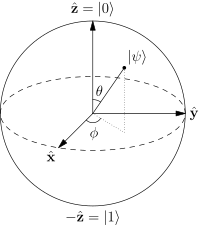
\includegraphics[width=0.4\columnwidth]{gfx/Bloch.png}
    \caption{Bloch sphere representation of a qubit}
    \label{fig:Bloch-Sphere}
\end{figure}

\subsection{Wigner Function}
The \textit{Wigner function} is the \textit{distribution} in the \textit{phase space} of a continuous variable quantum system\footnote{Such as position and momentum}. For classical systems, phase space distributions correspond to a classical probability distribution. However, the Wigner function the distribution also involves quantum uncertainty. Wigner functions can take on negative values in small regions, and are therefore quasi-probability distributions. This is allowed, since only areas larger than $\hslash$ are ever allowed to be measured, according to the Heisenberg uncertainty principle.

The Wigner function of a particle with wave function $\psi (q)$, is defined as 
\[
    W (q, p) := \frac{1}{\pi \hslash} \int_{-\infty}^\infty \psi^* (q + y) \psi (q - y) e^{\frac{2ipy}{\hslash}} dy
\]
An interesting example to use of the Wigner function is looking at the Wigner function of a Fock state. The Wigner distribution of a Fock state could be calculated directly from definition and the resulting expression is\footnote{proof of which is left as an exercise to the reader ;)}
\[
    W_n = \frac{2}{\pi} (-1)^n L_n[4 (q^2 + p^2)]e^{-2 (q^2 + p^2)}
\]
More importantly, we can look at a heat map of the Wigner function, as a nice visual aid to understand the state. An example of the $\ket{4}$ state Wigner distribution is shown in figure \ref{fig:Fock-State-Wigner}
% \begin{figure}[H]
%     \centering
%     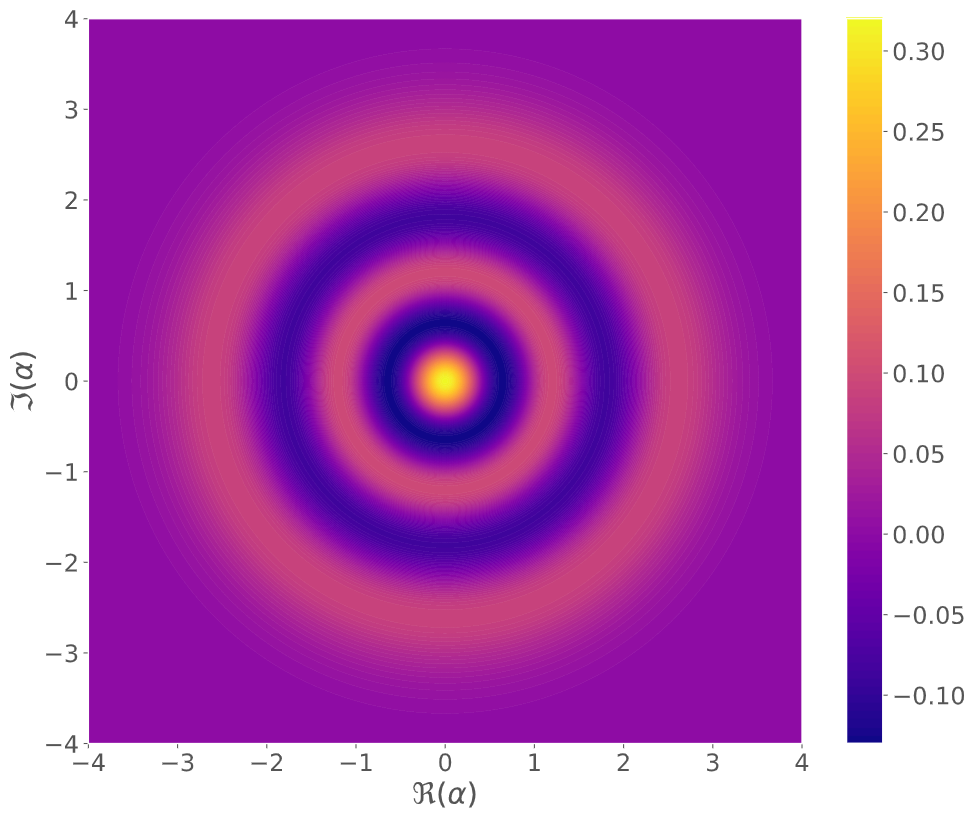
\includegraphics[width=0.7\columnwidth]{gfx/Fock4_wigner.png}
%     \caption{Wigner distribution of the $\ket{4}$ Fock state. $\alpha = q + ip$}
%     \label{fig:Fock-State-Wigner}
% \end{figure}

\begin{figure}[H]
    \begin{center}
        %% Creator: Matplotlib, PGF backend
%%
%% To include the figure in your LaTeX document, write
%%   \input{<filename>.pgf}
%%
%% Make sure the required packages are loaded in your preamble
%%   \usepackage{pgf}
%%
%% and, on pdftex
%%   \usepackage[utf8]{inputenc}\DeclareUnicodeCharacter{2212}{-}
%%
%% or, on luatex and xetex
%%   \usepackage{unicode-math}
%%
%% Figures using additional raster images can only be included by \input if
%% they are in the same directory as the main LaTeX file. For loading figures
%% from other directories you can use the `import` package
%%   \usepackage{import}
%%
%% and then include the figures with
%%   \import{<path to file>}{<filename>.pgf}
%%
%% Matplotlib used the following preamble
%%
\begingroup%
\makeatletter%
\begin{pgfpicture}%
\pgfpathrectangle{\pgfpointorigin}{\pgfqpoint{4.000000in}{3.200000in}}%
\pgfusepath{use as bounding box, clip}%
\begin{pgfscope}%
\pgfsetbuttcap%
\pgfsetmiterjoin%
\definecolor{currentfill}{rgb}{1.000000,1.000000,1.000000}%
\pgfsetfillcolor{currentfill}%
\pgfsetlinewidth{0.000000pt}%
\definecolor{currentstroke}{rgb}{1.000000,1.000000,1.000000}%
\pgfsetstrokecolor{currentstroke}%
\pgfsetdash{}{0pt}%
\pgfpathmoveto{\pgfqpoint{0.000000in}{0.000000in}}%
\pgfpathlineto{\pgfqpoint{4.000000in}{0.000000in}}%
\pgfpathlineto{\pgfqpoint{4.000000in}{3.200000in}}%
\pgfpathlineto{\pgfqpoint{0.000000in}{3.200000in}}%
\pgfpathclose%
\pgfusepath{fill}%
\end{pgfscope}%
\begin{pgfscope}%
\pgfsetbuttcap%
\pgfsetmiterjoin%
\definecolor{currentfill}{rgb}{1.000000,1.000000,1.000000}%
\pgfsetfillcolor{currentfill}%
\pgfsetlinewidth{0.000000pt}%
\definecolor{currentstroke}{rgb}{0.000000,0.000000,0.000000}%
\pgfsetstrokecolor{currentstroke}%
\pgfsetstrokeopacity{0.000000}%
\pgfsetdash{}{0pt}%
\pgfpathmoveto{\pgfqpoint{0.697107in}{0.637963in}}%
\pgfpathlineto{\pgfqpoint{3.189005in}{0.637963in}}%
\pgfpathlineto{\pgfqpoint{3.189005in}{2.997193in}}%
\pgfpathlineto{\pgfqpoint{0.697107in}{2.997193in}}%
\pgfpathclose%
\pgfusepath{fill}%
\end{pgfscope}%
\begin{pgfscope}%
\pgfpathrectangle{\pgfqpoint{0.697107in}{0.637963in}}{\pgfqpoint{2.491898in}{2.359231in}}%
\pgfusepath{clip}%
\pgfsetrectcap%
\pgfsetroundjoin%
\pgfsetlinewidth{0.803000pt}%
\definecolor{currentstroke}{rgb}{0.501961,0.501961,0.501961}%
\pgfsetstrokecolor{currentstroke}%
\pgfsetstrokeopacity{0.200000}%
\pgfsetdash{}{0pt}%
\pgfpathmoveto{\pgfqpoint{0.697107in}{0.637963in}}%
\pgfpathlineto{\pgfqpoint{0.697107in}{2.997193in}}%
\pgfusepath{stroke}%
\end{pgfscope}%
\begin{pgfscope}%
\pgfsetbuttcap%
\pgfsetroundjoin%
\definecolor{currentfill}{rgb}{0.333333,0.333333,0.333333}%
\pgfsetfillcolor{currentfill}%
\pgfsetlinewidth{0.803000pt}%
\definecolor{currentstroke}{rgb}{0.333333,0.333333,0.333333}%
\pgfsetstrokecolor{currentstroke}%
\pgfsetdash{}{0pt}%
\pgfsys@defobject{currentmarker}{\pgfqpoint{0.000000in}{-0.048611in}}{\pgfqpoint{0.000000in}{0.000000in}}{%
\pgfpathmoveto{\pgfqpoint{0.000000in}{0.000000in}}%
\pgfpathlineto{\pgfqpoint{0.000000in}{-0.048611in}}%
\pgfusepath{stroke,fill}%
}%
\begin{pgfscope}%
\pgfsys@transformshift{0.697107in}{0.637963in}%
\pgfsys@useobject{currentmarker}{}%
\end{pgfscope}%
\end{pgfscope}%
\begin{pgfscope}%
\definecolor{textcolor}{rgb}{0.333333,0.333333,0.333333}%
\pgfsetstrokecolor{textcolor}%
\pgfsetfillcolor{textcolor}%
\pgftext[x=0.697107in,y=0.540740in,,top]{\color{textcolor}\rmfamily\fontsize{11.000000}{13.200000}\selectfont \(\displaystyle {-4}\)}%
\end{pgfscope}%
\begin{pgfscope}%
\pgfpathrectangle{\pgfqpoint{0.697107in}{0.637963in}}{\pgfqpoint{2.491898in}{2.359231in}}%
\pgfusepath{clip}%
\pgfsetrectcap%
\pgfsetroundjoin%
\pgfsetlinewidth{0.803000pt}%
\definecolor{currentstroke}{rgb}{0.501961,0.501961,0.501961}%
\pgfsetstrokecolor{currentstroke}%
\pgfsetstrokeopacity{0.200000}%
\pgfsetdash{}{0pt}%
\pgfpathmoveto{\pgfqpoint{1.320081in}{0.637963in}}%
\pgfpathlineto{\pgfqpoint{1.320081in}{2.997193in}}%
\pgfusepath{stroke}%
\end{pgfscope}%
\begin{pgfscope}%
\pgfsetbuttcap%
\pgfsetroundjoin%
\definecolor{currentfill}{rgb}{0.333333,0.333333,0.333333}%
\pgfsetfillcolor{currentfill}%
\pgfsetlinewidth{0.803000pt}%
\definecolor{currentstroke}{rgb}{0.333333,0.333333,0.333333}%
\pgfsetstrokecolor{currentstroke}%
\pgfsetdash{}{0pt}%
\pgfsys@defobject{currentmarker}{\pgfqpoint{0.000000in}{-0.048611in}}{\pgfqpoint{0.000000in}{0.000000in}}{%
\pgfpathmoveto{\pgfqpoint{0.000000in}{0.000000in}}%
\pgfpathlineto{\pgfqpoint{0.000000in}{-0.048611in}}%
\pgfusepath{stroke,fill}%
}%
\begin{pgfscope}%
\pgfsys@transformshift{1.320081in}{0.637963in}%
\pgfsys@useobject{currentmarker}{}%
\end{pgfscope}%
\end{pgfscope}%
\begin{pgfscope}%
\definecolor{textcolor}{rgb}{0.333333,0.333333,0.333333}%
\pgfsetstrokecolor{textcolor}%
\pgfsetfillcolor{textcolor}%
\pgftext[x=1.320081in,y=0.540740in,,top]{\color{textcolor}\rmfamily\fontsize{11.000000}{13.200000}\selectfont \(\displaystyle {-2}\)}%
\end{pgfscope}%
\begin{pgfscope}%
\pgfpathrectangle{\pgfqpoint{0.697107in}{0.637963in}}{\pgfqpoint{2.491898in}{2.359231in}}%
\pgfusepath{clip}%
\pgfsetrectcap%
\pgfsetroundjoin%
\pgfsetlinewidth{0.803000pt}%
\definecolor{currentstroke}{rgb}{0.501961,0.501961,0.501961}%
\pgfsetstrokecolor{currentstroke}%
\pgfsetstrokeopacity{0.200000}%
\pgfsetdash{}{0pt}%
\pgfpathmoveto{\pgfqpoint{1.943056in}{0.637963in}}%
\pgfpathlineto{\pgfqpoint{1.943056in}{2.997193in}}%
\pgfusepath{stroke}%
\end{pgfscope}%
\begin{pgfscope}%
\pgfsetbuttcap%
\pgfsetroundjoin%
\definecolor{currentfill}{rgb}{0.333333,0.333333,0.333333}%
\pgfsetfillcolor{currentfill}%
\pgfsetlinewidth{0.803000pt}%
\definecolor{currentstroke}{rgb}{0.333333,0.333333,0.333333}%
\pgfsetstrokecolor{currentstroke}%
\pgfsetdash{}{0pt}%
\pgfsys@defobject{currentmarker}{\pgfqpoint{0.000000in}{-0.048611in}}{\pgfqpoint{0.000000in}{0.000000in}}{%
\pgfpathmoveto{\pgfqpoint{0.000000in}{0.000000in}}%
\pgfpathlineto{\pgfqpoint{0.000000in}{-0.048611in}}%
\pgfusepath{stroke,fill}%
}%
\begin{pgfscope}%
\pgfsys@transformshift{1.943056in}{0.637963in}%
\pgfsys@useobject{currentmarker}{}%
\end{pgfscope}%
\end{pgfscope}%
\begin{pgfscope}%
\definecolor{textcolor}{rgb}{0.333333,0.333333,0.333333}%
\pgfsetstrokecolor{textcolor}%
\pgfsetfillcolor{textcolor}%
\pgftext[x=1.943056in,y=0.540740in,,top]{\color{textcolor}\rmfamily\fontsize{11.000000}{13.200000}\selectfont \(\displaystyle {0}\)}%
\end{pgfscope}%
\begin{pgfscope}%
\pgfpathrectangle{\pgfqpoint{0.697107in}{0.637963in}}{\pgfqpoint{2.491898in}{2.359231in}}%
\pgfusepath{clip}%
\pgfsetrectcap%
\pgfsetroundjoin%
\pgfsetlinewidth{0.803000pt}%
\definecolor{currentstroke}{rgb}{0.501961,0.501961,0.501961}%
\pgfsetstrokecolor{currentstroke}%
\pgfsetstrokeopacity{0.200000}%
\pgfsetdash{}{0pt}%
\pgfpathmoveto{\pgfqpoint{2.566030in}{0.637963in}}%
\pgfpathlineto{\pgfqpoint{2.566030in}{2.997193in}}%
\pgfusepath{stroke}%
\end{pgfscope}%
\begin{pgfscope}%
\pgfsetbuttcap%
\pgfsetroundjoin%
\definecolor{currentfill}{rgb}{0.333333,0.333333,0.333333}%
\pgfsetfillcolor{currentfill}%
\pgfsetlinewidth{0.803000pt}%
\definecolor{currentstroke}{rgb}{0.333333,0.333333,0.333333}%
\pgfsetstrokecolor{currentstroke}%
\pgfsetdash{}{0pt}%
\pgfsys@defobject{currentmarker}{\pgfqpoint{0.000000in}{-0.048611in}}{\pgfqpoint{0.000000in}{0.000000in}}{%
\pgfpathmoveto{\pgfqpoint{0.000000in}{0.000000in}}%
\pgfpathlineto{\pgfqpoint{0.000000in}{-0.048611in}}%
\pgfusepath{stroke,fill}%
}%
\begin{pgfscope}%
\pgfsys@transformshift{2.566030in}{0.637963in}%
\pgfsys@useobject{currentmarker}{}%
\end{pgfscope}%
\end{pgfscope}%
\begin{pgfscope}%
\definecolor{textcolor}{rgb}{0.333333,0.333333,0.333333}%
\pgfsetstrokecolor{textcolor}%
\pgfsetfillcolor{textcolor}%
\pgftext[x=2.566030in,y=0.540740in,,top]{\color{textcolor}\rmfamily\fontsize{11.000000}{13.200000}\selectfont \(\displaystyle {2}\)}%
\end{pgfscope}%
\begin{pgfscope}%
\pgfpathrectangle{\pgfqpoint{0.697107in}{0.637963in}}{\pgfqpoint{2.491898in}{2.359231in}}%
\pgfusepath{clip}%
\pgfsetrectcap%
\pgfsetroundjoin%
\pgfsetlinewidth{0.803000pt}%
\definecolor{currentstroke}{rgb}{0.501961,0.501961,0.501961}%
\pgfsetstrokecolor{currentstroke}%
\pgfsetstrokeopacity{0.200000}%
\pgfsetdash{}{0pt}%
\pgfpathmoveto{\pgfqpoint{3.189005in}{0.637963in}}%
\pgfpathlineto{\pgfqpoint{3.189005in}{2.997193in}}%
\pgfusepath{stroke}%
\end{pgfscope}%
\begin{pgfscope}%
\pgfsetbuttcap%
\pgfsetroundjoin%
\definecolor{currentfill}{rgb}{0.333333,0.333333,0.333333}%
\pgfsetfillcolor{currentfill}%
\pgfsetlinewidth{0.803000pt}%
\definecolor{currentstroke}{rgb}{0.333333,0.333333,0.333333}%
\pgfsetstrokecolor{currentstroke}%
\pgfsetdash{}{0pt}%
\pgfsys@defobject{currentmarker}{\pgfqpoint{0.000000in}{-0.048611in}}{\pgfqpoint{0.000000in}{0.000000in}}{%
\pgfpathmoveto{\pgfqpoint{0.000000in}{0.000000in}}%
\pgfpathlineto{\pgfqpoint{0.000000in}{-0.048611in}}%
\pgfusepath{stroke,fill}%
}%
\begin{pgfscope}%
\pgfsys@transformshift{3.189005in}{0.637963in}%
\pgfsys@useobject{currentmarker}{}%
\end{pgfscope}%
\end{pgfscope}%
\begin{pgfscope}%
\definecolor{textcolor}{rgb}{0.333333,0.333333,0.333333}%
\pgfsetstrokecolor{textcolor}%
\pgfsetfillcolor{textcolor}%
\pgftext[x=3.189005in,y=0.540740in,,top]{\color{textcolor}\rmfamily\fontsize{11.000000}{13.200000}\selectfont \(\displaystyle {4}\)}%
\end{pgfscope}%
\begin{pgfscope}%
\definecolor{textcolor}{rgb}{0.333333,0.333333,0.333333}%
\pgfsetstrokecolor{textcolor}%
\pgfsetfillcolor{textcolor}%
\pgftext[x=1.943056in,y=0.350000in,,top]{\color{textcolor}\rmfamily\fontsize{14.000000}{16.800000}\selectfont \(\displaystyle \Re (\alpha)\)}%
\end{pgfscope}%
\begin{pgfscope}%
\pgfpathrectangle{\pgfqpoint{0.697107in}{0.637963in}}{\pgfqpoint{2.491898in}{2.359231in}}%
\pgfusepath{clip}%
\pgfsetrectcap%
\pgfsetroundjoin%
\pgfsetlinewidth{0.803000pt}%
\definecolor{currentstroke}{rgb}{0.501961,0.501961,0.501961}%
\pgfsetstrokecolor{currentstroke}%
\pgfsetstrokeopacity{0.200000}%
\pgfsetdash{}{0pt}%
\pgfpathmoveto{\pgfqpoint{0.697107in}{0.637963in}}%
\pgfpathlineto{\pgfqpoint{3.189005in}{0.637963in}}%
\pgfusepath{stroke}%
\end{pgfscope}%
\begin{pgfscope}%
\pgfsetbuttcap%
\pgfsetroundjoin%
\definecolor{currentfill}{rgb}{0.333333,0.333333,0.333333}%
\pgfsetfillcolor{currentfill}%
\pgfsetlinewidth{0.803000pt}%
\definecolor{currentstroke}{rgb}{0.333333,0.333333,0.333333}%
\pgfsetstrokecolor{currentstroke}%
\pgfsetdash{}{0pt}%
\pgfsys@defobject{currentmarker}{\pgfqpoint{-0.048611in}{0.000000in}}{\pgfqpoint{0.000000in}{0.000000in}}{%
\pgfpathmoveto{\pgfqpoint{0.000000in}{0.000000in}}%
\pgfpathlineto{\pgfqpoint{-0.048611in}{0.000000in}}%
\pgfusepath{stroke,fill}%
}%
\begin{pgfscope}%
\pgfsys@transformshift{0.697107in}{0.637963in}%
\pgfsys@useobject{currentmarker}{}%
\end{pgfscope}%
\end{pgfscope}%
\begin{pgfscope}%
\definecolor{textcolor}{rgb}{0.333333,0.333333,0.333333}%
\pgfsetstrokecolor{textcolor}%
\pgfsetfillcolor{textcolor}%
\pgftext[x=0.405555in, y=0.585156in, left, base]{\color{textcolor}\rmfamily\fontsize{11.000000}{13.200000}\selectfont \(\displaystyle {-4}\)}%
\end{pgfscope}%
\begin{pgfscope}%
\pgfpathrectangle{\pgfqpoint{0.697107in}{0.637963in}}{\pgfqpoint{2.491898in}{2.359231in}}%
\pgfusepath{clip}%
\pgfsetrectcap%
\pgfsetroundjoin%
\pgfsetlinewidth{0.803000pt}%
\definecolor{currentstroke}{rgb}{0.501961,0.501961,0.501961}%
\pgfsetstrokecolor{currentstroke}%
\pgfsetstrokeopacity{0.200000}%
\pgfsetdash{}{0pt}%
\pgfpathmoveto{\pgfqpoint{0.697107in}{1.227770in}}%
\pgfpathlineto{\pgfqpoint{3.189005in}{1.227770in}}%
\pgfusepath{stroke}%
\end{pgfscope}%
\begin{pgfscope}%
\pgfsetbuttcap%
\pgfsetroundjoin%
\definecolor{currentfill}{rgb}{0.333333,0.333333,0.333333}%
\pgfsetfillcolor{currentfill}%
\pgfsetlinewidth{0.803000pt}%
\definecolor{currentstroke}{rgb}{0.333333,0.333333,0.333333}%
\pgfsetstrokecolor{currentstroke}%
\pgfsetdash{}{0pt}%
\pgfsys@defobject{currentmarker}{\pgfqpoint{-0.048611in}{0.000000in}}{\pgfqpoint{0.000000in}{0.000000in}}{%
\pgfpathmoveto{\pgfqpoint{0.000000in}{0.000000in}}%
\pgfpathlineto{\pgfqpoint{-0.048611in}{0.000000in}}%
\pgfusepath{stroke,fill}%
}%
\begin{pgfscope}%
\pgfsys@transformshift{0.697107in}{1.227770in}%
\pgfsys@useobject{currentmarker}{}%
\end{pgfscope}%
\end{pgfscope}%
\begin{pgfscope}%
\definecolor{textcolor}{rgb}{0.333333,0.333333,0.333333}%
\pgfsetstrokecolor{textcolor}%
\pgfsetfillcolor{textcolor}%
\pgftext[x=0.405555in, y=1.174964in, left, base]{\color{textcolor}\rmfamily\fontsize{11.000000}{13.200000}\selectfont \(\displaystyle {-2}\)}%
\end{pgfscope}%
\begin{pgfscope}%
\pgfpathrectangle{\pgfqpoint{0.697107in}{0.637963in}}{\pgfqpoint{2.491898in}{2.359231in}}%
\pgfusepath{clip}%
\pgfsetrectcap%
\pgfsetroundjoin%
\pgfsetlinewidth{0.803000pt}%
\definecolor{currentstroke}{rgb}{0.501961,0.501961,0.501961}%
\pgfsetstrokecolor{currentstroke}%
\pgfsetstrokeopacity{0.200000}%
\pgfsetdash{}{0pt}%
\pgfpathmoveto{\pgfqpoint{0.697107in}{1.817578in}}%
\pgfpathlineto{\pgfqpoint{3.189005in}{1.817578in}}%
\pgfusepath{stroke}%
\end{pgfscope}%
\begin{pgfscope}%
\pgfsetbuttcap%
\pgfsetroundjoin%
\definecolor{currentfill}{rgb}{0.333333,0.333333,0.333333}%
\pgfsetfillcolor{currentfill}%
\pgfsetlinewidth{0.803000pt}%
\definecolor{currentstroke}{rgb}{0.333333,0.333333,0.333333}%
\pgfsetstrokecolor{currentstroke}%
\pgfsetdash{}{0pt}%
\pgfsys@defobject{currentmarker}{\pgfqpoint{-0.048611in}{0.000000in}}{\pgfqpoint{0.000000in}{0.000000in}}{%
\pgfpathmoveto{\pgfqpoint{0.000000in}{0.000000in}}%
\pgfpathlineto{\pgfqpoint{-0.048611in}{0.000000in}}%
\pgfusepath{stroke,fill}%
}%
\begin{pgfscope}%
\pgfsys@transformshift{0.697107in}{1.817578in}%
\pgfsys@useobject{currentmarker}{}%
\end{pgfscope}%
\end{pgfscope}%
\begin{pgfscope}%
\definecolor{textcolor}{rgb}{0.333333,0.333333,0.333333}%
\pgfsetstrokecolor{textcolor}%
\pgfsetfillcolor{textcolor}%
\pgftext[x=0.523843in, y=1.764771in, left, base]{\color{textcolor}\rmfamily\fontsize{11.000000}{13.200000}\selectfont \(\displaystyle {0}\)}%
\end{pgfscope}%
\begin{pgfscope}%
\pgfpathrectangle{\pgfqpoint{0.697107in}{0.637963in}}{\pgfqpoint{2.491898in}{2.359231in}}%
\pgfusepath{clip}%
\pgfsetrectcap%
\pgfsetroundjoin%
\pgfsetlinewidth{0.803000pt}%
\definecolor{currentstroke}{rgb}{0.501961,0.501961,0.501961}%
\pgfsetstrokecolor{currentstroke}%
\pgfsetstrokeopacity{0.200000}%
\pgfsetdash{}{0pt}%
\pgfpathmoveto{\pgfqpoint{0.697107in}{2.407386in}}%
\pgfpathlineto{\pgfqpoint{3.189005in}{2.407386in}}%
\pgfusepath{stroke}%
\end{pgfscope}%
\begin{pgfscope}%
\pgfsetbuttcap%
\pgfsetroundjoin%
\definecolor{currentfill}{rgb}{0.333333,0.333333,0.333333}%
\pgfsetfillcolor{currentfill}%
\pgfsetlinewidth{0.803000pt}%
\definecolor{currentstroke}{rgb}{0.333333,0.333333,0.333333}%
\pgfsetstrokecolor{currentstroke}%
\pgfsetdash{}{0pt}%
\pgfsys@defobject{currentmarker}{\pgfqpoint{-0.048611in}{0.000000in}}{\pgfqpoint{0.000000in}{0.000000in}}{%
\pgfpathmoveto{\pgfqpoint{0.000000in}{0.000000in}}%
\pgfpathlineto{\pgfqpoint{-0.048611in}{0.000000in}}%
\pgfusepath{stroke,fill}%
}%
\begin{pgfscope}%
\pgfsys@transformshift{0.697107in}{2.407386in}%
\pgfsys@useobject{currentmarker}{}%
\end{pgfscope}%
\end{pgfscope}%
\begin{pgfscope}%
\definecolor{textcolor}{rgb}{0.333333,0.333333,0.333333}%
\pgfsetstrokecolor{textcolor}%
\pgfsetfillcolor{textcolor}%
\pgftext[x=0.523843in, y=2.354579in, left, base]{\color{textcolor}\rmfamily\fontsize{11.000000}{13.200000}\selectfont \(\displaystyle {2}\)}%
\end{pgfscope}%
\begin{pgfscope}%
\pgfpathrectangle{\pgfqpoint{0.697107in}{0.637963in}}{\pgfqpoint{2.491898in}{2.359231in}}%
\pgfusepath{clip}%
\pgfsetrectcap%
\pgfsetroundjoin%
\pgfsetlinewidth{0.803000pt}%
\definecolor{currentstroke}{rgb}{0.501961,0.501961,0.501961}%
\pgfsetstrokecolor{currentstroke}%
\pgfsetstrokeopacity{0.200000}%
\pgfsetdash{}{0pt}%
\pgfpathmoveto{\pgfqpoint{0.697107in}{2.997193in}}%
\pgfpathlineto{\pgfqpoint{3.189005in}{2.997193in}}%
\pgfusepath{stroke}%
\end{pgfscope}%
\begin{pgfscope}%
\pgfsetbuttcap%
\pgfsetroundjoin%
\definecolor{currentfill}{rgb}{0.333333,0.333333,0.333333}%
\pgfsetfillcolor{currentfill}%
\pgfsetlinewidth{0.803000pt}%
\definecolor{currentstroke}{rgb}{0.333333,0.333333,0.333333}%
\pgfsetstrokecolor{currentstroke}%
\pgfsetdash{}{0pt}%
\pgfsys@defobject{currentmarker}{\pgfqpoint{-0.048611in}{0.000000in}}{\pgfqpoint{0.000000in}{0.000000in}}{%
\pgfpathmoveto{\pgfqpoint{0.000000in}{0.000000in}}%
\pgfpathlineto{\pgfqpoint{-0.048611in}{0.000000in}}%
\pgfusepath{stroke,fill}%
}%
\begin{pgfscope}%
\pgfsys@transformshift{0.697107in}{2.997193in}%
\pgfsys@useobject{currentmarker}{}%
\end{pgfscope}%
\end{pgfscope}%
\begin{pgfscope}%
\definecolor{textcolor}{rgb}{0.333333,0.333333,0.333333}%
\pgfsetstrokecolor{textcolor}%
\pgfsetfillcolor{textcolor}%
\pgftext[x=0.523843in, y=2.944387in, left, base]{\color{textcolor}\rmfamily\fontsize{11.000000}{13.200000}\selectfont \(\displaystyle {4}\)}%
\end{pgfscope}%
\begin{pgfscope}%
\definecolor{textcolor}{rgb}{0.333333,0.333333,0.333333}%
\pgfsetstrokecolor{textcolor}%
\pgfsetfillcolor{textcolor}%
\pgftext[x=0.350000in,y=1.817578in,,bottom,rotate=90.000000]{\color{textcolor}\rmfamily\fontsize{14.000000}{16.800000}\selectfont \(\displaystyle \Im (\alpha)\)}%
\end{pgfscope}%
\begin{pgfscope}%
\pgfpathrectangle{\pgfqpoint{0.697107in}{0.637963in}}{\pgfqpoint{2.491898in}{2.359231in}}%
\pgfusepath{clip}%
\pgfsetbuttcap%
\pgfsetroundjoin%
\definecolor{currentfill}{rgb}{0.096379,0.025165,0.547103}%
\pgfsetfillcolor{currentfill}%
\pgfsetlinewidth{0.501875pt}%
\definecolor{currentstroke}{rgb}{0.096379,0.025165,0.547103}%
\pgfsetstrokecolor{currentstroke}%
\pgfsetdash{}{0pt}%
\pgfsys@defobject{currentmarker}{\pgfqpoint{1.722083in}{1.608369in}}{\pgfqpoint{2.164029in}{2.026787in}}{%
\pgfpathmoveto{\pgfqpoint{1.938889in}{1.608369in}}%
\pgfpathlineto{\pgfqpoint{1.947223in}{1.608369in}}%
\pgfpathlineto{\pgfqpoint{1.950920in}{1.608482in}}%
\pgfpathlineto{\pgfqpoint{1.955557in}{1.608685in}}%
\pgfpathlineto{\pgfqpoint{1.963891in}{1.609396in}}%
\pgfpathlineto{\pgfqpoint{1.972225in}{1.610414in}}%
\pgfpathlineto{\pgfqpoint{1.980559in}{1.611697in}}%
\pgfpathlineto{\pgfqpoint{1.988893in}{1.613204in}}%
\pgfpathlineto{\pgfqpoint{1.997227in}{1.614905in}}%
\pgfpathlineto{\pgfqpoint{2.003646in}{1.616373in}}%
\pgfpathlineto{\pgfqpoint{2.005561in}{1.616952in}}%
\pgfpathlineto{\pgfqpoint{2.013896in}{1.619693in}}%
\pgfpathlineto{\pgfqpoint{2.022230in}{1.622439in}}%
\pgfpathlineto{\pgfqpoint{2.027480in}{1.624263in}}%
\pgfpathlineto{\pgfqpoint{2.030564in}{1.625606in}}%
\pgfpathlineto{\pgfqpoint{2.038898in}{1.629316in}}%
\pgfpathlineto{\pgfqpoint{2.045347in}{1.632154in}}%
\pgfpathlineto{\pgfqpoint{2.047232in}{1.633162in}}%
\pgfpathlineto{\pgfqpoint{2.055566in}{1.637719in}}%
\pgfpathlineto{\pgfqpoint{2.059817in}{1.640044in}}%
\pgfpathlineto{\pgfqpoint{2.063900in}{1.642639in}}%
\pgfpathlineto{\pgfqpoint{2.072234in}{1.647792in}}%
\pgfpathlineto{\pgfqpoint{2.072447in}{1.647934in}}%
\pgfpathlineto{\pgfqpoint{2.080568in}{1.653959in}}%
\pgfpathlineto{\pgfqpoint{2.083057in}{1.655825in}}%
\pgfpathlineto{\pgfqpoint{2.088903in}{1.660615in}}%
\pgfpathlineto{\pgfqpoint{2.092584in}{1.663715in}}%
\pgfpathlineto{\pgfqpoint{2.097237in}{1.667915in}}%
\pgfpathlineto{\pgfqpoint{2.101135in}{1.671606in}}%
\pgfpathlineto{\pgfqpoint{2.105571in}{1.676010in}}%
\pgfpathlineto{\pgfqpoint{2.108845in}{1.679496in}}%
\pgfpathlineto{\pgfqpoint{2.113905in}{1.685030in}}%
\pgfpathlineto{\pgfqpoint{2.115876in}{1.687386in}}%
\pgfpathlineto{\pgfqpoint{2.122239in}{1.695076in}}%
\pgfpathlineto{\pgfqpoint{2.122389in}{1.695277in}}%
\pgfpathlineto{\pgfqpoint{2.127832in}{1.703167in}}%
\pgfpathlineto{\pgfqpoint{2.130573in}{1.707033in}}%
\pgfpathlineto{\pgfqpoint{2.133029in}{1.711058in}}%
\pgfpathlineto{\pgfqpoint{2.137842in}{1.718948in}}%
\pgfpathlineto{\pgfqpoint{2.138907in}{1.720732in}}%
\pgfpathlineto{\pgfqpoint{2.141905in}{1.726838in}}%
\pgfpathlineto{\pgfqpoint{2.145823in}{1.734729in}}%
\pgfpathlineto{\pgfqpoint{2.147241in}{1.737648in}}%
\pgfpathlineto{\pgfqpoint{2.149168in}{1.742619in}}%
\pgfpathlineto{\pgfqpoint{2.152068in}{1.750510in}}%
\pgfpathlineto{\pgfqpoint{2.154964in}{1.758400in}}%
\pgfpathlineto{\pgfqpoint{2.155575in}{1.760214in}}%
\pgfpathlineto{\pgfqpoint{2.157126in}{1.766290in}}%
\pgfpathlineto{\pgfqpoint{2.158922in}{1.774181in}}%
\pgfpathlineto{\pgfqpoint{2.160514in}{1.782071in}}%
\pgfpathlineto{\pgfqpoint{2.161869in}{1.789962in}}%
\pgfpathlineto{\pgfqpoint{2.162945in}{1.797852in}}%
\pgfpathlineto{\pgfqpoint{2.163696in}{1.805742in}}%
\pgfpathlineto{\pgfqpoint{2.163910in}{1.810132in}}%
\pgfpathlineto{\pgfqpoint{2.164029in}{1.813633in}}%
\pgfpathlineto{\pgfqpoint{2.164029in}{1.821523in}}%
\pgfpathlineto{\pgfqpoint{2.163910in}{1.825024in}}%
\pgfpathlineto{\pgfqpoint{2.163696in}{1.829414in}}%
\pgfpathlineto{\pgfqpoint{2.162945in}{1.837304in}}%
\pgfpathlineto{\pgfqpoint{2.161869in}{1.845194in}}%
\pgfpathlineto{\pgfqpoint{2.160514in}{1.853085in}}%
\pgfpathlineto{\pgfqpoint{2.158922in}{1.860975in}}%
\pgfpathlineto{\pgfqpoint{2.157126in}{1.868866in}}%
\pgfpathlineto{\pgfqpoint{2.155575in}{1.874942in}}%
\pgfpathlineto{\pgfqpoint{2.154964in}{1.876756in}}%
\pgfpathlineto{\pgfqpoint{2.152068in}{1.884646in}}%
\pgfpathlineto{\pgfqpoint{2.149168in}{1.892537in}}%
\pgfpathlineto{\pgfqpoint{2.147241in}{1.897508in}}%
\pgfpathlineto{\pgfqpoint{2.145823in}{1.900427in}}%
\pgfpathlineto{\pgfqpoint{2.141905in}{1.908318in}}%
\pgfpathlineto{\pgfqpoint{2.138907in}{1.914424in}}%
\pgfpathlineto{\pgfqpoint{2.137842in}{1.916208in}}%
\pgfpathlineto{\pgfqpoint{2.133029in}{1.924098in}}%
\pgfpathlineto{\pgfqpoint{2.130573in}{1.928123in}}%
\pgfpathlineto{\pgfqpoint{2.127832in}{1.931989in}}%
\pgfpathlineto{\pgfqpoint{2.122389in}{1.939879in}}%
\pgfpathlineto{\pgfqpoint{2.122239in}{1.940080in}}%
\pgfpathlineto{\pgfqpoint{2.115876in}{1.947770in}}%
\pgfpathlineto{\pgfqpoint{2.113905in}{1.950126in}}%
\pgfpathlineto{\pgfqpoint{2.108845in}{1.955660in}}%
\pgfpathlineto{\pgfqpoint{2.105571in}{1.959146in}}%
\pgfpathlineto{\pgfqpoint{2.101135in}{1.963550in}}%
\pgfpathlineto{\pgfqpoint{2.097237in}{1.967241in}}%
\pgfpathlineto{\pgfqpoint{2.092584in}{1.971441in}}%
\pgfpathlineto{\pgfqpoint{2.088903in}{1.974541in}}%
\pgfpathlineto{\pgfqpoint{2.083057in}{1.979331in}}%
\pgfpathlineto{\pgfqpoint{2.080568in}{1.981197in}}%
\pgfpathlineto{\pgfqpoint{2.072447in}{1.987222in}}%
\pgfpathlineto{\pgfqpoint{2.072234in}{1.987364in}}%
\pgfpathlineto{\pgfqpoint{2.063900in}{1.992517in}}%
\pgfpathlineto{\pgfqpoint{2.059817in}{1.995112in}}%
\pgfpathlineto{\pgfqpoint{2.055566in}{1.997437in}}%
\pgfpathlineto{\pgfqpoint{2.047232in}{2.001994in}}%
\pgfpathlineto{\pgfqpoint{2.045347in}{2.003002in}}%
\pgfpathlineto{\pgfqpoint{2.038898in}{2.005840in}}%
\pgfpathlineto{\pgfqpoint{2.030564in}{2.009550in}}%
\pgfpathlineto{\pgfqpoint{2.027480in}{2.010893in}}%
\pgfpathlineto{\pgfqpoint{2.022230in}{2.012717in}}%
\pgfpathlineto{\pgfqpoint{2.013896in}{2.015463in}}%
\pgfpathlineto{\pgfqpoint{2.005561in}{2.018204in}}%
\pgfpathlineto{\pgfqpoint{2.003646in}{2.018783in}}%
\pgfpathlineto{\pgfqpoint{1.997227in}{2.020251in}}%
\pgfpathlineto{\pgfqpoint{1.988893in}{2.021952in}}%
\pgfpathlineto{\pgfqpoint{1.980559in}{2.023459in}}%
\pgfpathlineto{\pgfqpoint{1.972225in}{2.024742in}}%
\pgfpathlineto{\pgfqpoint{1.963891in}{2.025760in}}%
\pgfpathlineto{\pgfqpoint{1.955557in}{2.026471in}}%
\pgfpathlineto{\pgfqpoint{1.950920in}{2.026674in}}%
\pgfpathlineto{\pgfqpoint{1.947223in}{2.026787in}}%
\pgfpathlineto{\pgfqpoint{1.938889in}{2.026787in}}%
\pgfpathlineto{\pgfqpoint{1.935191in}{2.026674in}}%
\pgfpathlineto{\pgfqpoint{1.930555in}{2.026471in}}%
\pgfpathlineto{\pgfqpoint{1.922220in}{2.025760in}}%
\pgfpathlineto{\pgfqpoint{1.913886in}{2.024742in}}%
\pgfpathlineto{\pgfqpoint{1.905552in}{2.023459in}}%
\pgfpathlineto{\pgfqpoint{1.897218in}{2.021952in}}%
\pgfpathlineto{\pgfqpoint{1.888884in}{2.020251in}}%
\pgfpathlineto{\pgfqpoint{1.882465in}{2.018783in}}%
\pgfpathlineto{\pgfqpoint{1.880550in}{2.018204in}}%
\pgfpathlineto{\pgfqpoint{1.872216in}{2.015463in}}%
\pgfpathlineto{\pgfqpoint{1.863882in}{2.012717in}}%
\pgfpathlineto{\pgfqpoint{1.858631in}{2.010893in}}%
\pgfpathlineto{\pgfqpoint{1.855548in}{2.009550in}}%
\pgfpathlineto{\pgfqpoint{1.847213in}{2.005840in}}%
\pgfpathlineto{\pgfqpoint{1.840764in}{2.003002in}}%
\pgfpathlineto{\pgfqpoint{1.838879in}{2.001994in}}%
\pgfpathlineto{\pgfqpoint{1.830545in}{1.997437in}}%
\pgfpathlineto{\pgfqpoint{1.826294in}{1.995112in}}%
\pgfpathlineto{\pgfqpoint{1.822211in}{1.992517in}}%
\pgfpathlineto{\pgfqpoint{1.813877in}{1.987364in}}%
\pgfpathlineto{\pgfqpoint{1.813665in}{1.987222in}}%
\pgfpathlineto{\pgfqpoint{1.805543in}{1.981197in}}%
\pgfpathlineto{\pgfqpoint{1.803054in}{1.979331in}}%
\pgfpathlineto{\pgfqpoint{1.797209in}{1.974541in}}%
\pgfpathlineto{\pgfqpoint{1.793527in}{1.971441in}}%
\pgfpathlineto{\pgfqpoint{1.788875in}{1.967241in}}%
\pgfpathlineto{\pgfqpoint{1.784976in}{1.963550in}}%
\pgfpathlineto{\pgfqpoint{1.780541in}{1.959146in}}%
\pgfpathlineto{\pgfqpoint{1.777266in}{1.955660in}}%
\pgfpathlineto{\pgfqpoint{1.772206in}{1.950126in}}%
\pgfpathlineto{\pgfqpoint{1.770236in}{1.947770in}}%
\pgfpathlineto{\pgfqpoint{1.763872in}{1.940080in}}%
\pgfpathlineto{\pgfqpoint{1.763723in}{1.939879in}}%
\pgfpathlineto{\pgfqpoint{1.758279in}{1.931989in}}%
\pgfpathlineto{\pgfqpoint{1.755538in}{1.928123in}}%
\pgfpathlineto{\pgfqpoint{1.753082in}{1.924098in}}%
\pgfpathlineto{\pgfqpoint{1.748269in}{1.916208in}}%
\pgfpathlineto{\pgfqpoint{1.747204in}{1.914424in}}%
\pgfpathlineto{\pgfqpoint{1.744207in}{1.908318in}}%
\pgfpathlineto{\pgfqpoint{1.740288in}{1.900427in}}%
\pgfpathlineto{\pgfqpoint{1.738870in}{1.897508in}}%
\pgfpathlineto{\pgfqpoint{1.736943in}{1.892537in}}%
\pgfpathlineto{\pgfqpoint{1.734043in}{1.884646in}}%
\pgfpathlineto{\pgfqpoint{1.731148in}{1.876756in}}%
\pgfpathlineto{\pgfqpoint{1.730536in}{1.874942in}}%
\pgfpathlineto{\pgfqpoint{1.728985in}{1.868866in}}%
\pgfpathlineto{\pgfqpoint{1.727189in}{1.860975in}}%
\pgfpathlineto{\pgfqpoint{1.725597in}{1.853085in}}%
\pgfpathlineto{\pgfqpoint{1.724242in}{1.845194in}}%
\pgfpathlineto{\pgfqpoint{1.723167in}{1.837304in}}%
\pgfpathlineto{\pgfqpoint{1.722416in}{1.829414in}}%
\pgfpathlineto{\pgfqpoint{1.722202in}{1.825024in}}%
\pgfpathlineto{\pgfqpoint{1.722083in}{1.821523in}}%
\pgfpathlineto{\pgfqpoint{1.722083in}{1.813633in}}%
\pgfpathlineto{\pgfqpoint{1.722202in}{1.810132in}}%
\pgfpathlineto{\pgfqpoint{1.722416in}{1.805742in}}%
\pgfpathlineto{\pgfqpoint{1.723167in}{1.797852in}}%
\pgfpathlineto{\pgfqpoint{1.724242in}{1.789962in}}%
\pgfpathlineto{\pgfqpoint{1.725597in}{1.782071in}}%
\pgfpathlineto{\pgfqpoint{1.727189in}{1.774181in}}%
\pgfpathlineto{\pgfqpoint{1.728985in}{1.766290in}}%
\pgfpathlineto{\pgfqpoint{1.730536in}{1.760214in}}%
\pgfpathlineto{\pgfqpoint{1.731148in}{1.758400in}}%
\pgfpathlineto{\pgfqpoint{1.734043in}{1.750510in}}%
\pgfpathlineto{\pgfqpoint{1.736943in}{1.742619in}}%
\pgfpathlineto{\pgfqpoint{1.738870in}{1.737648in}}%
\pgfpathlineto{\pgfqpoint{1.740288in}{1.734729in}}%
\pgfpathlineto{\pgfqpoint{1.744207in}{1.726838in}}%
\pgfpathlineto{\pgfqpoint{1.747204in}{1.720732in}}%
\pgfpathlineto{\pgfqpoint{1.748269in}{1.718948in}}%
\pgfpathlineto{\pgfqpoint{1.753082in}{1.711058in}}%
\pgfpathlineto{\pgfqpoint{1.755538in}{1.707033in}}%
\pgfpathlineto{\pgfqpoint{1.758279in}{1.703167in}}%
\pgfpathlineto{\pgfqpoint{1.763723in}{1.695277in}}%
\pgfpathlineto{\pgfqpoint{1.763872in}{1.695076in}}%
\pgfpathlineto{\pgfqpoint{1.770236in}{1.687386in}}%
\pgfpathlineto{\pgfqpoint{1.772206in}{1.685030in}}%
\pgfpathlineto{\pgfqpoint{1.777266in}{1.679496in}}%
\pgfpathlineto{\pgfqpoint{1.780541in}{1.676010in}}%
\pgfpathlineto{\pgfqpoint{1.784976in}{1.671606in}}%
\pgfpathlineto{\pgfqpoint{1.788875in}{1.667915in}}%
\pgfpathlineto{\pgfqpoint{1.793527in}{1.663715in}}%
\pgfpathlineto{\pgfqpoint{1.797209in}{1.660615in}}%
\pgfpathlineto{\pgfqpoint{1.803054in}{1.655825in}}%
\pgfpathlineto{\pgfqpoint{1.805543in}{1.653959in}}%
\pgfpathlineto{\pgfqpoint{1.813665in}{1.647934in}}%
\pgfpathlineto{\pgfqpoint{1.813877in}{1.647792in}}%
\pgfpathlineto{\pgfqpoint{1.822211in}{1.642639in}}%
\pgfpathlineto{\pgfqpoint{1.826294in}{1.640044in}}%
\pgfpathlineto{\pgfqpoint{1.830545in}{1.637719in}}%
\pgfpathlineto{\pgfqpoint{1.838879in}{1.633162in}}%
\pgfpathlineto{\pgfqpoint{1.840764in}{1.632154in}}%
\pgfpathlineto{\pgfqpoint{1.847213in}{1.629316in}}%
\pgfpathlineto{\pgfqpoint{1.855548in}{1.625606in}}%
\pgfpathlineto{\pgfqpoint{1.858631in}{1.624263in}}%
\pgfpathlineto{\pgfqpoint{1.863882in}{1.622439in}}%
\pgfpathlineto{\pgfqpoint{1.872216in}{1.619693in}}%
\pgfpathlineto{\pgfqpoint{1.880550in}{1.616952in}}%
\pgfpathlineto{\pgfqpoint{1.882465in}{1.616373in}}%
\pgfpathlineto{\pgfqpoint{1.888884in}{1.614905in}}%
\pgfpathlineto{\pgfqpoint{1.897218in}{1.613204in}}%
\pgfpathlineto{\pgfqpoint{1.905552in}{1.611697in}}%
\pgfpathlineto{\pgfqpoint{1.913886in}{1.610414in}}%
\pgfpathlineto{\pgfqpoint{1.922220in}{1.609396in}}%
\pgfpathlineto{\pgfqpoint{1.930555in}{1.608685in}}%
\pgfpathlineto{\pgfqpoint{1.935191in}{1.608482in}}%
\pgfpathclose%
\pgfpathmoveto{\pgfqpoint{1.920147in}{1.647934in}}%
\pgfpathlineto{\pgfqpoint{1.913886in}{1.648636in}}%
\pgfpathlineto{\pgfqpoint{1.905552in}{1.649939in}}%
\pgfpathlineto{\pgfqpoint{1.897218in}{1.651715in}}%
\pgfpathlineto{\pgfqpoint{1.888884in}{1.654125in}}%
\pgfpathlineto{\pgfqpoint{1.884288in}{1.655825in}}%
\pgfpathlineto{\pgfqpoint{1.880550in}{1.656905in}}%
\pgfpathlineto{\pgfqpoint{1.872216in}{1.659839in}}%
\pgfpathlineto{\pgfqpoint{1.864111in}{1.663715in}}%
\pgfpathlineto{\pgfqpoint{1.863882in}{1.663808in}}%
\pgfpathlineto{\pgfqpoint{1.855548in}{1.667570in}}%
\pgfpathlineto{\pgfqpoint{1.848780in}{1.671606in}}%
\pgfpathlineto{\pgfqpoint{1.847213in}{1.672449in}}%
\pgfpathlineto{\pgfqpoint{1.838879in}{1.677581in}}%
\pgfpathlineto{\pgfqpoint{1.836235in}{1.679496in}}%
\pgfpathlineto{\pgfqpoint{1.830545in}{1.683432in}}%
\pgfpathlineto{\pgfqpoint{1.825634in}{1.687386in}}%
\pgfpathlineto{\pgfqpoint{1.822211in}{1.690161in}}%
\pgfpathlineto{\pgfqpoint{1.816507in}{1.695277in}}%
\pgfpathlineto{\pgfqpoint{1.813877in}{1.697767in}}%
\pgfpathlineto{\pgfqpoint{1.808474in}{1.703167in}}%
\pgfpathlineto{\pgfqpoint{1.805543in}{1.706408in}}%
\pgfpathlineto{\pgfqpoint{1.801366in}{1.711058in}}%
\pgfpathlineto{\pgfqpoint{1.797209in}{1.716445in}}%
\pgfpathlineto{\pgfqpoint{1.795187in}{1.718948in}}%
\pgfpathlineto{\pgfqpoint{1.789765in}{1.726838in}}%
\pgfpathlineto{\pgfqpoint{1.788875in}{1.728321in}}%
\pgfpathlineto{\pgfqpoint{1.784612in}{1.734729in}}%
\pgfpathlineto{\pgfqpoint{1.780639in}{1.742619in}}%
\pgfpathlineto{\pgfqpoint{1.780541in}{1.742836in}}%
\pgfpathlineto{\pgfqpoint{1.776447in}{1.750510in}}%
\pgfpathlineto{\pgfqpoint{1.773348in}{1.758400in}}%
\pgfpathlineto{\pgfqpoint{1.772206in}{1.761939in}}%
\pgfpathlineto{\pgfqpoint{1.770411in}{1.766290in}}%
\pgfpathlineto{\pgfqpoint{1.767865in}{1.774181in}}%
\pgfpathlineto{\pgfqpoint{1.765990in}{1.782071in}}%
\pgfpathlineto{\pgfqpoint{1.764613in}{1.789962in}}%
\pgfpathlineto{\pgfqpoint{1.763872in}{1.795889in}}%
\pgfpathlineto{\pgfqpoint{1.763518in}{1.797852in}}%
\pgfpathlineto{\pgfqpoint{1.762585in}{1.805742in}}%
\pgfpathlineto{\pgfqpoint{1.762138in}{1.813633in}}%
\pgfpathlineto{\pgfqpoint{1.762138in}{1.821523in}}%
\pgfpathlineto{\pgfqpoint{1.762585in}{1.829414in}}%
\pgfpathlineto{\pgfqpoint{1.763518in}{1.837304in}}%
\pgfpathlineto{\pgfqpoint{1.763872in}{1.839267in}}%
\pgfpathlineto{\pgfqpoint{1.764613in}{1.845194in}}%
\pgfpathlineto{\pgfqpoint{1.765990in}{1.853085in}}%
\pgfpathlineto{\pgfqpoint{1.767865in}{1.860975in}}%
\pgfpathlineto{\pgfqpoint{1.770411in}{1.868866in}}%
\pgfpathlineto{\pgfqpoint{1.772206in}{1.873217in}}%
\pgfpathlineto{\pgfqpoint{1.773348in}{1.876756in}}%
\pgfpathlineto{\pgfqpoint{1.776447in}{1.884646in}}%
\pgfpathlineto{\pgfqpoint{1.780541in}{1.892320in}}%
\pgfpathlineto{\pgfqpoint{1.780639in}{1.892537in}}%
\pgfpathlineto{\pgfqpoint{1.784612in}{1.900427in}}%
\pgfpathlineto{\pgfqpoint{1.788875in}{1.906835in}}%
\pgfpathlineto{\pgfqpoint{1.789765in}{1.908318in}}%
\pgfpathlineto{\pgfqpoint{1.795187in}{1.916208in}}%
\pgfpathlineto{\pgfqpoint{1.797209in}{1.918711in}}%
\pgfpathlineto{\pgfqpoint{1.801366in}{1.924098in}}%
\pgfpathlineto{\pgfqpoint{1.805543in}{1.928748in}}%
\pgfpathlineto{\pgfqpoint{1.808474in}{1.931989in}}%
\pgfpathlineto{\pgfqpoint{1.813877in}{1.937389in}}%
\pgfpathlineto{\pgfqpoint{1.816507in}{1.939879in}}%
\pgfpathlineto{\pgfqpoint{1.822211in}{1.944995in}}%
\pgfpathlineto{\pgfqpoint{1.825634in}{1.947770in}}%
\pgfpathlineto{\pgfqpoint{1.830545in}{1.951724in}}%
\pgfpathlineto{\pgfqpoint{1.836235in}{1.955660in}}%
\pgfpathlineto{\pgfqpoint{1.838879in}{1.957575in}}%
\pgfpathlineto{\pgfqpoint{1.847213in}{1.962707in}}%
\pgfpathlineto{\pgfqpoint{1.848780in}{1.963550in}}%
\pgfpathlineto{\pgfqpoint{1.855548in}{1.967586in}}%
\pgfpathlineto{\pgfqpoint{1.863882in}{1.971348in}}%
\pgfpathlineto{\pgfqpoint{1.864111in}{1.971441in}}%
\pgfpathlineto{\pgfqpoint{1.872216in}{1.975317in}}%
\pgfpathlineto{\pgfqpoint{1.880550in}{1.978251in}}%
\pgfpathlineto{\pgfqpoint{1.884288in}{1.979331in}}%
\pgfpathlineto{\pgfqpoint{1.888884in}{1.981031in}}%
\pgfpathlineto{\pgfqpoint{1.897218in}{1.983441in}}%
\pgfpathlineto{\pgfqpoint{1.905552in}{1.985217in}}%
\pgfpathlineto{\pgfqpoint{1.913886in}{1.986520in}}%
\pgfpathlineto{\pgfqpoint{1.920147in}{1.987222in}}%
\pgfpathlineto{\pgfqpoint{1.922220in}{1.987557in}}%
\pgfpathlineto{\pgfqpoint{1.930555in}{1.988441in}}%
\pgfpathlineto{\pgfqpoint{1.938889in}{1.988864in}}%
\pgfpathlineto{\pgfqpoint{1.947223in}{1.988864in}}%
\pgfpathlineto{\pgfqpoint{1.955557in}{1.988441in}}%
\pgfpathlineto{\pgfqpoint{1.963891in}{1.987557in}}%
\pgfpathlineto{\pgfqpoint{1.965965in}{1.987222in}}%
\pgfpathlineto{\pgfqpoint{1.972225in}{1.986520in}}%
\pgfpathlineto{\pgfqpoint{1.980559in}{1.985217in}}%
\pgfpathlineto{\pgfqpoint{1.988893in}{1.983441in}}%
\pgfpathlineto{\pgfqpoint{1.997227in}{1.981031in}}%
\pgfpathlineto{\pgfqpoint{2.001824in}{1.979331in}}%
\pgfpathlineto{\pgfqpoint{2.005561in}{1.978251in}}%
\pgfpathlineto{\pgfqpoint{2.013896in}{1.975317in}}%
\pgfpathlineto{\pgfqpoint{2.022000in}{1.971441in}}%
\pgfpathlineto{\pgfqpoint{2.022230in}{1.971348in}}%
\pgfpathlineto{\pgfqpoint{2.030564in}{1.967586in}}%
\pgfpathlineto{\pgfqpoint{2.037332in}{1.963550in}}%
\pgfpathlineto{\pgfqpoint{2.038898in}{1.962707in}}%
\pgfpathlineto{\pgfqpoint{2.047232in}{1.957575in}}%
\pgfpathlineto{\pgfqpoint{2.049876in}{1.955660in}}%
\pgfpathlineto{\pgfqpoint{2.055566in}{1.951724in}}%
\pgfpathlineto{\pgfqpoint{2.060477in}{1.947770in}}%
\pgfpathlineto{\pgfqpoint{2.063900in}{1.944995in}}%
\pgfpathlineto{\pgfqpoint{2.069604in}{1.939879in}}%
\pgfpathlineto{\pgfqpoint{2.072234in}{1.937389in}}%
\pgfpathlineto{\pgfqpoint{2.077638in}{1.931989in}}%
\pgfpathlineto{\pgfqpoint{2.080568in}{1.928748in}}%
\pgfpathlineto{\pgfqpoint{2.084745in}{1.924098in}}%
\pgfpathlineto{\pgfqpoint{2.088903in}{1.918711in}}%
\pgfpathlineto{\pgfqpoint{2.090925in}{1.916208in}}%
\pgfpathlineto{\pgfqpoint{2.096346in}{1.908318in}}%
\pgfpathlineto{\pgfqpoint{2.097237in}{1.906835in}}%
\pgfpathlineto{\pgfqpoint{2.101499in}{1.900427in}}%
\pgfpathlineto{\pgfqpoint{2.105472in}{1.892537in}}%
\pgfpathlineto{\pgfqpoint{2.105571in}{1.892320in}}%
\pgfpathlineto{\pgfqpoint{2.109665in}{1.884646in}}%
\pgfpathlineto{\pgfqpoint{2.112764in}{1.876756in}}%
\pgfpathlineto{\pgfqpoint{2.113905in}{1.873217in}}%
\pgfpathlineto{\pgfqpoint{2.115701in}{1.868866in}}%
\pgfpathlineto{\pgfqpoint{2.118246in}{1.860975in}}%
\pgfpathlineto{\pgfqpoint{2.120121in}{1.853085in}}%
\pgfpathlineto{\pgfqpoint{2.121498in}{1.845194in}}%
\pgfpathlineto{\pgfqpoint{2.122239in}{1.839267in}}%
\pgfpathlineto{\pgfqpoint{2.122593in}{1.837304in}}%
\pgfpathlineto{\pgfqpoint{2.123527in}{1.829414in}}%
\pgfpathlineto{\pgfqpoint{2.123974in}{1.821523in}}%
\pgfpathlineto{\pgfqpoint{2.123974in}{1.813633in}}%
\pgfpathlineto{\pgfqpoint{2.123527in}{1.805742in}}%
\pgfpathlineto{\pgfqpoint{2.122593in}{1.797852in}}%
\pgfpathlineto{\pgfqpoint{2.122239in}{1.795889in}}%
\pgfpathlineto{\pgfqpoint{2.121498in}{1.789962in}}%
\pgfpathlineto{\pgfqpoint{2.120121in}{1.782071in}}%
\pgfpathlineto{\pgfqpoint{2.118246in}{1.774181in}}%
\pgfpathlineto{\pgfqpoint{2.115701in}{1.766290in}}%
\pgfpathlineto{\pgfqpoint{2.113905in}{1.761939in}}%
\pgfpathlineto{\pgfqpoint{2.112764in}{1.758400in}}%
\pgfpathlineto{\pgfqpoint{2.109665in}{1.750510in}}%
\pgfpathlineto{\pgfqpoint{2.105571in}{1.742836in}}%
\pgfpathlineto{\pgfqpoint{2.105472in}{1.742619in}}%
\pgfpathlineto{\pgfqpoint{2.101499in}{1.734729in}}%
\pgfpathlineto{\pgfqpoint{2.097237in}{1.728321in}}%
\pgfpathlineto{\pgfqpoint{2.096346in}{1.726838in}}%
\pgfpathlineto{\pgfqpoint{2.090925in}{1.718948in}}%
\pgfpathlineto{\pgfqpoint{2.088903in}{1.716445in}}%
\pgfpathlineto{\pgfqpoint{2.084745in}{1.711058in}}%
\pgfpathlineto{\pgfqpoint{2.080568in}{1.706408in}}%
\pgfpathlineto{\pgfqpoint{2.077638in}{1.703167in}}%
\pgfpathlineto{\pgfqpoint{2.072234in}{1.697767in}}%
\pgfpathlineto{\pgfqpoint{2.069604in}{1.695277in}}%
\pgfpathlineto{\pgfqpoint{2.063900in}{1.690161in}}%
\pgfpathlineto{\pgfqpoint{2.060477in}{1.687386in}}%
\pgfpathlineto{\pgfqpoint{2.055566in}{1.683432in}}%
\pgfpathlineto{\pgfqpoint{2.049876in}{1.679496in}}%
\pgfpathlineto{\pgfqpoint{2.047232in}{1.677581in}}%
\pgfpathlineto{\pgfqpoint{2.038898in}{1.672449in}}%
\pgfpathlineto{\pgfqpoint{2.037332in}{1.671606in}}%
\pgfpathlineto{\pgfqpoint{2.030564in}{1.667570in}}%
\pgfpathlineto{\pgfqpoint{2.022230in}{1.663808in}}%
\pgfpathlineto{\pgfqpoint{2.022000in}{1.663715in}}%
\pgfpathlineto{\pgfqpoint{2.013896in}{1.659839in}}%
\pgfpathlineto{\pgfqpoint{2.005561in}{1.656905in}}%
\pgfpathlineto{\pgfqpoint{2.001824in}{1.655825in}}%
\pgfpathlineto{\pgfqpoint{1.997227in}{1.654125in}}%
\pgfpathlineto{\pgfqpoint{1.988893in}{1.651715in}}%
\pgfpathlineto{\pgfqpoint{1.980559in}{1.649939in}}%
\pgfpathlineto{\pgfqpoint{1.972225in}{1.648636in}}%
\pgfpathlineto{\pgfqpoint{1.965965in}{1.647934in}}%
\pgfpathlineto{\pgfqpoint{1.963891in}{1.647599in}}%
\pgfpathlineto{\pgfqpoint{1.955557in}{1.646715in}}%
\pgfpathlineto{\pgfqpoint{1.947223in}{1.646292in}}%
\pgfpathlineto{\pgfqpoint{1.938889in}{1.646292in}}%
\pgfpathlineto{\pgfqpoint{1.930555in}{1.646715in}}%
\pgfpathlineto{\pgfqpoint{1.922220in}{1.647599in}}%
\pgfpathclose%
\pgfusepath{stroke,fill}%
}%
\begin{pgfscope}%
\pgfsys@transformshift{0.000000in}{0.000000in}%
\pgfsys@useobject{currentmarker}{}%
\end{pgfscope}%
\end{pgfscope}%
\begin{pgfscope}%
\pgfpathrectangle{\pgfqpoint{0.697107in}{0.637963in}}{\pgfqpoint{2.491898in}{2.359231in}}%
\pgfusepath{clip}%
\pgfsetbuttcap%
\pgfsetroundjoin%
\definecolor{currentfill}{rgb}{0.164070,0.020171,0.577478}%
\pgfsetfillcolor{currentfill}%
\pgfsetlinewidth{0.501875pt}%
\definecolor{currentstroke}{rgb}{0.164070,0.020171,0.577478}%
\pgfsetstrokecolor{currentstroke}%
\pgfsetdash{}{0pt}%
\pgfpathmoveto{\pgfqpoint{1.897218in}{1.599876in}}%
\pgfpathlineto{\pgfqpoint{1.905552in}{1.598534in}}%
\pgfpathlineto{\pgfqpoint{1.913886in}{1.597438in}}%
\pgfpathlineto{\pgfqpoint{1.922220in}{1.596603in}}%
\pgfpathlineto{\pgfqpoint{1.930555in}{1.596037in}}%
\pgfpathlineto{\pgfqpoint{1.938889in}{1.595752in}}%
\pgfpathlineto{\pgfqpoint{1.947223in}{1.595752in}}%
\pgfpathlineto{\pgfqpoint{1.955557in}{1.596037in}}%
\pgfpathlineto{\pgfqpoint{1.963891in}{1.596603in}}%
\pgfpathlineto{\pgfqpoint{1.972225in}{1.597438in}}%
\pgfpathlineto{\pgfqpoint{1.980559in}{1.598534in}}%
\pgfpathlineto{\pgfqpoint{1.988893in}{1.599876in}}%
\pgfpathlineto{\pgfqpoint{1.992619in}{1.600592in}}%
\pgfpathlineto{\pgfqpoint{1.997227in}{1.601627in}}%
\pgfpathlineto{\pgfqpoint{2.005561in}{1.603746in}}%
\pgfpathlineto{\pgfqpoint{2.013896in}{1.606060in}}%
\pgfpathlineto{\pgfqpoint{2.021951in}{1.608482in}}%
\pgfpathlineto{\pgfqpoint{2.022230in}{1.608579in}}%
\pgfpathlineto{\pgfqpoint{2.030564in}{1.611748in}}%
\pgfpathlineto{\pgfqpoint{2.038898in}{1.615021in}}%
\pgfpathlineto{\pgfqpoint{2.042102in}{1.616373in}}%
\pgfpathlineto{\pgfqpoint{2.047232in}{1.618796in}}%
\pgfpathlineto{\pgfqpoint{2.055566in}{1.622854in}}%
\pgfpathlineto{\pgfqpoint{2.058298in}{1.624263in}}%
\pgfpathlineto{\pgfqpoint{2.063900in}{1.627448in}}%
\pgfpathlineto{\pgfqpoint{2.072064in}{1.632154in}}%
\pgfpathlineto{\pgfqpoint{2.072234in}{1.632261in}}%
\pgfpathlineto{\pgfqpoint{2.080568in}{1.637841in}}%
\pgfpathlineto{\pgfqpoint{2.083764in}{1.640044in}}%
\pgfpathlineto{\pgfqpoint{2.088903in}{1.643857in}}%
\pgfpathlineto{\pgfqpoint{2.094225in}{1.647934in}}%
\pgfpathlineto{\pgfqpoint{2.097237in}{1.650401in}}%
\pgfpathlineto{\pgfqpoint{2.103605in}{1.655825in}}%
\pgfpathlineto{\pgfqpoint{2.105571in}{1.657598in}}%
\pgfpathlineto{\pgfqpoint{2.112032in}{1.663715in}}%
\pgfpathlineto{\pgfqpoint{2.113905in}{1.665576in}}%
\pgfpathlineto{\pgfqpoint{2.119633in}{1.671606in}}%
\pgfpathlineto{\pgfqpoint{2.122239in}{1.674457in}}%
\pgfpathlineto{\pgfqpoint{2.126545in}{1.679496in}}%
\pgfpathlineto{\pgfqpoint{2.130573in}{1.684361in}}%
\pgfpathlineto{\pgfqpoint{2.132899in}{1.687386in}}%
\pgfpathlineto{\pgfqpoint{2.138793in}{1.695277in}}%
\pgfpathlineto{\pgfqpoint{2.138907in}{1.695438in}}%
\pgfpathlineto{\pgfqpoint{2.143877in}{1.703167in}}%
\pgfpathlineto{\pgfqpoint{2.147241in}{1.708471in}}%
\pgfpathlineto{\pgfqpoint{2.148730in}{1.711058in}}%
\pgfpathlineto{\pgfqpoint{2.153016in}{1.718948in}}%
\pgfpathlineto{\pgfqpoint{2.155575in}{1.723805in}}%
\pgfpathlineto{\pgfqpoint{2.157003in}{1.726838in}}%
\pgfpathlineto{\pgfqpoint{2.160461in}{1.734729in}}%
\pgfpathlineto{\pgfqpoint{2.163808in}{1.742619in}}%
\pgfpathlineto{\pgfqpoint{2.163910in}{1.742883in}}%
\pgfpathlineto{\pgfqpoint{2.166468in}{1.750510in}}%
\pgfpathlineto{\pgfqpoint{2.168912in}{1.758400in}}%
\pgfpathlineto{\pgfqpoint{2.171150in}{1.766290in}}%
\pgfpathlineto{\pgfqpoint{2.172244in}{1.770653in}}%
\pgfpathlineto{\pgfqpoint{2.173000in}{1.774181in}}%
\pgfpathlineto{\pgfqpoint{2.174418in}{1.782071in}}%
\pgfpathlineto{\pgfqpoint{2.175574in}{1.789962in}}%
\pgfpathlineto{\pgfqpoint{2.176457in}{1.797852in}}%
\pgfpathlineto{\pgfqpoint{2.177054in}{1.805742in}}%
\pgfpathlineto{\pgfqpoint{2.177355in}{1.813633in}}%
\pgfpathlineto{\pgfqpoint{2.177355in}{1.821523in}}%
\pgfpathlineto{\pgfqpoint{2.177054in}{1.829414in}}%
\pgfpathlineto{\pgfqpoint{2.176457in}{1.837304in}}%
\pgfpathlineto{\pgfqpoint{2.175574in}{1.845194in}}%
\pgfpathlineto{\pgfqpoint{2.174418in}{1.853085in}}%
\pgfpathlineto{\pgfqpoint{2.173000in}{1.860975in}}%
\pgfpathlineto{\pgfqpoint{2.172244in}{1.864503in}}%
\pgfpathlineto{\pgfqpoint{2.171150in}{1.868866in}}%
\pgfpathlineto{\pgfqpoint{2.168912in}{1.876756in}}%
\pgfpathlineto{\pgfqpoint{2.166468in}{1.884646in}}%
\pgfpathlineto{\pgfqpoint{2.163910in}{1.892273in}}%
\pgfpathlineto{\pgfqpoint{2.163808in}{1.892537in}}%
\pgfpathlineto{\pgfqpoint{2.160461in}{1.900427in}}%
\pgfpathlineto{\pgfqpoint{2.157003in}{1.908318in}}%
\pgfpathlineto{\pgfqpoint{2.155575in}{1.911351in}}%
\pgfpathlineto{\pgfqpoint{2.153016in}{1.916208in}}%
\pgfpathlineto{\pgfqpoint{2.148730in}{1.924098in}}%
\pgfpathlineto{\pgfqpoint{2.147241in}{1.926685in}}%
\pgfpathlineto{\pgfqpoint{2.143877in}{1.931989in}}%
\pgfpathlineto{\pgfqpoint{2.138907in}{1.939718in}}%
\pgfpathlineto{\pgfqpoint{2.138793in}{1.939879in}}%
\pgfpathlineto{\pgfqpoint{2.132899in}{1.947770in}}%
\pgfpathlineto{\pgfqpoint{2.130573in}{1.950795in}}%
\pgfpathlineto{\pgfqpoint{2.126545in}{1.955660in}}%
\pgfpathlineto{\pgfqpoint{2.122239in}{1.960699in}}%
\pgfpathlineto{\pgfqpoint{2.119633in}{1.963550in}}%
\pgfpathlineto{\pgfqpoint{2.113905in}{1.969580in}}%
\pgfpathlineto{\pgfqpoint{2.112032in}{1.971441in}}%
\pgfpathlineto{\pgfqpoint{2.105571in}{1.977558in}}%
\pgfpathlineto{\pgfqpoint{2.103605in}{1.979331in}}%
\pgfpathlineto{\pgfqpoint{2.097237in}{1.984755in}}%
\pgfpathlineto{\pgfqpoint{2.094225in}{1.987222in}}%
\pgfpathlineto{\pgfqpoint{2.088903in}{1.991299in}}%
\pgfpathlineto{\pgfqpoint{2.083764in}{1.995112in}}%
\pgfpathlineto{\pgfqpoint{2.080568in}{1.997315in}}%
\pgfpathlineto{\pgfqpoint{2.072234in}{2.002895in}}%
\pgfpathlineto{\pgfqpoint{2.072064in}{2.003002in}}%
\pgfpathlineto{\pgfqpoint{2.063900in}{2.007708in}}%
\pgfpathlineto{\pgfqpoint{2.058298in}{2.010893in}}%
\pgfpathlineto{\pgfqpoint{2.055566in}{2.012302in}}%
\pgfpathlineto{\pgfqpoint{2.047232in}{2.016360in}}%
\pgfpathlineto{\pgfqpoint{2.042102in}{2.018783in}}%
\pgfpathlineto{\pgfqpoint{2.038898in}{2.020135in}}%
\pgfpathlineto{\pgfqpoint{2.030564in}{2.023408in}}%
\pgfpathlineto{\pgfqpoint{2.022230in}{2.026577in}}%
\pgfpathlineto{\pgfqpoint{2.021951in}{2.026674in}}%
\pgfpathlineto{\pgfqpoint{2.013896in}{2.029096in}}%
\pgfpathlineto{\pgfqpoint{2.005561in}{2.031410in}}%
\pgfpathlineto{\pgfqpoint{1.997227in}{2.033529in}}%
\pgfpathlineto{\pgfqpoint{1.992619in}{2.034564in}}%
\pgfpathlineto{\pgfqpoint{1.988893in}{2.035280in}}%
\pgfpathlineto{\pgfqpoint{1.980559in}{2.036622in}}%
\pgfpathlineto{\pgfqpoint{1.972225in}{2.037717in}}%
\pgfpathlineto{\pgfqpoint{1.963891in}{2.038553in}}%
\pgfpathlineto{\pgfqpoint{1.955557in}{2.039119in}}%
\pgfpathlineto{\pgfqpoint{1.947223in}{2.039404in}}%
\pgfpathlineto{\pgfqpoint{1.938889in}{2.039404in}}%
\pgfpathlineto{\pgfqpoint{1.930555in}{2.039119in}}%
\pgfpathlineto{\pgfqpoint{1.922220in}{2.038553in}}%
\pgfpathlineto{\pgfqpoint{1.913886in}{2.037717in}}%
\pgfpathlineto{\pgfqpoint{1.905552in}{2.036622in}}%
\pgfpathlineto{\pgfqpoint{1.897218in}{2.035280in}}%
\pgfpathlineto{\pgfqpoint{1.893492in}{2.034564in}}%
\pgfpathlineto{\pgfqpoint{1.888884in}{2.033529in}}%
\pgfpathlineto{\pgfqpoint{1.880550in}{2.031410in}}%
\pgfpathlineto{\pgfqpoint{1.872216in}{2.029096in}}%
\pgfpathlineto{\pgfqpoint{1.864160in}{2.026674in}}%
\pgfpathlineto{\pgfqpoint{1.863882in}{2.026577in}}%
\pgfpathlineto{\pgfqpoint{1.855548in}{2.023408in}}%
\pgfpathlineto{\pgfqpoint{1.847213in}{2.020135in}}%
\pgfpathlineto{\pgfqpoint{1.844010in}{2.018783in}}%
\pgfpathlineto{\pgfqpoint{1.838879in}{2.016360in}}%
\pgfpathlineto{\pgfqpoint{1.830545in}{2.012302in}}%
\pgfpathlineto{\pgfqpoint{1.827814in}{2.010893in}}%
\pgfpathlineto{\pgfqpoint{1.822211in}{2.007708in}}%
\pgfpathlineto{\pgfqpoint{1.814047in}{2.003002in}}%
\pgfpathlineto{\pgfqpoint{1.813877in}{2.002895in}}%
\pgfpathlineto{\pgfqpoint{1.805543in}{1.997315in}}%
\pgfpathlineto{\pgfqpoint{1.802347in}{1.995112in}}%
\pgfpathlineto{\pgfqpoint{1.797209in}{1.991299in}}%
\pgfpathlineto{\pgfqpoint{1.791887in}{1.987222in}}%
\pgfpathlineto{\pgfqpoint{1.788875in}{1.984755in}}%
\pgfpathlineto{\pgfqpoint{1.782506in}{1.979331in}}%
\pgfpathlineto{\pgfqpoint{1.780541in}{1.977558in}}%
\pgfpathlineto{\pgfqpoint{1.774080in}{1.971441in}}%
\pgfpathlineto{\pgfqpoint{1.772206in}{1.969580in}}%
\pgfpathlineto{\pgfqpoint{1.766478in}{1.963550in}}%
\pgfpathlineto{\pgfqpoint{1.763872in}{1.960699in}}%
\pgfpathlineto{\pgfqpoint{1.759566in}{1.955660in}}%
\pgfpathlineto{\pgfqpoint{1.755538in}{1.950795in}}%
\pgfpathlineto{\pgfqpoint{1.753212in}{1.947770in}}%
\pgfpathlineto{\pgfqpoint{1.747318in}{1.939879in}}%
\pgfpathlineto{\pgfqpoint{1.747204in}{1.939718in}}%
\pgfpathlineto{\pgfqpoint{1.742234in}{1.931989in}}%
\pgfpathlineto{\pgfqpoint{1.738870in}{1.926685in}}%
\pgfpathlineto{\pgfqpoint{1.737381in}{1.924098in}}%
\pgfpathlineto{\pgfqpoint{1.733096in}{1.916208in}}%
\pgfpathlineto{\pgfqpoint{1.730536in}{1.911351in}}%
\pgfpathlineto{\pgfqpoint{1.729108in}{1.908318in}}%
\pgfpathlineto{\pgfqpoint{1.725651in}{1.900427in}}%
\pgfpathlineto{\pgfqpoint{1.722304in}{1.892537in}}%
\pgfpathlineto{\pgfqpoint{1.722202in}{1.892273in}}%
\pgfpathlineto{\pgfqpoint{1.719643in}{1.884646in}}%
\pgfpathlineto{\pgfqpoint{1.717199in}{1.876756in}}%
\pgfpathlineto{\pgfqpoint{1.714961in}{1.868866in}}%
\pgfpathlineto{\pgfqpoint{1.713868in}{1.864503in}}%
\pgfpathlineto{\pgfqpoint{1.713111in}{1.860975in}}%
\pgfpathlineto{\pgfqpoint{1.711694in}{1.853085in}}%
\pgfpathlineto{\pgfqpoint{1.710537in}{1.845194in}}%
\pgfpathlineto{\pgfqpoint{1.709654in}{1.837304in}}%
\pgfpathlineto{\pgfqpoint{1.709057in}{1.829414in}}%
\pgfpathlineto{\pgfqpoint{1.708756in}{1.821523in}}%
\pgfpathlineto{\pgfqpoint{1.708756in}{1.813633in}}%
\pgfpathlineto{\pgfqpoint{1.709057in}{1.805742in}}%
\pgfpathlineto{\pgfqpoint{1.709654in}{1.797852in}}%
\pgfpathlineto{\pgfqpoint{1.710537in}{1.789962in}}%
\pgfpathlineto{\pgfqpoint{1.711694in}{1.782071in}}%
\pgfpathlineto{\pgfqpoint{1.713111in}{1.774181in}}%
\pgfpathlineto{\pgfqpoint{1.713868in}{1.770653in}}%
\pgfpathlineto{\pgfqpoint{1.714961in}{1.766290in}}%
\pgfpathlineto{\pgfqpoint{1.717199in}{1.758400in}}%
\pgfpathlineto{\pgfqpoint{1.719643in}{1.750510in}}%
\pgfpathlineto{\pgfqpoint{1.722202in}{1.742883in}}%
\pgfpathlineto{\pgfqpoint{1.722304in}{1.742619in}}%
\pgfpathlineto{\pgfqpoint{1.725651in}{1.734729in}}%
\pgfpathlineto{\pgfqpoint{1.729108in}{1.726838in}}%
\pgfpathlineto{\pgfqpoint{1.730536in}{1.723805in}}%
\pgfpathlineto{\pgfqpoint{1.733096in}{1.718948in}}%
\pgfpathlineto{\pgfqpoint{1.737381in}{1.711058in}}%
\pgfpathlineto{\pgfqpoint{1.738870in}{1.708471in}}%
\pgfpathlineto{\pgfqpoint{1.742234in}{1.703167in}}%
\pgfpathlineto{\pgfqpoint{1.747204in}{1.695438in}}%
\pgfpathlineto{\pgfqpoint{1.747318in}{1.695277in}}%
\pgfpathlineto{\pgfqpoint{1.753212in}{1.687386in}}%
\pgfpathlineto{\pgfqpoint{1.755538in}{1.684361in}}%
\pgfpathlineto{\pgfqpoint{1.759566in}{1.679496in}}%
\pgfpathlineto{\pgfqpoint{1.763872in}{1.674457in}}%
\pgfpathlineto{\pgfqpoint{1.766478in}{1.671606in}}%
\pgfpathlineto{\pgfqpoint{1.772206in}{1.665576in}}%
\pgfpathlineto{\pgfqpoint{1.774080in}{1.663715in}}%
\pgfpathlineto{\pgfqpoint{1.780541in}{1.657598in}}%
\pgfpathlineto{\pgfqpoint{1.782506in}{1.655825in}}%
\pgfpathlineto{\pgfqpoint{1.788875in}{1.650401in}}%
\pgfpathlineto{\pgfqpoint{1.791887in}{1.647934in}}%
\pgfpathlineto{\pgfqpoint{1.797209in}{1.643857in}}%
\pgfpathlineto{\pgfqpoint{1.802347in}{1.640044in}}%
\pgfpathlineto{\pgfqpoint{1.805543in}{1.637841in}}%
\pgfpathlineto{\pgfqpoint{1.813877in}{1.632261in}}%
\pgfpathlineto{\pgfqpoint{1.814047in}{1.632154in}}%
\pgfpathlineto{\pgfqpoint{1.822211in}{1.627448in}}%
\pgfpathlineto{\pgfqpoint{1.827814in}{1.624263in}}%
\pgfpathlineto{\pgfqpoint{1.830545in}{1.622854in}}%
\pgfpathlineto{\pgfqpoint{1.838879in}{1.618796in}}%
\pgfpathlineto{\pgfqpoint{1.844010in}{1.616373in}}%
\pgfpathlineto{\pgfqpoint{1.847213in}{1.615021in}}%
\pgfpathlineto{\pgfqpoint{1.855548in}{1.611748in}}%
\pgfpathlineto{\pgfqpoint{1.863882in}{1.608579in}}%
\pgfpathlineto{\pgfqpoint{1.864160in}{1.608482in}}%
\pgfpathlineto{\pgfqpoint{1.872216in}{1.606060in}}%
\pgfpathlineto{\pgfqpoint{1.880550in}{1.603746in}}%
\pgfpathlineto{\pgfqpoint{1.888884in}{1.601627in}}%
\pgfpathlineto{\pgfqpoint{1.893492in}{1.600592in}}%
\pgfpathclose%
\pgfpathmoveto{\pgfqpoint{1.935191in}{1.608482in}}%
\pgfpathlineto{\pgfqpoint{1.930555in}{1.608685in}}%
\pgfpathlineto{\pgfqpoint{1.922220in}{1.609396in}}%
\pgfpathlineto{\pgfqpoint{1.913886in}{1.610414in}}%
\pgfpathlineto{\pgfqpoint{1.905552in}{1.611697in}}%
\pgfpathlineto{\pgfqpoint{1.897218in}{1.613204in}}%
\pgfpathlineto{\pgfqpoint{1.888884in}{1.614905in}}%
\pgfpathlineto{\pgfqpoint{1.882465in}{1.616373in}}%
\pgfpathlineto{\pgfqpoint{1.880550in}{1.616952in}}%
\pgfpathlineto{\pgfqpoint{1.872216in}{1.619693in}}%
\pgfpathlineto{\pgfqpoint{1.863882in}{1.622439in}}%
\pgfpathlineto{\pgfqpoint{1.858631in}{1.624263in}}%
\pgfpathlineto{\pgfqpoint{1.855548in}{1.625606in}}%
\pgfpathlineto{\pgfqpoint{1.847213in}{1.629316in}}%
\pgfpathlineto{\pgfqpoint{1.840764in}{1.632154in}}%
\pgfpathlineto{\pgfqpoint{1.838879in}{1.633162in}}%
\pgfpathlineto{\pgfqpoint{1.830545in}{1.637719in}}%
\pgfpathlineto{\pgfqpoint{1.826294in}{1.640044in}}%
\pgfpathlineto{\pgfqpoint{1.822211in}{1.642639in}}%
\pgfpathlineto{\pgfqpoint{1.813877in}{1.647792in}}%
\pgfpathlineto{\pgfqpoint{1.813665in}{1.647934in}}%
\pgfpathlineto{\pgfqpoint{1.805543in}{1.653959in}}%
\pgfpathlineto{\pgfqpoint{1.803054in}{1.655825in}}%
\pgfpathlineto{\pgfqpoint{1.797209in}{1.660615in}}%
\pgfpathlineto{\pgfqpoint{1.793527in}{1.663715in}}%
\pgfpathlineto{\pgfqpoint{1.788875in}{1.667915in}}%
\pgfpathlineto{\pgfqpoint{1.784976in}{1.671606in}}%
\pgfpathlineto{\pgfqpoint{1.780541in}{1.676010in}}%
\pgfpathlineto{\pgfqpoint{1.777266in}{1.679496in}}%
\pgfpathlineto{\pgfqpoint{1.772206in}{1.685030in}}%
\pgfpathlineto{\pgfqpoint{1.770236in}{1.687386in}}%
\pgfpathlineto{\pgfqpoint{1.763872in}{1.695076in}}%
\pgfpathlineto{\pgfqpoint{1.763723in}{1.695277in}}%
\pgfpathlineto{\pgfqpoint{1.758279in}{1.703167in}}%
\pgfpathlineto{\pgfqpoint{1.755538in}{1.707033in}}%
\pgfpathlineto{\pgfqpoint{1.753082in}{1.711058in}}%
\pgfpathlineto{\pgfqpoint{1.748269in}{1.718948in}}%
\pgfpathlineto{\pgfqpoint{1.747204in}{1.720732in}}%
\pgfpathlineto{\pgfqpoint{1.744207in}{1.726838in}}%
\pgfpathlineto{\pgfqpoint{1.740288in}{1.734729in}}%
\pgfpathlineto{\pgfqpoint{1.738870in}{1.737648in}}%
\pgfpathlineto{\pgfqpoint{1.736943in}{1.742619in}}%
\pgfpathlineto{\pgfqpoint{1.734043in}{1.750510in}}%
\pgfpathlineto{\pgfqpoint{1.731148in}{1.758400in}}%
\pgfpathlineto{\pgfqpoint{1.730536in}{1.760214in}}%
\pgfpathlineto{\pgfqpoint{1.728985in}{1.766290in}}%
\pgfpathlineto{\pgfqpoint{1.727189in}{1.774181in}}%
\pgfpathlineto{\pgfqpoint{1.725597in}{1.782071in}}%
\pgfpathlineto{\pgfqpoint{1.724242in}{1.789962in}}%
\pgfpathlineto{\pgfqpoint{1.723167in}{1.797852in}}%
\pgfpathlineto{\pgfqpoint{1.722416in}{1.805742in}}%
\pgfpathlineto{\pgfqpoint{1.722202in}{1.810132in}}%
\pgfpathlineto{\pgfqpoint{1.722083in}{1.813633in}}%
\pgfpathlineto{\pgfqpoint{1.722083in}{1.821523in}}%
\pgfpathlineto{\pgfqpoint{1.722202in}{1.825024in}}%
\pgfpathlineto{\pgfqpoint{1.722416in}{1.829414in}}%
\pgfpathlineto{\pgfqpoint{1.723167in}{1.837304in}}%
\pgfpathlineto{\pgfqpoint{1.724242in}{1.845194in}}%
\pgfpathlineto{\pgfqpoint{1.725597in}{1.853085in}}%
\pgfpathlineto{\pgfqpoint{1.727189in}{1.860975in}}%
\pgfpathlineto{\pgfqpoint{1.728985in}{1.868866in}}%
\pgfpathlineto{\pgfqpoint{1.730536in}{1.874942in}}%
\pgfpathlineto{\pgfqpoint{1.731148in}{1.876756in}}%
\pgfpathlineto{\pgfqpoint{1.734043in}{1.884646in}}%
\pgfpathlineto{\pgfqpoint{1.736943in}{1.892537in}}%
\pgfpathlineto{\pgfqpoint{1.738870in}{1.897508in}}%
\pgfpathlineto{\pgfqpoint{1.740288in}{1.900427in}}%
\pgfpathlineto{\pgfqpoint{1.744207in}{1.908318in}}%
\pgfpathlineto{\pgfqpoint{1.747204in}{1.914424in}}%
\pgfpathlineto{\pgfqpoint{1.748269in}{1.916208in}}%
\pgfpathlineto{\pgfqpoint{1.753082in}{1.924098in}}%
\pgfpathlineto{\pgfqpoint{1.755538in}{1.928123in}}%
\pgfpathlineto{\pgfqpoint{1.758279in}{1.931989in}}%
\pgfpathlineto{\pgfqpoint{1.763723in}{1.939879in}}%
\pgfpathlineto{\pgfqpoint{1.763872in}{1.940080in}}%
\pgfpathlineto{\pgfqpoint{1.770236in}{1.947770in}}%
\pgfpathlineto{\pgfqpoint{1.772206in}{1.950126in}}%
\pgfpathlineto{\pgfqpoint{1.777266in}{1.955660in}}%
\pgfpathlineto{\pgfqpoint{1.780541in}{1.959146in}}%
\pgfpathlineto{\pgfqpoint{1.784976in}{1.963550in}}%
\pgfpathlineto{\pgfqpoint{1.788875in}{1.967241in}}%
\pgfpathlineto{\pgfqpoint{1.793527in}{1.971441in}}%
\pgfpathlineto{\pgfqpoint{1.797209in}{1.974541in}}%
\pgfpathlineto{\pgfqpoint{1.803054in}{1.979331in}}%
\pgfpathlineto{\pgfqpoint{1.805543in}{1.981197in}}%
\pgfpathlineto{\pgfqpoint{1.813665in}{1.987222in}}%
\pgfpathlineto{\pgfqpoint{1.813877in}{1.987364in}}%
\pgfpathlineto{\pgfqpoint{1.822211in}{1.992517in}}%
\pgfpathlineto{\pgfqpoint{1.826294in}{1.995112in}}%
\pgfpathlineto{\pgfqpoint{1.830545in}{1.997437in}}%
\pgfpathlineto{\pgfqpoint{1.838879in}{2.001994in}}%
\pgfpathlineto{\pgfqpoint{1.840764in}{2.003002in}}%
\pgfpathlineto{\pgfqpoint{1.847213in}{2.005840in}}%
\pgfpathlineto{\pgfqpoint{1.855548in}{2.009550in}}%
\pgfpathlineto{\pgfqpoint{1.858631in}{2.010893in}}%
\pgfpathlineto{\pgfqpoint{1.863882in}{2.012717in}}%
\pgfpathlineto{\pgfqpoint{1.872216in}{2.015463in}}%
\pgfpathlineto{\pgfqpoint{1.880550in}{2.018204in}}%
\pgfpathlineto{\pgfqpoint{1.882465in}{2.018783in}}%
\pgfpathlineto{\pgfqpoint{1.888884in}{2.020251in}}%
\pgfpathlineto{\pgfqpoint{1.897218in}{2.021952in}}%
\pgfpathlineto{\pgfqpoint{1.905552in}{2.023459in}}%
\pgfpathlineto{\pgfqpoint{1.913886in}{2.024742in}}%
\pgfpathlineto{\pgfqpoint{1.922220in}{2.025760in}}%
\pgfpathlineto{\pgfqpoint{1.930555in}{2.026471in}}%
\pgfpathlineto{\pgfqpoint{1.935191in}{2.026674in}}%
\pgfpathlineto{\pgfqpoint{1.938889in}{2.026787in}}%
\pgfpathlineto{\pgfqpoint{1.947223in}{2.026787in}}%
\pgfpathlineto{\pgfqpoint{1.950920in}{2.026674in}}%
\pgfpathlineto{\pgfqpoint{1.955557in}{2.026471in}}%
\pgfpathlineto{\pgfqpoint{1.963891in}{2.025760in}}%
\pgfpathlineto{\pgfqpoint{1.972225in}{2.024742in}}%
\pgfpathlineto{\pgfqpoint{1.980559in}{2.023459in}}%
\pgfpathlineto{\pgfqpoint{1.988893in}{2.021952in}}%
\pgfpathlineto{\pgfqpoint{1.997227in}{2.020251in}}%
\pgfpathlineto{\pgfqpoint{2.003646in}{2.018783in}}%
\pgfpathlineto{\pgfqpoint{2.005561in}{2.018204in}}%
\pgfpathlineto{\pgfqpoint{2.013896in}{2.015463in}}%
\pgfpathlineto{\pgfqpoint{2.022230in}{2.012717in}}%
\pgfpathlineto{\pgfqpoint{2.027480in}{2.010893in}}%
\pgfpathlineto{\pgfqpoint{2.030564in}{2.009550in}}%
\pgfpathlineto{\pgfqpoint{2.038898in}{2.005840in}}%
\pgfpathlineto{\pgfqpoint{2.045347in}{2.003002in}}%
\pgfpathlineto{\pgfqpoint{2.047232in}{2.001994in}}%
\pgfpathlineto{\pgfqpoint{2.055566in}{1.997437in}}%
\pgfpathlineto{\pgfqpoint{2.059817in}{1.995112in}}%
\pgfpathlineto{\pgfqpoint{2.063900in}{1.992517in}}%
\pgfpathlineto{\pgfqpoint{2.072234in}{1.987364in}}%
\pgfpathlineto{\pgfqpoint{2.072447in}{1.987222in}}%
\pgfpathlineto{\pgfqpoint{2.080568in}{1.981197in}}%
\pgfpathlineto{\pgfqpoint{2.083057in}{1.979331in}}%
\pgfpathlineto{\pgfqpoint{2.088903in}{1.974541in}}%
\pgfpathlineto{\pgfqpoint{2.092584in}{1.971441in}}%
\pgfpathlineto{\pgfqpoint{2.097237in}{1.967241in}}%
\pgfpathlineto{\pgfqpoint{2.101135in}{1.963550in}}%
\pgfpathlineto{\pgfqpoint{2.105571in}{1.959146in}}%
\pgfpathlineto{\pgfqpoint{2.108845in}{1.955660in}}%
\pgfpathlineto{\pgfqpoint{2.113905in}{1.950126in}}%
\pgfpathlineto{\pgfqpoint{2.115876in}{1.947770in}}%
\pgfpathlineto{\pgfqpoint{2.122239in}{1.940080in}}%
\pgfpathlineto{\pgfqpoint{2.122389in}{1.939879in}}%
\pgfpathlineto{\pgfqpoint{2.127832in}{1.931989in}}%
\pgfpathlineto{\pgfqpoint{2.130573in}{1.928123in}}%
\pgfpathlineto{\pgfqpoint{2.133029in}{1.924098in}}%
\pgfpathlineto{\pgfqpoint{2.137842in}{1.916208in}}%
\pgfpathlineto{\pgfqpoint{2.138907in}{1.914424in}}%
\pgfpathlineto{\pgfqpoint{2.141905in}{1.908318in}}%
\pgfpathlineto{\pgfqpoint{2.145823in}{1.900427in}}%
\pgfpathlineto{\pgfqpoint{2.147241in}{1.897508in}}%
\pgfpathlineto{\pgfqpoint{2.149168in}{1.892537in}}%
\pgfpathlineto{\pgfqpoint{2.152068in}{1.884646in}}%
\pgfpathlineto{\pgfqpoint{2.154964in}{1.876756in}}%
\pgfpathlineto{\pgfqpoint{2.155575in}{1.874942in}}%
\pgfpathlineto{\pgfqpoint{2.157126in}{1.868866in}}%
\pgfpathlineto{\pgfqpoint{2.158922in}{1.860975in}}%
\pgfpathlineto{\pgfqpoint{2.160514in}{1.853085in}}%
\pgfpathlineto{\pgfqpoint{2.161869in}{1.845194in}}%
\pgfpathlineto{\pgfqpoint{2.162945in}{1.837304in}}%
\pgfpathlineto{\pgfqpoint{2.163696in}{1.829414in}}%
\pgfpathlineto{\pgfqpoint{2.163910in}{1.825024in}}%
\pgfpathlineto{\pgfqpoint{2.164029in}{1.821523in}}%
\pgfpathlineto{\pgfqpoint{2.164029in}{1.813633in}}%
\pgfpathlineto{\pgfqpoint{2.163910in}{1.810132in}}%
\pgfpathlineto{\pgfqpoint{2.163696in}{1.805742in}}%
\pgfpathlineto{\pgfqpoint{2.162945in}{1.797852in}}%
\pgfpathlineto{\pgfqpoint{2.161869in}{1.789962in}}%
\pgfpathlineto{\pgfqpoint{2.160514in}{1.782071in}}%
\pgfpathlineto{\pgfqpoint{2.158922in}{1.774181in}}%
\pgfpathlineto{\pgfqpoint{2.157126in}{1.766290in}}%
\pgfpathlineto{\pgfqpoint{2.155575in}{1.760214in}}%
\pgfpathlineto{\pgfqpoint{2.154964in}{1.758400in}}%
\pgfpathlineto{\pgfqpoint{2.152068in}{1.750510in}}%
\pgfpathlineto{\pgfqpoint{2.149168in}{1.742619in}}%
\pgfpathlineto{\pgfqpoint{2.147241in}{1.737648in}}%
\pgfpathlineto{\pgfqpoint{2.145823in}{1.734729in}}%
\pgfpathlineto{\pgfqpoint{2.141905in}{1.726838in}}%
\pgfpathlineto{\pgfqpoint{2.138907in}{1.720732in}}%
\pgfpathlineto{\pgfqpoint{2.137842in}{1.718948in}}%
\pgfpathlineto{\pgfqpoint{2.133029in}{1.711058in}}%
\pgfpathlineto{\pgfqpoint{2.130573in}{1.707033in}}%
\pgfpathlineto{\pgfqpoint{2.127832in}{1.703167in}}%
\pgfpathlineto{\pgfqpoint{2.122389in}{1.695277in}}%
\pgfpathlineto{\pgfqpoint{2.122239in}{1.695076in}}%
\pgfpathlineto{\pgfqpoint{2.115876in}{1.687386in}}%
\pgfpathlineto{\pgfqpoint{2.113905in}{1.685030in}}%
\pgfpathlineto{\pgfqpoint{2.108845in}{1.679496in}}%
\pgfpathlineto{\pgfqpoint{2.105571in}{1.676010in}}%
\pgfpathlineto{\pgfqpoint{2.101135in}{1.671606in}}%
\pgfpathlineto{\pgfqpoint{2.097237in}{1.667915in}}%
\pgfpathlineto{\pgfqpoint{2.092584in}{1.663715in}}%
\pgfpathlineto{\pgfqpoint{2.088903in}{1.660615in}}%
\pgfpathlineto{\pgfqpoint{2.083057in}{1.655825in}}%
\pgfpathlineto{\pgfqpoint{2.080568in}{1.653959in}}%
\pgfpathlineto{\pgfqpoint{2.072447in}{1.647934in}}%
\pgfpathlineto{\pgfqpoint{2.072234in}{1.647792in}}%
\pgfpathlineto{\pgfqpoint{2.063900in}{1.642639in}}%
\pgfpathlineto{\pgfqpoint{2.059817in}{1.640044in}}%
\pgfpathlineto{\pgfqpoint{2.055566in}{1.637719in}}%
\pgfpathlineto{\pgfqpoint{2.047232in}{1.633162in}}%
\pgfpathlineto{\pgfqpoint{2.045347in}{1.632154in}}%
\pgfpathlineto{\pgfqpoint{2.038898in}{1.629316in}}%
\pgfpathlineto{\pgfqpoint{2.030564in}{1.625606in}}%
\pgfpathlineto{\pgfqpoint{2.027480in}{1.624263in}}%
\pgfpathlineto{\pgfqpoint{2.022230in}{1.622439in}}%
\pgfpathlineto{\pgfqpoint{2.013896in}{1.619693in}}%
\pgfpathlineto{\pgfqpoint{2.005561in}{1.616952in}}%
\pgfpathlineto{\pgfqpoint{2.003646in}{1.616373in}}%
\pgfpathlineto{\pgfqpoint{1.997227in}{1.614905in}}%
\pgfpathlineto{\pgfqpoint{1.988893in}{1.613204in}}%
\pgfpathlineto{\pgfqpoint{1.980559in}{1.611697in}}%
\pgfpathlineto{\pgfqpoint{1.972225in}{1.610414in}}%
\pgfpathlineto{\pgfqpoint{1.963891in}{1.609396in}}%
\pgfpathlineto{\pgfqpoint{1.955557in}{1.608685in}}%
\pgfpathlineto{\pgfqpoint{1.950920in}{1.608482in}}%
\pgfpathlineto{\pgfqpoint{1.947223in}{1.608369in}}%
\pgfpathlineto{\pgfqpoint{1.938889in}{1.608369in}}%
\pgfpathclose%
\pgfusepath{stroke,fill}%
\end{pgfscope}%
\begin{pgfscope}%
\pgfpathrectangle{\pgfqpoint{0.697107in}{0.637963in}}{\pgfqpoint{2.491898in}{2.359231in}}%
\pgfusepath{clip}%
\pgfsetbuttcap%
\pgfsetroundjoin%
\definecolor{currentfill}{rgb}{0.164070,0.020171,0.577478}%
\pgfsetfillcolor{currentfill}%
\pgfsetlinewidth{0.501875pt}%
\definecolor{currentstroke}{rgb}{0.164070,0.020171,0.577478}%
\pgfsetstrokecolor{currentstroke}%
\pgfsetdash{}{0pt}%
\pgfpathmoveto{\pgfqpoint{1.922220in}{1.647599in}}%
\pgfpathlineto{\pgfqpoint{1.930555in}{1.646715in}}%
\pgfpathlineto{\pgfqpoint{1.938889in}{1.646292in}}%
\pgfpathlineto{\pgfqpoint{1.947223in}{1.646292in}}%
\pgfpathlineto{\pgfqpoint{1.955557in}{1.646715in}}%
\pgfpathlineto{\pgfqpoint{1.963891in}{1.647599in}}%
\pgfpathlineto{\pgfqpoint{1.965965in}{1.647934in}}%
\pgfpathlineto{\pgfqpoint{1.972225in}{1.648636in}}%
\pgfpathlineto{\pgfqpoint{1.980559in}{1.649939in}}%
\pgfpathlineto{\pgfqpoint{1.988893in}{1.651715in}}%
\pgfpathlineto{\pgfqpoint{1.997227in}{1.654125in}}%
\pgfpathlineto{\pgfqpoint{2.001824in}{1.655825in}}%
\pgfpathlineto{\pgfqpoint{2.005561in}{1.656905in}}%
\pgfpathlineto{\pgfqpoint{2.013896in}{1.659839in}}%
\pgfpathlineto{\pgfqpoint{2.022000in}{1.663715in}}%
\pgfpathlineto{\pgfqpoint{2.022230in}{1.663808in}}%
\pgfpathlineto{\pgfqpoint{2.030564in}{1.667570in}}%
\pgfpathlineto{\pgfqpoint{2.037332in}{1.671606in}}%
\pgfpathlineto{\pgfqpoint{2.038898in}{1.672449in}}%
\pgfpathlineto{\pgfqpoint{2.047232in}{1.677581in}}%
\pgfpathlineto{\pgfqpoint{2.049876in}{1.679496in}}%
\pgfpathlineto{\pgfqpoint{2.055566in}{1.683432in}}%
\pgfpathlineto{\pgfqpoint{2.060477in}{1.687386in}}%
\pgfpathlineto{\pgfqpoint{2.063900in}{1.690161in}}%
\pgfpathlineto{\pgfqpoint{2.069604in}{1.695277in}}%
\pgfpathlineto{\pgfqpoint{2.072234in}{1.697767in}}%
\pgfpathlineto{\pgfqpoint{2.077638in}{1.703167in}}%
\pgfpathlineto{\pgfqpoint{2.080568in}{1.706408in}}%
\pgfpathlineto{\pgfqpoint{2.084745in}{1.711058in}}%
\pgfpathlineto{\pgfqpoint{2.088903in}{1.716445in}}%
\pgfpathlineto{\pgfqpoint{2.090925in}{1.718948in}}%
\pgfpathlineto{\pgfqpoint{2.096346in}{1.726838in}}%
\pgfpathlineto{\pgfqpoint{2.097237in}{1.728321in}}%
\pgfpathlineto{\pgfqpoint{2.101499in}{1.734729in}}%
\pgfpathlineto{\pgfqpoint{2.105472in}{1.742619in}}%
\pgfpathlineto{\pgfqpoint{2.105571in}{1.742836in}}%
\pgfpathlineto{\pgfqpoint{2.109665in}{1.750510in}}%
\pgfpathlineto{\pgfqpoint{2.112764in}{1.758400in}}%
\pgfpathlineto{\pgfqpoint{2.113905in}{1.761939in}}%
\pgfpathlineto{\pgfqpoint{2.115701in}{1.766290in}}%
\pgfpathlineto{\pgfqpoint{2.118246in}{1.774181in}}%
\pgfpathlineto{\pgfqpoint{2.120121in}{1.782071in}}%
\pgfpathlineto{\pgfqpoint{2.121498in}{1.789962in}}%
\pgfpathlineto{\pgfqpoint{2.122239in}{1.795889in}}%
\pgfpathlineto{\pgfqpoint{2.122593in}{1.797852in}}%
\pgfpathlineto{\pgfqpoint{2.123527in}{1.805742in}}%
\pgfpathlineto{\pgfqpoint{2.123974in}{1.813633in}}%
\pgfpathlineto{\pgfqpoint{2.123974in}{1.821523in}}%
\pgfpathlineto{\pgfqpoint{2.123527in}{1.829414in}}%
\pgfpathlineto{\pgfqpoint{2.122593in}{1.837304in}}%
\pgfpathlineto{\pgfqpoint{2.122239in}{1.839267in}}%
\pgfpathlineto{\pgfqpoint{2.121498in}{1.845194in}}%
\pgfpathlineto{\pgfqpoint{2.120121in}{1.853085in}}%
\pgfpathlineto{\pgfqpoint{2.118246in}{1.860975in}}%
\pgfpathlineto{\pgfqpoint{2.115701in}{1.868866in}}%
\pgfpathlineto{\pgfqpoint{2.113905in}{1.873217in}}%
\pgfpathlineto{\pgfqpoint{2.112764in}{1.876756in}}%
\pgfpathlineto{\pgfqpoint{2.109665in}{1.884646in}}%
\pgfpathlineto{\pgfqpoint{2.105571in}{1.892320in}}%
\pgfpathlineto{\pgfqpoint{2.105472in}{1.892537in}}%
\pgfpathlineto{\pgfqpoint{2.101499in}{1.900427in}}%
\pgfpathlineto{\pgfqpoint{2.097237in}{1.906835in}}%
\pgfpathlineto{\pgfqpoint{2.096346in}{1.908318in}}%
\pgfpathlineto{\pgfqpoint{2.090925in}{1.916208in}}%
\pgfpathlineto{\pgfqpoint{2.088903in}{1.918711in}}%
\pgfpathlineto{\pgfqpoint{2.084745in}{1.924098in}}%
\pgfpathlineto{\pgfqpoint{2.080568in}{1.928748in}}%
\pgfpathlineto{\pgfqpoint{2.077638in}{1.931989in}}%
\pgfpathlineto{\pgfqpoint{2.072234in}{1.937389in}}%
\pgfpathlineto{\pgfqpoint{2.069604in}{1.939879in}}%
\pgfpathlineto{\pgfqpoint{2.063900in}{1.944995in}}%
\pgfpathlineto{\pgfqpoint{2.060477in}{1.947770in}}%
\pgfpathlineto{\pgfqpoint{2.055566in}{1.951724in}}%
\pgfpathlineto{\pgfqpoint{2.049876in}{1.955660in}}%
\pgfpathlineto{\pgfqpoint{2.047232in}{1.957575in}}%
\pgfpathlineto{\pgfqpoint{2.038898in}{1.962707in}}%
\pgfpathlineto{\pgfqpoint{2.037332in}{1.963550in}}%
\pgfpathlineto{\pgfqpoint{2.030564in}{1.967586in}}%
\pgfpathlineto{\pgfqpoint{2.022230in}{1.971348in}}%
\pgfpathlineto{\pgfqpoint{2.022000in}{1.971441in}}%
\pgfpathlineto{\pgfqpoint{2.013896in}{1.975317in}}%
\pgfpathlineto{\pgfqpoint{2.005561in}{1.978251in}}%
\pgfpathlineto{\pgfqpoint{2.001824in}{1.979331in}}%
\pgfpathlineto{\pgfqpoint{1.997227in}{1.981031in}}%
\pgfpathlineto{\pgfqpoint{1.988893in}{1.983441in}}%
\pgfpathlineto{\pgfqpoint{1.980559in}{1.985217in}}%
\pgfpathlineto{\pgfqpoint{1.972225in}{1.986520in}}%
\pgfpathlineto{\pgfqpoint{1.965965in}{1.987222in}}%
\pgfpathlineto{\pgfqpoint{1.963891in}{1.987557in}}%
\pgfpathlineto{\pgfqpoint{1.955557in}{1.988441in}}%
\pgfpathlineto{\pgfqpoint{1.947223in}{1.988864in}}%
\pgfpathlineto{\pgfqpoint{1.938889in}{1.988864in}}%
\pgfpathlineto{\pgfqpoint{1.930555in}{1.988441in}}%
\pgfpathlineto{\pgfqpoint{1.922220in}{1.987557in}}%
\pgfpathlineto{\pgfqpoint{1.920147in}{1.987222in}}%
\pgfpathlineto{\pgfqpoint{1.913886in}{1.986520in}}%
\pgfpathlineto{\pgfqpoint{1.905552in}{1.985217in}}%
\pgfpathlineto{\pgfqpoint{1.897218in}{1.983441in}}%
\pgfpathlineto{\pgfqpoint{1.888884in}{1.981031in}}%
\pgfpathlineto{\pgfqpoint{1.884288in}{1.979331in}}%
\pgfpathlineto{\pgfqpoint{1.880550in}{1.978251in}}%
\pgfpathlineto{\pgfqpoint{1.872216in}{1.975317in}}%
\pgfpathlineto{\pgfqpoint{1.864111in}{1.971441in}}%
\pgfpathlineto{\pgfqpoint{1.863882in}{1.971348in}}%
\pgfpathlineto{\pgfqpoint{1.855548in}{1.967586in}}%
\pgfpathlineto{\pgfqpoint{1.848780in}{1.963550in}}%
\pgfpathlineto{\pgfqpoint{1.847213in}{1.962707in}}%
\pgfpathlineto{\pgfqpoint{1.838879in}{1.957575in}}%
\pgfpathlineto{\pgfqpoint{1.836235in}{1.955660in}}%
\pgfpathlineto{\pgfqpoint{1.830545in}{1.951724in}}%
\pgfpathlineto{\pgfqpoint{1.825634in}{1.947770in}}%
\pgfpathlineto{\pgfqpoint{1.822211in}{1.944995in}}%
\pgfpathlineto{\pgfqpoint{1.816507in}{1.939879in}}%
\pgfpathlineto{\pgfqpoint{1.813877in}{1.937389in}}%
\pgfpathlineto{\pgfqpoint{1.808474in}{1.931989in}}%
\pgfpathlineto{\pgfqpoint{1.805543in}{1.928748in}}%
\pgfpathlineto{\pgfqpoint{1.801366in}{1.924098in}}%
\pgfpathlineto{\pgfqpoint{1.797209in}{1.918711in}}%
\pgfpathlineto{\pgfqpoint{1.795187in}{1.916208in}}%
\pgfpathlineto{\pgfqpoint{1.789765in}{1.908318in}}%
\pgfpathlineto{\pgfqpoint{1.788875in}{1.906835in}}%
\pgfpathlineto{\pgfqpoint{1.784612in}{1.900427in}}%
\pgfpathlineto{\pgfqpoint{1.780639in}{1.892537in}}%
\pgfpathlineto{\pgfqpoint{1.780541in}{1.892320in}}%
\pgfpathlineto{\pgfqpoint{1.776447in}{1.884646in}}%
\pgfpathlineto{\pgfqpoint{1.773348in}{1.876756in}}%
\pgfpathlineto{\pgfqpoint{1.772206in}{1.873217in}}%
\pgfpathlineto{\pgfqpoint{1.770411in}{1.868866in}}%
\pgfpathlineto{\pgfqpoint{1.767865in}{1.860975in}}%
\pgfpathlineto{\pgfqpoint{1.765990in}{1.853085in}}%
\pgfpathlineto{\pgfqpoint{1.764613in}{1.845194in}}%
\pgfpathlineto{\pgfqpoint{1.763872in}{1.839267in}}%
\pgfpathlineto{\pgfqpoint{1.763518in}{1.837304in}}%
\pgfpathlineto{\pgfqpoint{1.762585in}{1.829414in}}%
\pgfpathlineto{\pgfqpoint{1.762138in}{1.821523in}}%
\pgfpathlineto{\pgfqpoint{1.762138in}{1.813633in}}%
\pgfpathlineto{\pgfqpoint{1.762585in}{1.805742in}}%
\pgfpathlineto{\pgfqpoint{1.763518in}{1.797852in}}%
\pgfpathlineto{\pgfqpoint{1.763872in}{1.795889in}}%
\pgfpathlineto{\pgfqpoint{1.764613in}{1.789962in}}%
\pgfpathlineto{\pgfqpoint{1.765990in}{1.782071in}}%
\pgfpathlineto{\pgfqpoint{1.767865in}{1.774181in}}%
\pgfpathlineto{\pgfqpoint{1.770411in}{1.766290in}}%
\pgfpathlineto{\pgfqpoint{1.772206in}{1.761939in}}%
\pgfpathlineto{\pgfqpoint{1.773348in}{1.758400in}}%
\pgfpathlineto{\pgfqpoint{1.776447in}{1.750510in}}%
\pgfpathlineto{\pgfqpoint{1.780541in}{1.742836in}}%
\pgfpathlineto{\pgfqpoint{1.780639in}{1.742619in}}%
\pgfpathlineto{\pgfqpoint{1.784612in}{1.734729in}}%
\pgfpathlineto{\pgfqpoint{1.788875in}{1.728321in}}%
\pgfpathlineto{\pgfqpoint{1.789765in}{1.726838in}}%
\pgfpathlineto{\pgfqpoint{1.795187in}{1.718948in}}%
\pgfpathlineto{\pgfqpoint{1.797209in}{1.716445in}}%
\pgfpathlineto{\pgfqpoint{1.801366in}{1.711058in}}%
\pgfpathlineto{\pgfqpoint{1.805543in}{1.706408in}}%
\pgfpathlineto{\pgfqpoint{1.808474in}{1.703167in}}%
\pgfpathlineto{\pgfqpoint{1.813877in}{1.697767in}}%
\pgfpathlineto{\pgfqpoint{1.816507in}{1.695277in}}%
\pgfpathlineto{\pgfqpoint{1.822211in}{1.690161in}}%
\pgfpathlineto{\pgfqpoint{1.825634in}{1.687386in}}%
\pgfpathlineto{\pgfqpoint{1.830545in}{1.683432in}}%
\pgfpathlineto{\pgfqpoint{1.836235in}{1.679496in}}%
\pgfpathlineto{\pgfqpoint{1.838879in}{1.677581in}}%
\pgfpathlineto{\pgfqpoint{1.847213in}{1.672449in}}%
\pgfpathlineto{\pgfqpoint{1.848780in}{1.671606in}}%
\pgfpathlineto{\pgfqpoint{1.855548in}{1.667570in}}%
\pgfpathlineto{\pgfqpoint{1.863882in}{1.663808in}}%
\pgfpathlineto{\pgfqpoint{1.864111in}{1.663715in}}%
\pgfpathlineto{\pgfqpoint{1.872216in}{1.659839in}}%
\pgfpathlineto{\pgfqpoint{1.880550in}{1.656905in}}%
\pgfpathlineto{\pgfqpoint{1.884288in}{1.655825in}}%
\pgfpathlineto{\pgfqpoint{1.888884in}{1.654125in}}%
\pgfpathlineto{\pgfqpoint{1.897218in}{1.651715in}}%
\pgfpathlineto{\pgfqpoint{1.905552in}{1.649939in}}%
\pgfpathlineto{\pgfqpoint{1.913886in}{1.648636in}}%
\pgfpathlineto{\pgfqpoint{1.920147in}{1.647934in}}%
\pgfpathclose%
\pgfpathmoveto{\pgfqpoint{1.898740in}{1.663715in}}%
\pgfpathlineto{\pgfqpoint{1.897218in}{1.664057in}}%
\pgfpathlineto{\pgfqpoint{1.888884in}{1.666343in}}%
\pgfpathlineto{\pgfqpoint{1.880550in}{1.669272in}}%
\pgfpathlineto{\pgfqpoint{1.875164in}{1.671606in}}%
\pgfpathlineto{\pgfqpoint{1.872216in}{1.672758in}}%
\pgfpathlineto{\pgfqpoint{1.863882in}{1.676592in}}%
\pgfpathlineto{\pgfqpoint{1.858684in}{1.679496in}}%
\pgfpathlineto{\pgfqpoint{1.855548in}{1.681154in}}%
\pgfpathlineto{\pgfqpoint{1.847213in}{1.686315in}}%
\pgfpathlineto{\pgfqpoint{1.845671in}{1.687386in}}%
\pgfpathlineto{\pgfqpoint{1.838879in}{1.692060in}}%
\pgfpathlineto{\pgfqpoint{1.834791in}{1.695277in}}%
\pgfpathlineto{\pgfqpoint{1.830545in}{1.698707in}}%
\pgfpathlineto{\pgfqpoint{1.825535in}{1.703167in}}%
\pgfpathlineto{\pgfqpoint{1.822211in}{1.706314in}}%
\pgfpathlineto{\pgfqpoint{1.817500in}{1.711058in}}%
\pgfpathlineto{\pgfqpoint{1.813877in}{1.715077in}}%
\pgfpathlineto{\pgfqpoint{1.810479in}{1.718948in}}%
\pgfpathlineto{\pgfqpoint{1.805543in}{1.725378in}}%
\pgfpathlineto{\pgfqpoint{1.804411in}{1.726838in}}%
\pgfpathlineto{\pgfqpoint{1.798960in}{1.734729in}}%
\pgfpathlineto{\pgfqpoint{1.797209in}{1.737698in}}%
\pgfpathlineto{\pgfqpoint{1.794142in}{1.742619in}}%
\pgfpathlineto{\pgfqpoint{1.790092in}{1.750510in}}%
\pgfpathlineto{\pgfqpoint{1.788875in}{1.753301in}}%
\pgfpathlineto{\pgfqpoint{1.786410in}{1.758400in}}%
\pgfpathlineto{\pgfqpoint{1.783316in}{1.766290in}}%
\pgfpathlineto{\pgfqpoint{1.780902in}{1.774181in}}%
\pgfpathlineto{\pgfqpoint{1.780541in}{1.775622in}}%
\pgfpathlineto{\pgfqpoint{1.778631in}{1.782071in}}%
\pgfpathlineto{\pgfqpoint{1.776873in}{1.789962in}}%
\pgfpathlineto{\pgfqpoint{1.775625in}{1.797852in}}%
\pgfpathlineto{\pgfqpoint{1.774823in}{1.805742in}}%
\pgfpathlineto{\pgfqpoint{1.774431in}{1.813633in}}%
\pgfpathlineto{\pgfqpoint{1.774431in}{1.821523in}}%
\pgfpathlineto{\pgfqpoint{1.774823in}{1.829414in}}%
\pgfpathlineto{\pgfqpoint{1.775625in}{1.837304in}}%
\pgfpathlineto{\pgfqpoint{1.776873in}{1.845194in}}%
\pgfpathlineto{\pgfqpoint{1.778631in}{1.853085in}}%
\pgfpathlineto{\pgfqpoint{1.780541in}{1.859534in}}%
\pgfpathlineto{\pgfqpoint{1.780902in}{1.860975in}}%
\pgfpathlineto{\pgfqpoint{1.783316in}{1.868866in}}%
\pgfpathlineto{\pgfqpoint{1.786410in}{1.876756in}}%
\pgfpathlineto{\pgfqpoint{1.788875in}{1.881855in}}%
\pgfpathlineto{\pgfqpoint{1.790092in}{1.884646in}}%
\pgfpathlineto{\pgfqpoint{1.794142in}{1.892537in}}%
\pgfpathlineto{\pgfqpoint{1.797209in}{1.897458in}}%
\pgfpathlineto{\pgfqpoint{1.798960in}{1.900427in}}%
\pgfpathlineto{\pgfqpoint{1.804411in}{1.908318in}}%
\pgfpathlineto{\pgfqpoint{1.805543in}{1.909777in}}%
\pgfpathlineto{\pgfqpoint{1.810479in}{1.916208in}}%
\pgfpathlineto{\pgfqpoint{1.813877in}{1.920079in}}%
\pgfpathlineto{\pgfqpoint{1.817500in}{1.924098in}}%
\pgfpathlineto{\pgfqpoint{1.822211in}{1.928842in}}%
\pgfpathlineto{\pgfqpoint{1.825535in}{1.931989in}}%
\pgfpathlineto{\pgfqpoint{1.830545in}{1.936449in}}%
\pgfpathlineto{\pgfqpoint{1.834791in}{1.939879in}}%
\pgfpathlineto{\pgfqpoint{1.838879in}{1.943096in}}%
\pgfpathlineto{\pgfqpoint{1.845671in}{1.947770in}}%
\pgfpathlineto{\pgfqpoint{1.847213in}{1.948841in}}%
\pgfpathlineto{\pgfqpoint{1.855548in}{1.954002in}}%
\pgfpathlineto{\pgfqpoint{1.858684in}{1.955660in}}%
\pgfpathlineto{\pgfqpoint{1.863882in}{1.958564in}}%
\pgfpathlineto{\pgfqpoint{1.872216in}{1.962398in}}%
\pgfpathlineto{\pgfqpoint{1.875164in}{1.963550in}}%
\pgfpathlineto{\pgfqpoint{1.880550in}{1.965884in}}%
\pgfpathlineto{\pgfqpoint{1.888884in}{1.968813in}}%
\pgfpathlineto{\pgfqpoint{1.897218in}{1.971098in}}%
\pgfpathlineto{\pgfqpoint{1.898740in}{1.971441in}}%
\pgfpathlineto{\pgfqpoint{1.905552in}{1.973249in}}%
\pgfpathlineto{\pgfqpoint{1.913886in}{1.974913in}}%
\pgfpathlineto{\pgfqpoint{1.922220in}{1.976095in}}%
\pgfpathlineto{\pgfqpoint{1.930555in}{1.976854in}}%
\pgfpathlineto{\pgfqpoint{1.938889in}{1.977225in}}%
\pgfpathlineto{\pgfqpoint{1.947223in}{1.977225in}}%
\pgfpathlineto{\pgfqpoint{1.955557in}{1.976854in}}%
\pgfpathlineto{\pgfqpoint{1.963891in}{1.976095in}}%
\pgfpathlineto{\pgfqpoint{1.972225in}{1.974913in}}%
\pgfpathlineto{\pgfqpoint{1.980559in}{1.973249in}}%
\pgfpathlineto{\pgfqpoint{1.987371in}{1.971441in}}%
\pgfpathlineto{\pgfqpoint{1.988893in}{1.971098in}}%
\pgfpathlineto{\pgfqpoint{1.997227in}{1.968813in}}%
\pgfpathlineto{\pgfqpoint{2.005561in}{1.965884in}}%
\pgfpathlineto{\pgfqpoint{2.010947in}{1.963550in}}%
\pgfpathlineto{\pgfqpoint{2.013896in}{1.962398in}}%
\pgfpathlineto{\pgfqpoint{2.022230in}{1.958564in}}%
\pgfpathlineto{\pgfqpoint{2.027427in}{1.955660in}}%
\pgfpathlineto{\pgfqpoint{2.030564in}{1.954002in}}%
\pgfpathlineto{\pgfqpoint{2.038898in}{1.948841in}}%
\pgfpathlineto{\pgfqpoint{2.040440in}{1.947770in}}%
\pgfpathlineto{\pgfqpoint{2.047232in}{1.943096in}}%
\pgfpathlineto{\pgfqpoint{2.051321in}{1.939879in}}%
\pgfpathlineto{\pgfqpoint{2.055566in}{1.936449in}}%
\pgfpathlineto{\pgfqpoint{2.060576in}{1.931989in}}%
\pgfpathlineto{\pgfqpoint{2.063900in}{1.928842in}}%
\pgfpathlineto{\pgfqpoint{2.068611in}{1.924098in}}%
\pgfpathlineto{\pgfqpoint{2.072234in}{1.920079in}}%
\pgfpathlineto{\pgfqpoint{2.075632in}{1.916208in}}%
\pgfpathlineto{\pgfqpoint{2.080568in}{1.909777in}}%
\pgfpathlineto{\pgfqpoint{2.081700in}{1.908318in}}%
\pgfpathlineto{\pgfqpoint{2.087152in}{1.900427in}}%
\pgfpathlineto{\pgfqpoint{2.088903in}{1.897458in}}%
\pgfpathlineto{\pgfqpoint{2.091969in}{1.892537in}}%
\pgfpathlineto{\pgfqpoint{2.096020in}{1.884646in}}%
\pgfpathlineto{\pgfqpoint{2.097237in}{1.881855in}}%
\pgfpathlineto{\pgfqpoint{2.099701in}{1.876756in}}%
\pgfpathlineto{\pgfqpoint{2.102796in}{1.868866in}}%
\pgfpathlineto{\pgfqpoint{2.105209in}{1.860975in}}%
\pgfpathlineto{\pgfqpoint{2.105571in}{1.859534in}}%
\pgfpathlineto{\pgfqpoint{2.107480in}{1.853085in}}%
\pgfpathlineto{\pgfqpoint{2.109238in}{1.845194in}}%
\pgfpathlineto{\pgfqpoint{2.110486in}{1.837304in}}%
\pgfpathlineto{\pgfqpoint{2.111288in}{1.829414in}}%
\pgfpathlineto{\pgfqpoint{2.111681in}{1.821523in}}%
\pgfpathlineto{\pgfqpoint{2.111681in}{1.813633in}}%
\pgfpathlineto{\pgfqpoint{2.111288in}{1.805742in}}%
\pgfpathlineto{\pgfqpoint{2.110486in}{1.797852in}}%
\pgfpathlineto{\pgfqpoint{2.109238in}{1.789962in}}%
\pgfpathlineto{\pgfqpoint{2.107480in}{1.782071in}}%
\pgfpathlineto{\pgfqpoint{2.105571in}{1.775622in}}%
\pgfpathlineto{\pgfqpoint{2.105209in}{1.774181in}}%
\pgfpathlineto{\pgfqpoint{2.102796in}{1.766290in}}%
\pgfpathlineto{\pgfqpoint{2.099701in}{1.758400in}}%
\pgfpathlineto{\pgfqpoint{2.097237in}{1.753301in}}%
\pgfpathlineto{\pgfqpoint{2.096020in}{1.750510in}}%
\pgfpathlineto{\pgfqpoint{2.091969in}{1.742619in}}%
\pgfpathlineto{\pgfqpoint{2.088903in}{1.737698in}}%
\pgfpathlineto{\pgfqpoint{2.087152in}{1.734729in}}%
\pgfpathlineto{\pgfqpoint{2.081700in}{1.726838in}}%
\pgfpathlineto{\pgfqpoint{2.080568in}{1.725378in}}%
\pgfpathlineto{\pgfqpoint{2.075632in}{1.718948in}}%
\pgfpathlineto{\pgfqpoint{2.072234in}{1.715077in}}%
\pgfpathlineto{\pgfqpoint{2.068611in}{1.711058in}}%
\pgfpathlineto{\pgfqpoint{2.063900in}{1.706314in}}%
\pgfpathlineto{\pgfqpoint{2.060576in}{1.703167in}}%
\pgfpathlineto{\pgfqpoint{2.055566in}{1.698707in}}%
\pgfpathlineto{\pgfqpoint{2.051321in}{1.695277in}}%
\pgfpathlineto{\pgfqpoint{2.047232in}{1.692060in}}%
\pgfpathlineto{\pgfqpoint{2.040440in}{1.687386in}}%
\pgfpathlineto{\pgfqpoint{2.038898in}{1.686315in}}%
\pgfpathlineto{\pgfqpoint{2.030564in}{1.681154in}}%
\pgfpathlineto{\pgfqpoint{2.027427in}{1.679496in}}%
\pgfpathlineto{\pgfqpoint{2.022230in}{1.676592in}}%
\pgfpathlineto{\pgfqpoint{2.013896in}{1.672758in}}%
\pgfpathlineto{\pgfqpoint{2.010947in}{1.671606in}}%
\pgfpathlineto{\pgfqpoint{2.005561in}{1.669272in}}%
\pgfpathlineto{\pgfqpoint{1.997227in}{1.666343in}}%
\pgfpathlineto{\pgfqpoint{1.988893in}{1.664057in}}%
\pgfpathlineto{\pgfqpoint{1.987371in}{1.663715in}}%
\pgfpathlineto{\pgfqpoint{1.980559in}{1.661907in}}%
\pgfpathlineto{\pgfqpoint{1.972225in}{1.660243in}}%
\pgfpathlineto{\pgfqpoint{1.963891in}{1.659061in}}%
\pgfpathlineto{\pgfqpoint{1.955557in}{1.658302in}}%
\pgfpathlineto{\pgfqpoint{1.947223in}{1.657931in}}%
\pgfpathlineto{\pgfqpoint{1.938889in}{1.657931in}}%
\pgfpathlineto{\pgfqpoint{1.930555in}{1.658302in}}%
\pgfpathlineto{\pgfqpoint{1.922220in}{1.659061in}}%
\pgfpathlineto{\pgfqpoint{1.913886in}{1.660243in}}%
\pgfpathlineto{\pgfqpoint{1.905552in}{1.661907in}}%
\pgfpathclose%
\pgfusepath{stroke,fill}%
\end{pgfscope}%
\begin{pgfscope}%
\pgfpathrectangle{\pgfqpoint{0.697107in}{0.637963in}}{\pgfqpoint{2.491898in}{2.359231in}}%
\pgfusepath{clip}%
\pgfsetbuttcap%
\pgfsetroundjoin%
\definecolor{currentfill}{rgb}{0.221197,0.016497,0.602083}%
\pgfsetfillcolor{currentfill}%
\pgfsetlinewidth{0.501875pt}%
\definecolor{currentstroke}{rgb}{0.221197,0.016497,0.602083}%
\pgfsetstrokecolor{currentstroke}%
\pgfsetdash{}{0pt}%
\pgfpathmoveto{\pgfqpoint{1.888884in}{1.591751in}}%
\pgfpathlineto{\pgfqpoint{1.897218in}{1.590159in}}%
\pgfpathlineto{\pgfqpoint{1.905552in}{1.588814in}}%
\pgfpathlineto{\pgfqpoint{1.913886in}{1.587722in}}%
\pgfpathlineto{\pgfqpoint{1.922220in}{1.586894in}}%
\pgfpathlineto{\pgfqpoint{1.930555in}{1.586336in}}%
\pgfpathlineto{\pgfqpoint{1.938889in}{1.586055in}}%
\pgfpathlineto{\pgfqpoint{1.947223in}{1.586055in}}%
\pgfpathlineto{\pgfqpoint{1.955557in}{1.586336in}}%
\pgfpathlineto{\pgfqpoint{1.963891in}{1.586894in}}%
\pgfpathlineto{\pgfqpoint{1.972225in}{1.587722in}}%
\pgfpathlineto{\pgfqpoint{1.980559in}{1.588814in}}%
\pgfpathlineto{\pgfqpoint{1.988893in}{1.590159in}}%
\pgfpathlineto{\pgfqpoint{1.997227in}{1.591751in}}%
\pgfpathlineto{\pgfqpoint{2.001515in}{1.592701in}}%
\pgfpathlineto{\pgfqpoint{2.005561in}{1.593696in}}%
\pgfpathlineto{\pgfqpoint{2.013896in}{1.595995in}}%
\pgfpathlineto{\pgfqpoint{2.022230in}{1.598508in}}%
\pgfpathlineto{\pgfqpoint{2.028556in}{1.600592in}}%
\pgfpathlineto{\pgfqpoint{2.030564in}{1.601318in}}%
\pgfpathlineto{\pgfqpoint{2.038898in}{1.604586in}}%
\pgfpathlineto{\pgfqpoint{2.047232in}{1.608025in}}%
\pgfpathlineto{\pgfqpoint{2.048253in}{1.608482in}}%
\pgfpathlineto{\pgfqpoint{2.055566in}{1.612017in}}%
\pgfpathlineto{\pgfqpoint{2.063900in}{1.616191in}}%
\pgfpathlineto{\pgfqpoint{2.064238in}{1.616373in}}%
\pgfpathlineto{\pgfqpoint{2.072234in}{1.620985in}}%
\pgfpathlineto{\pgfqpoint{2.077718in}{1.624263in}}%
\pgfpathlineto{\pgfqpoint{2.080568in}{1.626088in}}%
\pgfpathlineto{\pgfqpoint{2.088903in}{1.631637in}}%
\pgfpathlineto{\pgfqpoint{2.089635in}{1.632154in}}%
\pgfpathlineto{\pgfqpoint{2.097237in}{1.637828in}}%
\pgfpathlineto{\pgfqpoint{2.100086in}{1.640044in}}%
\pgfpathlineto{\pgfqpoint{2.105571in}{1.644550in}}%
\pgfpathlineto{\pgfqpoint{2.109514in}{1.647934in}}%
\pgfpathlineto{\pgfqpoint{2.113905in}{1.651900in}}%
\pgfpathlineto{\pgfqpoint{2.118051in}{1.655825in}}%
\pgfpathlineto{\pgfqpoint{2.122239in}{1.659981in}}%
\pgfpathlineto{\pgfqpoint{2.125814in}{1.663715in}}%
\pgfpathlineto{\pgfqpoint{2.130573in}{1.668908in}}%
\pgfpathlineto{\pgfqpoint{2.132914in}{1.671606in}}%
\pgfpathlineto{\pgfqpoint{2.138907in}{1.678802in}}%
\pgfpathlineto{\pgfqpoint{2.139452in}{1.679496in}}%
\pgfpathlineto{\pgfqpoint{2.145314in}{1.687386in}}%
\pgfpathlineto{\pgfqpoint{2.147241in}{1.690085in}}%
\pgfpathlineto{\pgfqpoint{2.150703in}{1.695277in}}%
\pgfpathlineto{\pgfqpoint{2.155575in}{1.702848in}}%
\pgfpathlineto{\pgfqpoint{2.155767in}{1.703167in}}%
\pgfpathlineto{\pgfqpoint{2.160176in}{1.711058in}}%
\pgfpathlineto{\pgfqpoint{2.163910in}{1.717981in}}%
\pgfpathlineto{\pgfqpoint{2.164392in}{1.718948in}}%
\pgfpathlineto{\pgfqpoint{2.168025in}{1.726838in}}%
\pgfpathlineto{\pgfqpoint{2.171476in}{1.734729in}}%
\pgfpathlineto{\pgfqpoint{2.172244in}{1.736630in}}%
\pgfpathlineto{\pgfqpoint{2.174444in}{1.742619in}}%
\pgfpathlineto{\pgfqpoint{2.177099in}{1.750510in}}%
\pgfpathlineto{\pgfqpoint{2.179527in}{1.758400in}}%
\pgfpathlineto{\pgfqpoint{2.180578in}{1.762231in}}%
\pgfpathlineto{\pgfqpoint{2.181582in}{1.766290in}}%
\pgfpathlineto{\pgfqpoint{2.183263in}{1.774181in}}%
\pgfpathlineto{\pgfqpoint{2.184684in}{1.782071in}}%
\pgfpathlineto{\pgfqpoint{2.185837in}{1.789962in}}%
\pgfpathlineto{\pgfqpoint{2.186712in}{1.797852in}}%
\pgfpathlineto{\pgfqpoint{2.187301in}{1.805742in}}%
\pgfpathlineto{\pgfqpoint{2.187598in}{1.813633in}}%
\pgfpathlineto{\pgfqpoint{2.187598in}{1.821523in}}%
\pgfpathlineto{\pgfqpoint{2.187301in}{1.829414in}}%
\pgfpathlineto{\pgfqpoint{2.186712in}{1.837304in}}%
\pgfpathlineto{\pgfqpoint{2.185837in}{1.845194in}}%
\pgfpathlineto{\pgfqpoint{2.184684in}{1.853085in}}%
\pgfpathlineto{\pgfqpoint{2.183263in}{1.860975in}}%
\pgfpathlineto{\pgfqpoint{2.181582in}{1.868866in}}%
\pgfpathlineto{\pgfqpoint{2.180578in}{1.872925in}}%
\pgfpathlineto{\pgfqpoint{2.179527in}{1.876756in}}%
\pgfpathlineto{\pgfqpoint{2.177099in}{1.884646in}}%
\pgfpathlineto{\pgfqpoint{2.174444in}{1.892537in}}%
\pgfpathlineto{\pgfqpoint{2.172244in}{1.898526in}}%
\pgfpathlineto{\pgfqpoint{2.171476in}{1.900427in}}%
\pgfpathlineto{\pgfqpoint{2.168025in}{1.908318in}}%
\pgfpathlineto{\pgfqpoint{2.164392in}{1.916208in}}%
\pgfpathlineto{\pgfqpoint{2.163910in}{1.917175in}}%
\pgfpathlineto{\pgfqpoint{2.160176in}{1.924098in}}%
\pgfpathlineto{\pgfqpoint{2.155767in}{1.931989in}}%
\pgfpathlineto{\pgfqpoint{2.155575in}{1.932308in}}%
\pgfpathlineto{\pgfqpoint{2.150703in}{1.939879in}}%
\pgfpathlineto{\pgfqpoint{2.147241in}{1.945071in}}%
\pgfpathlineto{\pgfqpoint{2.145314in}{1.947770in}}%
\pgfpathlineto{\pgfqpoint{2.139452in}{1.955660in}}%
\pgfpathlineto{\pgfqpoint{2.138907in}{1.956354in}}%
\pgfpathlineto{\pgfqpoint{2.132914in}{1.963550in}}%
\pgfpathlineto{\pgfqpoint{2.130573in}{1.966248in}}%
\pgfpathlineto{\pgfqpoint{2.125814in}{1.971441in}}%
\pgfpathlineto{\pgfqpoint{2.122239in}{1.975175in}}%
\pgfpathlineto{\pgfqpoint{2.118051in}{1.979331in}}%
\pgfpathlineto{\pgfqpoint{2.113905in}{1.983256in}}%
\pgfpathlineto{\pgfqpoint{2.109514in}{1.987222in}}%
\pgfpathlineto{\pgfqpoint{2.105571in}{1.990606in}}%
\pgfpathlineto{\pgfqpoint{2.100086in}{1.995112in}}%
\pgfpathlineto{\pgfqpoint{2.097237in}{1.997328in}}%
\pgfpathlineto{\pgfqpoint{2.089635in}{2.003002in}}%
\pgfpathlineto{\pgfqpoint{2.088903in}{2.003519in}}%
\pgfpathlineto{\pgfqpoint{2.080568in}{2.009068in}}%
\pgfpathlineto{\pgfqpoint{2.077718in}{2.010893in}}%
\pgfpathlineto{\pgfqpoint{2.072234in}{2.014171in}}%
\pgfpathlineto{\pgfqpoint{2.064238in}{2.018783in}}%
\pgfpathlineto{\pgfqpoint{2.063900in}{2.018965in}}%
\pgfpathlineto{\pgfqpoint{2.055566in}{2.023139in}}%
\pgfpathlineto{\pgfqpoint{2.048253in}{2.026674in}}%
\pgfpathlineto{\pgfqpoint{2.047232in}{2.027131in}}%
\pgfpathlineto{\pgfqpoint{2.038898in}{2.030570in}}%
\pgfpathlineto{\pgfqpoint{2.030564in}{2.033838in}}%
\pgfpathlineto{\pgfqpoint{2.028556in}{2.034564in}}%
\pgfpathlineto{\pgfqpoint{2.022230in}{2.036648in}}%
\pgfpathlineto{\pgfqpoint{2.013896in}{2.039161in}}%
\pgfpathlineto{\pgfqpoint{2.005561in}{2.041460in}}%
\pgfpathlineto{\pgfqpoint{2.001515in}{2.042454in}}%
\pgfpathlineto{\pgfqpoint{1.997227in}{2.043405in}}%
\pgfpathlineto{\pgfqpoint{1.988893in}{2.044997in}}%
\pgfpathlineto{\pgfqpoint{1.980559in}{2.046342in}}%
\pgfpathlineto{\pgfqpoint{1.972225in}{2.047434in}}%
\pgfpathlineto{\pgfqpoint{1.963891in}{2.048262in}}%
\pgfpathlineto{\pgfqpoint{1.955557in}{2.048820in}}%
\pgfpathlineto{\pgfqpoint{1.947223in}{2.049101in}}%
\pgfpathlineto{\pgfqpoint{1.938889in}{2.049101in}}%
\pgfpathlineto{\pgfqpoint{1.930555in}{2.048820in}}%
\pgfpathlineto{\pgfqpoint{1.922220in}{2.048262in}}%
\pgfpathlineto{\pgfqpoint{1.913886in}{2.047434in}}%
\pgfpathlineto{\pgfqpoint{1.905552in}{2.046342in}}%
\pgfpathlineto{\pgfqpoint{1.897218in}{2.044997in}}%
\pgfpathlineto{\pgfqpoint{1.888884in}{2.043405in}}%
\pgfpathlineto{\pgfqpoint{1.884597in}{2.042454in}}%
\pgfpathlineto{\pgfqpoint{1.880550in}{2.041460in}}%
\pgfpathlineto{\pgfqpoint{1.872216in}{2.039161in}}%
\pgfpathlineto{\pgfqpoint{1.863882in}{2.036648in}}%
\pgfpathlineto{\pgfqpoint{1.857555in}{2.034564in}}%
\pgfpathlineto{\pgfqpoint{1.855548in}{2.033838in}}%
\pgfpathlineto{\pgfqpoint{1.847213in}{2.030570in}}%
\pgfpathlineto{\pgfqpoint{1.838879in}{2.027131in}}%
\pgfpathlineto{\pgfqpoint{1.837858in}{2.026674in}}%
\pgfpathlineto{\pgfqpoint{1.830545in}{2.023139in}}%
\pgfpathlineto{\pgfqpoint{1.822211in}{2.018965in}}%
\pgfpathlineto{\pgfqpoint{1.821874in}{2.018783in}}%
\pgfpathlineto{\pgfqpoint{1.813877in}{2.014171in}}%
\pgfpathlineto{\pgfqpoint{1.808393in}{2.010893in}}%
\pgfpathlineto{\pgfqpoint{1.805543in}{2.009068in}}%
\pgfpathlineto{\pgfqpoint{1.797209in}{2.003519in}}%
\pgfpathlineto{\pgfqpoint{1.796476in}{2.003002in}}%
\pgfpathlineto{\pgfqpoint{1.788875in}{1.997328in}}%
\pgfpathlineto{\pgfqpoint{1.786025in}{1.995112in}}%
\pgfpathlineto{\pgfqpoint{1.780541in}{1.990606in}}%
\pgfpathlineto{\pgfqpoint{1.776597in}{1.987222in}}%
\pgfpathlineto{\pgfqpoint{1.772206in}{1.983256in}}%
\pgfpathlineto{\pgfqpoint{1.768061in}{1.979331in}}%
\pgfpathlineto{\pgfqpoint{1.763872in}{1.975175in}}%
\pgfpathlineto{\pgfqpoint{1.760298in}{1.971441in}}%
\pgfpathlineto{\pgfqpoint{1.755538in}{1.966248in}}%
\pgfpathlineto{\pgfqpoint{1.753198in}{1.963550in}}%
\pgfpathlineto{\pgfqpoint{1.747204in}{1.956354in}}%
\pgfpathlineto{\pgfqpoint{1.746659in}{1.955660in}}%
\pgfpathlineto{\pgfqpoint{1.740798in}{1.947770in}}%
\pgfpathlineto{\pgfqpoint{1.738870in}{1.945071in}}%
\pgfpathlineto{\pgfqpoint{1.735408in}{1.939879in}}%
\pgfpathlineto{\pgfqpoint{1.730536in}{1.932308in}}%
\pgfpathlineto{\pgfqpoint{1.730344in}{1.931989in}}%
\pgfpathlineto{\pgfqpoint{1.725935in}{1.924098in}}%
\pgfpathlineto{\pgfqpoint{1.722202in}{1.917175in}}%
\pgfpathlineto{\pgfqpoint{1.721719in}{1.916208in}}%
\pgfpathlineto{\pgfqpoint{1.718086in}{1.908318in}}%
\pgfpathlineto{\pgfqpoint{1.714635in}{1.900427in}}%
\pgfpathlineto{\pgfqpoint{1.713868in}{1.898526in}}%
\pgfpathlineto{\pgfqpoint{1.711667in}{1.892537in}}%
\pgfpathlineto{\pgfqpoint{1.709012in}{1.884646in}}%
\pgfpathlineto{\pgfqpoint{1.706584in}{1.876756in}}%
\pgfpathlineto{\pgfqpoint{1.705534in}{1.872925in}}%
\pgfpathlineto{\pgfqpoint{1.704530in}{1.868866in}}%
\pgfpathlineto{\pgfqpoint{1.702848in}{1.860975in}}%
\pgfpathlineto{\pgfqpoint{1.701427in}{1.853085in}}%
\pgfpathlineto{\pgfqpoint{1.700275in}{1.845194in}}%
\pgfpathlineto{\pgfqpoint{1.699399in}{1.837304in}}%
\pgfpathlineto{\pgfqpoint{1.698810in}{1.829414in}}%
\pgfpathlineto{\pgfqpoint{1.698514in}{1.821523in}}%
\pgfpathlineto{\pgfqpoint{1.698514in}{1.813633in}}%
\pgfpathlineto{\pgfqpoint{1.698810in}{1.805742in}}%
\pgfpathlineto{\pgfqpoint{1.699399in}{1.797852in}}%
\pgfpathlineto{\pgfqpoint{1.700275in}{1.789962in}}%
\pgfpathlineto{\pgfqpoint{1.701427in}{1.782071in}}%
\pgfpathlineto{\pgfqpoint{1.702848in}{1.774181in}}%
\pgfpathlineto{\pgfqpoint{1.704530in}{1.766290in}}%
\pgfpathlineto{\pgfqpoint{1.705534in}{1.762231in}}%
\pgfpathlineto{\pgfqpoint{1.706584in}{1.758400in}}%
\pgfpathlineto{\pgfqpoint{1.709012in}{1.750510in}}%
\pgfpathlineto{\pgfqpoint{1.711667in}{1.742619in}}%
\pgfpathlineto{\pgfqpoint{1.713868in}{1.736630in}}%
\pgfpathlineto{\pgfqpoint{1.714635in}{1.734729in}}%
\pgfpathlineto{\pgfqpoint{1.718086in}{1.726838in}}%
\pgfpathlineto{\pgfqpoint{1.721719in}{1.718948in}}%
\pgfpathlineto{\pgfqpoint{1.722202in}{1.717981in}}%
\pgfpathlineto{\pgfqpoint{1.725935in}{1.711058in}}%
\pgfpathlineto{\pgfqpoint{1.730344in}{1.703167in}}%
\pgfpathlineto{\pgfqpoint{1.730536in}{1.702848in}}%
\pgfpathlineto{\pgfqpoint{1.735408in}{1.695277in}}%
\pgfpathlineto{\pgfqpoint{1.738870in}{1.690085in}}%
\pgfpathlineto{\pgfqpoint{1.740798in}{1.687386in}}%
\pgfpathlineto{\pgfqpoint{1.746659in}{1.679496in}}%
\pgfpathlineto{\pgfqpoint{1.747204in}{1.678802in}}%
\pgfpathlineto{\pgfqpoint{1.753198in}{1.671606in}}%
\pgfpathlineto{\pgfqpoint{1.755538in}{1.668908in}}%
\pgfpathlineto{\pgfqpoint{1.760298in}{1.663715in}}%
\pgfpathlineto{\pgfqpoint{1.763872in}{1.659981in}}%
\pgfpathlineto{\pgfqpoint{1.768061in}{1.655825in}}%
\pgfpathlineto{\pgfqpoint{1.772206in}{1.651900in}}%
\pgfpathlineto{\pgfqpoint{1.776597in}{1.647934in}}%
\pgfpathlineto{\pgfqpoint{1.780541in}{1.644550in}}%
\pgfpathlineto{\pgfqpoint{1.786025in}{1.640044in}}%
\pgfpathlineto{\pgfqpoint{1.788875in}{1.637828in}}%
\pgfpathlineto{\pgfqpoint{1.796476in}{1.632154in}}%
\pgfpathlineto{\pgfqpoint{1.797209in}{1.631637in}}%
\pgfpathlineto{\pgfqpoint{1.805543in}{1.626088in}}%
\pgfpathlineto{\pgfqpoint{1.808393in}{1.624263in}}%
\pgfpathlineto{\pgfqpoint{1.813877in}{1.620985in}}%
\pgfpathlineto{\pgfqpoint{1.821874in}{1.616373in}}%
\pgfpathlineto{\pgfqpoint{1.822211in}{1.616191in}}%
\pgfpathlineto{\pgfqpoint{1.830545in}{1.612017in}}%
\pgfpathlineto{\pgfqpoint{1.837858in}{1.608482in}}%
\pgfpathlineto{\pgfqpoint{1.838879in}{1.608025in}}%
\pgfpathlineto{\pgfqpoint{1.847213in}{1.604586in}}%
\pgfpathlineto{\pgfqpoint{1.855548in}{1.601318in}}%
\pgfpathlineto{\pgfqpoint{1.857555in}{1.600592in}}%
\pgfpathlineto{\pgfqpoint{1.863882in}{1.598508in}}%
\pgfpathlineto{\pgfqpoint{1.872216in}{1.595995in}}%
\pgfpathlineto{\pgfqpoint{1.880550in}{1.593696in}}%
\pgfpathlineto{\pgfqpoint{1.884597in}{1.592701in}}%
\pgfpathclose%
\pgfpathmoveto{\pgfqpoint{1.893492in}{1.600592in}}%
\pgfpathlineto{\pgfqpoint{1.888884in}{1.601627in}}%
\pgfpathlineto{\pgfqpoint{1.880550in}{1.603746in}}%
\pgfpathlineto{\pgfqpoint{1.872216in}{1.606060in}}%
\pgfpathlineto{\pgfqpoint{1.864160in}{1.608482in}}%
\pgfpathlineto{\pgfqpoint{1.863882in}{1.608579in}}%
\pgfpathlineto{\pgfqpoint{1.855548in}{1.611748in}}%
\pgfpathlineto{\pgfqpoint{1.847213in}{1.615021in}}%
\pgfpathlineto{\pgfqpoint{1.844010in}{1.616373in}}%
\pgfpathlineto{\pgfqpoint{1.838879in}{1.618796in}}%
\pgfpathlineto{\pgfqpoint{1.830545in}{1.622854in}}%
\pgfpathlineto{\pgfqpoint{1.827814in}{1.624263in}}%
\pgfpathlineto{\pgfqpoint{1.822211in}{1.627448in}}%
\pgfpathlineto{\pgfqpoint{1.814047in}{1.632154in}}%
\pgfpathlineto{\pgfqpoint{1.813877in}{1.632261in}}%
\pgfpathlineto{\pgfqpoint{1.805543in}{1.637841in}}%
\pgfpathlineto{\pgfqpoint{1.802347in}{1.640044in}}%
\pgfpathlineto{\pgfqpoint{1.797209in}{1.643857in}}%
\pgfpathlineto{\pgfqpoint{1.791887in}{1.647934in}}%
\pgfpathlineto{\pgfqpoint{1.788875in}{1.650401in}}%
\pgfpathlineto{\pgfqpoint{1.782506in}{1.655825in}}%
\pgfpathlineto{\pgfqpoint{1.780541in}{1.657598in}}%
\pgfpathlineto{\pgfqpoint{1.774080in}{1.663715in}}%
\pgfpathlineto{\pgfqpoint{1.772206in}{1.665576in}}%
\pgfpathlineto{\pgfqpoint{1.766478in}{1.671606in}}%
\pgfpathlineto{\pgfqpoint{1.763872in}{1.674457in}}%
\pgfpathlineto{\pgfqpoint{1.759566in}{1.679496in}}%
\pgfpathlineto{\pgfqpoint{1.755538in}{1.684361in}}%
\pgfpathlineto{\pgfqpoint{1.753212in}{1.687386in}}%
\pgfpathlineto{\pgfqpoint{1.747318in}{1.695277in}}%
\pgfpathlineto{\pgfqpoint{1.747204in}{1.695438in}}%
\pgfpathlineto{\pgfqpoint{1.742234in}{1.703167in}}%
\pgfpathlineto{\pgfqpoint{1.738870in}{1.708471in}}%
\pgfpathlineto{\pgfqpoint{1.737381in}{1.711058in}}%
\pgfpathlineto{\pgfqpoint{1.733096in}{1.718948in}}%
\pgfpathlineto{\pgfqpoint{1.730536in}{1.723805in}}%
\pgfpathlineto{\pgfqpoint{1.729108in}{1.726838in}}%
\pgfpathlineto{\pgfqpoint{1.725651in}{1.734729in}}%
\pgfpathlineto{\pgfqpoint{1.722304in}{1.742619in}}%
\pgfpathlineto{\pgfqpoint{1.722202in}{1.742883in}}%
\pgfpathlineto{\pgfqpoint{1.719643in}{1.750510in}}%
\pgfpathlineto{\pgfqpoint{1.717199in}{1.758400in}}%
\pgfpathlineto{\pgfqpoint{1.714961in}{1.766290in}}%
\pgfpathlineto{\pgfqpoint{1.713868in}{1.770653in}}%
\pgfpathlineto{\pgfqpoint{1.713111in}{1.774181in}}%
\pgfpathlineto{\pgfqpoint{1.711694in}{1.782071in}}%
\pgfpathlineto{\pgfqpoint{1.710537in}{1.789962in}}%
\pgfpathlineto{\pgfqpoint{1.709654in}{1.797852in}}%
\pgfpathlineto{\pgfqpoint{1.709057in}{1.805742in}}%
\pgfpathlineto{\pgfqpoint{1.708756in}{1.813633in}}%
\pgfpathlineto{\pgfqpoint{1.708756in}{1.821523in}}%
\pgfpathlineto{\pgfqpoint{1.709057in}{1.829414in}}%
\pgfpathlineto{\pgfqpoint{1.709654in}{1.837304in}}%
\pgfpathlineto{\pgfqpoint{1.710537in}{1.845194in}}%
\pgfpathlineto{\pgfqpoint{1.711694in}{1.853085in}}%
\pgfpathlineto{\pgfqpoint{1.713111in}{1.860975in}}%
\pgfpathlineto{\pgfqpoint{1.713868in}{1.864503in}}%
\pgfpathlineto{\pgfqpoint{1.714961in}{1.868866in}}%
\pgfpathlineto{\pgfqpoint{1.717199in}{1.876756in}}%
\pgfpathlineto{\pgfqpoint{1.719643in}{1.884646in}}%
\pgfpathlineto{\pgfqpoint{1.722202in}{1.892273in}}%
\pgfpathlineto{\pgfqpoint{1.722304in}{1.892537in}}%
\pgfpathlineto{\pgfqpoint{1.725651in}{1.900427in}}%
\pgfpathlineto{\pgfqpoint{1.729108in}{1.908318in}}%
\pgfpathlineto{\pgfqpoint{1.730536in}{1.911351in}}%
\pgfpathlineto{\pgfqpoint{1.733096in}{1.916208in}}%
\pgfpathlineto{\pgfqpoint{1.737381in}{1.924098in}}%
\pgfpathlineto{\pgfqpoint{1.738870in}{1.926685in}}%
\pgfpathlineto{\pgfqpoint{1.742234in}{1.931989in}}%
\pgfpathlineto{\pgfqpoint{1.747204in}{1.939718in}}%
\pgfpathlineto{\pgfqpoint{1.747318in}{1.939879in}}%
\pgfpathlineto{\pgfqpoint{1.753212in}{1.947770in}}%
\pgfpathlineto{\pgfqpoint{1.755538in}{1.950795in}}%
\pgfpathlineto{\pgfqpoint{1.759566in}{1.955660in}}%
\pgfpathlineto{\pgfqpoint{1.763872in}{1.960699in}}%
\pgfpathlineto{\pgfqpoint{1.766478in}{1.963550in}}%
\pgfpathlineto{\pgfqpoint{1.772206in}{1.969580in}}%
\pgfpathlineto{\pgfqpoint{1.774080in}{1.971441in}}%
\pgfpathlineto{\pgfqpoint{1.780541in}{1.977558in}}%
\pgfpathlineto{\pgfqpoint{1.782506in}{1.979331in}}%
\pgfpathlineto{\pgfqpoint{1.788875in}{1.984755in}}%
\pgfpathlineto{\pgfqpoint{1.791887in}{1.987222in}}%
\pgfpathlineto{\pgfqpoint{1.797209in}{1.991299in}}%
\pgfpathlineto{\pgfqpoint{1.802347in}{1.995112in}}%
\pgfpathlineto{\pgfqpoint{1.805543in}{1.997315in}}%
\pgfpathlineto{\pgfqpoint{1.813877in}{2.002895in}}%
\pgfpathlineto{\pgfqpoint{1.814047in}{2.003002in}}%
\pgfpathlineto{\pgfqpoint{1.822211in}{2.007708in}}%
\pgfpathlineto{\pgfqpoint{1.827814in}{2.010893in}}%
\pgfpathlineto{\pgfqpoint{1.830545in}{2.012302in}}%
\pgfpathlineto{\pgfqpoint{1.838879in}{2.016360in}}%
\pgfpathlineto{\pgfqpoint{1.844010in}{2.018783in}}%
\pgfpathlineto{\pgfqpoint{1.847213in}{2.020135in}}%
\pgfpathlineto{\pgfqpoint{1.855548in}{2.023408in}}%
\pgfpathlineto{\pgfqpoint{1.863882in}{2.026577in}}%
\pgfpathlineto{\pgfqpoint{1.864160in}{2.026674in}}%
\pgfpathlineto{\pgfqpoint{1.872216in}{2.029096in}}%
\pgfpathlineto{\pgfqpoint{1.880550in}{2.031410in}}%
\pgfpathlineto{\pgfqpoint{1.888884in}{2.033529in}}%
\pgfpathlineto{\pgfqpoint{1.893492in}{2.034564in}}%
\pgfpathlineto{\pgfqpoint{1.897218in}{2.035280in}}%
\pgfpathlineto{\pgfqpoint{1.905552in}{2.036622in}}%
\pgfpathlineto{\pgfqpoint{1.913886in}{2.037717in}}%
\pgfpathlineto{\pgfqpoint{1.922220in}{2.038553in}}%
\pgfpathlineto{\pgfqpoint{1.930555in}{2.039119in}}%
\pgfpathlineto{\pgfqpoint{1.938889in}{2.039404in}}%
\pgfpathlineto{\pgfqpoint{1.947223in}{2.039404in}}%
\pgfpathlineto{\pgfqpoint{1.955557in}{2.039119in}}%
\pgfpathlineto{\pgfqpoint{1.963891in}{2.038553in}}%
\pgfpathlineto{\pgfqpoint{1.972225in}{2.037717in}}%
\pgfpathlineto{\pgfqpoint{1.980559in}{2.036622in}}%
\pgfpathlineto{\pgfqpoint{1.988893in}{2.035280in}}%
\pgfpathlineto{\pgfqpoint{1.992619in}{2.034564in}}%
\pgfpathlineto{\pgfqpoint{1.997227in}{2.033529in}}%
\pgfpathlineto{\pgfqpoint{2.005561in}{2.031410in}}%
\pgfpathlineto{\pgfqpoint{2.013896in}{2.029096in}}%
\pgfpathlineto{\pgfqpoint{2.021951in}{2.026674in}}%
\pgfpathlineto{\pgfqpoint{2.022230in}{2.026577in}}%
\pgfpathlineto{\pgfqpoint{2.030564in}{2.023408in}}%
\pgfpathlineto{\pgfqpoint{2.038898in}{2.020135in}}%
\pgfpathlineto{\pgfqpoint{2.042102in}{2.018783in}}%
\pgfpathlineto{\pgfqpoint{2.047232in}{2.016360in}}%
\pgfpathlineto{\pgfqpoint{2.055566in}{2.012302in}}%
\pgfpathlineto{\pgfqpoint{2.058298in}{2.010893in}}%
\pgfpathlineto{\pgfqpoint{2.063900in}{2.007708in}}%
\pgfpathlineto{\pgfqpoint{2.072064in}{2.003002in}}%
\pgfpathlineto{\pgfqpoint{2.072234in}{2.002895in}}%
\pgfpathlineto{\pgfqpoint{2.080568in}{1.997315in}}%
\pgfpathlineto{\pgfqpoint{2.083764in}{1.995112in}}%
\pgfpathlineto{\pgfqpoint{2.088903in}{1.991299in}}%
\pgfpathlineto{\pgfqpoint{2.094225in}{1.987222in}}%
\pgfpathlineto{\pgfqpoint{2.097237in}{1.984755in}}%
\pgfpathlineto{\pgfqpoint{2.103605in}{1.979331in}}%
\pgfpathlineto{\pgfqpoint{2.105571in}{1.977558in}}%
\pgfpathlineto{\pgfqpoint{2.112032in}{1.971441in}}%
\pgfpathlineto{\pgfqpoint{2.113905in}{1.969580in}}%
\pgfpathlineto{\pgfqpoint{2.119633in}{1.963550in}}%
\pgfpathlineto{\pgfqpoint{2.122239in}{1.960699in}}%
\pgfpathlineto{\pgfqpoint{2.126545in}{1.955660in}}%
\pgfpathlineto{\pgfqpoint{2.130573in}{1.950795in}}%
\pgfpathlineto{\pgfqpoint{2.132899in}{1.947770in}}%
\pgfpathlineto{\pgfqpoint{2.138793in}{1.939879in}}%
\pgfpathlineto{\pgfqpoint{2.138907in}{1.939718in}}%
\pgfpathlineto{\pgfqpoint{2.143877in}{1.931989in}}%
\pgfpathlineto{\pgfqpoint{2.147241in}{1.926685in}}%
\pgfpathlineto{\pgfqpoint{2.148730in}{1.924098in}}%
\pgfpathlineto{\pgfqpoint{2.153016in}{1.916208in}}%
\pgfpathlineto{\pgfqpoint{2.155575in}{1.911351in}}%
\pgfpathlineto{\pgfqpoint{2.157003in}{1.908318in}}%
\pgfpathlineto{\pgfqpoint{2.160461in}{1.900427in}}%
\pgfpathlineto{\pgfqpoint{2.163808in}{1.892537in}}%
\pgfpathlineto{\pgfqpoint{2.163910in}{1.892273in}}%
\pgfpathlineto{\pgfqpoint{2.166468in}{1.884646in}}%
\pgfpathlineto{\pgfqpoint{2.168912in}{1.876756in}}%
\pgfpathlineto{\pgfqpoint{2.171150in}{1.868866in}}%
\pgfpathlineto{\pgfqpoint{2.172244in}{1.864503in}}%
\pgfpathlineto{\pgfqpoint{2.173000in}{1.860975in}}%
\pgfpathlineto{\pgfqpoint{2.174418in}{1.853085in}}%
\pgfpathlineto{\pgfqpoint{2.175574in}{1.845194in}}%
\pgfpathlineto{\pgfqpoint{2.176457in}{1.837304in}}%
\pgfpathlineto{\pgfqpoint{2.177054in}{1.829414in}}%
\pgfpathlineto{\pgfqpoint{2.177355in}{1.821523in}}%
\pgfpathlineto{\pgfqpoint{2.177355in}{1.813633in}}%
\pgfpathlineto{\pgfqpoint{2.177054in}{1.805742in}}%
\pgfpathlineto{\pgfqpoint{2.176457in}{1.797852in}}%
\pgfpathlineto{\pgfqpoint{2.175574in}{1.789962in}}%
\pgfpathlineto{\pgfqpoint{2.174418in}{1.782071in}}%
\pgfpathlineto{\pgfqpoint{2.173000in}{1.774181in}}%
\pgfpathlineto{\pgfqpoint{2.172244in}{1.770653in}}%
\pgfpathlineto{\pgfqpoint{2.171150in}{1.766290in}}%
\pgfpathlineto{\pgfqpoint{2.168912in}{1.758400in}}%
\pgfpathlineto{\pgfqpoint{2.166468in}{1.750510in}}%
\pgfpathlineto{\pgfqpoint{2.163910in}{1.742883in}}%
\pgfpathlineto{\pgfqpoint{2.163808in}{1.742619in}}%
\pgfpathlineto{\pgfqpoint{2.160461in}{1.734729in}}%
\pgfpathlineto{\pgfqpoint{2.157003in}{1.726838in}}%
\pgfpathlineto{\pgfqpoint{2.155575in}{1.723805in}}%
\pgfpathlineto{\pgfqpoint{2.153016in}{1.718948in}}%
\pgfpathlineto{\pgfqpoint{2.148730in}{1.711058in}}%
\pgfpathlineto{\pgfqpoint{2.147241in}{1.708471in}}%
\pgfpathlineto{\pgfqpoint{2.143877in}{1.703167in}}%
\pgfpathlineto{\pgfqpoint{2.138907in}{1.695438in}}%
\pgfpathlineto{\pgfqpoint{2.138793in}{1.695277in}}%
\pgfpathlineto{\pgfqpoint{2.132899in}{1.687386in}}%
\pgfpathlineto{\pgfqpoint{2.130573in}{1.684361in}}%
\pgfpathlineto{\pgfqpoint{2.126545in}{1.679496in}}%
\pgfpathlineto{\pgfqpoint{2.122239in}{1.674457in}}%
\pgfpathlineto{\pgfqpoint{2.119633in}{1.671606in}}%
\pgfpathlineto{\pgfqpoint{2.113905in}{1.665576in}}%
\pgfpathlineto{\pgfqpoint{2.112032in}{1.663715in}}%
\pgfpathlineto{\pgfqpoint{2.105571in}{1.657598in}}%
\pgfpathlineto{\pgfqpoint{2.103605in}{1.655825in}}%
\pgfpathlineto{\pgfqpoint{2.097237in}{1.650401in}}%
\pgfpathlineto{\pgfqpoint{2.094225in}{1.647934in}}%
\pgfpathlineto{\pgfqpoint{2.088903in}{1.643857in}}%
\pgfpathlineto{\pgfqpoint{2.083764in}{1.640044in}}%
\pgfpathlineto{\pgfqpoint{2.080568in}{1.637841in}}%
\pgfpathlineto{\pgfqpoint{2.072234in}{1.632261in}}%
\pgfpathlineto{\pgfqpoint{2.072064in}{1.632154in}}%
\pgfpathlineto{\pgfqpoint{2.063900in}{1.627448in}}%
\pgfpathlineto{\pgfqpoint{2.058298in}{1.624263in}}%
\pgfpathlineto{\pgfqpoint{2.055566in}{1.622854in}}%
\pgfpathlineto{\pgfqpoint{2.047232in}{1.618796in}}%
\pgfpathlineto{\pgfqpoint{2.042102in}{1.616373in}}%
\pgfpathlineto{\pgfqpoint{2.038898in}{1.615021in}}%
\pgfpathlineto{\pgfqpoint{2.030564in}{1.611748in}}%
\pgfpathlineto{\pgfqpoint{2.022230in}{1.608579in}}%
\pgfpathlineto{\pgfqpoint{2.021951in}{1.608482in}}%
\pgfpathlineto{\pgfqpoint{2.013896in}{1.606060in}}%
\pgfpathlineto{\pgfqpoint{2.005561in}{1.603746in}}%
\pgfpathlineto{\pgfqpoint{1.997227in}{1.601627in}}%
\pgfpathlineto{\pgfqpoint{1.992619in}{1.600592in}}%
\pgfpathlineto{\pgfqpoint{1.988893in}{1.599876in}}%
\pgfpathlineto{\pgfqpoint{1.980559in}{1.598534in}}%
\pgfpathlineto{\pgfqpoint{1.972225in}{1.597438in}}%
\pgfpathlineto{\pgfqpoint{1.963891in}{1.596603in}}%
\pgfpathlineto{\pgfqpoint{1.955557in}{1.596037in}}%
\pgfpathlineto{\pgfqpoint{1.947223in}{1.595752in}}%
\pgfpathlineto{\pgfqpoint{1.938889in}{1.595752in}}%
\pgfpathlineto{\pgfqpoint{1.930555in}{1.596037in}}%
\pgfpathlineto{\pgfqpoint{1.922220in}{1.596603in}}%
\pgfpathlineto{\pgfqpoint{1.913886in}{1.597438in}}%
\pgfpathlineto{\pgfqpoint{1.905552in}{1.598534in}}%
\pgfpathlineto{\pgfqpoint{1.897218in}{1.599876in}}%
\pgfpathclose%
\pgfusepath{stroke,fill}%
\end{pgfscope}%
\begin{pgfscope}%
\pgfpathrectangle{\pgfqpoint{0.697107in}{0.637963in}}{\pgfqpoint{2.491898in}{2.359231in}}%
\pgfusepath{clip}%
\pgfsetbuttcap%
\pgfsetroundjoin%
\definecolor{currentfill}{rgb}{0.221197,0.016497,0.602083}%
\pgfsetfillcolor{currentfill}%
\pgfsetlinewidth{0.501875pt}%
\definecolor{currentstroke}{rgb}{0.221197,0.016497,0.602083}%
\pgfsetstrokecolor{currentstroke}%
\pgfsetdash{}{0pt}%
\pgfpathmoveto{\pgfqpoint{1.905552in}{1.661907in}}%
\pgfpathlineto{\pgfqpoint{1.913886in}{1.660243in}}%
\pgfpathlineto{\pgfqpoint{1.922220in}{1.659061in}}%
\pgfpathlineto{\pgfqpoint{1.930555in}{1.658302in}}%
\pgfpathlineto{\pgfqpoint{1.938889in}{1.657931in}}%
\pgfpathlineto{\pgfqpoint{1.947223in}{1.657931in}}%
\pgfpathlineto{\pgfqpoint{1.955557in}{1.658302in}}%
\pgfpathlineto{\pgfqpoint{1.963891in}{1.659061in}}%
\pgfpathlineto{\pgfqpoint{1.972225in}{1.660243in}}%
\pgfpathlineto{\pgfqpoint{1.980559in}{1.661907in}}%
\pgfpathlineto{\pgfqpoint{1.987371in}{1.663715in}}%
\pgfpathlineto{\pgfqpoint{1.988893in}{1.664057in}}%
\pgfpathlineto{\pgfqpoint{1.997227in}{1.666343in}}%
\pgfpathlineto{\pgfqpoint{2.005561in}{1.669272in}}%
\pgfpathlineto{\pgfqpoint{2.010947in}{1.671606in}}%
\pgfpathlineto{\pgfqpoint{2.013896in}{1.672758in}}%
\pgfpathlineto{\pgfqpoint{2.022230in}{1.676592in}}%
\pgfpathlineto{\pgfqpoint{2.027427in}{1.679496in}}%
\pgfpathlineto{\pgfqpoint{2.030564in}{1.681154in}}%
\pgfpathlineto{\pgfqpoint{2.038898in}{1.686315in}}%
\pgfpathlineto{\pgfqpoint{2.040440in}{1.687386in}}%
\pgfpathlineto{\pgfqpoint{2.047232in}{1.692060in}}%
\pgfpathlineto{\pgfqpoint{2.051321in}{1.695277in}}%
\pgfpathlineto{\pgfqpoint{2.055566in}{1.698707in}}%
\pgfpathlineto{\pgfqpoint{2.060576in}{1.703167in}}%
\pgfpathlineto{\pgfqpoint{2.063900in}{1.706314in}}%
\pgfpathlineto{\pgfqpoint{2.068611in}{1.711058in}}%
\pgfpathlineto{\pgfqpoint{2.072234in}{1.715077in}}%
\pgfpathlineto{\pgfqpoint{2.075632in}{1.718948in}}%
\pgfpathlineto{\pgfqpoint{2.080568in}{1.725378in}}%
\pgfpathlineto{\pgfqpoint{2.081700in}{1.726838in}}%
\pgfpathlineto{\pgfqpoint{2.087152in}{1.734729in}}%
\pgfpathlineto{\pgfqpoint{2.088903in}{1.737698in}}%
\pgfpathlineto{\pgfqpoint{2.091969in}{1.742619in}}%
\pgfpathlineto{\pgfqpoint{2.096020in}{1.750510in}}%
\pgfpathlineto{\pgfqpoint{2.097237in}{1.753301in}}%
\pgfpathlineto{\pgfqpoint{2.099701in}{1.758400in}}%
\pgfpathlineto{\pgfqpoint{2.102796in}{1.766290in}}%
\pgfpathlineto{\pgfqpoint{2.105209in}{1.774181in}}%
\pgfpathlineto{\pgfqpoint{2.105571in}{1.775622in}}%
\pgfpathlineto{\pgfqpoint{2.107480in}{1.782071in}}%
\pgfpathlineto{\pgfqpoint{2.109238in}{1.789962in}}%
\pgfpathlineto{\pgfqpoint{2.110486in}{1.797852in}}%
\pgfpathlineto{\pgfqpoint{2.111288in}{1.805742in}}%
\pgfpathlineto{\pgfqpoint{2.111681in}{1.813633in}}%
\pgfpathlineto{\pgfqpoint{2.111681in}{1.821523in}}%
\pgfpathlineto{\pgfqpoint{2.111288in}{1.829414in}}%
\pgfpathlineto{\pgfqpoint{2.110486in}{1.837304in}}%
\pgfpathlineto{\pgfqpoint{2.109238in}{1.845194in}}%
\pgfpathlineto{\pgfqpoint{2.107480in}{1.853085in}}%
\pgfpathlineto{\pgfqpoint{2.105571in}{1.859534in}}%
\pgfpathlineto{\pgfqpoint{2.105209in}{1.860975in}}%
\pgfpathlineto{\pgfqpoint{2.102796in}{1.868866in}}%
\pgfpathlineto{\pgfqpoint{2.099701in}{1.876756in}}%
\pgfpathlineto{\pgfqpoint{2.097237in}{1.881855in}}%
\pgfpathlineto{\pgfqpoint{2.096020in}{1.884646in}}%
\pgfpathlineto{\pgfqpoint{2.091969in}{1.892537in}}%
\pgfpathlineto{\pgfqpoint{2.088903in}{1.897458in}}%
\pgfpathlineto{\pgfqpoint{2.087152in}{1.900427in}}%
\pgfpathlineto{\pgfqpoint{2.081700in}{1.908318in}}%
\pgfpathlineto{\pgfqpoint{2.080568in}{1.909777in}}%
\pgfpathlineto{\pgfqpoint{2.075632in}{1.916208in}}%
\pgfpathlineto{\pgfqpoint{2.072234in}{1.920079in}}%
\pgfpathlineto{\pgfqpoint{2.068611in}{1.924098in}}%
\pgfpathlineto{\pgfqpoint{2.063900in}{1.928842in}}%
\pgfpathlineto{\pgfqpoint{2.060576in}{1.931989in}}%
\pgfpathlineto{\pgfqpoint{2.055566in}{1.936449in}}%
\pgfpathlineto{\pgfqpoint{2.051321in}{1.939879in}}%
\pgfpathlineto{\pgfqpoint{2.047232in}{1.943096in}}%
\pgfpathlineto{\pgfqpoint{2.040440in}{1.947770in}}%
\pgfpathlineto{\pgfqpoint{2.038898in}{1.948841in}}%
\pgfpathlineto{\pgfqpoint{2.030564in}{1.954002in}}%
\pgfpathlineto{\pgfqpoint{2.027427in}{1.955660in}}%
\pgfpathlineto{\pgfqpoint{2.022230in}{1.958564in}}%
\pgfpathlineto{\pgfqpoint{2.013896in}{1.962398in}}%
\pgfpathlineto{\pgfqpoint{2.010947in}{1.963550in}}%
\pgfpathlineto{\pgfqpoint{2.005561in}{1.965884in}}%
\pgfpathlineto{\pgfqpoint{1.997227in}{1.968813in}}%
\pgfpathlineto{\pgfqpoint{1.988893in}{1.971098in}}%
\pgfpathlineto{\pgfqpoint{1.987371in}{1.971441in}}%
\pgfpathlineto{\pgfqpoint{1.980559in}{1.973249in}}%
\pgfpathlineto{\pgfqpoint{1.972225in}{1.974913in}}%
\pgfpathlineto{\pgfqpoint{1.963891in}{1.976095in}}%
\pgfpathlineto{\pgfqpoint{1.955557in}{1.976854in}}%
\pgfpathlineto{\pgfqpoint{1.947223in}{1.977225in}}%
\pgfpathlineto{\pgfqpoint{1.938889in}{1.977225in}}%
\pgfpathlineto{\pgfqpoint{1.930555in}{1.976854in}}%
\pgfpathlineto{\pgfqpoint{1.922220in}{1.976095in}}%
\pgfpathlineto{\pgfqpoint{1.913886in}{1.974913in}}%
\pgfpathlineto{\pgfqpoint{1.905552in}{1.973249in}}%
\pgfpathlineto{\pgfqpoint{1.898740in}{1.971441in}}%
\pgfpathlineto{\pgfqpoint{1.897218in}{1.971098in}}%
\pgfpathlineto{\pgfqpoint{1.888884in}{1.968813in}}%
\pgfpathlineto{\pgfqpoint{1.880550in}{1.965884in}}%
\pgfpathlineto{\pgfqpoint{1.875164in}{1.963550in}}%
\pgfpathlineto{\pgfqpoint{1.872216in}{1.962398in}}%
\pgfpathlineto{\pgfqpoint{1.863882in}{1.958564in}}%
\pgfpathlineto{\pgfqpoint{1.858684in}{1.955660in}}%
\pgfpathlineto{\pgfqpoint{1.855548in}{1.954002in}}%
\pgfpathlineto{\pgfqpoint{1.847213in}{1.948841in}}%
\pgfpathlineto{\pgfqpoint{1.845671in}{1.947770in}}%
\pgfpathlineto{\pgfqpoint{1.838879in}{1.943096in}}%
\pgfpathlineto{\pgfqpoint{1.834791in}{1.939879in}}%
\pgfpathlineto{\pgfqpoint{1.830545in}{1.936449in}}%
\pgfpathlineto{\pgfqpoint{1.825535in}{1.931989in}}%
\pgfpathlineto{\pgfqpoint{1.822211in}{1.928842in}}%
\pgfpathlineto{\pgfqpoint{1.817500in}{1.924098in}}%
\pgfpathlineto{\pgfqpoint{1.813877in}{1.920079in}}%
\pgfpathlineto{\pgfqpoint{1.810479in}{1.916208in}}%
\pgfpathlineto{\pgfqpoint{1.805543in}{1.909777in}}%
\pgfpathlineto{\pgfqpoint{1.804411in}{1.908318in}}%
\pgfpathlineto{\pgfqpoint{1.798960in}{1.900427in}}%
\pgfpathlineto{\pgfqpoint{1.797209in}{1.897458in}}%
\pgfpathlineto{\pgfqpoint{1.794142in}{1.892537in}}%
\pgfpathlineto{\pgfqpoint{1.790092in}{1.884646in}}%
\pgfpathlineto{\pgfqpoint{1.788875in}{1.881855in}}%
\pgfpathlineto{\pgfqpoint{1.786410in}{1.876756in}}%
\pgfpathlineto{\pgfqpoint{1.783316in}{1.868866in}}%
\pgfpathlineto{\pgfqpoint{1.780902in}{1.860975in}}%
\pgfpathlineto{\pgfqpoint{1.780541in}{1.859534in}}%
\pgfpathlineto{\pgfqpoint{1.778631in}{1.853085in}}%
\pgfpathlineto{\pgfqpoint{1.776873in}{1.845194in}}%
\pgfpathlineto{\pgfqpoint{1.775625in}{1.837304in}}%
\pgfpathlineto{\pgfqpoint{1.774823in}{1.829414in}}%
\pgfpathlineto{\pgfqpoint{1.774431in}{1.821523in}}%
\pgfpathlineto{\pgfqpoint{1.774431in}{1.813633in}}%
\pgfpathlineto{\pgfqpoint{1.774823in}{1.805742in}}%
\pgfpathlineto{\pgfqpoint{1.775625in}{1.797852in}}%
\pgfpathlineto{\pgfqpoint{1.776873in}{1.789962in}}%
\pgfpathlineto{\pgfqpoint{1.778631in}{1.782071in}}%
\pgfpathlineto{\pgfqpoint{1.780541in}{1.775622in}}%
\pgfpathlineto{\pgfqpoint{1.780902in}{1.774181in}}%
\pgfpathlineto{\pgfqpoint{1.783316in}{1.766290in}}%
\pgfpathlineto{\pgfqpoint{1.786410in}{1.758400in}}%
\pgfpathlineto{\pgfqpoint{1.788875in}{1.753301in}}%
\pgfpathlineto{\pgfqpoint{1.790092in}{1.750510in}}%
\pgfpathlineto{\pgfqpoint{1.794142in}{1.742619in}}%
\pgfpathlineto{\pgfqpoint{1.797209in}{1.737698in}}%
\pgfpathlineto{\pgfqpoint{1.798960in}{1.734729in}}%
\pgfpathlineto{\pgfqpoint{1.804411in}{1.726838in}}%
\pgfpathlineto{\pgfqpoint{1.805543in}{1.725378in}}%
\pgfpathlineto{\pgfqpoint{1.810479in}{1.718948in}}%
\pgfpathlineto{\pgfqpoint{1.813877in}{1.715077in}}%
\pgfpathlineto{\pgfqpoint{1.817500in}{1.711058in}}%
\pgfpathlineto{\pgfqpoint{1.822211in}{1.706314in}}%
\pgfpathlineto{\pgfqpoint{1.825535in}{1.703167in}}%
\pgfpathlineto{\pgfqpoint{1.830545in}{1.698707in}}%
\pgfpathlineto{\pgfqpoint{1.834791in}{1.695277in}}%
\pgfpathlineto{\pgfqpoint{1.838879in}{1.692060in}}%
\pgfpathlineto{\pgfqpoint{1.845671in}{1.687386in}}%
\pgfpathlineto{\pgfqpoint{1.847213in}{1.686315in}}%
\pgfpathlineto{\pgfqpoint{1.855548in}{1.681154in}}%
\pgfpathlineto{\pgfqpoint{1.858684in}{1.679496in}}%
\pgfpathlineto{\pgfqpoint{1.863882in}{1.676592in}}%
\pgfpathlineto{\pgfqpoint{1.872216in}{1.672758in}}%
\pgfpathlineto{\pgfqpoint{1.875164in}{1.671606in}}%
\pgfpathlineto{\pgfqpoint{1.880550in}{1.669272in}}%
\pgfpathlineto{\pgfqpoint{1.888884in}{1.666343in}}%
\pgfpathlineto{\pgfqpoint{1.897218in}{1.664057in}}%
\pgfpathlineto{\pgfqpoint{1.898740in}{1.663715in}}%
\pgfpathclose%
\pgfpathmoveto{\pgfqpoint{1.901418in}{1.671606in}}%
\pgfpathlineto{\pgfqpoint{1.897218in}{1.672623in}}%
\pgfpathlineto{\pgfqpoint{1.888884in}{1.675132in}}%
\pgfpathlineto{\pgfqpoint{1.880550in}{1.678313in}}%
\pgfpathlineto{\pgfqpoint{1.877916in}{1.679496in}}%
\pgfpathlineto{\pgfqpoint{1.872216in}{1.681893in}}%
\pgfpathlineto{\pgfqpoint{1.863882in}{1.686142in}}%
\pgfpathlineto{\pgfqpoint{1.861747in}{1.687386in}}%
\pgfpathlineto{\pgfqpoint{1.855548in}{1.690914in}}%
\pgfpathlineto{\pgfqpoint{1.849051in}{1.695277in}}%
\pgfpathlineto{\pgfqpoint{1.847213in}{1.696521in}}%
\pgfpathlineto{\pgfqpoint{1.838879in}{1.702913in}}%
\pgfpathlineto{\pgfqpoint{1.838573in}{1.703167in}}%
\pgfpathlineto{\pgfqpoint{1.830545in}{1.710177in}}%
\pgfpathlineto{\pgfqpoint{1.829615in}{1.711058in}}%
\pgfpathlineto{\pgfqpoint{1.822211in}{1.718658in}}%
\pgfpathlineto{\pgfqpoint{1.821942in}{1.718948in}}%
\pgfpathlineto{\pgfqpoint{1.815191in}{1.726838in}}%
\pgfpathlineto{\pgfqpoint{1.813877in}{1.728578in}}%
\pgfpathlineto{\pgfqpoint{1.809269in}{1.734729in}}%
\pgfpathlineto{\pgfqpoint{1.805543in}{1.740598in}}%
\pgfpathlineto{\pgfqpoint{1.804229in}{1.742619in}}%
\pgfpathlineto{\pgfqpoint{1.799740in}{1.750510in}}%
\pgfpathlineto{\pgfqpoint{1.797209in}{1.755906in}}%
\pgfpathlineto{\pgfqpoint{1.795960in}{1.758400in}}%
\pgfpathlineto{\pgfqpoint{1.792600in}{1.766290in}}%
\pgfpathlineto{\pgfqpoint{1.789949in}{1.774181in}}%
\pgfpathlineto{\pgfqpoint{1.788875in}{1.778157in}}%
\pgfpathlineto{\pgfqpoint{1.787683in}{1.782071in}}%
\pgfpathlineto{\pgfqpoint{1.785817in}{1.789962in}}%
\pgfpathlineto{\pgfqpoint{1.784481in}{1.797852in}}%
\pgfpathlineto{\pgfqpoint{1.783618in}{1.805742in}}%
\pgfpathlineto{\pgfqpoint{1.783195in}{1.813633in}}%
\pgfpathlineto{\pgfqpoint{1.783195in}{1.821523in}}%
\pgfpathlineto{\pgfqpoint{1.783618in}{1.829414in}}%
\pgfpathlineto{\pgfqpoint{1.784481in}{1.837304in}}%
\pgfpathlineto{\pgfqpoint{1.785817in}{1.845194in}}%
\pgfpathlineto{\pgfqpoint{1.787683in}{1.853085in}}%
\pgfpathlineto{\pgfqpoint{1.788875in}{1.856999in}}%
\pgfpathlineto{\pgfqpoint{1.789949in}{1.860975in}}%
\pgfpathlineto{\pgfqpoint{1.792600in}{1.868866in}}%
\pgfpathlineto{\pgfqpoint{1.795960in}{1.876756in}}%
\pgfpathlineto{\pgfqpoint{1.797209in}{1.879250in}}%
\pgfpathlineto{\pgfqpoint{1.799740in}{1.884646in}}%
\pgfpathlineto{\pgfqpoint{1.804229in}{1.892537in}}%
\pgfpathlineto{\pgfqpoint{1.805543in}{1.894558in}}%
\pgfpathlineto{\pgfqpoint{1.809269in}{1.900427in}}%
\pgfpathlineto{\pgfqpoint{1.813877in}{1.906578in}}%
\pgfpathlineto{\pgfqpoint{1.815191in}{1.908318in}}%
\pgfpathlineto{\pgfqpoint{1.821942in}{1.916208in}}%
\pgfpathlineto{\pgfqpoint{1.822211in}{1.916498in}}%
\pgfpathlineto{\pgfqpoint{1.829615in}{1.924098in}}%
\pgfpathlineto{\pgfqpoint{1.830545in}{1.924979in}}%
\pgfpathlineto{\pgfqpoint{1.838573in}{1.931989in}}%
\pgfpathlineto{\pgfqpoint{1.838879in}{1.932243in}}%
\pgfpathlineto{\pgfqpoint{1.847213in}{1.938635in}}%
\pgfpathlineto{\pgfqpoint{1.849051in}{1.939879in}}%
\pgfpathlineto{\pgfqpoint{1.855548in}{1.944242in}}%
\pgfpathlineto{\pgfqpoint{1.861747in}{1.947770in}}%
\pgfpathlineto{\pgfqpoint{1.863882in}{1.949014in}}%
\pgfpathlineto{\pgfqpoint{1.872216in}{1.953263in}}%
\pgfpathlineto{\pgfqpoint{1.877916in}{1.955660in}}%
\pgfpathlineto{\pgfqpoint{1.880550in}{1.956843in}}%
\pgfpathlineto{\pgfqpoint{1.888884in}{1.960024in}}%
\pgfpathlineto{\pgfqpoint{1.897218in}{1.962533in}}%
\pgfpathlineto{\pgfqpoint{1.901418in}{1.963550in}}%
\pgfpathlineto{\pgfqpoint{1.905552in}{1.964678in}}%
\pgfpathlineto{\pgfqpoint{1.913886in}{1.966446in}}%
\pgfpathlineto{\pgfqpoint{1.922220in}{1.967711in}}%
\pgfpathlineto{\pgfqpoint{1.930555in}{1.968527in}}%
\pgfpathlineto{\pgfqpoint{1.938889in}{1.968928in}}%
\pgfpathlineto{\pgfqpoint{1.947223in}{1.968928in}}%
\pgfpathlineto{\pgfqpoint{1.955557in}{1.968527in}}%
\pgfpathlineto{\pgfqpoint{1.963891in}{1.967711in}}%
\pgfpathlineto{\pgfqpoint{1.972225in}{1.966446in}}%
\pgfpathlineto{\pgfqpoint{1.980559in}{1.964678in}}%
\pgfpathlineto{\pgfqpoint{1.984693in}{1.963550in}}%
\pgfpathlineto{\pgfqpoint{1.988893in}{1.962533in}}%
\pgfpathlineto{\pgfqpoint{1.997227in}{1.960024in}}%
\pgfpathlineto{\pgfqpoint{2.005561in}{1.956843in}}%
\pgfpathlineto{\pgfqpoint{2.008195in}{1.955660in}}%
\pgfpathlineto{\pgfqpoint{2.013896in}{1.953263in}}%
\pgfpathlineto{\pgfqpoint{2.022230in}{1.949014in}}%
\pgfpathlineto{\pgfqpoint{2.024364in}{1.947770in}}%
\pgfpathlineto{\pgfqpoint{2.030564in}{1.944242in}}%
\pgfpathlineto{\pgfqpoint{2.037060in}{1.939879in}}%
\pgfpathlineto{\pgfqpoint{2.038898in}{1.938635in}}%
\pgfpathlineto{\pgfqpoint{2.047232in}{1.932243in}}%
\pgfpathlineto{\pgfqpoint{2.047538in}{1.931989in}}%
\pgfpathlineto{\pgfqpoint{2.055566in}{1.924979in}}%
\pgfpathlineto{\pgfqpoint{2.056496in}{1.924098in}}%
\pgfpathlineto{\pgfqpoint{2.063900in}{1.916498in}}%
\pgfpathlineto{\pgfqpoint{2.064169in}{1.916208in}}%
\pgfpathlineto{\pgfqpoint{2.070920in}{1.908318in}}%
\pgfpathlineto{\pgfqpoint{2.072234in}{1.906578in}}%
\pgfpathlineto{\pgfqpoint{2.076842in}{1.900427in}}%
\pgfpathlineto{\pgfqpoint{2.080568in}{1.894558in}}%
\pgfpathlineto{\pgfqpoint{2.081883in}{1.892537in}}%
\pgfpathlineto{\pgfqpoint{2.086371in}{1.884646in}}%
\pgfpathlineto{\pgfqpoint{2.088903in}{1.879250in}}%
\pgfpathlineto{\pgfqpoint{2.090152in}{1.876756in}}%
\pgfpathlineto{\pgfqpoint{2.093512in}{1.868866in}}%
\pgfpathlineto{\pgfqpoint{2.096162in}{1.860975in}}%
\pgfpathlineto{\pgfqpoint{2.097237in}{1.856999in}}%
\pgfpathlineto{\pgfqpoint{2.098428in}{1.853085in}}%
\pgfpathlineto{\pgfqpoint{2.100295in}{1.845194in}}%
\pgfpathlineto{\pgfqpoint{2.101631in}{1.837304in}}%
\pgfpathlineto{\pgfqpoint{2.102493in}{1.829414in}}%
\pgfpathlineto{\pgfqpoint{2.102916in}{1.821523in}}%
\pgfpathlineto{\pgfqpoint{2.102916in}{1.813633in}}%
\pgfpathlineto{\pgfqpoint{2.102493in}{1.805742in}}%
\pgfpathlineto{\pgfqpoint{2.101631in}{1.797852in}}%
\pgfpathlineto{\pgfqpoint{2.100295in}{1.789962in}}%
\pgfpathlineto{\pgfqpoint{2.098428in}{1.782071in}}%
\pgfpathlineto{\pgfqpoint{2.097237in}{1.778157in}}%
\pgfpathlineto{\pgfqpoint{2.096162in}{1.774181in}}%
\pgfpathlineto{\pgfqpoint{2.093512in}{1.766290in}}%
\pgfpathlineto{\pgfqpoint{2.090152in}{1.758400in}}%
\pgfpathlineto{\pgfqpoint{2.088903in}{1.755906in}}%
\pgfpathlineto{\pgfqpoint{2.086371in}{1.750510in}}%
\pgfpathlineto{\pgfqpoint{2.081883in}{1.742619in}}%
\pgfpathlineto{\pgfqpoint{2.080568in}{1.740598in}}%
\pgfpathlineto{\pgfqpoint{2.076842in}{1.734729in}}%
\pgfpathlineto{\pgfqpoint{2.072234in}{1.728578in}}%
\pgfpathlineto{\pgfqpoint{2.070920in}{1.726838in}}%
\pgfpathlineto{\pgfqpoint{2.064169in}{1.718948in}}%
\pgfpathlineto{\pgfqpoint{2.063900in}{1.718658in}}%
\pgfpathlineto{\pgfqpoint{2.056496in}{1.711058in}}%
\pgfpathlineto{\pgfqpoint{2.055566in}{1.710177in}}%
\pgfpathlineto{\pgfqpoint{2.047538in}{1.703167in}}%
\pgfpathlineto{\pgfqpoint{2.047232in}{1.702913in}}%
\pgfpathlineto{\pgfqpoint{2.038898in}{1.696521in}}%
\pgfpathlineto{\pgfqpoint{2.037060in}{1.695277in}}%
\pgfpathlineto{\pgfqpoint{2.030564in}{1.690914in}}%
\pgfpathlineto{\pgfqpoint{2.024364in}{1.687386in}}%
\pgfpathlineto{\pgfqpoint{2.022230in}{1.686142in}}%
\pgfpathlineto{\pgfqpoint{2.013896in}{1.681893in}}%
\pgfpathlineto{\pgfqpoint{2.008195in}{1.679496in}}%
\pgfpathlineto{\pgfqpoint{2.005561in}{1.678313in}}%
\pgfpathlineto{\pgfqpoint{1.997227in}{1.675132in}}%
\pgfpathlineto{\pgfqpoint{1.988893in}{1.672623in}}%
\pgfpathlineto{\pgfqpoint{1.984693in}{1.671606in}}%
\pgfpathlineto{\pgfqpoint{1.980559in}{1.670478in}}%
\pgfpathlineto{\pgfqpoint{1.972225in}{1.668710in}}%
\pgfpathlineto{\pgfqpoint{1.963891in}{1.667445in}}%
\pgfpathlineto{\pgfqpoint{1.955557in}{1.666629in}}%
\pgfpathlineto{\pgfqpoint{1.947223in}{1.666228in}}%
\pgfpathlineto{\pgfqpoint{1.938889in}{1.666228in}}%
\pgfpathlineto{\pgfqpoint{1.930555in}{1.666629in}}%
\pgfpathlineto{\pgfqpoint{1.922220in}{1.667445in}}%
\pgfpathlineto{\pgfqpoint{1.913886in}{1.668710in}}%
\pgfpathlineto{\pgfqpoint{1.905552in}{1.670478in}}%
\pgfpathclose%
\pgfusepath{stroke,fill}%
\end{pgfscope}%
\begin{pgfscope}%
\pgfpathrectangle{\pgfqpoint{0.697107in}{0.637963in}}{\pgfqpoint{2.491898in}{2.359231in}}%
\pgfusepath{clip}%
\pgfsetbuttcap%
\pgfsetroundjoin%
\definecolor{currentfill}{rgb}{0.274191,0.012109,0.622722}%
\pgfsetfillcolor{currentfill}%
\pgfsetlinewidth{0.501875pt}%
\definecolor{currentstroke}{rgb}{0.274191,0.012109,0.622722}%
\pgfsetstrokecolor{currentstroke}%
\pgfsetdash{}{0pt}%
\pgfpathmoveto{\pgfqpoint{1.888884in}{1.252762in}}%
\pgfpathlineto{\pgfqpoint{1.897218in}{1.252148in}}%
\pgfpathlineto{\pgfqpoint{1.905552in}{1.251631in}}%
\pgfpathlineto{\pgfqpoint{1.913886in}{1.251213in}}%
\pgfpathlineto{\pgfqpoint{1.922220in}{1.250898in}}%
\pgfpathlineto{\pgfqpoint{1.930555in}{1.250686in}}%
\pgfpathlineto{\pgfqpoint{1.938889in}{1.250579in}}%
\pgfpathlineto{\pgfqpoint{1.947223in}{1.250579in}}%
\pgfpathlineto{\pgfqpoint{1.955557in}{1.250686in}}%
\pgfpathlineto{\pgfqpoint{1.963891in}{1.250898in}}%
\pgfpathlineto{\pgfqpoint{1.972225in}{1.251213in}}%
\pgfpathlineto{\pgfqpoint{1.980559in}{1.251631in}}%
\pgfpathlineto{\pgfqpoint{1.988893in}{1.252148in}}%
\pgfpathlineto{\pgfqpoint{1.997227in}{1.252762in}}%
\pgfpathlineto{\pgfqpoint{2.004911in}{1.253414in}}%
\pgfpathlineto{\pgfqpoint{2.005561in}{1.253481in}}%
\pgfpathlineto{\pgfqpoint{2.013896in}{1.254453in}}%
\pgfpathlineto{\pgfqpoint{2.022230in}{1.255515in}}%
\pgfpathlineto{\pgfqpoint{2.030564in}{1.256660in}}%
\pgfpathlineto{\pgfqpoint{2.038898in}{1.257882in}}%
\pgfpathlineto{\pgfqpoint{2.047232in}{1.259177in}}%
\pgfpathlineto{\pgfqpoint{2.055566in}{1.260539in}}%
\pgfpathlineto{\pgfqpoint{2.059967in}{1.261305in}}%
\pgfpathlineto{\pgfqpoint{2.063900in}{1.262113in}}%
\pgfpathlineto{\pgfqpoint{2.072234in}{1.263900in}}%
\pgfpathlineto{\pgfqpoint{2.080568in}{1.265719in}}%
\pgfpathlineto{\pgfqpoint{2.088903in}{1.267571in}}%
\pgfpathlineto{\pgfqpoint{2.096035in}{1.269195in}}%
\pgfpathlineto{\pgfqpoint{2.097237in}{1.269515in}}%
\pgfpathlineto{\pgfqpoint{2.105571in}{1.271825in}}%
\pgfpathlineto{\pgfqpoint{2.113905in}{1.274116in}}%
\pgfpathlineto{\pgfqpoint{2.122239in}{1.276402in}}%
\pgfpathlineto{\pgfqpoint{2.124635in}{1.277085in}}%
\pgfpathlineto{\pgfqpoint{2.130573in}{1.279027in}}%
\pgfpathlineto{\pgfqpoint{2.138907in}{1.281732in}}%
\pgfpathlineto{\pgfqpoint{2.147241in}{1.284390in}}%
\pgfpathlineto{\pgfqpoint{2.149014in}{1.284976in}}%
\pgfpathlineto{\pgfqpoint{2.155575in}{1.287433in}}%
\pgfpathlineto{\pgfqpoint{2.163910in}{1.290487in}}%
\pgfpathlineto{\pgfqpoint{2.170482in}{1.292866in}}%
\pgfpathlineto{\pgfqpoint{2.172244in}{1.293589in}}%
\pgfpathlineto{\pgfqpoint{2.180578in}{1.297051in}}%
\pgfpathlineto{\pgfqpoint{2.188912in}{1.300374in}}%
\pgfpathlineto{\pgfqpoint{2.189840in}{1.300757in}}%
\pgfpathlineto{\pgfqpoint{2.197246in}{1.304150in}}%
\pgfpathlineto{\pgfqpoint{2.205580in}{1.307805in}}%
\pgfpathlineto{\pgfqpoint{2.207461in}{1.308647in}}%
\pgfpathlineto{\pgfqpoint{2.213914in}{1.311839in}}%
\pgfpathlineto{\pgfqpoint{2.222248in}{1.315797in}}%
\pgfpathlineto{\pgfqpoint{2.223775in}{1.316537in}}%
\pgfpathlineto{\pgfqpoint{2.230582in}{1.320154in}}%
\pgfpathlineto{\pgfqpoint{2.238916in}{1.324375in}}%
\pgfpathlineto{\pgfqpoint{2.239018in}{1.324428in}}%
\pgfpathlineto{\pgfqpoint{2.247251in}{1.329109in}}%
\pgfpathlineto{\pgfqpoint{2.253123in}{1.332318in}}%
\pgfpathlineto{\pgfqpoint{2.255585in}{1.333783in}}%
\pgfpathlineto{\pgfqpoint{2.263919in}{1.338695in}}%
\pgfpathlineto{\pgfqpoint{2.266489in}{1.340209in}}%
\pgfpathlineto{\pgfqpoint{2.272253in}{1.343859in}}%
\pgfpathlineto{\pgfqpoint{2.279159in}{1.348099in}}%
\pgfpathlineto{\pgfqpoint{2.280587in}{1.349042in}}%
\pgfpathlineto{\pgfqpoint{2.288921in}{1.354548in}}%
\pgfpathlineto{\pgfqpoint{2.291105in}{1.355989in}}%
\pgfpathlineto{\pgfqpoint{2.297255in}{1.360297in}}%
\pgfpathlineto{\pgfqpoint{2.302463in}{1.363880in}}%
\pgfpathlineto{\pgfqpoint{2.305589in}{1.366158in}}%
\pgfpathlineto{\pgfqpoint{2.313413in}{1.371770in}}%
\pgfpathlineto{\pgfqpoint{2.313923in}{1.372157in}}%
\pgfpathlineto{\pgfqpoint{2.322258in}{1.378539in}}%
\pgfpathlineto{\pgfqpoint{2.323717in}{1.379661in}}%
\pgfpathlineto{\pgfqpoint{2.330592in}{1.385168in}}%
\pgfpathlineto{\pgfqpoint{2.333567in}{1.387551in}}%
\pgfpathlineto{\pgfqpoint{2.338926in}{1.392008in}}%
\pgfpathlineto{\pgfqpoint{2.343038in}{1.395441in}}%
\pgfpathlineto{\pgfqpoint{2.347260in}{1.399087in}}%
\pgfpathlineto{\pgfqpoint{2.352136in}{1.403332in}}%
\pgfpathlineto{\pgfqpoint{2.355594in}{1.406430in}}%
\pgfpathlineto{\pgfqpoint{2.360872in}{1.411222in}}%
\pgfpathlineto{\pgfqpoint{2.363928in}{1.414063in}}%
\pgfpathlineto{\pgfqpoint{2.369262in}{1.419113in}}%
\pgfpathlineto{\pgfqpoint{2.372262in}{1.422006in}}%
\pgfpathlineto{\pgfqpoint{2.377324in}{1.427003in}}%
\pgfpathlineto{\pgfqpoint{2.380596in}{1.430277in}}%
\pgfpathlineto{\pgfqpoint{2.385080in}{1.434893in}}%
\pgfpathlineto{\pgfqpoint{2.388930in}{1.438891in}}%
\pgfpathlineto{\pgfqpoint{2.392557in}{1.442784in}}%
\pgfpathlineto{\pgfqpoint{2.397264in}{1.447857in}}%
\pgfpathlineto{\pgfqpoint{2.399782in}{1.450674in}}%
\pgfpathlineto{\pgfqpoint{2.405599in}{1.457183in}}%
\pgfpathlineto{\pgfqpoint{2.406783in}{1.458565in}}%
\pgfpathlineto{\pgfqpoint{2.413524in}{1.466455in}}%
\pgfpathlineto{\pgfqpoint{2.413933in}{1.466938in}}%
\pgfpathlineto{\pgfqpoint{2.419860in}{1.474345in}}%
\pgfpathlineto{\pgfqpoint{2.422267in}{1.477305in}}%
\pgfpathlineto{\pgfqpoint{2.426051in}{1.482236in}}%
\pgfpathlineto{\pgfqpoint{2.430601in}{1.488059in}}%
\pgfpathlineto{\pgfqpoint{2.432123in}{1.490126in}}%
\pgfpathlineto{\pgfqpoint{2.437939in}{1.498017in}}%
\pgfpathlineto{\pgfqpoint{2.438935in}{1.499369in}}%
\pgfpathlineto{\pgfqpoint{2.443414in}{1.505907in}}%
\pgfpathlineto{\pgfqpoint{2.447269in}{1.511364in}}%
\pgfpathlineto{\pgfqpoint{2.448868in}{1.513797in}}%
\pgfpathlineto{\pgfqpoint{2.454056in}{1.521688in}}%
\pgfpathlineto{\pgfqpoint{2.455603in}{1.524019in}}%
\pgfpathlineto{\pgfqpoint{2.458993in}{1.529578in}}%
\pgfpathlineto{\pgfqpoint{2.463937in}{1.537373in}}%
\pgfpathlineto{\pgfqpoint{2.463994in}{1.537469in}}%
\pgfpathlineto{\pgfqpoint{2.468451in}{1.545359in}}%
\pgfpathlineto{\pgfqpoint{2.472271in}{1.551804in}}%
\pgfpathlineto{\pgfqpoint{2.473054in}{1.553249in}}%
\pgfpathlineto{\pgfqpoint{2.477235in}{1.561140in}}%
\pgfpathlineto{\pgfqpoint{2.480606in}{1.567250in}}%
\pgfpathlineto{\pgfqpoint{2.481495in}{1.569030in}}%
\pgfpathlineto{\pgfqpoint{2.485356in}{1.576921in}}%
\pgfpathlineto{\pgfqpoint{2.488940in}{1.583932in}}%
\pgfpathlineto{\pgfqpoint{2.489344in}{1.584811in}}%
\pgfpathlineto{\pgfqpoint{2.492854in}{1.592701in}}%
\pgfpathlineto{\pgfqpoint{2.496510in}{1.600592in}}%
\pgfpathlineto{\pgfqpoint{2.497274in}{1.602260in}}%
\pgfpathlineto{\pgfqpoint{2.499787in}{1.608482in}}%
\pgfpathlineto{\pgfqpoint{2.503012in}{1.616373in}}%
\pgfpathlineto{\pgfqpoint{2.505608in}{1.622584in}}%
\pgfpathlineto{\pgfqpoint{2.506227in}{1.624263in}}%
\pgfpathlineto{\pgfqpoint{2.509034in}{1.632154in}}%
\pgfpathlineto{\pgfqpoint{2.511892in}{1.640044in}}%
\pgfpathlineto{\pgfqpoint{2.513942in}{1.645665in}}%
\pgfpathlineto{\pgfqpoint{2.514663in}{1.647934in}}%
\pgfpathlineto{\pgfqpoint{2.517078in}{1.655825in}}%
\pgfpathlineto{\pgfqpoint{2.519499in}{1.663715in}}%
\pgfpathlineto{\pgfqpoint{2.521938in}{1.671606in}}%
\pgfpathlineto{\pgfqpoint{2.522276in}{1.672743in}}%
\pgfpathlineto{\pgfqpoint{2.523992in}{1.679496in}}%
\pgfpathlineto{\pgfqpoint{2.525947in}{1.687386in}}%
\pgfpathlineto{\pgfqpoint{2.527868in}{1.695277in}}%
\pgfpathlineto{\pgfqpoint{2.529756in}{1.703167in}}%
\pgfpathlineto{\pgfqpoint{2.530610in}{1.706891in}}%
\pgfpathlineto{\pgfqpoint{2.531419in}{1.711058in}}%
\pgfpathlineto{\pgfqpoint{2.532858in}{1.718948in}}%
\pgfpathlineto{\pgfqpoint{2.534225in}{1.726838in}}%
\pgfpathlineto{\pgfqpoint{2.535516in}{1.734729in}}%
\pgfpathlineto{\pgfqpoint{2.536725in}{1.742619in}}%
\pgfpathlineto{\pgfqpoint{2.537847in}{1.750510in}}%
\pgfpathlineto{\pgfqpoint{2.538874in}{1.758400in}}%
\pgfpathlineto{\pgfqpoint{2.538944in}{1.759016in}}%
\pgfpathlineto{\pgfqpoint{2.539633in}{1.766290in}}%
\pgfpathlineto{\pgfqpoint{2.540281in}{1.774181in}}%
\pgfpathlineto{\pgfqpoint{2.540827in}{1.782071in}}%
\pgfpathlineto{\pgfqpoint{2.541269in}{1.789962in}}%
\pgfpathlineto{\pgfqpoint{2.541602in}{1.797852in}}%
\pgfpathlineto{\pgfqpoint{2.541826in}{1.805742in}}%
\pgfpathlineto{\pgfqpoint{2.541938in}{1.813633in}}%
\pgfpathlineto{\pgfqpoint{2.541938in}{1.821523in}}%
\pgfpathlineto{\pgfqpoint{2.541826in}{1.829414in}}%
\pgfpathlineto{\pgfqpoint{2.541602in}{1.837304in}}%
\pgfpathlineto{\pgfqpoint{2.541269in}{1.845194in}}%
\pgfpathlineto{\pgfqpoint{2.540827in}{1.853085in}}%
\pgfpathlineto{\pgfqpoint{2.540281in}{1.860975in}}%
\pgfpathlineto{\pgfqpoint{2.539633in}{1.868866in}}%
\pgfpathlineto{\pgfqpoint{2.538944in}{1.876140in}}%
\pgfpathlineto{\pgfqpoint{2.538874in}{1.876756in}}%
\pgfpathlineto{\pgfqpoint{2.537847in}{1.884646in}}%
\pgfpathlineto{\pgfqpoint{2.536725in}{1.892537in}}%
\pgfpathlineto{\pgfqpoint{2.535516in}{1.900427in}}%
\pgfpathlineto{\pgfqpoint{2.534225in}{1.908318in}}%
\pgfpathlineto{\pgfqpoint{2.532858in}{1.916208in}}%
\pgfpathlineto{\pgfqpoint{2.531419in}{1.924098in}}%
\pgfpathlineto{\pgfqpoint{2.530610in}{1.928265in}}%
\pgfpathlineto{\pgfqpoint{2.529756in}{1.931989in}}%
\pgfpathlineto{\pgfqpoint{2.527868in}{1.939879in}}%
\pgfpathlineto{\pgfqpoint{2.525947in}{1.947770in}}%
\pgfpathlineto{\pgfqpoint{2.523992in}{1.955660in}}%
\pgfpathlineto{\pgfqpoint{2.522276in}{1.962413in}}%
\pgfpathlineto{\pgfqpoint{2.521938in}{1.963550in}}%
\pgfpathlineto{\pgfqpoint{2.519499in}{1.971441in}}%
\pgfpathlineto{\pgfqpoint{2.517078in}{1.979331in}}%
\pgfpathlineto{\pgfqpoint{2.514663in}{1.987222in}}%
\pgfpathlineto{\pgfqpoint{2.513942in}{1.989491in}}%
\pgfpathlineto{\pgfqpoint{2.511892in}{1.995112in}}%
\pgfpathlineto{\pgfqpoint{2.509034in}{2.003002in}}%
\pgfpathlineto{\pgfqpoint{2.506227in}{2.010893in}}%
\pgfpathlineto{\pgfqpoint{2.505608in}{2.012572in}}%
\pgfpathlineto{\pgfqpoint{2.503012in}{2.018783in}}%
\pgfpathlineto{\pgfqpoint{2.499787in}{2.026674in}}%
\pgfpathlineto{\pgfqpoint{2.497274in}{2.032896in}}%
\pgfpathlineto{\pgfqpoint{2.496510in}{2.034564in}}%
\pgfpathlineto{\pgfqpoint{2.492854in}{2.042454in}}%
\pgfpathlineto{\pgfqpoint{2.489344in}{2.050345in}}%
\pgfpathlineto{\pgfqpoint{2.488940in}{2.051224in}}%
\pgfpathlineto{\pgfqpoint{2.485356in}{2.058235in}}%
\pgfpathlineto{\pgfqpoint{2.481495in}{2.066126in}}%
\pgfpathlineto{\pgfqpoint{2.480606in}{2.067906in}}%
\pgfpathlineto{\pgfqpoint{2.477235in}{2.074016in}}%
\pgfpathlineto{\pgfqpoint{2.473054in}{2.081907in}}%
\pgfpathlineto{\pgfqpoint{2.472271in}{2.083352in}}%
\pgfpathlineto{\pgfqpoint{2.468451in}{2.089797in}}%
\pgfpathlineto{\pgfqpoint{2.463994in}{2.097687in}}%
\pgfpathlineto{\pgfqpoint{2.463937in}{2.097783in}}%
\pgfpathlineto{\pgfqpoint{2.458993in}{2.105578in}}%
\pgfpathlineto{\pgfqpoint{2.455603in}{2.111137in}}%
\pgfpathlineto{\pgfqpoint{2.454056in}{2.113468in}}%
\pgfpathlineto{\pgfqpoint{2.448868in}{2.121359in}}%
\pgfpathlineto{\pgfqpoint{2.447269in}{2.123792in}}%
\pgfpathlineto{\pgfqpoint{2.443414in}{2.129249in}}%
\pgfpathlineto{\pgfqpoint{2.438935in}{2.135787in}}%
\pgfpathlineto{\pgfqpoint{2.437939in}{2.137139in}}%
\pgfpathlineto{\pgfqpoint{2.432123in}{2.145030in}}%
\pgfpathlineto{\pgfqpoint{2.430601in}{2.147097in}}%
\pgfpathlineto{\pgfqpoint{2.426051in}{2.152920in}}%
\pgfpathlineto{\pgfqpoint{2.422267in}{2.157851in}}%
\pgfpathlineto{\pgfqpoint{2.419860in}{2.160811in}}%
\pgfpathlineto{\pgfqpoint{2.413933in}{2.168218in}}%
\pgfpathlineto{\pgfqpoint{2.413524in}{2.168701in}}%
\pgfpathlineto{\pgfqpoint{2.406783in}{2.176591in}}%
\pgfpathlineto{\pgfqpoint{2.405599in}{2.177973in}}%
\pgfpathlineto{\pgfqpoint{2.399782in}{2.184482in}}%
\pgfpathlineto{\pgfqpoint{2.397264in}{2.187299in}}%
\pgfpathlineto{\pgfqpoint{2.392557in}{2.192372in}}%
\pgfpathlineto{\pgfqpoint{2.388930in}{2.196265in}}%
\pgfpathlineto{\pgfqpoint{2.385080in}{2.200263in}}%
\pgfpathlineto{\pgfqpoint{2.380596in}{2.204879in}}%
\pgfpathlineto{\pgfqpoint{2.377324in}{2.208153in}}%
\pgfpathlineto{\pgfqpoint{2.372262in}{2.213150in}}%
\pgfpathlineto{\pgfqpoint{2.369262in}{2.216043in}}%
\pgfpathlineto{\pgfqpoint{2.363928in}{2.221093in}}%
\pgfpathlineto{\pgfqpoint{2.360872in}{2.223934in}}%
\pgfpathlineto{\pgfqpoint{2.355594in}{2.228726in}}%
\pgfpathlineto{\pgfqpoint{2.352136in}{2.231824in}}%
\pgfpathlineto{\pgfqpoint{2.347260in}{2.236069in}}%
\pgfpathlineto{\pgfqpoint{2.343038in}{2.239715in}}%
\pgfpathlineto{\pgfqpoint{2.338926in}{2.243148in}}%
\pgfpathlineto{\pgfqpoint{2.333567in}{2.247605in}}%
\pgfpathlineto{\pgfqpoint{2.330592in}{2.249988in}}%
\pgfpathlineto{\pgfqpoint{2.323717in}{2.255495in}}%
\pgfpathlineto{\pgfqpoint{2.322258in}{2.256617in}}%
\pgfpathlineto{\pgfqpoint{2.313923in}{2.262999in}}%
\pgfpathlineto{\pgfqpoint{2.313413in}{2.263386in}}%
\pgfpathlineto{\pgfqpoint{2.305589in}{2.268998in}}%
\pgfpathlineto{\pgfqpoint{2.302463in}{2.271276in}}%
\pgfpathlineto{\pgfqpoint{2.297255in}{2.274859in}}%
\pgfpathlineto{\pgfqpoint{2.291105in}{2.279167in}}%
\pgfpathlineto{\pgfqpoint{2.288921in}{2.280608in}}%
\pgfpathlineto{\pgfqpoint{2.280587in}{2.286114in}}%
\pgfpathlineto{\pgfqpoint{2.279159in}{2.287057in}}%
\pgfpathlineto{\pgfqpoint{2.272253in}{2.291297in}}%
\pgfpathlineto{\pgfqpoint{2.266489in}{2.294947in}}%
\pgfpathlineto{\pgfqpoint{2.263919in}{2.296461in}}%
\pgfpathlineto{\pgfqpoint{2.255585in}{2.301373in}}%
\pgfpathlineto{\pgfqpoint{2.253123in}{2.302838in}}%
\pgfpathlineto{\pgfqpoint{2.247251in}{2.306047in}}%
\pgfpathlineto{\pgfqpoint{2.239018in}{2.310728in}}%
\pgfpathlineto{\pgfqpoint{2.238916in}{2.310781in}}%
\pgfpathlineto{\pgfqpoint{2.230582in}{2.315002in}}%
\pgfpathlineto{\pgfqpoint{2.223775in}{2.318619in}}%
\pgfpathlineto{\pgfqpoint{2.222248in}{2.319359in}}%
\pgfpathlineto{\pgfqpoint{2.213914in}{2.323317in}}%
\pgfpathlineto{\pgfqpoint{2.207461in}{2.326509in}}%
\pgfpathlineto{\pgfqpoint{2.205580in}{2.327351in}}%
\pgfpathlineto{\pgfqpoint{2.197246in}{2.331006in}}%
\pgfpathlineto{\pgfqpoint{2.189840in}{2.334399in}}%
\pgfpathlineto{\pgfqpoint{2.188912in}{2.334782in}}%
\pgfpathlineto{\pgfqpoint{2.180578in}{2.338105in}}%
\pgfpathlineto{\pgfqpoint{2.172244in}{2.341567in}}%
\pgfpathlineto{\pgfqpoint{2.170482in}{2.342290in}}%
\pgfpathlineto{\pgfqpoint{2.163910in}{2.344669in}}%
\pgfpathlineto{\pgfqpoint{2.155575in}{2.347723in}}%
\pgfpathlineto{\pgfqpoint{2.149014in}{2.350180in}}%
\pgfpathlineto{\pgfqpoint{2.147241in}{2.350766in}}%
\pgfpathlineto{\pgfqpoint{2.138907in}{2.353424in}}%
\pgfpathlineto{\pgfqpoint{2.130573in}{2.356129in}}%
\pgfpathlineto{\pgfqpoint{2.124635in}{2.358071in}}%
\pgfpathlineto{\pgfqpoint{2.122239in}{2.358754in}}%
\pgfpathlineto{\pgfqpoint{2.113905in}{2.361040in}}%
\pgfpathlineto{\pgfqpoint{2.105571in}{2.363331in}}%
\pgfpathlineto{\pgfqpoint{2.097237in}{2.365641in}}%
\pgfpathlineto{\pgfqpoint{2.096035in}{2.365961in}}%
\pgfpathlineto{\pgfqpoint{2.088903in}{2.367585in}}%
\pgfpathlineto{\pgfqpoint{2.080568in}{2.369437in}}%
\pgfpathlineto{\pgfqpoint{2.072234in}{2.371255in}}%
\pgfpathlineto{\pgfqpoint{2.063900in}{2.373043in}}%
\pgfpathlineto{\pgfqpoint{2.059967in}{2.373851in}}%
\pgfpathlineto{\pgfqpoint{2.055566in}{2.374617in}}%
\pgfpathlineto{\pgfqpoint{2.047232in}{2.375979in}}%
\pgfpathlineto{\pgfqpoint{2.038898in}{2.377274in}}%
\pgfpathlineto{\pgfqpoint{2.030564in}{2.378496in}}%
\pgfpathlineto{\pgfqpoint{2.022230in}{2.379641in}}%
\pgfpathlineto{\pgfqpoint{2.013896in}{2.380703in}}%
\pgfpathlineto{\pgfqpoint{2.005561in}{2.381675in}}%
\pgfpathlineto{\pgfqpoint{2.004911in}{2.381742in}}%
\pgfpathlineto{\pgfqpoint{1.997227in}{2.382394in}}%
\pgfpathlineto{\pgfqpoint{1.988893in}{2.383008in}}%
\pgfpathlineto{\pgfqpoint{1.980559in}{2.383525in}}%
\pgfpathlineto{\pgfqpoint{1.972225in}{2.383943in}}%
\pgfpathlineto{\pgfqpoint{1.963891in}{2.384258in}}%
\pgfpathlineto{\pgfqpoint{1.955557in}{2.384470in}}%
\pgfpathlineto{\pgfqpoint{1.947223in}{2.384577in}}%
\pgfpathlineto{\pgfqpoint{1.938889in}{2.384577in}}%
\pgfpathlineto{\pgfqpoint{1.930555in}{2.384470in}}%
\pgfpathlineto{\pgfqpoint{1.922220in}{2.384258in}}%
\pgfpathlineto{\pgfqpoint{1.913886in}{2.383943in}}%
\pgfpathlineto{\pgfqpoint{1.905552in}{2.383525in}}%
\pgfpathlineto{\pgfqpoint{1.897218in}{2.383008in}}%
\pgfpathlineto{\pgfqpoint{1.888884in}{2.382394in}}%
\pgfpathlineto{\pgfqpoint{1.881200in}{2.381742in}}%
\pgfpathlineto{\pgfqpoint{1.880550in}{2.381675in}}%
\pgfpathlineto{\pgfqpoint{1.872216in}{2.380703in}}%
\pgfpathlineto{\pgfqpoint{1.863882in}{2.379641in}}%
\pgfpathlineto{\pgfqpoint{1.855548in}{2.378496in}}%
\pgfpathlineto{\pgfqpoint{1.847213in}{2.377274in}}%
\pgfpathlineto{\pgfqpoint{1.838879in}{2.375979in}}%
\pgfpathlineto{\pgfqpoint{1.830545in}{2.374617in}}%
\pgfpathlineto{\pgfqpoint{1.826144in}{2.373851in}}%
\pgfpathlineto{\pgfqpoint{1.822211in}{2.373043in}}%
\pgfpathlineto{\pgfqpoint{1.813877in}{2.371255in}}%
\pgfpathlineto{\pgfqpoint{1.805543in}{2.369437in}}%
\pgfpathlineto{\pgfqpoint{1.797209in}{2.367585in}}%
\pgfpathlineto{\pgfqpoint{1.790077in}{2.365961in}}%
\pgfpathlineto{\pgfqpoint{1.788875in}{2.365641in}}%
\pgfpathlineto{\pgfqpoint{1.780541in}{2.363331in}}%
\pgfpathlineto{\pgfqpoint{1.772206in}{2.361040in}}%
\pgfpathlineto{\pgfqpoint{1.763872in}{2.358754in}}%
\pgfpathlineto{\pgfqpoint{1.761476in}{2.358071in}}%
\pgfpathlineto{\pgfqpoint{1.755538in}{2.356129in}}%
\pgfpathlineto{\pgfqpoint{1.747204in}{2.353424in}}%
\pgfpathlineto{\pgfqpoint{1.738870in}{2.350766in}}%
\pgfpathlineto{\pgfqpoint{1.737097in}{2.350180in}}%
\pgfpathlineto{\pgfqpoint{1.730536in}{2.347723in}}%
\pgfpathlineto{\pgfqpoint{1.722202in}{2.344669in}}%
\pgfpathlineto{\pgfqpoint{1.715629in}{2.342290in}}%
\pgfpathlineto{\pgfqpoint{1.713868in}{2.341567in}}%
\pgfpathlineto{\pgfqpoint{1.705534in}{2.338105in}}%
\pgfpathlineto{\pgfqpoint{1.697200in}{2.334782in}}%
\pgfpathlineto{\pgfqpoint{1.696271in}{2.334399in}}%
\pgfpathlineto{\pgfqpoint{1.688865in}{2.331006in}}%
\pgfpathlineto{\pgfqpoint{1.680531in}{2.327351in}}%
\pgfpathlineto{\pgfqpoint{1.678651in}{2.326509in}}%
\pgfpathlineto{\pgfqpoint{1.672197in}{2.323317in}}%
\pgfpathlineto{\pgfqpoint{1.663863in}{2.319359in}}%
\pgfpathlineto{\pgfqpoint{1.662336in}{2.318619in}}%
\pgfpathlineto{\pgfqpoint{1.655529in}{2.315002in}}%
\pgfpathlineto{\pgfqpoint{1.647195in}{2.310781in}}%
\pgfpathlineto{\pgfqpoint{1.647093in}{2.310728in}}%
\pgfpathlineto{\pgfqpoint{1.638861in}{2.306047in}}%
\pgfpathlineto{\pgfqpoint{1.632989in}{2.302838in}}%
\pgfpathlineto{\pgfqpoint{1.630527in}{2.301373in}}%
\pgfpathlineto{\pgfqpoint{1.622193in}{2.296461in}}%
\pgfpathlineto{\pgfqpoint{1.619623in}{2.294947in}}%
\pgfpathlineto{\pgfqpoint{1.613858in}{2.291297in}}%
\pgfpathlineto{\pgfqpoint{1.606952in}{2.287057in}}%
\pgfpathlineto{\pgfqpoint{1.605524in}{2.286114in}}%
\pgfpathlineto{\pgfqpoint{1.597190in}{2.280608in}}%
\pgfpathlineto{\pgfqpoint{1.595006in}{2.279167in}}%
\pgfpathlineto{\pgfqpoint{1.588856in}{2.274859in}}%
\pgfpathlineto{\pgfqpoint{1.583648in}{2.271276in}}%
\pgfpathlineto{\pgfqpoint{1.580522in}{2.268998in}}%
\pgfpathlineto{\pgfqpoint{1.572698in}{2.263386in}}%
\pgfpathlineto{\pgfqpoint{1.572188in}{2.262999in}}%
\pgfpathlineto{\pgfqpoint{1.563854in}{2.256617in}}%
\pgfpathlineto{\pgfqpoint{1.562394in}{2.255495in}}%
\pgfpathlineto{\pgfqpoint{1.555520in}{2.249988in}}%
\pgfpathlineto{\pgfqpoint{1.552544in}{2.247605in}}%
\pgfpathlineto{\pgfqpoint{1.547186in}{2.243148in}}%
\pgfpathlineto{\pgfqpoint{1.543074in}{2.239715in}}%
\pgfpathlineto{\pgfqpoint{1.538851in}{2.236069in}}%
\pgfpathlineto{\pgfqpoint{1.533976in}{2.231824in}}%
\pgfpathlineto{\pgfqpoint{1.530517in}{2.228726in}}%
\pgfpathlineto{\pgfqpoint{1.525239in}{2.223934in}}%
\pgfpathlineto{\pgfqpoint{1.522183in}{2.221093in}}%
\pgfpathlineto{\pgfqpoint{1.516849in}{2.216043in}}%
\pgfpathlineto{\pgfqpoint{1.513849in}{2.213150in}}%
\pgfpathlineto{\pgfqpoint{1.508788in}{2.208153in}}%
\pgfpathlineto{\pgfqpoint{1.505515in}{2.204879in}}%
\pgfpathlineto{\pgfqpoint{1.501031in}{2.200263in}}%
\pgfpathlineto{\pgfqpoint{1.497181in}{2.196265in}}%
\pgfpathlineto{\pgfqpoint{1.493555in}{2.192372in}}%
\pgfpathlineto{\pgfqpoint{1.488847in}{2.187299in}}%
\pgfpathlineto{\pgfqpoint{1.486330in}{2.184482in}}%
\pgfpathlineto{\pgfqpoint{1.480513in}{2.177973in}}%
\pgfpathlineto{\pgfqpoint{1.479328in}{2.176591in}}%
\pgfpathlineto{\pgfqpoint{1.472587in}{2.168701in}}%
\pgfpathlineto{\pgfqpoint{1.472179in}{2.168218in}}%
\pgfpathlineto{\pgfqpoint{1.466251in}{2.160811in}}%
\pgfpathlineto{\pgfqpoint{1.463845in}{2.157851in}}%
\pgfpathlineto{\pgfqpoint{1.460060in}{2.152920in}}%
\pgfpathlineto{\pgfqpoint{1.455510in}{2.147097in}}%
\pgfpathlineto{\pgfqpoint{1.453988in}{2.145030in}}%
\pgfpathlineto{\pgfqpoint{1.448172in}{2.137139in}}%
\pgfpathlineto{\pgfqpoint{1.447176in}{2.135787in}}%
\pgfpathlineto{\pgfqpoint{1.442697in}{2.129249in}}%
\pgfpathlineto{\pgfqpoint{1.438842in}{2.123792in}}%
\pgfpathlineto{\pgfqpoint{1.437244in}{2.121359in}}%
\pgfpathlineto{\pgfqpoint{1.432055in}{2.113468in}}%
\pgfpathlineto{\pgfqpoint{1.430508in}{2.111137in}}%
\pgfpathlineto{\pgfqpoint{1.427119in}{2.105578in}}%
\pgfpathlineto{\pgfqpoint{1.422174in}{2.097783in}}%
\pgfpathlineto{\pgfqpoint{1.422118in}{2.097687in}}%
\pgfpathlineto{\pgfqpoint{1.417660in}{2.089797in}}%
\pgfpathlineto{\pgfqpoint{1.413840in}{2.083352in}}%
\pgfpathlineto{\pgfqpoint{1.413058in}{2.081907in}}%
\pgfpathlineto{\pgfqpoint{1.408877in}{2.074016in}}%
\pgfpathlineto{\pgfqpoint{1.405506in}{2.067906in}}%
\pgfpathlineto{\pgfqpoint{1.404616in}{2.066126in}}%
\pgfpathlineto{\pgfqpoint{1.400755in}{2.058235in}}%
\pgfpathlineto{\pgfqpoint{1.397172in}{2.051224in}}%
\pgfpathlineto{\pgfqpoint{1.396768in}{2.050345in}}%
\pgfpathlineto{\pgfqpoint{1.393258in}{2.042454in}}%
\pgfpathlineto{\pgfqpoint{1.389601in}{2.034564in}}%
\pgfpathlineto{\pgfqpoint{1.388838in}{2.032896in}}%
\pgfpathlineto{\pgfqpoint{1.386324in}{2.026674in}}%
\pgfpathlineto{\pgfqpoint{1.383099in}{2.018783in}}%
\pgfpathlineto{\pgfqpoint{1.380503in}{2.012572in}}%
\pgfpathlineto{\pgfqpoint{1.379885in}{2.010893in}}%
\pgfpathlineto{\pgfqpoint{1.377077in}{2.003002in}}%
\pgfpathlineto{\pgfqpoint{1.374220in}{1.995112in}}%
\pgfpathlineto{\pgfqpoint{1.372169in}{1.989491in}}%
\pgfpathlineto{\pgfqpoint{1.371448in}{1.987222in}}%
\pgfpathlineto{\pgfqpoint{1.369033in}{1.979331in}}%
\pgfpathlineto{\pgfqpoint{1.366613in}{1.971441in}}%
\pgfpathlineto{\pgfqpoint{1.364174in}{1.963550in}}%
\pgfpathlineto{\pgfqpoint{1.363835in}{1.962413in}}%
\pgfpathlineto{\pgfqpoint{1.362120in}{1.955660in}}%
\pgfpathlineto{\pgfqpoint{1.360164in}{1.947770in}}%
\pgfpathlineto{\pgfqpoint{1.358243in}{1.939879in}}%
\pgfpathlineto{\pgfqpoint{1.356355in}{1.931989in}}%
\pgfpathlineto{\pgfqpoint{1.355501in}{1.928265in}}%
\pgfpathlineto{\pgfqpoint{1.354693in}{1.924098in}}%
\pgfpathlineto{\pgfqpoint{1.353254in}{1.916208in}}%
\pgfpathlineto{\pgfqpoint{1.351886in}{1.908318in}}%
\pgfpathlineto{\pgfqpoint{1.350596in}{1.900427in}}%
\pgfpathlineto{\pgfqpoint{1.349386in}{1.892537in}}%
\pgfpathlineto{\pgfqpoint{1.348264in}{1.884646in}}%
\pgfpathlineto{\pgfqpoint{1.347238in}{1.876756in}}%
\pgfpathlineto{\pgfqpoint{1.347167in}{1.876140in}}%
\pgfpathlineto{\pgfqpoint{1.346478in}{1.868866in}}%
\pgfpathlineto{\pgfqpoint{1.345830in}{1.860975in}}%
\pgfpathlineto{\pgfqpoint{1.345284in}{1.853085in}}%
\pgfpathlineto{\pgfqpoint{1.344843in}{1.845194in}}%
\pgfpathlineto{\pgfqpoint{1.344509in}{1.837304in}}%
\pgfpathlineto{\pgfqpoint{1.344285in}{1.829414in}}%
\pgfpathlineto{\pgfqpoint{1.344173in}{1.821523in}}%
\pgfpathlineto{\pgfqpoint{1.344173in}{1.813633in}}%
\pgfpathlineto{\pgfqpoint{1.344285in}{1.805742in}}%
\pgfpathlineto{\pgfqpoint{1.344509in}{1.797852in}}%
\pgfpathlineto{\pgfqpoint{1.344843in}{1.789962in}}%
\pgfpathlineto{\pgfqpoint{1.345284in}{1.782071in}}%
\pgfpathlineto{\pgfqpoint{1.345830in}{1.774181in}}%
\pgfpathlineto{\pgfqpoint{1.346478in}{1.766290in}}%
\pgfpathlineto{\pgfqpoint{1.347167in}{1.759016in}}%
\pgfpathlineto{\pgfqpoint{1.347238in}{1.758400in}}%
\pgfpathlineto{\pgfqpoint{1.348264in}{1.750510in}}%
\pgfpathlineto{\pgfqpoint{1.349386in}{1.742619in}}%
\pgfpathlineto{\pgfqpoint{1.350596in}{1.734729in}}%
\pgfpathlineto{\pgfqpoint{1.351886in}{1.726838in}}%
\pgfpathlineto{\pgfqpoint{1.353254in}{1.718948in}}%
\pgfpathlineto{\pgfqpoint{1.354693in}{1.711058in}}%
\pgfpathlineto{\pgfqpoint{1.355501in}{1.706891in}}%
\pgfpathlineto{\pgfqpoint{1.356355in}{1.703167in}}%
\pgfpathlineto{\pgfqpoint{1.358243in}{1.695277in}}%
\pgfpathlineto{\pgfqpoint{1.360164in}{1.687386in}}%
\pgfpathlineto{\pgfqpoint{1.362120in}{1.679496in}}%
\pgfpathlineto{\pgfqpoint{1.363835in}{1.672743in}}%
\pgfpathlineto{\pgfqpoint{1.364174in}{1.671606in}}%
\pgfpathlineto{\pgfqpoint{1.366613in}{1.663715in}}%
\pgfpathlineto{\pgfqpoint{1.369033in}{1.655825in}}%
\pgfpathlineto{\pgfqpoint{1.371448in}{1.647934in}}%
\pgfpathlineto{\pgfqpoint{1.372169in}{1.645665in}}%
\pgfpathlineto{\pgfqpoint{1.374220in}{1.640044in}}%
\pgfpathlineto{\pgfqpoint{1.377077in}{1.632154in}}%
\pgfpathlineto{\pgfqpoint{1.379885in}{1.624263in}}%
\pgfpathlineto{\pgfqpoint{1.380503in}{1.622584in}}%
\pgfpathlineto{\pgfqpoint{1.383099in}{1.616373in}}%
\pgfpathlineto{\pgfqpoint{1.386324in}{1.608482in}}%
\pgfpathlineto{\pgfqpoint{1.388838in}{1.602260in}}%
\pgfpathlineto{\pgfqpoint{1.389601in}{1.600592in}}%
\pgfpathlineto{\pgfqpoint{1.393258in}{1.592701in}}%
\pgfpathlineto{\pgfqpoint{1.396768in}{1.584811in}}%
\pgfpathlineto{\pgfqpoint{1.397172in}{1.583932in}}%
\pgfpathlineto{\pgfqpoint{1.400755in}{1.576921in}}%
\pgfpathlineto{\pgfqpoint{1.404616in}{1.569030in}}%
\pgfpathlineto{\pgfqpoint{1.405506in}{1.567250in}}%
\pgfpathlineto{\pgfqpoint{1.408877in}{1.561140in}}%
\pgfpathlineto{\pgfqpoint{1.413058in}{1.553249in}}%
\pgfpathlineto{\pgfqpoint{1.413840in}{1.551804in}}%
\pgfpathlineto{\pgfqpoint{1.417660in}{1.545359in}}%
\pgfpathlineto{\pgfqpoint{1.422118in}{1.537469in}}%
\pgfpathlineto{\pgfqpoint{1.422174in}{1.537373in}}%
\pgfpathlineto{\pgfqpoint{1.427119in}{1.529578in}}%
\pgfpathlineto{\pgfqpoint{1.430508in}{1.524019in}}%
\pgfpathlineto{\pgfqpoint{1.432055in}{1.521688in}}%
\pgfpathlineto{\pgfqpoint{1.437244in}{1.513797in}}%
\pgfpathlineto{\pgfqpoint{1.438842in}{1.511364in}}%
\pgfpathlineto{\pgfqpoint{1.442697in}{1.505907in}}%
\pgfpathlineto{\pgfqpoint{1.447176in}{1.499369in}}%
\pgfpathlineto{\pgfqpoint{1.448172in}{1.498017in}}%
\pgfpathlineto{\pgfqpoint{1.453988in}{1.490126in}}%
\pgfpathlineto{\pgfqpoint{1.455510in}{1.488059in}}%
\pgfpathlineto{\pgfqpoint{1.460060in}{1.482236in}}%
\pgfpathlineto{\pgfqpoint{1.463845in}{1.477305in}}%
\pgfpathlineto{\pgfqpoint{1.466251in}{1.474345in}}%
\pgfpathlineto{\pgfqpoint{1.472179in}{1.466938in}}%
\pgfpathlineto{\pgfqpoint{1.472587in}{1.466455in}}%
\pgfpathlineto{\pgfqpoint{1.479328in}{1.458565in}}%
\pgfpathlineto{\pgfqpoint{1.480513in}{1.457183in}}%
\pgfpathlineto{\pgfqpoint{1.486330in}{1.450674in}}%
\pgfpathlineto{\pgfqpoint{1.488847in}{1.447857in}}%
\pgfpathlineto{\pgfqpoint{1.493555in}{1.442784in}}%
\pgfpathlineto{\pgfqpoint{1.497181in}{1.438891in}}%
\pgfpathlineto{\pgfqpoint{1.501031in}{1.434893in}}%
\pgfpathlineto{\pgfqpoint{1.505515in}{1.430277in}}%
\pgfpathlineto{\pgfqpoint{1.508788in}{1.427003in}}%
\pgfpathlineto{\pgfqpoint{1.513849in}{1.422006in}}%
\pgfpathlineto{\pgfqpoint{1.516849in}{1.419113in}}%
\pgfpathlineto{\pgfqpoint{1.522183in}{1.414063in}}%
\pgfpathlineto{\pgfqpoint{1.525239in}{1.411222in}}%
\pgfpathlineto{\pgfqpoint{1.530517in}{1.406430in}}%
\pgfpathlineto{\pgfqpoint{1.533976in}{1.403332in}}%
\pgfpathlineto{\pgfqpoint{1.538851in}{1.399087in}}%
\pgfpathlineto{\pgfqpoint{1.543074in}{1.395441in}}%
\pgfpathlineto{\pgfqpoint{1.547186in}{1.392008in}}%
\pgfpathlineto{\pgfqpoint{1.552544in}{1.387551in}}%
\pgfpathlineto{\pgfqpoint{1.555520in}{1.385168in}}%
\pgfpathlineto{\pgfqpoint{1.562394in}{1.379661in}}%
\pgfpathlineto{\pgfqpoint{1.563854in}{1.378539in}}%
\pgfpathlineto{\pgfqpoint{1.572188in}{1.372157in}}%
\pgfpathlineto{\pgfqpoint{1.572698in}{1.371770in}}%
\pgfpathlineto{\pgfqpoint{1.580522in}{1.366158in}}%
\pgfpathlineto{\pgfqpoint{1.583648in}{1.363880in}}%
\pgfpathlineto{\pgfqpoint{1.588856in}{1.360297in}}%
\pgfpathlineto{\pgfqpoint{1.595006in}{1.355989in}}%
\pgfpathlineto{\pgfqpoint{1.597190in}{1.354548in}}%
\pgfpathlineto{\pgfqpoint{1.605524in}{1.349042in}}%
\pgfpathlineto{\pgfqpoint{1.606952in}{1.348099in}}%
\pgfpathlineto{\pgfqpoint{1.613858in}{1.343859in}}%
\pgfpathlineto{\pgfqpoint{1.619623in}{1.340209in}}%
\pgfpathlineto{\pgfqpoint{1.622193in}{1.338695in}}%
\pgfpathlineto{\pgfqpoint{1.630527in}{1.333783in}}%
\pgfpathlineto{\pgfqpoint{1.632989in}{1.332318in}}%
\pgfpathlineto{\pgfqpoint{1.638861in}{1.329109in}}%
\pgfpathlineto{\pgfqpoint{1.647093in}{1.324428in}}%
\pgfpathlineto{\pgfqpoint{1.647195in}{1.324375in}}%
\pgfpathlineto{\pgfqpoint{1.655529in}{1.320154in}}%
\pgfpathlineto{\pgfqpoint{1.662336in}{1.316537in}}%
\pgfpathlineto{\pgfqpoint{1.663863in}{1.315797in}}%
\pgfpathlineto{\pgfqpoint{1.672197in}{1.311839in}}%
\pgfpathlineto{\pgfqpoint{1.678651in}{1.308647in}}%
\pgfpathlineto{\pgfqpoint{1.680531in}{1.307805in}}%
\pgfpathlineto{\pgfqpoint{1.688865in}{1.304150in}}%
\pgfpathlineto{\pgfqpoint{1.696271in}{1.300757in}}%
\pgfpathlineto{\pgfqpoint{1.697200in}{1.300374in}}%
\pgfpathlineto{\pgfqpoint{1.705534in}{1.297051in}}%
\pgfpathlineto{\pgfqpoint{1.713868in}{1.293589in}}%
\pgfpathlineto{\pgfqpoint{1.715629in}{1.292866in}}%
\pgfpathlineto{\pgfqpoint{1.722202in}{1.290487in}}%
\pgfpathlineto{\pgfqpoint{1.730536in}{1.287433in}}%
\pgfpathlineto{\pgfqpoint{1.737097in}{1.284976in}}%
\pgfpathlineto{\pgfqpoint{1.738870in}{1.284390in}}%
\pgfpathlineto{\pgfqpoint{1.747204in}{1.281732in}}%
\pgfpathlineto{\pgfqpoint{1.755538in}{1.279027in}}%
\pgfpathlineto{\pgfqpoint{1.761476in}{1.277085in}}%
\pgfpathlineto{\pgfqpoint{1.763872in}{1.276402in}}%
\pgfpathlineto{\pgfqpoint{1.772206in}{1.274116in}}%
\pgfpathlineto{\pgfqpoint{1.780541in}{1.271825in}}%
\pgfpathlineto{\pgfqpoint{1.788875in}{1.269515in}}%
\pgfpathlineto{\pgfqpoint{1.790077in}{1.269195in}}%
\pgfpathlineto{\pgfqpoint{1.797209in}{1.267571in}}%
\pgfpathlineto{\pgfqpoint{1.805543in}{1.265719in}}%
\pgfpathlineto{\pgfqpoint{1.813877in}{1.263900in}}%
\pgfpathlineto{\pgfqpoint{1.822211in}{1.262113in}}%
\pgfpathlineto{\pgfqpoint{1.826144in}{1.261305in}}%
\pgfpathlineto{\pgfqpoint{1.830545in}{1.260539in}}%
\pgfpathlineto{\pgfqpoint{1.838879in}{1.259177in}}%
\pgfpathlineto{\pgfqpoint{1.847213in}{1.257882in}}%
\pgfpathlineto{\pgfqpoint{1.855548in}{1.256660in}}%
\pgfpathlineto{\pgfqpoint{1.863882in}{1.255515in}}%
\pgfpathlineto{\pgfqpoint{1.872216in}{1.254453in}}%
\pgfpathlineto{\pgfqpoint{1.880550in}{1.253481in}}%
\pgfpathlineto{\pgfqpoint{1.881200in}{1.253414in}}%
\pgfpathclose%
\pgfpathmoveto{\pgfqpoint{1.884514in}{1.316537in}}%
\pgfpathlineto{\pgfqpoint{1.880550in}{1.316911in}}%
\pgfpathlineto{\pgfqpoint{1.872216in}{1.317819in}}%
\pgfpathlineto{\pgfqpoint{1.863882in}{1.318872in}}%
\pgfpathlineto{\pgfqpoint{1.855548in}{1.320084in}}%
\pgfpathlineto{\pgfqpoint{1.847213in}{1.321476in}}%
\pgfpathlineto{\pgfqpoint{1.838879in}{1.323074in}}%
\pgfpathlineto{\pgfqpoint{1.832654in}{1.324428in}}%
\pgfpathlineto{\pgfqpoint{1.830545in}{1.324808in}}%
\pgfpathlineto{\pgfqpoint{1.822211in}{1.326443in}}%
\pgfpathlineto{\pgfqpoint{1.813877in}{1.328292in}}%
\pgfpathlineto{\pgfqpoint{1.805543in}{1.330395in}}%
\pgfpathlineto{\pgfqpoint{1.798808in}{1.332318in}}%
\pgfpathlineto{\pgfqpoint{1.797209in}{1.332706in}}%
\pgfpathlineto{\pgfqpoint{1.788875in}{1.334862in}}%
\pgfpathlineto{\pgfqpoint{1.780541in}{1.337306in}}%
\pgfpathlineto{\pgfqpoint{1.772206in}{1.340113in}}%
\pgfpathlineto{\pgfqpoint{1.771939in}{1.340209in}}%
\pgfpathlineto{\pgfqpoint{1.763872in}{1.342674in}}%
\pgfpathlineto{\pgfqpoint{1.755538in}{1.345565in}}%
\pgfpathlineto{\pgfqpoint{1.749075in}{1.348099in}}%
\pgfpathlineto{\pgfqpoint{1.747204in}{1.348743in}}%
\pgfpathlineto{\pgfqpoint{1.738870in}{1.351784in}}%
\pgfpathlineto{\pgfqpoint{1.730536in}{1.355291in}}%
\pgfpathlineto{\pgfqpoint{1.728979in}{1.355989in}}%
\pgfpathlineto{\pgfqpoint{1.722202in}{1.358681in}}%
\pgfpathlineto{\pgfqpoint{1.713868in}{1.362425in}}%
\pgfpathlineto{\pgfqpoint{1.710886in}{1.363880in}}%
\pgfpathlineto{\pgfqpoint{1.705534in}{1.366226in}}%
\pgfpathlineto{\pgfqpoint{1.697200in}{1.370294in}}%
\pgfpathlineto{\pgfqpoint{1.694405in}{1.371770in}}%
\pgfpathlineto{\pgfqpoint{1.688865in}{1.374433in}}%
\pgfpathlineto{\pgfqpoint{1.680531in}{1.378929in}}%
\pgfpathlineto{\pgfqpoint{1.679250in}{1.379661in}}%
\pgfpathlineto{\pgfqpoint{1.672197in}{1.383361in}}%
\pgfpathlineto{\pgfqpoint{1.665142in}{1.387551in}}%
\pgfpathlineto{\pgfqpoint{1.663863in}{1.388261in}}%
\pgfpathlineto{\pgfqpoint{1.655529in}{1.393118in}}%
\pgfpathlineto{\pgfqpoint{1.651893in}{1.395441in}}%
\pgfpathlineto{\pgfqpoint{1.647195in}{1.398272in}}%
\pgfpathlineto{\pgfqpoint{1.639588in}{1.403332in}}%
\pgfpathlineto{\pgfqpoint{1.638861in}{1.403794in}}%
\pgfpathlineto{\pgfqpoint{1.630527in}{1.409299in}}%
\pgfpathlineto{\pgfqpoint{1.627829in}{1.411222in}}%
\pgfpathlineto{\pgfqpoint{1.622193in}{1.415091in}}%
\pgfpathlineto{\pgfqpoint{1.616773in}{1.419113in}}%
\pgfpathlineto{\pgfqpoint{1.613858in}{1.421218in}}%
\pgfpathlineto{\pgfqpoint{1.606369in}{1.427003in}}%
\pgfpathlineto{\pgfqpoint{1.605524in}{1.427644in}}%
\pgfpathlineto{\pgfqpoint{1.597190in}{1.434246in}}%
\pgfpathlineto{\pgfqpoint{1.596405in}{1.434893in}}%
\pgfpathlineto{\pgfqpoint{1.588856in}{1.441065in}}%
\pgfpathlineto{\pgfqpoint{1.586851in}{1.442784in}}%
\pgfpathlineto{\pgfqpoint{1.580522in}{1.448219in}}%
\pgfpathlineto{\pgfqpoint{1.577770in}{1.450674in}}%
\pgfpathlineto{\pgfqpoint{1.572188in}{1.455707in}}%
\pgfpathlineto{\pgfqpoint{1.569110in}{1.458565in}}%
\pgfpathlineto{\pgfqpoint{1.563854in}{1.463541in}}%
\pgfpathlineto{\pgfqpoint{1.560836in}{1.466455in}}%
\pgfpathlineto{\pgfqpoint{1.555520in}{1.471740in}}%
\pgfpathlineto{\pgfqpoint{1.552926in}{1.474345in}}%
\pgfpathlineto{\pgfqpoint{1.547186in}{1.480338in}}%
\pgfpathlineto{\pgfqpoint{1.545370in}{1.482236in}}%
\pgfpathlineto{\pgfqpoint{1.538851in}{1.489383in}}%
\pgfpathlineto{\pgfqpoint{1.538168in}{1.490126in}}%
\pgfpathlineto{\pgfqpoint{1.531195in}{1.498017in}}%
\pgfpathlineto{\pgfqpoint{1.530517in}{1.498816in}}%
\pgfpathlineto{\pgfqpoint{1.524407in}{1.505907in}}%
\pgfpathlineto{\pgfqpoint{1.522183in}{1.508666in}}%
\pgfpathlineto{\pgfqpoint{1.517936in}{1.513797in}}%
\pgfpathlineto{\pgfqpoint{1.513849in}{1.519134in}}%
\pgfpathlineto{\pgfqpoint{1.511818in}{1.521688in}}%
\pgfpathlineto{\pgfqpoint{1.506003in}{1.529578in}}%
\pgfpathlineto{\pgfqpoint{1.505515in}{1.530267in}}%
\pgfpathlineto{\pgfqpoint{1.500171in}{1.537469in}}%
\pgfpathlineto{\pgfqpoint{1.497181in}{1.541917in}}%
\pgfpathlineto{\pgfqpoint{1.494727in}{1.545359in}}%
\pgfpathlineto{\pgfqpoint{1.489597in}{1.553249in}}%
\pgfpathlineto{\pgfqpoint{1.488847in}{1.554460in}}%
\pgfpathlineto{\pgfqpoint{1.484421in}{1.561140in}}%
\pgfpathlineto{\pgfqpoint{1.480513in}{1.567817in}}%
\pgfpathlineto{\pgfqpoint{1.479740in}{1.569030in}}%
\pgfpathlineto{\pgfqpoint{1.474991in}{1.576921in}}%
\pgfpathlineto{\pgfqpoint{1.472179in}{1.582165in}}%
\pgfpathlineto{\pgfqpoint{1.470619in}{1.584811in}}%
\pgfpathlineto{\pgfqpoint{1.466322in}{1.592701in}}%
\pgfpathlineto{\pgfqpoint{1.463845in}{1.597769in}}%
\pgfpathlineto{\pgfqpoint{1.462308in}{1.600592in}}%
\pgfpathlineto{\pgfqpoint{1.458353in}{1.608482in}}%
\pgfpathlineto{\pgfqpoint{1.455510in}{1.614899in}}%
\pgfpathlineto{\pgfqpoint{1.454772in}{1.616373in}}%
\pgfpathlineto{\pgfqpoint{1.451069in}{1.624263in}}%
\pgfpathlineto{\pgfqpoint{1.447856in}{1.632154in}}%
\pgfpathlineto{\pgfqpoint{1.447176in}{1.633925in}}%
\pgfpathlineto{\pgfqpoint{1.444500in}{1.640044in}}%
\pgfpathlineto{\pgfqpoint{1.441446in}{1.647934in}}%
\pgfpathlineto{\pgfqpoint{1.438842in}{1.655572in}}%
\pgfpathlineto{\pgfqpoint{1.438742in}{1.655825in}}%
\pgfpathlineto{\pgfqpoint{1.435777in}{1.663715in}}%
\pgfpathlineto{\pgfqpoint{1.433195in}{1.671606in}}%
\pgfpathlineto{\pgfqpoint{1.430917in}{1.679496in}}%
\pgfpathlineto{\pgfqpoint{1.430508in}{1.681010in}}%
\pgfpathlineto{\pgfqpoint{1.428477in}{1.687386in}}%
\pgfpathlineto{\pgfqpoint{1.426255in}{1.695277in}}%
\pgfpathlineto{\pgfqpoint{1.424303in}{1.703167in}}%
\pgfpathlineto{\pgfqpoint{1.422576in}{1.711058in}}%
\pgfpathlineto{\pgfqpoint{1.422174in}{1.713054in}}%
\pgfpathlineto{\pgfqpoint{1.420744in}{1.718948in}}%
\pgfpathlineto{\pgfqpoint{1.419056in}{1.726838in}}%
\pgfpathlineto{\pgfqpoint{1.417586in}{1.734729in}}%
\pgfpathlineto{\pgfqpoint{1.416305in}{1.742619in}}%
\pgfpathlineto{\pgfqpoint{1.415194in}{1.750510in}}%
\pgfpathlineto{\pgfqpoint{1.414235in}{1.758400in}}%
\pgfpathlineto{\pgfqpoint{1.413840in}{1.762153in}}%
\pgfpathlineto{\pgfqpoint{1.413298in}{1.766290in}}%
\pgfpathlineto{\pgfqpoint{1.412429in}{1.774181in}}%
\pgfpathlineto{\pgfqpoint{1.411724in}{1.782071in}}%
\pgfpathlineto{\pgfqpoint{1.411171in}{1.789962in}}%
\pgfpathlineto{\pgfqpoint{1.410764in}{1.797852in}}%
\pgfpathlineto{\pgfqpoint{1.410495in}{1.805742in}}%
\pgfpathlineto{\pgfqpoint{1.410362in}{1.813633in}}%
\pgfpathlineto{\pgfqpoint{1.410362in}{1.821523in}}%
\pgfpathlineto{\pgfqpoint{1.410495in}{1.829414in}}%
\pgfpathlineto{\pgfqpoint{1.410764in}{1.837304in}}%
\pgfpathlineto{\pgfqpoint{1.411171in}{1.845194in}}%
\pgfpathlineto{\pgfqpoint{1.411724in}{1.853085in}}%
\pgfpathlineto{\pgfqpoint{1.412429in}{1.860975in}}%
\pgfpathlineto{\pgfqpoint{1.413298in}{1.868866in}}%
\pgfpathlineto{\pgfqpoint{1.413840in}{1.873003in}}%
\pgfpathlineto{\pgfqpoint{1.414235in}{1.876756in}}%
\pgfpathlineto{\pgfqpoint{1.415194in}{1.884646in}}%
\pgfpathlineto{\pgfqpoint{1.416305in}{1.892537in}}%
\pgfpathlineto{\pgfqpoint{1.417586in}{1.900427in}}%
\pgfpathlineto{\pgfqpoint{1.419056in}{1.908318in}}%
\pgfpathlineto{\pgfqpoint{1.420744in}{1.916208in}}%
\pgfpathlineto{\pgfqpoint{1.422174in}{1.922102in}}%
\pgfpathlineto{\pgfqpoint{1.422576in}{1.924098in}}%
\pgfpathlineto{\pgfqpoint{1.424303in}{1.931989in}}%
\pgfpathlineto{\pgfqpoint{1.426255in}{1.939879in}}%
\pgfpathlineto{\pgfqpoint{1.428477in}{1.947770in}}%
\pgfpathlineto{\pgfqpoint{1.430508in}{1.954146in}}%
\pgfpathlineto{\pgfqpoint{1.430917in}{1.955660in}}%
\pgfpathlineto{\pgfqpoint{1.433195in}{1.963550in}}%
\pgfpathlineto{\pgfqpoint{1.435777in}{1.971441in}}%
\pgfpathlineto{\pgfqpoint{1.438742in}{1.979331in}}%
\pgfpathlineto{\pgfqpoint{1.438842in}{1.979584in}}%
\pgfpathlineto{\pgfqpoint{1.441446in}{1.987222in}}%
\pgfpathlineto{\pgfqpoint{1.444500in}{1.995112in}}%
\pgfpathlineto{\pgfqpoint{1.447176in}{2.001231in}}%
\pgfpathlineto{\pgfqpoint{1.447856in}{2.003002in}}%
\pgfpathlineto{\pgfqpoint{1.451069in}{2.010893in}}%
\pgfpathlineto{\pgfqpoint{1.454772in}{2.018783in}}%
\pgfpathlineto{\pgfqpoint{1.455510in}{2.020257in}}%
\pgfpathlineto{\pgfqpoint{1.458353in}{2.026674in}}%
\pgfpathlineto{\pgfqpoint{1.462308in}{2.034564in}}%
\pgfpathlineto{\pgfqpoint{1.463845in}{2.037387in}}%
\pgfpathlineto{\pgfqpoint{1.466322in}{2.042454in}}%
\pgfpathlineto{\pgfqpoint{1.470619in}{2.050345in}}%
\pgfpathlineto{\pgfqpoint{1.472179in}{2.052991in}}%
\pgfpathlineto{\pgfqpoint{1.474991in}{2.058235in}}%
\pgfpathlineto{\pgfqpoint{1.479740in}{2.066126in}}%
\pgfpathlineto{\pgfqpoint{1.480513in}{2.067339in}}%
\pgfpathlineto{\pgfqpoint{1.484421in}{2.074016in}}%
\pgfpathlineto{\pgfqpoint{1.488847in}{2.080696in}}%
\pgfpathlineto{\pgfqpoint{1.489597in}{2.081907in}}%
\pgfpathlineto{\pgfqpoint{1.494727in}{2.089797in}}%
\pgfpathlineto{\pgfqpoint{1.497181in}{2.093239in}}%
\pgfpathlineto{\pgfqpoint{1.500171in}{2.097687in}}%
\pgfpathlineto{\pgfqpoint{1.505515in}{2.104889in}}%
\pgfpathlineto{\pgfqpoint{1.506003in}{2.105578in}}%
\pgfpathlineto{\pgfqpoint{1.511818in}{2.113468in}}%
\pgfpathlineto{\pgfqpoint{1.513849in}{2.116022in}}%
\pgfpathlineto{\pgfqpoint{1.517936in}{2.121359in}}%
\pgfpathlineto{\pgfqpoint{1.522183in}{2.126490in}}%
\pgfpathlineto{\pgfqpoint{1.524407in}{2.129249in}}%
\pgfpathlineto{\pgfqpoint{1.530517in}{2.136340in}}%
\pgfpathlineto{\pgfqpoint{1.531195in}{2.137139in}}%
\pgfpathlineto{\pgfqpoint{1.538168in}{2.145030in}}%
\pgfpathlineto{\pgfqpoint{1.538851in}{2.145773in}}%
\pgfpathlineto{\pgfqpoint{1.545370in}{2.152920in}}%
\pgfpathlineto{\pgfqpoint{1.547186in}{2.154818in}}%
\pgfpathlineto{\pgfqpoint{1.552926in}{2.160811in}}%
\pgfpathlineto{\pgfqpoint{1.555520in}{2.163416in}}%
\pgfpathlineto{\pgfqpoint{1.560836in}{2.168701in}}%
\pgfpathlineto{\pgfqpoint{1.563854in}{2.171615in}}%
\pgfpathlineto{\pgfqpoint{1.569110in}{2.176591in}}%
\pgfpathlineto{\pgfqpoint{1.572188in}{2.179449in}}%
\pgfpathlineto{\pgfqpoint{1.577770in}{2.184482in}}%
\pgfpathlineto{\pgfqpoint{1.580522in}{2.186937in}}%
\pgfpathlineto{\pgfqpoint{1.586851in}{2.192372in}}%
\pgfpathlineto{\pgfqpoint{1.588856in}{2.194091in}}%
\pgfpathlineto{\pgfqpoint{1.596405in}{2.200263in}}%
\pgfpathlineto{\pgfqpoint{1.597190in}{2.200910in}}%
\pgfpathlineto{\pgfqpoint{1.605524in}{2.207512in}}%
\pgfpathlineto{\pgfqpoint{1.606369in}{2.208153in}}%
\pgfpathlineto{\pgfqpoint{1.613858in}{2.213938in}}%
\pgfpathlineto{\pgfqpoint{1.616773in}{2.216043in}}%
\pgfpathlineto{\pgfqpoint{1.622193in}{2.220065in}}%
\pgfpathlineto{\pgfqpoint{1.627829in}{2.223934in}}%
\pgfpathlineto{\pgfqpoint{1.630527in}{2.225857in}}%
\pgfpathlineto{\pgfqpoint{1.638861in}{2.231362in}}%
\pgfpathlineto{\pgfqpoint{1.639588in}{2.231824in}}%
\pgfpathlineto{\pgfqpoint{1.647195in}{2.236884in}}%
\pgfpathlineto{\pgfqpoint{1.651893in}{2.239715in}}%
\pgfpathlineto{\pgfqpoint{1.655529in}{2.242038in}}%
\pgfpathlineto{\pgfqpoint{1.663863in}{2.246895in}}%
\pgfpathlineto{\pgfqpoint{1.665142in}{2.247605in}}%
\pgfpathlineto{\pgfqpoint{1.672197in}{2.251795in}}%
\pgfpathlineto{\pgfqpoint{1.679250in}{2.255495in}}%
\pgfpathlineto{\pgfqpoint{1.680531in}{2.256227in}}%
\pgfpathlineto{\pgfqpoint{1.688865in}{2.260723in}}%
\pgfpathlineto{\pgfqpoint{1.694405in}{2.263386in}}%
\pgfpathlineto{\pgfqpoint{1.697200in}{2.264862in}}%
\pgfpathlineto{\pgfqpoint{1.705534in}{2.268930in}}%
\pgfpathlineto{\pgfqpoint{1.710886in}{2.271276in}}%
\pgfpathlineto{\pgfqpoint{1.713868in}{2.272731in}}%
\pgfpathlineto{\pgfqpoint{1.722202in}{2.276475in}}%
\pgfpathlineto{\pgfqpoint{1.728979in}{2.279167in}}%
\pgfpathlineto{\pgfqpoint{1.730536in}{2.279865in}}%
\pgfpathlineto{\pgfqpoint{1.738870in}{2.283372in}}%
\pgfpathlineto{\pgfqpoint{1.747204in}{2.286413in}}%
\pgfpathlineto{\pgfqpoint{1.749075in}{2.287057in}}%
\pgfpathlineto{\pgfqpoint{1.755538in}{2.289591in}}%
\pgfpathlineto{\pgfqpoint{1.763872in}{2.292482in}}%
\pgfpathlineto{\pgfqpoint{1.771939in}{2.294947in}}%
\pgfpathlineto{\pgfqpoint{1.772206in}{2.295043in}}%
\pgfpathlineto{\pgfqpoint{1.780541in}{2.297850in}}%
\pgfpathlineto{\pgfqpoint{1.788875in}{2.300294in}}%
\pgfpathlineto{\pgfqpoint{1.797209in}{2.302450in}}%
\pgfpathlineto{\pgfqpoint{1.798808in}{2.302838in}}%
\pgfpathlineto{\pgfqpoint{1.805543in}{2.304761in}}%
\pgfpathlineto{\pgfqpoint{1.813877in}{2.306864in}}%
\pgfpathlineto{\pgfqpoint{1.822211in}{2.308713in}}%
\pgfpathlineto{\pgfqpoint{1.830545in}{2.310348in}}%
\pgfpathlineto{\pgfqpoint{1.832654in}{2.310728in}}%
\pgfpathlineto{\pgfqpoint{1.838879in}{2.312082in}}%
\pgfpathlineto{\pgfqpoint{1.847213in}{2.313680in}}%
\pgfpathlineto{\pgfqpoint{1.855548in}{2.315072in}}%
\pgfpathlineto{\pgfqpoint{1.863882in}{2.316284in}}%
\pgfpathlineto{\pgfqpoint{1.872216in}{2.317337in}}%
\pgfpathlineto{\pgfqpoint{1.880550in}{2.318245in}}%
\pgfpathlineto{\pgfqpoint{1.884514in}{2.318619in}}%
\pgfpathlineto{\pgfqpoint{1.888884in}{2.319131in}}%
\pgfpathlineto{\pgfqpoint{1.897218in}{2.319954in}}%
\pgfpathlineto{\pgfqpoint{1.905552in}{2.320622in}}%
\pgfpathlineto{\pgfqpoint{1.913886in}{2.321145in}}%
\pgfpathlineto{\pgfqpoint{1.922220in}{2.321531in}}%
\pgfpathlineto{\pgfqpoint{1.930555in}{2.321785in}}%
\pgfpathlineto{\pgfqpoint{1.938889in}{2.321912in}}%
\pgfpathlineto{\pgfqpoint{1.947223in}{2.321912in}}%
\pgfpathlineto{\pgfqpoint{1.955557in}{2.321785in}}%
\pgfpathlineto{\pgfqpoint{1.963891in}{2.321531in}}%
\pgfpathlineto{\pgfqpoint{1.972225in}{2.321145in}}%
\pgfpathlineto{\pgfqpoint{1.980559in}{2.320622in}}%
\pgfpathlineto{\pgfqpoint{1.988893in}{2.319954in}}%
\pgfpathlineto{\pgfqpoint{1.997227in}{2.319131in}}%
\pgfpathlineto{\pgfqpoint{2.001597in}{2.318619in}}%
\pgfpathlineto{\pgfqpoint{2.005561in}{2.318245in}}%
\pgfpathlineto{\pgfqpoint{2.013896in}{2.317337in}}%
\pgfpathlineto{\pgfqpoint{2.022230in}{2.316284in}}%
\pgfpathlineto{\pgfqpoint{2.030564in}{2.315072in}}%
\pgfpathlineto{\pgfqpoint{2.038898in}{2.313680in}}%
\pgfpathlineto{\pgfqpoint{2.047232in}{2.312082in}}%
\pgfpathlineto{\pgfqpoint{2.053458in}{2.310728in}}%
\pgfpathlineto{\pgfqpoint{2.055566in}{2.310348in}}%
\pgfpathlineto{\pgfqpoint{2.063900in}{2.308713in}}%
\pgfpathlineto{\pgfqpoint{2.072234in}{2.306864in}}%
\pgfpathlineto{\pgfqpoint{2.080568in}{2.304761in}}%
\pgfpathlineto{\pgfqpoint{2.087303in}{2.302838in}}%
\pgfpathlineto{\pgfqpoint{2.088903in}{2.302450in}}%
\pgfpathlineto{\pgfqpoint{2.097237in}{2.300294in}}%
\pgfpathlineto{\pgfqpoint{2.105571in}{2.297850in}}%
\pgfpathlineto{\pgfqpoint{2.113905in}{2.295043in}}%
\pgfpathlineto{\pgfqpoint{2.114172in}{2.294947in}}%
\pgfpathlineto{\pgfqpoint{2.122239in}{2.292482in}}%
\pgfpathlineto{\pgfqpoint{2.130573in}{2.289591in}}%
\pgfpathlineto{\pgfqpoint{2.137036in}{2.287057in}}%
\pgfpathlineto{\pgfqpoint{2.138907in}{2.286413in}}%
\pgfpathlineto{\pgfqpoint{2.147241in}{2.283372in}}%
\pgfpathlineto{\pgfqpoint{2.155575in}{2.279865in}}%
\pgfpathlineto{\pgfqpoint{2.157132in}{2.279167in}}%
\pgfpathlineto{\pgfqpoint{2.163910in}{2.276475in}}%
\pgfpathlineto{\pgfqpoint{2.172244in}{2.272731in}}%
\pgfpathlineto{\pgfqpoint{2.175225in}{2.271276in}}%
\pgfpathlineto{\pgfqpoint{2.180578in}{2.268930in}}%
\pgfpathlineto{\pgfqpoint{2.188912in}{2.264862in}}%
\pgfpathlineto{\pgfqpoint{2.191707in}{2.263386in}}%
\pgfpathlineto{\pgfqpoint{2.197246in}{2.260723in}}%
\pgfpathlineto{\pgfqpoint{2.205580in}{2.256227in}}%
\pgfpathlineto{\pgfqpoint{2.206861in}{2.255495in}}%
\pgfpathlineto{\pgfqpoint{2.213914in}{2.251795in}}%
\pgfpathlineto{\pgfqpoint{2.220970in}{2.247605in}}%
\pgfpathlineto{\pgfqpoint{2.222248in}{2.246895in}}%
\pgfpathlineto{\pgfqpoint{2.230582in}{2.242038in}}%
\pgfpathlineto{\pgfqpoint{2.234218in}{2.239715in}}%
\pgfpathlineto{\pgfqpoint{2.238916in}{2.236884in}}%
\pgfpathlineto{\pgfqpoint{2.246523in}{2.231824in}}%
\pgfpathlineto{\pgfqpoint{2.247251in}{2.231362in}}%
\pgfpathlineto{\pgfqpoint{2.255585in}{2.225857in}}%
\pgfpathlineto{\pgfqpoint{2.258282in}{2.223934in}}%
\pgfpathlineto{\pgfqpoint{2.263919in}{2.220065in}}%
\pgfpathlineto{\pgfqpoint{2.269338in}{2.216043in}}%
\pgfpathlineto{\pgfqpoint{2.272253in}{2.213938in}}%
\pgfpathlineto{\pgfqpoint{2.279743in}{2.208153in}}%
\pgfpathlineto{\pgfqpoint{2.280587in}{2.207512in}}%
\pgfpathlineto{\pgfqpoint{2.288921in}{2.200910in}}%
\pgfpathlineto{\pgfqpoint{2.289706in}{2.200263in}}%
\pgfpathlineto{\pgfqpoint{2.297255in}{2.194091in}}%
\pgfpathlineto{\pgfqpoint{2.299260in}{2.192372in}}%
\pgfpathlineto{\pgfqpoint{2.305589in}{2.186937in}}%
\pgfpathlineto{\pgfqpoint{2.308342in}{2.184482in}}%
\pgfpathlineto{\pgfqpoint{2.313923in}{2.179449in}}%
\pgfpathlineto{\pgfqpoint{2.317002in}{2.176591in}}%
\pgfpathlineto{\pgfqpoint{2.322258in}{2.171615in}}%
\pgfpathlineto{\pgfqpoint{2.325275in}{2.168701in}}%
\pgfpathlineto{\pgfqpoint{2.330592in}{2.163416in}}%
\pgfpathlineto{\pgfqpoint{2.333185in}{2.160811in}}%
\pgfpathlineto{\pgfqpoint{2.338926in}{2.154818in}}%
\pgfpathlineto{\pgfqpoint{2.340741in}{2.152920in}}%
\pgfpathlineto{\pgfqpoint{2.347260in}{2.145773in}}%
\pgfpathlineto{\pgfqpoint{2.347943in}{2.145030in}}%
\pgfpathlineto{\pgfqpoint{2.354916in}{2.137139in}}%
\pgfpathlineto{\pgfqpoint{2.355594in}{2.136340in}}%
\pgfpathlineto{\pgfqpoint{2.361704in}{2.129249in}}%
\pgfpathlineto{\pgfqpoint{2.363928in}{2.126490in}}%
\pgfpathlineto{\pgfqpoint{2.368176in}{2.121359in}}%
\pgfpathlineto{\pgfqpoint{2.372262in}{2.116022in}}%
\pgfpathlineto{\pgfqpoint{2.374294in}{2.113468in}}%
\pgfpathlineto{\pgfqpoint{2.380108in}{2.105578in}}%
\pgfpathlineto{\pgfqpoint{2.380596in}{2.104889in}}%
\pgfpathlineto{\pgfqpoint{2.385940in}{2.097687in}}%
\pgfpathlineto{\pgfqpoint{2.388930in}{2.093239in}}%
\pgfpathlineto{\pgfqpoint{2.391384in}{2.089797in}}%
\pgfpathlineto{\pgfqpoint{2.396514in}{2.081907in}}%
\pgfpathlineto{\pgfqpoint{2.397264in}{2.080696in}}%
\pgfpathlineto{\pgfqpoint{2.401690in}{2.074016in}}%
\pgfpathlineto{\pgfqpoint{2.405599in}{2.067339in}}%
\pgfpathlineto{\pgfqpoint{2.406371in}{2.066126in}}%
\pgfpathlineto{\pgfqpoint{2.411120in}{2.058235in}}%
\pgfpathlineto{\pgfqpoint{2.413933in}{2.052991in}}%
\pgfpathlineto{\pgfqpoint{2.415492in}{2.050345in}}%
\pgfpathlineto{\pgfqpoint{2.419789in}{2.042454in}}%
\pgfpathlineto{\pgfqpoint{2.422267in}{2.037387in}}%
\pgfpathlineto{\pgfqpoint{2.423803in}{2.034564in}}%
\pgfpathlineto{\pgfqpoint{2.427758in}{2.026674in}}%
\pgfpathlineto{\pgfqpoint{2.430601in}{2.020257in}}%
\pgfpathlineto{\pgfqpoint{2.431339in}{2.018783in}}%
\pgfpathlineto{\pgfqpoint{2.435042in}{2.010893in}}%
\pgfpathlineto{\pgfqpoint{2.438255in}{2.003002in}}%
\pgfpathlineto{\pgfqpoint{2.438935in}{2.001231in}}%
\pgfpathlineto{\pgfqpoint{2.441612in}{1.995112in}}%
\pgfpathlineto{\pgfqpoint{2.444665in}{1.987222in}}%
\pgfpathlineto{\pgfqpoint{2.447269in}{1.979584in}}%
\pgfpathlineto{\pgfqpoint{2.447370in}{1.979331in}}%
\pgfpathlineto{\pgfqpoint{2.450335in}{1.971441in}}%
\pgfpathlineto{\pgfqpoint{2.452916in}{1.963550in}}%
\pgfpathlineto{\pgfqpoint{2.455194in}{1.955660in}}%
\pgfpathlineto{\pgfqpoint{2.455603in}{1.954146in}}%
\pgfpathlineto{\pgfqpoint{2.457635in}{1.947770in}}%
\pgfpathlineto{\pgfqpoint{2.459856in}{1.939879in}}%
\pgfpathlineto{\pgfqpoint{2.461809in}{1.931989in}}%
\pgfpathlineto{\pgfqpoint{2.463536in}{1.924098in}}%
\pgfpathlineto{\pgfqpoint{2.463937in}{1.922102in}}%
\pgfpathlineto{\pgfqpoint{2.465368in}{1.916208in}}%
\pgfpathlineto{\pgfqpoint{2.467056in}{1.908318in}}%
\pgfpathlineto{\pgfqpoint{2.468526in}{1.900427in}}%
\pgfpathlineto{\pgfqpoint{2.469806in}{1.892537in}}%
\pgfpathlineto{\pgfqpoint{2.470918in}{1.884646in}}%
\pgfpathlineto{\pgfqpoint{2.471877in}{1.876756in}}%
\pgfpathlineto{\pgfqpoint{2.472271in}{1.873003in}}%
\pgfpathlineto{\pgfqpoint{2.472813in}{1.868866in}}%
\pgfpathlineto{\pgfqpoint{2.473682in}{1.860975in}}%
\pgfpathlineto{\pgfqpoint{2.474388in}{1.853085in}}%
\pgfpathlineto{\pgfqpoint{2.474940in}{1.845194in}}%
\pgfpathlineto{\pgfqpoint{2.475348in}{1.837304in}}%
\pgfpathlineto{\pgfqpoint{2.475616in}{1.829414in}}%
\pgfpathlineto{\pgfqpoint{2.475750in}{1.821523in}}%
\pgfpathlineto{\pgfqpoint{2.475750in}{1.813633in}}%
\pgfpathlineto{\pgfqpoint{2.475616in}{1.805742in}}%
\pgfpathlineto{\pgfqpoint{2.475348in}{1.797852in}}%
\pgfpathlineto{\pgfqpoint{2.474940in}{1.789962in}}%
\pgfpathlineto{\pgfqpoint{2.474388in}{1.782071in}}%
\pgfpathlineto{\pgfqpoint{2.473682in}{1.774181in}}%
\pgfpathlineto{\pgfqpoint{2.472813in}{1.766290in}}%
\pgfpathlineto{\pgfqpoint{2.472271in}{1.762153in}}%
\pgfpathlineto{\pgfqpoint{2.471877in}{1.758400in}}%
\pgfpathlineto{\pgfqpoint{2.470918in}{1.750510in}}%
\pgfpathlineto{\pgfqpoint{2.469806in}{1.742619in}}%
\pgfpathlineto{\pgfqpoint{2.468526in}{1.734729in}}%
\pgfpathlineto{\pgfqpoint{2.467056in}{1.726838in}}%
\pgfpathlineto{\pgfqpoint{2.465368in}{1.718948in}}%
\pgfpathlineto{\pgfqpoint{2.463937in}{1.713054in}}%
\pgfpathlineto{\pgfqpoint{2.463536in}{1.711058in}}%
\pgfpathlineto{\pgfqpoint{2.461809in}{1.703167in}}%
\pgfpathlineto{\pgfqpoint{2.459856in}{1.695277in}}%
\pgfpathlineto{\pgfqpoint{2.457635in}{1.687386in}}%
\pgfpathlineto{\pgfqpoint{2.455603in}{1.681010in}}%
\pgfpathlineto{\pgfqpoint{2.455194in}{1.679496in}}%
\pgfpathlineto{\pgfqpoint{2.452916in}{1.671606in}}%
\pgfpathlineto{\pgfqpoint{2.450335in}{1.663715in}}%
\pgfpathlineto{\pgfqpoint{2.447370in}{1.655825in}}%
\pgfpathlineto{\pgfqpoint{2.447269in}{1.655572in}}%
\pgfpathlineto{\pgfqpoint{2.444665in}{1.647934in}}%
\pgfpathlineto{\pgfqpoint{2.441612in}{1.640044in}}%
\pgfpathlineto{\pgfqpoint{2.438935in}{1.633925in}}%
\pgfpathlineto{\pgfqpoint{2.438255in}{1.632154in}}%
\pgfpathlineto{\pgfqpoint{2.435042in}{1.624263in}}%
\pgfpathlineto{\pgfqpoint{2.431339in}{1.616373in}}%
\pgfpathlineto{\pgfqpoint{2.430601in}{1.614899in}}%
\pgfpathlineto{\pgfqpoint{2.427758in}{1.608482in}}%
\pgfpathlineto{\pgfqpoint{2.423803in}{1.600592in}}%
\pgfpathlineto{\pgfqpoint{2.422267in}{1.597769in}}%
\pgfpathlineto{\pgfqpoint{2.419789in}{1.592701in}}%
\pgfpathlineto{\pgfqpoint{2.415492in}{1.584811in}}%
\pgfpathlineto{\pgfqpoint{2.413933in}{1.582165in}}%
\pgfpathlineto{\pgfqpoint{2.411120in}{1.576921in}}%
\pgfpathlineto{\pgfqpoint{2.406371in}{1.569030in}}%
\pgfpathlineto{\pgfqpoint{2.405599in}{1.567817in}}%
\pgfpathlineto{\pgfqpoint{2.401690in}{1.561140in}}%
\pgfpathlineto{\pgfqpoint{2.397264in}{1.554460in}}%
\pgfpathlineto{\pgfqpoint{2.396514in}{1.553249in}}%
\pgfpathlineto{\pgfqpoint{2.391384in}{1.545359in}}%
\pgfpathlineto{\pgfqpoint{2.388930in}{1.541917in}}%
\pgfpathlineto{\pgfqpoint{2.385940in}{1.537469in}}%
\pgfpathlineto{\pgfqpoint{2.380596in}{1.530267in}}%
\pgfpathlineto{\pgfqpoint{2.380108in}{1.529578in}}%
\pgfpathlineto{\pgfqpoint{2.374294in}{1.521688in}}%
\pgfpathlineto{\pgfqpoint{2.372262in}{1.519134in}}%
\pgfpathlineto{\pgfqpoint{2.368176in}{1.513797in}}%
\pgfpathlineto{\pgfqpoint{2.363928in}{1.508666in}}%
\pgfpathlineto{\pgfqpoint{2.361704in}{1.505907in}}%
\pgfpathlineto{\pgfqpoint{2.355594in}{1.498816in}}%
\pgfpathlineto{\pgfqpoint{2.354916in}{1.498017in}}%
\pgfpathlineto{\pgfqpoint{2.347943in}{1.490126in}}%
\pgfpathlineto{\pgfqpoint{2.347260in}{1.489383in}}%
\pgfpathlineto{\pgfqpoint{2.340741in}{1.482236in}}%
\pgfpathlineto{\pgfqpoint{2.338926in}{1.480338in}}%
\pgfpathlineto{\pgfqpoint{2.333185in}{1.474345in}}%
\pgfpathlineto{\pgfqpoint{2.330592in}{1.471740in}}%
\pgfpathlineto{\pgfqpoint{2.325275in}{1.466455in}}%
\pgfpathlineto{\pgfqpoint{2.322258in}{1.463541in}}%
\pgfpathlineto{\pgfqpoint{2.317002in}{1.458565in}}%
\pgfpathlineto{\pgfqpoint{2.313923in}{1.455707in}}%
\pgfpathlineto{\pgfqpoint{2.308342in}{1.450674in}}%
\pgfpathlineto{\pgfqpoint{2.305589in}{1.448219in}}%
\pgfpathlineto{\pgfqpoint{2.299260in}{1.442784in}}%
\pgfpathlineto{\pgfqpoint{2.297255in}{1.441065in}}%
\pgfpathlineto{\pgfqpoint{2.289706in}{1.434893in}}%
\pgfpathlineto{\pgfqpoint{2.288921in}{1.434246in}}%
\pgfpathlineto{\pgfqpoint{2.280587in}{1.427644in}}%
\pgfpathlineto{\pgfqpoint{2.279743in}{1.427003in}}%
\pgfpathlineto{\pgfqpoint{2.272253in}{1.421218in}}%
\pgfpathlineto{\pgfqpoint{2.269338in}{1.419113in}}%
\pgfpathlineto{\pgfqpoint{2.263919in}{1.415091in}}%
\pgfpathlineto{\pgfqpoint{2.258282in}{1.411222in}}%
\pgfpathlineto{\pgfqpoint{2.255585in}{1.409299in}}%
\pgfpathlineto{\pgfqpoint{2.247251in}{1.403794in}}%
\pgfpathlineto{\pgfqpoint{2.246523in}{1.403332in}}%
\pgfpathlineto{\pgfqpoint{2.238916in}{1.398272in}}%
\pgfpathlineto{\pgfqpoint{2.234218in}{1.395441in}}%
\pgfpathlineto{\pgfqpoint{2.230582in}{1.393118in}}%
\pgfpathlineto{\pgfqpoint{2.222248in}{1.388261in}}%
\pgfpathlineto{\pgfqpoint{2.220970in}{1.387551in}}%
\pgfpathlineto{\pgfqpoint{2.213914in}{1.383361in}}%
\pgfpathlineto{\pgfqpoint{2.206861in}{1.379661in}}%
\pgfpathlineto{\pgfqpoint{2.205580in}{1.378929in}}%
\pgfpathlineto{\pgfqpoint{2.197246in}{1.374433in}}%
\pgfpathlineto{\pgfqpoint{2.191707in}{1.371770in}}%
\pgfpathlineto{\pgfqpoint{2.188912in}{1.370294in}}%
\pgfpathlineto{\pgfqpoint{2.180578in}{1.366226in}}%
\pgfpathlineto{\pgfqpoint{2.175225in}{1.363880in}}%
\pgfpathlineto{\pgfqpoint{2.172244in}{1.362425in}}%
\pgfpathlineto{\pgfqpoint{2.163910in}{1.358681in}}%
\pgfpathlineto{\pgfqpoint{2.157132in}{1.355989in}}%
\pgfpathlineto{\pgfqpoint{2.155575in}{1.355291in}}%
\pgfpathlineto{\pgfqpoint{2.147241in}{1.351784in}}%
\pgfpathlineto{\pgfqpoint{2.138907in}{1.348743in}}%
\pgfpathlineto{\pgfqpoint{2.137036in}{1.348099in}}%
\pgfpathlineto{\pgfqpoint{2.130573in}{1.345565in}}%
\pgfpathlineto{\pgfqpoint{2.122239in}{1.342674in}}%
\pgfpathlineto{\pgfqpoint{2.114172in}{1.340209in}}%
\pgfpathlineto{\pgfqpoint{2.113905in}{1.340113in}}%
\pgfpathlineto{\pgfqpoint{2.105571in}{1.337306in}}%
\pgfpathlineto{\pgfqpoint{2.097237in}{1.334862in}}%
\pgfpathlineto{\pgfqpoint{2.088903in}{1.332706in}}%
\pgfpathlineto{\pgfqpoint{2.087303in}{1.332318in}}%
\pgfpathlineto{\pgfqpoint{2.080568in}{1.330395in}}%
\pgfpathlineto{\pgfqpoint{2.072234in}{1.328292in}}%
\pgfpathlineto{\pgfqpoint{2.063900in}{1.326443in}}%
\pgfpathlineto{\pgfqpoint{2.055566in}{1.324808in}}%
\pgfpathlineto{\pgfqpoint{2.053458in}{1.324428in}}%
\pgfpathlineto{\pgfqpoint{2.047232in}{1.323074in}}%
\pgfpathlineto{\pgfqpoint{2.038898in}{1.321476in}}%
\pgfpathlineto{\pgfqpoint{2.030564in}{1.320084in}}%
\pgfpathlineto{\pgfqpoint{2.022230in}{1.318872in}}%
\pgfpathlineto{\pgfqpoint{2.013896in}{1.317819in}}%
\pgfpathlineto{\pgfqpoint{2.005561in}{1.316911in}}%
\pgfpathlineto{\pgfqpoint{2.001597in}{1.316537in}}%
\pgfpathlineto{\pgfqpoint{1.997227in}{1.316025in}}%
\pgfpathlineto{\pgfqpoint{1.988893in}{1.315201in}}%
\pgfpathlineto{\pgfqpoint{1.980559in}{1.314534in}}%
\pgfpathlineto{\pgfqpoint{1.972225in}{1.314011in}}%
\pgfpathlineto{\pgfqpoint{1.963891in}{1.313625in}}%
\pgfpathlineto{\pgfqpoint{1.955557in}{1.313371in}}%
\pgfpathlineto{\pgfqpoint{1.947223in}{1.313244in}}%
\pgfpathlineto{\pgfqpoint{1.938889in}{1.313244in}}%
\pgfpathlineto{\pgfqpoint{1.930555in}{1.313371in}}%
\pgfpathlineto{\pgfqpoint{1.922220in}{1.313625in}}%
\pgfpathlineto{\pgfqpoint{1.913886in}{1.314011in}}%
\pgfpathlineto{\pgfqpoint{1.905552in}{1.314534in}}%
\pgfpathlineto{\pgfqpoint{1.897218in}{1.315201in}}%
\pgfpathlineto{\pgfqpoint{1.888884in}{1.316025in}}%
\pgfpathclose%
\pgfusepath{stroke,fill}%
\end{pgfscope}%
\begin{pgfscope}%
\pgfpathrectangle{\pgfqpoint{0.697107in}{0.637963in}}{\pgfqpoint{2.491898in}{2.359231in}}%
\pgfusepath{clip}%
\pgfsetbuttcap%
\pgfsetroundjoin%
\definecolor{currentfill}{rgb}{0.274191,0.012109,0.622722}%
\pgfsetfillcolor{currentfill}%
\pgfsetlinewidth{0.501875pt}%
\definecolor{currentstroke}{rgb}{0.274191,0.012109,0.622722}%
\pgfsetstrokecolor{currentstroke}%
\pgfsetdash{}{0pt}%
\pgfpathmoveto{\pgfqpoint{1.888884in}{1.583270in}}%
\pgfpathlineto{\pgfqpoint{1.897218in}{1.581711in}}%
\pgfpathlineto{\pgfqpoint{1.905552in}{1.580401in}}%
\pgfpathlineto{\pgfqpoint{1.913886in}{1.579344in}}%
\pgfpathlineto{\pgfqpoint{1.922220in}{1.578545in}}%
\pgfpathlineto{\pgfqpoint{1.930555in}{1.578009in}}%
\pgfpathlineto{\pgfqpoint{1.938889in}{1.577741in}}%
\pgfpathlineto{\pgfqpoint{1.947223in}{1.577741in}}%
\pgfpathlineto{\pgfqpoint{1.955557in}{1.578009in}}%
\pgfpathlineto{\pgfqpoint{1.963891in}{1.578545in}}%
\pgfpathlineto{\pgfqpoint{1.972225in}{1.579344in}}%
\pgfpathlineto{\pgfqpoint{1.980559in}{1.580401in}}%
\pgfpathlineto{\pgfqpoint{1.988893in}{1.581711in}}%
\pgfpathlineto{\pgfqpoint{1.997227in}{1.583270in}}%
\pgfpathlineto{\pgfqpoint{2.004326in}{1.584811in}}%
\pgfpathlineto{\pgfqpoint{2.005561in}{1.585100in}}%
\pgfpathlineto{\pgfqpoint{2.013896in}{1.587315in}}%
\pgfpathlineto{\pgfqpoint{2.022230in}{1.589762in}}%
\pgfpathlineto{\pgfqpoint{2.030564in}{1.592443in}}%
\pgfpathlineto{\pgfqpoint{2.031291in}{1.592701in}}%
\pgfpathlineto{\pgfqpoint{2.038898in}{1.595576in}}%
\pgfpathlineto{\pgfqpoint{2.047232in}{1.598939in}}%
\pgfpathlineto{\pgfqpoint{2.051035in}{1.600592in}}%
\pgfpathlineto{\pgfqpoint{2.055566in}{1.602686in}}%
\pgfpathlineto{\pgfqpoint{2.063900in}{1.606767in}}%
\pgfpathlineto{\pgfqpoint{2.067190in}{1.608482in}}%
\pgfpathlineto{\pgfqpoint{2.072234in}{1.611266in}}%
\pgfpathlineto{\pgfqpoint{2.080568in}{1.616084in}}%
\pgfpathlineto{\pgfqpoint{2.081037in}{1.616373in}}%
\pgfpathlineto{\pgfqpoint{2.088903in}{1.621470in}}%
\pgfpathlineto{\pgfqpoint{2.093022in}{1.624263in}}%
\pgfpathlineto{\pgfqpoint{2.097237in}{1.627273in}}%
\pgfpathlineto{\pgfqpoint{2.103777in}{1.632154in}}%
\pgfpathlineto{\pgfqpoint{2.105571in}{1.633562in}}%
\pgfpathlineto{\pgfqpoint{2.113467in}{1.640044in}}%
\pgfpathlineto{\pgfqpoint{2.113905in}{1.640422in}}%
\pgfpathlineto{\pgfqpoint{2.122226in}{1.647934in}}%
\pgfpathlineto{\pgfqpoint{2.122239in}{1.647947in}}%
\pgfpathlineto{\pgfqpoint{2.130174in}{1.655825in}}%
\pgfpathlineto{\pgfqpoint{2.130573in}{1.656240in}}%
\pgfpathlineto{\pgfqpoint{2.137419in}{1.663715in}}%
\pgfpathlineto{\pgfqpoint{2.138907in}{1.665413in}}%
\pgfpathlineto{\pgfqpoint{2.144062in}{1.671606in}}%
\pgfpathlineto{\pgfqpoint{2.147241in}{1.675596in}}%
\pgfpathlineto{\pgfqpoint{2.150191in}{1.679496in}}%
\pgfpathlineto{\pgfqpoint{2.155575in}{1.686943in}}%
\pgfpathlineto{\pgfqpoint{2.155880in}{1.687386in}}%
\pgfpathlineto{\pgfqpoint{2.160969in}{1.695277in}}%
\pgfpathlineto{\pgfqpoint{2.163910in}{1.700052in}}%
\pgfpathlineto{\pgfqpoint{2.165721in}{1.703167in}}%
\pgfpathlineto{\pgfqpoint{2.170031in}{1.711058in}}%
\pgfpathlineto{\pgfqpoint{2.172244in}{1.715348in}}%
\pgfpathlineto{\pgfqpoint{2.173990in}{1.718948in}}%
\pgfpathlineto{\pgfqpoint{2.177542in}{1.726838in}}%
\pgfpathlineto{\pgfqpoint{2.180578in}{1.734040in}}%
\pgfpathlineto{\pgfqpoint{2.180850in}{1.734729in}}%
\pgfpathlineto{\pgfqpoint{2.183682in}{1.742619in}}%
\pgfpathlineto{\pgfqpoint{2.186267in}{1.750510in}}%
\pgfpathlineto{\pgfqpoint{2.188606in}{1.758400in}}%
\pgfpathlineto{\pgfqpoint{2.188912in}{1.759569in}}%
\pgfpathlineto{\pgfqpoint{2.190539in}{1.766290in}}%
\pgfpathlineto{\pgfqpoint{2.192186in}{1.774181in}}%
\pgfpathlineto{\pgfqpoint{2.193570in}{1.782071in}}%
\pgfpathlineto{\pgfqpoint{2.194686in}{1.789962in}}%
\pgfpathlineto{\pgfqpoint{2.195530in}{1.797852in}}%
\pgfpathlineto{\pgfqpoint{2.196096in}{1.805742in}}%
\pgfpathlineto{\pgfqpoint{2.196380in}{1.813633in}}%
\pgfpathlineto{\pgfqpoint{2.196380in}{1.821523in}}%
\pgfpathlineto{\pgfqpoint{2.196096in}{1.829414in}}%
\pgfpathlineto{\pgfqpoint{2.195530in}{1.837304in}}%
\pgfpathlineto{\pgfqpoint{2.194686in}{1.845194in}}%
\pgfpathlineto{\pgfqpoint{2.193570in}{1.853085in}}%
\pgfpathlineto{\pgfqpoint{2.192186in}{1.860975in}}%
\pgfpathlineto{\pgfqpoint{2.190539in}{1.868866in}}%
\pgfpathlineto{\pgfqpoint{2.188912in}{1.875587in}}%
\pgfpathlineto{\pgfqpoint{2.188606in}{1.876756in}}%
\pgfpathlineto{\pgfqpoint{2.186267in}{1.884646in}}%
\pgfpathlineto{\pgfqpoint{2.183682in}{1.892537in}}%
\pgfpathlineto{\pgfqpoint{2.180850in}{1.900427in}}%
\pgfpathlineto{\pgfqpoint{2.180578in}{1.901116in}}%
\pgfpathlineto{\pgfqpoint{2.177542in}{1.908318in}}%
\pgfpathlineto{\pgfqpoint{2.173990in}{1.916208in}}%
\pgfpathlineto{\pgfqpoint{2.172244in}{1.919808in}}%
\pgfpathlineto{\pgfqpoint{2.170031in}{1.924098in}}%
\pgfpathlineto{\pgfqpoint{2.165721in}{1.931989in}}%
\pgfpathlineto{\pgfqpoint{2.163910in}{1.935104in}}%
\pgfpathlineto{\pgfqpoint{2.160969in}{1.939879in}}%
\pgfpathlineto{\pgfqpoint{2.155880in}{1.947770in}}%
\pgfpathlineto{\pgfqpoint{2.155575in}{1.948213in}}%
\pgfpathlineto{\pgfqpoint{2.150191in}{1.955660in}}%
\pgfpathlineto{\pgfqpoint{2.147241in}{1.959560in}}%
\pgfpathlineto{\pgfqpoint{2.144062in}{1.963550in}}%
\pgfpathlineto{\pgfqpoint{2.138907in}{1.969743in}}%
\pgfpathlineto{\pgfqpoint{2.137419in}{1.971441in}}%
\pgfpathlineto{\pgfqpoint{2.130573in}{1.978916in}}%
\pgfpathlineto{\pgfqpoint{2.130174in}{1.979331in}}%
\pgfpathlineto{\pgfqpoint{2.122239in}{1.987209in}}%
\pgfpathlineto{\pgfqpoint{2.122226in}{1.987222in}}%
\pgfpathlineto{\pgfqpoint{2.113905in}{1.994734in}}%
\pgfpathlineto{\pgfqpoint{2.113467in}{1.995112in}}%
\pgfpathlineto{\pgfqpoint{2.105571in}{2.001594in}}%
\pgfpathlineto{\pgfqpoint{2.103777in}{2.003002in}}%
\pgfpathlineto{\pgfqpoint{2.097237in}{2.007883in}}%
\pgfpathlineto{\pgfqpoint{2.093022in}{2.010893in}}%
\pgfpathlineto{\pgfqpoint{2.088903in}{2.013686in}}%
\pgfpathlineto{\pgfqpoint{2.081037in}{2.018783in}}%
\pgfpathlineto{\pgfqpoint{2.080568in}{2.019072in}}%
\pgfpathlineto{\pgfqpoint{2.072234in}{2.023889in}}%
\pgfpathlineto{\pgfqpoint{2.067190in}{2.026674in}}%
\pgfpathlineto{\pgfqpoint{2.063900in}{2.028389in}}%
\pgfpathlineto{\pgfqpoint{2.055566in}{2.032470in}}%
\pgfpathlineto{\pgfqpoint{2.051035in}{2.034564in}}%
\pgfpathlineto{\pgfqpoint{2.047232in}{2.036217in}}%
\pgfpathlineto{\pgfqpoint{2.038898in}{2.039580in}}%
\pgfpathlineto{\pgfqpoint{2.031291in}{2.042454in}}%
\pgfpathlineto{\pgfqpoint{2.030564in}{2.042713in}}%
\pgfpathlineto{\pgfqpoint{2.022230in}{2.045394in}}%
\pgfpathlineto{\pgfqpoint{2.013896in}{2.047841in}}%
\pgfpathlineto{\pgfqpoint{2.005561in}{2.050056in}}%
\pgfpathlineto{\pgfqpoint{2.004326in}{2.050345in}}%
\pgfpathlineto{\pgfqpoint{1.997227in}{2.051886in}}%
\pgfpathlineto{\pgfqpoint{1.988893in}{2.053445in}}%
\pgfpathlineto{\pgfqpoint{1.980559in}{2.054755in}}%
\pgfpathlineto{\pgfqpoint{1.972225in}{2.055812in}}%
\pgfpathlineto{\pgfqpoint{1.963891in}{2.056611in}}%
\pgfpathlineto{\pgfqpoint{1.955557in}{2.057147in}}%
\pgfpathlineto{\pgfqpoint{1.947223in}{2.057415in}}%
\pgfpathlineto{\pgfqpoint{1.938889in}{2.057415in}}%
\pgfpathlineto{\pgfqpoint{1.930555in}{2.057147in}}%
\pgfpathlineto{\pgfqpoint{1.922220in}{2.056611in}}%
\pgfpathlineto{\pgfqpoint{1.913886in}{2.055812in}}%
\pgfpathlineto{\pgfqpoint{1.905552in}{2.054755in}}%
\pgfpathlineto{\pgfqpoint{1.897218in}{2.053445in}}%
\pgfpathlineto{\pgfqpoint{1.888884in}{2.051886in}}%
\pgfpathlineto{\pgfqpoint{1.881785in}{2.050345in}}%
\pgfpathlineto{\pgfqpoint{1.880550in}{2.050056in}}%
\pgfpathlineto{\pgfqpoint{1.872216in}{2.047841in}}%
\pgfpathlineto{\pgfqpoint{1.863882in}{2.045394in}}%
\pgfpathlineto{\pgfqpoint{1.855548in}{2.042713in}}%
\pgfpathlineto{\pgfqpoint{1.854820in}{2.042454in}}%
\pgfpathlineto{\pgfqpoint{1.847213in}{2.039580in}}%
\pgfpathlineto{\pgfqpoint{1.838879in}{2.036217in}}%
\pgfpathlineto{\pgfqpoint{1.835077in}{2.034564in}}%
\pgfpathlineto{\pgfqpoint{1.830545in}{2.032470in}}%
\pgfpathlineto{\pgfqpoint{1.822211in}{2.028389in}}%
\pgfpathlineto{\pgfqpoint{1.818921in}{2.026674in}}%
\pgfpathlineto{\pgfqpoint{1.813877in}{2.023889in}}%
\pgfpathlineto{\pgfqpoint{1.805543in}{2.019072in}}%
\pgfpathlineto{\pgfqpoint{1.805074in}{2.018783in}}%
\pgfpathlineto{\pgfqpoint{1.797209in}{2.013686in}}%
\pgfpathlineto{\pgfqpoint{1.793089in}{2.010893in}}%
\pgfpathlineto{\pgfqpoint{1.788875in}{2.007883in}}%
\pgfpathlineto{\pgfqpoint{1.782334in}{2.003002in}}%
\pgfpathlineto{\pgfqpoint{1.780541in}{2.001594in}}%
\pgfpathlineto{\pgfqpoint{1.772645in}{1.995112in}}%
\pgfpathlineto{\pgfqpoint{1.772206in}{1.994734in}}%
\pgfpathlineto{\pgfqpoint{1.763885in}{1.987222in}}%
\pgfpathlineto{\pgfqpoint{1.763872in}{1.987209in}}%
\pgfpathlineto{\pgfqpoint{1.755937in}{1.979331in}}%
\pgfpathlineto{\pgfqpoint{1.755538in}{1.978916in}}%
\pgfpathlineto{\pgfqpoint{1.748692in}{1.971441in}}%
\pgfpathlineto{\pgfqpoint{1.747204in}{1.969743in}}%
\pgfpathlineto{\pgfqpoint{1.742049in}{1.963550in}}%
\pgfpathlineto{\pgfqpoint{1.738870in}{1.959560in}}%
\pgfpathlineto{\pgfqpoint{1.735920in}{1.955660in}}%
\pgfpathlineto{\pgfqpoint{1.730536in}{1.948213in}}%
\pgfpathlineto{\pgfqpoint{1.730231in}{1.947770in}}%
\pgfpathlineto{\pgfqpoint{1.725143in}{1.939879in}}%
\pgfpathlineto{\pgfqpoint{1.722202in}{1.935104in}}%
\pgfpathlineto{\pgfqpoint{1.720390in}{1.931989in}}%
\pgfpathlineto{\pgfqpoint{1.716080in}{1.924098in}}%
\pgfpathlineto{\pgfqpoint{1.713868in}{1.919808in}}%
\pgfpathlineto{\pgfqpoint{1.712122in}{1.916208in}}%
\pgfpathlineto{\pgfqpoint{1.708569in}{1.908318in}}%
\pgfpathlineto{\pgfqpoint{1.705534in}{1.901116in}}%
\pgfpathlineto{\pgfqpoint{1.705261in}{1.900427in}}%
\pgfpathlineto{\pgfqpoint{1.702429in}{1.892537in}}%
\pgfpathlineto{\pgfqpoint{1.699844in}{1.884646in}}%
\pgfpathlineto{\pgfqpoint{1.697505in}{1.876756in}}%
\pgfpathlineto{\pgfqpoint{1.697200in}{1.875587in}}%
\pgfpathlineto{\pgfqpoint{1.695572in}{1.868866in}}%
\pgfpathlineto{\pgfqpoint{1.693925in}{1.860975in}}%
\pgfpathlineto{\pgfqpoint{1.692541in}{1.853085in}}%
\pgfpathlineto{\pgfqpoint{1.691425in}{1.845194in}}%
\pgfpathlineto{\pgfqpoint{1.690581in}{1.837304in}}%
\pgfpathlineto{\pgfqpoint{1.690015in}{1.829414in}}%
\pgfpathlineto{\pgfqpoint{1.689731in}{1.821523in}}%
\pgfpathlineto{\pgfqpoint{1.689731in}{1.813633in}}%
\pgfpathlineto{\pgfqpoint{1.690015in}{1.805742in}}%
\pgfpathlineto{\pgfqpoint{1.690581in}{1.797852in}}%
\pgfpathlineto{\pgfqpoint{1.691425in}{1.789962in}}%
\pgfpathlineto{\pgfqpoint{1.692541in}{1.782071in}}%
\pgfpathlineto{\pgfqpoint{1.693925in}{1.774181in}}%
\pgfpathlineto{\pgfqpoint{1.695572in}{1.766290in}}%
\pgfpathlineto{\pgfqpoint{1.697200in}{1.759569in}}%
\pgfpathlineto{\pgfqpoint{1.697505in}{1.758400in}}%
\pgfpathlineto{\pgfqpoint{1.699844in}{1.750510in}}%
\pgfpathlineto{\pgfqpoint{1.702429in}{1.742619in}}%
\pgfpathlineto{\pgfqpoint{1.705261in}{1.734729in}}%
\pgfpathlineto{\pgfqpoint{1.705534in}{1.734040in}}%
\pgfpathlineto{\pgfqpoint{1.708569in}{1.726838in}}%
\pgfpathlineto{\pgfqpoint{1.712122in}{1.718948in}}%
\pgfpathlineto{\pgfqpoint{1.713868in}{1.715348in}}%
\pgfpathlineto{\pgfqpoint{1.716080in}{1.711058in}}%
\pgfpathlineto{\pgfqpoint{1.720390in}{1.703167in}}%
\pgfpathlineto{\pgfqpoint{1.722202in}{1.700052in}}%
\pgfpathlineto{\pgfqpoint{1.725143in}{1.695277in}}%
\pgfpathlineto{\pgfqpoint{1.730231in}{1.687386in}}%
\pgfpathlineto{\pgfqpoint{1.730536in}{1.686943in}}%
\pgfpathlineto{\pgfqpoint{1.735920in}{1.679496in}}%
\pgfpathlineto{\pgfqpoint{1.738870in}{1.675596in}}%
\pgfpathlineto{\pgfqpoint{1.742049in}{1.671606in}}%
\pgfpathlineto{\pgfqpoint{1.747204in}{1.665413in}}%
\pgfpathlineto{\pgfqpoint{1.748692in}{1.663715in}}%
\pgfpathlineto{\pgfqpoint{1.755538in}{1.656240in}}%
\pgfpathlineto{\pgfqpoint{1.755937in}{1.655825in}}%
\pgfpathlineto{\pgfqpoint{1.763872in}{1.647947in}}%
\pgfpathlineto{\pgfqpoint{1.763885in}{1.647934in}}%
\pgfpathlineto{\pgfqpoint{1.772206in}{1.640422in}}%
\pgfpathlineto{\pgfqpoint{1.772645in}{1.640044in}}%
\pgfpathlineto{\pgfqpoint{1.780541in}{1.633562in}}%
\pgfpathlineto{\pgfqpoint{1.782334in}{1.632154in}}%
\pgfpathlineto{\pgfqpoint{1.788875in}{1.627273in}}%
\pgfpathlineto{\pgfqpoint{1.793089in}{1.624263in}}%
\pgfpathlineto{\pgfqpoint{1.797209in}{1.621470in}}%
\pgfpathlineto{\pgfqpoint{1.805074in}{1.616373in}}%
\pgfpathlineto{\pgfqpoint{1.805543in}{1.616084in}}%
\pgfpathlineto{\pgfqpoint{1.813877in}{1.611266in}}%
\pgfpathlineto{\pgfqpoint{1.818921in}{1.608482in}}%
\pgfpathlineto{\pgfqpoint{1.822211in}{1.606767in}}%
\pgfpathlineto{\pgfqpoint{1.830545in}{1.602686in}}%
\pgfpathlineto{\pgfqpoint{1.835077in}{1.600592in}}%
\pgfpathlineto{\pgfqpoint{1.838879in}{1.598939in}}%
\pgfpathlineto{\pgfqpoint{1.847213in}{1.595576in}}%
\pgfpathlineto{\pgfqpoint{1.854820in}{1.592701in}}%
\pgfpathlineto{\pgfqpoint{1.855548in}{1.592443in}}%
\pgfpathlineto{\pgfqpoint{1.863882in}{1.589762in}}%
\pgfpathlineto{\pgfqpoint{1.872216in}{1.587315in}}%
\pgfpathlineto{\pgfqpoint{1.880550in}{1.585100in}}%
\pgfpathlineto{\pgfqpoint{1.881785in}{1.584811in}}%
\pgfpathclose%
\pgfpathmoveto{\pgfqpoint{1.884597in}{1.592701in}}%
\pgfpathlineto{\pgfqpoint{1.880550in}{1.593696in}}%
\pgfpathlineto{\pgfqpoint{1.872216in}{1.595995in}}%
\pgfpathlineto{\pgfqpoint{1.863882in}{1.598508in}}%
\pgfpathlineto{\pgfqpoint{1.857555in}{1.600592in}}%
\pgfpathlineto{\pgfqpoint{1.855548in}{1.601318in}}%
\pgfpathlineto{\pgfqpoint{1.847213in}{1.604586in}}%
\pgfpathlineto{\pgfqpoint{1.838879in}{1.608025in}}%
\pgfpathlineto{\pgfqpoint{1.837858in}{1.608482in}}%
\pgfpathlineto{\pgfqpoint{1.830545in}{1.612017in}}%
\pgfpathlineto{\pgfqpoint{1.822211in}{1.616191in}}%
\pgfpathlineto{\pgfqpoint{1.821874in}{1.616373in}}%
\pgfpathlineto{\pgfqpoint{1.813877in}{1.620985in}}%
\pgfpathlineto{\pgfqpoint{1.808393in}{1.624263in}}%
\pgfpathlineto{\pgfqpoint{1.805543in}{1.626088in}}%
\pgfpathlineto{\pgfqpoint{1.797209in}{1.631637in}}%
\pgfpathlineto{\pgfqpoint{1.796476in}{1.632154in}}%
\pgfpathlineto{\pgfqpoint{1.788875in}{1.637828in}}%
\pgfpathlineto{\pgfqpoint{1.786025in}{1.640044in}}%
\pgfpathlineto{\pgfqpoint{1.780541in}{1.644550in}}%
\pgfpathlineto{\pgfqpoint{1.776597in}{1.647934in}}%
\pgfpathlineto{\pgfqpoint{1.772206in}{1.651900in}}%
\pgfpathlineto{\pgfqpoint{1.768061in}{1.655825in}}%
\pgfpathlineto{\pgfqpoint{1.763872in}{1.659981in}}%
\pgfpathlineto{\pgfqpoint{1.760298in}{1.663715in}}%
\pgfpathlineto{\pgfqpoint{1.755538in}{1.668908in}}%
\pgfpathlineto{\pgfqpoint{1.753198in}{1.671606in}}%
\pgfpathlineto{\pgfqpoint{1.747204in}{1.678802in}}%
\pgfpathlineto{\pgfqpoint{1.746659in}{1.679496in}}%
\pgfpathlineto{\pgfqpoint{1.740798in}{1.687386in}}%
\pgfpathlineto{\pgfqpoint{1.738870in}{1.690085in}}%
\pgfpathlineto{\pgfqpoint{1.735408in}{1.695277in}}%
\pgfpathlineto{\pgfqpoint{1.730536in}{1.702848in}}%
\pgfpathlineto{\pgfqpoint{1.730344in}{1.703167in}}%
\pgfpathlineto{\pgfqpoint{1.725935in}{1.711058in}}%
\pgfpathlineto{\pgfqpoint{1.722202in}{1.717981in}}%
\pgfpathlineto{\pgfqpoint{1.721719in}{1.718948in}}%
\pgfpathlineto{\pgfqpoint{1.718086in}{1.726838in}}%
\pgfpathlineto{\pgfqpoint{1.714635in}{1.734729in}}%
\pgfpathlineto{\pgfqpoint{1.713868in}{1.736630in}}%
\pgfpathlineto{\pgfqpoint{1.711667in}{1.742619in}}%
\pgfpathlineto{\pgfqpoint{1.709012in}{1.750510in}}%
\pgfpathlineto{\pgfqpoint{1.706584in}{1.758400in}}%
\pgfpathlineto{\pgfqpoint{1.705534in}{1.762231in}}%
\pgfpathlineto{\pgfqpoint{1.704530in}{1.766290in}}%
\pgfpathlineto{\pgfqpoint{1.702848in}{1.774181in}}%
\pgfpathlineto{\pgfqpoint{1.701427in}{1.782071in}}%
\pgfpathlineto{\pgfqpoint{1.700275in}{1.789962in}}%
\pgfpathlineto{\pgfqpoint{1.699399in}{1.797852in}}%
\pgfpathlineto{\pgfqpoint{1.698810in}{1.805742in}}%
\pgfpathlineto{\pgfqpoint{1.698514in}{1.813633in}}%
\pgfpathlineto{\pgfqpoint{1.698514in}{1.821523in}}%
\pgfpathlineto{\pgfqpoint{1.698810in}{1.829414in}}%
\pgfpathlineto{\pgfqpoint{1.699399in}{1.837304in}}%
\pgfpathlineto{\pgfqpoint{1.700275in}{1.845194in}}%
\pgfpathlineto{\pgfqpoint{1.701427in}{1.853085in}}%
\pgfpathlineto{\pgfqpoint{1.702848in}{1.860975in}}%
\pgfpathlineto{\pgfqpoint{1.704530in}{1.868866in}}%
\pgfpathlineto{\pgfqpoint{1.705534in}{1.872925in}}%
\pgfpathlineto{\pgfqpoint{1.706584in}{1.876756in}}%
\pgfpathlineto{\pgfqpoint{1.709012in}{1.884646in}}%
\pgfpathlineto{\pgfqpoint{1.711667in}{1.892537in}}%
\pgfpathlineto{\pgfqpoint{1.713868in}{1.898526in}}%
\pgfpathlineto{\pgfqpoint{1.714635in}{1.900427in}}%
\pgfpathlineto{\pgfqpoint{1.718086in}{1.908318in}}%
\pgfpathlineto{\pgfqpoint{1.721719in}{1.916208in}}%
\pgfpathlineto{\pgfqpoint{1.722202in}{1.917175in}}%
\pgfpathlineto{\pgfqpoint{1.725935in}{1.924098in}}%
\pgfpathlineto{\pgfqpoint{1.730344in}{1.931989in}}%
\pgfpathlineto{\pgfqpoint{1.730536in}{1.932308in}}%
\pgfpathlineto{\pgfqpoint{1.735408in}{1.939879in}}%
\pgfpathlineto{\pgfqpoint{1.738870in}{1.945071in}}%
\pgfpathlineto{\pgfqpoint{1.740798in}{1.947770in}}%
\pgfpathlineto{\pgfqpoint{1.746659in}{1.955660in}}%
\pgfpathlineto{\pgfqpoint{1.747204in}{1.956354in}}%
\pgfpathlineto{\pgfqpoint{1.753198in}{1.963550in}}%
\pgfpathlineto{\pgfqpoint{1.755538in}{1.966248in}}%
\pgfpathlineto{\pgfqpoint{1.760298in}{1.971441in}}%
\pgfpathlineto{\pgfqpoint{1.763872in}{1.975175in}}%
\pgfpathlineto{\pgfqpoint{1.768061in}{1.979331in}}%
\pgfpathlineto{\pgfqpoint{1.772206in}{1.983256in}}%
\pgfpathlineto{\pgfqpoint{1.776597in}{1.987222in}}%
\pgfpathlineto{\pgfqpoint{1.780541in}{1.990606in}}%
\pgfpathlineto{\pgfqpoint{1.786025in}{1.995112in}}%
\pgfpathlineto{\pgfqpoint{1.788875in}{1.997328in}}%
\pgfpathlineto{\pgfqpoint{1.796476in}{2.003002in}}%
\pgfpathlineto{\pgfqpoint{1.797209in}{2.003519in}}%
\pgfpathlineto{\pgfqpoint{1.805543in}{2.009068in}}%
\pgfpathlineto{\pgfqpoint{1.808393in}{2.010893in}}%
\pgfpathlineto{\pgfqpoint{1.813877in}{2.014171in}}%
\pgfpathlineto{\pgfqpoint{1.821874in}{2.018783in}}%
\pgfpathlineto{\pgfqpoint{1.822211in}{2.018965in}}%
\pgfpathlineto{\pgfqpoint{1.830545in}{2.023139in}}%
\pgfpathlineto{\pgfqpoint{1.837858in}{2.026674in}}%
\pgfpathlineto{\pgfqpoint{1.838879in}{2.027131in}}%
\pgfpathlineto{\pgfqpoint{1.847213in}{2.030570in}}%
\pgfpathlineto{\pgfqpoint{1.855548in}{2.033838in}}%
\pgfpathlineto{\pgfqpoint{1.857555in}{2.034564in}}%
\pgfpathlineto{\pgfqpoint{1.863882in}{2.036648in}}%
\pgfpathlineto{\pgfqpoint{1.872216in}{2.039161in}}%
\pgfpathlineto{\pgfqpoint{1.880550in}{2.041460in}}%
\pgfpathlineto{\pgfqpoint{1.884597in}{2.042454in}}%
\pgfpathlineto{\pgfqpoint{1.888884in}{2.043405in}}%
\pgfpathlineto{\pgfqpoint{1.897218in}{2.044997in}}%
\pgfpathlineto{\pgfqpoint{1.905552in}{2.046342in}}%
\pgfpathlineto{\pgfqpoint{1.913886in}{2.047434in}}%
\pgfpathlineto{\pgfqpoint{1.922220in}{2.048262in}}%
\pgfpathlineto{\pgfqpoint{1.930555in}{2.048820in}}%
\pgfpathlineto{\pgfqpoint{1.938889in}{2.049101in}}%
\pgfpathlineto{\pgfqpoint{1.947223in}{2.049101in}}%
\pgfpathlineto{\pgfqpoint{1.955557in}{2.048820in}}%
\pgfpathlineto{\pgfqpoint{1.963891in}{2.048262in}}%
\pgfpathlineto{\pgfqpoint{1.972225in}{2.047434in}}%
\pgfpathlineto{\pgfqpoint{1.980559in}{2.046342in}}%
\pgfpathlineto{\pgfqpoint{1.988893in}{2.044997in}}%
\pgfpathlineto{\pgfqpoint{1.997227in}{2.043405in}}%
\pgfpathlineto{\pgfqpoint{2.001515in}{2.042454in}}%
\pgfpathlineto{\pgfqpoint{2.005561in}{2.041460in}}%
\pgfpathlineto{\pgfqpoint{2.013896in}{2.039161in}}%
\pgfpathlineto{\pgfqpoint{2.022230in}{2.036648in}}%
\pgfpathlineto{\pgfqpoint{2.028556in}{2.034564in}}%
\pgfpathlineto{\pgfqpoint{2.030564in}{2.033838in}}%
\pgfpathlineto{\pgfqpoint{2.038898in}{2.030570in}}%
\pgfpathlineto{\pgfqpoint{2.047232in}{2.027131in}}%
\pgfpathlineto{\pgfqpoint{2.048253in}{2.026674in}}%
\pgfpathlineto{\pgfqpoint{2.055566in}{2.023139in}}%
\pgfpathlineto{\pgfqpoint{2.063900in}{2.018965in}}%
\pgfpathlineto{\pgfqpoint{2.064238in}{2.018783in}}%
\pgfpathlineto{\pgfqpoint{2.072234in}{2.014171in}}%
\pgfpathlineto{\pgfqpoint{2.077718in}{2.010893in}}%
\pgfpathlineto{\pgfqpoint{2.080568in}{2.009068in}}%
\pgfpathlineto{\pgfqpoint{2.088903in}{2.003519in}}%
\pgfpathlineto{\pgfqpoint{2.089635in}{2.003002in}}%
\pgfpathlineto{\pgfqpoint{2.097237in}{1.997328in}}%
\pgfpathlineto{\pgfqpoint{2.100086in}{1.995112in}}%
\pgfpathlineto{\pgfqpoint{2.105571in}{1.990606in}}%
\pgfpathlineto{\pgfqpoint{2.109514in}{1.987222in}}%
\pgfpathlineto{\pgfqpoint{2.113905in}{1.983256in}}%
\pgfpathlineto{\pgfqpoint{2.118051in}{1.979331in}}%
\pgfpathlineto{\pgfqpoint{2.122239in}{1.975175in}}%
\pgfpathlineto{\pgfqpoint{2.125814in}{1.971441in}}%
\pgfpathlineto{\pgfqpoint{2.130573in}{1.966248in}}%
\pgfpathlineto{\pgfqpoint{2.132914in}{1.963550in}}%
\pgfpathlineto{\pgfqpoint{2.138907in}{1.956354in}}%
\pgfpathlineto{\pgfqpoint{2.139452in}{1.955660in}}%
\pgfpathlineto{\pgfqpoint{2.145314in}{1.947770in}}%
\pgfpathlineto{\pgfqpoint{2.147241in}{1.945071in}}%
\pgfpathlineto{\pgfqpoint{2.150703in}{1.939879in}}%
\pgfpathlineto{\pgfqpoint{2.155575in}{1.932308in}}%
\pgfpathlineto{\pgfqpoint{2.155767in}{1.931989in}}%
\pgfpathlineto{\pgfqpoint{2.160176in}{1.924098in}}%
\pgfpathlineto{\pgfqpoint{2.163910in}{1.917175in}}%
\pgfpathlineto{\pgfqpoint{2.164392in}{1.916208in}}%
\pgfpathlineto{\pgfqpoint{2.168025in}{1.908318in}}%
\pgfpathlineto{\pgfqpoint{2.171476in}{1.900427in}}%
\pgfpathlineto{\pgfqpoint{2.172244in}{1.898526in}}%
\pgfpathlineto{\pgfqpoint{2.174444in}{1.892537in}}%
\pgfpathlineto{\pgfqpoint{2.177099in}{1.884646in}}%
\pgfpathlineto{\pgfqpoint{2.179527in}{1.876756in}}%
\pgfpathlineto{\pgfqpoint{2.180578in}{1.872925in}}%
\pgfpathlineto{\pgfqpoint{2.181582in}{1.868866in}}%
\pgfpathlineto{\pgfqpoint{2.183263in}{1.860975in}}%
\pgfpathlineto{\pgfqpoint{2.184684in}{1.853085in}}%
\pgfpathlineto{\pgfqpoint{2.185837in}{1.845194in}}%
\pgfpathlineto{\pgfqpoint{2.186712in}{1.837304in}}%
\pgfpathlineto{\pgfqpoint{2.187301in}{1.829414in}}%
\pgfpathlineto{\pgfqpoint{2.187598in}{1.821523in}}%
\pgfpathlineto{\pgfqpoint{2.187598in}{1.813633in}}%
\pgfpathlineto{\pgfqpoint{2.187301in}{1.805742in}}%
\pgfpathlineto{\pgfqpoint{2.186712in}{1.797852in}}%
\pgfpathlineto{\pgfqpoint{2.185837in}{1.789962in}}%
\pgfpathlineto{\pgfqpoint{2.184684in}{1.782071in}}%
\pgfpathlineto{\pgfqpoint{2.183263in}{1.774181in}}%
\pgfpathlineto{\pgfqpoint{2.181582in}{1.766290in}}%
\pgfpathlineto{\pgfqpoint{2.180578in}{1.762231in}}%
\pgfpathlineto{\pgfqpoint{2.179527in}{1.758400in}}%
\pgfpathlineto{\pgfqpoint{2.177099in}{1.750510in}}%
\pgfpathlineto{\pgfqpoint{2.174444in}{1.742619in}}%
\pgfpathlineto{\pgfqpoint{2.172244in}{1.736630in}}%
\pgfpathlineto{\pgfqpoint{2.171476in}{1.734729in}}%
\pgfpathlineto{\pgfqpoint{2.168025in}{1.726838in}}%
\pgfpathlineto{\pgfqpoint{2.164392in}{1.718948in}}%
\pgfpathlineto{\pgfqpoint{2.163910in}{1.717981in}}%
\pgfpathlineto{\pgfqpoint{2.160176in}{1.711058in}}%
\pgfpathlineto{\pgfqpoint{2.155767in}{1.703167in}}%
\pgfpathlineto{\pgfqpoint{2.155575in}{1.702848in}}%
\pgfpathlineto{\pgfqpoint{2.150703in}{1.695277in}}%
\pgfpathlineto{\pgfqpoint{2.147241in}{1.690085in}}%
\pgfpathlineto{\pgfqpoint{2.145314in}{1.687386in}}%
\pgfpathlineto{\pgfqpoint{2.139452in}{1.679496in}}%
\pgfpathlineto{\pgfqpoint{2.138907in}{1.678802in}}%
\pgfpathlineto{\pgfqpoint{2.132914in}{1.671606in}}%
\pgfpathlineto{\pgfqpoint{2.130573in}{1.668908in}}%
\pgfpathlineto{\pgfqpoint{2.125814in}{1.663715in}}%
\pgfpathlineto{\pgfqpoint{2.122239in}{1.659981in}}%
\pgfpathlineto{\pgfqpoint{2.118051in}{1.655825in}}%
\pgfpathlineto{\pgfqpoint{2.113905in}{1.651900in}}%
\pgfpathlineto{\pgfqpoint{2.109514in}{1.647934in}}%
\pgfpathlineto{\pgfqpoint{2.105571in}{1.644550in}}%
\pgfpathlineto{\pgfqpoint{2.100086in}{1.640044in}}%
\pgfpathlineto{\pgfqpoint{2.097237in}{1.637828in}}%
\pgfpathlineto{\pgfqpoint{2.089635in}{1.632154in}}%
\pgfpathlineto{\pgfqpoint{2.088903in}{1.631637in}}%
\pgfpathlineto{\pgfqpoint{2.080568in}{1.626088in}}%
\pgfpathlineto{\pgfqpoint{2.077718in}{1.624263in}}%
\pgfpathlineto{\pgfqpoint{2.072234in}{1.620985in}}%
\pgfpathlineto{\pgfqpoint{2.064238in}{1.616373in}}%
\pgfpathlineto{\pgfqpoint{2.063900in}{1.616191in}}%
\pgfpathlineto{\pgfqpoint{2.055566in}{1.612017in}}%
\pgfpathlineto{\pgfqpoint{2.048253in}{1.608482in}}%
\pgfpathlineto{\pgfqpoint{2.047232in}{1.608025in}}%
\pgfpathlineto{\pgfqpoint{2.038898in}{1.604586in}}%
\pgfpathlineto{\pgfqpoint{2.030564in}{1.601318in}}%
\pgfpathlineto{\pgfqpoint{2.028556in}{1.600592in}}%
\pgfpathlineto{\pgfqpoint{2.022230in}{1.598508in}}%
\pgfpathlineto{\pgfqpoint{2.013896in}{1.595995in}}%
\pgfpathlineto{\pgfqpoint{2.005561in}{1.593696in}}%
\pgfpathlineto{\pgfqpoint{2.001515in}{1.592701in}}%
\pgfpathlineto{\pgfqpoint{1.997227in}{1.591751in}}%
\pgfpathlineto{\pgfqpoint{1.988893in}{1.590159in}}%
\pgfpathlineto{\pgfqpoint{1.980559in}{1.588814in}}%
\pgfpathlineto{\pgfqpoint{1.972225in}{1.587722in}}%
\pgfpathlineto{\pgfqpoint{1.963891in}{1.586894in}}%
\pgfpathlineto{\pgfqpoint{1.955557in}{1.586336in}}%
\pgfpathlineto{\pgfqpoint{1.947223in}{1.586055in}}%
\pgfpathlineto{\pgfqpoint{1.938889in}{1.586055in}}%
\pgfpathlineto{\pgfqpoint{1.930555in}{1.586336in}}%
\pgfpathlineto{\pgfqpoint{1.922220in}{1.586894in}}%
\pgfpathlineto{\pgfqpoint{1.913886in}{1.587722in}}%
\pgfpathlineto{\pgfqpoint{1.905552in}{1.588814in}}%
\pgfpathlineto{\pgfqpoint{1.897218in}{1.590159in}}%
\pgfpathlineto{\pgfqpoint{1.888884in}{1.591751in}}%
\pgfpathclose%
\pgfusepath{stroke,fill}%
\end{pgfscope}%
\begin{pgfscope}%
\pgfpathrectangle{\pgfqpoint{0.697107in}{0.637963in}}{\pgfqpoint{2.491898in}{2.359231in}}%
\pgfusepath{clip}%
\pgfsetbuttcap%
\pgfsetroundjoin%
\definecolor{currentfill}{rgb}{0.274191,0.012109,0.622722}%
\pgfsetfillcolor{currentfill}%
\pgfsetlinewidth{0.501875pt}%
\definecolor{currentstroke}{rgb}{0.274191,0.012109,0.622722}%
\pgfsetstrokecolor{currentstroke}%
\pgfsetdash{}{0pt}%
\pgfpathmoveto{\pgfqpoint{1.905552in}{1.670478in}}%
\pgfpathlineto{\pgfqpoint{1.913886in}{1.668710in}}%
\pgfpathlineto{\pgfqpoint{1.922220in}{1.667445in}}%
\pgfpathlineto{\pgfqpoint{1.930555in}{1.666629in}}%
\pgfpathlineto{\pgfqpoint{1.938889in}{1.666228in}}%
\pgfpathlineto{\pgfqpoint{1.947223in}{1.666228in}}%
\pgfpathlineto{\pgfqpoint{1.955557in}{1.666629in}}%
\pgfpathlineto{\pgfqpoint{1.963891in}{1.667445in}}%
\pgfpathlineto{\pgfqpoint{1.972225in}{1.668710in}}%
\pgfpathlineto{\pgfqpoint{1.980559in}{1.670478in}}%
\pgfpathlineto{\pgfqpoint{1.984693in}{1.671606in}}%
\pgfpathlineto{\pgfqpoint{1.988893in}{1.672623in}}%
\pgfpathlineto{\pgfqpoint{1.997227in}{1.675132in}}%
\pgfpathlineto{\pgfqpoint{2.005561in}{1.678313in}}%
\pgfpathlineto{\pgfqpoint{2.008195in}{1.679496in}}%
\pgfpathlineto{\pgfqpoint{2.013896in}{1.681893in}}%
\pgfpathlineto{\pgfqpoint{2.022230in}{1.686142in}}%
\pgfpathlineto{\pgfqpoint{2.024364in}{1.687386in}}%
\pgfpathlineto{\pgfqpoint{2.030564in}{1.690914in}}%
\pgfpathlineto{\pgfqpoint{2.037060in}{1.695277in}}%
\pgfpathlineto{\pgfqpoint{2.038898in}{1.696521in}}%
\pgfpathlineto{\pgfqpoint{2.047232in}{1.702913in}}%
\pgfpathlineto{\pgfqpoint{2.047538in}{1.703167in}}%
\pgfpathlineto{\pgfqpoint{2.055566in}{1.710177in}}%
\pgfpathlineto{\pgfqpoint{2.056496in}{1.711058in}}%
\pgfpathlineto{\pgfqpoint{2.063900in}{1.718658in}}%
\pgfpathlineto{\pgfqpoint{2.064169in}{1.718948in}}%
\pgfpathlineto{\pgfqpoint{2.070920in}{1.726838in}}%
\pgfpathlineto{\pgfqpoint{2.072234in}{1.728578in}}%
\pgfpathlineto{\pgfqpoint{2.076842in}{1.734729in}}%
\pgfpathlineto{\pgfqpoint{2.080568in}{1.740598in}}%
\pgfpathlineto{\pgfqpoint{2.081883in}{1.742619in}}%
\pgfpathlineto{\pgfqpoint{2.086371in}{1.750510in}}%
\pgfpathlineto{\pgfqpoint{2.088903in}{1.755906in}}%
\pgfpathlineto{\pgfqpoint{2.090152in}{1.758400in}}%
\pgfpathlineto{\pgfqpoint{2.093512in}{1.766290in}}%
\pgfpathlineto{\pgfqpoint{2.096162in}{1.774181in}}%
\pgfpathlineto{\pgfqpoint{2.097237in}{1.778157in}}%
\pgfpathlineto{\pgfqpoint{2.098428in}{1.782071in}}%
\pgfpathlineto{\pgfqpoint{2.100295in}{1.789962in}}%
\pgfpathlineto{\pgfqpoint{2.101631in}{1.797852in}}%
\pgfpathlineto{\pgfqpoint{2.102493in}{1.805742in}}%
\pgfpathlineto{\pgfqpoint{2.102916in}{1.813633in}}%
\pgfpathlineto{\pgfqpoint{2.102916in}{1.821523in}}%
\pgfpathlineto{\pgfqpoint{2.102493in}{1.829414in}}%
\pgfpathlineto{\pgfqpoint{2.101631in}{1.837304in}}%
\pgfpathlineto{\pgfqpoint{2.100295in}{1.845194in}}%
\pgfpathlineto{\pgfqpoint{2.098428in}{1.853085in}}%
\pgfpathlineto{\pgfqpoint{2.097237in}{1.856999in}}%
\pgfpathlineto{\pgfqpoint{2.096162in}{1.860975in}}%
\pgfpathlineto{\pgfqpoint{2.093512in}{1.868866in}}%
\pgfpathlineto{\pgfqpoint{2.090152in}{1.876756in}}%
\pgfpathlineto{\pgfqpoint{2.088903in}{1.879250in}}%
\pgfpathlineto{\pgfqpoint{2.086371in}{1.884646in}}%
\pgfpathlineto{\pgfqpoint{2.081883in}{1.892537in}}%
\pgfpathlineto{\pgfqpoint{2.080568in}{1.894558in}}%
\pgfpathlineto{\pgfqpoint{2.076842in}{1.900427in}}%
\pgfpathlineto{\pgfqpoint{2.072234in}{1.906578in}}%
\pgfpathlineto{\pgfqpoint{2.070920in}{1.908318in}}%
\pgfpathlineto{\pgfqpoint{2.064169in}{1.916208in}}%
\pgfpathlineto{\pgfqpoint{2.063900in}{1.916498in}}%
\pgfpathlineto{\pgfqpoint{2.056496in}{1.924098in}}%
\pgfpathlineto{\pgfqpoint{2.055566in}{1.924979in}}%
\pgfpathlineto{\pgfqpoint{2.047538in}{1.931989in}}%
\pgfpathlineto{\pgfqpoint{2.047232in}{1.932243in}}%
\pgfpathlineto{\pgfqpoint{2.038898in}{1.938635in}}%
\pgfpathlineto{\pgfqpoint{2.037060in}{1.939879in}}%
\pgfpathlineto{\pgfqpoint{2.030564in}{1.944242in}}%
\pgfpathlineto{\pgfqpoint{2.024364in}{1.947770in}}%
\pgfpathlineto{\pgfqpoint{2.022230in}{1.949014in}}%
\pgfpathlineto{\pgfqpoint{2.013896in}{1.953263in}}%
\pgfpathlineto{\pgfqpoint{2.008195in}{1.955660in}}%
\pgfpathlineto{\pgfqpoint{2.005561in}{1.956843in}}%
\pgfpathlineto{\pgfqpoint{1.997227in}{1.960024in}}%
\pgfpathlineto{\pgfqpoint{1.988893in}{1.962533in}}%
\pgfpathlineto{\pgfqpoint{1.984693in}{1.963550in}}%
\pgfpathlineto{\pgfqpoint{1.980559in}{1.964678in}}%
\pgfpathlineto{\pgfqpoint{1.972225in}{1.966446in}}%
\pgfpathlineto{\pgfqpoint{1.963891in}{1.967711in}}%
\pgfpathlineto{\pgfqpoint{1.955557in}{1.968527in}}%
\pgfpathlineto{\pgfqpoint{1.947223in}{1.968928in}}%
\pgfpathlineto{\pgfqpoint{1.938889in}{1.968928in}}%
\pgfpathlineto{\pgfqpoint{1.930555in}{1.968527in}}%
\pgfpathlineto{\pgfqpoint{1.922220in}{1.967711in}}%
\pgfpathlineto{\pgfqpoint{1.913886in}{1.966446in}}%
\pgfpathlineto{\pgfqpoint{1.905552in}{1.964678in}}%
\pgfpathlineto{\pgfqpoint{1.901418in}{1.963550in}}%
\pgfpathlineto{\pgfqpoint{1.897218in}{1.962533in}}%
\pgfpathlineto{\pgfqpoint{1.888884in}{1.960024in}}%
\pgfpathlineto{\pgfqpoint{1.880550in}{1.956843in}}%
\pgfpathlineto{\pgfqpoint{1.877916in}{1.955660in}}%
\pgfpathlineto{\pgfqpoint{1.872216in}{1.953263in}}%
\pgfpathlineto{\pgfqpoint{1.863882in}{1.949014in}}%
\pgfpathlineto{\pgfqpoint{1.861747in}{1.947770in}}%
\pgfpathlineto{\pgfqpoint{1.855548in}{1.944242in}}%
\pgfpathlineto{\pgfqpoint{1.849051in}{1.939879in}}%
\pgfpathlineto{\pgfqpoint{1.847213in}{1.938635in}}%
\pgfpathlineto{\pgfqpoint{1.838879in}{1.932243in}}%
\pgfpathlineto{\pgfqpoint{1.838573in}{1.931989in}}%
\pgfpathlineto{\pgfqpoint{1.830545in}{1.924979in}}%
\pgfpathlineto{\pgfqpoint{1.829615in}{1.924098in}}%
\pgfpathlineto{\pgfqpoint{1.822211in}{1.916498in}}%
\pgfpathlineto{\pgfqpoint{1.821942in}{1.916208in}}%
\pgfpathlineto{\pgfqpoint{1.815191in}{1.908318in}}%
\pgfpathlineto{\pgfqpoint{1.813877in}{1.906578in}}%
\pgfpathlineto{\pgfqpoint{1.809269in}{1.900427in}}%
\pgfpathlineto{\pgfqpoint{1.805543in}{1.894558in}}%
\pgfpathlineto{\pgfqpoint{1.804229in}{1.892537in}}%
\pgfpathlineto{\pgfqpoint{1.799740in}{1.884646in}}%
\pgfpathlineto{\pgfqpoint{1.797209in}{1.879250in}}%
\pgfpathlineto{\pgfqpoint{1.795960in}{1.876756in}}%
\pgfpathlineto{\pgfqpoint{1.792600in}{1.868866in}}%
\pgfpathlineto{\pgfqpoint{1.789949in}{1.860975in}}%
\pgfpathlineto{\pgfqpoint{1.788875in}{1.856999in}}%
\pgfpathlineto{\pgfqpoint{1.787683in}{1.853085in}}%
\pgfpathlineto{\pgfqpoint{1.785817in}{1.845194in}}%
\pgfpathlineto{\pgfqpoint{1.784481in}{1.837304in}}%
\pgfpathlineto{\pgfqpoint{1.783618in}{1.829414in}}%
\pgfpathlineto{\pgfqpoint{1.783195in}{1.821523in}}%
\pgfpathlineto{\pgfqpoint{1.783195in}{1.813633in}}%
\pgfpathlineto{\pgfqpoint{1.783618in}{1.805742in}}%
\pgfpathlineto{\pgfqpoint{1.784481in}{1.797852in}}%
\pgfpathlineto{\pgfqpoint{1.785817in}{1.789962in}}%
\pgfpathlineto{\pgfqpoint{1.787683in}{1.782071in}}%
\pgfpathlineto{\pgfqpoint{1.788875in}{1.778157in}}%
\pgfpathlineto{\pgfqpoint{1.789949in}{1.774181in}}%
\pgfpathlineto{\pgfqpoint{1.792600in}{1.766290in}}%
\pgfpathlineto{\pgfqpoint{1.795960in}{1.758400in}}%
\pgfpathlineto{\pgfqpoint{1.797209in}{1.755906in}}%
\pgfpathlineto{\pgfqpoint{1.799740in}{1.750510in}}%
\pgfpathlineto{\pgfqpoint{1.804229in}{1.742619in}}%
\pgfpathlineto{\pgfqpoint{1.805543in}{1.740598in}}%
\pgfpathlineto{\pgfqpoint{1.809269in}{1.734729in}}%
\pgfpathlineto{\pgfqpoint{1.813877in}{1.728578in}}%
\pgfpathlineto{\pgfqpoint{1.815191in}{1.726838in}}%
\pgfpathlineto{\pgfqpoint{1.821942in}{1.718948in}}%
\pgfpathlineto{\pgfqpoint{1.822211in}{1.718658in}}%
\pgfpathlineto{\pgfqpoint{1.829615in}{1.711058in}}%
\pgfpathlineto{\pgfqpoint{1.830545in}{1.710177in}}%
\pgfpathlineto{\pgfqpoint{1.838573in}{1.703167in}}%
\pgfpathlineto{\pgfqpoint{1.838879in}{1.702913in}}%
\pgfpathlineto{\pgfqpoint{1.847213in}{1.696521in}}%
\pgfpathlineto{\pgfqpoint{1.849051in}{1.695277in}}%
\pgfpathlineto{\pgfqpoint{1.855548in}{1.690914in}}%
\pgfpathlineto{\pgfqpoint{1.861747in}{1.687386in}}%
\pgfpathlineto{\pgfqpoint{1.863882in}{1.686142in}}%
\pgfpathlineto{\pgfqpoint{1.872216in}{1.681893in}}%
\pgfpathlineto{\pgfqpoint{1.877916in}{1.679496in}}%
\pgfpathlineto{\pgfqpoint{1.880550in}{1.678313in}}%
\pgfpathlineto{\pgfqpoint{1.888884in}{1.675132in}}%
\pgfpathlineto{\pgfqpoint{1.897218in}{1.672623in}}%
\pgfpathlineto{\pgfqpoint{1.901418in}{1.671606in}}%
\pgfpathclose%
\pgfpathmoveto{\pgfqpoint{1.898548in}{1.679496in}}%
\pgfpathlineto{\pgfqpoint{1.897218in}{1.679842in}}%
\pgfpathlineto{\pgfqpoint{1.888884in}{1.682477in}}%
\pgfpathlineto{\pgfqpoint{1.880550in}{1.685786in}}%
\pgfpathlineto{\pgfqpoint{1.877142in}{1.687386in}}%
\pgfpathlineto{\pgfqpoint{1.872216in}{1.689613in}}%
\pgfpathlineto{\pgfqpoint{1.863882in}{1.694111in}}%
\pgfpathlineto{\pgfqpoint{1.861979in}{1.695277in}}%
\pgfpathlineto{\pgfqpoint{1.855548in}{1.699218in}}%
\pgfpathlineto{\pgfqpoint{1.849987in}{1.703167in}}%
\pgfpathlineto{\pgfqpoint{1.847213in}{1.705195in}}%
\pgfpathlineto{\pgfqpoint{1.840070in}{1.711058in}}%
\pgfpathlineto{\pgfqpoint{1.838879in}{1.712092in}}%
\pgfpathlineto{\pgfqpoint{1.831638in}{1.718948in}}%
\pgfpathlineto{\pgfqpoint{1.830545in}{1.720075in}}%
\pgfpathlineto{\pgfqpoint{1.824354in}{1.726838in}}%
\pgfpathlineto{\pgfqpoint{1.822211in}{1.729465in}}%
\pgfpathlineto{\pgfqpoint{1.818040in}{1.734729in}}%
\pgfpathlineto{\pgfqpoint{1.813877in}{1.740818in}}%
\pgfpathlineto{\pgfqpoint{1.812645in}{1.742619in}}%
\pgfpathlineto{\pgfqpoint{1.807895in}{1.750510in}}%
\pgfpathlineto{\pgfqpoint{1.805543in}{1.755173in}}%
\pgfpathlineto{\pgfqpoint{1.803853in}{1.758400in}}%
\pgfpathlineto{\pgfqpoint{1.800358in}{1.766290in}}%
\pgfpathlineto{\pgfqpoint{1.797574in}{1.774181in}}%
\pgfpathlineto{\pgfqpoint{1.797209in}{1.775440in}}%
\pgfpathlineto{\pgfqpoint{1.795112in}{1.782071in}}%
\pgfpathlineto{\pgfqpoint{1.793205in}{1.789962in}}%
\pgfpathlineto{\pgfqpoint{1.791831in}{1.797852in}}%
\pgfpathlineto{\pgfqpoint{1.790941in}{1.805742in}}%
\pgfpathlineto{\pgfqpoint{1.790503in}{1.813633in}}%
\pgfpathlineto{\pgfqpoint{1.790503in}{1.821523in}}%
\pgfpathlineto{\pgfqpoint{1.790941in}{1.829414in}}%
\pgfpathlineto{\pgfqpoint{1.791831in}{1.837304in}}%
\pgfpathlineto{\pgfqpoint{1.793205in}{1.845194in}}%
\pgfpathlineto{\pgfqpoint{1.795112in}{1.853085in}}%
\pgfpathlineto{\pgfqpoint{1.797209in}{1.859716in}}%
\pgfpathlineto{\pgfqpoint{1.797574in}{1.860975in}}%
\pgfpathlineto{\pgfqpoint{1.800358in}{1.868866in}}%
\pgfpathlineto{\pgfqpoint{1.803853in}{1.876756in}}%
\pgfpathlineto{\pgfqpoint{1.805543in}{1.879983in}}%
\pgfpathlineto{\pgfqpoint{1.807895in}{1.884646in}}%
\pgfpathlineto{\pgfqpoint{1.812645in}{1.892537in}}%
\pgfpathlineto{\pgfqpoint{1.813877in}{1.894338in}}%
\pgfpathlineto{\pgfqpoint{1.818040in}{1.900427in}}%
\pgfpathlineto{\pgfqpoint{1.822211in}{1.905691in}}%
\pgfpathlineto{\pgfqpoint{1.824354in}{1.908318in}}%
\pgfpathlineto{\pgfqpoint{1.830545in}{1.915081in}}%
\pgfpathlineto{\pgfqpoint{1.831638in}{1.916208in}}%
\pgfpathlineto{\pgfqpoint{1.838879in}{1.923064in}}%
\pgfpathlineto{\pgfqpoint{1.840070in}{1.924098in}}%
\pgfpathlineto{\pgfqpoint{1.847213in}{1.929960in}}%
\pgfpathlineto{\pgfqpoint{1.849987in}{1.931989in}}%
\pgfpathlineto{\pgfqpoint{1.855548in}{1.935938in}}%
\pgfpathlineto{\pgfqpoint{1.861979in}{1.939879in}}%
\pgfpathlineto{\pgfqpoint{1.863882in}{1.941045in}}%
\pgfpathlineto{\pgfqpoint{1.872216in}{1.945543in}}%
\pgfpathlineto{\pgfqpoint{1.877142in}{1.947770in}}%
\pgfpathlineto{\pgfqpoint{1.880550in}{1.949369in}}%
\pgfpathlineto{\pgfqpoint{1.888884in}{1.952679in}}%
\pgfpathlineto{\pgfqpoint{1.897218in}{1.955314in}}%
\pgfpathlineto{\pgfqpoint{1.898548in}{1.955660in}}%
\pgfpathlineto{\pgfqpoint{1.905552in}{1.957645in}}%
\pgfpathlineto{\pgfqpoint{1.913886in}{1.959451in}}%
\pgfpathlineto{\pgfqpoint{1.922220in}{1.960751in}}%
\pgfpathlineto{\pgfqpoint{1.930555in}{1.961594in}}%
\pgfpathlineto{\pgfqpoint{1.938889in}{1.962008in}}%
\pgfpathlineto{\pgfqpoint{1.947223in}{1.962008in}}%
\pgfpathlineto{\pgfqpoint{1.955557in}{1.961594in}}%
\pgfpathlineto{\pgfqpoint{1.963891in}{1.960751in}}%
\pgfpathlineto{\pgfqpoint{1.972225in}{1.959451in}}%
\pgfpathlineto{\pgfqpoint{1.980559in}{1.957645in}}%
\pgfpathlineto{\pgfqpoint{1.987564in}{1.955660in}}%
\pgfpathlineto{\pgfqpoint{1.988893in}{1.955314in}}%
\pgfpathlineto{\pgfqpoint{1.997227in}{1.952679in}}%
\pgfpathlineto{\pgfqpoint{2.005561in}{1.949369in}}%
\pgfpathlineto{\pgfqpoint{2.008970in}{1.947770in}}%
\pgfpathlineto{\pgfqpoint{2.013896in}{1.945543in}}%
\pgfpathlineto{\pgfqpoint{2.022230in}{1.941045in}}%
\pgfpathlineto{\pgfqpoint{2.024133in}{1.939879in}}%
\pgfpathlineto{\pgfqpoint{2.030564in}{1.935938in}}%
\pgfpathlineto{\pgfqpoint{2.036124in}{1.931989in}}%
\pgfpathlineto{\pgfqpoint{2.038898in}{1.929960in}}%
\pgfpathlineto{\pgfqpoint{2.046042in}{1.924098in}}%
\pgfpathlineto{\pgfqpoint{2.047232in}{1.923064in}}%
\pgfpathlineto{\pgfqpoint{2.054474in}{1.916208in}}%
\pgfpathlineto{\pgfqpoint{2.055566in}{1.915081in}}%
\pgfpathlineto{\pgfqpoint{2.061758in}{1.908318in}}%
\pgfpathlineto{\pgfqpoint{2.063900in}{1.905691in}}%
\pgfpathlineto{\pgfqpoint{2.068071in}{1.900427in}}%
\pgfpathlineto{\pgfqpoint{2.072234in}{1.894338in}}%
\pgfpathlineto{\pgfqpoint{2.073466in}{1.892537in}}%
\pgfpathlineto{\pgfqpoint{2.078217in}{1.884646in}}%
\pgfpathlineto{\pgfqpoint{2.080568in}{1.879983in}}%
\pgfpathlineto{\pgfqpoint{2.082258in}{1.876756in}}%
\pgfpathlineto{\pgfqpoint{2.085754in}{1.868866in}}%
\pgfpathlineto{\pgfqpoint{2.088537in}{1.860975in}}%
\pgfpathlineto{\pgfqpoint{2.088903in}{1.859716in}}%
\pgfpathlineto{\pgfqpoint{2.090999in}{1.853085in}}%
\pgfpathlineto{\pgfqpoint{2.092907in}{1.845194in}}%
\pgfpathlineto{\pgfqpoint{2.094280in}{1.837304in}}%
\pgfpathlineto{\pgfqpoint{2.095170in}{1.829414in}}%
\pgfpathlineto{\pgfqpoint{2.095608in}{1.821523in}}%
\pgfpathlineto{\pgfqpoint{2.095608in}{1.813633in}}%
\pgfpathlineto{\pgfqpoint{2.095170in}{1.805742in}}%
\pgfpathlineto{\pgfqpoint{2.094280in}{1.797852in}}%
\pgfpathlineto{\pgfqpoint{2.092907in}{1.789962in}}%
\pgfpathlineto{\pgfqpoint{2.090999in}{1.782071in}}%
\pgfpathlineto{\pgfqpoint{2.088903in}{1.775440in}}%
\pgfpathlineto{\pgfqpoint{2.088537in}{1.774181in}}%
\pgfpathlineto{\pgfqpoint{2.085754in}{1.766290in}}%
\pgfpathlineto{\pgfqpoint{2.082258in}{1.758400in}}%
\pgfpathlineto{\pgfqpoint{2.080568in}{1.755173in}}%
\pgfpathlineto{\pgfqpoint{2.078217in}{1.750510in}}%
\pgfpathlineto{\pgfqpoint{2.073466in}{1.742619in}}%
\pgfpathlineto{\pgfqpoint{2.072234in}{1.740818in}}%
\pgfpathlineto{\pgfqpoint{2.068071in}{1.734729in}}%
\pgfpathlineto{\pgfqpoint{2.063900in}{1.729465in}}%
\pgfpathlineto{\pgfqpoint{2.061758in}{1.726838in}}%
\pgfpathlineto{\pgfqpoint{2.055566in}{1.720075in}}%
\pgfpathlineto{\pgfqpoint{2.054474in}{1.718948in}}%
\pgfpathlineto{\pgfqpoint{2.047232in}{1.712092in}}%
\pgfpathlineto{\pgfqpoint{2.046042in}{1.711058in}}%
\pgfpathlineto{\pgfqpoint{2.038898in}{1.705195in}}%
\pgfpathlineto{\pgfqpoint{2.036124in}{1.703167in}}%
\pgfpathlineto{\pgfqpoint{2.030564in}{1.699218in}}%
\pgfpathlineto{\pgfqpoint{2.024133in}{1.695277in}}%
\pgfpathlineto{\pgfqpoint{2.022230in}{1.694111in}}%
\pgfpathlineto{\pgfqpoint{2.013896in}{1.689613in}}%
\pgfpathlineto{\pgfqpoint{2.008970in}{1.687386in}}%
\pgfpathlineto{\pgfqpoint{2.005561in}{1.685786in}}%
\pgfpathlineto{\pgfqpoint{1.997227in}{1.682477in}}%
\pgfpathlineto{\pgfqpoint{1.988893in}{1.679842in}}%
\pgfpathlineto{\pgfqpoint{1.987564in}{1.679496in}}%
\pgfpathlineto{\pgfqpoint{1.980559in}{1.677511in}}%
\pgfpathlineto{\pgfqpoint{1.972225in}{1.675705in}}%
\pgfpathlineto{\pgfqpoint{1.963891in}{1.674405in}}%
\pgfpathlineto{\pgfqpoint{1.955557in}{1.673562in}}%
\pgfpathlineto{\pgfqpoint{1.947223in}{1.673148in}}%
\pgfpathlineto{\pgfqpoint{1.938889in}{1.673148in}}%
\pgfpathlineto{\pgfqpoint{1.930555in}{1.673562in}}%
\pgfpathlineto{\pgfqpoint{1.922220in}{1.674405in}}%
\pgfpathlineto{\pgfqpoint{1.913886in}{1.675705in}}%
\pgfpathlineto{\pgfqpoint{1.905552in}{1.677511in}}%
\pgfpathclose%
\pgfusepath{stroke,fill}%
\end{pgfscope}%
\begin{pgfscope}%
\pgfpathrectangle{\pgfqpoint{0.697107in}{0.637963in}}{\pgfqpoint{2.491898in}{2.359231in}}%
\pgfusepath{clip}%
\pgfsetbuttcap%
\pgfsetroundjoin%
\definecolor{currentfill}{rgb}{0.331426,0.006261,0.641316}%
\pgfsetfillcolor{currentfill}%
\pgfsetlinewidth{0.501875pt}%
\definecolor{currentstroke}{rgb}{0.331426,0.006261,0.641316}%
\pgfsetstrokecolor{currentstroke}%
\pgfsetdash{}{0pt}%
\pgfpathmoveto{\pgfqpoint{1.855548in}{1.237486in}}%
\pgfpathlineto{\pgfqpoint{1.863882in}{1.236457in}}%
\pgfpathlineto{\pgfqpoint{1.872216in}{1.235522in}}%
\pgfpathlineto{\pgfqpoint{1.880550in}{1.234684in}}%
\pgfpathlineto{\pgfqpoint{1.888884in}{1.233944in}}%
\pgfpathlineto{\pgfqpoint{1.897218in}{1.233305in}}%
\pgfpathlineto{\pgfqpoint{1.905552in}{1.232769in}}%
\pgfpathlineto{\pgfqpoint{1.913886in}{1.232337in}}%
\pgfpathlineto{\pgfqpoint{1.922220in}{1.232012in}}%
\pgfpathlineto{\pgfqpoint{1.930555in}{1.231794in}}%
\pgfpathlineto{\pgfqpoint{1.938889in}{1.231685in}}%
\pgfpathlineto{\pgfqpoint{1.947223in}{1.231685in}}%
\pgfpathlineto{\pgfqpoint{1.955557in}{1.231794in}}%
\pgfpathlineto{\pgfqpoint{1.963891in}{1.232012in}}%
\pgfpathlineto{\pgfqpoint{1.972225in}{1.232337in}}%
\pgfpathlineto{\pgfqpoint{1.980559in}{1.232769in}}%
\pgfpathlineto{\pgfqpoint{1.988893in}{1.233305in}}%
\pgfpathlineto{\pgfqpoint{1.997227in}{1.233944in}}%
\pgfpathlineto{\pgfqpoint{2.005561in}{1.234684in}}%
\pgfpathlineto{\pgfqpoint{2.013896in}{1.235522in}}%
\pgfpathlineto{\pgfqpoint{2.022230in}{1.236457in}}%
\pgfpathlineto{\pgfqpoint{2.030564in}{1.237486in}}%
\pgfpathlineto{\pgfqpoint{2.031646in}{1.237633in}}%
\pgfpathlineto{\pgfqpoint{2.038898in}{1.238711in}}%
\pgfpathlineto{\pgfqpoint{2.047232in}{1.240042in}}%
\pgfpathlineto{\pgfqpoint{2.055566in}{1.241458in}}%
\pgfpathlineto{\pgfqpoint{2.063900in}{1.242958in}}%
\pgfpathlineto{\pgfqpoint{2.072234in}{1.244540in}}%
\pgfpathlineto{\pgfqpoint{2.077129in}{1.245524in}}%
\pgfpathlineto{\pgfqpoint{2.080568in}{1.246275in}}%
\pgfpathlineto{\pgfqpoint{2.088903in}{1.248186in}}%
\pgfpathlineto{\pgfqpoint{2.097237in}{1.250162in}}%
\pgfpathlineto{\pgfqpoint{2.105571in}{1.252204in}}%
\pgfpathlineto{\pgfqpoint{2.110311in}{1.253414in}}%
\pgfpathlineto{\pgfqpoint{2.113905in}{1.254406in}}%
\pgfpathlineto{\pgfqpoint{2.122239in}{1.256785in}}%
\pgfpathlineto{\pgfqpoint{2.130573in}{1.259210in}}%
\pgfpathlineto{\pgfqpoint{2.137600in}{1.261305in}}%
\pgfpathlineto{\pgfqpoint{2.138907in}{1.261725in}}%
\pgfpathlineto{\pgfqpoint{2.147241in}{1.264495in}}%
\pgfpathlineto{\pgfqpoint{2.155575in}{1.267289in}}%
\pgfpathlineto{\pgfqpoint{2.161135in}{1.269195in}}%
\pgfpathlineto{\pgfqpoint{2.163910in}{1.270214in}}%
\pgfpathlineto{\pgfqpoint{2.172244in}{1.273345in}}%
\pgfpathlineto{\pgfqpoint{2.180578in}{1.276486in}}%
\pgfpathlineto{\pgfqpoint{2.182118in}{1.277085in}}%
\pgfpathlineto{\pgfqpoint{2.188912in}{1.279897in}}%
\pgfpathlineto{\pgfqpoint{2.197246in}{1.283352in}}%
\pgfpathlineto{\pgfqpoint{2.201088in}{1.284976in}}%
\pgfpathlineto{\pgfqpoint{2.205580in}{1.286991in}}%
\pgfpathlineto{\pgfqpoint{2.213914in}{1.290757in}}%
\pgfpathlineto{\pgfqpoint{2.218528in}{1.292866in}}%
\pgfpathlineto{\pgfqpoint{2.222248in}{1.294666in}}%
\pgfpathlineto{\pgfqpoint{2.230582in}{1.298731in}}%
\pgfpathlineto{\pgfqpoint{2.234689in}{1.300757in}}%
\pgfpathlineto{\pgfqpoint{2.238916in}{1.302954in}}%
\pgfpathlineto{\pgfqpoint{2.247251in}{1.307301in}}%
\pgfpathlineto{\pgfqpoint{2.249787in}{1.308647in}}%
\pgfpathlineto{\pgfqpoint{2.255585in}{1.311875in}}%
\pgfpathlineto{\pgfqpoint{2.263919in}{1.316485in}}%
\pgfpathlineto{\pgfqpoint{2.264010in}{1.316537in}}%
\pgfpathlineto{\pgfqpoint{2.272253in}{1.321438in}}%
\pgfpathlineto{\pgfqpoint{2.277295in}{1.324428in}}%
\pgfpathlineto{\pgfqpoint{2.280587in}{1.326468in}}%
\pgfpathlineto{\pgfqpoint{2.288921in}{1.331648in}}%
\pgfpathlineto{\pgfqpoint{2.289977in}{1.332318in}}%
\pgfpathlineto{\pgfqpoint{2.297255in}{1.337117in}}%
\pgfpathlineto{\pgfqpoint{2.301937in}{1.340209in}}%
\pgfpathlineto{\pgfqpoint{2.305589in}{1.342715in}}%
\pgfpathlineto{\pgfqpoint{2.313425in}{1.348099in}}%
\pgfpathlineto{\pgfqpoint{2.313923in}{1.348455in}}%
\pgfpathlineto{\pgfqpoint{2.322258in}{1.354502in}}%
\pgfpathlineto{\pgfqpoint{2.324287in}{1.355989in}}%
\pgfpathlineto{\pgfqpoint{2.330592in}{1.360758in}}%
\pgfpathlineto{\pgfqpoint{2.334687in}{1.363880in}}%
\pgfpathlineto{\pgfqpoint{2.338926in}{1.367210in}}%
\pgfpathlineto{\pgfqpoint{2.344677in}{1.371770in}}%
\pgfpathlineto{\pgfqpoint{2.347260in}{1.373877in}}%
\pgfpathlineto{\pgfqpoint{2.354273in}{1.379661in}}%
\pgfpathlineto{\pgfqpoint{2.355594in}{1.380780in}}%
\pgfpathlineto{\pgfqpoint{2.363487in}{1.387551in}}%
\pgfpathlineto{\pgfqpoint{2.363928in}{1.387939in}}%
\pgfpathlineto{\pgfqpoint{2.372262in}{1.395380in}}%
\pgfpathlineto{\pgfqpoint{2.372330in}{1.395441in}}%
\pgfpathlineto{\pgfqpoint{2.380596in}{1.403124in}}%
\pgfpathlineto{\pgfqpoint{2.380816in}{1.403332in}}%
\pgfpathlineto{\pgfqpoint{2.388930in}{1.411158in}}%
\pgfpathlineto{\pgfqpoint{2.388996in}{1.411222in}}%
\pgfpathlineto{\pgfqpoint{2.396855in}{1.419113in}}%
\pgfpathlineto{\pgfqpoint{2.397264in}{1.419530in}}%
\pgfpathlineto{\pgfqpoint{2.404417in}{1.427003in}}%
\pgfpathlineto{\pgfqpoint{2.405599in}{1.428254in}}%
\pgfpathlineto{\pgfqpoint{2.411707in}{1.434893in}}%
\pgfpathlineto{\pgfqpoint{2.413933in}{1.437338in}}%
\pgfpathlineto{\pgfqpoint{2.418749in}{1.442784in}}%
\pgfpathlineto{\pgfqpoint{2.422267in}{1.446797in}}%
\pgfpathlineto{\pgfqpoint{2.425564in}{1.450674in}}%
\pgfpathlineto{\pgfqpoint{2.430601in}{1.456643in}}%
\pgfpathlineto{\pgfqpoint{2.432172in}{1.458565in}}%
\pgfpathlineto{\pgfqpoint{2.438559in}{1.466455in}}%
\pgfpathlineto{\pgfqpoint{2.438935in}{1.466927in}}%
\pgfpathlineto{\pgfqpoint{2.444622in}{1.474345in}}%
\pgfpathlineto{\pgfqpoint{2.447269in}{1.477804in}}%
\pgfpathlineto{\pgfqpoint{2.450534in}{1.482236in}}%
\pgfpathlineto{\pgfqpoint{2.455603in}{1.489127in}}%
\pgfpathlineto{\pgfqpoint{2.456311in}{1.490126in}}%
\pgfpathlineto{\pgfqpoint{2.461782in}{1.498017in}}%
\pgfpathlineto{\pgfqpoint{2.463937in}{1.501134in}}%
\pgfpathlineto{\pgfqpoint{2.467095in}{1.505907in}}%
\pgfpathlineto{\pgfqpoint{2.472271in}{1.513711in}}%
\pgfpathlineto{\pgfqpoint{2.472326in}{1.513797in}}%
\pgfpathlineto{\pgfqpoint{2.477196in}{1.521688in}}%
\pgfpathlineto{\pgfqpoint{2.480606in}{1.527177in}}%
\pgfpathlineto{\pgfqpoint{2.482027in}{1.529578in}}%
\pgfpathlineto{\pgfqpoint{2.486619in}{1.537469in}}%
\pgfpathlineto{\pgfqpoint{2.488940in}{1.541471in}}%
\pgfpathlineto{\pgfqpoint{2.491079in}{1.545359in}}%
\pgfpathlineto{\pgfqpoint{2.495373in}{1.553249in}}%
\pgfpathlineto{\pgfqpoint{2.497274in}{1.556771in}}%
\pgfpathlineto{\pgfqpoint{2.499502in}{1.561140in}}%
\pgfpathlineto{\pgfqpoint{2.503480in}{1.569030in}}%
\pgfpathlineto{\pgfqpoint{2.505608in}{1.573284in}}%
\pgfpathlineto{\pgfqpoint{2.507323in}{1.576921in}}%
\pgfpathlineto{\pgfqpoint{2.510972in}{1.584811in}}%
\pgfpathlineto{\pgfqpoint{2.513942in}{1.591243in}}%
\pgfpathlineto{\pgfqpoint{2.514575in}{1.592701in}}%
\pgfpathlineto{\pgfqpoint{2.517892in}{1.600592in}}%
\pgfpathlineto{\pgfqpoint{2.521200in}{1.608482in}}%
\pgfpathlineto{\pgfqpoint{2.522276in}{1.611110in}}%
\pgfpathlineto{\pgfqpoint{2.524289in}{1.616373in}}%
\pgfpathlineto{\pgfqpoint{2.527241in}{1.624263in}}%
\pgfpathlineto{\pgfqpoint{2.530167in}{1.632154in}}%
\pgfpathlineto{\pgfqpoint{2.530610in}{1.633391in}}%
\pgfpathlineto{\pgfqpoint{2.532823in}{1.640044in}}%
\pgfpathlineto{\pgfqpoint{2.535384in}{1.647934in}}%
\pgfpathlineto{\pgfqpoint{2.537897in}{1.655825in}}%
\pgfpathlineto{\pgfqpoint{2.538944in}{1.659227in}}%
\pgfpathlineto{\pgfqpoint{2.540223in}{1.663715in}}%
\pgfpathlineto{\pgfqpoint{2.542379in}{1.671606in}}%
\pgfpathlineto{\pgfqpoint{2.544466in}{1.679496in}}%
\pgfpathlineto{\pgfqpoint{2.546485in}{1.687386in}}%
\pgfpathlineto{\pgfqpoint{2.547278in}{1.690642in}}%
\pgfpathlineto{\pgfqpoint{2.548317in}{1.695277in}}%
\pgfpathlineto{\pgfqpoint{2.549988in}{1.703167in}}%
\pgfpathlineto{\pgfqpoint{2.551573in}{1.711058in}}%
\pgfpathlineto{\pgfqpoint{2.553069in}{1.718948in}}%
\pgfpathlineto{\pgfqpoint{2.554474in}{1.726838in}}%
\pgfpathlineto{\pgfqpoint{2.555613in}{1.733705in}}%
\pgfpathlineto{\pgfqpoint{2.555768in}{1.734729in}}%
\pgfpathlineto{\pgfqpoint{2.556855in}{1.742619in}}%
\pgfpathlineto{\pgfqpoint{2.557842in}{1.750510in}}%
\pgfpathlineto{\pgfqpoint{2.558728in}{1.758400in}}%
\pgfpathlineto{\pgfqpoint{2.559509in}{1.766290in}}%
\pgfpathlineto{\pgfqpoint{2.560184in}{1.774181in}}%
\pgfpathlineto{\pgfqpoint{2.560751in}{1.782071in}}%
\pgfpathlineto{\pgfqpoint{2.561207in}{1.789962in}}%
\pgfpathlineto{\pgfqpoint{2.561550in}{1.797852in}}%
\pgfpathlineto{\pgfqpoint{2.561780in}{1.805742in}}%
\pgfpathlineto{\pgfqpoint{2.561895in}{1.813633in}}%
\pgfpathlineto{\pgfqpoint{2.561895in}{1.821523in}}%
\pgfpathlineto{\pgfqpoint{2.561780in}{1.829414in}}%
\pgfpathlineto{\pgfqpoint{2.561550in}{1.837304in}}%
\pgfpathlineto{\pgfqpoint{2.561207in}{1.845194in}}%
\pgfpathlineto{\pgfqpoint{2.560751in}{1.853085in}}%
\pgfpathlineto{\pgfqpoint{2.560184in}{1.860975in}}%
\pgfpathlineto{\pgfqpoint{2.559509in}{1.868866in}}%
\pgfpathlineto{\pgfqpoint{2.558728in}{1.876756in}}%
\pgfpathlineto{\pgfqpoint{2.557842in}{1.884646in}}%
\pgfpathlineto{\pgfqpoint{2.556855in}{1.892537in}}%
\pgfpathlineto{\pgfqpoint{2.555768in}{1.900427in}}%
\pgfpathlineto{\pgfqpoint{2.555613in}{1.901451in}}%
\pgfpathlineto{\pgfqpoint{2.554474in}{1.908318in}}%
\pgfpathlineto{\pgfqpoint{2.553069in}{1.916208in}}%
\pgfpathlineto{\pgfqpoint{2.551573in}{1.924098in}}%
\pgfpathlineto{\pgfqpoint{2.549988in}{1.931989in}}%
\pgfpathlineto{\pgfqpoint{2.548317in}{1.939879in}}%
\pgfpathlineto{\pgfqpoint{2.547278in}{1.944514in}}%
\pgfpathlineto{\pgfqpoint{2.546485in}{1.947770in}}%
\pgfpathlineto{\pgfqpoint{2.544466in}{1.955660in}}%
\pgfpathlineto{\pgfqpoint{2.542379in}{1.963550in}}%
\pgfpathlineto{\pgfqpoint{2.540223in}{1.971441in}}%
\pgfpathlineto{\pgfqpoint{2.538944in}{1.975929in}}%
\pgfpathlineto{\pgfqpoint{2.537897in}{1.979331in}}%
\pgfpathlineto{\pgfqpoint{2.535384in}{1.987222in}}%
\pgfpathlineto{\pgfqpoint{2.532823in}{1.995112in}}%
\pgfpathlineto{\pgfqpoint{2.530610in}{2.001765in}}%
\pgfpathlineto{\pgfqpoint{2.530167in}{2.003002in}}%
\pgfpathlineto{\pgfqpoint{2.527241in}{2.010893in}}%
\pgfpathlineto{\pgfqpoint{2.524289in}{2.018783in}}%
\pgfpathlineto{\pgfqpoint{2.522276in}{2.024046in}}%
\pgfpathlineto{\pgfqpoint{2.521200in}{2.026674in}}%
\pgfpathlineto{\pgfqpoint{2.517892in}{2.034564in}}%
\pgfpathlineto{\pgfqpoint{2.514575in}{2.042454in}}%
\pgfpathlineto{\pgfqpoint{2.513942in}{2.043913in}}%
\pgfpathlineto{\pgfqpoint{2.510972in}{2.050345in}}%
\pgfpathlineto{\pgfqpoint{2.507323in}{2.058235in}}%
\pgfpathlineto{\pgfqpoint{2.505608in}{2.061872in}}%
\pgfpathlineto{\pgfqpoint{2.503480in}{2.066126in}}%
\pgfpathlineto{\pgfqpoint{2.499502in}{2.074016in}}%
\pgfpathlineto{\pgfqpoint{2.497274in}{2.078384in}}%
\pgfpathlineto{\pgfqpoint{2.495373in}{2.081907in}}%
\pgfpathlineto{\pgfqpoint{2.491079in}{2.089797in}}%
\pgfpathlineto{\pgfqpoint{2.488940in}{2.093685in}}%
\pgfpathlineto{\pgfqpoint{2.486619in}{2.097687in}}%
\pgfpathlineto{\pgfqpoint{2.482027in}{2.105578in}}%
\pgfpathlineto{\pgfqpoint{2.480606in}{2.107979in}}%
\pgfpathlineto{\pgfqpoint{2.477196in}{2.113468in}}%
\pgfpathlineto{\pgfqpoint{2.472326in}{2.121359in}}%
\pgfpathlineto{\pgfqpoint{2.472271in}{2.121445in}}%
\pgfpathlineto{\pgfqpoint{2.467095in}{2.129249in}}%
\pgfpathlineto{\pgfqpoint{2.463937in}{2.134022in}}%
\pgfpathlineto{\pgfqpoint{2.461782in}{2.137139in}}%
\pgfpathlineto{\pgfqpoint{2.456311in}{2.145030in}}%
\pgfpathlineto{\pgfqpoint{2.455603in}{2.146029in}}%
\pgfpathlineto{\pgfqpoint{2.450534in}{2.152920in}}%
\pgfpathlineto{\pgfqpoint{2.447269in}{2.157352in}}%
\pgfpathlineto{\pgfqpoint{2.444622in}{2.160811in}}%
\pgfpathlineto{\pgfqpoint{2.438935in}{2.168229in}}%
\pgfpathlineto{\pgfqpoint{2.438559in}{2.168701in}}%
\pgfpathlineto{\pgfqpoint{2.432172in}{2.176591in}}%
\pgfpathlineto{\pgfqpoint{2.430601in}{2.178513in}}%
\pgfpathlineto{\pgfqpoint{2.425564in}{2.184482in}}%
\pgfpathlineto{\pgfqpoint{2.422267in}{2.188359in}}%
\pgfpathlineto{\pgfqpoint{2.418749in}{2.192372in}}%
\pgfpathlineto{\pgfqpoint{2.413933in}{2.197818in}}%
\pgfpathlineto{\pgfqpoint{2.411707in}{2.200263in}}%
\pgfpathlineto{\pgfqpoint{2.405599in}{2.206902in}}%
\pgfpathlineto{\pgfqpoint{2.404417in}{2.208153in}}%
\pgfpathlineto{\pgfqpoint{2.397264in}{2.215626in}}%
\pgfpathlineto{\pgfqpoint{2.396855in}{2.216043in}}%
\pgfpathlineto{\pgfqpoint{2.388996in}{2.223934in}}%
\pgfpathlineto{\pgfqpoint{2.388930in}{2.223998in}}%
\pgfpathlineto{\pgfqpoint{2.380816in}{2.231824in}}%
\pgfpathlineto{\pgfqpoint{2.380596in}{2.232032in}}%
\pgfpathlineto{\pgfqpoint{2.372330in}{2.239715in}}%
\pgfpathlineto{\pgfqpoint{2.372262in}{2.239776in}}%
\pgfpathlineto{\pgfqpoint{2.363928in}{2.247217in}}%
\pgfpathlineto{\pgfqpoint{2.363487in}{2.247605in}}%
\pgfpathlineto{\pgfqpoint{2.355594in}{2.254376in}}%
\pgfpathlineto{\pgfqpoint{2.354273in}{2.255495in}}%
\pgfpathlineto{\pgfqpoint{2.347260in}{2.261279in}}%
\pgfpathlineto{\pgfqpoint{2.344677in}{2.263386in}}%
\pgfpathlineto{\pgfqpoint{2.338926in}{2.267946in}}%
\pgfpathlineto{\pgfqpoint{2.334687in}{2.271276in}}%
\pgfpathlineto{\pgfqpoint{2.330592in}{2.274398in}}%
\pgfpathlineto{\pgfqpoint{2.324287in}{2.279167in}}%
\pgfpathlineto{\pgfqpoint{2.322258in}{2.280654in}}%
\pgfpathlineto{\pgfqpoint{2.313923in}{2.286701in}}%
\pgfpathlineto{\pgfqpoint{2.313425in}{2.287057in}}%
\pgfpathlineto{\pgfqpoint{2.305589in}{2.292441in}}%
\pgfpathlineto{\pgfqpoint{2.301937in}{2.294947in}}%
\pgfpathlineto{\pgfqpoint{2.297255in}{2.298039in}}%
\pgfpathlineto{\pgfqpoint{2.289977in}{2.302838in}}%
\pgfpathlineto{\pgfqpoint{2.288921in}{2.303508in}}%
\pgfpathlineto{\pgfqpoint{2.280587in}{2.308688in}}%
\pgfpathlineto{\pgfqpoint{2.277295in}{2.310728in}}%
\pgfpathlineto{\pgfqpoint{2.272253in}{2.313718in}}%
\pgfpathlineto{\pgfqpoint{2.264010in}{2.318619in}}%
\pgfpathlineto{\pgfqpoint{2.263919in}{2.318670in}}%
\pgfpathlineto{\pgfqpoint{2.255585in}{2.323281in}}%
\pgfpathlineto{\pgfqpoint{2.249787in}{2.326509in}}%
\pgfpathlineto{\pgfqpoint{2.247251in}{2.327855in}}%
\pgfpathlineto{\pgfqpoint{2.238916in}{2.332202in}}%
\pgfpathlineto{\pgfqpoint{2.234689in}{2.334399in}}%
\pgfpathlineto{\pgfqpoint{2.230582in}{2.336425in}}%
\pgfpathlineto{\pgfqpoint{2.222248in}{2.340490in}}%
\pgfpathlineto{\pgfqpoint{2.218528in}{2.342290in}}%
\pgfpathlineto{\pgfqpoint{2.213914in}{2.344399in}}%
\pgfpathlineto{\pgfqpoint{2.205580in}{2.348165in}}%
\pgfpathlineto{\pgfqpoint{2.201088in}{2.350180in}}%
\pgfpathlineto{\pgfqpoint{2.197246in}{2.351804in}}%
\pgfpathlineto{\pgfqpoint{2.188912in}{2.355259in}}%
\pgfpathlineto{\pgfqpoint{2.182118in}{2.358071in}}%
\pgfpathlineto{\pgfqpoint{2.180578in}{2.358670in}}%
\pgfpathlineto{\pgfqpoint{2.172244in}{2.361811in}}%
\pgfpathlineto{\pgfqpoint{2.163910in}{2.364942in}}%
\pgfpathlineto{\pgfqpoint{2.161135in}{2.365961in}}%
\pgfpathlineto{\pgfqpoint{2.155575in}{2.367866in}}%
\pgfpathlineto{\pgfqpoint{2.147241in}{2.370661in}}%
\pgfpathlineto{\pgfqpoint{2.138907in}{2.373431in}}%
\pgfpathlineto{\pgfqpoint{2.137600in}{2.373851in}}%
\pgfpathlineto{\pgfqpoint{2.130573in}{2.375946in}}%
\pgfpathlineto{\pgfqpoint{2.122239in}{2.378371in}}%
\pgfpathlineto{\pgfqpoint{2.113905in}{2.380750in}}%
\pgfpathlineto{\pgfqpoint{2.110311in}{2.381742in}}%
\pgfpathlineto{\pgfqpoint{2.105571in}{2.382952in}}%
\pgfpathlineto{\pgfqpoint{2.097237in}{2.384994in}}%
\pgfpathlineto{\pgfqpoint{2.088903in}{2.386970in}}%
\pgfpathlineto{\pgfqpoint{2.080568in}{2.388881in}}%
\pgfpathlineto{\pgfqpoint{2.077129in}{2.389632in}}%
\pgfpathlineto{\pgfqpoint{2.072234in}{2.390616in}}%
\pgfpathlineto{\pgfqpoint{2.063900in}{2.392198in}}%
\pgfpathlineto{\pgfqpoint{2.055566in}{2.393698in}}%
\pgfpathlineto{\pgfqpoint{2.047232in}{2.395114in}}%
\pgfpathlineto{\pgfqpoint{2.038898in}{2.396445in}}%
\pgfpathlineto{\pgfqpoint{2.031646in}{2.397523in}}%
\pgfpathlineto{\pgfqpoint{2.030564in}{2.397670in}}%
\pgfpathlineto{\pgfqpoint{2.022230in}{2.398699in}}%
\pgfpathlineto{\pgfqpoint{2.013896in}{2.399634in}}%
\pgfpathlineto{\pgfqpoint{2.005561in}{2.400472in}}%
\pgfpathlineto{\pgfqpoint{1.997227in}{2.401212in}}%
\pgfpathlineto{\pgfqpoint{1.988893in}{2.401851in}}%
\pgfpathlineto{\pgfqpoint{1.980559in}{2.402387in}}%
\pgfpathlineto{\pgfqpoint{1.972225in}{2.402819in}}%
\pgfpathlineto{\pgfqpoint{1.963891in}{2.403144in}}%
\pgfpathlineto{\pgfqpoint{1.955557in}{2.403362in}}%
\pgfpathlineto{\pgfqpoint{1.947223in}{2.403471in}}%
\pgfpathlineto{\pgfqpoint{1.938889in}{2.403471in}}%
\pgfpathlineto{\pgfqpoint{1.930555in}{2.403362in}}%
\pgfpathlineto{\pgfqpoint{1.922220in}{2.403144in}}%
\pgfpathlineto{\pgfqpoint{1.913886in}{2.402819in}}%
\pgfpathlineto{\pgfqpoint{1.905552in}{2.402387in}}%
\pgfpathlineto{\pgfqpoint{1.897218in}{2.401851in}}%
\pgfpathlineto{\pgfqpoint{1.888884in}{2.401212in}}%
\pgfpathlineto{\pgfqpoint{1.880550in}{2.400472in}}%
\pgfpathlineto{\pgfqpoint{1.872216in}{2.399634in}}%
\pgfpathlineto{\pgfqpoint{1.863882in}{2.398699in}}%
\pgfpathlineto{\pgfqpoint{1.855548in}{2.397670in}}%
\pgfpathlineto{\pgfqpoint{1.854466in}{2.397523in}}%
\pgfpathlineto{\pgfqpoint{1.847213in}{2.396445in}}%
\pgfpathlineto{\pgfqpoint{1.838879in}{2.395114in}}%
\pgfpathlineto{\pgfqpoint{1.830545in}{2.393698in}}%
\pgfpathlineto{\pgfqpoint{1.822211in}{2.392198in}}%
\pgfpathlineto{\pgfqpoint{1.813877in}{2.390616in}}%
\pgfpathlineto{\pgfqpoint{1.808982in}{2.389632in}}%
\pgfpathlineto{\pgfqpoint{1.805543in}{2.388881in}}%
\pgfpathlineto{\pgfqpoint{1.797209in}{2.386970in}}%
\pgfpathlineto{\pgfqpoint{1.788875in}{2.384994in}}%
\pgfpathlineto{\pgfqpoint{1.780541in}{2.382952in}}%
\pgfpathlineto{\pgfqpoint{1.775800in}{2.381742in}}%
\pgfpathlineto{\pgfqpoint{1.772206in}{2.380750in}}%
\pgfpathlineto{\pgfqpoint{1.763872in}{2.378371in}}%
\pgfpathlineto{\pgfqpoint{1.755538in}{2.375946in}}%
\pgfpathlineto{\pgfqpoint{1.748511in}{2.373851in}}%
\pgfpathlineto{\pgfqpoint{1.747204in}{2.373431in}}%
\pgfpathlineto{\pgfqpoint{1.738870in}{2.370661in}}%
\pgfpathlineto{\pgfqpoint{1.730536in}{2.367866in}}%
\pgfpathlineto{\pgfqpoint{1.724977in}{2.365961in}}%
\pgfpathlineto{\pgfqpoint{1.722202in}{2.364942in}}%
\pgfpathlineto{\pgfqpoint{1.713868in}{2.361811in}}%
\pgfpathlineto{\pgfqpoint{1.705534in}{2.358670in}}%
\pgfpathlineto{\pgfqpoint{1.703993in}{2.358071in}}%
\pgfpathlineto{\pgfqpoint{1.697200in}{2.355259in}}%
\pgfpathlineto{\pgfqpoint{1.688865in}{2.351804in}}%
\pgfpathlineto{\pgfqpoint{1.685024in}{2.350180in}}%
\pgfpathlineto{\pgfqpoint{1.680531in}{2.348165in}}%
\pgfpathlineto{\pgfqpoint{1.672197in}{2.344399in}}%
\pgfpathlineto{\pgfqpoint{1.667583in}{2.342290in}}%
\pgfpathlineto{\pgfqpoint{1.663863in}{2.340490in}}%
\pgfpathlineto{\pgfqpoint{1.655529in}{2.336425in}}%
\pgfpathlineto{\pgfqpoint{1.651422in}{2.334399in}}%
\pgfpathlineto{\pgfqpoint{1.647195in}{2.332202in}}%
\pgfpathlineto{\pgfqpoint{1.638861in}{2.327855in}}%
\pgfpathlineto{\pgfqpoint{1.636324in}{2.326509in}}%
\pgfpathlineto{\pgfqpoint{1.630527in}{2.323281in}}%
\pgfpathlineto{\pgfqpoint{1.622193in}{2.318670in}}%
\pgfpathlineto{\pgfqpoint{1.622101in}{2.318619in}}%
\pgfpathlineto{\pgfqpoint{1.613858in}{2.313718in}}%
\pgfpathlineto{\pgfqpoint{1.608817in}{2.310728in}}%
\pgfpathlineto{\pgfqpoint{1.605524in}{2.308688in}}%
\pgfpathlineto{\pgfqpoint{1.597190in}{2.303508in}}%
\pgfpathlineto{\pgfqpoint{1.596135in}{2.302838in}}%
\pgfpathlineto{\pgfqpoint{1.588856in}{2.298039in}}%
\pgfpathlineto{\pgfqpoint{1.584175in}{2.294947in}}%
\pgfpathlineto{\pgfqpoint{1.580522in}{2.292441in}}%
\pgfpathlineto{\pgfqpoint{1.572687in}{2.287057in}}%
\pgfpathlineto{\pgfqpoint{1.572188in}{2.286701in}}%
\pgfpathlineto{\pgfqpoint{1.563854in}{2.280654in}}%
\pgfpathlineto{\pgfqpoint{1.561824in}{2.279167in}}%
\pgfpathlineto{\pgfqpoint{1.555520in}{2.274398in}}%
\pgfpathlineto{\pgfqpoint{1.551424in}{2.271276in}}%
\pgfpathlineto{\pgfqpoint{1.547186in}{2.267946in}}%
\pgfpathlineto{\pgfqpoint{1.541434in}{2.263386in}}%
\pgfpathlineto{\pgfqpoint{1.538851in}{2.261279in}}%
\pgfpathlineto{\pgfqpoint{1.531839in}{2.255495in}}%
\pgfpathlineto{\pgfqpoint{1.530517in}{2.254376in}}%
\pgfpathlineto{\pgfqpoint{1.522624in}{2.247605in}}%
\pgfpathlineto{\pgfqpoint{1.522183in}{2.247217in}}%
\pgfpathlineto{\pgfqpoint{1.513849in}{2.239776in}}%
\pgfpathlineto{\pgfqpoint{1.513781in}{2.239715in}}%
\pgfpathlineto{\pgfqpoint{1.505515in}{2.232032in}}%
\pgfpathlineto{\pgfqpoint{1.505296in}{2.231824in}}%
\pgfpathlineto{\pgfqpoint{1.497181in}{2.223998in}}%
\pgfpathlineto{\pgfqpoint{1.497116in}{2.223934in}}%
\pgfpathlineto{\pgfqpoint{1.489256in}{2.216043in}}%
\pgfpathlineto{\pgfqpoint{1.488847in}{2.215626in}}%
\pgfpathlineto{\pgfqpoint{1.481695in}{2.208153in}}%
\pgfpathlineto{\pgfqpoint{1.480513in}{2.206902in}}%
\pgfpathlineto{\pgfqpoint{1.474404in}{2.200263in}}%
\pgfpathlineto{\pgfqpoint{1.472179in}{2.197818in}}%
\pgfpathlineto{\pgfqpoint{1.467362in}{2.192372in}}%
\pgfpathlineto{\pgfqpoint{1.463845in}{2.188359in}}%
\pgfpathlineto{\pgfqpoint{1.460547in}{2.184482in}}%
\pgfpathlineto{\pgfqpoint{1.455510in}{2.178513in}}%
\pgfpathlineto{\pgfqpoint{1.453939in}{2.176591in}}%
\pgfpathlineto{\pgfqpoint{1.447552in}{2.168701in}}%
\pgfpathlineto{\pgfqpoint{1.447176in}{2.168229in}}%
\pgfpathlineto{\pgfqpoint{1.441489in}{2.160811in}}%
\pgfpathlineto{\pgfqpoint{1.438842in}{2.157352in}}%
\pgfpathlineto{\pgfqpoint{1.435577in}{2.152920in}}%
\pgfpathlineto{\pgfqpoint{1.430508in}{2.146029in}}%
\pgfpathlineto{\pgfqpoint{1.429801in}{2.145030in}}%
\pgfpathlineto{\pgfqpoint{1.424329in}{2.137139in}}%
\pgfpathlineto{\pgfqpoint{1.422174in}{2.134022in}}%
\pgfpathlineto{\pgfqpoint{1.419016in}{2.129249in}}%
\pgfpathlineto{\pgfqpoint{1.413840in}{2.121445in}}%
\pgfpathlineto{\pgfqpoint{1.413785in}{2.121359in}}%
\pgfpathlineto{\pgfqpoint{1.408915in}{2.113468in}}%
\pgfpathlineto{\pgfqpoint{1.405506in}{2.107979in}}%
\pgfpathlineto{\pgfqpoint{1.404084in}{2.105578in}}%
\pgfpathlineto{\pgfqpoint{1.399493in}{2.097687in}}%
\pgfpathlineto{\pgfqpoint{1.397172in}{2.093685in}}%
\pgfpathlineto{\pgfqpoint{1.395032in}{2.089797in}}%
\pgfpathlineto{\pgfqpoint{1.390739in}{2.081907in}}%
\pgfpathlineto{\pgfqpoint{1.388838in}{2.078384in}}%
\pgfpathlineto{\pgfqpoint{1.386609in}{2.074016in}}%
\pgfpathlineto{\pgfqpoint{1.382632in}{2.066126in}}%
\pgfpathlineto{\pgfqpoint{1.380503in}{2.061872in}}%
\pgfpathlineto{\pgfqpoint{1.378789in}{2.058235in}}%
\pgfpathlineto{\pgfqpoint{1.375139in}{2.050345in}}%
\pgfpathlineto{\pgfqpoint{1.372169in}{2.043913in}}%
\pgfpathlineto{\pgfqpoint{1.371536in}{2.042454in}}%
\pgfpathlineto{\pgfqpoint{1.368219in}{2.034564in}}%
\pgfpathlineto{\pgfqpoint{1.364912in}{2.026674in}}%
\pgfpathlineto{\pgfqpoint{1.363835in}{2.024046in}}%
\pgfpathlineto{\pgfqpoint{1.361823in}{2.018783in}}%
\pgfpathlineto{\pgfqpoint{1.358871in}{2.010893in}}%
\pgfpathlineto{\pgfqpoint{1.355945in}{2.003002in}}%
\pgfpathlineto{\pgfqpoint{1.355501in}{2.001765in}}%
\pgfpathlineto{\pgfqpoint{1.353288in}{1.995112in}}%
\pgfpathlineto{\pgfqpoint{1.350728in}{1.987222in}}%
\pgfpathlineto{\pgfqpoint{1.348215in}{1.979331in}}%
\pgfpathlineto{\pgfqpoint{1.347167in}{1.975929in}}%
\pgfpathlineto{\pgfqpoint{1.345889in}{1.971441in}}%
\pgfpathlineto{\pgfqpoint{1.343732in}{1.963550in}}%
\pgfpathlineto{\pgfqpoint{1.341645in}{1.955660in}}%
\pgfpathlineto{\pgfqpoint{1.339627in}{1.947770in}}%
\pgfpathlineto{\pgfqpoint{1.338833in}{1.944514in}}%
\pgfpathlineto{\pgfqpoint{1.337794in}{1.939879in}}%
\pgfpathlineto{\pgfqpoint{1.336123in}{1.931989in}}%
\pgfpathlineto{\pgfqpoint{1.334539in}{1.924098in}}%
\pgfpathlineto{\pgfqpoint{1.333043in}{1.916208in}}%
\pgfpathlineto{\pgfqpoint{1.331637in}{1.908318in}}%
\pgfpathlineto{\pgfqpoint{1.330499in}{1.901451in}}%
\pgfpathlineto{\pgfqpoint{1.330343in}{1.900427in}}%
\pgfpathlineto{\pgfqpoint{1.329256in}{1.892537in}}%
\pgfpathlineto{\pgfqpoint{1.328269in}{1.884646in}}%
\pgfpathlineto{\pgfqpoint{1.327384in}{1.876756in}}%
\pgfpathlineto{\pgfqpoint{1.326602in}{1.868866in}}%
\pgfpathlineto{\pgfqpoint{1.325927in}{1.860975in}}%
\pgfpathlineto{\pgfqpoint{1.325361in}{1.853085in}}%
\pgfpathlineto{\pgfqpoint{1.324905in}{1.845194in}}%
\pgfpathlineto{\pgfqpoint{1.324561in}{1.837304in}}%
\pgfpathlineto{\pgfqpoint{1.324331in}{1.829414in}}%
\pgfpathlineto{\pgfqpoint{1.324216in}{1.821523in}}%
\pgfpathlineto{\pgfqpoint{1.324216in}{1.813633in}}%
\pgfpathlineto{\pgfqpoint{1.324331in}{1.805742in}}%
\pgfpathlineto{\pgfqpoint{1.324561in}{1.797852in}}%
\pgfpathlineto{\pgfqpoint{1.324905in}{1.789962in}}%
\pgfpathlineto{\pgfqpoint{1.325361in}{1.782071in}}%
\pgfpathlineto{\pgfqpoint{1.325927in}{1.774181in}}%
\pgfpathlineto{\pgfqpoint{1.326602in}{1.766290in}}%
\pgfpathlineto{\pgfqpoint{1.327384in}{1.758400in}}%
\pgfpathlineto{\pgfqpoint{1.328269in}{1.750510in}}%
\pgfpathlineto{\pgfqpoint{1.329256in}{1.742619in}}%
\pgfpathlineto{\pgfqpoint{1.330343in}{1.734729in}}%
\pgfpathlineto{\pgfqpoint{1.330499in}{1.733705in}}%
\pgfpathlineto{\pgfqpoint{1.331637in}{1.726838in}}%
\pgfpathlineto{\pgfqpoint{1.333043in}{1.718948in}}%
\pgfpathlineto{\pgfqpoint{1.334539in}{1.711058in}}%
\pgfpathlineto{\pgfqpoint{1.336123in}{1.703167in}}%
\pgfpathlineto{\pgfqpoint{1.337794in}{1.695277in}}%
\pgfpathlineto{\pgfqpoint{1.338833in}{1.690642in}}%
\pgfpathlineto{\pgfqpoint{1.339627in}{1.687386in}}%
\pgfpathlineto{\pgfqpoint{1.341645in}{1.679496in}}%
\pgfpathlineto{\pgfqpoint{1.343732in}{1.671606in}}%
\pgfpathlineto{\pgfqpoint{1.345889in}{1.663715in}}%
\pgfpathlineto{\pgfqpoint{1.347167in}{1.659227in}}%
\pgfpathlineto{\pgfqpoint{1.348215in}{1.655825in}}%
\pgfpathlineto{\pgfqpoint{1.350728in}{1.647934in}}%
\pgfpathlineto{\pgfqpoint{1.353288in}{1.640044in}}%
\pgfpathlineto{\pgfqpoint{1.355501in}{1.633391in}}%
\pgfpathlineto{\pgfqpoint{1.355945in}{1.632154in}}%
\pgfpathlineto{\pgfqpoint{1.358871in}{1.624263in}}%
\pgfpathlineto{\pgfqpoint{1.361823in}{1.616373in}}%
\pgfpathlineto{\pgfqpoint{1.363835in}{1.611110in}}%
\pgfpathlineto{\pgfqpoint{1.364912in}{1.608482in}}%
\pgfpathlineto{\pgfqpoint{1.368219in}{1.600592in}}%
\pgfpathlineto{\pgfqpoint{1.371536in}{1.592701in}}%
\pgfpathlineto{\pgfqpoint{1.372169in}{1.591243in}}%
\pgfpathlineto{\pgfqpoint{1.375139in}{1.584811in}}%
\pgfpathlineto{\pgfqpoint{1.378789in}{1.576921in}}%
\pgfpathlineto{\pgfqpoint{1.380503in}{1.573284in}}%
\pgfpathlineto{\pgfqpoint{1.382632in}{1.569030in}}%
\pgfpathlineto{\pgfqpoint{1.386609in}{1.561140in}}%
\pgfpathlineto{\pgfqpoint{1.388838in}{1.556771in}}%
\pgfpathlineto{\pgfqpoint{1.390739in}{1.553249in}}%
\pgfpathlineto{\pgfqpoint{1.395032in}{1.545359in}}%
\pgfpathlineto{\pgfqpoint{1.397172in}{1.541471in}}%
\pgfpathlineto{\pgfqpoint{1.399493in}{1.537469in}}%
\pgfpathlineto{\pgfqpoint{1.404084in}{1.529578in}}%
\pgfpathlineto{\pgfqpoint{1.405506in}{1.527177in}}%
\pgfpathlineto{\pgfqpoint{1.408915in}{1.521688in}}%
\pgfpathlineto{\pgfqpoint{1.413785in}{1.513797in}}%
\pgfpathlineto{\pgfqpoint{1.413840in}{1.513711in}}%
\pgfpathlineto{\pgfqpoint{1.419016in}{1.505907in}}%
\pgfpathlineto{\pgfqpoint{1.422174in}{1.501134in}}%
\pgfpathlineto{\pgfqpoint{1.424329in}{1.498017in}}%
\pgfpathlineto{\pgfqpoint{1.429801in}{1.490126in}}%
\pgfpathlineto{\pgfqpoint{1.430508in}{1.489127in}}%
\pgfpathlineto{\pgfqpoint{1.435577in}{1.482236in}}%
\pgfpathlineto{\pgfqpoint{1.438842in}{1.477804in}}%
\pgfpathlineto{\pgfqpoint{1.441489in}{1.474345in}}%
\pgfpathlineto{\pgfqpoint{1.447176in}{1.466927in}}%
\pgfpathlineto{\pgfqpoint{1.447552in}{1.466455in}}%
\pgfpathlineto{\pgfqpoint{1.453939in}{1.458565in}}%
\pgfpathlineto{\pgfqpoint{1.455510in}{1.456643in}}%
\pgfpathlineto{\pgfqpoint{1.460547in}{1.450674in}}%
\pgfpathlineto{\pgfqpoint{1.463845in}{1.446797in}}%
\pgfpathlineto{\pgfqpoint{1.467362in}{1.442784in}}%
\pgfpathlineto{\pgfqpoint{1.472179in}{1.437338in}}%
\pgfpathlineto{\pgfqpoint{1.474404in}{1.434893in}}%
\pgfpathlineto{\pgfqpoint{1.480513in}{1.428254in}}%
\pgfpathlineto{\pgfqpoint{1.481695in}{1.427003in}}%
\pgfpathlineto{\pgfqpoint{1.488847in}{1.419530in}}%
\pgfpathlineto{\pgfqpoint{1.489256in}{1.419113in}}%
\pgfpathlineto{\pgfqpoint{1.497116in}{1.411222in}}%
\pgfpathlineto{\pgfqpoint{1.497181in}{1.411158in}}%
\pgfpathlineto{\pgfqpoint{1.505296in}{1.403332in}}%
\pgfpathlineto{\pgfqpoint{1.505515in}{1.403124in}}%
\pgfpathlineto{\pgfqpoint{1.513781in}{1.395441in}}%
\pgfpathlineto{\pgfqpoint{1.513849in}{1.395380in}}%
\pgfpathlineto{\pgfqpoint{1.522183in}{1.387939in}}%
\pgfpathlineto{\pgfqpoint{1.522624in}{1.387551in}}%
\pgfpathlineto{\pgfqpoint{1.530517in}{1.380780in}}%
\pgfpathlineto{\pgfqpoint{1.531839in}{1.379661in}}%
\pgfpathlineto{\pgfqpoint{1.538851in}{1.373877in}}%
\pgfpathlineto{\pgfqpoint{1.541434in}{1.371770in}}%
\pgfpathlineto{\pgfqpoint{1.547186in}{1.367210in}}%
\pgfpathlineto{\pgfqpoint{1.551424in}{1.363880in}}%
\pgfpathlineto{\pgfqpoint{1.555520in}{1.360758in}}%
\pgfpathlineto{\pgfqpoint{1.561824in}{1.355989in}}%
\pgfpathlineto{\pgfqpoint{1.563854in}{1.354502in}}%
\pgfpathlineto{\pgfqpoint{1.572188in}{1.348455in}}%
\pgfpathlineto{\pgfqpoint{1.572687in}{1.348099in}}%
\pgfpathlineto{\pgfqpoint{1.580522in}{1.342715in}}%
\pgfpathlineto{\pgfqpoint{1.584175in}{1.340209in}}%
\pgfpathlineto{\pgfqpoint{1.588856in}{1.337117in}}%
\pgfpathlineto{\pgfqpoint{1.596135in}{1.332318in}}%
\pgfpathlineto{\pgfqpoint{1.597190in}{1.331648in}}%
\pgfpathlineto{\pgfqpoint{1.605524in}{1.326468in}}%
\pgfpathlineto{\pgfqpoint{1.608817in}{1.324428in}}%
\pgfpathlineto{\pgfqpoint{1.613858in}{1.321438in}}%
\pgfpathlineto{\pgfqpoint{1.622101in}{1.316537in}}%
\pgfpathlineto{\pgfqpoint{1.622193in}{1.316485in}}%
\pgfpathlineto{\pgfqpoint{1.630527in}{1.311875in}}%
\pgfpathlineto{\pgfqpoint{1.636324in}{1.308647in}}%
\pgfpathlineto{\pgfqpoint{1.638861in}{1.307301in}}%
\pgfpathlineto{\pgfqpoint{1.647195in}{1.302954in}}%
\pgfpathlineto{\pgfqpoint{1.651422in}{1.300757in}}%
\pgfpathlineto{\pgfqpoint{1.655529in}{1.298731in}}%
\pgfpathlineto{\pgfqpoint{1.663863in}{1.294666in}}%
\pgfpathlineto{\pgfqpoint{1.667583in}{1.292866in}}%
\pgfpathlineto{\pgfqpoint{1.672197in}{1.290757in}}%
\pgfpathlineto{\pgfqpoint{1.680531in}{1.286991in}}%
\pgfpathlineto{\pgfqpoint{1.685024in}{1.284976in}}%
\pgfpathlineto{\pgfqpoint{1.688865in}{1.283352in}}%
\pgfpathlineto{\pgfqpoint{1.697200in}{1.279897in}}%
\pgfpathlineto{\pgfqpoint{1.703993in}{1.277085in}}%
\pgfpathlineto{\pgfqpoint{1.705534in}{1.276486in}}%
\pgfpathlineto{\pgfqpoint{1.713868in}{1.273345in}}%
\pgfpathlineto{\pgfqpoint{1.722202in}{1.270214in}}%
\pgfpathlineto{\pgfqpoint{1.724977in}{1.269195in}}%
\pgfpathlineto{\pgfqpoint{1.730536in}{1.267289in}}%
\pgfpathlineto{\pgfqpoint{1.738870in}{1.264495in}}%
\pgfpathlineto{\pgfqpoint{1.747204in}{1.261725in}}%
\pgfpathlineto{\pgfqpoint{1.748511in}{1.261305in}}%
\pgfpathlineto{\pgfqpoint{1.755538in}{1.259210in}}%
\pgfpathlineto{\pgfqpoint{1.763872in}{1.256785in}}%
\pgfpathlineto{\pgfqpoint{1.772206in}{1.254406in}}%
\pgfpathlineto{\pgfqpoint{1.775800in}{1.253414in}}%
\pgfpathlineto{\pgfqpoint{1.780541in}{1.252204in}}%
\pgfpathlineto{\pgfqpoint{1.788875in}{1.250162in}}%
\pgfpathlineto{\pgfqpoint{1.797209in}{1.248186in}}%
\pgfpathlineto{\pgfqpoint{1.805543in}{1.246275in}}%
\pgfpathlineto{\pgfqpoint{1.808982in}{1.245524in}}%
\pgfpathlineto{\pgfqpoint{1.813877in}{1.244540in}}%
\pgfpathlineto{\pgfqpoint{1.822211in}{1.242958in}}%
\pgfpathlineto{\pgfqpoint{1.830545in}{1.241458in}}%
\pgfpathlineto{\pgfqpoint{1.838879in}{1.240042in}}%
\pgfpathlineto{\pgfqpoint{1.847213in}{1.238711in}}%
\pgfpathlineto{\pgfqpoint{1.854466in}{1.237633in}}%
\pgfpathclose%
\pgfpathmoveto{\pgfqpoint{1.881200in}{1.253414in}}%
\pgfpathlineto{\pgfqpoint{1.880550in}{1.253481in}}%
\pgfpathlineto{\pgfqpoint{1.872216in}{1.254453in}}%
\pgfpathlineto{\pgfqpoint{1.863882in}{1.255515in}}%
\pgfpathlineto{\pgfqpoint{1.855548in}{1.256660in}}%
\pgfpathlineto{\pgfqpoint{1.847213in}{1.257882in}}%
\pgfpathlineto{\pgfqpoint{1.838879in}{1.259177in}}%
\pgfpathlineto{\pgfqpoint{1.830545in}{1.260539in}}%
\pgfpathlineto{\pgfqpoint{1.826144in}{1.261305in}}%
\pgfpathlineto{\pgfqpoint{1.822211in}{1.262113in}}%
\pgfpathlineto{\pgfqpoint{1.813877in}{1.263900in}}%
\pgfpathlineto{\pgfqpoint{1.805543in}{1.265719in}}%
\pgfpathlineto{\pgfqpoint{1.797209in}{1.267571in}}%
\pgfpathlineto{\pgfqpoint{1.790077in}{1.269195in}}%
\pgfpathlineto{\pgfqpoint{1.788875in}{1.269515in}}%
\pgfpathlineto{\pgfqpoint{1.780541in}{1.271825in}}%
\pgfpathlineto{\pgfqpoint{1.772206in}{1.274116in}}%
\pgfpathlineto{\pgfqpoint{1.763872in}{1.276402in}}%
\pgfpathlineto{\pgfqpoint{1.761476in}{1.277085in}}%
\pgfpathlineto{\pgfqpoint{1.755538in}{1.279027in}}%
\pgfpathlineto{\pgfqpoint{1.747204in}{1.281732in}}%
\pgfpathlineto{\pgfqpoint{1.738870in}{1.284390in}}%
\pgfpathlineto{\pgfqpoint{1.737097in}{1.284976in}}%
\pgfpathlineto{\pgfqpoint{1.730536in}{1.287433in}}%
\pgfpathlineto{\pgfqpoint{1.722202in}{1.290487in}}%
\pgfpathlineto{\pgfqpoint{1.715629in}{1.292866in}}%
\pgfpathlineto{\pgfqpoint{1.713868in}{1.293589in}}%
\pgfpathlineto{\pgfqpoint{1.705534in}{1.297051in}}%
\pgfpathlineto{\pgfqpoint{1.697200in}{1.300374in}}%
\pgfpathlineto{\pgfqpoint{1.696271in}{1.300757in}}%
\pgfpathlineto{\pgfqpoint{1.688865in}{1.304150in}}%
\pgfpathlineto{\pgfqpoint{1.680531in}{1.307805in}}%
\pgfpathlineto{\pgfqpoint{1.678651in}{1.308647in}}%
\pgfpathlineto{\pgfqpoint{1.672197in}{1.311839in}}%
\pgfpathlineto{\pgfqpoint{1.663863in}{1.315797in}}%
\pgfpathlineto{\pgfqpoint{1.662336in}{1.316537in}}%
\pgfpathlineto{\pgfqpoint{1.655529in}{1.320154in}}%
\pgfpathlineto{\pgfqpoint{1.647195in}{1.324375in}}%
\pgfpathlineto{\pgfqpoint{1.647093in}{1.324428in}}%
\pgfpathlineto{\pgfqpoint{1.638861in}{1.329109in}}%
\pgfpathlineto{\pgfqpoint{1.632989in}{1.332318in}}%
\pgfpathlineto{\pgfqpoint{1.630527in}{1.333783in}}%
\pgfpathlineto{\pgfqpoint{1.622193in}{1.338695in}}%
\pgfpathlineto{\pgfqpoint{1.619623in}{1.340209in}}%
\pgfpathlineto{\pgfqpoint{1.613858in}{1.343859in}}%
\pgfpathlineto{\pgfqpoint{1.606952in}{1.348099in}}%
\pgfpathlineto{\pgfqpoint{1.605524in}{1.349042in}}%
\pgfpathlineto{\pgfqpoint{1.597190in}{1.354548in}}%
\pgfpathlineto{\pgfqpoint{1.595006in}{1.355989in}}%
\pgfpathlineto{\pgfqpoint{1.588856in}{1.360297in}}%
\pgfpathlineto{\pgfqpoint{1.583648in}{1.363880in}}%
\pgfpathlineto{\pgfqpoint{1.580522in}{1.366158in}}%
\pgfpathlineto{\pgfqpoint{1.572698in}{1.371770in}}%
\pgfpathlineto{\pgfqpoint{1.572188in}{1.372157in}}%
\pgfpathlineto{\pgfqpoint{1.563854in}{1.378539in}}%
\pgfpathlineto{\pgfqpoint{1.562394in}{1.379661in}}%
\pgfpathlineto{\pgfqpoint{1.555520in}{1.385168in}}%
\pgfpathlineto{\pgfqpoint{1.552544in}{1.387551in}}%
\pgfpathlineto{\pgfqpoint{1.547186in}{1.392008in}}%
\pgfpathlineto{\pgfqpoint{1.543074in}{1.395441in}}%
\pgfpathlineto{\pgfqpoint{1.538851in}{1.399087in}}%
\pgfpathlineto{\pgfqpoint{1.533976in}{1.403332in}}%
\pgfpathlineto{\pgfqpoint{1.530517in}{1.406430in}}%
\pgfpathlineto{\pgfqpoint{1.525239in}{1.411222in}}%
\pgfpathlineto{\pgfqpoint{1.522183in}{1.414063in}}%
\pgfpathlineto{\pgfqpoint{1.516849in}{1.419113in}}%
\pgfpathlineto{\pgfqpoint{1.513849in}{1.422006in}}%
\pgfpathlineto{\pgfqpoint{1.508788in}{1.427003in}}%
\pgfpathlineto{\pgfqpoint{1.505515in}{1.430277in}}%
\pgfpathlineto{\pgfqpoint{1.501031in}{1.434893in}}%
\pgfpathlineto{\pgfqpoint{1.497181in}{1.438891in}}%
\pgfpathlineto{\pgfqpoint{1.493555in}{1.442784in}}%
\pgfpathlineto{\pgfqpoint{1.488847in}{1.447857in}}%
\pgfpathlineto{\pgfqpoint{1.486330in}{1.450674in}}%
\pgfpathlineto{\pgfqpoint{1.480513in}{1.457183in}}%
\pgfpathlineto{\pgfqpoint{1.479328in}{1.458565in}}%
\pgfpathlineto{\pgfqpoint{1.472587in}{1.466455in}}%
\pgfpathlineto{\pgfqpoint{1.472179in}{1.466938in}}%
\pgfpathlineto{\pgfqpoint{1.466251in}{1.474345in}}%
\pgfpathlineto{\pgfqpoint{1.463845in}{1.477305in}}%
\pgfpathlineto{\pgfqpoint{1.460060in}{1.482236in}}%
\pgfpathlineto{\pgfqpoint{1.455510in}{1.488059in}}%
\pgfpathlineto{\pgfqpoint{1.453988in}{1.490126in}}%
\pgfpathlineto{\pgfqpoint{1.448172in}{1.498017in}}%
\pgfpathlineto{\pgfqpoint{1.447176in}{1.499369in}}%
\pgfpathlineto{\pgfqpoint{1.442697in}{1.505907in}}%
\pgfpathlineto{\pgfqpoint{1.438842in}{1.511364in}}%
\pgfpathlineto{\pgfqpoint{1.437244in}{1.513797in}}%
\pgfpathlineto{\pgfqpoint{1.432055in}{1.521688in}}%
\pgfpathlineto{\pgfqpoint{1.430508in}{1.524019in}}%
\pgfpathlineto{\pgfqpoint{1.427119in}{1.529578in}}%
\pgfpathlineto{\pgfqpoint{1.422174in}{1.537373in}}%
\pgfpathlineto{\pgfqpoint{1.422118in}{1.537469in}}%
\pgfpathlineto{\pgfqpoint{1.417660in}{1.545359in}}%
\pgfpathlineto{\pgfqpoint{1.413840in}{1.551804in}}%
\pgfpathlineto{\pgfqpoint{1.413058in}{1.553249in}}%
\pgfpathlineto{\pgfqpoint{1.408877in}{1.561140in}}%
\pgfpathlineto{\pgfqpoint{1.405506in}{1.567250in}}%
\pgfpathlineto{\pgfqpoint{1.404616in}{1.569030in}}%
\pgfpathlineto{\pgfqpoint{1.400755in}{1.576921in}}%
\pgfpathlineto{\pgfqpoint{1.397172in}{1.583932in}}%
\pgfpathlineto{\pgfqpoint{1.396768in}{1.584811in}}%
\pgfpathlineto{\pgfqpoint{1.393258in}{1.592701in}}%
\pgfpathlineto{\pgfqpoint{1.389601in}{1.600592in}}%
\pgfpathlineto{\pgfqpoint{1.388838in}{1.602260in}}%
\pgfpathlineto{\pgfqpoint{1.386324in}{1.608482in}}%
\pgfpathlineto{\pgfqpoint{1.383099in}{1.616373in}}%
\pgfpathlineto{\pgfqpoint{1.380503in}{1.622584in}}%
\pgfpathlineto{\pgfqpoint{1.379885in}{1.624263in}}%
\pgfpathlineto{\pgfqpoint{1.377077in}{1.632154in}}%
\pgfpathlineto{\pgfqpoint{1.374220in}{1.640044in}}%
\pgfpathlineto{\pgfqpoint{1.372169in}{1.645665in}}%
\pgfpathlineto{\pgfqpoint{1.371448in}{1.647934in}}%
\pgfpathlineto{\pgfqpoint{1.369033in}{1.655825in}}%
\pgfpathlineto{\pgfqpoint{1.366613in}{1.663715in}}%
\pgfpathlineto{\pgfqpoint{1.364174in}{1.671606in}}%
\pgfpathlineto{\pgfqpoint{1.363835in}{1.672743in}}%
\pgfpathlineto{\pgfqpoint{1.362120in}{1.679496in}}%
\pgfpathlineto{\pgfqpoint{1.360164in}{1.687386in}}%
\pgfpathlineto{\pgfqpoint{1.358243in}{1.695277in}}%
\pgfpathlineto{\pgfqpoint{1.356355in}{1.703167in}}%
\pgfpathlineto{\pgfqpoint{1.355501in}{1.706891in}}%
\pgfpathlineto{\pgfqpoint{1.354693in}{1.711058in}}%
\pgfpathlineto{\pgfqpoint{1.353254in}{1.718948in}}%
\pgfpathlineto{\pgfqpoint{1.351886in}{1.726838in}}%
\pgfpathlineto{\pgfqpoint{1.350596in}{1.734729in}}%
\pgfpathlineto{\pgfqpoint{1.349386in}{1.742619in}}%
\pgfpathlineto{\pgfqpoint{1.348264in}{1.750510in}}%
\pgfpathlineto{\pgfqpoint{1.347238in}{1.758400in}}%
\pgfpathlineto{\pgfqpoint{1.347167in}{1.759016in}}%
\pgfpathlineto{\pgfqpoint{1.346478in}{1.766290in}}%
\pgfpathlineto{\pgfqpoint{1.345830in}{1.774181in}}%
\pgfpathlineto{\pgfqpoint{1.345284in}{1.782071in}}%
\pgfpathlineto{\pgfqpoint{1.344843in}{1.789962in}}%
\pgfpathlineto{\pgfqpoint{1.344509in}{1.797852in}}%
\pgfpathlineto{\pgfqpoint{1.344285in}{1.805742in}}%
\pgfpathlineto{\pgfqpoint{1.344173in}{1.813633in}}%
\pgfpathlineto{\pgfqpoint{1.344173in}{1.821523in}}%
\pgfpathlineto{\pgfqpoint{1.344285in}{1.829414in}}%
\pgfpathlineto{\pgfqpoint{1.344509in}{1.837304in}}%
\pgfpathlineto{\pgfqpoint{1.344843in}{1.845194in}}%
\pgfpathlineto{\pgfqpoint{1.345284in}{1.853085in}}%
\pgfpathlineto{\pgfqpoint{1.345830in}{1.860975in}}%
\pgfpathlineto{\pgfqpoint{1.346478in}{1.868866in}}%
\pgfpathlineto{\pgfqpoint{1.347167in}{1.876140in}}%
\pgfpathlineto{\pgfqpoint{1.347238in}{1.876756in}}%
\pgfpathlineto{\pgfqpoint{1.348264in}{1.884646in}}%
\pgfpathlineto{\pgfqpoint{1.349386in}{1.892537in}}%
\pgfpathlineto{\pgfqpoint{1.350596in}{1.900427in}}%
\pgfpathlineto{\pgfqpoint{1.351886in}{1.908318in}}%
\pgfpathlineto{\pgfqpoint{1.353254in}{1.916208in}}%
\pgfpathlineto{\pgfqpoint{1.354693in}{1.924098in}}%
\pgfpathlineto{\pgfqpoint{1.355501in}{1.928265in}}%
\pgfpathlineto{\pgfqpoint{1.356355in}{1.931989in}}%
\pgfpathlineto{\pgfqpoint{1.358243in}{1.939879in}}%
\pgfpathlineto{\pgfqpoint{1.360164in}{1.947770in}}%
\pgfpathlineto{\pgfqpoint{1.362120in}{1.955660in}}%
\pgfpathlineto{\pgfqpoint{1.363835in}{1.962413in}}%
\pgfpathlineto{\pgfqpoint{1.364174in}{1.963550in}}%
\pgfpathlineto{\pgfqpoint{1.366613in}{1.971441in}}%
\pgfpathlineto{\pgfqpoint{1.369033in}{1.979331in}}%
\pgfpathlineto{\pgfqpoint{1.371448in}{1.987222in}}%
\pgfpathlineto{\pgfqpoint{1.372169in}{1.989491in}}%
\pgfpathlineto{\pgfqpoint{1.374220in}{1.995112in}}%
\pgfpathlineto{\pgfqpoint{1.377077in}{2.003002in}}%
\pgfpathlineto{\pgfqpoint{1.379885in}{2.010893in}}%
\pgfpathlineto{\pgfqpoint{1.380503in}{2.012572in}}%
\pgfpathlineto{\pgfqpoint{1.383099in}{2.018783in}}%
\pgfpathlineto{\pgfqpoint{1.386324in}{2.026674in}}%
\pgfpathlineto{\pgfqpoint{1.388838in}{2.032896in}}%
\pgfpathlineto{\pgfqpoint{1.389601in}{2.034564in}}%
\pgfpathlineto{\pgfqpoint{1.393258in}{2.042454in}}%
\pgfpathlineto{\pgfqpoint{1.396768in}{2.050345in}}%
\pgfpathlineto{\pgfqpoint{1.397172in}{2.051224in}}%
\pgfpathlineto{\pgfqpoint{1.400755in}{2.058235in}}%
\pgfpathlineto{\pgfqpoint{1.404616in}{2.066126in}}%
\pgfpathlineto{\pgfqpoint{1.405506in}{2.067906in}}%
\pgfpathlineto{\pgfqpoint{1.408877in}{2.074016in}}%
\pgfpathlineto{\pgfqpoint{1.413058in}{2.081907in}}%
\pgfpathlineto{\pgfqpoint{1.413840in}{2.083352in}}%
\pgfpathlineto{\pgfqpoint{1.417660in}{2.089797in}}%
\pgfpathlineto{\pgfqpoint{1.422118in}{2.097687in}}%
\pgfpathlineto{\pgfqpoint{1.422174in}{2.097783in}}%
\pgfpathlineto{\pgfqpoint{1.427119in}{2.105578in}}%
\pgfpathlineto{\pgfqpoint{1.430508in}{2.111137in}}%
\pgfpathlineto{\pgfqpoint{1.432055in}{2.113468in}}%
\pgfpathlineto{\pgfqpoint{1.437244in}{2.121359in}}%
\pgfpathlineto{\pgfqpoint{1.438842in}{2.123792in}}%
\pgfpathlineto{\pgfqpoint{1.442697in}{2.129249in}}%
\pgfpathlineto{\pgfqpoint{1.447176in}{2.135787in}}%
\pgfpathlineto{\pgfqpoint{1.448172in}{2.137139in}}%
\pgfpathlineto{\pgfqpoint{1.453988in}{2.145030in}}%
\pgfpathlineto{\pgfqpoint{1.455510in}{2.147097in}}%
\pgfpathlineto{\pgfqpoint{1.460060in}{2.152920in}}%
\pgfpathlineto{\pgfqpoint{1.463845in}{2.157851in}}%
\pgfpathlineto{\pgfqpoint{1.466251in}{2.160811in}}%
\pgfpathlineto{\pgfqpoint{1.472179in}{2.168218in}}%
\pgfpathlineto{\pgfqpoint{1.472587in}{2.168701in}}%
\pgfpathlineto{\pgfqpoint{1.479328in}{2.176591in}}%
\pgfpathlineto{\pgfqpoint{1.480513in}{2.177973in}}%
\pgfpathlineto{\pgfqpoint{1.486330in}{2.184482in}}%
\pgfpathlineto{\pgfqpoint{1.488847in}{2.187299in}}%
\pgfpathlineto{\pgfqpoint{1.493555in}{2.192372in}}%
\pgfpathlineto{\pgfqpoint{1.497181in}{2.196265in}}%
\pgfpathlineto{\pgfqpoint{1.501031in}{2.200263in}}%
\pgfpathlineto{\pgfqpoint{1.505515in}{2.204879in}}%
\pgfpathlineto{\pgfqpoint{1.508788in}{2.208153in}}%
\pgfpathlineto{\pgfqpoint{1.513849in}{2.213150in}}%
\pgfpathlineto{\pgfqpoint{1.516849in}{2.216043in}}%
\pgfpathlineto{\pgfqpoint{1.522183in}{2.221093in}}%
\pgfpathlineto{\pgfqpoint{1.525239in}{2.223934in}}%
\pgfpathlineto{\pgfqpoint{1.530517in}{2.228726in}}%
\pgfpathlineto{\pgfqpoint{1.533976in}{2.231824in}}%
\pgfpathlineto{\pgfqpoint{1.538851in}{2.236069in}}%
\pgfpathlineto{\pgfqpoint{1.543074in}{2.239715in}}%
\pgfpathlineto{\pgfqpoint{1.547186in}{2.243148in}}%
\pgfpathlineto{\pgfqpoint{1.552544in}{2.247605in}}%
\pgfpathlineto{\pgfqpoint{1.555520in}{2.249988in}}%
\pgfpathlineto{\pgfqpoint{1.562394in}{2.255495in}}%
\pgfpathlineto{\pgfqpoint{1.563854in}{2.256617in}}%
\pgfpathlineto{\pgfqpoint{1.572188in}{2.262999in}}%
\pgfpathlineto{\pgfqpoint{1.572698in}{2.263386in}}%
\pgfpathlineto{\pgfqpoint{1.580522in}{2.268998in}}%
\pgfpathlineto{\pgfqpoint{1.583648in}{2.271276in}}%
\pgfpathlineto{\pgfqpoint{1.588856in}{2.274859in}}%
\pgfpathlineto{\pgfqpoint{1.595006in}{2.279167in}}%
\pgfpathlineto{\pgfqpoint{1.597190in}{2.280608in}}%
\pgfpathlineto{\pgfqpoint{1.605524in}{2.286114in}}%
\pgfpathlineto{\pgfqpoint{1.606952in}{2.287057in}}%
\pgfpathlineto{\pgfqpoint{1.613858in}{2.291297in}}%
\pgfpathlineto{\pgfqpoint{1.619623in}{2.294947in}}%
\pgfpathlineto{\pgfqpoint{1.622193in}{2.296461in}}%
\pgfpathlineto{\pgfqpoint{1.630527in}{2.301373in}}%
\pgfpathlineto{\pgfqpoint{1.632989in}{2.302838in}}%
\pgfpathlineto{\pgfqpoint{1.638861in}{2.306047in}}%
\pgfpathlineto{\pgfqpoint{1.647093in}{2.310728in}}%
\pgfpathlineto{\pgfqpoint{1.647195in}{2.310781in}}%
\pgfpathlineto{\pgfqpoint{1.655529in}{2.315002in}}%
\pgfpathlineto{\pgfqpoint{1.662336in}{2.318619in}}%
\pgfpathlineto{\pgfqpoint{1.663863in}{2.319359in}}%
\pgfpathlineto{\pgfqpoint{1.672197in}{2.323317in}}%
\pgfpathlineto{\pgfqpoint{1.678651in}{2.326509in}}%
\pgfpathlineto{\pgfqpoint{1.680531in}{2.327351in}}%
\pgfpathlineto{\pgfqpoint{1.688865in}{2.331006in}}%
\pgfpathlineto{\pgfqpoint{1.696271in}{2.334399in}}%
\pgfpathlineto{\pgfqpoint{1.697200in}{2.334782in}}%
\pgfpathlineto{\pgfqpoint{1.705534in}{2.338105in}}%
\pgfpathlineto{\pgfqpoint{1.713868in}{2.341567in}}%
\pgfpathlineto{\pgfqpoint{1.715629in}{2.342290in}}%
\pgfpathlineto{\pgfqpoint{1.722202in}{2.344669in}}%
\pgfpathlineto{\pgfqpoint{1.730536in}{2.347723in}}%
\pgfpathlineto{\pgfqpoint{1.737097in}{2.350180in}}%
\pgfpathlineto{\pgfqpoint{1.738870in}{2.350766in}}%
\pgfpathlineto{\pgfqpoint{1.747204in}{2.353424in}}%
\pgfpathlineto{\pgfqpoint{1.755538in}{2.356129in}}%
\pgfpathlineto{\pgfqpoint{1.761476in}{2.358071in}}%
\pgfpathlineto{\pgfqpoint{1.763872in}{2.358754in}}%
\pgfpathlineto{\pgfqpoint{1.772206in}{2.361040in}}%
\pgfpathlineto{\pgfqpoint{1.780541in}{2.363331in}}%
\pgfpathlineto{\pgfqpoint{1.788875in}{2.365641in}}%
\pgfpathlineto{\pgfqpoint{1.790077in}{2.365961in}}%
\pgfpathlineto{\pgfqpoint{1.797209in}{2.367585in}}%
\pgfpathlineto{\pgfqpoint{1.805543in}{2.369437in}}%
\pgfpathlineto{\pgfqpoint{1.813877in}{2.371255in}}%
\pgfpathlineto{\pgfqpoint{1.822211in}{2.373043in}}%
\pgfpathlineto{\pgfqpoint{1.826144in}{2.373851in}}%
\pgfpathlineto{\pgfqpoint{1.830545in}{2.374617in}}%
\pgfpathlineto{\pgfqpoint{1.838879in}{2.375979in}}%
\pgfpathlineto{\pgfqpoint{1.847213in}{2.377274in}}%
\pgfpathlineto{\pgfqpoint{1.855548in}{2.378496in}}%
\pgfpathlineto{\pgfqpoint{1.863882in}{2.379641in}}%
\pgfpathlineto{\pgfqpoint{1.872216in}{2.380703in}}%
\pgfpathlineto{\pgfqpoint{1.880550in}{2.381675in}}%
\pgfpathlineto{\pgfqpoint{1.881200in}{2.381742in}}%
\pgfpathlineto{\pgfqpoint{1.888884in}{2.382394in}}%
\pgfpathlineto{\pgfqpoint{1.897218in}{2.383008in}}%
\pgfpathlineto{\pgfqpoint{1.905552in}{2.383525in}}%
\pgfpathlineto{\pgfqpoint{1.913886in}{2.383943in}}%
\pgfpathlineto{\pgfqpoint{1.922220in}{2.384258in}}%
\pgfpathlineto{\pgfqpoint{1.930555in}{2.384470in}}%
\pgfpathlineto{\pgfqpoint{1.938889in}{2.384577in}}%
\pgfpathlineto{\pgfqpoint{1.947223in}{2.384577in}}%
\pgfpathlineto{\pgfqpoint{1.955557in}{2.384470in}}%
\pgfpathlineto{\pgfqpoint{1.963891in}{2.384258in}}%
\pgfpathlineto{\pgfqpoint{1.972225in}{2.383943in}}%
\pgfpathlineto{\pgfqpoint{1.980559in}{2.383525in}}%
\pgfpathlineto{\pgfqpoint{1.988893in}{2.383008in}}%
\pgfpathlineto{\pgfqpoint{1.997227in}{2.382394in}}%
\pgfpathlineto{\pgfqpoint{2.004911in}{2.381742in}}%
\pgfpathlineto{\pgfqpoint{2.005561in}{2.381675in}}%
\pgfpathlineto{\pgfqpoint{2.013896in}{2.380703in}}%
\pgfpathlineto{\pgfqpoint{2.022230in}{2.379641in}}%
\pgfpathlineto{\pgfqpoint{2.030564in}{2.378496in}}%
\pgfpathlineto{\pgfqpoint{2.038898in}{2.377274in}}%
\pgfpathlineto{\pgfqpoint{2.047232in}{2.375979in}}%
\pgfpathlineto{\pgfqpoint{2.055566in}{2.374617in}}%
\pgfpathlineto{\pgfqpoint{2.059967in}{2.373851in}}%
\pgfpathlineto{\pgfqpoint{2.063900in}{2.373043in}}%
\pgfpathlineto{\pgfqpoint{2.072234in}{2.371255in}}%
\pgfpathlineto{\pgfqpoint{2.080568in}{2.369437in}}%
\pgfpathlineto{\pgfqpoint{2.088903in}{2.367585in}}%
\pgfpathlineto{\pgfqpoint{2.096035in}{2.365961in}}%
\pgfpathlineto{\pgfqpoint{2.097237in}{2.365641in}}%
\pgfpathlineto{\pgfqpoint{2.105571in}{2.363331in}}%
\pgfpathlineto{\pgfqpoint{2.113905in}{2.361040in}}%
\pgfpathlineto{\pgfqpoint{2.122239in}{2.358754in}}%
\pgfpathlineto{\pgfqpoint{2.124635in}{2.358071in}}%
\pgfpathlineto{\pgfqpoint{2.130573in}{2.356129in}}%
\pgfpathlineto{\pgfqpoint{2.138907in}{2.353424in}}%
\pgfpathlineto{\pgfqpoint{2.147241in}{2.350766in}}%
\pgfpathlineto{\pgfqpoint{2.149014in}{2.350180in}}%
\pgfpathlineto{\pgfqpoint{2.155575in}{2.347723in}}%
\pgfpathlineto{\pgfqpoint{2.163910in}{2.344669in}}%
\pgfpathlineto{\pgfqpoint{2.170482in}{2.342290in}}%
\pgfpathlineto{\pgfqpoint{2.172244in}{2.341567in}}%
\pgfpathlineto{\pgfqpoint{2.180578in}{2.338105in}}%
\pgfpathlineto{\pgfqpoint{2.188912in}{2.334782in}}%
\pgfpathlineto{\pgfqpoint{2.189840in}{2.334399in}}%
\pgfpathlineto{\pgfqpoint{2.197246in}{2.331006in}}%
\pgfpathlineto{\pgfqpoint{2.205580in}{2.327351in}}%
\pgfpathlineto{\pgfqpoint{2.207461in}{2.326509in}}%
\pgfpathlineto{\pgfqpoint{2.213914in}{2.323317in}}%
\pgfpathlineto{\pgfqpoint{2.222248in}{2.319359in}}%
\pgfpathlineto{\pgfqpoint{2.223775in}{2.318619in}}%
\pgfpathlineto{\pgfqpoint{2.230582in}{2.315002in}}%
\pgfpathlineto{\pgfqpoint{2.238916in}{2.310781in}}%
\pgfpathlineto{\pgfqpoint{2.239018in}{2.310728in}}%
\pgfpathlineto{\pgfqpoint{2.247251in}{2.306047in}}%
\pgfpathlineto{\pgfqpoint{2.253123in}{2.302838in}}%
\pgfpathlineto{\pgfqpoint{2.255585in}{2.301373in}}%
\pgfpathlineto{\pgfqpoint{2.263919in}{2.296461in}}%
\pgfpathlineto{\pgfqpoint{2.266489in}{2.294947in}}%
\pgfpathlineto{\pgfqpoint{2.272253in}{2.291297in}}%
\pgfpathlineto{\pgfqpoint{2.279159in}{2.287057in}}%
\pgfpathlineto{\pgfqpoint{2.280587in}{2.286114in}}%
\pgfpathlineto{\pgfqpoint{2.288921in}{2.280608in}}%
\pgfpathlineto{\pgfqpoint{2.291105in}{2.279167in}}%
\pgfpathlineto{\pgfqpoint{2.297255in}{2.274859in}}%
\pgfpathlineto{\pgfqpoint{2.302463in}{2.271276in}}%
\pgfpathlineto{\pgfqpoint{2.305589in}{2.268998in}}%
\pgfpathlineto{\pgfqpoint{2.313413in}{2.263386in}}%
\pgfpathlineto{\pgfqpoint{2.313923in}{2.262999in}}%
\pgfpathlineto{\pgfqpoint{2.322258in}{2.256617in}}%
\pgfpathlineto{\pgfqpoint{2.323717in}{2.255495in}}%
\pgfpathlineto{\pgfqpoint{2.330592in}{2.249988in}}%
\pgfpathlineto{\pgfqpoint{2.333567in}{2.247605in}}%
\pgfpathlineto{\pgfqpoint{2.338926in}{2.243148in}}%
\pgfpathlineto{\pgfqpoint{2.343038in}{2.239715in}}%
\pgfpathlineto{\pgfqpoint{2.347260in}{2.236069in}}%
\pgfpathlineto{\pgfqpoint{2.352136in}{2.231824in}}%
\pgfpathlineto{\pgfqpoint{2.355594in}{2.228726in}}%
\pgfpathlineto{\pgfqpoint{2.360872in}{2.223934in}}%
\pgfpathlineto{\pgfqpoint{2.363928in}{2.221093in}}%
\pgfpathlineto{\pgfqpoint{2.369262in}{2.216043in}}%
\pgfpathlineto{\pgfqpoint{2.372262in}{2.213150in}}%
\pgfpathlineto{\pgfqpoint{2.377324in}{2.208153in}}%
\pgfpathlineto{\pgfqpoint{2.380596in}{2.204879in}}%
\pgfpathlineto{\pgfqpoint{2.385080in}{2.200263in}}%
\pgfpathlineto{\pgfqpoint{2.388930in}{2.196265in}}%
\pgfpathlineto{\pgfqpoint{2.392557in}{2.192372in}}%
\pgfpathlineto{\pgfqpoint{2.397264in}{2.187299in}}%
\pgfpathlineto{\pgfqpoint{2.399782in}{2.184482in}}%
\pgfpathlineto{\pgfqpoint{2.405599in}{2.177973in}}%
\pgfpathlineto{\pgfqpoint{2.406783in}{2.176591in}}%
\pgfpathlineto{\pgfqpoint{2.413524in}{2.168701in}}%
\pgfpathlineto{\pgfqpoint{2.413933in}{2.168218in}}%
\pgfpathlineto{\pgfqpoint{2.419860in}{2.160811in}}%
\pgfpathlineto{\pgfqpoint{2.422267in}{2.157851in}}%
\pgfpathlineto{\pgfqpoint{2.426051in}{2.152920in}}%
\pgfpathlineto{\pgfqpoint{2.430601in}{2.147097in}}%
\pgfpathlineto{\pgfqpoint{2.432123in}{2.145030in}}%
\pgfpathlineto{\pgfqpoint{2.437939in}{2.137139in}}%
\pgfpathlineto{\pgfqpoint{2.438935in}{2.135787in}}%
\pgfpathlineto{\pgfqpoint{2.443414in}{2.129249in}}%
\pgfpathlineto{\pgfqpoint{2.447269in}{2.123792in}}%
\pgfpathlineto{\pgfqpoint{2.448868in}{2.121359in}}%
\pgfpathlineto{\pgfqpoint{2.454056in}{2.113468in}}%
\pgfpathlineto{\pgfqpoint{2.455603in}{2.111137in}}%
\pgfpathlineto{\pgfqpoint{2.458993in}{2.105578in}}%
\pgfpathlineto{\pgfqpoint{2.463937in}{2.097783in}}%
\pgfpathlineto{\pgfqpoint{2.463994in}{2.097687in}}%
\pgfpathlineto{\pgfqpoint{2.468451in}{2.089797in}}%
\pgfpathlineto{\pgfqpoint{2.472271in}{2.083352in}}%
\pgfpathlineto{\pgfqpoint{2.473054in}{2.081907in}}%
\pgfpathlineto{\pgfqpoint{2.477235in}{2.074016in}}%
\pgfpathlineto{\pgfqpoint{2.480606in}{2.067906in}}%
\pgfpathlineto{\pgfqpoint{2.481495in}{2.066126in}}%
\pgfpathlineto{\pgfqpoint{2.485356in}{2.058235in}}%
\pgfpathlineto{\pgfqpoint{2.488940in}{2.051224in}}%
\pgfpathlineto{\pgfqpoint{2.489344in}{2.050345in}}%
\pgfpathlineto{\pgfqpoint{2.492854in}{2.042454in}}%
\pgfpathlineto{\pgfqpoint{2.496510in}{2.034564in}}%
\pgfpathlineto{\pgfqpoint{2.497274in}{2.032896in}}%
\pgfpathlineto{\pgfqpoint{2.499787in}{2.026674in}}%
\pgfpathlineto{\pgfqpoint{2.503012in}{2.018783in}}%
\pgfpathlineto{\pgfqpoint{2.505608in}{2.012572in}}%
\pgfpathlineto{\pgfqpoint{2.506227in}{2.010893in}}%
\pgfpathlineto{\pgfqpoint{2.509034in}{2.003002in}}%
\pgfpathlineto{\pgfqpoint{2.511892in}{1.995112in}}%
\pgfpathlineto{\pgfqpoint{2.513942in}{1.989491in}}%
\pgfpathlineto{\pgfqpoint{2.514663in}{1.987222in}}%
\pgfpathlineto{\pgfqpoint{2.517078in}{1.979331in}}%
\pgfpathlineto{\pgfqpoint{2.519499in}{1.971441in}}%
\pgfpathlineto{\pgfqpoint{2.521938in}{1.963550in}}%
\pgfpathlineto{\pgfqpoint{2.522276in}{1.962413in}}%
\pgfpathlineto{\pgfqpoint{2.523992in}{1.955660in}}%
\pgfpathlineto{\pgfqpoint{2.525947in}{1.947770in}}%
\pgfpathlineto{\pgfqpoint{2.527868in}{1.939879in}}%
\pgfpathlineto{\pgfqpoint{2.529756in}{1.931989in}}%
\pgfpathlineto{\pgfqpoint{2.530610in}{1.928265in}}%
\pgfpathlineto{\pgfqpoint{2.531419in}{1.924098in}}%
\pgfpathlineto{\pgfqpoint{2.532858in}{1.916208in}}%
\pgfpathlineto{\pgfqpoint{2.534225in}{1.908318in}}%
\pgfpathlineto{\pgfqpoint{2.535516in}{1.900427in}}%
\pgfpathlineto{\pgfqpoint{2.536725in}{1.892537in}}%
\pgfpathlineto{\pgfqpoint{2.537847in}{1.884646in}}%
\pgfpathlineto{\pgfqpoint{2.538874in}{1.876756in}}%
\pgfpathlineto{\pgfqpoint{2.538944in}{1.876140in}}%
\pgfpathlineto{\pgfqpoint{2.539633in}{1.868866in}}%
\pgfpathlineto{\pgfqpoint{2.540281in}{1.860975in}}%
\pgfpathlineto{\pgfqpoint{2.540827in}{1.853085in}}%
\pgfpathlineto{\pgfqpoint{2.541269in}{1.845194in}}%
\pgfpathlineto{\pgfqpoint{2.541602in}{1.837304in}}%
\pgfpathlineto{\pgfqpoint{2.541826in}{1.829414in}}%
\pgfpathlineto{\pgfqpoint{2.541938in}{1.821523in}}%
\pgfpathlineto{\pgfqpoint{2.541938in}{1.813633in}}%
\pgfpathlineto{\pgfqpoint{2.541826in}{1.805742in}}%
\pgfpathlineto{\pgfqpoint{2.541602in}{1.797852in}}%
\pgfpathlineto{\pgfqpoint{2.541269in}{1.789962in}}%
\pgfpathlineto{\pgfqpoint{2.540827in}{1.782071in}}%
\pgfpathlineto{\pgfqpoint{2.540281in}{1.774181in}}%
\pgfpathlineto{\pgfqpoint{2.539633in}{1.766290in}}%
\pgfpathlineto{\pgfqpoint{2.538944in}{1.759016in}}%
\pgfpathlineto{\pgfqpoint{2.538874in}{1.758400in}}%
\pgfpathlineto{\pgfqpoint{2.537847in}{1.750510in}}%
\pgfpathlineto{\pgfqpoint{2.536725in}{1.742619in}}%
\pgfpathlineto{\pgfqpoint{2.535516in}{1.734729in}}%
\pgfpathlineto{\pgfqpoint{2.534225in}{1.726838in}}%
\pgfpathlineto{\pgfqpoint{2.532858in}{1.718948in}}%
\pgfpathlineto{\pgfqpoint{2.531419in}{1.711058in}}%
\pgfpathlineto{\pgfqpoint{2.530610in}{1.706891in}}%
\pgfpathlineto{\pgfqpoint{2.529756in}{1.703167in}}%
\pgfpathlineto{\pgfqpoint{2.527868in}{1.695277in}}%
\pgfpathlineto{\pgfqpoint{2.525947in}{1.687386in}}%
\pgfpathlineto{\pgfqpoint{2.523992in}{1.679496in}}%
\pgfpathlineto{\pgfqpoint{2.522276in}{1.672743in}}%
\pgfpathlineto{\pgfqpoint{2.521938in}{1.671606in}}%
\pgfpathlineto{\pgfqpoint{2.519499in}{1.663715in}}%
\pgfpathlineto{\pgfqpoint{2.517078in}{1.655825in}}%
\pgfpathlineto{\pgfqpoint{2.514663in}{1.647934in}}%
\pgfpathlineto{\pgfqpoint{2.513942in}{1.645665in}}%
\pgfpathlineto{\pgfqpoint{2.511892in}{1.640044in}}%
\pgfpathlineto{\pgfqpoint{2.509034in}{1.632154in}}%
\pgfpathlineto{\pgfqpoint{2.506227in}{1.624263in}}%
\pgfpathlineto{\pgfqpoint{2.505608in}{1.622584in}}%
\pgfpathlineto{\pgfqpoint{2.503012in}{1.616373in}}%
\pgfpathlineto{\pgfqpoint{2.499787in}{1.608482in}}%
\pgfpathlineto{\pgfqpoint{2.497274in}{1.602260in}}%
\pgfpathlineto{\pgfqpoint{2.496510in}{1.600592in}}%
\pgfpathlineto{\pgfqpoint{2.492854in}{1.592701in}}%
\pgfpathlineto{\pgfqpoint{2.489344in}{1.584811in}}%
\pgfpathlineto{\pgfqpoint{2.488940in}{1.583932in}}%
\pgfpathlineto{\pgfqpoint{2.485356in}{1.576921in}}%
\pgfpathlineto{\pgfqpoint{2.481495in}{1.569030in}}%
\pgfpathlineto{\pgfqpoint{2.480606in}{1.567250in}}%
\pgfpathlineto{\pgfqpoint{2.477235in}{1.561140in}}%
\pgfpathlineto{\pgfqpoint{2.473054in}{1.553249in}}%
\pgfpathlineto{\pgfqpoint{2.472271in}{1.551804in}}%
\pgfpathlineto{\pgfqpoint{2.468451in}{1.545359in}}%
\pgfpathlineto{\pgfqpoint{2.463994in}{1.537469in}}%
\pgfpathlineto{\pgfqpoint{2.463937in}{1.537373in}}%
\pgfpathlineto{\pgfqpoint{2.458993in}{1.529578in}}%
\pgfpathlineto{\pgfqpoint{2.455603in}{1.524019in}}%
\pgfpathlineto{\pgfqpoint{2.454056in}{1.521688in}}%
\pgfpathlineto{\pgfqpoint{2.448868in}{1.513797in}}%
\pgfpathlineto{\pgfqpoint{2.447269in}{1.511364in}}%
\pgfpathlineto{\pgfqpoint{2.443414in}{1.505907in}}%
\pgfpathlineto{\pgfqpoint{2.438935in}{1.499369in}}%
\pgfpathlineto{\pgfqpoint{2.437939in}{1.498017in}}%
\pgfpathlineto{\pgfqpoint{2.432123in}{1.490126in}}%
\pgfpathlineto{\pgfqpoint{2.430601in}{1.488059in}}%
\pgfpathlineto{\pgfqpoint{2.426051in}{1.482236in}}%
\pgfpathlineto{\pgfqpoint{2.422267in}{1.477305in}}%
\pgfpathlineto{\pgfqpoint{2.419860in}{1.474345in}}%
\pgfpathlineto{\pgfqpoint{2.413933in}{1.466938in}}%
\pgfpathlineto{\pgfqpoint{2.413524in}{1.466455in}}%
\pgfpathlineto{\pgfqpoint{2.406783in}{1.458565in}}%
\pgfpathlineto{\pgfqpoint{2.405599in}{1.457183in}}%
\pgfpathlineto{\pgfqpoint{2.399782in}{1.450674in}}%
\pgfpathlineto{\pgfqpoint{2.397264in}{1.447857in}}%
\pgfpathlineto{\pgfqpoint{2.392557in}{1.442784in}}%
\pgfpathlineto{\pgfqpoint{2.388930in}{1.438891in}}%
\pgfpathlineto{\pgfqpoint{2.385080in}{1.434893in}}%
\pgfpathlineto{\pgfqpoint{2.380596in}{1.430277in}}%
\pgfpathlineto{\pgfqpoint{2.377324in}{1.427003in}}%
\pgfpathlineto{\pgfqpoint{2.372262in}{1.422006in}}%
\pgfpathlineto{\pgfqpoint{2.369262in}{1.419113in}}%
\pgfpathlineto{\pgfqpoint{2.363928in}{1.414063in}}%
\pgfpathlineto{\pgfqpoint{2.360872in}{1.411222in}}%
\pgfpathlineto{\pgfqpoint{2.355594in}{1.406430in}}%
\pgfpathlineto{\pgfqpoint{2.352136in}{1.403332in}}%
\pgfpathlineto{\pgfqpoint{2.347260in}{1.399087in}}%
\pgfpathlineto{\pgfqpoint{2.343038in}{1.395441in}}%
\pgfpathlineto{\pgfqpoint{2.338926in}{1.392008in}}%
\pgfpathlineto{\pgfqpoint{2.333567in}{1.387551in}}%
\pgfpathlineto{\pgfqpoint{2.330592in}{1.385168in}}%
\pgfpathlineto{\pgfqpoint{2.323717in}{1.379661in}}%
\pgfpathlineto{\pgfqpoint{2.322258in}{1.378539in}}%
\pgfpathlineto{\pgfqpoint{2.313923in}{1.372157in}}%
\pgfpathlineto{\pgfqpoint{2.313413in}{1.371770in}}%
\pgfpathlineto{\pgfqpoint{2.305589in}{1.366158in}}%
\pgfpathlineto{\pgfqpoint{2.302463in}{1.363880in}}%
\pgfpathlineto{\pgfqpoint{2.297255in}{1.360297in}}%
\pgfpathlineto{\pgfqpoint{2.291105in}{1.355989in}}%
\pgfpathlineto{\pgfqpoint{2.288921in}{1.354548in}}%
\pgfpathlineto{\pgfqpoint{2.280587in}{1.349042in}}%
\pgfpathlineto{\pgfqpoint{2.279159in}{1.348099in}}%
\pgfpathlineto{\pgfqpoint{2.272253in}{1.343859in}}%
\pgfpathlineto{\pgfqpoint{2.266489in}{1.340209in}}%
\pgfpathlineto{\pgfqpoint{2.263919in}{1.338695in}}%
\pgfpathlineto{\pgfqpoint{2.255585in}{1.333783in}}%
\pgfpathlineto{\pgfqpoint{2.253123in}{1.332318in}}%
\pgfpathlineto{\pgfqpoint{2.247251in}{1.329109in}}%
\pgfpathlineto{\pgfqpoint{2.239018in}{1.324428in}}%
\pgfpathlineto{\pgfqpoint{2.238916in}{1.324375in}}%
\pgfpathlineto{\pgfqpoint{2.230582in}{1.320154in}}%
\pgfpathlineto{\pgfqpoint{2.223775in}{1.316537in}}%
\pgfpathlineto{\pgfqpoint{2.222248in}{1.315797in}}%
\pgfpathlineto{\pgfqpoint{2.213914in}{1.311839in}}%
\pgfpathlineto{\pgfqpoint{2.207461in}{1.308647in}}%
\pgfpathlineto{\pgfqpoint{2.205580in}{1.307805in}}%
\pgfpathlineto{\pgfqpoint{2.197246in}{1.304150in}}%
\pgfpathlineto{\pgfqpoint{2.189840in}{1.300757in}}%
\pgfpathlineto{\pgfqpoint{2.188912in}{1.300374in}}%
\pgfpathlineto{\pgfqpoint{2.180578in}{1.297051in}}%
\pgfpathlineto{\pgfqpoint{2.172244in}{1.293589in}}%
\pgfpathlineto{\pgfqpoint{2.170482in}{1.292866in}}%
\pgfpathlineto{\pgfqpoint{2.163910in}{1.290487in}}%
\pgfpathlineto{\pgfqpoint{2.155575in}{1.287433in}}%
\pgfpathlineto{\pgfqpoint{2.149014in}{1.284976in}}%
\pgfpathlineto{\pgfqpoint{2.147241in}{1.284390in}}%
\pgfpathlineto{\pgfqpoint{2.138907in}{1.281732in}}%
\pgfpathlineto{\pgfqpoint{2.130573in}{1.279027in}}%
\pgfpathlineto{\pgfqpoint{2.124635in}{1.277085in}}%
\pgfpathlineto{\pgfqpoint{2.122239in}{1.276402in}}%
\pgfpathlineto{\pgfqpoint{2.113905in}{1.274116in}}%
\pgfpathlineto{\pgfqpoint{2.105571in}{1.271825in}}%
\pgfpathlineto{\pgfqpoint{2.097237in}{1.269515in}}%
\pgfpathlineto{\pgfqpoint{2.096035in}{1.269195in}}%
\pgfpathlineto{\pgfqpoint{2.088903in}{1.267571in}}%
\pgfpathlineto{\pgfqpoint{2.080568in}{1.265719in}}%
\pgfpathlineto{\pgfqpoint{2.072234in}{1.263900in}}%
\pgfpathlineto{\pgfqpoint{2.063900in}{1.262113in}}%
\pgfpathlineto{\pgfqpoint{2.059967in}{1.261305in}}%
\pgfpathlineto{\pgfqpoint{2.055566in}{1.260539in}}%
\pgfpathlineto{\pgfqpoint{2.047232in}{1.259177in}}%
\pgfpathlineto{\pgfqpoint{2.038898in}{1.257882in}}%
\pgfpathlineto{\pgfqpoint{2.030564in}{1.256660in}}%
\pgfpathlineto{\pgfqpoint{2.022230in}{1.255515in}}%
\pgfpathlineto{\pgfqpoint{2.013896in}{1.254453in}}%
\pgfpathlineto{\pgfqpoint{2.005561in}{1.253481in}}%
\pgfpathlineto{\pgfqpoint{2.004911in}{1.253414in}}%
\pgfpathlineto{\pgfqpoint{1.997227in}{1.252762in}}%
\pgfpathlineto{\pgfqpoint{1.988893in}{1.252148in}}%
\pgfpathlineto{\pgfqpoint{1.980559in}{1.251631in}}%
\pgfpathlineto{\pgfqpoint{1.972225in}{1.251213in}}%
\pgfpathlineto{\pgfqpoint{1.963891in}{1.250898in}}%
\pgfpathlineto{\pgfqpoint{1.955557in}{1.250686in}}%
\pgfpathlineto{\pgfqpoint{1.947223in}{1.250579in}}%
\pgfpathlineto{\pgfqpoint{1.938889in}{1.250579in}}%
\pgfpathlineto{\pgfqpoint{1.930555in}{1.250686in}}%
\pgfpathlineto{\pgfqpoint{1.922220in}{1.250898in}}%
\pgfpathlineto{\pgfqpoint{1.913886in}{1.251213in}}%
\pgfpathlineto{\pgfqpoint{1.905552in}{1.251631in}}%
\pgfpathlineto{\pgfqpoint{1.897218in}{1.252148in}}%
\pgfpathlineto{\pgfqpoint{1.888884in}{1.252762in}}%
\pgfpathclose%
\pgfusepath{stroke,fill}%
\end{pgfscope}%
\begin{pgfscope}%
\pgfpathrectangle{\pgfqpoint{0.697107in}{0.637963in}}{\pgfqpoint{2.491898in}{2.359231in}}%
\pgfusepath{clip}%
\pgfsetbuttcap%
\pgfsetroundjoin%
\definecolor{currentfill}{rgb}{0.331426,0.006261,0.641316}%
\pgfsetfillcolor{currentfill}%
\pgfsetlinewidth{0.501875pt}%
\definecolor{currentstroke}{rgb}{0.331426,0.006261,0.641316}%
\pgfsetstrokecolor{currentstroke}%
\pgfsetdash{}{0pt}%
\pgfpathmoveto{\pgfqpoint{1.888884in}{1.316025in}}%
\pgfpathlineto{\pgfqpoint{1.897218in}{1.315201in}}%
\pgfpathlineto{\pgfqpoint{1.905552in}{1.314534in}}%
\pgfpathlineto{\pgfqpoint{1.913886in}{1.314011in}}%
\pgfpathlineto{\pgfqpoint{1.922220in}{1.313625in}}%
\pgfpathlineto{\pgfqpoint{1.930555in}{1.313371in}}%
\pgfpathlineto{\pgfqpoint{1.938889in}{1.313244in}}%
\pgfpathlineto{\pgfqpoint{1.947223in}{1.313244in}}%
\pgfpathlineto{\pgfqpoint{1.955557in}{1.313371in}}%
\pgfpathlineto{\pgfqpoint{1.963891in}{1.313625in}}%
\pgfpathlineto{\pgfqpoint{1.972225in}{1.314011in}}%
\pgfpathlineto{\pgfqpoint{1.980559in}{1.314534in}}%
\pgfpathlineto{\pgfqpoint{1.988893in}{1.315201in}}%
\pgfpathlineto{\pgfqpoint{1.997227in}{1.316025in}}%
\pgfpathlineto{\pgfqpoint{2.001597in}{1.316537in}}%
\pgfpathlineto{\pgfqpoint{2.005561in}{1.316911in}}%
\pgfpathlineto{\pgfqpoint{2.013896in}{1.317819in}}%
\pgfpathlineto{\pgfqpoint{2.022230in}{1.318872in}}%
\pgfpathlineto{\pgfqpoint{2.030564in}{1.320084in}}%
\pgfpathlineto{\pgfqpoint{2.038898in}{1.321476in}}%
\pgfpathlineto{\pgfqpoint{2.047232in}{1.323074in}}%
\pgfpathlineto{\pgfqpoint{2.053458in}{1.324428in}}%
\pgfpathlineto{\pgfqpoint{2.055566in}{1.324808in}}%
\pgfpathlineto{\pgfqpoint{2.063900in}{1.326443in}}%
\pgfpathlineto{\pgfqpoint{2.072234in}{1.328292in}}%
\pgfpathlineto{\pgfqpoint{2.080568in}{1.330395in}}%
\pgfpathlineto{\pgfqpoint{2.087303in}{1.332318in}}%
\pgfpathlineto{\pgfqpoint{2.088903in}{1.332706in}}%
\pgfpathlineto{\pgfqpoint{2.097237in}{1.334862in}}%
\pgfpathlineto{\pgfqpoint{2.105571in}{1.337306in}}%
\pgfpathlineto{\pgfqpoint{2.113905in}{1.340113in}}%
\pgfpathlineto{\pgfqpoint{2.114172in}{1.340209in}}%
\pgfpathlineto{\pgfqpoint{2.122239in}{1.342674in}}%
\pgfpathlineto{\pgfqpoint{2.130573in}{1.345565in}}%
\pgfpathlineto{\pgfqpoint{2.137036in}{1.348099in}}%
\pgfpathlineto{\pgfqpoint{2.138907in}{1.348743in}}%
\pgfpathlineto{\pgfqpoint{2.147241in}{1.351784in}}%
\pgfpathlineto{\pgfqpoint{2.155575in}{1.355291in}}%
\pgfpathlineto{\pgfqpoint{2.157132in}{1.355989in}}%
\pgfpathlineto{\pgfqpoint{2.163910in}{1.358681in}}%
\pgfpathlineto{\pgfqpoint{2.172244in}{1.362425in}}%
\pgfpathlineto{\pgfqpoint{2.175225in}{1.363880in}}%
\pgfpathlineto{\pgfqpoint{2.180578in}{1.366226in}}%
\pgfpathlineto{\pgfqpoint{2.188912in}{1.370294in}}%
\pgfpathlineto{\pgfqpoint{2.191707in}{1.371770in}}%
\pgfpathlineto{\pgfqpoint{2.197246in}{1.374433in}}%
\pgfpathlineto{\pgfqpoint{2.205580in}{1.378929in}}%
\pgfpathlineto{\pgfqpoint{2.206861in}{1.379661in}}%
\pgfpathlineto{\pgfqpoint{2.213914in}{1.383361in}}%
\pgfpathlineto{\pgfqpoint{2.220970in}{1.387551in}}%
\pgfpathlineto{\pgfqpoint{2.222248in}{1.388261in}}%
\pgfpathlineto{\pgfqpoint{2.230582in}{1.393118in}}%
\pgfpathlineto{\pgfqpoint{2.234218in}{1.395441in}}%
\pgfpathlineto{\pgfqpoint{2.238916in}{1.398272in}}%
\pgfpathlineto{\pgfqpoint{2.246523in}{1.403332in}}%
\pgfpathlineto{\pgfqpoint{2.247251in}{1.403794in}}%
\pgfpathlineto{\pgfqpoint{2.255585in}{1.409299in}}%
\pgfpathlineto{\pgfqpoint{2.258282in}{1.411222in}}%
\pgfpathlineto{\pgfqpoint{2.263919in}{1.415091in}}%
\pgfpathlineto{\pgfqpoint{2.269338in}{1.419113in}}%
\pgfpathlineto{\pgfqpoint{2.272253in}{1.421218in}}%
\pgfpathlineto{\pgfqpoint{2.279743in}{1.427003in}}%
\pgfpathlineto{\pgfqpoint{2.280587in}{1.427644in}}%
\pgfpathlineto{\pgfqpoint{2.288921in}{1.434246in}}%
\pgfpathlineto{\pgfqpoint{2.289706in}{1.434893in}}%
\pgfpathlineto{\pgfqpoint{2.297255in}{1.441065in}}%
\pgfpathlineto{\pgfqpoint{2.299260in}{1.442784in}}%
\pgfpathlineto{\pgfqpoint{2.305589in}{1.448219in}}%
\pgfpathlineto{\pgfqpoint{2.308342in}{1.450674in}}%
\pgfpathlineto{\pgfqpoint{2.313923in}{1.455707in}}%
\pgfpathlineto{\pgfqpoint{2.317002in}{1.458565in}}%
\pgfpathlineto{\pgfqpoint{2.322258in}{1.463541in}}%
\pgfpathlineto{\pgfqpoint{2.325275in}{1.466455in}}%
\pgfpathlineto{\pgfqpoint{2.330592in}{1.471740in}}%
\pgfpathlineto{\pgfqpoint{2.333185in}{1.474345in}}%
\pgfpathlineto{\pgfqpoint{2.338926in}{1.480338in}}%
\pgfpathlineto{\pgfqpoint{2.340741in}{1.482236in}}%
\pgfpathlineto{\pgfqpoint{2.347260in}{1.489383in}}%
\pgfpathlineto{\pgfqpoint{2.347943in}{1.490126in}}%
\pgfpathlineto{\pgfqpoint{2.354916in}{1.498017in}}%
\pgfpathlineto{\pgfqpoint{2.355594in}{1.498816in}}%
\pgfpathlineto{\pgfqpoint{2.361704in}{1.505907in}}%
\pgfpathlineto{\pgfqpoint{2.363928in}{1.508666in}}%
\pgfpathlineto{\pgfqpoint{2.368176in}{1.513797in}}%
\pgfpathlineto{\pgfqpoint{2.372262in}{1.519134in}}%
\pgfpathlineto{\pgfqpoint{2.374294in}{1.521688in}}%
\pgfpathlineto{\pgfqpoint{2.380108in}{1.529578in}}%
\pgfpathlineto{\pgfqpoint{2.380596in}{1.530267in}}%
\pgfpathlineto{\pgfqpoint{2.385940in}{1.537469in}}%
\pgfpathlineto{\pgfqpoint{2.388930in}{1.541917in}}%
\pgfpathlineto{\pgfqpoint{2.391384in}{1.545359in}}%
\pgfpathlineto{\pgfqpoint{2.396514in}{1.553249in}}%
\pgfpathlineto{\pgfqpoint{2.397264in}{1.554460in}}%
\pgfpathlineto{\pgfqpoint{2.401690in}{1.561140in}}%
\pgfpathlineto{\pgfqpoint{2.405599in}{1.567817in}}%
\pgfpathlineto{\pgfqpoint{2.406371in}{1.569030in}}%
\pgfpathlineto{\pgfqpoint{2.411120in}{1.576921in}}%
\pgfpathlineto{\pgfqpoint{2.413933in}{1.582165in}}%
\pgfpathlineto{\pgfqpoint{2.415492in}{1.584811in}}%
\pgfpathlineto{\pgfqpoint{2.419789in}{1.592701in}}%
\pgfpathlineto{\pgfqpoint{2.422267in}{1.597769in}}%
\pgfpathlineto{\pgfqpoint{2.423803in}{1.600592in}}%
\pgfpathlineto{\pgfqpoint{2.427758in}{1.608482in}}%
\pgfpathlineto{\pgfqpoint{2.430601in}{1.614899in}}%
\pgfpathlineto{\pgfqpoint{2.431339in}{1.616373in}}%
\pgfpathlineto{\pgfqpoint{2.435042in}{1.624263in}}%
\pgfpathlineto{\pgfqpoint{2.438255in}{1.632154in}}%
\pgfpathlineto{\pgfqpoint{2.438935in}{1.633925in}}%
\pgfpathlineto{\pgfqpoint{2.441612in}{1.640044in}}%
\pgfpathlineto{\pgfqpoint{2.444665in}{1.647934in}}%
\pgfpathlineto{\pgfqpoint{2.447269in}{1.655572in}}%
\pgfpathlineto{\pgfqpoint{2.447370in}{1.655825in}}%
\pgfpathlineto{\pgfqpoint{2.450335in}{1.663715in}}%
\pgfpathlineto{\pgfqpoint{2.452916in}{1.671606in}}%
\pgfpathlineto{\pgfqpoint{2.455194in}{1.679496in}}%
\pgfpathlineto{\pgfqpoint{2.455603in}{1.681010in}}%
\pgfpathlineto{\pgfqpoint{2.457635in}{1.687386in}}%
\pgfpathlineto{\pgfqpoint{2.459856in}{1.695277in}}%
\pgfpathlineto{\pgfqpoint{2.461809in}{1.703167in}}%
\pgfpathlineto{\pgfqpoint{2.463536in}{1.711058in}}%
\pgfpathlineto{\pgfqpoint{2.463937in}{1.713054in}}%
\pgfpathlineto{\pgfqpoint{2.465368in}{1.718948in}}%
\pgfpathlineto{\pgfqpoint{2.467056in}{1.726838in}}%
\pgfpathlineto{\pgfqpoint{2.468526in}{1.734729in}}%
\pgfpathlineto{\pgfqpoint{2.469806in}{1.742619in}}%
\pgfpathlineto{\pgfqpoint{2.470918in}{1.750510in}}%
\pgfpathlineto{\pgfqpoint{2.471877in}{1.758400in}}%
\pgfpathlineto{\pgfqpoint{2.472271in}{1.762153in}}%
\pgfpathlineto{\pgfqpoint{2.472813in}{1.766290in}}%
\pgfpathlineto{\pgfqpoint{2.473682in}{1.774181in}}%
\pgfpathlineto{\pgfqpoint{2.474388in}{1.782071in}}%
\pgfpathlineto{\pgfqpoint{2.474940in}{1.789962in}}%
\pgfpathlineto{\pgfqpoint{2.475348in}{1.797852in}}%
\pgfpathlineto{\pgfqpoint{2.475616in}{1.805742in}}%
\pgfpathlineto{\pgfqpoint{2.475750in}{1.813633in}}%
\pgfpathlineto{\pgfqpoint{2.475750in}{1.821523in}}%
\pgfpathlineto{\pgfqpoint{2.475616in}{1.829414in}}%
\pgfpathlineto{\pgfqpoint{2.475348in}{1.837304in}}%
\pgfpathlineto{\pgfqpoint{2.474940in}{1.845194in}}%
\pgfpathlineto{\pgfqpoint{2.474388in}{1.853085in}}%
\pgfpathlineto{\pgfqpoint{2.473682in}{1.860975in}}%
\pgfpathlineto{\pgfqpoint{2.472813in}{1.868866in}}%
\pgfpathlineto{\pgfqpoint{2.472271in}{1.873003in}}%
\pgfpathlineto{\pgfqpoint{2.471877in}{1.876756in}}%
\pgfpathlineto{\pgfqpoint{2.470918in}{1.884646in}}%
\pgfpathlineto{\pgfqpoint{2.469806in}{1.892537in}}%
\pgfpathlineto{\pgfqpoint{2.468526in}{1.900427in}}%
\pgfpathlineto{\pgfqpoint{2.467056in}{1.908318in}}%
\pgfpathlineto{\pgfqpoint{2.465368in}{1.916208in}}%
\pgfpathlineto{\pgfqpoint{2.463937in}{1.922102in}}%
\pgfpathlineto{\pgfqpoint{2.463536in}{1.924098in}}%
\pgfpathlineto{\pgfqpoint{2.461809in}{1.931989in}}%
\pgfpathlineto{\pgfqpoint{2.459856in}{1.939879in}}%
\pgfpathlineto{\pgfqpoint{2.457635in}{1.947770in}}%
\pgfpathlineto{\pgfqpoint{2.455603in}{1.954146in}}%
\pgfpathlineto{\pgfqpoint{2.455194in}{1.955660in}}%
\pgfpathlineto{\pgfqpoint{2.452916in}{1.963550in}}%
\pgfpathlineto{\pgfqpoint{2.450335in}{1.971441in}}%
\pgfpathlineto{\pgfqpoint{2.447370in}{1.979331in}}%
\pgfpathlineto{\pgfqpoint{2.447269in}{1.979584in}}%
\pgfpathlineto{\pgfqpoint{2.444665in}{1.987222in}}%
\pgfpathlineto{\pgfqpoint{2.441612in}{1.995112in}}%
\pgfpathlineto{\pgfqpoint{2.438935in}{2.001231in}}%
\pgfpathlineto{\pgfqpoint{2.438255in}{2.003002in}}%
\pgfpathlineto{\pgfqpoint{2.435042in}{2.010893in}}%
\pgfpathlineto{\pgfqpoint{2.431339in}{2.018783in}}%
\pgfpathlineto{\pgfqpoint{2.430601in}{2.020257in}}%
\pgfpathlineto{\pgfqpoint{2.427758in}{2.026674in}}%
\pgfpathlineto{\pgfqpoint{2.423803in}{2.034564in}}%
\pgfpathlineto{\pgfqpoint{2.422267in}{2.037387in}}%
\pgfpathlineto{\pgfqpoint{2.419789in}{2.042454in}}%
\pgfpathlineto{\pgfqpoint{2.415492in}{2.050345in}}%
\pgfpathlineto{\pgfqpoint{2.413933in}{2.052991in}}%
\pgfpathlineto{\pgfqpoint{2.411120in}{2.058235in}}%
\pgfpathlineto{\pgfqpoint{2.406371in}{2.066126in}}%
\pgfpathlineto{\pgfqpoint{2.405599in}{2.067339in}}%
\pgfpathlineto{\pgfqpoint{2.401690in}{2.074016in}}%
\pgfpathlineto{\pgfqpoint{2.397264in}{2.080696in}}%
\pgfpathlineto{\pgfqpoint{2.396514in}{2.081907in}}%
\pgfpathlineto{\pgfqpoint{2.391384in}{2.089797in}}%
\pgfpathlineto{\pgfqpoint{2.388930in}{2.093239in}}%
\pgfpathlineto{\pgfqpoint{2.385940in}{2.097687in}}%
\pgfpathlineto{\pgfqpoint{2.380596in}{2.104889in}}%
\pgfpathlineto{\pgfqpoint{2.380108in}{2.105578in}}%
\pgfpathlineto{\pgfqpoint{2.374294in}{2.113468in}}%
\pgfpathlineto{\pgfqpoint{2.372262in}{2.116022in}}%
\pgfpathlineto{\pgfqpoint{2.368176in}{2.121359in}}%
\pgfpathlineto{\pgfqpoint{2.363928in}{2.126490in}}%
\pgfpathlineto{\pgfqpoint{2.361704in}{2.129249in}}%
\pgfpathlineto{\pgfqpoint{2.355594in}{2.136340in}}%
\pgfpathlineto{\pgfqpoint{2.354916in}{2.137139in}}%
\pgfpathlineto{\pgfqpoint{2.347943in}{2.145030in}}%
\pgfpathlineto{\pgfqpoint{2.347260in}{2.145773in}}%
\pgfpathlineto{\pgfqpoint{2.340741in}{2.152920in}}%
\pgfpathlineto{\pgfqpoint{2.338926in}{2.154818in}}%
\pgfpathlineto{\pgfqpoint{2.333185in}{2.160811in}}%
\pgfpathlineto{\pgfqpoint{2.330592in}{2.163416in}}%
\pgfpathlineto{\pgfqpoint{2.325275in}{2.168701in}}%
\pgfpathlineto{\pgfqpoint{2.322258in}{2.171615in}}%
\pgfpathlineto{\pgfqpoint{2.317002in}{2.176591in}}%
\pgfpathlineto{\pgfqpoint{2.313923in}{2.179449in}}%
\pgfpathlineto{\pgfqpoint{2.308342in}{2.184482in}}%
\pgfpathlineto{\pgfqpoint{2.305589in}{2.186937in}}%
\pgfpathlineto{\pgfqpoint{2.299260in}{2.192372in}}%
\pgfpathlineto{\pgfqpoint{2.297255in}{2.194091in}}%
\pgfpathlineto{\pgfqpoint{2.289706in}{2.200263in}}%
\pgfpathlineto{\pgfqpoint{2.288921in}{2.200910in}}%
\pgfpathlineto{\pgfqpoint{2.280587in}{2.207512in}}%
\pgfpathlineto{\pgfqpoint{2.279743in}{2.208153in}}%
\pgfpathlineto{\pgfqpoint{2.272253in}{2.213938in}}%
\pgfpathlineto{\pgfqpoint{2.269338in}{2.216043in}}%
\pgfpathlineto{\pgfqpoint{2.263919in}{2.220065in}}%
\pgfpathlineto{\pgfqpoint{2.258282in}{2.223934in}}%
\pgfpathlineto{\pgfqpoint{2.255585in}{2.225857in}}%
\pgfpathlineto{\pgfqpoint{2.247251in}{2.231362in}}%
\pgfpathlineto{\pgfqpoint{2.246523in}{2.231824in}}%
\pgfpathlineto{\pgfqpoint{2.238916in}{2.236884in}}%
\pgfpathlineto{\pgfqpoint{2.234218in}{2.239715in}}%
\pgfpathlineto{\pgfqpoint{2.230582in}{2.242038in}}%
\pgfpathlineto{\pgfqpoint{2.222248in}{2.246895in}}%
\pgfpathlineto{\pgfqpoint{2.220970in}{2.247605in}}%
\pgfpathlineto{\pgfqpoint{2.213914in}{2.251795in}}%
\pgfpathlineto{\pgfqpoint{2.206861in}{2.255495in}}%
\pgfpathlineto{\pgfqpoint{2.205580in}{2.256227in}}%
\pgfpathlineto{\pgfqpoint{2.197246in}{2.260723in}}%
\pgfpathlineto{\pgfqpoint{2.191707in}{2.263386in}}%
\pgfpathlineto{\pgfqpoint{2.188912in}{2.264862in}}%
\pgfpathlineto{\pgfqpoint{2.180578in}{2.268930in}}%
\pgfpathlineto{\pgfqpoint{2.175225in}{2.271276in}}%
\pgfpathlineto{\pgfqpoint{2.172244in}{2.272731in}}%
\pgfpathlineto{\pgfqpoint{2.163910in}{2.276475in}}%
\pgfpathlineto{\pgfqpoint{2.157132in}{2.279167in}}%
\pgfpathlineto{\pgfqpoint{2.155575in}{2.279865in}}%
\pgfpathlineto{\pgfqpoint{2.147241in}{2.283372in}}%
\pgfpathlineto{\pgfqpoint{2.138907in}{2.286413in}}%
\pgfpathlineto{\pgfqpoint{2.137036in}{2.287057in}}%
\pgfpathlineto{\pgfqpoint{2.130573in}{2.289591in}}%
\pgfpathlineto{\pgfqpoint{2.122239in}{2.292482in}}%
\pgfpathlineto{\pgfqpoint{2.114172in}{2.294947in}}%
\pgfpathlineto{\pgfqpoint{2.113905in}{2.295043in}}%
\pgfpathlineto{\pgfqpoint{2.105571in}{2.297850in}}%
\pgfpathlineto{\pgfqpoint{2.097237in}{2.300294in}}%
\pgfpathlineto{\pgfqpoint{2.088903in}{2.302450in}}%
\pgfpathlineto{\pgfqpoint{2.087303in}{2.302838in}}%
\pgfpathlineto{\pgfqpoint{2.080568in}{2.304761in}}%
\pgfpathlineto{\pgfqpoint{2.072234in}{2.306864in}}%
\pgfpathlineto{\pgfqpoint{2.063900in}{2.308713in}}%
\pgfpathlineto{\pgfqpoint{2.055566in}{2.310348in}}%
\pgfpathlineto{\pgfqpoint{2.053458in}{2.310728in}}%
\pgfpathlineto{\pgfqpoint{2.047232in}{2.312082in}}%
\pgfpathlineto{\pgfqpoint{2.038898in}{2.313680in}}%
\pgfpathlineto{\pgfqpoint{2.030564in}{2.315072in}}%
\pgfpathlineto{\pgfqpoint{2.022230in}{2.316284in}}%
\pgfpathlineto{\pgfqpoint{2.013896in}{2.317337in}}%
\pgfpathlineto{\pgfqpoint{2.005561in}{2.318245in}}%
\pgfpathlineto{\pgfqpoint{2.001597in}{2.318619in}}%
\pgfpathlineto{\pgfqpoint{1.997227in}{2.319131in}}%
\pgfpathlineto{\pgfqpoint{1.988893in}{2.319954in}}%
\pgfpathlineto{\pgfqpoint{1.980559in}{2.320622in}}%
\pgfpathlineto{\pgfqpoint{1.972225in}{2.321145in}}%
\pgfpathlineto{\pgfqpoint{1.963891in}{2.321531in}}%
\pgfpathlineto{\pgfqpoint{1.955557in}{2.321785in}}%
\pgfpathlineto{\pgfqpoint{1.947223in}{2.321912in}}%
\pgfpathlineto{\pgfqpoint{1.938889in}{2.321912in}}%
\pgfpathlineto{\pgfqpoint{1.930555in}{2.321785in}}%
\pgfpathlineto{\pgfqpoint{1.922220in}{2.321531in}}%
\pgfpathlineto{\pgfqpoint{1.913886in}{2.321145in}}%
\pgfpathlineto{\pgfqpoint{1.905552in}{2.320622in}}%
\pgfpathlineto{\pgfqpoint{1.897218in}{2.319954in}}%
\pgfpathlineto{\pgfqpoint{1.888884in}{2.319131in}}%
\pgfpathlineto{\pgfqpoint{1.884514in}{2.318619in}}%
\pgfpathlineto{\pgfqpoint{1.880550in}{2.318245in}}%
\pgfpathlineto{\pgfqpoint{1.872216in}{2.317337in}}%
\pgfpathlineto{\pgfqpoint{1.863882in}{2.316284in}}%
\pgfpathlineto{\pgfqpoint{1.855548in}{2.315072in}}%
\pgfpathlineto{\pgfqpoint{1.847213in}{2.313680in}}%
\pgfpathlineto{\pgfqpoint{1.838879in}{2.312082in}}%
\pgfpathlineto{\pgfqpoint{1.832654in}{2.310728in}}%
\pgfpathlineto{\pgfqpoint{1.830545in}{2.310348in}}%
\pgfpathlineto{\pgfqpoint{1.822211in}{2.308713in}}%
\pgfpathlineto{\pgfqpoint{1.813877in}{2.306864in}}%
\pgfpathlineto{\pgfqpoint{1.805543in}{2.304761in}}%
\pgfpathlineto{\pgfqpoint{1.798808in}{2.302838in}}%
\pgfpathlineto{\pgfqpoint{1.797209in}{2.302450in}}%
\pgfpathlineto{\pgfqpoint{1.788875in}{2.300294in}}%
\pgfpathlineto{\pgfqpoint{1.780541in}{2.297850in}}%
\pgfpathlineto{\pgfqpoint{1.772206in}{2.295043in}}%
\pgfpathlineto{\pgfqpoint{1.771939in}{2.294947in}}%
\pgfpathlineto{\pgfqpoint{1.763872in}{2.292482in}}%
\pgfpathlineto{\pgfqpoint{1.755538in}{2.289591in}}%
\pgfpathlineto{\pgfqpoint{1.749075in}{2.287057in}}%
\pgfpathlineto{\pgfqpoint{1.747204in}{2.286413in}}%
\pgfpathlineto{\pgfqpoint{1.738870in}{2.283372in}}%
\pgfpathlineto{\pgfqpoint{1.730536in}{2.279865in}}%
\pgfpathlineto{\pgfqpoint{1.728979in}{2.279167in}}%
\pgfpathlineto{\pgfqpoint{1.722202in}{2.276475in}}%
\pgfpathlineto{\pgfqpoint{1.713868in}{2.272731in}}%
\pgfpathlineto{\pgfqpoint{1.710886in}{2.271276in}}%
\pgfpathlineto{\pgfqpoint{1.705534in}{2.268930in}}%
\pgfpathlineto{\pgfqpoint{1.697200in}{2.264862in}}%
\pgfpathlineto{\pgfqpoint{1.694405in}{2.263386in}}%
\pgfpathlineto{\pgfqpoint{1.688865in}{2.260723in}}%
\pgfpathlineto{\pgfqpoint{1.680531in}{2.256227in}}%
\pgfpathlineto{\pgfqpoint{1.679250in}{2.255495in}}%
\pgfpathlineto{\pgfqpoint{1.672197in}{2.251795in}}%
\pgfpathlineto{\pgfqpoint{1.665142in}{2.247605in}}%
\pgfpathlineto{\pgfqpoint{1.663863in}{2.246895in}}%
\pgfpathlineto{\pgfqpoint{1.655529in}{2.242038in}}%
\pgfpathlineto{\pgfqpoint{1.651893in}{2.239715in}}%
\pgfpathlineto{\pgfqpoint{1.647195in}{2.236884in}}%
\pgfpathlineto{\pgfqpoint{1.639588in}{2.231824in}}%
\pgfpathlineto{\pgfqpoint{1.638861in}{2.231362in}}%
\pgfpathlineto{\pgfqpoint{1.630527in}{2.225857in}}%
\pgfpathlineto{\pgfqpoint{1.627829in}{2.223934in}}%
\pgfpathlineto{\pgfqpoint{1.622193in}{2.220065in}}%
\pgfpathlineto{\pgfqpoint{1.616773in}{2.216043in}}%
\pgfpathlineto{\pgfqpoint{1.613858in}{2.213938in}}%
\pgfpathlineto{\pgfqpoint{1.606369in}{2.208153in}}%
\pgfpathlineto{\pgfqpoint{1.605524in}{2.207512in}}%
\pgfpathlineto{\pgfqpoint{1.597190in}{2.200910in}}%
\pgfpathlineto{\pgfqpoint{1.596405in}{2.200263in}}%
\pgfpathlineto{\pgfqpoint{1.588856in}{2.194091in}}%
\pgfpathlineto{\pgfqpoint{1.586851in}{2.192372in}}%
\pgfpathlineto{\pgfqpoint{1.580522in}{2.186937in}}%
\pgfpathlineto{\pgfqpoint{1.577770in}{2.184482in}}%
\pgfpathlineto{\pgfqpoint{1.572188in}{2.179449in}}%
\pgfpathlineto{\pgfqpoint{1.569110in}{2.176591in}}%
\pgfpathlineto{\pgfqpoint{1.563854in}{2.171615in}}%
\pgfpathlineto{\pgfqpoint{1.560836in}{2.168701in}}%
\pgfpathlineto{\pgfqpoint{1.555520in}{2.163416in}}%
\pgfpathlineto{\pgfqpoint{1.552926in}{2.160811in}}%
\pgfpathlineto{\pgfqpoint{1.547186in}{2.154818in}}%
\pgfpathlineto{\pgfqpoint{1.545370in}{2.152920in}}%
\pgfpathlineto{\pgfqpoint{1.538851in}{2.145773in}}%
\pgfpathlineto{\pgfqpoint{1.538168in}{2.145030in}}%
\pgfpathlineto{\pgfqpoint{1.531195in}{2.137139in}}%
\pgfpathlineto{\pgfqpoint{1.530517in}{2.136340in}}%
\pgfpathlineto{\pgfqpoint{1.524407in}{2.129249in}}%
\pgfpathlineto{\pgfqpoint{1.522183in}{2.126490in}}%
\pgfpathlineto{\pgfqpoint{1.517936in}{2.121359in}}%
\pgfpathlineto{\pgfqpoint{1.513849in}{2.116022in}}%
\pgfpathlineto{\pgfqpoint{1.511818in}{2.113468in}}%
\pgfpathlineto{\pgfqpoint{1.506003in}{2.105578in}}%
\pgfpathlineto{\pgfqpoint{1.505515in}{2.104889in}}%
\pgfpathlineto{\pgfqpoint{1.500171in}{2.097687in}}%
\pgfpathlineto{\pgfqpoint{1.497181in}{2.093239in}}%
\pgfpathlineto{\pgfqpoint{1.494727in}{2.089797in}}%
\pgfpathlineto{\pgfqpoint{1.489597in}{2.081907in}}%
\pgfpathlineto{\pgfqpoint{1.488847in}{2.080696in}}%
\pgfpathlineto{\pgfqpoint{1.484421in}{2.074016in}}%
\pgfpathlineto{\pgfqpoint{1.480513in}{2.067339in}}%
\pgfpathlineto{\pgfqpoint{1.479740in}{2.066126in}}%
\pgfpathlineto{\pgfqpoint{1.474991in}{2.058235in}}%
\pgfpathlineto{\pgfqpoint{1.472179in}{2.052991in}}%
\pgfpathlineto{\pgfqpoint{1.470619in}{2.050345in}}%
\pgfpathlineto{\pgfqpoint{1.466322in}{2.042454in}}%
\pgfpathlineto{\pgfqpoint{1.463845in}{2.037387in}}%
\pgfpathlineto{\pgfqpoint{1.462308in}{2.034564in}}%
\pgfpathlineto{\pgfqpoint{1.458353in}{2.026674in}}%
\pgfpathlineto{\pgfqpoint{1.455510in}{2.020257in}}%
\pgfpathlineto{\pgfqpoint{1.454772in}{2.018783in}}%
\pgfpathlineto{\pgfqpoint{1.451069in}{2.010893in}}%
\pgfpathlineto{\pgfqpoint{1.447856in}{2.003002in}}%
\pgfpathlineto{\pgfqpoint{1.447176in}{2.001231in}}%
\pgfpathlineto{\pgfqpoint{1.444500in}{1.995112in}}%
\pgfpathlineto{\pgfqpoint{1.441446in}{1.987222in}}%
\pgfpathlineto{\pgfqpoint{1.438842in}{1.979584in}}%
\pgfpathlineto{\pgfqpoint{1.438742in}{1.979331in}}%
\pgfpathlineto{\pgfqpoint{1.435777in}{1.971441in}}%
\pgfpathlineto{\pgfqpoint{1.433195in}{1.963550in}}%
\pgfpathlineto{\pgfqpoint{1.430917in}{1.955660in}}%
\pgfpathlineto{\pgfqpoint{1.430508in}{1.954146in}}%
\pgfpathlineto{\pgfqpoint{1.428477in}{1.947770in}}%
\pgfpathlineto{\pgfqpoint{1.426255in}{1.939879in}}%
\pgfpathlineto{\pgfqpoint{1.424303in}{1.931989in}}%
\pgfpathlineto{\pgfqpoint{1.422576in}{1.924098in}}%
\pgfpathlineto{\pgfqpoint{1.422174in}{1.922102in}}%
\pgfpathlineto{\pgfqpoint{1.420744in}{1.916208in}}%
\pgfpathlineto{\pgfqpoint{1.419056in}{1.908318in}}%
\pgfpathlineto{\pgfqpoint{1.417586in}{1.900427in}}%
\pgfpathlineto{\pgfqpoint{1.416305in}{1.892537in}}%
\pgfpathlineto{\pgfqpoint{1.415194in}{1.884646in}}%
\pgfpathlineto{\pgfqpoint{1.414235in}{1.876756in}}%
\pgfpathlineto{\pgfqpoint{1.413840in}{1.873003in}}%
\pgfpathlineto{\pgfqpoint{1.413298in}{1.868866in}}%
\pgfpathlineto{\pgfqpoint{1.412429in}{1.860975in}}%
\pgfpathlineto{\pgfqpoint{1.411724in}{1.853085in}}%
\pgfpathlineto{\pgfqpoint{1.411171in}{1.845194in}}%
\pgfpathlineto{\pgfqpoint{1.410764in}{1.837304in}}%
\pgfpathlineto{\pgfqpoint{1.410495in}{1.829414in}}%
\pgfpathlineto{\pgfqpoint{1.410362in}{1.821523in}}%
\pgfpathlineto{\pgfqpoint{1.410362in}{1.813633in}}%
\pgfpathlineto{\pgfqpoint{1.410495in}{1.805742in}}%
\pgfpathlineto{\pgfqpoint{1.410764in}{1.797852in}}%
\pgfpathlineto{\pgfqpoint{1.411171in}{1.789962in}}%
\pgfpathlineto{\pgfqpoint{1.411724in}{1.782071in}}%
\pgfpathlineto{\pgfqpoint{1.412429in}{1.774181in}}%
\pgfpathlineto{\pgfqpoint{1.413298in}{1.766290in}}%
\pgfpathlineto{\pgfqpoint{1.413840in}{1.762153in}}%
\pgfpathlineto{\pgfqpoint{1.414235in}{1.758400in}}%
\pgfpathlineto{\pgfqpoint{1.415194in}{1.750510in}}%
\pgfpathlineto{\pgfqpoint{1.416305in}{1.742619in}}%
\pgfpathlineto{\pgfqpoint{1.417586in}{1.734729in}}%
\pgfpathlineto{\pgfqpoint{1.419056in}{1.726838in}}%
\pgfpathlineto{\pgfqpoint{1.420744in}{1.718948in}}%
\pgfpathlineto{\pgfqpoint{1.422174in}{1.713054in}}%
\pgfpathlineto{\pgfqpoint{1.422576in}{1.711058in}}%
\pgfpathlineto{\pgfqpoint{1.424303in}{1.703167in}}%
\pgfpathlineto{\pgfqpoint{1.426255in}{1.695277in}}%
\pgfpathlineto{\pgfqpoint{1.428477in}{1.687386in}}%
\pgfpathlineto{\pgfqpoint{1.430508in}{1.681010in}}%
\pgfpathlineto{\pgfqpoint{1.430917in}{1.679496in}}%
\pgfpathlineto{\pgfqpoint{1.433195in}{1.671606in}}%
\pgfpathlineto{\pgfqpoint{1.435777in}{1.663715in}}%
\pgfpathlineto{\pgfqpoint{1.438742in}{1.655825in}}%
\pgfpathlineto{\pgfqpoint{1.438842in}{1.655572in}}%
\pgfpathlineto{\pgfqpoint{1.441446in}{1.647934in}}%
\pgfpathlineto{\pgfqpoint{1.444500in}{1.640044in}}%
\pgfpathlineto{\pgfqpoint{1.447176in}{1.633925in}}%
\pgfpathlineto{\pgfqpoint{1.447856in}{1.632154in}}%
\pgfpathlineto{\pgfqpoint{1.451069in}{1.624263in}}%
\pgfpathlineto{\pgfqpoint{1.454772in}{1.616373in}}%
\pgfpathlineto{\pgfqpoint{1.455510in}{1.614899in}}%
\pgfpathlineto{\pgfqpoint{1.458353in}{1.608482in}}%
\pgfpathlineto{\pgfqpoint{1.462308in}{1.600592in}}%
\pgfpathlineto{\pgfqpoint{1.463845in}{1.597769in}}%
\pgfpathlineto{\pgfqpoint{1.466322in}{1.592701in}}%
\pgfpathlineto{\pgfqpoint{1.470619in}{1.584811in}}%
\pgfpathlineto{\pgfqpoint{1.472179in}{1.582165in}}%
\pgfpathlineto{\pgfqpoint{1.474991in}{1.576921in}}%
\pgfpathlineto{\pgfqpoint{1.479740in}{1.569030in}}%
\pgfpathlineto{\pgfqpoint{1.480513in}{1.567817in}}%
\pgfpathlineto{\pgfqpoint{1.484421in}{1.561140in}}%
\pgfpathlineto{\pgfqpoint{1.488847in}{1.554460in}}%
\pgfpathlineto{\pgfqpoint{1.489597in}{1.553249in}}%
\pgfpathlineto{\pgfqpoint{1.494727in}{1.545359in}}%
\pgfpathlineto{\pgfqpoint{1.497181in}{1.541917in}}%
\pgfpathlineto{\pgfqpoint{1.500171in}{1.537469in}}%
\pgfpathlineto{\pgfqpoint{1.505515in}{1.530267in}}%
\pgfpathlineto{\pgfqpoint{1.506003in}{1.529578in}}%
\pgfpathlineto{\pgfqpoint{1.511818in}{1.521688in}}%
\pgfpathlineto{\pgfqpoint{1.513849in}{1.519134in}}%
\pgfpathlineto{\pgfqpoint{1.517936in}{1.513797in}}%
\pgfpathlineto{\pgfqpoint{1.522183in}{1.508666in}}%
\pgfpathlineto{\pgfqpoint{1.524407in}{1.505907in}}%
\pgfpathlineto{\pgfqpoint{1.530517in}{1.498816in}}%
\pgfpathlineto{\pgfqpoint{1.531195in}{1.498017in}}%
\pgfpathlineto{\pgfqpoint{1.538168in}{1.490126in}}%
\pgfpathlineto{\pgfqpoint{1.538851in}{1.489383in}}%
\pgfpathlineto{\pgfqpoint{1.545370in}{1.482236in}}%
\pgfpathlineto{\pgfqpoint{1.547186in}{1.480338in}}%
\pgfpathlineto{\pgfqpoint{1.552926in}{1.474345in}}%
\pgfpathlineto{\pgfqpoint{1.555520in}{1.471740in}}%
\pgfpathlineto{\pgfqpoint{1.560836in}{1.466455in}}%
\pgfpathlineto{\pgfqpoint{1.563854in}{1.463541in}}%
\pgfpathlineto{\pgfqpoint{1.569110in}{1.458565in}}%
\pgfpathlineto{\pgfqpoint{1.572188in}{1.455707in}}%
\pgfpathlineto{\pgfqpoint{1.577770in}{1.450674in}}%
\pgfpathlineto{\pgfqpoint{1.580522in}{1.448219in}}%
\pgfpathlineto{\pgfqpoint{1.586851in}{1.442784in}}%
\pgfpathlineto{\pgfqpoint{1.588856in}{1.441065in}}%
\pgfpathlineto{\pgfqpoint{1.596405in}{1.434893in}}%
\pgfpathlineto{\pgfqpoint{1.597190in}{1.434246in}}%
\pgfpathlineto{\pgfqpoint{1.605524in}{1.427644in}}%
\pgfpathlineto{\pgfqpoint{1.606369in}{1.427003in}}%
\pgfpathlineto{\pgfqpoint{1.613858in}{1.421218in}}%
\pgfpathlineto{\pgfqpoint{1.616773in}{1.419113in}}%
\pgfpathlineto{\pgfqpoint{1.622193in}{1.415091in}}%
\pgfpathlineto{\pgfqpoint{1.627829in}{1.411222in}}%
\pgfpathlineto{\pgfqpoint{1.630527in}{1.409299in}}%
\pgfpathlineto{\pgfqpoint{1.638861in}{1.403794in}}%
\pgfpathlineto{\pgfqpoint{1.639588in}{1.403332in}}%
\pgfpathlineto{\pgfqpoint{1.647195in}{1.398272in}}%
\pgfpathlineto{\pgfqpoint{1.651893in}{1.395441in}}%
\pgfpathlineto{\pgfqpoint{1.655529in}{1.393118in}}%
\pgfpathlineto{\pgfqpoint{1.663863in}{1.388261in}}%
\pgfpathlineto{\pgfqpoint{1.665142in}{1.387551in}}%
\pgfpathlineto{\pgfqpoint{1.672197in}{1.383361in}}%
\pgfpathlineto{\pgfqpoint{1.679250in}{1.379661in}}%
\pgfpathlineto{\pgfqpoint{1.680531in}{1.378929in}}%
\pgfpathlineto{\pgfqpoint{1.688865in}{1.374433in}}%
\pgfpathlineto{\pgfqpoint{1.694405in}{1.371770in}}%
\pgfpathlineto{\pgfqpoint{1.697200in}{1.370294in}}%
\pgfpathlineto{\pgfqpoint{1.705534in}{1.366226in}}%
\pgfpathlineto{\pgfqpoint{1.710886in}{1.363880in}}%
\pgfpathlineto{\pgfqpoint{1.713868in}{1.362425in}}%
\pgfpathlineto{\pgfqpoint{1.722202in}{1.358681in}}%
\pgfpathlineto{\pgfqpoint{1.728979in}{1.355989in}}%
\pgfpathlineto{\pgfqpoint{1.730536in}{1.355291in}}%
\pgfpathlineto{\pgfqpoint{1.738870in}{1.351784in}}%
\pgfpathlineto{\pgfqpoint{1.747204in}{1.348743in}}%
\pgfpathlineto{\pgfqpoint{1.749075in}{1.348099in}}%
\pgfpathlineto{\pgfqpoint{1.755538in}{1.345565in}}%
\pgfpathlineto{\pgfqpoint{1.763872in}{1.342674in}}%
\pgfpathlineto{\pgfqpoint{1.771939in}{1.340209in}}%
\pgfpathlineto{\pgfqpoint{1.772206in}{1.340113in}}%
\pgfpathlineto{\pgfqpoint{1.780541in}{1.337306in}}%
\pgfpathlineto{\pgfqpoint{1.788875in}{1.334862in}}%
\pgfpathlineto{\pgfqpoint{1.797209in}{1.332706in}}%
\pgfpathlineto{\pgfqpoint{1.798808in}{1.332318in}}%
\pgfpathlineto{\pgfqpoint{1.805543in}{1.330395in}}%
\pgfpathlineto{\pgfqpoint{1.813877in}{1.328292in}}%
\pgfpathlineto{\pgfqpoint{1.822211in}{1.326443in}}%
\pgfpathlineto{\pgfqpoint{1.830545in}{1.324808in}}%
\pgfpathlineto{\pgfqpoint{1.832654in}{1.324428in}}%
\pgfpathlineto{\pgfqpoint{1.838879in}{1.323074in}}%
\pgfpathlineto{\pgfqpoint{1.847213in}{1.321476in}}%
\pgfpathlineto{\pgfqpoint{1.855548in}{1.320084in}}%
\pgfpathlineto{\pgfqpoint{1.863882in}{1.318872in}}%
\pgfpathlineto{\pgfqpoint{1.872216in}{1.317819in}}%
\pgfpathlineto{\pgfqpoint{1.880550in}{1.316911in}}%
\pgfpathlineto{\pgfqpoint{1.884514in}{1.316537in}}%
\pgfpathclose%
\pgfpathmoveto{\pgfqpoint{1.896247in}{1.332318in}}%
\pgfpathlineto{\pgfqpoint{1.888884in}{1.332958in}}%
\pgfpathlineto{\pgfqpoint{1.880550in}{1.333814in}}%
\pgfpathlineto{\pgfqpoint{1.872216in}{1.334810in}}%
\pgfpathlineto{\pgfqpoint{1.863882in}{1.335953in}}%
\pgfpathlineto{\pgfqpoint{1.855548in}{1.337255in}}%
\pgfpathlineto{\pgfqpoint{1.847213in}{1.338729in}}%
\pgfpathlineto{\pgfqpoint{1.839774in}{1.340209in}}%
\pgfpathlineto{\pgfqpoint{1.838879in}{1.340368in}}%
\pgfpathlineto{\pgfqpoint{1.830545in}{1.341983in}}%
\pgfpathlineto{\pgfqpoint{1.822211in}{1.343778in}}%
\pgfpathlineto{\pgfqpoint{1.813877in}{1.345775in}}%
\pgfpathlineto{\pgfqpoint{1.805543in}{1.348000in}}%
\pgfpathlineto{\pgfqpoint{1.805195in}{1.348099in}}%
\pgfpathlineto{\pgfqpoint{1.797209in}{1.350163in}}%
\pgfpathlineto{\pgfqpoint{1.788875in}{1.352537in}}%
\pgfpathlineto{\pgfqpoint{1.780541in}{1.355171in}}%
\pgfpathlineto{\pgfqpoint{1.778123in}{1.355989in}}%
\pgfpathlineto{\pgfqpoint{1.772206in}{1.357830in}}%
\pgfpathlineto{\pgfqpoint{1.763872in}{1.360648in}}%
\pgfpathlineto{\pgfqpoint{1.755538in}{1.363778in}}%
\pgfpathlineto{\pgfqpoint{1.755279in}{1.363880in}}%
\pgfpathlineto{\pgfqpoint{1.747204in}{1.366831in}}%
\pgfpathlineto{\pgfqpoint{1.738870in}{1.370196in}}%
\pgfpathlineto{\pgfqpoint{1.735238in}{1.371770in}}%
\pgfpathlineto{\pgfqpoint{1.730536in}{1.373681in}}%
\pgfpathlineto{\pgfqpoint{1.722202in}{1.377329in}}%
\pgfpathlineto{\pgfqpoint{1.717287in}{1.379661in}}%
\pgfpathlineto{\pgfqpoint{1.713868in}{1.381195in}}%
\pgfpathlineto{\pgfqpoint{1.705534in}{1.385180in}}%
\pgfpathlineto{\pgfqpoint{1.700946in}{1.387551in}}%
\pgfpathlineto{\pgfqpoint{1.697200in}{1.389396in}}%
\pgfpathlineto{\pgfqpoint{1.688865in}{1.393786in}}%
\pgfpathlineto{\pgfqpoint{1.685913in}{1.395441in}}%
\pgfpathlineto{\pgfqpoint{1.680531in}{1.398338in}}%
\pgfpathlineto{\pgfqpoint{1.672197in}{1.403221in}}%
\pgfpathlineto{\pgfqpoint{1.672014in}{1.403332in}}%
\pgfpathlineto{\pgfqpoint{1.663863in}{1.408106in}}%
\pgfpathlineto{\pgfqpoint{1.658947in}{1.411222in}}%
\pgfpathlineto{\pgfqpoint{1.655529in}{1.413333in}}%
\pgfpathlineto{\pgfqpoint{1.647195in}{1.418832in}}%
\pgfpathlineto{\pgfqpoint{1.646784in}{1.419113in}}%
\pgfpathlineto{\pgfqpoint{1.638861in}{1.424413in}}%
\pgfpathlineto{\pgfqpoint{1.635227in}{1.427003in}}%
\pgfpathlineto{\pgfqpoint{1.630527in}{1.430312in}}%
\pgfpathlineto{\pgfqpoint{1.624373in}{1.434893in}}%
\pgfpathlineto{\pgfqpoint{1.622193in}{1.436508in}}%
\pgfpathlineto{\pgfqpoint{1.614125in}{1.442784in}}%
\pgfpathlineto{\pgfqpoint{1.613858in}{1.442991in}}%
\pgfpathlineto{\pgfqpoint{1.605524in}{1.449664in}}%
\pgfpathlineto{\pgfqpoint{1.604311in}{1.450674in}}%
\pgfpathlineto{\pgfqpoint{1.597190in}{1.456643in}}%
\pgfpathlineto{\pgfqpoint{1.594979in}{1.458565in}}%
\pgfpathlineto{\pgfqpoint{1.588856in}{1.463954in}}%
\pgfpathlineto{\pgfqpoint{1.586098in}{1.466455in}}%
\pgfpathlineto{\pgfqpoint{1.580522in}{1.471608in}}%
\pgfpathlineto{\pgfqpoint{1.577630in}{1.474345in}}%
\pgfpathlineto{\pgfqpoint{1.572188in}{1.479625in}}%
\pgfpathlineto{\pgfqpoint{1.569546in}{1.482236in}}%
\pgfpathlineto{\pgfqpoint{1.563854in}{1.488033in}}%
\pgfpathlineto{\pgfqpoint{1.561824in}{1.490126in}}%
\pgfpathlineto{\pgfqpoint{1.555520in}{1.496868in}}%
\pgfpathlineto{\pgfqpoint{1.554453in}{1.498017in}}%
\pgfpathlineto{\pgfqpoint{1.547404in}{1.505907in}}%
\pgfpathlineto{\pgfqpoint{1.547186in}{1.506159in}}%
\pgfpathlineto{\pgfqpoint{1.540557in}{1.513797in}}%
\pgfpathlineto{\pgfqpoint{1.538851in}{1.515862in}}%
\pgfpathlineto{\pgfqpoint{1.534012in}{1.521688in}}%
\pgfpathlineto{\pgfqpoint{1.530517in}{1.526138in}}%
\pgfpathlineto{\pgfqpoint{1.527781in}{1.529578in}}%
\pgfpathlineto{\pgfqpoint{1.522183in}{1.537080in}}%
\pgfpathlineto{\pgfqpoint{1.521887in}{1.537469in}}%
\pgfpathlineto{\pgfqpoint{1.516079in}{1.545359in}}%
\pgfpathlineto{\pgfqpoint{1.513849in}{1.548595in}}%
\pgfpathlineto{\pgfqpoint{1.510558in}{1.553249in}}%
\pgfpathlineto{\pgfqpoint{1.505515in}{1.560967in}}%
\pgfpathlineto{\pgfqpoint{1.505398in}{1.561140in}}%
\pgfpathlineto{\pgfqpoint{1.500241in}{1.569030in}}%
\pgfpathlineto{\pgfqpoint{1.497181in}{1.574126in}}%
\pgfpathlineto{\pgfqpoint{1.495433in}{1.576921in}}%
\pgfpathlineto{\pgfqpoint{1.490796in}{1.584811in}}%
\pgfpathlineto{\pgfqpoint{1.488847in}{1.588358in}}%
\pgfpathlineto{\pgfqpoint{1.486343in}{1.592701in}}%
\pgfpathlineto{\pgfqpoint{1.482133in}{1.600592in}}%
\pgfpathlineto{\pgfqpoint{1.480513in}{1.603829in}}%
\pgfpathlineto{\pgfqpoint{1.478050in}{1.608482in}}%
\pgfpathlineto{\pgfqpoint{1.474197in}{1.616373in}}%
\pgfpathlineto{\pgfqpoint{1.472179in}{1.620825in}}%
\pgfpathlineto{\pgfqpoint{1.470516in}{1.624263in}}%
\pgfpathlineto{\pgfqpoint{1.466962in}{1.632154in}}%
\pgfpathlineto{\pgfqpoint{1.463845in}{1.639799in}}%
\pgfpathlineto{\pgfqpoint{1.463737in}{1.640044in}}%
\pgfpathlineto{\pgfqpoint{1.460431in}{1.647934in}}%
\pgfpathlineto{\pgfqpoint{1.457454in}{1.655825in}}%
\pgfpathlineto{\pgfqpoint{1.455510in}{1.661426in}}%
\pgfpathlineto{\pgfqpoint{1.454646in}{1.663715in}}%
\pgfpathlineto{\pgfqpoint{1.451864in}{1.671606in}}%
\pgfpathlineto{\pgfqpoint{1.449357in}{1.679496in}}%
\pgfpathlineto{\pgfqpoint{1.447176in}{1.687057in}}%
\pgfpathlineto{\pgfqpoint{1.447072in}{1.687386in}}%
\pgfpathlineto{\pgfqpoint{1.444722in}{1.695277in}}%
\pgfpathlineto{\pgfqpoint{1.442613in}{1.703167in}}%
\pgfpathlineto{\pgfqpoint{1.440717in}{1.711058in}}%
\pgfpathlineto{\pgfqpoint{1.439011in}{1.718948in}}%
\pgfpathlineto{\pgfqpoint{1.438842in}{1.719795in}}%
\pgfpathlineto{\pgfqpoint{1.437280in}{1.726838in}}%
\pgfpathlineto{\pgfqpoint{1.435723in}{1.734729in}}%
\pgfpathlineto{\pgfqpoint{1.434348in}{1.742619in}}%
\pgfpathlineto{\pgfqpoint{1.433140in}{1.750510in}}%
\pgfpathlineto{\pgfqpoint{1.432089in}{1.758400in}}%
\pgfpathlineto{\pgfqpoint{1.431184in}{1.766290in}}%
\pgfpathlineto{\pgfqpoint{1.430508in}{1.773261in}}%
\pgfpathlineto{\pgfqpoint{1.430407in}{1.774181in}}%
\pgfpathlineto{\pgfqpoint{1.429682in}{1.782071in}}%
\pgfpathlineto{\pgfqpoint{1.429110in}{1.789962in}}%
\pgfpathlineto{\pgfqpoint{1.428686in}{1.797852in}}%
\pgfpathlineto{\pgfqpoint{1.428405in}{1.805742in}}%
\pgfpathlineto{\pgfqpoint{1.428265in}{1.813633in}}%
\pgfpathlineto{\pgfqpoint{1.428265in}{1.821523in}}%
\pgfpathlineto{\pgfqpoint{1.428405in}{1.829414in}}%
\pgfpathlineto{\pgfqpoint{1.428686in}{1.837304in}}%
\pgfpathlineto{\pgfqpoint{1.429110in}{1.845194in}}%
\pgfpathlineto{\pgfqpoint{1.429682in}{1.853085in}}%
\pgfpathlineto{\pgfqpoint{1.430407in}{1.860975in}}%
\pgfpathlineto{\pgfqpoint{1.430508in}{1.861895in}}%
\pgfpathlineto{\pgfqpoint{1.431184in}{1.868866in}}%
\pgfpathlineto{\pgfqpoint{1.432089in}{1.876756in}}%
\pgfpathlineto{\pgfqpoint{1.433140in}{1.884646in}}%
\pgfpathlineto{\pgfqpoint{1.434348in}{1.892537in}}%
\pgfpathlineto{\pgfqpoint{1.435723in}{1.900427in}}%
\pgfpathlineto{\pgfqpoint{1.437280in}{1.908318in}}%
\pgfpathlineto{\pgfqpoint{1.438842in}{1.915361in}}%
\pgfpathlineto{\pgfqpoint{1.439011in}{1.916208in}}%
\pgfpathlineto{\pgfqpoint{1.440717in}{1.924098in}}%
\pgfpathlineto{\pgfqpoint{1.442613in}{1.931989in}}%
\pgfpathlineto{\pgfqpoint{1.444722in}{1.939879in}}%
\pgfpathlineto{\pgfqpoint{1.447072in}{1.947770in}}%
\pgfpathlineto{\pgfqpoint{1.447176in}{1.948099in}}%
\pgfpathlineto{\pgfqpoint{1.449357in}{1.955660in}}%
\pgfpathlineto{\pgfqpoint{1.451864in}{1.963550in}}%
\pgfpathlineto{\pgfqpoint{1.454646in}{1.971441in}}%
\pgfpathlineto{\pgfqpoint{1.455510in}{1.973730in}}%
\pgfpathlineto{\pgfqpoint{1.457454in}{1.979331in}}%
\pgfpathlineto{\pgfqpoint{1.460431in}{1.987222in}}%
\pgfpathlineto{\pgfqpoint{1.463737in}{1.995112in}}%
\pgfpathlineto{\pgfqpoint{1.463845in}{1.995357in}}%
\pgfpathlineto{\pgfqpoint{1.466962in}{2.003002in}}%
\pgfpathlineto{\pgfqpoint{1.470516in}{2.010893in}}%
\pgfpathlineto{\pgfqpoint{1.472179in}{2.014331in}}%
\pgfpathlineto{\pgfqpoint{1.474197in}{2.018783in}}%
\pgfpathlineto{\pgfqpoint{1.478050in}{2.026674in}}%
\pgfpathlineto{\pgfqpoint{1.480513in}{2.031327in}}%
\pgfpathlineto{\pgfqpoint{1.482133in}{2.034564in}}%
\pgfpathlineto{\pgfqpoint{1.486343in}{2.042454in}}%
\pgfpathlineto{\pgfqpoint{1.488847in}{2.046798in}}%
\pgfpathlineto{\pgfqpoint{1.490796in}{2.050345in}}%
\pgfpathlineto{\pgfqpoint{1.495433in}{2.058235in}}%
\pgfpathlineto{\pgfqpoint{1.497181in}{2.061030in}}%
\pgfpathlineto{\pgfqpoint{1.500241in}{2.066126in}}%
\pgfpathlineto{\pgfqpoint{1.505398in}{2.074016in}}%
\pgfpathlineto{\pgfqpoint{1.505515in}{2.074189in}}%
\pgfpathlineto{\pgfqpoint{1.510558in}{2.081907in}}%
\pgfpathlineto{\pgfqpoint{1.513849in}{2.086561in}}%
\pgfpathlineto{\pgfqpoint{1.516079in}{2.089797in}}%
\pgfpathlineto{\pgfqpoint{1.521887in}{2.097687in}}%
\pgfpathlineto{\pgfqpoint{1.522183in}{2.098076in}}%
\pgfpathlineto{\pgfqpoint{1.527781in}{2.105578in}}%
\pgfpathlineto{\pgfqpoint{1.530517in}{2.109018in}}%
\pgfpathlineto{\pgfqpoint{1.534012in}{2.113468in}}%
\pgfpathlineto{\pgfqpoint{1.538851in}{2.119294in}}%
\pgfpathlineto{\pgfqpoint{1.540557in}{2.121359in}}%
\pgfpathlineto{\pgfqpoint{1.547186in}{2.128997in}}%
\pgfpathlineto{\pgfqpoint{1.547404in}{2.129249in}}%
\pgfpathlineto{\pgfqpoint{1.554453in}{2.137139in}}%
\pgfpathlineto{\pgfqpoint{1.555520in}{2.138288in}}%
\pgfpathlineto{\pgfqpoint{1.561824in}{2.145030in}}%
\pgfpathlineto{\pgfqpoint{1.563854in}{2.147123in}}%
\pgfpathlineto{\pgfqpoint{1.569546in}{2.152920in}}%
\pgfpathlineto{\pgfqpoint{1.572188in}{2.155531in}}%
\pgfpathlineto{\pgfqpoint{1.577630in}{2.160811in}}%
\pgfpathlineto{\pgfqpoint{1.580522in}{2.163548in}}%
\pgfpathlineto{\pgfqpoint{1.586098in}{2.168701in}}%
\pgfpathlineto{\pgfqpoint{1.588856in}{2.171202in}}%
\pgfpathlineto{\pgfqpoint{1.594979in}{2.176591in}}%
\pgfpathlineto{\pgfqpoint{1.597190in}{2.178513in}}%
\pgfpathlineto{\pgfqpoint{1.604311in}{2.184482in}}%
\pgfpathlineto{\pgfqpoint{1.605524in}{2.185492in}}%
\pgfpathlineto{\pgfqpoint{1.613858in}{2.192165in}}%
\pgfpathlineto{\pgfqpoint{1.614125in}{2.192372in}}%
\pgfpathlineto{\pgfqpoint{1.622193in}{2.198648in}}%
\pgfpathlineto{\pgfqpoint{1.624373in}{2.200263in}}%
\pgfpathlineto{\pgfqpoint{1.630527in}{2.204844in}}%
\pgfpathlineto{\pgfqpoint{1.635227in}{2.208153in}}%
\pgfpathlineto{\pgfqpoint{1.638861in}{2.210743in}}%
\pgfpathlineto{\pgfqpoint{1.646784in}{2.216043in}}%
\pgfpathlineto{\pgfqpoint{1.647195in}{2.216324in}}%
\pgfpathlineto{\pgfqpoint{1.655529in}{2.221823in}}%
\pgfpathlineto{\pgfqpoint{1.658947in}{2.223934in}}%
\pgfpathlineto{\pgfqpoint{1.663863in}{2.227050in}}%
\pgfpathlineto{\pgfqpoint{1.672014in}{2.231824in}}%
\pgfpathlineto{\pgfqpoint{1.672197in}{2.231935in}}%
\pgfpathlineto{\pgfqpoint{1.680531in}{2.236818in}}%
\pgfpathlineto{\pgfqpoint{1.685913in}{2.239715in}}%
\pgfpathlineto{\pgfqpoint{1.688865in}{2.241370in}}%
\pgfpathlineto{\pgfqpoint{1.697200in}{2.245760in}}%
\pgfpathlineto{\pgfqpoint{1.700946in}{2.247605in}}%
\pgfpathlineto{\pgfqpoint{1.705534in}{2.249976in}}%
\pgfpathlineto{\pgfqpoint{1.713868in}{2.253961in}}%
\pgfpathlineto{\pgfqpoint{1.717287in}{2.255495in}}%
\pgfpathlineto{\pgfqpoint{1.722202in}{2.257827in}}%
\pgfpathlineto{\pgfqpoint{1.730536in}{2.261475in}}%
\pgfpathlineto{\pgfqpoint{1.735238in}{2.263386in}}%
\pgfpathlineto{\pgfqpoint{1.738870in}{2.264960in}}%
\pgfpathlineto{\pgfqpoint{1.747204in}{2.268325in}}%
\pgfpathlineto{\pgfqpoint{1.755279in}{2.271276in}}%
\pgfpathlineto{\pgfqpoint{1.755538in}{2.271378in}}%
\pgfpathlineto{\pgfqpoint{1.763872in}{2.274508in}}%
\pgfpathlineto{\pgfqpoint{1.772206in}{2.277326in}}%
\pgfpathlineto{\pgfqpoint{1.778123in}{2.279167in}}%
\pgfpathlineto{\pgfqpoint{1.780541in}{2.279985in}}%
\pgfpathlineto{\pgfqpoint{1.788875in}{2.282618in}}%
\pgfpathlineto{\pgfqpoint{1.797209in}{2.284993in}}%
\pgfpathlineto{\pgfqpoint{1.805195in}{2.287057in}}%
\pgfpathlineto{\pgfqpoint{1.805543in}{2.287156in}}%
\pgfpathlineto{\pgfqpoint{1.813877in}{2.289381in}}%
\pgfpathlineto{\pgfqpoint{1.822211in}{2.291378in}}%
\pgfpathlineto{\pgfqpoint{1.830545in}{2.293173in}}%
\pgfpathlineto{\pgfqpoint{1.838879in}{2.294788in}}%
\pgfpathlineto{\pgfqpoint{1.839774in}{2.294947in}}%
\pgfpathlineto{\pgfqpoint{1.847213in}{2.296427in}}%
\pgfpathlineto{\pgfqpoint{1.855548in}{2.297901in}}%
\pgfpathlineto{\pgfqpoint{1.863882in}{2.299203in}}%
\pgfpathlineto{\pgfqpoint{1.872216in}{2.300346in}}%
\pgfpathlineto{\pgfqpoint{1.880550in}{2.301342in}}%
\pgfpathlineto{\pgfqpoint{1.888884in}{2.302198in}}%
\pgfpathlineto{\pgfqpoint{1.896247in}{2.302838in}}%
\pgfpathlineto{\pgfqpoint{1.897218in}{2.302934in}}%
\pgfpathlineto{\pgfqpoint{1.905552in}{2.303620in}}%
\pgfpathlineto{\pgfqpoint{1.913886in}{2.304161in}}%
\pgfpathlineto{\pgfqpoint{1.922220in}{2.304563in}}%
\pgfpathlineto{\pgfqpoint{1.930555in}{2.304829in}}%
\pgfpathlineto{\pgfqpoint{1.938889in}{2.304961in}}%
\pgfpathlineto{\pgfqpoint{1.947223in}{2.304961in}}%
\pgfpathlineto{\pgfqpoint{1.955557in}{2.304829in}}%
\pgfpathlineto{\pgfqpoint{1.963891in}{2.304563in}}%
\pgfpathlineto{\pgfqpoint{1.972225in}{2.304161in}}%
\pgfpathlineto{\pgfqpoint{1.980559in}{2.303620in}}%
\pgfpathlineto{\pgfqpoint{1.988893in}{2.302934in}}%
\pgfpathlineto{\pgfqpoint{1.989864in}{2.302838in}}%
\pgfpathlineto{\pgfqpoint{1.997227in}{2.302198in}}%
\pgfpathlineto{\pgfqpoint{2.005561in}{2.301342in}}%
\pgfpathlineto{\pgfqpoint{2.013896in}{2.300346in}}%
\pgfpathlineto{\pgfqpoint{2.022230in}{2.299203in}}%
\pgfpathlineto{\pgfqpoint{2.030564in}{2.297901in}}%
\pgfpathlineto{\pgfqpoint{2.038898in}{2.296427in}}%
\pgfpathlineto{\pgfqpoint{2.046338in}{2.294947in}}%
\pgfpathlineto{\pgfqpoint{2.047232in}{2.294788in}}%
\pgfpathlineto{\pgfqpoint{2.055566in}{2.293173in}}%
\pgfpathlineto{\pgfqpoint{2.063900in}{2.291378in}}%
\pgfpathlineto{\pgfqpoint{2.072234in}{2.289381in}}%
\pgfpathlineto{\pgfqpoint{2.080568in}{2.287156in}}%
\pgfpathlineto{\pgfqpoint{2.080916in}{2.287057in}}%
\pgfpathlineto{\pgfqpoint{2.088903in}{2.284993in}}%
\pgfpathlineto{\pgfqpoint{2.097237in}{2.282618in}}%
\pgfpathlineto{\pgfqpoint{2.105571in}{2.279985in}}%
\pgfpathlineto{\pgfqpoint{2.107988in}{2.279167in}}%
\pgfpathlineto{\pgfqpoint{2.113905in}{2.277326in}}%
\pgfpathlineto{\pgfqpoint{2.122239in}{2.274508in}}%
\pgfpathlineto{\pgfqpoint{2.130573in}{2.271378in}}%
\pgfpathlineto{\pgfqpoint{2.130832in}{2.271276in}}%
\pgfpathlineto{\pgfqpoint{2.138907in}{2.268325in}}%
\pgfpathlineto{\pgfqpoint{2.147241in}{2.264960in}}%
\pgfpathlineto{\pgfqpoint{2.150873in}{2.263386in}}%
\pgfpathlineto{\pgfqpoint{2.155575in}{2.261475in}}%
\pgfpathlineto{\pgfqpoint{2.163910in}{2.257827in}}%
\pgfpathlineto{\pgfqpoint{2.168825in}{2.255495in}}%
\pgfpathlineto{\pgfqpoint{2.172244in}{2.253961in}}%
\pgfpathlineto{\pgfqpoint{2.180578in}{2.249976in}}%
\pgfpathlineto{\pgfqpoint{2.185166in}{2.247605in}}%
\pgfpathlineto{\pgfqpoint{2.188912in}{2.245760in}}%
\pgfpathlineto{\pgfqpoint{2.197246in}{2.241370in}}%
\pgfpathlineto{\pgfqpoint{2.200198in}{2.239715in}}%
\pgfpathlineto{\pgfqpoint{2.205580in}{2.236818in}}%
\pgfpathlineto{\pgfqpoint{2.213914in}{2.231935in}}%
\pgfpathlineto{\pgfqpoint{2.214097in}{2.231824in}}%
\pgfpathlineto{\pgfqpoint{2.222248in}{2.227050in}}%
\pgfpathlineto{\pgfqpoint{2.227165in}{2.223934in}}%
\pgfpathlineto{\pgfqpoint{2.230582in}{2.221823in}}%
\pgfpathlineto{\pgfqpoint{2.238916in}{2.216324in}}%
\pgfpathlineto{\pgfqpoint{2.239327in}{2.216043in}}%
\pgfpathlineto{\pgfqpoint{2.247251in}{2.210743in}}%
\pgfpathlineto{\pgfqpoint{2.250884in}{2.208153in}}%
\pgfpathlineto{\pgfqpoint{2.255585in}{2.204844in}}%
\pgfpathlineto{\pgfqpoint{2.261738in}{2.200263in}}%
\pgfpathlineto{\pgfqpoint{2.263919in}{2.198648in}}%
\pgfpathlineto{\pgfqpoint{2.271987in}{2.192372in}}%
\pgfpathlineto{\pgfqpoint{2.272253in}{2.192165in}}%
\pgfpathlineto{\pgfqpoint{2.280587in}{2.185492in}}%
\pgfpathlineto{\pgfqpoint{2.281800in}{2.184482in}}%
\pgfpathlineto{\pgfqpoint{2.288921in}{2.178513in}}%
\pgfpathlineto{\pgfqpoint{2.291132in}{2.176591in}}%
\pgfpathlineto{\pgfqpoint{2.297255in}{2.171202in}}%
\pgfpathlineto{\pgfqpoint{2.300013in}{2.168701in}}%
\pgfpathlineto{\pgfqpoint{2.305589in}{2.163548in}}%
\pgfpathlineto{\pgfqpoint{2.308481in}{2.160811in}}%
\pgfpathlineto{\pgfqpoint{2.313923in}{2.155531in}}%
\pgfpathlineto{\pgfqpoint{2.316566in}{2.152920in}}%
\pgfpathlineto{\pgfqpoint{2.322258in}{2.147123in}}%
\pgfpathlineto{\pgfqpoint{2.324287in}{2.145030in}}%
\pgfpathlineto{\pgfqpoint{2.330592in}{2.138288in}}%
\pgfpathlineto{\pgfqpoint{2.331659in}{2.137139in}}%
\pgfpathlineto{\pgfqpoint{2.338707in}{2.129249in}}%
\pgfpathlineto{\pgfqpoint{2.338926in}{2.128997in}}%
\pgfpathlineto{\pgfqpoint{2.345555in}{2.121359in}}%
\pgfpathlineto{\pgfqpoint{2.347260in}{2.119294in}}%
\pgfpathlineto{\pgfqpoint{2.352099in}{2.113468in}}%
\pgfpathlineto{\pgfqpoint{2.355594in}{2.109018in}}%
\pgfpathlineto{\pgfqpoint{2.358330in}{2.105578in}}%
\pgfpathlineto{\pgfqpoint{2.363928in}{2.098076in}}%
\pgfpathlineto{\pgfqpoint{2.364224in}{2.097687in}}%
\pgfpathlineto{\pgfqpoint{2.370032in}{2.089797in}}%
\pgfpathlineto{\pgfqpoint{2.372262in}{2.086561in}}%
\pgfpathlineto{\pgfqpoint{2.375554in}{2.081907in}}%
\pgfpathlineto{\pgfqpoint{2.380596in}{2.074189in}}%
\pgfpathlineto{\pgfqpoint{2.380713in}{2.074016in}}%
\pgfpathlineto{\pgfqpoint{2.385871in}{2.066126in}}%
\pgfpathlineto{\pgfqpoint{2.388930in}{2.061030in}}%
\pgfpathlineto{\pgfqpoint{2.390678in}{2.058235in}}%
\pgfpathlineto{\pgfqpoint{2.395315in}{2.050345in}}%
\pgfpathlineto{\pgfqpoint{2.397264in}{2.046798in}}%
\pgfpathlineto{\pgfqpoint{2.399769in}{2.042454in}}%
\pgfpathlineto{\pgfqpoint{2.403978in}{2.034564in}}%
\pgfpathlineto{\pgfqpoint{2.405599in}{2.031327in}}%
\pgfpathlineto{\pgfqpoint{2.408061in}{2.026674in}}%
\pgfpathlineto{\pgfqpoint{2.411914in}{2.018783in}}%
\pgfpathlineto{\pgfqpoint{2.413933in}{2.014331in}}%
\pgfpathlineto{\pgfqpoint{2.415596in}{2.010893in}}%
\pgfpathlineto{\pgfqpoint{2.419150in}{2.003002in}}%
\pgfpathlineto{\pgfqpoint{2.422267in}{1.995357in}}%
\pgfpathlineto{\pgfqpoint{2.422375in}{1.995112in}}%
\pgfpathlineto{\pgfqpoint{2.425680in}{1.987222in}}%
\pgfpathlineto{\pgfqpoint{2.428657in}{1.979331in}}%
\pgfpathlineto{\pgfqpoint{2.430601in}{1.973730in}}%
\pgfpathlineto{\pgfqpoint{2.431465in}{1.971441in}}%
\pgfpathlineto{\pgfqpoint{2.434247in}{1.963550in}}%
\pgfpathlineto{\pgfqpoint{2.436755in}{1.955660in}}%
\pgfpathlineto{\pgfqpoint{2.438935in}{1.948099in}}%
\pgfpathlineto{\pgfqpoint{2.439040in}{1.947770in}}%
\pgfpathlineto{\pgfqpoint{2.441390in}{1.939879in}}%
\pgfpathlineto{\pgfqpoint{2.443499in}{1.931989in}}%
\pgfpathlineto{\pgfqpoint{2.445395in}{1.924098in}}%
\pgfpathlineto{\pgfqpoint{2.447100in}{1.916208in}}%
\pgfpathlineto{\pgfqpoint{2.447269in}{1.915361in}}%
\pgfpathlineto{\pgfqpoint{2.448832in}{1.908318in}}%
\pgfpathlineto{\pgfqpoint{2.450389in}{1.900427in}}%
\pgfpathlineto{\pgfqpoint{2.451764in}{1.892537in}}%
\pgfpathlineto{\pgfqpoint{2.452971in}{1.884646in}}%
\pgfpathlineto{\pgfqpoint{2.454023in}{1.876756in}}%
\pgfpathlineto{\pgfqpoint{2.454927in}{1.868866in}}%
\pgfpathlineto{\pgfqpoint{2.455603in}{1.861895in}}%
\pgfpathlineto{\pgfqpoint{2.455705in}{1.860975in}}%
\pgfpathlineto{\pgfqpoint{2.456429in}{1.853085in}}%
\pgfpathlineto{\pgfqpoint{2.457001in}{1.845194in}}%
\pgfpathlineto{\pgfqpoint{2.457425in}{1.837304in}}%
\pgfpathlineto{\pgfqpoint{2.457706in}{1.829414in}}%
\pgfpathlineto{\pgfqpoint{2.457846in}{1.821523in}}%
\pgfpathlineto{\pgfqpoint{2.457846in}{1.813633in}}%
\pgfpathlineto{\pgfqpoint{2.457706in}{1.805742in}}%
\pgfpathlineto{\pgfqpoint{2.457425in}{1.797852in}}%
\pgfpathlineto{\pgfqpoint{2.457001in}{1.789962in}}%
\pgfpathlineto{\pgfqpoint{2.456429in}{1.782071in}}%
\pgfpathlineto{\pgfqpoint{2.455705in}{1.774181in}}%
\pgfpathlineto{\pgfqpoint{2.455603in}{1.773261in}}%
\pgfpathlineto{\pgfqpoint{2.454927in}{1.766290in}}%
\pgfpathlineto{\pgfqpoint{2.454023in}{1.758400in}}%
\pgfpathlineto{\pgfqpoint{2.452971in}{1.750510in}}%
\pgfpathlineto{\pgfqpoint{2.451764in}{1.742619in}}%
\pgfpathlineto{\pgfqpoint{2.450389in}{1.734729in}}%
\pgfpathlineto{\pgfqpoint{2.448832in}{1.726838in}}%
\pgfpathlineto{\pgfqpoint{2.447269in}{1.719795in}}%
\pgfpathlineto{\pgfqpoint{2.447100in}{1.718948in}}%
\pgfpathlineto{\pgfqpoint{2.445395in}{1.711058in}}%
\pgfpathlineto{\pgfqpoint{2.443499in}{1.703167in}}%
\pgfpathlineto{\pgfqpoint{2.441390in}{1.695277in}}%
\pgfpathlineto{\pgfqpoint{2.439040in}{1.687386in}}%
\pgfpathlineto{\pgfqpoint{2.438935in}{1.687057in}}%
\pgfpathlineto{\pgfqpoint{2.436755in}{1.679496in}}%
\pgfpathlineto{\pgfqpoint{2.434247in}{1.671606in}}%
\pgfpathlineto{\pgfqpoint{2.431465in}{1.663715in}}%
\pgfpathlineto{\pgfqpoint{2.430601in}{1.661426in}}%
\pgfpathlineto{\pgfqpoint{2.428657in}{1.655825in}}%
\pgfpathlineto{\pgfqpoint{2.425680in}{1.647934in}}%
\pgfpathlineto{\pgfqpoint{2.422375in}{1.640044in}}%
\pgfpathlineto{\pgfqpoint{2.422267in}{1.639799in}}%
\pgfpathlineto{\pgfqpoint{2.419150in}{1.632154in}}%
\pgfpathlineto{\pgfqpoint{2.415596in}{1.624263in}}%
\pgfpathlineto{\pgfqpoint{2.413933in}{1.620825in}}%
\pgfpathlineto{\pgfqpoint{2.411914in}{1.616373in}}%
\pgfpathlineto{\pgfqpoint{2.408061in}{1.608482in}}%
\pgfpathlineto{\pgfqpoint{2.405599in}{1.603829in}}%
\pgfpathlineto{\pgfqpoint{2.403978in}{1.600592in}}%
\pgfpathlineto{\pgfqpoint{2.399769in}{1.592701in}}%
\pgfpathlineto{\pgfqpoint{2.397264in}{1.588358in}}%
\pgfpathlineto{\pgfqpoint{2.395315in}{1.584811in}}%
\pgfpathlineto{\pgfqpoint{2.390678in}{1.576921in}}%
\pgfpathlineto{\pgfqpoint{2.388930in}{1.574126in}}%
\pgfpathlineto{\pgfqpoint{2.385871in}{1.569030in}}%
\pgfpathlineto{\pgfqpoint{2.380713in}{1.561140in}}%
\pgfpathlineto{\pgfqpoint{2.380596in}{1.560967in}}%
\pgfpathlineto{\pgfqpoint{2.375554in}{1.553249in}}%
\pgfpathlineto{\pgfqpoint{2.372262in}{1.548595in}}%
\pgfpathlineto{\pgfqpoint{2.370032in}{1.545359in}}%
\pgfpathlineto{\pgfqpoint{2.364224in}{1.537469in}}%
\pgfpathlineto{\pgfqpoint{2.363928in}{1.537080in}}%
\pgfpathlineto{\pgfqpoint{2.358330in}{1.529578in}}%
\pgfpathlineto{\pgfqpoint{2.355594in}{1.526138in}}%
\pgfpathlineto{\pgfqpoint{2.352099in}{1.521688in}}%
\pgfpathlineto{\pgfqpoint{2.347260in}{1.515862in}}%
\pgfpathlineto{\pgfqpoint{2.345555in}{1.513797in}}%
\pgfpathlineto{\pgfqpoint{2.338926in}{1.506159in}}%
\pgfpathlineto{\pgfqpoint{2.338707in}{1.505907in}}%
\pgfpathlineto{\pgfqpoint{2.331659in}{1.498017in}}%
\pgfpathlineto{\pgfqpoint{2.330592in}{1.496868in}}%
\pgfpathlineto{\pgfqpoint{2.324287in}{1.490126in}}%
\pgfpathlineto{\pgfqpoint{2.322258in}{1.488033in}}%
\pgfpathlineto{\pgfqpoint{2.316566in}{1.482236in}}%
\pgfpathlineto{\pgfqpoint{2.313923in}{1.479625in}}%
\pgfpathlineto{\pgfqpoint{2.308481in}{1.474345in}}%
\pgfpathlineto{\pgfqpoint{2.305589in}{1.471608in}}%
\pgfpathlineto{\pgfqpoint{2.300013in}{1.466455in}}%
\pgfpathlineto{\pgfqpoint{2.297255in}{1.463954in}}%
\pgfpathlineto{\pgfqpoint{2.291132in}{1.458565in}}%
\pgfpathlineto{\pgfqpoint{2.288921in}{1.456643in}}%
\pgfpathlineto{\pgfqpoint{2.281800in}{1.450674in}}%
\pgfpathlineto{\pgfqpoint{2.280587in}{1.449664in}}%
\pgfpathlineto{\pgfqpoint{2.272253in}{1.442991in}}%
\pgfpathlineto{\pgfqpoint{2.271987in}{1.442784in}}%
\pgfpathlineto{\pgfqpoint{2.263919in}{1.436508in}}%
\pgfpathlineto{\pgfqpoint{2.261738in}{1.434893in}}%
\pgfpathlineto{\pgfqpoint{2.255585in}{1.430312in}}%
\pgfpathlineto{\pgfqpoint{2.250884in}{1.427003in}}%
\pgfpathlineto{\pgfqpoint{2.247251in}{1.424413in}}%
\pgfpathlineto{\pgfqpoint{2.239327in}{1.419113in}}%
\pgfpathlineto{\pgfqpoint{2.238916in}{1.418832in}}%
\pgfpathlineto{\pgfqpoint{2.230582in}{1.413333in}}%
\pgfpathlineto{\pgfqpoint{2.227165in}{1.411222in}}%
\pgfpathlineto{\pgfqpoint{2.222248in}{1.408106in}}%
\pgfpathlineto{\pgfqpoint{2.214097in}{1.403332in}}%
\pgfpathlineto{\pgfqpoint{2.213914in}{1.403221in}}%
\pgfpathlineto{\pgfqpoint{2.205580in}{1.398338in}}%
\pgfpathlineto{\pgfqpoint{2.200198in}{1.395441in}}%
\pgfpathlineto{\pgfqpoint{2.197246in}{1.393786in}}%
\pgfpathlineto{\pgfqpoint{2.188912in}{1.389396in}}%
\pgfpathlineto{\pgfqpoint{2.185166in}{1.387551in}}%
\pgfpathlineto{\pgfqpoint{2.180578in}{1.385180in}}%
\pgfpathlineto{\pgfqpoint{2.172244in}{1.381195in}}%
\pgfpathlineto{\pgfqpoint{2.168825in}{1.379661in}}%
\pgfpathlineto{\pgfqpoint{2.163910in}{1.377329in}}%
\pgfpathlineto{\pgfqpoint{2.155575in}{1.373681in}}%
\pgfpathlineto{\pgfqpoint{2.150873in}{1.371770in}}%
\pgfpathlineto{\pgfqpoint{2.147241in}{1.370196in}}%
\pgfpathlineto{\pgfqpoint{2.138907in}{1.366831in}}%
\pgfpathlineto{\pgfqpoint{2.130832in}{1.363880in}}%
\pgfpathlineto{\pgfqpoint{2.130573in}{1.363778in}}%
\pgfpathlineto{\pgfqpoint{2.122239in}{1.360648in}}%
\pgfpathlineto{\pgfqpoint{2.113905in}{1.357830in}}%
\pgfpathlineto{\pgfqpoint{2.107988in}{1.355989in}}%
\pgfpathlineto{\pgfqpoint{2.105571in}{1.355171in}}%
\pgfpathlineto{\pgfqpoint{2.097237in}{1.352537in}}%
\pgfpathlineto{\pgfqpoint{2.088903in}{1.350163in}}%
\pgfpathlineto{\pgfqpoint{2.080916in}{1.348099in}}%
\pgfpathlineto{\pgfqpoint{2.080568in}{1.348000in}}%
\pgfpathlineto{\pgfqpoint{2.072234in}{1.345775in}}%
\pgfpathlineto{\pgfqpoint{2.063900in}{1.343778in}}%
\pgfpathlineto{\pgfqpoint{2.055566in}{1.341983in}}%
\pgfpathlineto{\pgfqpoint{2.047232in}{1.340368in}}%
\pgfpathlineto{\pgfqpoint{2.046338in}{1.340209in}}%
\pgfpathlineto{\pgfqpoint{2.038898in}{1.338729in}}%
\pgfpathlineto{\pgfqpoint{2.030564in}{1.337255in}}%
\pgfpathlineto{\pgfqpoint{2.022230in}{1.335953in}}%
\pgfpathlineto{\pgfqpoint{2.013896in}{1.334810in}}%
\pgfpathlineto{\pgfqpoint{2.005561in}{1.333814in}}%
\pgfpathlineto{\pgfqpoint{1.997227in}{1.332958in}}%
\pgfpathlineto{\pgfqpoint{1.989864in}{1.332318in}}%
\pgfpathlineto{\pgfqpoint{1.988893in}{1.332222in}}%
\pgfpathlineto{\pgfqpoint{1.980559in}{1.331536in}}%
\pgfpathlineto{\pgfqpoint{1.972225in}{1.330995in}}%
\pgfpathlineto{\pgfqpoint{1.963891in}{1.330593in}}%
\pgfpathlineto{\pgfqpoint{1.955557in}{1.330327in}}%
\pgfpathlineto{\pgfqpoint{1.947223in}{1.330195in}}%
\pgfpathlineto{\pgfqpoint{1.938889in}{1.330195in}}%
\pgfpathlineto{\pgfqpoint{1.930555in}{1.330327in}}%
\pgfpathlineto{\pgfqpoint{1.922220in}{1.330593in}}%
\pgfpathlineto{\pgfqpoint{1.913886in}{1.330995in}}%
\pgfpathlineto{\pgfqpoint{1.905552in}{1.331536in}}%
\pgfpathlineto{\pgfqpoint{1.897218in}{1.332222in}}%
\pgfpathclose%
\pgfusepath{stroke,fill}%
\end{pgfscope}%
\begin{pgfscope}%
\pgfpathrectangle{\pgfqpoint{0.697107in}{0.637963in}}{\pgfqpoint{2.491898in}{2.359231in}}%
\pgfusepath{clip}%
\pgfsetbuttcap%
\pgfsetroundjoin%
\definecolor{currentfill}{rgb}{0.331426,0.006261,0.641316}%
\pgfsetfillcolor{currentfill}%
\pgfsetlinewidth{0.501875pt}%
\definecolor{currentstroke}{rgb}{0.331426,0.006261,0.641316}%
\pgfsetstrokecolor{currentstroke}%
\pgfsetdash{}{0pt}%
\pgfpathmoveto{\pgfqpoint{1.888884in}{1.575495in}}%
\pgfpathlineto{\pgfqpoint{1.897218in}{1.573977in}}%
\pgfpathlineto{\pgfqpoint{1.905552in}{1.572709in}}%
\pgfpathlineto{\pgfqpoint{1.913886in}{1.571690in}}%
\pgfpathlineto{\pgfqpoint{1.922220in}{1.570923in}}%
\pgfpathlineto{\pgfqpoint{1.930555in}{1.570411in}}%
\pgfpathlineto{\pgfqpoint{1.938889in}{1.570154in}}%
\pgfpathlineto{\pgfqpoint{1.947223in}{1.570154in}}%
\pgfpathlineto{\pgfqpoint{1.955557in}{1.570411in}}%
\pgfpathlineto{\pgfqpoint{1.963891in}{1.570923in}}%
\pgfpathlineto{\pgfqpoint{1.972225in}{1.571690in}}%
\pgfpathlineto{\pgfqpoint{1.980559in}{1.572709in}}%
\pgfpathlineto{\pgfqpoint{1.988893in}{1.573977in}}%
\pgfpathlineto{\pgfqpoint{1.997227in}{1.575495in}}%
\pgfpathlineto{\pgfqpoint{2.003945in}{1.576921in}}%
\pgfpathlineto{\pgfqpoint{2.005561in}{1.577282in}}%
\pgfpathlineto{\pgfqpoint{2.013896in}{1.579404in}}%
\pgfpathlineto{\pgfqpoint{2.022230in}{1.581769in}}%
\pgfpathlineto{\pgfqpoint{2.030564in}{1.584382in}}%
\pgfpathlineto{\pgfqpoint{2.031806in}{1.584811in}}%
\pgfpathlineto{\pgfqpoint{2.038898in}{1.587379in}}%
\pgfpathlineto{\pgfqpoint{2.047232in}{1.590636in}}%
\pgfpathlineto{\pgfqpoint{2.052123in}{1.592701in}}%
\pgfpathlineto{\pgfqpoint{2.055566in}{1.594227in}}%
\pgfpathlineto{\pgfqpoint{2.063900in}{1.598172in}}%
\pgfpathlineto{\pgfqpoint{2.068691in}{1.600592in}}%
\pgfpathlineto{\pgfqpoint{2.072234in}{1.602467in}}%
\pgfpathlineto{\pgfqpoint{2.080568in}{1.607134in}}%
\pgfpathlineto{\pgfqpoint{2.082836in}{1.608482in}}%
\pgfpathlineto{\pgfqpoint{2.088903in}{1.612252in}}%
\pgfpathlineto{\pgfqpoint{2.095208in}{1.616373in}}%
\pgfpathlineto{\pgfqpoint{2.097237in}{1.617761in}}%
\pgfpathlineto{\pgfqpoint{2.105571in}{1.623747in}}%
\pgfpathlineto{\pgfqpoint{2.106252in}{1.624263in}}%
\pgfpathlineto{\pgfqpoint{2.113905in}{1.630309in}}%
\pgfpathlineto{\pgfqpoint{2.116133in}{1.632154in}}%
\pgfpathlineto{\pgfqpoint{2.122239in}{1.637436in}}%
\pgfpathlineto{\pgfqpoint{2.125120in}{1.640044in}}%
\pgfpathlineto{\pgfqpoint{2.130573in}{1.645207in}}%
\pgfpathlineto{\pgfqpoint{2.133328in}{1.647934in}}%
\pgfpathlineto{\pgfqpoint{2.138907in}{1.653715in}}%
\pgfpathlineto{\pgfqpoint{2.140855in}{1.655825in}}%
\pgfpathlineto{\pgfqpoint{2.147241in}{1.663070in}}%
\pgfpathlineto{\pgfqpoint{2.147786in}{1.663715in}}%
\pgfpathlineto{\pgfqpoint{2.154109in}{1.671606in}}%
\pgfpathlineto{\pgfqpoint{2.155575in}{1.673526in}}%
\pgfpathlineto{\pgfqpoint{2.159928in}{1.679496in}}%
\pgfpathlineto{\pgfqpoint{2.163910in}{1.685240in}}%
\pgfpathlineto{\pgfqpoint{2.165333in}{1.687386in}}%
\pgfpathlineto{\pgfqpoint{2.170263in}{1.695277in}}%
\pgfpathlineto{\pgfqpoint{2.172244in}{1.698631in}}%
\pgfpathlineto{\pgfqpoint{2.174800in}{1.703167in}}%
\pgfpathlineto{\pgfqpoint{2.178967in}{1.711058in}}%
\pgfpathlineto{\pgfqpoint{2.180578in}{1.714318in}}%
\pgfpathlineto{\pgfqpoint{2.182759in}{1.718948in}}%
\pgfpathlineto{\pgfqpoint{2.186200in}{1.726838in}}%
\pgfpathlineto{\pgfqpoint{2.188912in}{1.733552in}}%
\pgfpathlineto{\pgfqpoint{2.189365in}{1.734729in}}%
\pgfpathlineto{\pgfqpoint{2.192125in}{1.742619in}}%
\pgfpathlineto{\pgfqpoint{2.194623in}{1.750510in}}%
\pgfpathlineto{\pgfqpoint{2.196864in}{1.758400in}}%
\pgfpathlineto{\pgfqpoint{2.197246in}{1.759931in}}%
\pgfpathlineto{\pgfqpoint{2.198752in}{1.766290in}}%
\pgfpathlineto{\pgfqpoint{2.200355in}{1.774181in}}%
\pgfpathlineto{\pgfqpoint{2.201695in}{1.782071in}}%
\pgfpathlineto{\pgfqpoint{2.202771in}{1.789962in}}%
\pgfpathlineto{\pgfqpoint{2.203581in}{1.797852in}}%
\pgfpathlineto{\pgfqpoint{2.204122in}{1.805742in}}%
\pgfpathlineto{\pgfqpoint{2.204393in}{1.813633in}}%
\pgfpathlineto{\pgfqpoint{2.204393in}{1.821523in}}%
\pgfpathlineto{\pgfqpoint{2.204122in}{1.829414in}}%
\pgfpathlineto{\pgfqpoint{2.203581in}{1.837304in}}%
\pgfpathlineto{\pgfqpoint{2.202771in}{1.845194in}}%
\pgfpathlineto{\pgfqpoint{2.201695in}{1.853085in}}%
\pgfpathlineto{\pgfqpoint{2.200355in}{1.860975in}}%
\pgfpathlineto{\pgfqpoint{2.198752in}{1.868866in}}%
\pgfpathlineto{\pgfqpoint{2.197246in}{1.875225in}}%
\pgfpathlineto{\pgfqpoint{2.196864in}{1.876756in}}%
\pgfpathlineto{\pgfqpoint{2.194623in}{1.884646in}}%
\pgfpathlineto{\pgfqpoint{2.192125in}{1.892537in}}%
\pgfpathlineto{\pgfqpoint{2.189365in}{1.900427in}}%
\pgfpathlineto{\pgfqpoint{2.188912in}{1.901603in}}%
\pgfpathlineto{\pgfqpoint{2.186200in}{1.908318in}}%
\pgfpathlineto{\pgfqpoint{2.182759in}{1.916208in}}%
\pgfpathlineto{\pgfqpoint{2.180578in}{1.920838in}}%
\pgfpathlineto{\pgfqpoint{2.178967in}{1.924098in}}%
\pgfpathlineto{\pgfqpoint{2.174800in}{1.931989in}}%
\pgfpathlineto{\pgfqpoint{2.172244in}{1.936525in}}%
\pgfpathlineto{\pgfqpoint{2.170263in}{1.939879in}}%
\pgfpathlineto{\pgfqpoint{2.165333in}{1.947770in}}%
\pgfpathlineto{\pgfqpoint{2.163910in}{1.949916in}}%
\pgfpathlineto{\pgfqpoint{2.159928in}{1.955660in}}%
\pgfpathlineto{\pgfqpoint{2.155575in}{1.961630in}}%
\pgfpathlineto{\pgfqpoint{2.154109in}{1.963550in}}%
\pgfpathlineto{\pgfqpoint{2.147786in}{1.971441in}}%
\pgfpathlineto{\pgfqpoint{2.147241in}{1.972086in}}%
\pgfpathlineto{\pgfqpoint{2.140855in}{1.979331in}}%
\pgfpathlineto{\pgfqpoint{2.138907in}{1.981441in}}%
\pgfpathlineto{\pgfqpoint{2.133328in}{1.987222in}}%
\pgfpathlineto{\pgfqpoint{2.130573in}{1.989949in}}%
\pgfpathlineto{\pgfqpoint{2.125120in}{1.995112in}}%
\pgfpathlineto{\pgfqpoint{2.122239in}{1.997720in}}%
\pgfpathlineto{\pgfqpoint{2.116133in}{2.003002in}}%
\pgfpathlineto{\pgfqpoint{2.113905in}{2.004847in}}%
\pgfpathlineto{\pgfqpoint{2.106252in}{2.010893in}}%
\pgfpathlineto{\pgfqpoint{2.105571in}{2.011409in}}%
\pgfpathlineto{\pgfqpoint{2.097237in}{2.017395in}}%
\pgfpathlineto{\pgfqpoint{2.095208in}{2.018783in}}%
\pgfpathlineto{\pgfqpoint{2.088903in}{2.022904in}}%
\pgfpathlineto{\pgfqpoint{2.082836in}{2.026674in}}%
\pgfpathlineto{\pgfqpoint{2.080568in}{2.028022in}}%
\pgfpathlineto{\pgfqpoint{2.072234in}{2.032689in}}%
\pgfpathlineto{\pgfqpoint{2.068691in}{2.034564in}}%
\pgfpathlineto{\pgfqpoint{2.063900in}{2.036984in}}%
\pgfpathlineto{\pgfqpoint{2.055566in}{2.040929in}}%
\pgfpathlineto{\pgfqpoint{2.052123in}{2.042454in}}%
\pgfpathlineto{\pgfqpoint{2.047232in}{2.044520in}}%
\pgfpathlineto{\pgfqpoint{2.038898in}{2.047777in}}%
\pgfpathlineto{\pgfqpoint{2.031806in}{2.050345in}}%
\pgfpathlineto{\pgfqpoint{2.030564in}{2.050774in}}%
\pgfpathlineto{\pgfqpoint{2.022230in}{2.053387in}}%
\pgfpathlineto{\pgfqpoint{2.013896in}{2.055752in}}%
\pgfpathlineto{\pgfqpoint{2.005561in}{2.057874in}}%
\pgfpathlineto{\pgfqpoint{2.003945in}{2.058235in}}%
\pgfpathlineto{\pgfqpoint{1.997227in}{2.059661in}}%
\pgfpathlineto{\pgfqpoint{1.988893in}{2.061179in}}%
\pgfpathlineto{\pgfqpoint{1.980559in}{2.062447in}}%
\pgfpathlineto{\pgfqpoint{1.972225in}{2.063466in}}%
\pgfpathlineto{\pgfqpoint{1.963891in}{2.064233in}}%
\pgfpathlineto{\pgfqpoint{1.955557in}{2.064745in}}%
\pgfpathlineto{\pgfqpoint{1.947223in}{2.065002in}}%
\pgfpathlineto{\pgfqpoint{1.938889in}{2.065002in}}%
\pgfpathlineto{\pgfqpoint{1.930555in}{2.064745in}}%
\pgfpathlineto{\pgfqpoint{1.922220in}{2.064233in}}%
\pgfpathlineto{\pgfqpoint{1.913886in}{2.063466in}}%
\pgfpathlineto{\pgfqpoint{1.905552in}{2.062447in}}%
\pgfpathlineto{\pgfqpoint{1.897218in}{2.061179in}}%
\pgfpathlineto{\pgfqpoint{1.888884in}{2.059661in}}%
\pgfpathlineto{\pgfqpoint{1.882166in}{2.058235in}}%
\pgfpathlineto{\pgfqpoint{1.880550in}{2.057874in}}%
\pgfpathlineto{\pgfqpoint{1.872216in}{2.055752in}}%
\pgfpathlineto{\pgfqpoint{1.863882in}{2.053387in}}%
\pgfpathlineto{\pgfqpoint{1.855548in}{2.050774in}}%
\pgfpathlineto{\pgfqpoint{1.854305in}{2.050345in}}%
\pgfpathlineto{\pgfqpoint{1.847213in}{2.047777in}}%
\pgfpathlineto{\pgfqpoint{1.838879in}{2.044520in}}%
\pgfpathlineto{\pgfqpoint{1.833989in}{2.042454in}}%
\pgfpathlineto{\pgfqpoint{1.830545in}{2.040929in}}%
\pgfpathlineto{\pgfqpoint{1.822211in}{2.036984in}}%
\pgfpathlineto{\pgfqpoint{1.817420in}{2.034564in}}%
\pgfpathlineto{\pgfqpoint{1.813877in}{2.032689in}}%
\pgfpathlineto{\pgfqpoint{1.805543in}{2.028022in}}%
\pgfpathlineto{\pgfqpoint{1.803276in}{2.026674in}}%
\pgfpathlineto{\pgfqpoint{1.797209in}{2.022904in}}%
\pgfpathlineto{\pgfqpoint{1.790903in}{2.018783in}}%
\pgfpathlineto{\pgfqpoint{1.788875in}{2.017395in}}%
\pgfpathlineto{\pgfqpoint{1.780541in}{2.011409in}}%
\pgfpathlineto{\pgfqpoint{1.779859in}{2.010893in}}%
\pgfpathlineto{\pgfqpoint{1.772206in}{2.004847in}}%
\pgfpathlineto{\pgfqpoint{1.769978in}{2.003002in}}%
\pgfpathlineto{\pgfqpoint{1.763872in}{1.997720in}}%
\pgfpathlineto{\pgfqpoint{1.760991in}{1.995112in}}%
\pgfpathlineto{\pgfqpoint{1.755538in}{1.989949in}}%
\pgfpathlineto{\pgfqpoint{1.752783in}{1.987222in}}%
\pgfpathlineto{\pgfqpoint{1.747204in}{1.981441in}}%
\pgfpathlineto{\pgfqpoint{1.745256in}{1.979331in}}%
\pgfpathlineto{\pgfqpoint{1.738870in}{1.972086in}}%
\pgfpathlineto{\pgfqpoint{1.738325in}{1.971441in}}%
\pgfpathlineto{\pgfqpoint{1.732002in}{1.963550in}}%
\pgfpathlineto{\pgfqpoint{1.730536in}{1.961630in}}%
\pgfpathlineto{\pgfqpoint{1.726184in}{1.955660in}}%
\pgfpathlineto{\pgfqpoint{1.722202in}{1.949916in}}%
\pgfpathlineto{\pgfqpoint{1.720778in}{1.947770in}}%
\pgfpathlineto{\pgfqpoint{1.715848in}{1.939879in}}%
\pgfpathlineto{\pgfqpoint{1.713868in}{1.936525in}}%
\pgfpathlineto{\pgfqpoint{1.711312in}{1.931989in}}%
\pgfpathlineto{\pgfqpoint{1.707145in}{1.924098in}}%
\pgfpathlineto{\pgfqpoint{1.705534in}{1.920838in}}%
\pgfpathlineto{\pgfqpoint{1.703352in}{1.916208in}}%
\pgfpathlineto{\pgfqpoint{1.699911in}{1.908318in}}%
\pgfpathlineto{\pgfqpoint{1.697200in}{1.901603in}}%
\pgfpathlineto{\pgfqpoint{1.696746in}{1.900427in}}%
\pgfpathlineto{\pgfqpoint{1.693986in}{1.892537in}}%
\pgfpathlineto{\pgfqpoint{1.691488in}{1.884646in}}%
\pgfpathlineto{\pgfqpoint{1.689247in}{1.876756in}}%
\pgfpathlineto{\pgfqpoint{1.688865in}{1.875225in}}%
\pgfpathlineto{\pgfqpoint{1.687359in}{1.868866in}}%
\pgfpathlineto{\pgfqpoint{1.685756in}{1.860975in}}%
\pgfpathlineto{\pgfqpoint{1.684417in}{1.853085in}}%
\pgfpathlineto{\pgfqpoint{1.683341in}{1.845194in}}%
\pgfpathlineto{\pgfqpoint{1.682531in}{1.837304in}}%
\pgfpathlineto{\pgfqpoint{1.681989in}{1.829414in}}%
\pgfpathlineto{\pgfqpoint{1.681718in}{1.821523in}}%
\pgfpathlineto{\pgfqpoint{1.681718in}{1.813633in}}%
\pgfpathlineto{\pgfqpoint{1.681989in}{1.805742in}}%
\pgfpathlineto{\pgfqpoint{1.682531in}{1.797852in}}%
\pgfpathlineto{\pgfqpoint{1.683341in}{1.789962in}}%
\pgfpathlineto{\pgfqpoint{1.684417in}{1.782071in}}%
\pgfpathlineto{\pgfqpoint{1.685756in}{1.774181in}}%
\pgfpathlineto{\pgfqpoint{1.687359in}{1.766290in}}%
\pgfpathlineto{\pgfqpoint{1.688865in}{1.759931in}}%
\pgfpathlineto{\pgfqpoint{1.689247in}{1.758400in}}%
\pgfpathlineto{\pgfqpoint{1.691488in}{1.750510in}}%
\pgfpathlineto{\pgfqpoint{1.693986in}{1.742619in}}%
\pgfpathlineto{\pgfqpoint{1.696746in}{1.734729in}}%
\pgfpathlineto{\pgfqpoint{1.697200in}{1.733552in}}%
\pgfpathlineto{\pgfqpoint{1.699911in}{1.726838in}}%
\pgfpathlineto{\pgfqpoint{1.703352in}{1.718948in}}%
\pgfpathlineto{\pgfqpoint{1.705534in}{1.714318in}}%
\pgfpathlineto{\pgfqpoint{1.707145in}{1.711058in}}%
\pgfpathlineto{\pgfqpoint{1.711312in}{1.703167in}}%
\pgfpathlineto{\pgfqpoint{1.713868in}{1.698631in}}%
\pgfpathlineto{\pgfqpoint{1.715848in}{1.695277in}}%
\pgfpathlineto{\pgfqpoint{1.720778in}{1.687386in}}%
\pgfpathlineto{\pgfqpoint{1.722202in}{1.685240in}}%
\pgfpathlineto{\pgfqpoint{1.726184in}{1.679496in}}%
\pgfpathlineto{\pgfqpoint{1.730536in}{1.673526in}}%
\pgfpathlineto{\pgfqpoint{1.732002in}{1.671606in}}%
\pgfpathlineto{\pgfqpoint{1.738325in}{1.663715in}}%
\pgfpathlineto{\pgfqpoint{1.738870in}{1.663070in}}%
\pgfpathlineto{\pgfqpoint{1.745256in}{1.655825in}}%
\pgfpathlineto{\pgfqpoint{1.747204in}{1.653715in}}%
\pgfpathlineto{\pgfqpoint{1.752783in}{1.647934in}}%
\pgfpathlineto{\pgfqpoint{1.755538in}{1.645207in}}%
\pgfpathlineto{\pgfqpoint{1.760991in}{1.640044in}}%
\pgfpathlineto{\pgfqpoint{1.763872in}{1.637436in}}%
\pgfpathlineto{\pgfqpoint{1.769978in}{1.632154in}}%
\pgfpathlineto{\pgfqpoint{1.772206in}{1.630309in}}%
\pgfpathlineto{\pgfqpoint{1.779859in}{1.624263in}}%
\pgfpathlineto{\pgfqpoint{1.780541in}{1.623747in}}%
\pgfpathlineto{\pgfqpoint{1.788875in}{1.617761in}}%
\pgfpathlineto{\pgfqpoint{1.790903in}{1.616373in}}%
\pgfpathlineto{\pgfqpoint{1.797209in}{1.612252in}}%
\pgfpathlineto{\pgfqpoint{1.803276in}{1.608482in}}%
\pgfpathlineto{\pgfqpoint{1.805543in}{1.607134in}}%
\pgfpathlineto{\pgfqpoint{1.813877in}{1.602467in}}%
\pgfpathlineto{\pgfqpoint{1.817420in}{1.600592in}}%
\pgfpathlineto{\pgfqpoint{1.822211in}{1.598172in}}%
\pgfpathlineto{\pgfqpoint{1.830545in}{1.594227in}}%
\pgfpathlineto{\pgfqpoint{1.833989in}{1.592701in}}%
\pgfpathlineto{\pgfqpoint{1.838879in}{1.590636in}}%
\pgfpathlineto{\pgfqpoint{1.847213in}{1.587379in}}%
\pgfpathlineto{\pgfqpoint{1.854305in}{1.584811in}}%
\pgfpathlineto{\pgfqpoint{1.855548in}{1.584382in}}%
\pgfpathlineto{\pgfqpoint{1.863882in}{1.581769in}}%
\pgfpathlineto{\pgfqpoint{1.872216in}{1.579404in}}%
\pgfpathlineto{\pgfqpoint{1.880550in}{1.577282in}}%
\pgfpathlineto{\pgfqpoint{1.882166in}{1.576921in}}%
\pgfpathclose%
\pgfpathmoveto{\pgfqpoint{1.881785in}{1.584811in}}%
\pgfpathlineto{\pgfqpoint{1.880550in}{1.585100in}}%
\pgfpathlineto{\pgfqpoint{1.872216in}{1.587315in}}%
\pgfpathlineto{\pgfqpoint{1.863882in}{1.589762in}}%
\pgfpathlineto{\pgfqpoint{1.855548in}{1.592443in}}%
\pgfpathlineto{\pgfqpoint{1.854820in}{1.592701in}}%
\pgfpathlineto{\pgfqpoint{1.847213in}{1.595576in}}%
\pgfpathlineto{\pgfqpoint{1.838879in}{1.598939in}}%
\pgfpathlineto{\pgfqpoint{1.835077in}{1.600592in}}%
\pgfpathlineto{\pgfqpoint{1.830545in}{1.602686in}}%
\pgfpathlineto{\pgfqpoint{1.822211in}{1.606767in}}%
\pgfpathlineto{\pgfqpoint{1.818921in}{1.608482in}}%
\pgfpathlineto{\pgfqpoint{1.813877in}{1.611266in}}%
\pgfpathlineto{\pgfqpoint{1.805543in}{1.616084in}}%
\pgfpathlineto{\pgfqpoint{1.805074in}{1.616373in}}%
\pgfpathlineto{\pgfqpoint{1.797209in}{1.621470in}}%
\pgfpathlineto{\pgfqpoint{1.793089in}{1.624263in}}%
\pgfpathlineto{\pgfqpoint{1.788875in}{1.627273in}}%
\pgfpathlineto{\pgfqpoint{1.782334in}{1.632154in}}%
\pgfpathlineto{\pgfqpoint{1.780541in}{1.633562in}}%
\pgfpathlineto{\pgfqpoint{1.772645in}{1.640044in}}%
\pgfpathlineto{\pgfqpoint{1.772206in}{1.640422in}}%
\pgfpathlineto{\pgfqpoint{1.763885in}{1.647934in}}%
\pgfpathlineto{\pgfqpoint{1.763872in}{1.647947in}}%
\pgfpathlineto{\pgfqpoint{1.755937in}{1.655825in}}%
\pgfpathlineto{\pgfqpoint{1.755538in}{1.656240in}}%
\pgfpathlineto{\pgfqpoint{1.748692in}{1.663715in}}%
\pgfpathlineto{\pgfqpoint{1.747204in}{1.665413in}}%
\pgfpathlineto{\pgfqpoint{1.742049in}{1.671606in}}%
\pgfpathlineto{\pgfqpoint{1.738870in}{1.675596in}}%
\pgfpathlineto{\pgfqpoint{1.735920in}{1.679496in}}%
\pgfpathlineto{\pgfqpoint{1.730536in}{1.686943in}}%
\pgfpathlineto{\pgfqpoint{1.730231in}{1.687386in}}%
\pgfpathlineto{\pgfqpoint{1.725143in}{1.695277in}}%
\pgfpathlineto{\pgfqpoint{1.722202in}{1.700052in}}%
\pgfpathlineto{\pgfqpoint{1.720390in}{1.703167in}}%
\pgfpathlineto{\pgfqpoint{1.716080in}{1.711058in}}%
\pgfpathlineto{\pgfqpoint{1.713868in}{1.715348in}}%
\pgfpathlineto{\pgfqpoint{1.712122in}{1.718948in}}%
\pgfpathlineto{\pgfqpoint{1.708569in}{1.726838in}}%
\pgfpathlineto{\pgfqpoint{1.705534in}{1.734040in}}%
\pgfpathlineto{\pgfqpoint{1.705261in}{1.734729in}}%
\pgfpathlineto{\pgfqpoint{1.702429in}{1.742619in}}%
\pgfpathlineto{\pgfqpoint{1.699844in}{1.750510in}}%
\pgfpathlineto{\pgfqpoint{1.697505in}{1.758400in}}%
\pgfpathlineto{\pgfqpoint{1.697200in}{1.759569in}}%
\pgfpathlineto{\pgfqpoint{1.695572in}{1.766290in}}%
\pgfpathlineto{\pgfqpoint{1.693925in}{1.774181in}}%
\pgfpathlineto{\pgfqpoint{1.692541in}{1.782071in}}%
\pgfpathlineto{\pgfqpoint{1.691425in}{1.789962in}}%
\pgfpathlineto{\pgfqpoint{1.690581in}{1.797852in}}%
\pgfpathlineto{\pgfqpoint{1.690015in}{1.805742in}}%
\pgfpathlineto{\pgfqpoint{1.689731in}{1.813633in}}%
\pgfpathlineto{\pgfqpoint{1.689731in}{1.821523in}}%
\pgfpathlineto{\pgfqpoint{1.690015in}{1.829414in}}%
\pgfpathlineto{\pgfqpoint{1.690581in}{1.837304in}}%
\pgfpathlineto{\pgfqpoint{1.691425in}{1.845194in}}%
\pgfpathlineto{\pgfqpoint{1.692541in}{1.853085in}}%
\pgfpathlineto{\pgfqpoint{1.693925in}{1.860975in}}%
\pgfpathlineto{\pgfqpoint{1.695572in}{1.868866in}}%
\pgfpathlineto{\pgfqpoint{1.697200in}{1.875587in}}%
\pgfpathlineto{\pgfqpoint{1.697505in}{1.876756in}}%
\pgfpathlineto{\pgfqpoint{1.699844in}{1.884646in}}%
\pgfpathlineto{\pgfqpoint{1.702429in}{1.892537in}}%
\pgfpathlineto{\pgfqpoint{1.705261in}{1.900427in}}%
\pgfpathlineto{\pgfqpoint{1.705534in}{1.901116in}}%
\pgfpathlineto{\pgfqpoint{1.708569in}{1.908318in}}%
\pgfpathlineto{\pgfqpoint{1.712122in}{1.916208in}}%
\pgfpathlineto{\pgfqpoint{1.713868in}{1.919808in}}%
\pgfpathlineto{\pgfqpoint{1.716080in}{1.924098in}}%
\pgfpathlineto{\pgfqpoint{1.720390in}{1.931989in}}%
\pgfpathlineto{\pgfqpoint{1.722202in}{1.935104in}}%
\pgfpathlineto{\pgfqpoint{1.725143in}{1.939879in}}%
\pgfpathlineto{\pgfqpoint{1.730231in}{1.947770in}}%
\pgfpathlineto{\pgfqpoint{1.730536in}{1.948213in}}%
\pgfpathlineto{\pgfqpoint{1.735920in}{1.955660in}}%
\pgfpathlineto{\pgfqpoint{1.738870in}{1.959560in}}%
\pgfpathlineto{\pgfqpoint{1.742049in}{1.963550in}}%
\pgfpathlineto{\pgfqpoint{1.747204in}{1.969743in}}%
\pgfpathlineto{\pgfqpoint{1.748692in}{1.971441in}}%
\pgfpathlineto{\pgfqpoint{1.755538in}{1.978916in}}%
\pgfpathlineto{\pgfqpoint{1.755937in}{1.979331in}}%
\pgfpathlineto{\pgfqpoint{1.763872in}{1.987209in}}%
\pgfpathlineto{\pgfqpoint{1.763885in}{1.987222in}}%
\pgfpathlineto{\pgfqpoint{1.772206in}{1.994734in}}%
\pgfpathlineto{\pgfqpoint{1.772645in}{1.995112in}}%
\pgfpathlineto{\pgfqpoint{1.780541in}{2.001594in}}%
\pgfpathlineto{\pgfqpoint{1.782334in}{2.003002in}}%
\pgfpathlineto{\pgfqpoint{1.788875in}{2.007883in}}%
\pgfpathlineto{\pgfqpoint{1.793089in}{2.010893in}}%
\pgfpathlineto{\pgfqpoint{1.797209in}{2.013686in}}%
\pgfpathlineto{\pgfqpoint{1.805074in}{2.018783in}}%
\pgfpathlineto{\pgfqpoint{1.805543in}{2.019072in}}%
\pgfpathlineto{\pgfqpoint{1.813877in}{2.023889in}}%
\pgfpathlineto{\pgfqpoint{1.818921in}{2.026674in}}%
\pgfpathlineto{\pgfqpoint{1.822211in}{2.028389in}}%
\pgfpathlineto{\pgfqpoint{1.830545in}{2.032470in}}%
\pgfpathlineto{\pgfqpoint{1.835077in}{2.034564in}}%
\pgfpathlineto{\pgfqpoint{1.838879in}{2.036217in}}%
\pgfpathlineto{\pgfqpoint{1.847213in}{2.039580in}}%
\pgfpathlineto{\pgfqpoint{1.854820in}{2.042454in}}%
\pgfpathlineto{\pgfqpoint{1.855548in}{2.042713in}}%
\pgfpathlineto{\pgfqpoint{1.863882in}{2.045394in}}%
\pgfpathlineto{\pgfqpoint{1.872216in}{2.047841in}}%
\pgfpathlineto{\pgfqpoint{1.880550in}{2.050056in}}%
\pgfpathlineto{\pgfqpoint{1.881785in}{2.050345in}}%
\pgfpathlineto{\pgfqpoint{1.888884in}{2.051886in}}%
\pgfpathlineto{\pgfqpoint{1.897218in}{2.053445in}}%
\pgfpathlineto{\pgfqpoint{1.905552in}{2.054755in}}%
\pgfpathlineto{\pgfqpoint{1.913886in}{2.055812in}}%
\pgfpathlineto{\pgfqpoint{1.922220in}{2.056611in}}%
\pgfpathlineto{\pgfqpoint{1.930555in}{2.057147in}}%
\pgfpathlineto{\pgfqpoint{1.938889in}{2.057415in}}%
\pgfpathlineto{\pgfqpoint{1.947223in}{2.057415in}}%
\pgfpathlineto{\pgfqpoint{1.955557in}{2.057147in}}%
\pgfpathlineto{\pgfqpoint{1.963891in}{2.056611in}}%
\pgfpathlineto{\pgfqpoint{1.972225in}{2.055812in}}%
\pgfpathlineto{\pgfqpoint{1.980559in}{2.054755in}}%
\pgfpathlineto{\pgfqpoint{1.988893in}{2.053445in}}%
\pgfpathlineto{\pgfqpoint{1.997227in}{2.051886in}}%
\pgfpathlineto{\pgfqpoint{2.004326in}{2.050345in}}%
\pgfpathlineto{\pgfqpoint{2.005561in}{2.050056in}}%
\pgfpathlineto{\pgfqpoint{2.013896in}{2.047841in}}%
\pgfpathlineto{\pgfqpoint{2.022230in}{2.045394in}}%
\pgfpathlineto{\pgfqpoint{2.030564in}{2.042713in}}%
\pgfpathlineto{\pgfqpoint{2.031291in}{2.042454in}}%
\pgfpathlineto{\pgfqpoint{2.038898in}{2.039580in}}%
\pgfpathlineto{\pgfqpoint{2.047232in}{2.036217in}}%
\pgfpathlineto{\pgfqpoint{2.051035in}{2.034564in}}%
\pgfpathlineto{\pgfqpoint{2.055566in}{2.032470in}}%
\pgfpathlineto{\pgfqpoint{2.063900in}{2.028389in}}%
\pgfpathlineto{\pgfqpoint{2.067190in}{2.026674in}}%
\pgfpathlineto{\pgfqpoint{2.072234in}{2.023889in}}%
\pgfpathlineto{\pgfqpoint{2.080568in}{2.019072in}}%
\pgfpathlineto{\pgfqpoint{2.081037in}{2.018783in}}%
\pgfpathlineto{\pgfqpoint{2.088903in}{2.013686in}}%
\pgfpathlineto{\pgfqpoint{2.093022in}{2.010893in}}%
\pgfpathlineto{\pgfqpoint{2.097237in}{2.007883in}}%
\pgfpathlineto{\pgfqpoint{2.103777in}{2.003002in}}%
\pgfpathlineto{\pgfqpoint{2.105571in}{2.001594in}}%
\pgfpathlineto{\pgfqpoint{2.113467in}{1.995112in}}%
\pgfpathlineto{\pgfqpoint{2.113905in}{1.994734in}}%
\pgfpathlineto{\pgfqpoint{2.122226in}{1.987222in}}%
\pgfpathlineto{\pgfqpoint{2.122239in}{1.987209in}}%
\pgfpathlineto{\pgfqpoint{2.130174in}{1.979331in}}%
\pgfpathlineto{\pgfqpoint{2.130573in}{1.978916in}}%
\pgfpathlineto{\pgfqpoint{2.137419in}{1.971441in}}%
\pgfpathlineto{\pgfqpoint{2.138907in}{1.969743in}}%
\pgfpathlineto{\pgfqpoint{2.144062in}{1.963550in}}%
\pgfpathlineto{\pgfqpoint{2.147241in}{1.959560in}}%
\pgfpathlineto{\pgfqpoint{2.150191in}{1.955660in}}%
\pgfpathlineto{\pgfqpoint{2.155575in}{1.948213in}}%
\pgfpathlineto{\pgfqpoint{2.155880in}{1.947770in}}%
\pgfpathlineto{\pgfqpoint{2.160969in}{1.939879in}}%
\pgfpathlineto{\pgfqpoint{2.163910in}{1.935104in}}%
\pgfpathlineto{\pgfqpoint{2.165721in}{1.931989in}}%
\pgfpathlineto{\pgfqpoint{2.170031in}{1.924098in}}%
\pgfpathlineto{\pgfqpoint{2.172244in}{1.919808in}}%
\pgfpathlineto{\pgfqpoint{2.173990in}{1.916208in}}%
\pgfpathlineto{\pgfqpoint{2.177542in}{1.908318in}}%
\pgfpathlineto{\pgfqpoint{2.180578in}{1.901116in}}%
\pgfpathlineto{\pgfqpoint{2.180850in}{1.900427in}}%
\pgfpathlineto{\pgfqpoint{2.183682in}{1.892537in}}%
\pgfpathlineto{\pgfqpoint{2.186267in}{1.884646in}}%
\pgfpathlineto{\pgfqpoint{2.188606in}{1.876756in}}%
\pgfpathlineto{\pgfqpoint{2.188912in}{1.875587in}}%
\pgfpathlineto{\pgfqpoint{2.190539in}{1.868866in}}%
\pgfpathlineto{\pgfqpoint{2.192186in}{1.860975in}}%
\pgfpathlineto{\pgfqpoint{2.193570in}{1.853085in}}%
\pgfpathlineto{\pgfqpoint{2.194686in}{1.845194in}}%
\pgfpathlineto{\pgfqpoint{2.195530in}{1.837304in}}%
\pgfpathlineto{\pgfqpoint{2.196096in}{1.829414in}}%
\pgfpathlineto{\pgfqpoint{2.196380in}{1.821523in}}%
\pgfpathlineto{\pgfqpoint{2.196380in}{1.813633in}}%
\pgfpathlineto{\pgfqpoint{2.196096in}{1.805742in}}%
\pgfpathlineto{\pgfqpoint{2.195530in}{1.797852in}}%
\pgfpathlineto{\pgfqpoint{2.194686in}{1.789962in}}%
\pgfpathlineto{\pgfqpoint{2.193570in}{1.782071in}}%
\pgfpathlineto{\pgfqpoint{2.192186in}{1.774181in}}%
\pgfpathlineto{\pgfqpoint{2.190539in}{1.766290in}}%
\pgfpathlineto{\pgfqpoint{2.188912in}{1.759569in}}%
\pgfpathlineto{\pgfqpoint{2.188606in}{1.758400in}}%
\pgfpathlineto{\pgfqpoint{2.186267in}{1.750510in}}%
\pgfpathlineto{\pgfqpoint{2.183682in}{1.742619in}}%
\pgfpathlineto{\pgfqpoint{2.180850in}{1.734729in}}%
\pgfpathlineto{\pgfqpoint{2.180578in}{1.734040in}}%
\pgfpathlineto{\pgfqpoint{2.177542in}{1.726838in}}%
\pgfpathlineto{\pgfqpoint{2.173990in}{1.718948in}}%
\pgfpathlineto{\pgfqpoint{2.172244in}{1.715348in}}%
\pgfpathlineto{\pgfqpoint{2.170031in}{1.711058in}}%
\pgfpathlineto{\pgfqpoint{2.165721in}{1.703167in}}%
\pgfpathlineto{\pgfqpoint{2.163910in}{1.700052in}}%
\pgfpathlineto{\pgfqpoint{2.160969in}{1.695277in}}%
\pgfpathlineto{\pgfqpoint{2.155880in}{1.687386in}}%
\pgfpathlineto{\pgfqpoint{2.155575in}{1.686943in}}%
\pgfpathlineto{\pgfqpoint{2.150191in}{1.679496in}}%
\pgfpathlineto{\pgfqpoint{2.147241in}{1.675596in}}%
\pgfpathlineto{\pgfqpoint{2.144062in}{1.671606in}}%
\pgfpathlineto{\pgfqpoint{2.138907in}{1.665413in}}%
\pgfpathlineto{\pgfqpoint{2.137419in}{1.663715in}}%
\pgfpathlineto{\pgfqpoint{2.130573in}{1.656240in}}%
\pgfpathlineto{\pgfqpoint{2.130174in}{1.655825in}}%
\pgfpathlineto{\pgfqpoint{2.122239in}{1.647947in}}%
\pgfpathlineto{\pgfqpoint{2.122226in}{1.647934in}}%
\pgfpathlineto{\pgfqpoint{2.113905in}{1.640422in}}%
\pgfpathlineto{\pgfqpoint{2.113467in}{1.640044in}}%
\pgfpathlineto{\pgfqpoint{2.105571in}{1.633562in}}%
\pgfpathlineto{\pgfqpoint{2.103777in}{1.632154in}}%
\pgfpathlineto{\pgfqpoint{2.097237in}{1.627273in}}%
\pgfpathlineto{\pgfqpoint{2.093022in}{1.624263in}}%
\pgfpathlineto{\pgfqpoint{2.088903in}{1.621470in}}%
\pgfpathlineto{\pgfqpoint{2.081037in}{1.616373in}}%
\pgfpathlineto{\pgfqpoint{2.080568in}{1.616084in}}%
\pgfpathlineto{\pgfqpoint{2.072234in}{1.611266in}}%
\pgfpathlineto{\pgfqpoint{2.067190in}{1.608482in}}%
\pgfpathlineto{\pgfqpoint{2.063900in}{1.606767in}}%
\pgfpathlineto{\pgfqpoint{2.055566in}{1.602686in}}%
\pgfpathlineto{\pgfqpoint{2.051035in}{1.600592in}}%
\pgfpathlineto{\pgfqpoint{2.047232in}{1.598939in}}%
\pgfpathlineto{\pgfqpoint{2.038898in}{1.595576in}}%
\pgfpathlineto{\pgfqpoint{2.031291in}{1.592701in}}%
\pgfpathlineto{\pgfqpoint{2.030564in}{1.592443in}}%
\pgfpathlineto{\pgfqpoint{2.022230in}{1.589762in}}%
\pgfpathlineto{\pgfqpoint{2.013896in}{1.587315in}}%
\pgfpathlineto{\pgfqpoint{2.005561in}{1.585100in}}%
\pgfpathlineto{\pgfqpoint{2.004326in}{1.584811in}}%
\pgfpathlineto{\pgfqpoint{1.997227in}{1.583270in}}%
\pgfpathlineto{\pgfqpoint{1.988893in}{1.581711in}}%
\pgfpathlineto{\pgfqpoint{1.980559in}{1.580401in}}%
\pgfpathlineto{\pgfqpoint{1.972225in}{1.579344in}}%
\pgfpathlineto{\pgfqpoint{1.963891in}{1.578545in}}%
\pgfpathlineto{\pgfqpoint{1.955557in}{1.578009in}}%
\pgfpathlineto{\pgfqpoint{1.947223in}{1.577741in}}%
\pgfpathlineto{\pgfqpoint{1.938889in}{1.577741in}}%
\pgfpathlineto{\pgfqpoint{1.930555in}{1.578009in}}%
\pgfpathlineto{\pgfqpoint{1.922220in}{1.578545in}}%
\pgfpathlineto{\pgfqpoint{1.913886in}{1.579344in}}%
\pgfpathlineto{\pgfqpoint{1.905552in}{1.580401in}}%
\pgfpathlineto{\pgfqpoint{1.897218in}{1.581711in}}%
\pgfpathlineto{\pgfqpoint{1.888884in}{1.583270in}}%
\pgfpathclose%
\pgfusepath{stroke,fill}%
\end{pgfscope}%
\begin{pgfscope}%
\pgfpathrectangle{\pgfqpoint{0.697107in}{0.637963in}}{\pgfqpoint{2.491898in}{2.359231in}}%
\pgfusepath{clip}%
\pgfsetbuttcap%
\pgfsetroundjoin%
\definecolor{currentfill}{rgb}{0.331426,0.006261,0.641316}%
\pgfsetfillcolor{currentfill}%
\pgfsetlinewidth{0.501875pt}%
\definecolor{currentstroke}{rgb}{0.331426,0.006261,0.641316}%
\pgfsetstrokecolor{currentstroke}%
\pgfsetdash{}{0pt}%
\pgfpathmoveto{\pgfqpoint{1.905552in}{1.677511in}}%
\pgfpathlineto{\pgfqpoint{1.913886in}{1.675705in}}%
\pgfpathlineto{\pgfqpoint{1.922220in}{1.674405in}}%
\pgfpathlineto{\pgfqpoint{1.930555in}{1.673562in}}%
\pgfpathlineto{\pgfqpoint{1.938889in}{1.673148in}}%
\pgfpathlineto{\pgfqpoint{1.947223in}{1.673148in}}%
\pgfpathlineto{\pgfqpoint{1.955557in}{1.673562in}}%
\pgfpathlineto{\pgfqpoint{1.963891in}{1.674405in}}%
\pgfpathlineto{\pgfqpoint{1.972225in}{1.675705in}}%
\pgfpathlineto{\pgfqpoint{1.980559in}{1.677511in}}%
\pgfpathlineto{\pgfqpoint{1.987564in}{1.679496in}}%
\pgfpathlineto{\pgfqpoint{1.988893in}{1.679842in}}%
\pgfpathlineto{\pgfqpoint{1.997227in}{1.682477in}}%
\pgfpathlineto{\pgfqpoint{2.005561in}{1.685786in}}%
\pgfpathlineto{\pgfqpoint{2.008970in}{1.687386in}}%
\pgfpathlineto{\pgfqpoint{2.013896in}{1.689613in}}%
\pgfpathlineto{\pgfqpoint{2.022230in}{1.694111in}}%
\pgfpathlineto{\pgfqpoint{2.024133in}{1.695277in}}%
\pgfpathlineto{\pgfqpoint{2.030564in}{1.699218in}}%
\pgfpathlineto{\pgfqpoint{2.036124in}{1.703167in}}%
\pgfpathlineto{\pgfqpoint{2.038898in}{1.705195in}}%
\pgfpathlineto{\pgfqpoint{2.046042in}{1.711058in}}%
\pgfpathlineto{\pgfqpoint{2.047232in}{1.712092in}}%
\pgfpathlineto{\pgfqpoint{2.054474in}{1.718948in}}%
\pgfpathlineto{\pgfqpoint{2.055566in}{1.720075in}}%
\pgfpathlineto{\pgfqpoint{2.061758in}{1.726838in}}%
\pgfpathlineto{\pgfqpoint{2.063900in}{1.729465in}}%
\pgfpathlineto{\pgfqpoint{2.068071in}{1.734729in}}%
\pgfpathlineto{\pgfqpoint{2.072234in}{1.740818in}}%
\pgfpathlineto{\pgfqpoint{2.073466in}{1.742619in}}%
\pgfpathlineto{\pgfqpoint{2.078217in}{1.750510in}}%
\pgfpathlineto{\pgfqpoint{2.080568in}{1.755173in}}%
\pgfpathlineto{\pgfqpoint{2.082258in}{1.758400in}}%
\pgfpathlineto{\pgfqpoint{2.085754in}{1.766290in}}%
\pgfpathlineto{\pgfqpoint{2.088537in}{1.774181in}}%
\pgfpathlineto{\pgfqpoint{2.088903in}{1.775440in}}%
\pgfpathlineto{\pgfqpoint{2.090999in}{1.782071in}}%
\pgfpathlineto{\pgfqpoint{2.092907in}{1.789962in}}%
\pgfpathlineto{\pgfqpoint{2.094280in}{1.797852in}}%
\pgfpathlineto{\pgfqpoint{2.095170in}{1.805742in}}%
\pgfpathlineto{\pgfqpoint{2.095608in}{1.813633in}}%
\pgfpathlineto{\pgfqpoint{2.095608in}{1.821523in}}%
\pgfpathlineto{\pgfqpoint{2.095170in}{1.829414in}}%
\pgfpathlineto{\pgfqpoint{2.094280in}{1.837304in}}%
\pgfpathlineto{\pgfqpoint{2.092907in}{1.845194in}}%
\pgfpathlineto{\pgfqpoint{2.090999in}{1.853085in}}%
\pgfpathlineto{\pgfqpoint{2.088903in}{1.859716in}}%
\pgfpathlineto{\pgfqpoint{2.088537in}{1.860975in}}%
\pgfpathlineto{\pgfqpoint{2.085754in}{1.868866in}}%
\pgfpathlineto{\pgfqpoint{2.082258in}{1.876756in}}%
\pgfpathlineto{\pgfqpoint{2.080568in}{1.879983in}}%
\pgfpathlineto{\pgfqpoint{2.078217in}{1.884646in}}%
\pgfpathlineto{\pgfqpoint{2.073466in}{1.892537in}}%
\pgfpathlineto{\pgfqpoint{2.072234in}{1.894338in}}%
\pgfpathlineto{\pgfqpoint{2.068071in}{1.900427in}}%
\pgfpathlineto{\pgfqpoint{2.063900in}{1.905691in}}%
\pgfpathlineto{\pgfqpoint{2.061758in}{1.908318in}}%
\pgfpathlineto{\pgfqpoint{2.055566in}{1.915081in}}%
\pgfpathlineto{\pgfqpoint{2.054474in}{1.916208in}}%
\pgfpathlineto{\pgfqpoint{2.047232in}{1.923064in}}%
\pgfpathlineto{\pgfqpoint{2.046042in}{1.924098in}}%
\pgfpathlineto{\pgfqpoint{2.038898in}{1.929960in}}%
\pgfpathlineto{\pgfqpoint{2.036124in}{1.931989in}}%
\pgfpathlineto{\pgfqpoint{2.030564in}{1.935938in}}%
\pgfpathlineto{\pgfqpoint{2.024133in}{1.939879in}}%
\pgfpathlineto{\pgfqpoint{2.022230in}{1.941045in}}%
\pgfpathlineto{\pgfqpoint{2.013896in}{1.945543in}}%
\pgfpathlineto{\pgfqpoint{2.008970in}{1.947770in}}%
\pgfpathlineto{\pgfqpoint{2.005561in}{1.949369in}}%
\pgfpathlineto{\pgfqpoint{1.997227in}{1.952679in}}%
\pgfpathlineto{\pgfqpoint{1.988893in}{1.955314in}}%
\pgfpathlineto{\pgfqpoint{1.987564in}{1.955660in}}%
\pgfpathlineto{\pgfqpoint{1.980559in}{1.957645in}}%
\pgfpathlineto{\pgfqpoint{1.972225in}{1.959451in}}%
\pgfpathlineto{\pgfqpoint{1.963891in}{1.960751in}}%
\pgfpathlineto{\pgfqpoint{1.955557in}{1.961594in}}%
\pgfpathlineto{\pgfqpoint{1.947223in}{1.962008in}}%
\pgfpathlineto{\pgfqpoint{1.938889in}{1.962008in}}%
\pgfpathlineto{\pgfqpoint{1.930555in}{1.961594in}}%
\pgfpathlineto{\pgfqpoint{1.922220in}{1.960751in}}%
\pgfpathlineto{\pgfqpoint{1.913886in}{1.959451in}}%
\pgfpathlineto{\pgfqpoint{1.905552in}{1.957645in}}%
\pgfpathlineto{\pgfqpoint{1.898548in}{1.955660in}}%
\pgfpathlineto{\pgfqpoint{1.897218in}{1.955314in}}%
\pgfpathlineto{\pgfqpoint{1.888884in}{1.952679in}}%
\pgfpathlineto{\pgfqpoint{1.880550in}{1.949369in}}%
\pgfpathlineto{\pgfqpoint{1.877142in}{1.947770in}}%
\pgfpathlineto{\pgfqpoint{1.872216in}{1.945543in}}%
\pgfpathlineto{\pgfqpoint{1.863882in}{1.941045in}}%
\pgfpathlineto{\pgfqpoint{1.861979in}{1.939879in}}%
\pgfpathlineto{\pgfqpoint{1.855548in}{1.935938in}}%
\pgfpathlineto{\pgfqpoint{1.849987in}{1.931989in}}%
\pgfpathlineto{\pgfqpoint{1.847213in}{1.929960in}}%
\pgfpathlineto{\pgfqpoint{1.840070in}{1.924098in}}%
\pgfpathlineto{\pgfqpoint{1.838879in}{1.923064in}}%
\pgfpathlineto{\pgfqpoint{1.831638in}{1.916208in}}%
\pgfpathlineto{\pgfqpoint{1.830545in}{1.915081in}}%
\pgfpathlineto{\pgfqpoint{1.824354in}{1.908318in}}%
\pgfpathlineto{\pgfqpoint{1.822211in}{1.905691in}}%
\pgfpathlineto{\pgfqpoint{1.818040in}{1.900427in}}%
\pgfpathlineto{\pgfqpoint{1.813877in}{1.894338in}}%
\pgfpathlineto{\pgfqpoint{1.812645in}{1.892537in}}%
\pgfpathlineto{\pgfqpoint{1.807895in}{1.884646in}}%
\pgfpathlineto{\pgfqpoint{1.805543in}{1.879983in}}%
\pgfpathlineto{\pgfqpoint{1.803853in}{1.876756in}}%
\pgfpathlineto{\pgfqpoint{1.800358in}{1.868866in}}%
\pgfpathlineto{\pgfqpoint{1.797574in}{1.860975in}}%
\pgfpathlineto{\pgfqpoint{1.797209in}{1.859716in}}%
\pgfpathlineto{\pgfqpoint{1.795112in}{1.853085in}}%
\pgfpathlineto{\pgfqpoint{1.793205in}{1.845194in}}%
\pgfpathlineto{\pgfqpoint{1.791831in}{1.837304in}}%
\pgfpathlineto{\pgfqpoint{1.790941in}{1.829414in}}%
\pgfpathlineto{\pgfqpoint{1.790503in}{1.821523in}}%
\pgfpathlineto{\pgfqpoint{1.790503in}{1.813633in}}%
\pgfpathlineto{\pgfqpoint{1.790941in}{1.805742in}}%
\pgfpathlineto{\pgfqpoint{1.791831in}{1.797852in}}%
\pgfpathlineto{\pgfqpoint{1.793205in}{1.789962in}}%
\pgfpathlineto{\pgfqpoint{1.795112in}{1.782071in}}%
\pgfpathlineto{\pgfqpoint{1.797209in}{1.775440in}}%
\pgfpathlineto{\pgfqpoint{1.797574in}{1.774181in}}%
\pgfpathlineto{\pgfqpoint{1.800358in}{1.766290in}}%
\pgfpathlineto{\pgfqpoint{1.803853in}{1.758400in}}%
\pgfpathlineto{\pgfqpoint{1.805543in}{1.755173in}}%
\pgfpathlineto{\pgfqpoint{1.807895in}{1.750510in}}%
\pgfpathlineto{\pgfqpoint{1.812645in}{1.742619in}}%
\pgfpathlineto{\pgfqpoint{1.813877in}{1.740818in}}%
\pgfpathlineto{\pgfqpoint{1.818040in}{1.734729in}}%
\pgfpathlineto{\pgfqpoint{1.822211in}{1.729465in}}%
\pgfpathlineto{\pgfqpoint{1.824354in}{1.726838in}}%
\pgfpathlineto{\pgfqpoint{1.830545in}{1.720075in}}%
\pgfpathlineto{\pgfqpoint{1.831638in}{1.718948in}}%
\pgfpathlineto{\pgfqpoint{1.838879in}{1.712092in}}%
\pgfpathlineto{\pgfqpoint{1.840070in}{1.711058in}}%
\pgfpathlineto{\pgfqpoint{1.847213in}{1.705195in}}%
\pgfpathlineto{\pgfqpoint{1.849987in}{1.703167in}}%
\pgfpathlineto{\pgfqpoint{1.855548in}{1.699218in}}%
\pgfpathlineto{\pgfqpoint{1.861979in}{1.695277in}}%
\pgfpathlineto{\pgfqpoint{1.863882in}{1.694111in}}%
\pgfpathlineto{\pgfqpoint{1.872216in}{1.689613in}}%
\pgfpathlineto{\pgfqpoint{1.877142in}{1.687386in}}%
\pgfpathlineto{\pgfqpoint{1.880550in}{1.685786in}}%
\pgfpathlineto{\pgfqpoint{1.888884in}{1.682477in}}%
\pgfpathlineto{\pgfqpoint{1.897218in}{1.679842in}}%
\pgfpathlineto{\pgfqpoint{1.898548in}{1.679496in}}%
\pgfpathclose%
\pgfpathmoveto{\pgfqpoint{1.934662in}{1.679496in}}%
\pgfpathlineto{\pgfqpoint{1.930555in}{1.679706in}}%
\pgfpathlineto{\pgfqpoint{1.922220in}{1.680568in}}%
\pgfpathlineto{\pgfqpoint{1.913886in}{1.681893in}}%
\pgfpathlineto{\pgfqpoint{1.905552in}{1.683725in}}%
\pgfpathlineto{\pgfqpoint{1.897218in}{1.686130in}}%
\pgfpathlineto{\pgfqpoint{1.893672in}{1.687386in}}%
\pgfpathlineto{\pgfqpoint{1.888884in}{1.688998in}}%
\pgfpathlineto{\pgfqpoint{1.880550in}{1.692407in}}%
\pgfpathlineto{\pgfqpoint{1.874739in}{1.695277in}}%
\pgfpathlineto{\pgfqpoint{1.872216in}{1.696504in}}%
\pgfpathlineto{\pgfqpoint{1.863882in}{1.701207in}}%
\pgfpathlineto{\pgfqpoint{1.860858in}{1.703167in}}%
\pgfpathlineto{\pgfqpoint{1.855548in}{1.706681in}}%
\pgfpathlineto{\pgfqpoint{1.849756in}{1.711058in}}%
\pgfpathlineto{\pgfqpoint{1.847213in}{1.713073in}}%
\pgfpathlineto{\pgfqpoint{1.840526in}{1.718948in}}%
\pgfpathlineto{\pgfqpoint{1.838879in}{1.720507in}}%
\pgfpathlineto{\pgfqpoint{1.832674in}{1.726838in}}%
\pgfpathlineto{\pgfqpoint{1.830545in}{1.729246in}}%
\pgfpathlineto{\pgfqpoint{1.825923in}{1.734729in}}%
\pgfpathlineto{\pgfqpoint{1.822211in}{1.739756in}}%
\pgfpathlineto{\pgfqpoint{1.820141in}{1.742619in}}%
\pgfpathlineto{\pgfqpoint{1.815174in}{1.750510in}}%
\pgfpathlineto{\pgfqpoint{1.813877in}{1.752898in}}%
\pgfpathlineto{\pgfqpoint{1.810846in}{1.758400in}}%
\pgfpathlineto{\pgfqpoint{1.807245in}{1.766290in}}%
\pgfpathlineto{\pgfqpoint{1.805543in}{1.770824in}}%
\pgfpathlineto{\pgfqpoint{1.804215in}{1.774181in}}%
\pgfpathlineto{\pgfqpoint{1.801676in}{1.782071in}}%
\pgfpathlineto{\pgfqpoint{1.799741in}{1.789962in}}%
\pgfpathlineto{\pgfqpoint{1.798341in}{1.797852in}}%
\pgfpathlineto{\pgfqpoint{1.797431in}{1.805742in}}%
\pgfpathlineto{\pgfqpoint{1.797209in}{1.809631in}}%
\pgfpathlineto{\pgfqpoint{1.796951in}{1.813633in}}%
\pgfpathlineto{\pgfqpoint{1.796951in}{1.821523in}}%
\pgfpathlineto{\pgfqpoint{1.797209in}{1.825524in}}%
\pgfpathlineto{\pgfqpoint{1.797431in}{1.829414in}}%
\pgfpathlineto{\pgfqpoint{1.798341in}{1.837304in}}%
\pgfpathlineto{\pgfqpoint{1.799741in}{1.845194in}}%
\pgfpathlineto{\pgfqpoint{1.801676in}{1.853085in}}%
\pgfpathlineto{\pgfqpoint{1.804215in}{1.860975in}}%
\pgfpathlineto{\pgfqpoint{1.805543in}{1.864332in}}%
\pgfpathlineto{\pgfqpoint{1.807245in}{1.868866in}}%
\pgfpathlineto{\pgfqpoint{1.810846in}{1.876756in}}%
\pgfpathlineto{\pgfqpoint{1.813877in}{1.882258in}}%
\pgfpathlineto{\pgfqpoint{1.815174in}{1.884646in}}%
\pgfpathlineto{\pgfqpoint{1.820141in}{1.892537in}}%
\pgfpathlineto{\pgfqpoint{1.822211in}{1.895400in}}%
\pgfpathlineto{\pgfqpoint{1.825923in}{1.900427in}}%
\pgfpathlineto{\pgfqpoint{1.830545in}{1.905910in}}%
\pgfpathlineto{\pgfqpoint{1.832674in}{1.908318in}}%
\pgfpathlineto{\pgfqpoint{1.838879in}{1.914649in}}%
\pgfpathlineto{\pgfqpoint{1.840526in}{1.916208in}}%
\pgfpathlineto{\pgfqpoint{1.847213in}{1.922083in}}%
\pgfpathlineto{\pgfqpoint{1.849756in}{1.924098in}}%
\pgfpathlineto{\pgfqpoint{1.855548in}{1.928475in}}%
\pgfpathlineto{\pgfqpoint{1.860858in}{1.931989in}}%
\pgfpathlineto{\pgfqpoint{1.863882in}{1.933949in}}%
\pgfpathlineto{\pgfqpoint{1.872216in}{1.938652in}}%
\pgfpathlineto{\pgfqpoint{1.874739in}{1.939879in}}%
\pgfpathlineto{\pgfqpoint{1.880550in}{1.942749in}}%
\pgfpathlineto{\pgfqpoint{1.888884in}{1.946158in}}%
\pgfpathlineto{\pgfqpoint{1.893672in}{1.947770in}}%
\pgfpathlineto{\pgfqpoint{1.897218in}{1.949026in}}%
\pgfpathlineto{\pgfqpoint{1.905552in}{1.951431in}}%
\pgfpathlineto{\pgfqpoint{1.913886in}{1.953263in}}%
\pgfpathlineto{\pgfqpoint{1.922220in}{1.954588in}}%
\pgfpathlineto{\pgfqpoint{1.930555in}{1.955450in}}%
\pgfpathlineto{\pgfqpoint{1.934662in}{1.955660in}}%
\pgfpathlineto{\pgfqpoint{1.938889in}{1.955904in}}%
\pgfpathlineto{\pgfqpoint{1.947223in}{1.955904in}}%
\pgfpathlineto{\pgfqpoint{1.951449in}{1.955660in}}%
\pgfpathlineto{\pgfqpoint{1.955557in}{1.955450in}}%
\pgfpathlineto{\pgfqpoint{1.963891in}{1.954588in}}%
\pgfpathlineto{\pgfqpoint{1.972225in}{1.953263in}}%
\pgfpathlineto{\pgfqpoint{1.980559in}{1.951431in}}%
\pgfpathlineto{\pgfqpoint{1.988893in}{1.949026in}}%
\pgfpathlineto{\pgfqpoint{1.992439in}{1.947770in}}%
\pgfpathlineto{\pgfqpoint{1.997227in}{1.946158in}}%
\pgfpathlineto{\pgfqpoint{2.005561in}{1.942749in}}%
\pgfpathlineto{\pgfqpoint{2.011373in}{1.939879in}}%
\pgfpathlineto{\pgfqpoint{2.013896in}{1.938652in}}%
\pgfpathlineto{\pgfqpoint{2.022230in}{1.933949in}}%
\pgfpathlineto{\pgfqpoint{2.025254in}{1.931989in}}%
\pgfpathlineto{\pgfqpoint{2.030564in}{1.928475in}}%
\pgfpathlineto{\pgfqpoint{2.036355in}{1.924098in}}%
\pgfpathlineto{\pgfqpoint{2.038898in}{1.922083in}}%
\pgfpathlineto{\pgfqpoint{2.045585in}{1.916208in}}%
\pgfpathlineto{\pgfqpoint{2.047232in}{1.914649in}}%
\pgfpathlineto{\pgfqpoint{2.053437in}{1.908318in}}%
\pgfpathlineto{\pgfqpoint{2.055566in}{1.905910in}}%
\pgfpathlineto{\pgfqpoint{2.060188in}{1.900427in}}%
\pgfpathlineto{\pgfqpoint{2.063900in}{1.895400in}}%
\pgfpathlineto{\pgfqpoint{2.065971in}{1.892537in}}%
\pgfpathlineto{\pgfqpoint{2.070938in}{1.884646in}}%
\pgfpathlineto{\pgfqpoint{2.072234in}{1.882258in}}%
\pgfpathlineto{\pgfqpoint{2.075265in}{1.876756in}}%
\pgfpathlineto{\pgfqpoint{2.078866in}{1.868866in}}%
\pgfpathlineto{\pgfqpoint{2.080568in}{1.864332in}}%
\pgfpathlineto{\pgfqpoint{2.081896in}{1.860975in}}%
\pgfpathlineto{\pgfqpoint{2.084435in}{1.853085in}}%
\pgfpathlineto{\pgfqpoint{2.086371in}{1.845194in}}%
\pgfpathlineto{\pgfqpoint{2.087770in}{1.837304in}}%
\pgfpathlineto{\pgfqpoint{2.088680in}{1.829414in}}%
\pgfpathlineto{\pgfqpoint{2.088903in}{1.825524in}}%
\pgfpathlineto{\pgfqpoint{2.089160in}{1.821523in}}%
\pgfpathlineto{\pgfqpoint{2.089160in}{1.813633in}}%
\pgfpathlineto{\pgfqpoint{2.088903in}{1.809631in}}%
\pgfpathlineto{\pgfqpoint{2.088680in}{1.805742in}}%
\pgfpathlineto{\pgfqpoint{2.087770in}{1.797852in}}%
\pgfpathlineto{\pgfqpoint{2.086371in}{1.789962in}}%
\pgfpathlineto{\pgfqpoint{2.084435in}{1.782071in}}%
\pgfpathlineto{\pgfqpoint{2.081896in}{1.774181in}}%
\pgfpathlineto{\pgfqpoint{2.080568in}{1.770824in}}%
\pgfpathlineto{\pgfqpoint{2.078866in}{1.766290in}}%
\pgfpathlineto{\pgfqpoint{2.075265in}{1.758400in}}%
\pgfpathlineto{\pgfqpoint{2.072234in}{1.752898in}}%
\pgfpathlineto{\pgfqpoint{2.070938in}{1.750510in}}%
\pgfpathlineto{\pgfqpoint{2.065971in}{1.742619in}}%
\pgfpathlineto{\pgfqpoint{2.063900in}{1.739756in}}%
\pgfpathlineto{\pgfqpoint{2.060188in}{1.734729in}}%
\pgfpathlineto{\pgfqpoint{2.055566in}{1.729246in}}%
\pgfpathlineto{\pgfqpoint{2.053437in}{1.726838in}}%
\pgfpathlineto{\pgfqpoint{2.047232in}{1.720507in}}%
\pgfpathlineto{\pgfqpoint{2.045585in}{1.718948in}}%
\pgfpathlineto{\pgfqpoint{2.038898in}{1.713073in}}%
\pgfpathlineto{\pgfqpoint{2.036355in}{1.711058in}}%
\pgfpathlineto{\pgfqpoint{2.030564in}{1.706681in}}%
\pgfpathlineto{\pgfqpoint{2.025254in}{1.703167in}}%
\pgfpathlineto{\pgfqpoint{2.022230in}{1.701207in}}%
\pgfpathlineto{\pgfqpoint{2.013896in}{1.696504in}}%
\pgfpathlineto{\pgfqpoint{2.011373in}{1.695277in}}%
\pgfpathlineto{\pgfqpoint{2.005561in}{1.692407in}}%
\pgfpathlineto{\pgfqpoint{1.997227in}{1.688998in}}%
\pgfpathlineto{\pgfqpoint{1.992439in}{1.687386in}}%
\pgfpathlineto{\pgfqpoint{1.988893in}{1.686130in}}%
\pgfpathlineto{\pgfqpoint{1.980559in}{1.683725in}}%
\pgfpathlineto{\pgfqpoint{1.972225in}{1.681893in}}%
\pgfpathlineto{\pgfqpoint{1.963891in}{1.680568in}}%
\pgfpathlineto{\pgfqpoint{1.955557in}{1.679706in}}%
\pgfpathlineto{\pgfqpoint{1.951449in}{1.679496in}}%
\pgfpathlineto{\pgfqpoint{1.947223in}{1.679252in}}%
\pgfpathlineto{\pgfqpoint{1.938889in}{1.679252in}}%
\pgfpathclose%
\pgfusepath{stroke,fill}%
\end{pgfscope}%
\begin{pgfscope}%
\pgfpathrectangle{\pgfqpoint{0.697107in}{0.637963in}}{\pgfqpoint{2.491898in}{2.359231in}}%
\pgfusepath{clip}%
\pgfsetbuttcap%
\pgfsetroundjoin%
\definecolor{currentfill}{rgb}{0.381047,0.001814,0.653068}%
\pgfsetfillcolor{currentfill}%
\pgfsetlinewidth{0.501875pt}%
\definecolor{currentstroke}{rgb}{0.381047,0.001814,0.653068}%
\pgfsetstrokecolor{currentstroke}%
\pgfsetdash{}{0pt}%
\pgfpathmoveto{\pgfqpoint{1.863882in}{1.221469in}}%
\pgfpathlineto{\pgfqpoint{1.872216in}{1.220550in}}%
\pgfpathlineto{\pgfqpoint{1.880550in}{1.219730in}}%
\pgfpathlineto{\pgfqpoint{1.888884in}{1.219011in}}%
\pgfpathlineto{\pgfqpoint{1.897218in}{1.218391in}}%
\pgfpathlineto{\pgfqpoint{1.905552in}{1.217874in}}%
\pgfpathlineto{\pgfqpoint{1.913886in}{1.217458in}}%
\pgfpathlineto{\pgfqpoint{1.922220in}{1.217146in}}%
\pgfpathlineto{\pgfqpoint{1.930555in}{1.216938in}}%
\pgfpathlineto{\pgfqpoint{1.938889in}{1.216833in}}%
\pgfpathlineto{\pgfqpoint{1.947223in}{1.216833in}}%
\pgfpathlineto{\pgfqpoint{1.955557in}{1.216938in}}%
\pgfpathlineto{\pgfqpoint{1.963891in}{1.217146in}}%
\pgfpathlineto{\pgfqpoint{1.972225in}{1.217458in}}%
\pgfpathlineto{\pgfqpoint{1.980559in}{1.217874in}}%
\pgfpathlineto{\pgfqpoint{1.988893in}{1.218391in}}%
\pgfpathlineto{\pgfqpoint{1.997227in}{1.219011in}}%
\pgfpathlineto{\pgfqpoint{2.005561in}{1.219730in}}%
\pgfpathlineto{\pgfqpoint{2.013896in}{1.220550in}}%
\pgfpathlineto{\pgfqpoint{2.022230in}{1.221469in}}%
\pgfpathlineto{\pgfqpoint{2.025366in}{1.221853in}}%
\pgfpathlineto{\pgfqpoint{2.030564in}{1.222524in}}%
\pgfpathlineto{\pgfqpoint{2.038898in}{1.223700in}}%
\pgfpathlineto{\pgfqpoint{2.047232in}{1.224972in}}%
\pgfpathlineto{\pgfqpoint{2.055566in}{1.226339in}}%
\pgfpathlineto{\pgfqpoint{2.063900in}{1.227800in}}%
\pgfpathlineto{\pgfqpoint{2.072234in}{1.229354in}}%
\pgfpathlineto{\pgfqpoint{2.074191in}{1.229743in}}%
\pgfpathlineto{\pgfqpoint{2.080568in}{1.231074in}}%
\pgfpathlineto{\pgfqpoint{2.088903in}{1.232904in}}%
\pgfpathlineto{\pgfqpoint{2.097237in}{1.234819in}}%
\pgfpathlineto{\pgfqpoint{2.105571in}{1.236820in}}%
\pgfpathlineto{\pgfqpoint{2.108797in}{1.237633in}}%
\pgfpathlineto{\pgfqpoint{2.113905in}{1.238982in}}%
\pgfpathlineto{\pgfqpoint{2.122239in}{1.241270in}}%
\pgfpathlineto{\pgfqpoint{2.130573in}{1.243633in}}%
\pgfpathlineto{\pgfqpoint{2.137002in}{1.245524in}}%
\pgfpathlineto{\pgfqpoint{2.138907in}{1.246110in}}%
\pgfpathlineto{\pgfqpoint{2.147241in}{1.248770in}}%
\pgfpathlineto{\pgfqpoint{2.155575in}{1.251497in}}%
\pgfpathlineto{\pgfqpoint{2.161257in}{1.253414in}}%
\pgfpathlineto{\pgfqpoint{2.163910in}{1.254348in}}%
\pgfpathlineto{\pgfqpoint{2.172244in}{1.257372in}}%
\pgfpathlineto{\pgfqpoint{2.180578in}{1.260456in}}%
\pgfpathlineto{\pgfqpoint{2.182797in}{1.261305in}}%
\pgfpathlineto{\pgfqpoint{2.188912in}{1.263736in}}%
\pgfpathlineto{\pgfqpoint{2.197246in}{1.267110in}}%
\pgfpathlineto{\pgfqpoint{2.202273in}{1.269195in}}%
\pgfpathlineto{\pgfqpoint{2.205580in}{1.270620in}}%
\pgfpathlineto{\pgfqpoint{2.213914in}{1.274290in}}%
\pgfpathlineto{\pgfqpoint{2.220153in}{1.277085in}}%
\pgfpathlineto{\pgfqpoint{2.222248in}{1.278060in}}%
\pgfpathlineto{\pgfqpoint{2.230582in}{1.282023in}}%
\pgfpathlineto{\pgfqpoint{2.236701in}{1.284976in}}%
\pgfpathlineto{\pgfqpoint{2.238916in}{1.286084in}}%
\pgfpathlineto{\pgfqpoint{2.247251in}{1.290336in}}%
\pgfpathlineto{\pgfqpoint{2.252131in}{1.292866in}}%
\pgfpathlineto{\pgfqpoint{2.255585in}{1.294717in}}%
\pgfpathlineto{\pgfqpoint{2.263919in}{1.299253in}}%
\pgfpathlineto{\pgfqpoint{2.266626in}{1.300757in}}%
\pgfpathlineto{\pgfqpoint{2.272253in}{1.303980in}}%
\pgfpathlineto{\pgfqpoint{2.280327in}{1.308647in}}%
\pgfpathlineto{\pgfqpoint{2.280587in}{1.308802in}}%
\pgfpathlineto{\pgfqpoint{2.288921in}{1.313887in}}%
\pgfpathlineto{\pgfqpoint{2.293214in}{1.316537in}}%
\pgfpathlineto{\pgfqpoint{2.297255in}{1.319106in}}%
\pgfpathlineto{\pgfqpoint{2.305544in}{1.324428in}}%
\pgfpathlineto{\pgfqpoint{2.305589in}{1.324458in}}%
\pgfpathlineto{\pgfqpoint{2.313923in}{1.330086in}}%
\pgfpathlineto{\pgfqpoint{2.317187in}{1.332318in}}%
\pgfpathlineto{\pgfqpoint{2.322258in}{1.335877in}}%
\pgfpathlineto{\pgfqpoint{2.328352in}{1.340209in}}%
\pgfpathlineto{\pgfqpoint{2.330592in}{1.341842in}}%
\pgfpathlineto{\pgfqpoint{2.338926in}{1.347999in}}%
\pgfpathlineto{\pgfqpoint{2.339058in}{1.348099in}}%
\pgfpathlineto{\pgfqpoint{2.347260in}{1.354437in}}%
\pgfpathlineto{\pgfqpoint{2.349240in}{1.355989in}}%
\pgfpathlineto{\pgfqpoint{2.355594in}{1.361086in}}%
\pgfpathlineto{\pgfqpoint{2.359025in}{1.363880in}}%
\pgfpathlineto{\pgfqpoint{2.363928in}{1.367960in}}%
\pgfpathlineto{\pgfqpoint{2.368433in}{1.371770in}}%
\pgfpathlineto{\pgfqpoint{2.372262in}{1.375077in}}%
\pgfpathlineto{\pgfqpoint{2.377482in}{1.379661in}}%
\pgfpathlineto{\pgfqpoint{2.380596in}{1.382451in}}%
\pgfpathlineto{\pgfqpoint{2.386190in}{1.387551in}}%
\pgfpathlineto{\pgfqpoint{2.388930in}{1.390098in}}%
\pgfpathlineto{\pgfqpoint{2.394574in}{1.395441in}}%
\pgfpathlineto{\pgfqpoint{2.397264in}{1.398036in}}%
\pgfpathlineto{\pgfqpoint{2.402652in}{1.403332in}}%
\pgfpathlineto{\pgfqpoint{2.405599in}{1.406280in}}%
\pgfpathlineto{\pgfqpoint{2.410440in}{1.411222in}}%
\pgfpathlineto{\pgfqpoint{2.413933in}{1.414847in}}%
\pgfpathlineto{\pgfqpoint{2.417957in}{1.419113in}}%
\pgfpathlineto{\pgfqpoint{2.422267in}{1.423754in}}%
\pgfpathlineto{\pgfqpoint{2.425218in}{1.427003in}}%
\pgfpathlineto{\pgfqpoint{2.430601in}{1.433019in}}%
\pgfpathlineto{\pgfqpoint{2.432241in}{1.434893in}}%
\pgfpathlineto{\pgfqpoint{2.438935in}{1.442659in}}%
\pgfpathlineto{\pgfqpoint{2.439040in}{1.442784in}}%
\pgfpathlineto{\pgfqpoint{2.445544in}{1.450674in}}%
\pgfpathlineto{\pgfqpoint{2.447269in}{1.452795in}}%
\pgfpathlineto{\pgfqpoint{2.451844in}{1.458565in}}%
\pgfpathlineto{\pgfqpoint{2.455603in}{1.463365in}}%
\pgfpathlineto{\pgfqpoint{2.457961in}{1.466455in}}%
\pgfpathlineto{\pgfqpoint{2.463906in}{1.474345in}}%
\pgfpathlineto{\pgfqpoint{2.463937in}{1.474388in}}%
\pgfpathlineto{\pgfqpoint{2.469558in}{1.482236in}}%
\pgfpathlineto{\pgfqpoint{2.472271in}{1.486062in}}%
\pgfpathlineto{\pgfqpoint{2.475071in}{1.490126in}}%
\pgfpathlineto{\pgfqpoint{2.480442in}{1.498017in}}%
\pgfpathlineto{\pgfqpoint{2.480606in}{1.498262in}}%
\pgfpathlineto{\pgfqpoint{2.485535in}{1.505907in}}%
\pgfpathlineto{\pgfqpoint{2.488940in}{1.511234in}}%
\pgfpathlineto{\pgfqpoint{2.490528in}{1.513797in}}%
\pgfpathlineto{\pgfqpoint{2.495318in}{1.521688in}}%
\pgfpathlineto{\pgfqpoint{2.497274in}{1.524958in}}%
\pgfpathlineto{\pgfqpoint{2.499946in}{1.529578in}}%
\pgfpathlineto{\pgfqpoint{2.504437in}{1.537469in}}%
\pgfpathlineto{\pgfqpoint{2.505608in}{1.539566in}}%
\pgfpathlineto{\pgfqpoint{2.508727in}{1.545359in}}%
\pgfpathlineto{\pgfqpoint{2.512913in}{1.553249in}}%
\pgfpathlineto{\pgfqpoint{2.513942in}{1.555233in}}%
\pgfpathlineto{\pgfqpoint{2.516895in}{1.561140in}}%
\pgfpathlineto{\pgfqpoint{2.520771in}{1.569030in}}%
\pgfpathlineto{\pgfqpoint{2.522276in}{1.572161in}}%
\pgfpathlineto{\pgfqpoint{2.524478in}{1.576921in}}%
\pgfpathlineto{\pgfqpoint{2.528043in}{1.584811in}}%
\pgfpathlineto{\pgfqpoint{2.530610in}{1.590601in}}%
\pgfpathlineto{\pgfqpoint{2.531506in}{1.592701in}}%
\pgfpathlineto{\pgfqpoint{2.534763in}{1.600592in}}%
\pgfpathlineto{\pgfqpoint{2.537958in}{1.608482in}}%
\pgfpathlineto{\pgfqpoint{2.538944in}{1.610994in}}%
\pgfpathlineto{\pgfqpoint{2.540969in}{1.616373in}}%
\pgfpathlineto{\pgfqpoint{2.543849in}{1.624263in}}%
\pgfpathlineto{\pgfqpoint{2.546659in}{1.632154in}}%
\pgfpathlineto{\pgfqpoint{2.547278in}{1.633958in}}%
\pgfpathlineto{\pgfqpoint{2.549275in}{1.640044in}}%
\pgfpathlineto{\pgfqpoint{2.551772in}{1.647934in}}%
\pgfpathlineto{\pgfqpoint{2.554188in}{1.655825in}}%
\pgfpathlineto{\pgfqpoint{2.555613in}{1.660661in}}%
\pgfpathlineto{\pgfqpoint{2.556472in}{1.663715in}}%
\pgfpathlineto{\pgfqpoint{2.558585in}{1.671606in}}%
\pgfpathlineto{\pgfqpoint{2.560608in}{1.679496in}}%
\pgfpathlineto{\pgfqpoint{2.562540in}{1.687386in}}%
\pgfpathlineto{\pgfqpoint{2.563947in}{1.693424in}}%
\pgfpathlineto{\pgfqpoint{2.564358in}{1.695277in}}%
\pgfpathlineto{\pgfqpoint{2.565999in}{1.703167in}}%
\pgfpathlineto{\pgfqpoint{2.567542in}{1.711058in}}%
\pgfpathlineto{\pgfqpoint{2.568985in}{1.718948in}}%
\pgfpathlineto{\pgfqpoint{2.570329in}{1.726838in}}%
\pgfpathlineto{\pgfqpoint{2.571572in}{1.734729in}}%
\pgfpathlineto{\pgfqpoint{2.572281in}{1.739650in}}%
\pgfpathlineto{\pgfqpoint{2.572686in}{1.742619in}}%
\pgfpathlineto{\pgfqpoint{2.573656in}{1.750510in}}%
\pgfpathlineto{\pgfqpoint{2.574522in}{1.758400in}}%
\pgfpathlineto{\pgfqpoint{2.575283in}{1.766290in}}%
\pgfpathlineto{\pgfqpoint{2.575937in}{1.774181in}}%
\pgfpathlineto{\pgfqpoint{2.576483in}{1.782071in}}%
\pgfpathlineto{\pgfqpoint{2.576922in}{1.789962in}}%
\pgfpathlineto{\pgfqpoint{2.577252in}{1.797852in}}%
\pgfpathlineto{\pgfqpoint{2.577472in}{1.805742in}}%
\pgfpathlineto{\pgfqpoint{2.577582in}{1.813633in}}%
\pgfpathlineto{\pgfqpoint{2.577582in}{1.821523in}}%
\pgfpathlineto{\pgfqpoint{2.577472in}{1.829414in}}%
\pgfpathlineto{\pgfqpoint{2.577252in}{1.837304in}}%
\pgfpathlineto{\pgfqpoint{2.576922in}{1.845194in}}%
\pgfpathlineto{\pgfqpoint{2.576483in}{1.853085in}}%
\pgfpathlineto{\pgfqpoint{2.575937in}{1.860975in}}%
\pgfpathlineto{\pgfqpoint{2.575283in}{1.868866in}}%
\pgfpathlineto{\pgfqpoint{2.574522in}{1.876756in}}%
\pgfpathlineto{\pgfqpoint{2.573656in}{1.884646in}}%
\pgfpathlineto{\pgfqpoint{2.572686in}{1.892537in}}%
\pgfpathlineto{\pgfqpoint{2.572281in}{1.895506in}}%
\pgfpathlineto{\pgfqpoint{2.571572in}{1.900427in}}%
\pgfpathlineto{\pgfqpoint{2.570329in}{1.908318in}}%
\pgfpathlineto{\pgfqpoint{2.568985in}{1.916208in}}%
\pgfpathlineto{\pgfqpoint{2.567542in}{1.924098in}}%
\pgfpathlineto{\pgfqpoint{2.565999in}{1.931989in}}%
\pgfpathlineto{\pgfqpoint{2.564358in}{1.939879in}}%
\pgfpathlineto{\pgfqpoint{2.563947in}{1.941732in}}%
\pgfpathlineto{\pgfqpoint{2.562540in}{1.947770in}}%
\pgfpathlineto{\pgfqpoint{2.560608in}{1.955660in}}%
\pgfpathlineto{\pgfqpoint{2.558585in}{1.963550in}}%
\pgfpathlineto{\pgfqpoint{2.556472in}{1.971441in}}%
\pgfpathlineto{\pgfqpoint{2.555613in}{1.974495in}}%
\pgfpathlineto{\pgfqpoint{2.554188in}{1.979331in}}%
\pgfpathlineto{\pgfqpoint{2.551772in}{1.987222in}}%
\pgfpathlineto{\pgfqpoint{2.549275in}{1.995112in}}%
\pgfpathlineto{\pgfqpoint{2.547278in}{2.001198in}}%
\pgfpathlineto{\pgfqpoint{2.546659in}{2.003002in}}%
\pgfpathlineto{\pgfqpoint{2.543849in}{2.010893in}}%
\pgfpathlineto{\pgfqpoint{2.540969in}{2.018783in}}%
\pgfpathlineto{\pgfqpoint{2.538944in}{2.024162in}}%
\pgfpathlineto{\pgfqpoint{2.537958in}{2.026674in}}%
\pgfpathlineto{\pgfqpoint{2.534763in}{2.034564in}}%
\pgfpathlineto{\pgfqpoint{2.531506in}{2.042454in}}%
\pgfpathlineto{\pgfqpoint{2.530610in}{2.044555in}}%
\pgfpathlineto{\pgfqpoint{2.528043in}{2.050345in}}%
\pgfpathlineto{\pgfqpoint{2.524478in}{2.058235in}}%
\pgfpathlineto{\pgfqpoint{2.522276in}{2.062995in}}%
\pgfpathlineto{\pgfqpoint{2.520771in}{2.066126in}}%
\pgfpathlineto{\pgfqpoint{2.516895in}{2.074016in}}%
\pgfpathlineto{\pgfqpoint{2.513942in}{2.079923in}}%
\pgfpathlineto{\pgfqpoint{2.512913in}{2.081907in}}%
\pgfpathlineto{\pgfqpoint{2.508727in}{2.089797in}}%
\pgfpathlineto{\pgfqpoint{2.505608in}{2.095590in}}%
\pgfpathlineto{\pgfqpoint{2.504437in}{2.097687in}}%
\pgfpathlineto{\pgfqpoint{2.499946in}{2.105578in}}%
\pgfpathlineto{\pgfqpoint{2.497274in}{2.110198in}}%
\pgfpathlineto{\pgfqpoint{2.495318in}{2.113468in}}%
\pgfpathlineto{\pgfqpoint{2.490528in}{2.121359in}}%
\pgfpathlineto{\pgfqpoint{2.488940in}{2.123922in}}%
\pgfpathlineto{\pgfqpoint{2.485535in}{2.129249in}}%
\pgfpathlineto{\pgfqpoint{2.480606in}{2.136894in}}%
\pgfpathlineto{\pgfqpoint{2.480442in}{2.137139in}}%
\pgfpathlineto{\pgfqpoint{2.475071in}{2.145030in}}%
\pgfpathlineto{\pgfqpoint{2.472271in}{2.149094in}}%
\pgfpathlineto{\pgfqpoint{2.469558in}{2.152920in}}%
\pgfpathlineto{\pgfqpoint{2.463937in}{2.160768in}}%
\pgfpathlineto{\pgfqpoint{2.463906in}{2.160811in}}%
\pgfpathlineto{\pgfqpoint{2.457961in}{2.168701in}}%
\pgfpathlineto{\pgfqpoint{2.455603in}{2.171791in}}%
\pgfpathlineto{\pgfqpoint{2.451844in}{2.176591in}}%
\pgfpathlineto{\pgfqpoint{2.447269in}{2.182361in}}%
\pgfpathlineto{\pgfqpoint{2.445544in}{2.184482in}}%
\pgfpathlineto{\pgfqpoint{2.439040in}{2.192372in}}%
\pgfpathlineto{\pgfqpoint{2.438935in}{2.192497in}}%
\pgfpathlineto{\pgfqpoint{2.432241in}{2.200263in}}%
\pgfpathlineto{\pgfqpoint{2.430601in}{2.202137in}}%
\pgfpathlineto{\pgfqpoint{2.425218in}{2.208153in}}%
\pgfpathlineto{\pgfqpoint{2.422267in}{2.211402in}}%
\pgfpathlineto{\pgfqpoint{2.417957in}{2.216043in}}%
\pgfpathlineto{\pgfqpoint{2.413933in}{2.220309in}}%
\pgfpathlineto{\pgfqpoint{2.410440in}{2.223934in}}%
\pgfpathlineto{\pgfqpoint{2.405599in}{2.228876in}}%
\pgfpathlineto{\pgfqpoint{2.402652in}{2.231824in}}%
\pgfpathlineto{\pgfqpoint{2.397264in}{2.237120in}}%
\pgfpathlineto{\pgfqpoint{2.394574in}{2.239715in}}%
\pgfpathlineto{\pgfqpoint{2.388930in}{2.245058in}}%
\pgfpathlineto{\pgfqpoint{2.386190in}{2.247605in}}%
\pgfpathlineto{\pgfqpoint{2.380596in}{2.252705in}}%
\pgfpathlineto{\pgfqpoint{2.377482in}{2.255495in}}%
\pgfpathlineto{\pgfqpoint{2.372262in}{2.260079in}}%
\pgfpathlineto{\pgfqpoint{2.368433in}{2.263386in}}%
\pgfpathlineto{\pgfqpoint{2.363928in}{2.267195in}}%
\pgfpathlineto{\pgfqpoint{2.359025in}{2.271276in}}%
\pgfpathlineto{\pgfqpoint{2.355594in}{2.274070in}}%
\pgfpathlineto{\pgfqpoint{2.349240in}{2.279167in}}%
\pgfpathlineto{\pgfqpoint{2.347260in}{2.280719in}}%
\pgfpathlineto{\pgfqpoint{2.339058in}{2.287057in}}%
\pgfpathlineto{\pgfqpoint{2.338926in}{2.287157in}}%
\pgfpathlineto{\pgfqpoint{2.330592in}{2.293314in}}%
\pgfpathlineto{\pgfqpoint{2.328352in}{2.294947in}}%
\pgfpathlineto{\pgfqpoint{2.322258in}{2.299279in}}%
\pgfpathlineto{\pgfqpoint{2.317187in}{2.302838in}}%
\pgfpathlineto{\pgfqpoint{2.313923in}{2.305070in}}%
\pgfpathlineto{\pgfqpoint{2.305589in}{2.310698in}}%
\pgfpathlineto{\pgfqpoint{2.305544in}{2.310728in}}%
\pgfpathlineto{\pgfqpoint{2.297255in}{2.316050in}}%
\pgfpathlineto{\pgfqpoint{2.293214in}{2.318619in}}%
\pgfpathlineto{\pgfqpoint{2.288921in}{2.321269in}}%
\pgfpathlineto{\pgfqpoint{2.280587in}{2.326354in}}%
\pgfpathlineto{\pgfqpoint{2.280327in}{2.326509in}}%
\pgfpathlineto{\pgfqpoint{2.272253in}{2.331176in}}%
\pgfpathlineto{\pgfqpoint{2.266626in}{2.334399in}}%
\pgfpathlineto{\pgfqpoint{2.263919in}{2.335903in}}%
\pgfpathlineto{\pgfqpoint{2.255585in}{2.340439in}}%
\pgfpathlineto{\pgfqpoint{2.252131in}{2.342290in}}%
\pgfpathlineto{\pgfqpoint{2.247251in}{2.344820in}}%
\pgfpathlineto{\pgfqpoint{2.238916in}{2.349072in}}%
\pgfpathlineto{\pgfqpoint{2.236701in}{2.350180in}}%
\pgfpathlineto{\pgfqpoint{2.230582in}{2.353133in}}%
\pgfpathlineto{\pgfqpoint{2.222248in}{2.357096in}}%
\pgfpathlineto{\pgfqpoint{2.220153in}{2.358071in}}%
\pgfpathlineto{\pgfqpoint{2.213914in}{2.360866in}}%
\pgfpathlineto{\pgfqpoint{2.205580in}{2.364536in}}%
\pgfpathlineto{\pgfqpoint{2.202273in}{2.365961in}}%
\pgfpathlineto{\pgfqpoint{2.197246in}{2.368046in}}%
\pgfpathlineto{\pgfqpoint{2.188912in}{2.371420in}}%
\pgfpathlineto{\pgfqpoint{2.182797in}{2.373851in}}%
\pgfpathlineto{\pgfqpoint{2.180578in}{2.374700in}}%
\pgfpathlineto{\pgfqpoint{2.172244in}{2.377783in}}%
\pgfpathlineto{\pgfqpoint{2.163910in}{2.380808in}}%
\pgfpathlineto{\pgfqpoint{2.161257in}{2.381742in}}%
\pgfpathlineto{\pgfqpoint{2.155575in}{2.383659in}}%
\pgfpathlineto{\pgfqpoint{2.147241in}{2.386386in}}%
\pgfpathlineto{\pgfqpoint{2.138907in}{2.389046in}}%
\pgfpathlineto{\pgfqpoint{2.137002in}{2.389632in}}%
\pgfpathlineto{\pgfqpoint{2.130573in}{2.391523in}}%
\pgfpathlineto{\pgfqpoint{2.122239in}{2.393886in}}%
\pgfpathlineto{\pgfqpoint{2.113905in}{2.396174in}}%
\pgfpathlineto{\pgfqpoint{2.108797in}{2.397523in}}%
\pgfpathlineto{\pgfqpoint{2.105571in}{2.398336in}}%
\pgfpathlineto{\pgfqpoint{2.097237in}{2.400337in}}%
\pgfpathlineto{\pgfqpoint{2.088903in}{2.402252in}}%
\pgfpathlineto{\pgfqpoint{2.080568in}{2.404082in}}%
\pgfpathlineto{\pgfqpoint{2.074191in}{2.405413in}}%
\pgfpathlineto{\pgfqpoint{2.072234in}{2.405802in}}%
\pgfpathlineto{\pgfqpoint{2.063900in}{2.407356in}}%
\pgfpathlineto{\pgfqpoint{2.055566in}{2.408817in}}%
\pgfpathlineto{\pgfqpoint{2.047232in}{2.410184in}}%
\pgfpathlineto{\pgfqpoint{2.038898in}{2.411456in}}%
\pgfpathlineto{\pgfqpoint{2.030564in}{2.412632in}}%
\pgfpathlineto{\pgfqpoint{2.025366in}{2.413303in}}%
\pgfpathlineto{\pgfqpoint{2.022230in}{2.413687in}}%
\pgfpathlineto{\pgfqpoint{2.013896in}{2.414606in}}%
\pgfpathlineto{\pgfqpoint{2.005561in}{2.415426in}}%
\pgfpathlineto{\pgfqpoint{1.997227in}{2.416145in}}%
\pgfpathlineto{\pgfqpoint{1.988893in}{2.416765in}}%
\pgfpathlineto{\pgfqpoint{1.980559in}{2.417282in}}%
\pgfpathlineto{\pgfqpoint{1.972225in}{2.417698in}}%
\pgfpathlineto{\pgfqpoint{1.963891in}{2.418010in}}%
\pgfpathlineto{\pgfqpoint{1.955557in}{2.418218in}}%
\pgfpathlineto{\pgfqpoint{1.947223in}{2.418323in}}%
\pgfpathlineto{\pgfqpoint{1.938889in}{2.418323in}}%
\pgfpathlineto{\pgfqpoint{1.930555in}{2.418218in}}%
\pgfpathlineto{\pgfqpoint{1.922220in}{2.418010in}}%
\pgfpathlineto{\pgfqpoint{1.913886in}{2.417698in}}%
\pgfpathlineto{\pgfqpoint{1.905552in}{2.417282in}}%
\pgfpathlineto{\pgfqpoint{1.897218in}{2.416765in}}%
\pgfpathlineto{\pgfqpoint{1.888884in}{2.416145in}}%
\pgfpathlineto{\pgfqpoint{1.880550in}{2.415426in}}%
\pgfpathlineto{\pgfqpoint{1.872216in}{2.414606in}}%
\pgfpathlineto{\pgfqpoint{1.863882in}{2.413687in}}%
\pgfpathlineto{\pgfqpoint{1.860745in}{2.413303in}}%
\pgfpathlineto{\pgfqpoint{1.855548in}{2.412632in}}%
\pgfpathlineto{\pgfqpoint{1.847213in}{2.411456in}}%
\pgfpathlineto{\pgfqpoint{1.838879in}{2.410184in}}%
\pgfpathlineto{\pgfqpoint{1.830545in}{2.408817in}}%
\pgfpathlineto{\pgfqpoint{1.822211in}{2.407356in}}%
\pgfpathlineto{\pgfqpoint{1.813877in}{2.405802in}}%
\pgfpathlineto{\pgfqpoint{1.811920in}{2.405413in}}%
\pgfpathlineto{\pgfqpoint{1.805543in}{2.404082in}}%
\pgfpathlineto{\pgfqpoint{1.797209in}{2.402252in}}%
\pgfpathlineto{\pgfqpoint{1.788875in}{2.400337in}}%
\pgfpathlineto{\pgfqpoint{1.780541in}{2.398336in}}%
\pgfpathlineto{\pgfqpoint{1.777315in}{2.397523in}}%
\pgfpathlineto{\pgfqpoint{1.772206in}{2.396174in}}%
\pgfpathlineto{\pgfqpoint{1.763872in}{2.393886in}}%
\pgfpathlineto{\pgfqpoint{1.755538in}{2.391523in}}%
\pgfpathlineto{\pgfqpoint{1.749110in}{2.389632in}}%
\pgfpathlineto{\pgfqpoint{1.747204in}{2.389046in}}%
\pgfpathlineto{\pgfqpoint{1.738870in}{2.386386in}}%
\pgfpathlineto{\pgfqpoint{1.730536in}{2.383659in}}%
\pgfpathlineto{\pgfqpoint{1.724855in}{2.381742in}}%
\pgfpathlineto{\pgfqpoint{1.722202in}{2.380808in}}%
\pgfpathlineto{\pgfqpoint{1.713868in}{2.377783in}}%
\pgfpathlineto{\pgfqpoint{1.705534in}{2.374700in}}%
\pgfpathlineto{\pgfqpoint{1.703315in}{2.373851in}}%
\pgfpathlineto{\pgfqpoint{1.697200in}{2.371420in}}%
\pgfpathlineto{\pgfqpoint{1.688865in}{2.368046in}}%
\pgfpathlineto{\pgfqpoint{1.683838in}{2.365961in}}%
\pgfpathlineto{\pgfqpoint{1.680531in}{2.364536in}}%
\pgfpathlineto{\pgfqpoint{1.672197in}{2.360866in}}%
\pgfpathlineto{\pgfqpoint{1.665958in}{2.358071in}}%
\pgfpathlineto{\pgfqpoint{1.663863in}{2.357096in}}%
\pgfpathlineto{\pgfqpoint{1.655529in}{2.353133in}}%
\pgfpathlineto{\pgfqpoint{1.649411in}{2.350180in}}%
\pgfpathlineto{\pgfqpoint{1.647195in}{2.349072in}}%
\pgfpathlineto{\pgfqpoint{1.638861in}{2.344820in}}%
\pgfpathlineto{\pgfqpoint{1.633980in}{2.342290in}}%
\pgfpathlineto{\pgfqpoint{1.630527in}{2.340439in}}%
\pgfpathlineto{\pgfqpoint{1.622193in}{2.335903in}}%
\pgfpathlineto{\pgfqpoint{1.619485in}{2.334399in}}%
\pgfpathlineto{\pgfqpoint{1.613858in}{2.331176in}}%
\pgfpathlineto{\pgfqpoint{1.605784in}{2.326509in}}%
\pgfpathlineto{\pgfqpoint{1.605524in}{2.326354in}}%
\pgfpathlineto{\pgfqpoint{1.597190in}{2.321269in}}%
\pgfpathlineto{\pgfqpoint{1.592897in}{2.318619in}}%
\pgfpathlineto{\pgfqpoint{1.588856in}{2.316050in}}%
\pgfpathlineto{\pgfqpoint{1.580567in}{2.310728in}}%
\pgfpathlineto{\pgfqpoint{1.580522in}{2.310698in}}%
\pgfpathlineto{\pgfqpoint{1.572188in}{2.305070in}}%
\pgfpathlineto{\pgfqpoint{1.568924in}{2.302838in}}%
\pgfpathlineto{\pgfqpoint{1.563854in}{2.299279in}}%
\pgfpathlineto{\pgfqpoint{1.557759in}{2.294947in}}%
\pgfpathlineto{\pgfqpoint{1.555520in}{2.293314in}}%
\pgfpathlineto{\pgfqpoint{1.547186in}{2.287157in}}%
\pgfpathlineto{\pgfqpoint{1.547054in}{2.287057in}}%
\pgfpathlineto{\pgfqpoint{1.538851in}{2.280719in}}%
\pgfpathlineto{\pgfqpoint{1.536871in}{2.279167in}}%
\pgfpathlineto{\pgfqpoint{1.530517in}{2.274070in}}%
\pgfpathlineto{\pgfqpoint{1.527086in}{2.271276in}}%
\pgfpathlineto{\pgfqpoint{1.522183in}{2.267195in}}%
\pgfpathlineto{\pgfqpoint{1.517678in}{2.263386in}}%
\pgfpathlineto{\pgfqpoint{1.513849in}{2.260079in}}%
\pgfpathlineto{\pgfqpoint{1.508629in}{2.255495in}}%
\pgfpathlineto{\pgfqpoint{1.505515in}{2.252705in}}%
\pgfpathlineto{\pgfqpoint{1.499921in}{2.247605in}}%
\pgfpathlineto{\pgfqpoint{1.497181in}{2.245058in}}%
\pgfpathlineto{\pgfqpoint{1.491537in}{2.239715in}}%
\pgfpathlineto{\pgfqpoint{1.488847in}{2.237120in}}%
\pgfpathlineto{\pgfqpoint{1.483460in}{2.231824in}}%
\pgfpathlineto{\pgfqpoint{1.480513in}{2.228876in}}%
\pgfpathlineto{\pgfqpoint{1.475671in}{2.223934in}}%
\pgfpathlineto{\pgfqpoint{1.472179in}{2.220309in}}%
\pgfpathlineto{\pgfqpoint{1.468155in}{2.216043in}}%
\pgfpathlineto{\pgfqpoint{1.463845in}{2.211402in}}%
\pgfpathlineto{\pgfqpoint{1.460893in}{2.208153in}}%
\pgfpathlineto{\pgfqpoint{1.455510in}{2.202137in}}%
\pgfpathlineto{\pgfqpoint{1.453870in}{2.200263in}}%
\pgfpathlineto{\pgfqpoint{1.447176in}{2.192497in}}%
\pgfpathlineto{\pgfqpoint{1.447071in}{2.192372in}}%
\pgfpathlineto{\pgfqpoint{1.440568in}{2.184482in}}%
\pgfpathlineto{\pgfqpoint{1.438842in}{2.182361in}}%
\pgfpathlineto{\pgfqpoint{1.434268in}{2.176591in}}%
\pgfpathlineto{\pgfqpoint{1.430508in}{2.171791in}}%
\pgfpathlineto{\pgfqpoint{1.428150in}{2.168701in}}%
\pgfpathlineto{\pgfqpoint{1.422206in}{2.160811in}}%
\pgfpathlineto{\pgfqpoint{1.422174in}{2.160768in}}%
\pgfpathlineto{\pgfqpoint{1.416553in}{2.152920in}}%
\pgfpathlineto{\pgfqpoint{1.413840in}{2.149094in}}%
\pgfpathlineto{\pgfqpoint{1.411040in}{2.145030in}}%
\pgfpathlineto{\pgfqpoint{1.405669in}{2.137139in}}%
\pgfpathlineto{\pgfqpoint{1.405506in}{2.136894in}}%
\pgfpathlineto{\pgfqpoint{1.400576in}{2.129249in}}%
\pgfpathlineto{\pgfqpoint{1.397172in}{2.123922in}}%
\pgfpathlineto{\pgfqpoint{1.395583in}{2.121359in}}%
\pgfpathlineto{\pgfqpoint{1.390793in}{2.113468in}}%
\pgfpathlineto{\pgfqpoint{1.388838in}{2.110198in}}%
\pgfpathlineto{\pgfqpoint{1.386166in}{2.105578in}}%
\pgfpathlineto{\pgfqpoint{1.381674in}{2.097687in}}%
\pgfpathlineto{\pgfqpoint{1.380503in}{2.095590in}}%
\pgfpathlineto{\pgfqpoint{1.377385in}{2.089797in}}%
\pgfpathlineto{\pgfqpoint{1.373199in}{2.081907in}}%
\pgfpathlineto{\pgfqpoint{1.372169in}{2.079923in}}%
\pgfpathlineto{\pgfqpoint{1.369217in}{2.074016in}}%
\pgfpathlineto{\pgfqpoint{1.365341in}{2.066126in}}%
\pgfpathlineto{\pgfqpoint{1.363835in}{2.062995in}}%
\pgfpathlineto{\pgfqpoint{1.361634in}{2.058235in}}%
\pgfpathlineto{\pgfqpoint{1.358069in}{2.050345in}}%
\pgfpathlineto{\pgfqpoint{1.355501in}{2.044555in}}%
\pgfpathlineto{\pgfqpoint{1.354605in}{2.042454in}}%
\pgfpathlineto{\pgfqpoint{1.351348in}{2.034564in}}%
\pgfpathlineto{\pgfqpoint{1.348154in}{2.026674in}}%
\pgfpathlineto{\pgfqpoint{1.347167in}{2.024162in}}%
\pgfpathlineto{\pgfqpoint{1.345142in}{2.018783in}}%
\pgfpathlineto{\pgfqpoint{1.342262in}{2.010893in}}%
\pgfpathlineto{\pgfqpoint{1.339452in}{2.003002in}}%
\pgfpathlineto{\pgfqpoint{1.338833in}{2.001198in}}%
\pgfpathlineto{\pgfqpoint{1.336836in}{1.995112in}}%
\pgfpathlineto{\pgfqpoint{1.334340in}{1.987222in}}%
\pgfpathlineto{\pgfqpoint{1.331924in}{1.979331in}}%
\pgfpathlineto{\pgfqpoint{1.330499in}{1.974495in}}%
\pgfpathlineto{\pgfqpoint{1.329640in}{1.971441in}}%
\pgfpathlineto{\pgfqpoint{1.327526in}{1.963550in}}%
\pgfpathlineto{\pgfqpoint{1.325503in}{1.955660in}}%
\pgfpathlineto{\pgfqpoint{1.323571in}{1.947770in}}%
\pgfpathlineto{\pgfqpoint{1.322165in}{1.941732in}}%
\pgfpathlineto{\pgfqpoint{1.321754in}{1.939879in}}%
\pgfpathlineto{\pgfqpoint{1.320112in}{1.931989in}}%
\pgfpathlineto{\pgfqpoint{1.318570in}{1.924098in}}%
\pgfpathlineto{\pgfqpoint{1.317126in}{1.916208in}}%
\pgfpathlineto{\pgfqpoint{1.315782in}{1.908318in}}%
\pgfpathlineto{\pgfqpoint{1.314539in}{1.900427in}}%
\pgfpathlineto{\pgfqpoint{1.313831in}{1.895506in}}%
\pgfpathlineto{\pgfqpoint{1.313425in}{1.892537in}}%
\pgfpathlineto{\pgfqpoint{1.312455in}{1.884646in}}%
\pgfpathlineto{\pgfqpoint{1.311589in}{1.876756in}}%
\pgfpathlineto{\pgfqpoint{1.310829in}{1.868866in}}%
\pgfpathlineto{\pgfqpoint{1.310175in}{1.860975in}}%
\pgfpathlineto{\pgfqpoint{1.309628in}{1.853085in}}%
\pgfpathlineto{\pgfqpoint{1.309189in}{1.845194in}}%
\pgfpathlineto{\pgfqpoint{1.308860in}{1.837304in}}%
\pgfpathlineto{\pgfqpoint{1.308639in}{1.829414in}}%
\pgfpathlineto{\pgfqpoint{1.308529in}{1.821523in}}%
\pgfpathlineto{\pgfqpoint{1.308529in}{1.813633in}}%
\pgfpathlineto{\pgfqpoint{1.308639in}{1.805742in}}%
\pgfpathlineto{\pgfqpoint{1.308860in}{1.797852in}}%
\pgfpathlineto{\pgfqpoint{1.309189in}{1.789962in}}%
\pgfpathlineto{\pgfqpoint{1.309628in}{1.782071in}}%
\pgfpathlineto{\pgfqpoint{1.310175in}{1.774181in}}%
\pgfpathlineto{\pgfqpoint{1.310829in}{1.766290in}}%
\pgfpathlineto{\pgfqpoint{1.311589in}{1.758400in}}%
\pgfpathlineto{\pgfqpoint{1.312455in}{1.750510in}}%
\pgfpathlineto{\pgfqpoint{1.313425in}{1.742619in}}%
\pgfpathlineto{\pgfqpoint{1.313831in}{1.739650in}}%
\pgfpathlineto{\pgfqpoint{1.314539in}{1.734729in}}%
\pgfpathlineto{\pgfqpoint{1.315782in}{1.726838in}}%
\pgfpathlineto{\pgfqpoint{1.317126in}{1.718948in}}%
\pgfpathlineto{\pgfqpoint{1.318570in}{1.711058in}}%
\pgfpathlineto{\pgfqpoint{1.320112in}{1.703167in}}%
\pgfpathlineto{\pgfqpoint{1.321754in}{1.695277in}}%
\pgfpathlineto{\pgfqpoint{1.322165in}{1.693424in}}%
\pgfpathlineto{\pgfqpoint{1.323571in}{1.687386in}}%
\pgfpathlineto{\pgfqpoint{1.325503in}{1.679496in}}%
\pgfpathlineto{\pgfqpoint{1.327526in}{1.671606in}}%
\pgfpathlineto{\pgfqpoint{1.329640in}{1.663715in}}%
\pgfpathlineto{\pgfqpoint{1.330499in}{1.660661in}}%
\pgfpathlineto{\pgfqpoint{1.331924in}{1.655825in}}%
\pgfpathlineto{\pgfqpoint{1.334340in}{1.647934in}}%
\pgfpathlineto{\pgfqpoint{1.336836in}{1.640044in}}%
\pgfpathlineto{\pgfqpoint{1.338833in}{1.633958in}}%
\pgfpathlineto{\pgfqpoint{1.339452in}{1.632154in}}%
\pgfpathlineto{\pgfqpoint{1.342262in}{1.624263in}}%
\pgfpathlineto{\pgfqpoint{1.345142in}{1.616373in}}%
\pgfpathlineto{\pgfqpoint{1.347167in}{1.610994in}}%
\pgfpathlineto{\pgfqpoint{1.348154in}{1.608482in}}%
\pgfpathlineto{\pgfqpoint{1.351348in}{1.600592in}}%
\pgfpathlineto{\pgfqpoint{1.354605in}{1.592701in}}%
\pgfpathlineto{\pgfqpoint{1.355501in}{1.590601in}}%
\pgfpathlineto{\pgfqpoint{1.358069in}{1.584811in}}%
\pgfpathlineto{\pgfqpoint{1.361634in}{1.576921in}}%
\pgfpathlineto{\pgfqpoint{1.363835in}{1.572161in}}%
\pgfpathlineto{\pgfqpoint{1.365341in}{1.569030in}}%
\pgfpathlineto{\pgfqpoint{1.369217in}{1.561140in}}%
\pgfpathlineto{\pgfqpoint{1.372169in}{1.555233in}}%
\pgfpathlineto{\pgfqpoint{1.373199in}{1.553249in}}%
\pgfpathlineto{\pgfqpoint{1.377385in}{1.545359in}}%
\pgfpathlineto{\pgfqpoint{1.380503in}{1.539566in}}%
\pgfpathlineto{\pgfqpoint{1.381674in}{1.537469in}}%
\pgfpathlineto{\pgfqpoint{1.386166in}{1.529578in}}%
\pgfpathlineto{\pgfqpoint{1.388838in}{1.524958in}}%
\pgfpathlineto{\pgfqpoint{1.390793in}{1.521688in}}%
\pgfpathlineto{\pgfqpoint{1.395583in}{1.513797in}}%
\pgfpathlineto{\pgfqpoint{1.397172in}{1.511234in}}%
\pgfpathlineto{\pgfqpoint{1.400576in}{1.505907in}}%
\pgfpathlineto{\pgfqpoint{1.405506in}{1.498262in}}%
\pgfpathlineto{\pgfqpoint{1.405669in}{1.498017in}}%
\pgfpathlineto{\pgfqpoint{1.411040in}{1.490126in}}%
\pgfpathlineto{\pgfqpoint{1.413840in}{1.486062in}}%
\pgfpathlineto{\pgfqpoint{1.416553in}{1.482236in}}%
\pgfpathlineto{\pgfqpoint{1.422174in}{1.474388in}}%
\pgfpathlineto{\pgfqpoint{1.422206in}{1.474345in}}%
\pgfpathlineto{\pgfqpoint{1.428150in}{1.466455in}}%
\pgfpathlineto{\pgfqpoint{1.430508in}{1.463365in}}%
\pgfpathlineto{\pgfqpoint{1.434268in}{1.458565in}}%
\pgfpathlineto{\pgfqpoint{1.438842in}{1.452795in}}%
\pgfpathlineto{\pgfqpoint{1.440568in}{1.450674in}}%
\pgfpathlineto{\pgfqpoint{1.447071in}{1.442784in}}%
\pgfpathlineto{\pgfqpoint{1.447176in}{1.442659in}}%
\pgfpathlineto{\pgfqpoint{1.453870in}{1.434893in}}%
\pgfpathlineto{\pgfqpoint{1.455510in}{1.433019in}}%
\pgfpathlineto{\pgfqpoint{1.460893in}{1.427003in}}%
\pgfpathlineto{\pgfqpoint{1.463845in}{1.423754in}}%
\pgfpathlineto{\pgfqpoint{1.468155in}{1.419113in}}%
\pgfpathlineto{\pgfqpoint{1.472179in}{1.414847in}}%
\pgfpathlineto{\pgfqpoint{1.475671in}{1.411222in}}%
\pgfpathlineto{\pgfqpoint{1.480513in}{1.406280in}}%
\pgfpathlineto{\pgfqpoint{1.483460in}{1.403332in}}%
\pgfpathlineto{\pgfqpoint{1.488847in}{1.398036in}}%
\pgfpathlineto{\pgfqpoint{1.491537in}{1.395441in}}%
\pgfpathlineto{\pgfqpoint{1.497181in}{1.390098in}}%
\pgfpathlineto{\pgfqpoint{1.499921in}{1.387551in}}%
\pgfpathlineto{\pgfqpoint{1.505515in}{1.382451in}}%
\pgfpathlineto{\pgfqpoint{1.508629in}{1.379661in}}%
\pgfpathlineto{\pgfqpoint{1.513849in}{1.375077in}}%
\pgfpathlineto{\pgfqpoint{1.517678in}{1.371770in}}%
\pgfpathlineto{\pgfqpoint{1.522183in}{1.367960in}}%
\pgfpathlineto{\pgfqpoint{1.527086in}{1.363880in}}%
\pgfpathlineto{\pgfqpoint{1.530517in}{1.361086in}}%
\pgfpathlineto{\pgfqpoint{1.536871in}{1.355989in}}%
\pgfpathlineto{\pgfqpoint{1.538851in}{1.354437in}}%
\pgfpathlineto{\pgfqpoint{1.547054in}{1.348099in}}%
\pgfpathlineto{\pgfqpoint{1.547186in}{1.347999in}}%
\pgfpathlineto{\pgfqpoint{1.555520in}{1.341842in}}%
\pgfpathlineto{\pgfqpoint{1.557759in}{1.340209in}}%
\pgfpathlineto{\pgfqpoint{1.563854in}{1.335877in}}%
\pgfpathlineto{\pgfqpoint{1.568924in}{1.332318in}}%
\pgfpathlineto{\pgfqpoint{1.572188in}{1.330086in}}%
\pgfpathlineto{\pgfqpoint{1.580522in}{1.324458in}}%
\pgfpathlineto{\pgfqpoint{1.580567in}{1.324428in}}%
\pgfpathlineto{\pgfqpoint{1.588856in}{1.319106in}}%
\pgfpathlineto{\pgfqpoint{1.592897in}{1.316537in}}%
\pgfpathlineto{\pgfqpoint{1.597190in}{1.313887in}}%
\pgfpathlineto{\pgfqpoint{1.605524in}{1.308802in}}%
\pgfpathlineto{\pgfqpoint{1.605784in}{1.308647in}}%
\pgfpathlineto{\pgfqpoint{1.613858in}{1.303980in}}%
\pgfpathlineto{\pgfqpoint{1.619485in}{1.300757in}}%
\pgfpathlineto{\pgfqpoint{1.622193in}{1.299253in}}%
\pgfpathlineto{\pgfqpoint{1.630527in}{1.294717in}}%
\pgfpathlineto{\pgfqpoint{1.633980in}{1.292866in}}%
\pgfpathlineto{\pgfqpoint{1.638861in}{1.290336in}}%
\pgfpathlineto{\pgfqpoint{1.647195in}{1.286084in}}%
\pgfpathlineto{\pgfqpoint{1.649411in}{1.284976in}}%
\pgfpathlineto{\pgfqpoint{1.655529in}{1.282023in}}%
\pgfpathlineto{\pgfqpoint{1.663863in}{1.278060in}}%
\pgfpathlineto{\pgfqpoint{1.665958in}{1.277085in}}%
\pgfpathlineto{\pgfqpoint{1.672197in}{1.274290in}}%
\pgfpathlineto{\pgfqpoint{1.680531in}{1.270620in}}%
\pgfpathlineto{\pgfqpoint{1.683838in}{1.269195in}}%
\pgfpathlineto{\pgfqpoint{1.688865in}{1.267110in}}%
\pgfpathlineto{\pgfqpoint{1.697200in}{1.263736in}}%
\pgfpathlineto{\pgfqpoint{1.703315in}{1.261305in}}%
\pgfpathlineto{\pgfqpoint{1.705534in}{1.260456in}}%
\pgfpathlineto{\pgfqpoint{1.713868in}{1.257372in}}%
\pgfpathlineto{\pgfqpoint{1.722202in}{1.254348in}}%
\pgfpathlineto{\pgfqpoint{1.724855in}{1.253414in}}%
\pgfpathlineto{\pgfqpoint{1.730536in}{1.251497in}}%
\pgfpathlineto{\pgfqpoint{1.738870in}{1.248770in}}%
\pgfpathlineto{\pgfqpoint{1.747204in}{1.246110in}}%
\pgfpathlineto{\pgfqpoint{1.749110in}{1.245524in}}%
\pgfpathlineto{\pgfqpoint{1.755538in}{1.243633in}}%
\pgfpathlineto{\pgfqpoint{1.763872in}{1.241270in}}%
\pgfpathlineto{\pgfqpoint{1.772206in}{1.238982in}}%
\pgfpathlineto{\pgfqpoint{1.777315in}{1.237633in}}%
\pgfpathlineto{\pgfqpoint{1.780541in}{1.236820in}}%
\pgfpathlineto{\pgfqpoint{1.788875in}{1.234819in}}%
\pgfpathlineto{\pgfqpoint{1.797209in}{1.232904in}}%
\pgfpathlineto{\pgfqpoint{1.805543in}{1.231074in}}%
\pgfpathlineto{\pgfqpoint{1.811920in}{1.229743in}}%
\pgfpathlineto{\pgfqpoint{1.813877in}{1.229354in}}%
\pgfpathlineto{\pgfqpoint{1.822211in}{1.227800in}}%
\pgfpathlineto{\pgfqpoint{1.830545in}{1.226339in}}%
\pgfpathlineto{\pgfqpoint{1.838879in}{1.224972in}}%
\pgfpathlineto{\pgfqpoint{1.847213in}{1.223700in}}%
\pgfpathlineto{\pgfqpoint{1.855548in}{1.222524in}}%
\pgfpathlineto{\pgfqpoint{1.860745in}{1.221853in}}%
\pgfpathclose%
\pgfpathmoveto{\pgfqpoint{1.854466in}{1.237633in}}%
\pgfpathlineto{\pgfqpoint{1.847213in}{1.238711in}}%
\pgfpathlineto{\pgfqpoint{1.838879in}{1.240042in}}%
\pgfpathlineto{\pgfqpoint{1.830545in}{1.241458in}}%
\pgfpathlineto{\pgfqpoint{1.822211in}{1.242958in}}%
\pgfpathlineto{\pgfqpoint{1.813877in}{1.244540in}}%
\pgfpathlineto{\pgfqpoint{1.808982in}{1.245524in}}%
\pgfpathlineto{\pgfqpoint{1.805543in}{1.246275in}}%
\pgfpathlineto{\pgfqpoint{1.797209in}{1.248186in}}%
\pgfpathlineto{\pgfqpoint{1.788875in}{1.250162in}}%
\pgfpathlineto{\pgfqpoint{1.780541in}{1.252204in}}%
\pgfpathlineto{\pgfqpoint{1.775800in}{1.253414in}}%
\pgfpathlineto{\pgfqpoint{1.772206in}{1.254406in}}%
\pgfpathlineto{\pgfqpoint{1.763872in}{1.256785in}}%
\pgfpathlineto{\pgfqpoint{1.755538in}{1.259210in}}%
\pgfpathlineto{\pgfqpoint{1.748511in}{1.261305in}}%
\pgfpathlineto{\pgfqpoint{1.747204in}{1.261725in}}%
\pgfpathlineto{\pgfqpoint{1.738870in}{1.264495in}}%
\pgfpathlineto{\pgfqpoint{1.730536in}{1.267289in}}%
\pgfpathlineto{\pgfqpoint{1.724977in}{1.269195in}}%
\pgfpathlineto{\pgfqpoint{1.722202in}{1.270214in}}%
\pgfpathlineto{\pgfqpoint{1.713868in}{1.273345in}}%
\pgfpathlineto{\pgfqpoint{1.705534in}{1.276486in}}%
\pgfpathlineto{\pgfqpoint{1.703993in}{1.277085in}}%
\pgfpathlineto{\pgfqpoint{1.697200in}{1.279897in}}%
\pgfpathlineto{\pgfqpoint{1.688865in}{1.283352in}}%
\pgfpathlineto{\pgfqpoint{1.685024in}{1.284976in}}%
\pgfpathlineto{\pgfqpoint{1.680531in}{1.286991in}}%
\pgfpathlineto{\pgfqpoint{1.672197in}{1.290757in}}%
\pgfpathlineto{\pgfqpoint{1.667583in}{1.292866in}}%
\pgfpathlineto{\pgfqpoint{1.663863in}{1.294666in}}%
\pgfpathlineto{\pgfqpoint{1.655529in}{1.298731in}}%
\pgfpathlineto{\pgfqpoint{1.651422in}{1.300757in}}%
\pgfpathlineto{\pgfqpoint{1.647195in}{1.302954in}}%
\pgfpathlineto{\pgfqpoint{1.638861in}{1.307301in}}%
\pgfpathlineto{\pgfqpoint{1.636324in}{1.308647in}}%
\pgfpathlineto{\pgfqpoint{1.630527in}{1.311875in}}%
\pgfpathlineto{\pgfqpoint{1.622193in}{1.316485in}}%
\pgfpathlineto{\pgfqpoint{1.622101in}{1.316537in}}%
\pgfpathlineto{\pgfqpoint{1.613858in}{1.321438in}}%
\pgfpathlineto{\pgfqpoint{1.608817in}{1.324428in}}%
\pgfpathlineto{\pgfqpoint{1.605524in}{1.326468in}}%
\pgfpathlineto{\pgfqpoint{1.597190in}{1.331648in}}%
\pgfpathlineto{\pgfqpoint{1.596135in}{1.332318in}}%
\pgfpathlineto{\pgfqpoint{1.588856in}{1.337117in}}%
\pgfpathlineto{\pgfqpoint{1.584175in}{1.340209in}}%
\pgfpathlineto{\pgfqpoint{1.580522in}{1.342715in}}%
\pgfpathlineto{\pgfqpoint{1.572687in}{1.348099in}}%
\pgfpathlineto{\pgfqpoint{1.572188in}{1.348455in}}%
\pgfpathlineto{\pgfqpoint{1.563854in}{1.354502in}}%
\pgfpathlineto{\pgfqpoint{1.561824in}{1.355989in}}%
\pgfpathlineto{\pgfqpoint{1.555520in}{1.360758in}}%
\pgfpathlineto{\pgfqpoint{1.551424in}{1.363880in}}%
\pgfpathlineto{\pgfqpoint{1.547186in}{1.367210in}}%
\pgfpathlineto{\pgfqpoint{1.541434in}{1.371770in}}%
\pgfpathlineto{\pgfqpoint{1.538851in}{1.373877in}}%
\pgfpathlineto{\pgfqpoint{1.531839in}{1.379661in}}%
\pgfpathlineto{\pgfqpoint{1.530517in}{1.380780in}}%
\pgfpathlineto{\pgfqpoint{1.522624in}{1.387551in}}%
\pgfpathlineto{\pgfqpoint{1.522183in}{1.387939in}}%
\pgfpathlineto{\pgfqpoint{1.513849in}{1.395380in}}%
\pgfpathlineto{\pgfqpoint{1.513781in}{1.395441in}}%
\pgfpathlineto{\pgfqpoint{1.505515in}{1.403124in}}%
\pgfpathlineto{\pgfqpoint{1.505296in}{1.403332in}}%
\pgfpathlineto{\pgfqpoint{1.497181in}{1.411158in}}%
\pgfpathlineto{\pgfqpoint{1.497116in}{1.411222in}}%
\pgfpathlineto{\pgfqpoint{1.489256in}{1.419113in}}%
\pgfpathlineto{\pgfqpoint{1.488847in}{1.419530in}}%
\pgfpathlineto{\pgfqpoint{1.481695in}{1.427003in}}%
\pgfpathlineto{\pgfqpoint{1.480513in}{1.428254in}}%
\pgfpathlineto{\pgfqpoint{1.474404in}{1.434893in}}%
\pgfpathlineto{\pgfqpoint{1.472179in}{1.437338in}}%
\pgfpathlineto{\pgfqpoint{1.467362in}{1.442784in}}%
\pgfpathlineto{\pgfqpoint{1.463845in}{1.446797in}}%
\pgfpathlineto{\pgfqpoint{1.460547in}{1.450674in}}%
\pgfpathlineto{\pgfqpoint{1.455510in}{1.456643in}}%
\pgfpathlineto{\pgfqpoint{1.453939in}{1.458565in}}%
\pgfpathlineto{\pgfqpoint{1.447552in}{1.466455in}}%
\pgfpathlineto{\pgfqpoint{1.447176in}{1.466927in}}%
\pgfpathlineto{\pgfqpoint{1.441489in}{1.474345in}}%
\pgfpathlineto{\pgfqpoint{1.438842in}{1.477804in}}%
\pgfpathlineto{\pgfqpoint{1.435577in}{1.482236in}}%
\pgfpathlineto{\pgfqpoint{1.430508in}{1.489127in}}%
\pgfpathlineto{\pgfqpoint{1.429801in}{1.490126in}}%
\pgfpathlineto{\pgfqpoint{1.424329in}{1.498017in}}%
\pgfpathlineto{\pgfqpoint{1.422174in}{1.501134in}}%
\pgfpathlineto{\pgfqpoint{1.419016in}{1.505907in}}%
\pgfpathlineto{\pgfqpoint{1.413840in}{1.513711in}}%
\pgfpathlineto{\pgfqpoint{1.413785in}{1.513797in}}%
\pgfpathlineto{\pgfqpoint{1.408915in}{1.521688in}}%
\pgfpathlineto{\pgfqpoint{1.405506in}{1.527177in}}%
\pgfpathlineto{\pgfqpoint{1.404084in}{1.529578in}}%
\pgfpathlineto{\pgfqpoint{1.399493in}{1.537469in}}%
\pgfpathlineto{\pgfqpoint{1.397172in}{1.541471in}}%
\pgfpathlineto{\pgfqpoint{1.395032in}{1.545359in}}%
\pgfpathlineto{\pgfqpoint{1.390739in}{1.553249in}}%
\pgfpathlineto{\pgfqpoint{1.388838in}{1.556771in}}%
\pgfpathlineto{\pgfqpoint{1.386609in}{1.561140in}}%
\pgfpathlineto{\pgfqpoint{1.382632in}{1.569030in}}%
\pgfpathlineto{\pgfqpoint{1.380503in}{1.573284in}}%
\pgfpathlineto{\pgfqpoint{1.378789in}{1.576921in}}%
\pgfpathlineto{\pgfqpoint{1.375139in}{1.584811in}}%
\pgfpathlineto{\pgfqpoint{1.372169in}{1.591243in}}%
\pgfpathlineto{\pgfqpoint{1.371536in}{1.592701in}}%
\pgfpathlineto{\pgfqpoint{1.368219in}{1.600592in}}%
\pgfpathlineto{\pgfqpoint{1.364912in}{1.608482in}}%
\pgfpathlineto{\pgfqpoint{1.363835in}{1.611110in}}%
\pgfpathlineto{\pgfqpoint{1.361823in}{1.616373in}}%
\pgfpathlineto{\pgfqpoint{1.358871in}{1.624263in}}%
\pgfpathlineto{\pgfqpoint{1.355945in}{1.632154in}}%
\pgfpathlineto{\pgfqpoint{1.355501in}{1.633391in}}%
\pgfpathlineto{\pgfqpoint{1.353288in}{1.640044in}}%
\pgfpathlineto{\pgfqpoint{1.350728in}{1.647934in}}%
\pgfpathlineto{\pgfqpoint{1.348215in}{1.655825in}}%
\pgfpathlineto{\pgfqpoint{1.347167in}{1.659227in}}%
\pgfpathlineto{\pgfqpoint{1.345889in}{1.663715in}}%
\pgfpathlineto{\pgfqpoint{1.343732in}{1.671606in}}%
\pgfpathlineto{\pgfqpoint{1.341645in}{1.679496in}}%
\pgfpathlineto{\pgfqpoint{1.339627in}{1.687386in}}%
\pgfpathlineto{\pgfqpoint{1.338833in}{1.690642in}}%
\pgfpathlineto{\pgfqpoint{1.337794in}{1.695277in}}%
\pgfpathlineto{\pgfqpoint{1.336123in}{1.703167in}}%
\pgfpathlineto{\pgfqpoint{1.334539in}{1.711058in}}%
\pgfpathlineto{\pgfqpoint{1.333043in}{1.718948in}}%
\pgfpathlineto{\pgfqpoint{1.331637in}{1.726838in}}%
\pgfpathlineto{\pgfqpoint{1.330499in}{1.733705in}}%
\pgfpathlineto{\pgfqpoint{1.330343in}{1.734729in}}%
\pgfpathlineto{\pgfqpoint{1.329256in}{1.742619in}}%
\pgfpathlineto{\pgfqpoint{1.328269in}{1.750510in}}%
\pgfpathlineto{\pgfqpoint{1.327384in}{1.758400in}}%
\pgfpathlineto{\pgfqpoint{1.326602in}{1.766290in}}%
\pgfpathlineto{\pgfqpoint{1.325927in}{1.774181in}}%
\pgfpathlineto{\pgfqpoint{1.325361in}{1.782071in}}%
\pgfpathlineto{\pgfqpoint{1.324905in}{1.789962in}}%
\pgfpathlineto{\pgfqpoint{1.324561in}{1.797852in}}%
\pgfpathlineto{\pgfqpoint{1.324331in}{1.805742in}}%
\pgfpathlineto{\pgfqpoint{1.324216in}{1.813633in}}%
\pgfpathlineto{\pgfqpoint{1.324216in}{1.821523in}}%
\pgfpathlineto{\pgfqpoint{1.324331in}{1.829414in}}%
\pgfpathlineto{\pgfqpoint{1.324561in}{1.837304in}}%
\pgfpathlineto{\pgfqpoint{1.324905in}{1.845194in}}%
\pgfpathlineto{\pgfqpoint{1.325361in}{1.853085in}}%
\pgfpathlineto{\pgfqpoint{1.325927in}{1.860975in}}%
\pgfpathlineto{\pgfqpoint{1.326602in}{1.868866in}}%
\pgfpathlineto{\pgfqpoint{1.327384in}{1.876756in}}%
\pgfpathlineto{\pgfqpoint{1.328269in}{1.884646in}}%
\pgfpathlineto{\pgfqpoint{1.329256in}{1.892537in}}%
\pgfpathlineto{\pgfqpoint{1.330343in}{1.900427in}}%
\pgfpathlineto{\pgfqpoint{1.330499in}{1.901451in}}%
\pgfpathlineto{\pgfqpoint{1.331637in}{1.908318in}}%
\pgfpathlineto{\pgfqpoint{1.333043in}{1.916208in}}%
\pgfpathlineto{\pgfqpoint{1.334539in}{1.924098in}}%
\pgfpathlineto{\pgfqpoint{1.336123in}{1.931989in}}%
\pgfpathlineto{\pgfqpoint{1.337794in}{1.939879in}}%
\pgfpathlineto{\pgfqpoint{1.338833in}{1.944514in}}%
\pgfpathlineto{\pgfqpoint{1.339627in}{1.947770in}}%
\pgfpathlineto{\pgfqpoint{1.341645in}{1.955660in}}%
\pgfpathlineto{\pgfqpoint{1.343732in}{1.963550in}}%
\pgfpathlineto{\pgfqpoint{1.345889in}{1.971441in}}%
\pgfpathlineto{\pgfqpoint{1.347167in}{1.975929in}}%
\pgfpathlineto{\pgfqpoint{1.348215in}{1.979331in}}%
\pgfpathlineto{\pgfqpoint{1.350728in}{1.987222in}}%
\pgfpathlineto{\pgfqpoint{1.353288in}{1.995112in}}%
\pgfpathlineto{\pgfqpoint{1.355501in}{2.001765in}}%
\pgfpathlineto{\pgfqpoint{1.355945in}{2.003002in}}%
\pgfpathlineto{\pgfqpoint{1.358871in}{2.010893in}}%
\pgfpathlineto{\pgfqpoint{1.361823in}{2.018783in}}%
\pgfpathlineto{\pgfqpoint{1.363835in}{2.024046in}}%
\pgfpathlineto{\pgfqpoint{1.364912in}{2.026674in}}%
\pgfpathlineto{\pgfqpoint{1.368219in}{2.034564in}}%
\pgfpathlineto{\pgfqpoint{1.371536in}{2.042454in}}%
\pgfpathlineto{\pgfqpoint{1.372169in}{2.043913in}}%
\pgfpathlineto{\pgfqpoint{1.375139in}{2.050345in}}%
\pgfpathlineto{\pgfqpoint{1.378789in}{2.058235in}}%
\pgfpathlineto{\pgfqpoint{1.380503in}{2.061872in}}%
\pgfpathlineto{\pgfqpoint{1.382632in}{2.066126in}}%
\pgfpathlineto{\pgfqpoint{1.386609in}{2.074016in}}%
\pgfpathlineto{\pgfqpoint{1.388838in}{2.078384in}}%
\pgfpathlineto{\pgfqpoint{1.390739in}{2.081907in}}%
\pgfpathlineto{\pgfqpoint{1.395032in}{2.089797in}}%
\pgfpathlineto{\pgfqpoint{1.397172in}{2.093685in}}%
\pgfpathlineto{\pgfqpoint{1.399493in}{2.097687in}}%
\pgfpathlineto{\pgfqpoint{1.404084in}{2.105578in}}%
\pgfpathlineto{\pgfqpoint{1.405506in}{2.107979in}}%
\pgfpathlineto{\pgfqpoint{1.408915in}{2.113468in}}%
\pgfpathlineto{\pgfqpoint{1.413785in}{2.121359in}}%
\pgfpathlineto{\pgfqpoint{1.413840in}{2.121445in}}%
\pgfpathlineto{\pgfqpoint{1.419016in}{2.129249in}}%
\pgfpathlineto{\pgfqpoint{1.422174in}{2.134022in}}%
\pgfpathlineto{\pgfqpoint{1.424329in}{2.137139in}}%
\pgfpathlineto{\pgfqpoint{1.429801in}{2.145030in}}%
\pgfpathlineto{\pgfqpoint{1.430508in}{2.146029in}}%
\pgfpathlineto{\pgfqpoint{1.435577in}{2.152920in}}%
\pgfpathlineto{\pgfqpoint{1.438842in}{2.157352in}}%
\pgfpathlineto{\pgfqpoint{1.441489in}{2.160811in}}%
\pgfpathlineto{\pgfqpoint{1.447176in}{2.168229in}}%
\pgfpathlineto{\pgfqpoint{1.447552in}{2.168701in}}%
\pgfpathlineto{\pgfqpoint{1.453939in}{2.176591in}}%
\pgfpathlineto{\pgfqpoint{1.455510in}{2.178513in}}%
\pgfpathlineto{\pgfqpoint{1.460547in}{2.184482in}}%
\pgfpathlineto{\pgfqpoint{1.463845in}{2.188359in}}%
\pgfpathlineto{\pgfqpoint{1.467362in}{2.192372in}}%
\pgfpathlineto{\pgfqpoint{1.472179in}{2.197818in}}%
\pgfpathlineto{\pgfqpoint{1.474404in}{2.200263in}}%
\pgfpathlineto{\pgfqpoint{1.480513in}{2.206902in}}%
\pgfpathlineto{\pgfqpoint{1.481695in}{2.208153in}}%
\pgfpathlineto{\pgfqpoint{1.488847in}{2.215626in}}%
\pgfpathlineto{\pgfqpoint{1.489256in}{2.216043in}}%
\pgfpathlineto{\pgfqpoint{1.497116in}{2.223934in}}%
\pgfpathlineto{\pgfqpoint{1.497181in}{2.223998in}}%
\pgfpathlineto{\pgfqpoint{1.505296in}{2.231824in}}%
\pgfpathlineto{\pgfqpoint{1.505515in}{2.232032in}}%
\pgfpathlineto{\pgfqpoint{1.513781in}{2.239715in}}%
\pgfpathlineto{\pgfqpoint{1.513849in}{2.239776in}}%
\pgfpathlineto{\pgfqpoint{1.522183in}{2.247217in}}%
\pgfpathlineto{\pgfqpoint{1.522624in}{2.247605in}}%
\pgfpathlineto{\pgfqpoint{1.530517in}{2.254376in}}%
\pgfpathlineto{\pgfqpoint{1.531839in}{2.255495in}}%
\pgfpathlineto{\pgfqpoint{1.538851in}{2.261279in}}%
\pgfpathlineto{\pgfqpoint{1.541434in}{2.263386in}}%
\pgfpathlineto{\pgfqpoint{1.547186in}{2.267946in}}%
\pgfpathlineto{\pgfqpoint{1.551424in}{2.271276in}}%
\pgfpathlineto{\pgfqpoint{1.555520in}{2.274398in}}%
\pgfpathlineto{\pgfqpoint{1.561824in}{2.279167in}}%
\pgfpathlineto{\pgfqpoint{1.563854in}{2.280654in}}%
\pgfpathlineto{\pgfqpoint{1.572188in}{2.286701in}}%
\pgfpathlineto{\pgfqpoint{1.572687in}{2.287057in}}%
\pgfpathlineto{\pgfqpoint{1.580522in}{2.292441in}}%
\pgfpathlineto{\pgfqpoint{1.584175in}{2.294947in}}%
\pgfpathlineto{\pgfqpoint{1.588856in}{2.298039in}}%
\pgfpathlineto{\pgfqpoint{1.596135in}{2.302838in}}%
\pgfpathlineto{\pgfqpoint{1.597190in}{2.303508in}}%
\pgfpathlineto{\pgfqpoint{1.605524in}{2.308688in}}%
\pgfpathlineto{\pgfqpoint{1.608817in}{2.310728in}}%
\pgfpathlineto{\pgfqpoint{1.613858in}{2.313718in}}%
\pgfpathlineto{\pgfqpoint{1.622101in}{2.318619in}}%
\pgfpathlineto{\pgfqpoint{1.622193in}{2.318670in}}%
\pgfpathlineto{\pgfqpoint{1.630527in}{2.323281in}}%
\pgfpathlineto{\pgfqpoint{1.636324in}{2.326509in}}%
\pgfpathlineto{\pgfqpoint{1.638861in}{2.327855in}}%
\pgfpathlineto{\pgfqpoint{1.647195in}{2.332202in}}%
\pgfpathlineto{\pgfqpoint{1.651422in}{2.334399in}}%
\pgfpathlineto{\pgfqpoint{1.655529in}{2.336425in}}%
\pgfpathlineto{\pgfqpoint{1.663863in}{2.340490in}}%
\pgfpathlineto{\pgfqpoint{1.667583in}{2.342290in}}%
\pgfpathlineto{\pgfqpoint{1.672197in}{2.344399in}}%
\pgfpathlineto{\pgfqpoint{1.680531in}{2.348165in}}%
\pgfpathlineto{\pgfqpoint{1.685024in}{2.350180in}}%
\pgfpathlineto{\pgfqpoint{1.688865in}{2.351804in}}%
\pgfpathlineto{\pgfqpoint{1.697200in}{2.355259in}}%
\pgfpathlineto{\pgfqpoint{1.703993in}{2.358071in}}%
\pgfpathlineto{\pgfqpoint{1.705534in}{2.358670in}}%
\pgfpathlineto{\pgfqpoint{1.713868in}{2.361811in}}%
\pgfpathlineto{\pgfqpoint{1.722202in}{2.364942in}}%
\pgfpathlineto{\pgfqpoint{1.724977in}{2.365961in}}%
\pgfpathlineto{\pgfqpoint{1.730536in}{2.367866in}}%
\pgfpathlineto{\pgfqpoint{1.738870in}{2.370661in}}%
\pgfpathlineto{\pgfqpoint{1.747204in}{2.373431in}}%
\pgfpathlineto{\pgfqpoint{1.748511in}{2.373851in}}%
\pgfpathlineto{\pgfqpoint{1.755538in}{2.375946in}}%
\pgfpathlineto{\pgfqpoint{1.763872in}{2.378371in}}%
\pgfpathlineto{\pgfqpoint{1.772206in}{2.380750in}}%
\pgfpathlineto{\pgfqpoint{1.775800in}{2.381742in}}%
\pgfpathlineto{\pgfqpoint{1.780541in}{2.382952in}}%
\pgfpathlineto{\pgfqpoint{1.788875in}{2.384994in}}%
\pgfpathlineto{\pgfqpoint{1.797209in}{2.386970in}}%
\pgfpathlineto{\pgfqpoint{1.805543in}{2.388881in}}%
\pgfpathlineto{\pgfqpoint{1.808982in}{2.389632in}}%
\pgfpathlineto{\pgfqpoint{1.813877in}{2.390616in}}%
\pgfpathlineto{\pgfqpoint{1.822211in}{2.392198in}}%
\pgfpathlineto{\pgfqpoint{1.830545in}{2.393698in}}%
\pgfpathlineto{\pgfqpoint{1.838879in}{2.395114in}}%
\pgfpathlineto{\pgfqpoint{1.847213in}{2.396445in}}%
\pgfpathlineto{\pgfqpoint{1.854466in}{2.397523in}}%
\pgfpathlineto{\pgfqpoint{1.855548in}{2.397670in}}%
\pgfpathlineto{\pgfqpoint{1.863882in}{2.398699in}}%
\pgfpathlineto{\pgfqpoint{1.872216in}{2.399634in}}%
\pgfpathlineto{\pgfqpoint{1.880550in}{2.400472in}}%
\pgfpathlineto{\pgfqpoint{1.888884in}{2.401212in}}%
\pgfpathlineto{\pgfqpoint{1.897218in}{2.401851in}}%
\pgfpathlineto{\pgfqpoint{1.905552in}{2.402387in}}%
\pgfpathlineto{\pgfqpoint{1.913886in}{2.402819in}}%
\pgfpathlineto{\pgfqpoint{1.922220in}{2.403144in}}%
\pgfpathlineto{\pgfqpoint{1.930555in}{2.403362in}}%
\pgfpathlineto{\pgfqpoint{1.938889in}{2.403471in}}%
\pgfpathlineto{\pgfqpoint{1.947223in}{2.403471in}}%
\pgfpathlineto{\pgfqpoint{1.955557in}{2.403362in}}%
\pgfpathlineto{\pgfqpoint{1.963891in}{2.403144in}}%
\pgfpathlineto{\pgfqpoint{1.972225in}{2.402819in}}%
\pgfpathlineto{\pgfqpoint{1.980559in}{2.402387in}}%
\pgfpathlineto{\pgfqpoint{1.988893in}{2.401851in}}%
\pgfpathlineto{\pgfqpoint{1.997227in}{2.401212in}}%
\pgfpathlineto{\pgfqpoint{2.005561in}{2.400472in}}%
\pgfpathlineto{\pgfqpoint{2.013896in}{2.399634in}}%
\pgfpathlineto{\pgfqpoint{2.022230in}{2.398699in}}%
\pgfpathlineto{\pgfqpoint{2.030564in}{2.397670in}}%
\pgfpathlineto{\pgfqpoint{2.031646in}{2.397523in}}%
\pgfpathlineto{\pgfqpoint{2.038898in}{2.396445in}}%
\pgfpathlineto{\pgfqpoint{2.047232in}{2.395114in}}%
\pgfpathlineto{\pgfqpoint{2.055566in}{2.393698in}}%
\pgfpathlineto{\pgfqpoint{2.063900in}{2.392198in}}%
\pgfpathlineto{\pgfqpoint{2.072234in}{2.390616in}}%
\pgfpathlineto{\pgfqpoint{2.077129in}{2.389632in}}%
\pgfpathlineto{\pgfqpoint{2.080568in}{2.388881in}}%
\pgfpathlineto{\pgfqpoint{2.088903in}{2.386970in}}%
\pgfpathlineto{\pgfqpoint{2.097237in}{2.384994in}}%
\pgfpathlineto{\pgfqpoint{2.105571in}{2.382952in}}%
\pgfpathlineto{\pgfqpoint{2.110311in}{2.381742in}}%
\pgfpathlineto{\pgfqpoint{2.113905in}{2.380750in}}%
\pgfpathlineto{\pgfqpoint{2.122239in}{2.378371in}}%
\pgfpathlineto{\pgfqpoint{2.130573in}{2.375946in}}%
\pgfpathlineto{\pgfqpoint{2.137600in}{2.373851in}}%
\pgfpathlineto{\pgfqpoint{2.138907in}{2.373431in}}%
\pgfpathlineto{\pgfqpoint{2.147241in}{2.370661in}}%
\pgfpathlineto{\pgfqpoint{2.155575in}{2.367866in}}%
\pgfpathlineto{\pgfqpoint{2.161135in}{2.365961in}}%
\pgfpathlineto{\pgfqpoint{2.163910in}{2.364942in}}%
\pgfpathlineto{\pgfqpoint{2.172244in}{2.361811in}}%
\pgfpathlineto{\pgfqpoint{2.180578in}{2.358670in}}%
\pgfpathlineto{\pgfqpoint{2.182118in}{2.358071in}}%
\pgfpathlineto{\pgfqpoint{2.188912in}{2.355259in}}%
\pgfpathlineto{\pgfqpoint{2.197246in}{2.351804in}}%
\pgfpathlineto{\pgfqpoint{2.201088in}{2.350180in}}%
\pgfpathlineto{\pgfqpoint{2.205580in}{2.348165in}}%
\pgfpathlineto{\pgfqpoint{2.213914in}{2.344399in}}%
\pgfpathlineto{\pgfqpoint{2.218528in}{2.342290in}}%
\pgfpathlineto{\pgfqpoint{2.222248in}{2.340490in}}%
\pgfpathlineto{\pgfqpoint{2.230582in}{2.336425in}}%
\pgfpathlineto{\pgfqpoint{2.234689in}{2.334399in}}%
\pgfpathlineto{\pgfqpoint{2.238916in}{2.332202in}}%
\pgfpathlineto{\pgfqpoint{2.247251in}{2.327855in}}%
\pgfpathlineto{\pgfqpoint{2.249787in}{2.326509in}}%
\pgfpathlineto{\pgfqpoint{2.255585in}{2.323281in}}%
\pgfpathlineto{\pgfqpoint{2.263919in}{2.318670in}}%
\pgfpathlineto{\pgfqpoint{2.264010in}{2.318619in}}%
\pgfpathlineto{\pgfqpoint{2.272253in}{2.313718in}}%
\pgfpathlineto{\pgfqpoint{2.277295in}{2.310728in}}%
\pgfpathlineto{\pgfqpoint{2.280587in}{2.308688in}}%
\pgfpathlineto{\pgfqpoint{2.288921in}{2.303508in}}%
\pgfpathlineto{\pgfqpoint{2.289977in}{2.302838in}}%
\pgfpathlineto{\pgfqpoint{2.297255in}{2.298039in}}%
\pgfpathlineto{\pgfqpoint{2.301937in}{2.294947in}}%
\pgfpathlineto{\pgfqpoint{2.305589in}{2.292441in}}%
\pgfpathlineto{\pgfqpoint{2.313425in}{2.287057in}}%
\pgfpathlineto{\pgfqpoint{2.313923in}{2.286701in}}%
\pgfpathlineto{\pgfqpoint{2.322258in}{2.280654in}}%
\pgfpathlineto{\pgfqpoint{2.324287in}{2.279167in}}%
\pgfpathlineto{\pgfqpoint{2.330592in}{2.274398in}}%
\pgfpathlineto{\pgfqpoint{2.334687in}{2.271276in}}%
\pgfpathlineto{\pgfqpoint{2.338926in}{2.267946in}}%
\pgfpathlineto{\pgfqpoint{2.344677in}{2.263386in}}%
\pgfpathlineto{\pgfqpoint{2.347260in}{2.261279in}}%
\pgfpathlineto{\pgfqpoint{2.354273in}{2.255495in}}%
\pgfpathlineto{\pgfqpoint{2.355594in}{2.254376in}}%
\pgfpathlineto{\pgfqpoint{2.363487in}{2.247605in}}%
\pgfpathlineto{\pgfqpoint{2.363928in}{2.247217in}}%
\pgfpathlineto{\pgfqpoint{2.372262in}{2.239776in}}%
\pgfpathlineto{\pgfqpoint{2.372330in}{2.239715in}}%
\pgfpathlineto{\pgfqpoint{2.380596in}{2.232032in}}%
\pgfpathlineto{\pgfqpoint{2.380816in}{2.231824in}}%
\pgfpathlineto{\pgfqpoint{2.388930in}{2.223998in}}%
\pgfpathlineto{\pgfqpoint{2.388996in}{2.223934in}}%
\pgfpathlineto{\pgfqpoint{2.396855in}{2.216043in}}%
\pgfpathlineto{\pgfqpoint{2.397264in}{2.215626in}}%
\pgfpathlineto{\pgfqpoint{2.404417in}{2.208153in}}%
\pgfpathlineto{\pgfqpoint{2.405599in}{2.206902in}}%
\pgfpathlineto{\pgfqpoint{2.411707in}{2.200263in}}%
\pgfpathlineto{\pgfqpoint{2.413933in}{2.197818in}}%
\pgfpathlineto{\pgfqpoint{2.418749in}{2.192372in}}%
\pgfpathlineto{\pgfqpoint{2.422267in}{2.188359in}}%
\pgfpathlineto{\pgfqpoint{2.425564in}{2.184482in}}%
\pgfpathlineto{\pgfqpoint{2.430601in}{2.178513in}}%
\pgfpathlineto{\pgfqpoint{2.432172in}{2.176591in}}%
\pgfpathlineto{\pgfqpoint{2.438559in}{2.168701in}}%
\pgfpathlineto{\pgfqpoint{2.438935in}{2.168229in}}%
\pgfpathlineto{\pgfqpoint{2.444622in}{2.160811in}}%
\pgfpathlineto{\pgfqpoint{2.447269in}{2.157352in}}%
\pgfpathlineto{\pgfqpoint{2.450534in}{2.152920in}}%
\pgfpathlineto{\pgfqpoint{2.455603in}{2.146029in}}%
\pgfpathlineto{\pgfqpoint{2.456311in}{2.145030in}}%
\pgfpathlineto{\pgfqpoint{2.461782in}{2.137139in}}%
\pgfpathlineto{\pgfqpoint{2.463937in}{2.134022in}}%
\pgfpathlineto{\pgfqpoint{2.467095in}{2.129249in}}%
\pgfpathlineto{\pgfqpoint{2.472271in}{2.121445in}}%
\pgfpathlineto{\pgfqpoint{2.472326in}{2.121359in}}%
\pgfpathlineto{\pgfqpoint{2.477196in}{2.113468in}}%
\pgfpathlineto{\pgfqpoint{2.480606in}{2.107979in}}%
\pgfpathlineto{\pgfqpoint{2.482027in}{2.105578in}}%
\pgfpathlineto{\pgfqpoint{2.486619in}{2.097687in}}%
\pgfpathlineto{\pgfqpoint{2.488940in}{2.093685in}}%
\pgfpathlineto{\pgfqpoint{2.491079in}{2.089797in}}%
\pgfpathlineto{\pgfqpoint{2.495373in}{2.081907in}}%
\pgfpathlineto{\pgfqpoint{2.497274in}{2.078384in}}%
\pgfpathlineto{\pgfqpoint{2.499502in}{2.074016in}}%
\pgfpathlineto{\pgfqpoint{2.503480in}{2.066126in}}%
\pgfpathlineto{\pgfqpoint{2.505608in}{2.061872in}}%
\pgfpathlineto{\pgfqpoint{2.507323in}{2.058235in}}%
\pgfpathlineto{\pgfqpoint{2.510972in}{2.050345in}}%
\pgfpathlineto{\pgfqpoint{2.513942in}{2.043913in}}%
\pgfpathlineto{\pgfqpoint{2.514575in}{2.042454in}}%
\pgfpathlineto{\pgfqpoint{2.517892in}{2.034564in}}%
\pgfpathlineto{\pgfqpoint{2.521200in}{2.026674in}}%
\pgfpathlineto{\pgfqpoint{2.522276in}{2.024046in}}%
\pgfpathlineto{\pgfqpoint{2.524289in}{2.018783in}}%
\pgfpathlineto{\pgfqpoint{2.527241in}{2.010893in}}%
\pgfpathlineto{\pgfqpoint{2.530167in}{2.003002in}}%
\pgfpathlineto{\pgfqpoint{2.530610in}{2.001765in}}%
\pgfpathlineto{\pgfqpoint{2.532823in}{1.995112in}}%
\pgfpathlineto{\pgfqpoint{2.535384in}{1.987222in}}%
\pgfpathlineto{\pgfqpoint{2.537897in}{1.979331in}}%
\pgfpathlineto{\pgfqpoint{2.538944in}{1.975929in}}%
\pgfpathlineto{\pgfqpoint{2.540223in}{1.971441in}}%
\pgfpathlineto{\pgfqpoint{2.542379in}{1.963550in}}%
\pgfpathlineto{\pgfqpoint{2.544466in}{1.955660in}}%
\pgfpathlineto{\pgfqpoint{2.546485in}{1.947770in}}%
\pgfpathlineto{\pgfqpoint{2.547278in}{1.944514in}}%
\pgfpathlineto{\pgfqpoint{2.548317in}{1.939879in}}%
\pgfpathlineto{\pgfqpoint{2.549988in}{1.931989in}}%
\pgfpathlineto{\pgfqpoint{2.551573in}{1.924098in}}%
\pgfpathlineto{\pgfqpoint{2.553069in}{1.916208in}}%
\pgfpathlineto{\pgfqpoint{2.554474in}{1.908318in}}%
\pgfpathlineto{\pgfqpoint{2.555613in}{1.901451in}}%
\pgfpathlineto{\pgfqpoint{2.555768in}{1.900427in}}%
\pgfpathlineto{\pgfqpoint{2.556855in}{1.892537in}}%
\pgfpathlineto{\pgfqpoint{2.557842in}{1.884646in}}%
\pgfpathlineto{\pgfqpoint{2.558728in}{1.876756in}}%
\pgfpathlineto{\pgfqpoint{2.559509in}{1.868866in}}%
\pgfpathlineto{\pgfqpoint{2.560184in}{1.860975in}}%
\pgfpathlineto{\pgfqpoint{2.560751in}{1.853085in}}%
\pgfpathlineto{\pgfqpoint{2.561207in}{1.845194in}}%
\pgfpathlineto{\pgfqpoint{2.561550in}{1.837304in}}%
\pgfpathlineto{\pgfqpoint{2.561780in}{1.829414in}}%
\pgfpathlineto{\pgfqpoint{2.561895in}{1.821523in}}%
\pgfpathlineto{\pgfqpoint{2.561895in}{1.813633in}}%
\pgfpathlineto{\pgfqpoint{2.561780in}{1.805742in}}%
\pgfpathlineto{\pgfqpoint{2.561550in}{1.797852in}}%
\pgfpathlineto{\pgfqpoint{2.561207in}{1.789962in}}%
\pgfpathlineto{\pgfqpoint{2.560751in}{1.782071in}}%
\pgfpathlineto{\pgfqpoint{2.560184in}{1.774181in}}%
\pgfpathlineto{\pgfqpoint{2.559509in}{1.766290in}}%
\pgfpathlineto{\pgfqpoint{2.558728in}{1.758400in}}%
\pgfpathlineto{\pgfqpoint{2.557842in}{1.750510in}}%
\pgfpathlineto{\pgfqpoint{2.556855in}{1.742619in}}%
\pgfpathlineto{\pgfqpoint{2.555768in}{1.734729in}}%
\pgfpathlineto{\pgfqpoint{2.555613in}{1.733705in}}%
\pgfpathlineto{\pgfqpoint{2.554474in}{1.726838in}}%
\pgfpathlineto{\pgfqpoint{2.553069in}{1.718948in}}%
\pgfpathlineto{\pgfqpoint{2.551573in}{1.711058in}}%
\pgfpathlineto{\pgfqpoint{2.549988in}{1.703167in}}%
\pgfpathlineto{\pgfqpoint{2.548317in}{1.695277in}}%
\pgfpathlineto{\pgfqpoint{2.547278in}{1.690642in}}%
\pgfpathlineto{\pgfqpoint{2.546485in}{1.687386in}}%
\pgfpathlineto{\pgfqpoint{2.544466in}{1.679496in}}%
\pgfpathlineto{\pgfqpoint{2.542379in}{1.671606in}}%
\pgfpathlineto{\pgfqpoint{2.540223in}{1.663715in}}%
\pgfpathlineto{\pgfqpoint{2.538944in}{1.659227in}}%
\pgfpathlineto{\pgfqpoint{2.537897in}{1.655825in}}%
\pgfpathlineto{\pgfqpoint{2.535384in}{1.647934in}}%
\pgfpathlineto{\pgfqpoint{2.532823in}{1.640044in}}%
\pgfpathlineto{\pgfqpoint{2.530610in}{1.633391in}}%
\pgfpathlineto{\pgfqpoint{2.530167in}{1.632154in}}%
\pgfpathlineto{\pgfqpoint{2.527241in}{1.624263in}}%
\pgfpathlineto{\pgfqpoint{2.524289in}{1.616373in}}%
\pgfpathlineto{\pgfqpoint{2.522276in}{1.611110in}}%
\pgfpathlineto{\pgfqpoint{2.521200in}{1.608482in}}%
\pgfpathlineto{\pgfqpoint{2.517892in}{1.600592in}}%
\pgfpathlineto{\pgfqpoint{2.514575in}{1.592701in}}%
\pgfpathlineto{\pgfqpoint{2.513942in}{1.591243in}}%
\pgfpathlineto{\pgfqpoint{2.510972in}{1.584811in}}%
\pgfpathlineto{\pgfqpoint{2.507323in}{1.576921in}}%
\pgfpathlineto{\pgfqpoint{2.505608in}{1.573284in}}%
\pgfpathlineto{\pgfqpoint{2.503480in}{1.569030in}}%
\pgfpathlineto{\pgfqpoint{2.499502in}{1.561140in}}%
\pgfpathlineto{\pgfqpoint{2.497274in}{1.556771in}}%
\pgfpathlineto{\pgfqpoint{2.495373in}{1.553249in}}%
\pgfpathlineto{\pgfqpoint{2.491079in}{1.545359in}}%
\pgfpathlineto{\pgfqpoint{2.488940in}{1.541471in}}%
\pgfpathlineto{\pgfqpoint{2.486619in}{1.537469in}}%
\pgfpathlineto{\pgfqpoint{2.482027in}{1.529578in}}%
\pgfpathlineto{\pgfqpoint{2.480606in}{1.527177in}}%
\pgfpathlineto{\pgfqpoint{2.477196in}{1.521688in}}%
\pgfpathlineto{\pgfqpoint{2.472326in}{1.513797in}}%
\pgfpathlineto{\pgfqpoint{2.472271in}{1.513711in}}%
\pgfpathlineto{\pgfqpoint{2.467095in}{1.505907in}}%
\pgfpathlineto{\pgfqpoint{2.463937in}{1.501134in}}%
\pgfpathlineto{\pgfqpoint{2.461782in}{1.498017in}}%
\pgfpathlineto{\pgfqpoint{2.456311in}{1.490126in}}%
\pgfpathlineto{\pgfqpoint{2.455603in}{1.489127in}}%
\pgfpathlineto{\pgfqpoint{2.450534in}{1.482236in}}%
\pgfpathlineto{\pgfqpoint{2.447269in}{1.477804in}}%
\pgfpathlineto{\pgfqpoint{2.444622in}{1.474345in}}%
\pgfpathlineto{\pgfqpoint{2.438935in}{1.466927in}}%
\pgfpathlineto{\pgfqpoint{2.438559in}{1.466455in}}%
\pgfpathlineto{\pgfqpoint{2.432172in}{1.458565in}}%
\pgfpathlineto{\pgfqpoint{2.430601in}{1.456643in}}%
\pgfpathlineto{\pgfqpoint{2.425564in}{1.450674in}}%
\pgfpathlineto{\pgfqpoint{2.422267in}{1.446797in}}%
\pgfpathlineto{\pgfqpoint{2.418749in}{1.442784in}}%
\pgfpathlineto{\pgfqpoint{2.413933in}{1.437338in}}%
\pgfpathlineto{\pgfqpoint{2.411707in}{1.434893in}}%
\pgfpathlineto{\pgfqpoint{2.405599in}{1.428254in}}%
\pgfpathlineto{\pgfqpoint{2.404417in}{1.427003in}}%
\pgfpathlineto{\pgfqpoint{2.397264in}{1.419530in}}%
\pgfpathlineto{\pgfqpoint{2.396855in}{1.419113in}}%
\pgfpathlineto{\pgfqpoint{2.388996in}{1.411222in}}%
\pgfpathlineto{\pgfqpoint{2.388930in}{1.411158in}}%
\pgfpathlineto{\pgfqpoint{2.380816in}{1.403332in}}%
\pgfpathlineto{\pgfqpoint{2.380596in}{1.403124in}}%
\pgfpathlineto{\pgfqpoint{2.372330in}{1.395441in}}%
\pgfpathlineto{\pgfqpoint{2.372262in}{1.395380in}}%
\pgfpathlineto{\pgfqpoint{2.363928in}{1.387939in}}%
\pgfpathlineto{\pgfqpoint{2.363487in}{1.387551in}}%
\pgfpathlineto{\pgfqpoint{2.355594in}{1.380780in}}%
\pgfpathlineto{\pgfqpoint{2.354273in}{1.379661in}}%
\pgfpathlineto{\pgfqpoint{2.347260in}{1.373877in}}%
\pgfpathlineto{\pgfqpoint{2.344677in}{1.371770in}}%
\pgfpathlineto{\pgfqpoint{2.338926in}{1.367210in}}%
\pgfpathlineto{\pgfqpoint{2.334687in}{1.363880in}}%
\pgfpathlineto{\pgfqpoint{2.330592in}{1.360758in}}%
\pgfpathlineto{\pgfqpoint{2.324287in}{1.355989in}}%
\pgfpathlineto{\pgfqpoint{2.322258in}{1.354502in}}%
\pgfpathlineto{\pgfqpoint{2.313923in}{1.348455in}}%
\pgfpathlineto{\pgfqpoint{2.313425in}{1.348099in}}%
\pgfpathlineto{\pgfqpoint{2.305589in}{1.342715in}}%
\pgfpathlineto{\pgfqpoint{2.301937in}{1.340209in}}%
\pgfpathlineto{\pgfqpoint{2.297255in}{1.337117in}}%
\pgfpathlineto{\pgfqpoint{2.289977in}{1.332318in}}%
\pgfpathlineto{\pgfqpoint{2.288921in}{1.331648in}}%
\pgfpathlineto{\pgfqpoint{2.280587in}{1.326468in}}%
\pgfpathlineto{\pgfqpoint{2.277295in}{1.324428in}}%
\pgfpathlineto{\pgfqpoint{2.272253in}{1.321438in}}%
\pgfpathlineto{\pgfqpoint{2.264010in}{1.316537in}}%
\pgfpathlineto{\pgfqpoint{2.263919in}{1.316485in}}%
\pgfpathlineto{\pgfqpoint{2.255585in}{1.311875in}}%
\pgfpathlineto{\pgfqpoint{2.249787in}{1.308647in}}%
\pgfpathlineto{\pgfqpoint{2.247251in}{1.307301in}}%
\pgfpathlineto{\pgfqpoint{2.238916in}{1.302954in}}%
\pgfpathlineto{\pgfqpoint{2.234689in}{1.300757in}}%
\pgfpathlineto{\pgfqpoint{2.230582in}{1.298731in}}%
\pgfpathlineto{\pgfqpoint{2.222248in}{1.294666in}}%
\pgfpathlineto{\pgfqpoint{2.218528in}{1.292866in}}%
\pgfpathlineto{\pgfqpoint{2.213914in}{1.290757in}}%
\pgfpathlineto{\pgfqpoint{2.205580in}{1.286991in}}%
\pgfpathlineto{\pgfqpoint{2.201088in}{1.284976in}}%
\pgfpathlineto{\pgfqpoint{2.197246in}{1.283352in}}%
\pgfpathlineto{\pgfqpoint{2.188912in}{1.279897in}}%
\pgfpathlineto{\pgfqpoint{2.182118in}{1.277085in}}%
\pgfpathlineto{\pgfqpoint{2.180578in}{1.276486in}}%
\pgfpathlineto{\pgfqpoint{2.172244in}{1.273345in}}%
\pgfpathlineto{\pgfqpoint{2.163910in}{1.270214in}}%
\pgfpathlineto{\pgfqpoint{2.161135in}{1.269195in}}%
\pgfpathlineto{\pgfqpoint{2.155575in}{1.267289in}}%
\pgfpathlineto{\pgfqpoint{2.147241in}{1.264495in}}%
\pgfpathlineto{\pgfqpoint{2.138907in}{1.261725in}}%
\pgfpathlineto{\pgfqpoint{2.137600in}{1.261305in}}%
\pgfpathlineto{\pgfqpoint{2.130573in}{1.259210in}}%
\pgfpathlineto{\pgfqpoint{2.122239in}{1.256785in}}%
\pgfpathlineto{\pgfqpoint{2.113905in}{1.254406in}}%
\pgfpathlineto{\pgfqpoint{2.110311in}{1.253414in}}%
\pgfpathlineto{\pgfqpoint{2.105571in}{1.252204in}}%
\pgfpathlineto{\pgfqpoint{2.097237in}{1.250162in}}%
\pgfpathlineto{\pgfqpoint{2.088903in}{1.248186in}}%
\pgfpathlineto{\pgfqpoint{2.080568in}{1.246275in}}%
\pgfpathlineto{\pgfqpoint{2.077129in}{1.245524in}}%
\pgfpathlineto{\pgfqpoint{2.072234in}{1.244540in}}%
\pgfpathlineto{\pgfqpoint{2.063900in}{1.242958in}}%
\pgfpathlineto{\pgfqpoint{2.055566in}{1.241458in}}%
\pgfpathlineto{\pgfqpoint{2.047232in}{1.240042in}}%
\pgfpathlineto{\pgfqpoint{2.038898in}{1.238711in}}%
\pgfpathlineto{\pgfqpoint{2.031646in}{1.237633in}}%
\pgfpathlineto{\pgfqpoint{2.030564in}{1.237486in}}%
\pgfpathlineto{\pgfqpoint{2.022230in}{1.236457in}}%
\pgfpathlineto{\pgfqpoint{2.013896in}{1.235522in}}%
\pgfpathlineto{\pgfqpoint{2.005561in}{1.234684in}}%
\pgfpathlineto{\pgfqpoint{1.997227in}{1.233944in}}%
\pgfpathlineto{\pgfqpoint{1.988893in}{1.233305in}}%
\pgfpathlineto{\pgfqpoint{1.980559in}{1.232769in}}%
\pgfpathlineto{\pgfqpoint{1.972225in}{1.232337in}}%
\pgfpathlineto{\pgfqpoint{1.963891in}{1.232012in}}%
\pgfpathlineto{\pgfqpoint{1.955557in}{1.231794in}}%
\pgfpathlineto{\pgfqpoint{1.947223in}{1.231685in}}%
\pgfpathlineto{\pgfqpoint{1.938889in}{1.231685in}}%
\pgfpathlineto{\pgfqpoint{1.930555in}{1.231794in}}%
\pgfpathlineto{\pgfqpoint{1.922220in}{1.232012in}}%
\pgfpathlineto{\pgfqpoint{1.913886in}{1.232337in}}%
\pgfpathlineto{\pgfqpoint{1.905552in}{1.232769in}}%
\pgfpathlineto{\pgfqpoint{1.897218in}{1.233305in}}%
\pgfpathlineto{\pgfqpoint{1.888884in}{1.233944in}}%
\pgfpathlineto{\pgfqpoint{1.880550in}{1.234684in}}%
\pgfpathlineto{\pgfqpoint{1.872216in}{1.235522in}}%
\pgfpathlineto{\pgfqpoint{1.863882in}{1.236457in}}%
\pgfpathlineto{\pgfqpoint{1.855548in}{1.237486in}}%
\pgfpathclose%
\pgfusepath{stroke,fill}%
\end{pgfscope}%
\begin{pgfscope}%
\pgfpathrectangle{\pgfqpoint{0.697107in}{0.637963in}}{\pgfqpoint{2.491898in}{2.359231in}}%
\pgfusepath{clip}%
\pgfsetbuttcap%
\pgfsetroundjoin%
\definecolor{currentfill}{rgb}{0.381047,0.001814,0.653068}%
\pgfsetfillcolor{currentfill}%
\pgfsetlinewidth{0.501875pt}%
\definecolor{currentstroke}{rgb}{0.381047,0.001814,0.653068}%
\pgfsetstrokecolor{currentstroke}%
\pgfsetdash{}{0pt}%
\pgfpathmoveto{\pgfqpoint{1.897218in}{1.332222in}}%
\pgfpathlineto{\pgfqpoint{1.905552in}{1.331536in}}%
\pgfpathlineto{\pgfqpoint{1.913886in}{1.330995in}}%
\pgfpathlineto{\pgfqpoint{1.922220in}{1.330593in}}%
\pgfpathlineto{\pgfqpoint{1.930555in}{1.330327in}}%
\pgfpathlineto{\pgfqpoint{1.938889in}{1.330195in}}%
\pgfpathlineto{\pgfqpoint{1.947223in}{1.330195in}}%
\pgfpathlineto{\pgfqpoint{1.955557in}{1.330327in}}%
\pgfpathlineto{\pgfqpoint{1.963891in}{1.330593in}}%
\pgfpathlineto{\pgfqpoint{1.972225in}{1.330995in}}%
\pgfpathlineto{\pgfqpoint{1.980559in}{1.331536in}}%
\pgfpathlineto{\pgfqpoint{1.988893in}{1.332222in}}%
\pgfpathlineto{\pgfqpoint{1.989864in}{1.332318in}}%
\pgfpathlineto{\pgfqpoint{1.997227in}{1.332958in}}%
\pgfpathlineto{\pgfqpoint{2.005561in}{1.333814in}}%
\pgfpathlineto{\pgfqpoint{2.013896in}{1.334810in}}%
\pgfpathlineto{\pgfqpoint{2.022230in}{1.335953in}}%
\pgfpathlineto{\pgfqpoint{2.030564in}{1.337255in}}%
\pgfpathlineto{\pgfqpoint{2.038898in}{1.338729in}}%
\pgfpathlineto{\pgfqpoint{2.046338in}{1.340209in}}%
\pgfpathlineto{\pgfqpoint{2.047232in}{1.340368in}}%
\pgfpathlineto{\pgfqpoint{2.055566in}{1.341983in}}%
\pgfpathlineto{\pgfqpoint{2.063900in}{1.343778in}}%
\pgfpathlineto{\pgfqpoint{2.072234in}{1.345775in}}%
\pgfpathlineto{\pgfqpoint{2.080568in}{1.348000in}}%
\pgfpathlineto{\pgfqpoint{2.080916in}{1.348099in}}%
\pgfpathlineto{\pgfqpoint{2.088903in}{1.350163in}}%
\pgfpathlineto{\pgfqpoint{2.097237in}{1.352537in}}%
\pgfpathlineto{\pgfqpoint{2.105571in}{1.355171in}}%
\pgfpathlineto{\pgfqpoint{2.107988in}{1.355989in}}%
\pgfpathlineto{\pgfqpoint{2.113905in}{1.357830in}}%
\pgfpathlineto{\pgfqpoint{2.122239in}{1.360648in}}%
\pgfpathlineto{\pgfqpoint{2.130573in}{1.363778in}}%
\pgfpathlineto{\pgfqpoint{2.130832in}{1.363880in}}%
\pgfpathlineto{\pgfqpoint{2.138907in}{1.366831in}}%
\pgfpathlineto{\pgfqpoint{2.147241in}{1.370196in}}%
\pgfpathlineto{\pgfqpoint{2.150873in}{1.371770in}}%
\pgfpathlineto{\pgfqpoint{2.155575in}{1.373681in}}%
\pgfpathlineto{\pgfqpoint{2.163910in}{1.377329in}}%
\pgfpathlineto{\pgfqpoint{2.168825in}{1.379661in}}%
\pgfpathlineto{\pgfqpoint{2.172244in}{1.381195in}}%
\pgfpathlineto{\pgfqpoint{2.180578in}{1.385180in}}%
\pgfpathlineto{\pgfqpoint{2.185166in}{1.387551in}}%
\pgfpathlineto{\pgfqpoint{2.188912in}{1.389396in}}%
\pgfpathlineto{\pgfqpoint{2.197246in}{1.393786in}}%
\pgfpathlineto{\pgfqpoint{2.200198in}{1.395441in}}%
\pgfpathlineto{\pgfqpoint{2.205580in}{1.398338in}}%
\pgfpathlineto{\pgfqpoint{2.213914in}{1.403221in}}%
\pgfpathlineto{\pgfqpoint{2.214097in}{1.403332in}}%
\pgfpathlineto{\pgfqpoint{2.222248in}{1.408106in}}%
\pgfpathlineto{\pgfqpoint{2.227165in}{1.411222in}}%
\pgfpathlineto{\pgfqpoint{2.230582in}{1.413333in}}%
\pgfpathlineto{\pgfqpoint{2.238916in}{1.418832in}}%
\pgfpathlineto{\pgfqpoint{2.239327in}{1.419113in}}%
\pgfpathlineto{\pgfqpoint{2.247251in}{1.424413in}}%
\pgfpathlineto{\pgfqpoint{2.250884in}{1.427003in}}%
\pgfpathlineto{\pgfqpoint{2.255585in}{1.430312in}}%
\pgfpathlineto{\pgfqpoint{2.261738in}{1.434893in}}%
\pgfpathlineto{\pgfqpoint{2.263919in}{1.436508in}}%
\pgfpathlineto{\pgfqpoint{2.271987in}{1.442784in}}%
\pgfpathlineto{\pgfqpoint{2.272253in}{1.442991in}}%
\pgfpathlineto{\pgfqpoint{2.280587in}{1.449664in}}%
\pgfpathlineto{\pgfqpoint{2.281800in}{1.450674in}}%
\pgfpathlineto{\pgfqpoint{2.288921in}{1.456643in}}%
\pgfpathlineto{\pgfqpoint{2.291132in}{1.458565in}}%
\pgfpathlineto{\pgfqpoint{2.297255in}{1.463954in}}%
\pgfpathlineto{\pgfqpoint{2.300013in}{1.466455in}}%
\pgfpathlineto{\pgfqpoint{2.305589in}{1.471608in}}%
\pgfpathlineto{\pgfqpoint{2.308481in}{1.474345in}}%
\pgfpathlineto{\pgfqpoint{2.313923in}{1.479625in}}%
\pgfpathlineto{\pgfqpoint{2.316566in}{1.482236in}}%
\pgfpathlineto{\pgfqpoint{2.322258in}{1.488033in}}%
\pgfpathlineto{\pgfqpoint{2.324287in}{1.490126in}}%
\pgfpathlineto{\pgfqpoint{2.330592in}{1.496868in}}%
\pgfpathlineto{\pgfqpoint{2.331659in}{1.498017in}}%
\pgfpathlineto{\pgfqpoint{2.338707in}{1.505907in}}%
\pgfpathlineto{\pgfqpoint{2.338926in}{1.506159in}}%
\pgfpathlineto{\pgfqpoint{2.345555in}{1.513797in}}%
\pgfpathlineto{\pgfqpoint{2.347260in}{1.515862in}}%
\pgfpathlineto{\pgfqpoint{2.352099in}{1.521688in}}%
\pgfpathlineto{\pgfqpoint{2.355594in}{1.526138in}}%
\pgfpathlineto{\pgfqpoint{2.358330in}{1.529578in}}%
\pgfpathlineto{\pgfqpoint{2.363928in}{1.537080in}}%
\pgfpathlineto{\pgfqpoint{2.364224in}{1.537469in}}%
\pgfpathlineto{\pgfqpoint{2.370032in}{1.545359in}}%
\pgfpathlineto{\pgfqpoint{2.372262in}{1.548595in}}%
\pgfpathlineto{\pgfqpoint{2.375554in}{1.553249in}}%
\pgfpathlineto{\pgfqpoint{2.380596in}{1.560967in}}%
\pgfpathlineto{\pgfqpoint{2.380713in}{1.561140in}}%
\pgfpathlineto{\pgfqpoint{2.385871in}{1.569030in}}%
\pgfpathlineto{\pgfqpoint{2.388930in}{1.574126in}}%
\pgfpathlineto{\pgfqpoint{2.390678in}{1.576921in}}%
\pgfpathlineto{\pgfqpoint{2.395315in}{1.584811in}}%
\pgfpathlineto{\pgfqpoint{2.397264in}{1.588358in}}%
\pgfpathlineto{\pgfqpoint{2.399769in}{1.592701in}}%
\pgfpathlineto{\pgfqpoint{2.403978in}{1.600592in}}%
\pgfpathlineto{\pgfqpoint{2.405599in}{1.603829in}}%
\pgfpathlineto{\pgfqpoint{2.408061in}{1.608482in}}%
\pgfpathlineto{\pgfqpoint{2.411914in}{1.616373in}}%
\pgfpathlineto{\pgfqpoint{2.413933in}{1.620825in}}%
\pgfpathlineto{\pgfqpoint{2.415596in}{1.624263in}}%
\pgfpathlineto{\pgfqpoint{2.419150in}{1.632154in}}%
\pgfpathlineto{\pgfqpoint{2.422267in}{1.639799in}}%
\pgfpathlineto{\pgfqpoint{2.422375in}{1.640044in}}%
\pgfpathlineto{\pgfqpoint{2.425680in}{1.647934in}}%
\pgfpathlineto{\pgfqpoint{2.428657in}{1.655825in}}%
\pgfpathlineto{\pgfqpoint{2.430601in}{1.661426in}}%
\pgfpathlineto{\pgfqpoint{2.431465in}{1.663715in}}%
\pgfpathlineto{\pgfqpoint{2.434247in}{1.671606in}}%
\pgfpathlineto{\pgfqpoint{2.436755in}{1.679496in}}%
\pgfpathlineto{\pgfqpoint{2.438935in}{1.687057in}}%
\pgfpathlineto{\pgfqpoint{2.439040in}{1.687386in}}%
\pgfpathlineto{\pgfqpoint{2.441390in}{1.695277in}}%
\pgfpathlineto{\pgfqpoint{2.443499in}{1.703167in}}%
\pgfpathlineto{\pgfqpoint{2.445395in}{1.711058in}}%
\pgfpathlineto{\pgfqpoint{2.447100in}{1.718948in}}%
\pgfpathlineto{\pgfqpoint{2.447269in}{1.719795in}}%
\pgfpathlineto{\pgfqpoint{2.448832in}{1.726838in}}%
\pgfpathlineto{\pgfqpoint{2.450389in}{1.734729in}}%
\pgfpathlineto{\pgfqpoint{2.451764in}{1.742619in}}%
\pgfpathlineto{\pgfqpoint{2.452971in}{1.750510in}}%
\pgfpathlineto{\pgfqpoint{2.454023in}{1.758400in}}%
\pgfpathlineto{\pgfqpoint{2.454927in}{1.766290in}}%
\pgfpathlineto{\pgfqpoint{2.455603in}{1.773261in}}%
\pgfpathlineto{\pgfqpoint{2.455705in}{1.774181in}}%
\pgfpathlineto{\pgfqpoint{2.456429in}{1.782071in}}%
\pgfpathlineto{\pgfqpoint{2.457001in}{1.789962in}}%
\pgfpathlineto{\pgfqpoint{2.457425in}{1.797852in}}%
\pgfpathlineto{\pgfqpoint{2.457706in}{1.805742in}}%
\pgfpathlineto{\pgfqpoint{2.457846in}{1.813633in}}%
\pgfpathlineto{\pgfqpoint{2.457846in}{1.821523in}}%
\pgfpathlineto{\pgfqpoint{2.457706in}{1.829414in}}%
\pgfpathlineto{\pgfqpoint{2.457425in}{1.837304in}}%
\pgfpathlineto{\pgfqpoint{2.457001in}{1.845194in}}%
\pgfpathlineto{\pgfqpoint{2.456429in}{1.853085in}}%
\pgfpathlineto{\pgfqpoint{2.455705in}{1.860975in}}%
\pgfpathlineto{\pgfqpoint{2.455603in}{1.861895in}}%
\pgfpathlineto{\pgfqpoint{2.454927in}{1.868866in}}%
\pgfpathlineto{\pgfqpoint{2.454023in}{1.876756in}}%
\pgfpathlineto{\pgfqpoint{2.452971in}{1.884646in}}%
\pgfpathlineto{\pgfqpoint{2.451764in}{1.892537in}}%
\pgfpathlineto{\pgfqpoint{2.450389in}{1.900427in}}%
\pgfpathlineto{\pgfqpoint{2.448832in}{1.908318in}}%
\pgfpathlineto{\pgfqpoint{2.447269in}{1.915361in}}%
\pgfpathlineto{\pgfqpoint{2.447100in}{1.916208in}}%
\pgfpathlineto{\pgfqpoint{2.445395in}{1.924098in}}%
\pgfpathlineto{\pgfqpoint{2.443499in}{1.931989in}}%
\pgfpathlineto{\pgfqpoint{2.441390in}{1.939879in}}%
\pgfpathlineto{\pgfqpoint{2.439040in}{1.947770in}}%
\pgfpathlineto{\pgfqpoint{2.438935in}{1.948099in}}%
\pgfpathlineto{\pgfqpoint{2.436755in}{1.955660in}}%
\pgfpathlineto{\pgfqpoint{2.434247in}{1.963550in}}%
\pgfpathlineto{\pgfqpoint{2.431465in}{1.971441in}}%
\pgfpathlineto{\pgfqpoint{2.430601in}{1.973730in}}%
\pgfpathlineto{\pgfqpoint{2.428657in}{1.979331in}}%
\pgfpathlineto{\pgfqpoint{2.425680in}{1.987222in}}%
\pgfpathlineto{\pgfqpoint{2.422375in}{1.995112in}}%
\pgfpathlineto{\pgfqpoint{2.422267in}{1.995357in}}%
\pgfpathlineto{\pgfqpoint{2.419150in}{2.003002in}}%
\pgfpathlineto{\pgfqpoint{2.415596in}{2.010893in}}%
\pgfpathlineto{\pgfqpoint{2.413933in}{2.014331in}}%
\pgfpathlineto{\pgfqpoint{2.411914in}{2.018783in}}%
\pgfpathlineto{\pgfqpoint{2.408061in}{2.026674in}}%
\pgfpathlineto{\pgfqpoint{2.405599in}{2.031327in}}%
\pgfpathlineto{\pgfqpoint{2.403978in}{2.034564in}}%
\pgfpathlineto{\pgfqpoint{2.399769in}{2.042454in}}%
\pgfpathlineto{\pgfqpoint{2.397264in}{2.046798in}}%
\pgfpathlineto{\pgfqpoint{2.395315in}{2.050345in}}%
\pgfpathlineto{\pgfqpoint{2.390678in}{2.058235in}}%
\pgfpathlineto{\pgfqpoint{2.388930in}{2.061030in}}%
\pgfpathlineto{\pgfqpoint{2.385871in}{2.066126in}}%
\pgfpathlineto{\pgfqpoint{2.380713in}{2.074016in}}%
\pgfpathlineto{\pgfqpoint{2.380596in}{2.074189in}}%
\pgfpathlineto{\pgfqpoint{2.375554in}{2.081907in}}%
\pgfpathlineto{\pgfqpoint{2.372262in}{2.086561in}}%
\pgfpathlineto{\pgfqpoint{2.370032in}{2.089797in}}%
\pgfpathlineto{\pgfqpoint{2.364224in}{2.097687in}}%
\pgfpathlineto{\pgfqpoint{2.363928in}{2.098076in}}%
\pgfpathlineto{\pgfqpoint{2.358330in}{2.105578in}}%
\pgfpathlineto{\pgfqpoint{2.355594in}{2.109018in}}%
\pgfpathlineto{\pgfqpoint{2.352099in}{2.113468in}}%
\pgfpathlineto{\pgfqpoint{2.347260in}{2.119294in}}%
\pgfpathlineto{\pgfqpoint{2.345555in}{2.121359in}}%
\pgfpathlineto{\pgfqpoint{2.338926in}{2.128997in}}%
\pgfpathlineto{\pgfqpoint{2.338707in}{2.129249in}}%
\pgfpathlineto{\pgfqpoint{2.331659in}{2.137139in}}%
\pgfpathlineto{\pgfqpoint{2.330592in}{2.138288in}}%
\pgfpathlineto{\pgfqpoint{2.324287in}{2.145030in}}%
\pgfpathlineto{\pgfqpoint{2.322258in}{2.147123in}}%
\pgfpathlineto{\pgfqpoint{2.316566in}{2.152920in}}%
\pgfpathlineto{\pgfqpoint{2.313923in}{2.155531in}}%
\pgfpathlineto{\pgfqpoint{2.308481in}{2.160811in}}%
\pgfpathlineto{\pgfqpoint{2.305589in}{2.163548in}}%
\pgfpathlineto{\pgfqpoint{2.300013in}{2.168701in}}%
\pgfpathlineto{\pgfqpoint{2.297255in}{2.171202in}}%
\pgfpathlineto{\pgfqpoint{2.291132in}{2.176591in}}%
\pgfpathlineto{\pgfqpoint{2.288921in}{2.178513in}}%
\pgfpathlineto{\pgfqpoint{2.281800in}{2.184482in}}%
\pgfpathlineto{\pgfqpoint{2.280587in}{2.185492in}}%
\pgfpathlineto{\pgfqpoint{2.272253in}{2.192165in}}%
\pgfpathlineto{\pgfqpoint{2.271987in}{2.192372in}}%
\pgfpathlineto{\pgfqpoint{2.263919in}{2.198648in}}%
\pgfpathlineto{\pgfqpoint{2.261738in}{2.200263in}}%
\pgfpathlineto{\pgfqpoint{2.255585in}{2.204844in}}%
\pgfpathlineto{\pgfqpoint{2.250884in}{2.208153in}}%
\pgfpathlineto{\pgfqpoint{2.247251in}{2.210743in}}%
\pgfpathlineto{\pgfqpoint{2.239327in}{2.216043in}}%
\pgfpathlineto{\pgfqpoint{2.238916in}{2.216324in}}%
\pgfpathlineto{\pgfqpoint{2.230582in}{2.221823in}}%
\pgfpathlineto{\pgfqpoint{2.227165in}{2.223934in}}%
\pgfpathlineto{\pgfqpoint{2.222248in}{2.227050in}}%
\pgfpathlineto{\pgfqpoint{2.214097in}{2.231824in}}%
\pgfpathlineto{\pgfqpoint{2.213914in}{2.231935in}}%
\pgfpathlineto{\pgfqpoint{2.205580in}{2.236818in}}%
\pgfpathlineto{\pgfqpoint{2.200198in}{2.239715in}}%
\pgfpathlineto{\pgfqpoint{2.197246in}{2.241370in}}%
\pgfpathlineto{\pgfqpoint{2.188912in}{2.245760in}}%
\pgfpathlineto{\pgfqpoint{2.185166in}{2.247605in}}%
\pgfpathlineto{\pgfqpoint{2.180578in}{2.249976in}}%
\pgfpathlineto{\pgfqpoint{2.172244in}{2.253961in}}%
\pgfpathlineto{\pgfqpoint{2.168825in}{2.255495in}}%
\pgfpathlineto{\pgfqpoint{2.163910in}{2.257827in}}%
\pgfpathlineto{\pgfqpoint{2.155575in}{2.261475in}}%
\pgfpathlineto{\pgfqpoint{2.150873in}{2.263386in}}%
\pgfpathlineto{\pgfqpoint{2.147241in}{2.264960in}}%
\pgfpathlineto{\pgfqpoint{2.138907in}{2.268325in}}%
\pgfpathlineto{\pgfqpoint{2.130832in}{2.271276in}}%
\pgfpathlineto{\pgfqpoint{2.130573in}{2.271378in}}%
\pgfpathlineto{\pgfqpoint{2.122239in}{2.274508in}}%
\pgfpathlineto{\pgfqpoint{2.113905in}{2.277326in}}%
\pgfpathlineto{\pgfqpoint{2.107988in}{2.279167in}}%
\pgfpathlineto{\pgfqpoint{2.105571in}{2.279985in}}%
\pgfpathlineto{\pgfqpoint{2.097237in}{2.282618in}}%
\pgfpathlineto{\pgfqpoint{2.088903in}{2.284993in}}%
\pgfpathlineto{\pgfqpoint{2.080916in}{2.287057in}}%
\pgfpathlineto{\pgfqpoint{2.080568in}{2.287156in}}%
\pgfpathlineto{\pgfqpoint{2.072234in}{2.289381in}}%
\pgfpathlineto{\pgfqpoint{2.063900in}{2.291378in}}%
\pgfpathlineto{\pgfqpoint{2.055566in}{2.293173in}}%
\pgfpathlineto{\pgfqpoint{2.047232in}{2.294788in}}%
\pgfpathlineto{\pgfqpoint{2.046338in}{2.294947in}}%
\pgfpathlineto{\pgfqpoint{2.038898in}{2.296427in}}%
\pgfpathlineto{\pgfqpoint{2.030564in}{2.297901in}}%
\pgfpathlineto{\pgfqpoint{2.022230in}{2.299203in}}%
\pgfpathlineto{\pgfqpoint{2.013896in}{2.300346in}}%
\pgfpathlineto{\pgfqpoint{2.005561in}{2.301342in}}%
\pgfpathlineto{\pgfqpoint{1.997227in}{2.302198in}}%
\pgfpathlineto{\pgfqpoint{1.989864in}{2.302838in}}%
\pgfpathlineto{\pgfqpoint{1.988893in}{2.302934in}}%
\pgfpathlineto{\pgfqpoint{1.980559in}{2.303620in}}%
\pgfpathlineto{\pgfqpoint{1.972225in}{2.304161in}}%
\pgfpathlineto{\pgfqpoint{1.963891in}{2.304563in}}%
\pgfpathlineto{\pgfqpoint{1.955557in}{2.304829in}}%
\pgfpathlineto{\pgfqpoint{1.947223in}{2.304961in}}%
\pgfpathlineto{\pgfqpoint{1.938889in}{2.304961in}}%
\pgfpathlineto{\pgfqpoint{1.930555in}{2.304829in}}%
\pgfpathlineto{\pgfqpoint{1.922220in}{2.304563in}}%
\pgfpathlineto{\pgfqpoint{1.913886in}{2.304161in}}%
\pgfpathlineto{\pgfqpoint{1.905552in}{2.303620in}}%
\pgfpathlineto{\pgfqpoint{1.897218in}{2.302934in}}%
\pgfpathlineto{\pgfqpoint{1.896247in}{2.302838in}}%
\pgfpathlineto{\pgfqpoint{1.888884in}{2.302198in}}%
\pgfpathlineto{\pgfqpoint{1.880550in}{2.301342in}}%
\pgfpathlineto{\pgfqpoint{1.872216in}{2.300346in}}%
\pgfpathlineto{\pgfqpoint{1.863882in}{2.299203in}}%
\pgfpathlineto{\pgfqpoint{1.855548in}{2.297901in}}%
\pgfpathlineto{\pgfqpoint{1.847213in}{2.296427in}}%
\pgfpathlineto{\pgfqpoint{1.839774in}{2.294947in}}%
\pgfpathlineto{\pgfqpoint{1.838879in}{2.294788in}}%
\pgfpathlineto{\pgfqpoint{1.830545in}{2.293173in}}%
\pgfpathlineto{\pgfqpoint{1.822211in}{2.291378in}}%
\pgfpathlineto{\pgfqpoint{1.813877in}{2.289381in}}%
\pgfpathlineto{\pgfqpoint{1.805543in}{2.287156in}}%
\pgfpathlineto{\pgfqpoint{1.805195in}{2.287057in}}%
\pgfpathlineto{\pgfqpoint{1.797209in}{2.284993in}}%
\pgfpathlineto{\pgfqpoint{1.788875in}{2.282618in}}%
\pgfpathlineto{\pgfqpoint{1.780541in}{2.279985in}}%
\pgfpathlineto{\pgfqpoint{1.778123in}{2.279167in}}%
\pgfpathlineto{\pgfqpoint{1.772206in}{2.277326in}}%
\pgfpathlineto{\pgfqpoint{1.763872in}{2.274508in}}%
\pgfpathlineto{\pgfqpoint{1.755538in}{2.271378in}}%
\pgfpathlineto{\pgfqpoint{1.755279in}{2.271276in}}%
\pgfpathlineto{\pgfqpoint{1.747204in}{2.268325in}}%
\pgfpathlineto{\pgfqpoint{1.738870in}{2.264960in}}%
\pgfpathlineto{\pgfqpoint{1.735238in}{2.263386in}}%
\pgfpathlineto{\pgfqpoint{1.730536in}{2.261475in}}%
\pgfpathlineto{\pgfqpoint{1.722202in}{2.257827in}}%
\pgfpathlineto{\pgfqpoint{1.717287in}{2.255495in}}%
\pgfpathlineto{\pgfqpoint{1.713868in}{2.253961in}}%
\pgfpathlineto{\pgfqpoint{1.705534in}{2.249976in}}%
\pgfpathlineto{\pgfqpoint{1.700946in}{2.247605in}}%
\pgfpathlineto{\pgfqpoint{1.697200in}{2.245760in}}%
\pgfpathlineto{\pgfqpoint{1.688865in}{2.241370in}}%
\pgfpathlineto{\pgfqpoint{1.685913in}{2.239715in}}%
\pgfpathlineto{\pgfqpoint{1.680531in}{2.236818in}}%
\pgfpathlineto{\pgfqpoint{1.672197in}{2.231935in}}%
\pgfpathlineto{\pgfqpoint{1.672014in}{2.231824in}}%
\pgfpathlineto{\pgfqpoint{1.663863in}{2.227050in}}%
\pgfpathlineto{\pgfqpoint{1.658947in}{2.223934in}}%
\pgfpathlineto{\pgfqpoint{1.655529in}{2.221823in}}%
\pgfpathlineto{\pgfqpoint{1.647195in}{2.216324in}}%
\pgfpathlineto{\pgfqpoint{1.646784in}{2.216043in}}%
\pgfpathlineto{\pgfqpoint{1.638861in}{2.210743in}}%
\pgfpathlineto{\pgfqpoint{1.635227in}{2.208153in}}%
\pgfpathlineto{\pgfqpoint{1.630527in}{2.204844in}}%
\pgfpathlineto{\pgfqpoint{1.624373in}{2.200263in}}%
\pgfpathlineto{\pgfqpoint{1.622193in}{2.198648in}}%
\pgfpathlineto{\pgfqpoint{1.614125in}{2.192372in}}%
\pgfpathlineto{\pgfqpoint{1.613858in}{2.192165in}}%
\pgfpathlineto{\pgfqpoint{1.605524in}{2.185492in}}%
\pgfpathlineto{\pgfqpoint{1.604311in}{2.184482in}}%
\pgfpathlineto{\pgfqpoint{1.597190in}{2.178513in}}%
\pgfpathlineto{\pgfqpoint{1.594979in}{2.176591in}}%
\pgfpathlineto{\pgfqpoint{1.588856in}{2.171202in}}%
\pgfpathlineto{\pgfqpoint{1.586098in}{2.168701in}}%
\pgfpathlineto{\pgfqpoint{1.580522in}{2.163548in}}%
\pgfpathlineto{\pgfqpoint{1.577630in}{2.160811in}}%
\pgfpathlineto{\pgfqpoint{1.572188in}{2.155531in}}%
\pgfpathlineto{\pgfqpoint{1.569546in}{2.152920in}}%
\pgfpathlineto{\pgfqpoint{1.563854in}{2.147123in}}%
\pgfpathlineto{\pgfqpoint{1.561824in}{2.145030in}}%
\pgfpathlineto{\pgfqpoint{1.555520in}{2.138288in}}%
\pgfpathlineto{\pgfqpoint{1.554453in}{2.137139in}}%
\pgfpathlineto{\pgfqpoint{1.547404in}{2.129249in}}%
\pgfpathlineto{\pgfqpoint{1.547186in}{2.128997in}}%
\pgfpathlineto{\pgfqpoint{1.540557in}{2.121359in}}%
\pgfpathlineto{\pgfqpoint{1.538851in}{2.119294in}}%
\pgfpathlineto{\pgfqpoint{1.534012in}{2.113468in}}%
\pgfpathlineto{\pgfqpoint{1.530517in}{2.109018in}}%
\pgfpathlineto{\pgfqpoint{1.527781in}{2.105578in}}%
\pgfpathlineto{\pgfqpoint{1.522183in}{2.098076in}}%
\pgfpathlineto{\pgfqpoint{1.521887in}{2.097687in}}%
\pgfpathlineto{\pgfqpoint{1.516079in}{2.089797in}}%
\pgfpathlineto{\pgfqpoint{1.513849in}{2.086561in}}%
\pgfpathlineto{\pgfqpoint{1.510558in}{2.081907in}}%
\pgfpathlineto{\pgfqpoint{1.505515in}{2.074189in}}%
\pgfpathlineto{\pgfqpoint{1.505398in}{2.074016in}}%
\pgfpathlineto{\pgfqpoint{1.500241in}{2.066126in}}%
\pgfpathlineto{\pgfqpoint{1.497181in}{2.061030in}}%
\pgfpathlineto{\pgfqpoint{1.495433in}{2.058235in}}%
\pgfpathlineto{\pgfqpoint{1.490796in}{2.050345in}}%
\pgfpathlineto{\pgfqpoint{1.488847in}{2.046798in}}%
\pgfpathlineto{\pgfqpoint{1.486343in}{2.042454in}}%
\pgfpathlineto{\pgfqpoint{1.482133in}{2.034564in}}%
\pgfpathlineto{\pgfqpoint{1.480513in}{2.031327in}}%
\pgfpathlineto{\pgfqpoint{1.478050in}{2.026674in}}%
\pgfpathlineto{\pgfqpoint{1.474197in}{2.018783in}}%
\pgfpathlineto{\pgfqpoint{1.472179in}{2.014331in}}%
\pgfpathlineto{\pgfqpoint{1.470516in}{2.010893in}}%
\pgfpathlineto{\pgfqpoint{1.466962in}{2.003002in}}%
\pgfpathlineto{\pgfqpoint{1.463845in}{1.995357in}}%
\pgfpathlineto{\pgfqpoint{1.463737in}{1.995112in}}%
\pgfpathlineto{\pgfqpoint{1.460431in}{1.987222in}}%
\pgfpathlineto{\pgfqpoint{1.457454in}{1.979331in}}%
\pgfpathlineto{\pgfqpoint{1.455510in}{1.973730in}}%
\pgfpathlineto{\pgfqpoint{1.454646in}{1.971441in}}%
\pgfpathlineto{\pgfqpoint{1.451864in}{1.963550in}}%
\pgfpathlineto{\pgfqpoint{1.449357in}{1.955660in}}%
\pgfpathlineto{\pgfqpoint{1.447176in}{1.948099in}}%
\pgfpathlineto{\pgfqpoint{1.447072in}{1.947770in}}%
\pgfpathlineto{\pgfqpoint{1.444722in}{1.939879in}}%
\pgfpathlineto{\pgfqpoint{1.442613in}{1.931989in}}%
\pgfpathlineto{\pgfqpoint{1.440717in}{1.924098in}}%
\pgfpathlineto{\pgfqpoint{1.439011in}{1.916208in}}%
\pgfpathlineto{\pgfqpoint{1.438842in}{1.915361in}}%
\pgfpathlineto{\pgfqpoint{1.437280in}{1.908318in}}%
\pgfpathlineto{\pgfqpoint{1.435723in}{1.900427in}}%
\pgfpathlineto{\pgfqpoint{1.434348in}{1.892537in}}%
\pgfpathlineto{\pgfqpoint{1.433140in}{1.884646in}}%
\pgfpathlineto{\pgfqpoint{1.432089in}{1.876756in}}%
\pgfpathlineto{\pgfqpoint{1.431184in}{1.868866in}}%
\pgfpathlineto{\pgfqpoint{1.430508in}{1.861895in}}%
\pgfpathlineto{\pgfqpoint{1.430407in}{1.860975in}}%
\pgfpathlineto{\pgfqpoint{1.429682in}{1.853085in}}%
\pgfpathlineto{\pgfqpoint{1.429110in}{1.845194in}}%
\pgfpathlineto{\pgfqpoint{1.428686in}{1.837304in}}%
\pgfpathlineto{\pgfqpoint{1.428405in}{1.829414in}}%
\pgfpathlineto{\pgfqpoint{1.428265in}{1.821523in}}%
\pgfpathlineto{\pgfqpoint{1.428265in}{1.813633in}}%
\pgfpathlineto{\pgfqpoint{1.428405in}{1.805742in}}%
\pgfpathlineto{\pgfqpoint{1.428686in}{1.797852in}}%
\pgfpathlineto{\pgfqpoint{1.429110in}{1.789962in}}%
\pgfpathlineto{\pgfqpoint{1.429682in}{1.782071in}}%
\pgfpathlineto{\pgfqpoint{1.430407in}{1.774181in}}%
\pgfpathlineto{\pgfqpoint{1.430508in}{1.773261in}}%
\pgfpathlineto{\pgfqpoint{1.431184in}{1.766290in}}%
\pgfpathlineto{\pgfqpoint{1.432089in}{1.758400in}}%
\pgfpathlineto{\pgfqpoint{1.433140in}{1.750510in}}%
\pgfpathlineto{\pgfqpoint{1.434348in}{1.742619in}}%
\pgfpathlineto{\pgfqpoint{1.435723in}{1.734729in}}%
\pgfpathlineto{\pgfqpoint{1.437280in}{1.726838in}}%
\pgfpathlineto{\pgfqpoint{1.438842in}{1.719795in}}%
\pgfpathlineto{\pgfqpoint{1.439011in}{1.718948in}}%
\pgfpathlineto{\pgfqpoint{1.440717in}{1.711058in}}%
\pgfpathlineto{\pgfqpoint{1.442613in}{1.703167in}}%
\pgfpathlineto{\pgfqpoint{1.444722in}{1.695277in}}%
\pgfpathlineto{\pgfqpoint{1.447072in}{1.687386in}}%
\pgfpathlineto{\pgfqpoint{1.447176in}{1.687057in}}%
\pgfpathlineto{\pgfqpoint{1.449357in}{1.679496in}}%
\pgfpathlineto{\pgfqpoint{1.451864in}{1.671606in}}%
\pgfpathlineto{\pgfqpoint{1.454646in}{1.663715in}}%
\pgfpathlineto{\pgfqpoint{1.455510in}{1.661426in}}%
\pgfpathlineto{\pgfqpoint{1.457454in}{1.655825in}}%
\pgfpathlineto{\pgfqpoint{1.460431in}{1.647934in}}%
\pgfpathlineto{\pgfqpoint{1.463737in}{1.640044in}}%
\pgfpathlineto{\pgfqpoint{1.463845in}{1.639799in}}%
\pgfpathlineto{\pgfqpoint{1.466962in}{1.632154in}}%
\pgfpathlineto{\pgfqpoint{1.470516in}{1.624263in}}%
\pgfpathlineto{\pgfqpoint{1.472179in}{1.620825in}}%
\pgfpathlineto{\pgfqpoint{1.474197in}{1.616373in}}%
\pgfpathlineto{\pgfqpoint{1.478050in}{1.608482in}}%
\pgfpathlineto{\pgfqpoint{1.480513in}{1.603829in}}%
\pgfpathlineto{\pgfqpoint{1.482133in}{1.600592in}}%
\pgfpathlineto{\pgfqpoint{1.486343in}{1.592701in}}%
\pgfpathlineto{\pgfqpoint{1.488847in}{1.588358in}}%
\pgfpathlineto{\pgfqpoint{1.490796in}{1.584811in}}%
\pgfpathlineto{\pgfqpoint{1.495433in}{1.576921in}}%
\pgfpathlineto{\pgfqpoint{1.497181in}{1.574126in}}%
\pgfpathlineto{\pgfqpoint{1.500241in}{1.569030in}}%
\pgfpathlineto{\pgfqpoint{1.505398in}{1.561140in}}%
\pgfpathlineto{\pgfqpoint{1.505515in}{1.560967in}}%
\pgfpathlineto{\pgfqpoint{1.510558in}{1.553249in}}%
\pgfpathlineto{\pgfqpoint{1.513849in}{1.548595in}}%
\pgfpathlineto{\pgfqpoint{1.516079in}{1.545359in}}%
\pgfpathlineto{\pgfqpoint{1.521887in}{1.537469in}}%
\pgfpathlineto{\pgfqpoint{1.522183in}{1.537080in}}%
\pgfpathlineto{\pgfqpoint{1.527781in}{1.529578in}}%
\pgfpathlineto{\pgfqpoint{1.530517in}{1.526138in}}%
\pgfpathlineto{\pgfqpoint{1.534012in}{1.521688in}}%
\pgfpathlineto{\pgfqpoint{1.538851in}{1.515862in}}%
\pgfpathlineto{\pgfqpoint{1.540557in}{1.513797in}}%
\pgfpathlineto{\pgfqpoint{1.547186in}{1.506159in}}%
\pgfpathlineto{\pgfqpoint{1.547404in}{1.505907in}}%
\pgfpathlineto{\pgfqpoint{1.554453in}{1.498017in}}%
\pgfpathlineto{\pgfqpoint{1.555520in}{1.496868in}}%
\pgfpathlineto{\pgfqpoint{1.561824in}{1.490126in}}%
\pgfpathlineto{\pgfqpoint{1.563854in}{1.488033in}}%
\pgfpathlineto{\pgfqpoint{1.569546in}{1.482236in}}%
\pgfpathlineto{\pgfqpoint{1.572188in}{1.479625in}}%
\pgfpathlineto{\pgfqpoint{1.577630in}{1.474345in}}%
\pgfpathlineto{\pgfqpoint{1.580522in}{1.471608in}}%
\pgfpathlineto{\pgfqpoint{1.586098in}{1.466455in}}%
\pgfpathlineto{\pgfqpoint{1.588856in}{1.463954in}}%
\pgfpathlineto{\pgfqpoint{1.594979in}{1.458565in}}%
\pgfpathlineto{\pgfqpoint{1.597190in}{1.456643in}}%
\pgfpathlineto{\pgfqpoint{1.604311in}{1.450674in}}%
\pgfpathlineto{\pgfqpoint{1.605524in}{1.449664in}}%
\pgfpathlineto{\pgfqpoint{1.613858in}{1.442991in}}%
\pgfpathlineto{\pgfqpoint{1.614125in}{1.442784in}}%
\pgfpathlineto{\pgfqpoint{1.622193in}{1.436508in}}%
\pgfpathlineto{\pgfqpoint{1.624373in}{1.434893in}}%
\pgfpathlineto{\pgfqpoint{1.630527in}{1.430312in}}%
\pgfpathlineto{\pgfqpoint{1.635227in}{1.427003in}}%
\pgfpathlineto{\pgfqpoint{1.638861in}{1.424413in}}%
\pgfpathlineto{\pgfqpoint{1.646784in}{1.419113in}}%
\pgfpathlineto{\pgfqpoint{1.647195in}{1.418832in}}%
\pgfpathlineto{\pgfqpoint{1.655529in}{1.413333in}}%
\pgfpathlineto{\pgfqpoint{1.658947in}{1.411222in}}%
\pgfpathlineto{\pgfqpoint{1.663863in}{1.408106in}}%
\pgfpathlineto{\pgfqpoint{1.672014in}{1.403332in}}%
\pgfpathlineto{\pgfqpoint{1.672197in}{1.403221in}}%
\pgfpathlineto{\pgfqpoint{1.680531in}{1.398338in}}%
\pgfpathlineto{\pgfqpoint{1.685913in}{1.395441in}}%
\pgfpathlineto{\pgfqpoint{1.688865in}{1.393786in}}%
\pgfpathlineto{\pgfqpoint{1.697200in}{1.389396in}}%
\pgfpathlineto{\pgfqpoint{1.700946in}{1.387551in}}%
\pgfpathlineto{\pgfqpoint{1.705534in}{1.385180in}}%
\pgfpathlineto{\pgfqpoint{1.713868in}{1.381195in}}%
\pgfpathlineto{\pgfqpoint{1.717287in}{1.379661in}}%
\pgfpathlineto{\pgfqpoint{1.722202in}{1.377329in}}%
\pgfpathlineto{\pgfqpoint{1.730536in}{1.373681in}}%
\pgfpathlineto{\pgfqpoint{1.735238in}{1.371770in}}%
\pgfpathlineto{\pgfqpoint{1.738870in}{1.370196in}}%
\pgfpathlineto{\pgfqpoint{1.747204in}{1.366831in}}%
\pgfpathlineto{\pgfqpoint{1.755279in}{1.363880in}}%
\pgfpathlineto{\pgfqpoint{1.755538in}{1.363778in}}%
\pgfpathlineto{\pgfqpoint{1.763872in}{1.360648in}}%
\pgfpathlineto{\pgfqpoint{1.772206in}{1.357830in}}%
\pgfpathlineto{\pgfqpoint{1.778123in}{1.355989in}}%
\pgfpathlineto{\pgfqpoint{1.780541in}{1.355171in}}%
\pgfpathlineto{\pgfqpoint{1.788875in}{1.352537in}}%
\pgfpathlineto{\pgfqpoint{1.797209in}{1.350163in}}%
\pgfpathlineto{\pgfqpoint{1.805195in}{1.348099in}}%
\pgfpathlineto{\pgfqpoint{1.805543in}{1.348000in}}%
\pgfpathlineto{\pgfqpoint{1.813877in}{1.345775in}}%
\pgfpathlineto{\pgfqpoint{1.822211in}{1.343778in}}%
\pgfpathlineto{\pgfqpoint{1.830545in}{1.341983in}}%
\pgfpathlineto{\pgfqpoint{1.838879in}{1.340368in}}%
\pgfpathlineto{\pgfqpoint{1.839774in}{1.340209in}}%
\pgfpathlineto{\pgfqpoint{1.847213in}{1.338729in}}%
\pgfpathlineto{\pgfqpoint{1.855548in}{1.337255in}}%
\pgfpathlineto{\pgfqpoint{1.863882in}{1.335953in}}%
\pgfpathlineto{\pgfqpoint{1.872216in}{1.334810in}}%
\pgfpathlineto{\pgfqpoint{1.880550in}{1.333814in}}%
\pgfpathlineto{\pgfqpoint{1.888884in}{1.332958in}}%
\pgfpathlineto{\pgfqpoint{1.896247in}{1.332318in}}%
\pgfpathclose%
\pgfpathmoveto{\pgfqpoint{1.869744in}{1.348099in}}%
\pgfpathlineto{\pgfqpoint{1.863882in}{1.348908in}}%
\pgfpathlineto{\pgfqpoint{1.855548in}{1.350200in}}%
\pgfpathlineto{\pgfqpoint{1.847213in}{1.351647in}}%
\pgfpathlineto{\pgfqpoint{1.838879in}{1.353260in}}%
\pgfpathlineto{\pgfqpoint{1.830545in}{1.355052in}}%
\pgfpathlineto{\pgfqpoint{1.826557in}{1.355989in}}%
\pgfpathlineto{\pgfqpoint{1.822211in}{1.356944in}}%
\pgfpathlineto{\pgfqpoint{1.813877in}{1.358928in}}%
\pgfpathlineto{\pgfqpoint{1.805543in}{1.361106in}}%
\pgfpathlineto{\pgfqpoint{1.797209in}{1.363498in}}%
\pgfpathlineto{\pgfqpoint{1.795962in}{1.363880in}}%
\pgfpathlineto{\pgfqpoint{1.788875in}{1.365923in}}%
\pgfpathlineto{\pgfqpoint{1.780541in}{1.368530in}}%
\pgfpathlineto{\pgfqpoint{1.772206in}{1.371383in}}%
\pgfpathlineto{\pgfqpoint{1.771135in}{1.371770in}}%
\pgfpathlineto{\pgfqpoint{1.763872in}{1.374265in}}%
\pgfpathlineto{\pgfqpoint{1.755538in}{1.377368in}}%
\pgfpathlineto{\pgfqpoint{1.749827in}{1.379661in}}%
\pgfpathlineto{\pgfqpoint{1.747204in}{1.380670in}}%
\pgfpathlineto{\pgfqpoint{1.738870in}{1.384056in}}%
\pgfpathlineto{\pgfqpoint{1.730975in}{1.387551in}}%
\pgfpathlineto{\pgfqpoint{1.730536in}{1.387739in}}%
\pgfpathlineto{\pgfqpoint{1.722202in}{1.391446in}}%
\pgfpathlineto{\pgfqpoint{1.713972in}{1.395441in}}%
\pgfpathlineto{\pgfqpoint{1.713868in}{1.395491in}}%
\pgfpathlineto{\pgfqpoint{1.705534in}{1.399562in}}%
\pgfpathlineto{\pgfqpoint{1.698420in}{1.403332in}}%
\pgfpathlineto{\pgfqpoint{1.697200in}{1.403963in}}%
\pgfpathlineto{\pgfqpoint{1.688865in}{1.408454in}}%
\pgfpathlineto{\pgfqpoint{1.684060in}{1.411222in}}%
\pgfpathlineto{\pgfqpoint{1.680531in}{1.413216in}}%
\pgfpathlineto{\pgfqpoint{1.672197in}{1.418198in}}%
\pgfpathlineto{\pgfqpoint{1.670731in}{1.419113in}}%
\pgfpathlineto{\pgfqpoint{1.663863in}{1.423335in}}%
\pgfpathlineto{\pgfqpoint{1.658251in}{1.427003in}}%
\pgfpathlineto{\pgfqpoint{1.655529in}{1.428767in}}%
\pgfpathlineto{\pgfqpoint{1.647195in}{1.434446in}}%
\pgfpathlineto{\pgfqpoint{1.646560in}{1.434893in}}%
\pgfpathlineto{\pgfqpoint{1.638861in}{1.440297in}}%
\pgfpathlineto{\pgfqpoint{1.635489in}{1.442784in}}%
\pgfpathlineto{\pgfqpoint{1.630527in}{1.446448in}}%
\pgfpathlineto{\pgfqpoint{1.625052in}{1.450674in}}%
\pgfpathlineto{\pgfqpoint{1.622193in}{1.452895in}}%
\pgfpathlineto{\pgfqpoint{1.615174in}{1.458565in}}%
\pgfpathlineto{\pgfqpoint{1.613858in}{1.459638in}}%
\pgfpathlineto{\pgfqpoint{1.605795in}{1.466455in}}%
\pgfpathlineto{\pgfqpoint{1.605524in}{1.466687in}}%
\pgfpathlineto{\pgfqpoint{1.597190in}{1.474036in}}%
\pgfpathlineto{\pgfqpoint{1.596849in}{1.474345in}}%
\pgfpathlineto{\pgfqpoint{1.588856in}{1.481729in}}%
\pgfpathlineto{\pgfqpoint{1.588321in}{1.482236in}}%
\pgfpathlineto{\pgfqpoint{1.580522in}{1.489803in}}%
\pgfpathlineto{\pgfqpoint{1.580196in}{1.490126in}}%
\pgfpathlineto{\pgfqpoint{1.572433in}{1.498017in}}%
\pgfpathlineto{\pgfqpoint{1.572188in}{1.498273in}}%
\pgfpathlineto{\pgfqpoint{1.564988in}{1.505907in}}%
\pgfpathlineto{\pgfqpoint{1.563854in}{1.507153in}}%
\pgfpathlineto{\pgfqpoint{1.557865in}{1.513797in}}%
\pgfpathlineto{\pgfqpoint{1.555520in}{1.516505in}}%
\pgfpathlineto{\pgfqpoint{1.551056in}{1.521688in}}%
\pgfpathlineto{\pgfqpoint{1.547186in}{1.526386in}}%
\pgfpathlineto{\pgfqpoint{1.544559in}{1.529578in}}%
\pgfpathlineto{\pgfqpoint{1.538851in}{1.536868in}}%
\pgfpathlineto{\pgfqpoint{1.538379in}{1.537469in}}%
\pgfpathlineto{\pgfqpoint{1.532381in}{1.545359in}}%
\pgfpathlineto{\pgfqpoint{1.530517in}{1.547937in}}%
\pgfpathlineto{\pgfqpoint{1.526643in}{1.553249in}}%
\pgfpathlineto{\pgfqpoint{1.522183in}{1.559752in}}%
\pgfpathlineto{\pgfqpoint{1.521217in}{1.561140in}}%
\pgfpathlineto{\pgfqpoint{1.515955in}{1.569030in}}%
\pgfpathlineto{\pgfqpoint{1.513849in}{1.572371in}}%
\pgfpathlineto{\pgfqpoint{1.510925in}{1.576921in}}%
\pgfpathlineto{\pgfqpoint{1.506182in}{1.584811in}}%
\pgfpathlineto{\pgfqpoint{1.505515in}{1.585967in}}%
\pgfpathlineto{\pgfqpoint{1.501533in}{1.592701in}}%
\pgfpathlineto{\pgfqpoint{1.497233in}{1.600592in}}%
\pgfpathlineto{\pgfqpoint{1.497181in}{1.600691in}}%
\pgfpathlineto{\pgfqpoint{1.492960in}{1.608482in}}%
\pgfpathlineto{\pgfqpoint{1.489045in}{1.616373in}}%
\pgfpathlineto{\pgfqpoint{1.488847in}{1.616789in}}%
\pgfpathlineto{\pgfqpoint{1.485155in}{1.624263in}}%
\pgfpathlineto{\pgfqpoint{1.481578in}{1.632154in}}%
\pgfpathlineto{\pgfqpoint{1.480513in}{1.634637in}}%
\pgfpathlineto{\pgfqpoint{1.478091in}{1.640044in}}%
\pgfpathlineto{\pgfqpoint{1.474814in}{1.647934in}}%
\pgfpathlineto{\pgfqpoint{1.472179in}{1.654810in}}%
\pgfpathlineto{\pgfqpoint{1.471769in}{1.655825in}}%
\pgfpathlineto{\pgfqpoint{1.468757in}{1.663715in}}%
\pgfpathlineto{\pgfqpoint{1.466003in}{1.671606in}}%
\pgfpathlineto{\pgfqpoint{1.463845in}{1.678316in}}%
\pgfpathlineto{\pgfqpoint{1.463442in}{1.679496in}}%
\pgfpathlineto{\pgfqpoint{1.460915in}{1.687386in}}%
\pgfpathlineto{\pgfqpoint{1.458615in}{1.695277in}}%
\pgfpathlineto{\pgfqpoint{1.456518in}{1.703167in}}%
\pgfpathlineto{\pgfqpoint{1.455510in}{1.707282in}}%
\pgfpathlineto{\pgfqpoint{1.454521in}{1.711058in}}%
\pgfpathlineto{\pgfqpoint{1.452628in}{1.718948in}}%
\pgfpathlineto{\pgfqpoint{1.450924in}{1.726838in}}%
\pgfpathlineto{\pgfqpoint{1.449395in}{1.734729in}}%
\pgfpathlineto{\pgfqpoint{1.448031in}{1.742619in}}%
\pgfpathlineto{\pgfqpoint{1.447176in}{1.748170in}}%
\pgfpathlineto{\pgfqpoint{1.446786in}{1.750510in}}%
\pgfpathlineto{\pgfqpoint{1.445623in}{1.758400in}}%
\pgfpathlineto{\pgfqpoint{1.444622in}{1.766290in}}%
\pgfpathlineto{\pgfqpoint{1.443775in}{1.774181in}}%
\pgfpathlineto{\pgfqpoint{1.443077in}{1.782071in}}%
\pgfpathlineto{\pgfqpoint{1.442524in}{1.789962in}}%
\pgfpathlineto{\pgfqpoint{1.442111in}{1.797852in}}%
\pgfpathlineto{\pgfqpoint{1.441838in}{1.805742in}}%
\pgfpathlineto{\pgfqpoint{1.441701in}{1.813633in}}%
\pgfpathlineto{\pgfqpoint{1.441701in}{1.821523in}}%
\pgfpathlineto{\pgfqpoint{1.441838in}{1.829414in}}%
\pgfpathlineto{\pgfqpoint{1.442111in}{1.837304in}}%
\pgfpathlineto{\pgfqpoint{1.442524in}{1.845194in}}%
\pgfpathlineto{\pgfqpoint{1.443077in}{1.853085in}}%
\pgfpathlineto{\pgfqpoint{1.443775in}{1.860975in}}%
\pgfpathlineto{\pgfqpoint{1.444622in}{1.868866in}}%
\pgfpathlineto{\pgfqpoint{1.445623in}{1.876756in}}%
\pgfpathlineto{\pgfqpoint{1.446786in}{1.884646in}}%
\pgfpathlineto{\pgfqpoint{1.447176in}{1.886986in}}%
\pgfpathlineto{\pgfqpoint{1.448031in}{1.892537in}}%
\pgfpathlineto{\pgfqpoint{1.449395in}{1.900427in}}%
\pgfpathlineto{\pgfqpoint{1.450924in}{1.908318in}}%
\pgfpathlineto{\pgfqpoint{1.452628in}{1.916208in}}%
\pgfpathlineto{\pgfqpoint{1.454521in}{1.924098in}}%
\pgfpathlineto{\pgfqpoint{1.455510in}{1.927874in}}%
\pgfpathlineto{\pgfqpoint{1.456518in}{1.931989in}}%
\pgfpathlineto{\pgfqpoint{1.458615in}{1.939879in}}%
\pgfpathlineto{\pgfqpoint{1.460915in}{1.947770in}}%
\pgfpathlineto{\pgfqpoint{1.463442in}{1.955660in}}%
\pgfpathlineto{\pgfqpoint{1.463845in}{1.956840in}}%
\pgfpathlineto{\pgfqpoint{1.466003in}{1.963550in}}%
\pgfpathlineto{\pgfqpoint{1.468757in}{1.971441in}}%
\pgfpathlineto{\pgfqpoint{1.471769in}{1.979331in}}%
\pgfpathlineto{\pgfqpoint{1.472179in}{1.980346in}}%
\pgfpathlineto{\pgfqpoint{1.474814in}{1.987222in}}%
\pgfpathlineto{\pgfqpoint{1.478091in}{1.995112in}}%
\pgfpathlineto{\pgfqpoint{1.480513in}{2.000519in}}%
\pgfpathlineto{\pgfqpoint{1.481578in}{2.003002in}}%
\pgfpathlineto{\pgfqpoint{1.485155in}{2.010893in}}%
\pgfpathlineto{\pgfqpoint{1.488847in}{2.018367in}}%
\pgfpathlineto{\pgfqpoint{1.489045in}{2.018783in}}%
\pgfpathlineto{\pgfqpoint{1.492960in}{2.026674in}}%
\pgfpathlineto{\pgfqpoint{1.497181in}{2.034465in}}%
\pgfpathlineto{\pgfqpoint{1.497233in}{2.034564in}}%
\pgfpathlineto{\pgfqpoint{1.501533in}{2.042454in}}%
\pgfpathlineto{\pgfqpoint{1.505515in}{2.049189in}}%
\pgfpathlineto{\pgfqpoint{1.506182in}{2.050345in}}%
\pgfpathlineto{\pgfqpoint{1.510925in}{2.058235in}}%
\pgfpathlineto{\pgfqpoint{1.513849in}{2.062785in}}%
\pgfpathlineto{\pgfqpoint{1.515955in}{2.066126in}}%
\pgfpathlineto{\pgfqpoint{1.521217in}{2.074016in}}%
\pgfpathlineto{\pgfqpoint{1.522183in}{2.075404in}}%
\pgfpathlineto{\pgfqpoint{1.526643in}{2.081907in}}%
\pgfpathlineto{\pgfqpoint{1.530517in}{2.087219in}}%
\pgfpathlineto{\pgfqpoint{1.532381in}{2.089797in}}%
\pgfpathlineto{\pgfqpoint{1.538379in}{2.097687in}}%
\pgfpathlineto{\pgfqpoint{1.538851in}{2.098288in}}%
\pgfpathlineto{\pgfqpoint{1.544559in}{2.105578in}}%
\pgfpathlineto{\pgfqpoint{1.547186in}{2.108770in}}%
\pgfpathlineto{\pgfqpoint{1.551056in}{2.113468in}}%
\pgfpathlineto{\pgfqpoint{1.555520in}{2.118651in}}%
\pgfpathlineto{\pgfqpoint{1.557865in}{2.121359in}}%
\pgfpathlineto{\pgfqpoint{1.563854in}{2.128003in}}%
\pgfpathlineto{\pgfqpoint{1.564988in}{2.129249in}}%
\pgfpathlineto{\pgfqpoint{1.572188in}{2.136883in}}%
\pgfpathlineto{\pgfqpoint{1.572433in}{2.137139in}}%
\pgfpathlineto{\pgfqpoint{1.580196in}{2.145030in}}%
\pgfpathlineto{\pgfqpoint{1.580522in}{2.145353in}}%
\pgfpathlineto{\pgfqpoint{1.588321in}{2.152920in}}%
\pgfpathlineto{\pgfqpoint{1.588856in}{2.153427in}}%
\pgfpathlineto{\pgfqpoint{1.596849in}{2.160811in}}%
\pgfpathlineto{\pgfqpoint{1.597190in}{2.161120in}}%
\pgfpathlineto{\pgfqpoint{1.605524in}{2.168469in}}%
\pgfpathlineto{\pgfqpoint{1.605795in}{2.168701in}}%
\pgfpathlineto{\pgfqpoint{1.613858in}{2.175518in}}%
\pgfpathlineto{\pgfqpoint{1.615174in}{2.176591in}}%
\pgfpathlineto{\pgfqpoint{1.622193in}{2.182261in}}%
\pgfpathlineto{\pgfqpoint{1.625052in}{2.184482in}}%
\pgfpathlineto{\pgfqpoint{1.630527in}{2.188708in}}%
\pgfpathlineto{\pgfqpoint{1.635489in}{2.192372in}}%
\pgfpathlineto{\pgfqpoint{1.638861in}{2.194859in}}%
\pgfpathlineto{\pgfqpoint{1.646560in}{2.200263in}}%
\pgfpathlineto{\pgfqpoint{1.647195in}{2.200710in}}%
\pgfpathlineto{\pgfqpoint{1.655529in}{2.206389in}}%
\pgfpathlineto{\pgfqpoint{1.658251in}{2.208153in}}%
\pgfpathlineto{\pgfqpoint{1.663863in}{2.211821in}}%
\pgfpathlineto{\pgfqpoint{1.670731in}{2.216043in}}%
\pgfpathlineto{\pgfqpoint{1.672197in}{2.216958in}}%
\pgfpathlineto{\pgfqpoint{1.680531in}{2.221940in}}%
\pgfpathlineto{\pgfqpoint{1.684060in}{2.223934in}}%
\pgfpathlineto{\pgfqpoint{1.688865in}{2.226702in}}%
\pgfpathlineto{\pgfqpoint{1.697200in}{2.231193in}}%
\pgfpathlineto{\pgfqpoint{1.698420in}{2.231824in}}%
\pgfpathlineto{\pgfqpoint{1.705534in}{2.235594in}}%
\pgfpathlineto{\pgfqpoint{1.713868in}{2.239665in}}%
\pgfpathlineto{\pgfqpoint{1.713972in}{2.239715in}}%
\pgfpathlineto{\pgfqpoint{1.722202in}{2.243710in}}%
\pgfpathlineto{\pgfqpoint{1.730536in}{2.247417in}}%
\pgfpathlineto{\pgfqpoint{1.730975in}{2.247605in}}%
\pgfpathlineto{\pgfqpoint{1.738870in}{2.251100in}}%
\pgfpathlineto{\pgfqpoint{1.747204in}{2.254486in}}%
\pgfpathlineto{\pgfqpoint{1.749827in}{2.255495in}}%
\pgfpathlineto{\pgfqpoint{1.755538in}{2.257788in}}%
\pgfpathlineto{\pgfqpoint{1.763872in}{2.260891in}}%
\pgfpathlineto{\pgfqpoint{1.771135in}{2.263386in}}%
\pgfpathlineto{\pgfqpoint{1.772206in}{2.263773in}}%
\pgfpathlineto{\pgfqpoint{1.780541in}{2.266626in}}%
\pgfpathlineto{\pgfqpoint{1.788875in}{2.269233in}}%
\pgfpathlineto{\pgfqpoint{1.795962in}{2.271276in}}%
\pgfpathlineto{\pgfqpoint{1.797209in}{2.271658in}}%
\pgfpathlineto{\pgfqpoint{1.805543in}{2.274050in}}%
\pgfpathlineto{\pgfqpoint{1.813877in}{2.276228in}}%
\pgfpathlineto{\pgfqpoint{1.822211in}{2.278212in}}%
\pgfpathlineto{\pgfqpoint{1.826557in}{2.279167in}}%
\pgfpathlineto{\pgfqpoint{1.830545in}{2.280104in}}%
\pgfpathlineto{\pgfqpoint{1.838879in}{2.281896in}}%
\pgfpathlineto{\pgfqpoint{1.847213in}{2.283509in}}%
\pgfpathlineto{\pgfqpoint{1.855548in}{2.284956in}}%
\pgfpathlineto{\pgfqpoint{1.863882in}{2.286248in}}%
\pgfpathlineto{\pgfqpoint{1.869744in}{2.287057in}}%
\pgfpathlineto{\pgfqpoint{1.872216in}{2.287426in}}%
\pgfpathlineto{\pgfqpoint{1.880550in}{2.288527in}}%
\pgfpathlineto{\pgfqpoint{1.888884in}{2.289475in}}%
\pgfpathlineto{\pgfqpoint{1.897218in}{2.290277in}}%
\pgfpathlineto{\pgfqpoint{1.905552in}{2.290938in}}%
\pgfpathlineto{\pgfqpoint{1.913886in}{2.291462in}}%
\pgfpathlineto{\pgfqpoint{1.922220in}{2.291852in}}%
\pgfpathlineto{\pgfqpoint{1.930555in}{2.292112in}}%
\pgfpathlineto{\pgfqpoint{1.938889in}{2.292241in}}%
\pgfpathlineto{\pgfqpoint{1.947223in}{2.292241in}}%
\pgfpathlineto{\pgfqpoint{1.955557in}{2.292112in}}%
\pgfpathlineto{\pgfqpoint{1.963891in}{2.291852in}}%
\pgfpathlineto{\pgfqpoint{1.972225in}{2.291462in}}%
\pgfpathlineto{\pgfqpoint{1.980559in}{2.290938in}}%
\pgfpathlineto{\pgfqpoint{1.988893in}{2.290277in}}%
\pgfpathlineto{\pgfqpoint{1.997227in}{2.289475in}}%
\pgfpathlineto{\pgfqpoint{2.005561in}{2.288527in}}%
\pgfpathlineto{\pgfqpoint{2.013896in}{2.287426in}}%
\pgfpathlineto{\pgfqpoint{2.016367in}{2.287057in}}%
\pgfpathlineto{\pgfqpoint{2.022230in}{2.286248in}}%
\pgfpathlineto{\pgfqpoint{2.030564in}{2.284956in}}%
\pgfpathlineto{\pgfqpoint{2.038898in}{2.283509in}}%
\pgfpathlineto{\pgfqpoint{2.047232in}{2.281896in}}%
\pgfpathlineto{\pgfqpoint{2.055566in}{2.280104in}}%
\pgfpathlineto{\pgfqpoint{2.059554in}{2.279167in}}%
\pgfpathlineto{\pgfqpoint{2.063900in}{2.278212in}}%
\pgfpathlineto{\pgfqpoint{2.072234in}{2.276228in}}%
\pgfpathlineto{\pgfqpoint{2.080568in}{2.274050in}}%
\pgfpathlineto{\pgfqpoint{2.088903in}{2.271658in}}%
\pgfpathlineto{\pgfqpoint{2.090149in}{2.271276in}}%
\pgfpathlineto{\pgfqpoint{2.097237in}{2.269233in}}%
\pgfpathlineto{\pgfqpoint{2.105571in}{2.266626in}}%
\pgfpathlineto{\pgfqpoint{2.113905in}{2.263773in}}%
\pgfpathlineto{\pgfqpoint{2.114977in}{2.263386in}}%
\pgfpathlineto{\pgfqpoint{2.122239in}{2.260891in}}%
\pgfpathlineto{\pgfqpoint{2.130573in}{2.257788in}}%
\pgfpathlineto{\pgfqpoint{2.136284in}{2.255495in}}%
\pgfpathlineto{\pgfqpoint{2.138907in}{2.254486in}}%
\pgfpathlineto{\pgfqpoint{2.147241in}{2.251100in}}%
\pgfpathlineto{\pgfqpoint{2.155136in}{2.247605in}}%
\pgfpathlineto{\pgfqpoint{2.155575in}{2.247417in}}%
\pgfpathlineto{\pgfqpoint{2.163910in}{2.243710in}}%
\pgfpathlineto{\pgfqpoint{2.172139in}{2.239715in}}%
\pgfpathlineto{\pgfqpoint{2.172244in}{2.239665in}}%
\pgfpathlineto{\pgfqpoint{2.180578in}{2.235594in}}%
\pgfpathlineto{\pgfqpoint{2.187691in}{2.231824in}}%
\pgfpathlineto{\pgfqpoint{2.188912in}{2.231193in}}%
\pgfpathlineto{\pgfqpoint{2.197246in}{2.226702in}}%
\pgfpathlineto{\pgfqpoint{2.202052in}{2.223934in}}%
\pgfpathlineto{\pgfqpoint{2.205580in}{2.221940in}}%
\pgfpathlineto{\pgfqpoint{2.213914in}{2.216958in}}%
\pgfpathlineto{\pgfqpoint{2.215380in}{2.216043in}}%
\pgfpathlineto{\pgfqpoint{2.222248in}{2.211821in}}%
\pgfpathlineto{\pgfqpoint{2.227860in}{2.208153in}}%
\pgfpathlineto{\pgfqpoint{2.230582in}{2.206389in}}%
\pgfpathlineto{\pgfqpoint{2.238916in}{2.200710in}}%
\pgfpathlineto{\pgfqpoint{2.239551in}{2.200263in}}%
\pgfpathlineto{\pgfqpoint{2.247251in}{2.194859in}}%
\pgfpathlineto{\pgfqpoint{2.250622in}{2.192372in}}%
\pgfpathlineto{\pgfqpoint{2.255585in}{2.188708in}}%
\pgfpathlineto{\pgfqpoint{2.261059in}{2.184482in}}%
\pgfpathlineto{\pgfqpoint{2.263919in}{2.182261in}}%
\pgfpathlineto{\pgfqpoint{2.270937in}{2.176591in}}%
\pgfpathlineto{\pgfqpoint{2.272253in}{2.175518in}}%
\pgfpathlineto{\pgfqpoint{2.280316in}{2.168701in}}%
\pgfpathlineto{\pgfqpoint{2.280587in}{2.168469in}}%
\pgfpathlineto{\pgfqpoint{2.288921in}{2.161120in}}%
\pgfpathlineto{\pgfqpoint{2.289262in}{2.160811in}}%
\pgfpathlineto{\pgfqpoint{2.297255in}{2.153427in}}%
\pgfpathlineto{\pgfqpoint{2.297790in}{2.152920in}}%
\pgfpathlineto{\pgfqpoint{2.305589in}{2.145353in}}%
\pgfpathlineto{\pgfqpoint{2.305916in}{2.145030in}}%
\pgfpathlineto{\pgfqpoint{2.313678in}{2.137139in}}%
\pgfpathlineto{\pgfqpoint{2.313923in}{2.136883in}}%
\pgfpathlineto{\pgfqpoint{2.321123in}{2.129249in}}%
\pgfpathlineto{\pgfqpoint{2.322258in}{2.128003in}}%
\pgfpathlineto{\pgfqpoint{2.328246in}{2.121359in}}%
\pgfpathlineto{\pgfqpoint{2.330592in}{2.118651in}}%
\pgfpathlineto{\pgfqpoint{2.335056in}{2.113468in}}%
\pgfpathlineto{\pgfqpoint{2.338926in}{2.108770in}}%
\pgfpathlineto{\pgfqpoint{2.341553in}{2.105578in}}%
\pgfpathlineto{\pgfqpoint{2.347260in}{2.098288in}}%
\pgfpathlineto{\pgfqpoint{2.347732in}{2.097687in}}%
\pgfpathlineto{\pgfqpoint{2.353731in}{2.089797in}}%
\pgfpathlineto{\pgfqpoint{2.355594in}{2.087219in}}%
\pgfpathlineto{\pgfqpoint{2.359469in}{2.081907in}}%
\pgfpathlineto{\pgfqpoint{2.363928in}{2.075404in}}%
\pgfpathlineto{\pgfqpoint{2.364894in}{2.074016in}}%
\pgfpathlineto{\pgfqpoint{2.370156in}{2.066126in}}%
\pgfpathlineto{\pgfqpoint{2.372262in}{2.062785in}}%
\pgfpathlineto{\pgfqpoint{2.375186in}{2.058235in}}%
\pgfpathlineto{\pgfqpoint{2.379929in}{2.050345in}}%
\pgfpathlineto{\pgfqpoint{2.380596in}{2.049189in}}%
\pgfpathlineto{\pgfqpoint{2.384578in}{2.042454in}}%
\pgfpathlineto{\pgfqpoint{2.388878in}{2.034564in}}%
\pgfpathlineto{\pgfqpoint{2.388930in}{2.034465in}}%
\pgfpathlineto{\pgfqpoint{2.393151in}{2.026674in}}%
\pgfpathlineto{\pgfqpoint{2.397066in}{2.018783in}}%
\pgfpathlineto{\pgfqpoint{2.397264in}{2.018367in}}%
\pgfpathlineto{\pgfqpoint{2.400957in}{2.010893in}}%
\pgfpathlineto{\pgfqpoint{2.404533in}{2.003002in}}%
\pgfpathlineto{\pgfqpoint{2.405599in}{2.000519in}}%
\pgfpathlineto{\pgfqpoint{2.408021in}{1.995112in}}%
\pgfpathlineto{\pgfqpoint{2.411297in}{1.987222in}}%
\pgfpathlineto{\pgfqpoint{2.413933in}{1.980346in}}%
\pgfpathlineto{\pgfqpoint{2.414342in}{1.979331in}}%
\pgfpathlineto{\pgfqpoint{2.417355in}{1.971441in}}%
\pgfpathlineto{\pgfqpoint{2.420108in}{1.963550in}}%
\pgfpathlineto{\pgfqpoint{2.422267in}{1.956840in}}%
\pgfpathlineto{\pgfqpoint{2.422670in}{1.955660in}}%
\pgfpathlineto{\pgfqpoint{2.425196in}{1.947770in}}%
\pgfpathlineto{\pgfqpoint{2.427497in}{1.939879in}}%
\pgfpathlineto{\pgfqpoint{2.429593in}{1.931989in}}%
\pgfpathlineto{\pgfqpoint{2.430601in}{1.927874in}}%
\pgfpathlineto{\pgfqpoint{2.431591in}{1.924098in}}%
\pgfpathlineto{\pgfqpoint{2.433484in}{1.916208in}}%
\pgfpathlineto{\pgfqpoint{2.435188in}{1.908318in}}%
\pgfpathlineto{\pgfqpoint{2.436716in}{1.900427in}}%
\pgfpathlineto{\pgfqpoint{2.438080in}{1.892537in}}%
\pgfpathlineto{\pgfqpoint{2.438935in}{1.886986in}}%
\pgfpathlineto{\pgfqpoint{2.439325in}{1.884646in}}%
\pgfpathlineto{\pgfqpoint{2.440488in}{1.876756in}}%
\pgfpathlineto{\pgfqpoint{2.441489in}{1.868866in}}%
\pgfpathlineto{\pgfqpoint{2.442336in}{1.860975in}}%
\pgfpathlineto{\pgfqpoint{2.443034in}{1.853085in}}%
\pgfpathlineto{\pgfqpoint{2.443588in}{1.845194in}}%
\pgfpathlineto{\pgfqpoint{2.444000in}{1.837304in}}%
\pgfpathlineto{\pgfqpoint{2.444274in}{1.829414in}}%
\pgfpathlineto{\pgfqpoint{2.444410in}{1.821523in}}%
\pgfpathlineto{\pgfqpoint{2.444410in}{1.813633in}}%
\pgfpathlineto{\pgfqpoint{2.444274in}{1.805742in}}%
\pgfpathlineto{\pgfqpoint{2.444000in}{1.797852in}}%
\pgfpathlineto{\pgfqpoint{2.443588in}{1.789962in}}%
\pgfpathlineto{\pgfqpoint{2.443034in}{1.782071in}}%
\pgfpathlineto{\pgfqpoint{2.442336in}{1.774181in}}%
\pgfpathlineto{\pgfqpoint{2.441489in}{1.766290in}}%
\pgfpathlineto{\pgfqpoint{2.440488in}{1.758400in}}%
\pgfpathlineto{\pgfqpoint{2.439325in}{1.750510in}}%
\pgfpathlineto{\pgfqpoint{2.438935in}{1.748170in}}%
\pgfpathlineto{\pgfqpoint{2.438080in}{1.742619in}}%
\pgfpathlineto{\pgfqpoint{2.436716in}{1.734729in}}%
\pgfpathlineto{\pgfqpoint{2.435188in}{1.726838in}}%
\pgfpathlineto{\pgfqpoint{2.433484in}{1.718948in}}%
\pgfpathlineto{\pgfqpoint{2.431591in}{1.711058in}}%
\pgfpathlineto{\pgfqpoint{2.430601in}{1.707282in}}%
\pgfpathlineto{\pgfqpoint{2.429593in}{1.703167in}}%
\pgfpathlineto{\pgfqpoint{2.427497in}{1.695277in}}%
\pgfpathlineto{\pgfqpoint{2.425196in}{1.687386in}}%
\pgfpathlineto{\pgfqpoint{2.422670in}{1.679496in}}%
\pgfpathlineto{\pgfqpoint{2.422267in}{1.678316in}}%
\pgfpathlineto{\pgfqpoint{2.420108in}{1.671606in}}%
\pgfpathlineto{\pgfqpoint{2.417355in}{1.663715in}}%
\pgfpathlineto{\pgfqpoint{2.414342in}{1.655825in}}%
\pgfpathlineto{\pgfqpoint{2.413933in}{1.654810in}}%
\pgfpathlineto{\pgfqpoint{2.411297in}{1.647934in}}%
\pgfpathlineto{\pgfqpoint{2.408021in}{1.640044in}}%
\pgfpathlineto{\pgfqpoint{2.405599in}{1.634637in}}%
\pgfpathlineto{\pgfqpoint{2.404533in}{1.632154in}}%
\pgfpathlineto{\pgfqpoint{2.400957in}{1.624263in}}%
\pgfpathlineto{\pgfqpoint{2.397264in}{1.616789in}}%
\pgfpathlineto{\pgfqpoint{2.397066in}{1.616373in}}%
\pgfpathlineto{\pgfqpoint{2.393151in}{1.608482in}}%
\pgfpathlineto{\pgfqpoint{2.388930in}{1.600691in}}%
\pgfpathlineto{\pgfqpoint{2.388878in}{1.600592in}}%
\pgfpathlineto{\pgfqpoint{2.384578in}{1.592701in}}%
\pgfpathlineto{\pgfqpoint{2.380596in}{1.585967in}}%
\pgfpathlineto{\pgfqpoint{2.379929in}{1.584811in}}%
\pgfpathlineto{\pgfqpoint{2.375186in}{1.576921in}}%
\pgfpathlineto{\pgfqpoint{2.372262in}{1.572371in}}%
\pgfpathlineto{\pgfqpoint{2.370156in}{1.569030in}}%
\pgfpathlineto{\pgfqpoint{2.364894in}{1.561140in}}%
\pgfpathlineto{\pgfqpoint{2.363928in}{1.559752in}}%
\pgfpathlineto{\pgfqpoint{2.359469in}{1.553249in}}%
\pgfpathlineto{\pgfqpoint{2.355594in}{1.547937in}}%
\pgfpathlineto{\pgfqpoint{2.353731in}{1.545359in}}%
\pgfpathlineto{\pgfqpoint{2.347732in}{1.537469in}}%
\pgfpathlineto{\pgfqpoint{2.347260in}{1.536868in}}%
\pgfpathlineto{\pgfqpoint{2.341553in}{1.529578in}}%
\pgfpathlineto{\pgfqpoint{2.338926in}{1.526386in}}%
\pgfpathlineto{\pgfqpoint{2.335056in}{1.521688in}}%
\pgfpathlineto{\pgfqpoint{2.330592in}{1.516505in}}%
\pgfpathlineto{\pgfqpoint{2.328246in}{1.513797in}}%
\pgfpathlineto{\pgfqpoint{2.322258in}{1.507153in}}%
\pgfpathlineto{\pgfqpoint{2.321123in}{1.505907in}}%
\pgfpathlineto{\pgfqpoint{2.313923in}{1.498273in}}%
\pgfpathlineto{\pgfqpoint{2.313678in}{1.498017in}}%
\pgfpathlineto{\pgfqpoint{2.305916in}{1.490126in}}%
\pgfpathlineto{\pgfqpoint{2.305589in}{1.489803in}}%
\pgfpathlineto{\pgfqpoint{2.297790in}{1.482236in}}%
\pgfpathlineto{\pgfqpoint{2.297255in}{1.481729in}}%
\pgfpathlineto{\pgfqpoint{2.289262in}{1.474345in}}%
\pgfpathlineto{\pgfqpoint{2.288921in}{1.474036in}}%
\pgfpathlineto{\pgfqpoint{2.280587in}{1.466687in}}%
\pgfpathlineto{\pgfqpoint{2.280316in}{1.466455in}}%
\pgfpathlineto{\pgfqpoint{2.272253in}{1.459638in}}%
\pgfpathlineto{\pgfqpoint{2.270937in}{1.458565in}}%
\pgfpathlineto{\pgfqpoint{2.263919in}{1.452895in}}%
\pgfpathlineto{\pgfqpoint{2.261059in}{1.450674in}}%
\pgfpathlineto{\pgfqpoint{2.255585in}{1.446448in}}%
\pgfpathlineto{\pgfqpoint{2.250622in}{1.442784in}}%
\pgfpathlineto{\pgfqpoint{2.247251in}{1.440297in}}%
\pgfpathlineto{\pgfqpoint{2.239551in}{1.434893in}}%
\pgfpathlineto{\pgfqpoint{2.238916in}{1.434446in}}%
\pgfpathlineto{\pgfqpoint{2.230582in}{1.428767in}}%
\pgfpathlineto{\pgfqpoint{2.227860in}{1.427003in}}%
\pgfpathlineto{\pgfqpoint{2.222248in}{1.423335in}}%
\pgfpathlineto{\pgfqpoint{2.215380in}{1.419113in}}%
\pgfpathlineto{\pgfqpoint{2.213914in}{1.418198in}}%
\pgfpathlineto{\pgfqpoint{2.205580in}{1.413216in}}%
\pgfpathlineto{\pgfqpoint{2.202052in}{1.411222in}}%
\pgfpathlineto{\pgfqpoint{2.197246in}{1.408454in}}%
\pgfpathlineto{\pgfqpoint{2.188912in}{1.403963in}}%
\pgfpathlineto{\pgfqpoint{2.187691in}{1.403332in}}%
\pgfpathlineto{\pgfqpoint{2.180578in}{1.399562in}}%
\pgfpathlineto{\pgfqpoint{2.172244in}{1.395491in}}%
\pgfpathlineto{\pgfqpoint{2.172139in}{1.395441in}}%
\pgfpathlineto{\pgfqpoint{2.163910in}{1.391446in}}%
\pgfpathlineto{\pgfqpoint{2.155575in}{1.387739in}}%
\pgfpathlineto{\pgfqpoint{2.155136in}{1.387551in}}%
\pgfpathlineto{\pgfqpoint{2.147241in}{1.384056in}}%
\pgfpathlineto{\pgfqpoint{2.138907in}{1.380670in}}%
\pgfpathlineto{\pgfqpoint{2.136284in}{1.379661in}}%
\pgfpathlineto{\pgfqpoint{2.130573in}{1.377368in}}%
\pgfpathlineto{\pgfqpoint{2.122239in}{1.374265in}}%
\pgfpathlineto{\pgfqpoint{2.114977in}{1.371770in}}%
\pgfpathlineto{\pgfqpoint{2.113905in}{1.371383in}}%
\pgfpathlineto{\pgfqpoint{2.105571in}{1.368530in}}%
\pgfpathlineto{\pgfqpoint{2.097237in}{1.365923in}}%
\pgfpathlineto{\pgfqpoint{2.090149in}{1.363880in}}%
\pgfpathlineto{\pgfqpoint{2.088903in}{1.363498in}}%
\pgfpathlineto{\pgfqpoint{2.080568in}{1.361106in}}%
\pgfpathlineto{\pgfqpoint{2.072234in}{1.358928in}}%
\pgfpathlineto{\pgfqpoint{2.063900in}{1.356944in}}%
\pgfpathlineto{\pgfqpoint{2.059554in}{1.355989in}}%
\pgfpathlineto{\pgfqpoint{2.055566in}{1.355052in}}%
\pgfpathlineto{\pgfqpoint{2.047232in}{1.353260in}}%
\pgfpathlineto{\pgfqpoint{2.038898in}{1.351647in}}%
\pgfpathlineto{\pgfqpoint{2.030564in}{1.350200in}}%
\pgfpathlineto{\pgfqpoint{2.022230in}{1.348908in}}%
\pgfpathlineto{\pgfqpoint{2.016367in}{1.348099in}}%
\pgfpathlineto{\pgfqpoint{2.013896in}{1.347730in}}%
\pgfpathlineto{\pgfqpoint{2.005561in}{1.346629in}}%
\pgfpathlineto{\pgfqpoint{1.997227in}{1.345681in}}%
\pgfpathlineto{\pgfqpoint{1.988893in}{1.344879in}}%
\pgfpathlineto{\pgfqpoint{1.980559in}{1.344218in}}%
\pgfpathlineto{\pgfqpoint{1.972225in}{1.343694in}}%
\pgfpathlineto{\pgfqpoint{1.963891in}{1.343304in}}%
\pgfpathlineto{\pgfqpoint{1.955557in}{1.343044in}}%
\pgfpathlineto{\pgfqpoint{1.947223in}{1.342915in}}%
\pgfpathlineto{\pgfqpoint{1.938889in}{1.342915in}}%
\pgfpathlineto{\pgfqpoint{1.930555in}{1.343044in}}%
\pgfpathlineto{\pgfqpoint{1.922220in}{1.343304in}}%
\pgfpathlineto{\pgfqpoint{1.913886in}{1.343694in}}%
\pgfpathlineto{\pgfqpoint{1.905552in}{1.344218in}}%
\pgfpathlineto{\pgfqpoint{1.897218in}{1.344879in}}%
\pgfpathlineto{\pgfqpoint{1.888884in}{1.345681in}}%
\pgfpathlineto{\pgfqpoint{1.880550in}{1.346629in}}%
\pgfpathlineto{\pgfqpoint{1.872216in}{1.347730in}}%
\pgfpathclose%
\pgfusepath{stroke,fill}%
\end{pgfscope}%
\begin{pgfscope}%
\pgfpathrectangle{\pgfqpoint{0.697107in}{0.637963in}}{\pgfqpoint{2.491898in}{2.359231in}}%
\pgfusepath{clip}%
\pgfsetbuttcap%
\pgfsetroundjoin%
\definecolor{currentfill}{rgb}{0.381047,0.001814,0.653068}%
\pgfsetfillcolor{currentfill}%
\pgfsetlinewidth{0.501875pt}%
\definecolor{currentstroke}{rgb}{0.381047,0.001814,0.653068}%
\pgfsetstrokecolor{currentstroke}%
\pgfsetdash{}{0pt}%
\pgfpathmoveto{\pgfqpoint{1.888884in}{1.568134in}}%
\pgfpathlineto{\pgfqpoint{1.897218in}{1.566655in}}%
\pgfpathlineto{\pgfqpoint{1.905552in}{1.565425in}}%
\pgfpathlineto{\pgfqpoint{1.913886in}{1.564440in}}%
\pgfpathlineto{\pgfqpoint{1.922220in}{1.563701in}}%
\pgfpathlineto{\pgfqpoint{1.930555in}{1.563209in}}%
\pgfpathlineto{\pgfqpoint{1.938889in}{1.562962in}}%
\pgfpathlineto{\pgfqpoint{1.947223in}{1.562962in}}%
\pgfpathlineto{\pgfqpoint{1.955557in}{1.563209in}}%
\pgfpathlineto{\pgfqpoint{1.963891in}{1.563701in}}%
\pgfpathlineto{\pgfqpoint{1.972225in}{1.564440in}}%
\pgfpathlineto{\pgfqpoint{1.980559in}{1.565425in}}%
\pgfpathlineto{\pgfqpoint{1.988893in}{1.566655in}}%
\pgfpathlineto{\pgfqpoint{1.997227in}{1.568134in}}%
\pgfpathlineto{\pgfqpoint{2.001545in}{1.569030in}}%
\pgfpathlineto{\pgfqpoint{2.005561in}{1.569892in}}%
\pgfpathlineto{\pgfqpoint{2.013896in}{1.571928in}}%
\pgfpathlineto{\pgfqpoint{2.022230in}{1.574215in}}%
\pgfpathlineto{\pgfqpoint{2.030564in}{1.576761in}}%
\pgfpathlineto{\pgfqpoint{2.031039in}{1.576921in}}%
\pgfpathlineto{\pgfqpoint{2.038898in}{1.579652in}}%
\pgfpathlineto{\pgfqpoint{2.047232in}{1.582804in}}%
\pgfpathlineto{\pgfqpoint{2.052121in}{1.584811in}}%
\pgfpathlineto{\pgfqpoint{2.055566in}{1.586276in}}%
\pgfpathlineto{\pgfqpoint{2.063900in}{1.590082in}}%
\pgfpathlineto{\pgfqpoint{2.069248in}{1.592701in}}%
\pgfpathlineto{\pgfqpoint{2.072234in}{1.594219in}}%
\pgfpathlineto{\pgfqpoint{2.080568in}{1.598723in}}%
\pgfpathlineto{\pgfqpoint{2.083817in}{1.600592in}}%
\pgfpathlineto{\pgfqpoint{2.088903in}{1.603626in}}%
\pgfpathlineto{\pgfqpoint{2.096600in}{1.608482in}}%
\pgfpathlineto{\pgfqpoint{2.097237in}{1.608900in}}%
\pgfpathlineto{\pgfqpoint{2.105571in}{1.614664in}}%
\pgfpathlineto{\pgfqpoint{2.107916in}{1.616373in}}%
\pgfpathlineto{\pgfqpoint{2.113905in}{1.620910in}}%
\pgfpathlineto{\pgfqpoint{2.118121in}{1.624263in}}%
\pgfpathlineto{\pgfqpoint{2.122239in}{1.627675in}}%
\pgfpathlineto{\pgfqpoint{2.127399in}{1.632154in}}%
\pgfpathlineto{\pgfqpoint{2.130573in}{1.635028in}}%
\pgfpathlineto{\pgfqpoint{2.135871in}{1.640044in}}%
\pgfpathlineto{\pgfqpoint{2.138907in}{1.643049in}}%
\pgfpathlineto{\pgfqpoint{2.143637in}{1.647934in}}%
\pgfpathlineto{\pgfqpoint{2.147241in}{1.651833in}}%
\pgfpathlineto{\pgfqpoint{2.150783in}{1.655825in}}%
\pgfpathlineto{\pgfqpoint{2.155575in}{1.661495in}}%
\pgfpathlineto{\pgfqpoint{2.157380in}{1.663715in}}%
\pgfpathlineto{\pgfqpoint{2.163468in}{1.671606in}}%
\pgfpathlineto{\pgfqpoint{2.163910in}{1.672208in}}%
\pgfpathlineto{\pgfqpoint{2.169039in}{1.679496in}}%
\pgfpathlineto{\pgfqpoint{2.172244in}{1.684311in}}%
\pgfpathlineto{\pgfqpoint{2.174217in}{1.687386in}}%
\pgfpathlineto{\pgfqpoint{2.178975in}{1.695277in}}%
\pgfpathlineto{\pgfqpoint{2.180578in}{1.698104in}}%
\pgfpathlineto{\pgfqpoint{2.183345in}{1.703167in}}%
\pgfpathlineto{\pgfqpoint{2.187364in}{1.711058in}}%
\pgfpathlineto{\pgfqpoint{2.188912in}{1.714320in}}%
\pgfpathlineto{\pgfqpoint{2.191032in}{1.718948in}}%
\pgfpathlineto{\pgfqpoint{2.194361in}{1.726838in}}%
\pgfpathlineto{\pgfqpoint{2.197246in}{1.734279in}}%
\pgfpathlineto{\pgfqpoint{2.197415in}{1.734729in}}%
\pgfpathlineto{\pgfqpoint{2.200104in}{1.742619in}}%
\pgfpathlineto{\pgfqpoint{2.202519in}{1.750510in}}%
\pgfpathlineto{\pgfqpoint{2.204670in}{1.758400in}}%
\pgfpathlineto{\pgfqpoint{2.205580in}{1.762203in}}%
\pgfpathlineto{\pgfqpoint{2.206526in}{1.766290in}}%
\pgfpathlineto{\pgfqpoint{2.208089in}{1.774181in}}%
\pgfpathlineto{\pgfqpoint{2.209389in}{1.782071in}}%
\pgfpathlineto{\pgfqpoint{2.210428in}{1.789962in}}%
\pgfpathlineto{\pgfqpoint{2.211209in}{1.797852in}}%
\pgfpathlineto{\pgfqpoint{2.211729in}{1.805742in}}%
\pgfpathlineto{\pgfqpoint{2.211989in}{1.813633in}}%
\pgfpathlineto{\pgfqpoint{2.211989in}{1.821523in}}%
\pgfpathlineto{\pgfqpoint{2.211729in}{1.829414in}}%
\pgfpathlineto{\pgfqpoint{2.211209in}{1.837304in}}%
\pgfpathlineto{\pgfqpoint{2.210428in}{1.845194in}}%
\pgfpathlineto{\pgfqpoint{2.209389in}{1.853085in}}%
\pgfpathlineto{\pgfqpoint{2.208089in}{1.860975in}}%
\pgfpathlineto{\pgfqpoint{2.206526in}{1.868866in}}%
\pgfpathlineto{\pgfqpoint{2.205580in}{1.872953in}}%
\pgfpathlineto{\pgfqpoint{2.204670in}{1.876756in}}%
\pgfpathlineto{\pgfqpoint{2.202519in}{1.884646in}}%
\pgfpathlineto{\pgfqpoint{2.200104in}{1.892537in}}%
\pgfpathlineto{\pgfqpoint{2.197415in}{1.900427in}}%
\pgfpathlineto{\pgfqpoint{2.197246in}{1.900877in}}%
\pgfpathlineto{\pgfqpoint{2.194361in}{1.908318in}}%
\pgfpathlineto{\pgfqpoint{2.191032in}{1.916208in}}%
\pgfpathlineto{\pgfqpoint{2.188912in}{1.920836in}}%
\pgfpathlineto{\pgfqpoint{2.187364in}{1.924098in}}%
\pgfpathlineto{\pgfqpoint{2.183345in}{1.931989in}}%
\pgfpathlineto{\pgfqpoint{2.180578in}{1.937052in}}%
\pgfpathlineto{\pgfqpoint{2.178975in}{1.939879in}}%
\pgfpathlineto{\pgfqpoint{2.174217in}{1.947770in}}%
\pgfpathlineto{\pgfqpoint{2.172244in}{1.950845in}}%
\pgfpathlineto{\pgfqpoint{2.169039in}{1.955660in}}%
\pgfpathlineto{\pgfqpoint{2.163910in}{1.962948in}}%
\pgfpathlineto{\pgfqpoint{2.163468in}{1.963550in}}%
\pgfpathlineto{\pgfqpoint{2.157380in}{1.971441in}}%
\pgfpathlineto{\pgfqpoint{2.155575in}{1.973661in}}%
\pgfpathlineto{\pgfqpoint{2.150783in}{1.979331in}}%
\pgfpathlineto{\pgfqpoint{2.147241in}{1.983323in}}%
\pgfpathlineto{\pgfqpoint{2.143637in}{1.987222in}}%
\pgfpathlineto{\pgfqpoint{2.138907in}{1.992107in}}%
\pgfpathlineto{\pgfqpoint{2.135871in}{1.995112in}}%
\pgfpathlineto{\pgfqpoint{2.130573in}{2.000128in}}%
\pgfpathlineto{\pgfqpoint{2.127399in}{2.003002in}}%
\pgfpathlineto{\pgfqpoint{2.122239in}{2.007481in}}%
\pgfpathlineto{\pgfqpoint{2.118121in}{2.010893in}}%
\pgfpathlineto{\pgfqpoint{2.113905in}{2.014246in}}%
\pgfpathlineto{\pgfqpoint{2.107916in}{2.018783in}}%
\pgfpathlineto{\pgfqpoint{2.105571in}{2.020492in}}%
\pgfpathlineto{\pgfqpoint{2.097237in}{2.026256in}}%
\pgfpathlineto{\pgfqpoint{2.096600in}{2.026674in}}%
\pgfpathlineto{\pgfqpoint{2.088903in}{2.031530in}}%
\pgfpathlineto{\pgfqpoint{2.083817in}{2.034564in}}%
\pgfpathlineto{\pgfqpoint{2.080568in}{2.036433in}}%
\pgfpathlineto{\pgfqpoint{2.072234in}{2.040937in}}%
\pgfpathlineto{\pgfqpoint{2.069248in}{2.042454in}}%
\pgfpathlineto{\pgfqpoint{2.063900in}{2.045074in}}%
\pgfpathlineto{\pgfqpoint{2.055566in}{2.048880in}}%
\pgfpathlineto{\pgfqpoint{2.052121in}{2.050345in}}%
\pgfpathlineto{\pgfqpoint{2.047232in}{2.052352in}}%
\pgfpathlineto{\pgfqpoint{2.038898in}{2.055504in}}%
\pgfpathlineto{\pgfqpoint{2.031039in}{2.058235in}}%
\pgfpathlineto{\pgfqpoint{2.030564in}{2.058395in}}%
\pgfpathlineto{\pgfqpoint{2.022230in}{2.060941in}}%
\pgfpathlineto{\pgfqpoint{2.013896in}{2.063228in}}%
\pgfpathlineto{\pgfqpoint{2.005561in}{2.065264in}}%
\pgfpathlineto{\pgfqpoint{2.001545in}{2.066126in}}%
\pgfpathlineto{\pgfqpoint{1.997227in}{2.067022in}}%
\pgfpathlineto{\pgfqpoint{1.988893in}{2.068501in}}%
\pgfpathlineto{\pgfqpoint{1.980559in}{2.069731in}}%
\pgfpathlineto{\pgfqpoint{1.972225in}{2.070716in}}%
\pgfpathlineto{\pgfqpoint{1.963891in}{2.071455in}}%
\pgfpathlineto{\pgfqpoint{1.955557in}{2.071947in}}%
\pgfpathlineto{\pgfqpoint{1.947223in}{2.072194in}}%
\pgfpathlineto{\pgfqpoint{1.938889in}{2.072194in}}%
\pgfpathlineto{\pgfqpoint{1.930555in}{2.071947in}}%
\pgfpathlineto{\pgfqpoint{1.922220in}{2.071455in}}%
\pgfpathlineto{\pgfqpoint{1.913886in}{2.070716in}}%
\pgfpathlineto{\pgfqpoint{1.905552in}{2.069731in}}%
\pgfpathlineto{\pgfqpoint{1.897218in}{2.068501in}}%
\pgfpathlineto{\pgfqpoint{1.888884in}{2.067022in}}%
\pgfpathlineto{\pgfqpoint{1.884566in}{2.066126in}}%
\pgfpathlineto{\pgfqpoint{1.880550in}{2.065264in}}%
\pgfpathlineto{\pgfqpoint{1.872216in}{2.063228in}}%
\pgfpathlineto{\pgfqpoint{1.863882in}{2.060941in}}%
\pgfpathlineto{\pgfqpoint{1.855548in}{2.058395in}}%
\pgfpathlineto{\pgfqpoint{1.855073in}{2.058235in}}%
\pgfpathlineto{\pgfqpoint{1.847213in}{2.055504in}}%
\pgfpathlineto{\pgfqpoint{1.838879in}{2.052352in}}%
\pgfpathlineto{\pgfqpoint{1.833991in}{2.050345in}}%
\pgfpathlineto{\pgfqpoint{1.830545in}{2.048880in}}%
\pgfpathlineto{\pgfqpoint{1.822211in}{2.045074in}}%
\pgfpathlineto{\pgfqpoint{1.816864in}{2.042454in}}%
\pgfpathlineto{\pgfqpoint{1.813877in}{2.040937in}}%
\pgfpathlineto{\pgfqpoint{1.805543in}{2.036433in}}%
\pgfpathlineto{\pgfqpoint{1.802294in}{2.034564in}}%
\pgfpathlineto{\pgfqpoint{1.797209in}{2.031530in}}%
\pgfpathlineto{\pgfqpoint{1.789511in}{2.026674in}}%
\pgfpathlineto{\pgfqpoint{1.788875in}{2.026256in}}%
\pgfpathlineto{\pgfqpoint{1.780541in}{2.020492in}}%
\pgfpathlineto{\pgfqpoint{1.778196in}{2.018783in}}%
\pgfpathlineto{\pgfqpoint{1.772206in}{2.014246in}}%
\pgfpathlineto{\pgfqpoint{1.767990in}{2.010893in}}%
\pgfpathlineto{\pgfqpoint{1.763872in}{2.007481in}}%
\pgfpathlineto{\pgfqpoint{1.758712in}{2.003002in}}%
\pgfpathlineto{\pgfqpoint{1.755538in}{2.000128in}}%
\pgfpathlineto{\pgfqpoint{1.750240in}{1.995112in}}%
\pgfpathlineto{\pgfqpoint{1.747204in}{1.992107in}}%
\pgfpathlineto{\pgfqpoint{1.742474in}{1.987222in}}%
\pgfpathlineto{\pgfqpoint{1.738870in}{1.983323in}}%
\pgfpathlineto{\pgfqpoint{1.735328in}{1.979331in}}%
\pgfpathlineto{\pgfqpoint{1.730536in}{1.973661in}}%
\pgfpathlineto{\pgfqpoint{1.728731in}{1.971441in}}%
\pgfpathlineto{\pgfqpoint{1.722643in}{1.963550in}}%
\pgfpathlineto{\pgfqpoint{1.722202in}{1.962948in}}%
\pgfpathlineto{\pgfqpoint{1.717072in}{1.955660in}}%
\pgfpathlineto{\pgfqpoint{1.713868in}{1.950845in}}%
\pgfpathlineto{\pgfqpoint{1.711894in}{1.947770in}}%
\pgfpathlineto{\pgfqpoint{1.707136in}{1.939879in}}%
\pgfpathlineto{\pgfqpoint{1.705534in}{1.937052in}}%
\pgfpathlineto{\pgfqpoint{1.702766in}{1.931989in}}%
\pgfpathlineto{\pgfqpoint{1.698747in}{1.924098in}}%
\pgfpathlineto{\pgfqpoint{1.697200in}{1.920836in}}%
\pgfpathlineto{\pgfqpoint{1.695079in}{1.916208in}}%
\pgfpathlineto{\pgfqpoint{1.691751in}{1.908318in}}%
\pgfpathlineto{\pgfqpoint{1.688865in}{1.900877in}}%
\pgfpathlineto{\pgfqpoint{1.688696in}{1.900427in}}%
\pgfpathlineto{\pgfqpoint{1.686008in}{1.892537in}}%
\pgfpathlineto{\pgfqpoint{1.683592in}{1.884646in}}%
\pgfpathlineto{\pgfqpoint{1.681441in}{1.876756in}}%
\pgfpathlineto{\pgfqpoint{1.680531in}{1.872953in}}%
\pgfpathlineto{\pgfqpoint{1.679585in}{1.868866in}}%
\pgfpathlineto{\pgfqpoint{1.678023in}{1.860975in}}%
\pgfpathlineto{\pgfqpoint{1.676723in}{1.853085in}}%
\pgfpathlineto{\pgfqpoint{1.675683in}{1.845194in}}%
\pgfpathlineto{\pgfqpoint{1.674903in}{1.837304in}}%
\pgfpathlineto{\pgfqpoint{1.674382in}{1.829414in}}%
\pgfpathlineto{\pgfqpoint{1.674122in}{1.821523in}}%
\pgfpathlineto{\pgfqpoint{1.674122in}{1.813633in}}%
\pgfpathlineto{\pgfqpoint{1.674382in}{1.805742in}}%
\pgfpathlineto{\pgfqpoint{1.674903in}{1.797852in}}%
\pgfpathlineto{\pgfqpoint{1.675683in}{1.789962in}}%
\pgfpathlineto{\pgfqpoint{1.676723in}{1.782071in}}%
\pgfpathlineto{\pgfqpoint{1.678023in}{1.774181in}}%
\pgfpathlineto{\pgfqpoint{1.679585in}{1.766290in}}%
\pgfpathlineto{\pgfqpoint{1.680531in}{1.762203in}}%
\pgfpathlineto{\pgfqpoint{1.681441in}{1.758400in}}%
\pgfpathlineto{\pgfqpoint{1.683592in}{1.750510in}}%
\pgfpathlineto{\pgfqpoint{1.686008in}{1.742619in}}%
\pgfpathlineto{\pgfqpoint{1.688696in}{1.734729in}}%
\pgfpathlineto{\pgfqpoint{1.688865in}{1.734279in}}%
\pgfpathlineto{\pgfqpoint{1.691751in}{1.726838in}}%
\pgfpathlineto{\pgfqpoint{1.695079in}{1.718948in}}%
\pgfpathlineto{\pgfqpoint{1.697200in}{1.714320in}}%
\pgfpathlineto{\pgfqpoint{1.698747in}{1.711058in}}%
\pgfpathlineto{\pgfqpoint{1.702766in}{1.703167in}}%
\pgfpathlineto{\pgfqpoint{1.705534in}{1.698104in}}%
\pgfpathlineto{\pgfqpoint{1.707136in}{1.695277in}}%
\pgfpathlineto{\pgfqpoint{1.711894in}{1.687386in}}%
\pgfpathlineto{\pgfqpoint{1.713868in}{1.684311in}}%
\pgfpathlineto{\pgfqpoint{1.717072in}{1.679496in}}%
\pgfpathlineto{\pgfqpoint{1.722202in}{1.672208in}}%
\pgfpathlineto{\pgfqpoint{1.722643in}{1.671606in}}%
\pgfpathlineto{\pgfqpoint{1.728731in}{1.663715in}}%
\pgfpathlineto{\pgfqpoint{1.730536in}{1.661495in}}%
\pgfpathlineto{\pgfqpoint{1.735328in}{1.655825in}}%
\pgfpathlineto{\pgfqpoint{1.738870in}{1.651833in}}%
\pgfpathlineto{\pgfqpoint{1.742474in}{1.647934in}}%
\pgfpathlineto{\pgfqpoint{1.747204in}{1.643049in}}%
\pgfpathlineto{\pgfqpoint{1.750240in}{1.640044in}}%
\pgfpathlineto{\pgfqpoint{1.755538in}{1.635028in}}%
\pgfpathlineto{\pgfqpoint{1.758712in}{1.632154in}}%
\pgfpathlineto{\pgfqpoint{1.763872in}{1.627675in}}%
\pgfpathlineto{\pgfqpoint{1.767990in}{1.624263in}}%
\pgfpathlineto{\pgfqpoint{1.772206in}{1.620910in}}%
\pgfpathlineto{\pgfqpoint{1.778196in}{1.616373in}}%
\pgfpathlineto{\pgfqpoint{1.780541in}{1.614664in}}%
\pgfpathlineto{\pgfqpoint{1.788875in}{1.608900in}}%
\pgfpathlineto{\pgfqpoint{1.789511in}{1.608482in}}%
\pgfpathlineto{\pgfqpoint{1.797209in}{1.603626in}}%
\pgfpathlineto{\pgfqpoint{1.802294in}{1.600592in}}%
\pgfpathlineto{\pgfqpoint{1.805543in}{1.598723in}}%
\pgfpathlineto{\pgfqpoint{1.813877in}{1.594219in}}%
\pgfpathlineto{\pgfqpoint{1.816864in}{1.592701in}}%
\pgfpathlineto{\pgfqpoint{1.822211in}{1.590082in}}%
\pgfpathlineto{\pgfqpoint{1.830545in}{1.586276in}}%
\pgfpathlineto{\pgfqpoint{1.833991in}{1.584811in}}%
\pgfpathlineto{\pgfqpoint{1.838879in}{1.582804in}}%
\pgfpathlineto{\pgfqpoint{1.847213in}{1.579652in}}%
\pgfpathlineto{\pgfqpoint{1.855073in}{1.576921in}}%
\pgfpathlineto{\pgfqpoint{1.855548in}{1.576761in}}%
\pgfpathlineto{\pgfqpoint{1.863882in}{1.574215in}}%
\pgfpathlineto{\pgfqpoint{1.872216in}{1.571928in}}%
\pgfpathlineto{\pgfqpoint{1.880550in}{1.569892in}}%
\pgfpathlineto{\pgfqpoint{1.884566in}{1.569030in}}%
\pgfpathclose%
\pgfpathmoveto{\pgfqpoint{1.882166in}{1.576921in}}%
\pgfpathlineto{\pgfqpoint{1.880550in}{1.577282in}}%
\pgfpathlineto{\pgfqpoint{1.872216in}{1.579404in}}%
\pgfpathlineto{\pgfqpoint{1.863882in}{1.581769in}}%
\pgfpathlineto{\pgfqpoint{1.855548in}{1.584382in}}%
\pgfpathlineto{\pgfqpoint{1.854305in}{1.584811in}}%
\pgfpathlineto{\pgfqpoint{1.847213in}{1.587379in}}%
\pgfpathlineto{\pgfqpoint{1.838879in}{1.590636in}}%
\pgfpathlineto{\pgfqpoint{1.833989in}{1.592701in}}%
\pgfpathlineto{\pgfqpoint{1.830545in}{1.594227in}}%
\pgfpathlineto{\pgfqpoint{1.822211in}{1.598172in}}%
\pgfpathlineto{\pgfqpoint{1.817420in}{1.600592in}}%
\pgfpathlineto{\pgfqpoint{1.813877in}{1.602467in}}%
\pgfpathlineto{\pgfqpoint{1.805543in}{1.607134in}}%
\pgfpathlineto{\pgfqpoint{1.803276in}{1.608482in}}%
\pgfpathlineto{\pgfqpoint{1.797209in}{1.612252in}}%
\pgfpathlineto{\pgfqpoint{1.790903in}{1.616373in}}%
\pgfpathlineto{\pgfqpoint{1.788875in}{1.617761in}}%
\pgfpathlineto{\pgfqpoint{1.780541in}{1.623747in}}%
\pgfpathlineto{\pgfqpoint{1.779859in}{1.624263in}}%
\pgfpathlineto{\pgfqpoint{1.772206in}{1.630309in}}%
\pgfpathlineto{\pgfqpoint{1.769978in}{1.632154in}}%
\pgfpathlineto{\pgfqpoint{1.763872in}{1.637436in}}%
\pgfpathlineto{\pgfqpoint{1.760991in}{1.640044in}}%
\pgfpathlineto{\pgfqpoint{1.755538in}{1.645207in}}%
\pgfpathlineto{\pgfqpoint{1.752783in}{1.647934in}}%
\pgfpathlineto{\pgfqpoint{1.747204in}{1.653715in}}%
\pgfpathlineto{\pgfqpoint{1.745256in}{1.655825in}}%
\pgfpathlineto{\pgfqpoint{1.738870in}{1.663070in}}%
\pgfpathlineto{\pgfqpoint{1.738325in}{1.663715in}}%
\pgfpathlineto{\pgfqpoint{1.732002in}{1.671606in}}%
\pgfpathlineto{\pgfqpoint{1.730536in}{1.673526in}}%
\pgfpathlineto{\pgfqpoint{1.726184in}{1.679496in}}%
\pgfpathlineto{\pgfqpoint{1.722202in}{1.685240in}}%
\pgfpathlineto{\pgfqpoint{1.720778in}{1.687386in}}%
\pgfpathlineto{\pgfqpoint{1.715848in}{1.695277in}}%
\pgfpathlineto{\pgfqpoint{1.713868in}{1.698631in}}%
\pgfpathlineto{\pgfqpoint{1.711312in}{1.703167in}}%
\pgfpathlineto{\pgfqpoint{1.707145in}{1.711058in}}%
\pgfpathlineto{\pgfqpoint{1.705534in}{1.714318in}}%
\pgfpathlineto{\pgfqpoint{1.703352in}{1.718948in}}%
\pgfpathlineto{\pgfqpoint{1.699911in}{1.726838in}}%
\pgfpathlineto{\pgfqpoint{1.697200in}{1.733552in}}%
\pgfpathlineto{\pgfqpoint{1.696746in}{1.734729in}}%
\pgfpathlineto{\pgfqpoint{1.693986in}{1.742619in}}%
\pgfpathlineto{\pgfqpoint{1.691488in}{1.750510in}}%
\pgfpathlineto{\pgfqpoint{1.689247in}{1.758400in}}%
\pgfpathlineto{\pgfqpoint{1.688865in}{1.759931in}}%
\pgfpathlineto{\pgfqpoint{1.687359in}{1.766290in}}%
\pgfpathlineto{\pgfqpoint{1.685756in}{1.774181in}}%
\pgfpathlineto{\pgfqpoint{1.684417in}{1.782071in}}%
\pgfpathlineto{\pgfqpoint{1.683341in}{1.789962in}}%
\pgfpathlineto{\pgfqpoint{1.682531in}{1.797852in}}%
\pgfpathlineto{\pgfqpoint{1.681989in}{1.805742in}}%
\pgfpathlineto{\pgfqpoint{1.681718in}{1.813633in}}%
\pgfpathlineto{\pgfqpoint{1.681718in}{1.821523in}}%
\pgfpathlineto{\pgfqpoint{1.681989in}{1.829414in}}%
\pgfpathlineto{\pgfqpoint{1.682531in}{1.837304in}}%
\pgfpathlineto{\pgfqpoint{1.683341in}{1.845194in}}%
\pgfpathlineto{\pgfqpoint{1.684417in}{1.853085in}}%
\pgfpathlineto{\pgfqpoint{1.685756in}{1.860975in}}%
\pgfpathlineto{\pgfqpoint{1.687359in}{1.868866in}}%
\pgfpathlineto{\pgfqpoint{1.688865in}{1.875225in}}%
\pgfpathlineto{\pgfqpoint{1.689247in}{1.876756in}}%
\pgfpathlineto{\pgfqpoint{1.691488in}{1.884646in}}%
\pgfpathlineto{\pgfqpoint{1.693986in}{1.892537in}}%
\pgfpathlineto{\pgfqpoint{1.696746in}{1.900427in}}%
\pgfpathlineto{\pgfqpoint{1.697200in}{1.901603in}}%
\pgfpathlineto{\pgfqpoint{1.699911in}{1.908318in}}%
\pgfpathlineto{\pgfqpoint{1.703352in}{1.916208in}}%
\pgfpathlineto{\pgfqpoint{1.705534in}{1.920838in}}%
\pgfpathlineto{\pgfqpoint{1.707145in}{1.924098in}}%
\pgfpathlineto{\pgfqpoint{1.711312in}{1.931989in}}%
\pgfpathlineto{\pgfqpoint{1.713868in}{1.936525in}}%
\pgfpathlineto{\pgfqpoint{1.715848in}{1.939879in}}%
\pgfpathlineto{\pgfqpoint{1.720778in}{1.947770in}}%
\pgfpathlineto{\pgfqpoint{1.722202in}{1.949916in}}%
\pgfpathlineto{\pgfqpoint{1.726184in}{1.955660in}}%
\pgfpathlineto{\pgfqpoint{1.730536in}{1.961630in}}%
\pgfpathlineto{\pgfqpoint{1.732002in}{1.963550in}}%
\pgfpathlineto{\pgfqpoint{1.738325in}{1.971441in}}%
\pgfpathlineto{\pgfqpoint{1.738870in}{1.972086in}}%
\pgfpathlineto{\pgfqpoint{1.745256in}{1.979331in}}%
\pgfpathlineto{\pgfqpoint{1.747204in}{1.981441in}}%
\pgfpathlineto{\pgfqpoint{1.752783in}{1.987222in}}%
\pgfpathlineto{\pgfqpoint{1.755538in}{1.989949in}}%
\pgfpathlineto{\pgfqpoint{1.760991in}{1.995112in}}%
\pgfpathlineto{\pgfqpoint{1.763872in}{1.997720in}}%
\pgfpathlineto{\pgfqpoint{1.769978in}{2.003002in}}%
\pgfpathlineto{\pgfqpoint{1.772206in}{2.004847in}}%
\pgfpathlineto{\pgfqpoint{1.779859in}{2.010893in}}%
\pgfpathlineto{\pgfqpoint{1.780541in}{2.011409in}}%
\pgfpathlineto{\pgfqpoint{1.788875in}{2.017395in}}%
\pgfpathlineto{\pgfqpoint{1.790903in}{2.018783in}}%
\pgfpathlineto{\pgfqpoint{1.797209in}{2.022904in}}%
\pgfpathlineto{\pgfqpoint{1.803276in}{2.026674in}}%
\pgfpathlineto{\pgfqpoint{1.805543in}{2.028022in}}%
\pgfpathlineto{\pgfqpoint{1.813877in}{2.032689in}}%
\pgfpathlineto{\pgfqpoint{1.817420in}{2.034564in}}%
\pgfpathlineto{\pgfqpoint{1.822211in}{2.036984in}}%
\pgfpathlineto{\pgfqpoint{1.830545in}{2.040929in}}%
\pgfpathlineto{\pgfqpoint{1.833989in}{2.042454in}}%
\pgfpathlineto{\pgfqpoint{1.838879in}{2.044520in}}%
\pgfpathlineto{\pgfqpoint{1.847213in}{2.047777in}}%
\pgfpathlineto{\pgfqpoint{1.854305in}{2.050345in}}%
\pgfpathlineto{\pgfqpoint{1.855548in}{2.050774in}}%
\pgfpathlineto{\pgfqpoint{1.863882in}{2.053387in}}%
\pgfpathlineto{\pgfqpoint{1.872216in}{2.055752in}}%
\pgfpathlineto{\pgfqpoint{1.880550in}{2.057874in}}%
\pgfpathlineto{\pgfqpoint{1.882166in}{2.058235in}}%
\pgfpathlineto{\pgfqpoint{1.888884in}{2.059661in}}%
\pgfpathlineto{\pgfqpoint{1.897218in}{2.061179in}}%
\pgfpathlineto{\pgfqpoint{1.905552in}{2.062447in}}%
\pgfpathlineto{\pgfqpoint{1.913886in}{2.063466in}}%
\pgfpathlineto{\pgfqpoint{1.922220in}{2.064233in}}%
\pgfpathlineto{\pgfqpoint{1.930555in}{2.064745in}}%
\pgfpathlineto{\pgfqpoint{1.938889in}{2.065002in}}%
\pgfpathlineto{\pgfqpoint{1.947223in}{2.065002in}}%
\pgfpathlineto{\pgfqpoint{1.955557in}{2.064745in}}%
\pgfpathlineto{\pgfqpoint{1.963891in}{2.064233in}}%
\pgfpathlineto{\pgfqpoint{1.972225in}{2.063466in}}%
\pgfpathlineto{\pgfqpoint{1.980559in}{2.062447in}}%
\pgfpathlineto{\pgfqpoint{1.988893in}{2.061179in}}%
\pgfpathlineto{\pgfqpoint{1.997227in}{2.059661in}}%
\pgfpathlineto{\pgfqpoint{2.003945in}{2.058235in}}%
\pgfpathlineto{\pgfqpoint{2.005561in}{2.057874in}}%
\pgfpathlineto{\pgfqpoint{2.013896in}{2.055752in}}%
\pgfpathlineto{\pgfqpoint{2.022230in}{2.053387in}}%
\pgfpathlineto{\pgfqpoint{2.030564in}{2.050774in}}%
\pgfpathlineto{\pgfqpoint{2.031806in}{2.050345in}}%
\pgfpathlineto{\pgfqpoint{2.038898in}{2.047777in}}%
\pgfpathlineto{\pgfqpoint{2.047232in}{2.044520in}}%
\pgfpathlineto{\pgfqpoint{2.052123in}{2.042454in}}%
\pgfpathlineto{\pgfqpoint{2.055566in}{2.040929in}}%
\pgfpathlineto{\pgfqpoint{2.063900in}{2.036984in}}%
\pgfpathlineto{\pgfqpoint{2.068691in}{2.034564in}}%
\pgfpathlineto{\pgfqpoint{2.072234in}{2.032689in}}%
\pgfpathlineto{\pgfqpoint{2.080568in}{2.028022in}}%
\pgfpathlineto{\pgfqpoint{2.082836in}{2.026674in}}%
\pgfpathlineto{\pgfqpoint{2.088903in}{2.022904in}}%
\pgfpathlineto{\pgfqpoint{2.095208in}{2.018783in}}%
\pgfpathlineto{\pgfqpoint{2.097237in}{2.017395in}}%
\pgfpathlineto{\pgfqpoint{2.105571in}{2.011409in}}%
\pgfpathlineto{\pgfqpoint{2.106252in}{2.010893in}}%
\pgfpathlineto{\pgfqpoint{2.113905in}{2.004847in}}%
\pgfpathlineto{\pgfqpoint{2.116133in}{2.003002in}}%
\pgfpathlineto{\pgfqpoint{2.122239in}{1.997720in}}%
\pgfpathlineto{\pgfqpoint{2.125120in}{1.995112in}}%
\pgfpathlineto{\pgfqpoint{2.130573in}{1.989949in}}%
\pgfpathlineto{\pgfqpoint{2.133328in}{1.987222in}}%
\pgfpathlineto{\pgfqpoint{2.138907in}{1.981441in}}%
\pgfpathlineto{\pgfqpoint{2.140855in}{1.979331in}}%
\pgfpathlineto{\pgfqpoint{2.147241in}{1.972086in}}%
\pgfpathlineto{\pgfqpoint{2.147786in}{1.971441in}}%
\pgfpathlineto{\pgfqpoint{2.154109in}{1.963550in}}%
\pgfpathlineto{\pgfqpoint{2.155575in}{1.961630in}}%
\pgfpathlineto{\pgfqpoint{2.159928in}{1.955660in}}%
\pgfpathlineto{\pgfqpoint{2.163910in}{1.949916in}}%
\pgfpathlineto{\pgfqpoint{2.165333in}{1.947770in}}%
\pgfpathlineto{\pgfqpoint{2.170263in}{1.939879in}}%
\pgfpathlineto{\pgfqpoint{2.172244in}{1.936525in}}%
\pgfpathlineto{\pgfqpoint{2.174800in}{1.931989in}}%
\pgfpathlineto{\pgfqpoint{2.178967in}{1.924098in}}%
\pgfpathlineto{\pgfqpoint{2.180578in}{1.920838in}}%
\pgfpathlineto{\pgfqpoint{2.182759in}{1.916208in}}%
\pgfpathlineto{\pgfqpoint{2.186200in}{1.908318in}}%
\pgfpathlineto{\pgfqpoint{2.188912in}{1.901603in}}%
\pgfpathlineto{\pgfqpoint{2.189365in}{1.900427in}}%
\pgfpathlineto{\pgfqpoint{2.192125in}{1.892537in}}%
\pgfpathlineto{\pgfqpoint{2.194623in}{1.884646in}}%
\pgfpathlineto{\pgfqpoint{2.196864in}{1.876756in}}%
\pgfpathlineto{\pgfqpoint{2.197246in}{1.875225in}}%
\pgfpathlineto{\pgfqpoint{2.198752in}{1.868866in}}%
\pgfpathlineto{\pgfqpoint{2.200355in}{1.860975in}}%
\pgfpathlineto{\pgfqpoint{2.201695in}{1.853085in}}%
\pgfpathlineto{\pgfqpoint{2.202771in}{1.845194in}}%
\pgfpathlineto{\pgfqpoint{2.203581in}{1.837304in}}%
\pgfpathlineto{\pgfqpoint{2.204122in}{1.829414in}}%
\pgfpathlineto{\pgfqpoint{2.204393in}{1.821523in}}%
\pgfpathlineto{\pgfqpoint{2.204393in}{1.813633in}}%
\pgfpathlineto{\pgfqpoint{2.204122in}{1.805742in}}%
\pgfpathlineto{\pgfqpoint{2.203581in}{1.797852in}}%
\pgfpathlineto{\pgfqpoint{2.202771in}{1.789962in}}%
\pgfpathlineto{\pgfqpoint{2.201695in}{1.782071in}}%
\pgfpathlineto{\pgfqpoint{2.200355in}{1.774181in}}%
\pgfpathlineto{\pgfqpoint{2.198752in}{1.766290in}}%
\pgfpathlineto{\pgfqpoint{2.197246in}{1.759931in}}%
\pgfpathlineto{\pgfqpoint{2.196864in}{1.758400in}}%
\pgfpathlineto{\pgfqpoint{2.194623in}{1.750510in}}%
\pgfpathlineto{\pgfqpoint{2.192125in}{1.742619in}}%
\pgfpathlineto{\pgfqpoint{2.189365in}{1.734729in}}%
\pgfpathlineto{\pgfqpoint{2.188912in}{1.733552in}}%
\pgfpathlineto{\pgfqpoint{2.186200in}{1.726838in}}%
\pgfpathlineto{\pgfqpoint{2.182759in}{1.718948in}}%
\pgfpathlineto{\pgfqpoint{2.180578in}{1.714318in}}%
\pgfpathlineto{\pgfqpoint{2.178967in}{1.711058in}}%
\pgfpathlineto{\pgfqpoint{2.174800in}{1.703167in}}%
\pgfpathlineto{\pgfqpoint{2.172244in}{1.698631in}}%
\pgfpathlineto{\pgfqpoint{2.170263in}{1.695277in}}%
\pgfpathlineto{\pgfqpoint{2.165333in}{1.687386in}}%
\pgfpathlineto{\pgfqpoint{2.163910in}{1.685240in}}%
\pgfpathlineto{\pgfqpoint{2.159928in}{1.679496in}}%
\pgfpathlineto{\pgfqpoint{2.155575in}{1.673526in}}%
\pgfpathlineto{\pgfqpoint{2.154109in}{1.671606in}}%
\pgfpathlineto{\pgfqpoint{2.147786in}{1.663715in}}%
\pgfpathlineto{\pgfqpoint{2.147241in}{1.663070in}}%
\pgfpathlineto{\pgfqpoint{2.140855in}{1.655825in}}%
\pgfpathlineto{\pgfqpoint{2.138907in}{1.653715in}}%
\pgfpathlineto{\pgfqpoint{2.133328in}{1.647934in}}%
\pgfpathlineto{\pgfqpoint{2.130573in}{1.645207in}}%
\pgfpathlineto{\pgfqpoint{2.125120in}{1.640044in}}%
\pgfpathlineto{\pgfqpoint{2.122239in}{1.637436in}}%
\pgfpathlineto{\pgfqpoint{2.116133in}{1.632154in}}%
\pgfpathlineto{\pgfqpoint{2.113905in}{1.630309in}}%
\pgfpathlineto{\pgfqpoint{2.106252in}{1.624263in}}%
\pgfpathlineto{\pgfqpoint{2.105571in}{1.623747in}}%
\pgfpathlineto{\pgfqpoint{2.097237in}{1.617761in}}%
\pgfpathlineto{\pgfqpoint{2.095208in}{1.616373in}}%
\pgfpathlineto{\pgfqpoint{2.088903in}{1.612252in}}%
\pgfpathlineto{\pgfqpoint{2.082836in}{1.608482in}}%
\pgfpathlineto{\pgfqpoint{2.080568in}{1.607134in}}%
\pgfpathlineto{\pgfqpoint{2.072234in}{1.602467in}}%
\pgfpathlineto{\pgfqpoint{2.068691in}{1.600592in}}%
\pgfpathlineto{\pgfqpoint{2.063900in}{1.598172in}}%
\pgfpathlineto{\pgfqpoint{2.055566in}{1.594227in}}%
\pgfpathlineto{\pgfqpoint{2.052123in}{1.592701in}}%
\pgfpathlineto{\pgfqpoint{2.047232in}{1.590636in}}%
\pgfpathlineto{\pgfqpoint{2.038898in}{1.587379in}}%
\pgfpathlineto{\pgfqpoint{2.031806in}{1.584811in}}%
\pgfpathlineto{\pgfqpoint{2.030564in}{1.584382in}}%
\pgfpathlineto{\pgfqpoint{2.022230in}{1.581769in}}%
\pgfpathlineto{\pgfqpoint{2.013896in}{1.579404in}}%
\pgfpathlineto{\pgfqpoint{2.005561in}{1.577282in}}%
\pgfpathlineto{\pgfqpoint{2.003945in}{1.576921in}}%
\pgfpathlineto{\pgfqpoint{1.997227in}{1.575495in}}%
\pgfpathlineto{\pgfqpoint{1.988893in}{1.573977in}}%
\pgfpathlineto{\pgfqpoint{1.980559in}{1.572709in}}%
\pgfpathlineto{\pgfqpoint{1.972225in}{1.571690in}}%
\pgfpathlineto{\pgfqpoint{1.963891in}{1.570923in}}%
\pgfpathlineto{\pgfqpoint{1.955557in}{1.570411in}}%
\pgfpathlineto{\pgfqpoint{1.947223in}{1.570154in}}%
\pgfpathlineto{\pgfqpoint{1.938889in}{1.570154in}}%
\pgfpathlineto{\pgfqpoint{1.930555in}{1.570411in}}%
\pgfpathlineto{\pgfqpoint{1.922220in}{1.570923in}}%
\pgfpathlineto{\pgfqpoint{1.913886in}{1.571690in}}%
\pgfpathlineto{\pgfqpoint{1.905552in}{1.572709in}}%
\pgfpathlineto{\pgfqpoint{1.897218in}{1.573977in}}%
\pgfpathlineto{\pgfqpoint{1.888884in}{1.575495in}}%
\pgfpathclose%
\pgfusepath{stroke,fill}%
\end{pgfscope}%
\begin{pgfscope}%
\pgfpathrectangle{\pgfqpoint{0.697107in}{0.637963in}}{\pgfqpoint{2.491898in}{2.359231in}}%
\pgfusepath{clip}%
\pgfsetbuttcap%
\pgfsetroundjoin%
\definecolor{currentfill}{rgb}{0.381047,0.001814,0.653068}%
\pgfsetfillcolor{currentfill}%
\pgfsetlinewidth{0.501875pt}%
\definecolor{currentstroke}{rgb}{0.381047,0.001814,0.653068}%
\pgfsetstrokecolor{currentstroke}%
\pgfsetdash{}{0pt}%
\pgfpathmoveto{\pgfqpoint{1.938889in}{1.679252in}}%
\pgfpathlineto{\pgfqpoint{1.947223in}{1.679252in}}%
\pgfpathlineto{\pgfqpoint{1.951449in}{1.679496in}}%
\pgfpathlineto{\pgfqpoint{1.955557in}{1.679706in}}%
\pgfpathlineto{\pgfqpoint{1.963891in}{1.680568in}}%
\pgfpathlineto{\pgfqpoint{1.972225in}{1.681893in}}%
\pgfpathlineto{\pgfqpoint{1.980559in}{1.683725in}}%
\pgfpathlineto{\pgfqpoint{1.988893in}{1.686130in}}%
\pgfpathlineto{\pgfqpoint{1.992439in}{1.687386in}}%
\pgfpathlineto{\pgfqpoint{1.997227in}{1.688998in}}%
\pgfpathlineto{\pgfqpoint{2.005561in}{1.692407in}}%
\pgfpathlineto{\pgfqpoint{2.011373in}{1.695277in}}%
\pgfpathlineto{\pgfqpoint{2.013896in}{1.696504in}}%
\pgfpathlineto{\pgfqpoint{2.022230in}{1.701207in}}%
\pgfpathlineto{\pgfqpoint{2.025254in}{1.703167in}}%
\pgfpathlineto{\pgfqpoint{2.030564in}{1.706681in}}%
\pgfpathlineto{\pgfqpoint{2.036355in}{1.711058in}}%
\pgfpathlineto{\pgfqpoint{2.038898in}{1.713073in}}%
\pgfpathlineto{\pgfqpoint{2.045585in}{1.718948in}}%
\pgfpathlineto{\pgfqpoint{2.047232in}{1.720507in}}%
\pgfpathlineto{\pgfqpoint{2.053437in}{1.726838in}}%
\pgfpathlineto{\pgfqpoint{2.055566in}{1.729246in}}%
\pgfpathlineto{\pgfqpoint{2.060188in}{1.734729in}}%
\pgfpathlineto{\pgfqpoint{2.063900in}{1.739756in}}%
\pgfpathlineto{\pgfqpoint{2.065971in}{1.742619in}}%
\pgfpathlineto{\pgfqpoint{2.070938in}{1.750510in}}%
\pgfpathlineto{\pgfqpoint{2.072234in}{1.752898in}}%
\pgfpathlineto{\pgfqpoint{2.075265in}{1.758400in}}%
\pgfpathlineto{\pgfqpoint{2.078866in}{1.766290in}}%
\pgfpathlineto{\pgfqpoint{2.080568in}{1.770824in}}%
\pgfpathlineto{\pgfqpoint{2.081896in}{1.774181in}}%
\pgfpathlineto{\pgfqpoint{2.084435in}{1.782071in}}%
\pgfpathlineto{\pgfqpoint{2.086371in}{1.789962in}}%
\pgfpathlineto{\pgfqpoint{2.087770in}{1.797852in}}%
\pgfpathlineto{\pgfqpoint{2.088680in}{1.805742in}}%
\pgfpathlineto{\pgfqpoint{2.088903in}{1.809631in}}%
\pgfpathlineto{\pgfqpoint{2.089160in}{1.813633in}}%
\pgfpathlineto{\pgfqpoint{2.089160in}{1.821523in}}%
\pgfpathlineto{\pgfqpoint{2.088903in}{1.825524in}}%
\pgfpathlineto{\pgfqpoint{2.088680in}{1.829414in}}%
\pgfpathlineto{\pgfqpoint{2.087770in}{1.837304in}}%
\pgfpathlineto{\pgfqpoint{2.086371in}{1.845194in}}%
\pgfpathlineto{\pgfqpoint{2.084435in}{1.853085in}}%
\pgfpathlineto{\pgfqpoint{2.081896in}{1.860975in}}%
\pgfpathlineto{\pgfqpoint{2.080568in}{1.864332in}}%
\pgfpathlineto{\pgfqpoint{2.078866in}{1.868866in}}%
\pgfpathlineto{\pgfqpoint{2.075265in}{1.876756in}}%
\pgfpathlineto{\pgfqpoint{2.072234in}{1.882258in}}%
\pgfpathlineto{\pgfqpoint{2.070938in}{1.884646in}}%
\pgfpathlineto{\pgfqpoint{2.065971in}{1.892537in}}%
\pgfpathlineto{\pgfqpoint{2.063900in}{1.895400in}}%
\pgfpathlineto{\pgfqpoint{2.060188in}{1.900427in}}%
\pgfpathlineto{\pgfqpoint{2.055566in}{1.905910in}}%
\pgfpathlineto{\pgfqpoint{2.053437in}{1.908318in}}%
\pgfpathlineto{\pgfqpoint{2.047232in}{1.914649in}}%
\pgfpathlineto{\pgfqpoint{2.045585in}{1.916208in}}%
\pgfpathlineto{\pgfqpoint{2.038898in}{1.922083in}}%
\pgfpathlineto{\pgfqpoint{2.036355in}{1.924098in}}%
\pgfpathlineto{\pgfqpoint{2.030564in}{1.928475in}}%
\pgfpathlineto{\pgfqpoint{2.025254in}{1.931989in}}%
\pgfpathlineto{\pgfqpoint{2.022230in}{1.933949in}}%
\pgfpathlineto{\pgfqpoint{2.013896in}{1.938652in}}%
\pgfpathlineto{\pgfqpoint{2.011373in}{1.939879in}}%
\pgfpathlineto{\pgfqpoint{2.005561in}{1.942749in}}%
\pgfpathlineto{\pgfqpoint{1.997227in}{1.946158in}}%
\pgfpathlineto{\pgfqpoint{1.992439in}{1.947770in}}%
\pgfpathlineto{\pgfqpoint{1.988893in}{1.949026in}}%
\pgfpathlineto{\pgfqpoint{1.980559in}{1.951431in}}%
\pgfpathlineto{\pgfqpoint{1.972225in}{1.953263in}}%
\pgfpathlineto{\pgfqpoint{1.963891in}{1.954588in}}%
\pgfpathlineto{\pgfqpoint{1.955557in}{1.955450in}}%
\pgfpathlineto{\pgfqpoint{1.951449in}{1.955660in}}%
\pgfpathlineto{\pgfqpoint{1.947223in}{1.955904in}}%
\pgfpathlineto{\pgfqpoint{1.938889in}{1.955904in}}%
\pgfpathlineto{\pgfqpoint{1.934662in}{1.955660in}}%
\pgfpathlineto{\pgfqpoint{1.930555in}{1.955450in}}%
\pgfpathlineto{\pgfqpoint{1.922220in}{1.954588in}}%
\pgfpathlineto{\pgfqpoint{1.913886in}{1.953263in}}%
\pgfpathlineto{\pgfqpoint{1.905552in}{1.951431in}}%
\pgfpathlineto{\pgfqpoint{1.897218in}{1.949026in}}%
\pgfpathlineto{\pgfqpoint{1.893672in}{1.947770in}}%
\pgfpathlineto{\pgfqpoint{1.888884in}{1.946158in}}%
\pgfpathlineto{\pgfqpoint{1.880550in}{1.942749in}}%
\pgfpathlineto{\pgfqpoint{1.874739in}{1.939879in}}%
\pgfpathlineto{\pgfqpoint{1.872216in}{1.938652in}}%
\pgfpathlineto{\pgfqpoint{1.863882in}{1.933949in}}%
\pgfpathlineto{\pgfqpoint{1.860858in}{1.931989in}}%
\pgfpathlineto{\pgfqpoint{1.855548in}{1.928475in}}%
\pgfpathlineto{\pgfqpoint{1.849756in}{1.924098in}}%
\pgfpathlineto{\pgfqpoint{1.847213in}{1.922083in}}%
\pgfpathlineto{\pgfqpoint{1.840526in}{1.916208in}}%
\pgfpathlineto{\pgfqpoint{1.838879in}{1.914649in}}%
\pgfpathlineto{\pgfqpoint{1.832674in}{1.908318in}}%
\pgfpathlineto{\pgfqpoint{1.830545in}{1.905910in}}%
\pgfpathlineto{\pgfqpoint{1.825923in}{1.900427in}}%
\pgfpathlineto{\pgfqpoint{1.822211in}{1.895400in}}%
\pgfpathlineto{\pgfqpoint{1.820141in}{1.892537in}}%
\pgfpathlineto{\pgfqpoint{1.815174in}{1.884646in}}%
\pgfpathlineto{\pgfqpoint{1.813877in}{1.882258in}}%
\pgfpathlineto{\pgfqpoint{1.810846in}{1.876756in}}%
\pgfpathlineto{\pgfqpoint{1.807245in}{1.868866in}}%
\pgfpathlineto{\pgfqpoint{1.805543in}{1.864332in}}%
\pgfpathlineto{\pgfqpoint{1.804215in}{1.860975in}}%
\pgfpathlineto{\pgfqpoint{1.801676in}{1.853085in}}%
\pgfpathlineto{\pgfqpoint{1.799741in}{1.845194in}}%
\pgfpathlineto{\pgfqpoint{1.798341in}{1.837304in}}%
\pgfpathlineto{\pgfqpoint{1.797431in}{1.829414in}}%
\pgfpathlineto{\pgfqpoint{1.797209in}{1.825524in}}%
\pgfpathlineto{\pgfqpoint{1.796951in}{1.821523in}}%
\pgfpathlineto{\pgfqpoint{1.796951in}{1.813633in}}%
\pgfpathlineto{\pgfqpoint{1.797209in}{1.809631in}}%
\pgfpathlineto{\pgfqpoint{1.797431in}{1.805742in}}%
\pgfpathlineto{\pgfqpoint{1.798341in}{1.797852in}}%
\pgfpathlineto{\pgfqpoint{1.799741in}{1.789962in}}%
\pgfpathlineto{\pgfqpoint{1.801676in}{1.782071in}}%
\pgfpathlineto{\pgfqpoint{1.804215in}{1.774181in}}%
\pgfpathlineto{\pgfqpoint{1.805543in}{1.770824in}}%
\pgfpathlineto{\pgfqpoint{1.807245in}{1.766290in}}%
\pgfpathlineto{\pgfqpoint{1.810846in}{1.758400in}}%
\pgfpathlineto{\pgfqpoint{1.813877in}{1.752898in}}%
\pgfpathlineto{\pgfqpoint{1.815174in}{1.750510in}}%
\pgfpathlineto{\pgfqpoint{1.820141in}{1.742619in}}%
\pgfpathlineto{\pgfqpoint{1.822211in}{1.739756in}}%
\pgfpathlineto{\pgfqpoint{1.825923in}{1.734729in}}%
\pgfpathlineto{\pgfqpoint{1.830545in}{1.729246in}}%
\pgfpathlineto{\pgfqpoint{1.832674in}{1.726838in}}%
\pgfpathlineto{\pgfqpoint{1.838879in}{1.720507in}}%
\pgfpathlineto{\pgfqpoint{1.840526in}{1.718948in}}%
\pgfpathlineto{\pgfqpoint{1.847213in}{1.713073in}}%
\pgfpathlineto{\pgfqpoint{1.849756in}{1.711058in}}%
\pgfpathlineto{\pgfqpoint{1.855548in}{1.706681in}}%
\pgfpathlineto{\pgfqpoint{1.860858in}{1.703167in}}%
\pgfpathlineto{\pgfqpoint{1.863882in}{1.701207in}}%
\pgfpathlineto{\pgfqpoint{1.872216in}{1.696504in}}%
\pgfpathlineto{\pgfqpoint{1.874739in}{1.695277in}}%
\pgfpathlineto{\pgfqpoint{1.880550in}{1.692407in}}%
\pgfpathlineto{\pgfqpoint{1.888884in}{1.688998in}}%
\pgfpathlineto{\pgfqpoint{1.893672in}{1.687386in}}%
\pgfpathlineto{\pgfqpoint{1.897218in}{1.686130in}}%
\pgfpathlineto{\pgfqpoint{1.905552in}{1.683725in}}%
\pgfpathlineto{\pgfqpoint{1.913886in}{1.681893in}}%
\pgfpathlineto{\pgfqpoint{1.922220in}{1.680568in}}%
\pgfpathlineto{\pgfqpoint{1.930555in}{1.679706in}}%
\pgfpathlineto{\pgfqpoint{1.934662in}{1.679496in}}%
\pgfpathclose%
\pgfpathmoveto{\pgfqpoint{1.915048in}{1.687386in}}%
\pgfpathlineto{\pgfqpoint{1.913886in}{1.687580in}}%
\pgfpathlineto{\pgfqpoint{1.905552in}{1.689444in}}%
\pgfpathlineto{\pgfqpoint{1.897218in}{1.691879in}}%
\pgfpathlineto{\pgfqpoint{1.888884in}{1.694969in}}%
\pgfpathlineto{\pgfqpoint{1.888175in}{1.695277in}}%
\pgfpathlineto{\pgfqpoint{1.880550in}{1.698511in}}%
\pgfpathlineto{\pgfqpoint{1.872216in}{1.702841in}}%
\pgfpathlineto{\pgfqpoint{1.871659in}{1.703167in}}%
\pgfpathlineto{\pgfqpoint{1.863882in}{1.707781in}}%
\pgfpathlineto{\pgfqpoint{1.859132in}{1.711058in}}%
\pgfpathlineto{\pgfqpoint{1.855548in}{1.713629in}}%
\pgfpathlineto{\pgfqpoint{1.848972in}{1.718948in}}%
\pgfpathlineto{\pgfqpoint{1.847213in}{1.720467in}}%
\pgfpathlineto{\pgfqpoint{1.840484in}{1.726838in}}%
\pgfpathlineto{\pgfqpoint{1.838879in}{1.728504in}}%
\pgfpathlineto{\pgfqpoint{1.833261in}{1.734729in}}%
\pgfpathlineto{\pgfqpoint{1.830545in}{1.738122in}}%
\pgfpathlineto{\pgfqpoint{1.827084in}{1.742619in}}%
\pgfpathlineto{\pgfqpoint{1.822211in}{1.749982in}}%
\pgfpathlineto{\pgfqpoint{1.821867in}{1.750510in}}%
\pgfpathlineto{\pgfqpoint{1.817294in}{1.758400in}}%
\pgfpathlineto{\pgfqpoint{1.813877in}{1.765619in}}%
\pgfpathlineto{\pgfqpoint{1.813552in}{1.766290in}}%
\pgfpathlineto{\pgfqpoint{1.810288in}{1.774181in}}%
\pgfpathlineto{\pgfqpoint{1.807716in}{1.782071in}}%
\pgfpathlineto{\pgfqpoint{1.805747in}{1.789962in}}%
\pgfpathlineto{\pgfqpoint{1.805543in}{1.791062in}}%
\pgfpathlineto{\pgfqpoint{1.804185in}{1.797852in}}%
\pgfpathlineto{\pgfqpoint{1.803156in}{1.805742in}}%
\pgfpathlineto{\pgfqpoint{1.802649in}{1.813633in}}%
\pgfpathlineto{\pgfqpoint{1.802649in}{1.821523in}}%
\pgfpathlineto{\pgfqpoint{1.803156in}{1.829414in}}%
\pgfpathlineto{\pgfqpoint{1.804185in}{1.837304in}}%
\pgfpathlineto{\pgfqpoint{1.805543in}{1.844094in}}%
\pgfpathlineto{\pgfqpoint{1.805747in}{1.845194in}}%
\pgfpathlineto{\pgfqpoint{1.807716in}{1.853085in}}%
\pgfpathlineto{\pgfqpoint{1.810288in}{1.860975in}}%
\pgfpathlineto{\pgfqpoint{1.813552in}{1.868866in}}%
\pgfpathlineto{\pgfqpoint{1.813877in}{1.869536in}}%
\pgfpathlineto{\pgfqpoint{1.817294in}{1.876756in}}%
\pgfpathlineto{\pgfqpoint{1.821867in}{1.884646in}}%
\pgfpathlineto{\pgfqpoint{1.822211in}{1.885174in}}%
\pgfpathlineto{\pgfqpoint{1.827084in}{1.892537in}}%
\pgfpathlineto{\pgfqpoint{1.830545in}{1.897034in}}%
\pgfpathlineto{\pgfqpoint{1.833261in}{1.900427in}}%
\pgfpathlineto{\pgfqpoint{1.838879in}{1.906652in}}%
\pgfpathlineto{\pgfqpoint{1.840484in}{1.908318in}}%
\pgfpathlineto{\pgfqpoint{1.847213in}{1.914689in}}%
\pgfpathlineto{\pgfqpoint{1.848972in}{1.916208in}}%
\pgfpathlineto{\pgfqpoint{1.855548in}{1.921527in}}%
\pgfpathlineto{\pgfqpoint{1.859132in}{1.924098in}}%
\pgfpathlineto{\pgfqpoint{1.863882in}{1.927375in}}%
\pgfpathlineto{\pgfqpoint{1.871659in}{1.931989in}}%
\pgfpathlineto{\pgfqpoint{1.872216in}{1.932315in}}%
\pgfpathlineto{\pgfqpoint{1.880550in}{1.936645in}}%
\pgfpathlineto{\pgfqpoint{1.888175in}{1.939879in}}%
\pgfpathlineto{\pgfqpoint{1.888884in}{1.940187in}}%
\pgfpathlineto{\pgfqpoint{1.897218in}{1.943277in}}%
\pgfpathlineto{\pgfqpoint{1.905552in}{1.945712in}}%
\pgfpathlineto{\pgfqpoint{1.913886in}{1.947576in}}%
\pgfpathlineto{\pgfqpoint{1.915048in}{1.947770in}}%
\pgfpathlineto{\pgfqpoint{1.922220in}{1.949055in}}%
\pgfpathlineto{\pgfqpoint{1.930555in}{1.950030in}}%
\pgfpathlineto{\pgfqpoint{1.938889in}{1.950509in}}%
\pgfpathlineto{\pgfqpoint{1.947223in}{1.950509in}}%
\pgfpathlineto{\pgfqpoint{1.955557in}{1.950030in}}%
\pgfpathlineto{\pgfqpoint{1.963891in}{1.949055in}}%
\pgfpathlineto{\pgfqpoint{1.971063in}{1.947770in}}%
\pgfpathlineto{\pgfqpoint{1.972225in}{1.947576in}}%
\pgfpathlineto{\pgfqpoint{1.980559in}{1.945712in}}%
\pgfpathlineto{\pgfqpoint{1.988893in}{1.943277in}}%
\pgfpathlineto{\pgfqpoint{1.997227in}{1.940187in}}%
\pgfpathlineto{\pgfqpoint{1.997936in}{1.939879in}}%
\pgfpathlineto{\pgfqpoint{2.005561in}{1.936645in}}%
\pgfpathlineto{\pgfqpoint{2.013896in}{1.932315in}}%
\pgfpathlineto{\pgfqpoint{2.014452in}{1.931989in}}%
\pgfpathlineto{\pgfqpoint{2.022230in}{1.927375in}}%
\pgfpathlineto{\pgfqpoint{2.026980in}{1.924098in}}%
\pgfpathlineto{\pgfqpoint{2.030564in}{1.921527in}}%
\pgfpathlineto{\pgfqpoint{2.037139in}{1.916208in}}%
\pgfpathlineto{\pgfqpoint{2.038898in}{1.914689in}}%
\pgfpathlineto{\pgfqpoint{2.045628in}{1.908318in}}%
\pgfpathlineto{\pgfqpoint{2.047232in}{1.906652in}}%
\pgfpathlineto{\pgfqpoint{2.052851in}{1.900427in}}%
\pgfpathlineto{\pgfqpoint{2.055566in}{1.897034in}}%
\pgfpathlineto{\pgfqpoint{2.059027in}{1.892537in}}%
\pgfpathlineto{\pgfqpoint{2.063900in}{1.885174in}}%
\pgfpathlineto{\pgfqpoint{2.064245in}{1.884646in}}%
\pgfpathlineto{\pgfqpoint{2.068818in}{1.876756in}}%
\pgfpathlineto{\pgfqpoint{2.072234in}{1.869536in}}%
\pgfpathlineto{\pgfqpoint{2.072559in}{1.868866in}}%
\pgfpathlineto{\pgfqpoint{2.075823in}{1.860975in}}%
\pgfpathlineto{\pgfqpoint{2.078395in}{1.853085in}}%
\pgfpathlineto{\pgfqpoint{2.080364in}{1.845194in}}%
\pgfpathlineto{\pgfqpoint{2.080568in}{1.844094in}}%
\pgfpathlineto{\pgfqpoint{2.081926in}{1.837304in}}%
\pgfpathlineto{\pgfqpoint{2.082955in}{1.829414in}}%
\pgfpathlineto{\pgfqpoint{2.083462in}{1.821523in}}%
\pgfpathlineto{\pgfqpoint{2.083462in}{1.813633in}}%
\pgfpathlineto{\pgfqpoint{2.082955in}{1.805742in}}%
\pgfpathlineto{\pgfqpoint{2.081926in}{1.797852in}}%
\pgfpathlineto{\pgfqpoint{2.080568in}{1.791062in}}%
\pgfpathlineto{\pgfqpoint{2.080364in}{1.789962in}}%
\pgfpathlineto{\pgfqpoint{2.078395in}{1.782071in}}%
\pgfpathlineto{\pgfqpoint{2.075823in}{1.774181in}}%
\pgfpathlineto{\pgfqpoint{2.072559in}{1.766290in}}%
\pgfpathlineto{\pgfqpoint{2.072234in}{1.765619in}}%
\pgfpathlineto{\pgfqpoint{2.068818in}{1.758400in}}%
\pgfpathlineto{\pgfqpoint{2.064245in}{1.750510in}}%
\pgfpathlineto{\pgfqpoint{2.063900in}{1.749982in}}%
\pgfpathlineto{\pgfqpoint{2.059027in}{1.742619in}}%
\pgfpathlineto{\pgfqpoint{2.055566in}{1.738122in}}%
\pgfpathlineto{\pgfqpoint{2.052851in}{1.734729in}}%
\pgfpathlineto{\pgfqpoint{2.047232in}{1.728504in}}%
\pgfpathlineto{\pgfqpoint{2.045628in}{1.726838in}}%
\pgfpathlineto{\pgfqpoint{2.038898in}{1.720467in}}%
\pgfpathlineto{\pgfqpoint{2.037139in}{1.718948in}}%
\pgfpathlineto{\pgfqpoint{2.030564in}{1.713629in}}%
\pgfpathlineto{\pgfqpoint{2.026980in}{1.711058in}}%
\pgfpathlineto{\pgfqpoint{2.022230in}{1.707781in}}%
\pgfpathlineto{\pgfqpoint{2.014452in}{1.703167in}}%
\pgfpathlineto{\pgfqpoint{2.013896in}{1.702841in}}%
\pgfpathlineto{\pgfqpoint{2.005561in}{1.698511in}}%
\pgfpathlineto{\pgfqpoint{1.997936in}{1.695277in}}%
\pgfpathlineto{\pgfqpoint{1.997227in}{1.694969in}}%
\pgfpathlineto{\pgfqpoint{1.988893in}{1.691879in}}%
\pgfpathlineto{\pgfqpoint{1.980559in}{1.689444in}}%
\pgfpathlineto{\pgfqpoint{1.972225in}{1.687580in}}%
\pgfpathlineto{\pgfqpoint{1.971063in}{1.687386in}}%
\pgfpathlineto{\pgfqpoint{1.963891in}{1.686101in}}%
\pgfpathlineto{\pgfqpoint{1.955557in}{1.685126in}}%
\pgfpathlineto{\pgfqpoint{1.947223in}{1.684647in}}%
\pgfpathlineto{\pgfqpoint{1.938889in}{1.684647in}}%
\pgfpathlineto{\pgfqpoint{1.930555in}{1.685126in}}%
\pgfpathlineto{\pgfqpoint{1.922220in}{1.686101in}}%
\pgfpathclose%
\pgfusepath{stroke,fill}%
\end{pgfscope}%
\begin{pgfscope}%
\pgfpathrectangle{\pgfqpoint{0.697107in}{0.637963in}}{\pgfqpoint{2.491898in}{2.359231in}}%
\pgfusepath{clip}%
\pgfsetbuttcap%
\pgfsetroundjoin%
\definecolor{currentfill}{rgb}{0.429719,0.000831,0.659425}%
\pgfsetfillcolor{currentfill}%
\pgfsetlinewidth{0.501875pt}%
\definecolor{currentstroke}{rgb}{0.429719,0.000831,0.659425}%
\pgfsetstrokecolor{currentstroke}%
\pgfsetdash{}{0pt}%
\pgfpathmoveto{\pgfqpoint{1.888884in}{1.205633in}}%
\pgfpathlineto{\pgfqpoint{1.897218in}{1.205030in}}%
\pgfpathlineto{\pgfqpoint{1.905552in}{1.204527in}}%
\pgfpathlineto{\pgfqpoint{1.913886in}{1.204124in}}%
\pgfpathlineto{\pgfqpoint{1.922220in}{1.203822in}}%
\pgfpathlineto{\pgfqpoint{1.930555in}{1.203620in}}%
\pgfpathlineto{\pgfqpoint{1.938889in}{1.203520in}}%
\pgfpathlineto{\pgfqpoint{1.947223in}{1.203520in}}%
\pgfpathlineto{\pgfqpoint{1.955557in}{1.203620in}}%
\pgfpathlineto{\pgfqpoint{1.963891in}{1.203822in}}%
\pgfpathlineto{\pgfqpoint{1.972225in}{1.204124in}}%
\pgfpathlineto{\pgfqpoint{1.980559in}{1.204527in}}%
\pgfpathlineto{\pgfqpoint{1.988893in}{1.205030in}}%
\pgfpathlineto{\pgfqpoint{1.997227in}{1.205633in}}%
\pgfpathlineto{\pgfqpoint{2.002423in}{1.206072in}}%
\pgfpathlineto{\pgfqpoint{2.005561in}{1.206345in}}%
\pgfpathlineto{\pgfqpoint{2.013896in}{1.207172in}}%
\pgfpathlineto{\pgfqpoint{2.022230in}{1.208099in}}%
\pgfpathlineto{\pgfqpoint{2.030564in}{1.209126in}}%
\pgfpathlineto{\pgfqpoint{2.038898in}{1.210253in}}%
\pgfpathlineto{\pgfqpoint{2.047232in}{1.211479in}}%
\pgfpathlineto{\pgfqpoint{2.055566in}{1.212804in}}%
\pgfpathlineto{\pgfqpoint{2.062330in}{1.213962in}}%
\pgfpathlineto{\pgfqpoint{2.063900in}{1.214239in}}%
\pgfpathlineto{\pgfqpoint{2.072234in}{1.215807in}}%
\pgfpathlineto{\pgfqpoint{2.080568in}{1.217472in}}%
\pgfpathlineto{\pgfqpoint{2.088903in}{1.219233in}}%
\pgfpathlineto{\pgfqpoint{2.097237in}{1.221092in}}%
\pgfpathlineto{\pgfqpoint{2.100463in}{1.221853in}}%
\pgfpathlineto{\pgfqpoint{2.105571in}{1.223087in}}%
\pgfpathlineto{\pgfqpoint{2.113905in}{1.225198in}}%
\pgfpathlineto{\pgfqpoint{2.122239in}{1.227403in}}%
\pgfpathlineto{\pgfqpoint{2.130573in}{1.229705in}}%
\pgfpathlineto{\pgfqpoint{2.130705in}{1.229743in}}%
\pgfpathlineto{\pgfqpoint{2.138907in}{1.232172in}}%
\pgfpathlineto{\pgfqpoint{2.147241in}{1.234730in}}%
\pgfpathlineto{\pgfqpoint{2.155575in}{1.237383in}}%
\pgfpathlineto{\pgfqpoint{2.156332in}{1.237633in}}%
\pgfpathlineto{\pgfqpoint{2.163910in}{1.240204in}}%
\pgfpathlineto{\pgfqpoint{2.172244in}{1.243119in}}%
\pgfpathlineto{\pgfqpoint{2.178896in}{1.245524in}}%
\pgfpathlineto{\pgfqpoint{2.180578in}{1.246147in}}%
\pgfpathlineto{\pgfqpoint{2.188912in}{1.249336in}}%
\pgfpathlineto{\pgfqpoint{2.197246in}{1.252612in}}%
\pgfpathlineto{\pgfqpoint{2.199221in}{1.253414in}}%
\pgfpathlineto{\pgfqpoint{2.205580in}{1.256056in}}%
\pgfpathlineto{\pgfqpoint{2.213914in}{1.259606in}}%
\pgfpathlineto{\pgfqpoint{2.217787in}{1.261305in}}%
\pgfpathlineto{\pgfqpoint{2.222248in}{1.263306in}}%
\pgfpathlineto{\pgfqpoint{2.230582in}{1.267135in}}%
\pgfpathlineto{\pgfqpoint{2.234947in}{1.269195in}}%
\pgfpathlineto{\pgfqpoint{2.238916in}{1.271110in}}%
\pgfpathlineto{\pgfqpoint{2.247251in}{1.275224in}}%
\pgfpathlineto{\pgfqpoint{2.250928in}{1.277085in}}%
\pgfpathlineto{\pgfqpoint{2.255585in}{1.279494in}}%
\pgfpathlineto{\pgfqpoint{2.263919in}{1.283895in}}%
\pgfpathlineto{\pgfqpoint{2.265914in}{1.284976in}}%
\pgfpathlineto{\pgfqpoint{2.272253in}{1.288481in}}%
\pgfpathlineto{\pgfqpoint{2.280035in}{1.292866in}}%
\pgfpathlineto{\pgfqpoint{2.280587in}{1.293184in}}%
\pgfpathlineto{\pgfqpoint{2.288921in}{1.298095in}}%
\pgfpathlineto{\pgfqpoint{2.293349in}{1.300757in}}%
\pgfpathlineto{\pgfqpoint{2.297255in}{1.303154in}}%
\pgfpathlineto{\pgfqpoint{2.305589in}{1.308361in}}%
\pgfpathlineto{\pgfqpoint{2.306036in}{1.308647in}}%
\pgfpathlineto{\pgfqpoint{2.313923in}{1.313792in}}%
\pgfpathlineto{\pgfqpoint{2.318055in}{1.316537in}}%
\pgfpathlineto{\pgfqpoint{2.322258in}{1.319386in}}%
\pgfpathlineto{\pgfqpoint{2.329565in}{1.324428in}}%
\pgfpathlineto{\pgfqpoint{2.330592in}{1.325150in}}%
\pgfpathlineto{\pgfqpoint{2.338926in}{1.331132in}}%
\pgfpathlineto{\pgfqpoint{2.340545in}{1.332318in}}%
\pgfpathlineto{\pgfqpoint{2.347260in}{1.337328in}}%
\pgfpathlineto{\pgfqpoint{2.351052in}{1.340209in}}%
\pgfpathlineto{\pgfqpoint{2.355594in}{1.343725in}}%
\pgfpathlineto{\pgfqpoint{2.361144in}{1.348099in}}%
\pgfpathlineto{\pgfqpoint{2.363928in}{1.350335in}}%
\pgfpathlineto{\pgfqpoint{2.370843in}{1.355989in}}%
\pgfpathlineto{\pgfqpoint{2.372262in}{1.357172in}}%
\pgfpathlineto{\pgfqpoint{2.380171in}{1.363880in}}%
\pgfpathlineto{\pgfqpoint{2.380596in}{1.364247in}}%
\pgfpathlineto{\pgfqpoint{2.388930in}{1.371582in}}%
\pgfpathlineto{\pgfqpoint{2.389140in}{1.371770in}}%
\pgfpathlineto{\pgfqpoint{2.397264in}{1.379189in}}%
\pgfpathlineto{\pgfqpoint{2.397772in}{1.379661in}}%
\pgfpathlineto{\pgfqpoint{2.405599in}{1.387070in}}%
\pgfpathlineto{\pgfqpoint{2.406097in}{1.387551in}}%
\pgfpathlineto{\pgfqpoint{2.413933in}{1.395243in}}%
\pgfpathlineto{\pgfqpoint{2.414131in}{1.395441in}}%
\pgfpathlineto{\pgfqpoint{2.421879in}{1.403332in}}%
\pgfpathlineto{\pgfqpoint{2.422267in}{1.403734in}}%
\pgfpathlineto{\pgfqpoint{2.429352in}{1.411222in}}%
\pgfpathlineto{\pgfqpoint{2.430601in}{1.412565in}}%
\pgfpathlineto{\pgfqpoint{2.436573in}{1.419113in}}%
\pgfpathlineto{\pgfqpoint{2.438935in}{1.421748in}}%
\pgfpathlineto{\pgfqpoint{2.443555in}{1.427003in}}%
\pgfpathlineto{\pgfqpoint{2.447269in}{1.431303in}}%
\pgfpathlineto{\pgfqpoint{2.450312in}{1.434893in}}%
\pgfpathlineto{\pgfqpoint{2.455603in}{1.441250in}}%
\pgfpathlineto{\pgfqpoint{2.456856in}{1.442784in}}%
\pgfpathlineto{\pgfqpoint{2.463174in}{1.450674in}}%
\pgfpathlineto{\pgfqpoint{2.463937in}{1.451646in}}%
\pgfpathlineto{\pgfqpoint{2.469262in}{1.458565in}}%
\pgfpathlineto{\pgfqpoint{2.472271in}{1.462544in}}%
\pgfpathlineto{\pgfqpoint{2.475171in}{1.466455in}}%
\pgfpathlineto{\pgfqpoint{2.480606in}{1.473923in}}%
\pgfpathlineto{\pgfqpoint{2.480907in}{1.474345in}}%
\pgfpathlineto{\pgfqpoint{2.486408in}{1.482236in}}%
\pgfpathlineto{\pgfqpoint{2.488940in}{1.485934in}}%
\pgfpathlineto{\pgfqpoint{2.491751in}{1.490126in}}%
\pgfpathlineto{\pgfqpoint{2.496938in}{1.498017in}}%
\pgfpathlineto{\pgfqpoint{2.497274in}{1.498539in}}%
\pgfpathlineto{\pgfqpoint{2.501905in}{1.505907in}}%
\pgfpathlineto{\pgfqpoint{2.505608in}{1.511909in}}%
\pgfpathlineto{\pgfqpoint{2.506749in}{1.513797in}}%
\pgfpathlineto{\pgfqpoint{2.511398in}{1.521688in}}%
\pgfpathlineto{\pgfqpoint{2.513942in}{1.526096in}}%
\pgfpathlineto{\pgfqpoint{2.515908in}{1.529578in}}%
\pgfpathlineto{\pgfqpoint{2.520253in}{1.537469in}}%
\pgfpathlineto{\pgfqpoint{2.522276in}{1.541227in}}%
\pgfpathlineto{\pgfqpoint{2.524451in}{1.545359in}}%
\pgfpathlineto{\pgfqpoint{2.528496in}{1.553249in}}%
\pgfpathlineto{\pgfqpoint{2.530610in}{1.557473in}}%
\pgfpathlineto{\pgfqpoint{2.532404in}{1.561140in}}%
\pgfpathlineto{\pgfqpoint{2.536154in}{1.569030in}}%
\pgfpathlineto{\pgfqpoint{2.538944in}{1.575051in}}%
\pgfpathlineto{\pgfqpoint{2.539792in}{1.576921in}}%
\pgfpathlineto{\pgfqpoint{2.543252in}{1.584811in}}%
\pgfpathlineto{\pgfqpoint{2.546620in}{1.592701in}}%
\pgfpathlineto{\pgfqpoint{2.547278in}{1.594294in}}%
\pgfpathlineto{\pgfqpoint{2.549819in}{1.600592in}}%
\pgfpathlineto{\pgfqpoint{2.552898in}{1.608482in}}%
\pgfpathlineto{\pgfqpoint{2.555613in}{1.615657in}}%
\pgfpathlineto{\pgfqpoint{2.555877in}{1.616373in}}%
\pgfpathlineto{\pgfqpoint{2.558679in}{1.624263in}}%
\pgfpathlineto{\pgfqpoint{2.561381in}{1.632154in}}%
\pgfpathlineto{\pgfqpoint{2.563947in}{1.639919in}}%
\pgfpathlineto{\pgfqpoint{2.563987in}{1.640044in}}%
\pgfpathlineto{\pgfqpoint{2.566419in}{1.647934in}}%
\pgfpathlineto{\pgfqpoint{2.568747in}{1.655825in}}%
\pgfpathlineto{\pgfqpoint{2.570977in}{1.663715in}}%
\pgfpathlineto{\pgfqpoint{2.572281in}{1.668551in}}%
\pgfpathlineto{\pgfqpoint{2.573084in}{1.671606in}}%
\pgfpathlineto{\pgfqpoint{2.575048in}{1.679496in}}%
\pgfpathlineto{\pgfqpoint{2.576908in}{1.687386in}}%
\pgfpathlineto{\pgfqpoint{2.578666in}{1.695277in}}%
\pgfpathlineto{\pgfqpoint{2.580323in}{1.703167in}}%
\pgfpathlineto{\pgfqpoint{2.580615in}{1.704654in}}%
\pgfpathlineto{\pgfqpoint{2.581838in}{1.711058in}}%
\pgfpathlineto{\pgfqpoint{2.583238in}{1.718948in}}%
\pgfpathlineto{\pgfqpoint{2.584533in}{1.726838in}}%
\pgfpathlineto{\pgfqpoint{2.585723in}{1.734729in}}%
\pgfpathlineto{\pgfqpoint{2.586808in}{1.742619in}}%
\pgfpathlineto{\pgfqpoint{2.587787in}{1.750510in}}%
\pgfpathlineto{\pgfqpoint{2.588661in}{1.758400in}}%
\pgfpathlineto{\pgfqpoint{2.588949in}{1.761371in}}%
\pgfpathlineto{\pgfqpoint{2.589412in}{1.766290in}}%
\pgfpathlineto{\pgfqpoint{2.590050in}{1.774181in}}%
\pgfpathlineto{\pgfqpoint{2.590581in}{1.782071in}}%
\pgfpathlineto{\pgfqpoint{2.591006in}{1.789962in}}%
\pgfpathlineto{\pgfqpoint{2.591325in}{1.797852in}}%
\pgfpathlineto{\pgfqpoint{2.591538in}{1.805742in}}%
\pgfpathlineto{\pgfqpoint{2.591645in}{1.813633in}}%
\pgfpathlineto{\pgfqpoint{2.591645in}{1.821523in}}%
\pgfpathlineto{\pgfqpoint{2.591538in}{1.829414in}}%
\pgfpathlineto{\pgfqpoint{2.591325in}{1.837304in}}%
\pgfpathlineto{\pgfqpoint{2.591006in}{1.845194in}}%
\pgfpathlineto{\pgfqpoint{2.590581in}{1.853085in}}%
\pgfpathlineto{\pgfqpoint{2.590050in}{1.860975in}}%
\pgfpathlineto{\pgfqpoint{2.589412in}{1.868866in}}%
\pgfpathlineto{\pgfqpoint{2.588949in}{1.873785in}}%
\pgfpathlineto{\pgfqpoint{2.588661in}{1.876756in}}%
\pgfpathlineto{\pgfqpoint{2.587787in}{1.884646in}}%
\pgfpathlineto{\pgfqpoint{2.586808in}{1.892537in}}%
\pgfpathlineto{\pgfqpoint{2.585723in}{1.900427in}}%
\pgfpathlineto{\pgfqpoint{2.584533in}{1.908318in}}%
\pgfpathlineto{\pgfqpoint{2.583238in}{1.916208in}}%
\pgfpathlineto{\pgfqpoint{2.581838in}{1.924098in}}%
\pgfpathlineto{\pgfqpoint{2.580615in}{1.930502in}}%
\pgfpathlineto{\pgfqpoint{2.580323in}{1.931989in}}%
\pgfpathlineto{\pgfqpoint{2.578666in}{1.939879in}}%
\pgfpathlineto{\pgfqpoint{2.576908in}{1.947770in}}%
\pgfpathlineto{\pgfqpoint{2.575048in}{1.955660in}}%
\pgfpathlineto{\pgfqpoint{2.573084in}{1.963550in}}%
\pgfpathlineto{\pgfqpoint{2.572281in}{1.966605in}}%
\pgfpathlineto{\pgfqpoint{2.570977in}{1.971441in}}%
\pgfpathlineto{\pgfqpoint{2.568747in}{1.979331in}}%
\pgfpathlineto{\pgfqpoint{2.566419in}{1.987222in}}%
\pgfpathlineto{\pgfqpoint{2.563987in}{1.995112in}}%
\pgfpathlineto{\pgfqpoint{2.563947in}{1.995237in}}%
\pgfpathlineto{\pgfqpoint{2.561381in}{2.003002in}}%
\pgfpathlineto{\pgfqpoint{2.558679in}{2.010893in}}%
\pgfpathlineto{\pgfqpoint{2.555877in}{2.018783in}}%
\pgfpathlineto{\pgfqpoint{2.555613in}{2.019499in}}%
\pgfpathlineto{\pgfqpoint{2.552898in}{2.026674in}}%
\pgfpathlineto{\pgfqpoint{2.549819in}{2.034564in}}%
\pgfpathlineto{\pgfqpoint{2.547278in}{2.040862in}}%
\pgfpathlineto{\pgfqpoint{2.546620in}{2.042454in}}%
\pgfpathlineto{\pgfqpoint{2.543252in}{2.050345in}}%
\pgfpathlineto{\pgfqpoint{2.539792in}{2.058235in}}%
\pgfpathlineto{\pgfqpoint{2.538944in}{2.060105in}}%
\pgfpathlineto{\pgfqpoint{2.536154in}{2.066126in}}%
\pgfpathlineto{\pgfqpoint{2.532404in}{2.074016in}}%
\pgfpathlineto{\pgfqpoint{2.530610in}{2.077683in}}%
\pgfpathlineto{\pgfqpoint{2.528496in}{2.081907in}}%
\pgfpathlineto{\pgfqpoint{2.524451in}{2.089797in}}%
\pgfpathlineto{\pgfqpoint{2.522276in}{2.093929in}}%
\pgfpathlineto{\pgfqpoint{2.520253in}{2.097687in}}%
\pgfpathlineto{\pgfqpoint{2.515908in}{2.105578in}}%
\pgfpathlineto{\pgfqpoint{2.513942in}{2.109060in}}%
\pgfpathlineto{\pgfqpoint{2.511398in}{2.113468in}}%
\pgfpathlineto{\pgfqpoint{2.506749in}{2.121359in}}%
\pgfpathlineto{\pgfqpoint{2.505608in}{2.123247in}}%
\pgfpathlineto{\pgfqpoint{2.501905in}{2.129249in}}%
\pgfpathlineto{\pgfqpoint{2.497274in}{2.136617in}}%
\pgfpathlineto{\pgfqpoint{2.496938in}{2.137139in}}%
\pgfpathlineto{\pgfqpoint{2.491751in}{2.145030in}}%
\pgfpathlineto{\pgfqpoint{2.488940in}{2.149222in}}%
\pgfpathlineto{\pgfqpoint{2.486408in}{2.152920in}}%
\pgfpathlineto{\pgfqpoint{2.480907in}{2.160811in}}%
\pgfpathlineto{\pgfqpoint{2.480606in}{2.161233in}}%
\pgfpathlineto{\pgfqpoint{2.475171in}{2.168701in}}%
\pgfpathlineto{\pgfqpoint{2.472271in}{2.172612in}}%
\pgfpathlineto{\pgfqpoint{2.469262in}{2.176591in}}%
\pgfpathlineto{\pgfqpoint{2.463937in}{2.183510in}}%
\pgfpathlineto{\pgfqpoint{2.463174in}{2.184482in}}%
\pgfpathlineto{\pgfqpoint{2.456856in}{2.192372in}}%
\pgfpathlineto{\pgfqpoint{2.455603in}{2.193906in}}%
\pgfpathlineto{\pgfqpoint{2.450312in}{2.200263in}}%
\pgfpathlineto{\pgfqpoint{2.447269in}{2.203853in}}%
\pgfpathlineto{\pgfqpoint{2.443555in}{2.208153in}}%
\pgfpathlineto{\pgfqpoint{2.438935in}{2.213408in}}%
\pgfpathlineto{\pgfqpoint{2.436573in}{2.216043in}}%
\pgfpathlineto{\pgfqpoint{2.430601in}{2.222591in}}%
\pgfpathlineto{\pgfqpoint{2.429352in}{2.223934in}}%
\pgfpathlineto{\pgfqpoint{2.422267in}{2.231422in}}%
\pgfpathlineto{\pgfqpoint{2.421879in}{2.231824in}}%
\pgfpathlineto{\pgfqpoint{2.414131in}{2.239715in}}%
\pgfpathlineto{\pgfqpoint{2.413933in}{2.239913in}}%
\pgfpathlineto{\pgfqpoint{2.406097in}{2.247605in}}%
\pgfpathlineto{\pgfqpoint{2.405599in}{2.248085in}}%
\pgfpathlineto{\pgfqpoint{2.397772in}{2.255495in}}%
\pgfpathlineto{\pgfqpoint{2.397264in}{2.255967in}}%
\pgfpathlineto{\pgfqpoint{2.389140in}{2.263386in}}%
\pgfpathlineto{\pgfqpoint{2.388930in}{2.263574in}}%
\pgfpathlineto{\pgfqpoint{2.380596in}{2.270909in}}%
\pgfpathlineto{\pgfqpoint{2.380171in}{2.271276in}}%
\pgfpathlineto{\pgfqpoint{2.372262in}{2.277984in}}%
\pgfpathlineto{\pgfqpoint{2.370843in}{2.279167in}}%
\pgfpathlineto{\pgfqpoint{2.363928in}{2.284821in}}%
\pgfpathlineto{\pgfqpoint{2.361144in}{2.287057in}}%
\pgfpathlineto{\pgfqpoint{2.355594in}{2.291431in}}%
\pgfpathlineto{\pgfqpoint{2.351052in}{2.294947in}}%
\pgfpathlineto{\pgfqpoint{2.347260in}{2.297828in}}%
\pgfpathlineto{\pgfqpoint{2.340545in}{2.302838in}}%
\pgfpathlineto{\pgfqpoint{2.338926in}{2.304024in}}%
\pgfpathlineto{\pgfqpoint{2.330592in}{2.310006in}}%
\pgfpathlineto{\pgfqpoint{2.329565in}{2.310728in}}%
\pgfpathlineto{\pgfqpoint{2.322258in}{2.315770in}}%
\pgfpathlineto{\pgfqpoint{2.318055in}{2.318619in}}%
\pgfpathlineto{\pgfqpoint{2.313923in}{2.321364in}}%
\pgfpathlineto{\pgfqpoint{2.306036in}{2.326509in}}%
\pgfpathlineto{\pgfqpoint{2.305589in}{2.326795in}}%
\pgfpathlineto{\pgfqpoint{2.297255in}{2.332002in}}%
\pgfpathlineto{\pgfqpoint{2.293349in}{2.334399in}}%
\pgfpathlineto{\pgfqpoint{2.288921in}{2.337061in}}%
\pgfpathlineto{\pgfqpoint{2.280587in}{2.341972in}}%
\pgfpathlineto{\pgfqpoint{2.280035in}{2.342290in}}%
\pgfpathlineto{\pgfqpoint{2.272253in}{2.346675in}}%
\pgfpathlineto{\pgfqpoint{2.265914in}{2.350180in}}%
\pgfpathlineto{\pgfqpoint{2.263919in}{2.351261in}}%
\pgfpathlineto{\pgfqpoint{2.255585in}{2.355662in}}%
\pgfpathlineto{\pgfqpoint{2.250928in}{2.358071in}}%
\pgfpathlineto{\pgfqpoint{2.247251in}{2.359932in}}%
\pgfpathlineto{\pgfqpoint{2.238916in}{2.364046in}}%
\pgfpathlineto{\pgfqpoint{2.234947in}{2.365961in}}%
\pgfpathlineto{\pgfqpoint{2.230582in}{2.368020in}}%
\pgfpathlineto{\pgfqpoint{2.222248in}{2.371850in}}%
\pgfpathlineto{\pgfqpoint{2.217787in}{2.373851in}}%
\pgfpathlineto{\pgfqpoint{2.213914in}{2.375550in}}%
\pgfpathlineto{\pgfqpoint{2.205580in}{2.379100in}}%
\pgfpathlineto{\pgfqpoint{2.199221in}{2.381742in}}%
\pgfpathlineto{\pgfqpoint{2.197246in}{2.382544in}}%
\pgfpathlineto{\pgfqpoint{2.188912in}{2.385820in}}%
\pgfpathlineto{\pgfqpoint{2.180578in}{2.389009in}}%
\pgfpathlineto{\pgfqpoint{2.178896in}{2.389632in}}%
\pgfpathlineto{\pgfqpoint{2.172244in}{2.392037in}}%
\pgfpathlineto{\pgfqpoint{2.163910in}{2.394952in}}%
\pgfpathlineto{\pgfqpoint{2.156332in}{2.397523in}}%
\pgfpathlineto{\pgfqpoint{2.155575in}{2.397773in}}%
\pgfpathlineto{\pgfqpoint{2.147241in}{2.400426in}}%
\pgfpathlineto{\pgfqpoint{2.138907in}{2.402984in}}%
\pgfpathlineto{\pgfqpoint{2.130705in}{2.405413in}}%
\pgfpathlineto{\pgfqpoint{2.130573in}{2.405451in}}%
\pgfpathlineto{\pgfqpoint{2.122239in}{2.407753in}}%
\pgfpathlineto{\pgfqpoint{2.113905in}{2.409958in}}%
\pgfpathlineto{\pgfqpoint{2.105571in}{2.412069in}}%
\pgfpathlineto{\pgfqpoint{2.100463in}{2.413303in}}%
\pgfpathlineto{\pgfqpoint{2.097237in}{2.414064in}}%
\pgfpathlineto{\pgfqpoint{2.088903in}{2.415923in}}%
\pgfpathlineto{\pgfqpoint{2.080568in}{2.417684in}}%
\pgfpathlineto{\pgfqpoint{2.072234in}{2.419349in}}%
\pgfpathlineto{\pgfqpoint{2.063900in}{2.420917in}}%
\pgfpathlineto{\pgfqpoint{2.062330in}{2.421194in}}%
\pgfpathlineto{\pgfqpoint{2.055566in}{2.422352in}}%
\pgfpathlineto{\pgfqpoint{2.047232in}{2.423677in}}%
\pgfpathlineto{\pgfqpoint{2.038898in}{2.424903in}}%
\pgfpathlineto{\pgfqpoint{2.030564in}{2.426030in}}%
\pgfpathlineto{\pgfqpoint{2.022230in}{2.427057in}}%
\pgfpathlineto{\pgfqpoint{2.013896in}{2.427984in}}%
\pgfpathlineto{\pgfqpoint{2.005561in}{2.428811in}}%
\pgfpathlineto{\pgfqpoint{2.002423in}{2.429084in}}%
\pgfpathlineto{\pgfqpoint{1.997227in}{2.429523in}}%
\pgfpathlineto{\pgfqpoint{1.988893in}{2.430126in}}%
\pgfpathlineto{\pgfqpoint{1.980559in}{2.430629in}}%
\pgfpathlineto{\pgfqpoint{1.972225in}{2.431032in}}%
\pgfpathlineto{\pgfqpoint{1.963891in}{2.431334in}}%
\pgfpathlineto{\pgfqpoint{1.955557in}{2.431536in}}%
\pgfpathlineto{\pgfqpoint{1.947223in}{2.431636in}}%
\pgfpathlineto{\pgfqpoint{1.938889in}{2.431636in}}%
\pgfpathlineto{\pgfqpoint{1.930555in}{2.431536in}}%
\pgfpathlineto{\pgfqpoint{1.922220in}{2.431334in}}%
\pgfpathlineto{\pgfqpoint{1.913886in}{2.431032in}}%
\pgfpathlineto{\pgfqpoint{1.905552in}{2.430629in}}%
\pgfpathlineto{\pgfqpoint{1.897218in}{2.430126in}}%
\pgfpathlineto{\pgfqpoint{1.888884in}{2.429523in}}%
\pgfpathlineto{\pgfqpoint{1.883688in}{2.429084in}}%
\pgfpathlineto{\pgfqpoint{1.880550in}{2.428811in}}%
\pgfpathlineto{\pgfqpoint{1.872216in}{2.427984in}}%
\pgfpathlineto{\pgfqpoint{1.863882in}{2.427057in}}%
\pgfpathlineto{\pgfqpoint{1.855548in}{2.426030in}}%
\pgfpathlineto{\pgfqpoint{1.847213in}{2.424903in}}%
\pgfpathlineto{\pgfqpoint{1.838879in}{2.423677in}}%
\pgfpathlineto{\pgfqpoint{1.830545in}{2.422352in}}%
\pgfpathlineto{\pgfqpoint{1.823781in}{2.421194in}}%
\pgfpathlineto{\pgfqpoint{1.822211in}{2.420917in}}%
\pgfpathlineto{\pgfqpoint{1.813877in}{2.419349in}}%
\pgfpathlineto{\pgfqpoint{1.805543in}{2.417684in}}%
\pgfpathlineto{\pgfqpoint{1.797209in}{2.415923in}}%
\pgfpathlineto{\pgfqpoint{1.788875in}{2.414064in}}%
\pgfpathlineto{\pgfqpoint{1.785648in}{2.413303in}}%
\pgfpathlineto{\pgfqpoint{1.780541in}{2.412069in}}%
\pgfpathlineto{\pgfqpoint{1.772206in}{2.409958in}}%
\pgfpathlineto{\pgfqpoint{1.763872in}{2.407753in}}%
\pgfpathlineto{\pgfqpoint{1.755538in}{2.405451in}}%
\pgfpathlineto{\pgfqpoint{1.755406in}{2.405413in}}%
\pgfpathlineto{\pgfqpoint{1.747204in}{2.402984in}}%
\pgfpathlineto{\pgfqpoint{1.738870in}{2.400426in}}%
\pgfpathlineto{\pgfqpoint{1.730536in}{2.397773in}}%
\pgfpathlineto{\pgfqpoint{1.729780in}{2.397523in}}%
\pgfpathlineto{\pgfqpoint{1.722202in}{2.394952in}}%
\pgfpathlineto{\pgfqpoint{1.713868in}{2.392037in}}%
\pgfpathlineto{\pgfqpoint{1.707215in}{2.389632in}}%
\pgfpathlineto{\pgfqpoint{1.705534in}{2.389009in}}%
\pgfpathlineto{\pgfqpoint{1.697200in}{2.385820in}}%
\pgfpathlineto{\pgfqpoint{1.688865in}{2.382544in}}%
\pgfpathlineto{\pgfqpoint{1.686890in}{2.381742in}}%
\pgfpathlineto{\pgfqpoint{1.680531in}{2.379100in}}%
\pgfpathlineto{\pgfqpoint{1.672197in}{2.375550in}}%
\pgfpathlineto{\pgfqpoint{1.668324in}{2.373851in}}%
\pgfpathlineto{\pgfqpoint{1.663863in}{2.371850in}}%
\pgfpathlineto{\pgfqpoint{1.655529in}{2.368020in}}%
\pgfpathlineto{\pgfqpoint{1.651164in}{2.365961in}}%
\pgfpathlineto{\pgfqpoint{1.647195in}{2.364046in}}%
\pgfpathlineto{\pgfqpoint{1.638861in}{2.359932in}}%
\pgfpathlineto{\pgfqpoint{1.635183in}{2.358071in}}%
\pgfpathlineto{\pgfqpoint{1.630527in}{2.355662in}}%
\pgfpathlineto{\pgfqpoint{1.622193in}{2.351261in}}%
\pgfpathlineto{\pgfqpoint{1.620197in}{2.350180in}}%
\pgfpathlineto{\pgfqpoint{1.613858in}{2.346675in}}%
\pgfpathlineto{\pgfqpoint{1.606076in}{2.342290in}}%
\pgfpathlineto{\pgfqpoint{1.605524in}{2.341972in}}%
\pgfpathlineto{\pgfqpoint{1.597190in}{2.337061in}}%
\pgfpathlineto{\pgfqpoint{1.592762in}{2.334399in}}%
\pgfpathlineto{\pgfqpoint{1.588856in}{2.332002in}}%
\pgfpathlineto{\pgfqpoint{1.580522in}{2.326795in}}%
\pgfpathlineto{\pgfqpoint{1.580076in}{2.326509in}}%
\pgfpathlineto{\pgfqpoint{1.572188in}{2.321364in}}%
\pgfpathlineto{\pgfqpoint{1.568056in}{2.318619in}}%
\pgfpathlineto{\pgfqpoint{1.563854in}{2.315770in}}%
\pgfpathlineto{\pgfqpoint{1.556546in}{2.310728in}}%
\pgfpathlineto{\pgfqpoint{1.555520in}{2.310006in}}%
\pgfpathlineto{\pgfqpoint{1.547186in}{2.304024in}}%
\pgfpathlineto{\pgfqpoint{1.545566in}{2.302838in}}%
\pgfpathlineto{\pgfqpoint{1.538851in}{2.297828in}}%
\pgfpathlineto{\pgfqpoint{1.535059in}{2.294947in}}%
\pgfpathlineto{\pgfqpoint{1.530517in}{2.291431in}}%
\pgfpathlineto{\pgfqpoint{1.524967in}{2.287057in}}%
\pgfpathlineto{\pgfqpoint{1.522183in}{2.284821in}}%
\pgfpathlineto{\pgfqpoint{1.515268in}{2.279167in}}%
\pgfpathlineto{\pgfqpoint{1.513849in}{2.277984in}}%
\pgfpathlineto{\pgfqpoint{1.505940in}{2.271276in}}%
\pgfpathlineto{\pgfqpoint{1.505515in}{2.270909in}}%
\pgfpathlineto{\pgfqpoint{1.497181in}{2.263574in}}%
\pgfpathlineto{\pgfqpoint{1.496971in}{2.263386in}}%
\pgfpathlineto{\pgfqpoint{1.488847in}{2.255967in}}%
\pgfpathlineto{\pgfqpoint{1.488339in}{2.255495in}}%
\pgfpathlineto{\pgfqpoint{1.480513in}{2.248085in}}%
\pgfpathlineto{\pgfqpoint{1.480014in}{2.247605in}}%
\pgfpathlineto{\pgfqpoint{1.472179in}{2.239913in}}%
\pgfpathlineto{\pgfqpoint{1.471980in}{2.239715in}}%
\pgfpathlineto{\pgfqpoint{1.464233in}{2.231824in}}%
\pgfpathlineto{\pgfqpoint{1.463845in}{2.231422in}}%
\pgfpathlineto{\pgfqpoint{1.456759in}{2.223934in}}%
\pgfpathlineto{\pgfqpoint{1.455510in}{2.222591in}}%
\pgfpathlineto{\pgfqpoint{1.449539in}{2.216043in}}%
\pgfpathlineto{\pgfqpoint{1.447176in}{2.213408in}}%
\pgfpathlineto{\pgfqpoint{1.442556in}{2.208153in}}%
\pgfpathlineto{\pgfqpoint{1.438842in}{2.203853in}}%
\pgfpathlineto{\pgfqpoint{1.435799in}{2.200263in}}%
\pgfpathlineto{\pgfqpoint{1.430508in}{2.193906in}}%
\pgfpathlineto{\pgfqpoint{1.429256in}{2.192372in}}%
\pgfpathlineto{\pgfqpoint{1.422937in}{2.184482in}}%
\pgfpathlineto{\pgfqpoint{1.422174in}{2.183510in}}%
\pgfpathlineto{\pgfqpoint{1.416849in}{2.176591in}}%
\pgfpathlineto{\pgfqpoint{1.413840in}{2.172612in}}%
\pgfpathlineto{\pgfqpoint{1.410940in}{2.168701in}}%
\pgfpathlineto{\pgfqpoint{1.405506in}{2.161233in}}%
\pgfpathlineto{\pgfqpoint{1.405204in}{2.160811in}}%
\pgfpathlineto{\pgfqpoint{1.399703in}{2.152920in}}%
\pgfpathlineto{\pgfqpoint{1.397172in}{2.149222in}}%
\pgfpathlineto{\pgfqpoint{1.394360in}{2.145030in}}%
\pgfpathlineto{\pgfqpoint{1.389173in}{2.137139in}}%
\pgfpathlineto{\pgfqpoint{1.388838in}{2.136617in}}%
\pgfpathlineto{\pgfqpoint{1.384206in}{2.129249in}}%
\pgfpathlineto{\pgfqpoint{1.380503in}{2.123247in}}%
\pgfpathlineto{\pgfqpoint{1.379362in}{2.121359in}}%
\pgfpathlineto{\pgfqpoint{1.374713in}{2.113468in}}%
\pgfpathlineto{\pgfqpoint{1.372169in}{2.109060in}}%
\pgfpathlineto{\pgfqpoint{1.370203in}{2.105578in}}%
\pgfpathlineto{\pgfqpoint{1.365858in}{2.097687in}}%
\pgfpathlineto{\pgfqpoint{1.363835in}{2.093929in}}%
\pgfpathlineto{\pgfqpoint{1.361660in}{2.089797in}}%
\pgfpathlineto{\pgfqpoint{1.357615in}{2.081907in}}%
\pgfpathlineto{\pgfqpoint{1.355501in}{2.077683in}}%
\pgfpathlineto{\pgfqpoint{1.353707in}{2.074016in}}%
\pgfpathlineto{\pgfqpoint{1.349958in}{2.066126in}}%
\pgfpathlineto{\pgfqpoint{1.347167in}{2.060105in}}%
\pgfpathlineto{\pgfqpoint{1.346319in}{2.058235in}}%
\pgfpathlineto{\pgfqpoint{1.342859in}{2.050345in}}%
\pgfpathlineto{\pgfqpoint{1.339491in}{2.042454in}}%
\pgfpathlineto{\pgfqpoint{1.338833in}{2.040862in}}%
\pgfpathlineto{\pgfqpoint{1.336293in}{2.034564in}}%
\pgfpathlineto{\pgfqpoint{1.333214in}{2.026674in}}%
\pgfpathlineto{\pgfqpoint{1.330499in}{2.019499in}}%
\pgfpathlineto{\pgfqpoint{1.330234in}{2.018783in}}%
\pgfpathlineto{\pgfqpoint{1.327432in}{2.010893in}}%
\pgfpathlineto{\pgfqpoint{1.324731in}{2.003002in}}%
\pgfpathlineto{\pgfqpoint{1.322165in}{1.995237in}}%
\pgfpathlineto{\pgfqpoint{1.322124in}{1.995112in}}%
\pgfpathlineto{\pgfqpoint{1.319693in}{1.987222in}}%
\pgfpathlineto{\pgfqpoint{1.317364in}{1.979331in}}%
\pgfpathlineto{\pgfqpoint{1.315135in}{1.971441in}}%
\pgfpathlineto{\pgfqpoint{1.313831in}{1.966605in}}%
\pgfpathlineto{\pgfqpoint{1.313028in}{1.963550in}}%
\pgfpathlineto{\pgfqpoint{1.311064in}{1.955660in}}%
\pgfpathlineto{\pgfqpoint{1.309203in}{1.947770in}}%
\pgfpathlineto{\pgfqpoint{1.307445in}{1.939879in}}%
\pgfpathlineto{\pgfqpoint{1.305788in}{1.931989in}}%
\pgfpathlineto{\pgfqpoint{1.305496in}{1.930502in}}%
\pgfpathlineto{\pgfqpoint{1.304274in}{1.924098in}}%
\pgfpathlineto{\pgfqpoint{1.302873in}{1.916208in}}%
\pgfpathlineto{\pgfqpoint{1.301578in}{1.908318in}}%
\pgfpathlineto{\pgfqpoint{1.300388in}{1.900427in}}%
\pgfpathlineto{\pgfqpoint{1.299304in}{1.892537in}}%
\pgfpathlineto{\pgfqpoint{1.298324in}{1.884646in}}%
\pgfpathlineto{\pgfqpoint{1.297451in}{1.876756in}}%
\pgfpathlineto{\pgfqpoint{1.297162in}{1.873785in}}%
\pgfpathlineto{\pgfqpoint{1.296699in}{1.868866in}}%
\pgfpathlineto{\pgfqpoint{1.296062in}{1.860975in}}%
\pgfpathlineto{\pgfqpoint{1.295530in}{1.853085in}}%
\pgfpathlineto{\pgfqpoint{1.295105in}{1.845194in}}%
\pgfpathlineto{\pgfqpoint{1.294786in}{1.837304in}}%
\pgfpathlineto{\pgfqpoint{1.294573in}{1.829414in}}%
\pgfpathlineto{\pgfqpoint{1.294467in}{1.821523in}}%
\pgfpathlineto{\pgfqpoint{1.294467in}{1.813633in}}%
\pgfpathlineto{\pgfqpoint{1.294573in}{1.805742in}}%
\pgfpathlineto{\pgfqpoint{1.294786in}{1.797852in}}%
\pgfpathlineto{\pgfqpoint{1.295105in}{1.789962in}}%
\pgfpathlineto{\pgfqpoint{1.295530in}{1.782071in}}%
\pgfpathlineto{\pgfqpoint{1.296062in}{1.774181in}}%
\pgfpathlineto{\pgfqpoint{1.296699in}{1.766290in}}%
\pgfpathlineto{\pgfqpoint{1.297162in}{1.761371in}}%
\pgfpathlineto{\pgfqpoint{1.297451in}{1.758400in}}%
\pgfpathlineto{\pgfqpoint{1.298324in}{1.750510in}}%
\pgfpathlineto{\pgfqpoint{1.299304in}{1.742619in}}%
\pgfpathlineto{\pgfqpoint{1.300388in}{1.734729in}}%
\pgfpathlineto{\pgfqpoint{1.301578in}{1.726838in}}%
\pgfpathlineto{\pgfqpoint{1.302873in}{1.718948in}}%
\pgfpathlineto{\pgfqpoint{1.304274in}{1.711058in}}%
\pgfpathlineto{\pgfqpoint{1.305496in}{1.704654in}}%
\pgfpathlineto{\pgfqpoint{1.305788in}{1.703167in}}%
\pgfpathlineto{\pgfqpoint{1.307445in}{1.695277in}}%
\pgfpathlineto{\pgfqpoint{1.309203in}{1.687386in}}%
\pgfpathlineto{\pgfqpoint{1.311064in}{1.679496in}}%
\pgfpathlineto{\pgfqpoint{1.313028in}{1.671606in}}%
\pgfpathlineto{\pgfqpoint{1.313831in}{1.668551in}}%
\pgfpathlineto{\pgfqpoint{1.315135in}{1.663715in}}%
\pgfpathlineto{\pgfqpoint{1.317364in}{1.655825in}}%
\pgfpathlineto{\pgfqpoint{1.319693in}{1.647934in}}%
\pgfpathlineto{\pgfqpoint{1.322124in}{1.640044in}}%
\pgfpathlineto{\pgfqpoint{1.322165in}{1.639919in}}%
\pgfpathlineto{\pgfqpoint{1.324731in}{1.632154in}}%
\pgfpathlineto{\pgfqpoint{1.327432in}{1.624263in}}%
\pgfpathlineto{\pgfqpoint{1.330234in}{1.616373in}}%
\pgfpathlineto{\pgfqpoint{1.330499in}{1.615657in}}%
\pgfpathlineto{\pgfqpoint{1.333214in}{1.608482in}}%
\pgfpathlineto{\pgfqpoint{1.336293in}{1.600592in}}%
\pgfpathlineto{\pgfqpoint{1.338833in}{1.594294in}}%
\pgfpathlineto{\pgfqpoint{1.339491in}{1.592701in}}%
\pgfpathlineto{\pgfqpoint{1.342859in}{1.584811in}}%
\pgfpathlineto{\pgfqpoint{1.346319in}{1.576921in}}%
\pgfpathlineto{\pgfqpoint{1.347167in}{1.575051in}}%
\pgfpathlineto{\pgfqpoint{1.349958in}{1.569030in}}%
\pgfpathlineto{\pgfqpoint{1.353707in}{1.561140in}}%
\pgfpathlineto{\pgfqpoint{1.355501in}{1.557473in}}%
\pgfpathlineto{\pgfqpoint{1.357615in}{1.553249in}}%
\pgfpathlineto{\pgfqpoint{1.361660in}{1.545359in}}%
\pgfpathlineto{\pgfqpoint{1.363835in}{1.541227in}}%
\pgfpathlineto{\pgfqpoint{1.365858in}{1.537469in}}%
\pgfpathlineto{\pgfqpoint{1.370203in}{1.529578in}}%
\pgfpathlineto{\pgfqpoint{1.372169in}{1.526096in}}%
\pgfpathlineto{\pgfqpoint{1.374713in}{1.521688in}}%
\pgfpathlineto{\pgfqpoint{1.379362in}{1.513797in}}%
\pgfpathlineto{\pgfqpoint{1.380503in}{1.511909in}}%
\pgfpathlineto{\pgfqpoint{1.384206in}{1.505907in}}%
\pgfpathlineto{\pgfqpoint{1.388838in}{1.498539in}}%
\pgfpathlineto{\pgfqpoint{1.389173in}{1.498017in}}%
\pgfpathlineto{\pgfqpoint{1.394360in}{1.490126in}}%
\pgfpathlineto{\pgfqpoint{1.397172in}{1.485934in}}%
\pgfpathlineto{\pgfqpoint{1.399703in}{1.482236in}}%
\pgfpathlineto{\pgfqpoint{1.405204in}{1.474345in}}%
\pgfpathlineto{\pgfqpoint{1.405506in}{1.473923in}}%
\pgfpathlineto{\pgfqpoint{1.410940in}{1.466455in}}%
\pgfpathlineto{\pgfqpoint{1.413840in}{1.462544in}}%
\pgfpathlineto{\pgfqpoint{1.416849in}{1.458565in}}%
\pgfpathlineto{\pgfqpoint{1.422174in}{1.451646in}}%
\pgfpathlineto{\pgfqpoint{1.422937in}{1.450674in}}%
\pgfpathlineto{\pgfqpoint{1.429256in}{1.442784in}}%
\pgfpathlineto{\pgfqpoint{1.430508in}{1.441250in}}%
\pgfpathlineto{\pgfqpoint{1.435799in}{1.434893in}}%
\pgfpathlineto{\pgfqpoint{1.438842in}{1.431303in}}%
\pgfpathlineto{\pgfqpoint{1.442556in}{1.427003in}}%
\pgfpathlineto{\pgfqpoint{1.447176in}{1.421748in}}%
\pgfpathlineto{\pgfqpoint{1.449539in}{1.419113in}}%
\pgfpathlineto{\pgfqpoint{1.455510in}{1.412565in}}%
\pgfpathlineto{\pgfqpoint{1.456759in}{1.411222in}}%
\pgfpathlineto{\pgfqpoint{1.463845in}{1.403734in}}%
\pgfpathlineto{\pgfqpoint{1.464233in}{1.403332in}}%
\pgfpathlineto{\pgfqpoint{1.471980in}{1.395441in}}%
\pgfpathlineto{\pgfqpoint{1.472179in}{1.395243in}}%
\pgfpathlineto{\pgfqpoint{1.480014in}{1.387551in}}%
\pgfpathlineto{\pgfqpoint{1.480513in}{1.387070in}}%
\pgfpathlineto{\pgfqpoint{1.488339in}{1.379661in}}%
\pgfpathlineto{\pgfqpoint{1.488847in}{1.379189in}}%
\pgfpathlineto{\pgfqpoint{1.496971in}{1.371770in}}%
\pgfpathlineto{\pgfqpoint{1.497181in}{1.371582in}}%
\pgfpathlineto{\pgfqpoint{1.505515in}{1.364247in}}%
\pgfpathlineto{\pgfqpoint{1.505940in}{1.363880in}}%
\pgfpathlineto{\pgfqpoint{1.513849in}{1.357172in}}%
\pgfpathlineto{\pgfqpoint{1.515268in}{1.355989in}}%
\pgfpathlineto{\pgfqpoint{1.522183in}{1.350335in}}%
\pgfpathlineto{\pgfqpoint{1.524967in}{1.348099in}}%
\pgfpathlineto{\pgfqpoint{1.530517in}{1.343725in}}%
\pgfpathlineto{\pgfqpoint{1.535059in}{1.340209in}}%
\pgfpathlineto{\pgfqpoint{1.538851in}{1.337328in}}%
\pgfpathlineto{\pgfqpoint{1.545566in}{1.332318in}}%
\pgfpathlineto{\pgfqpoint{1.547186in}{1.331132in}}%
\pgfpathlineto{\pgfqpoint{1.555520in}{1.325150in}}%
\pgfpathlineto{\pgfqpoint{1.556546in}{1.324428in}}%
\pgfpathlineto{\pgfqpoint{1.563854in}{1.319386in}}%
\pgfpathlineto{\pgfqpoint{1.568056in}{1.316537in}}%
\pgfpathlineto{\pgfqpoint{1.572188in}{1.313792in}}%
\pgfpathlineto{\pgfqpoint{1.580076in}{1.308647in}}%
\pgfpathlineto{\pgfqpoint{1.580522in}{1.308361in}}%
\pgfpathlineto{\pgfqpoint{1.588856in}{1.303154in}}%
\pgfpathlineto{\pgfqpoint{1.592762in}{1.300757in}}%
\pgfpathlineto{\pgfqpoint{1.597190in}{1.298095in}}%
\pgfpathlineto{\pgfqpoint{1.605524in}{1.293184in}}%
\pgfpathlineto{\pgfqpoint{1.606076in}{1.292866in}}%
\pgfpathlineto{\pgfqpoint{1.613858in}{1.288481in}}%
\pgfpathlineto{\pgfqpoint{1.620197in}{1.284976in}}%
\pgfpathlineto{\pgfqpoint{1.622193in}{1.283895in}}%
\pgfpathlineto{\pgfqpoint{1.630527in}{1.279494in}}%
\pgfpathlineto{\pgfqpoint{1.635183in}{1.277085in}}%
\pgfpathlineto{\pgfqpoint{1.638861in}{1.275224in}}%
\pgfpathlineto{\pgfqpoint{1.647195in}{1.271110in}}%
\pgfpathlineto{\pgfqpoint{1.651164in}{1.269195in}}%
\pgfpathlineto{\pgfqpoint{1.655529in}{1.267135in}}%
\pgfpathlineto{\pgfqpoint{1.663863in}{1.263306in}}%
\pgfpathlineto{\pgfqpoint{1.668324in}{1.261305in}}%
\pgfpathlineto{\pgfqpoint{1.672197in}{1.259606in}}%
\pgfpathlineto{\pgfqpoint{1.680531in}{1.256056in}}%
\pgfpathlineto{\pgfqpoint{1.686890in}{1.253414in}}%
\pgfpathlineto{\pgfqpoint{1.688865in}{1.252612in}}%
\pgfpathlineto{\pgfqpoint{1.697200in}{1.249336in}}%
\pgfpathlineto{\pgfqpoint{1.705534in}{1.246147in}}%
\pgfpathlineto{\pgfqpoint{1.707215in}{1.245524in}}%
\pgfpathlineto{\pgfqpoint{1.713868in}{1.243119in}}%
\pgfpathlineto{\pgfqpoint{1.722202in}{1.240204in}}%
\pgfpathlineto{\pgfqpoint{1.729780in}{1.237633in}}%
\pgfpathlineto{\pgfqpoint{1.730536in}{1.237383in}}%
\pgfpathlineto{\pgfqpoint{1.738870in}{1.234730in}}%
\pgfpathlineto{\pgfqpoint{1.747204in}{1.232172in}}%
\pgfpathlineto{\pgfqpoint{1.755406in}{1.229743in}}%
\pgfpathlineto{\pgfqpoint{1.755538in}{1.229705in}}%
\pgfpathlineto{\pgfqpoint{1.763872in}{1.227403in}}%
\pgfpathlineto{\pgfqpoint{1.772206in}{1.225198in}}%
\pgfpathlineto{\pgfqpoint{1.780541in}{1.223087in}}%
\pgfpathlineto{\pgfqpoint{1.785648in}{1.221853in}}%
\pgfpathlineto{\pgfqpoint{1.788875in}{1.221092in}}%
\pgfpathlineto{\pgfqpoint{1.797209in}{1.219233in}}%
\pgfpathlineto{\pgfqpoint{1.805543in}{1.217472in}}%
\pgfpathlineto{\pgfqpoint{1.813877in}{1.215807in}}%
\pgfpathlineto{\pgfqpoint{1.822211in}{1.214239in}}%
\pgfpathlineto{\pgfqpoint{1.823781in}{1.213962in}}%
\pgfpathlineto{\pgfqpoint{1.830545in}{1.212804in}}%
\pgfpathlineto{\pgfqpoint{1.838879in}{1.211479in}}%
\pgfpathlineto{\pgfqpoint{1.847213in}{1.210253in}}%
\pgfpathlineto{\pgfqpoint{1.855548in}{1.209126in}}%
\pgfpathlineto{\pgfqpoint{1.863882in}{1.208099in}}%
\pgfpathlineto{\pgfqpoint{1.872216in}{1.207172in}}%
\pgfpathlineto{\pgfqpoint{1.880550in}{1.206345in}}%
\pgfpathlineto{\pgfqpoint{1.883688in}{1.206072in}}%
\pgfpathclose%
\pgfpathmoveto{\pgfqpoint{1.860745in}{1.221853in}}%
\pgfpathlineto{\pgfqpoint{1.855548in}{1.222524in}}%
\pgfpathlineto{\pgfqpoint{1.847213in}{1.223700in}}%
\pgfpathlineto{\pgfqpoint{1.838879in}{1.224972in}}%
\pgfpathlineto{\pgfqpoint{1.830545in}{1.226339in}}%
\pgfpathlineto{\pgfqpoint{1.822211in}{1.227800in}}%
\pgfpathlineto{\pgfqpoint{1.813877in}{1.229354in}}%
\pgfpathlineto{\pgfqpoint{1.811920in}{1.229743in}}%
\pgfpathlineto{\pgfqpoint{1.805543in}{1.231074in}}%
\pgfpathlineto{\pgfqpoint{1.797209in}{1.232904in}}%
\pgfpathlineto{\pgfqpoint{1.788875in}{1.234819in}}%
\pgfpathlineto{\pgfqpoint{1.780541in}{1.236820in}}%
\pgfpathlineto{\pgfqpoint{1.777315in}{1.237633in}}%
\pgfpathlineto{\pgfqpoint{1.772206in}{1.238982in}}%
\pgfpathlineto{\pgfqpoint{1.763872in}{1.241270in}}%
\pgfpathlineto{\pgfqpoint{1.755538in}{1.243633in}}%
\pgfpathlineto{\pgfqpoint{1.749110in}{1.245524in}}%
\pgfpathlineto{\pgfqpoint{1.747204in}{1.246110in}}%
\pgfpathlineto{\pgfqpoint{1.738870in}{1.248770in}}%
\pgfpathlineto{\pgfqpoint{1.730536in}{1.251497in}}%
\pgfpathlineto{\pgfqpoint{1.724855in}{1.253414in}}%
\pgfpathlineto{\pgfqpoint{1.722202in}{1.254348in}}%
\pgfpathlineto{\pgfqpoint{1.713868in}{1.257372in}}%
\pgfpathlineto{\pgfqpoint{1.705534in}{1.260456in}}%
\pgfpathlineto{\pgfqpoint{1.703315in}{1.261305in}}%
\pgfpathlineto{\pgfqpoint{1.697200in}{1.263736in}}%
\pgfpathlineto{\pgfqpoint{1.688865in}{1.267110in}}%
\pgfpathlineto{\pgfqpoint{1.683838in}{1.269195in}}%
\pgfpathlineto{\pgfqpoint{1.680531in}{1.270620in}}%
\pgfpathlineto{\pgfqpoint{1.672197in}{1.274290in}}%
\pgfpathlineto{\pgfqpoint{1.665958in}{1.277085in}}%
\pgfpathlineto{\pgfqpoint{1.663863in}{1.278060in}}%
\pgfpathlineto{\pgfqpoint{1.655529in}{1.282023in}}%
\pgfpathlineto{\pgfqpoint{1.649411in}{1.284976in}}%
\pgfpathlineto{\pgfqpoint{1.647195in}{1.286084in}}%
\pgfpathlineto{\pgfqpoint{1.638861in}{1.290336in}}%
\pgfpathlineto{\pgfqpoint{1.633980in}{1.292866in}}%
\pgfpathlineto{\pgfqpoint{1.630527in}{1.294717in}}%
\pgfpathlineto{\pgfqpoint{1.622193in}{1.299253in}}%
\pgfpathlineto{\pgfqpoint{1.619485in}{1.300757in}}%
\pgfpathlineto{\pgfqpoint{1.613858in}{1.303980in}}%
\pgfpathlineto{\pgfqpoint{1.605784in}{1.308647in}}%
\pgfpathlineto{\pgfqpoint{1.605524in}{1.308802in}}%
\pgfpathlineto{\pgfqpoint{1.597190in}{1.313887in}}%
\pgfpathlineto{\pgfqpoint{1.592897in}{1.316537in}}%
\pgfpathlineto{\pgfqpoint{1.588856in}{1.319106in}}%
\pgfpathlineto{\pgfqpoint{1.580567in}{1.324428in}}%
\pgfpathlineto{\pgfqpoint{1.580522in}{1.324458in}}%
\pgfpathlineto{\pgfqpoint{1.572188in}{1.330086in}}%
\pgfpathlineto{\pgfqpoint{1.568924in}{1.332318in}}%
\pgfpathlineto{\pgfqpoint{1.563854in}{1.335877in}}%
\pgfpathlineto{\pgfqpoint{1.557759in}{1.340209in}}%
\pgfpathlineto{\pgfqpoint{1.555520in}{1.341842in}}%
\pgfpathlineto{\pgfqpoint{1.547186in}{1.347999in}}%
\pgfpathlineto{\pgfqpoint{1.547054in}{1.348099in}}%
\pgfpathlineto{\pgfqpoint{1.538851in}{1.354437in}}%
\pgfpathlineto{\pgfqpoint{1.536871in}{1.355989in}}%
\pgfpathlineto{\pgfqpoint{1.530517in}{1.361086in}}%
\pgfpathlineto{\pgfqpoint{1.527086in}{1.363880in}}%
\pgfpathlineto{\pgfqpoint{1.522183in}{1.367960in}}%
\pgfpathlineto{\pgfqpoint{1.517678in}{1.371770in}}%
\pgfpathlineto{\pgfqpoint{1.513849in}{1.375077in}}%
\pgfpathlineto{\pgfqpoint{1.508629in}{1.379661in}}%
\pgfpathlineto{\pgfqpoint{1.505515in}{1.382451in}}%
\pgfpathlineto{\pgfqpoint{1.499921in}{1.387551in}}%
\pgfpathlineto{\pgfqpoint{1.497181in}{1.390098in}}%
\pgfpathlineto{\pgfqpoint{1.491537in}{1.395441in}}%
\pgfpathlineto{\pgfqpoint{1.488847in}{1.398036in}}%
\pgfpathlineto{\pgfqpoint{1.483460in}{1.403332in}}%
\pgfpathlineto{\pgfqpoint{1.480513in}{1.406280in}}%
\pgfpathlineto{\pgfqpoint{1.475671in}{1.411222in}}%
\pgfpathlineto{\pgfqpoint{1.472179in}{1.414847in}}%
\pgfpathlineto{\pgfqpoint{1.468155in}{1.419113in}}%
\pgfpathlineto{\pgfqpoint{1.463845in}{1.423754in}}%
\pgfpathlineto{\pgfqpoint{1.460893in}{1.427003in}}%
\pgfpathlineto{\pgfqpoint{1.455510in}{1.433019in}}%
\pgfpathlineto{\pgfqpoint{1.453870in}{1.434893in}}%
\pgfpathlineto{\pgfqpoint{1.447176in}{1.442659in}}%
\pgfpathlineto{\pgfqpoint{1.447071in}{1.442784in}}%
\pgfpathlineto{\pgfqpoint{1.440568in}{1.450674in}}%
\pgfpathlineto{\pgfqpoint{1.438842in}{1.452795in}}%
\pgfpathlineto{\pgfqpoint{1.434268in}{1.458565in}}%
\pgfpathlineto{\pgfqpoint{1.430508in}{1.463365in}}%
\pgfpathlineto{\pgfqpoint{1.428150in}{1.466455in}}%
\pgfpathlineto{\pgfqpoint{1.422206in}{1.474345in}}%
\pgfpathlineto{\pgfqpoint{1.422174in}{1.474388in}}%
\pgfpathlineto{\pgfqpoint{1.416553in}{1.482236in}}%
\pgfpathlineto{\pgfqpoint{1.413840in}{1.486062in}}%
\pgfpathlineto{\pgfqpoint{1.411040in}{1.490126in}}%
\pgfpathlineto{\pgfqpoint{1.405669in}{1.498017in}}%
\pgfpathlineto{\pgfqpoint{1.405506in}{1.498262in}}%
\pgfpathlineto{\pgfqpoint{1.400576in}{1.505907in}}%
\pgfpathlineto{\pgfqpoint{1.397172in}{1.511234in}}%
\pgfpathlineto{\pgfqpoint{1.395583in}{1.513797in}}%
\pgfpathlineto{\pgfqpoint{1.390793in}{1.521688in}}%
\pgfpathlineto{\pgfqpoint{1.388838in}{1.524958in}}%
\pgfpathlineto{\pgfqpoint{1.386166in}{1.529578in}}%
\pgfpathlineto{\pgfqpoint{1.381674in}{1.537469in}}%
\pgfpathlineto{\pgfqpoint{1.380503in}{1.539566in}}%
\pgfpathlineto{\pgfqpoint{1.377385in}{1.545359in}}%
\pgfpathlineto{\pgfqpoint{1.373199in}{1.553249in}}%
\pgfpathlineto{\pgfqpoint{1.372169in}{1.555233in}}%
\pgfpathlineto{\pgfqpoint{1.369217in}{1.561140in}}%
\pgfpathlineto{\pgfqpoint{1.365341in}{1.569030in}}%
\pgfpathlineto{\pgfqpoint{1.363835in}{1.572161in}}%
\pgfpathlineto{\pgfqpoint{1.361634in}{1.576921in}}%
\pgfpathlineto{\pgfqpoint{1.358069in}{1.584811in}}%
\pgfpathlineto{\pgfqpoint{1.355501in}{1.590601in}}%
\pgfpathlineto{\pgfqpoint{1.354605in}{1.592701in}}%
\pgfpathlineto{\pgfqpoint{1.351348in}{1.600592in}}%
\pgfpathlineto{\pgfqpoint{1.348154in}{1.608482in}}%
\pgfpathlineto{\pgfqpoint{1.347167in}{1.610994in}}%
\pgfpathlineto{\pgfqpoint{1.345142in}{1.616373in}}%
\pgfpathlineto{\pgfqpoint{1.342262in}{1.624263in}}%
\pgfpathlineto{\pgfqpoint{1.339452in}{1.632154in}}%
\pgfpathlineto{\pgfqpoint{1.338833in}{1.633958in}}%
\pgfpathlineto{\pgfqpoint{1.336836in}{1.640044in}}%
\pgfpathlineto{\pgfqpoint{1.334340in}{1.647934in}}%
\pgfpathlineto{\pgfqpoint{1.331924in}{1.655825in}}%
\pgfpathlineto{\pgfqpoint{1.330499in}{1.660661in}}%
\pgfpathlineto{\pgfqpoint{1.329640in}{1.663715in}}%
\pgfpathlineto{\pgfqpoint{1.327526in}{1.671606in}}%
\pgfpathlineto{\pgfqpoint{1.325503in}{1.679496in}}%
\pgfpathlineto{\pgfqpoint{1.323571in}{1.687386in}}%
\pgfpathlineto{\pgfqpoint{1.322165in}{1.693424in}}%
\pgfpathlineto{\pgfqpoint{1.321754in}{1.695277in}}%
\pgfpathlineto{\pgfqpoint{1.320112in}{1.703167in}}%
\pgfpathlineto{\pgfqpoint{1.318570in}{1.711058in}}%
\pgfpathlineto{\pgfqpoint{1.317126in}{1.718948in}}%
\pgfpathlineto{\pgfqpoint{1.315782in}{1.726838in}}%
\pgfpathlineto{\pgfqpoint{1.314539in}{1.734729in}}%
\pgfpathlineto{\pgfqpoint{1.313831in}{1.739650in}}%
\pgfpathlineto{\pgfqpoint{1.313425in}{1.742619in}}%
\pgfpathlineto{\pgfqpoint{1.312455in}{1.750510in}}%
\pgfpathlineto{\pgfqpoint{1.311589in}{1.758400in}}%
\pgfpathlineto{\pgfqpoint{1.310829in}{1.766290in}}%
\pgfpathlineto{\pgfqpoint{1.310175in}{1.774181in}}%
\pgfpathlineto{\pgfqpoint{1.309628in}{1.782071in}}%
\pgfpathlineto{\pgfqpoint{1.309189in}{1.789962in}}%
\pgfpathlineto{\pgfqpoint{1.308860in}{1.797852in}}%
\pgfpathlineto{\pgfqpoint{1.308639in}{1.805742in}}%
\pgfpathlineto{\pgfqpoint{1.308529in}{1.813633in}}%
\pgfpathlineto{\pgfqpoint{1.308529in}{1.821523in}}%
\pgfpathlineto{\pgfqpoint{1.308639in}{1.829414in}}%
\pgfpathlineto{\pgfqpoint{1.308860in}{1.837304in}}%
\pgfpathlineto{\pgfqpoint{1.309189in}{1.845194in}}%
\pgfpathlineto{\pgfqpoint{1.309628in}{1.853085in}}%
\pgfpathlineto{\pgfqpoint{1.310175in}{1.860975in}}%
\pgfpathlineto{\pgfqpoint{1.310829in}{1.868866in}}%
\pgfpathlineto{\pgfqpoint{1.311589in}{1.876756in}}%
\pgfpathlineto{\pgfqpoint{1.312455in}{1.884646in}}%
\pgfpathlineto{\pgfqpoint{1.313425in}{1.892537in}}%
\pgfpathlineto{\pgfqpoint{1.313831in}{1.895506in}}%
\pgfpathlineto{\pgfqpoint{1.314539in}{1.900427in}}%
\pgfpathlineto{\pgfqpoint{1.315782in}{1.908318in}}%
\pgfpathlineto{\pgfqpoint{1.317126in}{1.916208in}}%
\pgfpathlineto{\pgfqpoint{1.318570in}{1.924098in}}%
\pgfpathlineto{\pgfqpoint{1.320112in}{1.931989in}}%
\pgfpathlineto{\pgfqpoint{1.321754in}{1.939879in}}%
\pgfpathlineto{\pgfqpoint{1.322165in}{1.941732in}}%
\pgfpathlineto{\pgfqpoint{1.323571in}{1.947770in}}%
\pgfpathlineto{\pgfqpoint{1.325503in}{1.955660in}}%
\pgfpathlineto{\pgfqpoint{1.327526in}{1.963550in}}%
\pgfpathlineto{\pgfqpoint{1.329640in}{1.971441in}}%
\pgfpathlineto{\pgfqpoint{1.330499in}{1.974495in}}%
\pgfpathlineto{\pgfqpoint{1.331924in}{1.979331in}}%
\pgfpathlineto{\pgfqpoint{1.334340in}{1.987222in}}%
\pgfpathlineto{\pgfqpoint{1.336836in}{1.995112in}}%
\pgfpathlineto{\pgfqpoint{1.338833in}{2.001198in}}%
\pgfpathlineto{\pgfqpoint{1.339452in}{2.003002in}}%
\pgfpathlineto{\pgfqpoint{1.342262in}{2.010893in}}%
\pgfpathlineto{\pgfqpoint{1.345142in}{2.018783in}}%
\pgfpathlineto{\pgfqpoint{1.347167in}{2.024162in}}%
\pgfpathlineto{\pgfqpoint{1.348154in}{2.026674in}}%
\pgfpathlineto{\pgfqpoint{1.351348in}{2.034564in}}%
\pgfpathlineto{\pgfqpoint{1.354605in}{2.042454in}}%
\pgfpathlineto{\pgfqpoint{1.355501in}{2.044555in}}%
\pgfpathlineto{\pgfqpoint{1.358069in}{2.050345in}}%
\pgfpathlineto{\pgfqpoint{1.361634in}{2.058235in}}%
\pgfpathlineto{\pgfqpoint{1.363835in}{2.062995in}}%
\pgfpathlineto{\pgfqpoint{1.365341in}{2.066126in}}%
\pgfpathlineto{\pgfqpoint{1.369217in}{2.074016in}}%
\pgfpathlineto{\pgfqpoint{1.372169in}{2.079923in}}%
\pgfpathlineto{\pgfqpoint{1.373199in}{2.081907in}}%
\pgfpathlineto{\pgfqpoint{1.377385in}{2.089797in}}%
\pgfpathlineto{\pgfqpoint{1.380503in}{2.095590in}}%
\pgfpathlineto{\pgfqpoint{1.381674in}{2.097687in}}%
\pgfpathlineto{\pgfqpoint{1.386166in}{2.105578in}}%
\pgfpathlineto{\pgfqpoint{1.388838in}{2.110198in}}%
\pgfpathlineto{\pgfqpoint{1.390793in}{2.113468in}}%
\pgfpathlineto{\pgfqpoint{1.395583in}{2.121359in}}%
\pgfpathlineto{\pgfqpoint{1.397172in}{2.123922in}}%
\pgfpathlineto{\pgfqpoint{1.400576in}{2.129249in}}%
\pgfpathlineto{\pgfqpoint{1.405506in}{2.136894in}}%
\pgfpathlineto{\pgfqpoint{1.405669in}{2.137139in}}%
\pgfpathlineto{\pgfqpoint{1.411040in}{2.145030in}}%
\pgfpathlineto{\pgfqpoint{1.413840in}{2.149094in}}%
\pgfpathlineto{\pgfqpoint{1.416553in}{2.152920in}}%
\pgfpathlineto{\pgfqpoint{1.422174in}{2.160768in}}%
\pgfpathlineto{\pgfqpoint{1.422206in}{2.160811in}}%
\pgfpathlineto{\pgfqpoint{1.428150in}{2.168701in}}%
\pgfpathlineto{\pgfqpoint{1.430508in}{2.171791in}}%
\pgfpathlineto{\pgfqpoint{1.434268in}{2.176591in}}%
\pgfpathlineto{\pgfqpoint{1.438842in}{2.182361in}}%
\pgfpathlineto{\pgfqpoint{1.440568in}{2.184482in}}%
\pgfpathlineto{\pgfqpoint{1.447071in}{2.192372in}}%
\pgfpathlineto{\pgfqpoint{1.447176in}{2.192497in}}%
\pgfpathlineto{\pgfqpoint{1.453870in}{2.200263in}}%
\pgfpathlineto{\pgfqpoint{1.455510in}{2.202137in}}%
\pgfpathlineto{\pgfqpoint{1.460893in}{2.208153in}}%
\pgfpathlineto{\pgfqpoint{1.463845in}{2.211402in}}%
\pgfpathlineto{\pgfqpoint{1.468155in}{2.216043in}}%
\pgfpathlineto{\pgfqpoint{1.472179in}{2.220309in}}%
\pgfpathlineto{\pgfqpoint{1.475671in}{2.223934in}}%
\pgfpathlineto{\pgfqpoint{1.480513in}{2.228876in}}%
\pgfpathlineto{\pgfqpoint{1.483460in}{2.231824in}}%
\pgfpathlineto{\pgfqpoint{1.488847in}{2.237120in}}%
\pgfpathlineto{\pgfqpoint{1.491537in}{2.239715in}}%
\pgfpathlineto{\pgfqpoint{1.497181in}{2.245058in}}%
\pgfpathlineto{\pgfqpoint{1.499921in}{2.247605in}}%
\pgfpathlineto{\pgfqpoint{1.505515in}{2.252705in}}%
\pgfpathlineto{\pgfqpoint{1.508629in}{2.255495in}}%
\pgfpathlineto{\pgfqpoint{1.513849in}{2.260079in}}%
\pgfpathlineto{\pgfqpoint{1.517678in}{2.263386in}}%
\pgfpathlineto{\pgfqpoint{1.522183in}{2.267195in}}%
\pgfpathlineto{\pgfqpoint{1.527086in}{2.271276in}}%
\pgfpathlineto{\pgfqpoint{1.530517in}{2.274070in}}%
\pgfpathlineto{\pgfqpoint{1.536871in}{2.279167in}}%
\pgfpathlineto{\pgfqpoint{1.538851in}{2.280719in}}%
\pgfpathlineto{\pgfqpoint{1.547054in}{2.287057in}}%
\pgfpathlineto{\pgfqpoint{1.547186in}{2.287157in}}%
\pgfpathlineto{\pgfqpoint{1.555520in}{2.293314in}}%
\pgfpathlineto{\pgfqpoint{1.557759in}{2.294947in}}%
\pgfpathlineto{\pgfqpoint{1.563854in}{2.299279in}}%
\pgfpathlineto{\pgfqpoint{1.568924in}{2.302838in}}%
\pgfpathlineto{\pgfqpoint{1.572188in}{2.305070in}}%
\pgfpathlineto{\pgfqpoint{1.580522in}{2.310698in}}%
\pgfpathlineto{\pgfqpoint{1.580567in}{2.310728in}}%
\pgfpathlineto{\pgfqpoint{1.588856in}{2.316050in}}%
\pgfpathlineto{\pgfqpoint{1.592897in}{2.318619in}}%
\pgfpathlineto{\pgfqpoint{1.597190in}{2.321269in}}%
\pgfpathlineto{\pgfqpoint{1.605524in}{2.326354in}}%
\pgfpathlineto{\pgfqpoint{1.605784in}{2.326509in}}%
\pgfpathlineto{\pgfqpoint{1.613858in}{2.331176in}}%
\pgfpathlineto{\pgfqpoint{1.619485in}{2.334399in}}%
\pgfpathlineto{\pgfqpoint{1.622193in}{2.335903in}}%
\pgfpathlineto{\pgfqpoint{1.630527in}{2.340439in}}%
\pgfpathlineto{\pgfqpoint{1.633980in}{2.342290in}}%
\pgfpathlineto{\pgfqpoint{1.638861in}{2.344820in}}%
\pgfpathlineto{\pgfqpoint{1.647195in}{2.349072in}}%
\pgfpathlineto{\pgfqpoint{1.649411in}{2.350180in}}%
\pgfpathlineto{\pgfqpoint{1.655529in}{2.353133in}}%
\pgfpathlineto{\pgfqpoint{1.663863in}{2.357096in}}%
\pgfpathlineto{\pgfqpoint{1.665958in}{2.358071in}}%
\pgfpathlineto{\pgfqpoint{1.672197in}{2.360866in}}%
\pgfpathlineto{\pgfqpoint{1.680531in}{2.364536in}}%
\pgfpathlineto{\pgfqpoint{1.683838in}{2.365961in}}%
\pgfpathlineto{\pgfqpoint{1.688865in}{2.368046in}}%
\pgfpathlineto{\pgfqpoint{1.697200in}{2.371420in}}%
\pgfpathlineto{\pgfqpoint{1.703315in}{2.373851in}}%
\pgfpathlineto{\pgfqpoint{1.705534in}{2.374700in}}%
\pgfpathlineto{\pgfqpoint{1.713868in}{2.377783in}}%
\pgfpathlineto{\pgfqpoint{1.722202in}{2.380808in}}%
\pgfpathlineto{\pgfqpoint{1.724855in}{2.381742in}}%
\pgfpathlineto{\pgfqpoint{1.730536in}{2.383659in}}%
\pgfpathlineto{\pgfqpoint{1.738870in}{2.386386in}}%
\pgfpathlineto{\pgfqpoint{1.747204in}{2.389046in}}%
\pgfpathlineto{\pgfqpoint{1.749110in}{2.389632in}}%
\pgfpathlineto{\pgfqpoint{1.755538in}{2.391523in}}%
\pgfpathlineto{\pgfqpoint{1.763872in}{2.393886in}}%
\pgfpathlineto{\pgfqpoint{1.772206in}{2.396174in}}%
\pgfpathlineto{\pgfqpoint{1.777315in}{2.397523in}}%
\pgfpathlineto{\pgfqpoint{1.780541in}{2.398336in}}%
\pgfpathlineto{\pgfqpoint{1.788875in}{2.400337in}}%
\pgfpathlineto{\pgfqpoint{1.797209in}{2.402252in}}%
\pgfpathlineto{\pgfqpoint{1.805543in}{2.404082in}}%
\pgfpathlineto{\pgfqpoint{1.811920in}{2.405413in}}%
\pgfpathlineto{\pgfqpoint{1.813877in}{2.405802in}}%
\pgfpathlineto{\pgfqpoint{1.822211in}{2.407356in}}%
\pgfpathlineto{\pgfqpoint{1.830545in}{2.408817in}}%
\pgfpathlineto{\pgfqpoint{1.838879in}{2.410184in}}%
\pgfpathlineto{\pgfqpoint{1.847213in}{2.411456in}}%
\pgfpathlineto{\pgfqpoint{1.855548in}{2.412632in}}%
\pgfpathlineto{\pgfqpoint{1.860745in}{2.413303in}}%
\pgfpathlineto{\pgfqpoint{1.863882in}{2.413687in}}%
\pgfpathlineto{\pgfqpoint{1.872216in}{2.414606in}}%
\pgfpathlineto{\pgfqpoint{1.880550in}{2.415426in}}%
\pgfpathlineto{\pgfqpoint{1.888884in}{2.416145in}}%
\pgfpathlineto{\pgfqpoint{1.897218in}{2.416765in}}%
\pgfpathlineto{\pgfqpoint{1.905552in}{2.417282in}}%
\pgfpathlineto{\pgfqpoint{1.913886in}{2.417698in}}%
\pgfpathlineto{\pgfqpoint{1.922220in}{2.418010in}}%
\pgfpathlineto{\pgfqpoint{1.930555in}{2.418218in}}%
\pgfpathlineto{\pgfqpoint{1.938889in}{2.418323in}}%
\pgfpathlineto{\pgfqpoint{1.947223in}{2.418323in}}%
\pgfpathlineto{\pgfqpoint{1.955557in}{2.418218in}}%
\pgfpathlineto{\pgfqpoint{1.963891in}{2.418010in}}%
\pgfpathlineto{\pgfqpoint{1.972225in}{2.417698in}}%
\pgfpathlineto{\pgfqpoint{1.980559in}{2.417282in}}%
\pgfpathlineto{\pgfqpoint{1.988893in}{2.416765in}}%
\pgfpathlineto{\pgfqpoint{1.997227in}{2.416145in}}%
\pgfpathlineto{\pgfqpoint{2.005561in}{2.415426in}}%
\pgfpathlineto{\pgfqpoint{2.013896in}{2.414606in}}%
\pgfpathlineto{\pgfqpoint{2.022230in}{2.413687in}}%
\pgfpathlineto{\pgfqpoint{2.025366in}{2.413303in}}%
\pgfpathlineto{\pgfqpoint{2.030564in}{2.412632in}}%
\pgfpathlineto{\pgfqpoint{2.038898in}{2.411456in}}%
\pgfpathlineto{\pgfqpoint{2.047232in}{2.410184in}}%
\pgfpathlineto{\pgfqpoint{2.055566in}{2.408817in}}%
\pgfpathlineto{\pgfqpoint{2.063900in}{2.407356in}}%
\pgfpathlineto{\pgfqpoint{2.072234in}{2.405802in}}%
\pgfpathlineto{\pgfqpoint{2.074191in}{2.405413in}}%
\pgfpathlineto{\pgfqpoint{2.080568in}{2.404082in}}%
\pgfpathlineto{\pgfqpoint{2.088903in}{2.402252in}}%
\pgfpathlineto{\pgfqpoint{2.097237in}{2.400337in}}%
\pgfpathlineto{\pgfqpoint{2.105571in}{2.398336in}}%
\pgfpathlineto{\pgfqpoint{2.108797in}{2.397523in}}%
\pgfpathlineto{\pgfqpoint{2.113905in}{2.396174in}}%
\pgfpathlineto{\pgfqpoint{2.122239in}{2.393886in}}%
\pgfpathlineto{\pgfqpoint{2.130573in}{2.391523in}}%
\pgfpathlineto{\pgfqpoint{2.137002in}{2.389632in}}%
\pgfpathlineto{\pgfqpoint{2.138907in}{2.389046in}}%
\pgfpathlineto{\pgfqpoint{2.147241in}{2.386386in}}%
\pgfpathlineto{\pgfqpoint{2.155575in}{2.383659in}}%
\pgfpathlineto{\pgfqpoint{2.161257in}{2.381742in}}%
\pgfpathlineto{\pgfqpoint{2.163910in}{2.380808in}}%
\pgfpathlineto{\pgfqpoint{2.172244in}{2.377783in}}%
\pgfpathlineto{\pgfqpoint{2.180578in}{2.374700in}}%
\pgfpathlineto{\pgfqpoint{2.182797in}{2.373851in}}%
\pgfpathlineto{\pgfqpoint{2.188912in}{2.371420in}}%
\pgfpathlineto{\pgfqpoint{2.197246in}{2.368046in}}%
\pgfpathlineto{\pgfqpoint{2.202273in}{2.365961in}}%
\pgfpathlineto{\pgfqpoint{2.205580in}{2.364536in}}%
\pgfpathlineto{\pgfqpoint{2.213914in}{2.360866in}}%
\pgfpathlineto{\pgfqpoint{2.220153in}{2.358071in}}%
\pgfpathlineto{\pgfqpoint{2.222248in}{2.357096in}}%
\pgfpathlineto{\pgfqpoint{2.230582in}{2.353133in}}%
\pgfpathlineto{\pgfqpoint{2.236701in}{2.350180in}}%
\pgfpathlineto{\pgfqpoint{2.238916in}{2.349072in}}%
\pgfpathlineto{\pgfqpoint{2.247251in}{2.344820in}}%
\pgfpathlineto{\pgfqpoint{2.252131in}{2.342290in}}%
\pgfpathlineto{\pgfqpoint{2.255585in}{2.340439in}}%
\pgfpathlineto{\pgfqpoint{2.263919in}{2.335903in}}%
\pgfpathlineto{\pgfqpoint{2.266626in}{2.334399in}}%
\pgfpathlineto{\pgfqpoint{2.272253in}{2.331176in}}%
\pgfpathlineto{\pgfqpoint{2.280327in}{2.326509in}}%
\pgfpathlineto{\pgfqpoint{2.280587in}{2.326354in}}%
\pgfpathlineto{\pgfqpoint{2.288921in}{2.321269in}}%
\pgfpathlineto{\pgfqpoint{2.293214in}{2.318619in}}%
\pgfpathlineto{\pgfqpoint{2.297255in}{2.316050in}}%
\pgfpathlineto{\pgfqpoint{2.305544in}{2.310728in}}%
\pgfpathlineto{\pgfqpoint{2.305589in}{2.310698in}}%
\pgfpathlineto{\pgfqpoint{2.313923in}{2.305070in}}%
\pgfpathlineto{\pgfqpoint{2.317187in}{2.302838in}}%
\pgfpathlineto{\pgfqpoint{2.322258in}{2.299279in}}%
\pgfpathlineto{\pgfqpoint{2.328352in}{2.294947in}}%
\pgfpathlineto{\pgfqpoint{2.330592in}{2.293314in}}%
\pgfpathlineto{\pgfqpoint{2.338926in}{2.287157in}}%
\pgfpathlineto{\pgfqpoint{2.339058in}{2.287057in}}%
\pgfpathlineto{\pgfqpoint{2.347260in}{2.280719in}}%
\pgfpathlineto{\pgfqpoint{2.349240in}{2.279167in}}%
\pgfpathlineto{\pgfqpoint{2.355594in}{2.274070in}}%
\pgfpathlineto{\pgfqpoint{2.359025in}{2.271276in}}%
\pgfpathlineto{\pgfqpoint{2.363928in}{2.267195in}}%
\pgfpathlineto{\pgfqpoint{2.368433in}{2.263386in}}%
\pgfpathlineto{\pgfqpoint{2.372262in}{2.260079in}}%
\pgfpathlineto{\pgfqpoint{2.377482in}{2.255495in}}%
\pgfpathlineto{\pgfqpoint{2.380596in}{2.252705in}}%
\pgfpathlineto{\pgfqpoint{2.386190in}{2.247605in}}%
\pgfpathlineto{\pgfqpoint{2.388930in}{2.245058in}}%
\pgfpathlineto{\pgfqpoint{2.394574in}{2.239715in}}%
\pgfpathlineto{\pgfqpoint{2.397264in}{2.237120in}}%
\pgfpathlineto{\pgfqpoint{2.402652in}{2.231824in}}%
\pgfpathlineto{\pgfqpoint{2.405599in}{2.228876in}}%
\pgfpathlineto{\pgfqpoint{2.410440in}{2.223934in}}%
\pgfpathlineto{\pgfqpoint{2.413933in}{2.220309in}}%
\pgfpathlineto{\pgfqpoint{2.417957in}{2.216043in}}%
\pgfpathlineto{\pgfqpoint{2.422267in}{2.211402in}}%
\pgfpathlineto{\pgfqpoint{2.425218in}{2.208153in}}%
\pgfpathlineto{\pgfqpoint{2.430601in}{2.202137in}}%
\pgfpathlineto{\pgfqpoint{2.432241in}{2.200263in}}%
\pgfpathlineto{\pgfqpoint{2.438935in}{2.192497in}}%
\pgfpathlineto{\pgfqpoint{2.439040in}{2.192372in}}%
\pgfpathlineto{\pgfqpoint{2.445544in}{2.184482in}}%
\pgfpathlineto{\pgfqpoint{2.447269in}{2.182361in}}%
\pgfpathlineto{\pgfqpoint{2.451844in}{2.176591in}}%
\pgfpathlineto{\pgfqpoint{2.455603in}{2.171791in}}%
\pgfpathlineto{\pgfqpoint{2.457961in}{2.168701in}}%
\pgfpathlineto{\pgfqpoint{2.463906in}{2.160811in}}%
\pgfpathlineto{\pgfqpoint{2.463937in}{2.160768in}}%
\pgfpathlineto{\pgfqpoint{2.469558in}{2.152920in}}%
\pgfpathlineto{\pgfqpoint{2.472271in}{2.149094in}}%
\pgfpathlineto{\pgfqpoint{2.475071in}{2.145030in}}%
\pgfpathlineto{\pgfqpoint{2.480442in}{2.137139in}}%
\pgfpathlineto{\pgfqpoint{2.480606in}{2.136894in}}%
\pgfpathlineto{\pgfqpoint{2.485535in}{2.129249in}}%
\pgfpathlineto{\pgfqpoint{2.488940in}{2.123922in}}%
\pgfpathlineto{\pgfqpoint{2.490528in}{2.121359in}}%
\pgfpathlineto{\pgfqpoint{2.495318in}{2.113468in}}%
\pgfpathlineto{\pgfqpoint{2.497274in}{2.110198in}}%
\pgfpathlineto{\pgfqpoint{2.499946in}{2.105578in}}%
\pgfpathlineto{\pgfqpoint{2.504437in}{2.097687in}}%
\pgfpathlineto{\pgfqpoint{2.505608in}{2.095590in}}%
\pgfpathlineto{\pgfqpoint{2.508727in}{2.089797in}}%
\pgfpathlineto{\pgfqpoint{2.512913in}{2.081907in}}%
\pgfpathlineto{\pgfqpoint{2.513942in}{2.079923in}}%
\pgfpathlineto{\pgfqpoint{2.516895in}{2.074016in}}%
\pgfpathlineto{\pgfqpoint{2.520771in}{2.066126in}}%
\pgfpathlineto{\pgfqpoint{2.522276in}{2.062995in}}%
\pgfpathlineto{\pgfqpoint{2.524478in}{2.058235in}}%
\pgfpathlineto{\pgfqpoint{2.528043in}{2.050345in}}%
\pgfpathlineto{\pgfqpoint{2.530610in}{2.044555in}}%
\pgfpathlineto{\pgfqpoint{2.531506in}{2.042454in}}%
\pgfpathlineto{\pgfqpoint{2.534763in}{2.034564in}}%
\pgfpathlineto{\pgfqpoint{2.537958in}{2.026674in}}%
\pgfpathlineto{\pgfqpoint{2.538944in}{2.024162in}}%
\pgfpathlineto{\pgfqpoint{2.540969in}{2.018783in}}%
\pgfpathlineto{\pgfqpoint{2.543849in}{2.010893in}}%
\pgfpathlineto{\pgfqpoint{2.546659in}{2.003002in}}%
\pgfpathlineto{\pgfqpoint{2.547278in}{2.001198in}}%
\pgfpathlineto{\pgfqpoint{2.549275in}{1.995112in}}%
\pgfpathlineto{\pgfqpoint{2.551772in}{1.987222in}}%
\pgfpathlineto{\pgfqpoint{2.554188in}{1.979331in}}%
\pgfpathlineto{\pgfqpoint{2.555613in}{1.974495in}}%
\pgfpathlineto{\pgfqpoint{2.556472in}{1.971441in}}%
\pgfpathlineto{\pgfqpoint{2.558585in}{1.963550in}}%
\pgfpathlineto{\pgfqpoint{2.560608in}{1.955660in}}%
\pgfpathlineto{\pgfqpoint{2.562540in}{1.947770in}}%
\pgfpathlineto{\pgfqpoint{2.563947in}{1.941732in}}%
\pgfpathlineto{\pgfqpoint{2.564358in}{1.939879in}}%
\pgfpathlineto{\pgfqpoint{2.565999in}{1.931989in}}%
\pgfpathlineto{\pgfqpoint{2.567542in}{1.924098in}}%
\pgfpathlineto{\pgfqpoint{2.568985in}{1.916208in}}%
\pgfpathlineto{\pgfqpoint{2.570329in}{1.908318in}}%
\pgfpathlineto{\pgfqpoint{2.571572in}{1.900427in}}%
\pgfpathlineto{\pgfqpoint{2.572281in}{1.895506in}}%
\pgfpathlineto{\pgfqpoint{2.572686in}{1.892537in}}%
\pgfpathlineto{\pgfqpoint{2.573656in}{1.884646in}}%
\pgfpathlineto{\pgfqpoint{2.574522in}{1.876756in}}%
\pgfpathlineto{\pgfqpoint{2.575283in}{1.868866in}}%
\pgfpathlineto{\pgfqpoint{2.575937in}{1.860975in}}%
\pgfpathlineto{\pgfqpoint{2.576483in}{1.853085in}}%
\pgfpathlineto{\pgfqpoint{2.576922in}{1.845194in}}%
\pgfpathlineto{\pgfqpoint{2.577252in}{1.837304in}}%
\pgfpathlineto{\pgfqpoint{2.577472in}{1.829414in}}%
\pgfpathlineto{\pgfqpoint{2.577582in}{1.821523in}}%
\pgfpathlineto{\pgfqpoint{2.577582in}{1.813633in}}%
\pgfpathlineto{\pgfqpoint{2.577472in}{1.805742in}}%
\pgfpathlineto{\pgfqpoint{2.577252in}{1.797852in}}%
\pgfpathlineto{\pgfqpoint{2.576922in}{1.789962in}}%
\pgfpathlineto{\pgfqpoint{2.576483in}{1.782071in}}%
\pgfpathlineto{\pgfqpoint{2.575937in}{1.774181in}}%
\pgfpathlineto{\pgfqpoint{2.575283in}{1.766290in}}%
\pgfpathlineto{\pgfqpoint{2.574522in}{1.758400in}}%
\pgfpathlineto{\pgfqpoint{2.573656in}{1.750510in}}%
\pgfpathlineto{\pgfqpoint{2.572686in}{1.742619in}}%
\pgfpathlineto{\pgfqpoint{2.572281in}{1.739650in}}%
\pgfpathlineto{\pgfqpoint{2.571572in}{1.734729in}}%
\pgfpathlineto{\pgfqpoint{2.570329in}{1.726838in}}%
\pgfpathlineto{\pgfqpoint{2.568985in}{1.718948in}}%
\pgfpathlineto{\pgfqpoint{2.567542in}{1.711058in}}%
\pgfpathlineto{\pgfqpoint{2.565999in}{1.703167in}}%
\pgfpathlineto{\pgfqpoint{2.564358in}{1.695277in}}%
\pgfpathlineto{\pgfqpoint{2.563947in}{1.693424in}}%
\pgfpathlineto{\pgfqpoint{2.562540in}{1.687386in}}%
\pgfpathlineto{\pgfqpoint{2.560608in}{1.679496in}}%
\pgfpathlineto{\pgfqpoint{2.558585in}{1.671606in}}%
\pgfpathlineto{\pgfqpoint{2.556472in}{1.663715in}}%
\pgfpathlineto{\pgfqpoint{2.555613in}{1.660661in}}%
\pgfpathlineto{\pgfqpoint{2.554188in}{1.655825in}}%
\pgfpathlineto{\pgfqpoint{2.551772in}{1.647934in}}%
\pgfpathlineto{\pgfqpoint{2.549275in}{1.640044in}}%
\pgfpathlineto{\pgfqpoint{2.547278in}{1.633958in}}%
\pgfpathlineto{\pgfqpoint{2.546659in}{1.632154in}}%
\pgfpathlineto{\pgfqpoint{2.543849in}{1.624263in}}%
\pgfpathlineto{\pgfqpoint{2.540969in}{1.616373in}}%
\pgfpathlineto{\pgfqpoint{2.538944in}{1.610994in}}%
\pgfpathlineto{\pgfqpoint{2.537958in}{1.608482in}}%
\pgfpathlineto{\pgfqpoint{2.534763in}{1.600592in}}%
\pgfpathlineto{\pgfqpoint{2.531506in}{1.592701in}}%
\pgfpathlineto{\pgfqpoint{2.530610in}{1.590601in}}%
\pgfpathlineto{\pgfqpoint{2.528043in}{1.584811in}}%
\pgfpathlineto{\pgfqpoint{2.524478in}{1.576921in}}%
\pgfpathlineto{\pgfqpoint{2.522276in}{1.572161in}}%
\pgfpathlineto{\pgfqpoint{2.520771in}{1.569030in}}%
\pgfpathlineto{\pgfqpoint{2.516895in}{1.561140in}}%
\pgfpathlineto{\pgfqpoint{2.513942in}{1.555233in}}%
\pgfpathlineto{\pgfqpoint{2.512913in}{1.553249in}}%
\pgfpathlineto{\pgfqpoint{2.508727in}{1.545359in}}%
\pgfpathlineto{\pgfqpoint{2.505608in}{1.539566in}}%
\pgfpathlineto{\pgfqpoint{2.504437in}{1.537469in}}%
\pgfpathlineto{\pgfqpoint{2.499946in}{1.529578in}}%
\pgfpathlineto{\pgfqpoint{2.497274in}{1.524958in}}%
\pgfpathlineto{\pgfqpoint{2.495318in}{1.521688in}}%
\pgfpathlineto{\pgfqpoint{2.490528in}{1.513797in}}%
\pgfpathlineto{\pgfqpoint{2.488940in}{1.511234in}}%
\pgfpathlineto{\pgfqpoint{2.485535in}{1.505907in}}%
\pgfpathlineto{\pgfqpoint{2.480606in}{1.498262in}}%
\pgfpathlineto{\pgfqpoint{2.480442in}{1.498017in}}%
\pgfpathlineto{\pgfqpoint{2.475071in}{1.490126in}}%
\pgfpathlineto{\pgfqpoint{2.472271in}{1.486062in}}%
\pgfpathlineto{\pgfqpoint{2.469558in}{1.482236in}}%
\pgfpathlineto{\pgfqpoint{2.463937in}{1.474388in}}%
\pgfpathlineto{\pgfqpoint{2.463906in}{1.474345in}}%
\pgfpathlineto{\pgfqpoint{2.457961in}{1.466455in}}%
\pgfpathlineto{\pgfqpoint{2.455603in}{1.463365in}}%
\pgfpathlineto{\pgfqpoint{2.451844in}{1.458565in}}%
\pgfpathlineto{\pgfqpoint{2.447269in}{1.452795in}}%
\pgfpathlineto{\pgfqpoint{2.445544in}{1.450674in}}%
\pgfpathlineto{\pgfqpoint{2.439040in}{1.442784in}}%
\pgfpathlineto{\pgfqpoint{2.438935in}{1.442659in}}%
\pgfpathlineto{\pgfqpoint{2.432241in}{1.434893in}}%
\pgfpathlineto{\pgfqpoint{2.430601in}{1.433019in}}%
\pgfpathlineto{\pgfqpoint{2.425218in}{1.427003in}}%
\pgfpathlineto{\pgfqpoint{2.422267in}{1.423754in}}%
\pgfpathlineto{\pgfqpoint{2.417957in}{1.419113in}}%
\pgfpathlineto{\pgfqpoint{2.413933in}{1.414847in}}%
\pgfpathlineto{\pgfqpoint{2.410440in}{1.411222in}}%
\pgfpathlineto{\pgfqpoint{2.405599in}{1.406280in}}%
\pgfpathlineto{\pgfqpoint{2.402652in}{1.403332in}}%
\pgfpathlineto{\pgfqpoint{2.397264in}{1.398036in}}%
\pgfpathlineto{\pgfqpoint{2.394574in}{1.395441in}}%
\pgfpathlineto{\pgfqpoint{2.388930in}{1.390098in}}%
\pgfpathlineto{\pgfqpoint{2.386190in}{1.387551in}}%
\pgfpathlineto{\pgfqpoint{2.380596in}{1.382451in}}%
\pgfpathlineto{\pgfqpoint{2.377482in}{1.379661in}}%
\pgfpathlineto{\pgfqpoint{2.372262in}{1.375077in}}%
\pgfpathlineto{\pgfqpoint{2.368433in}{1.371770in}}%
\pgfpathlineto{\pgfqpoint{2.363928in}{1.367960in}}%
\pgfpathlineto{\pgfqpoint{2.359025in}{1.363880in}}%
\pgfpathlineto{\pgfqpoint{2.355594in}{1.361086in}}%
\pgfpathlineto{\pgfqpoint{2.349240in}{1.355989in}}%
\pgfpathlineto{\pgfqpoint{2.347260in}{1.354437in}}%
\pgfpathlineto{\pgfqpoint{2.339058in}{1.348099in}}%
\pgfpathlineto{\pgfqpoint{2.338926in}{1.347999in}}%
\pgfpathlineto{\pgfqpoint{2.330592in}{1.341842in}}%
\pgfpathlineto{\pgfqpoint{2.328352in}{1.340209in}}%
\pgfpathlineto{\pgfqpoint{2.322258in}{1.335877in}}%
\pgfpathlineto{\pgfqpoint{2.317187in}{1.332318in}}%
\pgfpathlineto{\pgfqpoint{2.313923in}{1.330086in}}%
\pgfpathlineto{\pgfqpoint{2.305589in}{1.324458in}}%
\pgfpathlineto{\pgfqpoint{2.305544in}{1.324428in}}%
\pgfpathlineto{\pgfqpoint{2.297255in}{1.319106in}}%
\pgfpathlineto{\pgfqpoint{2.293214in}{1.316537in}}%
\pgfpathlineto{\pgfqpoint{2.288921in}{1.313887in}}%
\pgfpathlineto{\pgfqpoint{2.280587in}{1.308802in}}%
\pgfpathlineto{\pgfqpoint{2.280327in}{1.308647in}}%
\pgfpathlineto{\pgfqpoint{2.272253in}{1.303980in}}%
\pgfpathlineto{\pgfqpoint{2.266626in}{1.300757in}}%
\pgfpathlineto{\pgfqpoint{2.263919in}{1.299253in}}%
\pgfpathlineto{\pgfqpoint{2.255585in}{1.294717in}}%
\pgfpathlineto{\pgfqpoint{2.252131in}{1.292866in}}%
\pgfpathlineto{\pgfqpoint{2.247251in}{1.290336in}}%
\pgfpathlineto{\pgfqpoint{2.238916in}{1.286084in}}%
\pgfpathlineto{\pgfqpoint{2.236701in}{1.284976in}}%
\pgfpathlineto{\pgfqpoint{2.230582in}{1.282023in}}%
\pgfpathlineto{\pgfqpoint{2.222248in}{1.278060in}}%
\pgfpathlineto{\pgfqpoint{2.220153in}{1.277085in}}%
\pgfpathlineto{\pgfqpoint{2.213914in}{1.274290in}}%
\pgfpathlineto{\pgfqpoint{2.205580in}{1.270620in}}%
\pgfpathlineto{\pgfqpoint{2.202273in}{1.269195in}}%
\pgfpathlineto{\pgfqpoint{2.197246in}{1.267110in}}%
\pgfpathlineto{\pgfqpoint{2.188912in}{1.263736in}}%
\pgfpathlineto{\pgfqpoint{2.182797in}{1.261305in}}%
\pgfpathlineto{\pgfqpoint{2.180578in}{1.260456in}}%
\pgfpathlineto{\pgfqpoint{2.172244in}{1.257372in}}%
\pgfpathlineto{\pgfqpoint{2.163910in}{1.254348in}}%
\pgfpathlineto{\pgfqpoint{2.161257in}{1.253414in}}%
\pgfpathlineto{\pgfqpoint{2.155575in}{1.251497in}}%
\pgfpathlineto{\pgfqpoint{2.147241in}{1.248770in}}%
\pgfpathlineto{\pgfqpoint{2.138907in}{1.246110in}}%
\pgfpathlineto{\pgfqpoint{2.137002in}{1.245524in}}%
\pgfpathlineto{\pgfqpoint{2.130573in}{1.243633in}}%
\pgfpathlineto{\pgfqpoint{2.122239in}{1.241270in}}%
\pgfpathlineto{\pgfqpoint{2.113905in}{1.238982in}}%
\pgfpathlineto{\pgfqpoint{2.108797in}{1.237633in}}%
\pgfpathlineto{\pgfqpoint{2.105571in}{1.236820in}}%
\pgfpathlineto{\pgfqpoint{2.097237in}{1.234819in}}%
\pgfpathlineto{\pgfqpoint{2.088903in}{1.232904in}}%
\pgfpathlineto{\pgfqpoint{2.080568in}{1.231074in}}%
\pgfpathlineto{\pgfqpoint{2.074191in}{1.229743in}}%
\pgfpathlineto{\pgfqpoint{2.072234in}{1.229354in}}%
\pgfpathlineto{\pgfqpoint{2.063900in}{1.227800in}}%
\pgfpathlineto{\pgfqpoint{2.055566in}{1.226339in}}%
\pgfpathlineto{\pgfqpoint{2.047232in}{1.224972in}}%
\pgfpathlineto{\pgfqpoint{2.038898in}{1.223700in}}%
\pgfpathlineto{\pgfqpoint{2.030564in}{1.222524in}}%
\pgfpathlineto{\pgfqpoint{2.025366in}{1.221853in}}%
\pgfpathlineto{\pgfqpoint{2.022230in}{1.221469in}}%
\pgfpathlineto{\pgfqpoint{2.013896in}{1.220550in}}%
\pgfpathlineto{\pgfqpoint{2.005561in}{1.219730in}}%
\pgfpathlineto{\pgfqpoint{1.997227in}{1.219011in}}%
\pgfpathlineto{\pgfqpoint{1.988893in}{1.218391in}}%
\pgfpathlineto{\pgfqpoint{1.980559in}{1.217874in}}%
\pgfpathlineto{\pgfqpoint{1.972225in}{1.217458in}}%
\pgfpathlineto{\pgfqpoint{1.963891in}{1.217146in}}%
\pgfpathlineto{\pgfqpoint{1.955557in}{1.216938in}}%
\pgfpathlineto{\pgfqpoint{1.947223in}{1.216833in}}%
\pgfpathlineto{\pgfqpoint{1.938889in}{1.216833in}}%
\pgfpathlineto{\pgfqpoint{1.930555in}{1.216938in}}%
\pgfpathlineto{\pgfqpoint{1.922220in}{1.217146in}}%
\pgfpathlineto{\pgfqpoint{1.913886in}{1.217458in}}%
\pgfpathlineto{\pgfqpoint{1.905552in}{1.217874in}}%
\pgfpathlineto{\pgfqpoint{1.897218in}{1.218391in}}%
\pgfpathlineto{\pgfqpoint{1.888884in}{1.219011in}}%
\pgfpathlineto{\pgfqpoint{1.880550in}{1.219730in}}%
\pgfpathlineto{\pgfqpoint{1.872216in}{1.220550in}}%
\pgfpathlineto{\pgfqpoint{1.863882in}{1.221469in}}%
\pgfpathclose%
\pgfusepath{stroke,fill}%
\end{pgfscope}%
\begin{pgfscope}%
\pgfpathrectangle{\pgfqpoint{0.697107in}{0.637963in}}{\pgfqpoint{2.491898in}{2.359231in}}%
\pgfusepath{clip}%
\pgfsetbuttcap%
\pgfsetroundjoin%
\definecolor{currentfill}{rgb}{0.429719,0.000831,0.659425}%
\pgfsetfillcolor{currentfill}%
\pgfsetlinewidth{0.501875pt}%
\definecolor{currentstroke}{rgb}{0.429719,0.000831,0.659425}%
\pgfsetstrokecolor{currentstroke}%
\pgfsetdash{}{0pt}%
\pgfpathmoveto{\pgfqpoint{1.872216in}{1.347730in}}%
\pgfpathlineto{\pgfqpoint{1.880550in}{1.346629in}}%
\pgfpathlineto{\pgfqpoint{1.888884in}{1.345681in}}%
\pgfpathlineto{\pgfqpoint{1.897218in}{1.344879in}}%
\pgfpathlineto{\pgfqpoint{1.905552in}{1.344218in}}%
\pgfpathlineto{\pgfqpoint{1.913886in}{1.343694in}}%
\pgfpathlineto{\pgfqpoint{1.922220in}{1.343304in}}%
\pgfpathlineto{\pgfqpoint{1.930555in}{1.343044in}}%
\pgfpathlineto{\pgfqpoint{1.938889in}{1.342915in}}%
\pgfpathlineto{\pgfqpoint{1.947223in}{1.342915in}}%
\pgfpathlineto{\pgfqpoint{1.955557in}{1.343044in}}%
\pgfpathlineto{\pgfqpoint{1.963891in}{1.343304in}}%
\pgfpathlineto{\pgfqpoint{1.972225in}{1.343694in}}%
\pgfpathlineto{\pgfqpoint{1.980559in}{1.344218in}}%
\pgfpathlineto{\pgfqpoint{1.988893in}{1.344879in}}%
\pgfpathlineto{\pgfqpoint{1.997227in}{1.345681in}}%
\pgfpathlineto{\pgfqpoint{2.005561in}{1.346629in}}%
\pgfpathlineto{\pgfqpoint{2.013896in}{1.347730in}}%
\pgfpathlineto{\pgfqpoint{2.016367in}{1.348099in}}%
\pgfpathlineto{\pgfqpoint{2.022230in}{1.348908in}}%
\pgfpathlineto{\pgfqpoint{2.030564in}{1.350200in}}%
\pgfpathlineto{\pgfqpoint{2.038898in}{1.351647in}}%
\pgfpathlineto{\pgfqpoint{2.047232in}{1.353260in}}%
\pgfpathlineto{\pgfqpoint{2.055566in}{1.355052in}}%
\pgfpathlineto{\pgfqpoint{2.059554in}{1.355989in}}%
\pgfpathlineto{\pgfqpoint{2.063900in}{1.356944in}}%
\pgfpathlineto{\pgfqpoint{2.072234in}{1.358928in}}%
\pgfpathlineto{\pgfqpoint{2.080568in}{1.361106in}}%
\pgfpathlineto{\pgfqpoint{2.088903in}{1.363498in}}%
\pgfpathlineto{\pgfqpoint{2.090149in}{1.363880in}}%
\pgfpathlineto{\pgfqpoint{2.097237in}{1.365923in}}%
\pgfpathlineto{\pgfqpoint{2.105571in}{1.368530in}}%
\pgfpathlineto{\pgfqpoint{2.113905in}{1.371383in}}%
\pgfpathlineto{\pgfqpoint{2.114977in}{1.371770in}}%
\pgfpathlineto{\pgfqpoint{2.122239in}{1.374265in}}%
\pgfpathlineto{\pgfqpoint{2.130573in}{1.377368in}}%
\pgfpathlineto{\pgfqpoint{2.136284in}{1.379661in}}%
\pgfpathlineto{\pgfqpoint{2.138907in}{1.380670in}}%
\pgfpathlineto{\pgfqpoint{2.147241in}{1.384056in}}%
\pgfpathlineto{\pgfqpoint{2.155136in}{1.387551in}}%
\pgfpathlineto{\pgfqpoint{2.155575in}{1.387739in}}%
\pgfpathlineto{\pgfqpoint{2.163910in}{1.391446in}}%
\pgfpathlineto{\pgfqpoint{2.172139in}{1.395441in}}%
\pgfpathlineto{\pgfqpoint{2.172244in}{1.395491in}}%
\pgfpathlineto{\pgfqpoint{2.180578in}{1.399562in}}%
\pgfpathlineto{\pgfqpoint{2.187691in}{1.403332in}}%
\pgfpathlineto{\pgfqpoint{2.188912in}{1.403963in}}%
\pgfpathlineto{\pgfqpoint{2.197246in}{1.408454in}}%
\pgfpathlineto{\pgfqpoint{2.202052in}{1.411222in}}%
\pgfpathlineto{\pgfqpoint{2.205580in}{1.413216in}}%
\pgfpathlineto{\pgfqpoint{2.213914in}{1.418198in}}%
\pgfpathlineto{\pgfqpoint{2.215380in}{1.419113in}}%
\pgfpathlineto{\pgfqpoint{2.222248in}{1.423335in}}%
\pgfpathlineto{\pgfqpoint{2.227860in}{1.427003in}}%
\pgfpathlineto{\pgfqpoint{2.230582in}{1.428767in}}%
\pgfpathlineto{\pgfqpoint{2.238916in}{1.434446in}}%
\pgfpathlineto{\pgfqpoint{2.239551in}{1.434893in}}%
\pgfpathlineto{\pgfqpoint{2.247251in}{1.440297in}}%
\pgfpathlineto{\pgfqpoint{2.250622in}{1.442784in}}%
\pgfpathlineto{\pgfqpoint{2.255585in}{1.446448in}}%
\pgfpathlineto{\pgfqpoint{2.261059in}{1.450674in}}%
\pgfpathlineto{\pgfqpoint{2.263919in}{1.452895in}}%
\pgfpathlineto{\pgfqpoint{2.270937in}{1.458565in}}%
\pgfpathlineto{\pgfqpoint{2.272253in}{1.459638in}}%
\pgfpathlineto{\pgfqpoint{2.280316in}{1.466455in}}%
\pgfpathlineto{\pgfqpoint{2.280587in}{1.466687in}}%
\pgfpathlineto{\pgfqpoint{2.288921in}{1.474036in}}%
\pgfpathlineto{\pgfqpoint{2.289262in}{1.474345in}}%
\pgfpathlineto{\pgfqpoint{2.297255in}{1.481729in}}%
\pgfpathlineto{\pgfqpoint{2.297790in}{1.482236in}}%
\pgfpathlineto{\pgfqpoint{2.305589in}{1.489803in}}%
\pgfpathlineto{\pgfqpoint{2.305916in}{1.490126in}}%
\pgfpathlineto{\pgfqpoint{2.313678in}{1.498017in}}%
\pgfpathlineto{\pgfqpoint{2.313923in}{1.498273in}}%
\pgfpathlineto{\pgfqpoint{2.321123in}{1.505907in}}%
\pgfpathlineto{\pgfqpoint{2.322258in}{1.507153in}}%
\pgfpathlineto{\pgfqpoint{2.328246in}{1.513797in}}%
\pgfpathlineto{\pgfqpoint{2.330592in}{1.516505in}}%
\pgfpathlineto{\pgfqpoint{2.335056in}{1.521688in}}%
\pgfpathlineto{\pgfqpoint{2.338926in}{1.526386in}}%
\pgfpathlineto{\pgfqpoint{2.341553in}{1.529578in}}%
\pgfpathlineto{\pgfqpoint{2.347260in}{1.536868in}}%
\pgfpathlineto{\pgfqpoint{2.347732in}{1.537469in}}%
\pgfpathlineto{\pgfqpoint{2.353731in}{1.545359in}}%
\pgfpathlineto{\pgfqpoint{2.355594in}{1.547937in}}%
\pgfpathlineto{\pgfqpoint{2.359469in}{1.553249in}}%
\pgfpathlineto{\pgfqpoint{2.363928in}{1.559752in}}%
\pgfpathlineto{\pgfqpoint{2.364894in}{1.561140in}}%
\pgfpathlineto{\pgfqpoint{2.370156in}{1.569030in}}%
\pgfpathlineto{\pgfqpoint{2.372262in}{1.572371in}}%
\pgfpathlineto{\pgfqpoint{2.375186in}{1.576921in}}%
\pgfpathlineto{\pgfqpoint{2.379929in}{1.584811in}}%
\pgfpathlineto{\pgfqpoint{2.380596in}{1.585967in}}%
\pgfpathlineto{\pgfqpoint{2.384578in}{1.592701in}}%
\pgfpathlineto{\pgfqpoint{2.388878in}{1.600592in}}%
\pgfpathlineto{\pgfqpoint{2.388930in}{1.600691in}}%
\pgfpathlineto{\pgfqpoint{2.393151in}{1.608482in}}%
\pgfpathlineto{\pgfqpoint{2.397066in}{1.616373in}}%
\pgfpathlineto{\pgfqpoint{2.397264in}{1.616789in}}%
\pgfpathlineto{\pgfqpoint{2.400957in}{1.624263in}}%
\pgfpathlineto{\pgfqpoint{2.404533in}{1.632154in}}%
\pgfpathlineto{\pgfqpoint{2.405599in}{1.634637in}}%
\pgfpathlineto{\pgfqpoint{2.408021in}{1.640044in}}%
\pgfpathlineto{\pgfqpoint{2.411297in}{1.647934in}}%
\pgfpathlineto{\pgfqpoint{2.413933in}{1.654810in}}%
\pgfpathlineto{\pgfqpoint{2.414342in}{1.655825in}}%
\pgfpathlineto{\pgfqpoint{2.417355in}{1.663715in}}%
\pgfpathlineto{\pgfqpoint{2.420108in}{1.671606in}}%
\pgfpathlineto{\pgfqpoint{2.422267in}{1.678316in}}%
\pgfpathlineto{\pgfqpoint{2.422670in}{1.679496in}}%
\pgfpathlineto{\pgfqpoint{2.425196in}{1.687386in}}%
\pgfpathlineto{\pgfqpoint{2.427497in}{1.695277in}}%
\pgfpathlineto{\pgfqpoint{2.429593in}{1.703167in}}%
\pgfpathlineto{\pgfqpoint{2.430601in}{1.707282in}}%
\pgfpathlineto{\pgfqpoint{2.431591in}{1.711058in}}%
\pgfpathlineto{\pgfqpoint{2.433484in}{1.718948in}}%
\pgfpathlineto{\pgfqpoint{2.435188in}{1.726838in}}%
\pgfpathlineto{\pgfqpoint{2.436716in}{1.734729in}}%
\pgfpathlineto{\pgfqpoint{2.438080in}{1.742619in}}%
\pgfpathlineto{\pgfqpoint{2.438935in}{1.748170in}}%
\pgfpathlineto{\pgfqpoint{2.439325in}{1.750510in}}%
\pgfpathlineto{\pgfqpoint{2.440488in}{1.758400in}}%
\pgfpathlineto{\pgfqpoint{2.441489in}{1.766290in}}%
\pgfpathlineto{\pgfqpoint{2.442336in}{1.774181in}}%
\pgfpathlineto{\pgfqpoint{2.443034in}{1.782071in}}%
\pgfpathlineto{\pgfqpoint{2.443588in}{1.789962in}}%
\pgfpathlineto{\pgfqpoint{2.444000in}{1.797852in}}%
\pgfpathlineto{\pgfqpoint{2.444274in}{1.805742in}}%
\pgfpathlineto{\pgfqpoint{2.444410in}{1.813633in}}%
\pgfpathlineto{\pgfqpoint{2.444410in}{1.821523in}}%
\pgfpathlineto{\pgfqpoint{2.444274in}{1.829414in}}%
\pgfpathlineto{\pgfqpoint{2.444000in}{1.837304in}}%
\pgfpathlineto{\pgfqpoint{2.443588in}{1.845194in}}%
\pgfpathlineto{\pgfqpoint{2.443034in}{1.853085in}}%
\pgfpathlineto{\pgfqpoint{2.442336in}{1.860975in}}%
\pgfpathlineto{\pgfqpoint{2.441489in}{1.868866in}}%
\pgfpathlineto{\pgfqpoint{2.440488in}{1.876756in}}%
\pgfpathlineto{\pgfqpoint{2.439325in}{1.884646in}}%
\pgfpathlineto{\pgfqpoint{2.438935in}{1.886986in}}%
\pgfpathlineto{\pgfqpoint{2.438080in}{1.892537in}}%
\pgfpathlineto{\pgfqpoint{2.436716in}{1.900427in}}%
\pgfpathlineto{\pgfqpoint{2.435188in}{1.908318in}}%
\pgfpathlineto{\pgfqpoint{2.433484in}{1.916208in}}%
\pgfpathlineto{\pgfqpoint{2.431591in}{1.924098in}}%
\pgfpathlineto{\pgfqpoint{2.430601in}{1.927874in}}%
\pgfpathlineto{\pgfqpoint{2.429593in}{1.931989in}}%
\pgfpathlineto{\pgfqpoint{2.427497in}{1.939879in}}%
\pgfpathlineto{\pgfqpoint{2.425196in}{1.947770in}}%
\pgfpathlineto{\pgfqpoint{2.422670in}{1.955660in}}%
\pgfpathlineto{\pgfqpoint{2.422267in}{1.956840in}}%
\pgfpathlineto{\pgfqpoint{2.420108in}{1.963550in}}%
\pgfpathlineto{\pgfqpoint{2.417355in}{1.971441in}}%
\pgfpathlineto{\pgfqpoint{2.414342in}{1.979331in}}%
\pgfpathlineto{\pgfqpoint{2.413933in}{1.980346in}}%
\pgfpathlineto{\pgfqpoint{2.411297in}{1.987222in}}%
\pgfpathlineto{\pgfqpoint{2.408021in}{1.995112in}}%
\pgfpathlineto{\pgfqpoint{2.405599in}{2.000519in}}%
\pgfpathlineto{\pgfqpoint{2.404533in}{2.003002in}}%
\pgfpathlineto{\pgfqpoint{2.400957in}{2.010893in}}%
\pgfpathlineto{\pgfqpoint{2.397264in}{2.018367in}}%
\pgfpathlineto{\pgfqpoint{2.397066in}{2.018783in}}%
\pgfpathlineto{\pgfqpoint{2.393151in}{2.026674in}}%
\pgfpathlineto{\pgfqpoint{2.388930in}{2.034465in}}%
\pgfpathlineto{\pgfqpoint{2.388878in}{2.034564in}}%
\pgfpathlineto{\pgfqpoint{2.384578in}{2.042454in}}%
\pgfpathlineto{\pgfqpoint{2.380596in}{2.049189in}}%
\pgfpathlineto{\pgfqpoint{2.379929in}{2.050345in}}%
\pgfpathlineto{\pgfqpoint{2.375186in}{2.058235in}}%
\pgfpathlineto{\pgfqpoint{2.372262in}{2.062785in}}%
\pgfpathlineto{\pgfqpoint{2.370156in}{2.066126in}}%
\pgfpathlineto{\pgfqpoint{2.364894in}{2.074016in}}%
\pgfpathlineto{\pgfqpoint{2.363928in}{2.075404in}}%
\pgfpathlineto{\pgfqpoint{2.359469in}{2.081907in}}%
\pgfpathlineto{\pgfqpoint{2.355594in}{2.087219in}}%
\pgfpathlineto{\pgfqpoint{2.353731in}{2.089797in}}%
\pgfpathlineto{\pgfqpoint{2.347732in}{2.097687in}}%
\pgfpathlineto{\pgfqpoint{2.347260in}{2.098288in}}%
\pgfpathlineto{\pgfqpoint{2.341553in}{2.105578in}}%
\pgfpathlineto{\pgfqpoint{2.338926in}{2.108770in}}%
\pgfpathlineto{\pgfqpoint{2.335056in}{2.113468in}}%
\pgfpathlineto{\pgfqpoint{2.330592in}{2.118651in}}%
\pgfpathlineto{\pgfqpoint{2.328246in}{2.121359in}}%
\pgfpathlineto{\pgfqpoint{2.322258in}{2.128003in}}%
\pgfpathlineto{\pgfqpoint{2.321123in}{2.129249in}}%
\pgfpathlineto{\pgfqpoint{2.313923in}{2.136883in}}%
\pgfpathlineto{\pgfqpoint{2.313678in}{2.137139in}}%
\pgfpathlineto{\pgfqpoint{2.305916in}{2.145030in}}%
\pgfpathlineto{\pgfqpoint{2.305589in}{2.145353in}}%
\pgfpathlineto{\pgfqpoint{2.297790in}{2.152920in}}%
\pgfpathlineto{\pgfqpoint{2.297255in}{2.153427in}}%
\pgfpathlineto{\pgfqpoint{2.289262in}{2.160811in}}%
\pgfpathlineto{\pgfqpoint{2.288921in}{2.161120in}}%
\pgfpathlineto{\pgfqpoint{2.280587in}{2.168469in}}%
\pgfpathlineto{\pgfqpoint{2.280316in}{2.168701in}}%
\pgfpathlineto{\pgfqpoint{2.272253in}{2.175518in}}%
\pgfpathlineto{\pgfqpoint{2.270937in}{2.176591in}}%
\pgfpathlineto{\pgfqpoint{2.263919in}{2.182261in}}%
\pgfpathlineto{\pgfqpoint{2.261059in}{2.184482in}}%
\pgfpathlineto{\pgfqpoint{2.255585in}{2.188708in}}%
\pgfpathlineto{\pgfqpoint{2.250622in}{2.192372in}}%
\pgfpathlineto{\pgfqpoint{2.247251in}{2.194859in}}%
\pgfpathlineto{\pgfqpoint{2.239551in}{2.200263in}}%
\pgfpathlineto{\pgfqpoint{2.238916in}{2.200710in}}%
\pgfpathlineto{\pgfqpoint{2.230582in}{2.206389in}}%
\pgfpathlineto{\pgfqpoint{2.227860in}{2.208153in}}%
\pgfpathlineto{\pgfqpoint{2.222248in}{2.211821in}}%
\pgfpathlineto{\pgfqpoint{2.215380in}{2.216043in}}%
\pgfpathlineto{\pgfqpoint{2.213914in}{2.216958in}}%
\pgfpathlineto{\pgfqpoint{2.205580in}{2.221940in}}%
\pgfpathlineto{\pgfqpoint{2.202052in}{2.223934in}}%
\pgfpathlineto{\pgfqpoint{2.197246in}{2.226702in}}%
\pgfpathlineto{\pgfqpoint{2.188912in}{2.231193in}}%
\pgfpathlineto{\pgfqpoint{2.187691in}{2.231824in}}%
\pgfpathlineto{\pgfqpoint{2.180578in}{2.235594in}}%
\pgfpathlineto{\pgfqpoint{2.172244in}{2.239665in}}%
\pgfpathlineto{\pgfqpoint{2.172139in}{2.239715in}}%
\pgfpathlineto{\pgfqpoint{2.163910in}{2.243710in}}%
\pgfpathlineto{\pgfqpoint{2.155575in}{2.247417in}}%
\pgfpathlineto{\pgfqpoint{2.155136in}{2.247605in}}%
\pgfpathlineto{\pgfqpoint{2.147241in}{2.251100in}}%
\pgfpathlineto{\pgfqpoint{2.138907in}{2.254486in}}%
\pgfpathlineto{\pgfqpoint{2.136284in}{2.255495in}}%
\pgfpathlineto{\pgfqpoint{2.130573in}{2.257788in}}%
\pgfpathlineto{\pgfqpoint{2.122239in}{2.260891in}}%
\pgfpathlineto{\pgfqpoint{2.114977in}{2.263386in}}%
\pgfpathlineto{\pgfqpoint{2.113905in}{2.263773in}}%
\pgfpathlineto{\pgfqpoint{2.105571in}{2.266626in}}%
\pgfpathlineto{\pgfqpoint{2.097237in}{2.269233in}}%
\pgfpathlineto{\pgfqpoint{2.090149in}{2.271276in}}%
\pgfpathlineto{\pgfqpoint{2.088903in}{2.271658in}}%
\pgfpathlineto{\pgfqpoint{2.080568in}{2.274050in}}%
\pgfpathlineto{\pgfqpoint{2.072234in}{2.276228in}}%
\pgfpathlineto{\pgfqpoint{2.063900in}{2.278212in}}%
\pgfpathlineto{\pgfqpoint{2.059554in}{2.279167in}}%
\pgfpathlineto{\pgfqpoint{2.055566in}{2.280104in}}%
\pgfpathlineto{\pgfqpoint{2.047232in}{2.281896in}}%
\pgfpathlineto{\pgfqpoint{2.038898in}{2.283509in}}%
\pgfpathlineto{\pgfqpoint{2.030564in}{2.284956in}}%
\pgfpathlineto{\pgfqpoint{2.022230in}{2.286248in}}%
\pgfpathlineto{\pgfqpoint{2.016367in}{2.287057in}}%
\pgfpathlineto{\pgfqpoint{2.013896in}{2.287426in}}%
\pgfpathlineto{\pgfqpoint{2.005561in}{2.288527in}}%
\pgfpathlineto{\pgfqpoint{1.997227in}{2.289475in}}%
\pgfpathlineto{\pgfqpoint{1.988893in}{2.290277in}}%
\pgfpathlineto{\pgfqpoint{1.980559in}{2.290938in}}%
\pgfpathlineto{\pgfqpoint{1.972225in}{2.291462in}}%
\pgfpathlineto{\pgfqpoint{1.963891in}{2.291852in}}%
\pgfpathlineto{\pgfqpoint{1.955557in}{2.292112in}}%
\pgfpathlineto{\pgfqpoint{1.947223in}{2.292241in}}%
\pgfpathlineto{\pgfqpoint{1.938889in}{2.292241in}}%
\pgfpathlineto{\pgfqpoint{1.930555in}{2.292112in}}%
\pgfpathlineto{\pgfqpoint{1.922220in}{2.291852in}}%
\pgfpathlineto{\pgfqpoint{1.913886in}{2.291462in}}%
\pgfpathlineto{\pgfqpoint{1.905552in}{2.290938in}}%
\pgfpathlineto{\pgfqpoint{1.897218in}{2.290277in}}%
\pgfpathlineto{\pgfqpoint{1.888884in}{2.289475in}}%
\pgfpathlineto{\pgfqpoint{1.880550in}{2.288527in}}%
\pgfpathlineto{\pgfqpoint{1.872216in}{2.287426in}}%
\pgfpathlineto{\pgfqpoint{1.869744in}{2.287057in}}%
\pgfpathlineto{\pgfqpoint{1.863882in}{2.286248in}}%
\pgfpathlineto{\pgfqpoint{1.855548in}{2.284956in}}%
\pgfpathlineto{\pgfqpoint{1.847213in}{2.283509in}}%
\pgfpathlineto{\pgfqpoint{1.838879in}{2.281896in}}%
\pgfpathlineto{\pgfqpoint{1.830545in}{2.280104in}}%
\pgfpathlineto{\pgfqpoint{1.826557in}{2.279167in}}%
\pgfpathlineto{\pgfqpoint{1.822211in}{2.278212in}}%
\pgfpathlineto{\pgfqpoint{1.813877in}{2.276228in}}%
\pgfpathlineto{\pgfqpoint{1.805543in}{2.274050in}}%
\pgfpathlineto{\pgfqpoint{1.797209in}{2.271658in}}%
\pgfpathlineto{\pgfqpoint{1.795962in}{2.271276in}}%
\pgfpathlineto{\pgfqpoint{1.788875in}{2.269233in}}%
\pgfpathlineto{\pgfqpoint{1.780541in}{2.266626in}}%
\pgfpathlineto{\pgfqpoint{1.772206in}{2.263773in}}%
\pgfpathlineto{\pgfqpoint{1.771135in}{2.263386in}}%
\pgfpathlineto{\pgfqpoint{1.763872in}{2.260891in}}%
\pgfpathlineto{\pgfqpoint{1.755538in}{2.257788in}}%
\pgfpathlineto{\pgfqpoint{1.749827in}{2.255495in}}%
\pgfpathlineto{\pgfqpoint{1.747204in}{2.254486in}}%
\pgfpathlineto{\pgfqpoint{1.738870in}{2.251100in}}%
\pgfpathlineto{\pgfqpoint{1.730975in}{2.247605in}}%
\pgfpathlineto{\pgfqpoint{1.730536in}{2.247417in}}%
\pgfpathlineto{\pgfqpoint{1.722202in}{2.243710in}}%
\pgfpathlineto{\pgfqpoint{1.713972in}{2.239715in}}%
\pgfpathlineto{\pgfqpoint{1.713868in}{2.239665in}}%
\pgfpathlineto{\pgfqpoint{1.705534in}{2.235594in}}%
\pgfpathlineto{\pgfqpoint{1.698420in}{2.231824in}}%
\pgfpathlineto{\pgfqpoint{1.697200in}{2.231193in}}%
\pgfpathlineto{\pgfqpoint{1.688865in}{2.226702in}}%
\pgfpathlineto{\pgfqpoint{1.684060in}{2.223934in}}%
\pgfpathlineto{\pgfqpoint{1.680531in}{2.221940in}}%
\pgfpathlineto{\pgfqpoint{1.672197in}{2.216958in}}%
\pgfpathlineto{\pgfqpoint{1.670731in}{2.216043in}}%
\pgfpathlineto{\pgfqpoint{1.663863in}{2.211821in}}%
\pgfpathlineto{\pgfqpoint{1.658251in}{2.208153in}}%
\pgfpathlineto{\pgfqpoint{1.655529in}{2.206389in}}%
\pgfpathlineto{\pgfqpoint{1.647195in}{2.200710in}}%
\pgfpathlineto{\pgfqpoint{1.646560in}{2.200263in}}%
\pgfpathlineto{\pgfqpoint{1.638861in}{2.194859in}}%
\pgfpathlineto{\pgfqpoint{1.635489in}{2.192372in}}%
\pgfpathlineto{\pgfqpoint{1.630527in}{2.188708in}}%
\pgfpathlineto{\pgfqpoint{1.625052in}{2.184482in}}%
\pgfpathlineto{\pgfqpoint{1.622193in}{2.182261in}}%
\pgfpathlineto{\pgfqpoint{1.615174in}{2.176591in}}%
\pgfpathlineto{\pgfqpoint{1.613858in}{2.175518in}}%
\pgfpathlineto{\pgfqpoint{1.605795in}{2.168701in}}%
\pgfpathlineto{\pgfqpoint{1.605524in}{2.168469in}}%
\pgfpathlineto{\pgfqpoint{1.597190in}{2.161120in}}%
\pgfpathlineto{\pgfqpoint{1.596849in}{2.160811in}}%
\pgfpathlineto{\pgfqpoint{1.588856in}{2.153427in}}%
\pgfpathlineto{\pgfqpoint{1.588321in}{2.152920in}}%
\pgfpathlineto{\pgfqpoint{1.580522in}{2.145353in}}%
\pgfpathlineto{\pgfqpoint{1.580196in}{2.145030in}}%
\pgfpathlineto{\pgfqpoint{1.572433in}{2.137139in}}%
\pgfpathlineto{\pgfqpoint{1.572188in}{2.136883in}}%
\pgfpathlineto{\pgfqpoint{1.564988in}{2.129249in}}%
\pgfpathlineto{\pgfqpoint{1.563854in}{2.128003in}}%
\pgfpathlineto{\pgfqpoint{1.557865in}{2.121359in}}%
\pgfpathlineto{\pgfqpoint{1.555520in}{2.118651in}}%
\pgfpathlineto{\pgfqpoint{1.551056in}{2.113468in}}%
\pgfpathlineto{\pgfqpoint{1.547186in}{2.108770in}}%
\pgfpathlineto{\pgfqpoint{1.544559in}{2.105578in}}%
\pgfpathlineto{\pgfqpoint{1.538851in}{2.098288in}}%
\pgfpathlineto{\pgfqpoint{1.538379in}{2.097687in}}%
\pgfpathlineto{\pgfqpoint{1.532381in}{2.089797in}}%
\pgfpathlineto{\pgfqpoint{1.530517in}{2.087219in}}%
\pgfpathlineto{\pgfqpoint{1.526643in}{2.081907in}}%
\pgfpathlineto{\pgfqpoint{1.522183in}{2.075404in}}%
\pgfpathlineto{\pgfqpoint{1.521217in}{2.074016in}}%
\pgfpathlineto{\pgfqpoint{1.515955in}{2.066126in}}%
\pgfpathlineto{\pgfqpoint{1.513849in}{2.062785in}}%
\pgfpathlineto{\pgfqpoint{1.510925in}{2.058235in}}%
\pgfpathlineto{\pgfqpoint{1.506182in}{2.050345in}}%
\pgfpathlineto{\pgfqpoint{1.505515in}{2.049189in}}%
\pgfpathlineto{\pgfqpoint{1.501533in}{2.042454in}}%
\pgfpathlineto{\pgfqpoint{1.497233in}{2.034564in}}%
\pgfpathlineto{\pgfqpoint{1.497181in}{2.034465in}}%
\pgfpathlineto{\pgfqpoint{1.492960in}{2.026674in}}%
\pgfpathlineto{\pgfqpoint{1.489045in}{2.018783in}}%
\pgfpathlineto{\pgfqpoint{1.488847in}{2.018367in}}%
\pgfpathlineto{\pgfqpoint{1.485155in}{2.010893in}}%
\pgfpathlineto{\pgfqpoint{1.481578in}{2.003002in}}%
\pgfpathlineto{\pgfqpoint{1.480513in}{2.000519in}}%
\pgfpathlineto{\pgfqpoint{1.478091in}{1.995112in}}%
\pgfpathlineto{\pgfqpoint{1.474814in}{1.987222in}}%
\pgfpathlineto{\pgfqpoint{1.472179in}{1.980346in}}%
\pgfpathlineto{\pgfqpoint{1.471769in}{1.979331in}}%
\pgfpathlineto{\pgfqpoint{1.468757in}{1.971441in}}%
\pgfpathlineto{\pgfqpoint{1.466003in}{1.963550in}}%
\pgfpathlineto{\pgfqpoint{1.463845in}{1.956840in}}%
\pgfpathlineto{\pgfqpoint{1.463442in}{1.955660in}}%
\pgfpathlineto{\pgfqpoint{1.460915in}{1.947770in}}%
\pgfpathlineto{\pgfqpoint{1.458615in}{1.939879in}}%
\pgfpathlineto{\pgfqpoint{1.456518in}{1.931989in}}%
\pgfpathlineto{\pgfqpoint{1.455510in}{1.927874in}}%
\pgfpathlineto{\pgfqpoint{1.454521in}{1.924098in}}%
\pgfpathlineto{\pgfqpoint{1.452628in}{1.916208in}}%
\pgfpathlineto{\pgfqpoint{1.450924in}{1.908318in}}%
\pgfpathlineto{\pgfqpoint{1.449395in}{1.900427in}}%
\pgfpathlineto{\pgfqpoint{1.448031in}{1.892537in}}%
\pgfpathlineto{\pgfqpoint{1.447176in}{1.886986in}}%
\pgfpathlineto{\pgfqpoint{1.446786in}{1.884646in}}%
\pgfpathlineto{\pgfqpoint{1.445623in}{1.876756in}}%
\pgfpathlineto{\pgfqpoint{1.444622in}{1.868866in}}%
\pgfpathlineto{\pgfqpoint{1.443775in}{1.860975in}}%
\pgfpathlineto{\pgfqpoint{1.443077in}{1.853085in}}%
\pgfpathlineto{\pgfqpoint{1.442524in}{1.845194in}}%
\pgfpathlineto{\pgfqpoint{1.442111in}{1.837304in}}%
\pgfpathlineto{\pgfqpoint{1.441838in}{1.829414in}}%
\pgfpathlineto{\pgfqpoint{1.441701in}{1.821523in}}%
\pgfpathlineto{\pgfqpoint{1.441701in}{1.813633in}}%
\pgfpathlineto{\pgfqpoint{1.441838in}{1.805742in}}%
\pgfpathlineto{\pgfqpoint{1.442111in}{1.797852in}}%
\pgfpathlineto{\pgfqpoint{1.442524in}{1.789962in}}%
\pgfpathlineto{\pgfqpoint{1.443077in}{1.782071in}}%
\pgfpathlineto{\pgfqpoint{1.443775in}{1.774181in}}%
\pgfpathlineto{\pgfqpoint{1.444622in}{1.766290in}}%
\pgfpathlineto{\pgfqpoint{1.445623in}{1.758400in}}%
\pgfpathlineto{\pgfqpoint{1.446786in}{1.750510in}}%
\pgfpathlineto{\pgfqpoint{1.447176in}{1.748170in}}%
\pgfpathlineto{\pgfqpoint{1.448031in}{1.742619in}}%
\pgfpathlineto{\pgfqpoint{1.449395in}{1.734729in}}%
\pgfpathlineto{\pgfqpoint{1.450924in}{1.726838in}}%
\pgfpathlineto{\pgfqpoint{1.452628in}{1.718948in}}%
\pgfpathlineto{\pgfqpoint{1.454521in}{1.711058in}}%
\pgfpathlineto{\pgfqpoint{1.455510in}{1.707282in}}%
\pgfpathlineto{\pgfqpoint{1.456518in}{1.703167in}}%
\pgfpathlineto{\pgfqpoint{1.458615in}{1.695277in}}%
\pgfpathlineto{\pgfqpoint{1.460915in}{1.687386in}}%
\pgfpathlineto{\pgfqpoint{1.463442in}{1.679496in}}%
\pgfpathlineto{\pgfqpoint{1.463845in}{1.678316in}}%
\pgfpathlineto{\pgfqpoint{1.466003in}{1.671606in}}%
\pgfpathlineto{\pgfqpoint{1.468757in}{1.663715in}}%
\pgfpathlineto{\pgfqpoint{1.471769in}{1.655825in}}%
\pgfpathlineto{\pgfqpoint{1.472179in}{1.654810in}}%
\pgfpathlineto{\pgfqpoint{1.474814in}{1.647934in}}%
\pgfpathlineto{\pgfqpoint{1.478091in}{1.640044in}}%
\pgfpathlineto{\pgfqpoint{1.480513in}{1.634637in}}%
\pgfpathlineto{\pgfqpoint{1.481578in}{1.632154in}}%
\pgfpathlineto{\pgfqpoint{1.485155in}{1.624263in}}%
\pgfpathlineto{\pgfqpoint{1.488847in}{1.616789in}}%
\pgfpathlineto{\pgfqpoint{1.489045in}{1.616373in}}%
\pgfpathlineto{\pgfqpoint{1.492960in}{1.608482in}}%
\pgfpathlineto{\pgfqpoint{1.497181in}{1.600691in}}%
\pgfpathlineto{\pgfqpoint{1.497233in}{1.600592in}}%
\pgfpathlineto{\pgfqpoint{1.501533in}{1.592701in}}%
\pgfpathlineto{\pgfqpoint{1.505515in}{1.585967in}}%
\pgfpathlineto{\pgfqpoint{1.506182in}{1.584811in}}%
\pgfpathlineto{\pgfqpoint{1.510925in}{1.576921in}}%
\pgfpathlineto{\pgfqpoint{1.513849in}{1.572371in}}%
\pgfpathlineto{\pgfqpoint{1.515955in}{1.569030in}}%
\pgfpathlineto{\pgfqpoint{1.521217in}{1.561140in}}%
\pgfpathlineto{\pgfqpoint{1.522183in}{1.559752in}}%
\pgfpathlineto{\pgfqpoint{1.526643in}{1.553249in}}%
\pgfpathlineto{\pgfqpoint{1.530517in}{1.547937in}}%
\pgfpathlineto{\pgfqpoint{1.532381in}{1.545359in}}%
\pgfpathlineto{\pgfqpoint{1.538379in}{1.537469in}}%
\pgfpathlineto{\pgfqpoint{1.538851in}{1.536868in}}%
\pgfpathlineto{\pgfqpoint{1.544559in}{1.529578in}}%
\pgfpathlineto{\pgfqpoint{1.547186in}{1.526386in}}%
\pgfpathlineto{\pgfqpoint{1.551056in}{1.521688in}}%
\pgfpathlineto{\pgfqpoint{1.555520in}{1.516505in}}%
\pgfpathlineto{\pgfqpoint{1.557865in}{1.513797in}}%
\pgfpathlineto{\pgfqpoint{1.563854in}{1.507153in}}%
\pgfpathlineto{\pgfqpoint{1.564988in}{1.505907in}}%
\pgfpathlineto{\pgfqpoint{1.572188in}{1.498273in}}%
\pgfpathlineto{\pgfqpoint{1.572433in}{1.498017in}}%
\pgfpathlineto{\pgfqpoint{1.580196in}{1.490126in}}%
\pgfpathlineto{\pgfqpoint{1.580522in}{1.489803in}}%
\pgfpathlineto{\pgfqpoint{1.588321in}{1.482236in}}%
\pgfpathlineto{\pgfqpoint{1.588856in}{1.481729in}}%
\pgfpathlineto{\pgfqpoint{1.596849in}{1.474345in}}%
\pgfpathlineto{\pgfqpoint{1.597190in}{1.474036in}}%
\pgfpathlineto{\pgfqpoint{1.605524in}{1.466687in}}%
\pgfpathlineto{\pgfqpoint{1.605795in}{1.466455in}}%
\pgfpathlineto{\pgfqpoint{1.613858in}{1.459638in}}%
\pgfpathlineto{\pgfqpoint{1.615174in}{1.458565in}}%
\pgfpathlineto{\pgfqpoint{1.622193in}{1.452895in}}%
\pgfpathlineto{\pgfqpoint{1.625052in}{1.450674in}}%
\pgfpathlineto{\pgfqpoint{1.630527in}{1.446448in}}%
\pgfpathlineto{\pgfqpoint{1.635489in}{1.442784in}}%
\pgfpathlineto{\pgfqpoint{1.638861in}{1.440297in}}%
\pgfpathlineto{\pgfqpoint{1.646560in}{1.434893in}}%
\pgfpathlineto{\pgfqpoint{1.647195in}{1.434446in}}%
\pgfpathlineto{\pgfqpoint{1.655529in}{1.428767in}}%
\pgfpathlineto{\pgfqpoint{1.658251in}{1.427003in}}%
\pgfpathlineto{\pgfqpoint{1.663863in}{1.423335in}}%
\pgfpathlineto{\pgfqpoint{1.670731in}{1.419113in}}%
\pgfpathlineto{\pgfqpoint{1.672197in}{1.418198in}}%
\pgfpathlineto{\pgfqpoint{1.680531in}{1.413216in}}%
\pgfpathlineto{\pgfqpoint{1.684060in}{1.411222in}}%
\pgfpathlineto{\pgfqpoint{1.688865in}{1.408454in}}%
\pgfpathlineto{\pgfqpoint{1.697200in}{1.403963in}}%
\pgfpathlineto{\pgfqpoint{1.698420in}{1.403332in}}%
\pgfpathlineto{\pgfqpoint{1.705534in}{1.399562in}}%
\pgfpathlineto{\pgfqpoint{1.713868in}{1.395491in}}%
\pgfpathlineto{\pgfqpoint{1.713972in}{1.395441in}}%
\pgfpathlineto{\pgfqpoint{1.722202in}{1.391446in}}%
\pgfpathlineto{\pgfqpoint{1.730536in}{1.387739in}}%
\pgfpathlineto{\pgfqpoint{1.730975in}{1.387551in}}%
\pgfpathlineto{\pgfqpoint{1.738870in}{1.384056in}}%
\pgfpathlineto{\pgfqpoint{1.747204in}{1.380670in}}%
\pgfpathlineto{\pgfqpoint{1.749827in}{1.379661in}}%
\pgfpathlineto{\pgfqpoint{1.755538in}{1.377368in}}%
\pgfpathlineto{\pgfqpoint{1.763872in}{1.374265in}}%
\pgfpathlineto{\pgfqpoint{1.771135in}{1.371770in}}%
\pgfpathlineto{\pgfqpoint{1.772206in}{1.371383in}}%
\pgfpathlineto{\pgfqpoint{1.780541in}{1.368530in}}%
\pgfpathlineto{\pgfqpoint{1.788875in}{1.365923in}}%
\pgfpathlineto{\pgfqpoint{1.795962in}{1.363880in}}%
\pgfpathlineto{\pgfqpoint{1.797209in}{1.363498in}}%
\pgfpathlineto{\pgfqpoint{1.805543in}{1.361106in}}%
\pgfpathlineto{\pgfqpoint{1.813877in}{1.358928in}}%
\pgfpathlineto{\pgfqpoint{1.822211in}{1.356944in}}%
\pgfpathlineto{\pgfqpoint{1.826557in}{1.355989in}}%
\pgfpathlineto{\pgfqpoint{1.830545in}{1.355052in}}%
\pgfpathlineto{\pgfqpoint{1.838879in}{1.353260in}}%
\pgfpathlineto{\pgfqpoint{1.847213in}{1.351647in}}%
\pgfpathlineto{\pgfqpoint{1.855548in}{1.350200in}}%
\pgfpathlineto{\pgfqpoint{1.863882in}{1.348908in}}%
\pgfpathlineto{\pgfqpoint{1.869744in}{1.348099in}}%
\pgfpathclose%
\pgfpathmoveto{\pgfqpoint{1.896837in}{1.355989in}}%
\pgfpathlineto{\pgfqpoint{1.888884in}{1.356742in}}%
\pgfpathlineto{\pgfqpoint{1.880550in}{1.357668in}}%
\pgfpathlineto{\pgfqpoint{1.872216in}{1.358737in}}%
\pgfpathlineto{\pgfqpoint{1.863882in}{1.359952in}}%
\pgfpathlineto{\pgfqpoint{1.855548in}{1.361322in}}%
\pgfpathlineto{\pgfqpoint{1.847213in}{1.362852in}}%
\pgfpathlineto{\pgfqpoint{1.842145in}{1.363880in}}%
\pgfpathlineto{\pgfqpoint{1.838879in}{1.364512in}}%
\pgfpathlineto{\pgfqpoint{1.830545in}{1.366268in}}%
\pgfpathlineto{\pgfqpoint{1.822211in}{1.368192in}}%
\pgfpathlineto{\pgfqpoint{1.813877in}{1.370298in}}%
\pgfpathlineto{\pgfqpoint{1.808504in}{1.371770in}}%
\pgfpathlineto{\pgfqpoint{1.805543in}{1.372550in}}%
\pgfpathlineto{\pgfqpoint{1.797209in}{1.374898in}}%
\pgfpathlineto{\pgfqpoint{1.788875in}{1.377444in}}%
\pgfpathlineto{\pgfqpoint{1.782158in}{1.379661in}}%
\pgfpathlineto{\pgfqpoint{1.780541in}{1.380177in}}%
\pgfpathlineto{\pgfqpoint{1.772206in}{1.382990in}}%
\pgfpathlineto{\pgfqpoint{1.763872in}{1.386028in}}%
\pgfpathlineto{\pgfqpoint{1.759948in}{1.387551in}}%
\pgfpathlineto{\pgfqpoint{1.755538in}{1.389216in}}%
\pgfpathlineto{\pgfqpoint{1.747204in}{1.392554in}}%
\pgfpathlineto{\pgfqpoint{1.740490in}{1.395441in}}%
\pgfpathlineto{\pgfqpoint{1.738870in}{1.396123in}}%
\pgfpathlineto{\pgfqpoint{1.730536in}{1.399793in}}%
\pgfpathlineto{\pgfqpoint{1.723062in}{1.403332in}}%
\pgfpathlineto{\pgfqpoint{1.722202in}{1.403732in}}%
\pgfpathlineto{\pgfqpoint{1.713868in}{1.407771in}}%
\pgfpathlineto{\pgfqpoint{1.707212in}{1.411222in}}%
\pgfpathlineto{\pgfqpoint{1.705534in}{1.412082in}}%
\pgfpathlineto{\pgfqpoint{1.697200in}{1.416531in}}%
\pgfpathlineto{\pgfqpoint{1.692635in}{1.419113in}}%
\pgfpathlineto{\pgfqpoint{1.688865in}{1.421225in}}%
\pgfpathlineto{\pgfqpoint{1.680531in}{1.426143in}}%
\pgfpathlineto{\pgfqpoint{1.679131in}{1.427003in}}%
\pgfpathlineto{\pgfqpoint{1.672197in}{1.431238in}}%
\pgfpathlineto{\pgfqpoint{1.666530in}{1.434893in}}%
\pgfpathlineto{\pgfqpoint{1.663863in}{1.436612in}}%
\pgfpathlineto{\pgfqpoint{1.655529in}{1.442228in}}%
\pgfpathlineto{\pgfqpoint{1.654731in}{1.442784in}}%
\pgfpathlineto{\pgfqpoint{1.647195in}{1.448051in}}%
\pgfpathlineto{\pgfqpoint{1.643607in}{1.450674in}}%
\pgfpathlineto{\pgfqpoint{1.638861in}{1.454166in}}%
\pgfpathlineto{\pgfqpoint{1.633122in}{1.458565in}}%
\pgfpathlineto{\pgfqpoint{1.630527in}{1.460574in}}%
\pgfpathlineto{\pgfqpoint{1.623206in}{1.466455in}}%
\pgfpathlineto{\pgfqpoint{1.622193in}{1.467280in}}%
\pgfpathlineto{\pgfqpoint{1.613858in}{1.474295in}}%
\pgfpathlineto{\pgfqpoint{1.613800in}{1.474345in}}%
\pgfpathlineto{\pgfqpoint{1.605524in}{1.481617in}}%
\pgfpathlineto{\pgfqpoint{1.604840in}{1.482236in}}%
\pgfpathlineto{\pgfqpoint{1.597190in}{1.489301in}}%
\pgfpathlineto{\pgfqpoint{1.596318in}{1.490126in}}%
\pgfpathlineto{\pgfqpoint{1.588856in}{1.497369in}}%
\pgfpathlineto{\pgfqpoint{1.588203in}{1.498017in}}%
\pgfpathlineto{\pgfqpoint{1.580522in}{1.505852in}}%
\pgfpathlineto{\pgfqpoint{1.580469in}{1.505907in}}%
\pgfpathlineto{\pgfqpoint{1.573060in}{1.513797in}}%
\pgfpathlineto{\pgfqpoint{1.572188in}{1.514757in}}%
\pgfpathlineto{\pgfqpoint{1.565976in}{1.521688in}}%
\pgfpathlineto{\pgfqpoint{1.563854in}{1.524145in}}%
\pgfpathlineto{\pgfqpoint{1.559208in}{1.529578in}}%
\pgfpathlineto{\pgfqpoint{1.555520in}{1.534072in}}%
\pgfpathlineto{\pgfqpoint{1.552749in}{1.537469in}}%
\pgfpathlineto{\pgfqpoint{1.547186in}{1.544604in}}%
\pgfpathlineto{\pgfqpoint{1.546598in}{1.545359in}}%
\pgfpathlineto{\pgfqpoint{1.540667in}{1.553249in}}%
\pgfpathlineto{\pgfqpoint{1.538851in}{1.555775in}}%
\pgfpathlineto{\pgfqpoint{1.534991in}{1.561140in}}%
\pgfpathlineto{\pgfqpoint{1.530517in}{1.567705in}}%
\pgfpathlineto{\pgfqpoint{1.529609in}{1.569030in}}%
\pgfpathlineto{\pgfqpoint{1.524415in}{1.576921in}}%
\pgfpathlineto{\pgfqpoint{1.522183in}{1.580490in}}%
\pgfpathlineto{\pgfqpoint{1.519457in}{1.584811in}}%
\pgfpathlineto{\pgfqpoint{1.514757in}{1.592701in}}%
\pgfpathlineto{\pgfqpoint{1.513849in}{1.594291in}}%
\pgfpathlineto{\pgfqpoint{1.510203in}{1.600592in}}%
\pgfpathlineto{\pgfqpoint{1.505938in}{1.608482in}}%
\pgfpathlineto{\pgfqpoint{1.505515in}{1.609297in}}%
\pgfpathlineto{\pgfqpoint{1.501778in}{1.616373in}}%
\pgfpathlineto{\pgfqpoint{1.497901in}{1.624263in}}%
\pgfpathlineto{\pgfqpoint{1.497181in}{1.625796in}}%
\pgfpathlineto{\pgfqpoint{1.494132in}{1.632154in}}%
\pgfpathlineto{\pgfqpoint{1.490605in}{1.640044in}}%
\pgfpathlineto{\pgfqpoint{1.488847in}{1.644219in}}%
\pgfpathlineto{\pgfqpoint{1.487238in}{1.647934in}}%
\pgfpathlineto{\pgfqpoint{1.484029in}{1.655825in}}%
\pgfpathlineto{\pgfqpoint{1.481058in}{1.663715in}}%
\pgfpathlineto{\pgfqpoint{1.480513in}{1.665246in}}%
\pgfpathlineto{\pgfqpoint{1.478172in}{1.671606in}}%
\pgfpathlineto{\pgfqpoint{1.475483in}{1.679496in}}%
\pgfpathlineto{\pgfqpoint{1.473003in}{1.687386in}}%
\pgfpathlineto{\pgfqpoint{1.472179in}{1.690190in}}%
\pgfpathlineto{\pgfqpoint{1.470624in}{1.695277in}}%
\pgfpathlineto{\pgfqpoint{1.468400in}{1.703167in}}%
\pgfpathlineto{\pgfqpoint{1.466367in}{1.711058in}}%
\pgfpathlineto{\pgfqpoint{1.464512in}{1.718948in}}%
\pgfpathlineto{\pgfqpoint{1.463845in}{1.722040in}}%
\pgfpathlineto{\pgfqpoint{1.462759in}{1.726838in}}%
\pgfpathlineto{\pgfqpoint{1.461143in}{1.734729in}}%
\pgfpathlineto{\pgfqpoint{1.459696in}{1.742619in}}%
\pgfpathlineto{\pgfqpoint{1.458412in}{1.750510in}}%
\pgfpathlineto{\pgfqpoint{1.457283in}{1.758400in}}%
\pgfpathlineto{\pgfqpoint{1.456305in}{1.766290in}}%
\pgfpathlineto{\pgfqpoint{1.455510in}{1.773820in}}%
\pgfpathlineto{\pgfqpoint{1.455470in}{1.774181in}}%
\pgfpathlineto{\pgfqpoint{1.454735in}{1.782071in}}%
\pgfpathlineto{\pgfqpoint{1.454151in}{1.789962in}}%
\pgfpathlineto{\pgfqpoint{1.453716in}{1.797852in}}%
\pgfpathlineto{\pgfqpoint{1.453427in}{1.805742in}}%
\pgfpathlineto{\pgfqpoint{1.453283in}{1.813633in}}%
\pgfpathlineto{\pgfqpoint{1.453283in}{1.821523in}}%
\pgfpathlineto{\pgfqpoint{1.453427in}{1.829414in}}%
\pgfpathlineto{\pgfqpoint{1.453716in}{1.837304in}}%
\pgfpathlineto{\pgfqpoint{1.454151in}{1.845194in}}%
\pgfpathlineto{\pgfqpoint{1.454735in}{1.853085in}}%
\pgfpathlineto{\pgfqpoint{1.455470in}{1.860975in}}%
\pgfpathlineto{\pgfqpoint{1.455510in}{1.861336in}}%
\pgfpathlineto{\pgfqpoint{1.456305in}{1.868866in}}%
\pgfpathlineto{\pgfqpoint{1.457283in}{1.876756in}}%
\pgfpathlineto{\pgfqpoint{1.458412in}{1.884646in}}%
\pgfpathlineto{\pgfqpoint{1.459696in}{1.892537in}}%
\pgfpathlineto{\pgfqpoint{1.461143in}{1.900427in}}%
\pgfpathlineto{\pgfqpoint{1.462759in}{1.908318in}}%
\pgfpathlineto{\pgfqpoint{1.463845in}{1.913116in}}%
\pgfpathlineto{\pgfqpoint{1.464512in}{1.916208in}}%
\pgfpathlineto{\pgfqpoint{1.466367in}{1.924098in}}%
\pgfpathlineto{\pgfqpoint{1.468400in}{1.931989in}}%
\pgfpathlineto{\pgfqpoint{1.470624in}{1.939879in}}%
\pgfpathlineto{\pgfqpoint{1.472179in}{1.944966in}}%
\pgfpathlineto{\pgfqpoint{1.473003in}{1.947770in}}%
\pgfpathlineto{\pgfqpoint{1.475483in}{1.955660in}}%
\pgfpathlineto{\pgfqpoint{1.478172in}{1.963550in}}%
\pgfpathlineto{\pgfqpoint{1.480513in}{1.969910in}}%
\pgfpathlineto{\pgfqpoint{1.481058in}{1.971441in}}%
\pgfpathlineto{\pgfqpoint{1.484029in}{1.979331in}}%
\pgfpathlineto{\pgfqpoint{1.487238in}{1.987222in}}%
\pgfpathlineto{\pgfqpoint{1.488847in}{1.990937in}}%
\pgfpathlineto{\pgfqpoint{1.490605in}{1.995112in}}%
\pgfpathlineto{\pgfqpoint{1.494132in}{2.003002in}}%
\pgfpathlineto{\pgfqpoint{1.497181in}{2.009360in}}%
\pgfpathlineto{\pgfqpoint{1.497901in}{2.010893in}}%
\pgfpathlineto{\pgfqpoint{1.501778in}{2.018783in}}%
\pgfpathlineto{\pgfqpoint{1.505515in}{2.025859in}}%
\pgfpathlineto{\pgfqpoint{1.505938in}{2.026674in}}%
\pgfpathlineto{\pgfqpoint{1.510203in}{2.034564in}}%
\pgfpathlineto{\pgfqpoint{1.513849in}{2.040865in}}%
\pgfpathlineto{\pgfqpoint{1.514757in}{2.042454in}}%
\pgfpathlineto{\pgfqpoint{1.519457in}{2.050345in}}%
\pgfpathlineto{\pgfqpoint{1.522183in}{2.054666in}}%
\pgfpathlineto{\pgfqpoint{1.524415in}{2.058235in}}%
\pgfpathlineto{\pgfqpoint{1.529609in}{2.066126in}}%
\pgfpathlineto{\pgfqpoint{1.530517in}{2.067451in}}%
\pgfpathlineto{\pgfqpoint{1.534991in}{2.074016in}}%
\pgfpathlineto{\pgfqpoint{1.538851in}{2.079381in}}%
\pgfpathlineto{\pgfqpoint{1.540667in}{2.081907in}}%
\pgfpathlineto{\pgfqpoint{1.546598in}{2.089797in}}%
\pgfpathlineto{\pgfqpoint{1.547186in}{2.090552in}}%
\pgfpathlineto{\pgfqpoint{1.552749in}{2.097687in}}%
\pgfpathlineto{\pgfqpoint{1.555520in}{2.101084in}}%
\pgfpathlineto{\pgfqpoint{1.559208in}{2.105578in}}%
\pgfpathlineto{\pgfqpoint{1.563854in}{2.111011in}}%
\pgfpathlineto{\pgfqpoint{1.565976in}{2.113468in}}%
\pgfpathlineto{\pgfqpoint{1.572188in}{2.120399in}}%
\pgfpathlineto{\pgfqpoint{1.573060in}{2.121359in}}%
\pgfpathlineto{\pgfqpoint{1.580469in}{2.129249in}}%
\pgfpathlineto{\pgfqpoint{1.580522in}{2.129304in}}%
\pgfpathlineto{\pgfqpoint{1.588203in}{2.137139in}}%
\pgfpathlineto{\pgfqpoint{1.588856in}{2.137787in}}%
\pgfpathlineto{\pgfqpoint{1.596318in}{2.145030in}}%
\pgfpathlineto{\pgfqpoint{1.597190in}{2.145855in}}%
\pgfpathlineto{\pgfqpoint{1.604840in}{2.152920in}}%
\pgfpathlineto{\pgfqpoint{1.605524in}{2.153539in}}%
\pgfpathlineto{\pgfqpoint{1.613800in}{2.160811in}}%
\pgfpathlineto{\pgfqpoint{1.613858in}{2.160861in}}%
\pgfpathlineto{\pgfqpoint{1.622193in}{2.167876in}}%
\pgfpathlineto{\pgfqpoint{1.623206in}{2.168701in}}%
\pgfpathlineto{\pgfqpoint{1.630527in}{2.174582in}}%
\pgfpathlineto{\pgfqpoint{1.633122in}{2.176591in}}%
\pgfpathlineto{\pgfqpoint{1.638861in}{2.180990in}}%
\pgfpathlineto{\pgfqpoint{1.643607in}{2.184482in}}%
\pgfpathlineto{\pgfqpoint{1.647195in}{2.187105in}}%
\pgfpathlineto{\pgfqpoint{1.654731in}{2.192372in}}%
\pgfpathlineto{\pgfqpoint{1.655529in}{2.192928in}}%
\pgfpathlineto{\pgfqpoint{1.663863in}{2.198544in}}%
\pgfpathlineto{\pgfqpoint{1.666530in}{2.200263in}}%
\pgfpathlineto{\pgfqpoint{1.672197in}{2.203917in}}%
\pgfpathlineto{\pgfqpoint{1.679131in}{2.208153in}}%
\pgfpathlineto{\pgfqpoint{1.680531in}{2.209013in}}%
\pgfpathlineto{\pgfqpoint{1.688865in}{2.213931in}}%
\pgfpathlineto{\pgfqpoint{1.692635in}{2.216043in}}%
\pgfpathlineto{\pgfqpoint{1.697200in}{2.218625in}}%
\pgfpathlineto{\pgfqpoint{1.705534in}{2.223074in}}%
\pgfpathlineto{\pgfqpoint{1.707212in}{2.223934in}}%
\pgfpathlineto{\pgfqpoint{1.713868in}{2.227385in}}%
\pgfpathlineto{\pgfqpoint{1.722202in}{2.231424in}}%
\pgfpathlineto{\pgfqpoint{1.723062in}{2.231824in}}%
\pgfpathlineto{\pgfqpoint{1.730536in}{2.235363in}}%
\pgfpathlineto{\pgfqpoint{1.738870in}{2.239033in}}%
\pgfpathlineto{\pgfqpoint{1.740490in}{2.239715in}}%
\pgfpathlineto{\pgfqpoint{1.747204in}{2.242602in}}%
\pgfpathlineto{\pgfqpoint{1.755538in}{2.245940in}}%
\pgfpathlineto{\pgfqpoint{1.759948in}{2.247605in}}%
\pgfpathlineto{\pgfqpoint{1.763872in}{2.249128in}}%
\pgfpathlineto{\pgfqpoint{1.772206in}{2.252166in}}%
\pgfpathlineto{\pgfqpoint{1.780541in}{2.254979in}}%
\pgfpathlineto{\pgfqpoint{1.782158in}{2.255495in}}%
\pgfpathlineto{\pgfqpoint{1.788875in}{2.257712in}}%
\pgfpathlineto{\pgfqpoint{1.797209in}{2.260258in}}%
\pgfpathlineto{\pgfqpoint{1.805543in}{2.262606in}}%
\pgfpathlineto{\pgfqpoint{1.808504in}{2.263386in}}%
\pgfpathlineto{\pgfqpoint{1.813877in}{2.264858in}}%
\pgfpathlineto{\pgfqpoint{1.822211in}{2.266964in}}%
\pgfpathlineto{\pgfqpoint{1.830545in}{2.268888in}}%
\pgfpathlineto{\pgfqpoint{1.838879in}{2.270644in}}%
\pgfpathlineto{\pgfqpoint{1.842145in}{2.271276in}}%
\pgfpathlineto{\pgfqpoint{1.847213in}{2.272304in}}%
\pgfpathlineto{\pgfqpoint{1.855548in}{2.273834in}}%
\pgfpathlineto{\pgfqpoint{1.863882in}{2.275204in}}%
\pgfpathlineto{\pgfqpoint{1.872216in}{2.276419in}}%
\pgfpathlineto{\pgfqpoint{1.880550in}{2.277488in}}%
\pgfpathlineto{\pgfqpoint{1.888884in}{2.278414in}}%
\pgfpathlineto{\pgfqpoint{1.896837in}{2.279167in}}%
\pgfpathlineto{\pgfqpoint{1.897218in}{2.279205in}}%
\pgfpathlineto{\pgfqpoint{1.905552in}{2.279901in}}%
\pgfpathlineto{\pgfqpoint{1.913886in}{2.280453in}}%
\pgfpathlineto{\pgfqpoint{1.922220in}{2.280865in}}%
\pgfpathlineto{\pgfqpoint{1.930555in}{2.281139in}}%
\pgfpathlineto{\pgfqpoint{1.938889in}{2.281275in}}%
\pgfpathlineto{\pgfqpoint{1.947223in}{2.281275in}}%
\pgfpathlineto{\pgfqpoint{1.955557in}{2.281139in}}%
\pgfpathlineto{\pgfqpoint{1.963891in}{2.280865in}}%
\pgfpathlineto{\pgfqpoint{1.972225in}{2.280453in}}%
\pgfpathlineto{\pgfqpoint{1.980559in}{2.279901in}}%
\pgfpathlineto{\pgfqpoint{1.988893in}{2.279205in}}%
\pgfpathlineto{\pgfqpoint{1.989274in}{2.279167in}}%
\pgfpathlineto{\pgfqpoint{1.997227in}{2.278414in}}%
\pgfpathlineto{\pgfqpoint{2.005561in}{2.277488in}}%
\pgfpathlineto{\pgfqpoint{2.013896in}{2.276419in}}%
\pgfpathlineto{\pgfqpoint{2.022230in}{2.275204in}}%
\pgfpathlineto{\pgfqpoint{2.030564in}{2.273834in}}%
\pgfpathlineto{\pgfqpoint{2.038898in}{2.272304in}}%
\pgfpathlineto{\pgfqpoint{2.043966in}{2.271276in}}%
\pgfpathlineto{\pgfqpoint{2.047232in}{2.270644in}}%
\pgfpathlineto{\pgfqpoint{2.055566in}{2.268888in}}%
\pgfpathlineto{\pgfqpoint{2.063900in}{2.266964in}}%
\pgfpathlineto{\pgfqpoint{2.072234in}{2.264858in}}%
\pgfpathlineto{\pgfqpoint{2.077607in}{2.263386in}}%
\pgfpathlineto{\pgfqpoint{2.080568in}{2.262606in}}%
\pgfpathlineto{\pgfqpoint{2.088903in}{2.260258in}}%
\pgfpathlineto{\pgfqpoint{2.097237in}{2.257712in}}%
\pgfpathlineto{\pgfqpoint{2.103953in}{2.255495in}}%
\pgfpathlineto{\pgfqpoint{2.105571in}{2.254979in}}%
\pgfpathlineto{\pgfqpoint{2.113905in}{2.252166in}}%
\pgfpathlineto{\pgfqpoint{2.122239in}{2.249128in}}%
\pgfpathlineto{\pgfqpoint{2.126163in}{2.247605in}}%
\pgfpathlineto{\pgfqpoint{2.130573in}{2.245940in}}%
\pgfpathlineto{\pgfqpoint{2.138907in}{2.242602in}}%
\pgfpathlineto{\pgfqpoint{2.145622in}{2.239715in}}%
\pgfpathlineto{\pgfqpoint{2.147241in}{2.239033in}}%
\pgfpathlineto{\pgfqpoint{2.155575in}{2.235363in}}%
\pgfpathlineto{\pgfqpoint{2.163049in}{2.231824in}}%
\pgfpathlineto{\pgfqpoint{2.163910in}{2.231424in}}%
\pgfpathlineto{\pgfqpoint{2.172244in}{2.227385in}}%
\pgfpathlineto{\pgfqpoint{2.178899in}{2.223934in}}%
\pgfpathlineto{\pgfqpoint{2.180578in}{2.223074in}}%
\pgfpathlineto{\pgfqpoint{2.188912in}{2.218625in}}%
\pgfpathlineto{\pgfqpoint{2.193476in}{2.216043in}}%
\pgfpathlineto{\pgfqpoint{2.197246in}{2.213931in}}%
\pgfpathlineto{\pgfqpoint{2.205580in}{2.209013in}}%
\pgfpathlineto{\pgfqpoint{2.206980in}{2.208153in}}%
\pgfpathlineto{\pgfqpoint{2.213914in}{2.203917in}}%
\pgfpathlineto{\pgfqpoint{2.219581in}{2.200263in}}%
\pgfpathlineto{\pgfqpoint{2.222248in}{2.198544in}}%
\pgfpathlineto{\pgfqpoint{2.230582in}{2.192928in}}%
\pgfpathlineto{\pgfqpoint{2.231380in}{2.192372in}}%
\pgfpathlineto{\pgfqpoint{2.238916in}{2.187105in}}%
\pgfpathlineto{\pgfqpoint{2.242505in}{2.184482in}}%
\pgfpathlineto{\pgfqpoint{2.247251in}{2.180990in}}%
\pgfpathlineto{\pgfqpoint{2.252989in}{2.176591in}}%
\pgfpathlineto{\pgfqpoint{2.255585in}{2.174582in}}%
\pgfpathlineto{\pgfqpoint{2.262905in}{2.168701in}}%
\pgfpathlineto{\pgfqpoint{2.263919in}{2.167876in}}%
\pgfpathlineto{\pgfqpoint{2.272253in}{2.160861in}}%
\pgfpathlineto{\pgfqpoint{2.272311in}{2.160811in}}%
\pgfpathlineto{\pgfqpoint{2.280587in}{2.153539in}}%
\pgfpathlineto{\pgfqpoint{2.281271in}{2.152920in}}%
\pgfpathlineto{\pgfqpoint{2.288921in}{2.145855in}}%
\pgfpathlineto{\pgfqpoint{2.289793in}{2.145030in}}%
\pgfpathlineto{\pgfqpoint{2.297255in}{2.137787in}}%
\pgfpathlineto{\pgfqpoint{2.297908in}{2.137139in}}%
\pgfpathlineto{\pgfqpoint{2.305589in}{2.129304in}}%
\pgfpathlineto{\pgfqpoint{2.305643in}{2.129249in}}%
\pgfpathlineto{\pgfqpoint{2.313052in}{2.121359in}}%
\pgfpathlineto{\pgfqpoint{2.313923in}{2.120399in}}%
\pgfpathlineto{\pgfqpoint{2.320135in}{2.113468in}}%
\pgfpathlineto{\pgfqpoint{2.322258in}{2.111011in}}%
\pgfpathlineto{\pgfqpoint{2.326903in}{2.105578in}}%
\pgfpathlineto{\pgfqpoint{2.330592in}{2.101084in}}%
\pgfpathlineto{\pgfqpoint{2.333362in}{2.097687in}}%
\pgfpathlineto{\pgfqpoint{2.338926in}{2.090552in}}%
\pgfpathlineto{\pgfqpoint{2.339513in}{2.089797in}}%
\pgfpathlineto{\pgfqpoint{2.345444in}{2.081907in}}%
\pgfpathlineto{\pgfqpoint{2.347260in}{2.079381in}}%
\pgfpathlineto{\pgfqpoint{2.351120in}{2.074016in}}%
\pgfpathlineto{\pgfqpoint{2.355594in}{2.067451in}}%
\pgfpathlineto{\pgfqpoint{2.356502in}{2.066126in}}%
\pgfpathlineto{\pgfqpoint{2.361697in}{2.058235in}}%
\pgfpathlineto{\pgfqpoint{2.363928in}{2.054666in}}%
\pgfpathlineto{\pgfqpoint{2.366655in}{2.050345in}}%
\pgfpathlineto{\pgfqpoint{2.371354in}{2.042454in}}%
\pgfpathlineto{\pgfqpoint{2.372262in}{2.040865in}}%
\pgfpathlineto{\pgfqpoint{2.375908in}{2.034564in}}%
\pgfpathlineto{\pgfqpoint{2.380173in}{2.026674in}}%
\pgfpathlineto{\pgfqpoint{2.380596in}{2.025859in}}%
\pgfpathlineto{\pgfqpoint{2.384334in}{2.018783in}}%
\pgfpathlineto{\pgfqpoint{2.388211in}{2.010893in}}%
\pgfpathlineto{\pgfqpoint{2.388930in}{2.009360in}}%
\pgfpathlineto{\pgfqpoint{2.391980in}{2.003002in}}%
\pgfpathlineto{\pgfqpoint{2.395506in}{1.995112in}}%
\pgfpathlineto{\pgfqpoint{2.397264in}{1.990937in}}%
\pgfpathlineto{\pgfqpoint{2.398873in}{1.987222in}}%
\pgfpathlineto{\pgfqpoint{2.402082in}{1.979331in}}%
\pgfpathlineto{\pgfqpoint{2.405053in}{1.971441in}}%
\pgfpathlineto{\pgfqpoint{2.405599in}{1.969910in}}%
\pgfpathlineto{\pgfqpoint{2.407940in}{1.963550in}}%
\pgfpathlineto{\pgfqpoint{2.410629in}{1.955660in}}%
\pgfpathlineto{\pgfqpoint{2.413109in}{1.947770in}}%
\pgfpathlineto{\pgfqpoint{2.413933in}{1.944966in}}%
\pgfpathlineto{\pgfqpoint{2.415487in}{1.939879in}}%
\pgfpathlineto{\pgfqpoint{2.417712in}{1.931989in}}%
\pgfpathlineto{\pgfqpoint{2.419745in}{1.924098in}}%
\pgfpathlineto{\pgfqpoint{2.421599in}{1.916208in}}%
\pgfpathlineto{\pgfqpoint{2.422267in}{1.913116in}}%
\pgfpathlineto{\pgfqpoint{2.423352in}{1.908318in}}%
\pgfpathlineto{\pgfqpoint{2.424969in}{1.900427in}}%
\pgfpathlineto{\pgfqpoint{2.426415in}{1.892537in}}%
\pgfpathlineto{\pgfqpoint{2.427699in}{1.884646in}}%
\pgfpathlineto{\pgfqpoint{2.428828in}{1.876756in}}%
\pgfpathlineto{\pgfqpoint{2.429806in}{1.868866in}}%
\pgfpathlineto{\pgfqpoint{2.430601in}{1.861336in}}%
\pgfpathlineto{\pgfqpoint{2.430641in}{1.860975in}}%
\pgfpathlineto{\pgfqpoint{2.431376in}{1.853085in}}%
\pgfpathlineto{\pgfqpoint{2.431960in}{1.845194in}}%
\pgfpathlineto{\pgfqpoint{2.432395in}{1.837304in}}%
\pgfpathlineto{\pgfqpoint{2.432684in}{1.829414in}}%
\pgfpathlineto{\pgfqpoint{2.432828in}{1.821523in}}%
\pgfpathlineto{\pgfqpoint{2.432828in}{1.813633in}}%
\pgfpathlineto{\pgfqpoint{2.432684in}{1.805742in}}%
\pgfpathlineto{\pgfqpoint{2.432395in}{1.797852in}}%
\pgfpathlineto{\pgfqpoint{2.431960in}{1.789962in}}%
\pgfpathlineto{\pgfqpoint{2.431376in}{1.782071in}}%
\pgfpathlineto{\pgfqpoint{2.430641in}{1.774181in}}%
\pgfpathlineto{\pgfqpoint{2.430601in}{1.773820in}}%
\pgfpathlineto{\pgfqpoint{2.429806in}{1.766290in}}%
\pgfpathlineto{\pgfqpoint{2.428828in}{1.758400in}}%
\pgfpathlineto{\pgfqpoint{2.427699in}{1.750510in}}%
\pgfpathlineto{\pgfqpoint{2.426415in}{1.742619in}}%
\pgfpathlineto{\pgfqpoint{2.424969in}{1.734729in}}%
\pgfpathlineto{\pgfqpoint{2.423352in}{1.726838in}}%
\pgfpathlineto{\pgfqpoint{2.422267in}{1.722040in}}%
\pgfpathlineto{\pgfqpoint{2.421599in}{1.718948in}}%
\pgfpathlineto{\pgfqpoint{2.419745in}{1.711058in}}%
\pgfpathlineto{\pgfqpoint{2.417712in}{1.703167in}}%
\pgfpathlineto{\pgfqpoint{2.415487in}{1.695277in}}%
\pgfpathlineto{\pgfqpoint{2.413933in}{1.690190in}}%
\pgfpathlineto{\pgfqpoint{2.413109in}{1.687386in}}%
\pgfpathlineto{\pgfqpoint{2.410629in}{1.679496in}}%
\pgfpathlineto{\pgfqpoint{2.407940in}{1.671606in}}%
\pgfpathlineto{\pgfqpoint{2.405599in}{1.665246in}}%
\pgfpathlineto{\pgfqpoint{2.405053in}{1.663715in}}%
\pgfpathlineto{\pgfqpoint{2.402082in}{1.655825in}}%
\pgfpathlineto{\pgfqpoint{2.398873in}{1.647934in}}%
\pgfpathlineto{\pgfqpoint{2.397264in}{1.644219in}}%
\pgfpathlineto{\pgfqpoint{2.395506in}{1.640044in}}%
\pgfpathlineto{\pgfqpoint{2.391980in}{1.632154in}}%
\pgfpathlineto{\pgfqpoint{2.388930in}{1.625796in}}%
\pgfpathlineto{\pgfqpoint{2.388211in}{1.624263in}}%
\pgfpathlineto{\pgfqpoint{2.384334in}{1.616373in}}%
\pgfpathlineto{\pgfqpoint{2.380596in}{1.609297in}}%
\pgfpathlineto{\pgfqpoint{2.380173in}{1.608482in}}%
\pgfpathlineto{\pgfqpoint{2.375908in}{1.600592in}}%
\pgfpathlineto{\pgfqpoint{2.372262in}{1.594291in}}%
\pgfpathlineto{\pgfqpoint{2.371354in}{1.592701in}}%
\pgfpathlineto{\pgfqpoint{2.366655in}{1.584811in}}%
\pgfpathlineto{\pgfqpoint{2.363928in}{1.580490in}}%
\pgfpathlineto{\pgfqpoint{2.361697in}{1.576921in}}%
\pgfpathlineto{\pgfqpoint{2.356502in}{1.569030in}}%
\pgfpathlineto{\pgfqpoint{2.355594in}{1.567705in}}%
\pgfpathlineto{\pgfqpoint{2.351120in}{1.561140in}}%
\pgfpathlineto{\pgfqpoint{2.347260in}{1.555775in}}%
\pgfpathlineto{\pgfqpoint{2.345444in}{1.553249in}}%
\pgfpathlineto{\pgfqpoint{2.339513in}{1.545359in}}%
\pgfpathlineto{\pgfqpoint{2.338926in}{1.544604in}}%
\pgfpathlineto{\pgfqpoint{2.333362in}{1.537469in}}%
\pgfpathlineto{\pgfqpoint{2.330592in}{1.534072in}}%
\pgfpathlineto{\pgfqpoint{2.326903in}{1.529578in}}%
\pgfpathlineto{\pgfqpoint{2.322258in}{1.524145in}}%
\pgfpathlineto{\pgfqpoint{2.320135in}{1.521688in}}%
\pgfpathlineto{\pgfqpoint{2.313923in}{1.514757in}}%
\pgfpathlineto{\pgfqpoint{2.313052in}{1.513797in}}%
\pgfpathlineto{\pgfqpoint{2.305643in}{1.505907in}}%
\pgfpathlineto{\pgfqpoint{2.305589in}{1.505852in}}%
\pgfpathlineto{\pgfqpoint{2.297908in}{1.498017in}}%
\pgfpathlineto{\pgfqpoint{2.297255in}{1.497369in}}%
\pgfpathlineto{\pgfqpoint{2.289793in}{1.490126in}}%
\pgfpathlineto{\pgfqpoint{2.288921in}{1.489301in}}%
\pgfpathlineto{\pgfqpoint{2.281271in}{1.482236in}}%
\pgfpathlineto{\pgfqpoint{2.280587in}{1.481617in}}%
\pgfpathlineto{\pgfqpoint{2.272311in}{1.474345in}}%
\pgfpathlineto{\pgfqpoint{2.272253in}{1.474295in}}%
\pgfpathlineto{\pgfqpoint{2.263919in}{1.467280in}}%
\pgfpathlineto{\pgfqpoint{2.262905in}{1.466455in}}%
\pgfpathlineto{\pgfqpoint{2.255585in}{1.460574in}}%
\pgfpathlineto{\pgfqpoint{2.252989in}{1.458565in}}%
\pgfpathlineto{\pgfqpoint{2.247251in}{1.454166in}}%
\pgfpathlineto{\pgfqpoint{2.242505in}{1.450674in}}%
\pgfpathlineto{\pgfqpoint{2.238916in}{1.448051in}}%
\pgfpathlineto{\pgfqpoint{2.231380in}{1.442784in}}%
\pgfpathlineto{\pgfqpoint{2.230582in}{1.442228in}}%
\pgfpathlineto{\pgfqpoint{2.222248in}{1.436612in}}%
\pgfpathlineto{\pgfqpoint{2.219581in}{1.434893in}}%
\pgfpathlineto{\pgfqpoint{2.213914in}{1.431238in}}%
\pgfpathlineto{\pgfqpoint{2.206980in}{1.427003in}}%
\pgfpathlineto{\pgfqpoint{2.205580in}{1.426143in}}%
\pgfpathlineto{\pgfqpoint{2.197246in}{1.421225in}}%
\pgfpathlineto{\pgfqpoint{2.193476in}{1.419113in}}%
\pgfpathlineto{\pgfqpoint{2.188912in}{1.416531in}}%
\pgfpathlineto{\pgfqpoint{2.180578in}{1.412082in}}%
\pgfpathlineto{\pgfqpoint{2.178899in}{1.411222in}}%
\pgfpathlineto{\pgfqpoint{2.172244in}{1.407771in}}%
\pgfpathlineto{\pgfqpoint{2.163910in}{1.403732in}}%
\pgfpathlineto{\pgfqpoint{2.163049in}{1.403332in}}%
\pgfpathlineto{\pgfqpoint{2.155575in}{1.399793in}}%
\pgfpathlineto{\pgfqpoint{2.147241in}{1.396123in}}%
\pgfpathlineto{\pgfqpoint{2.145622in}{1.395441in}}%
\pgfpathlineto{\pgfqpoint{2.138907in}{1.392554in}}%
\pgfpathlineto{\pgfqpoint{2.130573in}{1.389216in}}%
\pgfpathlineto{\pgfqpoint{2.126163in}{1.387551in}}%
\pgfpathlineto{\pgfqpoint{2.122239in}{1.386028in}}%
\pgfpathlineto{\pgfqpoint{2.113905in}{1.382990in}}%
\pgfpathlineto{\pgfqpoint{2.105571in}{1.380177in}}%
\pgfpathlineto{\pgfqpoint{2.103953in}{1.379661in}}%
\pgfpathlineto{\pgfqpoint{2.097237in}{1.377444in}}%
\pgfpathlineto{\pgfqpoint{2.088903in}{1.374898in}}%
\pgfpathlineto{\pgfqpoint{2.080568in}{1.372550in}}%
\pgfpathlineto{\pgfqpoint{2.077607in}{1.371770in}}%
\pgfpathlineto{\pgfqpoint{2.072234in}{1.370298in}}%
\pgfpathlineto{\pgfqpoint{2.063900in}{1.368192in}}%
\pgfpathlineto{\pgfqpoint{2.055566in}{1.366268in}}%
\pgfpathlineto{\pgfqpoint{2.047232in}{1.364512in}}%
\pgfpathlineto{\pgfqpoint{2.043966in}{1.363880in}}%
\pgfpathlineto{\pgfqpoint{2.038898in}{1.362852in}}%
\pgfpathlineto{\pgfqpoint{2.030564in}{1.361322in}}%
\pgfpathlineto{\pgfqpoint{2.022230in}{1.359952in}}%
\pgfpathlineto{\pgfqpoint{2.013896in}{1.358737in}}%
\pgfpathlineto{\pgfqpoint{2.005561in}{1.357668in}}%
\pgfpathlineto{\pgfqpoint{1.997227in}{1.356742in}}%
\pgfpathlineto{\pgfqpoint{1.989274in}{1.355989in}}%
\pgfpathlineto{\pgfqpoint{1.988893in}{1.355951in}}%
\pgfpathlineto{\pgfqpoint{1.980559in}{1.355255in}}%
\pgfpathlineto{\pgfqpoint{1.972225in}{1.354703in}}%
\pgfpathlineto{\pgfqpoint{1.963891in}{1.354291in}}%
\pgfpathlineto{\pgfqpoint{1.955557in}{1.354017in}}%
\pgfpathlineto{\pgfqpoint{1.947223in}{1.353881in}}%
\pgfpathlineto{\pgfqpoint{1.938889in}{1.353881in}}%
\pgfpathlineto{\pgfqpoint{1.930555in}{1.354017in}}%
\pgfpathlineto{\pgfqpoint{1.922220in}{1.354291in}}%
\pgfpathlineto{\pgfqpoint{1.913886in}{1.354703in}}%
\pgfpathlineto{\pgfqpoint{1.905552in}{1.355255in}}%
\pgfpathlineto{\pgfqpoint{1.897218in}{1.355951in}}%
\pgfpathclose%
\pgfusepath{stroke,fill}%
\end{pgfscope}%
\begin{pgfscope}%
\pgfpathrectangle{\pgfqpoint{0.697107in}{0.637963in}}{\pgfqpoint{2.491898in}{2.359231in}}%
\pgfusepath{clip}%
\pgfsetbuttcap%
\pgfsetroundjoin%
\definecolor{currentfill}{rgb}{0.429719,0.000831,0.659425}%
\pgfsetfillcolor{currentfill}%
\pgfsetlinewidth{0.501875pt}%
\definecolor{currentstroke}{rgb}{0.429719,0.000831,0.659425}%
\pgfsetstrokecolor{currentstroke}%
\pgfsetdash{}{0pt}%
\pgfpathmoveto{\pgfqpoint{1.888884in}{1.561004in}}%
\pgfpathlineto{\pgfqpoint{1.897218in}{1.559556in}}%
\pgfpathlineto{\pgfqpoint{1.905552in}{1.558357in}}%
\pgfpathlineto{\pgfqpoint{1.913886in}{1.557400in}}%
\pgfpathlineto{\pgfqpoint{1.922220in}{1.556684in}}%
\pgfpathlineto{\pgfqpoint{1.930555in}{1.556208in}}%
\pgfpathlineto{\pgfqpoint{1.938889in}{1.555970in}}%
\pgfpathlineto{\pgfqpoint{1.947223in}{1.555970in}}%
\pgfpathlineto{\pgfqpoint{1.955557in}{1.556208in}}%
\pgfpathlineto{\pgfqpoint{1.963891in}{1.556684in}}%
\pgfpathlineto{\pgfqpoint{1.972225in}{1.557400in}}%
\pgfpathlineto{\pgfqpoint{1.980559in}{1.558357in}}%
\pgfpathlineto{\pgfqpoint{1.988893in}{1.559556in}}%
\pgfpathlineto{\pgfqpoint{1.997227in}{1.561004in}}%
\pgfpathlineto{\pgfqpoint{1.997898in}{1.561140in}}%
\pgfpathlineto{\pgfqpoint{2.005561in}{1.562718in}}%
\pgfpathlineto{\pgfqpoint{2.013896in}{1.564683in}}%
\pgfpathlineto{\pgfqpoint{2.022230in}{1.566903in}}%
\pgfpathlineto{\pgfqpoint{2.029368in}{1.569030in}}%
\pgfpathlineto{\pgfqpoint{2.030564in}{1.569394in}}%
\pgfpathlineto{\pgfqpoint{2.038898in}{1.572181in}}%
\pgfpathlineto{\pgfqpoint{2.047232in}{1.575236in}}%
\pgfpathlineto{\pgfqpoint{2.051446in}{1.576921in}}%
\pgfpathlineto{\pgfqpoint{2.055566in}{1.578605in}}%
\pgfpathlineto{\pgfqpoint{2.063900in}{1.582280in}}%
\pgfpathlineto{\pgfqpoint{2.069221in}{1.584811in}}%
\pgfpathlineto{\pgfqpoint{2.072234in}{1.586283in}}%
\pgfpathlineto{\pgfqpoint{2.080568in}{1.590629in}}%
\pgfpathlineto{\pgfqpoint{2.084286in}{1.592701in}}%
\pgfpathlineto{\pgfqpoint{2.088903in}{1.595349in}}%
\pgfpathlineto{\pgfqpoint{2.097237in}{1.600432in}}%
\pgfpathlineto{\pgfqpoint{2.097485in}{1.600592in}}%
\pgfpathlineto{\pgfqpoint{2.105571in}{1.605965in}}%
\pgfpathlineto{\pgfqpoint{2.109151in}{1.608482in}}%
\pgfpathlineto{\pgfqpoint{2.113905in}{1.611940in}}%
\pgfpathlineto{\pgfqpoint{2.119694in}{1.616373in}}%
\pgfpathlineto{\pgfqpoint{2.122239in}{1.618395in}}%
\pgfpathlineto{\pgfqpoint{2.129276in}{1.624263in}}%
\pgfpathlineto{\pgfqpoint{2.130573in}{1.625388in}}%
\pgfpathlineto{\pgfqpoint{2.138028in}{1.632154in}}%
\pgfpathlineto{\pgfqpoint{2.138907in}{1.632986in}}%
\pgfpathlineto{\pgfqpoint{2.146053in}{1.640044in}}%
\pgfpathlineto{\pgfqpoint{2.147241in}{1.641272in}}%
\pgfpathlineto{\pgfqpoint{2.153439in}{1.647934in}}%
\pgfpathlineto{\pgfqpoint{2.155575in}{1.650344in}}%
\pgfpathlineto{\pgfqpoint{2.160258in}{1.655825in}}%
\pgfpathlineto{\pgfqpoint{2.163910in}{1.660326in}}%
\pgfpathlineto{\pgfqpoint{2.166568in}{1.663715in}}%
\pgfpathlineto{\pgfqpoint{2.172244in}{1.671371in}}%
\pgfpathlineto{\pgfqpoint{2.172413in}{1.671606in}}%
\pgfpathlineto{\pgfqpoint{2.177782in}{1.679496in}}%
\pgfpathlineto{\pgfqpoint{2.180578in}{1.683867in}}%
\pgfpathlineto{\pgfqpoint{2.182766in}{1.687386in}}%
\pgfpathlineto{\pgfqpoint{2.187357in}{1.695277in}}%
\pgfpathlineto{\pgfqpoint{2.188912in}{1.698130in}}%
\pgfpathlineto{\pgfqpoint{2.191586in}{1.703167in}}%
\pgfpathlineto{\pgfqpoint{2.195467in}{1.711058in}}%
\pgfpathlineto{\pgfqpoint{2.197246in}{1.714958in}}%
\pgfpathlineto{\pgfqpoint{2.199025in}{1.718948in}}%
\pgfpathlineto{\pgfqpoint{2.202253in}{1.726838in}}%
\pgfpathlineto{\pgfqpoint{2.205196in}{1.734729in}}%
\pgfpathlineto{\pgfqpoint{2.205580in}{1.735861in}}%
\pgfpathlineto{\pgfqpoint{2.207827in}{1.742619in}}%
\pgfpathlineto{\pgfqpoint{2.210172in}{1.750510in}}%
\pgfpathlineto{\pgfqpoint{2.212247in}{1.758400in}}%
\pgfpathlineto{\pgfqpoint{2.213914in}{1.765656in}}%
\pgfpathlineto{\pgfqpoint{2.214058in}{1.766290in}}%
\pgfpathlineto{\pgfqpoint{2.215587in}{1.774181in}}%
\pgfpathlineto{\pgfqpoint{2.216854in}{1.782071in}}%
\pgfpathlineto{\pgfqpoint{2.217864in}{1.789962in}}%
\pgfpathlineto{\pgfqpoint{2.218620in}{1.797852in}}%
\pgfpathlineto{\pgfqpoint{2.219124in}{1.805742in}}%
\pgfpathlineto{\pgfqpoint{2.219375in}{1.813633in}}%
\pgfpathlineto{\pgfqpoint{2.219375in}{1.821523in}}%
\pgfpathlineto{\pgfqpoint{2.219124in}{1.829414in}}%
\pgfpathlineto{\pgfqpoint{2.218620in}{1.837304in}}%
\pgfpathlineto{\pgfqpoint{2.217864in}{1.845194in}}%
\pgfpathlineto{\pgfqpoint{2.216854in}{1.853085in}}%
\pgfpathlineto{\pgfqpoint{2.215587in}{1.860975in}}%
\pgfpathlineto{\pgfqpoint{2.214058in}{1.868866in}}%
\pgfpathlineto{\pgfqpoint{2.213914in}{1.869500in}}%
\pgfpathlineto{\pgfqpoint{2.212247in}{1.876756in}}%
\pgfpathlineto{\pgfqpoint{2.210172in}{1.884646in}}%
\pgfpathlineto{\pgfqpoint{2.207827in}{1.892537in}}%
\pgfpathlineto{\pgfqpoint{2.205580in}{1.899295in}}%
\pgfpathlineto{\pgfqpoint{2.205196in}{1.900427in}}%
\pgfpathlineto{\pgfqpoint{2.202253in}{1.908318in}}%
\pgfpathlineto{\pgfqpoint{2.199025in}{1.916208in}}%
\pgfpathlineto{\pgfqpoint{2.197246in}{1.920198in}}%
\pgfpathlineto{\pgfqpoint{2.195467in}{1.924098in}}%
\pgfpathlineto{\pgfqpoint{2.191586in}{1.931989in}}%
\pgfpathlineto{\pgfqpoint{2.188912in}{1.937026in}}%
\pgfpathlineto{\pgfqpoint{2.187357in}{1.939879in}}%
\pgfpathlineto{\pgfqpoint{2.182766in}{1.947770in}}%
\pgfpathlineto{\pgfqpoint{2.180578in}{1.951289in}}%
\pgfpathlineto{\pgfqpoint{2.177782in}{1.955660in}}%
\pgfpathlineto{\pgfqpoint{2.172413in}{1.963550in}}%
\pgfpathlineto{\pgfqpoint{2.172244in}{1.963785in}}%
\pgfpathlineto{\pgfqpoint{2.166568in}{1.971441in}}%
\pgfpathlineto{\pgfqpoint{2.163910in}{1.974830in}}%
\pgfpathlineto{\pgfqpoint{2.160258in}{1.979331in}}%
\pgfpathlineto{\pgfqpoint{2.155575in}{1.984812in}}%
\pgfpathlineto{\pgfqpoint{2.153439in}{1.987222in}}%
\pgfpathlineto{\pgfqpoint{2.147241in}{1.993884in}}%
\pgfpathlineto{\pgfqpoint{2.146053in}{1.995112in}}%
\pgfpathlineto{\pgfqpoint{2.138907in}{2.002170in}}%
\pgfpathlineto{\pgfqpoint{2.138028in}{2.003002in}}%
\pgfpathlineto{\pgfqpoint{2.130573in}{2.009768in}}%
\pgfpathlineto{\pgfqpoint{2.129276in}{2.010893in}}%
\pgfpathlineto{\pgfqpoint{2.122239in}{2.016761in}}%
\pgfpathlineto{\pgfqpoint{2.119694in}{2.018783in}}%
\pgfpathlineto{\pgfqpoint{2.113905in}{2.023216in}}%
\pgfpathlineto{\pgfqpoint{2.109151in}{2.026674in}}%
\pgfpathlineto{\pgfqpoint{2.105571in}{2.029190in}}%
\pgfpathlineto{\pgfqpoint{2.097485in}{2.034564in}}%
\pgfpathlineto{\pgfqpoint{2.097237in}{2.034724in}}%
\pgfpathlineto{\pgfqpoint{2.088903in}{2.039807in}}%
\pgfpathlineto{\pgfqpoint{2.084286in}{2.042454in}}%
\pgfpathlineto{\pgfqpoint{2.080568in}{2.044527in}}%
\pgfpathlineto{\pgfqpoint{2.072234in}{2.048873in}}%
\pgfpathlineto{\pgfqpoint{2.069221in}{2.050345in}}%
\pgfpathlineto{\pgfqpoint{2.063900in}{2.052876in}}%
\pgfpathlineto{\pgfqpoint{2.055566in}{2.056551in}}%
\pgfpathlineto{\pgfqpoint{2.051446in}{2.058235in}}%
\pgfpathlineto{\pgfqpoint{2.047232in}{2.059920in}}%
\pgfpathlineto{\pgfqpoint{2.038898in}{2.062975in}}%
\pgfpathlineto{\pgfqpoint{2.030564in}{2.065762in}}%
\pgfpathlineto{\pgfqpoint{2.029368in}{2.066126in}}%
\pgfpathlineto{\pgfqpoint{2.022230in}{2.068253in}}%
\pgfpathlineto{\pgfqpoint{2.013896in}{2.070473in}}%
\pgfpathlineto{\pgfqpoint{2.005561in}{2.072438in}}%
\pgfpathlineto{\pgfqpoint{1.997898in}{2.074016in}}%
\pgfpathlineto{\pgfqpoint{1.997227in}{2.074152in}}%
\pgfpathlineto{\pgfqpoint{1.988893in}{2.075600in}}%
\pgfpathlineto{\pgfqpoint{1.980559in}{2.076799in}}%
\pgfpathlineto{\pgfqpoint{1.972225in}{2.077756in}}%
\pgfpathlineto{\pgfqpoint{1.963891in}{2.078472in}}%
\pgfpathlineto{\pgfqpoint{1.955557in}{2.078948in}}%
\pgfpathlineto{\pgfqpoint{1.947223in}{2.079186in}}%
\pgfpathlineto{\pgfqpoint{1.938889in}{2.079186in}}%
\pgfpathlineto{\pgfqpoint{1.930555in}{2.078948in}}%
\pgfpathlineto{\pgfqpoint{1.922220in}{2.078472in}}%
\pgfpathlineto{\pgfqpoint{1.913886in}{2.077756in}}%
\pgfpathlineto{\pgfqpoint{1.905552in}{2.076799in}}%
\pgfpathlineto{\pgfqpoint{1.897218in}{2.075600in}}%
\pgfpathlineto{\pgfqpoint{1.888884in}{2.074152in}}%
\pgfpathlineto{\pgfqpoint{1.888214in}{2.074016in}}%
\pgfpathlineto{\pgfqpoint{1.880550in}{2.072438in}}%
\pgfpathlineto{\pgfqpoint{1.872216in}{2.070473in}}%
\pgfpathlineto{\pgfqpoint{1.863882in}{2.068253in}}%
\pgfpathlineto{\pgfqpoint{1.856743in}{2.066126in}}%
\pgfpathlineto{\pgfqpoint{1.855548in}{2.065762in}}%
\pgfpathlineto{\pgfqpoint{1.847213in}{2.062975in}}%
\pgfpathlineto{\pgfqpoint{1.838879in}{2.059920in}}%
\pgfpathlineto{\pgfqpoint{1.834665in}{2.058235in}}%
\pgfpathlineto{\pgfqpoint{1.830545in}{2.056551in}}%
\pgfpathlineto{\pgfqpoint{1.822211in}{2.052876in}}%
\pgfpathlineto{\pgfqpoint{1.816891in}{2.050345in}}%
\pgfpathlineto{\pgfqpoint{1.813877in}{2.048873in}}%
\pgfpathlineto{\pgfqpoint{1.805543in}{2.044527in}}%
\pgfpathlineto{\pgfqpoint{1.801826in}{2.042454in}}%
\pgfpathlineto{\pgfqpoint{1.797209in}{2.039807in}}%
\pgfpathlineto{\pgfqpoint{1.788875in}{2.034724in}}%
\pgfpathlineto{\pgfqpoint{1.788627in}{2.034564in}}%
\pgfpathlineto{\pgfqpoint{1.780541in}{2.029190in}}%
\pgfpathlineto{\pgfqpoint{1.776961in}{2.026674in}}%
\pgfpathlineto{\pgfqpoint{1.772206in}{2.023216in}}%
\pgfpathlineto{\pgfqpoint{1.766418in}{2.018783in}}%
\pgfpathlineto{\pgfqpoint{1.763872in}{2.016761in}}%
\pgfpathlineto{\pgfqpoint{1.756835in}{2.010893in}}%
\pgfpathlineto{\pgfqpoint{1.755538in}{2.009768in}}%
\pgfpathlineto{\pgfqpoint{1.748084in}{2.003002in}}%
\pgfpathlineto{\pgfqpoint{1.747204in}{2.002170in}}%
\pgfpathlineto{\pgfqpoint{1.740058in}{1.995112in}}%
\pgfpathlineto{\pgfqpoint{1.738870in}{1.993884in}}%
\pgfpathlineto{\pgfqpoint{1.732672in}{1.987222in}}%
\pgfpathlineto{\pgfqpoint{1.730536in}{1.984812in}}%
\pgfpathlineto{\pgfqpoint{1.725854in}{1.979331in}}%
\pgfpathlineto{\pgfqpoint{1.722202in}{1.974830in}}%
\pgfpathlineto{\pgfqpoint{1.719543in}{1.971441in}}%
\pgfpathlineto{\pgfqpoint{1.713868in}{1.963785in}}%
\pgfpathlineto{\pgfqpoint{1.713699in}{1.963550in}}%
\pgfpathlineto{\pgfqpoint{1.708330in}{1.955660in}}%
\pgfpathlineto{\pgfqpoint{1.705534in}{1.951289in}}%
\pgfpathlineto{\pgfqpoint{1.703345in}{1.947770in}}%
\pgfpathlineto{\pgfqpoint{1.698754in}{1.939879in}}%
\pgfpathlineto{\pgfqpoint{1.697200in}{1.937026in}}%
\pgfpathlineto{\pgfqpoint{1.694526in}{1.931989in}}%
\pgfpathlineto{\pgfqpoint{1.690644in}{1.924098in}}%
\pgfpathlineto{\pgfqpoint{1.688865in}{1.920198in}}%
\pgfpathlineto{\pgfqpoint{1.687086in}{1.916208in}}%
\pgfpathlineto{\pgfqpoint{1.683859in}{1.908318in}}%
\pgfpathlineto{\pgfqpoint{1.680916in}{1.900427in}}%
\pgfpathlineto{\pgfqpoint{1.680531in}{1.899295in}}%
\pgfpathlineto{\pgfqpoint{1.678284in}{1.892537in}}%
\pgfpathlineto{\pgfqpoint{1.675939in}{1.884646in}}%
\pgfpathlineto{\pgfqpoint{1.673864in}{1.876756in}}%
\pgfpathlineto{\pgfqpoint{1.672197in}{1.869500in}}%
\pgfpathlineto{\pgfqpoint{1.672054in}{1.868866in}}%
\pgfpathlineto{\pgfqpoint{1.670525in}{1.860975in}}%
\pgfpathlineto{\pgfqpoint{1.669257in}{1.853085in}}%
\pgfpathlineto{\pgfqpoint{1.668247in}{1.845194in}}%
\pgfpathlineto{\pgfqpoint{1.667491in}{1.837304in}}%
\pgfpathlineto{\pgfqpoint{1.666988in}{1.829414in}}%
\pgfpathlineto{\pgfqpoint{1.666736in}{1.821523in}}%
\pgfpathlineto{\pgfqpoint{1.666736in}{1.813633in}}%
\pgfpathlineto{\pgfqpoint{1.666988in}{1.805742in}}%
\pgfpathlineto{\pgfqpoint{1.667491in}{1.797852in}}%
\pgfpathlineto{\pgfqpoint{1.668247in}{1.789962in}}%
\pgfpathlineto{\pgfqpoint{1.669257in}{1.782071in}}%
\pgfpathlineto{\pgfqpoint{1.670525in}{1.774181in}}%
\pgfpathlineto{\pgfqpoint{1.672054in}{1.766290in}}%
\pgfpathlineto{\pgfqpoint{1.672197in}{1.765656in}}%
\pgfpathlineto{\pgfqpoint{1.673864in}{1.758400in}}%
\pgfpathlineto{\pgfqpoint{1.675939in}{1.750510in}}%
\pgfpathlineto{\pgfqpoint{1.678284in}{1.742619in}}%
\pgfpathlineto{\pgfqpoint{1.680531in}{1.735861in}}%
\pgfpathlineto{\pgfqpoint{1.680916in}{1.734729in}}%
\pgfpathlineto{\pgfqpoint{1.683859in}{1.726838in}}%
\pgfpathlineto{\pgfqpoint{1.687086in}{1.718948in}}%
\pgfpathlineto{\pgfqpoint{1.688865in}{1.714958in}}%
\pgfpathlineto{\pgfqpoint{1.690644in}{1.711058in}}%
\pgfpathlineto{\pgfqpoint{1.694526in}{1.703167in}}%
\pgfpathlineto{\pgfqpoint{1.697200in}{1.698130in}}%
\pgfpathlineto{\pgfqpoint{1.698754in}{1.695277in}}%
\pgfpathlineto{\pgfqpoint{1.703345in}{1.687386in}}%
\pgfpathlineto{\pgfqpoint{1.705534in}{1.683867in}}%
\pgfpathlineto{\pgfqpoint{1.708330in}{1.679496in}}%
\pgfpathlineto{\pgfqpoint{1.713699in}{1.671606in}}%
\pgfpathlineto{\pgfqpoint{1.713868in}{1.671371in}}%
\pgfpathlineto{\pgfqpoint{1.719543in}{1.663715in}}%
\pgfpathlineto{\pgfqpoint{1.722202in}{1.660326in}}%
\pgfpathlineto{\pgfqpoint{1.725854in}{1.655825in}}%
\pgfpathlineto{\pgfqpoint{1.730536in}{1.650344in}}%
\pgfpathlineto{\pgfqpoint{1.732672in}{1.647934in}}%
\pgfpathlineto{\pgfqpoint{1.738870in}{1.641272in}}%
\pgfpathlineto{\pgfqpoint{1.740058in}{1.640044in}}%
\pgfpathlineto{\pgfqpoint{1.747204in}{1.632986in}}%
\pgfpathlineto{\pgfqpoint{1.748084in}{1.632154in}}%
\pgfpathlineto{\pgfqpoint{1.755538in}{1.625388in}}%
\pgfpathlineto{\pgfqpoint{1.756835in}{1.624263in}}%
\pgfpathlineto{\pgfqpoint{1.763872in}{1.618395in}}%
\pgfpathlineto{\pgfqpoint{1.766418in}{1.616373in}}%
\pgfpathlineto{\pgfqpoint{1.772206in}{1.611940in}}%
\pgfpathlineto{\pgfqpoint{1.776961in}{1.608482in}}%
\pgfpathlineto{\pgfqpoint{1.780541in}{1.605965in}}%
\pgfpathlineto{\pgfqpoint{1.788627in}{1.600592in}}%
\pgfpathlineto{\pgfqpoint{1.788875in}{1.600432in}}%
\pgfpathlineto{\pgfqpoint{1.797209in}{1.595349in}}%
\pgfpathlineto{\pgfqpoint{1.801826in}{1.592701in}}%
\pgfpathlineto{\pgfqpoint{1.805543in}{1.590629in}}%
\pgfpathlineto{\pgfqpoint{1.813877in}{1.586283in}}%
\pgfpathlineto{\pgfqpoint{1.816891in}{1.584811in}}%
\pgfpathlineto{\pgfqpoint{1.822211in}{1.582280in}}%
\pgfpathlineto{\pgfqpoint{1.830545in}{1.578605in}}%
\pgfpathlineto{\pgfqpoint{1.834665in}{1.576921in}}%
\pgfpathlineto{\pgfqpoint{1.838879in}{1.575236in}}%
\pgfpathlineto{\pgfqpoint{1.847213in}{1.572181in}}%
\pgfpathlineto{\pgfqpoint{1.855548in}{1.569394in}}%
\pgfpathlineto{\pgfqpoint{1.856743in}{1.569030in}}%
\pgfpathlineto{\pgfqpoint{1.863882in}{1.566903in}}%
\pgfpathlineto{\pgfqpoint{1.872216in}{1.564683in}}%
\pgfpathlineto{\pgfqpoint{1.880550in}{1.562718in}}%
\pgfpathlineto{\pgfqpoint{1.888214in}{1.561140in}}%
\pgfpathclose%
\pgfpathmoveto{\pgfqpoint{1.884566in}{1.569030in}}%
\pgfpathlineto{\pgfqpoint{1.880550in}{1.569892in}}%
\pgfpathlineto{\pgfqpoint{1.872216in}{1.571928in}}%
\pgfpathlineto{\pgfqpoint{1.863882in}{1.574215in}}%
\pgfpathlineto{\pgfqpoint{1.855548in}{1.576761in}}%
\pgfpathlineto{\pgfqpoint{1.855073in}{1.576921in}}%
\pgfpathlineto{\pgfqpoint{1.847213in}{1.579652in}}%
\pgfpathlineto{\pgfqpoint{1.838879in}{1.582804in}}%
\pgfpathlineto{\pgfqpoint{1.833991in}{1.584811in}}%
\pgfpathlineto{\pgfqpoint{1.830545in}{1.586276in}}%
\pgfpathlineto{\pgfqpoint{1.822211in}{1.590082in}}%
\pgfpathlineto{\pgfqpoint{1.816864in}{1.592701in}}%
\pgfpathlineto{\pgfqpoint{1.813877in}{1.594219in}}%
\pgfpathlineto{\pgfqpoint{1.805543in}{1.598723in}}%
\pgfpathlineto{\pgfqpoint{1.802294in}{1.600592in}}%
\pgfpathlineto{\pgfqpoint{1.797209in}{1.603626in}}%
\pgfpathlineto{\pgfqpoint{1.789511in}{1.608482in}}%
\pgfpathlineto{\pgfqpoint{1.788875in}{1.608900in}}%
\pgfpathlineto{\pgfqpoint{1.780541in}{1.614664in}}%
\pgfpathlineto{\pgfqpoint{1.778196in}{1.616373in}}%
\pgfpathlineto{\pgfqpoint{1.772206in}{1.620910in}}%
\pgfpathlineto{\pgfqpoint{1.767990in}{1.624263in}}%
\pgfpathlineto{\pgfqpoint{1.763872in}{1.627675in}}%
\pgfpathlineto{\pgfqpoint{1.758712in}{1.632154in}}%
\pgfpathlineto{\pgfqpoint{1.755538in}{1.635028in}}%
\pgfpathlineto{\pgfqpoint{1.750240in}{1.640044in}}%
\pgfpathlineto{\pgfqpoint{1.747204in}{1.643049in}}%
\pgfpathlineto{\pgfqpoint{1.742474in}{1.647934in}}%
\pgfpathlineto{\pgfqpoint{1.738870in}{1.651833in}}%
\pgfpathlineto{\pgfqpoint{1.735328in}{1.655825in}}%
\pgfpathlineto{\pgfqpoint{1.730536in}{1.661495in}}%
\pgfpathlineto{\pgfqpoint{1.728731in}{1.663715in}}%
\pgfpathlineto{\pgfqpoint{1.722643in}{1.671606in}}%
\pgfpathlineto{\pgfqpoint{1.722202in}{1.672208in}}%
\pgfpathlineto{\pgfqpoint{1.717072in}{1.679496in}}%
\pgfpathlineto{\pgfqpoint{1.713868in}{1.684311in}}%
\pgfpathlineto{\pgfqpoint{1.711894in}{1.687386in}}%
\pgfpathlineto{\pgfqpoint{1.707136in}{1.695277in}}%
\pgfpathlineto{\pgfqpoint{1.705534in}{1.698104in}}%
\pgfpathlineto{\pgfqpoint{1.702766in}{1.703167in}}%
\pgfpathlineto{\pgfqpoint{1.698747in}{1.711058in}}%
\pgfpathlineto{\pgfqpoint{1.697200in}{1.714320in}}%
\pgfpathlineto{\pgfqpoint{1.695079in}{1.718948in}}%
\pgfpathlineto{\pgfqpoint{1.691751in}{1.726838in}}%
\pgfpathlineto{\pgfqpoint{1.688865in}{1.734279in}}%
\pgfpathlineto{\pgfqpoint{1.688696in}{1.734729in}}%
\pgfpathlineto{\pgfqpoint{1.686008in}{1.742619in}}%
\pgfpathlineto{\pgfqpoint{1.683592in}{1.750510in}}%
\pgfpathlineto{\pgfqpoint{1.681441in}{1.758400in}}%
\pgfpathlineto{\pgfqpoint{1.680531in}{1.762203in}}%
\pgfpathlineto{\pgfqpoint{1.679585in}{1.766290in}}%
\pgfpathlineto{\pgfqpoint{1.678023in}{1.774181in}}%
\pgfpathlineto{\pgfqpoint{1.676723in}{1.782071in}}%
\pgfpathlineto{\pgfqpoint{1.675683in}{1.789962in}}%
\pgfpathlineto{\pgfqpoint{1.674903in}{1.797852in}}%
\pgfpathlineto{\pgfqpoint{1.674382in}{1.805742in}}%
\pgfpathlineto{\pgfqpoint{1.674122in}{1.813633in}}%
\pgfpathlineto{\pgfqpoint{1.674122in}{1.821523in}}%
\pgfpathlineto{\pgfqpoint{1.674382in}{1.829414in}}%
\pgfpathlineto{\pgfqpoint{1.674903in}{1.837304in}}%
\pgfpathlineto{\pgfqpoint{1.675683in}{1.845194in}}%
\pgfpathlineto{\pgfqpoint{1.676723in}{1.853085in}}%
\pgfpathlineto{\pgfqpoint{1.678023in}{1.860975in}}%
\pgfpathlineto{\pgfqpoint{1.679585in}{1.868866in}}%
\pgfpathlineto{\pgfqpoint{1.680531in}{1.872953in}}%
\pgfpathlineto{\pgfqpoint{1.681441in}{1.876756in}}%
\pgfpathlineto{\pgfqpoint{1.683592in}{1.884646in}}%
\pgfpathlineto{\pgfqpoint{1.686008in}{1.892537in}}%
\pgfpathlineto{\pgfqpoint{1.688696in}{1.900427in}}%
\pgfpathlineto{\pgfqpoint{1.688865in}{1.900877in}}%
\pgfpathlineto{\pgfqpoint{1.691751in}{1.908318in}}%
\pgfpathlineto{\pgfqpoint{1.695079in}{1.916208in}}%
\pgfpathlineto{\pgfqpoint{1.697200in}{1.920836in}}%
\pgfpathlineto{\pgfqpoint{1.698747in}{1.924098in}}%
\pgfpathlineto{\pgfqpoint{1.702766in}{1.931989in}}%
\pgfpathlineto{\pgfqpoint{1.705534in}{1.937052in}}%
\pgfpathlineto{\pgfqpoint{1.707136in}{1.939879in}}%
\pgfpathlineto{\pgfqpoint{1.711894in}{1.947770in}}%
\pgfpathlineto{\pgfqpoint{1.713868in}{1.950845in}}%
\pgfpathlineto{\pgfqpoint{1.717072in}{1.955660in}}%
\pgfpathlineto{\pgfqpoint{1.722202in}{1.962948in}}%
\pgfpathlineto{\pgfqpoint{1.722643in}{1.963550in}}%
\pgfpathlineto{\pgfqpoint{1.728731in}{1.971441in}}%
\pgfpathlineto{\pgfqpoint{1.730536in}{1.973661in}}%
\pgfpathlineto{\pgfqpoint{1.735328in}{1.979331in}}%
\pgfpathlineto{\pgfqpoint{1.738870in}{1.983323in}}%
\pgfpathlineto{\pgfqpoint{1.742474in}{1.987222in}}%
\pgfpathlineto{\pgfqpoint{1.747204in}{1.992107in}}%
\pgfpathlineto{\pgfqpoint{1.750240in}{1.995112in}}%
\pgfpathlineto{\pgfqpoint{1.755538in}{2.000128in}}%
\pgfpathlineto{\pgfqpoint{1.758712in}{2.003002in}}%
\pgfpathlineto{\pgfqpoint{1.763872in}{2.007481in}}%
\pgfpathlineto{\pgfqpoint{1.767990in}{2.010893in}}%
\pgfpathlineto{\pgfqpoint{1.772206in}{2.014246in}}%
\pgfpathlineto{\pgfqpoint{1.778196in}{2.018783in}}%
\pgfpathlineto{\pgfqpoint{1.780541in}{2.020492in}}%
\pgfpathlineto{\pgfqpoint{1.788875in}{2.026256in}}%
\pgfpathlineto{\pgfqpoint{1.789511in}{2.026674in}}%
\pgfpathlineto{\pgfqpoint{1.797209in}{2.031530in}}%
\pgfpathlineto{\pgfqpoint{1.802294in}{2.034564in}}%
\pgfpathlineto{\pgfqpoint{1.805543in}{2.036433in}}%
\pgfpathlineto{\pgfqpoint{1.813877in}{2.040937in}}%
\pgfpathlineto{\pgfqpoint{1.816864in}{2.042454in}}%
\pgfpathlineto{\pgfqpoint{1.822211in}{2.045074in}}%
\pgfpathlineto{\pgfqpoint{1.830545in}{2.048880in}}%
\pgfpathlineto{\pgfqpoint{1.833991in}{2.050345in}}%
\pgfpathlineto{\pgfqpoint{1.838879in}{2.052352in}}%
\pgfpathlineto{\pgfqpoint{1.847213in}{2.055504in}}%
\pgfpathlineto{\pgfqpoint{1.855073in}{2.058235in}}%
\pgfpathlineto{\pgfqpoint{1.855548in}{2.058395in}}%
\pgfpathlineto{\pgfqpoint{1.863882in}{2.060941in}}%
\pgfpathlineto{\pgfqpoint{1.872216in}{2.063228in}}%
\pgfpathlineto{\pgfqpoint{1.880550in}{2.065264in}}%
\pgfpathlineto{\pgfqpoint{1.884566in}{2.066126in}}%
\pgfpathlineto{\pgfqpoint{1.888884in}{2.067022in}}%
\pgfpathlineto{\pgfqpoint{1.897218in}{2.068501in}}%
\pgfpathlineto{\pgfqpoint{1.905552in}{2.069731in}}%
\pgfpathlineto{\pgfqpoint{1.913886in}{2.070716in}}%
\pgfpathlineto{\pgfqpoint{1.922220in}{2.071455in}}%
\pgfpathlineto{\pgfqpoint{1.930555in}{2.071947in}}%
\pgfpathlineto{\pgfqpoint{1.938889in}{2.072194in}}%
\pgfpathlineto{\pgfqpoint{1.947223in}{2.072194in}}%
\pgfpathlineto{\pgfqpoint{1.955557in}{2.071947in}}%
\pgfpathlineto{\pgfqpoint{1.963891in}{2.071455in}}%
\pgfpathlineto{\pgfqpoint{1.972225in}{2.070716in}}%
\pgfpathlineto{\pgfqpoint{1.980559in}{2.069731in}}%
\pgfpathlineto{\pgfqpoint{1.988893in}{2.068501in}}%
\pgfpathlineto{\pgfqpoint{1.997227in}{2.067022in}}%
\pgfpathlineto{\pgfqpoint{2.001545in}{2.066126in}}%
\pgfpathlineto{\pgfqpoint{2.005561in}{2.065264in}}%
\pgfpathlineto{\pgfqpoint{2.013896in}{2.063228in}}%
\pgfpathlineto{\pgfqpoint{2.022230in}{2.060941in}}%
\pgfpathlineto{\pgfqpoint{2.030564in}{2.058395in}}%
\pgfpathlineto{\pgfqpoint{2.031039in}{2.058235in}}%
\pgfpathlineto{\pgfqpoint{2.038898in}{2.055504in}}%
\pgfpathlineto{\pgfqpoint{2.047232in}{2.052352in}}%
\pgfpathlineto{\pgfqpoint{2.052121in}{2.050345in}}%
\pgfpathlineto{\pgfqpoint{2.055566in}{2.048880in}}%
\pgfpathlineto{\pgfqpoint{2.063900in}{2.045074in}}%
\pgfpathlineto{\pgfqpoint{2.069248in}{2.042454in}}%
\pgfpathlineto{\pgfqpoint{2.072234in}{2.040937in}}%
\pgfpathlineto{\pgfqpoint{2.080568in}{2.036433in}}%
\pgfpathlineto{\pgfqpoint{2.083817in}{2.034564in}}%
\pgfpathlineto{\pgfqpoint{2.088903in}{2.031530in}}%
\pgfpathlineto{\pgfqpoint{2.096600in}{2.026674in}}%
\pgfpathlineto{\pgfqpoint{2.097237in}{2.026256in}}%
\pgfpathlineto{\pgfqpoint{2.105571in}{2.020492in}}%
\pgfpathlineto{\pgfqpoint{2.107916in}{2.018783in}}%
\pgfpathlineto{\pgfqpoint{2.113905in}{2.014246in}}%
\pgfpathlineto{\pgfqpoint{2.118121in}{2.010893in}}%
\pgfpathlineto{\pgfqpoint{2.122239in}{2.007481in}}%
\pgfpathlineto{\pgfqpoint{2.127399in}{2.003002in}}%
\pgfpathlineto{\pgfqpoint{2.130573in}{2.000128in}}%
\pgfpathlineto{\pgfqpoint{2.135871in}{1.995112in}}%
\pgfpathlineto{\pgfqpoint{2.138907in}{1.992107in}}%
\pgfpathlineto{\pgfqpoint{2.143637in}{1.987222in}}%
\pgfpathlineto{\pgfqpoint{2.147241in}{1.983323in}}%
\pgfpathlineto{\pgfqpoint{2.150783in}{1.979331in}}%
\pgfpathlineto{\pgfqpoint{2.155575in}{1.973661in}}%
\pgfpathlineto{\pgfqpoint{2.157380in}{1.971441in}}%
\pgfpathlineto{\pgfqpoint{2.163468in}{1.963550in}}%
\pgfpathlineto{\pgfqpoint{2.163910in}{1.962948in}}%
\pgfpathlineto{\pgfqpoint{2.169039in}{1.955660in}}%
\pgfpathlineto{\pgfqpoint{2.172244in}{1.950845in}}%
\pgfpathlineto{\pgfqpoint{2.174217in}{1.947770in}}%
\pgfpathlineto{\pgfqpoint{2.178975in}{1.939879in}}%
\pgfpathlineto{\pgfqpoint{2.180578in}{1.937052in}}%
\pgfpathlineto{\pgfqpoint{2.183345in}{1.931989in}}%
\pgfpathlineto{\pgfqpoint{2.187364in}{1.924098in}}%
\pgfpathlineto{\pgfqpoint{2.188912in}{1.920836in}}%
\pgfpathlineto{\pgfqpoint{2.191032in}{1.916208in}}%
\pgfpathlineto{\pgfqpoint{2.194361in}{1.908318in}}%
\pgfpathlineto{\pgfqpoint{2.197246in}{1.900877in}}%
\pgfpathlineto{\pgfqpoint{2.197415in}{1.900427in}}%
\pgfpathlineto{\pgfqpoint{2.200104in}{1.892537in}}%
\pgfpathlineto{\pgfqpoint{2.202519in}{1.884646in}}%
\pgfpathlineto{\pgfqpoint{2.204670in}{1.876756in}}%
\pgfpathlineto{\pgfqpoint{2.205580in}{1.872953in}}%
\pgfpathlineto{\pgfqpoint{2.206526in}{1.868866in}}%
\pgfpathlineto{\pgfqpoint{2.208089in}{1.860975in}}%
\pgfpathlineto{\pgfqpoint{2.209389in}{1.853085in}}%
\pgfpathlineto{\pgfqpoint{2.210428in}{1.845194in}}%
\pgfpathlineto{\pgfqpoint{2.211209in}{1.837304in}}%
\pgfpathlineto{\pgfqpoint{2.211729in}{1.829414in}}%
\pgfpathlineto{\pgfqpoint{2.211989in}{1.821523in}}%
\pgfpathlineto{\pgfqpoint{2.211989in}{1.813633in}}%
\pgfpathlineto{\pgfqpoint{2.211729in}{1.805742in}}%
\pgfpathlineto{\pgfqpoint{2.211209in}{1.797852in}}%
\pgfpathlineto{\pgfqpoint{2.210428in}{1.789962in}}%
\pgfpathlineto{\pgfqpoint{2.209389in}{1.782071in}}%
\pgfpathlineto{\pgfqpoint{2.208089in}{1.774181in}}%
\pgfpathlineto{\pgfqpoint{2.206526in}{1.766290in}}%
\pgfpathlineto{\pgfqpoint{2.205580in}{1.762203in}}%
\pgfpathlineto{\pgfqpoint{2.204670in}{1.758400in}}%
\pgfpathlineto{\pgfqpoint{2.202519in}{1.750510in}}%
\pgfpathlineto{\pgfqpoint{2.200104in}{1.742619in}}%
\pgfpathlineto{\pgfqpoint{2.197415in}{1.734729in}}%
\pgfpathlineto{\pgfqpoint{2.197246in}{1.734279in}}%
\pgfpathlineto{\pgfqpoint{2.194361in}{1.726838in}}%
\pgfpathlineto{\pgfqpoint{2.191032in}{1.718948in}}%
\pgfpathlineto{\pgfqpoint{2.188912in}{1.714320in}}%
\pgfpathlineto{\pgfqpoint{2.187364in}{1.711058in}}%
\pgfpathlineto{\pgfqpoint{2.183345in}{1.703167in}}%
\pgfpathlineto{\pgfqpoint{2.180578in}{1.698104in}}%
\pgfpathlineto{\pgfqpoint{2.178975in}{1.695277in}}%
\pgfpathlineto{\pgfqpoint{2.174217in}{1.687386in}}%
\pgfpathlineto{\pgfqpoint{2.172244in}{1.684311in}}%
\pgfpathlineto{\pgfqpoint{2.169039in}{1.679496in}}%
\pgfpathlineto{\pgfqpoint{2.163910in}{1.672208in}}%
\pgfpathlineto{\pgfqpoint{2.163468in}{1.671606in}}%
\pgfpathlineto{\pgfqpoint{2.157380in}{1.663715in}}%
\pgfpathlineto{\pgfqpoint{2.155575in}{1.661495in}}%
\pgfpathlineto{\pgfqpoint{2.150783in}{1.655825in}}%
\pgfpathlineto{\pgfqpoint{2.147241in}{1.651833in}}%
\pgfpathlineto{\pgfqpoint{2.143637in}{1.647934in}}%
\pgfpathlineto{\pgfqpoint{2.138907in}{1.643049in}}%
\pgfpathlineto{\pgfqpoint{2.135871in}{1.640044in}}%
\pgfpathlineto{\pgfqpoint{2.130573in}{1.635028in}}%
\pgfpathlineto{\pgfqpoint{2.127399in}{1.632154in}}%
\pgfpathlineto{\pgfqpoint{2.122239in}{1.627675in}}%
\pgfpathlineto{\pgfqpoint{2.118121in}{1.624263in}}%
\pgfpathlineto{\pgfqpoint{2.113905in}{1.620910in}}%
\pgfpathlineto{\pgfqpoint{2.107916in}{1.616373in}}%
\pgfpathlineto{\pgfqpoint{2.105571in}{1.614664in}}%
\pgfpathlineto{\pgfqpoint{2.097237in}{1.608900in}}%
\pgfpathlineto{\pgfqpoint{2.096600in}{1.608482in}}%
\pgfpathlineto{\pgfqpoint{2.088903in}{1.603626in}}%
\pgfpathlineto{\pgfqpoint{2.083817in}{1.600592in}}%
\pgfpathlineto{\pgfqpoint{2.080568in}{1.598723in}}%
\pgfpathlineto{\pgfqpoint{2.072234in}{1.594219in}}%
\pgfpathlineto{\pgfqpoint{2.069248in}{1.592701in}}%
\pgfpathlineto{\pgfqpoint{2.063900in}{1.590082in}}%
\pgfpathlineto{\pgfqpoint{2.055566in}{1.586276in}}%
\pgfpathlineto{\pgfqpoint{2.052121in}{1.584811in}}%
\pgfpathlineto{\pgfqpoint{2.047232in}{1.582804in}}%
\pgfpathlineto{\pgfqpoint{2.038898in}{1.579652in}}%
\pgfpathlineto{\pgfqpoint{2.031039in}{1.576921in}}%
\pgfpathlineto{\pgfqpoint{2.030564in}{1.576761in}}%
\pgfpathlineto{\pgfqpoint{2.022230in}{1.574215in}}%
\pgfpathlineto{\pgfqpoint{2.013896in}{1.571928in}}%
\pgfpathlineto{\pgfqpoint{2.005561in}{1.569892in}}%
\pgfpathlineto{\pgfqpoint{2.001545in}{1.569030in}}%
\pgfpathlineto{\pgfqpoint{1.997227in}{1.568134in}}%
\pgfpathlineto{\pgfqpoint{1.988893in}{1.566655in}}%
\pgfpathlineto{\pgfqpoint{1.980559in}{1.565425in}}%
\pgfpathlineto{\pgfqpoint{1.972225in}{1.564440in}}%
\pgfpathlineto{\pgfqpoint{1.963891in}{1.563701in}}%
\pgfpathlineto{\pgfqpoint{1.955557in}{1.563209in}}%
\pgfpathlineto{\pgfqpoint{1.947223in}{1.562962in}}%
\pgfpathlineto{\pgfqpoint{1.938889in}{1.562962in}}%
\pgfpathlineto{\pgfqpoint{1.930555in}{1.563209in}}%
\pgfpathlineto{\pgfqpoint{1.922220in}{1.563701in}}%
\pgfpathlineto{\pgfqpoint{1.913886in}{1.564440in}}%
\pgfpathlineto{\pgfqpoint{1.905552in}{1.565425in}}%
\pgfpathlineto{\pgfqpoint{1.897218in}{1.566655in}}%
\pgfpathlineto{\pgfqpoint{1.888884in}{1.568134in}}%
\pgfpathclose%
\pgfusepath{stroke,fill}%
\end{pgfscope}%
\begin{pgfscope}%
\pgfpathrectangle{\pgfqpoint{0.697107in}{0.637963in}}{\pgfqpoint{2.491898in}{2.359231in}}%
\pgfusepath{clip}%
\pgfsetbuttcap%
\pgfsetroundjoin%
\definecolor{currentfill}{rgb}{0.429719,0.000831,0.659425}%
\pgfsetfillcolor{currentfill}%
\pgfsetlinewidth{0.501875pt}%
\definecolor{currentstroke}{rgb}{0.429719,0.000831,0.659425}%
\pgfsetstrokecolor{currentstroke}%
\pgfsetdash{}{0pt}%
\pgfpathmoveto{\pgfqpoint{1.922220in}{1.686101in}}%
\pgfpathlineto{\pgfqpoint{1.930555in}{1.685126in}}%
\pgfpathlineto{\pgfqpoint{1.938889in}{1.684647in}}%
\pgfpathlineto{\pgfqpoint{1.947223in}{1.684647in}}%
\pgfpathlineto{\pgfqpoint{1.955557in}{1.685126in}}%
\pgfpathlineto{\pgfqpoint{1.963891in}{1.686101in}}%
\pgfpathlineto{\pgfqpoint{1.971063in}{1.687386in}}%
\pgfpathlineto{\pgfqpoint{1.972225in}{1.687580in}}%
\pgfpathlineto{\pgfqpoint{1.980559in}{1.689444in}}%
\pgfpathlineto{\pgfqpoint{1.988893in}{1.691879in}}%
\pgfpathlineto{\pgfqpoint{1.997227in}{1.694969in}}%
\pgfpathlineto{\pgfqpoint{1.997936in}{1.695277in}}%
\pgfpathlineto{\pgfqpoint{2.005561in}{1.698511in}}%
\pgfpathlineto{\pgfqpoint{2.013896in}{1.702841in}}%
\pgfpathlineto{\pgfqpoint{2.014452in}{1.703167in}}%
\pgfpathlineto{\pgfqpoint{2.022230in}{1.707781in}}%
\pgfpathlineto{\pgfqpoint{2.026980in}{1.711058in}}%
\pgfpathlineto{\pgfqpoint{2.030564in}{1.713629in}}%
\pgfpathlineto{\pgfqpoint{2.037139in}{1.718948in}}%
\pgfpathlineto{\pgfqpoint{2.038898in}{1.720467in}}%
\pgfpathlineto{\pgfqpoint{2.045628in}{1.726838in}}%
\pgfpathlineto{\pgfqpoint{2.047232in}{1.728504in}}%
\pgfpathlineto{\pgfqpoint{2.052851in}{1.734729in}}%
\pgfpathlineto{\pgfqpoint{2.055566in}{1.738122in}}%
\pgfpathlineto{\pgfqpoint{2.059027in}{1.742619in}}%
\pgfpathlineto{\pgfqpoint{2.063900in}{1.749982in}}%
\pgfpathlineto{\pgfqpoint{2.064245in}{1.750510in}}%
\pgfpathlineto{\pgfqpoint{2.068818in}{1.758400in}}%
\pgfpathlineto{\pgfqpoint{2.072234in}{1.765619in}}%
\pgfpathlineto{\pgfqpoint{2.072559in}{1.766290in}}%
\pgfpathlineto{\pgfqpoint{2.075823in}{1.774181in}}%
\pgfpathlineto{\pgfqpoint{2.078395in}{1.782071in}}%
\pgfpathlineto{\pgfqpoint{2.080364in}{1.789962in}}%
\pgfpathlineto{\pgfqpoint{2.080568in}{1.791062in}}%
\pgfpathlineto{\pgfqpoint{2.081926in}{1.797852in}}%
\pgfpathlineto{\pgfqpoint{2.082955in}{1.805742in}}%
\pgfpathlineto{\pgfqpoint{2.083462in}{1.813633in}}%
\pgfpathlineto{\pgfqpoint{2.083462in}{1.821523in}}%
\pgfpathlineto{\pgfqpoint{2.082955in}{1.829414in}}%
\pgfpathlineto{\pgfqpoint{2.081926in}{1.837304in}}%
\pgfpathlineto{\pgfqpoint{2.080568in}{1.844094in}}%
\pgfpathlineto{\pgfqpoint{2.080364in}{1.845194in}}%
\pgfpathlineto{\pgfqpoint{2.078395in}{1.853085in}}%
\pgfpathlineto{\pgfqpoint{2.075823in}{1.860975in}}%
\pgfpathlineto{\pgfqpoint{2.072559in}{1.868866in}}%
\pgfpathlineto{\pgfqpoint{2.072234in}{1.869536in}}%
\pgfpathlineto{\pgfqpoint{2.068818in}{1.876756in}}%
\pgfpathlineto{\pgfqpoint{2.064245in}{1.884646in}}%
\pgfpathlineto{\pgfqpoint{2.063900in}{1.885174in}}%
\pgfpathlineto{\pgfqpoint{2.059027in}{1.892537in}}%
\pgfpathlineto{\pgfqpoint{2.055566in}{1.897034in}}%
\pgfpathlineto{\pgfqpoint{2.052851in}{1.900427in}}%
\pgfpathlineto{\pgfqpoint{2.047232in}{1.906652in}}%
\pgfpathlineto{\pgfqpoint{2.045628in}{1.908318in}}%
\pgfpathlineto{\pgfqpoint{2.038898in}{1.914689in}}%
\pgfpathlineto{\pgfqpoint{2.037139in}{1.916208in}}%
\pgfpathlineto{\pgfqpoint{2.030564in}{1.921527in}}%
\pgfpathlineto{\pgfqpoint{2.026980in}{1.924098in}}%
\pgfpathlineto{\pgfqpoint{2.022230in}{1.927375in}}%
\pgfpathlineto{\pgfqpoint{2.014452in}{1.931989in}}%
\pgfpathlineto{\pgfqpoint{2.013896in}{1.932315in}}%
\pgfpathlineto{\pgfqpoint{2.005561in}{1.936645in}}%
\pgfpathlineto{\pgfqpoint{1.997936in}{1.939879in}}%
\pgfpathlineto{\pgfqpoint{1.997227in}{1.940187in}}%
\pgfpathlineto{\pgfqpoint{1.988893in}{1.943277in}}%
\pgfpathlineto{\pgfqpoint{1.980559in}{1.945712in}}%
\pgfpathlineto{\pgfqpoint{1.972225in}{1.947576in}}%
\pgfpathlineto{\pgfqpoint{1.971063in}{1.947770in}}%
\pgfpathlineto{\pgfqpoint{1.963891in}{1.949055in}}%
\pgfpathlineto{\pgfqpoint{1.955557in}{1.950030in}}%
\pgfpathlineto{\pgfqpoint{1.947223in}{1.950509in}}%
\pgfpathlineto{\pgfqpoint{1.938889in}{1.950509in}}%
\pgfpathlineto{\pgfqpoint{1.930555in}{1.950030in}}%
\pgfpathlineto{\pgfqpoint{1.922220in}{1.949055in}}%
\pgfpathlineto{\pgfqpoint{1.915048in}{1.947770in}}%
\pgfpathlineto{\pgfqpoint{1.913886in}{1.947576in}}%
\pgfpathlineto{\pgfqpoint{1.905552in}{1.945712in}}%
\pgfpathlineto{\pgfqpoint{1.897218in}{1.943277in}}%
\pgfpathlineto{\pgfqpoint{1.888884in}{1.940187in}}%
\pgfpathlineto{\pgfqpoint{1.888175in}{1.939879in}}%
\pgfpathlineto{\pgfqpoint{1.880550in}{1.936645in}}%
\pgfpathlineto{\pgfqpoint{1.872216in}{1.932315in}}%
\pgfpathlineto{\pgfqpoint{1.871659in}{1.931989in}}%
\pgfpathlineto{\pgfqpoint{1.863882in}{1.927375in}}%
\pgfpathlineto{\pgfqpoint{1.859132in}{1.924098in}}%
\pgfpathlineto{\pgfqpoint{1.855548in}{1.921527in}}%
\pgfpathlineto{\pgfqpoint{1.848972in}{1.916208in}}%
\pgfpathlineto{\pgfqpoint{1.847213in}{1.914689in}}%
\pgfpathlineto{\pgfqpoint{1.840484in}{1.908318in}}%
\pgfpathlineto{\pgfqpoint{1.838879in}{1.906652in}}%
\pgfpathlineto{\pgfqpoint{1.833261in}{1.900427in}}%
\pgfpathlineto{\pgfqpoint{1.830545in}{1.897034in}}%
\pgfpathlineto{\pgfqpoint{1.827084in}{1.892537in}}%
\pgfpathlineto{\pgfqpoint{1.822211in}{1.885174in}}%
\pgfpathlineto{\pgfqpoint{1.821867in}{1.884646in}}%
\pgfpathlineto{\pgfqpoint{1.817294in}{1.876756in}}%
\pgfpathlineto{\pgfqpoint{1.813877in}{1.869536in}}%
\pgfpathlineto{\pgfqpoint{1.813552in}{1.868866in}}%
\pgfpathlineto{\pgfqpoint{1.810288in}{1.860975in}}%
\pgfpathlineto{\pgfqpoint{1.807716in}{1.853085in}}%
\pgfpathlineto{\pgfqpoint{1.805747in}{1.845194in}}%
\pgfpathlineto{\pgfqpoint{1.805543in}{1.844094in}}%
\pgfpathlineto{\pgfqpoint{1.804185in}{1.837304in}}%
\pgfpathlineto{\pgfqpoint{1.803156in}{1.829414in}}%
\pgfpathlineto{\pgfqpoint{1.802649in}{1.821523in}}%
\pgfpathlineto{\pgfqpoint{1.802649in}{1.813633in}}%
\pgfpathlineto{\pgfqpoint{1.803156in}{1.805742in}}%
\pgfpathlineto{\pgfqpoint{1.804185in}{1.797852in}}%
\pgfpathlineto{\pgfqpoint{1.805543in}{1.791062in}}%
\pgfpathlineto{\pgfqpoint{1.805747in}{1.789962in}}%
\pgfpathlineto{\pgfqpoint{1.807716in}{1.782071in}}%
\pgfpathlineto{\pgfqpoint{1.810288in}{1.774181in}}%
\pgfpathlineto{\pgfqpoint{1.813552in}{1.766290in}}%
\pgfpathlineto{\pgfqpoint{1.813877in}{1.765619in}}%
\pgfpathlineto{\pgfqpoint{1.817294in}{1.758400in}}%
\pgfpathlineto{\pgfqpoint{1.821867in}{1.750510in}}%
\pgfpathlineto{\pgfqpoint{1.822211in}{1.749982in}}%
\pgfpathlineto{\pgfqpoint{1.827084in}{1.742619in}}%
\pgfpathlineto{\pgfqpoint{1.830545in}{1.738122in}}%
\pgfpathlineto{\pgfqpoint{1.833261in}{1.734729in}}%
\pgfpathlineto{\pgfqpoint{1.838879in}{1.728504in}}%
\pgfpathlineto{\pgfqpoint{1.840484in}{1.726838in}}%
\pgfpathlineto{\pgfqpoint{1.847213in}{1.720467in}}%
\pgfpathlineto{\pgfqpoint{1.848972in}{1.718948in}}%
\pgfpathlineto{\pgfqpoint{1.855548in}{1.713629in}}%
\pgfpathlineto{\pgfqpoint{1.859132in}{1.711058in}}%
\pgfpathlineto{\pgfqpoint{1.863882in}{1.707781in}}%
\pgfpathlineto{\pgfqpoint{1.871659in}{1.703167in}}%
\pgfpathlineto{\pgfqpoint{1.872216in}{1.702841in}}%
\pgfpathlineto{\pgfqpoint{1.880550in}{1.698511in}}%
\pgfpathlineto{\pgfqpoint{1.888175in}{1.695277in}}%
\pgfpathlineto{\pgfqpoint{1.888884in}{1.694969in}}%
\pgfpathlineto{\pgfqpoint{1.897218in}{1.691879in}}%
\pgfpathlineto{\pgfqpoint{1.905552in}{1.689444in}}%
\pgfpathlineto{\pgfqpoint{1.913886in}{1.687580in}}%
\pgfpathlineto{\pgfqpoint{1.915048in}{1.687386in}}%
\pgfpathclose%
\pgfpathmoveto{\pgfqpoint{1.903977in}{1.695277in}}%
\pgfpathlineto{\pgfqpoint{1.897218in}{1.697310in}}%
\pgfpathlineto{\pgfqpoint{1.888884in}{1.700449in}}%
\pgfpathlineto{\pgfqpoint{1.882961in}{1.703167in}}%
\pgfpathlineto{\pgfqpoint{1.880550in}{1.704271in}}%
\pgfpathlineto{\pgfqpoint{1.872216in}{1.708736in}}%
\pgfpathlineto{\pgfqpoint{1.868491in}{1.711058in}}%
\pgfpathlineto{\pgfqpoint{1.863882in}{1.714021in}}%
\pgfpathlineto{\pgfqpoint{1.857211in}{1.718948in}}%
\pgfpathlineto{\pgfqpoint{1.855548in}{1.720248in}}%
\pgfpathlineto{\pgfqpoint{1.847989in}{1.726838in}}%
\pgfpathlineto{\pgfqpoint{1.847213in}{1.727573in}}%
\pgfpathlineto{\pgfqpoint{1.840252in}{1.734729in}}%
\pgfpathlineto{\pgfqpoint{1.838879in}{1.736304in}}%
\pgfpathlineto{\pgfqpoint{1.833675in}{1.742619in}}%
\pgfpathlineto{\pgfqpoint{1.830545in}{1.746983in}}%
\pgfpathlineto{\pgfqpoint{1.828093in}{1.750510in}}%
\pgfpathlineto{\pgfqpoint{1.823377in}{1.758400in}}%
\pgfpathlineto{\pgfqpoint{1.822211in}{1.760682in}}%
\pgfpathlineto{\pgfqpoint{1.819340in}{1.766290in}}%
\pgfpathlineto{\pgfqpoint{1.816024in}{1.774181in}}%
\pgfpathlineto{\pgfqpoint{1.813877in}{1.780580in}}%
\pgfpathlineto{\pgfqpoint{1.813358in}{1.782071in}}%
\pgfpathlineto{\pgfqpoint{1.811172in}{1.789962in}}%
\pgfpathlineto{\pgfqpoint{1.809589in}{1.797852in}}%
\pgfpathlineto{\pgfqpoint{1.808558in}{1.805742in}}%
\pgfpathlineto{\pgfqpoint{1.808050in}{1.813633in}}%
\pgfpathlineto{\pgfqpoint{1.808050in}{1.821523in}}%
\pgfpathlineto{\pgfqpoint{1.808558in}{1.829414in}}%
\pgfpathlineto{\pgfqpoint{1.809589in}{1.837304in}}%
\pgfpathlineto{\pgfqpoint{1.811172in}{1.845194in}}%
\pgfpathlineto{\pgfqpoint{1.813358in}{1.853085in}}%
\pgfpathlineto{\pgfqpoint{1.813877in}{1.854576in}}%
\pgfpathlineto{\pgfqpoint{1.816024in}{1.860975in}}%
\pgfpathlineto{\pgfqpoint{1.819340in}{1.868866in}}%
\pgfpathlineto{\pgfqpoint{1.822211in}{1.874474in}}%
\pgfpathlineto{\pgfqpoint{1.823377in}{1.876756in}}%
\pgfpathlineto{\pgfqpoint{1.828093in}{1.884646in}}%
\pgfpathlineto{\pgfqpoint{1.830545in}{1.888173in}}%
\pgfpathlineto{\pgfqpoint{1.833675in}{1.892537in}}%
\pgfpathlineto{\pgfqpoint{1.838879in}{1.898852in}}%
\pgfpathlineto{\pgfqpoint{1.840252in}{1.900427in}}%
\pgfpathlineto{\pgfqpoint{1.847213in}{1.907583in}}%
\pgfpathlineto{\pgfqpoint{1.847989in}{1.908318in}}%
\pgfpathlineto{\pgfqpoint{1.855548in}{1.914908in}}%
\pgfpathlineto{\pgfqpoint{1.857211in}{1.916208in}}%
\pgfpathlineto{\pgfqpoint{1.863882in}{1.921135in}}%
\pgfpathlineto{\pgfqpoint{1.868491in}{1.924098in}}%
\pgfpathlineto{\pgfqpoint{1.872216in}{1.926420in}}%
\pgfpathlineto{\pgfqpoint{1.880550in}{1.930885in}}%
\pgfpathlineto{\pgfqpoint{1.882961in}{1.931989in}}%
\pgfpathlineto{\pgfqpoint{1.888884in}{1.934707in}}%
\pgfpathlineto{\pgfqpoint{1.897218in}{1.937846in}}%
\pgfpathlineto{\pgfqpoint{1.903977in}{1.939879in}}%
\pgfpathlineto{\pgfqpoint{1.905552in}{1.940371in}}%
\pgfpathlineto{\pgfqpoint{1.913886in}{1.942440in}}%
\pgfpathlineto{\pgfqpoint{1.922220in}{1.943939in}}%
\pgfpathlineto{\pgfqpoint{1.930555in}{1.944915in}}%
\pgfpathlineto{\pgfqpoint{1.938889in}{1.945396in}}%
\pgfpathlineto{\pgfqpoint{1.947223in}{1.945396in}}%
\pgfpathlineto{\pgfqpoint{1.955557in}{1.944915in}}%
\pgfpathlineto{\pgfqpoint{1.963891in}{1.943939in}}%
\pgfpathlineto{\pgfqpoint{1.972225in}{1.942440in}}%
\pgfpathlineto{\pgfqpoint{1.980559in}{1.940371in}}%
\pgfpathlineto{\pgfqpoint{1.982134in}{1.939879in}}%
\pgfpathlineto{\pgfqpoint{1.988893in}{1.937846in}}%
\pgfpathlineto{\pgfqpoint{1.997227in}{1.934707in}}%
\pgfpathlineto{\pgfqpoint{2.003151in}{1.931989in}}%
\pgfpathlineto{\pgfqpoint{2.005561in}{1.930885in}}%
\pgfpathlineto{\pgfqpoint{2.013896in}{1.926420in}}%
\pgfpathlineto{\pgfqpoint{2.017620in}{1.924098in}}%
\pgfpathlineto{\pgfqpoint{2.022230in}{1.921135in}}%
\pgfpathlineto{\pgfqpoint{2.028900in}{1.916208in}}%
\pgfpathlineto{\pgfqpoint{2.030564in}{1.914908in}}%
\pgfpathlineto{\pgfqpoint{2.038122in}{1.908318in}}%
\pgfpathlineto{\pgfqpoint{2.038898in}{1.907583in}}%
\pgfpathlineto{\pgfqpoint{2.045859in}{1.900427in}}%
\pgfpathlineto{\pgfqpoint{2.047232in}{1.898852in}}%
\pgfpathlineto{\pgfqpoint{2.052436in}{1.892537in}}%
\pgfpathlineto{\pgfqpoint{2.055566in}{1.888173in}}%
\pgfpathlineto{\pgfqpoint{2.058018in}{1.884646in}}%
\pgfpathlineto{\pgfqpoint{2.062734in}{1.876756in}}%
\pgfpathlineto{\pgfqpoint{2.063900in}{1.874474in}}%
\pgfpathlineto{\pgfqpoint{2.066772in}{1.868866in}}%
\pgfpathlineto{\pgfqpoint{2.070087in}{1.860975in}}%
\pgfpathlineto{\pgfqpoint{2.072234in}{1.854576in}}%
\pgfpathlineto{\pgfqpoint{2.072753in}{1.853085in}}%
\pgfpathlineto{\pgfqpoint{2.074939in}{1.845194in}}%
\pgfpathlineto{\pgfqpoint{2.076523in}{1.837304in}}%
\pgfpathlineto{\pgfqpoint{2.077553in}{1.829414in}}%
\pgfpathlineto{\pgfqpoint{2.078062in}{1.821523in}}%
\pgfpathlineto{\pgfqpoint{2.078062in}{1.813633in}}%
\pgfpathlineto{\pgfqpoint{2.077553in}{1.805742in}}%
\pgfpathlineto{\pgfqpoint{2.076523in}{1.797852in}}%
\pgfpathlineto{\pgfqpoint{2.074939in}{1.789962in}}%
\pgfpathlineto{\pgfqpoint{2.072753in}{1.782071in}}%
\pgfpathlineto{\pgfqpoint{2.072234in}{1.780580in}}%
\pgfpathlineto{\pgfqpoint{2.070087in}{1.774181in}}%
\pgfpathlineto{\pgfqpoint{2.066772in}{1.766290in}}%
\pgfpathlineto{\pgfqpoint{2.063900in}{1.760682in}}%
\pgfpathlineto{\pgfqpoint{2.062734in}{1.758400in}}%
\pgfpathlineto{\pgfqpoint{2.058018in}{1.750510in}}%
\pgfpathlineto{\pgfqpoint{2.055566in}{1.746983in}}%
\pgfpathlineto{\pgfqpoint{2.052436in}{1.742619in}}%
\pgfpathlineto{\pgfqpoint{2.047232in}{1.736304in}}%
\pgfpathlineto{\pgfqpoint{2.045859in}{1.734729in}}%
\pgfpathlineto{\pgfqpoint{2.038898in}{1.727573in}}%
\pgfpathlineto{\pgfqpoint{2.038122in}{1.726838in}}%
\pgfpathlineto{\pgfqpoint{2.030564in}{1.720248in}}%
\pgfpathlineto{\pgfqpoint{2.028900in}{1.718948in}}%
\pgfpathlineto{\pgfqpoint{2.022230in}{1.714021in}}%
\pgfpathlineto{\pgfqpoint{2.017620in}{1.711058in}}%
\pgfpathlineto{\pgfqpoint{2.013896in}{1.708736in}}%
\pgfpathlineto{\pgfqpoint{2.005561in}{1.704271in}}%
\pgfpathlineto{\pgfqpoint{2.003151in}{1.703167in}}%
\pgfpathlineto{\pgfqpoint{1.997227in}{1.700449in}}%
\pgfpathlineto{\pgfqpoint{1.988893in}{1.697310in}}%
\pgfpathlineto{\pgfqpoint{1.982134in}{1.695277in}}%
\pgfpathlineto{\pgfqpoint{1.980559in}{1.694785in}}%
\pgfpathlineto{\pgfqpoint{1.972225in}{1.692716in}}%
\pgfpathlineto{\pgfqpoint{1.963891in}{1.691217in}}%
\pgfpathlineto{\pgfqpoint{1.955557in}{1.690241in}}%
\pgfpathlineto{\pgfqpoint{1.947223in}{1.689760in}}%
\pgfpathlineto{\pgfqpoint{1.938889in}{1.689760in}}%
\pgfpathlineto{\pgfqpoint{1.930555in}{1.690241in}}%
\pgfpathlineto{\pgfqpoint{1.922220in}{1.691217in}}%
\pgfpathlineto{\pgfqpoint{1.913886in}{1.692716in}}%
\pgfpathlineto{\pgfqpoint{1.905552in}{1.694785in}}%
\pgfpathclose%
\pgfusepath{stroke,fill}%
\end{pgfscope}%
\begin{pgfscope}%
\pgfpathrectangle{\pgfqpoint{0.697107in}{0.637963in}}{\pgfqpoint{2.491898in}{2.359231in}}%
\pgfusepath{clip}%
\pgfsetbuttcap%
\pgfsetroundjoin%
\definecolor{currentfill}{rgb}{0.477344,0.006980,0.659549}%
\pgfsetfillcolor{currentfill}%
\pgfsetlinewidth{0.501875pt}%
\definecolor{currentstroke}{rgb}{0.477344,0.006980,0.659549}%
\pgfsetstrokecolor{currentstroke}%
\pgfsetdash{}{0pt}%
\pgfpathmoveto{\pgfqpoint{1.847213in}{1.197471in}}%
\pgfpathlineto{\pgfqpoint{1.855548in}{1.196370in}}%
\pgfpathlineto{\pgfqpoint{1.863882in}{1.195371in}}%
\pgfpathlineto{\pgfqpoint{1.872216in}{1.194473in}}%
\pgfpathlineto{\pgfqpoint{1.880550in}{1.193675in}}%
\pgfpathlineto{\pgfqpoint{1.888884in}{1.192976in}}%
\pgfpathlineto{\pgfqpoint{1.897218in}{1.192378in}}%
\pgfpathlineto{\pgfqpoint{1.905552in}{1.191879in}}%
\pgfpathlineto{\pgfqpoint{1.913886in}{1.191480in}}%
\pgfpathlineto{\pgfqpoint{1.922220in}{1.191181in}}%
\pgfpathlineto{\pgfqpoint{1.930555in}{1.190982in}}%
\pgfpathlineto{\pgfqpoint{1.938889in}{1.190882in}}%
\pgfpathlineto{\pgfqpoint{1.947223in}{1.190882in}}%
\pgfpathlineto{\pgfqpoint{1.955557in}{1.190982in}}%
\pgfpathlineto{\pgfqpoint{1.963891in}{1.191181in}}%
\pgfpathlineto{\pgfqpoint{1.972225in}{1.191480in}}%
\pgfpathlineto{\pgfqpoint{1.980559in}{1.191879in}}%
\pgfpathlineto{\pgfqpoint{1.988893in}{1.192378in}}%
\pgfpathlineto{\pgfqpoint{1.997227in}{1.192976in}}%
\pgfpathlineto{\pgfqpoint{2.005561in}{1.193675in}}%
\pgfpathlineto{\pgfqpoint{2.013896in}{1.194473in}}%
\pgfpathlineto{\pgfqpoint{2.022230in}{1.195371in}}%
\pgfpathlineto{\pgfqpoint{2.030564in}{1.196370in}}%
\pgfpathlineto{\pgfqpoint{2.038898in}{1.197471in}}%
\pgfpathlineto{\pgfqpoint{2.043816in}{1.198181in}}%
\pgfpathlineto{\pgfqpoint{2.047232in}{1.198679in}}%
\pgfpathlineto{\pgfqpoint{2.055566in}{1.199992in}}%
\pgfpathlineto{\pgfqpoint{2.063900in}{1.201406in}}%
\pgfpathlineto{\pgfqpoint{2.072234in}{1.202922in}}%
\pgfpathlineto{\pgfqpoint{2.080568in}{1.204542in}}%
\pgfpathlineto{\pgfqpoint{2.087962in}{1.206072in}}%
\pgfpathlineto{\pgfqpoint{2.088903in}{1.206268in}}%
\pgfpathlineto{\pgfqpoint{2.097237in}{1.208111in}}%
\pgfpathlineto{\pgfqpoint{2.105571in}{1.210055in}}%
\pgfpathlineto{\pgfqpoint{2.113905in}{1.212104in}}%
\pgfpathlineto{\pgfqpoint{2.121081in}{1.213962in}}%
\pgfpathlineto{\pgfqpoint{2.122239in}{1.214265in}}%
\pgfpathlineto{\pgfqpoint{2.130573in}{1.216546in}}%
\pgfpathlineto{\pgfqpoint{2.138907in}{1.218932in}}%
\pgfpathlineto{\pgfqpoint{2.147241in}{1.221427in}}%
\pgfpathlineto{\pgfqpoint{2.148603in}{1.221853in}}%
\pgfpathlineto{\pgfqpoint{2.155575in}{1.224051in}}%
\pgfpathlineto{\pgfqpoint{2.163910in}{1.226783in}}%
\pgfpathlineto{\pgfqpoint{2.172244in}{1.229629in}}%
\pgfpathlineto{\pgfqpoint{2.172566in}{1.229743in}}%
\pgfpathlineto{\pgfqpoint{2.180578in}{1.232610in}}%
\pgfpathlineto{\pgfqpoint{2.188912in}{1.235701in}}%
\pgfpathlineto{\pgfqpoint{2.193937in}{1.237633in}}%
\pgfpathlineto{\pgfqpoint{2.197246in}{1.238921in}}%
\pgfpathlineto{\pgfqpoint{2.205580in}{1.242267in}}%
\pgfpathlineto{\pgfqpoint{2.213415in}{1.245524in}}%
\pgfpathlineto{\pgfqpoint{2.213914in}{1.245734in}}%
\pgfpathlineto{\pgfqpoint{2.222248in}{1.249346in}}%
\pgfpathlineto{\pgfqpoint{2.230582in}{1.253075in}}%
\pgfpathlineto{\pgfqpoint{2.231317in}{1.253414in}}%
\pgfpathlineto{\pgfqpoint{2.238916in}{1.256957in}}%
\pgfpathlineto{\pgfqpoint{2.247251in}{1.260961in}}%
\pgfpathlineto{\pgfqpoint{2.247946in}{1.261305in}}%
\pgfpathlineto{\pgfqpoint{2.255585in}{1.265124in}}%
\pgfpathlineto{\pgfqpoint{2.263498in}{1.269195in}}%
\pgfpathlineto{\pgfqpoint{2.263919in}{1.269414in}}%
\pgfpathlineto{\pgfqpoint{2.272253in}{1.273870in}}%
\pgfpathlineto{\pgfqpoint{2.278105in}{1.277085in}}%
\pgfpathlineto{\pgfqpoint{2.280587in}{1.278467in}}%
\pgfpathlineto{\pgfqpoint{2.288921in}{1.283222in}}%
\pgfpathlineto{\pgfqpoint{2.291916in}{1.284976in}}%
\pgfpathlineto{\pgfqpoint{2.297255in}{1.288143in}}%
\pgfpathlineto{\pgfqpoint{2.305024in}{1.292866in}}%
\pgfpathlineto{\pgfqpoint{2.305589in}{1.293215in}}%
\pgfpathlineto{\pgfqpoint{2.313923in}{1.298471in}}%
\pgfpathlineto{\pgfqpoint{2.317460in}{1.300757in}}%
\pgfpathlineto{\pgfqpoint{2.322258in}{1.303900in}}%
\pgfpathlineto{\pgfqpoint{2.329339in}{1.308647in}}%
\pgfpathlineto{\pgfqpoint{2.330592in}{1.309499in}}%
\pgfpathlineto{\pgfqpoint{2.338926in}{1.315291in}}%
\pgfpathlineto{\pgfqpoint{2.340679in}{1.316537in}}%
\pgfpathlineto{\pgfqpoint{2.347260in}{1.321282in}}%
\pgfpathlineto{\pgfqpoint{2.351529in}{1.324428in}}%
\pgfpathlineto{\pgfqpoint{2.355594in}{1.327469in}}%
\pgfpathlineto{\pgfqpoint{2.361943in}{1.332318in}}%
\pgfpathlineto{\pgfqpoint{2.363928in}{1.333859in}}%
\pgfpathlineto{\pgfqpoint{2.371949in}{1.340209in}}%
\pgfpathlineto{\pgfqpoint{2.372262in}{1.340461in}}%
\pgfpathlineto{\pgfqpoint{2.380596in}{1.347297in}}%
\pgfpathlineto{\pgfqpoint{2.381555in}{1.348099in}}%
\pgfpathlineto{\pgfqpoint{2.388930in}{1.354370in}}%
\pgfpathlineto{\pgfqpoint{2.390798in}{1.355989in}}%
\pgfpathlineto{\pgfqpoint{2.397264in}{1.361688in}}%
\pgfpathlineto{\pgfqpoint{2.399705in}{1.363880in}}%
\pgfpathlineto{\pgfqpoint{2.405599in}{1.369264in}}%
\pgfpathlineto{\pgfqpoint{2.408293in}{1.371770in}}%
\pgfpathlineto{\pgfqpoint{2.413933in}{1.377109in}}%
\pgfpathlineto{\pgfqpoint{2.416580in}{1.379661in}}%
\pgfpathlineto{\pgfqpoint{2.422267in}{1.385241in}}%
\pgfpathlineto{\pgfqpoint{2.424581in}{1.387551in}}%
\pgfpathlineto{\pgfqpoint{2.430601in}{1.393673in}}%
\pgfpathlineto{\pgfqpoint{2.432311in}{1.395441in}}%
\pgfpathlineto{\pgfqpoint{2.438935in}{1.402425in}}%
\pgfpathlineto{\pgfqpoint{2.439782in}{1.403332in}}%
\pgfpathlineto{\pgfqpoint{2.447003in}{1.411222in}}%
\pgfpathlineto{\pgfqpoint{2.447269in}{1.411519in}}%
\pgfpathlineto{\pgfqpoint{2.453976in}{1.419113in}}%
\pgfpathlineto{\pgfqpoint{2.455603in}{1.420992in}}%
\pgfpathlineto{\pgfqpoint{2.460725in}{1.427003in}}%
\pgfpathlineto{\pgfqpoint{2.463937in}{1.430852in}}%
\pgfpathlineto{\pgfqpoint{2.467260in}{1.434893in}}%
\pgfpathlineto{\pgfqpoint{2.472271in}{1.441124in}}%
\pgfpathlineto{\pgfqpoint{2.473587in}{1.442784in}}%
\pgfpathlineto{\pgfqpoint{2.479705in}{1.450674in}}%
\pgfpathlineto{\pgfqpoint{2.480606in}{1.451860in}}%
\pgfpathlineto{\pgfqpoint{2.485620in}{1.458565in}}%
\pgfpathlineto{\pgfqpoint{2.488940in}{1.463106in}}%
\pgfpathlineto{\pgfqpoint{2.491354in}{1.466455in}}%
\pgfpathlineto{\pgfqpoint{2.496905in}{1.474345in}}%
\pgfpathlineto{\pgfqpoint{2.497274in}{1.474881in}}%
\pgfpathlineto{\pgfqpoint{2.502263in}{1.482236in}}%
\pgfpathlineto{\pgfqpoint{2.505608in}{1.487290in}}%
\pgfpathlineto{\pgfqpoint{2.507461in}{1.490126in}}%
\pgfpathlineto{\pgfqpoint{2.512482in}{1.498017in}}%
\pgfpathlineto{\pgfqpoint{2.513942in}{1.500366in}}%
\pgfpathlineto{\pgfqpoint{2.517339in}{1.505907in}}%
\pgfpathlineto{\pgfqpoint{2.522044in}{1.513797in}}%
\pgfpathlineto{\pgfqpoint{2.522276in}{1.514196in}}%
\pgfpathlineto{\pgfqpoint{2.526576in}{1.521688in}}%
\pgfpathlineto{\pgfqpoint{2.530610in}{1.528920in}}%
\pgfpathlineto{\pgfqpoint{2.530973in}{1.529578in}}%
\pgfpathlineto{\pgfqpoint{2.535202in}{1.537469in}}%
\pgfpathlineto{\pgfqpoint{2.538944in}{1.544664in}}%
\pgfpathlineto{\pgfqpoint{2.539302in}{1.545359in}}%
\pgfpathlineto{\pgfqpoint{2.543241in}{1.553249in}}%
\pgfpathlineto{\pgfqpoint{2.547056in}{1.561140in}}%
\pgfpathlineto{\pgfqpoint{2.547278in}{1.561613in}}%
\pgfpathlineto{\pgfqpoint{2.550718in}{1.569030in}}%
\pgfpathlineto{\pgfqpoint{2.554253in}{1.576921in}}%
\pgfpathlineto{\pgfqpoint{2.555613in}{1.580054in}}%
\pgfpathlineto{\pgfqpoint{2.557654in}{1.584811in}}%
\pgfpathlineto{\pgfqpoint{2.560918in}{1.592701in}}%
\pgfpathlineto{\pgfqpoint{2.563947in}{1.600287in}}%
\pgfpathlineto{\pgfqpoint{2.564067in}{1.600592in}}%
\pgfpathlineto{\pgfqpoint{2.567072in}{1.608482in}}%
\pgfpathlineto{\pgfqpoint{2.569959in}{1.616373in}}%
\pgfpathlineto{\pgfqpoint{2.572281in}{1.622974in}}%
\pgfpathlineto{\pgfqpoint{2.572730in}{1.624263in}}%
\pgfpathlineto{\pgfqpoint{2.575366in}{1.632154in}}%
\pgfpathlineto{\pgfqpoint{2.577885in}{1.640044in}}%
\pgfpathlineto{\pgfqpoint{2.580295in}{1.647934in}}%
\pgfpathlineto{\pgfqpoint{2.580615in}{1.649031in}}%
\pgfpathlineto{\pgfqpoint{2.582577in}{1.655825in}}%
\pgfpathlineto{\pgfqpoint{2.584742in}{1.663715in}}%
\pgfpathlineto{\pgfqpoint{2.586795in}{1.671606in}}%
\pgfpathlineto{\pgfqpoint{2.588741in}{1.679496in}}%
\pgfpathlineto{\pgfqpoint{2.588949in}{1.680386in}}%
\pgfpathlineto{\pgfqpoint{2.590565in}{1.687386in}}%
\pgfpathlineto{\pgfqpoint{2.592276in}{1.695277in}}%
\pgfpathlineto{\pgfqpoint{2.593877in}{1.703167in}}%
\pgfpathlineto{\pgfqpoint{2.595370in}{1.711058in}}%
\pgfpathlineto{\pgfqpoint{2.596758in}{1.718948in}}%
\pgfpathlineto{\pgfqpoint{2.597283in}{1.722182in}}%
\pgfpathlineto{\pgfqpoint{2.598033in}{1.726838in}}%
\pgfpathlineto{\pgfqpoint{2.599196in}{1.734729in}}%
\pgfpathlineto{\pgfqpoint{2.600251in}{1.742619in}}%
\pgfpathlineto{\pgfqpoint{2.601200in}{1.750510in}}%
\pgfpathlineto{\pgfqpoint{2.602043in}{1.758400in}}%
\pgfpathlineto{\pgfqpoint{2.602781in}{1.766290in}}%
\pgfpathlineto{\pgfqpoint{2.603413in}{1.774181in}}%
\pgfpathlineto{\pgfqpoint{2.603939in}{1.782071in}}%
\pgfpathlineto{\pgfqpoint{2.604361in}{1.789962in}}%
\pgfpathlineto{\pgfqpoint{2.604677in}{1.797852in}}%
\pgfpathlineto{\pgfqpoint{2.604888in}{1.805742in}}%
\pgfpathlineto{\pgfqpoint{2.604993in}{1.813633in}}%
\pgfpathlineto{\pgfqpoint{2.604993in}{1.821523in}}%
\pgfpathlineto{\pgfqpoint{2.604888in}{1.829414in}}%
\pgfpathlineto{\pgfqpoint{2.604677in}{1.837304in}}%
\pgfpathlineto{\pgfqpoint{2.604361in}{1.845194in}}%
\pgfpathlineto{\pgfqpoint{2.603939in}{1.853085in}}%
\pgfpathlineto{\pgfqpoint{2.603413in}{1.860975in}}%
\pgfpathlineto{\pgfqpoint{2.602781in}{1.868866in}}%
\pgfpathlineto{\pgfqpoint{2.602043in}{1.876756in}}%
\pgfpathlineto{\pgfqpoint{2.601200in}{1.884646in}}%
\pgfpathlineto{\pgfqpoint{2.600251in}{1.892537in}}%
\pgfpathlineto{\pgfqpoint{2.599196in}{1.900427in}}%
\pgfpathlineto{\pgfqpoint{2.598033in}{1.908318in}}%
\pgfpathlineto{\pgfqpoint{2.597283in}{1.912974in}}%
\pgfpathlineto{\pgfqpoint{2.596758in}{1.916208in}}%
\pgfpathlineto{\pgfqpoint{2.595370in}{1.924098in}}%
\pgfpathlineto{\pgfqpoint{2.593877in}{1.931989in}}%
\pgfpathlineto{\pgfqpoint{2.592276in}{1.939879in}}%
\pgfpathlineto{\pgfqpoint{2.590565in}{1.947770in}}%
\pgfpathlineto{\pgfqpoint{2.588949in}{1.954770in}}%
\pgfpathlineto{\pgfqpoint{2.588741in}{1.955660in}}%
\pgfpathlineto{\pgfqpoint{2.586795in}{1.963550in}}%
\pgfpathlineto{\pgfqpoint{2.584742in}{1.971441in}}%
\pgfpathlineto{\pgfqpoint{2.582577in}{1.979331in}}%
\pgfpathlineto{\pgfqpoint{2.580615in}{1.986125in}}%
\pgfpathlineto{\pgfqpoint{2.580295in}{1.987222in}}%
\pgfpathlineto{\pgfqpoint{2.577885in}{1.995112in}}%
\pgfpathlineto{\pgfqpoint{2.575366in}{2.003002in}}%
\pgfpathlineto{\pgfqpoint{2.572730in}{2.010893in}}%
\pgfpathlineto{\pgfqpoint{2.572281in}{2.012182in}}%
\pgfpathlineto{\pgfqpoint{2.569959in}{2.018783in}}%
\pgfpathlineto{\pgfqpoint{2.567072in}{2.026674in}}%
\pgfpathlineto{\pgfqpoint{2.564067in}{2.034564in}}%
\pgfpathlineto{\pgfqpoint{2.563947in}{2.034869in}}%
\pgfpathlineto{\pgfqpoint{2.560918in}{2.042454in}}%
\pgfpathlineto{\pgfqpoint{2.557654in}{2.050345in}}%
\pgfpathlineto{\pgfqpoint{2.555613in}{2.055102in}}%
\pgfpathlineto{\pgfqpoint{2.554253in}{2.058235in}}%
\pgfpathlineto{\pgfqpoint{2.550718in}{2.066126in}}%
\pgfpathlineto{\pgfqpoint{2.547278in}{2.073543in}}%
\pgfpathlineto{\pgfqpoint{2.547056in}{2.074016in}}%
\pgfpathlineto{\pgfqpoint{2.543241in}{2.081907in}}%
\pgfpathlineto{\pgfqpoint{2.539302in}{2.089797in}}%
\pgfpathlineto{\pgfqpoint{2.538944in}{2.090492in}}%
\pgfpathlineto{\pgfqpoint{2.535202in}{2.097687in}}%
\pgfpathlineto{\pgfqpoint{2.530973in}{2.105578in}}%
\pgfpathlineto{\pgfqpoint{2.530610in}{2.106236in}}%
\pgfpathlineto{\pgfqpoint{2.526576in}{2.113468in}}%
\pgfpathlineto{\pgfqpoint{2.522276in}{2.120960in}}%
\pgfpathlineto{\pgfqpoint{2.522044in}{2.121359in}}%
\pgfpathlineto{\pgfqpoint{2.517339in}{2.129249in}}%
\pgfpathlineto{\pgfqpoint{2.513942in}{2.134790in}}%
\pgfpathlineto{\pgfqpoint{2.512482in}{2.137139in}}%
\pgfpathlineto{\pgfqpoint{2.507461in}{2.145030in}}%
\pgfpathlineto{\pgfqpoint{2.505608in}{2.147866in}}%
\pgfpathlineto{\pgfqpoint{2.502263in}{2.152920in}}%
\pgfpathlineto{\pgfqpoint{2.497274in}{2.160275in}}%
\pgfpathlineto{\pgfqpoint{2.496905in}{2.160811in}}%
\pgfpathlineto{\pgfqpoint{2.491354in}{2.168701in}}%
\pgfpathlineto{\pgfqpoint{2.488940in}{2.172050in}}%
\pgfpathlineto{\pgfqpoint{2.485620in}{2.176591in}}%
\pgfpathlineto{\pgfqpoint{2.480606in}{2.183296in}}%
\pgfpathlineto{\pgfqpoint{2.479705in}{2.184482in}}%
\pgfpathlineto{\pgfqpoint{2.473587in}{2.192372in}}%
\pgfpathlineto{\pgfqpoint{2.472271in}{2.194032in}}%
\pgfpathlineto{\pgfqpoint{2.467260in}{2.200263in}}%
\pgfpathlineto{\pgfqpoint{2.463937in}{2.204304in}}%
\pgfpathlineto{\pgfqpoint{2.460725in}{2.208153in}}%
\pgfpathlineto{\pgfqpoint{2.455603in}{2.214164in}}%
\pgfpathlineto{\pgfqpoint{2.453976in}{2.216043in}}%
\pgfpathlineto{\pgfqpoint{2.447269in}{2.223637in}}%
\pgfpathlineto{\pgfqpoint{2.447003in}{2.223934in}}%
\pgfpathlineto{\pgfqpoint{2.439782in}{2.231824in}}%
\pgfpathlineto{\pgfqpoint{2.438935in}{2.232731in}}%
\pgfpathlineto{\pgfqpoint{2.432311in}{2.239715in}}%
\pgfpathlineto{\pgfqpoint{2.430601in}{2.241483in}}%
\pgfpathlineto{\pgfqpoint{2.424581in}{2.247605in}}%
\pgfpathlineto{\pgfqpoint{2.422267in}{2.249915in}}%
\pgfpathlineto{\pgfqpoint{2.416580in}{2.255495in}}%
\pgfpathlineto{\pgfqpoint{2.413933in}{2.258047in}}%
\pgfpathlineto{\pgfqpoint{2.408293in}{2.263386in}}%
\pgfpathlineto{\pgfqpoint{2.405599in}{2.265892in}}%
\pgfpathlineto{\pgfqpoint{2.399705in}{2.271276in}}%
\pgfpathlineto{\pgfqpoint{2.397264in}{2.273468in}}%
\pgfpathlineto{\pgfqpoint{2.390798in}{2.279167in}}%
\pgfpathlineto{\pgfqpoint{2.388930in}{2.280786in}}%
\pgfpathlineto{\pgfqpoint{2.381555in}{2.287057in}}%
\pgfpathlineto{\pgfqpoint{2.380596in}{2.287859in}}%
\pgfpathlineto{\pgfqpoint{2.372262in}{2.294695in}}%
\pgfpathlineto{\pgfqpoint{2.371949in}{2.294947in}}%
\pgfpathlineto{\pgfqpoint{2.363928in}{2.301297in}}%
\pgfpathlineto{\pgfqpoint{2.361943in}{2.302838in}}%
\pgfpathlineto{\pgfqpoint{2.355594in}{2.307687in}}%
\pgfpathlineto{\pgfqpoint{2.351529in}{2.310728in}}%
\pgfpathlineto{\pgfqpoint{2.347260in}{2.313874in}}%
\pgfpathlineto{\pgfqpoint{2.340679in}{2.318619in}}%
\pgfpathlineto{\pgfqpoint{2.338926in}{2.319865in}}%
\pgfpathlineto{\pgfqpoint{2.330592in}{2.325657in}}%
\pgfpathlineto{\pgfqpoint{2.329339in}{2.326509in}}%
\pgfpathlineto{\pgfqpoint{2.322258in}{2.331256in}}%
\pgfpathlineto{\pgfqpoint{2.317460in}{2.334399in}}%
\pgfpathlineto{\pgfqpoint{2.313923in}{2.336685in}}%
\pgfpathlineto{\pgfqpoint{2.305589in}{2.341941in}}%
\pgfpathlineto{\pgfqpoint{2.305024in}{2.342290in}}%
\pgfpathlineto{\pgfqpoint{2.297255in}{2.347013in}}%
\pgfpathlineto{\pgfqpoint{2.291916in}{2.350180in}}%
\pgfpathlineto{\pgfqpoint{2.288921in}{2.351934in}}%
\pgfpathlineto{\pgfqpoint{2.280587in}{2.356689in}}%
\pgfpathlineto{\pgfqpoint{2.278105in}{2.358071in}}%
\pgfpathlineto{\pgfqpoint{2.272253in}{2.361286in}}%
\pgfpathlineto{\pgfqpoint{2.263919in}{2.365742in}}%
\pgfpathlineto{\pgfqpoint{2.263498in}{2.365961in}}%
\pgfpathlineto{\pgfqpoint{2.255585in}{2.370032in}}%
\pgfpathlineto{\pgfqpoint{2.247946in}{2.373851in}}%
\pgfpathlineto{\pgfqpoint{2.247251in}{2.374195in}}%
\pgfpathlineto{\pgfqpoint{2.238916in}{2.378199in}}%
\pgfpathlineto{\pgfqpoint{2.231317in}{2.381742in}}%
\pgfpathlineto{\pgfqpoint{2.230582in}{2.382081in}}%
\pgfpathlineto{\pgfqpoint{2.222248in}{2.385810in}}%
\pgfpathlineto{\pgfqpoint{2.213914in}{2.389422in}}%
\pgfpathlineto{\pgfqpoint{2.213415in}{2.389632in}}%
\pgfpathlineto{\pgfqpoint{2.205580in}{2.392889in}}%
\pgfpathlineto{\pgfqpoint{2.197246in}{2.396235in}}%
\pgfpathlineto{\pgfqpoint{2.193937in}{2.397523in}}%
\pgfpathlineto{\pgfqpoint{2.188912in}{2.399455in}}%
\pgfpathlineto{\pgfqpoint{2.180578in}{2.402546in}}%
\pgfpathlineto{\pgfqpoint{2.172566in}{2.405413in}}%
\pgfpathlineto{\pgfqpoint{2.172244in}{2.405527in}}%
\pgfpathlineto{\pgfqpoint{2.163910in}{2.408372in}}%
\pgfpathlineto{\pgfqpoint{2.155575in}{2.411105in}}%
\pgfpathlineto{\pgfqpoint{2.148603in}{2.413303in}}%
\pgfpathlineto{\pgfqpoint{2.147241in}{2.413729in}}%
\pgfpathlineto{\pgfqpoint{2.138907in}{2.416224in}}%
\pgfpathlineto{\pgfqpoint{2.130573in}{2.418610in}}%
\pgfpathlineto{\pgfqpoint{2.122239in}{2.420891in}}%
\pgfpathlineto{\pgfqpoint{2.121081in}{2.421194in}}%
\pgfpathlineto{\pgfqpoint{2.113905in}{2.423052in}}%
\pgfpathlineto{\pgfqpoint{2.105571in}{2.425101in}}%
\pgfpathlineto{\pgfqpoint{2.097237in}{2.427045in}}%
\pgfpathlineto{\pgfqpoint{2.088903in}{2.428888in}}%
\pgfpathlineto{\pgfqpoint{2.087962in}{2.429084in}}%
\pgfpathlineto{\pgfqpoint{2.080568in}{2.430614in}}%
\pgfpathlineto{\pgfqpoint{2.072234in}{2.432234in}}%
\pgfpathlineto{\pgfqpoint{2.063900in}{2.433750in}}%
\pgfpathlineto{\pgfqpoint{2.055566in}{2.435164in}}%
\pgfpathlineto{\pgfqpoint{2.047232in}{2.436477in}}%
\pgfpathlineto{\pgfqpoint{2.043816in}{2.436975in}}%
\pgfpathlineto{\pgfqpoint{2.038898in}{2.437685in}}%
\pgfpathlineto{\pgfqpoint{2.030564in}{2.438786in}}%
\pgfpathlineto{\pgfqpoint{2.022230in}{2.439785in}}%
\pgfpathlineto{\pgfqpoint{2.013896in}{2.440683in}}%
\pgfpathlineto{\pgfqpoint{2.005561in}{2.441481in}}%
\pgfpathlineto{\pgfqpoint{1.997227in}{2.442180in}}%
\pgfpathlineto{\pgfqpoint{1.988893in}{2.442778in}}%
\pgfpathlineto{\pgfqpoint{1.980559in}{2.443277in}}%
\pgfpathlineto{\pgfqpoint{1.972225in}{2.443676in}}%
\pgfpathlineto{\pgfqpoint{1.963891in}{2.443975in}}%
\pgfpathlineto{\pgfqpoint{1.955557in}{2.444174in}}%
\pgfpathlineto{\pgfqpoint{1.947223in}{2.444274in}}%
\pgfpathlineto{\pgfqpoint{1.938889in}{2.444274in}}%
\pgfpathlineto{\pgfqpoint{1.930555in}{2.444174in}}%
\pgfpathlineto{\pgfqpoint{1.922220in}{2.443975in}}%
\pgfpathlineto{\pgfqpoint{1.913886in}{2.443676in}}%
\pgfpathlineto{\pgfqpoint{1.905552in}{2.443277in}}%
\pgfpathlineto{\pgfqpoint{1.897218in}{2.442778in}}%
\pgfpathlineto{\pgfqpoint{1.888884in}{2.442180in}}%
\pgfpathlineto{\pgfqpoint{1.880550in}{2.441481in}}%
\pgfpathlineto{\pgfqpoint{1.872216in}{2.440683in}}%
\pgfpathlineto{\pgfqpoint{1.863882in}{2.439785in}}%
\pgfpathlineto{\pgfqpoint{1.855548in}{2.438786in}}%
\pgfpathlineto{\pgfqpoint{1.847213in}{2.437685in}}%
\pgfpathlineto{\pgfqpoint{1.842295in}{2.436975in}}%
\pgfpathlineto{\pgfqpoint{1.838879in}{2.436477in}}%
\pgfpathlineto{\pgfqpoint{1.830545in}{2.435164in}}%
\pgfpathlineto{\pgfqpoint{1.822211in}{2.433750in}}%
\pgfpathlineto{\pgfqpoint{1.813877in}{2.432234in}}%
\pgfpathlineto{\pgfqpoint{1.805543in}{2.430614in}}%
\pgfpathlineto{\pgfqpoint{1.798149in}{2.429084in}}%
\pgfpathlineto{\pgfqpoint{1.797209in}{2.428888in}}%
\pgfpathlineto{\pgfqpoint{1.788875in}{2.427045in}}%
\pgfpathlineto{\pgfqpoint{1.780541in}{2.425101in}}%
\pgfpathlineto{\pgfqpoint{1.772206in}{2.423052in}}%
\pgfpathlineto{\pgfqpoint{1.765030in}{2.421194in}}%
\pgfpathlineto{\pgfqpoint{1.763872in}{2.420891in}}%
\pgfpathlineto{\pgfqpoint{1.755538in}{2.418610in}}%
\pgfpathlineto{\pgfqpoint{1.747204in}{2.416224in}}%
\pgfpathlineto{\pgfqpoint{1.738870in}{2.413729in}}%
\pgfpathlineto{\pgfqpoint{1.737509in}{2.413303in}}%
\pgfpathlineto{\pgfqpoint{1.730536in}{2.411105in}}%
\pgfpathlineto{\pgfqpoint{1.722202in}{2.408372in}}%
\pgfpathlineto{\pgfqpoint{1.713868in}{2.405527in}}%
\pgfpathlineto{\pgfqpoint{1.713546in}{2.405413in}}%
\pgfpathlineto{\pgfqpoint{1.705534in}{2.402546in}}%
\pgfpathlineto{\pgfqpoint{1.697200in}{2.399455in}}%
\pgfpathlineto{\pgfqpoint{1.692175in}{2.397523in}}%
\pgfpathlineto{\pgfqpoint{1.688865in}{2.396235in}}%
\pgfpathlineto{\pgfqpoint{1.680531in}{2.392889in}}%
\pgfpathlineto{\pgfqpoint{1.672697in}{2.389632in}}%
\pgfpathlineto{\pgfqpoint{1.672197in}{2.389422in}}%
\pgfpathlineto{\pgfqpoint{1.663863in}{2.385810in}}%
\pgfpathlineto{\pgfqpoint{1.655529in}{2.382081in}}%
\pgfpathlineto{\pgfqpoint{1.654794in}{2.381742in}}%
\pgfpathlineto{\pgfqpoint{1.647195in}{2.378199in}}%
\pgfpathlineto{\pgfqpoint{1.638861in}{2.374195in}}%
\pgfpathlineto{\pgfqpoint{1.638166in}{2.373851in}}%
\pgfpathlineto{\pgfqpoint{1.630527in}{2.370032in}}%
\pgfpathlineto{\pgfqpoint{1.622613in}{2.365961in}}%
\pgfpathlineto{\pgfqpoint{1.622193in}{2.365742in}}%
\pgfpathlineto{\pgfqpoint{1.613858in}{2.361286in}}%
\pgfpathlineto{\pgfqpoint{1.608006in}{2.358071in}}%
\pgfpathlineto{\pgfqpoint{1.605524in}{2.356689in}}%
\pgfpathlineto{\pgfqpoint{1.597190in}{2.351934in}}%
\pgfpathlineto{\pgfqpoint{1.594195in}{2.350180in}}%
\pgfpathlineto{\pgfqpoint{1.588856in}{2.347013in}}%
\pgfpathlineto{\pgfqpoint{1.581087in}{2.342290in}}%
\pgfpathlineto{\pgfqpoint{1.580522in}{2.341941in}}%
\pgfpathlineto{\pgfqpoint{1.572188in}{2.336685in}}%
\pgfpathlineto{\pgfqpoint{1.568651in}{2.334399in}}%
\pgfpathlineto{\pgfqpoint{1.563854in}{2.331256in}}%
\pgfpathlineto{\pgfqpoint{1.556772in}{2.326509in}}%
\pgfpathlineto{\pgfqpoint{1.555520in}{2.325657in}}%
\pgfpathlineto{\pgfqpoint{1.547186in}{2.319865in}}%
\pgfpathlineto{\pgfqpoint{1.545433in}{2.318619in}}%
\pgfpathlineto{\pgfqpoint{1.538851in}{2.313874in}}%
\pgfpathlineto{\pgfqpoint{1.534582in}{2.310728in}}%
\pgfpathlineto{\pgfqpoint{1.530517in}{2.307687in}}%
\pgfpathlineto{\pgfqpoint{1.524168in}{2.302838in}}%
\pgfpathlineto{\pgfqpoint{1.522183in}{2.301297in}}%
\pgfpathlineto{\pgfqpoint{1.514163in}{2.294947in}}%
\pgfpathlineto{\pgfqpoint{1.513849in}{2.294695in}}%
\pgfpathlineto{\pgfqpoint{1.505515in}{2.287859in}}%
\pgfpathlineto{\pgfqpoint{1.504557in}{2.287057in}}%
\pgfpathlineto{\pgfqpoint{1.497181in}{2.280786in}}%
\pgfpathlineto{\pgfqpoint{1.495313in}{2.279167in}}%
\pgfpathlineto{\pgfqpoint{1.488847in}{2.273468in}}%
\pgfpathlineto{\pgfqpoint{1.486406in}{2.271276in}}%
\pgfpathlineto{\pgfqpoint{1.480513in}{2.265892in}}%
\pgfpathlineto{\pgfqpoint{1.477818in}{2.263386in}}%
\pgfpathlineto{\pgfqpoint{1.472179in}{2.258047in}}%
\pgfpathlineto{\pgfqpoint{1.469531in}{2.255495in}}%
\pgfpathlineto{\pgfqpoint{1.463845in}{2.249915in}}%
\pgfpathlineto{\pgfqpoint{1.461530in}{2.247605in}}%
\pgfpathlineto{\pgfqpoint{1.455510in}{2.241483in}}%
\pgfpathlineto{\pgfqpoint{1.453800in}{2.239715in}}%
\pgfpathlineto{\pgfqpoint{1.447176in}{2.232731in}}%
\pgfpathlineto{\pgfqpoint{1.446329in}{2.231824in}}%
\pgfpathlineto{\pgfqpoint{1.439109in}{2.223934in}}%
\pgfpathlineto{\pgfqpoint{1.438842in}{2.223637in}}%
\pgfpathlineto{\pgfqpoint{1.432135in}{2.216043in}}%
\pgfpathlineto{\pgfqpoint{1.430508in}{2.214164in}}%
\pgfpathlineto{\pgfqpoint{1.425386in}{2.208153in}}%
\pgfpathlineto{\pgfqpoint{1.422174in}{2.204304in}}%
\pgfpathlineto{\pgfqpoint{1.418852in}{2.200263in}}%
\pgfpathlineto{\pgfqpoint{1.413840in}{2.194032in}}%
\pgfpathlineto{\pgfqpoint{1.412524in}{2.192372in}}%
\pgfpathlineto{\pgfqpoint{1.406406in}{2.184482in}}%
\pgfpathlineto{\pgfqpoint{1.405506in}{2.183296in}}%
\pgfpathlineto{\pgfqpoint{1.400492in}{2.176591in}}%
\pgfpathlineto{\pgfqpoint{1.397172in}{2.172050in}}%
\pgfpathlineto{\pgfqpoint{1.394758in}{2.168701in}}%
\pgfpathlineto{\pgfqpoint{1.389206in}{2.160811in}}%
\pgfpathlineto{\pgfqpoint{1.388838in}{2.160275in}}%
\pgfpathlineto{\pgfqpoint{1.383848in}{2.152920in}}%
\pgfpathlineto{\pgfqpoint{1.380503in}{2.147866in}}%
\pgfpathlineto{\pgfqpoint{1.378651in}{2.145030in}}%
\pgfpathlineto{\pgfqpoint{1.373629in}{2.137139in}}%
\pgfpathlineto{\pgfqpoint{1.372169in}{2.134790in}}%
\pgfpathlineto{\pgfqpoint{1.368773in}{2.129249in}}%
\pgfpathlineto{\pgfqpoint{1.364067in}{2.121359in}}%
\pgfpathlineto{\pgfqpoint{1.363835in}{2.120960in}}%
\pgfpathlineto{\pgfqpoint{1.359535in}{2.113468in}}%
\pgfpathlineto{\pgfqpoint{1.355501in}{2.106236in}}%
\pgfpathlineto{\pgfqpoint{1.355138in}{2.105578in}}%
\pgfpathlineto{\pgfqpoint{1.350910in}{2.097687in}}%
\pgfpathlineto{\pgfqpoint{1.347167in}{2.090492in}}%
\pgfpathlineto{\pgfqpoint{1.346809in}{2.089797in}}%
\pgfpathlineto{\pgfqpoint{1.342870in}{2.081907in}}%
\pgfpathlineto{\pgfqpoint{1.339055in}{2.074016in}}%
\pgfpathlineto{\pgfqpoint{1.338833in}{2.073543in}}%
\pgfpathlineto{\pgfqpoint{1.335394in}{2.066126in}}%
\pgfpathlineto{\pgfqpoint{1.331858in}{2.058235in}}%
\pgfpathlineto{\pgfqpoint{1.330499in}{2.055102in}}%
\pgfpathlineto{\pgfqpoint{1.328457in}{2.050345in}}%
\pgfpathlineto{\pgfqpoint{1.325193in}{2.042454in}}%
\pgfpathlineto{\pgfqpoint{1.322165in}{2.034869in}}%
\pgfpathlineto{\pgfqpoint{1.322044in}{2.034564in}}%
\pgfpathlineto{\pgfqpoint{1.319039in}{2.026674in}}%
\pgfpathlineto{\pgfqpoint{1.316153in}{2.018783in}}%
\pgfpathlineto{\pgfqpoint{1.313831in}{2.012182in}}%
\pgfpathlineto{\pgfqpoint{1.313381in}{2.010893in}}%
\pgfpathlineto{\pgfqpoint{1.310746in}{2.003002in}}%
\pgfpathlineto{\pgfqpoint{1.308226in}{1.995112in}}%
\pgfpathlineto{\pgfqpoint{1.305816in}{1.987222in}}%
\pgfpathlineto{\pgfqpoint{1.305496in}{1.986125in}}%
\pgfpathlineto{\pgfqpoint{1.303534in}{1.979331in}}%
\pgfpathlineto{\pgfqpoint{1.301370in}{1.971441in}}%
\pgfpathlineto{\pgfqpoint{1.299316in}{1.963550in}}%
\pgfpathlineto{\pgfqpoint{1.297370in}{1.955660in}}%
\pgfpathlineto{\pgfqpoint{1.297162in}{1.954770in}}%
\pgfpathlineto{\pgfqpoint{1.295546in}{1.947770in}}%
\pgfpathlineto{\pgfqpoint{1.293836in}{1.939879in}}%
\pgfpathlineto{\pgfqpoint{1.292235in}{1.931989in}}%
\pgfpathlineto{\pgfqpoint{1.290741in}{1.924098in}}%
\pgfpathlineto{\pgfqpoint{1.289354in}{1.916208in}}%
\pgfpathlineto{\pgfqpoint{1.288828in}{1.912974in}}%
\pgfpathlineto{\pgfqpoint{1.288078in}{1.908318in}}%
\pgfpathlineto{\pgfqpoint{1.286916in}{1.900427in}}%
\pgfpathlineto{\pgfqpoint{1.285860in}{1.892537in}}%
\pgfpathlineto{\pgfqpoint{1.284911in}{1.884646in}}%
\pgfpathlineto{\pgfqpoint{1.284068in}{1.876756in}}%
\pgfpathlineto{\pgfqpoint{1.283331in}{1.868866in}}%
\pgfpathlineto{\pgfqpoint{1.282699in}{1.860975in}}%
\pgfpathlineto{\pgfqpoint{1.282172in}{1.853085in}}%
\pgfpathlineto{\pgfqpoint{1.281751in}{1.845194in}}%
\pgfpathlineto{\pgfqpoint{1.281434in}{1.837304in}}%
\pgfpathlineto{\pgfqpoint{1.281224in}{1.829414in}}%
\pgfpathlineto{\pgfqpoint{1.281118in}{1.821523in}}%
\pgfpathlineto{\pgfqpoint{1.281118in}{1.813633in}}%
\pgfpathlineto{\pgfqpoint{1.281224in}{1.805742in}}%
\pgfpathlineto{\pgfqpoint{1.281434in}{1.797852in}}%
\pgfpathlineto{\pgfqpoint{1.281751in}{1.789962in}}%
\pgfpathlineto{\pgfqpoint{1.282172in}{1.782071in}}%
\pgfpathlineto{\pgfqpoint{1.282699in}{1.774181in}}%
\pgfpathlineto{\pgfqpoint{1.283331in}{1.766290in}}%
\pgfpathlineto{\pgfqpoint{1.284068in}{1.758400in}}%
\pgfpathlineto{\pgfqpoint{1.284911in}{1.750510in}}%
\pgfpathlineto{\pgfqpoint{1.285860in}{1.742619in}}%
\pgfpathlineto{\pgfqpoint{1.286916in}{1.734729in}}%
\pgfpathlineto{\pgfqpoint{1.288078in}{1.726838in}}%
\pgfpathlineto{\pgfqpoint{1.288828in}{1.722182in}}%
\pgfpathlineto{\pgfqpoint{1.289354in}{1.718948in}}%
\pgfpathlineto{\pgfqpoint{1.290741in}{1.711058in}}%
\pgfpathlineto{\pgfqpoint{1.292235in}{1.703167in}}%
\pgfpathlineto{\pgfqpoint{1.293836in}{1.695277in}}%
\pgfpathlineto{\pgfqpoint{1.295546in}{1.687386in}}%
\pgfpathlineto{\pgfqpoint{1.297162in}{1.680386in}}%
\pgfpathlineto{\pgfqpoint{1.297370in}{1.679496in}}%
\pgfpathlineto{\pgfqpoint{1.299316in}{1.671606in}}%
\pgfpathlineto{\pgfqpoint{1.301370in}{1.663715in}}%
\pgfpathlineto{\pgfqpoint{1.303534in}{1.655825in}}%
\pgfpathlineto{\pgfqpoint{1.305496in}{1.649031in}}%
\pgfpathlineto{\pgfqpoint{1.305816in}{1.647934in}}%
\pgfpathlineto{\pgfqpoint{1.308226in}{1.640044in}}%
\pgfpathlineto{\pgfqpoint{1.310746in}{1.632154in}}%
\pgfpathlineto{\pgfqpoint{1.313381in}{1.624263in}}%
\pgfpathlineto{\pgfqpoint{1.313831in}{1.622974in}}%
\pgfpathlineto{\pgfqpoint{1.316153in}{1.616373in}}%
\pgfpathlineto{\pgfqpoint{1.319039in}{1.608482in}}%
\pgfpathlineto{\pgfqpoint{1.322044in}{1.600592in}}%
\pgfpathlineto{\pgfqpoint{1.322165in}{1.600287in}}%
\pgfpathlineto{\pgfqpoint{1.325193in}{1.592701in}}%
\pgfpathlineto{\pgfqpoint{1.328457in}{1.584811in}}%
\pgfpathlineto{\pgfqpoint{1.330499in}{1.580054in}}%
\pgfpathlineto{\pgfqpoint{1.331858in}{1.576921in}}%
\pgfpathlineto{\pgfqpoint{1.335394in}{1.569030in}}%
\pgfpathlineto{\pgfqpoint{1.338833in}{1.561613in}}%
\pgfpathlineto{\pgfqpoint{1.339055in}{1.561140in}}%
\pgfpathlineto{\pgfqpoint{1.342870in}{1.553249in}}%
\pgfpathlineto{\pgfqpoint{1.346809in}{1.545359in}}%
\pgfpathlineto{\pgfqpoint{1.347167in}{1.544664in}}%
\pgfpathlineto{\pgfqpoint{1.350910in}{1.537469in}}%
\pgfpathlineto{\pgfqpoint{1.355138in}{1.529578in}}%
\pgfpathlineto{\pgfqpoint{1.355501in}{1.528920in}}%
\pgfpathlineto{\pgfqpoint{1.359535in}{1.521688in}}%
\pgfpathlineto{\pgfqpoint{1.363835in}{1.514196in}}%
\pgfpathlineto{\pgfqpoint{1.364067in}{1.513797in}}%
\pgfpathlineto{\pgfqpoint{1.368773in}{1.505907in}}%
\pgfpathlineto{\pgfqpoint{1.372169in}{1.500366in}}%
\pgfpathlineto{\pgfqpoint{1.373629in}{1.498017in}}%
\pgfpathlineto{\pgfqpoint{1.378651in}{1.490126in}}%
\pgfpathlineto{\pgfqpoint{1.380503in}{1.487290in}}%
\pgfpathlineto{\pgfqpoint{1.383848in}{1.482236in}}%
\pgfpathlineto{\pgfqpoint{1.388838in}{1.474881in}}%
\pgfpathlineto{\pgfqpoint{1.389206in}{1.474345in}}%
\pgfpathlineto{\pgfqpoint{1.394758in}{1.466455in}}%
\pgfpathlineto{\pgfqpoint{1.397172in}{1.463106in}}%
\pgfpathlineto{\pgfqpoint{1.400492in}{1.458565in}}%
\pgfpathlineto{\pgfqpoint{1.405506in}{1.451860in}}%
\pgfpathlineto{\pgfqpoint{1.406406in}{1.450674in}}%
\pgfpathlineto{\pgfqpoint{1.412524in}{1.442784in}}%
\pgfpathlineto{\pgfqpoint{1.413840in}{1.441124in}}%
\pgfpathlineto{\pgfqpoint{1.418852in}{1.434893in}}%
\pgfpathlineto{\pgfqpoint{1.422174in}{1.430852in}}%
\pgfpathlineto{\pgfqpoint{1.425386in}{1.427003in}}%
\pgfpathlineto{\pgfqpoint{1.430508in}{1.420992in}}%
\pgfpathlineto{\pgfqpoint{1.432135in}{1.419113in}}%
\pgfpathlineto{\pgfqpoint{1.438842in}{1.411519in}}%
\pgfpathlineto{\pgfqpoint{1.439109in}{1.411222in}}%
\pgfpathlineto{\pgfqpoint{1.446329in}{1.403332in}}%
\pgfpathlineto{\pgfqpoint{1.447176in}{1.402425in}}%
\pgfpathlineto{\pgfqpoint{1.453800in}{1.395441in}}%
\pgfpathlineto{\pgfqpoint{1.455510in}{1.393673in}}%
\pgfpathlineto{\pgfqpoint{1.461530in}{1.387551in}}%
\pgfpathlineto{\pgfqpoint{1.463845in}{1.385241in}}%
\pgfpathlineto{\pgfqpoint{1.469531in}{1.379661in}}%
\pgfpathlineto{\pgfqpoint{1.472179in}{1.377109in}}%
\pgfpathlineto{\pgfqpoint{1.477818in}{1.371770in}}%
\pgfpathlineto{\pgfqpoint{1.480513in}{1.369264in}}%
\pgfpathlineto{\pgfqpoint{1.486406in}{1.363880in}}%
\pgfpathlineto{\pgfqpoint{1.488847in}{1.361688in}}%
\pgfpathlineto{\pgfqpoint{1.495313in}{1.355989in}}%
\pgfpathlineto{\pgfqpoint{1.497181in}{1.354370in}}%
\pgfpathlineto{\pgfqpoint{1.504557in}{1.348099in}}%
\pgfpathlineto{\pgfqpoint{1.505515in}{1.347297in}}%
\pgfpathlineto{\pgfqpoint{1.513849in}{1.340461in}}%
\pgfpathlineto{\pgfqpoint{1.514163in}{1.340209in}}%
\pgfpathlineto{\pgfqpoint{1.522183in}{1.333859in}}%
\pgfpathlineto{\pgfqpoint{1.524168in}{1.332318in}}%
\pgfpathlineto{\pgfqpoint{1.530517in}{1.327469in}}%
\pgfpathlineto{\pgfqpoint{1.534582in}{1.324428in}}%
\pgfpathlineto{\pgfqpoint{1.538851in}{1.321282in}}%
\pgfpathlineto{\pgfqpoint{1.545433in}{1.316537in}}%
\pgfpathlineto{\pgfqpoint{1.547186in}{1.315291in}}%
\pgfpathlineto{\pgfqpoint{1.555520in}{1.309499in}}%
\pgfpathlineto{\pgfqpoint{1.556772in}{1.308647in}}%
\pgfpathlineto{\pgfqpoint{1.563854in}{1.303900in}}%
\pgfpathlineto{\pgfqpoint{1.568651in}{1.300757in}}%
\pgfpathlineto{\pgfqpoint{1.572188in}{1.298471in}}%
\pgfpathlineto{\pgfqpoint{1.580522in}{1.293215in}}%
\pgfpathlineto{\pgfqpoint{1.581087in}{1.292866in}}%
\pgfpathlineto{\pgfqpoint{1.588856in}{1.288143in}}%
\pgfpathlineto{\pgfqpoint{1.594195in}{1.284976in}}%
\pgfpathlineto{\pgfqpoint{1.597190in}{1.283222in}}%
\pgfpathlineto{\pgfqpoint{1.605524in}{1.278467in}}%
\pgfpathlineto{\pgfqpoint{1.608006in}{1.277085in}}%
\pgfpathlineto{\pgfqpoint{1.613858in}{1.273870in}}%
\pgfpathlineto{\pgfqpoint{1.622193in}{1.269414in}}%
\pgfpathlineto{\pgfqpoint{1.622613in}{1.269195in}}%
\pgfpathlineto{\pgfqpoint{1.630527in}{1.265124in}}%
\pgfpathlineto{\pgfqpoint{1.638166in}{1.261305in}}%
\pgfpathlineto{\pgfqpoint{1.638861in}{1.260961in}}%
\pgfpathlineto{\pgfqpoint{1.647195in}{1.256957in}}%
\pgfpathlineto{\pgfqpoint{1.654794in}{1.253414in}}%
\pgfpathlineto{\pgfqpoint{1.655529in}{1.253075in}}%
\pgfpathlineto{\pgfqpoint{1.663863in}{1.249346in}}%
\pgfpathlineto{\pgfqpoint{1.672197in}{1.245734in}}%
\pgfpathlineto{\pgfqpoint{1.672697in}{1.245524in}}%
\pgfpathlineto{\pgfqpoint{1.680531in}{1.242267in}}%
\pgfpathlineto{\pgfqpoint{1.688865in}{1.238921in}}%
\pgfpathlineto{\pgfqpoint{1.692175in}{1.237633in}}%
\pgfpathlineto{\pgfqpoint{1.697200in}{1.235701in}}%
\pgfpathlineto{\pgfqpoint{1.705534in}{1.232610in}}%
\pgfpathlineto{\pgfqpoint{1.713546in}{1.229743in}}%
\pgfpathlineto{\pgfqpoint{1.713868in}{1.229629in}}%
\pgfpathlineto{\pgfqpoint{1.722202in}{1.226783in}}%
\pgfpathlineto{\pgfqpoint{1.730536in}{1.224051in}}%
\pgfpathlineto{\pgfqpoint{1.737509in}{1.221853in}}%
\pgfpathlineto{\pgfqpoint{1.738870in}{1.221427in}}%
\pgfpathlineto{\pgfqpoint{1.747204in}{1.218932in}}%
\pgfpathlineto{\pgfqpoint{1.755538in}{1.216546in}}%
\pgfpathlineto{\pgfqpoint{1.763872in}{1.214265in}}%
\pgfpathlineto{\pgfqpoint{1.765030in}{1.213962in}}%
\pgfpathlineto{\pgfqpoint{1.772206in}{1.212104in}}%
\pgfpathlineto{\pgfqpoint{1.780541in}{1.210055in}}%
\pgfpathlineto{\pgfqpoint{1.788875in}{1.208111in}}%
\pgfpathlineto{\pgfqpoint{1.797209in}{1.206268in}}%
\pgfpathlineto{\pgfqpoint{1.798149in}{1.206072in}}%
\pgfpathlineto{\pgfqpoint{1.805543in}{1.204542in}}%
\pgfpathlineto{\pgfqpoint{1.813877in}{1.202922in}}%
\pgfpathlineto{\pgfqpoint{1.822211in}{1.201406in}}%
\pgfpathlineto{\pgfqpoint{1.830545in}{1.199992in}}%
\pgfpathlineto{\pgfqpoint{1.838879in}{1.198679in}}%
\pgfpathlineto{\pgfqpoint{1.842295in}{1.198181in}}%
\pgfpathclose%
\pgfpathmoveto{\pgfqpoint{1.883688in}{1.206072in}}%
\pgfpathlineto{\pgfqpoint{1.880550in}{1.206345in}}%
\pgfpathlineto{\pgfqpoint{1.872216in}{1.207172in}}%
\pgfpathlineto{\pgfqpoint{1.863882in}{1.208099in}}%
\pgfpathlineto{\pgfqpoint{1.855548in}{1.209126in}}%
\pgfpathlineto{\pgfqpoint{1.847213in}{1.210253in}}%
\pgfpathlineto{\pgfqpoint{1.838879in}{1.211479in}}%
\pgfpathlineto{\pgfqpoint{1.830545in}{1.212804in}}%
\pgfpathlineto{\pgfqpoint{1.823781in}{1.213962in}}%
\pgfpathlineto{\pgfqpoint{1.822211in}{1.214239in}}%
\pgfpathlineto{\pgfqpoint{1.813877in}{1.215807in}}%
\pgfpathlineto{\pgfqpoint{1.805543in}{1.217472in}}%
\pgfpathlineto{\pgfqpoint{1.797209in}{1.219233in}}%
\pgfpathlineto{\pgfqpoint{1.788875in}{1.221092in}}%
\pgfpathlineto{\pgfqpoint{1.785648in}{1.221853in}}%
\pgfpathlineto{\pgfqpoint{1.780541in}{1.223087in}}%
\pgfpathlineto{\pgfqpoint{1.772206in}{1.225198in}}%
\pgfpathlineto{\pgfqpoint{1.763872in}{1.227403in}}%
\pgfpathlineto{\pgfqpoint{1.755538in}{1.229705in}}%
\pgfpathlineto{\pgfqpoint{1.755406in}{1.229743in}}%
\pgfpathlineto{\pgfqpoint{1.747204in}{1.232172in}}%
\pgfpathlineto{\pgfqpoint{1.738870in}{1.234730in}}%
\pgfpathlineto{\pgfqpoint{1.730536in}{1.237383in}}%
\pgfpathlineto{\pgfqpoint{1.729780in}{1.237633in}}%
\pgfpathlineto{\pgfqpoint{1.722202in}{1.240204in}}%
\pgfpathlineto{\pgfqpoint{1.713868in}{1.243119in}}%
\pgfpathlineto{\pgfqpoint{1.707215in}{1.245524in}}%
\pgfpathlineto{\pgfqpoint{1.705534in}{1.246147in}}%
\pgfpathlineto{\pgfqpoint{1.697200in}{1.249336in}}%
\pgfpathlineto{\pgfqpoint{1.688865in}{1.252612in}}%
\pgfpathlineto{\pgfqpoint{1.686890in}{1.253414in}}%
\pgfpathlineto{\pgfqpoint{1.680531in}{1.256056in}}%
\pgfpathlineto{\pgfqpoint{1.672197in}{1.259606in}}%
\pgfpathlineto{\pgfqpoint{1.668324in}{1.261305in}}%
\pgfpathlineto{\pgfqpoint{1.663863in}{1.263306in}}%
\pgfpathlineto{\pgfqpoint{1.655529in}{1.267135in}}%
\pgfpathlineto{\pgfqpoint{1.651164in}{1.269195in}}%
\pgfpathlineto{\pgfqpoint{1.647195in}{1.271110in}}%
\pgfpathlineto{\pgfqpoint{1.638861in}{1.275224in}}%
\pgfpathlineto{\pgfqpoint{1.635183in}{1.277085in}}%
\pgfpathlineto{\pgfqpoint{1.630527in}{1.279494in}}%
\pgfpathlineto{\pgfqpoint{1.622193in}{1.283895in}}%
\pgfpathlineto{\pgfqpoint{1.620197in}{1.284976in}}%
\pgfpathlineto{\pgfqpoint{1.613858in}{1.288481in}}%
\pgfpathlineto{\pgfqpoint{1.606076in}{1.292866in}}%
\pgfpathlineto{\pgfqpoint{1.605524in}{1.293184in}}%
\pgfpathlineto{\pgfqpoint{1.597190in}{1.298095in}}%
\pgfpathlineto{\pgfqpoint{1.592762in}{1.300757in}}%
\pgfpathlineto{\pgfqpoint{1.588856in}{1.303154in}}%
\pgfpathlineto{\pgfqpoint{1.580522in}{1.308361in}}%
\pgfpathlineto{\pgfqpoint{1.580076in}{1.308647in}}%
\pgfpathlineto{\pgfqpoint{1.572188in}{1.313792in}}%
\pgfpathlineto{\pgfqpoint{1.568056in}{1.316537in}}%
\pgfpathlineto{\pgfqpoint{1.563854in}{1.319386in}}%
\pgfpathlineto{\pgfqpoint{1.556546in}{1.324428in}}%
\pgfpathlineto{\pgfqpoint{1.555520in}{1.325150in}}%
\pgfpathlineto{\pgfqpoint{1.547186in}{1.331132in}}%
\pgfpathlineto{\pgfqpoint{1.545566in}{1.332318in}}%
\pgfpathlineto{\pgfqpoint{1.538851in}{1.337328in}}%
\pgfpathlineto{\pgfqpoint{1.535059in}{1.340209in}}%
\pgfpathlineto{\pgfqpoint{1.530517in}{1.343725in}}%
\pgfpathlineto{\pgfqpoint{1.524967in}{1.348099in}}%
\pgfpathlineto{\pgfqpoint{1.522183in}{1.350335in}}%
\pgfpathlineto{\pgfqpoint{1.515268in}{1.355989in}}%
\pgfpathlineto{\pgfqpoint{1.513849in}{1.357172in}}%
\pgfpathlineto{\pgfqpoint{1.505940in}{1.363880in}}%
\pgfpathlineto{\pgfqpoint{1.505515in}{1.364247in}}%
\pgfpathlineto{\pgfqpoint{1.497181in}{1.371582in}}%
\pgfpathlineto{\pgfqpoint{1.496971in}{1.371770in}}%
\pgfpathlineto{\pgfqpoint{1.488847in}{1.379189in}}%
\pgfpathlineto{\pgfqpoint{1.488339in}{1.379661in}}%
\pgfpathlineto{\pgfqpoint{1.480513in}{1.387070in}}%
\pgfpathlineto{\pgfqpoint{1.480014in}{1.387551in}}%
\pgfpathlineto{\pgfqpoint{1.472179in}{1.395243in}}%
\pgfpathlineto{\pgfqpoint{1.471980in}{1.395441in}}%
\pgfpathlineto{\pgfqpoint{1.464233in}{1.403332in}}%
\pgfpathlineto{\pgfqpoint{1.463845in}{1.403734in}}%
\pgfpathlineto{\pgfqpoint{1.456759in}{1.411222in}}%
\pgfpathlineto{\pgfqpoint{1.455510in}{1.412565in}}%
\pgfpathlineto{\pgfqpoint{1.449539in}{1.419113in}}%
\pgfpathlineto{\pgfqpoint{1.447176in}{1.421748in}}%
\pgfpathlineto{\pgfqpoint{1.442556in}{1.427003in}}%
\pgfpathlineto{\pgfqpoint{1.438842in}{1.431303in}}%
\pgfpathlineto{\pgfqpoint{1.435799in}{1.434893in}}%
\pgfpathlineto{\pgfqpoint{1.430508in}{1.441250in}}%
\pgfpathlineto{\pgfqpoint{1.429256in}{1.442784in}}%
\pgfpathlineto{\pgfqpoint{1.422937in}{1.450674in}}%
\pgfpathlineto{\pgfqpoint{1.422174in}{1.451646in}}%
\pgfpathlineto{\pgfqpoint{1.416849in}{1.458565in}}%
\pgfpathlineto{\pgfqpoint{1.413840in}{1.462544in}}%
\pgfpathlineto{\pgfqpoint{1.410940in}{1.466455in}}%
\pgfpathlineto{\pgfqpoint{1.405506in}{1.473923in}}%
\pgfpathlineto{\pgfqpoint{1.405204in}{1.474345in}}%
\pgfpathlineto{\pgfqpoint{1.399703in}{1.482236in}}%
\pgfpathlineto{\pgfqpoint{1.397172in}{1.485934in}}%
\pgfpathlineto{\pgfqpoint{1.394360in}{1.490126in}}%
\pgfpathlineto{\pgfqpoint{1.389173in}{1.498017in}}%
\pgfpathlineto{\pgfqpoint{1.388838in}{1.498539in}}%
\pgfpathlineto{\pgfqpoint{1.384206in}{1.505907in}}%
\pgfpathlineto{\pgfqpoint{1.380503in}{1.511909in}}%
\pgfpathlineto{\pgfqpoint{1.379362in}{1.513797in}}%
\pgfpathlineto{\pgfqpoint{1.374713in}{1.521688in}}%
\pgfpathlineto{\pgfqpoint{1.372169in}{1.526096in}}%
\pgfpathlineto{\pgfqpoint{1.370203in}{1.529578in}}%
\pgfpathlineto{\pgfqpoint{1.365858in}{1.537469in}}%
\pgfpathlineto{\pgfqpoint{1.363835in}{1.541227in}}%
\pgfpathlineto{\pgfqpoint{1.361660in}{1.545359in}}%
\pgfpathlineto{\pgfqpoint{1.357615in}{1.553249in}}%
\pgfpathlineto{\pgfqpoint{1.355501in}{1.557473in}}%
\pgfpathlineto{\pgfqpoint{1.353707in}{1.561140in}}%
\pgfpathlineto{\pgfqpoint{1.349958in}{1.569030in}}%
\pgfpathlineto{\pgfqpoint{1.347167in}{1.575051in}}%
\pgfpathlineto{\pgfqpoint{1.346319in}{1.576921in}}%
\pgfpathlineto{\pgfqpoint{1.342859in}{1.584811in}}%
\pgfpathlineto{\pgfqpoint{1.339491in}{1.592701in}}%
\pgfpathlineto{\pgfqpoint{1.338833in}{1.594294in}}%
\pgfpathlineto{\pgfqpoint{1.336293in}{1.600592in}}%
\pgfpathlineto{\pgfqpoint{1.333214in}{1.608482in}}%
\pgfpathlineto{\pgfqpoint{1.330499in}{1.615657in}}%
\pgfpathlineto{\pgfqpoint{1.330234in}{1.616373in}}%
\pgfpathlineto{\pgfqpoint{1.327432in}{1.624263in}}%
\pgfpathlineto{\pgfqpoint{1.324731in}{1.632154in}}%
\pgfpathlineto{\pgfqpoint{1.322165in}{1.639919in}}%
\pgfpathlineto{\pgfqpoint{1.322124in}{1.640044in}}%
\pgfpathlineto{\pgfqpoint{1.319693in}{1.647934in}}%
\pgfpathlineto{\pgfqpoint{1.317364in}{1.655825in}}%
\pgfpathlineto{\pgfqpoint{1.315135in}{1.663715in}}%
\pgfpathlineto{\pgfqpoint{1.313831in}{1.668551in}}%
\pgfpathlineto{\pgfqpoint{1.313028in}{1.671606in}}%
\pgfpathlineto{\pgfqpoint{1.311064in}{1.679496in}}%
\pgfpathlineto{\pgfqpoint{1.309203in}{1.687386in}}%
\pgfpathlineto{\pgfqpoint{1.307445in}{1.695277in}}%
\pgfpathlineto{\pgfqpoint{1.305788in}{1.703167in}}%
\pgfpathlineto{\pgfqpoint{1.305496in}{1.704654in}}%
\pgfpathlineto{\pgfqpoint{1.304274in}{1.711058in}}%
\pgfpathlineto{\pgfqpoint{1.302873in}{1.718948in}}%
\pgfpathlineto{\pgfqpoint{1.301578in}{1.726838in}}%
\pgfpathlineto{\pgfqpoint{1.300388in}{1.734729in}}%
\pgfpathlineto{\pgfqpoint{1.299304in}{1.742619in}}%
\pgfpathlineto{\pgfqpoint{1.298324in}{1.750510in}}%
\pgfpathlineto{\pgfqpoint{1.297451in}{1.758400in}}%
\pgfpathlineto{\pgfqpoint{1.297162in}{1.761371in}}%
\pgfpathlineto{\pgfqpoint{1.296699in}{1.766290in}}%
\pgfpathlineto{\pgfqpoint{1.296062in}{1.774181in}}%
\pgfpathlineto{\pgfqpoint{1.295530in}{1.782071in}}%
\pgfpathlineto{\pgfqpoint{1.295105in}{1.789962in}}%
\pgfpathlineto{\pgfqpoint{1.294786in}{1.797852in}}%
\pgfpathlineto{\pgfqpoint{1.294573in}{1.805742in}}%
\pgfpathlineto{\pgfqpoint{1.294467in}{1.813633in}}%
\pgfpathlineto{\pgfqpoint{1.294467in}{1.821523in}}%
\pgfpathlineto{\pgfqpoint{1.294573in}{1.829414in}}%
\pgfpathlineto{\pgfqpoint{1.294786in}{1.837304in}}%
\pgfpathlineto{\pgfqpoint{1.295105in}{1.845194in}}%
\pgfpathlineto{\pgfqpoint{1.295530in}{1.853085in}}%
\pgfpathlineto{\pgfqpoint{1.296062in}{1.860975in}}%
\pgfpathlineto{\pgfqpoint{1.296699in}{1.868866in}}%
\pgfpathlineto{\pgfqpoint{1.297162in}{1.873785in}}%
\pgfpathlineto{\pgfqpoint{1.297451in}{1.876756in}}%
\pgfpathlineto{\pgfqpoint{1.298324in}{1.884646in}}%
\pgfpathlineto{\pgfqpoint{1.299304in}{1.892537in}}%
\pgfpathlineto{\pgfqpoint{1.300388in}{1.900427in}}%
\pgfpathlineto{\pgfqpoint{1.301578in}{1.908318in}}%
\pgfpathlineto{\pgfqpoint{1.302873in}{1.916208in}}%
\pgfpathlineto{\pgfqpoint{1.304274in}{1.924098in}}%
\pgfpathlineto{\pgfqpoint{1.305496in}{1.930502in}}%
\pgfpathlineto{\pgfqpoint{1.305788in}{1.931989in}}%
\pgfpathlineto{\pgfqpoint{1.307445in}{1.939879in}}%
\pgfpathlineto{\pgfqpoint{1.309203in}{1.947770in}}%
\pgfpathlineto{\pgfqpoint{1.311064in}{1.955660in}}%
\pgfpathlineto{\pgfqpoint{1.313028in}{1.963550in}}%
\pgfpathlineto{\pgfqpoint{1.313831in}{1.966605in}}%
\pgfpathlineto{\pgfqpoint{1.315135in}{1.971441in}}%
\pgfpathlineto{\pgfqpoint{1.317364in}{1.979331in}}%
\pgfpathlineto{\pgfqpoint{1.319693in}{1.987222in}}%
\pgfpathlineto{\pgfqpoint{1.322124in}{1.995112in}}%
\pgfpathlineto{\pgfqpoint{1.322165in}{1.995237in}}%
\pgfpathlineto{\pgfqpoint{1.324731in}{2.003002in}}%
\pgfpathlineto{\pgfqpoint{1.327432in}{2.010893in}}%
\pgfpathlineto{\pgfqpoint{1.330234in}{2.018783in}}%
\pgfpathlineto{\pgfqpoint{1.330499in}{2.019499in}}%
\pgfpathlineto{\pgfqpoint{1.333214in}{2.026674in}}%
\pgfpathlineto{\pgfqpoint{1.336293in}{2.034564in}}%
\pgfpathlineto{\pgfqpoint{1.338833in}{2.040862in}}%
\pgfpathlineto{\pgfqpoint{1.339491in}{2.042454in}}%
\pgfpathlineto{\pgfqpoint{1.342859in}{2.050345in}}%
\pgfpathlineto{\pgfqpoint{1.346319in}{2.058235in}}%
\pgfpathlineto{\pgfqpoint{1.347167in}{2.060105in}}%
\pgfpathlineto{\pgfqpoint{1.349958in}{2.066126in}}%
\pgfpathlineto{\pgfqpoint{1.353707in}{2.074016in}}%
\pgfpathlineto{\pgfqpoint{1.355501in}{2.077683in}}%
\pgfpathlineto{\pgfqpoint{1.357615in}{2.081907in}}%
\pgfpathlineto{\pgfqpoint{1.361660in}{2.089797in}}%
\pgfpathlineto{\pgfqpoint{1.363835in}{2.093929in}}%
\pgfpathlineto{\pgfqpoint{1.365858in}{2.097687in}}%
\pgfpathlineto{\pgfqpoint{1.370203in}{2.105578in}}%
\pgfpathlineto{\pgfqpoint{1.372169in}{2.109060in}}%
\pgfpathlineto{\pgfqpoint{1.374713in}{2.113468in}}%
\pgfpathlineto{\pgfqpoint{1.379362in}{2.121359in}}%
\pgfpathlineto{\pgfqpoint{1.380503in}{2.123247in}}%
\pgfpathlineto{\pgfqpoint{1.384206in}{2.129249in}}%
\pgfpathlineto{\pgfqpoint{1.388838in}{2.136617in}}%
\pgfpathlineto{\pgfqpoint{1.389173in}{2.137139in}}%
\pgfpathlineto{\pgfqpoint{1.394360in}{2.145030in}}%
\pgfpathlineto{\pgfqpoint{1.397172in}{2.149222in}}%
\pgfpathlineto{\pgfqpoint{1.399703in}{2.152920in}}%
\pgfpathlineto{\pgfqpoint{1.405204in}{2.160811in}}%
\pgfpathlineto{\pgfqpoint{1.405506in}{2.161233in}}%
\pgfpathlineto{\pgfqpoint{1.410940in}{2.168701in}}%
\pgfpathlineto{\pgfqpoint{1.413840in}{2.172612in}}%
\pgfpathlineto{\pgfqpoint{1.416849in}{2.176591in}}%
\pgfpathlineto{\pgfqpoint{1.422174in}{2.183510in}}%
\pgfpathlineto{\pgfqpoint{1.422937in}{2.184482in}}%
\pgfpathlineto{\pgfqpoint{1.429256in}{2.192372in}}%
\pgfpathlineto{\pgfqpoint{1.430508in}{2.193906in}}%
\pgfpathlineto{\pgfqpoint{1.435799in}{2.200263in}}%
\pgfpathlineto{\pgfqpoint{1.438842in}{2.203853in}}%
\pgfpathlineto{\pgfqpoint{1.442556in}{2.208153in}}%
\pgfpathlineto{\pgfqpoint{1.447176in}{2.213408in}}%
\pgfpathlineto{\pgfqpoint{1.449539in}{2.216043in}}%
\pgfpathlineto{\pgfqpoint{1.455510in}{2.222591in}}%
\pgfpathlineto{\pgfqpoint{1.456759in}{2.223934in}}%
\pgfpathlineto{\pgfqpoint{1.463845in}{2.231422in}}%
\pgfpathlineto{\pgfqpoint{1.464233in}{2.231824in}}%
\pgfpathlineto{\pgfqpoint{1.471980in}{2.239715in}}%
\pgfpathlineto{\pgfqpoint{1.472179in}{2.239913in}}%
\pgfpathlineto{\pgfqpoint{1.480014in}{2.247605in}}%
\pgfpathlineto{\pgfqpoint{1.480513in}{2.248085in}}%
\pgfpathlineto{\pgfqpoint{1.488339in}{2.255495in}}%
\pgfpathlineto{\pgfqpoint{1.488847in}{2.255967in}}%
\pgfpathlineto{\pgfqpoint{1.496971in}{2.263386in}}%
\pgfpathlineto{\pgfqpoint{1.497181in}{2.263574in}}%
\pgfpathlineto{\pgfqpoint{1.505515in}{2.270909in}}%
\pgfpathlineto{\pgfqpoint{1.505940in}{2.271276in}}%
\pgfpathlineto{\pgfqpoint{1.513849in}{2.277984in}}%
\pgfpathlineto{\pgfqpoint{1.515268in}{2.279167in}}%
\pgfpathlineto{\pgfqpoint{1.522183in}{2.284821in}}%
\pgfpathlineto{\pgfqpoint{1.524967in}{2.287057in}}%
\pgfpathlineto{\pgfqpoint{1.530517in}{2.291431in}}%
\pgfpathlineto{\pgfqpoint{1.535059in}{2.294947in}}%
\pgfpathlineto{\pgfqpoint{1.538851in}{2.297828in}}%
\pgfpathlineto{\pgfqpoint{1.545566in}{2.302838in}}%
\pgfpathlineto{\pgfqpoint{1.547186in}{2.304024in}}%
\pgfpathlineto{\pgfqpoint{1.555520in}{2.310006in}}%
\pgfpathlineto{\pgfqpoint{1.556546in}{2.310728in}}%
\pgfpathlineto{\pgfqpoint{1.563854in}{2.315770in}}%
\pgfpathlineto{\pgfqpoint{1.568056in}{2.318619in}}%
\pgfpathlineto{\pgfqpoint{1.572188in}{2.321364in}}%
\pgfpathlineto{\pgfqpoint{1.580076in}{2.326509in}}%
\pgfpathlineto{\pgfqpoint{1.580522in}{2.326795in}}%
\pgfpathlineto{\pgfqpoint{1.588856in}{2.332002in}}%
\pgfpathlineto{\pgfqpoint{1.592762in}{2.334399in}}%
\pgfpathlineto{\pgfqpoint{1.597190in}{2.337061in}}%
\pgfpathlineto{\pgfqpoint{1.605524in}{2.341972in}}%
\pgfpathlineto{\pgfqpoint{1.606076in}{2.342290in}}%
\pgfpathlineto{\pgfqpoint{1.613858in}{2.346675in}}%
\pgfpathlineto{\pgfqpoint{1.620197in}{2.350180in}}%
\pgfpathlineto{\pgfqpoint{1.622193in}{2.351261in}}%
\pgfpathlineto{\pgfqpoint{1.630527in}{2.355662in}}%
\pgfpathlineto{\pgfqpoint{1.635183in}{2.358071in}}%
\pgfpathlineto{\pgfqpoint{1.638861in}{2.359932in}}%
\pgfpathlineto{\pgfqpoint{1.647195in}{2.364046in}}%
\pgfpathlineto{\pgfqpoint{1.651164in}{2.365961in}}%
\pgfpathlineto{\pgfqpoint{1.655529in}{2.368020in}}%
\pgfpathlineto{\pgfqpoint{1.663863in}{2.371850in}}%
\pgfpathlineto{\pgfqpoint{1.668324in}{2.373851in}}%
\pgfpathlineto{\pgfqpoint{1.672197in}{2.375550in}}%
\pgfpathlineto{\pgfqpoint{1.680531in}{2.379100in}}%
\pgfpathlineto{\pgfqpoint{1.686890in}{2.381742in}}%
\pgfpathlineto{\pgfqpoint{1.688865in}{2.382544in}}%
\pgfpathlineto{\pgfqpoint{1.697200in}{2.385820in}}%
\pgfpathlineto{\pgfqpoint{1.705534in}{2.389009in}}%
\pgfpathlineto{\pgfqpoint{1.707215in}{2.389632in}}%
\pgfpathlineto{\pgfqpoint{1.713868in}{2.392037in}}%
\pgfpathlineto{\pgfqpoint{1.722202in}{2.394952in}}%
\pgfpathlineto{\pgfqpoint{1.729780in}{2.397523in}}%
\pgfpathlineto{\pgfqpoint{1.730536in}{2.397773in}}%
\pgfpathlineto{\pgfqpoint{1.738870in}{2.400426in}}%
\pgfpathlineto{\pgfqpoint{1.747204in}{2.402984in}}%
\pgfpathlineto{\pgfqpoint{1.755406in}{2.405413in}}%
\pgfpathlineto{\pgfqpoint{1.755538in}{2.405451in}}%
\pgfpathlineto{\pgfqpoint{1.763872in}{2.407753in}}%
\pgfpathlineto{\pgfqpoint{1.772206in}{2.409958in}}%
\pgfpathlineto{\pgfqpoint{1.780541in}{2.412069in}}%
\pgfpathlineto{\pgfqpoint{1.785648in}{2.413303in}}%
\pgfpathlineto{\pgfqpoint{1.788875in}{2.414064in}}%
\pgfpathlineto{\pgfqpoint{1.797209in}{2.415923in}}%
\pgfpathlineto{\pgfqpoint{1.805543in}{2.417684in}}%
\pgfpathlineto{\pgfqpoint{1.813877in}{2.419349in}}%
\pgfpathlineto{\pgfqpoint{1.822211in}{2.420917in}}%
\pgfpathlineto{\pgfqpoint{1.823781in}{2.421194in}}%
\pgfpathlineto{\pgfqpoint{1.830545in}{2.422352in}}%
\pgfpathlineto{\pgfqpoint{1.838879in}{2.423677in}}%
\pgfpathlineto{\pgfqpoint{1.847213in}{2.424903in}}%
\pgfpathlineto{\pgfqpoint{1.855548in}{2.426030in}}%
\pgfpathlineto{\pgfqpoint{1.863882in}{2.427057in}}%
\pgfpathlineto{\pgfqpoint{1.872216in}{2.427984in}}%
\pgfpathlineto{\pgfqpoint{1.880550in}{2.428811in}}%
\pgfpathlineto{\pgfqpoint{1.883688in}{2.429084in}}%
\pgfpathlineto{\pgfqpoint{1.888884in}{2.429523in}}%
\pgfpathlineto{\pgfqpoint{1.897218in}{2.430126in}}%
\pgfpathlineto{\pgfqpoint{1.905552in}{2.430629in}}%
\pgfpathlineto{\pgfqpoint{1.913886in}{2.431032in}}%
\pgfpathlineto{\pgfqpoint{1.922220in}{2.431334in}}%
\pgfpathlineto{\pgfqpoint{1.930555in}{2.431536in}}%
\pgfpathlineto{\pgfqpoint{1.938889in}{2.431636in}}%
\pgfpathlineto{\pgfqpoint{1.947223in}{2.431636in}}%
\pgfpathlineto{\pgfqpoint{1.955557in}{2.431536in}}%
\pgfpathlineto{\pgfqpoint{1.963891in}{2.431334in}}%
\pgfpathlineto{\pgfqpoint{1.972225in}{2.431032in}}%
\pgfpathlineto{\pgfqpoint{1.980559in}{2.430629in}}%
\pgfpathlineto{\pgfqpoint{1.988893in}{2.430126in}}%
\pgfpathlineto{\pgfqpoint{1.997227in}{2.429523in}}%
\pgfpathlineto{\pgfqpoint{2.002423in}{2.429084in}}%
\pgfpathlineto{\pgfqpoint{2.005561in}{2.428811in}}%
\pgfpathlineto{\pgfqpoint{2.013896in}{2.427984in}}%
\pgfpathlineto{\pgfqpoint{2.022230in}{2.427057in}}%
\pgfpathlineto{\pgfqpoint{2.030564in}{2.426030in}}%
\pgfpathlineto{\pgfqpoint{2.038898in}{2.424903in}}%
\pgfpathlineto{\pgfqpoint{2.047232in}{2.423677in}}%
\pgfpathlineto{\pgfqpoint{2.055566in}{2.422352in}}%
\pgfpathlineto{\pgfqpoint{2.062330in}{2.421194in}}%
\pgfpathlineto{\pgfqpoint{2.063900in}{2.420917in}}%
\pgfpathlineto{\pgfqpoint{2.072234in}{2.419349in}}%
\pgfpathlineto{\pgfqpoint{2.080568in}{2.417684in}}%
\pgfpathlineto{\pgfqpoint{2.088903in}{2.415923in}}%
\pgfpathlineto{\pgfqpoint{2.097237in}{2.414064in}}%
\pgfpathlineto{\pgfqpoint{2.100463in}{2.413303in}}%
\pgfpathlineto{\pgfqpoint{2.105571in}{2.412069in}}%
\pgfpathlineto{\pgfqpoint{2.113905in}{2.409958in}}%
\pgfpathlineto{\pgfqpoint{2.122239in}{2.407753in}}%
\pgfpathlineto{\pgfqpoint{2.130573in}{2.405451in}}%
\pgfpathlineto{\pgfqpoint{2.130705in}{2.405413in}}%
\pgfpathlineto{\pgfqpoint{2.138907in}{2.402984in}}%
\pgfpathlineto{\pgfqpoint{2.147241in}{2.400426in}}%
\pgfpathlineto{\pgfqpoint{2.155575in}{2.397773in}}%
\pgfpathlineto{\pgfqpoint{2.156332in}{2.397523in}}%
\pgfpathlineto{\pgfqpoint{2.163910in}{2.394952in}}%
\pgfpathlineto{\pgfqpoint{2.172244in}{2.392037in}}%
\pgfpathlineto{\pgfqpoint{2.178896in}{2.389632in}}%
\pgfpathlineto{\pgfqpoint{2.180578in}{2.389009in}}%
\pgfpathlineto{\pgfqpoint{2.188912in}{2.385820in}}%
\pgfpathlineto{\pgfqpoint{2.197246in}{2.382544in}}%
\pgfpathlineto{\pgfqpoint{2.199221in}{2.381742in}}%
\pgfpathlineto{\pgfqpoint{2.205580in}{2.379100in}}%
\pgfpathlineto{\pgfqpoint{2.213914in}{2.375550in}}%
\pgfpathlineto{\pgfqpoint{2.217787in}{2.373851in}}%
\pgfpathlineto{\pgfqpoint{2.222248in}{2.371850in}}%
\pgfpathlineto{\pgfqpoint{2.230582in}{2.368020in}}%
\pgfpathlineto{\pgfqpoint{2.234947in}{2.365961in}}%
\pgfpathlineto{\pgfqpoint{2.238916in}{2.364046in}}%
\pgfpathlineto{\pgfqpoint{2.247251in}{2.359932in}}%
\pgfpathlineto{\pgfqpoint{2.250928in}{2.358071in}}%
\pgfpathlineto{\pgfqpoint{2.255585in}{2.355662in}}%
\pgfpathlineto{\pgfqpoint{2.263919in}{2.351261in}}%
\pgfpathlineto{\pgfqpoint{2.265914in}{2.350180in}}%
\pgfpathlineto{\pgfqpoint{2.272253in}{2.346675in}}%
\pgfpathlineto{\pgfqpoint{2.280035in}{2.342290in}}%
\pgfpathlineto{\pgfqpoint{2.280587in}{2.341972in}}%
\pgfpathlineto{\pgfqpoint{2.288921in}{2.337061in}}%
\pgfpathlineto{\pgfqpoint{2.293349in}{2.334399in}}%
\pgfpathlineto{\pgfqpoint{2.297255in}{2.332002in}}%
\pgfpathlineto{\pgfqpoint{2.305589in}{2.326795in}}%
\pgfpathlineto{\pgfqpoint{2.306036in}{2.326509in}}%
\pgfpathlineto{\pgfqpoint{2.313923in}{2.321364in}}%
\pgfpathlineto{\pgfqpoint{2.318055in}{2.318619in}}%
\pgfpathlineto{\pgfqpoint{2.322258in}{2.315770in}}%
\pgfpathlineto{\pgfqpoint{2.329565in}{2.310728in}}%
\pgfpathlineto{\pgfqpoint{2.330592in}{2.310006in}}%
\pgfpathlineto{\pgfqpoint{2.338926in}{2.304024in}}%
\pgfpathlineto{\pgfqpoint{2.340545in}{2.302838in}}%
\pgfpathlineto{\pgfqpoint{2.347260in}{2.297828in}}%
\pgfpathlineto{\pgfqpoint{2.351052in}{2.294947in}}%
\pgfpathlineto{\pgfqpoint{2.355594in}{2.291431in}}%
\pgfpathlineto{\pgfqpoint{2.361144in}{2.287057in}}%
\pgfpathlineto{\pgfqpoint{2.363928in}{2.284821in}}%
\pgfpathlineto{\pgfqpoint{2.370843in}{2.279167in}}%
\pgfpathlineto{\pgfqpoint{2.372262in}{2.277984in}}%
\pgfpathlineto{\pgfqpoint{2.380171in}{2.271276in}}%
\pgfpathlineto{\pgfqpoint{2.380596in}{2.270909in}}%
\pgfpathlineto{\pgfqpoint{2.388930in}{2.263574in}}%
\pgfpathlineto{\pgfqpoint{2.389140in}{2.263386in}}%
\pgfpathlineto{\pgfqpoint{2.397264in}{2.255967in}}%
\pgfpathlineto{\pgfqpoint{2.397772in}{2.255495in}}%
\pgfpathlineto{\pgfqpoint{2.405599in}{2.248085in}}%
\pgfpathlineto{\pgfqpoint{2.406097in}{2.247605in}}%
\pgfpathlineto{\pgfqpoint{2.413933in}{2.239913in}}%
\pgfpathlineto{\pgfqpoint{2.414131in}{2.239715in}}%
\pgfpathlineto{\pgfqpoint{2.421879in}{2.231824in}}%
\pgfpathlineto{\pgfqpoint{2.422267in}{2.231422in}}%
\pgfpathlineto{\pgfqpoint{2.429352in}{2.223934in}}%
\pgfpathlineto{\pgfqpoint{2.430601in}{2.222591in}}%
\pgfpathlineto{\pgfqpoint{2.436573in}{2.216043in}}%
\pgfpathlineto{\pgfqpoint{2.438935in}{2.213408in}}%
\pgfpathlineto{\pgfqpoint{2.443555in}{2.208153in}}%
\pgfpathlineto{\pgfqpoint{2.447269in}{2.203853in}}%
\pgfpathlineto{\pgfqpoint{2.450312in}{2.200263in}}%
\pgfpathlineto{\pgfqpoint{2.455603in}{2.193906in}}%
\pgfpathlineto{\pgfqpoint{2.456856in}{2.192372in}}%
\pgfpathlineto{\pgfqpoint{2.463174in}{2.184482in}}%
\pgfpathlineto{\pgfqpoint{2.463937in}{2.183510in}}%
\pgfpathlineto{\pgfqpoint{2.469262in}{2.176591in}}%
\pgfpathlineto{\pgfqpoint{2.472271in}{2.172612in}}%
\pgfpathlineto{\pgfqpoint{2.475171in}{2.168701in}}%
\pgfpathlineto{\pgfqpoint{2.480606in}{2.161233in}}%
\pgfpathlineto{\pgfqpoint{2.480907in}{2.160811in}}%
\pgfpathlineto{\pgfqpoint{2.486408in}{2.152920in}}%
\pgfpathlineto{\pgfqpoint{2.488940in}{2.149222in}}%
\pgfpathlineto{\pgfqpoint{2.491751in}{2.145030in}}%
\pgfpathlineto{\pgfqpoint{2.496938in}{2.137139in}}%
\pgfpathlineto{\pgfqpoint{2.497274in}{2.136617in}}%
\pgfpathlineto{\pgfqpoint{2.501905in}{2.129249in}}%
\pgfpathlineto{\pgfqpoint{2.505608in}{2.123247in}}%
\pgfpathlineto{\pgfqpoint{2.506749in}{2.121359in}}%
\pgfpathlineto{\pgfqpoint{2.511398in}{2.113468in}}%
\pgfpathlineto{\pgfqpoint{2.513942in}{2.109060in}}%
\pgfpathlineto{\pgfqpoint{2.515908in}{2.105578in}}%
\pgfpathlineto{\pgfqpoint{2.520253in}{2.097687in}}%
\pgfpathlineto{\pgfqpoint{2.522276in}{2.093929in}}%
\pgfpathlineto{\pgfqpoint{2.524451in}{2.089797in}}%
\pgfpathlineto{\pgfqpoint{2.528496in}{2.081907in}}%
\pgfpathlineto{\pgfqpoint{2.530610in}{2.077683in}}%
\pgfpathlineto{\pgfqpoint{2.532404in}{2.074016in}}%
\pgfpathlineto{\pgfqpoint{2.536154in}{2.066126in}}%
\pgfpathlineto{\pgfqpoint{2.538944in}{2.060105in}}%
\pgfpathlineto{\pgfqpoint{2.539792in}{2.058235in}}%
\pgfpathlineto{\pgfqpoint{2.543252in}{2.050345in}}%
\pgfpathlineto{\pgfqpoint{2.546620in}{2.042454in}}%
\pgfpathlineto{\pgfqpoint{2.547278in}{2.040862in}}%
\pgfpathlineto{\pgfqpoint{2.549819in}{2.034564in}}%
\pgfpathlineto{\pgfqpoint{2.552898in}{2.026674in}}%
\pgfpathlineto{\pgfqpoint{2.555613in}{2.019499in}}%
\pgfpathlineto{\pgfqpoint{2.555877in}{2.018783in}}%
\pgfpathlineto{\pgfqpoint{2.558679in}{2.010893in}}%
\pgfpathlineto{\pgfqpoint{2.561381in}{2.003002in}}%
\pgfpathlineto{\pgfqpoint{2.563947in}{1.995237in}}%
\pgfpathlineto{\pgfqpoint{2.563987in}{1.995112in}}%
\pgfpathlineto{\pgfqpoint{2.566419in}{1.987222in}}%
\pgfpathlineto{\pgfqpoint{2.568747in}{1.979331in}}%
\pgfpathlineto{\pgfqpoint{2.570977in}{1.971441in}}%
\pgfpathlineto{\pgfqpoint{2.572281in}{1.966605in}}%
\pgfpathlineto{\pgfqpoint{2.573084in}{1.963550in}}%
\pgfpathlineto{\pgfqpoint{2.575048in}{1.955660in}}%
\pgfpathlineto{\pgfqpoint{2.576908in}{1.947770in}}%
\pgfpathlineto{\pgfqpoint{2.578666in}{1.939879in}}%
\pgfpathlineto{\pgfqpoint{2.580323in}{1.931989in}}%
\pgfpathlineto{\pgfqpoint{2.580615in}{1.930502in}}%
\pgfpathlineto{\pgfqpoint{2.581838in}{1.924098in}}%
\pgfpathlineto{\pgfqpoint{2.583238in}{1.916208in}}%
\pgfpathlineto{\pgfqpoint{2.584533in}{1.908318in}}%
\pgfpathlineto{\pgfqpoint{2.585723in}{1.900427in}}%
\pgfpathlineto{\pgfqpoint{2.586808in}{1.892537in}}%
\pgfpathlineto{\pgfqpoint{2.587787in}{1.884646in}}%
\pgfpathlineto{\pgfqpoint{2.588661in}{1.876756in}}%
\pgfpathlineto{\pgfqpoint{2.588949in}{1.873785in}}%
\pgfpathlineto{\pgfqpoint{2.589412in}{1.868866in}}%
\pgfpathlineto{\pgfqpoint{2.590050in}{1.860975in}}%
\pgfpathlineto{\pgfqpoint{2.590581in}{1.853085in}}%
\pgfpathlineto{\pgfqpoint{2.591006in}{1.845194in}}%
\pgfpathlineto{\pgfqpoint{2.591325in}{1.837304in}}%
\pgfpathlineto{\pgfqpoint{2.591538in}{1.829414in}}%
\pgfpathlineto{\pgfqpoint{2.591645in}{1.821523in}}%
\pgfpathlineto{\pgfqpoint{2.591645in}{1.813633in}}%
\pgfpathlineto{\pgfqpoint{2.591538in}{1.805742in}}%
\pgfpathlineto{\pgfqpoint{2.591325in}{1.797852in}}%
\pgfpathlineto{\pgfqpoint{2.591006in}{1.789962in}}%
\pgfpathlineto{\pgfqpoint{2.590581in}{1.782071in}}%
\pgfpathlineto{\pgfqpoint{2.590050in}{1.774181in}}%
\pgfpathlineto{\pgfqpoint{2.589412in}{1.766290in}}%
\pgfpathlineto{\pgfqpoint{2.588949in}{1.761371in}}%
\pgfpathlineto{\pgfqpoint{2.588661in}{1.758400in}}%
\pgfpathlineto{\pgfqpoint{2.587787in}{1.750510in}}%
\pgfpathlineto{\pgfqpoint{2.586808in}{1.742619in}}%
\pgfpathlineto{\pgfqpoint{2.585723in}{1.734729in}}%
\pgfpathlineto{\pgfqpoint{2.584533in}{1.726838in}}%
\pgfpathlineto{\pgfqpoint{2.583238in}{1.718948in}}%
\pgfpathlineto{\pgfqpoint{2.581838in}{1.711058in}}%
\pgfpathlineto{\pgfqpoint{2.580615in}{1.704654in}}%
\pgfpathlineto{\pgfqpoint{2.580323in}{1.703167in}}%
\pgfpathlineto{\pgfqpoint{2.578666in}{1.695277in}}%
\pgfpathlineto{\pgfqpoint{2.576908in}{1.687386in}}%
\pgfpathlineto{\pgfqpoint{2.575048in}{1.679496in}}%
\pgfpathlineto{\pgfqpoint{2.573084in}{1.671606in}}%
\pgfpathlineto{\pgfqpoint{2.572281in}{1.668551in}}%
\pgfpathlineto{\pgfqpoint{2.570977in}{1.663715in}}%
\pgfpathlineto{\pgfqpoint{2.568747in}{1.655825in}}%
\pgfpathlineto{\pgfqpoint{2.566419in}{1.647934in}}%
\pgfpathlineto{\pgfqpoint{2.563987in}{1.640044in}}%
\pgfpathlineto{\pgfqpoint{2.563947in}{1.639919in}}%
\pgfpathlineto{\pgfqpoint{2.561381in}{1.632154in}}%
\pgfpathlineto{\pgfqpoint{2.558679in}{1.624263in}}%
\pgfpathlineto{\pgfqpoint{2.555877in}{1.616373in}}%
\pgfpathlineto{\pgfqpoint{2.555613in}{1.615657in}}%
\pgfpathlineto{\pgfqpoint{2.552898in}{1.608482in}}%
\pgfpathlineto{\pgfqpoint{2.549819in}{1.600592in}}%
\pgfpathlineto{\pgfqpoint{2.547278in}{1.594294in}}%
\pgfpathlineto{\pgfqpoint{2.546620in}{1.592701in}}%
\pgfpathlineto{\pgfqpoint{2.543252in}{1.584811in}}%
\pgfpathlineto{\pgfqpoint{2.539792in}{1.576921in}}%
\pgfpathlineto{\pgfqpoint{2.538944in}{1.575051in}}%
\pgfpathlineto{\pgfqpoint{2.536154in}{1.569030in}}%
\pgfpathlineto{\pgfqpoint{2.532404in}{1.561140in}}%
\pgfpathlineto{\pgfqpoint{2.530610in}{1.557473in}}%
\pgfpathlineto{\pgfqpoint{2.528496in}{1.553249in}}%
\pgfpathlineto{\pgfqpoint{2.524451in}{1.545359in}}%
\pgfpathlineto{\pgfqpoint{2.522276in}{1.541227in}}%
\pgfpathlineto{\pgfqpoint{2.520253in}{1.537469in}}%
\pgfpathlineto{\pgfqpoint{2.515908in}{1.529578in}}%
\pgfpathlineto{\pgfqpoint{2.513942in}{1.526096in}}%
\pgfpathlineto{\pgfqpoint{2.511398in}{1.521688in}}%
\pgfpathlineto{\pgfqpoint{2.506749in}{1.513797in}}%
\pgfpathlineto{\pgfqpoint{2.505608in}{1.511909in}}%
\pgfpathlineto{\pgfqpoint{2.501905in}{1.505907in}}%
\pgfpathlineto{\pgfqpoint{2.497274in}{1.498539in}}%
\pgfpathlineto{\pgfqpoint{2.496938in}{1.498017in}}%
\pgfpathlineto{\pgfqpoint{2.491751in}{1.490126in}}%
\pgfpathlineto{\pgfqpoint{2.488940in}{1.485934in}}%
\pgfpathlineto{\pgfqpoint{2.486408in}{1.482236in}}%
\pgfpathlineto{\pgfqpoint{2.480907in}{1.474345in}}%
\pgfpathlineto{\pgfqpoint{2.480606in}{1.473923in}}%
\pgfpathlineto{\pgfqpoint{2.475171in}{1.466455in}}%
\pgfpathlineto{\pgfqpoint{2.472271in}{1.462544in}}%
\pgfpathlineto{\pgfqpoint{2.469262in}{1.458565in}}%
\pgfpathlineto{\pgfqpoint{2.463937in}{1.451646in}}%
\pgfpathlineto{\pgfqpoint{2.463174in}{1.450674in}}%
\pgfpathlineto{\pgfqpoint{2.456856in}{1.442784in}}%
\pgfpathlineto{\pgfqpoint{2.455603in}{1.441250in}}%
\pgfpathlineto{\pgfqpoint{2.450312in}{1.434893in}}%
\pgfpathlineto{\pgfqpoint{2.447269in}{1.431303in}}%
\pgfpathlineto{\pgfqpoint{2.443555in}{1.427003in}}%
\pgfpathlineto{\pgfqpoint{2.438935in}{1.421748in}}%
\pgfpathlineto{\pgfqpoint{2.436573in}{1.419113in}}%
\pgfpathlineto{\pgfqpoint{2.430601in}{1.412565in}}%
\pgfpathlineto{\pgfqpoint{2.429352in}{1.411222in}}%
\pgfpathlineto{\pgfqpoint{2.422267in}{1.403734in}}%
\pgfpathlineto{\pgfqpoint{2.421879in}{1.403332in}}%
\pgfpathlineto{\pgfqpoint{2.414131in}{1.395441in}}%
\pgfpathlineto{\pgfqpoint{2.413933in}{1.395243in}}%
\pgfpathlineto{\pgfqpoint{2.406097in}{1.387551in}}%
\pgfpathlineto{\pgfqpoint{2.405599in}{1.387070in}}%
\pgfpathlineto{\pgfqpoint{2.397772in}{1.379661in}}%
\pgfpathlineto{\pgfqpoint{2.397264in}{1.379189in}}%
\pgfpathlineto{\pgfqpoint{2.389140in}{1.371770in}}%
\pgfpathlineto{\pgfqpoint{2.388930in}{1.371582in}}%
\pgfpathlineto{\pgfqpoint{2.380596in}{1.364247in}}%
\pgfpathlineto{\pgfqpoint{2.380171in}{1.363880in}}%
\pgfpathlineto{\pgfqpoint{2.372262in}{1.357172in}}%
\pgfpathlineto{\pgfqpoint{2.370843in}{1.355989in}}%
\pgfpathlineto{\pgfqpoint{2.363928in}{1.350335in}}%
\pgfpathlineto{\pgfqpoint{2.361144in}{1.348099in}}%
\pgfpathlineto{\pgfqpoint{2.355594in}{1.343725in}}%
\pgfpathlineto{\pgfqpoint{2.351052in}{1.340209in}}%
\pgfpathlineto{\pgfqpoint{2.347260in}{1.337328in}}%
\pgfpathlineto{\pgfqpoint{2.340545in}{1.332318in}}%
\pgfpathlineto{\pgfqpoint{2.338926in}{1.331132in}}%
\pgfpathlineto{\pgfqpoint{2.330592in}{1.325150in}}%
\pgfpathlineto{\pgfqpoint{2.329565in}{1.324428in}}%
\pgfpathlineto{\pgfqpoint{2.322258in}{1.319386in}}%
\pgfpathlineto{\pgfqpoint{2.318055in}{1.316537in}}%
\pgfpathlineto{\pgfqpoint{2.313923in}{1.313792in}}%
\pgfpathlineto{\pgfqpoint{2.306036in}{1.308647in}}%
\pgfpathlineto{\pgfqpoint{2.305589in}{1.308361in}}%
\pgfpathlineto{\pgfqpoint{2.297255in}{1.303154in}}%
\pgfpathlineto{\pgfqpoint{2.293349in}{1.300757in}}%
\pgfpathlineto{\pgfqpoint{2.288921in}{1.298095in}}%
\pgfpathlineto{\pgfqpoint{2.280587in}{1.293184in}}%
\pgfpathlineto{\pgfqpoint{2.280035in}{1.292866in}}%
\pgfpathlineto{\pgfqpoint{2.272253in}{1.288481in}}%
\pgfpathlineto{\pgfqpoint{2.265914in}{1.284976in}}%
\pgfpathlineto{\pgfqpoint{2.263919in}{1.283895in}}%
\pgfpathlineto{\pgfqpoint{2.255585in}{1.279494in}}%
\pgfpathlineto{\pgfqpoint{2.250928in}{1.277085in}}%
\pgfpathlineto{\pgfqpoint{2.247251in}{1.275224in}}%
\pgfpathlineto{\pgfqpoint{2.238916in}{1.271110in}}%
\pgfpathlineto{\pgfqpoint{2.234947in}{1.269195in}}%
\pgfpathlineto{\pgfqpoint{2.230582in}{1.267135in}}%
\pgfpathlineto{\pgfqpoint{2.222248in}{1.263306in}}%
\pgfpathlineto{\pgfqpoint{2.217787in}{1.261305in}}%
\pgfpathlineto{\pgfqpoint{2.213914in}{1.259606in}}%
\pgfpathlineto{\pgfqpoint{2.205580in}{1.256056in}}%
\pgfpathlineto{\pgfqpoint{2.199221in}{1.253414in}}%
\pgfpathlineto{\pgfqpoint{2.197246in}{1.252612in}}%
\pgfpathlineto{\pgfqpoint{2.188912in}{1.249336in}}%
\pgfpathlineto{\pgfqpoint{2.180578in}{1.246147in}}%
\pgfpathlineto{\pgfqpoint{2.178896in}{1.245524in}}%
\pgfpathlineto{\pgfqpoint{2.172244in}{1.243119in}}%
\pgfpathlineto{\pgfqpoint{2.163910in}{1.240204in}}%
\pgfpathlineto{\pgfqpoint{2.156332in}{1.237633in}}%
\pgfpathlineto{\pgfqpoint{2.155575in}{1.237383in}}%
\pgfpathlineto{\pgfqpoint{2.147241in}{1.234730in}}%
\pgfpathlineto{\pgfqpoint{2.138907in}{1.232172in}}%
\pgfpathlineto{\pgfqpoint{2.130705in}{1.229743in}}%
\pgfpathlineto{\pgfqpoint{2.130573in}{1.229705in}}%
\pgfpathlineto{\pgfqpoint{2.122239in}{1.227403in}}%
\pgfpathlineto{\pgfqpoint{2.113905in}{1.225198in}}%
\pgfpathlineto{\pgfqpoint{2.105571in}{1.223087in}}%
\pgfpathlineto{\pgfqpoint{2.100463in}{1.221853in}}%
\pgfpathlineto{\pgfqpoint{2.097237in}{1.221092in}}%
\pgfpathlineto{\pgfqpoint{2.088903in}{1.219233in}}%
\pgfpathlineto{\pgfqpoint{2.080568in}{1.217472in}}%
\pgfpathlineto{\pgfqpoint{2.072234in}{1.215807in}}%
\pgfpathlineto{\pgfqpoint{2.063900in}{1.214239in}}%
\pgfpathlineto{\pgfqpoint{2.062330in}{1.213962in}}%
\pgfpathlineto{\pgfqpoint{2.055566in}{1.212804in}}%
\pgfpathlineto{\pgfqpoint{2.047232in}{1.211479in}}%
\pgfpathlineto{\pgfqpoint{2.038898in}{1.210253in}}%
\pgfpathlineto{\pgfqpoint{2.030564in}{1.209126in}}%
\pgfpathlineto{\pgfqpoint{2.022230in}{1.208099in}}%
\pgfpathlineto{\pgfqpoint{2.013896in}{1.207172in}}%
\pgfpathlineto{\pgfqpoint{2.005561in}{1.206345in}}%
\pgfpathlineto{\pgfqpoint{2.002423in}{1.206072in}}%
\pgfpathlineto{\pgfqpoint{1.997227in}{1.205633in}}%
\pgfpathlineto{\pgfqpoint{1.988893in}{1.205030in}}%
\pgfpathlineto{\pgfqpoint{1.980559in}{1.204527in}}%
\pgfpathlineto{\pgfqpoint{1.972225in}{1.204124in}}%
\pgfpathlineto{\pgfqpoint{1.963891in}{1.203822in}}%
\pgfpathlineto{\pgfqpoint{1.955557in}{1.203620in}}%
\pgfpathlineto{\pgfqpoint{1.947223in}{1.203520in}}%
\pgfpathlineto{\pgfqpoint{1.938889in}{1.203520in}}%
\pgfpathlineto{\pgfqpoint{1.930555in}{1.203620in}}%
\pgfpathlineto{\pgfqpoint{1.922220in}{1.203822in}}%
\pgfpathlineto{\pgfqpoint{1.913886in}{1.204124in}}%
\pgfpathlineto{\pgfqpoint{1.905552in}{1.204527in}}%
\pgfpathlineto{\pgfqpoint{1.897218in}{1.205030in}}%
\pgfpathlineto{\pgfqpoint{1.888884in}{1.205633in}}%
\pgfpathclose%
\pgfusepath{stroke,fill}%
\end{pgfscope}%
\begin{pgfscope}%
\pgfpathrectangle{\pgfqpoint{0.697107in}{0.637963in}}{\pgfqpoint{2.491898in}{2.359231in}}%
\pgfusepath{clip}%
\pgfsetbuttcap%
\pgfsetroundjoin%
\definecolor{currentfill}{rgb}{0.477344,0.006980,0.659549}%
\pgfsetfillcolor{currentfill}%
\pgfsetlinewidth{0.501875pt}%
\definecolor{currentstroke}{rgb}{0.477344,0.006980,0.659549}%
\pgfsetstrokecolor{currentstroke}%
\pgfsetdash{}{0pt}%
\pgfpathmoveto{\pgfqpoint{1.897218in}{1.355951in}}%
\pgfpathlineto{\pgfqpoint{1.905552in}{1.355255in}}%
\pgfpathlineto{\pgfqpoint{1.913886in}{1.354703in}}%
\pgfpathlineto{\pgfqpoint{1.922220in}{1.354291in}}%
\pgfpathlineto{\pgfqpoint{1.930555in}{1.354017in}}%
\pgfpathlineto{\pgfqpoint{1.938889in}{1.353881in}}%
\pgfpathlineto{\pgfqpoint{1.947223in}{1.353881in}}%
\pgfpathlineto{\pgfqpoint{1.955557in}{1.354017in}}%
\pgfpathlineto{\pgfqpoint{1.963891in}{1.354291in}}%
\pgfpathlineto{\pgfqpoint{1.972225in}{1.354703in}}%
\pgfpathlineto{\pgfqpoint{1.980559in}{1.355255in}}%
\pgfpathlineto{\pgfqpoint{1.988893in}{1.355951in}}%
\pgfpathlineto{\pgfqpoint{1.989274in}{1.355989in}}%
\pgfpathlineto{\pgfqpoint{1.997227in}{1.356742in}}%
\pgfpathlineto{\pgfqpoint{2.005561in}{1.357668in}}%
\pgfpathlineto{\pgfqpoint{2.013896in}{1.358737in}}%
\pgfpathlineto{\pgfqpoint{2.022230in}{1.359952in}}%
\pgfpathlineto{\pgfqpoint{2.030564in}{1.361322in}}%
\pgfpathlineto{\pgfqpoint{2.038898in}{1.362852in}}%
\pgfpathlineto{\pgfqpoint{2.043966in}{1.363880in}}%
\pgfpathlineto{\pgfqpoint{2.047232in}{1.364512in}}%
\pgfpathlineto{\pgfqpoint{2.055566in}{1.366268in}}%
\pgfpathlineto{\pgfqpoint{2.063900in}{1.368192in}}%
\pgfpathlineto{\pgfqpoint{2.072234in}{1.370298in}}%
\pgfpathlineto{\pgfqpoint{2.077607in}{1.371770in}}%
\pgfpathlineto{\pgfqpoint{2.080568in}{1.372550in}}%
\pgfpathlineto{\pgfqpoint{2.088903in}{1.374898in}}%
\pgfpathlineto{\pgfqpoint{2.097237in}{1.377444in}}%
\pgfpathlineto{\pgfqpoint{2.103953in}{1.379661in}}%
\pgfpathlineto{\pgfqpoint{2.105571in}{1.380177in}}%
\pgfpathlineto{\pgfqpoint{2.113905in}{1.382990in}}%
\pgfpathlineto{\pgfqpoint{2.122239in}{1.386028in}}%
\pgfpathlineto{\pgfqpoint{2.126163in}{1.387551in}}%
\pgfpathlineto{\pgfqpoint{2.130573in}{1.389216in}}%
\pgfpathlineto{\pgfqpoint{2.138907in}{1.392554in}}%
\pgfpathlineto{\pgfqpoint{2.145622in}{1.395441in}}%
\pgfpathlineto{\pgfqpoint{2.147241in}{1.396123in}}%
\pgfpathlineto{\pgfqpoint{2.155575in}{1.399793in}}%
\pgfpathlineto{\pgfqpoint{2.163049in}{1.403332in}}%
\pgfpathlineto{\pgfqpoint{2.163910in}{1.403732in}}%
\pgfpathlineto{\pgfqpoint{2.172244in}{1.407771in}}%
\pgfpathlineto{\pgfqpoint{2.178899in}{1.411222in}}%
\pgfpathlineto{\pgfqpoint{2.180578in}{1.412082in}}%
\pgfpathlineto{\pgfqpoint{2.188912in}{1.416531in}}%
\pgfpathlineto{\pgfqpoint{2.193476in}{1.419113in}}%
\pgfpathlineto{\pgfqpoint{2.197246in}{1.421225in}}%
\pgfpathlineto{\pgfqpoint{2.205580in}{1.426143in}}%
\pgfpathlineto{\pgfqpoint{2.206980in}{1.427003in}}%
\pgfpathlineto{\pgfqpoint{2.213914in}{1.431238in}}%
\pgfpathlineto{\pgfqpoint{2.219581in}{1.434893in}}%
\pgfpathlineto{\pgfqpoint{2.222248in}{1.436612in}}%
\pgfpathlineto{\pgfqpoint{2.230582in}{1.442228in}}%
\pgfpathlineto{\pgfqpoint{2.231380in}{1.442784in}}%
\pgfpathlineto{\pgfqpoint{2.238916in}{1.448051in}}%
\pgfpathlineto{\pgfqpoint{2.242505in}{1.450674in}}%
\pgfpathlineto{\pgfqpoint{2.247251in}{1.454166in}}%
\pgfpathlineto{\pgfqpoint{2.252989in}{1.458565in}}%
\pgfpathlineto{\pgfqpoint{2.255585in}{1.460574in}}%
\pgfpathlineto{\pgfqpoint{2.262905in}{1.466455in}}%
\pgfpathlineto{\pgfqpoint{2.263919in}{1.467280in}}%
\pgfpathlineto{\pgfqpoint{2.272253in}{1.474295in}}%
\pgfpathlineto{\pgfqpoint{2.272311in}{1.474345in}}%
\pgfpathlineto{\pgfqpoint{2.280587in}{1.481617in}}%
\pgfpathlineto{\pgfqpoint{2.281271in}{1.482236in}}%
\pgfpathlineto{\pgfqpoint{2.288921in}{1.489301in}}%
\pgfpathlineto{\pgfqpoint{2.289793in}{1.490126in}}%
\pgfpathlineto{\pgfqpoint{2.297255in}{1.497369in}}%
\pgfpathlineto{\pgfqpoint{2.297908in}{1.498017in}}%
\pgfpathlineto{\pgfqpoint{2.305589in}{1.505852in}}%
\pgfpathlineto{\pgfqpoint{2.305643in}{1.505907in}}%
\pgfpathlineto{\pgfqpoint{2.313052in}{1.513797in}}%
\pgfpathlineto{\pgfqpoint{2.313923in}{1.514757in}}%
\pgfpathlineto{\pgfqpoint{2.320135in}{1.521688in}}%
\pgfpathlineto{\pgfqpoint{2.322258in}{1.524145in}}%
\pgfpathlineto{\pgfqpoint{2.326903in}{1.529578in}}%
\pgfpathlineto{\pgfqpoint{2.330592in}{1.534072in}}%
\pgfpathlineto{\pgfqpoint{2.333362in}{1.537469in}}%
\pgfpathlineto{\pgfqpoint{2.338926in}{1.544604in}}%
\pgfpathlineto{\pgfqpoint{2.339513in}{1.545359in}}%
\pgfpathlineto{\pgfqpoint{2.345444in}{1.553249in}}%
\pgfpathlineto{\pgfqpoint{2.347260in}{1.555775in}}%
\pgfpathlineto{\pgfqpoint{2.351120in}{1.561140in}}%
\pgfpathlineto{\pgfqpoint{2.355594in}{1.567705in}}%
\pgfpathlineto{\pgfqpoint{2.356502in}{1.569030in}}%
\pgfpathlineto{\pgfqpoint{2.361697in}{1.576921in}}%
\pgfpathlineto{\pgfqpoint{2.363928in}{1.580490in}}%
\pgfpathlineto{\pgfqpoint{2.366655in}{1.584811in}}%
\pgfpathlineto{\pgfqpoint{2.371354in}{1.592701in}}%
\pgfpathlineto{\pgfqpoint{2.372262in}{1.594291in}}%
\pgfpathlineto{\pgfqpoint{2.375908in}{1.600592in}}%
\pgfpathlineto{\pgfqpoint{2.380173in}{1.608482in}}%
\pgfpathlineto{\pgfqpoint{2.380596in}{1.609297in}}%
\pgfpathlineto{\pgfqpoint{2.384334in}{1.616373in}}%
\pgfpathlineto{\pgfqpoint{2.388211in}{1.624263in}}%
\pgfpathlineto{\pgfqpoint{2.388930in}{1.625796in}}%
\pgfpathlineto{\pgfqpoint{2.391980in}{1.632154in}}%
\pgfpathlineto{\pgfqpoint{2.395506in}{1.640044in}}%
\pgfpathlineto{\pgfqpoint{2.397264in}{1.644219in}}%
\pgfpathlineto{\pgfqpoint{2.398873in}{1.647934in}}%
\pgfpathlineto{\pgfqpoint{2.402082in}{1.655825in}}%
\pgfpathlineto{\pgfqpoint{2.405053in}{1.663715in}}%
\pgfpathlineto{\pgfqpoint{2.405599in}{1.665246in}}%
\pgfpathlineto{\pgfqpoint{2.407940in}{1.671606in}}%
\pgfpathlineto{\pgfqpoint{2.410629in}{1.679496in}}%
\pgfpathlineto{\pgfqpoint{2.413109in}{1.687386in}}%
\pgfpathlineto{\pgfqpoint{2.413933in}{1.690190in}}%
\pgfpathlineto{\pgfqpoint{2.415487in}{1.695277in}}%
\pgfpathlineto{\pgfqpoint{2.417712in}{1.703167in}}%
\pgfpathlineto{\pgfqpoint{2.419745in}{1.711058in}}%
\pgfpathlineto{\pgfqpoint{2.421599in}{1.718948in}}%
\pgfpathlineto{\pgfqpoint{2.422267in}{1.722040in}}%
\pgfpathlineto{\pgfqpoint{2.423352in}{1.726838in}}%
\pgfpathlineto{\pgfqpoint{2.424969in}{1.734729in}}%
\pgfpathlineto{\pgfqpoint{2.426415in}{1.742619in}}%
\pgfpathlineto{\pgfqpoint{2.427699in}{1.750510in}}%
\pgfpathlineto{\pgfqpoint{2.428828in}{1.758400in}}%
\pgfpathlineto{\pgfqpoint{2.429806in}{1.766290in}}%
\pgfpathlineto{\pgfqpoint{2.430601in}{1.773820in}}%
\pgfpathlineto{\pgfqpoint{2.430641in}{1.774181in}}%
\pgfpathlineto{\pgfqpoint{2.431376in}{1.782071in}}%
\pgfpathlineto{\pgfqpoint{2.431960in}{1.789962in}}%
\pgfpathlineto{\pgfqpoint{2.432395in}{1.797852in}}%
\pgfpathlineto{\pgfqpoint{2.432684in}{1.805742in}}%
\pgfpathlineto{\pgfqpoint{2.432828in}{1.813633in}}%
\pgfpathlineto{\pgfqpoint{2.432828in}{1.821523in}}%
\pgfpathlineto{\pgfqpoint{2.432684in}{1.829414in}}%
\pgfpathlineto{\pgfqpoint{2.432395in}{1.837304in}}%
\pgfpathlineto{\pgfqpoint{2.431960in}{1.845194in}}%
\pgfpathlineto{\pgfqpoint{2.431376in}{1.853085in}}%
\pgfpathlineto{\pgfqpoint{2.430641in}{1.860975in}}%
\pgfpathlineto{\pgfqpoint{2.430601in}{1.861336in}}%
\pgfpathlineto{\pgfqpoint{2.429806in}{1.868866in}}%
\pgfpathlineto{\pgfqpoint{2.428828in}{1.876756in}}%
\pgfpathlineto{\pgfqpoint{2.427699in}{1.884646in}}%
\pgfpathlineto{\pgfqpoint{2.426415in}{1.892537in}}%
\pgfpathlineto{\pgfqpoint{2.424969in}{1.900427in}}%
\pgfpathlineto{\pgfqpoint{2.423352in}{1.908318in}}%
\pgfpathlineto{\pgfqpoint{2.422267in}{1.913116in}}%
\pgfpathlineto{\pgfqpoint{2.421599in}{1.916208in}}%
\pgfpathlineto{\pgfqpoint{2.419745in}{1.924098in}}%
\pgfpathlineto{\pgfqpoint{2.417712in}{1.931989in}}%
\pgfpathlineto{\pgfqpoint{2.415487in}{1.939879in}}%
\pgfpathlineto{\pgfqpoint{2.413933in}{1.944966in}}%
\pgfpathlineto{\pgfqpoint{2.413109in}{1.947770in}}%
\pgfpathlineto{\pgfqpoint{2.410629in}{1.955660in}}%
\pgfpathlineto{\pgfqpoint{2.407940in}{1.963550in}}%
\pgfpathlineto{\pgfqpoint{2.405599in}{1.969910in}}%
\pgfpathlineto{\pgfqpoint{2.405053in}{1.971441in}}%
\pgfpathlineto{\pgfqpoint{2.402082in}{1.979331in}}%
\pgfpathlineto{\pgfqpoint{2.398873in}{1.987222in}}%
\pgfpathlineto{\pgfqpoint{2.397264in}{1.990937in}}%
\pgfpathlineto{\pgfqpoint{2.395506in}{1.995112in}}%
\pgfpathlineto{\pgfqpoint{2.391980in}{2.003002in}}%
\pgfpathlineto{\pgfqpoint{2.388930in}{2.009360in}}%
\pgfpathlineto{\pgfqpoint{2.388211in}{2.010893in}}%
\pgfpathlineto{\pgfqpoint{2.384334in}{2.018783in}}%
\pgfpathlineto{\pgfqpoint{2.380596in}{2.025859in}}%
\pgfpathlineto{\pgfqpoint{2.380173in}{2.026674in}}%
\pgfpathlineto{\pgfqpoint{2.375908in}{2.034564in}}%
\pgfpathlineto{\pgfqpoint{2.372262in}{2.040865in}}%
\pgfpathlineto{\pgfqpoint{2.371354in}{2.042454in}}%
\pgfpathlineto{\pgfqpoint{2.366655in}{2.050345in}}%
\pgfpathlineto{\pgfqpoint{2.363928in}{2.054666in}}%
\pgfpathlineto{\pgfqpoint{2.361697in}{2.058235in}}%
\pgfpathlineto{\pgfqpoint{2.356502in}{2.066126in}}%
\pgfpathlineto{\pgfqpoint{2.355594in}{2.067451in}}%
\pgfpathlineto{\pgfqpoint{2.351120in}{2.074016in}}%
\pgfpathlineto{\pgfqpoint{2.347260in}{2.079381in}}%
\pgfpathlineto{\pgfqpoint{2.345444in}{2.081907in}}%
\pgfpathlineto{\pgfqpoint{2.339513in}{2.089797in}}%
\pgfpathlineto{\pgfqpoint{2.338926in}{2.090552in}}%
\pgfpathlineto{\pgfqpoint{2.333362in}{2.097687in}}%
\pgfpathlineto{\pgfqpoint{2.330592in}{2.101084in}}%
\pgfpathlineto{\pgfqpoint{2.326903in}{2.105578in}}%
\pgfpathlineto{\pgfqpoint{2.322258in}{2.111011in}}%
\pgfpathlineto{\pgfqpoint{2.320135in}{2.113468in}}%
\pgfpathlineto{\pgfqpoint{2.313923in}{2.120399in}}%
\pgfpathlineto{\pgfqpoint{2.313052in}{2.121359in}}%
\pgfpathlineto{\pgfqpoint{2.305643in}{2.129249in}}%
\pgfpathlineto{\pgfqpoint{2.305589in}{2.129304in}}%
\pgfpathlineto{\pgfqpoint{2.297908in}{2.137139in}}%
\pgfpathlineto{\pgfqpoint{2.297255in}{2.137787in}}%
\pgfpathlineto{\pgfqpoint{2.289793in}{2.145030in}}%
\pgfpathlineto{\pgfqpoint{2.288921in}{2.145855in}}%
\pgfpathlineto{\pgfqpoint{2.281271in}{2.152920in}}%
\pgfpathlineto{\pgfqpoint{2.280587in}{2.153539in}}%
\pgfpathlineto{\pgfqpoint{2.272311in}{2.160811in}}%
\pgfpathlineto{\pgfqpoint{2.272253in}{2.160861in}}%
\pgfpathlineto{\pgfqpoint{2.263919in}{2.167876in}}%
\pgfpathlineto{\pgfqpoint{2.262905in}{2.168701in}}%
\pgfpathlineto{\pgfqpoint{2.255585in}{2.174582in}}%
\pgfpathlineto{\pgfqpoint{2.252989in}{2.176591in}}%
\pgfpathlineto{\pgfqpoint{2.247251in}{2.180990in}}%
\pgfpathlineto{\pgfqpoint{2.242505in}{2.184482in}}%
\pgfpathlineto{\pgfqpoint{2.238916in}{2.187105in}}%
\pgfpathlineto{\pgfqpoint{2.231380in}{2.192372in}}%
\pgfpathlineto{\pgfqpoint{2.230582in}{2.192928in}}%
\pgfpathlineto{\pgfqpoint{2.222248in}{2.198544in}}%
\pgfpathlineto{\pgfqpoint{2.219581in}{2.200263in}}%
\pgfpathlineto{\pgfqpoint{2.213914in}{2.203917in}}%
\pgfpathlineto{\pgfqpoint{2.206980in}{2.208153in}}%
\pgfpathlineto{\pgfqpoint{2.205580in}{2.209013in}}%
\pgfpathlineto{\pgfqpoint{2.197246in}{2.213931in}}%
\pgfpathlineto{\pgfqpoint{2.193476in}{2.216043in}}%
\pgfpathlineto{\pgfqpoint{2.188912in}{2.218625in}}%
\pgfpathlineto{\pgfqpoint{2.180578in}{2.223074in}}%
\pgfpathlineto{\pgfqpoint{2.178899in}{2.223934in}}%
\pgfpathlineto{\pgfqpoint{2.172244in}{2.227385in}}%
\pgfpathlineto{\pgfqpoint{2.163910in}{2.231424in}}%
\pgfpathlineto{\pgfqpoint{2.163049in}{2.231824in}}%
\pgfpathlineto{\pgfqpoint{2.155575in}{2.235363in}}%
\pgfpathlineto{\pgfqpoint{2.147241in}{2.239033in}}%
\pgfpathlineto{\pgfqpoint{2.145622in}{2.239715in}}%
\pgfpathlineto{\pgfqpoint{2.138907in}{2.242602in}}%
\pgfpathlineto{\pgfqpoint{2.130573in}{2.245940in}}%
\pgfpathlineto{\pgfqpoint{2.126163in}{2.247605in}}%
\pgfpathlineto{\pgfqpoint{2.122239in}{2.249128in}}%
\pgfpathlineto{\pgfqpoint{2.113905in}{2.252166in}}%
\pgfpathlineto{\pgfqpoint{2.105571in}{2.254979in}}%
\pgfpathlineto{\pgfqpoint{2.103953in}{2.255495in}}%
\pgfpathlineto{\pgfqpoint{2.097237in}{2.257712in}}%
\pgfpathlineto{\pgfqpoint{2.088903in}{2.260258in}}%
\pgfpathlineto{\pgfqpoint{2.080568in}{2.262606in}}%
\pgfpathlineto{\pgfqpoint{2.077607in}{2.263386in}}%
\pgfpathlineto{\pgfqpoint{2.072234in}{2.264858in}}%
\pgfpathlineto{\pgfqpoint{2.063900in}{2.266964in}}%
\pgfpathlineto{\pgfqpoint{2.055566in}{2.268888in}}%
\pgfpathlineto{\pgfqpoint{2.047232in}{2.270644in}}%
\pgfpathlineto{\pgfqpoint{2.043966in}{2.271276in}}%
\pgfpathlineto{\pgfqpoint{2.038898in}{2.272304in}}%
\pgfpathlineto{\pgfqpoint{2.030564in}{2.273834in}}%
\pgfpathlineto{\pgfqpoint{2.022230in}{2.275204in}}%
\pgfpathlineto{\pgfqpoint{2.013896in}{2.276419in}}%
\pgfpathlineto{\pgfqpoint{2.005561in}{2.277488in}}%
\pgfpathlineto{\pgfqpoint{1.997227in}{2.278414in}}%
\pgfpathlineto{\pgfqpoint{1.989274in}{2.279167in}}%
\pgfpathlineto{\pgfqpoint{1.988893in}{2.279205in}}%
\pgfpathlineto{\pgfqpoint{1.980559in}{2.279901in}}%
\pgfpathlineto{\pgfqpoint{1.972225in}{2.280453in}}%
\pgfpathlineto{\pgfqpoint{1.963891in}{2.280865in}}%
\pgfpathlineto{\pgfqpoint{1.955557in}{2.281139in}}%
\pgfpathlineto{\pgfqpoint{1.947223in}{2.281275in}}%
\pgfpathlineto{\pgfqpoint{1.938889in}{2.281275in}}%
\pgfpathlineto{\pgfqpoint{1.930555in}{2.281139in}}%
\pgfpathlineto{\pgfqpoint{1.922220in}{2.280865in}}%
\pgfpathlineto{\pgfqpoint{1.913886in}{2.280453in}}%
\pgfpathlineto{\pgfqpoint{1.905552in}{2.279901in}}%
\pgfpathlineto{\pgfqpoint{1.897218in}{2.279205in}}%
\pgfpathlineto{\pgfqpoint{1.896837in}{2.279167in}}%
\pgfpathlineto{\pgfqpoint{1.888884in}{2.278414in}}%
\pgfpathlineto{\pgfqpoint{1.880550in}{2.277488in}}%
\pgfpathlineto{\pgfqpoint{1.872216in}{2.276419in}}%
\pgfpathlineto{\pgfqpoint{1.863882in}{2.275204in}}%
\pgfpathlineto{\pgfqpoint{1.855548in}{2.273834in}}%
\pgfpathlineto{\pgfqpoint{1.847213in}{2.272304in}}%
\pgfpathlineto{\pgfqpoint{1.842145in}{2.271276in}}%
\pgfpathlineto{\pgfqpoint{1.838879in}{2.270644in}}%
\pgfpathlineto{\pgfqpoint{1.830545in}{2.268888in}}%
\pgfpathlineto{\pgfqpoint{1.822211in}{2.266964in}}%
\pgfpathlineto{\pgfqpoint{1.813877in}{2.264858in}}%
\pgfpathlineto{\pgfqpoint{1.808504in}{2.263386in}}%
\pgfpathlineto{\pgfqpoint{1.805543in}{2.262606in}}%
\pgfpathlineto{\pgfqpoint{1.797209in}{2.260258in}}%
\pgfpathlineto{\pgfqpoint{1.788875in}{2.257712in}}%
\pgfpathlineto{\pgfqpoint{1.782158in}{2.255495in}}%
\pgfpathlineto{\pgfqpoint{1.780541in}{2.254979in}}%
\pgfpathlineto{\pgfqpoint{1.772206in}{2.252166in}}%
\pgfpathlineto{\pgfqpoint{1.763872in}{2.249128in}}%
\pgfpathlineto{\pgfqpoint{1.759948in}{2.247605in}}%
\pgfpathlineto{\pgfqpoint{1.755538in}{2.245940in}}%
\pgfpathlineto{\pgfqpoint{1.747204in}{2.242602in}}%
\pgfpathlineto{\pgfqpoint{1.740490in}{2.239715in}}%
\pgfpathlineto{\pgfqpoint{1.738870in}{2.239033in}}%
\pgfpathlineto{\pgfqpoint{1.730536in}{2.235363in}}%
\pgfpathlineto{\pgfqpoint{1.723062in}{2.231824in}}%
\pgfpathlineto{\pgfqpoint{1.722202in}{2.231424in}}%
\pgfpathlineto{\pgfqpoint{1.713868in}{2.227385in}}%
\pgfpathlineto{\pgfqpoint{1.707212in}{2.223934in}}%
\pgfpathlineto{\pgfqpoint{1.705534in}{2.223074in}}%
\pgfpathlineto{\pgfqpoint{1.697200in}{2.218625in}}%
\pgfpathlineto{\pgfqpoint{1.692635in}{2.216043in}}%
\pgfpathlineto{\pgfqpoint{1.688865in}{2.213931in}}%
\pgfpathlineto{\pgfqpoint{1.680531in}{2.209013in}}%
\pgfpathlineto{\pgfqpoint{1.679131in}{2.208153in}}%
\pgfpathlineto{\pgfqpoint{1.672197in}{2.203917in}}%
\pgfpathlineto{\pgfqpoint{1.666530in}{2.200263in}}%
\pgfpathlineto{\pgfqpoint{1.663863in}{2.198544in}}%
\pgfpathlineto{\pgfqpoint{1.655529in}{2.192928in}}%
\pgfpathlineto{\pgfqpoint{1.654731in}{2.192372in}}%
\pgfpathlineto{\pgfqpoint{1.647195in}{2.187105in}}%
\pgfpathlineto{\pgfqpoint{1.643607in}{2.184482in}}%
\pgfpathlineto{\pgfqpoint{1.638861in}{2.180990in}}%
\pgfpathlineto{\pgfqpoint{1.633122in}{2.176591in}}%
\pgfpathlineto{\pgfqpoint{1.630527in}{2.174582in}}%
\pgfpathlineto{\pgfqpoint{1.623206in}{2.168701in}}%
\pgfpathlineto{\pgfqpoint{1.622193in}{2.167876in}}%
\pgfpathlineto{\pgfqpoint{1.613858in}{2.160861in}}%
\pgfpathlineto{\pgfqpoint{1.613800in}{2.160811in}}%
\pgfpathlineto{\pgfqpoint{1.605524in}{2.153539in}}%
\pgfpathlineto{\pgfqpoint{1.604840in}{2.152920in}}%
\pgfpathlineto{\pgfqpoint{1.597190in}{2.145855in}}%
\pgfpathlineto{\pgfqpoint{1.596318in}{2.145030in}}%
\pgfpathlineto{\pgfqpoint{1.588856in}{2.137787in}}%
\pgfpathlineto{\pgfqpoint{1.588203in}{2.137139in}}%
\pgfpathlineto{\pgfqpoint{1.580522in}{2.129304in}}%
\pgfpathlineto{\pgfqpoint{1.580469in}{2.129249in}}%
\pgfpathlineto{\pgfqpoint{1.573060in}{2.121359in}}%
\pgfpathlineto{\pgfqpoint{1.572188in}{2.120399in}}%
\pgfpathlineto{\pgfqpoint{1.565976in}{2.113468in}}%
\pgfpathlineto{\pgfqpoint{1.563854in}{2.111011in}}%
\pgfpathlineto{\pgfqpoint{1.559208in}{2.105578in}}%
\pgfpathlineto{\pgfqpoint{1.555520in}{2.101084in}}%
\pgfpathlineto{\pgfqpoint{1.552749in}{2.097687in}}%
\pgfpathlineto{\pgfqpoint{1.547186in}{2.090552in}}%
\pgfpathlineto{\pgfqpoint{1.546598in}{2.089797in}}%
\pgfpathlineto{\pgfqpoint{1.540667in}{2.081907in}}%
\pgfpathlineto{\pgfqpoint{1.538851in}{2.079381in}}%
\pgfpathlineto{\pgfqpoint{1.534991in}{2.074016in}}%
\pgfpathlineto{\pgfqpoint{1.530517in}{2.067451in}}%
\pgfpathlineto{\pgfqpoint{1.529609in}{2.066126in}}%
\pgfpathlineto{\pgfqpoint{1.524415in}{2.058235in}}%
\pgfpathlineto{\pgfqpoint{1.522183in}{2.054666in}}%
\pgfpathlineto{\pgfqpoint{1.519457in}{2.050345in}}%
\pgfpathlineto{\pgfqpoint{1.514757in}{2.042454in}}%
\pgfpathlineto{\pgfqpoint{1.513849in}{2.040865in}}%
\pgfpathlineto{\pgfqpoint{1.510203in}{2.034564in}}%
\pgfpathlineto{\pgfqpoint{1.505938in}{2.026674in}}%
\pgfpathlineto{\pgfqpoint{1.505515in}{2.025859in}}%
\pgfpathlineto{\pgfqpoint{1.501778in}{2.018783in}}%
\pgfpathlineto{\pgfqpoint{1.497901in}{2.010893in}}%
\pgfpathlineto{\pgfqpoint{1.497181in}{2.009360in}}%
\pgfpathlineto{\pgfqpoint{1.494132in}{2.003002in}}%
\pgfpathlineto{\pgfqpoint{1.490605in}{1.995112in}}%
\pgfpathlineto{\pgfqpoint{1.488847in}{1.990937in}}%
\pgfpathlineto{\pgfqpoint{1.487238in}{1.987222in}}%
\pgfpathlineto{\pgfqpoint{1.484029in}{1.979331in}}%
\pgfpathlineto{\pgfqpoint{1.481058in}{1.971441in}}%
\pgfpathlineto{\pgfqpoint{1.480513in}{1.969910in}}%
\pgfpathlineto{\pgfqpoint{1.478172in}{1.963550in}}%
\pgfpathlineto{\pgfqpoint{1.475483in}{1.955660in}}%
\pgfpathlineto{\pgfqpoint{1.473003in}{1.947770in}}%
\pgfpathlineto{\pgfqpoint{1.472179in}{1.944966in}}%
\pgfpathlineto{\pgfqpoint{1.470624in}{1.939879in}}%
\pgfpathlineto{\pgfqpoint{1.468400in}{1.931989in}}%
\pgfpathlineto{\pgfqpoint{1.466367in}{1.924098in}}%
\pgfpathlineto{\pgfqpoint{1.464512in}{1.916208in}}%
\pgfpathlineto{\pgfqpoint{1.463845in}{1.913116in}}%
\pgfpathlineto{\pgfqpoint{1.462759in}{1.908318in}}%
\pgfpathlineto{\pgfqpoint{1.461143in}{1.900427in}}%
\pgfpathlineto{\pgfqpoint{1.459696in}{1.892537in}}%
\pgfpathlineto{\pgfqpoint{1.458412in}{1.884646in}}%
\pgfpathlineto{\pgfqpoint{1.457283in}{1.876756in}}%
\pgfpathlineto{\pgfqpoint{1.456305in}{1.868866in}}%
\pgfpathlineto{\pgfqpoint{1.455510in}{1.861336in}}%
\pgfpathlineto{\pgfqpoint{1.455470in}{1.860975in}}%
\pgfpathlineto{\pgfqpoint{1.454735in}{1.853085in}}%
\pgfpathlineto{\pgfqpoint{1.454151in}{1.845194in}}%
\pgfpathlineto{\pgfqpoint{1.453716in}{1.837304in}}%
\pgfpathlineto{\pgfqpoint{1.453427in}{1.829414in}}%
\pgfpathlineto{\pgfqpoint{1.453283in}{1.821523in}}%
\pgfpathlineto{\pgfqpoint{1.453283in}{1.813633in}}%
\pgfpathlineto{\pgfqpoint{1.453427in}{1.805742in}}%
\pgfpathlineto{\pgfqpoint{1.453716in}{1.797852in}}%
\pgfpathlineto{\pgfqpoint{1.454151in}{1.789962in}}%
\pgfpathlineto{\pgfqpoint{1.454735in}{1.782071in}}%
\pgfpathlineto{\pgfqpoint{1.455470in}{1.774181in}}%
\pgfpathlineto{\pgfqpoint{1.455510in}{1.773820in}}%
\pgfpathlineto{\pgfqpoint{1.456305in}{1.766290in}}%
\pgfpathlineto{\pgfqpoint{1.457283in}{1.758400in}}%
\pgfpathlineto{\pgfqpoint{1.458412in}{1.750510in}}%
\pgfpathlineto{\pgfqpoint{1.459696in}{1.742619in}}%
\pgfpathlineto{\pgfqpoint{1.461143in}{1.734729in}}%
\pgfpathlineto{\pgfqpoint{1.462759in}{1.726838in}}%
\pgfpathlineto{\pgfqpoint{1.463845in}{1.722040in}}%
\pgfpathlineto{\pgfqpoint{1.464512in}{1.718948in}}%
\pgfpathlineto{\pgfqpoint{1.466367in}{1.711058in}}%
\pgfpathlineto{\pgfqpoint{1.468400in}{1.703167in}}%
\pgfpathlineto{\pgfqpoint{1.470624in}{1.695277in}}%
\pgfpathlineto{\pgfqpoint{1.472179in}{1.690190in}}%
\pgfpathlineto{\pgfqpoint{1.473003in}{1.687386in}}%
\pgfpathlineto{\pgfqpoint{1.475483in}{1.679496in}}%
\pgfpathlineto{\pgfqpoint{1.478172in}{1.671606in}}%
\pgfpathlineto{\pgfqpoint{1.480513in}{1.665246in}}%
\pgfpathlineto{\pgfqpoint{1.481058in}{1.663715in}}%
\pgfpathlineto{\pgfqpoint{1.484029in}{1.655825in}}%
\pgfpathlineto{\pgfqpoint{1.487238in}{1.647934in}}%
\pgfpathlineto{\pgfqpoint{1.488847in}{1.644219in}}%
\pgfpathlineto{\pgfqpoint{1.490605in}{1.640044in}}%
\pgfpathlineto{\pgfqpoint{1.494132in}{1.632154in}}%
\pgfpathlineto{\pgfqpoint{1.497181in}{1.625796in}}%
\pgfpathlineto{\pgfqpoint{1.497901in}{1.624263in}}%
\pgfpathlineto{\pgfqpoint{1.501778in}{1.616373in}}%
\pgfpathlineto{\pgfqpoint{1.505515in}{1.609297in}}%
\pgfpathlineto{\pgfqpoint{1.505938in}{1.608482in}}%
\pgfpathlineto{\pgfqpoint{1.510203in}{1.600592in}}%
\pgfpathlineto{\pgfqpoint{1.513849in}{1.594291in}}%
\pgfpathlineto{\pgfqpoint{1.514757in}{1.592701in}}%
\pgfpathlineto{\pgfqpoint{1.519457in}{1.584811in}}%
\pgfpathlineto{\pgfqpoint{1.522183in}{1.580490in}}%
\pgfpathlineto{\pgfqpoint{1.524415in}{1.576921in}}%
\pgfpathlineto{\pgfqpoint{1.529609in}{1.569030in}}%
\pgfpathlineto{\pgfqpoint{1.530517in}{1.567705in}}%
\pgfpathlineto{\pgfqpoint{1.534991in}{1.561140in}}%
\pgfpathlineto{\pgfqpoint{1.538851in}{1.555775in}}%
\pgfpathlineto{\pgfqpoint{1.540667in}{1.553249in}}%
\pgfpathlineto{\pgfqpoint{1.546598in}{1.545359in}}%
\pgfpathlineto{\pgfqpoint{1.547186in}{1.544604in}}%
\pgfpathlineto{\pgfqpoint{1.552749in}{1.537469in}}%
\pgfpathlineto{\pgfqpoint{1.555520in}{1.534072in}}%
\pgfpathlineto{\pgfqpoint{1.559208in}{1.529578in}}%
\pgfpathlineto{\pgfqpoint{1.563854in}{1.524145in}}%
\pgfpathlineto{\pgfqpoint{1.565976in}{1.521688in}}%
\pgfpathlineto{\pgfqpoint{1.572188in}{1.514757in}}%
\pgfpathlineto{\pgfqpoint{1.573060in}{1.513797in}}%
\pgfpathlineto{\pgfqpoint{1.580469in}{1.505907in}}%
\pgfpathlineto{\pgfqpoint{1.580522in}{1.505852in}}%
\pgfpathlineto{\pgfqpoint{1.588203in}{1.498017in}}%
\pgfpathlineto{\pgfqpoint{1.588856in}{1.497369in}}%
\pgfpathlineto{\pgfqpoint{1.596318in}{1.490126in}}%
\pgfpathlineto{\pgfqpoint{1.597190in}{1.489301in}}%
\pgfpathlineto{\pgfqpoint{1.604840in}{1.482236in}}%
\pgfpathlineto{\pgfqpoint{1.605524in}{1.481617in}}%
\pgfpathlineto{\pgfqpoint{1.613800in}{1.474345in}}%
\pgfpathlineto{\pgfqpoint{1.613858in}{1.474295in}}%
\pgfpathlineto{\pgfqpoint{1.622193in}{1.467280in}}%
\pgfpathlineto{\pgfqpoint{1.623206in}{1.466455in}}%
\pgfpathlineto{\pgfqpoint{1.630527in}{1.460574in}}%
\pgfpathlineto{\pgfqpoint{1.633122in}{1.458565in}}%
\pgfpathlineto{\pgfqpoint{1.638861in}{1.454166in}}%
\pgfpathlineto{\pgfqpoint{1.643607in}{1.450674in}}%
\pgfpathlineto{\pgfqpoint{1.647195in}{1.448051in}}%
\pgfpathlineto{\pgfqpoint{1.654731in}{1.442784in}}%
\pgfpathlineto{\pgfqpoint{1.655529in}{1.442228in}}%
\pgfpathlineto{\pgfqpoint{1.663863in}{1.436612in}}%
\pgfpathlineto{\pgfqpoint{1.666530in}{1.434893in}}%
\pgfpathlineto{\pgfqpoint{1.672197in}{1.431238in}}%
\pgfpathlineto{\pgfqpoint{1.679131in}{1.427003in}}%
\pgfpathlineto{\pgfqpoint{1.680531in}{1.426143in}}%
\pgfpathlineto{\pgfqpoint{1.688865in}{1.421225in}}%
\pgfpathlineto{\pgfqpoint{1.692635in}{1.419113in}}%
\pgfpathlineto{\pgfqpoint{1.697200in}{1.416531in}}%
\pgfpathlineto{\pgfqpoint{1.705534in}{1.412082in}}%
\pgfpathlineto{\pgfqpoint{1.707212in}{1.411222in}}%
\pgfpathlineto{\pgfqpoint{1.713868in}{1.407771in}}%
\pgfpathlineto{\pgfqpoint{1.722202in}{1.403732in}}%
\pgfpathlineto{\pgfqpoint{1.723062in}{1.403332in}}%
\pgfpathlineto{\pgfqpoint{1.730536in}{1.399793in}}%
\pgfpathlineto{\pgfqpoint{1.738870in}{1.396123in}}%
\pgfpathlineto{\pgfqpoint{1.740490in}{1.395441in}}%
\pgfpathlineto{\pgfqpoint{1.747204in}{1.392554in}}%
\pgfpathlineto{\pgfqpoint{1.755538in}{1.389216in}}%
\pgfpathlineto{\pgfqpoint{1.759948in}{1.387551in}}%
\pgfpathlineto{\pgfqpoint{1.763872in}{1.386028in}}%
\pgfpathlineto{\pgfqpoint{1.772206in}{1.382990in}}%
\pgfpathlineto{\pgfqpoint{1.780541in}{1.380177in}}%
\pgfpathlineto{\pgfqpoint{1.782158in}{1.379661in}}%
\pgfpathlineto{\pgfqpoint{1.788875in}{1.377444in}}%
\pgfpathlineto{\pgfqpoint{1.797209in}{1.374898in}}%
\pgfpathlineto{\pgfqpoint{1.805543in}{1.372550in}}%
\pgfpathlineto{\pgfqpoint{1.808504in}{1.371770in}}%
\pgfpathlineto{\pgfqpoint{1.813877in}{1.370298in}}%
\pgfpathlineto{\pgfqpoint{1.822211in}{1.368192in}}%
\pgfpathlineto{\pgfqpoint{1.830545in}{1.366268in}}%
\pgfpathlineto{\pgfqpoint{1.838879in}{1.364512in}}%
\pgfpathlineto{\pgfqpoint{1.842145in}{1.363880in}}%
\pgfpathlineto{\pgfqpoint{1.847213in}{1.362852in}}%
\pgfpathlineto{\pgfqpoint{1.855548in}{1.361322in}}%
\pgfpathlineto{\pgfqpoint{1.863882in}{1.359952in}}%
\pgfpathlineto{\pgfqpoint{1.872216in}{1.358737in}}%
\pgfpathlineto{\pgfqpoint{1.880550in}{1.357668in}}%
\pgfpathlineto{\pgfqpoint{1.888884in}{1.356742in}}%
\pgfpathlineto{\pgfqpoint{1.896837in}{1.355989in}}%
\pgfpathclose%
\pgfpathmoveto{\pgfqpoint{1.854341in}{1.371770in}}%
\pgfpathlineto{\pgfqpoint{1.847213in}{1.373068in}}%
\pgfpathlineto{\pgfqpoint{1.838879in}{1.374736in}}%
\pgfpathlineto{\pgfqpoint{1.830545in}{1.376565in}}%
\pgfpathlineto{\pgfqpoint{1.822211in}{1.378564in}}%
\pgfpathlineto{\pgfqpoint{1.817981in}{1.379661in}}%
\pgfpathlineto{\pgfqpoint{1.813877in}{1.380701in}}%
\pgfpathlineto{\pgfqpoint{1.805543in}{1.382967in}}%
\pgfpathlineto{\pgfqpoint{1.797209in}{1.385414in}}%
\pgfpathlineto{\pgfqpoint{1.790444in}{1.387551in}}%
\pgfpathlineto{\pgfqpoint{1.788875in}{1.388038in}}%
\pgfpathlineto{\pgfqpoint{1.780541in}{1.390775in}}%
\pgfpathlineto{\pgfqpoint{1.772206in}{1.393710in}}%
\pgfpathlineto{\pgfqpoint{1.767587in}{1.395441in}}%
\pgfpathlineto{\pgfqpoint{1.763872in}{1.396814in}}%
\pgfpathlineto{\pgfqpoint{1.755538in}{1.400066in}}%
\pgfpathlineto{\pgfqpoint{1.747711in}{1.403332in}}%
\pgfpathlineto{\pgfqpoint{1.747204in}{1.403541in}}%
\pgfpathlineto{\pgfqpoint{1.738870in}{1.407136in}}%
\pgfpathlineto{\pgfqpoint{1.730536in}{1.410975in}}%
\pgfpathlineto{\pgfqpoint{1.730021in}{1.411222in}}%
\pgfpathlineto{\pgfqpoint{1.722202in}{1.414949in}}%
\pgfpathlineto{\pgfqpoint{1.713994in}{1.419113in}}%
\pgfpathlineto{\pgfqpoint{1.713868in}{1.419177in}}%
\pgfpathlineto{\pgfqpoint{1.705534in}{1.423547in}}%
\pgfpathlineto{\pgfqpoint{1.699308in}{1.427003in}}%
\pgfpathlineto{\pgfqpoint{1.697200in}{1.428174in}}%
\pgfpathlineto{\pgfqpoint{1.688865in}{1.432991in}}%
\pgfpathlineto{\pgfqpoint{1.685720in}{1.434893in}}%
\pgfpathlineto{\pgfqpoint{1.680531in}{1.438040in}}%
\pgfpathlineto{\pgfqpoint{1.673074in}{1.442784in}}%
\pgfpathlineto{\pgfqpoint{1.672197in}{1.443345in}}%
\pgfpathlineto{\pgfqpoint{1.663863in}{1.448863in}}%
\pgfpathlineto{\pgfqpoint{1.661237in}{1.450674in}}%
\pgfpathlineto{\pgfqpoint{1.655529in}{1.454645in}}%
\pgfpathlineto{\pgfqpoint{1.650118in}{1.458565in}}%
\pgfpathlineto{\pgfqpoint{1.647195in}{1.460707in}}%
\pgfpathlineto{\pgfqpoint{1.639639in}{1.466455in}}%
\pgfpathlineto{\pgfqpoint{1.638861in}{1.467056in}}%
\pgfpathlineto{\pgfqpoint{1.630527in}{1.473688in}}%
\pgfpathlineto{\pgfqpoint{1.629726in}{1.474345in}}%
\pgfpathlineto{\pgfqpoint{1.622193in}{1.480632in}}%
\pgfpathlineto{\pgfqpoint{1.620328in}{1.482236in}}%
\pgfpathlineto{\pgfqpoint{1.613858in}{1.487915in}}%
\pgfpathlineto{\pgfqpoint{1.611409in}{1.490126in}}%
\pgfpathlineto{\pgfqpoint{1.605524in}{1.495559in}}%
\pgfpathlineto{\pgfqpoint{1.602928in}{1.498017in}}%
\pgfpathlineto{\pgfqpoint{1.597190in}{1.503588in}}%
\pgfpathlineto{\pgfqpoint{1.594855in}{1.505907in}}%
\pgfpathlineto{\pgfqpoint{1.588856in}{1.512033in}}%
\pgfpathlineto{\pgfqpoint{1.587162in}{1.513797in}}%
\pgfpathlineto{\pgfqpoint{1.580522in}{1.520930in}}%
\pgfpathlineto{\pgfqpoint{1.579828in}{1.521688in}}%
\pgfpathlineto{\pgfqpoint{1.572822in}{1.529578in}}%
\pgfpathlineto{\pgfqpoint{1.572188in}{1.530315in}}%
\pgfpathlineto{\pgfqpoint{1.566117in}{1.537469in}}%
\pgfpathlineto{\pgfqpoint{1.563854in}{1.540236in}}%
\pgfpathlineto{\pgfqpoint{1.559713in}{1.545359in}}%
\pgfpathlineto{\pgfqpoint{1.555520in}{1.550763in}}%
\pgfpathlineto{\pgfqpoint{1.553606in}{1.553249in}}%
\pgfpathlineto{\pgfqpoint{1.547779in}{1.561140in}}%
\pgfpathlineto{\pgfqpoint{1.547186in}{1.561970in}}%
\pgfpathlineto{\pgfqpoint{1.542175in}{1.569030in}}%
\pgfpathlineto{\pgfqpoint{1.538851in}{1.573942in}}%
\pgfpathlineto{\pgfqpoint{1.536842in}{1.576921in}}%
\pgfpathlineto{\pgfqpoint{1.531754in}{1.584811in}}%
\pgfpathlineto{\pgfqpoint{1.530517in}{1.586807in}}%
\pgfpathlineto{\pgfqpoint{1.526867in}{1.592701in}}%
\pgfpathlineto{\pgfqpoint{1.522251in}{1.600592in}}%
\pgfpathlineto{\pgfqpoint{1.522183in}{1.600712in}}%
\pgfpathlineto{\pgfqpoint{1.517785in}{1.608482in}}%
\pgfpathlineto{\pgfqpoint{1.513849in}{1.615885in}}%
\pgfpathlineto{\pgfqpoint{1.513588in}{1.616373in}}%
\pgfpathlineto{\pgfqpoint{1.509534in}{1.624263in}}%
\pgfpathlineto{\pgfqpoint{1.505737in}{1.632154in}}%
\pgfpathlineto{\pgfqpoint{1.505515in}{1.632634in}}%
\pgfpathlineto{\pgfqpoint{1.502066in}{1.640044in}}%
\pgfpathlineto{\pgfqpoint{1.498631in}{1.647934in}}%
\pgfpathlineto{\pgfqpoint{1.497181in}{1.651451in}}%
\pgfpathlineto{\pgfqpoint{1.495352in}{1.655825in}}%
\pgfpathlineto{\pgfqpoint{1.492252in}{1.663715in}}%
\pgfpathlineto{\pgfqpoint{1.489362in}{1.671606in}}%
\pgfpathlineto{\pgfqpoint{1.488847in}{1.673092in}}%
\pgfpathlineto{\pgfqpoint{1.486589in}{1.679496in}}%
\pgfpathlineto{\pgfqpoint{1.484005in}{1.687386in}}%
\pgfpathlineto{\pgfqpoint{1.481611in}{1.695277in}}%
\pgfpathlineto{\pgfqpoint{1.480513in}{1.699162in}}%
\pgfpathlineto{\pgfqpoint{1.479354in}{1.703167in}}%
\pgfpathlineto{\pgfqpoint{1.477243in}{1.711058in}}%
\pgfpathlineto{\pgfqpoint{1.475311in}{1.718948in}}%
\pgfpathlineto{\pgfqpoint{1.473549in}{1.726838in}}%
\pgfpathlineto{\pgfqpoint{1.472179in}{1.733586in}}%
\pgfpathlineto{\pgfqpoint{1.471940in}{1.734729in}}%
\pgfpathlineto{\pgfqpoint{1.470443in}{1.742619in}}%
\pgfpathlineto{\pgfqpoint{1.469112in}{1.750510in}}%
\pgfpathlineto{\pgfqpoint{1.467939in}{1.758400in}}%
\pgfpathlineto{\pgfqpoint{1.466921in}{1.766290in}}%
\pgfpathlineto{\pgfqpoint{1.466053in}{1.774181in}}%
\pgfpathlineto{\pgfqpoint{1.465334in}{1.782071in}}%
\pgfpathlineto{\pgfqpoint{1.464761in}{1.789962in}}%
\pgfpathlineto{\pgfqpoint{1.464332in}{1.797852in}}%
\pgfpathlineto{\pgfqpoint{1.464046in}{1.805742in}}%
\pgfpathlineto{\pgfqpoint{1.463904in}{1.813633in}}%
\pgfpathlineto{\pgfqpoint{1.463904in}{1.821523in}}%
\pgfpathlineto{\pgfqpoint{1.464046in}{1.829414in}}%
\pgfpathlineto{\pgfqpoint{1.464332in}{1.837304in}}%
\pgfpathlineto{\pgfqpoint{1.464761in}{1.845194in}}%
\pgfpathlineto{\pgfqpoint{1.465334in}{1.853085in}}%
\pgfpathlineto{\pgfqpoint{1.466053in}{1.860975in}}%
\pgfpathlineto{\pgfqpoint{1.466921in}{1.868866in}}%
\pgfpathlineto{\pgfqpoint{1.467939in}{1.876756in}}%
\pgfpathlineto{\pgfqpoint{1.469112in}{1.884646in}}%
\pgfpathlineto{\pgfqpoint{1.470443in}{1.892537in}}%
\pgfpathlineto{\pgfqpoint{1.471940in}{1.900427in}}%
\pgfpathlineto{\pgfqpoint{1.472179in}{1.901570in}}%
\pgfpathlineto{\pgfqpoint{1.473549in}{1.908318in}}%
\pgfpathlineto{\pgfqpoint{1.475311in}{1.916208in}}%
\pgfpathlineto{\pgfqpoint{1.477243in}{1.924098in}}%
\pgfpathlineto{\pgfqpoint{1.479354in}{1.931989in}}%
\pgfpathlineto{\pgfqpoint{1.480513in}{1.935994in}}%
\pgfpathlineto{\pgfqpoint{1.481611in}{1.939879in}}%
\pgfpathlineto{\pgfqpoint{1.484005in}{1.947770in}}%
\pgfpathlineto{\pgfqpoint{1.486589in}{1.955660in}}%
\pgfpathlineto{\pgfqpoint{1.488847in}{1.962064in}}%
\pgfpathlineto{\pgfqpoint{1.489362in}{1.963550in}}%
\pgfpathlineto{\pgfqpoint{1.492252in}{1.971441in}}%
\pgfpathlineto{\pgfqpoint{1.495352in}{1.979331in}}%
\pgfpathlineto{\pgfqpoint{1.497181in}{1.983705in}}%
\pgfpathlineto{\pgfqpoint{1.498631in}{1.987222in}}%
\pgfpathlineto{\pgfqpoint{1.502066in}{1.995112in}}%
\pgfpathlineto{\pgfqpoint{1.505515in}{2.002522in}}%
\pgfpathlineto{\pgfqpoint{1.505737in}{2.003002in}}%
\pgfpathlineto{\pgfqpoint{1.509534in}{2.010893in}}%
\pgfpathlineto{\pgfqpoint{1.513588in}{2.018783in}}%
\pgfpathlineto{\pgfqpoint{1.513849in}{2.019271in}}%
\pgfpathlineto{\pgfqpoint{1.517785in}{2.026674in}}%
\pgfpathlineto{\pgfqpoint{1.522183in}{2.034444in}}%
\pgfpathlineto{\pgfqpoint{1.522251in}{2.034564in}}%
\pgfpathlineto{\pgfqpoint{1.526867in}{2.042454in}}%
\pgfpathlineto{\pgfqpoint{1.530517in}{2.048349in}}%
\pgfpathlineto{\pgfqpoint{1.531754in}{2.050345in}}%
\pgfpathlineto{\pgfqpoint{1.536842in}{2.058235in}}%
\pgfpathlineto{\pgfqpoint{1.538851in}{2.061213in}}%
\pgfpathlineto{\pgfqpoint{1.542175in}{2.066126in}}%
\pgfpathlineto{\pgfqpoint{1.547186in}{2.073186in}}%
\pgfpathlineto{\pgfqpoint{1.547779in}{2.074016in}}%
\pgfpathlineto{\pgfqpoint{1.553606in}{2.081907in}}%
\pgfpathlineto{\pgfqpoint{1.555520in}{2.084393in}}%
\pgfpathlineto{\pgfqpoint{1.559713in}{2.089797in}}%
\pgfpathlineto{\pgfqpoint{1.563854in}{2.094920in}}%
\pgfpathlineto{\pgfqpoint{1.566117in}{2.097687in}}%
\pgfpathlineto{\pgfqpoint{1.572188in}{2.104841in}}%
\pgfpathlineto{\pgfqpoint{1.572822in}{2.105578in}}%
\pgfpathlineto{\pgfqpoint{1.579828in}{2.113468in}}%
\pgfpathlineto{\pgfqpoint{1.580522in}{2.114226in}}%
\pgfpathlineto{\pgfqpoint{1.587162in}{2.121359in}}%
\pgfpathlineto{\pgfqpoint{1.588856in}{2.123123in}}%
\pgfpathlineto{\pgfqpoint{1.594855in}{2.129249in}}%
\pgfpathlineto{\pgfqpoint{1.597190in}{2.131568in}}%
\pgfpathlineto{\pgfqpoint{1.602928in}{2.137139in}}%
\pgfpathlineto{\pgfqpoint{1.605524in}{2.139597in}}%
\pgfpathlineto{\pgfqpoint{1.611409in}{2.145030in}}%
\pgfpathlineto{\pgfqpoint{1.613858in}{2.147241in}}%
\pgfpathlineto{\pgfqpoint{1.620328in}{2.152920in}}%
\pgfpathlineto{\pgfqpoint{1.622193in}{2.154524in}}%
\pgfpathlineto{\pgfqpoint{1.629726in}{2.160811in}}%
\pgfpathlineto{\pgfqpoint{1.630527in}{2.161468in}}%
\pgfpathlineto{\pgfqpoint{1.638861in}{2.168100in}}%
\pgfpathlineto{\pgfqpoint{1.639639in}{2.168701in}}%
\pgfpathlineto{\pgfqpoint{1.647195in}{2.174449in}}%
\pgfpathlineto{\pgfqpoint{1.650118in}{2.176591in}}%
\pgfpathlineto{\pgfqpoint{1.655529in}{2.180511in}}%
\pgfpathlineto{\pgfqpoint{1.661237in}{2.184482in}}%
\pgfpathlineto{\pgfqpoint{1.663863in}{2.186293in}}%
\pgfpathlineto{\pgfqpoint{1.672197in}{2.191811in}}%
\pgfpathlineto{\pgfqpoint{1.673074in}{2.192372in}}%
\pgfpathlineto{\pgfqpoint{1.680531in}{2.197116in}}%
\pgfpathlineto{\pgfqpoint{1.685720in}{2.200263in}}%
\pgfpathlineto{\pgfqpoint{1.688865in}{2.202165in}}%
\pgfpathlineto{\pgfqpoint{1.697200in}{2.206982in}}%
\pgfpathlineto{\pgfqpoint{1.699308in}{2.208153in}}%
\pgfpathlineto{\pgfqpoint{1.705534in}{2.211609in}}%
\pgfpathlineto{\pgfqpoint{1.713868in}{2.215979in}}%
\pgfpathlineto{\pgfqpoint{1.713994in}{2.216043in}}%
\pgfpathlineto{\pgfqpoint{1.722202in}{2.220207in}}%
\pgfpathlineto{\pgfqpoint{1.730021in}{2.223934in}}%
\pgfpathlineto{\pgfqpoint{1.730536in}{2.224181in}}%
\pgfpathlineto{\pgfqpoint{1.738870in}{2.228019in}}%
\pgfpathlineto{\pgfqpoint{1.747204in}{2.231614in}}%
\pgfpathlineto{\pgfqpoint{1.747711in}{2.231824in}}%
\pgfpathlineto{\pgfqpoint{1.755538in}{2.235090in}}%
\pgfpathlineto{\pgfqpoint{1.763872in}{2.238342in}}%
\pgfpathlineto{\pgfqpoint{1.767587in}{2.239715in}}%
\pgfpathlineto{\pgfqpoint{1.772206in}{2.241446in}}%
\pgfpathlineto{\pgfqpoint{1.780541in}{2.244381in}}%
\pgfpathlineto{\pgfqpoint{1.788875in}{2.247118in}}%
\pgfpathlineto{\pgfqpoint{1.790444in}{2.247605in}}%
\pgfpathlineto{\pgfqpoint{1.797209in}{2.249742in}}%
\pgfpathlineto{\pgfqpoint{1.805543in}{2.252189in}}%
\pgfpathlineto{\pgfqpoint{1.813877in}{2.254455in}}%
\pgfpathlineto{\pgfqpoint{1.817981in}{2.255495in}}%
\pgfpathlineto{\pgfqpoint{1.822211in}{2.256592in}}%
\pgfpathlineto{\pgfqpoint{1.830545in}{2.258591in}}%
\pgfpathlineto{\pgfqpoint{1.838879in}{2.260420in}}%
\pgfpathlineto{\pgfqpoint{1.847213in}{2.262088in}}%
\pgfpathlineto{\pgfqpoint{1.854341in}{2.263386in}}%
\pgfpathlineto{\pgfqpoint{1.855548in}{2.263612in}}%
\pgfpathlineto{\pgfqpoint{1.863882in}{2.265029in}}%
\pgfpathlineto{\pgfqpoint{1.872216in}{2.266289in}}%
\pgfpathlineto{\pgfqpoint{1.880550in}{2.267400in}}%
\pgfpathlineto{\pgfqpoint{1.888884in}{2.268364in}}%
\pgfpathlineto{\pgfqpoint{1.897218in}{2.269185in}}%
\pgfpathlineto{\pgfqpoint{1.905552in}{2.269866in}}%
\pgfpathlineto{\pgfqpoint{1.913886in}{2.270409in}}%
\pgfpathlineto{\pgfqpoint{1.922220in}{2.270815in}}%
\pgfpathlineto{\pgfqpoint{1.930555in}{2.271085in}}%
\pgfpathlineto{\pgfqpoint{1.938889in}{2.271220in}}%
\pgfpathlineto{\pgfqpoint{1.947223in}{2.271220in}}%
\pgfpathlineto{\pgfqpoint{1.955557in}{2.271085in}}%
\pgfpathlineto{\pgfqpoint{1.963891in}{2.270815in}}%
\pgfpathlineto{\pgfqpoint{1.972225in}{2.270409in}}%
\pgfpathlineto{\pgfqpoint{1.980559in}{2.269866in}}%
\pgfpathlineto{\pgfqpoint{1.988893in}{2.269185in}}%
\pgfpathlineto{\pgfqpoint{1.997227in}{2.268364in}}%
\pgfpathlineto{\pgfqpoint{2.005561in}{2.267400in}}%
\pgfpathlineto{\pgfqpoint{2.013896in}{2.266289in}}%
\pgfpathlineto{\pgfqpoint{2.022230in}{2.265029in}}%
\pgfpathlineto{\pgfqpoint{2.030564in}{2.263612in}}%
\pgfpathlineto{\pgfqpoint{2.031771in}{2.263386in}}%
\pgfpathlineto{\pgfqpoint{2.038898in}{2.262088in}}%
\pgfpathlineto{\pgfqpoint{2.047232in}{2.260420in}}%
\pgfpathlineto{\pgfqpoint{2.055566in}{2.258591in}}%
\pgfpathlineto{\pgfqpoint{2.063900in}{2.256592in}}%
\pgfpathlineto{\pgfqpoint{2.068130in}{2.255495in}}%
\pgfpathlineto{\pgfqpoint{2.072234in}{2.254455in}}%
\pgfpathlineto{\pgfqpoint{2.080568in}{2.252189in}}%
\pgfpathlineto{\pgfqpoint{2.088903in}{2.249742in}}%
\pgfpathlineto{\pgfqpoint{2.095667in}{2.247605in}}%
\pgfpathlineto{\pgfqpoint{2.097237in}{2.247118in}}%
\pgfpathlineto{\pgfqpoint{2.105571in}{2.244381in}}%
\pgfpathlineto{\pgfqpoint{2.113905in}{2.241446in}}%
\pgfpathlineto{\pgfqpoint{2.118524in}{2.239715in}}%
\pgfpathlineto{\pgfqpoint{2.122239in}{2.238342in}}%
\pgfpathlineto{\pgfqpoint{2.130573in}{2.235090in}}%
\pgfpathlineto{\pgfqpoint{2.138400in}{2.231824in}}%
\pgfpathlineto{\pgfqpoint{2.138907in}{2.231614in}}%
\pgfpathlineto{\pgfqpoint{2.147241in}{2.228019in}}%
\pgfpathlineto{\pgfqpoint{2.155575in}{2.224181in}}%
\pgfpathlineto{\pgfqpoint{2.156090in}{2.223934in}}%
\pgfpathlineto{\pgfqpoint{2.163910in}{2.220207in}}%
\pgfpathlineto{\pgfqpoint{2.172117in}{2.216043in}}%
\pgfpathlineto{\pgfqpoint{2.172244in}{2.215979in}}%
\pgfpathlineto{\pgfqpoint{2.180578in}{2.211609in}}%
\pgfpathlineto{\pgfqpoint{2.186804in}{2.208153in}}%
\pgfpathlineto{\pgfqpoint{2.188912in}{2.206982in}}%
\pgfpathlineto{\pgfqpoint{2.197246in}{2.202165in}}%
\pgfpathlineto{\pgfqpoint{2.200392in}{2.200263in}}%
\pgfpathlineto{\pgfqpoint{2.205580in}{2.197116in}}%
\pgfpathlineto{\pgfqpoint{2.213037in}{2.192372in}}%
\pgfpathlineto{\pgfqpoint{2.213914in}{2.191811in}}%
\pgfpathlineto{\pgfqpoint{2.222248in}{2.186293in}}%
\pgfpathlineto{\pgfqpoint{2.224874in}{2.184482in}}%
\pgfpathlineto{\pgfqpoint{2.230582in}{2.180511in}}%
\pgfpathlineto{\pgfqpoint{2.235993in}{2.176591in}}%
\pgfpathlineto{\pgfqpoint{2.238916in}{2.174449in}}%
\pgfpathlineto{\pgfqpoint{2.246472in}{2.168701in}}%
\pgfpathlineto{\pgfqpoint{2.247251in}{2.168100in}}%
\pgfpathlineto{\pgfqpoint{2.255585in}{2.161468in}}%
\pgfpathlineto{\pgfqpoint{2.256386in}{2.160811in}}%
\pgfpathlineto{\pgfqpoint{2.263919in}{2.154524in}}%
\pgfpathlineto{\pgfqpoint{2.265783in}{2.152920in}}%
\pgfpathlineto{\pgfqpoint{2.272253in}{2.147241in}}%
\pgfpathlineto{\pgfqpoint{2.274703in}{2.145030in}}%
\pgfpathlineto{\pgfqpoint{2.280587in}{2.139597in}}%
\pgfpathlineto{\pgfqpoint{2.283183in}{2.137139in}}%
\pgfpathlineto{\pgfqpoint{2.288921in}{2.131568in}}%
\pgfpathlineto{\pgfqpoint{2.291257in}{2.129249in}}%
\pgfpathlineto{\pgfqpoint{2.297255in}{2.123123in}}%
\pgfpathlineto{\pgfqpoint{2.298950in}{2.121359in}}%
\pgfpathlineto{\pgfqpoint{2.305589in}{2.114226in}}%
\pgfpathlineto{\pgfqpoint{2.306283in}{2.113468in}}%
\pgfpathlineto{\pgfqpoint{2.313289in}{2.105578in}}%
\pgfpathlineto{\pgfqpoint{2.313923in}{2.104841in}}%
\pgfpathlineto{\pgfqpoint{2.319995in}{2.097687in}}%
\pgfpathlineto{\pgfqpoint{2.322258in}{2.094920in}}%
\pgfpathlineto{\pgfqpoint{2.326398in}{2.089797in}}%
\pgfpathlineto{\pgfqpoint{2.330592in}{2.084393in}}%
\pgfpathlineto{\pgfqpoint{2.332505in}{2.081907in}}%
\pgfpathlineto{\pgfqpoint{2.338333in}{2.074016in}}%
\pgfpathlineto{\pgfqpoint{2.338926in}{2.073186in}}%
\pgfpathlineto{\pgfqpoint{2.343937in}{2.066126in}}%
\pgfpathlineto{\pgfqpoint{2.347260in}{2.061213in}}%
\pgfpathlineto{\pgfqpoint{2.349269in}{2.058235in}}%
\pgfpathlineto{\pgfqpoint{2.354358in}{2.050345in}}%
\pgfpathlineto{\pgfqpoint{2.355594in}{2.048349in}}%
\pgfpathlineto{\pgfqpoint{2.359244in}{2.042454in}}%
\pgfpathlineto{\pgfqpoint{2.363861in}{2.034564in}}%
\pgfpathlineto{\pgfqpoint{2.363928in}{2.034444in}}%
\pgfpathlineto{\pgfqpoint{2.368326in}{2.026674in}}%
\pgfpathlineto{\pgfqpoint{2.372262in}{2.019271in}}%
\pgfpathlineto{\pgfqpoint{2.372523in}{2.018783in}}%
\pgfpathlineto{\pgfqpoint{2.376578in}{2.010893in}}%
\pgfpathlineto{\pgfqpoint{2.380375in}{2.003002in}}%
\pgfpathlineto{\pgfqpoint{2.380596in}{2.002522in}}%
\pgfpathlineto{\pgfqpoint{2.384045in}{1.995112in}}%
\pgfpathlineto{\pgfqpoint{2.387480in}{1.987222in}}%
\pgfpathlineto{\pgfqpoint{2.388930in}{1.983705in}}%
\pgfpathlineto{\pgfqpoint{2.390759in}{1.979331in}}%
\pgfpathlineto{\pgfqpoint{2.393859in}{1.971441in}}%
\pgfpathlineto{\pgfqpoint{2.396750in}{1.963550in}}%
\pgfpathlineto{\pgfqpoint{2.397264in}{1.962064in}}%
\pgfpathlineto{\pgfqpoint{2.399522in}{1.955660in}}%
\pgfpathlineto{\pgfqpoint{2.402106in}{1.947770in}}%
\pgfpathlineto{\pgfqpoint{2.404500in}{1.939879in}}%
\pgfpathlineto{\pgfqpoint{2.405599in}{1.935994in}}%
\pgfpathlineto{\pgfqpoint{2.406757in}{1.931989in}}%
\pgfpathlineto{\pgfqpoint{2.408868in}{1.924098in}}%
\pgfpathlineto{\pgfqpoint{2.410800in}{1.916208in}}%
\pgfpathlineto{\pgfqpoint{2.412562in}{1.908318in}}%
\pgfpathlineto{\pgfqpoint{2.413933in}{1.901570in}}%
\pgfpathlineto{\pgfqpoint{2.414172in}{1.900427in}}%
\pgfpathlineto{\pgfqpoint{2.415668in}{1.892537in}}%
\pgfpathlineto{\pgfqpoint{2.417000in}{1.884646in}}%
\pgfpathlineto{\pgfqpoint{2.418172in}{1.876756in}}%
\pgfpathlineto{\pgfqpoint{2.419190in}{1.868866in}}%
\pgfpathlineto{\pgfqpoint{2.420058in}{1.860975in}}%
\pgfpathlineto{\pgfqpoint{2.420777in}{1.853085in}}%
\pgfpathlineto{\pgfqpoint{2.421351in}{1.845194in}}%
\pgfpathlineto{\pgfqpoint{2.421780in}{1.837304in}}%
\pgfpathlineto{\pgfqpoint{2.422065in}{1.829414in}}%
\pgfpathlineto{\pgfqpoint{2.422208in}{1.821523in}}%
\pgfpathlineto{\pgfqpoint{2.422208in}{1.813633in}}%
\pgfpathlineto{\pgfqpoint{2.422065in}{1.805742in}}%
\pgfpathlineto{\pgfqpoint{2.421780in}{1.797852in}}%
\pgfpathlineto{\pgfqpoint{2.421351in}{1.789962in}}%
\pgfpathlineto{\pgfqpoint{2.420777in}{1.782071in}}%
\pgfpathlineto{\pgfqpoint{2.420058in}{1.774181in}}%
\pgfpathlineto{\pgfqpoint{2.419190in}{1.766290in}}%
\pgfpathlineto{\pgfqpoint{2.418172in}{1.758400in}}%
\pgfpathlineto{\pgfqpoint{2.417000in}{1.750510in}}%
\pgfpathlineto{\pgfqpoint{2.415668in}{1.742619in}}%
\pgfpathlineto{\pgfqpoint{2.414172in}{1.734729in}}%
\pgfpathlineto{\pgfqpoint{2.413933in}{1.733586in}}%
\pgfpathlineto{\pgfqpoint{2.412562in}{1.726838in}}%
\pgfpathlineto{\pgfqpoint{2.410800in}{1.718948in}}%
\pgfpathlineto{\pgfqpoint{2.408868in}{1.711058in}}%
\pgfpathlineto{\pgfqpoint{2.406757in}{1.703167in}}%
\pgfpathlineto{\pgfqpoint{2.405599in}{1.699162in}}%
\pgfpathlineto{\pgfqpoint{2.404500in}{1.695277in}}%
\pgfpathlineto{\pgfqpoint{2.402106in}{1.687386in}}%
\pgfpathlineto{\pgfqpoint{2.399522in}{1.679496in}}%
\pgfpathlineto{\pgfqpoint{2.397264in}{1.673092in}}%
\pgfpathlineto{\pgfqpoint{2.396750in}{1.671606in}}%
\pgfpathlineto{\pgfqpoint{2.393859in}{1.663715in}}%
\pgfpathlineto{\pgfqpoint{2.390759in}{1.655825in}}%
\pgfpathlineto{\pgfqpoint{2.388930in}{1.651451in}}%
\pgfpathlineto{\pgfqpoint{2.387480in}{1.647934in}}%
\pgfpathlineto{\pgfqpoint{2.384045in}{1.640044in}}%
\pgfpathlineto{\pgfqpoint{2.380596in}{1.632634in}}%
\pgfpathlineto{\pgfqpoint{2.380375in}{1.632154in}}%
\pgfpathlineto{\pgfqpoint{2.376578in}{1.624263in}}%
\pgfpathlineto{\pgfqpoint{2.372523in}{1.616373in}}%
\pgfpathlineto{\pgfqpoint{2.372262in}{1.615885in}}%
\pgfpathlineto{\pgfqpoint{2.368326in}{1.608482in}}%
\pgfpathlineto{\pgfqpoint{2.363928in}{1.600712in}}%
\pgfpathlineto{\pgfqpoint{2.363861in}{1.600592in}}%
\pgfpathlineto{\pgfqpoint{2.359244in}{1.592701in}}%
\pgfpathlineto{\pgfqpoint{2.355594in}{1.586807in}}%
\pgfpathlineto{\pgfqpoint{2.354358in}{1.584811in}}%
\pgfpathlineto{\pgfqpoint{2.349269in}{1.576921in}}%
\pgfpathlineto{\pgfqpoint{2.347260in}{1.573942in}}%
\pgfpathlineto{\pgfqpoint{2.343937in}{1.569030in}}%
\pgfpathlineto{\pgfqpoint{2.338926in}{1.561970in}}%
\pgfpathlineto{\pgfqpoint{2.338333in}{1.561140in}}%
\pgfpathlineto{\pgfqpoint{2.332505in}{1.553249in}}%
\pgfpathlineto{\pgfqpoint{2.330592in}{1.550763in}}%
\pgfpathlineto{\pgfqpoint{2.326398in}{1.545359in}}%
\pgfpathlineto{\pgfqpoint{2.322258in}{1.540236in}}%
\pgfpathlineto{\pgfqpoint{2.319995in}{1.537469in}}%
\pgfpathlineto{\pgfqpoint{2.313923in}{1.530315in}}%
\pgfpathlineto{\pgfqpoint{2.313289in}{1.529578in}}%
\pgfpathlineto{\pgfqpoint{2.306283in}{1.521688in}}%
\pgfpathlineto{\pgfqpoint{2.305589in}{1.520930in}}%
\pgfpathlineto{\pgfqpoint{2.298950in}{1.513797in}}%
\pgfpathlineto{\pgfqpoint{2.297255in}{1.512033in}}%
\pgfpathlineto{\pgfqpoint{2.291257in}{1.505907in}}%
\pgfpathlineto{\pgfqpoint{2.288921in}{1.503588in}}%
\pgfpathlineto{\pgfqpoint{2.283183in}{1.498017in}}%
\pgfpathlineto{\pgfqpoint{2.280587in}{1.495559in}}%
\pgfpathlineto{\pgfqpoint{2.274703in}{1.490126in}}%
\pgfpathlineto{\pgfqpoint{2.272253in}{1.487915in}}%
\pgfpathlineto{\pgfqpoint{2.265783in}{1.482236in}}%
\pgfpathlineto{\pgfqpoint{2.263919in}{1.480632in}}%
\pgfpathlineto{\pgfqpoint{2.256386in}{1.474345in}}%
\pgfpathlineto{\pgfqpoint{2.255585in}{1.473688in}}%
\pgfpathlineto{\pgfqpoint{2.247251in}{1.467056in}}%
\pgfpathlineto{\pgfqpoint{2.246472in}{1.466455in}}%
\pgfpathlineto{\pgfqpoint{2.238916in}{1.460707in}}%
\pgfpathlineto{\pgfqpoint{2.235993in}{1.458565in}}%
\pgfpathlineto{\pgfqpoint{2.230582in}{1.454645in}}%
\pgfpathlineto{\pgfqpoint{2.224874in}{1.450674in}}%
\pgfpathlineto{\pgfqpoint{2.222248in}{1.448863in}}%
\pgfpathlineto{\pgfqpoint{2.213914in}{1.443345in}}%
\pgfpathlineto{\pgfqpoint{2.213037in}{1.442784in}}%
\pgfpathlineto{\pgfqpoint{2.205580in}{1.438040in}}%
\pgfpathlineto{\pgfqpoint{2.200392in}{1.434893in}}%
\pgfpathlineto{\pgfqpoint{2.197246in}{1.432991in}}%
\pgfpathlineto{\pgfqpoint{2.188912in}{1.428174in}}%
\pgfpathlineto{\pgfqpoint{2.186804in}{1.427003in}}%
\pgfpathlineto{\pgfqpoint{2.180578in}{1.423547in}}%
\pgfpathlineto{\pgfqpoint{2.172244in}{1.419177in}}%
\pgfpathlineto{\pgfqpoint{2.172117in}{1.419113in}}%
\pgfpathlineto{\pgfqpoint{2.163910in}{1.414949in}}%
\pgfpathlineto{\pgfqpoint{2.156090in}{1.411222in}}%
\pgfpathlineto{\pgfqpoint{2.155575in}{1.410975in}}%
\pgfpathlineto{\pgfqpoint{2.147241in}{1.407136in}}%
\pgfpathlineto{\pgfqpoint{2.138907in}{1.403541in}}%
\pgfpathlineto{\pgfqpoint{2.138400in}{1.403332in}}%
\pgfpathlineto{\pgfqpoint{2.130573in}{1.400066in}}%
\pgfpathlineto{\pgfqpoint{2.122239in}{1.396814in}}%
\pgfpathlineto{\pgfqpoint{2.118524in}{1.395441in}}%
\pgfpathlineto{\pgfqpoint{2.113905in}{1.393710in}}%
\pgfpathlineto{\pgfqpoint{2.105571in}{1.390775in}}%
\pgfpathlineto{\pgfqpoint{2.097237in}{1.388038in}}%
\pgfpathlineto{\pgfqpoint{2.095667in}{1.387551in}}%
\pgfpathlineto{\pgfqpoint{2.088903in}{1.385414in}}%
\pgfpathlineto{\pgfqpoint{2.080568in}{1.382967in}}%
\pgfpathlineto{\pgfqpoint{2.072234in}{1.380701in}}%
\pgfpathlineto{\pgfqpoint{2.068130in}{1.379661in}}%
\pgfpathlineto{\pgfqpoint{2.063900in}{1.378564in}}%
\pgfpathlineto{\pgfqpoint{2.055566in}{1.376565in}}%
\pgfpathlineto{\pgfqpoint{2.047232in}{1.374736in}}%
\pgfpathlineto{\pgfqpoint{2.038898in}{1.373068in}}%
\pgfpathlineto{\pgfqpoint{2.031771in}{1.371770in}}%
\pgfpathlineto{\pgfqpoint{2.030564in}{1.371544in}}%
\pgfpathlineto{\pgfqpoint{2.022230in}{1.370127in}}%
\pgfpathlineto{\pgfqpoint{2.013896in}{1.368867in}}%
\pgfpathlineto{\pgfqpoint{2.005561in}{1.367756in}}%
\pgfpathlineto{\pgfqpoint{1.997227in}{1.366792in}}%
\pgfpathlineto{\pgfqpoint{1.988893in}{1.365971in}}%
\pgfpathlineto{\pgfqpoint{1.980559in}{1.365290in}}%
\pgfpathlineto{\pgfqpoint{1.972225in}{1.364747in}}%
\pgfpathlineto{\pgfqpoint{1.963891in}{1.364341in}}%
\pgfpathlineto{\pgfqpoint{1.955557in}{1.364071in}}%
\pgfpathlineto{\pgfqpoint{1.947223in}{1.363936in}}%
\pgfpathlineto{\pgfqpoint{1.938889in}{1.363936in}}%
\pgfpathlineto{\pgfqpoint{1.930555in}{1.364071in}}%
\pgfpathlineto{\pgfqpoint{1.922220in}{1.364341in}}%
\pgfpathlineto{\pgfqpoint{1.913886in}{1.364747in}}%
\pgfpathlineto{\pgfqpoint{1.905552in}{1.365290in}}%
\pgfpathlineto{\pgfqpoint{1.897218in}{1.365971in}}%
\pgfpathlineto{\pgfqpoint{1.888884in}{1.366792in}}%
\pgfpathlineto{\pgfqpoint{1.880550in}{1.367756in}}%
\pgfpathlineto{\pgfqpoint{1.872216in}{1.368867in}}%
\pgfpathlineto{\pgfqpoint{1.863882in}{1.370127in}}%
\pgfpathlineto{\pgfqpoint{1.855548in}{1.371544in}}%
\pgfpathclose%
\pgfusepath{stroke,fill}%
\end{pgfscope}%
\begin{pgfscope}%
\pgfpathrectangle{\pgfqpoint{0.697107in}{0.637963in}}{\pgfqpoint{2.491898in}{2.359231in}}%
\pgfusepath{clip}%
\pgfsetbuttcap%
\pgfsetroundjoin%
\definecolor{currentfill}{rgb}{0.477344,0.006980,0.659549}%
\pgfsetfillcolor{currentfill}%
\pgfsetlinewidth{0.501875pt}%
\definecolor{currentstroke}{rgb}{0.477344,0.006980,0.659549}%
\pgfsetstrokecolor{currentstroke}%
\pgfsetdash{}{0pt}%
\pgfpathmoveto{\pgfqpoint{1.897218in}{1.552543in}}%
\pgfpathlineto{\pgfqpoint{1.905552in}{1.551367in}}%
\pgfpathlineto{\pgfqpoint{1.913886in}{1.550432in}}%
\pgfpathlineto{\pgfqpoint{1.922220in}{1.549735in}}%
\pgfpathlineto{\pgfqpoint{1.930555in}{1.549271in}}%
\pgfpathlineto{\pgfqpoint{1.938889in}{1.549039in}}%
\pgfpathlineto{\pgfqpoint{1.947223in}{1.549039in}}%
\pgfpathlineto{\pgfqpoint{1.955557in}{1.549271in}}%
\pgfpathlineto{\pgfqpoint{1.963891in}{1.549735in}}%
\pgfpathlineto{\pgfqpoint{1.972225in}{1.550432in}}%
\pgfpathlineto{\pgfqpoint{1.980559in}{1.551367in}}%
\pgfpathlineto{\pgfqpoint{1.988893in}{1.552543in}}%
\pgfpathlineto{\pgfqpoint{1.993043in}{1.553249in}}%
\pgfpathlineto{\pgfqpoint{1.997227in}{1.553961in}}%
\pgfpathlineto{\pgfqpoint{2.005561in}{1.555616in}}%
\pgfpathlineto{\pgfqpoint{2.013896in}{1.557521in}}%
\pgfpathlineto{\pgfqpoint{2.022230in}{1.559685in}}%
\pgfpathlineto{\pgfqpoint{2.027227in}{1.561140in}}%
\pgfpathlineto{\pgfqpoint{2.030564in}{1.562117in}}%
\pgfpathlineto{\pgfqpoint{2.038898in}{1.564808in}}%
\pgfpathlineto{\pgfqpoint{2.047232in}{1.567781in}}%
\pgfpathlineto{\pgfqpoint{2.050441in}{1.569030in}}%
\pgfpathlineto{\pgfqpoint{2.055566in}{1.571047in}}%
\pgfpathlineto{\pgfqpoint{2.063900in}{1.574604in}}%
\pgfpathlineto{\pgfqpoint{2.068907in}{1.576921in}}%
\pgfpathlineto{\pgfqpoint{2.072234in}{1.578484in}}%
\pgfpathlineto{\pgfqpoint{2.080568in}{1.582684in}}%
\pgfpathlineto{\pgfqpoint{2.084502in}{1.584811in}}%
\pgfpathlineto{\pgfqpoint{2.088903in}{1.587239in}}%
\pgfpathlineto{\pgfqpoint{2.097237in}{1.592153in}}%
\pgfpathlineto{\pgfqpoint{2.098115in}{1.592701in}}%
\pgfpathlineto{\pgfqpoint{2.105571in}{1.597467in}}%
\pgfpathlineto{\pgfqpoint{2.110170in}{1.600592in}}%
\pgfpathlineto{\pgfqpoint{2.113905in}{1.603202in}}%
\pgfpathlineto{\pgfqpoint{2.121052in}{1.608482in}}%
\pgfpathlineto{\pgfqpoint{2.122239in}{1.609388in}}%
\pgfpathlineto{\pgfqpoint{2.130573in}{1.616070in}}%
\pgfpathlineto{\pgfqpoint{2.130934in}{1.616373in}}%
\pgfpathlineto{\pgfqpoint{2.138907in}{1.623309in}}%
\pgfpathlineto{\pgfqpoint{2.139956in}{1.624263in}}%
\pgfpathlineto{\pgfqpoint{2.147241in}{1.631160in}}%
\pgfpathlineto{\pgfqpoint{2.148249in}{1.632154in}}%
\pgfpathlineto{\pgfqpoint{2.155575in}{1.639702in}}%
\pgfpathlineto{\pgfqpoint{2.155895in}{1.640044in}}%
\pgfpathlineto{\pgfqpoint{2.162953in}{1.647934in}}%
\pgfpathlineto{\pgfqpoint{2.163910in}{1.649058in}}%
\pgfpathlineto{\pgfqpoint{2.169487in}{1.655825in}}%
\pgfpathlineto{\pgfqpoint{2.172244in}{1.659361in}}%
\pgfpathlineto{\pgfqpoint{2.175545in}{1.663715in}}%
\pgfpathlineto{\pgfqpoint{2.180578in}{1.670774in}}%
\pgfpathlineto{\pgfqpoint{2.181157in}{1.671606in}}%
\pgfpathlineto{\pgfqpoint{2.186348in}{1.679496in}}%
\pgfpathlineto{\pgfqpoint{2.188912in}{1.683662in}}%
\pgfpathlineto{\pgfqpoint{2.191159in}{1.687386in}}%
\pgfpathlineto{\pgfqpoint{2.195595in}{1.695277in}}%
\pgfpathlineto{\pgfqpoint{2.197246in}{1.698426in}}%
\pgfpathlineto{\pgfqpoint{2.199693in}{1.703167in}}%
\pgfpathlineto{\pgfqpoint{2.203450in}{1.711058in}}%
\pgfpathlineto{\pgfqpoint{2.205580in}{1.715910in}}%
\pgfpathlineto{\pgfqpoint{2.206900in}{1.718948in}}%
\pgfpathlineto{\pgfqpoint{2.210040in}{1.726838in}}%
\pgfpathlineto{\pgfqpoint{2.212882in}{1.734729in}}%
\pgfpathlineto{\pgfqpoint{2.213914in}{1.737888in}}%
\pgfpathlineto{\pgfqpoint{2.215451in}{1.742619in}}%
\pgfpathlineto{\pgfqpoint{2.217737in}{1.750510in}}%
\pgfpathlineto{\pgfqpoint{2.219749in}{1.758400in}}%
\pgfpathlineto{\pgfqpoint{2.221497in}{1.766290in}}%
\pgfpathlineto{\pgfqpoint{2.222248in}{1.770252in}}%
\pgfpathlineto{\pgfqpoint{2.222994in}{1.774181in}}%
\pgfpathlineto{\pgfqpoint{2.224236in}{1.782071in}}%
\pgfpathlineto{\pgfqpoint{2.225224in}{1.789962in}}%
\pgfpathlineto{\pgfqpoint{2.225961in}{1.797852in}}%
\pgfpathlineto{\pgfqpoint{2.226451in}{1.805742in}}%
\pgfpathlineto{\pgfqpoint{2.226695in}{1.813633in}}%
\pgfpathlineto{\pgfqpoint{2.226695in}{1.821523in}}%
\pgfpathlineto{\pgfqpoint{2.226451in}{1.829414in}}%
\pgfpathlineto{\pgfqpoint{2.225961in}{1.837304in}}%
\pgfpathlineto{\pgfqpoint{2.225224in}{1.845194in}}%
\pgfpathlineto{\pgfqpoint{2.224236in}{1.853085in}}%
\pgfpathlineto{\pgfqpoint{2.222994in}{1.860975in}}%
\pgfpathlineto{\pgfqpoint{2.222248in}{1.864904in}}%
\pgfpathlineto{\pgfqpoint{2.221497in}{1.868866in}}%
\pgfpathlineto{\pgfqpoint{2.219749in}{1.876756in}}%
\pgfpathlineto{\pgfqpoint{2.217737in}{1.884646in}}%
\pgfpathlineto{\pgfqpoint{2.215451in}{1.892537in}}%
\pgfpathlineto{\pgfqpoint{2.213914in}{1.897268in}}%
\pgfpathlineto{\pgfqpoint{2.212882in}{1.900427in}}%
\pgfpathlineto{\pgfqpoint{2.210040in}{1.908318in}}%
\pgfpathlineto{\pgfqpoint{2.206900in}{1.916208in}}%
\pgfpathlineto{\pgfqpoint{2.205580in}{1.919246in}}%
\pgfpathlineto{\pgfqpoint{2.203450in}{1.924098in}}%
\pgfpathlineto{\pgfqpoint{2.199693in}{1.931989in}}%
\pgfpathlineto{\pgfqpoint{2.197246in}{1.936730in}}%
\pgfpathlineto{\pgfqpoint{2.195595in}{1.939879in}}%
\pgfpathlineto{\pgfqpoint{2.191159in}{1.947770in}}%
\pgfpathlineto{\pgfqpoint{2.188912in}{1.951493in}}%
\pgfpathlineto{\pgfqpoint{2.186348in}{1.955660in}}%
\pgfpathlineto{\pgfqpoint{2.181157in}{1.963550in}}%
\pgfpathlineto{\pgfqpoint{2.180578in}{1.964382in}}%
\pgfpathlineto{\pgfqpoint{2.175545in}{1.971441in}}%
\pgfpathlineto{\pgfqpoint{2.172244in}{1.975795in}}%
\pgfpathlineto{\pgfqpoint{2.169487in}{1.979331in}}%
\pgfpathlineto{\pgfqpoint{2.163910in}{1.986098in}}%
\pgfpathlineto{\pgfqpoint{2.162953in}{1.987222in}}%
\pgfpathlineto{\pgfqpoint{2.155895in}{1.995112in}}%
\pgfpathlineto{\pgfqpoint{2.155575in}{1.995454in}}%
\pgfpathlineto{\pgfqpoint{2.148249in}{2.003002in}}%
\pgfpathlineto{\pgfqpoint{2.147241in}{2.003996in}}%
\pgfpathlineto{\pgfqpoint{2.139956in}{2.010893in}}%
\pgfpathlineto{\pgfqpoint{2.138907in}{2.011847in}}%
\pgfpathlineto{\pgfqpoint{2.130934in}{2.018783in}}%
\pgfpathlineto{\pgfqpoint{2.130573in}{2.019086in}}%
\pgfpathlineto{\pgfqpoint{2.122239in}{2.025768in}}%
\pgfpathlineto{\pgfqpoint{2.121052in}{2.026674in}}%
\pgfpathlineto{\pgfqpoint{2.113905in}{2.031954in}}%
\pgfpathlineto{\pgfqpoint{2.110170in}{2.034564in}}%
\pgfpathlineto{\pgfqpoint{2.105571in}{2.037689in}}%
\pgfpathlineto{\pgfqpoint{2.098115in}{2.042454in}}%
\pgfpathlineto{\pgfqpoint{2.097237in}{2.043003in}}%
\pgfpathlineto{\pgfqpoint{2.088903in}{2.047917in}}%
\pgfpathlineto{\pgfqpoint{2.084502in}{2.050345in}}%
\pgfpathlineto{\pgfqpoint{2.080568in}{2.052472in}}%
\pgfpathlineto{\pgfqpoint{2.072234in}{2.056672in}}%
\pgfpathlineto{\pgfqpoint{2.068907in}{2.058235in}}%
\pgfpathlineto{\pgfqpoint{2.063900in}{2.060552in}}%
\pgfpathlineto{\pgfqpoint{2.055566in}{2.064109in}}%
\pgfpathlineto{\pgfqpoint{2.050441in}{2.066126in}}%
\pgfpathlineto{\pgfqpoint{2.047232in}{2.067375in}}%
\pgfpathlineto{\pgfqpoint{2.038898in}{2.070348in}}%
\pgfpathlineto{\pgfqpoint{2.030564in}{2.073039in}}%
\pgfpathlineto{\pgfqpoint{2.027227in}{2.074016in}}%
\pgfpathlineto{\pgfqpoint{2.022230in}{2.075471in}}%
\pgfpathlineto{\pgfqpoint{2.013896in}{2.077635in}}%
\pgfpathlineto{\pgfqpoint{2.005561in}{2.079540in}}%
\pgfpathlineto{\pgfqpoint{1.997227in}{2.081195in}}%
\pgfpathlineto{\pgfqpoint{1.993043in}{2.081907in}}%
\pgfpathlineto{\pgfqpoint{1.988893in}{2.082613in}}%
\pgfpathlineto{\pgfqpoint{1.980559in}{2.083789in}}%
\pgfpathlineto{\pgfqpoint{1.972225in}{2.084723in}}%
\pgfpathlineto{\pgfqpoint{1.963891in}{2.085421in}}%
\pgfpathlineto{\pgfqpoint{1.955557in}{2.085885in}}%
\pgfpathlineto{\pgfqpoint{1.947223in}{2.086117in}}%
\pgfpathlineto{\pgfqpoint{1.938889in}{2.086117in}}%
\pgfpathlineto{\pgfqpoint{1.930555in}{2.085885in}}%
\pgfpathlineto{\pgfqpoint{1.922220in}{2.085421in}}%
\pgfpathlineto{\pgfqpoint{1.913886in}{2.084723in}}%
\pgfpathlineto{\pgfqpoint{1.905552in}{2.083789in}}%
\pgfpathlineto{\pgfqpoint{1.897218in}{2.082613in}}%
\pgfpathlineto{\pgfqpoint{1.893068in}{2.081907in}}%
\pgfpathlineto{\pgfqpoint{1.888884in}{2.081195in}}%
\pgfpathlineto{\pgfqpoint{1.880550in}{2.079540in}}%
\pgfpathlineto{\pgfqpoint{1.872216in}{2.077635in}}%
\pgfpathlineto{\pgfqpoint{1.863882in}{2.075471in}}%
\pgfpathlineto{\pgfqpoint{1.858885in}{2.074016in}}%
\pgfpathlineto{\pgfqpoint{1.855548in}{2.073039in}}%
\pgfpathlineto{\pgfqpoint{1.847213in}{2.070348in}}%
\pgfpathlineto{\pgfqpoint{1.838879in}{2.067375in}}%
\pgfpathlineto{\pgfqpoint{1.835671in}{2.066126in}}%
\pgfpathlineto{\pgfqpoint{1.830545in}{2.064109in}}%
\pgfpathlineto{\pgfqpoint{1.822211in}{2.060552in}}%
\pgfpathlineto{\pgfqpoint{1.817204in}{2.058235in}}%
\pgfpathlineto{\pgfqpoint{1.813877in}{2.056672in}}%
\pgfpathlineto{\pgfqpoint{1.805543in}{2.052472in}}%
\pgfpathlineto{\pgfqpoint{1.801610in}{2.050345in}}%
\pgfpathlineto{\pgfqpoint{1.797209in}{2.047917in}}%
\pgfpathlineto{\pgfqpoint{1.788875in}{2.043003in}}%
\pgfpathlineto{\pgfqpoint{1.787996in}{2.042454in}}%
\pgfpathlineto{\pgfqpoint{1.780541in}{2.037689in}}%
\pgfpathlineto{\pgfqpoint{1.775941in}{2.034564in}}%
\pgfpathlineto{\pgfqpoint{1.772206in}{2.031954in}}%
\pgfpathlineto{\pgfqpoint{1.765059in}{2.026674in}}%
\pgfpathlineto{\pgfqpoint{1.763872in}{2.025768in}}%
\pgfpathlineto{\pgfqpoint{1.755538in}{2.019086in}}%
\pgfpathlineto{\pgfqpoint{1.755177in}{2.018783in}}%
\pgfpathlineto{\pgfqpoint{1.747204in}{2.011847in}}%
\pgfpathlineto{\pgfqpoint{1.746155in}{2.010893in}}%
\pgfpathlineto{\pgfqpoint{1.738870in}{2.003996in}}%
\pgfpathlineto{\pgfqpoint{1.737862in}{2.003002in}}%
\pgfpathlineto{\pgfqpoint{1.730536in}{1.995454in}}%
\pgfpathlineto{\pgfqpoint{1.730216in}{1.995112in}}%
\pgfpathlineto{\pgfqpoint{1.723158in}{1.987222in}}%
\pgfpathlineto{\pgfqpoint{1.722202in}{1.986098in}}%
\pgfpathlineto{\pgfqpoint{1.716624in}{1.979331in}}%
\pgfpathlineto{\pgfqpoint{1.713868in}{1.975795in}}%
\pgfpathlineto{\pgfqpoint{1.710567in}{1.971441in}}%
\pgfpathlineto{\pgfqpoint{1.705534in}{1.964382in}}%
\pgfpathlineto{\pgfqpoint{1.704954in}{1.963550in}}%
\pgfpathlineto{\pgfqpoint{1.699764in}{1.955660in}}%
\pgfpathlineto{\pgfqpoint{1.697200in}{1.951493in}}%
\pgfpathlineto{\pgfqpoint{1.694952in}{1.947770in}}%
\pgfpathlineto{\pgfqpoint{1.690517in}{1.939879in}}%
\pgfpathlineto{\pgfqpoint{1.688865in}{1.936730in}}%
\pgfpathlineto{\pgfqpoint{1.686419in}{1.931989in}}%
\pgfpathlineto{\pgfqpoint{1.682661in}{1.924098in}}%
\pgfpathlineto{\pgfqpoint{1.680531in}{1.919246in}}%
\pgfpathlineto{\pgfqpoint{1.679212in}{1.916208in}}%
\pgfpathlineto{\pgfqpoint{1.676072in}{1.908318in}}%
\pgfpathlineto{\pgfqpoint{1.673229in}{1.900427in}}%
\pgfpathlineto{\pgfqpoint{1.672197in}{1.897268in}}%
\pgfpathlineto{\pgfqpoint{1.670661in}{1.892537in}}%
\pgfpathlineto{\pgfqpoint{1.668375in}{1.884646in}}%
\pgfpathlineto{\pgfqpoint{1.666363in}{1.876756in}}%
\pgfpathlineto{\pgfqpoint{1.664614in}{1.868866in}}%
\pgfpathlineto{\pgfqpoint{1.663863in}{1.864904in}}%
\pgfpathlineto{\pgfqpoint{1.663117in}{1.860975in}}%
\pgfpathlineto{\pgfqpoint{1.661875in}{1.853085in}}%
\pgfpathlineto{\pgfqpoint{1.660888in}{1.845194in}}%
\pgfpathlineto{\pgfqpoint{1.660151in}{1.837304in}}%
\pgfpathlineto{\pgfqpoint{1.659661in}{1.829414in}}%
\pgfpathlineto{\pgfqpoint{1.659416in}{1.821523in}}%
\pgfpathlineto{\pgfqpoint{1.659416in}{1.813633in}}%
\pgfpathlineto{\pgfqpoint{1.659661in}{1.805742in}}%
\pgfpathlineto{\pgfqpoint{1.660151in}{1.797852in}}%
\pgfpathlineto{\pgfqpoint{1.660888in}{1.789962in}}%
\pgfpathlineto{\pgfqpoint{1.661875in}{1.782071in}}%
\pgfpathlineto{\pgfqpoint{1.663117in}{1.774181in}}%
\pgfpathlineto{\pgfqpoint{1.663863in}{1.770252in}}%
\pgfpathlineto{\pgfqpoint{1.664614in}{1.766290in}}%
\pgfpathlineto{\pgfqpoint{1.666363in}{1.758400in}}%
\pgfpathlineto{\pgfqpoint{1.668375in}{1.750510in}}%
\pgfpathlineto{\pgfqpoint{1.670661in}{1.742619in}}%
\pgfpathlineto{\pgfqpoint{1.672197in}{1.737888in}}%
\pgfpathlineto{\pgfqpoint{1.673229in}{1.734729in}}%
\pgfpathlineto{\pgfqpoint{1.676072in}{1.726838in}}%
\pgfpathlineto{\pgfqpoint{1.679212in}{1.718948in}}%
\pgfpathlineto{\pgfqpoint{1.680531in}{1.715910in}}%
\pgfpathlineto{\pgfqpoint{1.682661in}{1.711058in}}%
\pgfpathlineto{\pgfqpoint{1.686419in}{1.703167in}}%
\pgfpathlineto{\pgfqpoint{1.688865in}{1.698426in}}%
\pgfpathlineto{\pgfqpoint{1.690517in}{1.695277in}}%
\pgfpathlineto{\pgfqpoint{1.694952in}{1.687386in}}%
\pgfpathlineto{\pgfqpoint{1.697200in}{1.683662in}}%
\pgfpathlineto{\pgfqpoint{1.699764in}{1.679496in}}%
\pgfpathlineto{\pgfqpoint{1.704954in}{1.671606in}}%
\pgfpathlineto{\pgfqpoint{1.705534in}{1.670774in}}%
\pgfpathlineto{\pgfqpoint{1.710567in}{1.663715in}}%
\pgfpathlineto{\pgfqpoint{1.713868in}{1.659361in}}%
\pgfpathlineto{\pgfqpoint{1.716624in}{1.655825in}}%
\pgfpathlineto{\pgfqpoint{1.722202in}{1.649058in}}%
\pgfpathlineto{\pgfqpoint{1.723158in}{1.647934in}}%
\pgfpathlineto{\pgfqpoint{1.730216in}{1.640044in}}%
\pgfpathlineto{\pgfqpoint{1.730536in}{1.639702in}}%
\pgfpathlineto{\pgfqpoint{1.737862in}{1.632154in}}%
\pgfpathlineto{\pgfqpoint{1.738870in}{1.631160in}}%
\pgfpathlineto{\pgfqpoint{1.746155in}{1.624263in}}%
\pgfpathlineto{\pgfqpoint{1.747204in}{1.623309in}}%
\pgfpathlineto{\pgfqpoint{1.755177in}{1.616373in}}%
\pgfpathlineto{\pgfqpoint{1.755538in}{1.616070in}}%
\pgfpathlineto{\pgfqpoint{1.763872in}{1.609388in}}%
\pgfpathlineto{\pgfqpoint{1.765059in}{1.608482in}}%
\pgfpathlineto{\pgfqpoint{1.772206in}{1.603202in}}%
\pgfpathlineto{\pgfqpoint{1.775941in}{1.600592in}}%
\pgfpathlineto{\pgfqpoint{1.780541in}{1.597467in}}%
\pgfpathlineto{\pgfqpoint{1.787996in}{1.592701in}}%
\pgfpathlineto{\pgfqpoint{1.788875in}{1.592153in}}%
\pgfpathlineto{\pgfqpoint{1.797209in}{1.587239in}}%
\pgfpathlineto{\pgfqpoint{1.801610in}{1.584811in}}%
\pgfpathlineto{\pgfqpoint{1.805543in}{1.582684in}}%
\pgfpathlineto{\pgfqpoint{1.813877in}{1.578484in}}%
\pgfpathlineto{\pgfqpoint{1.817204in}{1.576921in}}%
\pgfpathlineto{\pgfqpoint{1.822211in}{1.574604in}}%
\pgfpathlineto{\pgfqpoint{1.830545in}{1.571047in}}%
\pgfpathlineto{\pgfqpoint{1.835671in}{1.569030in}}%
\pgfpathlineto{\pgfqpoint{1.838879in}{1.567781in}}%
\pgfpathlineto{\pgfqpoint{1.847213in}{1.564808in}}%
\pgfpathlineto{\pgfqpoint{1.855548in}{1.562117in}}%
\pgfpathlineto{\pgfqpoint{1.858885in}{1.561140in}}%
\pgfpathlineto{\pgfqpoint{1.863882in}{1.559685in}}%
\pgfpathlineto{\pgfqpoint{1.872216in}{1.557521in}}%
\pgfpathlineto{\pgfqpoint{1.880550in}{1.555616in}}%
\pgfpathlineto{\pgfqpoint{1.888884in}{1.553961in}}%
\pgfpathlineto{\pgfqpoint{1.893068in}{1.553249in}}%
\pgfpathclose%
\pgfpathmoveto{\pgfqpoint{1.888214in}{1.561140in}}%
\pgfpathlineto{\pgfqpoint{1.880550in}{1.562718in}}%
\pgfpathlineto{\pgfqpoint{1.872216in}{1.564683in}}%
\pgfpathlineto{\pgfqpoint{1.863882in}{1.566903in}}%
\pgfpathlineto{\pgfqpoint{1.856743in}{1.569030in}}%
\pgfpathlineto{\pgfqpoint{1.855548in}{1.569394in}}%
\pgfpathlineto{\pgfqpoint{1.847213in}{1.572181in}}%
\pgfpathlineto{\pgfqpoint{1.838879in}{1.575236in}}%
\pgfpathlineto{\pgfqpoint{1.834665in}{1.576921in}}%
\pgfpathlineto{\pgfqpoint{1.830545in}{1.578605in}}%
\pgfpathlineto{\pgfqpoint{1.822211in}{1.582280in}}%
\pgfpathlineto{\pgfqpoint{1.816891in}{1.584811in}}%
\pgfpathlineto{\pgfqpoint{1.813877in}{1.586283in}}%
\pgfpathlineto{\pgfqpoint{1.805543in}{1.590629in}}%
\pgfpathlineto{\pgfqpoint{1.801826in}{1.592701in}}%
\pgfpathlineto{\pgfqpoint{1.797209in}{1.595349in}}%
\pgfpathlineto{\pgfqpoint{1.788875in}{1.600432in}}%
\pgfpathlineto{\pgfqpoint{1.788627in}{1.600592in}}%
\pgfpathlineto{\pgfqpoint{1.780541in}{1.605965in}}%
\pgfpathlineto{\pgfqpoint{1.776961in}{1.608482in}}%
\pgfpathlineto{\pgfqpoint{1.772206in}{1.611940in}}%
\pgfpathlineto{\pgfqpoint{1.766418in}{1.616373in}}%
\pgfpathlineto{\pgfqpoint{1.763872in}{1.618395in}}%
\pgfpathlineto{\pgfqpoint{1.756835in}{1.624263in}}%
\pgfpathlineto{\pgfqpoint{1.755538in}{1.625388in}}%
\pgfpathlineto{\pgfqpoint{1.748084in}{1.632154in}}%
\pgfpathlineto{\pgfqpoint{1.747204in}{1.632986in}}%
\pgfpathlineto{\pgfqpoint{1.740058in}{1.640044in}}%
\pgfpathlineto{\pgfqpoint{1.738870in}{1.641272in}}%
\pgfpathlineto{\pgfqpoint{1.732672in}{1.647934in}}%
\pgfpathlineto{\pgfqpoint{1.730536in}{1.650344in}}%
\pgfpathlineto{\pgfqpoint{1.725854in}{1.655825in}}%
\pgfpathlineto{\pgfqpoint{1.722202in}{1.660326in}}%
\pgfpathlineto{\pgfqpoint{1.719543in}{1.663715in}}%
\pgfpathlineto{\pgfqpoint{1.713868in}{1.671371in}}%
\pgfpathlineto{\pgfqpoint{1.713699in}{1.671606in}}%
\pgfpathlineto{\pgfqpoint{1.708330in}{1.679496in}}%
\pgfpathlineto{\pgfqpoint{1.705534in}{1.683867in}}%
\pgfpathlineto{\pgfqpoint{1.703345in}{1.687386in}}%
\pgfpathlineto{\pgfqpoint{1.698754in}{1.695277in}}%
\pgfpathlineto{\pgfqpoint{1.697200in}{1.698130in}}%
\pgfpathlineto{\pgfqpoint{1.694526in}{1.703167in}}%
\pgfpathlineto{\pgfqpoint{1.690644in}{1.711058in}}%
\pgfpathlineto{\pgfqpoint{1.688865in}{1.714958in}}%
\pgfpathlineto{\pgfqpoint{1.687086in}{1.718948in}}%
\pgfpathlineto{\pgfqpoint{1.683859in}{1.726838in}}%
\pgfpathlineto{\pgfqpoint{1.680916in}{1.734729in}}%
\pgfpathlineto{\pgfqpoint{1.680531in}{1.735861in}}%
\pgfpathlineto{\pgfqpoint{1.678284in}{1.742619in}}%
\pgfpathlineto{\pgfqpoint{1.675939in}{1.750510in}}%
\pgfpathlineto{\pgfqpoint{1.673864in}{1.758400in}}%
\pgfpathlineto{\pgfqpoint{1.672197in}{1.765656in}}%
\pgfpathlineto{\pgfqpoint{1.672054in}{1.766290in}}%
\pgfpathlineto{\pgfqpoint{1.670525in}{1.774181in}}%
\pgfpathlineto{\pgfqpoint{1.669257in}{1.782071in}}%
\pgfpathlineto{\pgfqpoint{1.668247in}{1.789962in}}%
\pgfpathlineto{\pgfqpoint{1.667491in}{1.797852in}}%
\pgfpathlineto{\pgfqpoint{1.666988in}{1.805742in}}%
\pgfpathlineto{\pgfqpoint{1.666736in}{1.813633in}}%
\pgfpathlineto{\pgfqpoint{1.666736in}{1.821523in}}%
\pgfpathlineto{\pgfqpoint{1.666988in}{1.829414in}}%
\pgfpathlineto{\pgfqpoint{1.667491in}{1.837304in}}%
\pgfpathlineto{\pgfqpoint{1.668247in}{1.845194in}}%
\pgfpathlineto{\pgfqpoint{1.669257in}{1.853085in}}%
\pgfpathlineto{\pgfqpoint{1.670525in}{1.860975in}}%
\pgfpathlineto{\pgfqpoint{1.672054in}{1.868866in}}%
\pgfpathlineto{\pgfqpoint{1.672197in}{1.869500in}}%
\pgfpathlineto{\pgfqpoint{1.673864in}{1.876756in}}%
\pgfpathlineto{\pgfqpoint{1.675939in}{1.884646in}}%
\pgfpathlineto{\pgfqpoint{1.678284in}{1.892537in}}%
\pgfpathlineto{\pgfqpoint{1.680531in}{1.899295in}}%
\pgfpathlineto{\pgfqpoint{1.680916in}{1.900427in}}%
\pgfpathlineto{\pgfqpoint{1.683859in}{1.908318in}}%
\pgfpathlineto{\pgfqpoint{1.687086in}{1.916208in}}%
\pgfpathlineto{\pgfqpoint{1.688865in}{1.920198in}}%
\pgfpathlineto{\pgfqpoint{1.690644in}{1.924098in}}%
\pgfpathlineto{\pgfqpoint{1.694526in}{1.931989in}}%
\pgfpathlineto{\pgfqpoint{1.697200in}{1.937026in}}%
\pgfpathlineto{\pgfqpoint{1.698754in}{1.939879in}}%
\pgfpathlineto{\pgfqpoint{1.703345in}{1.947770in}}%
\pgfpathlineto{\pgfqpoint{1.705534in}{1.951289in}}%
\pgfpathlineto{\pgfqpoint{1.708330in}{1.955660in}}%
\pgfpathlineto{\pgfqpoint{1.713699in}{1.963550in}}%
\pgfpathlineto{\pgfqpoint{1.713868in}{1.963785in}}%
\pgfpathlineto{\pgfqpoint{1.719543in}{1.971441in}}%
\pgfpathlineto{\pgfqpoint{1.722202in}{1.974830in}}%
\pgfpathlineto{\pgfqpoint{1.725854in}{1.979331in}}%
\pgfpathlineto{\pgfqpoint{1.730536in}{1.984812in}}%
\pgfpathlineto{\pgfqpoint{1.732672in}{1.987222in}}%
\pgfpathlineto{\pgfqpoint{1.738870in}{1.993884in}}%
\pgfpathlineto{\pgfqpoint{1.740058in}{1.995112in}}%
\pgfpathlineto{\pgfqpoint{1.747204in}{2.002170in}}%
\pgfpathlineto{\pgfqpoint{1.748084in}{2.003002in}}%
\pgfpathlineto{\pgfqpoint{1.755538in}{2.009768in}}%
\pgfpathlineto{\pgfqpoint{1.756835in}{2.010893in}}%
\pgfpathlineto{\pgfqpoint{1.763872in}{2.016761in}}%
\pgfpathlineto{\pgfqpoint{1.766418in}{2.018783in}}%
\pgfpathlineto{\pgfqpoint{1.772206in}{2.023216in}}%
\pgfpathlineto{\pgfqpoint{1.776961in}{2.026674in}}%
\pgfpathlineto{\pgfqpoint{1.780541in}{2.029190in}}%
\pgfpathlineto{\pgfqpoint{1.788627in}{2.034564in}}%
\pgfpathlineto{\pgfqpoint{1.788875in}{2.034724in}}%
\pgfpathlineto{\pgfqpoint{1.797209in}{2.039807in}}%
\pgfpathlineto{\pgfqpoint{1.801826in}{2.042454in}}%
\pgfpathlineto{\pgfqpoint{1.805543in}{2.044527in}}%
\pgfpathlineto{\pgfqpoint{1.813877in}{2.048873in}}%
\pgfpathlineto{\pgfqpoint{1.816891in}{2.050345in}}%
\pgfpathlineto{\pgfqpoint{1.822211in}{2.052876in}}%
\pgfpathlineto{\pgfqpoint{1.830545in}{2.056551in}}%
\pgfpathlineto{\pgfqpoint{1.834665in}{2.058235in}}%
\pgfpathlineto{\pgfqpoint{1.838879in}{2.059920in}}%
\pgfpathlineto{\pgfqpoint{1.847213in}{2.062975in}}%
\pgfpathlineto{\pgfqpoint{1.855548in}{2.065762in}}%
\pgfpathlineto{\pgfqpoint{1.856743in}{2.066126in}}%
\pgfpathlineto{\pgfqpoint{1.863882in}{2.068253in}}%
\pgfpathlineto{\pgfqpoint{1.872216in}{2.070473in}}%
\pgfpathlineto{\pgfqpoint{1.880550in}{2.072438in}}%
\pgfpathlineto{\pgfqpoint{1.888214in}{2.074016in}}%
\pgfpathlineto{\pgfqpoint{1.888884in}{2.074152in}}%
\pgfpathlineto{\pgfqpoint{1.897218in}{2.075600in}}%
\pgfpathlineto{\pgfqpoint{1.905552in}{2.076799in}}%
\pgfpathlineto{\pgfqpoint{1.913886in}{2.077756in}}%
\pgfpathlineto{\pgfqpoint{1.922220in}{2.078472in}}%
\pgfpathlineto{\pgfqpoint{1.930555in}{2.078948in}}%
\pgfpathlineto{\pgfqpoint{1.938889in}{2.079186in}}%
\pgfpathlineto{\pgfqpoint{1.947223in}{2.079186in}}%
\pgfpathlineto{\pgfqpoint{1.955557in}{2.078948in}}%
\pgfpathlineto{\pgfqpoint{1.963891in}{2.078472in}}%
\pgfpathlineto{\pgfqpoint{1.972225in}{2.077756in}}%
\pgfpathlineto{\pgfqpoint{1.980559in}{2.076799in}}%
\pgfpathlineto{\pgfqpoint{1.988893in}{2.075600in}}%
\pgfpathlineto{\pgfqpoint{1.997227in}{2.074152in}}%
\pgfpathlineto{\pgfqpoint{1.997898in}{2.074016in}}%
\pgfpathlineto{\pgfqpoint{2.005561in}{2.072438in}}%
\pgfpathlineto{\pgfqpoint{2.013896in}{2.070473in}}%
\pgfpathlineto{\pgfqpoint{2.022230in}{2.068253in}}%
\pgfpathlineto{\pgfqpoint{2.029368in}{2.066126in}}%
\pgfpathlineto{\pgfqpoint{2.030564in}{2.065762in}}%
\pgfpathlineto{\pgfqpoint{2.038898in}{2.062975in}}%
\pgfpathlineto{\pgfqpoint{2.047232in}{2.059920in}}%
\pgfpathlineto{\pgfqpoint{2.051446in}{2.058235in}}%
\pgfpathlineto{\pgfqpoint{2.055566in}{2.056551in}}%
\pgfpathlineto{\pgfqpoint{2.063900in}{2.052876in}}%
\pgfpathlineto{\pgfqpoint{2.069221in}{2.050345in}}%
\pgfpathlineto{\pgfqpoint{2.072234in}{2.048873in}}%
\pgfpathlineto{\pgfqpoint{2.080568in}{2.044527in}}%
\pgfpathlineto{\pgfqpoint{2.084286in}{2.042454in}}%
\pgfpathlineto{\pgfqpoint{2.088903in}{2.039807in}}%
\pgfpathlineto{\pgfqpoint{2.097237in}{2.034724in}}%
\pgfpathlineto{\pgfqpoint{2.097485in}{2.034564in}}%
\pgfpathlineto{\pgfqpoint{2.105571in}{2.029190in}}%
\pgfpathlineto{\pgfqpoint{2.109151in}{2.026674in}}%
\pgfpathlineto{\pgfqpoint{2.113905in}{2.023216in}}%
\pgfpathlineto{\pgfqpoint{2.119694in}{2.018783in}}%
\pgfpathlineto{\pgfqpoint{2.122239in}{2.016761in}}%
\pgfpathlineto{\pgfqpoint{2.129276in}{2.010893in}}%
\pgfpathlineto{\pgfqpoint{2.130573in}{2.009768in}}%
\pgfpathlineto{\pgfqpoint{2.138028in}{2.003002in}}%
\pgfpathlineto{\pgfqpoint{2.138907in}{2.002170in}}%
\pgfpathlineto{\pgfqpoint{2.146053in}{1.995112in}}%
\pgfpathlineto{\pgfqpoint{2.147241in}{1.993884in}}%
\pgfpathlineto{\pgfqpoint{2.153439in}{1.987222in}}%
\pgfpathlineto{\pgfqpoint{2.155575in}{1.984812in}}%
\pgfpathlineto{\pgfqpoint{2.160258in}{1.979331in}}%
\pgfpathlineto{\pgfqpoint{2.163910in}{1.974830in}}%
\pgfpathlineto{\pgfqpoint{2.166568in}{1.971441in}}%
\pgfpathlineto{\pgfqpoint{2.172244in}{1.963785in}}%
\pgfpathlineto{\pgfqpoint{2.172413in}{1.963550in}}%
\pgfpathlineto{\pgfqpoint{2.177782in}{1.955660in}}%
\pgfpathlineto{\pgfqpoint{2.180578in}{1.951289in}}%
\pgfpathlineto{\pgfqpoint{2.182766in}{1.947770in}}%
\pgfpathlineto{\pgfqpoint{2.187357in}{1.939879in}}%
\pgfpathlineto{\pgfqpoint{2.188912in}{1.937026in}}%
\pgfpathlineto{\pgfqpoint{2.191586in}{1.931989in}}%
\pgfpathlineto{\pgfqpoint{2.195467in}{1.924098in}}%
\pgfpathlineto{\pgfqpoint{2.197246in}{1.920198in}}%
\pgfpathlineto{\pgfqpoint{2.199025in}{1.916208in}}%
\pgfpathlineto{\pgfqpoint{2.202253in}{1.908318in}}%
\pgfpathlineto{\pgfqpoint{2.205196in}{1.900427in}}%
\pgfpathlineto{\pgfqpoint{2.205580in}{1.899295in}}%
\pgfpathlineto{\pgfqpoint{2.207827in}{1.892537in}}%
\pgfpathlineto{\pgfqpoint{2.210172in}{1.884646in}}%
\pgfpathlineto{\pgfqpoint{2.212247in}{1.876756in}}%
\pgfpathlineto{\pgfqpoint{2.213914in}{1.869500in}}%
\pgfpathlineto{\pgfqpoint{2.214058in}{1.868866in}}%
\pgfpathlineto{\pgfqpoint{2.215587in}{1.860975in}}%
\pgfpathlineto{\pgfqpoint{2.216854in}{1.853085in}}%
\pgfpathlineto{\pgfqpoint{2.217864in}{1.845194in}}%
\pgfpathlineto{\pgfqpoint{2.218620in}{1.837304in}}%
\pgfpathlineto{\pgfqpoint{2.219124in}{1.829414in}}%
\pgfpathlineto{\pgfqpoint{2.219375in}{1.821523in}}%
\pgfpathlineto{\pgfqpoint{2.219375in}{1.813633in}}%
\pgfpathlineto{\pgfqpoint{2.219124in}{1.805742in}}%
\pgfpathlineto{\pgfqpoint{2.218620in}{1.797852in}}%
\pgfpathlineto{\pgfqpoint{2.217864in}{1.789962in}}%
\pgfpathlineto{\pgfqpoint{2.216854in}{1.782071in}}%
\pgfpathlineto{\pgfqpoint{2.215587in}{1.774181in}}%
\pgfpathlineto{\pgfqpoint{2.214058in}{1.766290in}}%
\pgfpathlineto{\pgfqpoint{2.213914in}{1.765656in}}%
\pgfpathlineto{\pgfqpoint{2.212247in}{1.758400in}}%
\pgfpathlineto{\pgfqpoint{2.210172in}{1.750510in}}%
\pgfpathlineto{\pgfqpoint{2.207827in}{1.742619in}}%
\pgfpathlineto{\pgfqpoint{2.205580in}{1.735861in}}%
\pgfpathlineto{\pgfqpoint{2.205196in}{1.734729in}}%
\pgfpathlineto{\pgfqpoint{2.202253in}{1.726838in}}%
\pgfpathlineto{\pgfqpoint{2.199025in}{1.718948in}}%
\pgfpathlineto{\pgfqpoint{2.197246in}{1.714958in}}%
\pgfpathlineto{\pgfqpoint{2.195467in}{1.711058in}}%
\pgfpathlineto{\pgfqpoint{2.191586in}{1.703167in}}%
\pgfpathlineto{\pgfqpoint{2.188912in}{1.698130in}}%
\pgfpathlineto{\pgfqpoint{2.187357in}{1.695277in}}%
\pgfpathlineto{\pgfqpoint{2.182766in}{1.687386in}}%
\pgfpathlineto{\pgfqpoint{2.180578in}{1.683867in}}%
\pgfpathlineto{\pgfqpoint{2.177782in}{1.679496in}}%
\pgfpathlineto{\pgfqpoint{2.172413in}{1.671606in}}%
\pgfpathlineto{\pgfqpoint{2.172244in}{1.671371in}}%
\pgfpathlineto{\pgfqpoint{2.166568in}{1.663715in}}%
\pgfpathlineto{\pgfqpoint{2.163910in}{1.660326in}}%
\pgfpathlineto{\pgfqpoint{2.160258in}{1.655825in}}%
\pgfpathlineto{\pgfqpoint{2.155575in}{1.650344in}}%
\pgfpathlineto{\pgfqpoint{2.153439in}{1.647934in}}%
\pgfpathlineto{\pgfqpoint{2.147241in}{1.641272in}}%
\pgfpathlineto{\pgfqpoint{2.146053in}{1.640044in}}%
\pgfpathlineto{\pgfqpoint{2.138907in}{1.632986in}}%
\pgfpathlineto{\pgfqpoint{2.138028in}{1.632154in}}%
\pgfpathlineto{\pgfqpoint{2.130573in}{1.625388in}}%
\pgfpathlineto{\pgfqpoint{2.129276in}{1.624263in}}%
\pgfpathlineto{\pgfqpoint{2.122239in}{1.618395in}}%
\pgfpathlineto{\pgfqpoint{2.119694in}{1.616373in}}%
\pgfpathlineto{\pgfqpoint{2.113905in}{1.611940in}}%
\pgfpathlineto{\pgfqpoint{2.109151in}{1.608482in}}%
\pgfpathlineto{\pgfqpoint{2.105571in}{1.605965in}}%
\pgfpathlineto{\pgfqpoint{2.097485in}{1.600592in}}%
\pgfpathlineto{\pgfqpoint{2.097237in}{1.600432in}}%
\pgfpathlineto{\pgfqpoint{2.088903in}{1.595349in}}%
\pgfpathlineto{\pgfqpoint{2.084286in}{1.592701in}}%
\pgfpathlineto{\pgfqpoint{2.080568in}{1.590629in}}%
\pgfpathlineto{\pgfqpoint{2.072234in}{1.586283in}}%
\pgfpathlineto{\pgfqpoint{2.069221in}{1.584811in}}%
\pgfpathlineto{\pgfqpoint{2.063900in}{1.582280in}}%
\pgfpathlineto{\pgfqpoint{2.055566in}{1.578605in}}%
\pgfpathlineto{\pgfqpoint{2.051446in}{1.576921in}}%
\pgfpathlineto{\pgfqpoint{2.047232in}{1.575236in}}%
\pgfpathlineto{\pgfqpoint{2.038898in}{1.572181in}}%
\pgfpathlineto{\pgfqpoint{2.030564in}{1.569394in}}%
\pgfpathlineto{\pgfqpoint{2.029368in}{1.569030in}}%
\pgfpathlineto{\pgfqpoint{2.022230in}{1.566903in}}%
\pgfpathlineto{\pgfqpoint{2.013896in}{1.564683in}}%
\pgfpathlineto{\pgfqpoint{2.005561in}{1.562718in}}%
\pgfpathlineto{\pgfqpoint{1.997898in}{1.561140in}}%
\pgfpathlineto{\pgfqpoint{1.997227in}{1.561004in}}%
\pgfpathlineto{\pgfqpoint{1.988893in}{1.559556in}}%
\pgfpathlineto{\pgfqpoint{1.980559in}{1.558357in}}%
\pgfpathlineto{\pgfqpoint{1.972225in}{1.557400in}}%
\pgfpathlineto{\pgfqpoint{1.963891in}{1.556684in}}%
\pgfpathlineto{\pgfqpoint{1.955557in}{1.556208in}}%
\pgfpathlineto{\pgfqpoint{1.947223in}{1.555970in}}%
\pgfpathlineto{\pgfqpoint{1.938889in}{1.555970in}}%
\pgfpathlineto{\pgfqpoint{1.930555in}{1.556208in}}%
\pgfpathlineto{\pgfqpoint{1.922220in}{1.556684in}}%
\pgfpathlineto{\pgfqpoint{1.913886in}{1.557400in}}%
\pgfpathlineto{\pgfqpoint{1.905552in}{1.558357in}}%
\pgfpathlineto{\pgfqpoint{1.897218in}{1.559556in}}%
\pgfpathlineto{\pgfqpoint{1.888884in}{1.561004in}}%
\pgfpathclose%
\pgfusepath{stroke,fill}%
\end{pgfscope}%
\begin{pgfscope}%
\pgfpathrectangle{\pgfqpoint{0.697107in}{0.637963in}}{\pgfqpoint{2.491898in}{2.359231in}}%
\pgfusepath{clip}%
\pgfsetbuttcap%
\pgfsetroundjoin%
\definecolor{currentfill}{rgb}{0.477344,0.006980,0.659549}%
\pgfsetfillcolor{currentfill}%
\pgfsetlinewidth{0.501875pt}%
\definecolor{currentstroke}{rgb}{0.477344,0.006980,0.659549}%
\pgfsetstrokecolor{currentstroke}%
\pgfsetdash{}{0pt}%
\pgfpathmoveto{\pgfqpoint{1.905552in}{1.694785in}}%
\pgfpathlineto{\pgfqpoint{1.913886in}{1.692716in}}%
\pgfpathlineto{\pgfqpoint{1.922220in}{1.691217in}}%
\pgfpathlineto{\pgfqpoint{1.930555in}{1.690241in}}%
\pgfpathlineto{\pgfqpoint{1.938889in}{1.689760in}}%
\pgfpathlineto{\pgfqpoint{1.947223in}{1.689760in}}%
\pgfpathlineto{\pgfqpoint{1.955557in}{1.690241in}}%
\pgfpathlineto{\pgfqpoint{1.963891in}{1.691217in}}%
\pgfpathlineto{\pgfqpoint{1.972225in}{1.692716in}}%
\pgfpathlineto{\pgfqpoint{1.980559in}{1.694785in}}%
\pgfpathlineto{\pgfqpoint{1.982134in}{1.695277in}}%
\pgfpathlineto{\pgfqpoint{1.988893in}{1.697310in}}%
\pgfpathlineto{\pgfqpoint{1.997227in}{1.700449in}}%
\pgfpathlineto{\pgfqpoint{2.003151in}{1.703167in}}%
\pgfpathlineto{\pgfqpoint{2.005561in}{1.704271in}}%
\pgfpathlineto{\pgfqpoint{2.013896in}{1.708736in}}%
\pgfpathlineto{\pgfqpoint{2.017620in}{1.711058in}}%
\pgfpathlineto{\pgfqpoint{2.022230in}{1.714021in}}%
\pgfpathlineto{\pgfqpoint{2.028900in}{1.718948in}}%
\pgfpathlineto{\pgfqpoint{2.030564in}{1.720248in}}%
\pgfpathlineto{\pgfqpoint{2.038122in}{1.726838in}}%
\pgfpathlineto{\pgfqpoint{2.038898in}{1.727573in}}%
\pgfpathlineto{\pgfqpoint{2.045859in}{1.734729in}}%
\pgfpathlineto{\pgfqpoint{2.047232in}{1.736304in}}%
\pgfpathlineto{\pgfqpoint{2.052436in}{1.742619in}}%
\pgfpathlineto{\pgfqpoint{2.055566in}{1.746983in}}%
\pgfpathlineto{\pgfqpoint{2.058018in}{1.750510in}}%
\pgfpathlineto{\pgfqpoint{2.062734in}{1.758400in}}%
\pgfpathlineto{\pgfqpoint{2.063900in}{1.760682in}}%
\pgfpathlineto{\pgfqpoint{2.066772in}{1.766290in}}%
\pgfpathlineto{\pgfqpoint{2.070087in}{1.774181in}}%
\pgfpathlineto{\pgfqpoint{2.072234in}{1.780580in}}%
\pgfpathlineto{\pgfqpoint{2.072753in}{1.782071in}}%
\pgfpathlineto{\pgfqpoint{2.074939in}{1.789962in}}%
\pgfpathlineto{\pgfqpoint{2.076523in}{1.797852in}}%
\pgfpathlineto{\pgfqpoint{2.077553in}{1.805742in}}%
\pgfpathlineto{\pgfqpoint{2.078062in}{1.813633in}}%
\pgfpathlineto{\pgfqpoint{2.078062in}{1.821523in}}%
\pgfpathlineto{\pgfqpoint{2.077553in}{1.829414in}}%
\pgfpathlineto{\pgfqpoint{2.076523in}{1.837304in}}%
\pgfpathlineto{\pgfqpoint{2.074939in}{1.845194in}}%
\pgfpathlineto{\pgfqpoint{2.072753in}{1.853085in}}%
\pgfpathlineto{\pgfqpoint{2.072234in}{1.854576in}}%
\pgfpathlineto{\pgfqpoint{2.070087in}{1.860975in}}%
\pgfpathlineto{\pgfqpoint{2.066772in}{1.868866in}}%
\pgfpathlineto{\pgfqpoint{2.063900in}{1.874474in}}%
\pgfpathlineto{\pgfqpoint{2.062734in}{1.876756in}}%
\pgfpathlineto{\pgfqpoint{2.058018in}{1.884646in}}%
\pgfpathlineto{\pgfqpoint{2.055566in}{1.888173in}}%
\pgfpathlineto{\pgfqpoint{2.052436in}{1.892537in}}%
\pgfpathlineto{\pgfqpoint{2.047232in}{1.898852in}}%
\pgfpathlineto{\pgfqpoint{2.045859in}{1.900427in}}%
\pgfpathlineto{\pgfqpoint{2.038898in}{1.907583in}}%
\pgfpathlineto{\pgfqpoint{2.038122in}{1.908318in}}%
\pgfpathlineto{\pgfqpoint{2.030564in}{1.914908in}}%
\pgfpathlineto{\pgfqpoint{2.028900in}{1.916208in}}%
\pgfpathlineto{\pgfqpoint{2.022230in}{1.921135in}}%
\pgfpathlineto{\pgfqpoint{2.017620in}{1.924098in}}%
\pgfpathlineto{\pgfqpoint{2.013896in}{1.926420in}}%
\pgfpathlineto{\pgfqpoint{2.005561in}{1.930885in}}%
\pgfpathlineto{\pgfqpoint{2.003151in}{1.931989in}}%
\pgfpathlineto{\pgfqpoint{1.997227in}{1.934707in}}%
\pgfpathlineto{\pgfqpoint{1.988893in}{1.937846in}}%
\pgfpathlineto{\pgfqpoint{1.982134in}{1.939879in}}%
\pgfpathlineto{\pgfqpoint{1.980559in}{1.940371in}}%
\pgfpathlineto{\pgfqpoint{1.972225in}{1.942440in}}%
\pgfpathlineto{\pgfqpoint{1.963891in}{1.943939in}}%
\pgfpathlineto{\pgfqpoint{1.955557in}{1.944915in}}%
\pgfpathlineto{\pgfqpoint{1.947223in}{1.945396in}}%
\pgfpathlineto{\pgfqpoint{1.938889in}{1.945396in}}%
\pgfpathlineto{\pgfqpoint{1.930555in}{1.944915in}}%
\pgfpathlineto{\pgfqpoint{1.922220in}{1.943939in}}%
\pgfpathlineto{\pgfqpoint{1.913886in}{1.942440in}}%
\pgfpathlineto{\pgfqpoint{1.905552in}{1.940371in}}%
\pgfpathlineto{\pgfqpoint{1.903977in}{1.939879in}}%
\pgfpathlineto{\pgfqpoint{1.897218in}{1.937846in}}%
\pgfpathlineto{\pgfqpoint{1.888884in}{1.934707in}}%
\pgfpathlineto{\pgfqpoint{1.882961in}{1.931989in}}%
\pgfpathlineto{\pgfqpoint{1.880550in}{1.930885in}}%
\pgfpathlineto{\pgfqpoint{1.872216in}{1.926420in}}%
\pgfpathlineto{\pgfqpoint{1.868491in}{1.924098in}}%
\pgfpathlineto{\pgfqpoint{1.863882in}{1.921135in}}%
\pgfpathlineto{\pgfqpoint{1.857211in}{1.916208in}}%
\pgfpathlineto{\pgfqpoint{1.855548in}{1.914908in}}%
\pgfpathlineto{\pgfqpoint{1.847989in}{1.908318in}}%
\pgfpathlineto{\pgfqpoint{1.847213in}{1.907583in}}%
\pgfpathlineto{\pgfqpoint{1.840252in}{1.900427in}}%
\pgfpathlineto{\pgfqpoint{1.838879in}{1.898852in}}%
\pgfpathlineto{\pgfqpoint{1.833675in}{1.892537in}}%
\pgfpathlineto{\pgfqpoint{1.830545in}{1.888173in}}%
\pgfpathlineto{\pgfqpoint{1.828093in}{1.884646in}}%
\pgfpathlineto{\pgfqpoint{1.823377in}{1.876756in}}%
\pgfpathlineto{\pgfqpoint{1.822211in}{1.874474in}}%
\pgfpathlineto{\pgfqpoint{1.819340in}{1.868866in}}%
\pgfpathlineto{\pgfqpoint{1.816024in}{1.860975in}}%
\pgfpathlineto{\pgfqpoint{1.813877in}{1.854576in}}%
\pgfpathlineto{\pgfqpoint{1.813358in}{1.853085in}}%
\pgfpathlineto{\pgfqpoint{1.811172in}{1.845194in}}%
\pgfpathlineto{\pgfqpoint{1.809589in}{1.837304in}}%
\pgfpathlineto{\pgfqpoint{1.808558in}{1.829414in}}%
\pgfpathlineto{\pgfqpoint{1.808050in}{1.821523in}}%
\pgfpathlineto{\pgfqpoint{1.808050in}{1.813633in}}%
\pgfpathlineto{\pgfqpoint{1.808558in}{1.805742in}}%
\pgfpathlineto{\pgfqpoint{1.809589in}{1.797852in}}%
\pgfpathlineto{\pgfqpoint{1.811172in}{1.789962in}}%
\pgfpathlineto{\pgfqpoint{1.813358in}{1.782071in}}%
\pgfpathlineto{\pgfqpoint{1.813877in}{1.780580in}}%
\pgfpathlineto{\pgfqpoint{1.816024in}{1.774181in}}%
\pgfpathlineto{\pgfqpoint{1.819340in}{1.766290in}}%
\pgfpathlineto{\pgfqpoint{1.822211in}{1.760682in}}%
\pgfpathlineto{\pgfqpoint{1.823377in}{1.758400in}}%
\pgfpathlineto{\pgfqpoint{1.828093in}{1.750510in}}%
\pgfpathlineto{\pgfqpoint{1.830545in}{1.746983in}}%
\pgfpathlineto{\pgfqpoint{1.833675in}{1.742619in}}%
\pgfpathlineto{\pgfqpoint{1.838879in}{1.736304in}}%
\pgfpathlineto{\pgfqpoint{1.840252in}{1.734729in}}%
\pgfpathlineto{\pgfqpoint{1.847213in}{1.727573in}}%
\pgfpathlineto{\pgfqpoint{1.847989in}{1.726838in}}%
\pgfpathlineto{\pgfqpoint{1.855548in}{1.720248in}}%
\pgfpathlineto{\pgfqpoint{1.857211in}{1.718948in}}%
\pgfpathlineto{\pgfqpoint{1.863882in}{1.714021in}}%
\pgfpathlineto{\pgfqpoint{1.868491in}{1.711058in}}%
\pgfpathlineto{\pgfqpoint{1.872216in}{1.708736in}}%
\pgfpathlineto{\pgfqpoint{1.880550in}{1.704271in}}%
\pgfpathlineto{\pgfqpoint{1.882961in}{1.703167in}}%
\pgfpathlineto{\pgfqpoint{1.888884in}{1.700449in}}%
\pgfpathlineto{\pgfqpoint{1.897218in}{1.697310in}}%
\pgfpathlineto{\pgfqpoint{1.903977in}{1.695277in}}%
\pgfpathclose%
\pgfpathmoveto{\pgfqpoint{1.929445in}{1.695277in}}%
\pgfpathlineto{\pgfqpoint{1.922220in}{1.696136in}}%
\pgfpathlineto{\pgfqpoint{1.913886in}{1.697652in}}%
\pgfpathlineto{\pgfqpoint{1.905552in}{1.699739in}}%
\pgfpathlineto{\pgfqpoint{1.897218in}{1.702459in}}%
\pgfpathlineto{\pgfqpoint{1.895424in}{1.703167in}}%
\pgfpathlineto{\pgfqpoint{1.888884in}{1.705724in}}%
\pgfpathlineto{\pgfqpoint{1.880550in}{1.709711in}}%
\pgfpathlineto{\pgfqpoint{1.878128in}{1.711058in}}%
\pgfpathlineto{\pgfqpoint{1.872216in}{1.714423in}}%
\pgfpathlineto{\pgfqpoint{1.865436in}{1.718948in}}%
\pgfpathlineto{\pgfqpoint{1.863882in}{1.720037in}}%
\pgfpathlineto{\pgfqpoint{1.855548in}{1.726655in}}%
\pgfpathlineto{\pgfqpoint{1.855337in}{1.726838in}}%
\pgfpathlineto{\pgfqpoint{1.847213in}{1.734530in}}%
\pgfpathlineto{\pgfqpoint{1.847020in}{1.734729in}}%
\pgfpathlineto{\pgfqpoint{1.840029in}{1.742619in}}%
\pgfpathlineto{\pgfqpoint{1.838879in}{1.744091in}}%
\pgfpathlineto{\pgfqpoint{1.834100in}{1.750510in}}%
\pgfpathlineto{\pgfqpoint{1.830545in}{1.756107in}}%
\pgfpathlineto{\pgfqpoint{1.829123in}{1.758400in}}%
\pgfpathlineto{\pgfqpoint{1.824912in}{1.766290in}}%
\pgfpathlineto{\pgfqpoint{1.822211in}{1.772482in}}%
\pgfpathlineto{\pgfqpoint{1.821463in}{1.774181in}}%
\pgfpathlineto{\pgfqpoint{1.818590in}{1.782071in}}%
\pgfpathlineto{\pgfqpoint{1.816386in}{1.789962in}}%
\pgfpathlineto{\pgfqpoint{1.814785in}{1.797852in}}%
\pgfpathlineto{\pgfqpoint{1.813877in}{1.804692in}}%
\pgfpathlineto{\pgfqpoint{1.813729in}{1.805742in}}%
\pgfpathlineto{\pgfqpoint{1.813172in}{1.813633in}}%
\pgfpathlineto{\pgfqpoint{1.813172in}{1.821523in}}%
\pgfpathlineto{\pgfqpoint{1.813729in}{1.829414in}}%
\pgfpathlineto{\pgfqpoint{1.813877in}{1.830464in}}%
\pgfpathlineto{\pgfqpoint{1.814785in}{1.837304in}}%
\pgfpathlineto{\pgfqpoint{1.816386in}{1.845194in}}%
\pgfpathlineto{\pgfqpoint{1.818590in}{1.853085in}}%
\pgfpathlineto{\pgfqpoint{1.821463in}{1.860975in}}%
\pgfpathlineto{\pgfqpoint{1.822211in}{1.862674in}}%
\pgfpathlineto{\pgfqpoint{1.824912in}{1.868866in}}%
\pgfpathlineto{\pgfqpoint{1.829123in}{1.876756in}}%
\pgfpathlineto{\pgfqpoint{1.830545in}{1.879049in}}%
\pgfpathlineto{\pgfqpoint{1.834100in}{1.884646in}}%
\pgfpathlineto{\pgfqpoint{1.838879in}{1.891065in}}%
\pgfpathlineto{\pgfqpoint{1.840029in}{1.892537in}}%
\pgfpathlineto{\pgfqpoint{1.847020in}{1.900427in}}%
\pgfpathlineto{\pgfqpoint{1.847213in}{1.900626in}}%
\pgfpathlineto{\pgfqpoint{1.855337in}{1.908318in}}%
\pgfpathlineto{\pgfqpoint{1.855548in}{1.908501in}}%
\pgfpathlineto{\pgfqpoint{1.863882in}{1.915119in}}%
\pgfpathlineto{\pgfqpoint{1.865436in}{1.916208in}}%
\pgfpathlineto{\pgfqpoint{1.872216in}{1.920733in}}%
\pgfpathlineto{\pgfqpoint{1.878128in}{1.924098in}}%
\pgfpathlineto{\pgfqpoint{1.880550in}{1.925445in}}%
\pgfpathlineto{\pgfqpoint{1.888884in}{1.929432in}}%
\pgfpathlineto{\pgfqpoint{1.895424in}{1.931989in}}%
\pgfpathlineto{\pgfqpoint{1.897218in}{1.932697in}}%
\pgfpathlineto{\pgfqpoint{1.905552in}{1.935417in}}%
\pgfpathlineto{\pgfqpoint{1.913886in}{1.937504in}}%
\pgfpathlineto{\pgfqpoint{1.922220in}{1.939020in}}%
\pgfpathlineto{\pgfqpoint{1.929445in}{1.939879in}}%
\pgfpathlineto{\pgfqpoint{1.930555in}{1.940019in}}%
\pgfpathlineto{\pgfqpoint{1.938889in}{1.940547in}}%
\pgfpathlineto{\pgfqpoint{1.947223in}{1.940547in}}%
\pgfpathlineto{\pgfqpoint{1.955557in}{1.940019in}}%
\pgfpathlineto{\pgfqpoint{1.956666in}{1.939879in}}%
\pgfpathlineto{\pgfqpoint{1.963891in}{1.939020in}}%
\pgfpathlineto{\pgfqpoint{1.972225in}{1.937504in}}%
\pgfpathlineto{\pgfqpoint{1.980559in}{1.935417in}}%
\pgfpathlineto{\pgfqpoint{1.988893in}{1.932697in}}%
\pgfpathlineto{\pgfqpoint{1.990688in}{1.931989in}}%
\pgfpathlineto{\pgfqpoint{1.997227in}{1.929432in}}%
\pgfpathlineto{\pgfqpoint{2.005561in}{1.925445in}}%
\pgfpathlineto{\pgfqpoint{2.007983in}{1.924098in}}%
\pgfpathlineto{\pgfqpoint{2.013896in}{1.920733in}}%
\pgfpathlineto{\pgfqpoint{2.020675in}{1.916208in}}%
\pgfpathlineto{\pgfqpoint{2.022230in}{1.915119in}}%
\pgfpathlineto{\pgfqpoint{2.030564in}{1.908501in}}%
\pgfpathlineto{\pgfqpoint{2.030774in}{1.908318in}}%
\pgfpathlineto{\pgfqpoint{2.038898in}{1.900626in}}%
\pgfpathlineto{\pgfqpoint{2.039092in}{1.900427in}}%
\pgfpathlineto{\pgfqpoint{2.046082in}{1.892537in}}%
\pgfpathlineto{\pgfqpoint{2.047232in}{1.891065in}}%
\pgfpathlineto{\pgfqpoint{2.052011in}{1.884646in}}%
\pgfpathlineto{\pgfqpoint{2.055566in}{1.879049in}}%
\pgfpathlineto{\pgfqpoint{2.056989in}{1.876756in}}%
\pgfpathlineto{\pgfqpoint{2.061199in}{1.868866in}}%
\pgfpathlineto{\pgfqpoint{2.063900in}{1.862674in}}%
\pgfpathlineto{\pgfqpoint{2.064649in}{1.860975in}}%
\pgfpathlineto{\pgfqpoint{2.067521in}{1.853085in}}%
\pgfpathlineto{\pgfqpoint{2.069725in}{1.845194in}}%
\pgfpathlineto{\pgfqpoint{2.071327in}{1.837304in}}%
\pgfpathlineto{\pgfqpoint{2.072234in}{1.830464in}}%
\pgfpathlineto{\pgfqpoint{2.072382in}{1.829414in}}%
\pgfpathlineto{\pgfqpoint{2.072939in}{1.821523in}}%
\pgfpathlineto{\pgfqpoint{2.072939in}{1.813633in}}%
\pgfpathlineto{\pgfqpoint{2.072382in}{1.805742in}}%
\pgfpathlineto{\pgfqpoint{2.072234in}{1.804692in}}%
\pgfpathlineto{\pgfqpoint{2.071327in}{1.797852in}}%
\pgfpathlineto{\pgfqpoint{2.069725in}{1.789962in}}%
\pgfpathlineto{\pgfqpoint{2.067521in}{1.782071in}}%
\pgfpathlineto{\pgfqpoint{2.064649in}{1.774181in}}%
\pgfpathlineto{\pgfqpoint{2.063900in}{1.772482in}}%
\pgfpathlineto{\pgfqpoint{2.061199in}{1.766290in}}%
\pgfpathlineto{\pgfqpoint{2.056989in}{1.758400in}}%
\pgfpathlineto{\pgfqpoint{2.055566in}{1.756107in}}%
\pgfpathlineto{\pgfqpoint{2.052011in}{1.750510in}}%
\pgfpathlineto{\pgfqpoint{2.047232in}{1.744091in}}%
\pgfpathlineto{\pgfqpoint{2.046082in}{1.742619in}}%
\pgfpathlineto{\pgfqpoint{2.039092in}{1.734729in}}%
\pgfpathlineto{\pgfqpoint{2.038898in}{1.734530in}}%
\pgfpathlineto{\pgfqpoint{2.030774in}{1.726838in}}%
\pgfpathlineto{\pgfqpoint{2.030564in}{1.726655in}}%
\pgfpathlineto{\pgfqpoint{2.022230in}{1.720037in}}%
\pgfpathlineto{\pgfqpoint{2.020675in}{1.718948in}}%
\pgfpathlineto{\pgfqpoint{2.013896in}{1.714423in}}%
\pgfpathlineto{\pgfqpoint{2.007983in}{1.711058in}}%
\pgfpathlineto{\pgfqpoint{2.005561in}{1.709711in}}%
\pgfpathlineto{\pgfqpoint{1.997227in}{1.705724in}}%
\pgfpathlineto{\pgfqpoint{1.990688in}{1.703167in}}%
\pgfpathlineto{\pgfqpoint{1.988893in}{1.702459in}}%
\pgfpathlineto{\pgfqpoint{1.980559in}{1.699739in}}%
\pgfpathlineto{\pgfqpoint{1.972225in}{1.697652in}}%
\pgfpathlineto{\pgfqpoint{1.963891in}{1.696136in}}%
\pgfpathlineto{\pgfqpoint{1.956666in}{1.695277in}}%
\pgfpathlineto{\pgfqpoint{1.955557in}{1.695137in}}%
\pgfpathlineto{\pgfqpoint{1.947223in}{1.694609in}}%
\pgfpathlineto{\pgfqpoint{1.938889in}{1.694609in}}%
\pgfpathlineto{\pgfqpoint{1.930555in}{1.695137in}}%
\pgfpathclose%
\pgfusepath{stroke,fill}%
\end{pgfscope}%
\begin{pgfscope}%
\pgfpathrectangle{\pgfqpoint{0.697107in}{0.637963in}}{\pgfqpoint{2.491898in}{2.359231in}}%
\pgfusepath{clip}%
\pgfsetbuttcap%
\pgfsetroundjoin%
\definecolor{currentfill}{rgb}{0.529306,0.027747,0.651586}%
\pgfsetfillcolor{currentfill}%
\pgfsetlinewidth{0.501875pt}%
\definecolor{currentstroke}{rgb}{0.529306,0.027747,0.651586}%
\pgfsetstrokecolor{currentstroke}%
\pgfsetdash{}{0pt}%
\pgfpathmoveto{\pgfqpoint{1.872216in}{1.181934in}}%
\pgfpathlineto{\pgfqpoint{1.880550in}{1.181147in}}%
\pgfpathlineto{\pgfqpoint{1.888884in}{1.180460in}}%
\pgfpathlineto{\pgfqpoint{1.897218in}{1.179873in}}%
\pgfpathlineto{\pgfqpoint{1.905552in}{1.179384in}}%
\pgfpathlineto{\pgfqpoint{1.913886in}{1.178994in}}%
\pgfpathlineto{\pgfqpoint{1.922220in}{1.178701in}}%
\pgfpathlineto{\pgfqpoint{1.930555in}{1.178507in}}%
\pgfpathlineto{\pgfqpoint{1.938889in}{1.178409in}}%
\pgfpathlineto{\pgfqpoint{1.947223in}{1.178409in}}%
\pgfpathlineto{\pgfqpoint{1.955557in}{1.178507in}}%
\pgfpathlineto{\pgfqpoint{1.963891in}{1.178701in}}%
\pgfpathlineto{\pgfqpoint{1.972225in}{1.178994in}}%
\pgfpathlineto{\pgfqpoint{1.980559in}{1.179384in}}%
\pgfpathlineto{\pgfqpoint{1.988893in}{1.179873in}}%
\pgfpathlineto{\pgfqpoint{1.997227in}{1.180460in}}%
\pgfpathlineto{\pgfqpoint{2.005561in}{1.181147in}}%
\pgfpathlineto{\pgfqpoint{2.013896in}{1.181934in}}%
\pgfpathlineto{\pgfqpoint{2.018271in}{1.182400in}}%
\pgfpathlineto{\pgfqpoint{2.022230in}{1.182818in}}%
\pgfpathlineto{\pgfqpoint{2.030564in}{1.183796in}}%
\pgfpathlineto{\pgfqpoint{2.038898in}{1.184874in}}%
\pgfpathlineto{\pgfqpoint{2.047232in}{1.186054in}}%
\pgfpathlineto{\pgfqpoint{2.055566in}{1.187336in}}%
\pgfpathlineto{\pgfqpoint{2.063900in}{1.188724in}}%
\pgfpathlineto{\pgfqpoint{2.072234in}{1.190219in}}%
\pgfpathlineto{\pgfqpoint{2.072611in}{1.190291in}}%
\pgfpathlineto{\pgfqpoint{2.080568in}{1.191804in}}%
\pgfpathlineto{\pgfqpoint{2.088903in}{1.193493in}}%
\pgfpathlineto{\pgfqpoint{2.097237in}{1.195290in}}%
\pgfpathlineto{\pgfqpoint{2.105571in}{1.197199in}}%
\pgfpathlineto{\pgfqpoint{2.109628in}{1.198181in}}%
\pgfpathlineto{\pgfqpoint{2.113905in}{1.199212in}}%
\pgfpathlineto{\pgfqpoint{2.122239in}{1.201324in}}%
\pgfpathlineto{\pgfqpoint{2.130573in}{1.203549in}}%
\pgfpathlineto{\pgfqpoint{2.138907in}{1.205895in}}%
\pgfpathlineto{\pgfqpoint{2.139507in}{1.206072in}}%
\pgfpathlineto{\pgfqpoint{2.147241in}{1.208337in}}%
\pgfpathlineto{\pgfqpoint{2.155575in}{1.210894in}}%
\pgfpathlineto{\pgfqpoint{2.163910in}{1.213576in}}%
\pgfpathlineto{\pgfqpoint{2.165062in}{1.213962in}}%
\pgfpathlineto{\pgfqpoint{2.172244in}{1.216361in}}%
\pgfpathlineto{\pgfqpoint{2.180578in}{1.219265in}}%
\pgfpathlineto{\pgfqpoint{2.187687in}{1.221853in}}%
\pgfpathlineto{\pgfqpoint{2.188912in}{1.222298in}}%
\pgfpathlineto{\pgfqpoint{2.197246in}{1.225437in}}%
\pgfpathlineto{\pgfqpoint{2.205580in}{1.228709in}}%
\pgfpathlineto{\pgfqpoint{2.208121in}{1.229743in}}%
\pgfpathlineto{\pgfqpoint{2.213914in}{1.232101in}}%
\pgfpathlineto{\pgfqpoint{2.222248in}{1.235619in}}%
\pgfpathlineto{\pgfqpoint{2.226848in}{1.237633in}}%
\pgfpathlineto{\pgfqpoint{2.230582in}{1.239271in}}%
\pgfpathlineto{\pgfqpoint{2.238916in}{1.243048in}}%
\pgfpathlineto{\pgfqpoint{2.244187in}{1.245524in}}%
\pgfpathlineto{\pgfqpoint{2.247251in}{1.246967in}}%
\pgfpathlineto{\pgfqpoint{2.255585in}{1.251014in}}%
\pgfpathlineto{\pgfqpoint{2.260360in}{1.253414in}}%
\pgfpathlineto{\pgfqpoint{2.263919in}{1.255209in}}%
\pgfpathlineto{\pgfqpoint{2.272253in}{1.259541in}}%
\pgfpathlineto{\pgfqpoint{2.275541in}{1.261305in}}%
\pgfpathlineto{\pgfqpoint{2.280587in}{1.264023in}}%
\pgfpathlineto{\pgfqpoint{2.288921in}{1.268657in}}%
\pgfpathlineto{\pgfqpoint{2.289864in}{1.269195in}}%
\pgfpathlineto{\pgfqpoint{2.297255in}{1.273437in}}%
\pgfpathlineto{\pgfqpoint{2.303414in}{1.277085in}}%
\pgfpathlineto{\pgfqpoint{2.305589in}{1.278384in}}%
\pgfpathlineto{\pgfqpoint{2.313923in}{1.283486in}}%
\pgfpathlineto{\pgfqpoint{2.316292in}{1.284976in}}%
\pgfpathlineto{\pgfqpoint{2.322258in}{1.288757in}}%
\pgfpathlineto{\pgfqpoint{2.328559in}{1.292866in}}%
\pgfpathlineto{\pgfqpoint{2.330592in}{1.294204in}}%
\pgfpathlineto{\pgfqpoint{2.338926in}{1.299824in}}%
\pgfpathlineto{\pgfqpoint{2.340275in}{1.300757in}}%
\pgfpathlineto{\pgfqpoint{2.347260in}{1.305627in}}%
\pgfpathlineto{\pgfqpoint{2.351480in}{1.308647in}}%
\pgfpathlineto{\pgfqpoint{2.355594in}{1.311623in}}%
\pgfpathlineto{\pgfqpoint{2.362225in}{1.316537in}}%
\pgfpathlineto{\pgfqpoint{2.363928in}{1.317815in}}%
\pgfpathlineto{\pgfqpoint{2.372262in}{1.324210in}}%
\pgfpathlineto{\pgfqpoint{2.372540in}{1.324428in}}%
\pgfpathlineto{\pgfqpoint{2.380596in}{1.330814in}}%
\pgfpathlineto{\pgfqpoint{2.382452in}{1.332318in}}%
\pgfpathlineto{\pgfqpoint{2.388930in}{1.337641in}}%
\pgfpathlineto{\pgfqpoint{2.391990in}{1.340209in}}%
\pgfpathlineto{\pgfqpoint{2.397264in}{1.344698in}}%
\pgfpathlineto{\pgfqpoint{2.401180in}{1.348099in}}%
\pgfpathlineto{\pgfqpoint{2.405599in}{1.351997in}}%
\pgfpathlineto{\pgfqpoint{2.410039in}{1.355989in}}%
\pgfpathlineto{\pgfqpoint{2.413933in}{1.359547in}}%
\pgfpathlineto{\pgfqpoint{2.418588in}{1.363880in}}%
\pgfpathlineto{\pgfqpoint{2.422267in}{1.367362in}}%
\pgfpathlineto{\pgfqpoint{2.426843in}{1.371770in}}%
\pgfpathlineto{\pgfqpoint{2.430601in}{1.375456in}}%
\pgfpathlineto{\pgfqpoint{2.434818in}{1.379661in}}%
\pgfpathlineto{\pgfqpoint{2.438935in}{1.383844in}}%
\pgfpathlineto{\pgfqpoint{2.442527in}{1.387551in}}%
\pgfpathlineto{\pgfqpoint{2.447269in}{1.392544in}}%
\pgfpathlineto{\pgfqpoint{2.449981in}{1.395441in}}%
\pgfpathlineto{\pgfqpoint{2.455603in}{1.401575in}}%
\pgfpathlineto{\pgfqpoint{2.457192in}{1.403332in}}%
\pgfpathlineto{\pgfqpoint{2.463937in}{1.410959in}}%
\pgfpathlineto{\pgfqpoint{2.464167in}{1.411222in}}%
\pgfpathlineto{\pgfqpoint{2.470922in}{1.419113in}}%
\pgfpathlineto{\pgfqpoint{2.472271in}{1.420725in}}%
\pgfpathlineto{\pgfqpoint{2.477463in}{1.427003in}}%
\pgfpathlineto{\pgfqpoint{2.480606in}{1.430898in}}%
\pgfpathlineto{\pgfqpoint{2.483795in}{1.434893in}}%
\pgfpathlineto{\pgfqpoint{2.488940in}{1.441506in}}%
\pgfpathlineto{\pgfqpoint{2.489924in}{1.442784in}}%
\pgfpathlineto{\pgfqpoint{2.495860in}{1.450674in}}%
\pgfpathlineto{\pgfqpoint{2.497274in}{1.452599in}}%
\pgfpathlineto{\pgfqpoint{2.501614in}{1.458565in}}%
\pgfpathlineto{\pgfqpoint{2.505608in}{1.464213in}}%
\pgfpathlineto{\pgfqpoint{2.507181in}{1.466455in}}%
\pgfpathlineto{\pgfqpoint{2.512571in}{1.474345in}}%
\pgfpathlineto{\pgfqpoint{2.513942in}{1.476405in}}%
\pgfpathlineto{\pgfqpoint{2.517795in}{1.482236in}}%
\pgfpathlineto{\pgfqpoint{2.522276in}{1.489234in}}%
\pgfpathlineto{\pgfqpoint{2.522845in}{1.490126in}}%
\pgfpathlineto{\pgfqpoint{2.527739in}{1.498017in}}%
\pgfpathlineto{\pgfqpoint{2.530610in}{1.502794in}}%
\pgfpathlineto{\pgfqpoint{2.532472in}{1.505907in}}%
\pgfpathlineto{\pgfqpoint{2.537048in}{1.513797in}}%
\pgfpathlineto{\pgfqpoint{2.538944in}{1.517166in}}%
\pgfpathlineto{\pgfqpoint{2.541479in}{1.521688in}}%
\pgfpathlineto{\pgfqpoint{2.545754in}{1.529578in}}%
\pgfpathlineto{\pgfqpoint{2.547278in}{1.532479in}}%
\pgfpathlineto{\pgfqpoint{2.549893in}{1.537469in}}%
\pgfpathlineto{\pgfqpoint{2.553882in}{1.545359in}}%
\pgfpathlineto{\pgfqpoint{2.555613in}{1.548895in}}%
\pgfpathlineto{\pgfqpoint{2.557740in}{1.553249in}}%
\pgfpathlineto{\pgfqpoint{2.561456in}{1.561140in}}%
\pgfpathlineto{\pgfqpoint{2.563947in}{1.566625in}}%
\pgfpathlineto{\pgfqpoint{2.565039in}{1.569030in}}%
\pgfpathlineto{\pgfqpoint{2.568495in}{1.576921in}}%
\pgfpathlineto{\pgfqpoint{2.571810in}{1.584811in}}%
\pgfpathlineto{\pgfqpoint{2.572281in}{1.585971in}}%
\pgfpathlineto{\pgfqpoint{2.575014in}{1.592701in}}%
\pgfpathlineto{\pgfqpoint{2.578081in}{1.600592in}}%
\pgfpathlineto{\pgfqpoint{2.580615in}{1.607391in}}%
\pgfpathlineto{\pgfqpoint{2.581023in}{1.608482in}}%
\pgfpathlineto{\pgfqpoint{2.583856in}{1.616373in}}%
\pgfpathlineto{\pgfqpoint{2.586556in}{1.624263in}}%
\pgfpathlineto{\pgfqpoint{2.588949in}{1.631585in}}%
\pgfpathlineto{\pgfqpoint{2.589135in}{1.632154in}}%
\pgfpathlineto{\pgfqpoint{2.591613in}{1.640044in}}%
\pgfpathlineto{\pgfqpoint{2.593964in}{1.647934in}}%
\pgfpathlineto{\pgfqpoint{2.596195in}{1.655825in}}%
\pgfpathlineto{\pgfqpoint{2.597283in}{1.659874in}}%
\pgfpathlineto{\pgfqpoint{2.598321in}{1.663715in}}%
\pgfpathlineto{\pgfqpoint{2.600337in}{1.671606in}}%
\pgfpathlineto{\pgfqpoint{2.602235in}{1.679496in}}%
\pgfpathlineto{\pgfqpoint{2.604019in}{1.687386in}}%
\pgfpathlineto{\pgfqpoint{2.605617in}{1.694920in}}%
\pgfpathlineto{\pgfqpoint{2.605693in}{1.695277in}}%
\pgfpathlineto{\pgfqpoint{2.607273in}{1.703167in}}%
\pgfpathlineto{\pgfqpoint{2.608738in}{1.711058in}}%
\pgfpathlineto{\pgfqpoint{2.610093in}{1.718948in}}%
\pgfpathlineto{\pgfqpoint{2.611339in}{1.726838in}}%
\pgfpathlineto{\pgfqpoint{2.612477in}{1.734729in}}%
\pgfpathlineto{\pgfqpoint{2.613510in}{1.742619in}}%
\pgfpathlineto{\pgfqpoint{2.613951in}{1.746367in}}%
\pgfpathlineto{\pgfqpoint{2.614444in}{1.750510in}}%
\pgfpathlineto{\pgfqpoint{2.615275in}{1.758400in}}%
\pgfpathlineto{\pgfqpoint{2.616001in}{1.766290in}}%
\pgfpathlineto{\pgfqpoint{2.616621in}{1.774181in}}%
\pgfpathlineto{\pgfqpoint{2.617137in}{1.782071in}}%
\pgfpathlineto{\pgfqpoint{2.617550in}{1.789962in}}%
\pgfpathlineto{\pgfqpoint{2.617858in}{1.797852in}}%
\pgfpathlineto{\pgfqpoint{2.618064in}{1.805742in}}%
\pgfpathlineto{\pgfqpoint{2.618167in}{1.813633in}}%
\pgfpathlineto{\pgfqpoint{2.618167in}{1.821523in}}%
\pgfpathlineto{\pgfqpoint{2.618064in}{1.829414in}}%
\pgfpathlineto{\pgfqpoint{2.617858in}{1.837304in}}%
\pgfpathlineto{\pgfqpoint{2.617550in}{1.845194in}}%
\pgfpathlineto{\pgfqpoint{2.617137in}{1.853085in}}%
\pgfpathlineto{\pgfqpoint{2.616621in}{1.860975in}}%
\pgfpathlineto{\pgfqpoint{2.616001in}{1.868866in}}%
\pgfpathlineto{\pgfqpoint{2.615275in}{1.876756in}}%
\pgfpathlineto{\pgfqpoint{2.614444in}{1.884646in}}%
\pgfpathlineto{\pgfqpoint{2.613951in}{1.888789in}}%
\pgfpathlineto{\pgfqpoint{2.613510in}{1.892537in}}%
\pgfpathlineto{\pgfqpoint{2.612477in}{1.900427in}}%
\pgfpathlineto{\pgfqpoint{2.611339in}{1.908318in}}%
\pgfpathlineto{\pgfqpoint{2.610093in}{1.916208in}}%
\pgfpathlineto{\pgfqpoint{2.608738in}{1.924098in}}%
\pgfpathlineto{\pgfqpoint{2.607273in}{1.931989in}}%
\pgfpathlineto{\pgfqpoint{2.605693in}{1.939879in}}%
\pgfpathlineto{\pgfqpoint{2.605617in}{1.940236in}}%
\pgfpathlineto{\pgfqpoint{2.604019in}{1.947770in}}%
\pgfpathlineto{\pgfqpoint{2.602235in}{1.955660in}}%
\pgfpathlineto{\pgfqpoint{2.600337in}{1.963550in}}%
\pgfpathlineto{\pgfqpoint{2.598321in}{1.971441in}}%
\pgfpathlineto{\pgfqpoint{2.597283in}{1.975282in}}%
\pgfpathlineto{\pgfqpoint{2.596195in}{1.979331in}}%
\pgfpathlineto{\pgfqpoint{2.593964in}{1.987222in}}%
\pgfpathlineto{\pgfqpoint{2.591613in}{1.995112in}}%
\pgfpathlineto{\pgfqpoint{2.589135in}{2.003002in}}%
\pgfpathlineto{\pgfqpoint{2.588949in}{2.003570in}}%
\pgfpathlineto{\pgfqpoint{2.586556in}{2.010893in}}%
\pgfpathlineto{\pgfqpoint{2.583856in}{2.018783in}}%
\pgfpathlineto{\pgfqpoint{2.581023in}{2.026674in}}%
\pgfpathlineto{\pgfqpoint{2.580615in}{2.027765in}}%
\pgfpathlineto{\pgfqpoint{2.578081in}{2.034564in}}%
\pgfpathlineto{\pgfqpoint{2.575014in}{2.042454in}}%
\pgfpathlineto{\pgfqpoint{2.572281in}{2.049185in}}%
\pgfpathlineto{\pgfqpoint{2.571810in}{2.050345in}}%
\pgfpathlineto{\pgfqpoint{2.568495in}{2.058235in}}%
\pgfpathlineto{\pgfqpoint{2.565039in}{2.066126in}}%
\pgfpathlineto{\pgfqpoint{2.563947in}{2.068531in}}%
\pgfpathlineto{\pgfqpoint{2.561456in}{2.074016in}}%
\pgfpathlineto{\pgfqpoint{2.557740in}{2.081907in}}%
\pgfpathlineto{\pgfqpoint{2.555613in}{2.086261in}}%
\pgfpathlineto{\pgfqpoint{2.553882in}{2.089797in}}%
\pgfpathlineto{\pgfqpoint{2.549893in}{2.097687in}}%
\pgfpathlineto{\pgfqpoint{2.547278in}{2.102677in}}%
\pgfpathlineto{\pgfqpoint{2.545754in}{2.105578in}}%
\pgfpathlineto{\pgfqpoint{2.541479in}{2.113468in}}%
\pgfpathlineto{\pgfqpoint{2.538944in}{2.117990in}}%
\pgfpathlineto{\pgfqpoint{2.537048in}{2.121359in}}%
\pgfpathlineto{\pgfqpoint{2.532472in}{2.129249in}}%
\pgfpathlineto{\pgfqpoint{2.530610in}{2.132362in}}%
\pgfpathlineto{\pgfqpoint{2.527739in}{2.137139in}}%
\pgfpathlineto{\pgfqpoint{2.522845in}{2.145030in}}%
\pgfpathlineto{\pgfqpoint{2.522276in}{2.145922in}}%
\pgfpathlineto{\pgfqpoint{2.517795in}{2.152920in}}%
\pgfpathlineto{\pgfqpoint{2.513942in}{2.158751in}}%
\pgfpathlineto{\pgfqpoint{2.512571in}{2.160811in}}%
\pgfpathlineto{\pgfqpoint{2.507181in}{2.168701in}}%
\pgfpathlineto{\pgfqpoint{2.505608in}{2.170943in}}%
\pgfpathlineto{\pgfqpoint{2.501614in}{2.176591in}}%
\pgfpathlineto{\pgfqpoint{2.497274in}{2.182557in}}%
\pgfpathlineto{\pgfqpoint{2.495860in}{2.184482in}}%
\pgfpathlineto{\pgfqpoint{2.489924in}{2.192372in}}%
\pgfpathlineto{\pgfqpoint{2.488940in}{2.193650in}}%
\pgfpathlineto{\pgfqpoint{2.483795in}{2.200263in}}%
\pgfpathlineto{\pgfqpoint{2.480606in}{2.204258in}}%
\pgfpathlineto{\pgfqpoint{2.477463in}{2.208153in}}%
\pgfpathlineto{\pgfqpoint{2.472271in}{2.214431in}}%
\pgfpathlineto{\pgfqpoint{2.470922in}{2.216043in}}%
\pgfpathlineto{\pgfqpoint{2.464167in}{2.223934in}}%
\pgfpathlineto{\pgfqpoint{2.463937in}{2.224197in}}%
\pgfpathlineto{\pgfqpoint{2.457192in}{2.231824in}}%
\pgfpathlineto{\pgfqpoint{2.455603in}{2.233581in}}%
\pgfpathlineto{\pgfqpoint{2.449981in}{2.239715in}}%
\pgfpathlineto{\pgfqpoint{2.447269in}{2.242612in}}%
\pgfpathlineto{\pgfqpoint{2.442527in}{2.247605in}}%
\pgfpathlineto{\pgfqpoint{2.438935in}{2.251312in}}%
\pgfpathlineto{\pgfqpoint{2.434818in}{2.255495in}}%
\pgfpathlineto{\pgfqpoint{2.430601in}{2.259700in}}%
\pgfpathlineto{\pgfqpoint{2.426843in}{2.263386in}}%
\pgfpathlineto{\pgfqpoint{2.422267in}{2.267794in}}%
\pgfpathlineto{\pgfqpoint{2.418588in}{2.271276in}}%
\pgfpathlineto{\pgfqpoint{2.413933in}{2.275609in}}%
\pgfpathlineto{\pgfqpoint{2.410039in}{2.279167in}}%
\pgfpathlineto{\pgfqpoint{2.405599in}{2.283159in}}%
\pgfpathlineto{\pgfqpoint{2.401180in}{2.287057in}}%
\pgfpathlineto{\pgfqpoint{2.397264in}{2.290458in}}%
\pgfpathlineto{\pgfqpoint{2.391990in}{2.294947in}}%
\pgfpathlineto{\pgfqpoint{2.388930in}{2.297515in}}%
\pgfpathlineto{\pgfqpoint{2.382452in}{2.302838in}}%
\pgfpathlineto{\pgfqpoint{2.380596in}{2.304342in}}%
\pgfpathlineto{\pgfqpoint{2.372540in}{2.310728in}}%
\pgfpathlineto{\pgfqpoint{2.372262in}{2.310946in}}%
\pgfpathlineto{\pgfqpoint{2.363928in}{2.317341in}}%
\pgfpathlineto{\pgfqpoint{2.362225in}{2.318619in}}%
\pgfpathlineto{\pgfqpoint{2.355594in}{2.323533in}}%
\pgfpathlineto{\pgfqpoint{2.351480in}{2.326509in}}%
\pgfpathlineto{\pgfqpoint{2.347260in}{2.329529in}}%
\pgfpathlineto{\pgfqpoint{2.340275in}{2.334399in}}%
\pgfpathlineto{\pgfqpoint{2.338926in}{2.335332in}}%
\pgfpathlineto{\pgfqpoint{2.330592in}{2.340952in}}%
\pgfpathlineto{\pgfqpoint{2.328559in}{2.342290in}}%
\pgfpathlineto{\pgfqpoint{2.322258in}{2.346399in}}%
\pgfpathlineto{\pgfqpoint{2.316292in}{2.350180in}}%
\pgfpathlineto{\pgfqpoint{2.313923in}{2.351670in}}%
\pgfpathlineto{\pgfqpoint{2.305589in}{2.356772in}}%
\pgfpathlineto{\pgfqpoint{2.303414in}{2.358071in}}%
\pgfpathlineto{\pgfqpoint{2.297255in}{2.361719in}}%
\pgfpathlineto{\pgfqpoint{2.289864in}{2.365961in}}%
\pgfpathlineto{\pgfqpoint{2.288921in}{2.366499in}}%
\pgfpathlineto{\pgfqpoint{2.280587in}{2.371133in}}%
\pgfpathlineto{\pgfqpoint{2.275541in}{2.373851in}}%
\pgfpathlineto{\pgfqpoint{2.272253in}{2.375614in}}%
\pgfpathlineto{\pgfqpoint{2.263919in}{2.379947in}}%
\pgfpathlineto{\pgfqpoint{2.260360in}{2.381742in}}%
\pgfpathlineto{\pgfqpoint{2.255585in}{2.384142in}}%
\pgfpathlineto{\pgfqpoint{2.247251in}{2.388189in}}%
\pgfpathlineto{\pgfqpoint{2.244187in}{2.389632in}}%
\pgfpathlineto{\pgfqpoint{2.238916in}{2.392108in}}%
\pgfpathlineto{\pgfqpoint{2.230582in}{2.395885in}}%
\pgfpathlineto{\pgfqpoint{2.226848in}{2.397523in}}%
\pgfpathlineto{\pgfqpoint{2.222248in}{2.399537in}}%
\pgfpathlineto{\pgfqpoint{2.213914in}{2.403055in}}%
\pgfpathlineto{\pgfqpoint{2.208121in}{2.405413in}}%
\pgfpathlineto{\pgfqpoint{2.205580in}{2.406447in}}%
\pgfpathlineto{\pgfqpoint{2.197246in}{2.409719in}}%
\pgfpathlineto{\pgfqpoint{2.188912in}{2.412858in}}%
\pgfpathlineto{\pgfqpoint{2.187687in}{2.413303in}}%
\pgfpathlineto{\pgfqpoint{2.180578in}{2.415891in}}%
\pgfpathlineto{\pgfqpoint{2.172244in}{2.418795in}}%
\pgfpathlineto{\pgfqpoint{2.165062in}{2.421194in}}%
\pgfpathlineto{\pgfqpoint{2.163910in}{2.421580in}}%
\pgfpathlineto{\pgfqpoint{2.155575in}{2.424262in}}%
\pgfpathlineto{\pgfqpoint{2.147241in}{2.426819in}}%
\pgfpathlineto{\pgfqpoint{2.139507in}{2.429084in}}%
\pgfpathlineto{\pgfqpoint{2.138907in}{2.429261in}}%
\pgfpathlineto{\pgfqpoint{2.130573in}{2.431607in}}%
\pgfpathlineto{\pgfqpoint{2.122239in}{2.433832in}}%
\pgfpathlineto{\pgfqpoint{2.113905in}{2.435944in}}%
\pgfpathlineto{\pgfqpoint{2.109628in}{2.436975in}}%
\pgfpathlineto{\pgfqpoint{2.105571in}{2.437957in}}%
\pgfpathlineto{\pgfqpoint{2.097237in}{2.439866in}}%
\pgfpathlineto{\pgfqpoint{2.088903in}{2.441663in}}%
\pgfpathlineto{\pgfqpoint{2.080568in}{2.443352in}}%
\pgfpathlineto{\pgfqpoint{2.072611in}{2.444865in}}%
\pgfpathlineto{\pgfqpoint{2.072234in}{2.444937in}}%
\pgfpathlineto{\pgfqpoint{2.063900in}{2.446432in}}%
\pgfpathlineto{\pgfqpoint{2.055566in}{2.447820in}}%
\pgfpathlineto{\pgfqpoint{2.047232in}{2.449102in}}%
\pgfpathlineto{\pgfqpoint{2.038898in}{2.450282in}}%
\pgfpathlineto{\pgfqpoint{2.030564in}{2.451360in}}%
\pgfpathlineto{\pgfqpoint{2.022230in}{2.452338in}}%
\pgfpathlineto{\pgfqpoint{2.018271in}{2.452755in}}%
\pgfpathlineto{\pgfqpoint{2.013896in}{2.453222in}}%
\pgfpathlineto{\pgfqpoint{2.005561in}{2.454009in}}%
\pgfpathlineto{\pgfqpoint{1.997227in}{2.454696in}}%
\pgfpathlineto{\pgfqpoint{1.988893in}{2.455283in}}%
\pgfpathlineto{\pgfqpoint{1.980559in}{2.455772in}}%
\pgfpathlineto{\pgfqpoint{1.972225in}{2.456162in}}%
\pgfpathlineto{\pgfqpoint{1.963891in}{2.456455in}}%
\pgfpathlineto{\pgfqpoint{1.955557in}{2.456649in}}%
\pgfpathlineto{\pgfqpoint{1.947223in}{2.456747in}}%
\pgfpathlineto{\pgfqpoint{1.938889in}{2.456747in}}%
\pgfpathlineto{\pgfqpoint{1.930555in}{2.456649in}}%
\pgfpathlineto{\pgfqpoint{1.922220in}{2.456455in}}%
\pgfpathlineto{\pgfqpoint{1.913886in}{2.456162in}}%
\pgfpathlineto{\pgfqpoint{1.905552in}{2.455772in}}%
\pgfpathlineto{\pgfqpoint{1.897218in}{2.455283in}}%
\pgfpathlineto{\pgfqpoint{1.888884in}{2.454696in}}%
\pgfpathlineto{\pgfqpoint{1.880550in}{2.454009in}}%
\pgfpathlineto{\pgfqpoint{1.872216in}{2.453222in}}%
\pgfpathlineto{\pgfqpoint{1.867841in}{2.452755in}}%
\pgfpathlineto{\pgfqpoint{1.863882in}{2.452338in}}%
\pgfpathlineto{\pgfqpoint{1.855548in}{2.451360in}}%
\pgfpathlineto{\pgfqpoint{1.847213in}{2.450282in}}%
\pgfpathlineto{\pgfqpoint{1.838879in}{2.449102in}}%
\pgfpathlineto{\pgfqpoint{1.830545in}{2.447820in}}%
\pgfpathlineto{\pgfqpoint{1.822211in}{2.446432in}}%
\pgfpathlineto{\pgfqpoint{1.813877in}{2.444937in}}%
\pgfpathlineto{\pgfqpoint{1.813500in}{2.444865in}}%
\pgfpathlineto{\pgfqpoint{1.805543in}{2.443352in}}%
\pgfpathlineto{\pgfqpoint{1.797209in}{2.441663in}}%
\pgfpathlineto{\pgfqpoint{1.788875in}{2.439866in}}%
\pgfpathlineto{\pgfqpoint{1.780541in}{2.437957in}}%
\pgfpathlineto{\pgfqpoint{1.776483in}{2.436975in}}%
\pgfpathlineto{\pgfqpoint{1.772206in}{2.435944in}}%
\pgfpathlineto{\pgfqpoint{1.763872in}{2.433832in}}%
\pgfpathlineto{\pgfqpoint{1.755538in}{2.431607in}}%
\pgfpathlineto{\pgfqpoint{1.747204in}{2.429261in}}%
\pgfpathlineto{\pgfqpoint{1.746604in}{2.429084in}}%
\pgfpathlineto{\pgfqpoint{1.738870in}{2.426819in}}%
\pgfpathlineto{\pgfqpoint{1.730536in}{2.424262in}}%
\pgfpathlineto{\pgfqpoint{1.722202in}{2.421580in}}%
\pgfpathlineto{\pgfqpoint{1.721049in}{2.421194in}}%
\pgfpathlineto{\pgfqpoint{1.713868in}{2.418795in}}%
\pgfpathlineto{\pgfqpoint{1.705534in}{2.415891in}}%
\pgfpathlineto{\pgfqpoint{1.698425in}{2.413303in}}%
\pgfpathlineto{\pgfqpoint{1.697200in}{2.412858in}}%
\pgfpathlineto{\pgfqpoint{1.688865in}{2.409719in}}%
\pgfpathlineto{\pgfqpoint{1.680531in}{2.406447in}}%
\pgfpathlineto{\pgfqpoint{1.677991in}{2.405413in}}%
\pgfpathlineto{\pgfqpoint{1.672197in}{2.403055in}}%
\pgfpathlineto{\pgfqpoint{1.663863in}{2.399537in}}%
\pgfpathlineto{\pgfqpoint{1.659263in}{2.397523in}}%
\pgfpathlineto{\pgfqpoint{1.655529in}{2.395885in}}%
\pgfpathlineto{\pgfqpoint{1.647195in}{2.392108in}}%
\pgfpathlineto{\pgfqpoint{1.641924in}{2.389632in}}%
\pgfpathlineto{\pgfqpoint{1.638861in}{2.388189in}}%
\pgfpathlineto{\pgfqpoint{1.630527in}{2.384142in}}%
\pgfpathlineto{\pgfqpoint{1.625751in}{2.381742in}}%
\pgfpathlineto{\pgfqpoint{1.622193in}{2.379947in}}%
\pgfpathlineto{\pgfqpoint{1.613858in}{2.375614in}}%
\pgfpathlineto{\pgfqpoint{1.610570in}{2.373851in}}%
\pgfpathlineto{\pgfqpoint{1.605524in}{2.371133in}}%
\pgfpathlineto{\pgfqpoint{1.597190in}{2.366499in}}%
\pgfpathlineto{\pgfqpoint{1.596248in}{2.365961in}}%
\pgfpathlineto{\pgfqpoint{1.588856in}{2.361719in}}%
\pgfpathlineto{\pgfqpoint{1.582698in}{2.358071in}}%
\pgfpathlineto{\pgfqpoint{1.580522in}{2.356772in}}%
\pgfpathlineto{\pgfqpoint{1.572188in}{2.351670in}}%
\pgfpathlineto{\pgfqpoint{1.569820in}{2.350180in}}%
\pgfpathlineto{\pgfqpoint{1.563854in}{2.346399in}}%
\pgfpathlineto{\pgfqpoint{1.557553in}{2.342290in}}%
\pgfpathlineto{\pgfqpoint{1.555520in}{2.340952in}}%
\pgfpathlineto{\pgfqpoint{1.547186in}{2.335332in}}%
\pgfpathlineto{\pgfqpoint{1.545836in}{2.334399in}}%
\pgfpathlineto{\pgfqpoint{1.538851in}{2.329529in}}%
\pgfpathlineto{\pgfqpoint{1.534631in}{2.326509in}}%
\pgfpathlineto{\pgfqpoint{1.530517in}{2.323533in}}%
\pgfpathlineto{\pgfqpoint{1.523887in}{2.318619in}}%
\pgfpathlineto{\pgfqpoint{1.522183in}{2.317341in}}%
\pgfpathlineto{\pgfqpoint{1.513849in}{2.310946in}}%
\pgfpathlineto{\pgfqpoint{1.513571in}{2.310728in}}%
\pgfpathlineto{\pgfqpoint{1.505515in}{2.304342in}}%
\pgfpathlineto{\pgfqpoint{1.503660in}{2.302838in}}%
\pgfpathlineto{\pgfqpoint{1.497181in}{2.297515in}}%
\pgfpathlineto{\pgfqpoint{1.494121in}{2.294947in}}%
\pgfpathlineto{\pgfqpoint{1.488847in}{2.290458in}}%
\pgfpathlineto{\pgfqpoint{1.484932in}{2.287057in}}%
\pgfpathlineto{\pgfqpoint{1.480513in}{2.283159in}}%
\pgfpathlineto{\pgfqpoint{1.476072in}{2.279167in}}%
\pgfpathlineto{\pgfqpoint{1.472179in}{2.275609in}}%
\pgfpathlineto{\pgfqpoint{1.467523in}{2.271276in}}%
\pgfpathlineto{\pgfqpoint{1.463845in}{2.267794in}}%
\pgfpathlineto{\pgfqpoint{1.459268in}{2.263386in}}%
\pgfpathlineto{\pgfqpoint{1.455510in}{2.259700in}}%
\pgfpathlineto{\pgfqpoint{1.451293in}{2.255495in}}%
\pgfpathlineto{\pgfqpoint{1.447176in}{2.251312in}}%
\pgfpathlineto{\pgfqpoint{1.443585in}{2.247605in}}%
\pgfpathlineto{\pgfqpoint{1.438842in}{2.242612in}}%
\pgfpathlineto{\pgfqpoint{1.436130in}{2.239715in}}%
\pgfpathlineto{\pgfqpoint{1.430508in}{2.233581in}}%
\pgfpathlineto{\pgfqpoint{1.428919in}{2.231824in}}%
\pgfpathlineto{\pgfqpoint{1.422174in}{2.224197in}}%
\pgfpathlineto{\pgfqpoint{1.421944in}{2.223934in}}%
\pgfpathlineto{\pgfqpoint{1.415190in}{2.216043in}}%
\pgfpathlineto{\pgfqpoint{1.413840in}{2.214431in}}%
\pgfpathlineto{\pgfqpoint{1.408649in}{2.208153in}}%
\pgfpathlineto{\pgfqpoint{1.405506in}{2.204258in}}%
\pgfpathlineto{\pgfqpoint{1.402316in}{2.200263in}}%
\pgfpathlineto{\pgfqpoint{1.397172in}{2.193650in}}%
\pgfpathlineto{\pgfqpoint{1.396187in}{2.192372in}}%
\pgfpathlineto{\pgfqpoint{1.390251in}{2.184482in}}%
\pgfpathlineto{\pgfqpoint{1.388838in}{2.182557in}}%
\pgfpathlineto{\pgfqpoint{1.384497in}{2.176591in}}%
\pgfpathlineto{\pgfqpoint{1.380503in}{2.170943in}}%
\pgfpathlineto{\pgfqpoint{1.378930in}{2.168701in}}%
\pgfpathlineto{\pgfqpoint{1.373541in}{2.160811in}}%
\pgfpathlineto{\pgfqpoint{1.372169in}{2.158751in}}%
\pgfpathlineto{\pgfqpoint{1.368316in}{2.152920in}}%
\pgfpathlineto{\pgfqpoint{1.363835in}{2.145922in}}%
\pgfpathlineto{\pgfqpoint{1.363267in}{2.145030in}}%
\pgfpathlineto{\pgfqpoint{1.358372in}{2.137139in}}%
\pgfpathlineto{\pgfqpoint{1.355501in}{2.132362in}}%
\pgfpathlineto{\pgfqpoint{1.353639in}{2.129249in}}%
\pgfpathlineto{\pgfqpoint{1.349063in}{2.121359in}}%
\pgfpathlineto{\pgfqpoint{1.347167in}{2.117990in}}%
\pgfpathlineto{\pgfqpoint{1.344632in}{2.113468in}}%
\pgfpathlineto{\pgfqpoint{1.340357in}{2.105578in}}%
\pgfpathlineto{\pgfqpoint{1.338833in}{2.102677in}}%
\pgfpathlineto{\pgfqpoint{1.336218in}{2.097687in}}%
\pgfpathlineto{\pgfqpoint{1.332229in}{2.089797in}}%
\pgfpathlineto{\pgfqpoint{1.330499in}{2.086261in}}%
\pgfpathlineto{\pgfqpoint{1.328371in}{2.081907in}}%
\pgfpathlineto{\pgfqpoint{1.324655in}{2.074016in}}%
\pgfpathlineto{\pgfqpoint{1.322165in}{2.068531in}}%
\pgfpathlineto{\pgfqpoint{1.321072in}{2.066126in}}%
\pgfpathlineto{\pgfqpoint{1.317616in}{2.058235in}}%
\pgfpathlineto{\pgfqpoint{1.314302in}{2.050345in}}%
\pgfpathlineto{\pgfqpoint{1.313831in}{2.049185in}}%
\pgfpathlineto{\pgfqpoint{1.311097in}{2.042454in}}%
\pgfpathlineto{\pgfqpoint{1.308030in}{2.034564in}}%
\pgfpathlineto{\pgfqpoint{1.305496in}{2.027765in}}%
\pgfpathlineto{\pgfqpoint{1.305089in}{2.026674in}}%
\pgfpathlineto{\pgfqpoint{1.302256in}{2.018783in}}%
\pgfpathlineto{\pgfqpoint{1.299555in}{2.010893in}}%
\pgfpathlineto{\pgfqpoint{1.297162in}{2.003570in}}%
\pgfpathlineto{\pgfqpoint{1.296976in}{2.003002in}}%
\pgfpathlineto{\pgfqpoint{1.294498in}{1.995112in}}%
\pgfpathlineto{\pgfqpoint{1.292147in}{1.987222in}}%
\pgfpathlineto{\pgfqpoint{1.289916in}{1.979331in}}%
\pgfpathlineto{\pgfqpoint{1.288828in}{1.975282in}}%
\pgfpathlineto{\pgfqpoint{1.287791in}{1.971441in}}%
\pgfpathlineto{\pgfqpoint{1.285774in}{1.963550in}}%
\pgfpathlineto{\pgfqpoint{1.283876in}{1.955660in}}%
\pgfpathlineto{\pgfqpoint{1.282092in}{1.947770in}}%
\pgfpathlineto{\pgfqpoint{1.280494in}{1.940236in}}%
\pgfpathlineto{\pgfqpoint{1.280418in}{1.939879in}}%
\pgfpathlineto{\pgfqpoint{1.278839in}{1.931989in}}%
\pgfpathlineto{\pgfqpoint{1.277373in}{1.924098in}}%
\pgfpathlineto{\pgfqpoint{1.276019in}{1.916208in}}%
\pgfpathlineto{\pgfqpoint{1.274773in}{1.908318in}}%
\pgfpathlineto{\pgfqpoint{1.273634in}{1.900427in}}%
\pgfpathlineto{\pgfqpoint{1.272601in}{1.892537in}}%
\pgfpathlineto{\pgfqpoint{1.272160in}{1.888789in}}%
\pgfpathlineto{\pgfqpoint{1.271668in}{1.884646in}}%
\pgfpathlineto{\pgfqpoint{1.270836in}{1.876756in}}%
\pgfpathlineto{\pgfqpoint{1.270110in}{1.868866in}}%
\pgfpathlineto{\pgfqpoint{1.269490in}{1.860975in}}%
\pgfpathlineto{\pgfqpoint{1.268974in}{1.853085in}}%
\pgfpathlineto{\pgfqpoint{1.268562in}{1.845194in}}%
\pgfpathlineto{\pgfqpoint{1.268253in}{1.837304in}}%
\pgfpathlineto{\pgfqpoint{1.268047in}{1.829414in}}%
\pgfpathlineto{\pgfqpoint{1.267945in}{1.821523in}}%
\pgfpathlineto{\pgfqpoint{1.267945in}{1.813633in}}%
\pgfpathlineto{\pgfqpoint{1.268047in}{1.805742in}}%
\pgfpathlineto{\pgfqpoint{1.268253in}{1.797852in}}%
\pgfpathlineto{\pgfqpoint{1.268562in}{1.789962in}}%
\pgfpathlineto{\pgfqpoint{1.268974in}{1.782071in}}%
\pgfpathlineto{\pgfqpoint{1.269490in}{1.774181in}}%
\pgfpathlineto{\pgfqpoint{1.270110in}{1.766290in}}%
\pgfpathlineto{\pgfqpoint{1.270836in}{1.758400in}}%
\pgfpathlineto{\pgfqpoint{1.271668in}{1.750510in}}%
\pgfpathlineto{\pgfqpoint{1.272160in}{1.746367in}}%
\pgfpathlineto{\pgfqpoint{1.272601in}{1.742619in}}%
\pgfpathlineto{\pgfqpoint{1.273634in}{1.734729in}}%
\pgfpathlineto{\pgfqpoint{1.274773in}{1.726838in}}%
\pgfpathlineto{\pgfqpoint{1.276019in}{1.718948in}}%
\pgfpathlineto{\pgfqpoint{1.277373in}{1.711058in}}%
\pgfpathlineto{\pgfqpoint{1.278839in}{1.703167in}}%
\pgfpathlineto{\pgfqpoint{1.280418in}{1.695277in}}%
\pgfpathlineto{\pgfqpoint{1.280494in}{1.694920in}}%
\pgfpathlineto{\pgfqpoint{1.282092in}{1.687386in}}%
\pgfpathlineto{\pgfqpoint{1.283876in}{1.679496in}}%
\pgfpathlineto{\pgfqpoint{1.285774in}{1.671606in}}%
\pgfpathlineto{\pgfqpoint{1.287791in}{1.663715in}}%
\pgfpathlineto{\pgfqpoint{1.288828in}{1.659874in}}%
\pgfpathlineto{\pgfqpoint{1.289916in}{1.655825in}}%
\pgfpathlineto{\pgfqpoint{1.292147in}{1.647934in}}%
\pgfpathlineto{\pgfqpoint{1.294498in}{1.640044in}}%
\pgfpathlineto{\pgfqpoint{1.296976in}{1.632154in}}%
\pgfpathlineto{\pgfqpoint{1.297162in}{1.631585in}}%
\pgfpathlineto{\pgfqpoint{1.299555in}{1.624263in}}%
\pgfpathlineto{\pgfqpoint{1.302256in}{1.616373in}}%
\pgfpathlineto{\pgfqpoint{1.305089in}{1.608482in}}%
\pgfpathlineto{\pgfqpoint{1.305496in}{1.607391in}}%
\pgfpathlineto{\pgfqpoint{1.308030in}{1.600592in}}%
\pgfpathlineto{\pgfqpoint{1.311097in}{1.592701in}}%
\pgfpathlineto{\pgfqpoint{1.313831in}{1.585971in}}%
\pgfpathlineto{\pgfqpoint{1.314302in}{1.584811in}}%
\pgfpathlineto{\pgfqpoint{1.317616in}{1.576921in}}%
\pgfpathlineto{\pgfqpoint{1.321072in}{1.569030in}}%
\pgfpathlineto{\pgfqpoint{1.322165in}{1.566625in}}%
\pgfpathlineto{\pgfqpoint{1.324655in}{1.561140in}}%
\pgfpathlineto{\pgfqpoint{1.328371in}{1.553249in}}%
\pgfpathlineto{\pgfqpoint{1.330499in}{1.548895in}}%
\pgfpathlineto{\pgfqpoint{1.332229in}{1.545359in}}%
\pgfpathlineto{\pgfqpoint{1.336218in}{1.537469in}}%
\pgfpathlineto{\pgfqpoint{1.338833in}{1.532479in}}%
\pgfpathlineto{\pgfqpoint{1.340357in}{1.529578in}}%
\pgfpathlineto{\pgfqpoint{1.344632in}{1.521688in}}%
\pgfpathlineto{\pgfqpoint{1.347167in}{1.517166in}}%
\pgfpathlineto{\pgfqpoint{1.349063in}{1.513797in}}%
\pgfpathlineto{\pgfqpoint{1.353639in}{1.505907in}}%
\pgfpathlineto{\pgfqpoint{1.355501in}{1.502794in}}%
\pgfpathlineto{\pgfqpoint{1.358372in}{1.498017in}}%
\pgfpathlineto{\pgfqpoint{1.363267in}{1.490126in}}%
\pgfpathlineto{\pgfqpoint{1.363835in}{1.489234in}}%
\pgfpathlineto{\pgfqpoint{1.368316in}{1.482236in}}%
\pgfpathlineto{\pgfqpoint{1.372169in}{1.476405in}}%
\pgfpathlineto{\pgfqpoint{1.373541in}{1.474345in}}%
\pgfpathlineto{\pgfqpoint{1.378930in}{1.466455in}}%
\pgfpathlineto{\pgfqpoint{1.380503in}{1.464213in}}%
\pgfpathlineto{\pgfqpoint{1.384497in}{1.458565in}}%
\pgfpathlineto{\pgfqpoint{1.388838in}{1.452599in}}%
\pgfpathlineto{\pgfqpoint{1.390251in}{1.450674in}}%
\pgfpathlineto{\pgfqpoint{1.396187in}{1.442784in}}%
\pgfpathlineto{\pgfqpoint{1.397172in}{1.441506in}}%
\pgfpathlineto{\pgfqpoint{1.402316in}{1.434893in}}%
\pgfpathlineto{\pgfqpoint{1.405506in}{1.430898in}}%
\pgfpathlineto{\pgfqpoint{1.408649in}{1.427003in}}%
\pgfpathlineto{\pgfqpoint{1.413840in}{1.420725in}}%
\pgfpathlineto{\pgfqpoint{1.415190in}{1.419113in}}%
\pgfpathlineto{\pgfqpoint{1.421944in}{1.411222in}}%
\pgfpathlineto{\pgfqpoint{1.422174in}{1.410959in}}%
\pgfpathlineto{\pgfqpoint{1.428919in}{1.403332in}}%
\pgfpathlineto{\pgfqpoint{1.430508in}{1.401575in}}%
\pgfpathlineto{\pgfqpoint{1.436130in}{1.395441in}}%
\pgfpathlineto{\pgfqpoint{1.438842in}{1.392544in}}%
\pgfpathlineto{\pgfqpoint{1.443585in}{1.387551in}}%
\pgfpathlineto{\pgfqpoint{1.447176in}{1.383844in}}%
\pgfpathlineto{\pgfqpoint{1.451293in}{1.379661in}}%
\pgfpathlineto{\pgfqpoint{1.455510in}{1.375456in}}%
\pgfpathlineto{\pgfqpoint{1.459268in}{1.371770in}}%
\pgfpathlineto{\pgfqpoint{1.463845in}{1.367362in}}%
\pgfpathlineto{\pgfqpoint{1.467523in}{1.363880in}}%
\pgfpathlineto{\pgfqpoint{1.472179in}{1.359547in}}%
\pgfpathlineto{\pgfqpoint{1.476072in}{1.355989in}}%
\pgfpathlineto{\pgfqpoint{1.480513in}{1.351997in}}%
\pgfpathlineto{\pgfqpoint{1.484932in}{1.348099in}}%
\pgfpathlineto{\pgfqpoint{1.488847in}{1.344698in}}%
\pgfpathlineto{\pgfqpoint{1.494121in}{1.340209in}}%
\pgfpathlineto{\pgfqpoint{1.497181in}{1.337641in}}%
\pgfpathlineto{\pgfqpoint{1.503660in}{1.332318in}}%
\pgfpathlineto{\pgfqpoint{1.505515in}{1.330814in}}%
\pgfpathlineto{\pgfqpoint{1.513571in}{1.324428in}}%
\pgfpathlineto{\pgfqpoint{1.513849in}{1.324210in}}%
\pgfpathlineto{\pgfqpoint{1.522183in}{1.317815in}}%
\pgfpathlineto{\pgfqpoint{1.523887in}{1.316537in}}%
\pgfpathlineto{\pgfqpoint{1.530517in}{1.311623in}}%
\pgfpathlineto{\pgfqpoint{1.534631in}{1.308647in}}%
\pgfpathlineto{\pgfqpoint{1.538851in}{1.305627in}}%
\pgfpathlineto{\pgfqpoint{1.545836in}{1.300757in}}%
\pgfpathlineto{\pgfqpoint{1.547186in}{1.299824in}}%
\pgfpathlineto{\pgfqpoint{1.555520in}{1.294204in}}%
\pgfpathlineto{\pgfqpoint{1.557553in}{1.292866in}}%
\pgfpathlineto{\pgfqpoint{1.563854in}{1.288757in}}%
\pgfpathlineto{\pgfqpoint{1.569820in}{1.284976in}}%
\pgfpathlineto{\pgfqpoint{1.572188in}{1.283486in}}%
\pgfpathlineto{\pgfqpoint{1.580522in}{1.278384in}}%
\pgfpathlineto{\pgfqpoint{1.582698in}{1.277085in}}%
\pgfpathlineto{\pgfqpoint{1.588856in}{1.273437in}}%
\pgfpathlineto{\pgfqpoint{1.596248in}{1.269195in}}%
\pgfpathlineto{\pgfqpoint{1.597190in}{1.268657in}}%
\pgfpathlineto{\pgfqpoint{1.605524in}{1.264023in}}%
\pgfpathlineto{\pgfqpoint{1.610570in}{1.261305in}}%
\pgfpathlineto{\pgfqpoint{1.613858in}{1.259541in}}%
\pgfpathlineto{\pgfqpoint{1.622193in}{1.255209in}}%
\pgfpathlineto{\pgfqpoint{1.625751in}{1.253414in}}%
\pgfpathlineto{\pgfqpoint{1.630527in}{1.251014in}}%
\pgfpathlineto{\pgfqpoint{1.638861in}{1.246967in}}%
\pgfpathlineto{\pgfqpoint{1.641924in}{1.245524in}}%
\pgfpathlineto{\pgfqpoint{1.647195in}{1.243048in}}%
\pgfpathlineto{\pgfqpoint{1.655529in}{1.239271in}}%
\pgfpathlineto{\pgfqpoint{1.659263in}{1.237633in}}%
\pgfpathlineto{\pgfqpoint{1.663863in}{1.235619in}}%
\pgfpathlineto{\pgfqpoint{1.672197in}{1.232101in}}%
\pgfpathlineto{\pgfqpoint{1.677991in}{1.229743in}}%
\pgfpathlineto{\pgfqpoint{1.680531in}{1.228709in}}%
\pgfpathlineto{\pgfqpoint{1.688865in}{1.225437in}}%
\pgfpathlineto{\pgfqpoint{1.697200in}{1.222298in}}%
\pgfpathlineto{\pgfqpoint{1.698425in}{1.221853in}}%
\pgfpathlineto{\pgfqpoint{1.705534in}{1.219265in}}%
\pgfpathlineto{\pgfqpoint{1.713868in}{1.216361in}}%
\pgfpathlineto{\pgfqpoint{1.721049in}{1.213962in}}%
\pgfpathlineto{\pgfqpoint{1.722202in}{1.213576in}}%
\pgfpathlineto{\pgfqpoint{1.730536in}{1.210894in}}%
\pgfpathlineto{\pgfqpoint{1.738870in}{1.208337in}}%
\pgfpathlineto{\pgfqpoint{1.746604in}{1.206072in}}%
\pgfpathlineto{\pgfqpoint{1.747204in}{1.205895in}}%
\pgfpathlineto{\pgfqpoint{1.755538in}{1.203549in}}%
\pgfpathlineto{\pgfqpoint{1.763872in}{1.201324in}}%
\pgfpathlineto{\pgfqpoint{1.772206in}{1.199212in}}%
\pgfpathlineto{\pgfqpoint{1.776483in}{1.198181in}}%
\pgfpathlineto{\pgfqpoint{1.780541in}{1.197199in}}%
\pgfpathlineto{\pgfqpoint{1.788875in}{1.195290in}}%
\pgfpathlineto{\pgfqpoint{1.797209in}{1.193493in}}%
\pgfpathlineto{\pgfqpoint{1.805543in}{1.191804in}}%
\pgfpathlineto{\pgfqpoint{1.813500in}{1.190291in}}%
\pgfpathlineto{\pgfqpoint{1.813877in}{1.190219in}}%
\pgfpathlineto{\pgfqpoint{1.822211in}{1.188724in}}%
\pgfpathlineto{\pgfqpoint{1.830545in}{1.187336in}}%
\pgfpathlineto{\pgfqpoint{1.838879in}{1.186054in}}%
\pgfpathlineto{\pgfqpoint{1.847213in}{1.184874in}}%
\pgfpathlineto{\pgfqpoint{1.855548in}{1.183796in}}%
\pgfpathlineto{\pgfqpoint{1.863882in}{1.182818in}}%
\pgfpathlineto{\pgfqpoint{1.867841in}{1.182400in}}%
\pgfpathclose%
\pgfpathmoveto{\pgfqpoint{1.842295in}{1.198181in}}%
\pgfpathlineto{\pgfqpoint{1.838879in}{1.198679in}}%
\pgfpathlineto{\pgfqpoint{1.830545in}{1.199992in}}%
\pgfpathlineto{\pgfqpoint{1.822211in}{1.201406in}}%
\pgfpathlineto{\pgfqpoint{1.813877in}{1.202922in}}%
\pgfpathlineto{\pgfqpoint{1.805543in}{1.204542in}}%
\pgfpathlineto{\pgfqpoint{1.798149in}{1.206072in}}%
\pgfpathlineto{\pgfqpoint{1.797209in}{1.206268in}}%
\pgfpathlineto{\pgfqpoint{1.788875in}{1.208111in}}%
\pgfpathlineto{\pgfqpoint{1.780541in}{1.210055in}}%
\pgfpathlineto{\pgfqpoint{1.772206in}{1.212104in}}%
\pgfpathlineto{\pgfqpoint{1.765030in}{1.213962in}}%
\pgfpathlineto{\pgfqpoint{1.763872in}{1.214265in}}%
\pgfpathlineto{\pgfqpoint{1.755538in}{1.216546in}}%
\pgfpathlineto{\pgfqpoint{1.747204in}{1.218932in}}%
\pgfpathlineto{\pgfqpoint{1.738870in}{1.221427in}}%
\pgfpathlineto{\pgfqpoint{1.737509in}{1.221853in}}%
\pgfpathlineto{\pgfqpoint{1.730536in}{1.224051in}}%
\pgfpathlineto{\pgfqpoint{1.722202in}{1.226783in}}%
\pgfpathlineto{\pgfqpoint{1.713868in}{1.229629in}}%
\pgfpathlineto{\pgfqpoint{1.713546in}{1.229743in}}%
\pgfpathlineto{\pgfqpoint{1.705534in}{1.232610in}}%
\pgfpathlineto{\pgfqpoint{1.697200in}{1.235701in}}%
\pgfpathlineto{\pgfqpoint{1.692175in}{1.237633in}}%
\pgfpathlineto{\pgfqpoint{1.688865in}{1.238921in}}%
\pgfpathlineto{\pgfqpoint{1.680531in}{1.242267in}}%
\pgfpathlineto{\pgfqpoint{1.672697in}{1.245524in}}%
\pgfpathlineto{\pgfqpoint{1.672197in}{1.245734in}}%
\pgfpathlineto{\pgfqpoint{1.663863in}{1.249346in}}%
\pgfpathlineto{\pgfqpoint{1.655529in}{1.253075in}}%
\pgfpathlineto{\pgfqpoint{1.654794in}{1.253414in}}%
\pgfpathlineto{\pgfqpoint{1.647195in}{1.256957in}}%
\pgfpathlineto{\pgfqpoint{1.638861in}{1.260961in}}%
\pgfpathlineto{\pgfqpoint{1.638166in}{1.261305in}}%
\pgfpathlineto{\pgfqpoint{1.630527in}{1.265124in}}%
\pgfpathlineto{\pgfqpoint{1.622613in}{1.269195in}}%
\pgfpathlineto{\pgfqpoint{1.622193in}{1.269414in}}%
\pgfpathlineto{\pgfqpoint{1.613858in}{1.273870in}}%
\pgfpathlineto{\pgfqpoint{1.608006in}{1.277085in}}%
\pgfpathlineto{\pgfqpoint{1.605524in}{1.278467in}}%
\pgfpathlineto{\pgfqpoint{1.597190in}{1.283222in}}%
\pgfpathlineto{\pgfqpoint{1.594195in}{1.284976in}}%
\pgfpathlineto{\pgfqpoint{1.588856in}{1.288143in}}%
\pgfpathlineto{\pgfqpoint{1.581087in}{1.292866in}}%
\pgfpathlineto{\pgfqpoint{1.580522in}{1.293215in}}%
\pgfpathlineto{\pgfqpoint{1.572188in}{1.298471in}}%
\pgfpathlineto{\pgfqpoint{1.568651in}{1.300757in}}%
\pgfpathlineto{\pgfqpoint{1.563854in}{1.303900in}}%
\pgfpathlineto{\pgfqpoint{1.556772in}{1.308647in}}%
\pgfpathlineto{\pgfqpoint{1.555520in}{1.309499in}}%
\pgfpathlineto{\pgfqpoint{1.547186in}{1.315291in}}%
\pgfpathlineto{\pgfqpoint{1.545433in}{1.316537in}}%
\pgfpathlineto{\pgfqpoint{1.538851in}{1.321282in}}%
\pgfpathlineto{\pgfqpoint{1.534582in}{1.324428in}}%
\pgfpathlineto{\pgfqpoint{1.530517in}{1.327469in}}%
\pgfpathlineto{\pgfqpoint{1.524168in}{1.332318in}}%
\pgfpathlineto{\pgfqpoint{1.522183in}{1.333859in}}%
\pgfpathlineto{\pgfqpoint{1.514163in}{1.340209in}}%
\pgfpathlineto{\pgfqpoint{1.513849in}{1.340461in}}%
\pgfpathlineto{\pgfqpoint{1.505515in}{1.347297in}}%
\pgfpathlineto{\pgfqpoint{1.504557in}{1.348099in}}%
\pgfpathlineto{\pgfqpoint{1.497181in}{1.354370in}}%
\pgfpathlineto{\pgfqpoint{1.495313in}{1.355989in}}%
\pgfpathlineto{\pgfqpoint{1.488847in}{1.361688in}}%
\pgfpathlineto{\pgfqpoint{1.486406in}{1.363880in}}%
\pgfpathlineto{\pgfqpoint{1.480513in}{1.369264in}}%
\pgfpathlineto{\pgfqpoint{1.477818in}{1.371770in}}%
\pgfpathlineto{\pgfqpoint{1.472179in}{1.377109in}}%
\pgfpathlineto{\pgfqpoint{1.469531in}{1.379661in}}%
\pgfpathlineto{\pgfqpoint{1.463845in}{1.385241in}}%
\pgfpathlineto{\pgfqpoint{1.461530in}{1.387551in}}%
\pgfpathlineto{\pgfqpoint{1.455510in}{1.393673in}}%
\pgfpathlineto{\pgfqpoint{1.453800in}{1.395441in}}%
\pgfpathlineto{\pgfqpoint{1.447176in}{1.402425in}}%
\pgfpathlineto{\pgfqpoint{1.446329in}{1.403332in}}%
\pgfpathlineto{\pgfqpoint{1.439109in}{1.411222in}}%
\pgfpathlineto{\pgfqpoint{1.438842in}{1.411519in}}%
\pgfpathlineto{\pgfqpoint{1.432135in}{1.419113in}}%
\pgfpathlineto{\pgfqpoint{1.430508in}{1.420992in}}%
\pgfpathlineto{\pgfqpoint{1.425386in}{1.427003in}}%
\pgfpathlineto{\pgfqpoint{1.422174in}{1.430852in}}%
\pgfpathlineto{\pgfqpoint{1.418852in}{1.434893in}}%
\pgfpathlineto{\pgfqpoint{1.413840in}{1.441124in}}%
\pgfpathlineto{\pgfqpoint{1.412524in}{1.442784in}}%
\pgfpathlineto{\pgfqpoint{1.406406in}{1.450674in}}%
\pgfpathlineto{\pgfqpoint{1.405506in}{1.451860in}}%
\pgfpathlineto{\pgfqpoint{1.400492in}{1.458565in}}%
\pgfpathlineto{\pgfqpoint{1.397172in}{1.463106in}}%
\pgfpathlineto{\pgfqpoint{1.394758in}{1.466455in}}%
\pgfpathlineto{\pgfqpoint{1.389206in}{1.474345in}}%
\pgfpathlineto{\pgfqpoint{1.388838in}{1.474881in}}%
\pgfpathlineto{\pgfqpoint{1.383848in}{1.482236in}}%
\pgfpathlineto{\pgfqpoint{1.380503in}{1.487290in}}%
\pgfpathlineto{\pgfqpoint{1.378651in}{1.490126in}}%
\pgfpathlineto{\pgfqpoint{1.373629in}{1.498017in}}%
\pgfpathlineto{\pgfqpoint{1.372169in}{1.500366in}}%
\pgfpathlineto{\pgfqpoint{1.368773in}{1.505907in}}%
\pgfpathlineto{\pgfqpoint{1.364067in}{1.513797in}}%
\pgfpathlineto{\pgfqpoint{1.363835in}{1.514196in}}%
\pgfpathlineto{\pgfqpoint{1.359535in}{1.521688in}}%
\pgfpathlineto{\pgfqpoint{1.355501in}{1.528920in}}%
\pgfpathlineto{\pgfqpoint{1.355138in}{1.529578in}}%
\pgfpathlineto{\pgfqpoint{1.350910in}{1.537469in}}%
\pgfpathlineto{\pgfqpoint{1.347167in}{1.544664in}}%
\pgfpathlineto{\pgfqpoint{1.346809in}{1.545359in}}%
\pgfpathlineto{\pgfqpoint{1.342870in}{1.553249in}}%
\pgfpathlineto{\pgfqpoint{1.339055in}{1.561140in}}%
\pgfpathlineto{\pgfqpoint{1.338833in}{1.561613in}}%
\pgfpathlineto{\pgfqpoint{1.335394in}{1.569030in}}%
\pgfpathlineto{\pgfqpoint{1.331858in}{1.576921in}}%
\pgfpathlineto{\pgfqpoint{1.330499in}{1.580054in}}%
\pgfpathlineto{\pgfqpoint{1.328457in}{1.584811in}}%
\pgfpathlineto{\pgfqpoint{1.325193in}{1.592701in}}%
\pgfpathlineto{\pgfqpoint{1.322165in}{1.600287in}}%
\pgfpathlineto{\pgfqpoint{1.322044in}{1.600592in}}%
\pgfpathlineto{\pgfqpoint{1.319039in}{1.608482in}}%
\pgfpathlineto{\pgfqpoint{1.316153in}{1.616373in}}%
\pgfpathlineto{\pgfqpoint{1.313831in}{1.622974in}}%
\pgfpathlineto{\pgfqpoint{1.313381in}{1.624263in}}%
\pgfpathlineto{\pgfqpoint{1.310746in}{1.632154in}}%
\pgfpathlineto{\pgfqpoint{1.308226in}{1.640044in}}%
\pgfpathlineto{\pgfqpoint{1.305816in}{1.647934in}}%
\pgfpathlineto{\pgfqpoint{1.305496in}{1.649031in}}%
\pgfpathlineto{\pgfqpoint{1.303534in}{1.655825in}}%
\pgfpathlineto{\pgfqpoint{1.301370in}{1.663715in}}%
\pgfpathlineto{\pgfqpoint{1.299316in}{1.671606in}}%
\pgfpathlineto{\pgfqpoint{1.297370in}{1.679496in}}%
\pgfpathlineto{\pgfqpoint{1.297162in}{1.680386in}}%
\pgfpathlineto{\pgfqpoint{1.295546in}{1.687386in}}%
\pgfpathlineto{\pgfqpoint{1.293836in}{1.695277in}}%
\pgfpathlineto{\pgfqpoint{1.292235in}{1.703167in}}%
\pgfpathlineto{\pgfqpoint{1.290741in}{1.711058in}}%
\pgfpathlineto{\pgfqpoint{1.289354in}{1.718948in}}%
\pgfpathlineto{\pgfqpoint{1.288828in}{1.722182in}}%
\pgfpathlineto{\pgfqpoint{1.288078in}{1.726838in}}%
\pgfpathlineto{\pgfqpoint{1.286916in}{1.734729in}}%
\pgfpathlineto{\pgfqpoint{1.285860in}{1.742619in}}%
\pgfpathlineto{\pgfqpoint{1.284911in}{1.750510in}}%
\pgfpathlineto{\pgfqpoint{1.284068in}{1.758400in}}%
\pgfpathlineto{\pgfqpoint{1.283331in}{1.766290in}}%
\pgfpathlineto{\pgfqpoint{1.282699in}{1.774181in}}%
\pgfpathlineto{\pgfqpoint{1.282172in}{1.782071in}}%
\pgfpathlineto{\pgfqpoint{1.281751in}{1.789962in}}%
\pgfpathlineto{\pgfqpoint{1.281434in}{1.797852in}}%
\pgfpathlineto{\pgfqpoint{1.281224in}{1.805742in}}%
\pgfpathlineto{\pgfqpoint{1.281118in}{1.813633in}}%
\pgfpathlineto{\pgfqpoint{1.281118in}{1.821523in}}%
\pgfpathlineto{\pgfqpoint{1.281224in}{1.829414in}}%
\pgfpathlineto{\pgfqpoint{1.281434in}{1.837304in}}%
\pgfpathlineto{\pgfqpoint{1.281751in}{1.845194in}}%
\pgfpathlineto{\pgfqpoint{1.282172in}{1.853085in}}%
\pgfpathlineto{\pgfqpoint{1.282699in}{1.860975in}}%
\pgfpathlineto{\pgfqpoint{1.283331in}{1.868866in}}%
\pgfpathlineto{\pgfqpoint{1.284068in}{1.876756in}}%
\pgfpathlineto{\pgfqpoint{1.284911in}{1.884646in}}%
\pgfpathlineto{\pgfqpoint{1.285860in}{1.892537in}}%
\pgfpathlineto{\pgfqpoint{1.286916in}{1.900427in}}%
\pgfpathlineto{\pgfqpoint{1.288078in}{1.908318in}}%
\pgfpathlineto{\pgfqpoint{1.288828in}{1.912974in}}%
\pgfpathlineto{\pgfqpoint{1.289354in}{1.916208in}}%
\pgfpathlineto{\pgfqpoint{1.290741in}{1.924098in}}%
\pgfpathlineto{\pgfqpoint{1.292235in}{1.931989in}}%
\pgfpathlineto{\pgfqpoint{1.293836in}{1.939879in}}%
\pgfpathlineto{\pgfqpoint{1.295546in}{1.947770in}}%
\pgfpathlineto{\pgfqpoint{1.297162in}{1.954770in}}%
\pgfpathlineto{\pgfqpoint{1.297370in}{1.955660in}}%
\pgfpathlineto{\pgfqpoint{1.299316in}{1.963550in}}%
\pgfpathlineto{\pgfqpoint{1.301370in}{1.971441in}}%
\pgfpathlineto{\pgfqpoint{1.303534in}{1.979331in}}%
\pgfpathlineto{\pgfqpoint{1.305496in}{1.986125in}}%
\pgfpathlineto{\pgfqpoint{1.305816in}{1.987222in}}%
\pgfpathlineto{\pgfqpoint{1.308226in}{1.995112in}}%
\pgfpathlineto{\pgfqpoint{1.310746in}{2.003002in}}%
\pgfpathlineto{\pgfqpoint{1.313381in}{2.010893in}}%
\pgfpathlineto{\pgfqpoint{1.313831in}{2.012182in}}%
\pgfpathlineto{\pgfqpoint{1.316153in}{2.018783in}}%
\pgfpathlineto{\pgfqpoint{1.319039in}{2.026674in}}%
\pgfpathlineto{\pgfqpoint{1.322044in}{2.034564in}}%
\pgfpathlineto{\pgfqpoint{1.322165in}{2.034869in}}%
\pgfpathlineto{\pgfqpoint{1.325193in}{2.042454in}}%
\pgfpathlineto{\pgfqpoint{1.328457in}{2.050345in}}%
\pgfpathlineto{\pgfqpoint{1.330499in}{2.055102in}}%
\pgfpathlineto{\pgfqpoint{1.331858in}{2.058235in}}%
\pgfpathlineto{\pgfqpoint{1.335394in}{2.066126in}}%
\pgfpathlineto{\pgfqpoint{1.338833in}{2.073543in}}%
\pgfpathlineto{\pgfqpoint{1.339055in}{2.074016in}}%
\pgfpathlineto{\pgfqpoint{1.342870in}{2.081907in}}%
\pgfpathlineto{\pgfqpoint{1.346809in}{2.089797in}}%
\pgfpathlineto{\pgfqpoint{1.347167in}{2.090492in}}%
\pgfpathlineto{\pgfqpoint{1.350910in}{2.097687in}}%
\pgfpathlineto{\pgfqpoint{1.355138in}{2.105578in}}%
\pgfpathlineto{\pgfqpoint{1.355501in}{2.106236in}}%
\pgfpathlineto{\pgfqpoint{1.359535in}{2.113468in}}%
\pgfpathlineto{\pgfqpoint{1.363835in}{2.120960in}}%
\pgfpathlineto{\pgfqpoint{1.364067in}{2.121359in}}%
\pgfpathlineto{\pgfqpoint{1.368773in}{2.129249in}}%
\pgfpathlineto{\pgfqpoint{1.372169in}{2.134790in}}%
\pgfpathlineto{\pgfqpoint{1.373629in}{2.137139in}}%
\pgfpathlineto{\pgfqpoint{1.378651in}{2.145030in}}%
\pgfpathlineto{\pgfqpoint{1.380503in}{2.147866in}}%
\pgfpathlineto{\pgfqpoint{1.383848in}{2.152920in}}%
\pgfpathlineto{\pgfqpoint{1.388838in}{2.160275in}}%
\pgfpathlineto{\pgfqpoint{1.389206in}{2.160811in}}%
\pgfpathlineto{\pgfqpoint{1.394758in}{2.168701in}}%
\pgfpathlineto{\pgfqpoint{1.397172in}{2.172050in}}%
\pgfpathlineto{\pgfqpoint{1.400492in}{2.176591in}}%
\pgfpathlineto{\pgfqpoint{1.405506in}{2.183296in}}%
\pgfpathlineto{\pgfqpoint{1.406406in}{2.184482in}}%
\pgfpathlineto{\pgfqpoint{1.412524in}{2.192372in}}%
\pgfpathlineto{\pgfqpoint{1.413840in}{2.194032in}}%
\pgfpathlineto{\pgfqpoint{1.418852in}{2.200263in}}%
\pgfpathlineto{\pgfqpoint{1.422174in}{2.204304in}}%
\pgfpathlineto{\pgfqpoint{1.425386in}{2.208153in}}%
\pgfpathlineto{\pgfqpoint{1.430508in}{2.214164in}}%
\pgfpathlineto{\pgfqpoint{1.432135in}{2.216043in}}%
\pgfpathlineto{\pgfqpoint{1.438842in}{2.223637in}}%
\pgfpathlineto{\pgfqpoint{1.439109in}{2.223934in}}%
\pgfpathlineto{\pgfqpoint{1.446329in}{2.231824in}}%
\pgfpathlineto{\pgfqpoint{1.447176in}{2.232731in}}%
\pgfpathlineto{\pgfqpoint{1.453800in}{2.239715in}}%
\pgfpathlineto{\pgfqpoint{1.455510in}{2.241483in}}%
\pgfpathlineto{\pgfqpoint{1.461530in}{2.247605in}}%
\pgfpathlineto{\pgfqpoint{1.463845in}{2.249915in}}%
\pgfpathlineto{\pgfqpoint{1.469531in}{2.255495in}}%
\pgfpathlineto{\pgfqpoint{1.472179in}{2.258047in}}%
\pgfpathlineto{\pgfqpoint{1.477818in}{2.263386in}}%
\pgfpathlineto{\pgfqpoint{1.480513in}{2.265892in}}%
\pgfpathlineto{\pgfqpoint{1.486406in}{2.271276in}}%
\pgfpathlineto{\pgfqpoint{1.488847in}{2.273468in}}%
\pgfpathlineto{\pgfqpoint{1.495313in}{2.279167in}}%
\pgfpathlineto{\pgfqpoint{1.497181in}{2.280786in}}%
\pgfpathlineto{\pgfqpoint{1.504557in}{2.287057in}}%
\pgfpathlineto{\pgfqpoint{1.505515in}{2.287859in}}%
\pgfpathlineto{\pgfqpoint{1.513849in}{2.294695in}}%
\pgfpathlineto{\pgfqpoint{1.514163in}{2.294947in}}%
\pgfpathlineto{\pgfqpoint{1.522183in}{2.301297in}}%
\pgfpathlineto{\pgfqpoint{1.524168in}{2.302838in}}%
\pgfpathlineto{\pgfqpoint{1.530517in}{2.307687in}}%
\pgfpathlineto{\pgfqpoint{1.534582in}{2.310728in}}%
\pgfpathlineto{\pgfqpoint{1.538851in}{2.313874in}}%
\pgfpathlineto{\pgfqpoint{1.545433in}{2.318619in}}%
\pgfpathlineto{\pgfqpoint{1.547186in}{2.319865in}}%
\pgfpathlineto{\pgfqpoint{1.555520in}{2.325657in}}%
\pgfpathlineto{\pgfqpoint{1.556772in}{2.326509in}}%
\pgfpathlineto{\pgfqpoint{1.563854in}{2.331256in}}%
\pgfpathlineto{\pgfqpoint{1.568651in}{2.334399in}}%
\pgfpathlineto{\pgfqpoint{1.572188in}{2.336685in}}%
\pgfpathlineto{\pgfqpoint{1.580522in}{2.341941in}}%
\pgfpathlineto{\pgfqpoint{1.581087in}{2.342290in}}%
\pgfpathlineto{\pgfqpoint{1.588856in}{2.347013in}}%
\pgfpathlineto{\pgfqpoint{1.594195in}{2.350180in}}%
\pgfpathlineto{\pgfqpoint{1.597190in}{2.351934in}}%
\pgfpathlineto{\pgfqpoint{1.605524in}{2.356689in}}%
\pgfpathlineto{\pgfqpoint{1.608006in}{2.358071in}}%
\pgfpathlineto{\pgfqpoint{1.613858in}{2.361286in}}%
\pgfpathlineto{\pgfqpoint{1.622193in}{2.365742in}}%
\pgfpathlineto{\pgfqpoint{1.622613in}{2.365961in}}%
\pgfpathlineto{\pgfqpoint{1.630527in}{2.370032in}}%
\pgfpathlineto{\pgfqpoint{1.638166in}{2.373851in}}%
\pgfpathlineto{\pgfqpoint{1.638861in}{2.374195in}}%
\pgfpathlineto{\pgfqpoint{1.647195in}{2.378199in}}%
\pgfpathlineto{\pgfqpoint{1.654794in}{2.381742in}}%
\pgfpathlineto{\pgfqpoint{1.655529in}{2.382081in}}%
\pgfpathlineto{\pgfqpoint{1.663863in}{2.385810in}}%
\pgfpathlineto{\pgfqpoint{1.672197in}{2.389422in}}%
\pgfpathlineto{\pgfqpoint{1.672697in}{2.389632in}}%
\pgfpathlineto{\pgfqpoint{1.680531in}{2.392889in}}%
\pgfpathlineto{\pgfqpoint{1.688865in}{2.396235in}}%
\pgfpathlineto{\pgfqpoint{1.692175in}{2.397523in}}%
\pgfpathlineto{\pgfqpoint{1.697200in}{2.399455in}}%
\pgfpathlineto{\pgfqpoint{1.705534in}{2.402546in}}%
\pgfpathlineto{\pgfqpoint{1.713546in}{2.405413in}}%
\pgfpathlineto{\pgfqpoint{1.713868in}{2.405527in}}%
\pgfpathlineto{\pgfqpoint{1.722202in}{2.408372in}}%
\pgfpathlineto{\pgfqpoint{1.730536in}{2.411105in}}%
\pgfpathlineto{\pgfqpoint{1.737509in}{2.413303in}}%
\pgfpathlineto{\pgfqpoint{1.738870in}{2.413729in}}%
\pgfpathlineto{\pgfqpoint{1.747204in}{2.416224in}}%
\pgfpathlineto{\pgfqpoint{1.755538in}{2.418610in}}%
\pgfpathlineto{\pgfqpoint{1.763872in}{2.420891in}}%
\pgfpathlineto{\pgfqpoint{1.765030in}{2.421194in}}%
\pgfpathlineto{\pgfqpoint{1.772206in}{2.423052in}}%
\pgfpathlineto{\pgfqpoint{1.780541in}{2.425101in}}%
\pgfpathlineto{\pgfqpoint{1.788875in}{2.427045in}}%
\pgfpathlineto{\pgfqpoint{1.797209in}{2.428888in}}%
\pgfpathlineto{\pgfqpoint{1.798149in}{2.429084in}}%
\pgfpathlineto{\pgfqpoint{1.805543in}{2.430614in}}%
\pgfpathlineto{\pgfqpoint{1.813877in}{2.432234in}}%
\pgfpathlineto{\pgfqpoint{1.822211in}{2.433750in}}%
\pgfpathlineto{\pgfqpoint{1.830545in}{2.435164in}}%
\pgfpathlineto{\pgfqpoint{1.838879in}{2.436477in}}%
\pgfpathlineto{\pgfqpoint{1.842295in}{2.436975in}}%
\pgfpathlineto{\pgfqpoint{1.847213in}{2.437685in}}%
\pgfpathlineto{\pgfqpoint{1.855548in}{2.438786in}}%
\pgfpathlineto{\pgfqpoint{1.863882in}{2.439785in}}%
\pgfpathlineto{\pgfqpoint{1.872216in}{2.440683in}}%
\pgfpathlineto{\pgfqpoint{1.880550in}{2.441481in}}%
\pgfpathlineto{\pgfqpoint{1.888884in}{2.442180in}}%
\pgfpathlineto{\pgfqpoint{1.897218in}{2.442778in}}%
\pgfpathlineto{\pgfqpoint{1.905552in}{2.443277in}}%
\pgfpathlineto{\pgfqpoint{1.913886in}{2.443676in}}%
\pgfpathlineto{\pgfqpoint{1.922220in}{2.443975in}}%
\pgfpathlineto{\pgfqpoint{1.930555in}{2.444174in}}%
\pgfpathlineto{\pgfqpoint{1.938889in}{2.444274in}}%
\pgfpathlineto{\pgfqpoint{1.947223in}{2.444274in}}%
\pgfpathlineto{\pgfqpoint{1.955557in}{2.444174in}}%
\pgfpathlineto{\pgfqpoint{1.963891in}{2.443975in}}%
\pgfpathlineto{\pgfqpoint{1.972225in}{2.443676in}}%
\pgfpathlineto{\pgfqpoint{1.980559in}{2.443277in}}%
\pgfpathlineto{\pgfqpoint{1.988893in}{2.442778in}}%
\pgfpathlineto{\pgfqpoint{1.997227in}{2.442180in}}%
\pgfpathlineto{\pgfqpoint{2.005561in}{2.441481in}}%
\pgfpathlineto{\pgfqpoint{2.013896in}{2.440683in}}%
\pgfpathlineto{\pgfqpoint{2.022230in}{2.439785in}}%
\pgfpathlineto{\pgfqpoint{2.030564in}{2.438786in}}%
\pgfpathlineto{\pgfqpoint{2.038898in}{2.437685in}}%
\pgfpathlineto{\pgfqpoint{2.043816in}{2.436975in}}%
\pgfpathlineto{\pgfqpoint{2.047232in}{2.436477in}}%
\pgfpathlineto{\pgfqpoint{2.055566in}{2.435164in}}%
\pgfpathlineto{\pgfqpoint{2.063900in}{2.433750in}}%
\pgfpathlineto{\pgfqpoint{2.072234in}{2.432234in}}%
\pgfpathlineto{\pgfqpoint{2.080568in}{2.430614in}}%
\pgfpathlineto{\pgfqpoint{2.087962in}{2.429084in}}%
\pgfpathlineto{\pgfqpoint{2.088903in}{2.428888in}}%
\pgfpathlineto{\pgfqpoint{2.097237in}{2.427045in}}%
\pgfpathlineto{\pgfqpoint{2.105571in}{2.425101in}}%
\pgfpathlineto{\pgfqpoint{2.113905in}{2.423052in}}%
\pgfpathlineto{\pgfqpoint{2.121081in}{2.421194in}}%
\pgfpathlineto{\pgfqpoint{2.122239in}{2.420891in}}%
\pgfpathlineto{\pgfqpoint{2.130573in}{2.418610in}}%
\pgfpathlineto{\pgfqpoint{2.138907in}{2.416224in}}%
\pgfpathlineto{\pgfqpoint{2.147241in}{2.413729in}}%
\pgfpathlineto{\pgfqpoint{2.148603in}{2.413303in}}%
\pgfpathlineto{\pgfqpoint{2.155575in}{2.411105in}}%
\pgfpathlineto{\pgfqpoint{2.163910in}{2.408372in}}%
\pgfpathlineto{\pgfqpoint{2.172244in}{2.405527in}}%
\pgfpathlineto{\pgfqpoint{2.172566in}{2.405413in}}%
\pgfpathlineto{\pgfqpoint{2.180578in}{2.402546in}}%
\pgfpathlineto{\pgfqpoint{2.188912in}{2.399455in}}%
\pgfpathlineto{\pgfqpoint{2.193937in}{2.397523in}}%
\pgfpathlineto{\pgfqpoint{2.197246in}{2.396235in}}%
\pgfpathlineto{\pgfqpoint{2.205580in}{2.392889in}}%
\pgfpathlineto{\pgfqpoint{2.213415in}{2.389632in}}%
\pgfpathlineto{\pgfqpoint{2.213914in}{2.389422in}}%
\pgfpathlineto{\pgfqpoint{2.222248in}{2.385810in}}%
\pgfpathlineto{\pgfqpoint{2.230582in}{2.382081in}}%
\pgfpathlineto{\pgfqpoint{2.231317in}{2.381742in}}%
\pgfpathlineto{\pgfqpoint{2.238916in}{2.378199in}}%
\pgfpathlineto{\pgfqpoint{2.247251in}{2.374195in}}%
\pgfpathlineto{\pgfqpoint{2.247946in}{2.373851in}}%
\pgfpathlineto{\pgfqpoint{2.255585in}{2.370032in}}%
\pgfpathlineto{\pgfqpoint{2.263498in}{2.365961in}}%
\pgfpathlineto{\pgfqpoint{2.263919in}{2.365742in}}%
\pgfpathlineto{\pgfqpoint{2.272253in}{2.361286in}}%
\pgfpathlineto{\pgfqpoint{2.278105in}{2.358071in}}%
\pgfpathlineto{\pgfqpoint{2.280587in}{2.356689in}}%
\pgfpathlineto{\pgfqpoint{2.288921in}{2.351934in}}%
\pgfpathlineto{\pgfqpoint{2.291916in}{2.350180in}}%
\pgfpathlineto{\pgfqpoint{2.297255in}{2.347013in}}%
\pgfpathlineto{\pgfqpoint{2.305024in}{2.342290in}}%
\pgfpathlineto{\pgfqpoint{2.305589in}{2.341941in}}%
\pgfpathlineto{\pgfqpoint{2.313923in}{2.336685in}}%
\pgfpathlineto{\pgfqpoint{2.317460in}{2.334399in}}%
\pgfpathlineto{\pgfqpoint{2.322258in}{2.331256in}}%
\pgfpathlineto{\pgfqpoint{2.329339in}{2.326509in}}%
\pgfpathlineto{\pgfqpoint{2.330592in}{2.325657in}}%
\pgfpathlineto{\pgfqpoint{2.338926in}{2.319865in}}%
\pgfpathlineto{\pgfqpoint{2.340679in}{2.318619in}}%
\pgfpathlineto{\pgfqpoint{2.347260in}{2.313874in}}%
\pgfpathlineto{\pgfqpoint{2.351529in}{2.310728in}}%
\pgfpathlineto{\pgfqpoint{2.355594in}{2.307687in}}%
\pgfpathlineto{\pgfqpoint{2.361943in}{2.302838in}}%
\pgfpathlineto{\pgfqpoint{2.363928in}{2.301297in}}%
\pgfpathlineto{\pgfqpoint{2.371949in}{2.294947in}}%
\pgfpathlineto{\pgfqpoint{2.372262in}{2.294695in}}%
\pgfpathlineto{\pgfqpoint{2.380596in}{2.287859in}}%
\pgfpathlineto{\pgfqpoint{2.381555in}{2.287057in}}%
\pgfpathlineto{\pgfqpoint{2.388930in}{2.280786in}}%
\pgfpathlineto{\pgfqpoint{2.390798in}{2.279167in}}%
\pgfpathlineto{\pgfqpoint{2.397264in}{2.273468in}}%
\pgfpathlineto{\pgfqpoint{2.399705in}{2.271276in}}%
\pgfpathlineto{\pgfqpoint{2.405599in}{2.265892in}}%
\pgfpathlineto{\pgfqpoint{2.408293in}{2.263386in}}%
\pgfpathlineto{\pgfqpoint{2.413933in}{2.258047in}}%
\pgfpathlineto{\pgfqpoint{2.416580in}{2.255495in}}%
\pgfpathlineto{\pgfqpoint{2.422267in}{2.249915in}}%
\pgfpathlineto{\pgfqpoint{2.424581in}{2.247605in}}%
\pgfpathlineto{\pgfqpoint{2.430601in}{2.241483in}}%
\pgfpathlineto{\pgfqpoint{2.432311in}{2.239715in}}%
\pgfpathlineto{\pgfqpoint{2.438935in}{2.232731in}}%
\pgfpathlineto{\pgfqpoint{2.439782in}{2.231824in}}%
\pgfpathlineto{\pgfqpoint{2.447003in}{2.223934in}}%
\pgfpathlineto{\pgfqpoint{2.447269in}{2.223637in}}%
\pgfpathlineto{\pgfqpoint{2.453976in}{2.216043in}}%
\pgfpathlineto{\pgfqpoint{2.455603in}{2.214164in}}%
\pgfpathlineto{\pgfqpoint{2.460725in}{2.208153in}}%
\pgfpathlineto{\pgfqpoint{2.463937in}{2.204304in}}%
\pgfpathlineto{\pgfqpoint{2.467260in}{2.200263in}}%
\pgfpathlineto{\pgfqpoint{2.472271in}{2.194032in}}%
\pgfpathlineto{\pgfqpoint{2.473587in}{2.192372in}}%
\pgfpathlineto{\pgfqpoint{2.479705in}{2.184482in}}%
\pgfpathlineto{\pgfqpoint{2.480606in}{2.183296in}}%
\pgfpathlineto{\pgfqpoint{2.485620in}{2.176591in}}%
\pgfpathlineto{\pgfqpoint{2.488940in}{2.172050in}}%
\pgfpathlineto{\pgfqpoint{2.491354in}{2.168701in}}%
\pgfpathlineto{\pgfqpoint{2.496905in}{2.160811in}}%
\pgfpathlineto{\pgfqpoint{2.497274in}{2.160275in}}%
\pgfpathlineto{\pgfqpoint{2.502263in}{2.152920in}}%
\pgfpathlineto{\pgfqpoint{2.505608in}{2.147866in}}%
\pgfpathlineto{\pgfqpoint{2.507461in}{2.145030in}}%
\pgfpathlineto{\pgfqpoint{2.512482in}{2.137139in}}%
\pgfpathlineto{\pgfqpoint{2.513942in}{2.134790in}}%
\pgfpathlineto{\pgfqpoint{2.517339in}{2.129249in}}%
\pgfpathlineto{\pgfqpoint{2.522044in}{2.121359in}}%
\pgfpathlineto{\pgfqpoint{2.522276in}{2.120960in}}%
\pgfpathlineto{\pgfqpoint{2.526576in}{2.113468in}}%
\pgfpathlineto{\pgfqpoint{2.530610in}{2.106236in}}%
\pgfpathlineto{\pgfqpoint{2.530973in}{2.105578in}}%
\pgfpathlineto{\pgfqpoint{2.535202in}{2.097687in}}%
\pgfpathlineto{\pgfqpoint{2.538944in}{2.090492in}}%
\pgfpathlineto{\pgfqpoint{2.539302in}{2.089797in}}%
\pgfpathlineto{\pgfqpoint{2.543241in}{2.081907in}}%
\pgfpathlineto{\pgfqpoint{2.547056in}{2.074016in}}%
\pgfpathlineto{\pgfqpoint{2.547278in}{2.073543in}}%
\pgfpathlineto{\pgfqpoint{2.550718in}{2.066126in}}%
\pgfpathlineto{\pgfqpoint{2.554253in}{2.058235in}}%
\pgfpathlineto{\pgfqpoint{2.555613in}{2.055102in}}%
\pgfpathlineto{\pgfqpoint{2.557654in}{2.050345in}}%
\pgfpathlineto{\pgfqpoint{2.560918in}{2.042454in}}%
\pgfpathlineto{\pgfqpoint{2.563947in}{2.034869in}}%
\pgfpathlineto{\pgfqpoint{2.564067in}{2.034564in}}%
\pgfpathlineto{\pgfqpoint{2.567072in}{2.026674in}}%
\pgfpathlineto{\pgfqpoint{2.569959in}{2.018783in}}%
\pgfpathlineto{\pgfqpoint{2.572281in}{2.012182in}}%
\pgfpathlineto{\pgfqpoint{2.572730in}{2.010893in}}%
\pgfpathlineto{\pgfqpoint{2.575366in}{2.003002in}}%
\pgfpathlineto{\pgfqpoint{2.577885in}{1.995112in}}%
\pgfpathlineto{\pgfqpoint{2.580295in}{1.987222in}}%
\pgfpathlineto{\pgfqpoint{2.580615in}{1.986125in}}%
\pgfpathlineto{\pgfqpoint{2.582577in}{1.979331in}}%
\pgfpathlineto{\pgfqpoint{2.584742in}{1.971441in}}%
\pgfpathlineto{\pgfqpoint{2.586795in}{1.963550in}}%
\pgfpathlineto{\pgfqpoint{2.588741in}{1.955660in}}%
\pgfpathlineto{\pgfqpoint{2.588949in}{1.954770in}}%
\pgfpathlineto{\pgfqpoint{2.590565in}{1.947770in}}%
\pgfpathlineto{\pgfqpoint{2.592276in}{1.939879in}}%
\pgfpathlineto{\pgfqpoint{2.593877in}{1.931989in}}%
\pgfpathlineto{\pgfqpoint{2.595370in}{1.924098in}}%
\pgfpathlineto{\pgfqpoint{2.596758in}{1.916208in}}%
\pgfpathlineto{\pgfqpoint{2.597283in}{1.912974in}}%
\pgfpathlineto{\pgfqpoint{2.598033in}{1.908318in}}%
\pgfpathlineto{\pgfqpoint{2.599196in}{1.900427in}}%
\pgfpathlineto{\pgfqpoint{2.600251in}{1.892537in}}%
\pgfpathlineto{\pgfqpoint{2.601200in}{1.884646in}}%
\pgfpathlineto{\pgfqpoint{2.602043in}{1.876756in}}%
\pgfpathlineto{\pgfqpoint{2.602781in}{1.868866in}}%
\pgfpathlineto{\pgfqpoint{2.603413in}{1.860975in}}%
\pgfpathlineto{\pgfqpoint{2.603939in}{1.853085in}}%
\pgfpathlineto{\pgfqpoint{2.604361in}{1.845194in}}%
\pgfpathlineto{\pgfqpoint{2.604677in}{1.837304in}}%
\pgfpathlineto{\pgfqpoint{2.604888in}{1.829414in}}%
\pgfpathlineto{\pgfqpoint{2.604993in}{1.821523in}}%
\pgfpathlineto{\pgfqpoint{2.604993in}{1.813633in}}%
\pgfpathlineto{\pgfqpoint{2.604888in}{1.805742in}}%
\pgfpathlineto{\pgfqpoint{2.604677in}{1.797852in}}%
\pgfpathlineto{\pgfqpoint{2.604361in}{1.789962in}}%
\pgfpathlineto{\pgfqpoint{2.603939in}{1.782071in}}%
\pgfpathlineto{\pgfqpoint{2.603413in}{1.774181in}}%
\pgfpathlineto{\pgfqpoint{2.602781in}{1.766290in}}%
\pgfpathlineto{\pgfqpoint{2.602043in}{1.758400in}}%
\pgfpathlineto{\pgfqpoint{2.601200in}{1.750510in}}%
\pgfpathlineto{\pgfqpoint{2.600251in}{1.742619in}}%
\pgfpathlineto{\pgfqpoint{2.599196in}{1.734729in}}%
\pgfpathlineto{\pgfqpoint{2.598033in}{1.726838in}}%
\pgfpathlineto{\pgfqpoint{2.597283in}{1.722182in}}%
\pgfpathlineto{\pgfqpoint{2.596758in}{1.718948in}}%
\pgfpathlineto{\pgfqpoint{2.595370in}{1.711058in}}%
\pgfpathlineto{\pgfqpoint{2.593877in}{1.703167in}}%
\pgfpathlineto{\pgfqpoint{2.592276in}{1.695277in}}%
\pgfpathlineto{\pgfqpoint{2.590565in}{1.687386in}}%
\pgfpathlineto{\pgfqpoint{2.588949in}{1.680386in}}%
\pgfpathlineto{\pgfqpoint{2.588741in}{1.679496in}}%
\pgfpathlineto{\pgfqpoint{2.586795in}{1.671606in}}%
\pgfpathlineto{\pgfqpoint{2.584742in}{1.663715in}}%
\pgfpathlineto{\pgfqpoint{2.582577in}{1.655825in}}%
\pgfpathlineto{\pgfqpoint{2.580615in}{1.649031in}}%
\pgfpathlineto{\pgfqpoint{2.580295in}{1.647934in}}%
\pgfpathlineto{\pgfqpoint{2.577885in}{1.640044in}}%
\pgfpathlineto{\pgfqpoint{2.575366in}{1.632154in}}%
\pgfpathlineto{\pgfqpoint{2.572730in}{1.624263in}}%
\pgfpathlineto{\pgfqpoint{2.572281in}{1.622974in}}%
\pgfpathlineto{\pgfqpoint{2.569959in}{1.616373in}}%
\pgfpathlineto{\pgfqpoint{2.567072in}{1.608482in}}%
\pgfpathlineto{\pgfqpoint{2.564067in}{1.600592in}}%
\pgfpathlineto{\pgfqpoint{2.563947in}{1.600287in}}%
\pgfpathlineto{\pgfqpoint{2.560918in}{1.592701in}}%
\pgfpathlineto{\pgfqpoint{2.557654in}{1.584811in}}%
\pgfpathlineto{\pgfqpoint{2.555613in}{1.580054in}}%
\pgfpathlineto{\pgfqpoint{2.554253in}{1.576921in}}%
\pgfpathlineto{\pgfqpoint{2.550718in}{1.569030in}}%
\pgfpathlineto{\pgfqpoint{2.547278in}{1.561613in}}%
\pgfpathlineto{\pgfqpoint{2.547056in}{1.561140in}}%
\pgfpathlineto{\pgfqpoint{2.543241in}{1.553249in}}%
\pgfpathlineto{\pgfqpoint{2.539302in}{1.545359in}}%
\pgfpathlineto{\pgfqpoint{2.538944in}{1.544664in}}%
\pgfpathlineto{\pgfqpoint{2.535202in}{1.537469in}}%
\pgfpathlineto{\pgfqpoint{2.530973in}{1.529578in}}%
\pgfpathlineto{\pgfqpoint{2.530610in}{1.528920in}}%
\pgfpathlineto{\pgfqpoint{2.526576in}{1.521688in}}%
\pgfpathlineto{\pgfqpoint{2.522276in}{1.514196in}}%
\pgfpathlineto{\pgfqpoint{2.522044in}{1.513797in}}%
\pgfpathlineto{\pgfqpoint{2.517339in}{1.505907in}}%
\pgfpathlineto{\pgfqpoint{2.513942in}{1.500366in}}%
\pgfpathlineto{\pgfqpoint{2.512482in}{1.498017in}}%
\pgfpathlineto{\pgfqpoint{2.507461in}{1.490126in}}%
\pgfpathlineto{\pgfqpoint{2.505608in}{1.487290in}}%
\pgfpathlineto{\pgfqpoint{2.502263in}{1.482236in}}%
\pgfpathlineto{\pgfqpoint{2.497274in}{1.474881in}}%
\pgfpathlineto{\pgfqpoint{2.496905in}{1.474345in}}%
\pgfpathlineto{\pgfqpoint{2.491354in}{1.466455in}}%
\pgfpathlineto{\pgfqpoint{2.488940in}{1.463106in}}%
\pgfpathlineto{\pgfqpoint{2.485620in}{1.458565in}}%
\pgfpathlineto{\pgfqpoint{2.480606in}{1.451860in}}%
\pgfpathlineto{\pgfqpoint{2.479705in}{1.450674in}}%
\pgfpathlineto{\pgfqpoint{2.473587in}{1.442784in}}%
\pgfpathlineto{\pgfqpoint{2.472271in}{1.441124in}}%
\pgfpathlineto{\pgfqpoint{2.467260in}{1.434893in}}%
\pgfpathlineto{\pgfqpoint{2.463937in}{1.430852in}}%
\pgfpathlineto{\pgfqpoint{2.460725in}{1.427003in}}%
\pgfpathlineto{\pgfqpoint{2.455603in}{1.420992in}}%
\pgfpathlineto{\pgfqpoint{2.453976in}{1.419113in}}%
\pgfpathlineto{\pgfqpoint{2.447269in}{1.411519in}}%
\pgfpathlineto{\pgfqpoint{2.447003in}{1.411222in}}%
\pgfpathlineto{\pgfqpoint{2.439782in}{1.403332in}}%
\pgfpathlineto{\pgfqpoint{2.438935in}{1.402425in}}%
\pgfpathlineto{\pgfqpoint{2.432311in}{1.395441in}}%
\pgfpathlineto{\pgfqpoint{2.430601in}{1.393673in}}%
\pgfpathlineto{\pgfqpoint{2.424581in}{1.387551in}}%
\pgfpathlineto{\pgfqpoint{2.422267in}{1.385241in}}%
\pgfpathlineto{\pgfqpoint{2.416580in}{1.379661in}}%
\pgfpathlineto{\pgfqpoint{2.413933in}{1.377109in}}%
\pgfpathlineto{\pgfqpoint{2.408293in}{1.371770in}}%
\pgfpathlineto{\pgfqpoint{2.405599in}{1.369264in}}%
\pgfpathlineto{\pgfqpoint{2.399705in}{1.363880in}}%
\pgfpathlineto{\pgfqpoint{2.397264in}{1.361688in}}%
\pgfpathlineto{\pgfqpoint{2.390798in}{1.355989in}}%
\pgfpathlineto{\pgfqpoint{2.388930in}{1.354370in}}%
\pgfpathlineto{\pgfqpoint{2.381555in}{1.348099in}}%
\pgfpathlineto{\pgfqpoint{2.380596in}{1.347297in}}%
\pgfpathlineto{\pgfqpoint{2.372262in}{1.340461in}}%
\pgfpathlineto{\pgfqpoint{2.371949in}{1.340209in}}%
\pgfpathlineto{\pgfqpoint{2.363928in}{1.333859in}}%
\pgfpathlineto{\pgfqpoint{2.361943in}{1.332318in}}%
\pgfpathlineto{\pgfqpoint{2.355594in}{1.327469in}}%
\pgfpathlineto{\pgfqpoint{2.351529in}{1.324428in}}%
\pgfpathlineto{\pgfqpoint{2.347260in}{1.321282in}}%
\pgfpathlineto{\pgfqpoint{2.340679in}{1.316537in}}%
\pgfpathlineto{\pgfqpoint{2.338926in}{1.315291in}}%
\pgfpathlineto{\pgfqpoint{2.330592in}{1.309499in}}%
\pgfpathlineto{\pgfqpoint{2.329339in}{1.308647in}}%
\pgfpathlineto{\pgfqpoint{2.322258in}{1.303900in}}%
\pgfpathlineto{\pgfqpoint{2.317460in}{1.300757in}}%
\pgfpathlineto{\pgfqpoint{2.313923in}{1.298471in}}%
\pgfpathlineto{\pgfqpoint{2.305589in}{1.293215in}}%
\pgfpathlineto{\pgfqpoint{2.305024in}{1.292866in}}%
\pgfpathlineto{\pgfqpoint{2.297255in}{1.288143in}}%
\pgfpathlineto{\pgfqpoint{2.291916in}{1.284976in}}%
\pgfpathlineto{\pgfqpoint{2.288921in}{1.283222in}}%
\pgfpathlineto{\pgfqpoint{2.280587in}{1.278467in}}%
\pgfpathlineto{\pgfqpoint{2.278105in}{1.277085in}}%
\pgfpathlineto{\pgfqpoint{2.272253in}{1.273870in}}%
\pgfpathlineto{\pgfqpoint{2.263919in}{1.269414in}}%
\pgfpathlineto{\pgfqpoint{2.263498in}{1.269195in}}%
\pgfpathlineto{\pgfqpoint{2.255585in}{1.265124in}}%
\pgfpathlineto{\pgfqpoint{2.247946in}{1.261305in}}%
\pgfpathlineto{\pgfqpoint{2.247251in}{1.260961in}}%
\pgfpathlineto{\pgfqpoint{2.238916in}{1.256957in}}%
\pgfpathlineto{\pgfqpoint{2.231317in}{1.253414in}}%
\pgfpathlineto{\pgfqpoint{2.230582in}{1.253075in}}%
\pgfpathlineto{\pgfqpoint{2.222248in}{1.249346in}}%
\pgfpathlineto{\pgfqpoint{2.213914in}{1.245734in}}%
\pgfpathlineto{\pgfqpoint{2.213415in}{1.245524in}}%
\pgfpathlineto{\pgfqpoint{2.205580in}{1.242267in}}%
\pgfpathlineto{\pgfqpoint{2.197246in}{1.238921in}}%
\pgfpathlineto{\pgfqpoint{2.193937in}{1.237633in}}%
\pgfpathlineto{\pgfqpoint{2.188912in}{1.235701in}}%
\pgfpathlineto{\pgfqpoint{2.180578in}{1.232610in}}%
\pgfpathlineto{\pgfqpoint{2.172566in}{1.229743in}}%
\pgfpathlineto{\pgfqpoint{2.172244in}{1.229629in}}%
\pgfpathlineto{\pgfqpoint{2.163910in}{1.226783in}}%
\pgfpathlineto{\pgfqpoint{2.155575in}{1.224051in}}%
\pgfpathlineto{\pgfqpoint{2.148603in}{1.221853in}}%
\pgfpathlineto{\pgfqpoint{2.147241in}{1.221427in}}%
\pgfpathlineto{\pgfqpoint{2.138907in}{1.218932in}}%
\pgfpathlineto{\pgfqpoint{2.130573in}{1.216546in}}%
\pgfpathlineto{\pgfqpoint{2.122239in}{1.214265in}}%
\pgfpathlineto{\pgfqpoint{2.121081in}{1.213962in}}%
\pgfpathlineto{\pgfqpoint{2.113905in}{1.212104in}}%
\pgfpathlineto{\pgfqpoint{2.105571in}{1.210055in}}%
\pgfpathlineto{\pgfqpoint{2.097237in}{1.208111in}}%
\pgfpathlineto{\pgfqpoint{2.088903in}{1.206268in}}%
\pgfpathlineto{\pgfqpoint{2.087962in}{1.206072in}}%
\pgfpathlineto{\pgfqpoint{2.080568in}{1.204542in}}%
\pgfpathlineto{\pgfqpoint{2.072234in}{1.202922in}}%
\pgfpathlineto{\pgfqpoint{2.063900in}{1.201406in}}%
\pgfpathlineto{\pgfqpoint{2.055566in}{1.199992in}}%
\pgfpathlineto{\pgfqpoint{2.047232in}{1.198679in}}%
\pgfpathlineto{\pgfqpoint{2.043816in}{1.198181in}}%
\pgfpathlineto{\pgfqpoint{2.038898in}{1.197471in}}%
\pgfpathlineto{\pgfqpoint{2.030564in}{1.196370in}}%
\pgfpathlineto{\pgfqpoint{2.022230in}{1.195371in}}%
\pgfpathlineto{\pgfqpoint{2.013896in}{1.194473in}}%
\pgfpathlineto{\pgfqpoint{2.005561in}{1.193675in}}%
\pgfpathlineto{\pgfqpoint{1.997227in}{1.192976in}}%
\pgfpathlineto{\pgfqpoint{1.988893in}{1.192378in}}%
\pgfpathlineto{\pgfqpoint{1.980559in}{1.191879in}}%
\pgfpathlineto{\pgfqpoint{1.972225in}{1.191480in}}%
\pgfpathlineto{\pgfqpoint{1.963891in}{1.191181in}}%
\pgfpathlineto{\pgfqpoint{1.955557in}{1.190982in}}%
\pgfpathlineto{\pgfqpoint{1.947223in}{1.190882in}}%
\pgfpathlineto{\pgfqpoint{1.938889in}{1.190882in}}%
\pgfpathlineto{\pgfqpoint{1.930555in}{1.190982in}}%
\pgfpathlineto{\pgfqpoint{1.922220in}{1.191181in}}%
\pgfpathlineto{\pgfqpoint{1.913886in}{1.191480in}}%
\pgfpathlineto{\pgfqpoint{1.905552in}{1.191879in}}%
\pgfpathlineto{\pgfqpoint{1.897218in}{1.192378in}}%
\pgfpathlineto{\pgfqpoint{1.888884in}{1.192976in}}%
\pgfpathlineto{\pgfqpoint{1.880550in}{1.193675in}}%
\pgfpathlineto{\pgfqpoint{1.872216in}{1.194473in}}%
\pgfpathlineto{\pgfqpoint{1.863882in}{1.195371in}}%
\pgfpathlineto{\pgfqpoint{1.855548in}{1.196370in}}%
\pgfpathlineto{\pgfqpoint{1.847213in}{1.197471in}}%
\pgfpathclose%
\pgfusepath{stroke,fill}%
\end{pgfscope}%
\begin{pgfscope}%
\pgfpathrectangle{\pgfqpoint{0.697107in}{0.637963in}}{\pgfqpoint{2.491898in}{2.359231in}}%
\pgfusepath{clip}%
\pgfsetbuttcap%
\pgfsetroundjoin%
\definecolor{currentfill}{rgb}{0.529306,0.027747,0.651586}%
\pgfsetfillcolor{currentfill}%
\pgfsetlinewidth{0.501875pt}%
\definecolor{currentstroke}{rgb}{0.529306,0.027747,0.651586}%
\pgfsetstrokecolor{currentstroke}%
\pgfsetdash{}{0pt}%
\pgfpathmoveto{\pgfqpoint{1.855548in}{1.371544in}}%
\pgfpathlineto{\pgfqpoint{1.863882in}{1.370127in}}%
\pgfpathlineto{\pgfqpoint{1.872216in}{1.368867in}}%
\pgfpathlineto{\pgfqpoint{1.880550in}{1.367756in}}%
\pgfpathlineto{\pgfqpoint{1.888884in}{1.366792in}}%
\pgfpathlineto{\pgfqpoint{1.897218in}{1.365971in}}%
\pgfpathlineto{\pgfqpoint{1.905552in}{1.365290in}}%
\pgfpathlineto{\pgfqpoint{1.913886in}{1.364747in}}%
\pgfpathlineto{\pgfqpoint{1.922220in}{1.364341in}}%
\pgfpathlineto{\pgfqpoint{1.930555in}{1.364071in}}%
\pgfpathlineto{\pgfqpoint{1.938889in}{1.363936in}}%
\pgfpathlineto{\pgfqpoint{1.947223in}{1.363936in}}%
\pgfpathlineto{\pgfqpoint{1.955557in}{1.364071in}}%
\pgfpathlineto{\pgfqpoint{1.963891in}{1.364341in}}%
\pgfpathlineto{\pgfqpoint{1.972225in}{1.364747in}}%
\pgfpathlineto{\pgfqpoint{1.980559in}{1.365290in}}%
\pgfpathlineto{\pgfqpoint{1.988893in}{1.365971in}}%
\pgfpathlineto{\pgfqpoint{1.997227in}{1.366792in}}%
\pgfpathlineto{\pgfqpoint{2.005561in}{1.367756in}}%
\pgfpathlineto{\pgfqpoint{2.013896in}{1.368867in}}%
\pgfpathlineto{\pgfqpoint{2.022230in}{1.370127in}}%
\pgfpathlineto{\pgfqpoint{2.030564in}{1.371544in}}%
\pgfpathlineto{\pgfqpoint{2.031771in}{1.371770in}}%
\pgfpathlineto{\pgfqpoint{2.038898in}{1.373068in}}%
\pgfpathlineto{\pgfqpoint{2.047232in}{1.374736in}}%
\pgfpathlineto{\pgfqpoint{2.055566in}{1.376565in}}%
\pgfpathlineto{\pgfqpoint{2.063900in}{1.378564in}}%
\pgfpathlineto{\pgfqpoint{2.068130in}{1.379661in}}%
\pgfpathlineto{\pgfqpoint{2.072234in}{1.380701in}}%
\pgfpathlineto{\pgfqpoint{2.080568in}{1.382967in}}%
\pgfpathlineto{\pgfqpoint{2.088903in}{1.385414in}}%
\pgfpathlineto{\pgfqpoint{2.095667in}{1.387551in}}%
\pgfpathlineto{\pgfqpoint{2.097237in}{1.388038in}}%
\pgfpathlineto{\pgfqpoint{2.105571in}{1.390775in}}%
\pgfpathlineto{\pgfqpoint{2.113905in}{1.393710in}}%
\pgfpathlineto{\pgfqpoint{2.118524in}{1.395441in}}%
\pgfpathlineto{\pgfqpoint{2.122239in}{1.396814in}}%
\pgfpathlineto{\pgfqpoint{2.130573in}{1.400066in}}%
\pgfpathlineto{\pgfqpoint{2.138400in}{1.403332in}}%
\pgfpathlineto{\pgfqpoint{2.138907in}{1.403541in}}%
\pgfpathlineto{\pgfqpoint{2.147241in}{1.407136in}}%
\pgfpathlineto{\pgfqpoint{2.155575in}{1.410975in}}%
\pgfpathlineto{\pgfqpoint{2.156090in}{1.411222in}}%
\pgfpathlineto{\pgfqpoint{2.163910in}{1.414949in}}%
\pgfpathlineto{\pgfqpoint{2.172117in}{1.419113in}}%
\pgfpathlineto{\pgfqpoint{2.172244in}{1.419177in}}%
\pgfpathlineto{\pgfqpoint{2.180578in}{1.423547in}}%
\pgfpathlineto{\pgfqpoint{2.186804in}{1.427003in}}%
\pgfpathlineto{\pgfqpoint{2.188912in}{1.428174in}}%
\pgfpathlineto{\pgfqpoint{2.197246in}{1.432991in}}%
\pgfpathlineto{\pgfqpoint{2.200392in}{1.434893in}}%
\pgfpathlineto{\pgfqpoint{2.205580in}{1.438040in}}%
\pgfpathlineto{\pgfqpoint{2.213037in}{1.442784in}}%
\pgfpathlineto{\pgfqpoint{2.213914in}{1.443345in}}%
\pgfpathlineto{\pgfqpoint{2.222248in}{1.448863in}}%
\pgfpathlineto{\pgfqpoint{2.224874in}{1.450674in}}%
\pgfpathlineto{\pgfqpoint{2.230582in}{1.454645in}}%
\pgfpathlineto{\pgfqpoint{2.235993in}{1.458565in}}%
\pgfpathlineto{\pgfqpoint{2.238916in}{1.460707in}}%
\pgfpathlineto{\pgfqpoint{2.246472in}{1.466455in}}%
\pgfpathlineto{\pgfqpoint{2.247251in}{1.467056in}}%
\pgfpathlineto{\pgfqpoint{2.255585in}{1.473688in}}%
\pgfpathlineto{\pgfqpoint{2.256386in}{1.474345in}}%
\pgfpathlineto{\pgfqpoint{2.263919in}{1.480632in}}%
\pgfpathlineto{\pgfqpoint{2.265783in}{1.482236in}}%
\pgfpathlineto{\pgfqpoint{2.272253in}{1.487915in}}%
\pgfpathlineto{\pgfqpoint{2.274703in}{1.490126in}}%
\pgfpathlineto{\pgfqpoint{2.280587in}{1.495559in}}%
\pgfpathlineto{\pgfqpoint{2.283183in}{1.498017in}}%
\pgfpathlineto{\pgfqpoint{2.288921in}{1.503588in}}%
\pgfpathlineto{\pgfqpoint{2.291257in}{1.505907in}}%
\pgfpathlineto{\pgfqpoint{2.297255in}{1.512033in}}%
\pgfpathlineto{\pgfqpoint{2.298950in}{1.513797in}}%
\pgfpathlineto{\pgfqpoint{2.305589in}{1.520930in}}%
\pgfpathlineto{\pgfqpoint{2.306283in}{1.521688in}}%
\pgfpathlineto{\pgfqpoint{2.313289in}{1.529578in}}%
\pgfpathlineto{\pgfqpoint{2.313923in}{1.530315in}}%
\pgfpathlineto{\pgfqpoint{2.319995in}{1.537469in}}%
\pgfpathlineto{\pgfqpoint{2.322258in}{1.540236in}}%
\pgfpathlineto{\pgfqpoint{2.326398in}{1.545359in}}%
\pgfpathlineto{\pgfqpoint{2.330592in}{1.550763in}}%
\pgfpathlineto{\pgfqpoint{2.332505in}{1.553249in}}%
\pgfpathlineto{\pgfqpoint{2.338333in}{1.561140in}}%
\pgfpathlineto{\pgfqpoint{2.338926in}{1.561970in}}%
\pgfpathlineto{\pgfqpoint{2.343937in}{1.569030in}}%
\pgfpathlineto{\pgfqpoint{2.347260in}{1.573942in}}%
\pgfpathlineto{\pgfqpoint{2.349269in}{1.576921in}}%
\pgfpathlineto{\pgfqpoint{2.354358in}{1.584811in}}%
\pgfpathlineto{\pgfqpoint{2.355594in}{1.586807in}}%
\pgfpathlineto{\pgfqpoint{2.359244in}{1.592701in}}%
\pgfpathlineto{\pgfqpoint{2.363861in}{1.600592in}}%
\pgfpathlineto{\pgfqpoint{2.363928in}{1.600712in}}%
\pgfpathlineto{\pgfqpoint{2.368326in}{1.608482in}}%
\pgfpathlineto{\pgfqpoint{2.372262in}{1.615885in}}%
\pgfpathlineto{\pgfqpoint{2.372523in}{1.616373in}}%
\pgfpathlineto{\pgfqpoint{2.376578in}{1.624263in}}%
\pgfpathlineto{\pgfqpoint{2.380375in}{1.632154in}}%
\pgfpathlineto{\pgfqpoint{2.380596in}{1.632634in}}%
\pgfpathlineto{\pgfqpoint{2.384045in}{1.640044in}}%
\pgfpathlineto{\pgfqpoint{2.387480in}{1.647934in}}%
\pgfpathlineto{\pgfqpoint{2.388930in}{1.651451in}}%
\pgfpathlineto{\pgfqpoint{2.390759in}{1.655825in}}%
\pgfpathlineto{\pgfqpoint{2.393859in}{1.663715in}}%
\pgfpathlineto{\pgfqpoint{2.396750in}{1.671606in}}%
\pgfpathlineto{\pgfqpoint{2.397264in}{1.673092in}}%
\pgfpathlineto{\pgfqpoint{2.399522in}{1.679496in}}%
\pgfpathlineto{\pgfqpoint{2.402106in}{1.687386in}}%
\pgfpathlineto{\pgfqpoint{2.404500in}{1.695277in}}%
\pgfpathlineto{\pgfqpoint{2.405599in}{1.699162in}}%
\pgfpathlineto{\pgfqpoint{2.406757in}{1.703167in}}%
\pgfpathlineto{\pgfqpoint{2.408868in}{1.711058in}}%
\pgfpathlineto{\pgfqpoint{2.410800in}{1.718948in}}%
\pgfpathlineto{\pgfqpoint{2.412562in}{1.726838in}}%
\pgfpathlineto{\pgfqpoint{2.413933in}{1.733586in}}%
\pgfpathlineto{\pgfqpoint{2.414172in}{1.734729in}}%
\pgfpathlineto{\pgfqpoint{2.415668in}{1.742619in}}%
\pgfpathlineto{\pgfqpoint{2.417000in}{1.750510in}}%
\pgfpathlineto{\pgfqpoint{2.418172in}{1.758400in}}%
\pgfpathlineto{\pgfqpoint{2.419190in}{1.766290in}}%
\pgfpathlineto{\pgfqpoint{2.420058in}{1.774181in}}%
\pgfpathlineto{\pgfqpoint{2.420777in}{1.782071in}}%
\pgfpathlineto{\pgfqpoint{2.421351in}{1.789962in}}%
\pgfpathlineto{\pgfqpoint{2.421780in}{1.797852in}}%
\pgfpathlineto{\pgfqpoint{2.422065in}{1.805742in}}%
\pgfpathlineto{\pgfqpoint{2.422208in}{1.813633in}}%
\pgfpathlineto{\pgfqpoint{2.422208in}{1.821523in}}%
\pgfpathlineto{\pgfqpoint{2.422065in}{1.829414in}}%
\pgfpathlineto{\pgfqpoint{2.421780in}{1.837304in}}%
\pgfpathlineto{\pgfqpoint{2.421351in}{1.845194in}}%
\pgfpathlineto{\pgfqpoint{2.420777in}{1.853085in}}%
\pgfpathlineto{\pgfqpoint{2.420058in}{1.860975in}}%
\pgfpathlineto{\pgfqpoint{2.419190in}{1.868866in}}%
\pgfpathlineto{\pgfqpoint{2.418172in}{1.876756in}}%
\pgfpathlineto{\pgfqpoint{2.417000in}{1.884646in}}%
\pgfpathlineto{\pgfqpoint{2.415668in}{1.892537in}}%
\pgfpathlineto{\pgfqpoint{2.414172in}{1.900427in}}%
\pgfpathlineto{\pgfqpoint{2.413933in}{1.901570in}}%
\pgfpathlineto{\pgfqpoint{2.412562in}{1.908318in}}%
\pgfpathlineto{\pgfqpoint{2.410800in}{1.916208in}}%
\pgfpathlineto{\pgfqpoint{2.408868in}{1.924098in}}%
\pgfpathlineto{\pgfqpoint{2.406757in}{1.931989in}}%
\pgfpathlineto{\pgfqpoint{2.405599in}{1.935994in}}%
\pgfpathlineto{\pgfqpoint{2.404500in}{1.939879in}}%
\pgfpathlineto{\pgfqpoint{2.402106in}{1.947770in}}%
\pgfpathlineto{\pgfqpoint{2.399522in}{1.955660in}}%
\pgfpathlineto{\pgfqpoint{2.397264in}{1.962064in}}%
\pgfpathlineto{\pgfqpoint{2.396750in}{1.963550in}}%
\pgfpathlineto{\pgfqpoint{2.393859in}{1.971441in}}%
\pgfpathlineto{\pgfqpoint{2.390759in}{1.979331in}}%
\pgfpathlineto{\pgfqpoint{2.388930in}{1.983705in}}%
\pgfpathlineto{\pgfqpoint{2.387480in}{1.987222in}}%
\pgfpathlineto{\pgfqpoint{2.384045in}{1.995112in}}%
\pgfpathlineto{\pgfqpoint{2.380596in}{2.002522in}}%
\pgfpathlineto{\pgfqpoint{2.380375in}{2.003002in}}%
\pgfpathlineto{\pgfqpoint{2.376578in}{2.010893in}}%
\pgfpathlineto{\pgfqpoint{2.372523in}{2.018783in}}%
\pgfpathlineto{\pgfqpoint{2.372262in}{2.019271in}}%
\pgfpathlineto{\pgfqpoint{2.368326in}{2.026674in}}%
\pgfpathlineto{\pgfqpoint{2.363928in}{2.034444in}}%
\pgfpathlineto{\pgfqpoint{2.363861in}{2.034564in}}%
\pgfpathlineto{\pgfqpoint{2.359244in}{2.042454in}}%
\pgfpathlineto{\pgfqpoint{2.355594in}{2.048349in}}%
\pgfpathlineto{\pgfqpoint{2.354358in}{2.050345in}}%
\pgfpathlineto{\pgfqpoint{2.349269in}{2.058235in}}%
\pgfpathlineto{\pgfqpoint{2.347260in}{2.061213in}}%
\pgfpathlineto{\pgfqpoint{2.343937in}{2.066126in}}%
\pgfpathlineto{\pgfqpoint{2.338926in}{2.073186in}}%
\pgfpathlineto{\pgfqpoint{2.338333in}{2.074016in}}%
\pgfpathlineto{\pgfqpoint{2.332505in}{2.081907in}}%
\pgfpathlineto{\pgfqpoint{2.330592in}{2.084393in}}%
\pgfpathlineto{\pgfqpoint{2.326398in}{2.089797in}}%
\pgfpathlineto{\pgfqpoint{2.322258in}{2.094920in}}%
\pgfpathlineto{\pgfqpoint{2.319995in}{2.097687in}}%
\pgfpathlineto{\pgfqpoint{2.313923in}{2.104841in}}%
\pgfpathlineto{\pgfqpoint{2.313289in}{2.105578in}}%
\pgfpathlineto{\pgfqpoint{2.306283in}{2.113468in}}%
\pgfpathlineto{\pgfqpoint{2.305589in}{2.114226in}}%
\pgfpathlineto{\pgfqpoint{2.298950in}{2.121359in}}%
\pgfpathlineto{\pgfqpoint{2.297255in}{2.123123in}}%
\pgfpathlineto{\pgfqpoint{2.291257in}{2.129249in}}%
\pgfpathlineto{\pgfqpoint{2.288921in}{2.131568in}}%
\pgfpathlineto{\pgfqpoint{2.283183in}{2.137139in}}%
\pgfpathlineto{\pgfqpoint{2.280587in}{2.139597in}}%
\pgfpathlineto{\pgfqpoint{2.274703in}{2.145030in}}%
\pgfpathlineto{\pgfqpoint{2.272253in}{2.147241in}}%
\pgfpathlineto{\pgfqpoint{2.265783in}{2.152920in}}%
\pgfpathlineto{\pgfqpoint{2.263919in}{2.154524in}}%
\pgfpathlineto{\pgfqpoint{2.256386in}{2.160811in}}%
\pgfpathlineto{\pgfqpoint{2.255585in}{2.161468in}}%
\pgfpathlineto{\pgfqpoint{2.247251in}{2.168100in}}%
\pgfpathlineto{\pgfqpoint{2.246472in}{2.168701in}}%
\pgfpathlineto{\pgfqpoint{2.238916in}{2.174449in}}%
\pgfpathlineto{\pgfqpoint{2.235993in}{2.176591in}}%
\pgfpathlineto{\pgfqpoint{2.230582in}{2.180511in}}%
\pgfpathlineto{\pgfqpoint{2.224874in}{2.184482in}}%
\pgfpathlineto{\pgfqpoint{2.222248in}{2.186293in}}%
\pgfpathlineto{\pgfqpoint{2.213914in}{2.191811in}}%
\pgfpathlineto{\pgfqpoint{2.213037in}{2.192372in}}%
\pgfpathlineto{\pgfqpoint{2.205580in}{2.197116in}}%
\pgfpathlineto{\pgfqpoint{2.200392in}{2.200263in}}%
\pgfpathlineto{\pgfqpoint{2.197246in}{2.202165in}}%
\pgfpathlineto{\pgfqpoint{2.188912in}{2.206982in}}%
\pgfpathlineto{\pgfqpoint{2.186804in}{2.208153in}}%
\pgfpathlineto{\pgfqpoint{2.180578in}{2.211609in}}%
\pgfpathlineto{\pgfqpoint{2.172244in}{2.215979in}}%
\pgfpathlineto{\pgfqpoint{2.172117in}{2.216043in}}%
\pgfpathlineto{\pgfqpoint{2.163910in}{2.220207in}}%
\pgfpathlineto{\pgfqpoint{2.156090in}{2.223934in}}%
\pgfpathlineto{\pgfqpoint{2.155575in}{2.224181in}}%
\pgfpathlineto{\pgfqpoint{2.147241in}{2.228019in}}%
\pgfpathlineto{\pgfqpoint{2.138907in}{2.231614in}}%
\pgfpathlineto{\pgfqpoint{2.138400in}{2.231824in}}%
\pgfpathlineto{\pgfqpoint{2.130573in}{2.235090in}}%
\pgfpathlineto{\pgfqpoint{2.122239in}{2.238342in}}%
\pgfpathlineto{\pgfqpoint{2.118524in}{2.239715in}}%
\pgfpathlineto{\pgfqpoint{2.113905in}{2.241446in}}%
\pgfpathlineto{\pgfqpoint{2.105571in}{2.244381in}}%
\pgfpathlineto{\pgfqpoint{2.097237in}{2.247118in}}%
\pgfpathlineto{\pgfqpoint{2.095667in}{2.247605in}}%
\pgfpathlineto{\pgfqpoint{2.088903in}{2.249742in}}%
\pgfpathlineto{\pgfqpoint{2.080568in}{2.252189in}}%
\pgfpathlineto{\pgfqpoint{2.072234in}{2.254455in}}%
\pgfpathlineto{\pgfqpoint{2.068130in}{2.255495in}}%
\pgfpathlineto{\pgfqpoint{2.063900in}{2.256592in}}%
\pgfpathlineto{\pgfqpoint{2.055566in}{2.258591in}}%
\pgfpathlineto{\pgfqpoint{2.047232in}{2.260420in}}%
\pgfpathlineto{\pgfqpoint{2.038898in}{2.262088in}}%
\pgfpathlineto{\pgfqpoint{2.031771in}{2.263386in}}%
\pgfpathlineto{\pgfqpoint{2.030564in}{2.263612in}}%
\pgfpathlineto{\pgfqpoint{2.022230in}{2.265029in}}%
\pgfpathlineto{\pgfqpoint{2.013896in}{2.266289in}}%
\pgfpathlineto{\pgfqpoint{2.005561in}{2.267400in}}%
\pgfpathlineto{\pgfqpoint{1.997227in}{2.268364in}}%
\pgfpathlineto{\pgfqpoint{1.988893in}{2.269185in}}%
\pgfpathlineto{\pgfqpoint{1.980559in}{2.269866in}}%
\pgfpathlineto{\pgfqpoint{1.972225in}{2.270409in}}%
\pgfpathlineto{\pgfqpoint{1.963891in}{2.270815in}}%
\pgfpathlineto{\pgfqpoint{1.955557in}{2.271085in}}%
\pgfpathlineto{\pgfqpoint{1.947223in}{2.271220in}}%
\pgfpathlineto{\pgfqpoint{1.938889in}{2.271220in}}%
\pgfpathlineto{\pgfqpoint{1.930555in}{2.271085in}}%
\pgfpathlineto{\pgfqpoint{1.922220in}{2.270815in}}%
\pgfpathlineto{\pgfqpoint{1.913886in}{2.270409in}}%
\pgfpathlineto{\pgfqpoint{1.905552in}{2.269866in}}%
\pgfpathlineto{\pgfqpoint{1.897218in}{2.269185in}}%
\pgfpathlineto{\pgfqpoint{1.888884in}{2.268364in}}%
\pgfpathlineto{\pgfqpoint{1.880550in}{2.267400in}}%
\pgfpathlineto{\pgfqpoint{1.872216in}{2.266289in}}%
\pgfpathlineto{\pgfqpoint{1.863882in}{2.265029in}}%
\pgfpathlineto{\pgfqpoint{1.855548in}{2.263612in}}%
\pgfpathlineto{\pgfqpoint{1.854341in}{2.263386in}}%
\pgfpathlineto{\pgfqpoint{1.847213in}{2.262088in}}%
\pgfpathlineto{\pgfqpoint{1.838879in}{2.260420in}}%
\pgfpathlineto{\pgfqpoint{1.830545in}{2.258591in}}%
\pgfpathlineto{\pgfqpoint{1.822211in}{2.256592in}}%
\pgfpathlineto{\pgfqpoint{1.817981in}{2.255495in}}%
\pgfpathlineto{\pgfqpoint{1.813877in}{2.254455in}}%
\pgfpathlineto{\pgfqpoint{1.805543in}{2.252189in}}%
\pgfpathlineto{\pgfqpoint{1.797209in}{2.249742in}}%
\pgfpathlineto{\pgfqpoint{1.790444in}{2.247605in}}%
\pgfpathlineto{\pgfqpoint{1.788875in}{2.247118in}}%
\pgfpathlineto{\pgfqpoint{1.780541in}{2.244381in}}%
\pgfpathlineto{\pgfqpoint{1.772206in}{2.241446in}}%
\pgfpathlineto{\pgfqpoint{1.767587in}{2.239715in}}%
\pgfpathlineto{\pgfqpoint{1.763872in}{2.238342in}}%
\pgfpathlineto{\pgfqpoint{1.755538in}{2.235090in}}%
\pgfpathlineto{\pgfqpoint{1.747711in}{2.231824in}}%
\pgfpathlineto{\pgfqpoint{1.747204in}{2.231614in}}%
\pgfpathlineto{\pgfqpoint{1.738870in}{2.228019in}}%
\pgfpathlineto{\pgfqpoint{1.730536in}{2.224181in}}%
\pgfpathlineto{\pgfqpoint{1.730021in}{2.223934in}}%
\pgfpathlineto{\pgfqpoint{1.722202in}{2.220207in}}%
\pgfpathlineto{\pgfqpoint{1.713994in}{2.216043in}}%
\pgfpathlineto{\pgfqpoint{1.713868in}{2.215979in}}%
\pgfpathlineto{\pgfqpoint{1.705534in}{2.211609in}}%
\pgfpathlineto{\pgfqpoint{1.699308in}{2.208153in}}%
\pgfpathlineto{\pgfqpoint{1.697200in}{2.206982in}}%
\pgfpathlineto{\pgfqpoint{1.688865in}{2.202165in}}%
\pgfpathlineto{\pgfqpoint{1.685720in}{2.200263in}}%
\pgfpathlineto{\pgfqpoint{1.680531in}{2.197116in}}%
\pgfpathlineto{\pgfqpoint{1.673074in}{2.192372in}}%
\pgfpathlineto{\pgfqpoint{1.672197in}{2.191811in}}%
\pgfpathlineto{\pgfqpoint{1.663863in}{2.186293in}}%
\pgfpathlineto{\pgfqpoint{1.661237in}{2.184482in}}%
\pgfpathlineto{\pgfqpoint{1.655529in}{2.180511in}}%
\pgfpathlineto{\pgfqpoint{1.650118in}{2.176591in}}%
\pgfpathlineto{\pgfqpoint{1.647195in}{2.174449in}}%
\pgfpathlineto{\pgfqpoint{1.639639in}{2.168701in}}%
\pgfpathlineto{\pgfqpoint{1.638861in}{2.168100in}}%
\pgfpathlineto{\pgfqpoint{1.630527in}{2.161468in}}%
\pgfpathlineto{\pgfqpoint{1.629726in}{2.160811in}}%
\pgfpathlineto{\pgfqpoint{1.622193in}{2.154524in}}%
\pgfpathlineto{\pgfqpoint{1.620328in}{2.152920in}}%
\pgfpathlineto{\pgfqpoint{1.613858in}{2.147241in}}%
\pgfpathlineto{\pgfqpoint{1.611409in}{2.145030in}}%
\pgfpathlineto{\pgfqpoint{1.605524in}{2.139597in}}%
\pgfpathlineto{\pgfqpoint{1.602928in}{2.137139in}}%
\pgfpathlineto{\pgfqpoint{1.597190in}{2.131568in}}%
\pgfpathlineto{\pgfqpoint{1.594855in}{2.129249in}}%
\pgfpathlineto{\pgfqpoint{1.588856in}{2.123123in}}%
\pgfpathlineto{\pgfqpoint{1.587162in}{2.121359in}}%
\pgfpathlineto{\pgfqpoint{1.580522in}{2.114226in}}%
\pgfpathlineto{\pgfqpoint{1.579828in}{2.113468in}}%
\pgfpathlineto{\pgfqpoint{1.572822in}{2.105578in}}%
\pgfpathlineto{\pgfqpoint{1.572188in}{2.104841in}}%
\pgfpathlineto{\pgfqpoint{1.566117in}{2.097687in}}%
\pgfpathlineto{\pgfqpoint{1.563854in}{2.094920in}}%
\pgfpathlineto{\pgfqpoint{1.559713in}{2.089797in}}%
\pgfpathlineto{\pgfqpoint{1.555520in}{2.084393in}}%
\pgfpathlineto{\pgfqpoint{1.553606in}{2.081907in}}%
\pgfpathlineto{\pgfqpoint{1.547779in}{2.074016in}}%
\pgfpathlineto{\pgfqpoint{1.547186in}{2.073186in}}%
\pgfpathlineto{\pgfqpoint{1.542175in}{2.066126in}}%
\pgfpathlineto{\pgfqpoint{1.538851in}{2.061213in}}%
\pgfpathlineto{\pgfqpoint{1.536842in}{2.058235in}}%
\pgfpathlineto{\pgfqpoint{1.531754in}{2.050345in}}%
\pgfpathlineto{\pgfqpoint{1.530517in}{2.048349in}}%
\pgfpathlineto{\pgfqpoint{1.526867in}{2.042454in}}%
\pgfpathlineto{\pgfqpoint{1.522251in}{2.034564in}}%
\pgfpathlineto{\pgfqpoint{1.522183in}{2.034444in}}%
\pgfpathlineto{\pgfqpoint{1.517785in}{2.026674in}}%
\pgfpathlineto{\pgfqpoint{1.513849in}{2.019271in}}%
\pgfpathlineto{\pgfqpoint{1.513588in}{2.018783in}}%
\pgfpathlineto{\pgfqpoint{1.509534in}{2.010893in}}%
\pgfpathlineto{\pgfqpoint{1.505737in}{2.003002in}}%
\pgfpathlineto{\pgfqpoint{1.505515in}{2.002522in}}%
\pgfpathlineto{\pgfqpoint{1.502066in}{1.995112in}}%
\pgfpathlineto{\pgfqpoint{1.498631in}{1.987222in}}%
\pgfpathlineto{\pgfqpoint{1.497181in}{1.983705in}}%
\pgfpathlineto{\pgfqpoint{1.495352in}{1.979331in}}%
\pgfpathlineto{\pgfqpoint{1.492252in}{1.971441in}}%
\pgfpathlineto{\pgfqpoint{1.489362in}{1.963550in}}%
\pgfpathlineto{\pgfqpoint{1.488847in}{1.962064in}}%
\pgfpathlineto{\pgfqpoint{1.486589in}{1.955660in}}%
\pgfpathlineto{\pgfqpoint{1.484005in}{1.947770in}}%
\pgfpathlineto{\pgfqpoint{1.481611in}{1.939879in}}%
\pgfpathlineto{\pgfqpoint{1.480513in}{1.935994in}}%
\pgfpathlineto{\pgfqpoint{1.479354in}{1.931989in}}%
\pgfpathlineto{\pgfqpoint{1.477243in}{1.924098in}}%
\pgfpathlineto{\pgfqpoint{1.475311in}{1.916208in}}%
\pgfpathlineto{\pgfqpoint{1.473549in}{1.908318in}}%
\pgfpathlineto{\pgfqpoint{1.472179in}{1.901570in}}%
\pgfpathlineto{\pgfqpoint{1.471940in}{1.900427in}}%
\pgfpathlineto{\pgfqpoint{1.470443in}{1.892537in}}%
\pgfpathlineto{\pgfqpoint{1.469112in}{1.884646in}}%
\pgfpathlineto{\pgfqpoint{1.467939in}{1.876756in}}%
\pgfpathlineto{\pgfqpoint{1.466921in}{1.868866in}}%
\pgfpathlineto{\pgfqpoint{1.466053in}{1.860975in}}%
\pgfpathlineto{\pgfqpoint{1.465334in}{1.853085in}}%
\pgfpathlineto{\pgfqpoint{1.464761in}{1.845194in}}%
\pgfpathlineto{\pgfqpoint{1.464332in}{1.837304in}}%
\pgfpathlineto{\pgfqpoint{1.464046in}{1.829414in}}%
\pgfpathlineto{\pgfqpoint{1.463904in}{1.821523in}}%
\pgfpathlineto{\pgfqpoint{1.463904in}{1.813633in}}%
\pgfpathlineto{\pgfqpoint{1.464046in}{1.805742in}}%
\pgfpathlineto{\pgfqpoint{1.464332in}{1.797852in}}%
\pgfpathlineto{\pgfqpoint{1.464761in}{1.789962in}}%
\pgfpathlineto{\pgfqpoint{1.465334in}{1.782071in}}%
\pgfpathlineto{\pgfqpoint{1.466053in}{1.774181in}}%
\pgfpathlineto{\pgfqpoint{1.466921in}{1.766290in}}%
\pgfpathlineto{\pgfqpoint{1.467939in}{1.758400in}}%
\pgfpathlineto{\pgfqpoint{1.469112in}{1.750510in}}%
\pgfpathlineto{\pgfqpoint{1.470443in}{1.742619in}}%
\pgfpathlineto{\pgfqpoint{1.471940in}{1.734729in}}%
\pgfpathlineto{\pgfqpoint{1.472179in}{1.733586in}}%
\pgfpathlineto{\pgfqpoint{1.473549in}{1.726838in}}%
\pgfpathlineto{\pgfqpoint{1.475311in}{1.718948in}}%
\pgfpathlineto{\pgfqpoint{1.477243in}{1.711058in}}%
\pgfpathlineto{\pgfqpoint{1.479354in}{1.703167in}}%
\pgfpathlineto{\pgfqpoint{1.480513in}{1.699162in}}%
\pgfpathlineto{\pgfqpoint{1.481611in}{1.695277in}}%
\pgfpathlineto{\pgfqpoint{1.484005in}{1.687386in}}%
\pgfpathlineto{\pgfqpoint{1.486589in}{1.679496in}}%
\pgfpathlineto{\pgfqpoint{1.488847in}{1.673092in}}%
\pgfpathlineto{\pgfqpoint{1.489362in}{1.671606in}}%
\pgfpathlineto{\pgfqpoint{1.492252in}{1.663715in}}%
\pgfpathlineto{\pgfqpoint{1.495352in}{1.655825in}}%
\pgfpathlineto{\pgfqpoint{1.497181in}{1.651451in}}%
\pgfpathlineto{\pgfqpoint{1.498631in}{1.647934in}}%
\pgfpathlineto{\pgfqpoint{1.502066in}{1.640044in}}%
\pgfpathlineto{\pgfqpoint{1.505515in}{1.632634in}}%
\pgfpathlineto{\pgfqpoint{1.505737in}{1.632154in}}%
\pgfpathlineto{\pgfqpoint{1.509534in}{1.624263in}}%
\pgfpathlineto{\pgfqpoint{1.513588in}{1.616373in}}%
\pgfpathlineto{\pgfqpoint{1.513849in}{1.615885in}}%
\pgfpathlineto{\pgfqpoint{1.517785in}{1.608482in}}%
\pgfpathlineto{\pgfqpoint{1.522183in}{1.600712in}}%
\pgfpathlineto{\pgfqpoint{1.522251in}{1.600592in}}%
\pgfpathlineto{\pgfqpoint{1.526867in}{1.592701in}}%
\pgfpathlineto{\pgfqpoint{1.530517in}{1.586807in}}%
\pgfpathlineto{\pgfqpoint{1.531754in}{1.584811in}}%
\pgfpathlineto{\pgfqpoint{1.536842in}{1.576921in}}%
\pgfpathlineto{\pgfqpoint{1.538851in}{1.573942in}}%
\pgfpathlineto{\pgfqpoint{1.542175in}{1.569030in}}%
\pgfpathlineto{\pgfqpoint{1.547186in}{1.561970in}}%
\pgfpathlineto{\pgfqpoint{1.547779in}{1.561140in}}%
\pgfpathlineto{\pgfqpoint{1.553606in}{1.553249in}}%
\pgfpathlineto{\pgfqpoint{1.555520in}{1.550763in}}%
\pgfpathlineto{\pgfqpoint{1.559713in}{1.545359in}}%
\pgfpathlineto{\pgfqpoint{1.563854in}{1.540236in}}%
\pgfpathlineto{\pgfqpoint{1.566117in}{1.537469in}}%
\pgfpathlineto{\pgfqpoint{1.572188in}{1.530315in}}%
\pgfpathlineto{\pgfqpoint{1.572822in}{1.529578in}}%
\pgfpathlineto{\pgfqpoint{1.579828in}{1.521688in}}%
\pgfpathlineto{\pgfqpoint{1.580522in}{1.520930in}}%
\pgfpathlineto{\pgfqpoint{1.587162in}{1.513797in}}%
\pgfpathlineto{\pgfqpoint{1.588856in}{1.512033in}}%
\pgfpathlineto{\pgfqpoint{1.594855in}{1.505907in}}%
\pgfpathlineto{\pgfqpoint{1.597190in}{1.503588in}}%
\pgfpathlineto{\pgfqpoint{1.602928in}{1.498017in}}%
\pgfpathlineto{\pgfqpoint{1.605524in}{1.495559in}}%
\pgfpathlineto{\pgfqpoint{1.611409in}{1.490126in}}%
\pgfpathlineto{\pgfqpoint{1.613858in}{1.487915in}}%
\pgfpathlineto{\pgfqpoint{1.620328in}{1.482236in}}%
\pgfpathlineto{\pgfqpoint{1.622193in}{1.480632in}}%
\pgfpathlineto{\pgfqpoint{1.629726in}{1.474345in}}%
\pgfpathlineto{\pgfqpoint{1.630527in}{1.473688in}}%
\pgfpathlineto{\pgfqpoint{1.638861in}{1.467056in}}%
\pgfpathlineto{\pgfqpoint{1.639639in}{1.466455in}}%
\pgfpathlineto{\pgfqpoint{1.647195in}{1.460707in}}%
\pgfpathlineto{\pgfqpoint{1.650118in}{1.458565in}}%
\pgfpathlineto{\pgfqpoint{1.655529in}{1.454645in}}%
\pgfpathlineto{\pgfqpoint{1.661237in}{1.450674in}}%
\pgfpathlineto{\pgfqpoint{1.663863in}{1.448863in}}%
\pgfpathlineto{\pgfqpoint{1.672197in}{1.443345in}}%
\pgfpathlineto{\pgfqpoint{1.673074in}{1.442784in}}%
\pgfpathlineto{\pgfqpoint{1.680531in}{1.438040in}}%
\pgfpathlineto{\pgfqpoint{1.685720in}{1.434893in}}%
\pgfpathlineto{\pgfqpoint{1.688865in}{1.432991in}}%
\pgfpathlineto{\pgfqpoint{1.697200in}{1.428174in}}%
\pgfpathlineto{\pgfqpoint{1.699308in}{1.427003in}}%
\pgfpathlineto{\pgfqpoint{1.705534in}{1.423547in}}%
\pgfpathlineto{\pgfqpoint{1.713868in}{1.419177in}}%
\pgfpathlineto{\pgfqpoint{1.713994in}{1.419113in}}%
\pgfpathlineto{\pgfqpoint{1.722202in}{1.414949in}}%
\pgfpathlineto{\pgfqpoint{1.730021in}{1.411222in}}%
\pgfpathlineto{\pgfqpoint{1.730536in}{1.410975in}}%
\pgfpathlineto{\pgfqpoint{1.738870in}{1.407136in}}%
\pgfpathlineto{\pgfqpoint{1.747204in}{1.403541in}}%
\pgfpathlineto{\pgfqpoint{1.747711in}{1.403332in}}%
\pgfpathlineto{\pgfqpoint{1.755538in}{1.400066in}}%
\pgfpathlineto{\pgfqpoint{1.763872in}{1.396814in}}%
\pgfpathlineto{\pgfqpoint{1.767587in}{1.395441in}}%
\pgfpathlineto{\pgfqpoint{1.772206in}{1.393710in}}%
\pgfpathlineto{\pgfqpoint{1.780541in}{1.390775in}}%
\pgfpathlineto{\pgfqpoint{1.788875in}{1.388038in}}%
\pgfpathlineto{\pgfqpoint{1.790444in}{1.387551in}}%
\pgfpathlineto{\pgfqpoint{1.797209in}{1.385414in}}%
\pgfpathlineto{\pgfqpoint{1.805543in}{1.382967in}}%
\pgfpathlineto{\pgfqpoint{1.813877in}{1.380701in}}%
\pgfpathlineto{\pgfqpoint{1.817981in}{1.379661in}}%
\pgfpathlineto{\pgfqpoint{1.822211in}{1.378564in}}%
\pgfpathlineto{\pgfqpoint{1.830545in}{1.376565in}}%
\pgfpathlineto{\pgfqpoint{1.838879in}{1.374736in}}%
\pgfpathlineto{\pgfqpoint{1.847213in}{1.373068in}}%
\pgfpathlineto{\pgfqpoint{1.854341in}{1.371770in}}%
\pgfpathclose%
\pgfpathmoveto{\pgfqpoint{1.864768in}{1.379661in}}%
\pgfpathlineto{\pgfqpoint{1.863882in}{1.379796in}}%
\pgfpathlineto{\pgfqpoint{1.855548in}{1.381213in}}%
\pgfpathlineto{\pgfqpoint{1.847213in}{1.382779in}}%
\pgfpathlineto{\pgfqpoint{1.838879in}{1.384499in}}%
\pgfpathlineto{\pgfqpoint{1.830545in}{1.386378in}}%
\pgfpathlineto{\pgfqpoint{1.825750in}{1.387551in}}%
\pgfpathlineto{\pgfqpoint{1.822211in}{1.388410in}}%
\pgfpathlineto{\pgfqpoint{1.813877in}{1.390583in}}%
\pgfpathlineto{\pgfqpoint{1.805543in}{1.392921in}}%
\pgfpathlineto{\pgfqpoint{1.797209in}{1.395435in}}%
\pgfpathlineto{\pgfqpoint{1.797190in}{1.395441in}}%
\pgfpathlineto{\pgfqpoint{1.788875in}{1.398087in}}%
\pgfpathlineto{\pgfqpoint{1.780541in}{1.400914in}}%
\pgfpathlineto{\pgfqpoint{1.773848in}{1.403332in}}%
\pgfpathlineto{\pgfqpoint{1.772206in}{1.403925in}}%
\pgfpathlineto{\pgfqpoint{1.763872in}{1.407087in}}%
\pgfpathlineto{\pgfqpoint{1.755538in}{1.410445in}}%
\pgfpathlineto{\pgfqpoint{1.753701in}{1.411222in}}%
\pgfpathlineto{\pgfqpoint{1.747204in}{1.413973in}}%
\pgfpathlineto{\pgfqpoint{1.738870in}{1.417693in}}%
\pgfpathlineto{\pgfqpoint{1.735841in}{1.419113in}}%
\pgfpathlineto{\pgfqpoint{1.730536in}{1.421606in}}%
\pgfpathlineto{\pgfqpoint{1.722202in}{1.425716in}}%
\pgfpathlineto{\pgfqpoint{1.719705in}{1.427003in}}%
\pgfpathlineto{\pgfqpoint{1.713868in}{1.430028in}}%
\pgfpathlineto{\pgfqpoint{1.705534in}{1.434559in}}%
\pgfpathlineto{\pgfqpoint{1.704942in}{1.434893in}}%
\pgfpathlineto{\pgfqpoint{1.697200in}{1.439295in}}%
\pgfpathlineto{\pgfqpoint{1.691338in}{1.442784in}}%
\pgfpathlineto{\pgfqpoint{1.688865in}{1.444272in}}%
\pgfpathlineto{\pgfqpoint{1.680531in}{1.449476in}}%
\pgfpathlineto{\pgfqpoint{1.678682in}{1.450674in}}%
\pgfpathlineto{\pgfqpoint{1.672197in}{1.454927in}}%
\pgfpathlineto{\pgfqpoint{1.666864in}{1.458565in}}%
\pgfpathlineto{\pgfqpoint{1.663863in}{1.460641in}}%
\pgfpathlineto{\pgfqpoint{1.655762in}{1.466455in}}%
\pgfpathlineto{\pgfqpoint{1.655529in}{1.466625in}}%
\pgfpathlineto{\pgfqpoint{1.647195in}{1.472886in}}%
\pgfpathlineto{\pgfqpoint{1.645316in}{1.474345in}}%
\pgfpathlineto{\pgfqpoint{1.638861in}{1.479451in}}%
\pgfpathlineto{\pgfqpoint{1.635449in}{1.482236in}}%
\pgfpathlineto{\pgfqpoint{1.630527in}{1.486335in}}%
\pgfpathlineto{\pgfqpoint{1.626107in}{1.490126in}}%
\pgfpathlineto{\pgfqpoint{1.622193in}{1.493558in}}%
\pgfpathlineto{\pgfqpoint{1.617245in}{1.498017in}}%
\pgfpathlineto{\pgfqpoint{1.613858in}{1.501142in}}%
\pgfpathlineto{\pgfqpoint{1.608825in}{1.505907in}}%
\pgfpathlineto{\pgfqpoint{1.605524in}{1.509113in}}%
\pgfpathlineto{\pgfqpoint{1.600815in}{1.513797in}}%
\pgfpathlineto{\pgfqpoint{1.597190in}{1.517503in}}%
\pgfpathlineto{\pgfqpoint{1.593186in}{1.521688in}}%
\pgfpathlineto{\pgfqpoint{1.588856in}{1.526348in}}%
\pgfpathlineto{\pgfqpoint{1.585914in}{1.529578in}}%
\pgfpathlineto{\pgfqpoint{1.580522in}{1.535690in}}%
\pgfpathlineto{\pgfqpoint{1.578980in}{1.537469in}}%
\pgfpathlineto{\pgfqpoint{1.572367in}{1.545359in}}%
\pgfpathlineto{\pgfqpoint{1.572188in}{1.545580in}}%
\pgfpathlineto{\pgfqpoint{1.566047in}{1.553249in}}%
\pgfpathlineto{\pgfqpoint{1.563854in}{1.556091in}}%
\pgfpathlineto{\pgfqpoint{1.560011in}{1.561140in}}%
\pgfpathlineto{\pgfqpoint{1.555520in}{1.567280in}}%
\pgfpathlineto{\pgfqpoint{1.554254in}{1.569030in}}%
\pgfpathlineto{\pgfqpoint{1.548757in}{1.576921in}}%
\pgfpathlineto{\pgfqpoint{1.547186in}{1.579262in}}%
\pgfpathlineto{\pgfqpoint{1.543501in}{1.584811in}}%
\pgfpathlineto{\pgfqpoint{1.538851in}{1.592141in}}%
\pgfpathlineto{\pgfqpoint{1.538499in}{1.592701in}}%
\pgfpathlineto{\pgfqpoint{1.533713in}{1.600592in}}%
\pgfpathlineto{\pgfqpoint{1.530517in}{1.606118in}}%
\pgfpathlineto{\pgfqpoint{1.529158in}{1.608482in}}%
\pgfpathlineto{\pgfqpoint{1.524816in}{1.616373in}}%
\pgfpathlineto{\pgfqpoint{1.522183in}{1.621395in}}%
\pgfpathlineto{\pgfqpoint{1.520684in}{1.624263in}}%
\pgfpathlineto{\pgfqpoint{1.516755in}{1.632154in}}%
\pgfpathlineto{\pgfqpoint{1.513849in}{1.638304in}}%
\pgfpathlineto{\pgfqpoint{1.513028in}{1.640044in}}%
\pgfpathlineto{\pgfqpoint{1.509481in}{1.647934in}}%
\pgfpathlineto{\pgfqpoint{1.506141in}{1.655825in}}%
\pgfpathlineto{\pgfqpoint{1.505515in}{1.657379in}}%
\pgfpathlineto{\pgfqpoint{1.502961in}{1.663715in}}%
\pgfpathlineto{\pgfqpoint{1.499975in}{1.671606in}}%
\pgfpathlineto{\pgfqpoint{1.497181in}{1.679478in}}%
\pgfpathlineto{\pgfqpoint{1.497175in}{1.679496in}}%
\pgfpathlineto{\pgfqpoint{1.494518in}{1.687386in}}%
\pgfpathlineto{\pgfqpoint{1.492049in}{1.695277in}}%
\pgfpathlineto{\pgfqpoint{1.489754in}{1.703167in}}%
\pgfpathlineto{\pgfqpoint{1.488847in}{1.706517in}}%
\pgfpathlineto{\pgfqpoint{1.487608in}{1.711058in}}%
\pgfpathlineto{\pgfqpoint{1.485623in}{1.718948in}}%
\pgfpathlineto{\pgfqpoint{1.483807in}{1.726838in}}%
\pgfpathlineto{\pgfqpoint{1.482153in}{1.734729in}}%
\pgfpathlineto{\pgfqpoint{1.480656in}{1.742619in}}%
\pgfpathlineto{\pgfqpoint{1.480513in}{1.743458in}}%
\pgfpathlineto{\pgfqpoint{1.479296in}{1.750510in}}%
\pgfpathlineto{\pgfqpoint{1.478093in}{1.758400in}}%
\pgfpathlineto{\pgfqpoint{1.477047in}{1.766290in}}%
\pgfpathlineto{\pgfqpoint{1.476154in}{1.774181in}}%
\pgfpathlineto{\pgfqpoint{1.475413in}{1.782071in}}%
\pgfpathlineto{\pgfqpoint{1.474821in}{1.789962in}}%
\pgfpathlineto{\pgfqpoint{1.474378in}{1.797852in}}%
\pgfpathlineto{\pgfqpoint{1.474084in}{1.805742in}}%
\pgfpathlineto{\pgfqpoint{1.473936in}{1.813633in}}%
\pgfpathlineto{\pgfqpoint{1.473936in}{1.821523in}}%
\pgfpathlineto{\pgfqpoint{1.474084in}{1.829414in}}%
\pgfpathlineto{\pgfqpoint{1.474378in}{1.837304in}}%
\pgfpathlineto{\pgfqpoint{1.474821in}{1.845194in}}%
\pgfpathlineto{\pgfqpoint{1.475413in}{1.853085in}}%
\pgfpathlineto{\pgfqpoint{1.476154in}{1.860975in}}%
\pgfpathlineto{\pgfqpoint{1.477047in}{1.868866in}}%
\pgfpathlineto{\pgfqpoint{1.478093in}{1.876756in}}%
\pgfpathlineto{\pgfqpoint{1.479296in}{1.884646in}}%
\pgfpathlineto{\pgfqpoint{1.480513in}{1.891698in}}%
\pgfpathlineto{\pgfqpoint{1.480656in}{1.892537in}}%
\pgfpathlineto{\pgfqpoint{1.482153in}{1.900427in}}%
\pgfpathlineto{\pgfqpoint{1.483807in}{1.908318in}}%
\pgfpathlineto{\pgfqpoint{1.485623in}{1.916208in}}%
\pgfpathlineto{\pgfqpoint{1.487608in}{1.924098in}}%
\pgfpathlineto{\pgfqpoint{1.488847in}{1.928639in}}%
\pgfpathlineto{\pgfqpoint{1.489754in}{1.931989in}}%
\pgfpathlineto{\pgfqpoint{1.492049in}{1.939879in}}%
\pgfpathlineto{\pgfqpoint{1.494518in}{1.947770in}}%
\pgfpathlineto{\pgfqpoint{1.497175in}{1.955660in}}%
\pgfpathlineto{\pgfqpoint{1.497181in}{1.955678in}}%
\pgfpathlineto{\pgfqpoint{1.499975in}{1.963550in}}%
\pgfpathlineto{\pgfqpoint{1.502961in}{1.971441in}}%
\pgfpathlineto{\pgfqpoint{1.505515in}{1.977777in}}%
\pgfpathlineto{\pgfqpoint{1.506141in}{1.979331in}}%
\pgfpathlineto{\pgfqpoint{1.509481in}{1.987222in}}%
\pgfpathlineto{\pgfqpoint{1.513028in}{1.995112in}}%
\pgfpathlineto{\pgfqpoint{1.513849in}{1.996851in}}%
\pgfpathlineto{\pgfqpoint{1.516755in}{2.003002in}}%
\pgfpathlineto{\pgfqpoint{1.520684in}{2.010893in}}%
\pgfpathlineto{\pgfqpoint{1.522183in}{2.013761in}}%
\pgfpathlineto{\pgfqpoint{1.524816in}{2.018783in}}%
\pgfpathlineto{\pgfqpoint{1.529158in}{2.026674in}}%
\pgfpathlineto{\pgfqpoint{1.530517in}{2.029038in}}%
\pgfpathlineto{\pgfqpoint{1.533713in}{2.034564in}}%
\pgfpathlineto{\pgfqpoint{1.538499in}{2.042454in}}%
\pgfpathlineto{\pgfqpoint{1.538851in}{2.043015in}}%
\pgfpathlineto{\pgfqpoint{1.543501in}{2.050345in}}%
\pgfpathlineto{\pgfqpoint{1.547186in}{2.055894in}}%
\pgfpathlineto{\pgfqpoint{1.548757in}{2.058235in}}%
\pgfpathlineto{\pgfqpoint{1.554254in}{2.066126in}}%
\pgfpathlineto{\pgfqpoint{1.555520in}{2.067876in}}%
\pgfpathlineto{\pgfqpoint{1.560011in}{2.074016in}}%
\pgfpathlineto{\pgfqpoint{1.563854in}{2.079065in}}%
\pgfpathlineto{\pgfqpoint{1.566047in}{2.081907in}}%
\pgfpathlineto{\pgfqpoint{1.572188in}{2.089576in}}%
\pgfpathlineto{\pgfqpoint{1.572367in}{2.089797in}}%
\pgfpathlineto{\pgfqpoint{1.578980in}{2.097687in}}%
\pgfpathlineto{\pgfqpoint{1.580522in}{2.099466in}}%
\pgfpathlineto{\pgfqpoint{1.585914in}{2.105578in}}%
\pgfpathlineto{\pgfqpoint{1.588856in}{2.108808in}}%
\pgfpathlineto{\pgfqpoint{1.593186in}{2.113468in}}%
\pgfpathlineto{\pgfqpoint{1.597190in}{2.117653in}}%
\pgfpathlineto{\pgfqpoint{1.600815in}{2.121359in}}%
\pgfpathlineto{\pgfqpoint{1.605524in}{2.126043in}}%
\pgfpathlineto{\pgfqpoint{1.608825in}{2.129249in}}%
\pgfpathlineto{\pgfqpoint{1.613858in}{2.134014in}}%
\pgfpathlineto{\pgfqpoint{1.617245in}{2.137139in}}%
\pgfpathlineto{\pgfqpoint{1.622193in}{2.141598in}}%
\pgfpathlineto{\pgfqpoint{1.626107in}{2.145030in}}%
\pgfpathlineto{\pgfqpoint{1.630527in}{2.148821in}}%
\pgfpathlineto{\pgfqpoint{1.635449in}{2.152920in}}%
\pgfpathlineto{\pgfqpoint{1.638861in}{2.155705in}}%
\pgfpathlineto{\pgfqpoint{1.645316in}{2.160811in}}%
\pgfpathlineto{\pgfqpoint{1.647195in}{2.162270in}}%
\pgfpathlineto{\pgfqpoint{1.655529in}{2.168531in}}%
\pgfpathlineto{\pgfqpoint{1.655762in}{2.168701in}}%
\pgfpathlineto{\pgfqpoint{1.663863in}{2.174515in}}%
\pgfpathlineto{\pgfqpoint{1.666864in}{2.176591in}}%
\pgfpathlineto{\pgfqpoint{1.672197in}{2.180229in}}%
\pgfpathlineto{\pgfqpoint{1.678682in}{2.184482in}}%
\pgfpathlineto{\pgfqpoint{1.680531in}{2.185680in}}%
\pgfpathlineto{\pgfqpoint{1.688865in}{2.190884in}}%
\pgfpathlineto{\pgfqpoint{1.691338in}{2.192372in}}%
\pgfpathlineto{\pgfqpoint{1.697200in}{2.195861in}}%
\pgfpathlineto{\pgfqpoint{1.704942in}{2.200263in}}%
\pgfpathlineto{\pgfqpoint{1.705534in}{2.200597in}}%
\pgfpathlineto{\pgfqpoint{1.713868in}{2.205128in}}%
\pgfpathlineto{\pgfqpoint{1.719705in}{2.208153in}}%
\pgfpathlineto{\pgfqpoint{1.722202in}{2.209440in}}%
\pgfpathlineto{\pgfqpoint{1.730536in}{2.213550in}}%
\pgfpathlineto{\pgfqpoint{1.735841in}{2.216043in}}%
\pgfpathlineto{\pgfqpoint{1.738870in}{2.217462in}}%
\pgfpathlineto{\pgfqpoint{1.747204in}{2.221183in}}%
\pgfpathlineto{\pgfqpoint{1.753701in}{2.223934in}}%
\pgfpathlineto{\pgfqpoint{1.755538in}{2.224711in}}%
\pgfpathlineto{\pgfqpoint{1.763872in}{2.228069in}}%
\pgfpathlineto{\pgfqpoint{1.772206in}{2.231231in}}%
\pgfpathlineto{\pgfqpoint{1.773848in}{2.231824in}}%
\pgfpathlineto{\pgfqpoint{1.780541in}{2.234242in}}%
\pgfpathlineto{\pgfqpoint{1.788875in}{2.237069in}}%
\pgfpathlineto{\pgfqpoint{1.797190in}{2.239715in}}%
\pgfpathlineto{\pgfqpoint{1.797209in}{2.239721in}}%
\pgfpathlineto{\pgfqpoint{1.805543in}{2.242235in}}%
\pgfpathlineto{\pgfqpoint{1.813877in}{2.244573in}}%
\pgfpathlineto{\pgfqpoint{1.822211in}{2.246746in}}%
\pgfpathlineto{\pgfqpoint{1.825750in}{2.247605in}}%
\pgfpathlineto{\pgfqpoint{1.830545in}{2.248778in}}%
\pgfpathlineto{\pgfqpoint{1.838879in}{2.250657in}}%
\pgfpathlineto{\pgfqpoint{1.847213in}{2.252377in}}%
\pgfpathlineto{\pgfqpoint{1.855548in}{2.253943in}}%
\pgfpathlineto{\pgfqpoint{1.863882in}{2.255360in}}%
\pgfpathlineto{\pgfqpoint{1.864768in}{2.255495in}}%
\pgfpathlineto{\pgfqpoint{1.872216in}{2.256648in}}%
\pgfpathlineto{\pgfqpoint{1.880550in}{2.257786in}}%
\pgfpathlineto{\pgfqpoint{1.888884in}{2.258777in}}%
\pgfpathlineto{\pgfqpoint{1.897218in}{2.259622in}}%
\pgfpathlineto{\pgfqpoint{1.905552in}{2.260324in}}%
\pgfpathlineto{\pgfqpoint{1.913886in}{2.260884in}}%
\pgfpathlineto{\pgfqpoint{1.922220in}{2.261303in}}%
\pgfpathlineto{\pgfqpoint{1.930555in}{2.261582in}}%
\pgfpathlineto{\pgfqpoint{1.938889in}{2.261722in}}%
\pgfpathlineto{\pgfqpoint{1.947223in}{2.261722in}}%
\pgfpathlineto{\pgfqpoint{1.955557in}{2.261582in}}%
\pgfpathlineto{\pgfqpoint{1.963891in}{2.261303in}}%
\pgfpathlineto{\pgfqpoint{1.972225in}{2.260884in}}%
\pgfpathlineto{\pgfqpoint{1.980559in}{2.260324in}}%
\pgfpathlineto{\pgfqpoint{1.988893in}{2.259622in}}%
\pgfpathlineto{\pgfqpoint{1.997227in}{2.258777in}}%
\pgfpathlineto{\pgfqpoint{2.005561in}{2.257786in}}%
\pgfpathlineto{\pgfqpoint{2.013896in}{2.256648in}}%
\pgfpathlineto{\pgfqpoint{2.021343in}{2.255495in}}%
\pgfpathlineto{\pgfqpoint{2.022230in}{2.255360in}}%
\pgfpathlineto{\pgfqpoint{2.030564in}{2.253943in}}%
\pgfpathlineto{\pgfqpoint{2.038898in}{2.252377in}}%
\pgfpathlineto{\pgfqpoint{2.047232in}{2.250657in}}%
\pgfpathlineto{\pgfqpoint{2.055566in}{2.248778in}}%
\pgfpathlineto{\pgfqpoint{2.060362in}{2.247605in}}%
\pgfpathlineto{\pgfqpoint{2.063900in}{2.246746in}}%
\pgfpathlineto{\pgfqpoint{2.072234in}{2.244573in}}%
\pgfpathlineto{\pgfqpoint{2.080568in}{2.242235in}}%
\pgfpathlineto{\pgfqpoint{2.088903in}{2.239721in}}%
\pgfpathlineto{\pgfqpoint{2.088921in}{2.239715in}}%
\pgfpathlineto{\pgfqpoint{2.097237in}{2.237069in}}%
\pgfpathlineto{\pgfqpoint{2.105571in}{2.234242in}}%
\pgfpathlineto{\pgfqpoint{2.112263in}{2.231824in}}%
\pgfpathlineto{\pgfqpoint{2.113905in}{2.231231in}}%
\pgfpathlineto{\pgfqpoint{2.122239in}{2.228069in}}%
\pgfpathlineto{\pgfqpoint{2.130573in}{2.224711in}}%
\pgfpathlineto{\pgfqpoint{2.132410in}{2.223934in}}%
\pgfpathlineto{\pgfqpoint{2.138907in}{2.221183in}}%
\pgfpathlineto{\pgfqpoint{2.147241in}{2.217462in}}%
\pgfpathlineto{\pgfqpoint{2.150271in}{2.216043in}}%
\pgfpathlineto{\pgfqpoint{2.155575in}{2.213550in}}%
\pgfpathlineto{\pgfqpoint{2.163910in}{2.209440in}}%
\pgfpathlineto{\pgfqpoint{2.166407in}{2.208153in}}%
\pgfpathlineto{\pgfqpoint{2.172244in}{2.205128in}}%
\pgfpathlineto{\pgfqpoint{2.180578in}{2.200597in}}%
\pgfpathlineto{\pgfqpoint{2.181170in}{2.200263in}}%
\pgfpathlineto{\pgfqpoint{2.188912in}{2.195861in}}%
\pgfpathlineto{\pgfqpoint{2.194773in}{2.192372in}}%
\pgfpathlineto{\pgfqpoint{2.197246in}{2.190884in}}%
\pgfpathlineto{\pgfqpoint{2.205580in}{2.185680in}}%
\pgfpathlineto{\pgfqpoint{2.207429in}{2.184482in}}%
\pgfpathlineto{\pgfqpoint{2.213914in}{2.180229in}}%
\pgfpathlineto{\pgfqpoint{2.219247in}{2.176591in}}%
\pgfpathlineto{\pgfqpoint{2.222248in}{2.174515in}}%
\pgfpathlineto{\pgfqpoint{2.230349in}{2.168701in}}%
\pgfpathlineto{\pgfqpoint{2.230582in}{2.168531in}}%
\pgfpathlineto{\pgfqpoint{2.238916in}{2.162270in}}%
\pgfpathlineto{\pgfqpoint{2.240795in}{2.160811in}}%
\pgfpathlineto{\pgfqpoint{2.247251in}{2.155705in}}%
\pgfpathlineto{\pgfqpoint{2.250662in}{2.152920in}}%
\pgfpathlineto{\pgfqpoint{2.255585in}{2.148821in}}%
\pgfpathlineto{\pgfqpoint{2.260005in}{2.145030in}}%
\pgfpathlineto{\pgfqpoint{2.263919in}{2.141598in}}%
\pgfpathlineto{\pgfqpoint{2.268867in}{2.137139in}}%
\pgfpathlineto{\pgfqpoint{2.272253in}{2.134014in}}%
\pgfpathlineto{\pgfqpoint{2.277286in}{2.129249in}}%
\pgfpathlineto{\pgfqpoint{2.280587in}{2.126043in}}%
\pgfpathlineto{\pgfqpoint{2.285297in}{2.121359in}}%
\pgfpathlineto{\pgfqpoint{2.288921in}{2.117653in}}%
\pgfpathlineto{\pgfqpoint{2.292925in}{2.113468in}}%
\pgfpathlineto{\pgfqpoint{2.297255in}{2.108808in}}%
\pgfpathlineto{\pgfqpoint{2.300197in}{2.105578in}}%
\pgfpathlineto{\pgfqpoint{2.305589in}{2.099466in}}%
\pgfpathlineto{\pgfqpoint{2.307131in}{2.097687in}}%
\pgfpathlineto{\pgfqpoint{2.313744in}{2.089797in}}%
\pgfpathlineto{\pgfqpoint{2.313923in}{2.089576in}}%
\pgfpathlineto{\pgfqpoint{2.320064in}{2.081907in}}%
\pgfpathlineto{\pgfqpoint{2.322258in}{2.079065in}}%
\pgfpathlineto{\pgfqpoint{2.326100in}{2.074016in}}%
\pgfpathlineto{\pgfqpoint{2.330592in}{2.067876in}}%
\pgfpathlineto{\pgfqpoint{2.331857in}{2.066126in}}%
\pgfpathlineto{\pgfqpoint{2.337354in}{2.058235in}}%
\pgfpathlineto{\pgfqpoint{2.338926in}{2.055894in}}%
\pgfpathlineto{\pgfqpoint{2.342611in}{2.050345in}}%
\pgfpathlineto{\pgfqpoint{2.347260in}{2.043015in}}%
\pgfpathlineto{\pgfqpoint{2.347613in}{2.042454in}}%
\pgfpathlineto{\pgfqpoint{2.352399in}{2.034564in}}%
\pgfpathlineto{\pgfqpoint{2.355594in}{2.029038in}}%
\pgfpathlineto{\pgfqpoint{2.356954in}{2.026674in}}%
\pgfpathlineto{\pgfqpoint{2.361295in}{2.018783in}}%
\pgfpathlineto{\pgfqpoint{2.363928in}{2.013761in}}%
\pgfpathlineto{\pgfqpoint{2.365427in}{2.010893in}}%
\pgfpathlineto{\pgfqpoint{2.369357in}{2.003002in}}%
\pgfpathlineto{\pgfqpoint{2.372262in}{1.996851in}}%
\pgfpathlineto{\pgfqpoint{2.373084in}{1.995112in}}%
\pgfpathlineto{\pgfqpoint{2.376630in}{1.987222in}}%
\pgfpathlineto{\pgfqpoint{2.379970in}{1.979331in}}%
\pgfpathlineto{\pgfqpoint{2.380596in}{1.977777in}}%
\pgfpathlineto{\pgfqpoint{2.383150in}{1.971441in}}%
\pgfpathlineto{\pgfqpoint{2.386136in}{1.963550in}}%
\pgfpathlineto{\pgfqpoint{2.388930in}{1.955678in}}%
\pgfpathlineto{\pgfqpoint{2.388937in}{1.955660in}}%
\pgfpathlineto{\pgfqpoint{2.391593in}{1.947770in}}%
\pgfpathlineto{\pgfqpoint{2.394062in}{1.939879in}}%
\pgfpathlineto{\pgfqpoint{2.396357in}{1.931989in}}%
\pgfpathlineto{\pgfqpoint{2.397264in}{1.928639in}}%
\pgfpathlineto{\pgfqpoint{2.398503in}{1.924098in}}%
\pgfpathlineto{\pgfqpoint{2.400488in}{1.916208in}}%
\pgfpathlineto{\pgfqpoint{2.402305in}{1.908318in}}%
\pgfpathlineto{\pgfqpoint{2.403959in}{1.900427in}}%
\pgfpathlineto{\pgfqpoint{2.405455in}{1.892537in}}%
\pgfpathlineto{\pgfqpoint{2.405599in}{1.891698in}}%
\pgfpathlineto{\pgfqpoint{2.406816in}{1.884646in}}%
\pgfpathlineto{\pgfqpoint{2.408018in}{1.876756in}}%
\pgfpathlineto{\pgfqpoint{2.409064in}{1.868866in}}%
\pgfpathlineto{\pgfqpoint{2.409957in}{1.860975in}}%
\pgfpathlineto{\pgfqpoint{2.410698in}{1.853085in}}%
\pgfpathlineto{\pgfqpoint{2.411290in}{1.845194in}}%
\pgfpathlineto{\pgfqpoint{2.411733in}{1.837304in}}%
\pgfpathlineto{\pgfqpoint{2.412028in}{1.829414in}}%
\pgfpathlineto{\pgfqpoint{2.412175in}{1.821523in}}%
\pgfpathlineto{\pgfqpoint{2.412175in}{1.813633in}}%
\pgfpathlineto{\pgfqpoint{2.412028in}{1.805742in}}%
\pgfpathlineto{\pgfqpoint{2.411733in}{1.797852in}}%
\pgfpathlineto{\pgfqpoint{2.411290in}{1.789962in}}%
\pgfpathlineto{\pgfqpoint{2.410698in}{1.782071in}}%
\pgfpathlineto{\pgfqpoint{2.409957in}{1.774181in}}%
\pgfpathlineto{\pgfqpoint{2.409064in}{1.766290in}}%
\pgfpathlineto{\pgfqpoint{2.408018in}{1.758400in}}%
\pgfpathlineto{\pgfqpoint{2.406816in}{1.750510in}}%
\pgfpathlineto{\pgfqpoint{2.405599in}{1.743458in}}%
\pgfpathlineto{\pgfqpoint{2.405455in}{1.742619in}}%
\pgfpathlineto{\pgfqpoint{2.403959in}{1.734729in}}%
\pgfpathlineto{\pgfqpoint{2.402305in}{1.726838in}}%
\pgfpathlineto{\pgfqpoint{2.400488in}{1.718948in}}%
\pgfpathlineto{\pgfqpoint{2.398503in}{1.711058in}}%
\pgfpathlineto{\pgfqpoint{2.397264in}{1.706517in}}%
\pgfpathlineto{\pgfqpoint{2.396357in}{1.703167in}}%
\pgfpathlineto{\pgfqpoint{2.394062in}{1.695277in}}%
\pgfpathlineto{\pgfqpoint{2.391593in}{1.687386in}}%
\pgfpathlineto{\pgfqpoint{2.388937in}{1.679496in}}%
\pgfpathlineto{\pgfqpoint{2.388930in}{1.679478in}}%
\pgfpathlineto{\pgfqpoint{2.386136in}{1.671606in}}%
\pgfpathlineto{\pgfqpoint{2.383150in}{1.663715in}}%
\pgfpathlineto{\pgfqpoint{2.380596in}{1.657379in}}%
\pgfpathlineto{\pgfqpoint{2.379970in}{1.655825in}}%
\pgfpathlineto{\pgfqpoint{2.376630in}{1.647934in}}%
\pgfpathlineto{\pgfqpoint{2.373084in}{1.640044in}}%
\pgfpathlineto{\pgfqpoint{2.372262in}{1.638304in}}%
\pgfpathlineto{\pgfqpoint{2.369357in}{1.632154in}}%
\pgfpathlineto{\pgfqpoint{2.365427in}{1.624263in}}%
\pgfpathlineto{\pgfqpoint{2.363928in}{1.621395in}}%
\pgfpathlineto{\pgfqpoint{2.361295in}{1.616373in}}%
\pgfpathlineto{\pgfqpoint{2.356954in}{1.608482in}}%
\pgfpathlineto{\pgfqpoint{2.355594in}{1.606118in}}%
\pgfpathlineto{\pgfqpoint{2.352399in}{1.600592in}}%
\pgfpathlineto{\pgfqpoint{2.347613in}{1.592701in}}%
\pgfpathlineto{\pgfqpoint{2.347260in}{1.592141in}}%
\pgfpathlineto{\pgfqpoint{2.342611in}{1.584811in}}%
\pgfpathlineto{\pgfqpoint{2.338926in}{1.579262in}}%
\pgfpathlineto{\pgfqpoint{2.337354in}{1.576921in}}%
\pgfpathlineto{\pgfqpoint{2.331857in}{1.569030in}}%
\pgfpathlineto{\pgfqpoint{2.330592in}{1.567280in}}%
\pgfpathlineto{\pgfqpoint{2.326100in}{1.561140in}}%
\pgfpathlineto{\pgfqpoint{2.322258in}{1.556091in}}%
\pgfpathlineto{\pgfqpoint{2.320064in}{1.553249in}}%
\pgfpathlineto{\pgfqpoint{2.313923in}{1.545580in}}%
\pgfpathlineto{\pgfqpoint{2.313744in}{1.545359in}}%
\pgfpathlineto{\pgfqpoint{2.307131in}{1.537469in}}%
\pgfpathlineto{\pgfqpoint{2.305589in}{1.535690in}}%
\pgfpathlineto{\pgfqpoint{2.300197in}{1.529578in}}%
\pgfpathlineto{\pgfqpoint{2.297255in}{1.526348in}}%
\pgfpathlineto{\pgfqpoint{2.292925in}{1.521688in}}%
\pgfpathlineto{\pgfqpoint{2.288921in}{1.517503in}}%
\pgfpathlineto{\pgfqpoint{2.285297in}{1.513797in}}%
\pgfpathlineto{\pgfqpoint{2.280587in}{1.509113in}}%
\pgfpathlineto{\pgfqpoint{2.277286in}{1.505907in}}%
\pgfpathlineto{\pgfqpoint{2.272253in}{1.501142in}}%
\pgfpathlineto{\pgfqpoint{2.268867in}{1.498017in}}%
\pgfpathlineto{\pgfqpoint{2.263919in}{1.493558in}}%
\pgfpathlineto{\pgfqpoint{2.260005in}{1.490126in}}%
\pgfpathlineto{\pgfqpoint{2.255585in}{1.486335in}}%
\pgfpathlineto{\pgfqpoint{2.250662in}{1.482236in}}%
\pgfpathlineto{\pgfqpoint{2.247251in}{1.479451in}}%
\pgfpathlineto{\pgfqpoint{2.240795in}{1.474345in}}%
\pgfpathlineto{\pgfqpoint{2.238916in}{1.472886in}}%
\pgfpathlineto{\pgfqpoint{2.230582in}{1.466625in}}%
\pgfpathlineto{\pgfqpoint{2.230349in}{1.466455in}}%
\pgfpathlineto{\pgfqpoint{2.222248in}{1.460641in}}%
\pgfpathlineto{\pgfqpoint{2.219247in}{1.458565in}}%
\pgfpathlineto{\pgfqpoint{2.213914in}{1.454927in}}%
\pgfpathlineto{\pgfqpoint{2.207429in}{1.450674in}}%
\pgfpathlineto{\pgfqpoint{2.205580in}{1.449476in}}%
\pgfpathlineto{\pgfqpoint{2.197246in}{1.444272in}}%
\pgfpathlineto{\pgfqpoint{2.194773in}{1.442784in}}%
\pgfpathlineto{\pgfqpoint{2.188912in}{1.439295in}}%
\pgfpathlineto{\pgfqpoint{2.181170in}{1.434893in}}%
\pgfpathlineto{\pgfqpoint{2.180578in}{1.434559in}}%
\pgfpathlineto{\pgfqpoint{2.172244in}{1.430028in}}%
\pgfpathlineto{\pgfqpoint{2.166407in}{1.427003in}}%
\pgfpathlineto{\pgfqpoint{2.163910in}{1.425716in}}%
\pgfpathlineto{\pgfqpoint{2.155575in}{1.421606in}}%
\pgfpathlineto{\pgfqpoint{2.150271in}{1.419113in}}%
\pgfpathlineto{\pgfqpoint{2.147241in}{1.417693in}}%
\pgfpathlineto{\pgfqpoint{2.138907in}{1.413973in}}%
\pgfpathlineto{\pgfqpoint{2.132410in}{1.411222in}}%
\pgfpathlineto{\pgfqpoint{2.130573in}{1.410445in}}%
\pgfpathlineto{\pgfqpoint{2.122239in}{1.407087in}}%
\pgfpathlineto{\pgfqpoint{2.113905in}{1.403925in}}%
\pgfpathlineto{\pgfqpoint{2.112263in}{1.403332in}}%
\pgfpathlineto{\pgfqpoint{2.105571in}{1.400914in}}%
\pgfpathlineto{\pgfqpoint{2.097237in}{1.398087in}}%
\pgfpathlineto{\pgfqpoint{2.088921in}{1.395441in}}%
\pgfpathlineto{\pgfqpoint{2.088903in}{1.395435in}}%
\pgfpathlineto{\pgfqpoint{2.080568in}{1.392921in}}%
\pgfpathlineto{\pgfqpoint{2.072234in}{1.390583in}}%
\pgfpathlineto{\pgfqpoint{2.063900in}{1.388410in}}%
\pgfpathlineto{\pgfqpoint{2.060362in}{1.387551in}}%
\pgfpathlineto{\pgfqpoint{2.055566in}{1.386378in}}%
\pgfpathlineto{\pgfqpoint{2.047232in}{1.384499in}}%
\pgfpathlineto{\pgfqpoint{2.038898in}{1.382779in}}%
\pgfpathlineto{\pgfqpoint{2.030564in}{1.381213in}}%
\pgfpathlineto{\pgfqpoint{2.022230in}{1.379796in}}%
\pgfpathlineto{\pgfqpoint{2.021343in}{1.379661in}}%
\pgfpathlineto{\pgfqpoint{2.013896in}{1.378508in}}%
\pgfpathlineto{\pgfqpoint{2.005561in}{1.377370in}}%
\pgfpathlineto{\pgfqpoint{1.997227in}{1.376379in}}%
\pgfpathlineto{\pgfqpoint{1.988893in}{1.375534in}}%
\pgfpathlineto{\pgfqpoint{1.980559in}{1.374832in}}%
\pgfpathlineto{\pgfqpoint{1.972225in}{1.374272in}}%
\pgfpathlineto{\pgfqpoint{1.963891in}{1.373853in}}%
\pgfpathlineto{\pgfqpoint{1.955557in}{1.373574in}}%
\pgfpathlineto{\pgfqpoint{1.947223in}{1.373434in}}%
\pgfpathlineto{\pgfqpoint{1.938889in}{1.373434in}}%
\pgfpathlineto{\pgfqpoint{1.930555in}{1.373574in}}%
\pgfpathlineto{\pgfqpoint{1.922220in}{1.373853in}}%
\pgfpathlineto{\pgfqpoint{1.913886in}{1.374272in}}%
\pgfpathlineto{\pgfqpoint{1.905552in}{1.374832in}}%
\pgfpathlineto{\pgfqpoint{1.897218in}{1.375534in}}%
\pgfpathlineto{\pgfqpoint{1.888884in}{1.376379in}}%
\pgfpathlineto{\pgfqpoint{1.880550in}{1.377370in}}%
\pgfpathlineto{\pgfqpoint{1.872216in}{1.378508in}}%
\pgfpathclose%
\pgfusepath{stroke,fill}%
\end{pgfscope}%
\begin{pgfscope}%
\pgfpathrectangle{\pgfqpoint{0.697107in}{0.637963in}}{\pgfqpoint{2.491898in}{2.359231in}}%
\pgfusepath{clip}%
\pgfsetbuttcap%
\pgfsetroundjoin%
\definecolor{currentfill}{rgb}{0.529306,0.027747,0.651586}%
\pgfsetfillcolor{currentfill}%
\pgfsetlinewidth{0.501875pt}%
\definecolor{currentstroke}{rgb}{0.529306,0.027747,0.651586}%
\pgfsetstrokecolor{currentstroke}%
\pgfsetdash{}{0pt}%
\pgfpathmoveto{\pgfqpoint{1.905552in}{1.544338in}}%
\pgfpathlineto{\pgfqpoint{1.913886in}{1.543419in}}%
\pgfpathlineto{\pgfqpoint{1.922220in}{1.542735in}}%
\pgfpathlineto{\pgfqpoint{1.930555in}{1.542281in}}%
\pgfpathlineto{\pgfqpoint{1.938889in}{1.542055in}}%
\pgfpathlineto{\pgfqpoint{1.947223in}{1.542055in}}%
\pgfpathlineto{\pgfqpoint{1.955557in}{1.542281in}}%
\pgfpathlineto{\pgfqpoint{1.963891in}{1.542735in}}%
\pgfpathlineto{\pgfqpoint{1.972225in}{1.543419in}}%
\pgfpathlineto{\pgfqpoint{1.980559in}{1.544338in}}%
\pgfpathlineto{\pgfqpoint{1.987912in}{1.545359in}}%
\pgfpathlineto{\pgfqpoint{1.988893in}{1.545493in}}%
\pgfpathlineto{\pgfqpoint{1.997227in}{1.546857in}}%
\pgfpathlineto{\pgfqpoint{2.005561in}{1.548462in}}%
\pgfpathlineto{\pgfqpoint{2.013896in}{1.550317in}}%
\pgfpathlineto{\pgfqpoint{2.022230in}{1.552436in}}%
\pgfpathlineto{\pgfqpoint{2.025087in}{1.553249in}}%
\pgfpathlineto{\pgfqpoint{2.030564in}{1.554794in}}%
\pgfpathlineto{\pgfqpoint{2.038898in}{1.557402in}}%
\pgfpathlineto{\pgfqpoint{2.047232in}{1.560303in}}%
\pgfpathlineto{\pgfqpoint{2.049435in}{1.561140in}}%
\pgfpathlineto{\pgfqpoint{2.055566in}{1.563463in}}%
\pgfpathlineto{\pgfqpoint{2.063900in}{1.566914in}}%
\pgfpathlineto{\pgfqpoint{2.068598in}{1.569030in}}%
\pgfpathlineto{\pgfqpoint{2.072234in}{1.570676in}}%
\pgfpathlineto{\pgfqpoint{2.080568in}{1.574739in}}%
\pgfpathlineto{\pgfqpoint{2.084720in}{1.576921in}}%
\pgfpathlineto{\pgfqpoint{2.088903in}{1.579142in}}%
\pgfpathlineto{\pgfqpoint{2.097237in}{1.583893in}}%
\pgfpathlineto{\pgfqpoint{2.098752in}{1.584811in}}%
\pgfpathlineto{\pgfqpoint{2.105571in}{1.589006in}}%
\pgfpathlineto{\pgfqpoint{2.111188in}{1.592701in}}%
\pgfpathlineto{\pgfqpoint{2.113905in}{1.594528in}}%
\pgfpathlineto{\pgfqpoint{2.122239in}{1.600474in}}%
\pgfpathlineto{\pgfqpoint{2.122397in}{1.600592in}}%
\pgfpathlineto{\pgfqpoint{2.130573in}{1.606872in}}%
\pgfpathlineto{\pgfqpoint{2.132563in}{1.608482in}}%
\pgfpathlineto{\pgfqpoint{2.138907in}{1.613783in}}%
\pgfpathlineto{\pgfqpoint{2.141866in}{1.616373in}}%
\pgfpathlineto{\pgfqpoint{2.147241in}{1.621255in}}%
\pgfpathlineto{\pgfqpoint{2.150419in}{1.624263in}}%
\pgfpathlineto{\pgfqpoint{2.155575in}{1.629353in}}%
\pgfpathlineto{\pgfqpoint{2.158311in}{1.632154in}}%
\pgfpathlineto{\pgfqpoint{2.163910in}{1.638160in}}%
\pgfpathlineto{\pgfqpoint{2.165610in}{1.640044in}}%
\pgfpathlineto{\pgfqpoint{2.172244in}{1.647785in}}%
\pgfpathlineto{\pgfqpoint{2.172368in}{1.647934in}}%
\pgfpathlineto{\pgfqpoint{2.178649in}{1.655825in}}%
\pgfpathlineto{\pgfqpoint{2.180578in}{1.658397in}}%
\pgfpathlineto{\pgfqpoint{2.184481in}{1.663715in}}%
\pgfpathlineto{\pgfqpoint{2.188912in}{1.670171in}}%
\pgfpathlineto{\pgfqpoint{2.189881in}{1.671606in}}%
\pgfpathlineto{\pgfqpoint{2.194899in}{1.679496in}}%
\pgfpathlineto{\pgfqpoint{2.197246in}{1.683456in}}%
\pgfpathlineto{\pgfqpoint{2.199551in}{1.687386in}}%
\pgfpathlineto{\pgfqpoint{2.203841in}{1.695277in}}%
\pgfpathlineto{\pgfqpoint{2.205580in}{1.698720in}}%
\pgfpathlineto{\pgfqpoint{2.207815in}{1.703167in}}%
\pgfpathlineto{\pgfqpoint{2.211460in}{1.711058in}}%
\pgfpathlineto{\pgfqpoint{2.213914in}{1.716862in}}%
\pgfpathlineto{\pgfqpoint{2.214798in}{1.718948in}}%
\pgfpathlineto{\pgfqpoint{2.217862in}{1.726838in}}%
\pgfpathlineto{\pgfqpoint{2.220617in}{1.734729in}}%
\pgfpathlineto{\pgfqpoint{2.222248in}{1.739914in}}%
\pgfpathlineto{\pgfqpoint{2.223107in}{1.742619in}}%
\pgfpathlineto{\pgfqpoint{2.225346in}{1.750510in}}%
\pgfpathlineto{\pgfqpoint{2.227305in}{1.758400in}}%
\pgfpathlineto{\pgfqpoint{2.229000in}{1.766290in}}%
\pgfpathlineto{\pgfqpoint{2.230441in}{1.774181in}}%
\pgfpathlineto{\pgfqpoint{2.230582in}{1.775110in}}%
\pgfpathlineto{\pgfqpoint{2.231661in}{1.782071in}}%
\pgfpathlineto{\pgfqpoint{2.232631in}{1.789962in}}%
\pgfpathlineto{\pgfqpoint{2.233354in}{1.797852in}}%
\pgfpathlineto{\pgfqpoint{2.233834in}{1.805742in}}%
\pgfpathlineto{\pgfqpoint{2.234073in}{1.813633in}}%
\pgfpathlineto{\pgfqpoint{2.234073in}{1.821523in}}%
\pgfpathlineto{\pgfqpoint{2.233834in}{1.829414in}}%
\pgfpathlineto{\pgfqpoint{2.233354in}{1.837304in}}%
\pgfpathlineto{\pgfqpoint{2.232631in}{1.845194in}}%
\pgfpathlineto{\pgfqpoint{2.231661in}{1.853085in}}%
\pgfpathlineto{\pgfqpoint{2.230582in}{1.860046in}}%
\pgfpathlineto{\pgfqpoint{2.230441in}{1.860975in}}%
\pgfpathlineto{\pgfqpoint{2.229000in}{1.868866in}}%
\pgfpathlineto{\pgfqpoint{2.227305in}{1.876756in}}%
\pgfpathlineto{\pgfqpoint{2.225346in}{1.884646in}}%
\pgfpathlineto{\pgfqpoint{2.223107in}{1.892537in}}%
\pgfpathlineto{\pgfqpoint{2.222248in}{1.895242in}}%
\pgfpathlineto{\pgfqpoint{2.220617in}{1.900427in}}%
\pgfpathlineto{\pgfqpoint{2.217862in}{1.908318in}}%
\pgfpathlineto{\pgfqpoint{2.214798in}{1.916208in}}%
\pgfpathlineto{\pgfqpoint{2.213914in}{1.918294in}}%
\pgfpathlineto{\pgfqpoint{2.211460in}{1.924098in}}%
\pgfpathlineto{\pgfqpoint{2.207815in}{1.931989in}}%
\pgfpathlineto{\pgfqpoint{2.205580in}{1.936436in}}%
\pgfpathlineto{\pgfqpoint{2.203841in}{1.939879in}}%
\pgfpathlineto{\pgfqpoint{2.199551in}{1.947770in}}%
\pgfpathlineto{\pgfqpoint{2.197246in}{1.951700in}}%
\pgfpathlineto{\pgfqpoint{2.194899in}{1.955660in}}%
\pgfpathlineto{\pgfqpoint{2.189881in}{1.963550in}}%
\pgfpathlineto{\pgfqpoint{2.188912in}{1.964985in}}%
\pgfpathlineto{\pgfqpoint{2.184481in}{1.971441in}}%
\pgfpathlineto{\pgfqpoint{2.180578in}{1.976759in}}%
\pgfpathlineto{\pgfqpoint{2.178649in}{1.979331in}}%
\pgfpathlineto{\pgfqpoint{2.172368in}{1.987222in}}%
\pgfpathlineto{\pgfqpoint{2.172244in}{1.987371in}}%
\pgfpathlineto{\pgfqpoint{2.165610in}{1.995112in}}%
\pgfpathlineto{\pgfqpoint{2.163910in}{1.996996in}}%
\pgfpathlineto{\pgfqpoint{2.158311in}{2.003002in}}%
\pgfpathlineto{\pgfqpoint{2.155575in}{2.005803in}}%
\pgfpathlineto{\pgfqpoint{2.150419in}{2.010893in}}%
\pgfpathlineto{\pgfqpoint{2.147241in}{2.013901in}}%
\pgfpathlineto{\pgfqpoint{2.141866in}{2.018783in}}%
\pgfpathlineto{\pgfqpoint{2.138907in}{2.021373in}}%
\pgfpathlineto{\pgfqpoint{2.132563in}{2.026674in}}%
\pgfpathlineto{\pgfqpoint{2.130573in}{2.028284in}}%
\pgfpathlineto{\pgfqpoint{2.122397in}{2.034564in}}%
\pgfpathlineto{\pgfqpoint{2.122239in}{2.034682in}}%
\pgfpathlineto{\pgfqpoint{2.113905in}{2.040628in}}%
\pgfpathlineto{\pgfqpoint{2.111188in}{2.042454in}}%
\pgfpathlineto{\pgfqpoint{2.105571in}{2.046150in}}%
\pgfpathlineto{\pgfqpoint{2.098752in}{2.050345in}}%
\pgfpathlineto{\pgfqpoint{2.097237in}{2.051263in}}%
\pgfpathlineto{\pgfqpoint{2.088903in}{2.056014in}}%
\pgfpathlineto{\pgfqpoint{2.084720in}{2.058235in}}%
\pgfpathlineto{\pgfqpoint{2.080568in}{2.060417in}}%
\pgfpathlineto{\pgfqpoint{2.072234in}{2.064480in}}%
\pgfpathlineto{\pgfqpoint{2.068598in}{2.066126in}}%
\pgfpathlineto{\pgfqpoint{2.063900in}{2.068242in}}%
\pgfpathlineto{\pgfqpoint{2.055566in}{2.071693in}}%
\pgfpathlineto{\pgfqpoint{2.049435in}{2.074016in}}%
\pgfpathlineto{\pgfqpoint{2.047232in}{2.074853in}}%
\pgfpathlineto{\pgfqpoint{2.038898in}{2.077754in}}%
\pgfpathlineto{\pgfqpoint{2.030564in}{2.080362in}}%
\pgfpathlineto{\pgfqpoint{2.025087in}{2.081907in}}%
\pgfpathlineto{\pgfqpoint{2.022230in}{2.082720in}}%
\pgfpathlineto{\pgfqpoint{2.013896in}{2.084839in}}%
\pgfpathlineto{\pgfqpoint{2.005561in}{2.086694in}}%
\pgfpathlineto{\pgfqpoint{1.997227in}{2.088299in}}%
\pgfpathlineto{\pgfqpoint{1.988893in}{2.089663in}}%
\pgfpathlineto{\pgfqpoint{1.987912in}{2.089797in}}%
\pgfpathlineto{\pgfqpoint{1.980559in}{2.090818in}}%
\pgfpathlineto{\pgfqpoint{1.972225in}{2.091737in}}%
\pgfpathlineto{\pgfqpoint{1.963891in}{2.092421in}}%
\pgfpathlineto{\pgfqpoint{1.955557in}{2.092875in}}%
\pgfpathlineto{\pgfqpoint{1.947223in}{2.093101in}}%
\pgfpathlineto{\pgfqpoint{1.938889in}{2.093101in}}%
\pgfpathlineto{\pgfqpoint{1.930555in}{2.092875in}}%
\pgfpathlineto{\pgfqpoint{1.922220in}{2.092421in}}%
\pgfpathlineto{\pgfqpoint{1.913886in}{2.091737in}}%
\pgfpathlineto{\pgfqpoint{1.905552in}{2.090818in}}%
\pgfpathlineto{\pgfqpoint{1.898199in}{2.089797in}}%
\pgfpathlineto{\pgfqpoint{1.897218in}{2.089663in}}%
\pgfpathlineto{\pgfqpoint{1.888884in}{2.088299in}}%
\pgfpathlineto{\pgfqpoint{1.880550in}{2.086694in}}%
\pgfpathlineto{\pgfqpoint{1.872216in}{2.084839in}}%
\pgfpathlineto{\pgfqpoint{1.863882in}{2.082720in}}%
\pgfpathlineto{\pgfqpoint{1.861025in}{2.081907in}}%
\pgfpathlineto{\pgfqpoint{1.855548in}{2.080362in}}%
\pgfpathlineto{\pgfqpoint{1.847213in}{2.077754in}}%
\pgfpathlineto{\pgfqpoint{1.838879in}{2.074853in}}%
\pgfpathlineto{\pgfqpoint{1.836676in}{2.074016in}}%
\pgfpathlineto{\pgfqpoint{1.830545in}{2.071693in}}%
\pgfpathlineto{\pgfqpoint{1.822211in}{2.068242in}}%
\pgfpathlineto{\pgfqpoint{1.817514in}{2.066126in}}%
\pgfpathlineto{\pgfqpoint{1.813877in}{2.064480in}}%
\pgfpathlineto{\pgfqpoint{1.805543in}{2.060417in}}%
\pgfpathlineto{\pgfqpoint{1.801391in}{2.058235in}}%
\pgfpathlineto{\pgfqpoint{1.797209in}{2.056014in}}%
\pgfpathlineto{\pgfqpoint{1.788875in}{2.051263in}}%
\pgfpathlineto{\pgfqpoint{1.787359in}{2.050345in}}%
\pgfpathlineto{\pgfqpoint{1.780541in}{2.046150in}}%
\pgfpathlineto{\pgfqpoint{1.774923in}{2.042454in}}%
\pgfpathlineto{\pgfqpoint{1.772206in}{2.040628in}}%
\pgfpathlineto{\pgfqpoint{1.763872in}{2.034682in}}%
\pgfpathlineto{\pgfqpoint{1.763714in}{2.034564in}}%
\pgfpathlineto{\pgfqpoint{1.755538in}{2.028284in}}%
\pgfpathlineto{\pgfqpoint{1.753549in}{2.026674in}}%
\pgfpathlineto{\pgfqpoint{1.747204in}{2.021373in}}%
\pgfpathlineto{\pgfqpoint{1.744246in}{2.018783in}}%
\pgfpathlineto{\pgfqpoint{1.738870in}{2.013901in}}%
\pgfpathlineto{\pgfqpoint{1.735692in}{2.010893in}}%
\pgfpathlineto{\pgfqpoint{1.730536in}{2.005803in}}%
\pgfpathlineto{\pgfqpoint{1.727800in}{2.003002in}}%
\pgfpathlineto{\pgfqpoint{1.722202in}{1.996996in}}%
\pgfpathlineto{\pgfqpoint{1.720501in}{1.995112in}}%
\pgfpathlineto{\pgfqpoint{1.713868in}{1.987371in}}%
\pgfpathlineto{\pgfqpoint{1.713743in}{1.987222in}}%
\pgfpathlineto{\pgfqpoint{1.707463in}{1.979331in}}%
\pgfpathlineto{\pgfqpoint{1.705534in}{1.976759in}}%
\pgfpathlineto{\pgfqpoint{1.701630in}{1.971441in}}%
\pgfpathlineto{\pgfqpoint{1.697200in}{1.964985in}}%
\pgfpathlineto{\pgfqpoint{1.696230in}{1.963550in}}%
\pgfpathlineto{\pgfqpoint{1.691212in}{1.955660in}}%
\pgfpathlineto{\pgfqpoint{1.688865in}{1.951700in}}%
\pgfpathlineto{\pgfqpoint{1.686561in}{1.947770in}}%
\pgfpathlineto{\pgfqpoint{1.682270in}{1.939879in}}%
\pgfpathlineto{\pgfqpoint{1.680531in}{1.936436in}}%
\pgfpathlineto{\pgfqpoint{1.678296in}{1.931989in}}%
\pgfpathlineto{\pgfqpoint{1.674651in}{1.924098in}}%
\pgfpathlineto{\pgfqpoint{1.672197in}{1.918294in}}%
\pgfpathlineto{\pgfqpoint{1.671313in}{1.916208in}}%
\pgfpathlineto{\pgfqpoint{1.668249in}{1.908318in}}%
\pgfpathlineto{\pgfqpoint{1.665494in}{1.900427in}}%
\pgfpathlineto{\pgfqpoint{1.663863in}{1.895242in}}%
\pgfpathlineto{\pgfqpoint{1.663004in}{1.892537in}}%
\pgfpathlineto{\pgfqpoint{1.660766in}{1.884646in}}%
\pgfpathlineto{\pgfqpoint{1.658806in}{1.876756in}}%
\pgfpathlineto{\pgfqpoint{1.657111in}{1.868866in}}%
\pgfpathlineto{\pgfqpoint{1.655670in}{1.860975in}}%
\pgfpathlineto{\pgfqpoint{1.655529in}{1.860046in}}%
\pgfpathlineto{\pgfqpoint{1.654450in}{1.853085in}}%
\pgfpathlineto{\pgfqpoint{1.653480in}{1.845194in}}%
\pgfpathlineto{\pgfqpoint{1.652757in}{1.837304in}}%
\pgfpathlineto{\pgfqpoint{1.652278in}{1.829414in}}%
\pgfpathlineto{\pgfqpoint{1.652039in}{1.821523in}}%
\pgfpathlineto{\pgfqpoint{1.652039in}{1.813633in}}%
\pgfpathlineto{\pgfqpoint{1.652278in}{1.805742in}}%
\pgfpathlineto{\pgfqpoint{1.652757in}{1.797852in}}%
\pgfpathlineto{\pgfqpoint{1.653480in}{1.789962in}}%
\pgfpathlineto{\pgfqpoint{1.654450in}{1.782071in}}%
\pgfpathlineto{\pgfqpoint{1.655529in}{1.775110in}}%
\pgfpathlineto{\pgfqpoint{1.655670in}{1.774181in}}%
\pgfpathlineto{\pgfqpoint{1.657111in}{1.766290in}}%
\pgfpathlineto{\pgfqpoint{1.658806in}{1.758400in}}%
\pgfpathlineto{\pgfqpoint{1.660766in}{1.750510in}}%
\pgfpathlineto{\pgfqpoint{1.663004in}{1.742619in}}%
\pgfpathlineto{\pgfqpoint{1.663863in}{1.739914in}}%
\pgfpathlineto{\pgfqpoint{1.665494in}{1.734729in}}%
\pgfpathlineto{\pgfqpoint{1.668249in}{1.726838in}}%
\pgfpathlineto{\pgfqpoint{1.671313in}{1.718948in}}%
\pgfpathlineto{\pgfqpoint{1.672197in}{1.716862in}}%
\pgfpathlineto{\pgfqpoint{1.674651in}{1.711058in}}%
\pgfpathlineto{\pgfqpoint{1.678296in}{1.703167in}}%
\pgfpathlineto{\pgfqpoint{1.680531in}{1.698720in}}%
\pgfpathlineto{\pgfqpoint{1.682270in}{1.695277in}}%
\pgfpathlineto{\pgfqpoint{1.686561in}{1.687386in}}%
\pgfpathlineto{\pgfqpoint{1.688865in}{1.683456in}}%
\pgfpathlineto{\pgfqpoint{1.691212in}{1.679496in}}%
\pgfpathlineto{\pgfqpoint{1.696230in}{1.671606in}}%
\pgfpathlineto{\pgfqpoint{1.697200in}{1.670171in}}%
\pgfpathlineto{\pgfqpoint{1.701630in}{1.663715in}}%
\pgfpathlineto{\pgfqpoint{1.705534in}{1.658397in}}%
\pgfpathlineto{\pgfqpoint{1.707463in}{1.655825in}}%
\pgfpathlineto{\pgfqpoint{1.713743in}{1.647934in}}%
\pgfpathlineto{\pgfqpoint{1.713868in}{1.647785in}}%
\pgfpathlineto{\pgfqpoint{1.720501in}{1.640044in}}%
\pgfpathlineto{\pgfqpoint{1.722202in}{1.638160in}}%
\pgfpathlineto{\pgfqpoint{1.727800in}{1.632154in}}%
\pgfpathlineto{\pgfqpoint{1.730536in}{1.629353in}}%
\pgfpathlineto{\pgfqpoint{1.735692in}{1.624263in}}%
\pgfpathlineto{\pgfqpoint{1.738870in}{1.621255in}}%
\pgfpathlineto{\pgfqpoint{1.744246in}{1.616373in}}%
\pgfpathlineto{\pgfqpoint{1.747204in}{1.613783in}}%
\pgfpathlineto{\pgfqpoint{1.753549in}{1.608482in}}%
\pgfpathlineto{\pgfqpoint{1.755538in}{1.606872in}}%
\pgfpathlineto{\pgfqpoint{1.763714in}{1.600592in}}%
\pgfpathlineto{\pgfqpoint{1.763872in}{1.600474in}}%
\pgfpathlineto{\pgfqpoint{1.772206in}{1.594528in}}%
\pgfpathlineto{\pgfqpoint{1.774923in}{1.592701in}}%
\pgfpathlineto{\pgfqpoint{1.780541in}{1.589006in}}%
\pgfpathlineto{\pgfqpoint{1.787359in}{1.584811in}}%
\pgfpathlineto{\pgfqpoint{1.788875in}{1.583893in}}%
\pgfpathlineto{\pgfqpoint{1.797209in}{1.579142in}}%
\pgfpathlineto{\pgfqpoint{1.801391in}{1.576921in}}%
\pgfpathlineto{\pgfqpoint{1.805543in}{1.574739in}}%
\pgfpathlineto{\pgfqpoint{1.813877in}{1.570676in}}%
\pgfpathlineto{\pgfqpoint{1.817514in}{1.569030in}}%
\pgfpathlineto{\pgfqpoint{1.822211in}{1.566914in}}%
\pgfpathlineto{\pgfqpoint{1.830545in}{1.563463in}}%
\pgfpathlineto{\pgfqpoint{1.836676in}{1.561140in}}%
\pgfpathlineto{\pgfqpoint{1.838879in}{1.560303in}}%
\pgfpathlineto{\pgfqpoint{1.847213in}{1.557402in}}%
\pgfpathlineto{\pgfqpoint{1.855548in}{1.554794in}}%
\pgfpathlineto{\pgfqpoint{1.861025in}{1.553249in}}%
\pgfpathlineto{\pgfqpoint{1.863882in}{1.552436in}}%
\pgfpathlineto{\pgfqpoint{1.872216in}{1.550317in}}%
\pgfpathlineto{\pgfqpoint{1.880550in}{1.548462in}}%
\pgfpathlineto{\pgfqpoint{1.888884in}{1.546857in}}%
\pgfpathlineto{\pgfqpoint{1.897218in}{1.545493in}}%
\pgfpathlineto{\pgfqpoint{1.898199in}{1.545359in}}%
\pgfpathclose%
\pgfpathmoveto{\pgfqpoint{1.893068in}{1.553249in}}%
\pgfpathlineto{\pgfqpoint{1.888884in}{1.553961in}}%
\pgfpathlineto{\pgfqpoint{1.880550in}{1.555616in}}%
\pgfpathlineto{\pgfqpoint{1.872216in}{1.557521in}}%
\pgfpathlineto{\pgfqpoint{1.863882in}{1.559685in}}%
\pgfpathlineto{\pgfqpoint{1.858885in}{1.561140in}}%
\pgfpathlineto{\pgfqpoint{1.855548in}{1.562117in}}%
\pgfpathlineto{\pgfqpoint{1.847213in}{1.564808in}}%
\pgfpathlineto{\pgfqpoint{1.838879in}{1.567781in}}%
\pgfpathlineto{\pgfqpoint{1.835671in}{1.569030in}}%
\pgfpathlineto{\pgfqpoint{1.830545in}{1.571047in}}%
\pgfpathlineto{\pgfqpoint{1.822211in}{1.574604in}}%
\pgfpathlineto{\pgfqpoint{1.817204in}{1.576921in}}%
\pgfpathlineto{\pgfqpoint{1.813877in}{1.578484in}}%
\pgfpathlineto{\pgfqpoint{1.805543in}{1.582684in}}%
\pgfpathlineto{\pgfqpoint{1.801610in}{1.584811in}}%
\pgfpathlineto{\pgfqpoint{1.797209in}{1.587239in}}%
\pgfpathlineto{\pgfqpoint{1.788875in}{1.592153in}}%
\pgfpathlineto{\pgfqpoint{1.787996in}{1.592701in}}%
\pgfpathlineto{\pgfqpoint{1.780541in}{1.597467in}}%
\pgfpathlineto{\pgfqpoint{1.775941in}{1.600592in}}%
\pgfpathlineto{\pgfqpoint{1.772206in}{1.603202in}}%
\pgfpathlineto{\pgfqpoint{1.765059in}{1.608482in}}%
\pgfpathlineto{\pgfqpoint{1.763872in}{1.609388in}}%
\pgfpathlineto{\pgfqpoint{1.755538in}{1.616070in}}%
\pgfpathlineto{\pgfqpoint{1.755177in}{1.616373in}}%
\pgfpathlineto{\pgfqpoint{1.747204in}{1.623309in}}%
\pgfpathlineto{\pgfqpoint{1.746155in}{1.624263in}}%
\pgfpathlineto{\pgfqpoint{1.738870in}{1.631160in}}%
\pgfpathlineto{\pgfqpoint{1.737862in}{1.632154in}}%
\pgfpathlineto{\pgfqpoint{1.730536in}{1.639702in}}%
\pgfpathlineto{\pgfqpoint{1.730216in}{1.640044in}}%
\pgfpathlineto{\pgfqpoint{1.723158in}{1.647934in}}%
\pgfpathlineto{\pgfqpoint{1.722202in}{1.649058in}}%
\pgfpathlineto{\pgfqpoint{1.716624in}{1.655825in}}%
\pgfpathlineto{\pgfqpoint{1.713868in}{1.659361in}}%
\pgfpathlineto{\pgfqpoint{1.710567in}{1.663715in}}%
\pgfpathlineto{\pgfqpoint{1.705534in}{1.670774in}}%
\pgfpathlineto{\pgfqpoint{1.704954in}{1.671606in}}%
\pgfpathlineto{\pgfqpoint{1.699764in}{1.679496in}}%
\pgfpathlineto{\pgfqpoint{1.697200in}{1.683662in}}%
\pgfpathlineto{\pgfqpoint{1.694952in}{1.687386in}}%
\pgfpathlineto{\pgfqpoint{1.690517in}{1.695277in}}%
\pgfpathlineto{\pgfqpoint{1.688865in}{1.698426in}}%
\pgfpathlineto{\pgfqpoint{1.686419in}{1.703167in}}%
\pgfpathlineto{\pgfqpoint{1.682661in}{1.711058in}}%
\pgfpathlineto{\pgfqpoint{1.680531in}{1.715910in}}%
\pgfpathlineto{\pgfqpoint{1.679212in}{1.718948in}}%
\pgfpathlineto{\pgfqpoint{1.676072in}{1.726838in}}%
\pgfpathlineto{\pgfqpoint{1.673229in}{1.734729in}}%
\pgfpathlineto{\pgfqpoint{1.672197in}{1.737888in}}%
\pgfpathlineto{\pgfqpoint{1.670661in}{1.742619in}}%
\pgfpathlineto{\pgfqpoint{1.668375in}{1.750510in}}%
\pgfpathlineto{\pgfqpoint{1.666363in}{1.758400in}}%
\pgfpathlineto{\pgfqpoint{1.664614in}{1.766290in}}%
\pgfpathlineto{\pgfqpoint{1.663863in}{1.770252in}}%
\pgfpathlineto{\pgfqpoint{1.663117in}{1.774181in}}%
\pgfpathlineto{\pgfqpoint{1.661875in}{1.782071in}}%
\pgfpathlineto{\pgfqpoint{1.660888in}{1.789962in}}%
\pgfpathlineto{\pgfqpoint{1.660151in}{1.797852in}}%
\pgfpathlineto{\pgfqpoint{1.659661in}{1.805742in}}%
\pgfpathlineto{\pgfqpoint{1.659416in}{1.813633in}}%
\pgfpathlineto{\pgfqpoint{1.659416in}{1.821523in}}%
\pgfpathlineto{\pgfqpoint{1.659661in}{1.829414in}}%
\pgfpathlineto{\pgfqpoint{1.660151in}{1.837304in}}%
\pgfpathlineto{\pgfqpoint{1.660888in}{1.845194in}}%
\pgfpathlineto{\pgfqpoint{1.661875in}{1.853085in}}%
\pgfpathlineto{\pgfqpoint{1.663117in}{1.860975in}}%
\pgfpathlineto{\pgfqpoint{1.663863in}{1.864904in}}%
\pgfpathlineto{\pgfqpoint{1.664614in}{1.868866in}}%
\pgfpathlineto{\pgfqpoint{1.666363in}{1.876756in}}%
\pgfpathlineto{\pgfqpoint{1.668375in}{1.884646in}}%
\pgfpathlineto{\pgfqpoint{1.670661in}{1.892537in}}%
\pgfpathlineto{\pgfqpoint{1.672197in}{1.897268in}}%
\pgfpathlineto{\pgfqpoint{1.673229in}{1.900427in}}%
\pgfpathlineto{\pgfqpoint{1.676072in}{1.908318in}}%
\pgfpathlineto{\pgfqpoint{1.679212in}{1.916208in}}%
\pgfpathlineto{\pgfqpoint{1.680531in}{1.919246in}}%
\pgfpathlineto{\pgfqpoint{1.682661in}{1.924098in}}%
\pgfpathlineto{\pgfqpoint{1.686419in}{1.931989in}}%
\pgfpathlineto{\pgfqpoint{1.688865in}{1.936730in}}%
\pgfpathlineto{\pgfqpoint{1.690517in}{1.939879in}}%
\pgfpathlineto{\pgfqpoint{1.694952in}{1.947770in}}%
\pgfpathlineto{\pgfqpoint{1.697200in}{1.951493in}}%
\pgfpathlineto{\pgfqpoint{1.699764in}{1.955660in}}%
\pgfpathlineto{\pgfqpoint{1.704954in}{1.963550in}}%
\pgfpathlineto{\pgfqpoint{1.705534in}{1.964382in}}%
\pgfpathlineto{\pgfqpoint{1.710567in}{1.971441in}}%
\pgfpathlineto{\pgfqpoint{1.713868in}{1.975795in}}%
\pgfpathlineto{\pgfqpoint{1.716624in}{1.979331in}}%
\pgfpathlineto{\pgfqpoint{1.722202in}{1.986098in}}%
\pgfpathlineto{\pgfqpoint{1.723158in}{1.987222in}}%
\pgfpathlineto{\pgfqpoint{1.730216in}{1.995112in}}%
\pgfpathlineto{\pgfqpoint{1.730536in}{1.995454in}}%
\pgfpathlineto{\pgfqpoint{1.737862in}{2.003002in}}%
\pgfpathlineto{\pgfqpoint{1.738870in}{2.003996in}}%
\pgfpathlineto{\pgfqpoint{1.746155in}{2.010893in}}%
\pgfpathlineto{\pgfqpoint{1.747204in}{2.011847in}}%
\pgfpathlineto{\pgfqpoint{1.755177in}{2.018783in}}%
\pgfpathlineto{\pgfqpoint{1.755538in}{2.019086in}}%
\pgfpathlineto{\pgfqpoint{1.763872in}{2.025768in}}%
\pgfpathlineto{\pgfqpoint{1.765059in}{2.026674in}}%
\pgfpathlineto{\pgfqpoint{1.772206in}{2.031954in}}%
\pgfpathlineto{\pgfqpoint{1.775941in}{2.034564in}}%
\pgfpathlineto{\pgfqpoint{1.780541in}{2.037689in}}%
\pgfpathlineto{\pgfqpoint{1.787996in}{2.042454in}}%
\pgfpathlineto{\pgfqpoint{1.788875in}{2.043003in}}%
\pgfpathlineto{\pgfqpoint{1.797209in}{2.047917in}}%
\pgfpathlineto{\pgfqpoint{1.801610in}{2.050345in}}%
\pgfpathlineto{\pgfqpoint{1.805543in}{2.052472in}}%
\pgfpathlineto{\pgfqpoint{1.813877in}{2.056672in}}%
\pgfpathlineto{\pgfqpoint{1.817204in}{2.058235in}}%
\pgfpathlineto{\pgfqpoint{1.822211in}{2.060552in}}%
\pgfpathlineto{\pgfqpoint{1.830545in}{2.064109in}}%
\pgfpathlineto{\pgfqpoint{1.835671in}{2.066126in}}%
\pgfpathlineto{\pgfqpoint{1.838879in}{2.067375in}}%
\pgfpathlineto{\pgfqpoint{1.847213in}{2.070348in}}%
\pgfpathlineto{\pgfqpoint{1.855548in}{2.073039in}}%
\pgfpathlineto{\pgfqpoint{1.858885in}{2.074016in}}%
\pgfpathlineto{\pgfqpoint{1.863882in}{2.075471in}}%
\pgfpathlineto{\pgfqpoint{1.872216in}{2.077635in}}%
\pgfpathlineto{\pgfqpoint{1.880550in}{2.079540in}}%
\pgfpathlineto{\pgfqpoint{1.888884in}{2.081195in}}%
\pgfpathlineto{\pgfqpoint{1.893068in}{2.081907in}}%
\pgfpathlineto{\pgfqpoint{1.897218in}{2.082613in}}%
\pgfpathlineto{\pgfqpoint{1.905552in}{2.083789in}}%
\pgfpathlineto{\pgfqpoint{1.913886in}{2.084723in}}%
\pgfpathlineto{\pgfqpoint{1.922220in}{2.085421in}}%
\pgfpathlineto{\pgfqpoint{1.930555in}{2.085885in}}%
\pgfpathlineto{\pgfqpoint{1.938889in}{2.086117in}}%
\pgfpathlineto{\pgfqpoint{1.947223in}{2.086117in}}%
\pgfpathlineto{\pgfqpoint{1.955557in}{2.085885in}}%
\pgfpathlineto{\pgfqpoint{1.963891in}{2.085421in}}%
\pgfpathlineto{\pgfqpoint{1.972225in}{2.084723in}}%
\pgfpathlineto{\pgfqpoint{1.980559in}{2.083789in}}%
\pgfpathlineto{\pgfqpoint{1.988893in}{2.082613in}}%
\pgfpathlineto{\pgfqpoint{1.993043in}{2.081907in}}%
\pgfpathlineto{\pgfqpoint{1.997227in}{2.081195in}}%
\pgfpathlineto{\pgfqpoint{2.005561in}{2.079540in}}%
\pgfpathlineto{\pgfqpoint{2.013896in}{2.077635in}}%
\pgfpathlineto{\pgfqpoint{2.022230in}{2.075471in}}%
\pgfpathlineto{\pgfqpoint{2.027227in}{2.074016in}}%
\pgfpathlineto{\pgfqpoint{2.030564in}{2.073039in}}%
\pgfpathlineto{\pgfqpoint{2.038898in}{2.070348in}}%
\pgfpathlineto{\pgfqpoint{2.047232in}{2.067375in}}%
\pgfpathlineto{\pgfqpoint{2.050441in}{2.066126in}}%
\pgfpathlineto{\pgfqpoint{2.055566in}{2.064109in}}%
\pgfpathlineto{\pgfqpoint{2.063900in}{2.060552in}}%
\pgfpathlineto{\pgfqpoint{2.068907in}{2.058235in}}%
\pgfpathlineto{\pgfqpoint{2.072234in}{2.056672in}}%
\pgfpathlineto{\pgfqpoint{2.080568in}{2.052472in}}%
\pgfpathlineto{\pgfqpoint{2.084502in}{2.050345in}}%
\pgfpathlineto{\pgfqpoint{2.088903in}{2.047917in}}%
\pgfpathlineto{\pgfqpoint{2.097237in}{2.043003in}}%
\pgfpathlineto{\pgfqpoint{2.098115in}{2.042454in}}%
\pgfpathlineto{\pgfqpoint{2.105571in}{2.037689in}}%
\pgfpathlineto{\pgfqpoint{2.110170in}{2.034564in}}%
\pgfpathlineto{\pgfqpoint{2.113905in}{2.031954in}}%
\pgfpathlineto{\pgfqpoint{2.121052in}{2.026674in}}%
\pgfpathlineto{\pgfqpoint{2.122239in}{2.025768in}}%
\pgfpathlineto{\pgfqpoint{2.130573in}{2.019086in}}%
\pgfpathlineto{\pgfqpoint{2.130934in}{2.018783in}}%
\pgfpathlineto{\pgfqpoint{2.138907in}{2.011847in}}%
\pgfpathlineto{\pgfqpoint{2.139956in}{2.010893in}}%
\pgfpathlineto{\pgfqpoint{2.147241in}{2.003996in}}%
\pgfpathlineto{\pgfqpoint{2.148249in}{2.003002in}}%
\pgfpathlineto{\pgfqpoint{2.155575in}{1.995454in}}%
\pgfpathlineto{\pgfqpoint{2.155895in}{1.995112in}}%
\pgfpathlineto{\pgfqpoint{2.162953in}{1.987222in}}%
\pgfpathlineto{\pgfqpoint{2.163910in}{1.986098in}}%
\pgfpathlineto{\pgfqpoint{2.169487in}{1.979331in}}%
\pgfpathlineto{\pgfqpoint{2.172244in}{1.975795in}}%
\pgfpathlineto{\pgfqpoint{2.175545in}{1.971441in}}%
\pgfpathlineto{\pgfqpoint{2.180578in}{1.964382in}}%
\pgfpathlineto{\pgfqpoint{2.181157in}{1.963550in}}%
\pgfpathlineto{\pgfqpoint{2.186348in}{1.955660in}}%
\pgfpathlineto{\pgfqpoint{2.188912in}{1.951493in}}%
\pgfpathlineto{\pgfqpoint{2.191159in}{1.947770in}}%
\pgfpathlineto{\pgfqpoint{2.195595in}{1.939879in}}%
\pgfpathlineto{\pgfqpoint{2.197246in}{1.936730in}}%
\pgfpathlineto{\pgfqpoint{2.199693in}{1.931989in}}%
\pgfpathlineto{\pgfqpoint{2.203450in}{1.924098in}}%
\pgfpathlineto{\pgfqpoint{2.205580in}{1.919246in}}%
\pgfpathlineto{\pgfqpoint{2.206900in}{1.916208in}}%
\pgfpathlineto{\pgfqpoint{2.210040in}{1.908318in}}%
\pgfpathlineto{\pgfqpoint{2.212882in}{1.900427in}}%
\pgfpathlineto{\pgfqpoint{2.213914in}{1.897268in}}%
\pgfpathlineto{\pgfqpoint{2.215451in}{1.892537in}}%
\pgfpathlineto{\pgfqpoint{2.217737in}{1.884646in}}%
\pgfpathlineto{\pgfqpoint{2.219749in}{1.876756in}}%
\pgfpathlineto{\pgfqpoint{2.221497in}{1.868866in}}%
\pgfpathlineto{\pgfqpoint{2.222248in}{1.864904in}}%
\pgfpathlineto{\pgfqpoint{2.222994in}{1.860975in}}%
\pgfpathlineto{\pgfqpoint{2.224236in}{1.853085in}}%
\pgfpathlineto{\pgfqpoint{2.225224in}{1.845194in}}%
\pgfpathlineto{\pgfqpoint{2.225961in}{1.837304in}}%
\pgfpathlineto{\pgfqpoint{2.226451in}{1.829414in}}%
\pgfpathlineto{\pgfqpoint{2.226695in}{1.821523in}}%
\pgfpathlineto{\pgfqpoint{2.226695in}{1.813633in}}%
\pgfpathlineto{\pgfqpoint{2.226451in}{1.805742in}}%
\pgfpathlineto{\pgfqpoint{2.225961in}{1.797852in}}%
\pgfpathlineto{\pgfqpoint{2.225224in}{1.789962in}}%
\pgfpathlineto{\pgfqpoint{2.224236in}{1.782071in}}%
\pgfpathlineto{\pgfqpoint{2.222994in}{1.774181in}}%
\pgfpathlineto{\pgfqpoint{2.222248in}{1.770252in}}%
\pgfpathlineto{\pgfqpoint{2.221497in}{1.766290in}}%
\pgfpathlineto{\pgfqpoint{2.219749in}{1.758400in}}%
\pgfpathlineto{\pgfqpoint{2.217737in}{1.750510in}}%
\pgfpathlineto{\pgfqpoint{2.215451in}{1.742619in}}%
\pgfpathlineto{\pgfqpoint{2.213914in}{1.737888in}}%
\pgfpathlineto{\pgfqpoint{2.212882in}{1.734729in}}%
\pgfpathlineto{\pgfqpoint{2.210040in}{1.726838in}}%
\pgfpathlineto{\pgfqpoint{2.206900in}{1.718948in}}%
\pgfpathlineto{\pgfqpoint{2.205580in}{1.715910in}}%
\pgfpathlineto{\pgfqpoint{2.203450in}{1.711058in}}%
\pgfpathlineto{\pgfqpoint{2.199693in}{1.703167in}}%
\pgfpathlineto{\pgfqpoint{2.197246in}{1.698426in}}%
\pgfpathlineto{\pgfqpoint{2.195595in}{1.695277in}}%
\pgfpathlineto{\pgfqpoint{2.191159in}{1.687386in}}%
\pgfpathlineto{\pgfqpoint{2.188912in}{1.683662in}}%
\pgfpathlineto{\pgfqpoint{2.186348in}{1.679496in}}%
\pgfpathlineto{\pgfqpoint{2.181157in}{1.671606in}}%
\pgfpathlineto{\pgfqpoint{2.180578in}{1.670774in}}%
\pgfpathlineto{\pgfqpoint{2.175545in}{1.663715in}}%
\pgfpathlineto{\pgfqpoint{2.172244in}{1.659361in}}%
\pgfpathlineto{\pgfqpoint{2.169487in}{1.655825in}}%
\pgfpathlineto{\pgfqpoint{2.163910in}{1.649058in}}%
\pgfpathlineto{\pgfqpoint{2.162953in}{1.647934in}}%
\pgfpathlineto{\pgfqpoint{2.155895in}{1.640044in}}%
\pgfpathlineto{\pgfqpoint{2.155575in}{1.639702in}}%
\pgfpathlineto{\pgfqpoint{2.148249in}{1.632154in}}%
\pgfpathlineto{\pgfqpoint{2.147241in}{1.631160in}}%
\pgfpathlineto{\pgfqpoint{2.139956in}{1.624263in}}%
\pgfpathlineto{\pgfqpoint{2.138907in}{1.623309in}}%
\pgfpathlineto{\pgfqpoint{2.130934in}{1.616373in}}%
\pgfpathlineto{\pgfqpoint{2.130573in}{1.616070in}}%
\pgfpathlineto{\pgfqpoint{2.122239in}{1.609388in}}%
\pgfpathlineto{\pgfqpoint{2.121052in}{1.608482in}}%
\pgfpathlineto{\pgfqpoint{2.113905in}{1.603202in}}%
\pgfpathlineto{\pgfqpoint{2.110170in}{1.600592in}}%
\pgfpathlineto{\pgfqpoint{2.105571in}{1.597467in}}%
\pgfpathlineto{\pgfqpoint{2.098115in}{1.592701in}}%
\pgfpathlineto{\pgfqpoint{2.097237in}{1.592153in}}%
\pgfpathlineto{\pgfqpoint{2.088903in}{1.587239in}}%
\pgfpathlineto{\pgfqpoint{2.084502in}{1.584811in}}%
\pgfpathlineto{\pgfqpoint{2.080568in}{1.582684in}}%
\pgfpathlineto{\pgfqpoint{2.072234in}{1.578484in}}%
\pgfpathlineto{\pgfqpoint{2.068907in}{1.576921in}}%
\pgfpathlineto{\pgfqpoint{2.063900in}{1.574604in}}%
\pgfpathlineto{\pgfqpoint{2.055566in}{1.571047in}}%
\pgfpathlineto{\pgfqpoint{2.050441in}{1.569030in}}%
\pgfpathlineto{\pgfqpoint{2.047232in}{1.567781in}}%
\pgfpathlineto{\pgfqpoint{2.038898in}{1.564808in}}%
\pgfpathlineto{\pgfqpoint{2.030564in}{1.562117in}}%
\pgfpathlineto{\pgfqpoint{2.027227in}{1.561140in}}%
\pgfpathlineto{\pgfqpoint{2.022230in}{1.559685in}}%
\pgfpathlineto{\pgfqpoint{2.013896in}{1.557521in}}%
\pgfpathlineto{\pgfqpoint{2.005561in}{1.555616in}}%
\pgfpathlineto{\pgfqpoint{1.997227in}{1.553961in}}%
\pgfpathlineto{\pgfqpoint{1.993043in}{1.553249in}}%
\pgfpathlineto{\pgfqpoint{1.988893in}{1.552543in}}%
\pgfpathlineto{\pgfqpoint{1.980559in}{1.551367in}}%
\pgfpathlineto{\pgfqpoint{1.972225in}{1.550432in}}%
\pgfpathlineto{\pgfqpoint{1.963891in}{1.549735in}}%
\pgfpathlineto{\pgfqpoint{1.955557in}{1.549271in}}%
\pgfpathlineto{\pgfqpoint{1.947223in}{1.549039in}}%
\pgfpathlineto{\pgfqpoint{1.938889in}{1.549039in}}%
\pgfpathlineto{\pgfqpoint{1.930555in}{1.549271in}}%
\pgfpathlineto{\pgfqpoint{1.922220in}{1.549735in}}%
\pgfpathlineto{\pgfqpoint{1.913886in}{1.550432in}}%
\pgfpathlineto{\pgfqpoint{1.905552in}{1.551367in}}%
\pgfpathlineto{\pgfqpoint{1.897218in}{1.552543in}}%
\pgfpathclose%
\pgfusepath{stroke,fill}%
\end{pgfscope}%
\begin{pgfscope}%
\pgfpathrectangle{\pgfqpoint{0.697107in}{0.637963in}}{\pgfqpoint{2.491898in}{2.359231in}}%
\pgfusepath{clip}%
\pgfsetbuttcap%
\pgfsetroundjoin%
\definecolor{currentfill}{rgb}{0.529306,0.027747,0.651586}%
\pgfsetfillcolor{currentfill}%
\pgfsetlinewidth{0.501875pt}%
\definecolor{currentstroke}{rgb}{0.529306,0.027747,0.651586}%
\pgfsetstrokecolor{currentstroke}%
\pgfsetdash{}{0pt}%
\pgfpathmoveto{\pgfqpoint{1.930555in}{1.695137in}}%
\pgfpathlineto{\pgfqpoint{1.938889in}{1.694609in}}%
\pgfpathlineto{\pgfqpoint{1.947223in}{1.694609in}}%
\pgfpathlineto{\pgfqpoint{1.955557in}{1.695137in}}%
\pgfpathlineto{\pgfqpoint{1.956666in}{1.695277in}}%
\pgfpathlineto{\pgfqpoint{1.963891in}{1.696136in}}%
\pgfpathlineto{\pgfqpoint{1.972225in}{1.697652in}}%
\pgfpathlineto{\pgfqpoint{1.980559in}{1.699739in}}%
\pgfpathlineto{\pgfqpoint{1.988893in}{1.702459in}}%
\pgfpathlineto{\pgfqpoint{1.990688in}{1.703167in}}%
\pgfpathlineto{\pgfqpoint{1.997227in}{1.705724in}}%
\pgfpathlineto{\pgfqpoint{2.005561in}{1.709711in}}%
\pgfpathlineto{\pgfqpoint{2.007983in}{1.711058in}}%
\pgfpathlineto{\pgfqpoint{2.013896in}{1.714423in}}%
\pgfpathlineto{\pgfqpoint{2.020675in}{1.718948in}}%
\pgfpathlineto{\pgfqpoint{2.022230in}{1.720037in}}%
\pgfpathlineto{\pgfqpoint{2.030564in}{1.726655in}}%
\pgfpathlineto{\pgfqpoint{2.030774in}{1.726838in}}%
\pgfpathlineto{\pgfqpoint{2.038898in}{1.734530in}}%
\pgfpathlineto{\pgfqpoint{2.039092in}{1.734729in}}%
\pgfpathlineto{\pgfqpoint{2.046082in}{1.742619in}}%
\pgfpathlineto{\pgfqpoint{2.047232in}{1.744091in}}%
\pgfpathlineto{\pgfqpoint{2.052011in}{1.750510in}}%
\pgfpathlineto{\pgfqpoint{2.055566in}{1.756107in}}%
\pgfpathlineto{\pgfqpoint{2.056989in}{1.758400in}}%
\pgfpathlineto{\pgfqpoint{2.061199in}{1.766290in}}%
\pgfpathlineto{\pgfqpoint{2.063900in}{1.772482in}}%
\pgfpathlineto{\pgfqpoint{2.064649in}{1.774181in}}%
\pgfpathlineto{\pgfqpoint{2.067521in}{1.782071in}}%
\pgfpathlineto{\pgfqpoint{2.069725in}{1.789962in}}%
\pgfpathlineto{\pgfqpoint{2.071327in}{1.797852in}}%
\pgfpathlineto{\pgfqpoint{2.072234in}{1.804692in}}%
\pgfpathlineto{\pgfqpoint{2.072382in}{1.805742in}}%
\pgfpathlineto{\pgfqpoint{2.072939in}{1.813633in}}%
\pgfpathlineto{\pgfqpoint{2.072939in}{1.821523in}}%
\pgfpathlineto{\pgfqpoint{2.072382in}{1.829414in}}%
\pgfpathlineto{\pgfqpoint{2.072234in}{1.830464in}}%
\pgfpathlineto{\pgfqpoint{2.071327in}{1.837304in}}%
\pgfpathlineto{\pgfqpoint{2.069725in}{1.845194in}}%
\pgfpathlineto{\pgfqpoint{2.067521in}{1.853085in}}%
\pgfpathlineto{\pgfqpoint{2.064649in}{1.860975in}}%
\pgfpathlineto{\pgfqpoint{2.063900in}{1.862674in}}%
\pgfpathlineto{\pgfqpoint{2.061199in}{1.868866in}}%
\pgfpathlineto{\pgfqpoint{2.056989in}{1.876756in}}%
\pgfpathlineto{\pgfqpoint{2.055566in}{1.879049in}}%
\pgfpathlineto{\pgfqpoint{2.052011in}{1.884646in}}%
\pgfpathlineto{\pgfqpoint{2.047232in}{1.891065in}}%
\pgfpathlineto{\pgfqpoint{2.046082in}{1.892537in}}%
\pgfpathlineto{\pgfqpoint{2.039092in}{1.900427in}}%
\pgfpathlineto{\pgfqpoint{2.038898in}{1.900626in}}%
\pgfpathlineto{\pgfqpoint{2.030774in}{1.908318in}}%
\pgfpathlineto{\pgfqpoint{2.030564in}{1.908501in}}%
\pgfpathlineto{\pgfqpoint{2.022230in}{1.915119in}}%
\pgfpathlineto{\pgfqpoint{2.020675in}{1.916208in}}%
\pgfpathlineto{\pgfqpoint{2.013896in}{1.920733in}}%
\pgfpathlineto{\pgfqpoint{2.007983in}{1.924098in}}%
\pgfpathlineto{\pgfqpoint{2.005561in}{1.925445in}}%
\pgfpathlineto{\pgfqpoint{1.997227in}{1.929432in}}%
\pgfpathlineto{\pgfqpoint{1.990688in}{1.931989in}}%
\pgfpathlineto{\pgfqpoint{1.988893in}{1.932697in}}%
\pgfpathlineto{\pgfqpoint{1.980559in}{1.935417in}}%
\pgfpathlineto{\pgfqpoint{1.972225in}{1.937504in}}%
\pgfpathlineto{\pgfqpoint{1.963891in}{1.939020in}}%
\pgfpathlineto{\pgfqpoint{1.956666in}{1.939879in}}%
\pgfpathlineto{\pgfqpoint{1.955557in}{1.940019in}}%
\pgfpathlineto{\pgfqpoint{1.947223in}{1.940547in}}%
\pgfpathlineto{\pgfqpoint{1.938889in}{1.940547in}}%
\pgfpathlineto{\pgfqpoint{1.930555in}{1.940019in}}%
\pgfpathlineto{\pgfqpoint{1.929445in}{1.939879in}}%
\pgfpathlineto{\pgfqpoint{1.922220in}{1.939020in}}%
\pgfpathlineto{\pgfqpoint{1.913886in}{1.937504in}}%
\pgfpathlineto{\pgfqpoint{1.905552in}{1.935417in}}%
\pgfpathlineto{\pgfqpoint{1.897218in}{1.932697in}}%
\pgfpathlineto{\pgfqpoint{1.895424in}{1.931989in}}%
\pgfpathlineto{\pgfqpoint{1.888884in}{1.929432in}}%
\pgfpathlineto{\pgfqpoint{1.880550in}{1.925445in}}%
\pgfpathlineto{\pgfqpoint{1.878128in}{1.924098in}}%
\pgfpathlineto{\pgfqpoint{1.872216in}{1.920733in}}%
\pgfpathlineto{\pgfqpoint{1.865436in}{1.916208in}}%
\pgfpathlineto{\pgfqpoint{1.863882in}{1.915119in}}%
\pgfpathlineto{\pgfqpoint{1.855548in}{1.908501in}}%
\pgfpathlineto{\pgfqpoint{1.855337in}{1.908318in}}%
\pgfpathlineto{\pgfqpoint{1.847213in}{1.900626in}}%
\pgfpathlineto{\pgfqpoint{1.847020in}{1.900427in}}%
\pgfpathlineto{\pgfqpoint{1.840029in}{1.892537in}}%
\pgfpathlineto{\pgfqpoint{1.838879in}{1.891065in}}%
\pgfpathlineto{\pgfqpoint{1.834100in}{1.884646in}}%
\pgfpathlineto{\pgfqpoint{1.830545in}{1.879049in}}%
\pgfpathlineto{\pgfqpoint{1.829123in}{1.876756in}}%
\pgfpathlineto{\pgfqpoint{1.824912in}{1.868866in}}%
\pgfpathlineto{\pgfqpoint{1.822211in}{1.862674in}}%
\pgfpathlineto{\pgfqpoint{1.821463in}{1.860975in}}%
\pgfpathlineto{\pgfqpoint{1.818590in}{1.853085in}}%
\pgfpathlineto{\pgfqpoint{1.816386in}{1.845194in}}%
\pgfpathlineto{\pgfqpoint{1.814785in}{1.837304in}}%
\pgfpathlineto{\pgfqpoint{1.813877in}{1.830464in}}%
\pgfpathlineto{\pgfqpoint{1.813729in}{1.829414in}}%
\pgfpathlineto{\pgfqpoint{1.813172in}{1.821523in}}%
\pgfpathlineto{\pgfqpoint{1.813172in}{1.813633in}}%
\pgfpathlineto{\pgfqpoint{1.813729in}{1.805742in}}%
\pgfpathlineto{\pgfqpoint{1.813877in}{1.804692in}}%
\pgfpathlineto{\pgfqpoint{1.814785in}{1.797852in}}%
\pgfpathlineto{\pgfqpoint{1.816386in}{1.789962in}}%
\pgfpathlineto{\pgfqpoint{1.818590in}{1.782071in}}%
\pgfpathlineto{\pgfqpoint{1.821463in}{1.774181in}}%
\pgfpathlineto{\pgfqpoint{1.822211in}{1.772482in}}%
\pgfpathlineto{\pgfqpoint{1.824912in}{1.766290in}}%
\pgfpathlineto{\pgfqpoint{1.829123in}{1.758400in}}%
\pgfpathlineto{\pgfqpoint{1.830545in}{1.756107in}}%
\pgfpathlineto{\pgfqpoint{1.834100in}{1.750510in}}%
\pgfpathlineto{\pgfqpoint{1.838879in}{1.744091in}}%
\pgfpathlineto{\pgfqpoint{1.840029in}{1.742619in}}%
\pgfpathlineto{\pgfqpoint{1.847020in}{1.734729in}}%
\pgfpathlineto{\pgfqpoint{1.847213in}{1.734530in}}%
\pgfpathlineto{\pgfqpoint{1.855337in}{1.726838in}}%
\pgfpathlineto{\pgfqpoint{1.855548in}{1.726655in}}%
\pgfpathlineto{\pgfqpoint{1.863882in}{1.720037in}}%
\pgfpathlineto{\pgfqpoint{1.865436in}{1.718948in}}%
\pgfpathlineto{\pgfqpoint{1.872216in}{1.714423in}}%
\pgfpathlineto{\pgfqpoint{1.878128in}{1.711058in}}%
\pgfpathlineto{\pgfqpoint{1.880550in}{1.709711in}}%
\pgfpathlineto{\pgfqpoint{1.888884in}{1.705724in}}%
\pgfpathlineto{\pgfqpoint{1.895424in}{1.703167in}}%
\pgfpathlineto{\pgfqpoint{1.897218in}{1.702459in}}%
\pgfpathlineto{\pgfqpoint{1.905552in}{1.699739in}}%
\pgfpathlineto{\pgfqpoint{1.913886in}{1.697652in}}%
\pgfpathlineto{\pgfqpoint{1.922220in}{1.696136in}}%
\pgfpathlineto{\pgfqpoint{1.929445in}{1.695277in}}%
\pgfpathclose%
\pgfpathmoveto{\pgfqpoint{1.910955in}{1.703167in}}%
\pgfpathlineto{\pgfqpoint{1.905552in}{1.704565in}}%
\pgfpathlineto{\pgfqpoint{1.897218in}{1.707334in}}%
\pgfpathlineto{\pgfqpoint{1.888884in}{1.710823in}}%
\pgfpathlineto{\pgfqpoint{1.888405in}{1.711058in}}%
\pgfpathlineto{\pgfqpoint{1.880550in}{1.714955in}}%
\pgfpathlineto{\pgfqpoint{1.873845in}{1.718948in}}%
\pgfpathlineto{\pgfqpoint{1.872216in}{1.719958in}}%
\pgfpathlineto{\pgfqpoint{1.863882in}{1.725880in}}%
\pgfpathlineto{\pgfqpoint{1.862677in}{1.726838in}}%
\pgfpathlineto{\pgfqpoint{1.855548in}{1.732947in}}%
\pgfpathlineto{\pgfqpoint{1.853666in}{1.734729in}}%
\pgfpathlineto{\pgfqpoint{1.847213in}{1.741479in}}%
\pgfpathlineto{\pgfqpoint{1.846201in}{1.742619in}}%
\pgfpathlineto{\pgfqpoint{1.839946in}{1.750510in}}%
\pgfpathlineto{\pgfqpoint{1.838879in}{1.752052in}}%
\pgfpathlineto{\pgfqpoint{1.834662in}{1.758400in}}%
\pgfpathlineto{\pgfqpoint{1.830545in}{1.765837in}}%
\pgfpathlineto{\pgfqpoint{1.830298in}{1.766290in}}%
\pgfpathlineto{\pgfqpoint{1.826612in}{1.774181in}}%
\pgfpathlineto{\pgfqpoint{1.823688in}{1.782071in}}%
\pgfpathlineto{\pgfqpoint{1.822211in}{1.787186in}}%
\pgfpathlineto{\pgfqpoint{1.821390in}{1.789962in}}%
\pgfpathlineto{\pgfqpoint{1.819655in}{1.797852in}}%
\pgfpathlineto{\pgfqpoint{1.818524in}{1.805742in}}%
\pgfpathlineto{\pgfqpoint{1.817966in}{1.813633in}}%
\pgfpathlineto{\pgfqpoint{1.817966in}{1.821523in}}%
\pgfpathlineto{\pgfqpoint{1.818524in}{1.829414in}}%
\pgfpathlineto{\pgfqpoint{1.819655in}{1.837304in}}%
\pgfpathlineto{\pgfqpoint{1.821390in}{1.845194in}}%
\pgfpathlineto{\pgfqpoint{1.822211in}{1.847970in}}%
\pgfpathlineto{\pgfqpoint{1.823688in}{1.853085in}}%
\pgfpathlineto{\pgfqpoint{1.826612in}{1.860975in}}%
\pgfpathlineto{\pgfqpoint{1.830298in}{1.868866in}}%
\pgfpathlineto{\pgfqpoint{1.830545in}{1.869319in}}%
\pgfpathlineto{\pgfqpoint{1.834662in}{1.876756in}}%
\pgfpathlineto{\pgfqpoint{1.838879in}{1.883104in}}%
\pgfpathlineto{\pgfqpoint{1.839946in}{1.884646in}}%
\pgfpathlineto{\pgfqpoint{1.846201in}{1.892537in}}%
\pgfpathlineto{\pgfqpoint{1.847213in}{1.893677in}}%
\pgfpathlineto{\pgfqpoint{1.853666in}{1.900427in}}%
\pgfpathlineto{\pgfqpoint{1.855548in}{1.902209in}}%
\pgfpathlineto{\pgfqpoint{1.862677in}{1.908318in}}%
\pgfpathlineto{\pgfqpoint{1.863882in}{1.909276in}}%
\pgfpathlineto{\pgfqpoint{1.872216in}{1.915198in}}%
\pgfpathlineto{\pgfqpoint{1.873845in}{1.916208in}}%
\pgfpathlineto{\pgfqpoint{1.880550in}{1.920201in}}%
\pgfpathlineto{\pgfqpoint{1.888405in}{1.924098in}}%
\pgfpathlineto{\pgfqpoint{1.888884in}{1.924333in}}%
\pgfpathlineto{\pgfqpoint{1.897218in}{1.927822in}}%
\pgfpathlineto{\pgfqpoint{1.905552in}{1.930591in}}%
\pgfpathlineto{\pgfqpoint{1.910955in}{1.931989in}}%
\pgfpathlineto{\pgfqpoint{1.913886in}{1.932766in}}%
\pgfpathlineto{\pgfqpoint{1.922220in}{1.934409in}}%
\pgfpathlineto{\pgfqpoint{1.930555in}{1.935480in}}%
\pgfpathlineto{\pgfqpoint{1.938889in}{1.936008in}}%
\pgfpathlineto{\pgfqpoint{1.947223in}{1.936008in}}%
\pgfpathlineto{\pgfqpoint{1.955557in}{1.935480in}}%
\pgfpathlineto{\pgfqpoint{1.963891in}{1.934409in}}%
\pgfpathlineto{\pgfqpoint{1.972225in}{1.932766in}}%
\pgfpathlineto{\pgfqpoint{1.975157in}{1.931989in}}%
\pgfpathlineto{\pgfqpoint{1.980559in}{1.930591in}}%
\pgfpathlineto{\pgfqpoint{1.988893in}{1.927822in}}%
\pgfpathlineto{\pgfqpoint{1.997227in}{1.924333in}}%
\pgfpathlineto{\pgfqpoint{1.997707in}{1.924098in}}%
\pgfpathlineto{\pgfqpoint{2.005561in}{1.920201in}}%
\pgfpathlineto{\pgfqpoint{2.012266in}{1.916208in}}%
\pgfpathlineto{\pgfqpoint{2.013896in}{1.915198in}}%
\pgfpathlineto{\pgfqpoint{2.022230in}{1.909276in}}%
\pgfpathlineto{\pgfqpoint{2.023434in}{1.908318in}}%
\pgfpathlineto{\pgfqpoint{2.030564in}{1.902209in}}%
\pgfpathlineto{\pgfqpoint{2.032446in}{1.900427in}}%
\pgfpathlineto{\pgfqpoint{2.038898in}{1.893677in}}%
\pgfpathlineto{\pgfqpoint{2.039911in}{1.892537in}}%
\pgfpathlineto{\pgfqpoint{2.046165in}{1.884646in}}%
\pgfpathlineto{\pgfqpoint{2.047232in}{1.883104in}}%
\pgfpathlineto{\pgfqpoint{2.051449in}{1.876756in}}%
\pgfpathlineto{\pgfqpoint{2.055566in}{1.869319in}}%
\pgfpathlineto{\pgfqpoint{2.055813in}{1.868866in}}%
\pgfpathlineto{\pgfqpoint{2.059499in}{1.860975in}}%
\pgfpathlineto{\pgfqpoint{2.062424in}{1.853085in}}%
\pgfpathlineto{\pgfqpoint{2.063900in}{1.847970in}}%
\pgfpathlineto{\pgfqpoint{2.064721in}{1.845194in}}%
\pgfpathlineto{\pgfqpoint{2.066457in}{1.837304in}}%
\pgfpathlineto{\pgfqpoint{2.067588in}{1.829414in}}%
\pgfpathlineto{\pgfqpoint{2.068145in}{1.821523in}}%
\pgfpathlineto{\pgfqpoint{2.068145in}{1.813633in}}%
\pgfpathlineto{\pgfqpoint{2.067588in}{1.805742in}}%
\pgfpathlineto{\pgfqpoint{2.066457in}{1.797852in}}%
\pgfpathlineto{\pgfqpoint{2.064721in}{1.789962in}}%
\pgfpathlineto{\pgfqpoint{2.063900in}{1.787186in}}%
\pgfpathlineto{\pgfqpoint{2.062424in}{1.782071in}}%
\pgfpathlineto{\pgfqpoint{2.059499in}{1.774181in}}%
\pgfpathlineto{\pgfqpoint{2.055813in}{1.766290in}}%
\pgfpathlineto{\pgfqpoint{2.055566in}{1.765837in}}%
\pgfpathlineto{\pgfqpoint{2.051449in}{1.758400in}}%
\pgfpathlineto{\pgfqpoint{2.047232in}{1.752052in}}%
\pgfpathlineto{\pgfqpoint{2.046165in}{1.750510in}}%
\pgfpathlineto{\pgfqpoint{2.039911in}{1.742619in}}%
\pgfpathlineto{\pgfqpoint{2.038898in}{1.741479in}}%
\pgfpathlineto{\pgfqpoint{2.032446in}{1.734729in}}%
\pgfpathlineto{\pgfqpoint{2.030564in}{1.732947in}}%
\pgfpathlineto{\pgfqpoint{2.023434in}{1.726838in}}%
\pgfpathlineto{\pgfqpoint{2.022230in}{1.725880in}}%
\pgfpathlineto{\pgfqpoint{2.013896in}{1.719958in}}%
\pgfpathlineto{\pgfqpoint{2.012266in}{1.718948in}}%
\pgfpathlineto{\pgfqpoint{2.005561in}{1.714955in}}%
\pgfpathlineto{\pgfqpoint{1.997707in}{1.711058in}}%
\pgfpathlineto{\pgfqpoint{1.997227in}{1.710823in}}%
\pgfpathlineto{\pgfqpoint{1.988893in}{1.707334in}}%
\pgfpathlineto{\pgfqpoint{1.980559in}{1.704565in}}%
\pgfpathlineto{\pgfqpoint{1.975157in}{1.703167in}}%
\pgfpathlineto{\pgfqpoint{1.972225in}{1.702390in}}%
\pgfpathlineto{\pgfqpoint{1.963891in}{1.700747in}}%
\pgfpathlineto{\pgfqpoint{1.955557in}{1.699676in}}%
\pgfpathlineto{\pgfqpoint{1.947223in}{1.699148in}}%
\pgfpathlineto{\pgfqpoint{1.938889in}{1.699148in}}%
\pgfpathlineto{\pgfqpoint{1.930555in}{1.699676in}}%
\pgfpathlineto{\pgfqpoint{1.922220in}{1.700747in}}%
\pgfpathlineto{\pgfqpoint{1.913886in}{1.702390in}}%
\pgfpathclose%
\pgfusepath{stroke,fill}%
\end{pgfscope}%
\begin{pgfscope}%
\pgfpathrectangle{\pgfqpoint{0.697107in}{0.637963in}}{\pgfqpoint{2.491898in}{2.359231in}}%
\pgfusepath{clip}%
\pgfsetbuttcap%
\pgfsetroundjoin%
\definecolor{currentfill}{rgb}{0.573632,0.060028,0.637349}%
\pgfsetfillcolor{currentfill}%
\pgfsetlinewidth{0.501875pt}%
\definecolor{currentstroke}{rgb}{0.573632,0.060028,0.637349}%
\pgfsetstrokecolor{currentstroke}%
\pgfsetdash{}{0pt}%
\pgfpathmoveto{\pgfqpoint{0.705441in}{0.637963in}}%
\pgfpathlineto{\pgfqpoint{0.713775in}{0.637963in}}%
\pgfpathlineto{\pgfqpoint{0.722109in}{0.637963in}}%
\pgfpathlineto{\pgfqpoint{0.730443in}{0.637963in}}%
\pgfpathlineto{\pgfqpoint{0.738777in}{0.637963in}}%
\pgfpathlineto{\pgfqpoint{0.747111in}{0.637963in}}%
\pgfpathlineto{\pgfqpoint{0.755445in}{0.637963in}}%
\pgfpathlineto{\pgfqpoint{0.763780in}{0.637963in}}%
\pgfpathlineto{\pgfqpoint{0.772114in}{0.637963in}}%
\pgfpathlineto{\pgfqpoint{0.780448in}{0.637963in}}%
\pgfpathlineto{\pgfqpoint{0.788782in}{0.637963in}}%
\pgfpathlineto{\pgfqpoint{0.797116in}{0.637963in}}%
\pgfpathlineto{\pgfqpoint{0.805450in}{0.637963in}}%
\pgfpathlineto{\pgfqpoint{0.813784in}{0.637963in}}%
\pgfpathlineto{\pgfqpoint{0.822118in}{0.637963in}}%
\pgfpathlineto{\pgfqpoint{0.830452in}{0.637963in}}%
\pgfpathlineto{\pgfqpoint{0.838786in}{0.637963in}}%
\pgfpathlineto{\pgfqpoint{0.847121in}{0.637963in}}%
\pgfpathlineto{\pgfqpoint{0.855455in}{0.637963in}}%
\pgfpathlineto{\pgfqpoint{0.863789in}{0.637963in}}%
\pgfpathlineto{\pgfqpoint{0.872123in}{0.637963in}}%
\pgfpathlineto{\pgfqpoint{0.880457in}{0.637963in}}%
\pgfpathlineto{\pgfqpoint{0.888791in}{0.637963in}}%
\pgfpathlineto{\pgfqpoint{0.897125in}{0.637963in}}%
\pgfpathlineto{\pgfqpoint{0.905459in}{0.637963in}}%
\pgfpathlineto{\pgfqpoint{0.913793in}{0.637963in}}%
\pgfpathlineto{\pgfqpoint{0.922128in}{0.637963in}}%
\pgfpathlineto{\pgfqpoint{0.930462in}{0.637963in}}%
\pgfpathlineto{\pgfqpoint{0.938796in}{0.637963in}}%
\pgfpathlineto{\pgfqpoint{0.947130in}{0.637963in}}%
\pgfpathlineto{\pgfqpoint{0.955464in}{0.637963in}}%
\pgfpathlineto{\pgfqpoint{0.963798in}{0.637963in}}%
\pgfpathlineto{\pgfqpoint{0.972132in}{0.637963in}}%
\pgfpathlineto{\pgfqpoint{0.980466in}{0.637963in}}%
\pgfpathlineto{\pgfqpoint{0.988800in}{0.637963in}}%
\pgfpathlineto{\pgfqpoint{0.997135in}{0.637963in}}%
\pgfpathlineto{\pgfqpoint{1.005469in}{0.637963in}}%
\pgfpathlineto{\pgfqpoint{1.013803in}{0.637963in}}%
\pgfpathlineto{\pgfqpoint{1.022137in}{0.637963in}}%
\pgfpathlineto{\pgfqpoint{1.030471in}{0.637963in}}%
\pgfpathlineto{\pgfqpoint{1.038805in}{0.637963in}}%
\pgfpathlineto{\pgfqpoint{1.047139in}{0.637963in}}%
\pgfpathlineto{\pgfqpoint{1.055473in}{0.637963in}}%
\pgfpathlineto{\pgfqpoint{1.063807in}{0.637963in}}%
\pgfpathlineto{\pgfqpoint{1.072141in}{0.637963in}}%
\pgfpathlineto{\pgfqpoint{1.080476in}{0.637963in}}%
\pgfpathlineto{\pgfqpoint{1.088810in}{0.637963in}}%
\pgfpathlineto{\pgfqpoint{1.097144in}{0.637963in}}%
\pgfpathlineto{\pgfqpoint{1.105478in}{0.637963in}}%
\pgfpathlineto{\pgfqpoint{1.113812in}{0.637963in}}%
\pgfpathlineto{\pgfqpoint{1.122146in}{0.637963in}}%
\pgfpathlineto{\pgfqpoint{1.130480in}{0.637963in}}%
\pgfpathlineto{\pgfqpoint{1.138814in}{0.637963in}}%
\pgfpathlineto{\pgfqpoint{1.147148in}{0.637963in}}%
\pgfpathlineto{\pgfqpoint{1.155483in}{0.637963in}}%
\pgfpathlineto{\pgfqpoint{1.163817in}{0.637963in}}%
\pgfpathlineto{\pgfqpoint{1.172151in}{0.637963in}}%
\pgfpathlineto{\pgfqpoint{1.180485in}{0.637963in}}%
\pgfpathlineto{\pgfqpoint{1.188819in}{0.637963in}}%
\pgfpathlineto{\pgfqpoint{1.197153in}{0.637963in}}%
\pgfpathlineto{\pgfqpoint{1.205487in}{0.637963in}}%
\pgfpathlineto{\pgfqpoint{1.213821in}{0.637963in}}%
\pgfpathlineto{\pgfqpoint{1.222155in}{0.637963in}}%
\pgfpathlineto{\pgfqpoint{1.230490in}{0.637963in}}%
\pgfpathlineto{\pgfqpoint{1.238824in}{0.637963in}}%
\pgfpathlineto{\pgfqpoint{1.247158in}{0.637963in}}%
\pgfpathlineto{\pgfqpoint{1.255492in}{0.637963in}}%
\pgfpathlineto{\pgfqpoint{1.263826in}{0.637963in}}%
\pgfpathlineto{\pgfqpoint{1.272160in}{0.637963in}}%
\pgfpathlineto{\pgfqpoint{1.280494in}{0.637963in}}%
\pgfpathlineto{\pgfqpoint{1.288828in}{0.637963in}}%
\pgfpathlineto{\pgfqpoint{1.297162in}{0.637963in}}%
\pgfpathlineto{\pgfqpoint{1.305496in}{0.637963in}}%
\pgfpathlineto{\pgfqpoint{1.313831in}{0.637963in}}%
\pgfpathlineto{\pgfqpoint{1.322165in}{0.637963in}}%
\pgfpathlineto{\pgfqpoint{1.330499in}{0.637963in}}%
\pgfpathlineto{\pgfqpoint{1.338833in}{0.637963in}}%
\pgfpathlineto{\pgfqpoint{1.347167in}{0.637963in}}%
\pgfpathlineto{\pgfqpoint{1.355501in}{0.637963in}}%
\pgfpathlineto{\pgfqpoint{1.363835in}{0.637963in}}%
\pgfpathlineto{\pgfqpoint{1.372169in}{0.637963in}}%
\pgfpathlineto{\pgfqpoint{1.380503in}{0.637963in}}%
\pgfpathlineto{\pgfqpoint{1.388838in}{0.637963in}}%
\pgfpathlineto{\pgfqpoint{1.397172in}{0.637963in}}%
\pgfpathlineto{\pgfqpoint{1.405506in}{0.637963in}}%
\pgfpathlineto{\pgfqpoint{1.413840in}{0.637963in}}%
\pgfpathlineto{\pgfqpoint{1.422174in}{0.637963in}}%
\pgfpathlineto{\pgfqpoint{1.430508in}{0.637963in}}%
\pgfpathlineto{\pgfqpoint{1.438842in}{0.637963in}}%
\pgfpathlineto{\pgfqpoint{1.447176in}{0.637963in}}%
\pgfpathlineto{\pgfqpoint{1.455510in}{0.637963in}}%
\pgfpathlineto{\pgfqpoint{1.463845in}{0.637963in}}%
\pgfpathlineto{\pgfqpoint{1.472179in}{0.637963in}}%
\pgfpathlineto{\pgfqpoint{1.480513in}{0.637963in}}%
\pgfpathlineto{\pgfqpoint{1.488847in}{0.637963in}}%
\pgfpathlineto{\pgfqpoint{1.497181in}{0.637963in}}%
\pgfpathlineto{\pgfqpoint{1.505515in}{0.637963in}}%
\pgfpathlineto{\pgfqpoint{1.513849in}{0.637963in}}%
\pgfpathlineto{\pgfqpoint{1.522183in}{0.637963in}}%
\pgfpathlineto{\pgfqpoint{1.530517in}{0.637963in}}%
\pgfpathlineto{\pgfqpoint{1.538851in}{0.637963in}}%
\pgfpathlineto{\pgfqpoint{1.547186in}{0.637963in}}%
\pgfpathlineto{\pgfqpoint{1.555520in}{0.637963in}}%
\pgfpathlineto{\pgfqpoint{1.563854in}{0.637963in}}%
\pgfpathlineto{\pgfqpoint{1.572188in}{0.637963in}}%
\pgfpathlineto{\pgfqpoint{1.580522in}{0.637963in}}%
\pgfpathlineto{\pgfqpoint{1.588856in}{0.637963in}}%
\pgfpathlineto{\pgfqpoint{1.597190in}{0.637963in}}%
\pgfpathlineto{\pgfqpoint{1.605524in}{0.637963in}}%
\pgfpathlineto{\pgfqpoint{1.613858in}{0.637963in}}%
\pgfpathlineto{\pgfqpoint{1.622193in}{0.637963in}}%
\pgfpathlineto{\pgfqpoint{1.630527in}{0.637963in}}%
\pgfpathlineto{\pgfqpoint{1.638861in}{0.637963in}}%
\pgfpathlineto{\pgfqpoint{1.647195in}{0.637963in}}%
\pgfpathlineto{\pgfqpoint{1.655529in}{0.637963in}}%
\pgfpathlineto{\pgfqpoint{1.663863in}{0.637963in}}%
\pgfpathlineto{\pgfqpoint{1.672197in}{0.637963in}}%
\pgfpathlineto{\pgfqpoint{1.680531in}{0.637963in}}%
\pgfpathlineto{\pgfqpoint{1.688865in}{0.637963in}}%
\pgfpathlineto{\pgfqpoint{1.697200in}{0.637963in}}%
\pgfpathlineto{\pgfqpoint{1.705534in}{0.637963in}}%
\pgfpathlineto{\pgfqpoint{1.713868in}{0.637963in}}%
\pgfpathlineto{\pgfqpoint{1.722202in}{0.637963in}}%
\pgfpathlineto{\pgfqpoint{1.730536in}{0.637963in}}%
\pgfpathlineto{\pgfqpoint{1.738870in}{0.637963in}}%
\pgfpathlineto{\pgfqpoint{1.747204in}{0.637963in}}%
\pgfpathlineto{\pgfqpoint{1.755538in}{0.637963in}}%
\pgfpathlineto{\pgfqpoint{1.763872in}{0.637963in}}%
\pgfpathlineto{\pgfqpoint{1.772206in}{0.637963in}}%
\pgfpathlineto{\pgfqpoint{1.780541in}{0.637963in}}%
\pgfpathlineto{\pgfqpoint{1.788875in}{0.637963in}}%
\pgfpathlineto{\pgfqpoint{1.797209in}{0.637963in}}%
\pgfpathlineto{\pgfqpoint{1.805543in}{0.637963in}}%
\pgfpathlineto{\pgfqpoint{1.813877in}{0.637963in}}%
\pgfpathlineto{\pgfqpoint{1.822211in}{0.637963in}}%
\pgfpathlineto{\pgfqpoint{1.830545in}{0.637963in}}%
\pgfpathlineto{\pgfqpoint{1.838879in}{0.637963in}}%
\pgfpathlineto{\pgfqpoint{1.847213in}{0.637963in}}%
\pgfpathlineto{\pgfqpoint{1.855548in}{0.637963in}}%
\pgfpathlineto{\pgfqpoint{1.863882in}{0.637963in}}%
\pgfpathlineto{\pgfqpoint{1.872216in}{0.637963in}}%
\pgfpathlineto{\pgfqpoint{1.880550in}{0.637963in}}%
\pgfpathlineto{\pgfqpoint{1.888884in}{0.637963in}}%
\pgfpathlineto{\pgfqpoint{1.897218in}{0.637963in}}%
\pgfpathlineto{\pgfqpoint{1.905552in}{0.637963in}}%
\pgfpathlineto{\pgfqpoint{1.913886in}{0.637963in}}%
\pgfpathlineto{\pgfqpoint{1.922220in}{0.637963in}}%
\pgfpathlineto{\pgfqpoint{1.930555in}{0.637963in}}%
\pgfpathlineto{\pgfqpoint{1.938889in}{0.637963in}}%
\pgfpathlineto{\pgfqpoint{1.947223in}{0.637963in}}%
\pgfpathlineto{\pgfqpoint{1.955557in}{0.637963in}}%
\pgfpathlineto{\pgfqpoint{1.963891in}{0.637963in}}%
\pgfpathlineto{\pgfqpoint{1.972225in}{0.637963in}}%
\pgfpathlineto{\pgfqpoint{1.980559in}{0.637963in}}%
\pgfpathlineto{\pgfqpoint{1.988893in}{0.637963in}}%
\pgfpathlineto{\pgfqpoint{1.997227in}{0.637963in}}%
\pgfpathlineto{\pgfqpoint{2.005561in}{0.637963in}}%
\pgfpathlineto{\pgfqpoint{2.013896in}{0.637963in}}%
\pgfpathlineto{\pgfqpoint{2.022230in}{0.637963in}}%
\pgfpathlineto{\pgfqpoint{2.030564in}{0.637963in}}%
\pgfpathlineto{\pgfqpoint{2.038898in}{0.637963in}}%
\pgfpathlineto{\pgfqpoint{2.047232in}{0.637963in}}%
\pgfpathlineto{\pgfqpoint{2.055566in}{0.637963in}}%
\pgfpathlineto{\pgfqpoint{2.063900in}{0.637963in}}%
\pgfpathlineto{\pgfqpoint{2.072234in}{0.637963in}}%
\pgfpathlineto{\pgfqpoint{2.080568in}{0.637963in}}%
\pgfpathlineto{\pgfqpoint{2.088903in}{0.637963in}}%
\pgfpathlineto{\pgfqpoint{2.097237in}{0.637963in}}%
\pgfpathlineto{\pgfqpoint{2.105571in}{0.637963in}}%
\pgfpathlineto{\pgfqpoint{2.113905in}{0.637963in}}%
\pgfpathlineto{\pgfqpoint{2.122239in}{0.637963in}}%
\pgfpathlineto{\pgfqpoint{2.130573in}{0.637963in}}%
\pgfpathlineto{\pgfqpoint{2.138907in}{0.637963in}}%
\pgfpathlineto{\pgfqpoint{2.147241in}{0.637963in}}%
\pgfpathlineto{\pgfqpoint{2.155575in}{0.637963in}}%
\pgfpathlineto{\pgfqpoint{2.163910in}{0.637963in}}%
\pgfpathlineto{\pgfqpoint{2.172244in}{0.637963in}}%
\pgfpathlineto{\pgfqpoint{2.180578in}{0.637963in}}%
\pgfpathlineto{\pgfqpoint{2.188912in}{0.637963in}}%
\pgfpathlineto{\pgfqpoint{2.197246in}{0.637963in}}%
\pgfpathlineto{\pgfqpoint{2.205580in}{0.637963in}}%
\pgfpathlineto{\pgfqpoint{2.213914in}{0.637963in}}%
\pgfpathlineto{\pgfqpoint{2.222248in}{0.637963in}}%
\pgfpathlineto{\pgfqpoint{2.230582in}{0.637963in}}%
\pgfpathlineto{\pgfqpoint{2.238916in}{0.637963in}}%
\pgfpathlineto{\pgfqpoint{2.247251in}{0.637963in}}%
\pgfpathlineto{\pgfqpoint{2.255585in}{0.637963in}}%
\pgfpathlineto{\pgfqpoint{2.263919in}{0.637963in}}%
\pgfpathlineto{\pgfqpoint{2.272253in}{0.637963in}}%
\pgfpathlineto{\pgfqpoint{2.280587in}{0.637963in}}%
\pgfpathlineto{\pgfqpoint{2.288921in}{0.637963in}}%
\pgfpathlineto{\pgfqpoint{2.297255in}{0.637963in}}%
\pgfpathlineto{\pgfqpoint{2.305589in}{0.637963in}}%
\pgfpathlineto{\pgfqpoint{2.313923in}{0.637963in}}%
\pgfpathlineto{\pgfqpoint{2.322258in}{0.637963in}}%
\pgfpathlineto{\pgfqpoint{2.330592in}{0.637963in}}%
\pgfpathlineto{\pgfqpoint{2.338926in}{0.637963in}}%
\pgfpathlineto{\pgfqpoint{2.347260in}{0.637963in}}%
\pgfpathlineto{\pgfqpoint{2.355594in}{0.637963in}}%
\pgfpathlineto{\pgfqpoint{2.363928in}{0.637963in}}%
\pgfpathlineto{\pgfqpoint{2.372262in}{0.637963in}}%
\pgfpathlineto{\pgfqpoint{2.380596in}{0.637963in}}%
\pgfpathlineto{\pgfqpoint{2.388930in}{0.637963in}}%
\pgfpathlineto{\pgfqpoint{2.397264in}{0.637963in}}%
\pgfpathlineto{\pgfqpoint{2.405599in}{0.637963in}}%
\pgfpathlineto{\pgfqpoint{2.413933in}{0.637963in}}%
\pgfpathlineto{\pgfqpoint{2.422267in}{0.637963in}}%
\pgfpathlineto{\pgfqpoint{2.430601in}{0.637963in}}%
\pgfpathlineto{\pgfqpoint{2.438935in}{0.637963in}}%
\pgfpathlineto{\pgfqpoint{2.447269in}{0.637963in}}%
\pgfpathlineto{\pgfqpoint{2.455603in}{0.637963in}}%
\pgfpathlineto{\pgfqpoint{2.463937in}{0.637963in}}%
\pgfpathlineto{\pgfqpoint{2.472271in}{0.637963in}}%
\pgfpathlineto{\pgfqpoint{2.480606in}{0.637963in}}%
\pgfpathlineto{\pgfqpoint{2.488940in}{0.637963in}}%
\pgfpathlineto{\pgfqpoint{2.497274in}{0.637963in}}%
\pgfpathlineto{\pgfqpoint{2.505608in}{0.637963in}}%
\pgfpathlineto{\pgfqpoint{2.513942in}{0.637963in}}%
\pgfpathlineto{\pgfqpoint{2.522276in}{0.637963in}}%
\pgfpathlineto{\pgfqpoint{2.530610in}{0.637963in}}%
\pgfpathlineto{\pgfqpoint{2.538944in}{0.637963in}}%
\pgfpathlineto{\pgfqpoint{2.547278in}{0.637963in}}%
\pgfpathlineto{\pgfqpoint{2.555613in}{0.637963in}}%
\pgfpathlineto{\pgfqpoint{2.563947in}{0.637963in}}%
\pgfpathlineto{\pgfqpoint{2.572281in}{0.637963in}}%
\pgfpathlineto{\pgfqpoint{2.580615in}{0.637963in}}%
\pgfpathlineto{\pgfqpoint{2.588949in}{0.637963in}}%
\pgfpathlineto{\pgfqpoint{2.597283in}{0.637963in}}%
\pgfpathlineto{\pgfqpoint{2.605617in}{0.637963in}}%
\pgfpathlineto{\pgfqpoint{2.613951in}{0.637963in}}%
\pgfpathlineto{\pgfqpoint{2.622285in}{0.637963in}}%
\pgfpathlineto{\pgfqpoint{2.630619in}{0.637963in}}%
\pgfpathlineto{\pgfqpoint{2.638954in}{0.637963in}}%
\pgfpathlineto{\pgfqpoint{2.647288in}{0.637963in}}%
\pgfpathlineto{\pgfqpoint{2.655622in}{0.637963in}}%
\pgfpathlineto{\pgfqpoint{2.663956in}{0.637963in}}%
\pgfpathlineto{\pgfqpoint{2.672290in}{0.637963in}}%
\pgfpathlineto{\pgfqpoint{2.680624in}{0.637963in}}%
\pgfpathlineto{\pgfqpoint{2.688958in}{0.637963in}}%
\pgfpathlineto{\pgfqpoint{2.697292in}{0.637963in}}%
\pgfpathlineto{\pgfqpoint{2.705626in}{0.637963in}}%
\pgfpathlineto{\pgfqpoint{2.713961in}{0.637963in}}%
\pgfpathlineto{\pgfqpoint{2.722295in}{0.637963in}}%
\pgfpathlineto{\pgfqpoint{2.730629in}{0.637963in}}%
\pgfpathlineto{\pgfqpoint{2.738963in}{0.637963in}}%
\pgfpathlineto{\pgfqpoint{2.747297in}{0.637963in}}%
\pgfpathlineto{\pgfqpoint{2.755631in}{0.637963in}}%
\pgfpathlineto{\pgfqpoint{2.763965in}{0.637963in}}%
\pgfpathlineto{\pgfqpoint{2.772299in}{0.637963in}}%
\pgfpathlineto{\pgfqpoint{2.780633in}{0.637963in}}%
\pgfpathlineto{\pgfqpoint{2.788968in}{0.637963in}}%
\pgfpathlineto{\pgfqpoint{2.797302in}{0.637963in}}%
\pgfpathlineto{\pgfqpoint{2.805636in}{0.637963in}}%
\pgfpathlineto{\pgfqpoint{2.813970in}{0.637963in}}%
\pgfpathlineto{\pgfqpoint{2.822304in}{0.637963in}}%
\pgfpathlineto{\pgfqpoint{2.830638in}{0.637963in}}%
\pgfpathlineto{\pgfqpoint{2.838972in}{0.637963in}}%
\pgfpathlineto{\pgfqpoint{2.847306in}{0.637963in}}%
\pgfpathlineto{\pgfqpoint{2.855640in}{0.637963in}}%
\pgfpathlineto{\pgfqpoint{2.863974in}{0.637963in}}%
\pgfpathlineto{\pgfqpoint{2.872309in}{0.637963in}}%
\pgfpathlineto{\pgfqpoint{2.880643in}{0.637963in}}%
\pgfpathlineto{\pgfqpoint{2.888977in}{0.637963in}}%
\pgfpathlineto{\pgfqpoint{2.897311in}{0.637963in}}%
\pgfpathlineto{\pgfqpoint{2.905645in}{0.637963in}}%
\pgfpathlineto{\pgfqpoint{2.913979in}{0.637963in}}%
\pgfpathlineto{\pgfqpoint{2.922313in}{0.637963in}}%
\pgfpathlineto{\pgfqpoint{2.930647in}{0.637963in}}%
\pgfpathlineto{\pgfqpoint{2.938981in}{0.637963in}}%
\pgfpathlineto{\pgfqpoint{2.947316in}{0.637963in}}%
\pgfpathlineto{\pgfqpoint{2.955650in}{0.637963in}}%
\pgfpathlineto{\pgfqpoint{2.963984in}{0.637963in}}%
\pgfpathlineto{\pgfqpoint{2.972318in}{0.637963in}}%
\pgfpathlineto{\pgfqpoint{2.980652in}{0.637963in}}%
\pgfpathlineto{\pgfqpoint{2.988986in}{0.637963in}}%
\pgfpathlineto{\pgfqpoint{2.997320in}{0.637963in}}%
\pgfpathlineto{\pgfqpoint{3.005654in}{0.637963in}}%
\pgfpathlineto{\pgfqpoint{3.013988in}{0.637963in}}%
\pgfpathlineto{\pgfqpoint{3.022323in}{0.637963in}}%
\pgfpathlineto{\pgfqpoint{3.030657in}{0.637963in}}%
\pgfpathlineto{\pgfqpoint{3.038991in}{0.637963in}}%
\pgfpathlineto{\pgfqpoint{3.047325in}{0.637963in}}%
\pgfpathlineto{\pgfqpoint{3.055659in}{0.637963in}}%
\pgfpathlineto{\pgfqpoint{3.063993in}{0.637963in}}%
\pgfpathlineto{\pgfqpoint{3.072327in}{0.637963in}}%
\pgfpathlineto{\pgfqpoint{3.080661in}{0.637963in}}%
\pgfpathlineto{\pgfqpoint{3.088995in}{0.637963in}}%
\pgfpathlineto{\pgfqpoint{3.097329in}{0.637963in}}%
\pgfpathlineto{\pgfqpoint{3.105664in}{0.637963in}}%
\pgfpathlineto{\pgfqpoint{3.113998in}{0.637963in}}%
\pgfpathlineto{\pgfqpoint{3.122332in}{0.637963in}}%
\pgfpathlineto{\pgfqpoint{3.130666in}{0.637963in}}%
\pgfpathlineto{\pgfqpoint{3.139000in}{0.637963in}}%
\pgfpathlineto{\pgfqpoint{3.147334in}{0.637963in}}%
\pgfpathlineto{\pgfqpoint{3.155668in}{0.637963in}}%
\pgfpathlineto{\pgfqpoint{3.164002in}{0.637963in}}%
\pgfpathlineto{\pgfqpoint{3.172336in}{0.637963in}}%
\pgfpathlineto{\pgfqpoint{3.180671in}{0.637963in}}%
\pgfpathlineto{\pgfqpoint{3.189005in}{0.637963in}}%
\pgfpathlineto{\pgfqpoint{3.189005in}{0.645853in}}%
\pgfpathlineto{\pgfqpoint{3.189005in}{0.653743in}}%
\pgfpathlineto{\pgfqpoint{3.189005in}{0.661634in}}%
\pgfpathlineto{\pgfqpoint{3.189005in}{0.669524in}}%
\pgfpathlineto{\pgfqpoint{3.189005in}{0.677415in}}%
\pgfpathlineto{\pgfqpoint{3.189005in}{0.685305in}}%
\pgfpathlineto{\pgfqpoint{3.189005in}{0.693195in}}%
\pgfpathlineto{\pgfqpoint{3.189005in}{0.701086in}}%
\pgfpathlineto{\pgfqpoint{3.189005in}{0.708976in}}%
\pgfpathlineto{\pgfqpoint{3.189005in}{0.716867in}}%
\pgfpathlineto{\pgfqpoint{3.189005in}{0.724757in}}%
\pgfpathlineto{\pgfqpoint{3.189005in}{0.732647in}}%
\pgfpathlineto{\pgfqpoint{3.189005in}{0.740538in}}%
\pgfpathlineto{\pgfqpoint{3.189005in}{0.748428in}}%
\pgfpathlineto{\pgfqpoint{3.189005in}{0.756319in}}%
\pgfpathlineto{\pgfqpoint{3.189005in}{0.764209in}}%
\pgfpathlineto{\pgfqpoint{3.189005in}{0.772100in}}%
\pgfpathlineto{\pgfqpoint{3.189005in}{0.779990in}}%
\pgfpathlineto{\pgfqpoint{3.189005in}{0.787880in}}%
\pgfpathlineto{\pgfqpoint{3.189005in}{0.795771in}}%
\pgfpathlineto{\pgfqpoint{3.189005in}{0.803661in}}%
\pgfpathlineto{\pgfqpoint{3.189005in}{0.811552in}}%
\pgfpathlineto{\pgfqpoint{3.189005in}{0.819442in}}%
\pgfpathlineto{\pgfqpoint{3.189005in}{0.827332in}}%
\pgfpathlineto{\pgfqpoint{3.189005in}{0.835223in}}%
\pgfpathlineto{\pgfqpoint{3.189005in}{0.843113in}}%
\pgfpathlineto{\pgfqpoint{3.189005in}{0.851004in}}%
\pgfpathlineto{\pgfqpoint{3.189005in}{0.858894in}}%
\pgfpathlineto{\pgfqpoint{3.189005in}{0.866784in}}%
\pgfpathlineto{\pgfqpoint{3.189005in}{0.874675in}}%
\pgfpathlineto{\pgfqpoint{3.189005in}{0.882565in}}%
\pgfpathlineto{\pgfqpoint{3.189005in}{0.890456in}}%
\pgfpathlineto{\pgfqpoint{3.189005in}{0.898346in}}%
\pgfpathlineto{\pgfqpoint{3.189005in}{0.906236in}}%
\pgfpathlineto{\pgfqpoint{3.189005in}{0.914127in}}%
\pgfpathlineto{\pgfqpoint{3.189005in}{0.922017in}}%
\pgfpathlineto{\pgfqpoint{3.189005in}{0.929908in}}%
\pgfpathlineto{\pgfqpoint{3.189005in}{0.937798in}}%
\pgfpathlineto{\pgfqpoint{3.189005in}{0.945688in}}%
\pgfpathlineto{\pgfqpoint{3.189005in}{0.953579in}}%
\pgfpathlineto{\pgfqpoint{3.189005in}{0.961469in}}%
\pgfpathlineto{\pgfqpoint{3.189005in}{0.969360in}}%
\pgfpathlineto{\pgfqpoint{3.189005in}{0.977250in}}%
\pgfpathlineto{\pgfqpoint{3.189005in}{0.985140in}}%
\pgfpathlineto{\pgfqpoint{3.189005in}{0.993031in}}%
\pgfpathlineto{\pgfqpoint{3.189005in}{1.000921in}}%
\pgfpathlineto{\pgfqpoint{3.189005in}{1.008812in}}%
\pgfpathlineto{\pgfqpoint{3.189005in}{1.016702in}}%
\pgfpathlineto{\pgfqpoint{3.189005in}{1.024592in}}%
\pgfpathlineto{\pgfqpoint{3.189005in}{1.032483in}}%
\pgfpathlineto{\pgfqpoint{3.189005in}{1.040373in}}%
\pgfpathlineto{\pgfqpoint{3.189005in}{1.048264in}}%
\pgfpathlineto{\pgfqpoint{3.189005in}{1.056154in}}%
\pgfpathlineto{\pgfqpoint{3.189005in}{1.064044in}}%
\pgfpathlineto{\pgfqpoint{3.189005in}{1.071935in}}%
\pgfpathlineto{\pgfqpoint{3.189005in}{1.079825in}}%
\pgfpathlineto{\pgfqpoint{3.189005in}{1.087716in}}%
\pgfpathlineto{\pgfqpoint{3.189005in}{1.095606in}}%
\pgfpathlineto{\pgfqpoint{3.189005in}{1.103496in}}%
\pgfpathlineto{\pgfqpoint{3.189005in}{1.111387in}}%
\pgfpathlineto{\pgfqpoint{3.189005in}{1.119277in}}%
\pgfpathlineto{\pgfqpoint{3.189005in}{1.127168in}}%
\pgfpathlineto{\pgfqpoint{3.189005in}{1.135058in}}%
\pgfpathlineto{\pgfqpoint{3.189005in}{1.142948in}}%
\pgfpathlineto{\pgfqpoint{3.189005in}{1.150839in}}%
\pgfpathlineto{\pgfqpoint{3.189005in}{1.158729in}}%
\pgfpathlineto{\pgfqpoint{3.189005in}{1.166620in}}%
\pgfpathlineto{\pgfqpoint{3.189005in}{1.174510in}}%
\pgfpathlineto{\pgfqpoint{3.189005in}{1.182400in}}%
\pgfpathlineto{\pgfqpoint{3.189005in}{1.190291in}}%
\pgfpathlineto{\pgfqpoint{3.189005in}{1.198181in}}%
\pgfpathlineto{\pgfqpoint{3.189005in}{1.206072in}}%
\pgfpathlineto{\pgfqpoint{3.189005in}{1.213962in}}%
\pgfpathlineto{\pgfqpoint{3.189005in}{1.221853in}}%
\pgfpathlineto{\pgfqpoint{3.189005in}{1.229743in}}%
\pgfpathlineto{\pgfqpoint{3.189005in}{1.237633in}}%
\pgfpathlineto{\pgfqpoint{3.189005in}{1.245524in}}%
\pgfpathlineto{\pgfqpoint{3.189005in}{1.253414in}}%
\pgfpathlineto{\pgfqpoint{3.189005in}{1.261305in}}%
\pgfpathlineto{\pgfqpoint{3.189005in}{1.269195in}}%
\pgfpathlineto{\pgfqpoint{3.189005in}{1.277085in}}%
\pgfpathlineto{\pgfqpoint{3.189005in}{1.284976in}}%
\pgfpathlineto{\pgfqpoint{3.189005in}{1.292866in}}%
\pgfpathlineto{\pgfqpoint{3.189005in}{1.300757in}}%
\pgfpathlineto{\pgfqpoint{3.189005in}{1.308647in}}%
\pgfpathlineto{\pgfqpoint{3.189005in}{1.316537in}}%
\pgfpathlineto{\pgfqpoint{3.189005in}{1.324428in}}%
\pgfpathlineto{\pgfqpoint{3.189005in}{1.332318in}}%
\pgfpathlineto{\pgfqpoint{3.189005in}{1.340209in}}%
\pgfpathlineto{\pgfqpoint{3.189005in}{1.348099in}}%
\pgfpathlineto{\pgfqpoint{3.189005in}{1.355989in}}%
\pgfpathlineto{\pgfqpoint{3.189005in}{1.363880in}}%
\pgfpathlineto{\pgfqpoint{3.189005in}{1.371770in}}%
\pgfpathlineto{\pgfqpoint{3.189005in}{1.379661in}}%
\pgfpathlineto{\pgfqpoint{3.189005in}{1.387551in}}%
\pgfpathlineto{\pgfqpoint{3.189005in}{1.395441in}}%
\pgfpathlineto{\pgfqpoint{3.189005in}{1.403332in}}%
\pgfpathlineto{\pgfqpoint{3.189005in}{1.411222in}}%
\pgfpathlineto{\pgfqpoint{3.189005in}{1.419113in}}%
\pgfpathlineto{\pgfqpoint{3.189005in}{1.427003in}}%
\pgfpathlineto{\pgfqpoint{3.189005in}{1.434893in}}%
\pgfpathlineto{\pgfqpoint{3.189005in}{1.442784in}}%
\pgfpathlineto{\pgfqpoint{3.189005in}{1.450674in}}%
\pgfpathlineto{\pgfqpoint{3.189005in}{1.458565in}}%
\pgfpathlineto{\pgfqpoint{3.189005in}{1.466455in}}%
\pgfpathlineto{\pgfqpoint{3.189005in}{1.474345in}}%
\pgfpathlineto{\pgfqpoint{3.189005in}{1.482236in}}%
\pgfpathlineto{\pgfqpoint{3.189005in}{1.490126in}}%
\pgfpathlineto{\pgfqpoint{3.189005in}{1.498017in}}%
\pgfpathlineto{\pgfqpoint{3.189005in}{1.505907in}}%
\pgfpathlineto{\pgfqpoint{3.189005in}{1.513797in}}%
\pgfpathlineto{\pgfqpoint{3.189005in}{1.521688in}}%
\pgfpathlineto{\pgfqpoint{3.189005in}{1.529578in}}%
\pgfpathlineto{\pgfqpoint{3.189005in}{1.537469in}}%
\pgfpathlineto{\pgfqpoint{3.189005in}{1.545359in}}%
\pgfpathlineto{\pgfqpoint{3.189005in}{1.553249in}}%
\pgfpathlineto{\pgfqpoint{3.189005in}{1.561140in}}%
\pgfpathlineto{\pgfqpoint{3.189005in}{1.569030in}}%
\pgfpathlineto{\pgfqpoint{3.189005in}{1.576921in}}%
\pgfpathlineto{\pgfqpoint{3.189005in}{1.584811in}}%
\pgfpathlineto{\pgfqpoint{3.189005in}{1.592701in}}%
\pgfpathlineto{\pgfqpoint{3.189005in}{1.600592in}}%
\pgfpathlineto{\pgfqpoint{3.189005in}{1.608482in}}%
\pgfpathlineto{\pgfqpoint{3.189005in}{1.616373in}}%
\pgfpathlineto{\pgfqpoint{3.189005in}{1.624263in}}%
\pgfpathlineto{\pgfqpoint{3.189005in}{1.632154in}}%
\pgfpathlineto{\pgfqpoint{3.189005in}{1.640044in}}%
\pgfpathlineto{\pgfqpoint{3.189005in}{1.647934in}}%
\pgfpathlineto{\pgfqpoint{3.189005in}{1.655825in}}%
\pgfpathlineto{\pgfqpoint{3.189005in}{1.663715in}}%
\pgfpathlineto{\pgfqpoint{3.189005in}{1.671606in}}%
\pgfpathlineto{\pgfqpoint{3.189005in}{1.679496in}}%
\pgfpathlineto{\pgfqpoint{3.189005in}{1.687386in}}%
\pgfpathlineto{\pgfqpoint{3.189005in}{1.695277in}}%
\pgfpathlineto{\pgfqpoint{3.189005in}{1.703167in}}%
\pgfpathlineto{\pgfqpoint{3.189005in}{1.711058in}}%
\pgfpathlineto{\pgfqpoint{3.189005in}{1.718948in}}%
\pgfpathlineto{\pgfqpoint{3.189005in}{1.726838in}}%
\pgfpathlineto{\pgfqpoint{3.189005in}{1.734729in}}%
\pgfpathlineto{\pgfqpoint{3.189005in}{1.742619in}}%
\pgfpathlineto{\pgfqpoint{3.189005in}{1.750510in}}%
\pgfpathlineto{\pgfqpoint{3.189005in}{1.758400in}}%
\pgfpathlineto{\pgfqpoint{3.189005in}{1.766290in}}%
\pgfpathlineto{\pgfqpoint{3.189005in}{1.774181in}}%
\pgfpathlineto{\pgfqpoint{3.189005in}{1.782071in}}%
\pgfpathlineto{\pgfqpoint{3.189005in}{1.789962in}}%
\pgfpathlineto{\pgfqpoint{3.189005in}{1.797852in}}%
\pgfpathlineto{\pgfqpoint{3.189005in}{1.805742in}}%
\pgfpathlineto{\pgfqpoint{3.189005in}{1.813633in}}%
\pgfpathlineto{\pgfqpoint{3.189005in}{1.821523in}}%
\pgfpathlineto{\pgfqpoint{3.189005in}{1.829414in}}%
\pgfpathlineto{\pgfqpoint{3.189005in}{1.837304in}}%
\pgfpathlineto{\pgfqpoint{3.189005in}{1.845194in}}%
\pgfpathlineto{\pgfqpoint{3.189005in}{1.853085in}}%
\pgfpathlineto{\pgfqpoint{3.189005in}{1.860975in}}%
\pgfpathlineto{\pgfqpoint{3.189005in}{1.868866in}}%
\pgfpathlineto{\pgfqpoint{3.189005in}{1.876756in}}%
\pgfpathlineto{\pgfqpoint{3.189005in}{1.884646in}}%
\pgfpathlineto{\pgfqpoint{3.189005in}{1.892537in}}%
\pgfpathlineto{\pgfqpoint{3.189005in}{1.900427in}}%
\pgfpathlineto{\pgfqpoint{3.189005in}{1.908318in}}%
\pgfpathlineto{\pgfqpoint{3.189005in}{1.916208in}}%
\pgfpathlineto{\pgfqpoint{3.189005in}{1.924098in}}%
\pgfpathlineto{\pgfqpoint{3.189005in}{1.931989in}}%
\pgfpathlineto{\pgfqpoint{3.189005in}{1.939879in}}%
\pgfpathlineto{\pgfqpoint{3.189005in}{1.947770in}}%
\pgfpathlineto{\pgfqpoint{3.189005in}{1.955660in}}%
\pgfpathlineto{\pgfqpoint{3.189005in}{1.963550in}}%
\pgfpathlineto{\pgfqpoint{3.189005in}{1.971441in}}%
\pgfpathlineto{\pgfqpoint{3.189005in}{1.979331in}}%
\pgfpathlineto{\pgfqpoint{3.189005in}{1.987222in}}%
\pgfpathlineto{\pgfqpoint{3.189005in}{1.995112in}}%
\pgfpathlineto{\pgfqpoint{3.189005in}{2.003002in}}%
\pgfpathlineto{\pgfqpoint{3.189005in}{2.010893in}}%
\pgfpathlineto{\pgfqpoint{3.189005in}{2.018783in}}%
\pgfpathlineto{\pgfqpoint{3.189005in}{2.026674in}}%
\pgfpathlineto{\pgfqpoint{3.189005in}{2.034564in}}%
\pgfpathlineto{\pgfqpoint{3.189005in}{2.042454in}}%
\pgfpathlineto{\pgfqpoint{3.189005in}{2.050345in}}%
\pgfpathlineto{\pgfqpoint{3.189005in}{2.058235in}}%
\pgfpathlineto{\pgfqpoint{3.189005in}{2.066126in}}%
\pgfpathlineto{\pgfqpoint{3.189005in}{2.074016in}}%
\pgfpathlineto{\pgfqpoint{3.189005in}{2.081907in}}%
\pgfpathlineto{\pgfqpoint{3.189005in}{2.089797in}}%
\pgfpathlineto{\pgfqpoint{3.189005in}{2.097687in}}%
\pgfpathlineto{\pgfqpoint{3.189005in}{2.105578in}}%
\pgfpathlineto{\pgfqpoint{3.189005in}{2.113468in}}%
\pgfpathlineto{\pgfqpoint{3.189005in}{2.121359in}}%
\pgfpathlineto{\pgfqpoint{3.189005in}{2.129249in}}%
\pgfpathlineto{\pgfqpoint{3.189005in}{2.137139in}}%
\pgfpathlineto{\pgfqpoint{3.189005in}{2.145030in}}%
\pgfpathlineto{\pgfqpoint{3.189005in}{2.152920in}}%
\pgfpathlineto{\pgfqpoint{3.189005in}{2.160811in}}%
\pgfpathlineto{\pgfqpoint{3.189005in}{2.168701in}}%
\pgfpathlineto{\pgfqpoint{3.189005in}{2.176591in}}%
\pgfpathlineto{\pgfqpoint{3.189005in}{2.184482in}}%
\pgfpathlineto{\pgfqpoint{3.189005in}{2.192372in}}%
\pgfpathlineto{\pgfqpoint{3.189005in}{2.200263in}}%
\pgfpathlineto{\pgfqpoint{3.189005in}{2.208153in}}%
\pgfpathlineto{\pgfqpoint{3.189005in}{2.216043in}}%
\pgfpathlineto{\pgfqpoint{3.189005in}{2.223934in}}%
\pgfpathlineto{\pgfqpoint{3.189005in}{2.231824in}}%
\pgfpathlineto{\pgfqpoint{3.189005in}{2.239715in}}%
\pgfpathlineto{\pgfqpoint{3.189005in}{2.247605in}}%
\pgfpathlineto{\pgfqpoint{3.189005in}{2.255495in}}%
\pgfpathlineto{\pgfqpoint{3.189005in}{2.263386in}}%
\pgfpathlineto{\pgfqpoint{3.189005in}{2.271276in}}%
\pgfpathlineto{\pgfqpoint{3.189005in}{2.279167in}}%
\pgfpathlineto{\pgfqpoint{3.189005in}{2.287057in}}%
\pgfpathlineto{\pgfqpoint{3.189005in}{2.294947in}}%
\pgfpathlineto{\pgfqpoint{3.189005in}{2.302838in}}%
\pgfpathlineto{\pgfqpoint{3.189005in}{2.310728in}}%
\pgfpathlineto{\pgfqpoint{3.189005in}{2.318619in}}%
\pgfpathlineto{\pgfqpoint{3.189005in}{2.326509in}}%
\pgfpathlineto{\pgfqpoint{3.189005in}{2.334399in}}%
\pgfpathlineto{\pgfqpoint{3.189005in}{2.342290in}}%
\pgfpathlineto{\pgfqpoint{3.189005in}{2.350180in}}%
\pgfpathlineto{\pgfqpoint{3.189005in}{2.358071in}}%
\pgfpathlineto{\pgfqpoint{3.189005in}{2.365961in}}%
\pgfpathlineto{\pgfqpoint{3.189005in}{2.373851in}}%
\pgfpathlineto{\pgfqpoint{3.189005in}{2.381742in}}%
\pgfpathlineto{\pgfqpoint{3.189005in}{2.389632in}}%
\pgfpathlineto{\pgfqpoint{3.189005in}{2.397523in}}%
\pgfpathlineto{\pgfqpoint{3.189005in}{2.405413in}}%
\pgfpathlineto{\pgfqpoint{3.189005in}{2.413303in}}%
\pgfpathlineto{\pgfqpoint{3.189005in}{2.421194in}}%
\pgfpathlineto{\pgfqpoint{3.189005in}{2.429084in}}%
\pgfpathlineto{\pgfqpoint{3.189005in}{2.436975in}}%
\pgfpathlineto{\pgfqpoint{3.189005in}{2.444865in}}%
\pgfpathlineto{\pgfqpoint{3.189005in}{2.452755in}}%
\pgfpathlineto{\pgfqpoint{3.189005in}{2.460646in}}%
\pgfpathlineto{\pgfqpoint{3.189005in}{2.468536in}}%
\pgfpathlineto{\pgfqpoint{3.189005in}{2.476427in}}%
\pgfpathlineto{\pgfqpoint{3.189005in}{2.484317in}}%
\pgfpathlineto{\pgfqpoint{3.189005in}{2.492207in}}%
\pgfpathlineto{\pgfqpoint{3.189005in}{2.500098in}}%
\pgfpathlineto{\pgfqpoint{3.189005in}{2.507988in}}%
\pgfpathlineto{\pgfqpoint{3.189005in}{2.515879in}}%
\pgfpathlineto{\pgfqpoint{3.189005in}{2.523769in}}%
\pgfpathlineto{\pgfqpoint{3.189005in}{2.531660in}}%
\pgfpathlineto{\pgfqpoint{3.189005in}{2.539550in}}%
\pgfpathlineto{\pgfqpoint{3.189005in}{2.547440in}}%
\pgfpathlineto{\pgfqpoint{3.189005in}{2.555331in}}%
\pgfpathlineto{\pgfqpoint{3.189005in}{2.563221in}}%
\pgfpathlineto{\pgfqpoint{3.189005in}{2.571112in}}%
\pgfpathlineto{\pgfqpoint{3.189005in}{2.579002in}}%
\pgfpathlineto{\pgfqpoint{3.189005in}{2.586892in}}%
\pgfpathlineto{\pgfqpoint{3.189005in}{2.594783in}}%
\pgfpathlineto{\pgfqpoint{3.189005in}{2.602673in}}%
\pgfpathlineto{\pgfqpoint{3.189005in}{2.610564in}}%
\pgfpathlineto{\pgfqpoint{3.189005in}{2.618454in}}%
\pgfpathlineto{\pgfqpoint{3.189005in}{2.626344in}}%
\pgfpathlineto{\pgfqpoint{3.189005in}{2.634235in}}%
\pgfpathlineto{\pgfqpoint{3.189005in}{2.642125in}}%
\pgfpathlineto{\pgfqpoint{3.189005in}{2.650016in}}%
\pgfpathlineto{\pgfqpoint{3.189005in}{2.657906in}}%
\pgfpathlineto{\pgfqpoint{3.189005in}{2.665796in}}%
\pgfpathlineto{\pgfqpoint{3.189005in}{2.673687in}}%
\pgfpathlineto{\pgfqpoint{3.189005in}{2.681577in}}%
\pgfpathlineto{\pgfqpoint{3.189005in}{2.689468in}}%
\pgfpathlineto{\pgfqpoint{3.189005in}{2.697358in}}%
\pgfpathlineto{\pgfqpoint{3.189005in}{2.705248in}}%
\pgfpathlineto{\pgfqpoint{3.189005in}{2.713139in}}%
\pgfpathlineto{\pgfqpoint{3.189005in}{2.721029in}}%
\pgfpathlineto{\pgfqpoint{3.189005in}{2.728920in}}%
\pgfpathlineto{\pgfqpoint{3.189005in}{2.736810in}}%
\pgfpathlineto{\pgfqpoint{3.189005in}{2.744700in}}%
\pgfpathlineto{\pgfqpoint{3.189005in}{2.752591in}}%
\pgfpathlineto{\pgfqpoint{3.189005in}{2.760481in}}%
\pgfpathlineto{\pgfqpoint{3.189005in}{2.768372in}}%
\pgfpathlineto{\pgfqpoint{3.189005in}{2.776262in}}%
\pgfpathlineto{\pgfqpoint{3.189005in}{2.784152in}}%
\pgfpathlineto{\pgfqpoint{3.189005in}{2.792043in}}%
\pgfpathlineto{\pgfqpoint{3.189005in}{2.799933in}}%
\pgfpathlineto{\pgfqpoint{3.189005in}{2.807824in}}%
\pgfpathlineto{\pgfqpoint{3.189005in}{2.815714in}}%
\pgfpathlineto{\pgfqpoint{3.189005in}{2.823604in}}%
\pgfpathlineto{\pgfqpoint{3.189005in}{2.831495in}}%
\pgfpathlineto{\pgfqpoint{3.189005in}{2.839385in}}%
\pgfpathlineto{\pgfqpoint{3.189005in}{2.847276in}}%
\pgfpathlineto{\pgfqpoint{3.189005in}{2.855166in}}%
\pgfpathlineto{\pgfqpoint{3.189005in}{2.863056in}}%
\pgfpathlineto{\pgfqpoint{3.189005in}{2.870947in}}%
\pgfpathlineto{\pgfqpoint{3.189005in}{2.878837in}}%
\pgfpathlineto{\pgfqpoint{3.189005in}{2.886728in}}%
\pgfpathlineto{\pgfqpoint{3.189005in}{2.894618in}}%
\pgfpathlineto{\pgfqpoint{3.189005in}{2.902508in}}%
\pgfpathlineto{\pgfqpoint{3.189005in}{2.910399in}}%
\pgfpathlineto{\pgfqpoint{3.189005in}{2.918289in}}%
\pgfpathlineto{\pgfqpoint{3.189005in}{2.926180in}}%
\pgfpathlineto{\pgfqpoint{3.189005in}{2.934070in}}%
\pgfpathlineto{\pgfqpoint{3.189005in}{2.941961in}}%
\pgfpathlineto{\pgfqpoint{3.189005in}{2.949851in}}%
\pgfpathlineto{\pgfqpoint{3.189005in}{2.957741in}}%
\pgfpathlineto{\pgfqpoint{3.189005in}{2.965632in}}%
\pgfpathlineto{\pgfqpoint{3.189005in}{2.973522in}}%
\pgfpathlineto{\pgfqpoint{3.189005in}{2.981413in}}%
\pgfpathlineto{\pgfqpoint{3.189005in}{2.989303in}}%
\pgfpathlineto{\pgfqpoint{3.189005in}{2.997193in}}%
\pgfpathlineto{\pgfqpoint{3.180671in}{2.997193in}}%
\pgfpathlineto{\pgfqpoint{3.172336in}{2.997193in}}%
\pgfpathlineto{\pgfqpoint{3.164002in}{2.997193in}}%
\pgfpathlineto{\pgfqpoint{3.155668in}{2.997193in}}%
\pgfpathlineto{\pgfqpoint{3.147334in}{2.997193in}}%
\pgfpathlineto{\pgfqpoint{3.139000in}{2.997193in}}%
\pgfpathlineto{\pgfqpoint{3.130666in}{2.997193in}}%
\pgfpathlineto{\pgfqpoint{3.122332in}{2.997193in}}%
\pgfpathlineto{\pgfqpoint{3.113998in}{2.997193in}}%
\pgfpathlineto{\pgfqpoint{3.105664in}{2.997193in}}%
\pgfpathlineto{\pgfqpoint{3.097329in}{2.997193in}}%
\pgfpathlineto{\pgfqpoint{3.088995in}{2.997193in}}%
\pgfpathlineto{\pgfqpoint{3.080661in}{2.997193in}}%
\pgfpathlineto{\pgfqpoint{3.072327in}{2.997193in}}%
\pgfpathlineto{\pgfqpoint{3.063993in}{2.997193in}}%
\pgfpathlineto{\pgfqpoint{3.055659in}{2.997193in}}%
\pgfpathlineto{\pgfqpoint{3.047325in}{2.997193in}}%
\pgfpathlineto{\pgfqpoint{3.038991in}{2.997193in}}%
\pgfpathlineto{\pgfqpoint{3.030657in}{2.997193in}}%
\pgfpathlineto{\pgfqpoint{3.022323in}{2.997193in}}%
\pgfpathlineto{\pgfqpoint{3.013988in}{2.997193in}}%
\pgfpathlineto{\pgfqpoint{3.005654in}{2.997193in}}%
\pgfpathlineto{\pgfqpoint{2.997320in}{2.997193in}}%
\pgfpathlineto{\pgfqpoint{2.988986in}{2.997193in}}%
\pgfpathlineto{\pgfqpoint{2.980652in}{2.997193in}}%
\pgfpathlineto{\pgfqpoint{2.972318in}{2.997193in}}%
\pgfpathlineto{\pgfqpoint{2.963984in}{2.997193in}}%
\pgfpathlineto{\pgfqpoint{2.955650in}{2.997193in}}%
\pgfpathlineto{\pgfqpoint{2.947316in}{2.997193in}}%
\pgfpathlineto{\pgfqpoint{2.938981in}{2.997193in}}%
\pgfpathlineto{\pgfqpoint{2.930647in}{2.997193in}}%
\pgfpathlineto{\pgfqpoint{2.922313in}{2.997193in}}%
\pgfpathlineto{\pgfqpoint{2.913979in}{2.997193in}}%
\pgfpathlineto{\pgfqpoint{2.905645in}{2.997193in}}%
\pgfpathlineto{\pgfqpoint{2.897311in}{2.997193in}}%
\pgfpathlineto{\pgfqpoint{2.888977in}{2.997193in}}%
\pgfpathlineto{\pgfqpoint{2.880643in}{2.997193in}}%
\pgfpathlineto{\pgfqpoint{2.872309in}{2.997193in}}%
\pgfpathlineto{\pgfqpoint{2.863974in}{2.997193in}}%
\pgfpathlineto{\pgfqpoint{2.855640in}{2.997193in}}%
\pgfpathlineto{\pgfqpoint{2.847306in}{2.997193in}}%
\pgfpathlineto{\pgfqpoint{2.838972in}{2.997193in}}%
\pgfpathlineto{\pgfqpoint{2.830638in}{2.997193in}}%
\pgfpathlineto{\pgfqpoint{2.822304in}{2.997193in}}%
\pgfpathlineto{\pgfqpoint{2.813970in}{2.997193in}}%
\pgfpathlineto{\pgfqpoint{2.805636in}{2.997193in}}%
\pgfpathlineto{\pgfqpoint{2.797302in}{2.997193in}}%
\pgfpathlineto{\pgfqpoint{2.788968in}{2.997193in}}%
\pgfpathlineto{\pgfqpoint{2.780633in}{2.997193in}}%
\pgfpathlineto{\pgfqpoint{2.772299in}{2.997193in}}%
\pgfpathlineto{\pgfqpoint{2.763965in}{2.997193in}}%
\pgfpathlineto{\pgfqpoint{2.755631in}{2.997193in}}%
\pgfpathlineto{\pgfqpoint{2.747297in}{2.997193in}}%
\pgfpathlineto{\pgfqpoint{2.738963in}{2.997193in}}%
\pgfpathlineto{\pgfqpoint{2.730629in}{2.997193in}}%
\pgfpathlineto{\pgfqpoint{2.722295in}{2.997193in}}%
\pgfpathlineto{\pgfqpoint{2.713961in}{2.997193in}}%
\pgfpathlineto{\pgfqpoint{2.705626in}{2.997193in}}%
\pgfpathlineto{\pgfqpoint{2.697292in}{2.997193in}}%
\pgfpathlineto{\pgfqpoint{2.688958in}{2.997193in}}%
\pgfpathlineto{\pgfqpoint{2.680624in}{2.997193in}}%
\pgfpathlineto{\pgfqpoint{2.672290in}{2.997193in}}%
\pgfpathlineto{\pgfqpoint{2.663956in}{2.997193in}}%
\pgfpathlineto{\pgfqpoint{2.655622in}{2.997193in}}%
\pgfpathlineto{\pgfqpoint{2.647288in}{2.997193in}}%
\pgfpathlineto{\pgfqpoint{2.638954in}{2.997193in}}%
\pgfpathlineto{\pgfqpoint{2.630619in}{2.997193in}}%
\pgfpathlineto{\pgfqpoint{2.622285in}{2.997193in}}%
\pgfpathlineto{\pgfqpoint{2.613951in}{2.997193in}}%
\pgfpathlineto{\pgfqpoint{2.605617in}{2.997193in}}%
\pgfpathlineto{\pgfqpoint{2.597283in}{2.997193in}}%
\pgfpathlineto{\pgfqpoint{2.588949in}{2.997193in}}%
\pgfpathlineto{\pgfqpoint{2.580615in}{2.997193in}}%
\pgfpathlineto{\pgfqpoint{2.572281in}{2.997193in}}%
\pgfpathlineto{\pgfqpoint{2.563947in}{2.997193in}}%
\pgfpathlineto{\pgfqpoint{2.555613in}{2.997193in}}%
\pgfpathlineto{\pgfqpoint{2.547278in}{2.997193in}}%
\pgfpathlineto{\pgfqpoint{2.538944in}{2.997193in}}%
\pgfpathlineto{\pgfqpoint{2.530610in}{2.997193in}}%
\pgfpathlineto{\pgfqpoint{2.522276in}{2.997193in}}%
\pgfpathlineto{\pgfqpoint{2.513942in}{2.997193in}}%
\pgfpathlineto{\pgfqpoint{2.505608in}{2.997193in}}%
\pgfpathlineto{\pgfqpoint{2.497274in}{2.997193in}}%
\pgfpathlineto{\pgfqpoint{2.488940in}{2.997193in}}%
\pgfpathlineto{\pgfqpoint{2.480606in}{2.997193in}}%
\pgfpathlineto{\pgfqpoint{2.472271in}{2.997193in}}%
\pgfpathlineto{\pgfqpoint{2.463937in}{2.997193in}}%
\pgfpathlineto{\pgfqpoint{2.455603in}{2.997193in}}%
\pgfpathlineto{\pgfqpoint{2.447269in}{2.997193in}}%
\pgfpathlineto{\pgfqpoint{2.438935in}{2.997193in}}%
\pgfpathlineto{\pgfqpoint{2.430601in}{2.997193in}}%
\pgfpathlineto{\pgfqpoint{2.422267in}{2.997193in}}%
\pgfpathlineto{\pgfqpoint{2.413933in}{2.997193in}}%
\pgfpathlineto{\pgfqpoint{2.405599in}{2.997193in}}%
\pgfpathlineto{\pgfqpoint{2.397264in}{2.997193in}}%
\pgfpathlineto{\pgfqpoint{2.388930in}{2.997193in}}%
\pgfpathlineto{\pgfqpoint{2.380596in}{2.997193in}}%
\pgfpathlineto{\pgfqpoint{2.372262in}{2.997193in}}%
\pgfpathlineto{\pgfqpoint{2.363928in}{2.997193in}}%
\pgfpathlineto{\pgfqpoint{2.355594in}{2.997193in}}%
\pgfpathlineto{\pgfqpoint{2.347260in}{2.997193in}}%
\pgfpathlineto{\pgfqpoint{2.338926in}{2.997193in}}%
\pgfpathlineto{\pgfqpoint{2.330592in}{2.997193in}}%
\pgfpathlineto{\pgfqpoint{2.322258in}{2.997193in}}%
\pgfpathlineto{\pgfqpoint{2.313923in}{2.997193in}}%
\pgfpathlineto{\pgfqpoint{2.305589in}{2.997193in}}%
\pgfpathlineto{\pgfqpoint{2.297255in}{2.997193in}}%
\pgfpathlineto{\pgfqpoint{2.288921in}{2.997193in}}%
\pgfpathlineto{\pgfqpoint{2.280587in}{2.997193in}}%
\pgfpathlineto{\pgfqpoint{2.272253in}{2.997193in}}%
\pgfpathlineto{\pgfqpoint{2.263919in}{2.997193in}}%
\pgfpathlineto{\pgfqpoint{2.255585in}{2.997193in}}%
\pgfpathlineto{\pgfqpoint{2.247251in}{2.997193in}}%
\pgfpathlineto{\pgfqpoint{2.238916in}{2.997193in}}%
\pgfpathlineto{\pgfqpoint{2.230582in}{2.997193in}}%
\pgfpathlineto{\pgfqpoint{2.222248in}{2.997193in}}%
\pgfpathlineto{\pgfqpoint{2.213914in}{2.997193in}}%
\pgfpathlineto{\pgfqpoint{2.205580in}{2.997193in}}%
\pgfpathlineto{\pgfqpoint{2.197246in}{2.997193in}}%
\pgfpathlineto{\pgfqpoint{2.188912in}{2.997193in}}%
\pgfpathlineto{\pgfqpoint{2.180578in}{2.997193in}}%
\pgfpathlineto{\pgfqpoint{2.172244in}{2.997193in}}%
\pgfpathlineto{\pgfqpoint{2.163910in}{2.997193in}}%
\pgfpathlineto{\pgfqpoint{2.155575in}{2.997193in}}%
\pgfpathlineto{\pgfqpoint{2.147241in}{2.997193in}}%
\pgfpathlineto{\pgfqpoint{2.138907in}{2.997193in}}%
\pgfpathlineto{\pgfqpoint{2.130573in}{2.997193in}}%
\pgfpathlineto{\pgfqpoint{2.122239in}{2.997193in}}%
\pgfpathlineto{\pgfqpoint{2.113905in}{2.997193in}}%
\pgfpathlineto{\pgfqpoint{2.105571in}{2.997193in}}%
\pgfpathlineto{\pgfqpoint{2.097237in}{2.997193in}}%
\pgfpathlineto{\pgfqpoint{2.088903in}{2.997193in}}%
\pgfpathlineto{\pgfqpoint{2.080568in}{2.997193in}}%
\pgfpathlineto{\pgfqpoint{2.072234in}{2.997193in}}%
\pgfpathlineto{\pgfqpoint{2.063900in}{2.997193in}}%
\pgfpathlineto{\pgfqpoint{2.055566in}{2.997193in}}%
\pgfpathlineto{\pgfqpoint{2.047232in}{2.997193in}}%
\pgfpathlineto{\pgfqpoint{2.038898in}{2.997193in}}%
\pgfpathlineto{\pgfqpoint{2.030564in}{2.997193in}}%
\pgfpathlineto{\pgfqpoint{2.022230in}{2.997193in}}%
\pgfpathlineto{\pgfqpoint{2.013896in}{2.997193in}}%
\pgfpathlineto{\pgfqpoint{2.005561in}{2.997193in}}%
\pgfpathlineto{\pgfqpoint{1.997227in}{2.997193in}}%
\pgfpathlineto{\pgfqpoint{1.988893in}{2.997193in}}%
\pgfpathlineto{\pgfqpoint{1.980559in}{2.997193in}}%
\pgfpathlineto{\pgfqpoint{1.972225in}{2.997193in}}%
\pgfpathlineto{\pgfqpoint{1.963891in}{2.997193in}}%
\pgfpathlineto{\pgfqpoint{1.955557in}{2.997193in}}%
\pgfpathlineto{\pgfqpoint{1.947223in}{2.997193in}}%
\pgfpathlineto{\pgfqpoint{1.938889in}{2.997193in}}%
\pgfpathlineto{\pgfqpoint{1.930555in}{2.997193in}}%
\pgfpathlineto{\pgfqpoint{1.922220in}{2.997193in}}%
\pgfpathlineto{\pgfqpoint{1.913886in}{2.997193in}}%
\pgfpathlineto{\pgfqpoint{1.905552in}{2.997193in}}%
\pgfpathlineto{\pgfqpoint{1.897218in}{2.997193in}}%
\pgfpathlineto{\pgfqpoint{1.888884in}{2.997193in}}%
\pgfpathlineto{\pgfqpoint{1.880550in}{2.997193in}}%
\pgfpathlineto{\pgfqpoint{1.872216in}{2.997193in}}%
\pgfpathlineto{\pgfqpoint{1.863882in}{2.997193in}}%
\pgfpathlineto{\pgfqpoint{1.855548in}{2.997193in}}%
\pgfpathlineto{\pgfqpoint{1.847213in}{2.997193in}}%
\pgfpathlineto{\pgfqpoint{1.838879in}{2.997193in}}%
\pgfpathlineto{\pgfqpoint{1.830545in}{2.997193in}}%
\pgfpathlineto{\pgfqpoint{1.822211in}{2.997193in}}%
\pgfpathlineto{\pgfqpoint{1.813877in}{2.997193in}}%
\pgfpathlineto{\pgfqpoint{1.805543in}{2.997193in}}%
\pgfpathlineto{\pgfqpoint{1.797209in}{2.997193in}}%
\pgfpathlineto{\pgfqpoint{1.788875in}{2.997193in}}%
\pgfpathlineto{\pgfqpoint{1.780541in}{2.997193in}}%
\pgfpathlineto{\pgfqpoint{1.772206in}{2.997193in}}%
\pgfpathlineto{\pgfqpoint{1.763872in}{2.997193in}}%
\pgfpathlineto{\pgfqpoint{1.755538in}{2.997193in}}%
\pgfpathlineto{\pgfqpoint{1.747204in}{2.997193in}}%
\pgfpathlineto{\pgfqpoint{1.738870in}{2.997193in}}%
\pgfpathlineto{\pgfqpoint{1.730536in}{2.997193in}}%
\pgfpathlineto{\pgfqpoint{1.722202in}{2.997193in}}%
\pgfpathlineto{\pgfqpoint{1.713868in}{2.997193in}}%
\pgfpathlineto{\pgfqpoint{1.705534in}{2.997193in}}%
\pgfpathlineto{\pgfqpoint{1.697200in}{2.997193in}}%
\pgfpathlineto{\pgfqpoint{1.688865in}{2.997193in}}%
\pgfpathlineto{\pgfqpoint{1.680531in}{2.997193in}}%
\pgfpathlineto{\pgfqpoint{1.672197in}{2.997193in}}%
\pgfpathlineto{\pgfqpoint{1.663863in}{2.997193in}}%
\pgfpathlineto{\pgfqpoint{1.655529in}{2.997193in}}%
\pgfpathlineto{\pgfqpoint{1.647195in}{2.997193in}}%
\pgfpathlineto{\pgfqpoint{1.638861in}{2.997193in}}%
\pgfpathlineto{\pgfqpoint{1.630527in}{2.997193in}}%
\pgfpathlineto{\pgfqpoint{1.622193in}{2.997193in}}%
\pgfpathlineto{\pgfqpoint{1.613858in}{2.997193in}}%
\pgfpathlineto{\pgfqpoint{1.605524in}{2.997193in}}%
\pgfpathlineto{\pgfqpoint{1.597190in}{2.997193in}}%
\pgfpathlineto{\pgfqpoint{1.588856in}{2.997193in}}%
\pgfpathlineto{\pgfqpoint{1.580522in}{2.997193in}}%
\pgfpathlineto{\pgfqpoint{1.572188in}{2.997193in}}%
\pgfpathlineto{\pgfqpoint{1.563854in}{2.997193in}}%
\pgfpathlineto{\pgfqpoint{1.555520in}{2.997193in}}%
\pgfpathlineto{\pgfqpoint{1.547186in}{2.997193in}}%
\pgfpathlineto{\pgfqpoint{1.538851in}{2.997193in}}%
\pgfpathlineto{\pgfqpoint{1.530517in}{2.997193in}}%
\pgfpathlineto{\pgfqpoint{1.522183in}{2.997193in}}%
\pgfpathlineto{\pgfqpoint{1.513849in}{2.997193in}}%
\pgfpathlineto{\pgfqpoint{1.505515in}{2.997193in}}%
\pgfpathlineto{\pgfqpoint{1.497181in}{2.997193in}}%
\pgfpathlineto{\pgfqpoint{1.488847in}{2.997193in}}%
\pgfpathlineto{\pgfqpoint{1.480513in}{2.997193in}}%
\pgfpathlineto{\pgfqpoint{1.472179in}{2.997193in}}%
\pgfpathlineto{\pgfqpoint{1.463845in}{2.997193in}}%
\pgfpathlineto{\pgfqpoint{1.455510in}{2.997193in}}%
\pgfpathlineto{\pgfqpoint{1.447176in}{2.997193in}}%
\pgfpathlineto{\pgfqpoint{1.438842in}{2.997193in}}%
\pgfpathlineto{\pgfqpoint{1.430508in}{2.997193in}}%
\pgfpathlineto{\pgfqpoint{1.422174in}{2.997193in}}%
\pgfpathlineto{\pgfqpoint{1.413840in}{2.997193in}}%
\pgfpathlineto{\pgfqpoint{1.405506in}{2.997193in}}%
\pgfpathlineto{\pgfqpoint{1.397172in}{2.997193in}}%
\pgfpathlineto{\pgfqpoint{1.388838in}{2.997193in}}%
\pgfpathlineto{\pgfqpoint{1.380503in}{2.997193in}}%
\pgfpathlineto{\pgfqpoint{1.372169in}{2.997193in}}%
\pgfpathlineto{\pgfqpoint{1.363835in}{2.997193in}}%
\pgfpathlineto{\pgfqpoint{1.355501in}{2.997193in}}%
\pgfpathlineto{\pgfqpoint{1.347167in}{2.997193in}}%
\pgfpathlineto{\pgfqpoint{1.338833in}{2.997193in}}%
\pgfpathlineto{\pgfqpoint{1.330499in}{2.997193in}}%
\pgfpathlineto{\pgfqpoint{1.322165in}{2.997193in}}%
\pgfpathlineto{\pgfqpoint{1.313831in}{2.997193in}}%
\pgfpathlineto{\pgfqpoint{1.305496in}{2.997193in}}%
\pgfpathlineto{\pgfqpoint{1.297162in}{2.997193in}}%
\pgfpathlineto{\pgfqpoint{1.288828in}{2.997193in}}%
\pgfpathlineto{\pgfqpoint{1.280494in}{2.997193in}}%
\pgfpathlineto{\pgfqpoint{1.272160in}{2.997193in}}%
\pgfpathlineto{\pgfqpoint{1.263826in}{2.997193in}}%
\pgfpathlineto{\pgfqpoint{1.255492in}{2.997193in}}%
\pgfpathlineto{\pgfqpoint{1.247158in}{2.997193in}}%
\pgfpathlineto{\pgfqpoint{1.238824in}{2.997193in}}%
\pgfpathlineto{\pgfqpoint{1.230490in}{2.997193in}}%
\pgfpathlineto{\pgfqpoint{1.222155in}{2.997193in}}%
\pgfpathlineto{\pgfqpoint{1.213821in}{2.997193in}}%
\pgfpathlineto{\pgfqpoint{1.205487in}{2.997193in}}%
\pgfpathlineto{\pgfqpoint{1.197153in}{2.997193in}}%
\pgfpathlineto{\pgfqpoint{1.188819in}{2.997193in}}%
\pgfpathlineto{\pgfqpoint{1.180485in}{2.997193in}}%
\pgfpathlineto{\pgfqpoint{1.172151in}{2.997193in}}%
\pgfpathlineto{\pgfqpoint{1.163817in}{2.997193in}}%
\pgfpathlineto{\pgfqpoint{1.155483in}{2.997193in}}%
\pgfpathlineto{\pgfqpoint{1.147148in}{2.997193in}}%
\pgfpathlineto{\pgfqpoint{1.138814in}{2.997193in}}%
\pgfpathlineto{\pgfqpoint{1.130480in}{2.997193in}}%
\pgfpathlineto{\pgfqpoint{1.122146in}{2.997193in}}%
\pgfpathlineto{\pgfqpoint{1.113812in}{2.997193in}}%
\pgfpathlineto{\pgfqpoint{1.105478in}{2.997193in}}%
\pgfpathlineto{\pgfqpoint{1.097144in}{2.997193in}}%
\pgfpathlineto{\pgfqpoint{1.088810in}{2.997193in}}%
\pgfpathlineto{\pgfqpoint{1.080476in}{2.997193in}}%
\pgfpathlineto{\pgfqpoint{1.072141in}{2.997193in}}%
\pgfpathlineto{\pgfqpoint{1.063807in}{2.997193in}}%
\pgfpathlineto{\pgfqpoint{1.055473in}{2.997193in}}%
\pgfpathlineto{\pgfqpoint{1.047139in}{2.997193in}}%
\pgfpathlineto{\pgfqpoint{1.038805in}{2.997193in}}%
\pgfpathlineto{\pgfqpoint{1.030471in}{2.997193in}}%
\pgfpathlineto{\pgfqpoint{1.022137in}{2.997193in}}%
\pgfpathlineto{\pgfqpoint{1.013803in}{2.997193in}}%
\pgfpathlineto{\pgfqpoint{1.005469in}{2.997193in}}%
\pgfpathlineto{\pgfqpoint{0.997135in}{2.997193in}}%
\pgfpathlineto{\pgfqpoint{0.988800in}{2.997193in}}%
\pgfpathlineto{\pgfqpoint{0.980466in}{2.997193in}}%
\pgfpathlineto{\pgfqpoint{0.972132in}{2.997193in}}%
\pgfpathlineto{\pgfqpoint{0.963798in}{2.997193in}}%
\pgfpathlineto{\pgfqpoint{0.955464in}{2.997193in}}%
\pgfpathlineto{\pgfqpoint{0.947130in}{2.997193in}}%
\pgfpathlineto{\pgfqpoint{0.938796in}{2.997193in}}%
\pgfpathlineto{\pgfqpoint{0.930462in}{2.997193in}}%
\pgfpathlineto{\pgfqpoint{0.922128in}{2.997193in}}%
\pgfpathlineto{\pgfqpoint{0.913793in}{2.997193in}}%
\pgfpathlineto{\pgfqpoint{0.905459in}{2.997193in}}%
\pgfpathlineto{\pgfqpoint{0.897125in}{2.997193in}}%
\pgfpathlineto{\pgfqpoint{0.888791in}{2.997193in}}%
\pgfpathlineto{\pgfqpoint{0.880457in}{2.997193in}}%
\pgfpathlineto{\pgfqpoint{0.872123in}{2.997193in}}%
\pgfpathlineto{\pgfqpoint{0.863789in}{2.997193in}}%
\pgfpathlineto{\pgfqpoint{0.855455in}{2.997193in}}%
\pgfpathlineto{\pgfqpoint{0.847121in}{2.997193in}}%
\pgfpathlineto{\pgfqpoint{0.838786in}{2.997193in}}%
\pgfpathlineto{\pgfqpoint{0.830452in}{2.997193in}}%
\pgfpathlineto{\pgfqpoint{0.822118in}{2.997193in}}%
\pgfpathlineto{\pgfqpoint{0.813784in}{2.997193in}}%
\pgfpathlineto{\pgfqpoint{0.805450in}{2.997193in}}%
\pgfpathlineto{\pgfqpoint{0.797116in}{2.997193in}}%
\pgfpathlineto{\pgfqpoint{0.788782in}{2.997193in}}%
\pgfpathlineto{\pgfqpoint{0.780448in}{2.997193in}}%
\pgfpathlineto{\pgfqpoint{0.772114in}{2.997193in}}%
\pgfpathlineto{\pgfqpoint{0.763780in}{2.997193in}}%
\pgfpathlineto{\pgfqpoint{0.755445in}{2.997193in}}%
\pgfpathlineto{\pgfqpoint{0.747111in}{2.997193in}}%
\pgfpathlineto{\pgfqpoint{0.738777in}{2.997193in}}%
\pgfpathlineto{\pgfqpoint{0.730443in}{2.997193in}}%
\pgfpathlineto{\pgfqpoint{0.722109in}{2.997193in}}%
\pgfpathlineto{\pgfqpoint{0.713775in}{2.997193in}}%
\pgfpathlineto{\pgfqpoint{0.705441in}{2.997193in}}%
\pgfpathlineto{\pgfqpoint{0.697107in}{2.997193in}}%
\pgfpathlineto{\pgfqpoint{0.697107in}{2.989303in}}%
\pgfpathlineto{\pgfqpoint{0.697107in}{2.981413in}}%
\pgfpathlineto{\pgfqpoint{0.697107in}{2.973522in}}%
\pgfpathlineto{\pgfqpoint{0.697107in}{2.965632in}}%
\pgfpathlineto{\pgfqpoint{0.697107in}{2.957741in}}%
\pgfpathlineto{\pgfqpoint{0.697107in}{2.949851in}}%
\pgfpathlineto{\pgfqpoint{0.697107in}{2.941961in}}%
\pgfpathlineto{\pgfqpoint{0.697107in}{2.934070in}}%
\pgfpathlineto{\pgfqpoint{0.697107in}{2.926180in}}%
\pgfpathlineto{\pgfqpoint{0.697107in}{2.918289in}}%
\pgfpathlineto{\pgfqpoint{0.697107in}{2.910399in}}%
\pgfpathlineto{\pgfqpoint{0.697107in}{2.902508in}}%
\pgfpathlineto{\pgfqpoint{0.697107in}{2.894618in}}%
\pgfpathlineto{\pgfqpoint{0.697107in}{2.886728in}}%
\pgfpathlineto{\pgfqpoint{0.697107in}{2.878837in}}%
\pgfpathlineto{\pgfqpoint{0.697107in}{2.870947in}}%
\pgfpathlineto{\pgfqpoint{0.697107in}{2.863056in}}%
\pgfpathlineto{\pgfqpoint{0.697107in}{2.855166in}}%
\pgfpathlineto{\pgfqpoint{0.697107in}{2.847276in}}%
\pgfpathlineto{\pgfqpoint{0.697107in}{2.839385in}}%
\pgfpathlineto{\pgfqpoint{0.697107in}{2.831495in}}%
\pgfpathlineto{\pgfqpoint{0.697107in}{2.823604in}}%
\pgfpathlineto{\pgfqpoint{0.697107in}{2.815714in}}%
\pgfpathlineto{\pgfqpoint{0.697107in}{2.807824in}}%
\pgfpathlineto{\pgfqpoint{0.697107in}{2.799933in}}%
\pgfpathlineto{\pgfqpoint{0.697107in}{2.792043in}}%
\pgfpathlineto{\pgfqpoint{0.697107in}{2.784152in}}%
\pgfpathlineto{\pgfqpoint{0.697107in}{2.776262in}}%
\pgfpathlineto{\pgfqpoint{0.697107in}{2.768372in}}%
\pgfpathlineto{\pgfqpoint{0.697107in}{2.760481in}}%
\pgfpathlineto{\pgfqpoint{0.697107in}{2.752591in}}%
\pgfpathlineto{\pgfqpoint{0.697107in}{2.744700in}}%
\pgfpathlineto{\pgfqpoint{0.697107in}{2.736810in}}%
\pgfpathlineto{\pgfqpoint{0.697107in}{2.728920in}}%
\pgfpathlineto{\pgfqpoint{0.697107in}{2.721029in}}%
\pgfpathlineto{\pgfqpoint{0.697107in}{2.713139in}}%
\pgfpathlineto{\pgfqpoint{0.697107in}{2.705248in}}%
\pgfpathlineto{\pgfqpoint{0.697107in}{2.697358in}}%
\pgfpathlineto{\pgfqpoint{0.697107in}{2.689468in}}%
\pgfpathlineto{\pgfqpoint{0.697107in}{2.681577in}}%
\pgfpathlineto{\pgfqpoint{0.697107in}{2.673687in}}%
\pgfpathlineto{\pgfqpoint{0.697107in}{2.665796in}}%
\pgfpathlineto{\pgfqpoint{0.697107in}{2.657906in}}%
\pgfpathlineto{\pgfqpoint{0.697107in}{2.650016in}}%
\pgfpathlineto{\pgfqpoint{0.697107in}{2.642125in}}%
\pgfpathlineto{\pgfqpoint{0.697107in}{2.634235in}}%
\pgfpathlineto{\pgfqpoint{0.697107in}{2.626344in}}%
\pgfpathlineto{\pgfqpoint{0.697107in}{2.618454in}}%
\pgfpathlineto{\pgfqpoint{0.697107in}{2.610564in}}%
\pgfpathlineto{\pgfqpoint{0.697107in}{2.602673in}}%
\pgfpathlineto{\pgfqpoint{0.697107in}{2.594783in}}%
\pgfpathlineto{\pgfqpoint{0.697107in}{2.586892in}}%
\pgfpathlineto{\pgfqpoint{0.697107in}{2.579002in}}%
\pgfpathlineto{\pgfqpoint{0.697107in}{2.571112in}}%
\pgfpathlineto{\pgfqpoint{0.697107in}{2.563221in}}%
\pgfpathlineto{\pgfqpoint{0.697107in}{2.555331in}}%
\pgfpathlineto{\pgfqpoint{0.697107in}{2.547440in}}%
\pgfpathlineto{\pgfqpoint{0.697107in}{2.539550in}}%
\pgfpathlineto{\pgfqpoint{0.697107in}{2.531660in}}%
\pgfpathlineto{\pgfqpoint{0.697107in}{2.523769in}}%
\pgfpathlineto{\pgfqpoint{0.697107in}{2.515879in}}%
\pgfpathlineto{\pgfqpoint{0.697107in}{2.507988in}}%
\pgfpathlineto{\pgfqpoint{0.697107in}{2.500098in}}%
\pgfpathlineto{\pgfqpoint{0.697107in}{2.492207in}}%
\pgfpathlineto{\pgfqpoint{0.697107in}{2.484317in}}%
\pgfpathlineto{\pgfqpoint{0.697107in}{2.476427in}}%
\pgfpathlineto{\pgfqpoint{0.697107in}{2.468536in}}%
\pgfpathlineto{\pgfqpoint{0.697107in}{2.460646in}}%
\pgfpathlineto{\pgfqpoint{0.697107in}{2.452755in}}%
\pgfpathlineto{\pgfqpoint{0.697107in}{2.444865in}}%
\pgfpathlineto{\pgfqpoint{0.697107in}{2.436975in}}%
\pgfpathlineto{\pgfqpoint{0.697107in}{2.429084in}}%
\pgfpathlineto{\pgfqpoint{0.697107in}{2.421194in}}%
\pgfpathlineto{\pgfqpoint{0.697107in}{2.413303in}}%
\pgfpathlineto{\pgfqpoint{0.697107in}{2.405413in}}%
\pgfpathlineto{\pgfqpoint{0.697107in}{2.397523in}}%
\pgfpathlineto{\pgfqpoint{0.697107in}{2.389632in}}%
\pgfpathlineto{\pgfqpoint{0.697107in}{2.381742in}}%
\pgfpathlineto{\pgfqpoint{0.697107in}{2.373851in}}%
\pgfpathlineto{\pgfqpoint{0.697107in}{2.365961in}}%
\pgfpathlineto{\pgfqpoint{0.697107in}{2.358071in}}%
\pgfpathlineto{\pgfqpoint{0.697107in}{2.350180in}}%
\pgfpathlineto{\pgfqpoint{0.697107in}{2.342290in}}%
\pgfpathlineto{\pgfqpoint{0.697107in}{2.334399in}}%
\pgfpathlineto{\pgfqpoint{0.697107in}{2.326509in}}%
\pgfpathlineto{\pgfqpoint{0.697107in}{2.318619in}}%
\pgfpathlineto{\pgfqpoint{0.697107in}{2.310728in}}%
\pgfpathlineto{\pgfqpoint{0.697107in}{2.302838in}}%
\pgfpathlineto{\pgfqpoint{0.697107in}{2.294947in}}%
\pgfpathlineto{\pgfqpoint{0.697107in}{2.287057in}}%
\pgfpathlineto{\pgfqpoint{0.697107in}{2.279167in}}%
\pgfpathlineto{\pgfqpoint{0.697107in}{2.271276in}}%
\pgfpathlineto{\pgfqpoint{0.697107in}{2.263386in}}%
\pgfpathlineto{\pgfqpoint{0.697107in}{2.255495in}}%
\pgfpathlineto{\pgfqpoint{0.697107in}{2.247605in}}%
\pgfpathlineto{\pgfqpoint{0.697107in}{2.239715in}}%
\pgfpathlineto{\pgfqpoint{0.697107in}{2.231824in}}%
\pgfpathlineto{\pgfqpoint{0.697107in}{2.223934in}}%
\pgfpathlineto{\pgfqpoint{0.697107in}{2.216043in}}%
\pgfpathlineto{\pgfqpoint{0.697107in}{2.208153in}}%
\pgfpathlineto{\pgfqpoint{0.697107in}{2.200263in}}%
\pgfpathlineto{\pgfqpoint{0.697107in}{2.192372in}}%
\pgfpathlineto{\pgfqpoint{0.697107in}{2.184482in}}%
\pgfpathlineto{\pgfqpoint{0.697107in}{2.176591in}}%
\pgfpathlineto{\pgfqpoint{0.697107in}{2.168701in}}%
\pgfpathlineto{\pgfqpoint{0.697107in}{2.160811in}}%
\pgfpathlineto{\pgfqpoint{0.697107in}{2.152920in}}%
\pgfpathlineto{\pgfqpoint{0.697107in}{2.145030in}}%
\pgfpathlineto{\pgfqpoint{0.697107in}{2.137139in}}%
\pgfpathlineto{\pgfqpoint{0.697107in}{2.129249in}}%
\pgfpathlineto{\pgfqpoint{0.697107in}{2.121359in}}%
\pgfpathlineto{\pgfqpoint{0.697107in}{2.113468in}}%
\pgfpathlineto{\pgfqpoint{0.697107in}{2.105578in}}%
\pgfpathlineto{\pgfqpoint{0.697107in}{2.097687in}}%
\pgfpathlineto{\pgfqpoint{0.697107in}{2.089797in}}%
\pgfpathlineto{\pgfqpoint{0.697107in}{2.081907in}}%
\pgfpathlineto{\pgfqpoint{0.697107in}{2.074016in}}%
\pgfpathlineto{\pgfqpoint{0.697107in}{2.066126in}}%
\pgfpathlineto{\pgfqpoint{0.697107in}{2.058235in}}%
\pgfpathlineto{\pgfqpoint{0.697107in}{2.050345in}}%
\pgfpathlineto{\pgfqpoint{0.697107in}{2.042454in}}%
\pgfpathlineto{\pgfqpoint{0.697107in}{2.034564in}}%
\pgfpathlineto{\pgfqpoint{0.697107in}{2.026674in}}%
\pgfpathlineto{\pgfqpoint{0.697107in}{2.018783in}}%
\pgfpathlineto{\pgfqpoint{0.697107in}{2.010893in}}%
\pgfpathlineto{\pgfqpoint{0.697107in}{2.003002in}}%
\pgfpathlineto{\pgfqpoint{0.697107in}{1.995112in}}%
\pgfpathlineto{\pgfqpoint{0.697107in}{1.987222in}}%
\pgfpathlineto{\pgfqpoint{0.697107in}{1.979331in}}%
\pgfpathlineto{\pgfqpoint{0.697107in}{1.971441in}}%
\pgfpathlineto{\pgfqpoint{0.697107in}{1.963550in}}%
\pgfpathlineto{\pgfqpoint{0.697107in}{1.955660in}}%
\pgfpathlineto{\pgfqpoint{0.697107in}{1.947770in}}%
\pgfpathlineto{\pgfqpoint{0.697107in}{1.939879in}}%
\pgfpathlineto{\pgfqpoint{0.697107in}{1.931989in}}%
\pgfpathlineto{\pgfqpoint{0.697107in}{1.924098in}}%
\pgfpathlineto{\pgfqpoint{0.697107in}{1.916208in}}%
\pgfpathlineto{\pgfqpoint{0.697107in}{1.908318in}}%
\pgfpathlineto{\pgfqpoint{0.697107in}{1.900427in}}%
\pgfpathlineto{\pgfqpoint{0.697107in}{1.892537in}}%
\pgfpathlineto{\pgfqpoint{0.697107in}{1.884646in}}%
\pgfpathlineto{\pgfqpoint{0.697107in}{1.876756in}}%
\pgfpathlineto{\pgfqpoint{0.697107in}{1.868866in}}%
\pgfpathlineto{\pgfqpoint{0.697107in}{1.860975in}}%
\pgfpathlineto{\pgfqpoint{0.697107in}{1.853085in}}%
\pgfpathlineto{\pgfqpoint{0.697107in}{1.845194in}}%
\pgfpathlineto{\pgfqpoint{0.697107in}{1.837304in}}%
\pgfpathlineto{\pgfqpoint{0.697107in}{1.829414in}}%
\pgfpathlineto{\pgfqpoint{0.697107in}{1.821523in}}%
\pgfpathlineto{\pgfqpoint{0.697107in}{1.813633in}}%
\pgfpathlineto{\pgfqpoint{0.697107in}{1.805742in}}%
\pgfpathlineto{\pgfqpoint{0.697107in}{1.797852in}}%
\pgfpathlineto{\pgfqpoint{0.697107in}{1.789962in}}%
\pgfpathlineto{\pgfqpoint{0.697107in}{1.782071in}}%
\pgfpathlineto{\pgfqpoint{0.697107in}{1.774181in}}%
\pgfpathlineto{\pgfqpoint{0.697107in}{1.766290in}}%
\pgfpathlineto{\pgfqpoint{0.697107in}{1.758400in}}%
\pgfpathlineto{\pgfqpoint{0.697107in}{1.750510in}}%
\pgfpathlineto{\pgfqpoint{0.697107in}{1.742619in}}%
\pgfpathlineto{\pgfqpoint{0.697107in}{1.734729in}}%
\pgfpathlineto{\pgfqpoint{0.697107in}{1.726838in}}%
\pgfpathlineto{\pgfqpoint{0.697107in}{1.718948in}}%
\pgfpathlineto{\pgfqpoint{0.697107in}{1.711058in}}%
\pgfpathlineto{\pgfqpoint{0.697107in}{1.703167in}}%
\pgfpathlineto{\pgfqpoint{0.697107in}{1.695277in}}%
\pgfpathlineto{\pgfqpoint{0.697107in}{1.687386in}}%
\pgfpathlineto{\pgfqpoint{0.697107in}{1.679496in}}%
\pgfpathlineto{\pgfqpoint{0.697107in}{1.671606in}}%
\pgfpathlineto{\pgfqpoint{0.697107in}{1.663715in}}%
\pgfpathlineto{\pgfqpoint{0.697107in}{1.655825in}}%
\pgfpathlineto{\pgfqpoint{0.697107in}{1.647934in}}%
\pgfpathlineto{\pgfqpoint{0.697107in}{1.640044in}}%
\pgfpathlineto{\pgfqpoint{0.697107in}{1.632154in}}%
\pgfpathlineto{\pgfqpoint{0.697107in}{1.624263in}}%
\pgfpathlineto{\pgfqpoint{0.697107in}{1.616373in}}%
\pgfpathlineto{\pgfqpoint{0.697107in}{1.608482in}}%
\pgfpathlineto{\pgfqpoint{0.697107in}{1.600592in}}%
\pgfpathlineto{\pgfqpoint{0.697107in}{1.592701in}}%
\pgfpathlineto{\pgfqpoint{0.697107in}{1.584811in}}%
\pgfpathlineto{\pgfqpoint{0.697107in}{1.576921in}}%
\pgfpathlineto{\pgfqpoint{0.697107in}{1.569030in}}%
\pgfpathlineto{\pgfqpoint{0.697107in}{1.561140in}}%
\pgfpathlineto{\pgfqpoint{0.697107in}{1.553249in}}%
\pgfpathlineto{\pgfqpoint{0.697107in}{1.545359in}}%
\pgfpathlineto{\pgfqpoint{0.697107in}{1.537469in}}%
\pgfpathlineto{\pgfqpoint{0.697107in}{1.529578in}}%
\pgfpathlineto{\pgfqpoint{0.697107in}{1.521688in}}%
\pgfpathlineto{\pgfqpoint{0.697107in}{1.513797in}}%
\pgfpathlineto{\pgfqpoint{0.697107in}{1.505907in}}%
\pgfpathlineto{\pgfqpoint{0.697107in}{1.498017in}}%
\pgfpathlineto{\pgfqpoint{0.697107in}{1.490126in}}%
\pgfpathlineto{\pgfqpoint{0.697107in}{1.482236in}}%
\pgfpathlineto{\pgfqpoint{0.697107in}{1.474345in}}%
\pgfpathlineto{\pgfqpoint{0.697107in}{1.466455in}}%
\pgfpathlineto{\pgfqpoint{0.697107in}{1.458565in}}%
\pgfpathlineto{\pgfqpoint{0.697107in}{1.450674in}}%
\pgfpathlineto{\pgfqpoint{0.697107in}{1.442784in}}%
\pgfpathlineto{\pgfqpoint{0.697107in}{1.434893in}}%
\pgfpathlineto{\pgfqpoint{0.697107in}{1.427003in}}%
\pgfpathlineto{\pgfqpoint{0.697107in}{1.419113in}}%
\pgfpathlineto{\pgfqpoint{0.697107in}{1.411222in}}%
\pgfpathlineto{\pgfqpoint{0.697107in}{1.403332in}}%
\pgfpathlineto{\pgfqpoint{0.697107in}{1.395441in}}%
\pgfpathlineto{\pgfqpoint{0.697107in}{1.387551in}}%
\pgfpathlineto{\pgfqpoint{0.697107in}{1.379661in}}%
\pgfpathlineto{\pgfqpoint{0.697107in}{1.371770in}}%
\pgfpathlineto{\pgfqpoint{0.697107in}{1.363880in}}%
\pgfpathlineto{\pgfqpoint{0.697107in}{1.355989in}}%
\pgfpathlineto{\pgfqpoint{0.697107in}{1.348099in}}%
\pgfpathlineto{\pgfqpoint{0.697107in}{1.340209in}}%
\pgfpathlineto{\pgfqpoint{0.697107in}{1.332318in}}%
\pgfpathlineto{\pgfqpoint{0.697107in}{1.324428in}}%
\pgfpathlineto{\pgfqpoint{0.697107in}{1.316537in}}%
\pgfpathlineto{\pgfqpoint{0.697107in}{1.308647in}}%
\pgfpathlineto{\pgfqpoint{0.697107in}{1.300757in}}%
\pgfpathlineto{\pgfqpoint{0.697107in}{1.292866in}}%
\pgfpathlineto{\pgfqpoint{0.697107in}{1.284976in}}%
\pgfpathlineto{\pgfqpoint{0.697107in}{1.277085in}}%
\pgfpathlineto{\pgfqpoint{0.697107in}{1.269195in}}%
\pgfpathlineto{\pgfqpoint{0.697107in}{1.261305in}}%
\pgfpathlineto{\pgfqpoint{0.697107in}{1.253414in}}%
\pgfpathlineto{\pgfqpoint{0.697107in}{1.245524in}}%
\pgfpathlineto{\pgfqpoint{0.697107in}{1.237633in}}%
\pgfpathlineto{\pgfqpoint{0.697107in}{1.229743in}}%
\pgfpathlineto{\pgfqpoint{0.697107in}{1.221853in}}%
\pgfpathlineto{\pgfqpoint{0.697107in}{1.213962in}}%
\pgfpathlineto{\pgfqpoint{0.697107in}{1.206072in}}%
\pgfpathlineto{\pgfqpoint{0.697107in}{1.198181in}}%
\pgfpathlineto{\pgfqpoint{0.697107in}{1.190291in}}%
\pgfpathlineto{\pgfqpoint{0.697107in}{1.182400in}}%
\pgfpathlineto{\pgfqpoint{0.697107in}{1.174510in}}%
\pgfpathlineto{\pgfqpoint{0.697107in}{1.166620in}}%
\pgfpathlineto{\pgfqpoint{0.697107in}{1.158729in}}%
\pgfpathlineto{\pgfqpoint{0.697107in}{1.150839in}}%
\pgfpathlineto{\pgfqpoint{0.697107in}{1.142948in}}%
\pgfpathlineto{\pgfqpoint{0.697107in}{1.135058in}}%
\pgfpathlineto{\pgfqpoint{0.697107in}{1.127168in}}%
\pgfpathlineto{\pgfqpoint{0.697107in}{1.119277in}}%
\pgfpathlineto{\pgfqpoint{0.697107in}{1.111387in}}%
\pgfpathlineto{\pgfqpoint{0.697107in}{1.103496in}}%
\pgfpathlineto{\pgfqpoint{0.697107in}{1.095606in}}%
\pgfpathlineto{\pgfqpoint{0.697107in}{1.087716in}}%
\pgfpathlineto{\pgfqpoint{0.697107in}{1.079825in}}%
\pgfpathlineto{\pgfqpoint{0.697107in}{1.071935in}}%
\pgfpathlineto{\pgfqpoint{0.697107in}{1.064044in}}%
\pgfpathlineto{\pgfqpoint{0.697107in}{1.056154in}}%
\pgfpathlineto{\pgfqpoint{0.697107in}{1.048264in}}%
\pgfpathlineto{\pgfqpoint{0.697107in}{1.040373in}}%
\pgfpathlineto{\pgfqpoint{0.697107in}{1.032483in}}%
\pgfpathlineto{\pgfqpoint{0.697107in}{1.024592in}}%
\pgfpathlineto{\pgfqpoint{0.697107in}{1.016702in}}%
\pgfpathlineto{\pgfqpoint{0.697107in}{1.008812in}}%
\pgfpathlineto{\pgfqpoint{0.697107in}{1.000921in}}%
\pgfpathlineto{\pgfqpoint{0.697107in}{0.993031in}}%
\pgfpathlineto{\pgfqpoint{0.697107in}{0.985140in}}%
\pgfpathlineto{\pgfqpoint{0.697107in}{0.977250in}}%
\pgfpathlineto{\pgfqpoint{0.697107in}{0.969360in}}%
\pgfpathlineto{\pgfqpoint{0.697107in}{0.961469in}}%
\pgfpathlineto{\pgfqpoint{0.697107in}{0.953579in}}%
\pgfpathlineto{\pgfqpoint{0.697107in}{0.945688in}}%
\pgfpathlineto{\pgfqpoint{0.697107in}{0.937798in}}%
\pgfpathlineto{\pgfqpoint{0.697107in}{0.929908in}}%
\pgfpathlineto{\pgfqpoint{0.697107in}{0.922017in}}%
\pgfpathlineto{\pgfqpoint{0.697107in}{0.914127in}}%
\pgfpathlineto{\pgfqpoint{0.697107in}{0.906236in}}%
\pgfpathlineto{\pgfqpoint{0.697107in}{0.898346in}}%
\pgfpathlineto{\pgfqpoint{0.697107in}{0.890456in}}%
\pgfpathlineto{\pgfqpoint{0.697107in}{0.882565in}}%
\pgfpathlineto{\pgfqpoint{0.697107in}{0.874675in}}%
\pgfpathlineto{\pgfqpoint{0.697107in}{0.866784in}}%
\pgfpathlineto{\pgfqpoint{0.697107in}{0.858894in}}%
\pgfpathlineto{\pgfqpoint{0.697107in}{0.851004in}}%
\pgfpathlineto{\pgfqpoint{0.697107in}{0.843113in}}%
\pgfpathlineto{\pgfqpoint{0.697107in}{0.835223in}}%
\pgfpathlineto{\pgfqpoint{0.697107in}{0.827332in}}%
\pgfpathlineto{\pgfqpoint{0.697107in}{0.819442in}}%
\pgfpathlineto{\pgfqpoint{0.697107in}{0.811552in}}%
\pgfpathlineto{\pgfqpoint{0.697107in}{0.803661in}}%
\pgfpathlineto{\pgfqpoint{0.697107in}{0.795771in}}%
\pgfpathlineto{\pgfqpoint{0.697107in}{0.787880in}}%
\pgfpathlineto{\pgfqpoint{0.697107in}{0.779990in}}%
\pgfpathlineto{\pgfqpoint{0.697107in}{0.772100in}}%
\pgfpathlineto{\pgfqpoint{0.697107in}{0.764209in}}%
\pgfpathlineto{\pgfqpoint{0.697107in}{0.756319in}}%
\pgfpathlineto{\pgfqpoint{0.697107in}{0.748428in}}%
\pgfpathlineto{\pgfqpoint{0.697107in}{0.740538in}}%
\pgfpathlineto{\pgfqpoint{0.697107in}{0.732647in}}%
\pgfpathlineto{\pgfqpoint{0.697107in}{0.724757in}}%
\pgfpathlineto{\pgfqpoint{0.697107in}{0.716867in}}%
\pgfpathlineto{\pgfqpoint{0.697107in}{0.708976in}}%
\pgfpathlineto{\pgfqpoint{0.697107in}{0.701086in}}%
\pgfpathlineto{\pgfqpoint{0.697107in}{0.693195in}}%
\pgfpathlineto{\pgfqpoint{0.697107in}{0.685305in}}%
\pgfpathlineto{\pgfqpoint{0.697107in}{0.677415in}}%
\pgfpathlineto{\pgfqpoint{0.697107in}{0.669524in}}%
\pgfpathlineto{\pgfqpoint{0.697107in}{0.661634in}}%
\pgfpathlineto{\pgfqpoint{0.697107in}{0.653743in}}%
\pgfpathlineto{\pgfqpoint{0.697107in}{0.645853in}}%
\pgfpathlineto{\pgfqpoint{0.697107in}{0.637963in}}%
\pgfpathclose%
\pgfpathmoveto{\pgfqpoint{1.919645in}{0.811552in}}%
\pgfpathlineto{\pgfqpoint{1.913886in}{0.811675in}}%
\pgfpathlineto{\pgfqpoint{1.905552in}{0.811913in}}%
\pgfpathlineto{\pgfqpoint{1.897218in}{0.812212in}}%
\pgfpathlineto{\pgfqpoint{1.888884in}{0.812573in}}%
\pgfpathlineto{\pgfqpoint{1.880550in}{0.812995in}}%
\pgfpathlineto{\pgfqpoint{1.872216in}{0.813479in}}%
\pgfpathlineto{\pgfqpoint{1.863882in}{0.814028in}}%
\pgfpathlineto{\pgfqpoint{1.855548in}{0.814642in}}%
\pgfpathlineto{\pgfqpoint{1.847213in}{0.815321in}}%
\pgfpathlineto{\pgfqpoint{1.838879in}{0.816069in}}%
\pgfpathlineto{\pgfqpoint{1.830545in}{0.816886in}}%
\pgfpathlineto{\pgfqpoint{1.822211in}{0.817774in}}%
\pgfpathlineto{\pgfqpoint{1.813877in}{0.818735in}}%
\pgfpathlineto{\pgfqpoint{1.808176in}{0.819442in}}%
\pgfpathlineto{\pgfqpoint{1.805543in}{0.819747in}}%
\pgfpathlineto{\pgfqpoint{1.797209in}{0.820775in}}%
\pgfpathlineto{\pgfqpoint{1.788875in}{0.821877in}}%
\pgfpathlineto{\pgfqpoint{1.780541in}{0.823056in}}%
\pgfpathlineto{\pgfqpoint{1.772206in}{0.824313in}}%
\pgfpathlineto{\pgfqpoint{1.763872in}{0.825652in}}%
\pgfpathlineto{\pgfqpoint{1.755538in}{0.827076in}}%
\pgfpathlineto{\pgfqpoint{1.754106in}{0.827332in}}%
\pgfpathlineto{\pgfqpoint{1.747204in}{0.828493in}}%
\pgfpathlineto{\pgfqpoint{1.738870in}{0.829975in}}%
\pgfpathlineto{\pgfqpoint{1.730536in}{0.831544in}}%
\pgfpathlineto{\pgfqpoint{1.722202in}{0.833206in}}%
\pgfpathlineto{\pgfqpoint{1.713868in}{0.834964in}}%
\pgfpathlineto{\pgfqpoint{1.712689in}{0.835223in}}%
\pgfpathlineto{\pgfqpoint{1.705534in}{0.836702in}}%
\pgfpathlineto{\pgfqpoint{1.697200in}{0.838517in}}%
\pgfpathlineto{\pgfqpoint{1.688865in}{0.840433in}}%
\pgfpathlineto{\pgfqpoint{1.680531in}{0.842456in}}%
\pgfpathlineto{\pgfqpoint{1.677926in}{0.843113in}}%
\pgfpathlineto{\pgfqpoint{1.672197in}{0.844480in}}%
\pgfpathlineto{\pgfqpoint{1.663863in}{0.846563in}}%
\pgfpathlineto{\pgfqpoint{1.655529in}{0.848759in}}%
\pgfpathlineto{\pgfqpoint{1.647448in}{0.851004in}}%
\pgfpathlineto{\pgfqpoint{1.647195in}{0.851070in}}%
\pgfpathlineto{\pgfqpoint{1.638861in}{0.853331in}}%
\pgfpathlineto{\pgfqpoint{1.630527in}{0.855714in}}%
\pgfpathlineto{\pgfqpoint{1.622193in}{0.858227in}}%
\pgfpathlineto{\pgfqpoint{1.620050in}{0.858894in}}%
\pgfpathlineto{\pgfqpoint{1.613858in}{0.860730in}}%
\pgfpathlineto{\pgfqpoint{1.605524in}{0.863317in}}%
\pgfpathlineto{\pgfqpoint{1.597190in}{0.866044in}}%
\pgfpathlineto{\pgfqpoint{1.594999in}{0.866784in}}%
\pgfpathlineto{\pgfqpoint{1.588856in}{0.868765in}}%
\pgfpathlineto{\pgfqpoint{1.580522in}{0.871577in}}%
\pgfpathlineto{\pgfqpoint{1.572188in}{0.874543in}}%
\pgfpathlineto{\pgfqpoint{1.571826in}{0.874675in}}%
\pgfpathlineto{\pgfqpoint{1.563854in}{0.877456in}}%
\pgfpathlineto{\pgfqpoint{1.555520in}{0.880519in}}%
\pgfpathlineto{\pgfqpoint{1.550182in}{0.882565in}}%
\pgfpathlineto{\pgfqpoint{1.547186in}{0.883667in}}%
\pgfpathlineto{\pgfqpoint{1.538851in}{0.886836in}}%
\pgfpathlineto{\pgfqpoint{1.530517in}{0.890182in}}%
\pgfpathlineto{\pgfqpoint{1.529852in}{0.890456in}}%
\pgfpathlineto{\pgfqpoint{1.522183in}{0.893487in}}%
\pgfpathlineto{\pgfqpoint{1.513849in}{0.896956in}}%
\pgfpathlineto{\pgfqpoint{1.510620in}{0.898346in}}%
\pgfpathlineto{\pgfqpoint{1.505515in}{0.900465in}}%
\pgfpathlineto{\pgfqpoint{1.497181in}{0.904070in}}%
\pgfpathlineto{\pgfqpoint{1.492370in}{0.906236in}}%
\pgfpathlineto{\pgfqpoint{1.488847in}{0.907770in}}%
\pgfpathlineto{\pgfqpoint{1.480513in}{0.911524in}}%
\pgfpathlineto{\pgfqpoint{1.474981in}{0.914127in}}%
\pgfpathlineto{\pgfqpoint{1.472179in}{0.915404in}}%
\pgfpathlineto{\pgfqpoint{1.463845in}{0.919322in}}%
\pgfpathlineto{\pgfqpoint{1.458357in}{0.922017in}}%
\pgfpathlineto{\pgfqpoint{1.455510in}{0.923374in}}%
\pgfpathlineto{\pgfqpoint{1.447176in}{0.927473in}}%
\pgfpathlineto{\pgfqpoint{1.442421in}{0.929908in}}%
\pgfpathlineto{\pgfqpoint{1.438842in}{0.931690in}}%
\pgfpathlineto{\pgfqpoint{1.430508in}{0.935988in}}%
\pgfpathlineto{\pgfqpoint{1.427114in}{0.937798in}}%
\pgfpathlineto{\pgfqpoint{1.422174in}{0.940366in}}%
\pgfpathlineto{\pgfqpoint{1.413840in}{0.944884in}}%
\pgfpathlineto{\pgfqpoint{1.412391in}{0.945688in}}%
\pgfpathlineto{\pgfqpoint{1.405506in}{0.949420in}}%
\pgfpathlineto{\pgfqpoint{1.398187in}{0.953579in}}%
\pgfpathlineto{\pgfqpoint{1.397172in}{0.954143in}}%
\pgfpathlineto{\pgfqpoint{1.388838in}{0.958875in}}%
\pgfpathlineto{\pgfqpoint{1.384445in}{0.961469in}}%
\pgfpathlineto{\pgfqpoint{1.380503in}{0.963751in}}%
\pgfpathlineto{\pgfqpoint{1.372169in}{0.968760in}}%
\pgfpathlineto{\pgfqpoint{1.371191in}{0.969360in}}%
\pgfpathlineto{\pgfqpoint{1.363835in}{0.973791in}}%
\pgfpathlineto{\pgfqpoint{1.358322in}{0.977250in}}%
\pgfpathlineto{\pgfqpoint{1.355501in}{0.978992in}}%
\pgfpathlineto{\pgfqpoint{1.347167in}{0.984300in}}%
\pgfpathlineto{\pgfqpoint{1.345875in}{0.985140in}}%
\pgfpathlineto{\pgfqpoint{1.338833in}{0.989660in}}%
\pgfpathlineto{\pgfqpoint{1.333768in}{0.993031in}}%
\pgfpathlineto{\pgfqpoint{1.330499in}{0.995180in}}%
\pgfpathlineto{\pgfqpoint{1.322165in}{1.000848in}}%
\pgfpathlineto{\pgfqpoint{1.322059in}{1.000921in}}%
\pgfpathlineto{\pgfqpoint{1.313831in}{1.006538in}}%
\pgfpathlineto{\pgfqpoint{1.310607in}{1.008812in}}%
\pgfpathlineto{\pgfqpoint{1.305496in}{1.012384in}}%
\pgfpathlineto{\pgfqpoint{1.299506in}{1.016702in}}%
\pgfpathlineto{\pgfqpoint{1.297162in}{1.018380in}}%
\pgfpathlineto{\pgfqpoint{1.288828in}{1.024517in}}%
\pgfpathlineto{\pgfqpoint{1.288728in}{1.024592in}}%
\pgfpathlineto{\pgfqpoint{1.280494in}{1.030705in}}%
\pgfpathlineto{\pgfqpoint{1.278164in}{1.032483in}}%
\pgfpathlineto{\pgfqpoint{1.272160in}{1.037045in}}%
\pgfpathlineto{\pgfqpoint{1.267891in}{1.040373in}}%
\pgfpathlineto{\pgfqpoint{1.263826in}{1.043535in}}%
\pgfpathlineto{\pgfqpoint{1.257890in}{1.048264in}}%
\pgfpathlineto{\pgfqpoint{1.255492in}{1.050173in}}%
\pgfpathlineto{\pgfqpoint{1.248144in}{1.056154in}}%
\pgfpathlineto{\pgfqpoint{1.247158in}{1.056958in}}%
\pgfpathlineto{\pgfqpoint{1.238824in}{1.063881in}}%
\pgfpathlineto{\pgfqpoint{1.238629in}{1.064044in}}%
\pgfpathlineto{\pgfqpoint{1.230490in}{1.070915in}}%
\pgfpathlineto{\pgfqpoint{1.229304in}{1.071935in}}%
\pgfpathlineto{\pgfqpoint{1.222155in}{1.078109in}}%
\pgfpathlineto{\pgfqpoint{1.220202in}{1.079825in}}%
\pgfpathlineto{\pgfqpoint{1.213821in}{1.085464in}}%
\pgfpathlineto{\pgfqpoint{1.211313in}{1.087716in}}%
\pgfpathlineto{\pgfqpoint{1.205487in}{1.092984in}}%
\pgfpathlineto{\pgfqpoint{1.202627in}{1.095606in}}%
\pgfpathlineto{\pgfqpoint{1.197153in}{1.100671in}}%
\pgfpathlineto{\pgfqpoint{1.194137in}{1.103496in}}%
\pgfpathlineto{\pgfqpoint{1.188819in}{1.108531in}}%
\pgfpathlineto{\pgfqpoint{1.185835in}{1.111387in}}%
\pgfpathlineto{\pgfqpoint{1.180485in}{1.116569in}}%
\pgfpathlineto{\pgfqpoint{1.177715in}{1.119277in}}%
\pgfpathlineto{\pgfqpoint{1.172151in}{1.124793in}}%
\pgfpathlineto{\pgfqpoint{1.169773in}{1.127168in}}%
\pgfpathlineto{\pgfqpoint{1.163817in}{1.133208in}}%
\pgfpathlineto{\pgfqpoint{1.162004in}{1.135058in}}%
\pgfpathlineto{\pgfqpoint{1.155483in}{1.141826in}}%
\pgfpathlineto{\pgfqpoint{1.154406in}{1.142948in}}%
\pgfpathlineto{\pgfqpoint{1.147148in}{1.150655in}}%
\pgfpathlineto{\pgfqpoint{1.146976in}{1.150839in}}%
\pgfpathlineto{\pgfqpoint{1.139663in}{1.158729in}}%
\pgfpathlineto{\pgfqpoint{1.138814in}{1.159663in}}%
\pgfpathlineto{\pgfqpoint{1.132497in}{1.166620in}}%
\pgfpathlineto{\pgfqpoint{1.130480in}{1.168890in}}%
\pgfpathlineto{\pgfqpoint{1.125486in}{1.174510in}}%
\pgfpathlineto{\pgfqpoint{1.122146in}{1.178358in}}%
\pgfpathlineto{\pgfqpoint{1.118631in}{1.182400in}}%
\pgfpathlineto{\pgfqpoint{1.113812in}{1.188084in}}%
\pgfpathlineto{\pgfqpoint{1.111935in}{1.190291in}}%
\pgfpathlineto{\pgfqpoint{1.105478in}{1.198086in}}%
\pgfpathlineto{\pgfqpoint{1.105399in}{1.198181in}}%
\pgfpathlineto{\pgfqpoint{1.098916in}{1.206072in}}%
\pgfpathlineto{\pgfqpoint{1.097144in}{1.208291in}}%
\pgfpathlineto{\pgfqpoint{1.092583in}{1.213962in}}%
\pgfpathlineto{\pgfqpoint{1.088810in}{1.218800in}}%
\pgfpathlineto{\pgfqpoint{1.086409in}{1.221853in}}%
\pgfpathlineto{\pgfqpoint{1.080476in}{1.229643in}}%
\pgfpathlineto{\pgfqpoint{1.080399in}{1.229743in}}%
\pgfpathlineto{\pgfqpoint{1.074411in}{1.237633in}}%
\pgfpathlineto{\pgfqpoint{1.072141in}{1.240728in}}%
\pgfpathlineto{\pgfqpoint{1.068581in}{1.245524in}}%
\pgfpathlineto{\pgfqpoint{1.063807in}{1.252191in}}%
\pgfpathlineto{\pgfqpoint{1.062920in}{1.253414in}}%
\pgfpathlineto{\pgfqpoint{1.057313in}{1.261305in}}%
\pgfpathlineto{\pgfqpoint{1.055473in}{1.263975in}}%
\pgfpathlineto{\pgfqpoint{1.051820in}{1.269195in}}%
\pgfpathlineto{\pgfqpoint{1.047139in}{1.276160in}}%
\pgfpathlineto{\pgfqpoint{1.046506in}{1.277085in}}%
\pgfpathlineto{\pgfqpoint{1.041215in}{1.284976in}}%
\pgfpathlineto{\pgfqpoint{1.038805in}{1.288707in}}%
\pgfpathlineto{\pgfqpoint{1.036065in}{1.292866in}}%
\pgfpathlineto{\pgfqpoint{1.031067in}{1.300757in}}%
\pgfpathlineto{\pgfqpoint{1.030471in}{1.301717in}}%
\pgfpathlineto{\pgfqpoint{1.026079in}{1.308647in}}%
\pgfpathlineto{\pgfqpoint{1.022137in}{1.315165in}}%
\pgfpathlineto{\pgfqpoint{1.021288in}{1.316537in}}%
\pgfpathlineto{\pgfqpoint{1.016515in}{1.324428in}}%
\pgfpathlineto{\pgfqpoint{1.013803in}{1.329105in}}%
\pgfpathlineto{\pgfqpoint{1.011891in}{1.332318in}}%
\pgfpathlineto{\pgfqpoint{1.007352in}{1.340209in}}%
\pgfpathlineto{\pgfqpoint{1.005469in}{1.343597in}}%
\pgfpathlineto{\pgfqpoint{1.002897in}{1.348099in}}%
\pgfpathlineto{\pgfqpoint{0.998568in}{1.355989in}}%
\pgfpathlineto{\pgfqpoint{0.997135in}{1.358684in}}%
\pgfpathlineto{\pgfqpoint{0.994288in}{1.363880in}}%
\pgfpathlineto{\pgfqpoint{0.990150in}{1.371770in}}%
\pgfpathlineto{\pgfqpoint{0.988800in}{1.374423in}}%
\pgfpathlineto{\pgfqpoint{0.986051in}{1.379661in}}%
\pgfpathlineto{\pgfqpoint{0.982086in}{1.387551in}}%
\pgfpathlineto{\pgfqpoint{0.980466in}{1.390886in}}%
\pgfpathlineto{\pgfqpoint{0.978178in}{1.395441in}}%
\pgfpathlineto{\pgfqpoint{0.974370in}{1.403332in}}%
\pgfpathlineto{\pgfqpoint{0.972132in}{1.408165in}}%
\pgfpathlineto{\pgfqpoint{0.970664in}{1.411222in}}%
\pgfpathlineto{\pgfqpoint{0.967000in}{1.419113in}}%
\pgfpathlineto{\pgfqpoint{0.963798in}{1.426373in}}%
\pgfpathlineto{\pgfqpoint{0.963510in}{1.427003in}}%
\pgfpathlineto{\pgfqpoint{0.959975in}{1.434893in}}%
\pgfpathlineto{\pgfqpoint{0.956628in}{1.442784in}}%
\pgfpathlineto{\pgfqpoint{0.955464in}{1.445620in}}%
\pgfpathlineto{\pgfqpoint{0.953303in}{1.450674in}}%
\pgfpathlineto{\pgfqpoint{0.950068in}{1.458565in}}%
\pgfpathlineto{\pgfqpoint{0.947130in}{1.466112in}}%
\pgfpathlineto{\pgfqpoint{0.946990in}{1.466455in}}%
\pgfpathlineto{\pgfqpoint{0.943858in}{1.474345in}}%
\pgfpathlineto{\pgfqpoint{0.940888in}{1.482236in}}%
\pgfpathlineto{\pgfqpoint{0.938796in}{1.488051in}}%
\pgfpathlineto{\pgfqpoint{0.938014in}{1.490126in}}%
\pgfpathlineto{\pgfqpoint{0.935133in}{1.498017in}}%
\pgfpathlineto{\pgfqpoint{0.932401in}{1.505907in}}%
\pgfpathlineto{\pgfqpoint{0.930462in}{1.511769in}}%
\pgfpathlineto{\pgfqpoint{0.929757in}{1.513797in}}%
\pgfpathlineto{\pgfqpoint{0.927103in}{1.521688in}}%
\pgfpathlineto{\pgfqpoint{0.924586in}{1.529578in}}%
\pgfpathlineto{\pgfqpoint{0.922198in}{1.537469in}}%
\pgfpathlineto{\pgfqpoint{0.922128in}{1.537708in}}%
\pgfpathlineto{\pgfqpoint{0.919757in}{1.545359in}}%
\pgfpathlineto{\pgfqpoint{0.917437in}{1.553249in}}%
\pgfpathlineto{\pgfqpoint{0.915238in}{1.561140in}}%
\pgfpathlineto{\pgfqpoint{0.913793in}{1.566564in}}%
\pgfpathlineto{\pgfqpoint{0.913099in}{1.569030in}}%
\pgfpathlineto{\pgfqpoint{0.910963in}{1.576921in}}%
\pgfpathlineto{\pgfqpoint{0.908939in}{1.584811in}}%
\pgfpathlineto{\pgfqpoint{0.907022in}{1.592701in}}%
\pgfpathlineto{\pgfqpoint{0.905459in}{1.599476in}}%
\pgfpathlineto{\pgfqpoint{0.905186in}{1.600592in}}%
\pgfpathlineto{\pgfqpoint{0.903329in}{1.608482in}}%
\pgfpathlineto{\pgfqpoint{0.901574in}{1.616373in}}%
\pgfpathlineto{\pgfqpoint{0.899916in}{1.624263in}}%
\pgfpathlineto{\pgfqpoint{0.898351in}{1.632154in}}%
\pgfpathlineto{\pgfqpoint{0.897125in}{1.638688in}}%
\pgfpathlineto{\pgfqpoint{0.896854in}{1.640044in}}%
\pgfpathlineto{\pgfqpoint{0.895350in}{1.647934in}}%
\pgfpathlineto{\pgfqpoint{0.893936in}{1.655825in}}%
\pgfpathlineto{\pgfqpoint{0.892608in}{1.663715in}}%
\pgfpathlineto{\pgfqpoint{0.891363in}{1.671606in}}%
\pgfpathlineto{\pgfqpoint{0.890199in}{1.679496in}}%
\pgfpathlineto{\pgfqpoint{0.889113in}{1.687386in}}%
\pgfpathlineto{\pgfqpoint{0.888791in}{1.689879in}}%
\pgfpathlineto{\pgfqpoint{0.888045in}{1.695277in}}%
\pgfpathlineto{\pgfqpoint{0.887029in}{1.703167in}}%
\pgfpathlineto{\pgfqpoint{0.886091in}{1.711058in}}%
\pgfpathlineto{\pgfqpoint{0.885228in}{1.718948in}}%
\pgfpathlineto{\pgfqpoint{0.884439in}{1.726838in}}%
\pgfpathlineto{\pgfqpoint{0.883721in}{1.734729in}}%
\pgfpathlineto{\pgfqpoint{0.883073in}{1.742619in}}%
\pgfpathlineto{\pgfqpoint{0.882493in}{1.750510in}}%
\pgfpathlineto{\pgfqpoint{0.881981in}{1.758400in}}%
\pgfpathlineto{\pgfqpoint{0.881535in}{1.766290in}}%
\pgfpathlineto{\pgfqpoint{0.881155in}{1.774181in}}%
\pgfpathlineto{\pgfqpoint{0.880839in}{1.782071in}}%
\pgfpathlineto{\pgfqpoint{0.880587in}{1.789962in}}%
\pgfpathlineto{\pgfqpoint{0.880457in}{1.795414in}}%
\pgfpathlineto{\pgfqpoint{0.880394in}{1.797852in}}%
\pgfpathlineto{\pgfqpoint{0.880258in}{1.805742in}}%
\pgfpathlineto{\pgfqpoint{0.880190in}{1.813633in}}%
\pgfpathlineto{\pgfqpoint{0.880190in}{1.821523in}}%
\pgfpathlineto{\pgfqpoint{0.880258in}{1.829414in}}%
\pgfpathlineto{\pgfqpoint{0.880394in}{1.837304in}}%
\pgfpathlineto{\pgfqpoint{0.880457in}{1.839742in}}%
\pgfpathlineto{\pgfqpoint{0.880587in}{1.845194in}}%
\pgfpathlineto{\pgfqpoint{0.880839in}{1.853085in}}%
\pgfpathlineto{\pgfqpoint{0.881155in}{1.860975in}}%
\pgfpathlineto{\pgfqpoint{0.881535in}{1.868866in}}%
\pgfpathlineto{\pgfqpoint{0.881981in}{1.876756in}}%
\pgfpathlineto{\pgfqpoint{0.882493in}{1.884646in}}%
\pgfpathlineto{\pgfqpoint{0.883073in}{1.892537in}}%
\pgfpathlineto{\pgfqpoint{0.883721in}{1.900427in}}%
\pgfpathlineto{\pgfqpoint{0.884439in}{1.908318in}}%
\pgfpathlineto{\pgfqpoint{0.885228in}{1.916208in}}%
\pgfpathlineto{\pgfqpoint{0.886091in}{1.924098in}}%
\pgfpathlineto{\pgfqpoint{0.887029in}{1.931989in}}%
\pgfpathlineto{\pgfqpoint{0.888045in}{1.939879in}}%
\pgfpathlineto{\pgfqpoint{0.888791in}{1.945277in}}%
\pgfpathlineto{\pgfqpoint{0.889113in}{1.947770in}}%
\pgfpathlineto{\pgfqpoint{0.890199in}{1.955660in}}%
\pgfpathlineto{\pgfqpoint{0.891363in}{1.963550in}}%
\pgfpathlineto{\pgfqpoint{0.892608in}{1.971441in}}%
\pgfpathlineto{\pgfqpoint{0.893936in}{1.979331in}}%
\pgfpathlineto{\pgfqpoint{0.895350in}{1.987222in}}%
\pgfpathlineto{\pgfqpoint{0.896854in}{1.995112in}}%
\pgfpathlineto{\pgfqpoint{0.897125in}{1.996468in}}%
\pgfpathlineto{\pgfqpoint{0.898351in}{2.003002in}}%
\pgfpathlineto{\pgfqpoint{0.899916in}{2.010893in}}%
\pgfpathlineto{\pgfqpoint{0.901574in}{2.018783in}}%
\pgfpathlineto{\pgfqpoint{0.903329in}{2.026674in}}%
\pgfpathlineto{\pgfqpoint{0.905186in}{2.034564in}}%
\pgfpathlineto{\pgfqpoint{0.905459in}{2.035680in}}%
\pgfpathlineto{\pgfqpoint{0.907022in}{2.042454in}}%
\pgfpathlineto{\pgfqpoint{0.908939in}{2.050345in}}%
\pgfpathlineto{\pgfqpoint{0.910963in}{2.058235in}}%
\pgfpathlineto{\pgfqpoint{0.913099in}{2.066126in}}%
\pgfpathlineto{\pgfqpoint{0.913793in}{2.068592in}}%
\pgfpathlineto{\pgfqpoint{0.915238in}{2.074016in}}%
\pgfpathlineto{\pgfqpoint{0.917437in}{2.081907in}}%
\pgfpathlineto{\pgfqpoint{0.919757in}{2.089797in}}%
\pgfpathlineto{\pgfqpoint{0.922128in}{2.097448in}}%
\pgfpathlineto{\pgfqpoint{0.922198in}{2.097687in}}%
\pgfpathlineto{\pgfqpoint{0.924586in}{2.105578in}}%
\pgfpathlineto{\pgfqpoint{0.927103in}{2.113468in}}%
\pgfpathlineto{\pgfqpoint{0.929757in}{2.121359in}}%
\pgfpathlineto{\pgfqpoint{0.930462in}{2.123387in}}%
\pgfpathlineto{\pgfqpoint{0.932401in}{2.129249in}}%
\pgfpathlineto{\pgfqpoint{0.935133in}{2.137139in}}%
\pgfpathlineto{\pgfqpoint{0.938014in}{2.145030in}}%
\pgfpathlineto{\pgfqpoint{0.938796in}{2.147105in}}%
\pgfpathlineto{\pgfqpoint{0.940888in}{2.152920in}}%
\pgfpathlineto{\pgfqpoint{0.943858in}{2.160811in}}%
\pgfpathlineto{\pgfqpoint{0.946990in}{2.168701in}}%
\pgfpathlineto{\pgfqpoint{0.947130in}{2.169044in}}%
\pgfpathlineto{\pgfqpoint{0.950068in}{2.176591in}}%
\pgfpathlineto{\pgfqpoint{0.953303in}{2.184482in}}%
\pgfpathlineto{\pgfqpoint{0.955464in}{2.189536in}}%
\pgfpathlineto{\pgfqpoint{0.956628in}{2.192372in}}%
\pgfpathlineto{\pgfqpoint{0.959975in}{2.200263in}}%
\pgfpathlineto{\pgfqpoint{0.963510in}{2.208153in}}%
\pgfpathlineto{\pgfqpoint{0.963798in}{2.208783in}}%
\pgfpathlineto{\pgfqpoint{0.967000in}{2.216043in}}%
\pgfpathlineto{\pgfqpoint{0.970664in}{2.223934in}}%
\pgfpathlineto{\pgfqpoint{0.972132in}{2.226991in}}%
\pgfpathlineto{\pgfqpoint{0.974370in}{2.231824in}}%
\pgfpathlineto{\pgfqpoint{0.978178in}{2.239715in}}%
\pgfpathlineto{\pgfqpoint{0.980466in}{2.244270in}}%
\pgfpathlineto{\pgfqpoint{0.982086in}{2.247605in}}%
\pgfpathlineto{\pgfqpoint{0.986051in}{2.255495in}}%
\pgfpathlineto{\pgfqpoint{0.988800in}{2.260733in}}%
\pgfpathlineto{\pgfqpoint{0.990150in}{2.263386in}}%
\pgfpathlineto{\pgfqpoint{0.994288in}{2.271276in}}%
\pgfpathlineto{\pgfqpoint{0.997135in}{2.276472in}}%
\pgfpathlineto{\pgfqpoint{0.998568in}{2.279167in}}%
\pgfpathlineto{\pgfqpoint{1.002897in}{2.287057in}}%
\pgfpathlineto{\pgfqpoint{1.005469in}{2.291559in}}%
\pgfpathlineto{\pgfqpoint{1.007352in}{2.294947in}}%
\pgfpathlineto{\pgfqpoint{1.011891in}{2.302838in}}%
\pgfpathlineto{\pgfqpoint{1.013803in}{2.306051in}}%
\pgfpathlineto{\pgfqpoint{1.016515in}{2.310728in}}%
\pgfpathlineto{\pgfqpoint{1.021288in}{2.318619in}}%
\pgfpathlineto{\pgfqpoint{1.022137in}{2.319991in}}%
\pgfpathlineto{\pgfqpoint{1.026079in}{2.326509in}}%
\pgfpathlineto{\pgfqpoint{1.030471in}{2.333439in}}%
\pgfpathlineto{\pgfqpoint{1.031067in}{2.334399in}}%
\pgfpathlineto{\pgfqpoint{1.036065in}{2.342290in}}%
\pgfpathlineto{\pgfqpoint{1.038805in}{2.346449in}}%
\pgfpathlineto{\pgfqpoint{1.041215in}{2.350180in}}%
\pgfpathlineto{\pgfqpoint{1.046506in}{2.358071in}}%
\pgfpathlineto{\pgfqpoint{1.047139in}{2.358996in}}%
\pgfpathlineto{\pgfqpoint{1.051820in}{2.365961in}}%
\pgfpathlineto{\pgfqpoint{1.055473in}{2.371181in}}%
\pgfpathlineto{\pgfqpoint{1.057313in}{2.373851in}}%
\pgfpathlineto{\pgfqpoint{1.062920in}{2.381742in}}%
\pgfpathlineto{\pgfqpoint{1.063807in}{2.382965in}}%
\pgfpathlineto{\pgfqpoint{1.068581in}{2.389632in}}%
\pgfpathlineto{\pgfqpoint{1.072141in}{2.394428in}}%
\pgfpathlineto{\pgfqpoint{1.074411in}{2.397523in}}%
\pgfpathlineto{\pgfqpoint{1.080399in}{2.405413in}}%
\pgfpathlineto{\pgfqpoint{1.080476in}{2.405513in}}%
\pgfpathlineto{\pgfqpoint{1.086409in}{2.413303in}}%
\pgfpathlineto{\pgfqpoint{1.088810in}{2.416356in}}%
\pgfpathlineto{\pgfqpoint{1.092583in}{2.421194in}}%
\pgfpathlineto{\pgfqpoint{1.097144in}{2.426865in}}%
\pgfpathlineto{\pgfqpoint{1.098916in}{2.429084in}}%
\pgfpathlineto{\pgfqpoint{1.105399in}{2.436975in}}%
\pgfpathlineto{\pgfqpoint{1.105478in}{2.437070in}}%
\pgfpathlineto{\pgfqpoint{1.111935in}{2.444865in}}%
\pgfpathlineto{\pgfqpoint{1.113812in}{2.447072in}}%
\pgfpathlineto{\pgfqpoint{1.118631in}{2.452755in}}%
\pgfpathlineto{\pgfqpoint{1.122146in}{2.456798in}}%
\pgfpathlineto{\pgfqpoint{1.125486in}{2.460646in}}%
\pgfpathlineto{\pgfqpoint{1.130480in}{2.466266in}}%
\pgfpathlineto{\pgfqpoint{1.132497in}{2.468536in}}%
\pgfpathlineto{\pgfqpoint{1.138814in}{2.475493in}}%
\pgfpathlineto{\pgfqpoint{1.139663in}{2.476427in}}%
\pgfpathlineto{\pgfqpoint{1.146976in}{2.484317in}}%
\pgfpathlineto{\pgfqpoint{1.147148in}{2.484501in}}%
\pgfpathlineto{\pgfqpoint{1.154406in}{2.492207in}}%
\pgfpathlineto{\pgfqpoint{1.155483in}{2.493330in}}%
\pgfpathlineto{\pgfqpoint{1.162004in}{2.500098in}}%
\pgfpathlineto{\pgfqpoint{1.163817in}{2.501948in}}%
\pgfpathlineto{\pgfqpoint{1.169773in}{2.507988in}}%
\pgfpathlineto{\pgfqpoint{1.172151in}{2.510363in}}%
\pgfpathlineto{\pgfqpoint{1.177715in}{2.515879in}}%
\pgfpathlineto{\pgfqpoint{1.180485in}{2.518587in}}%
\pgfpathlineto{\pgfqpoint{1.185835in}{2.523769in}}%
\pgfpathlineto{\pgfqpoint{1.188819in}{2.526625in}}%
\pgfpathlineto{\pgfqpoint{1.194137in}{2.531660in}}%
\pgfpathlineto{\pgfqpoint{1.197153in}{2.534485in}}%
\pgfpathlineto{\pgfqpoint{1.202627in}{2.539550in}}%
\pgfpathlineto{\pgfqpoint{1.205487in}{2.542172in}}%
\pgfpathlineto{\pgfqpoint{1.211313in}{2.547440in}}%
\pgfpathlineto{\pgfqpoint{1.213821in}{2.549692in}}%
\pgfpathlineto{\pgfqpoint{1.220202in}{2.555331in}}%
\pgfpathlineto{\pgfqpoint{1.222155in}{2.557047in}}%
\pgfpathlineto{\pgfqpoint{1.229304in}{2.563221in}}%
\pgfpathlineto{\pgfqpoint{1.230490in}{2.564241in}}%
\pgfpathlineto{\pgfqpoint{1.238629in}{2.571112in}}%
\pgfpathlineto{\pgfqpoint{1.238824in}{2.571275in}}%
\pgfpathlineto{\pgfqpoint{1.247158in}{2.578198in}}%
\pgfpathlineto{\pgfqpoint{1.248144in}{2.579002in}}%
\pgfpathlineto{\pgfqpoint{1.255492in}{2.584983in}}%
\pgfpathlineto{\pgfqpoint{1.257890in}{2.586892in}}%
\pgfpathlineto{\pgfqpoint{1.263826in}{2.591621in}}%
\pgfpathlineto{\pgfqpoint{1.267891in}{2.594783in}}%
\pgfpathlineto{\pgfqpoint{1.272160in}{2.598111in}}%
\pgfpathlineto{\pgfqpoint{1.278164in}{2.602673in}}%
\pgfpathlineto{\pgfqpoint{1.280494in}{2.604451in}}%
\pgfpathlineto{\pgfqpoint{1.288728in}{2.610564in}}%
\pgfpathlineto{\pgfqpoint{1.288828in}{2.610638in}}%
\pgfpathlineto{\pgfqpoint{1.297162in}{2.616776in}}%
\pgfpathlineto{\pgfqpoint{1.299506in}{2.618454in}}%
\pgfpathlineto{\pgfqpoint{1.305496in}{2.622772in}}%
\pgfpathlineto{\pgfqpoint{1.310607in}{2.626344in}}%
\pgfpathlineto{\pgfqpoint{1.313831in}{2.628618in}}%
\pgfpathlineto{\pgfqpoint{1.322059in}{2.634235in}}%
\pgfpathlineto{\pgfqpoint{1.322165in}{2.634308in}}%
\pgfpathlineto{\pgfqpoint{1.330499in}{2.639976in}}%
\pgfpathlineto{\pgfqpoint{1.333768in}{2.642125in}}%
\pgfpathlineto{\pgfqpoint{1.338833in}{2.645496in}}%
\pgfpathlineto{\pgfqpoint{1.345875in}{2.650016in}}%
\pgfpathlineto{\pgfqpoint{1.347167in}{2.650856in}}%
\pgfpathlineto{\pgfqpoint{1.355501in}{2.656164in}}%
\pgfpathlineto{\pgfqpoint{1.358322in}{2.657906in}}%
\pgfpathlineto{\pgfqpoint{1.363835in}{2.661365in}}%
\pgfpathlineto{\pgfqpoint{1.371191in}{2.665796in}}%
\pgfpathlineto{\pgfqpoint{1.372169in}{2.666396in}}%
\pgfpathlineto{\pgfqpoint{1.380503in}{2.671405in}}%
\pgfpathlineto{\pgfqpoint{1.384445in}{2.673687in}}%
\pgfpathlineto{\pgfqpoint{1.388838in}{2.676281in}}%
\pgfpathlineto{\pgfqpoint{1.397172in}{2.681013in}}%
\pgfpathlineto{\pgfqpoint{1.398187in}{2.681577in}}%
\pgfpathlineto{\pgfqpoint{1.405506in}{2.685736in}}%
\pgfpathlineto{\pgfqpoint{1.412391in}{2.689468in}}%
\pgfpathlineto{\pgfqpoint{1.413840in}{2.690272in}}%
\pgfpathlineto{\pgfqpoint{1.422174in}{2.694790in}}%
\pgfpathlineto{\pgfqpoint{1.427114in}{2.697358in}}%
\pgfpathlineto{\pgfqpoint{1.430508in}{2.699168in}}%
\pgfpathlineto{\pgfqpoint{1.438842in}{2.703466in}}%
\pgfpathlineto{\pgfqpoint{1.442421in}{2.705248in}}%
\pgfpathlineto{\pgfqpoint{1.447176in}{2.707683in}}%
\pgfpathlineto{\pgfqpoint{1.455510in}{2.711782in}}%
\pgfpathlineto{\pgfqpoint{1.458357in}{2.713139in}}%
\pgfpathlineto{\pgfqpoint{1.463845in}{2.715834in}}%
\pgfpathlineto{\pgfqpoint{1.472179in}{2.719752in}}%
\pgfpathlineto{\pgfqpoint{1.474981in}{2.721029in}}%
\pgfpathlineto{\pgfqpoint{1.480513in}{2.723632in}}%
\pgfpathlineto{\pgfqpoint{1.488847in}{2.727386in}}%
\pgfpathlineto{\pgfqpoint{1.492370in}{2.728920in}}%
\pgfpathlineto{\pgfqpoint{1.497181in}{2.731086in}}%
\pgfpathlineto{\pgfqpoint{1.505515in}{2.734691in}}%
\pgfpathlineto{\pgfqpoint{1.510620in}{2.736810in}}%
\pgfpathlineto{\pgfqpoint{1.513849in}{2.738200in}}%
\pgfpathlineto{\pgfqpoint{1.522183in}{2.741669in}}%
\pgfpathlineto{\pgfqpoint{1.529852in}{2.744700in}}%
\pgfpathlineto{\pgfqpoint{1.530517in}{2.744974in}}%
\pgfpathlineto{\pgfqpoint{1.538851in}{2.748320in}}%
\pgfpathlineto{\pgfqpoint{1.547186in}{2.751488in}}%
\pgfpathlineto{\pgfqpoint{1.550182in}{2.752591in}}%
\pgfpathlineto{\pgfqpoint{1.555520in}{2.754637in}}%
\pgfpathlineto{\pgfqpoint{1.563854in}{2.757700in}}%
\pgfpathlineto{\pgfqpoint{1.571826in}{2.760481in}}%
\pgfpathlineto{\pgfqpoint{1.572188in}{2.760613in}}%
\pgfpathlineto{\pgfqpoint{1.580522in}{2.763579in}}%
\pgfpathlineto{\pgfqpoint{1.588856in}{2.766391in}}%
\pgfpathlineto{\pgfqpoint{1.594999in}{2.768372in}}%
\pgfpathlineto{\pgfqpoint{1.597190in}{2.769112in}}%
\pgfpathlineto{\pgfqpoint{1.605524in}{2.771839in}}%
\pgfpathlineto{\pgfqpoint{1.613858in}{2.774426in}}%
\pgfpathlineto{\pgfqpoint{1.620050in}{2.776262in}}%
\pgfpathlineto{\pgfqpoint{1.622193in}{2.776929in}}%
\pgfpathlineto{\pgfqpoint{1.630527in}{2.779442in}}%
\pgfpathlineto{\pgfqpoint{1.638861in}{2.781825in}}%
\pgfpathlineto{\pgfqpoint{1.647195in}{2.784086in}}%
\pgfpathlineto{\pgfqpoint{1.647448in}{2.784152in}}%
\pgfpathlineto{\pgfqpoint{1.655529in}{2.786397in}}%
\pgfpathlineto{\pgfqpoint{1.663863in}{2.788593in}}%
\pgfpathlineto{\pgfqpoint{1.672197in}{2.790676in}}%
\pgfpathlineto{\pgfqpoint{1.677926in}{2.792043in}}%
\pgfpathlineto{\pgfqpoint{1.680531in}{2.792700in}}%
\pgfpathlineto{\pgfqpoint{1.688865in}{2.794723in}}%
\pgfpathlineto{\pgfqpoint{1.697200in}{2.796639in}}%
\pgfpathlineto{\pgfqpoint{1.705534in}{2.798454in}}%
\pgfpathlineto{\pgfqpoint{1.712689in}{2.799933in}}%
\pgfpathlineto{\pgfqpoint{1.713868in}{2.800192in}}%
\pgfpathlineto{\pgfqpoint{1.722202in}{2.801950in}}%
\pgfpathlineto{\pgfqpoint{1.730536in}{2.803612in}}%
\pgfpathlineto{\pgfqpoint{1.738870in}{2.805181in}}%
\pgfpathlineto{\pgfqpoint{1.747204in}{2.806663in}}%
\pgfpathlineto{\pgfqpoint{1.754106in}{2.807824in}}%
\pgfpathlineto{\pgfqpoint{1.755538in}{2.808080in}}%
\pgfpathlineto{\pgfqpoint{1.763872in}{2.809504in}}%
\pgfpathlineto{\pgfqpoint{1.772206in}{2.810843in}}%
\pgfpathlineto{\pgfqpoint{1.780541in}{2.812100in}}%
\pgfpathlineto{\pgfqpoint{1.788875in}{2.813279in}}%
\pgfpathlineto{\pgfqpoint{1.797209in}{2.814381in}}%
\pgfpathlineto{\pgfqpoint{1.805543in}{2.815409in}}%
\pgfpathlineto{\pgfqpoint{1.808176in}{2.815714in}}%
\pgfpathlineto{\pgfqpoint{1.813877in}{2.816421in}}%
\pgfpathlineto{\pgfqpoint{1.822211in}{2.817382in}}%
\pgfpathlineto{\pgfqpoint{1.830545in}{2.818270in}}%
\pgfpathlineto{\pgfqpoint{1.838879in}{2.819087in}}%
\pgfpathlineto{\pgfqpoint{1.847213in}{2.819835in}}%
\pgfpathlineto{\pgfqpoint{1.855548in}{2.820514in}}%
\pgfpathlineto{\pgfqpoint{1.863882in}{2.821128in}}%
\pgfpathlineto{\pgfqpoint{1.872216in}{2.821677in}}%
\pgfpathlineto{\pgfqpoint{1.880550in}{2.822161in}}%
\pgfpathlineto{\pgfqpoint{1.888884in}{2.822583in}}%
\pgfpathlineto{\pgfqpoint{1.897218in}{2.822944in}}%
\pgfpathlineto{\pgfqpoint{1.905552in}{2.823243in}}%
\pgfpathlineto{\pgfqpoint{1.913886in}{2.823481in}}%
\pgfpathlineto{\pgfqpoint{1.919645in}{2.823604in}}%
\pgfpathlineto{\pgfqpoint{1.922220in}{2.823664in}}%
\pgfpathlineto{\pgfqpoint{1.930555in}{2.823793in}}%
\pgfpathlineto{\pgfqpoint{1.938889in}{2.823857in}}%
\pgfpathlineto{\pgfqpoint{1.947223in}{2.823857in}}%
\pgfpathlineto{\pgfqpoint{1.955557in}{2.823793in}}%
\pgfpathlineto{\pgfqpoint{1.963891in}{2.823664in}}%
\pgfpathlineto{\pgfqpoint{1.966466in}{2.823604in}}%
\pgfpathlineto{\pgfqpoint{1.972225in}{2.823481in}}%
\pgfpathlineto{\pgfqpoint{1.980559in}{2.823243in}}%
\pgfpathlineto{\pgfqpoint{1.988893in}{2.822944in}}%
\pgfpathlineto{\pgfqpoint{1.997227in}{2.822583in}}%
\pgfpathlineto{\pgfqpoint{2.005561in}{2.822161in}}%
\pgfpathlineto{\pgfqpoint{2.013896in}{2.821677in}}%
\pgfpathlineto{\pgfqpoint{2.022230in}{2.821128in}}%
\pgfpathlineto{\pgfqpoint{2.030564in}{2.820514in}}%
\pgfpathlineto{\pgfqpoint{2.038898in}{2.819835in}}%
\pgfpathlineto{\pgfqpoint{2.047232in}{2.819087in}}%
\pgfpathlineto{\pgfqpoint{2.055566in}{2.818270in}}%
\pgfpathlineto{\pgfqpoint{2.063900in}{2.817382in}}%
\pgfpathlineto{\pgfqpoint{2.072234in}{2.816421in}}%
\pgfpathlineto{\pgfqpoint{2.077936in}{2.815714in}}%
\pgfpathlineto{\pgfqpoint{2.080568in}{2.815409in}}%
\pgfpathlineto{\pgfqpoint{2.088903in}{2.814381in}}%
\pgfpathlineto{\pgfqpoint{2.097237in}{2.813279in}}%
\pgfpathlineto{\pgfqpoint{2.105571in}{2.812100in}}%
\pgfpathlineto{\pgfqpoint{2.113905in}{2.810843in}}%
\pgfpathlineto{\pgfqpoint{2.122239in}{2.809504in}}%
\pgfpathlineto{\pgfqpoint{2.130573in}{2.808080in}}%
\pgfpathlineto{\pgfqpoint{2.132005in}{2.807824in}}%
\pgfpathlineto{\pgfqpoint{2.138907in}{2.806663in}}%
\pgfpathlineto{\pgfqpoint{2.147241in}{2.805181in}}%
\pgfpathlineto{\pgfqpoint{2.155575in}{2.803612in}}%
\pgfpathlineto{\pgfqpoint{2.163910in}{2.801950in}}%
\pgfpathlineto{\pgfqpoint{2.172244in}{2.800192in}}%
\pgfpathlineto{\pgfqpoint{2.173422in}{2.799933in}}%
\pgfpathlineto{\pgfqpoint{2.180578in}{2.798454in}}%
\pgfpathlineto{\pgfqpoint{2.188912in}{2.796639in}}%
\pgfpathlineto{\pgfqpoint{2.197246in}{2.794723in}}%
\pgfpathlineto{\pgfqpoint{2.205580in}{2.792700in}}%
\pgfpathlineto{\pgfqpoint{2.208185in}{2.792043in}}%
\pgfpathlineto{\pgfqpoint{2.213914in}{2.790676in}}%
\pgfpathlineto{\pgfqpoint{2.222248in}{2.788593in}}%
\pgfpathlineto{\pgfqpoint{2.230582in}{2.786397in}}%
\pgfpathlineto{\pgfqpoint{2.238664in}{2.784152in}}%
\pgfpathlineto{\pgfqpoint{2.238916in}{2.784086in}}%
\pgfpathlineto{\pgfqpoint{2.247251in}{2.781825in}}%
\pgfpathlineto{\pgfqpoint{2.255585in}{2.779442in}}%
\pgfpathlineto{\pgfqpoint{2.263919in}{2.776929in}}%
\pgfpathlineto{\pgfqpoint{2.266061in}{2.776262in}}%
\pgfpathlineto{\pgfqpoint{2.272253in}{2.774426in}}%
\pgfpathlineto{\pgfqpoint{2.280587in}{2.771839in}}%
\pgfpathlineto{\pgfqpoint{2.288921in}{2.769112in}}%
\pgfpathlineto{\pgfqpoint{2.291113in}{2.768372in}}%
\pgfpathlineto{\pgfqpoint{2.297255in}{2.766391in}}%
\pgfpathlineto{\pgfqpoint{2.305589in}{2.763579in}}%
\pgfpathlineto{\pgfqpoint{2.313923in}{2.760613in}}%
\pgfpathlineto{\pgfqpoint{2.314286in}{2.760481in}}%
\pgfpathlineto{\pgfqpoint{2.322258in}{2.757700in}}%
\pgfpathlineto{\pgfqpoint{2.330592in}{2.754637in}}%
\pgfpathlineto{\pgfqpoint{2.335930in}{2.752591in}}%
\pgfpathlineto{\pgfqpoint{2.338926in}{2.751488in}}%
\pgfpathlineto{\pgfqpoint{2.347260in}{2.748320in}}%
\pgfpathlineto{\pgfqpoint{2.355594in}{2.744974in}}%
\pgfpathlineto{\pgfqpoint{2.356259in}{2.744700in}}%
\pgfpathlineto{\pgfqpoint{2.363928in}{2.741669in}}%
\pgfpathlineto{\pgfqpoint{2.372262in}{2.738200in}}%
\pgfpathlineto{\pgfqpoint{2.375491in}{2.736810in}}%
\pgfpathlineto{\pgfqpoint{2.380596in}{2.734691in}}%
\pgfpathlineto{\pgfqpoint{2.388930in}{2.731086in}}%
\pgfpathlineto{\pgfqpoint{2.393742in}{2.728920in}}%
\pgfpathlineto{\pgfqpoint{2.397264in}{2.727386in}}%
\pgfpathlineto{\pgfqpoint{2.405599in}{2.723632in}}%
\pgfpathlineto{\pgfqpoint{2.411130in}{2.721029in}}%
\pgfpathlineto{\pgfqpoint{2.413933in}{2.719752in}}%
\pgfpathlineto{\pgfqpoint{2.422267in}{2.715834in}}%
\pgfpathlineto{\pgfqpoint{2.427754in}{2.713139in}}%
\pgfpathlineto{\pgfqpoint{2.430601in}{2.711782in}}%
\pgfpathlineto{\pgfqpoint{2.438935in}{2.707683in}}%
\pgfpathlineto{\pgfqpoint{2.443690in}{2.705248in}}%
\pgfpathlineto{\pgfqpoint{2.447269in}{2.703466in}}%
\pgfpathlineto{\pgfqpoint{2.455603in}{2.699168in}}%
\pgfpathlineto{\pgfqpoint{2.458997in}{2.697358in}}%
\pgfpathlineto{\pgfqpoint{2.463937in}{2.694790in}}%
\pgfpathlineto{\pgfqpoint{2.472271in}{2.690272in}}%
\pgfpathlineto{\pgfqpoint{2.473721in}{2.689468in}}%
\pgfpathlineto{\pgfqpoint{2.480606in}{2.685736in}}%
\pgfpathlineto{\pgfqpoint{2.487925in}{2.681577in}}%
\pgfpathlineto{\pgfqpoint{2.488940in}{2.681013in}}%
\pgfpathlineto{\pgfqpoint{2.497274in}{2.676281in}}%
\pgfpathlineto{\pgfqpoint{2.501667in}{2.673687in}}%
\pgfpathlineto{\pgfqpoint{2.505608in}{2.671405in}}%
\pgfpathlineto{\pgfqpoint{2.513942in}{2.666396in}}%
\pgfpathlineto{\pgfqpoint{2.514920in}{2.665796in}}%
\pgfpathlineto{\pgfqpoint{2.522276in}{2.661365in}}%
\pgfpathlineto{\pgfqpoint{2.527790in}{2.657906in}}%
\pgfpathlineto{\pgfqpoint{2.530610in}{2.656164in}}%
\pgfpathlineto{\pgfqpoint{2.538944in}{2.650856in}}%
\pgfpathlineto{\pgfqpoint{2.540236in}{2.650016in}}%
\pgfpathlineto{\pgfqpoint{2.547278in}{2.645496in}}%
\pgfpathlineto{\pgfqpoint{2.552344in}{2.642125in}}%
\pgfpathlineto{\pgfqpoint{2.555613in}{2.639976in}}%
\pgfpathlineto{\pgfqpoint{2.563947in}{2.634308in}}%
\pgfpathlineto{\pgfqpoint{2.564052in}{2.634235in}}%
\pgfpathlineto{\pgfqpoint{2.572281in}{2.628618in}}%
\pgfpathlineto{\pgfqpoint{2.575505in}{2.626344in}}%
\pgfpathlineto{\pgfqpoint{2.580615in}{2.622772in}}%
\pgfpathlineto{\pgfqpoint{2.586605in}{2.618454in}}%
\pgfpathlineto{\pgfqpoint{2.588949in}{2.616776in}}%
\pgfpathlineto{\pgfqpoint{2.597283in}{2.610638in}}%
\pgfpathlineto{\pgfqpoint{2.597383in}{2.610564in}}%
\pgfpathlineto{\pgfqpoint{2.605617in}{2.604451in}}%
\pgfpathlineto{\pgfqpoint{2.607948in}{2.602673in}}%
\pgfpathlineto{\pgfqpoint{2.613951in}{2.598111in}}%
\pgfpathlineto{\pgfqpoint{2.618221in}{2.594783in}}%
\pgfpathlineto{\pgfqpoint{2.622285in}{2.591621in}}%
\pgfpathlineto{\pgfqpoint{2.628222in}{2.586892in}}%
\pgfpathlineto{\pgfqpoint{2.630619in}{2.584983in}}%
\pgfpathlineto{\pgfqpoint{2.637967in}{2.579002in}}%
\pgfpathlineto{\pgfqpoint{2.638954in}{2.578198in}}%
\pgfpathlineto{\pgfqpoint{2.647288in}{2.571275in}}%
\pgfpathlineto{\pgfqpoint{2.647482in}{2.571112in}}%
\pgfpathlineto{\pgfqpoint{2.655622in}{2.564241in}}%
\pgfpathlineto{\pgfqpoint{2.656808in}{2.563221in}}%
\pgfpathlineto{\pgfqpoint{2.663956in}{2.557047in}}%
\pgfpathlineto{\pgfqpoint{2.665910in}{2.555331in}}%
\pgfpathlineto{\pgfqpoint{2.672290in}{2.549692in}}%
\pgfpathlineto{\pgfqpoint{2.674799in}{2.547440in}}%
\pgfpathlineto{\pgfqpoint{2.680624in}{2.542172in}}%
\pgfpathlineto{\pgfqpoint{2.683484in}{2.539550in}}%
\pgfpathlineto{\pgfqpoint{2.688958in}{2.534485in}}%
\pgfpathlineto{\pgfqpoint{2.691975in}{2.531660in}}%
\pgfpathlineto{\pgfqpoint{2.697292in}{2.526625in}}%
\pgfpathlineto{\pgfqpoint{2.700277in}{2.523769in}}%
\pgfpathlineto{\pgfqpoint{2.705626in}{2.518587in}}%
\pgfpathlineto{\pgfqpoint{2.708396in}{2.515879in}}%
\pgfpathlineto{\pgfqpoint{2.713961in}{2.510363in}}%
\pgfpathlineto{\pgfqpoint{2.716338in}{2.507988in}}%
\pgfpathlineto{\pgfqpoint{2.722295in}{2.501948in}}%
\pgfpathlineto{\pgfqpoint{2.724107in}{2.500098in}}%
\pgfpathlineto{\pgfqpoint{2.730629in}{2.493330in}}%
\pgfpathlineto{\pgfqpoint{2.731706in}{2.492207in}}%
\pgfpathlineto{\pgfqpoint{2.738963in}{2.484501in}}%
\pgfpathlineto{\pgfqpoint{2.739136in}{2.484317in}}%
\pgfpathlineto{\pgfqpoint{2.746448in}{2.476427in}}%
\pgfpathlineto{\pgfqpoint{2.747297in}{2.475493in}}%
\pgfpathlineto{\pgfqpoint{2.753615in}{2.468536in}}%
\pgfpathlineto{\pgfqpoint{2.755631in}{2.466266in}}%
\pgfpathlineto{\pgfqpoint{2.760626in}{2.460646in}}%
\pgfpathlineto{\pgfqpoint{2.763965in}{2.456798in}}%
\pgfpathlineto{\pgfqpoint{2.767480in}{2.452755in}}%
\pgfpathlineto{\pgfqpoint{2.772299in}{2.447072in}}%
\pgfpathlineto{\pgfqpoint{2.774177in}{2.444865in}}%
\pgfpathlineto{\pgfqpoint{2.780633in}{2.437070in}}%
\pgfpathlineto{\pgfqpoint{2.780713in}{2.436975in}}%
\pgfpathlineto{\pgfqpoint{2.787195in}{2.429084in}}%
\pgfpathlineto{\pgfqpoint{2.788968in}{2.426865in}}%
\pgfpathlineto{\pgfqpoint{2.793529in}{2.421194in}}%
\pgfpathlineto{\pgfqpoint{2.797302in}{2.416356in}}%
\pgfpathlineto{\pgfqpoint{2.799703in}{2.413303in}}%
\pgfpathlineto{\pgfqpoint{2.805636in}{2.405513in}}%
\pgfpathlineto{\pgfqpoint{2.805713in}{2.405413in}}%
\pgfpathlineto{\pgfqpoint{2.811700in}{2.397523in}}%
\pgfpathlineto{\pgfqpoint{2.813970in}{2.394428in}}%
\pgfpathlineto{\pgfqpoint{2.817530in}{2.389632in}}%
\pgfpathlineto{\pgfqpoint{2.822304in}{2.382965in}}%
\pgfpathlineto{\pgfqpoint{2.823192in}{2.381742in}}%
\pgfpathlineto{\pgfqpoint{2.828799in}{2.373851in}}%
\pgfpathlineto{\pgfqpoint{2.830638in}{2.371181in}}%
\pgfpathlineto{\pgfqpoint{2.834291in}{2.365961in}}%
\pgfpathlineto{\pgfqpoint{2.838972in}{2.358996in}}%
\pgfpathlineto{\pgfqpoint{2.839605in}{2.358071in}}%
\pgfpathlineto{\pgfqpoint{2.844896in}{2.350180in}}%
\pgfpathlineto{\pgfqpoint{2.847306in}{2.346449in}}%
\pgfpathlineto{\pgfqpoint{2.850046in}{2.342290in}}%
\pgfpathlineto{\pgfqpoint{2.855044in}{2.334399in}}%
\pgfpathlineto{\pgfqpoint{2.855640in}{2.333439in}}%
\pgfpathlineto{\pgfqpoint{2.860033in}{2.326509in}}%
\pgfpathlineto{\pgfqpoint{2.863974in}{2.319991in}}%
\pgfpathlineto{\pgfqpoint{2.864824in}{2.318619in}}%
\pgfpathlineto{\pgfqpoint{2.869596in}{2.310728in}}%
\pgfpathlineto{\pgfqpoint{2.872309in}{2.306051in}}%
\pgfpathlineto{\pgfqpoint{2.874220in}{2.302838in}}%
\pgfpathlineto{\pgfqpoint{2.878760in}{2.294947in}}%
\pgfpathlineto{\pgfqpoint{2.880643in}{2.291559in}}%
\pgfpathlineto{\pgfqpoint{2.883214in}{2.287057in}}%
\pgfpathlineto{\pgfqpoint{2.887543in}{2.279167in}}%
\pgfpathlineto{\pgfqpoint{2.888977in}{2.276472in}}%
\pgfpathlineto{\pgfqpoint{2.891823in}{2.271276in}}%
\pgfpathlineto{\pgfqpoint{2.895962in}{2.263386in}}%
\pgfpathlineto{\pgfqpoint{2.897311in}{2.260733in}}%
\pgfpathlineto{\pgfqpoint{2.900060in}{2.255495in}}%
\pgfpathlineto{\pgfqpoint{2.904025in}{2.247605in}}%
\pgfpathlineto{\pgfqpoint{2.905645in}{2.244270in}}%
\pgfpathlineto{\pgfqpoint{2.907933in}{2.239715in}}%
\pgfpathlineto{\pgfqpoint{2.911741in}{2.231824in}}%
\pgfpathlineto{\pgfqpoint{2.913979in}{2.226991in}}%
\pgfpathlineto{\pgfqpoint{2.915447in}{2.223934in}}%
\pgfpathlineto{\pgfqpoint{2.919112in}{2.216043in}}%
\pgfpathlineto{\pgfqpoint{2.922313in}{2.208783in}}%
\pgfpathlineto{\pgfqpoint{2.922602in}{2.208153in}}%
\pgfpathlineto{\pgfqpoint{2.926136in}{2.200263in}}%
\pgfpathlineto{\pgfqpoint{2.929483in}{2.192372in}}%
\pgfpathlineto{\pgfqpoint{2.930647in}{2.189536in}}%
\pgfpathlineto{\pgfqpoint{2.932809in}{2.184482in}}%
\pgfpathlineto{\pgfqpoint{2.936044in}{2.176591in}}%
\pgfpathlineto{\pgfqpoint{2.938981in}{2.169044in}}%
\pgfpathlineto{\pgfqpoint{2.939121in}{2.168701in}}%
\pgfpathlineto{\pgfqpoint{2.942253in}{2.160811in}}%
\pgfpathlineto{\pgfqpoint{2.945223in}{2.152920in}}%
\pgfpathlineto{\pgfqpoint{2.947316in}{2.147105in}}%
\pgfpathlineto{\pgfqpoint{2.948097in}{2.145030in}}%
\pgfpathlineto{\pgfqpoint{2.950978in}{2.137139in}}%
\pgfpathlineto{\pgfqpoint{2.953710in}{2.129249in}}%
\pgfpathlineto{\pgfqpoint{2.955650in}{2.123387in}}%
\pgfpathlineto{\pgfqpoint{2.956355in}{2.121359in}}%
\pgfpathlineto{\pgfqpoint{2.959008in}{2.113468in}}%
\pgfpathlineto{\pgfqpoint{2.961525in}{2.105578in}}%
\pgfpathlineto{\pgfqpoint{2.963913in}{2.097687in}}%
\pgfpathlineto{\pgfqpoint{2.963984in}{2.097448in}}%
\pgfpathlineto{\pgfqpoint{2.966354in}{2.089797in}}%
\pgfpathlineto{\pgfqpoint{2.968674in}{2.081907in}}%
\pgfpathlineto{\pgfqpoint{2.970874in}{2.074016in}}%
\pgfpathlineto{\pgfqpoint{2.972318in}{2.068592in}}%
\pgfpathlineto{\pgfqpoint{2.973012in}{2.066126in}}%
\pgfpathlineto{\pgfqpoint{2.975148in}{2.058235in}}%
\pgfpathlineto{\pgfqpoint{2.977172in}{2.050345in}}%
\pgfpathlineto{\pgfqpoint{2.979089in}{2.042454in}}%
\pgfpathlineto{\pgfqpoint{2.980652in}{2.035680in}}%
\pgfpathlineto{\pgfqpoint{2.980925in}{2.034564in}}%
\pgfpathlineto{\pgfqpoint{2.982782in}{2.026674in}}%
\pgfpathlineto{\pgfqpoint{2.984537in}{2.018783in}}%
\pgfpathlineto{\pgfqpoint{2.986195in}{2.010893in}}%
\pgfpathlineto{\pgfqpoint{2.987760in}{2.003002in}}%
\pgfpathlineto{\pgfqpoint{2.988986in}{1.996468in}}%
\pgfpathlineto{\pgfqpoint{2.989257in}{1.995112in}}%
\pgfpathlineto{\pgfqpoint{2.990761in}{1.987222in}}%
\pgfpathlineto{\pgfqpoint{2.992176in}{1.979331in}}%
\pgfpathlineto{\pgfqpoint{2.993503in}{1.971441in}}%
\pgfpathlineto{\pgfqpoint{2.994748in}{1.963550in}}%
\pgfpathlineto{\pgfqpoint{2.995912in}{1.955660in}}%
\pgfpathlineto{\pgfqpoint{2.996998in}{1.947770in}}%
\pgfpathlineto{\pgfqpoint{2.997320in}{1.945277in}}%
\pgfpathlineto{\pgfqpoint{2.998067in}{1.939879in}}%
\pgfpathlineto{\pgfqpoint{2.999082in}{1.931989in}}%
\pgfpathlineto{\pgfqpoint{3.000020in}{1.924098in}}%
\pgfpathlineto{\pgfqpoint{3.000883in}{1.916208in}}%
\pgfpathlineto{\pgfqpoint{3.001673in}{1.908318in}}%
\pgfpathlineto{\pgfqpoint{3.002391in}{1.900427in}}%
\pgfpathlineto{\pgfqpoint{3.003039in}{1.892537in}}%
\pgfpathlineto{\pgfqpoint{3.003618in}{1.884646in}}%
\pgfpathlineto{\pgfqpoint{3.004130in}{1.876756in}}%
\pgfpathlineto{\pgfqpoint{3.004576in}{1.868866in}}%
\pgfpathlineto{\pgfqpoint{3.004956in}{1.860975in}}%
\pgfpathlineto{\pgfqpoint{3.005272in}{1.853085in}}%
\pgfpathlineto{\pgfqpoint{3.005524in}{1.845194in}}%
\pgfpathlineto{\pgfqpoint{3.005654in}{1.839742in}}%
\pgfpathlineto{\pgfqpoint{3.005717in}{1.837304in}}%
\pgfpathlineto{\pgfqpoint{3.005853in}{1.829414in}}%
\pgfpathlineto{\pgfqpoint{3.005921in}{1.821523in}}%
\pgfpathlineto{\pgfqpoint{3.005921in}{1.813633in}}%
\pgfpathlineto{\pgfqpoint{3.005853in}{1.805742in}}%
\pgfpathlineto{\pgfqpoint{3.005717in}{1.797852in}}%
\pgfpathlineto{\pgfqpoint{3.005654in}{1.795414in}}%
\pgfpathlineto{\pgfqpoint{3.005524in}{1.789962in}}%
\pgfpathlineto{\pgfqpoint{3.005272in}{1.782071in}}%
\pgfpathlineto{\pgfqpoint{3.004956in}{1.774181in}}%
\pgfpathlineto{\pgfqpoint{3.004576in}{1.766290in}}%
\pgfpathlineto{\pgfqpoint{3.004130in}{1.758400in}}%
\pgfpathlineto{\pgfqpoint{3.003618in}{1.750510in}}%
\pgfpathlineto{\pgfqpoint{3.003039in}{1.742619in}}%
\pgfpathlineto{\pgfqpoint{3.002391in}{1.734729in}}%
\pgfpathlineto{\pgfqpoint{3.001673in}{1.726838in}}%
\pgfpathlineto{\pgfqpoint{3.000883in}{1.718948in}}%
\pgfpathlineto{\pgfqpoint{3.000020in}{1.711058in}}%
\pgfpathlineto{\pgfqpoint{2.999082in}{1.703167in}}%
\pgfpathlineto{\pgfqpoint{2.998067in}{1.695277in}}%
\pgfpathlineto{\pgfqpoint{2.997320in}{1.689879in}}%
\pgfpathlineto{\pgfqpoint{2.996998in}{1.687386in}}%
\pgfpathlineto{\pgfqpoint{2.995912in}{1.679496in}}%
\pgfpathlineto{\pgfqpoint{2.994748in}{1.671606in}}%
\pgfpathlineto{\pgfqpoint{2.993503in}{1.663715in}}%
\pgfpathlineto{\pgfqpoint{2.992176in}{1.655825in}}%
\pgfpathlineto{\pgfqpoint{2.990761in}{1.647934in}}%
\pgfpathlineto{\pgfqpoint{2.989257in}{1.640044in}}%
\pgfpathlineto{\pgfqpoint{2.988986in}{1.638688in}}%
\pgfpathlineto{\pgfqpoint{2.987760in}{1.632154in}}%
\pgfpathlineto{\pgfqpoint{2.986195in}{1.624263in}}%
\pgfpathlineto{\pgfqpoint{2.984537in}{1.616373in}}%
\pgfpathlineto{\pgfqpoint{2.982782in}{1.608482in}}%
\pgfpathlineto{\pgfqpoint{2.980925in}{1.600592in}}%
\pgfpathlineto{\pgfqpoint{2.980652in}{1.599476in}}%
\pgfpathlineto{\pgfqpoint{2.979089in}{1.592701in}}%
\pgfpathlineto{\pgfqpoint{2.977172in}{1.584811in}}%
\pgfpathlineto{\pgfqpoint{2.975148in}{1.576921in}}%
\pgfpathlineto{\pgfqpoint{2.973012in}{1.569030in}}%
\pgfpathlineto{\pgfqpoint{2.972318in}{1.566564in}}%
\pgfpathlineto{\pgfqpoint{2.970874in}{1.561140in}}%
\pgfpathlineto{\pgfqpoint{2.968674in}{1.553249in}}%
\pgfpathlineto{\pgfqpoint{2.966354in}{1.545359in}}%
\pgfpathlineto{\pgfqpoint{2.963984in}{1.537708in}}%
\pgfpathlineto{\pgfqpoint{2.963913in}{1.537469in}}%
\pgfpathlineto{\pgfqpoint{2.961525in}{1.529578in}}%
\pgfpathlineto{\pgfqpoint{2.959008in}{1.521688in}}%
\pgfpathlineto{\pgfqpoint{2.956355in}{1.513797in}}%
\pgfpathlineto{\pgfqpoint{2.955650in}{1.511769in}}%
\pgfpathlineto{\pgfqpoint{2.953710in}{1.505907in}}%
\pgfpathlineto{\pgfqpoint{2.950978in}{1.498017in}}%
\pgfpathlineto{\pgfqpoint{2.948097in}{1.490126in}}%
\pgfpathlineto{\pgfqpoint{2.947316in}{1.488051in}}%
\pgfpathlineto{\pgfqpoint{2.945223in}{1.482236in}}%
\pgfpathlineto{\pgfqpoint{2.942253in}{1.474345in}}%
\pgfpathlineto{\pgfqpoint{2.939121in}{1.466455in}}%
\pgfpathlineto{\pgfqpoint{2.938981in}{1.466112in}}%
\pgfpathlineto{\pgfqpoint{2.936044in}{1.458565in}}%
\pgfpathlineto{\pgfqpoint{2.932809in}{1.450674in}}%
\pgfpathlineto{\pgfqpoint{2.930647in}{1.445620in}}%
\pgfpathlineto{\pgfqpoint{2.929483in}{1.442784in}}%
\pgfpathlineto{\pgfqpoint{2.926136in}{1.434893in}}%
\pgfpathlineto{\pgfqpoint{2.922602in}{1.427003in}}%
\pgfpathlineto{\pgfqpoint{2.922313in}{1.426373in}}%
\pgfpathlineto{\pgfqpoint{2.919112in}{1.419113in}}%
\pgfpathlineto{\pgfqpoint{2.915447in}{1.411222in}}%
\pgfpathlineto{\pgfqpoint{2.913979in}{1.408165in}}%
\pgfpathlineto{\pgfqpoint{2.911741in}{1.403332in}}%
\pgfpathlineto{\pgfqpoint{2.907933in}{1.395441in}}%
\pgfpathlineto{\pgfqpoint{2.905645in}{1.390886in}}%
\pgfpathlineto{\pgfqpoint{2.904025in}{1.387551in}}%
\pgfpathlineto{\pgfqpoint{2.900060in}{1.379661in}}%
\pgfpathlineto{\pgfqpoint{2.897311in}{1.374423in}}%
\pgfpathlineto{\pgfqpoint{2.895962in}{1.371770in}}%
\pgfpathlineto{\pgfqpoint{2.891823in}{1.363880in}}%
\pgfpathlineto{\pgfqpoint{2.888977in}{1.358684in}}%
\pgfpathlineto{\pgfqpoint{2.887543in}{1.355989in}}%
\pgfpathlineto{\pgfqpoint{2.883214in}{1.348099in}}%
\pgfpathlineto{\pgfqpoint{2.880643in}{1.343597in}}%
\pgfpathlineto{\pgfqpoint{2.878760in}{1.340209in}}%
\pgfpathlineto{\pgfqpoint{2.874220in}{1.332318in}}%
\pgfpathlineto{\pgfqpoint{2.872309in}{1.329105in}}%
\pgfpathlineto{\pgfqpoint{2.869596in}{1.324428in}}%
\pgfpathlineto{\pgfqpoint{2.864824in}{1.316537in}}%
\pgfpathlineto{\pgfqpoint{2.863974in}{1.315165in}}%
\pgfpathlineto{\pgfqpoint{2.860033in}{1.308647in}}%
\pgfpathlineto{\pgfqpoint{2.855640in}{1.301717in}}%
\pgfpathlineto{\pgfqpoint{2.855044in}{1.300757in}}%
\pgfpathlineto{\pgfqpoint{2.850046in}{1.292866in}}%
\pgfpathlineto{\pgfqpoint{2.847306in}{1.288707in}}%
\pgfpathlineto{\pgfqpoint{2.844896in}{1.284976in}}%
\pgfpathlineto{\pgfqpoint{2.839605in}{1.277085in}}%
\pgfpathlineto{\pgfqpoint{2.838972in}{1.276160in}}%
\pgfpathlineto{\pgfqpoint{2.834291in}{1.269195in}}%
\pgfpathlineto{\pgfqpoint{2.830638in}{1.263975in}}%
\pgfpathlineto{\pgfqpoint{2.828799in}{1.261305in}}%
\pgfpathlineto{\pgfqpoint{2.823192in}{1.253414in}}%
\pgfpathlineto{\pgfqpoint{2.822304in}{1.252191in}}%
\pgfpathlineto{\pgfqpoint{2.817530in}{1.245524in}}%
\pgfpathlineto{\pgfqpoint{2.813970in}{1.240728in}}%
\pgfpathlineto{\pgfqpoint{2.811700in}{1.237633in}}%
\pgfpathlineto{\pgfqpoint{2.805713in}{1.229743in}}%
\pgfpathlineto{\pgfqpoint{2.805636in}{1.229643in}}%
\pgfpathlineto{\pgfqpoint{2.799703in}{1.221853in}}%
\pgfpathlineto{\pgfqpoint{2.797302in}{1.218800in}}%
\pgfpathlineto{\pgfqpoint{2.793529in}{1.213962in}}%
\pgfpathlineto{\pgfqpoint{2.788968in}{1.208291in}}%
\pgfpathlineto{\pgfqpoint{2.787195in}{1.206072in}}%
\pgfpathlineto{\pgfqpoint{2.780713in}{1.198181in}}%
\pgfpathlineto{\pgfqpoint{2.780633in}{1.198086in}}%
\pgfpathlineto{\pgfqpoint{2.774177in}{1.190291in}}%
\pgfpathlineto{\pgfqpoint{2.772299in}{1.188084in}}%
\pgfpathlineto{\pgfqpoint{2.767480in}{1.182400in}}%
\pgfpathlineto{\pgfqpoint{2.763965in}{1.178358in}}%
\pgfpathlineto{\pgfqpoint{2.760626in}{1.174510in}}%
\pgfpathlineto{\pgfqpoint{2.755631in}{1.168890in}}%
\pgfpathlineto{\pgfqpoint{2.753615in}{1.166620in}}%
\pgfpathlineto{\pgfqpoint{2.747297in}{1.159663in}}%
\pgfpathlineto{\pgfqpoint{2.746448in}{1.158729in}}%
\pgfpathlineto{\pgfqpoint{2.739136in}{1.150839in}}%
\pgfpathlineto{\pgfqpoint{2.738963in}{1.150655in}}%
\pgfpathlineto{\pgfqpoint{2.731706in}{1.142948in}}%
\pgfpathlineto{\pgfqpoint{2.730629in}{1.141826in}}%
\pgfpathlineto{\pgfqpoint{2.724107in}{1.135058in}}%
\pgfpathlineto{\pgfqpoint{2.722295in}{1.133208in}}%
\pgfpathlineto{\pgfqpoint{2.716338in}{1.127168in}}%
\pgfpathlineto{\pgfqpoint{2.713961in}{1.124793in}}%
\pgfpathlineto{\pgfqpoint{2.708396in}{1.119277in}}%
\pgfpathlineto{\pgfqpoint{2.705626in}{1.116569in}}%
\pgfpathlineto{\pgfqpoint{2.700277in}{1.111387in}}%
\pgfpathlineto{\pgfqpoint{2.697292in}{1.108531in}}%
\pgfpathlineto{\pgfqpoint{2.691975in}{1.103496in}}%
\pgfpathlineto{\pgfqpoint{2.688958in}{1.100671in}}%
\pgfpathlineto{\pgfqpoint{2.683484in}{1.095606in}}%
\pgfpathlineto{\pgfqpoint{2.680624in}{1.092984in}}%
\pgfpathlineto{\pgfqpoint{2.674799in}{1.087716in}}%
\pgfpathlineto{\pgfqpoint{2.672290in}{1.085464in}}%
\pgfpathlineto{\pgfqpoint{2.665910in}{1.079825in}}%
\pgfpathlineto{\pgfqpoint{2.663956in}{1.078109in}}%
\pgfpathlineto{\pgfqpoint{2.656808in}{1.071935in}}%
\pgfpathlineto{\pgfqpoint{2.655622in}{1.070915in}}%
\pgfpathlineto{\pgfqpoint{2.647482in}{1.064044in}}%
\pgfpathlineto{\pgfqpoint{2.647288in}{1.063881in}}%
\pgfpathlineto{\pgfqpoint{2.638954in}{1.056958in}}%
\pgfpathlineto{\pgfqpoint{2.637967in}{1.056154in}}%
\pgfpathlineto{\pgfqpoint{2.630619in}{1.050173in}}%
\pgfpathlineto{\pgfqpoint{2.628222in}{1.048264in}}%
\pgfpathlineto{\pgfqpoint{2.622285in}{1.043535in}}%
\pgfpathlineto{\pgfqpoint{2.618221in}{1.040373in}}%
\pgfpathlineto{\pgfqpoint{2.613951in}{1.037045in}}%
\pgfpathlineto{\pgfqpoint{2.607948in}{1.032483in}}%
\pgfpathlineto{\pgfqpoint{2.605617in}{1.030705in}}%
\pgfpathlineto{\pgfqpoint{2.597383in}{1.024592in}}%
\pgfpathlineto{\pgfqpoint{2.597283in}{1.024517in}}%
\pgfpathlineto{\pgfqpoint{2.588949in}{1.018380in}}%
\pgfpathlineto{\pgfqpoint{2.586605in}{1.016702in}}%
\pgfpathlineto{\pgfqpoint{2.580615in}{1.012384in}}%
\pgfpathlineto{\pgfqpoint{2.575505in}{1.008812in}}%
\pgfpathlineto{\pgfqpoint{2.572281in}{1.006538in}}%
\pgfpathlineto{\pgfqpoint{2.564052in}{1.000921in}}%
\pgfpathlineto{\pgfqpoint{2.563947in}{1.000848in}}%
\pgfpathlineto{\pgfqpoint{2.555613in}{0.995180in}}%
\pgfpathlineto{\pgfqpoint{2.552344in}{0.993031in}}%
\pgfpathlineto{\pgfqpoint{2.547278in}{0.989660in}}%
\pgfpathlineto{\pgfqpoint{2.540236in}{0.985140in}}%
\pgfpathlineto{\pgfqpoint{2.538944in}{0.984300in}}%
\pgfpathlineto{\pgfqpoint{2.530610in}{0.978992in}}%
\pgfpathlineto{\pgfqpoint{2.527790in}{0.977250in}}%
\pgfpathlineto{\pgfqpoint{2.522276in}{0.973791in}}%
\pgfpathlineto{\pgfqpoint{2.514920in}{0.969360in}}%
\pgfpathlineto{\pgfqpoint{2.513942in}{0.968760in}}%
\pgfpathlineto{\pgfqpoint{2.505608in}{0.963751in}}%
\pgfpathlineto{\pgfqpoint{2.501667in}{0.961469in}}%
\pgfpathlineto{\pgfqpoint{2.497274in}{0.958875in}}%
\pgfpathlineto{\pgfqpoint{2.488940in}{0.954143in}}%
\pgfpathlineto{\pgfqpoint{2.487925in}{0.953579in}}%
\pgfpathlineto{\pgfqpoint{2.480606in}{0.949420in}}%
\pgfpathlineto{\pgfqpoint{2.473721in}{0.945688in}}%
\pgfpathlineto{\pgfqpoint{2.472271in}{0.944884in}}%
\pgfpathlineto{\pgfqpoint{2.463937in}{0.940366in}}%
\pgfpathlineto{\pgfqpoint{2.458997in}{0.937798in}}%
\pgfpathlineto{\pgfqpoint{2.455603in}{0.935988in}}%
\pgfpathlineto{\pgfqpoint{2.447269in}{0.931690in}}%
\pgfpathlineto{\pgfqpoint{2.443690in}{0.929908in}}%
\pgfpathlineto{\pgfqpoint{2.438935in}{0.927473in}}%
\pgfpathlineto{\pgfqpoint{2.430601in}{0.923374in}}%
\pgfpathlineto{\pgfqpoint{2.427754in}{0.922017in}}%
\pgfpathlineto{\pgfqpoint{2.422267in}{0.919322in}}%
\pgfpathlineto{\pgfqpoint{2.413933in}{0.915404in}}%
\pgfpathlineto{\pgfqpoint{2.411130in}{0.914127in}}%
\pgfpathlineto{\pgfqpoint{2.405599in}{0.911524in}}%
\pgfpathlineto{\pgfqpoint{2.397264in}{0.907770in}}%
\pgfpathlineto{\pgfqpoint{2.393742in}{0.906236in}}%
\pgfpathlineto{\pgfqpoint{2.388930in}{0.904070in}}%
\pgfpathlineto{\pgfqpoint{2.380596in}{0.900465in}}%
\pgfpathlineto{\pgfqpoint{2.375491in}{0.898346in}}%
\pgfpathlineto{\pgfqpoint{2.372262in}{0.896956in}}%
\pgfpathlineto{\pgfqpoint{2.363928in}{0.893487in}}%
\pgfpathlineto{\pgfqpoint{2.356259in}{0.890456in}}%
\pgfpathlineto{\pgfqpoint{2.355594in}{0.890182in}}%
\pgfpathlineto{\pgfqpoint{2.347260in}{0.886836in}}%
\pgfpathlineto{\pgfqpoint{2.338926in}{0.883667in}}%
\pgfpathlineto{\pgfqpoint{2.335930in}{0.882565in}}%
\pgfpathlineto{\pgfqpoint{2.330592in}{0.880519in}}%
\pgfpathlineto{\pgfqpoint{2.322258in}{0.877456in}}%
\pgfpathlineto{\pgfqpoint{2.314286in}{0.874675in}}%
\pgfpathlineto{\pgfqpoint{2.313923in}{0.874543in}}%
\pgfpathlineto{\pgfqpoint{2.305589in}{0.871577in}}%
\pgfpathlineto{\pgfqpoint{2.297255in}{0.868765in}}%
\pgfpathlineto{\pgfqpoint{2.291113in}{0.866784in}}%
\pgfpathlineto{\pgfqpoint{2.288921in}{0.866044in}}%
\pgfpathlineto{\pgfqpoint{2.280587in}{0.863317in}}%
\pgfpathlineto{\pgfqpoint{2.272253in}{0.860730in}}%
\pgfpathlineto{\pgfqpoint{2.266061in}{0.858894in}}%
\pgfpathlineto{\pgfqpoint{2.263919in}{0.858227in}}%
\pgfpathlineto{\pgfqpoint{2.255585in}{0.855714in}}%
\pgfpathlineto{\pgfqpoint{2.247251in}{0.853331in}}%
\pgfpathlineto{\pgfqpoint{2.238916in}{0.851070in}}%
\pgfpathlineto{\pgfqpoint{2.238664in}{0.851004in}}%
\pgfpathlineto{\pgfqpoint{2.230582in}{0.848759in}}%
\pgfpathlineto{\pgfqpoint{2.222248in}{0.846563in}}%
\pgfpathlineto{\pgfqpoint{2.213914in}{0.844480in}}%
\pgfpathlineto{\pgfqpoint{2.208185in}{0.843113in}}%
\pgfpathlineto{\pgfqpoint{2.205580in}{0.842456in}}%
\pgfpathlineto{\pgfqpoint{2.197246in}{0.840433in}}%
\pgfpathlineto{\pgfqpoint{2.188912in}{0.838517in}}%
\pgfpathlineto{\pgfqpoint{2.180578in}{0.836702in}}%
\pgfpathlineto{\pgfqpoint{2.173422in}{0.835223in}}%
\pgfpathlineto{\pgfqpoint{2.172244in}{0.834964in}}%
\pgfpathlineto{\pgfqpoint{2.163910in}{0.833206in}}%
\pgfpathlineto{\pgfqpoint{2.155575in}{0.831544in}}%
\pgfpathlineto{\pgfqpoint{2.147241in}{0.829975in}}%
\pgfpathlineto{\pgfqpoint{2.138907in}{0.828493in}}%
\pgfpathlineto{\pgfqpoint{2.132005in}{0.827332in}}%
\pgfpathlineto{\pgfqpoint{2.130573in}{0.827076in}}%
\pgfpathlineto{\pgfqpoint{2.122239in}{0.825652in}}%
\pgfpathlineto{\pgfqpoint{2.113905in}{0.824313in}}%
\pgfpathlineto{\pgfqpoint{2.105571in}{0.823056in}}%
\pgfpathlineto{\pgfqpoint{2.097237in}{0.821877in}}%
\pgfpathlineto{\pgfqpoint{2.088903in}{0.820775in}}%
\pgfpathlineto{\pgfqpoint{2.080568in}{0.819747in}}%
\pgfpathlineto{\pgfqpoint{2.077936in}{0.819442in}}%
\pgfpathlineto{\pgfqpoint{2.072234in}{0.818735in}}%
\pgfpathlineto{\pgfqpoint{2.063900in}{0.817774in}}%
\pgfpathlineto{\pgfqpoint{2.055566in}{0.816886in}}%
\pgfpathlineto{\pgfqpoint{2.047232in}{0.816069in}}%
\pgfpathlineto{\pgfqpoint{2.038898in}{0.815321in}}%
\pgfpathlineto{\pgfqpoint{2.030564in}{0.814642in}}%
\pgfpathlineto{\pgfqpoint{2.022230in}{0.814028in}}%
\pgfpathlineto{\pgfqpoint{2.013896in}{0.813479in}}%
\pgfpathlineto{\pgfqpoint{2.005561in}{0.812995in}}%
\pgfpathlineto{\pgfqpoint{1.997227in}{0.812573in}}%
\pgfpathlineto{\pgfqpoint{1.988893in}{0.812212in}}%
\pgfpathlineto{\pgfqpoint{1.980559in}{0.811913in}}%
\pgfpathlineto{\pgfqpoint{1.972225in}{0.811675in}}%
\pgfpathlineto{\pgfqpoint{1.966466in}{0.811552in}}%
\pgfpathlineto{\pgfqpoint{1.963891in}{0.811492in}}%
\pgfpathlineto{\pgfqpoint{1.955557in}{0.811363in}}%
\pgfpathlineto{\pgfqpoint{1.947223in}{0.811299in}}%
\pgfpathlineto{\pgfqpoint{1.938889in}{0.811299in}}%
\pgfpathlineto{\pgfqpoint{1.930555in}{0.811363in}}%
\pgfpathlineto{\pgfqpoint{1.922220in}{0.811492in}}%
\pgfpathclose%
\pgfusepath{stroke,fill}%
\end{pgfscope}%
\begin{pgfscope}%
\pgfpathrectangle{\pgfqpoint{0.697107in}{0.637963in}}{\pgfqpoint{2.491898in}{2.359231in}}%
\pgfusepath{clip}%
\pgfsetbuttcap%
\pgfsetroundjoin%
\definecolor{currentfill}{rgb}{0.573632,0.060028,0.637349}%
\pgfsetfillcolor{currentfill}%
\pgfsetlinewidth{0.501875pt}%
\definecolor{currentstroke}{rgb}{0.573632,0.060028,0.637349}%
\pgfsetstrokecolor{currentstroke}%
\pgfsetdash{}{0pt}%
\pgfpathmoveto{\pgfqpoint{1.913886in}{1.166285in}}%
\pgfpathlineto{\pgfqpoint{1.922220in}{1.165994in}}%
\pgfpathlineto{\pgfqpoint{1.930555in}{1.165800in}}%
\pgfpathlineto{\pgfqpoint{1.938889in}{1.165703in}}%
\pgfpathlineto{\pgfqpoint{1.947223in}{1.165703in}}%
\pgfpathlineto{\pgfqpoint{1.955557in}{1.165800in}}%
\pgfpathlineto{\pgfqpoint{1.963891in}{1.165994in}}%
\pgfpathlineto{\pgfqpoint{1.972225in}{1.166285in}}%
\pgfpathlineto{\pgfqpoint{1.979402in}{1.166620in}}%
\pgfpathlineto{\pgfqpoint{1.980559in}{1.166672in}}%
\pgfpathlineto{\pgfqpoint{1.988893in}{1.167144in}}%
\pgfpathlineto{\pgfqpoint{1.997227in}{1.167712in}}%
\pgfpathlineto{\pgfqpoint{2.005561in}{1.168377in}}%
\pgfpathlineto{\pgfqpoint{2.013896in}{1.169139in}}%
\pgfpathlineto{\pgfqpoint{2.022230in}{1.170000in}}%
\pgfpathlineto{\pgfqpoint{2.030564in}{1.170961in}}%
\pgfpathlineto{\pgfqpoint{2.038898in}{1.172024in}}%
\pgfpathlineto{\pgfqpoint{2.047232in}{1.173192in}}%
\pgfpathlineto{\pgfqpoint{2.055566in}{1.174466in}}%
\pgfpathlineto{\pgfqpoint{2.055831in}{1.174510in}}%
\pgfpathlineto{\pgfqpoint{2.063900in}{1.175809in}}%
\pgfpathlineto{\pgfqpoint{2.072234in}{1.177254in}}%
\pgfpathlineto{\pgfqpoint{2.080568in}{1.178808in}}%
\pgfpathlineto{\pgfqpoint{2.088903in}{1.180474in}}%
\pgfpathlineto{\pgfqpoint{2.097237in}{1.182257in}}%
\pgfpathlineto{\pgfqpoint{2.097873in}{1.182400in}}%
\pgfpathlineto{\pgfqpoint{2.105571in}{1.184105in}}%
\pgfpathlineto{\pgfqpoint{2.113905in}{1.186063in}}%
\pgfpathlineto{\pgfqpoint{2.122239in}{1.188142in}}%
\pgfpathlineto{\pgfqpoint{2.130364in}{1.190291in}}%
\pgfpathlineto{\pgfqpoint{2.130573in}{1.190345in}}%
\pgfpathlineto{\pgfqpoint{2.138907in}{1.192610in}}%
\pgfpathlineto{\pgfqpoint{2.147241in}{1.195001in}}%
\pgfpathlineto{\pgfqpoint{2.155575in}{1.197524in}}%
\pgfpathlineto{\pgfqpoint{2.157652in}{1.198181in}}%
\pgfpathlineto{\pgfqpoint{2.163910in}{1.200130in}}%
\pgfpathlineto{\pgfqpoint{2.172244in}{1.202851in}}%
\pgfpathlineto{\pgfqpoint{2.180578in}{1.205716in}}%
\pgfpathlineto{\pgfqpoint{2.181574in}{1.206072in}}%
\pgfpathlineto{\pgfqpoint{2.188912in}{1.208656in}}%
\pgfpathlineto{\pgfqpoint{2.197246in}{1.211731in}}%
\pgfpathlineto{\pgfqpoint{2.203025in}{1.213962in}}%
\pgfpathlineto{\pgfqpoint{2.205580in}{1.214938in}}%
\pgfpathlineto{\pgfqpoint{2.213914in}{1.218237in}}%
\pgfpathlineto{\pgfqpoint{2.222248in}{1.221699in}}%
\pgfpathlineto{\pgfqpoint{2.222605in}{1.221853in}}%
\pgfpathlineto{\pgfqpoint{2.230582in}{1.225240in}}%
\pgfpathlineto{\pgfqpoint{2.238916in}{1.228945in}}%
\pgfpathlineto{\pgfqpoint{2.240653in}{1.229743in}}%
\pgfpathlineto{\pgfqpoint{2.247251in}{1.232752in}}%
\pgfpathlineto{\pgfqpoint{2.255585in}{1.236716in}}%
\pgfpathlineto{\pgfqpoint{2.257451in}{1.237633in}}%
\pgfpathlineto{\pgfqpoint{2.263919in}{1.240792in}}%
\pgfpathlineto{\pgfqpoint{2.272253in}{1.245034in}}%
\pgfpathlineto{\pgfqpoint{2.273188in}{1.245524in}}%
\pgfpathlineto{\pgfqpoint{2.280587in}{1.249383in}}%
\pgfpathlineto{\pgfqpoint{2.288004in}{1.253414in}}%
\pgfpathlineto{\pgfqpoint{2.288921in}{1.253912in}}%
\pgfpathlineto{\pgfqpoint{2.297255in}{1.258554in}}%
\pgfpathlineto{\pgfqpoint{2.302016in}{1.261305in}}%
\pgfpathlineto{\pgfqpoint{2.305589in}{1.263369in}}%
\pgfpathlineto{\pgfqpoint{2.313923in}{1.268341in}}%
\pgfpathlineto{\pgfqpoint{2.315316in}{1.269195in}}%
\pgfpathlineto{\pgfqpoint{2.322258in}{1.273454in}}%
\pgfpathlineto{\pgfqpoint{2.327976in}{1.277085in}}%
\pgfpathlineto{\pgfqpoint{2.330592in}{1.278752in}}%
\pgfpathlineto{\pgfqpoint{2.338926in}{1.284215in}}%
\pgfpathlineto{\pgfqpoint{2.340057in}{1.284976in}}%
\pgfpathlineto{\pgfqpoint{2.347260in}{1.289836in}}%
\pgfpathlineto{\pgfqpoint{2.351614in}{1.292866in}}%
\pgfpathlineto{\pgfqpoint{2.355594in}{1.295651in}}%
\pgfpathlineto{\pgfqpoint{2.362682in}{1.300757in}}%
\pgfpathlineto{\pgfqpoint{2.363928in}{1.301661in}}%
\pgfpathlineto{\pgfqpoint{2.372262in}{1.307852in}}%
\pgfpathlineto{\pgfqpoint{2.373308in}{1.308647in}}%
\pgfpathlineto{\pgfqpoint{2.380596in}{1.314235in}}%
\pgfpathlineto{\pgfqpoint{2.383523in}{1.316537in}}%
\pgfpathlineto{\pgfqpoint{2.388930in}{1.320833in}}%
\pgfpathlineto{\pgfqpoint{2.393350in}{1.324428in}}%
\pgfpathlineto{\pgfqpoint{2.397264in}{1.327649in}}%
\pgfpathlineto{\pgfqpoint{2.402813in}{1.332318in}}%
\pgfpathlineto{\pgfqpoint{2.405599in}{1.334692in}}%
\pgfpathlineto{\pgfqpoint{2.411937in}{1.340209in}}%
\pgfpathlineto{\pgfqpoint{2.413933in}{1.341970in}}%
\pgfpathlineto{\pgfqpoint{2.420742in}{1.348099in}}%
\pgfpathlineto{\pgfqpoint{2.422267in}{1.349493in}}%
\pgfpathlineto{\pgfqpoint{2.429245in}{1.355989in}}%
\pgfpathlineto{\pgfqpoint{2.430601in}{1.357273in}}%
\pgfpathlineto{\pgfqpoint{2.437462in}{1.363880in}}%
\pgfpathlineto{\pgfqpoint{2.438935in}{1.365324in}}%
\pgfpathlineto{\pgfqpoint{2.445408in}{1.371770in}}%
\pgfpathlineto{\pgfqpoint{2.447269in}{1.373660in}}%
\pgfpathlineto{\pgfqpoint{2.453096in}{1.379661in}}%
\pgfpathlineto{\pgfqpoint{2.455603in}{1.382298in}}%
\pgfpathlineto{\pgfqpoint{2.460535in}{1.387551in}}%
\pgfpathlineto{\pgfqpoint{2.463937in}{1.391257in}}%
\pgfpathlineto{\pgfqpoint{2.467735in}{1.395441in}}%
\pgfpathlineto{\pgfqpoint{2.472271in}{1.400560in}}%
\pgfpathlineto{\pgfqpoint{2.474703in}{1.403332in}}%
\pgfpathlineto{\pgfqpoint{2.480606in}{1.410232in}}%
\pgfpathlineto{\pgfqpoint{2.481445in}{1.411222in}}%
\pgfpathlineto{\pgfqpoint{2.487985in}{1.419113in}}%
\pgfpathlineto{\pgfqpoint{2.488940in}{1.420292in}}%
\pgfpathlineto{\pgfqpoint{2.494332in}{1.427003in}}%
\pgfpathlineto{\pgfqpoint{2.497274in}{1.430771in}}%
\pgfpathlineto{\pgfqpoint{2.500474in}{1.434893in}}%
\pgfpathlineto{\pgfqpoint{2.505608in}{1.441712in}}%
\pgfpathlineto{\pgfqpoint{2.506411in}{1.442784in}}%
\pgfpathlineto{\pgfqpoint{2.512182in}{1.450674in}}%
\pgfpathlineto{\pgfqpoint{2.513942in}{1.453151in}}%
\pgfpathlineto{\pgfqpoint{2.517778in}{1.458565in}}%
\pgfpathlineto{\pgfqpoint{2.522276in}{1.465136in}}%
\pgfpathlineto{\pgfqpoint{2.523178in}{1.466455in}}%
\pgfpathlineto{\pgfqpoint{2.528430in}{1.474345in}}%
\pgfpathlineto{\pgfqpoint{2.530610in}{1.477729in}}%
\pgfpathlineto{\pgfqpoint{2.533516in}{1.482236in}}%
\pgfpathlineto{\pgfqpoint{2.538418in}{1.490126in}}%
\pgfpathlineto{\pgfqpoint{2.538944in}{1.490995in}}%
\pgfpathlineto{\pgfqpoint{2.543202in}{1.498017in}}%
\pgfpathlineto{\pgfqpoint{2.547278in}{1.505022in}}%
\pgfpathlineto{\pgfqpoint{2.547796in}{1.505907in}}%
\pgfpathlineto{\pgfqpoint{2.552276in}{1.513797in}}%
\pgfpathlineto{\pgfqpoint{2.555613in}{1.519921in}}%
\pgfpathlineto{\pgfqpoint{2.556581in}{1.521688in}}%
\pgfpathlineto{\pgfqpoint{2.560768in}{1.529578in}}%
\pgfpathlineto{\pgfqpoint{2.563947in}{1.535825in}}%
\pgfpathlineto{\pgfqpoint{2.564790in}{1.537469in}}%
\pgfpathlineto{\pgfqpoint{2.568703in}{1.545359in}}%
\pgfpathlineto{\pgfqpoint{2.572281in}{1.552911in}}%
\pgfpathlineto{\pgfqpoint{2.572442in}{1.553249in}}%
\pgfpathlineto{\pgfqpoint{2.576100in}{1.561140in}}%
\pgfpathlineto{\pgfqpoint{2.579584in}{1.569030in}}%
\pgfpathlineto{\pgfqpoint{2.580615in}{1.571449in}}%
\pgfpathlineto{\pgfqpoint{2.582971in}{1.576921in}}%
\pgfpathlineto{\pgfqpoint{2.586219in}{1.584811in}}%
\pgfpathlineto{\pgfqpoint{2.588949in}{1.591758in}}%
\pgfpathlineto{\pgfqpoint{2.589325in}{1.592701in}}%
\pgfpathlineto{\pgfqpoint{2.592351in}{1.600592in}}%
\pgfpathlineto{\pgfqpoint{2.595224in}{1.608482in}}%
\pgfpathlineto{\pgfqpoint{2.597283in}{1.614407in}}%
\pgfpathlineto{\pgfqpoint{2.597977in}{1.616373in}}%
\pgfpathlineto{\pgfqpoint{2.600643in}{1.624263in}}%
\pgfpathlineto{\pgfqpoint{2.603167in}{1.632154in}}%
\pgfpathlineto{\pgfqpoint{2.605560in}{1.640044in}}%
\pgfpathlineto{\pgfqpoint{2.605617in}{1.640242in}}%
\pgfpathlineto{\pgfqpoint{2.607887in}{1.647934in}}%
\pgfpathlineto{\pgfqpoint{2.610082in}{1.655825in}}%
\pgfpathlineto{\pgfqpoint{2.612151in}{1.663715in}}%
\pgfpathlineto{\pgfqpoint{2.613951in}{1.671003in}}%
\pgfpathlineto{\pgfqpoint{2.614103in}{1.671606in}}%
\pgfpathlineto{\pgfqpoint{2.615986in}{1.679496in}}%
\pgfpathlineto{\pgfqpoint{2.617745in}{1.687386in}}%
\pgfpathlineto{\pgfqpoint{2.619387in}{1.695277in}}%
\pgfpathlineto{\pgfqpoint{2.620914in}{1.703167in}}%
\pgfpathlineto{\pgfqpoint{2.622285in}{1.710806in}}%
\pgfpathlineto{\pgfqpoint{2.622332in}{1.711058in}}%
\pgfpathlineto{\pgfqpoint{2.623678in}{1.718948in}}%
\pgfpathlineto{\pgfqpoint{2.624911in}{1.726838in}}%
\pgfpathlineto{\pgfqpoint{2.626034in}{1.734729in}}%
\pgfpathlineto{\pgfqpoint{2.627049in}{1.742619in}}%
\pgfpathlineto{\pgfqpoint{2.627959in}{1.750510in}}%
\pgfpathlineto{\pgfqpoint{2.628764in}{1.758400in}}%
\pgfpathlineto{\pgfqpoint{2.629465in}{1.766290in}}%
\pgfpathlineto{\pgfqpoint{2.630065in}{1.774181in}}%
\pgfpathlineto{\pgfqpoint{2.630564in}{1.782071in}}%
\pgfpathlineto{\pgfqpoint{2.630619in}{1.783167in}}%
\pgfpathlineto{\pgfqpoint{2.630973in}{1.789962in}}%
\pgfpathlineto{\pgfqpoint{2.631281in}{1.797852in}}%
\pgfpathlineto{\pgfqpoint{2.631485in}{1.805742in}}%
\pgfpathlineto{\pgfqpoint{2.631587in}{1.813633in}}%
\pgfpathlineto{\pgfqpoint{2.631587in}{1.821523in}}%
\pgfpathlineto{\pgfqpoint{2.631485in}{1.829414in}}%
\pgfpathlineto{\pgfqpoint{2.631281in}{1.837304in}}%
\pgfpathlineto{\pgfqpoint{2.630973in}{1.845194in}}%
\pgfpathlineto{\pgfqpoint{2.630619in}{1.851989in}}%
\pgfpathlineto{\pgfqpoint{2.630564in}{1.853085in}}%
\pgfpathlineto{\pgfqpoint{2.630065in}{1.860975in}}%
\pgfpathlineto{\pgfqpoint{2.629465in}{1.868866in}}%
\pgfpathlineto{\pgfqpoint{2.628764in}{1.876756in}}%
\pgfpathlineto{\pgfqpoint{2.627959in}{1.884646in}}%
\pgfpathlineto{\pgfqpoint{2.627049in}{1.892537in}}%
\pgfpathlineto{\pgfqpoint{2.626034in}{1.900427in}}%
\pgfpathlineto{\pgfqpoint{2.624911in}{1.908318in}}%
\pgfpathlineto{\pgfqpoint{2.623678in}{1.916208in}}%
\pgfpathlineto{\pgfqpoint{2.622332in}{1.924098in}}%
\pgfpathlineto{\pgfqpoint{2.622285in}{1.924350in}}%
\pgfpathlineto{\pgfqpoint{2.620914in}{1.931989in}}%
\pgfpathlineto{\pgfqpoint{2.619387in}{1.939879in}}%
\pgfpathlineto{\pgfqpoint{2.617745in}{1.947770in}}%
\pgfpathlineto{\pgfqpoint{2.615986in}{1.955660in}}%
\pgfpathlineto{\pgfqpoint{2.614103in}{1.963550in}}%
\pgfpathlineto{\pgfqpoint{2.613951in}{1.964153in}}%
\pgfpathlineto{\pgfqpoint{2.612151in}{1.971441in}}%
\pgfpathlineto{\pgfqpoint{2.610082in}{1.979331in}}%
\pgfpathlineto{\pgfqpoint{2.607887in}{1.987222in}}%
\pgfpathlineto{\pgfqpoint{2.605617in}{1.994914in}}%
\pgfpathlineto{\pgfqpoint{2.605560in}{1.995112in}}%
\pgfpathlineto{\pgfqpoint{2.603167in}{2.003002in}}%
\pgfpathlineto{\pgfqpoint{2.600643in}{2.010893in}}%
\pgfpathlineto{\pgfqpoint{2.597977in}{2.018783in}}%
\pgfpathlineto{\pgfqpoint{2.597283in}{2.020749in}}%
\pgfpathlineto{\pgfqpoint{2.595224in}{2.026674in}}%
\pgfpathlineto{\pgfqpoint{2.592351in}{2.034564in}}%
\pgfpathlineto{\pgfqpoint{2.589325in}{2.042454in}}%
\pgfpathlineto{\pgfqpoint{2.588949in}{2.043398in}}%
\pgfpathlineto{\pgfqpoint{2.586219in}{2.050345in}}%
\pgfpathlineto{\pgfqpoint{2.582971in}{2.058235in}}%
\pgfpathlineto{\pgfqpoint{2.580615in}{2.063707in}}%
\pgfpathlineto{\pgfqpoint{2.579584in}{2.066126in}}%
\pgfpathlineto{\pgfqpoint{2.576100in}{2.074016in}}%
\pgfpathlineto{\pgfqpoint{2.572442in}{2.081907in}}%
\pgfpathlineto{\pgfqpoint{2.572281in}{2.082245in}}%
\pgfpathlineto{\pgfqpoint{2.568703in}{2.089797in}}%
\pgfpathlineto{\pgfqpoint{2.564790in}{2.097687in}}%
\pgfpathlineto{\pgfqpoint{2.563947in}{2.099331in}}%
\pgfpathlineto{\pgfqpoint{2.560768in}{2.105578in}}%
\pgfpathlineto{\pgfqpoint{2.556581in}{2.113468in}}%
\pgfpathlineto{\pgfqpoint{2.555613in}{2.115235in}}%
\pgfpathlineto{\pgfqpoint{2.552276in}{2.121359in}}%
\pgfpathlineto{\pgfqpoint{2.547796in}{2.129249in}}%
\pgfpathlineto{\pgfqpoint{2.547278in}{2.130134in}}%
\pgfpathlineto{\pgfqpoint{2.543202in}{2.137139in}}%
\pgfpathlineto{\pgfqpoint{2.538944in}{2.144161in}}%
\pgfpathlineto{\pgfqpoint{2.538418in}{2.145030in}}%
\pgfpathlineto{\pgfqpoint{2.533516in}{2.152920in}}%
\pgfpathlineto{\pgfqpoint{2.530610in}{2.157427in}}%
\pgfpathlineto{\pgfqpoint{2.528430in}{2.160811in}}%
\pgfpathlineto{\pgfqpoint{2.523178in}{2.168701in}}%
\pgfpathlineto{\pgfqpoint{2.522276in}{2.170020in}}%
\pgfpathlineto{\pgfqpoint{2.517778in}{2.176591in}}%
\pgfpathlineto{\pgfqpoint{2.513942in}{2.182005in}}%
\pgfpathlineto{\pgfqpoint{2.512182in}{2.184482in}}%
\pgfpathlineto{\pgfqpoint{2.506411in}{2.192372in}}%
\pgfpathlineto{\pgfqpoint{2.505608in}{2.193444in}}%
\pgfpathlineto{\pgfqpoint{2.500474in}{2.200263in}}%
\pgfpathlineto{\pgfqpoint{2.497274in}{2.204385in}}%
\pgfpathlineto{\pgfqpoint{2.494332in}{2.208153in}}%
\pgfpathlineto{\pgfqpoint{2.488940in}{2.214864in}}%
\pgfpathlineto{\pgfqpoint{2.487985in}{2.216043in}}%
\pgfpathlineto{\pgfqpoint{2.481445in}{2.223934in}}%
\pgfpathlineto{\pgfqpoint{2.480606in}{2.224924in}}%
\pgfpathlineto{\pgfqpoint{2.474703in}{2.231824in}}%
\pgfpathlineto{\pgfqpoint{2.472271in}{2.234595in}}%
\pgfpathlineto{\pgfqpoint{2.467735in}{2.239715in}}%
\pgfpathlineto{\pgfqpoint{2.463937in}{2.243899in}}%
\pgfpathlineto{\pgfqpoint{2.460535in}{2.247605in}}%
\pgfpathlineto{\pgfqpoint{2.455603in}{2.252858in}}%
\pgfpathlineto{\pgfqpoint{2.453096in}{2.255495in}}%
\pgfpathlineto{\pgfqpoint{2.447269in}{2.261496in}}%
\pgfpathlineto{\pgfqpoint{2.445408in}{2.263386in}}%
\pgfpathlineto{\pgfqpoint{2.438935in}{2.269832in}}%
\pgfpathlineto{\pgfqpoint{2.437462in}{2.271276in}}%
\pgfpathlineto{\pgfqpoint{2.430601in}{2.277882in}}%
\pgfpathlineto{\pgfqpoint{2.429245in}{2.279167in}}%
\pgfpathlineto{\pgfqpoint{2.422267in}{2.285663in}}%
\pgfpathlineto{\pgfqpoint{2.420742in}{2.287057in}}%
\pgfpathlineto{\pgfqpoint{2.413933in}{2.293186in}}%
\pgfpathlineto{\pgfqpoint{2.411937in}{2.294947in}}%
\pgfpathlineto{\pgfqpoint{2.405599in}{2.300464in}}%
\pgfpathlineto{\pgfqpoint{2.402813in}{2.302838in}}%
\pgfpathlineto{\pgfqpoint{2.397264in}{2.307507in}}%
\pgfpathlineto{\pgfqpoint{2.393350in}{2.310728in}}%
\pgfpathlineto{\pgfqpoint{2.388930in}{2.314323in}}%
\pgfpathlineto{\pgfqpoint{2.383523in}{2.318619in}}%
\pgfpathlineto{\pgfqpoint{2.380596in}{2.320921in}}%
\pgfpathlineto{\pgfqpoint{2.373308in}{2.326509in}}%
\pgfpathlineto{\pgfqpoint{2.372262in}{2.327304in}}%
\pgfpathlineto{\pgfqpoint{2.363928in}{2.333495in}}%
\pgfpathlineto{\pgfqpoint{2.362682in}{2.334399in}}%
\pgfpathlineto{\pgfqpoint{2.355594in}{2.339505in}}%
\pgfpathlineto{\pgfqpoint{2.351614in}{2.342290in}}%
\pgfpathlineto{\pgfqpoint{2.347260in}{2.345320in}}%
\pgfpathlineto{\pgfqpoint{2.340057in}{2.350180in}}%
\pgfpathlineto{\pgfqpoint{2.338926in}{2.350941in}}%
\pgfpathlineto{\pgfqpoint{2.330592in}{2.356404in}}%
\pgfpathlineto{\pgfqpoint{2.327976in}{2.358071in}}%
\pgfpathlineto{\pgfqpoint{2.322258in}{2.361702in}}%
\pgfpathlineto{\pgfqpoint{2.315316in}{2.365961in}}%
\pgfpathlineto{\pgfqpoint{2.313923in}{2.366815in}}%
\pgfpathlineto{\pgfqpoint{2.305589in}{2.371787in}}%
\pgfpathlineto{\pgfqpoint{2.302016in}{2.373851in}}%
\pgfpathlineto{\pgfqpoint{2.297255in}{2.376602in}}%
\pgfpathlineto{\pgfqpoint{2.288921in}{2.381244in}}%
\pgfpathlineto{\pgfqpoint{2.288004in}{2.381742in}}%
\pgfpathlineto{\pgfqpoint{2.280587in}{2.385773in}}%
\pgfpathlineto{\pgfqpoint{2.273188in}{2.389632in}}%
\pgfpathlineto{\pgfqpoint{2.272253in}{2.390122in}}%
\pgfpathlineto{\pgfqpoint{2.263919in}{2.394364in}}%
\pgfpathlineto{\pgfqpoint{2.257451in}{2.397523in}}%
\pgfpathlineto{\pgfqpoint{2.255585in}{2.398440in}}%
\pgfpathlineto{\pgfqpoint{2.247251in}{2.402404in}}%
\pgfpathlineto{\pgfqpoint{2.240653in}{2.405413in}}%
\pgfpathlineto{\pgfqpoint{2.238916in}{2.406211in}}%
\pgfpathlineto{\pgfqpoint{2.230582in}{2.409916in}}%
\pgfpathlineto{\pgfqpoint{2.222605in}{2.413303in}}%
\pgfpathlineto{\pgfqpoint{2.222248in}{2.413457in}}%
\pgfpathlineto{\pgfqpoint{2.213914in}{2.416919in}}%
\pgfpathlineto{\pgfqpoint{2.205580in}{2.420218in}}%
\pgfpathlineto{\pgfqpoint{2.203025in}{2.421194in}}%
\pgfpathlineto{\pgfqpoint{2.197246in}{2.423425in}}%
\pgfpathlineto{\pgfqpoint{2.188912in}{2.426500in}}%
\pgfpathlineto{\pgfqpoint{2.181574in}{2.429084in}}%
\pgfpathlineto{\pgfqpoint{2.180578in}{2.429440in}}%
\pgfpathlineto{\pgfqpoint{2.172244in}{2.432305in}}%
\pgfpathlineto{\pgfqpoint{2.163910in}{2.435026in}}%
\pgfpathlineto{\pgfqpoint{2.157652in}{2.436975in}}%
\pgfpathlineto{\pgfqpoint{2.155575in}{2.437632in}}%
\pgfpathlineto{\pgfqpoint{2.147241in}{2.440155in}}%
\pgfpathlineto{\pgfqpoint{2.138907in}{2.442546in}}%
\pgfpathlineto{\pgfqpoint{2.130573in}{2.444811in}}%
\pgfpathlineto{\pgfqpoint{2.130364in}{2.444865in}}%
\pgfpathlineto{\pgfqpoint{2.122239in}{2.447014in}}%
\pgfpathlineto{\pgfqpoint{2.113905in}{2.449093in}}%
\pgfpathlineto{\pgfqpoint{2.105571in}{2.451051in}}%
\pgfpathlineto{\pgfqpoint{2.097873in}{2.452755in}}%
\pgfpathlineto{\pgfqpoint{2.097237in}{2.452899in}}%
\pgfpathlineto{\pgfqpoint{2.088903in}{2.454682in}}%
\pgfpathlineto{\pgfqpoint{2.080568in}{2.456348in}}%
\pgfpathlineto{\pgfqpoint{2.072234in}{2.457902in}}%
\pgfpathlineto{\pgfqpoint{2.063900in}{2.459347in}}%
\pgfpathlineto{\pgfqpoint{2.055831in}{2.460646in}}%
\pgfpathlineto{\pgfqpoint{2.055566in}{2.460690in}}%
\pgfpathlineto{\pgfqpoint{2.047232in}{2.461964in}}%
\pgfpathlineto{\pgfqpoint{2.038898in}{2.463132in}}%
\pgfpathlineto{\pgfqpoint{2.030564in}{2.464195in}}%
\pgfpathlineto{\pgfqpoint{2.022230in}{2.465156in}}%
\pgfpathlineto{\pgfqpoint{2.013896in}{2.466017in}}%
\pgfpathlineto{\pgfqpoint{2.005561in}{2.466779in}}%
\pgfpathlineto{\pgfqpoint{1.997227in}{2.467444in}}%
\pgfpathlineto{\pgfqpoint{1.988893in}{2.468012in}}%
\pgfpathlineto{\pgfqpoint{1.980559in}{2.468484in}}%
\pgfpathlineto{\pgfqpoint{1.979402in}{2.468536in}}%
\pgfpathlineto{\pgfqpoint{1.972225in}{2.468871in}}%
\pgfpathlineto{\pgfqpoint{1.963891in}{2.469162in}}%
\pgfpathlineto{\pgfqpoint{1.955557in}{2.469356in}}%
\pgfpathlineto{\pgfqpoint{1.947223in}{2.469453in}}%
\pgfpathlineto{\pgfqpoint{1.938889in}{2.469453in}}%
\pgfpathlineto{\pgfqpoint{1.930555in}{2.469356in}}%
\pgfpathlineto{\pgfqpoint{1.922220in}{2.469162in}}%
\pgfpathlineto{\pgfqpoint{1.913886in}{2.468871in}}%
\pgfpathlineto{\pgfqpoint{1.906710in}{2.468536in}}%
\pgfpathlineto{\pgfqpoint{1.905552in}{2.468484in}}%
\pgfpathlineto{\pgfqpoint{1.897218in}{2.468012in}}%
\pgfpathlineto{\pgfqpoint{1.888884in}{2.467444in}}%
\pgfpathlineto{\pgfqpoint{1.880550in}{2.466779in}}%
\pgfpathlineto{\pgfqpoint{1.872216in}{2.466017in}}%
\pgfpathlineto{\pgfqpoint{1.863882in}{2.465156in}}%
\pgfpathlineto{\pgfqpoint{1.855548in}{2.464195in}}%
\pgfpathlineto{\pgfqpoint{1.847213in}{2.463132in}}%
\pgfpathlineto{\pgfqpoint{1.838879in}{2.461964in}}%
\pgfpathlineto{\pgfqpoint{1.830545in}{2.460690in}}%
\pgfpathlineto{\pgfqpoint{1.830280in}{2.460646in}}%
\pgfpathlineto{\pgfqpoint{1.822211in}{2.459347in}}%
\pgfpathlineto{\pgfqpoint{1.813877in}{2.457902in}}%
\pgfpathlineto{\pgfqpoint{1.805543in}{2.456348in}}%
\pgfpathlineto{\pgfqpoint{1.797209in}{2.454682in}}%
\pgfpathlineto{\pgfqpoint{1.788875in}{2.452899in}}%
\pgfpathlineto{\pgfqpoint{1.788238in}{2.452755in}}%
\pgfpathlineto{\pgfqpoint{1.780541in}{2.451051in}}%
\pgfpathlineto{\pgfqpoint{1.772206in}{2.449093in}}%
\pgfpathlineto{\pgfqpoint{1.763872in}{2.447014in}}%
\pgfpathlineto{\pgfqpoint{1.755748in}{2.444865in}}%
\pgfpathlineto{\pgfqpoint{1.755538in}{2.444811in}}%
\pgfpathlineto{\pgfqpoint{1.747204in}{2.442546in}}%
\pgfpathlineto{\pgfqpoint{1.738870in}{2.440155in}}%
\pgfpathlineto{\pgfqpoint{1.730536in}{2.437632in}}%
\pgfpathlineto{\pgfqpoint{1.728460in}{2.436975in}}%
\pgfpathlineto{\pgfqpoint{1.722202in}{2.435026in}}%
\pgfpathlineto{\pgfqpoint{1.713868in}{2.432305in}}%
\pgfpathlineto{\pgfqpoint{1.705534in}{2.429440in}}%
\pgfpathlineto{\pgfqpoint{1.704537in}{2.429084in}}%
\pgfpathlineto{\pgfqpoint{1.697200in}{2.426500in}}%
\pgfpathlineto{\pgfqpoint{1.688865in}{2.423425in}}%
\pgfpathlineto{\pgfqpoint{1.683086in}{2.421194in}}%
\pgfpathlineto{\pgfqpoint{1.680531in}{2.420218in}}%
\pgfpathlineto{\pgfqpoint{1.672197in}{2.416919in}}%
\pgfpathlineto{\pgfqpoint{1.663863in}{2.413457in}}%
\pgfpathlineto{\pgfqpoint{1.663506in}{2.413303in}}%
\pgfpathlineto{\pgfqpoint{1.655529in}{2.409916in}}%
\pgfpathlineto{\pgfqpoint{1.647195in}{2.406211in}}%
\pgfpathlineto{\pgfqpoint{1.645458in}{2.405413in}}%
\pgfpathlineto{\pgfqpoint{1.638861in}{2.402404in}}%
\pgfpathlineto{\pgfqpoint{1.630527in}{2.398440in}}%
\pgfpathlineto{\pgfqpoint{1.628660in}{2.397523in}}%
\pgfpathlineto{\pgfqpoint{1.622193in}{2.394364in}}%
\pgfpathlineto{\pgfqpoint{1.613858in}{2.390122in}}%
\pgfpathlineto{\pgfqpoint{1.612924in}{2.389632in}}%
\pgfpathlineto{\pgfqpoint{1.605524in}{2.385773in}}%
\pgfpathlineto{\pgfqpoint{1.598108in}{2.381742in}}%
\pgfpathlineto{\pgfqpoint{1.597190in}{2.381244in}}%
\pgfpathlineto{\pgfqpoint{1.588856in}{2.376602in}}%
\pgfpathlineto{\pgfqpoint{1.584095in}{2.373851in}}%
\pgfpathlineto{\pgfqpoint{1.580522in}{2.371787in}}%
\pgfpathlineto{\pgfqpoint{1.572188in}{2.366815in}}%
\pgfpathlineto{\pgfqpoint{1.570795in}{2.365961in}}%
\pgfpathlineto{\pgfqpoint{1.563854in}{2.361702in}}%
\pgfpathlineto{\pgfqpoint{1.558135in}{2.358071in}}%
\pgfpathlineto{\pgfqpoint{1.555520in}{2.356404in}}%
\pgfpathlineto{\pgfqpoint{1.547186in}{2.350941in}}%
\pgfpathlineto{\pgfqpoint{1.546054in}{2.350180in}}%
\pgfpathlineto{\pgfqpoint{1.538851in}{2.345320in}}%
\pgfpathlineto{\pgfqpoint{1.534497in}{2.342290in}}%
\pgfpathlineto{\pgfqpoint{1.530517in}{2.339505in}}%
\pgfpathlineto{\pgfqpoint{1.523429in}{2.334399in}}%
\pgfpathlineto{\pgfqpoint{1.522183in}{2.333495in}}%
\pgfpathlineto{\pgfqpoint{1.513849in}{2.327304in}}%
\pgfpathlineto{\pgfqpoint{1.512803in}{2.326509in}}%
\pgfpathlineto{\pgfqpoint{1.505515in}{2.320921in}}%
\pgfpathlineto{\pgfqpoint{1.502588in}{2.318619in}}%
\pgfpathlineto{\pgfqpoint{1.497181in}{2.314323in}}%
\pgfpathlineto{\pgfqpoint{1.492762in}{2.310728in}}%
\pgfpathlineto{\pgfqpoint{1.488847in}{2.307507in}}%
\pgfpathlineto{\pgfqpoint{1.483298in}{2.302838in}}%
\pgfpathlineto{\pgfqpoint{1.480513in}{2.300464in}}%
\pgfpathlineto{\pgfqpoint{1.474174in}{2.294947in}}%
\pgfpathlineto{\pgfqpoint{1.472179in}{2.293186in}}%
\pgfpathlineto{\pgfqpoint{1.465370in}{2.287057in}}%
\pgfpathlineto{\pgfqpoint{1.463845in}{2.285663in}}%
\pgfpathlineto{\pgfqpoint{1.456867in}{2.279167in}}%
\pgfpathlineto{\pgfqpoint{1.455510in}{2.277882in}}%
\pgfpathlineto{\pgfqpoint{1.448649in}{2.271276in}}%
\pgfpathlineto{\pgfqpoint{1.447176in}{2.269832in}}%
\pgfpathlineto{\pgfqpoint{1.440703in}{2.263386in}}%
\pgfpathlineto{\pgfqpoint{1.438842in}{2.261496in}}%
\pgfpathlineto{\pgfqpoint{1.433016in}{2.255495in}}%
\pgfpathlineto{\pgfqpoint{1.430508in}{2.252858in}}%
\pgfpathlineto{\pgfqpoint{1.425577in}{2.247605in}}%
\pgfpathlineto{\pgfqpoint{1.422174in}{2.243899in}}%
\pgfpathlineto{\pgfqpoint{1.418377in}{2.239715in}}%
\pgfpathlineto{\pgfqpoint{1.413840in}{2.234595in}}%
\pgfpathlineto{\pgfqpoint{1.411408in}{2.231824in}}%
\pgfpathlineto{\pgfqpoint{1.405506in}{2.224924in}}%
\pgfpathlineto{\pgfqpoint{1.404666in}{2.223934in}}%
\pgfpathlineto{\pgfqpoint{1.398127in}{2.216043in}}%
\pgfpathlineto{\pgfqpoint{1.397172in}{2.214864in}}%
\pgfpathlineto{\pgfqpoint{1.391779in}{2.208153in}}%
\pgfpathlineto{\pgfqpoint{1.388838in}{2.204385in}}%
\pgfpathlineto{\pgfqpoint{1.385637in}{2.200263in}}%
\pgfpathlineto{\pgfqpoint{1.380503in}{2.193444in}}%
\pgfpathlineto{\pgfqpoint{1.379700in}{2.192372in}}%
\pgfpathlineto{\pgfqpoint{1.373929in}{2.184482in}}%
\pgfpathlineto{\pgfqpoint{1.372169in}{2.182005in}}%
\pgfpathlineto{\pgfqpoint{1.368334in}{2.176591in}}%
\pgfpathlineto{\pgfqpoint{1.363835in}{2.170020in}}%
\pgfpathlineto{\pgfqpoint{1.362933in}{2.168701in}}%
\pgfpathlineto{\pgfqpoint{1.357682in}{2.160811in}}%
\pgfpathlineto{\pgfqpoint{1.355501in}{2.157427in}}%
\pgfpathlineto{\pgfqpoint{1.352596in}{2.152920in}}%
\pgfpathlineto{\pgfqpoint{1.347693in}{2.145030in}}%
\pgfpathlineto{\pgfqpoint{1.347167in}{2.144161in}}%
\pgfpathlineto{\pgfqpoint{1.342909in}{2.137139in}}%
\pgfpathlineto{\pgfqpoint{1.338833in}{2.130134in}}%
\pgfpathlineto{\pgfqpoint{1.338316in}{2.129249in}}%
\pgfpathlineto{\pgfqpoint{1.333835in}{2.121359in}}%
\pgfpathlineto{\pgfqpoint{1.330499in}{2.115235in}}%
\pgfpathlineto{\pgfqpoint{1.329530in}{2.113468in}}%
\pgfpathlineto{\pgfqpoint{1.325343in}{2.105578in}}%
\pgfpathlineto{\pgfqpoint{1.322165in}{2.099331in}}%
\pgfpathlineto{\pgfqpoint{1.321322in}{2.097687in}}%
\pgfpathlineto{\pgfqpoint{1.317408in}{2.089797in}}%
\pgfpathlineto{\pgfqpoint{1.313831in}{2.082245in}}%
\pgfpathlineto{\pgfqpoint{1.313669in}{2.081907in}}%
\pgfpathlineto{\pgfqpoint{1.310012in}{2.074016in}}%
\pgfpathlineto{\pgfqpoint{1.306527in}{2.066126in}}%
\pgfpathlineto{\pgfqpoint{1.305496in}{2.063707in}}%
\pgfpathlineto{\pgfqpoint{1.303140in}{2.058235in}}%
\pgfpathlineto{\pgfqpoint{1.299892in}{2.050345in}}%
\pgfpathlineto{\pgfqpoint{1.297162in}{2.043398in}}%
\pgfpathlineto{\pgfqpoint{1.296787in}{2.042454in}}%
\pgfpathlineto{\pgfqpoint{1.293761in}{2.034564in}}%
\pgfpathlineto{\pgfqpoint{1.290887in}{2.026674in}}%
\pgfpathlineto{\pgfqpoint{1.288828in}{2.020749in}}%
\pgfpathlineto{\pgfqpoint{1.288135in}{2.018783in}}%
\pgfpathlineto{\pgfqpoint{1.285469in}{2.010893in}}%
\pgfpathlineto{\pgfqpoint{1.282944in}{2.003002in}}%
\pgfpathlineto{\pgfqpoint{1.280552in}{1.995112in}}%
\pgfpathlineto{\pgfqpoint{1.280494in}{1.994914in}}%
\pgfpathlineto{\pgfqpoint{1.278224in}{1.987222in}}%
\pgfpathlineto{\pgfqpoint{1.276029in}{1.979331in}}%
\pgfpathlineto{\pgfqpoint{1.273960in}{1.971441in}}%
\pgfpathlineto{\pgfqpoint{1.272160in}{1.964153in}}%
\pgfpathlineto{\pgfqpoint{1.272008in}{1.963550in}}%
\pgfpathlineto{\pgfqpoint{1.270125in}{1.955660in}}%
\pgfpathlineto{\pgfqpoint{1.268366in}{1.947770in}}%
\pgfpathlineto{\pgfqpoint{1.266725in}{1.939879in}}%
\pgfpathlineto{\pgfqpoint{1.265197in}{1.931989in}}%
\pgfpathlineto{\pgfqpoint{1.263826in}{1.924350in}}%
\pgfpathlineto{\pgfqpoint{1.263780in}{1.924098in}}%
\pgfpathlineto{\pgfqpoint{1.262433in}{1.916208in}}%
\pgfpathlineto{\pgfqpoint{1.261200in}{1.908318in}}%
\pgfpathlineto{\pgfqpoint{1.260077in}{1.900427in}}%
\pgfpathlineto{\pgfqpoint{1.259062in}{1.892537in}}%
\pgfpathlineto{\pgfqpoint{1.258153in}{1.884646in}}%
\pgfpathlineto{\pgfqpoint{1.257348in}{1.876756in}}%
\pgfpathlineto{\pgfqpoint{1.256646in}{1.868866in}}%
\pgfpathlineto{\pgfqpoint{1.256046in}{1.860975in}}%
\pgfpathlineto{\pgfqpoint{1.255547in}{1.853085in}}%
\pgfpathlineto{\pgfqpoint{1.255492in}{1.851989in}}%
\pgfpathlineto{\pgfqpoint{1.255138in}{1.845194in}}%
\pgfpathlineto{\pgfqpoint{1.254831in}{1.837304in}}%
\pgfpathlineto{\pgfqpoint{1.254626in}{1.829414in}}%
\pgfpathlineto{\pgfqpoint{1.254524in}{1.821523in}}%
\pgfpathlineto{\pgfqpoint{1.254524in}{1.813633in}}%
\pgfpathlineto{\pgfqpoint{1.254626in}{1.805742in}}%
\pgfpathlineto{\pgfqpoint{1.254831in}{1.797852in}}%
\pgfpathlineto{\pgfqpoint{1.255138in}{1.789962in}}%
\pgfpathlineto{\pgfqpoint{1.255492in}{1.783167in}}%
\pgfpathlineto{\pgfqpoint{1.255547in}{1.782071in}}%
\pgfpathlineto{\pgfqpoint{1.256046in}{1.774181in}}%
\pgfpathlineto{\pgfqpoint{1.256646in}{1.766290in}}%
\pgfpathlineto{\pgfqpoint{1.257348in}{1.758400in}}%
\pgfpathlineto{\pgfqpoint{1.258153in}{1.750510in}}%
\pgfpathlineto{\pgfqpoint{1.259062in}{1.742619in}}%
\pgfpathlineto{\pgfqpoint{1.260077in}{1.734729in}}%
\pgfpathlineto{\pgfqpoint{1.261200in}{1.726838in}}%
\pgfpathlineto{\pgfqpoint{1.262433in}{1.718948in}}%
\pgfpathlineto{\pgfqpoint{1.263780in}{1.711058in}}%
\pgfpathlineto{\pgfqpoint{1.263826in}{1.710806in}}%
\pgfpathlineto{\pgfqpoint{1.265197in}{1.703167in}}%
\pgfpathlineto{\pgfqpoint{1.266725in}{1.695277in}}%
\pgfpathlineto{\pgfqpoint{1.268366in}{1.687386in}}%
\pgfpathlineto{\pgfqpoint{1.270125in}{1.679496in}}%
\pgfpathlineto{\pgfqpoint{1.272008in}{1.671606in}}%
\pgfpathlineto{\pgfqpoint{1.272160in}{1.671003in}}%
\pgfpathlineto{\pgfqpoint{1.273960in}{1.663715in}}%
\pgfpathlineto{\pgfqpoint{1.276029in}{1.655825in}}%
\pgfpathlineto{\pgfqpoint{1.278224in}{1.647934in}}%
\pgfpathlineto{\pgfqpoint{1.280494in}{1.640242in}}%
\pgfpathlineto{\pgfqpoint{1.280552in}{1.640044in}}%
\pgfpathlineto{\pgfqpoint{1.282944in}{1.632154in}}%
\pgfpathlineto{\pgfqpoint{1.285469in}{1.624263in}}%
\pgfpathlineto{\pgfqpoint{1.288135in}{1.616373in}}%
\pgfpathlineto{\pgfqpoint{1.288828in}{1.614407in}}%
\pgfpathlineto{\pgfqpoint{1.290887in}{1.608482in}}%
\pgfpathlineto{\pgfqpoint{1.293761in}{1.600592in}}%
\pgfpathlineto{\pgfqpoint{1.296787in}{1.592701in}}%
\pgfpathlineto{\pgfqpoint{1.297162in}{1.591758in}}%
\pgfpathlineto{\pgfqpoint{1.299892in}{1.584811in}}%
\pgfpathlineto{\pgfqpoint{1.303140in}{1.576921in}}%
\pgfpathlineto{\pgfqpoint{1.305496in}{1.571449in}}%
\pgfpathlineto{\pgfqpoint{1.306527in}{1.569030in}}%
\pgfpathlineto{\pgfqpoint{1.310012in}{1.561140in}}%
\pgfpathlineto{\pgfqpoint{1.313669in}{1.553249in}}%
\pgfpathlineto{\pgfqpoint{1.313831in}{1.552911in}}%
\pgfpathlineto{\pgfqpoint{1.317408in}{1.545359in}}%
\pgfpathlineto{\pgfqpoint{1.321322in}{1.537469in}}%
\pgfpathlineto{\pgfqpoint{1.322165in}{1.535825in}}%
\pgfpathlineto{\pgfqpoint{1.325343in}{1.529578in}}%
\pgfpathlineto{\pgfqpoint{1.329530in}{1.521688in}}%
\pgfpathlineto{\pgfqpoint{1.330499in}{1.519921in}}%
\pgfpathlineto{\pgfqpoint{1.333835in}{1.513797in}}%
\pgfpathlineto{\pgfqpoint{1.338316in}{1.505907in}}%
\pgfpathlineto{\pgfqpoint{1.338833in}{1.505022in}}%
\pgfpathlineto{\pgfqpoint{1.342909in}{1.498017in}}%
\pgfpathlineto{\pgfqpoint{1.347167in}{1.490995in}}%
\pgfpathlineto{\pgfqpoint{1.347693in}{1.490126in}}%
\pgfpathlineto{\pgfqpoint{1.352596in}{1.482236in}}%
\pgfpathlineto{\pgfqpoint{1.355501in}{1.477729in}}%
\pgfpathlineto{\pgfqpoint{1.357682in}{1.474345in}}%
\pgfpathlineto{\pgfqpoint{1.362933in}{1.466455in}}%
\pgfpathlineto{\pgfqpoint{1.363835in}{1.465136in}}%
\pgfpathlineto{\pgfqpoint{1.368334in}{1.458565in}}%
\pgfpathlineto{\pgfqpoint{1.372169in}{1.453151in}}%
\pgfpathlineto{\pgfqpoint{1.373929in}{1.450674in}}%
\pgfpathlineto{\pgfqpoint{1.379700in}{1.442784in}}%
\pgfpathlineto{\pgfqpoint{1.380503in}{1.441712in}}%
\pgfpathlineto{\pgfqpoint{1.385637in}{1.434893in}}%
\pgfpathlineto{\pgfqpoint{1.388838in}{1.430771in}}%
\pgfpathlineto{\pgfqpoint{1.391779in}{1.427003in}}%
\pgfpathlineto{\pgfqpoint{1.397172in}{1.420292in}}%
\pgfpathlineto{\pgfqpoint{1.398127in}{1.419113in}}%
\pgfpathlineto{\pgfqpoint{1.404666in}{1.411222in}}%
\pgfpathlineto{\pgfqpoint{1.405506in}{1.410232in}}%
\pgfpathlineto{\pgfqpoint{1.411408in}{1.403332in}}%
\pgfpathlineto{\pgfqpoint{1.413840in}{1.400560in}}%
\pgfpathlineto{\pgfqpoint{1.418377in}{1.395441in}}%
\pgfpathlineto{\pgfqpoint{1.422174in}{1.391257in}}%
\pgfpathlineto{\pgfqpoint{1.425577in}{1.387551in}}%
\pgfpathlineto{\pgfqpoint{1.430508in}{1.382298in}}%
\pgfpathlineto{\pgfqpoint{1.433016in}{1.379661in}}%
\pgfpathlineto{\pgfqpoint{1.438842in}{1.373660in}}%
\pgfpathlineto{\pgfqpoint{1.440703in}{1.371770in}}%
\pgfpathlineto{\pgfqpoint{1.447176in}{1.365324in}}%
\pgfpathlineto{\pgfqpoint{1.448649in}{1.363880in}}%
\pgfpathlineto{\pgfqpoint{1.455510in}{1.357273in}}%
\pgfpathlineto{\pgfqpoint{1.456867in}{1.355989in}}%
\pgfpathlineto{\pgfqpoint{1.463845in}{1.349493in}}%
\pgfpathlineto{\pgfqpoint{1.465370in}{1.348099in}}%
\pgfpathlineto{\pgfqpoint{1.472179in}{1.341970in}}%
\pgfpathlineto{\pgfqpoint{1.474174in}{1.340209in}}%
\pgfpathlineto{\pgfqpoint{1.480513in}{1.334692in}}%
\pgfpathlineto{\pgfqpoint{1.483298in}{1.332318in}}%
\pgfpathlineto{\pgfqpoint{1.488847in}{1.327649in}}%
\pgfpathlineto{\pgfqpoint{1.492762in}{1.324428in}}%
\pgfpathlineto{\pgfqpoint{1.497181in}{1.320833in}}%
\pgfpathlineto{\pgfqpoint{1.502588in}{1.316537in}}%
\pgfpathlineto{\pgfqpoint{1.505515in}{1.314235in}}%
\pgfpathlineto{\pgfqpoint{1.512803in}{1.308647in}}%
\pgfpathlineto{\pgfqpoint{1.513849in}{1.307852in}}%
\pgfpathlineto{\pgfqpoint{1.522183in}{1.301661in}}%
\pgfpathlineto{\pgfqpoint{1.523429in}{1.300757in}}%
\pgfpathlineto{\pgfqpoint{1.530517in}{1.295651in}}%
\pgfpathlineto{\pgfqpoint{1.534497in}{1.292866in}}%
\pgfpathlineto{\pgfqpoint{1.538851in}{1.289836in}}%
\pgfpathlineto{\pgfqpoint{1.546054in}{1.284976in}}%
\pgfpathlineto{\pgfqpoint{1.547186in}{1.284215in}}%
\pgfpathlineto{\pgfqpoint{1.555520in}{1.278752in}}%
\pgfpathlineto{\pgfqpoint{1.558135in}{1.277085in}}%
\pgfpathlineto{\pgfqpoint{1.563854in}{1.273454in}}%
\pgfpathlineto{\pgfqpoint{1.570795in}{1.269195in}}%
\pgfpathlineto{\pgfqpoint{1.572188in}{1.268341in}}%
\pgfpathlineto{\pgfqpoint{1.580522in}{1.263369in}}%
\pgfpathlineto{\pgfqpoint{1.584095in}{1.261305in}}%
\pgfpathlineto{\pgfqpoint{1.588856in}{1.258554in}}%
\pgfpathlineto{\pgfqpoint{1.597190in}{1.253912in}}%
\pgfpathlineto{\pgfqpoint{1.598108in}{1.253414in}}%
\pgfpathlineto{\pgfqpoint{1.605524in}{1.249383in}}%
\pgfpathlineto{\pgfqpoint{1.612924in}{1.245524in}}%
\pgfpathlineto{\pgfqpoint{1.613858in}{1.245034in}}%
\pgfpathlineto{\pgfqpoint{1.622193in}{1.240792in}}%
\pgfpathlineto{\pgfqpoint{1.628660in}{1.237633in}}%
\pgfpathlineto{\pgfqpoint{1.630527in}{1.236716in}}%
\pgfpathlineto{\pgfqpoint{1.638861in}{1.232752in}}%
\pgfpathlineto{\pgfqpoint{1.645458in}{1.229743in}}%
\pgfpathlineto{\pgfqpoint{1.647195in}{1.228945in}}%
\pgfpathlineto{\pgfqpoint{1.655529in}{1.225240in}}%
\pgfpathlineto{\pgfqpoint{1.663506in}{1.221853in}}%
\pgfpathlineto{\pgfqpoint{1.663863in}{1.221699in}}%
\pgfpathlineto{\pgfqpoint{1.672197in}{1.218237in}}%
\pgfpathlineto{\pgfqpoint{1.680531in}{1.214938in}}%
\pgfpathlineto{\pgfqpoint{1.683086in}{1.213962in}}%
\pgfpathlineto{\pgfqpoint{1.688865in}{1.211731in}}%
\pgfpathlineto{\pgfqpoint{1.697200in}{1.208656in}}%
\pgfpathlineto{\pgfqpoint{1.704537in}{1.206072in}}%
\pgfpathlineto{\pgfqpoint{1.705534in}{1.205716in}}%
\pgfpathlineto{\pgfqpoint{1.713868in}{1.202851in}}%
\pgfpathlineto{\pgfqpoint{1.722202in}{1.200130in}}%
\pgfpathlineto{\pgfqpoint{1.728460in}{1.198181in}}%
\pgfpathlineto{\pgfqpoint{1.730536in}{1.197524in}}%
\pgfpathlineto{\pgfqpoint{1.738870in}{1.195001in}}%
\pgfpathlineto{\pgfqpoint{1.747204in}{1.192610in}}%
\pgfpathlineto{\pgfqpoint{1.755538in}{1.190345in}}%
\pgfpathlineto{\pgfqpoint{1.755748in}{1.190291in}}%
\pgfpathlineto{\pgfqpoint{1.763872in}{1.188142in}}%
\pgfpathlineto{\pgfqpoint{1.772206in}{1.186063in}}%
\pgfpathlineto{\pgfqpoint{1.780541in}{1.184105in}}%
\pgfpathlineto{\pgfqpoint{1.788238in}{1.182400in}}%
\pgfpathlineto{\pgfqpoint{1.788875in}{1.182257in}}%
\pgfpathlineto{\pgfqpoint{1.797209in}{1.180474in}}%
\pgfpathlineto{\pgfqpoint{1.805543in}{1.178808in}}%
\pgfpathlineto{\pgfqpoint{1.813877in}{1.177254in}}%
\pgfpathlineto{\pgfqpoint{1.822211in}{1.175809in}}%
\pgfpathlineto{\pgfqpoint{1.830280in}{1.174510in}}%
\pgfpathlineto{\pgfqpoint{1.830545in}{1.174466in}}%
\pgfpathlineto{\pgfqpoint{1.838879in}{1.173192in}}%
\pgfpathlineto{\pgfqpoint{1.847213in}{1.172024in}}%
\pgfpathlineto{\pgfqpoint{1.855548in}{1.170961in}}%
\pgfpathlineto{\pgfqpoint{1.863882in}{1.170000in}}%
\pgfpathlineto{\pgfqpoint{1.872216in}{1.169139in}}%
\pgfpathlineto{\pgfqpoint{1.880550in}{1.168377in}}%
\pgfpathlineto{\pgfqpoint{1.888884in}{1.167712in}}%
\pgfpathlineto{\pgfqpoint{1.897218in}{1.167144in}}%
\pgfpathlineto{\pgfqpoint{1.905552in}{1.166672in}}%
\pgfpathlineto{\pgfqpoint{1.906710in}{1.166620in}}%
\pgfpathclose%
\pgfpathmoveto{\pgfqpoint{1.867841in}{1.182400in}}%
\pgfpathlineto{\pgfqpoint{1.863882in}{1.182818in}}%
\pgfpathlineto{\pgfqpoint{1.855548in}{1.183796in}}%
\pgfpathlineto{\pgfqpoint{1.847213in}{1.184874in}}%
\pgfpathlineto{\pgfqpoint{1.838879in}{1.186054in}}%
\pgfpathlineto{\pgfqpoint{1.830545in}{1.187336in}}%
\pgfpathlineto{\pgfqpoint{1.822211in}{1.188724in}}%
\pgfpathlineto{\pgfqpoint{1.813877in}{1.190219in}}%
\pgfpathlineto{\pgfqpoint{1.813500in}{1.190291in}}%
\pgfpathlineto{\pgfqpoint{1.805543in}{1.191804in}}%
\pgfpathlineto{\pgfqpoint{1.797209in}{1.193493in}}%
\pgfpathlineto{\pgfqpoint{1.788875in}{1.195290in}}%
\pgfpathlineto{\pgfqpoint{1.780541in}{1.197199in}}%
\pgfpathlineto{\pgfqpoint{1.776483in}{1.198181in}}%
\pgfpathlineto{\pgfqpoint{1.772206in}{1.199212in}}%
\pgfpathlineto{\pgfqpoint{1.763872in}{1.201324in}}%
\pgfpathlineto{\pgfqpoint{1.755538in}{1.203549in}}%
\pgfpathlineto{\pgfqpoint{1.747204in}{1.205895in}}%
\pgfpathlineto{\pgfqpoint{1.746604in}{1.206072in}}%
\pgfpathlineto{\pgfqpoint{1.738870in}{1.208337in}}%
\pgfpathlineto{\pgfqpoint{1.730536in}{1.210894in}}%
\pgfpathlineto{\pgfqpoint{1.722202in}{1.213576in}}%
\pgfpathlineto{\pgfqpoint{1.721049in}{1.213962in}}%
\pgfpathlineto{\pgfqpoint{1.713868in}{1.216361in}}%
\pgfpathlineto{\pgfqpoint{1.705534in}{1.219265in}}%
\pgfpathlineto{\pgfqpoint{1.698425in}{1.221853in}}%
\pgfpathlineto{\pgfqpoint{1.697200in}{1.222298in}}%
\pgfpathlineto{\pgfqpoint{1.688865in}{1.225437in}}%
\pgfpathlineto{\pgfqpoint{1.680531in}{1.228709in}}%
\pgfpathlineto{\pgfqpoint{1.677991in}{1.229743in}}%
\pgfpathlineto{\pgfqpoint{1.672197in}{1.232101in}}%
\pgfpathlineto{\pgfqpoint{1.663863in}{1.235619in}}%
\pgfpathlineto{\pgfqpoint{1.659263in}{1.237633in}}%
\pgfpathlineto{\pgfqpoint{1.655529in}{1.239271in}}%
\pgfpathlineto{\pgfqpoint{1.647195in}{1.243048in}}%
\pgfpathlineto{\pgfqpoint{1.641924in}{1.245524in}}%
\pgfpathlineto{\pgfqpoint{1.638861in}{1.246967in}}%
\pgfpathlineto{\pgfqpoint{1.630527in}{1.251014in}}%
\pgfpathlineto{\pgfqpoint{1.625751in}{1.253414in}}%
\pgfpathlineto{\pgfqpoint{1.622193in}{1.255209in}}%
\pgfpathlineto{\pgfqpoint{1.613858in}{1.259541in}}%
\pgfpathlineto{\pgfqpoint{1.610570in}{1.261305in}}%
\pgfpathlineto{\pgfqpoint{1.605524in}{1.264023in}}%
\pgfpathlineto{\pgfqpoint{1.597190in}{1.268657in}}%
\pgfpathlineto{\pgfqpoint{1.596248in}{1.269195in}}%
\pgfpathlineto{\pgfqpoint{1.588856in}{1.273437in}}%
\pgfpathlineto{\pgfqpoint{1.582698in}{1.277085in}}%
\pgfpathlineto{\pgfqpoint{1.580522in}{1.278384in}}%
\pgfpathlineto{\pgfqpoint{1.572188in}{1.283486in}}%
\pgfpathlineto{\pgfqpoint{1.569820in}{1.284976in}}%
\pgfpathlineto{\pgfqpoint{1.563854in}{1.288757in}}%
\pgfpathlineto{\pgfqpoint{1.557553in}{1.292866in}}%
\pgfpathlineto{\pgfqpoint{1.555520in}{1.294204in}}%
\pgfpathlineto{\pgfqpoint{1.547186in}{1.299824in}}%
\pgfpathlineto{\pgfqpoint{1.545836in}{1.300757in}}%
\pgfpathlineto{\pgfqpoint{1.538851in}{1.305627in}}%
\pgfpathlineto{\pgfqpoint{1.534631in}{1.308647in}}%
\pgfpathlineto{\pgfqpoint{1.530517in}{1.311623in}}%
\pgfpathlineto{\pgfqpoint{1.523887in}{1.316537in}}%
\pgfpathlineto{\pgfqpoint{1.522183in}{1.317815in}}%
\pgfpathlineto{\pgfqpoint{1.513849in}{1.324210in}}%
\pgfpathlineto{\pgfqpoint{1.513571in}{1.324428in}}%
\pgfpathlineto{\pgfqpoint{1.505515in}{1.330814in}}%
\pgfpathlineto{\pgfqpoint{1.503660in}{1.332318in}}%
\pgfpathlineto{\pgfqpoint{1.497181in}{1.337641in}}%
\pgfpathlineto{\pgfqpoint{1.494121in}{1.340209in}}%
\pgfpathlineto{\pgfqpoint{1.488847in}{1.344698in}}%
\pgfpathlineto{\pgfqpoint{1.484932in}{1.348099in}}%
\pgfpathlineto{\pgfqpoint{1.480513in}{1.351997in}}%
\pgfpathlineto{\pgfqpoint{1.476072in}{1.355989in}}%
\pgfpathlineto{\pgfqpoint{1.472179in}{1.359547in}}%
\pgfpathlineto{\pgfqpoint{1.467523in}{1.363880in}}%
\pgfpathlineto{\pgfqpoint{1.463845in}{1.367362in}}%
\pgfpathlineto{\pgfqpoint{1.459268in}{1.371770in}}%
\pgfpathlineto{\pgfqpoint{1.455510in}{1.375456in}}%
\pgfpathlineto{\pgfqpoint{1.451293in}{1.379661in}}%
\pgfpathlineto{\pgfqpoint{1.447176in}{1.383844in}}%
\pgfpathlineto{\pgfqpoint{1.443585in}{1.387551in}}%
\pgfpathlineto{\pgfqpoint{1.438842in}{1.392544in}}%
\pgfpathlineto{\pgfqpoint{1.436130in}{1.395441in}}%
\pgfpathlineto{\pgfqpoint{1.430508in}{1.401575in}}%
\pgfpathlineto{\pgfqpoint{1.428919in}{1.403332in}}%
\pgfpathlineto{\pgfqpoint{1.422174in}{1.410959in}}%
\pgfpathlineto{\pgfqpoint{1.421944in}{1.411222in}}%
\pgfpathlineto{\pgfqpoint{1.415190in}{1.419113in}}%
\pgfpathlineto{\pgfqpoint{1.413840in}{1.420725in}}%
\pgfpathlineto{\pgfqpoint{1.408649in}{1.427003in}}%
\pgfpathlineto{\pgfqpoint{1.405506in}{1.430898in}}%
\pgfpathlineto{\pgfqpoint{1.402316in}{1.434893in}}%
\pgfpathlineto{\pgfqpoint{1.397172in}{1.441506in}}%
\pgfpathlineto{\pgfqpoint{1.396187in}{1.442784in}}%
\pgfpathlineto{\pgfqpoint{1.390251in}{1.450674in}}%
\pgfpathlineto{\pgfqpoint{1.388838in}{1.452599in}}%
\pgfpathlineto{\pgfqpoint{1.384497in}{1.458565in}}%
\pgfpathlineto{\pgfqpoint{1.380503in}{1.464213in}}%
\pgfpathlineto{\pgfqpoint{1.378930in}{1.466455in}}%
\pgfpathlineto{\pgfqpoint{1.373541in}{1.474345in}}%
\pgfpathlineto{\pgfqpoint{1.372169in}{1.476405in}}%
\pgfpathlineto{\pgfqpoint{1.368316in}{1.482236in}}%
\pgfpathlineto{\pgfqpoint{1.363835in}{1.489234in}}%
\pgfpathlineto{\pgfqpoint{1.363267in}{1.490126in}}%
\pgfpathlineto{\pgfqpoint{1.358372in}{1.498017in}}%
\pgfpathlineto{\pgfqpoint{1.355501in}{1.502794in}}%
\pgfpathlineto{\pgfqpoint{1.353639in}{1.505907in}}%
\pgfpathlineto{\pgfqpoint{1.349063in}{1.513797in}}%
\pgfpathlineto{\pgfqpoint{1.347167in}{1.517166in}}%
\pgfpathlineto{\pgfqpoint{1.344632in}{1.521688in}}%
\pgfpathlineto{\pgfqpoint{1.340357in}{1.529578in}}%
\pgfpathlineto{\pgfqpoint{1.338833in}{1.532479in}}%
\pgfpathlineto{\pgfqpoint{1.336218in}{1.537469in}}%
\pgfpathlineto{\pgfqpoint{1.332229in}{1.545359in}}%
\pgfpathlineto{\pgfqpoint{1.330499in}{1.548895in}}%
\pgfpathlineto{\pgfqpoint{1.328371in}{1.553249in}}%
\pgfpathlineto{\pgfqpoint{1.324655in}{1.561140in}}%
\pgfpathlineto{\pgfqpoint{1.322165in}{1.566625in}}%
\pgfpathlineto{\pgfqpoint{1.321072in}{1.569030in}}%
\pgfpathlineto{\pgfqpoint{1.317616in}{1.576921in}}%
\pgfpathlineto{\pgfqpoint{1.314302in}{1.584811in}}%
\pgfpathlineto{\pgfqpoint{1.313831in}{1.585971in}}%
\pgfpathlineto{\pgfqpoint{1.311097in}{1.592701in}}%
\pgfpathlineto{\pgfqpoint{1.308030in}{1.600592in}}%
\pgfpathlineto{\pgfqpoint{1.305496in}{1.607391in}}%
\pgfpathlineto{\pgfqpoint{1.305089in}{1.608482in}}%
\pgfpathlineto{\pgfqpoint{1.302256in}{1.616373in}}%
\pgfpathlineto{\pgfqpoint{1.299555in}{1.624263in}}%
\pgfpathlineto{\pgfqpoint{1.297162in}{1.631585in}}%
\pgfpathlineto{\pgfqpoint{1.296976in}{1.632154in}}%
\pgfpathlineto{\pgfqpoint{1.294498in}{1.640044in}}%
\pgfpathlineto{\pgfqpoint{1.292147in}{1.647934in}}%
\pgfpathlineto{\pgfqpoint{1.289916in}{1.655825in}}%
\pgfpathlineto{\pgfqpoint{1.288828in}{1.659874in}}%
\pgfpathlineto{\pgfqpoint{1.287791in}{1.663715in}}%
\pgfpathlineto{\pgfqpoint{1.285774in}{1.671606in}}%
\pgfpathlineto{\pgfqpoint{1.283876in}{1.679496in}}%
\pgfpathlineto{\pgfqpoint{1.282092in}{1.687386in}}%
\pgfpathlineto{\pgfqpoint{1.280494in}{1.694920in}}%
\pgfpathlineto{\pgfqpoint{1.280418in}{1.695277in}}%
\pgfpathlineto{\pgfqpoint{1.278839in}{1.703167in}}%
\pgfpathlineto{\pgfqpoint{1.277373in}{1.711058in}}%
\pgfpathlineto{\pgfqpoint{1.276019in}{1.718948in}}%
\pgfpathlineto{\pgfqpoint{1.274773in}{1.726838in}}%
\pgfpathlineto{\pgfqpoint{1.273634in}{1.734729in}}%
\pgfpathlineto{\pgfqpoint{1.272601in}{1.742619in}}%
\pgfpathlineto{\pgfqpoint{1.272160in}{1.746367in}}%
\pgfpathlineto{\pgfqpoint{1.271668in}{1.750510in}}%
\pgfpathlineto{\pgfqpoint{1.270836in}{1.758400in}}%
\pgfpathlineto{\pgfqpoint{1.270110in}{1.766290in}}%
\pgfpathlineto{\pgfqpoint{1.269490in}{1.774181in}}%
\pgfpathlineto{\pgfqpoint{1.268974in}{1.782071in}}%
\pgfpathlineto{\pgfqpoint{1.268562in}{1.789962in}}%
\pgfpathlineto{\pgfqpoint{1.268253in}{1.797852in}}%
\pgfpathlineto{\pgfqpoint{1.268047in}{1.805742in}}%
\pgfpathlineto{\pgfqpoint{1.267945in}{1.813633in}}%
\pgfpathlineto{\pgfqpoint{1.267945in}{1.821523in}}%
\pgfpathlineto{\pgfqpoint{1.268047in}{1.829414in}}%
\pgfpathlineto{\pgfqpoint{1.268253in}{1.837304in}}%
\pgfpathlineto{\pgfqpoint{1.268562in}{1.845194in}}%
\pgfpathlineto{\pgfqpoint{1.268974in}{1.853085in}}%
\pgfpathlineto{\pgfqpoint{1.269490in}{1.860975in}}%
\pgfpathlineto{\pgfqpoint{1.270110in}{1.868866in}}%
\pgfpathlineto{\pgfqpoint{1.270836in}{1.876756in}}%
\pgfpathlineto{\pgfqpoint{1.271668in}{1.884646in}}%
\pgfpathlineto{\pgfqpoint{1.272160in}{1.888789in}}%
\pgfpathlineto{\pgfqpoint{1.272601in}{1.892537in}}%
\pgfpathlineto{\pgfqpoint{1.273634in}{1.900427in}}%
\pgfpathlineto{\pgfqpoint{1.274773in}{1.908318in}}%
\pgfpathlineto{\pgfqpoint{1.276019in}{1.916208in}}%
\pgfpathlineto{\pgfqpoint{1.277373in}{1.924098in}}%
\pgfpathlineto{\pgfqpoint{1.278839in}{1.931989in}}%
\pgfpathlineto{\pgfqpoint{1.280418in}{1.939879in}}%
\pgfpathlineto{\pgfqpoint{1.280494in}{1.940236in}}%
\pgfpathlineto{\pgfqpoint{1.282092in}{1.947770in}}%
\pgfpathlineto{\pgfqpoint{1.283876in}{1.955660in}}%
\pgfpathlineto{\pgfqpoint{1.285774in}{1.963550in}}%
\pgfpathlineto{\pgfqpoint{1.287791in}{1.971441in}}%
\pgfpathlineto{\pgfqpoint{1.288828in}{1.975282in}}%
\pgfpathlineto{\pgfqpoint{1.289916in}{1.979331in}}%
\pgfpathlineto{\pgfqpoint{1.292147in}{1.987222in}}%
\pgfpathlineto{\pgfqpoint{1.294498in}{1.995112in}}%
\pgfpathlineto{\pgfqpoint{1.296976in}{2.003002in}}%
\pgfpathlineto{\pgfqpoint{1.297162in}{2.003570in}}%
\pgfpathlineto{\pgfqpoint{1.299555in}{2.010893in}}%
\pgfpathlineto{\pgfqpoint{1.302256in}{2.018783in}}%
\pgfpathlineto{\pgfqpoint{1.305089in}{2.026674in}}%
\pgfpathlineto{\pgfqpoint{1.305496in}{2.027765in}}%
\pgfpathlineto{\pgfqpoint{1.308030in}{2.034564in}}%
\pgfpathlineto{\pgfqpoint{1.311097in}{2.042454in}}%
\pgfpathlineto{\pgfqpoint{1.313831in}{2.049185in}}%
\pgfpathlineto{\pgfqpoint{1.314302in}{2.050345in}}%
\pgfpathlineto{\pgfqpoint{1.317616in}{2.058235in}}%
\pgfpathlineto{\pgfqpoint{1.321072in}{2.066126in}}%
\pgfpathlineto{\pgfqpoint{1.322165in}{2.068531in}}%
\pgfpathlineto{\pgfqpoint{1.324655in}{2.074016in}}%
\pgfpathlineto{\pgfqpoint{1.328371in}{2.081907in}}%
\pgfpathlineto{\pgfqpoint{1.330499in}{2.086261in}}%
\pgfpathlineto{\pgfqpoint{1.332229in}{2.089797in}}%
\pgfpathlineto{\pgfqpoint{1.336218in}{2.097687in}}%
\pgfpathlineto{\pgfqpoint{1.338833in}{2.102677in}}%
\pgfpathlineto{\pgfqpoint{1.340357in}{2.105578in}}%
\pgfpathlineto{\pgfqpoint{1.344632in}{2.113468in}}%
\pgfpathlineto{\pgfqpoint{1.347167in}{2.117990in}}%
\pgfpathlineto{\pgfqpoint{1.349063in}{2.121359in}}%
\pgfpathlineto{\pgfqpoint{1.353639in}{2.129249in}}%
\pgfpathlineto{\pgfqpoint{1.355501in}{2.132362in}}%
\pgfpathlineto{\pgfqpoint{1.358372in}{2.137139in}}%
\pgfpathlineto{\pgfqpoint{1.363267in}{2.145030in}}%
\pgfpathlineto{\pgfqpoint{1.363835in}{2.145922in}}%
\pgfpathlineto{\pgfqpoint{1.368316in}{2.152920in}}%
\pgfpathlineto{\pgfqpoint{1.372169in}{2.158751in}}%
\pgfpathlineto{\pgfqpoint{1.373541in}{2.160811in}}%
\pgfpathlineto{\pgfqpoint{1.378930in}{2.168701in}}%
\pgfpathlineto{\pgfqpoint{1.380503in}{2.170943in}}%
\pgfpathlineto{\pgfqpoint{1.384497in}{2.176591in}}%
\pgfpathlineto{\pgfqpoint{1.388838in}{2.182557in}}%
\pgfpathlineto{\pgfqpoint{1.390251in}{2.184482in}}%
\pgfpathlineto{\pgfqpoint{1.396187in}{2.192372in}}%
\pgfpathlineto{\pgfqpoint{1.397172in}{2.193650in}}%
\pgfpathlineto{\pgfqpoint{1.402316in}{2.200263in}}%
\pgfpathlineto{\pgfqpoint{1.405506in}{2.204258in}}%
\pgfpathlineto{\pgfqpoint{1.408649in}{2.208153in}}%
\pgfpathlineto{\pgfqpoint{1.413840in}{2.214431in}}%
\pgfpathlineto{\pgfqpoint{1.415190in}{2.216043in}}%
\pgfpathlineto{\pgfqpoint{1.421944in}{2.223934in}}%
\pgfpathlineto{\pgfqpoint{1.422174in}{2.224197in}}%
\pgfpathlineto{\pgfqpoint{1.428919in}{2.231824in}}%
\pgfpathlineto{\pgfqpoint{1.430508in}{2.233581in}}%
\pgfpathlineto{\pgfqpoint{1.436130in}{2.239715in}}%
\pgfpathlineto{\pgfqpoint{1.438842in}{2.242612in}}%
\pgfpathlineto{\pgfqpoint{1.443585in}{2.247605in}}%
\pgfpathlineto{\pgfqpoint{1.447176in}{2.251312in}}%
\pgfpathlineto{\pgfqpoint{1.451293in}{2.255495in}}%
\pgfpathlineto{\pgfqpoint{1.455510in}{2.259700in}}%
\pgfpathlineto{\pgfqpoint{1.459268in}{2.263386in}}%
\pgfpathlineto{\pgfqpoint{1.463845in}{2.267794in}}%
\pgfpathlineto{\pgfqpoint{1.467523in}{2.271276in}}%
\pgfpathlineto{\pgfqpoint{1.472179in}{2.275609in}}%
\pgfpathlineto{\pgfqpoint{1.476072in}{2.279167in}}%
\pgfpathlineto{\pgfqpoint{1.480513in}{2.283159in}}%
\pgfpathlineto{\pgfqpoint{1.484932in}{2.287057in}}%
\pgfpathlineto{\pgfqpoint{1.488847in}{2.290458in}}%
\pgfpathlineto{\pgfqpoint{1.494121in}{2.294947in}}%
\pgfpathlineto{\pgfqpoint{1.497181in}{2.297515in}}%
\pgfpathlineto{\pgfqpoint{1.503660in}{2.302838in}}%
\pgfpathlineto{\pgfqpoint{1.505515in}{2.304342in}}%
\pgfpathlineto{\pgfqpoint{1.513571in}{2.310728in}}%
\pgfpathlineto{\pgfqpoint{1.513849in}{2.310946in}}%
\pgfpathlineto{\pgfqpoint{1.522183in}{2.317341in}}%
\pgfpathlineto{\pgfqpoint{1.523887in}{2.318619in}}%
\pgfpathlineto{\pgfqpoint{1.530517in}{2.323533in}}%
\pgfpathlineto{\pgfqpoint{1.534631in}{2.326509in}}%
\pgfpathlineto{\pgfqpoint{1.538851in}{2.329529in}}%
\pgfpathlineto{\pgfqpoint{1.545836in}{2.334399in}}%
\pgfpathlineto{\pgfqpoint{1.547186in}{2.335332in}}%
\pgfpathlineto{\pgfqpoint{1.555520in}{2.340952in}}%
\pgfpathlineto{\pgfqpoint{1.557553in}{2.342290in}}%
\pgfpathlineto{\pgfqpoint{1.563854in}{2.346399in}}%
\pgfpathlineto{\pgfqpoint{1.569820in}{2.350180in}}%
\pgfpathlineto{\pgfqpoint{1.572188in}{2.351670in}}%
\pgfpathlineto{\pgfqpoint{1.580522in}{2.356772in}}%
\pgfpathlineto{\pgfqpoint{1.582698in}{2.358071in}}%
\pgfpathlineto{\pgfqpoint{1.588856in}{2.361719in}}%
\pgfpathlineto{\pgfqpoint{1.596248in}{2.365961in}}%
\pgfpathlineto{\pgfqpoint{1.597190in}{2.366499in}}%
\pgfpathlineto{\pgfqpoint{1.605524in}{2.371133in}}%
\pgfpathlineto{\pgfqpoint{1.610570in}{2.373851in}}%
\pgfpathlineto{\pgfqpoint{1.613858in}{2.375614in}}%
\pgfpathlineto{\pgfqpoint{1.622193in}{2.379947in}}%
\pgfpathlineto{\pgfqpoint{1.625751in}{2.381742in}}%
\pgfpathlineto{\pgfqpoint{1.630527in}{2.384142in}}%
\pgfpathlineto{\pgfqpoint{1.638861in}{2.388189in}}%
\pgfpathlineto{\pgfqpoint{1.641924in}{2.389632in}}%
\pgfpathlineto{\pgfqpoint{1.647195in}{2.392108in}}%
\pgfpathlineto{\pgfqpoint{1.655529in}{2.395885in}}%
\pgfpathlineto{\pgfqpoint{1.659263in}{2.397523in}}%
\pgfpathlineto{\pgfqpoint{1.663863in}{2.399537in}}%
\pgfpathlineto{\pgfqpoint{1.672197in}{2.403055in}}%
\pgfpathlineto{\pgfqpoint{1.677991in}{2.405413in}}%
\pgfpathlineto{\pgfqpoint{1.680531in}{2.406447in}}%
\pgfpathlineto{\pgfqpoint{1.688865in}{2.409719in}}%
\pgfpathlineto{\pgfqpoint{1.697200in}{2.412858in}}%
\pgfpathlineto{\pgfqpoint{1.698425in}{2.413303in}}%
\pgfpathlineto{\pgfqpoint{1.705534in}{2.415891in}}%
\pgfpathlineto{\pgfqpoint{1.713868in}{2.418795in}}%
\pgfpathlineto{\pgfqpoint{1.721049in}{2.421194in}}%
\pgfpathlineto{\pgfqpoint{1.722202in}{2.421580in}}%
\pgfpathlineto{\pgfqpoint{1.730536in}{2.424262in}}%
\pgfpathlineto{\pgfqpoint{1.738870in}{2.426819in}}%
\pgfpathlineto{\pgfqpoint{1.746604in}{2.429084in}}%
\pgfpathlineto{\pgfqpoint{1.747204in}{2.429261in}}%
\pgfpathlineto{\pgfqpoint{1.755538in}{2.431607in}}%
\pgfpathlineto{\pgfqpoint{1.763872in}{2.433832in}}%
\pgfpathlineto{\pgfqpoint{1.772206in}{2.435944in}}%
\pgfpathlineto{\pgfqpoint{1.776483in}{2.436975in}}%
\pgfpathlineto{\pgfqpoint{1.780541in}{2.437957in}}%
\pgfpathlineto{\pgfqpoint{1.788875in}{2.439866in}}%
\pgfpathlineto{\pgfqpoint{1.797209in}{2.441663in}}%
\pgfpathlineto{\pgfqpoint{1.805543in}{2.443352in}}%
\pgfpathlineto{\pgfqpoint{1.813500in}{2.444865in}}%
\pgfpathlineto{\pgfqpoint{1.813877in}{2.444937in}}%
\pgfpathlineto{\pgfqpoint{1.822211in}{2.446432in}}%
\pgfpathlineto{\pgfqpoint{1.830545in}{2.447820in}}%
\pgfpathlineto{\pgfqpoint{1.838879in}{2.449102in}}%
\pgfpathlineto{\pgfqpoint{1.847213in}{2.450282in}}%
\pgfpathlineto{\pgfqpoint{1.855548in}{2.451360in}}%
\pgfpathlineto{\pgfqpoint{1.863882in}{2.452338in}}%
\pgfpathlineto{\pgfqpoint{1.867841in}{2.452755in}}%
\pgfpathlineto{\pgfqpoint{1.872216in}{2.453222in}}%
\pgfpathlineto{\pgfqpoint{1.880550in}{2.454009in}}%
\pgfpathlineto{\pgfqpoint{1.888884in}{2.454696in}}%
\pgfpathlineto{\pgfqpoint{1.897218in}{2.455283in}}%
\pgfpathlineto{\pgfqpoint{1.905552in}{2.455772in}}%
\pgfpathlineto{\pgfqpoint{1.913886in}{2.456162in}}%
\pgfpathlineto{\pgfqpoint{1.922220in}{2.456455in}}%
\pgfpathlineto{\pgfqpoint{1.930555in}{2.456649in}}%
\pgfpathlineto{\pgfqpoint{1.938889in}{2.456747in}}%
\pgfpathlineto{\pgfqpoint{1.947223in}{2.456747in}}%
\pgfpathlineto{\pgfqpoint{1.955557in}{2.456649in}}%
\pgfpathlineto{\pgfqpoint{1.963891in}{2.456455in}}%
\pgfpathlineto{\pgfqpoint{1.972225in}{2.456162in}}%
\pgfpathlineto{\pgfqpoint{1.980559in}{2.455772in}}%
\pgfpathlineto{\pgfqpoint{1.988893in}{2.455283in}}%
\pgfpathlineto{\pgfqpoint{1.997227in}{2.454696in}}%
\pgfpathlineto{\pgfqpoint{2.005561in}{2.454009in}}%
\pgfpathlineto{\pgfqpoint{2.013896in}{2.453222in}}%
\pgfpathlineto{\pgfqpoint{2.018271in}{2.452755in}}%
\pgfpathlineto{\pgfqpoint{2.022230in}{2.452338in}}%
\pgfpathlineto{\pgfqpoint{2.030564in}{2.451360in}}%
\pgfpathlineto{\pgfqpoint{2.038898in}{2.450282in}}%
\pgfpathlineto{\pgfqpoint{2.047232in}{2.449102in}}%
\pgfpathlineto{\pgfqpoint{2.055566in}{2.447820in}}%
\pgfpathlineto{\pgfqpoint{2.063900in}{2.446432in}}%
\pgfpathlineto{\pgfqpoint{2.072234in}{2.444937in}}%
\pgfpathlineto{\pgfqpoint{2.072611in}{2.444865in}}%
\pgfpathlineto{\pgfqpoint{2.080568in}{2.443352in}}%
\pgfpathlineto{\pgfqpoint{2.088903in}{2.441663in}}%
\pgfpathlineto{\pgfqpoint{2.097237in}{2.439866in}}%
\pgfpathlineto{\pgfqpoint{2.105571in}{2.437957in}}%
\pgfpathlineto{\pgfqpoint{2.109628in}{2.436975in}}%
\pgfpathlineto{\pgfqpoint{2.113905in}{2.435944in}}%
\pgfpathlineto{\pgfqpoint{2.122239in}{2.433832in}}%
\pgfpathlineto{\pgfqpoint{2.130573in}{2.431607in}}%
\pgfpathlineto{\pgfqpoint{2.138907in}{2.429261in}}%
\pgfpathlineto{\pgfqpoint{2.139507in}{2.429084in}}%
\pgfpathlineto{\pgfqpoint{2.147241in}{2.426819in}}%
\pgfpathlineto{\pgfqpoint{2.155575in}{2.424262in}}%
\pgfpathlineto{\pgfqpoint{2.163910in}{2.421580in}}%
\pgfpathlineto{\pgfqpoint{2.165062in}{2.421194in}}%
\pgfpathlineto{\pgfqpoint{2.172244in}{2.418795in}}%
\pgfpathlineto{\pgfqpoint{2.180578in}{2.415891in}}%
\pgfpathlineto{\pgfqpoint{2.187687in}{2.413303in}}%
\pgfpathlineto{\pgfqpoint{2.188912in}{2.412858in}}%
\pgfpathlineto{\pgfqpoint{2.197246in}{2.409719in}}%
\pgfpathlineto{\pgfqpoint{2.205580in}{2.406447in}}%
\pgfpathlineto{\pgfqpoint{2.208121in}{2.405413in}}%
\pgfpathlineto{\pgfqpoint{2.213914in}{2.403055in}}%
\pgfpathlineto{\pgfqpoint{2.222248in}{2.399537in}}%
\pgfpathlineto{\pgfqpoint{2.226848in}{2.397523in}}%
\pgfpathlineto{\pgfqpoint{2.230582in}{2.395885in}}%
\pgfpathlineto{\pgfqpoint{2.238916in}{2.392108in}}%
\pgfpathlineto{\pgfqpoint{2.244187in}{2.389632in}}%
\pgfpathlineto{\pgfqpoint{2.247251in}{2.388189in}}%
\pgfpathlineto{\pgfqpoint{2.255585in}{2.384142in}}%
\pgfpathlineto{\pgfqpoint{2.260360in}{2.381742in}}%
\pgfpathlineto{\pgfqpoint{2.263919in}{2.379947in}}%
\pgfpathlineto{\pgfqpoint{2.272253in}{2.375614in}}%
\pgfpathlineto{\pgfqpoint{2.275541in}{2.373851in}}%
\pgfpathlineto{\pgfqpoint{2.280587in}{2.371133in}}%
\pgfpathlineto{\pgfqpoint{2.288921in}{2.366499in}}%
\pgfpathlineto{\pgfqpoint{2.289864in}{2.365961in}}%
\pgfpathlineto{\pgfqpoint{2.297255in}{2.361719in}}%
\pgfpathlineto{\pgfqpoint{2.303414in}{2.358071in}}%
\pgfpathlineto{\pgfqpoint{2.305589in}{2.356772in}}%
\pgfpathlineto{\pgfqpoint{2.313923in}{2.351670in}}%
\pgfpathlineto{\pgfqpoint{2.316292in}{2.350180in}}%
\pgfpathlineto{\pgfqpoint{2.322258in}{2.346399in}}%
\pgfpathlineto{\pgfqpoint{2.328559in}{2.342290in}}%
\pgfpathlineto{\pgfqpoint{2.330592in}{2.340952in}}%
\pgfpathlineto{\pgfqpoint{2.338926in}{2.335332in}}%
\pgfpathlineto{\pgfqpoint{2.340275in}{2.334399in}}%
\pgfpathlineto{\pgfqpoint{2.347260in}{2.329529in}}%
\pgfpathlineto{\pgfqpoint{2.351480in}{2.326509in}}%
\pgfpathlineto{\pgfqpoint{2.355594in}{2.323533in}}%
\pgfpathlineto{\pgfqpoint{2.362225in}{2.318619in}}%
\pgfpathlineto{\pgfqpoint{2.363928in}{2.317341in}}%
\pgfpathlineto{\pgfqpoint{2.372262in}{2.310946in}}%
\pgfpathlineto{\pgfqpoint{2.372540in}{2.310728in}}%
\pgfpathlineto{\pgfqpoint{2.380596in}{2.304342in}}%
\pgfpathlineto{\pgfqpoint{2.382452in}{2.302838in}}%
\pgfpathlineto{\pgfqpoint{2.388930in}{2.297515in}}%
\pgfpathlineto{\pgfqpoint{2.391990in}{2.294947in}}%
\pgfpathlineto{\pgfqpoint{2.397264in}{2.290458in}}%
\pgfpathlineto{\pgfqpoint{2.401180in}{2.287057in}}%
\pgfpathlineto{\pgfqpoint{2.405599in}{2.283159in}}%
\pgfpathlineto{\pgfqpoint{2.410039in}{2.279167in}}%
\pgfpathlineto{\pgfqpoint{2.413933in}{2.275609in}}%
\pgfpathlineto{\pgfqpoint{2.418588in}{2.271276in}}%
\pgfpathlineto{\pgfqpoint{2.422267in}{2.267794in}}%
\pgfpathlineto{\pgfqpoint{2.426843in}{2.263386in}}%
\pgfpathlineto{\pgfqpoint{2.430601in}{2.259700in}}%
\pgfpathlineto{\pgfqpoint{2.434818in}{2.255495in}}%
\pgfpathlineto{\pgfqpoint{2.438935in}{2.251312in}}%
\pgfpathlineto{\pgfqpoint{2.442527in}{2.247605in}}%
\pgfpathlineto{\pgfqpoint{2.447269in}{2.242612in}}%
\pgfpathlineto{\pgfqpoint{2.449981in}{2.239715in}}%
\pgfpathlineto{\pgfqpoint{2.455603in}{2.233581in}}%
\pgfpathlineto{\pgfqpoint{2.457192in}{2.231824in}}%
\pgfpathlineto{\pgfqpoint{2.463937in}{2.224197in}}%
\pgfpathlineto{\pgfqpoint{2.464167in}{2.223934in}}%
\pgfpathlineto{\pgfqpoint{2.470922in}{2.216043in}}%
\pgfpathlineto{\pgfqpoint{2.472271in}{2.214431in}}%
\pgfpathlineto{\pgfqpoint{2.477463in}{2.208153in}}%
\pgfpathlineto{\pgfqpoint{2.480606in}{2.204258in}}%
\pgfpathlineto{\pgfqpoint{2.483795in}{2.200263in}}%
\pgfpathlineto{\pgfqpoint{2.488940in}{2.193650in}}%
\pgfpathlineto{\pgfqpoint{2.489924in}{2.192372in}}%
\pgfpathlineto{\pgfqpoint{2.495860in}{2.184482in}}%
\pgfpathlineto{\pgfqpoint{2.497274in}{2.182557in}}%
\pgfpathlineto{\pgfqpoint{2.501614in}{2.176591in}}%
\pgfpathlineto{\pgfqpoint{2.505608in}{2.170943in}}%
\pgfpathlineto{\pgfqpoint{2.507181in}{2.168701in}}%
\pgfpathlineto{\pgfqpoint{2.512571in}{2.160811in}}%
\pgfpathlineto{\pgfqpoint{2.513942in}{2.158751in}}%
\pgfpathlineto{\pgfqpoint{2.517795in}{2.152920in}}%
\pgfpathlineto{\pgfqpoint{2.522276in}{2.145922in}}%
\pgfpathlineto{\pgfqpoint{2.522845in}{2.145030in}}%
\pgfpathlineto{\pgfqpoint{2.527739in}{2.137139in}}%
\pgfpathlineto{\pgfqpoint{2.530610in}{2.132362in}}%
\pgfpathlineto{\pgfqpoint{2.532472in}{2.129249in}}%
\pgfpathlineto{\pgfqpoint{2.537048in}{2.121359in}}%
\pgfpathlineto{\pgfqpoint{2.538944in}{2.117990in}}%
\pgfpathlineto{\pgfqpoint{2.541479in}{2.113468in}}%
\pgfpathlineto{\pgfqpoint{2.545754in}{2.105578in}}%
\pgfpathlineto{\pgfqpoint{2.547278in}{2.102677in}}%
\pgfpathlineto{\pgfqpoint{2.549893in}{2.097687in}}%
\pgfpathlineto{\pgfqpoint{2.553882in}{2.089797in}}%
\pgfpathlineto{\pgfqpoint{2.555613in}{2.086261in}}%
\pgfpathlineto{\pgfqpoint{2.557740in}{2.081907in}}%
\pgfpathlineto{\pgfqpoint{2.561456in}{2.074016in}}%
\pgfpathlineto{\pgfqpoint{2.563947in}{2.068531in}}%
\pgfpathlineto{\pgfqpoint{2.565039in}{2.066126in}}%
\pgfpathlineto{\pgfqpoint{2.568495in}{2.058235in}}%
\pgfpathlineto{\pgfqpoint{2.571810in}{2.050345in}}%
\pgfpathlineto{\pgfqpoint{2.572281in}{2.049185in}}%
\pgfpathlineto{\pgfqpoint{2.575014in}{2.042454in}}%
\pgfpathlineto{\pgfqpoint{2.578081in}{2.034564in}}%
\pgfpathlineto{\pgfqpoint{2.580615in}{2.027765in}}%
\pgfpathlineto{\pgfqpoint{2.581023in}{2.026674in}}%
\pgfpathlineto{\pgfqpoint{2.583856in}{2.018783in}}%
\pgfpathlineto{\pgfqpoint{2.586556in}{2.010893in}}%
\pgfpathlineto{\pgfqpoint{2.588949in}{2.003570in}}%
\pgfpathlineto{\pgfqpoint{2.589135in}{2.003002in}}%
\pgfpathlineto{\pgfqpoint{2.591613in}{1.995112in}}%
\pgfpathlineto{\pgfqpoint{2.593964in}{1.987222in}}%
\pgfpathlineto{\pgfqpoint{2.596195in}{1.979331in}}%
\pgfpathlineto{\pgfqpoint{2.597283in}{1.975282in}}%
\pgfpathlineto{\pgfqpoint{2.598321in}{1.971441in}}%
\pgfpathlineto{\pgfqpoint{2.600337in}{1.963550in}}%
\pgfpathlineto{\pgfqpoint{2.602235in}{1.955660in}}%
\pgfpathlineto{\pgfqpoint{2.604019in}{1.947770in}}%
\pgfpathlineto{\pgfqpoint{2.605617in}{1.940236in}}%
\pgfpathlineto{\pgfqpoint{2.605693in}{1.939879in}}%
\pgfpathlineto{\pgfqpoint{2.607273in}{1.931989in}}%
\pgfpathlineto{\pgfqpoint{2.608738in}{1.924098in}}%
\pgfpathlineto{\pgfqpoint{2.610093in}{1.916208in}}%
\pgfpathlineto{\pgfqpoint{2.611339in}{1.908318in}}%
\pgfpathlineto{\pgfqpoint{2.612477in}{1.900427in}}%
\pgfpathlineto{\pgfqpoint{2.613510in}{1.892537in}}%
\pgfpathlineto{\pgfqpoint{2.613951in}{1.888789in}}%
\pgfpathlineto{\pgfqpoint{2.614444in}{1.884646in}}%
\pgfpathlineto{\pgfqpoint{2.615275in}{1.876756in}}%
\pgfpathlineto{\pgfqpoint{2.616001in}{1.868866in}}%
\pgfpathlineto{\pgfqpoint{2.616621in}{1.860975in}}%
\pgfpathlineto{\pgfqpoint{2.617137in}{1.853085in}}%
\pgfpathlineto{\pgfqpoint{2.617550in}{1.845194in}}%
\pgfpathlineto{\pgfqpoint{2.617858in}{1.837304in}}%
\pgfpathlineto{\pgfqpoint{2.618064in}{1.829414in}}%
\pgfpathlineto{\pgfqpoint{2.618167in}{1.821523in}}%
\pgfpathlineto{\pgfqpoint{2.618167in}{1.813633in}}%
\pgfpathlineto{\pgfqpoint{2.618064in}{1.805742in}}%
\pgfpathlineto{\pgfqpoint{2.617858in}{1.797852in}}%
\pgfpathlineto{\pgfqpoint{2.617550in}{1.789962in}}%
\pgfpathlineto{\pgfqpoint{2.617137in}{1.782071in}}%
\pgfpathlineto{\pgfqpoint{2.616621in}{1.774181in}}%
\pgfpathlineto{\pgfqpoint{2.616001in}{1.766290in}}%
\pgfpathlineto{\pgfqpoint{2.615275in}{1.758400in}}%
\pgfpathlineto{\pgfqpoint{2.614444in}{1.750510in}}%
\pgfpathlineto{\pgfqpoint{2.613951in}{1.746367in}}%
\pgfpathlineto{\pgfqpoint{2.613510in}{1.742619in}}%
\pgfpathlineto{\pgfqpoint{2.612477in}{1.734729in}}%
\pgfpathlineto{\pgfqpoint{2.611339in}{1.726838in}}%
\pgfpathlineto{\pgfqpoint{2.610093in}{1.718948in}}%
\pgfpathlineto{\pgfqpoint{2.608738in}{1.711058in}}%
\pgfpathlineto{\pgfqpoint{2.607273in}{1.703167in}}%
\pgfpathlineto{\pgfqpoint{2.605693in}{1.695277in}}%
\pgfpathlineto{\pgfqpoint{2.605617in}{1.694920in}}%
\pgfpathlineto{\pgfqpoint{2.604019in}{1.687386in}}%
\pgfpathlineto{\pgfqpoint{2.602235in}{1.679496in}}%
\pgfpathlineto{\pgfqpoint{2.600337in}{1.671606in}}%
\pgfpathlineto{\pgfqpoint{2.598321in}{1.663715in}}%
\pgfpathlineto{\pgfqpoint{2.597283in}{1.659874in}}%
\pgfpathlineto{\pgfqpoint{2.596195in}{1.655825in}}%
\pgfpathlineto{\pgfqpoint{2.593964in}{1.647934in}}%
\pgfpathlineto{\pgfqpoint{2.591613in}{1.640044in}}%
\pgfpathlineto{\pgfqpoint{2.589135in}{1.632154in}}%
\pgfpathlineto{\pgfqpoint{2.588949in}{1.631585in}}%
\pgfpathlineto{\pgfqpoint{2.586556in}{1.624263in}}%
\pgfpathlineto{\pgfqpoint{2.583856in}{1.616373in}}%
\pgfpathlineto{\pgfqpoint{2.581023in}{1.608482in}}%
\pgfpathlineto{\pgfqpoint{2.580615in}{1.607391in}}%
\pgfpathlineto{\pgfqpoint{2.578081in}{1.600592in}}%
\pgfpathlineto{\pgfqpoint{2.575014in}{1.592701in}}%
\pgfpathlineto{\pgfqpoint{2.572281in}{1.585971in}}%
\pgfpathlineto{\pgfqpoint{2.571810in}{1.584811in}}%
\pgfpathlineto{\pgfqpoint{2.568495in}{1.576921in}}%
\pgfpathlineto{\pgfqpoint{2.565039in}{1.569030in}}%
\pgfpathlineto{\pgfqpoint{2.563947in}{1.566625in}}%
\pgfpathlineto{\pgfqpoint{2.561456in}{1.561140in}}%
\pgfpathlineto{\pgfqpoint{2.557740in}{1.553249in}}%
\pgfpathlineto{\pgfqpoint{2.555613in}{1.548895in}}%
\pgfpathlineto{\pgfqpoint{2.553882in}{1.545359in}}%
\pgfpathlineto{\pgfqpoint{2.549893in}{1.537469in}}%
\pgfpathlineto{\pgfqpoint{2.547278in}{1.532479in}}%
\pgfpathlineto{\pgfqpoint{2.545754in}{1.529578in}}%
\pgfpathlineto{\pgfqpoint{2.541479in}{1.521688in}}%
\pgfpathlineto{\pgfqpoint{2.538944in}{1.517166in}}%
\pgfpathlineto{\pgfqpoint{2.537048in}{1.513797in}}%
\pgfpathlineto{\pgfqpoint{2.532472in}{1.505907in}}%
\pgfpathlineto{\pgfqpoint{2.530610in}{1.502794in}}%
\pgfpathlineto{\pgfqpoint{2.527739in}{1.498017in}}%
\pgfpathlineto{\pgfqpoint{2.522845in}{1.490126in}}%
\pgfpathlineto{\pgfqpoint{2.522276in}{1.489234in}}%
\pgfpathlineto{\pgfqpoint{2.517795in}{1.482236in}}%
\pgfpathlineto{\pgfqpoint{2.513942in}{1.476405in}}%
\pgfpathlineto{\pgfqpoint{2.512571in}{1.474345in}}%
\pgfpathlineto{\pgfqpoint{2.507181in}{1.466455in}}%
\pgfpathlineto{\pgfqpoint{2.505608in}{1.464213in}}%
\pgfpathlineto{\pgfqpoint{2.501614in}{1.458565in}}%
\pgfpathlineto{\pgfqpoint{2.497274in}{1.452599in}}%
\pgfpathlineto{\pgfqpoint{2.495860in}{1.450674in}}%
\pgfpathlineto{\pgfqpoint{2.489924in}{1.442784in}}%
\pgfpathlineto{\pgfqpoint{2.488940in}{1.441506in}}%
\pgfpathlineto{\pgfqpoint{2.483795in}{1.434893in}}%
\pgfpathlineto{\pgfqpoint{2.480606in}{1.430898in}}%
\pgfpathlineto{\pgfqpoint{2.477463in}{1.427003in}}%
\pgfpathlineto{\pgfqpoint{2.472271in}{1.420725in}}%
\pgfpathlineto{\pgfqpoint{2.470922in}{1.419113in}}%
\pgfpathlineto{\pgfqpoint{2.464167in}{1.411222in}}%
\pgfpathlineto{\pgfqpoint{2.463937in}{1.410959in}}%
\pgfpathlineto{\pgfqpoint{2.457192in}{1.403332in}}%
\pgfpathlineto{\pgfqpoint{2.455603in}{1.401575in}}%
\pgfpathlineto{\pgfqpoint{2.449981in}{1.395441in}}%
\pgfpathlineto{\pgfqpoint{2.447269in}{1.392544in}}%
\pgfpathlineto{\pgfqpoint{2.442527in}{1.387551in}}%
\pgfpathlineto{\pgfqpoint{2.438935in}{1.383844in}}%
\pgfpathlineto{\pgfqpoint{2.434818in}{1.379661in}}%
\pgfpathlineto{\pgfqpoint{2.430601in}{1.375456in}}%
\pgfpathlineto{\pgfqpoint{2.426843in}{1.371770in}}%
\pgfpathlineto{\pgfqpoint{2.422267in}{1.367362in}}%
\pgfpathlineto{\pgfqpoint{2.418588in}{1.363880in}}%
\pgfpathlineto{\pgfqpoint{2.413933in}{1.359547in}}%
\pgfpathlineto{\pgfqpoint{2.410039in}{1.355989in}}%
\pgfpathlineto{\pgfqpoint{2.405599in}{1.351997in}}%
\pgfpathlineto{\pgfqpoint{2.401180in}{1.348099in}}%
\pgfpathlineto{\pgfqpoint{2.397264in}{1.344698in}}%
\pgfpathlineto{\pgfqpoint{2.391990in}{1.340209in}}%
\pgfpathlineto{\pgfqpoint{2.388930in}{1.337641in}}%
\pgfpathlineto{\pgfqpoint{2.382452in}{1.332318in}}%
\pgfpathlineto{\pgfqpoint{2.380596in}{1.330814in}}%
\pgfpathlineto{\pgfqpoint{2.372540in}{1.324428in}}%
\pgfpathlineto{\pgfqpoint{2.372262in}{1.324210in}}%
\pgfpathlineto{\pgfqpoint{2.363928in}{1.317815in}}%
\pgfpathlineto{\pgfqpoint{2.362225in}{1.316537in}}%
\pgfpathlineto{\pgfqpoint{2.355594in}{1.311623in}}%
\pgfpathlineto{\pgfqpoint{2.351480in}{1.308647in}}%
\pgfpathlineto{\pgfqpoint{2.347260in}{1.305627in}}%
\pgfpathlineto{\pgfqpoint{2.340275in}{1.300757in}}%
\pgfpathlineto{\pgfqpoint{2.338926in}{1.299824in}}%
\pgfpathlineto{\pgfqpoint{2.330592in}{1.294204in}}%
\pgfpathlineto{\pgfqpoint{2.328559in}{1.292866in}}%
\pgfpathlineto{\pgfqpoint{2.322258in}{1.288757in}}%
\pgfpathlineto{\pgfqpoint{2.316292in}{1.284976in}}%
\pgfpathlineto{\pgfqpoint{2.313923in}{1.283486in}}%
\pgfpathlineto{\pgfqpoint{2.305589in}{1.278384in}}%
\pgfpathlineto{\pgfqpoint{2.303414in}{1.277085in}}%
\pgfpathlineto{\pgfqpoint{2.297255in}{1.273437in}}%
\pgfpathlineto{\pgfqpoint{2.289864in}{1.269195in}}%
\pgfpathlineto{\pgfqpoint{2.288921in}{1.268657in}}%
\pgfpathlineto{\pgfqpoint{2.280587in}{1.264023in}}%
\pgfpathlineto{\pgfqpoint{2.275541in}{1.261305in}}%
\pgfpathlineto{\pgfqpoint{2.272253in}{1.259541in}}%
\pgfpathlineto{\pgfqpoint{2.263919in}{1.255209in}}%
\pgfpathlineto{\pgfqpoint{2.260360in}{1.253414in}}%
\pgfpathlineto{\pgfqpoint{2.255585in}{1.251014in}}%
\pgfpathlineto{\pgfqpoint{2.247251in}{1.246967in}}%
\pgfpathlineto{\pgfqpoint{2.244187in}{1.245524in}}%
\pgfpathlineto{\pgfqpoint{2.238916in}{1.243048in}}%
\pgfpathlineto{\pgfqpoint{2.230582in}{1.239271in}}%
\pgfpathlineto{\pgfqpoint{2.226848in}{1.237633in}}%
\pgfpathlineto{\pgfqpoint{2.222248in}{1.235619in}}%
\pgfpathlineto{\pgfqpoint{2.213914in}{1.232101in}}%
\pgfpathlineto{\pgfqpoint{2.208121in}{1.229743in}}%
\pgfpathlineto{\pgfqpoint{2.205580in}{1.228709in}}%
\pgfpathlineto{\pgfqpoint{2.197246in}{1.225437in}}%
\pgfpathlineto{\pgfqpoint{2.188912in}{1.222298in}}%
\pgfpathlineto{\pgfqpoint{2.187687in}{1.221853in}}%
\pgfpathlineto{\pgfqpoint{2.180578in}{1.219265in}}%
\pgfpathlineto{\pgfqpoint{2.172244in}{1.216361in}}%
\pgfpathlineto{\pgfqpoint{2.165062in}{1.213962in}}%
\pgfpathlineto{\pgfqpoint{2.163910in}{1.213576in}}%
\pgfpathlineto{\pgfqpoint{2.155575in}{1.210894in}}%
\pgfpathlineto{\pgfqpoint{2.147241in}{1.208337in}}%
\pgfpathlineto{\pgfqpoint{2.139507in}{1.206072in}}%
\pgfpathlineto{\pgfqpoint{2.138907in}{1.205895in}}%
\pgfpathlineto{\pgfqpoint{2.130573in}{1.203549in}}%
\pgfpathlineto{\pgfqpoint{2.122239in}{1.201324in}}%
\pgfpathlineto{\pgfqpoint{2.113905in}{1.199212in}}%
\pgfpathlineto{\pgfqpoint{2.109628in}{1.198181in}}%
\pgfpathlineto{\pgfqpoint{2.105571in}{1.197199in}}%
\pgfpathlineto{\pgfqpoint{2.097237in}{1.195290in}}%
\pgfpathlineto{\pgfqpoint{2.088903in}{1.193493in}}%
\pgfpathlineto{\pgfqpoint{2.080568in}{1.191804in}}%
\pgfpathlineto{\pgfqpoint{2.072611in}{1.190291in}}%
\pgfpathlineto{\pgfqpoint{2.072234in}{1.190219in}}%
\pgfpathlineto{\pgfqpoint{2.063900in}{1.188724in}}%
\pgfpathlineto{\pgfqpoint{2.055566in}{1.187336in}}%
\pgfpathlineto{\pgfqpoint{2.047232in}{1.186054in}}%
\pgfpathlineto{\pgfqpoint{2.038898in}{1.184874in}}%
\pgfpathlineto{\pgfqpoint{2.030564in}{1.183796in}}%
\pgfpathlineto{\pgfqpoint{2.022230in}{1.182818in}}%
\pgfpathlineto{\pgfqpoint{2.018271in}{1.182400in}}%
\pgfpathlineto{\pgfqpoint{2.013896in}{1.181934in}}%
\pgfpathlineto{\pgfqpoint{2.005561in}{1.181147in}}%
\pgfpathlineto{\pgfqpoint{1.997227in}{1.180460in}}%
\pgfpathlineto{\pgfqpoint{1.988893in}{1.179873in}}%
\pgfpathlineto{\pgfqpoint{1.980559in}{1.179384in}}%
\pgfpathlineto{\pgfqpoint{1.972225in}{1.178994in}}%
\pgfpathlineto{\pgfqpoint{1.963891in}{1.178701in}}%
\pgfpathlineto{\pgfqpoint{1.955557in}{1.178507in}}%
\pgfpathlineto{\pgfqpoint{1.947223in}{1.178409in}}%
\pgfpathlineto{\pgfqpoint{1.938889in}{1.178409in}}%
\pgfpathlineto{\pgfqpoint{1.930555in}{1.178507in}}%
\pgfpathlineto{\pgfqpoint{1.922220in}{1.178701in}}%
\pgfpathlineto{\pgfqpoint{1.913886in}{1.178994in}}%
\pgfpathlineto{\pgfqpoint{1.905552in}{1.179384in}}%
\pgfpathlineto{\pgfqpoint{1.897218in}{1.179873in}}%
\pgfpathlineto{\pgfqpoint{1.888884in}{1.180460in}}%
\pgfpathlineto{\pgfqpoint{1.880550in}{1.181147in}}%
\pgfpathlineto{\pgfqpoint{1.872216in}{1.181934in}}%
\pgfpathclose%
\pgfusepath{stroke,fill}%
\end{pgfscope}%
\begin{pgfscope}%
\pgfpathrectangle{\pgfqpoint{0.697107in}{0.637963in}}{\pgfqpoint{2.491898in}{2.359231in}}%
\pgfusepath{clip}%
\pgfsetbuttcap%
\pgfsetroundjoin%
\definecolor{currentfill}{rgb}{0.573632,0.060028,0.637349}%
\pgfsetfillcolor{currentfill}%
\pgfsetlinewidth{0.501875pt}%
\definecolor{currentstroke}{rgb}{0.573632,0.060028,0.637349}%
\pgfsetstrokecolor{currentstroke}%
\pgfsetdash{}{0pt}%
\pgfpathmoveto{\pgfqpoint{1.872216in}{1.378508in}}%
\pgfpathlineto{\pgfqpoint{1.880550in}{1.377370in}}%
\pgfpathlineto{\pgfqpoint{1.888884in}{1.376379in}}%
\pgfpathlineto{\pgfqpoint{1.897218in}{1.375534in}}%
\pgfpathlineto{\pgfqpoint{1.905552in}{1.374832in}}%
\pgfpathlineto{\pgfqpoint{1.913886in}{1.374272in}}%
\pgfpathlineto{\pgfqpoint{1.922220in}{1.373853in}}%
\pgfpathlineto{\pgfqpoint{1.930555in}{1.373574in}}%
\pgfpathlineto{\pgfqpoint{1.938889in}{1.373434in}}%
\pgfpathlineto{\pgfqpoint{1.947223in}{1.373434in}}%
\pgfpathlineto{\pgfqpoint{1.955557in}{1.373574in}}%
\pgfpathlineto{\pgfqpoint{1.963891in}{1.373853in}}%
\pgfpathlineto{\pgfqpoint{1.972225in}{1.374272in}}%
\pgfpathlineto{\pgfqpoint{1.980559in}{1.374832in}}%
\pgfpathlineto{\pgfqpoint{1.988893in}{1.375534in}}%
\pgfpathlineto{\pgfqpoint{1.997227in}{1.376379in}}%
\pgfpathlineto{\pgfqpoint{2.005561in}{1.377370in}}%
\pgfpathlineto{\pgfqpoint{2.013896in}{1.378508in}}%
\pgfpathlineto{\pgfqpoint{2.021343in}{1.379661in}}%
\pgfpathlineto{\pgfqpoint{2.022230in}{1.379796in}}%
\pgfpathlineto{\pgfqpoint{2.030564in}{1.381213in}}%
\pgfpathlineto{\pgfqpoint{2.038898in}{1.382779in}}%
\pgfpathlineto{\pgfqpoint{2.047232in}{1.384499in}}%
\pgfpathlineto{\pgfqpoint{2.055566in}{1.386378in}}%
\pgfpathlineto{\pgfqpoint{2.060362in}{1.387551in}}%
\pgfpathlineto{\pgfqpoint{2.063900in}{1.388410in}}%
\pgfpathlineto{\pgfqpoint{2.072234in}{1.390583in}}%
\pgfpathlineto{\pgfqpoint{2.080568in}{1.392921in}}%
\pgfpathlineto{\pgfqpoint{2.088903in}{1.395435in}}%
\pgfpathlineto{\pgfqpoint{2.088921in}{1.395441in}}%
\pgfpathlineto{\pgfqpoint{2.097237in}{1.398087in}}%
\pgfpathlineto{\pgfqpoint{2.105571in}{1.400914in}}%
\pgfpathlineto{\pgfqpoint{2.112263in}{1.403332in}}%
\pgfpathlineto{\pgfqpoint{2.113905in}{1.403925in}}%
\pgfpathlineto{\pgfqpoint{2.122239in}{1.407087in}}%
\pgfpathlineto{\pgfqpoint{2.130573in}{1.410445in}}%
\pgfpathlineto{\pgfqpoint{2.132410in}{1.411222in}}%
\pgfpathlineto{\pgfqpoint{2.138907in}{1.413973in}}%
\pgfpathlineto{\pgfqpoint{2.147241in}{1.417693in}}%
\pgfpathlineto{\pgfqpoint{2.150271in}{1.419113in}}%
\pgfpathlineto{\pgfqpoint{2.155575in}{1.421606in}}%
\pgfpathlineto{\pgfqpoint{2.163910in}{1.425716in}}%
\pgfpathlineto{\pgfqpoint{2.166407in}{1.427003in}}%
\pgfpathlineto{\pgfqpoint{2.172244in}{1.430028in}}%
\pgfpathlineto{\pgfqpoint{2.180578in}{1.434559in}}%
\pgfpathlineto{\pgfqpoint{2.181170in}{1.434893in}}%
\pgfpathlineto{\pgfqpoint{2.188912in}{1.439295in}}%
\pgfpathlineto{\pgfqpoint{2.194773in}{1.442784in}}%
\pgfpathlineto{\pgfqpoint{2.197246in}{1.444272in}}%
\pgfpathlineto{\pgfqpoint{2.205580in}{1.449476in}}%
\pgfpathlineto{\pgfqpoint{2.207429in}{1.450674in}}%
\pgfpathlineto{\pgfqpoint{2.213914in}{1.454927in}}%
\pgfpathlineto{\pgfqpoint{2.219247in}{1.458565in}}%
\pgfpathlineto{\pgfqpoint{2.222248in}{1.460641in}}%
\pgfpathlineto{\pgfqpoint{2.230349in}{1.466455in}}%
\pgfpathlineto{\pgfqpoint{2.230582in}{1.466625in}}%
\pgfpathlineto{\pgfqpoint{2.238916in}{1.472886in}}%
\pgfpathlineto{\pgfqpoint{2.240795in}{1.474345in}}%
\pgfpathlineto{\pgfqpoint{2.247251in}{1.479451in}}%
\pgfpathlineto{\pgfqpoint{2.250662in}{1.482236in}}%
\pgfpathlineto{\pgfqpoint{2.255585in}{1.486335in}}%
\pgfpathlineto{\pgfqpoint{2.260005in}{1.490126in}}%
\pgfpathlineto{\pgfqpoint{2.263919in}{1.493558in}}%
\pgfpathlineto{\pgfqpoint{2.268867in}{1.498017in}}%
\pgfpathlineto{\pgfqpoint{2.272253in}{1.501142in}}%
\pgfpathlineto{\pgfqpoint{2.277286in}{1.505907in}}%
\pgfpathlineto{\pgfqpoint{2.280587in}{1.509113in}}%
\pgfpathlineto{\pgfqpoint{2.285297in}{1.513797in}}%
\pgfpathlineto{\pgfqpoint{2.288921in}{1.517503in}}%
\pgfpathlineto{\pgfqpoint{2.292925in}{1.521688in}}%
\pgfpathlineto{\pgfqpoint{2.297255in}{1.526348in}}%
\pgfpathlineto{\pgfqpoint{2.300197in}{1.529578in}}%
\pgfpathlineto{\pgfqpoint{2.305589in}{1.535690in}}%
\pgfpathlineto{\pgfqpoint{2.307131in}{1.537469in}}%
\pgfpathlineto{\pgfqpoint{2.313744in}{1.545359in}}%
\pgfpathlineto{\pgfqpoint{2.313923in}{1.545580in}}%
\pgfpathlineto{\pgfqpoint{2.320064in}{1.553249in}}%
\pgfpathlineto{\pgfqpoint{2.322258in}{1.556091in}}%
\pgfpathlineto{\pgfqpoint{2.326100in}{1.561140in}}%
\pgfpathlineto{\pgfqpoint{2.330592in}{1.567280in}}%
\pgfpathlineto{\pgfqpoint{2.331857in}{1.569030in}}%
\pgfpathlineto{\pgfqpoint{2.337354in}{1.576921in}}%
\pgfpathlineto{\pgfqpoint{2.338926in}{1.579262in}}%
\pgfpathlineto{\pgfqpoint{2.342611in}{1.584811in}}%
\pgfpathlineto{\pgfqpoint{2.347260in}{1.592141in}}%
\pgfpathlineto{\pgfqpoint{2.347613in}{1.592701in}}%
\pgfpathlineto{\pgfqpoint{2.352399in}{1.600592in}}%
\pgfpathlineto{\pgfqpoint{2.355594in}{1.606118in}}%
\pgfpathlineto{\pgfqpoint{2.356954in}{1.608482in}}%
\pgfpathlineto{\pgfqpoint{2.361295in}{1.616373in}}%
\pgfpathlineto{\pgfqpoint{2.363928in}{1.621395in}}%
\pgfpathlineto{\pgfqpoint{2.365427in}{1.624263in}}%
\pgfpathlineto{\pgfqpoint{2.369357in}{1.632154in}}%
\pgfpathlineto{\pgfqpoint{2.372262in}{1.638304in}}%
\pgfpathlineto{\pgfqpoint{2.373084in}{1.640044in}}%
\pgfpathlineto{\pgfqpoint{2.376630in}{1.647934in}}%
\pgfpathlineto{\pgfqpoint{2.379970in}{1.655825in}}%
\pgfpathlineto{\pgfqpoint{2.380596in}{1.657379in}}%
\pgfpathlineto{\pgfqpoint{2.383150in}{1.663715in}}%
\pgfpathlineto{\pgfqpoint{2.386136in}{1.671606in}}%
\pgfpathlineto{\pgfqpoint{2.388930in}{1.679478in}}%
\pgfpathlineto{\pgfqpoint{2.388937in}{1.679496in}}%
\pgfpathlineto{\pgfqpoint{2.391593in}{1.687386in}}%
\pgfpathlineto{\pgfqpoint{2.394062in}{1.695277in}}%
\pgfpathlineto{\pgfqpoint{2.396357in}{1.703167in}}%
\pgfpathlineto{\pgfqpoint{2.397264in}{1.706517in}}%
\pgfpathlineto{\pgfqpoint{2.398503in}{1.711058in}}%
\pgfpathlineto{\pgfqpoint{2.400488in}{1.718948in}}%
\pgfpathlineto{\pgfqpoint{2.402305in}{1.726838in}}%
\pgfpathlineto{\pgfqpoint{2.403959in}{1.734729in}}%
\pgfpathlineto{\pgfqpoint{2.405455in}{1.742619in}}%
\pgfpathlineto{\pgfqpoint{2.405599in}{1.743458in}}%
\pgfpathlineto{\pgfqpoint{2.406816in}{1.750510in}}%
\pgfpathlineto{\pgfqpoint{2.408018in}{1.758400in}}%
\pgfpathlineto{\pgfqpoint{2.409064in}{1.766290in}}%
\pgfpathlineto{\pgfqpoint{2.409957in}{1.774181in}}%
\pgfpathlineto{\pgfqpoint{2.410698in}{1.782071in}}%
\pgfpathlineto{\pgfqpoint{2.411290in}{1.789962in}}%
\pgfpathlineto{\pgfqpoint{2.411733in}{1.797852in}}%
\pgfpathlineto{\pgfqpoint{2.412028in}{1.805742in}}%
\pgfpathlineto{\pgfqpoint{2.412175in}{1.813633in}}%
\pgfpathlineto{\pgfqpoint{2.412175in}{1.821523in}}%
\pgfpathlineto{\pgfqpoint{2.412028in}{1.829414in}}%
\pgfpathlineto{\pgfqpoint{2.411733in}{1.837304in}}%
\pgfpathlineto{\pgfqpoint{2.411290in}{1.845194in}}%
\pgfpathlineto{\pgfqpoint{2.410698in}{1.853085in}}%
\pgfpathlineto{\pgfqpoint{2.409957in}{1.860975in}}%
\pgfpathlineto{\pgfqpoint{2.409064in}{1.868866in}}%
\pgfpathlineto{\pgfqpoint{2.408018in}{1.876756in}}%
\pgfpathlineto{\pgfqpoint{2.406816in}{1.884646in}}%
\pgfpathlineto{\pgfqpoint{2.405599in}{1.891698in}}%
\pgfpathlineto{\pgfqpoint{2.405455in}{1.892537in}}%
\pgfpathlineto{\pgfqpoint{2.403959in}{1.900427in}}%
\pgfpathlineto{\pgfqpoint{2.402305in}{1.908318in}}%
\pgfpathlineto{\pgfqpoint{2.400488in}{1.916208in}}%
\pgfpathlineto{\pgfqpoint{2.398503in}{1.924098in}}%
\pgfpathlineto{\pgfqpoint{2.397264in}{1.928639in}}%
\pgfpathlineto{\pgfqpoint{2.396357in}{1.931989in}}%
\pgfpathlineto{\pgfqpoint{2.394062in}{1.939879in}}%
\pgfpathlineto{\pgfqpoint{2.391593in}{1.947770in}}%
\pgfpathlineto{\pgfqpoint{2.388937in}{1.955660in}}%
\pgfpathlineto{\pgfqpoint{2.388930in}{1.955678in}}%
\pgfpathlineto{\pgfqpoint{2.386136in}{1.963550in}}%
\pgfpathlineto{\pgfqpoint{2.383150in}{1.971441in}}%
\pgfpathlineto{\pgfqpoint{2.380596in}{1.977777in}}%
\pgfpathlineto{\pgfqpoint{2.379970in}{1.979331in}}%
\pgfpathlineto{\pgfqpoint{2.376630in}{1.987222in}}%
\pgfpathlineto{\pgfqpoint{2.373084in}{1.995112in}}%
\pgfpathlineto{\pgfqpoint{2.372262in}{1.996851in}}%
\pgfpathlineto{\pgfqpoint{2.369357in}{2.003002in}}%
\pgfpathlineto{\pgfqpoint{2.365427in}{2.010893in}}%
\pgfpathlineto{\pgfqpoint{2.363928in}{2.013761in}}%
\pgfpathlineto{\pgfqpoint{2.361295in}{2.018783in}}%
\pgfpathlineto{\pgfqpoint{2.356954in}{2.026674in}}%
\pgfpathlineto{\pgfqpoint{2.355594in}{2.029038in}}%
\pgfpathlineto{\pgfqpoint{2.352399in}{2.034564in}}%
\pgfpathlineto{\pgfqpoint{2.347613in}{2.042454in}}%
\pgfpathlineto{\pgfqpoint{2.347260in}{2.043015in}}%
\pgfpathlineto{\pgfqpoint{2.342611in}{2.050345in}}%
\pgfpathlineto{\pgfqpoint{2.338926in}{2.055894in}}%
\pgfpathlineto{\pgfqpoint{2.337354in}{2.058235in}}%
\pgfpathlineto{\pgfqpoint{2.331857in}{2.066126in}}%
\pgfpathlineto{\pgfqpoint{2.330592in}{2.067876in}}%
\pgfpathlineto{\pgfqpoint{2.326100in}{2.074016in}}%
\pgfpathlineto{\pgfqpoint{2.322258in}{2.079065in}}%
\pgfpathlineto{\pgfqpoint{2.320064in}{2.081907in}}%
\pgfpathlineto{\pgfqpoint{2.313923in}{2.089576in}}%
\pgfpathlineto{\pgfqpoint{2.313744in}{2.089797in}}%
\pgfpathlineto{\pgfqpoint{2.307131in}{2.097687in}}%
\pgfpathlineto{\pgfqpoint{2.305589in}{2.099466in}}%
\pgfpathlineto{\pgfqpoint{2.300197in}{2.105578in}}%
\pgfpathlineto{\pgfqpoint{2.297255in}{2.108808in}}%
\pgfpathlineto{\pgfqpoint{2.292925in}{2.113468in}}%
\pgfpathlineto{\pgfqpoint{2.288921in}{2.117653in}}%
\pgfpathlineto{\pgfqpoint{2.285297in}{2.121359in}}%
\pgfpathlineto{\pgfqpoint{2.280587in}{2.126043in}}%
\pgfpathlineto{\pgfqpoint{2.277286in}{2.129249in}}%
\pgfpathlineto{\pgfqpoint{2.272253in}{2.134014in}}%
\pgfpathlineto{\pgfqpoint{2.268867in}{2.137139in}}%
\pgfpathlineto{\pgfqpoint{2.263919in}{2.141598in}}%
\pgfpathlineto{\pgfqpoint{2.260005in}{2.145030in}}%
\pgfpathlineto{\pgfqpoint{2.255585in}{2.148821in}}%
\pgfpathlineto{\pgfqpoint{2.250662in}{2.152920in}}%
\pgfpathlineto{\pgfqpoint{2.247251in}{2.155705in}}%
\pgfpathlineto{\pgfqpoint{2.240795in}{2.160811in}}%
\pgfpathlineto{\pgfqpoint{2.238916in}{2.162270in}}%
\pgfpathlineto{\pgfqpoint{2.230582in}{2.168531in}}%
\pgfpathlineto{\pgfqpoint{2.230349in}{2.168701in}}%
\pgfpathlineto{\pgfqpoint{2.222248in}{2.174515in}}%
\pgfpathlineto{\pgfqpoint{2.219247in}{2.176591in}}%
\pgfpathlineto{\pgfqpoint{2.213914in}{2.180229in}}%
\pgfpathlineto{\pgfqpoint{2.207429in}{2.184482in}}%
\pgfpathlineto{\pgfqpoint{2.205580in}{2.185680in}}%
\pgfpathlineto{\pgfqpoint{2.197246in}{2.190884in}}%
\pgfpathlineto{\pgfqpoint{2.194773in}{2.192372in}}%
\pgfpathlineto{\pgfqpoint{2.188912in}{2.195861in}}%
\pgfpathlineto{\pgfqpoint{2.181170in}{2.200263in}}%
\pgfpathlineto{\pgfqpoint{2.180578in}{2.200597in}}%
\pgfpathlineto{\pgfqpoint{2.172244in}{2.205128in}}%
\pgfpathlineto{\pgfqpoint{2.166407in}{2.208153in}}%
\pgfpathlineto{\pgfqpoint{2.163910in}{2.209440in}}%
\pgfpathlineto{\pgfqpoint{2.155575in}{2.213550in}}%
\pgfpathlineto{\pgfqpoint{2.150271in}{2.216043in}}%
\pgfpathlineto{\pgfqpoint{2.147241in}{2.217462in}}%
\pgfpathlineto{\pgfqpoint{2.138907in}{2.221183in}}%
\pgfpathlineto{\pgfqpoint{2.132410in}{2.223934in}}%
\pgfpathlineto{\pgfqpoint{2.130573in}{2.224711in}}%
\pgfpathlineto{\pgfqpoint{2.122239in}{2.228069in}}%
\pgfpathlineto{\pgfqpoint{2.113905in}{2.231231in}}%
\pgfpathlineto{\pgfqpoint{2.112263in}{2.231824in}}%
\pgfpathlineto{\pgfqpoint{2.105571in}{2.234242in}}%
\pgfpathlineto{\pgfqpoint{2.097237in}{2.237069in}}%
\pgfpathlineto{\pgfqpoint{2.088921in}{2.239715in}}%
\pgfpathlineto{\pgfqpoint{2.088903in}{2.239721in}}%
\pgfpathlineto{\pgfqpoint{2.080568in}{2.242235in}}%
\pgfpathlineto{\pgfqpoint{2.072234in}{2.244573in}}%
\pgfpathlineto{\pgfqpoint{2.063900in}{2.246746in}}%
\pgfpathlineto{\pgfqpoint{2.060362in}{2.247605in}}%
\pgfpathlineto{\pgfqpoint{2.055566in}{2.248778in}}%
\pgfpathlineto{\pgfqpoint{2.047232in}{2.250657in}}%
\pgfpathlineto{\pgfqpoint{2.038898in}{2.252377in}}%
\pgfpathlineto{\pgfqpoint{2.030564in}{2.253943in}}%
\pgfpathlineto{\pgfqpoint{2.022230in}{2.255360in}}%
\pgfpathlineto{\pgfqpoint{2.021343in}{2.255495in}}%
\pgfpathlineto{\pgfqpoint{2.013896in}{2.256648in}}%
\pgfpathlineto{\pgfqpoint{2.005561in}{2.257786in}}%
\pgfpathlineto{\pgfqpoint{1.997227in}{2.258777in}}%
\pgfpathlineto{\pgfqpoint{1.988893in}{2.259622in}}%
\pgfpathlineto{\pgfqpoint{1.980559in}{2.260324in}}%
\pgfpathlineto{\pgfqpoint{1.972225in}{2.260884in}}%
\pgfpathlineto{\pgfqpoint{1.963891in}{2.261303in}}%
\pgfpathlineto{\pgfqpoint{1.955557in}{2.261582in}}%
\pgfpathlineto{\pgfqpoint{1.947223in}{2.261722in}}%
\pgfpathlineto{\pgfqpoint{1.938889in}{2.261722in}}%
\pgfpathlineto{\pgfqpoint{1.930555in}{2.261582in}}%
\pgfpathlineto{\pgfqpoint{1.922220in}{2.261303in}}%
\pgfpathlineto{\pgfqpoint{1.913886in}{2.260884in}}%
\pgfpathlineto{\pgfqpoint{1.905552in}{2.260324in}}%
\pgfpathlineto{\pgfqpoint{1.897218in}{2.259622in}}%
\pgfpathlineto{\pgfqpoint{1.888884in}{2.258777in}}%
\pgfpathlineto{\pgfqpoint{1.880550in}{2.257786in}}%
\pgfpathlineto{\pgfqpoint{1.872216in}{2.256648in}}%
\pgfpathlineto{\pgfqpoint{1.864768in}{2.255495in}}%
\pgfpathlineto{\pgfqpoint{1.863882in}{2.255360in}}%
\pgfpathlineto{\pgfqpoint{1.855548in}{2.253943in}}%
\pgfpathlineto{\pgfqpoint{1.847213in}{2.252377in}}%
\pgfpathlineto{\pgfqpoint{1.838879in}{2.250657in}}%
\pgfpathlineto{\pgfqpoint{1.830545in}{2.248778in}}%
\pgfpathlineto{\pgfqpoint{1.825750in}{2.247605in}}%
\pgfpathlineto{\pgfqpoint{1.822211in}{2.246746in}}%
\pgfpathlineto{\pgfqpoint{1.813877in}{2.244573in}}%
\pgfpathlineto{\pgfqpoint{1.805543in}{2.242235in}}%
\pgfpathlineto{\pgfqpoint{1.797209in}{2.239721in}}%
\pgfpathlineto{\pgfqpoint{1.797190in}{2.239715in}}%
\pgfpathlineto{\pgfqpoint{1.788875in}{2.237069in}}%
\pgfpathlineto{\pgfqpoint{1.780541in}{2.234242in}}%
\pgfpathlineto{\pgfqpoint{1.773848in}{2.231824in}}%
\pgfpathlineto{\pgfqpoint{1.772206in}{2.231231in}}%
\pgfpathlineto{\pgfqpoint{1.763872in}{2.228069in}}%
\pgfpathlineto{\pgfqpoint{1.755538in}{2.224711in}}%
\pgfpathlineto{\pgfqpoint{1.753701in}{2.223934in}}%
\pgfpathlineto{\pgfqpoint{1.747204in}{2.221183in}}%
\pgfpathlineto{\pgfqpoint{1.738870in}{2.217462in}}%
\pgfpathlineto{\pgfqpoint{1.735841in}{2.216043in}}%
\pgfpathlineto{\pgfqpoint{1.730536in}{2.213550in}}%
\pgfpathlineto{\pgfqpoint{1.722202in}{2.209440in}}%
\pgfpathlineto{\pgfqpoint{1.719705in}{2.208153in}}%
\pgfpathlineto{\pgfqpoint{1.713868in}{2.205128in}}%
\pgfpathlineto{\pgfqpoint{1.705534in}{2.200597in}}%
\pgfpathlineto{\pgfqpoint{1.704942in}{2.200263in}}%
\pgfpathlineto{\pgfqpoint{1.697200in}{2.195861in}}%
\pgfpathlineto{\pgfqpoint{1.691338in}{2.192372in}}%
\pgfpathlineto{\pgfqpoint{1.688865in}{2.190884in}}%
\pgfpathlineto{\pgfqpoint{1.680531in}{2.185680in}}%
\pgfpathlineto{\pgfqpoint{1.678682in}{2.184482in}}%
\pgfpathlineto{\pgfqpoint{1.672197in}{2.180229in}}%
\pgfpathlineto{\pgfqpoint{1.666864in}{2.176591in}}%
\pgfpathlineto{\pgfqpoint{1.663863in}{2.174515in}}%
\pgfpathlineto{\pgfqpoint{1.655762in}{2.168701in}}%
\pgfpathlineto{\pgfqpoint{1.655529in}{2.168531in}}%
\pgfpathlineto{\pgfqpoint{1.647195in}{2.162270in}}%
\pgfpathlineto{\pgfqpoint{1.645316in}{2.160811in}}%
\pgfpathlineto{\pgfqpoint{1.638861in}{2.155705in}}%
\pgfpathlineto{\pgfqpoint{1.635449in}{2.152920in}}%
\pgfpathlineto{\pgfqpoint{1.630527in}{2.148821in}}%
\pgfpathlineto{\pgfqpoint{1.626107in}{2.145030in}}%
\pgfpathlineto{\pgfqpoint{1.622193in}{2.141598in}}%
\pgfpathlineto{\pgfqpoint{1.617245in}{2.137139in}}%
\pgfpathlineto{\pgfqpoint{1.613858in}{2.134014in}}%
\pgfpathlineto{\pgfqpoint{1.608825in}{2.129249in}}%
\pgfpathlineto{\pgfqpoint{1.605524in}{2.126043in}}%
\pgfpathlineto{\pgfqpoint{1.600815in}{2.121359in}}%
\pgfpathlineto{\pgfqpoint{1.597190in}{2.117653in}}%
\pgfpathlineto{\pgfqpoint{1.593186in}{2.113468in}}%
\pgfpathlineto{\pgfqpoint{1.588856in}{2.108808in}}%
\pgfpathlineto{\pgfqpoint{1.585914in}{2.105578in}}%
\pgfpathlineto{\pgfqpoint{1.580522in}{2.099466in}}%
\pgfpathlineto{\pgfqpoint{1.578980in}{2.097687in}}%
\pgfpathlineto{\pgfqpoint{1.572367in}{2.089797in}}%
\pgfpathlineto{\pgfqpoint{1.572188in}{2.089576in}}%
\pgfpathlineto{\pgfqpoint{1.566047in}{2.081907in}}%
\pgfpathlineto{\pgfqpoint{1.563854in}{2.079065in}}%
\pgfpathlineto{\pgfqpoint{1.560011in}{2.074016in}}%
\pgfpathlineto{\pgfqpoint{1.555520in}{2.067876in}}%
\pgfpathlineto{\pgfqpoint{1.554254in}{2.066126in}}%
\pgfpathlineto{\pgfqpoint{1.548757in}{2.058235in}}%
\pgfpathlineto{\pgfqpoint{1.547186in}{2.055894in}}%
\pgfpathlineto{\pgfqpoint{1.543501in}{2.050345in}}%
\pgfpathlineto{\pgfqpoint{1.538851in}{2.043015in}}%
\pgfpathlineto{\pgfqpoint{1.538499in}{2.042454in}}%
\pgfpathlineto{\pgfqpoint{1.533713in}{2.034564in}}%
\pgfpathlineto{\pgfqpoint{1.530517in}{2.029038in}}%
\pgfpathlineto{\pgfqpoint{1.529158in}{2.026674in}}%
\pgfpathlineto{\pgfqpoint{1.524816in}{2.018783in}}%
\pgfpathlineto{\pgfqpoint{1.522183in}{2.013761in}}%
\pgfpathlineto{\pgfqpoint{1.520684in}{2.010893in}}%
\pgfpathlineto{\pgfqpoint{1.516755in}{2.003002in}}%
\pgfpathlineto{\pgfqpoint{1.513849in}{1.996851in}}%
\pgfpathlineto{\pgfqpoint{1.513028in}{1.995112in}}%
\pgfpathlineto{\pgfqpoint{1.509481in}{1.987222in}}%
\pgfpathlineto{\pgfqpoint{1.506141in}{1.979331in}}%
\pgfpathlineto{\pgfqpoint{1.505515in}{1.977777in}}%
\pgfpathlineto{\pgfqpoint{1.502961in}{1.971441in}}%
\pgfpathlineto{\pgfqpoint{1.499975in}{1.963550in}}%
\pgfpathlineto{\pgfqpoint{1.497181in}{1.955678in}}%
\pgfpathlineto{\pgfqpoint{1.497175in}{1.955660in}}%
\pgfpathlineto{\pgfqpoint{1.494518in}{1.947770in}}%
\pgfpathlineto{\pgfqpoint{1.492049in}{1.939879in}}%
\pgfpathlineto{\pgfqpoint{1.489754in}{1.931989in}}%
\pgfpathlineto{\pgfqpoint{1.488847in}{1.928639in}}%
\pgfpathlineto{\pgfqpoint{1.487608in}{1.924098in}}%
\pgfpathlineto{\pgfqpoint{1.485623in}{1.916208in}}%
\pgfpathlineto{\pgfqpoint{1.483807in}{1.908318in}}%
\pgfpathlineto{\pgfqpoint{1.482153in}{1.900427in}}%
\pgfpathlineto{\pgfqpoint{1.480656in}{1.892537in}}%
\pgfpathlineto{\pgfqpoint{1.480513in}{1.891698in}}%
\pgfpathlineto{\pgfqpoint{1.479296in}{1.884646in}}%
\pgfpathlineto{\pgfqpoint{1.478093in}{1.876756in}}%
\pgfpathlineto{\pgfqpoint{1.477047in}{1.868866in}}%
\pgfpathlineto{\pgfqpoint{1.476154in}{1.860975in}}%
\pgfpathlineto{\pgfqpoint{1.475413in}{1.853085in}}%
\pgfpathlineto{\pgfqpoint{1.474821in}{1.845194in}}%
\pgfpathlineto{\pgfqpoint{1.474378in}{1.837304in}}%
\pgfpathlineto{\pgfqpoint{1.474084in}{1.829414in}}%
\pgfpathlineto{\pgfqpoint{1.473936in}{1.821523in}}%
\pgfpathlineto{\pgfqpoint{1.473936in}{1.813633in}}%
\pgfpathlineto{\pgfqpoint{1.474084in}{1.805742in}}%
\pgfpathlineto{\pgfqpoint{1.474378in}{1.797852in}}%
\pgfpathlineto{\pgfqpoint{1.474821in}{1.789962in}}%
\pgfpathlineto{\pgfqpoint{1.475413in}{1.782071in}}%
\pgfpathlineto{\pgfqpoint{1.476154in}{1.774181in}}%
\pgfpathlineto{\pgfqpoint{1.477047in}{1.766290in}}%
\pgfpathlineto{\pgfqpoint{1.478093in}{1.758400in}}%
\pgfpathlineto{\pgfqpoint{1.479296in}{1.750510in}}%
\pgfpathlineto{\pgfqpoint{1.480513in}{1.743458in}}%
\pgfpathlineto{\pgfqpoint{1.480656in}{1.742619in}}%
\pgfpathlineto{\pgfqpoint{1.482153in}{1.734729in}}%
\pgfpathlineto{\pgfqpoint{1.483807in}{1.726838in}}%
\pgfpathlineto{\pgfqpoint{1.485623in}{1.718948in}}%
\pgfpathlineto{\pgfqpoint{1.487608in}{1.711058in}}%
\pgfpathlineto{\pgfqpoint{1.488847in}{1.706517in}}%
\pgfpathlineto{\pgfqpoint{1.489754in}{1.703167in}}%
\pgfpathlineto{\pgfqpoint{1.492049in}{1.695277in}}%
\pgfpathlineto{\pgfqpoint{1.494518in}{1.687386in}}%
\pgfpathlineto{\pgfqpoint{1.497175in}{1.679496in}}%
\pgfpathlineto{\pgfqpoint{1.497181in}{1.679478in}}%
\pgfpathlineto{\pgfqpoint{1.499975in}{1.671606in}}%
\pgfpathlineto{\pgfqpoint{1.502961in}{1.663715in}}%
\pgfpathlineto{\pgfqpoint{1.505515in}{1.657379in}}%
\pgfpathlineto{\pgfqpoint{1.506141in}{1.655825in}}%
\pgfpathlineto{\pgfqpoint{1.509481in}{1.647934in}}%
\pgfpathlineto{\pgfqpoint{1.513028in}{1.640044in}}%
\pgfpathlineto{\pgfqpoint{1.513849in}{1.638304in}}%
\pgfpathlineto{\pgfqpoint{1.516755in}{1.632154in}}%
\pgfpathlineto{\pgfqpoint{1.520684in}{1.624263in}}%
\pgfpathlineto{\pgfqpoint{1.522183in}{1.621395in}}%
\pgfpathlineto{\pgfqpoint{1.524816in}{1.616373in}}%
\pgfpathlineto{\pgfqpoint{1.529158in}{1.608482in}}%
\pgfpathlineto{\pgfqpoint{1.530517in}{1.606118in}}%
\pgfpathlineto{\pgfqpoint{1.533713in}{1.600592in}}%
\pgfpathlineto{\pgfqpoint{1.538499in}{1.592701in}}%
\pgfpathlineto{\pgfqpoint{1.538851in}{1.592141in}}%
\pgfpathlineto{\pgfqpoint{1.543501in}{1.584811in}}%
\pgfpathlineto{\pgfqpoint{1.547186in}{1.579262in}}%
\pgfpathlineto{\pgfqpoint{1.548757in}{1.576921in}}%
\pgfpathlineto{\pgfqpoint{1.554254in}{1.569030in}}%
\pgfpathlineto{\pgfqpoint{1.555520in}{1.567280in}}%
\pgfpathlineto{\pgfqpoint{1.560011in}{1.561140in}}%
\pgfpathlineto{\pgfqpoint{1.563854in}{1.556091in}}%
\pgfpathlineto{\pgfqpoint{1.566047in}{1.553249in}}%
\pgfpathlineto{\pgfqpoint{1.572188in}{1.545580in}}%
\pgfpathlineto{\pgfqpoint{1.572367in}{1.545359in}}%
\pgfpathlineto{\pgfqpoint{1.578980in}{1.537469in}}%
\pgfpathlineto{\pgfqpoint{1.580522in}{1.535690in}}%
\pgfpathlineto{\pgfqpoint{1.585914in}{1.529578in}}%
\pgfpathlineto{\pgfqpoint{1.588856in}{1.526348in}}%
\pgfpathlineto{\pgfqpoint{1.593186in}{1.521688in}}%
\pgfpathlineto{\pgfqpoint{1.597190in}{1.517503in}}%
\pgfpathlineto{\pgfqpoint{1.600815in}{1.513797in}}%
\pgfpathlineto{\pgfqpoint{1.605524in}{1.509113in}}%
\pgfpathlineto{\pgfqpoint{1.608825in}{1.505907in}}%
\pgfpathlineto{\pgfqpoint{1.613858in}{1.501142in}}%
\pgfpathlineto{\pgfqpoint{1.617245in}{1.498017in}}%
\pgfpathlineto{\pgfqpoint{1.622193in}{1.493558in}}%
\pgfpathlineto{\pgfqpoint{1.626107in}{1.490126in}}%
\pgfpathlineto{\pgfqpoint{1.630527in}{1.486335in}}%
\pgfpathlineto{\pgfqpoint{1.635449in}{1.482236in}}%
\pgfpathlineto{\pgfqpoint{1.638861in}{1.479451in}}%
\pgfpathlineto{\pgfqpoint{1.645316in}{1.474345in}}%
\pgfpathlineto{\pgfqpoint{1.647195in}{1.472886in}}%
\pgfpathlineto{\pgfqpoint{1.655529in}{1.466625in}}%
\pgfpathlineto{\pgfqpoint{1.655762in}{1.466455in}}%
\pgfpathlineto{\pgfqpoint{1.663863in}{1.460641in}}%
\pgfpathlineto{\pgfqpoint{1.666864in}{1.458565in}}%
\pgfpathlineto{\pgfqpoint{1.672197in}{1.454927in}}%
\pgfpathlineto{\pgfqpoint{1.678682in}{1.450674in}}%
\pgfpathlineto{\pgfqpoint{1.680531in}{1.449476in}}%
\pgfpathlineto{\pgfqpoint{1.688865in}{1.444272in}}%
\pgfpathlineto{\pgfqpoint{1.691338in}{1.442784in}}%
\pgfpathlineto{\pgfqpoint{1.697200in}{1.439295in}}%
\pgfpathlineto{\pgfqpoint{1.704942in}{1.434893in}}%
\pgfpathlineto{\pgfqpoint{1.705534in}{1.434559in}}%
\pgfpathlineto{\pgfqpoint{1.713868in}{1.430028in}}%
\pgfpathlineto{\pgfqpoint{1.719705in}{1.427003in}}%
\pgfpathlineto{\pgfqpoint{1.722202in}{1.425716in}}%
\pgfpathlineto{\pgfqpoint{1.730536in}{1.421606in}}%
\pgfpathlineto{\pgfqpoint{1.735841in}{1.419113in}}%
\pgfpathlineto{\pgfqpoint{1.738870in}{1.417693in}}%
\pgfpathlineto{\pgfqpoint{1.747204in}{1.413973in}}%
\pgfpathlineto{\pgfqpoint{1.753701in}{1.411222in}}%
\pgfpathlineto{\pgfqpoint{1.755538in}{1.410445in}}%
\pgfpathlineto{\pgfqpoint{1.763872in}{1.407087in}}%
\pgfpathlineto{\pgfqpoint{1.772206in}{1.403925in}}%
\pgfpathlineto{\pgfqpoint{1.773848in}{1.403332in}}%
\pgfpathlineto{\pgfqpoint{1.780541in}{1.400914in}}%
\pgfpathlineto{\pgfqpoint{1.788875in}{1.398087in}}%
\pgfpathlineto{\pgfqpoint{1.797190in}{1.395441in}}%
\pgfpathlineto{\pgfqpoint{1.797209in}{1.395435in}}%
\pgfpathlineto{\pgfqpoint{1.805543in}{1.392921in}}%
\pgfpathlineto{\pgfqpoint{1.813877in}{1.390583in}}%
\pgfpathlineto{\pgfqpoint{1.822211in}{1.388410in}}%
\pgfpathlineto{\pgfqpoint{1.825750in}{1.387551in}}%
\pgfpathlineto{\pgfqpoint{1.830545in}{1.386378in}}%
\pgfpathlineto{\pgfqpoint{1.838879in}{1.384499in}}%
\pgfpathlineto{\pgfqpoint{1.847213in}{1.382779in}}%
\pgfpathlineto{\pgfqpoint{1.855548in}{1.381213in}}%
\pgfpathlineto{\pgfqpoint{1.863882in}{1.379796in}}%
\pgfpathlineto{\pgfqpoint{1.864768in}{1.379661in}}%
\pgfpathclose%
\pgfpathmoveto{\pgfqpoint{1.874978in}{1.387551in}}%
\pgfpathlineto{\pgfqpoint{1.872216in}{1.387937in}}%
\pgfpathlineto{\pgfqpoint{1.863882in}{1.389247in}}%
\pgfpathlineto{\pgfqpoint{1.855548in}{1.390704in}}%
\pgfpathlineto{\pgfqpoint{1.847213in}{1.392309in}}%
\pgfpathlineto{\pgfqpoint{1.838879in}{1.394066in}}%
\pgfpathlineto{\pgfqpoint{1.832885in}{1.395441in}}%
\pgfpathlineto{\pgfqpoint{1.830545in}{1.395983in}}%
\pgfpathlineto{\pgfqpoint{1.822211in}{1.398060in}}%
\pgfpathlineto{\pgfqpoint{1.813877in}{1.400290in}}%
\pgfpathlineto{\pgfqpoint{1.805543in}{1.402679in}}%
\pgfpathlineto{\pgfqpoint{1.803408in}{1.403332in}}%
\pgfpathlineto{\pgfqpoint{1.797209in}{1.405245in}}%
\pgfpathlineto{\pgfqpoint{1.788875in}{1.407970in}}%
\pgfpathlineto{\pgfqpoint{1.780541in}{1.410863in}}%
\pgfpathlineto{\pgfqpoint{1.779560in}{1.411222in}}%
\pgfpathlineto{\pgfqpoint{1.772206in}{1.413944in}}%
\pgfpathlineto{\pgfqpoint{1.763872in}{1.417191in}}%
\pgfpathlineto{\pgfqpoint{1.759190in}{1.419113in}}%
\pgfpathlineto{\pgfqpoint{1.755538in}{1.420631in}}%
\pgfpathlineto{\pgfqpoint{1.747204in}{1.424253in}}%
\pgfpathlineto{\pgfqpoint{1.741176in}{1.427003in}}%
\pgfpathlineto{\pgfqpoint{1.738870in}{1.428071in}}%
\pgfpathlineto{\pgfqpoint{1.730536in}{1.432088in}}%
\pgfpathlineto{\pgfqpoint{1.724970in}{1.434893in}}%
\pgfpathlineto{\pgfqpoint{1.722202in}{1.436311in}}%
\pgfpathlineto{\pgfqpoint{1.713868in}{1.440744in}}%
\pgfpathlineto{\pgfqpoint{1.710186in}{1.442784in}}%
\pgfpathlineto{\pgfqpoint{1.705534in}{1.445403in}}%
\pgfpathlineto{\pgfqpoint{1.697200in}{1.450277in}}%
\pgfpathlineto{\pgfqpoint{1.696545in}{1.450674in}}%
\pgfpathlineto{\pgfqpoint{1.688865in}{1.455406in}}%
\pgfpathlineto{\pgfqpoint{1.683926in}{1.458565in}}%
\pgfpathlineto{\pgfqpoint{1.680531in}{1.460776in}}%
\pgfpathlineto{\pgfqpoint{1.672197in}{1.466394in}}%
\pgfpathlineto{\pgfqpoint{1.672109in}{1.466455in}}%
\pgfpathlineto{\pgfqpoint{1.663863in}{1.472301in}}%
\pgfpathlineto{\pgfqpoint{1.661073in}{1.474345in}}%
\pgfpathlineto{\pgfqpoint{1.655529in}{1.478492in}}%
\pgfpathlineto{\pgfqpoint{1.650676in}{1.482236in}}%
\pgfpathlineto{\pgfqpoint{1.647195in}{1.484981in}}%
\pgfpathlineto{\pgfqpoint{1.640858in}{1.490126in}}%
\pgfpathlineto{\pgfqpoint{1.638861in}{1.491786in}}%
\pgfpathlineto{\pgfqpoint{1.631572in}{1.498017in}}%
\pgfpathlineto{\pgfqpoint{1.630527in}{1.498932in}}%
\pgfpathlineto{\pgfqpoint{1.622773in}{1.505907in}}%
\pgfpathlineto{\pgfqpoint{1.622193in}{1.506442in}}%
\pgfpathlineto{\pgfqpoint{1.614424in}{1.513797in}}%
\pgfpathlineto{\pgfqpoint{1.613858in}{1.514347in}}%
\pgfpathlineto{\pgfqpoint{1.606491in}{1.521688in}}%
\pgfpathlineto{\pgfqpoint{1.605524in}{1.522677in}}%
\pgfpathlineto{\pgfqpoint{1.598944in}{1.529578in}}%
\pgfpathlineto{\pgfqpoint{1.597190in}{1.531470in}}%
\pgfpathlineto{\pgfqpoint{1.591755in}{1.537469in}}%
\pgfpathlineto{\pgfqpoint{1.588856in}{1.540764in}}%
\pgfpathlineto{\pgfqpoint{1.584902in}{1.545359in}}%
\pgfpathlineto{\pgfqpoint{1.580522in}{1.550608in}}%
\pgfpathlineto{\pgfqpoint{1.578363in}{1.553249in}}%
\pgfpathlineto{\pgfqpoint{1.572188in}{1.561057in}}%
\pgfpathlineto{\pgfqpoint{1.572123in}{1.561140in}}%
\pgfpathlineto{\pgfqpoint{1.566190in}{1.569030in}}%
\pgfpathlineto{\pgfqpoint{1.563854in}{1.572244in}}%
\pgfpathlineto{\pgfqpoint{1.560518in}{1.576921in}}%
\pgfpathlineto{\pgfqpoint{1.555520in}{1.584191in}}%
\pgfpathlineto{\pgfqpoint{1.555100in}{1.584811in}}%
\pgfpathlineto{\pgfqpoint{1.549952in}{1.592701in}}%
\pgfpathlineto{\pgfqpoint{1.547186in}{1.597106in}}%
\pgfpathlineto{\pgfqpoint{1.545031in}{1.600592in}}%
\pgfpathlineto{\pgfqpoint{1.540349in}{1.608482in}}%
\pgfpathlineto{\pgfqpoint{1.538851in}{1.611103in}}%
\pgfpathlineto{\pgfqpoint{1.535888in}{1.616373in}}%
\pgfpathlineto{\pgfqpoint{1.531645in}{1.624263in}}%
\pgfpathlineto{\pgfqpoint{1.530517in}{1.626446in}}%
\pgfpathlineto{\pgfqpoint{1.527613in}{1.632154in}}%
\pgfpathlineto{\pgfqpoint{1.523787in}{1.640044in}}%
\pgfpathlineto{\pgfqpoint{1.522183in}{1.643501in}}%
\pgfpathlineto{\pgfqpoint{1.520154in}{1.647934in}}%
\pgfpathlineto{\pgfqpoint{1.516724in}{1.655825in}}%
\pgfpathlineto{\pgfqpoint{1.513849in}{1.662787in}}%
\pgfpathlineto{\pgfqpoint{1.513470in}{1.663715in}}%
\pgfpathlineto{\pgfqpoint{1.510414in}{1.671606in}}%
\pgfpathlineto{\pgfqpoint{1.507536in}{1.679496in}}%
\pgfpathlineto{\pgfqpoint{1.505515in}{1.685365in}}%
\pgfpathlineto{\pgfqpoint{1.504826in}{1.687386in}}%
\pgfpathlineto{\pgfqpoint{1.502302in}{1.695277in}}%
\pgfpathlineto{\pgfqpoint{1.499947in}{1.703167in}}%
\pgfpathlineto{\pgfqpoint{1.497753in}{1.711058in}}%
\pgfpathlineto{\pgfqpoint{1.497181in}{1.713272in}}%
\pgfpathlineto{\pgfqpoint{1.495728in}{1.718948in}}%
\pgfpathlineto{\pgfqpoint{1.493872in}{1.726838in}}%
\pgfpathlineto{\pgfqpoint{1.492177in}{1.734729in}}%
\pgfpathlineto{\pgfqpoint{1.490639in}{1.742619in}}%
\pgfpathlineto{\pgfqpoint{1.489255in}{1.750510in}}%
\pgfpathlineto{\pgfqpoint{1.488847in}{1.753125in}}%
\pgfpathlineto{\pgfqpoint{1.488030in}{1.758400in}}%
\pgfpathlineto{\pgfqpoint{1.486964in}{1.766290in}}%
\pgfpathlineto{\pgfqpoint{1.486053in}{1.774181in}}%
\pgfpathlineto{\pgfqpoint{1.485295in}{1.782071in}}%
\pgfpathlineto{\pgfqpoint{1.484689in}{1.789962in}}%
\pgfpathlineto{\pgfqpoint{1.484235in}{1.797852in}}%
\pgfpathlineto{\pgfqpoint{1.483933in}{1.805742in}}%
\pgfpathlineto{\pgfqpoint{1.483782in}{1.813633in}}%
\pgfpathlineto{\pgfqpoint{1.483782in}{1.821523in}}%
\pgfpathlineto{\pgfqpoint{1.483933in}{1.829414in}}%
\pgfpathlineto{\pgfqpoint{1.484235in}{1.837304in}}%
\pgfpathlineto{\pgfqpoint{1.484689in}{1.845194in}}%
\pgfpathlineto{\pgfqpoint{1.485295in}{1.853085in}}%
\pgfpathlineto{\pgfqpoint{1.486053in}{1.860975in}}%
\pgfpathlineto{\pgfqpoint{1.486964in}{1.868866in}}%
\pgfpathlineto{\pgfqpoint{1.488030in}{1.876756in}}%
\pgfpathlineto{\pgfqpoint{1.488847in}{1.882031in}}%
\pgfpathlineto{\pgfqpoint{1.489255in}{1.884646in}}%
\pgfpathlineto{\pgfqpoint{1.490639in}{1.892537in}}%
\pgfpathlineto{\pgfqpoint{1.492177in}{1.900427in}}%
\pgfpathlineto{\pgfqpoint{1.493872in}{1.908318in}}%
\pgfpathlineto{\pgfqpoint{1.495728in}{1.916208in}}%
\pgfpathlineto{\pgfqpoint{1.497181in}{1.921884in}}%
\pgfpathlineto{\pgfqpoint{1.497753in}{1.924098in}}%
\pgfpathlineto{\pgfqpoint{1.499947in}{1.931989in}}%
\pgfpathlineto{\pgfqpoint{1.502302in}{1.939879in}}%
\pgfpathlineto{\pgfqpoint{1.504826in}{1.947770in}}%
\pgfpathlineto{\pgfqpoint{1.505515in}{1.949790in}}%
\pgfpathlineto{\pgfqpoint{1.507536in}{1.955660in}}%
\pgfpathlineto{\pgfqpoint{1.510414in}{1.963550in}}%
\pgfpathlineto{\pgfqpoint{1.513470in}{1.971441in}}%
\pgfpathlineto{\pgfqpoint{1.513849in}{1.972369in}}%
\pgfpathlineto{\pgfqpoint{1.516724in}{1.979331in}}%
\pgfpathlineto{\pgfqpoint{1.520154in}{1.987222in}}%
\pgfpathlineto{\pgfqpoint{1.522183in}{1.991655in}}%
\pgfpathlineto{\pgfqpoint{1.523787in}{1.995112in}}%
\pgfpathlineto{\pgfqpoint{1.527613in}{2.003002in}}%
\pgfpathlineto{\pgfqpoint{1.530517in}{2.008710in}}%
\pgfpathlineto{\pgfqpoint{1.531645in}{2.010893in}}%
\pgfpathlineto{\pgfqpoint{1.535888in}{2.018783in}}%
\pgfpathlineto{\pgfqpoint{1.538851in}{2.024053in}}%
\pgfpathlineto{\pgfqpoint{1.540349in}{2.026674in}}%
\pgfpathlineto{\pgfqpoint{1.545031in}{2.034564in}}%
\pgfpathlineto{\pgfqpoint{1.547186in}{2.038050in}}%
\pgfpathlineto{\pgfqpoint{1.549952in}{2.042454in}}%
\pgfpathlineto{\pgfqpoint{1.555100in}{2.050345in}}%
\pgfpathlineto{\pgfqpoint{1.555520in}{2.050965in}}%
\pgfpathlineto{\pgfqpoint{1.560518in}{2.058235in}}%
\pgfpathlineto{\pgfqpoint{1.563854in}{2.062912in}}%
\pgfpathlineto{\pgfqpoint{1.566190in}{2.066126in}}%
\pgfpathlineto{\pgfqpoint{1.572123in}{2.074016in}}%
\pgfpathlineto{\pgfqpoint{1.572188in}{2.074099in}}%
\pgfpathlineto{\pgfqpoint{1.578363in}{2.081907in}}%
\pgfpathlineto{\pgfqpoint{1.580522in}{2.084548in}}%
\pgfpathlineto{\pgfqpoint{1.584902in}{2.089797in}}%
\pgfpathlineto{\pgfqpoint{1.588856in}{2.094392in}}%
\pgfpathlineto{\pgfqpoint{1.591755in}{2.097687in}}%
\pgfpathlineto{\pgfqpoint{1.597190in}{2.103686in}}%
\pgfpathlineto{\pgfqpoint{1.598944in}{2.105578in}}%
\pgfpathlineto{\pgfqpoint{1.605524in}{2.112479in}}%
\pgfpathlineto{\pgfqpoint{1.606491in}{2.113468in}}%
\pgfpathlineto{\pgfqpoint{1.613858in}{2.120809in}}%
\pgfpathlineto{\pgfqpoint{1.614424in}{2.121359in}}%
\pgfpathlineto{\pgfqpoint{1.622193in}{2.128714in}}%
\pgfpathlineto{\pgfqpoint{1.622773in}{2.129249in}}%
\pgfpathlineto{\pgfqpoint{1.630527in}{2.136224in}}%
\pgfpathlineto{\pgfqpoint{1.631572in}{2.137139in}}%
\pgfpathlineto{\pgfqpoint{1.638861in}{2.143370in}}%
\pgfpathlineto{\pgfqpoint{1.640858in}{2.145030in}}%
\pgfpathlineto{\pgfqpoint{1.647195in}{2.150175in}}%
\pgfpathlineto{\pgfqpoint{1.650676in}{2.152920in}}%
\pgfpathlineto{\pgfqpoint{1.655529in}{2.156664in}}%
\pgfpathlineto{\pgfqpoint{1.661073in}{2.160811in}}%
\pgfpathlineto{\pgfqpoint{1.663863in}{2.162855in}}%
\pgfpathlineto{\pgfqpoint{1.672109in}{2.168701in}}%
\pgfpathlineto{\pgfqpoint{1.672197in}{2.168762in}}%
\pgfpathlineto{\pgfqpoint{1.680531in}{2.174380in}}%
\pgfpathlineto{\pgfqpoint{1.683926in}{2.176591in}}%
\pgfpathlineto{\pgfqpoint{1.688865in}{2.179750in}}%
\pgfpathlineto{\pgfqpoint{1.696545in}{2.184482in}}%
\pgfpathlineto{\pgfqpoint{1.697200in}{2.184879in}}%
\pgfpathlineto{\pgfqpoint{1.705534in}{2.189753in}}%
\pgfpathlineto{\pgfqpoint{1.710186in}{2.192372in}}%
\pgfpathlineto{\pgfqpoint{1.713868in}{2.194412in}}%
\pgfpathlineto{\pgfqpoint{1.722202in}{2.198845in}}%
\pgfpathlineto{\pgfqpoint{1.724970in}{2.200263in}}%
\pgfpathlineto{\pgfqpoint{1.730536in}{2.203068in}}%
\pgfpathlineto{\pgfqpoint{1.738870in}{2.207085in}}%
\pgfpathlineto{\pgfqpoint{1.741176in}{2.208153in}}%
\pgfpathlineto{\pgfqpoint{1.747204in}{2.210903in}}%
\pgfpathlineto{\pgfqpoint{1.755538in}{2.214525in}}%
\pgfpathlineto{\pgfqpoint{1.759190in}{2.216043in}}%
\pgfpathlineto{\pgfqpoint{1.763872in}{2.217964in}}%
\pgfpathlineto{\pgfqpoint{1.772206in}{2.221212in}}%
\pgfpathlineto{\pgfqpoint{1.779560in}{2.223934in}}%
\pgfpathlineto{\pgfqpoint{1.780541in}{2.224293in}}%
\pgfpathlineto{\pgfqpoint{1.788875in}{2.227186in}}%
\pgfpathlineto{\pgfqpoint{1.797209in}{2.229911in}}%
\pgfpathlineto{\pgfqpoint{1.803408in}{2.231824in}}%
\pgfpathlineto{\pgfqpoint{1.805543in}{2.232477in}}%
\pgfpathlineto{\pgfqpoint{1.813877in}{2.234866in}}%
\pgfpathlineto{\pgfqpoint{1.822211in}{2.237096in}}%
\pgfpathlineto{\pgfqpoint{1.830545in}{2.239173in}}%
\pgfpathlineto{\pgfqpoint{1.832885in}{2.239715in}}%
\pgfpathlineto{\pgfqpoint{1.838879in}{2.241090in}}%
\pgfpathlineto{\pgfqpoint{1.847213in}{2.242847in}}%
\pgfpathlineto{\pgfqpoint{1.855548in}{2.244452in}}%
\pgfpathlineto{\pgfqpoint{1.863882in}{2.245909in}}%
\pgfpathlineto{\pgfqpoint{1.872216in}{2.247219in}}%
\pgfpathlineto{\pgfqpoint{1.874978in}{2.247605in}}%
\pgfpathlineto{\pgfqpoint{1.880550in}{2.248378in}}%
\pgfpathlineto{\pgfqpoint{1.888884in}{2.249388in}}%
\pgfpathlineto{\pgfqpoint{1.897218in}{2.250250in}}%
\pgfpathlineto{\pgfqpoint{1.905552in}{2.250968in}}%
\pgfpathlineto{\pgfqpoint{1.913886in}{2.251541in}}%
\pgfpathlineto{\pgfqpoint{1.922220in}{2.251971in}}%
\pgfpathlineto{\pgfqpoint{1.930555in}{2.252257in}}%
\pgfpathlineto{\pgfqpoint{1.938889in}{2.252400in}}%
\pgfpathlineto{\pgfqpoint{1.947223in}{2.252400in}}%
\pgfpathlineto{\pgfqpoint{1.955557in}{2.252257in}}%
\pgfpathlineto{\pgfqpoint{1.963891in}{2.251971in}}%
\pgfpathlineto{\pgfqpoint{1.972225in}{2.251541in}}%
\pgfpathlineto{\pgfqpoint{1.980559in}{2.250968in}}%
\pgfpathlineto{\pgfqpoint{1.988893in}{2.250250in}}%
\pgfpathlineto{\pgfqpoint{1.997227in}{2.249388in}}%
\pgfpathlineto{\pgfqpoint{2.005561in}{2.248378in}}%
\pgfpathlineto{\pgfqpoint{2.011133in}{2.247605in}}%
\pgfpathlineto{\pgfqpoint{2.013896in}{2.247219in}}%
\pgfpathlineto{\pgfqpoint{2.022230in}{2.245909in}}%
\pgfpathlineto{\pgfqpoint{2.030564in}{2.244452in}}%
\pgfpathlineto{\pgfqpoint{2.038898in}{2.242847in}}%
\pgfpathlineto{\pgfqpoint{2.047232in}{2.241090in}}%
\pgfpathlineto{\pgfqpoint{2.053227in}{2.239715in}}%
\pgfpathlineto{\pgfqpoint{2.055566in}{2.239173in}}%
\pgfpathlineto{\pgfqpoint{2.063900in}{2.237096in}}%
\pgfpathlineto{\pgfqpoint{2.072234in}{2.234866in}}%
\pgfpathlineto{\pgfqpoint{2.080568in}{2.232477in}}%
\pgfpathlineto{\pgfqpoint{2.082703in}{2.231824in}}%
\pgfpathlineto{\pgfqpoint{2.088903in}{2.229911in}}%
\pgfpathlineto{\pgfqpoint{2.097237in}{2.227186in}}%
\pgfpathlineto{\pgfqpoint{2.105571in}{2.224293in}}%
\pgfpathlineto{\pgfqpoint{2.106551in}{2.223934in}}%
\pgfpathlineto{\pgfqpoint{2.113905in}{2.221212in}}%
\pgfpathlineto{\pgfqpoint{2.122239in}{2.217964in}}%
\pgfpathlineto{\pgfqpoint{2.126922in}{2.216043in}}%
\pgfpathlineto{\pgfqpoint{2.130573in}{2.214525in}}%
\pgfpathlineto{\pgfqpoint{2.138907in}{2.210903in}}%
\pgfpathlineto{\pgfqpoint{2.144935in}{2.208153in}}%
\pgfpathlineto{\pgfqpoint{2.147241in}{2.207085in}}%
\pgfpathlineto{\pgfqpoint{2.155575in}{2.203068in}}%
\pgfpathlineto{\pgfqpoint{2.161141in}{2.200263in}}%
\pgfpathlineto{\pgfqpoint{2.163910in}{2.198845in}}%
\pgfpathlineto{\pgfqpoint{2.172244in}{2.194412in}}%
\pgfpathlineto{\pgfqpoint{2.175926in}{2.192372in}}%
\pgfpathlineto{\pgfqpoint{2.180578in}{2.189753in}}%
\pgfpathlineto{\pgfqpoint{2.188912in}{2.184879in}}%
\pgfpathlineto{\pgfqpoint{2.189566in}{2.184482in}}%
\pgfpathlineto{\pgfqpoint{2.197246in}{2.179750in}}%
\pgfpathlineto{\pgfqpoint{2.202185in}{2.176591in}}%
\pgfpathlineto{\pgfqpoint{2.205580in}{2.174380in}}%
\pgfpathlineto{\pgfqpoint{2.213914in}{2.168762in}}%
\pgfpathlineto{\pgfqpoint{2.214002in}{2.168701in}}%
\pgfpathlineto{\pgfqpoint{2.222248in}{2.162855in}}%
\pgfpathlineto{\pgfqpoint{2.225038in}{2.160811in}}%
\pgfpathlineto{\pgfqpoint{2.230582in}{2.156664in}}%
\pgfpathlineto{\pgfqpoint{2.235435in}{2.152920in}}%
\pgfpathlineto{\pgfqpoint{2.238916in}{2.150175in}}%
\pgfpathlineto{\pgfqpoint{2.245253in}{2.145030in}}%
\pgfpathlineto{\pgfqpoint{2.247251in}{2.143370in}}%
\pgfpathlineto{\pgfqpoint{2.254540in}{2.137139in}}%
\pgfpathlineto{\pgfqpoint{2.255585in}{2.136224in}}%
\pgfpathlineto{\pgfqpoint{2.263339in}{2.129249in}}%
\pgfpathlineto{\pgfqpoint{2.263919in}{2.128714in}}%
\pgfpathlineto{\pgfqpoint{2.271688in}{2.121359in}}%
\pgfpathlineto{\pgfqpoint{2.272253in}{2.120809in}}%
\pgfpathlineto{\pgfqpoint{2.279621in}{2.113468in}}%
\pgfpathlineto{\pgfqpoint{2.280587in}{2.112479in}}%
\pgfpathlineto{\pgfqpoint{2.287168in}{2.105578in}}%
\pgfpathlineto{\pgfqpoint{2.288921in}{2.103686in}}%
\pgfpathlineto{\pgfqpoint{2.294356in}{2.097687in}}%
\pgfpathlineto{\pgfqpoint{2.297255in}{2.094392in}}%
\pgfpathlineto{\pgfqpoint{2.301210in}{2.089797in}}%
\pgfpathlineto{\pgfqpoint{2.305589in}{2.084548in}}%
\pgfpathlineto{\pgfqpoint{2.307749in}{2.081907in}}%
\pgfpathlineto{\pgfqpoint{2.313923in}{2.074099in}}%
\pgfpathlineto{\pgfqpoint{2.313988in}{2.074016in}}%
\pgfpathlineto{\pgfqpoint{2.319922in}{2.066126in}}%
\pgfpathlineto{\pgfqpoint{2.322258in}{2.062912in}}%
\pgfpathlineto{\pgfqpoint{2.325593in}{2.058235in}}%
\pgfpathlineto{\pgfqpoint{2.330592in}{2.050965in}}%
\pgfpathlineto{\pgfqpoint{2.331011in}{2.050345in}}%
\pgfpathlineto{\pgfqpoint{2.336159in}{2.042454in}}%
\pgfpathlineto{\pgfqpoint{2.338926in}{2.038050in}}%
\pgfpathlineto{\pgfqpoint{2.341081in}{2.034564in}}%
\pgfpathlineto{\pgfqpoint{2.345763in}{2.026674in}}%
\pgfpathlineto{\pgfqpoint{2.347260in}{2.024053in}}%
\pgfpathlineto{\pgfqpoint{2.350223in}{2.018783in}}%
\pgfpathlineto{\pgfqpoint{2.354466in}{2.010893in}}%
\pgfpathlineto{\pgfqpoint{2.355594in}{2.008710in}}%
\pgfpathlineto{\pgfqpoint{2.358498in}{2.003002in}}%
\pgfpathlineto{\pgfqpoint{2.362325in}{1.995112in}}%
\pgfpathlineto{\pgfqpoint{2.363928in}{1.991655in}}%
\pgfpathlineto{\pgfqpoint{2.365957in}{1.987222in}}%
\pgfpathlineto{\pgfqpoint{2.369387in}{1.979331in}}%
\pgfpathlineto{\pgfqpoint{2.372262in}{1.972369in}}%
\pgfpathlineto{\pgfqpoint{2.372641in}{1.971441in}}%
\pgfpathlineto{\pgfqpoint{2.375697in}{1.963550in}}%
\pgfpathlineto{\pgfqpoint{2.378576in}{1.955660in}}%
\pgfpathlineto{\pgfqpoint{2.380596in}{1.949790in}}%
\pgfpathlineto{\pgfqpoint{2.381285in}{1.947770in}}%
\pgfpathlineto{\pgfqpoint{2.383810in}{1.939879in}}%
\pgfpathlineto{\pgfqpoint{2.386164in}{1.931989in}}%
\pgfpathlineto{\pgfqpoint{2.388358in}{1.924098in}}%
\pgfpathlineto{\pgfqpoint{2.388930in}{1.921884in}}%
\pgfpathlineto{\pgfqpoint{2.390383in}{1.916208in}}%
\pgfpathlineto{\pgfqpoint{2.392239in}{1.908318in}}%
\pgfpathlineto{\pgfqpoint{2.393934in}{1.900427in}}%
\pgfpathlineto{\pgfqpoint{2.395473in}{1.892537in}}%
\pgfpathlineto{\pgfqpoint{2.396856in}{1.884646in}}%
\pgfpathlineto{\pgfqpoint{2.397264in}{1.882031in}}%
\pgfpathlineto{\pgfqpoint{2.398081in}{1.876756in}}%
\pgfpathlineto{\pgfqpoint{2.399148in}{1.868866in}}%
\pgfpathlineto{\pgfqpoint{2.400059in}{1.860975in}}%
\pgfpathlineto{\pgfqpoint{2.400817in}{1.853085in}}%
\pgfpathlineto{\pgfqpoint{2.401422in}{1.845194in}}%
\pgfpathlineto{\pgfqpoint{2.401876in}{1.837304in}}%
\pgfpathlineto{\pgfqpoint{2.402178in}{1.829414in}}%
\pgfpathlineto{\pgfqpoint{2.402329in}{1.821523in}}%
\pgfpathlineto{\pgfqpoint{2.402329in}{1.813633in}}%
\pgfpathlineto{\pgfqpoint{2.402178in}{1.805742in}}%
\pgfpathlineto{\pgfqpoint{2.401876in}{1.797852in}}%
\pgfpathlineto{\pgfqpoint{2.401422in}{1.789962in}}%
\pgfpathlineto{\pgfqpoint{2.400817in}{1.782071in}}%
\pgfpathlineto{\pgfqpoint{2.400059in}{1.774181in}}%
\pgfpathlineto{\pgfqpoint{2.399148in}{1.766290in}}%
\pgfpathlineto{\pgfqpoint{2.398081in}{1.758400in}}%
\pgfpathlineto{\pgfqpoint{2.397264in}{1.753125in}}%
\pgfpathlineto{\pgfqpoint{2.396856in}{1.750510in}}%
\pgfpathlineto{\pgfqpoint{2.395473in}{1.742619in}}%
\pgfpathlineto{\pgfqpoint{2.393934in}{1.734729in}}%
\pgfpathlineto{\pgfqpoint{2.392239in}{1.726838in}}%
\pgfpathlineto{\pgfqpoint{2.390383in}{1.718948in}}%
\pgfpathlineto{\pgfqpoint{2.388930in}{1.713272in}}%
\pgfpathlineto{\pgfqpoint{2.388358in}{1.711058in}}%
\pgfpathlineto{\pgfqpoint{2.386164in}{1.703167in}}%
\pgfpathlineto{\pgfqpoint{2.383810in}{1.695277in}}%
\pgfpathlineto{\pgfqpoint{2.381285in}{1.687386in}}%
\pgfpathlineto{\pgfqpoint{2.380596in}{1.685365in}}%
\pgfpathlineto{\pgfqpoint{2.378576in}{1.679496in}}%
\pgfpathlineto{\pgfqpoint{2.375697in}{1.671606in}}%
\pgfpathlineto{\pgfqpoint{2.372641in}{1.663715in}}%
\pgfpathlineto{\pgfqpoint{2.372262in}{1.662787in}}%
\pgfpathlineto{\pgfqpoint{2.369387in}{1.655825in}}%
\pgfpathlineto{\pgfqpoint{2.365957in}{1.647934in}}%
\pgfpathlineto{\pgfqpoint{2.363928in}{1.643501in}}%
\pgfpathlineto{\pgfqpoint{2.362325in}{1.640044in}}%
\pgfpathlineto{\pgfqpoint{2.358498in}{1.632154in}}%
\pgfpathlineto{\pgfqpoint{2.355594in}{1.626446in}}%
\pgfpathlineto{\pgfqpoint{2.354466in}{1.624263in}}%
\pgfpathlineto{\pgfqpoint{2.350223in}{1.616373in}}%
\pgfpathlineto{\pgfqpoint{2.347260in}{1.611103in}}%
\pgfpathlineto{\pgfqpoint{2.345763in}{1.608482in}}%
\pgfpathlineto{\pgfqpoint{2.341081in}{1.600592in}}%
\pgfpathlineto{\pgfqpoint{2.338926in}{1.597106in}}%
\pgfpathlineto{\pgfqpoint{2.336159in}{1.592701in}}%
\pgfpathlineto{\pgfqpoint{2.331011in}{1.584811in}}%
\pgfpathlineto{\pgfqpoint{2.330592in}{1.584191in}}%
\pgfpathlineto{\pgfqpoint{2.325593in}{1.576921in}}%
\pgfpathlineto{\pgfqpoint{2.322258in}{1.572244in}}%
\pgfpathlineto{\pgfqpoint{2.319922in}{1.569030in}}%
\pgfpathlineto{\pgfqpoint{2.313988in}{1.561140in}}%
\pgfpathlineto{\pgfqpoint{2.313923in}{1.561057in}}%
\pgfpathlineto{\pgfqpoint{2.307749in}{1.553249in}}%
\pgfpathlineto{\pgfqpoint{2.305589in}{1.550608in}}%
\pgfpathlineto{\pgfqpoint{2.301210in}{1.545359in}}%
\pgfpathlineto{\pgfqpoint{2.297255in}{1.540764in}}%
\pgfpathlineto{\pgfqpoint{2.294356in}{1.537469in}}%
\pgfpathlineto{\pgfqpoint{2.288921in}{1.531470in}}%
\pgfpathlineto{\pgfqpoint{2.287168in}{1.529578in}}%
\pgfpathlineto{\pgfqpoint{2.280587in}{1.522677in}}%
\pgfpathlineto{\pgfqpoint{2.279621in}{1.521688in}}%
\pgfpathlineto{\pgfqpoint{2.272253in}{1.514347in}}%
\pgfpathlineto{\pgfqpoint{2.271688in}{1.513797in}}%
\pgfpathlineto{\pgfqpoint{2.263919in}{1.506442in}}%
\pgfpathlineto{\pgfqpoint{2.263339in}{1.505907in}}%
\pgfpathlineto{\pgfqpoint{2.255585in}{1.498932in}}%
\pgfpathlineto{\pgfqpoint{2.254540in}{1.498017in}}%
\pgfpathlineto{\pgfqpoint{2.247251in}{1.491786in}}%
\pgfpathlineto{\pgfqpoint{2.245253in}{1.490126in}}%
\pgfpathlineto{\pgfqpoint{2.238916in}{1.484981in}}%
\pgfpathlineto{\pgfqpoint{2.235435in}{1.482236in}}%
\pgfpathlineto{\pgfqpoint{2.230582in}{1.478492in}}%
\pgfpathlineto{\pgfqpoint{2.225038in}{1.474345in}}%
\pgfpathlineto{\pgfqpoint{2.222248in}{1.472301in}}%
\pgfpathlineto{\pgfqpoint{2.214002in}{1.466455in}}%
\pgfpathlineto{\pgfqpoint{2.213914in}{1.466394in}}%
\pgfpathlineto{\pgfqpoint{2.205580in}{1.460776in}}%
\pgfpathlineto{\pgfqpoint{2.202185in}{1.458565in}}%
\pgfpathlineto{\pgfqpoint{2.197246in}{1.455406in}}%
\pgfpathlineto{\pgfqpoint{2.189566in}{1.450674in}}%
\pgfpathlineto{\pgfqpoint{2.188912in}{1.450277in}}%
\pgfpathlineto{\pgfqpoint{2.180578in}{1.445403in}}%
\pgfpathlineto{\pgfqpoint{2.175926in}{1.442784in}}%
\pgfpathlineto{\pgfqpoint{2.172244in}{1.440744in}}%
\pgfpathlineto{\pgfqpoint{2.163910in}{1.436311in}}%
\pgfpathlineto{\pgfqpoint{2.161141in}{1.434893in}}%
\pgfpathlineto{\pgfqpoint{2.155575in}{1.432088in}}%
\pgfpathlineto{\pgfqpoint{2.147241in}{1.428071in}}%
\pgfpathlineto{\pgfqpoint{2.144935in}{1.427003in}}%
\pgfpathlineto{\pgfqpoint{2.138907in}{1.424253in}}%
\pgfpathlineto{\pgfqpoint{2.130573in}{1.420631in}}%
\pgfpathlineto{\pgfqpoint{2.126922in}{1.419113in}}%
\pgfpathlineto{\pgfqpoint{2.122239in}{1.417191in}}%
\pgfpathlineto{\pgfqpoint{2.113905in}{1.413944in}}%
\pgfpathlineto{\pgfqpoint{2.106551in}{1.411222in}}%
\pgfpathlineto{\pgfqpoint{2.105571in}{1.410863in}}%
\pgfpathlineto{\pgfqpoint{2.097237in}{1.407970in}}%
\pgfpathlineto{\pgfqpoint{2.088903in}{1.405245in}}%
\pgfpathlineto{\pgfqpoint{2.082703in}{1.403332in}}%
\pgfpathlineto{\pgfqpoint{2.080568in}{1.402679in}}%
\pgfpathlineto{\pgfqpoint{2.072234in}{1.400290in}}%
\pgfpathlineto{\pgfqpoint{2.063900in}{1.398060in}}%
\pgfpathlineto{\pgfqpoint{2.055566in}{1.395983in}}%
\pgfpathlineto{\pgfqpoint{2.053227in}{1.395441in}}%
\pgfpathlineto{\pgfqpoint{2.047232in}{1.394066in}}%
\pgfpathlineto{\pgfqpoint{2.038898in}{1.392309in}}%
\pgfpathlineto{\pgfqpoint{2.030564in}{1.390704in}}%
\pgfpathlineto{\pgfqpoint{2.022230in}{1.389247in}}%
\pgfpathlineto{\pgfqpoint{2.013896in}{1.387937in}}%
\pgfpathlineto{\pgfqpoint{2.011133in}{1.387551in}}%
\pgfpathlineto{\pgfqpoint{2.005561in}{1.386778in}}%
\pgfpathlineto{\pgfqpoint{1.997227in}{1.385768in}}%
\pgfpathlineto{\pgfqpoint{1.988893in}{1.384905in}}%
\pgfpathlineto{\pgfqpoint{1.980559in}{1.384188in}}%
\pgfpathlineto{\pgfqpoint{1.972225in}{1.383615in}}%
\pgfpathlineto{\pgfqpoint{1.963891in}{1.383185in}}%
\pgfpathlineto{\pgfqpoint{1.955557in}{1.382899in}}%
\pgfpathlineto{\pgfqpoint{1.947223in}{1.382756in}}%
\pgfpathlineto{\pgfqpoint{1.938889in}{1.382756in}}%
\pgfpathlineto{\pgfqpoint{1.930555in}{1.382899in}}%
\pgfpathlineto{\pgfqpoint{1.922220in}{1.383185in}}%
\pgfpathlineto{\pgfqpoint{1.913886in}{1.383615in}}%
\pgfpathlineto{\pgfqpoint{1.905552in}{1.384188in}}%
\pgfpathlineto{\pgfqpoint{1.897218in}{1.384905in}}%
\pgfpathlineto{\pgfqpoint{1.888884in}{1.385768in}}%
\pgfpathlineto{\pgfqpoint{1.880550in}{1.386778in}}%
\pgfpathclose%
\pgfusepath{stroke,fill}%
\end{pgfscope}%
\begin{pgfscope}%
\pgfpathrectangle{\pgfqpoint{0.697107in}{0.637963in}}{\pgfqpoint{2.491898in}{2.359231in}}%
\pgfusepath{clip}%
\pgfsetbuttcap%
\pgfsetroundjoin%
\definecolor{currentfill}{rgb}{0.573632,0.060028,0.637349}%
\pgfsetfillcolor{currentfill}%
\pgfsetlinewidth{0.501875pt}%
\definecolor{currentstroke}{rgb}{0.573632,0.060028,0.637349}%
\pgfsetstrokecolor{currentstroke}%
\pgfsetdash{}{0pt}%
\pgfpathmoveto{\pgfqpoint{1.905552in}{1.537140in}}%
\pgfpathlineto{\pgfqpoint{1.913886in}{1.536234in}}%
\pgfpathlineto{\pgfqpoint{1.922220in}{1.535561in}}%
\pgfpathlineto{\pgfqpoint{1.930555in}{1.535115in}}%
\pgfpathlineto{\pgfqpoint{1.938889in}{1.534893in}}%
\pgfpathlineto{\pgfqpoint{1.947223in}{1.534893in}}%
\pgfpathlineto{\pgfqpoint{1.955557in}{1.535115in}}%
\pgfpathlineto{\pgfqpoint{1.963891in}{1.535561in}}%
\pgfpathlineto{\pgfqpoint{1.972225in}{1.536234in}}%
\pgfpathlineto{\pgfqpoint{1.980559in}{1.537140in}}%
\pgfpathlineto{\pgfqpoint{1.982967in}{1.537469in}}%
\pgfpathlineto{\pgfqpoint{1.988893in}{1.538246in}}%
\pgfpathlineto{\pgfqpoint{1.997227in}{1.539568in}}%
\pgfpathlineto{\pgfqpoint{2.005561in}{1.541128in}}%
\pgfpathlineto{\pgfqpoint{2.013896in}{1.542941in}}%
\pgfpathlineto{\pgfqpoint{2.022230in}{1.545022in}}%
\pgfpathlineto{\pgfqpoint{2.023440in}{1.545359in}}%
\pgfpathlineto{\pgfqpoint{2.030564in}{1.547294in}}%
\pgfpathlineto{\pgfqpoint{2.038898in}{1.549827in}}%
\pgfpathlineto{\pgfqpoint{2.047232in}{1.552663in}}%
\pgfpathlineto{\pgfqpoint{2.048814in}{1.553249in}}%
\pgfpathlineto{\pgfqpoint{2.055566in}{1.555716in}}%
\pgfpathlineto{\pgfqpoint{2.063900in}{1.559066in}}%
\pgfpathlineto{\pgfqpoint{2.068622in}{1.561140in}}%
\pgfpathlineto{\pgfqpoint{2.072234in}{1.562716in}}%
\pgfpathlineto{\pgfqpoint{2.080568in}{1.566644in}}%
\pgfpathlineto{\pgfqpoint{2.085233in}{1.569030in}}%
\pgfpathlineto{\pgfqpoint{2.088903in}{1.570908in}}%
\pgfpathlineto{\pgfqpoint{2.097237in}{1.575496in}}%
\pgfpathlineto{\pgfqpoint{2.099658in}{1.576921in}}%
\pgfpathlineto{\pgfqpoint{2.105571in}{1.580425in}}%
\pgfpathlineto{\pgfqpoint{2.112446in}{1.584811in}}%
\pgfpathlineto{\pgfqpoint{2.113905in}{1.585755in}}%
\pgfpathlineto{\pgfqpoint{2.122239in}{1.591460in}}%
\pgfpathlineto{\pgfqpoint{2.123954in}{1.592701in}}%
\pgfpathlineto{\pgfqpoint{2.130573in}{1.597593in}}%
\pgfpathlineto{\pgfqpoint{2.134407in}{1.600592in}}%
\pgfpathlineto{\pgfqpoint{2.138907in}{1.604206in}}%
\pgfpathlineto{\pgfqpoint{2.143972in}{1.608482in}}%
\pgfpathlineto{\pgfqpoint{2.147241in}{1.611333in}}%
\pgfpathlineto{\pgfqpoint{2.152771in}{1.616373in}}%
\pgfpathlineto{\pgfqpoint{2.155575in}{1.619028in}}%
\pgfpathlineto{\pgfqpoint{2.160898in}{1.624263in}}%
\pgfpathlineto{\pgfqpoint{2.163910in}{1.627358in}}%
\pgfpathlineto{\pgfqpoint{2.168426in}{1.632154in}}%
\pgfpathlineto{\pgfqpoint{2.172244in}{1.636414in}}%
\pgfpathlineto{\pgfqpoint{2.175411in}{1.640044in}}%
\pgfpathlineto{\pgfqpoint{2.180578in}{1.646311in}}%
\pgfpathlineto{\pgfqpoint{2.181889in}{1.647934in}}%
\pgfpathlineto{\pgfqpoint{2.187915in}{1.655825in}}%
\pgfpathlineto{\pgfqpoint{2.188912in}{1.657206in}}%
\pgfpathlineto{\pgfqpoint{2.193545in}{1.663715in}}%
\pgfpathlineto{\pgfqpoint{2.197246in}{1.669313in}}%
\pgfpathlineto{\pgfqpoint{2.198751in}{1.671606in}}%
\pgfpathlineto{\pgfqpoint{2.203596in}{1.679496in}}%
\pgfpathlineto{\pgfqpoint{2.205580in}{1.682970in}}%
\pgfpathlineto{\pgfqpoint{2.208100in}{1.687386in}}%
\pgfpathlineto{\pgfqpoint{2.212250in}{1.695277in}}%
\pgfpathlineto{\pgfqpoint{2.213914in}{1.698697in}}%
\pgfpathlineto{\pgfqpoint{2.216104in}{1.703167in}}%
\pgfpathlineto{\pgfqpoint{2.219643in}{1.711058in}}%
\pgfpathlineto{\pgfqpoint{2.222248in}{1.717450in}}%
\pgfpathlineto{\pgfqpoint{2.222868in}{1.718948in}}%
\pgfpathlineto{\pgfqpoint{2.225863in}{1.726838in}}%
\pgfpathlineto{\pgfqpoint{2.228539in}{1.734729in}}%
\pgfpathlineto{\pgfqpoint{2.230582in}{1.741473in}}%
\pgfpathlineto{\pgfqpoint{2.230939in}{1.742619in}}%
\pgfpathlineto{\pgfqpoint{2.233137in}{1.750510in}}%
\pgfpathlineto{\pgfqpoint{2.235051in}{1.758400in}}%
\pgfpathlineto{\pgfqpoint{2.236699in}{1.766290in}}%
\pgfpathlineto{\pgfqpoint{2.238095in}{1.774181in}}%
\pgfpathlineto{\pgfqpoint{2.238916in}{1.779791in}}%
\pgfpathlineto{\pgfqpoint{2.239263in}{1.782071in}}%
\pgfpathlineto{\pgfqpoint{2.240220in}{1.789962in}}%
\pgfpathlineto{\pgfqpoint{2.240931in}{1.797852in}}%
\pgfpathlineto{\pgfqpoint{2.241403in}{1.805742in}}%
\pgfpathlineto{\pgfqpoint{2.241637in}{1.813633in}}%
\pgfpathlineto{\pgfqpoint{2.241637in}{1.821523in}}%
\pgfpathlineto{\pgfqpoint{2.241403in}{1.829414in}}%
\pgfpathlineto{\pgfqpoint{2.240931in}{1.837304in}}%
\pgfpathlineto{\pgfqpoint{2.240220in}{1.845194in}}%
\pgfpathlineto{\pgfqpoint{2.239263in}{1.853085in}}%
\pgfpathlineto{\pgfqpoint{2.238916in}{1.855365in}}%
\pgfpathlineto{\pgfqpoint{2.238095in}{1.860975in}}%
\pgfpathlineto{\pgfqpoint{2.236699in}{1.868866in}}%
\pgfpathlineto{\pgfqpoint{2.235051in}{1.876756in}}%
\pgfpathlineto{\pgfqpoint{2.233137in}{1.884646in}}%
\pgfpathlineto{\pgfqpoint{2.230939in}{1.892537in}}%
\pgfpathlineto{\pgfqpoint{2.230582in}{1.893683in}}%
\pgfpathlineto{\pgfqpoint{2.228539in}{1.900427in}}%
\pgfpathlineto{\pgfqpoint{2.225863in}{1.908318in}}%
\pgfpathlineto{\pgfqpoint{2.222868in}{1.916208in}}%
\pgfpathlineto{\pgfqpoint{2.222248in}{1.917706in}}%
\pgfpathlineto{\pgfqpoint{2.219643in}{1.924098in}}%
\pgfpathlineto{\pgfqpoint{2.216104in}{1.931989in}}%
\pgfpathlineto{\pgfqpoint{2.213914in}{1.936459in}}%
\pgfpathlineto{\pgfqpoint{2.212250in}{1.939879in}}%
\pgfpathlineto{\pgfqpoint{2.208100in}{1.947770in}}%
\pgfpathlineto{\pgfqpoint{2.205580in}{1.952186in}}%
\pgfpathlineto{\pgfqpoint{2.203596in}{1.955660in}}%
\pgfpathlineto{\pgfqpoint{2.198751in}{1.963550in}}%
\pgfpathlineto{\pgfqpoint{2.197246in}{1.965843in}}%
\pgfpathlineto{\pgfqpoint{2.193545in}{1.971441in}}%
\pgfpathlineto{\pgfqpoint{2.188912in}{1.977950in}}%
\pgfpathlineto{\pgfqpoint{2.187915in}{1.979331in}}%
\pgfpathlineto{\pgfqpoint{2.181889in}{1.987222in}}%
\pgfpathlineto{\pgfqpoint{2.180578in}{1.988845in}}%
\pgfpathlineto{\pgfqpoint{2.175411in}{1.995112in}}%
\pgfpathlineto{\pgfqpoint{2.172244in}{1.998742in}}%
\pgfpathlineto{\pgfqpoint{2.168426in}{2.003002in}}%
\pgfpathlineto{\pgfqpoint{2.163910in}{2.007798in}}%
\pgfpathlineto{\pgfqpoint{2.160898in}{2.010893in}}%
\pgfpathlineto{\pgfqpoint{2.155575in}{2.016128in}}%
\pgfpathlineto{\pgfqpoint{2.152771in}{2.018783in}}%
\pgfpathlineto{\pgfqpoint{2.147241in}{2.023823in}}%
\pgfpathlineto{\pgfqpoint{2.143972in}{2.026674in}}%
\pgfpathlineto{\pgfqpoint{2.138907in}{2.030950in}}%
\pgfpathlineto{\pgfqpoint{2.134407in}{2.034564in}}%
\pgfpathlineto{\pgfqpoint{2.130573in}{2.037563in}}%
\pgfpathlineto{\pgfqpoint{2.123954in}{2.042454in}}%
\pgfpathlineto{\pgfqpoint{2.122239in}{2.043696in}}%
\pgfpathlineto{\pgfqpoint{2.113905in}{2.049401in}}%
\pgfpathlineto{\pgfqpoint{2.112446in}{2.050345in}}%
\pgfpathlineto{\pgfqpoint{2.105571in}{2.054731in}}%
\pgfpathlineto{\pgfqpoint{2.099658in}{2.058235in}}%
\pgfpathlineto{\pgfqpoint{2.097237in}{2.059660in}}%
\pgfpathlineto{\pgfqpoint{2.088903in}{2.064248in}}%
\pgfpathlineto{\pgfqpoint{2.085233in}{2.066126in}}%
\pgfpathlineto{\pgfqpoint{2.080568in}{2.068512in}}%
\pgfpathlineto{\pgfqpoint{2.072234in}{2.072440in}}%
\pgfpathlineto{\pgfqpoint{2.068622in}{2.074016in}}%
\pgfpathlineto{\pgfqpoint{2.063900in}{2.076090in}}%
\pgfpathlineto{\pgfqpoint{2.055566in}{2.079440in}}%
\pgfpathlineto{\pgfqpoint{2.048814in}{2.081907in}}%
\pgfpathlineto{\pgfqpoint{2.047232in}{2.082493in}}%
\pgfpathlineto{\pgfqpoint{2.038898in}{2.085329in}}%
\pgfpathlineto{\pgfqpoint{2.030564in}{2.087862in}}%
\pgfpathlineto{\pgfqpoint{2.023440in}{2.089797in}}%
\pgfpathlineto{\pgfqpoint{2.022230in}{2.090134in}}%
\pgfpathlineto{\pgfqpoint{2.013896in}{2.092215in}}%
\pgfpathlineto{\pgfqpoint{2.005561in}{2.094028in}}%
\pgfpathlineto{\pgfqpoint{1.997227in}{2.095588in}}%
\pgfpathlineto{\pgfqpoint{1.988893in}{2.096910in}}%
\pgfpathlineto{\pgfqpoint{1.982967in}{2.097687in}}%
\pgfpathlineto{\pgfqpoint{1.980559in}{2.098016in}}%
\pgfpathlineto{\pgfqpoint{1.972225in}{2.098922in}}%
\pgfpathlineto{\pgfqpoint{1.963891in}{2.099595in}}%
\pgfpathlineto{\pgfqpoint{1.955557in}{2.100041in}}%
\pgfpathlineto{\pgfqpoint{1.947223in}{2.100263in}}%
\pgfpathlineto{\pgfqpoint{1.938889in}{2.100263in}}%
\pgfpathlineto{\pgfqpoint{1.930555in}{2.100041in}}%
\pgfpathlineto{\pgfqpoint{1.922220in}{2.099595in}}%
\pgfpathlineto{\pgfqpoint{1.913886in}{2.098922in}}%
\pgfpathlineto{\pgfqpoint{1.905552in}{2.098016in}}%
\pgfpathlineto{\pgfqpoint{1.903144in}{2.097687in}}%
\pgfpathlineto{\pgfqpoint{1.897218in}{2.096910in}}%
\pgfpathlineto{\pgfqpoint{1.888884in}{2.095588in}}%
\pgfpathlineto{\pgfqpoint{1.880550in}{2.094028in}}%
\pgfpathlineto{\pgfqpoint{1.872216in}{2.092215in}}%
\pgfpathlineto{\pgfqpoint{1.863882in}{2.090134in}}%
\pgfpathlineto{\pgfqpoint{1.862671in}{2.089797in}}%
\pgfpathlineto{\pgfqpoint{1.855548in}{2.087862in}}%
\pgfpathlineto{\pgfqpoint{1.847213in}{2.085329in}}%
\pgfpathlineto{\pgfqpoint{1.838879in}{2.082493in}}%
\pgfpathlineto{\pgfqpoint{1.837297in}{2.081907in}}%
\pgfpathlineto{\pgfqpoint{1.830545in}{2.079440in}}%
\pgfpathlineto{\pgfqpoint{1.822211in}{2.076090in}}%
\pgfpathlineto{\pgfqpoint{1.817489in}{2.074016in}}%
\pgfpathlineto{\pgfqpoint{1.813877in}{2.072440in}}%
\pgfpathlineto{\pgfqpoint{1.805543in}{2.068512in}}%
\pgfpathlineto{\pgfqpoint{1.800878in}{2.066126in}}%
\pgfpathlineto{\pgfqpoint{1.797209in}{2.064248in}}%
\pgfpathlineto{\pgfqpoint{1.788875in}{2.059660in}}%
\pgfpathlineto{\pgfqpoint{1.786453in}{2.058235in}}%
\pgfpathlineto{\pgfqpoint{1.780541in}{2.054731in}}%
\pgfpathlineto{\pgfqpoint{1.773665in}{2.050345in}}%
\pgfpathlineto{\pgfqpoint{1.772206in}{2.049401in}}%
\pgfpathlineto{\pgfqpoint{1.763872in}{2.043696in}}%
\pgfpathlineto{\pgfqpoint{1.762158in}{2.042454in}}%
\pgfpathlineto{\pgfqpoint{1.755538in}{2.037563in}}%
\pgfpathlineto{\pgfqpoint{1.751704in}{2.034564in}}%
\pgfpathlineto{\pgfqpoint{1.747204in}{2.030950in}}%
\pgfpathlineto{\pgfqpoint{1.742139in}{2.026674in}}%
\pgfpathlineto{\pgfqpoint{1.738870in}{2.023823in}}%
\pgfpathlineto{\pgfqpoint{1.733340in}{2.018783in}}%
\pgfpathlineto{\pgfqpoint{1.730536in}{2.016128in}}%
\pgfpathlineto{\pgfqpoint{1.725213in}{2.010893in}}%
\pgfpathlineto{\pgfqpoint{1.722202in}{2.007798in}}%
\pgfpathlineto{\pgfqpoint{1.717685in}{2.003002in}}%
\pgfpathlineto{\pgfqpoint{1.713868in}{1.998742in}}%
\pgfpathlineto{\pgfqpoint{1.710701in}{1.995112in}}%
\pgfpathlineto{\pgfqpoint{1.705534in}{1.988845in}}%
\pgfpathlineto{\pgfqpoint{1.704222in}{1.987222in}}%
\pgfpathlineto{\pgfqpoint{1.698196in}{1.979331in}}%
\pgfpathlineto{\pgfqpoint{1.697200in}{1.977950in}}%
\pgfpathlineto{\pgfqpoint{1.692566in}{1.971441in}}%
\pgfpathlineto{\pgfqpoint{1.688865in}{1.965843in}}%
\pgfpathlineto{\pgfqpoint{1.687361in}{1.963550in}}%
\pgfpathlineto{\pgfqpoint{1.682515in}{1.955660in}}%
\pgfpathlineto{\pgfqpoint{1.680531in}{1.952186in}}%
\pgfpathlineto{\pgfqpoint{1.678011in}{1.947770in}}%
\pgfpathlineto{\pgfqpoint{1.673862in}{1.939879in}}%
\pgfpathlineto{\pgfqpoint{1.672197in}{1.936459in}}%
\pgfpathlineto{\pgfqpoint{1.670007in}{1.931989in}}%
\pgfpathlineto{\pgfqpoint{1.666468in}{1.924098in}}%
\pgfpathlineto{\pgfqpoint{1.663863in}{1.917706in}}%
\pgfpathlineto{\pgfqpoint{1.663243in}{1.916208in}}%
\pgfpathlineto{\pgfqpoint{1.660248in}{1.908318in}}%
\pgfpathlineto{\pgfqpoint{1.657573in}{1.900427in}}%
\pgfpathlineto{\pgfqpoint{1.655529in}{1.893683in}}%
\pgfpathlineto{\pgfqpoint{1.655173in}{1.892537in}}%
\pgfpathlineto{\pgfqpoint{1.652975in}{1.884646in}}%
\pgfpathlineto{\pgfqpoint{1.651060in}{1.876756in}}%
\pgfpathlineto{\pgfqpoint{1.649412in}{1.868866in}}%
\pgfpathlineto{\pgfqpoint{1.648016in}{1.860975in}}%
\pgfpathlineto{\pgfqpoint{1.647195in}{1.855365in}}%
\pgfpathlineto{\pgfqpoint{1.646848in}{1.853085in}}%
\pgfpathlineto{\pgfqpoint{1.645891in}{1.845194in}}%
\pgfpathlineto{\pgfqpoint{1.645180in}{1.837304in}}%
\pgfpathlineto{\pgfqpoint{1.644709in}{1.829414in}}%
\pgfpathlineto{\pgfqpoint{1.644474in}{1.821523in}}%
\pgfpathlineto{\pgfqpoint{1.644474in}{1.813633in}}%
\pgfpathlineto{\pgfqpoint{1.644709in}{1.805742in}}%
\pgfpathlineto{\pgfqpoint{1.645180in}{1.797852in}}%
\pgfpathlineto{\pgfqpoint{1.645891in}{1.789962in}}%
\pgfpathlineto{\pgfqpoint{1.646848in}{1.782071in}}%
\pgfpathlineto{\pgfqpoint{1.647195in}{1.779791in}}%
\pgfpathlineto{\pgfqpoint{1.648016in}{1.774181in}}%
\pgfpathlineto{\pgfqpoint{1.649412in}{1.766290in}}%
\pgfpathlineto{\pgfqpoint{1.651060in}{1.758400in}}%
\pgfpathlineto{\pgfqpoint{1.652975in}{1.750510in}}%
\pgfpathlineto{\pgfqpoint{1.655173in}{1.742619in}}%
\pgfpathlineto{\pgfqpoint{1.655529in}{1.741473in}}%
\pgfpathlineto{\pgfqpoint{1.657573in}{1.734729in}}%
\pgfpathlineto{\pgfqpoint{1.660248in}{1.726838in}}%
\pgfpathlineto{\pgfqpoint{1.663243in}{1.718948in}}%
\pgfpathlineto{\pgfqpoint{1.663863in}{1.717450in}}%
\pgfpathlineto{\pgfqpoint{1.666468in}{1.711058in}}%
\pgfpathlineto{\pgfqpoint{1.670007in}{1.703167in}}%
\pgfpathlineto{\pgfqpoint{1.672197in}{1.698697in}}%
\pgfpathlineto{\pgfqpoint{1.673862in}{1.695277in}}%
\pgfpathlineto{\pgfqpoint{1.678011in}{1.687386in}}%
\pgfpathlineto{\pgfqpoint{1.680531in}{1.682970in}}%
\pgfpathlineto{\pgfqpoint{1.682515in}{1.679496in}}%
\pgfpathlineto{\pgfqpoint{1.687361in}{1.671606in}}%
\pgfpathlineto{\pgfqpoint{1.688865in}{1.669313in}}%
\pgfpathlineto{\pgfqpoint{1.692566in}{1.663715in}}%
\pgfpathlineto{\pgfqpoint{1.697200in}{1.657206in}}%
\pgfpathlineto{\pgfqpoint{1.698196in}{1.655825in}}%
\pgfpathlineto{\pgfqpoint{1.704222in}{1.647934in}}%
\pgfpathlineto{\pgfqpoint{1.705534in}{1.646311in}}%
\pgfpathlineto{\pgfqpoint{1.710701in}{1.640044in}}%
\pgfpathlineto{\pgfqpoint{1.713868in}{1.636414in}}%
\pgfpathlineto{\pgfqpoint{1.717685in}{1.632154in}}%
\pgfpathlineto{\pgfqpoint{1.722202in}{1.627358in}}%
\pgfpathlineto{\pgfqpoint{1.725213in}{1.624263in}}%
\pgfpathlineto{\pgfqpoint{1.730536in}{1.619028in}}%
\pgfpathlineto{\pgfqpoint{1.733340in}{1.616373in}}%
\pgfpathlineto{\pgfqpoint{1.738870in}{1.611333in}}%
\pgfpathlineto{\pgfqpoint{1.742139in}{1.608482in}}%
\pgfpathlineto{\pgfqpoint{1.747204in}{1.604206in}}%
\pgfpathlineto{\pgfqpoint{1.751704in}{1.600592in}}%
\pgfpathlineto{\pgfqpoint{1.755538in}{1.597593in}}%
\pgfpathlineto{\pgfqpoint{1.762158in}{1.592701in}}%
\pgfpathlineto{\pgfqpoint{1.763872in}{1.591460in}}%
\pgfpathlineto{\pgfqpoint{1.772206in}{1.585755in}}%
\pgfpathlineto{\pgfqpoint{1.773665in}{1.584811in}}%
\pgfpathlineto{\pgfqpoint{1.780541in}{1.580425in}}%
\pgfpathlineto{\pgfqpoint{1.786453in}{1.576921in}}%
\pgfpathlineto{\pgfqpoint{1.788875in}{1.575496in}}%
\pgfpathlineto{\pgfqpoint{1.797209in}{1.570908in}}%
\pgfpathlineto{\pgfqpoint{1.800878in}{1.569030in}}%
\pgfpathlineto{\pgfqpoint{1.805543in}{1.566644in}}%
\pgfpathlineto{\pgfqpoint{1.813877in}{1.562716in}}%
\pgfpathlineto{\pgfqpoint{1.817489in}{1.561140in}}%
\pgfpathlineto{\pgfqpoint{1.822211in}{1.559066in}}%
\pgfpathlineto{\pgfqpoint{1.830545in}{1.555716in}}%
\pgfpathlineto{\pgfqpoint{1.837297in}{1.553249in}}%
\pgfpathlineto{\pgfqpoint{1.838879in}{1.552663in}}%
\pgfpathlineto{\pgfqpoint{1.847213in}{1.549827in}}%
\pgfpathlineto{\pgfqpoint{1.855548in}{1.547294in}}%
\pgfpathlineto{\pgfqpoint{1.862671in}{1.545359in}}%
\pgfpathlineto{\pgfqpoint{1.863882in}{1.545022in}}%
\pgfpathlineto{\pgfqpoint{1.872216in}{1.542941in}}%
\pgfpathlineto{\pgfqpoint{1.880550in}{1.541128in}}%
\pgfpathlineto{\pgfqpoint{1.888884in}{1.539568in}}%
\pgfpathlineto{\pgfqpoint{1.897218in}{1.538246in}}%
\pgfpathlineto{\pgfqpoint{1.903144in}{1.537469in}}%
\pgfpathclose%
\pgfpathmoveto{\pgfqpoint{1.898199in}{1.545359in}}%
\pgfpathlineto{\pgfqpoint{1.897218in}{1.545493in}}%
\pgfpathlineto{\pgfqpoint{1.888884in}{1.546857in}}%
\pgfpathlineto{\pgfqpoint{1.880550in}{1.548462in}}%
\pgfpathlineto{\pgfqpoint{1.872216in}{1.550317in}}%
\pgfpathlineto{\pgfqpoint{1.863882in}{1.552436in}}%
\pgfpathlineto{\pgfqpoint{1.861025in}{1.553249in}}%
\pgfpathlineto{\pgfqpoint{1.855548in}{1.554794in}}%
\pgfpathlineto{\pgfqpoint{1.847213in}{1.557402in}}%
\pgfpathlineto{\pgfqpoint{1.838879in}{1.560303in}}%
\pgfpathlineto{\pgfqpoint{1.836676in}{1.561140in}}%
\pgfpathlineto{\pgfqpoint{1.830545in}{1.563463in}}%
\pgfpathlineto{\pgfqpoint{1.822211in}{1.566914in}}%
\pgfpathlineto{\pgfqpoint{1.817514in}{1.569030in}}%
\pgfpathlineto{\pgfqpoint{1.813877in}{1.570676in}}%
\pgfpathlineto{\pgfqpoint{1.805543in}{1.574739in}}%
\pgfpathlineto{\pgfqpoint{1.801391in}{1.576921in}}%
\pgfpathlineto{\pgfqpoint{1.797209in}{1.579142in}}%
\pgfpathlineto{\pgfqpoint{1.788875in}{1.583893in}}%
\pgfpathlineto{\pgfqpoint{1.787359in}{1.584811in}}%
\pgfpathlineto{\pgfqpoint{1.780541in}{1.589006in}}%
\pgfpathlineto{\pgfqpoint{1.774923in}{1.592701in}}%
\pgfpathlineto{\pgfqpoint{1.772206in}{1.594528in}}%
\pgfpathlineto{\pgfqpoint{1.763872in}{1.600474in}}%
\pgfpathlineto{\pgfqpoint{1.763714in}{1.600592in}}%
\pgfpathlineto{\pgfqpoint{1.755538in}{1.606872in}}%
\pgfpathlineto{\pgfqpoint{1.753549in}{1.608482in}}%
\pgfpathlineto{\pgfqpoint{1.747204in}{1.613783in}}%
\pgfpathlineto{\pgfqpoint{1.744246in}{1.616373in}}%
\pgfpathlineto{\pgfqpoint{1.738870in}{1.621255in}}%
\pgfpathlineto{\pgfqpoint{1.735692in}{1.624263in}}%
\pgfpathlineto{\pgfqpoint{1.730536in}{1.629353in}}%
\pgfpathlineto{\pgfqpoint{1.727800in}{1.632154in}}%
\pgfpathlineto{\pgfqpoint{1.722202in}{1.638160in}}%
\pgfpathlineto{\pgfqpoint{1.720501in}{1.640044in}}%
\pgfpathlineto{\pgfqpoint{1.713868in}{1.647785in}}%
\pgfpathlineto{\pgfqpoint{1.713743in}{1.647934in}}%
\pgfpathlineto{\pgfqpoint{1.707463in}{1.655825in}}%
\pgfpathlineto{\pgfqpoint{1.705534in}{1.658397in}}%
\pgfpathlineto{\pgfqpoint{1.701630in}{1.663715in}}%
\pgfpathlineto{\pgfqpoint{1.697200in}{1.670171in}}%
\pgfpathlineto{\pgfqpoint{1.696230in}{1.671606in}}%
\pgfpathlineto{\pgfqpoint{1.691212in}{1.679496in}}%
\pgfpathlineto{\pgfqpoint{1.688865in}{1.683456in}}%
\pgfpathlineto{\pgfqpoint{1.686561in}{1.687386in}}%
\pgfpathlineto{\pgfqpoint{1.682270in}{1.695277in}}%
\pgfpathlineto{\pgfqpoint{1.680531in}{1.698720in}}%
\pgfpathlineto{\pgfqpoint{1.678296in}{1.703167in}}%
\pgfpathlineto{\pgfqpoint{1.674651in}{1.711058in}}%
\pgfpathlineto{\pgfqpoint{1.672197in}{1.716862in}}%
\pgfpathlineto{\pgfqpoint{1.671313in}{1.718948in}}%
\pgfpathlineto{\pgfqpoint{1.668249in}{1.726838in}}%
\pgfpathlineto{\pgfqpoint{1.665494in}{1.734729in}}%
\pgfpathlineto{\pgfqpoint{1.663863in}{1.739914in}}%
\pgfpathlineto{\pgfqpoint{1.663004in}{1.742619in}}%
\pgfpathlineto{\pgfqpoint{1.660766in}{1.750510in}}%
\pgfpathlineto{\pgfqpoint{1.658806in}{1.758400in}}%
\pgfpathlineto{\pgfqpoint{1.657111in}{1.766290in}}%
\pgfpathlineto{\pgfqpoint{1.655670in}{1.774181in}}%
\pgfpathlineto{\pgfqpoint{1.655529in}{1.775110in}}%
\pgfpathlineto{\pgfqpoint{1.654450in}{1.782071in}}%
\pgfpathlineto{\pgfqpoint{1.653480in}{1.789962in}}%
\pgfpathlineto{\pgfqpoint{1.652757in}{1.797852in}}%
\pgfpathlineto{\pgfqpoint{1.652278in}{1.805742in}}%
\pgfpathlineto{\pgfqpoint{1.652039in}{1.813633in}}%
\pgfpathlineto{\pgfqpoint{1.652039in}{1.821523in}}%
\pgfpathlineto{\pgfqpoint{1.652278in}{1.829414in}}%
\pgfpathlineto{\pgfqpoint{1.652757in}{1.837304in}}%
\pgfpathlineto{\pgfqpoint{1.653480in}{1.845194in}}%
\pgfpathlineto{\pgfqpoint{1.654450in}{1.853085in}}%
\pgfpathlineto{\pgfqpoint{1.655529in}{1.860046in}}%
\pgfpathlineto{\pgfqpoint{1.655670in}{1.860975in}}%
\pgfpathlineto{\pgfqpoint{1.657111in}{1.868866in}}%
\pgfpathlineto{\pgfqpoint{1.658806in}{1.876756in}}%
\pgfpathlineto{\pgfqpoint{1.660766in}{1.884646in}}%
\pgfpathlineto{\pgfqpoint{1.663004in}{1.892537in}}%
\pgfpathlineto{\pgfqpoint{1.663863in}{1.895242in}}%
\pgfpathlineto{\pgfqpoint{1.665494in}{1.900427in}}%
\pgfpathlineto{\pgfqpoint{1.668249in}{1.908318in}}%
\pgfpathlineto{\pgfqpoint{1.671313in}{1.916208in}}%
\pgfpathlineto{\pgfqpoint{1.672197in}{1.918294in}}%
\pgfpathlineto{\pgfqpoint{1.674651in}{1.924098in}}%
\pgfpathlineto{\pgfqpoint{1.678296in}{1.931989in}}%
\pgfpathlineto{\pgfqpoint{1.680531in}{1.936436in}}%
\pgfpathlineto{\pgfqpoint{1.682270in}{1.939879in}}%
\pgfpathlineto{\pgfqpoint{1.686561in}{1.947770in}}%
\pgfpathlineto{\pgfqpoint{1.688865in}{1.951700in}}%
\pgfpathlineto{\pgfqpoint{1.691212in}{1.955660in}}%
\pgfpathlineto{\pgfqpoint{1.696230in}{1.963550in}}%
\pgfpathlineto{\pgfqpoint{1.697200in}{1.964985in}}%
\pgfpathlineto{\pgfqpoint{1.701630in}{1.971441in}}%
\pgfpathlineto{\pgfqpoint{1.705534in}{1.976759in}}%
\pgfpathlineto{\pgfqpoint{1.707463in}{1.979331in}}%
\pgfpathlineto{\pgfqpoint{1.713743in}{1.987222in}}%
\pgfpathlineto{\pgfqpoint{1.713868in}{1.987371in}}%
\pgfpathlineto{\pgfqpoint{1.720501in}{1.995112in}}%
\pgfpathlineto{\pgfqpoint{1.722202in}{1.996996in}}%
\pgfpathlineto{\pgfqpoint{1.727800in}{2.003002in}}%
\pgfpathlineto{\pgfqpoint{1.730536in}{2.005803in}}%
\pgfpathlineto{\pgfqpoint{1.735692in}{2.010893in}}%
\pgfpathlineto{\pgfqpoint{1.738870in}{2.013901in}}%
\pgfpathlineto{\pgfqpoint{1.744246in}{2.018783in}}%
\pgfpathlineto{\pgfqpoint{1.747204in}{2.021373in}}%
\pgfpathlineto{\pgfqpoint{1.753549in}{2.026674in}}%
\pgfpathlineto{\pgfqpoint{1.755538in}{2.028284in}}%
\pgfpathlineto{\pgfqpoint{1.763714in}{2.034564in}}%
\pgfpathlineto{\pgfqpoint{1.763872in}{2.034682in}}%
\pgfpathlineto{\pgfqpoint{1.772206in}{2.040628in}}%
\pgfpathlineto{\pgfqpoint{1.774923in}{2.042454in}}%
\pgfpathlineto{\pgfqpoint{1.780541in}{2.046150in}}%
\pgfpathlineto{\pgfqpoint{1.787359in}{2.050345in}}%
\pgfpathlineto{\pgfqpoint{1.788875in}{2.051263in}}%
\pgfpathlineto{\pgfqpoint{1.797209in}{2.056014in}}%
\pgfpathlineto{\pgfqpoint{1.801391in}{2.058235in}}%
\pgfpathlineto{\pgfqpoint{1.805543in}{2.060417in}}%
\pgfpathlineto{\pgfqpoint{1.813877in}{2.064480in}}%
\pgfpathlineto{\pgfqpoint{1.817514in}{2.066126in}}%
\pgfpathlineto{\pgfqpoint{1.822211in}{2.068242in}}%
\pgfpathlineto{\pgfqpoint{1.830545in}{2.071693in}}%
\pgfpathlineto{\pgfqpoint{1.836676in}{2.074016in}}%
\pgfpathlineto{\pgfqpoint{1.838879in}{2.074853in}}%
\pgfpathlineto{\pgfqpoint{1.847213in}{2.077754in}}%
\pgfpathlineto{\pgfqpoint{1.855548in}{2.080362in}}%
\pgfpathlineto{\pgfqpoint{1.861025in}{2.081907in}}%
\pgfpathlineto{\pgfqpoint{1.863882in}{2.082720in}}%
\pgfpathlineto{\pgfqpoint{1.872216in}{2.084839in}}%
\pgfpathlineto{\pgfqpoint{1.880550in}{2.086694in}}%
\pgfpathlineto{\pgfqpoint{1.888884in}{2.088299in}}%
\pgfpathlineto{\pgfqpoint{1.897218in}{2.089663in}}%
\pgfpathlineto{\pgfqpoint{1.898199in}{2.089797in}}%
\pgfpathlineto{\pgfqpoint{1.905552in}{2.090818in}}%
\pgfpathlineto{\pgfqpoint{1.913886in}{2.091737in}}%
\pgfpathlineto{\pgfqpoint{1.922220in}{2.092421in}}%
\pgfpathlineto{\pgfqpoint{1.930555in}{2.092875in}}%
\pgfpathlineto{\pgfqpoint{1.938889in}{2.093101in}}%
\pgfpathlineto{\pgfqpoint{1.947223in}{2.093101in}}%
\pgfpathlineto{\pgfqpoint{1.955557in}{2.092875in}}%
\pgfpathlineto{\pgfqpoint{1.963891in}{2.092421in}}%
\pgfpathlineto{\pgfqpoint{1.972225in}{2.091737in}}%
\pgfpathlineto{\pgfqpoint{1.980559in}{2.090818in}}%
\pgfpathlineto{\pgfqpoint{1.987912in}{2.089797in}}%
\pgfpathlineto{\pgfqpoint{1.988893in}{2.089663in}}%
\pgfpathlineto{\pgfqpoint{1.997227in}{2.088299in}}%
\pgfpathlineto{\pgfqpoint{2.005561in}{2.086694in}}%
\pgfpathlineto{\pgfqpoint{2.013896in}{2.084839in}}%
\pgfpathlineto{\pgfqpoint{2.022230in}{2.082720in}}%
\pgfpathlineto{\pgfqpoint{2.025087in}{2.081907in}}%
\pgfpathlineto{\pgfqpoint{2.030564in}{2.080362in}}%
\pgfpathlineto{\pgfqpoint{2.038898in}{2.077754in}}%
\pgfpathlineto{\pgfqpoint{2.047232in}{2.074853in}}%
\pgfpathlineto{\pgfqpoint{2.049435in}{2.074016in}}%
\pgfpathlineto{\pgfqpoint{2.055566in}{2.071693in}}%
\pgfpathlineto{\pgfqpoint{2.063900in}{2.068242in}}%
\pgfpathlineto{\pgfqpoint{2.068598in}{2.066126in}}%
\pgfpathlineto{\pgfqpoint{2.072234in}{2.064480in}}%
\pgfpathlineto{\pgfqpoint{2.080568in}{2.060417in}}%
\pgfpathlineto{\pgfqpoint{2.084720in}{2.058235in}}%
\pgfpathlineto{\pgfqpoint{2.088903in}{2.056014in}}%
\pgfpathlineto{\pgfqpoint{2.097237in}{2.051263in}}%
\pgfpathlineto{\pgfqpoint{2.098752in}{2.050345in}}%
\pgfpathlineto{\pgfqpoint{2.105571in}{2.046150in}}%
\pgfpathlineto{\pgfqpoint{2.111188in}{2.042454in}}%
\pgfpathlineto{\pgfqpoint{2.113905in}{2.040628in}}%
\pgfpathlineto{\pgfqpoint{2.122239in}{2.034682in}}%
\pgfpathlineto{\pgfqpoint{2.122397in}{2.034564in}}%
\pgfpathlineto{\pgfqpoint{2.130573in}{2.028284in}}%
\pgfpathlineto{\pgfqpoint{2.132563in}{2.026674in}}%
\pgfpathlineto{\pgfqpoint{2.138907in}{2.021373in}}%
\pgfpathlineto{\pgfqpoint{2.141866in}{2.018783in}}%
\pgfpathlineto{\pgfqpoint{2.147241in}{2.013901in}}%
\pgfpathlineto{\pgfqpoint{2.150419in}{2.010893in}}%
\pgfpathlineto{\pgfqpoint{2.155575in}{2.005803in}}%
\pgfpathlineto{\pgfqpoint{2.158311in}{2.003002in}}%
\pgfpathlineto{\pgfqpoint{2.163910in}{1.996996in}}%
\pgfpathlineto{\pgfqpoint{2.165610in}{1.995112in}}%
\pgfpathlineto{\pgfqpoint{2.172244in}{1.987371in}}%
\pgfpathlineto{\pgfqpoint{2.172368in}{1.987222in}}%
\pgfpathlineto{\pgfqpoint{2.178649in}{1.979331in}}%
\pgfpathlineto{\pgfqpoint{2.180578in}{1.976759in}}%
\pgfpathlineto{\pgfqpoint{2.184481in}{1.971441in}}%
\pgfpathlineto{\pgfqpoint{2.188912in}{1.964985in}}%
\pgfpathlineto{\pgfqpoint{2.189881in}{1.963550in}}%
\pgfpathlineto{\pgfqpoint{2.194899in}{1.955660in}}%
\pgfpathlineto{\pgfqpoint{2.197246in}{1.951700in}}%
\pgfpathlineto{\pgfqpoint{2.199551in}{1.947770in}}%
\pgfpathlineto{\pgfqpoint{2.203841in}{1.939879in}}%
\pgfpathlineto{\pgfqpoint{2.205580in}{1.936436in}}%
\pgfpathlineto{\pgfqpoint{2.207815in}{1.931989in}}%
\pgfpathlineto{\pgfqpoint{2.211460in}{1.924098in}}%
\pgfpathlineto{\pgfqpoint{2.213914in}{1.918294in}}%
\pgfpathlineto{\pgfqpoint{2.214798in}{1.916208in}}%
\pgfpathlineto{\pgfqpoint{2.217862in}{1.908318in}}%
\pgfpathlineto{\pgfqpoint{2.220617in}{1.900427in}}%
\pgfpathlineto{\pgfqpoint{2.222248in}{1.895242in}}%
\pgfpathlineto{\pgfqpoint{2.223107in}{1.892537in}}%
\pgfpathlineto{\pgfqpoint{2.225346in}{1.884646in}}%
\pgfpathlineto{\pgfqpoint{2.227305in}{1.876756in}}%
\pgfpathlineto{\pgfqpoint{2.229000in}{1.868866in}}%
\pgfpathlineto{\pgfqpoint{2.230441in}{1.860975in}}%
\pgfpathlineto{\pgfqpoint{2.230582in}{1.860046in}}%
\pgfpathlineto{\pgfqpoint{2.231661in}{1.853085in}}%
\pgfpathlineto{\pgfqpoint{2.232631in}{1.845194in}}%
\pgfpathlineto{\pgfqpoint{2.233354in}{1.837304in}}%
\pgfpathlineto{\pgfqpoint{2.233834in}{1.829414in}}%
\pgfpathlineto{\pgfqpoint{2.234073in}{1.821523in}}%
\pgfpathlineto{\pgfqpoint{2.234073in}{1.813633in}}%
\pgfpathlineto{\pgfqpoint{2.233834in}{1.805742in}}%
\pgfpathlineto{\pgfqpoint{2.233354in}{1.797852in}}%
\pgfpathlineto{\pgfqpoint{2.232631in}{1.789962in}}%
\pgfpathlineto{\pgfqpoint{2.231661in}{1.782071in}}%
\pgfpathlineto{\pgfqpoint{2.230582in}{1.775110in}}%
\pgfpathlineto{\pgfqpoint{2.230441in}{1.774181in}}%
\pgfpathlineto{\pgfqpoint{2.229000in}{1.766290in}}%
\pgfpathlineto{\pgfqpoint{2.227305in}{1.758400in}}%
\pgfpathlineto{\pgfqpoint{2.225346in}{1.750510in}}%
\pgfpathlineto{\pgfqpoint{2.223107in}{1.742619in}}%
\pgfpathlineto{\pgfqpoint{2.222248in}{1.739914in}}%
\pgfpathlineto{\pgfqpoint{2.220617in}{1.734729in}}%
\pgfpathlineto{\pgfqpoint{2.217862in}{1.726838in}}%
\pgfpathlineto{\pgfqpoint{2.214798in}{1.718948in}}%
\pgfpathlineto{\pgfqpoint{2.213914in}{1.716862in}}%
\pgfpathlineto{\pgfqpoint{2.211460in}{1.711058in}}%
\pgfpathlineto{\pgfqpoint{2.207815in}{1.703167in}}%
\pgfpathlineto{\pgfqpoint{2.205580in}{1.698720in}}%
\pgfpathlineto{\pgfqpoint{2.203841in}{1.695277in}}%
\pgfpathlineto{\pgfqpoint{2.199551in}{1.687386in}}%
\pgfpathlineto{\pgfqpoint{2.197246in}{1.683456in}}%
\pgfpathlineto{\pgfqpoint{2.194899in}{1.679496in}}%
\pgfpathlineto{\pgfqpoint{2.189881in}{1.671606in}}%
\pgfpathlineto{\pgfqpoint{2.188912in}{1.670171in}}%
\pgfpathlineto{\pgfqpoint{2.184481in}{1.663715in}}%
\pgfpathlineto{\pgfqpoint{2.180578in}{1.658397in}}%
\pgfpathlineto{\pgfqpoint{2.178649in}{1.655825in}}%
\pgfpathlineto{\pgfqpoint{2.172368in}{1.647934in}}%
\pgfpathlineto{\pgfqpoint{2.172244in}{1.647785in}}%
\pgfpathlineto{\pgfqpoint{2.165610in}{1.640044in}}%
\pgfpathlineto{\pgfqpoint{2.163910in}{1.638160in}}%
\pgfpathlineto{\pgfqpoint{2.158311in}{1.632154in}}%
\pgfpathlineto{\pgfqpoint{2.155575in}{1.629353in}}%
\pgfpathlineto{\pgfqpoint{2.150419in}{1.624263in}}%
\pgfpathlineto{\pgfqpoint{2.147241in}{1.621255in}}%
\pgfpathlineto{\pgfqpoint{2.141866in}{1.616373in}}%
\pgfpathlineto{\pgfqpoint{2.138907in}{1.613783in}}%
\pgfpathlineto{\pgfqpoint{2.132563in}{1.608482in}}%
\pgfpathlineto{\pgfqpoint{2.130573in}{1.606872in}}%
\pgfpathlineto{\pgfqpoint{2.122397in}{1.600592in}}%
\pgfpathlineto{\pgfqpoint{2.122239in}{1.600474in}}%
\pgfpathlineto{\pgfqpoint{2.113905in}{1.594528in}}%
\pgfpathlineto{\pgfqpoint{2.111188in}{1.592701in}}%
\pgfpathlineto{\pgfqpoint{2.105571in}{1.589006in}}%
\pgfpathlineto{\pgfqpoint{2.098752in}{1.584811in}}%
\pgfpathlineto{\pgfqpoint{2.097237in}{1.583893in}}%
\pgfpathlineto{\pgfqpoint{2.088903in}{1.579142in}}%
\pgfpathlineto{\pgfqpoint{2.084720in}{1.576921in}}%
\pgfpathlineto{\pgfqpoint{2.080568in}{1.574739in}}%
\pgfpathlineto{\pgfqpoint{2.072234in}{1.570676in}}%
\pgfpathlineto{\pgfqpoint{2.068598in}{1.569030in}}%
\pgfpathlineto{\pgfqpoint{2.063900in}{1.566914in}}%
\pgfpathlineto{\pgfqpoint{2.055566in}{1.563463in}}%
\pgfpathlineto{\pgfqpoint{2.049435in}{1.561140in}}%
\pgfpathlineto{\pgfqpoint{2.047232in}{1.560303in}}%
\pgfpathlineto{\pgfqpoint{2.038898in}{1.557402in}}%
\pgfpathlineto{\pgfqpoint{2.030564in}{1.554794in}}%
\pgfpathlineto{\pgfqpoint{2.025087in}{1.553249in}}%
\pgfpathlineto{\pgfqpoint{2.022230in}{1.552436in}}%
\pgfpathlineto{\pgfqpoint{2.013896in}{1.550317in}}%
\pgfpathlineto{\pgfqpoint{2.005561in}{1.548462in}}%
\pgfpathlineto{\pgfqpoint{1.997227in}{1.546857in}}%
\pgfpathlineto{\pgfqpoint{1.988893in}{1.545493in}}%
\pgfpathlineto{\pgfqpoint{1.987912in}{1.545359in}}%
\pgfpathlineto{\pgfqpoint{1.980559in}{1.544338in}}%
\pgfpathlineto{\pgfqpoint{1.972225in}{1.543419in}}%
\pgfpathlineto{\pgfqpoint{1.963891in}{1.542735in}}%
\pgfpathlineto{\pgfqpoint{1.955557in}{1.542281in}}%
\pgfpathlineto{\pgfqpoint{1.947223in}{1.542055in}}%
\pgfpathlineto{\pgfqpoint{1.938889in}{1.542055in}}%
\pgfpathlineto{\pgfqpoint{1.930555in}{1.542281in}}%
\pgfpathlineto{\pgfqpoint{1.922220in}{1.542735in}}%
\pgfpathlineto{\pgfqpoint{1.913886in}{1.543419in}}%
\pgfpathlineto{\pgfqpoint{1.905552in}{1.544338in}}%
\pgfpathclose%
\pgfusepath{stroke,fill}%
\end{pgfscope}%
\begin{pgfscope}%
\pgfpathrectangle{\pgfqpoint{0.697107in}{0.637963in}}{\pgfqpoint{2.491898in}{2.359231in}}%
\pgfusepath{clip}%
\pgfsetbuttcap%
\pgfsetroundjoin%
\definecolor{currentfill}{rgb}{0.573632,0.060028,0.637349}%
\pgfsetfillcolor{currentfill}%
\pgfsetlinewidth{0.501875pt}%
\definecolor{currentstroke}{rgb}{0.573632,0.060028,0.637349}%
\pgfsetstrokecolor{currentstroke}%
\pgfsetdash{}{0pt}%
\pgfpathmoveto{\pgfqpoint{1.913886in}{1.702390in}}%
\pgfpathlineto{\pgfqpoint{1.922220in}{1.700747in}}%
\pgfpathlineto{\pgfqpoint{1.930555in}{1.699676in}}%
\pgfpathlineto{\pgfqpoint{1.938889in}{1.699148in}}%
\pgfpathlineto{\pgfqpoint{1.947223in}{1.699148in}}%
\pgfpathlineto{\pgfqpoint{1.955557in}{1.699676in}}%
\pgfpathlineto{\pgfqpoint{1.963891in}{1.700747in}}%
\pgfpathlineto{\pgfqpoint{1.972225in}{1.702390in}}%
\pgfpathlineto{\pgfqpoint{1.975157in}{1.703167in}}%
\pgfpathlineto{\pgfqpoint{1.980559in}{1.704565in}}%
\pgfpathlineto{\pgfqpoint{1.988893in}{1.707334in}}%
\pgfpathlineto{\pgfqpoint{1.997227in}{1.710823in}}%
\pgfpathlineto{\pgfqpoint{1.997707in}{1.711058in}}%
\pgfpathlineto{\pgfqpoint{2.005561in}{1.714955in}}%
\pgfpathlineto{\pgfqpoint{2.012266in}{1.718948in}}%
\pgfpathlineto{\pgfqpoint{2.013896in}{1.719958in}}%
\pgfpathlineto{\pgfqpoint{2.022230in}{1.725880in}}%
\pgfpathlineto{\pgfqpoint{2.023434in}{1.726838in}}%
\pgfpathlineto{\pgfqpoint{2.030564in}{1.732947in}}%
\pgfpathlineto{\pgfqpoint{2.032446in}{1.734729in}}%
\pgfpathlineto{\pgfqpoint{2.038898in}{1.741479in}}%
\pgfpathlineto{\pgfqpoint{2.039911in}{1.742619in}}%
\pgfpathlineto{\pgfqpoint{2.046165in}{1.750510in}}%
\pgfpathlineto{\pgfqpoint{2.047232in}{1.752052in}}%
\pgfpathlineto{\pgfqpoint{2.051449in}{1.758400in}}%
\pgfpathlineto{\pgfqpoint{2.055566in}{1.765837in}}%
\pgfpathlineto{\pgfqpoint{2.055813in}{1.766290in}}%
\pgfpathlineto{\pgfqpoint{2.059499in}{1.774181in}}%
\pgfpathlineto{\pgfqpoint{2.062424in}{1.782071in}}%
\pgfpathlineto{\pgfqpoint{2.063900in}{1.787186in}}%
\pgfpathlineto{\pgfqpoint{2.064721in}{1.789962in}}%
\pgfpathlineto{\pgfqpoint{2.066457in}{1.797852in}}%
\pgfpathlineto{\pgfqpoint{2.067588in}{1.805742in}}%
\pgfpathlineto{\pgfqpoint{2.068145in}{1.813633in}}%
\pgfpathlineto{\pgfqpoint{2.068145in}{1.821523in}}%
\pgfpathlineto{\pgfqpoint{2.067588in}{1.829414in}}%
\pgfpathlineto{\pgfqpoint{2.066457in}{1.837304in}}%
\pgfpathlineto{\pgfqpoint{2.064721in}{1.845194in}}%
\pgfpathlineto{\pgfqpoint{2.063900in}{1.847970in}}%
\pgfpathlineto{\pgfqpoint{2.062424in}{1.853085in}}%
\pgfpathlineto{\pgfqpoint{2.059499in}{1.860975in}}%
\pgfpathlineto{\pgfqpoint{2.055813in}{1.868866in}}%
\pgfpathlineto{\pgfqpoint{2.055566in}{1.869319in}}%
\pgfpathlineto{\pgfqpoint{2.051449in}{1.876756in}}%
\pgfpathlineto{\pgfqpoint{2.047232in}{1.883104in}}%
\pgfpathlineto{\pgfqpoint{2.046165in}{1.884646in}}%
\pgfpathlineto{\pgfqpoint{2.039911in}{1.892537in}}%
\pgfpathlineto{\pgfqpoint{2.038898in}{1.893677in}}%
\pgfpathlineto{\pgfqpoint{2.032446in}{1.900427in}}%
\pgfpathlineto{\pgfqpoint{2.030564in}{1.902209in}}%
\pgfpathlineto{\pgfqpoint{2.023434in}{1.908318in}}%
\pgfpathlineto{\pgfqpoint{2.022230in}{1.909276in}}%
\pgfpathlineto{\pgfqpoint{2.013896in}{1.915198in}}%
\pgfpathlineto{\pgfqpoint{2.012266in}{1.916208in}}%
\pgfpathlineto{\pgfqpoint{2.005561in}{1.920201in}}%
\pgfpathlineto{\pgfqpoint{1.997707in}{1.924098in}}%
\pgfpathlineto{\pgfqpoint{1.997227in}{1.924333in}}%
\pgfpathlineto{\pgfqpoint{1.988893in}{1.927822in}}%
\pgfpathlineto{\pgfqpoint{1.980559in}{1.930591in}}%
\pgfpathlineto{\pgfqpoint{1.975157in}{1.931989in}}%
\pgfpathlineto{\pgfqpoint{1.972225in}{1.932766in}}%
\pgfpathlineto{\pgfqpoint{1.963891in}{1.934409in}}%
\pgfpathlineto{\pgfqpoint{1.955557in}{1.935480in}}%
\pgfpathlineto{\pgfqpoint{1.947223in}{1.936008in}}%
\pgfpathlineto{\pgfqpoint{1.938889in}{1.936008in}}%
\pgfpathlineto{\pgfqpoint{1.930555in}{1.935480in}}%
\pgfpathlineto{\pgfqpoint{1.922220in}{1.934409in}}%
\pgfpathlineto{\pgfqpoint{1.913886in}{1.932766in}}%
\pgfpathlineto{\pgfqpoint{1.910955in}{1.931989in}}%
\pgfpathlineto{\pgfqpoint{1.905552in}{1.930591in}}%
\pgfpathlineto{\pgfqpoint{1.897218in}{1.927822in}}%
\pgfpathlineto{\pgfqpoint{1.888884in}{1.924333in}}%
\pgfpathlineto{\pgfqpoint{1.888405in}{1.924098in}}%
\pgfpathlineto{\pgfqpoint{1.880550in}{1.920201in}}%
\pgfpathlineto{\pgfqpoint{1.873845in}{1.916208in}}%
\pgfpathlineto{\pgfqpoint{1.872216in}{1.915198in}}%
\pgfpathlineto{\pgfqpoint{1.863882in}{1.909276in}}%
\pgfpathlineto{\pgfqpoint{1.862677in}{1.908318in}}%
\pgfpathlineto{\pgfqpoint{1.855548in}{1.902209in}}%
\pgfpathlineto{\pgfqpoint{1.853666in}{1.900427in}}%
\pgfpathlineto{\pgfqpoint{1.847213in}{1.893677in}}%
\pgfpathlineto{\pgfqpoint{1.846201in}{1.892537in}}%
\pgfpathlineto{\pgfqpoint{1.839946in}{1.884646in}}%
\pgfpathlineto{\pgfqpoint{1.838879in}{1.883104in}}%
\pgfpathlineto{\pgfqpoint{1.834662in}{1.876756in}}%
\pgfpathlineto{\pgfqpoint{1.830545in}{1.869319in}}%
\pgfpathlineto{\pgfqpoint{1.830298in}{1.868866in}}%
\pgfpathlineto{\pgfqpoint{1.826612in}{1.860975in}}%
\pgfpathlineto{\pgfqpoint{1.823688in}{1.853085in}}%
\pgfpathlineto{\pgfqpoint{1.822211in}{1.847970in}}%
\pgfpathlineto{\pgfqpoint{1.821390in}{1.845194in}}%
\pgfpathlineto{\pgfqpoint{1.819655in}{1.837304in}}%
\pgfpathlineto{\pgfqpoint{1.818524in}{1.829414in}}%
\pgfpathlineto{\pgfqpoint{1.817966in}{1.821523in}}%
\pgfpathlineto{\pgfqpoint{1.817966in}{1.813633in}}%
\pgfpathlineto{\pgfqpoint{1.818524in}{1.805742in}}%
\pgfpathlineto{\pgfqpoint{1.819655in}{1.797852in}}%
\pgfpathlineto{\pgfqpoint{1.821390in}{1.789962in}}%
\pgfpathlineto{\pgfqpoint{1.822211in}{1.787186in}}%
\pgfpathlineto{\pgfqpoint{1.823688in}{1.782071in}}%
\pgfpathlineto{\pgfqpoint{1.826612in}{1.774181in}}%
\pgfpathlineto{\pgfqpoint{1.830298in}{1.766290in}}%
\pgfpathlineto{\pgfqpoint{1.830545in}{1.765837in}}%
\pgfpathlineto{\pgfqpoint{1.834662in}{1.758400in}}%
\pgfpathlineto{\pgfqpoint{1.838879in}{1.752052in}}%
\pgfpathlineto{\pgfqpoint{1.839946in}{1.750510in}}%
\pgfpathlineto{\pgfqpoint{1.846201in}{1.742619in}}%
\pgfpathlineto{\pgfqpoint{1.847213in}{1.741479in}}%
\pgfpathlineto{\pgfqpoint{1.853666in}{1.734729in}}%
\pgfpathlineto{\pgfqpoint{1.855548in}{1.732947in}}%
\pgfpathlineto{\pgfqpoint{1.862677in}{1.726838in}}%
\pgfpathlineto{\pgfqpoint{1.863882in}{1.725880in}}%
\pgfpathlineto{\pgfqpoint{1.872216in}{1.719958in}}%
\pgfpathlineto{\pgfqpoint{1.873845in}{1.718948in}}%
\pgfpathlineto{\pgfqpoint{1.880550in}{1.714955in}}%
\pgfpathlineto{\pgfqpoint{1.888405in}{1.711058in}}%
\pgfpathlineto{\pgfqpoint{1.888884in}{1.710823in}}%
\pgfpathlineto{\pgfqpoint{1.897218in}{1.707334in}}%
\pgfpathlineto{\pgfqpoint{1.905552in}{1.704565in}}%
\pgfpathlineto{\pgfqpoint{1.910955in}{1.703167in}}%
\pgfpathclose%
\pgfpathmoveto{\pgfqpoint{1.900233in}{1.711058in}}%
\pgfpathlineto{\pgfqpoint{1.897218in}{1.712118in}}%
\pgfpathlineto{\pgfqpoint{1.888884in}{1.715706in}}%
\pgfpathlineto{\pgfqpoint{1.882685in}{1.718948in}}%
\pgfpathlineto{\pgfqpoint{1.880550in}{1.720102in}}%
\pgfpathlineto{\pgfqpoint{1.872216in}{1.725352in}}%
\pgfpathlineto{\pgfqpoint{1.870150in}{1.726838in}}%
\pgfpathlineto{\pgfqpoint{1.863882in}{1.731652in}}%
\pgfpathlineto{\pgfqpoint{1.860322in}{1.734729in}}%
\pgfpathlineto{\pgfqpoint{1.855548in}{1.739249in}}%
\pgfpathlineto{\pgfqpoint{1.852297in}{1.742619in}}%
\pgfpathlineto{\pgfqpoint{1.847213in}{1.748554in}}%
\pgfpathlineto{\pgfqpoint{1.845644in}{1.750510in}}%
\pgfpathlineto{\pgfqpoint{1.840098in}{1.758400in}}%
\pgfpathlineto{\pgfqpoint{1.838879in}{1.760421in}}%
\pgfpathlineto{\pgfqpoint{1.835455in}{1.766290in}}%
\pgfpathlineto{\pgfqpoint{1.831665in}{1.774181in}}%
\pgfpathlineto{\pgfqpoint{1.830545in}{1.777035in}}%
\pgfpathlineto{\pgfqpoint{1.828570in}{1.782071in}}%
\pgfpathlineto{\pgfqpoint{1.826154in}{1.789962in}}%
\pgfpathlineto{\pgfqpoint{1.824395in}{1.797852in}}%
\pgfpathlineto{\pgfqpoint{1.823247in}{1.805742in}}%
\pgfpathlineto{\pgfqpoint{1.822680in}{1.813633in}}%
\pgfpathlineto{\pgfqpoint{1.822680in}{1.821523in}}%
\pgfpathlineto{\pgfqpoint{1.823247in}{1.829414in}}%
\pgfpathlineto{\pgfqpoint{1.824395in}{1.837304in}}%
\pgfpathlineto{\pgfqpoint{1.826154in}{1.845194in}}%
\pgfpathlineto{\pgfqpoint{1.828570in}{1.853085in}}%
\pgfpathlineto{\pgfqpoint{1.830545in}{1.858121in}}%
\pgfpathlineto{\pgfqpoint{1.831665in}{1.860975in}}%
\pgfpathlineto{\pgfqpoint{1.835455in}{1.868866in}}%
\pgfpathlineto{\pgfqpoint{1.838879in}{1.874735in}}%
\pgfpathlineto{\pgfqpoint{1.840098in}{1.876756in}}%
\pgfpathlineto{\pgfqpoint{1.845644in}{1.884646in}}%
\pgfpathlineto{\pgfqpoint{1.847213in}{1.886602in}}%
\pgfpathlineto{\pgfqpoint{1.852297in}{1.892537in}}%
\pgfpathlineto{\pgfqpoint{1.855548in}{1.895907in}}%
\pgfpathlineto{\pgfqpoint{1.860322in}{1.900427in}}%
\pgfpathlineto{\pgfqpoint{1.863882in}{1.903504in}}%
\pgfpathlineto{\pgfqpoint{1.870150in}{1.908318in}}%
\pgfpathlineto{\pgfqpoint{1.872216in}{1.909804in}}%
\pgfpathlineto{\pgfqpoint{1.880550in}{1.915054in}}%
\pgfpathlineto{\pgfqpoint{1.882685in}{1.916208in}}%
\pgfpathlineto{\pgfqpoint{1.888884in}{1.919450in}}%
\pgfpathlineto{\pgfqpoint{1.897218in}{1.923038in}}%
\pgfpathlineto{\pgfqpoint{1.900233in}{1.924098in}}%
\pgfpathlineto{\pgfqpoint{1.905552in}{1.925968in}}%
\pgfpathlineto{\pgfqpoint{1.913886in}{1.928256in}}%
\pgfpathlineto{\pgfqpoint{1.922220in}{1.929921in}}%
\pgfpathlineto{\pgfqpoint{1.930555in}{1.931008in}}%
\pgfpathlineto{\pgfqpoint{1.938889in}{1.931545in}}%
\pgfpathlineto{\pgfqpoint{1.947223in}{1.931545in}}%
\pgfpathlineto{\pgfqpoint{1.955557in}{1.931008in}}%
\pgfpathlineto{\pgfqpoint{1.963891in}{1.929921in}}%
\pgfpathlineto{\pgfqpoint{1.972225in}{1.928256in}}%
\pgfpathlineto{\pgfqpoint{1.980559in}{1.925968in}}%
\pgfpathlineto{\pgfqpoint{1.985879in}{1.924098in}}%
\pgfpathlineto{\pgfqpoint{1.988893in}{1.923038in}}%
\pgfpathlineto{\pgfqpoint{1.997227in}{1.919450in}}%
\pgfpathlineto{\pgfqpoint{2.003427in}{1.916208in}}%
\pgfpathlineto{\pgfqpoint{2.005561in}{1.915054in}}%
\pgfpathlineto{\pgfqpoint{2.013896in}{1.909804in}}%
\pgfpathlineto{\pgfqpoint{2.015962in}{1.908318in}}%
\pgfpathlineto{\pgfqpoint{2.022230in}{1.903504in}}%
\pgfpathlineto{\pgfqpoint{2.025790in}{1.900427in}}%
\pgfpathlineto{\pgfqpoint{2.030564in}{1.895907in}}%
\pgfpathlineto{\pgfqpoint{2.033814in}{1.892537in}}%
\pgfpathlineto{\pgfqpoint{2.038898in}{1.886602in}}%
\pgfpathlineto{\pgfqpoint{2.040468in}{1.884646in}}%
\pgfpathlineto{\pgfqpoint{2.046013in}{1.876756in}}%
\pgfpathlineto{\pgfqpoint{2.047232in}{1.874735in}}%
\pgfpathlineto{\pgfqpoint{2.050657in}{1.868866in}}%
\pgfpathlineto{\pgfqpoint{2.054446in}{1.860975in}}%
\pgfpathlineto{\pgfqpoint{2.055566in}{1.858121in}}%
\pgfpathlineto{\pgfqpoint{2.057541in}{1.853085in}}%
\pgfpathlineto{\pgfqpoint{2.059958in}{1.845194in}}%
\pgfpathlineto{\pgfqpoint{2.061716in}{1.837304in}}%
\pgfpathlineto{\pgfqpoint{2.062864in}{1.829414in}}%
\pgfpathlineto{\pgfqpoint{2.063431in}{1.821523in}}%
\pgfpathlineto{\pgfqpoint{2.063431in}{1.813633in}}%
\pgfpathlineto{\pgfqpoint{2.062864in}{1.805742in}}%
\pgfpathlineto{\pgfqpoint{2.061716in}{1.797852in}}%
\pgfpathlineto{\pgfqpoint{2.059958in}{1.789962in}}%
\pgfpathlineto{\pgfqpoint{2.057541in}{1.782071in}}%
\pgfpathlineto{\pgfqpoint{2.055566in}{1.777035in}}%
\pgfpathlineto{\pgfqpoint{2.054446in}{1.774181in}}%
\pgfpathlineto{\pgfqpoint{2.050657in}{1.766290in}}%
\pgfpathlineto{\pgfqpoint{2.047232in}{1.760421in}}%
\pgfpathlineto{\pgfqpoint{2.046013in}{1.758400in}}%
\pgfpathlineto{\pgfqpoint{2.040468in}{1.750510in}}%
\pgfpathlineto{\pgfqpoint{2.038898in}{1.748554in}}%
\pgfpathlineto{\pgfqpoint{2.033814in}{1.742619in}}%
\pgfpathlineto{\pgfqpoint{2.030564in}{1.739249in}}%
\pgfpathlineto{\pgfqpoint{2.025790in}{1.734729in}}%
\pgfpathlineto{\pgfqpoint{2.022230in}{1.731652in}}%
\pgfpathlineto{\pgfqpoint{2.015962in}{1.726838in}}%
\pgfpathlineto{\pgfqpoint{2.013896in}{1.725352in}}%
\pgfpathlineto{\pgfqpoint{2.005561in}{1.720102in}}%
\pgfpathlineto{\pgfqpoint{2.003427in}{1.718948in}}%
\pgfpathlineto{\pgfqpoint{1.997227in}{1.715706in}}%
\pgfpathlineto{\pgfqpoint{1.988893in}{1.712118in}}%
\pgfpathlineto{\pgfqpoint{1.985879in}{1.711058in}}%
\pgfpathlineto{\pgfqpoint{1.980559in}{1.709188in}}%
\pgfpathlineto{\pgfqpoint{1.972225in}{1.706900in}}%
\pgfpathlineto{\pgfqpoint{1.963891in}{1.705235in}}%
\pgfpathlineto{\pgfqpoint{1.955557in}{1.704148in}}%
\pgfpathlineto{\pgfqpoint{1.947223in}{1.703611in}}%
\pgfpathlineto{\pgfqpoint{1.938889in}{1.703611in}}%
\pgfpathlineto{\pgfqpoint{1.930555in}{1.704148in}}%
\pgfpathlineto{\pgfqpoint{1.922220in}{1.705235in}}%
\pgfpathlineto{\pgfqpoint{1.913886in}{1.706900in}}%
\pgfpathlineto{\pgfqpoint{1.905552in}{1.709188in}}%
\pgfpathclose%
\pgfusepath{stroke,fill}%
\end{pgfscope}%
\begin{pgfscope}%
\pgfpathrectangle{\pgfqpoint{0.697107in}{0.637963in}}{\pgfqpoint{2.491898in}{2.359231in}}%
\pgfusepath{clip}%
\pgfsetbuttcap%
\pgfsetroundjoin%
\definecolor{currentfill}{rgb}{0.615812,0.094564,0.617140}%
\pgfsetfillcolor{currentfill}%
\pgfsetlinewidth{0.501875pt}%
\definecolor{currentstroke}{rgb}{0.615812,0.094564,0.617140}%
\pgfsetstrokecolor{currentstroke}%
\pgfsetdash{}{0pt}%
\pgfpathmoveto{\pgfqpoint{1.922220in}{0.811492in}}%
\pgfpathlineto{\pgfqpoint{1.930555in}{0.811363in}}%
\pgfpathlineto{\pgfqpoint{1.938889in}{0.811299in}}%
\pgfpathlineto{\pgfqpoint{1.947223in}{0.811299in}}%
\pgfpathlineto{\pgfqpoint{1.955557in}{0.811363in}}%
\pgfpathlineto{\pgfqpoint{1.963891in}{0.811492in}}%
\pgfpathlineto{\pgfqpoint{1.966466in}{0.811552in}}%
\pgfpathlineto{\pgfqpoint{1.972225in}{0.811675in}}%
\pgfpathlineto{\pgfqpoint{1.980559in}{0.811913in}}%
\pgfpathlineto{\pgfqpoint{1.988893in}{0.812212in}}%
\pgfpathlineto{\pgfqpoint{1.997227in}{0.812573in}}%
\pgfpathlineto{\pgfqpoint{2.005561in}{0.812995in}}%
\pgfpathlineto{\pgfqpoint{2.013896in}{0.813479in}}%
\pgfpathlineto{\pgfqpoint{2.022230in}{0.814028in}}%
\pgfpathlineto{\pgfqpoint{2.030564in}{0.814642in}}%
\pgfpathlineto{\pgfqpoint{2.038898in}{0.815321in}}%
\pgfpathlineto{\pgfqpoint{2.047232in}{0.816069in}}%
\pgfpathlineto{\pgfqpoint{2.055566in}{0.816886in}}%
\pgfpathlineto{\pgfqpoint{2.063900in}{0.817774in}}%
\pgfpathlineto{\pgfqpoint{2.072234in}{0.818735in}}%
\pgfpathlineto{\pgfqpoint{2.077936in}{0.819442in}}%
\pgfpathlineto{\pgfqpoint{2.080568in}{0.819747in}}%
\pgfpathlineto{\pgfqpoint{2.088903in}{0.820775in}}%
\pgfpathlineto{\pgfqpoint{2.097237in}{0.821877in}}%
\pgfpathlineto{\pgfqpoint{2.105571in}{0.823056in}}%
\pgfpathlineto{\pgfqpoint{2.113905in}{0.824313in}}%
\pgfpathlineto{\pgfqpoint{2.122239in}{0.825652in}}%
\pgfpathlineto{\pgfqpoint{2.130573in}{0.827076in}}%
\pgfpathlineto{\pgfqpoint{2.132005in}{0.827332in}}%
\pgfpathlineto{\pgfqpoint{2.138907in}{0.828493in}}%
\pgfpathlineto{\pgfqpoint{2.147241in}{0.829975in}}%
\pgfpathlineto{\pgfqpoint{2.155575in}{0.831544in}}%
\pgfpathlineto{\pgfqpoint{2.163910in}{0.833206in}}%
\pgfpathlineto{\pgfqpoint{2.172244in}{0.834964in}}%
\pgfpathlineto{\pgfqpoint{2.173422in}{0.835223in}}%
\pgfpathlineto{\pgfqpoint{2.180578in}{0.836702in}}%
\pgfpathlineto{\pgfqpoint{2.188912in}{0.838517in}}%
\pgfpathlineto{\pgfqpoint{2.197246in}{0.840433in}}%
\pgfpathlineto{\pgfqpoint{2.205580in}{0.842456in}}%
\pgfpathlineto{\pgfqpoint{2.208185in}{0.843113in}}%
\pgfpathlineto{\pgfqpoint{2.213914in}{0.844480in}}%
\pgfpathlineto{\pgfqpoint{2.222248in}{0.846563in}}%
\pgfpathlineto{\pgfqpoint{2.230582in}{0.848759in}}%
\pgfpathlineto{\pgfqpoint{2.238664in}{0.851004in}}%
\pgfpathlineto{\pgfqpoint{2.238916in}{0.851070in}}%
\pgfpathlineto{\pgfqpoint{2.247251in}{0.853331in}}%
\pgfpathlineto{\pgfqpoint{2.255585in}{0.855714in}}%
\pgfpathlineto{\pgfqpoint{2.263919in}{0.858227in}}%
\pgfpathlineto{\pgfqpoint{2.266061in}{0.858894in}}%
\pgfpathlineto{\pgfqpoint{2.272253in}{0.860730in}}%
\pgfpathlineto{\pgfqpoint{2.280587in}{0.863317in}}%
\pgfpathlineto{\pgfqpoint{2.288921in}{0.866044in}}%
\pgfpathlineto{\pgfqpoint{2.291113in}{0.866784in}}%
\pgfpathlineto{\pgfqpoint{2.297255in}{0.868765in}}%
\pgfpathlineto{\pgfqpoint{2.305589in}{0.871577in}}%
\pgfpathlineto{\pgfqpoint{2.313923in}{0.874543in}}%
\pgfpathlineto{\pgfqpoint{2.314286in}{0.874675in}}%
\pgfpathlineto{\pgfqpoint{2.322258in}{0.877456in}}%
\pgfpathlineto{\pgfqpoint{2.330592in}{0.880519in}}%
\pgfpathlineto{\pgfqpoint{2.335930in}{0.882565in}}%
\pgfpathlineto{\pgfqpoint{2.338926in}{0.883667in}}%
\pgfpathlineto{\pgfqpoint{2.347260in}{0.886836in}}%
\pgfpathlineto{\pgfqpoint{2.355594in}{0.890182in}}%
\pgfpathlineto{\pgfqpoint{2.356259in}{0.890456in}}%
\pgfpathlineto{\pgfqpoint{2.363928in}{0.893487in}}%
\pgfpathlineto{\pgfqpoint{2.372262in}{0.896956in}}%
\pgfpathlineto{\pgfqpoint{2.375491in}{0.898346in}}%
\pgfpathlineto{\pgfqpoint{2.380596in}{0.900465in}}%
\pgfpathlineto{\pgfqpoint{2.388930in}{0.904070in}}%
\pgfpathlineto{\pgfqpoint{2.393742in}{0.906236in}}%
\pgfpathlineto{\pgfqpoint{2.397264in}{0.907770in}}%
\pgfpathlineto{\pgfqpoint{2.405599in}{0.911524in}}%
\pgfpathlineto{\pgfqpoint{2.411130in}{0.914127in}}%
\pgfpathlineto{\pgfqpoint{2.413933in}{0.915404in}}%
\pgfpathlineto{\pgfqpoint{2.422267in}{0.919322in}}%
\pgfpathlineto{\pgfqpoint{2.427754in}{0.922017in}}%
\pgfpathlineto{\pgfqpoint{2.430601in}{0.923374in}}%
\pgfpathlineto{\pgfqpoint{2.438935in}{0.927473in}}%
\pgfpathlineto{\pgfqpoint{2.443690in}{0.929908in}}%
\pgfpathlineto{\pgfqpoint{2.447269in}{0.931690in}}%
\pgfpathlineto{\pgfqpoint{2.455603in}{0.935988in}}%
\pgfpathlineto{\pgfqpoint{2.458997in}{0.937798in}}%
\pgfpathlineto{\pgfqpoint{2.463937in}{0.940366in}}%
\pgfpathlineto{\pgfqpoint{2.472271in}{0.944884in}}%
\pgfpathlineto{\pgfqpoint{2.473721in}{0.945688in}}%
\pgfpathlineto{\pgfqpoint{2.480606in}{0.949420in}}%
\pgfpathlineto{\pgfqpoint{2.487925in}{0.953579in}}%
\pgfpathlineto{\pgfqpoint{2.488940in}{0.954143in}}%
\pgfpathlineto{\pgfqpoint{2.497274in}{0.958875in}}%
\pgfpathlineto{\pgfqpoint{2.501667in}{0.961469in}}%
\pgfpathlineto{\pgfqpoint{2.505608in}{0.963751in}}%
\pgfpathlineto{\pgfqpoint{2.513942in}{0.968760in}}%
\pgfpathlineto{\pgfqpoint{2.514920in}{0.969360in}}%
\pgfpathlineto{\pgfqpoint{2.522276in}{0.973791in}}%
\pgfpathlineto{\pgfqpoint{2.527790in}{0.977250in}}%
\pgfpathlineto{\pgfqpoint{2.530610in}{0.978992in}}%
\pgfpathlineto{\pgfqpoint{2.538944in}{0.984300in}}%
\pgfpathlineto{\pgfqpoint{2.540236in}{0.985140in}}%
\pgfpathlineto{\pgfqpoint{2.547278in}{0.989660in}}%
\pgfpathlineto{\pgfqpoint{2.552344in}{0.993031in}}%
\pgfpathlineto{\pgfqpoint{2.555613in}{0.995180in}}%
\pgfpathlineto{\pgfqpoint{2.563947in}{1.000848in}}%
\pgfpathlineto{\pgfqpoint{2.564052in}{1.000921in}}%
\pgfpathlineto{\pgfqpoint{2.572281in}{1.006538in}}%
\pgfpathlineto{\pgfqpoint{2.575505in}{1.008812in}}%
\pgfpathlineto{\pgfqpoint{2.580615in}{1.012384in}}%
\pgfpathlineto{\pgfqpoint{2.586605in}{1.016702in}}%
\pgfpathlineto{\pgfqpoint{2.588949in}{1.018380in}}%
\pgfpathlineto{\pgfqpoint{2.597283in}{1.024517in}}%
\pgfpathlineto{\pgfqpoint{2.597383in}{1.024592in}}%
\pgfpathlineto{\pgfqpoint{2.605617in}{1.030705in}}%
\pgfpathlineto{\pgfqpoint{2.607948in}{1.032483in}}%
\pgfpathlineto{\pgfqpoint{2.613951in}{1.037045in}}%
\pgfpathlineto{\pgfqpoint{2.618221in}{1.040373in}}%
\pgfpathlineto{\pgfqpoint{2.622285in}{1.043535in}}%
\pgfpathlineto{\pgfqpoint{2.628222in}{1.048264in}}%
\pgfpathlineto{\pgfqpoint{2.630619in}{1.050173in}}%
\pgfpathlineto{\pgfqpoint{2.637967in}{1.056154in}}%
\pgfpathlineto{\pgfqpoint{2.638954in}{1.056958in}}%
\pgfpathlineto{\pgfqpoint{2.647288in}{1.063881in}}%
\pgfpathlineto{\pgfqpoint{2.647482in}{1.064044in}}%
\pgfpathlineto{\pgfqpoint{2.655622in}{1.070915in}}%
\pgfpathlineto{\pgfqpoint{2.656808in}{1.071935in}}%
\pgfpathlineto{\pgfqpoint{2.663956in}{1.078109in}}%
\pgfpathlineto{\pgfqpoint{2.665910in}{1.079825in}}%
\pgfpathlineto{\pgfqpoint{2.672290in}{1.085464in}}%
\pgfpathlineto{\pgfqpoint{2.674799in}{1.087716in}}%
\pgfpathlineto{\pgfqpoint{2.680624in}{1.092984in}}%
\pgfpathlineto{\pgfqpoint{2.683484in}{1.095606in}}%
\pgfpathlineto{\pgfqpoint{2.688958in}{1.100671in}}%
\pgfpathlineto{\pgfqpoint{2.691975in}{1.103496in}}%
\pgfpathlineto{\pgfqpoint{2.697292in}{1.108531in}}%
\pgfpathlineto{\pgfqpoint{2.700277in}{1.111387in}}%
\pgfpathlineto{\pgfqpoint{2.705626in}{1.116569in}}%
\pgfpathlineto{\pgfqpoint{2.708396in}{1.119277in}}%
\pgfpathlineto{\pgfqpoint{2.713961in}{1.124793in}}%
\pgfpathlineto{\pgfqpoint{2.716338in}{1.127168in}}%
\pgfpathlineto{\pgfqpoint{2.722295in}{1.133208in}}%
\pgfpathlineto{\pgfqpoint{2.724107in}{1.135058in}}%
\pgfpathlineto{\pgfqpoint{2.730629in}{1.141826in}}%
\pgfpathlineto{\pgfqpoint{2.731706in}{1.142948in}}%
\pgfpathlineto{\pgfqpoint{2.738963in}{1.150655in}}%
\pgfpathlineto{\pgfqpoint{2.739136in}{1.150839in}}%
\pgfpathlineto{\pgfqpoint{2.746448in}{1.158729in}}%
\pgfpathlineto{\pgfqpoint{2.747297in}{1.159663in}}%
\pgfpathlineto{\pgfqpoint{2.753615in}{1.166620in}}%
\pgfpathlineto{\pgfqpoint{2.755631in}{1.168890in}}%
\pgfpathlineto{\pgfqpoint{2.760626in}{1.174510in}}%
\pgfpathlineto{\pgfqpoint{2.763965in}{1.178358in}}%
\pgfpathlineto{\pgfqpoint{2.767480in}{1.182400in}}%
\pgfpathlineto{\pgfqpoint{2.772299in}{1.188084in}}%
\pgfpathlineto{\pgfqpoint{2.774177in}{1.190291in}}%
\pgfpathlineto{\pgfqpoint{2.780633in}{1.198086in}}%
\pgfpathlineto{\pgfqpoint{2.780713in}{1.198181in}}%
\pgfpathlineto{\pgfqpoint{2.787195in}{1.206072in}}%
\pgfpathlineto{\pgfqpoint{2.788968in}{1.208291in}}%
\pgfpathlineto{\pgfqpoint{2.793529in}{1.213962in}}%
\pgfpathlineto{\pgfqpoint{2.797302in}{1.218800in}}%
\pgfpathlineto{\pgfqpoint{2.799703in}{1.221853in}}%
\pgfpathlineto{\pgfqpoint{2.805636in}{1.229643in}}%
\pgfpathlineto{\pgfqpoint{2.805713in}{1.229743in}}%
\pgfpathlineto{\pgfqpoint{2.811700in}{1.237633in}}%
\pgfpathlineto{\pgfqpoint{2.813970in}{1.240728in}}%
\pgfpathlineto{\pgfqpoint{2.817530in}{1.245524in}}%
\pgfpathlineto{\pgfqpoint{2.822304in}{1.252191in}}%
\pgfpathlineto{\pgfqpoint{2.823192in}{1.253414in}}%
\pgfpathlineto{\pgfqpoint{2.828799in}{1.261305in}}%
\pgfpathlineto{\pgfqpoint{2.830638in}{1.263975in}}%
\pgfpathlineto{\pgfqpoint{2.834291in}{1.269195in}}%
\pgfpathlineto{\pgfqpoint{2.838972in}{1.276160in}}%
\pgfpathlineto{\pgfqpoint{2.839605in}{1.277085in}}%
\pgfpathlineto{\pgfqpoint{2.844896in}{1.284976in}}%
\pgfpathlineto{\pgfqpoint{2.847306in}{1.288707in}}%
\pgfpathlineto{\pgfqpoint{2.850046in}{1.292866in}}%
\pgfpathlineto{\pgfqpoint{2.855044in}{1.300757in}}%
\pgfpathlineto{\pgfqpoint{2.855640in}{1.301717in}}%
\pgfpathlineto{\pgfqpoint{2.860033in}{1.308647in}}%
\pgfpathlineto{\pgfqpoint{2.863974in}{1.315165in}}%
\pgfpathlineto{\pgfqpoint{2.864824in}{1.316537in}}%
\pgfpathlineto{\pgfqpoint{2.869596in}{1.324428in}}%
\pgfpathlineto{\pgfqpoint{2.872309in}{1.329105in}}%
\pgfpathlineto{\pgfqpoint{2.874220in}{1.332318in}}%
\pgfpathlineto{\pgfqpoint{2.878760in}{1.340209in}}%
\pgfpathlineto{\pgfqpoint{2.880643in}{1.343597in}}%
\pgfpathlineto{\pgfqpoint{2.883214in}{1.348099in}}%
\pgfpathlineto{\pgfqpoint{2.887543in}{1.355989in}}%
\pgfpathlineto{\pgfqpoint{2.888977in}{1.358684in}}%
\pgfpathlineto{\pgfqpoint{2.891823in}{1.363880in}}%
\pgfpathlineto{\pgfqpoint{2.895962in}{1.371770in}}%
\pgfpathlineto{\pgfqpoint{2.897311in}{1.374423in}}%
\pgfpathlineto{\pgfqpoint{2.900060in}{1.379661in}}%
\pgfpathlineto{\pgfqpoint{2.904025in}{1.387551in}}%
\pgfpathlineto{\pgfqpoint{2.905645in}{1.390886in}}%
\pgfpathlineto{\pgfqpoint{2.907933in}{1.395441in}}%
\pgfpathlineto{\pgfqpoint{2.911741in}{1.403332in}}%
\pgfpathlineto{\pgfqpoint{2.913979in}{1.408165in}}%
\pgfpathlineto{\pgfqpoint{2.915447in}{1.411222in}}%
\pgfpathlineto{\pgfqpoint{2.919112in}{1.419113in}}%
\pgfpathlineto{\pgfqpoint{2.922313in}{1.426373in}}%
\pgfpathlineto{\pgfqpoint{2.922602in}{1.427003in}}%
\pgfpathlineto{\pgfqpoint{2.926136in}{1.434893in}}%
\pgfpathlineto{\pgfqpoint{2.929483in}{1.442784in}}%
\pgfpathlineto{\pgfqpoint{2.930647in}{1.445620in}}%
\pgfpathlineto{\pgfqpoint{2.932809in}{1.450674in}}%
\pgfpathlineto{\pgfqpoint{2.936044in}{1.458565in}}%
\pgfpathlineto{\pgfqpoint{2.938981in}{1.466112in}}%
\pgfpathlineto{\pgfqpoint{2.939121in}{1.466455in}}%
\pgfpathlineto{\pgfqpoint{2.942253in}{1.474345in}}%
\pgfpathlineto{\pgfqpoint{2.945223in}{1.482236in}}%
\pgfpathlineto{\pgfqpoint{2.947316in}{1.488051in}}%
\pgfpathlineto{\pgfqpoint{2.948097in}{1.490126in}}%
\pgfpathlineto{\pgfqpoint{2.950978in}{1.498017in}}%
\pgfpathlineto{\pgfqpoint{2.953710in}{1.505907in}}%
\pgfpathlineto{\pgfqpoint{2.955650in}{1.511769in}}%
\pgfpathlineto{\pgfqpoint{2.956355in}{1.513797in}}%
\pgfpathlineto{\pgfqpoint{2.959008in}{1.521688in}}%
\pgfpathlineto{\pgfqpoint{2.961525in}{1.529578in}}%
\pgfpathlineto{\pgfqpoint{2.963913in}{1.537469in}}%
\pgfpathlineto{\pgfqpoint{2.963984in}{1.537708in}}%
\pgfpathlineto{\pgfqpoint{2.966354in}{1.545359in}}%
\pgfpathlineto{\pgfqpoint{2.968674in}{1.553249in}}%
\pgfpathlineto{\pgfqpoint{2.970874in}{1.561140in}}%
\pgfpathlineto{\pgfqpoint{2.972318in}{1.566564in}}%
\pgfpathlineto{\pgfqpoint{2.973012in}{1.569030in}}%
\pgfpathlineto{\pgfqpoint{2.975148in}{1.576921in}}%
\pgfpathlineto{\pgfqpoint{2.977172in}{1.584811in}}%
\pgfpathlineto{\pgfqpoint{2.979089in}{1.592701in}}%
\pgfpathlineto{\pgfqpoint{2.980652in}{1.599476in}}%
\pgfpathlineto{\pgfqpoint{2.980925in}{1.600592in}}%
\pgfpathlineto{\pgfqpoint{2.982782in}{1.608482in}}%
\pgfpathlineto{\pgfqpoint{2.984537in}{1.616373in}}%
\pgfpathlineto{\pgfqpoint{2.986195in}{1.624263in}}%
\pgfpathlineto{\pgfqpoint{2.987760in}{1.632154in}}%
\pgfpathlineto{\pgfqpoint{2.988986in}{1.638688in}}%
\pgfpathlineto{\pgfqpoint{2.989257in}{1.640044in}}%
\pgfpathlineto{\pgfqpoint{2.990761in}{1.647934in}}%
\pgfpathlineto{\pgfqpoint{2.992176in}{1.655825in}}%
\pgfpathlineto{\pgfqpoint{2.993503in}{1.663715in}}%
\pgfpathlineto{\pgfqpoint{2.994748in}{1.671606in}}%
\pgfpathlineto{\pgfqpoint{2.995912in}{1.679496in}}%
\pgfpathlineto{\pgfqpoint{2.996998in}{1.687386in}}%
\pgfpathlineto{\pgfqpoint{2.997320in}{1.689879in}}%
\pgfpathlineto{\pgfqpoint{2.998067in}{1.695277in}}%
\pgfpathlineto{\pgfqpoint{2.999082in}{1.703167in}}%
\pgfpathlineto{\pgfqpoint{3.000020in}{1.711058in}}%
\pgfpathlineto{\pgfqpoint{3.000883in}{1.718948in}}%
\pgfpathlineto{\pgfqpoint{3.001673in}{1.726838in}}%
\pgfpathlineto{\pgfqpoint{3.002391in}{1.734729in}}%
\pgfpathlineto{\pgfqpoint{3.003039in}{1.742619in}}%
\pgfpathlineto{\pgfqpoint{3.003618in}{1.750510in}}%
\pgfpathlineto{\pgfqpoint{3.004130in}{1.758400in}}%
\pgfpathlineto{\pgfqpoint{3.004576in}{1.766290in}}%
\pgfpathlineto{\pgfqpoint{3.004956in}{1.774181in}}%
\pgfpathlineto{\pgfqpoint{3.005272in}{1.782071in}}%
\pgfpathlineto{\pgfqpoint{3.005524in}{1.789962in}}%
\pgfpathlineto{\pgfqpoint{3.005654in}{1.795414in}}%
\pgfpathlineto{\pgfqpoint{3.005717in}{1.797852in}}%
\pgfpathlineto{\pgfqpoint{3.005853in}{1.805742in}}%
\pgfpathlineto{\pgfqpoint{3.005921in}{1.813633in}}%
\pgfpathlineto{\pgfqpoint{3.005921in}{1.821523in}}%
\pgfpathlineto{\pgfqpoint{3.005853in}{1.829414in}}%
\pgfpathlineto{\pgfqpoint{3.005717in}{1.837304in}}%
\pgfpathlineto{\pgfqpoint{3.005654in}{1.839742in}}%
\pgfpathlineto{\pgfqpoint{3.005524in}{1.845194in}}%
\pgfpathlineto{\pgfqpoint{3.005272in}{1.853085in}}%
\pgfpathlineto{\pgfqpoint{3.004956in}{1.860975in}}%
\pgfpathlineto{\pgfqpoint{3.004576in}{1.868866in}}%
\pgfpathlineto{\pgfqpoint{3.004130in}{1.876756in}}%
\pgfpathlineto{\pgfqpoint{3.003618in}{1.884646in}}%
\pgfpathlineto{\pgfqpoint{3.003039in}{1.892537in}}%
\pgfpathlineto{\pgfqpoint{3.002391in}{1.900427in}}%
\pgfpathlineto{\pgfqpoint{3.001673in}{1.908318in}}%
\pgfpathlineto{\pgfqpoint{3.000883in}{1.916208in}}%
\pgfpathlineto{\pgfqpoint{3.000020in}{1.924098in}}%
\pgfpathlineto{\pgfqpoint{2.999082in}{1.931989in}}%
\pgfpathlineto{\pgfqpoint{2.998067in}{1.939879in}}%
\pgfpathlineto{\pgfqpoint{2.997320in}{1.945277in}}%
\pgfpathlineto{\pgfqpoint{2.996998in}{1.947770in}}%
\pgfpathlineto{\pgfqpoint{2.995912in}{1.955660in}}%
\pgfpathlineto{\pgfqpoint{2.994748in}{1.963550in}}%
\pgfpathlineto{\pgfqpoint{2.993503in}{1.971441in}}%
\pgfpathlineto{\pgfqpoint{2.992176in}{1.979331in}}%
\pgfpathlineto{\pgfqpoint{2.990761in}{1.987222in}}%
\pgfpathlineto{\pgfqpoint{2.989257in}{1.995112in}}%
\pgfpathlineto{\pgfqpoint{2.988986in}{1.996468in}}%
\pgfpathlineto{\pgfqpoint{2.987760in}{2.003002in}}%
\pgfpathlineto{\pgfqpoint{2.986195in}{2.010893in}}%
\pgfpathlineto{\pgfqpoint{2.984537in}{2.018783in}}%
\pgfpathlineto{\pgfqpoint{2.982782in}{2.026674in}}%
\pgfpathlineto{\pgfqpoint{2.980925in}{2.034564in}}%
\pgfpathlineto{\pgfqpoint{2.980652in}{2.035680in}}%
\pgfpathlineto{\pgfqpoint{2.979089in}{2.042454in}}%
\pgfpathlineto{\pgfqpoint{2.977172in}{2.050345in}}%
\pgfpathlineto{\pgfqpoint{2.975148in}{2.058235in}}%
\pgfpathlineto{\pgfqpoint{2.973012in}{2.066126in}}%
\pgfpathlineto{\pgfqpoint{2.972318in}{2.068592in}}%
\pgfpathlineto{\pgfqpoint{2.970874in}{2.074016in}}%
\pgfpathlineto{\pgfqpoint{2.968674in}{2.081907in}}%
\pgfpathlineto{\pgfqpoint{2.966354in}{2.089797in}}%
\pgfpathlineto{\pgfqpoint{2.963984in}{2.097448in}}%
\pgfpathlineto{\pgfqpoint{2.963913in}{2.097687in}}%
\pgfpathlineto{\pgfqpoint{2.961525in}{2.105578in}}%
\pgfpathlineto{\pgfqpoint{2.959008in}{2.113468in}}%
\pgfpathlineto{\pgfqpoint{2.956355in}{2.121359in}}%
\pgfpathlineto{\pgfqpoint{2.955650in}{2.123387in}}%
\pgfpathlineto{\pgfqpoint{2.953710in}{2.129249in}}%
\pgfpathlineto{\pgfqpoint{2.950978in}{2.137139in}}%
\pgfpathlineto{\pgfqpoint{2.948097in}{2.145030in}}%
\pgfpathlineto{\pgfqpoint{2.947316in}{2.147105in}}%
\pgfpathlineto{\pgfqpoint{2.945223in}{2.152920in}}%
\pgfpathlineto{\pgfqpoint{2.942253in}{2.160811in}}%
\pgfpathlineto{\pgfqpoint{2.939121in}{2.168701in}}%
\pgfpathlineto{\pgfqpoint{2.938981in}{2.169044in}}%
\pgfpathlineto{\pgfqpoint{2.936044in}{2.176591in}}%
\pgfpathlineto{\pgfqpoint{2.932809in}{2.184482in}}%
\pgfpathlineto{\pgfqpoint{2.930647in}{2.189536in}}%
\pgfpathlineto{\pgfqpoint{2.929483in}{2.192372in}}%
\pgfpathlineto{\pgfqpoint{2.926136in}{2.200263in}}%
\pgfpathlineto{\pgfqpoint{2.922602in}{2.208153in}}%
\pgfpathlineto{\pgfqpoint{2.922313in}{2.208783in}}%
\pgfpathlineto{\pgfqpoint{2.919112in}{2.216043in}}%
\pgfpathlineto{\pgfqpoint{2.915447in}{2.223934in}}%
\pgfpathlineto{\pgfqpoint{2.913979in}{2.226991in}}%
\pgfpathlineto{\pgfqpoint{2.911741in}{2.231824in}}%
\pgfpathlineto{\pgfqpoint{2.907933in}{2.239715in}}%
\pgfpathlineto{\pgfqpoint{2.905645in}{2.244270in}}%
\pgfpathlineto{\pgfqpoint{2.904025in}{2.247605in}}%
\pgfpathlineto{\pgfqpoint{2.900060in}{2.255495in}}%
\pgfpathlineto{\pgfqpoint{2.897311in}{2.260733in}}%
\pgfpathlineto{\pgfqpoint{2.895962in}{2.263386in}}%
\pgfpathlineto{\pgfqpoint{2.891823in}{2.271276in}}%
\pgfpathlineto{\pgfqpoint{2.888977in}{2.276472in}}%
\pgfpathlineto{\pgfqpoint{2.887543in}{2.279167in}}%
\pgfpathlineto{\pgfqpoint{2.883214in}{2.287057in}}%
\pgfpathlineto{\pgfqpoint{2.880643in}{2.291559in}}%
\pgfpathlineto{\pgfqpoint{2.878760in}{2.294947in}}%
\pgfpathlineto{\pgfqpoint{2.874220in}{2.302838in}}%
\pgfpathlineto{\pgfqpoint{2.872309in}{2.306051in}}%
\pgfpathlineto{\pgfqpoint{2.869596in}{2.310728in}}%
\pgfpathlineto{\pgfqpoint{2.864824in}{2.318619in}}%
\pgfpathlineto{\pgfqpoint{2.863974in}{2.319991in}}%
\pgfpathlineto{\pgfqpoint{2.860033in}{2.326509in}}%
\pgfpathlineto{\pgfqpoint{2.855640in}{2.333439in}}%
\pgfpathlineto{\pgfqpoint{2.855044in}{2.334399in}}%
\pgfpathlineto{\pgfqpoint{2.850046in}{2.342290in}}%
\pgfpathlineto{\pgfqpoint{2.847306in}{2.346449in}}%
\pgfpathlineto{\pgfqpoint{2.844896in}{2.350180in}}%
\pgfpathlineto{\pgfqpoint{2.839605in}{2.358071in}}%
\pgfpathlineto{\pgfqpoint{2.838972in}{2.358996in}}%
\pgfpathlineto{\pgfqpoint{2.834291in}{2.365961in}}%
\pgfpathlineto{\pgfqpoint{2.830638in}{2.371181in}}%
\pgfpathlineto{\pgfqpoint{2.828799in}{2.373851in}}%
\pgfpathlineto{\pgfqpoint{2.823192in}{2.381742in}}%
\pgfpathlineto{\pgfqpoint{2.822304in}{2.382965in}}%
\pgfpathlineto{\pgfqpoint{2.817530in}{2.389632in}}%
\pgfpathlineto{\pgfqpoint{2.813970in}{2.394428in}}%
\pgfpathlineto{\pgfqpoint{2.811700in}{2.397523in}}%
\pgfpathlineto{\pgfqpoint{2.805713in}{2.405413in}}%
\pgfpathlineto{\pgfqpoint{2.805636in}{2.405513in}}%
\pgfpathlineto{\pgfqpoint{2.799703in}{2.413303in}}%
\pgfpathlineto{\pgfqpoint{2.797302in}{2.416356in}}%
\pgfpathlineto{\pgfqpoint{2.793529in}{2.421194in}}%
\pgfpathlineto{\pgfqpoint{2.788968in}{2.426865in}}%
\pgfpathlineto{\pgfqpoint{2.787195in}{2.429084in}}%
\pgfpathlineto{\pgfqpoint{2.780713in}{2.436975in}}%
\pgfpathlineto{\pgfqpoint{2.780633in}{2.437070in}}%
\pgfpathlineto{\pgfqpoint{2.774177in}{2.444865in}}%
\pgfpathlineto{\pgfqpoint{2.772299in}{2.447072in}}%
\pgfpathlineto{\pgfqpoint{2.767480in}{2.452755in}}%
\pgfpathlineto{\pgfqpoint{2.763965in}{2.456798in}}%
\pgfpathlineto{\pgfqpoint{2.760626in}{2.460646in}}%
\pgfpathlineto{\pgfqpoint{2.755631in}{2.466266in}}%
\pgfpathlineto{\pgfqpoint{2.753615in}{2.468536in}}%
\pgfpathlineto{\pgfqpoint{2.747297in}{2.475493in}}%
\pgfpathlineto{\pgfqpoint{2.746448in}{2.476427in}}%
\pgfpathlineto{\pgfqpoint{2.739136in}{2.484317in}}%
\pgfpathlineto{\pgfqpoint{2.738963in}{2.484501in}}%
\pgfpathlineto{\pgfqpoint{2.731706in}{2.492207in}}%
\pgfpathlineto{\pgfqpoint{2.730629in}{2.493330in}}%
\pgfpathlineto{\pgfqpoint{2.724107in}{2.500098in}}%
\pgfpathlineto{\pgfqpoint{2.722295in}{2.501948in}}%
\pgfpathlineto{\pgfqpoint{2.716338in}{2.507988in}}%
\pgfpathlineto{\pgfqpoint{2.713961in}{2.510363in}}%
\pgfpathlineto{\pgfqpoint{2.708396in}{2.515879in}}%
\pgfpathlineto{\pgfqpoint{2.705626in}{2.518587in}}%
\pgfpathlineto{\pgfqpoint{2.700277in}{2.523769in}}%
\pgfpathlineto{\pgfqpoint{2.697292in}{2.526625in}}%
\pgfpathlineto{\pgfqpoint{2.691975in}{2.531660in}}%
\pgfpathlineto{\pgfqpoint{2.688958in}{2.534485in}}%
\pgfpathlineto{\pgfqpoint{2.683484in}{2.539550in}}%
\pgfpathlineto{\pgfqpoint{2.680624in}{2.542172in}}%
\pgfpathlineto{\pgfqpoint{2.674799in}{2.547440in}}%
\pgfpathlineto{\pgfqpoint{2.672290in}{2.549692in}}%
\pgfpathlineto{\pgfqpoint{2.665910in}{2.555331in}}%
\pgfpathlineto{\pgfqpoint{2.663956in}{2.557047in}}%
\pgfpathlineto{\pgfqpoint{2.656808in}{2.563221in}}%
\pgfpathlineto{\pgfqpoint{2.655622in}{2.564241in}}%
\pgfpathlineto{\pgfqpoint{2.647482in}{2.571112in}}%
\pgfpathlineto{\pgfqpoint{2.647288in}{2.571275in}}%
\pgfpathlineto{\pgfqpoint{2.638954in}{2.578198in}}%
\pgfpathlineto{\pgfqpoint{2.637967in}{2.579002in}}%
\pgfpathlineto{\pgfqpoint{2.630619in}{2.584983in}}%
\pgfpathlineto{\pgfqpoint{2.628222in}{2.586892in}}%
\pgfpathlineto{\pgfqpoint{2.622285in}{2.591621in}}%
\pgfpathlineto{\pgfqpoint{2.618221in}{2.594783in}}%
\pgfpathlineto{\pgfqpoint{2.613951in}{2.598111in}}%
\pgfpathlineto{\pgfqpoint{2.607948in}{2.602673in}}%
\pgfpathlineto{\pgfqpoint{2.605617in}{2.604451in}}%
\pgfpathlineto{\pgfqpoint{2.597383in}{2.610564in}}%
\pgfpathlineto{\pgfqpoint{2.597283in}{2.610638in}}%
\pgfpathlineto{\pgfqpoint{2.588949in}{2.616776in}}%
\pgfpathlineto{\pgfqpoint{2.586605in}{2.618454in}}%
\pgfpathlineto{\pgfqpoint{2.580615in}{2.622772in}}%
\pgfpathlineto{\pgfqpoint{2.575505in}{2.626344in}}%
\pgfpathlineto{\pgfqpoint{2.572281in}{2.628618in}}%
\pgfpathlineto{\pgfqpoint{2.564052in}{2.634235in}}%
\pgfpathlineto{\pgfqpoint{2.563947in}{2.634308in}}%
\pgfpathlineto{\pgfqpoint{2.555613in}{2.639976in}}%
\pgfpathlineto{\pgfqpoint{2.552344in}{2.642125in}}%
\pgfpathlineto{\pgfqpoint{2.547278in}{2.645496in}}%
\pgfpathlineto{\pgfqpoint{2.540236in}{2.650016in}}%
\pgfpathlineto{\pgfqpoint{2.538944in}{2.650856in}}%
\pgfpathlineto{\pgfqpoint{2.530610in}{2.656164in}}%
\pgfpathlineto{\pgfqpoint{2.527790in}{2.657906in}}%
\pgfpathlineto{\pgfqpoint{2.522276in}{2.661365in}}%
\pgfpathlineto{\pgfqpoint{2.514920in}{2.665796in}}%
\pgfpathlineto{\pgfqpoint{2.513942in}{2.666396in}}%
\pgfpathlineto{\pgfqpoint{2.505608in}{2.671405in}}%
\pgfpathlineto{\pgfqpoint{2.501667in}{2.673687in}}%
\pgfpathlineto{\pgfqpoint{2.497274in}{2.676281in}}%
\pgfpathlineto{\pgfqpoint{2.488940in}{2.681013in}}%
\pgfpathlineto{\pgfqpoint{2.487925in}{2.681577in}}%
\pgfpathlineto{\pgfqpoint{2.480606in}{2.685736in}}%
\pgfpathlineto{\pgfqpoint{2.473721in}{2.689468in}}%
\pgfpathlineto{\pgfqpoint{2.472271in}{2.690272in}}%
\pgfpathlineto{\pgfqpoint{2.463937in}{2.694790in}}%
\pgfpathlineto{\pgfqpoint{2.458997in}{2.697358in}}%
\pgfpathlineto{\pgfqpoint{2.455603in}{2.699168in}}%
\pgfpathlineto{\pgfqpoint{2.447269in}{2.703466in}}%
\pgfpathlineto{\pgfqpoint{2.443690in}{2.705248in}}%
\pgfpathlineto{\pgfqpoint{2.438935in}{2.707683in}}%
\pgfpathlineto{\pgfqpoint{2.430601in}{2.711782in}}%
\pgfpathlineto{\pgfqpoint{2.427754in}{2.713139in}}%
\pgfpathlineto{\pgfqpoint{2.422267in}{2.715834in}}%
\pgfpathlineto{\pgfqpoint{2.413933in}{2.719752in}}%
\pgfpathlineto{\pgfqpoint{2.411130in}{2.721029in}}%
\pgfpathlineto{\pgfqpoint{2.405599in}{2.723632in}}%
\pgfpathlineto{\pgfqpoint{2.397264in}{2.727386in}}%
\pgfpathlineto{\pgfqpoint{2.393742in}{2.728920in}}%
\pgfpathlineto{\pgfqpoint{2.388930in}{2.731086in}}%
\pgfpathlineto{\pgfqpoint{2.380596in}{2.734691in}}%
\pgfpathlineto{\pgfqpoint{2.375491in}{2.736810in}}%
\pgfpathlineto{\pgfqpoint{2.372262in}{2.738200in}}%
\pgfpathlineto{\pgfqpoint{2.363928in}{2.741669in}}%
\pgfpathlineto{\pgfqpoint{2.356259in}{2.744700in}}%
\pgfpathlineto{\pgfqpoint{2.355594in}{2.744974in}}%
\pgfpathlineto{\pgfqpoint{2.347260in}{2.748320in}}%
\pgfpathlineto{\pgfqpoint{2.338926in}{2.751488in}}%
\pgfpathlineto{\pgfqpoint{2.335930in}{2.752591in}}%
\pgfpathlineto{\pgfqpoint{2.330592in}{2.754637in}}%
\pgfpathlineto{\pgfqpoint{2.322258in}{2.757700in}}%
\pgfpathlineto{\pgfqpoint{2.314286in}{2.760481in}}%
\pgfpathlineto{\pgfqpoint{2.313923in}{2.760613in}}%
\pgfpathlineto{\pgfqpoint{2.305589in}{2.763579in}}%
\pgfpathlineto{\pgfqpoint{2.297255in}{2.766391in}}%
\pgfpathlineto{\pgfqpoint{2.291113in}{2.768372in}}%
\pgfpathlineto{\pgfqpoint{2.288921in}{2.769112in}}%
\pgfpathlineto{\pgfqpoint{2.280587in}{2.771839in}}%
\pgfpathlineto{\pgfqpoint{2.272253in}{2.774426in}}%
\pgfpathlineto{\pgfqpoint{2.266061in}{2.776262in}}%
\pgfpathlineto{\pgfqpoint{2.263919in}{2.776929in}}%
\pgfpathlineto{\pgfqpoint{2.255585in}{2.779442in}}%
\pgfpathlineto{\pgfqpoint{2.247251in}{2.781825in}}%
\pgfpathlineto{\pgfqpoint{2.238916in}{2.784086in}}%
\pgfpathlineto{\pgfqpoint{2.238664in}{2.784152in}}%
\pgfpathlineto{\pgfqpoint{2.230582in}{2.786397in}}%
\pgfpathlineto{\pgfqpoint{2.222248in}{2.788593in}}%
\pgfpathlineto{\pgfqpoint{2.213914in}{2.790676in}}%
\pgfpathlineto{\pgfqpoint{2.208185in}{2.792043in}}%
\pgfpathlineto{\pgfqpoint{2.205580in}{2.792700in}}%
\pgfpathlineto{\pgfqpoint{2.197246in}{2.794723in}}%
\pgfpathlineto{\pgfqpoint{2.188912in}{2.796639in}}%
\pgfpathlineto{\pgfqpoint{2.180578in}{2.798454in}}%
\pgfpathlineto{\pgfqpoint{2.173422in}{2.799933in}}%
\pgfpathlineto{\pgfqpoint{2.172244in}{2.800192in}}%
\pgfpathlineto{\pgfqpoint{2.163910in}{2.801950in}}%
\pgfpathlineto{\pgfqpoint{2.155575in}{2.803612in}}%
\pgfpathlineto{\pgfqpoint{2.147241in}{2.805181in}}%
\pgfpathlineto{\pgfqpoint{2.138907in}{2.806663in}}%
\pgfpathlineto{\pgfqpoint{2.132005in}{2.807824in}}%
\pgfpathlineto{\pgfqpoint{2.130573in}{2.808080in}}%
\pgfpathlineto{\pgfqpoint{2.122239in}{2.809504in}}%
\pgfpathlineto{\pgfqpoint{2.113905in}{2.810843in}}%
\pgfpathlineto{\pgfqpoint{2.105571in}{2.812100in}}%
\pgfpathlineto{\pgfqpoint{2.097237in}{2.813279in}}%
\pgfpathlineto{\pgfqpoint{2.088903in}{2.814381in}}%
\pgfpathlineto{\pgfqpoint{2.080568in}{2.815409in}}%
\pgfpathlineto{\pgfqpoint{2.077936in}{2.815714in}}%
\pgfpathlineto{\pgfqpoint{2.072234in}{2.816421in}}%
\pgfpathlineto{\pgfqpoint{2.063900in}{2.817382in}}%
\pgfpathlineto{\pgfqpoint{2.055566in}{2.818270in}}%
\pgfpathlineto{\pgfqpoint{2.047232in}{2.819087in}}%
\pgfpathlineto{\pgfqpoint{2.038898in}{2.819835in}}%
\pgfpathlineto{\pgfqpoint{2.030564in}{2.820514in}}%
\pgfpathlineto{\pgfqpoint{2.022230in}{2.821128in}}%
\pgfpathlineto{\pgfqpoint{2.013896in}{2.821677in}}%
\pgfpathlineto{\pgfqpoint{2.005561in}{2.822161in}}%
\pgfpathlineto{\pgfqpoint{1.997227in}{2.822583in}}%
\pgfpathlineto{\pgfqpoint{1.988893in}{2.822944in}}%
\pgfpathlineto{\pgfqpoint{1.980559in}{2.823243in}}%
\pgfpathlineto{\pgfqpoint{1.972225in}{2.823481in}}%
\pgfpathlineto{\pgfqpoint{1.966466in}{2.823604in}}%
\pgfpathlineto{\pgfqpoint{1.963891in}{2.823664in}}%
\pgfpathlineto{\pgfqpoint{1.955557in}{2.823793in}}%
\pgfpathlineto{\pgfqpoint{1.947223in}{2.823857in}}%
\pgfpathlineto{\pgfqpoint{1.938889in}{2.823857in}}%
\pgfpathlineto{\pgfqpoint{1.930555in}{2.823793in}}%
\pgfpathlineto{\pgfqpoint{1.922220in}{2.823664in}}%
\pgfpathlineto{\pgfqpoint{1.919645in}{2.823604in}}%
\pgfpathlineto{\pgfqpoint{1.913886in}{2.823481in}}%
\pgfpathlineto{\pgfqpoint{1.905552in}{2.823243in}}%
\pgfpathlineto{\pgfqpoint{1.897218in}{2.822944in}}%
\pgfpathlineto{\pgfqpoint{1.888884in}{2.822583in}}%
\pgfpathlineto{\pgfqpoint{1.880550in}{2.822161in}}%
\pgfpathlineto{\pgfqpoint{1.872216in}{2.821677in}}%
\pgfpathlineto{\pgfqpoint{1.863882in}{2.821128in}}%
\pgfpathlineto{\pgfqpoint{1.855548in}{2.820514in}}%
\pgfpathlineto{\pgfqpoint{1.847213in}{2.819835in}}%
\pgfpathlineto{\pgfqpoint{1.838879in}{2.819087in}}%
\pgfpathlineto{\pgfqpoint{1.830545in}{2.818270in}}%
\pgfpathlineto{\pgfqpoint{1.822211in}{2.817382in}}%
\pgfpathlineto{\pgfqpoint{1.813877in}{2.816421in}}%
\pgfpathlineto{\pgfqpoint{1.808176in}{2.815714in}}%
\pgfpathlineto{\pgfqpoint{1.805543in}{2.815409in}}%
\pgfpathlineto{\pgfqpoint{1.797209in}{2.814381in}}%
\pgfpathlineto{\pgfqpoint{1.788875in}{2.813279in}}%
\pgfpathlineto{\pgfqpoint{1.780541in}{2.812100in}}%
\pgfpathlineto{\pgfqpoint{1.772206in}{2.810843in}}%
\pgfpathlineto{\pgfqpoint{1.763872in}{2.809504in}}%
\pgfpathlineto{\pgfqpoint{1.755538in}{2.808080in}}%
\pgfpathlineto{\pgfqpoint{1.754106in}{2.807824in}}%
\pgfpathlineto{\pgfqpoint{1.747204in}{2.806663in}}%
\pgfpathlineto{\pgfqpoint{1.738870in}{2.805181in}}%
\pgfpathlineto{\pgfqpoint{1.730536in}{2.803612in}}%
\pgfpathlineto{\pgfqpoint{1.722202in}{2.801950in}}%
\pgfpathlineto{\pgfqpoint{1.713868in}{2.800192in}}%
\pgfpathlineto{\pgfqpoint{1.712689in}{2.799933in}}%
\pgfpathlineto{\pgfqpoint{1.705534in}{2.798454in}}%
\pgfpathlineto{\pgfqpoint{1.697200in}{2.796639in}}%
\pgfpathlineto{\pgfqpoint{1.688865in}{2.794723in}}%
\pgfpathlineto{\pgfqpoint{1.680531in}{2.792700in}}%
\pgfpathlineto{\pgfqpoint{1.677926in}{2.792043in}}%
\pgfpathlineto{\pgfqpoint{1.672197in}{2.790676in}}%
\pgfpathlineto{\pgfqpoint{1.663863in}{2.788593in}}%
\pgfpathlineto{\pgfqpoint{1.655529in}{2.786397in}}%
\pgfpathlineto{\pgfqpoint{1.647448in}{2.784152in}}%
\pgfpathlineto{\pgfqpoint{1.647195in}{2.784086in}}%
\pgfpathlineto{\pgfqpoint{1.638861in}{2.781825in}}%
\pgfpathlineto{\pgfqpoint{1.630527in}{2.779442in}}%
\pgfpathlineto{\pgfqpoint{1.622193in}{2.776929in}}%
\pgfpathlineto{\pgfqpoint{1.620050in}{2.776262in}}%
\pgfpathlineto{\pgfqpoint{1.613858in}{2.774426in}}%
\pgfpathlineto{\pgfqpoint{1.605524in}{2.771839in}}%
\pgfpathlineto{\pgfqpoint{1.597190in}{2.769112in}}%
\pgfpathlineto{\pgfqpoint{1.594999in}{2.768372in}}%
\pgfpathlineto{\pgfqpoint{1.588856in}{2.766391in}}%
\pgfpathlineto{\pgfqpoint{1.580522in}{2.763579in}}%
\pgfpathlineto{\pgfqpoint{1.572188in}{2.760613in}}%
\pgfpathlineto{\pgfqpoint{1.571826in}{2.760481in}}%
\pgfpathlineto{\pgfqpoint{1.563854in}{2.757700in}}%
\pgfpathlineto{\pgfqpoint{1.555520in}{2.754637in}}%
\pgfpathlineto{\pgfqpoint{1.550182in}{2.752591in}}%
\pgfpathlineto{\pgfqpoint{1.547186in}{2.751488in}}%
\pgfpathlineto{\pgfqpoint{1.538851in}{2.748320in}}%
\pgfpathlineto{\pgfqpoint{1.530517in}{2.744974in}}%
\pgfpathlineto{\pgfqpoint{1.529852in}{2.744700in}}%
\pgfpathlineto{\pgfqpoint{1.522183in}{2.741669in}}%
\pgfpathlineto{\pgfqpoint{1.513849in}{2.738200in}}%
\pgfpathlineto{\pgfqpoint{1.510620in}{2.736810in}}%
\pgfpathlineto{\pgfqpoint{1.505515in}{2.734691in}}%
\pgfpathlineto{\pgfqpoint{1.497181in}{2.731086in}}%
\pgfpathlineto{\pgfqpoint{1.492370in}{2.728920in}}%
\pgfpathlineto{\pgfqpoint{1.488847in}{2.727386in}}%
\pgfpathlineto{\pgfqpoint{1.480513in}{2.723632in}}%
\pgfpathlineto{\pgfqpoint{1.474981in}{2.721029in}}%
\pgfpathlineto{\pgfqpoint{1.472179in}{2.719752in}}%
\pgfpathlineto{\pgfqpoint{1.463845in}{2.715834in}}%
\pgfpathlineto{\pgfqpoint{1.458357in}{2.713139in}}%
\pgfpathlineto{\pgfqpoint{1.455510in}{2.711782in}}%
\pgfpathlineto{\pgfqpoint{1.447176in}{2.707683in}}%
\pgfpathlineto{\pgfqpoint{1.442421in}{2.705248in}}%
\pgfpathlineto{\pgfqpoint{1.438842in}{2.703466in}}%
\pgfpathlineto{\pgfqpoint{1.430508in}{2.699168in}}%
\pgfpathlineto{\pgfqpoint{1.427114in}{2.697358in}}%
\pgfpathlineto{\pgfqpoint{1.422174in}{2.694790in}}%
\pgfpathlineto{\pgfqpoint{1.413840in}{2.690272in}}%
\pgfpathlineto{\pgfqpoint{1.412391in}{2.689468in}}%
\pgfpathlineto{\pgfqpoint{1.405506in}{2.685736in}}%
\pgfpathlineto{\pgfqpoint{1.398187in}{2.681577in}}%
\pgfpathlineto{\pgfqpoint{1.397172in}{2.681013in}}%
\pgfpathlineto{\pgfqpoint{1.388838in}{2.676281in}}%
\pgfpathlineto{\pgfqpoint{1.384445in}{2.673687in}}%
\pgfpathlineto{\pgfqpoint{1.380503in}{2.671405in}}%
\pgfpathlineto{\pgfqpoint{1.372169in}{2.666396in}}%
\pgfpathlineto{\pgfqpoint{1.371191in}{2.665796in}}%
\pgfpathlineto{\pgfqpoint{1.363835in}{2.661365in}}%
\pgfpathlineto{\pgfqpoint{1.358322in}{2.657906in}}%
\pgfpathlineto{\pgfqpoint{1.355501in}{2.656164in}}%
\pgfpathlineto{\pgfqpoint{1.347167in}{2.650856in}}%
\pgfpathlineto{\pgfqpoint{1.345875in}{2.650016in}}%
\pgfpathlineto{\pgfqpoint{1.338833in}{2.645496in}}%
\pgfpathlineto{\pgfqpoint{1.333768in}{2.642125in}}%
\pgfpathlineto{\pgfqpoint{1.330499in}{2.639976in}}%
\pgfpathlineto{\pgfqpoint{1.322165in}{2.634308in}}%
\pgfpathlineto{\pgfqpoint{1.322059in}{2.634235in}}%
\pgfpathlineto{\pgfqpoint{1.313831in}{2.628618in}}%
\pgfpathlineto{\pgfqpoint{1.310607in}{2.626344in}}%
\pgfpathlineto{\pgfqpoint{1.305496in}{2.622772in}}%
\pgfpathlineto{\pgfqpoint{1.299506in}{2.618454in}}%
\pgfpathlineto{\pgfqpoint{1.297162in}{2.616776in}}%
\pgfpathlineto{\pgfqpoint{1.288828in}{2.610638in}}%
\pgfpathlineto{\pgfqpoint{1.288728in}{2.610564in}}%
\pgfpathlineto{\pgfqpoint{1.280494in}{2.604451in}}%
\pgfpathlineto{\pgfqpoint{1.278164in}{2.602673in}}%
\pgfpathlineto{\pgfqpoint{1.272160in}{2.598111in}}%
\pgfpathlineto{\pgfqpoint{1.267891in}{2.594783in}}%
\pgfpathlineto{\pgfqpoint{1.263826in}{2.591621in}}%
\pgfpathlineto{\pgfqpoint{1.257890in}{2.586892in}}%
\pgfpathlineto{\pgfqpoint{1.255492in}{2.584983in}}%
\pgfpathlineto{\pgfqpoint{1.248144in}{2.579002in}}%
\pgfpathlineto{\pgfqpoint{1.247158in}{2.578198in}}%
\pgfpathlineto{\pgfqpoint{1.238824in}{2.571275in}}%
\pgfpathlineto{\pgfqpoint{1.238629in}{2.571112in}}%
\pgfpathlineto{\pgfqpoint{1.230490in}{2.564241in}}%
\pgfpathlineto{\pgfqpoint{1.229304in}{2.563221in}}%
\pgfpathlineto{\pgfqpoint{1.222155in}{2.557047in}}%
\pgfpathlineto{\pgfqpoint{1.220202in}{2.555331in}}%
\pgfpathlineto{\pgfqpoint{1.213821in}{2.549692in}}%
\pgfpathlineto{\pgfqpoint{1.211313in}{2.547440in}}%
\pgfpathlineto{\pgfqpoint{1.205487in}{2.542172in}}%
\pgfpathlineto{\pgfqpoint{1.202627in}{2.539550in}}%
\pgfpathlineto{\pgfqpoint{1.197153in}{2.534485in}}%
\pgfpathlineto{\pgfqpoint{1.194137in}{2.531660in}}%
\pgfpathlineto{\pgfqpoint{1.188819in}{2.526625in}}%
\pgfpathlineto{\pgfqpoint{1.185835in}{2.523769in}}%
\pgfpathlineto{\pgfqpoint{1.180485in}{2.518587in}}%
\pgfpathlineto{\pgfqpoint{1.177715in}{2.515879in}}%
\pgfpathlineto{\pgfqpoint{1.172151in}{2.510363in}}%
\pgfpathlineto{\pgfqpoint{1.169773in}{2.507988in}}%
\pgfpathlineto{\pgfqpoint{1.163817in}{2.501948in}}%
\pgfpathlineto{\pgfqpoint{1.162004in}{2.500098in}}%
\pgfpathlineto{\pgfqpoint{1.155483in}{2.493330in}}%
\pgfpathlineto{\pgfqpoint{1.154406in}{2.492207in}}%
\pgfpathlineto{\pgfqpoint{1.147148in}{2.484501in}}%
\pgfpathlineto{\pgfqpoint{1.146976in}{2.484317in}}%
\pgfpathlineto{\pgfqpoint{1.139663in}{2.476427in}}%
\pgfpathlineto{\pgfqpoint{1.138814in}{2.475493in}}%
\pgfpathlineto{\pgfqpoint{1.132497in}{2.468536in}}%
\pgfpathlineto{\pgfqpoint{1.130480in}{2.466266in}}%
\pgfpathlineto{\pgfqpoint{1.125486in}{2.460646in}}%
\pgfpathlineto{\pgfqpoint{1.122146in}{2.456798in}}%
\pgfpathlineto{\pgfqpoint{1.118631in}{2.452755in}}%
\pgfpathlineto{\pgfqpoint{1.113812in}{2.447072in}}%
\pgfpathlineto{\pgfqpoint{1.111935in}{2.444865in}}%
\pgfpathlineto{\pgfqpoint{1.105478in}{2.437070in}}%
\pgfpathlineto{\pgfqpoint{1.105399in}{2.436975in}}%
\pgfpathlineto{\pgfqpoint{1.098916in}{2.429084in}}%
\pgfpathlineto{\pgfqpoint{1.097144in}{2.426865in}}%
\pgfpathlineto{\pgfqpoint{1.092583in}{2.421194in}}%
\pgfpathlineto{\pgfqpoint{1.088810in}{2.416356in}}%
\pgfpathlineto{\pgfqpoint{1.086409in}{2.413303in}}%
\pgfpathlineto{\pgfqpoint{1.080476in}{2.405513in}}%
\pgfpathlineto{\pgfqpoint{1.080399in}{2.405413in}}%
\pgfpathlineto{\pgfqpoint{1.074411in}{2.397523in}}%
\pgfpathlineto{\pgfqpoint{1.072141in}{2.394428in}}%
\pgfpathlineto{\pgfqpoint{1.068581in}{2.389632in}}%
\pgfpathlineto{\pgfqpoint{1.063807in}{2.382965in}}%
\pgfpathlineto{\pgfqpoint{1.062920in}{2.381742in}}%
\pgfpathlineto{\pgfqpoint{1.057313in}{2.373851in}}%
\pgfpathlineto{\pgfqpoint{1.055473in}{2.371181in}}%
\pgfpathlineto{\pgfqpoint{1.051820in}{2.365961in}}%
\pgfpathlineto{\pgfqpoint{1.047139in}{2.358996in}}%
\pgfpathlineto{\pgfqpoint{1.046506in}{2.358071in}}%
\pgfpathlineto{\pgfqpoint{1.041215in}{2.350180in}}%
\pgfpathlineto{\pgfqpoint{1.038805in}{2.346449in}}%
\pgfpathlineto{\pgfqpoint{1.036065in}{2.342290in}}%
\pgfpathlineto{\pgfqpoint{1.031067in}{2.334399in}}%
\pgfpathlineto{\pgfqpoint{1.030471in}{2.333439in}}%
\pgfpathlineto{\pgfqpoint{1.026079in}{2.326509in}}%
\pgfpathlineto{\pgfqpoint{1.022137in}{2.319991in}}%
\pgfpathlineto{\pgfqpoint{1.021288in}{2.318619in}}%
\pgfpathlineto{\pgfqpoint{1.016515in}{2.310728in}}%
\pgfpathlineto{\pgfqpoint{1.013803in}{2.306051in}}%
\pgfpathlineto{\pgfqpoint{1.011891in}{2.302838in}}%
\pgfpathlineto{\pgfqpoint{1.007352in}{2.294947in}}%
\pgfpathlineto{\pgfqpoint{1.005469in}{2.291559in}}%
\pgfpathlineto{\pgfqpoint{1.002897in}{2.287057in}}%
\pgfpathlineto{\pgfqpoint{0.998568in}{2.279167in}}%
\pgfpathlineto{\pgfqpoint{0.997135in}{2.276472in}}%
\pgfpathlineto{\pgfqpoint{0.994288in}{2.271276in}}%
\pgfpathlineto{\pgfqpoint{0.990150in}{2.263386in}}%
\pgfpathlineto{\pgfqpoint{0.988800in}{2.260733in}}%
\pgfpathlineto{\pgfqpoint{0.986051in}{2.255495in}}%
\pgfpathlineto{\pgfqpoint{0.982086in}{2.247605in}}%
\pgfpathlineto{\pgfqpoint{0.980466in}{2.244270in}}%
\pgfpathlineto{\pgfqpoint{0.978178in}{2.239715in}}%
\pgfpathlineto{\pgfqpoint{0.974370in}{2.231824in}}%
\pgfpathlineto{\pgfqpoint{0.972132in}{2.226991in}}%
\pgfpathlineto{\pgfqpoint{0.970664in}{2.223934in}}%
\pgfpathlineto{\pgfqpoint{0.967000in}{2.216043in}}%
\pgfpathlineto{\pgfqpoint{0.963798in}{2.208783in}}%
\pgfpathlineto{\pgfqpoint{0.963510in}{2.208153in}}%
\pgfpathlineto{\pgfqpoint{0.959975in}{2.200263in}}%
\pgfpathlineto{\pgfqpoint{0.956628in}{2.192372in}}%
\pgfpathlineto{\pgfqpoint{0.955464in}{2.189536in}}%
\pgfpathlineto{\pgfqpoint{0.953303in}{2.184482in}}%
\pgfpathlineto{\pgfqpoint{0.950068in}{2.176591in}}%
\pgfpathlineto{\pgfqpoint{0.947130in}{2.169044in}}%
\pgfpathlineto{\pgfqpoint{0.946990in}{2.168701in}}%
\pgfpathlineto{\pgfqpoint{0.943858in}{2.160811in}}%
\pgfpathlineto{\pgfqpoint{0.940888in}{2.152920in}}%
\pgfpathlineto{\pgfqpoint{0.938796in}{2.147105in}}%
\pgfpathlineto{\pgfqpoint{0.938014in}{2.145030in}}%
\pgfpathlineto{\pgfqpoint{0.935133in}{2.137139in}}%
\pgfpathlineto{\pgfqpoint{0.932401in}{2.129249in}}%
\pgfpathlineto{\pgfqpoint{0.930462in}{2.123387in}}%
\pgfpathlineto{\pgfqpoint{0.929757in}{2.121359in}}%
\pgfpathlineto{\pgfqpoint{0.927103in}{2.113468in}}%
\pgfpathlineto{\pgfqpoint{0.924586in}{2.105578in}}%
\pgfpathlineto{\pgfqpoint{0.922198in}{2.097687in}}%
\pgfpathlineto{\pgfqpoint{0.922128in}{2.097448in}}%
\pgfpathlineto{\pgfqpoint{0.919757in}{2.089797in}}%
\pgfpathlineto{\pgfqpoint{0.917437in}{2.081907in}}%
\pgfpathlineto{\pgfqpoint{0.915238in}{2.074016in}}%
\pgfpathlineto{\pgfqpoint{0.913793in}{2.068592in}}%
\pgfpathlineto{\pgfqpoint{0.913099in}{2.066126in}}%
\pgfpathlineto{\pgfqpoint{0.910963in}{2.058235in}}%
\pgfpathlineto{\pgfqpoint{0.908939in}{2.050345in}}%
\pgfpathlineto{\pgfqpoint{0.907022in}{2.042454in}}%
\pgfpathlineto{\pgfqpoint{0.905459in}{2.035680in}}%
\pgfpathlineto{\pgfqpoint{0.905186in}{2.034564in}}%
\pgfpathlineto{\pgfqpoint{0.903329in}{2.026674in}}%
\pgfpathlineto{\pgfqpoint{0.901574in}{2.018783in}}%
\pgfpathlineto{\pgfqpoint{0.899916in}{2.010893in}}%
\pgfpathlineto{\pgfqpoint{0.898351in}{2.003002in}}%
\pgfpathlineto{\pgfqpoint{0.897125in}{1.996468in}}%
\pgfpathlineto{\pgfqpoint{0.896854in}{1.995112in}}%
\pgfpathlineto{\pgfqpoint{0.895350in}{1.987222in}}%
\pgfpathlineto{\pgfqpoint{0.893936in}{1.979331in}}%
\pgfpathlineto{\pgfqpoint{0.892608in}{1.971441in}}%
\pgfpathlineto{\pgfqpoint{0.891363in}{1.963550in}}%
\pgfpathlineto{\pgfqpoint{0.890199in}{1.955660in}}%
\pgfpathlineto{\pgfqpoint{0.889113in}{1.947770in}}%
\pgfpathlineto{\pgfqpoint{0.888791in}{1.945277in}}%
\pgfpathlineto{\pgfqpoint{0.888045in}{1.939879in}}%
\pgfpathlineto{\pgfqpoint{0.887029in}{1.931989in}}%
\pgfpathlineto{\pgfqpoint{0.886091in}{1.924098in}}%
\pgfpathlineto{\pgfqpoint{0.885228in}{1.916208in}}%
\pgfpathlineto{\pgfqpoint{0.884439in}{1.908318in}}%
\pgfpathlineto{\pgfqpoint{0.883721in}{1.900427in}}%
\pgfpathlineto{\pgfqpoint{0.883073in}{1.892537in}}%
\pgfpathlineto{\pgfqpoint{0.882493in}{1.884646in}}%
\pgfpathlineto{\pgfqpoint{0.881981in}{1.876756in}}%
\pgfpathlineto{\pgfqpoint{0.881535in}{1.868866in}}%
\pgfpathlineto{\pgfqpoint{0.881155in}{1.860975in}}%
\pgfpathlineto{\pgfqpoint{0.880839in}{1.853085in}}%
\pgfpathlineto{\pgfqpoint{0.880587in}{1.845194in}}%
\pgfpathlineto{\pgfqpoint{0.880457in}{1.839742in}}%
\pgfpathlineto{\pgfqpoint{0.880394in}{1.837304in}}%
\pgfpathlineto{\pgfqpoint{0.880258in}{1.829414in}}%
\pgfpathlineto{\pgfqpoint{0.880190in}{1.821523in}}%
\pgfpathlineto{\pgfqpoint{0.880190in}{1.813633in}}%
\pgfpathlineto{\pgfqpoint{0.880258in}{1.805742in}}%
\pgfpathlineto{\pgfqpoint{0.880394in}{1.797852in}}%
\pgfpathlineto{\pgfqpoint{0.880457in}{1.795414in}}%
\pgfpathlineto{\pgfqpoint{0.880587in}{1.789962in}}%
\pgfpathlineto{\pgfqpoint{0.880839in}{1.782071in}}%
\pgfpathlineto{\pgfqpoint{0.881155in}{1.774181in}}%
\pgfpathlineto{\pgfqpoint{0.881535in}{1.766290in}}%
\pgfpathlineto{\pgfqpoint{0.881981in}{1.758400in}}%
\pgfpathlineto{\pgfqpoint{0.882493in}{1.750510in}}%
\pgfpathlineto{\pgfqpoint{0.883073in}{1.742619in}}%
\pgfpathlineto{\pgfqpoint{0.883721in}{1.734729in}}%
\pgfpathlineto{\pgfqpoint{0.884439in}{1.726838in}}%
\pgfpathlineto{\pgfqpoint{0.885228in}{1.718948in}}%
\pgfpathlineto{\pgfqpoint{0.886091in}{1.711058in}}%
\pgfpathlineto{\pgfqpoint{0.887029in}{1.703167in}}%
\pgfpathlineto{\pgfqpoint{0.888045in}{1.695277in}}%
\pgfpathlineto{\pgfqpoint{0.888791in}{1.689879in}}%
\pgfpathlineto{\pgfqpoint{0.889113in}{1.687386in}}%
\pgfpathlineto{\pgfqpoint{0.890199in}{1.679496in}}%
\pgfpathlineto{\pgfqpoint{0.891363in}{1.671606in}}%
\pgfpathlineto{\pgfqpoint{0.892608in}{1.663715in}}%
\pgfpathlineto{\pgfqpoint{0.893936in}{1.655825in}}%
\pgfpathlineto{\pgfqpoint{0.895350in}{1.647934in}}%
\pgfpathlineto{\pgfqpoint{0.896854in}{1.640044in}}%
\pgfpathlineto{\pgfqpoint{0.897125in}{1.638688in}}%
\pgfpathlineto{\pgfqpoint{0.898351in}{1.632154in}}%
\pgfpathlineto{\pgfqpoint{0.899916in}{1.624263in}}%
\pgfpathlineto{\pgfqpoint{0.901574in}{1.616373in}}%
\pgfpathlineto{\pgfqpoint{0.903329in}{1.608482in}}%
\pgfpathlineto{\pgfqpoint{0.905186in}{1.600592in}}%
\pgfpathlineto{\pgfqpoint{0.905459in}{1.599476in}}%
\pgfpathlineto{\pgfqpoint{0.907022in}{1.592701in}}%
\pgfpathlineto{\pgfqpoint{0.908939in}{1.584811in}}%
\pgfpathlineto{\pgfqpoint{0.910963in}{1.576921in}}%
\pgfpathlineto{\pgfqpoint{0.913099in}{1.569030in}}%
\pgfpathlineto{\pgfqpoint{0.913793in}{1.566564in}}%
\pgfpathlineto{\pgfqpoint{0.915238in}{1.561140in}}%
\pgfpathlineto{\pgfqpoint{0.917437in}{1.553249in}}%
\pgfpathlineto{\pgfqpoint{0.919757in}{1.545359in}}%
\pgfpathlineto{\pgfqpoint{0.922128in}{1.537708in}}%
\pgfpathlineto{\pgfqpoint{0.922198in}{1.537469in}}%
\pgfpathlineto{\pgfqpoint{0.924586in}{1.529578in}}%
\pgfpathlineto{\pgfqpoint{0.927103in}{1.521688in}}%
\pgfpathlineto{\pgfqpoint{0.929757in}{1.513797in}}%
\pgfpathlineto{\pgfqpoint{0.930462in}{1.511769in}}%
\pgfpathlineto{\pgfqpoint{0.932401in}{1.505907in}}%
\pgfpathlineto{\pgfqpoint{0.935133in}{1.498017in}}%
\pgfpathlineto{\pgfqpoint{0.938014in}{1.490126in}}%
\pgfpathlineto{\pgfqpoint{0.938796in}{1.488051in}}%
\pgfpathlineto{\pgfqpoint{0.940888in}{1.482236in}}%
\pgfpathlineto{\pgfqpoint{0.943858in}{1.474345in}}%
\pgfpathlineto{\pgfqpoint{0.946990in}{1.466455in}}%
\pgfpathlineto{\pgfqpoint{0.947130in}{1.466112in}}%
\pgfpathlineto{\pgfqpoint{0.950068in}{1.458565in}}%
\pgfpathlineto{\pgfqpoint{0.953303in}{1.450674in}}%
\pgfpathlineto{\pgfqpoint{0.955464in}{1.445620in}}%
\pgfpathlineto{\pgfqpoint{0.956628in}{1.442784in}}%
\pgfpathlineto{\pgfqpoint{0.959975in}{1.434893in}}%
\pgfpathlineto{\pgfqpoint{0.963510in}{1.427003in}}%
\pgfpathlineto{\pgfqpoint{0.963798in}{1.426373in}}%
\pgfpathlineto{\pgfqpoint{0.967000in}{1.419113in}}%
\pgfpathlineto{\pgfqpoint{0.970664in}{1.411222in}}%
\pgfpathlineto{\pgfqpoint{0.972132in}{1.408165in}}%
\pgfpathlineto{\pgfqpoint{0.974370in}{1.403332in}}%
\pgfpathlineto{\pgfqpoint{0.978178in}{1.395441in}}%
\pgfpathlineto{\pgfqpoint{0.980466in}{1.390886in}}%
\pgfpathlineto{\pgfqpoint{0.982086in}{1.387551in}}%
\pgfpathlineto{\pgfqpoint{0.986051in}{1.379661in}}%
\pgfpathlineto{\pgfqpoint{0.988800in}{1.374423in}}%
\pgfpathlineto{\pgfqpoint{0.990150in}{1.371770in}}%
\pgfpathlineto{\pgfqpoint{0.994288in}{1.363880in}}%
\pgfpathlineto{\pgfqpoint{0.997135in}{1.358684in}}%
\pgfpathlineto{\pgfqpoint{0.998568in}{1.355989in}}%
\pgfpathlineto{\pgfqpoint{1.002897in}{1.348099in}}%
\pgfpathlineto{\pgfqpoint{1.005469in}{1.343597in}}%
\pgfpathlineto{\pgfqpoint{1.007352in}{1.340209in}}%
\pgfpathlineto{\pgfqpoint{1.011891in}{1.332318in}}%
\pgfpathlineto{\pgfqpoint{1.013803in}{1.329105in}}%
\pgfpathlineto{\pgfqpoint{1.016515in}{1.324428in}}%
\pgfpathlineto{\pgfqpoint{1.021288in}{1.316537in}}%
\pgfpathlineto{\pgfqpoint{1.022137in}{1.315165in}}%
\pgfpathlineto{\pgfqpoint{1.026079in}{1.308647in}}%
\pgfpathlineto{\pgfqpoint{1.030471in}{1.301717in}}%
\pgfpathlineto{\pgfqpoint{1.031067in}{1.300757in}}%
\pgfpathlineto{\pgfqpoint{1.036065in}{1.292866in}}%
\pgfpathlineto{\pgfqpoint{1.038805in}{1.288707in}}%
\pgfpathlineto{\pgfqpoint{1.041215in}{1.284976in}}%
\pgfpathlineto{\pgfqpoint{1.046506in}{1.277085in}}%
\pgfpathlineto{\pgfqpoint{1.047139in}{1.276160in}}%
\pgfpathlineto{\pgfqpoint{1.051820in}{1.269195in}}%
\pgfpathlineto{\pgfqpoint{1.055473in}{1.263975in}}%
\pgfpathlineto{\pgfqpoint{1.057313in}{1.261305in}}%
\pgfpathlineto{\pgfqpoint{1.062920in}{1.253414in}}%
\pgfpathlineto{\pgfqpoint{1.063807in}{1.252191in}}%
\pgfpathlineto{\pgfqpoint{1.068581in}{1.245524in}}%
\pgfpathlineto{\pgfqpoint{1.072141in}{1.240728in}}%
\pgfpathlineto{\pgfqpoint{1.074411in}{1.237633in}}%
\pgfpathlineto{\pgfqpoint{1.080399in}{1.229743in}}%
\pgfpathlineto{\pgfqpoint{1.080476in}{1.229643in}}%
\pgfpathlineto{\pgfqpoint{1.086409in}{1.221853in}}%
\pgfpathlineto{\pgfqpoint{1.088810in}{1.218800in}}%
\pgfpathlineto{\pgfqpoint{1.092583in}{1.213962in}}%
\pgfpathlineto{\pgfqpoint{1.097144in}{1.208291in}}%
\pgfpathlineto{\pgfqpoint{1.098916in}{1.206072in}}%
\pgfpathlineto{\pgfqpoint{1.105399in}{1.198181in}}%
\pgfpathlineto{\pgfqpoint{1.105478in}{1.198086in}}%
\pgfpathlineto{\pgfqpoint{1.111935in}{1.190291in}}%
\pgfpathlineto{\pgfqpoint{1.113812in}{1.188084in}}%
\pgfpathlineto{\pgfqpoint{1.118631in}{1.182400in}}%
\pgfpathlineto{\pgfqpoint{1.122146in}{1.178358in}}%
\pgfpathlineto{\pgfqpoint{1.125486in}{1.174510in}}%
\pgfpathlineto{\pgfqpoint{1.130480in}{1.168890in}}%
\pgfpathlineto{\pgfqpoint{1.132497in}{1.166620in}}%
\pgfpathlineto{\pgfqpoint{1.138814in}{1.159663in}}%
\pgfpathlineto{\pgfqpoint{1.139663in}{1.158729in}}%
\pgfpathlineto{\pgfqpoint{1.146976in}{1.150839in}}%
\pgfpathlineto{\pgfqpoint{1.147148in}{1.150655in}}%
\pgfpathlineto{\pgfqpoint{1.154406in}{1.142948in}}%
\pgfpathlineto{\pgfqpoint{1.155483in}{1.141826in}}%
\pgfpathlineto{\pgfqpoint{1.162004in}{1.135058in}}%
\pgfpathlineto{\pgfqpoint{1.163817in}{1.133208in}}%
\pgfpathlineto{\pgfqpoint{1.169773in}{1.127168in}}%
\pgfpathlineto{\pgfqpoint{1.172151in}{1.124793in}}%
\pgfpathlineto{\pgfqpoint{1.177715in}{1.119277in}}%
\pgfpathlineto{\pgfqpoint{1.180485in}{1.116569in}}%
\pgfpathlineto{\pgfqpoint{1.185835in}{1.111387in}}%
\pgfpathlineto{\pgfqpoint{1.188819in}{1.108531in}}%
\pgfpathlineto{\pgfqpoint{1.194137in}{1.103496in}}%
\pgfpathlineto{\pgfqpoint{1.197153in}{1.100671in}}%
\pgfpathlineto{\pgfqpoint{1.202627in}{1.095606in}}%
\pgfpathlineto{\pgfqpoint{1.205487in}{1.092984in}}%
\pgfpathlineto{\pgfqpoint{1.211313in}{1.087716in}}%
\pgfpathlineto{\pgfqpoint{1.213821in}{1.085464in}}%
\pgfpathlineto{\pgfqpoint{1.220202in}{1.079825in}}%
\pgfpathlineto{\pgfqpoint{1.222155in}{1.078109in}}%
\pgfpathlineto{\pgfqpoint{1.229304in}{1.071935in}}%
\pgfpathlineto{\pgfqpoint{1.230490in}{1.070915in}}%
\pgfpathlineto{\pgfqpoint{1.238629in}{1.064044in}}%
\pgfpathlineto{\pgfqpoint{1.238824in}{1.063881in}}%
\pgfpathlineto{\pgfqpoint{1.247158in}{1.056958in}}%
\pgfpathlineto{\pgfqpoint{1.248144in}{1.056154in}}%
\pgfpathlineto{\pgfqpoint{1.255492in}{1.050173in}}%
\pgfpathlineto{\pgfqpoint{1.257890in}{1.048264in}}%
\pgfpathlineto{\pgfqpoint{1.263826in}{1.043535in}}%
\pgfpathlineto{\pgfqpoint{1.267891in}{1.040373in}}%
\pgfpathlineto{\pgfqpoint{1.272160in}{1.037045in}}%
\pgfpathlineto{\pgfqpoint{1.278164in}{1.032483in}}%
\pgfpathlineto{\pgfqpoint{1.280494in}{1.030705in}}%
\pgfpathlineto{\pgfqpoint{1.288728in}{1.024592in}}%
\pgfpathlineto{\pgfqpoint{1.288828in}{1.024517in}}%
\pgfpathlineto{\pgfqpoint{1.297162in}{1.018380in}}%
\pgfpathlineto{\pgfqpoint{1.299506in}{1.016702in}}%
\pgfpathlineto{\pgfqpoint{1.305496in}{1.012384in}}%
\pgfpathlineto{\pgfqpoint{1.310607in}{1.008812in}}%
\pgfpathlineto{\pgfqpoint{1.313831in}{1.006538in}}%
\pgfpathlineto{\pgfqpoint{1.322059in}{1.000921in}}%
\pgfpathlineto{\pgfqpoint{1.322165in}{1.000848in}}%
\pgfpathlineto{\pgfqpoint{1.330499in}{0.995180in}}%
\pgfpathlineto{\pgfqpoint{1.333768in}{0.993031in}}%
\pgfpathlineto{\pgfqpoint{1.338833in}{0.989660in}}%
\pgfpathlineto{\pgfqpoint{1.345875in}{0.985140in}}%
\pgfpathlineto{\pgfqpoint{1.347167in}{0.984300in}}%
\pgfpathlineto{\pgfqpoint{1.355501in}{0.978992in}}%
\pgfpathlineto{\pgfqpoint{1.358322in}{0.977250in}}%
\pgfpathlineto{\pgfqpoint{1.363835in}{0.973791in}}%
\pgfpathlineto{\pgfqpoint{1.371191in}{0.969360in}}%
\pgfpathlineto{\pgfqpoint{1.372169in}{0.968760in}}%
\pgfpathlineto{\pgfqpoint{1.380503in}{0.963751in}}%
\pgfpathlineto{\pgfqpoint{1.384445in}{0.961469in}}%
\pgfpathlineto{\pgfqpoint{1.388838in}{0.958875in}}%
\pgfpathlineto{\pgfqpoint{1.397172in}{0.954143in}}%
\pgfpathlineto{\pgfqpoint{1.398187in}{0.953579in}}%
\pgfpathlineto{\pgfqpoint{1.405506in}{0.949420in}}%
\pgfpathlineto{\pgfqpoint{1.412391in}{0.945688in}}%
\pgfpathlineto{\pgfqpoint{1.413840in}{0.944884in}}%
\pgfpathlineto{\pgfqpoint{1.422174in}{0.940366in}}%
\pgfpathlineto{\pgfqpoint{1.427114in}{0.937798in}}%
\pgfpathlineto{\pgfqpoint{1.430508in}{0.935988in}}%
\pgfpathlineto{\pgfqpoint{1.438842in}{0.931690in}}%
\pgfpathlineto{\pgfqpoint{1.442421in}{0.929908in}}%
\pgfpathlineto{\pgfqpoint{1.447176in}{0.927473in}}%
\pgfpathlineto{\pgfqpoint{1.455510in}{0.923374in}}%
\pgfpathlineto{\pgfqpoint{1.458357in}{0.922017in}}%
\pgfpathlineto{\pgfqpoint{1.463845in}{0.919322in}}%
\pgfpathlineto{\pgfqpoint{1.472179in}{0.915404in}}%
\pgfpathlineto{\pgfqpoint{1.474981in}{0.914127in}}%
\pgfpathlineto{\pgfqpoint{1.480513in}{0.911524in}}%
\pgfpathlineto{\pgfqpoint{1.488847in}{0.907770in}}%
\pgfpathlineto{\pgfqpoint{1.492370in}{0.906236in}}%
\pgfpathlineto{\pgfqpoint{1.497181in}{0.904070in}}%
\pgfpathlineto{\pgfqpoint{1.505515in}{0.900465in}}%
\pgfpathlineto{\pgfqpoint{1.510620in}{0.898346in}}%
\pgfpathlineto{\pgfqpoint{1.513849in}{0.896956in}}%
\pgfpathlineto{\pgfqpoint{1.522183in}{0.893487in}}%
\pgfpathlineto{\pgfqpoint{1.529852in}{0.890456in}}%
\pgfpathlineto{\pgfqpoint{1.530517in}{0.890182in}}%
\pgfpathlineto{\pgfqpoint{1.538851in}{0.886836in}}%
\pgfpathlineto{\pgfqpoint{1.547186in}{0.883667in}}%
\pgfpathlineto{\pgfqpoint{1.550182in}{0.882565in}}%
\pgfpathlineto{\pgfqpoint{1.555520in}{0.880519in}}%
\pgfpathlineto{\pgfqpoint{1.563854in}{0.877456in}}%
\pgfpathlineto{\pgfqpoint{1.571826in}{0.874675in}}%
\pgfpathlineto{\pgfqpoint{1.572188in}{0.874543in}}%
\pgfpathlineto{\pgfqpoint{1.580522in}{0.871577in}}%
\pgfpathlineto{\pgfqpoint{1.588856in}{0.868765in}}%
\pgfpathlineto{\pgfqpoint{1.594999in}{0.866784in}}%
\pgfpathlineto{\pgfqpoint{1.597190in}{0.866044in}}%
\pgfpathlineto{\pgfqpoint{1.605524in}{0.863317in}}%
\pgfpathlineto{\pgfqpoint{1.613858in}{0.860730in}}%
\pgfpathlineto{\pgfqpoint{1.620050in}{0.858894in}}%
\pgfpathlineto{\pgfqpoint{1.622193in}{0.858227in}}%
\pgfpathlineto{\pgfqpoint{1.630527in}{0.855714in}}%
\pgfpathlineto{\pgfqpoint{1.638861in}{0.853331in}}%
\pgfpathlineto{\pgfqpoint{1.647195in}{0.851070in}}%
\pgfpathlineto{\pgfqpoint{1.647448in}{0.851004in}}%
\pgfpathlineto{\pgfqpoint{1.655529in}{0.848759in}}%
\pgfpathlineto{\pgfqpoint{1.663863in}{0.846563in}}%
\pgfpathlineto{\pgfqpoint{1.672197in}{0.844480in}}%
\pgfpathlineto{\pgfqpoint{1.677926in}{0.843113in}}%
\pgfpathlineto{\pgfqpoint{1.680531in}{0.842456in}}%
\pgfpathlineto{\pgfqpoint{1.688865in}{0.840433in}}%
\pgfpathlineto{\pgfqpoint{1.697200in}{0.838517in}}%
\pgfpathlineto{\pgfqpoint{1.705534in}{0.836702in}}%
\pgfpathlineto{\pgfqpoint{1.712689in}{0.835223in}}%
\pgfpathlineto{\pgfqpoint{1.713868in}{0.834964in}}%
\pgfpathlineto{\pgfqpoint{1.722202in}{0.833206in}}%
\pgfpathlineto{\pgfqpoint{1.730536in}{0.831544in}}%
\pgfpathlineto{\pgfqpoint{1.738870in}{0.829975in}}%
\pgfpathlineto{\pgfqpoint{1.747204in}{0.828493in}}%
\pgfpathlineto{\pgfqpoint{1.754106in}{0.827332in}}%
\pgfpathlineto{\pgfqpoint{1.755538in}{0.827076in}}%
\pgfpathlineto{\pgfqpoint{1.763872in}{0.825652in}}%
\pgfpathlineto{\pgfqpoint{1.772206in}{0.824313in}}%
\pgfpathlineto{\pgfqpoint{1.780541in}{0.823056in}}%
\pgfpathlineto{\pgfqpoint{1.788875in}{0.821877in}}%
\pgfpathlineto{\pgfqpoint{1.797209in}{0.820775in}}%
\pgfpathlineto{\pgfqpoint{1.805543in}{0.819747in}}%
\pgfpathlineto{\pgfqpoint{1.808176in}{0.819442in}}%
\pgfpathlineto{\pgfqpoint{1.813877in}{0.818735in}}%
\pgfpathlineto{\pgfqpoint{1.822211in}{0.817774in}}%
\pgfpathlineto{\pgfqpoint{1.830545in}{0.816886in}}%
\pgfpathlineto{\pgfqpoint{1.838879in}{0.816069in}}%
\pgfpathlineto{\pgfqpoint{1.847213in}{0.815321in}}%
\pgfpathlineto{\pgfqpoint{1.855548in}{0.814642in}}%
\pgfpathlineto{\pgfqpoint{1.863882in}{0.814028in}}%
\pgfpathlineto{\pgfqpoint{1.872216in}{0.813479in}}%
\pgfpathlineto{\pgfqpoint{1.880550in}{0.812995in}}%
\pgfpathlineto{\pgfqpoint{1.888884in}{0.812573in}}%
\pgfpathlineto{\pgfqpoint{1.897218in}{0.812212in}}%
\pgfpathlineto{\pgfqpoint{1.905552in}{0.811913in}}%
\pgfpathlineto{\pgfqpoint{1.913886in}{0.811675in}}%
\pgfpathlineto{\pgfqpoint{1.919645in}{0.811552in}}%
\pgfpathclose%
\pgfpathmoveto{\pgfqpoint{1.833650in}{0.874675in}}%
\pgfpathlineto{\pgfqpoint{1.830545in}{0.874987in}}%
\pgfpathlineto{\pgfqpoint{1.822211in}{0.875893in}}%
\pgfpathlineto{\pgfqpoint{1.813877in}{0.876871in}}%
\pgfpathlineto{\pgfqpoint{1.805543in}{0.877922in}}%
\pgfpathlineto{\pgfqpoint{1.797209in}{0.879048in}}%
\pgfpathlineto{\pgfqpoint{1.788875in}{0.880251in}}%
\pgfpathlineto{\pgfqpoint{1.780541in}{0.881533in}}%
\pgfpathlineto{\pgfqpoint{1.774221in}{0.882565in}}%
\pgfpathlineto{\pgfqpoint{1.772206in}{0.882880in}}%
\pgfpathlineto{\pgfqpoint{1.763872in}{0.884254in}}%
\pgfpathlineto{\pgfqpoint{1.755538in}{0.885708in}}%
\pgfpathlineto{\pgfqpoint{1.747204in}{0.887245in}}%
\pgfpathlineto{\pgfqpoint{1.738870in}{0.888869in}}%
\pgfpathlineto{\pgfqpoint{1.731150in}{0.890456in}}%
\pgfpathlineto{\pgfqpoint{1.730536in}{0.890577in}}%
\pgfpathlineto{\pgfqpoint{1.722202in}{0.892292in}}%
\pgfpathlineto{\pgfqpoint{1.713868in}{0.894096in}}%
\pgfpathlineto{\pgfqpoint{1.705534in}{0.895993in}}%
\pgfpathlineto{\pgfqpoint{1.697200in}{0.897989in}}%
\pgfpathlineto{\pgfqpoint{1.695760in}{0.898346in}}%
\pgfpathlineto{\pgfqpoint{1.688865in}{0.899998in}}%
\pgfpathlineto{\pgfqpoint{1.680531in}{0.902086in}}%
\pgfpathlineto{\pgfqpoint{1.672197in}{0.904278in}}%
\pgfpathlineto{\pgfqpoint{1.665080in}{0.906236in}}%
\pgfpathlineto{\pgfqpoint{1.663863in}{0.906560in}}%
\pgfpathlineto{\pgfqpoint{1.655529in}{0.908850in}}%
\pgfpathlineto{\pgfqpoint{1.647195in}{0.911250in}}%
\pgfpathlineto{\pgfqpoint{1.638861in}{0.913763in}}%
\pgfpathlineto{\pgfqpoint{1.637692in}{0.914127in}}%
\pgfpathlineto{\pgfqpoint{1.630527in}{0.916285in}}%
\pgfpathlineto{\pgfqpoint{1.622193in}{0.918906in}}%
\pgfpathlineto{\pgfqpoint{1.613858in}{0.921651in}}%
\pgfpathlineto{\pgfqpoint{1.612776in}{0.922017in}}%
\pgfpathlineto{\pgfqpoint{1.605524in}{0.924402in}}%
\pgfpathlineto{\pgfqpoint{1.597190in}{0.927263in}}%
\pgfpathlineto{\pgfqpoint{1.589810in}{0.929908in}}%
\pgfpathlineto{\pgfqpoint{1.588856in}{0.930240in}}%
\pgfpathlineto{\pgfqpoint{1.580522in}{0.933223in}}%
\pgfpathlineto{\pgfqpoint{1.572188in}{0.936344in}}%
\pgfpathlineto{\pgfqpoint{1.568433in}{0.937798in}}%
\pgfpathlineto{\pgfqpoint{1.563854in}{0.939526in}}%
\pgfpathlineto{\pgfqpoint{1.555520in}{0.942782in}}%
\pgfpathlineto{\pgfqpoint{1.548388in}{0.945688in}}%
\pgfpathlineto{\pgfqpoint{1.547186in}{0.946167in}}%
\pgfpathlineto{\pgfqpoint{1.538851in}{0.949567in}}%
\pgfpathlineto{\pgfqpoint{1.530517in}{0.953126in}}%
\pgfpathlineto{\pgfqpoint{1.529481in}{0.953579in}}%
\pgfpathlineto{\pgfqpoint{1.522183in}{0.956700in}}%
\pgfpathlineto{\pgfqpoint{1.513849in}{0.960420in}}%
\pgfpathlineto{\pgfqpoint{1.511560in}{0.961469in}}%
\pgfpathlineto{\pgfqpoint{1.505515in}{0.964185in}}%
\pgfpathlineto{\pgfqpoint{1.497181in}{0.968077in}}%
\pgfpathlineto{\pgfqpoint{1.494509in}{0.969360in}}%
\pgfpathlineto{\pgfqpoint{1.488847in}{0.972029in}}%
\pgfpathlineto{\pgfqpoint{1.480513in}{0.976106in}}%
\pgfpathlineto{\pgfqpoint{1.478235in}{0.977250in}}%
\pgfpathlineto{\pgfqpoint{1.472179in}{0.980240in}}%
\pgfpathlineto{\pgfqpoint{1.463845in}{0.984518in}}%
\pgfpathlineto{\pgfqpoint{1.462659in}{0.985140in}}%
\pgfpathlineto{\pgfqpoint{1.455510in}{0.988834in}}%
\pgfpathlineto{\pgfqpoint{1.447713in}{0.993031in}}%
\pgfpathlineto{\pgfqpoint{1.447176in}{0.993316in}}%
\pgfpathlineto{\pgfqpoint{1.438842in}{0.997825in}}%
\pgfpathlineto{\pgfqpoint{1.433328in}{1.000921in}}%
\pgfpathlineto{\pgfqpoint{1.430508in}{1.002485in}}%
\pgfpathlineto{\pgfqpoint{1.422174in}{1.007235in}}%
\pgfpathlineto{\pgfqpoint{1.419479in}{1.008812in}}%
\pgfpathlineto{\pgfqpoint{1.413840in}{1.012076in}}%
\pgfpathlineto{\pgfqpoint{1.406128in}{1.016702in}}%
\pgfpathlineto{\pgfqpoint{1.405506in}{1.017072in}}%
\pgfpathlineto{\pgfqpoint{1.397172in}{1.022115in}}%
\pgfpathlineto{\pgfqpoint{1.393203in}{1.024592in}}%
\pgfpathlineto{\pgfqpoint{1.388838in}{1.027297in}}%
\pgfpathlineto{\pgfqpoint{1.380730in}{1.032483in}}%
\pgfpathlineto{\pgfqpoint{1.380503in}{1.032627in}}%
\pgfpathlineto{\pgfqpoint{1.372169in}{1.038008in}}%
\pgfpathlineto{\pgfqpoint{1.368613in}{1.040373in}}%
\pgfpathlineto{\pgfqpoint{1.363835in}{1.043534in}}%
\pgfpathlineto{\pgfqpoint{1.356891in}{1.048264in}}%
\pgfpathlineto{\pgfqpoint{1.355501in}{1.049207in}}%
\pgfpathlineto{\pgfqpoint{1.347167in}{1.054978in}}%
\pgfpathlineto{\pgfqpoint{1.345505in}{1.056154in}}%
\pgfpathlineto{\pgfqpoint{1.338833in}{1.060862in}}%
\pgfpathlineto{\pgfqpoint{1.334439in}{1.064044in}}%
\pgfpathlineto{\pgfqpoint{1.330499in}{1.066895in}}%
\pgfpathlineto{\pgfqpoint{1.323701in}{1.071935in}}%
\pgfpathlineto{\pgfqpoint{1.322165in}{1.073074in}}%
\pgfpathlineto{\pgfqpoint{1.313831in}{1.079383in}}%
\pgfpathlineto{\pgfqpoint{1.313256in}{1.079825in}}%
\pgfpathlineto{\pgfqpoint{1.305496in}{1.085802in}}%
\pgfpathlineto{\pgfqpoint{1.303065in}{1.087716in}}%
\pgfpathlineto{\pgfqpoint{1.297162in}{1.092375in}}%
\pgfpathlineto{\pgfqpoint{1.293152in}{1.095606in}}%
\pgfpathlineto{\pgfqpoint{1.288828in}{1.099103in}}%
\pgfpathlineto{\pgfqpoint{1.283499in}{1.103496in}}%
\pgfpathlineto{\pgfqpoint{1.280494in}{1.105987in}}%
\pgfpathlineto{\pgfqpoint{1.274094in}{1.111387in}}%
\pgfpathlineto{\pgfqpoint{1.272160in}{1.113029in}}%
\pgfpathlineto{\pgfqpoint{1.264923in}{1.119277in}}%
\pgfpathlineto{\pgfqpoint{1.263826in}{1.120231in}}%
\pgfpathlineto{\pgfqpoint{1.255975in}{1.127168in}}%
\pgfpathlineto{\pgfqpoint{1.255492in}{1.127599in}}%
\pgfpathlineto{\pgfqpoint{1.247242in}{1.135058in}}%
\pgfpathlineto{\pgfqpoint{1.247158in}{1.135135in}}%
\pgfpathlineto{\pgfqpoint{1.238824in}{1.142841in}}%
\pgfpathlineto{\pgfqpoint{1.238709in}{1.142948in}}%
\pgfpathlineto{\pgfqpoint{1.230490in}{1.150730in}}%
\pgfpathlineto{\pgfqpoint{1.230376in}{1.150839in}}%
\pgfpathlineto{\pgfqpoint{1.222236in}{1.158729in}}%
\pgfpathlineto{\pgfqpoint{1.222155in}{1.158809in}}%
\pgfpathlineto{\pgfqpoint{1.214277in}{1.166620in}}%
\pgfpathlineto{\pgfqpoint{1.213821in}{1.167078in}}%
\pgfpathlineto{\pgfqpoint{1.206495in}{1.174510in}}%
\pgfpathlineto{\pgfqpoint{1.205487in}{1.175549in}}%
\pgfpathlineto{\pgfqpoint{1.198887in}{1.182400in}}%
\pgfpathlineto{\pgfqpoint{1.197153in}{1.184231in}}%
\pgfpathlineto{\pgfqpoint{1.191449in}{1.190291in}}%
\pgfpathlineto{\pgfqpoint{1.188819in}{1.193136in}}%
\pgfpathlineto{\pgfqpoint{1.184178in}{1.198181in}}%
\pgfpathlineto{\pgfqpoint{1.180485in}{1.202274in}}%
\pgfpathlineto{\pgfqpoint{1.177072in}{1.206072in}}%
\pgfpathlineto{\pgfqpoint{1.172151in}{1.211660in}}%
\pgfpathlineto{\pgfqpoint{1.170129in}{1.213962in}}%
\pgfpathlineto{\pgfqpoint{1.163817in}{1.221308in}}%
\pgfpathlineto{\pgfqpoint{1.163350in}{1.221853in}}%
\pgfpathlineto{\pgfqpoint{1.156686in}{1.229743in}}%
\pgfpathlineto{\pgfqpoint{1.155483in}{1.231197in}}%
\pgfpathlineto{\pgfqpoint{1.150159in}{1.237633in}}%
\pgfpathlineto{\pgfqpoint{1.147148in}{1.241364in}}%
\pgfpathlineto{\pgfqpoint{1.143787in}{1.245524in}}%
\pgfpathlineto{\pgfqpoint{1.138814in}{1.251840in}}%
\pgfpathlineto{\pgfqpoint{1.137572in}{1.253414in}}%
\pgfpathlineto{\pgfqpoint{1.131477in}{1.261305in}}%
\pgfpathlineto{\pgfqpoint{1.130480in}{1.262621in}}%
\pgfpathlineto{\pgfqpoint{1.125485in}{1.269195in}}%
\pgfpathlineto{\pgfqpoint{1.122146in}{1.273718in}}%
\pgfpathlineto{\pgfqpoint{1.119648in}{1.277085in}}%
\pgfpathlineto{\pgfqpoint{1.113964in}{1.284976in}}%
\pgfpathlineto{\pgfqpoint{1.113812in}{1.285190in}}%
\pgfpathlineto{\pgfqpoint{1.108334in}{1.292866in}}%
\pgfpathlineto{\pgfqpoint{1.105478in}{1.296999in}}%
\pgfpathlineto{\pgfqpoint{1.102861in}{1.300757in}}%
\pgfpathlineto{\pgfqpoint{1.097535in}{1.308647in}}%
\pgfpathlineto{\pgfqpoint{1.097144in}{1.309236in}}%
\pgfpathlineto{\pgfqpoint{1.092258in}{1.316537in}}%
\pgfpathlineto{\pgfqpoint{1.088810in}{1.321876in}}%
\pgfpathlineto{\pgfqpoint{1.087144in}{1.324428in}}%
\pgfpathlineto{\pgfqpoint{1.082128in}{1.332318in}}%
\pgfpathlineto{\pgfqpoint{1.080476in}{1.334988in}}%
\pgfpathlineto{\pgfqpoint{1.077205in}{1.340209in}}%
\pgfpathlineto{\pgfqpoint{1.072442in}{1.348099in}}%
\pgfpathlineto{\pgfqpoint{1.072141in}{1.348607in}}%
\pgfpathlineto{\pgfqpoint{1.067708in}{1.355989in}}%
\pgfpathlineto{\pgfqpoint{1.063807in}{1.362757in}}%
\pgfpathlineto{\pgfqpoint{1.063150in}{1.363880in}}%
\pgfpathlineto{\pgfqpoint{1.058632in}{1.371770in}}%
\pgfpathlineto{\pgfqpoint{1.055473in}{1.377504in}}%
\pgfpathlineto{\pgfqpoint{1.054265in}{1.379661in}}%
\pgfpathlineto{\pgfqpoint{1.049958in}{1.387551in}}%
\pgfpathlineto{\pgfqpoint{1.047139in}{1.392912in}}%
\pgfpathlineto{\pgfqpoint{1.045784in}{1.395441in}}%
\pgfpathlineto{\pgfqpoint{1.041674in}{1.403332in}}%
\pgfpathlineto{\pgfqpoint{1.038805in}{1.409055in}}%
\pgfpathlineto{\pgfqpoint{1.037696in}{1.411222in}}%
\pgfpathlineto{\pgfqpoint{1.033768in}{1.419113in}}%
\pgfpathlineto{\pgfqpoint{1.030471in}{1.426022in}}%
\pgfpathlineto{\pgfqpoint{1.029992in}{1.427003in}}%
\pgfpathlineto{\pgfqpoint{1.026234in}{1.434893in}}%
\pgfpathlineto{\pgfqpoint{1.022643in}{1.442784in}}%
\pgfpathlineto{\pgfqpoint{1.022137in}{1.443922in}}%
\pgfpathlineto{\pgfqpoint{1.019067in}{1.450674in}}%
\pgfpathlineto{\pgfqpoint{1.015628in}{1.458565in}}%
\pgfpathlineto{\pgfqpoint{1.013803in}{1.462900in}}%
\pgfpathlineto{\pgfqpoint{1.012267in}{1.466455in}}%
\pgfpathlineto{\pgfqpoint{1.008971in}{1.474345in}}%
\pgfpathlineto{\pgfqpoint{1.005820in}{1.482236in}}%
\pgfpathlineto{\pgfqpoint{1.005469in}{1.483139in}}%
\pgfpathlineto{\pgfqpoint{1.002675in}{1.490126in}}%
\pgfpathlineto{\pgfqpoint{0.999654in}{1.498017in}}%
\pgfpathlineto{\pgfqpoint{0.997135in}{1.504883in}}%
\pgfpathlineto{\pgfqpoint{0.996747in}{1.505907in}}%
\pgfpathlineto{\pgfqpoint{0.993849in}{1.513797in}}%
\pgfpathlineto{\pgfqpoint{0.991080in}{1.521688in}}%
\pgfpathlineto{\pgfqpoint{0.988800in}{1.528472in}}%
\pgfpathlineto{\pgfqpoint{0.988417in}{1.529578in}}%
\pgfpathlineto{\pgfqpoint{0.985761in}{1.537469in}}%
\pgfpathlineto{\pgfqpoint{0.983227in}{1.545359in}}%
\pgfpathlineto{\pgfqpoint{0.980808in}{1.553249in}}%
\pgfpathlineto{\pgfqpoint{0.980466in}{1.554401in}}%
\pgfpathlineto{\pgfqpoint{0.978398in}{1.561140in}}%
\pgfpathlineto{\pgfqpoint{0.976083in}{1.569030in}}%
\pgfpathlineto{\pgfqpoint{0.973877in}{1.576921in}}%
\pgfpathlineto{\pgfqpoint{0.972132in}{1.583449in}}%
\pgfpathlineto{\pgfqpoint{0.971755in}{1.584811in}}%
\pgfpathlineto{\pgfqpoint{0.969647in}{1.592701in}}%
\pgfpathlineto{\pgfqpoint{0.967643in}{1.600592in}}%
\pgfpathlineto{\pgfqpoint{0.965737in}{1.608482in}}%
\pgfpathlineto{\pgfqpoint{0.963926in}{1.616373in}}%
\pgfpathlineto{\pgfqpoint{0.963798in}{1.616954in}}%
\pgfpathlineto{\pgfqpoint{0.962123in}{1.624263in}}%
\pgfpathlineto{\pgfqpoint{0.960407in}{1.632154in}}%
\pgfpathlineto{\pgfqpoint{0.958783in}{1.640044in}}%
\pgfpathlineto{\pgfqpoint{0.957247in}{1.647934in}}%
\pgfpathlineto{\pgfqpoint{0.955797in}{1.655825in}}%
\pgfpathlineto{\pgfqpoint{0.955464in}{1.657732in}}%
\pgfpathlineto{\pgfqpoint{0.954374in}{1.663715in}}%
\pgfpathlineto{\pgfqpoint{0.953020in}{1.671606in}}%
\pgfpathlineto{\pgfqpoint{0.951749in}{1.679496in}}%
\pgfpathlineto{\pgfqpoint{0.950560in}{1.687386in}}%
\pgfpathlineto{\pgfqpoint{0.949449in}{1.695277in}}%
\pgfpathlineto{\pgfqpoint{0.948417in}{1.703167in}}%
\pgfpathlineto{\pgfqpoint{0.947460in}{1.711058in}}%
\pgfpathlineto{\pgfqpoint{0.947130in}{1.713997in}}%
\pgfpathlineto{\pgfqpoint{0.946547in}{1.718948in}}%
\pgfpathlineto{\pgfqpoint{0.945694in}{1.726838in}}%
\pgfpathlineto{\pgfqpoint{0.944917in}{1.734729in}}%
\pgfpathlineto{\pgfqpoint{0.944214in}{1.742619in}}%
\pgfpathlineto{\pgfqpoint{0.943584in}{1.750510in}}%
\pgfpathlineto{\pgfqpoint{0.943027in}{1.758400in}}%
\pgfpathlineto{\pgfqpoint{0.942542in}{1.766290in}}%
\pgfpathlineto{\pgfqpoint{0.942127in}{1.774181in}}%
\pgfpathlineto{\pgfqpoint{0.941782in}{1.782071in}}%
\pgfpathlineto{\pgfqpoint{0.941507in}{1.789962in}}%
\pgfpathlineto{\pgfqpoint{0.941301in}{1.797852in}}%
\pgfpathlineto{\pgfqpoint{0.941164in}{1.805742in}}%
\pgfpathlineto{\pgfqpoint{0.941095in}{1.813633in}}%
\pgfpathlineto{\pgfqpoint{0.941095in}{1.821523in}}%
\pgfpathlineto{\pgfqpoint{0.941164in}{1.829414in}}%
\pgfpathlineto{\pgfqpoint{0.941301in}{1.837304in}}%
\pgfpathlineto{\pgfqpoint{0.941507in}{1.845194in}}%
\pgfpathlineto{\pgfqpoint{0.941782in}{1.853085in}}%
\pgfpathlineto{\pgfqpoint{0.942127in}{1.860975in}}%
\pgfpathlineto{\pgfqpoint{0.942542in}{1.868866in}}%
\pgfpathlineto{\pgfqpoint{0.943027in}{1.876756in}}%
\pgfpathlineto{\pgfqpoint{0.943584in}{1.884646in}}%
\pgfpathlineto{\pgfqpoint{0.944214in}{1.892537in}}%
\pgfpathlineto{\pgfqpoint{0.944917in}{1.900427in}}%
\pgfpathlineto{\pgfqpoint{0.945694in}{1.908318in}}%
\pgfpathlineto{\pgfqpoint{0.946547in}{1.916208in}}%
\pgfpathlineto{\pgfqpoint{0.947130in}{1.921159in}}%
\pgfpathlineto{\pgfqpoint{0.947460in}{1.924098in}}%
\pgfpathlineto{\pgfqpoint{0.948417in}{1.931989in}}%
\pgfpathlineto{\pgfqpoint{0.949449in}{1.939879in}}%
\pgfpathlineto{\pgfqpoint{0.950560in}{1.947770in}}%
\pgfpathlineto{\pgfqpoint{0.951749in}{1.955660in}}%
\pgfpathlineto{\pgfqpoint{0.953020in}{1.963550in}}%
\pgfpathlineto{\pgfqpoint{0.954374in}{1.971441in}}%
\pgfpathlineto{\pgfqpoint{0.955464in}{1.977424in}}%
\pgfpathlineto{\pgfqpoint{0.955797in}{1.979331in}}%
\pgfpathlineto{\pgfqpoint{0.957247in}{1.987222in}}%
\pgfpathlineto{\pgfqpoint{0.958783in}{1.995112in}}%
\pgfpathlineto{\pgfqpoint{0.960407in}{2.003002in}}%
\pgfpathlineto{\pgfqpoint{0.962123in}{2.010893in}}%
\pgfpathlineto{\pgfqpoint{0.963798in}{2.018202in}}%
\pgfpathlineto{\pgfqpoint{0.963926in}{2.018783in}}%
\pgfpathlineto{\pgfqpoint{0.965737in}{2.026674in}}%
\pgfpathlineto{\pgfqpoint{0.967643in}{2.034564in}}%
\pgfpathlineto{\pgfqpoint{0.969647in}{2.042454in}}%
\pgfpathlineto{\pgfqpoint{0.971755in}{2.050345in}}%
\pgfpathlineto{\pgfqpoint{0.972132in}{2.051707in}}%
\pgfpathlineto{\pgfqpoint{0.973877in}{2.058235in}}%
\pgfpathlineto{\pgfqpoint{0.976083in}{2.066126in}}%
\pgfpathlineto{\pgfqpoint{0.978398in}{2.074016in}}%
\pgfpathlineto{\pgfqpoint{0.980466in}{2.080755in}}%
\pgfpathlineto{\pgfqpoint{0.980808in}{2.081907in}}%
\pgfpathlineto{\pgfqpoint{0.983227in}{2.089797in}}%
\pgfpathlineto{\pgfqpoint{0.985761in}{2.097687in}}%
\pgfpathlineto{\pgfqpoint{0.988417in}{2.105578in}}%
\pgfpathlineto{\pgfqpoint{0.988800in}{2.106684in}}%
\pgfpathlineto{\pgfqpoint{0.991080in}{2.113468in}}%
\pgfpathlineto{\pgfqpoint{0.993849in}{2.121359in}}%
\pgfpathlineto{\pgfqpoint{0.996747in}{2.129249in}}%
\pgfpathlineto{\pgfqpoint{0.997135in}{2.130273in}}%
\pgfpathlineto{\pgfqpoint{0.999654in}{2.137139in}}%
\pgfpathlineto{\pgfqpoint{1.002675in}{2.145030in}}%
\pgfpathlineto{\pgfqpoint{1.005469in}{2.152017in}}%
\pgfpathlineto{\pgfqpoint{1.005820in}{2.152920in}}%
\pgfpathlineto{\pgfqpoint{1.008971in}{2.160811in}}%
\pgfpathlineto{\pgfqpoint{1.012267in}{2.168701in}}%
\pgfpathlineto{\pgfqpoint{1.013803in}{2.172256in}}%
\pgfpathlineto{\pgfqpoint{1.015628in}{2.176591in}}%
\pgfpathlineto{\pgfqpoint{1.019067in}{2.184482in}}%
\pgfpathlineto{\pgfqpoint{1.022137in}{2.191233in}}%
\pgfpathlineto{\pgfqpoint{1.022643in}{2.192372in}}%
\pgfpathlineto{\pgfqpoint{1.026234in}{2.200263in}}%
\pgfpathlineto{\pgfqpoint{1.029992in}{2.208153in}}%
\pgfpathlineto{\pgfqpoint{1.030471in}{2.209134in}}%
\pgfpathlineto{\pgfqpoint{1.033768in}{2.216043in}}%
\pgfpathlineto{\pgfqpoint{1.037696in}{2.223934in}}%
\pgfpathlineto{\pgfqpoint{1.038805in}{2.226101in}}%
\pgfpathlineto{\pgfqpoint{1.041674in}{2.231824in}}%
\pgfpathlineto{\pgfqpoint{1.045784in}{2.239715in}}%
\pgfpathlineto{\pgfqpoint{1.047139in}{2.242244in}}%
\pgfpathlineto{\pgfqpoint{1.049958in}{2.247605in}}%
\pgfpathlineto{\pgfqpoint{1.054265in}{2.255495in}}%
\pgfpathlineto{\pgfqpoint{1.055473in}{2.257652in}}%
\pgfpathlineto{\pgfqpoint{1.058632in}{2.263386in}}%
\pgfpathlineto{\pgfqpoint{1.063150in}{2.271276in}}%
\pgfpathlineto{\pgfqpoint{1.063807in}{2.272399in}}%
\pgfpathlineto{\pgfqpoint{1.067708in}{2.279167in}}%
\pgfpathlineto{\pgfqpoint{1.072141in}{2.286549in}}%
\pgfpathlineto{\pgfqpoint{1.072442in}{2.287057in}}%
\pgfpathlineto{\pgfqpoint{1.077205in}{2.294947in}}%
\pgfpathlineto{\pgfqpoint{1.080476in}{2.300168in}}%
\pgfpathlineto{\pgfqpoint{1.082128in}{2.302838in}}%
\pgfpathlineto{\pgfqpoint{1.087144in}{2.310728in}}%
\pgfpathlineto{\pgfqpoint{1.088810in}{2.313280in}}%
\pgfpathlineto{\pgfqpoint{1.092258in}{2.318619in}}%
\pgfpathlineto{\pgfqpoint{1.097144in}{2.325920in}}%
\pgfpathlineto{\pgfqpoint{1.097535in}{2.326509in}}%
\pgfpathlineto{\pgfqpoint{1.102861in}{2.334399in}}%
\pgfpathlineto{\pgfqpoint{1.105478in}{2.338157in}}%
\pgfpathlineto{\pgfqpoint{1.108334in}{2.342290in}}%
\pgfpathlineto{\pgfqpoint{1.113812in}{2.349966in}}%
\pgfpathlineto{\pgfqpoint{1.113964in}{2.350180in}}%
\pgfpathlineto{\pgfqpoint{1.119648in}{2.358071in}}%
\pgfpathlineto{\pgfqpoint{1.122146in}{2.361438in}}%
\pgfpathlineto{\pgfqpoint{1.125485in}{2.365961in}}%
\pgfpathlineto{\pgfqpoint{1.130480in}{2.372535in}}%
\pgfpathlineto{\pgfqpoint{1.131477in}{2.373851in}}%
\pgfpathlineto{\pgfqpoint{1.137572in}{2.381742in}}%
\pgfpathlineto{\pgfqpoint{1.138814in}{2.383316in}}%
\pgfpathlineto{\pgfqpoint{1.143787in}{2.389632in}}%
\pgfpathlineto{\pgfqpoint{1.147148in}{2.393792in}}%
\pgfpathlineto{\pgfqpoint{1.150159in}{2.397523in}}%
\pgfpathlineto{\pgfqpoint{1.155483in}{2.403959in}}%
\pgfpathlineto{\pgfqpoint{1.156686in}{2.405413in}}%
\pgfpathlineto{\pgfqpoint{1.163350in}{2.413303in}}%
\pgfpathlineto{\pgfqpoint{1.163817in}{2.413848in}}%
\pgfpathlineto{\pgfqpoint{1.170129in}{2.421194in}}%
\pgfpathlineto{\pgfqpoint{1.172151in}{2.423496in}}%
\pgfpathlineto{\pgfqpoint{1.177072in}{2.429084in}}%
\pgfpathlineto{\pgfqpoint{1.180485in}{2.432882in}}%
\pgfpathlineto{\pgfqpoint{1.184178in}{2.436975in}}%
\pgfpathlineto{\pgfqpoint{1.188819in}{2.442020in}}%
\pgfpathlineto{\pgfqpoint{1.191449in}{2.444865in}}%
\pgfpathlineto{\pgfqpoint{1.197153in}{2.450925in}}%
\pgfpathlineto{\pgfqpoint{1.198887in}{2.452755in}}%
\pgfpathlineto{\pgfqpoint{1.205487in}{2.459607in}}%
\pgfpathlineto{\pgfqpoint{1.206495in}{2.460646in}}%
\pgfpathlineto{\pgfqpoint{1.213821in}{2.468078in}}%
\pgfpathlineto{\pgfqpoint{1.214277in}{2.468536in}}%
\pgfpathlineto{\pgfqpoint{1.222155in}{2.476347in}}%
\pgfpathlineto{\pgfqpoint{1.222236in}{2.476427in}}%
\pgfpathlineto{\pgfqpoint{1.230376in}{2.484317in}}%
\pgfpathlineto{\pgfqpoint{1.230490in}{2.484426in}}%
\pgfpathlineto{\pgfqpoint{1.238709in}{2.492207in}}%
\pgfpathlineto{\pgfqpoint{1.238824in}{2.492315in}}%
\pgfpathlineto{\pgfqpoint{1.247158in}{2.500021in}}%
\pgfpathlineto{\pgfqpoint{1.247242in}{2.500098in}}%
\pgfpathlineto{\pgfqpoint{1.255492in}{2.507557in}}%
\pgfpathlineto{\pgfqpoint{1.255975in}{2.507988in}}%
\pgfpathlineto{\pgfqpoint{1.263826in}{2.514925in}}%
\pgfpathlineto{\pgfqpoint{1.264923in}{2.515879in}}%
\pgfpathlineto{\pgfqpoint{1.272160in}{2.522127in}}%
\pgfpathlineto{\pgfqpoint{1.274094in}{2.523769in}}%
\pgfpathlineto{\pgfqpoint{1.280494in}{2.529169in}}%
\pgfpathlineto{\pgfqpoint{1.283499in}{2.531660in}}%
\pgfpathlineto{\pgfqpoint{1.288828in}{2.536053in}}%
\pgfpathlineto{\pgfqpoint{1.293152in}{2.539550in}}%
\pgfpathlineto{\pgfqpoint{1.297162in}{2.542781in}}%
\pgfpathlineto{\pgfqpoint{1.303065in}{2.547440in}}%
\pgfpathlineto{\pgfqpoint{1.305496in}{2.549354in}}%
\pgfpathlineto{\pgfqpoint{1.313256in}{2.555331in}}%
\pgfpathlineto{\pgfqpoint{1.313831in}{2.555773in}}%
\pgfpathlineto{\pgfqpoint{1.322165in}{2.562082in}}%
\pgfpathlineto{\pgfqpoint{1.323701in}{2.563221in}}%
\pgfpathlineto{\pgfqpoint{1.330499in}{2.568261in}}%
\pgfpathlineto{\pgfqpoint{1.334439in}{2.571112in}}%
\pgfpathlineto{\pgfqpoint{1.338833in}{2.574294in}}%
\pgfpathlineto{\pgfqpoint{1.345505in}{2.579002in}}%
\pgfpathlineto{\pgfqpoint{1.347167in}{2.580178in}}%
\pgfpathlineto{\pgfqpoint{1.355501in}{2.585949in}}%
\pgfpathlineto{\pgfqpoint{1.356891in}{2.586892in}}%
\pgfpathlineto{\pgfqpoint{1.363835in}{2.591622in}}%
\pgfpathlineto{\pgfqpoint{1.368613in}{2.594783in}}%
\pgfpathlineto{\pgfqpoint{1.372169in}{2.597148in}}%
\pgfpathlineto{\pgfqpoint{1.380503in}{2.602529in}}%
\pgfpathlineto{\pgfqpoint{1.380730in}{2.602673in}}%
\pgfpathlineto{\pgfqpoint{1.388838in}{2.607859in}}%
\pgfpathlineto{\pgfqpoint{1.393203in}{2.610564in}}%
\pgfpathlineto{\pgfqpoint{1.397172in}{2.613041in}}%
\pgfpathlineto{\pgfqpoint{1.405506in}{2.618084in}}%
\pgfpathlineto{\pgfqpoint{1.406128in}{2.618454in}}%
\pgfpathlineto{\pgfqpoint{1.413840in}{2.623080in}}%
\pgfpathlineto{\pgfqpoint{1.419479in}{2.626344in}}%
\pgfpathlineto{\pgfqpoint{1.422174in}{2.627921in}}%
\pgfpathlineto{\pgfqpoint{1.430508in}{2.632671in}}%
\pgfpathlineto{\pgfqpoint{1.433328in}{2.634235in}}%
\pgfpathlineto{\pgfqpoint{1.438842in}{2.637331in}}%
\pgfpathlineto{\pgfqpoint{1.447176in}{2.641840in}}%
\pgfpathlineto{\pgfqpoint{1.447713in}{2.642125in}}%
\pgfpathlineto{\pgfqpoint{1.455510in}{2.646322in}}%
\pgfpathlineto{\pgfqpoint{1.462659in}{2.650016in}}%
\pgfpathlineto{\pgfqpoint{1.463845in}{2.650638in}}%
\pgfpathlineto{\pgfqpoint{1.472179in}{2.654916in}}%
\pgfpathlineto{\pgfqpoint{1.478235in}{2.657906in}}%
\pgfpathlineto{\pgfqpoint{1.480513in}{2.659050in}}%
\pgfpathlineto{\pgfqpoint{1.488847in}{2.663127in}}%
\pgfpathlineto{\pgfqpoint{1.494509in}{2.665796in}}%
\pgfpathlineto{\pgfqpoint{1.497181in}{2.667079in}}%
\pgfpathlineto{\pgfqpoint{1.505515in}{2.670971in}}%
\pgfpathlineto{\pgfqpoint{1.511560in}{2.673687in}}%
\pgfpathlineto{\pgfqpoint{1.513849in}{2.674736in}}%
\pgfpathlineto{\pgfqpoint{1.522183in}{2.678456in}}%
\pgfpathlineto{\pgfqpoint{1.529481in}{2.681577in}}%
\pgfpathlineto{\pgfqpoint{1.530517in}{2.682030in}}%
\pgfpathlineto{\pgfqpoint{1.538851in}{2.685589in}}%
\pgfpathlineto{\pgfqpoint{1.547186in}{2.688989in}}%
\pgfpathlineto{\pgfqpoint{1.548388in}{2.689468in}}%
\pgfpathlineto{\pgfqpoint{1.555520in}{2.692374in}}%
\pgfpathlineto{\pgfqpoint{1.563854in}{2.695630in}}%
\pgfpathlineto{\pgfqpoint{1.568433in}{2.697358in}}%
\pgfpathlineto{\pgfqpoint{1.572188in}{2.698811in}}%
\pgfpathlineto{\pgfqpoint{1.580522in}{2.701933in}}%
\pgfpathlineto{\pgfqpoint{1.588856in}{2.704916in}}%
\pgfpathlineto{\pgfqpoint{1.589810in}{2.705248in}}%
\pgfpathlineto{\pgfqpoint{1.597190in}{2.707893in}}%
\pgfpathlineto{\pgfqpoint{1.605524in}{2.710754in}}%
\pgfpathlineto{\pgfqpoint{1.612776in}{2.713139in}}%
\pgfpathlineto{\pgfqpoint{1.613858in}{2.713505in}}%
\pgfpathlineto{\pgfqpoint{1.622193in}{2.716250in}}%
\pgfpathlineto{\pgfqpoint{1.630527in}{2.718871in}}%
\pgfpathlineto{\pgfqpoint{1.637692in}{2.721029in}}%
\pgfpathlineto{\pgfqpoint{1.638861in}{2.721393in}}%
\pgfpathlineto{\pgfqpoint{1.647195in}{2.723906in}}%
\pgfpathlineto{\pgfqpoint{1.655529in}{2.726306in}}%
\pgfpathlineto{\pgfqpoint{1.663863in}{2.728596in}}%
\pgfpathlineto{\pgfqpoint{1.665080in}{2.728920in}}%
\pgfpathlineto{\pgfqpoint{1.672197in}{2.730878in}}%
\pgfpathlineto{\pgfqpoint{1.680531in}{2.733070in}}%
\pgfpathlineto{\pgfqpoint{1.688865in}{2.735158in}}%
\pgfpathlineto{\pgfqpoint{1.695760in}{2.736810in}}%
\pgfpathlineto{\pgfqpoint{1.697200in}{2.737167in}}%
\pgfpathlineto{\pgfqpoint{1.705534in}{2.739163in}}%
\pgfpathlineto{\pgfqpoint{1.713868in}{2.741060in}}%
\pgfpathlineto{\pgfqpoint{1.722202in}{2.742864in}}%
\pgfpathlineto{\pgfqpoint{1.730536in}{2.744579in}}%
\pgfpathlineto{\pgfqpoint{1.731150in}{2.744700in}}%
\pgfpathlineto{\pgfqpoint{1.738870in}{2.746287in}}%
\pgfpathlineto{\pgfqpoint{1.747204in}{2.747911in}}%
\pgfpathlineto{\pgfqpoint{1.755538in}{2.749448in}}%
\pgfpathlineto{\pgfqpoint{1.763872in}{2.750902in}}%
\pgfpathlineto{\pgfqpoint{1.772206in}{2.752276in}}%
\pgfpathlineto{\pgfqpoint{1.774221in}{2.752591in}}%
\pgfpathlineto{\pgfqpoint{1.780541in}{2.753623in}}%
\pgfpathlineto{\pgfqpoint{1.788875in}{2.754905in}}%
\pgfpathlineto{\pgfqpoint{1.797209in}{2.756108in}}%
\pgfpathlineto{\pgfqpoint{1.805543in}{2.757234in}}%
\pgfpathlineto{\pgfqpoint{1.813877in}{2.758285in}}%
\pgfpathlineto{\pgfqpoint{1.822211in}{2.759263in}}%
\pgfpathlineto{\pgfqpoint{1.830545in}{2.760169in}}%
\pgfpathlineto{\pgfqpoint{1.833650in}{2.760481in}}%
\pgfpathlineto{\pgfqpoint{1.838879in}{2.761033in}}%
\pgfpathlineto{\pgfqpoint{1.847213in}{2.761841in}}%
\pgfpathlineto{\pgfqpoint{1.855548in}{2.762577in}}%
\pgfpathlineto{\pgfqpoint{1.863882in}{2.763242in}}%
\pgfpathlineto{\pgfqpoint{1.872216in}{2.763838in}}%
\pgfpathlineto{\pgfqpoint{1.880550in}{2.764365in}}%
\pgfpathlineto{\pgfqpoint{1.888884in}{2.764825in}}%
\pgfpathlineto{\pgfqpoint{1.897218in}{2.765218in}}%
\pgfpathlineto{\pgfqpoint{1.905552in}{2.765544in}}%
\pgfpathlineto{\pgfqpoint{1.913886in}{2.765805in}}%
\pgfpathlineto{\pgfqpoint{1.922220in}{2.766000in}}%
\pgfpathlineto{\pgfqpoint{1.930555in}{2.766129in}}%
\pgfpathlineto{\pgfqpoint{1.938889in}{2.766194in}}%
\pgfpathlineto{\pgfqpoint{1.947223in}{2.766194in}}%
\pgfpathlineto{\pgfqpoint{1.955557in}{2.766129in}}%
\pgfpathlineto{\pgfqpoint{1.963891in}{2.766000in}}%
\pgfpathlineto{\pgfqpoint{1.972225in}{2.765805in}}%
\pgfpathlineto{\pgfqpoint{1.980559in}{2.765544in}}%
\pgfpathlineto{\pgfqpoint{1.988893in}{2.765218in}}%
\pgfpathlineto{\pgfqpoint{1.997227in}{2.764825in}}%
\pgfpathlineto{\pgfqpoint{2.005561in}{2.764365in}}%
\pgfpathlineto{\pgfqpoint{2.013896in}{2.763838in}}%
\pgfpathlineto{\pgfqpoint{2.022230in}{2.763242in}}%
\pgfpathlineto{\pgfqpoint{2.030564in}{2.762577in}}%
\pgfpathlineto{\pgfqpoint{2.038898in}{2.761841in}}%
\pgfpathlineto{\pgfqpoint{2.047232in}{2.761033in}}%
\pgfpathlineto{\pgfqpoint{2.052462in}{2.760481in}}%
\pgfpathlineto{\pgfqpoint{2.055566in}{2.760169in}}%
\pgfpathlineto{\pgfqpoint{2.063900in}{2.759263in}}%
\pgfpathlineto{\pgfqpoint{2.072234in}{2.758285in}}%
\pgfpathlineto{\pgfqpoint{2.080568in}{2.757234in}}%
\pgfpathlineto{\pgfqpoint{2.088903in}{2.756108in}}%
\pgfpathlineto{\pgfqpoint{2.097237in}{2.754905in}}%
\pgfpathlineto{\pgfqpoint{2.105571in}{2.753623in}}%
\pgfpathlineto{\pgfqpoint{2.111891in}{2.752591in}}%
\pgfpathlineto{\pgfqpoint{2.113905in}{2.752276in}}%
\pgfpathlineto{\pgfqpoint{2.122239in}{2.750902in}}%
\pgfpathlineto{\pgfqpoint{2.130573in}{2.749448in}}%
\pgfpathlineto{\pgfqpoint{2.138907in}{2.747911in}}%
\pgfpathlineto{\pgfqpoint{2.147241in}{2.746287in}}%
\pgfpathlineto{\pgfqpoint{2.154961in}{2.744700in}}%
\pgfpathlineto{\pgfqpoint{2.155575in}{2.744579in}}%
\pgfpathlineto{\pgfqpoint{2.163910in}{2.742864in}}%
\pgfpathlineto{\pgfqpoint{2.172244in}{2.741060in}}%
\pgfpathlineto{\pgfqpoint{2.180578in}{2.739163in}}%
\pgfpathlineto{\pgfqpoint{2.188912in}{2.737167in}}%
\pgfpathlineto{\pgfqpoint{2.190351in}{2.736810in}}%
\pgfpathlineto{\pgfqpoint{2.197246in}{2.735158in}}%
\pgfpathlineto{\pgfqpoint{2.205580in}{2.733070in}}%
\pgfpathlineto{\pgfqpoint{2.213914in}{2.730878in}}%
\pgfpathlineto{\pgfqpoint{2.221031in}{2.728920in}}%
\pgfpathlineto{\pgfqpoint{2.222248in}{2.728596in}}%
\pgfpathlineto{\pgfqpoint{2.230582in}{2.726306in}}%
\pgfpathlineto{\pgfqpoint{2.238916in}{2.723906in}}%
\pgfpathlineto{\pgfqpoint{2.247251in}{2.721393in}}%
\pgfpathlineto{\pgfqpoint{2.248420in}{2.721029in}}%
\pgfpathlineto{\pgfqpoint{2.255585in}{2.718871in}}%
\pgfpathlineto{\pgfqpoint{2.263919in}{2.716250in}}%
\pgfpathlineto{\pgfqpoint{2.272253in}{2.713505in}}%
\pgfpathlineto{\pgfqpoint{2.273335in}{2.713139in}}%
\pgfpathlineto{\pgfqpoint{2.280587in}{2.710754in}}%
\pgfpathlineto{\pgfqpoint{2.288921in}{2.707893in}}%
\pgfpathlineto{\pgfqpoint{2.296301in}{2.705248in}}%
\pgfpathlineto{\pgfqpoint{2.297255in}{2.704916in}}%
\pgfpathlineto{\pgfqpoint{2.305589in}{2.701933in}}%
\pgfpathlineto{\pgfqpoint{2.313923in}{2.698811in}}%
\pgfpathlineto{\pgfqpoint{2.317679in}{2.697358in}}%
\pgfpathlineto{\pgfqpoint{2.322258in}{2.695630in}}%
\pgfpathlineto{\pgfqpoint{2.330592in}{2.692374in}}%
\pgfpathlineto{\pgfqpoint{2.337723in}{2.689468in}}%
\pgfpathlineto{\pgfqpoint{2.338926in}{2.688989in}}%
\pgfpathlineto{\pgfqpoint{2.347260in}{2.685589in}}%
\pgfpathlineto{\pgfqpoint{2.355594in}{2.682030in}}%
\pgfpathlineto{\pgfqpoint{2.356630in}{2.681577in}}%
\pgfpathlineto{\pgfqpoint{2.363928in}{2.678456in}}%
\pgfpathlineto{\pgfqpoint{2.372262in}{2.674736in}}%
\pgfpathlineto{\pgfqpoint{2.374552in}{2.673687in}}%
\pgfpathlineto{\pgfqpoint{2.380596in}{2.670971in}}%
\pgfpathlineto{\pgfqpoint{2.388930in}{2.667079in}}%
\pgfpathlineto{\pgfqpoint{2.391602in}{2.665796in}}%
\pgfpathlineto{\pgfqpoint{2.397264in}{2.663127in}}%
\pgfpathlineto{\pgfqpoint{2.405599in}{2.659050in}}%
\pgfpathlineto{\pgfqpoint{2.407877in}{2.657906in}}%
\pgfpathlineto{\pgfqpoint{2.413933in}{2.654916in}}%
\pgfpathlineto{\pgfqpoint{2.422267in}{2.650638in}}%
\pgfpathlineto{\pgfqpoint{2.423453in}{2.650016in}}%
\pgfpathlineto{\pgfqpoint{2.430601in}{2.646322in}}%
\pgfpathlineto{\pgfqpoint{2.438398in}{2.642125in}}%
\pgfpathlineto{\pgfqpoint{2.438935in}{2.641840in}}%
\pgfpathlineto{\pgfqpoint{2.447269in}{2.637331in}}%
\pgfpathlineto{\pgfqpoint{2.452784in}{2.634235in}}%
\pgfpathlineto{\pgfqpoint{2.455603in}{2.632671in}}%
\pgfpathlineto{\pgfqpoint{2.463937in}{2.627921in}}%
\pgfpathlineto{\pgfqpoint{2.466632in}{2.626344in}}%
\pgfpathlineto{\pgfqpoint{2.472271in}{2.623080in}}%
\pgfpathlineto{\pgfqpoint{2.479983in}{2.618454in}}%
\pgfpathlineto{\pgfqpoint{2.480606in}{2.618084in}}%
\pgfpathlineto{\pgfqpoint{2.488940in}{2.613041in}}%
\pgfpathlineto{\pgfqpoint{2.492908in}{2.610564in}}%
\pgfpathlineto{\pgfqpoint{2.497274in}{2.607859in}}%
\pgfpathlineto{\pgfqpoint{2.505381in}{2.602673in}}%
\pgfpathlineto{\pgfqpoint{2.505608in}{2.602529in}}%
\pgfpathlineto{\pgfqpoint{2.513942in}{2.597148in}}%
\pgfpathlineto{\pgfqpoint{2.517499in}{2.594783in}}%
\pgfpathlineto{\pgfqpoint{2.522276in}{2.591622in}}%
\pgfpathlineto{\pgfqpoint{2.529220in}{2.586892in}}%
\pgfpathlineto{\pgfqpoint{2.530610in}{2.585949in}}%
\pgfpathlineto{\pgfqpoint{2.538944in}{2.580178in}}%
\pgfpathlineto{\pgfqpoint{2.540607in}{2.579002in}}%
\pgfpathlineto{\pgfqpoint{2.547278in}{2.574294in}}%
\pgfpathlineto{\pgfqpoint{2.551673in}{2.571112in}}%
\pgfpathlineto{\pgfqpoint{2.555613in}{2.568261in}}%
\pgfpathlineto{\pgfqpoint{2.562410in}{2.563221in}}%
\pgfpathlineto{\pgfqpoint{2.563947in}{2.562082in}}%
\pgfpathlineto{\pgfqpoint{2.572281in}{2.555773in}}%
\pgfpathlineto{\pgfqpoint{2.572856in}{2.555331in}}%
\pgfpathlineto{\pgfqpoint{2.580615in}{2.549354in}}%
\pgfpathlineto{\pgfqpoint{2.583046in}{2.547440in}}%
\pgfpathlineto{\pgfqpoint{2.588949in}{2.542781in}}%
\pgfpathlineto{\pgfqpoint{2.592960in}{2.539550in}}%
\pgfpathlineto{\pgfqpoint{2.597283in}{2.536053in}}%
\pgfpathlineto{\pgfqpoint{2.602612in}{2.531660in}}%
\pgfpathlineto{\pgfqpoint{2.605617in}{2.529169in}}%
\pgfpathlineto{\pgfqpoint{2.612018in}{2.523769in}}%
\pgfpathlineto{\pgfqpoint{2.613951in}{2.522127in}}%
\pgfpathlineto{\pgfqpoint{2.621189in}{2.515879in}}%
\pgfpathlineto{\pgfqpoint{2.622285in}{2.514925in}}%
\pgfpathlineto{\pgfqpoint{2.630136in}{2.507988in}}%
\pgfpathlineto{\pgfqpoint{2.630619in}{2.507557in}}%
\pgfpathlineto{\pgfqpoint{2.638870in}{2.500098in}}%
\pgfpathlineto{\pgfqpoint{2.638954in}{2.500021in}}%
\pgfpathlineto{\pgfqpoint{2.647288in}{2.492315in}}%
\pgfpathlineto{\pgfqpoint{2.647403in}{2.492207in}}%
\pgfpathlineto{\pgfqpoint{2.655622in}{2.484426in}}%
\pgfpathlineto{\pgfqpoint{2.655735in}{2.484317in}}%
\pgfpathlineto{\pgfqpoint{2.663875in}{2.476427in}}%
\pgfpathlineto{\pgfqpoint{2.663956in}{2.476347in}}%
\pgfpathlineto{\pgfqpoint{2.671835in}{2.468536in}}%
\pgfpathlineto{\pgfqpoint{2.672290in}{2.468078in}}%
\pgfpathlineto{\pgfqpoint{2.679616in}{2.460646in}}%
\pgfpathlineto{\pgfqpoint{2.680624in}{2.459607in}}%
\pgfpathlineto{\pgfqpoint{2.687224in}{2.452755in}}%
\pgfpathlineto{\pgfqpoint{2.688958in}{2.450925in}}%
\pgfpathlineto{\pgfqpoint{2.694662in}{2.444865in}}%
\pgfpathlineto{\pgfqpoint{2.697292in}{2.442020in}}%
\pgfpathlineto{\pgfqpoint{2.701933in}{2.436975in}}%
\pgfpathlineto{\pgfqpoint{2.705626in}{2.432882in}}%
\pgfpathlineto{\pgfqpoint{2.709039in}{2.429084in}}%
\pgfpathlineto{\pgfqpoint{2.713961in}{2.423496in}}%
\pgfpathlineto{\pgfqpoint{2.715982in}{2.421194in}}%
\pgfpathlineto{\pgfqpoint{2.722295in}{2.413848in}}%
\pgfpathlineto{\pgfqpoint{2.722762in}{2.413303in}}%
\pgfpathlineto{\pgfqpoint{2.729425in}{2.405413in}}%
\pgfpathlineto{\pgfqpoint{2.730629in}{2.403959in}}%
\pgfpathlineto{\pgfqpoint{2.735952in}{2.397523in}}%
\pgfpathlineto{\pgfqpoint{2.738963in}{2.393792in}}%
\pgfpathlineto{\pgfqpoint{2.742324in}{2.389632in}}%
\pgfpathlineto{\pgfqpoint{2.747297in}{2.383316in}}%
\pgfpathlineto{\pgfqpoint{2.748539in}{2.381742in}}%
\pgfpathlineto{\pgfqpoint{2.754635in}{2.373851in}}%
\pgfpathlineto{\pgfqpoint{2.755631in}{2.372535in}}%
\pgfpathlineto{\pgfqpoint{2.760626in}{2.365961in}}%
\pgfpathlineto{\pgfqpoint{2.763965in}{2.361438in}}%
\pgfpathlineto{\pgfqpoint{2.766463in}{2.358071in}}%
\pgfpathlineto{\pgfqpoint{2.772147in}{2.350180in}}%
\pgfpathlineto{\pgfqpoint{2.772299in}{2.349966in}}%
\pgfpathlineto{\pgfqpoint{2.777777in}{2.342290in}}%
\pgfpathlineto{\pgfqpoint{2.780633in}{2.338157in}}%
\pgfpathlineto{\pgfqpoint{2.783250in}{2.334399in}}%
\pgfpathlineto{\pgfqpoint{2.788577in}{2.326509in}}%
\pgfpathlineto{\pgfqpoint{2.788968in}{2.325920in}}%
\pgfpathlineto{\pgfqpoint{2.793853in}{2.318619in}}%
\pgfpathlineto{\pgfqpoint{2.797302in}{2.313280in}}%
\pgfpathlineto{\pgfqpoint{2.798967in}{2.310728in}}%
\pgfpathlineto{\pgfqpoint{2.803984in}{2.302838in}}%
\pgfpathlineto{\pgfqpoint{2.805636in}{2.300168in}}%
\pgfpathlineto{\pgfqpoint{2.808906in}{2.294947in}}%
\pgfpathlineto{\pgfqpoint{2.813669in}{2.287057in}}%
\pgfpathlineto{\pgfqpoint{2.813970in}{2.286549in}}%
\pgfpathlineto{\pgfqpoint{2.818403in}{2.279167in}}%
\pgfpathlineto{\pgfqpoint{2.822304in}{2.272399in}}%
\pgfpathlineto{\pgfqpoint{2.822961in}{2.271276in}}%
\pgfpathlineto{\pgfqpoint{2.827480in}{2.263386in}}%
\pgfpathlineto{\pgfqpoint{2.830638in}{2.257652in}}%
\pgfpathlineto{\pgfqpoint{2.831846in}{2.255495in}}%
\pgfpathlineto{\pgfqpoint{2.836153in}{2.247605in}}%
\pgfpathlineto{\pgfqpoint{2.838972in}{2.242244in}}%
\pgfpathlineto{\pgfqpoint{2.840327in}{2.239715in}}%
\pgfpathlineto{\pgfqpoint{2.844438in}{2.231824in}}%
\pgfpathlineto{\pgfqpoint{2.847306in}{2.226101in}}%
\pgfpathlineto{\pgfqpoint{2.848415in}{2.223934in}}%
\pgfpathlineto{\pgfqpoint{2.852343in}{2.216043in}}%
\pgfpathlineto{\pgfqpoint{2.855640in}{2.209134in}}%
\pgfpathlineto{\pgfqpoint{2.856119in}{2.208153in}}%
\pgfpathlineto{\pgfqpoint{2.859878in}{2.200263in}}%
\pgfpathlineto{\pgfqpoint{2.863469in}{2.192372in}}%
\pgfpathlineto{\pgfqpoint{2.863974in}{2.191233in}}%
\pgfpathlineto{\pgfqpoint{2.867044in}{2.184482in}}%
\pgfpathlineto{\pgfqpoint{2.870483in}{2.176591in}}%
\pgfpathlineto{\pgfqpoint{2.872309in}{2.172256in}}%
\pgfpathlineto{\pgfqpoint{2.873844in}{2.168701in}}%
\pgfpathlineto{\pgfqpoint{2.877140in}{2.160811in}}%
\pgfpathlineto{\pgfqpoint{2.880291in}{2.152920in}}%
\pgfpathlineto{\pgfqpoint{2.880643in}{2.152017in}}%
\pgfpathlineto{\pgfqpoint{2.883436in}{2.145030in}}%
\pgfpathlineto{\pgfqpoint{2.886457in}{2.137139in}}%
\pgfpathlineto{\pgfqpoint{2.888977in}{2.130273in}}%
\pgfpathlineto{\pgfqpoint{2.889364in}{2.129249in}}%
\pgfpathlineto{\pgfqpoint{2.892263in}{2.121359in}}%
\pgfpathlineto{\pgfqpoint{2.895031in}{2.113468in}}%
\pgfpathlineto{\pgfqpoint{2.897311in}{2.106684in}}%
\pgfpathlineto{\pgfqpoint{2.897695in}{2.105578in}}%
\pgfpathlineto{\pgfqpoint{2.900350in}{2.097687in}}%
\pgfpathlineto{\pgfqpoint{2.902884in}{2.089797in}}%
\pgfpathlineto{\pgfqpoint{2.905303in}{2.081907in}}%
\pgfpathlineto{\pgfqpoint{2.905645in}{2.080755in}}%
\pgfpathlineto{\pgfqpoint{2.907714in}{2.074016in}}%
\pgfpathlineto{\pgfqpoint{2.910028in}{2.066126in}}%
\pgfpathlineto{\pgfqpoint{2.912235in}{2.058235in}}%
\pgfpathlineto{\pgfqpoint{2.913979in}{2.051707in}}%
\pgfpathlineto{\pgfqpoint{2.914357in}{2.050345in}}%
\pgfpathlineto{\pgfqpoint{2.916464in}{2.042454in}}%
\pgfpathlineto{\pgfqpoint{2.918468in}{2.034564in}}%
\pgfpathlineto{\pgfqpoint{2.920374in}{2.026674in}}%
\pgfpathlineto{\pgfqpoint{2.922185in}{2.018783in}}%
\pgfpathlineto{\pgfqpoint{2.922313in}{2.018202in}}%
\pgfpathlineto{\pgfqpoint{2.923989in}{2.010893in}}%
\pgfpathlineto{\pgfqpoint{2.925704in}{2.003002in}}%
\pgfpathlineto{\pgfqpoint{2.927328in}{1.995112in}}%
\pgfpathlineto{\pgfqpoint{2.928864in}{1.987222in}}%
\pgfpathlineto{\pgfqpoint{2.930314in}{1.979331in}}%
\pgfpathlineto{\pgfqpoint{2.930647in}{1.977424in}}%
\pgfpathlineto{\pgfqpoint{2.931737in}{1.971441in}}%
\pgfpathlineto{\pgfqpoint{2.933092in}{1.963550in}}%
\pgfpathlineto{\pgfqpoint{2.934362in}{1.955660in}}%
\pgfpathlineto{\pgfqpoint{2.935552in}{1.947770in}}%
\pgfpathlineto{\pgfqpoint{2.936662in}{1.939879in}}%
\pgfpathlineto{\pgfqpoint{2.937694in}{1.931989in}}%
\pgfpathlineto{\pgfqpoint{2.938651in}{1.924098in}}%
\pgfpathlineto{\pgfqpoint{2.938981in}{1.921159in}}%
\pgfpathlineto{\pgfqpoint{2.939564in}{1.916208in}}%
\pgfpathlineto{\pgfqpoint{2.940417in}{1.908318in}}%
\pgfpathlineto{\pgfqpoint{2.941195in}{1.900427in}}%
\pgfpathlineto{\pgfqpoint{2.941898in}{1.892537in}}%
\pgfpathlineto{\pgfqpoint{2.942527in}{1.884646in}}%
\pgfpathlineto{\pgfqpoint{2.943084in}{1.876756in}}%
\pgfpathlineto{\pgfqpoint{2.943570in}{1.868866in}}%
\pgfpathlineto{\pgfqpoint{2.943984in}{1.860975in}}%
\pgfpathlineto{\pgfqpoint{2.944329in}{1.853085in}}%
\pgfpathlineto{\pgfqpoint{2.944604in}{1.845194in}}%
\pgfpathlineto{\pgfqpoint{2.944810in}{1.837304in}}%
\pgfpathlineto{\pgfqpoint{2.944947in}{1.829414in}}%
\pgfpathlineto{\pgfqpoint{2.945016in}{1.821523in}}%
\pgfpathlineto{\pgfqpoint{2.945016in}{1.813633in}}%
\pgfpathlineto{\pgfqpoint{2.944947in}{1.805742in}}%
\pgfpathlineto{\pgfqpoint{2.944810in}{1.797852in}}%
\pgfpathlineto{\pgfqpoint{2.944604in}{1.789962in}}%
\pgfpathlineto{\pgfqpoint{2.944329in}{1.782071in}}%
\pgfpathlineto{\pgfqpoint{2.943984in}{1.774181in}}%
\pgfpathlineto{\pgfqpoint{2.943570in}{1.766290in}}%
\pgfpathlineto{\pgfqpoint{2.943084in}{1.758400in}}%
\pgfpathlineto{\pgfqpoint{2.942527in}{1.750510in}}%
\pgfpathlineto{\pgfqpoint{2.941898in}{1.742619in}}%
\pgfpathlineto{\pgfqpoint{2.941195in}{1.734729in}}%
\pgfpathlineto{\pgfqpoint{2.940417in}{1.726838in}}%
\pgfpathlineto{\pgfqpoint{2.939564in}{1.718948in}}%
\pgfpathlineto{\pgfqpoint{2.938981in}{1.713997in}}%
\pgfpathlineto{\pgfqpoint{2.938651in}{1.711058in}}%
\pgfpathlineto{\pgfqpoint{2.937694in}{1.703167in}}%
\pgfpathlineto{\pgfqpoint{2.936662in}{1.695277in}}%
\pgfpathlineto{\pgfqpoint{2.935552in}{1.687386in}}%
\pgfpathlineto{\pgfqpoint{2.934362in}{1.679496in}}%
\pgfpathlineto{\pgfqpoint{2.933092in}{1.671606in}}%
\pgfpathlineto{\pgfqpoint{2.931737in}{1.663715in}}%
\pgfpathlineto{\pgfqpoint{2.930647in}{1.657732in}}%
\pgfpathlineto{\pgfqpoint{2.930314in}{1.655825in}}%
\pgfpathlineto{\pgfqpoint{2.928864in}{1.647934in}}%
\pgfpathlineto{\pgfqpoint{2.927328in}{1.640044in}}%
\pgfpathlineto{\pgfqpoint{2.925704in}{1.632154in}}%
\pgfpathlineto{\pgfqpoint{2.923989in}{1.624263in}}%
\pgfpathlineto{\pgfqpoint{2.922313in}{1.616954in}}%
\pgfpathlineto{\pgfqpoint{2.922185in}{1.616373in}}%
\pgfpathlineto{\pgfqpoint{2.920374in}{1.608482in}}%
\pgfpathlineto{\pgfqpoint{2.918468in}{1.600592in}}%
\pgfpathlineto{\pgfqpoint{2.916464in}{1.592701in}}%
\pgfpathlineto{\pgfqpoint{2.914357in}{1.584811in}}%
\pgfpathlineto{\pgfqpoint{2.913979in}{1.583449in}}%
\pgfpathlineto{\pgfqpoint{2.912235in}{1.576921in}}%
\pgfpathlineto{\pgfqpoint{2.910028in}{1.569030in}}%
\pgfpathlineto{\pgfqpoint{2.907714in}{1.561140in}}%
\pgfpathlineto{\pgfqpoint{2.905645in}{1.554401in}}%
\pgfpathlineto{\pgfqpoint{2.905303in}{1.553249in}}%
\pgfpathlineto{\pgfqpoint{2.902884in}{1.545359in}}%
\pgfpathlineto{\pgfqpoint{2.900350in}{1.537469in}}%
\pgfpathlineto{\pgfqpoint{2.897695in}{1.529578in}}%
\pgfpathlineto{\pgfqpoint{2.897311in}{1.528472in}}%
\pgfpathlineto{\pgfqpoint{2.895031in}{1.521688in}}%
\pgfpathlineto{\pgfqpoint{2.892263in}{1.513797in}}%
\pgfpathlineto{\pgfqpoint{2.889364in}{1.505907in}}%
\pgfpathlineto{\pgfqpoint{2.888977in}{1.504883in}}%
\pgfpathlineto{\pgfqpoint{2.886457in}{1.498017in}}%
\pgfpathlineto{\pgfqpoint{2.883436in}{1.490126in}}%
\pgfpathlineto{\pgfqpoint{2.880643in}{1.483139in}}%
\pgfpathlineto{\pgfqpoint{2.880291in}{1.482236in}}%
\pgfpathlineto{\pgfqpoint{2.877140in}{1.474345in}}%
\pgfpathlineto{\pgfqpoint{2.873844in}{1.466455in}}%
\pgfpathlineto{\pgfqpoint{2.872309in}{1.462900in}}%
\pgfpathlineto{\pgfqpoint{2.870483in}{1.458565in}}%
\pgfpathlineto{\pgfqpoint{2.867044in}{1.450674in}}%
\pgfpathlineto{\pgfqpoint{2.863974in}{1.443922in}}%
\pgfpathlineto{\pgfqpoint{2.863469in}{1.442784in}}%
\pgfpathlineto{\pgfqpoint{2.859878in}{1.434893in}}%
\pgfpathlineto{\pgfqpoint{2.856119in}{1.427003in}}%
\pgfpathlineto{\pgfqpoint{2.855640in}{1.426022in}}%
\pgfpathlineto{\pgfqpoint{2.852343in}{1.419113in}}%
\pgfpathlineto{\pgfqpoint{2.848415in}{1.411222in}}%
\pgfpathlineto{\pgfqpoint{2.847306in}{1.409055in}}%
\pgfpathlineto{\pgfqpoint{2.844438in}{1.403332in}}%
\pgfpathlineto{\pgfqpoint{2.840327in}{1.395441in}}%
\pgfpathlineto{\pgfqpoint{2.838972in}{1.392912in}}%
\pgfpathlineto{\pgfqpoint{2.836153in}{1.387551in}}%
\pgfpathlineto{\pgfqpoint{2.831846in}{1.379661in}}%
\pgfpathlineto{\pgfqpoint{2.830638in}{1.377504in}}%
\pgfpathlineto{\pgfqpoint{2.827480in}{1.371770in}}%
\pgfpathlineto{\pgfqpoint{2.822961in}{1.363880in}}%
\pgfpathlineto{\pgfqpoint{2.822304in}{1.362757in}}%
\pgfpathlineto{\pgfqpoint{2.818403in}{1.355989in}}%
\pgfpathlineto{\pgfqpoint{2.813970in}{1.348607in}}%
\pgfpathlineto{\pgfqpoint{2.813669in}{1.348099in}}%
\pgfpathlineto{\pgfqpoint{2.808906in}{1.340209in}}%
\pgfpathlineto{\pgfqpoint{2.805636in}{1.334988in}}%
\pgfpathlineto{\pgfqpoint{2.803984in}{1.332318in}}%
\pgfpathlineto{\pgfqpoint{2.798967in}{1.324428in}}%
\pgfpathlineto{\pgfqpoint{2.797302in}{1.321876in}}%
\pgfpathlineto{\pgfqpoint{2.793853in}{1.316537in}}%
\pgfpathlineto{\pgfqpoint{2.788968in}{1.309236in}}%
\pgfpathlineto{\pgfqpoint{2.788577in}{1.308647in}}%
\pgfpathlineto{\pgfqpoint{2.783250in}{1.300757in}}%
\pgfpathlineto{\pgfqpoint{2.780633in}{1.296999in}}%
\pgfpathlineto{\pgfqpoint{2.777777in}{1.292866in}}%
\pgfpathlineto{\pgfqpoint{2.772299in}{1.285190in}}%
\pgfpathlineto{\pgfqpoint{2.772147in}{1.284976in}}%
\pgfpathlineto{\pgfqpoint{2.766463in}{1.277085in}}%
\pgfpathlineto{\pgfqpoint{2.763965in}{1.273718in}}%
\pgfpathlineto{\pgfqpoint{2.760626in}{1.269195in}}%
\pgfpathlineto{\pgfqpoint{2.755631in}{1.262621in}}%
\pgfpathlineto{\pgfqpoint{2.754635in}{1.261305in}}%
\pgfpathlineto{\pgfqpoint{2.748539in}{1.253414in}}%
\pgfpathlineto{\pgfqpoint{2.747297in}{1.251840in}}%
\pgfpathlineto{\pgfqpoint{2.742324in}{1.245524in}}%
\pgfpathlineto{\pgfqpoint{2.738963in}{1.241364in}}%
\pgfpathlineto{\pgfqpoint{2.735952in}{1.237633in}}%
\pgfpathlineto{\pgfqpoint{2.730629in}{1.231197in}}%
\pgfpathlineto{\pgfqpoint{2.729425in}{1.229743in}}%
\pgfpathlineto{\pgfqpoint{2.722762in}{1.221853in}}%
\pgfpathlineto{\pgfqpoint{2.722295in}{1.221308in}}%
\pgfpathlineto{\pgfqpoint{2.715982in}{1.213962in}}%
\pgfpathlineto{\pgfqpoint{2.713961in}{1.211660in}}%
\pgfpathlineto{\pgfqpoint{2.709039in}{1.206072in}}%
\pgfpathlineto{\pgfqpoint{2.705626in}{1.202274in}}%
\pgfpathlineto{\pgfqpoint{2.701933in}{1.198181in}}%
\pgfpathlineto{\pgfqpoint{2.697292in}{1.193136in}}%
\pgfpathlineto{\pgfqpoint{2.694662in}{1.190291in}}%
\pgfpathlineto{\pgfqpoint{2.688958in}{1.184231in}}%
\pgfpathlineto{\pgfqpoint{2.687224in}{1.182400in}}%
\pgfpathlineto{\pgfqpoint{2.680624in}{1.175549in}}%
\pgfpathlineto{\pgfqpoint{2.679616in}{1.174510in}}%
\pgfpathlineto{\pgfqpoint{2.672290in}{1.167078in}}%
\pgfpathlineto{\pgfqpoint{2.671835in}{1.166620in}}%
\pgfpathlineto{\pgfqpoint{2.663956in}{1.158809in}}%
\pgfpathlineto{\pgfqpoint{2.663875in}{1.158729in}}%
\pgfpathlineto{\pgfqpoint{2.655735in}{1.150839in}}%
\pgfpathlineto{\pgfqpoint{2.655622in}{1.150730in}}%
\pgfpathlineto{\pgfqpoint{2.647403in}{1.142948in}}%
\pgfpathlineto{\pgfqpoint{2.647288in}{1.142841in}}%
\pgfpathlineto{\pgfqpoint{2.638954in}{1.135135in}}%
\pgfpathlineto{\pgfqpoint{2.638870in}{1.135058in}}%
\pgfpathlineto{\pgfqpoint{2.630619in}{1.127599in}}%
\pgfpathlineto{\pgfqpoint{2.630136in}{1.127168in}}%
\pgfpathlineto{\pgfqpoint{2.622285in}{1.120231in}}%
\pgfpathlineto{\pgfqpoint{2.621189in}{1.119277in}}%
\pgfpathlineto{\pgfqpoint{2.613951in}{1.113029in}}%
\pgfpathlineto{\pgfqpoint{2.612018in}{1.111387in}}%
\pgfpathlineto{\pgfqpoint{2.605617in}{1.105987in}}%
\pgfpathlineto{\pgfqpoint{2.602612in}{1.103496in}}%
\pgfpathlineto{\pgfqpoint{2.597283in}{1.099103in}}%
\pgfpathlineto{\pgfqpoint{2.592960in}{1.095606in}}%
\pgfpathlineto{\pgfqpoint{2.588949in}{1.092375in}}%
\pgfpathlineto{\pgfqpoint{2.583046in}{1.087716in}}%
\pgfpathlineto{\pgfqpoint{2.580615in}{1.085802in}}%
\pgfpathlineto{\pgfqpoint{2.572856in}{1.079825in}}%
\pgfpathlineto{\pgfqpoint{2.572281in}{1.079383in}}%
\pgfpathlineto{\pgfqpoint{2.563947in}{1.073074in}}%
\pgfpathlineto{\pgfqpoint{2.562410in}{1.071935in}}%
\pgfpathlineto{\pgfqpoint{2.555613in}{1.066895in}}%
\pgfpathlineto{\pgfqpoint{2.551673in}{1.064044in}}%
\pgfpathlineto{\pgfqpoint{2.547278in}{1.060862in}}%
\pgfpathlineto{\pgfqpoint{2.540607in}{1.056154in}}%
\pgfpathlineto{\pgfqpoint{2.538944in}{1.054978in}}%
\pgfpathlineto{\pgfqpoint{2.530610in}{1.049207in}}%
\pgfpathlineto{\pgfqpoint{2.529220in}{1.048264in}}%
\pgfpathlineto{\pgfqpoint{2.522276in}{1.043534in}}%
\pgfpathlineto{\pgfqpoint{2.517499in}{1.040373in}}%
\pgfpathlineto{\pgfqpoint{2.513942in}{1.038008in}}%
\pgfpathlineto{\pgfqpoint{2.505608in}{1.032627in}}%
\pgfpathlineto{\pgfqpoint{2.505381in}{1.032483in}}%
\pgfpathlineto{\pgfqpoint{2.497274in}{1.027297in}}%
\pgfpathlineto{\pgfqpoint{2.492908in}{1.024592in}}%
\pgfpathlineto{\pgfqpoint{2.488940in}{1.022115in}}%
\pgfpathlineto{\pgfqpoint{2.480606in}{1.017072in}}%
\pgfpathlineto{\pgfqpoint{2.479983in}{1.016702in}}%
\pgfpathlineto{\pgfqpoint{2.472271in}{1.012076in}}%
\pgfpathlineto{\pgfqpoint{2.466632in}{1.008812in}}%
\pgfpathlineto{\pgfqpoint{2.463937in}{1.007235in}}%
\pgfpathlineto{\pgfqpoint{2.455603in}{1.002485in}}%
\pgfpathlineto{\pgfqpoint{2.452784in}{1.000921in}}%
\pgfpathlineto{\pgfqpoint{2.447269in}{0.997825in}}%
\pgfpathlineto{\pgfqpoint{2.438935in}{0.993316in}}%
\pgfpathlineto{\pgfqpoint{2.438398in}{0.993031in}}%
\pgfpathlineto{\pgfqpoint{2.430601in}{0.988834in}}%
\pgfpathlineto{\pgfqpoint{2.423453in}{0.985140in}}%
\pgfpathlineto{\pgfqpoint{2.422267in}{0.984518in}}%
\pgfpathlineto{\pgfqpoint{2.413933in}{0.980240in}}%
\pgfpathlineto{\pgfqpoint{2.407877in}{0.977250in}}%
\pgfpathlineto{\pgfqpoint{2.405599in}{0.976106in}}%
\pgfpathlineto{\pgfqpoint{2.397264in}{0.972029in}}%
\pgfpathlineto{\pgfqpoint{2.391602in}{0.969360in}}%
\pgfpathlineto{\pgfqpoint{2.388930in}{0.968077in}}%
\pgfpathlineto{\pgfqpoint{2.380596in}{0.964185in}}%
\pgfpathlineto{\pgfqpoint{2.374552in}{0.961469in}}%
\pgfpathlineto{\pgfqpoint{2.372262in}{0.960420in}}%
\pgfpathlineto{\pgfqpoint{2.363928in}{0.956700in}}%
\pgfpathlineto{\pgfqpoint{2.356630in}{0.953579in}}%
\pgfpathlineto{\pgfqpoint{2.355594in}{0.953126in}}%
\pgfpathlineto{\pgfqpoint{2.347260in}{0.949567in}}%
\pgfpathlineto{\pgfqpoint{2.338926in}{0.946167in}}%
\pgfpathlineto{\pgfqpoint{2.337723in}{0.945688in}}%
\pgfpathlineto{\pgfqpoint{2.330592in}{0.942782in}}%
\pgfpathlineto{\pgfqpoint{2.322258in}{0.939526in}}%
\pgfpathlineto{\pgfqpoint{2.317679in}{0.937798in}}%
\pgfpathlineto{\pgfqpoint{2.313923in}{0.936344in}}%
\pgfpathlineto{\pgfqpoint{2.305589in}{0.933223in}}%
\pgfpathlineto{\pgfqpoint{2.297255in}{0.930240in}}%
\pgfpathlineto{\pgfqpoint{2.296301in}{0.929908in}}%
\pgfpathlineto{\pgfqpoint{2.288921in}{0.927263in}}%
\pgfpathlineto{\pgfqpoint{2.280587in}{0.924402in}}%
\pgfpathlineto{\pgfqpoint{2.273335in}{0.922017in}}%
\pgfpathlineto{\pgfqpoint{2.272253in}{0.921651in}}%
\pgfpathlineto{\pgfqpoint{2.263919in}{0.918906in}}%
\pgfpathlineto{\pgfqpoint{2.255585in}{0.916285in}}%
\pgfpathlineto{\pgfqpoint{2.248420in}{0.914127in}}%
\pgfpathlineto{\pgfqpoint{2.247251in}{0.913763in}}%
\pgfpathlineto{\pgfqpoint{2.238916in}{0.911250in}}%
\pgfpathlineto{\pgfqpoint{2.230582in}{0.908850in}}%
\pgfpathlineto{\pgfqpoint{2.222248in}{0.906560in}}%
\pgfpathlineto{\pgfqpoint{2.221031in}{0.906236in}}%
\pgfpathlineto{\pgfqpoint{2.213914in}{0.904278in}}%
\pgfpathlineto{\pgfqpoint{2.205580in}{0.902086in}}%
\pgfpathlineto{\pgfqpoint{2.197246in}{0.899998in}}%
\pgfpathlineto{\pgfqpoint{2.190351in}{0.898346in}}%
\pgfpathlineto{\pgfqpoint{2.188912in}{0.897989in}}%
\pgfpathlineto{\pgfqpoint{2.180578in}{0.895993in}}%
\pgfpathlineto{\pgfqpoint{2.172244in}{0.894096in}}%
\pgfpathlineto{\pgfqpoint{2.163910in}{0.892292in}}%
\pgfpathlineto{\pgfqpoint{2.155575in}{0.890577in}}%
\pgfpathlineto{\pgfqpoint{2.154961in}{0.890456in}}%
\pgfpathlineto{\pgfqpoint{2.147241in}{0.888869in}}%
\pgfpathlineto{\pgfqpoint{2.138907in}{0.887245in}}%
\pgfpathlineto{\pgfqpoint{2.130573in}{0.885708in}}%
\pgfpathlineto{\pgfqpoint{2.122239in}{0.884254in}}%
\pgfpathlineto{\pgfqpoint{2.113905in}{0.882880in}}%
\pgfpathlineto{\pgfqpoint{2.111891in}{0.882565in}}%
\pgfpathlineto{\pgfqpoint{2.105571in}{0.881533in}}%
\pgfpathlineto{\pgfqpoint{2.097237in}{0.880251in}}%
\pgfpathlineto{\pgfqpoint{2.088903in}{0.879048in}}%
\pgfpathlineto{\pgfqpoint{2.080568in}{0.877922in}}%
\pgfpathlineto{\pgfqpoint{2.072234in}{0.876871in}}%
\pgfpathlineto{\pgfqpoint{2.063900in}{0.875893in}}%
\pgfpathlineto{\pgfqpoint{2.055566in}{0.874987in}}%
\pgfpathlineto{\pgfqpoint{2.052462in}{0.874675in}}%
\pgfpathlineto{\pgfqpoint{2.047232in}{0.874123in}}%
\pgfpathlineto{\pgfqpoint{2.038898in}{0.873315in}}%
\pgfpathlineto{\pgfqpoint{2.030564in}{0.872579in}}%
\pgfpathlineto{\pgfqpoint{2.022230in}{0.871914in}}%
\pgfpathlineto{\pgfqpoint{2.013896in}{0.871318in}}%
\pgfpathlineto{\pgfqpoint{2.005561in}{0.870791in}}%
\pgfpathlineto{\pgfqpoint{1.997227in}{0.870331in}}%
\pgfpathlineto{\pgfqpoint{1.988893in}{0.869938in}}%
\pgfpathlineto{\pgfqpoint{1.980559in}{0.869612in}}%
\pgfpathlineto{\pgfqpoint{1.972225in}{0.869351in}}%
\pgfpathlineto{\pgfqpoint{1.963891in}{0.869156in}}%
\pgfpathlineto{\pgfqpoint{1.955557in}{0.869026in}}%
\pgfpathlineto{\pgfqpoint{1.947223in}{0.868962in}}%
\pgfpathlineto{\pgfqpoint{1.938889in}{0.868962in}}%
\pgfpathlineto{\pgfqpoint{1.930555in}{0.869026in}}%
\pgfpathlineto{\pgfqpoint{1.922220in}{0.869156in}}%
\pgfpathlineto{\pgfqpoint{1.913886in}{0.869351in}}%
\pgfpathlineto{\pgfqpoint{1.905552in}{0.869612in}}%
\pgfpathlineto{\pgfqpoint{1.897218in}{0.869938in}}%
\pgfpathlineto{\pgfqpoint{1.888884in}{0.870331in}}%
\pgfpathlineto{\pgfqpoint{1.880550in}{0.870791in}}%
\pgfpathlineto{\pgfqpoint{1.872216in}{0.871318in}}%
\pgfpathlineto{\pgfqpoint{1.863882in}{0.871914in}}%
\pgfpathlineto{\pgfqpoint{1.855548in}{0.872579in}}%
\pgfpathlineto{\pgfqpoint{1.847213in}{0.873315in}}%
\pgfpathlineto{\pgfqpoint{1.838879in}{0.874123in}}%
\pgfpathclose%
\pgfusepath{stroke,fill}%
\end{pgfscope}%
\begin{pgfscope}%
\pgfpathrectangle{\pgfqpoint{0.697107in}{0.637963in}}{\pgfqpoint{2.491898in}{2.359231in}}%
\pgfusepath{clip}%
\pgfsetbuttcap%
\pgfsetroundjoin%
\definecolor{currentfill}{rgb}{0.615812,0.094564,0.617140}%
\pgfsetfillcolor{currentfill}%
\pgfsetlinewidth{0.501875pt}%
\definecolor{currentstroke}{rgb}{0.615812,0.094564,0.617140}%
\pgfsetstrokecolor{currentstroke}%
\pgfsetdash{}{0pt}%
\pgfpathmoveto{\pgfqpoint{1.847213in}{1.158530in}}%
\pgfpathlineto{\pgfqpoint{1.855548in}{1.157469in}}%
\pgfpathlineto{\pgfqpoint{1.863882in}{1.156513in}}%
\pgfpathlineto{\pgfqpoint{1.872216in}{1.155659in}}%
\pgfpathlineto{\pgfqpoint{1.880550in}{1.154905in}}%
\pgfpathlineto{\pgfqpoint{1.888884in}{1.154248in}}%
\pgfpathlineto{\pgfqpoint{1.897218in}{1.153689in}}%
\pgfpathlineto{\pgfqpoint{1.905552in}{1.153224in}}%
\pgfpathlineto{\pgfqpoint{1.913886in}{1.152854in}}%
\pgfpathlineto{\pgfqpoint{1.922220in}{1.152577in}}%
\pgfpathlineto{\pgfqpoint{1.930555in}{1.152392in}}%
\pgfpathlineto{\pgfqpoint{1.938889in}{1.152300in}}%
\pgfpathlineto{\pgfqpoint{1.947223in}{1.152300in}}%
\pgfpathlineto{\pgfqpoint{1.955557in}{1.152392in}}%
\pgfpathlineto{\pgfqpoint{1.963891in}{1.152577in}}%
\pgfpathlineto{\pgfqpoint{1.972225in}{1.152854in}}%
\pgfpathlineto{\pgfqpoint{1.980559in}{1.153224in}}%
\pgfpathlineto{\pgfqpoint{1.988893in}{1.153689in}}%
\pgfpathlineto{\pgfqpoint{1.997227in}{1.154248in}}%
\pgfpathlineto{\pgfqpoint{2.005561in}{1.154905in}}%
\pgfpathlineto{\pgfqpoint{2.013896in}{1.155659in}}%
\pgfpathlineto{\pgfqpoint{2.022230in}{1.156513in}}%
\pgfpathlineto{\pgfqpoint{2.030564in}{1.157469in}}%
\pgfpathlineto{\pgfqpoint{2.038898in}{1.158530in}}%
\pgfpathlineto{\pgfqpoint{2.040331in}{1.158729in}}%
\pgfpathlineto{\pgfqpoint{2.047232in}{1.159650in}}%
\pgfpathlineto{\pgfqpoint{2.055566in}{1.160863in}}%
\pgfpathlineto{\pgfqpoint{2.063900in}{1.162181in}}%
\pgfpathlineto{\pgfqpoint{2.072234in}{1.163609in}}%
\pgfpathlineto{\pgfqpoint{2.080568in}{1.165150in}}%
\pgfpathlineto{\pgfqpoint{2.087955in}{1.166620in}}%
\pgfpathlineto{\pgfqpoint{2.088903in}{1.166801in}}%
\pgfpathlineto{\pgfqpoint{2.097237in}{1.168496in}}%
\pgfpathlineto{\pgfqpoint{2.105571in}{1.170307in}}%
\pgfpathlineto{\pgfqpoint{2.113905in}{1.172241in}}%
\pgfpathlineto{\pgfqpoint{2.122239in}{1.174306in}}%
\pgfpathlineto{\pgfqpoint{2.123024in}{1.174510in}}%
\pgfpathlineto{\pgfqpoint{2.130573in}{1.176410in}}%
\pgfpathlineto{\pgfqpoint{2.138907in}{1.178633in}}%
\pgfpathlineto{\pgfqpoint{2.147241in}{1.180995in}}%
\pgfpathlineto{\pgfqpoint{2.151946in}{1.182400in}}%
\pgfpathlineto{\pgfqpoint{2.155575in}{1.183453in}}%
\pgfpathlineto{\pgfqpoint{2.163910in}{1.185986in}}%
\pgfpathlineto{\pgfqpoint{2.172244in}{1.188668in}}%
\pgfpathlineto{\pgfqpoint{2.177044in}{1.190291in}}%
\pgfpathlineto{\pgfqpoint{2.180578in}{1.191455in}}%
\pgfpathlineto{\pgfqpoint{2.188912in}{1.194322in}}%
\pgfpathlineto{\pgfqpoint{2.197246in}{1.197354in}}%
\pgfpathlineto{\pgfqpoint{2.199431in}{1.198181in}}%
\pgfpathlineto{\pgfqpoint{2.205580in}{1.200456in}}%
\pgfpathlineto{\pgfqpoint{2.213914in}{1.203690in}}%
\pgfpathlineto{\pgfqpoint{2.219758in}{1.206072in}}%
\pgfpathlineto{\pgfqpoint{2.222248in}{1.207066in}}%
\pgfpathlineto{\pgfqpoint{2.230582in}{1.210519in}}%
\pgfpathlineto{\pgfqpoint{2.238459in}{1.213962in}}%
\pgfpathlineto{\pgfqpoint{2.238916in}{1.214159in}}%
\pgfpathlineto{\pgfqpoint{2.247251in}{1.217845in}}%
\pgfpathlineto{\pgfqpoint{2.255585in}{1.221740in}}%
\pgfpathlineto{\pgfqpoint{2.255820in}{1.221853in}}%
\pgfpathlineto{\pgfqpoint{2.263919in}{1.225684in}}%
\pgfpathlineto{\pgfqpoint{2.272054in}{1.229743in}}%
\pgfpathlineto{\pgfqpoint{2.272253in}{1.229841in}}%
\pgfpathlineto{\pgfqpoint{2.280587in}{1.234054in}}%
\pgfpathlineto{\pgfqpoint{2.287326in}{1.237633in}}%
\pgfpathlineto{\pgfqpoint{2.288921in}{1.238472in}}%
\pgfpathlineto{\pgfqpoint{2.297255in}{1.242984in}}%
\pgfpathlineto{\pgfqpoint{2.301757in}{1.245524in}}%
\pgfpathlineto{\pgfqpoint{2.305589in}{1.247668in}}%
\pgfpathlineto{\pgfqpoint{2.313923in}{1.252509in}}%
\pgfpathlineto{\pgfqpoint{2.315437in}{1.253414in}}%
\pgfpathlineto{\pgfqpoint{2.322258in}{1.257467in}}%
\pgfpathlineto{\pgfqpoint{2.328455in}{1.261305in}}%
\pgfpathlineto{\pgfqpoint{2.330592in}{1.262623in}}%
\pgfpathlineto{\pgfqpoint{2.338926in}{1.267920in}}%
\pgfpathlineto{\pgfqpoint{2.340872in}{1.269195in}}%
\pgfpathlineto{\pgfqpoint{2.347260in}{1.273369in}}%
\pgfpathlineto{\pgfqpoint{2.352746in}{1.277085in}}%
\pgfpathlineto{\pgfqpoint{2.355594in}{1.279015in}}%
\pgfpathlineto{\pgfqpoint{2.363928in}{1.284850in}}%
\pgfpathlineto{\pgfqpoint{2.364104in}{1.284976in}}%
\pgfpathlineto{\pgfqpoint{2.372262in}{1.290819in}}%
\pgfpathlineto{\pgfqpoint{2.375032in}{1.292866in}}%
\pgfpathlineto{\pgfqpoint{2.380596in}{1.296995in}}%
\pgfpathlineto{\pgfqpoint{2.385520in}{1.300757in}}%
\pgfpathlineto{\pgfqpoint{2.388930in}{1.303378in}}%
\pgfpathlineto{\pgfqpoint{2.395602in}{1.308647in}}%
\pgfpathlineto{\pgfqpoint{2.397264in}{1.309970in}}%
\pgfpathlineto{\pgfqpoint{2.405310in}{1.316537in}}%
\pgfpathlineto{\pgfqpoint{2.405599in}{1.316776in}}%
\pgfpathlineto{\pgfqpoint{2.413933in}{1.323780in}}%
\pgfpathlineto{\pgfqpoint{2.414687in}{1.324428in}}%
\pgfpathlineto{\pgfqpoint{2.422267in}{1.331013in}}%
\pgfpathlineto{\pgfqpoint{2.423739in}{1.332318in}}%
\pgfpathlineto{\pgfqpoint{2.430601in}{1.338489in}}%
\pgfpathlineto{\pgfqpoint{2.432478in}{1.340209in}}%
\pgfpathlineto{\pgfqpoint{2.438935in}{1.346218in}}%
\pgfpathlineto{\pgfqpoint{2.440922in}{1.348099in}}%
\pgfpathlineto{\pgfqpoint{2.447269in}{1.354212in}}%
\pgfpathlineto{\pgfqpoint{2.449086in}{1.355989in}}%
\pgfpathlineto{\pgfqpoint{2.455603in}{1.362486in}}%
\pgfpathlineto{\pgfqpoint{2.456982in}{1.363880in}}%
\pgfpathlineto{\pgfqpoint{2.463937in}{1.371056in}}%
\pgfpathlineto{\pgfqpoint{2.464621in}{1.371770in}}%
\pgfpathlineto{\pgfqpoint{2.472020in}{1.379661in}}%
\pgfpathlineto{\pgfqpoint{2.472271in}{1.379934in}}%
\pgfpathlineto{\pgfqpoint{2.479208in}{1.387551in}}%
\pgfpathlineto{\pgfqpoint{2.480606in}{1.389125in}}%
\pgfpathlineto{\pgfqpoint{2.486171in}{1.395441in}}%
\pgfpathlineto{\pgfqpoint{2.488940in}{1.398671in}}%
\pgfpathlineto{\pgfqpoint{2.492913in}{1.403332in}}%
\pgfpathlineto{\pgfqpoint{2.497274in}{1.408600in}}%
\pgfpathlineto{\pgfqpoint{2.499436in}{1.411222in}}%
\pgfpathlineto{\pgfqpoint{2.505608in}{1.418946in}}%
\pgfpathlineto{\pgfqpoint{2.505741in}{1.419113in}}%
\pgfpathlineto{\pgfqpoint{2.511904in}{1.427003in}}%
\pgfpathlineto{\pgfqpoint{2.513942in}{1.429699in}}%
\pgfpathlineto{\pgfqpoint{2.517868in}{1.434893in}}%
\pgfpathlineto{\pgfqpoint{2.522276in}{1.440941in}}%
\pgfpathlineto{\pgfqpoint{2.523623in}{1.442784in}}%
\pgfpathlineto{\pgfqpoint{2.529218in}{1.450674in}}%
\pgfpathlineto{\pgfqpoint{2.530610in}{1.452697in}}%
\pgfpathlineto{\pgfqpoint{2.534663in}{1.458565in}}%
\pgfpathlineto{\pgfqpoint{2.538944in}{1.465022in}}%
\pgfpathlineto{\pgfqpoint{2.539900in}{1.466455in}}%
\pgfpathlineto{\pgfqpoint{2.545014in}{1.474345in}}%
\pgfpathlineto{\pgfqpoint{2.547278in}{1.477974in}}%
\pgfpathlineto{\pgfqpoint{2.549961in}{1.482236in}}%
\pgfpathlineto{\pgfqpoint{2.554727in}{1.490126in}}%
\pgfpathlineto{\pgfqpoint{2.555613in}{1.491637in}}%
\pgfpathlineto{\pgfqpoint{2.559393in}{1.498017in}}%
\pgfpathlineto{\pgfqpoint{2.563843in}{1.505907in}}%
\pgfpathlineto{\pgfqpoint{2.563947in}{1.506095in}}%
\pgfpathlineto{\pgfqpoint{2.568234in}{1.513797in}}%
\pgfpathlineto{\pgfqpoint{2.572281in}{1.521465in}}%
\pgfpathlineto{\pgfqpoint{2.572400in}{1.521688in}}%
\pgfpathlineto{\pgfqpoint{2.576513in}{1.529578in}}%
\pgfpathlineto{\pgfqpoint{2.580407in}{1.537469in}}%
\pgfpathlineto{\pgfqpoint{2.580615in}{1.537902in}}%
\pgfpathlineto{\pgfqpoint{2.584252in}{1.545359in}}%
\pgfpathlineto{\pgfqpoint{2.587898in}{1.553249in}}%
\pgfpathlineto{\pgfqpoint{2.588949in}{1.555607in}}%
\pgfpathlineto{\pgfqpoint{2.591464in}{1.561140in}}%
\pgfpathlineto{\pgfqpoint{2.594881in}{1.569030in}}%
\pgfpathlineto{\pgfqpoint{2.597283in}{1.574852in}}%
\pgfpathlineto{\pgfqpoint{2.598157in}{1.576921in}}%
\pgfpathlineto{\pgfqpoint{2.601360in}{1.584811in}}%
\pgfpathlineto{\pgfqpoint{2.604387in}{1.592701in}}%
\pgfpathlineto{\pgfqpoint{2.605617in}{1.596047in}}%
\pgfpathlineto{\pgfqpoint{2.607331in}{1.600592in}}%
\pgfpathlineto{\pgfqpoint{2.610164in}{1.608482in}}%
\pgfpathlineto{\pgfqpoint{2.612839in}{1.616373in}}%
\pgfpathlineto{\pgfqpoint{2.613951in}{1.619809in}}%
\pgfpathlineto{\pgfqpoint{2.615435in}{1.624263in}}%
\pgfpathlineto{\pgfqpoint{2.617930in}{1.632154in}}%
\pgfpathlineto{\pgfqpoint{2.620279in}{1.640044in}}%
\pgfpathlineto{\pgfqpoint{2.622285in}{1.647191in}}%
\pgfpathlineto{\pgfqpoint{2.622501in}{1.647934in}}%
\pgfpathlineto{\pgfqpoint{2.624682in}{1.655825in}}%
\pgfpathlineto{\pgfqpoint{2.626725in}{1.663715in}}%
\pgfpathlineto{\pgfqpoint{2.628638in}{1.671606in}}%
\pgfpathlineto{\pgfqpoint{2.630427in}{1.679496in}}%
\pgfpathlineto{\pgfqpoint{2.630619in}{1.680393in}}%
\pgfpathlineto{\pgfqpoint{2.632171in}{1.687386in}}%
\pgfpathlineto{\pgfqpoint{2.633800in}{1.695277in}}%
\pgfpathlineto{\pgfqpoint{2.635308in}{1.703167in}}%
\pgfpathlineto{\pgfqpoint{2.636700in}{1.711058in}}%
\pgfpathlineto{\pgfqpoint{2.637981in}{1.718948in}}%
\pgfpathlineto{\pgfqpoint{2.638954in}{1.725481in}}%
\pgfpathlineto{\pgfqpoint{2.639164in}{1.726838in}}%
\pgfpathlineto{\pgfqpoint{2.640285in}{1.734729in}}%
\pgfpathlineto{\pgfqpoint{2.641295in}{1.742619in}}%
\pgfpathlineto{\pgfqpoint{2.642197in}{1.750510in}}%
\pgfpathlineto{\pgfqpoint{2.642993in}{1.758400in}}%
\pgfpathlineto{\pgfqpoint{2.643686in}{1.766290in}}%
\pgfpathlineto{\pgfqpoint{2.644278in}{1.774181in}}%
\pgfpathlineto{\pgfqpoint{2.644768in}{1.782071in}}%
\pgfpathlineto{\pgfqpoint{2.645160in}{1.789962in}}%
\pgfpathlineto{\pgfqpoint{2.645452in}{1.797852in}}%
\pgfpathlineto{\pgfqpoint{2.645647in}{1.805742in}}%
\pgfpathlineto{\pgfqpoint{2.645744in}{1.813633in}}%
\pgfpathlineto{\pgfqpoint{2.645744in}{1.821523in}}%
\pgfpathlineto{\pgfqpoint{2.645647in}{1.829414in}}%
\pgfpathlineto{\pgfqpoint{2.645452in}{1.837304in}}%
\pgfpathlineto{\pgfqpoint{2.645160in}{1.845194in}}%
\pgfpathlineto{\pgfqpoint{2.644768in}{1.853085in}}%
\pgfpathlineto{\pgfqpoint{2.644278in}{1.860975in}}%
\pgfpathlineto{\pgfqpoint{2.643686in}{1.868866in}}%
\pgfpathlineto{\pgfqpoint{2.642993in}{1.876756in}}%
\pgfpathlineto{\pgfqpoint{2.642197in}{1.884646in}}%
\pgfpathlineto{\pgfqpoint{2.641295in}{1.892537in}}%
\pgfpathlineto{\pgfqpoint{2.640285in}{1.900427in}}%
\pgfpathlineto{\pgfqpoint{2.639164in}{1.908318in}}%
\pgfpathlineto{\pgfqpoint{2.638954in}{1.909675in}}%
\pgfpathlineto{\pgfqpoint{2.637981in}{1.916208in}}%
\pgfpathlineto{\pgfqpoint{2.636700in}{1.924098in}}%
\pgfpathlineto{\pgfqpoint{2.635308in}{1.931989in}}%
\pgfpathlineto{\pgfqpoint{2.633800in}{1.939879in}}%
\pgfpathlineto{\pgfqpoint{2.632171in}{1.947770in}}%
\pgfpathlineto{\pgfqpoint{2.630619in}{1.954763in}}%
\pgfpathlineto{\pgfqpoint{2.630427in}{1.955660in}}%
\pgfpathlineto{\pgfqpoint{2.628638in}{1.963550in}}%
\pgfpathlineto{\pgfqpoint{2.626725in}{1.971441in}}%
\pgfpathlineto{\pgfqpoint{2.624682in}{1.979331in}}%
\pgfpathlineto{\pgfqpoint{2.622501in}{1.987222in}}%
\pgfpathlineto{\pgfqpoint{2.622285in}{1.987965in}}%
\pgfpathlineto{\pgfqpoint{2.620279in}{1.995112in}}%
\pgfpathlineto{\pgfqpoint{2.617930in}{2.003002in}}%
\pgfpathlineto{\pgfqpoint{2.615435in}{2.010893in}}%
\pgfpathlineto{\pgfqpoint{2.613951in}{2.015347in}}%
\pgfpathlineto{\pgfqpoint{2.612839in}{2.018783in}}%
\pgfpathlineto{\pgfqpoint{2.610164in}{2.026674in}}%
\pgfpathlineto{\pgfqpoint{2.607331in}{2.034564in}}%
\pgfpathlineto{\pgfqpoint{2.605617in}{2.039109in}}%
\pgfpathlineto{\pgfqpoint{2.604387in}{2.042454in}}%
\pgfpathlineto{\pgfqpoint{2.601360in}{2.050345in}}%
\pgfpathlineto{\pgfqpoint{2.598157in}{2.058235in}}%
\pgfpathlineto{\pgfqpoint{2.597283in}{2.060304in}}%
\pgfpathlineto{\pgfqpoint{2.594881in}{2.066126in}}%
\pgfpathlineto{\pgfqpoint{2.591464in}{2.074016in}}%
\pgfpathlineto{\pgfqpoint{2.588949in}{2.079549in}}%
\pgfpathlineto{\pgfqpoint{2.587898in}{2.081907in}}%
\pgfpathlineto{\pgfqpoint{2.584252in}{2.089797in}}%
\pgfpathlineto{\pgfqpoint{2.580615in}{2.097254in}}%
\pgfpathlineto{\pgfqpoint{2.580407in}{2.097687in}}%
\pgfpathlineto{\pgfqpoint{2.576513in}{2.105578in}}%
\pgfpathlineto{\pgfqpoint{2.572400in}{2.113468in}}%
\pgfpathlineto{\pgfqpoint{2.572281in}{2.113690in}}%
\pgfpathlineto{\pgfqpoint{2.568234in}{2.121359in}}%
\pgfpathlineto{\pgfqpoint{2.563947in}{2.129061in}}%
\pgfpathlineto{\pgfqpoint{2.563843in}{2.129249in}}%
\pgfpathlineto{\pgfqpoint{2.559393in}{2.137139in}}%
\pgfpathlineto{\pgfqpoint{2.555613in}{2.143519in}}%
\pgfpathlineto{\pgfqpoint{2.554727in}{2.145030in}}%
\pgfpathlineto{\pgfqpoint{2.549961in}{2.152920in}}%
\pgfpathlineto{\pgfqpoint{2.547278in}{2.157182in}}%
\pgfpathlineto{\pgfqpoint{2.545014in}{2.160811in}}%
\pgfpathlineto{\pgfqpoint{2.539900in}{2.168701in}}%
\pgfpathlineto{\pgfqpoint{2.538944in}{2.170134in}}%
\pgfpathlineto{\pgfqpoint{2.534663in}{2.176591in}}%
\pgfpathlineto{\pgfqpoint{2.530610in}{2.182459in}}%
\pgfpathlineto{\pgfqpoint{2.529218in}{2.184482in}}%
\pgfpathlineto{\pgfqpoint{2.523623in}{2.192372in}}%
\pgfpathlineto{\pgfqpoint{2.522276in}{2.194215in}}%
\pgfpathlineto{\pgfqpoint{2.517868in}{2.200263in}}%
\pgfpathlineto{\pgfqpoint{2.513942in}{2.205457in}}%
\pgfpathlineto{\pgfqpoint{2.511904in}{2.208153in}}%
\pgfpathlineto{\pgfqpoint{2.505741in}{2.216043in}}%
\pgfpathlineto{\pgfqpoint{2.505608in}{2.216210in}}%
\pgfpathlineto{\pgfqpoint{2.499436in}{2.223934in}}%
\pgfpathlineto{\pgfqpoint{2.497274in}{2.226556in}}%
\pgfpathlineto{\pgfqpoint{2.492913in}{2.231824in}}%
\pgfpathlineto{\pgfqpoint{2.488940in}{2.236485in}}%
\pgfpathlineto{\pgfqpoint{2.486171in}{2.239715in}}%
\pgfpathlineto{\pgfqpoint{2.480606in}{2.246031in}}%
\pgfpathlineto{\pgfqpoint{2.479208in}{2.247605in}}%
\pgfpathlineto{\pgfqpoint{2.472271in}{2.255222in}}%
\pgfpathlineto{\pgfqpoint{2.472020in}{2.255495in}}%
\pgfpathlineto{\pgfqpoint{2.464621in}{2.263386in}}%
\pgfpathlineto{\pgfqpoint{2.463937in}{2.264100in}}%
\pgfpathlineto{\pgfqpoint{2.456982in}{2.271276in}}%
\pgfpathlineto{\pgfqpoint{2.455603in}{2.272670in}}%
\pgfpathlineto{\pgfqpoint{2.449086in}{2.279167in}}%
\pgfpathlineto{\pgfqpoint{2.447269in}{2.280944in}}%
\pgfpathlineto{\pgfqpoint{2.440922in}{2.287057in}}%
\pgfpathlineto{\pgfqpoint{2.438935in}{2.288938in}}%
\pgfpathlineto{\pgfqpoint{2.432478in}{2.294947in}}%
\pgfpathlineto{\pgfqpoint{2.430601in}{2.296667in}}%
\pgfpathlineto{\pgfqpoint{2.423739in}{2.302838in}}%
\pgfpathlineto{\pgfqpoint{2.422267in}{2.304143in}}%
\pgfpathlineto{\pgfqpoint{2.414687in}{2.310728in}}%
\pgfpathlineto{\pgfqpoint{2.413933in}{2.311376in}}%
\pgfpathlineto{\pgfqpoint{2.405599in}{2.318380in}}%
\pgfpathlineto{\pgfqpoint{2.405310in}{2.318619in}}%
\pgfpathlineto{\pgfqpoint{2.397264in}{2.325186in}}%
\pgfpathlineto{\pgfqpoint{2.395602in}{2.326509in}}%
\pgfpathlineto{\pgfqpoint{2.388930in}{2.331778in}}%
\pgfpathlineto{\pgfqpoint{2.385520in}{2.334399in}}%
\pgfpathlineto{\pgfqpoint{2.380596in}{2.338161in}}%
\pgfpathlineto{\pgfqpoint{2.375032in}{2.342290in}}%
\pgfpathlineto{\pgfqpoint{2.372262in}{2.344337in}}%
\pgfpathlineto{\pgfqpoint{2.364104in}{2.350180in}}%
\pgfpathlineto{\pgfqpoint{2.363928in}{2.350306in}}%
\pgfpathlineto{\pgfqpoint{2.355594in}{2.356141in}}%
\pgfpathlineto{\pgfqpoint{2.352746in}{2.358071in}}%
\pgfpathlineto{\pgfqpoint{2.347260in}{2.361787in}}%
\pgfpathlineto{\pgfqpoint{2.340872in}{2.365961in}}%
\pgfpathlineto{\pgfqpoint{2.338926in}{2.367236in}}%
\pgfpathlineto{\pgfqpoint{2.330592in}{2.372533in}}%
\pgfpathlineto{\pgfqpoint{2.328455in}{2.373851in}}%
\pgfpathlineto{\pgfqpoint{2.322258in}{2.377689in}}%
\pgfpathlineto{\pgfqpoint{2.315437in}{2.381742in}}%
\pgfpathlineto{\pgfqpoint{2.313923in}{2.382647in}}%
\pgfpathlineto{\pgfqpoint{2.305589in}{2.387488in}}%
\pgfpathlineto{\pgfqpoint{2.301757in}{2.389632in}}%
\pgfpathlineto{\pgfqpoint{2.297255in}{2.392172in}}%
\pgfpathlineto{\pgfqpoint{2.288921in}{2.396684in}}%
\pgfpathlineto{\pgfqpoint{2.287326in}{2.397523in}}%
\pgfpathlineto{\pgfqpoint{2.280587in}{2.401102in}}%
\pgfpathlineto{\pgfqpoint{2.272253in}{2.405315in}}%
\pgfpathlineto{\pgfqpoint{2.272054in}{2.405413in}}%
\pgfpathlineto{\pgfqpoint{2.263919in}{2.409472in}}%
\pgfpathlineto{\pgfqpoint{2.255820in}{2.413303in}}%
\pgfpathlineto{\pgfqpoint{2.255585in}{2.413416in}}%
\pgfpathlineto{\pgfqpoint{2.247251in}{2.417311in}}%
\pgfpathlineto{\pgfqpoint{2.238916in}{2.420997in}}%
\pgfpathlineto{\pgfqpoint{2.238459in}{2.421194in}}%
\pgfpathlineto{\pgfqpoint{2.230582in}{2.424637in}}%
\pgfpathlineto{\pgfqpoint{2.222248in}{2.428090in}}%
\pgfpathlineto{\pgfqpoint{2.219758in}{2.429084in}}%
\pgfpathlineto{\pgfqpoint{2.213914in}{2.431466in}}%
\pgfpathlineto{\pgfqpoint{2.205580in}{2.434700in}}%
\pgfpathlineto{\pgfqpoint{2.199431in}{2.436975in}}%
\pgfpathlineto{\pgfqpoint{2.197246in}{2.437802in}}%
\pgfpathlineto{\pgfqpoint{2.188912in}{2.440834in}}%
\pgfpathlineto{\pgfqpoint{2.180578in}{2.443701in}}%
\pgfpathlineto{\pgfqpoint{2.177044in}{2.444865in}}%
\pgfpathlineto{\pgfqpoint{2.172244in}{2.446488in}}%
\pgfpathlineto{\pgfqpoint{2.163910in}{2.449170in}}%
\pgfpathlineto{\pgfqpoint{2.155575in}{2.451703in}}%
\pgfpathlineto{\pgfqpoint{2.151946in}{2.452755in}}%
\pgfpathlineto{\pgfqpoint{2.147241in}{2.454161in}}%
\pgfpathlineto{\pgfqpoint{2.138907in}{2.456522in}}%
\pgfpathlineto{\pgfqpoint{2.130573in}{2.458746in}}%
\pgfpathlineto{\pgfqpoint{2.123024in}{2.460646in}}%
\pgfpathlineto{\pgfqpoint{2.122239in}{2.460850in}}%
\pgfpathlineto{\pgfqpoint{2.113905in}{2.462915in}}%
\pgfpathlineto{\pgfqpoint{2.105571in}{2.464849in}}%
\pgfpathlineto{\pgfqpoint{2.097237in}{2.466660in}}%
\pgfpathlineto{\pgfqpoint{2.088903in}{2.468354in}}%
\pgfpathlineto{\pgfqpoint{2.087955in}{2.468536in}}%
\pgfpathlineto{\pgfqpoint{2.080568in}{2.470006in}}%
\pgfpathlineto{\pgfqpoint{2.072234in}{2.471547in}}%
\pgfpathlineto{\pgfqpoint{2.063900in}{2.472975in}}%
\pgfpathlineto{\pgfqpoint{2.055566in}{2.474293in}}%
\pgfpathlineto{\pgfqpoint{2.047232in}{2.475506in}}%
\pgfpathlineto{\pgfqpoint{2.040331in}{2.476427in}}%
\pgfpathlineto{\pgfqpoint{2.038898in}{2.476626in}}%
\pgfpathlineto{\pgfqpoint{2.030564in}{2.477687in}}%
\pgfpathlineto{\pgfqpoint{2.022230in}{2.478643in}}%
\pgfpathlineto{\pgfqpoint{2.013896in}{2.479497in}}%
\pgfpathlineto{\pgfqpoint{2.005561in}{2.480251in}}%
\pgfpathlineto{\pgfqpoint{1.997227in}{2.480907in}}%
\pgfpathlineto{\pgfqpoint{1.988893in}{2.481467in}}%
\pgfpathlineto{\pgfqpoint{1.980559in}{2.481932in}}%
\pgfpathlineto{\pgfqpoint{1.972225in}{2.482302in}}%
\pgfpathlineto{\pgfqpoint{1.963891in}{2.482579in}}%
\pgfpathlineto{\pgfqpoint{1.955557in}{2.482764in}}%
\pgfpathlineto{\pgfqpoint{1.947223in}{2.482856in}}%
\pgfpathlineto{\pgfqpoint{1.938889in}{2.482856in}}%
\pgfpathlineto{\pgfqpoint{1.930555in}{2.482764in}}%
\pgfpathlineto{\pgfqpoint{1.922220in}{2.482579in}}%
\pgfpathlineto{\pgfqpoint{1.913886in}{2.482302in}}%
\pgfpathlineto{\pgfqpoint{1.905552in}{2.481932in}}%
\pgfpathlineto{\pgfqpoint{1.897218in}{2.481467in}}%
\pgfpathlineto{\pgfqpoint{1.888884in}{2.480907in}}%
\pgfpathlineto{\pgfqpoint{1.880550in}{2.480251in}}%
\pgfpathlineto{\pgfqpoint{1.872216in}{2.479497in}}%
\pgfpathlineto{\pgfqpoint{1.863882in}{2.478643in}}%
\pgfpathlineto{\pgfqpoint{1.855548in}{2.477687in}}%
\pgfpathlineto{\pgfqpoint{1.847213in}{2.476626in}}%
\pgfpathlineto{\pgfqpoint{1.845780in}{2.476427in}}%
\pgfpathlineto{\pgfqpoint{1.838879in}{2.475506in}}%
\pgfpathlineto{\pgfqpoint{1.830545in}{2.474293in}}%
\pgfpathlineto{\pgfqpoint{1.822211in}{2.472975in}}%
\pgfpathlineto{\pgfqpoint{1.813877in}{2.471547in}}%
\pgfpathlineto{\pgfqpoint{1.805543in}{2.470006in}}%
\pgfpathlineto{\pgfqpoint{1.798157in}{2.468536in}}%
\pgfpathlineto{\pgfqpoint{1.797209in}{2.468354in}}%
\pgfpathlineto{\pgfqpoint{1.788875in}{2.466660in}}%
\pgfpathlineto{\pgfqpoint{1.780541in}{2.464849in}}%
\pgfpathlineto{\pgfqpoint{1.772206in}{2.462915in}}%
\pgfpathlineto{\pgfqpoint{1.763872in}{2.460850in}}%
\pgfpathlineto{\pgfqpoint{1.763088in}{2.460646in}}%
\pgfpathlineto{\pgfqpoint{1.755538in}{2.458746in}}%
\pgfpathlineto{\pgfqpoint{1.747204in}{2.456522in}}%
\pgfpathlineto{\pgfqpoint{1.738870in}{2.454161in}}%
\pgfpathlineto{\pgfqpoint{1.734165in}{2.452755in}}%
\pgfpathlineto{\pgfqpoint{1.730536in}{2.451703in}}%
\pgfpathlineto{\pgfqpoint{1.722202in}{2.449170in}}%
\pgfpathlineto{\pgfqpoint{1.713868in}{2.446488in}}%
\pgfpathlineto{\pgfqpoint{1.709067in}{2.444865in}}%
\pgfpathlineto{\pgfqpoint{1.705534in}{2.443701in}}%
\pgfpathlineto{\pgfqpoint{1.697200in}{2.440834in}}%
\pgfpathlineto{\pgfqpoint{1.688865in}{2.437802in}}%
\pgfpathlineto{\pgfqpoint{1.686681in}{2.436975in}}%
\pgfpathlineto{\pgfqpoint{1.680531in}{2.434700in}}%
\pgfpathlineto{\pgfqpoint{1.672197in}{2.431466in}}%
\pgfpathlineto{\pgfqpoint{1.666353in}{2.429084in}}%
\pgfpathlineto{\pgfqpoint{1.663863in}{2.428090in}}%
\pgfpathlineto{\pgfqpoint{1.655529in}{2.424637in}}%
\pgfpathlineto{\pgfqpoint{1.647652in}{2.421194in}}%
\pgfpathlineto{\pgfqpoint{1.647195in}{2.420997in}}%
\pgfpathlineto{\pgfqpoint{1.638861in}{2.417311in}}%
\pgfpathlineto{\pgfqpoint{1.630527in}{2.413416in}}%
\pgfpathlineto{\pgfqpoint{1.630292in}{2.413303in}}%
\pgfpathlineto{\pgfqpoint{1.622193in}{2.409472in}}%
\pgfpathlineto{\pgfqpoint{1.614057in}{2.405413in}}%
\pgfpathlineto{\pgfqpoint{1.613858in}{2.405315in}}%
\pgfpathlineto{\pgfqpoint{1.605524in}{2.401102in}}%
\pgfpathlineto{\pgfqpoint{1.598785in}{2.397523in}}%
\pgfpathlineto{\pgfqpoint{1.597190in}{2.396684in}}%
\pgfpathlineto{\pgfqpoint{1.588856in}{2.392172in}}%
\pgfpathlineto{\pgfqpoint{1.584354in}{2.389632in}}%
\pgfpathlineto{\pgfqpoint{1.580522in}{2.387488in}}%
\pgfpathlineto{\pgfqpoint{1.572188in}{2.382647in}}%
\pgfpathlineto{\pgfqpoint{1.570675in}{2.381742in}}%
\pgfpathlineto{\pgfqpoint{1.563854in}{2.377689in}}%
\pgfpathlineto{\pgfqpoint{1.557657in}{2.373851in}}%
\pgfpathlineto{\pgfqpoint{1.555520in}{2.372533in}}%
\pgfpathlineto{\pgfqpoint{1.547186in}{2.367236in}}%
\pgfpathlineto{\pgfqpoint{1.545239in}{2.365961in}}%
\pgfpathlineto{\pgfqpoint{1.538851in}{2.361787in}}%
\pgfpathlineto{\pgfqpoint{1.533365in}{2.358071in}}%
\pgfpathlineto{\pgfqpoint{1.530517in}{2.356141in}}%
\pgfpathlineto{\pgfqpoint{1.522183in}{2.350306in}}%
\pgfpathlineto{\pgfqpoint{1.522007in}{2.350180in}}%
\pgfpathlineto{\pgfqpoint{1.513849in}{2.344337in}}%
\pgfpathlineto{\pgfqpoint{1.511079in}{2.342290in}}%
\pgfpathlineto{\pgfqpoint{1.505515in}{2.338161in}}%
\pgfpathlineto{\pgfqpoint{1.500592in}{2.334399in}}%
\pgfpathlineto{\pgfqpoint{1.497181in}{2.331778in}}%
\pgfpathlineto{\pgfqpoint{1.490509in}{2.326509in}}%
\pgfpathlineto{\pgfqpoint{1.488847in}{2.325186in}}%
\pgfpathlineto{\pgfqpoint{1.480802in}{2.318619in}}%
\pgfpathlineto{\pgfqpoint{1.480513in}{2.318380in}}%
\pgfpathlineto{\pgfqpoint{1.472179in}{2.311376in}}%
\pgfpathlineto{\pgfqpoint{1.471424in}{2.310728in}}%
\pgfpathlineto{\pgfqpoint{1.463845in}{2.304143in}}%
\pgfpathlineto{\pgfqpoint{1.462373in}{2.302838in}}%
\pgfpathlineto{\pgfqpoint{1.455510in}{2.296667in}}%
\pgfpathlineto{\pgfqpoint{1.453634in}{2.294947in}}%
\pgfpathlineto{\pgfqpoint{1.447176in}{2.288938in}}%
\pgfpathlineto{\pgfqpoint{1.445189in}{2.287057in}}%
\pgfpathlineto{\pgfqpoint{1.438842in}{2.280944in}}%
\pgfpathlineto{\pgfqpoint{1.437025in}{2.279167in}}%
\pgfpathlineto{\pgfqpoint{1.430508in}{2.272670in}}%
\pgfpathlineto{\pgfqpoint{1.429129in}{2.271276in}}%
\pgfpathlineto{\pgfqpoint{1.422174in}{2.264100in}}%
\pgfpathlineto{\pgfqpoint{1.421490in}{2.263386in}}%
\pgfpathlineto{\pgfqpoint{1.414091in}{2.255495in}}%
\pgfpathlineto{\pgfqpoint{1.413840in}{2.255222in}}%
\pgfpathlineto{\pgfqpoint{1.406904in}{2.247605in}}%
\pgfpathlineto{\pgfqpoint{1.405506in}{2.246031in}}%
\pgfpathlineto{\pgfqpoint{1.399941in}{2.239715in}}%
\pgfpathlineto{\pgfqpoint{1.397172in}{2.236485in}}%
\pgfpathlineto{\pgfqpoint{1.393199in}{2.231824in}}%
\pgfpathlineto{\pgfqpoint{1.388838in}{2.226556in}}%
\pgfpathlineto{\pgfqpoint{1.386675in}{2.223934in}}%
\pgfpathlineto{\pgfqpoint{1.380503in}{2.216210in}}%
\pgfpathlineto{\pgfqpoint{1.380371in}{2.216043in}}%
\pgfpathlineto{\pgfqpoint{1.374207in}{2.208153in}}%
\pgfpathlineto{\pgfqpoint{1.372169in}{2.205457in}}%
\pgfpathlineto{\pgfqpoint{1.368244in}{2.200263in}}%
\pgfpathlineto{\pgfqpoint{1.363835in}{2.194215in}}%
\pgfpathlineto{\pgfqpoint{1.362489in}{2.192372in}}%
\pgfpathlineto{\pgfqpoint{1.356893in}{2.184482in}}%
\pgfpathlineto{\pgfqpoint{1.355501in}{2.182459in}}%
\pgfpathlineto{\pgfqpoint{1.351448in}{2.176591in}}%
\pgfpathlineto{\pgfqpoint{1.347167in}{2.170134in}}%
\pgfpathlineto{\pgfqpoint{1.346211in}{2.168701in}}%
\pgfpathlineto{\pgfqpoint{1.341098in}{2.160811in}}%
\pgfpathlineto{\pgfqpoint{1.338833in}{2.157182in}}%
\pgfpathlineto{\pgfqpoint{1.336150in}{2.152920in}}%
\pgfpathlineto{\pgfqpoint{1.331385in}{2.145030in}}%
\pgfpathlineto{\pgfqpoint{1.330499in}{2.143519in}}%
\pgfpathlineto{\pgfqpoint{1.326718in}{2.137139in}}%
\pgfpathlineto{\pgfqpoint{1.322268in}{2.129249in}}%
\pgfpathlineto{\pgfqpoint{1.322165in}{2.129061in}}%
\pgfpathlineto{\pgfqpoint{1.317877in}{2.121359in}}%
\pgfpathlineto{\pgfqpoint{1.313831in}{2.113690in}}%
\pgfpathlineto{\pgfqpoint{1.313711in}{2.113468in}}%
\pgfpathlineto{\pgfqpoint{1.309598in}{2.105578in}}%
\pgfpathlineto{\pgfqpoint{1.305704in}{2.097687in}}%
\pgfpathlineto{\pgfqpoint{1.305496in}{2.097254in}}%
\pgfpathlineto{\pgfqpoint{1.301859in}{2.089797in}}%
\pgfpathlineto{\pgfqpoint{1.298213in}{2.081907in}}%
\pgfpathlineto{\pgfqpoint{1.297162in}{2.079549in}}%
\pgfpathlineto{\pgfqpoint{1.294647in}{2.074016in}}%
\pgfpathlineto{\pgfqpoint{1.291231in}{2.066126in}}%
\pgfpathlineto{\pgfqpoint{1.288828in}{2.060304in}}%
\pgfpathlineto{\pgfqpoint{1.287955in}{2.058235in}}%
\pgfpathlineto{\pgfqpoint{1.284752in}{2.050345in}}%
\pgfpathlineto{\pgfqpoint{1.281724in}{2.042454in}}%
\pgfpathlineto{\pgfqpoint{1.280494in}{2.039109in}}%
\pgfpathlineto{\pgfqpoint{1.278780in}{2.034564in}}%
\pgfpathlineto{\pgfqpoint{1.275947in}{2.026674in}}%
\pgfpathlineto{\pgfqpoint{1.273272in}{2.018783in}}%
\pgfpathlineto{\pgfqpoint{1.272160in}{2.015347in}}%
\pgfpathlineto{\pgfqpoint{1.270676in}{2.010893in}}%
\pgfpathlineto{\pgfqpoint{1.268181in}{2.003002in}}%
\pgfpathlineto{\pgfqpoint{1.265833in}{1.995112in}}%
\pgfpathlineto{\pgfqpoint{1.263826in}{1.987965in}}%
\pgfpathlineto{\pgfqpoint{1.263610in}{1.987222in}}%
\pgfpathlineto{\pgfqpoint{1.261429in}{1.979331in}}%
\pgfpathlineto{\pgfqpoint{1.259386in}{1.971441in}}%
\pgfpathlineto{\pgfqpoint{1.257473in}{1.963550in}}%
\pgfpathlineto{\pgfqpoint{1.255684in}{1.955660in}}%
\pgfpathlineto{\pgfqpoint{1.255492in}{1.954763in}}%
\pgfpathlineto{\pgfqpoint{1.253940in}{1.947770in}}%
\pgfpathlineto{\pgfqpoint{1.252312in}{1.939879in}}%
\pgfpathlineto{\pgfqpoint{1.250804in}{1.931989in}}%
\pgfpathlineto{\pgfqpoint{1.249411in}{1.924098in}}%
\pgfpathlineto{\pgfqpoint{1.248130in}{1.916208in}}%
\pgfpathlineto{\pgfqpoint{1.247158in}{1.909675in}}%
\pgfpathlineto{\pgfqpoint{1.246947in}{1.908318in}}%
\pgfpathlineto{\pgfqpoint{1.245826in}{1.900427in}}%
\pgfpathlineto{\pgfqpoint{1.244816in}{1.892537in}}%
\pgfpathlineto{\pgfqpoint{1.243914in}{1.884646in}}%
\pgfpathlineto{\pgfqpoint{1.243118in}{1.876756in}}%
\pgfpathlineto{\pgfqpoint{1.242425in}{1.868866in}}%
\pgfpathlineto{\pgfqpoint{1.241834in}{1.860975in}}%
\pgfpathlineto{\pgfqpoint{1.241343in}{1.853085in}}%
\pgfpathlineto{\pgfqpoint{1.240952in}{1.845194in}}%
\pgfpathlineto{\pgfqpoint{1.240659in}{1.837304in}}%
\pgfpathlineto{\pgfqpoint{1.240464in}{1.829414in}}%
\pgfpathlineto{\pgfqpoint{1.240367in}{1.821523in}}%
\pgfpathlineto{\pgfqpoint{1.240367in}{1.813633in}}%
\pgfpathlineto{\pgfqpoint{1.240464in}{1.805742in}}%
\pgfpathlineto{\pgfqpoint{1.240659in}{1.797852in}}%
\pgfpathlineto{\pgfqpoint{1.240952in}{1.789962in}}%
\pgfpathlineto{\pgfqpoint{1.241343in}{1.782071in}}%
\pgfpathlineto{\pgfqpoint{1.241834in}{1.774181in}}%
\pgfpathlineto{\pgfqpoint{1.242425in}{1.766290in}}%
\pgfpathlineto{\pgfqpoint{1.243118in}{1.758400in}}%
\pgfpathlineto{\pgfqpoint{1.243914in}{1.750510in}}%
\pgfpathlineto{\pgfqpoint{1.244816in}{1.742619in}}%
\pgfpathlineto{\pgfqpoint{1.245826in}{1.734729in}}%
\pgfpathlineto{\pgfqpoint{1.246947in}{1.726838in}}%
\pgfpathlineto{\pgfqpoint{1.247158in}{1.725481in}}%
\pgfpathlineto{\pgfqpoint{1.248130in}{1.718948in}}%
\pgfpathlineto{\pgfqpoint{1.249411in}{1.711058in}}%
\pgfpathlineto{\pgfqpoint{1.250804in}{1.703167in}}%
\pgfpathlineto{\pgfqpoint{1.252312in}{1.695277in}}%
\pgfpathlineto{\pgfqpoint{1.253940in}{1.687386in}}%
\pgfpathlineto{\pgfqpoint{1.255492in}{1.680393in}}%
\pgfpathlineto{\pgfqpoint{1.255684in}{1.679496in}}%
\pgfpathlineto{\pgfqpoint{1.257473in}{1.671606in}}%
\pgfpathlineto{\pgfqpoint{1.259386in}{1.663715in}}%
\pgfpathlineto{\pgfqpoint{1.261429in}{1.655825in}}%
\pgfpathlineto{\pgfqpoint{1.263610in}{1.647934in}}%
\pgfpathlineto{\pgfqpoint{1.263826in}{1.647191in}}%
\pgfpathlineto{\pgfqpoint{1.265833in}{1.640044in}}%
\pgfpathlineto{\pgfqpoint{1.268181in}{1.632154in}}%
\pgfpathlineto{\pgfqpoint{1.270676in}{1.624263in}}%
\pgfpathlineto{\pgfqpoint{1.272160in}{1.619809in}}%
\pgfpathlineto{\pgfqpoint{1.273272in}{1.616373in}}%
\pgfpathlineto{\pgfqpoint{1.275947in}{1.608482in}}%
\pgfpathlineto{\pgfqpoint{1.278780in}{1.600592in}}%
\pgfpathlineto{\pgfqpoint{1.280494in}{1.596047in}}%
\pgfpathlineto{\pgfqpoint{1.281724in}{1.592701in}}%
\pgfpathlineto{\pgfqpoint{1.284752in}{1.584811in}}%
\pgfpathlineto{\pgfqpoint{1.287955in}{1.576921in}}%
\pgfpathlineto{\pgfqpoint{1.288828in}{1.574852in}}%
\pgfpathlineto{\pgfqpoint{1.291231in}{1.569030in}}%
\pgfpathlineto{\pgfqpoint{1.294647in}{1.561140in}}%
\pgfpathlineto{\pgfqpoint{1.297162in}{1.555607in}}%
\pgfpathlineto{\pgfqpoint{1.298213in}{1.553249in}}%
\pgfpathlineto{\pgfqpoint{1.301859in}{1.545359in}}%
\pgfpathlineto{\pgfqpoint{1.305496in}{1.537902in}}%
\pgfpathlineto{\pgfqpoint{1.305704in}{1.537469in}}%
\pgfpathlineto{\pgfqpoint{1.309598in}{1.529578in}}%
\pgfpathlineto{\pgfqpoint{1.313711in}{1.521688in}}%
\pgfpathlineto{\pgfqpoint{1.313831in}{1.521465in}}%
\pgfpathlineto{\pgfqpoint{1.317877in}{1.513797in}}%
\pgfpathlineto{\pgfqpoint{1.322165in}{1.506095in}}%
\pgfpathlineto{\pgfqpoint{1.322268in}{1.505907in}}%
\pgfpathlineto{\pgfqpoint{1.326718in}{1.498017in}}%
\pgfpathlineto{\pgfqpoint{1.330499in}{1.491637in}}%
\pgfpathlineto{\pgfqpoint{1.331385in}{1.490126in}}%
\pgfpathlineto{\pgfqpoint{1.336150in}{1.482236in}}%
\pgfpathlineto{\pgfqpoint{1.338833in}{1.477974in}}%
\pgfpathlineto{\pgfqpoint{1.341098in}{1.474345in}}%
\pgfpathlineto{\pgfqpoint{1.346211in}{1.466455in}}%
\pgfpathlineto{\pgfqpoint{1.347167in}{1.465022in}}%
\pgfpathlineto{\pgfqpoint{1.351448in}{1.458565in}}%
\pgfpathlineto{\pgfqpoint{1.355501in}{1.452697in}}%
\pgfpathlineto{\pgfqpoint{1.356893in}{1.450674in}}%
\pgfpathlineto{\pgfqpoint{1.362489in}{1.442784in}}%
\pgfpathlineto{\pgfqpoint{1.363835in}{1.440941in}}%
\pgfpathlineto{\pgfqpoint{1.368244in}{1.434893in}}%
\pgfpathlineto{\pgfqpoint{1.372169in}{1.429699in}}%
\pgfpathlineto{\pgfqpoint{1.374207in}{1.427003in}}%
\pgfpathlineto{\pgfqpoint{1.380371in}{1.419113in}}%
\pgfpathlineto{\pgfqpoint{1.380503in}{1.418946in}}%
\pgfpathlineto{\pgfqpoint{1.386675in}{1.411222in}}%
\pgfpathlineto{\pgfqpoint{1.388838in}{1.408600in}}%
\pgfpathlineto{\pgfqpoint{1.393199in}{1.403332in}}%
\pgfpathlineto{\pgfqpoint{1.397172in}{1.398671in}}%
\pgfpathlineto{\pgfqpoint{1.399941in}{1.395441in}}%
\pgfpathlineto{\pgfqpoint{1.405506in}{1.389125in}}%
\pgfpathlineto{\pgfqpoint{1.406904in}{1.387551in}}%
\pgfpathlineto{\pgfqpoint{1.413840in}{1.379934in}}%
\pgfpathlineto{\pgfqpoint{1.414091in}{1.379661in}}%
\pgfpathlineto{\pgfqpoint{1.421490in}{1.371770in}}%
\pgfpathlineto{\pgfqpoint{1.422174in}{1.371056in}}%
\pgfpathlineto{\pgfqpoint{1.429129in}{1.363880in}}%
\pgfpathlineto{\pgfqpoint{1.430508in}{1.362486in}}%
\pgfpathlineto{\pgfqpoint{1.437025in}{1.355989in}}%
\pgfpathlineto{\pgfqpoint{1.438842in}{1.354212in}}%
\pgfpathlineto{\pgfqpoint{1.445189in}{1.348099in}}%
\pgfpathlineto{\pgfqpoint{1.447176in}{1.346218in}}%
\pgfpathlineto{\pgfqpoint{1.453634in}{1.340209in}}%
\pgfpathlineto{\pgfqpoint{1.455510in}{1.338489in}}%
\pgfpathlineto{\pgfqpoint{1.462373in}{1.332318in}}%
\pgfpathlineto{\pgfqpoint{1.463845in}{1.331013in}}%
\pgfpathlineto{\pgfqpoint{1.471424in}{1.324428in}}%
\pgfpathlineto{\pgfqpoint{1.472179in}{1.323780in}}%
\pgfpathlineto{\pgfqpoint{1.480513in}{1.316776in}}%
\pgfpathlineto{\pgfqpoint{1.480802in}{1.316537in}}%
\pgfpathlineto{\pgfqpoint{1.488847in}{1.309970in}}%
\pgfpathlineto{\pgfqpoint{1.490509in}{1.308647in}}%
\pgfpathlineto{\pgfqpoint{1.497181in}{1.303378in}}%
\pgfpathlineto{\pgfqpoint{1.500592in}{1.300757in}}%
\pgfpathlineto{\pgfqpoint{1.505515in}{1.296995in}}%
\pgfpathlineto{\pgfqpoint{1.511079in}{1.292866in}}%
\pgfpathlineto{\pgfqpoint{1.513849in}{1.290819in}}%
\pgfpathlineto{\pgfqpoint{1.522007in}{1.284976in}}%
\pgfpathlineto{\pgfqpoint{1.522183in}{1.284850in}}%
\pgfpathlineto{\pgfqpoint{1.530517in}{1.279015in}}%
\pgfpathlineto{\pgfqpoint{1.533365in}{1.277085in}}%
\pgfpathlineto{\pgfqpoint{1.538851in}{1.273369in}}%
\pgfpathlineto{\pgfqpoint{1.545239in}{1.269195in}}%
\pgfpathlineto{\pgfqpoint{1.547186in}{1.267920in}}%
\pgfpathlineto{\pgfqpoint{1.555520in}{1.262623in}}%
\pgfpathlineto{\pgfqpoint{1.557657in}{1.261305in}}%
\pgfpathlineto{\pgfqpoint{1.563854in}{1.257467in}}%
\pgfpathlineto{\pgfqpoint{1.570675in}{1.253414in}}%
\pgfpathlineto{\pgfqpoint{1.572188in}{1.252509in}}%
\pgfpathlineto{\pgfqpoint{1.580522in}{1.247668in}}%
\pgfpathlineto{\pgfqpoint{1.584354in}{1.245524in}}%
\pgfpathlineto{\pgfqpoint{1.588856in}{1.242984in}}%
\pgfpathlineto{\pgfqpoint{1.597190in}{1.238472in}}%
\pgfpathlineto{\pgfqpoint{1.598785in}{1.237633in}}%
\pgfpathlineto{\pgfqpoint{1.605524in}{1.234054in}}%
\pgfpathlineto{\pgfqpoint{1.613858in}{1.229841in}}%
\pgfpathlineto{\pgfqpoint{1.614057in}{1.229743in}}%
\pgfpathlineto{\pgfqpoint{1.622193in}{1.225684in}}%
\pgfpathlineto{\pgfqpoint{1.630292in}{1.221853in}}%
\pgfpathlineto{\pgfqpoint{1.630527in}{1.221740in}}%
\pgfpathlineto{\pgfqpoint{1.638861in}{1.217845in}}%
\pgfpathlineto{\pgfqpoint{1.647195in}{1.214159in}}%
\pgfpathlineto{\pgfqpoint{1.647652in}{1.213962in}}%
\pgfpathlineto{\pgfqpoint{1.655529in}{1.210519in}}%
\pgfpathlineto{\pgfqpoint{1.663863in}{1.207066in}}%
\pgfpathlineto{\pgfqpoint{1.666353in}{1.206072in}}%
\pgfpathlineto{\pgfqpoint{1.672197in}{1.203690in}}%
\pgfpathlineto{\pgfqpoint{1.680531in}{1.200456in}}%
\pgfpathlineto{\pgfqpoint{1.686681in}{1.198181in}}%
\pgfpathlineto{\pgfqpoint{1.688865in}{1.197354in}}%
\pgfpathlineto{\pgfqpoint{1.697200in}{1.194322in}}%
\pgfpathlineto{\pgfqpoint{1.705534in}{1.191455in}}%
\pgfpathlineto{\pgfqpoint{1.709067in}{1.190291in}}%
\pgfpathlineto{\pgfqpoint{1.713868in}{1.188668in}}%
\pgfpathlineto{\pgfqpoint{1.722202in}{1.185986in}}%
\pgfpathlineto{\pgfqpoint{1.730536in}{1.183453in}}%
\pgfpathlineto{\pgfqpoint{1.734165in}{1.182400in}}%
\pgfpathlineto{\pgfqpoint{1.738870in}{1.180995in}}%
\pgfpathlineto{\pgfqpoint{1.747204in}{1.178633in}}%
\pgfpathlineto{\pgfqpoint{1.755538in}{1.176410in}}%
\pgfpathlineto{\pgfqpoint{1.763088in}{1.174510in}}%
\pgfpathlineto{\pgfqpoint{1.763872in}{1.174306in}}%
\pgfpathlineto{\pgfqpoint{1.772206in}{1.172241in}}%
\pgfpathlineto{\pgfqpoint{1.780541in}{1.170307in}}%
\pgfpathlineto{\pgfqpoint{1.788875in}{1.168496in}}%
\pgfpathlineto{\pgfqpoint{1.797209in}{1.166801in}}%
\pgfpathlineto{\pgfqpoint{1.798157in}{1.166620in}}%
\pgfpathlineto{\pgfqpoint{1.805543in}{1.165150in}}%
\pgfpathlineto{\pgfqpoint{1.813877in}{1.163609in}}%
\pgfpathlineto{\pgfqpoint{1.822211in}{1.162181in}}%
\pgfpathlineto{\pgfqpoint{1.830545in}{1.160863in}}%
\pgfpathlineto{\pgfqpoint{1.838879in}{1.159650in}}%
\pgfpathlineto{\pgfqpoint{1.845780in}{1.158729in}}%
\pgfpathclose%
\pgfpathmoveto{\pgfqpoint{1.906710in}{1.166620in}}%
\pgfpathlineto{\pgfqpoint{1.905552in}{1.166672in}}%
\pgfpathlineto{\pgfqpoint{1.897218in}{1.167144in}}%
\pgfpathlineto{\pgfqpoint{1.888884in}{1.167712in}}%
\pgfpathlineto{\pgfqpoint{1.880550in}{1.168377in}}%
\pgfpathlineto{\pgfqpoint{1.872216in}{1.169139in}}%
\pgfpathlineto{\pgfqpoint{1.863882in}{1.170000in}}%
\pgfpathlineto{\pgfqpoint{1.855548in}{1.170961in}}%
\pgfpathlineto{\pgfqpoint{1.847213in}{1.172024in}}%
\pgfpathlineto{\pgfqpoint{1.838879in}{1.173192in}}%
\pgfpathlineto{\pgfqpoint{1.830545in}{1.174466in}}%
\pgfpathlineto{\pgfqpoint{1.830280in}{1.174510in}}%
\pgfpathlineto{\pgfqpoint{1.822211in}{1.175809in}}%
\pgfpathlineto{\pgfqpoint{1.813877in}{1.177254in}}%
\pgfpathlineto{\pgfqpoint{1.805543in}{1.178808in}}%
\pgfpathlineto{\pgfqpoint{1.797209in}{1.180474in}}%
\pgfpathlineto{\pgfqpoint{1.788875in}{1.182257in}}%
\pgfpathlineto{\pgfqpoint{1.788238in}{1.182400in}}%
\pgfpathlineto{\pgfqpoint{1.780541in}{1.184105in}}%
\pgfpathlineto{\pgfqpoint{1.772206in}{1.186063in}}%
\pgfpathlineto{\pgfqpoint{1.763872in}{1.188142in}}%
\pgfpathlineto{\pgfqpoint{1.755748in}{1.190291in}}%
\pgfpathlineto{\pgfqpoint{1.755538in}{1.190345in}}%
\pgfpathlineto{\pgfqpoint{1.747204in}{1.192610in}}%
\pgfpathlineto{\pgfqpoint{1.738870in}{1.195001in}}%
\pgfpathlineto{\pgfqpoint{1.730536in}{1.197524in}}%
\pgfpathlineto{\pgfqpoint{1.728460in}{1.198181in}}%
\pgfpathlineto{\pgfqpoint{1.722202in}{1.200130in}}%
\pgfpathlineto{\pgfqpoint{1.713868in}{1.202851in}}%
\pgfpathlineto{\pgfqpoint{1.705534in}{1.205716in}}%
\pgfpathlineto{\pgfqpoint{1.704537in}{1.206072in}}%
\pgfpathlineto{\pgfqpoint{1.697200in}{1.208656in}}%
\pgfpathlineto{\pgfqpoint{1.688865in}{1.211731in}}%
\pgfpathlineto{\pgfqpoint{1.683086in}{1.213962in}}%
\pgfpathlineto{\pgfqpoint{1.680531in}{1.214938in}}%
\pgfpathlineto{\pgfqpoint{1.672197in}{1.218237in}}%
\pgfpathlineto{\pgfqpoint{1.663863in}{1.221699in}}%
\pgfpathlineto{\pgfqpoint{1.663506in}{1.221853in}}%
\pgfpathlineto{\pgfqpoint{1.655529in}{1.225240in}}%
\pgfpathlineto{\pgfqpoint{1.647195in}{1.228945in}}%
\pgfpathlineto{\pgfqpoint{1.645458in}{1.229743in}}%
\pgfpathlineto{\pgfqpoint{1.638861in}{1.232752in}}%
\pgfpathlineto{\pgfqpoint{1.630527in}{1.236716in}}%
\pgfpathlineto{\pgfqpoint{1.628660in}{1.237633in}}%
\pgfpathlineto{\pgfqpoint{1.622193in}{1.240792in}}%
\pgfpathlineto{\pgfqpoint{1.613858in}{1.245034in}}%
\pgfpathlineto{\pgfqpoint{1.612924in}{1.245524in}}%
\pgfpathlineto{\pgfqpoint{1.605524in}{1.249383in}}%
\pgfpathlineto{\pgfqpoint{1.598108in}{1.253414in}}%
\pgfpathlineto{\pgfqpoint{1.597190in}{1.253912in}}%
\pgfpathlineto{\pgfqpoint{1.588856in}{1.258554in}}%
\pgfpathlineto{\pgfqpoint{1.584095in}{1.261305in}}%
\pgfpathlineto{\pgfqpoint{1.580522in}{1.263369in}}%
\pgfpathlineto{\pgfqpoint{1.572188in}{1.268341in}}%
\pgfpathlineto{\pgfqpoint{1.570795in}{1.269195in}}%
\pgfpathlineto{\pgfqpoint{1.563854in}{1.273454in}}%
\pgfpathlineto{\pgfqpoint{1.558135in}{1.277085in}}%
\pgfpathlineto{\pgfqpoint{1.555520in}{1.278752in}}%
\pgfpathlineto{\pgfqpoint{1.547186in}{1.284215in}}%
\pgfpathlineto{\pgfqpoint{1.546054in}{1.284976in}}%
\pgfpathlineto{\pgfqpoint{1.538851in}{1.289836in}}%
\pgfpathlineto{\pgfqpoint{1.534497in}{1.292866in}}%
\pgfpathlineto{\pgfqpoint{1.530517in}{1.295651in}}%
\pgfpathlineto{\pgfqpoint{1.523429in}{1.300757in}}%
\pgfpathlineto{\pgfqpoint{1.522183in}{1.301661in}}%
\pgfpathlineto{\pgfqpoint{1.513849in}{1.307852in}}%
\pgfpathlineto{\pgfqpoint{1.512803in}{1.308647in}}%
\pgfpathlineto{\pgfqpoint{1.505515in}{1.314235in}}%
\pgfpathlineto{\pgfqpoint{1.502588in}{1.316537in}}%
\pgfpathlineto{\pgfqpoint{1.497181in}{1.320833in}}%
\pgfpathlineto{\pgfqpoint{1.492762in}{1.324428in}}%
\pgfpathlineto{\pgfqpoint{1.488847in}{1.327649in}}%
\pgfpathlineto{\pgfqpoint{1.483298in}{1.332318in}}%
\pgfpathlineto{\pgfqpoint{1.480513in}{1.334692in}}%
\pgfpathlineto{\pgfqpoint{1.474174in}{1.340209in}}%
\pgfpathlineto{\pgfqpoint{1.472179in}{1.341970in}}%
\pgfpathlineto{\pgfqpoint{1.465370in}{1.348099in}}%
\pgfpathlineto{\pgfqpoint{1.463845in}{1.349493in}}%
\pgfpathlineto{\pgfqpoint{1.456867in}{1.355989in}}%
\pgfpathlineto{\pgfqpoint{1.455510in}{1.357273in}}%
\pgfpathlineto{\pgfqpoint{1.448649in}{1.363880in}}%
\pgfpathlineto{\pgfqpoint{1.447176in}{1.365324in}}%
\pgfpathlineto{\pgfqpoint{1.440703in}{1.371770in}}%
\pgfpathlineto{\pgfqpoint{1.438842in}{1.373660in}}%
\pgfpathlineto{\pgfqpoint{1.433016in}{1.379661in}}%
\pgfpathlineto{\pgfqpoint{1.430508in}{1.382298in}}%
\pgfpathlineto{\pgfqpoint{1.425577in}{1.387551in}}%
\pgfpathlineto{\pgfqpoint{1.422174in}{1.391257in}}%
\pgfpathlineto{\pgfqpoint{1.418377in}{1.395441in}}%
\pgfpathlineto{\pgfqpoint{1.413840in}{1.400560in}}%
\pgfpathlineto{\pgfqpoint{1.411408in}{1.403332in}}%
\pgfpathlineto{\pgfqpoint{1.405506in}{1.410232in}}%
\pgfpathlineto{\pgfqpoint{1.404666in}{1.411222in}}%
\pgfpathlineto{\pgfqpoint{1.398127in}{1.419113in}}%
\pgfpathlineto{\pgfqpoint{1.397172in}{1.420292in}}%
\pgfpathlineto{\pgfqpoint{1.391779in}{1.427003in}}%
\pgfpathlineto{\pgfqpoint{1.388838in}{1.430771in}}%
\pgfpathlineto{\pgfqpoint{1.385637in}{1.434893in}}%
\pgfpathlineto{\pgfqpoint{1.380503in}{1.441712in}}%
\pgfpathlineto{\pgfqpoint{1.379700in}{1.442784in}}%
\pgfpathlineto{\pgfqpoint{1.373929in}{1.450674in}}%
\pgfpathlineto{\pgfqpoint{1.372169in}{1.453151in}}%
\pgfpathlineto{\pgfqpoint{1.368334in}{1.458565in}}%
\pgfpathlineto{\pgfqpoint{1.363835in}{1.465136in}}%
\pgfpathlineto{\pgfqpoint{1.362933in}{1.466455in}}%
\pgfpathlineto{\pgfqpoint{1.357682in}{1.474345in}}%
\pgfpathlineto{\pgfqpoint{1.355501in}{1.477729in}}%
\pgfpathlineto{\pgfqpoint{1.352596in}{1.482236in}}%
\pgfpathlineto{\pgfqpoint{1.347693in}{1.490126in}}%
\pgfpathlineto{\pgfqpoint{1.347167in}{1.490995in}}%
\pgfpathlineto{\pgfqpoint{1.342909in}{1.498017in}}%
\pgfpathlineto{\pgfqpoint{1.338833in}{1.505022in}}%
\pgfpathlineto{\pgfqpoint{1.338316in}{1.505907in}}%
\pgfpathlineto{\pgfqpoint{1.333835in}{1.513797in}}%
\pgfpathlineto{\pgfqpoint{1.330499in}{1.519921in}}%
\pgfpathlineto{\pgfqpoint{1.329530in}{1.521688in}}%
\pgfpathlineto{\pgfqpoint{1.325343in}{1.529578in}}%
\pgfpathlineto{\pgfqpoint{1.322165in}{1.535825in}}%
\pgfpathlineto{\pgfqpoint{1.321322in}{1.537469in}}%
\pgfpathlineto{\pgfqpoint{1.317408in}{1.545359in}}%
\pgfpathlineto{\pgfqpoint{1.313831in}{1.552911in}}%
\pgfpathlineto{\pgfqpoint{1.313669in}{1.553249in}}%
\pgfpathlineto{\pgfqpoint{1.310012in}{1.561140in}}%
\pgfpathlineto{\pgfqpoint{1.306527in}{1.569030in}}%
\pgfpathlineto{\pgfqpoint{1.305496in}{1.571449in}}%
\pgfpathlineto{\pgfqpoint{1.303140in}{1.576921in}}%
\pgfpathlineto{\pgfqpoint{1.299892in}{1.584811in}}%
\pgfpathlineto{\pgfqpoint{1.297162in}{1.591758in}}%
\pgfpathlineto{\pgfqpoint{1.296787in}{1.592701in}}%
\pgfpathlineto{\pgfqpoint{1.293761in}{1.600592in}}%
\pgfpathlineto{\pgfqpoint{1.290887in}{1.608482in}}%
\pgfpathlineto{\pgfqpoint{1.288828in}{1.614407in}}%
\pgfpathlineto{\pgfqpoint{1.288135in}{1.616373in}}%
\pgfpathlineto{\pgfqpoint{1.285469in}{1.624263in}}%
\pgfpathlineto{\pgfqpoint{1.282944in}{1.632154in}}%
\pgfpathlineto{\pgfqpoint{1.280552in}{1.640044in}}%
\pgfpathlineto{\pgfqpoint{1.280494in}{1.640242in}}%
\pgfpathlineto{\pgfqpoint{1.278224in}{1.647934in}}%
\pgfpathlineto{\pgfqpoint{1.276029in}{1.655825in}}%
\pgfpathlineto{\pgfqpoint{1.273960in}{1.663715in}}%
\pgfpathlineto{\pgfqpoint{1.272160in}{1.671003in}}%
\pgfpathlineto{\pgfqpoint{1.272008in}{1.671606in}}%
\pgfpathlineto{\pgfqpoint{1.270125in}{1.679496in}}%
\pgfpathlineto{\pgfqpoint{1.268366in}{1.687386in}}%
\pgfpathlineto{\pgfqpoint{1.266725in}{1.695277in}}%
\pgfpathlineto{\pgfqpoint{1.265197in}{1.703167in}}%
\pgfpathlineto{\pgfqpoint{1.263826in}{1.710806in}}%
\pgfpathlineto{\pgfqpoint{1.263780in}{1.711058in}}%
\pgfpathlineto{\pgfqpoint{1.262433in}{1.718948in}}%
\pgfpathlineto{\pgfqpoint{1.261200in}{1.726838in}}%
\pgfpathlineto{\pgfqpoint{1.260077in}{1.734729in}}%
\pgfpathlineto{\pgfqpoint{1.259062in}{1.742619in}}%
\pgfpathlineto{\pgfqpoint{1.258153in}{1.750510in}}%
\pgfpathlineto{\pgfqpoint{1.257348in}{1.758400in}}%
\pgfpathlineto{\pgfqpoint{1.256646in}{1.766290in}}%
\pgfpathlineto{\pgfqpoint{1.256046in}{1.774181in}}%
\pgfpathlineto{\pgfqpoint{1.255547in}{1.782071in}}%
\pgfpathlineto{\pgfqpoint{1.255492in}{1.783167in}}%
\pgfpathlineto{\pgfqpoint{1.255138in}{1.789962in}}%
\pgfpathlineto{\pgfqpoint{1.254831in}{1.797852in}}%
\pgfpathlineto{\pgfqpoint{1.254626in}{1.805742in}}%
\pgfpathlineto{\pgfqpoint{1.254524in}{1.813633in}}%
\pgfpathlineto{\pgfqpoint{1.254524in}{1.821523in}}%
\pgfpathlineto{\pgfqpoint{1.254626in}{1.829414in}}%
\pgfpathlineto{\pgfqpoint{1.254831in}{1.837304in}}%
\pgfpathlineto{\pgfqpoint{1.255138in}{1.845194in}}%
\pgfpathlineto{\pgfqpoint{1.255492in}{1.851989in}}%
\pgfpathlineto{\pgfqpoint{1.255547in}{1.853085in}}%
\pgfpathlineto{\pgfqpoint{1.256046in}{1.860975in}}%
\pgfpathlineto{\pgfqpoint{1.256646in}{1.868866in}}%
\pgfpathlineto{\pgfqpoint{1.257348in}{1.876756in}}%
\pgfpathlineto{\pgfqpoint{1.258153in}{1.884646in}}%
\pgfpathlineto{\pgfqpoint{1.259062in}{1.892537in}}%
\pgfpathlineto{\pgfqpoint{1.260077in}{1.900427in}}%
\pgfpathlineto{\pgfqpoint{1.261200in}{1.908318in}}%
\pgfpathlineto{\pgfqpoint{1.262433in}{1.916208in}}%
\pgfpathlineto{\pgfqpoint{1.263780in}{1.924098in}}%
\pgfpathlineto{\pgfqpoint{1.263826in}{1.924350in}}%
\pgfpathlineto{\pgfqpoint{1.265197in}{1.931989in}}%
\pgfpathlineto{\pgfqpoint{1.266725in}{1.939879in}}%
\pgfpathlineto{\pgfqpoint{1.268366in}{1.947770in}}%
\pgfpathlineto{\pgfqpoint{1.270125in}{1.955660in}}%
\pgfpathlineto{\pgfqpoint{1.272008in}{1.963550in}}%
\pgfpathlineto{\pgfqpoint{1.272160in}{1.964153in}}%
\pgfpathlineto{\pgfqpoint{1.273960in}{1.971441in}}%
\pgfpathlineto{\pgfqpoint{1.276029in}{1.979331in}}%
\pgfpathlineto{\pgfqpoint{1.278224in}{1.987222in}}%
\pgfpathlineto{\pgfqpoint{1.280494in}{1.994914in}}%
\pgfpathlineto{\pgfqpoint{1.280552in}{1.995112in}}%
\pgfpathlineto{\pgfqpoint{1.282944in}{2.003002in}}%
\pgfpathlineto{\pgfqpoint{1.285469in}{2.010893in}}%
\pgfpathlineto{\pgfqpoint{1.288135in}{2.018783in}}%
\pgfpathlineto{\pgfqpoint{1.288828in}{2.020749in}}%
\pgfpathlineto{\pgfqpoint{1.290887in}{2.026674in}}%
\pgfpathlineto{\pgfqpoint{1.293761in}{2.034564in}}%
\pgfpathlineto{\pgfqpoint{1.296787in}{2.042454in}}%
\pgfpathlineto{\pgfqpoint{1.297162in}{2.043398in}}%
\pgfpathlineto{\pgfqpoint{1.299892in}{2.050345in}}%
\pgfpathlineto{\pgfqpoint{1.303140in}{2.058235in}}%
\pgfpathlineto{\pgfqpoint{1.305496in}{2.063707in}}%
\pgfpathlineto{\pgfqpoint{1.306527in}{2.066126in}}%
\pgfpathlineto{\pgfqpoint{1.310012in}{2.074016in}}%
\pgfpathlineto{\pgfqpoint{1.313669in}{2.081907in}}%
\pgfpathlineto{\pgfqpoint{1.313831in}{2.082245in}}%
\pgfpathlineto{\pgfqpoint{1.317408in}{2.089797in}}%
\pgfpathlineto{\pgfqpoint{1.321322in}{2.097687in}}%
\pgfpathlineto{\pgfqpoint{1.322165in}{2.099331in}}%
\pgfpathlineto{\pgfqpoint{1.325343in}{2.105578in}}%
\pgfpathlineto{\pgfqpoint{1.329530in}{2.113468in}}%
\pgfpathlineto{\pgfqpoint{1.330499in}{2.115235in}}%
\pgfpathlineto{\pgfqpoint{1.333835in}{2.121359in}}%
\pgfpathlineto{\pgfqpoint{1.338316in}{2.129249in}}%
\pgfpathlineto{\pgfqpoint{1.338833in}{2.130134in}}%
\pgfpathlineto{\pgfqpoint{1.342909in}{2.137139in}}%
\pgfpathlineto{\pgfqpoint{1.347167in}{2.144161in}}%
\pgfpathlineto{\pgfqpoint{1.347693in}{2.145030in}}%
\pgfpathlineto{\pgfqpoint{1.352596in}{2.152920in}}%
\pgfpathlineto{\pgfqpoint{1.355501in}{2.157427in}}%
\pgfpathlineto{\pgfqpoint{1.357682in}{2.160811in}}%
\pgfpathlineto{\pgfqpoint{1.362933in}{2.168701in}}%
\pgfpathlineto{\pgfqpoint{1.363835in}{2.170020in}}%
\pgfpathlineto{\pgfqpoint{1.368334in}{2.176591in}}%
\pgfpathlineto{\pgfqpoint{1.372169in}{2.182005in}}%
\pgfpathlineto{\pgfqpoint{1.373929in}{2.184482in}}%
\pgfpathlineto{\pgfqpoint{1.379700in}{2.192372in}}%
\pgfpathlineto{\pgfqpoint{1.380503in}{2.193444in}}%
\pgfpathlineto{\pgfqpoint{1.385637in}{2.200263in}}%
\pgfpathlineto{\pgfqpoint{1.388838in}{2.204385in}}%
\pgfpathlineto{\pgfqpoint{1.391779in}{2.208153in}}%
\pgfpathlineto{\pgfqpoint{1.397172in}{2.214864in}}%
\pgfpathlineto{\pgfqpoint{1.398127in}{2.216043in}}%
\pgfpathlineto{\pgfqpoint{1.404666in}{2.223934in}}%
\pgfpathlineto{\pgfqpoint{1.405506in}{2.224924in}}%
\pgfpathlineto{\pgfqpoint{1.411408in}{2.231824in}}%
\pgfpathlineto{\pgfqpoint{1.413840in}{2.234595in}}%
\pgfpathlineto{\pgfqpoint{1.418377in}{2.239715in}}%
\pgfpathlineto{\pgfqpoint{1.422174in}{2.243899in}}%
\pgfpathlineto{\pgfqpoint{1.425577in}{2.247605in}}%
\pgfpathlineto{\pgfqpoint{1.430508in}{2.252858in}}%
\pgfpathlineto{\pgfqpoint{1.433016in}{2.255495in}}%
\pgfpathlineto{\pgfqpoint{1.438842in}{2.261496in}}%
\pgfpathlineto{\pgfqpoint{1.440703in}{2.263386in}}%
\pgfpathlineto{\pgfqpoint{1.447176in}{2.269832in}}%
\pgfpathlineto{\pgfqpoint{1.448649in}{2.271276in}}%
\pgfpathlineto{\pgfqpoint{1.455510in}{2.277882in}}%
\pgfpathlineto{\pgfqpoint{1.456867in}{2.279167in}}%
\pgfpathlineto{\pgfqpoint{1.463845in}{2.285663in}}%
\pgfpathlineto{\pgfqpoint{1.465370in}{2.287057in}}%
\pgfpathlineto{\pgfqpoint{1.472179in}{2.293186in}}%
\pgfpathlineto{\pgfqpoint{1.474174in}{2.294947in}}%
\pgfpathlineto{\pgfqpoint{1.480513in}{2.300464in}}%
\pgfpathlineto{\pgfqpoint{1.483298in}{2.302838in}}%
\pgfpathlineto{\pgfqpoint{1.488847in}{2.307507in}}%
\pgfpathlineto{\pgfqpoint{1.492762in}{2.310728in}}%
\pgfpathlineto{\pgfqpoint{1.497181in}{2.314323in}}%
\pgfpathlineto{\pgfqpoint{1.502588in}{2.318619in}}%
\pgfpathlineto{\pgfqpoint{1.505515in}{2.320921in}}%
\pgfpathlineto{\pgfqpoint{1.512803in}{2.326509in}}%
\pgfpathlineto{\pgfqpoint{1.513849in}{2.327304in}}%
\pgfpathlineto{\pgfqpoint{1.522183in}{2.333495in}}%
\pgfpathlineto{\pgfqpoint{1.523429in}{2.334399in}}%
\pgfpathlineto{\pgfqpoint{1.530517in}{2.339505in}}%
\pgfpathlineto{\pgfqpoint{1.534497in}{2.342290in}}%
\pgfpathlineto{\pgfqpoint{1.538851in}{2.345320in}}%
\pgfpathlineto{\pgfqpoint{1.546054in}{2.350180in}}%
\pgfpathlineto{\pgfqpoint{1.547186in}{2.350941in}}%
\pgfpathlineto{\pgfqpoint{1.555520in}{2.356404in}}%
\pgfpathlineto{\pgfqpoint{1.558135in}{2.358071in}}%
\pgfpathlineto{\pgfqpoint{1.563854in}{2.361702in}}%
\pgfpathlineto{\pgfqpoint{1.570795in}{2.365961in}}%
\pgfpathlineto{\pgfqpoint{1.572188in}{2.366815in}}%
\pgfpathlineto{\pgfqpoint{1.580522in}{2.371787in}}%
\pgfpathlineto{\pgfqpoint{1.584095in}{2.373851in}}%
\pgfpathlineto{\pgfqpoint{1.588856in}{2.376602in}}%
\pgfpathlineto{\pgfqpoint{1.597190in}{2.381244in}}%
\pgfpathlineto{\pgfqpoint{1.598108in}{2.381742in}}%
\pgfpathlineto{\pgfqpoint{1.605524in}{2.385773in}}%
\pgfpathlineto{\pgfqpoint{1.612924in}{2.389632in}}%
\pgfpathlineto{\pgfqpoint{1.613858in}{2.390122in}}%
\pgfpathlineto{\pgfqpoint{1.622193in}{2.394364in}}%
\pgfpathlineto{\pgfqpoint{1.628660in}{2.397523in}}%
\pgfpathlineto{\pgfqpoint{1.630527in}{2.398440in}}%
\pgfpathlineto{\pgfqpoint{1.638861in}{2.402404in}}%
\pgfpathlineto{\pgfqpoint{1.645458in}{2.405413in}}%
\pgfpathlineto{\pgfqpoint{1.647195in}{2.406211in}}%
\pgfpathlineto{\pgfqpoint{1.655529in}{2.409916in}}%
\pgfpathlineto{\pgfqpoint{1.663506in}{2.413303in}}%
\pgfpathlineto{\pgfqpoint{1.663863in}{2.413457in}}%
\pgfpathlineto{\pgfqpoint{1.672197in}{2.416919in}}%
\pgfpathlineto{\pgfqpoint{1.680531in}{2.420218in}}%
\pgfpathlineto{\pgfqpoint{1.683086in}{2.421194in}}%
\pgfpathlineto{\pgfqpoint{1.688865in}{2.423425in}}%
\pgfpathlineto{\pgfqpoint{1.697200in}{2.426500in}}%
\pgfpathlineto{\pgfqpoint{1.704537in}{2.429084in}}%
\pgfpathlineto{\pgfqpoint{1.705534in}{2.429440in}}%
\pgfpathlineto{\pgfqpoint{1.713868in}{2.432305in}}%
\pgfpathlineto{\pgfqpoint{1.722202in}{2.435026in}}%
\pgfpathlineto{\pgfqpoint{1.728460in}{2.436975in}}%
\pgfpathlineto{\pgfqpoint{1.730536in}{2.437632in}}%
\pgfpathlineto{\pgfqpoint{1.738870in}{2.440155in}}%
\pgfpathlineto{\pgfqpoint{1.747204in}{2.442546in}}%
\pgfpathlineto{\pgfqpoint{1.755538in}{2.444811in}}%
\pgfpathlineto{\pgfqpoint{1.755748in}{2.444865in}}%
\pgfpathlineto{\pgfqpoint{1.763872in}{2.447014in}}%
\pgfpathlineto{\pgfqpoint{1.772206in}{2.449093in}}%
\pgfpathlineto{\pgfqpoint{1.780541in}{2.451051in}}%
\pgfpathlineto{\pgfqpoint{1.788238in}{2.452755in}}%
\pgfpathlineto{\pgfqpoint{1.788875in}{2.452899in}}%
\pgfpathlineto{\pgfqpoint{1.797209in}{2.454682in}}%
\pgfpathlineto{\pgfqpoint{1.805543in}{2.456348in}}%
\pgfpathlineto{\pgfqpoint{1.813877in}{2.457902in}}%
\pgfpathlineto{\pgfqpoint{1.822211in}{2.459347in}}%
\pgfpathlineto{\pgfqpoint{1.830280in}{2.460646in}}%
\pgfpathlineto{\pgfqpoint{1.830545in}{2.460690in}}%
\pgfpathlineto{\pgfqpoint{1.838879in}{2.461964in}}%
\pgfpathlineto{\pgfqpoint{1.847213in}{2.463132in}}%
\pgfpathlineto{\pgfqpoint{1.855548in}{2.464195in}}%
\pgfpathlineto{\pgfqpoint{1.863882in}{2.465156in}}%
\pgfpathlineto{\pgfqpoint{1.872216in}{2.466017in}}%
\pgfpathlineto{\pgfqpoint{1.880550in}{2.466779in}}%
\pgfpathlineto{\pgfqpoint{1.888884in}{2.467444in}}%
\pgfpathlineto{\pgfqpoint{1.897218in}{2.468012in}}%
\pgfpathlineto{\pgfqpoint{1.905552in}{2.468484in}}%
\pgfpathlineto{\pgfqpoint{1.906710in}{2.468536in}}%
\pgfpathlineto{\pgfqpoint{1.913886in}{2.468871in}}%
\pgfpathlineto{\pgfqpoint{1.922220in}{2.469162in}}%
\pgfpathlineto{\pgfqpoint{1.930555in}{2.469356in}}%
\pgfpathlineto{\pgfqpoint{1.938889in}{2.469453in}}%
\pgfpathlineto{\pgfqpoint{1.947223in}{2.469453in}}%
\pgfpathlineto{\pgfqpoint{1.955557in}{2.469356in}}%
\pgfpathlineto{\pgfqpoint{1.963891in}{2.469162in}}%
\pgfpathlineto{\pgfqpoint{1.972225in}{2.468871in}}%
\pgfpathlineto{\pgfqpoint{1.979402in}{2.468536in}}%
\pgfpathlineto{\pgfqpoint{1.980559in}{2.468484in}}%
\pgfpathlineto{\pgfqpoint{1.988893in}{2.468012in}}%
\pgfpathlineto{\pgfqpoint{1.997227in}{2.467444in}}%
\pgfpathlineto{\pgfqpoint{2.005561in}{2.466779in}}%
\pgfpathlineto{\pgfqpoint{2.013896in}{2.466017in}}%
\pgfpathlineto{\pgfqpoint{2.022230in}{2.465156in}}%
\pgfpathlineto{\pgfqpoint{2.030564in}{2.464195in}}%
\pgfpathlineto{\pgfqpoint{2.038898in}{2.463132in}}%
\pgfpathlineto{\pgfqpoint{2.047232in}{2.461964in}}%
\pgfpathlineto{\pgfqpoint{2.055566in}{2.460690in}}%
\pgfpathlineto{\pgfqpoint{2.055831in}{2.460646in}}%
\pgfpathlineto{\pgfqpoint{2.063900in}{2.459347in}}%
\pgfpathlineto{\pgfqpoint{2.072234in}{2.457902in}}%
\pgfpathlineto{\pgfqpoint{2.080568in}{2.456348in}}%
\pgfpathlineto{\pgfqpoint{2.088903in}{2.454682in}}%
\pgfpathlineto{\pgfqpoint{2.097237in}{2.452899in}}%
\pgfpathlineto{\pgfqpoint{2.097873in}{2.452755in}}%
\pgfpathlineto{\pgfqpoint{2.105571in}{2.451051in}}%
\pgfpathlineto{\pgfqpoint{2.113905in}{2.449093in}}%
\pgfpathlineto{\pgfqpoint{2.122239in}{2.447014in}}%
\pgfpathlineto{\pgfqpoint{2.130364in}{2.444865in}}%
\pgfpathlineto{\pgfqpoint{2.130573in}{2.444811in}}%
\pgfpathlineto{\pgfqpoint{2.138907in}{2.442546in}}%
\pgfpathlineto{\pgfqpoint{2.147241in}{2.440155in}}%
\pgfpathlineto{\pgfqpoint{2.155575in}{2.437632in}}%
\pgfpathlineto{\pgfqpoint{2.157652in}{2.436975in}}%
\pgfpathlineto{\pgfqpoint{2.163910in}{2.435026in}}%
\pgfpathlineto{\pgfqpoint{2.172244in}{2.432305in}}%
\pgfpathlineto{\pgfqpoint{2.180578in}{2.429440in}}%
\pgfpathlineto{\pgfqpoint{2.181574in}{2.429084in}}%
\pgfpathlineto{\pgfqpoint{2.188912in}{2.426500in}}%
\pgfpathlineto{\pgfqpoint{2.197246in}{2.423425in}}%
\pgfpathlineto{\pgfqpoint{2.203025in}{2.421194in}}%
\pgfpathlineto{\pgfqpoint{2.205580in}{2.420218in}}%
\pgfpathlineto{\pgfqpoint{2.213914in}{2.416919in}}%
\pgfpathlineto{\pgfqpoint{2.222248in}{2.413457in}}%
\pgfpathlineto{\pgfqpoint{2.222605in}{2.413303in}}%
\pgfpathlineto{\pgfqpoint{2.230582in}{2.409916in}}%
\pgfpathlineto{\pgfqpoint{2.238916in}{2.406211in}}%
\pgfpathlineto{\pgfqpoint{2.240653in}{2.405413in}}%
\pgfpathlineto{\pgfqpoint{2.247251in}{2.402404in}}%
\pgfpathlineto{\pgfqpoint{2.255585in}{2.398440in}}%
\pgfpathlineto{\pgfqpoint{2.257451in}{2.397523in}}%
\pgfpathlineto{\pgfqpoint{2.263919in}{2.394364in}}%
\pgfpathlineto{\pgfqpoint{2.272253in}{2.390122in}}%
\pgfpathlineto{\pgfqpoint{2.273188in}{2.389632in}}%
\pgfpathlineto{\pgfqpoint{2.280587in}{2.385773in}}%
\pgfpathlineto{\pgfqpoint{2.288004in}{2.381742in}}%
\pgfpathlineto{\pgfqpoint{2.288921in}{2.381244in}}%
\pgfpathlineto{\pgfqpoint{2.297255in}{2.376602in}}%
\pgfpathlineto{\pgfqpoint{2.302016in}{2.373851in}}%
\pgfpathlineto{\pgfqpoint{2.305589in}{2.371787in}}%
\pgfpathlineto{\pgfqpoint{2.313923in}{2.366815in}}%
\pgfpathlineto{\pgfqpoint{2.315316in}{2.365961in}}%
\pgfpathlineto{\pgfqpoint{2.322258in}{2.361702in}}%
\pgfpathlineto{\pgfqpoint{2.327976in}{2.358071in}}%
\pgfpathlineto{\pgfqpoint{2.330592in}{2.356404in}}%
\pgfpathlineto{\pgfqpoint{2.338926in}{2.350941in}}%
\pgfpathlineto{\pgfqpoint{2.340057in}{2.350180in}}%
\pgfpathlineto{\pgfqpoint{2.347260in}{2.345320in}}%
\pgfpathlineto{\pgfqpoint{2.351614in}{2.342290in}}%
\pgfpathlineto{\pgfqpoint{2.355594in}{2.339505in}}%
\pgfpathlineto{\pgfqpoint{2.362682in}{2.334399in}}%
\pgfpathlineto{\pgfqpoint{2.363928in}{2.333495in}}%
\pgfpathlineto{\pgfqpoint{2.372262in}{2.327304in}}%
\pgfpathlineto{\pgfqpoint{2.373308in}{2.326509in}}%
\pgfpathlineto{\pgfqpoint{2.380596in}{2.320921in}}%
\pgfpathlineto{\pgfqpoint{2.383523in}{2.318619in}}%
\pgfpathlineto{\pgfqpoint{2.388930in}{2.314323in}}%
\pgfpathlineto{\pgfqpoint{2.393350in}{2.310728in}}%
\pgfpathlineto{\pgfqpoint{2.397264in}{2.307507in}}%
\pgfpathlineto{\pgfqpoint{2.402813in}{2.302838in}}%
\pgfpathlineto{\pgfqpoint{2.405599in}{2.300464in}}%
\pgfpathlineto{\pgfqpoint{2.411937in}{2.294947in}}%
\pgfpathlineto{\pgfqpoint{2.413933in}{2.293186in}}%
\pgfpathlineto{\pgfqpoint{2.420742in}{2.287057in}}%
\pgfpathlineto{\pgfqpoint{2.422267in}{2.285663in}}%
\pgfpathlineto{\pgfqpoint{2.429245in}{2.279167in}}%
\pgfpathlineto{\pgfqpoint{2.430601in}{2.277882in}}%
\pgfpathlineto{\pgfqpoint{2.437462in}{2.271276in}}%
\pgfpathlineto{\pgfqpoint{2.438935in}{2.269832in}}%
\pgfpathlineto{\pgfqpoint{2.445408in}{2.263386in}}%
\pgfpathlineto{\pgfqpoint{2.447269in}{2.261496in}}%
\pgfpathlineto{\pgfqpoint{2.453096in}{2.255495in}}%
\pgfpathlineto{\pgfqpoint{2.455603in}{2.252858in}}%
\pgfpathlineto{\pgfqpoint{2.460535in}{2.247605in}}%
\pgfpathlineto{\pgfqpoint{2.463937in}{2.243899in}}%
\pgfpathlineto{\pgfqpoint{2.467735in}{2.239715in}}%
\pgfpathlineto{\pgfqpoint{2.472271in}{2.234595in}}%
\pgfpathlineto{\pgfqpoint{2.474703in}{2.231824in}}%
\pgfpathlineto{\pgfqpoint{2.480606in}{2.224924in}}%
\pgfpathlineto{\pgfqpoint{2.481445in}{2.223934in}}%
\pgfpathlineto{\pgfqpoint{2.487985in}{2.216043in}}%
\pgfpathlineto{\pgfqpoint{2.488940in}{2.214864in}}%
\pgfpathlineto{\pgfqpoint{2.494332in}{2.208153in}}%
\pgfpathlineto{\pgfqpoint{2.497274in}{2.204385in}}%
\pgfpathlineto{\pgfqpoint{2.500474in}{2.200263in}}%
\pgfpathlineto{\pgfqpoint{2.505608in}{2.193444in}}%
\pgfpathlineto{\pgfqpoint{2.506411in}{2.192372in}}%
\pgfpathlineto{\pgfqpoint{2.512182in}{2.184482in}}%
\pgfpathlineto{\pgfqpoint{2.513942in}{2.182005in}}%
\pgfpathlineto{\pgfqpoint{2.517778in}{2.176591in}}%
\pgfpathlineto{\pgfqpoint{2.522276in}{2.170020in}}%
\pgfpathlineto{\pgfqpoint{2.523178in}{2.168701in}}%
\pgfpathlineto{\pgfqpoint{2.528430in}{2.160811in}}%
\pgfpathlineto{\pgfqpoint{2.530610in}{2.157427in}}%
\pgfpathlineto{\pgfqpoint{2.533516in}{2.152920in}}%
\pgfpathlineto{\pgfqpoint{2.538418in}{2.145030in}}%
\pgfpathlineto{\pgfqpoint{2.538944in}{2.144161in}}%
\pgfpathlineto{\pgfqpoint{2.543202in}{2.137139in}}%
\pgfpathlineto{\pgfqpoint{2.547278in}{2.130134in}}%
\pgfpathlineto{\pgfqpoint{2.547796in}{2.129249in}}%
\pgfpathlineto{\pgfqpoint{2.552276in}{2.121359in}}%
\pgfpathlineto{\pgfqpoint{2.555613in}{2.115235in}}%
\pgfpathlineto{\pgfqpoint{2.556581in}{2.113468in}}%
\pgfpathlineto{\pgfqpoint{2.560768in}{2.105578in}}%
\pgfpathlineto{\pgfqpoint{2.563947in}{2.099331in}}%
\pgfpathlineto{\pgfqpoint{2.564790in}{2.097687in}}%
\pgfpathlineto{\pgfqpoint{2.568703in}{2.089797in}}%
\pgfpathlineto{\pgfqpoint{2.572281in}{2.082245in}}%
\pgfpathlineto{\pgfqpoint{2.572442in}{2.081907in}}%
\pgfpathlineto{\pgfqpoint{2.576100in}{2.074016in}}%
\pgfpathlineto{\pgfqpoint{2.579584in}{2.066126in}}%
\pgfpathlineto{\pgfqpoint{2.580615in}{2.063707in}}%
\pgfpathlineto{\pgfqpoint{2.582971in}{2.058235in}}%
\pgfpathlineto{\pgfqpoint{2.586219in}{2.050345in}}%
\pgfpathlineto{\pgfqpoint{2.588949in}{2.043398in}}%
\pgfpathlineto{\pgfqpoint{2.589325in}{2.042454in}}%
\pgfpathlineto{\pgfqpoint{2.592351in}{2.034564in}}%
\pgfpathlineto{\pgfqpoint{2.595224in}{2.026674in}}%
\pgfpathlineto{\pgfqpoint{2.597283in}{2.020749in}}%
\pgfpathlineto{\pgfqpoint{2.597977in}{2.018783in}}%
\pgfpathlineto{\pgfqpoint{2.600643in}{2.010893in}}%
\pgfpathlineto{\pgfqpoint{2.603167in}{2.003002in}}%
\pgfpathlineto{\pgfqpoint{2.605560in}{1.995112in}}%
\pgfpathlineto{\pgfqpoint{2.605617in}{1.994914in}}%
\pgfpathlineto{\pgfqpoint{2.607887in}{1.987222in}}%
\pgfpathlineto{\pgfqpoint{2.610082in}{1.979331in}}%
\pgfpathlineto{\pgfqpoint{2.612151in}{1.971441in}}%
\pgfpathlineto{\pgfqpoint{2.613951in}{1.964153in}}%
\pgfpathlineto{\pgfqpoint{2.614103in}{1.963550in}}%
\pgfpathlineto{\pgfqpoint{2.615986in}{1.955660in}}%
\pgfpathlineto{\pgfqpoint{2.617745in}{1.947770in}}%
\pgfpathlineto{\pgfqpoint{2.619387in}{1.939879in}}%
\pgfpathlineto{\pgfqpoint{2.620914in}{1.931989in}}%
\pgfpathlineto{\pgfqpoint{2.622285in}{1.924350in}}%
\pgfpathlineto{\pgfqpoint{2.622332in}{1.924098in}}%
\pgfpathlineto{\pgfqpoint{2.623678in}{1.916208in}}%
\pgfpathlineto{\pgfqpoint{2.624911in}{1.908318in}}%
\pgfpathlineto{\pgfqpoint{2.626034in}{1.900427in}}%
\pgfpathlineto{\pgfqpoint{2.627049in}{1.892537in}}%
\pgfpathlineto{\pgfqpoint{2.627959in}{1.884646in}}%
\pgfpathlineto{\pgfqpoint{2.628764in}{1.876756in}}%
\pgfpathlineto{\pgfqpoint{2.629465in}{1.868866in}}%
\pgfpathlineto{\pgfqpoint{2.630065in}{1.860975in}}%
\pgfpathlineto{\pgfqpoint{2.630564in}{1.853085in}}%
\pgfpathlineto{\pgfqpoint{2.630619in}{1.851989in}}%
\pgfpathlineto{\pgfqpoint{2.630973in}{1.845194in}}%
\pgfpathlineto{\pgfqpoint{2.631281in}{1.837304in}}%
\pgfpathlineto{\pgfqpoint{2.631485in}{1.829414in}}%
\pgfpathlineto{\pgfqpoint{2.631587in}{1.821523in}}%
\pgfpathlineto{\pgfqpoint{2.631587in}{1.813633in}}%
\pgfpathlineto{\pgfqpoint{2.631485in}{1.805742in}}%
\pgfpathlineto{\pgfqpoint{2.631281in}{1.797852in}}%
\pgfpathlineto{\pgfqpoint{2.630973in}{1.789962in}}%
\pgfpathlineto{\pgfqpoint{2.630619in}{1.783167in}}%
\pgfpathlineto{\pgfqpoint{2.630564in}{1.782071in}}%
\pgfpathlineto{\pgfqpoint{2.630065in}{1.774181in}}%
\pgfpathlineto{\pgfqpoint{2.629465in}{1.766290in}}%
\pgfpathlineto{\pgfqpoint{2.628764in}{1.758400in}}%
\pgfpathlineto{\pgfqpoint{2.627959in}{1.750510in}}%
\pgfpathlineto{\pgfqpoint{2.627049in}{1.742619in}}%
\pgfpathlineto{\pgfqpoint{2.626034in}{1.734729in}}%
\pgfpathlineto{\pgfqpoint{2.624911in}{1.726838in}}%
\pgfpathlineto{\pgfqpoint{2.623678in}{1.718948in}}%
\pgfpathlineto{\pgfqpoint{2.622332in}{1.711058in}}%
\pgfpathlineto{\pgfqpoint{2.622285in}{1.710806in}}%
\pgfpathlineto{\pgfqpoint{2.620914in}{1.703167in}}%
\pgfpathlineto{\pgfqpoint{2.619387in}{1.695277in}}%
\pgfpathlineto{\pgfqpoint{2.617745in}{1.687386in}}%
\pgfpathlineto{\pgfqpoint{2.615986in}{1.679496in}}%
\pgfpathlineto{\pgfqpoint{2.614103in}{1.671606in}}%
\pgfpathlineto{\pgfqpoint{2.613951in}{1.671003in}}%
\pgfpathlineto{\pgfqpoint{2.612151in}{1.663715in}}%
\pgfpathlineto{\pgfqpoint{2.610082in}{1.655825in}}%
\pgfpathlineto{\pgfqpoint{2.607887in}{1.647934in}}%
\pgfpathlineto{\pgfqpoint{2.605617in}{1.640242in}}%
\pgfpathlineto{\pgfqpoint{2.605560in}{1.640044in}}%
\pgfpathlineto{\pgfqpoint{2.603167in}{1.632154in}}%
\pgfpathlineto{\pgfqpoint{2.600643in}{1.624263in}}%
\pgfpathlineto{\pgfqpoint{2.597977in}{1.616373in}}%
\pgfpathlineto{\pgfqpoint{2.597283in}{1.614407in}}%
\pgfpathlineto{\pgfqpoint{2.595224in}{1.608482in}}%
\pgfpathlineto{\pgfqpoint{2.592351in}{1.600592in}}%
\pgfpathlineto{\pgfqpoint{2.589325in}{1.592701in}}%
\pgfpathlineto{\pgfqpoint{2.588949in}{1.591758in}}%
\pgfpathlineto{\pgfqpoint{2.586219in}{1.584811in}}%
\pgfpathlineto{\pgfqpoint{2.582971in}{1.576921in}}%
\pgfpathlineto{\pgfqpoint{2.580615in}{1.571449in}}%
\pgfpathlineto{\pgfqpoint{2.579584in}{1.569030in}}%
\pgfpathlineto{\pgfqpoint{2.576100in}{1.561140in}}%
\pgfpathlineto{\pgfqpoint{2.572442in}{1.553249in}}%
\pgfpathlineto{\pgfqpoint{2.572281in}{1.552911in}}%
\pgfpathlineto{\pgfqpoint{2.568703in}{1.545359in}}%
\pgfpathlineto{\pgfqpoint{2.564790in}{1.537469in}}%
\pgfpathlineto{\pgfqpoint{2.563947in}{1.535825in}}%
\pgfpathlineto{\pgfqpoint{2.560768in}{1.529578in}}%
\pgfpathlineto{\pgfqpoint{2.556581in}{1.521688in}}%
\pgfpathlineto{\pgfqpoint{2.555613in}{1.519921in}}%
\pgfpathlineto{\pgfqpoint{2.552276in}{1.513797in}}%
\pgfpathlineto{\pgfqpoint{2.547796in}{1.505907in}}%
\pgfpathlineto{\pgfqpoint{2.547278in}{1.505022in}}%
\pgfpathlineto{\pgfqpoint{2.543202in}{1.498017in}}%
\pgfpathlineto{\pgfqpoint{2.538944in}{1.490995in}}%
\pgfpathlineto{\pgfqpoint{2.538418in}{1.490126in}}%
\pgfpathlineto{\pgfqpoint{2.533516in}{1.482236in}}%
\pgfpathlineto{\pgfqpoint{2.530610in}{1.477729in}}%
\pgfpathlineto{\pgfqpoint{2.528430in}{1.474345in}}%
\pgfpathlineto{\pgfqpoint{2.523178in}{1.466455in}}%
\pgfpathlineto{\pgfqpoint{2.522276in}{1.465136in}}%
\pgfpathlineto{\pgfqpoint{2.517778in}{1.458565in}}%
\pgfpathlineto{\pgfqpoint{2.513942in}{1.453151in}}%
\pgfpathlineto{\pgfqpoint{2.512182in}{1.450674in}}%
\pgfpathlineto{\pgfqpoint{2.506411in}{1.442784in}}%
\pgfpathlineto{\pgfqpoint{2.505608in}{1.441712in}}%
\pgfpathlineto{\pgfqpoint{2.500474in}{1.434893in}}%
\pgfpathlineto{\pgfqpoint{2.497274in}{1.430771in}}%
\pgfpathlineto{\pgfqpoint{2.494332in}{1.427003in}}%
\pgfpathlineto{\pgfqpoint{2.488940in}{1.420292in}}%
\pgfpathlineto{\pgfqpoint{2.487985in}{1.419113in}}%
\pgfpathlineto{\pgfqpoint{2.481445in}{1.411222in}}%
\pgfpathlineto{\pgfqpoint{2.480606in}{1.410232in}}%
\pgfpathlineto{\pgfqpoint{2.474703in}{1.403332in}}%
\pgfpathlineto{\pgfqpoint{2.472271in}{1.400560in}}%
\pgfpathlineto{\pgfqpoint{2.467735in}{1.395441in}}%
\pgfpathlineto{\pgfqpoint{2.463937in}{1.391257in}}%
\pgfpathlineto{\pgfqpoint{2.460535in}{1.387551in}}%
\pgfpathlineto{\pgfqpoint{2.455603in}{1.382298in}}%
\pgfpathlineto{\pgfqpoint{2.453096in}{1.379661in}}%
\pgfpathlineto{\pgfqpoint{2.447269in}{1.373660in}}%
\pgfpathlineto{\pgfqpoint{2.445408in}{1.371770in}}%
\pgfpathlineto{\pgfqpoint{2.438935in}{1.365324in}}%
\pgfpathlineto{\pgfqpoint{2.437462in}{1.363880in}}%
\pgfpathlineto{\pgfqpoint{2.430601in}{1.357273in}}%
\pgfpathlineto{\pgfqpoint{2.429245in}{1.355989in}}%
\pgfpathlineto{\pgfqpoint{2.422267in}{1.349493in}}%
\pgfpathlineto{\pgfqpoint{2.420742in}{1.348099in}}%
\pgfpathlineto{\pgfqpoint{2.413933in}{1.341970in}}%
\pgfpathlineto{\pgfqpoint{2.411937in}{1.340209in}}%
\pgfpathlineto{\pgfqpoint{2.405599in}{1.334692in}}%
\pgfpathlineto{\pgfqpoint{2.402813in}{1.332318in}}%
\pgfpathlineto{\pgfqpoint{2.397264in}{1.327649in}}%
\pgfpathlineto{\pgfqpoint{2.393350in}{1.324428in}}%
\pgfpathlineto{\pgfqpoint{2.388930in}{1.320833in}}%
\pgfpathlineto{\pgfqpoint{2.383523in}{1.316537in}}%
\pgfpathlineto{\pgfqpoint{2.380596in}{1.314235in}}%
\pgfpathlineto{\pgfqpoint{2.373308in}{1.308647in}}%
\pgfpathlineto{\pgfqpoint{2.372262in}{1.307852in}}%
\pgfpathlineto{\pgfqpoint{2.363928in}{1.301661in}}%
\pgfpathlineto{\pgfqpoint{2.362682in}{1.300757in}}%
\pgfpathlineto{\pgfqpoint{2.355594in}{1.295651in}}%
\pgfpathlineto{\pgfqpoint{2.351614in}{1.292866in}}%
\pgfpathlineto{\pgfqpoint{2.347260in}{1.289836in}}%
\pgfpathlineto{\pgfqpoint{2.340057in}{1.284976in}}%
\pgfpathlineto{\pgfqpoint{2.338926in}{1.284215in}}%
\pgfpathlineto{\pgfqpoint{2.330592in}{1.278752in}}%
\pgfpathlineto{\pgfqpoint{2.327976in}{1.277085in}}%
\pgfpathlineto{\pgfqpoint{2.322258in}{1.273454in}}%
\pgfpathlineto{\pgfqpoint{2.315316in}{1.269195in}}%
\pgfpathlineto{\pgfqpoint{2.313923in}{1.268341in}}%
\pgfpathlineto{\pgfqpoint{2.305589in}{1.263369in}}%
\pgfpathlineto{\pgfqpoint{2.302016in}{1.261305in}}%
\pgfpathlineto{\pgfqpoint{2.297255in}{1.258554in}}%
\pgfpathlineto{\pgfqpoint{2.288921in}{1.253912in}}%
\pgfpathlineto{\pgfqpoint{2.288004in}{1.253414in}}%
\pgfpathlineto{\pgfqpoint{2.280587in}{1.249383in}}%
\pgfpathlineto{\pgfqpoint{2.273188in}{1.245524in}}%
\pgfpathlineto{\pgfqpoint{2.272253in}{1.245034in}}%
\pgfpathlineto{\pgfqpoint{2.263919in}{1.240792in}}%
\pgfpathlineto{\pgfqpoint{2.257451in}{1.237633in}}%
\pgfpathlineto{\pgfqpoint{2.255585in}{1.236716in}}%
\pgfpathlineto{\pgfqpoint{2.247251in}{1.232752in}}%
\pgfpathlineto{\pgfqpoint{2.240653in}{1.229743in}}%
\pgfpathlineto{\pgfqpoint{2.238916in}{1.228945in}}%
\pgfpathlineto{\pgfqpoint{2.230582in}{1.225240in}}%
\pgfpathlineto{\pgfqpoint{2.222605in}{1.221853in}}%
\pgfpathlineto{\pgfqpoint{2.222248in}{1.221699in}}%
\pgfpathlineto{\pgfqpoint{2.213914in}{1.218237in}}%
\pgfpathlineto{\pgfqpoint{2.205580in}{1.214938in}}%
\pgfpathlineto{\pgfqpoint{2.203025in}{1.213962in}}%
\pgfpathlineto{\pgfqpoint{2.197246in}{1.211731in}}%
\pgfpathlineto{\pgfqpoint{2.188912in}{1.208656in}}%
\pgfpathlineto{\pgfqpoint{2.181574in}{1.206072in}}%
\pgfpathlineto{\pgfqpoint{2.180578in}{1.205716in}}%
\pgfpathlineto{\pgfqpoint{2.172244in}{1.202851in}}%
\pgfpathlineto{\pgfqpoint{2.163910in}{1.200130in}}%
\pgfpathlineto{\pgfqpoint{2.157652in}{1.198181in}}%
\pgfpathlineto{\pgfqpoint{2.155575in}{1.197524in}}%
\pgfpathlineto{\pgfqpoint{2.147241in}{1.195001in}}%
\pgfpathlineto{\pgfqpoint{2.138907in}{1.192610in}}%
\pgfpathlineto{\pgfqpoint{2.130573in}{1.190345in}}%
\pgfpathlineto{\pgfqpoint{2.130364in}{1.190291in}}%
\pgfpathlineto{\pgfqpoint{2.122239in}{1.188142in}}%
\pgfpathlineto{\pgfqpoint{2.113905in}{1.186063in}}%
\pgfpathlineto{\pgfqpoint{2.105571in}{1.184105in}}%
\pgfpathlineto{\pgfqpoint{2.097873in}{1.182400in}}%
\pgfpathlineto{\pgfqpoint{2.097237in}{1.182257in}}%
\pgfpathlineto{\pgfqpoint{2.088903in}{1.180474in}}%
\pgfpathlineto{\pgfqpoint{2.080568in}{1.178808in}}%
\pgfpathlineto{\pgfqpoint{2.072234in}{1.177254in}}%
\pgfpathlineto{\pgfqpoint{2.063900in}{1.175809in}}%
\pgfpathlineto{\pgfqpoint{2.055831in}{1.174510in}}%
\pgfpathlineto{\pgfqpoint{2.055566in}{1.174466in}}%
\pgfpathlineto{\pgfqpoint{2.047232in}{1.173192in}}%
\pgfpathlineto{\pgfqpoint{2.038898in}{1.172024in}}%
\pgfpathlineto{\pgfqpoint{2.030564in}{1.170961in}}%
\pgfpathlineto{\pgfqpoint{2.022230in}{1.170000in}}%
\pgfpathlineto{\pgfqpoint{2.013896in}{1.169139in}}%
\pgfpathlineto{\pgfqpoint{2.005561in}{1.168377in}}%
\pgfpathlineto{\pgfqpoint{1.997227in}{1.167712in}}%
\pgfpathlineto{\pgfqpoint{1.988893in}{1.167144in}}%
\pgfpathlineto{\pgfqpoint{1.980559in}{1.166672in}}%
\pgfpathlineto{\pgfqpoint{1.979402in}{1.166620in}}%
\pgfpathlineto{\pgfqpoint{1.972225in}{1.166285in}}%
\pgfpathlineto{\pgfqpoint{1.963891in}{1.165994in}}%
\pgfpathlineto{\pgfqpoint{1.955557in}{1.165800in}}%
\pgfpathlineto{\pgfqpoint{1.947223in}{1.165703in}}%
\pgfpathlineto{\pgfqpoint{1.938889in}{1.165703in}}%
\pgfpathlineto{\pgfqpoint{1.930555in}{1.165800in}}%
\pgfpathlineto{\pgfqpoint{1.922220in}{1.165994in}}%
\pgfpathlineto{\pgfqpoint{1.913886in}{1.166285in}}%
\pgfpathclose%
\pgfusepath{stroke,fill}%
\end{pgfscope}%
\begin{pgfscope}%
\pgfpathrectangle{\pgfqpoint{0.697107in}{0.637963in}}{\pgfqpoint{2.491898in}{2.359231in}}%
\pgfusepath{clip}%
\pgfsetbuttcap%
\pgfsetroundjoin%
\definecolor{currentfill}{rgb}{0.615812,0.094564,0.617140}%
\pgfsetfillcolor{currentfill}%
\pgfsetlinewidth{0.501875pt}%
\definecolor{currentstroke}{rgb}{0.615812,0.094564,0.617140}%
\pgfsetstrokecolor{currentstroke}%
\pgfsetdash{}{0pt}%
\pgfpathmoveto{\pgfqpoint{1.880550in}{1.386778in}}%
\pgfpathlineto{\pgfqpoint{1.888884in}{1.385768in}}%
\pgfpathlineto{\pgfqpoint{1.897218in}{1.384905in}}%
\pgfpathlineto{\pgfqpoint{1.905552in}{1.384188in}}%
\pgfpathlineto{\pgfqpoint{1.913886in}{1.383615in}}%
\pgfpathlineto{\pgfqpoint{1.922220in}{1.383185in}}%
\pgfpathlineto{\pgfqpoint{1.930555in}{1.382899in}}%
\pgfpathlineto{\pgfqpoint{1.938889in}{1.382756in}}%
\pgfpathlineto{\pgfqpoint{1.947223in}{1.382756in}}%
\pgfpathlineto{\pgfqpoint{1.955557in}{1.382899in}}%
\pgfpathlineto{\pgfqpoint{1.963891in}{1.383185in}}%
\pgfpathlineto{\pgfqpoint{1.972225in}{1.383615in}}%
\pgfpathlineto{\pgfqpoint{1.980559in}{1.384188in}}%
\pgfpathlineto{\pgfqpoint{1.988893in}{1.384905in}}%
\pgfpathlineto{\pgfqpoint{1.997227in}{1.385768in}}%
\pgfpathlineto{\pgfqpoint{2.005561in}{1.386778in}}%
\pgfpathlineto{\pgfqpoint{2.011133in}{1.387551in}}%
\pgfpathlineto{\pgfqpoint{2.013896in}{1.387937in}}%
\pgfpathlineto{\pgfqpoint{2.022230in}{1.389247in}}%
\pgfpathlineto{\pgfqpoint{2.030564in}{1.390704in}}%
\pgfpathlineto{\pgfqpoint{2.038898in}{1.392309in}}%
\pgfpathlineto{\pgfqpoint{2.047232in}{1.394066in}}%
\pgfpathlineto{\pgfqpoint{2.053227in}{1.395441in}}%
\pgfpathlineto{\pgfqpoint{2.055566in}{1.395983in}}%
\pgfpathlineto{\pgfqpoint{2.063900in}{1.398060in}}%
\pgfpathlineto{\pgfqpoint{2.072234in}{1.400290in}}%
\pgfpathlineto{\pgfqpoint{2.080568in}{1.402679in}}%
\pgfpathlineto{\pgfqpoint{2.082703in}{1.403332in}}%
\pgfpathlineto{\pgfqpoint{2.088903in}{1.405245in}}%
\pgfpathlineto{\pgfqpoint{2.097237in}{1.407970in}}%
\pgfpathlineto{\pgfqpoint{2.105571in}{1.410863in}}%
\pgfpathlineto{\pgfqpoint{2.106551in}{1.411222in}}%
\pgfpathlineto{\pgfqpoint{2.113905in}{1.413944in}}%
\pgfpathlineto{\pgfqpoint{2.122239in}{1.417191in}}%
\pgfpathlineto{\pgfqpoint{2.126922in}{1.419113in}}%
\pgfpathlineto{\pgfqpoint{2.130573in}{1.420631in}}%
\pgfpathlineto{\pgfqpoint{2.138907in}{1.424253in}}%
\pgfpathlineto{\pgfqpoint{2.144935in}{1.427003in}}%
\pgfpathlineto{\pgfqpoint{2.147241in}{1.428071in}}%
\pgfpathlineto{\pgfqpoint{2.155575in}{1.432088in}}%
\pgfpathlineto{\pgfqpoint{2.161141in}{1.434893in}}%
\pgfpathlineto{\pgfqpoint{2.163910in}{1.436311in}}%
\pgfpathlineto{\pgfqpoint{2.172244in}{1.440744in}}%
\pgfpathlineto{\pgfqpoint{2.175926in}{1.442784in}}%
\pgfpathlineto{\pgfqpoint{2.180578in}{1.445403in}}%
\pgfpathlineto{\pgfqpoint{2.188912in}{1.450277in}}%
\pgfpathlineto{\pgfqpoint{2.189566in}{1.450674in}}%
\pgfpathlineto{\pgfqpoint{2.197246in}{1.455406in}}%
\pgfpathlineto{\pgfqpoint{2.202185in}{1.458565in}}%
\pgfpathlineto{\pgfqpoint{2.205580in}{1.460776in}}%
\pgfpathlineto{\pgfqpoint{2.213914in}{1.466394in}}%
\pgfpathlineto{\pgfqpoint{2.214002in}{1.466455in}}%
\pgfpathlineto{\pgfqpoint{2.222248in}{1.472301in}}%
\pgfpathlineto{\pgfqpoint{2.225038in}{1.474345in}}%
\pgfpathlineto{\pgfqpoint{2.230582in}{1.478492in}}%
\pgfpathlineto{\pgfqpoint{2.235435in}{1.482236in}}%
\pgfpathlineto{\pgfqpoint{2.238916in}{1.484981in}}%
\pgfpathlineto{\pgfqpoint{2.245253in}{1.490126in}}%
\pgfpathlineto{\pgfqpoint{2.247251in}{1.491786in}}%
\pgfpathlineto{\pgfqpoint{2.254540in}{1.498017in}}%
\pgfpathlineto{\pgfqpoint{2.255585in}{1.498932in}}%
\pgfpathlineto{\pgfqpoint{2.263339in}{1.505907in}}%
\pgfpathlineto{\pgfqpoint{2.263919in}{1.506442in}}%
\pgfpathlineto{\pgfqpoint{2.271688in}{1.513797in}}%
\pgfpathlineto{\pgfqpoint{2.272253in}{1.514347in}}%
\pgfpathlineto{\pgfqpoint{2.279621in}{1.521688in}}%
\pgfpathlineto{\pgfqpoint{2.280587in}{1.522677in}}%
\pgfpathlineto{\pgfqpoint{2.287168in}{1.529578in}}%
\pgfpathlineto{\pgfqpoint{2.288921in}{1.531470in}}%
\pgfpathlineto{\pgfqpoint{2.294356in}{1.537469in}}%
\pgfpathlineto{\pgfqpoint{2.297255in}{1.540764in}}%
\pgfpathlineto{\pgfqpoint{2.301210in}{1.545359in}}%
\pgfpathlineto{\pgfqpoint{2.305589in}{1.550608in}}%
\pgfpathlineto{\pgfqpoint{2.307749in}{1.553249in}}%
\pgfpathlineto{\pgfqpoint{2.313923in}{1.561057in}}%
\pgfpathlineto{\pgfqpoint{2.313988in}{1.561140in}}%
\pgfpathlineto{\pgfqpoint{2.319922in}{1.569030in}}%
\pgfpathlineto{\pgfqpoint{2.322258in}{1.572244in}}%
\pgfpathlineto{\pgfqpoint{2.325593in}{1.576921in}}%
\pgfpathlineto{\pgfqpoint{2.330592in}{1.584191in}}%
\pgfpathlineto{\pgfqpoint{2.331011in}{1.584811in}}%
\pgfpathlineto{\pgfqpoint{2.336159in}{1.592701in}}%
\pgfpathlineto{\pgfqpoint{2.338926in}{1.597106in}}%
\pgfpathlineto{\pgfqpoint{2.341081in}{1.600592in}}%
\pgfpathlineto{\pgfqpoint{2.345763in}{1.608482in}}%
\pgfpathlineto{\pgfqpoint{2.347260in}{1.611103in}}%
\pgfpathlineto{\pgfqpoint{2.350223in}{1.616373in}}%
\pgfpathlineto{\pgfqpoint{2.354466in}{1.624263in}}%
\pgfpathlineto{\pgfqpoint{2.355594in}{1.626446in}}%
\pgfpathlineto{\pgfqpoint{2.358498in}{1.632154in}}%
\pgfpathlineto{\pgfqpoint{2.362325in}{1.640044in}}%
\pgfpathlineto{\pgfqpoint{2.363928in}{1.643501in}}%
\pgfpathlineto{\pgfqpoint{2.365957in}{1.647934in}}%
\pgfpathlineto{\pgfqpoint{2.369387in}{1.655825in}}%
\pgfpathlineto{\pgfqpoint{2.372262in}{1.662787in}}%
\pgfpathlineto{\pgfqpoint{2.372641in}{1.663715in}}%
\pgfpathlineto{\pgfqpoint{2.375697in}{1.671606in}}%
\pgfpathlineto{\pgfqpoint{2.378576in}{1.679496in}}%
\pgfpathlineto{\pgfqpoint{2.380596in}{1.685365in}}%
\pgfpathlineto{\pgfqpoint{2.381285in}{1.687386in}}%
\pgfpathlineto{\pgfqpoint{2.383810in}{1.695277in}}%
\pgfpathlineto{\pgfqpoint{2.386164in}{1.703167in}}%
\pgfpathlineto{\pgfqpoint{2.388358in}{1.711058in}}%
\pgfpathlineto{\pgfqpoint{2.388930in}{1.713272in}}%
\pgfpathlineto{\pgfqpoint{2.390383in}{1.718948in}}%
\pgfpathlineto{\pgfqpoint{2.392239in}{1.726838in}}%
\pgfpathlineto{\pgfqpoint{2.393934in}{1.734729in}}%
\pgfpathlineto{\pgfqpoint{2.395473in}{1.742619in}}%
\pgfpathlineto{\pgfqpoint{2.396856in}{1.750510in}}%
\pgfpathlineto{\pgfqpoint{2.397264in}{1.753125in}}%
\pgfpathlineto{\pgfqpoint{2.398081in}{1.758400in}}%
\pgfpathlineto{\pgfqpoint{2.399148in}{1.766290in}}%
\pgfpathlineto{\pgfqpoint{2.400059in}{1.774181in}}%
\pgfpathlineto{\pgfqpoint{2.400817in}{1.782071in}}%
\pgfpathlineto{\pgfqpoint{2.401422in}{1.789962in}}%
\pgfpathlineto{\pgfqpoint{2.401876in}{1.797852in}}%
\pgfpathlineto{\pgfqpoint{2.402178in}{1.805742in}}%
\pgfpathlineto{\pgfqpoint{2.402329in}{1.813633in}}%
\pgfpathlineto{\pgfqpoint{2.402329in}{1.821523in}}%
\pgfpathlineto{\pgfqpoint{2.402178in}{1.829414in}}%
\pgfpathlineto{\pgfqpoint{2.401876in}{1.837304in}}%
\pgfpathlineto{\pgfqpoint{2.401422in}{1.845194in}}%
\pgfpathlineto{\pgfqpoint{2.400817in}{1.853085in}}%
\pgfpathlineto{\pgfqpoint{2.400059in}{1.860975in}}%
\pgfpathlineto{\pgfqpoint{2.399148in}{1.868866in}}%
\pgfpathlineto{\pgfqpoint{2.398081in}{1.876756in}}%
\pgfpathlineto{\pgfqpoint{2.397264in}{1.882031in}}%
\pgfpathlineto{\pgfqpoint{2.396856in}{1.884646in}}%
\pgfpathlineto{\pgfqpoint{2.395473in}{1.892537in}}%
\pgfpathlineto{\pgfqpoint{2.393934in}{1.900427in}}%
\pgfpathlineto{\pgfqpoint{2.392239in}{1.908318in}}%
\pgfpathlineto{\pgfqpoint{2.390383in}{1.916208in}}%
\pgfpathlineto{\pgfqpoint{2.388930in}{1.921884in}}%
\pgfpathlineto{\pgfqpoint{2.388358in}{1.924098in}}%
\pgfpathlineto{\pgfqpoint{2.386164in}{1.931989in}}%
\pgfpathlineto{\pgfqpoint{2.383810in}{1.939879in}}%
\pgfpathlineto{\pgfqpoint{2.381285in}{1.947770in}}%
\pgfpathlineto{\pgfqpoint{2.380596in}{1.949790in}}%
\pgfpathlineto{\pgfqpoint{2.378576in}{1.955660in}}%
\pgfpathlineto{\pgfqpoint{2.375697in}{1.963550in}}%
\pgfpathlineto{\pgfqpoint{2.372641in}{1.971441in}}%
\pgfpathlineto{\pgfqpoint{2.372262in}{1.972369in}}%
\pgfpathlineto{\pgfqpoint{2.369387in}{1.979331in}}%
\pgfpathlineto{\pgfqpoint{2.365957in}{1.987222in}}%
\pgfpathlineto{\pgfqpoint{2.363928in}{1.991655in}}%
\pgfpathlineto{\pgfqpoint{2.362325in}{1.995112in}}%
\pgfpathlineto{\pgfqpoint{2.358498in}{2.003002in}}%
\pgfpathlineto{\pgfqpoint{2.355594in}{2.008710in}}%
\pgfpathlineto{\pgfqpoint{2.354466in}{2.010893in}}%
\pgfpathlineto{\pgfqpoint{2.350223in}{2.018783in}}%
\pgfpathlineto{\pgfqpoint{2.347260in}{2.024053in}}%
\pgfpathlineto{\pgfqpoint{2.345763in}{2.026674in}}%
\pgfpathlineto{\pgfqpoint{2.341081in}{2.034564in}}%
\pgfpathlineto{\pgfqpoint{2.338926in}{2.038050in}}%
\pgfpathlineto{\pgfqpoint{2.336159in}{2.042454in}}%
\pgfpathlineto{\pgfqpoint{2.331011in}{2.050345in}}%
\pgfpathlineto{\pgfqpoint{2.330592in}{2.050965in}}%
\pgfpathlineto{\pgfqpoint{2.325593in}{2.058235in}}%
\pgfpathlineto{\pgfqpoint{2.322258in}{2.062912in}}%
\pgfpathlineto{\pgfqpoint{2.319922in}{2.066126in}}%
\pgfpathlineto{\pgfqpoint{2.313988in}{2.074016in}}%
\pgfpathlineto{\pgfqpoint{2.313923in}{2.074099in}}%
\pgfpathlineto{\pgfqpoint{2.307749in}{2.081907in}}%
\pgfpathlineto{\pgfqpoint{2.305589in}{2.084548in}}%
\pgfpathlineto{\pgfqpoint{2.301210in}{2.089797in}}%
\pgfpathlineto{\pgfqpoint{2.297255in}{2.094392in}}%
\pgfpathlineto{\pgfqpoint{2.294356in}{2.097687in}}%
\pgfpathlineto{\pgfqpoint{2.288921in}{2.103686in}}%
\pgfpathlineto{\pgfqpoint{2.287168in}{2.105578in}}%
\pgfpathlineto{\pgfqpoint{2.280587in}{2.112479in}}%
\pgfpathlineto{\pgfqpoint{2.279621in}{2.113468in}}%
\pgfpathlineto{\pgfqpoint{2.272253in}{2.120809in}}%
\pgfpathlineto{\pgfqpoint{2.271688in}{2.121359in}}%
\pgfpathlineto{\pgfqpoint{2.263919in}{2.128714in}}%
\pgfpathlineto{\pgfqpoint{2.263339in}{2.129249in}}%
\pgfpathlineto{\pgfqpoint{2.255585in}{2.136224in}}%
\pgfpathlineto{\pgfqpoint{2.254540in}{2.137139in}}%
\pgfpathlineto{\pgfqpoint{2.247251in}{2.143370in}}%
\pgfpathlineto{\pgfqpoint{2.245253in}{2.145030in}}%
\pgfpathlineto{\pgfqpoint{2.238916in}{2.150175in}}%
\pgfpathlineto{\pgfqpoint{2.235435in}{2.152920in}}%
\pgfpathlineto{\pgfqpoint{2.230582in}{2.156664in}}%
\pgfpathlineto{\pgfqpoint{2.225038in}{2.160811in}}%
\pgfpathlineto{\pgfqpoint{2.222248in}{2.162855in}}%
\pgfpathlineto{\pgfqpoint{2.214002in}{2.168701in}}%
\pgfpathlineto{\pgfqpoint{2.213914in}{2.168762in}}%
\pgfpathlineto{\pgfqpoint{2.205580in}{2.174380in}}%
\pgfpathlineto{\pgfqpoint{2.202185in}{2.176591in}}%
\pgfpathlineto{\pgfqpoint{2.197246in}{2.179750in}}%
\pgfpathlineto{\pgfqpoint{2.189566in}{2.184482in}}%
\pgfpathlineto{\pgfqpoint{2.188912in}{2.184879in}}%
\pgfpathlineto{\pgfqpoint{2.180578in}{2.189753in}}%
\pgfpathlineto{\pgfqpoint{2.175926in}{2.192372in}}%
\pgfpathlineto{\pgfqpoint{2.172244in}{2.194412in}}%
\pgfpathlineto{\pgfqpoint{2.163910in}{2.198845in}}%
\pgfpathlineto{\pgfqpoint{2.161141in}{2.200263in}}%
\pgfpathlineto{\pgfqpoint{2.155575in}{2.203068in}}%
\pgfpathlineto{\pgfqpoint{2.147241in}{2.207085in}}%
\pgfpathlineto{\pgfqpoint{2.144935in}{2.208153in}}%
\pgfpathlineto{\pgfqpoint{2.138907in}{2.210903in}}%
\pgfpathlineto{\pgfqpoint{2.130573in}{2.214525in}}%
\pgfpathlineto{\pgfqpoint{2.126922in}{2.216043in}}%
\pgfpathlineto{\pgfqpoint{2.122239in}{2.217964in}}%
\pgfpathlineto{\pgfqpoint{2.113905in}{2.221212in}}%
\pgfpathlineto{\pgfqpoint{2.106551in}{2.223934in}}%
\pgfpathlineto{\pgfqpoint{2.105571in}{2.224293in}}%
\pgfpathlineto{\pgfqpoint{2.097237in}{2.227186in}}%
\pgfpathlineto{\pgfqpoint{2.088903in}{2.229911in}}%
\pgfpathlineto{\pgfqpoint{2.082703in}{2.231824in}}%
\pgfpathlineto{\pgfqpoint{2.080568in}{2.232477in}}%
\pgfpathlineto{\pgfqpoint{2.072234in}{2.234866in}}%
\pgfpathlineto{\pgfqpoint{2.063900in}{2.237096in}}%
\pgfpathlineto{\pgfqpoint{2.055566in}{2.239173in}}%
\pgfpathlineto{\pgfqpoint{2.053227in}{2.239715in}}%
\pgfpathlineto{\pgfqpoint{2.047232in}{2.241090in}}%
\pgfpathlineto{\pgfqpoint{2.038898in}{2.242847in}}%
\pgfpathlineto{\pgfqpoint{2.030564in}{2.244452in}}%
\pgfpathlineto{\pgfqpoint{2.022230in}{2.245909in}}%
\pgfpathlineto{\pgfqpoint{2.013896in}{2.247219in}}%
\pgfpathlineto{\pgfqpoint{2.011133in}{2.247605in}}%
\pgfpathlineto{\pgfqpoint{2.005561in}{2.248378in}}%
\pgfpathlineto{\pgfqpoint{1.997227in}{2.249388in}}%
\pgfpathlineto{\pgfqpoint{1.988893in}{2.250250in}}%
\pgfpathlineto{\pgfqpoint{1.980559in}{2.250968in}}%
\pgfpathlineto{\pgfqpoint{1.972225in}{2.251541in}}%
\pgfpathlineto{\pgfqpoint{1.963891in}{2.251971in}}%
\pgfpathlineto{\pgfqpoint{1.955557in}{2.252257in}}%
\pgfpathlineto{\pgfqpoint{1.947223in}{2.252400in}}%
\pgfpathlineto{\pgfqpoint{1.938889in}{2.252400in}}%
\pgfpathlineto{\pgfqpoint{1.930555in}{2.252257in}}%
\pgfpathlineto{\pgfqpoint{1.922220in}{2.251971in}}%
\pgfpathlineto{\pgfqpoint{1.913886in}{2.251541in}}%
\pgfpathlineto{\pgfqpoint{1.905552in}{2.250968in}}%
\pgfpathlineto{\pgfqpoint{1.897218in}{2.250250in}}%
\pgfpathlineto{\pgfqpoint{1.888884in}{2.249388in}}%
\pgfpathlineto{\pgfqpoint{1.880550in}{2.248378in}}%
\pgfpathlineto{\pgfqpoint{1.874978in}{2.247605in}}%
\pgfpathlineto{\pgfqpoint{1.872216in}{2.247219in}}%
\pgfpathlineto{\pgfqpoint{1.863882in}{2.245909in}}%
\pgfpathlineto{\pgfqpoint{1.855548in}{2.244452in}}%
\pgfpathlineto{\pgfqpoint{1.847213in}{2.242847in}}%
\pgfpathlineto{\pgfqpoint{1.838879in}{2.241090in}}%
\pgfpathlineto{\pgfqpoint{1.832885in}{2.239715in}}%
\pgfpathlineto{\pgfqpoint{1.830545in}{2.239173in}}%
\pgfpathlineto{\pgfqpoint{1.822211in}{2.237096in}}%
\pgfpathlineto{\pgfqpoint{1.813877in}{2.234866in}}%
\pgfpathlineto{\pgfqpoint{1.805543in}{2.232477in}}%
\pgfpathlineto{\pgfqpoint{1.803408in}{2.231824in}}%
\pgfpathlineto{\pgfqpoint{1.797209in}{2.229911in}}%
\pgfpathlineto{\pgfqpoint{1.788875in}{2.227186in}}%
\pgfpathlineto{\pgfqpoint{1.780541in}{2.224293in}}%
\pgfpathlineto{\pgfqpoint{1.779560in}{2.223934in}}%
\pgfpathlineto{\pgfqpoint{1.772206in}{2.221212in}}%
\pgfpathlineto{\pgfqpoint{1.763872in}{2.217964in}}%
\pgfpathlineto{\pgfqpoint{1.759190in}{2.216043in}}%
\pgfpathlineto{\pgfqpoint{1.755538in}{2.214525in}}%
\pgfpathlineto{\pgfqpoint{1.747204in}{2.210903in}}%
\pgfpathlineto{\pgfqpoint{1.741176in}{2.208153in}}%
\pgfpathlineto{\pgfqpoint{1.738870in}{2.207085in}}%
\pgfpathlineto{\pgfqpoint{1.730536in}{2.203068in}}%
\pgfpathlineto{\pgfqpoint{1.724970in}{2.200263in}}%
\pgfpathlineto{\pgfqpoint{1.722202in}{2.198845in}}%
\pgfpathlineto{\pgfqpoint{1.713868in}{2.194412in}}%
\pgfpathlineto{\pgfqpoint{1.710186in}{2.192372in}}%
\pgfpathlineto{\pgfqpoint{1.705534in}{2.189753in}}%
\pgfpathlineto{\pgfqpoint{1.697200in}{2.184879in}}%
\pgfpathlineto{\pgfqpoint{1.696545in}{2.184482in}}%
\pgfpathlineto{\pgfqpoint{1.688865in}{2.179750in}}%
\pgfpathlineto{\pgfqpoint{1.683926in}{2.176591in}}%
\pgfpathlineto{\pgfqpoint{1.680531in}{2.174380in}}%
\pgfpathlineto{\pgfqpoint{1.672197in}{2.168762in}}%
\pgfpathlineto{\pgfqpoint{1.672109in}{2.168701in}}%
\pgfpathlineto{\pgfqpoint{1.663863in}{2.162855in}}%
\pgfpathlineto{\pgfqpoint{1.661073in}{2.160811in}}%
\pgfpathlineto{\pgfqpoint{1.655529in}{2.156664in}}%
\pgfpathlineto{\pgfqpoint{1.650676in}{2.152920in}}%
\pgfpathlineto{\pgfqpoint{1.647195in}{2.150175in}}%
\pgfpathlineto{\pgfqpoint{1.640858in}{2.145030in}}%
\pgfpathlineto{\pgfqpoint{1.638861in}{2.143370in}}%
\pgfpathlineto{\pgfqpoint{1.631572in}{2.137139in}}%
\pgfpathlineto{\pgfqpoint{1.630527in}{2.136224in}}%
\pgfpathlineto{\pgfqpoint{1.622773in}{2.129249in}}%
\pgfpathlineto{\pgfqpoint{1.622193in}{2.128714in}}%
\pgfpathlineto{\pgfqpoint{1.614424in}{2.121359in}}%
\pgfpathlineto{\pgfqpoint{1.613858in}{2.120809in}}%
\pgfpathlineto{\pgfqpoint{1.606491in}{2.113468in}}%
\pgfpathlineto{\pgfqpoint{1.605524in}{2.112479in}}%
\pgfpathlineto{\pgfqpoint{1.598944in}{2.105578in}}%
\pgfpathlineto{\pgfqpoint{1.597190in}{2.103686in}}%
\pgfpathlineto{\pgfqpoint{1.591755in}{2.097687in}}%
\pgfpathlineto{\pgfqpoint{1.588856in}{2.094392in}}%
\pgfpathlineto{\pgfqpoint{1.584902in}{2.089797in}}%
\pgfpathlineto{\pgfqpoint{1.580522in}{2.084548in}}%
\pgfpathlineto{\pgfqpoint{1.578363in}{2.081907in}}%
\pgfpathlineto{\pgfqpoint{1.572188in}{2.074099in}}%
\pgfpathlineto{\pgfqpoint{1.572123in}{2.074016in}}%
\pgfpathlineto{\pgfqpoint{1.566190in}{2.066126in}}%
\pgfpathlineto{\pgfqpoint{1.563854in}{2.062912in}}%
\pgfpathlineto{\pgfqpoint{1.560518in}{2.058235in}}%
\pgfpathlineto{\pgfqpoint{1.555520in}{2.050965in}}%
\pgfpathlineto{\pgfqpoint{1.555100in}{2.050345in}}%
\pgfpathlineto{\pgfqpoint{1.549952in}{2.042454in}}%
\pgfpathlineto{\pgfqpoint{1.547186in}{2.038050in}}%
\pgfpathlineto{\pgfqpoint{1.545031in}{2.034564in}}%
\pgfpathlineto{\pgfqpoint{1.540349in}{2.026674in}}%
\pgfpathlineto{\pgfqpoint{1.538851in}{2.024053in}}%
\pgfpathlineto{\pgfqpoint{1.535888in}{2.018783in}}%
\pgfpathlineto{\pgfqpoint{1.531645in}{2.010893in}}%
\pgfpathlineto{\pgfqpoint{1.530517in}{2.008710in}}%
\pgfpathlineto{\pgfqpoint{1.527613in}{2.003002in}}%
\pgfpathlineto{\pgfqpoint{1.523787in}{1.995112in}}%
\pgfpathlineto{\pgfqpoint{1.522183in}{1.991655in}}%
\pgfpathlineto{\pgfqpoint{1.520154in}{1.987222in}}%
\pgfpathlineto{\pgfqpoint{1.516724in}{1.979331in}}%
\pgfpathlineto{\pgfqpoint{1.513849in}{1.972369in}}%
\pgfpathlineto{\pgfqpoint{1.513470in}{1.971441in}}%
\pgfpathlineto{\pgfqpoint{1.510414in}{1.963550in}}%
\pgfpathlineto{\pgfqpoint{1.507536in}{1.955660in}}%
\pgfpathlineto{\pgfqpoint{1.505515in}{1.949790in}}%
\pgfpathlineto{\pgfqpoint{1.504826in}{1.947770in}}%
\pgfpathlineto{\pgfqpoint{1.502302in}{1.939879in}}%
\pgfpathlineto{\pgfqpoint{1.499947in}{1.931989in}}%
\pgfpathlineto{\pgfqpoint{1.497753in}{1.924098in}}%
\pgfpathlineto{\pgfqpoint{1.497181in}{1.921884in}}%
\pgfpathlineto{\pgfqpoint{1.495728in}{1.916208in}}%
\pgfpathlineto{\pgfqpoint{1.493872in}{1.908318in}}%
\pgfpathlineto{\pgfqpoint{1.492177in}{1.900427in}}%
\pgfpathlineto{\pgfqpoint{1.490639in}{1.892537in}}%
\pgfpathlineto{\pgfqpoint{1.489255in}{1.884646in}}%
\pgfpathlineto{\pgfqpoint{1.488847in}{1.882031in}}%
\pgfpathlineto{\pgfqpoint{1.488030in}{1.876756in}}%
\pgfpathlineto{\pgfqpoint{1.486964in}{1.868866in}}%
\pgfpathlineto{\pgfqpoint{1.486053in}{1.860975in}}%
\pgfpathlineto{\pgfqpoint{1.485295in}{1.853085in}}%
\pgfpathlineto{\pgfqpoint{1.484689in}{1.845194in}}%
\pgfpathlineto{\pgfqpoint{1.484235in}{1.837304in}}%
\pgfpathlineto{\pgfqpoint{1.483933in}{1.829414in}}%
\pgfpathlineto{\pgfqpoint{1.483782in}{1.821523in}}%
\pgfpathlineto{\pgfqpoint{1.483782in}{1.813633in}}%
\pgfpathlineto{\pgfqpoint{1.483933in}{1.805742in}}%
\pgfpathlineto{\pgfqpoint{1.484235in}{1.797852in}}%
\pgfpathlineto{\pgfqpoint{1.484689in}{1.789962in}}%
\pgfpathlineto{\pgfqpoint{1.485295in}{1.782071in}}%
\pgfpathlineto{\pgfqpoint{1.486053in}{1.774181in}}%
\pgfpathlineto{\pgfqpoint{1.486964in}{1.766290in}}%
\pgfpathlineto{\pgfqpoint{1.488030in}{1.758400in}}%
\pgfpathlineto{\pgfqpoint{1.488847in}{1.753125in}}%
\pgfpathlineto{\pgfqpoint{1.489255in}{1.750510in}}%
\pgfpathlineto{\pgfqpoint{1.490639in}{1.742619in}}%
\pgfpathlineto{\pgfqpoint{1.492177in}{1.734729in}}%
\pgfpathlineto{\pgfqpoint{1.493872in}{1.726838in}}%
\pgfpathlineto{\pgfqpoint{1.495728in}{1.718948in}}%
\pgfpathlineto{\pgfqpoint{1.497181in}{1.713272in}}%
\pgfpathlineto{\pgfqpoint{1.497753in}{1.711058in}}%
\pgfpathlineto{\pgfqpoint{1.499947in}{1.703167in}}%
\pgfpathlineto{\pgfqpoint{1.502302in}{1.695277in}}%
\pgfpathlineto{\pgfqpoint{1.504826in}{1.687386in}}%
\pgfpathlineto{\pgfqpoint{1.505515in}{1.685365in}}%
\pgfpathlineto{\pgfqpoint{1.507536in}{1.679496in}}%
\pgfpathlineto{\pgfqpoint{1.510414in}{1.671606in}}%
\pgfpathlineto{\pgfqpoint{1.513470in}{1.663715in}}%
\pgfpathlineto{\pgfqpoint{1.513849in}{1.662787in}}%
\pgfpathlineto{\pgfqpoint{1.516724in}{1.655825in}}%
\pgfpathlineto{\pgfqpoint{1.520154in}{1.647934in}}%
\pgfpathlineto{\pgfqpoint{1.522183in}{1.643501in}}%
\pgfpathlineto{\pgfqpoint{1.523787in}{1.640044in}}%
\pgfpathlineto{\pgfqpoint{1.527613in}{1.632154in}}%
\pgfpathlineto{\pgfqpoint{1.530517in}{1.626446in}}%
\pgfpathlineto{\pgfqpoint{1.531645in}{1.624263in}}%
\pgfpathlineto{\pgfqpoint{1.535888in}{1.616373in}}%
\pgfpathlineto{\pgfqpoint{1.538851in}{1.611103in}}%
\pgfpathlineto{\pgfqpoint{1.540349in}{1.608482in}}%
\pgfpathlineto{\pgfqpoint{1.545031in}{1.600592in}}%
\pgfpathlineto{\pgfqpoint{1.547186in}{1.597106in}}%
\pgfpathlineto{\pgfqpoint{1.549952in}{1.592701in}}%
\pgfpathlineto{\pgfqpoint{1.555100in}{1.584811in}}%
\pgfpathlineto{\pgfqpoint{1.555520in}{1.584191in}}%
\pgfpathlineto{\pgfqpoint{1.560518in}{1.576921in}}%
\pgfpathlineto{\pgfqpoint{1.563854in}{1.572244in}}%
\pgfpathlineto{\pgfqpoint{1.566190in}{1.569030in}}%
\pgfpathlineto{\pgfqpoint{1.572123in}{1.561140in}}%
\pgfpathlineto{\pgfqpoint{1.572188in}{1.561057in}}%
\pgfpathlineto{\pgfqpoint{1.578363in}{1.553249in}}%
\pgfpathlineto{\pgfqpoint{1.580522in}{1.550608in}}%
\pgfpathlineto{\pgfqpoint{1.584902in}{1.545359in}}%
\pgfpathlineto{\pgfqpoint{1.588856in}{1.540764in}}%
\pgfpathlineto{\pgfqpoint{1.591755in}{1.537469in}}%
\pgfpathlineto{\pgfqpoint{1.597190in}{1.531470in}}%
\pgfpathlineto{\pgfqpoint{1.598944in}{1.529578in}}%
\pgfpathlineto{\pgfqpoint{1.605524in}{1.522677in}}%
\pgfpathlineto{\pgfqpoint{1.606491in}{1.521688in}}%
\pgfpathlineto{\pgfqpoint{1.613858in}{1.514347in}}%
\pgfpathlineto{\pgfqpoint{1.614424in}{1.513797in}}%
\pgfpathlineto{\pgfqpoint{1.622193in}{1.506442in}}%
\pgfpathlineto{\pgfqpoint{1.622773in}{1.505907in}}%
\pgfpathlineto{\pgfqpoint{1.630527in}{1.498932in}}%
\pgfpathlineto{\pgfqpoint{1.631572in}{1.498017in}}%
\pgfpathlineto{\pgfqpoint{1.638861in}{1.491786in}}%
\pgfpathlineto{\pgfqpoint{1.640858in}{1.490126in}}%
\pgfpathlineto{\pgfqpoint{1.647195in}{1.484981in}}%
\pgfpathlineto{\pgfqpoint{1.650676in}{1.482236in}}%
\pgfpathlineto{\pgfqpoint{1.655529in}{1.478492in}}%
\pgfpathlineto{\pgfqpoint{1.661073in}{1.474345in}}%
\pgfpathlineto{\pgfqpoint{1.663863in}{1.472301in}}%
\pgfpathlineto{\pgfqpoint{1.672109in}{1.466455in}}%
\pgfpathlineto{\pgfqpoint{1.672197in}{1.466394in}}%
\pgfpathlineto{\pgfqpoint{1.680531in}{1.460776in}}%
\pgfpathlineto{\pgfqpoint{1.683926in}{1.458565in}}%
\pgfpathlineto{\pgfqpoint{1.688865in}{1.455406in}}%
\pgfpathlineto{\pgfqpoint{1.696545in}{1.450674in}}%
\pgfpathlineto{\pgfqpoint{1.697200in}{1.450277in}}%
\pgfpathlineto{\pgfqpoint{1.705534in}{1.445403in}}%
\pgfpathlineto{\pgfqpoint{1.710186in}{1.442784in}}%
\pgfpathlineto{\pgfqpoint{1.713868in}{1.440744in}}%
\pgfpathlineto{\pgfqpoint{1.722202in}{1.436311in}}%
\pgfpathlineto{\pgfqpoint{1.724970in}{1.434893in}}%
\pgfpathlineto{\pgfqpoint{1.730536in}{1.432088in}}%
\pgfpathlineto{\pgfqpoint{1.738870in}{1.428071in}}%
\pgfpathlineto{\pgfqpoint{1.741176in}{1.427003in}}%
\pgfpathlineto{\pgfqpoint{1.747204in}{1.424253in}}%
\pgfpathlineto{\pgfqpoint{1.755538in}{1.420631in}}%
\pgfpathlineto{\pgfqpoint{1.759190in}{1.419113in}}%
\pgfpathlineto{\pgfqpoint{1.763872in}{1.417191in}}%
\pgfpathlineto{\pgfqpoint{1.772206in}{1.413944in}}%
\pgfpathlineto{\pgfqpoint{1.779560in}{1.411222in}}%
\pgfpathlineto{\pgfqpoint{1.780541in}{1.410863in}}%
\pgfpathlineto{\pgfqpoint{1.788875in}{1.407970in}}%
\pgfpathlineto{\pgfqpoint{1.797209in}{1.405245in}}%
\pgfpathlineto{\pgfqpoint{1.803408in}{1.403332in}}%
\pgfpathlineto{\pgfqpoint{1.805543in}{1.402679in}}%
\pgfpathlineto{\pgfqpoint{1.813877in}{1.400290in}}%
\pgfpathlineto{\pgfqpoint{1.822211in}{1.398060in}}%
\pgfpathlineto{\pgfqpoint{1.830545in}{1.395983in}}%
\pgfpathlineto{\pgfqpoint{1.832885in}{1.395441in}}%
\pgfpathlineto{\pgfqpoint{1.838879in}{1.394066in}}%
\pgfpathlineto{\pgfqpoint{1.847213in}{1.392309in}}%
\pgfpathlineto{\pgfqpoint{1.855548in}{1.390704in}}%
\pgfpathlineto{\pgfqpoint{1.863882in}{1.389247in}}%
\pgfpathlineto{\pgfqpoint{1.872216in}{1.387937in}}%
\pgfpathlineto{\pgfqpoint{1.874978in}{1.387551in}}%
\pgfpathclose%
\pgfpathmoveto{\pgfqpoint{1.886902in}{1.395441in}}%
\pgfpathlineto{\pgfqpoint{1.880550in}{1.396241in}}%
\pgfpathlineto{\pgfqpoint{1.872216in}{1.397437in}}%
\pgfpathlineto{\pgfqpoint{1.863882in}{1.398778in}}%
\pgfpathlineto{\pgfqpoint{1.855548in}{1.400264in}}%
\pgfpathlineto{\pgfqpoint{1.847213in}{1.401896in}}%
\pgfpathlineto{\pgfqpoint{1.840502in}{1.403332in}}%
\pgfpathlineto{\pgfqpoint{1.838879in}{1.403689in}}%
\pgfpathlineto{\pgfqpoint{1.830545in}{1.405669in}}%
\pgfpathlineto{\pgfqpoint{1.822211in}{1.407792in}}%
\pgfpathlineto{\pgfqpoint{1.813877in}{1.410062in}}%
\pgfpathlineto{\pgfqpoint{1.809888in}{1.411222in}}%
\pgfpathlineto{\pgfqpoint{1.805543in}{1.412519in}}%
\pgfpathlineto{\pgfqpoint{1.797209in}{1.415152in}}%
\pgfpathlineto{\pgfqpoint{1.788875in}{1.417930in}}%
\pgfpathlineto{\pgfqpoint{1.785516in}{1.419113in}}%
\pgfpathlineto{\pgfqpoint{1.780541in}{1.420910in}}%
\pgfpathlineto{\pgfqpoint{1.772206in}{1.424065in}}%
\pgfpathlineto{\pgfqpoint{1.764801in}{1.427003in}}%
\pgfpathlineto{\pgfqpoint{1.763872in}{1.427382in}}%
\pgfpathlineto{\pgfqpoint{1.755538in}{1.430931in}}%
\pgfpathlineto{\pgfqpoint{1.747204in}{1.434626in}}%
\pgfpathlineto{\pgfqpoint{1.746627in}{1.434893in}}%
\pgfpathlineto{\pgfqpoint{1.738870in}{1.438574in}}%
\pgfpathlineto{\pgfqpoint{1.730536in}{1.442675in}}%
\pgfpathlineto{\pgfqpoint{1.730323in}{1.442784in}}%
\pgfpathlineto{\pgfqpoint{1.722202in}{1.447046in}}%
\pgfpathlineto{\pgfqpoint{1.715519in}{1.450674in}}%
\pgfpathlineto{\pgfqpoint{1.713868in}{1.451595in}}%
\pgfpathlineto{\pgfqpoint{1.705534in}{1.456397in}}%
\pgfpathlineto{\pgfqpoint{1.701899in}{1.458565in}}%
\pgfpathlineto{\pgfqpoint{1.697200in}{1.461438in}}%
\pgfpathlineto{\pgfqpoint{1.689238in}{1.466455in}}%
\pgfpathlineto{\pgfqpoint{1.688865in}{1.466696in}}%
\pgfpathlineto{\pgfqpoint{1.680531in}{1.472258in}}%
\pgfpathlineto{\pgfqpoint{1.677499in}{1.474345in}}%
\pgfpathlineto{\pgfqpoint{1.672197in}{1.478085in}}%
\pgfpathlineto{\pgfqpoint{1.666480in}{1.482236in}}%
\pgfpathlineto{\pgfqpoint{1.663863in}{1.484185in}}%
\pgfpathlineto{\pgfqpoint{1.656104in}{1.490126in}}%
\pgfpathlineto{\pgfqpoint{1.655529in}{1.490578in}}%
\pgfpathlineto{\pgfqpoint{1.647195in}{1.497313in}}%
\pgfpathlineto{\pgfqpoint{1.646348in}{1.498017in}}%
\pgfpathlineto{\pgfqpoint{1.638861in}{1.504398in}}%
\pgfpathlineto{\pgfqpoint{1.637138in}{1.505907in}}%
\pgfpathlineto{\pgfqpoint{1.630527in}{1.511846in}}%
\pgfpathlineto{\pgfqpoint{1.628411in}{1.513797in}}%
\pgfpathlineto{\pgfqpoint{1.622193in}{1.519685in}}%
\pgfpathlineto{\pgfqpoint{1.620132in}{1.521688in}}%
\pgfpathlineto{\pgfqpoint{1.613858in}{1.527947in}}%
\pgfpathlineto{\pgfqpoint{1.612265in}{1.529578in}}%
\pgfpathlineto{\pgfqpoint{1.605524in}{1.536667in}}%
\pgfpathlineto{\pgfqpoint{1.604781in}{1.537469in}}%
\pgfpathlineto{\pgfqpoint{1.597667in}{1.545359in}}%
\pgfpathlineto{\pgfqpoint{1.597190in}{1.545903in}}%
\pgfpathlineto{\pgfqpoint{1.590915in}{1.553249in}}%
\pgfpathlineto{\pgfqpoint{1.588856in}{1.555727in}}%
\pgfpathlineto{\pgfqpoint{1.584472in}{1.561140in}}%
\pgfpathlineto{\pgfqpoint{1.580522in}{1.566159in}}%
\pgfpathlineto{\pgfqpoint{1.578318in}{1.569030in}}%
\pgfpathlineto{\pgfqpoint{1.572442in}{1.576921in}}%
\pgfpathlineto{\pgfqpoint{1.572188in}{1.577273in}}%
\pgfpathlineto{\pgfqpoint{1.566889in}{1.584811in}}%
\pgfpathlineto{\pgfqpoint{1.563854in}{1.589261in}}%
\pgfpathlineto{\pgfqpoint{1.561565in}{1.592701in}}%
\pgfpathlineto{\pgfqpoint{1.556492in}{1.600592in}}%
\pgfpathlineto{\pgfqpoint{1.555520in}{1.602155in}}%
\pgfpathlineto{\pgfqpoint{1.551687in}{1.608482in}}%
\pgfpathlineto{\pgfqpoint{1.547186in}{1.616171in}}%
\pgfpathlineto{\pgfqpoint{1.547070in}{1.616373in}}%
\pgfpathlineto{\pgfqpoint{1.542740in}{1.624263in}}%
\pgfpathlineto{\pgfqpoint{1.538851in}{1.631607in}}%
\pgfpathlineto{\pgfqpoint{1.538569in}{1.632154in}}%
\pgfpathlineto{\pgfqpoint{1.534666in}{1.640044in}}%
\pgfpathlineto{\pgfqpoint{1.530917in}{1.647934in}}%
\pgfpathlineto{\pgfqpoint{1.530517in}{1.648813in}}%
\pgfpathlineto{\pgfqpoint{1.527414in}{1.655825in}}%
\pgfpathlineto{\pgfqpoint{1.524082in}{1.663715in}}%
\pgfpathlineto{\pgfqpoint{1.522183in}{1.668426in}}%
\pgfpathlineto{\pgfqpoint{1.520934in}{1.671606in}}%
\pgfpathlineto{\pgfqpoint{1.518000in}{1.679496in}}%
\pgfpathlineto{\pgfqpoint{1.515219in}{1.687386in}}%
\pgfpathlineto{\pgfqpoint{1.513849in}{1.691500in}}%
\pgfpathlineto{\pgfqpoint{1.512624in}{1.695277in}}%
\pgfpathlineto{\pgfqpoint{1.510226in}{1.703167in}}%
\pgfpathlineto{\pgfqpoint{1.507984in}{1.711058in}}%
\pgfpathlineto{\pgfqpoint{1.505892in}{1.718948in}}%
\pgfpathlineto{\pgfqpoint{1.505515in}{1.720485in}}%
\pgfpathlineto{\pgfqpoint{1.503999in}{1.726838in}}%
\pgfpathlineto{\pgfqpoint{1.502274in}{1.734729in}}%
\pgfpathlineto{\pgfqpoint{1.500705in}{1.742619in}}%
\pgfpathlineto{\pgfqpoint{1.499289in}{1.750510in}}%
\pgfpathlineto{\pgfqpoint{1.498026in}{1.758400in}}%
\pgfpathlineto{\pgfqpoint{1.497181in}{1.764414in}}%
\pgfpathlineto{\pgfqpoint{1.496924in}{1.766290in}}%
\pgfpathlineto{\pgfqpoint{1.496001in}{1.774181in}}%
\pgfpathlineto{\pgfqpoint{1.495231in}{1.782071in}}%
\pgfpathlineto{\pgfqpoint{1.494616in}{1.789962in}}%
\pgfpathlineto{\pgfqpoint{1.494154in}{1.797852in}}%
\pgfpathlineto{\pgfqpoint{1.493846in}{1.805742in}}%
\pgfpathlineto{\pgfqpoint{1.493692in}{1.813633in}}%
\pgfpathlineto{\pgfqpoint{1.493692in}{1.821523in}}%
\pgfpathlineto{\pgfqpoint{1.493846in}{1.829414in}}%
\pgfpathlineto{\pgfqpoint{1.494154in}{1.837304in}}%
\pgfpathlineto{\pgfqpoint{1.494616in}{1.845194in}}%
\pgfpathlineto{\pgfqpoint{1.495231in}{1.853085in}}%
\pgfpathlineto{\pgfqpoint{1.496001in}{1.860975in}}%
\pgfpathlineto{\pgfqpoint{1.496924in}{1.868866in}}%
\pgfpathlineto{\pgfqpoint{1.497181in}{1.870742in}}%
\pgfpathlineto{\pgfqpoint{1.498026in}{1.876756in}}%
\pgfpathlineto{\pgfqpoint{1.499289in}{1.884646in}}%
\pgfpathlineto{\pgfqpoint{1.500705in}{1.892537in}}%
\pgfpathlineto{\pgfqpoint{1.502274in}{1.900427in}}%
\pgfpathlineto{\pgfqpoint{1.503999in}{1.908318in}}%
\pgfpathlineto{\pgfqpoint{1.505515in}{1.914671in}}%
\pgfpathlineto{\pgfqpoint{1.505892in}{1.916208in}}%
\pgfpathlineto{\pgfqpoint{1.507984in}{1.924098in}}%
\pgfpathlineto{\pgfqpoint{1.510226in}{1.931989in}}%
\pgfpathlineto{\pgfqpoint{1.512624in}{1.939879in}}%
\pgfpathlineto{\pgfqpoint{1.513849in}{1.943656in}}%
\pgfpathlineto{\pgfqpoint{1.515219in}{1.947770in}}%
\pgfpathlineto{\pgfqpoint{1.518000in}{1.955660in}}%
\pgfpathlineto{\pgfqpoint{1.520934in}{1.963550in}}%
\pgfpathlineto{\pgfqpoint{1.522183in}{1.966730in}}%
\pgfpathlineto{\pgfqpoint{1.524082in}{1.971441in}}%
\pgfpathlineto{\pgfqpoint{1.527414in}{1.979331in}}%
\pgfpathlineto{\pgfqpoint{1.530517in}{1.986343in}}%
\pgfpathlineto{\pgfqpoint{1.530917in}{1.987222in}}%
\pgfpathlineto{\pgfqpoint{1.534666in}{1.995112in}}%
\pgfpathlineto{\pgfqpoint{1.538569in}{2.003002in}}%
\pgfpathlineto{\pgfqpoint{1.538851in}{2.003549in}}%
\pgfpathlineto{\pgfqpoint{1.542740in}{2.010893in}}%
\pgfpathlineto{\pgfqpoint{1.547070in}{2.018783in}}%
\pgfpathlineto{\pgfqpoint{1.547186in}{2.018985in}}%
\pgfpathlineto{\pgfqpoint{1.551687in}{2.026674in}}%
\pgfpathlineto{\pgfqpoint{1.555520in}{2.033001in}}%
\pgfpathlineto{\pgfqpoint{1.556492in}{2.034564in}}%
\pgfpathlineto{\pgfqpoint{1.561565in}{2.042454in}}%
\pgfpathlineto{\pgfqpoint{1.563854in}{2.045895in}}%
\pgfpathlineto{\pgfqpoint{1.566889in}{2.050345in}}%
\pgfpathlineto{\pgfqpoint{1.572188in}{2.057883in}}%
\pgfpathlineto{\pgfqpoint{1.572442in}{2.058235in}}%
\pgfpathlineto{\pgfqpoint{1.578318in}{2.066126in}}%
\pgfpathlineto{\pgfqpoint{1.580522in}{2.068997in}}%
\pgfpathlineto{\pgfqpoint{1.584472in}{2.074016in}}%
\pgfpathlineto{\pgfqpoint{1.588856in}{2.079429in}}%
\pgfpathlineto{\pgfqpoint{1.590915in}{2.081907in}}%
\pgfpathlineto{\pgfqpoint{1.597190in}{2.089253in}}%
\pgfpathlineto{\pgfqpoint{1.597667in}{2.089797in}}%
\pgfpathlineto{\pgfqpoint{1.604781in}{2.097687in}}%
\pgfpathlineto{\pgfqpoint{1.605524in}{2.098489in}}%
\pgfpathlineto{\pgfqpoint{1.612265in}{2.105578in}}%
\pgfpathlineto{\pgfqpoint{1.613858in}{2.107209in}}%
\pgfpathlineto{\pgfqpoint{1.620132in}{2.113468in}}%
\pgfpathlineto{\pgfqpoint{1.622193in}{2.115471in}}%
\pgfpathlineto{\pgfqpoint{1.628411in}{2.121359in}}%
\pgfpathlineto{\pgfqpoint{1.630527in}{2.123310in}}%
\pgfpathlineto{\pgfqpoint{1.637138in}{2.129249in}}%
\pgfpathlineto{\pgfqpoint{1.638861in}{2.130758in}}%
\pgfpathlineto{\pgfqpoint{1.646348in}{2.137139in}}%
\pgfpathlineto{\pgfqpoint{1.647195in}{2.137843in}}%
\pgfpathlineto{\pgfqpoint{1.655529in}{2.144578in}}%
\pgfpathlineto{\pgfqpoint{1.656104in}{2.145030in}}%
\pgfpathlineto{\pgfqpoint{1.663863in}{2.150971in}}%
\pgfpathlineto{\pgfqpoint{1.666480in}{2.152920in}}%
\pgfpathlineto{\pgfqpoint{1.672197in}{2.157071in}}%
\pgfpathlineto{\pgfqpoint{1.677499in}{2.160811in}}%
\pgfpathlineto{\pgfqpoint{1.680531in}{2.162898in}}%
\pgfpathlineto{\pgfqpoint{1.688865in}{2.168460in}}%
\pgfpathlineto{\pgfqpoint{1.689238in}{2.168701in}}%
\pgfpathlineto{\pgfqpoint{1.697200in}{2.173718in}}%
\pgfpathlineto{\pgfqpoint{1.701899in}{2.176591in}}%
\pgfpathlineto{\pgfqpoint{1.705534in}{2.178759in}}%
\pgfpathlineto{\pgfqpoint{1.713868in}{2.183561in}}%
\pgfpathlineto{\pgfqpoint{1.715519in}{2.184482in}}%
\pgfpathlineto{\pgfqpoint{1.722202in}{2.188110in}}%
\pgfpathlineto{\pgfqpoint{1.730323in}{2.192372in}}%
\pgfpathlineto{\pgfqpoint{1.730536in}{2.192481in}}%
\pgfpathlineto{\pgfqpoint{1.738870in}{2.196582in}}%
\pgfpathlineto{\pgfqpoint{1.746627in}{2.200263in}}%
\pgfpathlineto{\pgfqpoint{1.747204in}{2.200530in}}%
\pgfpathlineto{\pgfqpoint{1.755538in}{2.204225in}}%
\pgfpathlineto{\pgfqpoint{1.763872in}{2.207774in}}%
\pgfpathlineto{\pgfqpoint{1.764801in}{2.208153in}}%
\pgfpathlineto{\pgfqpoint{1.772206in}{2.211091in}}%
\pgfpathlineto{\pgfqpoint{1.780541in}{2.214246in}}%
\pgfpathlineto{\pgfqpoint{1.785516in}{2.216043in}}%
\pgfpathlineto{\pgfqpoint{1.788875in}{2.217226in}}%
\pgfpathlineto{\pgfqpoint{1.797209in}{2.220004in}}%
\pgfpathlineto{\pgfqpoint{1.805543in}{2.222637in}}%
\pgfpathlineto{\pgfqpoint{1.809888in}{2.223934in}}%
\pgfpathlineto{\pgfqpoint{1.813877in}{2.225094in}}%
\pgfpathlineto{\pgfqpoint{1.822211in}{2.227364in}}%
\pgfpathlineto{\pgfqpoint{1.830545in}{2.229487in}}%
\pgfpathlineto{\pgfqpoint{1.838879in}{2.231467in}}%
\pgfpathlineto{\pgfqpoint{1.840502in}{2.231824in}}%
\pgfpathlineto{\pgfqpoint{1.847213in}{2.233260in}}%
\pgfpathlineto{\pgfqpoint{1.855548in}{2.234892in}}%
\pgfpathlineto{\pgfqpoint{1.863882in}{2.236378in}}%
\pgfpathlineto{\pgfqpoint{1.872216in}{2.237719in}}%
\pgfpathlineto{\pgfqpoint{1.880550in}{2.238915in}}%
\pgfpathlineto{\pgfqpoint{1.886902in}{2.239715in}}%
\pgfpathlineto{\pgfqpoint{1.888884in}{2.239957in}}%
\pgfpathlineto{\pgfqpoint{1.897218in}{2.240832in}}%
\pgfpathlineto{\pgfqpoint{1.905552in}{2.241560in}}%
\pgfpathlineto{\pgfqpoint{1.913886in}{2.242143in}}%
\pgfpathlineto{\pgfqpoint{1.922220in}{2.242580in}}%
\pgfpathlineto{\pgfqpoint{1.930555in}{2.242872in}}%
\pgfpathlineto{\pgfqpoint{1.938889in}{2.243017in}}%
\pgfpathlineto{\pgfqpoint{1.947223in}{2.243017in}}%
\pgfpathlineto{\pgfqpoint{1.955557in}{2.242872in}}%
\pgfpathlineto{\pgfqpoint{1.963891in}{2.242580in}}%
\pgfpathlineto{\pgfqpoint{1.972225in}{2.242143in}}%
\pgfpathlineto{\pgfqpoint{1.980559in}{2.241560in}}%
\pgfpathlineto{\pgfqpoint{1.988893in}{2.240832in}}%
\pgfpathlineto{\pgfqpoint{1.997227in}{2.239957in}}%
\pgfpathlineto{\pgfqpoint{1.999209in}{2.239715in}}%
\pgfpathlineto{\pgfqpoint{2.005561in}{2.238915in}}%
\pgfpathlineto{\pgfqpoint{2.013896in}{2.237719in}}%
\pgfpathlineto{\pgfqpoint{2.022230in}{2.236378in}}%
\pgfpathlineto{\pgfqpoint{2.030564in}{2.234892in}}%
\pgfpathlineto{\pgfqpoint{2.038898in}{2.233260in}}%
\pgfpathlineto{\pgfqpoint{2.045609in}{2.231824in}}%
\pgfpathlineto{\pgfqpoint{2.047232in}{2.231467in}}%
\pgfpathlineto{\pgfqpoint{2.055566in}{2.229487in}}%
\pgfpathlineto{\pgfqpoint{2.063900in}{2.227364in}}%
\pgfpathlineto{\pgfqpoint{2.072234in}{2.225094in}}%
\pgfpathlineto{\pgfqpoint{2.076224in}{2.223934in}}%
\pgfpathlineto{\pgfqpoint{2.080568in}{2.222637in}}%
\pgfpathlineto{\pgfqpoint{2.088903in}{2.220004in}}%
\pgfpathlineto{\pgfqpoint{2.097237in}{2.217226in}}%
\pgfpathlineto{\pgfqpoint{2.100595in}{2.216043in}}%
\pgfpathlineto{\pgfqpoint{2.105571in}{2.214246in}}%
\pgfpathlineto{\pgfqpoint{2.113905in}{2.211091in}}%
\pgfpathlineto{\pgfqpoint{2.121310in}{2.208153in}}%
\pgfpathlineto{\pgfqpoint{2.122239in}{2.207774in}}%
\pgfpathlineto{\pgfqpoint{2.130573in}{2.204225in}}%
\pgfpathlineto{\pgfqpoint{2.138907in}{2.200530in}}%
\pgfpathlineto{\pgfqpoint{2.139485in}{2.200263in}}%
\pgfpathlineto{\pgfqpoint{2.147241in}{2.196582in}}%
\pgfpathlineto{\pgfqpoint{2.155575in}{2.192481in}}%
\pgfpathlineto{\pgfqpoint{2.155788in}{2.192372in}}%
\pgfpathlineto{\pgfqpoint{2.163910in}{2.188110in}}%
\pgfpathlineto{\pgfqpoint{2.170593in}{2.184482in}}%
\pgfpathlineto{\pgfqpoint{2.172244in}{2.183561in}}%
\pgfpathlineto{\pgfqpoint{2.180578in}{2.178759in}}%
\pgfpathlineto{\pgfqpoint{2.184212in}{2.176591in}}%
\pgfpathlineto{\pgfqpoint{2.188912in}{2.173718in}}%
\pgfpathlineto{\pgfqpoint{2.196874in}{2.168701in}}%
\pgfpathlineto{\pgfqpoint{2.197246in}{2.168460in}}%
\pgfpathlineto{\pgfqpoint{2.205580in}{2.162898in}}%
\pgfpathlineto{\pgfqpoint{2.208613in}{2.160811in}}%
\pgfpathlineto{\pgfqpoint{2.213914in}{2.157071in}}%
\pgfpathlineto{\pgfqpoint{2.219632in}{2.152920in}}%
\pgfpathlineto{\pgfqpoint{2.222248in}{2.150971in}}%
\pgfpathlineto{\pgfqpoint{2.230008in}{2.145030in}}%
\pgfpathlineto{\pgfqpoint{2.230582in}{2.144578in}}%
\pgfpathlineto{\pgfqpoint{2.238916in}{2.137843in}}%
\pgfpathlineto{\pgfqpoint{2.239763in}{2.137139in}}%
\pgfpathlineto{\pgfqpoint{2.247251in}{2.130758in}}%
\pgfpathlineto{\pgfqpoint{2.248974in}{2.129249in}}%
\pgfpathlineto{\pgfqpoint{2.255585in}{2.123310in}}%
\pgfpathlineto{\pgfqpoint{2.257700in}{2.121359in}}%
\pgfpathlineto{\pgfqpoint{2.263919in}{2.115471in}}%
\pgfpathlineto{\pgfqpoint{2.265980in}{2.113468in}}%
\pgfpathlineto{\pgfqpoint{2.272253in}{2.107209in}}%
\pgfpathlineto{\pgfqpoint{2.273846in}{2.105578in}}%
\pgfpathlineto{\pgfqpoint{2.280587in}{2.098489in}}%
\pgfpathlineto{\pgfqpoint{2.281330in}{2.097687in}}%
\pgfpathlineto{\pgfqpoint{2.288444in}{2.089797in}}%
\pgfpathlineto{\pgfqpoint{2.288921in}{2.089253in}}%
\pgfpathlineto{\pgfqpoint{2.295196in}{2.081907in}}%
\pgfpathlineto{\pgfqpoint{2.297255in}{2.079429in}}%
\pgfpathlineto{\pgfqpoint{2.301639in}{2.074016in}}%
\pgfpathlineto{\pgfqpoint{2.305589in}{2.068997in}}%
\pgfpathlineto{\pgfqpoint{2.307794in}{2.066126in}}%
\pgfpathlineto{\pgfqpoint{2.313669in}{2.058235in}}%
\pgfpathlineto{\pgfqpoint{2.313923in}{2.057883in}}%
\pgfpathlineto{\pgfqpoint{2.319223in}{2.050345in}}%
\pgfpathlineto{\pgfqpoint{2.322258in}{2.045895in}}%
\pgfpathlineto{\pgfqpoint{2.324547in}{2.042454in}}%
\pgfpathlineto{\pgfqpoint{2.329620in}{2.034564in}}%
\pgfpathlineto{\pgfqpoint{2.330592in}{2.033001in}}%
\pgfpathlineto{\pgfqpoint{2.334424in}{2.026674in}}%
\pgfpathlineto{\pgfqpoint{2.338926in}{2.018985in}}%
\pgfpathlineto{\pgfqpoint{2.339041in}{2.018783in}}%
\pgfpathlineto{\pgfqpoint{2.343372in}{2.010893in}}%
\pgfpathlineto{\pgfqpoint{2.347260in}{2.003549in}}%
\pgfpathlineto{\pgfqpoint{2.347543in}{2.003002in}}%
\pgfpathlineto{\pgfqpoint{2.351445in}{1.995112in}}%
\pgfpathlineto{\pgfqpoint{2.355194in}{1.987222in}}%
\pgfpathlineto{\pgfqpoint{2.355594in}{1.986343in}}%
\pgfpathlineto{\pgfqpoint{2.358697in}{1.979331in}}%
\pgfpathlineto{\pgfqpoint{2.362029in}{1.971441in}}%
\pgfpathlineto{\pgfqpoint{2.363928in}{1.966730in}}%
\pgfpathlineto{\pgfqpoint{2.365178in}{1.963550in}}%
\pgfpathlineto{\pgfqpoint{2.368112in}{1.955660in}}%
\pgfpathlineto{\pgfqpoint{2.370892in}{1.947770in}}%
\pgfpathlineto{\pgfqpoint{2.372262in}{1.943656in}}%
\pgfpathlineto{\pgfqpoint{2.373488in}{1.939879in}}%
\pgfpathlineto{\pgfqpoint{2.375885in}{1.931989in}}%
\pgfpathlineto{\pgfqpoint{2.378127in}{1.924098in}}%
\pgfpathlineto{\pgfqpoint{2.380219in}{1.916208in}}%
\pgfpathlineto{\pgfqpoint{2.380596in}{1.914671in}}%
\pgfpathlineto{\pgfqpoint{2.382112in}{1.908318in}}%
\pgfpathlineto{\pgfqpoint{2.383837in}{1.900427in}}%
\pgfpathlineto{\pgfqpoint{2.385407in}{1.892537in}}%
\pgfpathlineto{\pgfqpoint{2.386823in}{1.884646in}}%
\pgfpathlineto{\pgfqpoint{2.388085in}{1.876756in}}%
\pgfpathlineto{\pgfqpoint{2.388930in}{1.870742in}}%
\pgfpathlineto{\pgfqpoint{2.389187in}{1.868866in}}%
\pgfpathlineto{\pgfqpoint{2.390111in}{1.860975in}}%
\pgfpathlineto{\pgfqpoint{2.390880in}{1.853085in}}%
\pgfpathlineto{\pgfqpoint{2.391495in}{1.845194in}}%
\pgfpathlineto{\pgfqpoint{2.391957in}{1.837304in}}%
\pgfpathlineto{\pgfqpoint{2.392265in}{1.829414in}}%
\pgfpathlineto{\pgfqpoint{2.392419in}{1.821523in}}%
\pgfpathlineto{\pgfqpoint{2.392419in}{1.813633in}}%
\pgfpathlineto{\pgfqpoint{2.392265in}{1.805742in}}%
\pgfpathlineto{\pgfqpoint{2.391957in}{1.797852in}}%
\pgfpathlineto{\pgfqpoint{2.391495in}{1.789962in}}%
\pgfpathlineto{\pgfqpoint{2.390880in}{1.782071in}}%
\pgfpathlineto{\pgfqpoint{2.390111in}{1.774181in}}%
\pgfpathlineto{\pgfqpoint{2.389187in}{1.766290in}}%
\pgfpathlineto{\pgfqpoint{2.388930in}{1.764414in}}%
\pgfpathlineto{\pgfqpoint{2.388085in}{1.758400in}}%
\pgfpathlineto{\pgfqpoint{2.386823in}{1.750510in}}%
\pgfpathlineto{\pgfqpoint{2.385407in}{1.742619in}}%
\pgfpathlineto{\pgfqpoint{2.383837in}{1.734729in}}%
\pgfpathlineto{\pgfqpoint{2.382112in}{1.726838in}}%
\pgfpathlineto{\pgfqpoint{2.380596in}{1.720485in}}%
\pgfpathlineto{\pgfqpoint{2.380219in}{1.718948in}}%
\pgfpathlineto{\pgfqpoint{2.378127in}{1.711058in}}%
\pgfpathlineto{\pgfqpoint{2.375885in}{1.703167in}}%
\pgfpathlineto{\pgfqpoint{2.373488in}{1.695277in}}%
\pgfpathlineto{\pgfqpoint{2.372262in}{1.691500in}}%
\pgfpathlineto{\pgfqpoint{2.370892in}{1.687386in}}%
\pgfpathlineto{\pgfqpoint{2.368112in}{1.679496in}}%
\pgfpathlineto{\pgfqpoint{2.365178in}{1.671606in}}%
\pgfpathlineto{\pgfqpoint{2.363928in}{1.668426in}}%
\pgfpathlineto{\pgfqpoint{2.362029in}{1.663715in}}%
\pgfpathlineto{\pgfqpoint{2.358697in}{1.655825in}}%
\pgfpathlineto{\pgfqpoint{2.355594in}{1.648813in}}%
\pgfpathlineto{\pgfqpoint{2.355194in}{1.647934in}}%
\pgfpathlineto{\pgfqpoint{2.351445in}{1.640044in}}%
\pgfpathlineto{\pgfqpoint{2.347543in}{1.632154in}}%
\pgfpathlineto{\pgfqpoint{2.347260in}{1.631607in}}%
\pgfpathlineto{\pgfqpoint{2.343372in}{1.624263in}}%
\pgfpathlineto{\pgfqpoint{2.339041in}{1.616373in}}%
\pgfpathlineto{\pgfqpoint{2.338926in}{1.616171in}}%
\pgfpathlineto{\pgfqpoint{2.334424in}{1.608482in}}%
\pgfpathlineto{\pgfqpoint{2.330592in}{1.602155in}}%
\pgfpathlineto{\pgfqpoint{2.329620in}{1.600592in}}%
\pgfpathlineto{\pgfqpoint{2.324547in}{1.592701in}}%
\pgfpathlineto{\pgfqpoint{2.322258in}{1.589261in}}%
\pgfpathlineto{\pgfqpoint{2.319223in}{1.584811in}}%
\pgfpathlineto{\pgfqpoint{2.313923in}{1.577273in}}%
\pgfpathlineto{\pgfqpoint{2.313669in}{1.576921in}}%
\pgfpathlineto{\pgfqpoint{2.307794in}{1.569030in}}%
\pgfpathlineto{\pgfqpoint{2.305589in}{1.566159in}}%
\pgfpathlineto{\pgfqpoint{2.301639in}{1.561140in}}%
\pgfpathlineto{\pgfqpoint{2.297255in}{1.555727in}}%
\pgfpathlineto{\pgfqpoint{2.295196in}{1.553249in}}%
\pgfpathlineto{\pgfqpoint{2.288921in}{1.545903in}}%
\pgfpathlineto{\pgfqpoint{2.288444in}{1.545359in}}%
\pgfpathlineto{\pgfqpoint{2.281330in}{1.537469in}}%
\pgfpathlineto{\pgfqpoint{2.280587in}{1.536667in}}%
\pgfpathlineto{\pgfqpoint{2.273846in}{1.529578in}}%
\pgfpathlineto{\pgfqpoint{2.272253in}{1.527947in}}%
\pgfpathlineto{\pgfqpoint{2.265980in}{1.521688in}}%
\pgfpathlineto{\pgfqpoint{2.263919in}{1.519685in}}%
\pgfpathlineto{\pgfqpoint{2.257700in}{1.513797in}}%
\pgfpathlineto{\pgfqpoint{2.255585in}{1.511846in}}%
\pgfpathlineto{\pgfqpoint{2.248974in}{1.505907in}}%
\pgfpathlineto{\pgfqpoint{2.247251in}{1.504398in}}%
\pgfpathlineto{\pgfqpoint{2.239763in}{1.498017in}}%
\pgfpathlineto{\pgfqpoint{2.238916in}{1.497313in}}%
\pgfpathlineto{\pgfqpoint{2.230582in}{1.490578in}}%
\pgfpathlineto{\pgfqpoint{2.230008in}{1.490126in}}%
\pgfpathlineto{\pgfqpoint{2.222248in}{1.484185in}}%
\pgfpathlineto{\pgfqpoint{2.219632in}{1.482236in}}%
\pgfpathlineto{\pgfqpoint{2.213914in}{1.478085in}}%
\pgfpathlineto{\pgfqpoint{2.208613in}{1.474345in}}%
\pgfpathlineto{\pgfqpoint{2.205580in}{1.472258in}}%
\pgfpathlineto{\pgfqpoint{2.197246in}{1.466696in}}%
\pgfpathlineto{\pgfqpoint{2.196874in}{1.466455in}}%
\pgfpathlineto{\pgfqpoint{2.188912in}{1.461438in}}%
\pgfpathlineto{\pgfqpoint{2.184212in}{1.458565in}}%
\pgfpathlineto{\pgfqpoint{2.180578in}{1.456397in}}%
\pgfpathlineto{\pgfqpoint{2.172244in}{1.451595in}}%
\pgfpathlineto{\pgfqpoint{2.170593in}{1.450674in}}%
\pgfpathlineto{\pgfqpoint{2.163910in}{1.447046in}}%
\pgfpathlineto{\pgfqpoint{2.155788in}{1.442784in}}%
\pgfpathlineto{\pgfqpoint{2.155575in}{1.442675in}}%
\pgfpathlineto{\pgfqpoint{2.147241in}{1.438574in}}%
\pgfpathlineto{\pgfqpoint{2.139485in}{1.434893in}}%
\pgfpathlineto{\pgfqpoint{2.138907in}{1.434626in}}%
\pgfpathlineto{\pgfqpoint{2.130573in}{1.430931in}}%
\pgfpathlineto{\pgfqpoint{2.122239in}{1.427382in}}%
\pgfpathlineto{\pgfqpoint{2.121310in}{1.427003in}}%
\pgfpathlineto{\pgfqpoint{2.113905in}{1.424065in}}%
\pgfpathlineto{\pgfqpoint{2.105571in}{1.420910in}}%
\pgfpathlineto{\pgfqpoint{2.100595in}{1.419113in}}%
\pgfpathlineto{\pgfqpoint{2.097237in}{1.417930in}}%
\pgfpathlineto{\pgfqpoint{2.088903in}{1.415152in}}%
\pgfpathlineto{\pgfqpoint{2.080568in}{1.412519in}}%
\pgfpathlineto{\pgfqpoint{2.076224in}{1.411222in}}%
\pgfpathlineto{\pgfqpoint{2.072234in}{1.410062in}}%
\pgfpathlineto{\pgfqpoint{2.063900in}{1.407792in}}%
\pgfpathlineto{\pgfqpoint{2.055566in}{1.405669in}}%
\pgfpathlineto{\pgfqpoint{2.047232in}{1.403689in}}%
\pgfpathlineto{\pgfqpoint{2.045609in}{1.403332in}}%
\pgfpathlineto{\pgfqpoint{2.038898in}{1.401896in}}%
\pgfpathlineto{\pgfqpoint{2.030564in}{1.400264in}}%
\pgfpathlineto{\pgfqpoint{2.022230in}{1.398778in}}%
\pgfpathlineto{\pgfqpoint{2.013896in}{1.397437in}}%
\pgfpathlineto{\pgfqpoint{2.005561in}{1.396241in}}%
\pgfpathlineto{\pgfqpoint{1.999209in}{1.395441in}}%
\pgfpathlineto{\pgfqpoint{1.997227in}{1.395199in}}%
\pgfpathlineto{\pgfqpoint{1.988893in}{1.394324in}}%
\pgfpathlineto{\pgfqpoint{1.980559in}{1.393596in}}%
\pgfpathlineto{\pgfqpoint{1.972225in}{1.393013in}}%
\pgfpathlineto{\pgfqpoint{1.963891in}{1.392576in}}%
\pgfpathlineto{\pgfqpoint{1.955557in}{1.392284in}}%
\pgfpathlineto{\pgfqpoint{1.947223in}{1.392139in}}%
\pgfpathlineto{\pgfqpoint{1.938889in}{1.392139in}}%
\pgfpathlineto{\pgfqpoint{1.930555in}{1.392284in}}%
\pgfpathlineto{\pgfqpoint{1.922220in}{1.392576in}}%
\pgfpathlineto{\pgfqpoint{1.913886in}{1.393013in}}%
\pgfpathlineto{\pgfqpoint{1.905552in}{1.393596in}}%
\pgfpathlineto{\pgfqpoint{1.897218in}{1.394324in}}%
\pgfpathlineto{\pgfqpoint{1.888884in}{1.395199in}}%
\pgfpathclose%
\pgfusepath{stroke,fill}%
\end{pgfscope}%
\begin{pgfscope}%
\pgfpathrectangle{\pgfqpoint{0.697107in}{0.637963in}}{\pgfqpoint{2.491898in}{2.359231in}}%
\pgfusepath{clip}%
\pgfsetbuttcap%
\pgfsetroundjoin%
\definecolor{currentfill}{rgb}{0.615812,0.094564,0.617140}%
\pgfsetfillcolor{currentfill}%
\pgfsetlinewidth{0.501875pt}%
\definecolor{currentstroke}{rgb}{0.615812,0.094564,0.617140}%
\pgfsetstrokecolor{currentstroke}%
\pgfsetdash{}{0pt}%
\pgfpathmoveto{\pgfqpoint{1.913886in}{1.528717in}}%
\pgfpathlineto{\pgfqpoint{1.922220in}{1.528053in}}%
\pgfpathlineto{\pgfqpoint{1.930555in}{1.527615in}}%
\pgfpathlineto{\pgfqpoint{1.938889in}{1.527396in}}%
\pgfpathlineto{\pgfqpoint{1.947223in}{1.527396in}}%
\pgfpathlineto{\pgfqpoint{1.955557in}{1.527615in}}%
\pgfpathlineto{\pgfqpoint{1.963891in}{1.528053in}}%
\pgfpathlineto{\pgfqpoint{1.972225in}{1.528717in}}%
\pgfpathlineto{\pgfqpoint{1.980259in}{1.529578in}}%
\pgfpathlineto{\pgfqpoint{1.980559in}{1.529609in}}%
\pgfpathlineto{\pgfqpoint{1.988893in}{1.530662in}}%
\pgfpathlineto{\pgfqpoint{1.997227in}{1.531942in}}%
\pgfpathlineto{\pgfqpoint{2.005561in}{1.533459in}}%
\pgfpathlineto{\pgfqpoint{2.013896in}{1.535229in}}%
\pgfpathlineto{\pgfqpoint{2.022230in}{1.537272in}}%
\pgfpathlineto{\pgfqpoint{2.022952in}{1.537469in}}%
\pgfpathlineto{\pgfqpoint{2.030564in}{1.539461in}}%
\pgfpathlineto{\pgfqpoint{2.038898in}{1.541918in}}%
\pgfpathlineto{\pgfqpoint{2.047232in}{1.544685in}}%
\pgfpathlineto{\pgfqpoint{2.049088in}{1.545359in}}%
\pgfpathlineto{\pgfqpoint{2.055566in}{1.547640in}}%
\pgfpathlineto{\pgfqpoint{2.063900in}{1.550885in}}%
\pgfpathlineto{\pgfqpoint{2.069414in}{1.553249in}}%
\pgfpathlineto{\pgfqpoint{2.072234in}{1.554436in}}%
\pgfpathlineto{\pgfqpoint{2.080568in}{1.558222in}}%
\pgfpathlineto{\pgfqpoint{2.086420in}{1.561140in}}%
\pgfpathlineto{\pgfqpoint{2.088903in}{1.562365in}}%
\pgfpathlineto{\pgfqpoint{2.097237in}{1.566776in}}%
\pgfpathlineto{\pgfqpoint{2.101174in}{1.569030in}}%
\pgfpathlineto{\pgfqpoint{2.105571in}{1.571542in}}%
\pgfpathlineto{\pgfqpoint{2.113905in}{1.576693in}}%
\pgfpathlineto{\pgfqpoint{2.114254in}{1.576921in}}%
\pgfpathlineto{\pgfqpoint{2.122239in}{1.582147in}}%
\pgfpathlineto{\pgfqpoint{2.126034in}{1.584811in}}%
\pgfpathlineto{\pgfqpoint{2.130573in}{1.588041in}}%
\pgfpathlineto{\pgfqpoint{2.136730in}{1.592701in}}%
\pgfpathlineto{\pgfqpoint{2.138907in}{1.594384in}}%
\pgfpathlineto{\pgfqpoint{2.146518in}{1.600592in}}%
\pgfpathlineto{\pgfqpoint{2.147241in}{1.601199in}}%
\pgfpathlineto{\pgfqpoint{2.155529in}{1.608482in}}%
\pgfpathlineto{\pgfqpoint{2.155575in}{1.608525in}}%
\pgfpathlineto{\pgfqpoint{2.163865in}{1.616373in}}%
\pgfpathlineto{\pgfqpoint{2.163910in}{1.616417in}}%
\pgfpathlineto{\pgfqpoint{2.171603in}{1.624263in}}%
\pgfpathlineto{\pgfqpoint{2.172244in}{1.624948in}}%
\pgfpathlineto{\pgfqpoint{2.178801in}{1.632154in}}%
\pgfpathlineto{\pgfqpoint{2.180578in}{1.634215in}}%
\pgfpathlineto{\pgfqpoint{2.185500in}{1.640044in}}%
\pgfpathlineto{\pgfqpoint{2.188912in}{1.644341in}}%
\pgfpathlineto{\pgfqpoint{2.191726in}{1.647934in}}%
\pgfpathlineto{\pgfqpoint{2.197246in}{1.655494in}}%
\pgfpathlineto{\pgfqpoint{2.197486in}{1.655825in}}%
\pgfpathlineto{\pgfqpoint{2.202928in}{1.663715in}}%
\pgfpathlineto{\pgfqpoint{2.205580in}{1.667877in}}%
\pgfpathlineto{\pgfqpoint{2.207961in}{1.671606in}}%
\pgfpathlineto{\pgfqpoint{2.212620in}{1.679496in}}%
\pgfpathlineto{\pgfqpoint{2.213914in}{1.681846in}}%
\pgfpathlineto{\pgfqpoint{2.216996in}{1.687386in}}%
\pgfpathlineto{\pgfqpoint{2.220995in}{1.695277in}}%
\pgfpathlineto{\pgfqpoint{2.222248in}{1.697947in}}%
\pgfpathlineto{\pgfqpoint{2.224746in}{1.703167in}}%
\pgfpathlineto{\pgfqpoint{2.228173in}{1.711058in}}%
\pgfpathlineto{\pgfqpoint{2.230582in}{1.717191in}}%
\pgfpathlineto{\pgfqpoint{2.231294in}{1.718948in}}%
\pgfpathlineto{\pgfqpoint{2.234217in}{1.726838in}}%
\pgfpathlineto{\pgfqpoint{2.236812in}{1.734729in}}%
\pgfpathlineto{\pgfqpoint{2.238916in}{1.741936in}}%
\pgfpathlineto{\pgfqpoint{2.239125in}{1.742619in}}%
\pgfpathlineto{\pgfqpoint{2.241282in}{1.750510in}}%
\pgfpathlineto{\pgfqpoint{2.243151in}{1.758400in}}%
\pgfpathlineto{\pgfqpoint{2.244754in}{1.766290in}}%
\pgfpathlineto{\pgfqpoint{2.246106in}{1.774181in}}%
\pgfpathlineto{\pgfqpoint{2.247219in}{1.782071in}}%
\pgfpathlineto{\pgfqpoint{2.247251in}{1.782355in}}%
\pgfpathlineto{\pgfqpoint{2.248161in}{1.789962in}}%
\pgfpathlineto{\pgfqpoint{2.248861in}{1.797852in}}%
\pgfpathlineto{\pgfqpoint{2.249325in}{1.805742in}}%
\pgfpathlineto{\pgfqpoint{2.249555in}{1.813633in}}%
\pgfpathlineto{\pgfqpoint{2.249555in}{1.821523in}}%
\pgfpathlineto{\pgfqpoint{2.249325in}{1.829414in}}%
\pgfpathlineto{\pgfqpoint{2.248861in}{1.837304in}}%
\pgfpathlineto{\pgfqpoint{2.248161in}{1.845194in}}%
\pgfpathlineto{\pgfqpoint{2.247251in}{1.852801in}}%
\pgfpathlineto{\pgfqpoint{2.247219in}{1.853085in}}%
\pgfpathlineto{\pgfqpoint{2.246106in}{1.860975in}}%
\pgfpathlineto{\pgfqpoint{2.244754in}{1.868866in}}%
\pgfpathlineto{\pgfqpoint{2.243151in}{1.876756in}}%
\pgfpathlineto{\pgfqpoint{2.241282in}{1.884646in}}%
\pgfpathlineto{\pgfqpoint{2.239125in}{1.892537in}}%
\pgfpathlineto{\pgfqpoint{2.238916in}{1.893220in}}%
\pgfpathlineto{\pgfqpoint{2.236812in}{1.900427in}}%
\pgfpathlineto{\pgfqpoint{2.234217in}{1.908318in}}%
\pgfpathlineto{\pgfqpoint{2.231294in}{1.916208in}}%
\pgfpathlineto{\pgfqpoint{2.230582in}{1.917965in}}%
\pgfpathlineto{\pgfqpoint{2.228173in}{1.924098in}}%
\pgfpathlineto{\pgfqpoint{2.224746in}{1.931989in}}%
\pgfpathlineto{\pgfqpoint{2.222248in}{1.937209in}}%
\pgfpathlineto{\pgfqpoint{2.220995in}{1.939879in}}%
\pgfpathlineto{\pgfqpoint{2.216996in}{1.947770in}}%
\pgfpathlineto{\pgfqpoint{2.213914in}{1.953310in}}%
\pgfpathlineto{\pgfqpoint{2.212620in}{1.955660in}}%
\pgfpathlineto{\pgfqpoint{2.207961in}{1.963550in}}%
\pgfpathlineto{\pgfqpoint{2.205580in}{1.967279in}}%
\pgfpathlineto{\pgfqpoint{2.202928in}{1.971441in}}%
\pgfpathlineto{\pgfqpoint{2.197486in}{1.979331in}}%
\pgfpathlineto{\pgfqpoint{2.197246in}{1.979662in}}%
\pgfpathlineto{\pgfqpoint{2.191726in}{1.987222in}}%
\pgfpathlineto{\pgfqpoint{2.188912in}{1.990815in}}%
\pgfpathlineto{\pgfqpoint{2.185500in}{1.995112in}}%
\pgfpathlineto{\pgfqpoint{2.180578in}{2.000941in}}%
\pgfpathlineto{\pgfqpoint{2.178801in}{2.003002in}}%
\pgfpathlineto{\pgfqpoint{2.172244in}{2.010208in}}%
\pgfpathlineto{\pgfqpoint{2.171603in}{2.010893in}}%
\pgfpathlineto{\pgfqpoint{2.163910in}{2.018739in}}%
\pgfpathlineto{\pgfqpoint{2.163865in}{2.018783in}}%
\pgfpathlineto{\pgfqpoint{2.155575in}{2.026631in}}%
\pgfpathlineto{\pgfqpoint{2.155529in}{2.026674in}}%
\pgfpathlineto{\pgfqpoint{2.147241in}{2.033957in}}%
\pgfpathlineto{\pgfqpoint{2.146518in}{2.034564in}}%
\pgfpathlineto{\pgfqpoint{2.138907in}{2.040772in}}%
\pgfpathlineto{\pgfqpoint{2.136730in}{2.042454in}}%
\pgfpathlineto{\pgfqpoint{2.130573in}{2.047115in}}%
\pgfpathlineto{\pgfqpoint{2.126034in}{2.050345in}}%
\pgfpathlineto{\pgfqpoint{2.122239in}{2.053009in}}%
\pgfpathlineto{\pgfqpoint{2.114254in}{2.058235in}}%
\pgfpathlineto{\pgfqpoint{2.113905in}{2.058463in}}%
\pgfpathlineto{\pgfqpoint{2.105571in}{2.063614in}}%
\pgfpathlineto{\pgfqpoint{2.101174in}{2.066126in}}%
\pgfpathlineto{\pgfqpoint{2.097237in}{2.068380in}}%
\pgfpathlineto{\pgfqpoint{2.088903in}{2.072791in}}%
\pgfpathlineto{\pgfqpoint{2.086420in}{2.074016in}}%
\pgfpathlineto{\pgfqpoint{2.080568in}{2.076934in}}%
\pgfpathlineto{\pgfqpoint{2.072234in}{2.080720in}}%
\pgfpathlineto{\pgfqpoint{2.069414in}{2.081907in}}%
\pgfpathlineto{\pgfqpoint{2.063900in}{2.084271in}}%
\pgfpathlineto{\pgfqpoint{2.055566in}{2.087516in}}%
\pgfpathlineto{\pgfqpoint{2.049088in}{2.089797in}}%
\pgfpathlineto{\pgfqpoint{2.047232in}{2.090471in}}%
\pgfpathlineto{\pgfqpoint{2.038898in}{2.093238in}}%
\pgfpathlineto{\pgfqpoint{2.030564in}{2.095695in}}%
\pgfpathlineto{\pgfqpoint{2.022952in}{2.097687in}}%
\pgfpathlineto{\pgfqpoint{2.022230in}{2.097884in}}%
\pgfpathlineto{\pgfqpoint{2.013896in}{2.099927in}}%
\pgfpathlineto{\pgfqpoint{2.005561in}{2.101697in}}%
\pgfpathlineto{\pgfqpoint{1.997227in}{2.103214in}}%
\pgfpathlineto{\pgfqpoint{1.988893in}{2.104494in}}%
\pgfpathlineto{\pgfqpoint{1.980559in}{2.105547in}}%
\pgfpathlineto{\pgfqpoint{1.980259in}{2.105578in}}%
\pgfpathlineto{\pgfqpoint{1.972225in}{2.106439in}}%
\pgfpathlineto{\pgfqpoint{1.963891in}{2.107103in}}%
\pgfpathlineto{\pgfqpoint{1.955557in}{2.107541in}}%
\pgfpathlineto{\pgfqpoint{1.947223in}{2.107760in}}%
\pgfpathlineto{\pgfqpoint{1.938889in}{2.107760in}}%
\pgfpathlineto{\pgfqpoint{1.930555in}{2.107541in}}%
\pgfpathlineto{\pgfqpoint{1.922220in}{2.107103in}}%
\pgfpathlineto{\pgfqpoint{1.913886in}{2.106439in}}%
\pgfpathlineto{\pgfqpoint{1.905852in}{2.105578in}}%
\pgfpathlineto{\pgfqpoint{1.905552in}{2.105547in}}%
\pgfpathlineto{\pgfqpoint{1.897218in}{2.104494in}}%
\pgfpathlineto{\pgfqpoint{1.888884in}{2.103214in}}%
\pgfpathlineto{\pgfqpoint{1.880550in}{2.101697in}}%
\pgfpathlineto{\pgfqpoint{1.872216in}{2.099927in}}%
\pgfpathlineto{\pgfqpoint{1.863882in}{2.097884in}}%
\pgfpathlineto{\pgfqpoint{1.863160in}{2.097687in}}%
\pgfpathlineto{\pgfqpoint{1.855548in}{2.095695in}}%
\pgfpathlineto{\pgfqpoint{1.847213in}{2.093238in}}%
\pgfpathlineto{\pgfqpoint{1.838879in}{2.090471in}}%
\pgfpathlineto{\pgfqpoint{1.837023in}{2.089797in}}%
\pgfpathlineto{\pgfqpoint{1.830545in}{2.087516in}}%
\pgfpathlineto{\pgfqpoint{1.822211in}{2.084271in}}%
\pgfpathlineto{\pgfqpoint{1.816698in}{2.081907in}}%
\pgfpathlineto{\pgfqpoint{1.813877in}{2.080720in}}%
\pgfpathlineto{\pgfqpoint{1.805543in}{2.076934in}}%
\pgfpathlineto{\pgfqpoint{1.799691in}{2.074016in}}%
\pgfpathlineto{\pgfqpoint{1.797209in}{2.072791in}}%
\pgfpathlineto{\pgfqpoint{1.788875in}{2.068380in}}%
\pgfpathlineto{\pgfqpoint{1.784937in}{2.066126in}}%
\pgfpathlineto{\pgfqpoint{1.780541in}{2.063614in}}%
\pgfpathlineto{\pgfqpoint{1.772206in}{2.058463in}}%
\pgfpathlineto{\pgfqpoint{1.771857in}{2.058235in}}%
\pgfpathlineto{\pgfqpoint{1.763872in}{2.053009in}}%
\pgfpathlineto{\pgfqpoint{1.760077in}{2.050345in}}%
\pgfpathlineto{\pgfqpoint{1.755538in}{2.047115in}}%
\pgfpathlineto{\pgfqpoint{1.749381in}{2.042454in}}%
\pgfpathlineto{\pgfqpoint{1.747204in}{2.040772in}}%
\pgfpathlineto{\pgfqpoint{1.739594in}{2.034564in}}%
\pgfpathlineto{\pgfqpoint{1.738870in}{2.033957in}}%
\pgfpathlineto{\pgfqpoint{1.730583in}{2.026674in}}%
\pgfpathlineto{\pgfqpoint{1.730536in}{2.026631in}}%
\pgfpathlineto{\pgfqpoint{1.722247in}{2.018783in}}%
\pgfpathlineto{\pgfqpoint{1.722202in}{2.018739in}}%
\pgfpathlineto{\pgfqpoint{1.714509in}{2.010893in}}%
\pgfpathlineto{\pgfqpoint{1.713868in}{2.010208in}}%
\pgfpathlineto{\pgfqpoint{1.707311in}{2.003002in}}%
\pgfpathlineto{\pgfqpoint{1.705534in}{2.000941in}}%
\pgfpathlineto{\pgfqpoint{1.700611in}{1.995112in}}%
\pgfpathlineto{\pgfqpoint{1.697200in}{1.990815in}}%
\pgfpathlineto{\pgfqpoint{1.694385in}{1.987222in}}%
\pgfpathlineto{\pgfqpoint{1.688865in}{1.979662in}}%
\pgfpathlineto{\pgfqpoint{1.688625in}{1.979331in}}%
\pgfpathlineto{\pgfqpoint{1.683184in}{1.971441in}}%
\pgfpathlineto{\pgfqpoint{1.680531in}{1.967279in}}%
\pgfpathlineto{\pgfqpoint{1.678150in}{1.963550in}}%
\pgfpathlineto{\pgfqpoint{1.673491in}{1.955660in}}%
\pgfpathlineto{\pgfqpoint{1.672197in}{1.953310in}}%
\pgfpathlineto{\pgfqpoint{1.669116in}{1.947770in}}%
\pgfpathlineto{\pgfqpoint{1.665116in}{1.939879in}}%
\pgfpathlineto{\pgfqpoint{1.663863in}{1.937209in}}%
\pgfpathlineto{\pgfqpoint{1.661366in}{1.931989in}}%
\pgfpathlineto{\pgfqpoint{1.657938in}{1.924098in}}%
\pgfpathlineto{\pgfqpoint{1.655529in}{1.917965in}}%
\pgfpathlineto{\pgfqpoint{1.654817in}{1.916208in}}%
\pgfpathlineto{\pgfqpoint{1.651894in}{1.908318in}}%
\pgfpathlineto{\pgfqpoint{1.649299in}{1.900427in}}%
\pgfpathlineto{\pgfqpoint{1.647195in}{1.893220in}}%
\pgfpathlineto{\pgfqpoint{1.646987in}{1.892537in}}%
\pgfpathlineto{\pgfqpoint{1.644830in}{1.884646in}}%
\pgfpathlineto{\pgfqpoint{1.642960in}{1.876756in}}%
\pgfpathlineto{\pgfqpoint{1.641357in}{1.868866in}}%
\pgfpathlineto{\pgfqpoint{1.640005in}{1.860975in}}%
\pgfpathlineto{\pgfqpoint{1.638893in}{1.853085in}}%
\pgfpathlineto{\pgfqpoint{1.638861in}{1.852801in}}%
\pgfpathlineto{\pgfqpoint{1.637951in}{1.845194in}}%
\pgfpathlineto{\pgfqpoint{1.637250in}{1.837304in}}%
\pgfpathlineto{\pgfqpoint{1.636787in}{1.829414in}}%
\pgfpathlineto{\pgfqpoint{1.636556in}{1.821523in}}%
\pgfpathlineto{\pgfqpoint{1.636556in}{1.813633in}}%
\pgfpathlineto{\pgfqpoint{1.636787in}{1.805742in}}%
\pgfpathlineto{\pgfqpoint{1.637250in}{1.797852in}}%
\pgfpathlineto{\pgfqpoint{1.637951in}{1.789962in}}%
\pgfpathlineto{\pgfqpoint{1.638861in}{1.782355in}}%
\pgfpathlineto{\pgfqpoint{1.638893in}{1.782071in}}%
\pgfpathlineto{\pgfqpoint{1.640005in}{1.774181in}}%
\pgfpathlineto{\pgfqpoint{1.641357in}{1.766290in}}%
\pgfpathlineto{\pgfqpoint{1.642960in}{1.758400in}}%
\pgfpathlineto{\pgfqpoint{1.644830in}{1.750510in}}%
\pgfpathlineto{\pgfqpoint{1.646987in}{1.742619in}}%
\pgfpathlineto{\pgfqpoint{1.647195in}{1.741936in}}%
\pgfpathlineto{\pgfqpoint{1.649299in}{1.734729in}}%
\pgfpathlineto{\pgfqpoint{1.651894in}{1.726838in}}%
\pgfpathlineto{\pgfqpoint{1.654817in}{1.718948in}}%
\pgfpathlineto{\pgfqpoint{1.655529in}{1.717191in}}%
\pgfpathlineto{\pgfqpoint{1.657938in}{1.711058in}}%
\pgfpathlineto{\pgfqpoint{1.661366in}{1.703167in}}%
\pgfpathlineto{\pgfqpoint{1.663863in}{1.697947in}}%
\pgfpathlineto{\pgfqpoint{1.665116in}{1.695277in}}%
\pgfpathlineto{\pgfqpoint{1.669116in}{1.687386in}}%
\pgfpathlineto{\pgfqpoint{1.672197in}{1.681846in}}%
\pgfpathlineto{\pgfqpoint{1.673491in}{1.679496in}}%
\pgfpathlineto{\pgfqpoint{1.678150in}{1.671606in}}%
\pgfpathlineto{\pgfqpoint{1.680531in}{1.667877in}}%
\pgfpathlineto{\pgfqpoint{1.683184in}{1.663715in}}%
\pgfpathlineto{\pgfqpoint{1.688625in}{1.655825in}}%
\pgfpathlineto{\pgfqpoint{1.688865in}{1.655494in}}%
\pgfpathlineto{\pgfqpoint{1.694385in}{1.647934in}}%
\pgfpathlineto{\pgfqpoint{1.697200in}{1.644341in}}%
\pgfpathlineto{\pgfqpoint{1.700611in}{1.640044in}}%
\pgfpathlineto{\pgfqpoint{1.705534in}{1.634215in}}%
\pgfpathlineto{\pgfqpoint{1.707311in}{1.632154in}}%
\pgfpathlineto{\pgfqpoint{1.713868in}{1.624948in}}%
\pgfpathlineto{\pgfqpoint{1.714509in}{1.624263in}}%
\pgfpathlineto{\pgfqpoint{1.722202in}{1.616417in}}%
\pgfpathlineto{\pgfqpoint{1.722247in}{1.616373in}}%
\pgfpathlineto{\pgfqpoint{1.730536in}{1.608525in}}%
\pgfpathlineto{\pgfqpoint{1.730583in}{1.608482in}}%
\pgfpathlineto{\pgfqpoint{1.738870in}{1.601199in}}%
\pgfpathlineto{\pgfqpoint{1.739594in}{1.600592in}}%
\pgfpathlineto{\pgfqpoint{1.747204in}{1.594384in}}%
\pgfpathlineto{\pgfqpoint{1.749381in}{1.592701in}}%
\pgfpathlineto{\pgfqpoint{1.755538in}{1.588041in}}%
\pgfpathlineto{\pgfqpoint{1.760077in}{1.584811in}}%
\pgfpathlineto{\pgfqpoint{1.763872in}{1.582147in}}%
\pgfpathlineto{\pgfqpoint{1.771857in}{1.576921in}}%
\pgfpathlineto{\pgfqpoint{1.772206in}{1.576693in}}%
\pgfpathlineto{\pgfqpoint{1.780541in}{1.571542in}}%
\pgfpathlineto{\pgfqpoint{1.784937in}{1.569030in}}%
\pgfpathlineto{\pgfqpoint{1.788875in}{1.566776in}}%
\pgfpathlineto{\pgfqpoint{1.797209in}{1.562365in}}%
\pgfpathlineto{\pgfqpoint{1.799691in}{1.561140in}}%
\pgfpathlineto{\pgfqpoint{1.805543in}{1.558222in}}%
\pgfpathlineto{\pgfqpoint{1.813877in}{1.554436in}}%
\pgfpathlineto{\pgfqpoint{1.816698in}{1.553249in}}%
\pgfpathlineto{\pgfqpoint{1.822211in}{1.550885in}}%
\pgfpathlineto{\pgfqpoint{1.830545in}{1.547640in}}%
\pgfpathlineto{\pgfqpoint{1.837023in}{1.545359in}}%
\pgfpathlineto{\pgfqpoint{1.838879in}{1.544685in}}%
\pgfpathlineto{\pgfqpoint{1.847213in}{1.541918in}}%
\pgfpathlineto{\pgfqpoint{1.855548in}{1.539461in}}%
\pgfpathlineto{\pgfqpoint{1.863160in}{1.537469in}}%
\pgfpathlineto{\pgfqpoint{1.863882in}{1.537272in}}%
\pgfpathlineto{\pgfqpoint{1.872216in}{1.535229in}}%
\pgfpathlineto{\pgfqpoint{1.880550in}{1.533459in}}%
\pgfpathlineto{\pgfqpoint{1.888884in}{1.531942in}}%
\pgfpathlineto{\pgfqpoint{1.897218in}{1.530662in}}%
\pgfpathlineto{\pgfqpoint{1.905552in}{1.529609in}}%
\pgfpathlineto{\pgfqpoint{1.905852in}{1.529578in}}%
\pgfpathclose%
\pgfpathmoveto{\pgfqpoint{1.903144in}{1.537469in}}%
\pgfpathlineto{\pgfqpoint{1.897218in}{1.538246in}}%
\pgfpathlineto{\pgfqpoint{1.888884in}{1.539568in}}%
\pgfpathlineto{\pgfqpoint{1.880550in}{1.541128in}}%
\pgfpathlineto{\pgfqpoint{1.872216in}{1.542941in}}%
\pgfpathlineto{\pgfqpoint{1.863882in}{1.545022in}}%
\pgfpathlineto{\pgfqpoint{1.862671in}{1.545359in}}%
\pgfpathlineto{\pgfqpoint{1.855548in}{1.547294in}}%
\pgfpathlineto{\pgfqpoint{1.847213in}{1.549827in}}%
\pgfpathlineto{\pgfqpoint{1.838879in}{1.552663in}}%
\pgfpathlineto{\pgfqpoint{1.837297in}{1.553249in}}%
\pgfpathlineto{\pgfqpoint{1.830545in}{1.555716in}}%
\pgfpathlineto{\pgfqpoint{1.822211in}{1.559066in}}%
\pgfpathlineto{\pgfqpoint{1.817489in}{1.561140in}}%
\pgfpathlineto{\pgfqpoint{1.813877in}{1.562716in}}%
\pgfpathlineto{\pgfqpoint{1.805543in}{1.566644in}}%
\pgfpathlineto{\pgfqpoint{1.800878in}{1.569030in}}%
\pgfpathlineto{\pgfqpoint{1.797209in}{1.570908in}}%
\pgfpathlineto{\pgfqpoint{1.788875in}{1.575496in}}%
\pgfpathlineto{\pgfqpoint{1.786453in}{1.576921in}}%
\pgfpathlineto{\pgfqpoint{1.780541in}{1.580425in}}%
\pgfpathlineto{\pgfqpoint{1.773665in}{1.584811in}}%
\pgfpathlineto{\pgfqpoint{1.772206in}{1.585755in}}%
\pgfpathlineto{\pgfqpoint{1.763872in}{1.591460in}}%
\pgfpathlineto{\pgfqpoint{1.762158in}{1.592701in}}%
\pgfpathlineto{\pgfqpoint{1.755538in}{1.597593in}}%
\pgfpathlineto{\pgfqpoint{1.751704in}{1.600592in}}%
\pgfpathlineto{\pgfqpoint{1.747204in}{1.604206in}}%
\pgfpathlineto{\pgfqpoint{1.742139in}{1.608482in}}%
\pgfpathlineto{\pgfqpoint{1.738870in}{1.611333in}}%
\pgfpathlineto{\pgfqpoint{1.733340in}{1.616373in}}%
\pgfpathlineto{\pgfqpoint{1.730536in}{1.619028in}}%
\pgfpathlineto{\pgfqpoint{1.725213in}{1.624263in}}%
\pgfpathlineto{\pgfqpoint{1.722202in}{1.627358in}}%
\pgfpathlineto{\pgfqpoint{1.717685in}{1.632154in}}%
\pgfpathlineto{\pgfqpoint{1.713868in}{1.636414in}}%
\pgfpathlineto{\pgfqpoint{1.710701in}{1.640044in}}%
\pgfpathlineto{\pgfqpoint{1.705534in}{1.646311in}}%
\pgfpathlineto{\pgfqpoint{1.704222in}{1.647934in}}%
\pgfpathlineto{\pgfqpoint{1.698196in}{1.655825in}}%
\pgfpathlineto{\pgfqpoint{1.697200in}{1.657206in}}%
\pgfpathlineto{\pgfqpoint{1.692566in}{1.663715in}}%
\pgfpathlineto{\pgfqpoint{1.688865in}{1.669313in}}%
\pgfpathlineto{\pgfqpoint{1.687361in}{1.671606in}}%
\pgfpathlineto{\pgfqpoint{1.682515in}{1.679496in}}%
\pgfpathlineto{\pgfqpoint{1.680531in}{1.682970in}}%
\pgfpathlineto{\pgfqpoint{1.678011in}{1.687386in}}%
\pgfpathlineto{\pgfqpoint{1.673862in}{1.695277in}}%
\pgfpathlineto{\pgfqpoint{1.672197in}{1.698697in}}%
\pgfpathlineto{\pgfqpoint{1.670007in}{1.703167in}}%
\pgfpathlineto{\pgfqpoint{1.666468in}{1.711058in}}%
\pgfpathlineto{\pgfqpoint{1.663863in}{1.717450in}}%
\pgfpathlineto{\pgfqpoint{1.663243in}{1.718948in}}%
\pgfpathlineto{\pgfqpoint{1.660248in}{1.726838in}}%
\pgfpathlineto{\pgfqpoint{1.657573in}{1.734729in}}%
\pgfpathlineto{\pgfqpoint{1.655529in}{1.741473in}}%
\pgfpathlineto{\pgfqpoint{1.655173in}{1.742619in}}%
\pgfpathlineto{\pgfqpoint{1.652975in}{1.750510in}}%
\pgfpathlineto{\pgfqpoint{1.651060in}{1.758400in}}%
\pgfpathlineto{\pgfqpoint{1.649412in}{1.766290in}}%
\pgfpathlineto{\pgfqpoint{1.648016in}{1.774181in}}%
\pgfpathlineto{\pgfqpoint{1.647195in}{1.779791in}}%
\pgfpathlineto{\pgfqpoint{1.646848in}{1.782071in}}%
\pgfpathlineto{\pgfqpoint{1.645891in}{1.789962in}}%
\pgfpathlineto{\pgfqpoint{1.645180in}{1.797852in}}%
\pgfpathlineto{\pgfqpoint{1.644709in}{1.805742in}}%
\pgfpathlineto{\pgfqpoint{1.644474in}{1.813633in}}%
\pgfpathlineto{\pgfqpoint{1.644474in}{1.821523in}}%
\pgfpathlineto{\pgfqpoint{1.644709in}{1.829414in}}%
\pgfpathlineto{\pgfqpoint{1.645180in}{1.837304in}}%
\pgfpathlineto{\pgfqpoint{1.645891in}{1.845194in}}%
\pgfpathlineto{\pgfqpoint{1.646848in}{1.853085in}}%
\pgfpathlineto{\pgfqpoint{1.647195in}{1.855365in}}%
\pgfpathlineto{\pgfqpoint{1.648016in}{1.860975in}}%
\pgfpathlineto{\pgfqpoint{1.649412in}{1.868866in}}%
\pgfpathlineto{\pgfqpoint{1.651060in}{1.876756in}}%
\pgfpathlineto{\pgfqpoint{1.652975in}{1.884646in}}%
\pgfpathlineto{\pgfqpoint{1.655173in}{1.892537in}}%
\pgfpathlineto{\pgfqpoint{1.655529in}{1.893683in}}%
\pgfpathlineto{\pgfqpoint{1.657573in}{1.900427in}}%
\pgfpathlineto{\pgfqpoint{1.660248in}{1.908318in}}%
\pgfpathlineto{\pgfqpoint{1.663243in}{1.916208in}}%
\pgfpathlineto{\pgfqpoint{1.663863in}{1.917706in}}%
\pgfpathlineto{\pgfqpoint{1.666468in}{1.924098in}}%
\pgfpathlineto{\pgfqpoint{1.670007in}{1.931989in}}%
\pgfpathlineto{\pgfqpoint{1.672197in}{1.936459in}}%
\pgfpathlineto{\pgfqpoint{1.673862in}{1.939879in}}%
\pgfpathlineto{\pgfqpoint{1.678011in}{1.947770in}}%
\pgfpathlineto{\pgfqpoint{1.680531in}{1.952186in}}%
\pgfpathlineto{\pgfqpoint{1.682515in}{1.955660in}}%
\pgfpathlineto{\pgfqpoint{1.687361in}{1.963550in}}%
\pgfpathlineto{\pgfqpoint{1.688865in}{1.965843in}}%
\pgfpathlineto{\pgfqpoint{1.692566in}{1.971441in}}%
\pgfpathlineto{\pgfqpoint{1.697200in}{1.977950in}}%
\pgfpathlineto{\pgfqpoint{1.698196in}{1.979331in}}%
\pgfpathlineto{\pgfqpoint{1.704222in}{1.987222in}}%
\pgfpathlineto{\pgfqpoint{1.705534in}{1.988845in}}%
\pgfpathlineto{\pgfqpoint{1.710701in}{1.995112in}}%
\pgfpathlineto{\pgfqpoint{1.713868in}{1.998742in}}%
\pgfpathlineto{\pgfqpoint{1.717685in}{2.003002in}}%
\pgfpathlineto{\pgfqpoint{1.722202in}{2.007798in}}%
\pgfpathlineto{\pgfqpoint{1.725213in}{2.010893in}}%
\pgfpathlineto{\pgfqpoint{1.730536in}{2.016128in}}%
\pgfpathlineto{\pgfqpoint{1.733340in}{2.018783in}}%
\pgfpathlineto{\pgfqpoint{1.738870in}{2.023823in}}%
\pgfpathlineto{\pgfqpoint{1.742139in}{2.026674in}}%
\pgfpathlineto{\pgfqpoint{1.747204in}{2.030950in}}%
\pgfpathlineto{\pgfqpoint{1.751704in}{2.034564in}}%
\pgfpathlineto{\pgfqpoint{1.755538in}{2.037563in}}%
\pgfpathlineto{\pgfqpoint{1.762158in}{2.042454in}}%
\pgfpathlineto{\pgfqpoint{1.763872in}{2.043696in}}%
\pgfpathlineto{\pgfqpoint{1.772206in}{2.049401in}}%
\pgfpathlineto{\pgfqpoint{1.773665in}{2.050345in}}%
\pgfpathlineto{\pgfqpoint{1.780541in}{2.054731in}}%
\pgfpathlineto{\pgfqpoint{1.786453in}{2.058235in}}%
\pgfpathlineto{\pgfqpoint{1.788875in}{2.059660in}}%
\pgfpathlineto{\pgfqpoint{1.797209in}{2.064248in}}%
\pgfpathlineto{\pgfqpoint{1.800878in}{2.066126in}}%
\pgfpathlineto{\pgfqpoint{1.805543in}{2.068512in}}%
\pgfpathlineto{\pgfqpoint{1.813877in}{2.072440in}}%
\pgfpathlineto{\pgfqpoint{1.817489in}{2.074016in}}%
\pgfpathlineto{\pgfqpoint{1.822211in}{2.076090in}}%
\pgfpathlineto{\pgfqpoint{1.830545in}{2.079440in}}%
\pgfpathlineto{\pgfqpoint{1.837297in}{2.081907in}}%
\pgfpathlineto{\pgfqpoint{1.838879in}{2.082493in}}%
\pgfpathlineto{\pgfqpoint{1.847213in}{2.085329in}}%
\pgfpathlineto{\pgfqpoint{1.855548in}{2.087862in}}%
\pgfpathlineto{\pgfqpoint{1.862671in}{2.089797in}}%
\pgfpathlineto{\pgfqpoint{1.863882in}{2.090134in}}%
\pgfpathlineto{\pgfqpoint{1.872216in}{2.092215in}}%
\pgfpathlineto{\pgfqpoint{1.880550in}{2.094028in}}%
\pgfpathlineto{\pgfqpoint{1.888884in}{2.095588in}}%
\pgfpathlineto{\pgfqpoint{1.897218in}{2.096910in}}%
\pgfpathlineto{\pgfqpoint{1.903144in}{2.097687in}}%
\pgfpathlineto{\pgfqpoint{1.905552in}{2.098016in}}%
\pgfpathlineto{\pgfqpoint{1.913886in}{2.098922in}}%
\pgfpathlineto{\pgfqpoint{1.922220in}{2.099595in}}%
\pgfpathlineto{\pgfqpoint{1.930555in}{2.100041in}}%
\pgfpathlineto{\pgfqpoint{1.938889in}{2.100263in}}%
\pgfpathlineto{\pgfqpoint{1.947223in}{2.100263in}}%
\pgfpathlineto{\pgfqpoint{1.955557in}{2.100041in}}%
\pgfpathlineto{\pgfqpoint{1.963891in}{2.099595in}}%
\pgfpathlineto{\pgfqpoint{1.972225in}{2.098922in}}%
\pgfpathlineto{\pgfqpoint{1.980559in}{2.098016in}}%
\pgfpathlineto{\pgfqpoint{1.982967in}{2.097687in}}%
\pgfpathlineto{\pgfqpoint{1.988893in}{2.096910in}}%
\pgfpathlineto{\pgfqpoint{1.997227in}{2.095588in}}%
\pgfpathlineto{\pgfqpoint{2.005561in}{2.094028in}}%
\pgfpathlineto{\pgfqpoint{2.013896in}{2.092215in}}%
\pgfpathlineto{\pgfqpoint{2.022230in}{2.090134in}}%
\pgfpathlineto{\pgfqpoint{2.023440in}{2.089797in}}%
\pgfpathlineto{\pgfqpoint{2.030564in}{2.087862in}}%
\pgfpathlineto{\pgfqpoint{2.038898in}{2.085329in}}%
\pgfpathlineto{\pgfqpoint{2.047232in}{2.082493in}}%
\pgfpathlineto{\pgfqpoint{2.048814in}{2.081907in}}%
\pgfpathlineto{\pgfqpoint{2.055566in}{2.079440in}}%
\pgfpathlineto{\pgfqpoint{2.063900in}{2.076090in}}%
\pgfpathlineto{\pgfqpoint{2.068622in}{2.074016in}}%
\pgfpathlineto{\pgfqpoint{2.072234in}{2.072440in}}%
\pgfpathlineto{\pgfqpoint{2.080568in}{2.068512in}}%
\pgfpathlineto{\pgfqpoint{2.085233in}{2.066126in}}%
\pgfpathlineto{\pgfqpoint{2.088903in}{2.064248in}}%
\pgfpathlineto{\pgfqpoint{2.097237in}{2.059660in}}%
\pgfpathlineto{\pgfqpoint{2.099658in}{2.058235in}}%
\pgfpathlineto{\pgfqpoint{2.105571in}{2.054731in}}%
\pgfpathlineto{\pgfqpoint{2.112446in}{2.050345in}}%
\pgfpathlineto{\pgfqpoint{2.113905in}{2.049401in}}%
\pgfpathlineto{\pgfqpoint{2.122239in}{2.043696in}}%
\pgfpathlineto{\pgfqpoint{2.123954in}{2.042454in}}%
\pgfpathlineto{\pgfqpoint{2.130573in}{2.037563in}}%
\pgfpathlineto{\pgfqpoint{2.134407in}{2.034564in}}%
\pgfpathlineto{\pgfqpoint{2.138907in}{2.030950in}}%
\pgfpathlineto{\pgfqpoint{2.143972in}{2.026674in}}%
\pgfpathlineto{\pgfqpoint{2.147241in}{2.023823in}}%
\pgfpathlineto{\pgfqpoint{2.152771in}{2.018783in}}%
\pgfpathlineto{\pgfqpoint{2.155575in}{2.016128in}}%
\pgfpathlineto{\pgfqpoint{2.160898in}{2.010893in}}%
\pgfpathlineto{\pgfqpoint{2.163910in}{2.007798in}}%
\pgfpathlineto{\pgfqpoint{2.168426in}{2.003002in}}%
\pgfpathlineto{\pgfqpoint{2.172244in}{1.998742in}}%
\pgfpathlineto{\pgfqpoint{2.175411in}{1.995112in}}%
\pgfpathlineto{\pgfqpoint{2.180578in}{1.988845in}}%
\pgfpathlineto{\pgfqpoint{2.181889in}{1.987222in}}%
\pgfpathlineto{\pgfqpoint{2.187915in}{1.979331in}}%
\pgfpathlineto{\pgfqpoint{2.188912in}{1.977950in}}%
\pgfpathlineto{\pgfqpoint{2.193545in}{1.971441in}}%
\pgfpathlineto{\pgfqpoint{2.197246in}{1.965843in}}%
\pgfpathlineto{\pgfqpoint{2.198751in}{1.963550in}}%
\pgfpathlineto{\pgfqpoint{2.203596in}{1.955660in}}%
\pgfpathlineto{\pgfqpoint{2.205580in}{1.952186in}}%
\pgfpathlineto{\pgfqpoint{2.208100in}{1.947770in}}%
\pgfpathlineto{\pgfqpoint{2.212250in}{1.939879in}}%
\pgfpathlineto{\pgfqpoint{2.213914in}{1.936459in}}%
\pgfpathlineto{\pgfqpoint{2.216104in}{1.931989in}}%
\pgfpathlineto{\pgfqpoint{2.219643in}{1.924098in}}%
\pgfpathlineto{\pgfqpoint{2.222248in}{1.917706in}}%
\pgfpathlineto{\pgfqpoint{2.222868in}{1.916208in}}%
\pgfpathlineto{\pgfqpoint{2.225863in}{1.908318in}}%
\pgfpathlineto{\pgfqpoint{2.228539in}{1.900427in}}%
\pgfpathlineto{\pgfqpoint{2.230582in}{1.893683in}}%
\pgfpathlineto{\pgfqpoint{2.230939in}{1.892537in}}%
\pgfpathlineto{\pgfqpoint{2.233137in}{1.884646in}}%
\pgfpathlineto{\pgfqpoint{2.235051in}{1.876756in}}%
\pgfpathlineto{\pgfqpoint{2.236699in}{1.868866in}}%
\pgfpathlineto{\pgfqpoint{2.238095in}{1.860975in}}%
\pgfpathlineto{\pgfqpoint{2.238916in}{1.855365in}}%
\pgfpathlineto{\pgfqpoint{2.239263in}{1.853085in}}%
\pgfpathlineto{\pgfqpoint{2.240220in}{1.845194in}}%
\pgfpathlineto{\pgfqpoint{2.240931in}{1.837304in}}%
\pgfpathlineto{\pgfqpoint{2.241403in}{1.829414in}}%
\pgfpathlineto{\pgfqpoint{2.241637in}{1.821523in}}%
\pgfpathlineto{\pgfqpoint{2.241637in}{1.813633in}}%
\pgfpathlineto{\pgfqpoint{2.241403in}{1.805742in}}%
\pgfpathlineto{\pgfqpoint{2.240931in}{1.797852in}}%
\pgfpathlineto{\pgfqpoint{2.240220in}{1.789962in}}%
\pgfpathlineto{\pgfqpoint{2.239263in}{1.782071in}}%
\pgfpathlineto{\pgfqpoint{2.238916in}{1.779791in}}%
\pgfpathlineto{\pgfqpoint{2.238095in}{1.774181in}}%
\pgfpathlineto{\pgfqpoint{2.236699in}{1.766290in}}%
\pgfpathlineto{\pgfqpoint{2.235051in}{1.758400in}}%
\pgfpathlineto{\pgfqpoint{2.233137in}{1.750510in}}%
\pgfpathlineto{\pgfqpoint{2.230939in}{1.742619in}}%
\pgfpathlineto{\pgfqpoint{2.230582in}{1.741473in}}%
\pgfpathlineto{\pgfqpoint{2.228539in}{1.734729in}}%
\pgfpathlineto{\pgfqpoint{2.225863in}{1.726838in}}%
\pgfpathlineto{\pgfqpoint{2.222868in}{1.718948in}}%
\pgfpathlineto{\pgfqpoint{2.222248in}{1.717450in}}%
\pgfpathlineto{\pgfqpoint{2.219643in}{1.711058in}}%
\pgfpathlineto{\pgfqpoint{2.216104in}{1.703167in}}%
\pgfpathlineto{\pgfqpoint{2.213914in}{1.698697in}}%
\pgfpathlineto{\pgfqpoint{2.212250in}{1.695277in}}%
\pgfpathlineto{\pgfqpoint{2.208100in}{1.687386in}}%
\pgfpathlineto{\pgfqpoint{2.205580in}{1.682970in}}%
\pgfpathlineto{\pgfqpoint{2.203596in}{1.679496in}}%
\pgfpathlineto{\pgfqpoint{2.198751in}{1.671606in}}%
\pgfpathlineto{\pgfqpoint{2.197246in}{1.669313in}}%
\pgfpathlineto{\pgfqpoint{2.193545in}{1.663715in}}%
\pgfpathlineto{\pgfqpoint{2.188912in}{1.657206in}}%
\pgfpathlineto{\pgfqpoint{2.187915in}{1.655825in}}%
\pgfpathlineto{\pgfqpoint{2.181889in}{1.647934in}}%
\pgfpathlineto{\pgfqpoint{2.180578in}{1.646311in}}%
\pgfpathlineto{\pgfqpoint{2.175411in}{1.640044in}}%
\pgfpathlineto{\pgfqpoint{2.172244in}{1.636414in}}%
\pgfpathlineto{\pgfqpoint{2.168426in}{1.632154in}}%
\pgfpathlineto{\pgfqpoint{2.163910in}{1.627358in}}%
\pgfpathlineto{\pgfqpoint{2.160898in}{1.624263in}}%
\pgfpathlineto{\pgfqpoint{2.155575in}{1.619028in}}%
\pgfpathlineto{\pgfqpoint{2.152771in}{1.616373in}}%
\pgfpathlineto{\pgfqpoint{2.147241in}{1.611333in}}%
\pgfpathlineto{\pgfqpoint{2.143972in}{1.608482in}}%
\pgfpathlineto{\pgfqpoint{2.138907in}{1.604206in}}%
\pgfpathlineto{\pgfqpoint{2.134407in}{1.600592in}}%
\pgfpathlineto{\pgfqpoint{2.130573in}{1.597593in}}%
\pgfpathlineto{\pgfqpoint{2.123954in}{1.592701in}}%
\pgfpathlineto{\pgfqpoint{2.122239in}{1.591460in}}%
\pgfpathlineto{\pgfqpoint{2.113905in}{1.585755in}}%
\pgfpathlineto{\pgfqpoint{2.112446in}{1.584811in}}%
\pgfpathlineto{\pgfqpoint{2.105571in}{1.580425in}}%
\pgfpathlineto{\pgfqpoint{2.099658in}{1.576921in}}%
\pgfpathlineto{\pgfqpoint{2.097237in}{1.575496in}}%
\pgfpathlineto{\pgfqpoint{2.088903in}{1.570908in}}%
\pgfpathlineto{\pgfqpoint{2.085233in}{1.569030in}}%
\pgfpathlineto{\pgfqpoint{2.080568in}{1.566644in}}%
\pgfpathlineto{\pgfqpoint{2.072234in}{1.562716in}}%
\pgfpathlineto{\pgfqpoint{2.068622in}{1.561140in}}%
\pgfpathlineto{\pgfqpoint{2.063900in}{1.559066in}}%
\pgfpathlineto{\pgfqpoint{2.055566in}{1.555716in}}%
\pgfpathlineto{\pgfqpoint{2.048814in}{1.553249in}}%
\pgfpathlineto{\pgfqpoint{2.047232in}{1.552663in}}%
\pgfpathlineto{\pgfqpoint{2.038898in}{1.549827in}}%
\pgfpathlineto{\pgfqpoint{2.030564in}{1.547294in}}%
\pgfpathlineto{\pgfqpoint{2.023440in}{1.545359in}}%
\pgfpathlineto{\pgfqpoint{2.022230in}{1.545022in}}%
\pgfpathlineto{\pgfqpoint{2.013896in}{1.542941in}}%
\pgfpathlineto{\pgfqpoint{2.005561in}{1.541128in}}%
\pgfpathlineto{\pgfqpoint{1.997227in}{1.539568in}}%
\pgfpathlineto{\pgfqpoint{1.988893in}{1.538246in}}%
\pgfpathlineto{\pgfqpoint{1.982967in}{1.537469in}}%
\pgfpathlineto{\pgfqpoint{1.980559in}{1.537140in}}%
\pgfpathlineto{\pgfqpoint{1.972225in}{1.536234in}}%
\pgfpathlineto{\pgfqpoint{1.963891in}{1.535561in}}%
\pgfpathlineto{\pgfqpoint{1.955557in}{1.535115in}}%
\pgfpathlineto{\pgfqpoint{1.947223in}{1.534893in}}%
\pgfpathlineto{\pgfqpoint{1.938889in}{1.534893in}}%
\pgfpathlineto{\pgfqpoint{1.930555in}{1.535115in}}%
\pgfpathlineto{\pgfqpoint{1.922220in}{1.535561in}}%
\pgfpathlineto{\pgfqpoint{1.913886in}{1.536234in}}%
\pgfpathlineto{\pgfqpoint{1.905552in}{1.537140in}}%
\pgfpathclose%
\pgfusepath{stroke,fill}%
\end{pgfscope}%
\begin{pgfscope}%
\pgfpathrectangle{\pgfqpoint{0.697107in}{0.637963in}}{\pgfqpoint{2.491898in}{2.359231in}}%
\pgfusepath{clip}%
\pgfsetbuttcap%
\pgfsetroundjoin%
\definecolor{currentfill}{rgb}{0.615812,0.094564,0.617140}%
\pgfsetfillcolor{currentfill}%
\pgfsetlinewidth{0.501875pt}%
\definecolor{currentstroke}{rgb}{0.615812,0.094564,0.617140}%
\pgfsetstrokecolor{currentstroke}%
\pgfsetdash{}{0pt}%
\pgfpathmoveto{\pgfqpoint{1.905552in}{1.709188in}}%
\pgfpathlineto{\pgfqpoint{1.913886in}{1.706900in}}%
\pgfpathlineto{\pgfqpoint{1.922220in}{1.705235in}}%
\pgfpathlineto{\pgfqpoint{1.930555in}{1.704148in}}%
\pgfpathlineto{\pgfqpoint{1.938889in}{1.703611in}}%
\pgfpathlineto{\pgfqpoint{1.947223in}{1.703611in}}%
\pgfpathlineto{\pgfqpoint{1.955557in}{1.704148in}}%
\pgfpathlineto{\pgfqpoint{1.963891in}{1.705235in}}%
\pgfpathlineto{\pgfqpoint{1.972225in}{1.706900in}}%
\pgfpathlineto{\pgfqpoint{1.980559in}{1.709188in}}%
\pgfpathlineto{\pgfqpoint{1.985879in}{1.711058in}}%
\pgfpathlineto{\pgfqpoint{1.988893in}{1.712118in}}%
\pgfpathlineto{\pgfqpoint{1.997227in}{1.715706in}}%
\pgfpathlineto{\pgfqpoint{2.003427in}{1.718948in}}%
\pgfpathlineto{\pgfqpoint{2.005561in}{1.720102in}}%
\pgfpathlineto{\pgfqpoint{2.013896in}{1.725352in}}%
\pgfpathlineto{\pgfqpoint{2.015962in}{1.726838in}}%
\pgfpathlineto{\pgfqpoint{2.022230in}{1.731652in}}%
\pgfpathlineto{\pgfqpoint{2.025790in}{1.734729in}}%
\pgfpathlineto{\pgfqpoint{2.030564in}{1.739249in}}%
\pgfpathlineto{\pgfqpoint{2.033814in}{1.742619in}}%
\pgfpathlineto{\pgfqpoint{2.038898in}{1.748554in}}%
\pgfpathlineto{\pgfqpoint{2.040468in}{1.750510in}}%
\pgfpathlineto{\pgfqpoint{2.046013in}{1.758400in}}%
\pgfpathlineto{\pgfqpoint{2.047232in}{1.760421in}}%
\pgfpathlineto{\pgfqpoint{2.050657in}{1.766290in}}%
\pgfpathlineto{\pgfqpoint{2.054446in}{1.774181in}}%
\pgfpathlineto{\pgfqpoint{2.055566in}{1.777035in}}%
\pgfpathlineto{\pgfqpoint{2.057541in}{1.782071in}}%
\pgfpathlineto{\pgfqpoint{2.059958in}{1.789962in}}%
\pgfpathlineto{\pgfqpoint{2.061716in}{1.797852in}}%
\pgfpathlineto{\pgfqpoint{2.062864in}{1.805742in}}%
\pgfpathlineto{\pgfqpoint{2.063431in}{1.813633in}}%
\pgfpathlineto{\pgfqpoint{2.063431in}{1.821523in}}%
\pgfpathlineto{\pgfqpoint{2.062864in}{1.829414in}}%
\pgfpathlineto{\pgfqpoint{2.061716in}{1.837304in}}%
\pgfpathlineto{\pgfqpoint{2.059958in}{1.845194in}}%
\pgfpathlineto{\pgfqpoint{2.057541in}{1.853085in}}%
\pgfpathlineto{\pgfqpoint{2.055566in}{1.858121in}}%
\pgfpathlineto{\pgfqpoint{2.054446in}{1.860975in}}%
\pgfpathlineto{\pgfqpoint{2.050657in}{1.868866in}}%
\pgfpathlineto{\pgfqpoint{2.047232in}{1.874735in}}%
\pgfpathlineto{\pgfqpoint{2.046013in}{1.876756in}}%
\pgfpathlineto{\pgfqpoint{2.040468in}{1.884646in}}%
\pgfpathlineto{\pgfqpoint{2.038898in}{1.886602in}}%
\pgfpathlineto{\pgfqpoint{2.033814in}{1.892537in}}%
\pgfpathlineto{\pgfqpoint{2.030564in}{1.895907in}}%
\pgfpathlineto{\pgfqpoint{2.025790in}{1.900427in}}%
\pgfpathlineto{\pgfqpoint{2.022230in}{1.903504in}}%
\pgfpathlineto{\pgfqpoint{2.015962in}{1.908318in}}%
\pgfpathlineto{\pgfqpoint{2.013896in}{1.909804in}}%
\pgfpathlineto{\pgfqpoint{2.005561in}{1.915054in}}%
\pgfpathlineto{\pgfqpoint{2.003427in}{1.916208in}}%
\pgfpathlineto{\pgfqpoint{1.997227in}{1.919450in}}%
\pgfpathlineto{\pgfqpoint{1.988893in}{1.923038in}}%
\pgfpathlineto{\pgfqpoint{1.985879in}{1.924098in}}%
\pgfpathlineto{\pgfqpoint{1.980559in}{1.925968in}}%
\pgfpathlineto{\pgfqpoint{1.972225in}{1.928256in}}%
\pgfpathlineto{\pgfqpoint{1.963891in}{1.929921in}}%
\pgfpathlineto{\pgfqpoint{1.955557in}{1.931008in}}%
\pgfpathlineto{\pgfqpoint{1.947223in}{1.931545in}}%
\pgfpathlineto{\pgfqpoint{1.938889in}{1.931545in}}%
\pgfpathlineto{\pgfqpoint{1.930555in}{1.931008in}}%
\pgfpathlineto{\pgfqpoint{1.922220in}{1.929921in}}%
\pgfpathlineto{\pgfqpoint{1.913886in}{1.928256in}}%
\pgfpathlineto{\pgfqpoint{1.905552in}{1.925968in}}%
\pgfpathlineto{\pgfqpoint{1.900233in}{1.924098in}}%
\pgfpathlineto{\pgfqpoint{1.897218in}{1.923038in}}%
\pgfpathlineto{\pgfqpoint{1.888884in}{1.919450in}}%
\pgfpathlineto{\pgfqpoint{1.882685in}{1.916208in}}%
\pgfpathlineto{\pgfqpoint{1.880550in}{1.915054in}}%
\pgfpathlineto{\pgfqpoint{1.872216in}{1.909804in}}%
\pgfpathlineto{\pgfqpoint{1.870150in}{1.908318in}}%
\pgfpathlineto{\pgfqpoint{1.863882in}{1.903504in}}%
\pgfpathlineto{\pgfqpoint{1.860322in}{1.900427in}}%
\pgfpathlineto{\pgfqpoint{1.855548in}{1.895907in}}%
\pgfpathlineto{\pgfqpoint{1.852297in}{1.892537in}}%
\pgfpathlineto{\pgfqpoint{1.847213in}{1.886602in}}%
\pgfpathlineto{\pgfqpoint{1.845644in}{1.884646in}}%
\pgfpathlineto{\pgfqpoint{1.840098in}{1.876756in}}%
\pgfpathlineto{\pgfqpoint{1.838879in}{1.874735in}}%
\pgfpathlineto{\pgfqpoint{1.835455in}{1.868866in}}%
\pgfpathlineto{\pgfqpoint{1.831665in}{1.860975in}}%
\pgfpathlineto{\pgfqpoint{1.830545in}{1.858121in}}%
\pgfpathlineto{\pgfqpoint{1.828570in}{1.853085in}}%
\pgfpathlineto{\pgfqpoint{1.826154in}{1.845194in}}%
\pgfpathlineto{\pgfqpoint{1.824395in}{1.837304in}}%
\pgfpathlineto{\pgfqpoint{1.823247in}{1.829414in}}%
\pgfpathlineto{\pgfqpoint{1.822680in}{1.821523in}}%
\pgfpathlineto{\pgfqpoint{1.822680in}{1.813633in}}%
\pgfpathlineto{\pgfqpoint{1.823247in}{1.805742in}}%
\pgfpathlineto{\pgfqpoint{1.824395in}{1.797852in}}%
\pgfpathlineto{\pgfqpoint{1.826154in}{1.789962in}}%
\pgfpathlineto{\pgfqpoint{1.828570in}{1.782071in}}%
\pgfpathlineto{\pgfqpoint{1.830545in}{1.777035in}}%
\pgfpathlineto{\pgfqpoint{1.831665in}{1.774181in}}%
\pgfpathlineto{\pgfqpoint{1.835455in}{1.766290in}}%
\pgfpathlineto{\pgfqpoint{1.838879in}{1.760421in}}%
\pgfpathlineto{\pgfqpoint{1.840098in}{1.758400in}}%
\pgfpathlineto{\pgfqpoint{1.845644in}{1.750510in}}%
\pgfpathlineto{\pgfqpoint{1.847213in}{1.748554in}}%
\pgfpathlineto{\pgfqpoint{1.852297in}{1.742619in}}%
\pgfpathlineto{\pgfqpoint{1.855548in}{1.739249in}}%
\pgfpathlineto{\pgfqpoint{1.860322in}{1.734729in}}%
\pgfpathlineto{\pgfqpoint{1.863882in}{1.731652in}}%
\pgfpathlineto{\pgfqpoint{1.870150in}{1.726838in}}%
\pgfpathlineto{\pgfqpoint{1.872216in}{1.725352in}}%
\pgfpathlineto{\pgfqpoint{1.880550in}{1.720102in}}%
\pgfpathlineto{\pgfqpoint{1.882685in}{1.718948in}}%
\pgfpathlineto{\pgfqpoint{1.888884in}{1.715706in}}%
\pgfpathlineto{\pgfqpoint{1.897218in}{1.712118in}}%
\pgfpathlineto{\pgfqpoint{1.900233in}{1.711058in}}%
\pgfpathclose%
\pgfpathmoveto{\pgfqpoint{1.915297in}{1.711058in}}%
\pgfpathlineto{\pgfqpoint{1.913886in}{1.711353in}}%
\pgfpathlineto{\pgfqpoint{1.905552in}{1.713700in}}%
\pgfpathlineto{\pgfqpoint{1.897218in}{1.716746in}}%
\pgfpathlineto{\pgfqpoint{1.892324in}{1.718948in}}%
\pgfpathlineto{\pgfqpoint{1.888884in}{1.720536in}}%
\pgfpathlineto{\pgfqpoint{1.880550in}{1.725137in}}%
\pgfpathlineto{\pgfqpoint{1.877899in}{1.726838in}}%
\pgfpathlineto{\pgfqpoint{1.872216in}{1.730702in}}%
\pgfpathlineto{\pgfqpoint{1.867061in}{1.734729in}}%
\pgfpathlineto{\pgfqpoint{1.863882in}{1.737426in}}%
\pgfpathlineto{\pgfqpoint{1.858397in}{1.742619in}}%
\pgfpathlineto{\pgfqpoint{1.855548in}{1.745629in}}%
\pgfpathlineto{\pgfqpoint{1.851294in}{1.750510in}}%
\pgfpathlineto{\pgfqpoint{1.847213in}{1.755890in}}%
\pgfpathlineto{\pgfqpoint{1.845416in}{1.758400in}}%
\pgfpathlineto{\pgfqpoint{1.840557in}{1.766290in}}%
\pgfpathlineto{\pgfqpoint{1.838879in}{1.769547in}}%
\pgfpathlineto{\pgfqpoint{1.836554in}{1.774181in}}%
\pgfpathlineto{\pgfqpoint{1.833337in}{1.782071in}}%
\pgfpathlineto{\pgfqpoint{1.830858in}{1.789962in}}%
\pgfpathlineto{\pgfqpoint{1.830545in}{1.791298in}}%
\pgfpathlineto{\pgfqpoint{1.828992in}{1.797852in}}%
\pgfpathlineto{\pgfqpoint{1.827766in}{1.805742in}}%
\pgfpathlineto{\pgfqpoint{1.827162in}{1.813633in}}%
\pgfpathlineto{\pgfqpoint{1.827162in}{1.821523in}}%
\pgfpathlineto{\pgfqpoint{1.827766in}{1.829414in}}%
\pgfpathlineto{\pgfqpoint{1.828992in}{1.837304in}}%
\pgfpathlineto{\pgfqpoint{1.830545in}{1.843858in}}%
\pgfpathlineto{\pgfqpoint{1.830858in}{1.845194in}}%
\pgfpathlineto{\pgfqpoint{1.833337in}{1.853085in}}%
\pgfpathlineto{\pgfqpoint{1.836554in}{1.860975in}}%
\pgfpathlineto{\pgfqpoint{1.838879in}{1.865609in}}%
\pgfpathlineto{\pgfqpoint{1.840557in}{1.868866in}}%
\pgfpathlineto{\pgfqpoint{1.845416in}{1.876756in}}%
\pgfpathlineto{\pgfqpoint{1.847213in}{1.879266in}}%
\pgfpathlineto{\pgfqpoint{1.851294in}{1.884646in}}%
\pgfpathlineto{\pgfqpoint{1.855548in}{1.889527in}}%
\pgfpathlineto{\pgfqpoint{1.858397in}{1.892537in}}%
\pgfpathlineto{\pgfqpoint{1.863882in}{1.897730in}}%
\pgfpathlineto{\pgfqpoint{1.867061in}{1.900427in}}%
\pgfpathlineto{\pgfqpoint{1.872216in}{1.904454in}}%
\pgfpathlineto{\pgfqpoint{1.877899in}{1.908318in}}%
\pgfpathlineto{\pgfqpoint{1.880550in}{1.910019in}}%
\pgfpathlineto{\pgfqpoint{1.888884in}{1.914620in}}%
\pgfpathlineto{\pgfqpoint{1.892324in}{1.916208in}}%
\pgfpathlineto{\pgfqpoint{1.897218in}{1.918410in}}%
\pgfpathlineto{\pgfqpoint{1.905552in}{1.921456in}}%
\pgfpathlineto{\pgfqpoint{1.913886in}{1.923803in}}%
\pgfpathlineto{\pgfqpoint{1.915297in}{1.924098in}}%
\pgfpathlineto{\pgfqpoint{1.922220in}{1.925569in}}%
\pgfpathlineto{\pgfqpoint{1.930555in}{1.926729in}}%
\pgfpathlineto{\pgfqpoint{1.938889in}{1.927302in}}%
\pgfpathlineto{\pgfqpoint{1.947223in}{1.927302in}}%
\pgfpathlineto{\pgfqpoint{1.955557in}{1.926729in}}%
\pgfpathlineto{\pgfqpoint{1.963891in}{1.925569in}}%
\pgfpathlineto{\pgfqpoint{1.970814in}{1.924098in}}%
\pgfpathlineto{\pgfqpoint{1.972225in}{1.923803in}}%
\pgfpathlineto{\pgfqpoint{1.980559in}{1.921456in}}%
\pgfpathlineto{\pgfqpoint{1.988893in}{1.918410in}}%
\pgfpathlineto{\pgfqpoint{1.993787in}{1.916208in}}%
\pgfpathlineto{\pgfqpoint{1.997227in}{1.914620in}}%
\pgfpathlineto{\pgfqpoint{2.005561in}{1.910019in}}%
\pgfpathlineto{\pgfqpoint{2.008212in}{1.908318in}}%
\pgfpathlineto{\pgfqpoint{2.013896in}{1.904454in}}%
\pgfpathlineto{\pgfqpoint{2.019051in}{1.900427in}}%
\pgfpathlineto{\pgfqpoint{2.022230in}{1.897730in}}%
\pgfpathlineto{\pgfqpoint{2.027715in}{1.892537in}}%
\pgfpathlineto{\pgfqpoint{2.030564in}{1.889527in}}%
\pgfpathlineto{\pgfqpoint{2.034817in}{1.884646in}}%
\pgfpathlineto{\pgfqpoint{2.038898in}{1.879266in}}%
\pgfpathlineto{\pgfqpoint{2.040695in}{1.876756in}}%
\pgfpathlineto{\pgfqpoint{2.045555in}{1.868866in}}%
\pgfpathlineto{\pgfqpoint{2.047232in}{1.865609in}}%
\pgfpathlineto{\pgfqpoint{2.049558in}{1.860975in}}%
\pgfpathlineto{\pgfqpoint{2.052775in}{1.853085in}}%
\pgfpathlineto{\pgfqpoint{2.055254in}{1.845194in}}%
\pgfpathlineto{\pgfqpoint{2.055566in}{1.843858in}}%
\pgfpathlineto{\pgfqpoint{2.057120in}{1.837304in}}%
\pgfpathlineto{\pgfqpoint{2.058345in}{1.829414in}}%
\pgfpathlineto{\pgfqpoint{2.058950in}{1.821523in}}%
\pgfpathlineto{\pgfqpoint{2.058950in}{1.813633in}}%
\pgfpathlineto{\pgfqpoint{2.058345in}{1.805742in}}%
\pgfpathlineto{\pgfqpoint{2.057120in}{1.797852in}}%
\pgfpathlineto{\pgfqpoint{2.055566in}{1.791298in}}%
\pgfpathlineto{\pgfqpoint{2.055254in}{1.789962in}}%
\pgfpathlineto{\pgfqpoint{2.052775in}{1.782071in}}%
\pgfpathlineto{\pgfqpoint{2.049558in}{1.774181in}}%
\pgfpathlineto{\pgfqpoint{2.047232in}{1.769547in}}%
\pgfpathlineto{\pgfqpoint{2.045555in}{1.766290in}}%
\pgfpathlineto{\pgfqpoint{2.040695in}{1.758400in}}%
\pgfpathlineto{\pgfqpoint{2.038898in}{1.755890in}}%
\pgfpathlineto{\pgfqpoint{2.034817in}{1.750510in}}%
\pgfpathlineto{\pgfqpoint{2.030564in}{1.745629in}}%
\pgfpathlineto{\pgfqpoint{2.027715in}{1.742619in}}%
\pgfpathlineto{\pgfqpoint{2.022230in}{1.737426in}}%
\pgfpathlineto{\pgfqpoint{2.019051in}{1.734729in}}%
\pgfpathlineto{\pgfqpoint{2.013896in}{1.730702in}}%
\pgfpathlineto{\pgfqpoint{2.008212in}{1.726838in}}%
\pgfpathlineto{\pgfqpoint{2.005561in}{1.725137in}}%
\pgfpathlineto{\pgfqpoint{1.997227in}{1.720536in}}%
\pgfpathlineto{\pgfqpoint{1.993787in}{1.718948in}}%
\pgfpathlineto{\pgfqpoint{1.988893in}{1.716746in}}%
\pgfpathlineto{\pgfqpoint{1.980559in}{1.713700in}}%
\pgfpathlineto{\pgfqpoint{1.972225in}{1.711353in}}%
\pgfpathlineto{\pgfqpoint{1.970814in}{1.711058in}}%
\pgfpathlineto{\pgfqpoint{1.963891in}{1.709587in}}%
\pgfpathlineto{\pgfqpoint{1.955557in}{1.708427in}}%
\pgfpathlineto{\pgfqpoint{1.947223in}{1.707854in}}%
\pgfpathlineto{\pgfqpoint{1.938889in}{1.707854in}}%
\pgfpathlineto{\pgfqpoint{1.930555in}{1.708427in}}%
\pgfpathlineto{\pgfqpoint{1.922220in}{1.709587in}}%
\pgfpathclose%
\pgfusepath{stroke,fill}%
\end{pgfscope}%
\begin{pgfscope}%
\pgfpathrectangle{\pgfqpoint{0.697107in}{0.637963in}}{\pgfqpoint{2.491898in}{2.359231in}}%
\pgfusepath{clip}%
\pgfsetbuttcap%
\pgfsetroundjoin%
\definecolor{currentfill}{rgb}{0.655580,0.129725,0.592317}%
\pgfsetfillcolor{currentfill}%
\pgfsetlinewidth{0.501875pt}%
\definecolor{currentstroke}{rgb}{0.655580,0.129725,0.592317}%
\pgfsetstrokecolor{currentstroke}%
\pgfsetdash{}{0pt}%
\pgfpathmoveto{\pgfqpoint{1.838879in}{0.874123in}}%
\pgfpathlineto{\pgfqpoint{1.847213in}{0.873315in}}%
\pgfpathlineto{\pgfqpoint{1.855548in}{0.872579in}}%
\pgfpathlineto{\pgfqpoint{1.863882in}{0.871914in}}%
\pgfpathlineto{\pgfqpoint{1.872216in}{0.871318in}}%
\pgfpathlineto{\pgfqpoint{1.880550in}{0.870791in}}%
\pgfpathlineto{\pgfqpoint{1.888884in}{0.870331in}}%
\pgfpathlineto{\pgfqpoint{1.897218in}{0.869938in}}%
\pgfpathlineto{\pgfqpoint{1.905552in}{0.869612in}}%
\pgfpathlineto{\pgfqpoint{1.913886in}{0.869351in}}%
\pgfpathlineto{\pgfqpoint{1.922220in}{0.869156in}}%
\pgfpathlineto{\pgfqpoint{1.930555in}{0.869026in}}%
\pgfpathlineto{\pgfqpoint{1.938889in}{0.868962in}}%
\pgfpathlineto{\pgfqpoint{1.947223in}{0.868962in}}%
\pgfpathlineto{\pgfqpoint{1.955557in}{0.869026in}}%
\pgfpathlineto{\pgfqpoint{1.963891in}{0.869156in}}%
\pgfpathlineto{\pgfqpoint{1.972225in}{0.869351in}}%
\pgfpathlineto{\pgfqpoint{1.980559in}{0.869612in}}%
\pgfpathlineto{\pgfqpoint{1.988893in}{0.869938in}}%
\pgfpathlineto{\pgfqpoint{1.997227in}{0.870331in}}%
\pgfpathlineto{\pgfqpoint{2.005561in}{0.870791in}}%
\pgfpathlineto{\pgfqpoint{2.013896in}{0.871318in}}%
\pgfpathlineto{\pgfqpoint{2.022230in}{0.871914in}}%
\pgfpathlineto{\pgfqpoint{2.030564in}{0.872579in}}%
\pgfpathlineto{\pgfqpoint{2.038898in}{0.873315in}}%
\pgfpathlineto{\pgfqpoint{2.047232in}{0.874123in}}%
\pgfpathlineto{\pgfqpoint{2.052462in}{0.874675in}}%
\pgfpathlineto{\pgfqpoint{2.055566in}{0.874987in}}%
\pgfpathlineto{\pgfqpoint{2.063900in}{0.875893in}}%
\pgfpathlineto{\pgfqpoint{2.072234in}{0.876871in}}%
\pgfpathlineto{\pgfqpoint{2.080568in}{0.877922in}}%
\pgfpathlineto{\pgfqpoint{2.088903in}{0.879048in}}%
\pgfpathlineto{\pgfqpoint{2.097237in}{0.880251in}}%
\pgfpathlineto{\pgfqpoint{2.105571in}{0.881533in}}%
\pgfpathlineto{\pgfqpoint{2.111891in}{0.882565in}}%
\pgfpathlineto{\pgfqpoint{2.113905in}{0.882880in}}%
\pgfpathlineto{\pgfqpoint{2.122239in}{0.884254in}}%
\pgfpathlineto{\pgfqpoint{2.130573in}{0.885708in}}%
\pgfpathlineto{\pgfqpoint{2.138907in}{0.887245in}}%
\pgfpathlineto{\pgfqpoint{2.147241in}{0.888869in}}%
\pgfpathlineto{\pgfqpoint{2.154961in}{0.890456in}}%
\pgfpathlineto{\pgfqpoint{2.155575in}{0.890577in}}%
\pgfpathlineto{\pgfqpoint{2.163910in}{0.892292in}}%
\pgfpathlineto{\pgfqpoint{2.172244in}{0.894096in}}%
\pgfpathlineto{\pgfqpoint{2.180578in}{0.895993in}}%
\pgfpathlineto{\pgfqpoint{2.188912in}{0.897989in}}%
\pgfpathlineto{\pgfqpoint{2.190351in}{0.898346in}}%
\pgfpathlineto{\pgfqpoint{2.197246in}{0.899998in}}%
\pgfpathlineto{\pgfqpoint{2.205580in}{0.902086in}}%
\pgfpathlineto{\pgfqpoint{2.213914in}{0.904278in}}%
\pgfpathlineto{\pgfqpoint{2.221031in}{0.906236in}}%
\pgfpathlineto{\pgfqpoint{2.222248in}{0.906560in}}%
\pgfpathlineto{\pgfqpoint{2.230582in}{0.908850in}}%
\pgfpathlineto{\pgfqpoint{2.238916in}{0.911250in}}%
\pgfpathlineto{\pgfqpoint{2.247251in}{0.913763in}}%
\pgfpathlineto{\pgfqpoint{2.248420in}{0.914127in}}%
\pgfpathlineto{\pgfqpoint{2.255585in}{0.916285in}}%
\pgfpathlineto{\pgfqpoint{2.263919in}{0.918906in}}%
\pgfpathlineto{\pgfqpoint{2.272253in}{0.921651in}}%
\pgfpathlineto{\pgfqpoint{2.273335in}{0.922017in}}%
\pgfpathlineto{\pgfqpoint{2.280587in}{0.924402in}}%
\pgfpathlineto{\pgfqpoint{2.288921in}{0.927263in}}%
\pgfpathlineto{\pgfqpoint{2.296301in}{0.929908in}}%
\pgfpathlineto{\pgfqpoint{2.297255in}{0.930240in}}%
\pgfpathlineto{\pgfqpoint{2.305589in}{0.933223in}}%
\pgfpathlineto{\pgfqpoint{2.313923in}{0.936344in}}%
\pgfpathlineto{\pgfqpoint{2.317679in}{0.937798in}}%
\pgfpathlineto{\pgfqpoint{2.322258in}{0.939526in}}%
\pgfpathlineto{\pgfqpoint{2.330592in}{0.942782in}}%
\pgfpathlineto{\pgfqpoint{2.337723in}{0.945688in}}%
\pgfpathlineto{\pgfqpoint{2.338926in}{0.946167in}}%
\pgfpathlineto{\pgfqpoint{2.347260in}{0.949567in}}%
\pgfpathlineto{\pgfqpoint{2.355594in}{0.953126in}}%
\pgfpathlineto{\pgfqpoint{2.356630in}{0.953579in}}%
\pgfpathlineto{\pgfqpoint{2.363928in}{0.956700in}}%
\pgfpathlineto{\pgfqpoint{2.372262in}{0.960420in}}%
\pgfpathlineto{\pgfqpoint{2.374552in}{0.961469in}}%
\pgfpathlineto{\pgfqpoint{2.380596in}{0.964185in}}%
\pgfpathlineto{\pgfqpoint{2.388930in}{0.968077in}}%
\pgfpathlineto{\pgfqpoint{2.391602in}{0.969360in}}%
\pgfpathlineto{\pgfqpoint{2.397264in}{0.972029in}}%
\pgfpathlineto{\pgfqpoint{2.405599in}{0.976106in}}%
\pgfpathlineto{\pgfqpoint{2.407877in}{0.977250in}}%
\pgfpathlineto{\pgfqpoint{2.413933in}{0.980240in}}%
\pgfpathlineto{\pgfqpoint{2.422267in}{0.984518in}}%
\pgfpathlineto{\pgfqpoint{2.423453in}{0.985140in}}%
\pgfpathlineto{\pgfqpoint{2.430601in}{0.988834in}}%
\pgfpathlineto{\pgfqpoint{2.438398in}{0.993031in}}%
\pgfpathlineto{\pgfqpoint{2.438935in}{0.993316in}}%
\pgfpathlineto{\pgfqpoint{2.447269in}{0.997825in}}%
\pgfpathlineto{\pgfqpoint{2.452784in}{1.000921in}}%
\pgfpathlineto{\pgfqpoint{2.455603in}{1.002485in}}%
\pgfpathlineto{\pgfqpoint{2.463937in}{1.007235in}}%
\pgfpathlineto{\pgfqpoint{2.466632in}{1.008812in}}%
\pgfpathlineto{\pgfqpoint{2.472271in}{1.012076in}}%
\pgfpathlineto{\pgfqpoint{2.479983in}{1.016702in}}%
\pgfpathlineto{\pgfqpoint{2.480606in}{1.017072in}}%
\pgfpathlineto{\pgfqpoint{2.488940in}{1.022115in}}%
\pgfpathlineto{\pgfqpoint{2.492908in}{1.024592in}}%
\pgfpathlineto{\pgfqpoint{2.497274in}{1.027297in}}%
\pgfpathlineto{\pgfqpoint{2.505381in}{1.032483in}}%
\pgfpathlineto{\pgfqpoint{2.505608in}{1.032627in}}%
\pgfpathlineto{\pgfqpoint{2.513942in}{1.038008in}}%
\pgfpathlineto{\pgfqpoint{2.517499in}{1.040373in}}%
\pgfpathlineto{\pgfqpoint{2.522276in}{1.043534in}}%
\pgfpathlineto{\pgfqpoint{2.529220in}{1.048264in}}%
\pgfpathlineto{\pgfqpoint{2.530610in}{1.049207in}}%
\pgfpathlineto{\pgfqpoint{2.538944in}{1.054978in}}%
\pgfpathlineto{\pgfqpoint{2.540607in}{1.056154in}}%
\pgfpathlineto{\pgfqpoint{2.547278in}{1.060862in}}%
\pgfpathlineto{\pgfqpoint{2.551673in}{1.064044in}}%
\pgfpathlineto{\pgfqpoint{2.555613in}{1.066895in}}%
\pgfpathlineto{\pgfqpoint{2.562410in}{1.071935in}}%
\pgfpathlineto{\pgfqpoint{2.563947in}{1.073074in}}%
\pgfpathlineto{\pgfqpoint{2.572281in}{1.079383in}}%
\pgfpathlineto{\pgfqpoint{2.572856in}{1.079825in}}%
\pgfpathlineto{\pgfqpoint{2.580615in}{1.085802in}}%
\pgfpathlineto{\pgfqpoint{2.583046in}{1.087716in}}%
\pgfpathlineto{\pgfqpoint{2.588949in}{1.092375in}}%
\pgfpathlineto{\pgfqpoint{2.592960in}{1.095606in}}%
\pgfpathlineto{\pgfqpoint{2.597283in}{1.099103in}}%
\pgfpathlineto{\pgfqpoint{2.602612in}{1.103496in}}%
\pgfpathlineto{\pgfqpoint{2.605617in}{1.105987in}}%
\pgfpathlineto{\pgfqpoint{2.612018in}{1.111387in}}%
\pgfpathlineto{\pgfqpoint{2.613951in}{1.113029in}}%
\pgfpathlineto{\pgfqpoint{2.621189in}{1.119277in}}%
\pgfpathlineto{\pgfqpoint{2.622285in}{1.120231in}}%
\pgfpathlineto{\pgfqpoint{2.630136in}{1.127168in}}%
\pgfpathlineto{\pgfqpoint{2.630619in}{1.127599in}}%
\pgfpathlineto{\pgfqpoint{2.638870in}{1.135058in}}%
\pgfpathlineto{\pgfqpoint{2.638954in}{1.135135in}}%
\pgfpathlineto{\pgfqpoint{2.647288in}{1.142841in}}%
\pgfpathlineto{\pgfqpoint{2.647403in}{1.142948in}}%
\pgfpathlineto{\pgfqpoint{2.655622in}{1.150730in}}%
\pgfpathlineto{\pgfqpoint{2.655735in}{1.150839in}}%
\pgfpathlineto{\pgfqpoint{2.663875in}{1.158729in}}%
\pgfpathlineto{\pgfqpoint{2.663956in}{1.158809in}}%
\pgfpathlineto{\pgfqpoint{2.671835in}{1.166620in}}%
\pgfpathlineto{\pgfqpoint{2.672290in}{1.167078in}}%
\pgfpathlineto{\pgfqpoint{2.679616in}{1.174510in}}%
\pgfpathlineto{\pgfqpoint{2.680624in}{1.175549in}}%
\pgfpathlineto{\pgfqpoint{2.687224in}{1.182400in}}%
\pgfpathlineto{\pgfqpoint{2.688958in}{1.184231in}}%
\pgfpathlineto{\pgfqpoint{2.694662in}{1.190291in}}%
\pgfpathlineto{\pgfqpoint{2.697292in}{1.193136in}}%
\pgfpathlineto{\pgfqpoint{2.701933in}{1.198181in}}%
\pgfpathlineto{\pgfqpoint{2.705626in}{1.202274in}}%
\pgfpathlineto{\pgfqpoint{2.709039in}{1.206072in}}%
\pgfpathlineto{\pgfqpoint{2.713961in}{1.211660in}}%
\pgfpathlineto{\pgfqpoint{2.715982in}{1.213962in}}%
\pgfpathlineto{\pgfqpoint{2.722295in}{1.221308in}}%
\pgfpathlineto{\pgfqpoint{2.722762in}{1.221853in}}%
\pgfpathlineto{\pgfqpoint{2.729425in}{1.229743in}}%
\pgfpathlineto{\pgfqpoint{2.730629in}{1.231197in}}%
\pgfpathlineto{\pgfqpoint{2.735952in}{1.237633in}}%
\pgfpathlineto{\pgfqpoint{2.738963in}{1.241364in}}%
\pgfpathlineto{\pgfqpoint{2.742324in}{1.245524in}}%
\pgfpathlineto{\pgfqpoint{2.747297in}{1.251840in}}%
\pgfpathlineto{\pgfqpoint{2.748539in}{1.253414in}}%
\pgfpathlineto{\pgfqpoint{2.754635in}{1.261305in}}%
\pgfpathlineto{\pgfqpoint{2.755631in}{1.262621in}}%
\pgfpathlineto{\pgfqpoint{2.760626in}{1.269195in}}%
\pgfpathlineto{\pgfqpoint{2.763965in}{1.273718in}}%
\pgfpathlineto{\pgfqpoint{2.766463in}{1.277085in}}%
\pgfpathlineto{\pgfqpoint{2.772147in}{1.284976in}}%
\pgfpathlineto{\pgfqpoint{2.772299in}{1.285190in}}%
\pgfpathlineto{\pgfqpoint{2.777777in}{1.292866in}}%
\pgfpathlineto{\pgfqpoint{2.780633in}{1.296999in}}%
\pgfpathlineto{\pgfqpoint{2.783250in}{1.300757in}}%
\pgfpathlineto{\pgfqpoint{2.788577in}{1.308647in}}%
\pgfpathlineto{\pgfqpoint{2.788968in}{1.309236in}}%
\pgfpathlineto{\pgfqpoint{2.793853in}{1.316537in}}%
\pgfpathlineto{\pgfqpoint{2.797302in}{1.321876in}}%
\pgfpathlineto{\pgfqpoint{2.798967in}{1.324428in}}%
\pgfpathlineto{\pgfqpoint{2.803984in}{1.332318in}}%
\pgfpathlineto{\pgfqpoint{2.805636in}{1.334988in}}%
\pgfpathlineto{\pgfqpoint{2.808906in}{1.340209in}}%
\pgfpathlineto{\pgfqpoint{2.813669in}{1.348099in}}%
\pgfpathlineto{\pgfqpoint{2.813970in}{1.348607in}}%
\pgfpathlineto{\pgfqpoint{2.818403in}{1.355989in}}%
\pgfpathlineto{\pgfqpoint{2.822304in}{1.362757in}}%
\pgfpathlineto{\pgfqpoint{2.822961in}{1.363880in}}%
\pgfpathlineto{\pgfqpoint{2.827480in}{1.371770in}}%
\pgfpathlineto{\pgfqpoint{2.830638in}{1.377504in}}%
\pgfpathlineto{\pgfqpoint{2.831846in}{1.379661in}}%
\pgfpathlineto{\pgfqpoint{2.836153in}{1.387551in}}%
\pgfpathlineto{\pgfqpoint{2.838972in}{1.392912in}}%
\pgfpathlineto{\pgfqpoint{2.840327in}{1.395441in}}%
\pgfpathlineto{\pgfqpoint{2.844438in}{1.403332in}}%
\pgfpathlineto{\pgfqpoint{2.847306in}{1.409055in}}%
\pgfpathlineto{\pgfqpoint{2.848415in}{1.411222in}}%
\pgfpathlineto{\pgfqpoint{2.852343in}{1.419113in}}%
\pgfpathlineto{\pgfqpoint{2.855640in}{1.426022in}}%
\pgfpathlineto{\pgfqpoint{2.856119in}{1.427003in}}%
\pgfpathlineto{\pgfqpoint{2.859878in}{1.434893in}}%
\pgfpathlineto{\pgfqpoint{2.863469in}{1.442784in}}%
\pgfpathlineto{\pgfqpoint{2.863974in}{1.443922in}}%
\pgfpathlineto{\pgfqpoint{2.867044in}{1.450674in}}%
\pgfpathlineto{\pgfqpoint{2.870483in}{1.458565in}}%
\pgfpathlineto{\pgfqpoint{2.872309in}{1.462900in}}%
\pgfpathlineto{\pgfqpoint{2.873844in}{1.466455in}}%
\pgfpathlineto{\pgfqpoint{2.877140in}{1.474345in}}%
\pgfpathlineto{\pgfqpoint{2.880291in}{1.482236in}}%
\pgfpathlineto{\pgfqpoint{2.880643in}{1.483139in}}%
\pgfpathlineto{\pgfqpoint{2.883436in}{1.490126in}}%
\pgfpathlineto{\pgfqpoint{2.886457in}{1.498017in}}%
\pgfpathlineto{\pgfqpoint{2.888977in}{1.504883in}}%
\pgfpathlineto{\pgfqpoint{2.889364in}{1.505907in}}%
\pgfpathlineto{\pgfqpoint{2.892263in}{1.513797in}}%
\pgfpathlineto{\pgfqpoint{2.895031in}{1.521688in}}%
\pgfpathlineto{\pgfqpoint{2.897311in}{1.528472in}}%
\pgfpathlineto{\pgfqpoint{2.897695in}{1.529578in}}%
\pgfpathlineto{\pgfqpoint{2.900350in}{1.537469in}}%
\pgfpathlineto{\pgfqpoint{2.902884in}{1.545359in}}%
\pgfpathlineto{\pgfqpoint{2.905303in}{1.553249in}}%
\pgfpathlineto{\pgfqpoint{2.905645in}{1.554401in}}%
\pgfpathlineto{\pgfqpoint{2.907714in}{1.561140in}}%
\pgfpathlineto{\pgfqpoint{2.910028in}{1.569030in}}%
\pgfpathlineto{\pgfqpoint{2.912235in}{1.576921in}}%
\pgfpathlineto{\pgfqpoint{2.913979in}{1.583449in}}%
\pgfpathlineto{\pgfqpoint{2.914357in}{1.584811in}}%
\pgfpathlineto{\pgfqpoint{2.916464in}{1.592701in}}%
\pgfpathlineto{\pgfqpoint{2.918468in}{1.600592in}}%
\pgfpathlineto{\pgfqpoint{2.920374in}{1.608482in}}%
\pgfpathlineto{\pgfqpoint{2.922185in}{1.616373in}}%
\pgfpathlineto{\pgfqpoint{2.922313in}{1.616954in}}%
\pgfpathlineto{\pgfqpoint{2.923989in}{1.624263in}}%
\pgfpathlineto{\pgfqpoint{2.925704in}{1.632154in}}%
\pgfpathlineto{\pgfqpoint{2.927328in}{1.640044in}}%
\pgfpathlineto{\pgfqpoint{2.928864in}{1.647934in}}%
\pgfpathlineto{\pgfqpoint{2.930314in}{1.655825in}}%
\pgfpathlineto{\pgfqpoint{2.930647in}{1.657732in}}%
\pgfpathlineto{\pgfqpoint{2.931737in}{1.663715in}}%
\pgfpathlineto{\pgfqpoint{2.933092in}{1.671606in}}%
\pgfpathlineto{\pgfqpoint{2.934362in}{1.679496in}}%
\pgfpathlineto{\pgfqpoint{2.935552in}{1.687386in}}%
\pgfpathlineto{\pgfqpoint{2.936662in}{1.695277in}}%
\pgfpathlineto{\pgfqpoint{2.937694in}{1.703167in}}%
\pgfpathlineto{\pgfqpoint{2.938651in}{1.711058in}}%
\pgfpathlineto{\pgfqpoint{2.938981in}{1.713997in}}%
\pgfpathlineto{\pgfqpoint{2.939564in}{1.718948in}}%
\pgfpathlineto{\pgfqpoint{2.940417in}{1.726838in}}%
\pgfpathlineto{\pgfqpoint{2.941195in}{1.734729in}}%
\pgfpathlineto{\pgfqpoint{2.941898in}{1.742619in}}%
\pgfpathlineto{\pgfqpoint{2.942527in}{1.750510in}}%
\pgfpathlineto{\pgfqpoint{2.943084in}{1.758400in}}%
\pgfpathlineto{\pgfqpoint{2.943570in}{1.766290in}}%
\pgfpathlineto{\pgfqpoint{2.943984in}{1.774181in}}%
\pgfpathlineto{\pgfqpoint{2.944329in}{1.782071in}}%
\pgfpathlineto{\pgfqpoint{2.944604in}{1.789962in}}%
\pgfpathlineto{\pgfqpoint{2.944810in}{1.797852in}}%
\pgfpathlineto{\pgfqpoint{2.944947in}{1.805742in}}%
\pgfpathlineto{\pgfqpoint{2.945016in}{1.813633in}}%
\pgfpathlineto{\pgfqpoint{2.945016in}{1.821523in}}%
\pgfpathlineto{\pgfqpoint{2.944947in}{1.829414in}}%
\pgfpathlineto{\pgfqpoint{2.944810in}{1.837304in}}%
\pgfpathlineto{\pgfqpoint{2.944604in}{1.845194in}}%
\pgfpathlineto{\pgfqpoint{2.944329in}{1.853085in}}%
\pgfpathlineto{\pgfqpoint{2.943984in}{1.860975in}}%
\pgfpathlineto{\pgfqpoint{2.943570in}{1.868866in}}%
\pgfpathlineto{\pgfqpoint{2.943084in}{1.876756in}}%
\pgfpathlineto{\pgfqpoint{2.942527in}{1.884646in}}%
\pgfpathlineto{\pgfqpoint{2.941898in}{1.892537in}}%
\pgfpathlineto{\pgfqpoint{2.941195in}{1.900427in}}%
\pgfpathlineto{\pgfqpoint{2.940417in}{1.908318in}}%
\pgfpathlineto{\pgfqpoint{2.939564in}{1.916208in}}%
\pgfpathlineto{\pgfqpoint{2.938981in}{1.921159in}}%
\pgfpathlineto{\pgfqpoint{2.938651in}{1.924098in}}%
\pgfpathlineto{\pgfqpoint{2.937694in}{1.931989in}}%
\pgfpathlineto{\pgfqpoint{2.936662in}{1.939879in}}%
\pgfpathlineto{\pgfqpoint{2.935552in}{1.947770in}}%
\pgfpathlineto{\pgfqpoint{2.934362in}{1.955660in}}%
\pgfpathlineto{\pgfqpoint{2.933092in}{1.963550in}}%
\pgfpathlineto{\pgfqpoint{2.931737in}{1.971441in}}%
\pgfpathlineto{\pgfqpoint{2.930647in}{1.977424in}}%
\pgfpathlineto{\pgfqpoint{2.930314in}{1.979331in}}%
\pgfpathlineto{\pgfqpoint{2.928864in}{1.987222in}}%
\pgfpathlineto{\pgfqpoint{2.927328in}{1.995112in}}%
\pgfpathlineto{\pgfqpoint{2.925704in}{2.003002in}}%
\pgfpathlineto{\pgfqpoint{2.923989in}{2.010893in}}%
\pgfpathlineto{\pgfqpoint{2.922313in}{2.018202in}}%
\pgfpathlineto{\pgfqpoint{2.922185in}{2.018783in}}%
\pgfpathlineto{\pgfqpoint{2.920374in}{2.026674in}}%
\pgfpathlineto{\pgfqpoint{2.918468in}{2.034564in}}%
\pgfpathlineto{\pgfqpoint{2.916464in}{2.042454in}}%
\pgfpathlineto{\pgfqpoint{2.914357in}{2.050345in}}%
\pgfpathlineto{\pgfqpoint{2.913979in}{2.051707in}}%
\pgfpathlineto{\pgfqpoint{2.912235in}{2.058235in}}%
\pgfpathlineto{\pgfqpoint{2.910028in}{2.066126in}}%
\pgfpathlineto{\pgfqpoint{2.907714in}{2.074016in}}%
\pgfpathlineto{\pgfqpoint{2.905645in}{2.080755in}}%
\pgfpathlineto{\pgfqpoint{2.905303in}{2.081907in}}%
\pgfpathlineto{\pgfqpoint{2.902884in}{2.089797in}}%
\pgfpathlineto{\pgfqpoint{2.900350in}{2.097687in}}%
\pgfpathlineto{\pgfqpoint{2.897695in}{2.105578in}}%
\pgfpathlineto{\pgfqpoint{2.897311in}{2.106684in}}%
\pgfpathlineto{\pgfqpoint{2.895031in}{2.113468in}}%
\pgfpathlineto{\pgfqpoint{2.892263in}{2.121359in}}%
\pgfpathlineto{\pgfqpoint{2.889364in}{2.129249in}}%
\pgfpathlineto{\pgfqpoint{2.888977in}{2.130273in}}%
\pgfpathlineto{\pgfqpoint{2.886457in}{2.137139in}}%
\pgfpathlineto{\pgfqpoint{2.883436in}{2.145030in}}%
\pgfpathlineto{\pgfqpoint{2.880643in}{2.152017in}}%
\pgfpathlineto{\pgfqpoint{2.880291in}{2.152920in}}%
\pgfpathlineto{\pgfqpoint{2.877140in}{2.160811in}}%
\pgfpathlineto{\pgfqpoint{2.873844in}{2.168701in}}%
\pgfpathlineto{\pgfqpoint{2.872309in}{2.172256in}}%
\pgfpathlineto{\pgfqpoint{2.870483in}{2.176591in}}%
\pgfpathlineto{\pgfqpoint{2.867044in}{2.184482in}}%
\pgfpathlineto{\pgfqpoint{2.863974in}{2.191233in}}%
\pgfpathlineto{\pgfqpoint{2.863469in}{2.192372in}}%
\pgfpathlineto{\pgfqpoint{2.859878in}{2.200263in}}%
\pgfpathlineto{\pgfqpoint{2.856119in}{2.208153in}}%
\pgfpathlineto{\pgfqpoint{2.855640in}{2.209134in}}%
\pgfpathlineto{\pgfqpoint{2.852343in}{2.216043in}}%
\pgfpathlineto{\pgfqpoint{2.848415in}{2.223934in}}%
\pgfpathlineto{\pgfqpoint{2.847306in}{2.226101in}}%
\pgfpathlineto{\pgfqpoint{2.844438in}{2.231824in}}%
\pgfpathlineto{\pgfqpoint{2.840327in}{2.239715in}}%
\pgfpathlineto{\pgfqpoint{2.838972in}{2.242244in}}%
\pgfpathlineto{\pgfqpoint{2.836153in}{2.247605in}}%
\pgfpathlineto{\pgfqpoint{2.831846in}{2.255495in}}%
\pgfpathlineto{\pgfqpoint{2.830638in}{2.257652in}}%
\pgfpathlineto{\pgfqpoint{2.827480in}{2.263386in}}%
\pgfpathlineto{\pgfqpoint{2.822961in}{2.271276in}}%
\pgfpathlineto{\pgfqpoint{2.822304in}{2.272399in}}%
\pgfpathlineto{\pgfqpoint{2.818403in}{2.279167in}}%
\pgfpathlineto{\pgfqpoint{2.813970in}{2.286549in}}%
\pgfpathlineto{\pgfqpoint{2.813669in}{2.287057in}}%
\pgfpathlineto{\pgfqpoint{2.808906in}{2.294947in}}%
\pgfpathlineto{\pgfqpoint{2.805636in}{2.300168in}}%
\pgfpathlineto{\pgfqpoint{2.803984in}{2.302838in}}%
\pgfpathlineto{\pgfqpoint{2.798967in}{2.310728in}}%
\pgfpathlineto{\pgfqpoint{2.797302in}{2.313280in}}%
\pgfpathlineto{\pgfqpoint{2.793853in}{2.318619in}}%
\pgfpathlineto{\pgfqpoint{2.788968in}{2.325920in}}%
\pgfpathlineto{\pgfqpoint{2.788577in}{2.326509in}}%
\pgfpathlineto{\pgfqpoint{2.783250in}{2.334399in}}%
\pgfpathlineto{\pgfqpoint{2.780633in}{2.338157in}}%
\pgfpathlineto{\pgfqpoint{2.777777in}{2.342290in}}%
\pgfpathlineto{\pgfqpoint{2.772299in}{2.349966in}}%
\pgfpathlineto{\pgfqpoint{2.772147in}{2.350180in}}%
\pgfpathlineto{\pgfqpoint{2.766463in}{2.358071in}}%
\pgfpathlineto{\pgfqpoint{2.763965in}{2.361438in}}%
\pgfpathlineto{\pgfqpoint{2.760626in}{2.365961in}}%
\pgfpathlineto{\pgfqpoint{2.755631in}{2.372535in}}%
\pgfpathlineto{\pgfqpoint{2.754635in}{2.373851in}}%
\pgfpathlineto{\pgfqpoint{2.748539in}{2.381742in}}%
\pgfpathlineto{\pgfqpoint{2.747297in}{2.383316in}}%
\pgfpathlineto{\pgfqpoint{2.742324in}{2.389632in}}%
\pgfpathlineto{\pgfqpoint{2.738963in}{2.393792in}}%
\pgfpathlineto{\pgfqpoint{2.735952in}{2.397523in}}%
\pgfpathlineto{\pgfqpoint{2.730629in}{2.403959in}}%
\pgfpathlineto{\pgfqpoint{2.729425in}{2.405413in}}%
\pgfpathlineto{\pgfqpoint{2.722762in}{2.413303in}}%
\pgfpathlineto{\pgfqpoint{2.722295in}{2.413848in}}%
\pgfpathlineto{\pgfqpoint{2.715982in}{2.421194in}}%
\pgfpathlineto{\pgfqpoint{2.713961in}{2.423496in}}%
\pgfpathlineto{\pgfqpoint{2.709039in}{2.429084in}}%
\pgfpathlineto{\pgfqpoint{2.705626in}{2.432882in}}%
\pgfpathlineto{\pgfqpoint{2.701933in}{2.436975in}}%
\pgfpathlineto{\pgfqpoint{2.697292in}{2.442020in}}%
\pgfpathlineto{\pgfqpoint{2.694662in}{2.444865in}}%
\pgfpathlineto{\pgfqpoint{2.688958in}{2.450925in}}%
\pgfpathlineto{\pgfqpoint{2.687224in}{2.452755in}}%
\pgfpathlineto{\pgfqpoint{2.680624in}{2.459607in}}%
\pgfpathlineto{\pgfqpoint{2.679616in}{2.460646in}}%
\pgfpathlineto{\pgfqpoint{2.672290in}{2.468078in}}%
\pgfpathlineto{\pgfqpoint{2.671835in}{2.468536in}}%
\pgfpathlineto{\pgfqpoint{2.663956in}{2.476347in}}%
\pgfpathlineto{\pgfqpoint{2.663875in}{2.476427in}}%
\pgfpathlineto{\pgfqpoint{2.655735in}{2.484317in}}%
\pgfpathlineto{\pgfqpoint{2.655622in}{2.484426in}}%
\pgfpathlineto{\pgfqpoint{2.647403in}{2.492207in}}%
\pgfpathlineto{\pgfqpoint{2.647288in}{2.492315in}}%
\pgfpathlineto{\pgfqpoint{2.638954in}{2.500021in}}%
\pgfpathlineto{\pgfqpoint{2.638870in}{2.500098in}}%
\pgfpathlineto{\pgfqpoint{2.630619in}{2.507557in}}%
\pgfpathlineto{\pgfqpoint{2.630136in}{2.507988in}}%
\pgfpathlineto{\pgfqpoint{2.622285in}{2.514925in}}%
\pgfpathlineto{\pgfqpoint{2.621189in}{2.515879in}}%
\pgfpathlineto{\pgfqpoint{2.613951in}{2.522127in}}%
\pgfpathlineto{\pgfqpoint{2.612018in}{2.523769in}}%
\pgfpathlineto{\pgfqpoint{2.605617in}{2.529169in}}%
\pgfpathlineto{\pgfqpoint{2.602612in}{2.531660in}}%
\pgfpathlineto{\pgfqpoint{2.597283in}{2.536053in}}%
\pgfpathlineto{\pgfqpoint{2.592960in}{2.539550in}}%
\pgfpathlineto{\pgfqpoint{2.588949in}{2.542781in}}%
\pgfpathlineto{\pgfqpoint{2.583046in}{2.547440in}}%
\pgfpathlineto{\pgfqpoint{2.580615in}{2.549354in}}%
\pgfpathlineto{\pgfqpoint{2.572856in}{2.555331in}}%
\pgfpathlineto{\pgfqpoint{2.572281in}{2.555773in}}%
\pgfpathlineto{\pgfqpoint{2.563947in}{2.562082in}}%
\pgfpathlineto{\pgfqpoint{2.562410in}{2.563221in}}%
\pgfpathlineto{\pgfqpoint{2.555613in}{2.568261in}}%
\pgfpathlineto{\pgfqpoint{2.551673in}{2.571112in}}%
\pgfpathlineto{\pgfqpoint{2.547278in}{2.574294in}}%
\pgfpathlineto{\pgfqpoint{2.540607in}{2.579002in}}%
\pgfpathlineto{\pgfqpoint{2.538944in}{2.580178in}}%
\pgfpathlineto{\pgfqpoint{2.530610in}{2.585949in}}%
\pgfpathlineto{\pgfqpoint{2.529220in}{2.586892in}}%
\pgfpathlineto{\pgfqpoint{2.522276in}{2.591622in}}%
\pgfpathlineto{\pgfqpoint{2.517499in}{2.594783in}}%
\pgfpathlineto{\pgfqpoint{2.513942in}{2.597148in}}%
\pgfpathlineto{\pgfqpoint{2.505608in}{2.602529in}}%
\pgfpathlineto{\pgfqpoint{2.505381in}{2.602673in}}%
\pgfpathlineto{\pgfqpoint{2.497274in}{2.607859in}}%
\pgfpathlineto{\pgfqpoint{2.492908in}{2.610564in}}%
\pgfpathlineto{\pgfqpoint{2.488940in}{2.613041in}}%
\pgfpathlineto{\pgfqpoint{2.480606in}{2.618084in}}%
\pgfpathlineto{\pgfqpoint{2.479983in}{2.618454in}}%
\pgfpathlineto{\pgfqpoint{2.472271in}{2.623080in}}%
\pgfpathlineto{\pgfqpoint{2.466632in}{2.626344in}}%
\pgfpathlineto{\pgfqpoint{2.463937in}{2.627921in}}%
\pgfpathlineto{\pgfqpoint{2.455603in}{2.632671in}}%
\pgfpathlineto{\pgfqpoint{2.452784in}{2.634235in}}%
\pgfpathlineto{\pgfqpoint{2.447269in}{2.637331in}}%
\pgfpathlineto{\pgfqpoint{2.438935in}{2.641840in}}%
\pgfpathlineto{\pgfqpoint{2.438398in}{2.642125in}}%
\pgfpathlineto{\pgfqpoint{2.430601in}{2.646322in}}%
\pgfpathlineto{\pgfqpoint{2.423453in}{2.650016in}}%
\pgfpathlineto{\pgfqpoint{2.422267in}{2.650638in}}%
\pgfpathlineto{\pgfqpoint{2.413933in}{2.654916in}}%
\pgfpathlineto{\pgfqpoint{2.407877in}{2.657906in}}%
\pgfpathlineto{\pgfqpoint{2.405599in}{2.659050in}}%
\pgfpathlineto{\pgfqpoint{2.397264in}{2.663127in}}%
\pgfpathlineto{\pgfqpoint{2.391602in}{2.665796in}}%
\pgfpathlineto{\pgfqpoint{2.388930in}{2.667079in}}%
\pgfpathlineto{\pgfqpoint{2.380596in}{2.670971in}}%
\pgfpathlineto{\pgfqpoint{2.374552in}{2.673687in}}%
\pgfpathlineto{\pgfqpoint{2.372262in}{2.674736in}}%
\pgfpathlineto{\pgfqpoint{2.363928in}{2.678456in}}%
\pgfpathlineto{\pgfqpoint{2.356630in}{2.681577in}}%
\pgfpathlineto{\pgfqpoint{2.355594in}{2.682030in}}%
\pgfpathlineto{\pgfqpoint{2.347260in}{2.685589in}}%
\pgfpathlineto{\pgfqpoint{2.338926in}{2.688989in}}%
\pgfpathlineto{\pgfqpoint{2.337723in}{2.689468in}}%
\pgfpathlineto{\pgfqpoint{2.330592in}{2.692374in}}%
\pgfpathlineto{\pgfqpoint{2.322258in}{2.695630in}}%
\pgfpathlineto{\pgfqpoint{2.317679in}{2.697358in}}%
\pgfpathlineto{\pgfqpoint{2.313923in}{2.698811in}}%
\pgfpathlineto{\pgfqpoint{2.305589in}{2.701933in}}%
\pgfpathlineto{\pgfqpoint{2.297255in}{2.704916in}}%
\pgfpathlineto{\pgfqpoint{2.296301in}{2.705248in}}%
\pgfpathlineto{\pgfqpoint{2.288921in}{2.707893in}}%
\pgfpathlineto{\pgfqpoint{2.280587in}{2.710754in}}%
\pgfpathlineto{\pgfqpoint{2.273335in}{2.713139in}}%
\pgfpathlineto{\pgfqpoint{2.272253in}{2.713505in}}%
\pgfpathlineto{\pgfqpoint{2.263919in}{2.716250in}}%
\pgfpathlineto{\pgfqpoint{2.255585in}{2.718871in}}%
\pgfpathlineto{\pgfqpoint{2.248420in}{2.721029in}}%
\pgfpathlineto{\pgfqpoint{2.247251in}{2.721393in}}%
\pgfpathlineto{\pgfqpoint{2.238916in}{2.723906in}}%
\pgfpathlineto{\pgfqpoint{2.230582in}{2.726306in}}%
\pgfpathlineto{\pgfqpoint{2.222248in}{2.728596in}}%
\pgfpathlineto{\pgfqpoint{2.221031in}{2.728920in}}%
\pgfpathlineto{\pgfqpoint{2.213914in}{2.730878in}}%
\pgfpathlineto{\pgfqpoint{2.205580in}{2.733070in}}%
\pgfpathlineto{\pgfqpoint{2.197246in}{2.735158in}}%
\pgfpathlineto{\pgfqpoint{2.190351in}{2.736810in}}%
\pgfpathlineto{\pgfqpoint{2.188912in}{2.737167in}}%
\pgfpathlineto{\pgfqpoint{2.180578in}{2.739163in}}%
\pgfpathlineto{\pgfqpoint{2.172244in}{2.741060in}}%
\pgfpathlineto{\pgfqpoint{2.163910in}{2.742864in}}%
\pgfpathlineto{\pgfqpoint{2.155575in}{2.744579in}}%
\pgfpathlineto{\pgfqpoint{2.154961in}{2.744700in}}%
\pgfpathlineto{\pgfqpoint{2.147241in}{2.746287in}}%
\pgfpathlineto{\pgfqpoint{2.138907in}{2.747911in}}%
\pgfpathlineto{\pgfqpoint{2.130573in}{2.749448in}}%
\pgfpathlineto{\pgfqpoint{2.122239in}{2.750902in}}%
\pgfpathlineto{\pgfqpoint{2.113905in}{2.752276in}}%
\pgfpathlineto{\pgfqpoint{2.111891in}{2.752591in}}%
\pgfpathlineto{\pgfqpoint{2.105571in}{2.753623in}}%
\pgfpathlineto{\pgfqpoint{2.097237in}{2.754905in}}%
\pgfpathlineto{\pgfqpoint{2.088903in}{2.756108in}}%
\pgfpathlineto{\pgfqpoint{2.080568in}{2.757234in}}%
\pgfpathlineto{\pgfqpoint{2.072234in}{2.758285in}}%
\pgfpathlineto{\pgfqpoint{2.063900in}{2.759263in}}%
\pgfpathlineto{\pgfqpoint{2.055566in}{2.760169in}}%
\pgfpathlineto{\pgfqpoint{2.052462in}{2.760481in}}%
\pgfpathlineto{\pgfqpoint{2.047232in}{2.761033in}}%
\pgfpathlineto{\pgfqpoint{2.038898in}{2.761841in}}%
\pgfpathlineto{\pgfqpoint{2.030564in}{2.762577in}}%
\pgfpathlineto{\pgfqpoint{2.022230in}{2.763242in}}%
\pgfpathlineto{\pgfqpoint{2.013896in}{2.763838in}}%
\pgfpathlineto{\pgfqpoint{2.005561in}{2.764365in}}%
\pgfpathlineto{\pgfqpoint{1.997227in}{2.764825in}}%
\pgfpathlineto{\pgfqpoint{1.988893in}{2.765218in}}%
\pgfpathlineto{\pgfqpoint{1.980559in}{2.765544in}}%
\pgfpathlineto{\pgfqpoint{1.972225in}{2.765805in}}%
\pgfpathlineto{\pgfqpoint{1.963891in}{2.766000in}}%
\pgfpathlineto{\pgfqpoint{1.955557in}{2.766129in}}%
\pgfpathlineto{\pgfqpoint{1.947223in}{2.766194in}}%
\pgfpathlineto{\pgfqpoint{1.938889in}{2.766194in}}%
\pgfpathlineto{\pgfqpoint{1.930555in}{2.766129in}}%
\pgfpathlineto{\pgfqpoint{1.922220in}{2.766000in}}%
\pgfpathlineto{\pgfqpoint{1.913886in}{2.765805in}}%
\pgfpathlineto{\pgfqpoint{1.905552in}{2.765544in}}%
\pgfpathlineto{\pgfqpoint{1.897218in}{2.765218in}}%
\pgfpathlineto{\pgfqpoint{1.888884in}{2.764825in}}%
\pgfpathlineto{\pgfqpoint{1.880550in}{2.764365in}}%
\pgfpathlineto{\pgfqpoint{1.872216in}{2.763838in}}%
\pgfpathlineto{\pgfqpoint{1.863882in}{2.763242in}}%
\pgfpathlineto{\pgfqpoint{1.855548in}{2.762577in}}%
\pgfpathlineto{\pgfqpoint{1.847213in}{2.761841in}}%
\pgfpathlineto{\pgfqpoint{1.838879in}{2.761033in}}%
\pgfpathlineto{\pgfqpoint{1.833650in}{2.760481in}}%
\pgfpathlineto{\pgfqpoint{1.830545in}{2.760169in}}%
\pgfpathlineto{\pgfqpoint{1.822211in}{2.759263in}}%
\pgfpathlineto{\pgfqpoint{1.813877in}{2.758285in}}%
\pgfpathlineto{\pgfqpoint{1.805543in}{2.757234in}}%
\pgfpathlineto{\pgfqpoint{1.797209in}{2.756108in}}%
\pgfpathlineto{\pgfqpoint{1.788875in}{2.754905in}}%
\pgfpathlineto{\pgfqpoint{1.780541in}{2.753623in}}%
\pgfpathlineto{\pgfqpoint{1.774221in}{2.752591in}}%
\pgfpathlineto{\pgfqpoint{1.772206in}{2.752276in}}%
\pgfpathlineto{\pgfqpoint{1.763872in}{2.750902in}}%
\pgfpathlineto{\pgfqpoint{1.755538in}{2.749448in}}%
\pgfpathlineto{\pgfqpoint{1.747204in}{2.747911in}}%
\pgfpathlineto{\pgfqpoint{1.738870in}{2.746287in}}%
\pgfpathlineto{\pgfqpoint{1.731150in}{2.744700in}}%
\pgfpathlineto{\pgfqpoint{1.730536in}{2.744579in}}%
\pgfpathlineto{\pgfqpoint{1.722202in}{2.742864in}}%
\pgfpathlineto{\pgfqpoint{1.713868in}{2.741060in}}%
\pgfpathlineto{\pgfqpoint{1.705534in}{2.739163in}}%
\pgfpathlineto{\pgfqpoint{1.697200in}{2.737167in}}%
\pgfpathlineto{\pgfqpoint{1.695760in}{2.736810in}}%
\pgfpathlineto{\pgfqpoint{1.688865in}{2.735158in}}%
\pgfpathlineto{\pgfqpoint{1.680531in}{2.733070in}}%
\pgfpathlineto{\pgfqpoint{1.672197in}{2.730878in}}%
\pgfpathlineto{\pgfqpoint{1.665080in}{2.728920in}}%
\pgfpathlineto{\pgfqpoint{1.663863in}{2.728596in}}%
\pgfpathlineto{\pgfqpoint{1.655529in}{2.726306in}}%
\pgfpathlineto{\pgfqpoint{1.647195in}{2.723906in}}%
\pgfpathlineto{\pgfqpoint{1.638861in}{2.721393in}}%
\pgfpathlineto{\pgfqpoint{1.637692in}{2.721029in}}%
\pgfpathlineto{\pgfqpoint{1.630527in}{2.718871in}}%
\pgfpathlineto{\pgfqpoint{1.622193in}{2.716250in}}%
\pgfpathlineto{\pgfqpoint{1.613858in}{2.713505in}}%
\pgfpathlineto{\pgfqpoint{1.612776in}{2.713139in}}%
\pgfpathlineto{\pgfqpoint{1.605524in}{2.710754in}}%
\pgfpathlineto{\pgfqpoint{1.597190in}{2.707893in}}%
\pgfpathlineto{\pgfqpoint{1.589810in}{2.705248in}}%
\pgfpathlineto{\pgfqpoint{1.588856in}{2.704916in}}%
\pgfpathlineto{\pgfqpoint{1.580522in}{2.701933in}}%
\pgfpathlineto{\pgfqpoint{1.572188in}{2.698811in}}%
\pgfpathlineto{\pgfqpoint{1.568433in}{2.697358in}}%
\pgfpathlineto{\pgfqpoint{1.563854in}{2.695630in}}%
\pgfpathlineto{\pgfqpoint{1.555520in}{2.692374in}}%
\pgfpathlineto{\pgfqpoint{1.548388in}{2.689468in}}%
\pgfpathlineto{\pgfqpoint{1.547186in}{2.688989in}}%
\pgfpathlineto{\pgfqpoint{1.538851in}{2.685589in}}%
\pgfpathlineto{\pgfqpoint{1.530517in}{2.682030in}}%
\pgfpathlineto{\pgfqpoint{1.529481in}{2.681577in}}%
\pgfpathlineto{\pgfqpoint{1.522183in}{2.678456in}}%
\pgfpathlineto{\pgfqpoint{1.513849in}{2.674736in}}%
\pgfpathlineto{\pgfqpoint{1.511560in}{2.673687in}}%
\pgfpathlineto{\pgfqpoint{1.505515in}{2.670971in}}%
\pgfpathlineto{\pgfqpoint{1.497181in}{2.667079in}}%
\pgfpathlineto{\pgfqpoint{1.494509in}{2.665796in}}%
\pgfpathlineto{\pgfqpoint{1.488847in}{2.663127in}}%
\pgfpathlineto{\pgfqpoint{1.480513in}{2.659050in}}%
\pgfpathlineto{\pgfqpoint{1.478235in}{2.657906in}}%
\pgfpathlineto{\pgfqpoint{1.472179in}{2.654916in}}%
\pgfpathlineto{\pgfqpoint{1.463845in}{2.650638in}}%
\pgfpathlineto{\pgfqpoint{1.462659in}{2.650016in}}%
\pgfpathlineto{\pgfqpoint{1.455510in}{2.646322in}}%
\pgfpathlineto{\pgfqpoint{1.447713in}{2.642125in}}%
\pgfpathlineto{\pgfqpoint{1.447176in}{2.641840in}}%
\pgfpathlineto{\pgfqpoint{1.438842in}{2.637331in}}%
\pgfpathlineto{\pgfqpoint{1.433328in}{2.634235in}}%
\pgfpathlineto{\pgfqpoint{1.430508in}{2.632671in}}%
\pgfpathlineto{\pgfqpoint{1.422174in}{2.627921in}}%
\pgfpathlineto{\pgfqpoint{1.419479in}{2.626344in}}%
\pgfpathlineto{\pgfqpoint{1.413840in}{2.623080in}}%
\pgfpathlineto{\pgfqpoint{1.406128in}{2.618454in}}%
\pgfpathlineto{\pgfqpoint{1.405506in}{2.618084in}}%
\pgfpathlineto{\pgfqpoint{1.397172in}{2.613041in}}%
\pgfpathlineto{\pgfqpoint{1.393203in}{2.610564in}}%
\pgfpathlineto{\pgfqpoint{1.388838in}{2.607859in}}%
\pgfpathlineto{\pgfqpoint{1.380730in}{2.602673in}}%
\pgfpathlineto{\pgfqpoint{1.380503in}{2.602529in}}%
\pgfpathlineto{\pgfqpoint{1.372169in}{2.597148in}}%
\pgfpathlineto{\pgfqpoint{1.368613in}{2.594783in}}%
\pgfpathlineto{\pgfqpoint{1.363835in}{2.591622in}}%
\pgfpathlineto{\pgfqpoint{1.356891in}{2.586892in}}%
\pgfpathlineto{\pgfqpoint{1.355501in}{2.585949in}}%
\pgfpathlineto{\pgfqpoint{1.347167in}{2.580178in}}%
\pgfpathlineto{\pgfqpoint{1.345505in}{2.579002in}}%
\pgfpathlineto{\pgfqpoint{1.338833in}{2.574294in}}%
\pgfpathlineto{\pgfqpoint{1.334439in}{2.571112in}}%
\pgfpathlineto{\pgfqpoint{1.330499in}{2.568261in}}%
\pgfpathlineto{\pgfqpoint{1.323701in}{2.563221in}}%
\pgfpathlineto{\pgfqpoint{1.322165in}{2.562082in}}%
\pgfpathlineto{\pgfqpoint{1.313831in}{2.555773in}}%
\pgfpathlineto{\pgfqpoint{1.313256in}{2.555331in}}%
\pgfpathlineto{\pgfqpoint{1.305496in}{2.549354in}}%
\pgfpathlineto{\pgfqpoint{1.303065in}{2.547440in}}%
\pgfpathlineto{\pgfqpoint{1.297162in}{2.542781in}}%
\pgfpathlineto{\pgfqpoint{1.293152in}{2.539550in}}%
\pgfpathlineto{\pgfqpoint{1.288828in}{2.536053in}}%
\pgfpathlineto{\pgfqpoint{1.283499in}{2.531660in}}%
\pgfpathlineto{\pgfqpoint{1.280494in}{2.529169in}}%
\pgfpathlineto{\pgfqpoint{1.274094in}{2.523769in}}%
\pgfpathlineto{\pgfqpoint{1.272160in}{2.522127in}}%
\pgfpathlineto{\pgfqpoint{1.264923in}{2.515879in}}%
\pgfpathlineto{\pgfqpoint{1.263826in}{2.514925in}}%
\pgfpathlineto{\pgfqpoint{1.255975in}{2.507988in}}%
\pgfpathlineto{\pgfqpoint{1.255492in}{2.507557in}}%
\pgfpathlineto{\pgfqpoint{1.247242in}{2.500098in}}%
\pgfpathlineto{\pgfqpoint{1.247158in}{2.500021in}}%
\pgfpathlineto{\pgfqpoint{1.238824in}{2.492315in}}%
\pgfpathlineto{\pgfqpoint{1.238709in}{2.492207in}}%
\pgfpathlineto{\pgfqpoint{1.230490in}{2.484426in}}%
\pgfpathlineto{\pgfqpoint{1.230376in}{2.484317in}}%
\pgfpathlineto{\pgfqpoint{1.222236in}{2.476427in}}%
\pgfpathlineto{\pgfqpoint{1.222155in}{2.476347in}}%
\pgfpathlineto{\pgfqpoint{1.214277in}{2.468536in}}%
\pgfpathlineto{\pgfqpoint{1.213821in}{2.468078in}}%
\pgfpathlineto{\pgfqpoint{1.206495in}{2.460646in}}%
\pgfpathlineto{\pgfqpoint{1.205487in}{2.459607in}}%
\pgfpathlineto{\pgfqpoint{1.198887in}{2.452755in}}%
\pgfpathlineto{\pgfqpoint{1.197153in}{2.450925in}}%
\pgfpathlineto{\pgfqpoint{1.191449in}{2.444865in}}%
\pgfpathlineto{\pgfqpoint{1.188819in}{2.442020in}}%
\pgfpathlineto{\pgfqpoint{1.184178in}{2.436975in}}%
\pgfpathlineto{\pgfqpoint{1.180485in}{2.432882in}}%
\pgfpathlineto{\pgfqpoint{1.177072in}{2.429084in}}%
\pgfpathlineto{\pgfqpoint{1.172151in}{2.423496in}}%
\pgfpathlineto{\pgfqpoint{1.170129in}{2.421194in}}%
\pgfpathlineto{\pgfqpoint{1.163817in}{2.413848in}}%
\pgfpathlineto{\pgfqpoint{1.163350in}{2.413303in}}%
\pgfpathlineto{\pgfqpoint{1.156686in}{2.405413in}}%
\pgfpathlineto{\pgfqpoint{1.155483in}{2.403959in}}%
\pgfpathlineto{\pgfqpoint{1.150159in}{2.397523in}}%
\pgfpathlineto{\pgfqpoint{1.147148in}{2.393792in}}%
\pgfpathlineto{\pgfqpoint{1.143787in}{2.389632in}}%
\pgfpathlineto{\pgfqpoint{1.138814in}{2.383316in}}%
\pgfpathlineto{\pgfqpoint{1.137572in}{2.381742in}}%
\pgfpathlineto{\pgfqpoint{1.131477in}{2.373851in}}%
\pgfpathlineto{\pgfqpoint{1.130480in}{2.372535in}}%
\pgfpathlineto{\pgfqpoint{1.125485in}{2.365961in}}%
\pgfpathlineto{\pgfqpoint{1.122146in}{2.361438in}}%
\pgfpathlineto{\pgfqpoint{1.119648in}{2.358071in}}%
\pgfpathlineto{\pgfqpoint{1.113964in}{2.350180in}}%
\pgfpathlineto{\pgfqpoint{1.113812in}{2.349966in}}%
\pgfpathlineto{\pgfqpoint{1.108334in}{2.342290in}}%
\pgfpathlineto{\pgfqpoint{1.105478in}{2.338157in}}%
\pgfpathlineto{\pgfqpoint{1.102861in}{2.334399in}}%
\pgfpathlineto{\pgfqpoint{1.097535in}{2.326509in}}%
\pgfpathlineto{\pgfqpoint{1.097144in}{2.325920in}}%
\pgfpathlineto{\pgfqpoint{1.092258in}{2.318619in}}%
\pgfpathlineto{\pgfqpoint{1.088810in}{2.313280in}}%
\pgfpathlineto{\pgfqpoint{1.087144in}{2.310728in}}%
\pgfpathlineto{\pgfqpoint{1.082128in}{2.302838in}}%
\pgfpathlineto{\pgfqpoint{1.080476in}{2.300168in}}%
\pgfpathlineto{\pgfqpoint{1.077205in}{2.294947in}}%
\pgfpathlineto{\pgfqpoint{1.072442in}{2.287057in}}%
\pgfpathlineto{\pgfqpoint{1.072141in}{2.286549in}}%
\pgfpathlineto{\pgfqpoint{1.067708in}{2.279167in}}%
\pgfpathlineto{\pgfqpoint{1.063807in}{2.272399in}}%
\pgfpathlineto{\pgfqpoint{1.063150in}{2.271276in}}%
\pgfpathlineto{\pgfqpoint{1.058632in}{2.263386in}}%
\pgfpathlineto{\pgfqpoint{1.055473in}{2.257652in}}%
\pgfpathlineto{\pgfqpoint{1.054265in}{2.255495in}}%
\pgfpathlineto{\pgfqpoint{1.049958in}{2.247605in}}%
\pgfpathlineto{\pgfqpoint{1.047139in}{2.242244in}}%
\pgfpathlineto{\pgfqpoint{1.045784in}{2.239715in}}%
\pgfpathlineto{\pgfqpoint{1.041674in}{2.231824in}}%
\pgfpathlineto{\pgfqpoint{1.038805in}{2.226101in}}%
\pgfpathlineto{\pgfqpoint{1.037696in}{2.223934in}}%
\pgfpathlineto{\pgfqpoint{1.033768in}{2.216043in}}%
\pgfpathlineto{\pgfqpoint{1.030471in}{2.209134in}}%
\pgfpathlineto{\pgfqpoint{1.029992in}{2.208153in}}%
\pgfpathlineto{\pgfqpoint{1.026234in}{2.200263in}}%
\pgfpathlineto{\pgfqpoint{1.022643in}{2.192372in}}%
\pgfpathlineto{\pgfqpoint{1.022137in}{2.191233in}}%
\pgfpathlineto{\pgfqpoint{1.019067in}{2.184482in}}%
\pgfpathlineto{\pgfqpoint{1.015628in}{2.176591in}}%
\pgfpathlineto{\pgfqpoint{1.013803in}{2.172256in}}%
\pgfpathlineto{\pgfqpoint{1.012267in}{2.168701in}}%
\pgfpathlineto{\pgfqpoint{1.008971in}{2.160811in}}%
\pgfpathlineto{\pgfqpoint{1.005820in}{2.152920in}}%
\pgfpathlineto{\pgfqpoint{1.005469in}{2.152017in}}%
\pgfpathlineto{\pgfqpoint{1.002675in}{2.145030in}}%
\pgfpathlineto{\pgfqpoint{0.999654in}{2.137139in}}%
\pgfpathlineto{\pgfqpoint{0.997135in}{2.130273in}}%
\pgfpathlineto{\pgfqpoint{0.996747in}{2.129249in}}%
\pgfpathlineto{\pgfqpoint{0.993849in}{2.121359in}}%
\pgfpathlineto{\pgfqpoint{0.991080in}{2.113468in}}%
\pgfpathlineto{\pgfqpoint{0.988800in}{2.106684in}}%
\pgfpathlineto{\pgfqpoint{0.988417in}{2.105578in}}%
\pgfpathlineto{\pgfqpoint{0.985761in}{2.097687in}}%
\pgfpathlineto{\pgfqpoint{0.983227in}{2.089797in}}%
\pgfpathlineto{\pgfqpoint{0.980808in}{2.081907in}}%
\pgfpathlineto{\pgfqpoint{0.980466in}{2.080755in}}%
\pgfpathlineto{\pgfqpoint{0.978398in}{2.074016in}}%
\pgfpathlineto{\pgfqpoint{0.976083in}{2.066126in}}%
\pgfpathlineto{\pgfqpoint{0.973877in}{2.058235in}}%
\pgfpathlineto{\pgfqpoint{0.972132in}{2.051707in}}%
\pgfpathlineto{\pgfqpoint{0.971755in}{2.050345in}}%
\pgfpathlineto{\pgfqpoint{0.969647in}{2.042454in}}%
\pgfpathlineto{\pgfqpoint{0.967643in}{2.034564in}}%
\pgfpathlineto{\pgfqpoint{0.965737in}{2.026674in}}%
\pgfpathlineto{\pgfqpoint{0.963926in}{2.018783in}}%
\pgfpathlineto{\pgfqpoint{0.963798in}{2.018202in}}%
\pgfpathlineto{\pgfqpoint{0.962123in}{2.010893in}}%
\pgfpathlineto{\pgfqpoint{0.960407in}{2.003002in}}%
\pgfpathlineto{\pgfqpoint{0.958783in}{1.995112in}}%
\pgfpathlineto{\pgfqpoint{0.957247in}{1.987222in}}%
\pgfpathlineto{\pgfqpoint{0.955797in}{1.979331in}}%
\pgfpathlineto{\pgfqpoint{0.955464in}{1.977424in}}%
\pgfpathlineto{\pgfqpoint{0.954374in}{1.971441in}}%
\pgfpathlineto{\pgfqpoint{0.953020in}{1.963550in}}%
\pgfpathlineto{\pgfqpoint{0.951749in}{1.955660in}}%
\pgfpathlineto{\pgfqpoint{0.950560in}{1.947770in}}%
\pgfpathlineto{\pgfqpoint{0.949449in}{1.939879in}}%
\pgfpathlineto{\pgfqpoint{0.948417in}{1.931989in}}%
\pgfpathlineto{\pgfqpoint{0.947460in}{1.924098in}}%
\pgfpathlineto{\pgfqpoint{0.947130in}{1.921159in}}%
\pgfpathlineto{\pgfqpoint{0.946547in}{1.916208in}}%
\pgfpathlineto{\pgfqpoint{0.945694in}{1.908318in}}%
\pgfpathlineto{\pgfqpoint{0.944917in}{1.900427in}}%
\pgfpathlineto{\pgfqpoint{0.944214in}{1.892537in}}%
\pgfpathlineto{\pgfqpoint{0.943584in}{1.884646in}}%
\pgfpathlineto{\pgfqpoint{0.943027in}{1.876756in}}%
\pgfpathlineto{\pgfqpoint{0.942542in}{1.868866in}}%
\pgfpathlineto{\pgfqpoint{0.942127in}{1.860975in}}%
\pgfpathlineto{\pgfqpoint{0.941782in}{1.853085in}}%
\pgfpathlineto{\pgfqpoint{0.941507in}{1.845194in}}%
\pgfpathlineto{\pgfqpoint{0.941301in}{1.837304in}}%
\pgfpathlineto{\pgfqpoint{0.941164in}{1.829414in}}%
\pgfpathlineto{\pgfqpoint{0.941095in}{1.821523in}}%
\pgfpathlineto{\pgfqpoint{0.941095in}{1.813633in}}%
\pgfpathlineto{\pgfqpoint{0.941164in}{1.805742in}}%
\pgfpathlineto{\pgfqpoint{0.941301in}{1.797852in}}%
\pgfpathlineto{\pgfqpoint{0.941507in}{1.789962in}}%
\pgfpathlineto{\pgfqpoint{0.941782in}{1.782071in}}%
\pgfpathlineto{\pgfqpoint{0.942127in}{1.774181in}}%
\pgfpathlineto{\pgfqpoint{0.942542in}{1.766290in}}%
\pgfpathlineto{\pgfqpoint{0.943027in}{1.758400in}}%
\pgfpathlineto{\pgfqpoint{0.943584in}{1.750510in}}%
\pgfpathlineto{\pgfqpoint{0.944214in}{1.742619in}}%
\pgfpathlineto{\pgfqpoint{0.944917in}{1.734729in}}%
\pgfpathlineto{\pgfqpoint{0.945694in}{1.726838in}}%
\pgfpathlineto{\pgfqpoint{0.946547in}{1.718948in}}%
\pgfpathlineto{\pgfqpoint{0.947130in}{1.713997in}}%
\pgfpathlineto{\pgfqpoint{0.947460in}{1.711058in}}%
\pgfpathlineto{\pgfqpoint{0.948417in}{1.703167in}}%
\pgfpathlineto{\pgfqpoint{0.949449in}{1.695277in}}%
\pgfpathlineto{\pgfqpoint{0.950560in}{1.687386in}}%
\pgfpathlineto{\pgfqpoint{0.951749in}{1.679496in}}%
\pgfpathlineto{\pgfqpoint{0.953020in}{1.671606in}}%
\pgfpathlineto{\pgfqpoint{0.954374in}{1.663715in}}%
\pgfpathlineto{\pgfqpoint{0.955464in}{1.657732in}}%
\pgfpathlineto{\pgfqpoint{0.955797in}{1.655825in}}%
\pgfpathlineto{\pgfqpoint{0.957247in}{1.647934in}}%
\pgfpathlineto{\pgfqpoint{0.958783in}{1.640044in}}%
\pgfpathlineto{\pgfqpoint{0.960407in}{1.632154in}}%
\pgfpathlineto{\pgfqpoint{0.962123in}{1.624263in}}%
\pgfpathlineto{\pgfqpoint{0.963798in}{1.616954in}}%
\pgfpathlineto{\pgfqpoint{0.963926in}{1.616373in}}%
\pgfpathlineto{\pgfqpoint{0.965737in}{1.608482in}}%
\pgfpathlineto{\pgfqpoint{0.967643in}{1.600592in}}%
\pgfpathlineto{\pgfqpoint{0.969647in}{1.592701in}}%
\pgfpathlineto{\pgfqpoint{0.971755in}{1.584811in}}%
\pgfpathlineto{\pgfqpoint{0.972132in}{1.583449in}}%
\pgfpathlineto{\pgfqpoint{0.973877in}{1.576921in}}%
\pgfpathlineto{\pgfqpoint{0.976083in}{1.569030in}}%
\pgfpathlineto{\pgfqpoint{0.978398in}{1.561140in}}%
\pgfpathlineto{\pgfqpoint{0.980466in}{1.554401in}}%
\pgfpathlineto{\pgfqpoint{0.980808in}{1.553249in}}%
\pgfpathlineto{\pgfqpoint{0.983227in}{1.545359in}}%
\pgfpathlineto{\pgfqpoint{0.985761in}{1.537469in}}%
\pgfpathlineto{\pgfqpoint{0.988417in}{1.529578in}}%
\pgfpathlineto{\pgfqpoint{0.988800in}{1.528472in}}%
\pgfpathlineto{\pgfqpoint{0.991080in}{1.521688in}}%
\pgfpathlineto{\pgfqpoint{0.993849in}{1.513797in}}%
\pgfpathlineto{\pgfqpoint{0.996747in}{1.505907in}}%
\pgfpathlineto{\pgfqpoint{0.997135in}{1.504883in}}%
\pgfpathlineto{\pgfqpoint{0.999654in}{1.498017in}}%
\pgfpathlineto{\pgfqpoint{1.002675in}{1.490126in}}%
\pgfpathlineto{\pgfqpoint{1.005469in}{1.483139in}}%
\pgfpathlineto{\pgfqpoint{1.005820in}{1.482236in}}%
\pgfpathlineto{\pgfqpoint{1.008971in}{1.474345in}}%
\pgfpathlineto{\pgfqpoint{1.012267in}{1.466455in}}%
\pgfpathlineto{\pgfqpoint{1.013803in}{1.462900in}}%
\pgfpathlineto{\pgfqpoint{1.015628in}{1.458565in}}%
\pgfpathlineto{\pgfqpoint{1.019067in}{1.450674in}}%
\pgfpathlineto{\pgfqpoint{1.022137in}{1.443922in}}%
\pgfpathlineto{\pgfqpoint{1.022643in}{1.442784in}}%
\pgfpathlineto{\pgfqpoint{1.026234in}{1.434893in}}%
\pgfpathlineto{\pgfqpoint{1.029992in}{1.427003in}}%
\pgfpathlineto{\pgfqpoint{1.030471in}{1.426022in}}%
\pgfpathlineto{\pgfqpoint{1.033768in}{1.419113in}}%
\pgfpathlineto{\pgfqpoint{1.037696in}{1.411222in}}%
\pgfpathlineto{\pgfqpoint{1.038805in}{1.409055in}}%
\pgfpathlineto{\pgfqpoint{1.041674in}{1.403332in}}%
\pgfpathlineto{\pgfqpoint{1.045784in}{1.395441in}}%
\pgfpathlineto{\pgfqpoint{1.047139in}{1.392912in}}%
\pgfpathlineto{\pgfqpoint{1.049958in}{1.387551in}}%
\pgfpathlineto{\pgfqpoint{1.054265in}{1.379661in}}%
\pgfpathlineto{\pgfqpoint{1.055473in}{1.377504in}}%
\pgfpathlineto{\pgfqpoint{1.058632in}{1.371770in}}%
\pgfpathlineto{\pgfqpoint{1.063150in}{1.363880in}}%
\pgfpathlineto{\pgfqpoint{1.063807in}{1.362757in}}%
\pgfpathlineto{\pgfqpoint{1.067708in}{1.355989in}}%
\pgfpathlineto{\pgfqpoint{1.072141in}{1.348607in}}%
\pgfpathlineto{\pgfqpoint{1.072442in}{1.348099in}}%
\pgfpathlineto{\pgfqpoint{1.077205in}{1.340209in}}%
\pgfpathlineto{\pgfqpoint{1.080476in}{1.334988in}}%
\pgfpathlineto{\pgfqpoint{1.082128in}{1.332318in}}%
\pgfpathlineto{\pgfqpoint{1.087144in}{1.324428in}}%
\pgfpathlineto{\pgfqpoint{1.088810in}{1.321876in}}%
\pgfpathlineto{\pgfqpoint{1.092258in}{1.316537in}}%
\pgfpathlineto{\pgfqpoint{1.097144in}{1.309236in}}%
\pgfpathlineto{\pgfqpoint{1.097535in}{1.308647in}}%
\pgfpathlineto{\pgfqpoint{1.102861in}{1.300757in}}%
\pgfpathlineto{\pgfqpoint{1.105478in}{1.296999in}}%
\pgfpathlineto{\pgfqpoint{1.108334in}{1.292866in}}%
\pgfpathlineto{\pgfqpoint{1.113812in}{1.285190in}}%
\pgfpathlineto{\pgfqpoint{1.113964in}{1.284976in}}%
\pgfpathlineto{\pgfqpoint{1.119648in}{1.277085in}}%
\pgfpathlineto{\pgfqpoint{1.122146in}{1.273718in}}%
\pgfpathlineto{\pgfqpoint{1.125485in}{1.269195in}}%
\pgfpathlineto{\pgfqpoint{1.130480in}{1.262621in}}%
\pgfpathlineto{\pgfqpoint{1.131477in}{1.261305in}}%
\pgfpathlineto{\pgfqpoint{1.137572in}{1.253414in}}%
\pgfpathlineto{\pgfqpoint{1.138814in}{1.251840in}}%
\pgfpathlineto{\pgfqpoint{1.143787in}{1.245524in}}%
\pgfpathlineto{\pgfqpoint{1.147148in}{1.241364in}}%
\pgfpathlineto{\pgfqpoint{1.150159in}{1.237633in}}%
\pgfpathlineto{\pgfqpoint{1.155483in}{1.231197in}}%
\pgfpathlineto{\pgfqpoint{1.156686in}{1.229743in}}%
\pgfpathlineto{\pgfqpoint{1.163350in}{1.221853in}}%
\pgfpathlineto{\pgfqpoint{1.163817in}{1.221308in}}%
\pgfpathlineto{\pgfqpoint{1.170129in}{1.213962in}}%
\pgfpathlineto{\pgfqpoint{1.172151in}{1.211660in}}%
\pgfpathlineto{\pgfqpoint{1.177072in}{1.206072in}}%
\pgfpathlineto{\pgfqpoint{1.180485in}{1.202274in}}%
\pgfpathlineto{\pgfqpoint{1.184178in}{1.198181in}}%
\pgfpathlineto{\pgfqpoint{1.188819in}{1.193136in}}%
\pgfpathlineto{\pgfqpoint{1.191449in}{1.190291in}}%
\pgfpathlineto{\pgfqpoint{1.197153in}{1.184231in}}%
\pgfpathlineto{\pgfqpoint{1.198887in}{1.182400in}}%
\pgfpathlineto{\pgfqpoint{1.205487in}{1.175549in}}%
\pgfpathlineto{\pgfqpoint{1.206495in}{1.174510in}}%
\pgfpathlineto{\pgfqpoint{1.213821in}{1.167078in}}%
\pgfpathlineto{\pgfqpoint{1.214277in}{1.166620in}}%
\pgfpathlineto{\pgfqpoint{1.222155in}{1.158809in}}%
\pgfpathlineto{\pgfqpoint{1.222236in}{1.158729in}}%
\pgfpathlineto{\pgfqpoint{1.230376in}{1.150839in}}%
\pgfpathlineto{\pgfqpoint{1.230490in}{1.150730in}}%
\pgfpathlineto{\pgfqpoint{1.238709in}{1.142948in}}%
\pgfpathlineto{\pgfqpoint{1.238824in}{1.142841in}}%
\pgfpathlineto{\pgfqpoint{1.247158in}{1.135135in}}%
\pgfpathlineto{\pgfqpoint{1.247242in}{1.135058in}}%
\pgfpathlineto{\pgfqpoint{1.255492in}{1.127599in}}%
\pgfpathlineto{\pgfqpoint{1.255975in}{1.127168in}}%
\pgfpathlineto{\pgfqpoint{1.263826in}{1.120231in}}%
\pgfpathlineto{\pgfqpoint{1.264923in}{1.119277in}}%
\pgfpathlineto{\pgfqpoint{1.272160in}{1.113029in}}%
\pgfpathlineto{\pgfqpoint{1.274094in}{1.111387in}}%
\pgfpathlineto{\pgfqpoint{1.280494in}{1.105987in}}%
\pgfpathlineto{\pgfqpoint{1.283499in}{1.103496in}}%
\pgfpathlineto{\pgfqpoint{1.288828in}{1.099103in}}%
\pgfpathlineto{\pgfqpoint{1.293152in}{1.095606in}}%
\pgfpathlineto{\pgfqpoint{1.297162in}{1.092375in}}%
\pgfpathlineto{\pgfqpoint{1.303065in}{1.087716in}}%
\pgfpathlineto{\pgfqpoint{1.305496in}{1.085802in}}%
\pgfpathlineto{\pgfqpoint{1.313256in}{1.079825in}}%
\pgfpathlineto{\pgfqpoint{1.313831in}{1.079383in}}%
\pgfpathlineto{\pgfqpoint{1.322165in}{1.073074in}}%
\pgfpathlineto{\pgfqpoint{1.323701in}{1.071935in}}%
\pgfpathlineto{\pgfqpoint{1.330499in}{1.066895in}}%
\pgfpathlineto{\pgfqpoint{1.334439in}{1.064044in}}%
\pgfpathlineto{\pgfqpoint{1.338833in}{1.060862in}}%
\pgfpathlineto{\pgfqpoint{1.345505in}{1.056154in}}%
\pgfpathlineto{\pgfqpoint{1.347167in}{1.054978in}}%
\pgfpathlineto{\pgfqpoint{1.355501in}{1.049207in}}%
\pgfpathlineto{\pgfqpoint{1.356891in}{1.048264in}}%
\pgfpathlineto{\pgfqpoint{1.363835in}{1.043534in}}%
\pgfpathlineto{\pgfqpoint{1.368613in}{1.040373in}}%
\pgfpathlineto{\pgfqpoint{1.372169in}{1.038008in}}%
\pgfpathlineto{\pgfqpoint{1.380503in}{1.032627in}}%
\pgfpathlineto{\pgfqpoint{1.380730in}{1.032483in}}%
\pgfpathlineto{\pgfqpoint{1.388838in}{1.027297in}}%
\pgfpathlineto{\pgfqpoint{1.393203in}{1.024592in}}%
\pgfpathlineto{\pgfqpoint{1.397172in}{1.022115in}}%
\pgfpathlineto{\pgfqpoint{1.405506in}{1.017072in}}%
\pgfpathlineto{\pgfqpoint{1.406128in}{1.016702in}}%
\pgfpathlineto{\pgfqpoint{1.413840in}{1.012076in}}%
\pgfpathlineto{\pgfqpoint{1.419479in}{1.008812in}}%
\pgfpathlineto{\pgfqpoint{1.422174in}{1.007235in}}%
\pgfpathlineto{\pgfqpoint{1.430508in}{1.002485in}}%
\pgfpathlineto{\pgfqpoint{1.433328in}{1.000921in}}%
\pgfpathlineto{\pgfqpoint{1.438842in}{0.997825in}}%
\pgfpathlineto{\pgfqpoint{1.447176in}{0.993316in}}%
\pgfpathlineto{\pgfqpoint{1.447713in}{0.993031in}}%
\pgfpathlineto{\pgfqpoint{1.455510in}{0.988834in}}%
\pgfpathlineto{\pgfqpoint{1.462659in}{0.985140in}}%
\pgfpathlineto{\pgfqpoint{1.463845in}{0.984518in}}%
\pgfpathlineto{\pgfqpoint{1.472179in}{0.980240in}}%
\pgfpathlineto{\pgfqpoint{1.478235in}{0.977250in}}%
\pgfpathlineto{\pgfqpoint{1.480513in}{0.976106in}}%
\pgfpathlineto{\pgfqpoint{1.488847in}{0.972029in}}%
\pgfpathlineto{\pgfqpoint{1.494509in}{0.969360in}}%
\pgfpathlineto{\pgfqpoint{1.497181in}{0.968077in}}%
\pgfpathlineto{\pgfqpoint{1.505515in}{0.964185in}}%
\pgfpathlineto{\pgfqpoint{1.511560in}{0.961469in}}%
\pgfpathlineto{\pgfqpoint{1.513849in}{0.960420in}}%
\pgfpathlineto{\pgfqpoint{1.522183in}{0.956700in}}%
\pgfpathlineto{\pgfqpoint{1.529481in}{0.953579in}}%
\pgfpathlineto{\pgfqpoint{1.530517in}{0.953126in}}%
\pgfpathlineto{\pgfqpoint{1.538851in}{0.949567in}}%
\pgfpathlineto{\pgfqpoint{1.547186in}{0.946167in}}%
\pgfpathlineto{\pgfqpoint{1.548388in}{0.945688in}}%
\pgfpathlineto{\pgfqpoint{1.555520in}{0.942782in}}%
\pgfpathlineto{\pgfqpoint{1.563854in}{0.939526in}}%
\pgfpathlineto{\pgfqpoint{1.568433in}{0.937798in}}%
\pgfpathlineto{\pgfqpoint{1.572188in}{0.936344in}}%
\pgfpathlineto{\pgfqpoint{1.580522in}{0.933223in}}%
\pgfpathlineto{\pgfqpoint{1.588856in}{0.930240in}}%
\pgfpathlineto{\pgfqpoint{1.589810in}{0.929908in}}%
\pgfpathlineto{\pgfqpoint{1.597190in}{0.927263in}}%
\pgfpathlineto{\pgfqpoint{1.605524in}{0.924402in}}%
\pgfpathlineto{\pgfqpoint{1.612776in}{0.922017in}}%
\pgfpathlineto{\pgfqpoint{1.613858in}{0.921651in}}%
\pgfpathlineto{\pgfqpoint{1.622193in}{0.918906in}}%
\pgfpathlineto{\pgfqpoint{1.630527in}{0.916285in}}%
\pgfpathlineto{\pgfqpoint{1.637692in}{0.914127in}}%
\pgfpathlineto{\pgfqpoint{1.638861in}{0.913763in}}%
\pgfpathlineto{\pgfqpoint{1.647195in}{0.911250in}}%
\pgfpathlineto{\pgfqpoint{1.655529in}{0.908850in}}%
\pgfpathlineto{\pgfqpoint{1.663863in}{0.906560in}}%
\pgfpathlineto{\pgfqpoint{1.665080in}{0.906236in}}%
\pgfpathlineto{\pgfqpoint{1.672197in}{0.904278in}}%
\pgfpathlineto{\pgfqpoint{1.680531in}{0.902086in}}%
\pgfpathlineto{\pgfqpoint{1.688865in}{0.899998in}}%
\pgfpathlineto{\pgfqpoint{1.695760in}{0.898346in}}%
\pgfpathlineto{\pgfqpoint{1.697200in}{0.897989in}}%
\pgfpathlineto{\pgfqpoint{1.705534in}{0.895993in}}%
\pgfpathlineto{\pgfqpoint{1.713868in}{0.894096in}}%
\pgfpathlineto{\pgfqpoint{1.722202in}{0.892292in}}%
\pgfpathlineto{\pgfqpoint{1.730536in}{0.890577in}}%
\pgfpathlineto{\pgfqpoint{1.731150in}{0.890456in}}%
\pgfpathlineto{\pgfqpoint{1.738870in}{0.888869in}}%
\pgfpathlineto{\pgfqpoint{1.747204in}{0.887245in}}%
\pgfpathlineto{\pgfqpoint{1.755538in}{0.885708in}}%
\pgfpathlineto{\pgfqpoint{1.763872in}{0.884254in}}%
\pgfpathlineto{\pgfqpoint{1.772206in}{0.882880in}}%
\pgfpathlineto{\pgfqpoint{1.774221in}{0.882565in}}%
\pgfpathlineto{\pgfqpoint{1.780541in}{0.881533in}}%
\pgfpathlineto{\pgfqpoint{1.788875in}{0.880251in}}%
\pgfpathlineto{\pgfqpoint{1.797209in}{0.879048in}}%
\pgfpathlineto{\pgfqpoint{1.805543in}{0.877922in}}%
\pgfpathlineto{\pgfqpoint{1.813877in}{0.876871in}}%
\pgfpathlineto{\pgfqpoint{1.822211in}{0.875893in}}%
\pgfpathlineto{\pgfqpoint{1.830545in}{0.874987in}}%
\pgfpathlineto{\pgfqpoint{1.833650in}{0.874675in}}%
\pgfpathclose%
\pgfpathmoveto{\pgfqpoint{1.851929in}{0.914127in}}%
\pgfpathlineto{\pgfqpoint{1.847213in}{0.914551in}}%
\pgfpathlineto{\pgfqpoint{1.838879in}{0.915370in}}%
\pgfpathlineto{\pgfqpoint{1.830545in}{0.916261in}}%
\pgfpathlineto{\pgfqpoint{1.822211in}{0.917223in}}%
\pgfpathlineto{\pgfqpoint{1.813877in}{0.918260in}}%
\pgfpathlineto{\pgfqpoint{1.805543in}{0.919371in}}%
\pgfpathlineto{\pgfqpoint{1.797209in}{0.920558in}}%
\pgfpathlineto{\pgfqpoint{1.788875in}{0.921822in}}%
\pgfpathlineto{\pgfqpoint{1.787656in}{0.922017in}}%
\pgfpathlineto{\pgfqpoint{1.780541in}{0.923134in}}%
\pgfpathlineto{\pgfqpoint{1.772206in}{0.924517in}}%
\pgfpathlineto{\pgfqpoint{1.763872in}{0.925978in}}%
\pgfpathlineto{\pgfqpoint{1.755538in}{0.927519in}}%
\pgfpathlineto{\pgfqpoint{1.747204in}{0.929143in}}%
\pgfpathlineto{\pgfqpoint{1.743456in}{0.929908in}}%
\pgfpathlineto{\pgfqpoint{1.738870in}{0.930826in}}%
\pgfpathlineto{\pgfqpoint{1.730536in}{0.932570in}}%
\pgfpathlineto{\pgfqpoint{1.722202in}{0.934398in}}%
\pgfpathlineto{\pgfqpoint{1.713868in}{0.936313in}}%
\pgfpathlineto{\pgfqpoint{1.707678in}{0.937798in}}%
\pgfpathlineto{\pgfqpoint{1.705534in}{0.938304in}}%
\pgfpathlineto{\pgfqpoint{1.697200in}{0.940343in}}%
\pgfpathlineto{\pgfqpoint{1.688865in}{0.942472in}}%
\pgfpathlineto{\pgfqpoint{1.680531in}{0.944694in}}%
\pgfpathlineto{\pgfqpoint{1.676934in}{0.945688in}}%
\pgfpathlineto{\pgfqpoint{1.672197in}{0.946978in}}%
\pgfpathlineto{\pgfqpoint{1.663863in}{0.949329in}}%
\pgfpathlineto{\pgfqpoint{1.655529in}{0.951777in}}%
\pgfpathlineto{\pgfqpoint{1.649621in}{0.953579in}}%
\pgfpathlineto{\pgfqpoint{1.647195in}{0.954308in}}%
\pgfpathlineto{\pgfqpoint{1.638861in}{0.956892in}}%
\pgfpathlineto{\pgfqpoint{1.630527in}{0.959578in}}%
\pgfpathlineto{\pgfqpoint{1.624864in}{0.961469in}}%
\pgfpathlineto{\pgfqpoint{1.622193in}{0.962350in}}%
\pgfpathlineto{\pgfqpoint{1.613858in}{0.965178in}}%
\pgfpathlineto{\pgfqpoint{1.605524in}{0.968116in}}%
\pgfpathlineto{\pgfqpoint{1.602102in}{0.969360in}}%
\pgfpathlineto{\pgfqpoint{1.597190in}{0.971123in}}%
\pgfpathlineto{\pgfqpoint{1.588856in}{0.974211in}}%
\pgfpathlineto{\pgfqpoint{1.580951in}{0.977250in}}%
\pgfpathlineto{\pgfqpoint{1.580522in}{0.977413in}}%
\pgfpathlineto{\pgfqpoint{1.572188in}{0.980659in}}%
\pgfpathlineto{\pgfqpoint{1.563854in}{0.984024in}}%
\pgfpathlineto{\pgfqpoint{1.561164in}{0.985140in}}%
\pgfpathlineto{\pgfqpoint{1.555520in}{0.987460in}}%
\pgfpathlineto{\pgfqpoint{1.547186in}{0.990993in}}%
\pgfpathlineto{\pgfqpoint{1.542522in}{0.993031in}}%
\pgfpathlineto{\pgfqpoint{1.538851in}{0.994621in}}%
\pgfpathlineto{\pgfqpoint{1.530517in}{0.998330in}}%
\pgfpathlineto{\pgfqpoint{1.524874in}{1.000921in}}%
\pgfpathlineto{\pgfqpoint{1.522183in}{1.002148in}}%
\pgfpathlineto{\pgfqpoint{1.513849in}{1.006042in}}%
\pgfpathlineto{\pgfqpoint{1.508101in}{1.008812in}}%
\pgfpathlineto{\pgfqpoint{1.505515in}{1.010051in}}%
\pgfpathlineto{\pgfqpoint{1.497181in}{1.014139in}}%
\pgfpathlineto{\pgfqpoint{1.492106in}{1.016702in}}%
\pgfpathlineto{\pgfqpoint{1.488847in}{1.018340in}}%
\pgfpathlineto{\pgfqpoint{1.480513in}{1.022633in}}%
\pgfpathlineto{\pgfqpoint{1.476808in}{1.024592in}}%
\pgfpathlineto{\pgfqpoint{1.472179in}{1.027030in}}%
\pgfpathlineto{\pgfqpoint{1.463845in}{1.031541in}}%
\pgfpathlineto{\pgfqpoint{1.462140in}{1.032483in}}%
\pgfpathlineto{\pgfqpoint{1.455510in}{1.036137in}}%
\pgfpathlineto{\pgfqpoint{1.448049in}{1.040373in}}%
\pgfpathlineto{\pgfqpoint{1.447176in}{1.040868in}}%
\pgfpathlineto{\pgfqpoint{1.438842in}{1.045678in}}%
\pgfpathlineto{\pgfqpoint{1.434481in}{1.048264in}}%
\pgfpathlineto{\pgfqpoint{1.430508in}{1.050616in}}%
\pgfpathlineto{\pgfqpoint{1.422174in}{1.055678in}}%
\pgfpathlineto{\pgfqpoint{1.421403in}{1.056154in}}%
\pgfpathlineto{\pgfqpoint{1.413840in}{1.060829in}}%
\pgfpathlineto{\pgfqpoint{1.408771in}{1.064044in}}%
\pgfpathlineto{\pgfqpoint{1.405506in}{1.066117in}}%
\pgfpathlineto{\pgfqpoint{1.397172in}{1.071533in}}%
\pgfpathlineto{\pgfqpoint{1.396563in}{1.071935in}}%
\pgfpathlineto{\pgfqpoint{1.388838in}{1.077047in}}%
\pgfpathlineto{\pgfqpoint{1.384739in}{1.079825in}}%
\pgfpathlineto{\pgfqpoint{1.380503in}{1.082703in}}%
\pgfpathlineto{\pgfqpoint{1.373290in}{1.087716in}}%
\pgfpathlineto{\pgfqpoint{1.372169in}{1.088497in}}%
\pgfpathlineto{\pgfqpoint{1.363835in}{1.094410in}}%
\pgfpathlineto{\pgfqpoint{1.362181in}{1.095606in}}%
\pgfpathlineto{\pgfqpoint{1.355501in}{1.100454in}}%
\pgfpathlineto{\pgfqpoint{1.351396in}{1.103496in}}%
\pgfpathlineto{\pgfqpoint{1.347167in}{1.106646in}}%
\pgfpathlineto{\pgfqpoint{1.340925in}{1.111387in}}%
\pgfpathlineto{\pgfqpoint{1.338833in}{1.112985in}}%
\pgfpathlineto{\pgfqpoint{1.330751in}{1.119277in}}%
\pgfpathlineto{\pgfqpoint{1.330499in}{1.119475in}}%
\pgfpathlineto{\pgfqpoint{1.322165in}{1.126099in}}%
\pgfpathlineto{\pgfqpoint{1.320843in}{1.127168in}}%
\pgfpathlineto{\pgfqpoint{1.313831in}{1.132880in}}%
\pgfpathlineto{\pgfqpoint{1.311202in}{1.135058in}}%
\pgfpathlineto{\pgfqpoint{1.305496in}{1.139824in}}%
\pgfpathlineto{\pgfqpoint{1.301816in}{1.142948in}}%
\pgfpathlineto{\pgfqpoint{1.297162in}{1.146935in}}%
\pgfpathlineto{\pgfqpoint{1.292674in}{1.150839in}}%
\pgfpathlineto{\pgfqpoint{1.288828in}{1.154216in}}%
\pgfpathlineto{\pgfqpoint{1.283764in}{1.158729in}}%
\pgfpathlineto{\pgfqpoint{1.280494in}{1.161674in}}%
\pgfpathlineto{\pgfqpoint{1.275077in}{1.166620in}}%
\pgfpathlineto{\pgfqpoint{1.272160in}{1.169313in}}%
\pgfpathlineto{\pgfqpoint{1.266604in}{1.174510in}}%
\pgfpathlineto{\pgfqpoint{1.263826in}{1.177140in}}%
\pgfpathlineto{\pgfqpoint{1.258337in}{1.182400in}}%
\pgfpathlineto{\pgfqpoint{1.255492in}{1.185162in}}%
\pgfpathlineto{\pgfqpoint{1.250268in}{1.190291in}}%
\pgfpathlineto{\pgfqpoint{1.247158in}{1.193387in}}%
\pgfpathlineto{\pgfqpoint{1.242391in}{1.198181in}}%
\pgfpathlineto{\pgfqpoint{1.238824in}{1.201822in}}%
\pgfpathlineto{\pgfqpoint{1.234700in}{1.206072in}}%
\pgfpathlineto{\pgfqpoint{1.230490in}{1.210478in}}%
\pgfpathlineto{\pgfqpoint{1.227189in}{1.213962in}}%
\pgfpathlineto{\pgfqpoint{1.222155in}{1.219364in}}%
\pgfpathlineto{\pgfqpoint{1.219855in}{1.221853in}}%
\pgfpathlineto{\pgfqpoint{1.213821in}{1.228492in}}%
\pgfpathlineto{\pgfqpoint{1.212693in}{1.229743in}}%
\pgfpathlineto{\pgfqpoint{1.205696in}{1.237633in}}%
\pgfpathlineto{\pgfqpoint{1.205487in}{1.237872in}}%
\pgfpathlineto{\pgfqpoint{1.198841in}{1.245524in}}%
\pgfpathlineto{\pgfqpoint{1.197153in}{1.247505in}}%
\pgfpathlineto{\pgfqpoint{1.192145in}{1.253414in}}%
\pgfpathlineto{\pgfqpoint{1.188819in}{1.257418in}}%
\pgfpathlineto{\pgfqpoint{1.185606in}{1.261305in}}%
\pgfpathlineto{\pgfqpoint{1.180485in}{1.267629in}}%
\pgfpathlineto{\pgfqpoint{1.179221in}{1.269195in}}%
\pgfpathlineto{\pgfqpoint{1.172976in}{1.277085in}}%
\pgfpathlineto{\pgfqpoint{1.172151in}{1.278146in}}%
\pgfpathlineto{\pgfqpoint{1.166856in}{1.284976in}}%
\pgfpathlineto{\pgfqpoint{1.163817in}{1.288986in}}%
\pgfpathlineto{\pgfqpoint{1.160883in}{1.292866in}}%
\pgfpathlineto{\pgfqpoint{1.155483in}{1.300180in}}%
\pgfpathlineto{\pgfqpoint{1.155058in}{1.300757in}}%
\pgfpathlineto{\pgfqpoint{1.149338in}{1.308647in}}%
\pgfpathlineto{\pgfqpoint{1.147148in}{1.311738in}}%
\pgfpathlineto{\pgfqpoint{1.143752in}{1.316537in}}%
\pgfpathlineto{\pgfqpoint{1.138814in}{1.323698in}}%
\pgfpathlineto{\pgfqpoint{1.138311in}{1.324428in}}%
\pgfpathlineto{\pgfqpoint{1.132965in}{1.332318in}}%
\pgfpathlineto{\pgfqpoint{1.130480in}{1.336080in}}%
\pgfpathlineto{\pgfqpoint{1.127749in}{1.340209in}}%
\pgfpathlineto{\pgfqpoint{1.122668in}{1.348099in}}%
\pgfpathlineto{\pgfqpoint{1.122146in}{1.348925in}}%
\pgfpathlineto{\pgfqpoint{1.117671in}{1.355989in}}%
\pgfpathlineto{\pgfqpoint{1.113812in}{1.362266in}}%
\pgfpathlineto{\pgfqpoint{1.112817in}{1.363880in}}%
\pgfpathlineto{\pgfqpoint{1.108053in}{1.371770in}}%
\pgfpathlineto{\pgfqpoint{1.105478in}{1.376153in}}%
\pgfpathlineto{\pgfqpoint{1.103409in}{1.379661in}}%
\pgfpathlineto{\pgfqpoint{1.098874in}{1.387551in}}%
\pgfpathlineto{\pgfqpoint{1.097144in}{1.390637in}}%
\pgfpathlineto{\pgfqpoint{1.094436in}{1.395441in}}%
\pgfpathlineto{\pgfqpoint{1.090118in}{1.403332in}}%
\pgfpathlineto{\pgfqpoint{1.088810in}{1.405780in}}%
\pgfpathlineto{\pgfqpoint{1.085884in}{1.411222in}}%
\pgfpathlineto{\pgfqpoint{1.081771in}{1.419113in}}%
\pgfpathlineto{\pgfqpoint{1.080476in}{1.421660in}}%
\pgfpathlineto{\pgfqpoint{1.077739in}{1.427003in}}%
\pgfpathlineto{\pgfqpoint{1.073821in}{1.434893in}}%
\pgfpathlineto{\pgfqpoint{1.072141in}{1.438368in}}%
\pgfpathlineto{\pgfqpoint{1.069990in}{1.442784in}}%
\pgfpathlineto{\pgfqpoint{1.066258in}{1.450674in}}%
\pgfpathlineto{\pgfqpoint{1.063807in}{1.456018in}}%
\pgfpathlineto{\pgfqpoint{1.062629in}{1.458565in}}%
\pgfpathlineto{\pgfqpoint{1.059074in}{1.466455in}}%
\pgfpathlineto{\pgfqpoint{1.055646in}{1.474345in}}%
\pgfpathlineto{\pgfqpoint{1.055473in}{1.474752in}}%
\pgfpathlineto{\pgfqpoint{1.052264in}{1.482236in}}%
\pgfpathlineto{\pgfqpoint{1.049002in}{1.490126in}}%
\pgfpathlineto{\pgfqpoint{1.047139in}{1.494777in}}%
\pgfpathlineto{\pgfqpoint{1.045826in}{1.498017in}}%
\pgfpathlineto{\pgfqpoint{1.042723in}{1.505907in}}%
\pgfpathlineto{\pgfqpoint{1.039735in}{1.513797in}}%
\pgfpathlineto{\pgfqpoint{1.038805in}{1.516326in}}%
\pgfpathlineto{\pgfqpoint{1.036808in}{1.521688in}}%
\pgfpathlineto{\pgfqpoint{1.033971in}{1.529578in}}%
\pgfpathlineto{\pgfqpoint{1.031241in}{1.537469in}}%
\pgfpathlineto{\pgfqpoint{1.030471in}{1.539766in}}%
\pgfpathlineto{\pgfqpoint{1.028568in}{1.545359in}}%
\pgfpathlineto{\pgfqpoint{1.025982in}{1.553249in}}%
\pgfpathlineto{\pgfqpoint{1.023499in}{1.561140in}}%
\pgfpathlineto{\pgfqpoint{1.022137in}{1.565625in}}%
\pgfpathlineto{\pgfqpoint{1.021086in}{1.569030in}}%
\pgfpathlineto{\pgfqpoint{1.018740in}{1.576921in}}%
\pgfpathlineto{\pgfqpoint{1.016491in}{1.584811in}}%
\pgfpathlineto{\pgfqpoint{1.014337in}{1.592701in}}%
\pgfpathlineto{\pgfqpoint{1.013803in}{1.594732in}}%
\pgfpathlineto{\pgfqpoint{1.012234in}{1.600592in}}%
\pgfpathlineto{\pgfqpoint{1.010211in}{1.608482in}}%
\pgfpathlineto{\pgfqpoint{1.008281in}{1.616373in}}%
\pgfpathlineto{\pgfqpoint{1.006438in}{1.624263in}}%
\pgfpathlineto{\pgfqpoint{1.005469in}{1.628605in}}%
\pgfpathlineto{\pgfqpoint{1.004661in}{1.632154in}}%
\pgfpathlineto{\pgfqpoint{1.002946in}{1.640044in}}%
\pgfpathlineto{\pgfqpoint{1.001318in}{1.647934in}}%
\pgfpathlineto{\pgfqpoint{0.999775in}{1.655825in}}%
\pgfpathlineto{\pgfqpoint{0.998314in}{1.663715in}}%
\pgfpathlineto{\pgfqpoint{0.997135in}{1.670452in}}%
\pgfpathlineto{\pgfqpoint{0.996928in}{1.671606in}}%
\pgfpathlineto{\pgfqpoint{0.995593in}{1.679496in}}%
\pgfpathlineto{\pgfqpoint{0.994339in}{1.687386in}}%
\pgfpathlineto{\pgfqpoint{0.993166in}{1.695277in}}%
\pgfpathlineto{\pgfqpoint{0.992071in}{1.703167in}}%
\pgfpathlineto{\pgfqpoint{0.991054in}{1.711058in}}%
\pgfpathlineto{\pgfqpoint{0.990114in}{1.718948in}}%
\pgfpathlineto{\pgfqpoint{0.989248in}{1.726838in}}%
\pgfpathlineto{\pgfqpoint{0.988800in}{1.731303in}}%
\pgfpathlineto{\pgfqpoint{0.988448in}{1.734729in}}%
\pgfpathlineto{\pgfqpoint{0.987712in}{1.742619in}}%
\pgfpathlineto{\pgfqpoint{0.987052in}{1.750510in}}%
\pgfpathlineto{\pgfqpoint{0.986467in}{1.758400in}}%
\pgfpathlineto{\pgfqpoint{0.985956in}{1.766290in}}%
\pgfpathlineto{\pgfqpoint{0.985519in}{1.774181in}}%
\pgfpathlineto{\pgfqpoint{0.985156in}{1.782071in}}%
\pgfpathlineto{\pgfqpoint{0.984866in}{1.789962in}}%
\pgfpathlineto{\pgfqpoint{0.984648in}{1.797852in}}%
\pgfpathlineto{\pgfqpoint{0.984503in}{1.805742in}}%
\pgfpathlineto{\pgfqpoint{0.984431in}{1.813633in}}%
\pgfpathlineto{\pgfqpoint{0.984431in}{1.821523in}}%
\pgfpathlineto{\pgfqpoint{0.984503in}{1.829414in}}%
\pgfpathlineto{\pgfqpoint{0.984648in}{1.837304in}}%
\pgfpathlineto{\pgfqpoint{0.984866in}{1.845194in}}%
\pgfpathlineto{\pgfqpoint{0.985156in}{1.853085in}}%
\pgfpathlineto{\pgfqpoint{0.985519in}{1.860975in}}%
\pgfpathlineto{\pgfqpoint{0.985956in}{1.868866in}}%
\pgfpathlineto{\pgfqpoint{0.986467in}{1.876756in}}%
\pgfpathlineto{\pgfqpoint{0.987052in}{1.884646in}}%
\pgfpathlineto{\pgfqpoint{0.987712in}{1.892537in}}%
\pgfpathlineto{\pgfqpoint{0.988448in}{1.900427in}}%
\pgfpathlineto{\pgfqpoint{0.988800in}{1.903853in}}%
\pgfpathlineto{\pgfqpoint{0.989248in}{1.908318in}}%
\pgfpathlineto{\pgfqpoint{0.990114in}{1.916208in}}%
\pgfpathlineto{\pgfqpoint{0.991054in}{1.924098in}}%
\pgfpathlineto{\pgfqpoint{0.992071in}{1.931989in}}%
\pgfpathlineto{\pgfqpoint{0.993166in}{1.939879in}}%
\pgfpathlineto{\pgfqpoint{0.994339in}{1.947770in}}%
\pgfpathlineto{\pgfqpoint{0.995593in}{1.955660in}}%
\pgfpathlineto{\pgfqpoint{0.996928in}{1.963550in}}%
\pgfpathlineto{\pgfqpoint{0.997135in}{1.964704in}}%
\pgfpathlineto{\pgfqpoint{0.998314in}{1.971441in}}%
\pgfpathlineto{\pgfqpoint{0.999775in}{1.979331in}}%
\pgfpathlineto{\pgfqpoint{1.001318in}{1.987222in}}%
\pgfpathlineto{\pgfqpoint{1.002946in}{1.995112in}}%
\pgfpathlineto{\pgfqpoint{1.004661in}{2.003002in}}%
\pgfpathlineto{\pgfqpoint{1.005469in}{2.006551in}}%
\pgfpathlineto{\pgfqpoint{1.006438in}{2.010893in}}%
\pgfpathlineto{\pgfqpoint{1.008281in}{2.018783in}}%
\pgfpathlineto{\pgfqpoint{1.010211in}{2.026674in}}%
\pgfpathlineto{\pgfqpoint{1.012234in}{2.034564in}}%
\pgfpathlineto{\pgfqpoint{1.013803in}{2.040424in}}%
\pgfpathlineto{\pgfqpoint{1.014337in}{2.042454in}}%
\pgfpathlineto{\pgfqpoint{1.016491in}{2.050345in}}%
\pgfpathlineto{\pgfqpoint{1.018740in}{2.058235in}}%
\pgfpathlineto{\pgfqpoint{1.021086in}{2.066126in}}%
\pgfpathlineto{\pgfqpoint{1.022137in}{2.069531in}}%
\pgfpathlineto{\pgfqpoint{1.023499in}{2.074016in}}%
\pgfpathlineto{\pgfqpoint{1.025982in}{2.081907in}}%
\pgfpathlineto{\pgfqpoint{1.028568in}{2.089797in}}%
\pgfpathlineto{\pgfqpoint{1.030471in}{2.095390in}}%
\pgfpathlineto{\pgfqpoint{1.031241in}{2.097687in}}%
\pgfpathlineto{\pgfqpoint{1.033971in}{2.105578in}}%
\pgfpathlineto{\pgfqpoint{1.036808in}{2.113468in}}%
\pgfpathlineto{\pgfqpoint{1.038805in}{2.118830in}}%
\pgfpathlineto{\pgfqpoint{1.039735in}{2.121359in}}%
\pgfpathlineto{\pgfqpoint{1.042723in}{2.129249in}}%
\pgfpathlineto{\pgfqpoint{1.045826in}{2.137139in}}%
\pgfpathlineto{\pgfqpoint{1.047139in}{2.140379in}}%
\pgfpathlineto{\pgfqpoint{1.049002in}{2.145030in}}%
\pgfpathlineto{\pgfqpoint{1.052264in}{2.152920in}}%
\pgfpathlineto{\pgfqpoint{1.055473in}{2.160404in}}%
\pgfpathlineto{\pgfqpoint{1.055646in}{2.160811in}}%
\pgfpathlineto{\pgfqpoint{1.059074in}{2.168701in}}%
\pgfpathlineto{\pgfqpoint{1.062629in}{2.176591in}}%
\pgfpathlineto{\pgfqpoint{1.063807in}{2.179138in}}%
\pgfpathlineto{\pgfqpoint{1.066258in}{2.184482in}}%
\pgfpathlineto{\pgfqpoint{1.069990in}{2.192372in}}%
\pgfpathlineto{\pgfqpoint{1.072141in}{2.196788in}}%
\pgfpathlineto{\pgfqpoint{1.073821in}{2.200263in}}%
\pgfpathlineto{\pgfqpoint{1.077739in}{2.208153in}}%
\pgfpathlineto{\pgfqpoint{1.080476in}{2.213496in}}%
\pgfpathlineto{\pgfqpoint{1.081771in}{2.216043in}}%
\pgfpathlineto{\pgfqpoint{1.085884in}{2.223934in}}%
\pgfpathlineto{\pgfqpoint{1.088810in}{2.229375in}}%
\pgfpathlineto{\pgfqpoint{1.090118in}{2.231824in}}%
\pgfpathlineto{\pgfqpoint{1.094436in}{2.239715in}}%
\pgfpathlineto{\pgfqpoint{1.097144in}{2.244519in}}%
\pgfpathlineto{\pgfqpoint{1.098874in}{2.247605in}}%
\pgfpathlineto{\pgfqpoint{1.103409in}{2.255495in}}%
\pgfpathlineto{\pgfqpoint{1.105478in}{2.259003in}}%
\pgfpathlineto{\pgfqpoint{1.108053in}{2.263386in}}%
\pgfpathlineto{\pgfqpoint{1.112817in}{2.271276in}}%
\pgfpathlineto{\pgfqpoint{1.113812in}{2.272889in}}%
\pgfpathlineto{\pgfqpoint{1.117671in}{2.279167in}}%
\pgfpathlineto{\pgfqpoint{1.122146in}{2.286231in}}%
\pgfpathlineto{\pgfqpoint{1.122668in}{2.287057in}}%
\pgfpathlineto{\pgfqpoint{1.127749in}{2.294947in}}%
\pgfpathlineto{\pgfqpoint{1.130480in}{2.299076in}}%
\pgfpathlineto{\pgfqpoint{1.132965in}{2.302838in}}%
\pgfpathlineto{\pgfqpoint{1.138311in}{2.310728in}}%
\pgfpathlineto{\pgfqpoint{1.138814in}{2.311458in}}%
\pgfpathlineto{\pgfqpoint{1.143752in}{2.318619in}}%
\pgfpathlineto{\pgfqpoint{1.147148in}{2.323418in}}%
\pgfpathlineto{\pgfqpoint{1.149338in}{2.326509in}}%
\pgfpathlineto{\pgfqpoint{1.155058in}{2.334399in}}%
\pgfpathlineto{\pgfqpoint{1.155483in}{2.334976in}}%
\pgfpathlineto{\pgfqpoint{1.160883in}{2.342290in}}%
\pgfpathlineto{\pgfqpoint{1.163817in}{2.346170in}}%
\pgfpathlineto{\pgfqpoint{1.166856in}{2.350180in}}%
\pgfpathlineto{\pgfqpoint{1.172151in}{2.357010in}}%
\pgfpathlineto{\pgfqpoint{1.172976in}{2.358071in}}%
\pgfpathlineto{\pgfqpoint{1.179221in}{2.365961in}}%
\pgfpathlineto{\pgfqpoint{1.180485in}{2.367527in}}%
\pgfpathlineto{\pgfqpoint{1.185606in}{2.373851in}}%
\pgfpathlineto{\pgfqpoint{1.188819in}{2.377738in}}%
\pgfpathlineto{\pgfqpoint{1.192145in}{2.381742in}}%
\pgfpathlineto{\pgfqpoint{1.197153in}{2.387651in}}%
\pgfpathlineto{\pgfqpoint{1.198841in}{2.389632in}}%
\pgfpathlineto{\pgfqpoint{1.205487in}{2.397284in}}%
\pgfpathlineto{\pgfqpoint{1.205696in}{2.397523in}}%
\pgfpathlineto{\pgfqpoint{1.212693in}{2.405413in}}%
\pgfpathlineto{\pgfqpoint{1.213821in}{2.406664in}}%
\pgfpathlineto{\pgfqpoint{1.219855in}{2.413303in}}%
\pgfpathlineto{\pgfqpoint{1.222155in}{2.415792in}}%
\pgfpathlineto{\pgfqpoint{1.227189in}{2.421194in}}%
\pgfpathlineto{\pgfqpoint{1.230490in}{2.424678in}}%
\pgfpathlineto{\pgfqpoint{1.234700in}{2.429084in}}%
\pgfpathlineto{\pgfqpoint{1.238824in}{2.433334in}}%
\pgfpathlineto{\pgfqpoint{1.242391in}{2.436975in}}%
\pgfpathlineto{\pgfqpoint{1.247158in}{2.441769in}}%
\pgfpathlineto{\pgfqpoint{1.250268in}{2.444865in}}%
\pgfpathlineto{\pgfqpoint{1.255492in}{2.449994in}}%
\pgfpathlineto{\pgfqpoint{1.258337in}{2.452755in}}%
\pgfpathlineto{\pgfqpoint{1.263826in}{2.458016in}}%
\pgfpathlineto{\pgfqpoint{1.266604in}{2.460646in}}%
\pgfpathlineto{\pgfqpoint{1.272160in}{2.465843in}}%
\pgfpathlineto{\pgfqpoint{1.275077in}{2.468536in}}%
\pgfpathlineto{\pgfqpoint{1.280494in}{2.473482in}}%
\pgfpathlineto{\pgfqpoint{1.283764in}{2.476427in}}%
\pgfpathlineto{\pgfqpoint{1.288828in}{2.480940in}}%
\pgfpathlineto{\pgfqpoint{1.292674in}{2.484317in}}%
\pgfpathlineto{\pgfqpoint{1.297162in}{2.488221in}}%
\pgfpathlineto{\pgfqpoint{1.301816in}{2.492207in}}%
\pgfpathlineto{\pgfqpoint{1.305496in}{2.495332in}}%
\pgfpathlineto{\pgfqpoint{1.311202in}{2.500098in}}%
\pgfpathlineto{\pgfqpoint{1.313831in}{2.502276in}}%
\pgfpathlineto{\pgfqpoint{1.320843in}{2.507988in}}%
\pgfpathlineto{\pgfqpoint{1.322165in}{2.509057in}}%
\pgfpathlineto{\pgfqpoint{1.330499in}{2.515681in}}%
\pgfpathlineto{\pgfqpoint{1.330751in}{2.515879in}}%
\pgfpathlineto{\pgfqpoint{1.338833in}{2.522171in}}%
\pgfpathlineto{\pgfqpoint{1.340925in}{2.523769in}}%
\pgfpathlineto{\pgfqpoint{1.347167in}{2.528510in}}%
\pgfpathlineto{\pgfqpoint{1.351396in}{2.531660in}}%
\pgfpathlineto{\pgfqpoint{1.355501in}{2.534702in}}%
\pgfpathlineto{\pgfqpoint{1.362181in}{2.539550in}}%
\pgfpathlineto{\pgfqpoint{1.363835in}{2.540746in}}%
\pgfpathlineto{\pgfqpoint{1.372169in}{2.546659in}}%
\pgfpathlineto{\pgfqpoint{1.373290in}{2.547440in}}%
\pgfpathlineto{\pgfqpoint{1.380503in}{2.552453in}}%
\pgfpathlineto{\pgfqpoint{1.384739in}{2.555331in}}%
\pgfpathlineto{\pgfqpoint{1.388838in}{2.558109in}}%
\pgfpathlineto{\pgfqpoint{1.396563in}{2.563221in}}%
\pgfpathlineto{\pgfqpoint{1.397172in}{2.563623in}}%
\pgfpathlineto{\pgfqpoint{1.405506in}{2.569039in}}%
\pgfpathlineto{\pgfqpoint{1.408771in}{2.571112in}}%
\pgfpathlineto{\pgfqpoint{1.413840in}{2.574327in}}%
\pgfpathlineto{\pgfqpoint{1.421403in}{2.579002in}}%
\pgfpathlineto{\pgfqpoint{1.422174in}{2.579478in}}%
\pgfpathlineto{\pgfqpoint{1.430508in}{2.584540in}}%
\pgfpathlineto{\pgfqpoint{1.434481in}{2.586892in}}%
\pgfpathlineto{\pgfqpoint{1.438842in}{2.589478in}}%
\pgfpathlineto{\pgfqpoint{1.447176in}{2.594288in}}%
\pgfpathlineto{\pgfqpoint{1.448049in}{2.594783in}}%
\pgfpathlineto{\pgfqpoint{1.455510in}{2.599019in}}%
\pgfpathlineto{\pgfqpoint{1.462140in}{2.602673in}}%
\pgfpathlineto{\pgfqpoint{1.463845in}{2.603615in}}%
\pgfpathlineto{\pgfqpoint{1.472179in}{2.608126in}}%
\pgfpathlineto{\pgfqpoint{1.476808in}{2.610564in}}%
\pgfpathlineto{\pgfqpoint{1.480513in}{2.612523in}}%
\pgfpathlineto{\pgfqpoint{1.488847in}{2.616816in}}%
\pgfpathlineto{\pgfqpoint{1.492106in}{2.618454in}}%
\pgfpathlineto{\pgfqpoint{1.497181in}{2.621017in}}%
\pgfpathlineto{\pgfqpoint{1.505515in}{2.625105in}}%
\pgfpathlineto{\pgfqpoint{1.508101in}{2.626344in}}%
\pgfpathlineto{\pgfqpoint{1.513849in}{2.629114in}}%
\pgfpathlineto{\pgfqpoint{1.522183in}{2.633008in}}%
\pgfpathlineto{\pgfqpoint{1.524874in}{2.634235in}}%
\pgfpathlineto{\pgfqpoint{1.530517in}{2.636826in}}%
\pgfpathlineto{\pgfqpoint{1.538851in}{2.640535in}}%
\pgfpathlineto{\pgfqpoint{1.542522in}{2.642125in}}%
\pgfpathlineto{\pgfqpoint{1.547186in}{2.644163in}}%
\pgfpathlineto{\pgfqpoint{1.555520in}{2.647696in}}%
\pgfpathlineto{\pgfqpoint{1.561164in}{2.650016in}}%
\pgfpathlineto{\pgfqpoint{1.563854in}{2.651132in}}%
\pgfpathlineto{\pgfqpoint{1.572188in}{2.654497in}}%
\pgfpathlineto{\pgfqpoint{1.580522in}{2.657743in}}%
\pgfpathlineto{\pgfqpoint{1.580951in}{2.657906in}}%
\pgfpathlineto{\pgfqpoint{1.588856in}{2.660945in}}%
\pgfpathlineto{\pgfqpoint{1.597190in}{2.664032in}}%
\pgfpathlineto{\pgfqpoint{1.602102in}{2.665796in}}%
\pgfpathlineto{\pgfqpoint{1.605524in}{2.667040in}}%
\pgfpathlineto{\pgfqpoint{1.613858in}{2.669978in}}%
\pgfpathlineto{\pgfqpoint{1.622193in}{2.672806in}}%
\pgfpathlineto{\pgfqpoint{1.624864in}{2.673687in}}%
\pgfpathlineto{\pgfqpoint{1.630527in}{2.675578in}}%
\pgfpathlineto{\pgfqpoint{1.638861in}{2.678264in}}%
\pgfpathlineto{\pgfqpoint{1.647195in}{2.680848in}}%
\pgfpathlineto{\pgfqpoint{1.649621in}{2.681577in}}%
\pgfpathlineto{\pgfqpoint{1.655529in}{2.683379in}}%
\pgfpathlineto{\pgfqpoint{1.663863in}{2.685827in}}%
\pgfpathlineto{\pgfqpoint{1.672197in}{2.688178in}}%
\pgfpathlineto{\pgfqpoint{1.676934in}{2.689468in}}%
\pgfpathlineto{\pgfqpoint{1.680531in}{2.690462in}}%
\pgfpathlineto{\pgfqpoint{1.688865in}{2.692684in}}%
\pgfpathlineto{\pgfqpoint{1.697200in}{2.694813in}}%
\pgfpathlineto{\pgfqpoint{1.705534in}{2.696852in}}%
\pgfpathlineto{\pgfqpoint{1.707678in}{2.697358in}}%
\pgfpathlineto{\pgfqpoint{1.713868in}{2.698843in}}%
\pgfpathlineto{\pgfqpoint{1.722202in}{2.700758in}}%
\pgfpathlineto{\pgfqpoint{1.730536in}{2.702586in}}%
\pgfpathlineto{\pgfqpoint{1.738870in}{2.704330in}}%
\pgfpathlineto{\pgfqpoint{1.743456in}{2.705248in}}%
\pgfpathlineto{\pgfqpoint{1.747204in}{2.706013in}}%
\pgfpathlineto{\pgfqpoint{1.755538in}{2.707637in}}%
\pgfpathlineto{\pgfqpoint{1.763872in}{2.709178in}}%
\pgfpathlineto{\pgfqpoint{1.772206in}{2.710639in}}%
\pgfpathlineto{\pgfqpoint{1.780541in}{2.712022in}}%
\pgfpathlineto{\pgfqpoint{1.787656in}{2.713139in}}%
\pgfpathlineto{\pgfqpoint{1.788875in}{2.713334in}}%
\pgfpathlineto{\pgfqpoint{1.797209in}{2.714598in}}%
\pgfpathlineto{\pgfqpoint{1.805543in}{2.715785in}}%
\pgfpathlineto{\pgfqpoint{1.813877in}{2.716896in}}%
\pgfpathlineto{\pgfqpoint{1.822211in}{2.717933in}}%
\pgfpathlineto{\pgfqpoint{1.830545in}{2.718895in}}%
\pgfpathlineto{\pgfqpoint{1.838879in}{2.719786in}}%
\pgfpathlineto{\pgfqpoint{1.847213in}{2.720605in}}%
\pgfpathlineto{\pgfqpoint{1.851929in}{2.721029in}}%
\pgfpathlineto{\pgfqpoint{1.855548in}{2.721363in}}%
\pgfpathlineto{\pgfqpoint{1.863882in}{2.722059in}}%
\pgfpathlineto{\pgfqpoint{1.872216in}{2.722685in}}%
\pgfpathlineto{\pgfqpoint{1.880550in}{2.723239in}}%
\pgfpathlineto{\pgfqpoint{1.888884in}{2.723722in}}%
\pgfpathlineto{\pgfqpoint{1.897218in}{2.724136in}}%
\pgfpathlineto{\pgfqpoint{1.905552in}{2.724480in}}%
\pgfpathlineto{\pgfqpoint{1.913886in}{2.724755in}}%
\pgfpathlineto{\pgfqpoint{1.922220in}{2.724960in}}%
\pgfpathlineto{\pgfqpoint{1.930555in}{2.725098in}}%
\pgfpathlineto{\pgfqpoint{1.938889in}{2.725166in}}%
\pgfpathlineto{\pgfqpoint{1.947223in}{2.725166in}}%
\pgfpathlineto{\pgfqpoint{1.955557in}{2.725098in}}%
\pgfpathlineto{\pgfqpoint{1.963891in}{2.724960in}}%
\pgfpathlineto{\pgfqpoint{1.972225in}{2.724755in}}%
\pgfpathlineto{\pgfqpoint{1.980559in}{2.724480in}}%
\pgfpathlineto{\pgfqpoint{1.988893in}{2.724136in}}%
\pgfpathlineto{\pgfqpoint{1.997227in}{2.723722in}}%
\pgfpathlineto{\pgfqpoint{2.005561in}{2.723239in}}%
\pgfpathlineto{\pgfqpoint{2.013896in}{2.722685in}}%
\pgfpathlineto{\pgfqpoint{2.022230in}{2.722059in}}%
\pgfpathlineto{\pgfqpoint{2.030564in}{2.721363in}}%
\pgfpathlineto{\pgfqpoint{2.034182in}{2.721029in}}%
\pgfpathlineto{\pgfqpoint{2.038898in}{2.720605in}}%
\pgfpathlineto{\pgfqpoint{2.047232in}{2.719786in}}%
\pgfpathlineto{\pgfqpoint{2.055566in}{2.718895in}}%
\pgfpathlineto{\pgfqpoint{2.063900in}{2.717933in}}%
\pgfpathlineto{\pgfqpoint{2.072234in}{2.716896in}}%
\pgfpathlineto{\pgfqpoint{2.080568in}{2.715785in}}%
\pgfpathlineto{\pgfqpoint{2.088903in}{2.714598in}}%
\pgfpathlineto{\pgfqpoint{2.097237in}{2.713334in}}%
\pgfpathlineto{\pgfqpoint{2.098455in}{2.713139in}}%
\pgfpathlineto{\pgfqpoint{2.105571in}{2.712022in}}%
\pgfpathlineto{\pgfqpoint{2.113905in}{2.710639in}}%
\pgfpathlineto{\pgfqpoint{2.122239in}{2.709178in}}%
\pgfpathlineto{\pgfqpoint{2.130573in}{2.707637in}}%
\pgfpathlineto{\pgfqpoint{2.138907in}{2.706013in}}%
\pgfpathlineto{\pgfqpoint{2.142655in}{2.705248in}}%
\pgfpathlineto{\pgfqpoint{2.147241in}{2.704330in}}%
\pgfpathlineto{\pgfqpoint{2.155575in}{2.702586in}}%
\pgfpathlineto{\pgfqpoint{2.163910in}{2.700758in}}%
\pgfpathlineto{\pgfqpoint{2.172244in}{2.698843in}}%
\pgfpathlineto{\pgfqpoint{2.178433in}{2.697358in}}%
\pgfpathlineto{\pgfqpoint{2.180578in}{2.696852in}}%
\pgfpathlineto{\pgfqpoint{2.188912in}{2.694813in}}%
\pgfpathlineto{\pgfqpoint{2.197246in}{2.692684in}}%
\pgfpathlineto{\pgfqpoint{2.205580in}{2.690462in}}%
\pgfpathlineto{\pgfqpoint{2.209177in}{2.689468in}}%
\pgfpathlineto{\pgfqpoint{2.213914in}{2.688178in}}%
\pgfpathlineto{\pgfqpoint{2.222248in}{2.685827in}}%
\pgfpathlineto{\pgfqpoint{2.230582in}{2.683379in}}%
\pgfpathlineto{\pgfqpoint{2.236490in}{2.681577in}}%
\pgfpathlineto{\pgfqpoint{2.238916in}{2.680848in}}%
\pgfpathlineto{\pgfqpoint{2.247251in}{2.678264in}}%
\pgfpathlineto{\pgfqpoint{2.255585in}{2.675578in}}%
\pgfpathlineto{\pgfqpoint{2.261248in}{2.673687in}}%
\pgfpathlineto{\pgfqpoint{2.263919in}{2.672806in}}%
\pgfpathlineto{\pgfqpoint{2.272253in}{2.669978in}}%
\pgfpathlineto{\pgfqpoint{2.280587in}{2.667040in}}%
\pgfpathlineto{\pgfqpoint{2.284009in}{2.665796in}}%
\pgfpathlineto{\pgfqpoint{2.288921in}{2.664032in}}%
\pgfpathlineto{\pgfqpoint{2.297255in}{2.660945in}}%
\pgfpathlineto{\pgfqpoint{2.305160in}{2.657906in}}%
\pgfpathlineto{\pgfqpoint{2.305589in}{2.657743in}}%
\pgfpathlineto{\pgfqpoint{2.313923in}{2.654497in}}%
\pgfpathlineto{\pgfqpoint{2.322258in}{2.651132in}}%
\pgfpathlineto{\pgfqpoint{2.324947in}{2.650016in}}%
\pgfpathlineto{\pgfqpoint{2.330592in}{2.647696in}}%
\pgfpathlineto{\pgfqpoint{2.338926in}{2.644163in}}%
\pgfpathlineto{\pgfqpoint{2.343590in}{2.642125in}}%
\pgfpathlineto{\pgfqpoint{2.347260in}{2.640535in}}%
\pgfpathlineto{\pgfqpoint{2.355594in}{2.636826in}}%
\pgfpathlineto{\pgfqpoint{2.361237in}{2.634235in}}%
\pgfpathlineto{\pgfqpoint{2.363928in}{2.633008in}}%
\pgfpathlineto{\pgfqpoint{2.372262in}{2.629114in}}%
\pgfpathlineto{\pgfqpoint{2.378010in}{2.626344in}}%
\pgfpathlineto{\pgfqpoint{2.380596in}{2.625105in}}%
\pgfpathlineto{\pgfqpoint{2.388930in}{2.621017in}}%
\pgfpathlineto{\pgfqpoint{2.394005in}{2.618454in}}%
\pgfpathlineto{\pgfqpoint{2.397264in}{2.616816in}}%
\pgfpathlineto{\pgfqpoint{2.405599in}{2.612523in}}%
\pgfpathlineto{\pgfqpoint{2.409303in}{2.610564in}}%
\pgfpathlineto{\pgfqpoint{2.413933in}{2.608126in}}%
\pgfpathlineto{\pgfqpoint{2.422267in}{2.603615in}}%
\pgfpathlineto{\pgfqpoint{2.423971in}{2.602673in}}%
\pgfpathlineto{\pgfqpoint{2.430601in}{2.599019in}}%
\pgfpathlineto{\pgfqpoint{2.438062in}{2.594783in}}%
\pgfpathlineto{\pgfqpoint{2.438935in}{2.594288in}}%
\pgfpathlineto{\pgfqpoint{2.447269in}{2.589478in}}%
\pgfpathlineto{\pgfqpoint{2.451630in}{2.586892in}}%
\pgfpathlineto{\pgfqpoint{2.455603in}{2.584540in}}%
\pgfpathlineto{\pgfqpoint{2.463937in}{2.579478in}}%
\pgfpathlineto{\pgfqpoint{2.464708in}{2.579002in}}%
\pgfpathlineto{\pgfqpoint{2.472271in}{2.574327in}}%
\pgfpathlineto{\pgfqpoint{2.477340in}{2.571112in}}%
\pgfpathlineto{\pgfqpoint{2.480606in}{2.569039in}}%
\pgfpathlineto{\pgfqpoint{2.488940in}{2.563623in}}%
\pgfpathlineto{\pgfqpoint{2.489548in}{2.563221in}}%
\pgfpathlineto{\pgfqpoint{2.497274in}{2.558109in}}%
\pgfpathlineto{\pgfqpoint{2.501372in}{2.555331in}}%
\pgfpathlineto{\pgfqpoint{2.505608in}{2.552453in}}%
\pgfpathlineto{\pgfqpoint{2.512821in}{2.547440in}}%
\pgfpathlineto{\pgfqpoint{2.513942in}{2.546659in}}%
\pgfpathlineto{\pgfqpoint{2.522276in}{2.540746in}}%
\pgfpathlineto{\pgfqpoint{2.523931in}{2.539550in}}%
\pgfpathlineto{\pgfqpoint{2.530610in}{2.534702in}}%
\pgfpathlineto{\pgfqpoint{2.534715in}{2.531660in}}%
\pgfpathlineto{\pgfqpoint{2.538944in}{2.528510in}}%
\pgfpathlineto{\pgfqpoint{2.545186in}{2.523769in}}%
\pgfpathlineto{\pgfqpoint{2.547278in}{2.522171in}}%
\pgfpathlineto{\pgfqpoint{2.555361in}{2.515879in}}%
\pgfpathlineto{\pgfqpoint{2.555613in}{2.515681in}}%
\pgfpathlineto{\pgfqpoint{2.563947in}{2.509057in}}%
\pgfpathlineto{\pgfqpoint{2.565268in}{2.507988in}}%
\pgfpathlineto{\pgfqpoint{2.572281in}{2.502276in}}%
\pgfpathlineto{\pgfqpoint{2.574909in}{2.500098in}}%
\pgfpathlineto{\pgfqpoint{2.580615in}{2.495332in}}%
\pgfpathlineto{\pgfqpoint{2.584295in}{2.492207in}}%
\pgfpathlineto{\pgfqpoint{2.588949in}{2.488221in}}%
\pgfpathlineto{\pgfqpoint{2.593438in}{2.484317in}}%
\pgfpathlineto{\pgfqpoint{2.597283in}{2.480940in}}%
\pgfpathlineto{\pgfqpoint{2.602347in}{2.476427in}}%
\pgfpathlineto{\pgfqpoint{2.605617in}{2.473482in}}%
\pgfpathlineto{\pgfqpoint{2.611034in}{2.468536in}}%
\pgfpathlineto{\pgfqpoint{2.613951in}{2.465843in}}%
\pgfpathlineto{\pgfqpoint{2.619507in}{2.460646in}}%
\pgfpathlineto{\pgfqpoint{2.622285in}{2.458016in}}%
\pgfpathlineto{\pgfqpoint{2.627775in}{2.452755in}}%
\pgfpathlineto{\pgfqpoint{2.630619in}{2.449994in}}%
\pgfpathlineto{\pgfqpoint{2.635843in}{2.444865in}}%
\pgfpathlineto{\pgfqpoint{2.638954in}{2.441769in}}%
\pgfpathlineto{\pgfqpoint{2.643720in}{2.436975in}}%
\pgfpathlineto{\pgfqpoint{2.647288in}{2.433334in}}%
\pgfpathlineto{\pgfqpoint{2.651411in}{2.429084in}}%
\pgfpathlineto{\pgfqpoint{2.655622in}{2.424678in}}%
\pgfpathlineto{\pgfqpoint{2.658922in}{2.421194in}}%
\pgfpathlineto{\pgfqpoint{2.663956in}{2.415792in}}%
\pgfpathlineto{\pgfqpoint{2.666256in}{2.413303in}}%
\pgfpathlineto{\pgfqpoint{2.672290in}{2.406664in}}%
\pgfpathlineto{\pgfqpoint{2.673419in}{2.405413in}}%
\pgfpathlineto{\pgfqpoint{2.680416in}{2.397523in}}%
\pgfpathlineto{\pgfqpoint{2.680624in}{2.397284in}}%
\pgfpathlineto{\pgfqpoint{2.687270in}{2.389632in}}%
\pgfpathlineto{\pgfqpoint{2.688958in}{2.387651in}}%
\pgfpathlineto{\pgfqpoint{2.693966in}{2.381742in}}%
\pgfpathlineto{\pgfqpoint{2.697292in}{2.377738in}}%
\pgfpathlineto{\pgfqpoint{2.700506in}{2.373851in}}%
\pgfpathlineto{\pgfqpoint{2.705626in}{2.367527in}}%
\pgfpathlineto{\pgfqpoint{2.706890in}{2.365961in}}%
\pgfpathlineto{\pgfqpoint{2.713135in}{2.358071in}}%
\pgfpathlineto{\pgfqpoint{2.713961in}{2.357010in}}%
\pgfpathlineto{\pgfqpoint{2.719256in}{2.350180in}}%
\pgfpathlineto{\pgfqpoint{2.722295in}{2.346170in}}%
\pgfpathlineto{\pgfqpoint{2.725229in}{2.342290in}}%
\pgfpathlineto{\pgfqpoint{2.730629in}{2.334976in}}%
\pgfpathlineto{\pgfqpoint{2.731054in}{2.334399in}}%
\pgfpathlineto{\pgfqpoint{2.736774in}{2.326509in}}%
\pgfpathlineto{\pgfqpoint{2.738963in}{2.323418in}}%
\pgfpathlineto{\pgfqpoint{2.742360in}{2.318619in}}%
\pgfpathlineto{\pgfqpoint{2.747297in}{2.311458in}}%
\pgfpathlineto{\pgfqpoint{2.747800in}{2.310728in}}%
\pgfpathlineto{\pgfqpoint{2.753146in}{2.302838in}}%
\pgfpathlineto{\pgfqpoint{2.755631in}{2.299076in}}%
\pgfpathlineto{\pgfqpoint{2.758362in}{2.294947in}}%
\pgfpathlineto{\pgfqpoint{2.763443in}{2.287057in}}%
\pgfpathlineto{\pgfqpoint{2.763965in}{2.286231in}}%
\pgfpathlineto{\pgfqpoint{2.768440in}{2.279167in}}%
\pgfpathlineto{\pgfqpoint{2.772299in}{2.272889in}}%
\pgfpathlineto{\pgfqpoint{2.773295in}{2.271276in}}%
\pgfpathlineto{\pgfqpoint{2.778059in}{2.263386in}}%
\pgfpathlineto{\pgfqpoint{2.780633in}{2.259003in}}%
\pgfpathlineto{\pgfqpoint{2.782703in}{2.255495in}}%
\pgfpathlineto{\pgfqpoint{2.787237in}{2.247605in}}%
\pgfpathlineto{\pgfqpoint{2.788968in}{2.244519in}}%
\pgfpathlineto{\pgfqpoint{2.791675in}{2.239715in}}%
\pgfpathlineto{\pgfqpoint{2.795993in}{2.231824in}}%
\pgfpathlineto{\pgfqpoint{2.797302in}{2.229375in}}%
\pgfpathlineto{\pgfqpoint{2.800227in}{2.223934in}}%
\pgfpathlineto{\pgfqpoint{2.804340in}{2.216043in}}%
\pgfpathlineto{\pgfqpoint{2.805636in}{2.213496in}}%
\pgfpathlineto{\pgfqpoint{2.808373in}{2.208153in}}%
\pgfpathlineto{\pgfqpoint{2.812290in}{2.200263in}}%
\pgfpathlineto{\pgfqpoint{2.813970in}{2.196788in}}%
\pgfpathlineto{\pgfqpoint{2.816122in}{2.192372in}}%
\pgfpathlineto{\pgfqpoint{2.819854in}{2.184482in}}%
\pgfpathlineto{\pgfqpoint{2.822304in}{2.179138in}}%
\pgfpathlineto{\pgfqpoint{2.823483in}{2.176591in}}%
\pgfpathlineto{\pgfqpoint{2.827038in}{2.168701in}}%
\pgfpathlineto{\pgfqpoint{2.830466in}{2.160811in}}%
\pgfpathlineto{\pgfqpoint{2.830638in}{2.160404in}}%
\pgfpathlineto{\pgfqpoint{2.833847in}{2.152920in}}%
\pgfpathlineto{\pgfqpoint{2.837109in}{2.145030in}}%
\pgfpathlineto{\pgfqpoint{2.838972in}{2.140379in}}%
\pgfpathlineto{\pgfqpoint{2.840286in}{2.137139in}}%
\pgfpathlineto{\pgfqpoint{2.843389in}{2.129249in}}%
\pgfpathlineto{\pgfqpoint{2.846376in}{2.121359in}}%
\pgfpathlineto{\pgfqpoint{2.847306in}{2.118830in}}%
\pgfpathlineto{\pgfqpoint{2.849303in}{2.113468in}}%
\pgfpathlineto{\pgfqpoint{2.852141in}{2.105578in}}%
\pgfpathlineto{\pgfqpoint{2.854870in}{2.097687in}}%
\pgfpathlineto{\pgfqpoint{2.855640in}{2.095390in}}%
\pgfpathlineto{\pgfqpoint{2.857543in}{2.089797in}}%
\pgfpathlineto{\pgfqpoint{2.860129in}{2.081907in}}%
\pgfpathlineto{\pgfqpoint{2.862613in}{2.074016in}}%
\pgfpathlineto{\pgfqpoint{2.863974in}{2.069531in}}%
\pgfpathlineto{\pgfqpoint{2.865025in}{2.066126in}}%
\pgfpathlineto{\pgfqpoint{2.867372in}{2.058235in}}%
\pgfpathlineto{\pgfqpoint{2.869620in}{2.050345in}}%
\pgfpathlineto{\pgfqpoint{2.871774in}{2.042454in}}%
\pgfpathlineto{\pgfqpoint{2.872309in}{2.040424in}}%
\pgfpathlineto{\pgfqpoint{2.873877in}{2.034564in}}%
\pgfpathlineto{\pgfqpoint{2.875900in}{2.026674in}}%
\pgfpathlineto{\pgfqpoint{2.877831in}{2.018783in}}%
\pgfpathlineto{\pgfqpoint{2.879673in}{2.010893in}}%
\pgfpathlineto{\pgfqpoint{2.880643in}{2.006551in}}%
\pgfpathlineto{\pgfqpoint{2.881451in}{2.003002in}}%
\pgfpathlineto{\pgfqpoint{2.883165in}{1.995112in}}%
\pgfpathlineto{\pgfqpoint{2.884793in}{1.987222in}}%
\pgfpathlineto{\pgfqpoint{2.886337in}{1.979331in}}%
\pgfpathlineto{\pgfqpoint{2.887798in}{1.971441in}}%
\pgfpathlineto{\pgfqpoint{2.888977in}{1.964704in}}%
\pgfpathlineto{\pgfqpoint{2.889183in}{1.963550in}}%
\pgfpathlineto{\pgfqpoint{2.890519in}{1.955660in}}%
\pgfpathlineto{\pgfqpoint{2.891772in}{1.947770in}}%
\pgfpathlineto{\pgfqpoint{2.892946in}{1.939879in}}%
\pgfpathlineto{\pgfqpoint{2.894040in}{1.931989in}}%
\pgfpathlineto{\pgfqpoint{2.895057in}{1.924098in}}%
\pgfpathlineto{\pgfqpoint{2.895998in}{1.916208in}}%
\pgfpathlineto{\pgfqpoint{2.896863in}{1.908318in}}%
\pgfpathlineto{\pgfqpoint{2.897311in}{1.903853in}}%
\pgfpathlineto{\pgfqpoint{2.897663in}{1.900427in}}%
\pgfpathlineto{\pgfqpoint{2.898399in}{1.892537in}}%
\pgfpathlineto{\pgfqpoint{2.899059in}{1.884646in}}%
\pgfpathlineto{\pgfqpoint{2.899645in}{1.876756in}}%
\pgfpathlineto{\pgfqpoint{2.900155in}{1.868866in}}%
\pgfpathlineto{\pgfqpoint{2.900592in}{1.860975in}}%
\pgfpathlineto{\pgfqpoint{2.900955in}{1.853085in}}%
\pgfpathlineto{\pgfqpoint{2.901246in}{1.845194in}}%
\pgfpathlineto{\pgfqpoint{2.901463in}{1.837304in}}%
\pgfpathlineto{\pgfqpoint{2.901608in}{1.829414in}}%
\pgfpathlineto{\pgfqpoint{2.901680in}{1.821523in}}%
\pgfpathlineto{\pgfqpoint{2.901680in}{1.813633in}}%
\pgfpathlineto{\pgfqpoint{2.901608in}{1.805742in}}%
\pgfpathlineto{\pgfqpoint{2.901463in}{1.797852in}}%
\pgfpathlineto{\pgfqpoint{2.901246in}{1.789962in}}%
\pgfpathlineto{\pgfqpoint{2.900955in}{1.782071in}}%
\pgfpathlineto{\pgfqpoint{2.900592in}{1.774181in}}%
\pgfpathlineto{\pgfqpoint{2.900155in}{1.766290in}}%
\pgfpathlineto{\pgfqpoint{2.899645in}{1.758400in}}%
\pgfpathlineto{\pgfqpoint{2.899059in}{1.750510in}}%
\pgfpathlineto{\pgfqpoint{2.898399in}{1.742619in}}%
\pgfpathlineto{\pgfqpoint{2.897663in}{1.734729in}}%
\pgfpathlineto{\pgfqpoint{2.897311in}{1.731303in}}%
\pgfpathlineto{\pgfqpoint{2.896863in}{1.726838in}}%
\pgfpathlineto{\pgfqpoint{2.895998in}{1.718948in}}%
\pgfpathlineto{\pgfqpoint{2.895057in}{1.711058in}}%
\pgfpathlineto{\pgfqpoint{2.894040in}{1.703167in}}%
\pgfpathlineto{\pgfqpoint{2.892946in}{1.695277in}}%
\pgfpathlineto{\pgfqpoint{2.891772in}{1.687386in}}%
\pgfpathlineto{\pgfqpoint{2.890519in}{1.679496in}}%
\pgfpathlineto{\pgfqpoint{2.889183in}{1.671606in}}%
\pgfpathlineto{\pgfqpoint{2.888977in}{1.670452in}}%
\pgfpathlineto{\pgfqpoint{2.887798in}{1.663715in}}%
\pgfpathlineto{\pgfqpoint{2.886337in}{1.655825in}}%
\pgfpathlineto{\pgfqpoint{2.884793in}{1.647934in}}%
\pgfpathlineto{\pgfqpoint{2.883165in}{1.640044in}}%
\pgfpathlineto{\pgfqpoint{2.881451in}{1.632154in}}%
\pgfpathlineto{\pgfqpoint{2.880643in}{1.628605in}}%
\pgfpathlineto{\pgfqpoint{2.879673in}{1.624263in}}%
\pgfpathlineto{\pgfqpoint{2.877831in}{1.616373in}}%
\pgfpathlineto{\pgfqpoint{2.875900in}{1.608482in}}%
\pgfpathlineto{\pgfqpoint{2.873877in}{1.600592in}}%
\pgfpathlineto{\pgfqpoint{2.872309in}{1.594732in}}%
\pgfpathlineto{\pgfqpoint{2.871774in}{1.592701in}}%
\pgfpathlineto{\pgfqpoint{2.869620in}{1.584811in}}%
\pgfpathlineto{\pgfqpoint{2.867372in}{1.576921in}}%
\pgfpathlineto{\pgfqpoint{2.865025in}{1.569030in}}%
\pgfpathlineto{\pgfqpoint{2.863974in}{1.565625in}}%
\pgfpathlineto{\pgfqpoint{2.862613in}{1.561140in}}%
\pgfpathlineto{\pgfqpoint{2.860129in}{1.553249in}}%
\pgfpathlineto{\pgfqpoint{2.857543in}{1.545359in}}%
\pgfpathlineto{\pgfqpoint{2.855640in}{1.539766in}}%
\pgfpathlineto{\pgfqpoint{2.854870in}{1.537469in}}%
\pgfpathlineto{\pgfqpoint{2.852141in}{1.529578in}}%
\pgfpathlineto{\pgfqpoint{2.849303in}{1.521688in}}%
\pgfpathlineto{\pgfqpoint{2.847306in}{1.516326in}}%
\pgfpathlineto{\pgfqpoint{2.846376in}{1.513797in}}%
\pgfpathlineto{\pgfqpoint{2.843389in}{1.505907in}}%
\pgfpathlineto{\pgfqpoint{2.840286in}{1.498017in}}%
\pgfpathlineto{\pgfqpoint{2.838972in}{1.494777in}}%
\pgfpathlineto{\pgfqpoint{2.837109in}{1.490126in}}%
\pgfpathlineto{\pgfqpoint{2.833847in}{1.482236in}}%
\pgfpathlineto{\pgfqpoint{2.830638in}{1.474752in}}%
\pgfpathlineto{\pgfqpoint{2.830466in}{1.474345in}}%
\pgfpathlineto{\pgfqpoint{2.827038in}{1.466455in}}%
\pgfpathlineto{\pgfqpoint{2.823483in}{1.458565in}}%
\pgfpathlineto{\pgfqpoint{2.822304in}{1.456018in}}%
\pgfpathlineto{\pgfqpoint{2.819854in}{1.450674in}}%
\pgfpathlineto{\pgfqpoint{2.816122in}{1.442784in}}%
\pgfpathlineto{\pgfqpoint{2.813970in}{1.438368in}}%
\pgfpathlineto{\pgfqpoint{2.812290in}{1.434893in}}%
\pgfpathlineto{\pgfqpoint{2.808373in}{1.427003in}}%
\pgfpathlineto{\pgfqpoint{2.805636in}{1.421660in}}%
\pgfpathlineto{\pgfqpoint{2.804340in}{1.419113in}}%
\pgfpathlineto{\pgfqpoint{2.800227in}{1.411222in}}%
\pgfpathlineto{\pgfqpoint{2.797302in}{1.405780in}}%
\pgfpathlineto{\pgfqpoint{2.795993in}{1.403332in}}%
\pgfpathlineto{\pgfqpoint{2.791675in}{1.395441in}}%
\pgfpathlineto{\pgfqpoint{2.788968in}{1.390637in}}%
\pgfpathlineto{\pgfqpoint{2.787237in}{1.387551in}}%
\pgfpathlineto{\pgfqpoint{2.782703in}{1.379661in}}%
\pgfpathlineto{\pgfqpoint{2.780633in}{1.376153in}}%
\pgfpathlineto{\pgfqpoint{2.778059in}{1.371770in}}%
\pgfpathlineto{\pgfqpoint{2.773295in}{1.363880in}}%
\pgfpathlineto{\pgfqpoint{2.772299in}{1.362266in}}%
\pgfpathlineto{\pgfqpoint{2.768440in}{1.355989in}}%
\pgfpathlineto{\pgfqpoint{2.763965in}{1.348925in}}%
\pgfpathlineto{\pgfqpoint{2.763443in}{1.348099in}}%
\pgfpathlineto{\pgfqpoint{2.758362in}{1.340209in}}%
\pgfpathlineto{\pgfqpoint{2.755631in}{1.336080in}}%
\pgfpathlineto{\pgfqpoint{2.753146in}{1.332318in}}%
\pgfpathlineto{\pgfqpoint{2.747800in}{1.324428in}}%
\pgfpathlineto{\pgfqpoint{2.747297in}{1.323698in}}%
\pgfpathlineto{\pgfqpoint{2.742360in}{1.316537in}}%
\pgfpathlineto{\pgfqpoint{2.738963in}{1.311738in}}%
\pgfpathlineto{\pgfqpoint{2.736774in}{1.308647in}}%
\pgfpathlineto{\pgfqpoint{2.731054in}{1.300757in}}%
\pgfpathlineto{\pgfqpoint{2.730629in}{1.300180in}}%
\pgfpathlineto{\pgfqpoint{2.725229in}{1.292866in}}%
\pgfpathlineto{\pgfqpoint{2.722295in}{1.288986in}}%
\pgfpathlineto{\pgfqpoint{2.719256in}{1.284976in}}%
\pgfpathlineto{\pgfqpoint{2.713961in}{1.278146in}}%
\pgfpathlineto{\pgfqpoint{2.713135in}{1.277085in}}%
\pgfpathlineto{\pgfqpoint{2.706890in}{1.269195in}}%
\pgfpathlineto{\pgfqpoint{2.705626in}{1.267629in}}%
\pgfpathlineto{\pgfqpoint{2.700506in}{1.261305in}}%
\pgfpathlineto{\pgfqpoint{2.697292in}{1.257418in}}%
\pgfpathlineto{\pgfqpoint{2.693966in}{1.253414in}}%
\pgfpathlineto{\pgfqpoint{2.688958in}{1.247505in}}%
\pgfpathlineto{\pgfqpoint{2.687270in}{1.245524in}}%
\pgfpathlineto{\pgfqpoint{2.680624in}{1.237872in}}%
\pgfpathlineto{\pgfqpoint{2.680416in}{1.237633in}}%
\pgfpathlineto{\pgfqpoint{2.673419in}{1.229743in}}%
\pgfpathlineto{\pgfqpoint{2.672290in}{1.228492in}}%
\pgfpathlineto{\pgfqpoint{2.666256in}{1.221853in}}%
\pgfpathlineto{\pgfqpoint{2.663956in}{1.219364in}}%
\pgfpathlineto{\pgfqpoint{2.658922in}{1.213962in}}%
\pgfpathlineto{\pgfqpoint{2.655622in}{1.210478in}}%
\pgfpathlineto{\pgfqpoint{2.651411in}{1.206072in}}%
\pgfpathlineto{\pgfqpoint{2.647288in}{1.201822in}}%
\pgfpathlineto{\pgfqpoint{2.643720in}{1.198181in}}%
\pgfpathlineto{\pgfqpoint{2.638954in}{1.193387in}}%
\pgfpathlineto{\pgfqpoint{2.635843in}{1.190291in}}%
\pgfpathlineto{\pgfqpoint{2.630619in}{1.185162in}}%
\pgfpathlineto{\pgfqpoint{2.627775in}{1.182400in}}%
\pgfpathlineto{\pgfqpoint{2.622285in}{1.177140in}}%
\pgfpathlineto{\pgfqpoint{2.619507in}{1.174510in}}%
\pgfpathlineto{\pgfqpoint{2.613951in}{1.169313in}}%
\pgfpathlineto{\pgfqpoint{2.611034in}{1.166620in}}%
\pgfpathlineto{\pgfqpoint{2.605617in}{1.161674in}}%
\pgfpathlineto{\pgfqpoint{2.602347in}{1.158729in}}%
\pgfpathlineto{\pgfqpoint{2.597283in}{1.154216in}}%
\pgfpathlineto{\pgfqpoint{2.593438in}{1.150839in}}%
\pgfpathlineto{\pgfqpoint{2.588949in}{1.146935in}}%
\pgfpathlineto{\pgfqpoint{2.584295in}{1.142948in}}%
\pgfpathlineto{\pgfqpoint{2.580615in}{1.139824in}}%
\pgfpathlineto{\pgfqpoint{2.574909in}{1.135058in}}%
\pgfpathlineto{\pgfqpoint{2.572281in}{1.132880in}}%
\pgfpathlineto{\pgfqpoint{2.565268in}{1.127168in}}%
\pgfpathlineto{\pgfqpoint{2.563947in}{1.126099in}}%
\pgfpathlineto{\pgfqpoint{2.555613in}{1.119475in}}%
\pgfpathlineto{\pgfqpoint{2.555361in}{1.119277in}}%
\pgfpathlineto{\pgfqpoint{2.547278in}{1.112985in}}%
\pgfpathlineto{\pgfqpoint{2.545186in}{1.111387in}}%
\pgfpathlineto{\pgfqpoint{2.538944in}{1.106646in}}%
\pgfpathlineto{\pgfqpoint{2.534715in}{1.103496in}}%
\pgfpathlineto{\pgfqpoint{2.530610in}{1.100454in}}%
\pgfpathlineto{\pgfqpoint{2.523931in}{1.095606in}}%
\pgfpathlineto{\pgfqpoint{2.522276in}{1.094410in}}%
\pgfpathlineto{\pgfqpoint{2.513942in}{1.088497in}}%
\pgfpathlineto{\pgfqpoint{2.512821in}{1.087716in}}%
\pgfpathlineto{\pgfqpoint{2.505608in}{1.082703in}}%
\pgfpathlineto{\pgfqpoint{2.501372in}{1.079825in}}%
\pgfpathlineto{\pgfqpoint{2.497274in}{1.077047in}}%
\pgfpathlineto{\pgfqpoint{2.489548in}{1.071935in}}%
\pgfpathlineto{\pgfqpoint{2.488940in}{1.071533in}}%
\pgfpathlineto{\pgfqpoint{2.480606in}{1.066117in}}%
\pgfpathlineto{\pgfqpoint{2.477340in}{1.064044in}}%
\pgfpathlineto{\pgfqpoint{2.472271in}{1.060829in}}%
\pgfpathlineto{\pgfqpoint{2.464708in}{1.056154in}}%
\pgfpathlineto{\pgfqpoint{2.463937in}{1.055678in}}%
\pgfpathlineto{\pgfqpoint{2.455603in}{1.050616in}}%
\pgfpathlineto{\pgfqpoint{2.451630in}{1.048264in}}%
\pgfpathlineto{\pgfqpoint{2.447269in}{1.045678in}}%
\pgfpathlineto{\pgfqpoint{2.438935in}{1.040868in}}%
\pgfpathlineto{\pgfqpoint{2.438062in}{1.040373in}}%
\pgfpathlineto{\pgfqpoint{2.430601in}{1.036137in}}%
\pgfpathlineto{\pgfqpoint{2.423971in}{1.032483in}}%
\pgfpathlineto{\pgfqpoint{2.422267in}{1.031541in}}%
\pgfpathlineto{\pgfqpoint{2.413933in}{1.027030in}}%
\pgfpathlineto{\pgfqpoint{2.409303in}{1.024592in}}%
\pgfpathlineto{\pgfqpoint{2.405599in}{1.022633in}}%
\pgfpathlineto{\pgfqpoint{2.397264in}{1.018340in}}%
\pgfpathlineto{\pgfqpoint{2.394005in}{1.016702in}}%
\pgfpathlineto{\pgfqpoint{2.388930in}{1.014139in}}%
\pgfpathlineto{\pgfqpoint{2.380596in}{1.010051in}}%
\pgfpathlineto{\pgfqpoint{2.378010in}{1.008812in}}%
\pgfpathlineto{\pgfqpoint{2.372262in}{1.006042in}}%
\pgfpathlineto{\pgfqpoint{2.363928in}{1.002148in}}%
\pgfpathlineto{\pgfqpoint{2.361237in}{1.000921in}}%
\pgfpathlineto{\pgfqpoint{2.355594in}{0.998330in}}%
\pgfpathlineto{\pgfqpoint{2.347260in}{0.994621in}}%
\pgfpathlineto{\pgfqpoint{2.343590in}{0.993031in}}%
\pgfpathlineto{\pgfqpoint{2.338926in}{0.990993in}}%
\pgfpathlineto{\pgfqpoint{2.330592in}{0.987460in}}%
\pgfpathlineto{\pgfqpoint{2.324947in}{0.985140in}}%
\pgfpathlineto{\pgfqpoint{2.322258in}{0.984024in}}%
\pgfpathlineto{\pgfqpoint{2.313923in}{0.980659in}}%
\pgfpathlineto{\pgfqpoint{2.305589in}{0.977413in}}%
\pgfpathlineto{\pgfqpoint{2.305160in}{0.977250in}}%
\pgfpathlineto{\pgfqpoint{2.297255in}{0.974211in}}%
\pgfpathlineto{\pgfqpoint{2.288921in}{0.971123in}}%
\pgfpathlineto{\pgfqpoint{2.284009in}{0.969360in}}%
\pgfpathlineto{\pgfqpoint{2.280587in}{0.968116in}}%
\pgfpathlineto{\pgfqpoint{2.272253in}{0.965178in}}%
\pgfpathlineto{\pgfqpoint{2.263919in}{0.962350in}}%
\pgfpathlineto{\pgfqpoint{2.261248in}{0.961469in}}%
\pgfpathlineto{\pgfqpoint{2.255585in}{0.959578in}}%
\pgfpathlineto{\pgfqpoint{2.247251in}{0.956892in}}%
\pgfpathlineto{\pgfqpoint{2.238916in}{0.954308in}}%
\pgfpathlineto{\pgfqpoint{2.236490in}{0.953579in}}%
\pgfpathlineto{\pgfqpoint{2.230582in}{0.951777in}}%
\pgfpathlineto{\pgfqpoint{2.222248in}{0.949329in}}%
\pgfpathlineto{\pgfqpoint{2.213914in}{0.946978in}}%
\pgfpathlineto{\pgfqpoint{2.209177in}{0.945688in}}%
\pgfpathlineto{\pgfqpoint{2.205580in}{0.944694in}}%
\pgfpathlineto{\pgfqpoint{2.197246in}{0.942472in}}%
\pgfpathlineto{\pgfqpoint{2.188912in}{0.940343in}}%
\pgfpathlineto{\pgfqpoint{2.180578in}{0.938304in}}%
\pgfpathlineto{\pgfqpoint{2.178433in}{0.937798in}}%
\pgfpathlineto{\pgfqpoint{2.172244in}{0.936313in}}%
\pgfpathlineto{\pgfqpoint{2.163910in}{0.934398in}}%
\pgfpathlineto{\pgfqpoint{2.155575in}{0.932570in}}%
\pgfpathlineto{\pgfqpoint{2.147241in}{0.930826in}}%
\pgfpathlineto{\pgfqpoint{2.142655in}{0.929908in}}%
\pgfpathlineto{\pgfqpoint{2.138907in}{0.929143in}}%
\pgfpathlineto{\pgfqpoint{2.130573in}{0.927519in}}%
\pgfpathlineto{\pgfqpoint{2.122239in}{0.925978in}}%
\pgfpathlineto{\pgfqpoint{2.113905in}{0.924517in}}%
\pgfpathlineto{\pgfqpoint{2.105571in}{0.923134in}}%
\pgfpathlineto{\pgfqpoint{2.098455in}{0.922017in}}%
\pgfpathlineto{\pgfqpoint{2.097237in}{0.921822in}}%
\pgfpathlineto{\pgfqpoint{2.088903in}{0.920558in}}%
\pgfpathlineto{\pgfqpoint{2.080568in}{0.919371in}}%
\pgfpathlineto{\pgfqpoint{2.072234in}{0.918260in}}%
\pgfpathlineto{\pgfqpoint{2.063900in}{0.917223in}}%
\pgfpathlineto{\pgfqpoint{2.055566in}{0.916261in}}%
\pgfpathlineto{\pgfqpoint{2.047232in}{0.915370in}}%
\pgfpathlineto{\pgfqpoint{2.038898in}{0.914551in}}%
\pgfpathlineto{\pgfqpoint{2.034182in}{0.914127in}}%
\pgfpathlineto{\pgfqpoint{2.030564in}{0.913793in}}%
\pgfpathlineto{\pgfqpoint{2.022230in}{0.913097in}}%
\pgfpathlineto{\pgfqpoint{2.013896in}{0.912471in}}%
\pgfpathlineto{\pgfqpoint{2.005561in}{0.911917in}}%
\pgfpathlineto{\pgfqpoint{1.997227in}{0.911434in}}%
\pgfpathlineto{\pgfqpoint{1.988893in}{0.911020in}}%
\pgfpathlineto{\pgfqpoint{1.980559in}{0.910676in}}%
\pgfpathlineto{\pgfqpoint{1.972225in}{0.910401in}}%
\pgfpathlineto{\pgfqpoint{1.963891in}{0.910196in}}%
\pgfpathlineto{\pgfqpoint{1.955557in}{0.910058in}}%
\pgfpathlineto{\pgfqpoint{1.947223in}{0.909990in}}%
\pgfpathlineto{\pgfqpoint{1.938889in}{0.909990in}}%
\pgfpathlineto{\pgfqpoint{1.930555in}{0.910058in}}%
\pgfpathlineto{\pgfqpoint{1.922220in}{0.910196in}}%
\pgfpathlineto{\pgfqpoint{1.913886in}{0.910401in}}%
\pgfpathlineto{\pgfqpoint{1.905552in}{0.910676in}}%
\pgfpathlineto{\pgfqpoint{1.897218in}{0.911020in}}%
\pgfpathlineto{\pgfqpoint{1.888884in}{0.911434in}}%
\pgfpathlineto{\pgfqpoint{1.880550in}{0.911917in}}%
\pgfpathlineto{\pgfqpoint{1.872216in}{0.912471in}}%
\pgfpathlineto{\pgfqpoint{1.863882in}{0.913097in}}%
\pgfpathlineto{\pgfqpoint{1.855548in}{0.913793in}}%
\pgfpathclose%
\pgfusepath{stroke,fill}%
\end{pgfscope}%
\begin{pgfscope}%
\pgfpathrectangle{\pgfqpoint{0.697107in}{0.637963in}}{\pgfqpoint{2.491898in}{2.359231in}}%
\pgfusepath{clip}%
\pgfsetbuttcap%
\pgfsetroundjoin%
\definecolor{currentfill}{rgb}{0.655580,0.129725,0.592317}%
\pgfsetfillcolor{currentfill}%
\pgfsetlinewidth{0.501875pt}%
\definecolor{currentstroke}{rgb}{0.655580,0.129725,0.592317}%
\pgfsetstrokecolor{currentstroke}%
\pgfsetdash{}{0pt}%
\pgfpathmoveto{\pgfqpoint{1.855548in}{1.142693in}}%
\pgfpathlineto{\pgfqpoint{1.863882in}{1.141742in}}%
\pgfpathlineto{\pgfqpoint{1.872216in}{1.140895in}}%
\pgfpathlineto{\pgfqpoint{1.880550in}{1.140149in}}%
\pgfpathlineto{\pgfqpoint{1.888884in}{1.139501in}}%
\pgfpathlineto{\pgfqpoint{1.897218in}{1.138949in}}%
\pgfpathlineto{\pgfqpoint{1.905552in}{1.138492in}}%
\pgfpathlineto{\pgfqpoint{1.913886in}{1.138128in}}%
\pgfpathlineto{\pgfqpoint{1.922220in}{1.137856in}}%
\pgfpathlineto{\pgfqpoint{1.930555in}{1.137675in}}%
\pgfpathlineto{\pgfqpoint{1.938889in}{1.137584in}}%
\pgfpathlineto{\pgfqpoint{1.947223in}{1.137584in}}%
\pgfpathlineto{\pgfqpoint{1.955557in}{1.137675in}}%
\pgfpathlineto{\pgfqpoint{1.963891in}{1.137856in}}%
\pgfpathlineto{\pgfqpoint{1.972225in}{1.138128in}}%
\pgfpathlineto{\pgfqpoint{1.980559in}{1.138492in}}%
\pgfpathlineto{\pgfqpoint{1.988893in}{1.138949in}}%
\pgfpathlineto{\pgfqpoint{1.997227in}{1.139501in}}%
\pgfpathlineto{\pgfqpoint{2.005561in}{1.140149in}}%
\pgfpathlineto{\pgfqpoint{2.013896in}{1.140895in}}%
\pgfpathlineto{\pgfqpoint{2.022230in}{1.141742in}}%
\pgfpathlineto{\pgfqpoint{2.030564in}{1.142693in}}%
\pgfpathlineto{\pgfqpoint{2.032592in}{1.142948in}}%
\pgfpathlineto{\pgfqpoint{2.038898in}{1.143694in}}%
\pgfpathlineto{\pgfqpoint{2.047232in}{1.144777in}}%
\pgfpathlineto{\pgfqpoint{2.055566in}{1.145964in}}%
\pgfpathlineto{\pgfqpoint{2.063900in}{1.147259in}}%
\pgfpathlineto{\pgfqpoint{2.072234in}{1.148668in}}%
\pgfpathlineto{\pgfqpoint{2.080568in}{1.150195in}}%
\pgfpathlineto{\pgfqpoint{2.083853in}{1.150839in}}%
\pgfpathlineto{\pgfqpoint{2.088903in}{1.151775in}}%
\pgfpathlineto{\pgfqpoint{2.097237in}{1.153428in}}%
\pgfpathlineto{\pgfqpoint{2.105571in}{1.155203in}}%
\pgfpathlineto{\pgfqpoint{2.113905in}{1.157109in}}%
\pgfpathlineto{\pgfqpoint{2.120533in}{1.158729in}}%
\pgfpathlineto{\pgfqpoint{2.122239in}{1.159126in}}%
\pgfpathlineto{\pgfqpoint{2.130573in}{1.161163in}}%
\pgfpathlineto{\pgfqpoint{2.138907in}{1.163340in}}%
\pgfpathlineto{\pgfqpoint{2.147241in}{1.165666in}}%
\pgfpathlineto{\pgfqpoint{2.150488in}{1.166620in}}%
\pgfpathlineto{\pgfqpoint{2.155575in}{1.168048in}}%
\pgfpathlineto{\pgfqpoint{2.163910in}{1.170516in}}%
\pgfpathlineto{\pgfqpoint{2.172244in}{1.173149in}}%
\pgfpathlineto{\pgfqpoint{2.176340in}{1.174510in}}%
\pgfpathlineto{\pgfqpoint{2.180578in}{1.175862in}}%
\pgfpathlineto{\pgfqpoint{2.188912in}{1.178652in}}%
\pgfpathlineto{\pgfqpoint{2.197246in}{1.181625in}}%
\pgfpathlineto{\pgfqpoint{2.199331in}{1.182400in}}%
\pgfpathlineto{\pgfqpoint{2.205580in}{1.184638in}}%
\pgfpathlineto{\pgfqpoint{2.213914in}{1.187790in}}%
\pgfpathlineto{\pgfqpoint{2.220169in}{1.190291in}}%
\pgfpathlineto{\pgfqpoint{2.222248in}{1.191095in}}%
\pgfpathlineto{\pgfqpoint{2.230582in}{1.194442in}}%
\pgfpathlineto{\pgfqpoint{2.238916in}{1.198008in}}%
\pgfpathlineto{\pgfqpoint{2.239309in}{1.198181in}}%
\pgfpathlineto{\pgfqpoint{2.247251in}{1.201579in}}%
\pgfpathlineto{\pgfqpoint{2.255585in}{1.205372in}}%
\pgfpathlineto{\pgfqpoint{2.257070in}{1.206072in}}%
\pgfpathlineto{\pgfqpoint{2.263919in}{1.209210in}}%
\pgfpathlineto{\pgfqpoint{2.272253in}{1.213254in}}%
\pgfpathlineto{\pgfqpoint{2.273665in}{1.213962in}}%
\pgfpathlineto{\pgfqpoint{2.280587in}{1.217350in}}%
\pgfpathlineto{\pgfqpoint{2.288921in}{1.221673in}}%
\pgfpathlineto{\pgfqpoint{2.289259in}{1.221853in}}%
\pgfpathlineto{\pgfqpoint{2.297255in}{1.226022in}}%
\pgfpathlineto{\pgfqpoint{2.304002in}{1.229743in}}%
\pgfpathlineto{\pgfqpoint{2.305589in}{1.230604in}}%
\pgfpathlineto{\pgfqpoint{2.313923in}{1.235262in}}%
\pgfpathlineto{\pgfqpoint{2.317983in}{1.237633in}}%
\pgfpathlineto{\pgfqpoint{2.322258in}{1.240094in}}%
\pgfpathlineto{\pgfqpoint{2.330592in}{1.245113in}}%
\pgfpathlineto{\pgfqpoint{2.331256in}{1.245524in}}%
\pgfpathlineto{\pgfqpoint{2.338926in}{1.250204in}}%
\pgfpathlineto{\pgfqpoint{2.343951in}{1.253414in}}%
\pgfpathlineto{\pgfqpoint{2.347260in}{1.255509in}}%
\pgfpathlineto{\pgfqpoint{2.355594in}{1.260998in}}%
\pgfpathlineto{\pgfqpoint{2.356049in}{1.261305in}}%
\pgfpathlineto{\pgfqpoint{2.363928in}{1.266579in}}%
\pgfpathlineto{\pgfqpoint{2.367685in}{1.269195in}}%
\pgfpathlineto{\pgfqpoint{2.372262in}{1.272370in}}%
\pgfpathlineto{\pgfqpoint{2.378816in}{1.277085in}}%
\pgfpathlineto{\pgfqpoint{2.380596in}{1.278364in}}%
\pgfpathlineto{\pgfqpoint{2.388930in}{1.284536in}}%
\pgfpathlineto{\pgfqpoint{2.389511in}{1.284976in}}%
\pgfpathlineto{\pgfqpoint{2.397264in}{1.290853in}}%
\pgfpathlineto{\pgfqpoint{2.399839in}{1.292866in}}%
\pgfpathlineto{\pgfqpoint{2.405599in}{1.297385in}}%
\pgfpathlineto{\pgfqpoint{2.409774in}{1.300757in}}%
\pgfpathlineto{\pgfqpoint{2.413933in}{1.304134in}}%
\pgfpathlineto{\pgfqpoint{2.419347in}{1.308647in}}%
\pgfpathlineto{\pgfqpoint{2.422267in}{1.311100in}}%
\pgfpathlineto{\pgfqpoint{2.428585in}{1.316537in}}%
\pgfpathlineto{\pgfqpoint{2.430601in}{1.318290in}}%
\pgfpathlineto{\pgfqpoint{2.437510in}{1.324428in}}%
\pgfpathlineto{\pgfqpoint{2.438935in}{1.325710in}}%
\pgfpathlineto{\pgfqpoint{2.446140in}{1.332318in}}%
\pgfpathlineto{\pgfqpoint{2.447269in}{1.333369in}}%
\pgfpathlineto{\pgfqpoint{2.454494in}{1.340209in}}%
\pgfpathlineto{\pgfqpoint{2.455603in}{1.341277in}}%
\pgfpathlineto{\pgfqpoint{2.462583in}{1.348099in}}%
\pgfpathlineto{\pgfqpoint{2.463937in}{1.349448in}}%
\pgfpathlineto{\pgfqpoint{2.470420in}{1.355989in}}%
\pgfpathlineto{\pgfqpoint{2.472271in}{1.357898in}}%
\pgfpathlineto{\pgfqpoint{2.478014in}{1.363880in}}%
\pgfpathlineto{\pgfqpoint{2.480606in}{1.366644in}}%
\pgfpathlineto{\pgfqpoint{2.485373in}{1.371770in}}%
\pgfpathlineto{\pgfqpoint{2.488940in}{1.375707in}}%
\pgfpathlineto{\pgfqpoint{2.492500in}{1.379661in}}%
\pgfpathlineto{\pgfqpoint{2.497274in}{1.385114in}}%
\pgfpathlineto{\pgfqpoint{2.499400in}{1.387551in}}%
\pgfpathlineto{\pgfqpoint{2.505608in}{1.394892in}}%
\pgfpathlineto{\pgfqpoint{2.506072in}{1.395441in}}%
\pgfpathlineto{\pgfqpoint{2.512591in}{1.403332in}}%
\pgfpathlineto{\pgfqpoint{2.513942in}{1.405017in}}%
\pgfpathlineto{\pgfqpoint{2.518923in}{1.411222in}}%
\pgfpathlineto{\pgfqpoint{2.522276in}{1.415556in}}%
\pgfpathlineto{\pgfqpoint{2.525039in}{1.419113in}}%
\pgfpathlineto{\pgfqpoint{2.530610in}{1.426572in}}%
\pgfpathlineto{\pgfqpoint{2.530934in}{1.427003in}}%
\pgfpathlineto{\pgfqpoint{2.536732in}{1.434893in}}%
\pgfpathlineto{\pgfqpoint{2.538944in}{1.438026in}}%
\pgfpathlineto{\pgfqpoint{2.542335in}{1.442784in}}%
\pgfpathlineto{\pgfqpoint{2.547278in}{1.450045in}}%
\pgfpathlineto{\pgfqpoint{2.547712in}{1.450674in}}%
\pgfpathlineto{\pgfqpoint{2.553013in}{1.458565in}}%
\pgfpathlineto{\pgfqpoint{2.555613in}{1.462612in}}%
\pgfpathlineto{\pgfqpoint{2.558118in}{1.466455in}}%
\pgfpathlineto{\pgfqpoint{2.563038in}{1.474345in}}%
\pgfpathlineto{\pgfqpoint{2.563947in}{1.475849in}}%
\pgfpathlineto{\pgfqpoint{2.567877in}{1.482236in}}%
\pgfpathlineto{\pgfqpoint{2.572281in}{1.489807in}}%
\pgfpathlineto{\pgfqpoint{2.572471in}{1.490126in}}%
\pgfpathlineto{\pgfqpoint{2.577037in}{1.498017in}}%
\pgfpathlineto{\pgfqpoint{2.580615in}{1.504570in}}%
\pgfpathlineto{\pgfqpoint{2.581363in}{1.505907in}}%
\pgfpathlineto{\pgfqpoint{2.585634in}{1.513797in}}%
\pgfpathlineto{\pgfqpoint{2.588949in}{1.520282in}}%
\pgfpathlineto{\pgfqpoint{2.589688in}{1.521688in}}%
\pgfpathlineto{\pgfqpoint{2.593694in}{1.529578in}}%
\pgfpathlineto{\pgfqpoint{2.597283in}{1.537097in}}%
\pgfpathlineto{\pgfqpoint{2.597466in}{1.537469in}}%
\pgfpathlineto{\pgfqpoint{2.601233in}{1.545359in}}%
\pgfpathlineto{\pgfqpoint{2.604768in}{1.553249in}}%
\pgfpathlineto{\pgfqpoint{2.605617in}{1.555218in}}%
\pgfpathlineto{\pgfqpoint{2.608259in}{1.561140in}}%
\pgfpathlineto{\pgfqpoint{2.611588in}{1.569030in}}%
\pgfpathlineto{\pgfqpoint{2.613951in}{1.574946in}}%
\pgfpathlineto{\pgfqpoint{2.614770in}{1.576921in}}%
\pgfpathlineto{\pgfqpoint{2.617911in}{1.584811in}}%
\pgfpathlineto{\pgfqpoint{2.620858in}{1.592701in}}%
\pgfpathlineto{\pgfqpoint{2.622285in}{1.596713in}}%
\pgfpathlineto{\pgfqpoint{2.623724in}{1.600592in}}%
\pgfpathlineto{\pgfqpoint{2.626504in}{1.608482in}}%
\pgfpathlineto{\pgfqpoint{2.629111in}{1.616373in}}%
\pgfpathlineto{\pgfqpoint{2.630619in}{1.621189in}}%
\pgfpathlineto{\pgfqpoint{2.631627in}{1.624263in}}%
\pgfpathlineto{\pgfqpoint{2.634084in}{1.632154in}}%
\pgfpathlineto{\pgfqpoint{2.636382in}{1.640044in}}%
\pgfpathlineto{\pgfqpoint{2.638535in}{1.647934in}}%
\pgfpathlineto{\pgfqpoint{2.638954in}{1.649549in}}%
\pgfpathlineto{\pgfqpoint{2.640665in}{1.655825in}}%
\pgfpathlineto{\pgfqpoint{2.642678in}{1.663715in}}%
\pgfpathlineto{\pgfqpoint{2.644553in}{1.671606in}}%
\pgfpathlineto{\pgfqpoint{2.646298in}{1.679496in}}%
\pgfpathlineto{\pgfqpoint{2.647288in}{1.684276in}}%
\pgfpathlineto{\pgfqpoint{2.647968in}{1.687386in}}%
\pgfpathlineto{\pgfqpoint{2.649581in}{1.695277in}}%
\pgfpathlineto{\pgfqpoint{2.651069in}{1.703167in}}%
\pgfpathlineto{\pgfqpoint{2.652437in}{1.711058in}}%
\pgfpathlineto{\pgfqpoint{2.653690in}{1.718948in}}%
\pgfpathlineto{\pgfqpoint{2.654834in}{1.726838in}}%
\pgfpathlineto{\pgfqpoint{2.655622in}{1.732808in}}%
\pgfpathlineto{\pgfqpoint{2.655892in}{1.734729in}}%
\pgfpathlineto{\pgfqpoint{2.656896in}{1.742619in}}%
\pgfpathlineto{\pgfqpoint{2.657791in}{1.750510in}}%
\pgfpathlineto{\pgfqpoint{2.658579in}{1.758400in}}%
\pgfpathlineto{\pgfqpoint{2.659263in}{1.766290in}}%
\pgfpathlineto{\pgfqpoint{2.659846in}{1.774181in}}%
\pgfpathlineto{\pgfqpoint{2.660329in}{1.782071in}}%
\pgfpathlineto{\pgfqpoint{2.660713in}{1.789962in}}%
\pgfpathlineto{\pgfqpoint{2.661001in}{1.797852in}}%
\pgfpathlineto{\pgfqpoint{2.661192in}{1.805742in}}%
\pgfpathlineto{\pgfqpoint{2.661287in}{1.813633in}}%
\pgfpathlineto{\pgfqpoint{2.661287in}{1.821523in}}%
\pgfpathlineto{\pgfqpoint{2.661192in}{1.829414in}}%
\pgfpathlineto{\pgfqpoint{2.661001in}{1.837304in}}%
\pgfpathlineto{\pgfqpoint{2.660713in}{1.845194in}}%
\pgfpathlineto{\pgfqpoint{2.660329in}{1.853085in}}%
\pgfpathlineto{\pgfqpoint{2.659846in}{1.860975in}}%
\pgfpathlineto{\pgfqpoint{2.659263in}{1.868866in}}%
\pgfpathlineto{\pgfqpoint{2.658579in}{1.876756in}}%
\pgfpathlineto{\pgfqpoint{2.657791in}{1.884646in}}%
\pgfpathlineto{\pgfqpoint{2.656896in}{1.892537in}}%
\pgfpathlineto{\pgfqpoint{2.655892in}{1.900427in}}%
\pgfpathlineto{\pgfqpoint{2.655622in}{1.902348in}}%
\pgfpathlineto{\pgfqpoint{2.654834in}{1.908318in}}%
\pgfpathlineto{\pgfqpoint{2.653690in}{1.916208in}}%
\pgfpathlineto{\pgfqpoint{2.652437in}{1.924098in}}%
\pgfpathlineto{\pgfqpoint{2.651069in}{1.931989in}}%
\pgfpathlineto{\pgfqpoint{2.649581in}{1.939879in}}%
\pgfpathlineto{\pgfqpoint{2.647968in}{1.947770in}}%
\pgfpathlineto{\pgfqpoint{2.647288in}{1.950880in}}%
\pgfpathlineto{\pgfqpoint{2.646298in}{1.955660in}}%
\pgfpathlineto{\pgfqpoint{2.644553in}{1.963550in}}%
\pgfpathlineto{\pgfqpoint{2.642678in}{1.971441in}}%
\pgfpathlineto{\pgfqpoint{2.640665in}{1.979331in}}%
\pgfpathlineto{\pgfqpoint{2.638954in}{1.985607in}}%
\pgfpathlineto{\pgfqpoint{2.638535in}{1.987222in}}%
\pgfpathlineto{\pgfqpoint{2.636382in}{1.995112in}}%
\pgfpathlineto{\pgfqpoint{2.634084in}{2.003002in}}%
\pgfpathlineto{\pgfqpoint{2.631627in}{2.010893in}}%
\pgfpathlineto{\pgfqpoint{2.630619in}{2.013967in}}%
\pgfpathlineto{\pgfqpoint{2.629111in}{2.018783in}}%
\pgfpathlineto{\pgfqpoint{2.626504in}{2.026674in}}%
\pgfpathlineto{\pgfqpoint{2.623724in}{2.034564in}}%
\pgfpathlineto{\pgfqpoint{2.622285in}{2.038443in}}%
\pgfpathlineto{\pgfqpoint{2.620858in}{2.042454in}}%
\pgfpathlineto{\pgfqpoint{2.617911in}{2.050345in}}%
\pgfpathlineto{\pgfqpoint{2.614770in}{2.058235in}}%
\pgfpathlineto{\pgfqpoint{2.613951in}{2.060210in}}%
\pgfpathlineto{\pgfqpoint{2.611588in}{2.066126in}}%
\pgfpathlineto{\pgfqpoint{2.608259in}{2.074016in}}%
\pgfpathlineto{\pgfqpoint{2.605617in}{2.079938in}}%
\pgfpathlineto{\pgfqpoint{2.604768in}{2.081907in}}%
\pgfpathlineto{\pgfqpoint{2.601233in}{2.089797in}}%
\pgfpathlineto{\pgfqpoint{2.597466in}{2.097687in}}%
\pgfpathlineto{\pgfqpoint{2.597283in}{2.098059in}}%
\pgfpathlineto{\pgfqpoint{2.593694in}{2.105578in}}%
\pgfpathlineto{\pgfqpoint{2.589688in}{2.113468in}}%
\pgfpathlineto{\pgfqpoint{2.588949in}{2.114874in}}%
\pgfpathlineto{\pgfqpoint{2.585634in}{2.121359in}}%
\pgfpathlineto{\pgfqpoint{2.581363in}{2.129249in}}%
\pgfpathlineto{\pgfqpoint{2.580615in}{2.130586in}}%
\pgfpathlineto{\pgfqpoint{2.577037in}{2.137139in}}%
\pgfpathlineto{\pgfqpoint{2.572471in}{2.145030in}}%
\pgfpathlineto{\pgfqpoint{2.572281in}{2.145349in}}%
\pgfpathlineto{\pgfqpoint{2.567877in}{2.152920in}}%
\pgfpathlineto{\pgfqpoint{2.563947in}{2.159307in}}%
\pgfpathlineto{\pgfqpoint{2.563038in}{2.160811in}}%
\pgfpathlineto{\pgfqpoint{2.558118in}{2.168701in}}%
\pgfpathlineto{\pgfqpoint{2.555613in}{2.172544in}}%
\pgfpathlineto{\pgfqpoint{2.553013in}{2.176591in}}%
\pgfpathlineto{\pgfqpoint{2.547712in}{2.184482in}}%
\pgfpathlineto{\pgfqpoint{2.547278in}{2.185111in}}%
\pgfpathlineto{\pgfqpoint{2.542335in}{2.192372in}}%
\pgfpathlineto{\pgfqpoint{2.538944in}{2.197130in}}%
\pgfpathlineto{\pgfqpoint{2.536732in}{2.200263in}}%
\pgfpathlineto{\pgfqpoint{2.530934in}{2.208153in}}%
\pgfpathlineto{\pgfqpoint{2.530610in}{2.208584in}}%
\pgfpathlineto{\pgfqpoint{2.525039in}{2.216043in}}%
\pgfpathlineto{\pgfqpoint{2.522276in}{2.219600in}}%
\pgfpathlineto{\pgfqpoint{2.518923in}{2.223934in}}%
\pgfpathlineto{\pgfqpoint{2.513942in}{2.230139in}}%
\pgfpathlineto{\pgfqpoint{2.512591in}{2.231824in}}%
\pgfpathlineto{\pgfqpoint{2.506072in}{2.239715in}}%
\pgfpathlineto{\pgfqpoint{2.505608in}{2.240264in}}%
\pgfpathlineto{\pgfqpoint{2.499400in}{2.247605in}}%
\pgfpathlineto{\pgfqpoint{2.497274in}{2.250042in}}%
\pgfpathlineto{\pgfqpoint{2.492500in}{2.255495in}}%
\pgfpathlineto{\pgfqpoint{2.488940in}{2.259449in}}%
\pgfpathlineto{\pgfqpoint{2.485373in}{2.263386in}}%
\pgfpathlineto{\pgfqpoint{2.480606in}{2.268512in}}%
\pgfpathlineto{\pgfqpoint{2.478014in}{2.271276in}}%
\pgfpathlineto{\pgfqpoint{2.472271in}{2.277258in}}%
\pgfpathlineto{\pgfqpoint{2.470420in}{2.279167in}}%
\pgfpathlineto{\pgfqpoint{2.463937in}{2.285708in}}%
\pgfpathlineto{\pgfqpoint{2.462583in}{2.287057in}}%
\pgfpathlineto{\pgfqpoint{2.455603in}{2.293879in}}%
\pgfpathlineto{\pgfqpoint{2.454494in}{2.294947in}}%
\pgfpathlineto{\pgfqpoint{2.447269in}{2.301787in}}%
\pgfpathlineto{\pgfqpoint{2.446140in}{2.302838in}}%
\pgfpathlineto{\pgfqpoint{2.438935in}{2.309446in}}%
\pgfpathlineto{\pgfqpoint{2.437510in}{2.310728in}}%
\pgfpathlineto{\pgfqpoint{2.430601in}{2.316866in}}%
\pgfpathlineto{\pgfqpoint{2.428585in}{2.318619in}}%
\pgfpathlineto{\pgfqpoint{2.422267in}{2.324056in}}%
\pgfpathlineto{\pgfqpoint{2.419347in}{2.326509in}}%
\pgfpathlineto{\pgfqpoint{2.413933in}{2.331022in}}%
\pgfpathlineto{\pgfqpoint{2.409774in}{2.334399in}}%
\pgfpathlineto{\pgfqpoint{2.405599in}{2.337771in}}%
\pgfpathlineto{\pgfqpoint{2.399839in}{2.342290in}}%
\pgfpathlineto{\pgfqpoint{2.397264in}{2.344303in}}%
\pgfpathlineto{\pgfqpoint{2.389511in}{2.350180in}}%
\pgfpathlineto{\pgfqpoint{2.388930in}{2.350620in}}%
\pgfpathlineto{\pgfqpoint{2.380596in}{2.356792in}}%
\pgfpathlineto{\pgfqpoint{2.378816in}{2.358071in}}%
\pgfpathlineto{\pgfqpoint{2.372262in}{2.362786in}}%
\pgfpathlineto{\pgfqpoint{2.367685in}{2.365961in}}%
\pgfpathlineto{\pgfqpoint{2.363928in}{2.368577in}}%
\pgfpathlineto{\pgfqpoint{2.356049in}{2.373851in}}%
\pgfpathlineto{\pgfqpoint{2.355594in}{2.374158in}}%
\pgfpathlineto{\pgfqpoint{2.347260in}{2.379647in}}%
\pgfpathlineto{\pgfqpoint{2.343951in}{2.381742in}}%
\pgfpathlineto{\pgfqpoint{2.338926in}{2.384952in}}%
\pgfpathlineto{\pgfqpoint{2.331256in}{2.389632in}}%
\pgfpathlineto{\pgfqpoint{2.330592in}{2.390043in}}%
\pgfpathlineto{\pgfqpoint{2.322258in}{2.395062in}}%
\pgfpathlineto{\pgfqpoint{2.317983in}{2.397523in}}%
\pgfpathlineto{\pgfqpoint{2.313923in}{2.399894in}}%
\pgfpathlineto{\pgfqpoint{2.305589in}{2.404552in}}%
\pgfpathlineto{\pgfqpoint{2.304002in}{2.405413in}}%
\pgfpathlineto{\pgfqpoint{2.297255in}{2.409134in}}%
\pgfpathlineto{\pgfqpoint{2.289259in}{2.413303in}}%
\pgfpathlineto{\pgfqpoint{2.288921in}{2.413483in}}%
\pgfpathlineto{\pgfqpoint{2.280587in}{2.417806in}}%
\pgfpathlineto{\pgfqpoint{2.273665in}{2.421194in}}%
\pgfpathlineto{\pgfqpoint{2.272253in}{2.421902in}}%
\pgfpathlineto{\pgfqpoint{2.263919in}{2.425946in}}%
\pgfpathlineto{\pgfqpoint{2.257070in}{2.429084in}}%
\pgfpathlineto{\pgfqpoint{2.255585in}{2.429784in}}%
\pgfpathlineto{\pgfqpoint{2.247251in}{2.433577in}}%
\pgfpathlineto{\pgfqpoint{2.239309in}{2.436975in}}%
\pgfpathlineto{\pgfqpoint{2.238916in}{2.437148in}}%
\pgfpathlineto{\pgfqpoint{2.230582in}{2.440714in}}%
\pgfpathlineto{\pgfqpoint{2.222248in}{2.444061in}}%
\pgfpathlineto{\pgfqpoint{2.220169in}{2.444865in}}%
\pgfpathlineto{\pgfqpoint{2.213914in}{2.447366in}}%
\pgfpathlineto{\pgfqpoint{2.205580in}{2.450518in}}%
\pgfpathlineto{\pgfqpoint{2.199331in}{2.452755in}}%
\pgfpathlineto{\pgfqpoint{2.197246in}{2.453531in}}%
\pgfpathlineto{\pgfqpoint{2.188912in}{2.456504in}}%
\pgfpathlineto{\pgfqpoint{2.180578in}{2.459294in}}%
\pgfpathlineto{\pgfqpoint{2.176340in}{2.460646in}}%
\pgfpathlineto{\pgfqpoint{2.172244in}{2.462007in}}%
\pgfpathlineto{\pgfqpoint{2.163910in}{2.464640in}}%
\pgfpathlineto{\pgfqpoint{2.155575in}{2.467108in}}%
\pgfpathlineto{\pgfqpoint{2.150488in}{2.468536in}}%
\pgfpathlineto{\pgfqpoint{2.147241in}{2.469490in}}%
\pgfpathlineto{\pgfqpoint{2.138907in}{2.471816in}}%
\pgfpathlineto{\pgfqpoint{2.130573in}{2.473992in}}%
\pgfpathlineto{\pgfqpoint{2.122239in}{2.476030in}}%
\pgfpathlineto{\pgfqpoint{2.120533in}{2.476427in}}%
\pgfpathlineto{\pgfqpoint{2.113905in}{2.478047in}}%
\pgfpathlineto{\pgfqpoint{2.105571in}{2.479953in}}%
\pgfpathlineto{\pgfqpoint{2.097237in}{2.481728in}}%
\pgfpathlineto{\pgfqpoint{2.088903in}{2.483381in}}%
\pgfpathlineto{\pgfqpoint{2.083853in}{2.484317in}}%
\pgfpathlineto{\pgfqpoint{2.080568in}{2.484961in}}%
\pgfpathlineto{\pgfqpoint{2.072234in}{2.486488in}}%
\pgfpathlineto{\pgfqpoint{2.063900in}{2.487897in}}%
\pgfpathlineto{\pgfqpoint{2.055566in}{2.489192in}}%
\pgfpathlineto{\pgfqpoint{2.047232in}{2.490379in}}%
\pgfpathlineto{\pgfqpoint{2.038898in}{2.491462in}}%
\pgfpathlineto{\pgfqpoint{2.032592in}{2.492207in}}%
\pgfpathlineto{\pgfqpoint{2.030564in}{2.492463in}}%
\pgfpathlineto{\pgfqpoint{2.022230in}{2.493414in}}%
\pgfpathlineto{\pgfqpoint{2.013896in}{2.494261in}}%
\pgfpathlineto{\pgfqpoint{2.005561in}{2.495007in}}%
\pgfpathlineto{\pgfqpoint{1.997227in}{2.495655in}}%
\pgfpathlineto{\pgfqpoint{1.988893in}{2.496207in}}%
\pgfpathlineto{\pgfqpoint{1.980559in}{2.496664in}}%
\pgfpathlineto{\pgfqpoint{1.972225in}{2.497028in}}%
\pgfpathlineto{\pgfqpoint{1.963891in}{2.497300in}}%
\pgfpathlineto{\pgfqpoint{1.955557in}{2.497481in}}%
\pgfpathlineto{\pgfqpoint{1.947223in}{2.497571in}}%
\pgfpathlineto{\pgfqpoint{1.938889in}{2.497571in}}%
\pgfpathlineto{\pgfqpoint{1.930555in}{2.497481in}}%
\pgfpathlineto{\pgfqpoint{1.922220in}{2.497300in}}%
\pgfpathlineto{\pgfqpoint{1.913886in}{2.497028in}}%
\pgfpathlineto{\pgfqpoint{1.905552in}{2.496664in}}%
\pgfpathlineto{\pgfqpoint{1.897218in}{2.496207in}}%
\pgfpathlineto{\pgfqpoint{1.888884in}{2.495655in}}%
\pgfpathlineto{\pgfqpoint{1.880550in}{2.495007in}}%
\pgfpathlineto{\pgfqpoint{1.872216in}{2.494261in}}%
\pgfpathlineto{\pgfqpoint{1.863882in}{2.493414in}}%
\pgfpathlineto{\pgfqpoint{1.855548in}{2.492463in}}%
\pgfpathlineto{\pgfqpoint{1.853519in}{2.492207in}}%
\pgfpathlineto{\pgfqpoint{1.847213in}{2.491462in}}%
\pgfpathlineto{\pgfqpoint{1.838879in}{2.490379in}}%
\pgfpathlineto{\pgfqpoint{1.830545in}{2.489192in}}%
\pgfpathlineto{\pgfqpoint{1.822211in}{2.487897in}}%
\pgfpathlineto{\pgfqpoint{1.813877in}{2.486488in}}%
\pgfpathlineto{\pgfqpoint{1.805543in}{2.484961in}}%
\pgfpathlineto{\pgfqpoint{1.802258in}{2.484317in}}%
\pgfpathlineto{\pgfqpoint{1.797209in}{2.483381in}}%
\pgfpathlineto{\pgfqpoint{1.788875in}{2.481728in}}%
\pgfpathlineto{\pgfqpoint{1.780541in}{2.479953in}}%
\pgfpathlineto{\pgfqpoint{1.772206in}{2.478047in}}%
\pgfpathlineto{\pgfqpoint{1.765578in}{2.476427in}}%
\pgfpathlineto{\pgfqpoint{1.763872in}{2.476030in}}%
\pgfpathlineto{\pgfqpoint{1.755538in}{2.473992in}}%
\pgfpathlineto{\pgfqpoint{1.747204in}{2.471816in}}%
\pgfpathlineto{\pgfqpoint{1.738870in}{2.469490in}}%
\pgfpathlineto{\pgfqpoint{1.735623in}{2.468536in}}%
\pgfpathlineto{\pgfqpoint{1.730536in}{2.467108in}}%
\pgfpathlineto{\pgfqpoint{1.722202in}{2.464640in}}%
\pgfpathlineto{\pgfqpoint{1.713868in}{2.462007in}}%
\pgfpathlineto{\pgfqpoint{1.709771in}{2.460646in}}%
\pgfpathlineto{\pgfqpoint{1.705534in}{2.459294in}}%
\pgfpathlineto{\pgfqpoint{1.697200in}{2.456504in}}%
\pgfpathlineto{\pgfqpoint{1.688865in}{2.453531in}}%
\pgfpathlineto{\pgfqpoint{1.686780in}{2.452755in}}%
\pgfpathlineto{\pgfqpoint{1.680531in}{2.450518in}}%
\pgfpathlineto{\pgfqpoint{1.672197in}{2.447366in}}%
\pgfpathlineto{\pgfqpoint{1.665942in}{2.444865in}}%
\pgfpathlineto{\pgfqpoint{1.663863in}{2.444061in}}%
\pgfpathlineto{\pgfqpoint{1.655529in}{2.440714in}}%
\pgfpathlineto{\pgfqpoint{1.647195in}{2.437148in}}%
\pgfpathlineto{\pgfqpoint{1.646802in}{2.436975in}}%
\pgfpathlineto{\pgfqpoint{1.638861in}{2.433577in}}%
\pgfpathlineto{\pgfqpoint{1.630527in}{2.429784in}}%
\pgfpathlineto{\pgfqpoint{1.629041in}{2.429084in}}%
\pgfpathlineto{\pgfqpoint{1.622193in}{2.425946in}}%
\pgfpathlineto{\pgfqpoint{1.613858in}{2.421902in}}%
\pgfpathlineto{\pgfqpoint{1.612446in}{2.421194in}}%
\pgfpathlineto{\pgfqpoint{1.605524in}{2.417806in}}%
\pgfpathlineto{\pgfqpoint{1.597190in}{2.413483in}}%
\pgfpathlineto{\pgfqpoint{1.596853in}{2.413303in}}%
\pgfpathlineto{\pgfqpoint{1.588856in}{2.409134in}}%
\pgfpathlineto{\pgfqpoint{1.582110in}{2.405413in}}%
\pgfpathlineto{\pgfqpoint{1.580522in}{2.404552in}}%
\pgfpathlineto{\pgfqpoint{1.572188in}{2.399894in}}%
\pgfpathlineto{\pgfqpoint{1.568129in}{2.397523in}}%
\pgfpathlineto{\pgfqpoint{1.563854in}{2.395062in}}%
\pgfpathlineto{\pgfqpoint{1.555520in}{2.390043in}}%
\pgfpathlineto{\pgfqpoint{1.554855in}{2.389632in}}%
\pgfpathlineto{\pgfqpoint{1.547186in}{2.384952in}}%
\pgfpathlineto{\pgfqpoint{1.542161in}{2.381742in}}%
\pgfpathlineto{\pgfqpoint{1.538851in}{2.379647in}}%
\pgfpathlineto{\pgfqpoint{1.530517in}{2.374158in}}%
\pgfpathlineto{\pgfqpoint{1.530062in}{2.373851in}}%
\pgfpathlineto{\pgfqpoint{1.522183in}{2.368577in}}%
\pgfpathlineto{\pgfqpoint{1.518427in}{2.365961in}}%
\pgfpathlineto{\pgfqpoint{1.513849in}{2.362786in}}%
\pgfpathlineto{\pgfqpoint{1.507295in}{2.358071in}}%
\pgfpathlineto{\pgfqpoint{1.505515in}{2.356792in}}%
\pgfpathlineto{\pgfqpoint{1.497181in}{2.350620in}}%
\pgfpathlineto{\pgfqpoint{1.496600in}{2.350180in}}%
\pgfpathlineto{\pgfqpoint{1.488847in}{2.344303in}}%
\pgfpathlineto{\pgfqpoint{1.486272in}{2.342290in}}%
\pgfpathlineto{\pgfqpoint{1.480513in}{2.337771in}}%
\pgfpathlineto{\pgfqpoint{1.476337in}{2.334399in}}%
\pgfpathlineto{\pgfqpoint{1.472179in}{2.331022in}}%
\pgfpathlineto{\pgfqpoint{1.466764in}{2.326509in}}%
\pgfpathlineto{\pgfqpoint{1.463845in}{2.324056in}}%
\pgfpathlineto{\pgfqpoint{1.457526in}{2.318619in}}%
\pgfpathlineto{\pgfqpoint{1.455510in}{2.316866in}}%
\pgfpathlineto{\pgfqpoint{1.448602in}{2.310728in}}%
\pgfpathlineto{\pgfqpoint{1.447176in}{2.309446in}}%
\pgfpathlineto{\pgfqpoint{1.439971in}{2.302838in}}%
\pgfpathlineto{\pgfqpoint{1.438842in}{2.301787in}}%
\pgfpathlineto{\pgfqpoint{1.431618in}{2.294947in}}%
\pgfpathlineto{\pgfqpoint{1.430508in}{2.293879in}}%
\pgfpathlineto{\pgfqpoint{1.423528in}{2.287057in}}%
\pgfpathlineto{\pgfqpoint{1.422174in}{2.285708in}}%
\pgfpathlineto{\pgfqpoint{1.415691in}{2.279167in}}%
\pgfpathlineto{\pgfqpoint{1.413840in}{2.277258in}}%
\pgfpathlineto{\pgfqpoint{1.408097in}{2.271276in}}%
\pgfpathlineto{\pgfqpoint{1.405506in}{2.268512in}}%
\pgfpathlineto{\pgfqpoint{1.400739in}{2.263386in}}%
\pgfpathlineto{\pgfqpoint{1.397172in}{2.259449in}}%
\pgfpathlineto{\pgfqpoint{1.393611in}{2.255495in}}%
\pgfpathlineto{\pgfqpoint{1.388838in}{2.250042in}}%
\pgfpathlineto{\pgfqpoint{1.386711in}{2.247605in}}%
\pgfpathlineto{\pgfqpoint{1.380503in}{2.240264in}}%
\pgfpathlineto{\pgfqpoint{1.380039in}{2.239715in}}%
\pgfpathlineto{\pgfqpoint{1.373520in}{2.231824in}}%
\pgfpathlineto{\pgfqpoint{1.372169in}{2.230139in}}%
\pgfpathlineto{\pgfqpoint{1.367189in}{2.223934in}}%
\pgfpathlineto{\pgfqpoint{1.363835in}{2.219600in}}%
\pgfpathlineto{\pgfqpoint{1.361072in}{2.216043in}}%
\pgfpathlineto{\pgfqpoint{1.355501in}{2.208584in}}%
\pgfpathlineto{\pgfqpoint{1.355177in}{2.208153in}}%
\pgfpathlineto{\pgfqpoint{1.349379in}{2.200263in}}%
\pgfpathlineto{\pgfqpoint{1.347167in}{2.197130in}}%
\pgfpathlineto{\pgfqpoint{1.343776in}{2.192372in}}%
\pgfpathlineto{\pgfqpoint{1.338833in}{2.185111in}}%
\pgfpathlineto{\pgfqpoint{1.338399in}{2.184482in}}%
\pgfpathlineto{\pgfqpoint{1.333098in}{2.176591in}}%
\pgfpathlineto{\pgfqpoint{1.330499in}{2.172544in}}%
\pgfpathlineto{\pgfqpoint{1.327994in}{2.168701in}}%
\pgfpathlineto{\pgfqpoint{1.323074in}{2.160811in}}%
\pgfpathlineto{\pgfqpoint{1.322165in}{2.159307in}}%
\pgfpathlineto{\pgfqpoint{1.318235in}{2.152920in}}%
\pgfpathlineto{\pgfqpoint{1.313831in}{2.145349in}}%
\pgfpathlineto{\pgfqpoint{1.313641in}{2.145030in}}%
\pgfpathlineto{\pgfqpoint{1.309075in}{2.137139in}}%
\pgfpathlineto{\pgfqpoint{1.305496in}{2.130586in}}%
\pgfpathlineto{\pgfqpoint{1.304749in}{2.129249in}}%
\pgfpathlineto{\pgfqpoint{1.300477in}{2.121359in}}%
\pgfpathlineto{\pgfqpoint{1.297162in}{2.114874in}}%
\pgfpathlineto{\pgfqpoint{1.296424in}{2.113468in}}%
\pgfpathlineto{\pgfqpoint{1.292417in}{2.105578in}}%
\pgfpathlineto{\pgfqpoint{1.288828in}{2.098059in}}%
\pgfpathlineto{\pgfqpoint{1.288645in}{2.097687in}}%
\pgfpathlineto{\pgfqpoint{1.284878in}{2.089797in}}%
\pgfpathlineto{\pgfqpoint{1.281344in}{2.081907in}}%
\pgfpathlineto{\pgfqpoint{1.280494in}{2.079938in}}%
\pgfpathlineto{\pgfqpoint{1.277852in}{2.074016in}}%
\pgfpathlineto{\pgfqpoint{1.274524in}{2.066126in}}%
\pgfpathlineto{\pgfqpoint{1.272160in}{2.060210in}}%
\pgfpathlineto{\pgfqpoint{1.271341in}{2.058235in}}%
\pgfpathlineto{\pgfqpoint{1.268201in}{2.050345in}}%
\pgfpathlineto{\pgfqpoint{1.265254in}{2.042454in}}%
\pgfpathlineto{\pgfqpoint{1.263826in}{2.038443in}}%
\pgfpathlineto{\pgfqpoint{1.262388in}{2.034564in}}%
\pgfpathlineto{\pgfqpoint{1.259608in}{2.026674in}}%
\pgfpathlineto{\pgfqpoint{1.257000in}{2.018783in}}%
\pgfpathlineto{\pgfqpoint{1.255492in}{2.013967in}}%
\pgfpathlineto{\pgfqpoint{1.254484in}{2.010893in}}%
\pgfpathlineto{\pgfqpoint{1.252027in}{2.003002in}}%
\pgfpathlineto{\pgfqpoint{1.249729in}{1.995112in}}%
\pgfpathlineto{\pgfqpoint{1.247577in}{1.987222in}}%
\pgfpathlineto{\pgfqpoint{1.247158in}{1.985607in}}%
\pgfpathlineto{\pgfqpoint{1.245447in}{1.979331in}}%
\pgfpathlineto{\pgfqpoint{1.243433in}{1.971441in}}%
\pgfpathlineto{\pgfqpoint{1.241558in}{1.963550in}}%
\pgfpathlineto{\pgfqpoint{1.239813in}{1.955660in}}%
\pgfpathlineto{\pgfqpoint{1.238824in}{1.950880in}}%
\pgfpathlineto{\pgfqpoint{1.238143in}{1.947770in}}%
\pgfpathlineto{\pgfqpoint{1.236530in}{1.939879in}}%
\pgfpathlineto{\pgfqpoint{1.235043in}{1.931989in}}%
\pgfpathlineto{\pgfqpoint{1.233675in}{1.924098in}}%
\pgfpathlineto{\pgfqpoint{1.232421in}{1.916208in}}%
\pgfpathlineto{\pgfqpoint{1.231277in}{1.908318in}}%
\pgfpathlineto{\pgfqpoint{1.230490in}{1.902348in}}%
\pgfpathlineto{\pgfqpoint{1.230220in}{1.900427in}}%
\pgfpathlineto{\pgfqpoint{1.229215in}{1.892537in}}%
\pgfpathlineto{\pgfqpoint{1.228321in}{1.884646in}}%
\pgfpathlineto{\pgfqpoint{1.227532in}{1.876756in}}%
\pgfpathlineto{\pgfqpoint{1.226848in}{1.868866in}}%
\pgfpathlineto{\pgfqpoint{1.226265in}{1.860975in}}%
\pgfpathlineto{\pgfqpoint{1.225783in}{1.853085in}}%
\pgfpathlineto{\pgfqpoint{1.225398in}{1.845194in}}%
\pgfpathlineto{\pgfqpoint{1.225111in}{1.837304in}}%
\pgfpathlineto{\pgfqpoint{1.224919in}{1.829414in}}%
\pgfpathlineto{\pgfqpoint{1.224824in}{1.821523in}}%
\pgfpathlineto{\pgfqpoint{1.224824in}{1.813633in}}%
\pgfpathlineto{\pgfqpoint{1.224919in}{1.805742in}}%
\pgfpathlineto{\pgfqpoint{1.225111in}{1.797852in}}%
\pgfpathlineto{\pgfqpoint{1.225398in}{1.789962in}}%
\pgfpathlineto{\pgfqpoint{1.225783in}{1.782071in}}%
\pgfpathlineto{\pgfqpoint{1.226265in}{1.774181in}}%
\pgfpathlineto{\pgfqpoint{1.226848in}{1.766290in}}%
\pgfpathlineto{\pgfqpoint{1.227532in}{1.758400in}}%
\pgfpathlineto{\pgfqpoint{1.228321in}{1.750510in}}%
\pgfpathlineto{\pgfqpoint{1.229215in}{1.742619in}}%
\pgfpathlineto{\pgfqpoint{1.230220in}{1.734729in}}%
\pgfpathlineto{\pgfqpoint{1.230490in}{1.732808in}}%
\pgfpathlineto{\pgfqpoint{1.231277in}{1.726838in}}%
\pgfpathlineto{\pgfqpoint{1.232421in}{1.718948in}}%
\pgfpathlineto{\pgfqpoint{1.233675in}{1.711058in}}%
\pgfpathlineto{\pgfqpoint{1.235043in}{1.703167in}}%
\pgfpathlineto{\pgfqpoint{1.236530in}{1.695277in}}%
\pgfpathlineto{\pgfqpoint{1.238143in}{1.687386in}}%
\pgfpathlineto{\pgfqpoint{1.238824in}{1.684276in}}%
\pgfpathlineto{\pgfqpoint{1.239813in}{1.679496in}}%
\pgfpathlineto{\pgfqpoint{1.241558in}{1.671606in}}%
\pgfpathlineto{\pgfqpoint{1.243433in}{1.663715in}}%
\pgfpathlineto{\pgfqpoint{1.245447in}{1.655825in}}%
\pgfpathlineto{\pgfqpoint{1.247158in}{1.649549in}}%
\pgfpathlineto{\pgfqpoint{1.247577in}{1.647934in}}%
\pgfpathlineto{\pgfqpoint{1.249729in}{1.640044in}}%
\pgfpathlineto{\pgfqpoint{1.252027in}{1.632154in}}%
\pgfpathlineto{\pgfqpoint{1.254484in}{1.624263in}}%
\pgfpathlineto{\pgfqpoint{1.255492in}{1.621189in}}%
\pgfpathlineto{\pgfqpoint{1.257000in}{1.616373in}}%
\pgfpathlineto{\pgfqpoint{1.259608in}{1.608482in}}%
\pgfpathlineto{\pgfqpoint{1.262388in}{1.600592in}}%
\pgfpathlineto{\pgfqpoint{1.263826in}{1.596713in}}%
\pgfpathlineto{\pgfqpoint{1.265254in}{1.592701in}}%
\pgfpathlineto{\pgfqpoint{1.268201in}{1.584811in}}%
\pgfpathlineto{\pgfqpoint{1.271341in}{1.576921in}}%
\pgfpathlineto{\pgfqpoint{1.272160in}{1.574946in}}%
\pgfpathlineto{\pgfqpoint{1.274524in}{1.569030in}}%
\pgfpathlineto{\pgfqpoint{1.277852in}{1.561140in}}%
\pgfpathlineto{\pgfqpoint{1.280494in}{1.555218in}}%
\pgfpathlineto{\pgfqpoint{1.281344in}{1.553249in}}%
\pgfpathlineto{\pgfqpoint{1.284878in}{1.545359in}}%
\pgfpathlineto{\pgfqpoint{1.288645in}{1.537469in}}%
\pgfpathlineto{\pgfqpoint{1.288828in}{1.537097in}}%
\pgfpathlineto{\pgfqpoint{1.292417in}{1.529578in}}%
\pgfpathlineto{\pgfqpoint{1.296424in}{1.521688in}}%
\pgfpathlineto{\pgfqpoint{1.297162in}{1.520282in}}%
\pgfpathlineto{\pgfqpoint{1.300477in}{1.513797in}}%
\pgfpathlineto{\pgfqpoint{1.304749in}{1.505907in}}%
\pgfpathlineto{\pgfqpoint{1.305496in}{1.504570in}}%
\pgfpathlineto{\pgfqpoint{1.309075in}{1.498017in}}%
\pgfpathlineto{\pgfqpoint{1.313641in}{1.490126in}}%
\pgfpathlineto{\pgfqpoint{1.313831in}{1.489807in}}%
\pgfpathlineto{\pgfqpoint{1.318235in}{1.482236in}}%
\pgfpathlineto{\pgfqpoint{1.322165in}{1.475849in}}%
\pgfpathlineto{\pgfqpoint{1.323074in}{1.474345in}}%
\pgfpathlineto{\pgfqpoint{1.327994in}{1.466455in}}%
\pgfpathlineto{\pgfqpoint{1.330499in}{1.462612in}}%
\pgfpathlineto{\pgfqpoint{1.333098in}{1.458565in}}%
\pgfpathlineto{\pgfqpoint{1.338399in}{1.450674in}}%
\pgfpathlineto{\pgfqpoint{1.338833in}{1.450045in}}%
\pgfpathlineto{\pgfqpoint{1.343776in}{1.442784in}}%
\pgfpathlineto{\pgfqpoint{1.347167in}{1.438026in}}%
\pgfpathlineto{\pgfqpoint{1.349379in}{1.434893in}}%
\pgfpathlineto{\pgfqpoint{1.355177in}{1.427003in}}%
\pgfpathlineto{\pgfqpoint{1.355501in}{1.426572in}}%
\pgfpathlineto{\pgfqpoint{1.361072in}{1.419113in}}%
\pgfpathlineto{\pgfqpoint{1.363835in}{1.415556in}}%
\pgfpathlineto{\pgfqpoint{1.367189in}{1.411222in}}%
\pgfpathlineto{\pgfqpoint{1.372169in}{1.405017in}}%
\pgfpathlineto{\pgfqpoint{1.373520in}{1.403332in}}%
\pgfpathlineto{\pgfqpoint{1.380039in}{1.395441in}}%
\pgfpathlineto{\pgfqpoint{1.380503in}{1.394892in}}%
\pgfpathlineto{\pgfqpoint{1.386711in}{1.387551in}}%
\pgfpathlineto{\pgfqpoint{1.388838in}{1.385114in}}%
\pgfpathlineto{\pgfqpoint{1.393611in}{1.379661in}}%
\pgfpathlineto{\pgfqpoint{1.397172in}{1.375707in}}%
\pgfpathlineto{\pgfqpoint{1.400739in}{1.371770in}}%
\pgfpathlineto{\pgfqpoint{1.405506in}{1.366644in}}%
\pgfpathlineto{\pgfqpoint{1.408097in}{1.363880in}}%
\pgfpathlineto{\pgfqpoint{1.413840in}{1.357898in}}%
\pgfpathlineto{\pgfqpoint{1.415691in}{1.355989in}}%
\pgfpathlineto{\pgfqpoint{1.422174in}{1.349448in}}%
\pgfpathlineto{\pgfqpoint{1.423528in}{1.348099in}}%
\pgfpathlineto{\pgfqpoint{1.430508in}{1.341277in}}%
\pgfpathlineto{\pgfqpoint{1.431618in}{1.340209in}}%
\pgfpathlineto{\pgfqpoint{1.438842in}{1.333369in}}%
\pgfpathlineto{\pgfqpoint{1.439971in}{1.332318in}}%
\pgfpathlineto{\pgfqpoint{1.447176in}{1.325710in}}%
\pgfpathlineto{\pgfqpoint{1.448602in}{1.324428in}}%
\pgfpathlineto{\pgfqpoint{1.455510in}{1.318290in}}%
\pgfpathlineto{\pgfqpoint{1.457526in}{1.316537in}}%
\pgfpathlineto{\pgfqpoint{1.463845in}{1.311100in}}%
\pgfpathlineto{\pgfqpoint{1.466764in}{1.308647in}}%
\pgfpathlineto{\pgfqpoint{1.472179in}{1.304134in}}%
\pgfpathlineto{\pgfqpoint{1.476337in}{1.300757in}}%
\pgfpathlineto{\pgfqpoint{1.480513in}{1.297385in}}%
\pgfpathlineto{\pgfqpoint{1.486272in}{1.292866in}}%
\pgfpathlineto{\pgfqpoint{1.488847in}{1.290853in}}%
\pgfpathlineto{\pgfqpoint{1.496600in}{1.284976in}}%
\pgfpathlineto{\pgfqpoint{1.497181in}{1.284536in}}%
\pgfpathlineto{\pgfqpoint{1.505515in}{1.278364in}}%
\pgfpathlineto{\pgfqpoint{1.507295in}{1.277085in}}%
\pgfpathlineto{\pgfqpoint{1.513849in}{1.272370in}}%
\pgfpathlineto{\pgfqpoint{1.518427in}{1.269195in}}%
\pgfpathlineto{\pgfqpoint{1.522183in}{1.266579in}}%
\pgfpathlineto{\pgfqpoint{1.530062in}{1.261305in}}%
\pgfpathlineto{\pgfqpoint{1.530517in}{1.260998in}}%
\pgfpathlineto{\pgfqpoint{1.538851in}{1.255509in}}%
\pgfpathlineto{\pgfqpoint{1.542161in}{1.253414in}}%
\pgfpathlineto{\pgfqpoint{1.547186in}{1.250204in}}%
\pgfpathlineto{\pgfqpoint{1.554855in}{1.245524in}}%
\pgfpathlineto{\pgfqpoint{1.555520in}{1.245113in}}%
\pgfpathlineto{\pgfqpoint{1.563854in}{1.240094in}}%
\pgfpathlineto{\pgfqpoint{1.568129in}{1.237633in}}%
\pgfpathlineto{\pgfqpoint{1.572188in}{1.235262in}}%
\pgfpathlineto{\pgfqpoint{1.580522in}{1.230604in}}%
\pgfpathlineto{\pgfqpoint{1.582110in}{1.229743in}}%
\pgfpathlineto{\pgfqpoint{1.588856in}{1.226022in}}%
\pgfpathlineto{\pgfqpoint{1.596853in}{1.221853in}}%
\pgfpathlineto{\pgfqpoint{1.597190in}{1.221673in}}%
\pgfpathlineto{\pgfqpoint{1.605524in}{1.217350in}}%
\pgfpathlineto{\pgfqpoint{1.612446in}{1.213962in}}%
\pgfpathlineto{\pgfqpoint{1.613858in}{1.213254in}}%
\pgfpathlineto{\pgfqpoint{1.622193in}{1.209210in}}%
\pgfpathlineto{\pgfqpoint{1.629041in}{1.206072in}}%
\pgfpathlineto{\pgfqpoint{1.630527in}{1.205372in}}%
\pgfpathlineto{\pgfqpoint{1.638861in}{1.201579in}}%
\pgfpathlineto{\pgfqpoint{1.646802in}{1.198181in}}%
\pgfpathlineto{\pgfqpoint{1.647195in}{1.198008in}}%
\pgfpathlineto{\pgfqpoint{1.655529in}{1.194442in}}%
\pgfpathlineto{\pgfqpoint{1.663863in}{1.191095in}}%
\pgfpathlineto{\pgfqpoint{1.665942in}{1.190291in}}%
\pgfpathlineto{\pgfqpoint{1.672197in}{1.187790in}}%
\pgfpathlineto{\pgfqpoint{1.680531in}{1.184638in}}%
\pgfpathlineto{\pgfqpoint{1.686780in}{1.182400in}}%
\pgfpathlineto{\pgfqpoint{1.688865in}{1.181625in}}%
\pgfpathlineto{\pgfqpoint{1.697200in}{1.178652in}}%
\pgfpathlineto{\pgfqpoint{1.705534in}{1.175862in}}%
\pgfpathlineto{\pgfqpoint{1.709771in}{1.174510in}}%
\pgfpathlineto{\pgfqpoint{1.713868in}{1.173149in}}%
\pgfpathlineto{\pgfqpoint{1.722202in}{1.170516in}}%
\pgfpathlineto{\pgfqpoint{1.730536in}{1.168048in}}%
\pgfpathlineto{\pgfqpoint{1.735623in}{1.166620in}}%
\pgfpathlineto{\pgfqpoint{1.738870in}{1.165666in}}%
\pgfpathlineto{\pgfqpoint{1.747204in}{1.163340in}}%
\pgfpathlineto{\pgfqpoint{1.755538in}{1.161163in}}%
\pgfpathlineto{\pgfqpoint{1.763872in}{1.159126in}}%
\pgfpathlineto{\pgfqpoint{1.765578in}{1.158729in}}%
\pgfpathlineto{\pgfqpoint{1.772206in}{1.157109in}}%
\pgfpathlineto{\pgfqpoint{1.780541in}{1.155203in}}%
\pgfpathlineto{\pgfqpoint{1.788875in}{1.153428in}}%
\pgfpathlineto{\pgfqpoint{1.797209in}{1.151775in}}%
\pgfpathlineto{\pgfqpoint{1.802258in}{1.150839in}}%
\pgfpathlineto{\pgfqpoint{1.805543in}{1.150195in}}%
\pgfpathlineto{\pgfqpoint{1.813877in}{1.148668in}}%
\pgfpathlineto{\pgfqpoint{1.822211in}{1.147259in}}%
\pgfpathlineto{\pgfqpoint{1.830545in}{1.145964in}}%
\pgfpathlineto{\pgfqpoint{1.838879in}{1.144777in}}%
\pgfpathlineto{\pgfqpoint{1.847213in}{1.143694in}}%
\pgfpathlineto{\pgfqpoint{1.853519in}{1.142948in}}%
\pgfpathclose%
\pgfpathmoveto{\pgfqpoint{1.845780in}{1.158729in}}%
\pgfpathlineto{\pgfqpoint{1.838879in}{1.159650in}}%
\pgfpathlineto{\pgfqpoint{1.830545in}{1.160863in}}%
\pgfpathlineto{\pgfqpoint{1.822211in}{1.162181in}}%
\pgfpathlineto{\pgfqpoint{1.813877in}{1.163609in}}%
\pgfpathlineto{\pgfqpoint{1.805543in}{1.165150in}}%
\pgfpathlineto{\pgfqpoint{1.798157in}{1.166620in}}%
\pgfpathlineto{\pgfqpoint{1.797209in}{1.166801in}}%
\pgfpathlineto{\pgfqpoint{1.788875in}{1.168496in}}%
\pgfpathlineto{\pgfqpoint{1.780541in}{1.170307in}}%
\pgfpathlineto{\pgfqpoint{1.772206in}{1.172241in}}%
\pgfpathlineto{\pgfqpoint{1.763872in}{1.174306in}}%
\pgfpathlineto{\pgfqpoint{1.763088in}{1.174510in}}%
\pgfpathlineto{\pgfqpoint{1.755538in}{1.176410in}}%
\pgfpathlineto{\pgfqpoint{1.747204in}{1.178633in}}%
\pgfpathlineto{\pgfqpoint{1.738870in}{1.180995in}}%
\pgfpathlineto{\pgfqpoint{1.734165in}{1.182400in}}%
\pgfpathlineto{\pgfqpoint{1.730536in}{1.183453in}}%
\pgfpathlineto{\pgfqpoint{1.722202in}{1.185986in}}%
\pgfpathlineto{\pgfqpoint{1.713868in}{1.188668in}}%
\pgfpathlineto{\pgfqpoint{1.709067in}{1.190291in}}%
\pgfpathlineto{\pgfqpoint{1.705534in}{1.191455in}}%
\pgfpathlineto{\pgfqpoint{1.697200in}{1.194322in}}%
\pgfpathlineto{\pgfqpoint{1.688865in}{1.197354in}}%
\pgfpathlineto{\pgfqpoint{1.686681in}{1.198181in}}%
\pgfpathlineto{\pgfqpoint{1.680531in}{1.200456in}}%
\pgfpathlineto{\pgfqpoint{1.672197in}{1.203690in}}%
\pgfpathlineto{\pgfqpoint{1.666353in}{1.206072in}}%
\pgfpathlineto{\pgfqpoint{1.663863in}{1.207066in}}%
\pgfpathlineto{\pgfqpoint{1.655529in}{1.210519in}}%
\pgfpathlineto{\pgfqpoint{1.647652in}{1.213962in}}%
\pgfpathlineto{\pgfqpoint{1.647195in}{1.214159in}}%
\pgfpathlineto{\pgfqpoint{1.638861in}{1.217845in}}%
\pgfpathlineto{\pgfqpoint{1.630527in}{1.221740in}}%
\pgfpathlineto{\pgfqpoint{1.630292in}{1.221853in}}%
\pgfpathlineto{\pgfqpoint{1.622193in}{1.225684in}}%
\pgfpathlineto{\pgfqpoint{1.614057in}{1.229743in}}%
\pgfpathlineto{\pgfqpoint{1.613858in}{1.229841in}}%
\pgfpathlineto{\pgfqpoint{1.605524in}{1.234054in}}%
\pgfpathlineto{\pgfqpoint{1.598785in}{1.237633in}}%
\pgfpathlineto{\pgfqpoint{1.597190in}{1.238472in}}%
\pgfpathlineto{\pgfqpoint{1.588856in}{1.242984in}}%
\pgfpathlineto{\pgfqpoint{1.584354in}{1.245524in}}%
\pgfpathlineto{\pgfqpoint{1.580522in}{1.247668in}}%
\pgfpathlineto{\pgfqpoint{1.572188in}{1.252509in}}%
\pgfpathlineto{\pgfqpoint{1.570675in}{1.253414in}}%
\pgfpathlineto{\pgfqpoint{1.563854in}{1.257467in}}%
\pgfpathlineto{\pgfqpoint{1.557657in}{1.261305in}}%
\pgfpathlineto{\pgfqpoint{1.555520in}{1.262623in}}%
\pgfpathlineto{\pgfqpoint{1.547186in}{1.267920in}}%
\pgfpathlineto{\pgfqpoint{1.545239in}{1.269195in}}%
\pgfpathlineto{\pgfqpoint{1.538851in}{1.273369in}}%
\pgfpathlineto{\pgfqpoint{1.533365in}{1.277085in}}%
\pgfpathlineto{\pgfqpoint{1.530517in}{1.279015in}}%
\pgfpathlineto{\pgfqpoint{1.522183in}{1.284850in}}%
\pgfpathlineto{\pgfqpoint{1.522007in}{1.284976in}}%
\pgfpathlineto{\pgfqpoint{1.513849in}{1.290819in}}%
\pgfpathlineto{\pgfqpoint{1.511079in}{1.292866in}}%
\pgfpathlineto{\pgfqpoint{1.505515in}{1.296995in}}%
\pgfpathlineto{\pgfqpoint{1.500592in}{1.300757in}}%
\pgfpathlineto{\pgfqpoint{1.497181in}{1.303378in}}%
\pgfpathlineto{\pgfqpoint{1.490509in}{1.308647in}}%
\pgfpathlineto{\pgfqpoint{1.488847in}{1.309970in}}%
\pgfpathlineto{\pgfqpoint{1.480802in}{1.316537in}}%
\pgfpathlineto{\pgfqpoint{1.480513in}{1.316776in}}%
\pgfpathlineto{\pgfqpoint{1.472179in}{1.323780in}}%
\pgfpathlineto{\pgfqpoint{1.471424in}{1.324428in}}%
\pgfpathlineto{\pgfqpoint{1.463845in}{1.331013in}}%
\pgfpathlineto{\pgfqpoint{1.462373in}{1.332318in}}%
\pgfpathlineto{\pgfqpoint{1.455510in}{1.338489in}}%
\pgfpathlineto{\pgfqpoint{1.453634in}{1.340209in}}%
\pgfpathlineto{\pgfqpoint{1.447176in}{1.346218in}}%
\pgfpathlineto{\pgfqpoint{1.445189in}{1.348099in}}%
\pgfpathlineto{\pgfqpoint{1.438842in}{1.354212in}}%
\pgfpathlineto{\pgfqpoint{1.437025in}{1.355989in}}%
\pgfpathlineto{\pgfqpoint{1.430508in}{1.362486in}}%
\pgfpathlineto{\pgfqpoint{1.429129in}{1.363880in}}%
\pgfpathlineto{\pgfqpoint{1.422174in}{1.371056in}}%
\pgfpathlineto{\pgfqpoint{1.421490in}{1.371770in}}%
\pgfpathlineto{\pgfqpoint{1.414091in}{1.379661in}}%
\pgfpathlineto{\pgfqpoint{1.413840in}{1.379934in}}%
\pgfpathlineto{\pgfqpoint{1.406904in}{1.387551in}}%
\pgfpathlineto{\pgfqpoint{1.405506in}{1.389125in}}%
\pgfpathlineto{\pgfqpoint{1.399941in}{1.395441in}}%
\pgfpathlineto{\pgfqpoint{1.397172in}{1.398671in}}%
\pgfpathlineto{\pgfqpoint{1.393199in}{1.403332in}}%
\pgfpathlineto{\pgfqpoint{1.388838in}{1.408600in}}%
\pgfpathlineto{\pgfqpoint{1.386675in}{1.411222in}}%
\pgfpathlineto{\pgfqpoint{1.380503in}{1.418946in}}%
\pgfpathlineto{\pgfqpoint{1.380371in}{1.419113in}}%
\pgfpathlineto{\pgfqpoint{1.374207in}{1.427003in}}%
\pgfpathlineto{\pgfqpoint{1.372169in}{1.429699in}}%
\pgfpathlineto{\pgfqpoint{1.368244in}{1.434893in}}%
\pgfpathlineto{\pgfqpoint{1.363835in}{1.440941in}}%
\pgfpathlineto{\pgfqpoint{1.362489in}{1.442784in}}%
\pgfpathlineto{\pgfqpoint{1.356893in}{1.450674in}}%
\pgfpathlineto{\pgfqpoint{1.355501in}{1.452697in}}%
\pgfpathlineto{\pgfqpoint{1.351448in}{1.458565in}}%
\pgfpathlineto{\pgfqpoint{1.347167in}{1.465022in}}%
\pgfpathlineto{\pgfqpoint{1.346211in}{1.466455in}}%
\pgfpathlineto{\pgfqpoint{1.341098in}{1.474345in}}%
\pgfpathlineto{\pgfqpoint{1.338833in}{1.477974in}}%
\pgfpathlineto{\pgfqpoint{1.336150in}{1.482236in}}%
\pgfpathlineto{\pgfqpoint{1.331385in}{1.490126in}}%
\pgfpathlineto{\pgfqpoint{1.330499in}{1.491637in}}%
\pgfpathlineto{\pgfqpoint{1.326718in}{1.498017in}}%
\pgfpathlineto{\pgfqpoint{1.322268in}{1.505907in}}%
\pgfpathlineto{\pgfqpoint{1.322165in}{1.506095in}}%
\pgfpathlineto{\pgfqpoint{1.317877in}{1.513797in}}%
\pgfpathlineto{\pgfqpoint{1.313831in}{1.521465in}}%
\pgfpathlineto{\pgfqpoint{1.313711in}{1.521688in}}%
\pgfpathlineto{\pgfqpoint{1.309598in}{1.529578in}}%
\pgfpathlineto{\pgfqpoint{1.305704in}{1.537469in}}%
\pgfpathlineto{\pgfqpoint{1.305496in}{1.537902in}}%
\pgfpathlineto{\pgfqpoint{1.301859in}{1.545359in}}%
\pgfpathlineto{\pgfqpoint{1.298213in}{1.553249in}}%
\pgfpathlineto{\pgfqpoint{1.297162in}{1.555607in}}%
\pgfpathlineto{\pgfqpoint{1.294647in}{1.561140in}}%
\pgfpathlineto{\pgfqpoint{1.291231in}{1.569030in}}%
\pgfpathlineto{\pgfqpoint{1.288828in}{1.574852in}}%
\pgfpathlineto{\pgfqpoint{1.287955in}{1.576921in}}%
\pgfpathlineto{\pgfqpoint{1.284752in}{1.584811in}}%
\pgfpathlineto{\pgfqpoint{1.281724in}{1.592701in}}%
\pgfpathlineto{\pgfqpoint{1.280494in}{1.596047in}}%
\pgfpathlineto{\pgfqpoint{1.278780in}{1.600592in}}%
\pgfpathlineto{\pgfqpoint{1.275947in}{1.608482in}}%
\pgfpathlineto{\pgfqpoint{1.273272in}{1.616373in}}%
\pgfpathlineto{\pgfqpoint{1.272160in}{1.619809in}}%
\pgfpathlineto{\pgfqpoint{1.270676in}{1.624263in}}%
\pgfpathlineto{\pgfqpoint{1.268181in}{1.632154in}}%
\pgfpathlineto{\pgfqpoint{1.265833in}{1.640044in}}%
\pgfpathlineto{\pgfqpoint{1.263826in}{1.647191in}}%
\pgfpathlineto{\pgfqpoint{1.263610in}{1.647934in}}%
\pgfpathlineto{\pgfqpoint{1.261429in}{1.655825in}}%
\pgfpathlineto{\pgfqpoint{1.259386in}{1.663715in}}%
\pgfpathlineto{\pgfqpoint{1.257473in}{1.671606in}}%
\pgfpathlineto{\pgfqpoint{1.255684in}{1.679496in}}%
\pgfpathlineto{\pgfqpoint{1.255492in}{1.680393in}}%
\pgfpathlineto{\pgfqpoint{1.253940in}{1.687386in}}%
\pgfpathlineto{\pgfqpoint{1.252312in}{1.695277in}}%
\pgfpathlineto{\pgfqpoint{1.250804in}{1.703167in}}%
\pgfpathlineto{\pgfqpoint{1.249411in}{1.711058in}}%
\pgfpathlineto{\pgfqpoint{1.248130in}{1.718948in}}%
\pgfpathlineto{\pgfqpoint{1.247158in}{1.725481in}}%
\pgfpathlineto{\pgfqpoint{1.246947in}{1.726838in}}%
\pgfpathlineto{\pgfqpoint{1.245826in}{1.734729in}}%
\pgfpathlineto{\pgfqpoint{1.244816in}{1.742619in}}%
\pgfpathlineto{\pgfqpoint{1.243914in}{1.750510in}}%
\pgfpathlineto{\pgfqpoint{1.243118in}{1.758400in}}%
\pgfpathlineto{\pgfqpoint{1.242425in}{1.766290in}}%
\pgfpathlineto{\pgfqpoint{1.241834in}{1.774181in}}%
\pgfpathlineto{\pgfqpoint{1.241343in}{1.782071in}}%
\pgfpathlineto{\pgfqpoint{1.240952in}{1.789962in}}%
\pgfpathlineto{\pgfqpoint{1.240659in}{1.797852in}}%
\pgfpathlineto{\pgfqpoint{1.240464in}{1.805742in}}%
\pgfpathlineto{\pgfqpoint{1.240367in}{1.813633in}}%
\pgfpathlineto{\pgfqpoint{1.240367in}{1.821523in}}%
\pgfpathlineto{\pgfqpoint{1.240464in}{1.829414in}}%
\pgfpathlineto{\pgfqpoint{1.240659in}{1.837304in}}%
\pgfpathlineto{\pgfqpoint{1.240952in}{1.845194in}}%
\pgfpathlineto{\pgfqpoint{1.241343in}{1.853085in}}%
\pgfpathlineto{\pgfqpoint{1.241834in}{1.860975in}}%
\pgfpathlineto{\pgfqpoint{1.242425in}{1.868866in}}%
\pgfpathlineto{\pgfqpoint{1.243118in}{1.876756in}}%
\pgfpathlineto{\pgfqpoint{1.243914in}{1.884646in}}%
\pgfpathlineto{\pgfqpoint{1.244816in}{1.892537in}}%
\pgfpathlineto{\pgfqpoint{1.245826in}{1.900427in}}%
\pgfpathlineto{\pgfqpoint{1.246947in}{1.908318in}}%
\pgfpathlineto{\pgfqpoint{1.247158in}{1.909675in}}%
\pgfpathlineto{\pgfqpoint{1.248130in}{1.916208in}}%
\pgfpathlineto{\pgfqpoint{1.249411in}{1.924098in}}%
\pgfpathlineto{\pgfqpoint{1.250804in}{1.931989in}}%
\pgfpathlineto{\pgfqpoint{1.252312in}{1.939879in}}%
\pgfpathlineto{\pgfqpoint{1.253940in}{1.947770in}}%
\pgfpathlineto{\pgfqpoint{1.255492in}{1.954763in}}%
\pgfpathlineto{\pgfqpoint{1.255684in}{1.955660in}}%
\pgfpathlineto{\pgfqpoint{1.257473in}{1.963550in}}%
\pgfpathlineto{\pgfqpoint{1.259386in}{1.971441in}}%
\pgfpathlineto{\pgfqpoint{1.261429in}{1.979331in}}%
\pgfpathlineto{\pgfqpoint{1.263610in}{1.987222in}}%
\pgfpathlineto{\pgfqpoint{1.263826in}{1.987965in}}%
\pgfpathlineto{\pgfqpoint{1.265833in}{1.995112in}}%
\pgfpathlineto{\pgfqpoint{1.268181in}{2.003002in}}%
\pgfpathlineto{\pgfqpoint{1.270676in}{2.010893in}}%
\pgfpathlineto{\pgfqpoint{1.272160in}{2.015347in}}%
\pgfpathlineto{\pgfqpoint{1.273272in}{2.018783in}}%
\pgfpathlineto{\pgfqpoint{1.275947in}{2.026674in}}%
\pgfpathlineto{\pgfqpoint{1.278780in}{2.034564in}}%
\pgfpathlineto{\pgfqpoint{1.280494in}{2.039109in}}%
\pgfpathlineto{\pgfqpoint{1.281724in}{2.042454in}}%
\pgfpathlineto{\pgfqpoint{1.284752in}{2.050345in}}%
\pgfpathlineto{\pgfqpoint{1.287955in}{2.058235in}}%
\pgfpathlineto{\pgfqpoint{1.288828in}{2.060304in}}%
\pgfpathlineto{\pgfqpoint{1.291231in}{2.066126in}}%
\pgfpathlineto{\pgfqpoint{1.294647in}{2.074016in}}%
\pgfpathlineto{\pgfqpoint{1.297162in}{2.079549in}}%
\pgfpathlineto{\pgfqpoint{1.298213in}{2.081907in}}%
\pgfpathlineto{\pgfqpoint{1.301859in}{2.089797in}}%
\pgfpathlineto{\pgfqpoint{1.305496in}{2.097254in}}%
\pgfpathlineto{\pgfqpoint{1.305704in}{2.097687in}}%
\pgfpathlineto{\pgfqpoint{1.309598in}{2.105578in}}%
\pgfpathlineto{\pgfqpoint{1.313711in}{2.113468in}}%
\pgfpathlineto{\pgfqpoint{1.313831in}{2.113690in}}%
\pgfpathlineto{\pgfqpoint{1.317877in}{2.121359in}}%
\pgfpathlineto{\pgfqpoint{1.322165in}{2.129061in}}%
\pgfpathlineto{\pgfqpoint{1.322268in}{2.129249in}}%
\pgfpathlineto{\pgfqpoint{1.326718in}{2.137139in}}%
\pgfpathlineto{\pgfqpoint{1.330499in}{2.143519in}}%
\pgfpathlineto{\pgfqpoint{1.331385in}{2.145030in}}%
\pgfpathlineto{\pgfqpoint{1.336150in}{2.152920in}}%
\pgfpathlineto{\pgfqpoint{1.338833in}{2.157182in}}%
\pgfpathlineto{\pgfqpoint{1.341098in}{2.160811in}}%
\pgfpathlineto{\pgfqpoint{1.346211in}{2.168701in}}%
\pgfpathlineto{\pgfqpoint{1.347167in}{2.170134in}}%
\pgfpathlineto{\pgfqpoint{1.351448in}{2.176591in}}%
\pgfpathlineto{\pgfqpoint{1.355501in}{2.182459in}}%
\pgfpathlineto{\pgfqpoint{1.356893in}{2.184482in}}%
\pgfpathlineto{\pgfqpoint{1.362489in}{2.192372in}}%
\pgfpathlineto{\pgfqpoint{1.363835in}{2.194215in}}%
\pgfpathlineto{\pgfqpoint{1.368244in}{2.200263in}}%
\pgfpathlineto{\pgfqpoint{1.372169in}{2.205457in}}%
\pgfpathlineto{\pgfqpoint{1.374207in}{2.208153in}}%
\pgfpathlineto{\pgfqpoint{1.380371in}{2.216043in}}%
\pgfpathlineto{\pgfqpoint{1.380503in}{2.216210in}}%
\pgfpathlineto{\pgfqpoint{1.386675in}{2.223934in}}%
\pgfpathlineto{\pgfqpoint{1.388838in}{2.226556in}}%
\pgfpathlineto{\pgfqpoint{1.393199in}{2.231824in}}%
\pgfpathlineto{\pgfqpoint{1.397172in}{2.236485in}}%
\pgfpathlineto{\pgfqpoint{1.399941in}{2.239715in}}%
\pgfpathlineto{\pgfqpoint{1.405506in}{2.246031in}}%
\pgfpathlineto{\pgfqpoint{1.406904in}{2.247605in}}%
\pgfpathlineto{\pgfqpoint{1.413840in}{2.255222in}}%
\pgfpathlineto{\pgfqpoint{1.414091in}{2.255495in}}%
\pgfpathlineto{\pgfqpoint{1.421490in}{2.263386in}}%
\pgfpathlineto{\pgfqpoint{1.422174in}{2.264100in}}%
\pgfpathlineto{\pgfqpoint{1.429129in}{2.271276in}}%
\pgfpathlineto{\pgfqpoint{1.430508in}{2.272670in}}%
\pgfpathlineto{\pgfqpoint{1.437025in}{2.279167in}}%
\pgfpathlineto{\pgfqpoint{1.438842in}{2.280944in}}%
\pgfpathlineto{\pgfqpoint{1.445189in}{2.287057in}}%
\pgfpathlineto{\pgfqpoint{1.447176in}{2.288938in}}%
\pgfpathlineto{\pgfqpoint{1.453634in}{2.294947in}}%
\pgfpathlineto{\pgfqpoint{1.455510in}{2.296667in}}%
\pgfpathlineto{\pgfqpoint{1.462373in}{2.302838in}}%
\pgfpathlineto{\pgfqpoint{1.463845in}{2.304143in}}%
\pgfpathlineto{\pgfqpoint{1.471424in}{2.310728in}}%
\pgfpathlineto{\pgfqpoint{1.472179in}{2.311376in}}%
\pgfpathlineto{\pgfqpoint{1.480513in}{2.318380in}}%
\pgfpathlineto{\pgfqpoint{1.480802in}{2.318619in}}%
\pgfpathlineto{\pgfqpoint{1.488847in}{2.325186in}}%
\pgfpathlineto{\pgfqpoint{1.490509in}{2.326509in}}%
\pgfpathlineto{\pgfqpoint{1.497181in}{2.331778in}}%
\pgfpathlineto{\pgfqpoint{1.500592in}{2.334399in}}%
\pgfpathlineto{\pgfqpoint{1.505515in}{2.338161in}}%
\pgfpathlineto{\pgfqpoint{1.511079in}{2.342290in}}%
\pgfpathlineto{\pgfqpoint{1.513849in}{2.344337in}}%
\pgfpathlineto{\pgfqpoint{1.522007in}{2.350180in}}%
\pgfpathlineto{\pgfqpoint{1.522183in}{2.350306in}}%
\pgfpathlineto{\pgfqpoint{1.530517in}{2.356141in}}%
\pgfpathlineto{\pgfqpoint{1.533365in}{2.358071in}}%
\pgfpathlineto{\pgfqpoint{1.538851in}{2.361787in}}%
\pgfpathlineto{\pgfqpoint{1.545239in}{2.365961in}}%
\pgfpathlineto{\pgfqpoint{1.547186in}{2.367236in}}%
\pgfpathlineto{\pgfqpoint{1.555520in}{2.372533in}}%
\pgfpathlineto{\pgfqpoint{1.557657in}{2.373851in}}%
\pgfpathlineto{\pgfqpoint{1.563854in}{2.377689in}}%
\pgfpathlineto{\pgfqpoint{1.570675in}{2.381742in}}%
\pgfpathlineto{\pgfqpoint{1.572188in}{2.382647in}}%
\pgfpathlineto{\pgfqpoint{1.580522in}{2.387488in}}%
\pgfpathlineto{\pgfqpoint{1.584354in}{2.389632in}}%
\pgfpathlineto{\pgfqpoint{1.588856in}{2.392172in}}%
\pgfpathlineto{\pgfqpoint{1.597190in}{2.396684in}}%
\pgfpathlineto{\pgfqpoint{1.598785in}{2.397523in}}%
\pgfpathlineto{\pgfqpoint{1.605524in}{2.401102in}}%
\pgfpathlineto{\pgfqpoint{1.613858in}{2.405315in}}%
\pgfpathlineto{\pgfqpoint{1.614057in}{2.405413in}}%
\pgfpathlineto{\pgfqpoint{1.622193in}{2.409472in}}%
\pgfpathlineto{\pgfqpoint{1.630292in}{2.413303in}}%
\pgfpathlineto{\pgfqpoint{1.630527in}{2.413416in}}%
\pgfpathlineto{\pgfqpoint{1.638861in}{2.417311in}}%
\pgfpathlineto{\pgfqpoint{1.647195in}{2.420997in}}%
\pgfpathlineto{\pgfqpoint{1.647652in}{2.421194in}}%
\pgfpathlineto{\pgfqpoint{1.655529in}{2.424637in}}%
\pgfpathlineto{\pgfqpoint{1.663863in}{2.428090in}}%
\pgfpathlineto{\pgfqpoint{1.666353in}{2.429084in}}%
\pgfpathlineto{\pgfqpoint{1.672197in}{2.431466in}}%
\pgfpathlineto{\pgfqpoint{1.680531in}{2.434700in}}%
\pgfpathlineto{\pgfqpoint{1.686681in}{2.436975in}}%
\pgfpathlineto{\pgfqpoint{1.688865in}{2.437802in}}%
\pgfpathlineto{\pgfqpoint{1.697200in}{2.440834in}}%
\pgfpathlineto{\pgfqpoint{1.705534in}{2.443701in}}%
\pgfpathlineto{\pgfqpoint{1.709067in}{2.444865in}}%
\pgfpathlineto{\pgfqpoint{1.713868in}{2.446488in}}%
\pgfpathlineto{\pgfqpoint{1.722202in}{2.449170in}}%
\pgfpathlineto{\pgfqpoint{1.730536in}{2.451703in}}%
\pgfpathlineto{\pgfqpoint{1.734165in}{2.452755in}}%
\pgfpathlineto{\pgfqpoint{1.738870in}{2.454161in}}%
\pgfpathlineto{\pgfqpoint{1.747204in}{2.456522in}}%
\pgfpathlineto{\pgfqpoint{1.755538in}{2.458746in}}%
\pgfpathlineto{\pgfqpoint{1.763088in}{2.460646in}}%
\pgfpathlineto{\pgfqpoint{1.763872in}{2.460850in}}%
\pgfpathlineto{\pgfqpoint{1.772206in}{2.462915in}}%
\pgfpathlineto{\pgfqpoint{1.780541in}{2.464849in}}%
\pgfpathlineto{\pgfqpoint{1.788875in}{2.466660in}}%
\pgfpathlineto{\pgfqpoint{1.797209in}{2.468354in}}%
\pgfpathlineto{\pgfqpoint{1.798157in}{2.468536in}}%
\pgfpathlineto{\pgfqpoint{1.805543in}{2.470006in}}%
\pgfpathlineto{\pgfqpoint{1.813877in}{2.471547in}}%
\pgfpathlineto{\pgfqpoint{1.822211in}{2.472975in}}%
\pgfpathlineto{\pgfqpoint{1.830545in}{2.474293in}}%
\pgfpathlineto{\pgfqpoint{1.838879in}{2.475506in}}%
\pgfpathlineto{\pgfqpoint{1.845780in}{2.476427in}}%
\pgfpathlineto{\pgfqpoint{1.847213in}{2.476626in}}%
\pgfpathlineto{\pgfqpoint{1.855548in}{2.477687in}}%
\pgfpathlineto{\pgfqpoint{1.863882in}{2.478643in}}%
\pgfpathlineto{\pgfqpoint{1.872216in}{2.479497in}}%
\pgfpathlineto{\pgfqpoint{1.880550in}{2.480251in}}%
\pgfpathlineto{\pgfqpoint{1.888884in}{2.480907in}}%
\pgfpathlineto{\pgfqpoint{1.897218in}{2.481467in}}%
\pgfpathlineto{\pgfqpoint{1.905552in}{2.481932in}}%
\pgfpathlineto{\pgfqpoint{1.913886in}{2.482302in}}%
\pgfpathlineto{\pgfqpoint{1.922220in}{2.482579in}}%
\pgfpathlineto{\pgfqpoint{1.930555in}{2.482764in}}%
\pgfpathlineto{\pgfqpoint{1.938889in}{2.482856in}}%
\pgfpathlineto{\pgfqpoint{1.947223in}{2.482856in}}%
\pgfpathlineto{\pgfqpoint{1.955557in}{2.482764in}}%
\pgfpathlineto{\pgfqpoint{1.963891in}{2.482579in}}%
\pgfpathlineto{\pgfqpoint{1.972225in}{2.482302in}}%
\pgfpathlineto{\pgfqpoint{1.980559in}{2.481932in}}%
\pgfpathlineto{\pgfqpoint{1.988893in}{2.481467in}}%
\pgfpathlineto{\pgfqpoint{1.997227in}{2.480907in}}%
\pgfpathlineto{\pgfqpoint{2.005561in}{2.480251in}}%
\pgfpathlineto{\pgfqpoint{2.013896in}{2.479497in}}%
\pgfpathlineto{\pgfqpoint{2.022230in}{2.478643in}}%
\pgfpathlineto{\pgfqpoint{2.030564in}{2.477687in}}%
\pgfpathlineto{\pgfqpoint{2.038898in}{2.476626in}}%
\pgfpathlineto{\pgfqpoint{2.040331in}{2.476427in}}%
\pgfpathlineto{\pgfqpoint{2.047232in}{2.475506in}}%
\pgfpathlineto{\pgfqpoint{2.055566in}{2.474293in}}%
\pgfpathlineto{\pgfqpoint{2.063900in}{2.472975in}}%
\pgfpathlineto{\pgfqpoint{2.072234in}{2.471547in}}%
\pgfpathlineto{\pgfqpoint{2.080568in}{2.470006in}}%
\pgfpathlineto{\pgfqpoint{2.087955in}{2.468536in}}%
\pgfpathlineto{\pgfqpoint{2.088903in}{2.468354in}}%
\pgfpathlineto{\pgfqpoint{2.097237in}{2.466660in}}%
\pgfpathlineto{\pgfqpoint{2.105571in}{2.464849in}}%
\pgfpathlineto{\pgfqpoint{2.113905in}{2.462915in}}%
\pgfpathlineto{\pgfqpoint{2.122239in}{2.460850in}}%
\pgfpathlineto{\pgfqpoint{2.123024in}{2.460646in}}%
\pgfpathlineto{\pgfqpoint{2.130573in}{2.458746in}}%
\pgfpathlineto{\pgfqpoint{2.138907in}{2.456522in}}%
\pgfpathlineto{\pgfqpoint{2.147241in}{2.454161in}}%
\pgfpathlineto{\pgfqpoint{2.151946in}{2.452755in}}%
\pgfpathlineto{\pgfqpoint{2.155575in}{2.451703in}}%
\pgfpathlineto{\pgfqpoint{2.163910in}{2.449170in}}%
\pgfpathlineto{\pgfqpoint{2.172244in}{2.446488in}}%
\pgfpathlineto{\pgfqpoint{2.177044in}{2.444865in}}%
\pgfpathlineto{\pgfqpoint{2.180578in}{2.443701in}}%
\pgfpathlineto{\pgfqpoint{2.188912in}{2.440834in}}%
\pgfpathlineto{\pgfqpoint{2.197246in}{2.437802in}}%
\pgfpathlineto{\pgfqpoint{2.199431in}{2.436975in}}%
\pgfpathlineto{\pgfqpoint{2.205580in}{2.434700in}}%
\pgfpathlineto{\pgfqpoint{2.213914in}{2.431466in}}%
\pgfpathlineto{\pgfqpoint{2.219758in}{2.429084in}}%
\pgfpathlineto{\pgfqpoint{2.222248in}{2.428090in}}%
\pgfpathlineto{\pgfqpoint{2.230582in}{2.424637in}}%
\pgfpathlineto{\pgfqpoint{2.238459in}{2.421194in}}%
\pgfpathlineto{\pgfqpoint{2.238916in}{2.420997in}}%
\pgfpathlineto{\pgfqpoint{2.247251in}{2.417311in}}%
\pgfpathlineto{\pgfqpoint{2.255585in}{2.413416in}}%
\pgfpathlineto{\pgfqpoint{2.255820in}{2.413303in}}%
\pgfpathlineto{\pgfqpoint{2.263919in}{2.409472in}}%
\pgfpathlineto{\pgfqpoint{2.272054in}{2.405413in}}%
\pgfpathlineto{\pgfqpoint{2.272253in}{2.405315in}}%
\pgfpathlineto{\pgfqpoint{2.280587in}{2.401102in}}%
\pgfpathlineto{\pgfqpoint{2.287326in}{2.397523in}}%
\pgfpathlineto{\pgfqpoint{2.288921in}{2.396684in}}%
\pgfpathlineto{\pgfqpoint{2.297255in}{2.392172in}}%
\pgfpathlineto{\pgfqpoint{2.301757in}{2.389632in}}%
\pgfpathlineto{\pgfqpoint{2.305589in}{2.387488in}}%
\pgfpathlineto{\pgfqpoint{2.313923in}{2.382647in}}%
\pgfpathlineto{\pgfqpoint{2.315437in}{2.381742in}}%
\pgfpathlineto{\pgfqpoint{2.322258in}{2.377689in}}%
\pgfpathlineto{\pgfqpoint{2.328455in}{2.373851in}}%
\pgfpathlineto{\pgfqpoint{2.330592in}{2.372533in}}%
\pgfpathlineto{\pgfqpoint{2.338926in}{2.367236in}}%
\pgfpathlineto{\pgfqpoint{2.340872in}{2.365961in}}%
\pgfpathlineto{\pgfqpoint{2.347260in}{2.361787in}}%
\pgfpathlineto{\pgfqpoint{2.352746in}{2.358071in}}%
\pgfpathlineto{\pgfqpoint{2.355594in}{2.356141in}}%
\pgfpathlineto{\pgfqpoint{2.363928in}{2.350306in}}%
\pgfpathlineto{\pgfqpoint{2.364104in}{2.350180in}}%
\pgfpathlineto{\pgfqpoint{2.372262in}{2.344337in}}%
\pgfpathlineto{\pgfqpoint{2.375032in}{2.342290in}}%
\pgfpathlineto{\pgfqpoint{2.380596in}{2.338161in}}%
\pgfpathlineto{\pgfqpoint{2.385520in}{2.334399in}}%
\pgfpathlineto{\pgfqpoint{2.388930in}{2.331778in}}%
\pgfpathlineto{\pgfqpoint{2.395602in}{2.326509in}}%
\pgfpathlineto{\pgfqpoint{2.397264in}{2.325186in}}%
\pgfpathlineto{\pgfqpoint{2.405310in}{2.318619in}}%
\pgfpathlineto{\pgfqpoint{2.405599in}{2.318380in}}%
\pgfpathlineto{\pgfqpoint{2.413933in}{2.311376in}}%
\pgfpathlineto{\pgfqpoint{2.414687in}{2.310728in}}%
\pgfpathlineto{\pgfqpoint{2.422267in}{2.304143in}}%
\pgfpathlineto{\pgfqpoint{2.423739in}{2.302838in}}%
\pgfpathlineto{\pgfqpoint{2.430601in}{2.296667in}}%
\pgfpathlineto{\pgfqpoint{2.432478in}{2.294947in}}%
\pgfpathlineto{\pgfqpoint{2.438935in}{2.288938in}}%
\pgfpathlineto{\pgfqpoint{2.440922in}{2.287057in}}%
\pgfpathlineto{\pgfqpoint{2.447269in}{2.280944in}}%
\pgfpathlineto{\pgfqpoint{2.449086in}{2.279167in}}%
\pgfpathlineto{\pgfqpoint{2.455603in}{2.272670in}}%
\pgfpathlineto{\pgfqpoint{2.456982in}{2.271276in}}%
\pgfpathlineto{\pgfqpoint{2.463937in}{2.264100in}}%
\pgfpathlineto{\pgfqpoint{2.464621in}{2.263386in}}%
\pgfpathlineto{\pgfqpoint{2.472020in}{2.255495in}}%
\pgfpathlineto{\pgfqpoint{2.472271in}{2.255222in}}%
\pgfpathlineto{\pgfqpoint{2.479208in}{2.247605in}}%
\pgfpathlineto{\pgfqpoint{2.480606in}{2.246031in}}%
\pgfpathlineto{\pgfqpoint{2.486171in}{2.239715in}}%
\pgfpathlineto{\pgfqpoint{2.488940in}{2.236485in}}%
\pgfpathlineto{\pgfqpoint{2.492913in}{2.231824in}}%
\pgfpathlineto{\pgfqpoint{2.497274in}{2.226556in}}%
\pgfpathlineto{\pgfqpoint{2.499436in}{2.223934in}}%
\pgfpathlineto{\pgfqpoint{2.505608in}{2.216210in}}%
\pgfpathlineto{\pgfqpoint{2.505741in}{2.216043in}}%
\pgfpathlineto{\pgfqpoint{2.511904in}{2.208153in}}%
\pgfpathlineto{\pgfqpoint{2.513942in}{2.205457in}}%
\pgfpathlineto{\pgfqpoint{2.517868in}{2.200263in}}%
\pgfpathlineto{\pgfqpoint{2.522276in}{2.194215in}}%
\pgfpathlineto{\pgfqpoint{2.523623in}{2.192372in}}%
\pgfpathlineto{\pgfqpoint{2.529218in}{2.184482in}}%
\pgfpathlineto{\pgfqpoint{2.530610in}{2.182459in}}%
\pgfpathlineto{\pgfqpoint{2.534663in}{2.176591in}}%
\pgfpathlineto{\pgfqpoint{2.538944in}{2.170134in}}%
\pgfpathlineto{\pgfqpoint{2.539900in}{2.168701in}}%
\pgfpathlineto{\pgfqpoint{2.545014in}{2.160811in}}%
\pgfpathlineto{\pgfqpoint{2.547278in}{2.157182in}}%
\pgfpathlineto{\pgfqpoint{2.549961in}{2.152920in}}%
\pgfpathlineto{\pgfqpoint{2.554727in}{2.145030in}}%
\pgfpathlineto{\pgfqpoint{2.555613in}{2.143519in}}%
\pgfpathlineto{\pgfqpoint{2.559393in}{2.137139in}}%
\pgfpathlineto{\pgfqpoint{2.563843in}{2.129249in}}%
\pgfpathlineto{\pgfqpoint{2.563947in}{2.129061in}}%
\pgfpathlineto{\pgfqpoint{2.568234in}{2.121359in}}%
\pgfpathlineto{\pgfqpoint{2.572281in}{2.113690in}}%
\pgfpathlineto{\pgfqpoint{2.572400in}{2.113468in}}%
\pgfpathlineto{\pgfqpoint{2.576513in}{2.105578in}}%
\pgfpathlineto{\pgfqpoint{2.580407in}{2.097687in}}%
\pgfpathlineto{\pgfqpoint{2.580615in}{2.097254in}}%
\pgfpathlineto{\pgfqpoint{2.584252in}{2.089797in}}%
\pgfpathlineto{\pgfqpoint{2.587898in}{2.081907in}}%
\pgfpathlineto{\pgfqpoint{2.588949in}{2.079549in}}%
\pgfpathlineto{\pgfqpoint{2.591464in}{2.074016in}}%
\pgfpathlineto{\pgfqpoint{2.594881in}{2.066126in}}%
\pgfpathlineto{\pgfqpoint{2.597283in}{2.060304in}}%
\pgfpathlineto{\pgfqpoint{2.598157in}{2.058235in}}%
\pgfpathlineto{\pgfqpoint{2.601360in}{2.050345in}}%
\pgfpathlineto{\pgfqpoint{2.604387in}{2.042454in}}%
\pgfpathlineto{\pgfqpoint{2.605617in}{2.039109in}}%
\pgfpathlineto{\pgfqpoint{2.607331in}{2.034564in}}%
\pgfpathlineto{\pgfqpoint{2.610164in}{2.026674in}}%
\pgfpathlineto{\pgfqpoint{2.612839in}{2.018783in}}%
\pgfpathlineto{\pgfqpoint{2.613951in}{2.015347in}}%
\pgfpathlineto{\pgfqpoint{2.615435in}{2.010893in}}%
\pgfpathlineto{\pgfqpoint{2.617930in}{2.003002in}}%
\pgfpathlineto{\pgfqpoint{2.620279in}{1.995112in}}%
\pgfpathlineto{\pgfqpoint{2.622285in}{1.987965in}}%
\pgfpathlineto{\pgfqpoint{2.622501in}{1.987222in}}%
\pgfpathlineto{\pgfqpoint{2.624682in}{1.979331in}}%
\pgfpathlineto{\pgfqpoint{2.626725in}{1.971441in}}%
\pgfpathlineto{\pgfqpoint{2.628638in}{1.963550in}}%
\pgfpathlineto{\pgfqpoint{2.630427in}{1.955660in}}%
\pgfpathlineto{\pgfqpoint{2.630619in}{1.954763in}}%
\pgfpathlineto{\pgfqpoint{2.632171in}{1.947770in}}%
\pgfpathlineto{\pgfqpoint{2.633800in}{1.939879in}}%
\pgfpathlineto{\pgfqpoint{2.635308in}{1.931989in}}%
\pgfpathlineto{\pgfqpoint{2.636700in}{1.924098in}}%
\pgfpathlineto{\pgfqpoint{2.637981in}{1.916208in}}%
\pgfpathlineto{\pgfqpoint{2.638954in}{1.909675in}}%
\pgfpathlineto{\pgfqpoint{2.639164in}{1.908318in}}%
\pgfpathlineto{\pgfqpoint{2.640285in}{1.900427in}}%
\pgfpathlineto{\pgfqpoint{2.641295in}{1.892537in}}%
\pgfpathlineto{\pgfqpoint{2.642197in}{1.884646in}}%
\pgfpathlineto{\pgfqpoint{2.642993in}{1.876756in}}%
\pgfpathlineto{\pgfqpoint{2.643686in}{1.868866in}}%
\pgfpathlineto{\pgfqpoint{2.644278in}{1.860975in}}%
\pgfpathlineto{\pgfqpoint{2.644768in}{1.853085in}}%
\pgfpathlineto{\pgfqpoint{2.645160in}{1.845194in}}%
\pgfpathlineto{\pgfqpoint{2.645452in}{1.837304in}}%
\pgfpathlineto{\pgfqpoint{2.645647in}{1.829414in}}%
\pgfpathlineto{\pgfqpoint{2.645744in}{1.821523in}}%
\pgfpathlineto{\pgfqpoint{2.645744in}{1.813633in}}%
\pgfpathlineto{\pgfqpoint{2.645647in}{1.805742in}}%
\pgfpathlineto{\pgfqpoint{2.645452in}{1.797852in}}%
\pgfpathlineto{\pgfqpoint{2.645160in}{1.789962in}}%
\pgfpathlineto{\pgfqpoint{2.644768in}{1.782071in}}%
\pgfpathlineto{\pgfqpoint{2.644278in}{1.774181in}}%
\pgfpathlineto{\pgfqpoint{2.643686in}{1.766290in}}%
\pgfpathlineto{\pgfqpoint{2.642993in}{1.758400in}}%
\pgfpathlineto{\pgfqpoint{2.642197in}{1.750510in}}%
\pgfpathlineto{\pgfqpoint{2.641295in}{1.742619in}}%
\pgfpathlineto{\pgfqpoint{2.640285in}{1.734729in}}%
\pgfpathlineto{\pgfqpoint{2.639164in}{1.726838in}}%
\pgfpathlineto{\pgfqpoint{2.638954in}{1.725481in}}%
\pgfpathlineto{\pgfqpoint{2.637981in}{1.718948in}}%
\pgfpathlineto{\pgfqpoint{2.636700in}{1.711058in}}%
\pgfpathlineto{\pgfqpoint{2.635308in}{1.703167in}}%
\pgfpathlineto{\pgfqpoint{2.633800in}{1.695277in}}%
\pgfpathlineto{\pgfqpoint{2.632171in}{1.687386in}}%
\pgfpathlineto{\pgfqpoint{2.630619in}{1.680393in}}%
\pgfpathlineto{\pgfqpoint{2.630427in}{1.679496in}}%
\pgfpathlineto{\pgfqpoint{2.628638in}{1.671606in}}%
\pgfpathlineto{\pgfqpoint{2.626725in}{1.663715in}}%
\pgfpathlineto{\pgfqpoint{2.624682in}{1.655825in}}%
\pgfpathlineto{\pgfqpoint{2.622501in}{1.647934in}}%
\pgfpathlineto{\pgfqpoint{2.622285in}{1.647191in}}%
\pgfpathlineto{\pgfqpoint{2.620279in}{1.640044in}}%
\pgfpathlineto{\pgfqpoint{2.617930in}{1.632154in}}%
\pgfpathlineto{\pgfqpoint{2.615435in}{1.624263in}}%
\pgfpathlineto{\pgfqpoint{2.613951in}{1.619809in}}%
\pgfpathlineto{\pgfqpoint{2.612839in}{1.616373in}}%
\pgfpathlineto{\pgfqpoint{2.610164in}{1.608482in}}%
\pgfpathlineto{\pgfqpoint{2.607331in}{1.600592in}}%
\pgfpathlineto{\pgfqpoint{2.605617in}{1.596047in}}%
\pgfpathlineto{\pgfqpoint{2.604387in}{1.592701in}}%
\pgfpathlineto{\pgfqpoint{2.601360in}{1.584811in}}%
\pgfpathlineto{\pgfqpoint{2.598157in}{1.576921in}}%
\pgfpathlineto{\pgfqpoint{2.597283in}{1.574852in}}%
\pgfpathlineto{\pgfqpoint{2.594881in}{1.569030in}}%
\pgfpathlineto{\pgfqpoint{2.591464in}{1.561140in}}%
\pgfpathlineto{\pgfqpoint{2.588949in}{1.555607in}}%
\pgfpathlineto{\pgfqpoint{2.587898in}{1.553249in}}%
\pgfpathlineto{\pgfqpoint{2.584252in}{1.545359in}}%
\pgfpathlineto{\pgfqpoint{2.580615in}{1.537902in}}%
\pgfpathlineto{\pgfqpoint{2.580407in}{1.537469in}}%
\pgfpathlineto{\pgfqpoint{2.576513in}{1.529578in}}%
\pgfpathlineto{\pgfqpoint{2.572400in}{1.521688in}}%
\pgfpathlineto{\pgfqpoint{2.572281in}{1.521465in}}%
\pgfpathlineto{\pgfqpoint{2.568234in}{1.513797in}}%
\pgfpathlineto{\pgfqpoint{2.563947in}{1.506095in}}%
\pgfpathlineto{\pgfqpoint{2.563843in}{1.505907in}}%
\pgfpathlineto{\pgfqpoint{2.559393in}{1.498017in}}%
\pgfpathlineto{\pgfqpoint{2.555613in}{1.491637in}}%
\pgfpathlineto{\pgfqpoint{2.554727in}{1.490126in}}%
\pgfpathlineto{\pgfqpoint{2.549961in}{1.482236in}}%
\pgfpathlineto{\pgfqpoint{2.547278in}{1.477974in}}%
\pgfpathlineto{\pgfqpoint{2.545014in}{1.474345in}}%
\pgfpathlineto{\pgfqpoint{2.539900in}{1.466455in}}%
\pgfpathlineto{\pgfqpoint{2.538944in}{1.465022in}}%
\pgfpathlineto{\pgfqpoint{2.534663in}{1.458565in}}%
\pgfpathlineto{\pgfqpoint{2.530610in}{1.452697in}}%
\pgfpathlineto{\pgfqpoint{2.529218in}{1.450674in}}%
\pgfpathlineto{\pgfqpoint{2.523623in}{1.442784in}}%
\pgfpathlineto{\pgfqpoint{2.522276in}{1.440941in}}%
\pgfpathlineto{\pgfqpoint{2.517868in}{1.434893in}}%
\pgfpathlineto{\pgfqpoint{2.513942in}{1.429699in}}%
\pgfpathlineto{\pgfqpoint{2.511904in}{1.427003in}}%
\pgfpathlineto{\pgfqpoint{2.505741in}{1.419113in}}%
\pgfpathlineto{\pgfqpoint{2.505608in}{1.418946in}}%
\pgfpathlineto{\pgfqpoint{2.499436in}{1.411222in}}%
\pgfpathlineto{\pgfqpoint{2.497274in}{1.408600in}}%
\pgfpathlineto{\pgfqpoint{2.492913in}{1.403332in}}%
\pgfpathlineto{\pgfqpoint{2.488940in}{1.398671in}}%
\pgfpathlineto{\pgfqpoint{2.486171in}{1.395441in}}%
\pgfpathlineto{\pgfqpoint{2.480606in}{1.389125in}}%
\pgfpathlineto{\pgfqpoint{2.479208in}{1.387551in}}%
\pgfpathlineto{\pgfqpoint{2.472271in}{1.379934in}}%
\pgfpathlineto{\pgfqpoint{2.472020in}{1.379661in}}%
\pgfpathlineto{\pgfqpoint{2.464621in}{1.371770in}}%
\pgfpathlineto{\pgfqpoint{2.463937in}{1.371056in}}%
\pgfpathlineto{\pgfqpoint{2.456982in}{1.363880in}}%
\pgfpathlineto{\pgfqpoint{2.455603in}{1.362486in}}%
\pgfpathlineto{\pgfqpoint{2.449086in}{1.355989in}}%
\pgfpathlineto{\pgfqpoint{2.447269in}{1.354212in}}%
\pgfpathlineto{\pgfqpoint{2.440922in}{1.348099in}}%
\pgfpathlineto{\pgfqpoint{2.438935in}{1.346218in}}%
\pgfpathlineto{\pgfqpoint{2.432478in}{1.340209in}}%
\pgfpathlineto{\pgfqpoint{2.430601in}{1.338489in}}%
\pgfpathlineto{\pgfqpoint{2.423739in}{1.332318in}}%
\pgfpathlineto{\pgfqpoint{2.422267in}{1.331013in}}%
\pgfpathlineto{\pgfqpoint{2.414687in}{1.324428in}}%
\pgfpathlineto{\pgfqpoint{2.413933in}{1.323780in}}%
\pgfpathlineto{\pgfqpoint{2.405599in}{1.316776in}}%
\pgfpathlineto{\pgfqpoint{2.405310in}{1.316537in}}%
\pgfpathlineto{\pgfqpoint{2.397264in}{1.309970in}}%
\pgfpathlineto{\pgfqpoint{2.395602in}{1.308647in}}%
\pgfpathlineto{\pgfqpoint{2.388930in}{1.303378in}}%
\pgfpathlineto{\pgfqpoint{2.385520in}{1.300757in}}%
\pgfpathlineto{\pgfqpoint{2.380596in}{1.296995in}}%
\pgfpathlineto{\pgfqpoint{2.375032in}{1.292866in}}%
\pgfpathlineto{\pgfqpoint{2.372262in}{1.290819in}}%
\pgfpathlineto{\pgfqpoint{2.364104in}{1.284976in}}%
\pgfpathlineto{\pgfqpoint{2.363928in}{1.284850in}}%
\pgfpathlineto{\pgfqpoint{2.355594in}{1.279015in}}%
\pgfpathlineto{\pgfqpoint{2.352746in}{1.277085in}}%
\pgfpathlineto{\pgfqpoint{2.347260in}{1.273369in}}%
\pgfpathlineto{\pgfqpoint{2.340872in}{1.269195in}}%
\pgfpathlineto{\pgfqpoint{2.338926in}{1.267920in}}%
\pgfpathlineto{\pgfqpoint{2.330592in}{1.262623in}}%
\pgfpathlineto{\pgfqpoint{2.328455in}{1.261305in}}%
\pgfpathlineto{\pgfqpoint{2.322258in}{1.257467in}}%
\pgfpathlineto{\pgfqpoint{2.315437in}{1.253414in}}%
\pgfpathlineto{\pgfqpoint{2.313923in}{1.252509in}}%
\pgfpathlineto{\pgfqpoint{2.305589in}{1.247668in}}%
\pgfpathlineto{\pgfqpoint{2.301757in}{1.245524in}}%
\pgfpathlineto{\pgfqpoint{2.297255in}{1.242984in}}%
\pgfpathlineto{\pgfqpoint{2.288921in}{1.238472in}}%
\pgfpathlineto{\pgfqpoint{2.287326in}{1.237633in}}%
\pgfpathlineto{\pgfqpoint{2.280587in}{1.234054in}}%
\pgfpathlineto{\pgfqpoint{2.272253in}{1.229841in}}%
\pgfpathlineto{\pgfqpoint{2.272054in}{1.229743in}}%
\pgfpathlineto{\pgfqpoint{2.263919in}{1.225684in}}%
\pgfpathlineto{\pgfqpoint{2.255820in}{1.221853in}}%
\pgfpathlineto{\pgfqpoint{2.255585in}{1.221740in}}%
\pgfpathlineto{\pgfqpoint{2.247251in}{1.217845in}}%
\pgfpathlineto{\pgfqpoint{2.238916in}{1.214159in}}%
\pgfpathlineto{\pgfqpoint{2.238459in}{1.213962in}}%
\pgfpathlineto{\pgfqpoint{2.230582in}{1.210519in}}%
\pgfpathlineto{\pgfqpoint{2.222248in}{1.207066in}}%
\pgfpathlineto{\pgfqpoint{2.219758in}{1.206072in}}%
\pgfpathlineto{\pgfqpoint{2.213914in}{1.203690in}}%
\pgfpathlineto{\pgfqpoint{2.205580in}{1.200456in}}%
\pgfpathlineto{\pgfqpoint{2.199431in}{1.198181in}}%
\pgfpathlineto{\pgfqpoint{2.197246in}{1.197354in}}%
\pgfpathlineto{\pgfqpoint{2.188912in}{1.194322in}}%
\pgfpathlineto{\pgfqpoint{2.180578in}{1.191455in}}%
\pgfpathlineto{\pgfqpoint{2.177044in}{1.190291in}}%
\pgfpathlineto{\pgfqpoint{2.172244in}{1.188668in}}%
\pgfpathlineto{\pgfqpoint{2.163910in}{1.185986in}}%
\pgfpathlineto{\pgfqpoint{2.155575in}{1.183453in}}%
\pgfpathlineto{\pgfqpoint{2.151946in}{1.182400in}}%
\pgfpathlineto{\pgfqpoint{2.147241in}{1.180995in}}%
\pgfpathlineto{\pgfqpoint{2.138907in}{1.178633in}}%
\pgfpathlineto{\pgfqpoint{2.130573in}{1.176410in}}%
\pgfpathlineto{\pgfqpoint{2.123024in}{1.174510in}}%
\pgfpathlineto{\pgfqpoint{2.122239in}{1.174306in}}%
\pgfpathlineto{\pgfqpoint{2.113905in}{1.172241in}}%
\pgfpathlineto{\pgfqpoint{2.105571in}{1.170307in}}%
\pgfpathlineto{\pgfqpoint{2.097237in}{1.168496in}}%
\pgfpathlineto{\pgfqpoint{2.088903in}{1.166801in}}%
\pgfpathlineto{\pgfqpoint{2.087955in}{1.166620in}}%
\pgfpathlineto{\pgfqpoint{2.080568in}{1.165150in}}%
\pgfpathlineto{\pgfqpoint{2.072234in}{1.163609in}}%
\pgfpathlineto{\pgfqpoint{2.063900in}{1.162181in}}%
\pgfpathlineto{\pgfqpoint{2.055566in}{1.160863in}}%
\pgfpathlineto{\pgfqpoint{2.047232in}{1.159650in}}%
\pgfpathlineto{\pgfqpoint{2.040331in}{1.158729in}}%
\pgfpathlineto{\pgfqpoint{2.038898in}{1.158530in}}%
\pgfpathlineto{\pgfqpoint{2.030564in}{1.157469in}}%
\pgfpathlineto{\pgfqpoint{2.022230in}{1.156513in}}%
\pgfpathlineto{\pgfqpoint{2.013896in}{1.155659in}}%
\pgfpathlineto{\pgfqpoint{2.005561in}{1.154905in}}%
\pgfpathlineto{\pgfqpoint{1.997227in}{1.154248in}}%
\pgfpathlineto{\pgfqpoint{1.988893in}{1.153689in}}%
\pgfpathlineto{\pgfqpoint{1.980559in}{1.153224in}}%
\pgfpathlineto{\pgfqpoint{1.972225in}{1.152854in}}%
\pgfpathlineto{\pgfqpoint{1.963891in}{1.152577in}}%
\pgfpathlineto{\pgfqpoint{1.955557in}{1.152392in}}%
\pgfpathlineto{\pgfqpoint{1.947223in}{1.152300in}}%
\pgfpathlineto{\pgfqpoint{1.938889in}{1.152300in}}%
\pgfpathlineto{\pgfqpoint{1.930555in}{1.152392in}}%
\pgfpathlineto{\pgfqpoint{1.922220in}{1.152577in}}%
\pgfpathlineto{\pgfqpoint{1.913886in}{1.152854in}}%
\pgfpathlineto{\pgfqpoint{1.905552in}{1.153224in}}%
\pgfpathlineto{\pgfqpoint{1.897218in}{1.153689in}}%
\pgfpathlineto{\pgfqpoint{1.888884in}{1.154248in}}%
\pgfpathlineto{\pgfqpoint{1.880550in}{1.154905in}}%
\pgfpathlineto{\pgfqpoint{1.872216in}{1.155659in}}%
\pgfpathlineto{\pgfqpoint{1.863882in}{1.156513in}}%
\pgfpathlineto{\pgfqpoint{1.855548in}{1.157469in}}%
\pgfpathlineto{\pgfqpoint{1.847213in}{1.158530in}}%
\pgfpathclose%
\pgfusepath{stroke,fill}%
\end{pgfscope}%
\begin{pgfscope}%
\pgfpathrectangle{\pgfqpoint{0.697107in}{0.637963in}}{\pgfqpoint{2.491898in}{2.359231in}}%
\pgfusepath{clip}%
\pgfsetbuttcap%
\pgfsetroundjoin%
\definecolor{currentfill}{rgb}{0.655580,0.129725,0.592317}%
\pgfsetfillcolor{currentfill}%
\pgfsetlinewidth{0.501875pt}%
\definecolor{currentstroke}{rgb}{0.655580,0.129725,0.592317}%
\pgfsetstrokecolor{currentstroke}%
\pgfsetdash{}{0pt}%
\pgfpathmoveto{\pgfqpoint{1.888884in}{1.395199in}}%
\pgfpathlineto{\pgfqpoint{1.897218in}{1.394324in}}%
\pgfpathlineto{\pgfqpoint{1.905552in}{1.393596in}}%
\pgfpathlineto{\pgfqpoint{1.913886in}{1.393013in}}%
\pgfpathlineto{\pgfqpoint{1.922220in}{1.392576in}}%
\pgfpathlineto{\pgfqpoint{1.930555in}{1.392284in}}%
\pgfpathlineto{\pgfqpoint{1.938889in}{1.392139in}}%
\pgfpathlineto{\pgfqpoint{1.947223in}{1.392139in}}%
\pgfpathlineto{\pgfqpoint{1.955557in}{1.392284in}}%
\pgfpathlineto{\pgfqpoint{1.963891in}{1.392576in}}%
\pgfpathlineto{\pgfqpoint{1.972225in}{1.393013in}}%
\pgfpathlineto{\pgfqpoint{1.980559in}{1.393596in}}%
\pgfpathlineto{\pgfqpoint{1.988893in}{1.394324in}}%
\pgfpathlineto{\pgfqpoint{1.997227in}{1.395199in}}%
\pgfpathlineto{\pgfqpoint{1.999209in}{1.395441in}}%
\pgfpathlineto{\pgfqpoint{2.005561in}{1.396241in}}%
\pgfpathlineto{\pgfqpoint{2.013896in}{1.397437in}}%
\pgfpathlineto{\pgfqpoint{2.022230in}{1.398778in}}%
\pgfpathlineto{\pgfqpoint{2.030564in}{1.400264in}}%
\pgfpathlineto{\pgfqpoint{2.038898in}{1.401896in}}%
\pgfpathlineto{\pgfqpoint{2.045609in}{1.403332in}}%
\pgfpathlineto{\pgfqpoint{2.047232in}{1.403689in}}%
\pgfpathlineto{\pgfqpoint{2.055566in}{1.405669in}}%
\pgfpathlineto{\pgfqpoint{2.063900in}{1.407792in}}%
\pgfpathlineto{\pgfqpoint{2.072234in}{1.410062in}}%
\pgfpathlineto{\pgfqpoint{2.076224in}{1.411222in}}%
\pgfpathlineto{\pgfqpoint{2.080568in}{1.412519in}}%
\pgfpathlineto{\pgfqpoint{2.088903in}{1.415152in}}%
\pgfpathlineto{\pgfqpoint{2.097237in}{1.417930in}}%
\pgfpathlineto{\pgfqpoint{2.100595in}{1.419113in}}%
\pgfpathlineto{\pgfqpoint{2.105571in}{1.420910in}}%
\pgfpathlineto{\pgfqpoint{2.113905in}{1.424065in}}%
\pgfpathlineto{\pgfqpoint{2.121310in}{1.427003in}}%
\pgfpathlineto{\pgfqpoint{2.122239in}{1.427382in}}%
\pgfpathlineto{\pgfqpoint{2.130573in}{1.430931in}}%
\pgfpathlineto{\pgfqpoint{2.138907in}{1.434626in}}%
\pgfpathlineto{\pgfqpoint{2.139485in}{1.434893in}}%
\pgfpathlineto{\pgfqpoint{2.147241in}{1.438574in}}%
\pgfpathlineto{\pgfqpoint{2.155575in}{1.442675in}}%
\pgfpathlineto{\pgfqpoint{2.155788in}{1.442784in}}%
\pgfpathlineto{\pgfqpoint{2.163910in}{1.447046in}}%
\pgfpathlineto{\pgfqpoint{2.170593in}{1.450674in}}%
\pgfpathlineto{\pgfqpoint{2.172244in}{1.451595in}}%
\pgfpathlineto{\pgfqpoint{2.180578in}{1.456397in}}%
\pgfpathlineto{\pgfqpoint{2.184212in}{1.458565in}}%
\pgfpathlineto{\pgfqpoint{2.188912in}{1.461438in}}%
\pgfpathlineto{\pgfqpoint{2.196874in}{1.466455in}}%
\pgfpathlineto{\pgfqpoint{2.197246in}{1.466696in}}%
\pgfpathlineto{\pgfqpoint{2.205580in}{1.472258in}}%
\pgfpathlineto{\pgfqpoint{2.208613in}{1.474345in}}%
\pgfpathlineto{\pgfqpoint{2.213914in}{1.478085in}}%
\pgfpathlineto{\pgfqpoint{2.219632in}{1.482236in}}%
\pgfpathlineto{\pgfqpoint{2.222248in}{1.484185in}}%
\pgfpathlineto{\pgfqpoint{2.230008in}{1.490126in}}%
\pgfpathlineto{\pgfqpoint{2.230582in}{1.490578in}}%
\pgfpathlineto{\pgfqpoint{2.238916in}{1.497313in}}%
\pgfpathlineto{\pgfqpoint{2.239763in}{1.498017in}}%
\pgfpathlineto{\pgfqpoint{2.247251in}{1.504398in}}%
\pgfpathlineto{\pgfqpoint{2.248974in}{1.505907in}}%
\pgfpathlineto{\pgfqpoint{2.255585in}{1.511846in}}%
\pgfpathlineto{\pgfqpoint{2.257700in}{1.513797in}}%
\pgfpathlineto{\pgfqpoint{2.263919in}{1.519685in}}%
\pgfpathlineto{\pgfqpoint{2.265980in}{1.521688in}}%
\pgfpathlineto{\pgfqpoint{2.272253in}{1.527947in}}%
\pgfpathlineto{\pgfqpoint{2.273846in}{1.529578in}}%
\pgfpathlineto{\pgfqpoint{2.280587in}{1.536667in}}%
\pgfpathlineto{\pgfqpoint{2.281330in}{1.537469in}}%
\pgfpathlineto{\pgfqpoint{2.288444in}{1.545359in}}%
\pgfpathlineto{\pgfqpoint{2.288921in}{1.545903in}}%
\pgfpathlineto{\pgfqpoint{2.295196in}{1.553249in}}%
\pgfpathlineto{\pgfqpoint{2.297255in}{1.555727in}}%
\pgfpathlineto{\pgfqpoint{2.301639in}{1.561140in}}%
\pgfpathlineto{\pgfqpoint{2.305589in}{1.566159in}}%
\pgfpathlineto{\pgfqpoint{2.307794in}{1.569030in}}%
\pgfpathlineto{\pgfqpoint{2.313669in}{1.576921in}}%
\pgfpathlineto{\pgfqpoint{2.313923in}{1.577273in}}%
\pgfpathlineto{\pgfqpoint{2.319223in}{1.584811in}}%
\pgfpathlineto{\pgfqpoint{2.322258in}{1.589261in}}%
\pgfpathlineto{\pgfqpoint{2.324547in}{1.592701in}}%
\pgfpathlineto{\pgfqpoint{2.329620in}{1.600592in}}%
\pgfpathlineto{\pgfqpoint{2.330592in}{1.602155in}}%
\pgfpathlineto{\pgfqpoint{2.334424in}{1.608482in}}%
\pgfpathlineto{\pgfqpoint{2.338926in}{1.616171in}}%
\pgfpathlineto{\pgfqpoint{2.339041in}{1.616373in}}%
\pgfpathlineto{\pgfqpoint{2.343372in}{1.624263in}}%
\pgfpathlineto{\pgfqpoint{2.347260in}{1.631607in}}%
\pgfpathlineto{\pgfqpoint{2.347543in}{1.632154in}}%
\pgfpathlineto{\pgfqpoint{2.351445in}{1.640044in}}%
\pgfpathlineto{\pgfqpoint{2.355194in}{1.647934in}}%
\pgfpathlineto{\pgfqpoint{2.355594in}{1.648813in}}%
\pgfpathlineto{\pgfqpoint{2.358697in}{1.655825in}}%
\pgfpathlineto{\pgfqpoint{2.362029in}{1.663715in}}%
\pgfpathlineto{\pgfqpoint{2.363928in}{1.668426in}}%
\pgfpathlineto{\pgfqpoint{2.365178in}{1.671606in}}%
\pgfpathlineto{\pgfqpoint{2.368112in}{1.679496in}}%
\pgfpathlineto{\pgfqpoint{2.370892in}{1.687386in}}%
\pgfpathlineto{\pgfqpoint{2.372262in}{1.691500in}}%
\pgfpathlineto{\pgfqpoint{2.373488in}{1.695277in}}%
\pgfpathlineto{\pgfqpoint{2.375885in}{1.703167in}}%
\pgfpathlineto{\pgfqpoint{2.378127in}{1.711058in}}%
\pgfpathlineto{\pgfqpoint{2.380219in}{1.718948in}}%
\pgfpathlineto{\pgfqpoint{2.380596in}{1.720485in}}%
\pgfpathlineto{\pgfqpoint{2.382112in}{1.726838in}}%
\pgfpathlineto{\pgfqpoint{2.383837in}{1.734729in}}%
\pgfpathlineto{\pgfqpoint{2.385407in}{1.742619in}}%
\pgfpathlineto{\pgfqpoint{2.386823in}{1.750510in}}%
\pgfpathlineto{\pgfqpoint{2.388085in}{1.758400in}}%
\pgfpathlineto{\pgfqpoint{2.388930in}{1.764414in}}%
\pgfpathlineto{\pgfqpoint{2.389187in}{1.766290in}}%
\pgfpathlineto{\pgfqpoint{2.390111in}{1.774181in}}%
\pgfpathlineto{\pgfqpoint{2.390880in}{1.782071in}}%
\pgfpathlineto{\pgfqpoint{2.391495in}{1.789962in}}%
\pgfpathlineto{\pgfqpoint{2.391957in}{1.797852in}}%
\pgfpathlineto{\pgfqpoint{2.392265in}{1.805742in}}%
\pgfpathlineto{\pgfqpoint{2.392419in}{1.813633in}}%
\pgfpathlineto{\pgfqpoint{2.392419in}{1.821523in}}%
\pgfpathlineto{\pgfqpoint{2.392265in}{1.829414in}}%
\pgfpathlineto{\pgfqpoint{2.391957in}{1.837304in}}%
\pgfpathlineto{\pgfqpoint{2.391495in}{1.845194in}}%
\pgfpathlineto{\pgfqpoint{2.390880in}{1.853085in}}%
\pgfpathlineto{\pgfqpoint{2.390111in}{1.860975in}}%
\pgfpathlineto{\pgfqpoint{2.389187in}{1.868866in}}%
\pgfpathlineto{\pgfqpoint{2.388930in}{1.870742in}}%
\pgfpathlineto{\pgfqpoint{2.388085in}{1.876756in}}%
\pgfpathlineto{\pgfqpoint{2.386823in}{1.884646in}}%
\pgfpathlineto{\pgfqpoint{2.385407in}{1.892537in}}%
\pgfpathlineto{\pgfqpoint{2.383837in}{1.900427in}}%
\pgfpathlineto{\pgfqpoint{2.382112in}{1.908318in}}%
\pgfpathlineto{\pgfqpoint{2.380596in}{1.914671in}}%
\pgfpathlineto{\pgfqpoint{2.380219in}{1.916208in}}%
\pgfpathlineto{\pgfqpoint{2.378127in}{1.924098in}}%
\pgfpathlineto{\pgfqpoint{2.375885in}{1.931989in}}%
\pgfpathlineto{\pgfqpoint{2.373488in}{1.939879in}}%
\pgfpathlineto{\pgfqpoint{2.372262in}{1.943656in}}%
\pgfpathlineto{\pgfqpoint{2.370892in}{1.947770in}}%
\pgfpathlineto{\pgfqpoint{2.368112in}{1.955660in}}%
\pgfpathlineto{\pgfqpoint{2.365178in}{1.963550in}}%
\pgfpathlineto{\pgfqpoint{2.363928in}{1.966730in}}%
\pgfpathlineto{\pgfqpoint{2.362029in}{1.971441in}}%
\pgfpathlineto{\pgfqpoint{2.358697in}{1.979331in}}%
\pgfpathlineto{\pgfqpoint{2.355594in}{1.986343in}}%
\pgfpathlineto{\pgfqpoint{2.355194in}{1.987222in}}%
\pgfpathlineto{\pgfqpoint{2.351445in}{1.995112in}}%
\pgfpathlineto{\pgfqpoint{2.347543in}{2.003002in}}%
\pgfpathlineto{\pgfqpoint{2.347260in}{2.003549in}}%
\pgfpathlineto{\pgfqpoint{2.343372in}{2.010893in}}%
\pgfpathlineto{\pgfqpoint{2.339041in}{2.018783in}}%
\pgfpathlineto{\pgfqpoint{2.338926in}{2.018985in}}%
\pgfpathlineto{\pgfqpoint{2.334424in}{2.026674in}}%
\pgfpathlineto{\pgfqpoint{2.330592in}{2.033001in}}%
\pgfpathlineto{\pgfqpoint{2.329620in}{2.034564in}}%
\pgfpathlineto{\pgfqpoint{2.324547in}{2.042454in}}%
\pgfpathlineto{\pgfqpoint{2.322258in}{2.045895in}}%
\pgfpathlineto{\pgfqpoint{2.319223in}{2.050345in}}%
\pgfpathlineto{\pgfqpoint{2.313923in}{2.057883in}}%
\pgfpathlineto{\pgfqpoint{2.313669in}{2.058235in}}%
\pgfpathlineto{\pgfqpoint{2.307794in}{2.066126in}}%
\pgfpathlineto{\pgfqpoint{2.305589in}{2.068997in}}%
\pgfpathlineto{\pgfqpoint{2.301639in}{2.074016in}}%
\pgfpathlineto{\pgfqpoint{2.297255in}{2.079429in}}%
\pgfpathlineto{\pgfqpoint{2.295196in}{2.081907in}}%
\pgfpathlineto{\pgfqpoint{2.288921in}{2.089253in}}%
\pgfpathlineto{\pgfqpoint{2.288444in}{2.089797in}}%
\pgfpathlineto{\pgfqpoint{2.281330in}{2.097687in}}%
\pgfpathlineto{\pgfqpoint{2.280587in}{2.098489in}}%
\pgfpathlineto{\pgfqpoint{2.273846in}{2.105578in}}%
\pgfpathlineto{\pgfqpoint{2.272253in}{2.107209in}}%
\pgfpathlineto{\pgfqpoint{2.265980in}{2.113468in}}%
\pgfpathlineto{\pgfqpoint{2.263919in}{2.115471in}}%
\pgfpathlineto{\pgfqpoint{2.257700in}{2.121359in}}%
\pgfpathlineto{\pgfqpoint{2.255585in}{2.123310in}}%
\pgfpathlineto{\pgfqpoint{2.248974in}{2.129249in}}%
\pgfpathlineto{\pgfqpoint{2.247251in}{2.130758in}}%
\pgfpathlineto{\pgfqpoint{2.239763in}{2.137139in}}%
\pgfpathlineto{\pgfqpoint{2.238916in}{2.137843in}}%
\pgfpathlineto{\pgfqpoint{2.230582in}{2.144578in}}%
\pgfpathlineto{\pgfqpoint{2.230008in}{2.145030in}}%
\pgfpathlineto{\pgfqpoint{2.222248in}{2.150971in}}%
\pgfpathlineto{\pgfqpoint{2.219632in}{2.152920in}}%
\pgfpathlineto{\pgfqpoint{2.213914in}{2.157071in}}%
\pgfpathlineto{\pgfqpoint{2.208613in}{2.160811in}}%
\pgfpathlineto{\pgfqpoint{2.205580in}{2.162898in}}%
\pgfpathlineto{\pgfqpoint{2.197246in}{2.168460in}}%
\pgfpathlineto{\pgfqpoint{2.196874in}{2.168701in}}%
\pgfpathlineto{\pgfqpoint{2.188912in}{2.173718in}}%
\pgfpathlineto{\pgfqpoint{2.184212in}{2.176591in}}%
\pgfpathlineto{\pgfqpoint{2.180578in}{2.178759in}}%
\pgfpathlineto{\pgfqpoint{2.172244in}{2.183561in}}%
\pgfpathlineto{\pgfqpoint{2.170593in}{2.184482in}}%
\pgfpathlineto{\pgfqpoint{2.163910in}{2.188110in}}%
\pgfpathlineto{\pgfqpoint{2.155788in}{2.192372in}}%
\pgfpathlineto{\pgfqpoint{2.155575in}{2.192481in}}%
\pgfpathlineto{\pgfqpoint{2.147241in}{2.196582in}}%
\pgfpathlineto{\pgfqpoint{2.139485in}{2.200263in}}%
\pgfpathlineto{\pgfqpoint{2.138907in}{2.200530in}}%
\pgfpathlineto{\pgfqpoint{2.130573in}{2.204225in}}%
\pgfpathlineto{\pgfqpoint{2.122239in}{2.207774in}}%
\pgfpathlineto{\pgfqpoint{2.121310in}{2.208153in}}%
\pgfpathlineto{\pgfqpoint{2.113905in}{2.211091in}}%
\pgfpathlineto{\pgfqpoint{2.105571in}{2.214246in}}%
\pgfpathlineto{\pgfqpoint{2.100595in}{2.216043in}}%
\pgfpathlineto{\pgfqpoint{2.097237in}{2.217226in}}%
\pgfpathlineto{\pgfqpoint{2.088903in}{2.220004in}}%
\pgfpathlineto{\pgfqpoint{2.080568in}{2.222637in}}%
\pgfpathlineto{\pgfqpoint{2.076224in}{2.223934in}}%
\pgfpathlineto{\pgfqpoint{2.072234in}{2.225094in}}%
\pgfpathlineto{\pgfqpoint{2.063900in}{2.227364in}}%
\pgfpathlineto{\pgfqpoint{2.055566in}{2.229487in}}%
\pgfpathlineto{\pgfqpoint{2.047232in}{2.231467in}}%
\pgfpathlineto{\pgfqpoint{2.045609in}{2.231824in}}%
\pgfpathlineto{\pgfqpoint{2.038898in}{2.233260in}}%
\pgfpathlineto{\pgfqpoint{2.030564in}{2.234892in}}%
\pgfpathlineto{\pgfqpoint{2.022230in}{2.236378in}}%
\pgfpathlineto{\pgfqpoint{2.013896in}{2.237719in}}%
\pgfpathlineto{\pgfqpoint{2.005561in}{2.238915in}}%
\pgfpathlineto{\pgfqpoint{1.999209in}{2.239715in}}%
\pgfpathlineto{\pgfqpoint{1.997227in}{2.239957in}}%
\pgfpathlineto{\pgfqpoint{1.988893in}{2.240832in}}%
\pgfpathlineto{\pgfqpoint{1.980559in}{2.241560in}}%
\pgfpathlineto{\pgfqpoint{1.972225in}{2.242143in}}%
\pgfpathlineto{\pgfqpoint{1.963891in}{2.242580in}}%
\pgfpathlineto{\pgfqpoint{1.955557in}{2.242872in}}%
\pgfpathlineto{\pgfqpoint{1.947223in}{2.243017in}}%
\pgfpathlineto{\pgfqpoint{1.938889in}{2.243017in}}%
\pgfpathlineto{\pgfqpoint{1.930555in}{2.242872in}}%
\pgfpathlineto{\pgfqpoint{1.922220in}{2.242580in}}%
\pgfpathlineto{\pgfqpoint{1.913886in}{2.242143in}}%
\pgfpathlineto{\pgfqpoint{1.905552in}{2.241560in}}%
\pgfpathlineto{\pgfqpoint{1.897218in}{2.240832in}}%
\pgfpathlineto{\pgfqpoint{1.888884in}{2.239957in}}%
\pgfpathlineto{\pgfqpoint{1.886902in}{2.239715in}}%
\pgfpathlineto{\pgfqpoint{1.880550in}{2.238915in}}%
\pgfpathlineto{\pgfqpoint{1.872216in}{2.237719in}}%
\pgfpathlineto{\pgfqpoint{1.863882in}{2.236378in}}%
\pgfpathlineto{\pgfqpoint{1.855548in}{2.234892in}}%
\pgfpathlineto{\pgfqpoint{1.847213in}{2.233260in}}%
\pgfpathlineto{\pgfqpoint{1.840502in}{2.231824in}}%
\pgfpathlineto{\pgfqpoint{1.838879in}{2.231467in}}%
\pgfpathlineto{\pgfqpoint{1.830545in}{2.229487in}}%
\pgfpathlineto{\pgfqpoint{1.822211in}{2.227364in}}%
\pgfpathlineto{\pgfqpoint{1.813877in}{2.225094in}}%
\pgfpathlineto{\pgfqpoint{1.809888in}{2.223934in}}%
\pgfpathlineto{\pgfqpoint{1.805543in}{2.222637in}}%
\pgfpathlineto{\pgfqpoint{1.797209in}{2.220004in}}%
\pgfpathlineto{\pgfqpoint{1.788875in}{2.217226in}}%
\pgfpathlineto{\pgfqpoint{1.785516in}{2.216043in}}%
\pgfpathlineto{\pgfqpoint{1.780541in}{2.214246in}}%
\pgfpathlineto{\pgfqpoint{1.772206in}{2.211091in}}%
\pgfpathlineto{\pgfqpoint{1.764801in}{2.208153in}}%
\pgfpathlineto{\pgfqpoint{1.763872in}{2.207774in}}%
\pgfpathlineto{\pgfqpoint{1.755538in}{2.204225in}}%
\pgfpathlineto{\pgfqpoint{1.747204in}{2.200530in}}%
\pgfpathlineto{\pgfqpoint{1.746627in}{2.200263in}}%
\pgfpathlineto{\pgfqpoint{1.738870in}{2.196582in}}%
\pgfpathlineto{\pgfqpoint{1.730536in}{2.192481in}}%
\pgfpathlineto{\pgfqpoint{1.730323in}{2.192372in}}%
\pgfpathlineto{\pgfqpoint{1.722202in}{2.188110in}}%
\pgfpathlineto{\pgfqpoint{1.715519in}{2.184482in}}%
\pgfpathlineto{\pgfqpoint{1.713868in}{2.183561in}}%
\pgfpathlineto{\pgfqpoint{1.705534in}{2.178759in}}%
\pgfpathlineto{\pgfqpoint{1.701899in}{2.176591in}}%
\pgfpathlineto{\pgfqpoint{1.697200in}{2.173718in}}%
\pgfpathlineto{\pgfqpoint{1.689238in}{2.168701in}}%
\pgfpathlineto{\pgfqpoint{1.688865in}{2.168460in}}%
\pgfpathlineto{\pgfqpoint{1.680531in}{2.162898in}}%
\pgfpathlineto{\pgfqpoint{1.677499in}{2.160811in}}%
\pgfpathlineto{\pgfqpoint{1.672197in}{2.157071in}}%
\pgfpathlineto{\pgfqpoint{1.666480in}{2.152920in}}%
\pgfpathlineto{\pgfqpoint{1.663863in}{2.150971in}}%
\pgfpathlineto{\pgfqpoint{1.656104in}{2.145030in}}%
\pgfpathlineto{\pgfqpoint{1.655529in}{2.144578in}}%
\pgfpathlineto{\pgfqpoint{1.647195in}{2.137843in}}%
\pgfpathlineto{\pgfqpoint{1.646348in}{2.137139in}}%
\pgfpathlineto{\pgfqpoint{1.638861in}{2.130758in}}%
\pgfpathlineto{\pgfqpoint{1.637138in}{2.129249in}}%
\pgfpathlineto{\pgfqpoint{1.630527in}{2.123310in}}%
\pgfpathlineto{\pgfqpoint{1.628411in}{2.121359in}}%
\pgfpathlineto{\pgfqpoint{1.622193in}{2.115471in}}%
\pgfpathlineto{\pgfqpoint{1.620132in}{2.113468in}}%
\pgfpathlineto{\pgfqpoint{1.613858in}{2.107209in}}%
\pgfpathlineto{\pgfqpoint{1.612265in}{2.105578in}}%
\pgfpathlineto{\pgfqpoint{1.605524in}{2.098489in}}%
\pgfpathlineto{\pgfqpoint{1.604781in}{2.097687in}}%
\pgfpathlineto{\pgfqpoint{1.597667in}{2.089797in}}%
\pgfpathlineto{\pgfqpoint{1.597190in}{2.089253in}}%
\pgfpathlineto{\pgfqpoint{1.590915in}{2.081907in}}%
\pgfpathlineto{\pgfqpoint{1.588856in}{2.079429in}}%
\pgfpathlineto{\pgfqpoint{1.584472in}{2.074016in}}%
\pgfpathlineto{\pgfqpoint{1.580522in}{2.068997in}}%
\pgfpathlineto{\pgfqpoint{1.578318in}{2.066126in}}%
\pgfpathlineto{\pgfqpoint{1.572442in}{2.058235in}}%
\pgfpathlineto{\pgfqpoint{1.572188in}{2.057883in}}%
\pgfpathlineto{\pgfqpoint{1.566889in}{2.050345in}}%
\pgfpathlineto{\pgfqpoint{1.563854in}{2.045895in}}%
\pgfpathlineto{\pgfqpoint{1.561565in}{2.042454in}}%
\pgfpathlineto{\pgfqpoint{1.556492in}{2.034564in}}%
\pgfpathlineto{\pgfqpoint{1.555520in}{2.033001in}}%
\pgfpathlineto{\pgfqpoint{1.551687in}{2.026674in}}%
\pgfpathlineto{\pgfqpoint{1.547186in}{2.018985in}}%
\pgfpathlineto{\pgfqpoint{1.547070in}{2.018783in}}%
\pgfpathlineto{\pgfqpoint{1.542740in}{2.010893in}}%
\pgfpathlineto{\pgfqpoint{1.538851in}{2.003549in}}%
\pgfpathlineto{\pgfqpoint{1.538569in}{2.003002in}}%
\pgfpathlineto{\pgfqpoint{1.534666in}{1.995112in}}%
\pgfpathlineto{\pgfqpoint{1.530917in}{1.987222in}}%
\pgfpathlineto{\pgfqpoint{1.530517in}{1.986343in}}%
\pgfpathlineto{\pgfqpoint{1.527414in}{1.979331in}}%
\pgfpathlineto{\pgfqpoint{1.524082in}{1.971441in}}%
\pgfpathlineto{\pgfqpoint{1.522183in}{1.966730in}}%
\pgfpathlineto{\pgfqpoint{1.520934in}{1.963550in}}%
\pgfpathlineto{\pgfqpoint{1.518000in}{1.955660in}}%
\pgfpathlineto{\pgfqpoint{1.515219in}{1.947770in}}%
\pgfpathlineto{\pgfqpoint{1.513849in}{1.943656in}}%
\pgfpathlineto{\pgfqpoint{1.512624in}{1.939879in}}%
\pgfpathlineto{\pgfqpoint{1.510226in}{1.931989in}}%
\pgfpathlineto{\pgfqpoint{1.507984in}{1.924098in}}%
\pgfpathlineto{\pgfqpoint{1.505892in}{1.916208in}}%
\pgfpathlineto{\pgfqpoint{1.505515in}{1.914671in}}%
\pgfpathlineto{\pgfqpoint{1.503999in}{1.908318in}}%
\pgfpathlineto{\pgfqpoint{1.502274in}{1.900427in}}%
\pgfpathlineto{\pgfqpoint{1.500705in}{1.892537in}}%
\pgfpathlineto{\pgfqpoint{1.499289in}{1.884646in}}%
\pgfpathlineto{\pgfqpoint{1.498026in}{1.876756in}}%
\pgfpathlineto{\pgfqpoint{1.497181in}{1.870742in}}%
\pgfpathlineto{\pgfqpoint{1.496924in}{1.868866in}}%
\pgfpathlineto{\pgfqpoint{1.496001in}{1.860975in}}%
\pgfpathlineto{\pgfqpoint{1.495231in}{1.853085in}}%
\pgfpathlineto{\pgfqpoint{1.494616in}{1.845194in}}%
\pgfpathlineto{\pgfqpoint{1.494154in}{1.837304in}}%
\pgfpathlineto{\pgfqpoint{1.493846in}{1.829414in}}%
\pgfpathlineto{\pgfqpoint{1.493692in}{1.821523in}}%
\pgfpathlineto{\pgfqpoint{1.493692in}{1.813633in}}%
\pgfpathlineto{\pgfqpoint{1.493846in}{1.805742in}}%
\pgfpathlineto{\pgfqpoint{1.494154in}{1.797852in}}%
\pgfpathlineto{\pgfqpoint{1.494616in}{1.789962in}}%
\pgfpathlineto{\pgfqpoint{1.495231in}{1.782071in}}%
\pgfpathlineto{\pgfqpoint{1.496001in}{1.774181in}}%
\pgfpathlineto{\pgfqpoint{1.496924in}{1.766290in}}%
\pgfpathlineto{\pgfqpoint{1.497181in}{1.764414in}}%
\pgfpathlineto{\pgfqpoint{1.498026in}{1.758400in}}%
\pgfpathlineto{\pgfqpoint{1.499289in}{1.750510in}}%
\pgfpathlineto{\pgfqpoint{1.500705in}{1.742619in}}%
\pgfpathlineto{\pgfqpoint{1.502274in}{1.734729in}}%
\pgfpathlineto{\pgfqpoint{1.503999in}{1.726838in}}%
\pgfpathlineto{\pgfqpoint{1.505515in}{1.720485in}}%
\pgfpathlineto{\pgfqpoint{1.505892in}{1.718948in}}%
\pgfpathlineto{\pgfqpoint{1.507984in}{1.711058in}}%
\pgfpathlineto{\pgfqpoint{1.510226in}{1.703167in}}%
\pgfpathlineto{\pgfqpoint{1.512624in}{1.695277in}}%
\pgfpathlineto{\pgfqpoint{1.513849in}{1.691500in}}%
\pgfpathlineto{\pgfqpoint{1.515219in}{1.687386in}}%
\pgfpathlineto{\pgfqpoint{1.518000in}{1.679496in}}%
\pgfpathlineto{\pgfqpoint{1.520934in}{1.671606in}}%
\pgfpathlineto{\pgfqpoint{1.522183in}{1.668426in}}%
\pgfpathlineto{\pgfqpoint{1.524082in}{1.663715in}}%
\pgfpathlineto{\pgfqpoint{1.527414in}{1.655825in}}%
\pgfpathlineto{\pgfqpoint{1.530517in}{1.648813in}}%
\pgfpathlineto{\pgfqpoint{1.530917in}{1.647934in}}%
\pgfpathlineto{\pgfqpoint{1.534666in}{1.640044in}}%
\pgfpathlineto{\pgfqpoint{1.538569in}{1.632154in}}%
\pgfpathlineto{\pgfqpoint{1.538851in}{1.631607in}}%
\pgfpathlineto{\pgfqpoint{1.542740in}{1.624263in}}%
\pgfpathlineto{\pgfqpoint{1.547070in}{1.616373in}}%
\pgfpathlineto{\pgfqpoint{1.547186in}{1.616171in}}%
\pgfpathlineto{\pgfqpoint{1.551687in}{1.608482in}}%
\pgfpathlineto{\pgfqpoint{1.555520in}{1.602155in}}%
\pgfpathlineto{\pgfqpoint{1.556492in}{1.600592in}}%
\pgfpathlineto{\pgfqpoint{1.561565in}{1.592701in}}%
\pgfpathlineto{\pgfqpoint{1.563854in}{1.589261in}}%
\pgfpathlineto{\pgfqpoint{1.566889in}{1.584811in}}%
\pgfpathlineto{\pgfqpoint{1.572188in}{1.577273in}}%
\pgfpathlineto{\pgfqpoint{1.572442in}{1.576921in}}%
\pgfpathlineto{\pgfqpoint{1.578318in}{1.569030in}}%
\pgfpathlineto{\pgfqpoint{1.580522in}{1.566159in}}%
\pgfpathlineto{\pgfqpoint{1.584472in}{1.561140in}}%
\pgfpathlineto{\pgfqpoint{1.588856in}{1.555727in}}%
\pgfpathlineto{\pgfqpoint{1.590915in}{1.553249in}}%
\pgfpathlineto{\pgfqpoint{1.597190in}{1.545903in}}%
\pgfpathlineto{\pgfqpoint{1.597667in}{1.545359in}}%
\pgfpathlineto{\pgfqpoint{1.604781in}{1.537469in}}%
\pgfpathlineto{\pgfqpoint{1.605524in}{1.536667in}}%
\pgfpathlineto{\pgfqpoint{1.612265in}{1.529578in}}%
\pgfpathlineto{\pgfqpoint{1.613858in}{1.527947in}}%
\pgfpathlineto{\pgfqpoint{1.620132in}{1.521688in}}%
\pgfpathlineto{\pgfqpoint{1.622193in}{1.519685in}}%
\pgfpathlineto{\pgfqpoint{1.628411in}{1.513797in}}%
\pgfpathlineto{\pgfqpoint{1.630527in}{1.511846in}}%
\pgfpathlineto{\pgfqpoint{1.637138in}{1.505907in}}%
\pgfpathlineto{\pgfqpoint{1.638861in}{1.504398in}}%
\pgfpathlineto{\pgfqpoint{1.646348in}{1.498017in}}%
\pgfpathlineto{\pgfqpoint{1.647195in}{1.497313in}}%
\pgfpathlineto{\pgfqpoint{1.655529in}{1.490578in}}%
\pgfpathlineto{\pgfqpoint{1.656104in}{1.490126in}}%
\pgfpathlineto{\pgfqpoint{1.663863in}{1.484185in}}%
\pgfpathlineto{\pgfqpoint{1.666480in}{1.482236in}}%
\pgfpathlineto{\pgfqpoint{1.672197in}{1.478085in}}%
\pgfpathlineto{\pgfqpoint{1.677499in}{1.474345in}}%
\pgfpathlineto{\pgfqpoint{1.680531in}{1.472258in}}%
\pgfpathlineto{\pgfqpoint{1.688865in}{1.466696in}}%
\pgfpathlineto{\pgfqpoint{1.689238in}{1.466455in}}%
\pgfpathlineto{\pgfqpoint{1.697200in}{1.461438in}}%
\pgfpathlineto{\pgfqpoint{1.701899in}{1.458565in}}%
\pgfpathlineto{\pgfqpoint{1.705534in}{1.456397in}}%
\pgfpathlineto{\pgfqpoint{1.713868in}{1.451595in}}%
\pgfpathlineto{\pgfqpoint{1.715519in}{1.450674in}}%
\pgfpathlineto{\pgfqpoint{1.722202in}{1.447046in}}%
\pgfpathlineto{\pgfqpoint{1.730323in}{1.442784in}}%
\pgfpathlineto{\pgfqpoint{1.730536in}{1.442675in}}%
\pgfpathlineto{\pgfqpoint{1.738870in}{1.438574in}}%
\pgfpathlineto{\pgfqpoint{1.746627in}{1.434893in}}%
\pgfpathlineto{\pgfqpoint{1.747204in}{1.434626in}}%
\pgfpathlineto{\pgfqpoint{1.755538in}{1.430931in}}%
\pgfpathlineto{\pgfqpoint{1.763872in}{1.427382in}}%
\pgfpathlineto{\pgfqpoint{1.764801in}{1.427003in}}%
\pgfpathlineto{\pgfqpoint{1.772206in}{1.424065in}}%
\pgfpathlineto{\pgfqpoint{1.780541in}{1.420910in}}%
\pgfpathlineto{\pgfqpoint{1.785516in}{1.419113in}}%
\pgfpathlineto{\pgfqpoint{1.788875in}{1.417930in}}%
\pgfpathlineto{\pgfqpoint{1.797209in}{1.415152in}}%
\pgfpathlineto{\pgfqpoint{1.805543in}{1.412519in}}%
\pgfpathlineto{\pgfqpoint{1.809888in}{1.411222in}}%
\pgfpathlineto{\pgfqpoint{1.813877in}{1.410062in}}%
\pgfpathlineto{\pgfqpoint{1.822211in}{1.407792in}}%
\pgfpathlineto{\pgfqpoint{1.830545in}{1.405669in}}%
\pgfpathlineto{\pgfqpoint{1.838879in}{1.403689in}}%
\pgfpathlineto{\pgfqpoint{1.840502in}{1.403332in}}%
\pgfpathlineto{\pgfqpoint{1.847213in}{1.401896in}}%
\pgfpathlineto{\pgfqpoint{1.855548in}{1.400264in}}%
\pgfpathlineto{\pgfqpoint{1.863882in}{1.398778in}}%
\pgfpathlineto{\pgfqpoint{1.872216in}{1.397437in}}%
\pgfpathlineto{\pgfqpoint{1.880550in}{1.396241in}}%
\pgfpathlineto{\pgfqpoint{1.886902in}{1.395441in}}%
\pgfpathclose%
\pgfpathmoveto{\pgfqpoint{1.905353in}{1.403332in}}%
\pgfpathlineto{\pgfqpoint{1.897218in}{1.404087in}}%
\pgfpathlineto{\pgfqpoint{1.888884in}{1.405011in}}%
\pgfpathlineto{\pgfqpoint{1.880550in}{1.406081in}}%
\pgfpathlineto{\pgfqpoint{1.872216in}{1.407296in}}%
\pgfpathlineto{\pgfqpoint{1.863882in}{1.408655in}}%
\pgfpathlineto{\pgfqpoint{1.855548in}{1.410157in}}%
\pgfpathlineto{\pgfqpoint{1.850161in}{1.411222in}}%
\pgfpathlineto{\pgfqpoint{1.847213in}{1.411835in}}%
\pgfpathlineto{\pgfqpoint{1.838879in}{1.413713in}}%
\pgfpathlineto{\pgfqpoint{1.830545in}{1.415725in}}%
\pgfpathlineto{\pgfqpoint{1.822211in}{1.417873in}}%
\pgfpathlineto{\pgfqpoint{1.817711in}{1.419113in}}%
\pgfpathlineto{\pgfqpoint{1.813877in}{1.420218in}}%
\pgfpathlineto{\pgfqpoint{1.805543in}{1.422760in}}%
\pgfpathlineto{\pgfqpoint{1.797209in}{1.425426in}}%
\pgfpathlineto{\pgfqpoint{1.792537in}{1.427003in}}%
\pgfpathlineto{\pgfqpoint{1.788875in}{1.428294in}}%
\pgfpathlineto{\pgfqpoint{1.780541in}{1.431366in}}%
\pgfpathlineto{\pgfqpoint{1.772206in}{1.434557in}}%
\pgfpathlineto{\pgfqpoint{1.771371in}{1.434893in}}%
\pgfpathlineto{\pgfqpoint{1.763872in}{1.438031in}}%
\pgfpathlineto{\pgfqpoint{1.755538in}{1.441628in}}%
\pgfpathlineto{\pgfqpoint{1.752973in}{1.442784in}}%
\pgfpathlineto{\pgfqpoint{1.747204in}{1.445482in}}%
\pgfpathlineto{\pgfqpoint{1.738870in}{1.449494in}}%
\pgfpathlineto{\pgfqpoint{1.736511in}{1.450674in}}%
\pgfpathlineto{\pgfqpoint{1.730536in}{1.453774in}}%
\pgfpathlineto{\pgfqpoint{1.722202in}{1.458206in}}%
\pgfpathlineto{\pgfqpoint{1.721553in}{1.458565in}}%
\pgfpathlineto{\pgfqpoint{1.713868in}{1.462958in}}%
\pgfpathlineto{\pgfqpoint{1.707897in}{1.466455in}}%
\pgfpathlineto{\pgfqpoint{1.705534in}{1.467889in}}%
\pgfpathlineto{\pgfqpoint{1.697200in}{1.473084in}}%
\pgfpathlineto{\pgfqpoint{1.695237in}{1.474345in}}%
\pgfpathlineto{\pgfqpoint{1.688865in}{1.478574in}}%
\pgfpathlineto{\pgfqpoint{1.683479in}{1.482236in}}%
\pgfpathlineto{\pgfqpoint{1.680531in}{1.484305in}}%
\pgfpathlineto{\pgfqpoint{1.672429in}{1.490126in}}%
\pgfpathlineto{\pgfqpoint{1.672197in}{1.490299in}}%
\pgfpathlineto{\pgfqpoint{1.663863in}{1.496661in}}%
\pgfpathlineto{\pgfqpoint{1.662133in}{1.498017in}}%
\pgfpathlineto{\pgfqpoint{1.655529in}{1.503343in}}%
\pgfpathlineto{\pgfqpoint{1.652429in}{1.505907in}}%
\pgfpathlineto{\pgfqpoint{1.647195in}{1.510361in}}%
\pgfpathlineto{\pgfqpoint{1.643259in}{1.513797in}}%
\pgfpathlineto{\pgfqpoint{1.638861in}{1.517745in}}%
\pgfpathlineto{\pgfqpoint{1.634582in}{1.521688in}}%
\pgfpathlineto{\pgfqpoint{1.630527in}{1.525528in}}%
\pgfpathlineto{\pgfqpoint{1.626362in}{1.529578in}}%
\pgfpathlineto{\pgfqpoint{1.622193in}{1.533742in}}%
\pgfpathlineto{\pgfqpoint{1.618563in}{1.537469in}}%
\pgfpathlineto{\pgfqpoint{1.613858in}{1.542424in}}%
\pgfpathlineto{\pgfqpoint{1.611150in}{1.545359in}}%
\pgfpathlineto{\pgfqpoint{1.605524in}{1.551612in}}%
\pgfpathlineto{\pgfqpoint{1.604093in}{1.553249in}}%
\pgfpathlineto{\pgfqpoint{1.597372in}{1.561140in}}%
\pgfpathlineto{\pgfqpoint{1.597190in}{1.561360in}}%
\pgfpathlineto{\pgfqpoint{1.591042in}{1.569030in}}%
\pgfpathlineto{\pgfqpoint{1.588856in}{1.571821in}}%
\pgfpathlineto{\pgfqpoint{1.584989in}{1.576921in}}%
\pgfpathlineto{\pgfqpoint{1.580522in}{1.582953in}}%
\pgfpathlineto{\pgfqpoint{1.579189in}{1.584811in}}%
\pgfpathlineto{\pgfqpoint{1.573703in}{1.592701in}}%
\pgfpathlineto{\pgfqpoint{1.572188in}{1.594939in}}%
\pgfpathlineto{\pgfqpoint{1.568495in}{1.600592in}}%
\pgfpathlineto{\pgfqpoint{1.563854in}{1.607868in}}%
\pgfpathlineto{\pgfqpoint{1.563475in}{1.608482in}}%
\pgfpathlineto{\pgfqpoint{1.558794in}{1.616373in}}%
\pgfpathlineto{\pgfqpoint{1.555520in}{1.622030in}}%
\pgfpathlineto{\pgfqpoint{1.554273in}{1.624263in}}%
\pgfpathlineto{\pgfqpoint{1.550036in}{1.632154in}}%
\pgfpathlineto{\pgfqpoint{1.547186in}{1.637615in}}%
\pgfpathlineto{\pgfqpoint{1.545965in}{1.640044in}}%
\pgfpathlineto{\pgfqpoint{1.542166in}{1.647934in}}%
\pgfpathlineto{\pgfqpoint{1.538851in}{1.655033in}}%
\pgfpathlineto{\pgfqpoint{1.538496in}{1.655825in}}%
\pgfpathlineto{\pgfqpoint{1.535125in}{1.663715in}}%
\pgfpathlineto{\pgfqpoint{1.531881in}{1.671606in}}%
\pgfpathlineto{\pgfqpoint{1.530517in}{1.675073in}}%
\pgfpathlineto{\pgfqpoint{1.528852in}{1.679496in}}%
\pgfpathlineto{\pgfqpoint{1.526035in}{1.687386in}}%
\pgfpathlineto{\pgfqpoint{1.523351in}{1.695277in}}%
\pgfpathlineto{\pgfqpoint{1.522183in}{1.698907in}}%
\pgfpathlineto{\pgfqpoint{1.520874in}{1.703167in}}%
\pgfpathlineto{\pgfqpoint{1.518606in}{1.711058in}}%
\pgfpathlineto{\pgfqpoint{1.516480in}{1.718948in}}%
\pgfpathlineto{\pgfqpoint{1.514496in}{1.726838in}}%
\pgfpathlineto{\pgfqpoint{1.513849in}{1.729629in}}%
\pgfpathlineto{\pgfqpoint{1.512724in}{1.734729in}}%
\pgfpathlineto{\pgfqpoint{1.511138in}{1.742619in}}%
\pgfpathlineto{\pgfqpoint{1.509702in}{1.750510in}}%
\pgfpathlineto{\pgfqpoint{1.508419in}{1.758400in}}%
\pgfpathlineto{\pgfqpoint{1.507288in}{1.766290in}}%
\pgfpathlineto{\pgfqpoint{1.506313in}{1.774181in}}%
\pgfpathlineto{\pgfqpoint{1.505515in}{1.781882in}}%
\pgfpathlineto{\pgfqpoint{1.505496in}{1.782071in}}%
\pgfpathlineto{\pgfqpoint{1.504877in}{1.789962in}}%
\pgfpathlineto{\pgfqpoint{1.504411in}{1.797852in}}%
\pgfpathlineto{\pgfqpoint{1.504101in}{1.805742in}}%
\pgfpathlineto{\pgfqpoint{1.503945in}{1.813633in}}%
\pgfpathlineto{\pgfqpoint{1.503945in}{1.821523in}}%
\pgfpathlineto{\pgfqpoint{1.504101in}{1.829414in}}%
\pgfpathlineto{\pgfqpoint{1.504411in}{1.837304in}}%
\pgfpathlineto{\pgfqpoint{1.504877in}{1.845194in}}%
\pgfpathlineto{\pgfqpoint{1.505496in}{1.853085in}}%
\pgfpathlineto{\pgfqpoint{1.505515in}{1.853274in}}%
\pgfpathlineto{\pgfqpoint{1.506313in}{1.860975in}}%
\pgfpathlineto{\pgfqpoint{1.507288in}{1.868866in}}%
\pgfpathlineto{\pgfqpoint{1.508419in}{1.876756in}}%
\pgfpathlineto{\pgfqpoint{1.509702in}{1.884646in}}%
\pgfpathlineto{\pgfqpoint{1.511138in}{1.892537in}}%
\pgfpathlineto{\pgfqpoint{1.512724in}{1.900427in}}%
\pgfpathlineto{\pgfqpoint{1.513849in}{1.905527in}}%
\pgfpathlineto{\pgfqpoint{1.514496in}{1.908318in}}%
\pgfpathlineto{\pgfqpoint{1.516480in}{1.916208in}}%
\pgfpathlineto{\pgfqpoint{1.518606in}{1.924098in}}%
\pgfpathlineto{\pgfqpoint{1.520874in}{1.931989in}}%
\pgfpathlineto{\pgfqpoint{1.522183in}{1.936249in}}%
\pgfpathlineto{\pgfqpoint{1.523351in}{1.939879in}}%
\pgfpathlineto{\pgfqpoint{1.526035in}{1.947770in}}%
\pgfpathlineto{\pgfqpoint{1.528852in}{1.955660in}}%
\pgfpathlineto{\pgfqpoint{1.530517in}{1.960083in}}%
\pgfpathlineto{\pgfqpoint{1.531881in}{1.963550in}}%
\pgfpathlineto{\pgfqpoint{1.535125in}{1.971441in}}%
\pgfpathlineto{\pgfqpoint{1.538496in}{1.979331in}}%
\pgfpathlineto{\pgfqpoint{1.538851in}{1.980123in}}%
\pgfpathlineto{\pgfqpoint{1.542166in}{1.987222in}}%
\pgfpathlineto{\pgfqpoint{1.545965in}{1.995112in}}%
\pgfpathlineto{\pgfqpoint{1.547186in}{1.997541in}}%
\pgfpathlineto{\pgfqpoint{1.550036in}{2.003002in}}%
\pgfpathlineto{\pgfqpoint{1.554273in}{2.010893in}}%
\pgfpathlineto{\pgfqpoint{1.555520in}{2.013126in}}%
\pgfpathlineto{\pgfqpoint{1.558794in}{2.018783in}}%
\pgfpathlineto{\pgfqpoint{1.563475in}{2.026674in}}%
\pgfpathlineto{\pgfqpoint{1.563854in}{2.027288in}}%
\pgfpathlineto{\pgfqpoint{1.568495in}{2.034564in}}%
\pgfpathlineto{\pgfqpoint{1.572188in}{2.040217in}}%
\pgfpathlineto{\pgfqpoint{1.573703in}{2.042454in}}%
\pgfpathlineto{\pgfqpoint{1.579189in}{2.050345in}}%
\pgfpathlineto{\pgfqpoint{1.580522in}{2.052203in}}%
\pgfpathlineto{\pgfqpoint{1.584989in}{2.058235in}}%
\pgfpathlineto{\pgfqpoint{1.588856in}{2.063335in}}%
\pgfpathlineto{\pgfqpoint{1.591042in}{2.066126in}}%
\pgfpathlineto{\pgfqpoint{1.597190in}{2.073796in}}%
\pgfpathlineto{\pgfqpoint{1.597372in}{2.074016in}}%
\pgfpathlineto{\pgfqpoint{1.604093in}{2.081907in}}%
\pgfpathlineto{\pgfqpoint{1.605524in}{2.083544in}}%
\pgfpathlineto{\pgfqpoint{1.611150in}{2.089797in}}%
\pgfpathlineto{\pgfqpoint{1.613858in}{2.092732in}}%
\pgfpathlineto{\pgfqpoint{1.618563in}{2.097687in}}%
\pgfpathlineto{\pgfqpoint{1.622193in}{2.101414in}}%
\pgfpathlineto{\pgfqpoint{1.626362in}{2.105578in}}%
\pgfpathlineto{\pgfqpoint{1.630527in}{2.109628in}}%
\pgfpathlineto{\pgfqpoint{1.634582in}{2.113468in}}%
\pgfpathlineto{\pgfqpoint{1.638861in}{2.117411in}}%
\pgfpathlineto{\pgfqpoint{1.643259in}{2.121359in}}%
\pgfpathlineto{\pgfqpoint{1.647195in}{2.124795in}}%
\pgfpathlineto{\pgfqpoint{1.652429in}{2.129249in}}%
\pgfpathlineto{\pgfqpoint{1.655529in}{2.131813in}}%
\pgfpathlineto{\pgfqpoint{1.662133in}{2.137139in}}%
\pgfpathlineto{\pgfqpoint{1.663863in}{2.138495in}}%
\pgfpathlineto{\pgfqpoint{1.672197in}{2.144857in}}%
\pgfpathlineto{\pgfqpoint{1.672429in}{2.145030in}}%
\pgfpathlineto{\pgfqpoint{1.680531in}{2.150851in}}%
\pgfpathlineto{\pgfqpoint{1.683479in}{2.152920in}}%
\pgfpathlineto{\pgfqpoint{1.688865in}{2.156582in}}%
\pgfpathlineto{\pgfqpoint{1.695237in}{2.160811in}}%
\pgfpathlineto{\pgfqpoint{1.697200in}{2.162072in}}%
\pgfpathlineto{\pgfqpoint{1.705534in}{2.167267in}}%
\pgfpathlineto{\pgfqpoint{1.707897in}{2.168701in}}%
\pgfpathlineto{\pgfqpoint{1.713868in}{2.172198in}}%
\pgfpathlineto{\pgfqpoint{1.721553in}{2.176591in}}%
\pgfpathlineto{\pgfqpoint{1.722202in}{2.176950in}}%
\pgfpathlineto{\pgfqpoint{1.730536in}{2.181382in}}%
\pgfpathlineto{\pgfqpoint{1.736511in}{2.184482in}}%
\pgfpathlineto{\pgfqpoint{1.738870in}{2.185662in}}%
\pgfpathlineto{\pgfqpoint{1.747204in}{2.189674in}}%
\pgfpathlineto{\pgfqpoint{1.752973in}{2.192372in}}%
\pgfpathlineto{\pgfqpoint{1.755538in}{2.193528in}}%
\pgfpathlineto{\pgfqpoint{1.763872in}{2.197125in}}%
\pgfpathlineto{\pgfqpoint{1.771371in}{2.200263in}}%
\pgfpathlineto{\pgfqpoint{1.772206in}{2.200599in}}%
\pgfpathlineto{\pgfqpoint{1.780541in}{2.203790in}}%
\pgfpathlineto{\pgfqpoint{1.788875in}{2.206862in}}%
\pgfpathlineto{\pgfqpoint{1.792537in}{2.208153in}}%
\pgfpathlineto{\pgfqpoint{1.797209in}{2.209730in}}%
\pgfpathlineto{\pgfqpoint{1.805543in}{2.212396in}}%
\pgfpathlineto{\pgfqpoint{1.813877in}{2.214938in}}%
\pgfpathlineto{\pgfqpoint{1.817711in}{2.216043in}}%
\pgfpathlineto{\pgfqpoint{1.822211in}{2.217283in}}%
\pgfpathlineto{\pgfqpoint{1.830545in}{2.219431in}}%
\pgfpathlineto{\pgfqpoint{1.838879in}{2.221443in}}%
\pgfpathlineto{\pgfqpoint{1.847213in}{2.223321in}}%
\pgfpathlineto{\pgfqpoint{1.850161in}{2.223934in}}%
\pgfpathlineto{\pgfqpoint{1.855548in}{2.224999in}}%
\pgfpathlineto{\pgfqpoint{1.863882in}{2.226501in}}%
\pgfpathlineto{\pgfqpoint{1.872216in}{2.227860in}}%
\pgfpathlineto{\pgfqpoint{1.880550in}{2.229075in}}%
\pgfpathlineto{\pgfqpoint{1.888884in}{2.230145in}}%
\pgfpathlineto{\pgfqpoint{1.897218in}{2.231069in}}%
\pgfpathlineto{\pgfqpoint{1.905353in}{2.231824in}}%
\pgfpathlineto{\pgfqpoint{1.905552in}{2.231842in}}%
\pgfpathlineto{\pgfqpoint{1.913886in}{2.232429in}}%
\pgfpathlineto{\pgfqpoint{1.922220in}{2.232869in}}%
\pgfpathlineto{\pgfqpoint{1.930555in}{2.233163in}}%
\pgfpathlineto{\pgfqpoint{1.938889in}{2.233310in}}%
\pgfpathlineto{\pgfqpoint{1.947223in}{2.233310in}}%
\pgfpathlineto{\pgfqpoint{1.955557in}{2.233163in}}%
\pgfpathlineto{\pgfqpoint{1.963891in}{2.232869in}}%
\pgfpathlineto{\pgfqpoint{1.972225in}{2.232429in}}%
\pgfpathlineto{\pgfqpoint{1.980559in}{2.231842in}}%
\pgfpathlineto{\pgfqpoint{1.980759in}{2.231824in}}%
\pgfpathlineto{\pgfqpoint{1.988893in}{2.231069in}}%
\pgfpathlineto{\pgfqpoint{1.997227in}{2.230145in}}%
\pgfpathlineto{\pgfqpoint{2.005561in}{2.229075in}}%
\pgfpathlineto{\pgfqpoint{2.013896in}{2.227860in}}%
\pgfpathlineto{\pgfqpoint{2.022230in}{2.226501in}}%
\pgfpathlineto{\pgfqpoint{2.030564in}{2.224999in}}%
\pgfpathlineto{\pgfqpoint{2.035950in}{2.223934in}}%
\pgfpathlineto{\pgfqpoint{2.038898in}{2.223321in}}%
\pgfpathlineto{\pgfqpoint{2.047232in}{2.221443in}}%
\pgfpathlineto{\pgfqpoint{2.055566in}{2.219431in}}%
\pgfpathlineto{\pgfqpoint{2.063900in}{2.217283in}}%
\pgfpathlineto{\pgfqpoint{2.068400in}{2.216043in}}%
\pgfpathlineto{\pgfqpoint{2.072234in}{2.214938in}}%
\pgfpathlineto{\pgfqpoint{2.080568in}{2.212396in}}%
\pgfpathlineto{\pgfqpoint{2.088903in}{2.209730in}}%
\pgfpathlineto{\pgfqpoint{2.093575in}{2.208153in}}%
\pgfpathlineto{\pgfqpoint{2.097237in}{2.206862in}}%
\pgfpathlineto{\pgfqpoint{2.105571in}{2.203790in}}%
\pgfpathlineto{\pgfqpoint{2.113905in}{2.200599in}}%
\pgfpathlineto{\pgfqpoint{2.114741in}{2.200263in}}%
\pgfpathlineto{\pgfqpoint{2.122239in}{2.197125in}}%
\pgfpathlineto{\pgfqpoint{2.130573in}{2.193528in}}%
\pgfpathlineto{\pgfqpoint{2.133139in}{2.192372in}}%
\pgfpathlineto{\pgfqpoint{2.138907in}{2.189674in}}%
\pgfpathlineto{\pgfqpoint{2.147241in}{2.185662in}}%
\pgfpathlineto{\pgfqpoint{2.149600in}{2.184482in}}%
\pgfpathlineto{\pgfqpoint{2.155575in}{2.181382in}}%
\pgfpathlineto{\pgfqpoint{2.163910in}{2.176950in}}%
\pgfpathlineto{\pgfqpoint{2.164558in}{2.176591in}}%
\pgfpathlineto{\pgfqpoint{2.172244in}{2.172198in}}%
\pgfpathlineto{\pgfqpoint{2.178214in}{2.168701in}}%
\pgfpathlineto{\pgfqpoint{2.180578in}{2.167267in}}%
\pgfpathlineto{\pgfqpoint{2.188912in}{2.162072in}}%
\pgfpathlineto{\pgfqpoint{2.190874in}{2.160811in}}%
\pgfpathlineto{\pgfqpoint{2.197246in}{2.156582in}}%
\pgfpathlineto{\pgfqpoint{2.202633in}{2.152920in}}%
\pgfpathlineto{\pgfqpoint{2.205580in}{2.150851in}}%
\pgfpathlineto{\pgfqpoint{2.213682in}{2.145030in}}%
\pgfpathlineto{\pgfqpoint{2.213914in}{2.144857in}}%
\pgfpathlineto{\pgfqpoint{2.222248in}{2.138495in}}%
\pgfpathlineto{\pgfqpoint{2.223978in}{2.137139in}}%
\pgfpathlineto{\pgfqpoint{2.230582in}{2.131813in}}%
\pgfpathlineto{\pgfqpoint{2.233682in}{2.129249in}}%
\pgfpathlineto{\pgfqpoint{2.238916in}{2.124795in}}%
\pgfpathlineto{\pgfqpoint{2.242853in}{2.121359in}}%
\pgfpathlineto{\pgfqpoint{2.247251in}{2.117411in}}%
\pgfpathlineto{\pgfqpoint{2.251529in}{2.113468in}}%
\pgfpathlineto{\pgfqpoint{2.255585in}{2.109628in}}%
\pgfpathlineto{\pgfqpoint{2.259749in}{2.105578in}}%
\pgfpathlineto{\pgfqpoint{2.263919in}{2.101414in}}%
\pgfpathlineto{\pgfqpoint{2.267549in}{2.097687in}}%
\pgfpathlineto{\pgfqpoint{2.272253in}{2.092732in}}%
\pgfpathlineto{\pgfqpoint{2.274961in}{2.089797in}}%
\pgfpathlineto{\pgfqpoint{2.280587in}{2.083544in}}%
\pgfpathlineto{\pgfqpoint{2.282018in}{2.081907in}}%
\pgfpathlineto{\pgfqpoint{2.288739in}{2.074016in}}%
\pgfpathlineto{\pgfqpoint{2.288921in}{2.073796in}}%
\pgfpathlineto{\pgfqpoint{2.295070in}{2.066126in}}%
\pgfpathlineto{\pgfqpoint{2.297255in}{2.063335in}}%
\pgfpathlineto{\pgfqpoint{2.301123in}{2.058235in}}%
\pgfpathlineto{\pgfqpoint{2.305589in}{2.052203in}}%
\pgfpathlineto{\pgfqpoint{2.306922in}{2.050345in}}%
\pgfpathlineto{\pgfqpoint{2.312409in}{2.042454in}}%
\pgfpathlineto{\pgfqpoint{2.313923in}{2.040217in}}%
\pgfpathlineto{\pgfqpoint{2.317617in}{2.034564in}}%
\pgfpathlineto{\pgfqpoint{2.322258in}{2.027288in}}%
\pgfpathlineto{\pgfqpoint{2.322637in}{2.026674in}}%
\pgfpathlineto{\pgfqpoint{2.327318in}{2.018783in}}%
\pgfpathlineto{\pgfqpoint{2.330592in}{2.013126in}}%
\pgfpathlineto{\pgfqpoint{2.331838in}{2.010893in}}%
\pgfpathlineto{\pgfqpoint{2.336076in}{2.003002in}}%
\pgfpathlineto{\pgfqpoint{2.338926in}{1.997541in}}%
\pgfpathlineto{\pgfqpoint{2.340146in}{1.995112in}}%
\pgfpathlineto{\pgfqpoint{2.343945in}{1.987222in}}%
\pgfpathlineto{\pgfqpoint{2.347260in}{1.980123in}}%
\pgfpathlineto{\pgfqpoint{2.347615in}{1.979331in}}%
\pgfpathlineto{\pgfqpoint{2.350986in}{1.971441in}}%
\pgfpathlineto{\pgfqpoint{2.354231in}{1.963550in}}%
\pgfpathlineto{\pgfqpoint{2.355594in}{1.960083in}}%
\pgfpathlineto{\pgfqpoint{2.357259in}{1.955660in}}%
\pgfpathlineto{\pgfqpoint{2.360076in}{1.947770in}}%
\pgfpathlineto{\pgfqpoint{2.362760in}{1.939879in}}%
\pgfpathlineto{\pgfqpoint{2.363928in}{1.936249in}}%
\pgfpathlineto{\pgfqpoint{2.365237in}{1.931989in}}%
\pgfpathlineto{\pgfqpoint{2.367506in}{1.924098in}}%
\pgfpathlineto{\pgfqpoint{2.369631in}{1.916208in}}%
\pgfpathlineto{\pgfqpoint{2.371615in}{1.908318in}}%
\pgfpathlineto{\pgfqpoint{2.372262in}{1.905527in}}%
\pgfpathlineto{\pgfqpoint{2.373388in}{1.900427in}}%
\pgfpathlineto{\pgfqpoint{2.374974in}{1.892537in}}%
\pgfpathlineto{\pgfqpoint{2.376409in}{1.884646in}}%
\pgfpathlineto{\pgfqpoint{2.377692in}{1.876756in}}%
\pgfpathlineto{\pgfqpoint{2.378823in}{1.868866in}}%
\pgfpathlineto{\pgfqpoint{2.379798in}{1.860975in}}%
\pgfpathlineto{\pgfqpoint{2.380596in}{1.853274in}}%
\pgfpathlineto{\pgfqpoint{2.380615in}{1.853085in}}%
\pgfpathlineto{\pgfqpoint{2.381235in}{1.845194in}}%
\pgfpathlineto{\pgfqpoint{2.381700in}{1.837304in}}%
\pgfpathlineto{\pgfqpoint{2.382011in}{1.829414in}}%
\pgfpathlineto{\pgfqpoint{2.382166in}{1.821523in}}%
\pgfpathlineto{\pgfqpoint{2.382166in}{1.813633in}}%
\pgfpathlineto{\pgfqpoint{2.382011in}{1.805742in}}%
\pgfpathlineto{\pgfqpoint{2.381700in}{1.797852in}}%
\pgfpathlineto{\pgfqpoint{2.381235in}{1.789962in}}%
\pgfpathlineto{\pgfqpoint{2.380615in}{1.782071in}}%
\pgfpathlineto{\pgfqpoint{2.380596in}{1.781882in}}%
\pgfpathlineto{\pgfqpoint{2.379798in}{1.774181in}}%
\pgfpathlineto{\pgfqpoint{2.378823in}{1.766290in}}%
\pgfpathlineto{\pgfqpoint{2.377692in}{1.758400in}}%
\pgfpathlineto{\pgfqpoint{2.376409in}{1.750510in}}%
\pgfpathlineto{\pgfqpoint{2.374974in}{1.742619in}}%
\pgfpathlineto{\pgfqpoint{2.373388in}{1.734729in}}%
\pgfpathlineto{\pgfqpoint{2.372262in}{1.729629in}}%
\pgfpathlineto{\pgfqpoint{2.371615in}{1.726838in}}%
\pgfpathlineto{\pgfqpoint{2.369631in}{1.718948in}}%
\pgfpathlineto{\pgfqpoint{2.367506in}{1.711058in}}%
\pgfpathlineto{\pgfqpoint{2.365237in}{1.703167in}}%
\pgfpathlineto{\pgfqpoint{2.363928in}{1.698907in}}%
\pgfpathlineto{\pgfqpoint{2.362760in}{1.695277in}}%
\pgfpathlineto{\pgfqpoint{2.360076in}{1.687386in}}%
\pgfpathlineto{\pgfqpoint{2.357259in}{1.679496in}}%
\pgfpathlineto{\pgfqpoint{2.355594in}{1.675073in}}%
\pgfpathlineto{\pgfqpoint{2.354231in}{1.671606in}}%
\pgfpathlineto{\pgfqpoint{2.350986in}{1.663715in}}%
\pgfpathlineto{\pgfqpoint{2.347615in}{1.655825in}}%
\pgfpathlineto{\pgfqpoint{2.347260in}{1.655033in}}%
\pgfpathlineto{\pgfqpoint{2.343945in}{1.647934in}}%
\pgfpathlineto{\pgfqpoint{2.340146in}{1.640044in}}%
\pgfpathlineto{\pgfqpoint{2.338926in}{1.637615in}}%
\pgfpathlineto{\pgfqpoint{2.336076in}{1.632154in}}%
\pgfpathlineto{\pgfqpoint{2.331838in}{1.624263in}}%
\pgfpathlineto{\pgfqpoint{2.330592in}{1.622030in}}%
\pgfpathlineto{\pgfqpoint{2.327318in}{1.616373in}}%
\pgfpathlineto{\pgfqpoint{2.322637in}{1.608482in}}%
\pgfpathlineto{\pgfqpoint{2.322258in}{1.607868in}}%
\pgfpathlineto{\pgfqpoint{2.317617in}{1.600592in}}%
\pgfpathlineto{\pgfqpoint{2.313923in}{1.594939in}}%
\pgfpathlineto{\pgfqpoint{2.312409in}{1.592701in}}%
\pgfpathlineto{\pgfqpoint{2.306922in}{1.584811in}}%
\pgfpathlineto{\pgfqpoint{2.305589in}{1.582953in}}%
\pgfpathlineto{\pgfqpoint{2.301123in}{1.576921in}}%
\pgfpathlineto{\pgfqpoint{2.297255in}{1.571821in}}%
\pgfpathlineto{\pgfqpoint{2.295070in}{1.569030in}}%
\pgfpathlineto{\pgfqpoint{2.288921in}{1.561360in}}%
\pgfpathlineto{\pgfqpoint{2.288739in}{1.561140in}}%
\pgfpathlineto{\pgfqpoint{2.282018in}{1.553249in}}%
\pgfpathlineto{\pgfqpoint{2.280587in}{1.551612in}}%
\pgfpathlineto{\pgfqpoint{2.274961in}{1.545359in}}%
\pgfpathlineto{\pgfqpoint{2.272253in}{1.542424in}}%
\pgfpathlineto{\pgfqpoint{2.267549in}{1.537469in}}%
\pgfpathlineto{\pgfqpoint{2.263919in}{1.533742in}}%
\pgfpathlineto{\pgfqpoint{2.259749in}{1.529578in}}%
\pgfpathlineto{\pgfqpoint{2.255585in}{1.525528in}}%
\pgfpathlineto{\pgfqpoint{2.251529in}{1.521688in}}%
\pgfpathlineto{\pgfqpoint{2.247251in}{1.517745in}}%
\pgfpathlineto{\pgfqpoint{2.242853in}{1.513797in}}%
\pgfpathlineto{\pgfqpoint{2.238916in}{1.510361in}}%
\pgfpathlineto{\pgfqpoint{2.233682in}{1.505907in}}%
\pgfpathlineto{\pgfqpoint{2.230582in}{1.503343in}}%
\pgfpathlineto{\pgfqpoint{2.223978in}{1.498017in}}%
\pgfpathlineto{\pgfqpoint{2.222248in}{1.496661in}}%
\pgfpathlineto{\pgfqpoint{2.213914in}{1.490299in}}%
\pgfpathlineto{\pgfqpoint{2.213682in}{1.490126in}}%
\pgfpathlineto{\pgfqpoint{2.205580in}{1.484305in}}%
\pgfpathlineto{\pgfqpoint{2.202633in}{1.482236in}}%
\pgfpathlineto{\pgfqpoint{2.197246in}{1.478574in}}%
\pgfpathlineto{\pgfqpoint{2.190874in}{1.474345in}}%
\pgfpathlineto{\pgfqpoint{2.188912in}{1.473084in}}%
\pgfpathlineto{\pgfqpoint{2.180578in}{1.467889in}}%
\pgfpathlineto{\pgfqpoint{2.178214in}{1.466455in}}%
\pgfpathlineto{\pgfqpoint{2.172244in}{1.462958in}}%
\pgfpathlineto{\pgfqpoint{2.164558in}{1.458565in}}%
\pgfpathlineto{\pgfqpoint{2.163910in}{1.458206in}}%
\pgfpathlineto{\pgfqpoint{2.155575in}{1.453774in}}%
\pgfpathlineto{\pgfqpoint{2.149600in}{1.450674in}}%
\pgfpathlineto{\pgfqpoint{2.147241in}{1.449494in}}%
\pgfpathlineto{\pgfqpoint{2.138907in}{1.445482in}}%
\pgfpathlineto{\pgfqpoint{2.133139in}{1.442784in}}%
\pgfpathlineto{\pgfqpoint{2.130573in}{1.441628in}}%
\pgfpathlineto{\pgfqpoint{2.122239in}{1.438031in}}%
\pgfpathlineto{\pgfqpoint{2.114741in}{1.434893in}}%
\pgfpathlineto{\pgfqpoint{2.113905in}{1.434557in}}%
\pgfpathlineto{\pgfqpoint{2.105571in}{1.431366in}}%
\pgfpathlineto{\pgfqpoint{2.097237in}{1.428294in}}%
\pgfpathlineto{\pgfqpoint{2.093575in}{1.427003in}}%
\pgfpathlineto{\pgfqpoint{2.088903in}{1.425426in}}%
\pgfpathlineto{\pgfqpoint{2.080568in}{1.422760in}}%
\pgfpathlineto{\pgfqpoint{2.072234in}{1.420218in}}%
\pgfpathlineto{\pgfqpoint{2.068400in}{1.419113in}}%
\pgfpathlineto{\pgfqpoint{2.063900in}{1.417873in}}%
\pgfpathlineto{\pgfqpoint{2.055566in}{1.415725in}}%
\pgfpathlineto{\pgfqpoint{2.047232in}{1.413713in}}%
\pgfpathlineto{\pgfqpoint{2.038898in}{1.411835in}}%
\pgfpathlineto{\pgfqpoint{2.035950in}{1.411222in}}%
\pgfpathlineto{\pgfqpoint{2.030564in}{1.410157in}}%
\pgfpathlineto{\pgfqpoint{2.022230in}{1.408655in}}%
\pgfpathlineto{\pgfqpoint{2.013896in}{1.407296in}}%
\pgfpathlineto{\pgfqpoint{2.005561in}{1.406081in}}%
\pgfpathlineto{\pgfqpoint{1.997227in}{1.405011in}}%
\pgfpathlineto{\pgfqpoint{1.988893in}{1.404087in}}%
\pgfpathlineto{\pgfqpoint{1.980759in}{1.403332in}}%
\pgfpathlineto{\pgfqpoint{1.980559in}{1.403314in}}%
\pgfpathlineto{\pgfqpoint{1.972225in}{1.402727in}}%
\pgfpathlineto{\pgfqpoint{1.963891in}{1.402287in}}%
\pgfpathlineto{\pgfqpoint{1.955557in}{1.401993in}}%
\pgfpathlineto{\pgfqpoint{1.947223in}{1.401846in}}%
\pgfpathlineto{\pgfqpoint{1.938889in}{1.401846in}}%
\pgfpathlineto{\pgfqpoint{1.930555in}{1.401993in}}%
\pgfpathlineto{\pgfqpoint{1.922220in}{1.402287in}}%
\pgfpathlineto{\pgfqpoint{1.913886in}{1.402727in}}%
\pgfpathlineto{\pgfqpoint{1.905552in}{1.403314in}}%
\pgfpathclose%
\pgfusepath{stroke,fill}%
\end{pgfscope}%
\begin{pgfscope}%
\pgfpathrectangle{\pgfqpoint{0.697107in}{0.637963in}}{\pgfqpoint{2.491898in}{2.359231in}}%
\pgfusepath{clip}%
\pgfsetbuttcap%
\pgfsetroundjoin%
\definecolor{currentfill}{rgb}{0.655580,0.129725,0.592317}%
\pgfsetfillcolor{currentfill}%
\pgfsetlinewidth{0.501875pt}%
\definecolor{currentstroke}{rgb}{0.655580,0.129725,0.592317}%
\pgfsetstrokecolor{currentstroke}%
\pgfsetdash{}{0pt}%
\pgfpathmoveto{\pgfqpoint{1.905552in}{1.521505in}}%
\pgfpathlineto{\pgfqpoint{1.913886in}{1.520626in}}%
\pgfpathlineto{\pgfqpoint{1.922220in}{1.519977in}}%
\pgfpathlineto{\pgfqpoint{1.930555in}{1.519547in}}%
\pgfpathlineto{\pgfqpoint{1.938889in}{1.519334in}}%
\pgfpathlineto{\pgfqpoint{1.947223in}{1.519334in}}%
\pgfpathlineto{\pgfqpoint{1.955557in}{1.519547in}}%
\pgfpathlineto{\pgfqpoint{1.963891in}{1.519977in}}%
\pgfpathlineto{\pgfqpoint{1.972225in}{1.520626in}}%
\pgfpathlineto{\pgfqpoint{1.980559in}{1.521505in}}%
\pgfpathlineto{\pgfqpoint{1.981947in}{1.521688in}}%
\pgfpathlineto{\pgfqpoint{1.988893in}{1.522532in}}%
\pgfpathlineto{\pgfqpoint{1.997227in}{1.523764in}}%
\pgfpathlineto{\pgfqpoint{2.005561in}{1.525230in}}%
\pgfpathlineto{\pgfqpoint{2.013896in}{1.526947in}}%
\pgfpathlineto{\pgfqpoint{2.022230in}{1.528938in}}%
\pgfpathlineto{\pgfqpoint{2.024614in}{1.529578in}}%
\pgfpathlineto{\pgfqpoint{2.030564in}{1.531079in}}%
\pgfpathlineto{\pgfqpoint{2.038898in}{1.533443in}}%
\pgfpathlineto{\pgfqpoint{2.047232in}{1.536124in}}%
\pgfpathlineto{\pgfqpoint{2.051012in}{1.537469in}}%
\pgfpathlineto{\pgfqpoint{2.055566in}{1.539014in}}%
\pgfpathlineto{\pgfqpoint{2.063900in}{1.542130in}}%
\pgfpathlineto{\pgfqpoint{2.071597in}{1.545359in}}%
\pgfpathlineto{\pgfqpoint{2.072234in}{1.545617in}}%
\pgfpathlineto{\pgfqpoint{2.080568in}{1.549233in}}%
\pgfpathlineto{\pgfqpoint{2.088820in}{1.553249in}}%
\pgfpathlineto{\pgfqpoint{2.088903in}{1.553289in}}%
\pgfpathlineto{\pgfqpoint{2.097237in}{1.557486in}}%
\pgfpathlineto{\pgfqpoint{2.103785in}{1.561140in}}%
\pgfpathlineto{\pgfqpoint{2.105571in}{1.562124in}}%
\pgfpathlineto{\pgfqpoint{2.113905in}{1.567020in}}%
\pgfpathlineto{\pgfqpoint{2.117080in}{1.569030in}}%
\pgfpathlineto{\pgfqpoint{2.122239in}{1.572285in}}%
\pgfpathlineto{\pgfqpoint{2.129038in}{1.576921in}}%
\pgfpathlineto{\pgfqpoint{2.130573in}{1.577973in}}%
\pgfpathlineto{\pgfqpoint{2.138907in}{1.584032in}}%
\pgfpathlineto{\pgfqpoint{2.139925in}{1.584811in}}%
\pgfpathlineto{\pgfqpoint{2.147241in}{1.590494in}}%
\pgfpathlineto{\pgfqpoint{2.149927in}{1.592701in}}%
\pgfpathlineto{\pgfqpoint{2.155575in}{1.597452in}}%
\pgfpathlineto{\pgfqpoint{2.159135in}{1.600592in}}%
\pgfpathlineto{\pgfqpoint{2.163910in}{1.604938in}}%
\pgfpathlineto{\pgfqpoint{2.167653in}{1.608482in}}%
\pgfpathlineto{\pgfqpoint{2.172244in}{1.613003in}}%
\pgfpathlineto{\pgfqpoint{2.175560in}{1.616373in}}%
\pgfpathlineto{\pgfqpoint{2.180578in}{1.621720in}}%
\pgfpathlineto{\pgfqpoint{2.182909in}{1.624263in}}%
\pgfpathlineto{\pgfqpoint{2.188912in}{1.631190in}}%
\pgfpathlineto{\pgfqpoint{2.189735in}{1.632154in}}%
\pgfpathlineto{\pgfqpoint{2.196134in}{1.640044in}}%
\pgfpathlineto{\pgfqpoint{2.197246in}{1.641497in}}%
\pgfpathlineto{\pgfqpoint{2.202143in}{1.647934in}}%
\pgfpathlineto{\pgfqpoint{2.205580in}{1.652818in}}%
\pgfpathlineto{\pgfqpoint{2.207704in}{1.655825in}}%
\pgfpathlineto{\pgfqpoint{2.212875in}{1.663715in}}%
\pgfpathlineto{\pgfqpoint{2.213914in}{1.665406in}}%
\pgfpathlineto{\pgfqpoint{2.217773in}{1.671606in}}%
\pgfpathlineto{\pgfqpoint{2.222207in}{1.679496in}}%
\pgfpathlineto{\pgfqpoint{2.222248in}{1.679574in}}%
\pgfpathlineto{\pgfqpoint{2.226491in}{1.687386in}}%
\pgfpathlineto{\pgfqpoint{2.230309in}{1.695277in}}%
\pgfpathlineto{\pgfqpoint{2.230582in}{1.695880in}}%
\pgfpathlineto{\pgfqpoint{2.233993in}{1.703167in}}%
\pgfpathlineto{\pgfqpoint{2.237284in}{1.711058in}}%
\pgfpathlineto{\pgfqpoint{2.238916in}{1.715369in}}%
\pgfpathlineto{\pgfqpoint{2.240337in}{1.718948in}}%
\pgfpathlineto{\pgfqpoint{2.243169in}{1.726838in}}%
\pgfpathlineto{\pgfqpoint{2.245666in}{1.734729in}}%
\pgfpathlineto{\pgfqpoint{2.247251in}{1.740362in}}%
\pgfpathlineto{\pgfqpoint{2.247926in}{1.742619in}}%
\pgfpathlineto{\pgfqpoint{2.250030in}{1.750510in}}%
\pgfpathlineto{\pgfqpoint{2.251844in}{1.758400in}}%
\pgfpathlineto{\pgfqpoint{2.253392in}{1.766290in}}%
\pgfpathlineto{\pgfqpoint{2.254693in}{1.774181in}}%
\pgfpathlineto{\pgfqpoint{2.255585in}{1.780757in}}%
\pgfpathlineto{\pgfqpoint{2.255778in}{1.782071in}}%
\pgfpathlineto{\pgfqpoint{2.256706in}{1.789962in}}%
\pgfpathlineto{\pgfqpoint{2.257392in}{1.797852in}}%
\pgfpathlineto{\pgfqpoint{2.257846in}{1.805742in}}%
\pgfpathlineto{\pgfqpoint{2.258071in}{1.813633in}}%
\pgfpathlineto{\pgfqpoint{2.258071in}{1.821523in}}%
\pgfpathlineto{\pgfqpoint{2.257846in}{1.829414in}}%
\pgfpathlineto{\pgfqpoint{2.257392in}{1.837304in}}%
\pgfpathlineto{\pgfqpoint{2.256706in}{1.845194in}}%
\pgfpathlineto{\pgfqpoint{2.255778in}{1.853085in}}%
\pgfpathlineto{\pgfqpoint{2.255585in}{1.854399in}}%
\pgfpathlineto{\pgfqpoint{2.254693in}{1.860975in}}%
\pgfpathlineto{\pgfqpoint{2.253392in}{1.868866in}}%
\pgfpathlineto{\pgfqpoint{2.251844in}{1.876756in}}%
\pgfpathlineto{\pgfqpoint{2.250030in}{1.884646in}}%
\pgfpathlineto{\pgfqpoint{2.247926in}{1.892537in}}%
\pgfpathlineto{\pgfqpoint{2.247251in}{1.894794in}}%
\pgfpathlineto{\pgfqpoint{2.245666in}{1.900427in}}%
\pgfpathlineto{\pgfqpoint{2.243169in}{1.908318in}}%
\pgfpathlineto{\pgfqpoint{2.240337in}{1.916208in}}%
\pgfpathlineto{\pgfqpoint{2.238916in}{1.919787in}}%
\pgfpathlineto{\pgfqpoint{2.237284in}{1.924098in}}%
\pgfpathlineto{\pgfqpoint{2.233993in}{1.931989in}}%
\pgfpathlineto{\pgfqpoint{2.230582in}{1.939276in}}%
\pgfpathlineto{\pgfqpoint{2.230309in}{1.939879in}}%
\pgfpathlineto{\pgfqpoint{2.226491in}{1.947770in}}%
\pgfpathlineto{\pgfqpoint{2.222248in}{1.955582in}}%
\pgfpathlineto{\pgfqpoint{2.222207in}{1.955660in}}%
\pgfpathlineto{\pgfqpoint{2.217773in}{1.963550in}}%
\pgfpathlineto{\pgfqpoint{2.213914in}{1.969750in}}%
\pgfpathlineto{\pgfqpoint{2.212875in}{1.971441in}}%
\pgfpathlineto{\pgfqpoint{2.207704in}{1.979331in}}%
\pgfpathlineto{\pgfqpoint{2.205580in}{1.982338in}}%
\pgfpathlineto{\pgfqpoint{2.202143in}{1.987222in}}%
\pgfpathlineto{\pgfqpoint{2.197246in}{1.993659in}}%
\pgfpathlineto{\pgfqpoint{2.196134in}{1.995112in}}%
\pgfpathlineto{\pgfqpoint{2.189735in}{2.003002in}}%
\pgfpathlineto{\pgfqpoint{2.188912in}{2.003966in}}%
\pgfpathlineto{\pgfqpoint{2.182909in}{2.010893in}}%
\pgfpathlineto{\pgfqpoint{2.180578in}{2.013435in}}%
\pgfpathlineto{\pgfqpoint{2.175560in}{2.018783in}}%
\pgfpathlineto{\pgfqpoint{2.172244in}{2.022153in}}%
\pgfpathlineto{\pgfqpoint{2.167653in}{2.026674in}}%
\pgfpathlineto{\pgfqpoint{2.163910in}{2.030218in}}%
\pgfpathlineto{\pgfqpoint{2.159135in}{2.034564in}}%
\pgfpathlineto{\pgfqpoint{2.155575in}{2.037704in}}%
\pgfpathlineto{\pgfqpoint{2.149927in}{2.042454in}}%
\pgfpathlineto{\pgfqpoint{2.147241in}{2.044662in}}%
\pgfpathlineto{\pgfqpoint{2.139925in}{2.050345in}}%
\pgfpathlineto{\pgfqpoint{2.138907in}{2.051124in}}%
\pgfpathlineto{\pgfqpoint{2.130573in}{2.057183in}}%
\pgfpathlineto{\pgfqpoint{2.129038in}{2.058235in}}%
\pgfpathlineto{\pgfqpoint{2.122239in}{2.062871in}}%
\pgfpathlineto{\pgfqpoint{2.117080in}{2.066126in}}%
\pgfpathlineto{\pgfqpoint{2.113905in}{2.068136in}}%
\pgfpathlineto{\pgfqpoint{2.105571in}{2.073032in}}%
\pgfpathlineto{\pgfqpoint{2.103785in}{2.074016in}}%
\pgfpathlineto{\pgfqpoint{2.097237in}{2.077670in}}%
\pgfpathlineto{\pgfqpoint{2.088903in}{2.081867in}}%
\pgfpathlineto{\pgfqpoint{2.088820in}{2.081907in}}%
\pgfpathlineto{\pgfqpoint{2.080568in}{2.085923in}}%
\pgfpathlineto{\pgfqpoint{2.072234in}{2.089539in}}%
\pgfpathlineto{\pgfqpoint{2.071597in}{2.089797in}}%
\pgfpathlineto{\pgfqpoint{2.063900in}{2.093026in}}%
\pgfpathlineto{\pgfqpoint{2.055566in}{2.096142in}}%
\pgfpathlineto{\pgfqpoint{2.051012in}{2.097687in}}%
\pgfpathlineto{\pgfqpoint{2.047232in}{2.099032in}}%
\pgfpathlineto{\pgfqpoint{2.038898in}{2.101713in}}%
\pgfpathlineto{\pgfqpoint{2.030564in}{2.104077in}}%
\pgfpathlineto{\pgfqpoint{2.024614in}{2.105578in}}%
\pgfpathlineto{\pgfqpoint{2.022230in}{2.106218in}}%
\pgfpathlineto{\pgfqpoint{2.013896in}{2.108209in}}%
\pgfpathlineto{\pgfqpoint{2.005561in}{2.109926in}}%
\pgfpathlineto{\pgfqpoint{1.997227in}{2.111392in}}%
\pgfpathlineto{\pgfqpoint{1.988893in}{2.112624in}}%
\pgfpathlineto{\pgfqpoint{1.981947in}{2.113468in}}%
\pgfpathlineto{\pgfqpoint{1.980559in}{2.113651in}}%
\pgfpathlineto{\pgfqpoint{1.972225in}{2.114530in}}%
\pgfpathlineto{\pgfqpoint{1.963891in}{2.115179in}}%
\pgfpathlineto{\pgfqpoint{1.955557in}{2.115609in}}%
\pgfpathlineto{\pgfqpoint{1.947223in}{2.115822in}}%
\pgfpathlineto{\pgfqpoint{1.938889in}{2.115822in}}%
\pgfpathlineto{\pgfqpoint{1.930555in}{2.115609in}}%
\pgfpathlineto{\pgfqpoint{1.922220in}{2.115179in}}%
\pgfpathlineto{\pgfqpoint{1.913886in}{2.114530in}}%
\pgfpathlineto{\pgfqpoint{1.905552in}{2.113651in}}%
\pgfpathlineto{\pgfqpoint{1.904164in}{2.113468in}}%
\pgfpathlineto{\pgfqpoint{1.897218in}{2.112624in}}%
\pgfpathlineto{\pgfqpoint{1.888884in}{2.111392in}}%
\pgfpathlineto{\pgfqpoint{1.880550in}{2.109926in}}%
\pgfpathlineto{\pgfqpoint{1.872216in}{2.108209in}}%
\pgfpathlineto{\pgfqpoint{1.863882in}{2.106218in}}%
\pgfpathlineto{\pgfqpoint{1.861497in}{2.105578in}}%
\pgfpathlineto{\pgfqpoint{1.855548in}{2.104077in}}%
\pgfpathlineto{\pgfqpoint{1.847213in}{2.101713in}}%
\pgfpathlineto{\pgfqpoint{1.838879in}{2.099032in}}%
\pgfpathlineto{\pgfqpoint{1.835099in}{2.097687in}}%
\pgfpathlineto{\pgfqpoint{1.830545in}{2.096142in}}%
\pgfpathlineto{\pgfqpoint{1.822211in}{2.093026in}}%
\pgfpathlineto{\pgfqpoint{1.814514in}{2.089797in}}%
\pgfpathlineto{\pgfqpoint{1.813877in}{2.089539in}}%
\pgfpathlineto{\pgfqpoint{1.805543in}{2.085923in}}%
\pgfpathlineto{\pgfqpoint{1.797291in}{2.081907in}}%
\pgfpathlineto{\pgfqpoint{1.797209in}{2.081867in}}%
\pgfpathlineto{\pgfqpoint{1.788875in}{2.077670in}}%
\pgfpathlineto{\pgfqpoint{1.782327in}{2.074016in}}%
\pgfpathlineto{\pgfqpoint{1.780541in}{2.073032in}}%
\pgfpathlineto{\pgfqpoint{1.772206in}{2.068136in}}%
\pgfpathlineto{\pgfqpoint{1.769031in}{2.066126in}}%
\pgfpathlineto{\pgfqpoint{1.763872in}{2.062871in}}%
\pgfpathlineto{\pgfqpoint{1.757074in}{2.058235in}}%
\pgfpathlineto{\pgfqpoint{1.755538in}{2.057183in}}%
\pgfpathlineto{\pgfqpoint{1.747204in}{2.051124in}}%
\pgfpathlineto{\pgfqpoint{1.746186in}{2.050345in}}%
\pgfpathlineto{\pgfqpoint{1.738870in}{2.044662in}}%
\pgfpathlineto{\pgfqpoint{1.736184in}{2.042454in}}%
\pgfpathlineto{\pgfqpoint{1.730536in}{2.037704in}}%
\pgfpathlineto{\pgfqpoint{1.726977in}{2.034564in}}%
\pgfpathlineto{\pgfqpoint{1.722202in}{2.030218in}}%
\pgfpathlineto{\pgfqpoint{1.718458in}{2.026674in}}%
\pgfpathlineto{\pgfqpoint{1.713868in}{2.022153in}}%
\pgfpathlineto{\pgfqpoint{1.710551in}{2.018783in}}%
\pgfpathlineto{\pgfqpoint{1.705534in}{2.013435in}}%
\pgfpathlineto{\pgfqpoint{1.703202in}{2.010893in}}%
\pgfpathlineto{\pgfqpoint{1.697200in}{2.003966in}}%
\pgfpathlineto{\pgfqpoint{1.696377in}{2.003002in}}%
\pgfpathlineto{\pgfqpoint{1.689977in}{1.995112in}}%
\pgfpathlineto{\pgfqpoint{1.688865in}{1.993659in}}%
\pgfpathlineto{\pgfqpoint{1.683969in}{1.987222in}}%
\pgfpathlineto{\pgfqpoint{1.680531in}{1.982338in}}%
\pgfpathlineto{\pgfqpoint{1.678408in}{1.979331in}}%
\pgfpathlineto{\pgfqpoint{1.673236in}{1.971441in}}%
\pgfpathlineto{\pgfqpoint{1.672197in}{1.969750in}}%
\pgfpathlineto{\pgfqpoint{1.668338in}{1.963550in}}%
\pgfpathlineto{\pgfqpoint{1.663905in}{1.955660in}}%
\pgfpathlineto{\pgfqpoint{1.663863in}{1.955582in}}%
\pgfpathlineto{\pgfqpoint{1.659620in}{1.947770in}}%
\pgfpathlineto{\pgfqpoint{1.655802in}{1.939879in}}%
\pgfpathlineto{\pgfqpoint{1.655529in}{1.939276in}}%
\pgfpathlineto{\pgfqpoint{1.652118in}{1.931989in}}%
\pgfpathlineto{\pgfqpoint{1.648827in}{1.924098in}}%
\pgfpathlineto{\pgfqpoint{1.647195in}{1.919787in}}%
\pgfpathlineto{\pgfqpoint{1.645774in}{1.916208in}}%
\pgfpathlineto{\pgfqpoint{1.642943in}{1.908318in}}%
\pgfpathlineto{\pgfqpoint{1.640445in}{1.900427in}}%
\pgfpathlineto{\pgfqpoint{1.638861in}{1.894794in}}%
\pgfpathlineto{\pgfqpoint{1.638185in}{1.892537in}}%
\pgfpathlineto{\pgfqpoint{1.636081in}{1.884646in}}%
\pgfpathlineto{\pgfqpoint{1.634268in}{1.876756in}}%
\pgfpathlineto{\pgfqpoint{1.632719in}{1.868866in}}%
\pgfpathlineto{\pgfqpoint{1.631418in}{1.860975in}}%
\pgfpathlineto{\pgfqpoint{1.630527in}{1.854399in}}%
\pgfpathlineto{\pgfqpoint{1.630333in}{1.853085in}}%
\pgfpathlineto{\pgfqpoint{1.629405in}{1.845194in}}%
\pgfpathlineto{\pgfqpoint{1.628719in}{1.837304in}}%
\pgfpathlineto{\pgfqpoint{1.628266in}{1.829414in}}%
\pgfpathlineto{\pgfqpoint{1.628040in}{1.821523in}}%
\pgfpathlineto{\pgfqpoint{1.628040in}{1.813633in}}%
\pgfpathlineto{\pgfqpoint{1.628266in}{1.805742in}}%
\pgfpathlineto{\pgfqpoint{1.628719in}{1.797852in}}%
\pgfpathlineto{\pgfqpoint{1.629405in}{1.789962in}}%
\pgfpathlineto{\pgfqpoint{1.630333in}{1.782071in}}%
\pgfpathlineto{\pgfqpoint{1.630527in}{1.780757in}}%
\pgfpathlineto{\pgfqpoint{1.631418in}{1.774181in}}%
\pgfpathlineto{\pgfqpoint{1.632719in}{1.766290in}}%
\pgfpathlineto{\pgfqpoint{1.634268in}{1.758400in}}%
\pgfpathlineto{\pgfqpoint{1.636081in}{1.750510in}}%
\pgfpathlineto{\pgfqpoint{1.638185in}{1.742619in}}%
\pgfpathlineto{\pgfqpoint{1.638861in}{1.740362in}}%
\pgfpathlineto{\pgfqpoint{1.640445in}{1.734729in}}%
\pgfpathlineto{\pgfqpoint{1.642943in}{1.726838in}}%
\pgfpathlineto{\pgfqpoint{1.645774in}{1.718948in}}%
\pgfpathlineto{\pgfqpoint{1.647195in}{1.715369in}}%
\pgfpathlineto{\pgfqpoint{1.648827in}{1.711058in}}%
\pgfpathlineto{\pgfqpoint{1.652118in}{1.703167in}}%
\pgfpathlineto{\pgfqpoint{1.655529in}{1.695880in}}%
\pgfpathlineto{\pgfqpoint{1.655802in}{1.695277in}}%
\pgfpathlineto{\pgfqpoint{1.659620in}{1.687386in}}%
\pgfpathlineto{\pgfqpoint{1.663863in}{1.679574in}}%
\pgfpathlineto{\pgfqpoint{1.663905in}{1.679496in}}%
\pgfpathlineto{\pgfqpoint{1.668338in}{1.671606in}}%
\pgfpathlineto{\pgfqpoint{1.672197in}{1.665406in}}%
\pgfpathlineto{\pgfqpoint{1.673236in}{1.663715in}}%
\pgfpathlineto{\pgfqpoint{1.678408in}{1.655825in}}%
\pgfpathlineto{\pgfqpoint{1.680531in}{1.652818in}}%
\pgfpathlineto{\pgfqpoint{1.683969in}{1.647934in}}%
\pgfpathlineto{\pgfqpoint{1.688865in}{1.641497in}}%
\pgfpathlineto{\pgfqpoint{1.689977in}{1.640044in}}%
\pgfpathlineto{\pgfqpoint{1.696377in}{1.632154in}}%
\pgfpathlineto{\pgfqpoint{1.697200in}{1.631190in}}%
\pgfpathlineto{\pgfqpoint{1.703202in}{1.624263in}}%
\pgfpathlineto{\pgfqpoint{1.705534in}{1.621720in}}%
\pgfpathlineto{\pgfqpoint{1.710551in}{1.616373in}}%
\pgfpathlineto{\pgfqpoint{1.713868in}{1.613003in}}%
\pgfpathlineto{\pgfqpoint{1.718458in}{1.608482in}}%
\pgfpathlineto{\pgfqpoint{1.722202in}{1.604938in}}%
\pgfpathlineto{\pgfqpoint{1.726977in}{1.600592in}}%
\pgfpathlineto{\pgfqpoint{1.730536in}{1.597452in}}%
\pgfpathlineto{\pgfqpoint{1.736184in}{1.592701in}}%
\pgfpathlineto{\pgfqpoint{1.738870in}{1.590494in}}%
\pgfpathlineto{\pgfqpoint{1.746186in}{1.584811in}}%
\pgfpathlineto{\pgfqpoint{1.747204in}{1.584032in}}%
\pgfpathlineto{\pgfqpoint{1.755538in}{1.577973in}}%
\pgfpathlineto{\pgfqpoint{1.757074in}{1.576921in}}%
\pgfpathlineto{\pgfqpoint{1.763872in}{1.572285in}}%
\pgfpathlineto{\pgfqpoint{1.769031in}{1.569030in}}%
\pgfpathlineto{\pgfqpoint{1.772206in}{1.567020in}}%
\pgfpathlineto{\pgfqpoint{1.780541in}{1.562124in}}%
\pgfpathlineto{\pgfqpoint{1.782327in}{1.561140in}}%
\pgfpathlineto{\pgfqpoint{1.788875in}{1.557486in}}%
\pgfpathlineto{\pgfqpoint{1.797209in}{1.553289in}}%
\pgfpathlineto{\pgfqpoint{1.797291in}{1.553249in}}%
\pgfpathlineto{\pgfqpoint{1.805543in}{1.549233in}}%
\pgfpathlineto{\pgfqpoint{1.813877in}{1.545617in}}%
\pgfpathlineto{\pgfqpoint{1.814514in}{1.545359in}}%
\pgfpathlineto{\pgfqpoint{1.822211in}{1.542130in}}%
\pgfpathlineto{\pgfqpoint{1.830545in}{1.539014in}}%
\pgfpathlineto{\pgfqpoint{1.835099in}{1.537469in}}%
\pgfpathlineto{\pgfqpoint{1.838879in}{1.536124in}}%
\pgfpathlineto{\pgfqpoint{1.847213in}{1.533443in}}%
\pgfpathlineto{\pgfqpoint{1.855548in}{1.531079in}}%
\pgfpathlineto{\pgfqpoint{1.861497in}{1.529578in}}%
\pgfpathlineto{\pgfqpoint{1.863882in}{1.528938in}}%
\pgfpathlineto{\pgfqpoint{1.872216in}{1.526947in}}%
\pgfpathlineto{\pgfqpoint{1.880550in}{1.525230in}}%
\pgfpathlineto{\pgfqpoint{1.888884in}{1.523764in}}%
\pgfpathlineto{\pgfqpoint{1.897218in}{1.522532in}}%
\pgfpathlineto{\pgfqpoint{1.904164in}{1.521688in}}%
\pgfpathclose%
\pgfpathmoveto{\pgfqpoint{1.905852in}{1.529578in}}%
\pgfpathlineto{\pgfqpoint{1.905552in}{1.529609in}}%
\pgfpathlineto{\pgfqpoint{1.897218in}{1.530662in}}%
\pgfpathlineto{\pgfqpoint{1.888884in}{1.531942in}}%
\pgfpathlineto{\pgfqpoint{1.880550in}{1.533459in}}%
\pgfpathlineto{\pgfqpoint{1.872216in}{1.535229in}}%
\pgfpathlineto{\pgfqpoint{1.863882in}{1.537272in}}%
\pgfpathlineto{\pgfqpoint{1.863160in}{1.537469in}}%
\pgfpathlineto{\pgfqpoint{1.855548in}{1.539461in}}%
\pgfpathlineto{\pgfqpoint{1.847213in}{1.541918in}}%
\pgfpathlineto{\pgfqpoint{1.838879in}{1.544685in}}%
\pgfpathlineto{\pgfqpoint{1.837023in}{1.545359in}}%
\pgfpathlineto{\pgfqpoint{1.830545in}{1.547640in}}%
\pgfpathlineto{\pgfqpoint{1.822211in}{1.550885in}}%
\pgfpathlineto{\pgfqpoint{1.816698in}{1.553249in}}%
\pgfpathlineto{\pgfqpoint{1.813877in}{1.554436in}}%
\pgfpathlineto{\pgfqpoint{1.805543in}{1.558222in}}%
\pgfpathlineto{\pgfqpoint{1.799691in}{1.561140in}}%
\pgfpathlineto{\pgfqpoint{1.797209in}{1.562365in}}%
\pgfpathlineto{\pgfqpoint{1.788875in}{1.566776in}}%
\pgfpathlineto{\pgfqpoint{1.784937in}{1.569030in}}%
\pgfpathlineto{\pgfqpoint{1.780541in}{1.571542in}}%
\pgfpathlineto{\pgfqpoint{1.772206in}{1.576693in}}%
\pgfpathlineto{\pgfqpoint{1.771857in}{1.576921in}}%
\pgfpathlineto{\pgfqpoint{1.763872in}{1.582147in}}%
\pgfpathlineto{\pgfqpoint{1.760077in}{1.584811in}}%
\pgfpathlineto{\pgfqpoint{1.755538in}{1.588041in}}%
\pgfpathlineto{\pgfqpoint{1.749381in}{1.592701in}}%
\pgfpathlineto{\pgfqpoint{1.747204in}{1.594384in}}%
\pgfpathlineto{\pgfqpoint{1.739594in}{1.600592in}}%
\pgfpathlineto{\pgfqpoint{1.738870in}{1.601199in}}%
\pgfpathlineto{\pgfqpoint{1.730583in}{1.608482in}}%
\pgfpathlineto{\pgfqpoint{1.730536in}{1.608525in}}%
\pgfpathlineto{\pgfqpoint{1.722247in}{1.616373in}}%
\pgfpathlineto{\pgfqpoint{1.722202in}{1.616417in}}%
\pgfpathlineto{\pgfqpoint{1.714509in}{1.624263in}}%
\pgfpathlineto{\pgfqpoint{1.713868in}{1.624948in}}%
\pgfpathlineto{\pgfqpoint{1.707311in}{1.632154in}}%
\pgfpathlineto{\pgfqpoint{1.705534in}{1.634215in}}%
\pgfpathlineto{\pgfqpoint{1.700611in}{1.640044in}}%
\pgfpathlineto{\pgfqpoint{1.697200in}{1.644341in}}%
\pgfpathlineto{\pgfqpoint{1.694385in}{1.647934in}}%
\pgfpathlineto{\pgfqpoint{1.688865in}{1.655494in}}%
\pgfpathlineto{\pgfqpoint{1.688625in}{1.655825in}}%
\pgfpathlineto{\pgfqpoint{1.683184in}{1.663715in}}%
\pgfpathlineto{\pgfqpoint{1.680531in}{1.667877in}}%
\pgfpathlineto{\pgfqpoint{1.678150in}{1.671606in}}%
\pgfpathlineto{\pgfqpoint{1.673491in}{1.679496in}}%
\pgfpathlineto{\pgfqpoint{1.672197in}{1.681846in}}%
\pgfpathlineto{\pgfqpoint{1.669116in}{1.687386in}}%
\pgfpathlineto{\pgfqpoint{1.665116in}{1.695277in}}%
\pgfpathlineto{\pgfqpoint{1.663863in}{1.697947in}}%
\pgfpathlineto{\pgfqpoint{1.661366in}{1.703167in}}%
\pgfpathlineto{\pgfqpoint{1.657938in}{1.711058in}}%
\pgfpathlineto{\pgfqpoint{1.655529in}{1.717191in}}%
\pgfpathlineto{\pgfqpoint{1.654817in}{1.718948in}}%
\pgfpathlineto{\pgfqpoint{1.651894in}{1.726838in}}%
\pgfpathlineto{\pgfqpoint{1.649299in}{1.734729in}}%
\pgfpathlineto{\pgfqpoint{1.647195in}{1.741936in}}%
\pgfpathlineto{\pgfqpoint{1.646987in}{1.742619in}}%
\pgfpathlineto{\pgfqpoint{1.644830in}{1.750510in}}%
\pgfpathlineto{\pgfqpoint{1.642960in}{1.758400in}}%
\pgfpathlineto{\pgfqpoint{1.641357in}{1.766290in}}%
\pgfpathlineto{\pgfqpoint{1.640005in}{1.774181in}}%
\pgfpathlineto{\pgfqpoint{1.638893in}{1.782071in}}%
\pgfpathlineto{\pgfqpoint{1.638861in}{1.782355in}}%
\pgfpathlineto{\pgfqpoint{1.637951in}{1.789962in}}%
\pgfpathlineto{\pgfqpoint{1.637250in}{1.797852in}}%
\pgfpathlineto{\pgfqpoint{1.636787in}{1.805742in}}%
\pgfpathlineto{\pgfqpoint{1.636556in}{1.813633in}}%
\pgfpathlineto{\pgfqpoint{1.636556in}{1.821523in}}%
\pgfpathlineto{\pgfqpoint{1.636787in}{1.829414in}}%
\pgfpathlineto{\pgfqpoint{1.637250in}{1.837304in}}%
\pgfpathlineto{\pgfqpoint{1.637951in}{1.845194in}}%
\pgfpathlineto{\pgfqpoint{1.638861in}{1.852801in}}%
\pgfpathlineto{\pgfqpoint{1.638893in}{1.853085in}}%
\pgfpathlineto{\pgfqpoint{1.640005in}{1.860975in}}%
\pgfpathlineto{\pgfqpoint{1.641357in}{1.868866in}}%
\pgfpathlineto{\pgfqpoint{1.642960in}{1.876756in}}%
\pgfpathlineto{\pgfqpoint{1.644830in}{1.884646in}}%
\pgfpathlineto{\pgfqpoint{1.646987in}{1.892537in}}%
\pgfpathlineto{\pgfqpoint{1.647195in}{1.893220in}}%
\pgfpathlineto{\pgfqpoint{1.649299in}{1.900427in}}%
\pgfpathlineto{\pgfqpoint{1.651894in}{1.908318in}}%
\pgfpathlineto{\pgfqpoint{1.654817in}{1.916208in}}%
\pgfpathlineto{\pgfqpoint{1.655529in}{1.917965in}}%
\pgfpathlineto{\pgfqpoint{1.657938in}{1.924098in}}%
\pgfpathlineto{\pgfqpoint{1.661366in}{1.931989in}}%
\pgfpathlineto{\pgfqpoint{1.663863in}{1.937209in}}%
\pgfpathlineto{\pgfqpoint{1.665116in}{1.939879in}}%
\pgfpathlineto{\pgfqpoint{1.669116in}{1.947770in}}%
\pgfpathlineto{\pgfqpoint{1.672197in}{1.953310in}}%
\pgfpathlineto{\pgfqpoint{1.673491in}{1.955660in}}%
\pgfpathlineto{\pgfqpoint{1.678150in}{1.963550in}}%
\pgfpathlineto{\pgfqpoint{1.680531in}{1.967279in}}%
\pgfpathlineto{\pgfqpoint{1.683184in}{1.971441in}}%
\pgfpathlineto{\pgfqpoint{1.688625in}{1.979331in}}%
\pgfpathlineto{\pgfqpoint{1.688865in}{1.979662in}}%
\pgfpathlineto{\pgfqpoint{1.694385in}{1.987222in}}%
\pgfpathlineto{\pgfqpoint{1.697200in}{1.990815in}}%
\pgfpathlineto{\pgfqpoint{1.700611in}{1.995112in}}%
\pgfpathlineto{\pgfqpoint{1.705534in}{2.000941in}}%
\pgfpathlineto{\pgfqpoint{1.707311in}{2.003002in}}%
\pgfpathlineto{\pgfqpoint{1.713868in}{2.010208in}}%
\pgfpathlineto{\pgfqpoint{1.714509in}{2.010893in}}%
\pgfpathlineto{\pgfqpoint{1.722202in}{2.018739in}}%
\pgfpathlineto{\pgfqpoint{1.722247in}{2.018783in}}%
\pgfpathlineto{\pgfqpoint{1.730536in}{2.026631in}}%
\pgfpathlineto{\pgfqpoint{1.730583in}{2.026674in}}%
\pgfpathlineto{\pgfqpoint{1.738870in}{2.033957in}}%
\pgfpathlineto{\pgfqpoint{1.739594in}{2.034564in}}%
\pgfpathlineto{\pgfqpoint{1.747204in}{2.040772in}}%
\pgfpathlineto{\pgfqpoint{1.749381in}{2.042454in}}%
\pgfpathlineto{\pgfqpoint{1.755538in}{2.047115in}}%
\pgfpathlineto{\pgfqpoint{1.760077in}{2.050345in}}%
\pgfpathlineto{\pgfqpoint{1.763872in}{2.053009in}}%
\pgfpathlineto{\pgfqpoint{1.771857in}{2.058235in}}%
\pgfpathlineto{\pgfqpoint{1.772206in}{2.058463in}}%
\pgfpathlineto{\pgfqpoint{1.780541in}{2.063614in}}%
\pgfpathlineto{\pgfqpoint{1.784937in}{2.066126in}}%
\pgfpathlineto{\pgfqpoint{1.788875in}{2.068380in}}%
\pgfpathlineto{\pgfqpoint{1.797209in}{2.072791in}}%
\pgfpathlineto{\pgfqpoint{1.799691in}{2.074016in}}%
\pgfpathlineto{\pgfqpoint{1.805543in}{2.076934in}}%
\pgfpathlineto{\pgfqpoint{1.813877in}{2.080720in}}%
\pgfpathlineto{\pgfqpoint{1.816698in}{2.081907in}}%
\pgfpathlineto{\pgfqpoint{1.822211in}{2.084271in}}%
\pgfpathlineto{\pgfqpoint{1.830545in}{2.087516in}}%
\pgfpathlineto{\pgfqpoint{1.837023in}{2.089797in}}%
\pgfpathlineto{\pgfqpoint{1.838879in}{2.090471in}}%
\pgfpathlineto{\pgfqpoint{1.847213in}{2.093238in}}%
\pgfpathlineto{\pgfqpoint{1.855548in}{2.095695in}}%
\pgfpathlineto{\pgfqpoint{1.863160in}{2.097687in}}%
\pgfpathlineto{\pgfqpoint{1.863882in}{2.097884in}}%
\pgfpathlineto{\pgfqpoint{1.872216in}{2.099927in}}%
\pgfpathlineto{\pgfqpoint{1.880550in}{2.101697in}}%
\pgfpathlineto{\pgfqpoint{1.888884in}{2.103214in}}%
\pgfpathlineto{\pgfqpoint{1.897218in}{2.104494in}}%
\pgfpathlineto{\pgfqpoint{1.905552in}{2.105547in}}%
\pgfpathlineto{\pgfqpoint{1.905852in}{2.105578in}}%
\pgfpathlineto{\pgfqpoint{1.913886in}{2.106439in}}%
\pgfpathlineto{\pgfqpoint{1.922220in}{2.107103in}}%
\pgfpathlineto{\pgfqpoint{1.930555in}{2.107541in}}%
\pgfpathlineto{\pgfqpoint{1.938889in}{2.107760in}}%
\pgfpathlineto{\pgfqpoint{1.947223in}{2.107760in}}%
\pgfpathlineto{\pgfqpoint{1.955557in}{2.107541in}}%
\pgfpathlineto{\pgfqpoint{1.963891in}{2.107103in}}%
\pgfpathlineto{\pgfqpoint{1.972225in}{2.106439in}}%
\pgfpathlineto{\pgfqpoint{1.980259in}{2.105578in}}%
\pgfpathlineto{\pgfqpoint{1.980559in}{2.105547in}}%
\pgfpathlineto{\pgfqpoint{1.988893in}{2.104494in}}%
\pgfpathlineto{\pgfqpoint{1.997227in}{2.103214in}}%
\pgfpathlineto{\pgfqpoint{2.005561in}{2.101697in}}%
\pgfpathlineto{\pgfqpoint{2.013896in}{2.099927in}}%
\pgfpathlineto{\pgfqpoint{2.022230in}{2.097884in}}%
\pgfpathlineto{\pgfqpoint{2.022952in}{2.097687in}}%
\pgfpathlineto{\pgfqpoint{2.030564in}{2.095695in}}%
\pgfpathlineto{\pgfqpoint{2.038898in}{2.093238in}}%
\pgfpathlineto{\pgfqpoint{2.047232in}{2.090471in}}%
\pgfpathlineto{\pgfqpoint{2.049088in}{2.089797in}}%
\pgfpathlineto{\pgfqpoint{2.055566in}{2.087516in}}%
\pgfpathlineto{\pgfqpoint{2.063900in}{2.084271in}}%
\pgfpathlineto{\pgfqpoint{2.069414in}{2.081907in}}%
\pgfpathlineto{\pgfqpoint{2.072234in}{2.080720in}}%
\pgfpathlineto{\pgfqpoint{2.080568in}{2.076934in}}%
\pgfpathlineto{\pgfqpoint{2.086420in}{2.074016in}}%
\pgfpathlineto{\pgfqpoint{2.088903in}{2.072791in}}%
\pgfpathlineto{\pgfqpoint{2.097237in}{2.068380in}}%
\pgfpathlineto{\pgfqpoint{2.101174in}{2.066126in}}%
\pgfpathlineto{\pgfqpoint{2.105571in}{2.063614in}}%
\pgfpathlineto{\pgfqpoint{2.113905in}{2.058463in}}%
\pgfpathlineto{\pgfqpoint{2.114254in}{2.058235in}}%
\pgfpathlineto{\pgfqpoint{2.122239in}{2.053009in}}%
\pgfpathlineto{\pgfqpoint{2.126034in}{2.050345in}}%
\pgfpathlineto{\pgfqpoint{2.130573in}{2.047115in}}%
\pgfpathlineto{\pgfqpoint{2.136730in}{2.042454in}}%
\pgfpathlineto{\pgfqpoint{2.138907in}{2.040772in}}%
\pgfpathlineto{\pgfqpoint{2.146518in}{2.034564in}}%
\pgfpathlineto{\pgfqpoint{2.147241in}{2.033957in}}%
\pgfpathlineto{\pgfqpoint{2.155529in}{2.026674in}}%
\pgfpathlineto{\pgfqpoint{2.155575in}{2.026631in}}%
\pgfpathlineto{\pgfqpoint{2.163865in}{2.018783in}}%
\pgfpathlineto{\pgfqpoint{2.163910in}{2.018739in}}%
\pgfpathlineto{\pgfqpoint{2.171603in}{2.010893in}}%
\pgfpathlineto{\pgfqpoint{2.172244in}{2.010208in}}%
\pgfpathlineto{\pgfqpoint{2.178801in}{2.003002in}}%
\pgfpathlineto{\pgfqpoint{2.180578in}{2.000941in}}%
\pgfpathlineto{\pgfqpoint{2.185500in}{1.995112in}}%
\pgfpathlineto{\pgfqpoint{2.188912in}{1.990815in}}%
\pgfpathlineto{\pgfqpoint{2.191726in}{1.987222in}}%
\pgfpathlineto{\pgfqpoint{2.197246in}{1.979662in}}%
\pgfpathlineto{\pgfqpoint{2.197486in}{1.979331in}}%
\pgfpathlineto{\pgfqpoint{2.202928in}{1.971441in}}%
\pgfpathlineto{\pgfqpoint{2.205580in}{1.967279in}}%
\pgfpathlineto{\pgfqpoint{2.207961in}{1.963550in}}%
\pgfpathlineto{\pgfqpoint{2.212620in}{1.955660in}}%
\pgfpathlineto{\pgfqpoint{2.213914in}{1.953310in}}%
\pgfpathlineto{\pgfqpoint{2.216996in}{1.947770in}}%
\pgfpathlineto{\pgfqpoint{2.220995in}{1.939879in}}%
\pgfpathlineto{\pgfqpoint{2.222248in}{1.937209in}}%
\pgfpathlineto{\pgfqpoint{2.224746in}{1.931989in}}%
\pgfpathlineto{\pgfqpoint{2.228173in}{1.924098in}}%
\pgfpathlineto{\pgfqpoint{2.230582in}{1.917965in}}%
\pgfpathlineto{\pgfqpoint{2.231294in}{1.916208in}}%
\pgfpathlineto{\pgfqpoint{2.234217in}{1.908318in}}%
\pgfpathlineto{\pgfqpoint{2.236812in}{1.900427in}}%
\pgfpathlineto{\pgfqpoint{2.238916in}{1.893220in}}%
\pgfpathlineto{\pgfqpoint{2.239125in}{1.892537in}}%
\pgfpathlineto{\pgfqpoint{2.241282in}{1.884646in}}%
\pgfpathlineto{\pgfqpoint{2.243151in}{1.876756in}}%
\pgfpathlineto{\pgfqpoint{2.244754in}{1.868866in}}%
\pgfpathlineto{\pgfqpoint{2.246106in}{1.860975in}}%
\pgfpathlineto{\pgfqpoint{2.247219in}{1.853085in}}%
\pgfpathlineto{\pgfqpoint{2.247251in}{1.852801in}}%
\pgfpathlineto{\pgfqpoint{2.248161in}{1.845194in}}%
\pgfpathlineto{\pgfqpoint{2.248861in}{1.837304in}}%
\pgfpathlineto{\pgfqpoint{2.249325in}{1.829414in}}%
\pgfpathlineto{\pgfqpoint{2.249555in}{1.821523in}}%
\pgfpathlineto{\pgfqpoint{2.249555in}{1.813633in}}%
\pgfpathlineto{\pgfqpoint{2.249325in}{1.805742in}}%
\pgfpathlineto{\pgfqpoint{2.248861in}{1.797852in}}%
\pgfpathlineto{\pgfqpoint{2.248161in}{1.789962in}}%
\pgfpathlineto{\pgfqpoint{2.247251in}{1.782355in}}%
\pgfpathlineto{\pgfqpoint{2.247219in}{1.782071in}}%
\pgfpathlineto{\pgfqpoint{2.246106in}{1.774181in}}%
\pgfpathlineto{\pgfqpoint{2.244754in}{1.766290in}}%
\pgfpathlineto{\pgfqpoint{2.243151in}{1.758400in}}%
\pgfpathlineto{\pgfqpoint{2.241282in}{1.750510in}}%
\pgfpathlineto{\pgfqpoint{2.239125in}{1.742619in}}%
\pgfpathlineto{\pgfqpoint{2.238916in}{1.741936in}}%
\pgfpathlineto{\pgfqpoint{2.236812in}{1.734729in}}%
\pgfpathlineto{\pgfqpoint{2.234217in}{1.726838in}}%
\pgfpathlineto{\pgfqpoint{2.231294in}{1.718948in}}%
\pgfpathlineto{\pgfqpoint{2.230582in}{1.717191in}}%
\pgfpathlineto{\pgfqpoint{2.228173in}{1.711058in}}%
\pgfpathlineto{\pgfqpoint{2.224746in}{1.703167in}}%
\pgfpathlineto{\pgfqpoint{2.222248in}{1.697947in}}%
\pgfpathlineto{\pgfqpoint{2.220995in}{1.695277in}}%
\pgfpathlineto{\pgfqpoint{2.216996in}{1.687386in}}%
\pgfpathlineto{\pgfqpoint{2.213914in}{1.681846in}}%
\pgfpathlineto{\pgfqpoint{2.212620in}{1.679496in}}%
\pgfpathlineto{\pgfqpoint{2.207961in}{1.671606in}}%
\pgfpathlineto{\pgfqpoint{2.205580in}{1.667877in}}%
\pgfpathlineto{\pgfqpoint{2.202928in}{1.663715in}}%
\pgfpathlineto{\pgfqpoint{2.197486in}{1.655825in}}%
\pgfpathlineto{\pgfqpoint{2.197246in}{1.655494in}}%
\pgfpathlineto{\pgfqpoint{2.191726in}{1.647934in}}%
\pgfpathlineto{\pgfqpoint{2.188912in}{1.644341in}}%
\pgfpathlineto{\pgfqpoint{2.185500in}{1.640044in}}%
\pgfpathlineto{\pgfqpoint{2.180578in}{1.634215in}}%
\pgfpathlineto{\pgfqpoint{2.178801in}{1.632154in}}%
\pgfpathlineto{\pgfqpoint{2.172244in}{1.624948in}}%
\pgfpathlineto{\pgfqpoint{2.171603in}{1.624263in}}%
\pgfpathlineto{\pgfqpoint{2.163910in}{1.616417in}}%
\pgfpathlineto{\pgfqpoint{2.163865in}{1.616373in}}%
\pgfpathlineto{\pgfqpoint{2.155575in}{1.608525in}}%
\pgfpathlineto{\pgfqpoint{2.155529in}{1.608482in}}%
\pgfpathlineto{\pgfqpoint{2.147241in}{1.601199in}}%
\pgfpathlineto{\pgfqpoint{2.146518in}{1.600592in}}%
\pgfpathlineto{\pgfqpoint{2.138907in}{1.594384in}}%
\pgfpathlineto{\pgfqpoint{2.136730in}{1.592701in}}%
\pgfpathlineto{\pgfqpoint{2.130573in}{1.588041in}}%
\pgfpathlineto{\pgfqpoint{2.126034in}{1.584811in}}%
\pgfpathlineto{\pgfqpoint{2.122239in}{1.582147in}}%
\pgfpathlineto{\pgfqpoint{2.114254in}{1.576921in}}%
\pgfpathlineto{\pgfqpoint{2.113905in}{1.576693in}}%
\pgfpathlineto{\pgfqpoint{2.105571in}{1.571542in}}%
\pgfpathlineto{\pgfqpoint{2.101174in}{1.569030in}}%
\pgfpathlineto{\pgfqpoint{2.097237in}{1.566776in}}%
\pgfpathlineto{\pgfqpoint{2.088903in}{1.562365in}}%
\pgfpathlineto{\pgfqpoint{2.086420in}{1.561140in}}%
\pgfpathlineto{\pgfqpoint{2.080568in}{1.558222in}}%
\pgfpathlineto{\pgfqpoint{2.072234in}{1.554436in}}%
\pgfpathlineto{\pgfqpoint{2.069414in}{1.553249in}}%
\pgfpathlineto{\pgfqpoint{2.063900in}{1.550885in}}%
\pgfpathlineto{\pgfqpoint{2.055566in}{1.547640in}}%
\pgfpathlineto{\pgfqpoint{2.049088in}{1.545359in}}%
\pgfpathlineto{\pgfqpoint{2.047232in}{1.544685in}}%
\pgfpathlineto{\pgfqpoint{2.038898in}{1.541918in}}%
\pgfpathlineto{\pgfqpoint{2.030564in}{1.539461in}}%
\pgfpathlineto{\pgfqpoint{2.022952in}{1.537469in}}%
\pgfpathlineto{\pgfqpoint{2.022230in}{1.537272in}}%
\pgfpathlineto{\pgfqpoint{2.013896in}{1.535229in}}%
\pgfpathlineto{\pgfqpoint{2.005561in}{1.533459in}}%
\pgfpathlineto{\pgfqpoint{1.997227in}{1.531942in}}%
\pgfpathlineto{\pgfqpoint{1.988893in}{1.530662in}}%
\pgfpathlineto{\pgfqpoint{1.980559in}{1.529609in}}%
\pgfpathlineto{\pgfqpoint{1.980259in}{1.529578in}}%
\pgfpathlineto{\pgfqpoint{1.972225in}{1.528717in}}%
\pgfpathlineto{\pgfqpoint{1.963891in}{1.528053in}}%
\pgfpathlineto{\pgfqpoint{1.955557in}{1.527615in}}%
\pgfpathlineto{\pgfqpoint{1.947223in}{1.527396in}}%
\pgfpathlineto{\pgfqpoint{1.938889in}{1.527396in}}%
\pgfpathlineto{\pgfqpoint{1.930555in}{1.527615in}}%
\pgfpathlineto{\pgfqpoint{1.922220in}{1.528053in}}%
\pgfpathlineto{\pgfqpoint{1.913886in}{1.528717in}}%
\pgfpathclose%
\pgfusepath{stroke,fill}%
\end{pgfscope}%
\begin{pgfscope}%
\pgfpathrectangle{\pgfqpoint{0.697107in}{0.637963in}}{\pgfqpoint{2.491898in}{2.359231in}}%
\pgfusepath{clip}%
\pgfsetbuttcap%
\pgfsetroundjoin%
\definecolor{currentfill}{rgb}{0.655580,0.129725,0.592317}%
\pgfsetfillcolor{currentfill}%
\pgfsetlinewidth{0.501875pt}%
\definecolor{currentstroke}{rgb}{0.655580,0.129725,0.592317}%
\pgfsetstrokecolor{currentstroke}%
\pgfsetdash{}{0pt}%
\pgfpathmoveto{\pgfqpoint{1.922220in}{1.709587in}}%
\pgfpathlineto{\pgfqpoint{1.930555in}{1.708427in}}%
\pgfpathlineto{\pgfqpoint{1.938889in}{1.707854in}}%
\pgfpathlineto{\pgfqpoint{1.947223in}{1.707854in}}%
\pgfpathlineto{\pgfqpoint{1.955557in}{1.708427in}}%
\pgfpathlineto{\pgfqpoint{1.963891in}{1.709587in}}%
\pgfpathlineto{\pgfqpoint{1.970814in}{1.711058in}}%
\pgfpathlineto{\pgfqpoint{1.972225in}{1.711353in}}%
\pgfpathlineto{\pgfqpoint{1.980559in}{1.713700in}}%
\pgfpathlineto{\pgfqpoint{1.988893in}{1.716746in}}%
\pgfpathlineto{\pgfqpoint{1.993787in}{1.718948in}}%
\pgfpathlineto{\pgfqpoint{1.997227in}{1.720536in}}%
\pgfpathlineto{\pgfqpoint{2.005561in}{1.725137in}}%
\pgfpathlineto{\pgfqpoint{2.008212in}{1.726838in}}%
\pgfpathlineto{\pgfqpoint{2.013896in}{1.730702in}}%
\pgfpathlineto{\pgfqpoint{2.019051in}{1.734729in}}%
\pgfpathlineto{\pgfqpoint{2.022230in}{1.737426in}}%
\pgfpathlineto{\pgfqpoint{2.027715in}{1.742619in}}%
\pgfpathlineto{\pgfqpoint{2.030564in}{1.745629in}}%
\pgfpathlineto{\pgfqpoint{2.034817in}{1.750510in}}%
\pgfpathlineto{\pgfqpoint{2.038898in}{1.755890in}}%
\pgfpathlineto{\pgfqpoint{2.040695in}{1.758400in}}%
\pgfpathlineto{\pgfqpoint{2.045555in}{1.766290in}}%
\pgfpathlineto{\pgfqpoint{2.047232in}{1.769547in}}%
\pgfpathlineto{\pgfqpoint{2.049558in}{1.774181in}}%
\pgfpathlineto{\pgfqpoint{2.052775in}{1.782071in}}%
\pgfpathlineto{\pgfqpoint{2.055254in}{1.789962in}}%
\pgfpathlineto{\pgfqpoint{2.055566in}{1.791298in}}%
\pgfpathlineto{\pgfqpoint{2.057120in}{1.797852in}}%
\pgfpathlineto{\pgfqpoint{2.058345in}{1.805742in}}%
\pgfpathlineto{\pgfqpoint{2.058950in}{1.813633in}}%
\pgfpathlineto{\pgfqpoint{2.058950in}{1.821523in}}%
\pgfpathlineto{\pgfqpoint{2.058345in}{1.829414in}}%
\pgfpathlineto{\pgfqpoint{2.057120in}{1.837304in}}%
\pgfpathlineto{\pgfqpoint{2.055566in}{1.843858in}}%
\pgfpathlineto{\pgfqpoint{2.055254in}{1.845194in}}%
\pgfpathlineto{\pgfqpoint{2.052775in}{1.853085in}}%
\pgfpathlineto{\pgfqpoint{2.049558in}{1.860975in}}%
\pgfpathlineto{\pgfqpoint{2.047232in}{1.865609in}}%
\pgfpathlineto{\pgfqpoint{2.045555in}{1.868866in}}%
\pgfpathlineto{\pgfqpoint{2.040695in}{1.876756in}}%
\pgfpathlineto{\pgfqpoint{2.038898in}{1.879266in}}%
\pgfpathlineto{\pgfqpoint{2.034817in}{1.884646in}}%
\pgfpathlineto{\pgfqpoint{2.030564in}{1.889527in}}%
\pgfpathlineto{\pgfqpoint{2.027715in}{1.892537in}}%
\pgfpathlineto{\pgfqpoint{2.022230in}{1.897730in}}%
\pgfpathlineto{\pgfqpoint{2.019051in}{1.900427in}}%
\pgfpathlineto{\pgfqpoint{2.013896in}{1.904454in}}%
\pgfpathlineto{\pgfqpoint{2.008212in}{1.908318in}}%
\pgfpathlineto{\pgfqpoint{2.005561in}{1.910019in}}%
\pgfpathlineto{\pgfqpoint{1.997227in}{1.914620in}}%
\pgfpathlineto{\pgfqpoint{1.993787in}{1.916208in}}%
\pgfpathlineto{\pgfqpoint{1.988893in}{1.918410in}}%
\pgfpathlineto{\pgfqpoint{1.980559in}{1.921456in}}%
\pgfpathlineto{\pgfqpoint{1.972225in}{1.923803in}}%
\pgfpathlineto{\pgfqpoint{1.970814in}{1.924098in}}%
\pgfpathlineto{\pgfqpoint{1.963891in}{1.925569in}}%
\pgfpathlineto{\pgfqpoint{1.955557in}{1.926729in}}%
\pgfpathlineto{\pgfqpoint{1.947223in}{1.927302in}}%
\pgfpathlineto{\pgfqpoint{1.938889in}{1.927302in}}%
\pgfpathlineto{\pgfqpoint{1.930555in}{1.926729in}}%
\pgfpathlineto{\pgfqpoint{1.922220in}{1.925569in}}%
\pgfpathlineto{\pgfqpoint{1.915297in}{1.924098in}}%
\pgfpathlineto{\pgfqpoint{1.913886in}{1.923803in}}%
\pgfpathlineto{\pgfqpoint{1.905552in}{1.921456in}}%
\pgfpathlineto{\pgfqpoint{1.897218in}{1.918410in}}%
\pgfpathlineto{\pgfqpoint{1.892324in}{1.916208in}}%
\pgfpathlineto{\pgfqpoint{1.888884in}{1.914620in}}%
\pgfpathlineto{\pgfqpoint{1.880550in}{1.910019in}}%
\pgfpathlineto{\pgfqpoint{1.877899in}{1.908318in}}%
\pgfpathlineto{\pgfqpoint{1.872216in}{1.904454in}}%
\pgfpathlineto{\pgfqpoint{1.867061in}{1.900427in}}%
\pgfpathlineto{\pgfqpoint{1.863882in}{1.897730in}}%
\pgfpathlineto{\pgfqpoint{1.858397in}{1.892537in}}%
\pgfpathlineto{\pgfqpoint{1.855548in}{1.889527in}}%
\pgfpathlineto{\pgfqpoint{1.851294in}{1.884646in}}%
\pgfpathlineto{\pgfqpoint{1.847213in}{1.879266in}}%
\pgfpathlineto{\pgfqpoint{1.845416in}{1.876756in}}%
\pgfpathlineto{\pgfqpoint{1.840557in}{1.868866in}}%
\pgfpathlineto{\pgfqpoint{1.838879in}{1.865609in}}%
\pgfpathlineto{\pgfqpoint{1.836554in}{1.860975in}}%
\pgfpathlineto{\pgfqpoint{1.833337in}{1.853085in}}%
\pgfpathlineto{\pgfqpoint{1.830858in}{1.845194in}}%
\pgfpathlineto{\pgfqpoint{1.830545in}{1.843858in}}%
\pgfpathlineto{\pgfqpoint{1.828992in}{1.837304in}}%
\pgfpathlineto{\pgfqpoint{1.827766in}{1.829414in}}%
\pgfpathlineto{\pgfqpoint{1.827162in}{1.821523in}}%
\pgfpathlineto{\pgfqpoint{1.827162in}{1.813633in}}%
\pgfpathlineto{\pgfqpoint{1.827766in}{1.805742in}}%
\pgfpathlineto{\pgfqpoint{1.828992in}{1.797852in}}%
\pgfpathlineto{\pgfqpoint{1.830545in}{1.791298in}}%
\pgfpathlineto{\pgfqpoint{1.830858in}{1.789962in}}%
\pgfpathlineto{\pgfqpoint{1.833337in}{1.782071in}}%
\pgfpathlineto{\pgfqpoint{1.836554in}{1.774181in}}%
\pgfpathlineto{\pgfqpoint{1.838879in}{1.769547in}}%
\pgfpathlineto{\pgfqpoint{1.840557in}{1.766290in}}%
\pgfpathlineto{\pgfqpoint{1.845416in}{1.758400in}}%
\pgfpathlineto{\pgfqpoint{1.847213in}{1.755890in}}%
\pgfpathlineto{\pgfqpoint{1.851294in}{1.750510in}}%
\pgfpathlineto{\pgfqpoint{1.855548in}{1.745629in}}%
\pgfpathlineto{\pgfqpoint{1.858397in}{1.742619in}}%
\pgfpathlineto{\pgfqpoint{1.863882in}{1.737426in}}%
\pgfpathlineto{\pgfqpoint{1.867061in}{1.734729in}}%
\pgfpathlineto{\pgfqpoint{1.872216in}{1.730702in}}%
\pgfpathlineto{\pgfqpoint{1.877899in}{1.726838in}}%
\pgfpathlineto{\pgfqpoint{1.880550in}{1.725137in}}%
\pgfpathlineto{\pgfqpoint{1.888884in}{1.720536in}}%
\pgfpathlineto{\pgfqpoint{1.892324in}{1.718948in}}%
\pgfpathlineto{\pgfqpoint{1.897218in}{1.716746in}}%
\pgfpathlineto{\pgfqpoint{1.905552in}{1.713700in}}%
\pgfpathlineto{\pgfqpoint{1.913886in}{1.711353in}}%
\pgfpathlineto{\pgfqpoint{1.915297in}{1.711058in}}%
\pgfpathclose%
\pgfpathmoveto{\pgfqpoint{1.903399in}{1.718948in}}%
\pgfpathlineto{\pgfqpoint{1.897218in}{1.721317in}}%
\pgfpathlineto{\pgfqpoint{1.888884in}{1.725284in}}%
\pgfpathlineto{\pgfqpoint{1.886126in}{1.726838in}}%
\pgfpathlineto{\pgfqpoint{1.880550in}{1.730143in}}%
\pgfpathlineto{\pgfqpoint{1.873970in}{1.734729in}}%
\pgfpathlineto{\pgfqpoint{1.872216in}{1.736047in}}%
\pgfpathlineto{\pgfqpoint{1.864533in}{1.742619in}}%
\pgfpathlineto{\pgfqpoint{1.863882in}{1.743236in}}%
\pgfpathlineto{\pgfqpoint{1.856940in}{1.750510in}}%
\pgfpathlineto{\pgfqpoint{1.855548in}{1.752171in}}%
\pgfpathlineto{\pgfqpoint{1.850704in}{1.758400in}}%
\pgfpathlineto{\pgfqpoint{1.847213in}{1.763679in}}%
\pgfpathlineto{\pgfqpoint{1.845572in}{1.766290in}}%
\pgfpathlineto{\pgfqpoint{1.841382in}{1.774181in}}%
\pgfpathlineto{\pgfqpoint{1.838879in}{1.780033in}}%
\pgfpathlineto{\pgfqpoint{1.838024in}{1.782071in}}%
\pgfpathlineto{\pgfqpoint{1.835392in}{1.789962in}}%
\pgfpathlineto{\pgfqpoint{1.833475in}{1.797852in}}%
\pgfpathlineto{\pgfqpoint{1.832222in}{1.805742in}}%
\pgfpathlineto{\pgfqpoint{1.831603in}{1.813633in}}%
\pgfpathlineto{\pgfqpoint{1.831603in}{1.821523in}}%
\pgfpathlineto{\pgfqpoint{1.832222in}{1.829414in}}%
\pgfpathlineto{\pgfqpoint{1.833475in}{1.837304in}}%
\pgfpathlineto{\pgfqpoint{1.835392in}{1.845194in}}%
\pgfpathlineto{\pgfqpoint{1.838024in}{1.853085in}}%
\pgfpathlineto{\pgfqpoint{1.838879in}{1.855123in}}%
\pgfpathlineto{\pgfqpoint{1.841382in}{1.860975in}}%
\pgfpathlineto{\pgfqpoint{1.845572in}{1.868866in}}%
\pgfpathlineto{\pgfqpoint{1.847213in}{1.871476in}}%
\pgfpathlineto{\pgfqpoint{1.850704in}{1.876756in}}%
\pgfpathlineto{\pgfqpoint{1.855548in}{1.882985in}}%
\pgfpathlineto{\pgfqpoint{1.856940in}{1.884646in}}%
\pgfpathlineto{\pgfqpoint{1.863882in}{1.891920in}}%
\pgfpathlineto{\pgfqpoint{1.864533in}{1.892537in}}%
\pgfpathlineto{\pgfqpoint{1.872216in}{1.899109in}}%
\pgfpathlineto{\pgfqpoint{1.873970in}{1.900427in}}%
\pgfpathlineto{\pgfqpoint{1.880550in}{1.905013in}}%
\pgfpathlineto{\pgfqpoint{1.886126in}{1.908318in}}%
\pgfpathlineto{\pgfqpoint{1.888884in}{1.909872in}}%
\pgfpathlineto{\pgfqpoint{1.897218in}{1.913839in}}%
\pgfpathlineto{\pgfqpoint{1.903399in}{1.916208in}}%
\pgfpathlineto{\pgfqpoint{1.905552in}{1.917018in}}%
\pgfpathlineto{\pgfqpoint{1.913886in}{1.919510in}}%
\pgfpathlineto{\pgfqpoint{1.922220in}{1.921325in}}%
\pgfpathlineto{\pgfqpoint{1.930555in}{1.922511in}}%
\pgfpathlineto{\pgfqpoint{1.938889in}{1.923097in}}%
\pgfpathlineto{\pgfqpoint{1.947223in}{1.923097in}}%
\pgfpathlineto{\pgfqpoint{1.955557in}{1.922511in}}%
\pgfpathlineto{\pgfqpoint{1.963891in}{1.921325in}}%
\pgfpathlineto{\pgfqpoint{1.972225in}{1.919510in}}%
\pgfpathlineto{\pgfqpoint{1.980559in}{1.917018in}}%
\pgfpathlineto{\pgfqpoint{1.982712in}{1.916208in}}%
\pgfpathlineto{\pgfqpoint{1.988893in}{1.913839in}}%
\pgfpathlineto{\pgfqpoint{1.997227in}{1.909872in}}%
\pgfpathlineto{\pgfqpoint{1.999985in}{1.908318in}}%
\pgfpathlineto{\pgfqpoint{2.005561in}{1.905013in}}%
\pgfpathlineto{\pgfqpoint{2.012141in}{1.900427in}}%
\pgfpathlineto{\pgfqpoint{2.013896in}{1.899109in}}%
\pgfpathlineto{\pgfqpoint{2.021578in}{1.892537in}}%
\pgfpathlineto{\pgfqpoint{2.022230in}{1.891920in}}%
\pgfpathlineto{\pgfqpoint{2.029172in}{1.884646in}}%
\pgfpathlineto{\pgfqpoint{2.030564in}{1.882985in}}%
\pgfpathlineto{\pgfqpoint{2.035407in}{1.876756in}}%
\pgfpathlineto{\pgfqpoint{2.038898in}{1.871476in}}%
\pgfpathlineto{\pgfqpoint{2.040540in}{1.868866in}}%
\pgfpathlineto{\pgfqpoint{2.044730in}{1.860975in}}%
\pgfpathlineto{\pgfqpoint{2.047232in}{1.855123in}}%
\pgfpathlineto{\pgfqpoint{2.048088in}{1.853085in}}%
\pgfpathlineto{\pgfqpoint{2.050719in}{1.845194in}}%
\pgfpathlineto{\pgfqpoint{2.052637in}{1.837304in}}%
\pgfpathlineto{\pgfqpoint{2.053889in}{1.829414in}}%
\pgfpathlineto{\pgfqpoint{2.054508in}{1.821523in}}%
\pgfpathlineto{\pgfqpoint{2.054508in}{1.813633in}}%
\pgfpathlineto{\pgfqpoint{2.053889in}{1.805742in}}%
\pgfpathlineto{\pgfqpoint{2.052637in}{1.797852in}}%
\pgfpathlineto{\pgfqpoint{2.050719in}{1.789962in}}%
\pgfpathlineto{\pgfqpoint{2.048088in}{1.782071in}}%
\pgfpathlineto{\pgfqpoint{2.047232in}{1.780033in}}%
\pgfpathlineto{\pgfqpoint{2.044730in}{1.774181in}}%
\pgfpathlineto{\pgfqpoint{2.040540in}{1.766290in}}%
\pgfpathlineto{\pgfqpoint{2.038898in}{1.763679in}}%
\pgfpathlineto{\pgfqpoint{2.035407in}{1.758400in}}%
\pgfpathlineto{\pgfqpoint{2.030564in}{1.752171in}}%
\pgfpathlineto{\pgfqpoint{2.029172in}{1.750510in}}%
\pgfpathlineto{\pgfqpoint{2.022230in}{1.743236in}}%
\pgfpathlineto{\pgfqpoint{2.021578in}{1.742619in}}%
\pgfpathlineto{\pgfqpoint{2.013896in}{1.736047in}}%
\pgfpathlineto{\pgfqpoint{2.012141in}{1.734729in}}%
\pgfpathlineto{\pgfqpoint{2.005561in}{1.730143in}}%
\pgfpathlineto{\pgfqpoint{1.999985in}{1.726838in}}%
\pgfpathlineto{\pgfqpoint{1.997227in}{1.725284in}}%
\pgfpathlineto{\pgfqpoint{1.988893in}{1.721317in}}%
\pgfpathlineto{\pgfqpoint{1.982712in}{1.718948in}}%
\pgfpathlineto{\pgfqpoint{1.980559in}{1.718138in}}%
\pgfpathlineto{\pgfqpoint{1.972225in}{1.715646in}}%
\pgfpathlineto{\pgfqpoint{1.963891in}{1.713831in}}%
\pgfpathlineto{\pgfqpoint{1.955557in}{1.712645in}}%
\pgfpathlineto{\pgfqpoint{1.947223in}{1.712059in}}%
\pgfpathlineto{\pgfqpoint{1.938889in}{1.712059in}}%
\pgfpathlineto{\pgfqpoint{1.930555in}{1.712645in}}%
\pgfpathlineto{\pgfqpoint{1.922220in}{1.713831in}}%
\pgfpathlineto{\pgfqpoint{1.913886in}{1.715646in}}%
\pgfpathlineto{\pgfqpoint{1.905552in}{1.718138in}}%
\pgfpathclose%
\pgfusepath{stroke,fill}%
\end{pgfscope}%
\begin{pgfscope}%
\pgfpathrectangle{\pgfqpoint{0.697107in}{0.637963in}}{\pgfqpoint{2.491898in}{2.359231in}}%
\pgfusepath{clip}%
\pgfsetbuttcap%
\pgfsetroundjoin%
\definecolor{currentfill}{rgb}{0.697324,0.169573,0.560919}%
\pgfsetfillcolor{currentfill}%
\pgfsetlinewidth{0.501875pt}%
\definecolor{currentstroke}{rgb}{0.697324,0.169573,0.560919}%
\pgfsetstrokecolor{currentstroke}%
\pgfsetdash{}{0pt}%
\pgfpathmoveto{\pgfqpoint{1.855548in}{0.913793in}}%
\pgfpathlineto{\pgfqpoint{1.863882in}{0.913097in}}%
\pgfpathlineto{\pgfqpoint{1.872216in}{0.912471in}}%
\pgfpathlineto{\pgfqpoint{1.880550in}{0.911917in}}%
\pgfpathlineto{\pgfqpoint{1.888884in}{0.911434in}}%
\pgfpathlineto{\pgfqpoint{1.897218in}{0.911020in}}%
\pgfpathlineto{\pgfqpoint{1.905552in}{0.910676in}}%
\pgfpathlineto{\pgfqpoint{1.913886in}{0.910401in}}%
\pgfpathlineto{\pgfqpoint{1.922220in}{0.910196in}}%
\pgfpathlineto{\pgfqpoint{1.930555in}{0.910058in}}%
\pgfpathlineto{\pgfqpoint{1.938889in}{0.909990in}}%
\pgfpathlineto{\pgfqpoint{1.947223in}{0.909990in}}%
\pgfpathlineto{\pgfqpoint{1.955557in}{0.910058in}}%
\pgfpathlineto{\pgfqpoint{1.963891in}{0.910196in}}%
\pgfpathlineto{\pgfqpoint{1.972225in}{0.910401in}}%
\pgfpathlineto{\pgfqpoint{1.980559in}{0.910676in}}%
\pgfpathlineto{\pgfqpoint{1.988893in}{0.911020in}}%
\pgfpathlineto{\pgfqpoint{1.997227in}{0.911434in}}%
\pgfpathlineto{\pgfqpoint{2.005561in}{0.911917in}}%
\pgfpathlineto{\pgfqpoint{2.013896in}{0.912471in}}%
\pgfpathlineto{\pgfqpoint{2.022230in}{0.913097in}}%
\pgfpathlineto{\pgfqpoint{2.030564in}{0.913793in}}%
\pgfpathlineto{\pgfqpoint{2.034182in}{0.914127in}}%
\pgfpathlineto{\pgfqpoint{2.038898in}{0.914551in}}%
\pgfpathlineto{\pgfqpoint{2.047232in}{0.915370in}}%
\pgfpathlineto{\pgfqpoint{2.055566in}{0.916261in}}%
\pgfpathlineto{\pgfqpoint{2.063900in}{0.917223in}}%
\pgfpathlineto{\pgfqpoint{2.072234in}{0.918260in}}%
\pgfpathlineto{\pgfqpoint{2.080568in}{0.919371in}}%
\pgfpathlineto{\pgfqpoint{2.088903in}{0.920558in}}%
\pgfpathlineto{\pgfqpoint{2.097237in}{0.921822in}}%
\pgfpathlineto{\pgfqpoint{2.098455in}{0.922017in}}%
\pgfpathlineto{\pgfqpoint{2.105571in}{0.923134in}}%
\pgfpathlineto{\pgfqpoint{2.113905in}{0.924517in}}%
\pgfpathlineto{\pgfqpoint{2.122239in}{0.925978in}}%
\pgfpathlineto{\pgfqpoint{2.130573in}{0.927519in}}%
\pgfpathlineto{\pgfqpoint{2.138907in}{0.929143in}}%
\pgfpathlineto{\pgfqpoint{2.142655in}{0.929908in}}%
\pgfpathlineto{\pgfqpoint{2.147241in}{0.930826in}}%
\pgfpathlineto{\pgfqpoint{2.155575in}{0.932570in}}%
\pgfpathlineto{\pgfqpoint{2.163910in}{0.934398in}}%
\pgfpathlineto{\pgfqpoint{2.172244in}{0.936313in}}%
\pgfpathlineto{\pgfqpoint{2.178433in}{0.937798in}}%
\pgfpathlineto{\pgfqpoint{2.180578in}{0.938304in}}%
\pgfpathlineto{\pgfqpoint{2.188912in}{0.940343in}}%
\pgfpathlineto{\pgfqpoint{2.197246in}{0.942472in}}%
\pgfpathlineto{\pgfqpoint{2.205580in}{0.944694in}}%
\pgfpathlineto{\pgfqpoint{2.209177in}{0.945688in}}%
\pgfpathlineto{\pgfqpoint{2.213914in}{0.946978in}}%
\pgfpathlineto{\pgfqpoint{2.222248in}{0.949329in}}%
\pgfpathlineto{\pgfqpoint{2.230582in}{0.951777in}}%
\pgfpathlineto{\pgfqpoint{2.236490in}{0.953579in}}%
\pgfpathlineto{\pgfqpoint{2.238916in}{0.954308in}}%
\pgfpathlineto{\pgfqpoint{2.247251in}{0.956892in}}%
\pgfpathlineto{\pgfqpoint{2.255585in}{0.959578in}}%
\pgfpathlineto{\pgfqpoint{2.261248in}{0.961469in}}%
\pgfpathlineto{\pgfqpoint{2.263919in}{0.962350in}}%
\pgfpathlineto{\pgfqpoint{2.272253in}{0.965178in}}%
\pgfpathlineto{\pgfqpoint{2.280587in}{0.968116in}}%
\pgfpathlineto{\pgfqpoint{2.284009in}{0.969360in}}%
\pgfpathlineto{\pgfqpoint{2.288921in}{0.971123in}}%
\pgfpathlineto{\pgfqpoint{2.297255in}{0.974211in}}%
\pgfpathlineto{\pgfqpoint{2.305160in}{0.977250in}}%
\pgfpathlineto{\pgfqpoint{2.305589in}{0.977413in}}%
\pgfpathlineto{\pgfqpoint{2.313923in}{0.980659in}}%
\pgfpathlineto{\pgfqpoint{2.322258in}{0.984024in}}%
\pgfpathlineto{\pgfqpoint{2.324947in}{0.985140in}}%
\pgfpathlineto{\pgfqpoint{2.330592in}{0.987460in}}%
\pgfpathlineto{\pgfqpoint{2.338926in}{0.990993in}}%
\pgfpathlineto{\pgfqpoint{2.343590in}{0.993031in}}%
\pgfpathlineto{\pgfqpoint{2.347260in}{0.994621in}}%
\pgfpathlineto{\pgfqpoint{2.355594in}{0.998330in}}%
\pgfpathlineto{\pgfqpoint{2.361237in}{1.000921in}}%
\pgfpathlineto{\pgfqpoint{2.363928in}{1.002148in}}%
\pgfpathlineto{\pgfqpoint{2.372262in}{1.006042in}}%
\pgfpathlineto{\pgfqpoint{2.378010in}{1.008812in}}%
\pgfpathlineto{\pgfqpoint{2.380596in}{1.010051in}}%
\pgfpathlineto{\pgfqpoint{2.388930in}{1.014139in}}%
\pgfpathlineto{\pgfqpoint{2.394005in}{1.016702in}}%
\pgfpathlineto{\pgfqpoint{2.397264in}{1.018340in}}%
\pgfpathlineto{\pgfqpoint{2.405599in}{1.022633in}}%
\pgfpathlineto{\pgfqpoint{2.409303in}{1.024592in}}%
\pgfpathlineto{\pgfqpoint{2.413933in}{1.027030in}}%
\pgfpathlineto{\pgfqpoint{2.422267in}{1.031541in}}%
\pgfpathlineto{\pgfqpoint{2.423971in}{1.032483in}}%
\pgfpathlineto{\pgfqpoint{2.430601in}{1.036137in}}%
\pgfpathlineto{\pgfqpoint{2.438062in}{1.040373in}}%
\pgfpathlineto{\pgfqpoint{2.438935in}{1.040868in}}%
\pgfpathlineto{\pgfqpoint{2.447269in}{1.045678in}}%
\pgfpathlineto{\pgfqpoint{2.451630in}{1.048264in}}%
\pgfpathlineto{\pgfqpoint{2.455603in}{1.050616in}}%
\pgfpathlineto{\pgfqpoint{2.463937in}{1.055678in}}%
\pgfpathlineto{\pgfqpoint{2.464708in}{1.056154in}}%
\pgfpathlineto{\pgfqpoint{2.472271in}{1.060829in}}%
\pgfpathlineto{\pgfqpoint{2.477340in}{1.064044in}}%
\pgfpathlineto{\pgfqpoint{2.480606in}{1.066117in}}%
\pgfpathlineto{\pgfqpoint{2.488940in}{1.071533in}}%
\pgfpathlineto{\pgfqpoint{2.489548in}{1.071935in}}%
\pgfpathlineto{\pgfqpoint{2.497274in}{1.077047in}}%
\pgfpathlineto{\pgfqpoint{2.501372in}{1.079825in}}%
\pgfpathlineto{\pgfqpoint{2.505608in}{1.082703in}}%
\pgfpathlineto{\pgfqpoint{2.512821in}{1.087716in}}%
\pgfpathlineto{\pgfqpoint{2.513942in}{1.088497in}}%
\pgfpathlineto{\pgfqpoint{2.522276in}{1.094410in}}%
\pgfpathlineto{\pgfqpoint{2.523931in}{1.095606in}}%
\pgfpathlineto{\pgfqpoint{2.530610in}{1.100454in}}%
\pgfpathlineto{\pgfqpoint{2.534715in}{1.103496in}}%
\pgfpathlineto{\pgfqpoint{2.538944in}{1.106646in}}%
\pgfpathlineto{\pgfqpoint{2.545186in}{1.111387in}}%
\pgfpathlineto{\pgfqpoint{2.547278in}{1.112985in}}%
\pgfpathlineto{\pgfqpoint{2.555361in}{1.119277in}}%
\pgfpathlineto{\pgfqpoint{2.555613in}{1.119475in}}%
\pgfpathlineto{\pgfqpoint{2.563947in}{1.126099in}}%
\pgfpathlineto{\pgfqpoint{2.565268in}{1.127168in}}%
\pgfpathlineto{\pgfqpoint{2.572281in}{1.132880in}}%
\pgfpathlineto{\pgfqpoint{2.574909in}{1.135058in}}%
\pgfpathlineto{\pgfqpoint{2.580615in}{1.139824in}}%
\pgfpathlineto{\pgfqpoint{2.584295in}{1.142948in}}%
\pgfpathlineto{\pgfqpoint{2.588949in}{1.146935in}}%
\pgfpathlineto{\pgfqpoint{2.593438in}{1.150839in}}%
\pgfpathlineto{\pgfqpoint{2.597283in}{1.154216in}}%
\pgfpathlineto{\pgfqpoint{2.602347in}{1.158729in}}%
\pgfpathlineto{\pgfqpoint{2.605617in}{1.161674in}}%
\pgfpathlineto{\pgfqpoint{2.611034in}{1.166620in}}%
\pgfpathlineto{\pgfqpoint{2.613951in}{1.169313in}}%
\pgfpathlineto{\pgfqpoint{2.619507in}{1.174510in}}%
\pgfpathlineto{\pgfqpoint{2.622285in}{1.177140in}}%
\pgfpathlineto{\pgfqpoint{2.627775in}{1.182400in}}%
\pgfpathlineto{\pgfqpoint{2.630619in}{1.185162in}}%
\pgfpathlineto{\pgfqpoint{2.635843in}{1.190291in}}%
\pgfpathlineto{\pgfqpoint{2.638954in}{1.193387in}}%
\pgfpathlineto{\pgfqpoint{2.643720in}{1.198181in}}%
\pgfpathlineto{\pgfqpoint{2.647288in}{1.201822in}}%
\pgfpathlineto{\pgfqpoint{2.651411in}{1.206072in}}%
\pgfpathlineto{\pgfqpoint{2.655622in}{1.210478in}}%
\pgfpathlineto{\pgfqpoint{2.658922in}{1.213962in}}%
\pgfpathlineto{\pgfqpoint{2.663956in}{1.219364in}}%
\pgfpathlineto{\pgfqpoint{2.666256in}{1.221853in}}%
\pgfpathlineto{\pgfqpoint{2.672290in}{1.228492in}}%
\pgfpathlineto{\pgfqpoint{2.673419in}{1.229743in}}%
\pgfpathlineto{\pgfqpoint{2.680416in}{1.237633in}}%
\pgfpathlineto{\pgfqpoint{2.680624in}{1.237872in}}%
\pgfpathlineto{\pgfqpoint{2.687270in}{1.245524in}}%
\pgfpathlineto{\pgfqpoint{2.688958in}{1.247505in}}%
\pgfpathlineto{\pgfqpoint{2.693966in}{1.253414in}}%
\pgfpathlineto{\pgfqpoint{2.697292in}{1.257418in}}%
\pgfpathlineto{\pgfqpoint{2.700506in}{1.261305in}}%
\pgfpathlineto{\pgfqpoint{2.705626in}{1.267629in}}%
\pgfpathlineto{\pgfqpoint{2.706890in}{1.269195in}}%
\pgfpathlineto{\pgfqpoint{2.713135in}{1.277085in}}%
\pgfpathlineto{\pgfqpoint{2.713961in}{1.278146in}}%
\pgfpathlineto{\pgfqpoint{2.719256in}{1.284976in}}%
\pgfpathlineto{\pgfqpoint{2.722295in}{1.288986in}}%
\pgfpathlineto{\pgfqpoint{2.725229in}{1.292866in}}%
\pgfpathlineto{\pgfqpoint{2.730629in}{1.300180in}}%
\pgfpathlineto{\pgfqpoint{2.731054in}{1.300757in}}%
\pgfpathlineto{\pgfqpoint{2.736774in}{1.308647in}}%
\pgfpathlineto{\pgfqpoint{2.738963in}{1.311738in}}%
\pgfpathlineto{\pgfqpoint{2.742360in}{1.316537in}}%
\pgfpathlineto{\pgfqpoint{2.747297in}{1.323698in}}%
\pgfpathlineto{\pgfqpoint{2.747800in}{1.324428in}}%
\pgfpathlineto{\pgfqpoint{2.753146in}{1.332318in}}%
\pgfpathlineto{\pgfqpoint{2.755631in}{1.336080in}}%
\pgfpathlineto{\pgfqpoint{2.758362in}{1.340209in}}%
\pgfpathlineto{\pgfqpoint{2.763443in}{1.348099in}}%
\pgfpathlineto{\pgfqpoint{2.763965in}{1.348925in}}%
\pgfpathlineto{\pgfqpoint{2.768440in}{1.355989in}}%
\pgfpathlineto{\pgfqpoint{2.772299in}{1.362266in}}%
\pgfpathlineto{\pgfqpoint{2.773295in}{1.363880in}}%
\pgfpathlineto{\pgfqpoint{2.778059in}{1.371770in}}%
\pgfpathlineto{\pgfqpoint{2.780633in}{1.376153in}}%
\pgfpathlineto{\pgfqpoint{2.782703in}{1.379661in}}%
\pgfpathlineto{\pgfqpoint{2.787237in}{1.387551in}}%
\pgfpathlineto{\pgfqpoint{2.788968in}{1.390637in}}%
\pgfpathlineto{\pgfqpoint{2.791675in}{1.395441in}}%
\pgfpathlineto{\pgfqpoint{2.795993in}{1.403332in}}%
\pgfpathlineto{\pgfqpoint{2.797302in}{1.405780in}}%
\pgfpathlineto{\pgfqpoint{2.800227in}{1.411222in}}%
\pgfpathlineto{\pgfqpoint{2.804340in}{1.419113in}}%
\pgfpathlineto{\pgfqpoint{2.805636in}{1.421660in}}%
\pgfpathlineto{\pgfqpoint{2.808373in}{1.427003in}}%
\pgfpathlineto{\pgfqpoint{2.812290in}{1.434893in}}%
\pgfpathlineto{\pgfqpoint{2.813970in}{1.438368in}}%
\pgfpathlineto{\pgfqpoint{2.816122in}{1.442784in}}%
\pgfpathlineto{\pgfqpoint{2.819854in}{1.450674in}}%
\pgfpathlineto{\pgfqpoint{2.822304in}{1.456018in}}%
\pgfpathlineto{\pgfqpoint{2.823483in}{1.458565in}}%
\pgfpathlineto{\pgfqpoint{2.827038in}{1.466455in}}%
\pgfpathlineto{\pgfqpoint{2.830466in}{1.474345in}}%
\pgfpathlineto{\pgfqpoint{2.830638in}{1.474752in}}%
\pgfpathlineto{\pgfqpoint{2.833847in}{1.482236in}}%
\pgfpathlineto{\pgfqpoint{2.837109in}{1.490126in}}%
\pgfpathlineto{\pgfqpoint{2.838972in}{1.494777in}}%
\pgfpathlineto{\pgfqpoint{2.840286in}{1.498017in}}%
\pgfpathlineto{\pgfqpoint{2.843389in}{1.505907in}}%
\pgfpathlineto{\pgfqpoint{2.846376in}{1.513797in}}%
\pgfpathlineto{\pgfqpoint{2.847306in}{1.516326in}}%
\pgfpathlineto{\pgfqpoint{2.849303in}{1.521688in}}%
\pgfpathlineto{\pgfqpoint{2.852141in}{1.529578in}}%
\pgfpathlineto{\pgfqpoint{2.854870in}{1.537469in}}%
\pgfpathlineto{\pgfqpoint{2.855640in}{1.539766in}}%
\pgfpathlineto{\pgfqpoint{2.857543in}{1.545359in}}%
\pgfpathlineto{\pgfqpoint{2.860129in}{1.553249in}}%
\pgfpathlineto{\pgfqpoint{2.862613in}{1.561140in}}%
\pgfpathlineto{\pgfqpoint{2.863974in}{1.565625in}}%
\pgfpathlineto{\pgfqpoint{2.865025in}{1.569030in}}%
\pgfpathlineto{\pgfqpoint{2.867372in}{1.576921in}}%
\pgfpathlineto{\pgfqpoint{2.869620in}{1.584811in}}%
\pgfpathlineto{\pgfqpoint{2.871774in}{1.592701in}}%
\pgfpathlineto{\pgfqpoint{2.872309in}{1.594732in}}%
\pgfpathlineto{\pgfqpoint{2.873877in}{1.600592in}}%
\pgfpathlineto{\pgfqpoint{2.875900in}{1.608482in}}%
\pgfpathlineto{\pgfqpoint{2.877831in}{1.616373in}}%
\pgfpathlineto{\pgfqpoint{2.879673in}{1.624263in}}%
\pgfpathlineto{\pgfqpoint{2.880643in}{1.628605in}}%
\pgfpathlineto{\pgfqpoint{2.881451in}{1.632154in}}%
\pgfpathlineto{\pgfqpoint{2.883165in}{1.640044in}}%
\pgfpathlineto{\pgfqpoint{2.884793in}{1.647934in}}%
\pgfpathlineto{\pgfqpoint{2.886337in}{1.655825in}}%
\pgfpathlineto{\pgfqpoint{2.887798in}{1.663715in}}%
\pgfpathlineto{\pgfqpoint{2.888977in}{1.670452in}}%
\pgfpathlineto{\pgfqpoint{2.889183in}{1.671606in}}%
\pgfpathlineto{\pgfqpoint{2.890519in}{1.679496in}}%
\pgfpathlineto{\pgfqpoint{2.891772in}{1.687386in}}%
\pgfpathlineto{\pgfqpoint{2.892946in}{1.695277in}}%
\pgfpathlineto{\pgfqpoint{2.894040in}{1.703167in}}%
\pgfpathlineto{\pgfqpoint{2.895057in}{1.711058in}}%
\pgfpathlineto{\pgfqpoint{2.895998in}{1.718948in}}%
\pgfpathlineto{\pgfqpoint{2.896863in}{1.726838in}}%
\pgfpathlineto{\pgfqpoint{2.897311in}{1.731303in}}%
\pgfpathlineto{\pgfqpoint{2.897663in}{1.734729in}}%
\pgfpathlineto{\pgfqpoint{2.898399in}{1.742619in}}%
\pgfpathlineto{\pgfqpoint{2.899059in}{1.750510in}}%
\pgfpathlineto{\pgfqpoint{2.899645in}{1.758400in}}%
\pgfpathlineto{\pgfqpoint{2.900155in}{1.766290in}}%
\pgfpathlineto{\pgfqpoint{2.900592in}{1.774181in}}%
\pgfpathlineto{\pgfqpoint{2.900955in}{1.782071in}}%
\pgfpathlineto{\pgfqpoint{2.901246in}{1.789962in}}%
\pgfpathlineto{\pgfqpoint{2.901463in}{1.797852in}}%
\pgfpathlineto{\pgfqpoint{2.901608in}{1.805742in}}%
\pgfpathlineto{\pgfqpoint{2.901680in}{1.813633in}}%
\pgfpathlineto{\pgfqpoint{2.901680in}{1.821523in}}%
\pgfpathlineto{\pgfqpoint{2.901608in}{1.829414in}}%
\pgfpathlineto{\pgfqpoint{2.901463in}{1.837304in}}%
\pgfpathlineto{\pgfqpoint{2.901246in}{1.845194in}}%
\pgfpathlineto{\pgfqpoint{2.900955in}{1.853085in}}%
\pgfpathlineto{\pgfqpoint{2.900592in}{1.860975in}}%
\pgfpathlineto{\pgfqpoint{2.900155in}{1.868866in}}%
\pgfpathlineto{\pgfqpoint{2.899645in}{1.876756in}}%
\pgfpathlineto{\pgfqpoint{2.899059in}{1.884646in}}%
\pgfpathlineto{\pgfqpoint{2.898399in}{1.892537in}}%
\pgfpathlineto{\pgfqpoint{2.897663in}{1.900427in}}%
\pgfpathlineto{\pgfqpoint{2.897311in}{1.903853in}}%
\pgfpathlineto{\pgfqpoint{2.896863in}{1.908318in}}%
\pgfpathlineto{\pgfqpoint{2.895998in}{1.916208in}}%
\pgfpathlineto{\pgfqpoint{2.895057in}{1.924098in}}%
\pgfpathlineto{\pgfqpoint{2.894040in}{1.931989in}}%
\pgfpathlineto{\pgfqpoint{2.892946in}{1.939879in}}%
\pgfpathlineto{\pgfqpoint{2.891772in}{1.947770in}}%
\pgfpathlineto{\pgfqpoint{2.890519in}{1.955660in}}%
\pgfpathlineto{\pgfqpoint{2.889183in}{1.963550in}}%
\pgfpathlineto{\pgfqpoint{2.888977in}{1.964704in}}%
\pgfpathlineto{\pgfqpoint{2.887798in}{1.971441in}}%
\pgfpathlineto{\pgfqpoint{2.886337in}{1.979331in}}%
\pgfpathlineto{\pgfqpoint{2.884793in}{1.987222in}}%
\pgfpathlineto{\pgfqpoint{2.883165in}{1.995112in}}%
\pgfpathlineto{\pgfqpoint{2.881451in}{2.003002in}}%
\pgfpathlineto{\pgfqpoint{2.880643in}{2.006551in}}%
\pgfpathlineto{\pgfqpoint{2.879673in}{2.010893in}}%
\pgfpathlineto{\pgfqpoint{2.877831in}{2.018783in}}%
\pgfpathlineto{\pgfqpoint{2.875900in}{2.026674in}}%
\pgfpathlineto{\pgfqpoint{2.873877in}{2.034564in}}%
\pgfpathlineto{\pgfqpoint{2.872309in}{2.040424in}}%
\pgfpathlineto{\pgfqpoint{2.871774in}{2.042454in}}%
\pgfpathlineto{\pgfqpoint{2.869620in}{2.050345in}}%
\pgfpathlineto{\pgfqpoint{2.867372in}{2.058235in}}%
\pgfpathlineto{\pgfqpoint{2.865025in}{2.066126in}}%
\pgfpathlineto{\pgfqpoint{2.863974in}{2.069531in}}%
\pgfpathlineto{\pgfqpoint{2.862613in}{2.074016in}}%
\pgfpathlineto{\pgfqpoint{2.860129in}{2.081907in}}%
\pgfpathlineto{\pgfqpoint{2.857543in}{2.089797in}}%
\pgfpathlineto{\pgfqpoint{2.855640in}{2.095390in}}%
\pgfpathlineto{\pgfqpoint{2.854870in}{2.097687in}}%
\pgfpathlineto{\pgfqpoint{2.852141in}{2.105578in}}%
\pgfpathlineto{\pgfqpoint{2.849303in}{2.113468in}}%
\pgfpathlineto{\pgfqpoint{2.847306in}{2.118830in}}%
\pgfpathlineto{\pgfqpoint{2.846376in}{2.121359in}}%
\pgfpathlineto{\pgfqpoint{2.843389in}{2.129249in}}%
\pgfpathlineto{\pgfqpoint{2.840286in}{2.137139in}}%
\pgfpathlineto{\pgfqpoint{2.838972in}{2.140379in}}%
\pgfpathlineto{\pgfqpoint{2.837109in}{2.145030in}}%
\pgfpathlineto{\pgfqpoint{2.833847in}{2.152920in}}%
\pgfpathlineto{\pgfqpoint{2.830638in}{2.160404in}}%
\pgfpathlineto{\pgfqpoint{2.830466in}{2.160811in}}%
\pgfpathlineto{\pgfqpoint{2.827038in}{2.168701in}}%
\pgfpathlineto{\pgfqpoint{2.823483in}{2.176591in}}%
\pgfpathlineto{\pgfqpoint{2.822304in}{2.179138in}}%
\pgfpathlineto{\pgfqpoint{2.819854in}{2.184482in}}%
\pgfpathlineto{\pgfqpoint{2.816122in}{2.192372in}}%
\pgfpathlineto{\pgfqpoint{2.813970in}{2.196788in}}%
\pgfpathlineto{\pgfqpoint{2.812290in}{2.200263in}}%
\pgfpathlineto{\pgfqpoint{2.808373in}{2.208153in}}%
\pgfpathlineto{\pgfqpoint{2.805636in}{2.213496in}}%
\pgfpathlineto{\pgfqpoint{2.804340in}{2.216043in}}%
\pgfpathlineto{\pgfqpoint{2.800227in}{2.223934in}}%
\pgfpathlineto{\pgfqpoint{2.797302in}{2.229375in}}%
\pgfpathlineto{\pgfqpoint{2.795993in}{2.231824in}}%
\pgfpathlineto{\pgfqpoint{2.791675in}{2.239715in}}%
\pgfpathlineto{\pgfqpoint{2.788968in}{2.244519in}}%
\pgfpathlineto{\pgfqpoint{2.787237in}{2.247605in}}%
\pgfpathlineto{\pgfqpoint{2.782703in}{2.255495in}}%
\pgfpathlineto{\pgfqpoint{2.780633in}{2.259003in}}%
\pgfpathlineto{\pgfqpoint{2.778059in}{2.263386in}}%
\pgfpathlineto{\pgfqpoint{2.773295in}{2.271276in}}%
\pgfpathlineto{\pgfqpoint{2.772299in}{2.272889in}}%
\pgfpathlineto{\pgfqpoint{2.768440in}{2.279167in}}%
\pgfpathlineto{\pgfqpoint{2.763965in}{2.286231in}}%
\pgfpathlineto{\pgfqpoint{2.763443in}{2.287057in}}%
\pgfpathlineto{\pgfqpoint{2.758362in}{2.294947in}}%
\pgfpathlineto{\pgfqpoint{2.755631in}{2.299076in}}%
\pgfpathlineto{\pgfqpoint{2.753146in}{2.302838in}}%
\pgfpathlineto{\pgfqpoint{2.747800in}{2.310728in}}%
\pgfpathlineto{\pgfqpoint{2.747297in}{2.311458in}}%
\pgfpathlineto{\pgfqpoint{2.742360in}{2.318619in}}%
\pgfpathlineto{\pgfqpoint{2.738963in}{2.323418in}}%
\pgfpathlineto{\pgfqpoint{2.736774in}{2.326509in}}%
\pgfpathlineto{\pgfqpoint{2.731054in}{2.334399in}}%
\pgfpathlineto{\pgfqpoint{2.730629in}{2.334976in}}%
\pgfpathlineto{\pgfqpoint{2.725229in}{2.342290in}}%
\pgfpathlineto{\pgfqpoint{2.722295in}{2.346170in}}%
\pgfpathlineto{\pgfqpoint{2.719256in}{2.350180in}}%
\pgfpathlineto{\pgfqpoint{2.713961in}{2.357010in}}%
\pgfpathlineto{\pgfqpoint{2.713135in}{2.358071in}}%
\pgfpathlineto{\pgfqpoint{2.706890in}{2.365961in}}%
\pgfpathlineto{\pgfqpoint{2.705626in}{2.367527in}}%
\pgfpathlineto{\pgfqpoint{2.700506in}{2.373851in}}%
\pgfpathlineto{\pgfqpoint{2.697292in}{2.377738in}}%
\pgfpathlineto{\pgfqpoint{2.693966in}{2.381742in}}%
\pgfpathlineto{\pgfqpoint{2.688958in}{2.387651in}}%
\pgfpathlineto{\pgfqpoint{2.687270in}{2.389632in}}%
\pgfpathlineto{\pgfqpoint{2.680624in}{2.397284in}}%
\pgfpathlineto{\pgfqpoint{2.680416in}{2.397523in}}%
\pgfpathlineto{\pgfqpoint{2.673419in}{2.405413in}}%
\pgfpathlineto{\pgfqpoint{2.672290in}{2.406664in}}%
\pgfpathlineto{\pgfqpoint{2.666256in}{2.413303in}}%
\pgfpathlineto{\pgfqpoint{2.663956in}{2.415792in}}%
\pgfpathlineto{\pgfqpoint{2.658922in}{2.421194in}}%
\pgfpathlineto{\pgfqpoint{2.655622in}{2.424678in}}%
\pgfpathlineto{\pgfqpoint{2.651411in}{2.429084in}}%
\pgfpathlineto{\pgfqpoint{2.647288in}{2.433334in}}%
\pgfpathlineto{\pgfqpoint{2.643720in}{2.436975in}}%
\pgfpathlineto{\pgfqpoint{2.638954in}{2.441769in}}%
\pgfpathlineto{\pgfqpoint{2.635843in}{2.444865in}}%
\pgfpathlineto{\pgfqpoint{2.630619in}{2.449994in}}%
\pgfpathlineto{\pgfqpoint{2.627775in}{2.452755in}}%
\pgfpathlineto{\pgfqpoint{2.622285in}{2.458016in}}%
\pgfpathlineto{\pgfqpoint{2.619507in}{2.460646in}}%
\pgfpathlineto{\pgfqpoint{2.613951in}{2.465843in}}%
\pgfpathlineto{\pgfqpoint{2.611034in}{2.468536in}}%
\pgfpathlineto{\pgfqpoint{2.605617in}{2.473482in}}%
\pgfpathlineto{\pgfqpoint{2.602347in}{2.476427in}}%
\pgfpathlineto{\pgfqpoint{2.597283in}{2.480940in}}%
\pgfpathlineto{\pgfqpoint{2.593438in}{2.484317in}}%
\pgfpathlineto{\pgfqpoint{2.588949in}{2.488221in}}%
\pgfpathlineto{\pgfqpoint{2.584295in}{2.492207in}}%
\pgfpathlineto{\pgfqpoint{2.580615in}{2.495332in}}%
\pgfpathlineto{\pgfqpoint{2.574909in}{2.500098in}}%
\pgfpathlineto{\pgfqpoint{2.572281in}{2.502276in}}%
\pgfpathlineto{\pgfqpoint{2.565268in}{2.507988in}}%
\pgfpathlineto{\pgfqpoint{2.563947in}{2.509057in}}%
\pgfpathlineto{\pgfqpoint{2.555613in}{2.515681in}}%
\pgfpathlineto{\pgfqpoint{2.555361in}{2.515879in}}%
\pgfpathlineto{\pgfqpoint{2.547278in}{2.522171in}}%
\pgfpathlineto{\pgfqpoint{2.545186in}{2.523769in}}%
\pgfpathlineto{\pgfqpoint{2.538944in}{2.528510in}}%
\pgfpathlineto{\pgfqpoint{2.534715in}{2.531660in}}%
\pgfpathlineto{\pgfqpoint{2.530610in}{2.534702in}}%
\pgfpathlineto{\pgfqpoint{2.523931in}{2.539550in}}%
\pgfpathlineto{\pgfqpoint{2.522276in}{2.540746in}}%
\pgfpathlineto{\pgfqpoint{2.513942in}{2.546659in}}%
\pgfpathlineto{\pgfqpoint{2.512821in}{2.547440in}}%
\pgfpathlineto{\pgfqpoint{2.505608in}{2.552453in}}%
\pgfpathlineto{\pgfqpoint{2.501372in}{2.555331in}}%
\pgfpathlineto{\pgfqpoint{2.497274in}{2.558109in}}%
\pgfpathlineto{\pgfqpoint{2.489548in}{2.563221in}}%
\pgfpathlineto{\pgfqpoint{2.488940in}{2.563623in}}%
\pgfpathlineto{\pgfqpoint{2.480606in}{2.569039in}}%
\pgfpathlineto{\pgfqpoint{2.477340in}{2.571112in}}%
\pgfpathlineto{\pgfqpoint{2.472271in}{2.574327in}}%
\pgfpathlineto{\pgfqpoint{2.464708in}{2.579002in}}%
\pgfpathlineto{\pgfqpoint{2.463937in}{2.579478in}}%
\pgfpathlineto{\pgfqpoint{2.455603in}{2.584540in}}%
\pgfpathlineto{\pgfqpoint{2.451630in}{2.586892in}}%
\pgfpathlineto{\pgfqpoint{2.447269in}{2.589478in}}%
\pgfpathlineto{\pgfqpoint{2.438935in}{2.594288in}}%
\pgfpathlineto{\pgfqpoint{2.438062in}{2.594783in}}%
\pgfpathlineto{\pgfqpoint{2.430601in}{2.599019in}}%
\pgfpathlineto{\pgfqpoint{2.423971in}{2.602673in}}%
\pgfpathlineto{\pgfqpoint{2.422267in}{2.603615in}}%
\pgfpathlineto{\pgfqpoint{2.413933in}{2.608126in}}%
\pgfpathlineto{\pgfqpoint{2.409303in}{2.610564in}}%
\pgfpathlineto{\pgfqpoint{2.405599in}{2.612523in}}%
\pgfpathlineto{\pgfqpoint{2.397264in}{2.616816in}}%
\pgfpathlineto{\pgfqpoint{2.394005in}{2.618454in}}%
\pgfpathlineto{\pgfqpoint{2.388930in}{2.621017in}}%
\pgfpathlineto{\pgfqpoint{2.380596in}{2.625105in}}%
\pgfpathlineto{\pgfqpoint{2.378010in}{2.626344in}}%
\pgfpathlineto{\pgfqpoint{2.372262in}{2.629114in}}%
\pgfpathlineto{\pgfqpoint{2.363928in}{2.633008in}}%
\pgfpathlineto{\pgfqpoint{2.361237in}{2.634235in}}%
\pgfpathlineto{\pgfqpoint{2.355594in}{2.636826in}}%
\pgfpathlineto{\pgfqpoint{2.347260in}{2.640535in}}%
\pgfpathlineto{\pgfqpoint{2.343590in}{2.642125in}}%
\pgfpathlineto{\pgfqpoint{2.338926in}{2.644163in}}%
\pgfpathlineto{\pgfqpoint{2.330592in}{2.647696in}}%
\pgfpathlineto{\pgfqpoint{2.324947in}{2.650016in}}%
\pgfpathlineto{\pgfqpoint{2.322258in}{2.651132in}}%
\pgfpathlineto{\pgfqpoint{2.313923in}{2.654497in}}%
\pgfpathlineto{\pgfqpoint{2.305589in}{2.657743in}}%
\pgfpathlineto{\pgfqpoint{2.305160in}{2.657906in}}%
\pgfpathlineto{\pgfqpoint{2.297255in}{2.660945in}}%
\pgfpathlineto{\pgfqpoint{2.288921in}{2.664032in}}%
\pgfpathlineto{\pgfqpoint{2.284009in}{2.665796in}}%
\pgfpathlineto{\pgfqpoint{2.280587in}{2.667040in}}%
\pgfpathlineto{\pgfqpoint{2.272253in}{2.669978in}}%
\pgfpathlineto{\pgfqpoint{2.263919in}{2.672806in}}%
\pgfpathlineto{\pgfqpoint{2.261248in}{2.673687in}}%
\pgfpathlineto{\pgfqpoint{2.255585in}{2.675578in}}%
\pgfpathlineto{\pgfqpoint{2.247251in}{2.678264in}}%
\pgfpathlineto{\pgfqpoint{2.238916in}{2.680848in}}%
\pgfpathlineto{\pgfqpoint{2.236490in}{2.681577in}}%
\pgfpathlineto{\pgfqpoint{2.230582in}{2.683379in}}%
\pgfpathlineto{\pgfqpoint{2.222248in}{2.685827in}}%
\pgfpathlineto{\pgfqpoint{2.213914in}{2.688178in}}%
\pgfpathlineto{\pgfqpoint{2.209177in}{2.689468in}}%
\pgfpathlineto{\pgfqpoint{2.205580in}{2.690462in}}%
\pgfpathlineto{\pgfqpoint{2.197246in}{2.692684in}}%
\pgfpathlineto{\pgfqpoint{2.188912in}{2.694813in}}%
\pgfpathlineto{\pgfqpoint{2.180578in}{2.696852in}}%
\pgfpathlineto{\pgfqpoint{2.178433in}{2.697358in}}%
\pgfpathlineto{\pgfqpoint{2.172244in}{2.698843in}}%
\pgfpathlineto{\pgfqpoint{2.163910in}{2.700758in}}%
\pgfpathlineto{\pgfqpoint{2.155575in}{2.702586in}}%
\pgfpathlineto{\pgfqpoint{2.147241in}{2.704330in}}%
\pgfpathlineto{\pgfqpoint{2.142655in}{2.705248in}}%
\pgfpathlineto{\pgfqpoint{2.138907in}{2.706013in}}%
\pgfpathlineto{\pgfqpoint{2.130573in}{2.707637in}}%
\pgfpathlineto{\pgfqpoint{2.122239in}{2.709178in}}%
\pgfpathlineto{\pgfqpoint{2.113905in}{2.710639in}}%
\pgfpathlineto{\pgfqpoint{2.105571in}{2.712022in}}%
\pgfpathlineto{\pgfqpoint{2.098455in}{2.713139in}}%
\pgfpathlineto{\pgfqpoint{2.097237in}{2.713334in}}%
\pgfpathlineto{\pgfqpoint{2.088903in}{2.714598in}}%
\pgfpathlineto{\pgfqpoint{2.080568in}{2.715785in}}%
\pgfpathlineto{\pgfqpoint{2.072234in}{2.716896in}}%
\pgfpathlineto{\pgfqpoint{2.063900in}{2.717933in}}%
\pgfpathlineto{\pgfqpoint{2.055566in}{2.718895in}}%
\pgfpathlineto{\pgfqpoint{2.047232in}{2.719786in}}%
\pgfpathlineto{\pgfqpoint{2.038898in}{2.720605in}}%
\pgfpathlineto{\pgfqpoint{2.034182in}{2.721029in}}%
\pgfpathlineto{\pgfqpoint{2.030564in}{2.721363in}}%
\pgfpathlineto{\pgfqpoint{2.022230in}{2.722059in}}%
\pgfpathlineto{\pgfqpoint{2.013896in}{2.722685in}}%
\pgfpathlineto{\pgfqpoint{2.005561in}{2.723239in}}%
\pgfpathlineto{\pgfqpoint{1.997227in}{2.723722in}}%
\pgfpathlineto{\pgfqpoint{1.988893in}{2.724136in}}%
\pgfpathlineto{\pgfqpoint{1.980559in}{2.724480in}}%
\pgfpathlineto{\pgfqpoint{1.972225in}{2.724755in}}%
\pgfpathlineto{\pgfqpoint{1.963891in}{2.724960in}}%
\pgfpathlineto{\pgfqpoint{1.955557in}{2.725098in}}%
\pgfpathlineto{\pgfqpoint{1.947223in}{2.725166in}}%
\pgfpathlineto{\pgfqpoint{1.938889in}{2.725166in}}%
\pgfpathlineto{\pgfqpoint{1.930555in}{2.725098in}}%
\pgfpathlineto{\pgfqpoint{1.922220in}{2.724960in}}%
\pgfpathlineto{\pgfqpoint{1.913886in}{2.724755in}}%
\pgfpathlineto{\pgfqpoint{1.905552in}{2.724480in}}%
\pgfpathlineto{\pgfqpoint{1.897218in}{2.724136in}}%
\pgfpathlineto{\pgfqpoint{1.888884in}{2.723722in}}%
\pgfpathlineto{\pgfqpoint{1.880550in}{2.723239in}}%
\pgfpathlineto{\pgfqpoint{1.872216in}{2.722685in}}%
\pgfpathlineto{\pgfqpoint{1.863882in}{2.722059in}}%
\pgfpathlineto{\pgfqpoint{1.855548in}{2.721363in}}%
\pgfpathlineto{\pgfqpoint{1.851929in}{2.721029in}}%
\pgfpathlineto{\pgfqpoint{1.847213in}{2.720605in}}%
\pgfpathlineto{\pgfqpoint{1.838879in}{2.719786in}}%
\pgfpathlineto{\pgfqpoint{1.830545in}{2.718895in}}%
\pgfpathlineto{\pgfqpoint{1.822211in}{2.717933in}}%
\pgfpathlineto{\pgfqpoint{1.813877in}{2.716896in}}%
\pgfpathlineto{\pgfqpoint{1.805543in}{2.715785in}}%
\pgfpathlineto{\pgfqpoint{1.797209in}{2.714598in}}%
\pgfpathlineto{\pgfqpoint{1.788875in}{2.713334in}}%
\pgfpathlineto{\pgfqpoint{1.787656in}{2.713139in}}%
\pgfpathlineto{\pgfqpoint{1.780541in}{2.712022in}}%
\pgfpathlineto{\pgfqpoint{1.772206in}{2.710639in}}%
\pgfpathlineto{\pgfqpoint{1.763872in}{2.709178in}}%
\pgfpathlineto{\pgfqpoint{1.755538in}{2.707637in}}%
\pgfpathlineto{\pgfqpoint{1.747204in}{2.706013in}}%
\pgfpathlineto{\pgfqpoint{1.743456in}{2.705248in}}%
\pgfpathlineto{\pgfqpoint{1.738870in}{2.704330in}}%
\pgfpathlineto{\pgfqpoint{1.730536in}{2.702586in}}%
\pgfpathlineto{\pgfqpoint{1.722202in}{2.700758in}}%
\pgfpathlineto{\pgfqpoint{1.713868in}{2.698843in}}%
\pgfpathlineto{\pgfqpoint{1.707678in}{2.697358in}}%
\pgfpathlineto{\pgfqpoint{1.705534in}{2.696852in}}%
\pgfpathlineto{\pgfqpoint{1.697200in}{2.694813in}}%
\pgfpathlineto{\pgfqpoint{1.688865in}{2.692684in}}%
\pgfpathlineto{\pgfqpoint{1.680531in}{2.690462in}}%
\pgfpathlineto{\pgfqpoint{1.676934in}{2.689468in}}%
\pgfpathlineto{\pgfqpoint{1.672197in}{2.688178in}}%
\pgfpathlineto{\pgfqpoint{1.663863in}{2.685827in}}%
\pgfpathlineto{\pgfqpoint{1.655529in}{2.683379in}}%
\pgfpathlineto{\pgfqpoint{1.649621in}{2.681577in}}%
\pgfpathlineto{\pgfqpoint{1.647195in}{2.680848in}}%
\pgfpathlineto{\pgfqpoint{1.638861in}{2.678264in}}%
\pgfpathlineto{\pgfqpoint{1.630527in}{2.675578in}}%
\pgfpathlineto{\pgfqpoint{1.624864in}{2.673687in}}%
\pgfpathlineto{\pgfqpoint{1.622193in}{2.672806in}}%
\pgfpathlineto{\pgfqpoint{1.613858in}{2.669978in}}%
\pgfpathlineto{\pgfqpoint{1.605524in}{2.667040in}}%
\pgfpathlineto{\pgfqpoint{1.602102in}{2.665796in}}%
\pgfpathlineto{\pgfqpoint{1.597190in}{2.664032in}}%
\pgfpathlineto{\pgfqpoint{1.588856in}{2.660945in}}%
\pgfpathlineto{\pgfqpoint{1.580951in}{2.657906in}}%
\pgfpathlineto{\pgfqpoint{1.580522in}{2.657743in}}%
\pgfpathlineto{\pgfqpoint{1.572188in}{2.654497in}}%
\pgfpathlineto{\pgfqpoint{1.563854in}{2.651132in}}%
\pgfpathlineto{\pgfqpoint{1.561164in}{2.650016in}}%
\pgfpathlineto{\pgfqpoint{1.555520in}{2.647696in}}%
\pgfpathlineto{\pgfqpoint{1.547186in}{2.644163in}}%
\pgfpathlineto{\pgfqpoint{1.542522in}{2.642125in}}%
\pgfpathlineto{\pgfqpoint{1.538851in}{2.640535in}}%
\pgfpathlineto{\pgfqpoint{1.530517in}{2.636826in}}%
\pgfpathlineto{\pgfqpoint{1.524874in}{2.634235in}}%
\pgfpathlineto{\pgfqpoint{1.522183in}{2.633008in}}%
\pgfpathlineto{\pgfqpoint{1.513849in}{2.629114in}}%
\pgfpathlineto{\pgfqpoint{1.508101in}{2.626344in}}%
\pgfpathlineto{\pgfqpoint{1.505515in}{2.625105in}}%
\pgfpathlineto{\pgfqpoint{1.497181in}{2.621017in}}%
\pgfpathlineto{\pgfqpoint{1.492106in}{2.618454in}}%
\pgfpathlineto{\pgfqpoint{1.488847in}{2.616816in}}%
\pgfpathlineto{\pgfqpoint{1.480513in}{2.612523in}}%
\pgfpathlineto{\pgfqpoint{1.476808in}{2.610564in}}%
\pgfpathlineto{\pgfqpoint{1.472179in}{2.608126in}}%
\pgfpathlineto{\pgfqpoint{1.463845in}{2.603615in}}%
\pgfpathlineto{\pgfqpoint{1.462140in}{2.602673in}}%
\pgfpathlineto{\pgfqpoint{1.455510in}{2.599019in}}%
\pgfpathlineto{\pgfqpoint{1.448049in}{2.594783in}}%
\pgfpathlineto{\pgfqpoint{1.447176in}{2.594288in}}%
\pgfpathlineto{\pgfqpoint{1.438842in}{2.589478in}}%
\pgfpathlineto{\pgfqpoint{1.434481in}{2.586892in}}%
\pgfpathlineto{\pgfqpoint{1.430508in}{2.584540in}}%
\pgfpathlineto{\pgfqpoint{1.422174in}{2.579478in}}%
\pgfpathlineto{\pgfqpoint{1.421403in}{2.579002in}}%
\pgfpathlineto{\pgfqpoint{1.413840in}{2.574327in}}%
\pgfpathlineto{\pgfqpoint{1.408771in}{2.571112in}}%
\pgfpathlineto{\pgfqpoint{1.405506in}{2.569039in}}%
\pgfpathlineto{\pgfqpoint{1.397172in}{2.563623in}}%
\pgfpathlineto{\pgfqpoint{1.396563in}{2.563221in}}%
\pgfpathlineto{\pgfqpoint{1.388838in}{2.558109in}}%
\pgfpathlineto{\pgfqpoint{1.384739in}{2.555331in}}%
\pgfpathlineto{\pgfqpoint{1.380503in}{2.552453in}}%
\pgfpathlineto{\pgfqpoint{1.373290in}{2.547440in}}%
\pgfpathlineto{\pgfqpoint{1.372169in}{2.546659in}}%
\pgfpathlineto{\pgfqpoint{1.363835in}{2.540746in}}%
\pgfpathlineto{\pgfqpoint{1.362181in}{2.539550in}}%
\pgfpathlineto{\pgfqpoint{1.355501in}{2.534702in}}%
\pgfpathlineto{\pgfqpoint{1.351396in}{2.531660in}}%
\pgfpathlineto{\pgfqpoint{1.347167in}{2.528510in}}%
\pgfpathlineto{\pgfqpoint{1.340925in}{2.523769in}}%
\pgfpathlineto{\pgfqpoint{1.338833in}{2.522171in}}%
\pgfpathlineto{\pgfqpoint{1.330751in}{2.515879in}}%
\pgfpathlineto{\pgfqpoint{1.330499in}{2.515681in}}%
\pgfpathlineto{\pgfqpoint{1.322165in}{2.509057in}}%
\pgfpathlineto{\pgfqpoint{1.320843in}{2.507988in}}%
\pgfpathlineto{\pgfqpoint{1.313831in}{2.502276in}}%
\pgfpathlineto{\pgfqpoint{1.311202in}{2.500098in}}%
\pgfpathlineto{\pgfqpoint{1.305496in}{2.495332in}}%
\pgfpathlineto{\pgfqpoint{1.301816in}{2.492207in}}%
\pgfpathlineto{\pgfqpoint{1.297162in}{2.488221in}}%
\pgfpathlineto{\pgfqpoint{1.292674in}{2.484317in}}%
\pgfpathlineto{\pgfqpoint{1.288828in}{2.480940in}}%
\pgfpathlineto{\pgfqpoint{1.283764in}{2.476427in}}%
\pgfpathlineto{\pgfqpoint{1.280494in}{2.473482in}}%
\pgfpathlineto{\pgfqpoint{1.275077in}{2.468536in}}%
\pgfpathlineto{\pgfqpoint{1.272160in}{2.465843in}}%
\pgfpathlineto{\pgfqpoint{1.266604in}{2.460646in}}%
\pgfpathlineto{\pgfqpoint{1.263826in}{2.458016in}}%
\pgfpathlineto{\pgfqpoint{1.258337in}{2.452755in}}%
\pgfpathlineto{\pgfqpoint{1.255492in}{2.449994in}}%
\pgfpathlineto{\pgfqpoint{1.250268in}{2.444865in}}%
\pgfpathlineto{\pgfqpoint{1.247158in}{2.441769in}}%
\pgfpathlineto{\pgfqpoint{1.242391in}{2.436975in}}%
\pgfpathlineto{\pgfqpoint{1.238824in}{2.433334in}}%
\pgfpathlineto{\pgfqpoint{1.234700in}{2.429084in}}%
\pgfpathlineto{\pgfqpoint{1.230490in}{2.424678in}}%
\pgfpathlineto{\pgfqpoint{1.227189in}{2.421194in}}%
\pgfpathlineto{\pgfqpoint{1.222155in}{2.415792in}}%
\pgfpathlineto{\pgfqpoint{1.219855in}{2.413303in}}%
\pgfpathlineto{\pgfqpoint{1.213821in}{2.406664in}}%
\pgfpathlineto{\pgfqpoint{1.212693in}{2.405413in}}%
\pgfpathlineto{\pgfqpoint{1.205696in}{2.397523in}}%
\pgfpathlineto{\pgfqpoint{1.205487in}{2.397284in}}%
\pgfpathlineto{\pgfqpoint{1.198841in}{2.389632in}}%
\pgfpathlineto{\pgfqpoint{1.197153in}{2.387651in}}%
\pgfpathlineto{\pgfqpoint{1.192145in}{2.381742in}}%
\pgfpathlineto{\pgfqpoint{1.188819in}{2.377738in}}%
\pgfpathlineto{\pgfqpoint{1.185606in}{2.373851in}}%
\pgfpathlineto{\pgfqpoint{1.180485in}{2.367527in}}%
\pgfpathlineto{\pgfqpoint{1.179221in}{2.365961in}}%
\pgfpathlineto{\pgfqpoint{1.172976in}{2.358071in}}%
\pgfpathlineto{\pgfqpoint{1.172151in}{2.357010in}}%
\pgfpathlineto{\pgfqpoint{1.166856in}{2.350180in}}%
\pgfpathlineto{\pgfqpoint{1.163817in}{2.346170in}}%
\pgfpathlineto{\pgfqpoint{1.160883in}{2.342290in}}%
\pgfpathlineto{\pgfqpoint{1.155483in}{2.334976in}}%
\pgfpathlineto{\pgfqpoint{1.155058in}{2.334399in}}%
\pgfpathlineto{\pgfqpoint{1.149338in}{2.326509in}}%
\pgfpathlineto{\pgfqpoint{1.147148in}{2.323418in}}%
\pgfpathlineto{\pgfqpoint{1.143752in}{2.318619in}}%
\pgfpathlineto{\pgfqpoint{1.138814in}{2.311458in}}%
\pgfpathlineto{\pgfqpoint{1.138311in}{2.310728in}}%
\pgfpathlineto{\pgfqpoint{1.132965in}{2.302838in}}%
\pgfpathlineto{\pgfqpoint{1.130480in}{2.299076in}}%
\pgfpathlineto{\pgfqpoint{1.127749in}{2.294947in}}%
\pgfpathlineto{\pgfqpoint{1.122668in}{2.287057in}}%
\pgfpathlineto{\pgfqpoint{1.122146in}{2.286231in}}%
\pgfpathlineto{\pgfqpoint{1.117671in}{2.279167in}}%
\pgfpathlineto{\pgfqpoint{1.113812in}{2.272889in}}%
\pgfpathlineto{\pgfqpoint{1.112817in}{2.271276in}}%
\pgfpathlineto{\pgfqpoint{1.108053in}{2.263386in}}%
\pgfpathlineto{\pgfqpoint{1.105478in}{2.259003in}}%
\pgfpathlineto{\pgfqpoint{1.103409in}{2.255495in}}%
\pgfpathlineto{\pgfqpoint{1.098874in}{2.247605in}}%
\pgfpathlineto{\pgfqpoint{1.097144in}{2.244519in}}%
\pgfpathlineto{\pgfqpoint{1.094436in}{2.239715in}}%
\pgfpathlineto{\pgfqpoint{1.090118in}{2.231824in}}%
\pgfpathlineto{\pgfqpoint{1.088810in}{2.229375in}}%
\pgfpathlineto{\pgfqpoint{1.085884in}{2.223934in}}%
\pgfpathlineto{\pgfqpoint{1.081771in}{2.216043in}}%
\pgfpathlineto{\pgfqpoint{1.080476in}{2.213496in}}%
\pgfpathlineto{\pgfqpoint{1.077739in}{2.208153in}}%
\pgfpathlineto{\pgfqpoint{1.073821in}{2.200263in}}%
\pgfpathlineto{\pgfqpoint{1.072141in}{2.196788in}}%
\pgfpathlineto{\pgfqpoint{1.069990in}{2.192372in}}%
\pgfpathlineto{\pgfqpoint{1.066258in}{2.184482in}}%
\pgfpathlineto{\pgfqpoint{1.063807in}{2.179138in}}%
\pgfpathlineto{\pgfqpoint{1.062629in}{2.176591in}}%
\pgfpathlineto{\pgfqpoint{1.059074in}{2.168701in}}%
\pgfpathlineto{\pgfqpoint{1.055646in}{2.160811in}}%
\pgfpathlineto{\pgfqpoint{1.055473in}{2.160404in}}%
\pgfpathlineto{\pgfqpoint{1.052264in}{2.152920in}}%
\pgfpathlineto{\pgfqpoint{1.049002in}{2.145030in}}%
\pgfpathlineto{\pgfqpoint{1.047139in}{2.140379in}}%
\pgfpathlineto{\pgfqpoint{1.045826in}{2.137139in}}%
\pgfpathlineto{\pgfqpoint{1.042723in}{2.129249in}}%
\pgfpathlineto{\pgfqpoint{1.039735in}{2.121359in}}%
\pgfpathlineto{\pgfqpoint{1.038805in}{2.118830in}}%
\pgfpathlineto{\pgfqpoint{1.036808in}{2.113468in}}%
\pgfpathlineto{\pgfqpoint{1.033971in}{2.105578in}}%
\pgfpathlineto{\pgfqpoint{1.031241in}{2.097687in}}%
\pgfpathlineto{\pgfqpoint{1.030471in}{2.095390in}}%
\pgfpathlineto{\pgfqpoint{1.028568in}{2.089797in}}%
\pgfpathlineto{\pgfqpoint{1.025982in}{2.081907in}}%
\pgfpathlineto{\pgfqpoint{1.023499in}{2.074016in}}%
\pgfpathlineto{\pgfqpoint{1.022137in}{2.069531in}}%
\pgfpathlineto{\pgfqpoint{1.021086in}{2.066126in}}%
\pgfpathlineto{\pgfqpoint{1.018740in}{2.058235in}}%
\pgfpathlineto{\pgfqpoint{1.016491in}{2.050345in}}%
\pgfpathlineto{\pgfqpoint{1.014337in}{2.042454in}}%
\pgfpathlineto{\pgfqpoint{1.013803in}{2.040424in}}%
\pgfpathlineto{\pgfqpoint{1.012234in}{2.034564in}}%
\pgfpathlineto{\pgfqpoint{1.010211in}{2.026674in}}%
\pgfpathlineto{\pgfqpoint{1.008281in}{2.018783in}}%
\pgfpathlineto{\pgfqpoint{1.006438in}{2.010893in}}%
\pgfpathlineto{\pgfqpoint{1.005469in}{2.006551in}}%
\pgfpathlineto{\pgfqpoint{1.004661in}{2.003002in}}%
\pgfpathlineto{\pgfqpoint{1.002946in}{1.995112in}}%
\pgfpathlineto{\pgfqpoint{1.001318in}{1.987222in}}%
\pgfpathlineto{\pgfqpoint{0.999775in}{1.979331in}}%
\pgfpathlineto{\pgfqpoint{0.998314in}{1.971441in}}%
\pgfpathlineto{\pgfqpoint{0.997135in}{1.964704in}}%
\pgfpathlineto{\pgfqpoint{0.996928in}{1.963550in}}%
\pgfpathlineto{\pgfqpoint{0.995593in}{1.955660in}}%
\pgfpathlineto{\pgfqpoint{0.994339in}{1.947770in}}%
\pgfpathlineto{\pgfqpoint{0.993166in}{1.939879in}}%
\pgfpathlineto{\pgfqpoint{0.992071in}{1.931989in}}%
\pgfpathlineto{\pgfqpoint{0.991054in}{1.924098in}}%
\pgfpathlineto{\pgfqpoint{0.990114in}{1.916208in}}%
\pgfpathlineto{\pgfqpoint{0.989248in}{1.908318in}}%
\pgfpathlineto{\pgfqpoint{0.988800in}{1.903853in}}%
\pgfpathlineto{\pgfqpoint{0.988448in}{1.900427in}}%
\pgfpathlineto{\pgfqpoint{0.987712in}{1.892537in}}%
\pgfpathlineto{\pgfqpoint{0.987052in}{1.884646in}}%
\pgfpathlineto{\pgfqpoint{0.986467in}{1.876756in}}%
\pgfpathlineto{\pgfqpoint{0.985956in}{1.868866in}}%
\pgfpathlineto{\pgfqpoint{0.985519in}{1.860975in}}%
\pgfpathlineto{\pgfqpoint{0.985156in}{1.853085in}}%
\pgfpathlineto{\pgfqpoint{0.984866in}{1.845194in}}%
\pgfpathlineto{\pgfqpoint{0.984648in}{1.837304in}}%
\pgfpathlineto{\pgfqpoint{0.984503in}{1.829414in}}%
\pgfpathlineto{\pgfqpoint{0.984431in}{1.821523in}}%
\pgfpathlineto{\pgfqpoint{0.984431in}{1.813633in}}%
\pgfpathlineto{\pgfqpoint{0.984503in}{1.805742in}}%
\pgfpathlineto{\pgfqpoint{0.984648in}{1.797852in}}%
\pgfpathlineto{\pgfqpoint{0.984866in}{1.789962in}}%
\pgfpathlineto{\pgfqpoint{0.985156in}{1.782071in}}%
\pgfpathlineto{\pgfqpoint{0.985519in}{1.774181in}}%
\pgfpathlineto{\pgfqpoint{0.985956in}{1.766290in}}%
\pgfpathlineto{\pgfqpoint{0.986467in}{1.758400in}}%
\pgfpathlineto{\pgfqpoint{0.987052in}{1.750510in}}%
\pgfpathlineto{\pgfqpoint{0.987712in}{1.742619in}}%
\pgfpathlineto{\pgfqpoint{0.988448in}{1.734729in}}%
\pgfpathlineto{\pgfqpoint{0.988800in}{1.731303in}}%
\pgfpathlineto{\pgfqpoint{0.989248in}{1.726838in}}%
\pgfpathlineto{\pgfqpoint{0.990114in}{1.718948in}}%
\pgfpathlineto{\pgfqpoint{0.991054in}{1.711058in}}%
\pgfpathlineto{\pgfqpoint{0.992071in}{1.703167in}}%
\pgfpathlineto{\pgfqpoint{0.993166in}{1.695277in}}%
\pgfpathlineto{\pgfqpoint{0.994339in}{1.687386in}}%
\pgfpathlineto{\pgfqpoint{0.995593in}{1.679496in}}%
\pgfpathlineto{\pgfqpoint{0.996928in}{1.671606in}}%
\pgfpathlineto{\pgfqpoint{0.997135in}{1.670452in}}%
\pgfpathlineto{\pgfqpoint{0.998314in}{1.663715in}}%
\pgfpathlineto{\pgfqpoint{0.999775in}{1.655825in}}%
\pgfpathlineto{\pgfqpoint{1.001318in}{1.647934in}}%
\pgfpathlineto{\pgfqpoint{1.002946in}{1.640044in}}%
\pgfpathlineto{\pgfqpoint{1.004661in}{1.632154in}}%
\pgfpathlineto{\pgfqpoint{1.005469in}{1.628605in}}%
\pgfpathlineto{\pgfqpoint{1.006438in}{1.624263in}}%
\pgfpathlineto{\pgfqpoint{1.008281in}{1.616373in}}%
\pgfpathlineto{\pgfqpoint{1.010211in}{1.608482in}}%
\pgfpathlineto{\pgfqpoint{1.012234in}{1.600592in}}%
\pgfpathlineto{\pgfqpoint{1.013803in}{1.594732in}}%
\pgfpathlineto{\pgfqpoint{1.014337in}{1.592701in}}%
\pgfpathlineto{\pgfqpoint{1.016491in}{1.584811in}}%
\pgfpathlineto{\pgfqpoint{1.018740in}{1.576921in}}%
\pgfpathlineto{\pgfqpoint{1.021086in}{1.569030in}}%
\pgfpathlineto{\pgfqpoint{1.022137in}{1.565625in}}%
\pgfpathlineto{\pgfqpoint{1.023499in}{1.561140in}}%
\pgfpathlineto{\pgfqpoint{1.025982in}{1.553249in}}%
\pgfpathlineto{\pgfqpoint{1.028568in}{1.545359in}}%
\pgfpathlineto{\pgfqpoint{1.030471in}{1.539766in}}%
\pgfpathlineto{\pgfqpoint{1.031241in}{1.537469in}}%
\pgfpathlineto{\pgfqpoint{1.033971in}{1.529578in}}%
\pgfpathlineto{\pgfqpoint{1.036808in}{1.521688in}}%
\pgfpathlineto{\pgfqpoint{1.038805in}{1.516326in}}%
\pgfpathlineto{\pgfqpoint{1.039735in}{1.513797in}}%
\pgfpathlineto{\pgfqpoint{1.042723in}{1.505907in}}%
\pgfpathlineto{\pgfqpoint{1.045826in}{1.498017in}}%
\pgfpathlineto{\pgfqpoint{1.047139in}{1.494777in}}%
\pgfpathlineto{\pgfqpoint{1.049002in}{1.490126in}}%
\pgfpathlineto{\pgfqpoint{1.052264in}{1.482236in}}%
\pgfpathlineto{\pgfqpoint{1.055473in}{1.474752in}}%
\pgfpathlineto{\pgfqpoint{1.055646in}{1.474345in}}%
\pgfpathlineto{\pgfqpoint{1.059074in}{1.466455in}}%
\pgfpathlineto{\pgfqpoint{1.062629in}{1.458565in}}%
\pgfpathlineto{\pgfqpoint{1.063807in}{1.456018in}}%
\pgfpathlineto{\pgfqpoint{1.066258in}{1.450674in}}%
\pgfpathlineto{\pgfqpoint{1.069990in}{1.442784in}}%
\pgfpathlineto{\pgfqpoint{1.072141in}{1.438368in}}%
\pgfpathlineto{\pgfqpoint{1.073821in}{1.434893in}}%
\pgfpathlineto{\pgfqpoint{1.077739in}{1.427003in}}%
\pgfpathlineto{\pgfqpoint{1.080476in}{1.421660in}}%
\pgfpathlineto{\pgfqpoint{1.081771in}{1.419113in}}%
\pgfpathlineto{\pgfqpoint{1.085884in}{1.411222in}}%
\pgfpathlineto{\pgfqpoint{1.088810in}{1.405780in}}%
\pgfpathlineto{\pgfqpoint{1.090118in}{1.403332in}}%
\pgfpathlineto{\pgfqpoint{1.094436in}{1.395441in}}%
\pgfpathlineto{\pgfqpoint{1.097144in}{1.390637in}}%
\pgfpathlineto{\pgfqpoint{1.098874in}{1.387551in}}%
\pgfpathlineto{\pgfqpoint{1.103409in}{1.379661in}}%
\pgfpathlineto{\pgfqpoint{1.105478in}{1.376153in}}%
\pgfpathlineto{\pgfqpoint{1.108053in}{1.371770in}}%
\pgfpathlineto{\pgfqpoint{1.112817in}{1.363880in}}%
\pgfpathlineto{\pgfqpoint{1.113812in}{1.362266in}}%
\pgfpathlineto{\pgfqpoint{1.117671in}{1.355989in}}%
\pgfpathlineto{\pgfqpoint{1.122146in}{1.348925in}}%
\pgfpathlineto{\pgfqpoint{1.122668in}{1.348099in}}%
\pgfpathlineto{\pgfqpoint{1.127749in}{1.340209in}}%
\pgfpathlineto{\pgfqpoint{1.130480in}{1.336080in}}%
\pgfpathlineto{\pgfqpoint{1.132965in}{1.332318in}}%
\pgfpathlineto{\pgfqpoint{1.138311in}{1.324428in}}%
\pgfpathlineto{\pgfqpoint{1.138814in}{1.323698in}}%
\pgfpathlineto{\pgfqpoint{1.143752in}{1.316537in}}%
\pgfpathlineto{\pgfqpoint{1.147148in}{1.311738in}}%
\pgfpathlineto{\pgfqpoint{1.149338in}{1.308647in}}%
\pgfpathlineto{\pgfqpoint{1.155058in}{1.300757in}}%
\pgfpathlineto{\pgfqpoint{1.155483in}{1.300180in}}%
\pgfpathlineto{\pgfqpoint{1.160883in}{1.292866in}}%
\pgfpathlineto{\pgfqpoint{1.163817in}{1.288986in}}%
\pgfpathlineto{\pgfqpoint{1.166856in}{1.284976in}}%
\pgfpathlineto{\pgfqpoint{1.172151in}{1.278146in}}%
\pgfpathlineto{\pgfqpoint{1.172976in}{1.277085in}}%
\pgfpathlineto{\pgfqpoint{1.179221in}{1.269195in}}%
\pgfpathlineto{\pgfqpoint{1.180485in}{1.267629in}}%
\pgfpathlineto{\pgfqpoint{1.185606in}{1.261305in}}%
\pgfpathlineto{\pgfqpoint{1.188819in}{1.257418in}}%
\pgfpathlineto{\pgfqpoint{1.192145in}{1.253414in}}%
\pgfpathlineto{\pgfqpoint{1.197153in}{1.247505in}}%
\pgfpathlineto{\pgfqpoint{1.198841in}{1.245524in}}%
\pgfpathlineto{\pgfqpoint{1.205487in}{1.237872in}}%
\pgfpathlineto{\pgfqpoint{1.205696in}{1.237633in}}%
\pgfpathlineto{\pgfqpoint{1.212693in}{1.229743in}}%
\pgfpathlineto{\pgfqpoint{1.213821in}{1.228492in}}%
\pgfpathlineto{\pgfqpoint{1.219855in}{1.221853in}}%
\pgfpathlineto{\pgfqpoint{1.222155in}{1.219364in}}%
\pgfpathlineto{\pgfqpoint{1.227189in}{1.213962in}}%
\pgfpathlineto{\pgfqpoint{1.230490in}{1.210478in}}%
\pgfpathlineto{\pgfqpoint{1.234700in}{1.206072in}}%
\pgfpathlineto{\pgfqpoint{1.238824in}{1.201822in}}%
\pgfpathlineto{\pgfqpoint{1.242391in}{1.198181in}}%
\pgfpathlineto{\pgfqpoint{1.247158in}{1.193387in}}%
\pgfpathlineto{\pgfqpoint{1.250268in}{1.190291in}}%
\pgfpathlineto{\pgfqpoint{1.255492in}{1.185162in}}%
\pgfpathlineto{\pgfqpoint{1.258337in}{1.182400in}}%
\pgfpathlineto{\pgfqpoint{1.263826in}{1.177140in}}%
\pgfpathlineto{\pgfqpoint{1.266604in}{1.174510in}}%
\pgfpathlineto{\pgfqpoint{1.272160in}{1.169313in}}%
\pgfpathlineto{\pgfqpoint{1.275077in}{1.166620in}}%
\pgfpathlineto{\pgfqpoint{1.280494in}{1.161674in}}%
\pgfpathlineto{\pgfqpoint{1.283764in}{1.158729in}}%
\pgfpathlineto{\pgfqpoint{1.288828in}{1.154216in}}%
\pgfpathlineto{\pgfqpoint{1.292674in}{1.150839in}}%
\pgfpathlineto{\pgfqpoint{1.297162in}{1.146935in}}%
\pgfpathlineto{\pgfqpoint{1.301816in}{1.142948in}}%
\pgfpathlineto{\pgfqpoint{1.305496in}{1.139824in}}%
\pgfpathlineto{\pgfqpoint{1.311202in}{1.135058in}}%
\pgfpathlineto{\pgfqpoint{1.313831in}{1.132880in}}%
\pgfpathlineto{\pgfqpoint{1.320843in}{1.127168in}}%
\pgfpathlineto{\pgfqpoint{1.322165in}{1.126099in}}%
\pgfpathlineto{\pgfqpoint{1.330499in}{1.119475in}}%
\pgfpathlineto{\pgfqpoint{1.330751in}{1.119277in}}%
\pgfpathlineto{\pgfqpoint{1.338833in}{1.112985in}}%
\pgfpathlineto{\pgfqpoint{1.340925in}{1.111387in}}%
\pgfpathlineto{\pgfqpoint{1.347167in}{1.106646in}}%
\pgfpathlineto{\pgfqpoint{1.351396in}{1.103496in}}%
\pgfpathlineto{\pgfqpoint{1.355501in}{1.100454in}}%
\pgfpathlineto{\pgfqpoint{1.362181in}{1.095606in}}%
\pgfpathlineto{\pgfqpoint{1.363835in}{1.094410in}}%
\pgfpathlineto{\pgfqpoint{1.372169in}{1.088497in}}%
\pgfpathlineto{\pgfqpoint{1.373290in}{1.087716in}}%
\pgfpathlineto{\pgfqpoint{1.380503in}{1.082703in}}%
\pgfpathlineto{\pgfqpoint{1.384739in}{1.079825in}}%
\pgfpathlineto{\pgfqpoint{1.388838in}{1.077047in}}%
\pgfpathlineto{\pgfqpoint{1.396563in}{1.071935in}}%
\pgfpathlineto{\pgfqpoint{1.397172in}{1.071533in}}%
\pgfpathlineto{\pgfqpoint{1.405506in}{1.066117in}}%
\pgfpathlineto{\pgfqpoint{1.408771in}{1.064044in}}%
\pgfpathlineto{\pgfqpoint{1.413840in}{1.060829in}}%
\pgfpathlineto{\pgfqpoint{1.421403in}{1.056154in}}%
\pgfpathlineto{\pgfqpoint{1.422174in}{1.055678in}}%
\pgfpathlineto{\pgfqpoint{1.430508in}{1.050616in}}%
\pgfpathlineto{\pgfqpoint{1.434481in}{1.048264in}}%
\pgfpathlineto{\pgfqpoint{1.438842in}{1.045678in}}%
\pgfpathlineto{\pgfqpoint{1.447176in}{1.040868in}}%
\pgfpathlineto{\pgfqpoint{1.448049in}{1.040373in}}%
\pgfpathlineto{\pgfqpoint{1.455510in}{1.036137in}}%
\pgfpathlineto{\pgfqpoint{1.462140in}{1.032483in}}%
\pgfpathlineto{\pgfqpoint{1.463845in}{1.031541in}}%
\pgfpathlineto{\pgfqpoint{1.472179in}{1.027030in}}%
\pgfpathlineto{\pgfqpoint{1.476808in}{1.024592in}}%
\pgfpathlineto{\pgfqpoint{1.480513in}{1.022633in}}%
\pgfpathlineto{\pgfqpoint{1.488847in}{1.018340in}}%
\pgfpathlineto{\pgfqpoint{1.492106in}{1.016702in}}%
\pgfpathlineto{\pgfqpoint{1.497181in}{1.014139in}}%
\pgfpathlineto{\pgfqpoint{1.505515in}{1.010051in}}%
\pgfpathlineto{\pgfqpoint{1.508101in}{1.008812in}}%
\pgfpathlineto{\pgfqpoint{1.513849in}{1.006042in}}%
\pgfpathlineto{\pgfqpoint{1.522183in}{1.002148in}}%
\pgfpathlineto{\pgfqpoint{1.524874in}{1.000921in}}%
\pgfpathlineto{\pgfqpoint{1.530517in}{0.998330in}}%
\pgfpathlineto{\pgfqpoint{1.538851in}{0.994621in}}%
\pgfpathlineto{\pgfqpoint{1.542522in}{0.993031in}}%
\pgfpathlineto{\pgfqpoint{1.547186in}{0.990993in}}%
\pgfpathlineto{\pgfqpoint{1.555520in}{0.987460in}}%
\pgfpathlineto{\pgfqpoint{1.561164in}{0.985140in}}%
\pgfpathlineto{\pgfqpoint{1.563854in}{0.984024in}}%
\pgfpathlineto{\pgfqpoint{1.572188in}{0.980659in}}%
\pgfpathlineto{\pgfqpoint{1.580522in}{0.977413in}}%
\pgfpathlineto{\pgfqpoint{1.580951in}{0.977250in}}%
\pgfpathlineto{\pgfqpoint{1.588856in}{0.974211in}}%
\pgfpathlineto{\pgfqpoint{1.597190in}{0.971123in}}%
\pgfpathlineto{\pgfqpoint{1.602102in}{0.969360in}}%
\pgfpathlineto{\pgfqpoint{1.605524in}{0.968116in}}%
\pgfpathlineto{\pgfqpoint{1.613858in}{0.965178in}}%
\pgfpathlineto{\pgfqpoint{1.622193in}{0.962350in}}%
\pgfpathlineto{\pgfqpoint{1.624864in}{0.961469in}}%
\pgfpathlineto{\pgfqpoint{1.630527in}{0.959578in}}%
\pgfpathlineto{\pgfqpoint{1.638861in}{0.956892in}}%
\pgfpathlineto{\pgfqpoint{1.647195in}{0.954308in}}%
\pgfpathlineto{\pgfqpoint{1.649621in}{0.953579in}}%
\pgfpathlineto{\pgfqpoint{1.655529in}{0.951777in}}%
\pgfpathlineto{\pgfqpoint{1.663863in}{0.949329in}}%
\pgfpathlineto{\pgfqpoint{1.672197in}{0.946978in}}%
\pgfpathlineto{\pgfqpoint{1.676934in}{0.945688in}}%
\pgfpathlineto{\pgfqpoint{1.680531in}{0.944694in}}%
\pgfpathlineto{\pgfqpoint{1.688865in}{0.942472in}}%
\pgfpathlineto{\pgfqpoint{1.697200in}{0.940343in}}%
\pgfpathlineto{\pgfqpoint{1.705534in}{0.938304in}}%
\pgfpathlineto{\pgfqpoint{1.707678in}{0.937798in}}%
\pgfpathlineto{\pgfqpoint{1.713868in}{0.936313in}}%
\pgfpathlineto{\pgfqpoint{1.722202in}{0.934398in}}%
\pgfpathlineto{\pgfqpoint{1.730536in}{0.932570in}}%
\pgfpathlineto{\pgfqpoint{1.738870in}{0.930826in}}%
\pgfpathlineto{\pgfqpoint{1.743456in}{0.929908in}}%
\pgfpathlineto{\pgfqpoint{1.747204in}{0.929143in}}%
\pgfpathlineto{\pgfqpoint{1.755538in}{0.927519in}}%
\pgfpathlineto{\pgfqpoint{1.763872in}{0.925978in}}%
\pgfpathlineto{\pgfqpoint{1.772206in}{0.924517in}}%
\pgfpathlineto{\pgfqpoint{1.780541in}{0.923134in}}%
\pgfpathlineto{\pgfqpoint{1.787656in}{0.922017in}}%
\pgfpathlineto{\pgfqpoint{1.788875in}{0.921822in}}%
\pgfpathlineto{\pgfqpoint{1.797209in}{0.920558in}}%
\pgfpathlineto{\pgfqpoint{1.805543in}{0.919371in}}%
\pgfpathlineto{\pgfqpoint{1.813877in}{0.918260in}}%
\pgfpathlineto{\pgfqpoint{1.822211in}{0.917223in}}%
\pgfpathlineto{\pgfqpoint{1.830545in}{0.916261in}}%
\pgfpathlineto{\pgfqpoint{1.838879in}{0.915370in}}%
\pgfpathlineto{\pgfqpoint{1.847213in}{0.914551in}}%
\pgfpathlineto{\pgfqpoint{1.851929in}{0.914127in}}%
\pgfpathclose%
\pgfpathmoveto{\pgfqpoint{1.820462in}{0.953579in}}%
\pgfpathlineto{\pgfqpoint{1.813877in}{0.954436in}}%
\pgfpathlineto{\pgfqpoint{1.805543in}{0.955593in}}%
\pgfpathlineto{\pgfqpoint{1.797209in}{0.956822in}}%
\pgfpathlineto{\pgfqpoint{1.788875in}{0.958124in}}%
\pgfpathlineto{\pgfqpoint{1.780541in}{0.959500in}}%
\pgfpathlineto{\pgfqpoint{1.772206in}{0.960950in}}%
\pgfpathlineto{\pgfqpoint{1.769369in}{0.961469in}}%
\pgfpathlineto{\pgfqpoint{1.763872in}{0.962480in}}%
\pgfpathlineto{\pgfqpoint{1.755538in}{0.964085in}}%
\pgfpathlineto{\pgfqpoint{1.747204in}{0.965764in}}%
\pgfpathlineto{\pgfqpoint{1.738870in}{0.967518in}}%
\pgfpathlineto{\pgfqpoint{1.730536in}{0.969349in}}%
\pgfpathlineto{\pgfqpoint{1.730489in}{0.969360in}}%
\pgfpathlineto{\pgfqpoint{1.722202in}{0.971264in}}%
\pgfpathlineto{\pgfqpoint{1.713868in}{0.973253in}}%
\pgfpathlineto{\pgfqpoint{1.705534in}{0.975318in}}%
\pgfpathlineto{\pgfqpoint{1.698019in}{0.977250in}}%
\pgfpathlineto{\pgfqpoint{1.697200in}{0.977462in}}%
\pgfpathlineto{\pgfqpoint{1.688865in}{0.979693in}}%
\pgfpathlineto{\pgfqpoint{1.680531in}{0.981998in}}%
\pgfpathlineto{\pgfqpoint{1.672197in}{0.984383in}}%
\pgfpathlineto{\pgfqpoint{1.669633in}{0.985140in}}%
\pgfpathlineto{\pgfqpoint{1.663863in}{0.986856in}}%
\pgfpathlineto{\pgfqpoint{1.655529in}{0.989408in}}%
\pgfpathlineto{\pgfqpoint{1.647195in}{0.992040in}}%
\pgfpathlineto{\pgfqpoint{1.644150in}{0.993031in}}%
\pgfpathlineto{\pgfqpoint{1.638861in}{0.994763in}}%
\pgfpathlineto{\pgfqpoint{1.630527in}{0.997567in}}%
\pgfpathlineto{\pgfqpoint{1.622193in}{1.000453in}}%
\pgfpathlineto{\pgfqpoint{1.620878in}{1.000921in}}%
\pgfpathlineto{\pgfqpoint{1.613858in}{1.003435in}}%
\pgfpathlineto{\pgfqpoint{1.605524in}{1.006498in}}%
\pgfpathlineto{\pgfqpoint{1.599395in}{1.008812in}}%
\pgfpathlineto{\pgfqpoint{1.597190in}{1.009650in}}%
\pgfpathlineto{\pgfqpoint{1.588856in}{1.012896in}}%
\pgfpathlineto{\pgfqpoint{1.580522in}{1.016225in}}%
\pgfpathlineto{\pgfqpoint{1.579357in}{1.016702in}}%
\pgfpathlineto{\pgfqpoint{1.572188in}{1.019656in}}%
\pgfpathlineto{\pgfqpoint{1.563854in}{1.023171in}}%
\pgfpathlineto{\pgfqpoint{1.560564in}{1.024592in}}%
\pgfpathlineto{\pgfqpoint{1.555520in}{1.026788in}}%
\pgfpathlineto{\pgfqpoint{1.547186in}{1.030495in}}%
\pgfpathlineto{\pgfqpoint{1.542817in}{1.032483in}}%
\pgfpathlineto{\pgfqpoint{1.538851in}{1.034302in}}%
\pgfpathlineto{\pgfqpoint{1.530517in}{1.038205in}}%
\pgfpathlineto{\pgfqpoint{1.525990in}{1.040373in}}%
\pgfpathlineto{\pgfqpoint{1.522183in}{1.042211in}}%
\pgfpathlineto{\pgfqpoint{1.513849in}{1.046316in}}%
\pgfpathlineto{\pgfqpoint{1.509977in}{1.048264in}}%
\pgfpathlineto{\pgfqpoint{1.505515in}{1.050527in}}%
\pgfpathlineto{\pgfqpoint{1.497181in}{1.054838in}}%
\pgfpathlineto{\pgfqpoint{1.494687in}{1.056154in}}%
\pgfpathlineto{\pgfqpoint{1.488847in}{1.059262in}}%
\pgfpathlineto{\pgfqpoint{1.480513in}{1.063785in}}%
\pgfpathlineto{\pgfqpoint{1.480044in}{1.064044in}}%
\pgfpathlineto{\pgfqpoint{1.472179in}{1.068430in}}%
\pgfpathlineto{\pgfqpoint{1.466015in}{1.071935in}}%
\pgfpathlineto{\pgfqpoint{1.463845in}{1.073180in}}%
\pgfpathlineto{\pgfqpoint{1.455510in}{1.078047in}}%
\pgfpathlineto{\pgfqpoint{1.452521in}{1.079825in}}%
\pgfpathlineto{\pgfqpoint{1.447176in}{1.083033in}}%
\pgfpathlineto{\pgfqpoint{1.439516in}{1.087716in}}%
\pgfpathlineto{\pgfqpoint{1.438842in}{1.088131in}}%
\pgfpathlineto{\pgfqpoint{1.430508in}{1.093360in}}%
\pgfpathlineto{\pgfqpoint{1.426991in}{1.095606in}}%
\pgfpathlineto{\pgfqpoint{1.422174in}{1.098712in}}%
\pgfpathlineto{\pgfqpoint{1.414878in}{1.103496in}}%
\pgfpathlineto{\pgfqpoint{1.413840in}{1.104184in}}%
\pgfpathlineto{\pgfqpoint{1.405506in}{1.109793in}}%
\pgfpathlineto{\pgfqpoint{1.403176in}{1.111387in}}%
\pgfpathlineto{\pgfqpoint{1.397172in}{1.115537in}}%
\pgfpathlineto{\pgfqpoint{1.391847in}{1.119277in}}%
\pgfpathlineto{\pgfqpoint{1.388838in}{1.121414in}}%
\pgfpathlineto{\pgfqpoint{1.380858in}{1.127168in}}%
\pgfpathlineto{\pgfqpoint{1.380503in}{1.127426in}}%
\pgfpathlineto{\pgfqpoint{1.372169in}{1.133591in}}%
\pgfpathlineto{\pgfqpoint{1.370216in}{1.135058in}}%
\pgfpathlineto{\pgfqpoint{1.363835in}{1.139903in}}%
\pgfpathlineto{\pgfqpoint{1.359886in}{1.142948in}}%
\pgfpathlineto{\pgfqpoint{1.355501in}{1.146366in}}%
\pgfpathlineto{\pgfqpoint{1.349847in}{1.150839in}}%
\pgfpathlineto{\pgfqpoint{1.347167in}{1.152983in}}%
\pgfpathlineto{\pgfqpoint{1.340088in}{1.158729in}}%
\pgfpathlineto{\pgfqpoint{1.338833in}{1.159760in}}%
\pgfpathlineto{\pgfqpoint{1.330596in}{1.166620in}}%
\pgfpathlineto{\pgfqpoint{1.330499in}{1.166702in}}%
\pgfpathlineto{\pgfqpoint{1.322165in}{1.173821in}}%
\pgfpathlineto{\pgfqpoint{1.321369in}{1.174510in}}%
\pgfpathlineto{\pgfqpoint{1.313831in}{1.181117in}}%
\pgfpathlineto{\pgfqpoint{1.312386in}{1.182400in}}%
\pgfpathlineto{\pgfqpoint{1.305496in}{1.188597in}}%
\pgfpathlineto{\pgfqpoint{1.303638in}{1.190291in}}%
\pgfpathlineto{\pgfqpoint{1.297162in}{1.196266in}}%
\pgfpathlineto{\pgfqpoint{1.295113in}{1.198181in}}%
\pgfpathlineto{\pgfqpoint{1.288828in}{1.204132in}}%
\pgfpathlineto{\pgfqpoint{1.286805in}{1.206072in}}%
\pgfpathlineto{\pgfqpoint{1.280494in}{1.212202in}}%
\pgfpathlineto{\pgfqpoint{1.278705in}{1.213962in}}%
\pgfpathlineto{\pgfqpoint{1.272160in}{1.220485in}}%
\pgfpathlineto{\pgfqpoint{1.270805in}{1.221853in}}%
\pgfpathlineto{\pgfqpoint{1.263826in}{1.228990in}}%
\pgfpathlineto{\pgfqpoint{1.263098in}{1.229743in}}%
\pgfpathlineto{\pgfqpoint{1.255578in}{1.237633in}}%
\pgfpathlineto{\pgfqpoint{1.255492in}{1.237725in}}%
\pgfpathlineto{\pgfqpoint{1.248246in}{1.245524in}}%
\pgfpathlineto{\pgfqpoint{1.247158in}{1.246712in}}%
\pgfpathlineto{\pgfqpoint{1.241089in}{1.253414in}}%
\pgfpathlineto{\pgfqpoint{1.238824in}{1.255952in}}%
\pgfpathlineto{\pgfqpoint{1.234099in}{1.261305in}}%
\pgfpathlineto{\pgfqpoint{1.230490in}{1.265456in}}%
\pgfpathlineto{\pgfqpoint{1.227273in}{1.269195in}}%
\pgfpathlineto{\pgfqpoint{1.222155in}{1.275236in}}%
\pgfpathlineto{\pgfqpoint{1.220606in}{1.277085in}}%
\pgfpathlineto{\pgfqpoint{1.214094in}{1.284976in}}%
\pgfpathlineto{\pgfqpoint{1.213821in}{1.285311in}}%
\pgfpathlineto{\pgfqpoint{1.207744in}{1.292866in}}%
\pgfpathlineto{\pgfqpoint{1.205487in}{1.295716in}}%
\pgfpathlineto{\pgfqpoint{1.201536in}{1.300757in}}%
\pgfpathlineto{\pgfqpoint{1.197153in}{1.306442in}}%
\pgfpathlineto{\pgfqpoint{1.195469in}{1.308647in}}%
\pgfpathlineto{\pgfqpoint{1.189545in}{1.316537in}}%
\pgfpathlineto{\pgfqpoint{1.188819in}{1.317520in}}%
\pgfpathlineto{\pgfqpoint{1.183765in}{1.324428in}}%
\pgfpathlineto{\pgfqpoint{1.180485in}{1.328988in}}%
\pgfpathlineto{\pgfqpoint{1.178112in}{1.332318in}}%
\pgfpathlineto{\pgfqpoint{1.172590in}{1.340209in}}%
\pgfpathlineto{\pgfqpoint{1.172151in}{1.340846in}}%
\pgfpathlineto{\pgfqpoint{1.167205in}{1.348099in}}%
\pgfpathlineto{\pgfqpoint{1.163817in}{1.353159in}}%
\pgfpathlineto{\pgfqpoint{1.161938in}{1.355989in}}%
\pgfpathlineto{\pgfqpoint{1.156798in}{1.363880in}}%
\pgfpathlineto{\pgfqpoint{1.155483in}{1.365934in}}%
\pgfpathlineto{\pgfqpoint{1.151781in}{1.371770in}}%
\pgfpathlineto{\pgfqpoint{1.147148in}{1.379217in}}%
\pgfpathlineto{\pgfqpoint{1.146874in}{1.379661in}}%
\pgfpathlineto{\pgfqpoint{1.142097in}{1.387551in}}%
\pgfpathlineto{\pgfqpoint{1.138814in}{1.393080in}}%
\pgfpathlineto{\pgfqpoint{1.137424in}{1.395441in}}%
\pgfpathlineto{\pgfqpoint{1.132871in}{1.403332in}}%
\pgfpathlineto{\pgfqpoint{1.130480in}{1.407556in}}%
\pgfpathlineto{\pgfqpoint{1.128423in}{1.411222in}}%
\pgfpathlineto{\pgfqpoint{1.124087in}{1.419113in}}%
\pgfpathlineto{\pgfqpoint{1.122146in}{1.422717in}}%
\pgfpathlineto{\pgfqpoint{1.119856in}{1.427003in}}%
\pgfpathlineto{\pgfqpoint{1.115734in}{1.434893in}}%
\pgfpathlineto{\pgfqpoint{1.113812in}{1.438648in}}%
\pgfpathlineto{\pgfqpoint{1.111712in}{1.442784in}}%
\pgfpathlineto{\pgfqpoint{1.107797in}{1.450674in}}%
\pgfpathlineto{\pgfqpoint{1.105478in}{1.455450in}}%
\pgfpathlineto{\pgfqpoint{1.103977in}{1.458565in}}%
\pgfpathlineto{\pgfqpoint{1.100264in}{1.466455in}}%
\pgfpathlineto{\pgfqpoint{1.097144in}{1.473242in}}%
\pgfpathlineto{\pgfqpoint{1.096640in}{1.474345in}}%
\pgfpathlineto{\pgfqpoint{1.093124in}{1.482236in}}%
\pgfpathlineto{\pgfqpoint{1.089696in}{1.490126in}}%
\pgfpathlineto{\pgfqpoint{1.088810in}{1.492214in}}%
\pgfpathlineto{\pgfqpoint{1.086366in}{1.498017in}}%
\pgfpathlineto{\pgfqpoint{1.083131in}{1.505907in}}%
\pgfpathlineto{\pgfqpoint{1.080476in}{1.512553in}}%
\pgfpathlineto{\pgfqpoint{1.079981in}{1.513797in}}%
\pgfpathlineto{\pgfqpoint{1.076933in}{1.521688in}}%
\pgfpathlineto{\pgfqpoint{1.073971in}{1.529578in}}%
\pgfpathlineto{\pgfqpoint{1.072141in}{1.534586in}}%
\pgfpathlineto{\pgfqpoint{1.071095in}{1.537469in}}%
\pgfpathlineto{\pgfqpoint{1.068315in}{1.545359in}}%
\pgfpathlineto{\pgfqpoint{1.065619in}{1.553249in}}%
\pgfpathlineto{\pgfqpoint{1.063807in}{1.558712in}}%
\pgfpathlineto{\pgfqpoint{1.063007in}{1.561140in}}%
\pgfpathlineto{\pgfqpoint{1.060489in}{1.569030in}}%
\pgfpathlineto{\pgfqpoint{1.058053in}{1.576921in}}%
\pgfpathlineto{\pgfqpoint{1.055697in}{1.584811in}}%
\pgfpathlineto{\pgfqpoint{1.055473in}{1.585587in}}%
\pgfpathlineto{\pgfqpoint{1.053432in}{1.592701in}}%
\pgfpathlineto{\pgfqpoint{1.051251in}{1.600592in}}%
\pgfpathlineto{\pgfqpoint{1.049150in}{1.608482in}}%
\pgfpathlineto{\pgfqpoint{1.047139in}{1.616328in}}%
\pgfpathlineto{\pgfqpoint{1.047128in}{1.616373in}}%
\pgfpathlineto{\pgfqpoint{1.045194in}{1.624263in}}%
\pgfpathlineto{\pgfqpoint{1.043342in}{1.632154in}}%
\pgfpathlineto{\pgfqpoint{1.041568in}{1.640044in}}%
\pgfpathlineto{\pgfqpoint{1.039873in}{1.647934in}}%
\pgfpathlineto{\pgfqpoint{1.038805in}{1.653139in}}%
\pgfpathlineto{\pgfqpoint{1.038257in}{1.655825in}}%
\pgfpathlineto{\pgfqpoint{1.036725in}{1.663715in}}%
\pgfpathlineto{\pgfqpoint{1.035272in}{1.671606in}}%
\pgfpathlineto{\pgfqpoint{1.033896in}{1.679496in}}%
\pgfpathlineto{\pgfqpoint{1.032598in}{1.687386in}}%
\pgfpathlineto{\pgfqpoint{1.031376in}{1.695277in}}%
\pgfpathlineto{\pgfqpoint{1.030471in}{1.701511in}}%
\pgfpathlineto{\pgfqpoint{1.030232in}{1.703167in}}%
\pgfpathlineto{\pgfqpoint{1.029168in}{1.711058in}}%
\pgfpathlineto{\pgfqpoint{1.028182in}{1.718948in}}%
\pgfpathlineto{\pgfqpoint{1.027272in}{1.726838in}}%
\pgfpathlineto{\pgfqpoint{1.026439in}{1.734729in}}%
\pgfpathlineto{\pgfqpoint{1.025682in}{1.742619in}}%
\pgfpathlineto{\pgfqpoint{1.025001in}{1.750510in}}%
\pgfpathlineto{\pgfqpoint{1.024396in}{1.758400in}}%
\pgfpathlineto{\pgfqpoint{1.023866in}{1.766290in}}%
\pgfpathlineto{\pgfqpoint{1.023412in}{1.774181in}}%
\pgfpathlineto{\pgfqpoint{1.023034in}{1.782071in}}%
\pgfpathlineto{\pgfqpoint{1.022731in}{1.789962in}}%
\pgfpathlineto{\pgfqpoint{1.022504in}{1.797852in}}%
\pgfpathlineto{\pgfqpoint{1.022353in}{1.805742in}}%
\pgfpathlineto{\pgfqpoint{1.022277in}{1.813633in}}%
\pgfpathlineto{\pgfqpoint{1.022277in}{1.821523in}}%
\pgfpathlineto{\pgfqpoint{1.022353in}{1.829414in}}%
\pgfpathlineto{\pgfqpoint{1.022504in}{1.837304in}}%
\pgfpathlineto{\pgfqpoint{1.022731in}{1.845194in}}%
\pgfpathlineto{\pgfqpoint{1.023034in}{1.853085in}}%
\pgfpathlineto{\pgfqpoint{1.023412in}{1.860975in}}%
\pgfpathlineto{\pgfqpoint{1.023866in}{1.868866in}}%
\pgfpathlineto{\pgfqpoint{1.024396in}{1.876756in}}%
\pgfpathlineto{\pgfqpoint{1.025001in}{1.884646in}}%
\pgfpathlineto{\pgfqpoint{1.025682in}{1.892537in}}%
\pgfpathlineto{\pgfqpoint{1.026439in}{1.900427in}}%
\pgfpathlineto{\pgfqpoint{1.027272in}{1.908318in}}%
\pgfpathlineto{\pgfqpoint{1.028182in}{1.916208in}}%
\pgfpathlineto{\pgfqpoint{1.029168in}{1.924098in}}%
\pgfpathlineto{\pgfqpoint{1.030232in}{1.931989in}}%
\pgfpathlineto{\pgfqpoint{1.030471in}{1.933645in}}%
\pgfpathlineto{\pgfqpoint{1.031376in}{1.939879in}}%
\pgfpathlineto{\pgfqpoint{1.032598in}{1.947770in}}%
\pgfpathlineto{\pgfqpoint{1.033896in}{1.955660in}}%
\pgfpathlineto{\pgfqpoint{1.035272in}{1.963550in}}%
\pgfpathlineto{\pgfqpoint{1.036725in}{1.971441in}}%
\pgfpathlineto{\pgfqpoint{1.038257in}{1.979331in}}%
\pgfpathlineto{\pgfqpoint{1.038805in}{1.982017in}}%
\pgfpathlineto{\pgfqpoint{1.039873in}{1.987222in}}%
\pgfpathlineto{\pgfqpoint{1.041568in}{1.995112in}}%
\pgfpathlineto{\pgfqpoint{1.043342in}{2.003002in}}%
\pgfpathlineto{\pgfqpoint{1.045194in}{2.010893in}}%
\pgfpathlineto{\pgfqpoint{1.047128in}{2.018783in}}%
\pgfpathlineto{\pgfqpoint{1.047139in}{2.018828in}}%
\pgfpathlineto{\pgfqpoint{1.049150in}{2.026674in}}%
\pgfpathlineto{\pgfqpoint{1.051251in}{2.034564in}}%
\pgfpathlineto{\pgfqpoint{1.053432in}{2.042454in}}%
\pgfpathlineto{\pgfqpoint{1.055473in}{2.049569in}}%
\pgfpathlineto{\pgfqpoint{1.055697in}{2.050345in}}%
\pgfpathlineto{\pgfqpoint{1.058053in}{2.058235in}}%
\pgfpathlineto{\pgfqpoint{1.060489in}{2.066126in}}%
\pgfpathlineto{\pgfqpoint{1.063007in}{2.074016in}}%
\pgfpathlineto{\pgfqpoint{1.063807in}{2.076444in}}%
\pgfpathlineto{\pgfqpoint{1.065619in}{2.081907in}}%
\pgfpathlineto{\pgfqpoint{1.068315in}{2.089797in}}%
\pgfpathlineto{\pgfqpoint{1.071095in}{2.097687in}}%
\pgfpathlineto{\pgfqpoint{1.072141in}{2.100570in}}%
\pgfpathlineto{\pgfqpoint{1.073971in}{2.105578in}}%
\pgfpathlineto{\pgfqpoint{1.076933in}{2.113468in}}%
\pgfpathlineto{\pgfqpoint{1.079981in}{2.121359in}}%
\pgfpathlineto{\pgfqpoint{1.080476in}{2.122603in}}%
\pgfpathlineto{\pgfqpoint{1.083131in}{2.129249in}}%
\pgfpathlineto{\pgfqpoint{1.086366in}{2.137139in}}%
\pgfpathlineto{\pgfqpoint{1.088810in}{2.142942in}}%
\pgfpathlineto{\pgfqpoint{1.089696in}{2.145030in}}%
\pgfpathlineto{\pgfqpoint{1.093124in}{2.152920in}}%
\pgfpathlineto{\pgfqpoint{1.096640in}{2.160811in}}%
\pgfpathlineto{\pgfqpoint{1.097144in}{2.161914in}}%
\pgfpathlineto{\pgfqpoint{1.100264in}{2.168701in}}%
\pgfpathlineto{\pgfqpoint{1.103977in}{2.176591in}}%
\pgfpathlineto{\pgfqpoint{1.105478in}{2.179706in}}%
\pgfpathlineto{\pgfqpoint{1.107797in}{2.184482in}}%
\pgfpathlineto{\pgfqpoint{1.111712in}{2.192372in}}%
\pgfpathlineto{\pgfqpoint{1.113812in}{2.196508in}}%
\pgfpathlineto{\pgfqpoint{1.115734in}{2.200263in}}%
\pgfpathlineto{\pgfqpoint{1.119856in}{2.208153in}}%
\pgfpathlineto{\pgfqpoint{1.122146in}{2.212439in}}%
\pgfpathlineto{\pgfqpoint{1.124087in}{2.216043in}}%
\pgfpathlineto{\pgfqpoint{1.128423in}{2.223934in}}%
\pgfpathlineto{\pgfqpoint{1.130480in}{2.227600in}}%
\pgfpathlineto{\pgfqpoint{1.132871in}{2.231824in}}%
\pgfpathlineto{\pgfqpoint{1.137424in}{2.239715in}}%
\pgfpathlineto{\pgfqpoint{1.138814in}{2.242076in}}%
\pgfpathlineto{\pgfqpoint{1.142097in}{2.247605in}}%
\pgfpathlineto{\pgfqpoint{1.146874in}{2.255495in}}%
\pgfpathlineto{\pgfqpoint{1.147148in}{2.255939in}}%
\pgfpathlineto{\pgfqpoint{1.151781in}{2.263386in}}%
\pgfpathlineto{\pgfqpoint{1.155483in}{2.269222in}}%
\pgfpathlineto{\pgfqpoint{1.156798in}{2.271276in}}%
\pgfpathlineto{\pgfqpoint{1.161938in}{2.279167in}}%
\pgfpathlineto{\pgfqpoint{1.163817in}{2.281997in}}%
\pgfpathlineto{\pgfqpoint{1.167205in}{2.287057in}}%
\pgfpathlineto{\pgfqpoint{1.172151in}{2.294310in}}%
\pgfpathlineto{\pgfqpoint{1.172590in}{2.294947in}}%
\pgfpathlineto{\pgfqpoint{1.178112in}{2.302838in}}%
\pgfpathlineto{\pgfqpoint{1.180485in}{2.306168in}}%
\pgfpathlineto{\pgfqpoint{1.183765in}{2.310728in}}%
\pgfpathlineto{\pgfqpoint{1.188819in}{2.317636in}}%
\pgfpathlineto{\pgfqpoint{1.189545in}{2.318619in}}%
\pgfpathlineto{\pgfqpoint{1.195469in}{2.326509in}}%
\pgfpathlineto{\pgfqpoint{1.197153in}{2.328714in}}%
\pgfpathlineto{\pgfqpoint{1.201536in}{2.334399in}}%
\pgfpathlineto{\pgfqpoint{1.205487in}{2.339440in}}%
\pgfpathlineto{\pgfqpoint{1.207744in}{2.342290in}}%
\pgfpathlineto{\pgfqpoint{1.213821in}{2.349845in}}%
\pgfpathlineto{\pgfqpoint{1.214094in}{2.350180in}}%
\pgfpathlineto{\pgfqpoint{1.220606in}{2.358071in}}%
\pgfpathlineto{\pgfqpoint{1.222155in}{2.359920in}}%
\pgfpathlineto{\pgfqpoint{1.227273in}{2.365961in}}%
\pgfpathlineto{\pgfqpoint{1.230490in}{2.369700in}}%
\pgfpathlineto{\pgfqpoint{1.234099in}{2.373851in}}%
\pgfpathlineto{\pgfqpoint{1.238824in}{2.379204in}}%
\pgfpathlineto{\pgfqpoint{1.241089in}{2.381742in}}%
\pgfpathlineto{\pgfqpoint{1.247158in}{2.388444in}}%
\pgfpathlineto{\pgfqpoint{1.248246in}{2.389632in}}%
\pgfpathlineto{\pgfqpoint{1.255492in}{2.397431in}}%
\pgfpathlineto{\pgfqpoint{1.255578in}{2.397523in}}%
\pgfpathlineto{\pgfqpoint{1.263098in}{2.405413in}}%
\pgfpathlineto{\pgfqpoint{1.263826in}{2.406166in}}%
\pgfpathlineto{\pgfqpoint{1.270805in}{2.413303in}}%
\pgfpathlineto{\pgfqpoint{1.272160in}{2.414671in}}%
\pgfpathlineto{\pgfqpoint{1.278705in}{2.421194in}}%
\pgfpathlineto{\pgfqpoint{1.280494in}{2.422954in}}%
\pgfpathlineto{\pgfqpoint{1.286805in}{2.429084in}}%
\pgfpathlineto{\pgfqpoint{1.288828in}{2.431024in}}%
\pgfpathlineto{\pgfqpoint{1.295113in}{2.436975in}}%
\pgfpathlineto{\pgfqpoint{1.297162in}{2.438890in}}%
\pgfpathlineto{\pgfqpoint{1.303638in}{2.444865in}}%
\pgfpathlineto{\pgfqpoint{1.305496in}{2.446559in}}%
\pgfpathlineto{\pgfqpoint{1.312386in}{2.452755in}}%
\pgfpathlineto{\pgfqpoint{1.313831in}{2.454039in}}%
\pgfpathlineto{\pgfqpoint{1.321369in}{2.460646in}}%
\pgfpathlineto{\pgfqpoint{1.322165in}{2.461335in}}%
\pgfpathlineto{\pgfqpoint{1.330499in}{2.468454in}}%
\pgfpathlineto{\pgfqpoint{1.330596in}{2.468536in}}%
\pgfpathlineto{\pgfqpoint{1.338833in}{2.475396in}}%
\pgfpathlineto{\pgfqpoint{1.340088in}{2.476427in}}%
\pgfpathlineto{\pgfqpoint{1.347167in}{2.482173in}}%
\pgfpathlineto{\pgfqpoint{1.349847in}{2.484317in}}%
\pgfpathlineto{\pgfqpoint{1.355501in}{2.488790in}}%
\pgfpathlineto{\pgfqpoint{1.359886in}{2.492207in}}%
\pgfpathlineto{\pgfqpoint{1.363835in}{2.495252in}}%
\pgfpathlineto{\pgfqpoint{1.370216in}{2.500098in}}%
\pgfpathlineto{\pgfqpoint{1.372169in}{2.501565in}}%
\pgfpathlineto{\pgfqpoint{1.380503in}{2.507730in}}%
\pgfpathlineto{\pgfqpoint{1.380858in}{2.507988in}}%
\pgfpathlineto{\pgfqpoint{1.388838in}{2.513742in}}%
\pgfpathlineto{\pgfqpoint{1.391847in}{2.515879in}}%
\pgfpathlineto{\pgfqpoint{1.397172in}{2.519619in}}%
\pgfpathlineto{\pgfqpoint{1.403176in}{2.523769in}}%
\pgfpathlineto{\pgfqpoint{1.405506in}{2.525363in}}%
\pgfpathlineto{\pgfqpoint{1.413840in}{2.530972in}}%
\pgfpathlineto{\pgfqpoint{1.414878in}{2.531660in}}%
\pgfpathlineto{\pgfqpoint{1.422174in}{2.536444in}}%
\pgfpathlineto{\pgfqpoint{1.426991in}{2.539550in}}%
\pgfpathlineto{\pgfqpoint{1.430508in}{2.541796in}}%
\pgfpathlineto{\pgfqpoint{1.438842in}{2.547025in}}%
\pgfpathlineto{\pgfqpoint{1.439516in}{2.547440in}}%
\pgfpathlineto{\pgfqpoint{1.447176in}{2.552123in}}%
\pgfpathlineto{\pgfqpoint{1.452521in}{2.555331in}}%
\pgfpathlineto{\pgfqpoint{1.455510in}{2.557109in}}%
\pgfpathlineto{\pgfqpoint{1.463845in}{2.561976in}}%
\pgfpathlineto{\pgfqpoint{1.466015in}{2.563221in}}%
\pgfpathlineto{\pgfqpoint{1.472179in}{2.566726in}}%
\pgfpathlineto{\pgfqpoint{1.480044in}{2.571112in}}%
\pgfpathlineto{\pgfqpoint{1.480513in}{2.571371in}}%
\pgfpathlineto{\pgfqpoint{1.488847in}{2.575894in}}%
\pgfpathlineto{\pgfqpoint{1.494687in}{2.579002in}}%
\pgfpathlineto{\pgfqpoint{1.497181in}{2.580318in}}%
\pgfpathlineto{\pgfqpoint{1.505515in}{2.584629in}}%
\pgfpathlineto{\pgfqpoint{1.509977in}{2.586892in}}%
\pgfpathlineto{\pgfqpoint{1.513849in}{2.588840in}}%
\pgfpathlineto{\pgfqpoint{1.522183in}{2.592945in}}%
\pgfpathlineto{\pgfqpoint{1.525990in}{2.594783in}}%
\pgfpathlineto{\pgfqpoint{1.530517in}{2.596951in}}%
\pgfpathlineto{\pgfqpoint{1.538851in}{2.600854in}}%
\pgfpathlineto{\pgfqpoint{1.542817in}{2.602673in}}%
\pgfpathlineto{\pgfqpoint{1.547186in}{2.604661in}}%
\pgfpathlineto{\pgfqpoint{1.555520in}{2.608368in}}%
\pgfpathlineto{\pgfqpoint{1.560564in}{2.610564in}}%
\pgfpathlineto{\pgfqpoint{1.563854in}{2.611985in}}%
\pgfpathlineto{\pgfqpoint{1.572188in}{2.615500in}}%
\pgfpathlineto{\pgfqpoint{1.579357in}{2.618454in}}%
\pgfpathlineto{\pgfqpoint{1.580522in}{2.618931in}}%
\pgfpathlineto{\pgfqpoint{1.588856in}{2.622260in}}%
\pgfpathlineto{\pgfqpoint{1.597190in}{2.625506in}}%
\pgfpathlineto{\pgfqpoint{1.599395in}{2.626344in}}%
\pgfpathlineto{\pgfqpoint{1.605524in}{2.628658in}}%
\pgfpathlineto{\pgfqpoint{1.613858in}{2.631721in}}%
\pgfpathlineto{\pgfqpoint{1.620878in}{2.634235in}}%
\pgfpathlineto{\pgfqpoint{1.622193in}{2.634703in}}%
\pgfpathlineto{\pgfqpoint{1.630527in}{2.637589in}}%
\pgfpathlineto{\pgfqpoint{1.638861in}{2.640393in}}%
\pgfpathlineto{\pgfqpoint{1.644150in}{2.642125in}}%
\pgfpathlineto{\pgfqpoint{1.647195in}{2.643116in}}%
\pgfpathlineto{\pgfqpoint{1.655529in}{2.645748in}}%
\pgfpathlineto{\pgfqpoint{1.663863in}{2.648300in}}%
\pgfpathlineto{\pgfqpoint{1.669633in}{2.650016in}}%
\pgfpathlineto{\pgfqpoint{1.672197in}{2.650773in}}%
\pgfpathlineto{\pgfqpoint{1.680531in}{2.653158in}}%
\pgfpathlineto{\pgfqpoint{1.688865in}{2.655463in}}%
\pgfpathlineto{\pgfqpoint{1.697200in}{2.657694in}}%
\pgfpathlineto{\pgfqpoint{1.698019in}{2.657906in}}%
\pgfpathlineto{\pgfqpoint{1.705534in}{2.659838in}}%
\pgfpathlineto{\pgfqpoint{1.713868in}{2.661903in}}%
\pgfpathlineto{\pgfqpoint{1.722202in}{2.663892in}}%
\pgfpathlineto{\pgfqpoint{1.730489in}{2.665796in}}%
\pgfpathlineto{\pgfqpoint{1.730536in}{2.665807in}}%
\pgfpathlineto{\pgfqpoint{1.738870in}{2.667638in}}%
\pgfpathlineto{\pgfqpoint{1.747204in}{2.669392in}}%
\pgfpathlineto{\pgfqpoint{1.755538in}{2.671071in}}%
\pgfpathlineto{\pgfqpoint{1.763872in}{2.672676in}}%
\pgfpathlineto{\pgfqpoint{1.769369in}{2.673687in}}%
\pgfpathlineto{\pgfqpoint{1.772206in}{2.674206in}}%
\pgfpathlineto{\pgfqpoint{1.780541in}{2.675656in}}%
\pgfpathlineto{\pgfqpoint{1.788875in}{2.677032in}}%
\pgfpathlineto{\pgfqpoint{1.797209in}{2.678334in}}%
\pgfpathlineto{\pgfqpoint{1.805543in}{2.679563in}}%
\pgfpathlineto{\pgfqpoint{1.813877in}{2.680720in}}%
\pgfpathlineto{\pgfqpoint{1.820462in}{2.681577in}}%
\pgfpathlineto{\pgfqpoint{1.822211in}{2.681804in}}%
\pgfpathlineto{\pgfqpoint{1.830545in}{2.682811in}}%
\pgfpathlineto{\pgfqpoint{1.838879in}{2.683744in}}%
\pgfpathlineto{\pgfqpoint{1.847213in}{2.684605in}}%
\pgfpathlineto{\pgfqpoint{1.855548in}{2.685394in}}%
\pgfpathlineto{\pgfqpoint{1.863882in}{2.686111in}}%
\pgfpathlineto{\pgfqpoint{1.872216in}{2.686756in}}%
\pgfpathlineto{\pgfqpoint{1.880550in}{2.687329in}}%
\pgfpathlineto{\pgfqpoint{1.888884in}{2.687830in}}%
\pgfpathlineto{\pgfqpoint{1.897218in}{2.688260in}}%
\pgfpathlineto{\pgfqpoint{1.905552in}{2.688618in}}%
\pgfpathlineto{\pgfqpoint{1.913886in}{2.688905in}}%
\pgfpathlineto{\pgfqpoint{1.922220in}{2.689120in}}%
\pgfpathlineto{\pgfqpoint{1.930555in}{2.689263in}}%
\pgfpathlineto{\pgfqpoint{1.938889in}{2.689335in}}%
\pgfpathlineto{\pgfqpoint{1.947223in}{2.689335in}}%
\pgfpathlineto{\pgfqpoint{1.955557in}{2.689263in}}%
\pgfpathlineto{\pgfqpoint{1.963891in}{2.689120in}}%
\pgfpathlineto{\pgfqpoint{1.972225in}{2.688905in}}%
\pgfpathlineto{\pgfqpoint{1.980559in}{2.688618in}}%
\pgfpathlineto{\pgfqpoint{1.988893in}{2.688260in}}%
\pgfpathlineto{\pgfqpoint{1.997227in}{2.687830in}}%
\pgfpathlineto{\pgfqpoint{2.005561in}{2.687329in}}%
\pgfpathlineto{\pgfqpoint{2.013896in}{2.686756in}}%
\pgfpathlineto{\pgfqpoint{2.022230in}{2.686111in}}%
\pgfpathlineto{\pgfqpoint{2.030564in}{2.685394in}}%
\pgfpathlineto{\pgfqpoint{2.038898in}{2.684605in}}%
\pgfpathlineto{\pgfqpoint{2.047232in}{2.683744in}}%
\pgfpathlineto{\pgfqpoint{2.055566in}{2.682811in}}%
\pgfpathlineto{\pgfqpoint{2.063900in}{2.681804in}}%
\pgfpathlineto{\pgfqpoint{2.065649in}{2.681577in}}%
\pgfpathlineto{\pgfqpoint{2.072234in}{2.680720in}}%
\pgfpathlineto{\pgfqpoint{2.080568in}{2.679563in}}%
\pgfpathlineto{\pgfqpoint{2.088903in}{2.678334in}}%
\pgfpathlineto{\pgfqpoint{2.097237in}{2.677032in}}%
\pgfpathlineto{\pgfqpoint{2.105571in}{2.675656in}}%
\pgfpathlineto{\pgfqpoint{2.113905in}{2.674206in}}%
\pgfpathlineto{\pgfqpoint{2.116742in}{2.673687in}}%
\pgfpathlineto{\pgfqpoint{2.122239in}{2.672676in}}%
\pgfpathlineto{\pgfqpoint{2.130573in}{2.671071in}}%
\pgfpathlineto{\pgfqpoint{2.138907in}{2.669392in}}%
\pgfpathlineto{\pgfqpoint{2.147241in}{2.667638in}}%
\pgfpathlineto{\pgfqpoint{2.155575in}{2.665807in}}%
\pgfpathlineto{\pgfqpoint{2.155622in}{2.665796in}}%
\pgfpathlineto{\pgfqpoint{2.163910in}{2.663892in}}%
\pgfpathlineto{\pgfqpoint{2.172244in}{2.661903in}}%
\pgfpathlineto{\pgfqpoint{2.180578in}{2.659838in}}%
\pgfpathlineto{\pgfqpoint{2.188092in}{2.657906in}}%
\pgfpathlineto{\pgfqpoint{2.188912in}{2.657694in}}%
\pgfpathlineto{\pgfqpoint{2.197246in}{2.655463in}}%
\pgfpathlineto{\pgfqpoint{2.205580in}{2.653158in}}%
\pgfpathlineto{\pgfqpoint{2.213914in}{2.650773in}}%
\pgfpathlineto{\pgfqpoint{2.216478in}{2.650016in}}%
\pgfpathlineto{\pgfqpoint{2.222248in}{2.648300in}}%
\pgfpathlineto{\pgfqpoint{2.230582in}{2.645748in}}%
\pgfpathlineto{\pgfqpoint{2.238916in}{2.643116in}}%
\pgfpathlineto{\pgfqpoint{2.241962in}{2.642125in}}%
\pgfpathlineto{\pgfqpoint{2.247251in}{2.640393in}}%
\pgfpathlineto{\pgfqpoint{2.255585in}{2.637589in}}%
\pgfpathlineto{\pgfqpoint{2.263919in}{2.634703in}}%
\pgfpathlineto{\pgfqpoint{2.265233in}{2.634235in}}%
\pgfpathlineto{\pgfqpoint{2.272253in}{2.631721in}}%
\pgfpathlineto{\pgfqpoint{2.280587in}{2.628658in}}%
\pgfpathlineto{\pgfqpoint{2.286716in}{2.626344in}}%
\pgfpathlineto{\pgfqpoint{2.288921in}{2.625506in}}%
\pgfpathlineto{\pgfqpoint{2.297255in}{2.622260in}}%
\pgfpathlineto{\pgfqpoint{2.305589in}{2.618931in}}%
\pgfpathlineto{\pgfqpoint{2.306755in}{2.618454in}}%
\pgfpathlineto{\pgfqpoint{2.313923in}{2.615500in}}%
\pgfpathlineto{\pgfqpoint{2.322258in}{2.611985in}}%
\pgfpathlineto{\pgfqpoint{2.325547in}{2.610564in}}%
\pgfpathlineto{\pgfqpoint{2.330592in}{2.608368in}}%
\pgfpathlineto{\pgfqpoint{2.338926in}{2.604661in}}%
\pgfpathlineto{\pgfqpoint{2.343294in}{2.602673in}}%
\pgfpathlineto{\pgfqpoint{2.347260in}{2.600854in}}%
\pgfpathlineto{\pgfqpoint{2.355594in}{2.596951in}}%
\pgfpathlineto{\pgfqpoint{2.360121in}{2.594783in}}%
\pgfpathlineto{\pgfqpoint{2.363928in}{2.592945in}}%
\pgfpathlineto{\pgfqpoint{2.372262in}{2.588840in}}%
\pgfpathlineto{\pgfqpoint{2.376135in}{2.586892in}}%
\pgfpathlineto{\pgfqpoint{2.380596in}{2.584629in}}%
\pgfpathlineto{\pgfqpoint{2.388930in}{2.580318in}}%
\pgfpathlineto{\pgfqpoint{2.391425in}{2.579002in}}%
\pgfpathlineto{\pgfqpoint{2.397264in}{2.575894in}}%
\pgfpathlineto{\pgfqpoint{2.405599in}{2.571371in}}%
\pgfpathlineto{\pgfqpoint{2.406068in}{2.571112in}}%
\pgfpathlineto{\pgfqpoint{2.413933in}{2.566726in}}%
\pgfpathlineto{\pgfqpoint{2.420097in}{2.563221in}}%
\pgfpathlineto{\pgfqpoint{2.422267in}{2.561976in}}%
\pgfpathlineto{\pgfqpoint{2.430601in}{2.557109in}}%
\pgfpathlineto{\pgfqpoint{2.433591in}{2.555331in}}%
\pgfpathlineto{\pgfqpoint{2.438935in}{2.552123in}}%
\pgfpathlineto{\pgfqpoint{2.446596in}{2.547440in}}%
\pgfpathlineto{\pgfqpoint{2.447269in}{2.547025in}}%
\pgfpathlineto{\pgfqpoint{2.455603in}{2.541796in}}%
\pgfpathlineto{\pgfqpoint{2.459121in}{2.539550in}}%
\pgfpathlineto{\pgfqpoint{2.463937in}{2.536444in}}%
\pgfpathlineto{\pgfqpoint{2.471233in}{2.531660in}}%
\pgfpathlineto{\pgfqpoint{2.472271in}{2.530972in}}%
\pgfpathlineto{\pgfqpoint{2.480606in}{2.525363in}}%
\pgfpathlineto{\pgfqpoint{2.482935in}{2.523769in}}%
\pgfpathlineto{\pgfqpoint{2.488940in}{2.519619in}}%
\pgfpathlineto{\pgfqpoint{2.494264in}{2.515879in}}%
\pgfpathlineto{\pgfqpoint{2.497274in}{2.513742in}}%
\pgfpathlineto{\pgfqpoint{2.505253in}{2.507988in}}%
\pgfpathlineto{\pgfqpoint{2.505608in}{2.507730in}}%
\pgfpathlineto{\pgfqpoint{2.513942in}{2.501565in}}%
\pgfpathlineto{\pgfqpoint{2.515895in}{2.500098in}}%
\pgfpathlineto{\pgfqpoint{2.522276in}{2.495252in}}%
\pgfpathlineto{\pgfqpoint{2.526226in}{2.492207in}}%
\pgfpathlineto{\pgfqpoint{2.530610in}{2.488790in}}%
\pgfpathlineto{\pgfqpoint{2.536264in}{2.484317in}}%
\pgfpathlineto{\pgfqpoint{2.538944in}{2.482173in}}%
\pgfpathlineto{\pgfqpoint{2.546023in}{2.476427in}}%
\pgfpathlineto{\pgfqpoint{2.547278in}{2.475396in}}%
\pgfpathlineto{\pgfqpoint{2.555515in}{2.468536in}}%
\pgfpathlineto{\pgfqpoint{2.555613in}{2.468454in}}%
\pgfpathlineto{\pgfqpoint{2.563947in}{2.461335in}}%
\pgfpathlineto{\pgfqpoint{2.564742in}{2.460646in}}%
\pgfpathlineto{\pgfqpoint{2.572281in}{2.454039in}}%
\pgfpathlineto{\pgfqpoint{2.573725in}{2.452755in}}%
\pgfpathlineto{\pgfqpoint{2.580615in}{2.446559in}}%
\pgfpathlineto{\pgfqpoint{2.582474in}{2.444865in}}%
\pgfpathlineto{\pgfqpoint{2.588949in}{2.438890in}}%
\pgfpathlineto{\pgfqpoint{2.590998in}{2.436975in}}%
\pgfpathlineto{\pgfqpoint{2.597283in}{2.431024in}}%
\pgfpathlineto{\pgfqpoint{2.599306in}{2.429084in}}%
\pgfpathlineto{\pgfqpoint{2.605617in}{2.422954in}}%
\pgfpathlineto{\pgfqpoint{2.607406in}{2.421194in}}%
\pgfpathlineto{\pgfqpoint{2.613951in}{2.414671in}}%
\pgfpathlineto{\pgfqpoint{2.615307in}{2.413303in}}%
\pgfpathlineto{\pgfqpoint{2.622285in}{2.406166in}}%
\pgfpathlineto{\pgfqpoint{2.623013in}{2.405413in}}%
\pgfpathlineto{\pgfqpoint{2.630533in}{2.397523in}}%
\pgfpathlineto{\pgfqpoint{2.630619in}{2.397431in}}%
\pgfpathlineto{\pgfqpoint{2.637865in}{2.389632in}}%
\pgfpathlineto{\pgfqpoint{2.638954in}{2.388444in}}%
\pgfpathlineto{\pgfqpoint{2.645023in}{2.381742in}}%
\pgfpathlineto{\pgfqpoint{2.647288in}{2.379204in}}%
\pgfpathlineto{\pgfqpoint{2.652012in}{2.373851in}}%
\pgfpathlineto{\pgfqpoint{2.655622in}{2.369700in}}%
\pgfpathlineto{\pgfqpoint{2.658838in}{2.365961in}}%
\pgfpathlineto{\pgfqpoint{2.663956in}{2.359920in}}%
\pgfpathlineto{\pgfqpoint{2.665506in}{2.358071in}}%
\pgfpathlineto{\pgfqpoint{2.672017in}{2.350180in}}%
\pgfpathlineto{\pgfqpoint{2.672290in}{2.349845in}}%
\pgfpathlineto{\pgfqpoint{2.678368in}{2.342290in}}%
\pgfpathlineto{\pgfqpoint{2.680624in}{2.339440in}}%
\pgfpathlineto{\pgfqpoint{2.684575in}{2.334399in}}%
\pgfpathlineto{\pgfqpoint{2.688958in}{2.328714in}}%
\pgfpathlineto{\pgfqpoint{2.690642in}{2.326509in}}%
\pgfpathlineto{\pgfqpoint{2.696566in}{2.318619in}}%
\pgfpathlineto{\pgfqpoint{2.697292in}{2.317636in}}%
\pgfpathlineto{\pgfqpoint{2.702346in}{2.310728in}}%
\pgfpathlineto{\pgfqpoint{2.705626in}{2.306168in}}%
\pgfpathlineto{\pgfqpoint{2.707999in}{2.302838in}}%
\pgfpathlineto{\pgfqpoint{2.713521in}{2.294947in}}%
\pgfpathlineto{\pgfqpoint{2.713961in}{2.294310in}}%
\pgfpathlineto{\pgfqpoint{2.718906in}{2.287057in}}%
\pgfpathlineto{\pgfqpoint{2.722295in}{2.281997in}}%
\pgfpathlineto{\pgfqpoint{2.724173in}{2.279167in}}%
\pgfpathlineto{\pgfqpoint{2.729313in}{2.271276in}}%
\pgfpathlineto{\pgfqpoint{2.730629in}{2.269222in}}%
\pgfpathlineto{\pgfqpoint{2.734331in}{2.263386in}}%
\pgfpathlineto{\pgfqpoint{2.738963in}{2.255939in}}%
\pgfpathlineto{\pgfqpoint{2.739237in}{2.255495in}}%
\pgfpathlineto{\pgfqpoint{2.744014in}{2.247605in}}%
\pgfpathlineto{\pgfqpoint{2.747297in}{2.242076in}}%
\pgfpathlineto{\pgfqpoint{2.748688in}{2.239715in}}%
\pgfpathlineto{\pgfqpoint{2.753241in}{2.231824in}}%
\pgfpathlineto{\pgfqpoint{2.755631in}{2.227600in}}%
\pgfpathlineto{\pgfqpoint{2.757689in}{2.223934in}}%
\pgfpathlineto{\pgfqpoint{2.762024in}{2.216043in}}%
\pgfpathlineto{\pgfqpoint{2.763965in}{2.212439in}}%
\pgfpathlineto{\pgfqpoint{2.766255in}{2.208153in}}%
\pgfpathlineto{\pgfqpoint{2.770378in}{2.200263in}}%
\pgfpathlineto{\pgfqpoint{2.772299in}{2.196508in}}%
\pgfpathlineto{\pgfqpoint{2.774399in}{2.192372in}}%
\pgfpathlineto{\pgfqpoint{2.778315in}{2.184482in}}%
\pgfpathlineto{\pgfqpoint{2.780633in}{2.179706in}}%
\pgfpathlineto{\pgfqpoint{2.782134in}{2.176591in}}%
\pgfpathlineto{\pgfqpoint{2.785848in}{2.168701in}}%
\pgfpathlineto{\pgfqpoint{2.788968in}{2.161914in}}%
\pgfpathlineto{\pgfqpoint{2.789471in}{2.160811in}}%
\pgfpathlineto{\pgfqpoint{2.792988in}{2.152920in}}%
\pgfpathlineto{\pgfqpoint{2.796416in}{2.145030in}}%
\pgfpathlineto{\pgfqpoint{2.797302in}{2.142942in}}%
\pgfpathlineto{\pgfqpoint{2.799746in}{2.137139in}}%
\pgfpathlineto{\pgfqpoint{2.802981in}{2.129249in}}%
\pgfpathlineto{\pgfqpoint{2.805636in}{2.122603in}}%
\pgfpathlineto{\pgfqpoint{2.806130in}{2.121359in}}%
\pgfpathlineto{\pgfqpoint{2.809178in}{2.113468in}}%
\pgfpathlineto{\pgfqpoint{2.812141in}{2.105578in}}%
\pgfpathlineto{\pgfqpoint{2.813970in}{2.100570in}}%
\pgfpathlineto{\pgfqpoint{2.815016in}{2.097687in}}%
\pgfpathlineto{\pgfqpoint{2.817796in}{2.089797in}}%
\pgfpathlineto{\pgfqpoint{2.820492in}{2.081907in}}%
\pgfpathlineto{\pgfqpoint{2.822304in}{2.076444in}}%
\pgfpathlineto{\pgfqpoint{2.823104in}{2.074016in}}%
\pgfpathlineto{\pgfqpoint{2.825623in}{2.066126in}}%
\pgfpathlineto{\pgfqpoint{2.828058in}{2.058235in}}%
\pgfpathlineto{\pgfqpoint{2.830414in}{2.050345in}}%
\pgfpathlineto{\pgfqpoint{2.830638in}{2.049569in}}%
\pgfpathlineto{\pgfqpoint{2.832679in}{2.042454in}}%
\pgfpathlineto{\pgfqpoint{2.834860in}{2.034564in}}%
\pgfpathlineto{\pgfqpoint{2.836961in}{2.026674in}}%
\pgfpathlineto{\pgfqpoint{2.838972in}{2.018828in}}%
\pgfpathlineto{\pgfqpoint{2.838984in}{2.018783in}}%
\pgfpathlineto{\pgfqpoint{2.840917in}{2.010893in}}%
\pgfpathlineto{\pgfqpoint{2.842770in}{2.003002in}}%
\pgfpathlineto{\pgfqpoint{2.844543in}{1.995112in}}%
\pgfpathlineto{\pgfqpoint{2.846238in}{1.987222in}}%
\pgfpathlineto{\pgfqpoint{2.847306in}{1.982017in}}%
\pgfpathlineto{\pgfqpoint{2.847855in}{1.979331in}}%
\pgfpathlineto{\pgfqpoint{2.849387in}{1.971441in}}%
\pgfpathlineto{\pgfqpoint{2.850840in}{1.963550in}}%
\pgfpathlineto{\pgfqpoint{2.852215in}{1.955660in}}%
\pgfpathlineto{\pgfqpoint{2.853513in}{1.947770in}}%
\pgfpathlineto{\pgfqpoint{2.854735in}{1.939879in}}%
\pgfpathlineto{\pgfqpoint{2.855640in}{1.933645in}}%
\pgfpathlineto{\pgfqpoint{2.855880in}{1.931989in}}%
\pgfpathlineto{\pgfqpoint{2.856943in}{1.924098in}}%
\pgfpathlineto{\pgfqpoint{2.857929in}{1.916208in}}%
\pgfpathlineto{\pgfqpoint{2.858839in}{1.908318in}}%
\pgfpathlineto{\pgfqpoint{2.859672in}{1.900427in}}%
\pgfpathlineto{\pgfqpoint{2.860429in}{1.892537in}}%
\pgfpathlineto{\pgfqpoint{2.861110in}{1.884646in}}%
\pgfpathlineto{\pgfqpoint{2.861715in}{1.876756in}}%
\pgfpathlineto{\pgfqpoint{2.862245in}{1.868866in}}%
\pgfpathlineto{\pgfqpoint{2.862699in}{1.860975in}}%
\pgfpathlineto{\pgfqpoint{2.863077in}{1.853085in}}%
\pgfpathlineto{\pgfqpoint{2.863380in}{1.845194in}}%
\pgfpathlineto{\pgfqpoint{2.863607in}{1.837304in}}%
\pgfpathlineto{\pgfqpoint{2.863759in}{1.829414in}}%
\pgfpathlineto{\pgfqpoint{2.863834in}{1.821523in}}%
\pgfpathlineto{\pgfqpoint{2.863834in}{1.813633in}}%
\pgfpathlineto{\pgfqpoint{2.863759in}{1.805742in}}%
\pgfpathlineto{\pgfqpoint{2.863607in}{1.797852in}}%
\pgfpathlineto{\pgfqpoint{2.863380in}{1.789962in}}%
\pgfpathlineto{\pgfqpoint{2.863077in}{1.782071in}}%
\pgfpathlineto{\pgfqpoint{2.862699in}{1.774181in}}%
\pgfpathlineto{\pgfqpoint{2.862245in}{1.766290in}}%
\pgfpathlineto{\pgfqpoint{2.861715in}{1.758400in}}%
\pgfpathlineto{\pgfqpoint{2.861110in}{1.750510in}}%
\pgfpathlineto{\pgfqpoint{2.860429in}{1.742619in}}%
\pgfpathlineto{\pgfqpoint{2.859672in}{1.734729in}}%
\pgfpathlineto{\pgfqpoint{2.858839in}{1.726838in}}%
\pgfpathlineto{\pgfqpoint{2.857929in}{1.718948in}}%
\pgfpathlineto{\pgfqpoint{2.856943in}{1.711058in}}%
\pgfpathlineto{\pgfqpoint{2.855880in}{1.703167in}}%
\pgfpathlineto{\pgfqpoint{2.855640in}{1.701511in}}%
\pgfpathlineto{\pgfqpoint{2.854735in}{1.695277in}}%
\pgfpathlineto{\pgfqpoint{2.853513in}{1.687386in}}%
\pgfpathlineto{\pgfqpoint{2.852215in}{1.679496in}}%
\pgfpathlineto{\pgfqpoint{2.850840in}{1.671606in}}%
\pgfpathlineto{\pgfqpoint{2.849387in}{1.663715in}}%
\pgfpathlineto{\pgfqpoint{2.847855in}{1.655825in}}%
\pgfpathlineto{\pgfqpoint{2.847306in}{1.653139in}}%
\pgfpathlineto{\pgfqpoint{2.846238in}{1.647934in}}%
\pgfpathlineto{\pgfqpoint{2.844543in}{1.640044in}}%
\pgfpathlineto{\pgfqpoint{2.842770in}{1.632154in}}%
\pgfpathlineto{\pgfqpoint{2.840917in}{1.624263in}}%
\pgfpathlineto{\pgfqpoint{2.838984in}{1.616373in}}%
\pgfpathlineto{\pgfqpoint{2.838972in}{1.616328in}}%
\pgfpathlineto{\pgfqpoint{2.836961in}{1.608482in}}%
\pgfpathlineto{\pgfqpoint{2.834860in}{1.600592in}}%
\pgfpathlineto{\pgfqpoint{2.832679in}{1.592701in}}%
\pgfpathlineto{\pgfqpoint{2.830638in}{1.585587in}}%
\pgfpathlineto{\pgfqpoint{2.830414in}{1.584811in}}%
\pgfpathlineto{\pgfqpoint{2.828058in}{1.576921in}}%
\pgfpathlineto{\pgfqpoint{2.825623in}{1.569030in}}%
\pgfpathlineto{\pgfqpoint{2.823104in}{1.561140in}}%
\pgfpathlineto{\pgfqpoint{2.822304in}{1.558712in}}%
\pgfpathlineto{\pgfqpoint{2.820492in}{1.553249in}}%
\pgfpathlineto{\pgfqpoint{2.817796in}{1.545359in}}%
\pgfpathlineto{\pgfqpoint{2.815016in}{1.537469in}}%
\pgfpathlineto{\pgfqpoint{2.813970in}{1.534586in}}%
\pgfpathlineto{\pgfqpoint{2.812141in}{1.529578in}}%
\pgfpathlineto{\pgfqpoint{2.809178in}{1.521688in}}%
\pgfpathlineto{\pgfqpoint{2.806130in}{1.513797in}}%
\pgfpathlineto{\pgfqpoint{2.805636in}{1.512553in}}%
\pgfpathlineto{\pgfqpoint{2.802981in}{1.505907in}}%
\pgfpathlineto{\pgfqpoint{2.799746in}{1.498017in}}%
\pgfpathlineto{\pgfqpoint{2.797302in}{1.492214in}}%
\pgfpathlineto{\pgfqpoint{2.796416in}{1.490126in}}%
\pgfpathlineto{\pgfqpoint{2.792988in}{1.482236in}}%
\pgfpathlineto{\pgfqpoint{2.789471in}{1.474345in}}%
\pgfpathlineto{\pgfqpoint{2.788968in}{1.473242in}}%
\pgfpathlineto{\pgfqpoint{2.785848in}{1.466455in}}%
\pgfpathlineto{\pgfqpoint{2.782134in}{1.458565in}}%
\pgfpathlineto{\pgfqpoint{2.780633in}{1.455450in}}%
\pgfpathlineto{\pgfqpoint{2.778315in}{1.450674in}}%
\pgfpathlineto{\pgfqpoint{2.774399in}{1.442784in}}%
\pgfpathlineto{\pgfqpoint{2.772299in}{1.438648in}}%
\pgfpathlineto{\pgfqpoint{2.770378in}{1.434893in}}%
\pgfpathlineto{\pgfqpoint{2.766255in}{1.427003in}}%
\pgfpathlineto{\pgfqpoint{2.763965in}{1.422717in}}%
\pgfpathlineto{\pgfqpoint{2.762024in}{1.419113in}}%
\pgfpathlineto{\pgfqpoint{2.757689in}{1.411222in}}%
\pgfpathlineto{\pgfqpoint{2.755631in}{1.407556in}}%
\pgfpathlineto{\pgfqpoint{2.753241in}{1.403332in}}%
\pgfpathlineto{\pgfqpoint{2.748688in}{1.395441in}}%
\pgfpathlineto{\pgfqpoint{2.747297in}{1.393080in}}%
\pgfpathlineto{\pgfqpoint{2.744014in}{1.387551in}}%
\pgfpathlineto{\pgfqpoint{2.739237in}{1.379661in}}%
\pgfpathlineto{\pgfqpoint{2.738963in}{1.379217in}}%
\pgfpathlineto{\pgfqpoint{2.734331in}{1.371770in}}%
\pgfpathlineto{\pgfqpoint{2.730629in}{1.365934in}}%
\pgfpathlineto{\pgfqpoint{2.729313in}{1.363880in}}%
\pgfpathlineto{\pgfqpoint{2.724173in}{1.355989in}}%
\pgfpathlineto{\pgfqpoint{2.722295in}{1.353159in}}%
\pgfpathlineto{\pgfqpoint{2.718906in}{1.348099in}}%
\pgfpathlineto{\pgfqpoint{2.713961in}{1.340846in}}%
\pgfpathlineto{\pgfqpoint{2.713521in}{1.340209in}}%
\pgfpathlineto{\pgfqpoint{2.707999in}{1.332318in}}%
\pgfpathlineto{\pgfqpoint{2.705626in}{1.328988in}}%
\pgfpathlineto{\pgfqpoint{2.702346in}{1.324428in}}%
\pgfpathlineto{\pgfqpoint{2.697292in}{1.317520in}}%
\pgfpathlineto{\pgfqpoint{2.696566in}{1.316537in}}%
\pgfpathlineto{\pgfqpoint{2.690642in}{1.308647in}}%
\pgfpathlineto{\pgfqpoint{2.688958in}{1.306442in}}%
\pgfpathlineto{\pgfqpoint{2.684575in}{1.300757in}}%
\pgfpathlineto{\pgfqpoint{2.680624in}{1.295716in}}%
\pgfpathlineto{\pgfqpoint{2.678368in}{1.292866in}}%
\pgfpathlineto{\pgfqpoint{2.672290in}{1.285311in}}%
\pgfpathlineto{\pgfqpoint{2.672017in}{1.284976in}}%
\pgfpathlineto{\pgfqpoint{2.665506in}{1.277085in}}%
\pgfpathlineto{\pgfqpoint{2.663956in}{1.275236in}}%
\pgfpathlineto{\pgfqpoint{2.658838in}{1.269195in}}%
\pgfpathlineto{\pgfqpoint{2.655622in}{1.265456in}}%
\pgfpathlineto{\pgfqpoint{2.652012in}{1.261305in}}%
\pgfpathlineto{\pgfqpoint{2.647288in}{1.255952in}}%
\pgfpathlineto{\pgfqpoint{2.645023in}{1.253414in}}%
\pgfpathlineto{\pgfqpoint{2.638954in}{1.246712in}}%
\pgfpathlineto{\pgfqpoint{2.637865in}{1.245524in}}%
\pgfpathlineto{\pgfqpoint{2.630619in}{1.237725in}}%
\pgfpathlineto{\pgfqpoint{2.630533in}{1.237633in}}%
\pgfpathlineto{\pgfqpoint{2.623013in}{1.229743in}}%
\pgfpathlineto{\pgfqpoint{2.622285in}{1.228990in}}%
\pgfpathlineto{\pgfqpoint{2.615307in}{1.221853in}}%
\pgfpathlineto{\pgfqpoint{2.613951in}{1.220485in}}%
\pgfpathlineto{\pgfqpoint{2.607406in}{1.213962in}}%
\pgfpathlineto{\pgfqpoint{2.605617in}{1.212202in}}%
\pgfpathlineto{\pgfqpoint{2.599306in}{1.206072in}}%
\pgfpathlineto{\pgfqpoint{2.597283in}{1.204132in}}%
\pgfpathlineto{\pgfqpoint{2.590998in}{1.198181in}}%
\pgfpathlineto{\pgfqpoint{2.588949in}{1.196266in}}%
\pgfpathlineto{\pgfqpoint{2.582474in}{1.190291in}}%
\pgfpathlineto{\pgfqpoint{2.580615in}{1.188597in}}%
\pgfpathlineto{\pgfqpoint{2.573725in}{1.182400in}}%
\pgfpathlineto{\pgfqpoint{2.572281in}{1.181117in}}%
\pgfpathlineto{\pgfqpoint{2.564742in}{1.174510in}}%
\pgfpathlineto{\pgfqpoint{2.563947in}{1.173821in}}%
\pgfpathlineto{\pgfqpoint{2.555613in}{1.166702in}}%
\pgfpathlineto{\pgfqpoint{2.555515in}{1.166620in}}%
\pgfpathlineto{\pgfqpoint{2.547278in}{1.159760in}}%
\pgfpathlineto{\pgfqpoint{2.546023in}{1.158729in}}%
\pgfpathlineto{\pgfqpoint{2.538944in}{1.152983in}}%
\pgfpathlineto{\pgfqpoint{2.536264in}{1.150839in}}%
\pgfpathlineto{\pgfqpoint{2.530610in}{1.146366in}}%
\pgfpathlineto{\pgfqpoint{2.526226in}{1.142948in}}%
\pgfpathlineto{\pgfqpoint{2.522276in}{1.139903in}}%
\pgfpathlineto{\pgfqpoint{2.515895in}{1.135058in}}%
\pgfpathlineto{\pgfqpoint{2.513942in}{1.133591in}}%
\pgfpathlineto{\pgfqpoint{2.505608in}{1.127426in}}%
\pgfpathlineto{\pgfqpoint{2.505253in}{1.127168in}}%
\pgfpathlineto{\pgfqpoint{2.497274in}{1.121414in}}%
\pgfpathlineto{\pgfqpoint{2.494264in}{1.119277in}}%
\pgfpathlineto{\pgfqpoint{2.488940in}{1.115537in}}%
\pgfpathlineto{\pgfqpoint{2.482935in}{1.111387in}}%
\pgfpathlineto{\pgfqpoint{2.480606in}{1.109793in}}%
\pgfpathlineto{\pgfqpoint{2.472271in}{1.104184in}}%
\pgfpathlineto{\pgfqpoint{2.471233in}{1.103496in}}%
\pgfpathlineto{\pgfqpoint{2.463937in}{1.098712in}}%
\pgfpathlineto{\pgfqpoint{2.459121in}{1.095606in}}%
\pgfpathlineto{\pgfqpoint{2.455603in}{1.093360in}}%
\pgfpathlineto{\pgfqpoint{2.447269in}{1.088131in}}%
\pgfpathlineto{\pgfqpoint{2.446596in}{1.087716in}}%
\pgfpathlineto{\pgfqpoint{2.438935in}{1.083033in}}%
\pgfpathlineto{\pgfqpoint{2.433591in}{1.079825in}}%
\pgfpathlineto{\pgfqpoint{2.430601in}{1.078047in}}%
\pgfpathlineto{\pgfqpoint{2.422267in}{1.073180in}}%
\pgfpathlineto{\pgfqpoint{2.420097in}{1.071935in}}%
\pgfpathlineto{\pgfqpoint{2.413933in}{1.068430in}}%
\pgfpathlineto{\pgfqpoint{2.406068in}{1.064044in}}%
\pgfpathlineto{\pgfqpoint{2.405599in}{1.063785in}}%
\pgfpathlineto{\pgfqpoint{2.397264in}{1.059262in}}%
\pgfpathlineto{\pgfqpoint{2.391425in}{1.056154in}}%
\pgfpathlineto{\pgfqpoint{2.388930in}{1.054838in}}%
\pgfpathlineto{\pgfqpoint{2.380596in}{1.050527in}}%
\pgfpathlineto{\pgfqpoint{2.376135in}{1.048264in}}%
\pgfpathlineto{\pgfqpoint{2.372262in}{1.046316in}}%
\pgfpathlineto{\pgfqpoint{2.363928in}{1.042211in}}%
\pgfpathlineto{\pgfqpoint{2.360121in}{1.040373in}}%
\pgfpathlineto{\pgfqpoint{2.355594in}{1.038205in}}%
\pgfpathlineto{\pgfqpoint{2.347260in}{1.034302in}}%
\pgfpathlineto{\pgfqpoint{2.343294in}{1.032483in}}%
\pgfpathlineto{\pgfqpoint{2.338926in}{1.030495in}}%
\pgfpathlineto{\pgfqpoint{2.330592in}{1.026788in}}%
\pgfpathlineto{\pgfqpoint{2.325547in}{1.024592in}}%
\pgfpathlineto{\pgfqpoint{2.322258in}{1.023171in}}%
\pgfpathlineto{\pgfqpoint{2.313923in}{1.019656in}}%
\pgfpathlineto{\pgfqpoint{2.306755in}{1.016702in}}%
\pgfpathlineto{\pgfqpoint{2.305589in}{1.016225in}}%
\pgfpathlineto{\pgfqpoint{2.297255in}{1.012896in}}%
\pgfpathlineto{\pgfqpoint{2.288921in}{1.009650in}}%
\pgfpathlineto{\pgfqpoint{2.286716in}{1.008812in}}%
\pgfpathlineto{\pgfqpoint{2.280587in}{1.006498in}}%
\pgfpathlineto{\pgfqpoint{2.272253in}{1.003435in}}%
\pgfpathlineto{\pgfqpoint{2.265233in}{1.000921in}}%
\pgfpathlineto{\pgfqpoint{2.263919in}{1.000453in}}%
\pgfpathlineto{\pgfqpoint{2.255585in}{0.997567in}}%
\pgfpathlineto{\pgfqpoint{2.247251in}{0.994763in}}%
\pgfpathlineto{\pgfqpoint{2.241962in}{0.993031in}}%
\pgfpathlineto{\pgfqpoint{2.238916in}{0.992040in}}%
\pgfpathlineto{\pgfqpoint{2.230582in}{0.989408in}}%
\pgfpathlineto{\pgfqpoint{2.222248in}{0.986856in}}%
\pgfpathlineto{\pgfqpoint{2.216478in}{0.985140in}}%
\pgfpathlineto{\pgfqpoint{2.213914in}{0.984383in}}%
\pgfpathlineto{\pgfqpoint{2.205580in}{0.981998in}}%
\pgfpathlineto{\pgfqpoint{2.197246in}{0.979693in}}%
\pgfpathlineto{\pgfqpoint{2.188912in}{0.977462in}}%
\pgfpathlineto{\pgfqpoint{2.188092in}{0.977250in}}%
\pgfpathlineto{\pgfqpoint{2.180578in}{0.975318in}}%
\pgfpathlineto{\pgfqpoint{2.172244in}{0.973253in}}%
\pgfpathlineto{\pgfqpoint{2.163910in}{0.971264in}}%
\pgfpathlineto{\pgfqpoint{2.155622in}{0.969360in}}%
\pgfpathlineto{\pgfqpoint{2.155575in}{0.969349in}}%
\pgfpathlineto{\pgfqpoint{2.147241in}{0.967518in}}%
\pgfpathlineto{\pgfqpoint{2.138907in}{0.965764in}}%
\pgfpathlineto{\pgfqpoint{2.130573in}{0.964085in}}%
\pgfpathlineto{\pgfqpoint{2.122239in}{0.962480in}}%
\pgfpathlineto{\pgfqpoint{2.116742in}{0.961469in}}%
\pgfpathlineto{\pgfqpoint{2.113905in}{0.960950in}}%
\pgfpathlineto{\pgfqpoint{2.105571in}{0.959500in}}%
\pgfpathlineto{\pgfqpoint{2.097237in}{0.958124in}}%
\pgfpathlineto{\pgfqpoint{2.088903in}{0.956822in}}%
\pgfpathlineto{\pgfqpoint{2.080568in}{0.955593in}}%
\pgfpathlineto{\pgfqpoint{2.072234in}{0.954436in}}%
\pgfpathlineto{\pgfqpoint{2.065649in}{0.953579in}}%
\pgfpathlineto{\pgfqpoint{2.063900in}{0.953352in}}%
\pgfpathlineto{\pgfqpoint{2.055566in}{0.952345in}}%
\pgfpathlineto{\pgfqpoint{2.047232in}{0.951412in}}%
\pgfpathlineto{\pgfqpoint{2.038898in}{0.950551in}}%
\pgfpathlineto{\pgfqpoint{2.030564in}{0.949762in}}%
\pgfpathlineto{\pgfqpoint{2.022230in}{0.949045in}}%
\pgfpathlineto{\pgfqpoint{2.013896in}{0.948400in}}%
\pgfpathlineto{\pgfqpoint{2.005561in}{0.947827in}}%
\pgfpathlineto{\pgfqpoint{1.997227in}{0.947326in}}%
\pgfpathlineto{\pgfqpoint{1.988893in}{0.946896in}}%
\pgfpathlineto{\pgfqpoint{1.980559in}{0.946538in}}%
\pgfpathlineto{\pgfqpoint{1.972225in}{0.946251in}}%
\pgfpathlineto{\pgfqpoint{1.963891in}{0.946036in}}%
\pgfpathlineto{\pgfqpoint{1.955557in}{0.945893in}}%
\pgfpathlineto{\pgfqpoint{1.947223in}{0.945821in}}%
\pgfpathlineto{\pgfqpoint{1.938889in}{0.945821in}}%
\pgfpathlineto{\pgfqpoint{1.930555in}{0.945893in}}%
\pgfpathlineto{\pgfqpoint{1.922220in}{0.946036in}}%
\pgfpathlineto{\pgfqpoint{1.913886in}{0.946251in}}%
\pgfpathlineto{\pgfqpoint{1.905552in}{0.946538in}}%
\pgfpathlineto{\pgfqpoint{1.897218in}{0.946896in}}%
\pgfpathlineto{\pgfqpoint{1.888884in}{0.947326in}}%
\pgfpathlineto{\pgfqpoint{1.880550in}{0.947827in}}%
\pgfpathlineto{\pgfqpoint{1.872216in}{0.948400in}}%
\pgfpathlineto{\pgfqpoint{1.863882in}{0.949045in}}%
\pgfpathlineto{\pgfqpoint{1.855548in}{0.949762in}}%
\pgfpathlineto{\pgfqpoint{1.847213in}{0.950551in}}%
\pgfpathlineto{\pgfqpoint{1.838879in}{0.951412in}}%
\pgfpathlineto{\pgfqpoint{1.830545in}{0.952345in}}%
\pgfpathlineto{\pgfqpoint{1.822211in}{0.953352in}}%
\pgfpathclose%
\pgfusepath{stroke,fill}%
\end{pgfscope}%
\begin{pgfscope}%
\pgfpathrectangle{\pgfqpoint{0.697107in}{0.637963in}}{\pgfqpoint{2.491898in}{2.359231in}}%
\pgfusepath{clip}%
\pgfsetbuttcap%
\pgfsetroundjoin%
\definecolor{currentfill}{rgb}{0.697324,0.169573,0.560919}%
\pgfsetfillcolor{currentfill}%
\pgfsetlinewidth{0.501875pt}%
\definecolor{currentstroke}{rgb}{0.697324,0.169573,0.560919}%
\pgfsetstrokecolor{currentstroke}%
\pgfsetdash{}{0pt}%
\pgfpathmoveto{\pgfqpoint{1.847213in}{1.126443in}}%
\pgfpathlineto{\pgfqpoint{1.855548in}{1.125416in}}%
\pgfpathlineto{\pgfqpoint{1.863882in}{1.124496in}}%
\pgfpathlineto{\pgfqpoint{1.872216in}{1.123678in}}%
\pgfpathlineto{\pgfqpoint{1.880550in}{1.122960in}}%
\pgfpathlineto{\pgfqpoint{1.888884in}{1.122338in}}%
\pgfpathlineto{\pgfqpoint{1.897218in}{1.121809in}}%
\pgfpathlineto{\pgfqpoint{1.905552in}{1.121371in}}%
\pgfpathlineto{\pgfqpoint{1.913886in}{1.121023in}}%
\pgfpathlineto{\pgfqpoint{1.922220in}{1.120763in}}%
\pgfpathlineto{\pgfqpoint{1.930555in}{1.120590in}}%
\pgfpathlineto{\pgfqpoint{1.938889in}{1.120504in}}%
\pgfpathlineto{\pgfqpoint{1.947223in}{1.120504in}}%
\pgfpathlineto{\pgfqpoint{1.955557in}{1.120590in}}%
\pgfpathlineto{\pgfqpoint{1.963891in}{1.120763in}}%
\pgfpathlineto{\pgfqpoint{1.972225in}{1.121023in}}%
\pgfpathlineto{\pgfqpoint{1.980559in}{1.121371in}}%
\pgfpathlineto{\pgfqpoint{1.988893in}{1.121809in}}%
\pgfpathlineto{\pgfqpoint{1.997227in}{1.122338in}}%
\pgfpathlineto{\pgfqpoint{2.005561in}{1.122960in}}%
\pgfpathlineto{\pgfqpoint{2.013896in}{1.123678in}}%
\pgfpathlineto{\pgfqpoint{2.022230in}{1.124496in}}%
\pgfpathlineto{\pgfqpoint{2.030564in}{1.125416in}}%
\pgfpathlineto{\pgfqpoint{2.038898in}{1.126443in}}%
\pgfpathlineto{\pgfqpoint{2.044229in}{1.127168in}}%
\pgfpathlineto{\pgfqpoint{2.047232in}{1.127541in}}%
\pgfpathlineto{\pgfqpoint{2.055566in}{1.128671in}}%
\pgfpathlineto{\pgfqpoint{2.063900in}{1.129908in}}%
\pgfpathlineto{\pgfqpoint{2.072234in}{1.131258in}}%
\pgfpathlineto{\pgfqpoint{2.080568in}{1.132728in}}%
\pgfpathlineto{\pgfqpoint{2.088903in}{1.134326in}}%
\pgfpathlineto{\pgfqpoint{2.092471in}{1.135058in}}%
\pgfpathlineto{\pgfqpoint{2.097237in}{1.135962in}}%
\pgfpathlineto{\pgfqpoint{2.105571in}{1.137652in}}%
\pgfpathlineto{\pgfqpoint{2.113905in}{1.139475in}}%
\pgfpathlineto{\pgfqpoint{2.122239in}{1.141443in}}%
\pgfpathlineto{\pgfqpoint{2.128194in}{1.142948in}}%
\pgfpathlineto{\pgfqpoint{2.130573in}{1.143508in}}%
\pgfpathlineto{\pgfqpoint{2.138907in}{1.145574in}}%
\pgfpathlineto{\pgfqpoint{2.147241in}{1.147795in}}%
\pgfpathlineto{\pgfqpoint{2.155575in}{1.150188in}}%
\pgfpathlineto{\pgfqpoint{2.157736in}{1.150839in}}%
\pgfpathlineto{\pgfqpoint{2.163910in}{1.152581in}}%
\pgfpathlineto{\pgfqpoint{2.172244in}{1.155083in}}%
\pgfpathlineto{\pgfqpoint{2.180578in}{1.157776in}}%
\pgfpathlineto{\pgfqpoint{2.183388in}{1.158729in}}%
\pgfpathlineto{\pgfqpoint{2.188912in}{1.160493in}}%
\pgfpathlineto{\pgfqpoint{2.197246in}{1.163315in}}%
\pgfpathlineto{\pgfqpoint{2.205580in}{1.166353in}}%
\pgfpathlineto{\pgfqpoint{2.206285in}{1.166620in}}%
\pgfpathlineto{\pgfqpoint{2.213914in}{1.169347in}}%
\pgfpathlineto{\pgfqpoint{2.222248in}{1.172539in}}%
\pgfpathlineto{\pgfqpoint{2.227111in}{1.174510in}}%
\pgfpathlineto{\pgfqpoint{2.230582in}{1.175848in}}%
\pgfpathlineto{\pgfqpoint{2.238916in}{1.179215in}}%
\pgfpathlineto{\pgfqpoint{2.246265in}{1.182400in}}%
\pgfpathlineto{\pgfqpoint{2.247251in}{1.182809in}}%
\pgfpathlineto{\pgfqpoint{2.255585in}{1.186374in}}%
\pgfpathlineto{\pgfqpoint{2.263919in}{1.190223in}}%
\pgfpathlineto{\pgfqpoint{2.264062in}{1.190291in}}%
\pgfpathlineto{\pgfqpoint{2.272253in}{1.194018in}}%
\pgfpathlineto{\pgfqpoint{2.280587in}{1.198112in}}%
\pgfpathlineto{\pgfqpoint{2.280724in}{1.198181in}}%
\pgfpathlineto{\pgfqpoint{2.288921in}{1.202161in}}%
\pgfpathlineto{\pgfqpoint{2.296414in}{1.206072in}}%
\pgfpathlineto{\pgfqpoint{2.297255in}{1.206497in}}%
\pgfpathlineto{\pgfqpoint{2.305589in}{1.210827in}}%
\pgfpathlineto{\pgfqpoint{2.311259in}{1.213962in}}%
\pgfpathlineto{\pgfqpoint{2.313923in}{1.215393in}}%
\pgfpathlineto{\pgfqpoint{2.322258in}{1.220054in}}%
\pgfpathlineto{\pgfqpoint{2.325334in}{1.221853in}}%
\pgfpathlineto{\pgfqpoint{2.330592in}{1.224848in}}%
\pgfpathlineto{\pgfqpoint{2.338694in}{1.229743in}}%
\pgfpathlineto{\pgfqpoint{2.338926in}{1.229880in}}%
\pgfpathlineto{\pgfqpoint{2.347260in}{1.234917in}}%
\pgfpathlineto{\pgfqpoint{2.351521in}{1.237633in}}%
\pgfpathlineto{\pgfqpoint{2.355594in}{1.240182in}}%
\pgfpathlineto{\pgfqpoint{2.363711in}{1.245524in}}%
\pgfpathlineto{\pgfqpoint{2.363928in}{1.245665in}}%
\pgfpathlineto{\pgfqpoint{2.372262in}{1.251184in}}%
\pgfpathlineto{\pgfqpoint{2.375480in}{1.253414in}}%
\pgfpathlineto{\pgfqpoint{2.380596in}{1.256917in}}%
\pgfpathlineto{\pgfqpoint{2.386731in}{1.261305in}}%
\pgfpathlineto{\pgfqpoint{2.388930in}{1.262864in}}%
\pgfpathlineto{\pgfqpoint{2.397264in}{1.269000in}}%
\pgfpathlineto{\pgfqpoint{2.397524in}{1.269195in}}%
\pgfpathlineto{\pgfqpoint{2.405599in}{1.275230in}}%
\pgfpathlineto{\pgfqpoint{2.407991in}{1.277085in}}%
\pgfpathlineto{\pgfqpoint{2.413933in}{1.281681in}}%
\pgfpathlineto{\pgfqpoint{2.418055in}{1.284976in}}%
\pgfpathlineto{\pgfqpoint{2.422267in}{1.288346in}}%
\pgfpathlineto{\pgfqpoint{2.427749in}{1.292866in}}%
\pgfpathlineto{\pgfqpoint{2.430601in}{1.295226in}}%
\pgfpathlineto{\pgfqpoint{2.437105in}{1.300757in}}%
\pgfpathlineto{\pgfqpoint{2.438935in}{1.302323in}}%
\pgfpathlineto{\pgfqpoint{2.446148in}{1.308647in}}%
\pgfpathlineto{\pgfqpoint{2.447269in}{1.309639in}}%
\pgfpathlineto{\pgfqpoint{2.454899in}{1.316537in}}%
\pgfpathlineto{\pgfqpoint{2.455603in}{1.317182in}}%
\pgfpathlineto{\pgfqpoint{2.463375in}{1.324428in}}%
\pgfpathlineto{\pgfqpoint{2.463937in}{1.324960in}}%
\pgfpathlineto{\pgfqpoint{2.471590in}{1.332318in}}%
\pgfpathlineto{\pgfqpoint{2.472271in}{1.332985in}}%
\pgfpathlineto{\pgfqpoint{2.479557in}{1.340209in}}%
\pgfpathlineto{\pgfqpoint{2.480606in}{1.341270in}}%
\pgfpathlineto{\pgfqpoint{2.487285in}{1.348099in}}%
\pgfpathlineto{\pgfqpoint{2.488940in}{1.349831in}}%
\pgfpathlineto{\pgfqpoint{2.494781in}{1.355989in}}%
\pgfpathlineto{\pgfqpoint{2.497274in}{1.358689in}}%
\pgfpathlineto{\pgfqpoint{2.502048in}{1.363880in}}%
\pgfpathlineto{\pgfqpoint{2.505608in}{1.367868in}}%
\pgfpathlineto{\pgfqpoint{2.509088in}{1.371770in}}%
\pgfpathlineto{\pgfqpoint{2.513942in}{1.377395in}}%
\pgfpathlineto{\pgfqpoint{2.515901in}{1.379661in}}%
\pgfpathlineto{\pgfqpoint{2.522276in}{1.387305in}}%
\pgfpathlineto{\pgfqpoint{2.522482in}{1.387551in}}%
\pgfpathlineto{\pgfqpoint{2.528963in}{1.395441in}}%
\pgfpathlineto{\pgfqpoint{2.530610in}{1.397523in}}%
\pgfpathlineto{\pgfqpoint{2.535244in}{1.403332in}}%
\pgfpathlineto{\pgfqpoint{2.538944in}{1.408176in}}%
\pgfpathlineto{\pgfqpoint{2.541300in}{1.411222in}}%
\pgfpathlineto{\pgfqpoint{2.547130in}{1.419113in}}%
\pgfpathlineto{\pgfqpoint{2.547278in}{1.419318in}}%
\pgfpathlineto{\pgfqpoint{2.552921in}{1.427003in}}%
\pgfpathlineto{\pgfqpoint{2.555613in}{1.430860in}}%
\pgfpathlineto{\pgfqpoint{2.558481in}{1.434893in}}%
\pgfpathlineto{\pgfqpoint{2.563802in}{1.442784in}}%
\pgfpathlineto{\pgfqpoint{2.563947in}{1.443003in}}%
\pgfpathlineto{\pgfqpoint{2.569117in}{1.450674in}}%
\pgfpathlineto{\pgfqpoint{2.572281in}{1.455652in}}%
\pgfpathlineto{\pgfqpoint{2.574181in}{1.458565in}}%
\pgfpathlineto{\pgfqpoint{2.579104in}{1.466455in}}%
\pgfpathlineto{\pgfqpoint{2.580615in}{1.468978in}}%
\pgfpathlineto{\pgfqpoint{2.583926in}{1.474345in}}%
\pgfpathlineto{\pgfqpoint{2.588500in}{1.482236in}}%
\pgfpathlineto{\pgfqpoint{2.588949in}{1.483032in}}%
\pgfpathlineto{\pgfqpoint{2.593080in}{1.490126in}}%
\pgfpathlineto{\pgfqpoint{2.597283in}{1.497887in}}%
\pgfpathlineto{\pgfqpoint{2.597356in}{1.498017in}}%
\pgfpathlineto{\pgfqpoint{2.601680in}{1.505907in}}%
\pgfpathlineto{\pgfqpoint{2.605617in}{1.513662in}}%
\pgfpathlineto{\pgfqpoint{2.605689in}{1.513797in}}%
\pgfpathlineto{\pgfqpoint{2.609754in}{1.521688in}}%
\pgfpathlineto{\pgfqpoint{2.613520in}{1.529578in}}%
\pgfpathlineto{\pgfqpoint{2.613951in}{1.530511in}}%
\pgfpathlineto{\pgfqpoint{2.617316in}{1.537469in}}%
\pgfpathlineto{\pgfqpoint{2.620872in}{1.545359in}}%
\pgfpathlineto{\pgfqpoint{2.622285in}{1.548645in}}%
\pgfpathlineto{\pgfqpoint{2.624368in}{1.553249in}}%
\pgfpathlineto{\pgfqpoint{2.627739in}{1.561140in}}%
\pgfpathlineto{\pgfqpoint{2.630619in}{1.568363in}}%
\pgfpathlineto{\pgfqpoint{2.630901in}{1.569030in}}%
\pgfpathlineto{\pgfqpoint{2.634110in}{1.576921in}}%
\pgfpathlineto{\pgfqpoint{2.637090in}{1.584811in}}%
\pgfpathlineto{\pgfqpoint{2.638954in}{1.590041in}}%
\pgfpathlineto{\pgfqpoint{2.639961in}{1.592701in}}%
\pgfpathlineto{\pgfqpoint{2.642804in}{1.600592in}}%
\pgfpathlineto{\pgfqpoint{2.645448in}{1.608482in}}%
\pgfpathlineto{\pgfqpoint{2.647288in}{1.614327in}}%
\pgfpathlineto{\pgfqpoint{2.647976in}{1.616373in}}%
\pgfpathlineto{\pgfqpoint{2.650502in}{1.624263in}}%
\pgfpathlineto{\pgfqpoint{2.652848in}{1.632154in}}%
\pgfpathlineto{\pgfqpoint{2.655030in}{1.640044in}}%
\pgfpathlineto{\pgfqpoint{2.655622in}{1.642296in}}%
\pgfpathlineto{\pgfqpoint{2.657212in}{1.647934in}}%
\pgfpathlineto{\pgfqpoint{2.659291in}{1.655825in}}%
\pgfpathlineto{\pgfqpoint{2.661216in}{1.663715in}}%
\pgfpathlineto{\pgfqpoint{2.663001in}{1.671606in}}%
\pgfpathlineto{\pgfqpoint{2.663956in}{1.676117in}}%
\pgfpathlineto{\pgfqpoint{2.664730in}{1.679496in}}%
\pgfpathlineto{\pgfqpoint{2.666417in}{1.687386in}}%
\pgfpathlineto{\pgfqpoint{2.667970in}{1.695277in}}%
\pgfpathlineto{\pgfqpoint{2.669396in}{1.703167in}}%
\pgfpathlineto{\pgfqpoint{2.670702in}{1.711058in}}%
\pgfpathlineto{\pgfqpoint{2.671895in}{1.718948in}}%
\pgfpathlineto{\pgfqpoint{2.672290in}{1.721791in}}%
\pgfpathlineto{\pgfqpoint{2.673055in}{1.726838in}}%
\pgfpathlineto{\pgfqpoint{2.674140in}{1.734729in}}%
\pgfpathlineto{\pgfqpoint{2.675112in}{1.742619in}}%
\pgfpathlineto{\pgfqpoint{2.675976in}{1.750510in}}%
\pgfpathlineto{\pgfqpoint{2.676734in}{1.758400in}}%
\pgfpathlineto{\pgfqpoint{2.677392in}{1.766290in}}%
\pgfpathlineto{\pgfqpoint{2.677950in}{1.774181in}}%
\pgfpathlineto{\pgfqpoint{2.678413in}{1.782071in}}%
\pgfpathlineto{\pgfqpoint{2.678781in}{1.789962in}}%
\pgfpathlineto{\pgfqpoint{2.679055in}{1.797852in}}%
\pgfpathlineto{\pgfqpoint{2.679238in}{1.805742in}}%
\pgfpathlineto{\pgfqpoint{2.679329in}{1.813633in}}%
\pgfpathlineto{\pgfqpoint{2.679329in}{1.821523in}}%
\pgfpathlineto{\pgfqpoint{2.679238in}{1.829414in}}%
\pgfpathlineto{\pgfqpoint{2.679055in}{1.837304in}}%
\pgfpathlineto{\pgfqpoint{2.678781in}{1.845194in}}%
\pgfpathlineto{\pgfqpoint{2.678413in}{1.853085in}}%
\pgfpathlineto{\pgfqpoint{2.677950in}{1.860975in}}%
\pgfpathlineto{\pgfqpoint{2.677392in}{1.868866in}}%
\pgfpathlineto{\pgfqpoint{2.676734in}{1.876756in}}%
\pgfpathlineto{\pgfqpoint{2.675976in}{1.884646in}}%
\pgfpathlineto{\pgfqpoint{2.675112in}{1.892537in}}%
\pgfpathlineto{\pgfqpoint{2.674140in}{1.900427in}}%
\pgfpathlineto{\pgfqpoint{2.673055in}{1.908318in}}%
\pgfpathlineto{\pgfqpoint{2.672290in}{1.913365in}}%
\pgfpathlineto{\pgfqpoint{2.671895in}{1.916208in}}%
\pgfpathlineto{\pgfqpoint{2.670702in}{1.924098in}}%
\pgfpathlineto{\pgfqpoint{2.669396in}{1.931989in}}%
\pgfpathlineto{\pgfqpoint{2.667970in}{1.939879in}}%
\pgfpathlineto{\pgfqpoint{2.666417in}{1.947770in}}%
\pgfpathlineto{\pgfqpoint{2.664730in}{1.955660in}}%
\pgfpathlineto{\pgfqpoint{2.663956in}{1.959039in}}%
\pgfpathlineto{\pgfqpoint{2.663001in}{1.963550in}}%
\pgfpathlineto{\pgfqpoint{2.661216in}{1.971441in}}%
\pgfpathlineto{\pgfqpoint{2.659291in}{1.979331in}}%
\pgfpathlineto{\pgfqpoint{2.657212in}{1.987222in}}%
\pgfpathlineto{\pgfqpoint{2.655622in}{1.992860in}}%
\pgfpathlineto{\pgfqpoint{2.655030in}{1.995112in}}%
\pgfpathlineto{\pgfqpoint{2.652848in}{2.003002in}}%
\pgfpathlineto{\pgfqpoint{2.650502in}{2.010893in}}%
\pgfpathlineto{\pgfqpoint{2.647976in}{2.018783in}}%
\pgfpathlineto{\pgfqpoint{2.647288in}{2.020829in}}%
\pgfpathlineto{\pgfqpoint{2.645448in}{2.026674in}}%
\pgfpathlineto{\pgfqpoint{2.642804in}{2.034564in}}%
\pgfpathlineto{\pgfqpoint{2.639961in}{2.042454in}}%
\pgfpathlineto{\pgfqpoint{2.638954in}{2.045115in}}%
\pgfpathlineto{\pgfqpoint{2.637090in}{2.050345in}}%
\pgfpathlineto{\pgfqpoint{2.634110in}{2.058235in}}%
\pgfpathlineto{\pgfqpoint{2.630901in}{2.066126in}}%
\pgfpathlineto{\pgfqpoint{2.630619in}{2.066793in}}%
\pgfpathlineto{\pgfqpoint{2.627739in}{2.074016in}}%
\pgfpathlineto{\pgfqpoint{2.624368in}{2.081907in}}%
\pgfpathlineto{\pgfqpoint{2.622285in}{2.086511in}}%
\pgfpathlineto{\pgfqpoint{2.620872in}{2.089797in}}%
\pgfpathlineto{\pgfqpoint{2.617316in}{2.097687in}}%
\pgfpathlineto{\pgfqpoint{2.613951in}{2.104645in}}%
\pgfpathlineto{\pgfqpoint{2.613520in}{2.105578in}}%
\pgfpathlineto{\pgfqpoint{2.609754in}{2.113468in}}%
\pgfpathlineto{\pgfqpoint{2.605689in}{2.121359in}}%
\pgfpathlineto{\pgfqpoint{2.605617in}{2.121494in}}%
\pgfpathlineto{\pgfqpoint{2.601680in}{2.129249in}}%
\pgfpathlineto{\pgfqpoint{2.597356in}{2.137139in}}%
\pgfpathlineto{\pgfqpoint{2.597283in}{2.137269in}}%
\pgfpathlineto{\pgfqpoint{2.593080in}{2.145030in}}%
\pgfpathlineto{\pgfqpoint{2.588949in}{2.152124in}}%
\pgfpathlineto{\pgfqpoint{2.588500in}{2.152920in}}%
\pgfpathlineto{\pgfqpoint{2.583926in}{2.160811in}}%
\pgfpathlineto{\pgfqpoint{2.580615in}{2.166178in}}%
\pgfpathlineto{\pgfqpoint{2.579104in}{2.168701in}}%
\pgfpathlineto{\pgfqpoint{2.574181in}{2.176591in}}%
\pgfpathlineto{\pgfqpoint{2.572281in}{2.179504in}}%
\pgfpathlineto{\pgfqpoint{2.569117in}{2.184482in}}%
\pgfpathlineto{\pgfqpoint{2.563947in}{2.192153in}}%
\pgfpathlineto{\pgfqpoint{2.563802in}{2.192372in}}%
\pgfpathlineto{\pgfqpoint{2.558481in}{2.200263in}}%
\pgfpathlineto{\pgfqpoint{2.555613in}{2.204296in}}%
\pgfpathlineto{\pgfqpoint{2.552921in}{2.208153in}}%
\pgfpathlineto{\pgfqpoint{2.547278in}{2.215838in}}%
\pgfpathlineto{\pgfqpoint{2.547130in}{2.216043in}}%
\pgfpathlineto{\pgfqpoint{2.541300in}{2.223934in}}%
\pgfpathlineto{\pgfqpoint{2.538944in}{2.226980in}}%
\pgfpathlineto{\pgfqpoint{2.535244in}{2.231824in}}%
\pgfpathlineto{\pgfqpoint{2.530610in}{2.237632in}}%
\pgfpathlineto{\pgfqpoint{2.528963in}{2.239715in}}%
\pgfpathlineto{\pgfqpoint{2.522482in}{2.247605in}}%
\pgfpathlineto{\pgfqpoint{2.522276in}{2.247851in}}%
\pgfpathlineto{\pgfqpoint{2.515901in}{2.255495in}}%
\pgfpathlineto{\pgfqpoint{2.513942in}{2.257761in}}%
\pgfpathlineto{\pgfqpoint{2.509088in}{2.263386in}}%
\pgfpathlineto{\pgfqpoint{2.505608in}{2.267288in}}%
\pgfpathlineto{\pgfqpoint{2.502048in}{2.271276in}}%
\pgfpathlineto{\pgfqpoint{2.497274in}{2.276467in}}%
\pgfpathlineto{\pgfqpoint{2.494781in}{2.279167in}}%
\pgfpathlineto{\pgfqpoint{2.488940in}{2.285325in}}%
\pgfpathlineto{\pgfqpoint{2.487285in}{2.287057in}}%
\pgfpathlineto{\pgfqpoint{2.480606in}{2.293886in}}%
\pgfpathlineto{\pgfqpoint{2.479557in}{2.294947in}}%
\pgfpathlineto{\pgfqpoint{2.472271in}{2.302171in}}%
\pgfpathlineto{\pgfqpoint{2.471590in}{2.302838in}}%
\pgfpathlineto{\pgfqpoint{2.463937in}{2.310195in}}%
\pgfpathlineto{\pgfqpoint{2.463375in}{2.310728in}}%
\pgfpathlineto{\pgfqpoint{2.455603in}{2.317974in}}%
\pgfpathlineto{\pgfqpoint{2.454899in}{2.318619in}}%
\pgfpathlineto{\pgfqpoint{2.447269in}{2.325517in}}%
\pgfpathlineto{\pgfqpoint{2.446148in}{2.326509in}}%
\pgfpathlineto{\pgfqpoint{2.438935in}{2.332833in}}%
\pgfpathlineto{\pgfqpoint{2.437105in}{2.334399in}}%
\pgfpathlineto{\pgfqpoint{2.430601in}{2.339930in}}%
\pgfpathlineto{\pgfqpoint{2.427749in}{2.342290in}}%
\pgfpathlineto{\pgfqpoint{2.422267in}{2.346810in}}%
\pgfpathlineto{\pgfqpoint{2.418055in}{2.350180in}}%
\pgfpathlineto{\pgfqpoint{2.413933in}{2.353475in}}%
\pgfpathlineto{\pgfqpoint{2.407991in}{2.358071in}}%
\pgfpathlineto{\pgfqpoint{2.405599in}{2.359925in}}%
\pgfpathlineto{\pgfqpoint{2.397524in}{2.365961in}}%
\pgfpathlineto{\pgfqpoint{2.397264in}{2.366156in}}%
\pgfpathlineto{\pgfqpoint{2.388930in}{2.372292in}}%
\pgfpathlineto{\pgfqpoint{2.386731in}{2.373851in}}%
\pgfpathlineto{\pgfqpoint{2.380596in}{2.378239in}}%
\pgfpathlineto{\pgfqpoint{2.375480in}{2.381742in}}%
\pgfpathlineto{\pgfqpoint{2.372262in}{2.383972in}}%
\pgfpathlineto{\pgfqpoint{2.363928in}{2.389491in}}%
\pgfpathlineto{\pgfqpoint{2.363711in}{2.389632in}}%
\pgfpathlineto{\pgfqpoint{2.355594in}{2.394974in}}%
\pgfpathlineto{\pgfqpoint{2.351521in}{2.397523in}}%
\pgfpathlineto{\pgfqpoint{2.347260in}{2.400239in}}%
\pgfpathlineto{\pgfqpoint{2.338926in}{2.405276in}}%
\pgfpathlineto{\pgfqpoint{2.338694in}{2.405413in}}%
\pgfpathlineto{\pgfqpoint{2.330592in}{2.410308in}}%
\pgfpathlineto{\pgfqpoint{2.325334in}{2.413303in}}%
\pgfpathlineto{\pgfqpoint{2.322258in}{2.415102in}}%
\pgfpathlineto{\pgfqpoint{2.313923in}{2.419763in}}%
\pgfpathlineto{\pgfqpoint{2.311259in}{2.421194in}}%
\pgfpathlineto{\pgfqpoint{2.305589in}{2.424329in}}%
\pgfpathlineto{\pgfqpoint{2.297255in}{2.428659in}}%
\pgfpathlineto{\pgfqpoint{2.296414in}{2.429084in}}%
\pgfpathlineto{\pgfqpoint{2.288921in}{2.432995in}}%
\pgfpathlineto{\pgfqpoint{2.280724in}{2.436975in}}%
\pgfpathlineto{\pgfqpoint{2.280587in}{2.437044in}}%
\pgfpathlineto{\pgfqpoint{2.272253in}{2.441138in}}%
\pgfpathlineto{\pgfqpoint{2.264062in}{2.444865in}}%
\pgfpathlineto{\pgfqpoint{2.263919in}{2.444933in}}%
\pgfpathlineto{\pgfqpoint{2.255585in}{2.448782in}}%
\pgfpathlineto{\pgfqpoint{2.247251in}{2.452347in}}%
\pgfpathlineto{\pgfqpoint{2.246265in}{2.452755in}}%
\pgfpathlineto{\pgfqpoint{2.238916in}{2.455941in}}%
\pgfpathlineto{\pgfqpoint{2.230582in}{2.459308in}}%
\pgfpathlineto{\pgfqpoint{2.227111in}{2.460646in}}%
\pgfpathlineto{\pgfqpoint{2.222248in}{2.462617in}}%
\pgfpathlineto{\pgfqpoint{2.213914in}{2.465809in}}%
\pgfpathlineto{\pgfqpoint{2.206285in}{2.468536in}}%
\pgfpathlineto{\pgfqpoint{2.205580in}{2.468803in}}%
\pgfpathlineto{\pgfqpoint{2.197246in}{2.471841in}}%
\pgfpathlineto{\pgfqpoint{2.188912in}{2.474663in}}%
\pgfpathlineto{\pgfqpoint{2.183388in}{2.476427in}}%
\pgfpathlineto{\pgfqpoint{2.180578in}{2.477380in}}%
\pgfpathlineto{\pgfqpoint{2.172244in}{2.480073in}}%
\pgfpathlineto{\pgfqpoint{2.163910in}{2.482575in}}%
\pgfpathlineto{\pgfqpoint{2.157736in}{2.484317in}}%
\pgfpathlineto{\pgfqpoint{2.155575in}{2.484968in}}%
\pgfpathlineto{\pgfqpoint{2.147241in}{2.487361in}}%
\pgfpathlineto{\pgfqpoint{2.138907in}{2.489582in}}%
\pgfpathlineto{\pgfqpoint{2.130573in}{2.491648in}}%
\pgfpathlineto{\pgfqpoint{2.128194in}{2.492207in}}%
\pgfpathlineto{\pgfqpoint{2.122239in}{2.493713in}}%
\pgfpathlineto{\pgfqpoint{2.113905in}{2.495681in}}%
\pgfpathlineto{\pgfqpoint{2.105571in}{2.497504in}}%
\pgfpathlineto{\pgfqpoint{2.097237in}{2.499194in}}%
\pgfpathlineto{\pgfqpoint{2.092471in}{2.500098in}}%
\pgfpathlineto{\pgfqpoint{2.088903in}{2.500830in}}%
\pgfpathlineto{\pgfqpoint{2.080568in}{2.502428in}}%
\pgfpathlineto{\pgfqpoint{2.072234in}{2.503898in}}%
\pgfpathlineto{\pgfqpoint{2.063900in}{2.505248in}}%
\pgfpathlineto{\pgfqpoint{2.055566in}{2.506485in}}%
\pgfpathlineto{\pgfqpoint{2.047232in}{2.507615in}}%
\pgfpathlineto{\pgfqpoint{2.044229in}{2.507988in}}%
\pgfpathlineto{\pgfqpoint{2.038898in}{2.508713in}}%
\pgfpathlineto{\pgfqpoint{2.030564in}{2.509740in}}%
\pgfpathlineto{\pgfqpoint{2.022230in}{2.510660in}}%
\pgfpathlineto{\pgfqpoint{2.013896in}{2.511478in}}%
\pgfpathlineto{\pgfqpoint{2.005561in}{2.512196in}}%
\pgfpathlineto{\pgfqpoint{1.997227in}{2.512818in}}%
\pgfpathlineto{\pgfqpoint{1.988893in}{2.513347in}}%
\pgfpathlineto{\pgfqpoint{1.980559in}{2.513785in}}%
\pgfpathlineto{\pgfqpoint{1.972225in}{2.514133in}}%
\pgfpathlineto{\pgfqpoint{1.963891in}{2.514393in}}%
\pgfpathlineto{\pgfqpoint{1.955557in}{2.514566in}}%
\pgfpathlineto{\pgfqpoint{1.947223in}{2.514652in}}%
\pgfpathlineto{\pgfqpoint{1.938889in}{2.514652in}}%
\pgfpathlineto{\pgfqpoint{1.930555in}{2.514566in}}%
\pgfpathlineto{\pgfqpoint{1.922220in}{2.514393in}}%
\pgfpathlineto{\pgfqpoint{1.913886in}{2.514133in}}%
\pgfpathlineto{\pgfqpoint{1.905552in}{2.513785in}}%
\pgfpathlineto{\pgfqpoint{1.897218in}{2.513347in}}%
\pgfpathlineto{\pgfqpoint{1.888884in}{2.512818in}}%
\pgfpathlineto{\pgfqpoint{1.880550in}{2.512196in}}%
\pgfpathlineto{\pgfqpoint{1.872216in}{2.511478in}}%
\pgfpathlineto{\pgfqpoint{1.863882in}{2.510660in}}%
\pgfpathlineto{\pgfqpoint{1.855548in}{2.509740in}}%
\pgfpathlineto{\pgfqpoint{1.847213in}{2.508713in}}%
\pgfpathlineto{\pgfqpoint{1.841882in}{2.507988in}}%
\pgfpathlineto{\pgfqpoint{1.838879in}{2.507615in}}%
\pgfpathlineto{\pgfqpoint{1.830545in}{2.506485in}}%
\pgfpathlineto{\pgfqpoint{1.822211in}{2.505248in}}%
\pgfpathlineto{\pgfqpoint{1.813877in}{2.503898in}}%
\pgfpathlineto{\pgfqpoint{1.805543in}{2.502428in}}%
\pgfpathlineto{\pgfqpoint{1.797209in}{2.500830in}}%
\pgfpathlineto{\pgfqpoint{1.793640in}{2.500098in}}%
\pgfpathlineto{\pgfqpoint{1.788875in}{2.499194in}}%
\pgfpathlineto{\pgfqpoint{1.780541in}{2.497504in}}%
\pgfpathlineto{\pgfqpoint{1.772206in}{2.495681in}}%
\pgfpathlineto{\pgfqpoint{1.763872in}{2.493713in}}%
\pgfpathlineto{\pgfqpoint{1.757917in}{2.492207in}}%
\pgfpathlineto{\pgfqpoint{1.755538in}{2.491648in}}%
\pgfpathlineto{\pgfqpoint{1.747204in}{2.489582in}}%
\pgfpathlineto{\pgfqpoint{1.738870in}{2.487361in}}%
\pgfpathlineto{\pgfqpoint{1.730536in}{2.484968in}}%
\pgfpathlineto{\pgfqpoint{1.728375in}{2.484317in}}%
\pgfpathlineto{\pgfqpoint{1.722202in}{2.482575in}}%
\pgfpathlineto{\pgfqpoint{1.713868in}{2.480073in}}%
\pgfpathlineto{\pgfqpoint{1.705534in}{2.477380in}}%
\pgfpathlineto{\pgfqpoint{1.702723in}{2.476427in}}%
\pgfpathlineto{\pgfqpoint{1.697200in}{2.474663in}}%
\pgfpathlineto{\pgfqpoint{1.688865in}{2.471841in}}%
\pgfpathlineto{\pgfqpoint{1.680531in}{2.468803in}}%
\pgfpathlineto{\pgfqpoint{1.679826in}{2.468536in}}%
\pgfpathlineto{\pgfqpoint{1.672197in}{2.465809in}}%
\pgfpathlineto{\pgfqpoint{1.663863in}{2.462617in}}%
\pgfpathlineto{\pgfqpoint{1.659000in}{2.460646in}}%
\pgfpathlineto{\pgfqpoint{1.655529in}{2.459308in}}%
\pgfpathlineto{\pgfqpoint{1.647195in}{2.455941in}}%
\pgfpathlineto{\pgfqpoint{1.639846in}{2.452755in}}%
\pgfpathlineto{\pgfqpoint{1.638861in}{2.452347in}}%
\pgfpathlineto{\pgfqpoint{1.630527in}{2.448782in}}%
\pgfpathlineto{\pgfqpoint{1.622193in}{2.444933in}}%
\pgfpathlineto{\pgfqpoint{1.622049in}{2.444865in}}%
\pgfpathlineto{\pgfqpoint{1.613858in}{2.441138in}}%
\pgfpathlineto{\pgfqpoint{1.605524in}{2.437044in}}%
\pgfpathlineto{\pgfqpoint{1.605388in}{2.436975in}}%
\pgfpathlineto{\pgfqpoint{1.597190in}{2.432995in}}%
\pgfpathlineto{\pgfqpoint{1.589697in}{2.429084in}}%
\pgfpathlineto{\pgfqpoint{1.588856in}{2.428659in}}%
\pgfpathlineto{\pgfqpoint{1.580522in}{2.424329in}}%
\pgfpathlineto{\pgfqpoint{1.574852in}{2.421194in}}%
\pgfpathlineto{\pgfqpoint{1.572188in}{2.419763in}}%
\pgfpathlineto{\pgfqpoint{1.563854in}{2.415102in}}%
\pgfpathlineto{\pgfqpoint{1.560777in}{2.413303in}}%
\pgfpathlineto{\pgfqpoint{1.555520in}{2.410308in}}%
\pgfpathlineto{\pgfqpoint{1.547417in}{2.405413in}}%
\pgfpathlineto{\pgfqpoint{1.547186in}{2.405276in}}%
\pgfpathlineto{\pgfqpoint{1.538851in}{2.400239in}}%
\pgfpathlineto{\pgfqpoint{1.534591in}{2.397523in}}%
\pgfpathlineto{\pgfqpoint{1.530517in}{2.394974in}}%
\pgfpathlineto{\pgfqpoint{1.522401in}{2.389632in}}%
\pgfpathlineto{\pgfqpoint{1.522183in}{2.389491in}}%
\pgfpathlineto{\pgfqpoint{1.513849in}{2.383972in}}%
\pgfpathlineto{\pgfqpoint{1.510631in}{2.381742in}}%
\pgfpathlineto{\pgfqpoint{1.505515in}{2.378239in}}%
\pgfpathlineto{\pgfqpoint{1.499380in}{2.373851in}}%
\pgfpathlineto{\pgfqpoint{1.497181in}{2.372292in}}%
\pgfpathlineto{\pgfqpoint{1.488847in}{2.366156in}}%
\pgfpathlineto{\pgfqpoint{1.488587in}{2.365961in}}%
\pgfpathlineto{\pgfqpoint{1.480513in}{2.359925in}}%
\pgfpathlineto{\pgfqpoint{1.478120in}{2.358071in}}%
\pgfpathlineto{\pgfqpoint{1.472179in}{2.353475in}}%
\pgfpathlineto{\pgfqpoint{1.468057in}{2.350180in}}%
\pgfpathlineto{\pgfqpoint{1.463845in}{2.346810in}}%
\pgfpathlineto{\pgfqpoint{1.458362in}{2.342290in}}%
\pgfpathlineto{\pgfqpoint{1.455510in}{2.339930in}}%
\pgfpathlineto{\pgfqpoint{1.449006in}{2.334399in}}%
\pgfpathlineto{\pgfqpoint{1.447176in}{2.332833in}}%
\pgfpathlineto{\pgfqpoint{1.439963in}{2.326509in}}%
\pgfpathlineto{\pgfqpoint{1.438842in}{2.325517in}}%
\pgfpathlineto{\pgfqpoint{1.431212in}{2.318619in}}%
\pgfpathlineto{\pgfqpoint{1.430508in}{2.317974in}}%
\pgfpathlineto{\pgfqpoint{1.422737in}{2.310728in}}%
\pgfpathlineto{\pgfqpoint{1.422174in}{2.310195in}}%
\pgfpathlineto{\pgfqpoint{1.414521in}{2.302838in}}%
\pgfpathlineto{\pgfqpoint{1.413840in}{2.302171in}}%
\pgfpathlineto{\pgfqpoint{1.406554in}{2.294947in}}%
\pgfpathlineto{\pgfqpoint{1.405506in}{2.293886in}}%
\pgfpathlineto{\pgfqpoint{1.398826in}{2.287057in}}%
\pgfpathlineto{\pgfqpoint{1.397172in}{2.285325in}}%
\pgfpathlineto{\pgfqpoint{1.391331in}{2.279167in}}%
\pgfpathlineto{\pgfqpoint{1.388838in}{2.276467in}}%
\pgfpathlineto{\pgfqpoint{1.384064in}{2.271276in}}%
\pgfpathlineto{\pgfqpoint{1.380503in}{2.267288in}}%
\pgfpathlineto{\pgfqpoint{1.377023in}{2.263386in}}%
\pgfpathlineto{\pgfqpoint{1.372169in}{2.257761in}}%
\pgfpathlineto{\pgfqpoint{1.370210in}{2.255495in}}%
\pgfpathlineto{\pgfqpoint{1.363835in}{2.247851in}}%
\pgfpathlineto{\pgfqpoint{1.363629in}{2.247605in}}%
\pgfpathlineto{\pgfqpoint{1.357148in}{2.239715in}}%
\pgfpathlineto{\pgfqpoint{1.355501in}{2.237632in}}%
\pgfpathlineto{\pgfqpoint{1.350867in}{2.231824in}}%
\pgfpathlineto{\pgfqpoint{1.347167in}{2.226980in}}%
\pgfpathlineto{\pgfqpoint{1.344812in}{2.223934in}}%
\pgfpathlineto{\pgfqpoint{1.338982in}{2.216043in}}%
\pgfpathlineto{\pgfqpoint{1.338833in}{2.215838in}}%
\pgfpathlineto{\pgfqpoint{1.333190in}{2.208153in}}%
\pgfpathlineto{\pgfqpoint{1.330499in}{2.204296in}}%
\pgfpathlineto{\pgfqpoint{1.327630in}{2.200263in}}%
\pgfpathlineto{\pgfqpoint{1.322309in}{2.192372in}}%
\pgfpathlineto{\pgfqpoint{1.322165in}{2.192153in}}%
\pgfpathlineto{\pgfqpoint{1.316994in}{2.184482in}}%
\pgfpathlineto{\pgfqpoint{1.313831in}{2.179504in}}%
\pgfpathlineto{\pgfqpoint{1.311931in}{2.176591in}}%
\pgfpathlineto{\pgfqpoint{1.307008in}{2.168701in}}%
\pgfpathlineto{\pgfqpoint{1.305496in}{2.166178in}}%
\pgfpathlineto{\pgfqpoint{1.302185in}{2.160811in}}%
\pgfpathlineto{\pgfqpoint{1.297611in}{2.152920in}}%
\pgfpathlineto{\pgfqpoint{1.297162in}{2.152124in}}%
\pgfpathlineto{\pgfqpoint{1.293032in}{2.145030in}}%
\pgfpathlineto{\pgfqpoint{1.288828in}{2.137269in}}%
\pgfpathlineto{\pgfqpoint{1.288755in}{2.137139in}}%
\pgfpathlineto{\pgfqpoint{1.284431in}{2.129249in}}%
\pgfpathlineto{\pgfqpoint{1.280494in}{2.121494in}}%
\pgfpathlineto{\pgfqpoint{1.280422in}{2.121359in}}%
\pgfpathlineto{\pgfqpoint{1.276357in}{2.113468in}}%
\pgfpathlineto{\pgfqpoint{1.272591in}{2.105578in}}%
\pgfpathlineto{\pgfqpoint{1.272160in}{2.104645in}}%
\pgfpathlineto{\pgfqpoint{1.268796in}{2.097687in}}%
\pgfpathlineto{\pgfqpoint{1.265239in}{2.089797in}}%
\pgfpathlineto{\pgfqpoint{1.263826in}{2.086511in}}%
\pgfpathlineto{\pgfqpoint{1.261744in}{2.081907in}}%
\pgfpathlineto{\pgfqpoint{1.258372in}{2.074016in}}%
\pgfpathlineto{\pgfqpoint{1.255492in}{2.066793in}}%
\pgfpathlineto{\pgfqpoint{1.255210in}{2.066126in}}%
\pgfpathlineto{\pgfqpoint{1.252001in}{2.058235in}}%
\pgfpathlineto{\pgfqpoint{1.249021in}{2.050345in}}%
\pgfpathlineto{\pgfqpoint{1.247158in}{2.045115in}}%
\pgfpathlineto{\pgfqpoint{1.246151in}{2.042454in}}%
\pgfpathlineto{\pgfqpoint{1.243307in}{2.034564in}}%
\pgfpathlineto{\pgfqpoint{1.240664in}{2.026674in}}%
\pgfpathlineto{\pgfqpoint{1.238824in}{2.020829in}}%
\pgfpathlineto{\pgfqpoint{1.238136in}{2.018783in}}%
\pgfpathlineto{\pgfqpoint{1.235609in}{2.010893in}}%
\pgfpathlineto{\pgfqpoint{1.233263in}{2.003002in}}%
\pgfpathlineto{\pgfqpoint{1.231081in}{1.995112in}}%
\pgfpathlineto{\pgfqpoint{1.230490in}{1.992860in}}%
\pgfpathlineto{\pgfqpoint{1.228899in}{1.987222in}}%
\pgfpathlineto{\pgfqpoint{1.226821in}{1.979331in}}%
\pgfpathlineto{\pgfqpoint{1.224895in}{1.971441in}}%
\pgfpathlineto{\pgfqpoint{1.223110in}{1.963550in}}%
\pgfpathlineto{\pgfqpoint{1.222155in}{1.959039in}}%
\pgfpathlineto{\pgfqpoint{1.221382in}{1.955660in}}%
\pgfpathlineto{\pgfqpoint{1.219694in}{1.947770in}}%
\pgfpathlineto{\pgfqpoint{1.218141in}{1.939879in}}%
\pgfpathlineto{\pgfqpoint{1.216716in}{1.931989in}}%
\pgfpathlineto{\pgfqpoint{1.215409in}{1.924098in}}%
\pgfpathlineto{\pgfqpoint{1.214216in}{1.916208in}}%
\pgfpathlineto{\pgfqpoint{1.213821in}{1.913365in}}%
\pgfpathlineto{\pgfqpoint{1.213056in}{1.908318in}}%
\pgfpathlineto{\pgfqpoint{1.211971in}{1.900427in}}%
\pgfpathlineto{\pgfqpoint{1.210999in}{1.892537in}}%
\pgfpathlineto{\pgfqpoint{1.210136in}{1.884646in}}%
\pgfpathlineto{\pgfqpoint{1.209377in}{1.876756in}}%
\pgfpathlineto{\pgfqpoint{1.208720in}{1.868866in}}%
\pgfpathlineto{\pgfqpoint{1.208161in}{1.860975in}}%
\pgfpathlineto{\pgfqpoint{1.207699in}{1.853085in}}%
\pgfpathlineto{\pgfqpoint{1.207331in}{1.845194in}}%
\pgfpathlineto{\pgfqpoint{1.207056in}{1.837304in}}%
\pgfpathlineto{\pgfqpoint{1.206874in}{1.829414in}}%
\pgfpathlineto{\pgfqpoint{1.206782in}{1.821523in}}%
\pgfpathlineto{\pgfqpoint{1.206782in}{1.813633in}}%
\pgfpathlineto{\pgfqpoint{1.206874in}{1.805742in}}%
\pgfpathlineto{\pgfqpoint{1.207056in}{1.797852in}}%
\pgfpathlineto{\pgfqpoint{1.207331in}{1.789962in}}%
\pgfpathlineto{\pgfqpoint{1.207699in}{1.782071in}}%
\pgfpathlineto{\pgfqpoint{1.208161in}{1.774181in}}%
\pgfpathlineto{\pgfqpoint{1.208720in}{1.766290in}}%
\pgfpathlineto{\pgfqpoint{1.209377in}{1.758400in}}%
\pgfpathlineto{\pgfqpoint{1.210136in}{1.750510in}}%
\pgfpathlineto{\pgfqpoint{1.210999in}{1.742619in}}%
\pgfpathlineto{\pgfqpoint{1.211971in}{1.734729in}}%
\pgfpathlineto{\pgfqpoint{1.213056in}{1.726838in}}%
\pgfpathlineto{\pgfqpoint{1.213821in}{1.721791in}}%
\pgfpathlineto{\pgfqpoint{1.214216in}{1.718948in}}%
\pgfpathlineto{\pgfqpoint{1.215409in}{1.711058in}}%
\pgfpathlineto{\pgfqpoint{1.216716in}{1.703167in}}%
\pgfpathlineto{\pgfqpoint{1.218141in}{1.695277in}}%
\pgfpathlineto{\pgfqpoint{1.219694in}{1.687386in}}%
\pgfpathlineto{\pgfqpoint{1.221382in}{1.679496in}}%
\pgfpathlineto{\pgfqpoint{1.222155in}{1.676117in}}%
\pgfpathlineto{\pgfqpoint{1.223110in}{1.671606in}}%
\pgfpathlineto{\pgfqpoint{1.224895in}{1.663715in}}%
\pgfpathlineto{\pgfqpoint{1.226821in}{1.655825in}}%
\pgfpathlineto{\pgfqpoint{1.228899in}{1.647934in}}%
\pgfpathlineto{\pgfqpoint{1.230490in}{1.642296in}}%
\pgfpathlineto{\pgfqpoint{1.231081in}{1.640044in}}%
\pgfpathlineto{\pgfqpoint{1.233263in}{1.632154in}}%
\pgfpathlineto{\pgfqpoint{1.235609in}{1.624263in}}%
\pgfpathlineto{\pgfqpoint{1.238136in}{1.616373in}}%
\pgfpathlineto{\pgfqpoint{1.238824in}{1.614327in}}%
\pgfpathlineto{\pgfqpoint{1.240664in}{1.608482in}}%
\pgfpathlineto{\pgfqpoint{1.243307in}{1.600592in}}%
\pgfpathlineto{\pgfqpoint{1.246151in}{1.592701in}}%
\pgfpathlineto{\pgfqpoint{1.247158in}{1.590041in}}%
\pgfpathlineto{\pgfqpoint{1.249021in}{1.584811in}}%
\pgfpathlineto{\pgfqpoint{1.252001in}{1.576921in}}%
\pgfpathlineto{\pgfqpoint{1.255210in}{1.569030in}}%
\pgfpathlineto{\pgfqpoint{1.255492in}{1.568363in}}%
\pgfpathlineto{\pgfqpoint{1.258372in}{1.561140in}}%
\pgfpathlineto{\pgfqpoint{1.261744in}{1.553249in}}%
\pgfpathlineto{\pgfqpoint{1.263826in}{1.548645in}}%
\pgfpathlineto{\pgfqpoint{1.265239in}{1.545359in}}%
\pgfpathlineto{\pgfqpoint{1.268796in}{1.537469in}}%
\pgfpathlineto{\pgfqpoint{1.272160in}{1.530511in}}%
\pgfpathlineto{\pgfqpoint{1.272591in}{1.529578in}}%
\pgfpathlineto{\pgfqpoint{1.276357in}{1.521688in}}%
\pgfpathlineto{\pgfqpoint{1.280422in}{1.513797in}}%
\pgfpathlineto{\pgfqpoint{1.280494in}{1.513662in}}%
\pgfpathlineto{\pgfqpoint{1.284431in}{1.505907in}}%
\pgfpathlineto{\pgfqpoint{1.288755in}{1.498017in}}%
\pgfpathlineto{\pgfqpoint{1.288828in}{1.497887in}}%
\pgfpathlineto{\pgfqpoint{1.293032in}{1.490126in}}%
\pgfpathlineto{\pgfqpoint{1.297162in}{1.483032in}}%
\pgfpathlineto{\pgfqpoint{1.297611in}{1.482236in}}%
\pgfpathlineto{\pgfqpoint{1.302185in}{1.474345in}}%
\pgfpathlineto{\pgfqpoint{1.305496in}{1.468978in}}%
\pgfpathlineto{\pgfqpoint{1.307008in}{1.466455in}}%
\pgfpathlineto{\pgfqpoint{1.311931in}{1.458565in}}%
\pgfpathlineto{\pgfqpoint{1.313831in}{1.455652in}}%
\pgfpathlineto{\pgfqpoint{1.316994in}{1.450674in}}%
\pgfpathlineto{\pgfqpoint{1.322165in}{1.443003in}}%
\pgfpathlineto{\pgfqpoint{1.322309in}{1.442784in}}%
\pgfpathlineto{\pgfqpoint{1.327630in}{1.434893in}}%
\pgfpathlineto{\pgfqpoint{1.330499in}{1.430860in}}%
\pgfpathlineto{\pgfqpoint{1.333190in}{1.427003in}}%
\pgfpathlineto{\pgfqpoint{1.338833in}{1.419318in}}%
\pgfpathlineto{\pgfqpoint{1.338982in}{1.419113in}}%
\pgfpathlineto{\pgfqpoint{1.344812in}{1.411222in}}%
\pgfpathlineto{\pgfqpoint{1.347167in}{1.408176in}}%
\pgfpathlineto{\pgfqpoint{1.350867in}{1.403332in}}%
\pgfpathlineto{\pgfqpoint{1.355501in}{1.397523in}}%
\pgfpathlineto{\pgfqpoint{1.357148in}{1.395441in}}%
\pgfpathlineto{\pgfqpoint{1.363629in}{1.387551in}}%
\pgfpathlineto{\pgfqpoint{1.363835in}{1.387305in}}%
\pgfpathlineto{\pgfqpoint{1.370210in}{1.379661in}}%
\pgfpathlineto{\pgfqpoint{1.372169in}{1.377395in}}%
\pgfpathlineto{\pgfqpoint{1.377023in}{1.371770in}}%
\pgfpathlineto{\pgfqpoint{1.380503in}{1.367868in}}%
\pgfpathlineto{\pgfqpoint{1.384064in}{1.363880in}}%
\pgfpathlineto{\pgfqpoint{1.388838in}{1.358689in}}%
\pgfpathlineto{\pgfqpoint{1.391331in}{1.355989in}}%
\pgfpathlineto{\pgfqpoint{1.397172in}{1.349831in}}%
\pgfpathlineto{\pgfqpoint{1.398826in}{1.348099in}}%
\pgfpathlineto{\pgfqpoint{1.405506in}{1.341270in}}%
\pgfpathlineto{\pgfqpoint{1.406554in}{1.340209in}}%
\pgfpathlineto{\pgfqpoint{1.413840in}{1.332985in}}%
\pgfpathlineto{\pgfqpoint{1.414521in}{1.332318in}}%
\pgfpathlineto{\pgfqpoint{1.422174in}{1.324960in}}%
\pgfpathlineto{\pgfqpoint{1.422737in}{1.324428in}}%
\pgfpathlineto{\pgfqpoint{1.430508in}{1.317182in}}%
\pgfpathlineto{\pgfqpoint{1.431212in}{1.316537in}}%
\pgfpathlineto{\pgfqpoint{1.438842in}{1.309639in}}%
\pgfpathlineto{\pgfqpoint{1.439963in}{1.308647in}}%
\pgfpathlineto{\pgfqpoint{1.447176in}{1.302323in}}%
\pgfpathlineto{\pgfqpoint{1.449006in}{1.300757in}}%
\pgfpathlineto{\pgfqpoint{1.455510in}{1.295226in}}%
\pgfpathlineto{\pgfqpoint{1.458362in}{1.292866in}}%
\pgfpathlineto{\pgfqpoint{1.463845in}{1.288346in}}%
\pgfpathlineto{\pgfqpoint{1.468057in}{1.284976in}}%
\pgfpathlineto{\pgfqpoint{1.472179in}{1.281681in}}%
\pgfpathlineto{\pgfqpoint{1.478120in}{1.277085in}}%
\pgfpathlineto{\pgfqpoint{1.480513in}{1.275230in}}%
\pgfpathlineto{\pgfqpoint{1.488587in}{1.269195in}}%
\pgfpathlineto{\pgfqpoint{1.488847in}{1.269000in}}%
\pgfpathlineto{\pgfqpoint{1.497181in}{1.262864in}}%
\pgfpathlineto{\pgfqpoint{1.499380in}{1.261305in}}%
\pgfpathlineto{\pgfqpoint{1.505515in}{1.256917in}}%
\pgfpathlineto{\pgfqpoint{1.510631in}{1.253414in}}%
\pgfpathlineto{\pgfqpoint{1.513849in}{1.251184in}}%
\pgfpathlineto{\pgfqpoint{1.522183in}{1.245665in}}%
\pgfpathlineto{\pgfqpoint{1.522401in}{1.245524in}}%
\pgfpathlineto{\pgfqpoint{1.530517in}{1.240182in}}%
\pgfpathlineto{\pgfqpoint{1.534591in}{1.237633in}}%
\pgfpathlineto{\pgfqpoint{1.538851in}{1.234917in}}%
\pgfpathlineto{\pgfqpoint{1.547186in}{1.229880in}}%
\pgfpathlineto{\pgfqpoint{1.547417in}{1.229743in}}%
\pgfpathlineto{\pgfqpoint{1.555520in}{1.224848in}}%
\pgfpathlineto{\pgfqpoint{1.560777in}{1.221853in}}%
\pgfpathlineto{\pgfqpoint{1.563854in}{1.220054in}}%
\pgfpathlineto{\pgfqpoint{1.572188in}{1.215393in}}%
\pgfpathlineto{\pgfqpoint{1.574852in}{1.213962in}}%
\pgfpathlineto{\pgfqpoint{1.580522in}{1.210827in}}%
\pgfpathlineto{\pgfqpoint{1.588856in}{1.206497in}}%
\pgfpathlineto{\pgfqpoint{1.589697in}{1.206072in}}%
\pgfpathlineto{\pgfqpoint{1.597190in}{1.202161in}}%
\pgfpathlineto{\pgfqpoint{1.605388in}{1.198181in}}%
\pgfpathlineto{\pgfqpoint{1.605524in}{1.198112in}}%
\pgfpathlineto{\pgfqpoint{1.613858in}{1.194018in}}%
\pgfpathlineto{\pgfqpoint{1.622049in}{1.190291in}}%
\pgfpathlineto{\pgfqpoint{1.622193in}{1.190223in}}%
\pgfpathlineto{\pgfqpoint{1.630527in}{1.186374in}}%
\pgfpathlineto{\pgfqpoint{1.638861in}{1.182809in}}%
\pgfpathlineto{\pgfqpoint{1.639846in}{1.182400in}}%
\pgfpathlineto{\pgfqpoint{1.647195in}{1.179215in}}%
\pgfpathlineto{\pgfqpoint{1.655529in}{1.175848in}}%
\pgfpathlineto{\pgfqpoint{1.659000in}{1.174510in}}%
\pgfpathlineto{\pgfqpoint{1.663863in}{1.172539in}}%
\pgfpathlineto{\pgfqpoint{1.672197in}{1.169347in}}%
\pgfpathlineto{\pgfqpoint{1.679826in}{1.166620in}}%
\pgfpathlineto{\pgfqpoint{1.680531in}{1.166353in}}%
\pgfpathlineto{\pgfqpoint{1.688865in}{1.163315in}}%
\pgfpathlineto{\pgfqpoint{1.697200in}{1.160493in}}%
\pgfpathlineto{\pgfqpoint{1.702723in}{1.158729in}}%
\pgfpathlineto{\pgfqpoint{1.705534in}{1.157776in}}%
\pgfpathlineto{\pgfqpoint{1.713868in}{1.155083in}}%
\pgfpathlineto{\pgfqpoint{1.722202in}{1.152581in}}%
\pgfpathlineto{\pgfqpoint{1.728375in}{1.150839in}}%
\pgfpathlineto{\pgfqpoint{1.730536in}{1.150188in}}%
\pgfpathlineto{\pgfqpoint{1.738870in}{1.147795in}}%
\pgfpathlineto{\pgfqpoint{1.747204in}{1.145574in}}%
\pgfpathlineto{\pgfqpoint{1.755538in}{1.143508in}}%
\pgfpathlineto{\pgfqpoint{1.757917in}{1.142948in}}%
\pgfpathlineto{\pgfqpoint{1.763872in}{1.141443in}}%
\pgfpathlineto{\pgfqpoint{1.772206in}{1.139475in}}%
\pgfpathlineto{\pgfqpoint{1.780541in}{1.137652in}}%
\pgfpathlineto{\pgfqpoint{1.788875in}{1.135962in}}%
\pgfpathlineto{\pgfqpoint{1.793640in}{1.135058in}}%
\pgfpathlineto{\pgfqpoint{1.797209in}{1.134326in}}%
\pgfpathlineto{\pgfqpoint{1.805543in}{1.132728in}}%
\pgfpathlineto{\pgfqpoint{1.813877in}{1.131258in}}%
\pgfpathlineto{\pgfqpoint{1.822211in}{1.129908in}}%
\pgfpathlineto{\pgfqpoint{1.830545in}{1.128671in}}%
\pgfpathlineto{\pgfqpoint{1.838879in}{1.127541in}}%
\pgfpathlineto{\pgfqpoint{1.841882in}{1.127168in}}%
\pgfpathclose%
\pgfpathmoveto{\pgfqpoint{1.853519in}{1.142948in}}%
\pgfpathlineto{\pgfqpoint{1.847213in}{1.143694in}}%
\pgfpathlineto{\pgfqpoint{1.838879in}{1.144777in}}%
\pgfpathlineto{\pgfqpoint{1.830545in}{1.145964in}}%
\pgfpathlineto{\pgfqpoint{1.822211in}{1.147259in}}%
\pgfpathlineto{\pgfqpoint{1.813877in}{1.148668in}}%
\pgfpathlineto{\pgfqpoint{1.805543in}{1.150195in}}%
\pgfpathlineto{\pgfqpoint{1.802258in}{1.150839in}}%
\pgfpathlineto{\pgfqpoint{1.797209in}{1.151775in}}%
\pgfpathlineto{\pgfqpoint{1.788875in}{1.153428in}}%
\pgfpathlineto{\pgfqpoint{1.780541in}{1.155203in}}%
\pgfpathlineto{\pgfqpoint{1.772206in}{1.157109in}}%
\pgfpathlineto{\pgfqpoint{1.765578in}{1.158729in}}%
\pgfpathlineto{\pgfqpoint{1.763872in}{1.159126in}}%
\pgfpathlineto{\pgfqpoint{1.755538in}{1.161163in}}%
\pgfpathlineto{\pgfqpoint{1.747204in}{1.163340in}}%
\pgfpathlineto{\pgfqpoint{1.738870in}{1.165666in}}%
\pgfpathlineto{\pgfqpoint{1.735623in}{1.166620in}}%
\pgfpathlineto{\pgfqpoint{1.730536in}{1.168048in}}%
\pgfpathlineto{\pgfqpoint{1.722202in}{1.170516in}}%
\pgfpathlineto{\pgfqpoint{1.713868in}{1.173149in}}%
\pgfpathlineto{\pgfqpoint{1.709771in}{1.174510in}}%
\pgfpathlineto{\pgfqpoint{1.705534in}{1.175862in}}%
\pgfpathlineto{\pgfqpoint{1.697200in}{1.178652in}}%
\pgfpathlineto{\pgfqpoint{1.688865in}{1.181625in}}%
\pgfpathlineto{\pgfqpoint{1.686780in}{1.182400in}}%
\pgfpathlineto{\pgfqpoint{1.680531in}{1.184638in}}%
\pgfpathlineto{\pgfqpoint{1.672197in}{1.187790in}}%
\pgfpathlineto{\pgfqpoint{1.665942in}{1.190291in}}%
\pgfpathlineto{\pgfqpoint{1.663863in}{1.191095in}}%
\pgfpathlineto{\pgfqpoint{1.655529in}{1.194442in}}%
\pgfpathlineto{\pgfqpoint{1.647195in}{1.198008in}}%
\pgfpathlineto{\pgfqpoint{1.646802in}{1.198181in}}%
\pgfpathlineto{\pgfqpoint{1.638861in}{1.201579in}}%
\pgfpathlineto{\pgfqpoint{1.630527in}{1.205372in}}%
\pgfpathlineto{\pgfqpoint{1.629041in}{1.206072in}}%
\pgfpathlineto{\pgfqpoint{1.622193in}{1.209210in}}%
\pgfpathlineto{\pgfqpoint{1.613858in}{1.213254in}}%
\pgfpathlineto{\pgfqpoint{1.612446in}{1.213962in}}%
\pgfpathlineto{\pgfqpoint{1.605524in}{1.217350in}}%
\pgfpathlineto{\pgfqpoint{1.597190in}{1.221673in}}%
\pgfpathlineto{\pgfqpoint{1.596853in}{1.221853in}}%
\pgfpathlineto{\pgfqpoint{1.588856in}{1.226022in}}%
\pgfpathlineto{\pgfqpoint{1.582110in}{1.229743in}}%
\pgfpathlineto{\pgfqpoint{1.580522in}{1.230604in}}%
\pgfpathlineto{\pgfqpoint{1.572188in}{1.235262in}}%
\pgfpathlineto{\pgfqpoint{1.568129in}{1.237633in}}%
\pgfpathlineto{\pgfqpoint{1.563854in}{1.240094in}}%
\pgfpathlineto{\pgfqpoint{1.555520in}{1.245113in}}%
\pgfpathlineto{\pgfqpoint{1.554855in}{1.245524in}}%
\pgfpathlineto{\pgfqpoint{1.547186in}{1.250204in}}%
\pgfpathlineto{\pgfqpoint{1.542161in}{1.253414in}}%
\pgfpathlineto{\pgfqpoint{1.538851in}{1.255509in}}%
\pgfpathlineto{\pgfqpoint{1.530517in}{1.260998in}}%
\pgfpathlineto{\pgfqpoint{1.530062in}{1.261305in}}%
\pgfpathlineto{\pgfqpoint{1.522183in}{1.266579in}}%
\pgfpathlineto{\pgfqpoint{1.518427in}{1.269195in}}%
\pgfpathlineto{\pgfqpoint{1.513849in}{1.272370in}}%
\pgfpathlineto{\pgfqpoint{1.507295in}{1.277085in}}%
\pgfpathlineto{\pgfqpoint{1.505515in}{1.278364in}}%
\pgfpathlineto{\pgfqpoint{1.497181in}{1.284536in}}%
\pgfpathlineto{\pgfqpoint{1.496600in}{1.284976in}}%
\pgfpathlineto{\pgfqpoint{1.488847in}{1.290853in}}%
\pgfpathlineto{\pgfqpoint{1.486272in}{1.292866in}}%
\pgfpathlineto{\pgfqpoint{1.480513in}{1.297385in}}%
\pgfpathlineto{\pgfqpoint{1.476337in}{1.300757in}}%
\pgfpathlineto{\pgfqpoint{1.472179in}{1.304134in}}%
\pgfpathlineto{\pgfqpoint{1.466764in}{1.308647in}}%
\pgfpathlineto{\pgfqpoint{1.463845in}{1.311100in}}%
\pgfpathlineto{\pgfqpoint{1.457526in}{1.316537in}}%
\pgfpathlineto{\pgfqpoint{1.455510in}{1.318290in}}%
\pgfpathlineto{\pgfqpoint{1.448602in}{1.324428in}}%
\pgfpathlineto{\pgfqpoint{1.447176in}{1.325710in}}%
\pgfpathlineto{\pgfqpoint{1.439971in}{1.332318in}}%
\pgfpathlineto{\pgfqpoint{1.438842in}{1.333369in}}%
\pgfpathlineto{\pgfqpoint{1.431618in}{1.340209in}}%
\pgfpathlineto{\pgfqpoint{1.430508in}{1.341277in}}%
\pgfpathlineto{\pgfqpoint{1.423528in}{1.348099in}}%
\pgfpathlineto{\pgfqpoint{1.422174in}{1.349448in}}%
\pgfpathlineto{\pgfqpoint{1.415691in}{1.355989in}}%
\pgfpathlineto{\pgfqpoint{1.413840in}{1.357898in}}%
\pgfpathlineto{\pgfqpoint{1.408097in}{1.363880in}}%
\pgfpathlineto{\pgfqpoint{1.405506in}{1.366644in}}%
\pgfpathlineto{\pgfqpoint{1.400739in}{1.371770in}}%
\pgfpathlineto{\pgfqpoint{1.397172in}{1.375707in}}%
\pgfpathlineto{\pgfqpoint{1.393611in}{1.379661in}}%
\pgfpathlineto{\pgfqpoint{1.388838in}{1.385114in}}%
\pgfpathlineto{\pgfqpoint{1.386711in}{1.387551in}}%
\pgfpathlineto{\pgfqpoint{1.380503in}{1.394892in}}%
\pgfpathlineto{\pgfqpoint{1.380039in}{1.395441in}}%
\pgfpathlineto{\pgfqpoint{1.373520in}{1.403332in}}%
\pgfpathlineto{\pgfqpoint{1.372169in}{1.405017in}}%
\pgfpathlineto{\pgfqpoint{1.367189in}{1.411222in}}%
\pgfpathlineto{\pgfqpoint{1.363835in}{1.415556in}}%
\pgfpathlineto{\pgfqpoint{1.361072in}{1.419113in}}%
\pgfpathlineto{\pgfqpoint{1.355501in}{1.426572in}}%
\pgfpathlineto{\pgfqpoint{1.355177in}{1.427003in}}%
\pgfpathlineto{\pgfqpoint{1.349379in}{1.434893in}}%
\pgfpathlineto{\pgfqpoint{1.347167in}{1.438026in}}%
\pgfpathlineto{\pgfqpoint{1.343776in}{1.442784in}}%
\pgfpathlineto{\pgfqpoint{1.338833in}{1.450045in}}%
\pgfpathlineto{\pgfqpoint{1.338399in}{1.450674in}}%
\pgfpathlineto{\pgfqpoint{1.333098in}{1.458565in}}%
\pgfpathlineto{\pgfqpoint{1.330499in}{1.462612in}}%
\pgfpathlineto{\pgfqpoint{1.327994in}{1.466455in}}%
\pgfpathlineto{\pgfqpoint{1.323074in}{1.474345in}}%
\pgfpathlineto{\pgfqpoint{1.322165in}{1.475849in}}%
\pgfpathlineto{\pgfqpoint{1.318235in}{1.482236in}}%
\pgfpathlineto{\pgfqpoint{1.313831in}{1.489807in}}%
\pgfpathlineto{\pgfqpoint{1.313641in}{1.490126in}}%
\pgfpathlineto{\pgfqpoint{1.309075in}{1.498017in}}%
\pgfpathlineto{\pgfqpoint{1.305496in}{1.504570in}}%
\pgfpathlineto{\pgfqpoint{1.304749in}{1.505907in}}%
\pgfpathlineto{\pgfqpoint{1.300477in}{1.513797in}}%
\pgfpathlineto{\pgfqpoint{1.297162in}{1.520282in}}%
\pgfpathlineto{\pgfqpoint{1.296424in}{1.521688in}}%
\pgfpathlineto{\pgfqpoint{1.292417in}{1.529578in}}%
\pgfpathlineto{\pgfqpoint{1.288828in}{1.537097in}}%
\pgfpathlineto{\pgfqpoint{1.288645in}{1.537469in}}%
\pgfpathlineto{\pgfqpoint{1.284878in}{1.545359in}}%
\pgfpathlineto{\pgfqpoint{1.281344in}{1.553249in}}%
\pgfpathlineto{\pgfqpoint{1.280494in}{1.555218in}}%
\pgfpathlineto{\pgfqpoint{1.277852in}{1.561140in}}%
\pgfpathlineto{\pgfqpoint{1.274524in}{1.569030in}}%
\pgfpathlineto{\pgfqpoint{1.272160in}{1.574946in}}%
\pgfpathlineto{\pgfqpoint{1.271341in}{1.576921in}}%
\pgfpathlineto{\pgfqpoint{1.268201in}{1.584811in}}%
\pgfpathlineto{\pgfqpoint{1.265254in}{1.592701in}}%
\pgfpathlineto{\pgfqpoint{1.263826in}{1.596713in}}%
\pgfpathlineto{\pgfqpoint{1.262388in}{1.600592in}}%
\pgfpathlineto{\pgfqpoint{1.259608in}{1.608482in}}%
\pgfpathlineto{\pgfqpoint{1.257000in}{1.616373in}}%
\pgfpathlineto{\pgfqpoint{1.255492in}{1.621189in}}%
\pgfpathlineto{\pgfqpoint{1.254484in}{1.624263in}}%
\pgfpathlineto{\pgfqpoint{1.252027in}{1.632154in}}%
\pgfpathlineto{\pgfqpoint{1.249729in}{1.640044in}}%
\pgfpathlineto{\pgfqpoint{1.247577in}{1.647934in}}%
\pgfpathlineto{\pgfqpoint{1.247158in}{1.649549in}}%
\pgfpathlineto{\pgfqpoint{1.245447in}{1.655825in}}%
\pgfpathlineto{\pgfqpoint{1.243433in}{1.663715in}}%
\pgfpathlineto{\pgfqpoint{1.241558in}{1.671606in}}%
\pgfpathlineto{\pgfqpoint{1.239813in}{1.679496in}}%
\pgfpathlineto{\pgfqpoint{1.238824in}{1.684276in}}%
\pgfpathlineto{\pgfqpoint{1.238143in}{1.687386in}}%
\pgfpathlineto{\pgfqpoint{1.236530in}{1.695277in}}%
\pgfpathlineto{\pgfqpoint{1.235043in}{1.703167in}}%
\pgfpathlineto{\pgfqpoint{1.233675in}{1.711058in}}%
\pgfpathlineto{\pgfqpoint{1.232421in}{1.718948in}}%
\pgfpathlineto{\pgfqpoint{1.231277in}{1.726838in}}%
\pgfpathlineto{\pgfqpoint{1.230490in}{1.732808in}}%
\pgfpathlineto{\pgfqpoint{1.230220in}{1.734729in}}%
\pgfpathlineto{\pgfqpoint{1.229215in}{1.742619in}}%
\pgfpathlineto{\pgfqpoint{1.228321in}{1.750510in}}%
\pgfpathlineto{\pgfqpoint{1.227532in}{1.758400in}}%
\pgfpathlineto{\pgfqpoint{1.226848in}{1.766290in}}%
\pgfpathlineto{\pgfqpoint{1.226265in}{1.774181in}}%
\pgfpathlineto{\pgfqpoint{1.225783in}{1.782071in}}%
\pgfpathlineto{\pgfqpoint{1.225398in}{1.789962in}}%
\pgfpathlineto{\pgfqpoint{1.225111in}{1.797852in}}%
\pgfpathlineto{\pgfqpoint{1.224919in}{1.805742in}}%
\pgfpathlineto{\pgfqpoint{1.224824in}{1.813633in}}%
\pgfpathlineto{\pgfqpoint{1.224824in}{1.821523in}}%
\pgfpathlineto{\pgfqpoint{1.224919in}{1.829414in}}%
\pgfpathlineto{\pgfqpoint{1.225111in}{1.837304in}}%
\pgfpathlineto{\pgfqpoint{1.225398in}{1.845194in}}%
\pgfpathlineto{\pgfqpoint{1.225783in}{1.853085in}}%
\pgfpathlineto{\pgfqpoint{1.226265in}{1.860975in}}%
\pgfpathlineto{\pgfqpoint{1.226848in}{1.868866in}}%
\pgfpathlineto{\pgfqpoint{1.227532in}{1.876756in}}%
\pgfpathlineto{\pgfqpoint{1.228321in}{1.884646in}}%
\pgfpathlineto{\pgfqpoint{1.229215in}{1.892537in}}%
\pgfpathlineto{\pgfqpoint{1.230220in}{1.900427in}}%
\pgfpathlineto{\pgfqpoint{1.230490in}{1.902348in}}%
\pgfpathlineto{\pgfqpoint{1.231277in}{1.908318in}}%
\pgfpathlineto{\pgfqpoint{1.232421in}{1.916208in}}%
\pgfpathlineto{\pgfqpoint{1.233675in}{1.924098in}}%
\pgfpathlineto{\pgfqpoint{1.235043in}{1.931989in}}%
\pgfpathlineto{\pgfqpoint{1.236530in}{1.939879in}}%
\pgfpathlineto{\pgfqpoint{1.238143in}{1.947770in}}%
\pgfpathlineto{\pgfqpoint{1.238824in}{1.950880in}}%
\pgfpathlineto{\pgfqpoint{1.239813in}{1.955660in}}%
\pgfpathlineto{\pgfqpoint{1.241558in}{1.963550in}}%
\pgfpathlineto{\pgfqpoint{1.243433in}{1.971441in}}%
\pgfpathlineto{\pgfqpoint{1.245447in}{1.979331in}}%
\pgfpathlineto{\pgfqpoint{1.247158in}{1.985607in}}%
\pgfpathlineto{\pgfqpoint{1.247577in}{1.987222in}}%
\pgfpathlineto{\pgfqpoint{1.249729in}{1.995112in}}%
\pgfpathlineto{\pgfqpoint{1.252027in}{2.003002in}}%
\pgfpathlineto{\pgfqpoint{1.254484in}{2.010893in}}%
\pgfpathlineto{\pgfqpoint{1.255492in}{2.013967in}}%
\pgfpathlineto{\pgfqpoint{1.257000in}{2.018783in}}%
\pgfpathlineto{\pgfqpoint{1.259608in}{2.026674in}}%
\pgfpathlineto{\pgfqpoint{1.262388in}{2.034564in}}%
\pgfpathlineto{\pgfqpoint{1.263826in}{2.038443in}}%
\pgfpathlineto{\pgfqpoint{1.265254in}{2.042454in}}%
\pgfpathlineto{\pgfqpoint{1.268201in}{2.050345in}}%
\pgfpathlineto{\pgfqpoint{1.271341in}{2.058235in}}%
\pgfpathlineto{\pgfqpoint{1.272160in}{2.060210in}}%
\pgfpathlineto{\pgfqpoint{1.274524in}{2.066126in}}%
\pgfpathlineto{\pgfqpoint{1.277852in}{2.074016in}}%
\pgfpathlineto{\pgfqpoint{1.280494in}{2.079938in}}%
\pgfpathlineto{\pgfqpoint{1.281344in}{2.081907in}}%
\pgfpathlineto{\pgfqpoint{1.284878in}{2.089797in}}%
\pgfpathlineto{\pgfqpoint{1.288645in}{2.097687in}}%
\pgfpathlineto{\pgfqpoint{1.288828in}{2.098059in}}%
\pgfpathlineto{\pgfqpoint{1.292417in}{2.105578in}}%
\pgfpathlineto{\pgfqpoint{1.296424in}{2.113468in}}%
\pgfpathlineto{\pgfqpoint{1.297162in}{2.114874in}}%
\pgfpathlineto{\pgfqpoint{1.300477in}{2.121359in}}%
\pgfpathlineto{\pgfqpoint{1.304749in}{2.129249in}}%
\pgfpathlineto{\pgfqpoint{1.305496in}{2.130586in}}%
\pgfpathlineto{\pgfqpoint{1.309075in}{2.137139in}}%
\pgfpathlineto{\pgfqpoint{1.313641in}{2.145030in}}%
\pgfpathlineto{\pgfqpoint{1.313831in}{2.145349in}}%
\pgfpathlineto{\pgfqpoint{1.318235in}{2.152920in}}%
\pgfpathlineto{\pgfqpoint{1.322165in}{2.159307in}}%
\pgfpathlineto{\pgfqpoint{1.323074in}{2.160811in}}%
\pgfpathlineto{\pgfqpoint{1.327994in}{2.168701in}}%
\pgfpathlineto{\pgfqpoint{1.330499in}{2.172544in}}%
\pgfpathlineto{\pgfqpoint{1.333098in}{2.176591in}}%
\pgfpathlineto{\pgfqpoint{1.338399in}{2.184482in}}%
\pgfpathlineto{\pgfqpoint{1.338833in}{2.185111in}}%
\pgfpathlineto{\pgfqpoint{1.343776in}{2.192372in}}%
\pgfpathlineto{\pgfqpoint{1.347167in}{2.197130in}}%
\pgfpathlineto{\pgfqpoint{1.349379in}{2.200263in}}%
\pgfpathlineto{\pgfqpoint{1.355177in}{2.208153in}}%
\pgfpathlineto{\pgfqpoint{1.355501in}{2.208584in}}%
\pgfpathlineto{\pgfqpoint{1.361072in}{2.216043in}}%
\pgfpathlineto{\pgfqpoint{1.363835in}{2.219600in}}%
\pgfpathlineto{\pgfqpoint{1.367189in}{2.223934in}}%
\pgfpathlineto{\pgfqpoint{1.372169in}{2.230139in}}%
\pgfpathlineto{\pgfqpoint{1.373520in}{2.231824in}}%
\pgfpathlineto{\pgfqpoint{1.380039in}{2.239715in}}%
\pgfpathlineto{\pgfqpoint{1.380503in}{2.240264in}}%
\pgfpathlineto{\pgfqpoint{1.386711in}{2.247605in}}%
\pgfpathlineto{\pgfqpoint{1.388838in}{2.250042in}}%
\pgfpathlineto{\pgfqpoint{1.393611in}{2.255495in}}%
\pgfpathlineto{\pgfqpoint{1.397172in}{2.259449in}}%
\pgfpathlineto{\pgfqpoint{1.400739in}{2.263386in}}%
\pgfpathlineto{\pgfqpoint{1.405506in}{2.268512in}}%
\pgfpathlineto{\pgfqpoint{1.408097in}{2.271276in}}%
\pgfpathlineto{\pgfqpoint{1.413840in}{2.277258in}}%
\pgfpathlineto{\pgfqpoint{1.415691in}{2.279167in}}%
\pgfpathlineto{\pgfqpoint{1.422174in}{2.285708in}}%
\pgfpathlineto{\pgfqpoint{1.423528in}{2.287057in}}%
\pgfpathlineto{\pgfqpoint{1.430508in}{2.293879in}}%
\pgfpathlineto{\pgfqpoint{1.431618in}{2.294947in}}%
\pgfpathlineto{\pgfqpoint{1.438842in}{2.301787in}}%
\pgfpathlineto{\pgfqpoint{1.439971in}{2.302838in}}%
\pgfpathlineto{\pgfqpoint{1.447176in}{2.309446in}}%
\pgfpathlineto{\pgfqpoint{1.448602in}{2.310728in}}%
\pgfpathlineto{\pgfqpoint{1.455510in}{2.316866in}}%
\pgfpathlineto{\pgfqpoint{1.457526in}{2.318619in}}%
\pgfpathlineto{\pgfqpoint{1.463845in}{2.324056in}}%
\pgfpathlineto{\pgfqpoint{1.466764in}{2.326509in}}%
\pgfpathlineto{\pgfqpoint{1.472179in}{2.331022in}}%
\pgfpathlineto{\pgfqpoint{1.476337in}{2.334399in}}%
\pgfpathlineto{\pgfqpoint{1.480513in}{2.337771in}}%
\pgfpathlineto{\pgfqpoint{1.486272in}{2.342290in}}%
\pgfpathlineto{\pgfqpoint{1.488847in}{2.344303in}}%
\pgfpathlineto{\pgfqpoint{1.496600in}{2.350180in}}%
\pgfpathlineto{\pgfqpoint{1.497181in}{2.350620in}}%
\pgfpathlineto{\pgfqpoint{1.505515in}{2.356792in}}%
\pgfpathlineto{\pgfqpoint{1.507295in}{2.358071in}}%
\pgfpathlineto{\pgfqpoint{1.513849in}{2.362786in}}%
\pgfpathlineto{\pgfqpoint{1.518427in}{2.365961in}}%
\pgfpathlineto{\pgfqpoint{1.522183in}{2.368577in}}%
\pgfpathlineto{\pgfqpoint{1.530062in}{2.373851in}}%
\pgfpathlineto{\pgfqpoint{1.530517in}{2.374158in}}%
\pgfpathlineto{\pgfqpoint{1.538851in}{2.379647in}}%
\pgfpathlineto{\pgfqpoint{1.542161in}{2.381742in}}%
\pgfpathlineto{\pgfqpoint{1.547186in}{2.384952in}}%
\pgfpathlineto{\pgfqpoint{1.554855in}{2.389632in}}%
\pgfpathlineto{\pgfqpoint{1.555520in}{2.390043in}}%
\pgfpathlineto{\pgfqpoint{1.563854in}{2.395062in}}%
\pgfpathlineto{\pgfqpoint{1.568129in}{2.397523in}}%
\pgfpathlineto{\pgfqpoint{1.572188in}{2.399894in}}%
\pgfpathlineto{\pgfqpoint{1.580522in}{2.404552in}}%
\pgfpathlineto{\pgfqpoint{1.582110in}{2.405413in}}%
\pgfpathlineto{\pgfqpoint{1.588856in}{2.409134in}}%
\pgfpathlineto{\pgfqpoint{1.596853in}{2.413303in}}%
\pgfpathlineto{\pgfqpoint{1.597190in}{2.413483in}}%
\pgfpathlineto{\pgfqpoint{1.605524in}{2.417806in}}%
\pgfpathlineto{\pgfqpoint{1.612446in}{2.421194in}}%
\pgfpathlineto{\pgfqpoint{1.613858in}{2.421902in}}%
\pgfpathlineto{\pgfqpoint{1.622193in}{2.425946in}}%
\pgfpathlineto{\pgfqpoint{1.629041in}{2.429084in}}%
\pgfpathlineto{\pgfqpoint{1.630527in}{2.429784in}}%
\pgfpathlineto{\pgfqpoint{1.638861in}{2.433577in}}%
\pgfpathlineto{\pgfqpoint{1.646802in}{2.436975in}}%
\pgfpathlineto{\pgfqpoint{1.647195in}{2.437148in}}%
\pgfpathlineto{\pgfqpoint{1.655529in}{2.440714in}}%
\pgfpathlineto{\pgfqpoint{1.663863in}{2.444061in}}%
\pgfpathlineto{\pgfqpoint{1.665942in}{2.444865in}}%
\pgfpathlineto{\pgfqpoint{1.672197in}{2.447366in}}%
\pgfpathlineto{\pgfqpoint{1.680531in}{2.450518in}}%
\pgfpathlineto{\pgfqpoint{1.686780in}{2.452755in}}%
\pgfpathlineto{\pgfqpoint{1.688865in}{2.453531in}}%
\pgfpathlineto{\pgfqpoint{1.697200in}{2.456504in}}%
\pgfpathlineto{\pgfqpoint{1.705534in}{2.459294in}}%
\pgfpathlineto{\pgfqpoint{1.709771in}{2.460646in}}%
\pgfpathlineto{\pgfqpoint{1.713868in}{2.462007in}}%
\pgfpathlineto{\pgfqpoint{1.722202in}{2.464640in}}%
\pgfpathlineto{\pgfqpoint{1.730536in}{2.467108in}}%
\pgfpathlineto{\pgfqpoint{1.735623in}{2.468536in}}%
\pgfpathlineto{\pgfqpoint{1.738870in}{2.469490in}}%
\pgfpathlineto{\pgfqpoint{1.747204in}{2.471816in}}%
\pgfpathlineto{\pgfqpoint{1.755538in}{2.473992in}}%
\pgfpathlineto{\pgfqpoint{1.763872in}{2.476030in}}%
\pgfpathlineto{\pgfqpoint{1.765578in}{2.476427in}}%
\pgfpathlineto{\pgfqpoint{1.772206in}{2.478047in}}%
\pgfpathlineto{\pgfqpoint{1.780541in}{2.479953in}}%
\pgfpathlineto{\pgfqpoint{1.788875in}{2.481728in}}%
\pgfpathlineto{\pgfqpoint{1.797209in}{2.483381in}}%
\pgfpathlineto{\pgfqpoint{1.802258in}{2.484317in}}%
\pgfpathlineto{\pgfqpoint{1.805543in}{2.484961in}}%
\pgfpathlineto{\pgfqpoint{1.813877in}{2.486488in}}%
\pgfpathlineto{\pgfqpoint{1.822211in}{2.487897in}}%
\pgfpathlineto{\pgfqpoint{1.830545in}{2.489192in}}%
\pgfpathlineto{\pgfqpoint{1.838879in}{2.490379in}}%
\pgfpathlineto{\pgfqpoint{1.847213in}{2.491462in}}%
\pgfpathlineto{\pgfqpoint{1.853519in}{2.492207in}}%
\pgfpathlineto{\pgfqpoint{1.855548in}{2.492463in}}%
\pgfpathlineto{\pgfqpoint{1.863882in}{2.493414in}}%
\pgfpathlineto{\pgfqpoint{1.872216in}{2.494261in}}%
\pgfpathlineto{\pgfqpoint{1.880550in}{2.495007in}}%
\pgfpathlineto{\pgfqpoint{1.888884in}{2.495655in}}%
\pgfpathlineto{\pgfqpoint{1.897218in}{2.496207in}}%
\pgfpathlineto{\pgfqpoint{1.905552in}{2.496664in}}%
\pgfpathlineto{\pgfqpoint{1.913886in}{2.497028in}}%
\pgfpathlineto{\pgfqpoint{1.922220in}{2.497300in}}%
\pgfpathlineto{\pgfqpoint{1.930555in}{2.497481in}}%
\pgfpathlineto{\pgfqpoint{1.938889in}{2.497571in}}%
\pgfpathlineto{\pgfqpoint{1.947223in}{2.497571in}}%
\pgfpathlineto{\pgfqpoint{1.955557in}{2.497481in}}%
\pgfpathlineto{\pgfqpoint{1.963891in}{2.497300in}}%
\pgfpathlineto{\pgfqpoint{1.972225in}{2.497028in}}%
\pgfpathlineto{\pgfqpoint{1.980559in}{2.496664in}}%
\pgfpathlineto{\pgfqpoint{1.988893in}{2.496207in}}%
\pgfpathlineto{\pgfqpoint{1.997227in}{2.495655in}}%
\pgfpathlineto{\pgfqpoint{2.005561in}{2.495007in}}%
\pgfpathlineto{\pgfqpoint{2.013896in}{2.494261in}}%
\pgfpathlineto{\pgfqpoint{2.022230in}{2.493414in}}%
\pgfpathlineto{\pgfqpoint{2.030564in}{2.492463in}}%
\pgfpathlineto{\pgfqpoint{2.032592in}{2.492207in}}%
\pgfpathlineto{\pgfqpoint{2.038898in}{2.491462in}}%
\pgfpathlineto{\pgfqpoint{2.047232in}{2.490379in}}%
\pgfpathlineto{\pgfqpoint{2.055566in}{2.489192in}}%
\pgfpathlineto{\pgfqpoint{2.063900in}{2.487897in}}%
\pgfpathlineto{\pgfqpoint{2.072234in}{2.486488in}}%
\pgfpathlineto{\pgfqpoint{2.080568in}{2.484961in}}%
\pgfpathlineto{\pgfqpoint{2.083853in}{2.484317in}}%
\pgfpathlineto{\pgfqpoint{2.088903in}{2.483381in}}%
\pgfpathlineto{\pgfqpoint{2.097237in}{2.481728in}}%
\pgfpathlineto{\pgfqpoint{2.105571in}{2.479953in}}%
\pgfpathlineto{\pgfqpoint{2.113905in}{2.478047in}}%
\pgfpathlineto{\pgfqpoint{2.120533in}{2.476427in}}%
\pgfpathlineto{\pgfqpoint{2.122239in}{2.476030in}}%
\pgfpathlineto{\pgfqpoint{2.130573in}{2.473992in}}%
\pgfpathlineto{\pgfqpoint{2.138907in}{2.471816in}}%
\pgfpathlineto{\pgfqpoint{2.147241in}{2.469490in}}%
\pgfpathlineto{\pgfqpoint{2.150488in}{2.468536in}}%
\pgfpathlineto{\pgfqpoint{2.155575in}{2.467108in}}%
\pgfpathlineto{\pgfqpoint{2.163910in}{2.464640in}}%
\pgfpathlineto{\pgfqpoint{2.172244in}{2.462007in}}%
\pgfpathlineto{\pgfqpoint{2.176340in}{2.460646in}}%
\pgfpathlineto{\pgfqpoint{2.180578in}{2.459294in}}%
\pgfpathlineto{\pgfqpoint{2.188912in}{2.456504in}}%
\pgfpathlineto{\pgfqpoint{2.197246in}{2.453531in}}%
\pgfpathlineto{\pgfqpoint{2.199331in}{2.452755in}}%
\pgfpathlineto{\pgfqpoint{2.205580in}{2.450518in}}%
\pgfpathlineto{\pgfqpoint{2.213914in}{2.447366in}}%
\pgfpathlineto{\pgfqpoint{2.220169in}{2.444865in}}%
\pgfpathlineto{\pgfqpoint{2.222248in}{2.444061in}}%
\pgfpathlineto{\pgfqpoint{2.230582in}{2.440714in}}%
\pgfpathlineto{\pgfqpoint{2.238916in}{2.437148in}}%
\pgfpathlineto{\pgfqpoint{2.239309in}{2.436975in}}%
\pgfpathlineto{\pgfqpoint{2.247251in}{2.433577in}}%
\pgfpathlineto{\pgfqpoint{2.255585in}{2.429784in}}%
\pgfpathlineto{\pgfqpoint{2.257070in}{2.429084in}}%
\pgfpathlineto{\pgfqpoint{2.263919in}{2.425946in}}%
\pgfpathlineto{\pgfqpoint{2.272253in}{2.421902in}}%
\pgfpathlineto{\pgfqpoint{2.273665in}{2.421194in}}%
\pgfpathlineto{\pgfqpoint{2.280587in}{2.417806in}}%
\pgfpathlineto{\pgfqpoint{2.288921in}{2.413483in}}%
\pgfpathlineto{\pgfqpoint{2.289259in}{2.413303in}}%
\pgfpathlineto{\pgfqpoint{2.297255in}{2.409134in}}%
\pgfpathlineto{\pgfqpoint{2.304002in}{2.405413in}}%
\pgfpathlineto{\pgfqpoint{2.305589in}{2.404552in}}%
\pgfpathlineto{\pgfqpoint{2.313923in}{2.399894in}}%
\pgfpathlineto{\pgfqpoint{2.317983in}{2.397523in}}%
\pgfpathlineto{\pgfqpoint{2.322258in}{2.395062in}}%
\pgfpathlineto{\pgfqpoint{2.330592in}{2.390043in}}%
\pgfpathlineto{\pgfqpoint{2.331256in}{2.389632in}}%
\pgfpathlineto{\pgfqpoint{2.338926in}{2.384952in}}%
\pgfpathlineto{\pgfqpoint{2.343951in}{2.381742in}}%
\pgfpathlineto{\pgfqpoint{2.347260in}{2.379647in}}%
\pgfpathlineto{\pgfqpoint{2.355594in}{2.374158in}}%
\pgfpathlineto{\pgfqpoint{2.356049in}{2.373851in}}%
\pgfpathlineto{\pgfqpoint{2.363928in}{2.368577in}}%
\pgfpathlineto{\pgfqpoint{2.367685in}{2.365961in}}%
\pgfpathlineto{\pgfqpoint{2.372262in}{2.362786in}}%
\pgfpathlineto{\pgfqpoint{2.378816in}{2.358071in}}%
\pgfpathlineto{\pgfqpoint{2.380596in}{2.356792in}}%
\pgfpathlineto{\pgfqpoint{2.388930in}{2.350620in}}%
\pgfpathlineto{\pgfqpoint{2.389511in}{2.350180in}}%
\pgfpathlineto{\pgfqpoint{2.397264in}{2.344303in}}%
\pgfpathlineto{\pgfqpoint{2.399839in}{2.342290in}}%
\pgfpathlineto{\pgfqpoint{2.405599in}{2.337771in}}%
\pgfpathlineto{\pgfqpoint{2.409774in}{2.334399in}}%
\pgfpathlineto{\pgfqpoint{2.413933in}{2.331022in}}%
\pgfpathlineto{\pgfqpoint{2.419347in}{2.326509in}}%
\pgfpathlineto{\pgfqpoint{2.422267in}{2.324056in}}%
\pgfpathlineto{\pgfqpoint{2.428585in}{2.318619in}}%
\pgfpathlineto{\pgfqpoint{2.430601in}{2.316866in}}%
\pgfpathlineto{\pgfqpoint{2.437510in}{2.310728in}}%
\pgfpathlineto{\pgfqpoint{2.438935in}{2.309446in}}%
\pgfpathlineto{\pgfqpoint{2.446140in}{2.302838in}}%
\pgfpathlineto{\pgfqpoint{2.447269in}{2.301787in}}%
\pgfpathlineto{\pgfqpoint{2.454494in}{2.294947in}}%
\pgfpathlineto{\pgfqpoint{2.455603in}{2.293879in}}%
\pgfpathlineto{\pgfqpoint{2.462583in}{2.287057in}}%
\pgfpathlineto{\pgfqpoint{2.463937in}{2.285708in}}%
\pgfpathlineto{\pgfqpoint{2.470420in}{2.279167in}}%
\pgfpathlineto{\pgfqpoint{2.472271in}{2.277258in}}%
\pgfpathlineto{\pgfqpoint{2.478014in}{2.271276in}}%
\pgfpathlineto{\pgfqpoint{2.480606in}{2.268512in}}%
\pgfpathlineto{\pgfqpoint{2.485373in}{2.263386in}}%
\pgfpathlineto{\pgfqpoint{2.488940in}{2.259449in}}%
\pgfpathlineto{\pgfqpoint{2.492500in}{2.255495in}}%
\pgfpathlineto{\pgfqpoint{2.497274in}{2.250042in}}%
\pgfpathlineto{\pgfqpoint{2.499400in}{2.247605in}}%
\pgfpathlineto{\pgfqpoint{2.505608in}{2.240264in}}%
\pgfpathlineto{\pgfqpoint{2.506072in}{2.239715in}}%
\pgfpathlineto{\pgfqpoint{2.512591in}{2.231824in}}%
\pgfpathlineto{\pgfqpoint{2.513942in}{2.230139in}}%
\pgfpathlineto{\pgfqpoint{2.518923in}{2.223934in}}%
\pgfpathlineto{\pgfqpoint{2.522276in}{2.219600in}}%
\pgfpathlineto{\pgfqpoint{2.525039in}{2.216043in}}%
\pgfpathlineto{\pgfqpoint{2.530610in}{2.208584in}}%
\pgfpathlineto{\pgfqpoint{2.530934in}{2.208153in}}%
\pgfpathlineto{\pgfqpoint{2.536732in}{2.200263in}}%
\pgfpathlineto{\pgfqpoint{2.538944in}{2.197130in}}%
\pgfpathlineto{\pgfqpoint{2.542335in}{2.192372in}}%
\pgfpathlineto{\pgfqpoint{2.547278in}{2.185111in}}%
\pgfpathlineto{\pgfqpoint{2.547712in}{2.184482in}}%
\pgfpathlineto{\pgfqpoint{2.553013in}{2.176591in}}%
\pgfpathlineto{\pgfqpoint{2.555613in}{2.172544in}}%
\pgfpathlineto{\pgfqpoint{2.558118in}{2.168701in}}%
\pgfpathlineto{\pgfqpoint{2.563038in}{2.160811in}}%
\pgfpathlineto{\pgfqpoint{2.563947in}{2.159307in}}%
\pgfpathlineto{\pgfqpoint{2.567877in}{2.152920in}}%
\pgfpathlineto{\pgfqpoint{2.572281in}{2.145349in}}%
\pgfpathlineto{\pgfqpoint{2.572471in}{2.145030in}}%
\pgfpathlineto{\pgfqpoint{2.577037in}{2.137139in}}%
\pgfpathlineto{\pgfqpoint{2.580615in}{2.130586in}}%
\pgfpathlineto{\pgfqpoint{2.581363in}{2.129249in}}%
\pgfpathlineto{\pgfqpoint{2.585634in}{2.121359in}}%
\pgfpathlineto{\pgfqpoint{2.588949in}{2.114874in}}%
\pgfpathlineto{\pgfqpoint{2.589688in}{2.113468in}}%
\pgfpathlineto{\pgfqpoint{2.593694in}{2.105578in}}%
\pgfpathlineto{\pgfqpoint{2.597283in}{2.098059in}}%
\pgfpathlineto{\pgfqpoint{2.597466in}{2.097687in}}%
\pgfpathlineto{\pgfqpoint{2.601233in}{2.089797in}}%
\pgfpathlineto{\pgfqpoint{2.604768in}{2.081907in}}%
\pgfpathlineto{\pgfqpoint{2.605617in}{2.079938in}}%
\pgfpathlineto{\pgfqpoint{2.608259in}{2.074016in}}%
\pgfpathlineto{\pgfqpoint{2.611588in}{2.066126in}}%
\pgfpathlineto{\pgfqpoint{2.613951in}{2.060210in}}%
\pgfpathlineto{\pgfqpoint{2.614770in}{2.058235in}}%
\pgfpathlineto{\pgfqpoint{2.617911in}{2.050345in}}%
\pgfpathlineto{\pgfqpoint{2.620858in}{2.042454in}}%
\pgfpathlineto{\pgfqpoint{2.622285in}{2.038443in}}%
\pgfpathlineto{\pgfqpoint{2.623724in}{2.034564in}}%
\pgfpathlineto{\pgfqpoint{2.626504in}{2.026674in}}%
\pgfpathlineto{\pgfqpoint{2.629111in}{2.018783in}}%
\pgfpathlineto{\pgfqpoint{2.630619in}{2.013967in}}%
\pgfpathlineto{\pgfqpoint{2.631627in}{2.010893in}}%
\pgfpathlineto{\pgfqpoint{2.634084in}{2.003002in}}%
\pgfpathlineto{\pgfqpoint{2.636382in}{1.995112in}}%
\pgfpathlineto{\pgfqpoint{2.638535in}{1.987222in}}%
\pgfpathlineto{\pgfqpoint{2.638954in}{1.985607in}}%
\pgfpathlineto{\pgfqpoint{2.640665in}{1.979331in}}%
\pgfpathlineto{\pgfqpoint{2.642678in}{1.971441in}}%
\pgfpathlineto{\pgfqpoint{2.644553in}{1.963550in}}%
\pgfpathlineto{\pgfqpoint{2.646298in}{1.955660in}}%
\pgfpathlineto{\pgfqpoint{2.647288in}{1.950880in}}%
\pgfpathlineto{\pgfqpoint{2.647968in}{1.947770in}}%
\pgfpathlineto{\pgfqpoint{2.649581in}{1.939879in}}%
\pgfpathlineto{\pgfqpoint{2.651069in}{1.931989in}}%
\pgfpathlineto{\pgfqpoint{2.652437in}{1.924098in}}%
\pgfpathlineto{\pgfqpoint{2.653690in}{1.916208in}}%
\pgfpathlineto{\pgfqpoint{2.654834in}{1.908318in}}%
\pgfpathlineto{\pgfqpoint{2.655622in}{1.902348in}}%
\pgfpathlineto{\pgfqpoint{2.655892in}{1.900427in}}%
\pgfpathlineto{\pgfqpoint{2.656896in}{1.892537in}}%
\pgfpathlineto{\pgfqpoint{2.657791in}{1.884646in}}%
\pgfpathlineto{\pgfqpoint{2.658579in}{1.876756in}}%
\pgfpathlineto{\pgfqpoint{2.659263in}{1.868866in}}%
\pgfpathlineto{\pgfqpoint{2.659846in}{1.860975in}}%
\pgfpathlineto{\pgfqpoint{2.660329in}{1.853085in}}%
\pgfpathlineto{\pgfqpoint{2.660713in}{1.845194in}}%
\pgfpathlineto{\pgfqpoint{2.661001in}{1.837304in}}%
\pgfpathlineto{\pgfqpoint{2.661192in}{1.829414in}}%
\pgfpathlineto{\pgfqpoint{2.661287in}{1.821523in}}%
\pgfpathlineto{\pgfqpoint{2.661287in}{1.813633in}}%
\pgfpathlineto{\pgfqpoint{2.661192in}{1.805742in}}%
\pgfpathlineto{\pgfqpoint{2.661001in}{1.797852in}}%
\pgfpathlineto{\pgfqpoint{2.660713in}{1.789962in}}%
\pgfpathlineto{\pgfqpoint{2.660329in}{1.782071in}}%
\pgfpathlineto{\pgfqpoint{2.659846in}{1.774181in}}%
\pgfpathlineto{\pgfqpoint{2.659263in}{1.766290in}}%
\pgfpathlineto{\pgfqpoint{2.658579in}{1.758400in}}%
\pgfpathlineto{\pgfqpoint{2.657791in}{1.750510in}}%
\pgfpathlineto{\pgfqpoint{2.656896in}{1.742619in}}%
\pgfpathlineto{\pgfqpoint{2.655892in}{1.734729in}}%
\pgfpathlineto{\pgfqpoint{2.655622in}{1.732808in}}%
\pgfpathlineto{\pgfqpoint{2.654834in}{1.726838in}}%
\pgfpathlineto{\pgfqpoint{2.653690in}{1.718948in}}%
\pgfpathlineto{\pgfqpoint{2.652437in}{1.711058in}}%
\pgfpathlineto{\pgfqpoint{2.651069in}{1.703167in}}%
\pgfpathlineto{\pgfqpoint{2.649581in}{1.695277in}}%
\pgfpathlineto{\pgfqpoint{2.647968in}{1.687386in}}%
\pgfpathlineto{\pgfqpoint{2.647288in}{1.684276in}}%
\pgfpathlineto{\pgfqpoint{2.646298in}{1.679496in}}%
\pgfpathlineto{\pgfqpoint{2.644553in}{1.671606in}}%
\pgfpathlineto{\pgfqpoint{2.642678in}{1.663715in}}%
\pgfpathlineto{\pgfqpoint{2.640665in}{1.655825in}}%
\pgfpathlineto{\pgfqpoint{2.638954in}{1.649549in}}%
\pgfpathlineto{\pgfqpoint{2.638535in}{1.647934in}}%
\pgfpathlineto{\pgfqpoint{2.636382in}{1.640044in}}%
\pgfpathlineto{\pgfqpoint{2.634084in}{1.632154in}}%
\pgfpathlineto{\pgfqpoint{2.631627in}{1.624263in}}%
\pgfpathlineto{\pgfqpoint{2.630619in}{1.621189in}}%
\pgfpathlineto{\pgfqpoint{2.629111in}{1.616373in}}%
\pgfpathlineto{\pgfqpoint{2.626504in}{1.608482in}}%
\pgfpathlineto{\pgfqpoint{2.623724in}{1.600592in}}%
\pgfpathlineto{\pgfqpoint{2.622285in}{1.596713in}}%
\pgfpathlineto{\pgfqpoint{2.620858in}{1.592701in}}%
\pgfpathlineto{\pgfqpoint{2.617911in}{1.584811in}}%
\pgfpathlineto{\pgfqpoint{2.614770in}{1.576921in}}%
\pgfpathlineto{\pgfqpoint{2.613951in}{1.574946in}}%
\pgfpathlineto{\pgfqpoint{2.611588in}{1.569030in}}%
\pgfpathlineto{\pgfqpoint{2.608259in}{1.561140in}}%
\pgfpathlineto{\pgfqpoint{2.605617in}{1.555218in}}%
\pgfpathlineto{\pgfqpoint{2.604768in}{1.553249in}}%
\pgfpathlineto{\pgfqpoint{2.601233in}{1.545359in}}%
\pgfpathlineto{\pgfqpoint{2.597466in}{1.537469in}}%
\pgfpathlineto{\pgfqpoint{2.597283in}{1.537097in}}%
\pgfpathlineto{\pgfqpoint{2.593694in}{1.529578in}}%
\pgfpathlineto{\pgfqpoint{2.589688in}{1.521688in}}%
\pgfpathlineto{\pgfqpoint{2.588949in}{1.520282in}}%
\pgfpathlineto{\pgfqpoint{2.585634in}{1.513797in}}%
\pgfpathlineto{\pgfqpoint{2.581363in}{1.505907in}}%
\pgfpathlineto{\pgfqpoint{2.580615in}{1.504570in}}%
\pgfpathlineto{\pgfqpoint{2.577037in}{1.498017in}}%
\pgfpathlineto{\pgfqpoint{2.572471in}{1.490126in}}%
\pgfpathlineto{\pgfqpoint{2.572281in}{1.489807in}}%
\pgfpathlineto{\pgfqpoint{2.567877in}{1.482236in}}%
\pgfpathlineto{\pgfqpoint{2.563947in}{1.475849in}}%
\pgfpathlineto{\pgfqpoint{2.563038in}{1.474345in}}%
\pgfpathlineto{\pgfqpoint{2.558118in}{1.466455in}}%
\pgfpathlineto{\pgfqpoint{2.555613in}{1.462612in}}%
\pgfpathlineto{\pgfqpoint{2.553013in}{1.458565in}}%
\pgfpathlineto{\pgfqpoint{2.547712in}{1.450674in}}%
\pgfpathlineto{\pgfqpoint{2.547278in}{1.450045in}}%
\pgfpathlineto{\pgfqpoint{2.542335in}{1.442784in}}%
\pgfpathlineto{\pgfqpoint{2.538944in}{1.438026in}}%
\pgfpathlineto{\pgfqpoint{2.536732in}{1.434893in}}%
\pgfpathlineto{\pgfqpoint{2.530934in}{1.427003in}}%
\pgfpathlineto{\pgfqpoint{2.530610in}{1.426572in}}%
\pgfpathlineto{\pgfqpoint{2.525039in}{1.419113in}}%
\pgfpathlineto{\pgfqpoint{2.522276in}{1.415556in}}%
\pgfpathlineto{\pgfqpoint{2.518923in}{1.411222in}}%
\pgfpathlineto{\pgfqpoint{2.513942in}{1.405017in}}%
\pgfpathlineto{\pgfqpoint{2.512591in}{1.403332in}}%
\pgfpathlineto{\pgfqpoint{2.506072in}{1.395441in}}%
\pgfpathlineto{\pgfqpoint{2.505608in}{1.394892in}}%
\pgfpathlineto{\pgfqpoint{2.499400in}{1.387551in}}%
\pgfpathlineto{\pgfqpoint{2.497274in}{1.385114in}}%
\pgfpathlineto{\pgfqpoint{2.492500in}{1.379661in}}%
\pgfpathlineto{\pgfqpoint{2.488940in}{1.375707in}}%
\pgfpathlineto{\pgfqpoint{2.485373in}{1.371770in}}%
\pgfpathlineto{\pgfqpoint{2.480606in}{1.366644in}}%
\pgfpathlineto{\pgfqpoint{2.478014in}{1.363880in}}%
\pgfpathlineto{\pgfqpoint{2.472271in}{1.357898in}}%
\pgfpathlineto{\pgfqpoint{2.470420in}{1.355989in}}%
\pgfpathlineto{\pgfqpoint{2.463937in}{1.349448in}}%
\pgfpathlineto{\pgfqpoint{2.462583in}{1.348099in}}%
\pgfpathlineto{\pgfqpoint{2.455603in}{1.341277in}}%
\pgfpathlineto{\pgfqpoint{2.454494in}{1.340209in}}%
\pgfpathlineto{\pgfqpoint{2.447269in}{1.333369in}}%
\pgfpathlineto{\pgfqpoint{2.446140in}{1.332318in}}%
\pgfpathlineto{\pgfqpoint{2.438935in}{1.325710in}}%
\pgfpathlineto{\pgfqpoint{2.437510in}{1.324428in}}%
\pgfpathlineto{\pgfqpoint{2.430601in}{1.318290in}}%
\pgfpathlineto{\pgfqpoint{2.428585in}{1.316537in}}%
\pgfpathlineto{\pgfqpoint{2.422267in}{1.311100in}}%
\pgfpathlineto{\pgfqpoint{2.419347in}{1.308647in}}%
\pgfpathlineto{\pgfqpoint{2.413933in}{1.304134in}}%
\pgfpathlineto{\pgfqpoint{2.409774in}{1.300757in}}%
\pgfpathlineto{\pgfqpoint{2.405599in}{1.297385in}}%
\pgfpathlineto{\pgfqpoint{2.399839in}{1.292866in}}%
\pgfpathlineto{\pgfqpoint{2.397264in}{1.290853in}}%
\pgfpathlineto{\pgfqpoint{2.389511in}{1.284976in}}%
\pgfpathlineto{\pgfqpoint{2.388930in}{1.284536in}}%
\pgfpathlineto{\pgfqpoint{2.380596in}{1.278364in}}%
\pgfpathlineto{\pgfqpoint{2.378816in}{1.277085in}}%
\pgfpathlineto{\pgfqpoint{2.372262in}{1.272370in}}%
\pgfpathlineto{\pgfqpoint{2.367685in}{1.269195in}}%
\pgfpathlineto{\pgfqpoint{2.363928in}{1.266579in}}%
\pgfpathlineto{\pgfqpoint{2.356049in}{1.261305in}}%
\pgfpathlineto{\pgfqpoint{2.355594in}{1.260998in}}%
\pgfpathlineto{\pgfqpoint{2.347260in}{1.255509in}}%
\pgfpathlineto{\pgfqpoint{2.343951in}{1.253414in}}%
\pgfpathlineto{\pgfqpoint{2.338926in}{1.250204in}}%
\pgfpathlineto{\pgfqpoint{2.331256in}{1.245524in}}%
\pgfpathlineto{\pgfqpoint{2.330592in}{1.245113in}}%
\pgfpathlineto{\pgfqpoint{2.322258in}{1.240094in}}%
\pgfpathlineto{\pgfqpoint{2.317983in}{1.237633in}}%
\pgfpathlineto{\pgfqpoint{2.313923in}{1.235262in}}%
\pgfpathlineto{\pgfqpoint{2.305589in}{1.230604in}}%
\pgfpathlineto{\pgfqpoint{2.304002in}{1.229743in}}%
\pgfpathlineto{\pgfqpoint{2.297255in}{1.226022in}}%
\pgfpathlineto{\pgfqpoint{2.289259in}{1.221853in}}%
\pgfpathlineto{\pgfqpoint{2.288921in}{1.221673in}}%
\pgfpathlineto{\pgfqpoint{2.280587in}{1.217350in}}%
\pgfpathlineto{\pgfqpoint{2.273665in}{1.213962in}}%
\pgfpathlineto{\pgfqpoint{2.272253in}{1.213254in}}%
\pgfpathlineto{\pgfqpoint{2.263919in}{1.209210in}}%
\pgfpathlineto{\pgfqpoint{2.257070in}{1.206072in}}%
\pgfpathlineto{\pgfqpoint{2.255585in}{1.205372in}}%
\pgfpathlineto{\pgfqpoint{2.247251in}{1.201579in}}%
\pgfpathlineto{\pgfqpoint{2.239309in}{1.198181in}}%
\pgfpathlineto{\pgfqpoint{2.238916in}{1.198008in}}%
\pgfpathlineto{\pgfqpoint{2.230582in}{1.194442in}}%
\pgfpathlineto{\pgfqpoint{2.222248in}{1.191095in}}%
\pgfpathlineto{\pgfqpoint{2.220169in}{1.190291in}}%
\pgfpathlineto{\pgfqpoint{2.213914in}{1.187790in}}%
\pgfpathlineto{\pgfqpoint{2.205580in}{1.184638in}}%
\pgfpathlineto{\pgfqpoint{2.199331in}{1.182400in}}%
\pgfpathlineto{\pgfqpoint{2.197246in}{1.181625in}}%
\pgfpathlineto{\pgfqpoint{2.188912in}{1.178652in}}%
\pgfpathlineto{\pgfqpoint{2.180578in}{1.175862in}}%
\pgfpathlineto{\pgfqpoint{2.176340in}{1.174510in}}%
\pgfpathlineto{\pgfqpoint{2.172244in}{1.173149in}}%
\pgfpathlineto{\pgfqpoint{2.163910in}{1.170516in}}%
\pgfpathlineto{\pgfqpoint{2.155575in}{1.168048in}}%
\pgfpathlineto{\pgfqpoint{2.150488in}{1.166620in}}%
\pgfpathlineto{\pgfqpoint{2.147241in}{1.165666in}}%
\pgfpathlineto{\pgfqpoint{2.138907in}{1.163340in}}%
\pgfpathlineto{\pgfqpoint{2.130573in}{1.161163in}}%
\pgfpathlineto{\pgfqpoint{2.122239in}{1.159126in}}%
\pgfpathlineto{\pgfqpoint{2.120533in}{1.158729in}}%
\pgfpathlineto{\pgfqpoint{2.113905in}{1.157109in}}%
\pgfpathlineto{\pgfqpoint{2.105571in}{1.155203in}}%
\pgfpathlineto{\pgfqpoint{2.097237in}{1.153428in}}%
\pgfpathlineto{\pgfqpoint{2.088903in}{1.151775in}}%
\pgfpathlineto{\pgfqpoint{2.083853in}{1.150839in}}%
\pgfpathlineto{\pgfqpoint{2.080568in}{1.150195in}}%
\pgfpathlineto{\pgfqpoint{2.072234in}{1.148668in}}%
\pgfpathlineto{\pgfqpoint{2.063900in}{1.147259in}}%
\pgfpathlineto{\pgfqpoint{2.055566in}{1.145964in}}%
\pgfpathlineto{\pgfqpoint{2.047232in}{1.144777in}}%
\pgfpathlineto{\pgfqpoint{2.038898in}{1.143694in}}%
\pgfpathlineto{\pgfqpoint{2.032592in}{1.142948in}}%
\pgfpathlineto{\pgfqpoint{2.030564in}{1.142693in}}%
\pgfpathlineto{\pgfqpoint{2.022230in}{1.141742in}}%
\pgfpathlineto{\pgfqpoint{2.013896in}{1.140895in}}%
\pgfpathlineto{\pgfqpoint{2.005561in}{1.140149in}}%
\pgfpathlineto{\pgfqpoint{1.997227in}{1.139501in}}%
\pgfpathlineto{\pgfqpoint{1.988893in}{1.138949in}}%
\pgfpathlineto{\pgfqpoint{1.980559in}{1.138492in}}%
\pgfpathlineto{\pgfqpoint{1.972225in}{1.138128in}}%
\pgfpathlineto{\pgfqpoint{1.963891in}{1.137856in}}%
\pgfpathlineto{\pgfqpoint{1.955557in}{1.137675in}}%
\pgfpathlineto{\pgfqpoint{1.947223in}{1.137584in}}%
\pgfpathlineto{\pgfqpoint{1.938889in}{1.137584in}}%
\pgfpathlineto{\pgfqpoint{1.930555in}{1.137675in}}%
\pgfpathlineto{\pgfqpoint{1.922220in}{1.137856in}}%
\pgfpathlineto{\pgfqpoint{1.913886in}{1.138128in}}%
\pgfpathlineto{\pgfqpoint{1.905552in}{1.138492in}}%
\pgfpathlineto{\pgfqpoint{1.897218in}{1.138949in}}%
\pgfpathlineto{\pgfqpoint{1.888884in}{1.139501in}}%
\pgfpathlineto{\pgfqpoint{1.880550in}{1.140149in}}%
\pgfpathlineto{\pgfqpoint{1.872216in}{1.140895in}}%
\pgfpathlineto{\pgfqpoint{1.863882in}{1.141742in}}%
\pgfpathlineto{\pgfqpoint{1.855548in}{1.142693in}}%
\pgfpathclose%
\pgfusepath{stroke,fill}%
\end{pgfscope}%
\begin{pgfscope}%
\pgfpathrectangle{\pgfqpoint{0.697107in}{0.637963in}}{\pgfqpoint{2.491898in}{2.359231in}}%
\pgfusepath{clip}%
\pgfsetbuttcap%
\pgfsetroundjoin%
\definecolor{currentfill}{rgb}{0.697324,0.169573,0.560919}%
\pgfsetfillcolor{currentfill}%
\pgfsetlinewidth{0.501875pt}%
\definecolor{currentstroke}{rgb}{0.697324,0.169573,0.560919}%
\pgfsetstrokecolor{currentstroke}%
\pgfsetdash{}{0pt}%
\pgfpathmoveto{\pgfqpoint{1.905552in}{1.403314in}}%
\pgfpathlineto{\pgfqpoint{1.913886in}{1.402727in}}%
\pgfpathlineto{\pgfqpoint{1.922220in}{1.402287in}}%
\pgfpathlineto{\pgfqpoint{1.930555in}{1.401993in}}%
\pgfpathlineto{\pgfqpoint{1.938889in}{1.401846in}}%
\pgfpathlineto{\pgfqpoint{1.947223in}{1.401846in}}%
\pgfpathlineto{\pgfqpoint{1.955557in}{1.401993in}}%
\pgfpathlineto{\pgfqpoint{1.963891in}{1.402287in}}%
\pgfpathlineto{\pgfqpoint{1.972225in}{1.402727in}}%
\pgfpathlineto{\pgfqpoint{1.980559in}{1.403314in}}%
\pgfpathlineto{\pgfqpoint{1.980759in}{1.403332in}}%
\pgfpathlineto{\pgfqpoint{1.988893in}{1.404087in}}%
\pgfpathlineto{\pgfqpoint{1.997227in}{1.405011in}}%
\pgfpathlineto{\pgfqpoint{2.005561in}{1.406081in}}%
\pgfpathlineto{\pgfqpoint{2.013896in}{1.407296in}}%
\pgfpathlineto{\pgfqpoint{2.022230in}{1.408655in}}%
\pgfpathlineto{\pgfqpoint{2.030564in}{1.410157in}}%
\pgfpathlineto{\pgfqpoint{2.035950in}{1.411222in}}%
\pgfpathlineto{\pgfqpoint{2.038898in}{1.411835in}}%
\pgfpathlineto{\pgfqpoint{2.047232in}{1.413713in}}%
\pgfpathlineto{\pgfqpoint{2.055566in}{1.415725in}}%
\pgfpathlineto{\pgfqpoint{2.063900in}{1.417873in}}%
\pgfpathlineto{\pgfqpoint{2.068400in}{1.419113in}}%
\pgfpathlineto{\pgfqpoint{2.072234in}{1.420218in}}%
\pgfpathlineto{\pgfqpoint{2.080568in}{1.422760in}}%
\pgfpathlineto{\pgfqpoint{2.088903in}{1.425426in}}%
\pgfpathlineto{\pgfqpoint{2.093575in}{1.427003in}}%
\pgfpathlineto{\pgfqpoint{2.097237in}{1.428294in}}%
\pgfpathlineto{\pgfqpoint{2.105571in}{1.431366in}}%
\pgfpathlineto{\pgfqpoint{2.113905in}{1.434557in}}%
\pgfpathlineto{\pgfqpoint{2.114741in}{1.434893in}}%
\pgfpathlineto{\pgfqpoint{2.122239in}{1.438031in}}%
\pgfpathlineto{\pgfqpoint{2.130573in}{1.441628in}}%
\pgfpathlineto{\pgfqpoint{2.133139in}{1.442784in}}%
\pgfpathlineto{\pgfqpoint{2.138907in}{1.445482in}}%
\pgfpathlineto{\pgfqpoint{2.147241in}{1.449494in}}%
\pgfpathlineto{\pgfqpoint{2.149600in}{1.450674in}}%
\pgfpathlineto{\pgfqpoint{2.155575in}{1.453774in}}%
\pgfpathlineto{\pgfqpoint{2.163910in}{1.458206in}}%
\pgfpathlineto{\pgfqpoint{2.164558in}{1.458565in}}%
\pgfpathlineto{\pgfqpoint{2.172244in}{1.462958in}}%
\pgfpathlineto{\pgfqpoint{2.178214in}{1.466455in}}%
\pgfpathlineto{\pgfqpoint{2.180578in}{1.467889in}}%
\pgfpathlineto{\pgfqpoint{2.188912in}{1.473084in}}%
\pgfpathlineto{\pgfqpoint{2.190874in}{1.474345in}}%
\pgfpathlineto{\pgfqpoint{2.197246in}{1.478574in}}%
\pgfpathlineto{\pgfqpoint{2.202633in}{1.482236in}}%
\pgfpathlineto{\pgfqpoint{2.205580in}{1.484305in}}%
\pgfpathlineto{\pgfqpoint{2.213682in}{1.490126in}}%
\pgfpathlineto{\pgfqpoint{2.213914in}{1.490299in}}%
\pgfpathlineto{\pgfqpoint{2.222248in}{1.496661in}}%
\pgfpathlineto{\pgfqpoint{2.223978in}{1.498017in}}%
\pgfpathlineto{\pgfqpoint{2.230582in}{1.503343in}}%
\pgfpathlineto{\pgfqpoint{2.233682in}{1.505907in}}%
\pgfpathlineto{\pgfqpoint{2.238916in}{1.510361in}}%
\pgfpathlineto{\pgfqpoint{2.242853in}{1.513797in}}%
\pgfpathlineto{\pgfqpoint{2.247251in}{1.517745in}}%
\pgfpathlineto{\pgfqpoint{2.251529in}{1.521688in}}%
\pgfpathlineto{\pgfqpoint{2.255585in}{1.525528in}}%
\pgfpathlineto{\pgfqpoint{2.259749in}{1.529578in}}%
\pgfpathlineto{\pgfqpoint{2.263919in}{1.533742in}}%
\pgfpathlineto{\pgfqpoint{2.267549in}{1.537469in}}%
\pgfpathlineto{\pgfqpoint{2.272253in}{1.542424in}}%
\pgfpathlineto{\pgfqpoint{2.274961in}{1.545359in}}%
\pgfpathlineto{\pgfqpoint{2.280587in}{1.551612in}}%
\pgfpathlineto{\pgfqpoint{2.282018in}{1.553249in}}%
\pgfpathlineto{\pgfqpoint{2.288739in}{1.561140in}}%
\pgfpathlineto{\pgfqpoint{2.288921in}{1.561360in}}%
\pgfpathlineto{\pgfqpoint{2.295070in}{1.569030in}}%
\pgfpathlineto{\pgfqpoint{2.297255in}{1.571821in}}%
\pgfpathlineto{\pgfqpoint{2.301123in}{1.576921in}}%
\pgfpathlineto{\pgfqpoint{2.305589in}{1.582953in}}%
\pgfpathlineto{\pgfqpoint{2.306922in}{1.584811in}}%
\pgfpathlineto{\pgfqpoint{2.312409in}{1.592701in}}%
\pgfpathlineto{\pgfqpoint{2.313923in}{1.594939in}}%
\pgfpathlineto{\pgfqpoint{2.317617in}{1.600592in}}%
\pgfpathlineto{\pgfqpoint{2.322258in}{1.607868in}}%
\pgfpathlineto{\pgfqpoint{2.322637in}{1.608482in}}%
\pgfpathlineto{\pgfqpoint{2.327318in}{1.616373in}}%
\pgfpathlineto{\pgfqpoint{2.330592in}{1.622030in}}%
\pgfpathlineto{\pgfqpoint{2.331838in}{1.624263in}}%
\pgfpathlineto{\pgfqpoint{2.336076in}{1.632154in}}%
\pgfpathlineto{\pgfqpoint{2.338926in}{1.637615in}}%
\pgfpathlineto{\pgfqpoint{2.340146in}{1.640044in}}%
\pgfpathlineto{\pgfqpoint{2.343945in}{1.647934in}}%
\pgfpathlineto{\pgfqpoint{2.347260in}{1.655033in}}%
\pgfpathlineto{\pgfqpoint{2.347615in}{1.655825in}}%
\pgfpathlineto{\pgfqpoint{2.350986in}{1.663715in}}%
\pgfpathlineto{\pgfqpoint{2.354231in}{1.671606in}}%
\pgfpathlineto{\pgfqpoint{2.355594in}{1.675073in}}%
\pgfpathlineto{\pgfqpoint{2.357259in}{1.679496in}}%
\pgfpathlineto{\pgfqpoint{2.360076in}{1.687386in}}%
\pgfpathlineto{\pgfqpoint{2.362760in}{1.695277in}}%
\pgfpathlineto{\pgfqpoint{2.363928in}{1.698907in}}%
\pgfpathlineto{\pgfqpoint{2.365237in}{1.703167in}}%
\pgfpathlineto{\pgfqpoint{2.367506in}{1.711058in}}%
\pgfpathlineto{\pgfqpoint{2.369631in}{1.718948in}}%
\pgfpathlineto{\pgfqpoint{2.371615in}{1.726838in}}%
\pgfpathlineto{\pgfqpoint{2.372262in}{1.729629in}}%
\pgfpathlineto{\pgfqpoint{2.373388in}{1.734729in}}%
\pgfpathlineto{\pgfqpoint{2.374974in}{1.742619in}}%
\pgfpathlineto{\pgfqpoint{2.376409in}{1.750510in}}%
\pgfpathlineto{\pgfqpoint{2.377692in}{1.758400in}}%
\pgfpathlineto{\pgfqpoint{2.378823in}{1.766290in}}%
\pgfpathlineto{\pgfqpoint{2.379798in}{1.774181in}}%
\pgfpathlineto{\pgfqpoint{2.380596in}{1.781882in}}%
\pgfpathlineto{\pgfqpoint{2.380615in}{1.782071in}}%
\pgfpathlineto{\pgfqpoint{2.381235in}{1.789962in}}%
\pgfpathlineto{\pgfqpoint{2.381700in}{1.797852in}}%
\pgfpathlineto{\pgfqpoint{2.382011in}{1.805742in}}%
\pgfpathlineto{\pgfqpoint{2.382166in}{1.813633in}}%
\pgfpathlineto{\pgfqpoint{2.382166in}{1.821523in}}%
\pgfpathlineto{\pgfqpoint{2.382011in}{1.829414in}}%
\pgfpathlineto{\pgfqpoint{2.381700in}{1.837304in}}%
\pgfpathlineto{\pgfqpoint{2.381235in}{1.845194in}}%
\pgfpathlineto{\pgfqpoint{2.380615in}{1.853085in}}%
\pgfpathlineto{\pgfqpoint{2.380596in}{1.853274in}}%
\pgfpathlineto{\pgfqpoint{2.379798in}{1.860975in}}%
\pgfpathlineto{\pgfqpoint{2.378823in}{1.868866in}}%
\pgfpathlineto{\pgfqpoint{2.377692in}{1.876756in}}%
\pgfpathlineto{\pgfqpoint{2.376409in}{1.884646in}}%
\pgfpathlineto{\pgfqpoint{2.374974in}{1.892537in}}%
\pgfpathlineto{\pgfqpoint{2.373388in}{1.900427in}}%
\pgfpathlineto{\pgfqpoint{2.372262in}{1.905527in}}%
\pgfpathlineto{\pgfqpoint{2.371615in}{1.908318in}}%
\pgfpathlineto{\pgfqpoint{2.369631in}{1.916208in}}%
\pgfpathlineto{\pgfqpoint{2.367506in}{1.924098in}}%
\pgfpathlineto{\pgfqpoint{2.365237in}{1.931989in}}%
\pgfpathlineto{\pgfqpoint{2.363928in}{1.936249in}}%
\pgfpathlineto{\pgfqpoint{2.362760in}{1.939879in}}%
\pgfpathlineto{\pgfqpoint{2.360076in}{1.947770in}}%
\pgfpathlineto{\pgfqpoint{2.357259in}{1.955660in}}%
\pgfpathlineto{\pgfqpoint{2.355594in}{1.960083in}}%
\pgfpathlineto{\pgfqpoint{2.354231in}{1.963550in}}%
\pgfpathlineto{\pgfqpoint{2.350986in}{1.971441in}}%
\pgfpathlineto{\pgfqpoint{2.347615in}{1.979331in}}%
\pgfpathlineto{\pgfqpoint{2.347260in}{1.980123in}}%
\pgfpathlineto{\pgfqpoint{2.343945in}{1.987222in}}%
\pgfpathlineto{\pgfqpoint{2.340146in}{1.995112in}}%
\pgfpathlineto{\pgfqpoint{2.338926in}{1.997541in}}%
\pgfpathlineto{\pgfqpoint{2.336076in}{2.003002in}}%
\pgfpathlineto{\pgfqpoint{2.331838in}{2.010893in}}%
\pgfpathlineto{\pgfqpoint{2.330592in}{2.013126in}}%
\pgfpathlineto{\pgfqpoint{2.327318in}{2.018783in}}%
\pgfpathlineto{\pgfqpoint{2.322637in}{2.026674in}}%
\pgfpathlineto{\pgfqpoint{2.322258in}{2.027288in}}%
\pgfpathlineto{\pgfqpoint{2.317617in}{2.034564in}}%
\pgfpathlineto{\pgfqpoint{2.313923in}{2.040217in}}%
\pgfpathlineto{\pgfqpoint{2.312409in}{2.042454in}}%
\pgfpathlineto{\pgfqpoint{2.306922in}{2.050345in}}%
\pgfpathlineto{\pgfqpoint{2.305589in}{2.052203in}}%
\pgfpathlineto{\pgfqpoint{2.301123in}{2.058235in}}%
\pgfpathlineto{\pgfqpoint{2.297255in}{2.063335in}}%
\pgfpathlineto{\pgfqpoint{2.295070in}{2.066126in}}%
\pgfpathlineto{\pgfqpoint{2.288921in}{2.073796in}}%
\pgfpathlineto{\pgfqpoint{2.288739in}{2.074016in}}%
\pgfpathlineto{\pgfqpoint{2.282018in}{2.081907in}}%
\pgfpathlineto{\pgfqpoint{2.280587in}{2.083544in}}%
\pgfpathlineto{\pgfqpoint{2.274961in}{2.089797in}}%
\pgfpathlineto{\pgfqpoint{2.272253in}{2.092732in}}%
\pgfpathlineto{\pgfqpoint{2.267549in}{2.097687in}}%
\pgfpathlineto{\pgfqpoint{2.263919in}{2.101414in}}%
\pgfpathlineto{\pgfqpoint{2.259749in}{2.105578in}}%
\pgfpathlineto{\pgfqpoint{2.255585in}{2.109628in}}%
\pgfpathlineto{\pgfqpoint{2.251529in}{2.113468in}}%
\pgfpathlineto{\pgfqpoint{2.247251in}{2.117411in}}%
\pgfpathlineto{\pgfqpoint{2.242853in}{2.121359in}}%
\pgfpathlineto{\pgfqpoint{2.238916in}{2.124795in}}%
\pgfpathlineto{\pgfqpoint{2.233682in}{2.129249in}}%
\pgfpathlineto{\pgfqpoint{2.230582in}{2.131813in}}%
\pgfpathlineto{\pgfqpoint{2.223978in}{2.137139in}}%
\pgfpathlineto{\pgfqpoint{2.222248in}{2.138495in}}%
\pgfpathlineto{\pgfqpoint{2.213914in}{2.144857in}}%
\pgfpathlineto{\pgfqpoint{2.213682in}{2.145030in}}%
\pgfpathlineto{\pgfqpoint{2.205580in}{2.150851in}}%
\pgfpathlineto{\pgfqpoint{2.202633in}{2.152920in}}%
\pgfpathlineto{\pgfqpoint{2.197246in}{2.156582in}}%
\pgfpathlineto{\pgfqpoint{2.190874in}{2.160811in}}%
\pgfpathlineto{\pgfqpoint{2.188912in}{2.162072in}}%
\pgfpathlineto{\pgfqpoint{2.180578in}{2.167267in}}%
\pgfpathlineto{\pgfqpoint{2.178214in}{2.168701in}}%
\pgfpathlineto{\pgfqpoint{2.172244in}{2.172198in}}%
\pgfpathlineto{\pgfqpoint{2.164558in}{2.176591in}}%
\pgfpathlineto{\pgfqpoint{2.163910in}{2.176950in}}%
\pgfpathlineto{\pgfqpoint{2.155575in}{2.181382in}}%
\pgfpathlineto{\pgfqpoint{2.149600in}{2.184482in}}%
\pgfpathlineto{\pgfqpoint{2.147241in}{2.185662in}}%
\pgfpathlineto{\pgfqpoint{2.138907in}{2.189674in}}%
\pgfpathlineto{\pgfqpoint{2.133139in}{2.192372in}}%
\pgfpathlineto{\pgfqpoint{2.130573in}{2.193528in}}%
\pgfpathlineto{\pgfqpoint{2.122239in}{2.197125in}}%
\pgfpathlineto{\pgfqpoint{2.114741in}{2.200263in}}%
\pgfpathlineto{\pgfqpoint{2.113905in}{2.200599in}}%
\pgfpathlineto{\pgfqpoint{2.105571in}{2.203790in}}%
\pgfpathlineto{\pgfqpoint{2.097237in}{2.206862in}}%
\pgfpathlineto{\pgfqpoint{2.093575in}{2.208153in}}%
\pgfpathlineto{\pgfqpoint{2.088903in}{2.209730in}}%
\pgfpathlineto{\pgfqpoint{2.080568in}{2.212396in}}%
\pgfpathlineto{\pgfqpoint{2.072234in}{2.214938in}}%
\pgfpathlineto{\pgfqpoint{2.068400in}{2.216043in}}%
\pgfpathlineto{\pgfqpoint{2.063900in}{2.217283in}}%
\pgfpathlineto{\pgfqpoint{2.055566in}{2.219431in}}%
\pgfpathlineto{\pgfqpoint{2.047232in}{2.221443in}}%
\pgfpathlineto{\pgfqpoint{2.038898in}{2.223321in}}%
\pgfpathlineto{\pgfqpoint{2.035950in}{2.223934in}}%
\pgfpathlineto{\pgfqpoint{2.030564in}{2.224999in}}%
\pgfpathlineto{\pgfqpoint{2.022230in}{2.226501in}}%
\pgfpathlineto{\pgfqpoint{2.013896in}{2.227860in}}%
\pgfpathlineto{\pgfqpoint{2.005561in}{2.229075in}}%
\pgfpathlineto{\pgfqpoint{1.997227in}{2.230145in}}%
\pgfpathlineto{\pgfqpoint{1.988893in}{2.231069in}}%
\pgfpathlineto{\pgfqpoint{1.980759in}{2.231824in}}%
\pgfpathlineto{\pgfqpoint{1.980559in}{2.231842in}}%
\pgfpathlineto{\pgfqpoint{1.972225in}{2.232429in}}%
\pgfpathlineto{\pgfqpoint{1.963891in}{2.232869in}}%
\pgfpathlineto{\pgfqpoint{1.955557in}{2.233163in}}%
\pgfpathlineto{\pgfqpoint{1.947223in}{2.233310in}}%
\pgfpathlineto{\pgfqpoint{1.938889in}{2.233310in}}%
\pgfpathlineto{\pgfqpoint{1.930555in}{2.233163in}}%
\pgfpathlineto{\pgfqpoint{1.922220in}{2.232869in}}%
\pgfpathlineto{\pgfqpoint{1.913886in}{2.232429in}}%
\pgfpathlineto{\pgfqpoint{1.905552in}{2.231842in}}%
\pgfpathlineto{\pgfqpoint{1.905353in}{2.231824in}}%
\pgfpathlineto{\pgfqpoint{1.897218in}{2.231069in}}%
\pgfpathlineto{\pgfqpoint{1.888884in}{2.230145in}}%
\pgfpathlineto{\pgfqpoint{1.880550in}{2.229075in}}%
\pgfpathlineto{\pgfqpoint{1.872216in}{2.227860in}}%
\pgfpathlineto{\pgfqpoint{1.863882in}{2.226501in}}%
\pgfpathlineto{\pgfqpoint{1.855548in}{2.224999in}}%
\pgfpathlineto{\pgfqpoint{1.850161in}{2.223934in}}%
\pgfpathlineto{\pgfqpoint{1.847213in}{2.223321in}}%
\pgfpathlineto{\pgfqpoint{1.838879in}{2.221443in}}%
\pgfpathlineto{\pgfqpoint{1.830545in}{2.219431in}}%
\pgfpathlineto{\pgfqpoint{1.822211in}{2.217283in}}%
\pgfpathlineto{\pgfqpoint{1.817711in}{2.216043in}}%
\pgfpathlineto{\pgfqpoint{1.813877in}{2.214938in}}%
\pgfpathlineto{\pgfqpoint{1.805543in}{2.212396in}}%
\pgfpathlineto{\pgfqpoint{1.797209in}{2.209730in}}%
\pgfpathlineto{\pgfqpoint{1.792537in}{2.208153in}}%
\pgfpathlineto{\pgfqpoint{1.788875in}{2.206862in}}%
\pgfpathlineto{\pgfqpoint{1.780541in}{2.203790in}}%
\pgfpathlineto{\pgfqpoint{1.772206in}{2.200599in}}%
\pgfpathlineto{\pgfqpoint{1.771371in}{2.200263in}}%
\pgfpathlineto{\pgfqpoint{1.763872in}{2.197125in}}%
\pgfpathlineto{\pgfqpoint{1.755538in}{2.193528in}}%
\pgfpathlineto{\pgfqpoint{1.752973in}{2.192372in}}%
\pgfpathlineto{\pgfqpoint{1.747204in}{2.189674in}}%
\pgfpathlineto{\pgfqpoint{1.738870in}{2.185662in}}%
\pgfpathlineto{\pgfqpoint{1.736511in}{2.184482in}}%
\pgfpathlineto{\pgfqpoint{1.730536in}{2.181382in}}%
\pgfpathlineto{\pgfqpoint{1.722202in}{2.176950in}}%
\pgfpathlineto{\pgfqpoint{1.721553in}{2.176591in}}%
\pgfpathlineto{\pgfqpoint{1.713868in}{2.172198in}}%
\pgfpathlineto{\pgfqpoint{1.707897in}{2.168701in}}%
\pgfpathlineto{\pgfqpoint{1.705534in}{2.167267in}}%
\pgfpathlineto{\pgfqpoint{1.697200in}{2.162072in}}%
\pgfpathlineto{\pgfqpoint{1.695237in}{2.160811in}}%
\pgfpathlineto{\pgfqpoint{1.688865in}{2.156582in}}%
\pgfpathlineto{\pgfqpoint{1.683479in}{2.152920in}}%
\pgfpathlineto{\pgfqpoint{1.680531in}{2.150851in}}%
\pgfpathlineto{\pgfqpoint{1.672429in}{2.145030in}}%
\pgfpathlineto{\pgfqpoint{1.672197in}{2.144857in}}%
\pgfpathlineto{\pgfqpoint{1.663863in}{2.138495in}}%
\pgfpathlineto{\pgfqpoint{1.662133in}{2.137139in}}%
\pgfpathlineto{\pgfqpoint{1.655529in}{2.131813in}}%
\pgfpathlineto{\pgfqpoint{1.652429in}{2.129249in}}%
\pgfpathlineto{\pgfqpoint{1.647195in}{2.124795in}}%
\pgfpathlineto{\pgfqpoint{1.643259in}{2.121359in}}%
\pgfpathlineto{\pgfqpoint{1.638861in}{2.117411in}}%
\pgfpathlineto{\pgfqpoint{1.634582in}{2.113468in}}%
\pgfpathlineto{\pgfqpoint{1.630527in}{2.109628in}}%
\pgfpathlineto{\pgfqpoint{1.626362in}{2.105578in}}%
\pgfpathlineto{\pgfqpoint{1.622193in}{2.101414in}}%
\pgfpathlineto{\pgfqpoint{1.618563in}{2.097687in}}%
\pgfpathlineto{\pgfqpoint{1.613858in}{2.092732in}}%
\pgfpathlineto{\pgfqpoint{1.611150in}{2.089797in}}%
\pgfpathlineto{\pgfqpoint{1.605524in}{2.083544in}}%
\pgfpathlineto{\pgfqpoint{1.604093in}{2.081907in}}%
\pgfpathlineto{\pgfqpoint{1.597372in}{2.074016in}}%
\pgfpathlineto{\pgfqpoint{1.597190in}{2.073796in}}%
\pgfpathlineto{\pgfqpoint{1.591042in}{2.066126in}}%
\pgfpathlineto{\pgfqpoint{1.588856in}{2.063335in}}%
\pgfpathlineto{\pgfqpoint{1.584989in}{2.058235in}}%
\pgfpathlineto{\pgfqpoint{1.580522in}{2.052203in}}%
\pgfpathlineto{\pgfqpoint{1.579189in}{2.050345in}}%
\pgfpathlineto{\pgfqpoint{1.573703in}{2.042454in}}%
\pgfpathlineto{\pgfqpoint{1.572188in}{2.040217in}}%
\pgfpathlineto{\pgfqpoint{1.568495in}{2.034564in}}%
\pgfpathlineto{\pgfqpoint{1.563854in}{2.027288in}}%
\pgfpathlineto{\pgfqpoint{1.563475in}{2.026674in}}%
\pgfpathlineto{\pgfqpoint{1.558794in}{2.018783in}}%
\pgfpathlineto{\pgfqpoint{1.555520in}{2.013126in}}%
\pgfpathlineto{\pgfqpoint{1.554273in}{2.010893in}}%
\pgfpathlineto{\pgfqpoint{1.550036in}{2.003002in}}%
\pgfpathlineto{\pgfqpoint{1.547186in}{1.997541in}}%
\pgfpathlineto{\pgfqpoint{1.545965in}{1.995112in}}%
\pgfpathlineto{\pgfqpoint{1.542166in}{1.987222in}}%
\pgfpathlineto{\pgfqpoint{1.538851in}{1.980123in}}%
\pgfpathlineto{\pgfqpoint{1.538496in}{1.979331in}}%
\pgfpathlineto{\pgfqpoint{1.535125in}{1.971441in}}%
\pgfpathlineto{\pgfqpoint{1.531881in}{1.963550in}}%
\pgfpathlineto{\pgfqpoint{1.530517in}{1.960083in}}%
\pgfpathlineto{\pgfqpoint{1.528852in}{1.955660in}}%
\pgfpathlineto{\pgfqpoint{1.526035in}{1.947770in}}%
\pgfpathlineto{\pgfqpoint{1.523351in}{1.939879in}}%
\pgfpathlineto{\pgfqpoint{1.522183in}{1.936249in}}%
\pgfpathlineto{\pgfqpoint{1.520874in}{1.931989in}}%
\pgfpathlineto{\pgfqpoint{1.518606in}{1.924098in}}%
\pgfpathlineto{\pgfqpoint{1.516480in}{1.916208in}}%
\pgfpathlineto{\pgfqpoint{1.514496in}{1.908318in}}%
\pgfpathlineto{\pgfqpoint{1.513849in}{1.905527in}}%
\pgfpathlineto{\pgfqpoint{1.512724in}{1.900427in}}%
\pgfpathlineto{\pgfqpoint{1.511138in}{1.892537in}}%
\pgfpathlineto{\pgfqpoint{1.509702in}{1.884646in}}%
\pgfpathlineto{\pgfqpoint{1.508419in}{1.876756in}}%
\pgfpathlineto{\pgfqpoint{1.507288in}{1.868866in}}%
\pgfpathlineto{\pgfqpoint{1.506313in}{1.860975in}}%
\pgfpathlineto{\pgfqpoint{1.505515in}{1.853274in}}%
\pgfpathlineto{\pgfqpoint{1.505496in}{1.853085in}}%
\pgfpathlineto{\pgfqpoint{1.504877in}{1.845194in}}%
\pgfpathlineto{\pgfqpoint{1.504411in}{1.837304in}}%
\pgfpathlineto{\pgfqpoint{1.504101in}{1.829414in}}%
\pgfpathlineto{\pgfqpoint{1.503945in}{1.821523in}}%
\pgfpathlineto{\pgfqpoint{1.503945in}{1.813633in}}%
\pgfpathlineto{\pgfqpoint{1.504101in}{1.805742in}}%
\pgfpathlineto{\pgfqpoint{1.504411in}{1.797852in}}%
\pgfpathlineto{\pgfqpoint{1.504877in}{1.789962in}}%
\pgfpathlineto{\pgfqpoint{1.505496in}{1.782071in}}%
\pgfpathlineto{\pgfqpoint{1.505515in}{1.781882in}}%
\pgfpathlineto{\pgfqpoint{1.506313in}{1.774181in}}%
\pgfpathlineto{\pgfqpoint{1.507288in}{1.766290in}}%
\pgfpathlineto{\pgfqpoint{1.508419in}{1.758400in}}%
\pgfpathlineto{\pgfqpoint{1.509702in}{1.750510in}}%
\pgfpathlineto{\pgfqpoint{1.511138in}{1.742619in}}%
\pgfpathlineto{\pgfqpoint{1.512724in}{1.734729in}}%
\pgfpathlineto{\pgfqpoint{1.513849in}{1.729629in}}%
\pgfpathlineto{\pgfqpoint{1.514496in}{1.726838in}}%
\pgfpathlineto{\pgfqpoint{1.516480in}{1.718948in}}%
\pgfpathlineto{\pgfqpoint{1.518606in}{1.711058in}}%
\pgfpathlineto{\pgfqpoint{1.520874in}{1.703167in}}%
\pgfpathlineto{\pgfqpoint{1.522183in}{1.698907in}}%
\pgfpathlineto{\pgfqpoint{1.523351in}{1.695277in}}%
\pgfpathlineto{\pgfqpoint{1.526035in}{1.687386in}}%
\pgfpathlineto{\pgfqpoint{1.528852in}{1.679496in}}%
\pgfpathlineto{\pgfqpoint{1.530517in}{1.675073in}}%
\pgfpathlineto{\pgfqpoint{1.531881in}{1.671606in}}%
\pgfpathlineto{\pgfqpoint{1.535125in}{1.663715in}}%
\pgfpathlineto{\pgfqpoint{1.538496in}{1.655825in}}%
\pgfpathlineto{\pgfqpoint{1.538851in}{1.655033in}}%
\pgfpathlineto{\pgfqpoint{1.542166in}{1.647934in}}%
\pgfpathlineto{\pgfqpoint{1.545965in}{1.640044in}}%
\pgfpathlineto{\pgfqpoint{1.547186in}{1.637615in}}%
\pgfpathlineto{\pgfqpoint{1.550036in}{1.632154in}}%
\pgfpathlineto{\pgfqpoint{1.554273in}{1.624263in}}%
\pgfpathlineto{\pgfqpoint{1.555520in}{1.622030in}}%
\pgfpathlineto{\pgfqpoint{1.558794in}{1.616373in}}%
\pgfpathlineto{\pgfqpoint{1.563475in}{1.608482in}}%
\pgfpathlineto{\pgfqpoint{1.563854in}{1.607868in}}%
\pgfpathlineto{\pgfqpoint{1.568495in}{1.600592in}}%
\pgfpathlineto{\pgfqpoint{1.572188in}{1.594939in}}%
\pgfpathlineto{\pgfqpoint{1.573703in}{1.592701in}}%
\pgfpathlineto{\pgfqpoint{1.579189in}{1.584811in}}%
\pgfpathlineto{\pgfqpoint{1.580522in}{1.582953in}}%
\pgfpathlineto{\pgfqpoint{1.584989in}{1.576921in}}%
\pgfpathlineto{\pgfqpoint{1.588856in}{1.571821in}}%
\pgfpathlineto{\pgfqpoint{1.591042in}{1.569030in}}%
\pgfpathlineto{\pgfqpoint{1.597190in}{1.561360in}}%
\pgfpathlineto{\pgfqpoint{1.597372in}{1.561140in}}%
\pgfpathlineto{\pgfqpoint{1.604093in}{1.553249in}}%
\pgfpathlineto{\pgfqpoint{1.605524in}{1.551612in}}%
\pgfpathlineto{\pgfqpoint{1.611150in}{1.545359in}}%
\pgfpathlineto{\pgfqpoint{1.613858in}{1.542424in}}%
\pgfpathlineto{\pgfqpoint{1.618563in}{1.537469in}}%
\pgfpathlineto{\pgfqpoint{1.622193in}{1.533742in}}%
\pgfpathlineto{\pgfqpoint{1.626362in}{1.529578in}}%
\pgfpathlineto{\pgfqpoint{1.630527in}{1.525528in}}%
\pgfpathlineto{\pgfqpoint{1.634582in}{1.521688in}}%
\pgfpathlineto{\pgfqpoint{1.638861in}{1.517745in}}%
\pgfpathlineto{\pgfqpoint{1.643259in}{1.513797in}}%
\pgfpathlineto{\pgfqpoint{1.647195in}{1.510361in}}%
\pgfpathlineto{\pgfqpoint{1.652429in}{1.505907in}}%
\pgfpathlineto{\pgfqpoint{1.655529in}{1.503343in}}%
\pgfpathlineto{\pgfqpoint{1.662133in}{1.498017in}}%
\pgfpathlineto{\pgfqpoint{1.663863in}{1.496661in}}%
\pgfpathlineto{\pgfqpoint{1.672197in}{1.490299in}}%
\pgfpathlineto{\pgfqpoint{1.672429in}{1.490126in}}%
\pgfpathlineto{\pgfqpoint{1.680531in}{1.484305in}}%
\pgfpathlineto{\pgfqpoint{1.683479in}{1.482236in}}%
\pgfpathlineto{\pgfqpoint{1.688865in}{1.478574in}}%
\pgfpathlineto{\pgfqpoint{1.695237in}{1.474345in}}%
\pgfpathlineto{\pgfqpoint{1.697200in}{1.473084in}}%
\pgfpathlineto{\pgfqpoint{1.705534in}{1.467889in}}%
\pgfpathlineto{\pgfqpoint{1.707897in}{1.466455in}}%
\pgfpathlineto{\pgfqpoint{1.713868in}{1.462958in}}%
\pgfpathlineto{\pgfqpoint{1.721553in}{1.458565in}}%
\pgfpathlineto{\pgfqpoint{1.722202in}{1.458206in}}%
\pgfpathlineto{\pgfqpoint{1.730536in}{1.453774in}}%
\pgfpathlineto{\pgfqpoint{1.736511in}{1.450674in}}%
\pgfpathlineto{\pgfqpoint{1.738870in}{1.449494in}}%
\pgfpathlineto{\pgfqpoint{1.747204in}{1.445482in}}%
\pgfpathlineto{\pgfqpoint{1.752973in}{1.442784in}}%
\pgfpathlineto{\pgfqpoint{1.755538in}{1.441628in}}%
\pgfpathlineto{\pgfqpoint{1.763872in}{1.438031in}}%
\pgfpathlineto{\pgfqpoint{1.771371in}{1.434893in}}%
\pgfpathlineto{\pgfqpoint{1.772206in}{1.434557in}}%
\pgfpathlineto{\pgfqpoint{1.780541in}{1.431366in}}%
\pgfpathlineto{\pgfqpoint{1.788875in}{1.428294in}}%
\pgfpathlineto{\pgfqpoint{1.792537in}{1.427003in}}%
\pgfpathlineto{\pgfqpoint{1.797209in}{1.425426in}}%
\pgfpathlineto{\pgfqpoint{1.805543in}{1.422760in}}%
\pgfpathlineto{\pgfqpoint{1.813877in}{1.420218in}}%
\pgfpathlineto{\pgfqpoint{1.817711in}{1.419113in}}%
\pgfpathlineto{\pgfqpoint{1.822211in}{1.417873in}}%
\pgfpathlineto{\pgfqpoint{1.830545in}{1.415725in}}%
\pgfpathlineto{\pgfqpoint{1.838879in}{1.413713in}}%
\pgfpathlineto{\pgfqpoint{1.847213in}{1.411835in}}%
\pgfpathlineto{\pgfqpoint{1.850161in}{1.411222in}}%
\pgfpathlineto{\pgfqpoint{1.855548in}{1.410157in}}%
\pgfpathlineto{\pgfqpoint{1.863882in}{1.408655in}}%
\pgfpathlineto{\pgfqpoint{1.872216in}{1.407296in}}%
\pgfpathlineto{\pgfqpoint{1.880550in}{1.406081in}}%
\pgfpathlineto{\pgfqpoint{1.888884in}{1.405011in}}%
\pgfpathlineto{\pgfqpoint{1.897218in}{1.404087in}}%
\pgfpathlineto{\pgfqpoint{1.905353in}{1.403332in}}%
\pgfpathclose%
\pgfpathmoveto{\pgfqpoint{1.864634in}{1.419113in}}%
\pgfpathlineto{\pgfqpoint{1.863882in}{1.419245in}}%
\pgfpathlineto{\pgfqpoint{1.855548in}{1.420871in}}%
\pgfpathlineto{\pgfqpoint{1.847213in}{1.422626in}}%
\pgfpathlineto{\pgfqpoint{1.838879in}{1.424508in}}%
\pgfpathlineto{\pgfqpoint{1.830545in}{1.426514in}}%
\pgfpathlineto{\pgfqpoint{1.828660in}{1.427003in}}%
\pgfpathlineto{\pgfqpoint{1.822211in}{1.428796in}}%
\pgfpathlineto{\pgfqpoint{1.813877in}{1.431229in}}%
\pgfpathlineto{\pgfqpoint{1.805543in}{1.433767in}}%
\pgfpathlineto{\pgfqpoint{1.802042in}{1.434893in}}%
\pgfpathlineto{\pgfqpoint{1.797209in}{1.436555in}}%
\pgfpathlineto{\pgfqpoint{1.788875in}{1.439530in}}%
\pgfpathlineto{\pgfqpoint{1.780541in}{1.442594in}}%
\pgfpathlineto{\pgfqpoint{1.780050in}{1.442784in}}%
\pgfpathlineto{\pgfqpoint{1.772206in}{1.446008in}}%
\pgfpathlineto{\pgfqpoint{1.763872in}{1.449499in}}%
\pgfpathlineto{\pgfqpoint{1.761177in}{1.450674in}}%
\pgfpathlineto{\pgfqpoint{1.755538in}{1.453275in}}%
\pgfpathlineto{\pgfqpoint{1.747204in}{1.457195in}}%
\pgfpathlineto{\pgfqpoint{1.744391in}{1.458565in}}%
\pgfpathlineto{\pgfqpoint{1.738870in}{1.461398in}}%
\pgfpathlineto{\pgfqpoint{1.730536in}{1.465740in}}%
\pgfpathlineto{\pgfqpoint{1.729212in}{1.466455in}}%
\pgfpathlineto{\pgfqpoint{1.722202in}{1.470429in}}%
\pgfpathlineto{\pgfqpoint{1.715377in}{1.474345in}}%
\pgfpathlineto{\pgfqpoint{1.713868in}{1.475255in}}%
\pgfpathlineto{\pgfqpoint{1.705534in}{1.480407in}}%
\pgfpathlineto{\pgfqpoint{1.702644in}{1.482236in}}%
\pgfpathlineto{\pgfqpoint{1.697200in}{1.485830in}}%
\pgfpathlineto{\pgfqpoint{1.690790in}{1.490126in}}%
\pgfpathlineto{\pgfqpoint{1.688865in}{1.491472in}}%
\pgfpathlineto{\pgfqpoint{1.680531in}{1.497418in}}%
\pgfpathlineto{\pgfqpoint{1.679716in}{1.498017in}}%
\pgfpathlineto{\pgfqpoint{1.672197in}{1.503743in}}%
\pgfpathlineto{\pgfqpoint{1.669414in}{1.505907in}}%
\pgfpathlineto{\pgfqpoint{1.663863in}{1.510374in}}%
\pgfpathlineto{\pgfqpoint{1.659701in}{1.513797in}}%
\pgfpathlineto{\pgfqpoint{1.655529in}{1.517342in}}%
\pgfpathlineto{\pgfqpoint{1.650535in}{1.521688in}}%
\pgfpathlineto{\pgfqpoint{1.647195in}{1.524684in}}%
\pgfpathlineto{\pgfqpoint{1.641878in}{1.529578in}}%
\pgfpathlineto{\pgfqpoint{1.638861in}{1.532435in}}%
\pgfpathlineto{\pgfqpoint{1.633691in}{1.537469in}}%
\pgfpathlineto{\pgfqpoint{1.630527in}{1.540631in}}%
\pgfpathlineto{\pgfqpoint{1.625937in}{1.545359in}}%
\pgfpathlineto{\pgfqpoint{1.622193in}{1.549309in}}%
\pgfpathlineto{\pgfqpoint{1.618576in}{1.553249in}}%
\pgfpathlineto{\pgfqpoint{1.613858in}{1.558505in}}%
\pgfpathlineto{\pgfqpoint{1.611573in}{1.561140in}}%
\pgfpathlineto{\pgfqpoint{1.605524in}{1.568258in}}%
\pgfpathlineto{\pgfqpoint{1.604892in}{1.569030in}}%
\pgfpathlineto{\pgfqpoint{1.598612in}{1.576921in}}%
\pgfpathlineto{\pgfqpoint{1.597190in}{1.578743in}}%
\pgfpathlineto{\pgfqpoint{1.592652in}{1.584811in}}%
\pgfpathlineto{\pgfqpoint{1.588856in}{1.589965in}}%
\pgfpathlineto{\pgfqpoint{1.586925in}{1.592701in}}%
\pgfpathlineto{\pgfqpoint{1.581483in}{1.600592in}}%
\pgfpathlineto{\pgfqpoint{1.580522in}{1.602021in}}%
\pgfpathlineto{\pgfqpoint{1.576386in}{1.608482in}}%
\pgfpathlineto{\pgfqpoint{1.572188in}{1.615120in}}%
\pgfpathlineto{\pgfqpoint{1.571432in}{1.616373in}}%
\pgfpathlineto{\pgfqpoint{1.566847in}{1.624263in}}%
\pgfpathlineto{\pgfqpoint{1.563854in}{1.629491in}}%
\pgfpathlineto{\pgfqpoint{1.562407in}{1.632154in}}%
\pgfpathlineto{\pgfqpoint{1.558267in}{1.640044in}}%
\pgfpathlineto{\pgfqpoint{1.555520in}{1.645382in}}%
\pgfpathlineto{\pgfqpoint{1.554278in}{1.647934in}}%
\pgfpathlineto{\pgfqpoint{1.550591in}{1.655825in}}%
\pgfpathlineto{\pgfqpoint{1.547186in}{1.663251in}}%
\pgfpathlineto{\pgfqpoint{1.546985in}{1.663715in}}%
\pgfpathlineto{\pgfqpoint{1.543749in}{1.671606in}}%
\pgfpathlineto{\pgfqpoint{1.540606in}{1.679496in}}%
\pgfpathlineto{\pgfqpoint{1.538851in}{1.684072in}}%
\pgfpathlineto{\pgfqpoint{1.537662in}{1.687386in}}%
\pgfpathlineto{\pgfqpoint{1.534981in}{1.695277in}}%
\pgfpathlineto{\pgfqpoint{1.532411in}{1.703167in}}%
\pgfpathlineto{\pgfqpoint{1.530517in}{1.709272in}}%
\pgfpathlineto{\pgfqpoint{1.530001in}{1.711058in}}%
\pgfpathlineto{\pgfqpoint{1.527882in}{1.718948in}}%
\pgfpathlineto{\pgfqpoint{1.525895in}{1.726838in}}%
\pgfpathlineto{\pgfqpoint{1.524041in}{1.734729in}}%
\pgfpathlineto{\pgfqpoint{1.522324in}{1.742619in}}%
\pgfpathlineto{\pgfqpoint{1.522183in}{1.743332in}}%
\pgfpathlineto{\pgfqpoint{1.520882in}{1.750510in}}%
\pgfpathlineto{\pgfqpoint{1.519601in}{1.758400in}}%
\pgfpathlineto{\pgfqpoint{1.518469in}{1.766290in}}%
\pgfpathlineto{\pgfqpoint{1.517491in}{1.774181in}}%
\pgfpathlineto{\pgfqpoint{1.516668in}{1.782071in}}%
\pgfpathlineto{\pgfqpoint{1.516005in}{1.789962in}}%
\pgfpathlineto{\pgfqpoint{1.515505in}{1.797852in}}%
\pgfpathlineto{\pgfqpoint{1.515170in}{1.805742in}}%
\pgfpathlineto{\pgfqpoint{1.515002in}{1.813633in}}%
\pgfpathlineto{\pgfqpoint{1.515002in}{1.821523in}}%
\pgfpathlineto{\pgfqpoint{1.515170in}{1.829414in}}%
\pgfpathlineto{\pgfqpoint{1.515505in}{1.837304in}}%
\pgfpathlineto{\pgfqpoint{1.516005in}{1.845194in}}%
\pgfpathlineto{\pgfqpoint{1.516668in}{1.853085in}}%
\pgfpathlineto{\pgfqpoint{1.517491in}{1.860975in}}%
\pgfpathlineto{\pgfqpoint{1.518469in}{1.868866in}}%
\pgfpathlineto{\pgfqpoint{1.519601in}{1.876756in}}%
\pgfpathlineto{\pgfqpoint{1.520882in}{1.884646in}}%
\pgfpathlineto{\pgfqpoint{1.522183in}{1.891824in}}%
\pgfpathlineto{\pgfqpoint{1.522324in}{1.892537in}}%
\pgfpathlineto{\pgfqpoint{1.524041in}{1.900427in}}%
\pgfpathlineto{\pgfqpoint{1.525895in}{1.908318in}}%
\pgfpathlineto{\pgfqpoint{1.527882in}{1.916208in}}%
\pgfpathlineto{\pgfqpoint{1.530001in}{1.924098in}}%
\pgfpathlineto{\pgfqpoint{1.530517in}{1.925884in}}%
\pgfpathlineto{\pgfqpoint{1.532411in}{1.931989in}}%
\pgfpathlineto{\pgfqpoint{1.534981in}{1.939879in}}%
\pgfpathlineto{\pgfqpoint{1.537662in}{1.947770in}}%
\pgfpathlineto{\pgfqpoint{1.538851in}{1.951084in}}%
\pgfpathlineto{\pgfqpoint{1.540606in}{1.955660in}}%
\pgfpathlineto{\pgfqpoint{1.543749in}{1.963550in}}%
\pgfpathlineto{\pgfqpoint{1.546985in}{1.971441in}}%
\pgfpathlineto{\pgfqpoint{1.547186in}{1.971905in}}%
\pgfpathlineto{\pgfqpoint{1.550591in}{1.979331in}}%
\pgfpathlineto{\pgfqpoint{1.554278in}{1.987222in}}%
\pgfpathlineto{\pgfqpoint{1.555520in}{1.989774in}}%
\pgfpathlineto{\pgfqpoint{1.558267in}{1.995112in}}%
\pgfpathlineto{\pgfqpoint{1.562407in}{2.003002in}}%
\pgfpathlineto{\pgfqpoint{1.563854in}{2.005665in}}%
\pgfpathlineto{\pgfqpoint{1.566847in}{2.010893in}}%
\pgfpathlineto{\pgfqpoint{1.571432in}{2.018783in}}%
\pgfpathlineto{\pgfqpoint{1.572188in}{2.020036in}}%
\pgfpathlineto{\pgfqpoint{1.576386in}{2.026674in}}%
\pgfpathlineto{\pgfqpoint{1.580522in}{2.033135in}}%
\pgfpathlineto{\pgfqpoint{1.581483in}{2.034564in}}%
\pgfpathlineto{\pgfqpoint{1.586925in}{2.042454in}}%
\pgfpathlineto{\pgfqpoint{1.588856in}{2.045191in}}%
\pgfpathlineto{\pgfqpoint{1.592652in}{2.050345in}}%
\pgfpathlineto{\pgfqpoint{1.597190in}{2.056413in}}%
\pgfpathlineto{\pgfqpoint{1.598612in}{2.058235in}}%
\pgfpathlineto{\pgfqpoint{1.604892in}{2.066126in}}%
\pgfpathlineto{\pgfqpoint{1.605524in}{2.066898in}}%
\pgfpathlineto{\pgfqpoint{1.611573in}{2.074016in}}%
\pgfpathlineto{\pgfqpoint{1.613858in}{2.076651in}}%
\pgfpathlineto{\pgfqpoint{1.618576in}{2.081907in}}%
\pgfpathlineto{\pgfqpoint{1.622193in}{2.085847in}}%
\pgfpathlineto{\pgfqpoint{1.625937in}{2.089797in}}%
\pgfpathlineto{\pgfqpoint{1.630527in}{2.094525in}}%
\pgfpathlineto{\pgfqpoint{1.633691in}{2.097687in}}%
\pgfpathlineto{\pgfqpoint{1.638861in}{2.102721in}}%
\pgfpathlineto{\pgfqpoint{1.641878in}{2.105578in}}%
\pgfpathlineto{\pgfqpoint{1.647195in}{2.110472in}}%
\pgfpathlineto{\pgfqpoint{1.650535in}{2.113468in}}%
\pgfpathlineto{\pgfqpoint{1.655529in}{2.117814in}}%
\pgfpathlineto{\pgfqpoint{1.659701in}{2.121359in}}%
\pgfpathlineto{\pgfqpoint{1.663863in}{2.124782in}}%
\pgfpathlineto{\pgfqpoint{1.669414in}{2.129249in}}%
\pgfpathlineto{\pgfqpoint{1.672197in}{2.131413in}}%
\pgfpathlineto{\pgfqpoint{1.679716in}{2.137139in}}%
\pgfpathlineto{\pgfqpoint{1.680531in}{2.137738in}}%
\pgfpathlineto{\pgfqpoint{1.688865in}{2.143684in}}%
\pgfpathlineto{\pgfqpoint{1.690790in}{2.145030in}}%
\pgfpathlineto{\pgfqpoint{1.697200in}{2.149326in}}%
\pgfpathlineto{\pgfqpoint{1.702644in}{2.152920in}}%
\pgfpathlineto{\pgfqpoint{1.705534in}{2.154749in}}%
\pgfpathlineto{\pgfqpoint{1.713868in}{2.159901in}}%
\pgfpathlineto{\pgfqpoint{1.715377in}{2.160811in}}%
\pgfpathlineto{\pgfqpoint{1.722202in}{2.164727in}}%
\pgfpathlineto{\pgfqpoint{1.729212in}{2.168701in}}%
\pgfpathlineto{\pgfqpoint{1.730536in}{2.169416in}}%
\pgfpathlineto{\pgfqpoint{1.738870in}{2.173758in}}%
\pgfpathlineto{\pgfqpoint{1.744391in}{2.176591in}}%
\pgfpathlineto{\pgfqpoint{1.747204in}{2.177961in}}%
\pgfpathlineto{\pgfqpoint{1.755538in}{2.181881in}}%
\pgfpathlineto{\pgfqpoint{1.761177in}{2.184482in}}%
\pgfpathlineto{\pgfqpoint{1.763872in}{2.185657in}}%
\pgfpathlineto{\pgfqpoint{1.772206in}{2.189148in}}%
\pgfpathlineto{\pgfqpoint{1.780050in}{2.192372in}}%
\pgfpathlineto{\pgfqpoint{1.780541in}{2.192562in}}%
\pgfpathlineto{\pgfqpoint{1.788875in}{2.195626in}}%
\pgfpathlineto{\pgfqpoint{1.797209in}{2.198601in}}%
\pgfpathlineto{\pgfqpoint{1.802042in}{2.200263in}}%
\pgfpathlineto{\pgfqpoint{1.805543in}{2.201389in}}%
\pgfpathlineto{\pgfqpoint{1.813877in}{2.203927in}}%
\pgfpathlineto{\pgfqpoint{1.822211in}{2.206360in}}%
\pgfpathlineto{\pgfqpoint{1.828660in}{2.208153in}}%
\pgfpathlineto{\pgfqpoint{1.830545in}{2.208642in}}%
\pgfpathlineto{\pgfqpoint{1.838879in}{2.210648in}}%
\pgfpathlineto{\pgfqpoint{1.847213in}{2.212530in}}%
\pgfpathlineto{\pgfqpoint{1.855548in}{2.214284in}}%
\pgfpathlineto{\pgfqpoint{1.863882in}{2.215911in}}%
\pgfpathlineto{\pgfqpoint{1.864634in}{2.216043in}}%
\pgfpathlineto{\pgfqpoint{1.872216in}{2.217275in}}%
\pgfpathlineto{\pgfqpoint{1.880550in}{2.218488in}}%
\pgfpathlineto{\pgfqpoint{1.888884in}{2.219560in}}%
\pgfpathlineto{\pgfqpoint{1.897218in}{2.220486in}}%
\pgfpathlineto{\pgfqpoint{1.905552in}{2.221265in}}%
\pgfpathlineto{\pgfqpoint{1.913886in}{2.221892in}}%
\pgfpathlineto{\pgfqpoint{1.922220in}{2.222366in}}%
\pgfpathlineto{\pgfqpoint{1.930555in}{2.222683in}}%
\pgfpathlineto{\pgfqpoint{1.938889in}{2.222842in}}%
\pgfpathlineto{\pgfqpoint{1.947223in}{2.222842in}}%
\pgfpathlineto{\pgfqpoint{1.955557in}{2.222683in}}%
\pgfpathlineto{\pgfqpoint{1.963891in}{2.222366in}}%
\pgfpathlineto{\pgfqpoint{1.972225in}{2.221892in}}%
\pgfpathlineto{\pgfqpoint{1.980559in}{2.221265in}}%
\pgfpathlineto{\pgfqpoint{1.988893in}{2.220486in}}%
\pgfpathlineto{\pgfqpoint{1.997227in}{2.219560in}}%
\pgfpathlineto{\pgfqpoint{2.005561in}{2.218488in}}%
\pgfpathlineto{\pgfqpoint{2.013896in}{2.217275in}}%
\pgfpathlineto{\pgfqpoint{2.021477in}{2.216043in}}%
\pgfpathlineto{\pgfqpoint{2.022230in}{2.215911in}}%
\pgfpathlineto{\pgfqpoint{2.030564in}{2.214284in}}%
\pgfpathlineto{\pgfqpoint{2.038898in}{2.212530in}}%
\pgfpathlineto{\pgfqpoint{2.047232in}{2.210648in}}%
\pgfpathlineto{\pgfqpoint{2.055566in}{2.208642in}}%
\pgfpathlineto{\pgfqpoint{2.057452in}{2.208153in}}%
\pgfpathlineto{\pgfqpoint{2.063900in}{2.206360in}}%
\pgfpathlineto{\pgfqpoint{2.072234in}{2.203927in}}%
\pgfpathlineto{\pgfqpoint{2.080568in}{2.201389in}}%
\pgfpathlineto{\pgfqpoint{2.084069in}{2.200263in}}%
\pgfpathlineto{\pgfqpoint{2.088903in}{2.198601in}}%
\pgfpathlineto{\pgfqpoint{2.097237in}{2.195626in}}%
\pgfpathlineto{\pgfqpoint{2.105571in}{2.192562in}}%
\pgfpathlineto{\pgfqpoint{2.106061in}{2.192372in}}%
\pgfpathlineto{\pgfqpoint{2.113905in}{2.189148in}}%
\pgfpathlineto{\pgfqpoint{2.122239in}{2.185657in}}%
\pgfpathlineto{\pgfqpoint{2.124935in}{2.184482in}}%
\pgfpathlineto{\pgfqpoint{2.130573in}{2.181881in}}%
\pgfpathlineto{\pgfqpoint{2.138907in}{2.177961in}}%
\pgfpathlineto{\pgfqpoint{2.141720in}{2.176591in}}%
\pgfpathlineto{\pgfqpoint{2.147241in}{2.173758in}}%
\pgfpathlineto{\pgfqpoint{2.155575in}{2.169416in}}%
\pgfpathlineto{\pgfqpoint{2.156899in}{2.168701in}}%
\pgfpathlineto{\pgfqpoint{2.163910in}{2.164727in}}%
\pgfpathlineto{\pgfqpoint{2.170734in}{2.160811in}}%
\pgfpathlineto{\pgfqpoint{2.172244in}{2.159901in}}%
\pgfpathlineto{\pgfqpoint{2.180578in}{2.154749in}}%
\pgfpathlineto{\pgfqpoint{2.183468in}{2.152920in}}%
\pgfpathlineto{\pgfqpoint{2.188912in}{2.149326in}}%
\pgfpathlineto{\pgfqpoint{2.195321in}{2.145030in}}%
\pgfpathlineto{\pgfqpoint{2.197246in}{2.143684in}}%
\pgfpathlineto{\pgfqpoint{2.205580in}{2.137738in}}%
\pgfpathlineto{\pgfqpoint{2.206395in}{2.137139in}}%
\pgfpathlineto{\pgfqpoint{2.213914in}{2.131413in}}%
\pgfpathlineto{\pgfqpoint{2.216697in}{2.129249in}}%
\pgfpathlineto{\pgfqpoint{2.222248in}{2.124782in}}%
\pgfpathlineto{\pgfqpoint{2.226411in}{2.121359in}}%
\pgfpathlineto{\pgfqpoint{2.230582in}{2.117814in}}%
\pgfpathlineto{\pgfqpoint{2.235577in}{2.113468in}}%
\pgfpathlineto{\pgfqpoint{2.238916in}{2.110472in}}%
\pgfpathlineto{\pgfqpoint{2.244234in}{2.105578in}}%
\pgfpathlineto{\pgfqpoint{2.247251in}{2.102721in}}%
\pgfpathlineto{\pgfqpoint{2.252420in}{2.097687in}}%
\pgfpathlineto{\pgfqpoint{2.255585in}{2.094525in}}%
\pgfpathlineto{\pgfqpoint{2.260175in}{2.089797in}}%
\pgfpathlineto{\pgfqpoint{2.263919in}{2.085847in}}%
\pgfpathlineto{\pgfqpoint{2.267535in}{2.081907in}}%
\pgfpathlineto{\pgfqpoint{2.272253in}{2.076651in}}%
\pgfpathlineto{\pgfqpoint{2.274538in}{2.074016in}}%
\pgfpathlineto{\pgfqpoint{2.280587in}{2.066898in}}%
\pgfpathlineto{\pgfqpoint{2.281220in}{2.066126in}}%
\pgfpathlineto{\pgfqpoint{2.287500in}{2.058235in}}%
\pgfpathlineto{\pgfqpoint{2.288921in}{2.056413in}}%
\pgfpathlineto{\pgfqpoint{2.293459in}{2.050345in}}%
\pgfpathlineto{\pgfqpoint{2.297255in}{2.045191in}}%
\pgfpathlineto{\pgfqpoint{2.299187in}{2.042454in}}%
\pgfpathlineto{\pgfqpoint{2.304629in}{2.034564in}}%
\pgfpathlineto{\pgfqpoint{2.305589in}{2.033135in}}%
\pgfpathlineto{\pgfqpoint{2.309726in}{2.026674in}}%
\pgfpathlineto{\pgfqpoint{2.313923in}{2.020036in}}%
\pgfpathlineto{\pgfqpoint{2.314679in}{2.018783in}}%
\pgfpathlineto{\pgfqpoint{2.319265in}{2.010893in}}%
\pgfpathlineto{\pgfqpoint{2.322258in}{2.005665in}}%
\pgfpathlineto{\pgfqpoint{2.323704in}{2.003002in}}%
\pgfpathlineto{\pgfqpoint{2.327844in}{1.995112in}}%
\pgfpathlineto{\pgfqpoint{2.330592in}{1.989774in}}%
\pgfpathlineto{\pgfqpoint{2.331833in}{1.987222in}}%
\pgfpathlineto{\pgfqpoint{2.335520in}{1.979331in}}%
\pgfpathlineto{\pgfqpoint{2.338926in}{1.971905in}}%
\pgfpathlineto{\pgfqpoint{2.339127in}{1.971441in}}%
\pgfpathlineto{\pgfqpoint{2.342362in}{1.963550in}}%
\pgfpathlineto{\pgfqpoint{2.345505in}{1.955660in}}%
\pgfpathlineto{\pgfqpoint{2.347260in}{1.951084in}}%
\pgfpathlineto{\pgfqpoint{2.348450in}{1.947770in}}%
\pgfpathlineto{\pgfqpoint{2.351131in}{1.939879in}}%
\pgfpathlineto{\pgfqpoint{2.353700in}{1.931989in}}%
\pgfpathlineto{\pgfqpoint{2.355594in}{1.925884in}}%
\pgfpathlineto{\pgfqpoint{2.356110in}{1.924098in}}%
\pgfpathlineto{\pgfqpoint{2.358230in}{1.916208in}}%
\pgfpathlineto{\pgfqpoint{2.360217in}{1.908318in}}%
\pgfpathlineto{\pgfqpoint{2.362070in}{1.900427in}}%
\pgfpathlineto{\pgfqpoint{2.363788in}{1.892537in}}%
\pgfpathlineto{\pgfqpoint{2.363928in}{1.891824in}}%
\pgfpathlineto{\pgfqpoint{2.365229in}{1.884646in}}%
\pgfpathlineto{\pgfqpoint{2.366511in}{1.876756in}}%
\pgfpathlineto{\pgfqpoint{2.367642in}{1.868866in}}%
\pgfpathlineto{\pgfqpoint{2.368621in}{1.860975in}}%
\pgfpathlineto{\pgfqpoint{2.369443in}{1.853085in}}%
\pgfpathlineto{\pgfqpoint{2.370106in}{1.845194in}}%
\pgfpathlineto{\pgfqpoint{2.370606in}{1.837304in}}%
\pgfpathlineto{\pgfqpoint{2.370941in}{1.829414in}}%
\pgfpathlineto{\pgfqpoint{2.371109in}{1.821523in}}%
\pgfpathlineto{\pgfqpoint{2.371109in}{1.813633in}}%
\pgfpathlineto{\pgfqpoint{2.370941in}{1.805742in}}%
\pgfpathlineto{\pgfqpoint{2.370606in}{1.797852in}}%
\pgfpathlineto{\pgfqpoint{2.370106in}{1.789962in}}%
\pgfpathlineto{\pgfqpoint{2.369443in}{1.782071in}}%
\pgfpathlineto{\pgfqpoint{2.368621in}{1.774181in}}%
\pgfpathlineto{\pgfqpoint{2.367642in}{1.766290in}}%
\pgfpathlineto{\pgfqpoint{2.366511in}{1.758400in}}%
\pgfpathlineto{\pgfqpoint{2.365229in}{1.750510in}}%
\pgfpathlineto{\pgfqpoint{2.363928in}{1.743332in}}%
\pgfpathlineto{\pgfqpoint{2.363788in}{1.742619in}}%
\pgfpathlineto{\pgfqpoint{2.362070in}{1.734729in}}%
\pgfpathlineto{\pgfqpoint{2.360217in}{1.726838in}}%
\pgfpathlineto{\pgfqpoint{2.358230in}{1.718948in}}%
\pgfpathlineto{\pgfqpoint{2.356110in}{1.711058in}}%
\pgfpathlineto{\pgfqpoint{2.355594in}{1.709272in}}%
\pgfpathlineto{\pgfqpoint{2.353700in}{1.703167in}}%
\pgfpathlineto{\pgfqpoint{2.351131in}{1.695277in}}%
\pgfpathlineto{\pgfqpoint{2.348450in}{1.687386in}}%
\pgfpathlineto{\pgfqpoint{2.347260in}{1.684072in}}%
\pgfpathlineto{\pgfqpoint{2.345505in}{1.679496in}}%
\pgfpathlineto{\pgfqpoint{2.342362in}{1.671606in}}%
\pgfpathlineto{\pgfqpoint{2.339127in}{1.663715in}}%
\pgfpathlineto{\pgfqpoint{2.338926in}{1.663251in}}%
\pgfpathlineto{\pgfqpoint{2.335520in}{1.655825in}}%
\pgfpathlineto{\pgfqpoint{2.331833in}{1.647934in}}%
\pgfpathlineto{\pgfqpoint{2.330592in}{1.645382in}}%
\pgfpathlineto{\pgfqpoint{2.327844in}{1.640044in}}%
\pgfpathlineto{\pgfqpoint{2.323704in}{1.632154in}}%
\pgfpathlineto{\pgfqpoint{2.322258in}{1.629491in}}%
\pgfpathlineto{\pgfqpoint{2.319265in}{1.624263in}}%
\pgfpathlineto{\pgfqpoint{2.314679in}{1.616373in}}%
\pgfpathlineto{\pgfqpoint{2.313923in}{1.615120in}}%
\pgfpathlineto{\pgfqpoint{2.309726in}{1.608482in}}%
\pgfpathlineto{\pgfqpoint{2.305589in}{1.602021in}}%
\pgfpathlineto{\pgfqpoint{2.304629in}{1.600592in}}%
\pgfpathlineto{\pgfqpoint{2.299187in}{1.592701in}}%
\pgfpathlineto{\pgfqpoint{2.297255in}{1.589965in}}%
\pgfpathlineto{\pgfqpoint{2.293459in}{1.584811in}}%
\pgfpathlineto{\pgfqpoint{2.288921in}{1.578743in}}%
\pgfpathlineto{\pgfqpoint{2.287500in}{1.576921in}}%
\pgfpathlineto{\pgfqpoint{2.281220in}{1.569030in}}%
\pgfpathlineto{\pgfqpoint{2.280587in}{1.568258in}}%
\pgfpathlineto{\pgfqpoint{2.274538in}{1.561140in}}%
\pgfpathlineto{\pgfqpoint{2.272253in}{1.558505in}}%
\pgfpathlineto{\pgfqpoint{2.267535in}{1.553249in}}%
\pgfpathlineto{\pgfqpoint{2.263919in}{1.549309in}}%
\pgfpathlineto{\pgfqpoint{2.260175in}{1.545359in}}%
\pgfpathlineto{\pgfqpoint{2.255585in}{1.540631in}}%
\pgfpathlineto{\pgfqpoint{2.252420in}{1.537469in}}%
\pgfpathlineto{\pgfqpoint{2.247251in}{1.532435in}}%
\pgfpathlineto{\pgfqpoint{2.244234in}{1.529578in}}%
\pgfpathlineto{\pgfqpoint{2.238916in}{1.524684in}}%
\pgfpathlineto{\pgfqpoint{2.235577in}{1.521688in}}%
\pgfpathlineto{\pgfqpoint{2.230582in}{1.517342in}}%
\pgfpathlineto{\pgfqpoint{2.226411in}{1.513797in}}%
\pgfpathlineto{\pgfqpoint{2.222248in}{1.510374in}}%
\pgfpathlineto{\pgfqpoint{2.216697in}{1.505907in}}%
\pgfpathlineto{\pgfqpoint{2.213914in}{1.503743in}}%
\pgfpathlineto{\pgfqpoint{2.206395in}{1.498017in}}%
\pgfpathlineto{\pgfqpoint{2.205580in}{1.497418in}}%
\pgfpathlineto{\pgfqpoint{2.197246in}{1.491472in}}%
\pgfpathlineto{\pgfqpoint{2.195321in}{1.490126in}}%
\pgfpathlineto{\pgfqpoint{2.188912in}{1.485830in}}%
\pgfpathlineto{\pgfqpoint{2.183468in}{1.482236in}}%
\pgfpathlineto{\pgfqpoint{2.180578in}{1.480407in}}%
\pgfpathlineto{\pgfqpoint{2.172244in}{1.475255in}}%
\pgfpathlineto{\pgfqpoint{2.170734in}{1.474345in}}%
\pgfpathlineto{\pgfqpoint{2.163910in}{1.470429in}}%
\pgfpathlineto{\pgfqpoint{2.156899in}{1.466455in}}%
\pgfpathlineto{\pgfqpoint{2.155575in}{1.465740in}}%
\pgfpathlineto{\pgfqpoint{2.147241in}{1.461398in}}%
\pgfpathlineto{\pgfqpoint{2.141720in}{1.458565in}}%
\pgfpathlineto{\pgfqpoint{2.138907in}{1.457195in}}%
\pgfpathlineto{\pgfqpoint{2.130573in}{1.453275in}}%
\pgfpathlineto{\pgfqpoint{2.124935in}{1.450674in}}%
\pgfpathlineto{\pgfqpoint{2.122239in}{1.449499in}}%
\pgfpathlineto{\pgfqpoint{2.113905in}{1.446008in}}%
\pgfpathlineto{\pgfqpoint{2.106061in}{1.442784in}}%
\pgfpathlineto{\pgfqpoint{2.105571in}{1.442594in}}%
\pgfpathlineto{\pgfqpoint{2.097237in}{1.439530in}}%
\pgfpathlineto{\pgfqpoint{2.088903in}{1.436555in}}%
\pgfpathlineto{\pgfqpoint{2.084069in}{1.434893in}}%
\pgfpathlineto{\pgfqpoint{2.080568in}{1.433767in}}%
\pgfpathlineto{\pgfqpoint{2.072234in}{1.431229in}}%
\pgfpathlineto{\pgfqpoint{2.063900in}{1.428796in}}%
\pgfpathlineto{\pgfqpoint{2.057452in}{1.427003in}}%
\pgfpathlineto{\pgfqpoint{2.055566in}{1.426514in}}%
\pgfpathlineto{\pgfqpoint{2.047232in}{1.424508in}}%
\pgfpathlineto{\pgfqpoint{2.038898in}{1.422626in}}%
\pgfpathlineto{\pgfqpoint{2.030564in}{1.420871in}}%
\pgfpathlineto{\pgfqpoint{2.022230in}{1.419245in}}%
\pgfpathlineto{\pgfqpoint{2.021477in}{1.419113in}}%
\pgfpathlineto{\pgfqpoint{2.013896in}{1.417881in}}%
\pgfpathlineto{\pgfqpoint{2.005561in}{1.416668in}}%
\pgfpathlineto{\pgfqpoint{1.997227in}{1.415596in}}%
\pgfpathlineto{\pgfqpoint{1.988893in}{1.414670in}}%
\pgfpathlineto{\pgfqpoint{1.980559in}{1.413891in}}%
\pgfpathlineto{\pgfqpoint{1.972225in}{1.413264in}}%
\pgfpathlineto{\pgfqpoint{1.963891in}{1.412790in}}%
\pgfpathlineto{\pgfqpoint{1.955557in}{1.412473in}}%
\pgfpathlineto{\pgfqpoint{1.947223in}{1.412314in}}%
\pgfpathlineto{\pgfqpoint{1.938889in}{1.412314in}}%
\pgfpathlineto{\pgfqpoint{1.930555in}{1.412473in}}%
\pgfpathlineto{\pgfqpoint{1.922220in}{1.412790in}}%
\pgfpathlineto{\pgfqpoint{1.913886in}{1.413264in}}%
\pgfpathlineto{\pgfqpoint{1.905552in}{1.413891in}}%
\pgfpathlineto{\pgfqpoint{1.897218in}{1.414670in}}%
\pgfpathlineto{\pgfqpoint{1.888884in}{1.415596in}}%
\pgfpathlineto{\pgfqpoint{1.880550in}{1.416668in}}%
\pgfpathlineto{\pgfqpoint{1.872216in}{1.417881in}}%
\pgfpathclose%
\pgfusepath{stroke,fill}%
\end{pgfscope}%
\begin{pgfscope}%
\pgfpathrectangle{\pgfqpoint{0.697107in}{0.637963in}}{\pgfqpoint{2.491898in}{2.359231in}}%
\pgfusepath{clip}%
\pgfsetbuttcap%
\pgfsetroundjoin%
\definecolor{currentfill}{rgb}{0.697324,0.169573,0.560919}%
\pgfsetfillcolor{currentfill}%
\pgfsetlinewidth{0.501875pt}%
\definecolor{currentstroke}{rgb}{0.697324,0.169573,0.560919}%
\pgfsetstrokecolor{currentstroke}%
\pgfsetdash{}{0pt}%
\pgfpathmoveto{\pgfqpoint{1.897218in}{1.513496in}}%
\pgfpathlineto{\pgfqpoint{1.905552in}{1.512415in}}%
\pgfpathlineto{\pgfqpoint{1.913886in}{1.511568in}}%
\pgfpathlineto{\pgfqpoint{1.922220in}{1.510943in}}%
\pgfpathlineto{\pgfqpoint{1.930555in}{1.510531in}}%
\pgfpathlineto{\pgfqpoint{1.938889in}{1.510327in}}%
\pgfpathlineto{\pgfqpoint{1.947223in}{1.510327in}}%
\pgfpathlineto{\pgfqpoint{1.955557in}{1.510531in}}%
\pgfpathlineto{\pgfqpoint{1.963891in}{1.510943in}}%
\pgfpathlineto{\pgfqpoint{1.972225in}{1.511568in}}%
\pgfpathlineto{\pgfqpoint{1.980559in}{1.512415in}}%
\pgfpathlineto{\pgfqpoint{1.988893in}{1.513496in}}%
\pgfpathlineto{\pgfqpoint{1.990820in}{1.513797in}}%
\pgfpathlineto{\pgfqpoint{1.997227in}{1.514696in}}%
\pgfpathlineto{\pgfqpoint{2.005561in}{1.516084in}}%
\pgfpathlineto{\pgfqpoint{2.013896in}{1.517717in}}%
\pgfpathlineto{\pgfqpoint{2.022230in}{1.519620in}}%
\pgfpathlineto{\pgfqpoint{2.030052in}{1.521688in}}%
\pgfpathlineto{\pgfqpoint{2.030564in}{1.521812in}}%
\pgfpathlineto{\pgfqpoint{2.038898in}{1.524041in}}%
\pgfpathlineto{\pgfqpoint{2.047232in}{1.526583in}}%
\pgfpathlineto{\pgfqpoint{2.055566in}{1.529492in}}%
\pgfpathlineto{\pgfqpoint{2.055795in}{1.529578in}}%
\pgfpathlineto{\pgfqpoint{2.063900in}{1.532429in}}%
\pgfpathlineto{\pgfqpoint{2.072234in}{1.535751in}}%
\pgfpathlineto{\pgfqpoint{2.076144in}{1.537469in}}%
\pgfpathlineto{\pgfqpoint{2.080568in}{1.539311in}}%
\pgfpathlineto{\pgfqpoint{2.088903in}{1.543129in}}%
\pgfpathlineto{\pgfqpoint{2.093320in}{1.545359in}}%
\pgfpathlineto{\pgfqpoint{2.097237in}{1.547259in}}%
\pgfpathlineto{\pgfqpoint{2.105571in}{1.551681in}}%
\pgfpathlineto{\pgfqpoint{2.108303in}{1.553249in}}%
\pgfpathlineto{\pgfqpoint{2.113905in}{1.556378in}}%
\pgfpathlineto{\pgfqpoint{2.121619in}{1.561140in}}%
\pgfpathlineto{\pgfqpoint{2.122239in}{1.561517in}}%
\pgfpathlineto{\pgfqpoint{2.130573in}{1.566860in}}%
\pgfpathlineto{\pgfqpoint{2.133701in}{1.569030in}}%
\pgfpathlineto{\pgfqpoint{2.138907in}{1.572627in}}%
\pgfpathlineto{\pgfqpoint{2.144681in}{1.576921in}}%
\pgfpathlineto{\pgfqpoint{2.147241in}{1.578836in}}%
\pgfpathlineto{\pgfqpoint{2.154739in}{1.584811in}}%
\pgfpathlineto{\pgfqpoint{2.155575in}{1.585488in}}%
\pgfpathlineto{\pgfqpoint{2.163910in}{1.592593in}}%
\pgfpathlineto{\pgfqpoint{2.164032in}{1.592701in}}%
\pgfpathlineto{\pgfqpoint{2.172244in}{1.600182in}}%
\pgfpathlineto{\pgfqpoint{2.172677in}{1.600592in}}%
\pgfpathlineto{\pgfqpoint{2.180578in}{1.608367in}}%
\pgfpathlineto{\pgfqpoint{2.180692in}{1.608482in}}%
\pgfpathlineto{\pgfqpoint{2.188196in}{1.616373in}}%
\pgfpathlineto{\pgfqpoint{2.188912in}{1.617165in}}%
\pgfpathlineto{\pgfqpoint{2.195223in}{1.624263in}}%
\pgfpathlineto{\pgfqpoint{2.197246in}{1.626687in}}%
\pgfpathlineto{\pgfqpoint{2.201781in}{1.632154in}}%
\pgfpathlineto{\pgfqpoint{2.205580in}{1.637082in}}%
\pgfpathlineto{\pgfqpoint{2.207872in}{1.640044in}}%
\pgfpathlineto{\pgfqpoint{2.213516in}{1.647934in}}%
\pgfpathlineto{\pgfqpoint{2.213914in}{1.648522in}}%
\pgfpathlineto{\pgfqpoint{2.218944in}{1.655825in}}%
\pgfpathlineto{\pgfqpoint{2.222248in}{1.661128in}}%
\pgfpathlineto{\pgfqpoint{2.223905in}{1.663715in}}%
\pgfpathlineto{\pgfqpoint{2.228575in}{1.671606in}}%
\pgfpathlineto{\pgfqpoint{2.230582in}{1.675313in}}%
\pgfpathlineto{\pgfqpoint{2.232938in}{1.679496in}}%
\pgfpathlineto{\pgfqpoint{2.236970in}{1.687386in}}%
\pgfpathlineto{\pgfqpoint{2.238916in}{1.691575in}}%
\pgfpathlineto{\pgfqpoint{2.240730in}{1.695277in}}%
\pgfpathlineto{\pgfqpoint{2.244240in}{1.703167in}}%
\pgfpathlineto{\pgfqpoint{2.247251in}{1.710841in}}%
\pgfpathlineto{\pgfqpoint{2.247342in}{1.711058in}}%
\pgfpathlineto{\pgfqpoint{2.250415in}{1.718948in}}%
\pgfpathlineto{\pgfqpoint{2.253100in}{1.726838in}}%
\pgfpathlineto{\pgfqpoint{2.255453in}{1.734729in}}%
\pgfpathlineto{\pgfqpoint{2.255585in}{1.735213in}}%
\pgfpathlineto{\pgfqpoint{2.257769in}{1.742619in}}%
\pgfpathlineto{\pgfqpoint{2.259779in}{1.750510in}}%
\pgfpathlineto{\pgfqpoint{2.261504in}{1.758400in}}%
\pgfpathlineto{\pgfqpoint{2.262970in}{1.766290in}}%
\pgfpathlineto{\pgfqpoint{2.263919in}{1.772356in}}%
\pgfpathlineto{\pgfqpoint{2.264237in}{1.774181in}}%
\pgfpathlineto{\pgfqpoint{2.265379in}{1.782071in}}%
\pgfpathlineto{\pgfqpoint{2.266273in}{1.789962in}}%
\pgfpathlineto{\pgfqpoint{2.266933in}{1.797852in}}%
\pgfpathlineto{\pgfqpoint{2.267369in}{1.805742in}}%
\pgfpathlineto{\pgfqpoint{2.267585in}{1.813633in}}%
\pgfpathlineto{\pgfqpoint{2.267585in}{1.821523in}}%
\pgfpathlineto{\pgfqpoint{2.267369in}{1.829414in}}%
\pgfpathlineto{\pgfqpoint{2.266933in}{1.837304in}}%
\pgfpathlineto{\pgfqpoint{2.266273in}{1.845194in}}%
\pgfpathlineto{\pgfqpoint{2.265379in}{1.853085in}}%
\pgfpathlineto{\pgfqpoint{2.264237in}{1.860975in}}%
\pgfpathlineto{\pgfqpoint{2.263919in}{1.862800in}}%
\pgfpathlineto{\pgfqpoint{2.262970in}{1.868866in}}%
\pgfpathlineto{\pgfqpoint{2.261504in}{1.876756in}}%
\pgfpathlineto{\pgfqpoint{2.259779in}{1.884646in}}%
\pgfpathlineto{\pgfqpoint{2.257769in}{1.892537in}}%
\pgfpathlineto{\pgfqpoint{2.255585in}{1.899943in}}%
\pgfpathlineto{\pgfqpoint{2.255453in}{1.900427in}}%
\pgfpathlineto{\pgfqpoint{2.253100in}{1.908318in}}%
\pgfpathlineto{\pgfqpoint{2.250415in}{1.916208in}}%
\pgfpathlineto{\pgfqpoint{2.247342in}{1.924098in}}%
\pgfpathlineto{\pgfqpoint{2.247251in}{1.924315in}}%
\pgfpathlineto{\pgfqpoint{2.244240in}{1.931989in}}%
\pgfpathlineto{\pgfqpoint{2.240730in}{1.939879in}}%
\pgfpathlineto{\pgfqpoint{2.238916in}{1.943581in}}%
\pgfpathlineto{\pgfqpoint{2.236970in}{1.947770in}}%
\pgfpathlineto{\pgfqpoint{2.232938in}{1.955660in}}%
\pgfpathlineto{\pgfqpoint{2.230582in}{1.959843in}}%
\pgfpathlineto{\pgfqpoint{2.228575in}{1.963550in}}%
\pgfpathlineto{\pgfqpoint{2.223905in}{1.971441in}}%
\pgfpathlineto{\pgfqpoint{2.222248in}{1.974028in}}%
\pgfpathlineto{\pgfqpoint{2.218944in}{1.979331in}}%
\pgfpathlineto{\pgfqpoint{2.213914in}{1.986634in}}%
\pgfpathlineto{\pgfqpoint{2.213516in}{1.987222in}}%
\pgfpathlineto{\pgfqpoint{2.207872in}{1.995112in}}%
\pgfpathlineto{\pgfqpoint{2.205580in}{1.998074in}}%
\pgfpathlineto{\pgfqpoint{2.201781in}{2.003002in}}%
\pgfpathlineto{\pgfqpoint{2.197246in}{2.008469in}}%
\pgfpathlineto{\pgfqpoint{2.195223in}{2.010893in}}%
\pgfpathlineto{\pgfqpoint{2.188912in}{2.017991in}}%
\pgfpathlineto{\pgfqpoint{2.188196in}{2.018783in}}%
\pgfpathlineto{\pgfqpoint{2.180692in}{2.026674in}}%
\pgfpathlineto{\pgfqpoint{2.180578in}{2.026789in}}%
\pgfpathlineto{\pgfqpoint{2.172677in}{2.034564in}}%
\pgfpathlineto{\pgfqpoint{2.172244in}{2.034974in}}%
\pgfpathlineto{\pgfqpoint{2.164032in}{2.042454in}}%
\pgfpathlineto{\pgfqpoint{2.163910in}{2.042563in}}%
\pgfpathlineto{\pgfqpoint{2.155575in}{2.049667in}}%
\pgfpathlineto{\pgfqpoint{2.154739in}{2.050345in}}%
\pgfpathlineto{\pgfqpoint{2.147241in}{2.056320in}}%
\pgfpathlineto{\pgfqpoint{2.144681in}{2.058235in}}%
\pgfpathlineto{\pgfqpoint{2.138907in}{2.062529in}}%
\pgfpathlineto{\pgfqpoint{2.133701in}{2.066126in}}%
\pgfpathlineto{\pgfqpoint{2.130573in}{2.068296in}}%
\pgfpathlineto{\pgfqpoint{2.122239in}{2.073639in}}%
\pgfpathlineto{\pgfqpoint{2.121619in}{2.074016in}}%
\pgfpathlineto{\pgfqpoint{2.113905in}{2.078778in}}%
\pgfpathlineto{\pgfqpoint{2.108303in}{2.081907in}}%
\pgfpathlineto{\pgfqpoint{2.105571in}{2.083475in}}%
\pgfpathlineto{\pgfqpoint{2.097237in}{2.087897in}}%
\pgfpathlineto{\pgfqpoint{2.093320in}{2.089797in}}%
\pgfpathlineto{\pgfqpoint{2.088903in}{2.092027in}}%
\pgfpathlineto{\pgfqpoint{2.080568in}{2.095845in}}%
\pgfpathlineto{\pgfqpoint{2.076144in}{2.097687in}}%
\pgfpathlineto{\pgfqpoint{2.072234in}{2.099405in}}%
\pgfpathlineto{\pgfqpoint{2.063900in}{2.102727in}}%
\pgfpathlineto{\pgfqpoint{2.055795in}{2.105578in}}%
\pgfpathlineto{\pgfqpoint{2.055566in}{2.105664in}}%
\pgfpathlineto{\pgfqpoint{2.047232in}{2.108573in}}%
\pgfpathlineto{\pgfqpoint{2.038898in}{2.111115in}}%
\pgfpathlineto{\pgfqpoint{2.030564in}{2.113344in}}%
\pgfpathlineto{\pgfqpoint{2.030052in}{2.113468in}}%
\pgfpathlineto{\pgfqpoint{2.022230in}{2.115536in}}%
\pgfpathlineto{\pgfqpoint{2.013896in}{2.117439in}}%
\pgfpathlineto{\pgfqpoint{2.005561in}{2.119072in}}%
\pgfpathlineto{\pgfqpoint{1.997227in}{2.120460in}}%
\pgfpathlineto{\pgfqpoint{1.990820in}{2.121359in}}%
\pgfpathlineto{\pgfqpoint{1.988893in}{2.121660in}}%
\pgfpathlineto{\pgfqpoint{1.980559in}{2.122741in}}%
\pgfpathlineto{\pgfqpoint{1.972225in}{2.123588in}}%
\pgfpathlineto{\pgfqpoint{1.963891in}{2.124213in}}%
\pgfpathlineto{\pgfqpoint{1.955557in}{2.124625in}}%
\pgfpathlineto{\pgfqpoint{1.947223in}{2.124829in}}%
\pgfpathlineto{\pgfqpoint{1.938889in}{2.124829in}}%
\pgfpathlineto{\pgfqpoint{1.930555in}{2.124625in}}%
\pgfpathlineto{\pgfqpoint{1.922220in}{2.124213in}}%
\pgfpathlineto{\pgfqpoint{1.913886in}{2.123588in}}%
\pgfpathlineto{\pgfqpoint{1.905552in}{2.122741in}}%
\pgfpathlineto{\pgfqpoint{1.897218in}{2.121660in}}%
\pgfpathlineto{\pgfqpoint{1.895291in}{2.121359in}}%
\pgfpathlineto{\pgfqpoint{1.888884in}{2.120460in}}%
\pgfpathlineto{\pgfqpoint{1.880550in}{2.119072in}}%
\pgfpathlineto{\pgfqpoint{1.872216in}{2.117439in}}%
\pgfpathlineto{\pgfqpoint{1.863882in}{2.115536in}}%
\pgfpathlineto{\pgfqpoint{1.856059in}{2.113468in}}%
\pgfpathlineto{\pgfqpoint{1.855548in}{2.113344in}}%
\pgfpathlineto{\pgfqpoint{1.847213in}{2.111115in}}%
\pgfpathlineto{\pgfqpoint{1.838879in}{2.108573in}}%
\pgfpathlineto{\pgfqpoint{1.830545in}{2.105664in}}%
\pgfpathlineto{\pgfqpoint{1.830316in}{2.105578in}}%
\pgfpathlineto{\pgfqpoint{1.822211in}{2.102727in}}%
\pgfpathlineto{\pgfqpoint{1.813877in}{2.099405in}}%
\pgfpathlineto{\pgfqpoint{1.809967in}{2.097687in}}%
\pgfpathlineto{\pgfqpoint{1.805543in}{2.095845in}}%
\pgfpathlineto{\pgfqpoint{1.797209in}{2.092027in}}%
\pgfpathlineto{\pgfqpoint{1.792791in}{2.089797in}}%
\pgfpathlineto{\pgfqpoint{1.788875in}{2.087897in}}%
\pgfpathlineto{\pgfqpoint{1.780541in}{2.083475in}}%
\pgfpathlineto{\pgfqpoint{1.777808in}{2.081907in}}%
\pgfpathlineto{\pgfqpoint{1.772206in}{2.078778in}}%
\pgfpathlineto{\pgfqpoint{1.764493in}{2.074016in}}%
\pgfpathlineto{\pgfqpoint{1.763872in}{2.073639in}}%
\pgfpathlineto{\pgfqpoint{1.755538in}{2.068296in}}%
\pgfpathlineto{\pgfqpoint{1.752410in}{2.066126in}}%
\pgfpathlineto{\pgfqpoint{1.747204in}{2.062529in}}%
\pgfpathlineto{\pgfqpoint{1.741430in}{2.058235in}}%
\pgfpathlineto{\pgfqpoint{1.738870in}{2.056320in}}%
\pgfpathlineto{\pgfqpoint{1.731372in}{2.050345in}}%
\pgfpathlineto{\pgfqpoint{1.730536in}{2.049667in}}%
\pgfpathlineto{\pgfqpoint{1.722202in}{2.042563in}}%
\pgfpathlineto{\pgfqpoint{1.722080in}{2.042454in}}%
\pgfpathlineto{\pgfqpoint{1.713868in}{2.034974in}}%
\pgfpathlineto{\pgfqpoint{1.713435in}{2.034564in}}%
\pgfpathlineto{\pgfqpoint{1.705534in}{2.026789in}}%
\pgfpathlineto{\pgfqpoint{1.705419in}{2.026674in}}%
\pgfpathlineto{\pgfqpoint{1.697915in}{2.018783in}}%
\pgfpathlineto{\pgfqpoint{1.697200in}{2.017991in}}%
\pgfpathlineto{\pgfqpoint{1.690889in}{2.010893in}}%
\pgfpathlineto{\pgfqpoint{1.688865in}{2.008469in}}%
\pgfpathlineto{\pgfqpoint{1.684330in}{2.003002in}}%
\pgfpathlineto{\pgfqpoint{1.680531in}{1.998074in}}%
\pgfpathlineto{\pgfqpoint{1.678239in}{1.995112in}}%
\pgfpathlineto{\pgfqpoint{1.672596in}{1.987222in}}%
\pgfpathlineto{\pgfqpoint{1.672197in}{1.986634in}}%
\pgfpathlineto{\pgfqpoint{1.667168in}{1.979331in}}%
\pgfpathlineto{\pgfqpoint{1.663863in}{1.974028in}}%
\pgfpathlineto{\pgfqpoint{1.662206in}{1.971441in}}%
\pgfpathlineto{\pgfqpoint{1.657536in}{1.963550in}}%
\pgfpathlineto{\pgfqpoint{1.655529in}{1.959843in}}%
\pgfpathlineto{\pgfqpoint{1.653173in}{1.955660in}}%
\pgfpathlineto{\pgfqpoint{1.649141in}{1.947770in}}%
\pgfpathlineto{\pgfqpoint{1.647195in}{1.943581in}}%
\pgfpathlineto{\pgfqpoint{1.645381in}{1.939879in}}%
\pgfpathlineto{\pgfqpoint{1.641872in}{1.931989in}}%
\pgfpathlineto{\pgfqpoint{1.638861in}{1.924315in}}%
\pgfpathlineto{\pgfqpoint{1.638770in}{1.924098in}}%
\pgfpathlineto{\pgfqpoint{1.635697in}{1.916208in}}%
\pgfpathlineto{\pgfqpoint{1.633012in}{1.908318in}}%
\pgfpathlineto{\pgfqpoint{1.630658in}{1.900427in}}%
\pgfpathlineto{\pgfqpoint{1.630527in}{1.899943in}}%
\pgfpathlineto{\pgfqpoint{1.628343in}{1.892537in}}%
\pgfpathlineto{\pgfqpoint{1.626332in}{1.884646in}}%
\pgfpathlineto{\pgfqpoint{1.624607in}{1.876756in}}%
\pgfpathlineto{\pgfqpoint{1.623141in}{1.868866in}}%
\pgfpathlineto{\pgfqpoint{1.622193in}{1.862800in}}%
\pgfpathlineto{\pgfqpoint{1.621874in}{1.860975in}}%
\pgfpathlineto{\pgfqpoint{1.620732in}{1.853085in}}%
\pgfpathlineto{\pgfqpoint{1.619838in}{1.845194in}}%
\pgfpathlineto{\pgfqpoint{1.619178in}{1.837304in}}%
\pgfpathlineto{\pgfqpoint{1.618743in}{1.829414in}}%
\pgfpathlineto{\pgfqpoint{1.618527in}{1.821523in}}%
\pgfpathlineto{\pgfqpoint{1.618527in}{1.813633in}}%
\pgfpathlineto{\pgfqpoint{1.618743in}{1.805742in}}%
\pgfpathlineto{\pgfqpoint{1.619178in}{1.797852in}}%
\pgfpathlineto{\pgfqpoint{1.619838in}{1.789962in}}%
\pgfpathlineto{\pgfqpoint{1.620732in}{1.782071in}}%
\pgfpathlineto{\pgfqpoint{1.621874in}{1.774181in}}%
\pgfpathlineto{\pgfqpoint{1.622193in}{1.772356in}}%
\pgfpathlineto{\pgfqpoint{1.623141in}{1.766290in}}%
\pgfpathlineto{\pgfqpoint{1.624607in}{1.758400in}}%
\pgfpathlineto{\pgfqpoint{1.626332in}{1.750510in}}%
\pgfpathlineto{\pgfqpoint{1.628343in}{1.742619in}}%
\pgfpathlineto{\pgfqpoint{1.630527in}{1.735213in}}%
\pgfpathlineto{\pgfqpoint{1.630658in}{1.734729in}}%
\pgfpathlineto{\pgfqpoint{1.633012in}{1.726838in}}%
\pgfpathlineto{\pgfqpoint{1.635697in}{1.718948in}}%
\pgfpathlineto{\pgfqpoint{1.638770in}{1.711058in}}%
\pgfpathlineto{\pgfqpoint{1.638861in}{1.710841in}}%
\pgfpathlineto{\pgfqpoint{1.641872in}{1.703167in}}%
\pgfpathlineto{\pgfqpoint{1.645381in}{1.695277in}}%
\pgfpathlineto{\pgfqpoint{1.647195in}{1.691575in}}%
\pgfpathlineto{\pgfqpoint{1.649141in}{1.687386in}}%
\pgfpathlineto{\pgfqpoint{1.653173in}{1.679496in}}%
\pgfpathlineto{\pgfqpoint{1.655529in}{1.675313in}}%
\pgfpathlineto{\pgfqpoint{1.657536in}{1.671606in}}%
\pgfpathlineto{\pgfqpoint{1.662206in}{1.663715in}}%
\pgfpathlineto{\pgfqpoint{1.663863in}{1.661128in}}%
\pgfpathlineto{\pgfqpoint{1.667168in}{1.655825in}}%
\pgfpathlineto{\pgfqpoint{1.672197in}{1.648522in}}%
\pgfpathlineto{\pgfqpoint{1.672596in}{1.647934in}}%
\pgfpathlineto{\pgfqpoint{1.678239in}{1.640044in}}%
\pgfpathlineto{\pgfqpoint{1.680531in}{1.637082in}}%
\pgfpathlineto{\pgfqpoint{1.684330in}{1.632154in}}%
\pgfpathlineto{\pgfqpoint{1.688865in}{1.626687in}}%
\pgfpathlineto{\pgfqpoint{1.690889in}{1.624263in}}%
\pgfpathlineto{\pgfqpoint{1.697200in}{1.617165in}}%
\pgfpathlineto{\pgfqpoint{1.697915in}{1.616373in}}%
\pgfpathlineto{\pgfqpoint{1.705419in}{1.608482in}}%
\pgfpathlineto{\pgfqpoint{1.705534in}{1.608367in}}%
\pgfpathlineto{\pgfqpoint{1.713435in}{1.600592in}}%
\pgfpathlineto{\pgfqpoint{1.713868in}{1.600182in}}%
\pgfpathlineto{\pgfqpoint{1.722080in}{1.592701in}}%
\pgfpathlineto{\pgfqpoint{1.722202in}{1.592593in}}%
\pgfpathlineto{\pgfqpoint{1.730536in}{1.585488in}}%
\pgfpathlineto{\pgfqpoint{1.731372in}{1.584811in}}%
\pgfpathlineto{\pgfqpoint{1.738870in}{1.578836in}}%
\pgfpathlineto{\pgfqpoint{1.741430in}{1.576921in}}%
\pgfpathlineto{\pgfqpoint{1.747204in}{1.572627in}}%
\pgfpathlineto{\pgfqpoint{1.752410in}{1.569030in}}%
\pgfpathlineto{\pgfqpoint{1.755538in}{1.566860in}}%
\pgfpathlineto{\pgfqpoint{1.763872in}{1.561517in}}%
\pgfpathlineto{\pgfqpoint{1.764493in}{1.561140in}}%
\pgfpathlineto{\pgfqpoint{1.772206in}{1.556378in}}%
\pgfpathlineto{\pgfqpoint{1.777808in}{1.553249in}}%
\pgfpathlineto{\pgfqpoint{1.780541in}{1.551681in}}%
\pgfpathlineto{\pgfqpoint{1.788875in}{1.547259in}}%
\pgfpathlineto{\pgfqpoint{1.792791in}{1.545359in}}%
\pgfpathlineto{\pgfqpoint{1.797209in}{1.543129in}}%
\pgfpathlineto{\pgfqpoint{1.805543in}{1.539311in}}%
\pgfpathlineto{\pgfqpoint{1.809967in}{1.537469in}}%
\pgfpathlineto{\pgfqpoint{1.813877in}{1.535751in}}%
\pgfpathlineto{\pgfqpoint{1.822211in}{1.532429in}}%
\pgfpathlineto{\pgfqpoint{1.830316in}{1.529578in}}%
\pgfpathlineto{\pgfqpoint{1.830545in}{1.529492in}}%
\pgfpathlineto{\pgfqpoint{1.838879in}{1.526583in}}%
\pgfpathlineto{\pgfqpoint{1.847213in}{1.524041in}}%
\pgfpathlineto{\pgfqpoint{1.855548in}{1.521812in}}%
\pgfpathlineto{\pgfqpoint{1.856059in}{1.521688in}}%
\pgfpathlineto{\pgfqpoint{1.863882in}{1.519620in}}%
\pgfpathlineto{\pgfqpoint{1.872216in}{1.517717in}}%
\pgfpathlineto{\pgfqpoint{1.880550in}{1.516084in}}%
\pgfpathlineto{\pgfqpoint{1.888884in}{1.514696in}}%
\pgfpathlineto{\pgfqpoint{1.895291in}{1.513797in}}%
\pgfpathclose%
\pgfpathmoveto{\pgfqpoint{1.904164in}{1.521688in}}%
\pgfpathlineto{\pgfqpoint{1.897218in}{1.522532in}}%
\pgfpathlineto{\pgfqpoint{1.888884in}{1.523764in}}%
\pgfpathlineto{\pgfqpoint{1.880550in}{1.525230in}}%
\pgfpathlineto{\pgfqpoint{1.872216in}{1.526947in}}%
\pgfpathlineto{\pgfqpoint{1.863882in}{1.528938in}}%
\pgfpathlineto{\pgfqpoint{1.861497in}{1.529578in}}%
\pgfpathlineto{\pgfqpoint{1.855548in}{1.531079in}}%
\pgfpathlineto{\pgfqpoint{1.847213in}{1.533443in}}%
\pgfpathlineto{\pgfqpoint{1.838879in}{1.536124in}}%
\pgfpathlineto{\pgfqpoint{1.835099in}{1.537469in}}%
\pgfpathlineto{\pgfqpoint{1.830545in}{1.539014in}}%
\pgfpathlineto{\pgfqpoint{1.822211in}{1.542130in}}%
\pgfpathlineto{\pgfqpoint{1.814514in}{1.545359in}}%
\pgfpathlineto{\pgfqpoint{1.813877in}{1.545617in}}%
\pgfpathlineto{\pgfqpoint{1.805543in}{1.549233in}}%
\pgfpathlineto{\pgfqpoint{1.797291in}{1.553249in}}%
\pgfpathlineto{\pgfqpoint{1.797209in}{1.553289in}}%
\pgfpathlineto{\pgfqpoint{1.788875in}{1.557486in}}%
\pgfpathlineto{\pgfqpoint{1.782327in}{1.561140in}}%
\pgfpathlineto{\pgfqpoint{1.780541in}{1.562124in}}%
\pgfpathlineto{\pgfqpoint{1.772206in}{1.567020in}}%
\pgfpathlineto{\pgfqpoint{1.769031in}{1.569030in}}%
\pgfpathlineto{\pgfqpoint{1.763872in}{1.572285in}}%
\pgfpathlineto{\pgfqpoint{1.757074in}{1.576921in}}%
\pgfpathlineto{\pgfqpoint{1.755538in}{1.577973in}}%
\pgfpathlineto{\pgfqpoint{1.747204in}{1.584032in}}%
\pgfpathlineto{\pgfqpoint{1.746186in}{1.584811in}}%
\pgfpathlineto{\pgfqpoint{1.738870in}{1.590494in}}%
\pgfpathlineto{\pgfqpoint{1.736184in}{1.592701in}}%
\pgfpathlineto{\pgfqpoint{1.730536in}{1.597452in}}%
\pgfpathlineto{\pgfqpoint{1.726977in}{1.600592in}}%
\pgfpathlineto{\pgfqpoint{1.722202in}{1.604938in}}%
\pgfpathlineto{\pgfqpoint{1.718458in}{1.608482in}}%
\pgfpathlineto{\pgfqpoint{1.713868in}{1.613003in}}%
\pgfpathlineto{\pgfqpoint{1.710551in}{1.616373in}}%
\pgfpathlineto{\pgfqpoint{1.705534in}{1.621720in}}%
\pgfpathlineto{\pgfqpoint{1.703202in}{1.624263in}}%
\pgfpathlineto{\pgfqpoint{1.697200in}{1.631190in}}%
\pgfpathlineto{\pgfqpoint{1.696377in}{1.632154in}}%
\pgfpathlineto{\pgfqpoint{1.689977in}{1.640044in}}%
\pgfpathlineto{\pgfqpoint{1.688865in}{1.641497in}}%
\pgfpathlineto{\pgfqpoint{1.683969in}{1.647934in}}%
\pgfpathlineto{\pgfqpoint{1.680531in}{1.652818in}}%
\pgfpathlineto{\pgfqpoint{1.678408in}{1.655825in}}%
\pgfpathlineto{\pgfqpoint{1.673236in}{1.663715in}}%
\pgfpathlineto{\pgfqpoint{1.672197in}{1.665406in}}%
\pgfpathlineto{\pgfqpoint{1.668338in}{1.671606in}}%
\pgfpathlineto{\pgfqpoint{1.663905in}{1.679496in}}%
\pgfpathlineto{\pgfqpoint{1.663863in}{1.679574in}}%
\pgfpathlineto{\pgfqpoint{1.659620in}{1.687386in}}%
\pgfpathlineto{\pgfqpoint{1.655802in}{1.695277in}}%
\pgfpathlineto{\pgfqpoint{1.655529in}{1.695880in}}%
\pgfpathlineto{\pgfqpoint{1.652118in}{1.703167in}}%
\pgfpathlineto{\pgfqpoint{1.648827in}{1.711058in}}%
\pgfpathlineto{\pgfqpoint{1.647195in}{1.715369in}}%
\pgfpathlineto{\pgfqpoint{1.645774in}{1.718948in}}%
\pgfpathlineto{\pgfqpoint{1.642943in}{1.726838in}}%
\pgfpathlineto{\pgfqpoint{1.640445in}{1.734729in}}%
\pgfpathlineto{\pgfqpoint{1.638861in}{1.740362in}}%
\pgfpathlineto{\pgfqpoint{1.638185in}{1.742619in}}%
\pgfpathlineto{\pgfqpoint{1.636081in}{1.750510in}}%
\pgfpathlineto{\pgfqpoint{1.634268in}{1.758400in}}%
\pgfpathlineto{\pgfqpoint{1.632719in}{1.766290in}}%
\pgfpathlineto{\pgfqpoint{1.631418in}{1.774181in}}%
\pgfpathlineto{\pgfqpoint{1.630527in}{1.780757in}}%
\pgfpathlineto{\pgfqpoint{1.630333in}{1.782071in}}%
\pgfpathlineto{\pgfqpoint{1.629405in}{1.789962in}}%
\pgfpathlineto{\pgfqpoint{1.628719in}{1.797852in}}%
\pgfpathlineto{\pgfqpoint{1.628266in}{1.805742in}}%
\pgfpathlineto{\pgfqpoint{1.628040in}{1.813633in}}%
\pgfpathlineto{\pgfqpoint{1.628040in}{1.821523in}}%
\pgfpathlineto{\pgfqpoint{1.628266in}{1.829414in}}%
\pgfpathlineto{\pgfqpoint{1.628719in}{1.837304in}}%
\pgfpathlineto{\pgfqpoint{1.629405in}{1.845194in}}%
\pgfpathlineto{\pgfqpoint{1.630333in}{1.853085in}}%
\pgfpathlineto{\pgfqpoint{1.630527in}{1.854399in}}%
\pgfpathlineto{\pgfqpoint{1.631418in}{1.860975in}}%
\pgfpathlineto{\pgfqpoint{1.632719in}{1.868866in}}%
\pgfpathlineto{\pgfqpoint{1.634268in}{1.876756in}}%
\pgfpathlineto{\pgfqpoint{1.636081in}{1.884646in}}%
\pgfpathlineto{\pgfqpoint{1.638185in}{1.892537in}}%
\pgfpathlineto{\pgfqpoint{1.638861in}{1.894794in}}%
\pgfpathlineto{\pgfqpoint{1.640445in}{1.900427in}}%
\pgfpathlineto{\pgfqpoint{1.642943in}{1.908318in}}%
\pgfpathlineto{\pgfqpoint{1.645774in}{1.916208in}}%
\pgfpathlineto{\pgfqpoint{1.647195in}{1.919787in}}%
\pgfpathlineto{\pgfqpoint{1.648827in}{1.924098in}}%
\pgfpathlineto{\pgfqpoint{1.652118in}{1.931989in}}%
\pgfpathlineto{\pgfqpoint{1.655529in}{1.939276in}}%
\pgfpathlineto{\pgfqpoint{1.655802in}{1.939879in}}%
\pgfpathlineto{\pgfqpoint{1.659620in}{1.947770in}}%
\pgfpathlineto{\pgfqpoint{1.663863in}{1.955582in}}%
\pgfpathlineto{\pgfqpoint{1.663905in}{1.955660in}}%
\pgfpathlineto{\pgfqpoint{1.668338in}{1.963550in}}%
\pgfpathlineto{\pgfqpoint{1.672197in}{1.969750in}}%
\pgfpathlineto{\pgfqpoint{1.673236in}{1.971441in}}%
\pgfpathlineto{\pgfqpoint{1.678408in}{1.979331in}}%
\pgfpathlineto{\pgfqpoint{1.680531in}{1.982338in}}%
\pgfpathlineto{\pgfqpoint{1.683969in}{1.987222in}}%
\pgfpathlineto{\pgfqpoint{1.688865in}{1.993659in}}%
\pgfpathlineto{\pgfqpoint{1.689977in}{1.995112in}}%
\pgfpathlineto{\pgfqpoint{1.696377in}{2.003002in}}%
\pgfpathlineto{\pgfqpoint{1.697200in}{2.003966in}}%
\pgfpathlineto{\pgfqpoint{1.703202in}{2.010893in}}%
\pgfpathlineto{\pgfqpoint{1.705534in}{2.013435in}}%
\pgfpathlineto{\pgfqpoint{1.710551in}{2.018783in}}%
\pgfpathlineto{\pgfqpoint{1.713868in}{2.022153in}}%
\pgfpathlineto{\pgfqpoint{1.718458in}{2.026674in}}%
\pgfpathlineto{\pgfqpoint{1.722202in}{2.030218in}}%
\pgfpathlineto{\pgfqpoint{1.726977in}{2.034564in}}%
\pgfpathlineto{\pgfqpoint{1.730536in}{2.037704in}}%
\pgfpathlineto{\pgfqpoint{1.736184in}{2.042454in}}%
\pgfpathlineto{\pgfqpoint{1.738870in}{2.044662in}}%
\pgfpathlineto{\pgfqpoint{1.746186in}{2.050345in}}%
\pgfpathlineto{\pgfqpoint{1.747204in}{2.051124in}}%
\pgfpathlineto{\pgfqpoint{1.755538in}{2.057183in}}%
\pgfpathlineto{\pgfqpoint{1.757074in}{2.058235in}}%
\pgfpathlineto{\pgfqpoint{1.763872in}{2.062871in}}%
\pgfpathlineto{\pgfqpoint{1.769031in}{2.066126in}}%
\pgfpathlineto{\pgfqpoint{1.772206in}{2.068136in}}%
\pgfpathlineto{\pgfqpoint{1.780541in}{2.073032in}}%
\pgfpathlineto{\pgfqpoint{1.782327in}{2.074016in}}%
\pgfpathlineto{\pgfqpoint{1.788875in}{2.077670in}}%
\pgfpathlineto{\pgfqpoint{1.797209in}{2.081867in}}%
\pgfpathlineto{\pgfqpoint{1.797291in}{2.081907in}}%
\pgfpathlineto{\pgfqpoint{1.805543in}{2.085923in}}%
\pgfpathlineto{\pgfqpoint{1.813877in}{2.089539in}}%
\pgfpathlineto{\pgfqpoint{1.814514in}{2.089797in}}%
\pgfpathlineto{\pgfqpoint{1.822211in}{2.093026in}}%
\pgfpathlineto{\pgfqpoint{1.830545in}{2.096142in}}%
\pgfpathlineto{\pgfqpoint{1.835099in}{2.097687in}}%
\pgfpathlineto{\pgfqpoint{1.838879in}{2.099032in}}%
\pgfpathlineto{\pgfqpoint{1.847213in}{2.101713in}}%
\pgfpathlineto{\pgfqpoint{1.855548in}{2.104077in}}%
\pgfpathlineto{\pgfqpoint{1.861497in}{2.105578in}}%
\pgfpathlineto{\pgfqpoint{1.863882in}{2.106218in}}%
\pgfpathlineto{\pgfqpoint{1.872216in}{2.108209in}}%
\pgfpathlineto{\pgfqpoint{1.880550in}{2.109926in}}%
\pgfpathlineto{\pgfqpoint{1.888884in}{2.111392in}}%
\pgfpathlineto{\pgfqpoint{1.897218in}{2.112624in}}%
\pgfpathlineto{\pgfqpoint{1.904164in}{2.113468in}}%
\pgfpathlineto{\pgfqpoint{1.905552in}{2.113651in}}%
\pgfpathlineto{\pgfqpoint{1.913886in}{2.114530in}}%
\pgfpathlineto{\pgfqpoint{1.922220in}{2.115179in}}%
\pgfpathlineto{\pgfqpoint{1.930555in}{2.115609in}}%
\pgfpathlineto{\pgfqpoint{1.938889in}{2.115822in}}%
\pgfpathlineto{\pgfqpoint{1.947223in}{2.115822in}}%
\pgfpathlineto{\pgfqpoint{1.955557in}{2.115609in}}%
\pgfpathlineto{\pgfqpoint{1.963891in}{2.115179in}}%
\pgfpathlineto{\pgfqpoint{1.972225in}{2.114530in}}%
\pgfpathlineto{\pgfqpoint{1.980559in}{2.113651in}}%
\pgfpathlineto{\pgfqpoint{1.981947in}{2.113468in}}%
\pgfpathlineto{\pgfqpoint{1.988893in}{2.112624in}}%
\pgfpathlineto{\pgfqpoint{1.997227in}{2.111392in}}%
\pgfpathlineto{\pgfqpoint{2.005561in}{2.109926in}}%
\pgfpathlineto{\pgfqpoint{2.013896in}{2.108209in}}%
\pgfpathlineto{\pgfqpoint{2.022230in}{2.106218in}}%
\pgfpathlineto{\pgfqpoint{2.024614in}{2.105578in}}%
\pgfpathlineto{\pgfqpoint{2.030564in}{2.104077in}}%
\pgfpathlineto{\pgfqpoint{2.038898in}{2.101713in}}%
\pgfpathlineto{\pgfqpoint{2.047232in}{2.099032in}}%
\pgfpathlineto{\pgfqpoint{2.051012in}{2.097687in}}%
\pgfpathlineto{\pgfqpoint{2.055566in}{2.096142in}}%
\pgfpathlineto{\pgfqpoint{2.063900in}{2.093026in}}%
\pgfpathlineto{\pgfqpoint{2.071597in}{2.089797in}}%
\pgfpathlineto{\pgfqpoint{2.072234in}{2.089539in}}%
\pgfpathlineto{\pgfqpoint{2.080568in}{2.085923in}}%
\pgfpathlineto{\pgfqpoint{2.088820in}{2.081907in}}%
\pgfpathlineto{\pgfqpoint{2.088903in}{2.081867in}}%
\pgfpathlineto{\pgfqpoint{2.097237in}{2.077670in}}%
\pgfpathlineto{\pgfqpoint{2.103785in}{2.074016in}}%
\pgfpathlineto{\pgfqpoint{2.105571in}{2.073032in}}%
\pgfpathlineto{\pgfqpoint{2.113905in}{2.068136in}}%
\pgfpathlineto{\pgfqpoint{2.117080in}{2.066126in}}%
\pgfpathlineto{\pgfqpoint{2.122239in}{2.062871in}}%
\pgfpathlineto{\pgfqpoint{2.129038in}{2.058235in}}%
\pgfpathlineto{\pgfqpoint{2.130573in}{2.057183in}}%
\pgfpathlineto{\pgfqpoint{2.138907in}{2.051124in}}%
\pgfpathlineto{\pgfqpoint{2.139925in}{2.050345in}}%
\pgfpathlineto{\pgfqpoint{2.147241in}{2.044662in}}%
\pgfpathlineto{\pgfqpoint{2.149927in}{2.042454in}}%
\pgfpathlineto{\pgfqpoint{2.155575in}{2.037704in}}%
\pgfpathlineto{\pgfqpoint{2.159135in}{2.034564in}}%
\pgfpathlineto{\pgfqpoint{2.163910in}{2.030218in}}%
\pgfpathlineto{\pgfqpoint{2.167653in}{2.026674in}}%
\pgfpathlineto{\pgfqpoint{2.172244in}{2.022153in}}%
\pgfpathlineto{\pgfqpoint{2.175560in}{2.018783in}}%
\pgfpathlineto{\pgfqpoint{2.180578in}{2.013435in}}%
\pgfpathlineto{\pgfqpoint{2.182909in}{2.010893in}}%
\pgfpathlineto{\pgfqpoint{2.188912in}{2.003966in}}%
\pgfpathlineto{\pgfqpoint{2.189735in}{2.003002in}}%
\pgfpathlineto{\pgfqpoint{2.196134in}{1.995112in}}%
\pgfpathlineto{\pgfqpoint{2.197246in}{1.993659in}}%
\pgfpathlineto{\pgfqpoint{2.202143in}{1.987222in}}%
\pgfpathlineto{\pgfqpoint{2.205580in}{1.982338in}}%
\pgfpathlineto{\pgfqpoint{2.207704in}{1.979331in}}%
\pgfpathlineto{\pgfqpoint{2.212875in}{1.971441in}}%
\pgfpathlineto{\pgfqpoint{2.213914in}{1.969750in}}%
\pgfpathlineto{\pgfqpoint{2.217773in}{1.963550in}}%
\pgfpathlineto{\pgfqpoint{2.222207in}{1.955660in}}%
\pgfpathlineto{\pgfqpoint{2.222248in}{1.955582in}}%
\pgfpathlineto{\pgfqpoint{2.226491in}{1.947770in}}%
\pgfpathlineto{\pgfqpoint{2.230309in}{1.939879in}}%
\pgfpathlineto{\pgfqpoint{2.230582in}{1.939276in}}%
\pgfpathlineto{\pgfqpoint{2.233993in}{1.931989in}}%
\pgfpathlineto{\pgfqpoint{2.237284in}{1.924098in}}%
\pgfpathlineto{\pgfqpoint{2.238916in}{1.919787in}}%
\pgfpathlineto{\pgfqpoint{2.240337in}{1.916208in}}%
\pgfpathlineto{\pgfqpoint{2.243169in}{1.908318in}}%
\pgfpathlineto{\pgfqpoint{2.245666in}{1.900427in}}%
\pgfpathlineto{\pgfqpoint{2.247251in}{1.894794in}}%
\pgfpathlineto{\pgfqpoint{2.247926in}{1.892537in}}%
\pgfpathlineto{\pgfqpoint{2.250030in}{1.884646in}}%
\pgfpathlineto{\pgfqpoint{2.251844in}{1.876756in}}%
\pgfpathlineto{\pgfqpoint{2.253392in}{1.868866in}}%
\pgfpathlineto{\pgfqpoint{2.254693in}{1.860975in}}%
\pgfpathlineto{\pgfqpoint{2.255585in}{1.854399in}}%
\pgfpathlineto{\pgfqpoint{2.255778in}{1.853085in}}%
\pgfpathlineto{\pgfqpoint{2.256706in}{1.845194in}}%
\pgfpathlineto{\pgfqpoint{2.257392in}{1.837304in}}%
\pgfpathlineto{\pgfqpoint{2.257846in}{1.829414in}}%
\pgfpathlineto{\pgfqpoint{2.258071in}{1.821523in}}%
\pgfpathlineto{\pgfqpoint{2.258071in}{1.813633in}}%
\pgfpathlineto{\pgfqpoint{2.257846in}{1.805742in}}%
\pgfpathlineto{\pgfqpoint{2.257392in}{1.797852in}}%
\pgfpathlineto{\pgfqpoint{2.256706in}{1.789962in}}%
\pgfpathlineto{\pgfqpoint{2.255778in}{1.782071in}}%
\pgfpathlineto{\pgfqpoint{2.255585in}{1.780757in}}%
\pgfpathlineto{\pgfqpoint{2.254693in}{1.774181in}}%
\pgfpathlineto{\pgfqpoint{2.253392in}{1.766290in}}%
\pgfpathlineto{\pgfqpoint{2.251844in}{1.758400in}}%
\pgfpathlineto{\pgfqpoint{2.250030in}{1.750510in}}%
\pgfpathlineto{\pgfqpoint{2.247926in}{1.742619in}}%
\pgfpathlineto{\pgfqpoint{2.247251in}{1.740362in}}%
\pgfpathlineto{\pgfqpoint{2.245666in}{1.734729in}}%
\pgfpathlineto{\pgfqpoint{2.243169in}{1.726838in}}%
\pgfpathlineto{\pgfqpoint{2.240337in}{1.718948in}}%
\pgfpathlineto{\pgfqpoint{2.238916in}{1.715369in}}%
\pgfpathlineto{\pgfqpoint{2.237284in}{1.711058in}}%
\pgfpathlineto{\pgfqpoint{2.233993in}{1.703167in}}%
\pgfpathlineto{\pgfqpoint{2.230582in}{1.695880in}}%
\pgfpathlineto{\pgfqpoint{2.230309in}{1.695277in}}%
\pgfpathlineto{\pgfqpoint{2.226491in}{1.687386in}}%
\pgfpathlineto{\pgfqpoint{2.222248in}{1.679574in}}%
\pgfpathlineto{\pgfqpoint{2.222207in}{1.679496in}}%
\pgfpathlineto{\pgfqpoint{2.217773in}{1.671606in}}%
\pgfpathlineto{\pgfqpoint{2.213914in}{1.665406in}}%
\pgfpathlineto{\pgfqpoint{2.212875in}{1.663715in}}%
\pgfpathlineto{\pgfqpoint{2.207704in}{1.655825in}}%
\pgfpathlineto{\pgfqpoint{2.205580in}{1.652818in}}%
\pgfpathlineto{\pgfqpoint{2.202143in}{1.647934in}}%
\pgfpathlineto{\pgfqpoint{2.197246in}{1.641497in}}%
\pgfpathlineto{\pgfqpoint{2.196134in}{1.640044in}}%
\pgfpathlineto{\pgfqpoint{2.189735in}{1.632154in}}%
\pgfpathlineto{\pgfqpoint{2.188912in}{1.631190in}}%
\pgfpathlineto{\pgfqpoint{2.182909in}{1.624263in}}%
\pgfpathlineto{\pgfqpoint{2.180578in}{1.621720in}}%
\pgfpathlineto{\pgfqpoint{2.175560in}{1.616373in}}%
\pgfpathlineto{\pgfqpoint{2.172244in}{1.613003in}}%
\pgfpathlineto{\pgfqpoint{2.167653in}{1.608482in}}%
\pgfpathlineto{\pgfqpoint{2.163910in}{1.604938in}}%
\pgfpathlineto{\pgfqpoint{2.159135in}{1.600592in}}%
\pgfpathlineto{\pgfqpoint{2.155575in}{1.597452in}}%
\pgfpathlineto{\pgfqpoint{2.149927in}{1.592701in}}%
\pgfpathlineto{\pgfqpoint{2.147241in}{1.590494in}}%
\pgfpathlineto{\pgfqpoint{2.139925in}{1.584811in}}%
\pgfpathlineto{\pgfqpoint{2.138907in}{1.584032in}}%
\pgfpathlineto{\pgfqpoint{2.130573in}{1.577973in}}%
\pgfpathlineto{\pgfqpoint{2.129038in}{1.576921in}}%
\pgfpathlineto{\pgfqpoint{2.122239in}{1.572285in}}%
\pgfpathlineto{\pgfqpoint{2.117080in}{1.569030in}}%
\pgfpathlineto{\pgfqpoint{2.113905in}{1.567020in}}%
\pgfpathlineto{\pgfqpoint{2.105571in}{1.562124in}}%
\pgfpathlineto{\pgfqpoint{2.103785in}{1.561140in}}%
\pgfpathlineto{\pgfqpoint{2.097237in}{1.557486in}}%
\pgfpathlineto{\pgfqpoint{2.088903in}{1.553289in}}%
\pgfpathlineto{\pgfqpoint{2.088820in}{1.553249in}}%
\pgfpathlineto{\pgfqpoint{2.080568in}{1.549233in}}%
\pgfpathlineto{\pgfqpoint{2.072234in}{1.545617in}}%
\pgfpathlineto{\pgfqpoint{2.071597in}{1.545359in}}%
\pgfpathlineto{\pgfqpoint{2.063900in}{1.542130in}}%
\pgfpathlineto{\pgfqpoint{2.055566in}{1.539014in}}%
\pgfpathlineto{\pgfqpoint{2.051012in}{1.537469in}}%
\pgfpathlineto{\pgfqpoint{2.047232in}{1.536124in}}%
\pgfpathlineto{\pgfqpoint{2.038898in}{1.533443in}}%
\pgfpathlineto{\pgfqpoint{2.030564in}{1.531079in}}%
\pgfpathlineto{\pgfqpoint{2.024614in}{1.529578in}}%
\pgfpathlineto{\pgfqpoint{2.022230in}{1.528938in}}%
\pgfpathlineto{\pgfqpoint{2.013896in}{1.526947in}}%
\pgfpathlineto{\pgfqpoint{2.005561in}{1.525230in}}%
\pgfpathlineto{\pgfqpoint{1.997227in}{1.523764in}}%
\pgfpathlineto{\pgfqpoint{1.988893in}{1.522532in}}%
\pgfpathlineto{\pgfqpoint{1.981947in}{1.521688in}}%
\pgfpathlineto{\pgfqpoint{1.980559in}{1.521505in}}%
\pgfpathlineto{\pgfqpoint{1.972225in}{1.520626in}}%
\pgfpathlineto{\pgfqpoint{1.963891in}{1.519977in}}%
\pgfpathlineto{\pgfqpoint{1.955557in}{1.519547in}}%
\pgfpathlineto{\pgfqpoint{1.947223in}{1.519334in}}%
\pgfpathlineto{\pgfqpoint{1.938889in}{1.519334in}}%
\pgfpathlineto{\pgfqpoint{1.930555in}{1.519547in}}%
\pgfpathlineto{\pgfqpoint{1.922220in}{1.519977in}}%
\pgfpathlineto{\pgfqpoint{1.913886in}{1.520626in}}%
\pgfpathlineto{\pgfqpoint{1.905552in}{1.521505in}}%
\pgfpathclose%
\pgfusepath{stroke,fill}%
\end{pgfscope}%
\begin{pgfscope}%
\pgfpathrectangle{\pgfqpoint{0.697107in}{0.637963in}}{\pgfqpoint{2.491898in}{2.359231in}}%
\pgfusepath{clip}%
\pgfsetbuttcap%
\pgfsetroundjoin%
\definecolor{currentfill}{rgb}{0.697324,0.169573,0.560919}%
\pgfsetfillcolor{currentfill}%
\pgfsetlinewidth{0.501875pt}%
\definecolor{currentstroke}{rgb}{0.697324,0.169573,0.560919}%
\pgfsetstrokecolor{currentstroke}%
\pgfsetdash{}{0pt}%
\pgfpathmoveto{\pgfqpoint{1.905552in}{1.718138in}}%
\pgfpathlineto{\pgfqpoint{1.913886in}{1.715646in}}%
\pgfpathlineto{\pgfqpoint{1.922220in}{1.713831in}}%
\pgfpathlineto{\pgfqpoint{1.930555in}{1.712645in}}%
\pgfpathlineto{\pgfqpoint{1.938889in}{1.712059in}}%
\pgfpathlineto{\pgfqpoint{1.947223in}{1.712059in}}%
\pgfpathlineto{\pgfqpoint{1.955557in}{1.712645in}}%
\pgfpathlineto{\pgfqpoint{1.963891in}{1.713831in}}%
\pgfpathlineto{\pgfqpoint{1.972225in}{1.715646in}}%
\pgfpathlineto{\pgfqpoint{1.980559in}{1.718138in}}%
\pgfpathlineto{\pgfqpoint{1.982712in}{1.718948in}}%
\pgfpathlineto{\pgfqpoint{1.988893in}{1.721317in}}%
\pgfpathlineto{\pgfqpoint{1.997227in}{1.725284in}}%
\pgfpathlineto{\pgfqpoint{1.999985in}{1.726838in}}%
\pgfpathlineto{\pgfqpoint{2.005561in}{1.730143in}}%
\pgfpathlineto{\pgfqpoint{2.012141in}{1.734729in}}%
\pgfpathlineto{\pgfqpoint{2.013896in}{1.736047in}}%
\pgfpathlineto{\pgfqpoint{2.021578in}{1.742619in}}%
\pgfpathlineto{\pgfqpoint{2.022230in}{1.743236in}}%
\pgfpathlineto{\pgfqpoint{2.029172in}{1.750510in}}%
\pgfpathlineto{\pgfqpoint{2.030564in}{1.752171in}}%
\pgfpathlineto{\pgfqpoint{2.035407in}{1.758400in}}%
\pgfpathlineto{\pgfqpoint{2.038898in}{1.763679in}}%
\pgfpathlineto{\pgfqpoint{2.040540in}{1.766290in}}%
\pgfpathlineto{\pgfqpoint{2.044730in}{1.774181in}}%
\pgfpathlineto{\pgfqpoint{2.047232in}{1.780033in}}%
\pgfpathlineto{\pgfqpoint{2.048088in}{1.782071in}}%
\pgfpathlineto{\pgfqpoint{2.050719in}{1.789962in}}%
\pgfpathlineto{\pgfqpoint{2.052637in}{1.797852in}}%
\pgfpathlineto{\pgfqpoint{2.053889in}{1.805742in}}%
\pgfpathlineto{\pgfqpoint{2.054508in}{1.813633in}}%
\pgfpathlineto{\pgfqpoint{2.054508in}{1.821523in}}%
\pgfpathlineto{\pgfqpoint{2.053889in}{1.829414in}}%
\pgfpathlineto{\pgfqpoint{2.052637in}{1.837304in}}%
\pgfpathlineto{\pgfqpoint{2.050719in}{1.845194in}}%
\pgfpathlineto{\pgfqpoint{2.048088in}{1.853085in}}%
\pgfpathlineto{\pgfqpoint{2.047232in}{1.855123in}}%
\pgfpathlineto{\pgfqpoint{2.044730in}{1.860975in}}%
\pgfpathlineto{\pgfqpoint{2.040540in}{1.868866in}}%
\pgfpathlineto{\pgfqpoint{2.038898in}{1.871476in}}%
\pgfpathlineto{\pgfqpoint{2.035407in}{1.876756in}}%
\pgfpathlineto{\pgfqpoint{2.030564in}{1.882985in}}%
\pgfpathlineto{\pgfqpoint{2.029172in}{1.884646in}}%
\pgfpathlineto{\pgfqpoint{2.022230in}{1.891920in}}%
\pgfpathlineto{\pgfqpoint{2.021578in}{1.892537in}}%
\pgfpathlineto{\pgfqpoint{2.013896in}{1.899109in}}%
\pgfpathlineto{\pgfqpoint{2.012141in}{1.900427in}}%
\pgfpathlineto{\pgfqpoint{2.005561in}{1.905013in}}%
\pgfpathlineto{\pgfqpoint{1.999985in}{1.908318in}}%
\pgfpathlineto{\pgfqpoint{1.997227in}{1.909872in}}%
\pgfpathlineto{\pgfqpoint{1.988893in}{1.913839in}}%
\pgfpathlineto{\pgfqpoint{1.982712in}{1.916208in}}%
\pgfpathlineto{\pgfqpoint{1.980559in}{1.917018in}}%
\pgfpathlineto{\pgfqpoint{1.972225in}{1.919510in}}%
\pgfpathlineto{\pgfqpoint{1.963891in}{1.921325in}}%
\pgfpathlineto{\pgfqpoint{1.955557in}{1.922511in}}%
\pgfpathlineto{\pgfqpoint{1.947223in}{1.923097in}}%
\pgfpathlineto{\pgfqpoint{1.938889in}{1.923097in}}%
\pgfpathlineto{\pgfqpoint{1.930555in}{1.922511in}}%
\pgfpathlineto{\pgfqpoint{1.922220in}{1.921325in}}%
\pgfpathlineto{\pgfqpoint{1.913886in}{1.919510in}}%
\pgfpathlineto{\pgfqpoint{1.905552in}{1.917018in}}%
\pgfpathlineto{\pgfqpoint{1.903399in}{1.916208in}}%
\pgfpathlineto{\pgfqpoint{1.897218in}{1.913839in}}%
\pgfpathlineto{\pgfqpoint{1.888884in}{1.909872in}}%
\pgfpathlineto{\pgfqpoint{1.886126in}{1.908318in}}%
\pgfpathlineto{\pgfqpoint{1.880550in}{1.905013in}}%
\pgfpathlineto{\pgfqpoint{1.873970in}{1.900427in}}%
\pgfpathlineto{\pgfqpoint{1.872216in}{1.899109in}}%
\pgfpathlineto{\pgfqpoint{1.864533in}{1.892537in}}%
\pgfpathlineto{\pgfqpoint{1.863882in}{1.891920in}}%
\pgfpathlineto{\pgfqpoint{1.856940in}{1.884646in}}%
\pgfpathlineto{\pgfqpoint{1.855548in}{1.882985in}}%
\pgfpathlineto{\pgfqpoint{1.850704in}{1.876756in}}%
\pgfpathlineto{\pgfqpoint{1.847213in}{1.871476in}}%
\pgfpathlineto{\pgfqpoint{1.845572in}{1.868866in}}%
\pgfpathlineto{\pgfqpoint{1.841382in}{1.860975in}}%
\pgfpathlineto{\pgfqpoint{1.838879in}{1.855123in}}%
\pgfpathlineto{\pgfqpoint{1.838024in}{1.853085in}}%
\pgfpathlineto{\pgfqpoint{1.835392in}{1.845194in}}%
\pgfpathlineto{\pgfqpoint{1.833475in}{1.837304in}}%
\pgfpathlineto{\pgfqpoint{1.832222in}{1.829414in}}%
\pgfpathlineto{\pgfqpoint{1.831603in}{1.821523in}}%
\pgfpathlineto{\pgfqpoint{1.831603in}{1.813633in}}%
\pgfpathlineto{\pgfqpoint{1.832222in}{1.805742in}}%
\pgfpathlineto{\pgfqpoint{1.833475in}{1.797852in}}%
\pgfpathlineto{\pgfqpoint{1.835392in}{1.789962in}}%
\pgfpathlineto{\pgfqpoint{1.838024in}{1.782071in}}%
\pgfpathlineto{\pgfqpoint{1.838879in}{1.780033in}}%
\pgfpathlineto{\pgfqpoint{1.841382in}{1.774181in}}%
\pgfpathlineto{\pgfqpoint{1.845572in}{1.766290in}}%
\pgfpathlineto{\pgfqpoint{1.847213in}{1.763679in}}%
\pgfpathlineto{\pgfqpoint{1.850704in}{1.758400in}}%
\pgfpathlineto{\pgfqpoint{1.855548in}{1.752171in}}%
\pgfpathlineto{\pgfqpoint{1.856940in}{1.750510in}}%
\pgfpathlineto{\pgfqpoint{1.863882in}{1.743236in}}%
\pgfpathlineto{\pgfqpoint{1.864533in}{1.742619in}}%
\pgfpathlineto{\pgfqpoint{1.872216in}{1.736047in}}%
\pgfpathlineto{\pgfqpoint{1.873970in}{1.734729in}}%
\pgfpathlineto{\pgfqpoint{1.880550in}{1.730143in}}%
\pgfpathlineto{\pgfqpoint{1.886126in}{1.726838in}}%
\pgfpathlineto{\pgfqpoint{1.888884in}{1.725284in}}%
\pgfpathlineto{\pgfqpoint{1.897218in}{1.721317in}}%
\pgfpathlineto{\pgfqpoint{1.903399in}{1.718948in}}%
\pgfpathclose%
\pgfpathmoveto{\pgfqpoint{1.918139in}{1.718948in}}%
\pgfpathlineto{\pgfqpoint{1.913886in}{1.719919in}}%
\pgfpathlineto{\pgfqpoint{1.905552in}{1.722497in}}%
\pgfpathlineto{\pgfqpoint{1.897218in}{1.725837in}}%
\pgfpathlineto{\pgfqpoint{1.895153in}{1.726838in}}%
\pgfpathlineto{\pgfqpoint{1.888884in}{1.730011in}}%
\pgfpathlineto{\pgfqpoint{1.881176in}{1.734729in}}%
\pgfpathlineto{\pgfqpoint{1.880550in}{1.735139in}}%
\pgfpathlineto{\pgfqpoint{1.872216in}{1.741427in}}%
\pgfpathlineto{\pgfqpoint{1.870822in}{1.742619in}}%
\pgfpathlineto{\pgfqpoint{1.863882in}{1.749190in}}%
\pgfpathlineto{\pgfqpoint{1.862622in}{1.750510in}}%
\pgfpathlineto{\pgfqpoint{1.855981in}{1.758400in}}%
\pgfpathlineto{\pgfqpoint{1.855548in}{1.758993in}}%
\pgfpathlineto{\pgfqpoint{1.850564in}{1.766290in}}%
\pgfpathlineto{\pgfqpoint{1.847213in}{1.772226in}}%
\pgfpathlineto{\pgfqpoint{1.846156in}{1.774181in}}%
\pgfpathlineto{\pgfqpoint{1.842628in}{1.782071in}}%
\pgfpathlineto{\pgfqpoint{1.839905in}{1.789962in}}%
\pgfpathlineto{\pgfqpoint{1.838879in}{1.793988in}}%
\pgfpathlineto{\pgfqpoint{1.837899in}{1.797852in}}%
\pgfpathlineto{\pgfqpoint{1.836575in}{1.805742in}}%
\pgfpathlineto{\pgfqpoint{1.835921in}{1.813633in}}%
\pgfpathlineto{\pgfqpoint{1.835921in}{1.821523in}}%
\pgfpathlineto{\pgfqpoint{1.836575in}{1.829414in}}%
\pgfpathlineto{\pgfqpoint{1.837899in}{1.837304in}}%
\pgfpathlineto{\pgfqpoint{1.838879in}{1.841168in}}%
\pgfpathlineto{\pgfqpoint{1.839905in}{1.845194in}}%
\pgfpathlineto{\pgfqpoint{1.842628in}{1.853085in}}%
\pgfpathlineto{\pgfqpoint{1.846156in}{1.860975in}}%
\pgfpathlineto{\pgfqpoint{1.847213in}{1.862930in}}%
\pgfpathlineto{\pgfqpoint{1.850564in}{1.868866in}}%
\pgfpathlineto{\pgfqpoint{1.855548in}{1.876163in}}%
\pgfpathlineto{\pgfqpoint{1.855981in}{1.876756in}}%
\pgfpathlineto{\pgfqpoint{1.862622in}{1.884646in}}%
\pgfpathlineto{\pgfqpoint{1.863882in}{1.885966in}}%
\pgfpathlineto{\pgfqpoint{1.870822in}{1.892537in}}%
\pgfpathlineto{\pgfqpoint{1.872216in}{1.893729in}}%
\pgfpathlineto{\pgfqpoint{1.880550in}{1.900017in}}%
\pgfpathlineto{\pgfqpoint{1.881176in}{1.900427in}}%
\pgfpathlineto{\pgfqpoint{1.888884in}{1.905145in}}%
\pgfpathlineto{\pgfqpoint{1.895153in}{1.908318in}}%
\pgfpathlineto{\pgfqpoint{1.897218in}{1.909319in}}%
\pgfpathlineto{\pgfqpoint{1.905552in}{1.912659in}}%
\pgfpathlineto{\pgfqpoint{1.913886in}{1.915237in}}%
\pgfpathlineto{\pgfqpoint{1.918139in}{1.916208in}}%
\pgfpathlineto{\pgfqpoint{1.922220in}{1.917136in}}%
\pgfpathlineto{\pgfqpoint{1.930555in}{1.918390in}}%
\pgfpathlineto{\pgfqpoint{1.938889in}{1.919009in}}%
\pgfpathlineto{\pgfqpoint{1.947223in}{1.919009in}}%
\pgfpathlineto{\pgfqpoint{1.955557in}{1.918390in}}%
\pgfpathlineto{\pgfqpoint{1.963891in}{1.917136in}}%
\pgfpathlineto{\pgfqpoint{1.967972in}{1.916208in}}%
\pgfpathlineto{\pgfqpoint{1.972225in}{1.915237in}}%
\pgfpathlineto{\pgfqpoint{1.980559in}{1.912659in}}%
\pgfpathlineto{\pgfqpoint{1.988893in}{1.909319in}}%
\pgfpathlineto{\pgfqpoint{1.990958in}{1.908318in}}%
\pgfpathlineto{\pgfqpoint{1.997227in}{1.905145in}}%
\pgfpathlineto{\pgfqpoint{2.004935in}{1.900427in}}%
\pgfpathlineto{\pgfqpoint{2.005561in}{1.900017in}}%
\pgfpathlineto{\pgfqpoint{2.013896in}{1.893729in}}%
\pgfpathlineto{\pgfqpoint{2.015289in}{1.892537in}}%
\pgfpathlineto{\pgfqpoint{2.022230in}{1.885966in}}%
\pgfpathlineto{\pgfqpoint{2.023489in}{1.884646in}}%
\pgfpathlineto{\pgfqpoint{2.030130in}{1.876756in}}%
\pgfpathlineto{\pgfqpoint{2.030564in}{1.876163in}}%
\pgfpathlineto{\pgfqpoint{2.035547in}{1.868866in}}%
\pgfpathlineto{\pgfqpoint{2.038898in}{1.862930in}}%
\pgfpathlineto{\pgfqpoint{2.039956in}{1.860975in}}%
\pgfpathlineto{\pgfqpoint{2.043484in}{1.853085in}}%
\pgfpathlineto{\pgfqpoint{2.046206in}{1.845194in}}%
\pgfpathlineto{\pgfqpoint{2.047232in}{1.841168in}}%
\pgfpathlineto{\pgfqpoint{2.048212in}{1.837304in}}%
\pgfpathlineto{\pgfqpoint{2.049536in}{1.829414in}}%
\pgfpathlineto{\pgfqpoint{2.050190in}{1.821523in}}%
\pgfpathlineto{\pgfqpoint{2.050190in}{1.813633in}}%
\pgfpathlineto{\pgfqpoint{2.049536in}{1.805742in}}%
\pgfpathlineto{\pgfqpoint{2.048212in}{1.797852in}}%
\pgfpathlineto{\pgfqpoint{2.047232in}{1.793988in}}%
\pgfpathlineto{\pgfqpoint{2.046206in}{1.789962in}}%
\pgfpathlineto{\pgfqpoint{2.043484in}{1.782071in}}%
\pgfpathlineto{\pgfqpoint{2.039956in}{1.774181in}}%
\pgfpathlineto{\pgfqpoint{2.038898in}{1.772226in}}%
\pgfpathlineto{\pgfqpoint{2.035547in}{1.766290in}}%
\pgfpathlineto{\pgfqpoint{2.030564in}{1.758993in}}%
\pgfpathlineto{\pgfqpoint{2.030130in}{1.758400in}}%
\pgfpathlineto{\pgfqpoint{2.023489in}{1.750510in}}%
\pgfpathlineto{\pgfqpoint{2.022230in}{1.749190in}}%
\pgfpathlineto{\pgfqpoint{2.015289in}{1.742619in}}%
\pgfpathlineto{\pgfqpoint{2.013896in}{1.741427in}}%
\pgfpathlineto{\pgfqpoint{2.005561in}{1.735139in}}%
\pgfpathlineto{\pgfqpoint{2.004935in}{1.734729in}}%
\pgfpathlineto{\pgfqpoint{1.997227in}{1.730011in}}%
\pgfpathlineto{\pgfqpoint{1.990958in}{1.726838in}}%
\pgfpathlineto{\pgfqpoint{1.988893in}{1.725837in}}%
\pgfpathlineto{\pgfqpoint{1.980559in}{1.722497in}}%
\pgfpathlineto{\pgfqpoint{1.972225in}{1.719919in}}%
\pgfpathlineto{\pgfqpoint{1.967972in}{1.718948in}}%
\pgfpathlineto{\pgfqpoint{1.963891in}{1.718020in}}%
\pgfpathlineto{\pgfqpoint{1.955557in}{1.716766in}}%
\pgfpathlineto{\pgfqpoint{1.947223in}{1.716147in}}%
\pgfpathlineto{\pgfqpoint{1.938889in}{1.716147in}}%
\pgfpathlineto{\pgfqpoint{1.930555in}{1.716766in}}%
\pgfpathlineto{\pgfqpoint{1.922220in}{1.718020in}}%
\pgfpathclose%
\pgfusepath{stroke,fill}%
\end{pgfscope}%
\begin{pgfscope}%
\pgfpathrectangle{\pgfqpoint{0.697107in}{0.637963in}}{\pgfqpoint{2.491898in}{2.359231in}}%
\pgfusepath{clip}%
\pgfsetbuttcap%
\pgfsetroundjoin%
\definecolor{currentfill}{rgb}{0.731862,0.205013,0.531601}%
\pgfsetfillcolor{currentfill}%
\pgfsetlinewidth{0.501875pt}%
\definecolor{currentstroke}{rgb}{0.731862,0.205013,0.531601}%
\pgfsetstrokecolor{currentstroke}%
\pgfsetdash{}{0pt}%
\pgfpathmoveto{\pgfqpoint{1.822211in}{0.953352in}}%
\pgfpathlineto{\pgfqpoint{1.830545in}{0.952345in}}%
\pgfpathlineto{\pgfqpoint{1.838879in}{0.951412in}}%
\pgfpathlineto{\pgfqpoint{1.847213in}{0.950551in}}%
\pgfpathlineto{\pgfqpoint{1.855548in}{0.949762in}}%
\pgfpathlineto{\pgfqpoint{1.863882in}{0.949045in}}%
\pgfpathlineto{\pgfqpoint{1.872216in}{0.948400in}}%
\pgfpathlineto{\pgfqpoint{1.880550in}{0.947827in}}%
\pgfpathlineto{\pgfqpoint{1.888884in}{0.947326in}}%
\pgfpathlineto{\pgfqpoint{1.897218in}{0.946896in}}%
\pgfpathlineto{\pgfqpoint{1.905552in}{0.946538in}}%
\pgfpathlineto{\pgfqpoint{1.913886in}{0.946251in}}%
\pgfpathlineto{\pgfqpoint{1.922220in}{0.946036in}}%
\pgfpathlineto{\pgfqpoint{1.930555in}{0.945893in}}%
\pgfpathlineto{\pgfqpoint{1.938889in}{0.945821in}}%
\pgfpathlineto{\pgfqpoint{1.947223in}{0.945821in}}%
\pgfpathlineto{\pgfqpoint{1.955557in}{0.945893in}}%
\pgfpathlineto{\pgfqpoint{1.963891in}{0.946036in}}%
\pgfpathlineto{\pgfqpoint{1.972225in}{0.946251in}}%
\pgfpathlineto{\pgfqpoint{1.980559in}{0.946538in}}%
\pgfpathlineto{\pgfqpoint{1.988893in}{0.946896in}}%
\pgfpathlineto{\pgfqpoint{1.997227in}{0.947326in}}%
\pgfpathlineto{\pgfqpoint{2.005561in}{0.947827in}}%
\pgfpathlineto{\pgfqpoint{2.013896in}{0.948400in}}%
\pgfpathlineto{\pgfqpoint{2.022230in}{0.949045in}}%
\pgfpathlineto{\pgfqpoint{2.030564in}{0.949762in}}%
\pgfpathlineto{\pgfqpoint{2.038898in}{0.950551in}}%
\pgfpathlineto{\pgfqpoint{2.047232in}{0.951412in}}%
\pgfpathlineto{\pgfqpoint{2.055566in}{0.952345in}}%
\pgfpathlineto{\pgfqpoint{2.063900in}{0.953352in}}%
\pgfpathlineto{\pgfqpoint{2.065649in}{0.953579in}}%
\pgfpathlineto{\pgfqpoint{2.072234in}{0.954436in}}%
\pgfpathlineto{\pgfqpoint{2.080568in}{0.955593in}}%
\pgfpathlineto{\pgfqpoint{2.088903in}{0.956822in}}%
\pgfpathlineto{\pgfqpoint{2.097237in}{0.958124in}}%
\pgfpathlineto{\pgfqpoint{2.105571in}{0.959500in}}%
\pgfpathlineto{\pgfqpoint{2.113905in}{0.960950in}}%
\pgfpathlineto{\pgfqpoint{2.116742in}{0.961469in}}%
\pgfpathlineto{\pgfqpoint{2.122239in}{0.962480in}}%
\pgfpathlineto{\pgfqpoint{2.130573in}{0.964085in}}%
\pgfpathlineto{\pgfqpoint{2.138907in}{0.965764in}}%
\pgfpathlineto{\pgfqpoint{2.147241in}{0.967518in}}%
\pgfpathlineto{\pgfqpoint{2.155575in}{0.969349in}}%
\pgfpathlineto{\pgfqpoint{2.155622in}{0.969360in}}%
\pgfpathlineto{\pgfqpoint{2.163910in}{0.971264in}}%
\pgfpathlineto{\pgfqpoint{2.172244in}{0.973253in}}%
\pgfpathlineto{\pgfqpoint{2.180578in}{0.975318in}}%
\pgfpathlineto{\pgfqpoint{2.188092in}{0.977250in}}%
\pgfpathlineto{\pgfqpoint{2.188912in}{0.977462in}}%
\pgfpathlineto{\pgfqpoint{2.197246in}{0.979693in}}%
\pgfpathlineto{\pgfqpoint{2.205580in}{0.981998in}}%
\pgfpathlineto{\pgfqpoint{2.213914in}{0.984383in}}%
\pgfpathlineto{\pgfqpoint{2.216478in}{0.985140in}}%
\pgfpathlineto{\pgfqpoint{2.222248in}{0.986856in}}%
\pgfpathlineto{\pgfqpoint{2.230582in}{0.989408in}}%
\pgfpathlineto{\pgfqpoint{2.238916in}{0.992040in}}%
\pgfpathlineto{\pgfqpoint{2.241962in}{0.993031in}}%
\pgfpathlineto{\pgfqpoint{2.247251in}{0.994763in}}%
\pgfpathlineto{\pgfqpoint{2.255585in}{0.997567in}}%
\pgfpathlineto{\pgfqpoint{2.263919in}{1.000453in}}%
\pgfpathlineto{\pgfqpoint{2.265233in}{1.000921in}}%
\pgfpathlineto{\pgfqpoint{2.272253in}{1.003435in}}%
\pgfpathlineto{\pgfqpoint{2.280587in}{1.006498in}}%
\pgfpathlineto{\pgfqpoint{2.286716in}{1.008812in}}%
\pgfpathlineto{\pgfqpoint{2.288921in}{1.009650in}}%
\pgfpathlineto{\pgfqpoint{2.297255in}{1.012896in}}%
\pgfpathlineto{\pgfqpoint{2.305589in}{1.016225in}}%
\pgfpathlineto{\pgfqpoint{2.306755in}{1.016702in}}%
\pgfpathlineto{\pgfqpoint{2.313923in}{1.019656in}}%
\pgfpathlineto{\pgfqpoint{2.322258in}{1.023171in}}%
\pgfpathlineto{\pgfqpoint{2.325547in}{1.024592in}}%
\pgfpathlineto{\pgfqpoint{2.330592in}{1.026788in}}%
\pgfpathlineto{\pgfqpoint{2.338926in}{1.030495in}}%
\pgfpathlineto{\pgfqpoint{2.343294in}{1.032483in}}%
\pgfpathlineto{\pgfqpoint{2.347260in}{1.034302in}}%
\pgfpathlineto{\pgfqpoint{2.355594in}{1.038205in}}%
\pgfpathlineto{\pgfqpoint{2.360121in}{1.040373in}}%
\pgfpathlineto{\pgfqpoint{2.363928in}{1.042211in}}%
\pgfpathlineto{\pgfqpoint{2.372262in}{1.046316in}}%
\pgfpathlineto{\pgfqpoint{2.376135in}{1.048264in}}%
\pgfpathlineto{\pgfqpoint{2.380596in}{1.050527in}}%
\pgfpathlineto{\pgfqpoint{2.388930in}{1.054838in}}%
\pgfpathlineto{\pgfqpoint{2.391425in}{1.056154in}}%
\pgfpathlineto{\pgfqpoint{2.397264in}{1.059262in}}%
\pgfpathlineto{\pgfqpoint{2.405599in}{1.063785in}}%
\pgfpathlineto{\pgfqpoint{2.406068in}{1.064044in}}%
\pgfpathlineto{\pgfqpoint{2.413933in}{1.068430in}}%
\pgfpathlineto{\pgfqpoint{2.420097in}{1.071935in}}%
\pgfpathlineto{\pgfqpoint{2.422267in}{1.073180in}}%
\pgfpathlineto{\pgfqpoint{2.430601in}{1.078047in}}%
\pgfpathlineto{\pgfqpoint{2.433591in}{1.079825in}}%
\pgfpathlineto{\pgfqpoint{2.438935in}{1.083033in}}%
\pgfpathlineto{\pgfqpoint{2.446596in}{1.087716in}}%
\pgfpathlineto{\pgfqpoint{2.447269in}{1.088131in}}%
\pgfpathlineto{\pgfqpoint{2.455603in}{1.093360in}}%
\pgfpathlineto{\pgfqpoint{2.459121in}{1.095606in}}%
\pgfpathlineto{\pgfqpoint{2.463937in}{1.098712in}}%
\pgfpathlineto{\pgfqpoint{2.471233in}{1.103496in}}%
\pgfpathlineto{\pgfqpoint{2.472271in}{1.104184in}}%
\pgfpathlineto{\pgfqpoint{2.480606in}{1.109793in}}%
\pgfpathlineto{\pgfqpoint{2.482935in}{1.111387in}}%
\pgfpathlineto{\pgfqpoint{2.488940in}{1.115537in}}%
\pgfpathlineto{\pgfqpoint{2.494264in}{1.119277in}}%
\pgfpathlineto{\pgfqpoint{2.497274in}{1.121414in}}%
\pgfpathlineto{\pgfqpoint{2.505253in}{1.127168in}}%
\pgfpathlineto{\pgfqpoint{2.505608in}{1.127426in}}%
\pgfpathlineto{\pgfqpoint{2.513942in}{1.133591in}}%
\pgfpathlineto{\pgfqpoint{2.515895in}{1.135058in}}%
\pgfpathlineto{\pgfqpoint{2.522276in}{1.139903in}}%
\pgfpathlineto{\pgfqpoint{2.526226in}{1.142948in}}%
\pgfpathlineto{\pgfqpoint{2.530610in}{1.146366in}}%
\pgfpathlineto{\pgfqpoint{2.536264in}{1.150839in}}%
\pgfpathlineto{\pgfqpoint{2.538944in}{1.152983in}}%
\pgfpathlineto{\pgfqpoint{2.546023in}{1.158729in}}%
\pgfpathlineto{\pgfqpoint{2.547278in}{1.159760in}}%
\pgfpathlineto{\pgfqpoint{2.555515in}{1.166620in}}%
\pgfpathlineto{\pgfqpoint{2.555613in}{1.166702in}}%
\pgfpathlineto{\pgfqpoint{2.563947in}{1.173821in}}%
\pgfpathlineto{\pgfqpoint{2.564742in}{1.174510in}}%
\pgfpathlineto{\pgfqpoint{2.572281in}{1.181117in}}%
\pgfpathlineto{\pgfqpoint{2.573725in}{1.182400in}}%
\pgfpathlineto{\pgfqpoint{2.580615in}{1.188597in}}%
\pgfpathlineto{\pgfqpoint{2.582474in}{1.190291in}}%
\pgfpathlineto{\pgfqpoint{2.588949in}{1.196266in}}%
\pgfpathlineto{\pgfqpoint{2.590998in}{1.198181in}}%
\pgfpathlineto{\pgfqpoint{2.597283in}{1.204132in}}%
\pgfpathlineto{\pgfqpoint{2.599306in}{1.206072in}}%
\pgfpathlineto{\pgfqpoint{2.605617in}{1.212202in}}%
\pgfpathlineto{\pgfqpoint{2.607406in}{1.213962in}}%
\pgfpathlineto{\pgfqpoint{2.613951in}{1.220485in}}%
\pgfpathlineto{\pgfqpoint{2.615307in}{1.221853in}}%
\pgfpathlineto{\pgfqpoint{2.622285in}{1.228990in}}%
\pgfpathlineto{\pgfqpoint{2.623013in}{1.229743in}}%
\pgfpathlineto{\pgfqpoint{2.630533in}{1.237633in}}%
\pgfpathlineto{\pgfqpoint{2.630619in}{1.237725in}}%
\pgfpathlineto{\pgfqpoint{2.637865in}{1.245524in}}%
\pgfpathlineto{\pgfqpoint{2.638954in}{1.246712in}}%
\pgfpathlineto{\pgfqpoint{2.645023in}{1.253414in}}%
\pgfpathlineto{\pgfqpoint{2.647288in}{1.255952in}}%
\pgfpathlineto{\pgfqpoint{2.652012in}{1.261305in}}%
\pgfpathlineto{\pgfqpoint{2.655622in}{1.265456in}}%
\pgfpathlineto{\pgfqpoint{2.658838in}{1.269195in}}%
\pgfpathlineto{\pgfqpoint{2.663956in}{1.275236in}}%
\pgfpathlineto{\pgfqpoint{2.665506in}{1.277085in}}%
\pgfpathlineto{\pgfqpoint{2.672017in}{1.284976in}}%
\pgfpathlineto{\pgfqpoint{2.672290in}{1.285311in}}%
\pgfpathlineto{\pgfqpoint{2.678368in}{1.292866in}}%
\pgfpathlineto{\pgfqpoint{2.680624in}{1.295716in}}%
\pgfpathlineto{\pgfqpoint{2.684575in}{1.300757in}}%
\pgfpathlineto{\pgfqpoint{2.688958in}{1.306442in}}%
\pgfpathlineto{\pgfqpoint{2.690642in}{1.308647in}}%
\pgfpathlineto{\pgfqpoint{2.696566in}{1.316537in}}%
\pgfpathlineto{\pgfqpoint{2.697292in}{1.317520in}}%
\pgfpathlineto{\pgfqpoint{2.702346in}{1.324428in}}%
\pgfpathlineto{\pgfqpoint{2.705626in}{1.328988in}}%
\pgfpathlineto{\pgfqpoint{2.707999in}{1.332318in}}%
\pgfpathlineto{\pgfqpoint{2.713521in}{1.340209in}}%
\pgfpathlineto{\pgfqpoint{2.713961in}{1.340846in}}%
\pgfpathlineto{\pgfqpoint{2.718906in}{1.348099in}}%
\pgfpathlineto{\pgfqpoint{2.722295in}{1.353159in}}%
\pgfpathlineto{\pgfqpoint{2.724173in}{1.355989in}}%
\pgfpathlineto{\pgfqpoint{2.729313in}{1.363880in}}%
\pgfpathlineto{\pgfqpoint{2.730629in}{1.365934in}}%
\pgfpathlineto{\pgfqpoint{2.734331in}{1.371770in}}%
\pgfpathlineto{\pgfqpoint{2.738963in}{1.379217in}}%
\pgfpathlineto{\pgfqpoint{2.739237in}{1.379661in}}%
\pgfpathlineto{\pgfqpoint{2.744014in}{1.387551in}}%
\pgfpathlineto{\pgfqpoint{2.747297in}{1.393080in}}%
\pgfpathlineto{\pgfqpoint{2.748688in}{1.395441in}}%
\pgfpathlineto{\pgfqpoint{2.753241in}{1.403332in}}%
\pgfpathlineto{\pgfqpoint{2.755631in}{1.407556in}}%
\pgfpathlineto{\pgfqpoint{2.757689in}{1.411222in}}%
\pgfpathlineto{\pgfqpoint{2.762024in}{1.419113in}}%
\pgfpathlineto{\pgfqpoint{2.763965in}{1.422717in}}%
\pgfpathlineto{\pgfqpoint{2.766255in}{1.427003in}}%
\pgfpathlineto{\pgfqpoint{2.770378in}{1.434893in}}%
\pgfpathlineto{\pgfqpoint{2.772299in}{1.438648in}}%
\pgfpathlineto{\pgfqpoint{2.774399in}{1.442784in}}%
\pgfpathlineto{\pgfqpoint{2.778315in}{1.450674in}}%
\pgfpathlineto{\pgfqpoint{2.780633in}{1.455450in}}%
\pgfpathlineto{\pgfqpoint{2.782134in}{1.458565in}}%
\pgfpathlineto{\pgfqpoint{2.785848in}{1.466455in}}%
\pgfpathlineto{\pgfqpoint{2.788968in}{1.473242in}}%
\pgfpathlineto{\pgfqpoint{2.789471in}{1.474345in}}%
\pgfpathlineto{\pgfqpoint{2.792988in}{1.482236in}}%
\pgfpathlineto{\pgfqpoint{2.796416in}{1.490126in}}%
\pgfpathlineto{\pgfqpoint{2.797302in}{1.492214in}}%
\pgfpathlineto{\pgfqpoint{2.799746in}{1.498017in}}%
\pgfpathlineto{\pgfqpoint{2.802981in}{1.505907in}}%
\pgfpathlineto{\pgfqpoint{2.805636in}{1.512553in}}%
\pgfpathlineto{\pgfqpoint{2.806130in}{1.513797in}}%
\pgfpathlineto{\pgfqpoint{2.809178in}{1.521688in}}%
\pgfpathlineto{\pgfqpoint{2.812141in}{1.529578in}}%
\pgfpathlineto{\pgfqpoint{2.813970in}{1.534586in}}%
\pgfpathlineto{\pgfqpoint{2.815016in}{1.537469in}}%
\pgfpathlineto{\pgfqpoint{2.817796in}{1.545359in}}%
\pgfpathlineto{\pgfqpoint{2.820492in}{1.553249in}}%
\pgfpathlineto{\pgfqpoint{2.822304in}{1.558712in}}%
\pgfpathlineto{\pgfqpoint{2.823104in}{1.561140in}}%
\pgfpathlineto{\pgfqpoint{2.825623in}{1.569030in}}%
\pgfpathlineto{\pgfqpoint{2.828058in}{1.576921in}}%
\pgfpathlineto{\pgfqpoint{2.830414in}{1.584811in}}%
\pgfpathlineto{\pgfqpoint{2.830638in}{1.585587in}}%
\pgfpathlineto{\pgfqpoint{2.832679in}{1.592701in}}%
\pgfpathlineto{\pgfqpoint{2.834860in}{1.600592in}}%
\pgfpathlineto{\pgfqpoint{2.836961in}{1.608482in}}%
\pgfpathlineto{\pgfqpoint{2.838972in}{1.616328in}}%
\pgfpathlineto{\pgfqpoint{2.838984in}{1.616373in}}%
\pgfpathlineto{\pgfqpoint{2.840917in}{1.624263in}}%
\pgfpathlineto{\pgfqpoint{2.842770in}{1.632154in}}%
\pgfpathlineto{\pgfqpoint{2.844543in}{1.640044in}}%
\pgfpathlineto{\pgfqpoint{2.846238in}{1.647934in}}%
\pgfpathlineto{\pgfqpoint{2.847306in}{1.653139in}}%
\pgfpathlineto{\pgfqpoint{2.847855in}{1.655825in}}%
\pgfpathlineto{\pgfqpoint{2.849387in}{1.663715in}}%
\pgfpathlineto{\pgfqpoint{2.850840in}{1.671606in}}%
\pgfpathlineto{\pgfqpoint{2.852215in}{1.679496in}}%
\pgfpathlineto{\pgfqpoint{2.853513in}{1.687386in}}%
\pgfpathlineto{\pgfqpoint{2.854735in}{1.695277in}}%
\pgfpathlineto{\pgfqpoint{2.855640in}{1.701511in}}%
\pgfpathlineto{\pgfqpoint{2.855880in}{1.703167in}}%
\pgfpathlineto{\pgfqpoint{2.856943in}{1.711058in}}%
\pgfpathlineto{\pgfqpoint{2.857929in}{1.718948in}}%
\pgfpathlineto{\pgfqpoint{2.858839in}{1.726838in}}%
\pgfpathlineto{\pgfqpoint{2.859672in}{1.734729in}}%
\pgfpathlineto{\pgfqpoint{2.860429in}{1.742619in}}%
\pgfpathlineto{\pgfqpoint{2.861110in}{1.750510in}}%
\pgfpathlineto{\pgfqpoint{2.861715in}{1.758400in}}%
\pgfpathlineto{\pgfqpoint{2.862245in}{1.766290in}}%
\pgfpathlineto{\pgfqpoint{2.862699in}{1.774181in}}%
\pgfpathlineto{\pgfqpoint{2.863077in}{1.782071in}}%
\pgfpathlineto{\pgfqpoint{2.863380in}{1.789962in}}%
\pgfpathlineto{\pgfqpoint{2.863607in}{1.797852in}}%
\pgfpathlineto{\pgfqpoint{2.863759in}{1.805742in}}%
\pgfpathlineto{\pgfqpoint{2.863834in}{1.813633in}}%
\pgfpathlineto{\pgfqpoint{2.863834in}{1.821523in}}%
\pgfpathlineto{\pgfqpoint{2.863759in}{1.829414in}}%
\pgfpathlineto{\pgfqpoint{2.863607in}{1.837304in}}%
\pgfpathlineto{\pgfqpoint{2.863380in}{1.845194in}}%
\pgfpathlineto{\pgfqpoint{2.863077in}{1.853085in}}%
\pgfpathlineto{\pgfqpoint{2.862699in}{1.860975in}}%
\pgfpathlineto{\pgfqpoint{2.862245in}{1.868866in}}%
\pgfpathlineto{\pgfqpoint{2.861715in}{1.876756in}}%
\pgfpathlineto{\pgfqpoint{2.861110in}{1.884646in}}%
\pgfpathlineto{\pgfqpoint{2.860429in}{1.892537in}}%
\pgfpathlineto{\pgfqpoint{2.859672in}{1.900427in}}%
\pgfpathlineto{\pgfqpoint{2.858839in}{1.908318in}}%
\pgfpathlineto{\pgfqpoint{2.857929in}{1.916208in}}%
\pgfpathlineto{\pgfqpoint{2.856943in}{1.924098in}}%
\pgfpathlineto{\pgfqpoint{2.855880in}{1.931989in}}%
\pgfpathlineto{\pgfqpoint{2.855640in}{1.933645in}}%
\pgfpathlineto{\pgfqpoint{2.854735in}{1.939879in}}%
\pgfpathlineto{\pgfqpoint{2.853513in}{1.947770in}}%
\pgfpathlineto{\pgfqpoint{2.852215in}{1.955660in}}%
\pgfpathlineto{\pgfqpoint{2.850840in}{1.963550in}}%
\pgfpathlineto{\pgfqpoint{2.849387in}{1.971441in}}%
\pgfpathlineto{\pgfqpoint{2.847855in}{1.979331in}}%
\pgfpathlineto{\pgfqpoint{2.847306in}{1.982017in}}%
\pgfpathlineto{\pgfqpoint{2.846238in}{1.987222in}}%
\pgfpathlineto{\pgfqpoint{2.844543in}{1.995112in}}%
\pgfpathlineto{\pgfqpoint{2.842770in}{2.003002in}}%
\pgfpathlineto{\pgfqpoint{2.840917in}{2.010893in}}%
\pgfpathlineto{\pgfqpoint{2.838984in}{2.018783in}}%
\pgfpathlineto{\pgfqpoint{2.838972in}{2.018828in}}%
\pgfpathlineto{\pgfqpoint{2.836961in}{2.026674in}}%
\pgfpathlineto{\pgfqpoint{2.834860in}{2.034564in}}%
\pgfpathlineto{\pgfqpoint{2.832679in}{2.042454in}}%
\pgfpathlineto{\pgfqpoint{2.830638in}{2.049569in}}%
\pgfpathlineto{\pgfqpoint{2.830414in}{2.050345in}}%
\pgfpathlineto{\pgfqpoint{2.828058in}{2.058235in}}%
\pgfpathlineto{\pgfqpoint{2.825623in}{2.066126in}}%
\pgfpathlineto{\pgfqpoint{2.823104in}{2.074016in}}%
\pgfpathlineto{\pgfqpoint{2.822304in}{2.076444in}}%
\pgfpathlineto{\pgfqpoint{2.820492in}{2.081907in}}%
\pgfpathlineto{\pgfqpoint{2.817796in}{2.089797in}}%
\pgfpathlineto{\pgfqpoint{2.815016in}{2.097687in}}%
\pgfpathlineto{\pgfqpoint{2.813970in}{2.100570in}}%
\pgfpathlineto{\pgfqpoint{2.812141in}{2.105578in}}%
\pgfpathlineto{\pgfqpoint{2.809178in}{2.113468in}}%
\pgfpathlineto{\pgfqpoint{2.806130in}{2.121359in}}%
\pgfpathlineto{\pgfqpoint{2.805636in}{2.122603in}}%
\pgfpathlineto{\pgfqpoint{2.802981in}{2.129249in}}%
\pgfpathlineto{\pgfqpoint{2.799746in}{2.137139in}}%
\pgfpathlineto{\pgfqpoint{2.797302in}{2.142942in}}%
\pgfpathlineto{\pgfqpoint{2.796416in}{2.145030in}}%
\pgfpathlineto{\pgfqpoint{2.792988in}{2.152920in}}%
\pgfpathlineto{\pgfqpoint{2.789471in}{2.160811in}}%
\pgfpathlineto{\pgfqpoint{2.788968in}{2.161914in}}%
\pgfpathlineto{\pgfqpoint{2.785848in}{2.168701in}}%
\pgfpathlineto{\pgfqpoint{2.782134in}{2.176591in}}%
\pgfpathlineto{\pgfqpoint{2.780633in}{2.179706in}}%
\pgfpathlineto{\pgfqpoint{2.778315in}{2.184482in}}%
\pgfpathlineto{\pgfqpoint{2.774399in}{2.192372in}}%
\pgfpathlineto{\pgfqpoint{2.772299in}{2.196508in}}%
\pgfpathlineto{\pgfqpoint{2.770378in}{2.200263in}}%
\pgfpathlineto{\pgfqpoint{2.766255in}{2.208153in}}%
\pgfpathlineto{\pgfqpoint{2.763965in}{2.212439in}}%
\pgfpathlineto{\pgfqpoint{2.762024in}{2.216043in}}%
\pgfpathlineto{\pgfqpoint{2.757689in}{2.223934in}}%
\pgfpathlineto{\pgfqpoint{2.755631in}{2.227600in}}%
\pgfpathlineto{\pgfqpoint{2.753241in}{2.231824in}}%
\pgfpathlineto{\pgfqpoint{2.748688in}{2.239715in}}%
\pgfpathlineto{\pgfqpoint{2.747297in}{2.242076in}}%
\pgfpathlineto{\pgfqpoint{2.744014in}{2.247605in}}%
\pgfpathlineto{\pgfqpoint{2.739237in}{2.255495in}}%
\pgfpathlineto{\pgfqpoint{2.738963in}{2.255939in}}%
\pgfpathlineto{\pgfqpoint{2.734331in}{2.263386in}}%
\pgfpathlineto{\pgfqpoint{2.730629in}{2.269222in}}%
\pgfpathlineto{\pgfqpoint{2.729313in}{2.271276in}}%
\pgfpathlineto{\pgfqpoint{2.724173in}{2.279167in}}%
\pgfpathlineto{\pgfqpoint{2.722295in}{2.281997in}}%
\pgfpathlineto{\pgfqpoint{2.718906in}{2.287057in}}%
\pgfpathlineto{\pgfqpoint{2.713961in}{2.294310in}}%
\pgfpathlineto{\pgfqpoint{2.713521in}{2.294947in}}%
\pgfpathlineto{\pgfqpoint{2.707999in}{2.302838in}}%
\pgfpathlineto{\pgfqpoint{2.705626in}{2.306168in}}%
\pgfpathlineto{\pgfqpoint{2.702346in}{2.310728in}}%
\pgfpathlineto{\pgfqpoint{2.697292in}{2.317636in}}%
\pgfpathlineto{\pgfqpoint{2.696566in}{2.318619in}}%
\pgfpathlineto{\pgfqpoint{2.690642in}{2.326509in}}%
\pgfpathlineto{\pgfqpoint{2.688958in}{2.328714in}}%
\pgfpathlineto{\pgfqpoint{2.684575in}{2.334399in}}%
\pgfpathlineto{\pgfqpoint{2.680624in}{2.339440in}}%
\pgfpathlineto{\pgfqpoint{2.678368in}{2.342290in}}%
\pgfpathlineto{\pgfqpoint{2.672290in}{2.349845in}}%
\pgfpathlineto{\pgfqpoint{2.672017in}{2.350180in}}%
\pgfpathlineto{\pgfqpoint{2.665506in}{2.358071in}}%
\pgfpathlineto{\pgfqpoint{2.663956in}{2.359920in}}%
\pgfpathlineto{\pgfqpoint{2.658838in}{2.365961in}}%
\pgfpathlineto{\pgfqpoint{2.655622in}{2.369700in}}%
\pgfpathlineto{\pgfqpoint{2.652012in}{2.373851in}}%
\pgfpathlineto{\pgfqpoint{2.647288in}{2.379204in}}%
\pgfpathlineto{\pgfqpoint{2.645023in}{2.381742in}}%
\pgfpathlineto{\pgfqpoint{2.638954in}{2.388444in}}%
\pgfpathlineto{\pgfqpoint{2.637865in}{2.389632in}}%
\pgfpathlineto{\pgfqpoint{2.630619in}{2.397431in}}%
\pgfpathlineto{\pgfqpoint{2.630533in}{2.397523in}}%
\pgfpathlineto{\pgfqpoint{2.623013in}{2.405413in}}%
\pgfpathlineto{\pgfqpoint{2.622285in}{2.406166in}}%
\pgfpathlineto{\pgfqpoint{2.615307in}{2.413303in}}%
\pgfpathlineto{\pgfqpoint{2.613951in}{2.414671in}}%
\pgfpathlineto{\pgfqpoint{2.607406in}{2.421194in}}%
\pgfpathlineto{\pgfqpoint{2.605617in}{2.422954in}}%
\pgfpathlineto{\pgfqpoint{2.599306in}{2.429084in}}%
\pgfpathlineto{\pgfqpoint{2.597283in}{2.431024in}}%
\pgfpathlineto{\pgfqpoint{2.590998in}{2.436975in}}%
\pgfpathlineto{\pgfqpoint{2.588949in}{2.438890in}}%
\pgfpathlineto{\pgfqpoint{2.582474in}{2.444865in}}%
\pgfpathlineto{\pgfqpoint{2.580615in}{2.446559in}}%
\pgfpathlineto{\pgfqpoint{2.573725in}{2.452755in}}%
\pgfpathlineto{\pgfqpoint{2.572281in}{2.454039in}}%
\pgfpathlineto{\pgfqpoint{2.564742in}{2.460646in}}%
\pgfpathlineto{\pgfqpoint{2.563947in}{2.461335in}}%
\pgfpathlineto{\pgfqpoint{2.555613in}{2.468454in}}%
\pgfpathlineto{\pgfqpoint{2.555515in}{2.468536in}}%
\pgfpathlineto{\pgfqpoint{2.547278in}{2.475396in}}%
\pgfpathlineto{\pgfqpoint{2.546023in}{2.476427in}}%
\pgfpathlineto{\pgfqpoint{2.538944in}{2.482173in}}%
\pgfpathlineto{\pgfqpoint{2.536264in}{2.484317in}}%
\pgfpathlineto{\pgfqpoint{2.530610in}{2.488790in}}%
\pgfpathlineto{\pgfqpoint{2.526226in}{2.492207in}}%
\pgfpathlineto{\pgfqpoint{2.522276in}{2.495252in}}%
\pgfpathlineto{\pgfqpoint{2.515895in}{2.500098in}}%
\pgfpathlineto{\pgfqpoint{2.513942in}{2.501565in}}%
\pgfpathlineto{\pgfqpoint{2.505608in}{2.507730in}}%
\pgfpathlineto{\pgfqpoint{2.505253in}{2.507988in}}%
\pgfpathlineto{\pgfqpoint{2.497274in}{2.513742in}}%
\pgfpathlineto{\pgfqpoint{2.494264in}{2.515879in}}%
\pgfpathlineto{\pgfqpoint{2.488940in}{2.519619in}}%
\pgfpathlineto{\pgfqpoint{2.482935in}{2.523769in}}%
\pgfpathlineto{\pgfqpoint{2.480606in}{2.525363in}}%
\pgfpathlineto{\pgfqpoint{2.472271in}{2.530972in}}%
\pgfpathlineto{\pgfqpoint{2.471233in}{2.531660in}}%
\pgfpathlineto{\pgfqpoint{2.463937in}{2.536444in}}%
\pgfpathlineto{\pgfqpoint{2.459121in}{2.539550in}}%
\pgfpathlineto{\pgfqpoint{2.455603in}{2.541796in}}%
\pgfpathlineto{\pgfqpoint{2.447269in}{2.547025in}}%
\pgfpathlineto{\pgfqpoint{2.446596in}{2.547440in}}%
\pgfpathlineto{\pgfqpoint{2.438935in}{2.552123in}}%
\pgfpathlineto{\pgfqpoint{2.433591in}{2.555331in}}%
\pgfpathlineto{\pgfqpoint{2.430601in}{2.557109in}}%
\pgfpathlineto{\pgfqpoint{2.422267in}{2.561976in}}%
\pgfpathlineto{\pgfqpoint{2.420097in}{2.563221in}}%
\pgfpathlineto{\pgfqpoint{2.413933in}{2.566726in}}%
\pgfpathlineto{\pgfqpoint{2.406068in}{2.571112in}}%
\pgfpathlineto{\pgfqpoint{2.405599in}{2.571371in}}%
\pgfpathlineto{\pgfqpoint{2.397264in}{2.575894in}}%
\pgfpathlineto{\pgfqpoint{2.391425in}{2.579002in}}%
\pgfpathlineto{\pgfqpoint{2.388930in}{2.580318in}}%
\pgfpathlineto{\pgfqpoint{2.380596in}{2.584629in}}%
\pgfpathlineto{\pgfqpoint{2.376135in}{2.586892in}}%
\pgfpathlineto{\pgfqpoint{2.372262in}{2.588840in}}%
\pgfpathlineto{\pgfqpoint{2.363928in}{2.592945in}}%
\pgfpathlineto{\pgfqpoint{2.360121in}{2.594783in}}%
\pgfpathlineto{\pgfqpoint{2.355594in}{2.596951in}}%
\pgfpathlineto{\pgfqpoint{2.347260in}{2.600854in}}%
\pgfpathlineto{\pgfqpoint{2.343294in}{2.602673in}}%
\pgfpathlineto{\pgfqpoint{2.338926in}{2.604661in}}%
\pgfpathlineto{\pgfqpoint{2.330592in}{2.608368in}}%
\pgfpathlineto{\pgfqpoint{2.325547in}{2.610564in}}%
\pgfpathlineto{\pgfqpoint{2.322258in}{2.611985in}}%
\pgfpathlineto{\pgfqpoint{2.313923in}{2.615500in}}%
\pgfpathlineto{\pgfqpoint{2.306755in}{2.618454in}}%
\pgfpathlineto{\pgfqpoint{2.305589in}{2.618931in}}%
\pgfpathlineto{\pgfqpoint{2.297255in}{2.622260in}}%
\pgfpathlineto{\pgfqpoint{2.288921in}{2.625506in}}%
\pgfpathlineto{\pgfqpoint{2.286716in}{2.626344in}}%
\pgfpathlineto{\pgfqpoint{2.280587in}{2.628658in}}%
\pgfpathlineto{\pgfqpoint{2.272253in}{2.631721in}}%
\pgfpathlineto{\pgfqpoint{2.265233in}{2.634235in}}%
\pgfpathlineto{\pgfqpoint{2.263919in}{2.634703in}}%
\pgfpathlineto{\pgfqpoint{2.255585in}{2.637589in}}%
\pgfpathlineto{\pgfqpoint{2.247251in}{2.640393in}}%
\pgfpathlineto{\pgfqpoint{2.241962in}{2.642125in}}%
\pgfpathlineto{\pgfqpoint{2.238916in}{2.643116in}}%
\pgfpathlineto{\pgfqpoint{2.230582in}{2.645748in}}%
\pgfpathlineto{\pgfqpoint{2.222248in}{2.648300in}}%
\pgfpathlineto{\pgfqpoint{2.216478in}{2.650016in}}%
\pgfpathlineto{\pgfqpoint{2.213914in}{2.650773in}}%
\pgfpathlineto{\pgfqpoint{2.205580in}{2.653158in}}%
\pgfpathlineto{\pgfqpoint{2.197246in}{2.655463in}}%
\pgfpathlineto{\pgfqpoint{2.188912in}{2.657694in}}%
\pgfpathlineto{\pgfqpoint{2.188092in}{2.657906in}}%
\pgfpathlineto{\pgfqpoint{2.180578in}{2.659838in}}%
\pgfpathlineto{\pgfqpoint{2.172244in}{2.661903in}}%
\pgfpathlineto{\pgfqpoint{2.163910in}{2.663892in}}%
\pgfpathlineto{\pgfqpoint{2.155622in}{2.665796in}}%
\pgfpathlineto{\pgfqpoint{2.155575in}{2.665807in}}%
\pgfpathlineto{\pgfqpoint{2.147241in}{2.667638in}}%
\pgfpathlineto{\pgfqpoint{2.138907in}{2.669392in}}%
\pgfpathlineto{\pgfqpoint{2.130573in}{2.671071in}}%
\pgfpathlineto{\pgfqpoint{2.122239in}{2.672676in}}%
\pgfpathlineto{\pgfqpoint{2.116742in}{2.673687in}}%
\pgfpathlineto{\pgfqpoint{2.113905in}{2.674206in}}%
\pgfpathlineto{\pgfqpoint{2.105571in}{2.675656in}}%
\pgfpathlineto{\pgfqpoint{2.097237in}{2.677032in}}%
\pgfpathlineto{\pgfqpoint{2.088903in}{2.678334in}}%
\pgfpathlineto{\pgfqpoint{2.080568in}{2.679563in}}%
\pgfpathlineto{\pgfqpoint{2.072234in}{2.680720in}}%
\pgfpathlineto{\pgfqpoint{2.065649in}{2.681577in}}%
\pgfpathlineto{\pgfqpoint{2.063900in}{2.681804in}}%
\pgfpathlineto{\pgfqpoint{2.055566in}{2.682811in}}%
\pgfpathlineto{\pgfqpoint{2.047232in}{2.683744in}}%
\pgfpathlineto{\pgfqpoint{2.038898in}{2.684605in}}%
\pgfpathlineto{\pgfqpoint{2.030564in}{2.685394in}}%
\pgfpathlineto{\pgfqpoint{2.022230in}{2.686111in}}%
\pgfpathlineto{\pgfqpoint{2.013896in}{2.686756in}}%
\pgfpathlineto{\pgfqpoint{2.005561in}{2.687329in}}%
\pgfpathlineto{\pgfqpoint{1.997227in}{2.687830in}}%
\pgfpathlineto{\pgfqpoint{1.988893in}{2.688260in}}%
\pgfpathlineto{\pgfqpoint{1.980559in}{2.688618in}}%
\pgfpathlineto{\pgfqpoint{1.972225in}{2.688905in}}%
\pgfpathlineto{\pgfqpoint{1.963891in}{2.689120in}}%
\pgfpathlineto{\pgfqpoint{1.955557in}{2.689263in}}%
\pgfpathlineto{\pgfqpoint{1.947223in}{2.689335in}}%
\pgfpathlineto{\pgfqpoint{1.938889in}{2.689335in}}%
\pgfpathlineto{\pgfqpoint{1.930555in}{2.689263in}}%
\pgfpathlineto{\pgfqpoint{1.922220in}{2.689120in}}%
\pgfpathlineto{\pgfqpoint{1.913886in}{2.688905in}}%
\pgfpathlineto{\pgfqpoint{1.905552in}{2.688618in}}%
\pgfpathlineto{\pgfqpoint{1.897218in}{2.688260in}}%
\pgfpathlineto{\pgfqpoint{1.888884in}{2.687830in}}%
\pgfpathlineto{\pgfqpoint{1.880550in}{2.687329in}}%
\pgfpathlineto{\pgfqpoint{1.872216in}{2.686756in}}%
\pgfpathlineto{\pgfqpoint{1.863882in}{2.686111in}}%
\pgfpathlineto{\pgfqpoint{1.855548in}{2.685394in}}%
\pgfpathlineto{\pgfqpoint{1.847213in}{2.684605in}}%
\pgfpathlineto{\pgfqpoint{1.838879in}{2.683744in}}%
\pgfpathlineto{\pgfqpoint{1.830545in}{2.682811in}}%
\pgfpathlineto{\pgfqpoint{1.822211in}{2.681804in}}%
\pgfpathlineto{\pgfqpoint{1.820462in}{2.681577in}}%
\pgfpathlineto{\pgfqpoint{1.813877in}{2.680720in}}%
\pgfpathlineto{\pgfqpoint{1.805543in}{2.679563in}}%
\pgfpathlineto{\pgfqpoint{1.797209in}{2.678334in}}%
\pgfpathlineto{\pgfqpoint{1.788875in}{2.677032in}}%
\pgfpathlineto{\pgfqpoint{1.780541in}{2.675656in}}%
\pgfpathlineto{\pgfqpoint{1.772206in}{2.674206in}}%
\pgfpathlineto{\pgfqpoint{1.769369in}{2.673687in}}%
\pgfpathlineto{\pgfqpoint{1.763872in}{2.672676in}}%
\pgfpathlineto{\pgfqpoint{1.755538in}{2.671071in}}%
\pgfpathlineto{\pgfqpoint{1.747204in}{2.669392in}}%
\pgfpathlineto{\pgfqpoint{1.738870in}{2.667638in}}%
\pgfpathlineto{\pgfqpoint{1.730536in}{2.665807in}}%
\pgfpathlineto{\pgfqpoint{1.730489in}{2.665796in}}%
\pgfpathlineto{\pgfqpoint{1.722202in}{2.663892in}}%
\pgfpathlineto{\pgfqpoint{1.713868in}{2.661903in}}%
\pgfpathlineto{\pgfqpoint{1.705534in}{2.659838in}}%
\pgfpathlineto{\pgfqpoint{1.698019in}{2.657906in}}%
\pgfpathlineto{\pgfqpoint{1.697200in}{2.657694in}}%
\pgfpathlineto{\pgfqpoint{1.688865in}{2.655463in}}%
\pgfpathlineto{\pgfqpoint{1.680531in}{2.653158in}}%
\pgfpathlineto{\pgfqpoint{1.672197in}{2.650773in}}%
\pgfpathlineto{\pgfqpoint{1.669633in}{2.650016in}}%
\pgfpathlineto{\pgfqpoint{1.663863in}{2.648300in}}%
\pgfpathlineto{\pgfqpoint{1.655529in}{2.645748in}}%
\pgfpathlineto{\pgfqpoint{1.647195in}{2.643116in}}%
\pgfpathlineto{\pgfqpoint{1.644150in}{2.642125in}}%
\pgfpathlineto{\pgfqpoint{1.638861in}{2.640393in}}%
\pgfpathlineto{\pgfqpoint{1.630527in}{2.637589in}}%
\pgfpathlineto{\pgfqpoint{1.622193in}{2.634703in}}%
\pgfpathlineto{\pgfqpoint{1.620878in}{2.634235in}}%
\pgfpathlineto{\pgfqpoint{1.613858in}{2.631721in}}%
\pgfpathlineto{\pgfqpoint{1.605524in}{2.628658in}}%
\pgfpathlineto{\pgfqpoint{1.599395in}{2.626344in}}%
\pgfpathlineto{\pgfqpoint{1.597190in}{2.625506in}}%
\pgfpathlineto{\pgfqpoint{1.588856in}{2.622260in}}%
\pgfpathlineto{\pgfqpoint{1.580522in}{2.618931in}}%
\pgfpathlineto{\pgfqpoint{1.579357in}{2.618454in}}%
\pgfpathlineto{\pgfqpoint{1.572188in}{2.615500in}}%
\pgfpathlineto{\pgfqpoint{1.563854in}{2.611985in}}%
\pgfpathlineto{\pgfqpoint{1.560564in}{2.610564in}}%
\pgfpathlineto{\pgfqpoint{1.555520in}{2.608368in}}%
\pgfpathlineto{\pgfqpoint{1.547186in}{2.604661in}}%
\pgfpathlineto{\pgfqpoint{1.542817in}{2.602673in}}%
\pgfpathlineto{\pgfqpoint{1.538851in}{2.600854in}}%
\pgfpathlineto{\pgfqpoint{1.530517in}{2.596951in}}%
\pgfpathlineto{\pgfqpoint{1.525990in}{2.594783in}}%
\pgfpathlineto{\pgfqpoint{1.522183in}{2.592945in}}%
\pgfpathlineto{\pgfqpoint{1.513849in}{2.588840in}}%
\pgfpathlineto{\pgfqpoint{1.509977in}{2.586892in}}%
\pgfpathlineto{\pgfqpoint{1.505515in}{2.584629in}}%
\pgfpathlineto{\pgfqpoint{1.497181in}{2.580318in}}%
\pgfpathlineto{\pgfqpoint{1.494687in}{2.579002in}}%
\pgfpathlineto{\pgfqpoint{1.488847in}{2.575894in}}%
\pgfpathlineto{\pgfqpoint{1.480513in}{2.571371in}}%
\pgfpathlineto{\pgfqpoint{1.480044in}{2.571112in}}%
\pgfpathlineto{\pgfqpoint{1.472179in}{2.566726in}}%
\pgfpathlineto{\pgfqpoint{1.466015in}{2.563221in}}%
\pgfpathlineto{\pgfqpoint{1.463845in}{2.561976in}}%
\pgfpathlineto{\pgfqpoint{1.455510in}{2.557109in}}%
\pgfpathlineto{\pgfqpoint{1.452521in}{2.555331in}}%
\pgfpathlineto{\pgfqpoint{1.447176in}{2.552123in}}%
\pgfpathlineto{\pgfqpoint{1.439516in}{2.547440in}}%
\pgfpathlineto{\pgfqpoint{1.438842in}{2.547025in}}%
\pgfpathlineto{\pgfqpoint{1.430508in}{2.541796in}}%
\pgfpathlineto{\pgfqpoint{1.426991in}{2.539550in}}%
\pgfpathlineto{\pgfqpoint{1.422174in}{2.536444in}}%
\pgfpathlineto{\pgfqpoint{1.414878in}{2.531660in}}%
\pgfpathlineto{\pgfqpoint{1.413840in}{2.530972in}}%
\pgfpathlineto{\pgfqpoint{1.405506in}{2.525363in}}%
\pgfpathlineto{\pgfqpoint{1.403176in}{2.523769in}}%
\pgfpathlineto{\pgfqpoint{1.397172in}{2.519619in}}%
\pgfpathlineto{\pgfqpoint{1.391847in}{2.515879in}}%
\pgfpathlineto{\pgfqpoint{1.388838in}{2.513742in}}%
\pgfpathlineto{\pgfqpoint{1.380858in}{2.507988in}}%
\pgfpathlineto{\pgfqpoint{1.380503in}{2.507730in}}%
\pgfpathlineto{\pgfqpoint{1.372169in}{2.501565in}}%
\pgfpathlineto{\pgfqpoint{1.370216in}{2.500098in}}%
\pgfpathlineto{\pgfqpoint{1.363835in}{2.495252in}}%
\pgfpathlineto{\pgfqpoint{1.359886in}{2.492207in}}%
\pgfpathlineto{\pgfqpoint{1.355501in}{2.488790in}}%
\pgfpathlineto{\pgfqpoint{1.349847in}{2.484317in}}%
\pgfpathlineto{\pgfqpoint{1.347167in}{2.482173in}}%
\pgfpathlineto{\pgfqpoint{1.340088in}{2.476427in}}%
\pgfpathlineto{\pgfqpoint{1.338833in}{2.475396in}}%
\pgfpathlineto{\pgfqpoint{1.330596in}{2.468536in}}%
\pgfpathlineto{\pgfqpoint{1.330499in}{2.468454in}}%
\pgfpathlineto{\pgfqpoint{1.322165in}{2.461335in}}%
\pgfpathlineto{\pgfqpoint{1.321369in}{2.460646in}}%
\pgfpathlineto{\pgfqpoint{1.313831in}{2.454039in}}%
\pgfpathlineto{\pgfqpoint{1.312386in}{2.452755in}}%
\pgfpathlineto{\pgfqpoint{1.305496in}{2.446559in}}%
\pgfpathlineto{\pgfqpoint{1.303638in}{2.444865in}}%
\pgfpathlineto{\pgfqpoint{1.297162in}{2.438890in}}%
\pgfpathlineto{\pgfqpoint{1.295113in}{2.436975in}}%
\pgfpathlineto{\pgfqpoint{1.288828in}{2.431024in}}%
\pgfpathlineto{\pgfqpoint{1.286805in}{2.429084in}}%
\pgfpathlineto{\pgfqpoint{1.280494in}{2.422954in}}%
\pgfpathlineto{\pgfqpoint{1.278705in}{2.421194in}}%
\pgfpathlineto{\pgfqpoint{1.272160in}{2.414671in}}%
\pgfpathlineto{\pgfqpoint{1.270805in}{2.413303in}}%
\pgfpathlineto{\pgfqpoint{1.263826in}{2.406166in}}%
\pgfpathlineto{\pgfqpoint{1.263098in}{2.405413in}}%
\pgfpathlineto{\pgfqpoint{1.255578in}{2.397523in}}%
\pgfpathlineto{\pgfqpoint{1.255492in}{2.397431in}}%
\pgfpathlineto{\pgfqpoint{1.248246in}{2.389632in}}%
\pgfpathlineto{\pgfqpoint{1.247158in}{2.388444in}}%
\pgfpathlineto{\pgfqpoint{1.241089in}{2.381742in}}%
\pgfpathlineto{\pgfqpoint{1.238824in}{2.379204in}}%
\pgfpathlineto{\pgfqpoint{1.234099in}{2.373851in}}%
\pgfpathlineto{\pgfqpoint{1.230490in}{2.369700in}}%
\pgfpathlineto{\pgfqpoint{1.227273in}{2.365961in}}%
\pgfpathlineto{\pgfqpoint{1.222155in}{2.359920in}}%
\pgfpathlineto{\pgfqpoint{1.220606in}{2.358071in}}%
\pgfpathlineto{\pgfqpoint{1.214094in}{2.350180in}}%
\pgfpathlineto{\pgfqpoint{1.213821in}{2.349845in}}%
\pgfpathlineto{\pgfqpoint{1.207744in}{2.342290in}}%
\pgfpathlineto{\pgfqpoint{1.205487in}{2.339440in}}%
\pgfpathlineto{\pgfqpoint{1.201536in}{2.334399in}}%
\pgfpathlineto{\pgfqpoint{1.197153in}{2.328714in}}%
\pgfpathlineto{\pgfqpoint{1.195469in}{2.326509in}}%
\pgfpathlineto{\pgfqpoint{1.189545in}{2.318619in}}%
\pgfpathlineto{\pgfqpoint{1.188819in}{2.317636in}}%
\pgfpathlineto{\pgfqpoint{1.183765in}{2.310728in}}%
\pgfpathlineto{\pgfqpoint{1.180485in}{2.306168in}}%
\pgfpathlineto{\pgfqpoint{1.178112in}{2.302838in}}%
\pgfpathlineto{\pgfqpoint{1.172590in}{2.294947in}}%
\pgfpathlineto{\pgfqpoint{1.172151in}{2.294310in}}%
\pgfpathlineto{\pgfqpoint{1.167205in}{2.287057in}}%
\pgfpathlineto{\pgfqpoint{1.163817in}{2.281997in}}%
\pgfpathlineto{\pgfqpoint{1.161938in}{2.279167in}}%
\pgfpathlineto{\pgfqpoint{1.156798in}{2.271276in}}%
\pgfpathlineto{\pgfqpoint{1.155483in}{2.269222in}}%
\pgfpathlineto{\pgfqpoint{1.151781in}{2.263386in}}%
\pgfpathlineto{\pgfqpoint{1.147148in}{2.255939in}}%
\pgfpathlineto{\pgfqpoint{1.146874in}{2.255495in}}%
\pgfpathlineto{\pgfqpoint{1.142097in}{2.247605in}}%
\pgfpathlineto{\pgfqpoint{1.138814in}{2.242076in}}%
\pgfpathlineto{\pgfqpoint{1.137424in}{2.239715in}}%
\pgfpathlineto{\pgfqpoint{1.132871in}{2.231824in}}%
\pgfpathlineto{\pgfqpoint{1.130480in}{2.227600in}}%
\pgfpathlineto{\pgfqpoint{1.128423in}{2.223934in}}%
\pgfpathlineto{\pgfqpoint{1.124087in}{2.216043in}}%
\pgfpathlineto{\pgfqpoint{1.122146in}{2.212439in}}%
\pgfpathlineto{\pgfqpoint{1.119856in}{2.208153in}}%
\pgfpathlineto{\pgfqpoint{1.115734in}{2.200263in}}%
\pgfpathlineto{\pgfqpoint{1.113812in}{2.196508in}}%
\pgfpathlineto{\pgfqpoint{1.111712in}{2.192372in}}%
\pgfpathlineto{\pgfqpoint{1.107797in}{2.184482in}}%
\pgfpathlineto{\pgfqpoint{1.105478in}{2.179706in}}%
\pgfpathlineto{\pgfqpoint{1.103977in}{2.176591in}}%
\pgfpathlineto{\pgfqpoint{1.100264in}{2.168701in}}%
\pgfpathlineto{\pgfqpoint{1.097144in}{2.161914in}}%
\pgfpathlineto{\pgfqpoint{1.096640in}{2.160811in}}%
\pgfpathlineto{\pgfqpoint{1.093124in}{2.152920in}}%
\pgfpathlineto{\pgfqpoint{1.089696in}{2.145030in}}%
\pgfpathlineto{\pgfqpoint{1.088810in}{2.142942in}}%
\pgfpathlineto{\pgfqpoint{1.086366in}{2.137139in}}%
\pgfpathlineto{\pgfqpoint{1.083131in}{2.129249in}}%
\pgfpathlineto{\pgfqpoint{1.080476in}{2.122603in}}%
\pgfpathlineto{\pgfqpoint{1.079981in}{2.121359in}}%
\pgfpathlineto{\pgfqpoint{1.076933in}{2.113468in}}%
\pgfpathlineto{\pgfqpoint{1.073971in}{2.105578in}}%
\pgfpathlineto{\pgfqpoint{1.072141in}{2.100570in}}%
\pgfpathlineto{\pgfqpoint{1.071095in}{2.097687in}}%
\pgfpathlineto{\pgfqpoint{1.068315in}{2.089797in}}%
\pgfpathlineto{\pgfqpoint{1.065619in}{2.081907in}}%
\pgfpathlineto{\pgfqpoint{1.063807in}{2.076444in}}%
\pgfpathlineto{\pgfqpoint{1.063007in}{2.074016in}}%
\pgfpathlineto{\pgfqpoint{1.060489in}{2.066126in}}%
\pgfpathlineto{\pgfqpoint{1.058053in}{2.058235in}}%
\pgfpathlineto{\pgfqpoint{1.055697in}{2.050345in}}%
\pgfpathlineto{\pgfqpoint{1.055473in}{2.049569in}}%
\pgfpathlineto{\pgfqpoint{1.053432in}{2.042454in}}%
\pgfpathlineto{\pgfqpoint{1.051251in}{2.034564in}}%
\pgfpathlineto{\pgfqpoint{1.049150in}{2.026674in}}%
\pgfpathlineto{\pgfqpoint{1.047139in}{2.018828in}}%
\pgfpathlineto{\pgfqpoint{1.047128in}{2.018783in}}%
\pgfpathlineto{\pgfqpoint{1.045194in}{2.010893in}}%
\pgfpathlineto{\pgfqpoint{1.043342in}{2.003002in}}%
\pgfpathlineto{\pgfqpoint{1.041568in}{1.995112in}}%
\pgfpathlineto{\pgfqpoint{1.039873in}{1.987222in}}%
\pgfpathlineto{\pgfqpoint{1.038805in}{1.982017in}}%
\pgfpathlineto{\pgfqpoint{1.038257in}{1.979331in}}%
\pgfpathlineto{\pgfqpoint{1.036725in}{1.971441in}}%
\pgfpathlineto{\pgfqpoint{1.035272in}{1.963550in}}%
\pgfpathlineto{\pgfqpoint{1.033896in}{1.955660in}}%
\pgfpathlineto{\pgfqpoint{1.032598in}{1.947770in}}%
\pgfpathlineto{\pgfqpoint{1.031376in}{1.939879in}}%
\pgfpathlineto{\pgfqpoint{1.030471in}{1.933645in}}%
\pgfpathlineto{\pgfqpoint{1.030232in}{1.931989in}}%
\pgfpathlineto{\pgfqpoint{1.029168in}{1.924098in}}%
\pgfpathlineto{\pgfqpoint{1.028182in}{1.916208in}}%
\pgfpathlineto{\pgfqpoint{1.027272in}{1.908318in}}%
\pgfpathlineto{\pgfqpoint{1.026439in}{1.900427in}}%
\pgfpathlineto{\pgfqpoint{1.025682in}{1.892537in}}%
\pgfpathlineto{\pgfqpoint{1.025001in}{1.884646in}}%
\pgfpathlineto{\pgfqpoint{1.024396in}{1.876756in}}%
\pgfpathlineto{\pgfqpoint{1.023866in}{1.868866in}}%
\pgfpathlineto{\pgfqpoint{1.023412in}{1.860975in}}%
\pgfpathlineto{\pgfqpoint{1.023034in}{1.853085in}}%
\pgfpathlineto{\pgfqpoint{1.022731in}{1.845194in}}%
\pgfpathlineto{\pgfqpoint{1.022504in}{1.837304in}}%
\pgfpathlineto{\pgfqpoint{1.022353in}{1.829414in}}%
\pgfpathlineto{\pgfqpoint{1.022277in}{1.821523in}}%
\pgfpathlineto{\pgfqpoint{1.022277in}{1.813633in}}%
\pgfpathlineto{\pgfqpoint{1.022353in}{1.805742in}}%
\pgfpathlineto{\pgfqpoint{1.022504in}{1.797852in}}%
\pgfpathlineto{\pgfqpoint{1.022731in}{1.789962in}}%
\pgfpathlineto{\pgfqpoint{1.023034in}{1.782071in}}%
\pgfpathlineto{\pgfqpoint{1.023412in}{1.774181in}}%
\pgfpathlineto{\pgfqpoint{1.023866in}{1.766290in}}%
\pgfpathlineto{\pgfqpoint{1.024396in}{1.758400in}}%
\pgfpathlineto{\pgfqpoint{1.025001in}{1.750510in}}%
\pgfpathlineto{\pgfqpoint{1.025682in}{1.742619in}}%
\pgfpathlineto{\pgfqpoint{1.026439in}{1.734729in}}%
\pgfpathlineto{\pgfqpoint{1.027272in}{1.726838in}}%
\pgfpathlineto{\pgfqpoint{1.028182in}{1.718948in}}%
\pgfpathlineto{\pgfqpoint{1.029168in}{1.711058in}}%
\pgfpathlineto{\pgfqpoint{1.030232in}{1.703167in}}%
\pgfpathlineto{\pgfqpoint{1.030471in}{1.701511in}}%
\pgfpathlineto{\pgfqpoint{1.031376in}{1.695277in}}%
\pgfpathlineto{\pgfqpoint{1.032598in}{1.687386in}}%
\pgfpathlineto{\pgfqpoint{1.033896in}{1.679496in}}%
\pgfpathlineto{\pgfqpoint{1.035272in}{1.671606in}}%
\pgfpathlineto{\pgfqpoint{1.036725in}{1.663715in}}%
\pgfpathlineto{\pgfqpoint{1.038257in}{1.655825in}}%
\pgfpathlineto{\pgfqpoint{1.038805in}{1.653139in}}%
\pgfpathlineto{\pgfqpoint{1.039873in}{1.647934in}}%
\pgfpathlineto{\pgfqpoint{1.041568in}{1.640044in}}%
\pgfpathlineto{\pgfqpoint{1.043342in}{1.632154in}}%
\pgfpathlineto{\pgfqpoint{1.045194in}{1.624263in}}%
\pgfpathlineto{\pgfqpoint{1.047128in}{1.616373in}}%
\pgfpathlineto{\pgfqpoint{1.047139in}{1.616328in}}%
\pgfpathlineto{\pgfqpoint{1.049150in}{1.608482in}}%
\pgfpathlineto{\pgfqpoint{1.051251in}{1.600592in}}%
\pgfpathlineto{\pgfqpoint{1.053432in}{1.592701in}}%
\pgfpathlineto{\pgfqpoint{1.055473in}{1.585587in}}%
\pgfpathlineto{\pgfqpoint{1.055697in}{1.584811in}}%
\pgfpathlineto{\pgfqpoint{1.058053in}{1.576921in}}%
\pgfpathlineto{\pgfqpoint{1.060489in}{1.569030in}}%
\pgfpathlineto{\pgfqpoint{1.063007in}{1.561140in}}%
\pgfpathlineto{\pgfqpoint{1.063807in}{1.558712in}}%
\pgfpathlineto{\pgfqpoint{1.065619in}{1.553249in}}%
\pgfpathlineto{\pgfqpoint{1.068315in}{1.545359in}}%
\pgfpathlineto{\pgfqpoint{1.071095in}{1.537469in}}%
\pgfpathlineto{\pgfqpoint{1.072141in}{1.534586in}}%
\pgfpathlineto{\pgfqpoint{1.073971in}{1.529578in}}%
\pgfpathlineto{\pgfqpoint{1.076933in}{1.521688in}}%
\pgfpathlineto{\pgfqpoint{1.079981in}{1.513797in}}%
\pgfpathlineto{\pgfqpoint{1.080476in}{1.512553in}}%
\pgfpathlineto{\pgfqpoint{1.083131in}{1.505907in}}%
\pgfpathlineto{\pgfqpoint{1.086366in}{1.498017in}}%
\pgfpathlineto{\pgfqpoint{1.088810in}{1.492214in}}%
\pgfpathlineto{\pgfqpoint{1.089696in}{1.490126in}}%
\pgfpathlineto{\pgfqpoint{1.093124in}{1.482236in}}%
\pgfpathlineto{\pgfqpoint{1.096640in}{1.474345in}}%
\pgfpathlineto{\pgfqpoint{1.097144in}{1.473242in}}%
\pgfpathlineto{\pgfqpoint{1.100264in}{1.466455in}}%
\pgfpathlineto{\pgfqpoint{1.103977in}{1.458565in}}%
\pgfpathlineto{\pgfqpoint{1.105478in}{1.455450in}}%
\pgfpathlineto{\pgfqpoint{1.107797in}{1.450674in}}%
\pgfpathlineto{\pgfqpoint{1.111712in}{1.442784in}}%
\pgfpathlineto{\pgfqpoint{1.113812in}{1.438648in}}%
\pgfpathlineto{\pgfqpoint{1.115734in}{1.434893in}}%
\pgfpathlineto{\pgfqpoint{1.119856in}{1.427003in}}%
\pgfpathlineto{\pgfqpoint{1.122146in}{1.422717in}}%
\pgfpathlineto{\pgfqpoint{1.124087in}{1.419113in}}%
\pgfpathlineto{\pgfqpoint{1.128423in}{1.411222in}}%
\pgfpathlineto{\pgfqpoint{1.130480in}{1.407556in}}%
\pgfpathlineto{\pgfqpoint{1.132871in}{1.403332in}}%
\pgfpathlineto{\pgfqpoint{1.137424in}{1.395441in}}%
\pgfpathlineto{\pgfqpoint{1.138814in}{1.393080in}}%
\pgfpathlineto{\pgfqpoint{1.142097in}{1.387551in}}%
\pgfpathlineto{\pgfqpoint{1.146874in}{1.379661in}}%
\pgfpathlineto{\pgfqpoint{1.147148in}{1.379217in}}%
\pgfpathlineto{\pgfqpoint{1.151781in}{1.371770in}}%
\pgfpathlineto{\pgfqpoint{1.155483in}{1.365934in}}%
\pgfpathlineto{\pgfqpoint{1.156798in}{1.363880in}}%
\pgfpathlineto{\pgfqpoint{1.161938in}{1.355989in}}%
\pgfpathlineto{\pgfqpoint{1.163817in}{1.353159in}}%
\pgfpathlineto{\pgfqpoint{1.167205in}{1.348099in}}%
\pgfpathlineto{\pgfqpoint{1.172151in}{1.340846in}}%
\pgfpathlineto{\pgfqpoint{1.172590in}{1.340209in}}%
\pgfpathlineto{\pgfqpoint{1.178112in}{1.332318in}}%
\pgfpathlineto{\pgfqpoint{1.180485in}{1.328988in}}%
\pgfpathlineto{\pgfqpoint{1.183765in}{1.324428in}}%
\pgfpathlineto{\pgfqpoint{1.188819in}{1.317520in}}%
\pgfpathlineto{\pgfqpoint{1.189545in}{1.316537in}}%
\pgfpathlineto{\pgfqpoint{1.195469in}{1.308647in}}%
\pgfpathlineto{\pgfqpoint{1.197153in}{1.306442in}}%
\pgfpathlineto{\pgfqpoint{1.201536in}{1.300757in}}%
\pgfpathlineto{\pgfqpoint{1.205487in}{1.295716in}}%
\pgfpathlineto{\pgfqpoint{1.207744in}{1.292866in}}%
\pgfpathlineto{\pgfqpoint{1.213821in}{1.285311in}}%
\pgfpathlineto{\pgfqpoint{1.214094in}{1.284976in}}%
\pgfpathlineto{\pgfqpoint{1.220606in}{1.277085in}}%
\pgfpathlineto{\pgfqpoint{1.222155in}{1.275236in}}%
\pgfpathlineto{\pgfqpoint{1.227273in}{1.269195in}}%
\pgfpathlineto{\pgfqpoint{1.230490in}{1.265456in}}%
\pgfpathlineto{\pgfqpoint{1.234099in}{1.261305in}}%
\pgfpathlineto{\pgfqpoint{1.238824in}{1.255952in}}%
\pgfpathlineto{\pgfqpoint{1.241089in}{1.253414in}}%
\pgfpathlineto{\pgfqpoint{1.247158in}{1.246712in}}%
\pgfpathlineto{\pgfqpoint{1.248246in}{1.245524in}}%
\pgfpathlineto{\pgfqpoint{1.255492in}{1.237725in}}%
\pgfpathlineto{\pgfqpoint{1.255578in}{1.237633in}}%
\pgfpathlineto{\pgfqpoint{1.263098in}{1.229743in}}%
\pgfpathlineto{\pgfqpoint{1.263826in}{1.228990in}}%
\pgfpathlineto{\pgfqpoint{1.270805in}{1.221853in}}%
\pgfpathlineto{\pgfqpoint{1.272160in}{1.220485in}}%
\pgfpathlineto{\pgfqpoint{1.278705in}{1.213962in}}%
\pgfpathlineto{\pgfqpoint{1.280494in}{1.212202in}}%
\pgfpathlineto{\pgfqpoint{1.286805in}{1.206072in}}%
\pgfpathlineto{\pgfqpoint{1.288828in}{1.204132in}}%
\pgfpathlineto{\pgfqpoint{1.295113in}{1.198181in}}%
\pgfpathlineto{\pgfqpoint{1.297162in}{1.196266in}}%
\pgfpathlineto{\pgfqpoint{1.303638in}{1.190291in}}%
\pgfpathlineto{\pgfqpoint{1.305496in}{1.188597in}}%
\pgfpathlineto{\pgfqpoint{1.312386in}{1.182400in}}%
\pgfpathlineto{\pgfqpoint{1.313831in}{1.181117in}}%
\pgfpathlineto{\pgfqpoint{1.321369in}{1.174510in}}%
\pgfpathlineto{\pgfqpoint{1.322165in}{1.173821in}}%
\pgfpathlineto{\pgfqpoint{1.330499in}{1.166702in}}%
\pgfpathlineto{\pgfqpoint{1.330596in}{1.166620in}}%
\pgfpathlineto{\pgfqpoint{1.338833in}{1.159760in}}%
\pgfpathlineto{\pgfqpoint{1.340088in}{1.158729in}}%
\pgfpathlineto{\pgfqpoint{1.347167in}{1.152983in}}%
\pgfpathlineto{\pgfqpoint{1.349847in}{1.150839in}}%
\pgfpathlineto{\pgfqpoint{1.355501in}{1.146366in}}%
\pgfpathlineto{\pgfqpoint{1.359886in}{1.142948in}}%
\pgfpathlineto{\pgfqpoint{1.363835in}{1.139903in}}%
\pgfpathlineto{\pgfqpoint{1.370216in}{1.135058in}}%
\pgfpathlineto{\pgfqpoint{1.372169in}{1.133591in}}%
\pgfpathlineto{\pgfqpoint{1.380503in}{1.127426in}}%
\pgfpathlineto{\pgfqpoint{1.380858in}{1.127168in}}%
\pgfpathlineto{\pgfqpoint{1.388838in}{1.121414in}}%
\pgfpathlineto{\pgfqpoint{1.391847in}{1.119277in}}%
\pgfpathlineto{\pgfqpoint{1.397172in}{1.115537in}}%
\pgfpathlineto{\pgfqpoint{1.403176in}{1.111387in}}%
\pgfpathlineto{\pgfqpoint{1.405506in}{1.109793in}}%
\pgfpathlineto{\pgfqpoint{1.413840in}{1.104184in}}%
\pgfpathlineto{\pgfqpoint{1.414878in}{1.103496in}}%
\pgfpathlineto{\pgfqpoint{1.422174in}{1.098712in}}%
\pgfpathlineto{\pgfqpoint{1.426991in}{1.095606in}}%
\pgfpathlineto{\pgfqpoint{1.430508in}{1.093360in}}%
\pgfpathlineto{\pgfqpoint{1.438842in}{1.088131in}}%
\pgfpathlineto{\pgfqpoint{1.439516in}{1.087716in}}%
\pgfpathlineto{\pgfqpoint{1.447176in}{1.083033in}}%
\pgfpathlineto{\pgfqpoint{1.452521in}{1.079825in}}%
\pgfpathlineto{\pgfqpoint{1.455510in}{1.078047in}}%
\pgfpathlineto{\pgfqpoint{1.463845in}{1.073180in}}%
\pgfpathlineto{\pgfqpoint{1.466015in}{1.071935in}}%
\pgfpathlineto{\pgfqpoint{1.472179in}{1.068430in}}%
\pgfpathlineto{\pgfqpoint{1.480044in}{1.064044in}}%
\pgfpathlineto{\pgfqpoint{1.480513in}{1.063785in}}%
\pgfpathlineto{\pgfqpoint{1.488847in}{1.059262in}}%
\pgfpathlineto{\pgfqpoint{1.494687in}{1.056154in}}%
\pgfpathlineto{\pgfqpoint{1.497181in}{1.054838in}}%
\pgfpathlineto{\pgfqpoint{1.505515in}{1.050527in}}%
\pgfpathlineto{\pgfqpoint{1.509977in}{1.048264in}}%
\pgfpathlineto{\pgfqpoint{1.513849in}{1.046316in}}%
\pgfpathlineto{\pgfqpoint{1.522183in}{1.042211in}}%
\pgfpathlineto{\pgfqpoint{1.525990in}{1.040373in}}%
\pgfpathlineto{\pgfqpoint{1.530517in}{1.038205in}}%
\pgfpathlineto{\pgfqpoint{1.538851in}{1.034302in}}%
\pgfpathlineto{\pgfqpoint{1.542817in}{1.032483in}}%
\pgfpathlineto{\pgfqpoint{1.547186in}{1.030495in}}%
\pgfpathlineto{\pgfqpoint{1.555520in}{1.026788in}}%
\pgfpathlineto{\pgfqpoint{1.560564in}{1.024592in}}%
\pgfpathlineto{\pgfqpoint{1.563854in}{1.023171in}}%
\pgfpathlineto{\pgfqpoint{1.572188in}{1.019656in}}%
\pgfpathlineto{\pgfqpoint{1.579357in}{1.016702in}}%
\pgfpathlineto{\pgfqpoint{1.580522in}{1.016225in}}%
\pgfpathlineto{\pgfqpoint{1.588856in}{1.012896in}}%
\pgfpathlineto{\pgfqpoint{1.597190in}{1.009650in}}%
\pgfpathlineto{\pgfqpoint{1.599395in}{1.008812in}}%
\pgfpathlineto{\pgfqpoint{1.605524in}{1.006498in}}%
\pgfpathlineto{\pgfqpoint{1.613858in}{1.003435in}}%
\pgfpathlineto{\pgfqpoint{1.620878in}{1.000921in}}%
\pgfpathlineto{\pgfqpoint{1.622193in}{1.000453in}}%
\pgfpathlineto{\pgfqpoint{1.630527in}{0.997567in}}%
\pgfpathlineto{\pgfqpoint{1.638861in}{0.994763in}}%
\pgfpathlineto{\pgfqpoint{1.644150in}{0.993031in}}%
\pgfpathlineto{\pgfqpoint{1.647195in}{0.992040in}}%
\pgfpathlineto{\pgfqpoint{1.655529in}{0.989408in}}%
\pgfpathlineto{\pgfqpoint{1.663863in}{0.986856in}}%
\pgfpathlineto{\pgfqpoint{1.669633in}{0.985140in}}%
\pgfpathlineto{\pgfqpoint{1.672197in}{0.984383in}}%
\pgfpathlineto{\pgfqpoint{1.680531in}{0.981998in}}%
\pgfpathlineto{\pgfqpoint{1.688865in}{0.979693in}}%
\pgfpathlineto{\pgfqpoint{1.697200in}{0.977462in}}%
\pgfpathlineto{\pgfqpoint{1.698019in}{0.977250in}}%
\pgfpathlineto{\pgfqpoint{1.705534in}{0.975318in}}%
\pgfpathlineto{\pgfqpoint{1.713868in}{0.973253in}}%
\pgfpathlineto{\pgfqpoint{1.722202in}{0.971264in}}%
\pgfpathlineto{\pgfqpoint{1.730489in}{0.969360in}}%
\pgfpathlineto{\pgfqpoint{1.730536in}{0.969349in}}%
\pgfpathlineto{\pgfqpoint{1.738870in}{0.967518in}}%
\pgfpathlineto{\pgfqpoint{1.747204in}{0.965764in}}%
\pgfpathlineto{\pgfqpoint{1.755538in}{0.964085in}}%
\pgfpathlineto{\pgfqpoint{1.763872in}{0.962480in}}%
\pgfpathlineto{\pgfqpoint{1.769369in}{0.961469in}}%
\pgfpathlineto{\pgfqpoint{1.772206in}{0.960950in}}%
\pgfpathlineto{\pgfqpoint{1.780541in}{0.959500in}}%
\pgfpathlineto{\pgfqpoint{1.788875in}{0.958124in}}%
\pgfpathlineto{\pgfqpoint{1.797209in}{0.956822in}}%
\pgfpathlineto{\pgfqpoint{1.805543in}{0.955593in}}%
\pgfpathlineto{\pgfqpoint{1.813877in}{0.954436in}}%
\pgfpathlineto{\pgfqpoint{1.820462in}{0.953579in}}%
\pgfpathclose%
\pgfpathmoveto{\pgfqpoint{1.875863in}{0.985140in}}%
\pgfpathlineto{\pgfqpoint{1.872216in}{0.985411in}}%
\pgfpathlineto{\pgfqpoint{1.863882in}{0.986104in}}%
\pgfpathlineto{\pgfqpoint{1.855548in}{0.986869in}}%
\pgfpathlineto{\pgfqpoint{1.847213in}{0.987705in}}%
\pgfpathlineto{\pgfqpoint{1.838879in}{0.988612in}}%
\pgfpathlineto{\pgfqpoint{1.830545in}{0.989587in}}%
\pgfpathlineto{\pgfqpoint{1.822211in}{0.990631in}}%
\pgfpathlineto{\pgfqpoint{1.813877in}{0.991742in}}%
\pgfpathlineto{\pgfqpoint{1.805543in}{0.992920in}}%
\pgfpathlineto{\pgfqpoint{1.804809in}{0.993031in}}%
\pgfpathlineto{\pgfqpoint{1.797209in}{0.994235in}}%
\pgfpathlineto{\pgfqpoint{1.788875in}{0.995620in}}%
\pgfpathlineto{\pgfqpoint{1.780541in}{0.997066in}}%
\pgfpathlineto{\pgfqpoint{1.772206in}{0.998573in}}%
\pgfpathlineto{\pgfqpoint{1.763872in}{1.000141in}}%
\pgfpathlineto{\pgfqpoint{1.759905in}{1.000921in}}%
\pgfpathlineto{\pgfqpoint{1.755538in}{1.001824in}}%
\pgfpathlineto{\pgfqpoint{1.747204in}{1.003612in}}%
\pgfpathlineto{\pgfqpoint{1.738870in}{1.005452in}}%
\pgfpathlineto{\pgfqpoint{1.730536in}{1.007347in}}%
\pgfpathlineto{\pgfqpoint{1.724295in}{1.008812in}}%
\pgfpathlineto{\pgfqpoint{1.722202in}{1.009328in}}%
\pgfpathlineto{\pgfqpoint{1.713868in}{1.011450in}}%
\pgfpathlineto{\pgfqpoint{1.705534in}{1.013616in}}%
\pgfpathlineto{\pgfqpoint{1.697200in}{1.015831in}}%
\pgfpathlineto{\pgfqpoint{1.694019in}{1.016702in}}%
\pgfpathlineto{\pgfqpoint{1.688865in}{1.018180in}}%
\pgfpathlineto{\pgfqpoint{1.680531in}{1.020619in}}%
\pgfpathlineto{\pgfqpoint{1.672197in}{1.023098in}}%
\pgfpathlineto{\pgfqpoint{1.667289in}{1.024592in}}%
\pgfpathlineto{\pgfqpoint{1.663863in}{1.025683in}}%
\pgfpathlineto{\pgfqpoint{1.655529in}{1.028390in}}%
\pgfpathlineto{\pgfqpoint{1.647195in}{1.031128in}}%
\pgfpathlineto{\pgfqpoint{1.643162in}{1.032483in}}%
\pgfpathlineto{\pgfqpoint{1.638861in}{1.033989in}}%
\pgfpathlineto{\pgfqpoint{1.630527in}{1.036954in}}%
\pgfpathlineto{\pgfqpoint{1.622193in}{1.039944in}}%
\pgfpathlineto{\pgfqpoint{1.621026in}{1.040373in}}%
\pgfpathlineto{\pgfqpoint{1.613858in}{1.043116in}}%
\pgfpathlineto{\pgfqpoint{1.605524in}{1.046325in}}%
\pgfpathlineto{\pgfqpoint{1.600565in}{1.048264in}}%
\pgfpathlineto{\pgfqpoint{1.597190in}{1.049635in}}%
\pgfpathlineto{\pgfqpoint{1.588856in}{1.053067in}}%
\pgfpathlineto{\pgfqpoint{1.581402in}{1.056154in}}%
\pgfpathlineto{\pgfqpoint{1.580522in}{1.056533in}}%
\pgfpathlineto{\pgfqpoint{1.572188in}{1.060188in}}%
\pgfpathlineto{\pgfqpoint{1.563854in}{1.063843in}}%
\pgfpathlineto{\pgfqpoint{1.563405in}{1.064044in}}%
\pgfpathlineto{\pgfqpoint{1.555520in}{1.067705in}}%
\pgfpathlineto{\pgfqpoint{1.547186in}{1.071569in}}%
\pgfpathlineto{\pgfqpoint{1.546412in}{1.071935in}}%
\pgfpathlineto{\pgfqpoint{1.538851in}{1.075633in}}%
\pgfpathlineto{\pgfqpoint{1.530517in}{1.079702in}}%
\pgfpathlineto{\pgfqpoint{1.530270in}{1.079825in}}%
\pgfpathlineto{\pgfqpoint{1.522183in}{1.083986in}}%
\pgfpathlineto{\pgfqpoint{1.514923in}{1.087716in}}%
\pgfpathlineto{\pgfqpoint{1.513849in}{1.088286in}}%
\pgfpathlineto{\pgfqpoint{1.505515in}{1.092774in}}%
\pgfpathlineto{\pgfqpoint{1.500273in}{1.095606in}}%
\pgfpathlineto{\pgfqpoint{1.497181in}{1.097329in}}%
\pgfpathlineto{\pgfqpoint{1.488847in}{1.102005in}}%
\pgfpathlineto{\pgfqpoint{1.486219in}{1.103496in}}%
\pgfpathlineto{\pgfqpoint{1.480513in}{1.106828in}}%
\pgfpathlineto{\pgfqpoint{1.472706in}{1.111387in}}%
\pgfpathlineto{\pgfqpoint{1.472179in}{1.111704in}}%
\pgfpathlineto{\pgfqpoint{1.463845in}{1.116788in}}%
\pgfpathlineto{\pgfqpoint{1.459779in}{1.119277in}}%
\pgfpathlineto{\pgfqpoint{1.455510in}{1.121963in}}%
\pgfpathlineto{\pgfqpoint{1.447248in}{1.127168in}}%
\pgfpathlineto{\pgfqpoint{1.447176in}{1.127214in}}%
\pgfpathlineto{\pgfqpoint{1.438842in}{1.132690in}}%
\pgfpathlineto{\pgfqpoint{1.435253in}{1.135058in}}%
\pgfpathlineto{\pgfqpoint{1.430508in}{1.138265in}}%
\pgfpathlineto{\pgfqpoint{1.423604in}{1.142948in}}%
\pgfpathlineto{\pgfqpoint{1.422174in}{1.143943in}}%
\pgfpathlineto{\pgfqpoint{1.413840in}{1.149790in}}%
\pgfpathlineto{\pgfqpoint{1.412361in}{1.150839in}}%
\pgfpathlineto{\pgfqpoint{1.405506in}{1.155808in}}%
\pgfpathlineto{\pgfqpoint{1.401501in}{1.158729in}}%
\pgfpathlineto{\pgfqpoint{1.397172in}{1.161954in}}%
\pgfpathlineto{\pgfqpoint{1.390948in}{1.166620in}}%
\pgfpathlineto{\pgfqpoint{1.388838in}{1.168235in}}%
\pgfpathlineto{\pgfqpoint{1.380693in}{1.174510in}}%
\pgfpathlineto{\pgfqpoint{1.380503in}{1.174659in}}%
\pgfpathlineto{\pgfqpoint{1.372169in}{1.181298in}}%
\pgfpathlineto{\pgfqpoint{1.370799in}{1.182400in}}%
\pgfpathlineto{\pgfqpoint{1.363835in}{1.188102in}}%
\pgfpathlineto{\pgfqpoint{1.361187in}{1.190291in}}%
\pgfpathlineto{\pgfqpoint{1.355501in}{1.195072in}}%
\pgfpathlineto{\pgfqpoint{1.351840in}{1.198181in}}%
\pgfpathlineto{\pgfqpoint{1.347167in}{1.202216in}}%
\pgfpathlineto{\pgfqpoint{1.342748in}{1.206072in}}%
\pgfpathlineto{\pgfqpoint{1.338833in}{1.209542in}}%
\pgfpathlineto{\pgfqpoint{1.333904in}{1.213962in}}%
\pgfpathlineto{\pgfqpoint{1.330499in}{1.217061in}}%
\pgfpathlineto{\pgfqpoint{1.325299in}{1.221853in}}%
\pgfpathlineto{\pgfqpoint{1.322165in}{1.224781in}}%
\pgfpathlineto{\pgfqpoint{1.316924in}{1.229743in}}%
\pgfpathlineto{\pgfqpoint{1.313831in}{1.232710in}}%
\pgfpathlineto{\pgfqpoint{1.308770in}{1.237633in}}%
\pgfpathlineto{\pgfqpoint{1.305496in}{1.240857in}}%
\pgfpathlineto{\pgfqpoint{1.300828in}{1.245524in}}%
\pgfpathlineto{\pgfqpoint{1.297162in}{1.249231in}}%
\pgfpathlineto{\pgfqpoint{1.293090in}{1.253414in}}%
\pgfpathlineto{\pgfqpoint{1.288828in}{1.257838in}}%
\pgfpathlineto{\pgfqpoint{1.285544in}{1.261305in}}%
\pgfpathlineto{\pgfqpoint{1.280494in}{1.266688in}}%
\pgfpathlineto{\pgfqpoint{1.278183in}{1.269195in}}%
\pgfpathlineto{\pgfqpoint{1.272160in}{1.275788in}}%
\pgfpathlineto{\pgfqpoint{1.270996in}{1.277085in}}%
\pgfpathlineto{\pgfqpoint{1.263983in}{1.284976in}}%
\pgfpathlineto{\pgfqpoint{1.263826in}{1.285155in}}%
\pgfpathlineto{\pgfqpoint{1.257198in}{1.292866in}}%
\pgfpathlineto{\pgfqpoint{1.255492in}{1.294864in}}%
\pgfpathlineto{\pgfqpoint{1.250564in}{1.300757in}}%
\pgfpathlineto{\pgfqpoint{1.247158in}{1.304855in}}%
\pgfpathlineto{\pgfqpoint{1.244073in}{1.308647in}}%
\pgfpathlineto{\pgfqpoint{1.238824in}{1.315137in}}%
\pgfpathlineto{\pgfqpoint{1.237715in}{1.316537in}}%
\pgfpathlineto{\pgfqpoint{1.231540in}{1.324428in}}%
\pgfpathlineto{\pgfqpoint{1.230490in}{1.325782in}}%
\pgfpathlineto{\pgfqpoint{1.225543in}{1.332318in}}%
\pgfpathlineto{\pgfqpoint{1.222155in}{1.336810in}}%
\pgfpathlineto{\pgfqpoint{1.219654in}{1.340209in}}%
\pgfpathlineto{\pgfqpoint{1.213870in}{1.348099in}}%
\pgfpathlineto{\pgfqpoint{1.213821in}{1.348166in}}%
\pgfpathlineto{\pgfqpoint{1.208324in}{1.355989in}}%
\pgfpathlineto{\pgfqpoint{1.205487in}{1.360031in}}%
\pgfpathlineto{\pgfqpoint{1.202857in}{1.363880in}}%
\pgfpathlineto{\pgfqpoint{1.197488in}{1.371770in}}%
\pgfpathlineto{\pgfqpoint{1.197153in}{1.372270in}}%
\pgfpathlineto{\pgfqpoint{1.192338in}{1.379661in}}%
\pgfpathlineto{\pgfqpoint{1.188819in}{1.385063in}}%
\pgfpathlineto{\pgfqpoint{1.187244in}{1.387551in}}%
\pgfpathlineto{\pgfqpoint{1.182305in}{1.395441in}}%
\pgfpathlineto{\pgfqpoint{1.180485in}{1.398369in}}%
\pgfpathlineto{\pgfqpoint{1.177494in}{1.403332in}}%
\pgfpathlineto{\pgfqpoint{1.172753in}{1.411222in}}%
\pgfpathlineto{\pgfqpoint{1.172151in}{1.412239in}}%
\pgfpathlineto{\pgfqpoint{1.168211in}{1.419113in}}%
\pgfpathlineto{\pgfqpoint{1.163817in}{1.426769in}}%
\pgfpathlineto{\pgfqpoint{1.163686in}{1.427003in}}%
\pgfpathlineto{\pgfqpoint{1.159389in}{1.434893in}}%
\pgfpathlineto{\pgfqpoint{1.155483in}{1.442051in}}%
\pgfpathlineto{\pgfqpoint{1.155096in}{1.442784in}}%
\pgfpathlineto{\pgfqpoint{1.151015in}{1.450674in}}%
\pgfpathlineto{\pgfqpoint{1.147148in}{1.458140in}}%
\pgfpathlineto{\pgfqpoint{1.146936in}{1.458565in}}%
\pgfpathlineto{\pgfqpoint{1.143075in}{1.466455in}}%
\pgfpathlineto{\pgfqpoint{1.139215in}{1.474345in}}%
\pgfpathlineto{\pgfqpoint{1.138814in}{1.475179in}}%
\pgfpathlineto{\pgfqpoint{1.135554in}{1.482236in}}%
\pgfpathlineto{\pgfqpoint{1.131929in}{1.490126in}}%
\pgfpathlineto{\pgfqpoint{1.130480in}{1.493321in}}%
\pgfpathlineto{\pgfqpoint{1.128433in}{1.498017in}}%
\pgfpathlineto{\pgfqpoint{1.125043in}{1.505907in}}%
\pgfpathlineto{\pgfqpoint{1.122146in}{1.512693in}}%
\pgfpathlineto{\pgfqpoint{1.121693in}{1.513797in}}%
\pgfpathlineto{\pgfqpoint{1.118535in}{1.521688in}}%
\pgfpathlineto{\pgfqpoint{1.115403in}{1.529578in}}%
\pgfpathlineto{\pgfqpoint{1.113812in}{1.533650in}}%
\pgfpathlineto{\pgfqpoint{1.112381in}{1.537469in}}%
\pgfpathlineto{\pgfqpoint{1.109489in}{1.545359in}}%
\pgfpathlineto{\pgfqpoint{1.106630in}{1.553249in}}%
\pgfpathlineto{\pgfqpoint{1.105478in}{1.556493in}}%
\pgfpathlineto{\pgfqpoint{1.103899in}{1.561140in}}%
\pgfpathlineto{\pgfqpoint{1.101281in}{1.569030in}}%
\pgfpathlineto{\pgfqpoint{1.098705in}{1.576921in}}%
\pgfpathlineto{\pgfqpoint{1.097144in}{1.581800in}}%
\pgfpathlineto{\pgfqpoint{1.096224in}{1.584811in}}%
\pgfpathlineto{\pgfqpoint{1.093885in}{1.592701in}}%
\pgfpathlineto{\pgfqpoint{1.091596in}{1.600592in}}%
\pgfpathlineto{\pgfqpoint{1.089355in}{1.608482in}}%
\pgfpathlineto{\pgfqpoint{1.088810in}{1.610464in}}%
\pgfpathlineto{\pgfqpoint{1.087263in}{1.616373in}}%
\pgfpathlineto{\pgfqpoint{1.085261in}{1.624263in}}%
\pgfpathlineto{\pgfqpoint{1.083317in}{1.632154in}}%
\pgfpathlineto{\pgfqpoint{1.081430in}{1.640044in}}%
\pgfpathlineto{\pgfqpoint{1.080476in}{1.644178in}}%
\pgfpathlineto{\pgfqpoint{1.079652in}{1.647934in}}%
\pgfpathlineto{\pgfqpoint{1.077995in}{1.655825in}}%
\pgfpathlineto{\pgfqpoint{1.076403in}{1.663715in}}%
\pgfpathlineto{\pgfqpoint{1.074876in}{1.671606in}}%
\pgfpathlineto{\pgfqpoint{1.073414in}{1.679496in}}%
\pgfpathlineto{\pgfqpoint{1.072141in}{1.686691in}}%
\pgfpathlineto{\pgfqpoint{1.072025in}{1.687386in}}%
\pgfpathlineto{\pgfqpoint{1.070781in}{1.695277in}}%
\pgfpathlineto{\pgfqpoint{1.069607in}{1.703167in}}%
\pgfpathlineto{\pgfqpoint{1.068504in}{1.711058in}}%
\pgfpathlineto{\pgfqpoint{1.067474in}{1.718948in}}%
\pgfpathlineto{\pgfqpoint{1.066516in}{1.726838in}}%
\pgfpathlineto{\pgfqpoint{1.065633in}{1.734729in}}%
\pgfpathlineto{\pgfqpoint{1.064825in}{1.742619in}}%
\pgfpathlineto{\pgfqpoint{1.064093in}{1.750510in}}%
\pgfpathlineto{\pgfqpoint{1.063807in}{1.753963in}}%
\pgfpathlineto{\pgfqpoint{1.063461in}{1.758400in}}%
\pgfpathlineto{\pgfqpoint{1.062923in}{1.766290in}}%
\pgfpathlineto{\pgfqpoint{1.062460in}{1.774181in}}%
\pgfpathlineto{\pgfqpoint{1.062073in}{1.782071in}}%
\pgfpathlineto{\pgfqpoint{1.061763in}{1.789962in}}%
\pgfpathlineto{\pgfqpoint{1.061530in}{1.797852in}}%
\pgfpathlineto{\pgfqpoint{1.061375in}{1.805742in}}%
\pgfpathlineto{\pgfqpoint{1.061297in}{1.813633in}}%
\pgfpathlineto{\pgfqpoint{1.061297in}{1.821523in}}%
\pgfpathlineto{\pgfqpoint{1.061375in}{1.829414in}}%
\pgfpathlineto{\pgfqpoint{1.061530in}{1.837304in}}%
\pgfpathlineto{\pgfqpoint{1.061763in}{1.845194in}}%
\pgfpathlineto{\pgfqpoint{1.062073in}{1.853085in}}%
\pgfpathlineto{\pgfqpoint{1.062460in}{1.860975in}}%
\pgfpathlineto{\pgfqpoint{1.062923in}{1.868866in}}%
\pgfpathlineto{\pgfqpoint{1.063461in}{1.876756in}}%
\pgfpathlineto{\pgfqpoint{1.063807in}{1.881193in}}%
\pgfpathlineto{\pgfqpoint{1.064093in}{1.884646in}}%
\pgfpathlineto{\pgfqpoint{1.064825in}{1.892537in}}%
\pgfpathlineto{\pgfqpoint{1.065633in}{1.900427in}}%
\pgfpathlineto{\pgfqpoint{1.066516in}{1.908318in}}%
\pgfpathlineto{\pgfqpoint{1.067474in}{1.916208in}}%
\pgfpathlineto{\pgfqpoint{1.068504in}{1.924098in}}%
\pgfpathlineto{\pgfqpoint{1.069607in}{1.931989in}}%
\pgfpathlineto{\pgfqpoint{1.070781in}{1.939879in}}%
\pgfpathlineto{\pgfqpoint{1.072025in}{1.947770in}}%
\pgfpathlineto{\pgfqpoint{1.072141in}{1.948465in}}%
\pgfpathlineto{\pgfqpoint{1.073414in}{1.955660in}}%
\pgfpathlineto{\pgfqpoint{1.074876in}{1.963550in}}%
\pgfpathlineto{\pgfqpoint{1.076403in}{1.971441in}}%
\pgfpathlineto{\pgfqpoint{1.077995in}{1.979331in}}%
\pgfpathlineto{\pgfqpoint{1.079652in}{1.987222in}}%
\pgfpathlineto{\pgfqpoint{1.080476in}{1.990978in}}%
\pgfpathlineto{\pgfqpoint{1.081430in}{1.995112in}}%
\pgfpathlineto{\pgfqpoint{1.083317in}{2.003002in}}%
\pgfpathlineto{\pgfqpoint{1.085261in}{2.010893in}}%
\pgfpathlineto{\pgfqpoint{1.087263in}{2.018783in}}%
\pgfpathlineto{\pgfqpoint{1.088810in}{2.024692in}}%
\pgfpathlineto{\pgfqpoint{1.089355in}{2.026674in}}%
\pgfpathlineto{\pgfqpoint{1.091596in}{2.034564in}}%
\pgfpathlineto{\pgfqpoint{1.093885in}{2.042454in}}%
\pgfpathlineto{\pgfqpoint{1.096224in}{2.050345in}}%
\pgfpathlineto{\pgfqpoint{1.097144in}{2.053356in}}%
\pgfpathlineto{\pgfqpoint{1.098705in}{2.058235in}}%
\pgfpathlineto{\pgfqpoint{1.101281in}{2.066126in}}%
\pgfpathlineto{\pgfqpoint{1.103899in}{2.074016in}}%
\pgfpathlineto{\pgfqpoint{1.105478in}{2.078663in}}%
\pgfpathlineto{\pgfqpoint{1.106630in}{2.081907in}}%
\pgfpathlineto{\pgfqpoint{1.109489in}{2.089797in}}%
\pgfpathlineto{\pgfqpoint{1.112381in}{2.097687in}}%
\pgfpathlineto{\pgfqpoint{1.113812in}{2.101506in}}%
\pgfpathlineto{\pgfqpoint{1.115403in}{2.105578in}}%
\pgfpathlineto{\pgfqpoint{1.118535in}{2.113468in}}%
\pgfpathlineto{\pgfqpoint{1.121693in}{2.121359in}}%
\pgfpathlineto{\pgfqpoint{1.122146in}{2.122463in}}%
\pgfpathlineto{\pgfqpoint{1.125043in}{2.129249in}}%
\pgfpathlineto{\pgfqpoint{1.128433in}{2.137139in}}%
\pgfpathlineto{\pgfqpoint{1.130480in}{2.141835in}}%
\pgfpathlineto{\pgfqpoint{1.131929in}{2.145030in}}%
\pgfpathlineto{\pgfqpoint{1.135554in}{2.152920in}}%
\pgfpathlineto{\pgfqpoint{1.138814in}{2.159977in}}%
\pgfpathlineto{\pgfqpoint{1.139215in}{2.160811in}}%
\pgfpathlineto{\pgfqpoint{1.143075in}{2.168701in}}%
\pgfpathlineto{\pgfqpoint{1.146936in}{2.176591in}}%
\pgfpathlineto{\pgfqpoint{1.147148in}{2.177016in}}%
\pgfpathlineto{\pgfqpoint{1.151015in}{2.184482in}}%
\pgfpathlineto{\pgfqpoint{1.155096in}{2.192372in}}%
\pgfpathlineto{\pgfqpoint{1.155483in}{2.193105in}}%
\pgfpathlineto{\pgfqpoint{1.159389in}{2.200263in}}%
\pgfpathlineto{\pgfqpoint{1.163686in}{2.208153in}}%
\pgfpathlineto{\pgfqpoint{1.163817in}{2.208387in}}%
\pgfpathlineto{\pgfqpoint{1.168211in}{2.216043in}}%
\pgfpathlineto{\pgfqpoint{1.172151in}{2.222917in}}%
\pgfpathlineto{\pgfqpoint{1.172753in}{2.223934in}}%
\pgfpathlineto{\pgfqpoint{1.177494in}{2.231824in}}%
\pgfpathlineto{\pgfqpoint{1.180485in}{2.236787in}}%
\pgfpathlineto{\pgfqpoint{1.182305in}{2.239715in}}%
\pgfpathlineto{\pgfqpoint{1.187244in}{2.247605in}}%
\pgfpathlineto{\pgfqpoint{1.188819in}{2.250093in}}%
\pgfpathlineto{\pgfqpoint{1.192338in}{2.255495in}}%
\pgfpathlineto{\pgfqpoint{1.197153in}{2.262886in}}%
\pgfpathlineto{\pgfqpoint{1.197488in}{2.263386in}}%
\pgfpathlineto{\pgfqpoint{1.202857in}{2.271276in}}%
\pgfpathlineto{\pgfqpoint{1.205487in}{2.275125in}}%
\pgfpathlineto{\pgfqpoint{1.208324in}{2.279167in}}%
\pgfpathlineto{\pgfqpoint{1.213821in}{2.286989in}}%
\pgfpathlineto{\pgfqpoint{1.213870in}{2.287057in}}%
\pgfpathlineto{\pgfqpoint{1.219654in}{2.294947in}}%
\pgfpathlineto{\pgfqpoint{1.222155in}{2.298346in}}%
\pgfpathlineto{\pgfqpoint{1.225543in}{2.302838in}}%
\pgfpathlineto{\pgfqpoint{1.230490in}{2.309374in}}%
\pgfpathlineto{\pgfqpoint{1.231540in}{2.310728in}}%
\pgfpathlineto{\pgfqpoint{1.237715in}{2.318619in}}%
\pgfpathlineto{\pgfqpoint{1.238824in}{2.320019in}}%
\pgfpathlineto{\pgfqpoint{1.244073in}{2.326509in}}%
\pgfpathlineto{\pgfqpoint{1.247158in}{2.330301in}}%
\pgfpathlineto{\pgfqpoint{1.250564in}{2.334399in}}%
\pgfpathlineto{\pgfqpoint{1.255492in}{2.340292in}}%
\pgfpathlineto{\pgfqpoint{1.257198in}{2.342290in}}%
\pgfpathlineto{\pgfqpoint{1.263826in}{2.350001in}}%
\pgfpathlineto{\pgfqpoint{1.263983in}{2.350180in}}%
\pgfpathlineto{\pgfqpoint{1.270996in}{2.358071in}}%
\pgfpathlineto{\pgfqpoint{1.272160in}{2.359368in}}%
\pgfpathlineto{\pgfqpoint{1.278183in}{2.365961in}}%
\pgfpathlineto{\pgfqpoint{1.280494in}{2.368468in}}%
\pgfpathlineto{\pgfqpoint{1.285544in}{2.373851in}}%
\pgfpathlineto{\pgfqpoint{1.288828in}{2.377318in}}%
\pgfpathlineto{\pgfqpoint{1.293090in}{2.381742in}}%
\pgfpathlineto{\pgfqpoint{1.297162in}{2.385925in}}%
\pgfpathlineto{\pgfqpoint{1.300828in}{2.389632in}}%
\pgfpathlineto{\pgfqpoint{1.305496in}{2.394299in}}%
\pgfpathlineto{\pgfqpoint{1.308770in}{2.397523in}}%
\pgfpathlineto{\pgfqpoint{1.313831in}{2.402446in}}%
\pgfpathlineto{\pgfqpoint{1.316924in}{2.405413in}}%
\pgfpathlineto{\pgfqpoint{1.322165in}{2.410375in}}%
\pgfpathlineto{\pgfqpoint{1.325299in}{2.413303in}}%
\pgfpathlineto{\pgfqpoint{1.330499in}{2.418095in}}%
\pgfpathlineto{\pgfqpoint{1.333904in}{2.421194in}}%
\pgfpathlineto{\pgfqpoint{1.338833in}{2.425613in}}%
\pgfpathlineto{\pgfqpoint{1.342748in}{2.429084in}}%
\pgfpathlineto{\pgfqpoint{1.347167in}{2.432940in}}%
\pgfpathlineto{\pgfqpoint{1.351840in}{2.436975in}}%
\pgfpathlineto{\pgfqpoint{1.355501in}{2.440084in}}%
\pgfpathlineto{\pgfqpoint{1.361187in}{2.444865in}}%
\pgfpathlineto{\pgfqpoint{1.363835in}{2.447054in}}%
\pgfpathlineto{\pgfqpoint{1.370799in}{2.452755in}}%
\pgfpathlineto{\pgfqpoint{1.372169in}{2.453858in}}%
\pgfpathlineto{\pgfqpoint{1.380503in}{2.460497in}}%
\pgfpathlineto{\pgfqpoint{1.380693in}{2.460646in}}%
\pgfpathlineto{\pgfqpoint{1.388838in}{2.466921in}}%
\pgfpathlineto{\pgfqpoint{1.390948in}{2.468536in}}%
\pgfpathlineto{\pgfqpoint{1.397172in}{2.473202in}}%
\pgfpathlineto{\pgfqpoint{1.401501in}{2.476427in}}%
\pgfpathlineto{\pgfqpoint{1.405506in}{2.479348in}}%
\pgfpathlineto{\pgfqpoint{1.412361in}{2.484317in}}%
\pgfpathlineto{\pgfqpoint{1.413840in}{2.485366in}}%
\pgfpathlineto{\pgfqpoint{1.422174in}{2.491213in}}%
\pgfpathlineto{\pgfqpoint{1.423604in}{2.492207in}}%
\pgfpathlineto{\pgfqpoint{1.430508in}{2.496891in}}%
\pgfpathlineto{\pgfqpoint{1.435253in}{2.500098in}}%
\pgfpathlineto{\pgfqpoint{1.438842in}{2.502466in}}%
\pgfpathlineto{\pgfqpoint{1.447176in}{2.507942in}}%
\pgfpathlineto{\pgfqpoint{1.447248in}{2.507988in}}%
\pgfpathlineto{\pgfqpoint{1.455510in}{2.513193in}}%
\pgfpathlineto{\pgfqpoint{1.459779in}{2.515879in}}%
\pgfpathlineto{\pgfqpoint{1.463845in}{2.518368in}}%
\pgfpathlineto{\pgfqpoint{1.472179in}{2.523452in}}%
\pgfpathlineto{\pgfqpoint{1.472706in}{2.523769in}}%
\pgfpathlineto{\pgfqpoint{1.480513in}{2.528328in}}%
\pgfpathlineto{\pgfqpoint{1.486219in}{2.531660in}}%
\pgfpathlineto{\pgfqpoint{1.488847in}{2.533151in}}%
\pgfpathlineto{\pgfqpoint{1.497181in}{2.537827in}}%
\pgfpathlineto{\pgfqpoint{1.500273in}{2.539550in}}%
\pgfpathlineto{\pgfqpoint{1.505515in}{2.542382in}}%
\pgfpathlineto{\pgfqpoint{1.513849in}{2.546870in}}%
\pgfpathlineto{\pgfqpoint{1.514923in}{2.547440in}}%
\pgfpathlineto{\pgfqpoint{1.522183in}{2.551170in}}%
\pgfpathlineto{\pgfqpoint{1.530270in}{2.555331in}}%
\pgfpathlineto{\pgfqpoint{1.530517in}{2.555454in}}%
\pgfpathlineto{\pgfqpoint{1.538851in}{2.559523in}}%
\pgfpathlineto{\pgfqpoint{1.546412in}{2.563221in}}%
\pgfpathlineto{\pgfqpoint{1.547186in}{2.563587in}}%
\pgfpathlineto{\pgfqpoint{1.555520in}{2.567451in}}%
\pgfpathlineto{\pgfqpoint{1.563405in}{2.571112in}}%
\pgfpathlineto{\pgfqpoint{1.563854in}{2.571313in}}%
\pgfpathlineto{\pgfqpoint{1.572188in}{2.574968in}}%
\pgfpathlineto{\pgfqpoint{1.580522in}{2.578623in}}%
\pgfpathlineto{\pgfqpoint{1.581402in}{2.579002in}}%
\pgfpathlineto{\pgfqpoint{1.588856in}{2.582089in}}%
\pgfpathlineto{\pgfqpoint{1.597190in}{2.585521in}}%
\pgfpathlineto{\pgfqpoint{1.600565in}{2.586892in}}%
\pgfpathlineto{\pgfqpoint{1.605524in}{2.588831in}}%
\pgfpathlineto{\pgfqpoint{1.613858in}{2.592040in}}%
\pgfpathlineto{\pgfqpoint{1.621026in}{2.594783in}}%
\pgfpathlineto{\pgfqpoint{1.622193in}{2.595212in}}%
\pgfpathlineto{\pgfqpoint{1.630527in}{2.598202in}}%
\pgfpathlineto{\pgfqpoint{1.638861in}{2.601167in}}%
\pgfpathlineto{\pgfqpoint{1.643162in}{2.602673in}}%
\pgfpathlineto{\pgfqpoint{1.647195in}{2.604028in}}%
\pgfpathlineto{\pgfqpoint{1.655529in}{2.606766in}}%
\pgfpathlineto{\pgfqpoint{1.663863in}{2.609473in}}%
\pgfpathlineto{\pgfqpoint{1.667289in}{2.610564in}}%
\pgfpathlineto{\pgfqpoint{1.672197in}{2.612058in}}%
\pgfpathlineto{\pgfqpoint{1.680531in}{2.614537in}}%
\pgfpathlineto{\pgfqpoint{1.688865in}{2.616976in}}%
\pgfpathlineto{\pgfqpoint{1.694019in}{2.618454in}}%
\pgfpathlineto{\pgfqpoint{1.697200in}{2.619325in}}%
\pgfpathlineto{\pgfqpoint{1.705534in}{2.621540in}}%
\pgfpathlineto{\pgfqpoint{1.713868in}{2.623706in}}%
\pgfpathlineto{\pgfqpoint{1.722202in}{2.625828in}}%
\pgfpathlineto{\pgfqpoint{1.724295in}{2.626344in}}%
\pgfpathlineto{\pgfqpoint{1.730536in}{2.627809in}}%
\pgfpathlineto{\pgfqpoint{1.738870in}{2.629704in}}%
\pgfpathlineto{\pgfqpoint{1.747204in}{2.631544in}}%
\pgfpathlineto{\pgfqpoint{1.755538in}{2.633332in}}%
\pgfpathlineto{\pgfqpoint{1.759905in}{2.634235in}}%
\pgfpathlineto{\pgfqpoint{1.763872in}{2.635015in}}%
\pgfpathlineto{\pgfqpoint{1.772206in}{2.636583in}}%
\pgfpathlineto{\pgfqpoint{1.780541in}{2.638090in}}%
\pgfpathlineto{\pgfqpoint{1.788875in}{2.639536in}}%
\pgfpathlineto{\pgfqpoint{1.797209in}{2.640921in}}%
\pgfpathlineto{\pgfqpoint{1.804809in}{2.642125in}}%
\pgfpathlineto{\pgfqpoint{1.805543in}{2.642235in}}%
\pgfpathlineto{\pgfqpoint{1.813877in}{2.643414in}}%
\pgfpathlineto{\pgfqpoint{1.822211in}{2.644525in}}%
\pgfpathlineto{\pgfqpoint{1.830545in}{2.645569in}}%
\pgfpathlineto{\pgfqpoint{1.838879in}{2.646544in}}%
\pgfpathlineto{\pgfqpoint{1.847213in}{2.647451in}}%
\pgfpathlineto{\pgfqpoint{1.855548in}{2.648287in}}%
\pgfpathlineto{\pgfqpoint{1.863882in}{2.649052in}}%
\pgfpathlineto{\pgfqpoint{1.872216in}{2.649745in}}%
\pgfpathlineto{\pgfqpoint{1.875863in}{2.650016in}}%
\pgfpathlineto{\pgfqpoint{1.880550in}{2.650343in}}%
\pgfpathlineto{\pgfqpoint{1.888884in}{2.650853in}}%
\pgfpathlineto{\pgfqpoint{1.897218in}{2.651292in}}%
\pgfpathlineto{\pgfqpoint{1.905552in}{2.651658in}}%
\pgfpathlineto{\pgfqpoint{1.913886in}{2.651951in}}%
\pgfpathlineto{\pgfqpoint{1.922220in}{2.652171in}}%
\pgfpathlineto{\pgfqpoint{1.930555in}{2.652319in}}%
\pgfpathlineto{\pgfqpoint{1.938889in}{2.652392in}}%
\pgfpathlineto{\pgfqpoint{1.947223in}{2.652392in}}%
\pgfpathlineto{\pgfqpoint{1.955557in}{2.652319in}}%
\pgfpathlineto{\pgfqpoint{1.963891in}{2.652171in}}%
\pgfpathlineto{\pgfqpoint{1.972225in}{2.651951in}}%
\pgfpathlineto{\pgfqpoint{1.980559in}{2.651658in}}%
\pgfpathlineto{\pgfqpoint{1.988893in}{2.651292in}}%
\pgfpathlineto{\pgfqpoint{1.997227in}{2.650853in}}%
\pgfpathlineto{\pgfqpoint{2.005561in}{2.650343in}}%
\pgfpathlineto{\pgfqpoint{2.010248in}{2.650016in}}%
\pgfpathlineto{\pgfqpoint{2.013896in}{2.649745in}}%
\pgfpathlineto{\pgfqpoint{2.022230in}{2.649052in}}%
\pgfpathlineto{\pgfqpoint{2.030564in}{2.648287in}}%
\pgfpathlineto{\pgfqpoint{2.038898in}{2.647451in}}%
\pgfpathlineto{\pgfqpoint{2.047232in}{2.646544in}}%
\pgfpathlineto{\pgfqpoint{2.055566in}{2.645569in}}%
\pgfpathlineto{\pgfqpoint{2.063900in}{2.644525in}}%
\pgfpathlineto{\pgfqpoint{2.072234in}{2.643414in}}%
\pgfpathlineto{\pgfqpoint{2.080568in}{2.642235in}}%
\pgfpathlineto{\pgfqpoint{2.081302in}{2.642125in}}%
\pgfpathlineto{\pgfqpoint{2.088903in}{2.640921in}}%
\pgfpathlineto{\pgfqpoint{2.097237in}{2.639536in}}%
\pgfpathlineto{\pgfqpoint{2.105571in}{2.638090in}}%
\pgfpathlineto{\pgfqpoint{2.113905in}{2.636583in}}%
\pgfpathlineto{\pgfqpoint{2.122239in}{2.635015in}}%
\pgfpathlineto{\pgfqpoint{2.126206in}{2.634235in}}%
\pgfpathlineto{\pgfqpoint{2.130573in}{2.633332in}}%
\pgfpathlineto{\pgfqpoint{2.138907in}{2.631544in}}%
\pgfpathlineto{\pgfqpoint{2.147241in}{2.629704in}}%
\pgfpathlineto{\pgfqpoint{2.155575in}{2.627809in}}%
\pgfpathlineto{\pgfqpoint{2.161817in}{2.626344in}}%
\pgfpathlineto{\pgfqpoint{2.163910in}{2.625828in}}%
\pgfpathlineto{\pgfqpoint{2.172244in}{2.623706in}}%
\pgfpathlineto{\pgfqpoint{2.180578in}{2.621540in}}%
\pgfpathlineto{\pgfqpoint{2.188912in}{2.619325in}}%
\pgfpathlineto{\pgfqpoint{2.192093in}{2.618454in}}%
\pgfpathlineto{\pgfqpoint{2.197246in}{2.616976in}}%
\pgfpathlineto{\pgfqpoint{2.205580in}{2.614537in}}%
\pgfpathlineto{\pgfqpoint{2.213914in}{2.612058in}}%
\pgfpathlineto{\pgfqpoint{2.218823in}{2.610564in}}%
\pgfpathlineto{\pgfqpoint{2.222248in}{2.609473in}}%
\pgfpathlineto{\pgfqpoint{2.230582in}{2.606766in}}%
\pgfpathlineto{\pgfqpoint{2.238916in}{2.604028in}}%
\pgfpathlineto{\pgfqpoint{2.242950in}{2.602673in}}%
\pgfpathlineto{\pgfqpoint{2.247251in}{2.601167in}}%
\pgfpathlineto{\pgfqpoint{2.255585in}{2.598202in}}%
\pgfpathlineto{\pgfqpoint{2.263919in}{2.595212in}}%
\pgfpathlineto{\pgfqpoint{2.265085in}{2.594783in}}%
\pgfpathlineto{\pgfqpoint{2.272253in}{2.592040in}}%
\pgfpathlineto{\pgfqpoint{2.280587in}{2.588831in}}%
\pgfpathlineto{\pgfqpoint{2.285547in}{2.586892in}}%
\pgfpathlineto{\pgfqpoint{2.288921in}{2.585521in}}%
\pgfpathlineto{\pgfqpoint{2.297255in}{2.582089in}}%
\pgfpathlineto{\pgfqpoint{2.304709in}{2.579002in}}%
\pgfpathlineto{\pgfqpoint{2.305589in}{2.578623in}}%
\pgfpathlineto{\pgfqpoint{2.313923in}{2.574968in}}%
\pgfpathlineto{\pgfqpoint{2.322258in}{2.571313in}}%
\pgfpathlineto{\pgfqpoint{2.322706in}{2.571112in}}%
\pgfpathlineto{\pgfqpoint{2.330592in}{2.567451in}}%
\pgfpathlineto{\pgfqpoint{2.338926in}{2.563587in}}%
\pgfpathlineto{\pgfqpoint{2.339699in}{2.563221in}}%
\pgfpathlineto{\pgfqpoint{2.347260in}{2.559523in}}%
\pgfpathlineto{\pgfqpoint{2.355594in}{2.555454in}}%
\pgfpathlineto{\pgfqpoint{2.355842in}{2.555331in}}%
\pgfpathlineto{\pgfqpoint{2.363928in}{2.551170in}}%
\pgfpathlineto{\pgfqpoint{2.371188in}{2.547440in}}%
\pgfpathlineto{\pgfqpoint{2.372262in}{2.546870in}}%
\pgfpathlineto{\pgfqpoint{2.380596in}{2.542382in}}%
\pgfpathlineto{\pgfqpoint{2.385838in}{2.539550in}}%
\pgfpathlineto{\pgfqpoint{2.388930in}{2.537827in}}%
\pgfpathlineto{\pgfqpoint{2.397264in}{2.533151in}}%
\pgfpathlineto{\pgfqpoint{2.399892in}{2.531660in}}%
\pgfpathlineto{\pgfqpoint{2.405599in}{2.528328in}}%
\pgfpathlineto{\pgfqpoint{2.413405in}{2.523769in}}%
\pgfpathlineto{\pgfqpoint{2.413933in}{2.523452in}}%
\pgfpathlineto{\pgfqpoint{2.422267in}{2.518368in}}%
\pgfpathlineto{\pgfqpoint{2.426332in}{2.515879in}}%
\pgfpathlineto{\pgfqpoint{2.430601in}{2.513193in}}%
\pgfpathlineto{\pgfqpoint{2.438864in}{2.507988in}}%
\pgfpathlineto{\pgfqpoint{2.438935in}{2.507942in}}%
\pgfpathlineto{\pgfqpoint{2.447269in}{2.502466in}}%
\pgfpathlineto{\pgfqpoint{2.450859in}{2.500098in}}%
\pgfpathlineto{\pgfqpoint{2.455603in}{2.496891in}}%
\pgfpathlineto{\pgfqpoint{2.462507in}{2.492207in}}%
\pgfpathlineto{\pgfqpoint{2.463937in}{2.491213in}}%
\pgfpathlineto{\pgfqpoint{2.472271in}{2.485366in}}%
\pgfpathlineto{\pgfqpoint{2.473750in}{2.484317in}}%
\pgfpathlineto{\pgfqpoint{2.480606in}{2.479348in}}%
\pgfpathlineto{\pgfqpoint{2.484611in}{2.476427in}}%
\pgfpathlineto{\pgfqpoint{2.488940in}{2.473202in}}%
\pgfpathlineto{\pgfqpoint{2.495163in}{2.468536in}}%
\pgfpathlineto{\pgfqpoint{2.497274in}{2.466921in}}%
\pgfpathlineto{\pgfqpoint{2.505418in}{2.460646in}}%
\pgfpathlineto{\pgfqpoint{2.505608in}{2.460497in}}%
\pgfpathlineto{\pgfqpoint{2.513942in}{2.453858in}}%
\pgfpathlineto{\pgfqpoint{2.515312in}{2.452755in}}%
\pgfpathlineto{\pgfqpoint{2.522276in}{2.447054in}}%
\pgfpathlineto{\pgfqpoint{2.524924in}{2.444865in}}%
\pgfpathlineto{\pgfqpoint{2.530610in}{2.440084in}}%
\pgfpathlineto{\pgfqpoint{2.534271in}{2.436975in}}%
\pgfpathlineto{\pgfqpoint{2.538944in}{2.432940in}}%
\pgfpathlineto{\pgfqpoint{2.543363in}{2.429084in}}%
\pgfpathlineto{\pgfqpoint{2.547278in}{2.425613in}}%
\pgfpathlineto{\pgfqpoint{2.552207in}{2.421194in}}%
\pgfpathlineto{\pgfqpoint{2.555613in}{2.418095in}}%
\pgfpathlineto{\pgfqpoint{2.560813in}{2.413303in}}%
\pgfpathlineto{\pgfqpoint{2.563947in}{2.410375in}}%
\pgfpathlineto{\pgfqpoint{2.569188in}{2.405413in}}%
\pgfpathlineto{\pgfqpoint{2.572281in}{2.402446in}}%
\pgfpathlineto{\pgfqpoint{2.577341in}{2.397523in}}%
\pgfpathlineto{\pgfqpoint{2.580615in}{2.394299in}}%
\pgfpathlineto{\pgfqpoint{2.585283in}{2.389632in}}%
\pgfpathlineto{\pgfqpoint{2.588949in}{2.385925in}}%
\pgfpathlineto{\pgfqpoint{2.593022in}{2.381742in}}%
\pgfpathlineto{\pgfqpoint{2.597283in}{2.377318in}}%
\pgfpathlineto{\pgfqpoint{2.600567in}{2.373851in}}%
\pgfpathlineto{\pgfqpoint{2.605617in}{2.368468in}}%
\pgfpathlineto{\pgfqpoint{2.607929in}{2.365961in}}%
\pgfpathlineto{\pgfqpoint{2.613951in}{2.359368in}}%
\pgfpathlineto{\pgfqpoint{2.615115in}{2.358071in}}%
\pgfpathlineto{\pgfqpoint{2.622128in}{2.350180in}}%
\pgfpathlineto{\pgfqpoint{2.622285in}{2.350001in}}%
\pgfpathlineto{\pgfqpoint{2.628913in}{2.342290in}}%
\pgfpathlineto{\pgfqpoint{2.630619in}{2.340292in}}%
\pgfpathlineto{\pgfqpoint{2.635547in}{2.334399in}}%
\pgfpathlineto{\pgfqpoint{2.638954in}{2.330301in}}%
\pgfpathlineto{\pgfqpoint{2.642039in}{2.326509in}}%
\pgfpathlineto{\pgfqpoint{2.647288in}{2.320019in}}%
\pgfpathlineto{\pgfqpoint{2.648396in}{2.318619in}}%
\pgfpathlineto{\pgfqpoint{2.654572in}{2.310728in}}%
\pgfpathlineto{\pgfqpoint{2.655622in}{2.309374in}}%
\pgfpathlineto{\pgfqpoint{2.660568in}{2.302838in}}%
\pgfpathlineto{\pgfqpoint{2.663956in}{2.298346in}}%
\pgfpathlineto{\pgfqpoint{2.666457in}{2.294947in}}%
\pgfpathlineto{\pgfqpoint{2.672241in}{2.287057in}}%
\pgfpathlineto{\pgfqpoint{2.672290in}{2.286989in}}%
\pgfpathlineto{\pgfqpoint{2.677788in}{2.279167in}}%
\pgfpathlineto{\pgfqpoint{2.680624in}{2.275125in}}%
\pgfpathlineto{\pgfqpoint{2.683254in}{2.271276in}}%
\pgfpathlineto{\pgfqpoint{2.688623in}{2.263386in}}%
\pgfpathlineto{\pgfqpoint{2.688958in}{2.262886in}}%
\pgfpathlineto{\pgfqpoint{2.693773in}{2.255495in}}%
\pgfpathlineto{\pgfqpoint{2.697292in}{2.250093in}}%
\pgfpathlineto{\pgfqpoint{2.698867in}{2.247605in}}%
\pgfpathlineto{\pgfqpoint{2.703806in}{2.239715in}}%
\pgfpathlineto{\pgfqpoint{2.705626in}{2.236787in}}%
\pgfpathlineto{\pgfqpoint{2.708618in}{2.231824in}}%
\pgfpathlineto{\pgfqpoint{2.713358in}{2.223934in}}%
\pgfpathlineto{\pgfqpoint{2.713961in}{2.222917in}}%
\pgfpathlineto{\pgfqpoint{2.717900in}{2.216043in}}%
\pgfpathlineto{\pgfqpoint{2.722295in}{2.208387in}}%
\pgfpathlineto{\pgfqpoint{2.722425in}{2.208153in}}%
\pgfpathlineto{\pgfqpoint{2.726723in}{2.200263in}}%
\pgfpathlineto{\pgfqpoint{2.730629in}{2.193105in}}%
\pgfpathlineto{\pgfqpoint{2.731016in}{2.192372in}}%
\pgfpathlineto{\pgfqpoint{2.735097in}{2.184482in}}%
\pgfpathlineto{\pgfqpoint{2.738963in}{2.177016in}}%
\pgfpathlineto{\pgfqpoint{2.739176in}{2.176591in}}%
\pgfpathlineto{\pgfqpoint{2.743036in}{2.168701in}}%
\pgfpathlineto{\pgfqpoint{2.746897in}{2.160811in}}%
\pgfpathlineto{\pgfqpoint{2.747297in}{2.159977in}}%
\pgfpathlineto{\pgfqpoint{2.750557in}{2.152920in}}%
\pgfpathlineto{\pgfqpoint{2.754183in}{2.145030in}}%
\pgfpathlineto{\pgfqpoint{2.755631in}{2.141835in}}%
\pgfpathlineto{\pgfqpoint{2.757678in}{2.137139in}}%
\pgfpathlineto{\pgfqpoint{2.761068in}{2.129249in}}%
\pgfpathlineto{\pgfqpoint{2.763965in}{2.122463in}}%
\pgfpathlineto{\pgfqpoint{2.764419in}{2.121359in}}%
\pgfpathlineto{\pgfqpoint{2.767577in}{2.113468in}}%
\pgfpathlineto{\pgfqpoint{2.770708in}{2.105578in}}%
\pgfpathlineto{\pgfqpoint{2.772299in}{2.101506in}}%
\pgfpathlineto{\pgfqpoint{2.773730in}{2.097687in}}%
\pgfpathlineto{\pgfqpoint{2.776622in}{2.089797in}}%
\pgfpathlineto{\pgfqpoint{2.779482in}{2.081907in}}%
\pgfpathlineto{\pgfqpoint{2.780633in}{2.078663in}}%
\pgfpathlineto{\pgfqpoint{2.782212in}{2.074016in}}%
\pgfpathlineto{\pgfqpoint{2.784830in}{2.066126in}}%
\pgfpathlineto{\pgfqpoint{2.787407in}{2.058235in}}%
\pgfpathlineto{\pgfqpoint{2.788968in}{2.053356in}}%
\pgfpathlineto{\pgfqpoint{2.789888in}{2.050345in}}%
\pgfpathlineto{\pgfqpoint{2.792227in}{2.042454in}}%
\pgfpathlineto{\pgfqpoint{2.794515in}{2.034564in}}%
\pgfpathlineto{\pgfqpoint{2.796757in}{2.026674in}}%
\pgfpathlineto{\pgfqpoint{2.797302in}{2.024692in}}%
\pgfpathlineto{\pgfqpoint{2.798849in}{2.018783in}}%
\pgfpathlineto{\pgfqpoint{2.800850in}{2.010893in}}%
\pgfpathlineto{\pgfqpoint{2.802794in}{2.003002in}}%
\pgfpathlineto{\pgfqpoint{2.804682in}{1.995112in}}%
\pgfpathlineto{\pgfqpoint{2.805636in}{1.990978in}}%
\pgfpathlineto{\pgfqpoint{2.806459in}{1.987222in}}%
\pgfpathlineto{\pgfqpoint{2.808116in}{1.979331in}}%
\pgfpathlineto{\pgfqpoint{2.809708in}{1.971441in}}%
\pgfpathlineto{\pgfqpoint{2.811235in}{1.963550in}}%
\pgfpathlineto{\pgfqpoint{2.812698in}{1.955660in}}%
\pgfpathlineto{\pgfqpoint{2.813970in}{1.948465in}}%
\pgfpathlineto{\pgfqpoint{2.814086in}{1.947770in}}%
\pgfpathlineto{\pgfqpoint{2.815331in}{1.939879in}}%
\pgfpathlineto{\pgfqpoint{2.816505in}{1.931989in}}%
\pgfpathlineto{\pgfqpoint{2.817607in}{1.924098in}}%
\pgfpathlineto{\pgfqpoint{2.818637in}{1.916208in}}%
\pgfpathlineto{\pgfqpoint{2.819595in}{1.908318in}}%
\pgfpathlineto{\pgfqpoint{2.820478in}{1.900427in}}%
\pgfpathlineto{\pgfqpoint{2.821286in}{1.892537in}}%
\pgfpathlineto{\pgfqpoint{2.822018in}{1.884646in}}%
\pgfpathlineto{\pgfqpoint{2.822304in}{1.881193in}}%
\pgfpathlineto{\pgfqpoint{2.822650in}{1.876756in}}%
\pgfpathlineto{\pgfqpoint{2.823189in}{1.868866in}}%
\pgfpathlineto{\pgfqpoint{2.823652in}{1.860975in}}%
\pgfpathlineto{\pgfqpoint{2.824038in}{1.853085in}}%
\pgfpathlineto{\pgfqpoint{2.824348in}{1.845194in}}%
\pgfpathlineto{\pgfqpoint{2.824581in}{1.837304in}}%
\pgfpathlineto{\pgfqpoint{2.824736in}{1.829414in}}%
\pgfpathlineto{\pgfqpoint{2.824814in}{1.821523in}}%
\pgfpathlineto{\pgfqpoint{2.824814in}{1.813633in}}%
\pgfpathlineto{\pgfqpoint{2.824736in}{1.805742in}}%
\pgfpathlineto{\pgfqpoint{2.824581in}{1.797852in}}%
\pgfpathlineto{\pgfqpoint{2.824348in}{1.789962in}}%
\pgfpathlineto{\pgfqpoint{2.824038in}{1.782071in}}%
\pgfpathlineto{\pgfqpoint{2.823652in}{1.774181in}}%
\pgfpathlineto{\pgfqpoint{2.823189in}{1.766290in}}%
\pgfpathlineto{\pgfqpoint{2.822650in}{1.758400in}}%
\pgfpathlineto{\pgfqpoint{2.822304in}{1.753963in}}%
\pgfpathlineto{\pgfqpoint{2.822018in}{1.750510in}}%
\pgfpathlineto{\pgfqpoint{2.821286in}{1.742619in}}%
\pgfpathlineto{\pgfqpoint{2.820478in}{1.734729in}}%
\pgfpathlineto{\pgfqpoint{2.819595in}{1.726838in}}%
\pgfpathlineto{\pgfqpoint{2.818637in}{1.718948in}}%
\pgfpathlineto{\pgfqpoint{2.817607in}{1.711058in}}%
\pgfpathlineto{\pgfqpoint{2.816505in}{1.703167in}}%
\pgfpathlineto{\pgfqpoint{2.815331in}{1.695277in}}%
\pgfpathlineto{\pgfqpoint{2.814086in}{1.687386in}}%
\pgfpathlineto{\pgfqpoint{2.813970in}{1.686691in}}%
\pgfpathlineto{\pgfqpoint{2.812698in}{1.679496in}}%
\pgfpathlineto{\pgfqpoint{2.811235in}{1.671606in}}%
\pgfpathlineto{\pgfqpoint{2.809708in}{1.663715in}}%
\pgfpathlineto{\pgfqpoint{2.808116in}{1.655825in}}%
\pgfpathlineto{\pgfqpoint{2.806459in}{1.647934in}}%
\pgfpathlineto{\pgfqpoint{2.805636in}{1.644178in}}%
\pgfpathlineto{\pgfqpoint{2.804682in}{1.640044in}}%
\pgfpathlineto{\pgfqpoint{2.802794in}{1.632154in}}%
\pgfpathlineto{\pgfqpoint{2.800850in}{1.624263in}}%
\pgfpathlineto{\pgfqpoint{2.798849in}{1.616373in}}%
\pgfpathlineto{\pgfqpoint{2.797302in}{1.610464in}}%
\pgfpathlineto{\pgfqpoint{2.796757in}{1.608482in}}%
\pgfpathlineto{\pgfqpoint{2.794515in}{1.600592in}}%
\pgfpathlineto{\pgfqpoint{2.792227in}{1.592701in}}%
\pgfpathlineto{\pgfqpoint{2.789888in}{1.584811in}}%
\pgfpathlineto{\pgfqpoint{2.788968in}{1.581800in}}%
\pgfpathlineto{\pgfqpoint{2.787407in}{1.576921in}}%
\pgfpathlineto{\pgfqpoint{2.784830in}{1.569030in}}%
\pgfpathlineto{\pgfqpoint{2.782212in}{1.561140in}}%
\pgfpathlineto{\pgfqpoint{2.780633in}{1.556493in}}%
\pgfpathlineto{\pgfqpoint{2.779482in}{1.553249in}}%
\pgfpathlineto{\pgfqpoint{2.776622in}{1.545359in}}%
\pgfpathlineto{\pgfqpoint{2.773730in}{1.537469in}}%
\pgfpathlineto{\pgfqpoint{2.772299in}{1.533650in}}%
\pgfpathlineto{\pgfqpoint{2.770708in}{1.529578in}}%
\pgfpathlineto{\pgfqpoint{2.767577in}{1.521688in}}%
\pgfpathlineto{\pgfqpoint{2.764419in}{1.513797in}}%
\pgfpathlineto{\pgfqpoint{2.763965in}{1.512693in}}%
\pgfpathlineto{\pgfqpoint{2.761068in}{1.505907in}}%
\pgfpathlineto{\pgfqpoint{2.757678in}{1.498017in}}%
\pgfpathlineto{\pgfqpoint{2.755631in}{1.493321in}}%
\pgfpathlineto{\pgfqpoint{2.754183in}{1.490126in}}%
\pgfpathlineto{\pgfqpoint{2.750557in}{1.482236in}}%
\pgfpathlineto{\pgfqpoint{2.747297in}{1.475179in}}%
\pgfpathlineto{\pgfqpoint{2.746897in}{1.474345in}}%
\pgfpathlineto{\pgfqpoint{2.743036in}{1.466455in}}%
\pgfpathlineto{\pgfqpoint{2.739176in}{1.458565in}}%
\pgfpathlineto{\pgfqpoint{2.738963in}{1.458140in}}%
\pgfpathlineto{\pgfqpoint{2.735097in}{1.450674in}}%
\pgfpathlineto{\pgfqpoint{2.731016in}{1.442784in}}%
\pgfpathlineto{\pgfqpoint{2.730629in}{1.442051in}}%
\pgfpathlineto{\pgfqpoint{2.726723in}{1.434893in}}%
\pgfpathlineto{\pgfqpoint{2.722425in}{1.427003in}}%
\pgfpathlineto{\pgfqpoint{2.722295in}{1.426769in}}%
\pgfpathlineto{\pgfqpoint{2.717900in}{1.419113in}}%
\pgfpathlineto{\pgfqpoint{2.713961in}{1.412239in}}%
\pgfpathlineto{\pgfqpoint{2.713358in}{1.411222in}}%
\pgfpathlineto{\pgfqpoint{2.708618in}{1.403332in}}%
\pgfpathlineto{\pgfqpoint{2.705626in}{1.398369in}}%
\pgfpathlineto{\pgfqpoint{2.703806in}{1.395441in}}%
\pgfpathlineto{\pgfqpoint{2.698867in}{1.387551in}}%
\pgfpathlineto{\pgfqpoint{2.697292in}{1.385063in}}%
\pgfpathlineto{\pgfqpoint{2.693773in}{1.379661in}}%
\pgfpathlineto{\pgfqpoint{2.688958in}{1.372270in}}%
\pgfpathlineto{\pgfqpoint{2.688623in}{1.371770in}}%
\pgfpathlineto{\pgfqpoint{2.683254in}{1.363880in}}%
\pgfpathlineto{\pgfqpoint{2.680624in}{1.360031in}}%
\pgfpathlineto{\pgfqpoint{2.677788in}{1.355989in}}%
\pgfpathlineto{\pgfqpoint{2.672290in}{1.348166in}}%
\pgfpathlineto{\pgfqpoint{2.672241in}{1.348099in}}%
\pgfpathlineto{\pgfqpoint{2.666457in}{1.340209in}}%
\pgfpathlineto{\pgfqpoint{2.663956in}{1.336810in}}%
\pgfpathlineto{\pgfqpoint{2.660568in}{1.332318in}}%
\pgfpathlineto{\pgfqpoint{2.655622in}{1.325782in}}%
\pgfpathlineto{\pgfqpoint{2.654572in}{1.324428in}}%
\pgfpathlineto{\pgfqpoint{2.648396in}{1.316537in}}%
\pgfpathlineto{\pgfqpoint{2.647288in}{1.315137in}}%
\pgfpathlineto{\pgfqpoint{2.642039in}{1.308647in}}%
\pgfpathlineto{\pgfqpoint{2.638954in}{1.304855in}}%
\pgfpathlineto{\pgfqpoint{2.635547in}{1.300757in}}%
\pgfpathlineto{\pgfqpoint{2.630619in}{1.294864in}}%
\pgfpathlineto{\pgfqpoint{2.628913in}{1.292866in}}%
\pgfpathlineto{\pgfqpoint{2.622285in}{1.285155in}}%
\pgfpathlineto{\pgfqpoint{2.622128in}{1.284976in}}%
\pgfpathlineto{\pgfqpoint{2.615115in}{1.277085in}}%
\pgfpathlineto{\pgfqpoint{2.613951in}{1.275788in}}%
\pgfpathlineto{\pgfqpoint{2.607929in}{1.269195in}}%
\pgfpathlineto{\pgfqpoint{2.605617in}{1.266688in}}%
\pgfpathlineto{\pgfqpoint{2.600567in}{1.261305in}}%
\pgfpathlineto{\pgfqpoint{2.597283in}{1.257838in}}%
\pgfpathlineto{\pgfqpoint{2.593022in}{1.253414in}}%
\pgfpathlineto{\pgfqpoint{2.588949in}{1.249231in}}%
\pgfpathlineto{\pgfqpoint{2.585283in}{1.245524in}}%
\pgfpathlineto{\pgfqpoint{2.580615in}{1.240857in}}%
\pgfpathlineto{\pgfqpoint{2.577341in}{1.237633in}}%
\pgfpathlineto{\pgfqpoint{2.572281in}{1.232710in}}%
\pgfpathlineto{\pgfqpoint{2.569188in}{1.229743in}}%
\pgfpathlineto{\pgfqpoint{2.563947in}{1.224781in}}%
\pgfpathlineto{\pgfqpoint{2.560813in}{1.221853in}}%
\pgfpathlineto{\pgfqpoint{2.555613in}{1.217061in}}%
\pgfpathlineto{\pgfqpoint{2.552207in}{1.213962in}}%
\pgfpathlineto{\pgfqpoint{2.547278in}{1.209542in}}%
\pgfpathlineto{\pgfqpoint{2.543363in}{1.206072in}}%
\pgfpathlineto{\pgfqpoint{2.538944in}{1.202216in}}%
\pgfpathlineto{\pgfqpoint{2.534271in}{1.198181in}}%
\pgfpathlineto{\pgfqpoint{2.530610in}{1.195072in}}%
\pgfpathlineto{\pgfqpoint{2.524924in}{1.190291in}}%
\pgfpathlineto{\pgfqpoint{2.522276in}{1.188102in}}%
\pgfpathlineto{\pgfqpoint{2.515312in}{1.182400in}}%
\pgfpathlineto{\pgfqpoint{2.513942in}{1.181298in}}%
\pgfpathlineto{\pgfqpoint{2.505608in}{1.174659in}}%
\pgfpathlineto{\pgfqpoint{2.505418in}{1.174510in}}%
\pgfpathlineto{\pgfqpoint{2.497274in}{1.168235in}}%
\pgfpathlineto{\pgfqpoint{2.495163in}{1.166620in}}%
\pgfpathlineto{\pgfqpoint{2.488940in}{1.161954in}}%
\pgfpathlineto{\pgfqpoint{2.484611in}{1.158729in}}%
\pgfpathlineto{\pgfqpoint{2.480606in}{1.155808in}}%
\pgfpathlineto{\pgfqpoint{2.473750in}{1.150839in}}%
\pgfpathlineto{\pgfqpoint{2.472271in}{1.149790in}}%
\pgfpathlineto{\pgfqpoint{2.463937in}{1.143943in}}%
\pgfpathlineto{\pgfqpoint{2.462507in}{1.142948in}}%
\pgfpathlineto{\pgfqpoint{2.455603in}{1.138265in}}%
\pgfpathlineto{\pgfqpoint{2.450859in}{1.135058in}}%
\pgfpathlineto{\pgfqpoint{2.447269in}{1.132690in}}%
\pgfpathlineto{\pgfqpoint{2.438935in}{1.127214in}}%
\pgfpathlineto{\pgfqpoint{2.438864in}{1.127168in}}%
\pgfpathlineto{\pgfqpoint{2.430601in}{1.121963in}}%
\pgfpathlineto{\pgfqpoint{2.426332in}{1.119277in}}%
\pgfpathlineto{\pgfqpoint{2.422267in}{1.116788in}}%
\pgfpathlineto{\pgfqpoint{2.413933in}{1.111704in}}%
\pgfpathlineto{\pgfqpoint{2.413405in}{1.111387in}}%
\pgfpathlineto{\pgfqpoint{2.405599in}{1.106828in}}%
\pgfpathlineto{\pgfqpoint{2.399892in}{1.103496in}}%
\pgfpathlineto{\pgfqpoint{2.397264in}{1.102005in}}%
\pgfpathlineto{\pgfqpoint{2.388930in}{1.097329in}}%
\pgfpathlineto{\pgfqpoint{2.385838in}{1.095606in}}%
\pgfpathlineto{\pgfqpoint{2.380596in}{1.092774in}}%
\pgfpathlineto{\pgfqpoint{2.372262in}{1.088286in}}%
\pgfpathlineto{\pgfqpoint{2.371188in}{1.087716in}}%
\pgfpathlineto{\pgfqpoint{2.363928in}{1.083986in}}%
\pgfpathlineto{\pgfqpoint{2.355842in}{1.079825in}}%
\pgfpathlineto{\pgfqpoint{2.355594in}{1.079702in}}%
\pgfpathlineto{\pgfqpoint{2.347260in}{1.075633in}}%
\pgfpathlineto{\pgfqpoint{2.339699in}{1.071935in}}%
\pgfpathlineto{\pgfqpoint{2.338926in}{1.071569in}}%
\pgfpathlineto{\pgfqpoint{2.330592in}{1.067705in}}%
\pgfpathlineto{\pgfqpoint{2.322706in}{1.064044in}}%
\pgfpathlineto{\pgfqpoint{2.322258in}{1.063843in}}%
\pgfpathlineto{\pgfqpoint{2.313923in}{1.060188in}}%
\pgfpathlineto{\pgfqpoint{2.305589in}{1.056533in}}%
\pgfpathlineto{\pgfqpoint{2.304709in}{1.056154in}}%
\pgfpathlineto{\pgfqpoint{2.297255in}{1.053067in}}%
\pgfpathlineto{\pgfqpoint{2.288921in}{1.049635in}}%
\pgfpathlineto{\pgfqpoint{2.285547in}{1.048264in}}%
\pgfpathlineto{\pgfqpoint{2.280587in}{1.046325in}}%
\pgfpathlineto{\pgfqpoint{2.272253in}{1.043116in}}%
\pgfpathlineto{\pgfqpoint{2.265085in}{1.040373in}}%
\pgfpathlineto{\pgfqpoint{2.263919in}{1.039944in}}%
\pgfpathlineto{\pgfqpoint{2.255585in}{1.036954in}}%
\pgfpathlineto{\pgfqpoint{2.247251in}{1.033989in}}%
\pgfpathlineto{\pgfqpoint{2.242950in}{1.032483in}}%
\pgfpathlineto{\pgfqpoint{2.238916in}{1.031128in}}%
\pgfpathlineto{\pgfqpoint{2.230582in}{1.028390in}}%
\pgfpathlineto{\pgfqpoint{2.222248in}{1.025683in}}%
\pgfpathlineto{\pgfqpoint{2.218823in}{1.024592in}}%
\pgfpathlineto{\pgfqpoint{2.213914in}{1.023098in}}%
\pgfpathlineto{\pgfqpoint{2.205580in}{1.020619in}}%
\pgfpathlineto{\pgfqpoint{2.197246in}{1.018180in}}%
\pgfpathlineto{\pgfqpoint{2.192093in}{1.016702in}}%
\pgfpathlineto{\pgfqpoint{2.188912in}{1.015831in}}%
\pgfpathlineto{\pgfqpoint{2.180578in}{1.013616in}}%
\pgfpathlineto{\pgfqpoint{2.172244in}{1.011450in}}%
\pgfpathlineto{\pgfqpoint{2.163910in}{1.009328in}}%
\pgfpathlineto{\pgfqpoint{2.161817in}{1.008812in}}%
\pgfpathlineto{\pgfqpoint{2.155575in}{1.007347in}}%
\pgfpathlineto{\pgfqpoint{2.147241in}{1.005452in}}%
\pgfpathlineto{\pgfqpoint{2.138907in}{1.003612in}}%
\pgfpathlineto{\pgfqpoint{2.130573in}{1.001824in}}%
\pgfpathlineto{\pgfqpoint{2.126206in}{1.000921in}}%
\pgfpathlineto{\pgfqpoint{2.122239in}{1.000141in}}%
\pgfpathlineto{\pgfqpoint{2.113905in}{0.998573in}}%
\pgfpathlineto{\pgfqpoint{2.105571in}{0.997066in}}%
\pgfpathlineto{\pgfqpoint{2.097237in}{0.995620in}}%
\pgfpathlineto{\pgfqpoint{2.088903in}{0.994235in}}%
\pgfpathlineto{\pgfqpoint{2.081302in}{0.993031in}}%
\pgfpathlineto{\pgfqpoint{2.080568in}{0.992920in}}%
\pgfpathlineto{\pgfqpoint{2.072234in}{0.991742in}}%
\pgfpathlineto{\pgfqpoint{2.063900in}{0.990631in}}%
\pgfpathlineto{\pgfqpoint{2.055566in}{0.989587in}}%
\pgfpathlineto{\pgfqpoint{2.047232in}{0.988612in}}%
\pgfpathlineto{\pgfqpoint{2.038898in}{0.987705in}}%
\pgfpathlineto{\pgfqpoint{2.030564in}{0.986869in}}%
\pgfpathlineto{\pgfqpoint{2.022230in}{0.986104in}}%
\pgfpathlineto{\pgfqpoint{2.013896in}{0.985411in}}%
\pgfpathlineto{\pgfqpoint{2.010248in}{0.985140in}}%
\pgfpathlineto{\pgfqpoint{2.005561in}{0.984813in}}%
\pgfpathlineto{\pgfqpoint{1.997227in}{0.984303in}}%
\pgfpathlineto{\pgfqpoint{1.988893in}{0.983864in}}%
\pgfpathlineto{\pgfqpoint{1.980559in}{0.983498in}}%
\pgfpathlineto{\pgfqpoint{1.972225in}{0.983205in}}%
\pgfpathlineto{\pgfqpoint{1.963891in}{0.982984in}}%
\pgfpathlineto{\pgfqpoint{1.955557in}{0.982837in}}%
\pgfpathlineto{\pgfqpoint{1.947223in}{0.982764in}}%
\pgfpathlineto{\pgfqpoint{1.938889in}{0.982764in}}%
\pgfpathlineto{\pgfqpoint{1.930555in}{0.982837in}}%
\pgfpathlineto{\pgfqpoint{1.922220in}{0.982984in}}%
\pgfpathlineto{\pgfqpoint{1.913886in}{0.983205in}}%
\pgfpathlineto{\pgfqpoint{1.905552in}{0.983498in}}%
\pgfpathlineto{\pgfqpoint{1.897218in}{0.983864in}}%
\pgfpathlineto{\pgfqpoint{1.888884in}{0.984303in}}%
\pgfpathlineto{\pgfqpoint{1.880550in}{0.984813in}}%
\pgfpathclose%
\pgfusepath{stroke,fill}%
\end{pgfscope}%
\begin{pgfscope}%
\pgfpathrectangle{\pgfqpoint{0.697107in}{0.637963in}}{\pgfqpoint{2.491898in}{2.359231in}}%
\pgfusepath{clip}%
\pgfsetbuttcap%
\pgfsetroundjoin%
\definecolor{currentfill}{rgb}{0.731862,0.205013,0.531601}%
\pgfsetfillcolor{currentfill}%
\pgfsetlinewidth{0.501875pt}%
\definecolor{currentstroke}{rgb}{0.731862,0.205013,0.531601}%
\pgfsetstrokecolor{currentstroke}%
\pgfsetdash{}{0pt}%
\pgfpathmoveto{\pgfqpoint{1.855548in}{1.102861in}}%
\pgfpathlineto{\pgfqpoint{1.863882in}{1.101936in}}%
\pgfpathlineto{\pgfqpoint{1.872216in}{1.101120in}}%
\pgfpathlineto{\pgfqpoint{1.880550in}{1.100407in}}%
\pgfpathlineto{\pgfqpoint{1.888884in}{1.099792in}}%
\pgfpathlineto{\pgfqpoint{1.897218in}{1.099272in}}%
\pgfpathlineto{\pgfqpoint{1.905552in}{1.098843in}}%
\pgfpathlineto{\pgfqpoint{1.913886in}{1.098502in}}%
\pgfpathlineto{\pgfqpoint{1.922220in}{1.098249in}}%
\pgfpathlineto{\pgfqpoint{1.930555in}{1.098080in}}%
\pgfpathlineto{\pgfqpoint{1.938889in}{1.097996in}}%
\pgfpathlineto{\pgfqpoint{1.947223in}{1.097996in}}%
\pgfpathlineto{\pgfqpoint{1.955557in}{1.098080in}}%
\pgfpathlineto{\pgfqpoint{1.963891in}{1.098249in}}%
\pgfpathlineto{\pgfqpoint{1.972225in}{1.098502in}}%
\pgfpathlineto{\pgfqpoint{1.980559in}{1.098843in}}%
\pgfpathlineto{\pgfqpoint{1.988893in}{1.099272in}}%
\pgfpathlineto{\pgfqpoint{1.997227in}{1.099792in}}%
\pgfpathlineto{\pgfqpoint{2.005561in}{1.100407in}}%
\pgfpathlineto{\pgfqpoint{2.013896in}{1.101120in}}%
\pgfpathlineto{\pgfqpoint{2.022230in}{1.101936in}}%
\pgfpathlineto{\pgfqpoint{2.030564in}{1.102861in}}%
\pgfpathlineto{\pgfqpoint{2.035699in}{1.103496in}}%
\pgfpathlineto{\pgfqpoint{2.038898in}{1.103840in}}%
\pgfpathlineto{\pgfqpoint{2.047232in}{1.104825in}}%
\pgfpathlineto{\pgfqpoint{2.055566in}{1.105916in}}%
\pgfpathlineto{\pgfqpoint{2.063900in}{1.107119in}}%
\pgfpathlineto{\pgfqpoint{2.072234in}{1.108445in}}%
\pgfpathlineto{\pgfqpoint{2.080568in}{1.109903in}}%
\pgfpathlineto{\pgfqpoint{2.088299in}{1.111387in}}%
\pgfpathlineto{\pgfqpoint{2.088903in}{1.111489in}}%
\pgfpathlineto{\pgfqpoint{2.097237in}{1.112984in}}%
\pgfpathlineto{\pgfqpoint{2.105571in}{1.114615in}}%
\pgfpathlineto{\pgfqpoint{2.113905in}{1.116396in}}%
\pgfpathlineto{\pgfqpoint{2.122239in}{1.118343in}}%
\pgfpathlineto{\pgfqpoint{2.125976in}{1.119277in}}%
\pgfpathlineto{\pgfqpoint{2.130573in}{1.120300in}}%
\pgfpathlineto{\pgfqpoint{2.138907in}{1.122281in}}%
\pgfpathlineto{\pgfqpoint{2.147241in}{1.124440in}}%
\pgfpathlineto{\pgfqpoint{2.155575in}{1.126802in}}%
\pgfpathlineto{\pgfqpoint{2.156804in}{1.127168in}}%
\pgfpathlineto{\pgfqpoint{2.163910in}{1.129065in}}%
\pgfpathlineto{\pgfqpoint{2.172244in}{1.131471in}}%
\pgfpathlineto{\pgfqpoint{2.180578in}{1.134105in}}%
\pgfpathlineto{\pgfqpoint{2.183432in}{1.135058in}}%
\pgfpathlineto{\pgfqpoint{2.188912in}{1.136716in}}%
\pgfpathlineto{\pgfqpoint{2.197246in}{1.139416in}}%
\pgfpathlineto{\pgfqpoint{2.205580in}{1.142378in}}%
\pgfpathlineto{\pgfqpoint{2.207116in}{1.142948in}}%
\pgfpathlineto{\pgfqpoint{2.213914in}{1.145252in}}%
\pgfpathlineto{\pgfqpoint{2.222248in}{1.148309in}}%
\pgfpathlineto{\pgfqpoint{2.228609in}{1.150839in}}%
\pgfpathlineto{\pgfqpoint{2.230582in}{1.151561in}}%
\pgfpathlineto{\pgfqpoint{2.238916in}{1.154743in}}%
\pgfpathlineto{\pgfqpoint{2.247251in}{1.158247in}}%
\pgfpathlineto{\pgfqpoint{2.248354in}{1.158729in}}%
\pgfpathlineto{\pgfqpoint{2.255585in}{1.161649in}}%
\pgfpathlineto{\pgfqpoint{2.263919in}{1.165322in}}%
\pgfpathlineto{\pgfqpoint{2.266713in}{1.166620in}}%
\pgfpathlineto{\pgfqpoint{2.272253in}{1.169014in}}%
\pgfpathlineto{\pgfqpoint{2.280587in}{1.172894in}}%
\pgfpathlineto{\pgfqpoint{2.283867in}{1.174510in}}%
\pgfpathlineto{\pgfqpoint{2.288921in}{1.176842in}}%
\pgfpathlineto{\pgfqpoint{2.297255in}{1.180971in}}%
\pgfpathlineto{\pgfqpoint{2.299996in}{1.182400in}}%
\pgfpathlineto{\pgfqpoint{2.305589in}{1.185148in}}%
\pgfpathlineto{\pgfqpoint{2.313923in}{1.189576in}}%
\pgfpathlineto{\pgfqpoint{2.315221in}{1.190291in}}%
\pgfpathlineto{\pgfqpoint{2.322258in}{1.193963in}}%
\pgfpathlineto{\pgfqpoint{2.329677in}{1.198181in}}%
\pgfpathlineto{\pgfqpoint{2.330592in}{1.198677in}}%
\pgfpathlineto{\pgfqpoint{2.338926in}{1.203334in}}%
\pgfpathlineto{\pgfqpoint{2.343492in}{1.206072in}}%
\pgfpathlineto{\pgfqpoint{2.347260in}{1.208235in}}%
\pgfpathlineto{\pgfqpoint{2.355594in}{1.213330in}}%
\pgfpathlineto{\pgfqpoint{2.356594in}{1.213962in}}%
\pgfpathlineto{\pgfqpoint{2.363928in}{1.218415in}}%
\pgfpathlineto{\pgfqpoint{2.369211in}{1.221853in}}%
\pgfpathlineto{\pgfqpoint{2.372262in}{1.223773in}}%
\pgfpathlineto{\pgfqpoint{2.380596in}{1.229320in}}%
\pgfpathlineto{\pgfqpoint{2.381215in}{1.229743in}}%
\pgfpathlineto{\pgfqpoint{2.388930in}{1.234867in}}%
\pgfpathlineto{\pgfqpoint{2.392858in}{1.237633in}}%
\pgfpathlineto{\pgfqpoint{2.397264in}{1.240664in}}%
\pgfpathlineto{\pgfqpoint{2.403963in}{1.245524in}}%
\pgfpathlineto{\pgfqpoint{2.405599in}{1.246688in}}%
\pgfpathlineto{\pgfqpoint{2.413933in}{1.252858in}}%
\pgfpathlineto{\pgfqpoint{2.414663in}{1.253414in}}%
\pgfpathlineto{\pgfqpoint{2.422267in}{1.259114in}}%
\pgfpathlineto{\pgfqpoint{2.425064in}{1.261305in}}%
\pgfpathlineto{\pgfqpoint{2.430601in}{1.265598in}}%
\pgfpathlineto{\pgfqpoint{2.435062in}{1.269195in}}%
\pgfpathlineto{\pgfqpoint{2.438935in}{1.272301in}}%
\pgfpathlineto{\pgfqpoint{2.444698in}{1.277085in}}%
\pgfpathlineto{\pgfqpoint{2.447269in}{1.279217in}}%
\pgfpathlineto{\pgfqpoint{2.454005in}{1.284976in}}%
\pgfpathlineto{\pgfqpoint{2.455603in}{1.286345in}}%
\pgfpathlineto{\pgfqpoint{2.463012in}{1.292866in}}%
\pgfpathlineto{\pgfqpoint{2.463937in}{1.293686in}}%
\pgfpathlineto{\pgfqpoint{2.471740in}{1.300757in}}%
\pgfpathlineto{\pgfqpoint{2.472271in}{1.301244in}}%
\pgfpathlineto{\pgfqpoint{2.480206in}{1.308647in}}%
\pgfpathlineto{\pgfqpoint{2.480606in}{1.309025in}}%
\pgfpathlineto{\pgfqpoint{2.488425in}{1.316537in}}%
\pgfpathlineto{\pgfqpoint{2.488940in}{1.317041in}}%
\pgfpathlineto{\pgfqpoint{2.496408in}{1.324428in}}%
\pgfpathlineto{\pgfqpoint{2.497274in}{1.325304in}}%
\pgfpathlineto{\pgfqpoint{2.504161in}{1.332318in}}%
\pgfpathlineto{\pgfqpoint{2.505608in}{1.333831in}}%
\pgfpathlineto{\pgfqpoint{2.511690in}{1.340209in}}%
\pgfpathlineto{\pgfqpoint{2.513942in}{1.342643in}}%
\pgfpathlineto{\pgfqpoint{2.518996in}{1.348099in}}%
\pgfpathlineto{\pgfqpoint{2.522276in}{1.351766in}}%
\pgfpathlineto{\pgfqpoint{2.526076in}{1.355989in}}%
\pgfpathlineto{\pgfqpoint{2.530610in}{1.361231in}}%
\pgfpathlineto{\pgfqpoint{2.532924in}{1.363880in}}%
\pgfpathlineto{\pgfqpoint{2.538944in}{1.371078in}}%
\pgfpathlineto{\pgfqpoint{2.539532in}{1.371770in}}%
\pgfpathlineto{\pgfqpoint{2.546049in}{1.379661in}}%
\pgfpathlineto{\pgfqpoint{2.547278in}{1.381209in}}%
\pgfpathlineto{\pgfqpoint{2.552411in}{1.387551in}}%
\pgfpathlineto{\pgfqpoint{2.555613in}{1.391723in}}%
\pgfpathlineto{\pgfqpoint{2.558534in}{1.395441in}}%
\pgfpathlineto{\pgfqpoint{2.563947in}{1.402746in}}%
\pgfpathlineto{\pgfqpoint{2.564394in}{1.403332in}}%
\pgfpathlineto{\pgfqpoint{2.570252in}{1.411222in}}%
\pgfpathlineto{\pgfqpoint{2.572281in}{1.414111in}}%
\pgfpathlineto{\pgfqpoint{2.575911in}{1.419113in}}%
\pgfpathlineto{\pgfqpoint{2.580615in}{1.426056in}}%
\pgfpathlineto{\pgfqpoint{2.581282in}{1.427003in}}%
\pgfpathlineto{\pgfqpoint{2.586664in}{1.434893in}}%
\pgfpathlineto{\pgfqpoint{2.588949in}{1.438461in}}%
\pgfpathlineto{\pgfqpoint{2.591841in}{1.442784in}}%
\pgfpathlineto{\pgfqpoint{2.596759in}{1.450674in}}%
\pgfpathlineto{\pgfqpoint{2.597283in}{1.451541in}}%
\pgfpathlineto{\pgfqpoint{2.601739in}{1.458565in}}%
\pgfpathlineto{\pgfqpoint{2.605617in}{1.465227in}}%
\pgfpathlineto{\pgfqpoint{2.606373in}{1.466455in}}%
\pgfpathlineto{\pgfqpoint{2.611049in}{1.474345in}}%
\pgfpathlineto{\pgfqpoint{2.613951in}{1.479641in}}%
\pgfpathlineto{\pgfqpoint{2.615461in}{1.482236in}}%
\pgfpathlineto{\pgfqpoint{2.619823in}{1.490126in}}%
\pgfpathlineto{\pgfqpoint{2.622285in}{1.494912in}}%
\pgfpathlineto{\pgfqpoint{2.623992in}{1.498017in}}%
\pgfpathlineto{\pgfqpoint{2.628090in}{1.505907in}}%
\pgfpathlineto{\pgfqpoint{2.630619in}{1.511152in}}%
\pgfpathlineto{\pgfqpoint{2.631990in}{1.513797in}}%
\pgfpathlineto{\pgfqpoint{2.635870in}{1.521688in}}%
\pgfpathlineto{\pgfqpoint{2.638954in}{1.528533in}}%
\pgfpathlineto{\pgfqpoint{2.639463in}{1.529578in}}%
\pgfpathlineto{\pgfqpoint{2.643164in}{1.537469in}}%
\pgfpathlineto{\pgfqpoint{2.646525in}{1.545359in}}%
\pgfpathlineto{\pgfqpoint{2.647288in}{1.547227in}}%
\pgfpathlineto{\pgfqpoint{2.649960in}{1.553249in}}%
\pgfpathlineto{\pgfqpoint{2.653189in}{1.561140in}}%
\pgfpathlineto{\pgfqpoint{2.655622in}{1.567576in}}%
\pgfpathlineto{\pgfqpoint{2.656225in}{1.569030in}}%
\pgfpathlineto{\pgfqpoint{2.659353in}{1.576921in}}%
\pgfpathlineto{\pgfqpoint{2.662205in}{1.584811in}}%
\pgfpathlineto{\pgfqpoint{2.663956in}{1.589999in}}%
\pgfpathlineto{\pgfqpoint{2.664963in}{1.592701in}}%
\pgfpathlineto{\pgfqpoint{2.667744in}{1.600592in}}%
\pgfpathlineto{\pgfqpoint{2.670286in}{1.608482in}}%
\pgfpathlineto{\pgfqpoint{2.672290in}{1.615210in}}%
\pgfpathlineto{\pgfqpoint{2.672676in}{1.616373in}}%
\pgfpathlineto{\pgfqpoint{2.675171in}{1.624263in}}%
\pgfpathlineto{\pgfqpoint{2.677452in}{1.632154in}}%
\pgfpathlineto{\pgfqpoint{2.679544in}{1.640044in}}%
\pgfpathlineto{\pgfqpoint{2.680624in}{1.644396in}}%
\pgfpathlineto{\pgfqpoint{2.681611in}{1.647934in}}%
\pgfpathlineto{\pgfqpoint{2.683668in}{1.655825in}}%
\pgfpathlineto{\pgfqpoint{2.685549in}{1.663715in}}%
\pgfpathlineto{\pgfqpoint{2.687271in}{1.671606in}}%
\pgfpathlineto{\pgfqpoint{2.688850in}{1.679496in}}%
\pgfpathlineto{\pgfqpoint{2.688958in}{1.680067in}}%
\pgfpathlineto{\pgfqpoint{2.690526in}{1.687386in}}%
\pgfpathlineto{\pgfqpoint{2.692066in}{1.695277in}}%
\pgfpathlineto{\pgfqpoint{2.693466in}{1.703167in}}%
\pgfpathlineto{\pgfqpoint{2.694737in}{1.711058in}}%
\pgfpathlineto{\pgfqpoint{2.695889in}{1.718948in}}%
\pgfpathlineto{\pgfqpoint{2.696929in}{1.726838in}}%
\pgfpathlineto{\pgfqpoint{2.697292in}{1.729867in}}%
\pgfpathlineto{\pgfqpoint{2.697964in}{1.734729in}}%
\pgfpathlineto{\pgfqpoint{2.698941in}{1.742619in}}%
\pgfpathlineto{\pgfqpoint{2.699803in}{1.750510in}}%
\pgfpathlineto{\pgfqpoint{2.700556in}{1.758400in}}%
\pgfpathlineto{\pgfqpoint{2.701205in}{1.766290in}}%
\pgfpathlineto{\pgfqpoint{2.701755in}{1.774181in}}%
\pgfpathlineto{\pgfqpoint{2.702208in}{1.782071in}}%
\pgfpathlineto{\pgfqpoint{2.702567in}{1.789962in}}%
\pgfpathlineto{\pgfqpoint{2.702835in}{1.797852in}}%
\pgfpathlineto{\pgfqpoint{2.703013in}{1.805742in}}%
\pgfpathlineto{\pgfqpoint{2.703102in}{1.813633in}}%
\pgfpathlineto{\pgfqpoint{2.703102in}{1.821523in}}%
\pgfpathlineto{\pgfqpoint{2.703013in}{1.829414in}}%
\pgfpathlineto{\pgfqpoint{2.702835in}{1.837304in}}%
\pgfpathlineto{\pgfqpoint{2.702567in}{1.845194in}}%
\pgfpathlineto{\pgfqpoint{2.702208in}{1.853085in}}%
\pgfpathlineto{\pgfqpoint{2.701755in}{1.860975in}}%
\pgfpathlineto{\pgfqpoint{2.701205in}{1.868866in}}%
\pgfpathlineto{\pgfqpoint{2.700556in}{1.876756in}}%
\pgfpathlineto{\pgfqpoint{2.699803in}{1.884646in}}%
\pgfpathlineto{\pgfqpoint{2.698941in}{1.892537in}}%
\pgfpathlineto{\pgfqpoint{2.697964in}{1.900427in}}%
\pgfpathlineto{\pgfqpoint{2.697292in}{1.905289in}}%
\pgfpathlineto{\pgfqpoint{2.696929in}{1.908318in}}%
\pgfpathlineto{\pgfqpoint{2.695889in}{1.916208in}}%
\pgfpathlineto{\pgfqpoint{2.694737in}{1.924098in}}%
\pgfpathlineto{\pgfqpoint{2.693466in}{1.931989in}}%
\pgfpathlineto{\pgfqpoint{2.692066in}{1.939879in}}%
\pgfpathlineto{\pgfqpoint{2.690526in}{1.947770in}}%
\pgfpathlineto{\pgfqpoint{2.688958in}{1.955089in}}%
\pgfpathlineto{\pgfqpoint{2.688850in}{1.955660in}}%
\pgfpathlineto{\pgfqpoint{2.687271in}{1.963550in}}%
\pgfpathlineto{\pgfqpoint{2.685549in}{1.971441in}}%
\pgfpathlineto{\pgfqpoint{2.683668in}{1.979331in}}%
\pgfpathlineto{\pgfqpoint{2.681611in}{1.987222in}}%
\pgfpathlineto{\pgfqpoint{2.680624in}{1.990760in}}%
\pgfpathlineto{\pgfqpoint{2.679544in}{1.995112in}}%
\pgfpathlineto{\pgfqpoint{2.677452in}{2.003002in}}%
\pgfpathlineto{\pgfqpoint{2.675171in}{2.010893in}}%
\pgfpathlineto{\pgfqpoint{2.672676in}{2.018783in}}%
\pgfpathlineto{\pgfqpoint{2.672290in}{2.019946in}}%
\pgfpathlineto{\pgfqpoint{2.670286in}{2.026674in}}%
\pgfpathlineto{\pgfqpoint{2.667744in}{2.034564in}}%
\pgfpathlineto{\pgfqpoint{2.664963in}{2.042454in}}%
\pgfpathlineto{\pgfqpoint{2.663956in}{2.045157in}}%
\pgfpathlineto{\pgfqpoint{2.662205in}{2.050345in}}%
\pgfpathlineto{\pgfqpoint{2.659353in}{2.058235in}}%
\pgfpathlineto{\pgfqpoint{2.656225in}{2.066126in}}%
\pgfpathlineto{\pgfqpoint{2.655622in}{2.067580in}}%
\pgfpathlineto{\pgfqpoint{2.653189in}{2.074016in}}%
\pgfpathlineto{\pgfqpoint{2.649960in}{2.081907in}}%
\pgfpathlineto{\pgfqpoint{2.647288in}{2.087929in}}%
\pgfpathlineto{\pgfqpoint{2.646525in}{2.089797in}}%
\pgfpathlineto{\pgfqpoint{2.643164in}{2.097687in}}%
\pgfpathlineto{\pgfqpoint{2.639463in}{2.105578in}}%
\pgfpathlineto{\pgfqpoint{2.638954in}{2.106623in}}%
\pgfpathlineto{\pgfqpoint{2.635870in}{2.113468in}}%
\pgfpathlineto{\pgfqpoint{2.631990in}{2.121359in}}%
\pgfpathlineto{\pgfqpoint{2.630619in}{2.124004in}}%
\pgfpathlineto{\pgfqpoint{2.628090in}{2.129249in}}%
\pgfpathlineto{\pgfqpoint{2.623992in}{2.137139in}}%
\pgfpathlineto{\pgfqpoint{2.622285in}{2.140244in}}%
\pgfpathlineto{\pgfqpoint{2.619823in}{2.145030in}}%
\pgfpathlineto{\pgfqpoint{2.615461in}{2.152920in}}%
\pgfpathlineto{\pgfqpoint{2.613951in}{2.155515in}}%
\pgfpathlineto{\pgfqpoint{2.611049in}{2.160811in}}%
\pgfpathlineto{\pgfqpoint{2.606373in}{2.168701in}}%
\pgfpathlineto{\pgfqpoint{2.605617in}{2.169929in}}%
\pgfpathlineto{\pgfqpoint{2.601739in}{2.176591in}}%
\pgfpathlineto{\pgfqpoint{2.597283in}{2.183615in}}%
\pgfpathlineto{\pgfqpoint{2.596759in}{2.184482in}}%
\pgfpathlineto{\pgfqpoint{2.591841in}{2.192372in}}%
\pgfpathlineto{\pgfqpoint{2.588949in}{2.196695in}}%
\pgfpathlineto{\pgfqpoint{2.586664in}{2.200263in}}%
\pgfpathlineto{\pgfqpoint{2.581282in}{2.208153in}}%
\pgfpathlineto{\pgfqpoint{2.580615in}{2.209100in}}%
\pgfpathlineto{\pgfqpoint{2.575911in}{2.216043in}}%
\pgfpathlineto{\pgfqpoint{2.572281in}{2.221045in}}%
\pgfpathlineto{\pgfqpoint{2.570252in}{2.223934in}}%
\pgfpathlineto{\pgfqpoint{2.564394in}{2.231824in}}%
\pgfpathlineto{\pgfqpoint{2.563947in}{2.232410in}}%
\pgfpathlineto{\pgfqpoint{2.558534in}{2.239715in}}%
\pgfpathlineto{\pgfqpoint{2.555613in}{2.243433in}}%
\pgfpathlineto{\pgfqpoint{2.552411in}{2.247605in}}%
\pgfpathlineto{\pgfqpoint{2.547278in}{2.253947in}}%
\pgfpathlineto{\pgfqpoint{2.546049in}{2.255495in}}%
\pgfpathlineto{\pgfqpoint{2.539532in}{2.263386in}}%
\pgfpathlineto{\pgfqpoint{2.538944in}{2.264078in}}%
\pgfpathlineto{\pgfqpoint{2.532924in}{2.271276in}}%
\pgfpathlineto{\pgfqpoint{2.530610in}{2.273925in}}%
\pgfpathlineto{\pgfqpoint{2.526076in}{2.279167in}}%
\pgfpathlineto{\pgfqpoint{2.522276in}{2.283390in}}%
\pgfpathlineto{\pgfqpoint{2.518996in}{2.287057in}}%
\pgfpathlineto{\pgfqpoint{2.513942in}{2.292513in}}%
\pgfpathlineto{\pgfqpoint{2.511690in}{2.294947in}}%
\pgfpathlineto{\pgfqpoint{2.505608in}{2.301325in}}%
\pgfpathlineto{\pgfqpoint{2.504161in}{2.302838in}}%
\pgfpathlineto{\pgfqpoint{2.497274in}{2.309852in}}%
\pgfpathlineto{\pgfqpoint{2.496408in}{2.310728in}}%
\pgfpathlineto{\pgfqpoint{2.488940in}{2.318115in}}%
\pgfpathlineto{\pgfqpoint{2.488425in}{2.318619in}}%
\pgfpathlineto{\pgfqpoint{2.480606in}{2.326131in}}%
\pgfpathlineto{\pgfqpoint{2.480206in}{2.326509in}}%
\pgfpathlineto{\pgfqpoint{2.472271in}{2.333912in}}%
\pgfpathlineto{\pgfqpoint{2.471740in}{2.334399in}}%
\pgfpathlineto{\pgfqpoint{2.463937in}{2.341470in}}%
\pgfpathlineto{\pgfqpoint{2.463012in}{2.342290in}}%
\pgfpathlineto{\pgfqpoint{2.455603in}{2.348811in}}%
\pgfpathlineto{\pgfqpoint{2.454005in}{2.350180in}}%
\pgfpathlineto{\pgfqpoint{2.447269in}{2.355939in}}%
\pgfpathlineto{\pgfqpoint{2.444698in}{2.358071in}}%
\pgfpathlineto{\pgfqpoint{2.438935in}{2.362855in}}%
\pgfpathlineto{\pgfqpoint{2.435062in}{2.365961in}}%
\pgfpathlineto{\pgfqpoint{2.430601in}{2.369558in}}%
\pgfpathlineto{\pgfqpoint{2.425064in}{2.373851in}}%
\pgfpathlineto{\pgfqpoint{2.422267in}{2.376042in}}%
\pgfpathlineto{\pgfqpoint{2.414663in}{2.381742in}}%
\pgfpathlineto{\pgfqpoint{2.413933in}{2.382298in}}%
\pgfpathlineto{\pgfqpoint{2.405599in}{2.388468in}}%
\pgfpathlineto{\pgfqpoint{2.403963in}{2.389632in}}%
\pgfpathlineto{\pgfqpoint{2.397264in}{2.394492in}}%
\pgfpathlineto{\pgfqpoint{2.392858in}{2.397523in}}%
\pgfpathlineto{\pgfqpoint{2.388930in}{2.400289in}}%
\pgfpathlineto{\pgfqpoint{2.381215in}{2.405413in}}%
\pgfpathlineto{\pgfqpoint{2.380596in}{2.405836in}}%
\pgfpathlineto{\pgfqpoint{2.372262in}{2.411383in}}%
\pgfpathlineto{\pgfqpoint{2.369211in}{2.413303in}}%
\pgfpathlineto{\pgfqpoint{2.363928in}{2.416741in}}%
\pgfpathlineto{\pgfqpoint{2.356594in}{2.421194in}}%
\pgfpathlineto{\pgfqpoint{2.355594in}{2.421826in}}%
\pgfpathlineto{\pgfqpoint{2.347260in}{2.426921in}}%
\pgfpathlineto{\pgfqpoint{2.343492in}{2.429084in}}%
\pgfpathlineto{\pgfqpoint{2.338926in}{2.431822in}}%
\pgfpathlineto{\pgfqpoint{2.330592in}{2.436479in}}%
\pgfpathlineto{\pgfqpoint{2.329677in}{2.436975in}}%
\pgfpathlineto{\pgfqpoint{2.322258in}{2.441193in}}%
\pgfpathlineto{\pgfqpoint{2.315221in}{2.444865in}}%
\pgfpathlineto{\pgfqpoint{2.313923in}{2.445580in}}%
\pgfpathlineto{\pgfqpoint{2.305589in}{2.450008in}}%
\pgfpathlineto{\pgfqpoint{2.299996in}{2.452755in}}%
\pgfpathlineto{\pgfqpoint{2.297255in}{2.454185in}}%
\pgfpathlineto{\pgfqpoint{2.288921in}{2.458314in}}%
\pgfpathlineto{\pgfqpoint{2.283867in}{2.460646in}}%
\pgfpathlineto{\pgfqpoint{2.280587in}{2.462262in}}%
\pgfpathlineto{\pgfqpoint{2.272253in}{2.466142in}}%
\pgfpathlineto{\pgfqpoint{2.266713in}{2.468536in}}%
\pgfpathlineto{\pgfqpoint{2.263919in}{2.469834in}}%
\pgfpathlineto{\pgfqpoint{2.255585in}{2.473507in}}%
\pgfpathlineto{\pgfqpoint{2.248354in}{2.476427in}}%
\pgfpathlineto{\pgfqpoint{2.247251in}{2.476909in}}%
\pgfpathlineto{\pgfqpoint{2.238916in}{2.480413in}}%
\pgfpathlineto{\pgfqpoint{2.230582in}{2.483595in}}%
\pgfpathlineto{\pgfqpoint{2.228609in}{2.484317in}}%
\pgfpathlineto{\pgfqpoint{2.222248in}{2.486847in}}%
\pgfpathlineto{\pgfqpoint{2.213914in}{2.489904in}}%
\pgfpathlineto{\pgfqpoint{2.207116in}{2.492207in}}%
\pgfpathlineto{\pgfqpoint{2.205580in}{2.492778in}}%
\pgfpathlineto{\pgfqpoint{2.197246in}{2.495740in}}%
\pgfpathlineto{\pgfqpoint{2.188912in}{2.498440in}}%
\pgfpathlineto{\pgfqpoint{2.183432in}{2.500098in}}%
\pgfpathlineto{\pgfqpoint{2.180578in}{2.501051in}}%
\pgfpathlineto{\pgfqpoint{2.172244in}{2.503684in}}%
\pgfpathlineto{\pgfqpoint{2.163910in}{2.506091in}}%
\pgfpathlineto{\pgfqpoint{2.156804in}{2.507988in}}%
\pgfpathlineto{\pgfqpoint{2.155575in}{2.508354in}}%
\pgfpathlineto{\pgfqpoint{2.147241in}{2.510716in}}%
\pgfpathlineto{\pgfqpoint{2.138907in}{2.512875in}}%
\pgfpathlineto{\pgfqpoint{2.130573in}{2.514856in}}%
\pgfpathlineto{\pgfqpoint{2.125976in}{2.515879in}}%
\pgfpathlineto{\pgfqpoint{2.122239in}{2.516813in}}%
\pgfpathlineto{\pgfqpoint{2.113905in}{2.518760in}}%
\pgfpathlineto{\pgfqpoint{2.105571in}{2.520541in}}%
\pgfpathlineto{\pgfqpoint{2.097237in}{2.522172in}}%
\pgfpathlineto{\pgfqpoint{2.088903in}{2.523667in}}%
\pgfpathlineto{\pgfqpoint{2.088299in}{2.523769in}}%
\pgfpathlineto{\pgfqpoint{2.080568in}{2.525253in}}%
\pgfpathlineto{\pgfqpoint{2.072234in}{2.526711in}}%
\pgfpathlineto{\pgfqpoint{2.063900in}{2.528037in}}%
\pgfpathlineto{\pgfqpoint{2.055566in}{2.529240in}}%
\pgfpathlineto{\pgfqpoint{2.047232in}{2.530331in}}%
\pgfpathlineto{\pgfqpoint{2.038898in}{2.531316in}}%
\pgfpathlineto{\pgfqpoint{2.035699in}{2.531660in}}%
\pgfpathlineto{\pgfqpoint{2.030564in}{2.532295in}}%
\pgfpathlineto{\pgfqpoint{2.022230in}{2.533220in}}%
\pgfpathlineto{\pgfqpoint{2.013896in}{2.534036in}}%
\pgfpathlineto{\pgfqpoint{2.005561in}{2.534749in}}%
\pgfpathlineto{\pgfqpoint{1.997227in}{2.535364in}}%
\pgfpathlineto{\pgfqpoint{1.988893in}{2.535884in}}%
\pgfpathlineto{\pgfqpoint{1.980559in}{2.536313in}}%
\pgfpathlineto{\pgfqpoint{1.972225in}{2.536654in}}%
\pgfpathlineto{\pgfqpoint{1.963891in}{2.536907in}}%
\pgfpathlineto{\pgfqpoint{1.955557in}{2.537076in}}%
\pgfpathlineto{\pgfqpoint{1.947223in}{2.537160in}}%
\pgfpathlineto{\pgfqpoint{1.938889in}{2.537160in}}%
\pgfpathlineto{\pgfqpoint{1.930555in}{2.537076in}}%
\pgfpathlineto{\pgfqpoint{1.922220in}{2.536907in}}%
\pgfpathlineto{\pgfqpoint{1.913886in}{2.536654in}}%
\pgfpathlineto{\pgfqpoint{1.905552in}{2.536313in}}%
\pgfpathlineto{\pgfqpoint{1.897218in}{2.535884in}}%
\pgfpathlineto{\pgfqpoint{1.888884in}{2.535364in}}%
\pgfpathlineto{\pgfqpoint{1.880550in}{2.534749in}}%
\pgfpathlineto{\pgfqpoint{1.872216in}{2.534036in}}%
\pgfpathlineto{\pgfqpoint{1.863882in}{2.533220in}}%
\pgfpathlineto{\pgfqpoint{1.855548in}{2.532295in}}%
\pgfpathlineto{\pgfqpoint{1.850412in}{2.531660in}}%
\pgfpathlineto{\pgfqpoint{1.847213in}{2.531316in}}%
\pgfpathlineto{\pgfqpoint{1.838879in}{2.530331in}}%
\pgfpathlineto{\pgfqpoint{1.830545in}{2.529240in}}%
\pgfpathlineto{\pgfqpoint{1.822211in}{2.528037in}}%
\pgfpathlineto{\pgfqpoint{1.813877in}{2.526711in}}%
\pgfpathlineto{\pgfqpoint{1.805543in}{2.525253in}}%
\pgfpathlineto{\pgfqpoint{1.797812in}{2.523769in}}%
\pgfpathlineto{\pgfqpoint{1.797209in}{2.523667in}}%
\pgfpathlineto{\pgfqpoint{1.788875in}{2.522172in}}%
\pgfpathlineto{\pgfqpoint{1.780541in}{2.520541in}}%
\pgfpathlineto{\pgfqpoint{1.772206in}{2.518760in}}%
\pgfpathlineto{\pgfqpoint{1.763872in}{2.516813in}}%
\pgfpathlineto{\pgfqpoint{1.760135in}{2.515879in}}%
\pgfpathlineto{\pgfqpoint{1.755538in}{2.514856in}}%
\pgfpathlineto{\pgfqpoint{1.747204in}{2.512875in}}%
\pgfpathlineto{\pgfqpoint{1.738870in}{2.510716in}}%
\pgfpathlineto{\pgfqpoint{1.730536in}{2.508354in}}%
\pgfpathlineto{\pgfqpoint{1.729308in}{2.507988in}}%
\pgfpathlineto{\pgfqpoint{1.722202in}{2.506091in}}%
\pgfpathlineto{\pgfqpoint{1.713868in}{2.503684in}}%
\pgfpathlineto{\pgfqpoint{1.705534in}{2.501051in}}%
\pgfpathlineto{\pgfqpoint{1.702679in}{2.500098in}}%
\pgfpathlineto{\pgfqpoint{1.697200in}{2.498440in}}%
\pgfpathlineto{\pgfqpoint{1.688865in}{2.495740in}}%
\pgfpathlineto{\pgfqpoint{1.680531in}{2.492778in}}%
\pgfpathlineto{\pgfqpoint{1.678995in}{2.492207in}}%
\pgfpathlineto{\pgfqpoint{1.672197in}{2.489904in}}%
\pgfpathlineto{\pgfqpoint{1.663863in}{2.486847in}}%
\pgfpathlineto{\pgfqpoint{1.657502in}{2.484317in}}%
\pgfpathlineto{\pgfqpoint{1.655529in}{2.483595in}}%
\pgfpathlineto{\pgfqpoint{1.647195in}{2.480413in}}%
\pgfpathlineto{\pgfqpoint{1.638861in}{2.476909in}}%
\pgfpathlineto{\pgfqpoint{1.637757in}{2.476427in}}%
\pgfpathlineto{\pgfqpoint{1.630527in}{2.473507in}}%
\pgfpathlineto{\pgfqpoint{1.622193in}{2.469834in}}%
\pgfpathlineto{\pgfqpoint{1.619399in}{2.468536in}}%
\pgfpathlineto{\pgfqpoint{1.613858in}{2.466142in}}%
\pgfpathlineto{\pgfqpoint{1.605524in}{2.462262in}}%
\pgfpathlineto{\pgfqpoint{1.602245in}{2.460646in}}%
\pgfpathlineto{\pgfqpoint{1.597190in}{2.458314in}}%
\pgfpathlineto{\pgfqpoint{1.588856in}{2.454185in}}%
\pgfpathlineto{\pgfqpoint{1.586115in}{2.452755in}}%
\pgfpathlineto{\pgfqpoint{1.580522in}{2.450008in}}%
\pgfpathlineto{\pgfqpoint{1.572188in}{2.445580in}}%
\pgfpathlineto{\pgfqpoint{1.570891in}{2.444865in}}%
\pgfpathlineto{\pgfqpoint{1.563854in}{2.441193in}}%
\pgfpathlineto{\pgfqpoint{1.556435in}{2.436975in}}%
\pgfpathlineto{\pgfqpoint{1.555520in}{2.436479in}}%
\pgfpathlineto{\pgfqpoint{1.547186in}{2.431822in}}%
\pgfpathlineto{\pgfqpoint{1.542620in}{2.429084in}}%
\pgfpathlineto{\pgfqpoint{1.538851in}{2.426921in}}%
\pgfpathlineto{\pgfqpoint{1.530517in}{2.421826in}}%
\pgfpathlineto{\pgfqpoint{1.529517in}{2.421194in}}%
\pgfpathlineto{\pgfqpoint{1.522183in}{2.416741in}}%
\pgfpathlineto{\pgfqpoint{1.516900in}{2.413303in}}%
\pgfpathlineto{\pgfqpoint{1.513849in}{2.411383in}}%
\pgfpathlineto{\pgfqpoint{1.505515in}{2.405836in}}%
\pgfpathlineto{\pgfqpoint{1.504896in}{2.405413in}}%
\pgfpathlineto{\pgfqpoint{1.497181in}{2.400289in}}%
\pgfpathlineto{\pgfqpoint{1.493254in}{2.397523in}}%
\pgfpathlineto{\pgfqpoint{1.488847in}{2.394492in}}%
\pgfpathlineto{\pgfqpoint{1.482148in}{2.389632in}}%
\pgfpathlineto{\pgfqpoint{1.480513in}{2.388468in}}%
\pgfpathlineto{\pgfqpoint{1.472179in}{2.382298in}}%
\pgfpathlineto{\pgfqpoint{1.471448in}{2.381742in}}%
\pgfpathlineto{\pgfqpoint{1.463845in}{2.376042in}}%
\pgfpathlineto{\pgfqpoint{1.461047in}{2.373851in}}%
\pgfpathlineto{\pgfqpoint{1.455510in}{2.369558in}}%
\pgfpathlineto{\pgfqpoint{1.451050in}{2.365961in}}%
\pgfpathlineto{\pgfqpoint{1.447176in}{2.362855in}}%
\pgfpathlineto{\pgfqpoint{1.441414in}{2.358071in}}%
\pgfpathlineto{\pgfqpoint{1.438842in}{2.355939in}}%
\pgfpathlineto{\pgfqpoint{1.432106in}{2.350180in}}%
\pgfpathlineto{\pgfqpoint{1.430508in}{2.348811in}}%
\pgfpathlineto{\pgfqpoint{1.423099in}{2.342290in}}%
\pgfpathlineto{\pgfqpoint{1.422174in}{2.341470in}}%
\pgfpathlineto{\pgfqpoint{1.414372in}{2.334399in}}%
\pgfpathlineto{\pgfqpoint{1.413840in}{2.333912in}}%
\pgfpathlineto{\pgfqpoint{1.405905in}{2.326509in}}%
\pgfpathlineto{\pgfqpoint{1.405506in}{2.326131in}}%
\pgfpathlineto{\pgfqpoint{1.397686in}{2.318619in}}%
\pgfpathlineto{\pgfqpoint{1.397172in}{2.318115in}}%
\pgfpathlineto{\pgfqpoint{1.389704in}{2.310728in}}%
\pgfpathlineto{\pgfqpoint{1.388838in}{2.309852in}}%
\pgfpathlineto{\pgfqpoint{1.381950in}{2.302838in}}%
\pgfpathlineto{\pgfqpoint{1.380503in}{2.301325in}}%
\pgfpathlineto{\pgfqpoint{1.374421in}{2.294947in}}%
\pgfpathlineto{\pgfqpoint{1.372169in}{2.292513in}}%
\pgfpathlineto{\pgfqpoint{1.367116in}{2.287057in}}%
\pgfpathlineto{\pgfqpoint{1.363835in}{2.283390in}}%
\pgfpathlineto{\pgfqpoint{1.360036in}{2.279167in}}%
\pgfpathlineto{\pgfqpoint{1.355501in}{2.273925in}}%
\pgfpathlineto{\pgfqpoint{1.353187in}{2.271276in}}%
\pgfpathlineto{\pgfqpoint{1.347167in}{2.264078in}}%
\pgfpathlineto{\pgfqpoint{1.346580in}{2.263386in}}%
\pgfpathlineto{\pgfqpoint{1.340062in}{2.255495in}}%
\pgfpathlineto{\pgfqpoint{1.338833in}{2.253947in}}%
\pgfpathlineto{\pgfqpoint{1.333700in}{2.247605in}}%
\pgfpathlineto{\pgfqpoint{1.330499in}{2.243433in}}%
\pgfpathlineto{\pgfqpoint{1.327577in}{2.239715in}}%
\pgfpathlineto{\pgfqpoint{1.322165in}{2.232410in}}%
\pgfpathlineto{\pgfqpoint{1.321718in}{2.231824in}}%
\pgfpathlineto{\pgfqpoint{1.315859in}{2.223934in}}%
\pgfpathlineto{\pgfqpoint{1.313831in}{2.221045in}}%
\pgfpathlineto{\pgfqpoint{1.310200in}{2.216043in}}%
\pgfpathlineto{\pgfqpoint{1.305496in}{2.209100in}}%
\pgfpathlineto{\pgfqpoint{1.304829in}{2.208153in}}%
\pgfpathlineto{\pgfqpoint{1.299448in}{2.200263in}}%
\pgfpathlineto{\pgfqpoint{1.297162in}{2.196695in}}%
\pgfpathlineto{\pgfqpoint{1.294270in}{2.192372in}}%
\pgfpathlineto{\pgfqpoint{1.289352in}{2.184482in}}%
\pgfpathlineto{\pgfqpoint{1.288828in}{2.183615in}}%
\pgfpathlineto{\pgfqpoint{1.284372in}{2.176591in}}%
\pgfpathlineto{\pgfqpoint{1.280494in}{2.169929in}}%
\pgfpathlineto{\pgfqpoint{1.279739in}{2.168701in}}%
\pgfpathlineto{\pgfqpoint{1.275062in}{2.160811in}}%
\pgfpathlineto{\pgfqpoint{1.272160in}{2.155515in}}%
\pgfpathlineto{\pgfqpoint{1.270650in}{2.152920in}}%
\pgfpathlineto{\pgfqpoint{1.266289in}{2.145030in}}%
\pgfpathlineto{\pgfqpoint{1.263826in}{2.140244in}}%
\pgfpathlineto{\pgfqpoint{1.262119in}{2.137139in}}%
\pgfpathlineto{\pgfqpoint{1.258021in}{2.129249in}}%
\pgfpathlineto{\pgfqpoint{1.255492in}{2.124004in}}%
\pgfpathlineto{\pgfqpoint{1.254121in}{2.121359in}}%
\pgfpathlineto{\pgfqpoint{1.250241in}{2.113468in}}%
\pgfpathlineto{\pgfqpoint{1.247158in}{2.106623in}}%
\pgfpathlineto{\pgfqpoint{1.246648in}{2.105578in}}%
\pgfpathlineto{\pgfqpoint{1.242947in}{2.097687in}}%
\pgfpathlineto{\pgfqpoint{1.239586in}{2.089797in}}%
\pgfpathlineto{\pgfqpoint{1.238824in}{2.087929in}}%
\pgfpathlineto{\pgfqpoint{1.236152in}{2.081907in}}%
\pgfpathlineto{\pgfqpoint{1.232922in}{2.074016in}}%
\pgfpathlineto{\pgfqpoint{1.230490in}{2.067580in}}%
\pgfpathlineto{\pgfqpoint{1.229887in}{2.066126in}}%
\pgfpathlineto{\pgfqpoint{1.226759in}{2.058235in}}%
\pgfpathlineto{\pgfqpoint{1.223906in}{2.050345in}}%
\pgfpathlineto{\pgfqpoint{1.222155in}{2.045157in}}%
\pgfpathlineto{\pgfqpoint{1.221148in}{2.042454in}}%
\pgfpathlineto{\pgfqpoint{1.218367in}{2.034564in}}%
\pgfpathlineto{\pgfqpoint{1.215825in}{2.026674in}}%
\pgfpathlineto{\pgfqpoint{1.213821in}{2.019946in}}%
\pgfpathlineto{\pgfqpoint{1.213435in}{2.018783in}}%
\pgfpathlineto{\pgfqpoint{1.210940in}{2.010893in}}%
\pgfpathlineto{\pgfqpoint{1.208660in}{2.003002in}}%
\pgfpathlineto{\pgfqpoint{1.206568in}{1.995112in}}%
\pgfpathlineto{\pgfqpoint{1.205487in}{1.990760in}}%
\pgfpathlineto{\pgfqpoint{1.204501in}{1.987222in}}%
\pgfpathlineto{\pgfqpoint{1.202443in}{1.979331in}}%
\pgfpathlineto{\pgfqpoint{1.200563in}{1.971441in}}%
\pgfpathlineto{\pgfqpoint{1.198840in}{1.963550in}}%
\pgfpathlineto{\pgfqpoint{1.197261in}{1.955660in}}%
\pgfpathlineto{\pgfqpoint{1.197153in}{1.955089in}}%
\pgfpathlineto{\pgfqpoint{1.195586in}{1.947770in}}%
\pgfpathlineto{\pgfqpoint{1.194045in}{1.939879in}}%
\pgfpathlineto{\pgfqpoint{1.192645in}{1.931989in}}%
\pgfpathlineto{\pgfqpoint{1.191374in}{1.924098in}}%
\pgfpathlineto{\pgfqpoint{1.190222in}{1.916208in}}%
\pgfpathlineto{\pgfqpoint{1.189182in}{1.908318in}}%
\pgfpathlineto{\pgfqpoint{1.188819in}{1.905289in}}%
\pgfpathlineto{\pgfqpoint{1.188147in}{1.900427in}}%
\pgfpathlineto{\pgfqpoint{1.187170in}{1.892537in}}%
\pgfpathlineto{\pgfqpoint{1.186308in}{1.884646in}}%
\pgfpathlineto{\pgfqpoint{1.185555in}{1.876756in}}%
\pgfpathlineto{\pgfqpoint{1.184906in}{1.868866in}}%
\pgfpathlineto{\pgfqpoint{1.184357in}{1.860975in}}%
\pgfpathlineto{\pgfqpoint{1.183903in}{1.853085in}}%
\pgfpathlineto{\pgfqpoint{1.183544in}{1.845194in}}%
\pgfpathlineto{\pgfqpoint{1.183276in}{1.837304in}}%
\pgfpathlineto{\pgfqpoint{1.183098in}{1.829414in}}%
\pgfpathlineto{\pgfqpoint{1.183010in}{1.821523in}}%
\pgfpathlineto{\pgfqpoint{1.183010in}{1.813633in}}%
\pgfpathlineto{\pgfqpoint{1.183098in}{1.805742in}}%
\pgfpathlineto{\pgfqpoint{1.183276in}{1.797852in}}%
\pgfpathlineto{\pgfqpoint{1.183544in}{1.789962in}}%
\pgfpathlineto{\pgfqpoint{1.183903in}{1.782071in}}%
\pgfpathlineto{\pgfqpoint{1.184357in}{1.774181in}}%
\pgfpathlineto{\pgfqpoint{1.184906in}{1.766290in}}%
\pgfpathlineto{\pgfqpoint{1.185555in}{1.758400in}}%
\pgfpathlineto{\pgfqpoint{1.186308in}{1.750510in}}%
\pgfpathlineto{\pgfqpoint{1.187170in}{1.742619in}}%
\pgfpathlineto{\pgfqpoint{1.188147in}{1.734729in}}%
\pgfpathlineto{\pgfqpoint{1.188819in}{1.729867in}}%
\pgfpathlineto{\pgfqpoint{1.189182in}{1.726838in}}%
\pgfpathlineto{\pgfqpoint{1.190222in}{1.718948in}}%
\pgfpathlineto{\pgfqpoint{1.191374in}{1.711058in}}%
\pgfpathlineto{\pgfqpoint{1.192645in}{1.703167in}}%
\pgfpathlineto{\pgfqpoint{1.194045in}{1.695277in}}%
\pgfpathlineto{\pgfqpoint{1.195586in}{1.687386in}}%
\pgfpathlineto{\pgfqpoint{1.197153in}{1.680067in}}%
\pgfpathlineto{\pgfqpoint{1.197261in}{1.679496in}}%
\pgfpathlineto{\pgfqpoint{1.198840in}{1.671606in}}%
\pgfpathlineto{\pgfqpoint{1.200563in}{1.663715in}}%
\pgfpathlineto{\pgfqpoint{1.202443in}{1.655825in}}%
\pgfpathlineto{\pgfqpoint{1.204501in}{1.647934in}}%
\pgfpathlineto{\pgfqpoint{1.205487in}{1.644396in}}%
\pgfpathlineto{\pgfqpoint{1.206568in}{1.640044in}}%
\pgfpathlineto{\pgfqpoint{1.208660in}{1.632154in}}%
\pgfpathlineto{\pgfqpoint{1.210940in}{1.624263in}}%
\pgfpathlineto{\pgfqpoint{1.213435in}{1.616373in}}%
\pgfpathlineto{\pgfqpoint{1.213821in}{1.615210in}}%
\pgfpathlineto{\pgfqpoint{1.215825in}{1.608482in}}%
\pgfpathlineto{\pgfqpoint{1.218367in}{1.600592in}}%
\pgfpathlineto{\pgfqpoint{1.221148in}{1.592701in}}%
\pgfpathlineto{\pgfqpoint{1.222155in}{1.589999in}}%
\pgfpathlineto{\pgfqpoint{1.223906in}{1.584811in}}%
\pgfpathlineto{\pgfqpoint{1.226759in}{1.576921in}}%
\pgfpathlineto{\pgfqpoint{1.229887in}{1.569030in}}%
\pgfpathlineto{\pgfqpoint{1.230490in}{1.567576in}}%
\pgfpathlineto{\pgfqpoint{1.232922in}{1.561140in}}%
\pgfpathlineto{\pgfqpoint{1.236152in}{1.553249in}}%
\pgfpathlineto{\pgfqpoint{1.238824in}{1.547227in}}%
\pgfpathlineto{\pgfqpoint{1.239586in}{1.545359in}}%
\pgfpathlineto{\pgfqpoint{1.242947in}{1.537469in}}%
\pgfpathlineto{\pgfqpoint{1.246648in}{1.529578in}}%
\pgfpathlineto{\pgfqpoint{1.247158in}{1.528533in}}%
\pgfpathlineto{\pgfqpoint{1.250241in}{1.521688in}}%
\pgfpathlineto{\pgfqpoint{1.254121in}{1.513797in}}%
\pgfpathlineto{\pgfqpoint{1.255492in}{1.511152in}}%
\pgfpathlineto{\pgfqpoint{1.258021in}{1.505907in}}%
\pgfpathlineto{\pgfqpoint{1.262119in}{1.498017in}}%
\pgfpathlineto{\pgfqpoint{1.263826in}{1.494912in}}%
\pgfpathlineto{\pgfqpoint{1.266289in}{1.490126in}}%
\pgfpathlineto{\pgfqpoint{1.270650in}{1.482236in}}%
\pgfpathlineto{\pgfqpoint{1.272160in}{1.479641in}}%
\pgfpathlineto{\pgfqpoint{1.275062in}{1.474345in}}%
\pgfpathlineto{\pgfqpoint{1.279739in}{1.466455in}}%
\pgfpathlineto{\pgfqpoint{1.280494in}{1.465227in}}%
\pgfpathlineto{\pgfqpoint{1.284372in}{1.458565in}}%
\pgfpathlineto{\pgfqpoint{1.288828in}{1.451541in}}%
\pgfpathlineto{\pgfqpoint{1.289352in}{1.450674in}}%
\pgfpathlineto{\pgfqpoint{1.294270in}{1.442784in}}%
\pgfpathlineto{\pgfqpoint{1.297162in}{1.438461in}}%
\pgfpathlineto{\pgfqpoint{1.299448in}{1.434893in}}%
\pgfpathlineto{\pgfqpoint{1.304829in}{1.427003in}}%
\pgfpathlineto{\pgfqpoint{1.305496in}{1.426056in}}%
\pgfpathlineto{\pgfqpoint{1.310200in}{1.419113in}}%
\pgfpathlineto{\pgfqpoint{1.313831in}{1.414111in}}%
\pgfpathlineto{\pgfqpoint{1.315859in}{1.411222in}}%
\pgfpathlineto{\pgfqpoint{1.321718in}{1.403332in}}%
\pgfpathlineto{\pgfqpoint{1.322165in}{1.402746in}}%
\pgfpathlineto{\pgfqpoint{1.327577in}{1.395441in}}%
\pgfpathlineto{\pgfqpoint{1.330499in}{1.391723in}}%
\pgfpathlineto{\pgfqpoint{1.333700in}{1.387551in}}%
\pgfpathlineto{\pgfqpoint{1.338833in}{1.381209in}}%
\pgfpathlineto{\pgfqpoint{1.340062in}{1.379661in}}%
\pgfpathlineto{\pgfqpoint{1.346580in}{1.371770in}}%
\pgfpathlineto{\pgfqpoint{1.347167in}{1.371078in}}%
\pgfpathlineto{\pgfqpoint{1.353187in}{1.363880in}}%
\pgfpathlineto{\pgfqpoint{1.355501in}{1.361231in}}%
\pgfpathlineto{\pgfqpoint{1.360036in}{1.355989in}}%
\pgfpathlineto{\pgfqpoint{1.363835in}{1.351766in}}%
\pgfpathlineto{\pgfqpoint{1.367116in}{1.348099in}}%
\pgfpathlineto{\pgfqpoint{1.372169in}{1.342643in}}%
\pgfpathlineto{\pgfqpoint{1.374421in}{1.340209in}}%
\pgfpathlineto{\pgfqpoint{1.380503in}{1.333831in}}%
\pgfpathlineto{\pgfqpoint{1.381950in}{1.332318in}}%
\pgfpathlineto{\pgfqpoint{1.388838in}{1.325304in}}%
\pgfpathlineto{\pgfqpoint{1.389704in}{1.324428in}}%
\pgfpathlineto{\pgfqpoint{1.397172in}{1.317041in}}%
\pgfpathlineto{\pgfqpoint{1.397686in}{1.316537in}}%
\pgfpathlineto{\pgfqpoint{1.405506in}{1.309025in}}%
\pgfpathlineto{\pgfqpoint{1.405905in}{1.308647in}}%
\pgfpathlineto{\pgfqpoint{1.413840in}{1.301244in}}%
\pgfpathlineto{\pgfqpoint{1.414372in}{1.300757in}}%
\pgfpathlineto{\pgfqpoint{1.422174in}{1.293686in}}%
\pgfpathlineto{\pgfqpoint{1.423099in}{1.292866in}}%
\pgfpathlineto{\pgfqpoint{1.430508in}{1.286345in}}%
\pgfpathlineto{\pgfqpoint{1.432106in}{1.284976in}}%
\pgfpathlineto{\pgfqpoint{1.438842in}{1.279217in}}%
\pgfpathlineto{\pgfqpoint{1.441414in}{1.277085in}}%
\pgfpathlineto{\pgfqpoint{1.447176in}{1.272301in}}%
\pgfpathlineto{\pgfqpoint{1.451050in}{1.269195in}}%
\pgfpathlineto{\pgfqpoint{1.455510in}{1.265598in}}%
\pgfpathlineto{\pgfqpoint{1.461047in}{1.261305in}}%
\pgfpathlineto{\pgfqpoint{1.463845in}{1.259114in}}%
\pgfpathlineto{\pgfqpoint{1.471448in}{1.253414in}}%
\pgfpathlineto{\pgfqpoint{1.472179in}{1.252858in}}%
\pgfpathlineto{\pgfqpoint{1.480513in}{1.246688in}}%
\pgfpathlineto{\pgfqpoint{1.482148in}{1.245524in}}%
\pgfpathlineto{\pgfqpoint{1.488847in}{1.240664in}}%
\pgfpathlineto{\pgfqpoint{1.493254in}{1.237633in}}%
\pgfpathlineto{\pgfqpoint{1.497181in}{1.234867in}}%
\pgfpathlineto{\pgfqpoint{1.504896in}{1.229743in}}%
\pgfpathlineto{\pgfqpoint{1.505515in}{1.229320in}}%
\pgfpathlineto{\pgfqpoint{1.513849in}{1.223773in}}%
\pgfpathlineto{\pgfqpoint{1.516900in}{1.221853in}}%
\pgfpathlineto{\pgfqpoint{1.522183in}{1.218415in}}%
\pgfpathlineto{\pgfqpoint{1.529517in}{1.213962in}}%
\pgfpathlineto{\pgfqpoint{1.530517in}{1.213330in}}%
\pgfpathlineto{\pgfqpoint{1.538851in}{1.208235in}}%
\pgfpathlineto{\pgfqpoint{1.542620in}{1.206072in}}%
\pgfpathlineto{\pgfqpoint{1.547186in}{1.203334in}}%
\pgfpathlineto{\pgfqpoint{1.555520in}{1.198677in}}%
\pgfpathlineto{\pgfqpoint{1.556435in}{1.198181in}}%
\pgfpathlineto{\pgfqpoint{1.563854in}{1.193963in}}%
\pgfpathlineto{\pgfqpoint{1.570891in}{1.190291in}}%
\pgfpathlineto{\pgfqpoint{1.572188in}{1.189576in}}%
\pgfpathlineto{\pgfqpoint{1.580522in}{1.185148in}}%
\pgfpathlineto{\pgfqpoint{1.586115in}{1.182400in}}%
\pgfpathlineto{\pgfqpoint{1.588856in}{1.180971in}}%
\pgfpathlineto{\pgfqpoint{1.597190in}{1.176842in}}%
\pgfpathlineto{\pgfqpoint{1.602245in}{1.174510in}}%
\pgfpathlineto{\pgfqpoint{1.605524in}{1.172894in}}%
\pgfpathlineto{\pgfqpoint{1.613858in}{1.169014in}}%
\pgfpathlineto{\pgfqpoint{1.619399in}{1.166620in}}%
\pgfpathlineto{\pgfqpoint{1.622193in}{1.165322in}}%
\pgfpathlineto{\pgfqpoint{1.630527in}{1.161649in}}%
\pgfpathlineto{\pgfqpoint{1.637757in}{1.158729in}}%
\pgfpathlineto{\pgfqpoint{1.638861in}{1.158247in}}%
\pgfpathlineto{\pgfqpoint{1.647195in}{1.154743in}}%
\pgfpathlineto{\pgfqpoint{1.655529in}{1.151561in}}%
\pgfpathlineto{\pgfqpoint{1.657502in}{1.150839in}}%
\pgfpathlineto{\pgfqpoint{1.663863in}{1.148309in}}%
\pgfpathlineto{\pgfqpoint{1.672197in}{1.145252in}}%
\pgfpathlineto{\pgfqpoint{1.678995in}{1.142948in}}%
\pgfpathlineto{\pgfqpoint{1.680531in}{1.142378in}}%
\pgfpathlineto{\pgfqpoint{1.688865in}{1.139416in}}%
\pgfpathlineto{\pgfqpoint{1.697200in}{1.136716in}}%
\pgfpathlineto{\pgfqpoint{1.702679in}{1.135058in}}%
\pgfpathlineto{\pgfqpoint{1.705534in}{1.134105in}}%
\pgfpathlineto{\pgfqpoint{1.713868in}{1.131471in}}%
\pgfpathlineto{\pgfqpoint{1.722202in}{1.129065in}}%
\pgfpathlineto{\pgfqpoint{1.729308in}{1.127168in}}%
\pgfpathlineto{\pgfqpoint{1.730536in}{1.126802in}}%
\pgfpathlineto{\pgfqpoint{1.738870in}{1.124440in}}%
\pgfpathlineto{\pgfqpoint{1.747204in}{1.122281in}}%
\pgfpathlineto{\pgfqpoint{1.755538in}{1.120300in}}%
\pgfpathlineto{\pgfqpoint{1.760135in}{1.119277in}}%
\pgfpathlineto{\pgfqpoint{1.763872in}{1.118343in}}%
\pgfpathlineto{\pgfqpoint{1.772206in}{1.116396in}}%
\pgfpathlineto{\pgfqpoint{1.780541in}{1.114615in}}%
\pgfpathlineto{\pgfqpoint{1.788875in}{1.112984in}}%
\pgfpathlineto{\pgfqpoint{1.797209in}{1.111489in}}%
\pgfpathlineto{\pgfqpoint{1.797812in}{1.111387in}}%
\pgfpathlineto{\pgfqpoint{1.805543in}{1.109903in}}%
\pgfpathlineto{\pgfqpoint{1.813877in}{1.108445in}}%
\pgfpathlineto{\pgfqpoint{1.822211in}{1.107119in}}%
\pgfpathlineto{\pgfqpoint{1.830545in}{1.105916in}}%
\pgfpathlineto{\pgfqpoint{1.838879in}{1.104825in}}%
\pgfpathlineto{\pgfqpoint{1.847213in}{1.103840in}}%
\pgfpathlineto{\pgfqpoint{1.850412in}{1.103496in}}%
\pgfpathclose%
\pgfpathmoveto{\pgfqpoint{1.841882in}{1.127168in}}%
\pgfpathlineto{\pgfqpoint{1.838879in}{1.127541in}}%
\pgfpathlineto{\pgfqpoint{1.830545in}{1.128671in}}%
\pgfpathlineto{\pgfqpoint{1.822211in}{1.129908in}}%
\pgfpathlineto{\pgfqpoint{1.813877in}{1.131258in}}%
\pgfpathlineto{\pgfqpoint{1.805543in}{1.132728in}}%
\pgfpathlineto{\pgfqpoint{1.797209in}{1.134326in}}%
\pgfpathlineto{\pgfqpoint{1.793640in}{1.135058in}}%
\pgfpathlineto{\pgfqpoint{1.788875in}{1.135962in}}%
\pgfpathlineto{\pgfqpoint{1.780541in}{1.137652in}}%
\pgfpathlineto{\pgfqpoint{1.772206in}{1.139475in}}%
\pgfpathlineto{\pgfqpoint{1.763872in}{1.141443in}}%
\pgfpathlineto{\pgfqpoint{1.757917in}{1.142948in}}%
\pgfpathlineto{\pgfqpoint{1.755538in}{1.143508in}}%
\pgfpathlineto{\pgfqpoint{1.747204in}{1.145574in}}%
\pgfpathlineto{\pgfqpoint{1.738870in}{1.147795in}}%
\pgfpathlineto{\pgfqpoint{1.730536in}{1.150188in}}%
\pgfpathlineto{\pgfqpoint{1.728375in}{1.150839in}}%
\pgfpathlineto{\pgfqpoint{1.722202in}{1.152581in}}%
\pgfpathlineto{\pgfqpoint{1.713868in}{1.155083in}}%
\pgfpathlineto{\pgfqpoint{1.705534in}{1.157776in}}%
\pgfpathlineto{\pgfqpoint{1.702723in}{1.158729in}}%
\pgfpathlineto{\pgfqpoint{1.697200in}{1.160493in}}%
\pgfpathlineto{\pgfqpoint{1.688865in}{1.163315in}}%
\pgfpathlineto{\pgfqpoint{1.680531in}{1.166353in}}%
\pgfpathlineto{\pgfqpoint{1.679826in}{1.166620in}}%
\pgfpathlineto{\pgfqpoint{1.672197in}{1.169347in}}%
\pgfpathlineto{\pgfqpoint{1.663863in}{1.172539in}}%
\pgfpathlineto{\pgfqpoint{1.659000in}{1.174510in}}%
\pgfpathlineto{\pgfqpoint{1.655529in}{1.175848in}}%
\pgfpathlineto{\pgfqpoint{1.647195in}{1.179215in}}%
\pgfpathlineto{\pgfqpoint{1.639846in}{1.182400in}}%
\pgfpathlineto{\pgfqpoint{1.638861in}{1.182809in}}%
\pgfpathlineto{\pgfqpoint{1.630527in}{1.186374in}}%
\pgfpathlineto{\pgfqpoint{1.622193in}{1.190223in}}%
\pgfpathlineto{\pgfqpoint{1.622049in}{1.190291in}}%
\pgfpathlineto{\pgfqpoint{1.613858in}{1.194018in}}%
\pgfpathlineto{\pgfqpoint{1.605524in}{1.198112in}}%
\pgfpathlineto{\pgfqpoint{1.605388in}{1.198181in}}%
\pgfpathlineto{\pgfqpoint{1.597190in}{1.202161in}}%
\pgfpathlineto{\pgfqpoint{1.589697in}{1.206072in}}%
\pgfpathlineto{\pgfqpoint{1.588856in}{1.206497in}}%
\pgfpathlineto{\pgfqpoint{1.580522in}{1.210827in}}%
\pgfpathlineto{\pgfqpoint{1.574852in}{1.213962in}}%
\pgfpathlineto{\pgfqpoint{1.572188in}{1.215393in}}%
\pgfpathlineto{\pgfqpoint{1.563854in}{1.220054in}}%
\pgfpathlineto{\pgfqpoint{1.560777in}{1.221853in}}%
\pgfpathlineto{\pgfqpoint{1.555520in}{1.224848in}}%
\pgfpathlineto{\pgfqpoint{1.547417in}{1.229743in}}%
\pgfpathlineto{\pgfqpoint{1.547186in}{1.229880in}}%
\pgfpathlineto{\pgfqpoint{1.538851in}{1.234917in}}%
\pgfpathlineto{\pgfqpoint{1.534591in}{1.237633in}}%
\pgfpathlineto{\pgfqpoint{1.530517in}{1.240182in}}%
\pgfpathlineto{\pgfqpoint{1.522401in}{1.245524in}}%
\pgfpathlineto{\pgfqpoint{1.522183in}{1.245665in}}%
\pgfpathlineto{\pgfqpoint{1.513849in}{1.251184in}}%
\pgfpathlineto{\pgfqpoint{1.510631in}{1.253414in}}%
\pgfpathlineto{\pgfqpoint{1.505515in}{1.256917in}}%
\pgfpathlineto{\pgfqpoint{1.499380in}{1.261305in}}%
\pgfpathlineto{\pgfqpoint{1.497181in}{1.262864in}}%
\pgfpathlineto{\pgfqpoint{1.488847in}{1.269000in}}%
\pgfpathlineto{\pgfqpoint{1.488587in}{1.269195in}}%
\pgfpathlineto{\pgfqpoint{1.480513in}{1.275230in}}%
\pgfpathlineto{\pgfqpoint{1.478120in}{1.277085in}}%
\pgfpathlineto{\pgfqpoint{1.472179in}{1.281681in}}%
\pgfpathlineto{\pgfqpoint{1.468057in}{1.284976in}}%
\pgfpathlineto{\pgfqpoint{1.463845in}{1.288346in}}%
\pgfpathlineto{\pgfqpoint{1.458362in}{1.292866in}}%
\pgfpathlineto{\pgfqpoint{1.455510in}{1.295226in}}%
\pgfpathlineto{\pgfqpoint{1.449006in}{1.300757in}}%
\pgfpathlineto{\pgfqpoint{1.447176in}{1.302323in}}%
\pgfpathlineto{\pgfqpoint{1.439963in}{1.308647in}}%
\pgfpathlineto{\pgfqpoint{1.438842in}{1.309639in}}%
\pgfpathlineto{\pgfqpoint{1.431212in}{1.316537in}}%
\pgfpathlineto{\pgfqpoint{1.430508in}{1.317182in}}%
\pgfpathlineto{\pgfqpoint{1.422737in}{1.324428in}}%
\pgfpathlineto{\pgfqpoint{1.422174in}{1.324960in}}%
\pgfpathlineto{\pgfqpoint{1.414521in}{1.332318in}}%
\pgfpathlineto{\pgfqpoint{1.413840in}{1.332985in}}%
\pgfpathlineto{\pgfqpoint{1.406554in}{1.340209in}}%
\pgfpathlineto{\pgfqpoint{1.405506in}{1.341270in}}%
\pgfpathlineto{\pgfqpoint{1.398826in}{1.348099in}}%
\pgfpathlineto{\pgfqpoint{1.397172in}{1.349831in}}%
\pgfpathlineto{\pgfqpoint{1.391331in}{1.355989in}}%
\pgfpathlineto{\pgfqpoint{1.388838in}{1.358689in}}%
\pgfpathlineto{\pgfqpoint{1.384064in}{1.363880in}}%
\pgfpathlineto{\pgfqpoint{1.380503in}{1.367868in}}%
\pgfpathlineto{\pgfqpoint{1.377023in}{1.371770in}}%
\pgfpathlineto{\pgfqpoint{1.372169in}{1.377395in}}%
\pgfpathlineto{\pgfqpoint{1.370210in}{1.379661in}}%
\pgfpathlineto{\pgfqpoint{1.363835in}{1.387305in}}%
\pgfpathlineto{\pgfqpoint{1.363629in}{1.387551in}}%
\pgfpathlineto{\pgfqpoint{1.357148in}{1.395441in}}%
\pgfpathlineto{\pgfqpoint{1.355501in}{1.397523in}}%
\pgfpathlineto{\pgfqpoint{1.350867in}{1.403332in}}%
\pgfpathlineto{\pgfqpoint{1.347167in}{1.408176in}}%
\pgfpathlineto{\pgfqpoint{1.344812in}{1.411222in}}%
\pgfpathlineto{\pgfqpoint{1.338982in}{1.419113in}}%
\pgfpathlineto{\pgfqpoint{1.338833in}{1.419318in}}%
\pgfpathlineto{\pgfqpoint{1.333190in}{1.427003in}}%
\pgfpathlineto{\pgfqpoint{1.330499in}{1.430860in}}%
\pgfpathlineto{\pgfqpoint{1.327630in}{1.434893in}}%
\pgfpathlineto{\pgfqpoint{1.322309in}{1.442784in}}%
\pgfpathlineto{\pgfqpoint{1.322165in}{1.443003in}}%
\pgfpathlineto{\pgfqpoint{1.316994in}{1.450674in}}%
\pgfpathlineto{\pgfqpoint{1.313831in}{1.455652in}}%
\pgfpathlineto{\pgfqpoint{1.311931in}{1.458565in}}%
\pgfpathlineto{\pgfqpoint{1.307008in}{1.466455in}}%
\pgfpathlineto{\pgfqpoint{1.305496in}{1.468978in}}%
\pgfpathlineto{\pgfqpoint{1.302185in}{1.474345in}}%
\pgfpathlineto{\pgfqpoint{1.297611in}{1.482236in}}%
\pgfpathlineto{\pgfqpoint{1.297162in}{1.483032in}}%
\pgfpathlineto{\pgfqpoint{1.293032in}{1.490126in}}%
\pgfpathlineto{\pgfqpoint{1.288828in}{1.497887in}}%
\pgfpathlineto{\pgfqpoint{1.288755in}{1.498017in}}%
\pgfpathlineto{\pgfqpoint{1.284431in}{1.505907in}}%
\pgfpathlineto{\pgfqpoint{1.280494in}{1.513662in}}%
\pgfpathlineto{\pgfqpoint{1.280422in}{1.513797in}}%
\pgfpathlineto{\pgfqpoint{1.276357in}{1.521688in}}%
\pgfpathlineto{\pgfqpoint{1.272591in}{1.529578in}}%
\pgfpathlineto{\pgfqpoint{1.272160in}{1.530511in}}%
\pgfpathlineto{\pgfqpoint{1.268796in}{1.537469in}}%
\pgfpathlineto{\pgfqpoint{1.265239in}{1.545359in}}%
\pgfpathlineto{\pgfqpoint{1.263826in}{1.548645in}}%
\pgfpathlineto{\pgfqpoint{1.261744in}{1.553249in}}%
\pgfpathlineto{\pgfqpoint{1.258372in}{1.561140in}}%
\pgfpathlineto{\pgfqpoint{1.255492in}{1.568363in}}%
\pgfpathlineto{\pgfqpoint{1.255210in}{1.569030in}}%
\pgfpathlineto{\pgfqpoint{1.252001in}{1.576921in}}%
\pgfpathlineto{\pgfqpoint{1.249021in}{1.584811in}}%
\pgfpathlineto{\pgfqpoint{1.247158in}{1.590041in}}%
\pgfpathlineto{\pgfqpoint{1.246151in}{1.592701in}}%
\pgfpathlineto{\pgfqpoint{1.243307in}{1.600592in}}%
\pgfpathlineto{\pgfqpoint{1.240664in}{1.608482in}}%
\pgfpathlineto{\pgfqpoint{1.238824in}{1.614327in}}%
\pgfpathlineto{\pgfqpoint{1.238136in}{1.616373in}}%
\pgfpathlineto{\pgfqpoint{1.235609in}{1.624263in}}%
\pgfpathlineto{\pgfqpoint{1.233263in}{1.632154in}}%
\pgfpathlineto{\pgfqpoint{1.231081in}{1.640044in}}%
\pgfpathlineto{\pgfqpoint{1.230490in}{1.642296in}}%
\pgfpathlineto{\pgfqpoint{1.228899in}{1.647934in}}%
\pgfpathlineto{\pgfqpoint{1.226821in}{1.655825in}}%
\pgfpathlineto{\pgfqpoint{1.224895in}{1.663715in}}%
\pgfpathlineto{\pgfqpoint{1.223110in}{1.671606in}}%
\pgfpathlineto{\pgfqpoint{1.222155in}{1.676117in}}%
\pgfpathlineto{\pgfqpoint{1.221382in}{1.679496in}}%
\pgfpathlineto{\pgfqpoint{1.219694in}{1.687386in}}%
\pgfpathlineto{\pgfqpoint{1.218141in}{1.695277in}}%
\pgfpathlineto{\pgfqpoint{1.216716in}{1.703167in}}%
\pgfpathlineto{\pgfqpoint{1.215409in}{1.711058in}}%
\pgfpathlineto{\pgfqpoint{1.214216in}{1.718948in}}%
\pgfpathlineto{\pgfqpoint{1.213821in}{1.721791in}}%
\pgfpathlineto{\pgfqpoint{1.213056in}{1.726838in}}%
\pgfpathlineto{\pgfqpoint{1.211971in}{1.734729in}}%
\pgfpathlineto{\pgfqpoint{1.210999in}{1.742619in}}%
\pgfpathlineto{\pgfqpoint{1.210136in}{1.750510in}}%
\pgfpathlineto{\pgfqpoint{1.209377in}{1.758400in}}%
\pgfpathlineto{\pgfqpoint{1.208720in}{1.766290in}}%
\pgfpathlineto{\pgfqpoint{1.208161in}{1.774181in}}%
\pgfpathlineto{\pgfqpoint{1.207699in}{1.782071in}}%
\pgfpathlineto{\pgfqpoint{1.207331in}{1.789962in}}%
\pgfpathlineto{\pgfqpoint{1.207056in}{1.797852in}}%
\pgfpathlineto{\pgfqpoint{1.206874in}{1.805742in}}%
\pgfpathlineto{\pgfqpoint{1.206782in}{1.813633in}}%
\pgfpathlineto{\pgfqpoint{1.206782in}{1.821523in}}%
\pgfpathlineto{\pgfqpoint{1.206874in}{1.829414in}}%
\pgfpathlineto{\pgfqpoint{1.207056in}{1.837304in}}%
\pgfpathlineto{\pgfqpoint{1.207331in}{1.845194in}}%
\pgfpathlineto{\pgfqpoint{1.207699in}{1.853085in}}%
\pgfpathlineto{\pgfqpoint{1.208161in}{1.860975in}}%
\pgfpathlineto{\pgfqpoint{1.208720in}{1.868866in}}%
\pgfpathlineto{\pgfqpoint{1.209377in}{1.876756in}}%
\pgfpathlineto{\pgfqpoint{1.210136in}{1.884646in}}%
\pgfpathlineto{\pgfqpoint{1.210999in}{1.892537in}}%
\pgfpathlineto{\pgfqpoint{1.211971in}{1.900427in}}%
\pgfpathlineto{\pgfqpoint{1.213056in}{1.908318in}}%
\pgfpathlineto{\pgfqpoint{1.213821in}{1.913365in}}%
\pgfpathlineto{\pgfqpoint{1.214216in}{1.916208in}}%
\pgfpathlineto{\pgfqpoint{1.215409in}{1.924098in}}%
\pgfpathlineto{\pgfqpoint{1.216716in}{1.931989in}}%
\pgfpathlineto{\pgfqpoint{1.218141in}{1.939879in}}%
\pgfpathlineto{\pgfqpoint{1.219694in}{1.947770in}}%
\pgfpathlineto{\pgfqpoint{1.221382in}{1.955660in}}%
\pgfpathlineto{\pgfqpoint{1.222155in}{1.959039in}}%
\pgfpathlineto{\pgfqpoint{1.223110in}{1.963550in}}%
\pgfpathlineto{\pgfqpoint{1.224895in}{1.971441in}}%
\pgfpathlineto{\pgfqpoint{1.226821in}{1.979331in}}%
\pgfpathlineto{\pgfqpoint{1.228899in}{1.987222in}}%
\pgfpathlineto{\pgfqpoint{1.230490in}{1.992860in}}%
\pgfpathlineto{\pgfqpoint{1.231081in}{1.995112in}}%
\pgfpathlineto{\pgfqpoint{1.233263in}{2.003002in}}%
\pgfpathlineto{\pgfqpoint{1.235609in}{2.010893in}}%
\pgfpathlineto{\pgfqpoint{1.238136in}{2.018783in}}%
\pgfpathlineto{\pgfqpoint{1.238824in}{2.020829in}}%
\pgfpathlineto{\pgfqpoint{1.240664in}{2.026674in}}%
\pgfpathlineto{\pgfqpoint{1.243307in}{2.034564in}}%
\pgfpathlineto{\pgfqpoint{1.246151in}{2.042454in}}%
\pgfpathlineto{\pgfqpoint{1.247158in}{2.045115in}}%
\pgfpathlineto{\pgfqpoint{1.249021in}{2.050345in}}%
\pgfpathlineto{\pgfqpoint{1.252001in}{2.058235in}}%
\pgfpathlineto{\pgfqpoint{1.255210in}{2.066126in}}%
\pgfpathlineto{\pgfqpoint{1.255492in}{2.066793in}}%
\pgfpathlineto{\pgfqpoint{1.258372in}{2.074016in}}%
\pgfpathlineto{\pgfqpoint{1.261744in}{2.081907in}}%
\pgfpathlineto{\pgfqpoint{1.263826in}{2.086511in}}%
\pgfpathlineto{\pgfqpoint{1.265239in}{2.089797in}}%
\pgfpathlineto{\pgfqpoint{1.268796in}{2.097687in}}%
\pgfpathlineto{\pgfqpoint{1.272160in}{2.104645in}}%
\pgfpathlineto{\pgfqpoint{1.272591in}{2.105578in}}%
\pgfpathlineto{\pgfqpoint{1.276357in}{2.113468in}}%
\pgfpathlineto{\pgfqpoint{1.280422in}{2.121359in}}%
\pgfpathlineto{\pgfqpoint{1.280494in}{2.121494in}}%
\pgfpathlineto{\pgfqpoint{1.284431in}{2.129249in}}%
\pgfpathlineto{\pgfqpoint{1.288755in}{2.137139in}}%
\pgfpathlineto{\pgfqpoint{1.288828in}{2.137269in}}%
\pgfpathlineto{\pgfqpoint{1.293032in}{2.145030in}}%
\pgfpathlineto{\pgfqpoint{1.297162in}{2.152124in}}%
\pgfpathlineto{\pgfqpoint{1.297611in}{2.152920in}}%
\pgfpathlineto{\pgfqpoint{1.302185in}{2.160811in}}%
\pgfpathlineto{\pgfqpoint{1.305496in}{2.166178in}}%
\pgfpathlineto{\pgfqpoint{1.307008in}{2.168701in}}%
\pgfpathlineto{\pgfqpoint{1.311931in}{2.176591in}}%
\pgfpathlineto{\pgfqpoint{1.313831in}{2.179504in}}%
\pgfpathlineto{\pgfqpoint{1.316994in}{2.184482in}}%
\pgfpathlineto{\pgfqpoint{1.322165in}{2.192153in}}%
\pgfpathlineto{\pgfqpoint{1.322309in}{2.192372in}}%
\pgfpathlineto{\pgfqpoint{1.327630in}{2.200263in}}%
\pgfpathlineto{\pgfqpoint{1.330499in}{2.204296in}}%
\pgfpathlineto{\pgfqpoint{1.333190in}{2.208153in}}%
\pgfpathlineto{\pgfqpoint{1.338833in}{2.215838in}}%
\pgfpathlineto{\pgfqpoint{1.338982in}{2.216043in}}%
\pgfpathlineto{\pgfqpoint{1.344812in}{2.223934in}}%
\pgfpathlineto{\pgfqpoint{1.347167in}{2.226980in}}%
\pgfpathlineto{\pgfqpoint{1.350867in}{2.231824in}}%
\pgfpathlineto{\pgfqpoint{1.355501in}{2.237632in}}%
\pgfpathlineto{\pgfqpoint{1.357148in}{2.239715in}}%
\pgfpathlineto{\pgfqpoint{1.363629in}{2.247605in}}%
\pgfpathlineto{\pgfqpoint{1.363835in}{2.247851in}}%
\pgfpathlineto{\pgfqpoint{1.370210in}{2.255495in}}%
\pgfpathlineto{\pgfqpoint{1.372169in}{2.257761in}}%
\pgfpathlineto{\pgfqpoint{1.377023in}{2.263386in}}%
\pgfpathlineto{\pgfqpoint{1.380503in}{2.267288in}}%
\pgfpathlineto{\pgfqpoint{1.384064in}{2.271276in}}%
\pgfpathlineto{\pgfqpoint{1.388838in}{2.276467in}}%
\pgfpathlineto{\pgfqpoint{1.391331in}{2.279167in}}%
\pgfpathlineto{\pgfqpoint{1.397172in}{2.285325in}}%
\pgfpathlineto{\pgfqpoint{1.398826in}{2.287057in}}%
\pgfpathlineto{\pgfqpoint{1.405506in}{2.293886in}}%
\pgfpathlineto{\pgfqpoint{1.406554in}{2.294947in}}%
\pgfpathlineto{\pgfqpoint{1.413840in}{2.302171in}}%
\pgfpathlineto{\pgfqpoint{1.414521in}{2.302838in}}%
\pgfpathlineto{\pgfqpoint{1.422174in}{2.310195in}}%
\pgfpathlineto{\pgfqpoint{1.422737in}{2.310728in}}%
\pgfpathlineto{\pgfqpoint{1.430508in}{2.317974in}}%
\pgfpathlineto{\pgfqpoint{1.431212in}{2.318619in}}%
\pgfpathlineto{\pgfqpoint{1.438842in}{2.325517in}}%
\pgfpathlineto{\pgfqpoint{1.439963in}{2.326509in}}%
\pgfpathlineto{\pgfqpoint{1.447176in}{2.332833in}}%
\pgfpathlineto{\pgfqpoint{1.449006in}{2.334399in}}%
\pgfpathlineto{\pgfqpoint{1.455510in}{2.339930in}}%
\pgfpathlineto{\pgfqpoint{1.458362in}{2.342290in}}%
\pgfpathlineto{\pgfqpoint{1.463845in}{2.346810in}}%
\pgfpathlineto{\pgfqpoint{1.468057in}{2.350180in}}%
\pgfpathlineto{\pgfqpoint{1.472179in}{2.353475in}}%
\pgfpathlineto{\pgfqpoint{1.478120in}{2.358071in}}%
\pgfpathlineto{\pgfqpoint{1.480513in}{2.359925in}}%
\pgfpathlineto{\pgfqpoint{1.488587in}{2.365961in}}%
\pgfpathlineto{\pgfqpoint{1.488847in}{2.366156in}}%
\pgfpathlineto{\pgfqpoint{1.497181in}{2.372292in}}%
\pgfpathlineto{\pgfqpoint{1.499380in}{2.373851in}}%
\pgfpathlineto{\pgfqpoint{1.505515in}{2.378239in}}%
\pgfpathlineto{\pgfqpoint{1.510631in}{2.381742in}}%
\pgfpathlineto{\pgfqpoint{1.513849in}{2.383972in}}%
\pgfpathlineto{\pgfqpoint{1.522183in}{2.389491in}}%
\pgfpathlineto{\pgfqpoint{1.522401in}{2.389632in}}%
\pgfpathlineto{\pgfqpoint{1.530517in}{2.394974in}}%
\pgfpathlineto{\pgfqpoint{1.534591in}{2.397523in}}%
\pgfpathlineto{\pgfqpoint{1.538851in}{2.400239in}}%
\pgfpathlineto{\pgfqpoint{1.547186in}{2.405276in}}%
\pgfpathlineto{\pgfqpoint{1.547417in}{2.405413in}}%
\pgfpathlineto{\pgfqpoint{1.555520in}{2.410308in}}%
\pgfpathlineto{\pgfqpoint{1.560777in}{2.413303in}}%
\pgfpathlineto{\pgfqpoint{1.563854in}{2.415102in}}%
\pgfpathlineto{\pgfqpoint{1.572188in}{2.419763in}}%
\pgfpathlineto{\pgfqpoint{1.574852in}{2.421194in}}%
\pgfpathlineto{\pgfqpoint{1.580522in}{2.424329in}}%
\pgfpathlineto{\pgfqpoint{1.588856in}{2.428659in}}%
\pgfpathlineto{\pgfqpoint{1.589697in}{2.429084in}}%
\pgfpathlineto{\pgfqpoint{1.597190in}{2.432995in}}%
\pgfpathlineto{\pgfqpoint{1.605388in}{2.436975in}}%
\pgfpathlineto{\pgfqpoint{1.605524in}{2.437044in}}%
\pgfpathlineto{\pgfqpoint{1.613858in}{2.441138in}}%
\pgfpathlineto{\pgfqpoint{1.622049in}{2.444865in}}%
\pgfpathlineto{\pgfqpoint{1.622193in}{2.444933in}}%
\pgfpathlineto{\pgfqpoint{1.630527in}{2.448782in}}%
\pgfpathlineto{\pgfqpoint{1.638861in}{2.452347in}}%
\pgfpathlineto{\pgfqpoint{1.639846in}{2.452755in}}%
\pgfpathlineto{\pgfqpoint{1.647195in}{2.455941in}}%
\pgfpathlineto{\pgfqpoint{1.655529in}{2.459308in}}%
\pgfpathlineto{\pgfqpoint{1.659000in}{2.460646in}}%
\pgfpathlineto{\pgfqpoint{1.663863in}{2.462617in}}%
\pgfpathlineto{\pgfqpoint{1.672197in}{2.465809in}}%
\pgfpathlineto{\pgfqpoint{1.679826in}{2.468536in}}%
\pgfpathlineto{\pgfqpoint{1.680531in}{2.468803in}}%
\pgfpathlineto{\pgfqpoint{1.688865in}{2.471841in}}%
\pgfpathlineto{\pgfqpoint{1.697200in}{2.474663in}}%
\pgfpathlineto{\pgfqpoint{1.702723in}{2.476427in}}%
\pgfpathlineto{\pgfqpoint{1.705534in}{2.477380in}}%
\pgfpathlineto{\pgfqpoint{1.713868in}{2.480073in}}%
\pgfpathlineto{\pgfqpoint{1.722202in}{2.482575in}}%
\pgfpathlineto{\pgfqpoint{1.728375in}{2.484317in}}%
\pgfpathlineto{\pgfqpoint{1.730536in}{2.484968in}}%
\pgfpathlineto{\pgfqpoint{1.738870in}{2.487361in}}%
\pgfpathlineto{\pgfqpoint{1.747204in}{2.489582in}}%
\pgfpathlineto{\pgfqpoint{1.755538in}{2.491648in}}%
\pgfpathlineto{\pgfqpoint{1.757917in}{2.492207in}}%
\pgfpathlineto{\pgfqpoint{1.763872in}{2.493713in}}%
\pgfpathlineto{\pgfqpoint{1.772206in}{2.495681in}}%
\pgfpathlineto{\pgfqpoint{1.780541in}{2.497504in}}%
\pgfpathlineto{\pgfqpoint{1.788875in}{2.499194in}}%
\pgfpathlineto{\pgfqpoint{1.793640in}{2.500098in}}%
\pgfpathlineto{\pgfqpoint{1.797209in}{2.500830in}}%
\pgfpathlineto{\pgfqpoint{1.805543in}{2.502428in}}%
\pgfpathlineto{\pgfqpoint{1.813877in}{2.503898in}}%
\pgfpathlineto{\pgfqpoint{1.822211in}{2.505248in}}%
\pgfpathlineto{\pgfqpoint{1.830545in}{2.506485in}}%
\pgfpathlineto{\pgfqpoint{1.838879in}{2.507615in}}%
\pgfpathlineto{\pgfqpoint{1.841882in}{2.507988in}}%
\pgfpathlineto{\pgfqpoint{1.847213in}{2.508713in}}%
\pgfpathlineto{\pgfqpoint{1.855548in}{2.509740in}}%
\pgfpathlineto{\pgfqpoint{1.863882in}{2.510660in}}%
\pgfpathlineto{\pgfqpoint{1.872216in}{2.511478in}}%
\pgfpathlineto{\pgfqpoint{1.880550in}{2.512196in}}%
\pgfpathlineto{\pgfqpoint{1.888884in}{2.512818in}}%
\pgfpathlineto{\pgfqpoint{1.897218in}{2.513347in}}%
\pgfpathlineto{\pgfqpoint{1.905552in}{2.513785in}}%
\pgfpathlineto{\pgfqpoint{1.913886in}{2.514133in}}%
\pgfpathlineto{\pgfqpoint{1.922220in}{2.514393in}}%
\pgfpathlineto{\pgfqpoint{1.930555in}{2.514566in}}%
\pgfpathlineto{\pgfqpoint{1.938889in}{2.514652in}}%
\pgfpathlineto{\pgfqpoint{1.947223in}{2.514652in}}%
\pgfpathlineto{\pgfqpoint{1.955557in}{2.514566in}}%
\pgfpathlineto{\pgfqpoint{1.963891in}{2.514393in}}%
\pgfpathlineto{\pgfqpoint{1.972225in}{2.514133in}}%
\pgfpathlineto{\pgfqpoint{1.980559in}{2.513785in}}%
\pgfpathlineto{\pgfqpoint{1.988893in}{2.513347in}}%
\pgfpathlineto{\pgfqpoint{1.997227in}{2.512818in}}%
\pgfpathlineto{\pgfqpoint{2.005561in}{2.512196in}}%
\pgfpathlineto{\pgfqpoint{2.013896in}{2.511478in}}%
\pgfpathlineto{\pgfqpoint{2.022230in}{2.510660in}}%
\pgfpathlineto{\pgfqpoint{2.030564in}{2.509740in}}%
\pgfpathlineto{\pgfqpoint{2.038898in}{2.508713in}}%
\pgfpathlineto{\pgfqpoint{2.044229in}{2.507988in}}%
\pgfpathlineto{\pgfqpoint{2.047232in}{2.507615in}}%
\pgfpathlineto{\pgfqpoint{2.055566in}{2.506485in}}%
\pgfpathlineto{\pgfqpoint{2.063900in}{2.505248in}}%
\pgfpathlineto{\pgfqpoint{2.072234in}{2.503898in}}%
\pgfpathlineto{\pgfqpoint{2.080568in}{2.502428in}}%
\pgfpathlineto{\pgfqpoint{2.088903in}{2.500830in}}%
\pgfpathlineto{\pgfqpoint{2.092471in}{2.500098in}}%
\pgfpathlineto{\pgfqpoint{2.097237in}{2.499194in}}%
\pgfpathlineto{\pgfqpoint{2.105571in}{2.497504in}}%
\pgfpathlineto{\pgfqpoint{2.113905in}{2.495681in}}%
\pgfpathlineto{\pgfqpoint{2.122239in}{2.493713in}}%
\pgfpathlineto{\pgfqpoint{2.128194in}{2.492207in}}%
\pgfpathlineto{\pgfqpoint{2.130573in}{2.491648in}}%
\pgfpathlineto{\pgfqpoint{2.138907in}{2.489582in}}%
\pgfpathlineto{\pgfqpoint{2.147241in}{2.487361in}}%
\pgfpathlineto{\pgfqpoint{2.155575in}{2.484968in}}%
\pgfpathlineto{\pgfqpoint{2.157736in}{2.484317in}}%
\pgfpathlineto{\pgfqpoint{2.163910in}{2.482575in}}%
\pgfpathlineto{\pgfqpoint{2.172244in}{2.480073in}}%
\pgfpathlineto{\pgfqpoint{2.180578in}{2.477380in}}%
\pgfpathlineto{\pgfqpoint{2.183388in}{2.476427in}}%
\pgfpathlineto{\pgfqpoint{2.188912in}{2.474663in}}%
\pgfpathlineto{\pgfqpoint{2.197246in}{2.471841in}}%
\pgfpathlineto{\pgfqpoint{2.205580in}{2.468803in}}%
\pgfpathlineto{\pgfqpoint{2.206285in}{2.468536in}}%
\pgfpathlineto{\pgfqpoint{2.213914in}{2.465809in}}%
\pgfpathlineto{\pgfqpoint{2.222248in}{2.462617in}}%
\pgfpathlineto{\pgfqpoint{2.227111in}{2.460646in}}%
\pgfpathlineto{\pgfqpoint{2.230582in}{2.459308in}}%
\pgfpathlineto{\pgfqpoint{2.238916in}{2.455941in}}%
\pgfpathlineto{\pgfqpoint{2.246265in}{2.452755in}}%
\pgfpathlineto{\pgfqpoint{2.247251in}{2.452347in}}%
\pgfpathlineto{\pgfqpoint{2.255585in}{2.448782in}}%
\pgfpathlineto{\pgfqpoint{2.263919in}{2.444933in}}%
\pgfpathlineto{\pgfqpoint{2.264062in}{2.444865in}}%
\pgfpathlineto{\pgfqpoint{2.272253in}{2.441138in}}%
\pgfpathlineto{\pgfqpoint{2.280587in}{2.437044in}}%
\pgfpathlineto{\pgfqpoint{2.280724in}{2.436975in}}%
\pgfpathlineto{\pgfqpoint{2.288921in}{2.432995in}}%
\pgfpathlineto{\pgfqpoint{2.296414in}{2.429084in}}%
\pgfpathlineto{\pgfqpoint{2.297255in}{2.428659in}}%
\pgfpathlineto{\pgfqpoint{2.305589in}{2.424329in}}%
\pgfpathlineto{\pgfqpoint{2.311259in}{2.421194in}}%
\pgfpathlineto{\pgfqpoint{2.313923in}{2.419763in}}%
\pgfpathlineto{\pgfqpoint{2.322258in}{2.415102in}}%
\pgfpathlineto{\pgfqpoint{2.325334in}{2.413303in}}%
\pgfpathlineto{\pgfqpoint{2.330592in}{2.410308in}}%
\pgfpathlineto{\pgfqpoint{2.338694in}{2.405413in}}%
\pgfpathlineto{\pgfqpoint{2.338926in}{2.405276in}}%
\pgfpathlineto{\pgfqpoint{2.347260in}{2.400239in}}%
\pgfpathlineto{\pgfqpoint{2.351521in}{2.397523in}}%
\pgfpathlineto{\pgfqpoint{2.355594in}{2.394974in}}%
\pgfpathlineto{\pgfqpoint{2.363711in}{2.389632in}}%
\pgfpathlineto{\pgfqpoint{2.363928in}{2.389491in}}%
\pgfpathlineto{\pgfqpoint{2.372262in}{2.383972in}}%
\pgfpathlineto{\pgfqpoint{2.375480in}{2.381742in}}%
\pgfpathlineto{\pgfqpoint{2.380596in}{2.378239in}}%
\pgfpathlineto{\pgfqpoint{2.386731in}{2.373851in}}%
\pgfpathlineto{\pgfqpoint{2.388930in}{2.372292in}}%
\pgfpathlineto{\pgfqpoint{2.397264in}{2.366156in}}%
\pgfpathlineto{\pgfqpoint{2.397524in}{2.365961in}}%
\pgfpathlineto{\pgfqpoint{2.405599in}{2.359925in}}%
\pgfpathlineto{\pgfqpoint{2.407991in}{2.358071in}}%
\pgfpathlineto{\pgfqpoint{2.413933in}{2.353475in}}%
\pgfpathlineto{\pgfqpoint{2.418055in}{2.350180in}}%
\pgfpathlineto{\pgfqpoint{2.422267in}{2.346810in}}%
\pgfpathlineto{\pgfqpoint{2.427749in}{2.342290in}}%
\pgfpathlineto{\pgfqpoint{2.430601in}{2.339930in}}%
\pgfpathlineto{\pgfqpoint{2.437105in}{2.334399in}}%
\pgfpathlineto{\pgfqpoint{2.438935in}{2.332833in}}%
\pgfpathlineto{\pgfqpoint{2.446148in}{2.326509in}}%
\pgfpathlineto{\pgfqpoint{2.447269in}{2.325517in}}%
\pgfpathlineto{\pgfqpoint{2.454899in}{2.318619in}}%
\pgfpathlineto{\pgfqpoint{2.455603in}{2.317974in}}%
\pgfpathlineto{\pgfqpoint{2.463375in}{2.310728in}}%
\pgfpathlineto{\pgfqpoint{2.463937in}{2.310195in}}%
\pgfpathlineto{\pgfqpoint{2.471590in}{2.302838in}}%
\pgfpathlineto{\pgfqpoint{2.472271in}{2.302171in}}%
\pgfpathlineto{\pgfqpoint{2.479557in}{2.294947in}}%
\pgfpathlineto{\pgfqpoint{2.480606in}{2.293886in}}%
\pgfpathlineto{\pgfqpoint{2.487285in}{2.287057in}}%
\pgfpathlineto{\pgfqpoint{2.488940in}{2.285325in}}%
\pgfpathlineto{\pgfqpoint{2.494781in}{2.279167in}}%
\pgfpathlineto{\pgfqpoint{2.497274in}{2.276467in}}%
\pgfpathlineto{\pgfqpoint{2.502048in}{2.271276in}}%
\pgfpathlineto{\pgfqpoint{2.505608in}{2.267288in}}%
\pgfpathlineto{\pgfqpoint{2.509088in}{2.263386in}}%
\pgfpathlineto{\pgfqpoint{2.513942in}{2.257761in}}%
\pgfpathlineto{\pgfqpoint{2.515901in}{2.255495in}}%
\pgfpathlineto{\pgfqpoint{2.522276in}{2.247851in}}%
\pgfpathlineto{\pgfqpoint{2.522482in}{2.247605in}}%
\pgfpathlineto{\pgfqpoint{2.528963in}{2.239715in}}%
\pgfpathlineto{\pgfqpoint{2.530610in}{2.237632in}}%
\pgfpathlineto{\pgfqpoint{2.535244in}{2.231824in}}%
\pgfpathlineto{\pgfqpoint{2.538944in}{2.226980in}}%
\pgfpathlineto{\pgfqpoint{2.541300in}{2.223934in}}%
\pgfpathlineto{\pgfqpoint{2.547130in}{2.216043in}}%
\pgfpathlineto{\pgfqpoint{2.547278in}{2.215838in}}%
\pgfpathlineto{\pgfqpoint{2.552921in}{2.208153in}}%
\pgfpathlineto{\pgfqpoint{2.555613in}{2.204296in}}%
\pgfpathlineto{\pgfqpoint{2.558481in}{2.200263in}}%
\pgfpathlineto{\pgfqpoint{2.563802in}{2.192372in}}%
\pgfpathlineto{\pgfqpoint{2.563947in}{2.192153in}}%
\pgfpathlineto{\pgfqpoint{2.569117in}{2.184482in}}%
\pgfpathlineto{\pgfqpoint{2.572281in}{2.179504in}}%
\pgfpathlineto{\pgfqpoint{2.574181in}{2.176591in}}%
\pgfpathlineto{\pgfqpoint{2.579104in}{2.168701in}}%
\pgfpathlineto{\pgfqpoint{2.580615in}{2.166178in}}%
\pgfpathlineto{\pgfqpoint{2.583926in}{2.160811in}}%
\pgfpathlineto{\pgfqpoint{2.588500in}{2.152920in}}%
\pgfpathlineto{\pgfqpoint{2.588949in}{2.152124in}}%
\pgfpathlineto{\pgfqpoint{2.593080in}{2.145030in}}%
\pgfpathlineto{\pgfqpoint{2.597283in}{2.137269in}}%
\pgfpathlineto{\pgfqpoint{2.597356in}{2.137139in}}%
\pgfpathlineto{\pgfqpoint{2.601680in}{2.129249in}}%
\pgfpathlineto{\pgfqpoint{2.605617in}{2.121494in}}%
\pgfpathlineto{\pgfqpoint{2.605689in}{2.121359in}}%
\pgfpathlineto{\pgfqpoint{2.609754in}{2.113468in}}%
\pgfpathlineto{\pgfqpoint{2.613520in}{2.105578in}}%
\pgfpathlineto{\pgfqpoint{2.613951in}{2.104645in}}%
\pgfpathlineto{\pgfqpoint{2.617316in}{2.097687in}}%
\pgfpathlineto{\pgfqpoint{2.620872in}{2.089797in}}%
\pgfpathlineto{\pgfqpoint{2.622285in}{2.086511in}}%
\pgfpathlineto{\pgfqpoint{2.624368in}{2.081907in}}%
\pgfpathlineto{\pgfqpoint{2.627739in}{2.074016in}}%
\pgfpathlineto{\pgfqpoint{2.630619in}{2.066793in}}%
\pgfpathlineto{\pgfqpoint{2.630901in}{2.066126in}}%
\pgfpathlineto{\pgfqpoint{2.634110in}{2.058235in}}%
\pgfpathlineto{\pgfqpoint{2.637090in}{2.050345in}}%
\pgfpathlineto{\pgfqpoint{2.638954in}{2.045115in}}%
\pgfpathlineto{\pgfqpoint{2.639961in}{2.042454in}}%
\pgfpathlineto{\pgfqpoint{2.642804in}{2.034564in}}%
\pgfpathlineto{\pgfqpoint{2.645448in}{2.026674in}}%
\pgfpathlineto{\pgfqpoint{2.647288in}{2.020829in}}%
\pgfpathlineto{\pgfqpoint{2.647976in}{2.018783in}}%
\pgfpathlineto{\pgfqpoint{2.650502in}{2.010893in}}%
\pgfpathlineto{\pgfqpoint{2.652848in}{2.003002in}}%
\pgfpathlineto{\pgfqpoint{2.655030in}{1.995112in}}%
\pgfpathlineto{\pgfqpoint{2.655622in}{1.992860in}}%
\pgfpathlineto{\pgfqpoint{2.657212in}{1.987222in}}%
\pgfpathlineto{\pgfqpoint{2.659291in}{1.979331in}}%
\pgfpathlineto{\pgfqpoint{2.661216in}{1.971441in}}%
\pgfpathlineto{\pgfqpoint{2.663001in}{1.963550in}}%
\pgfpathlineto{\pgfqpoint{2.663956in}{1.959039in}}%
\pgfpathlineto{\pgfqpoint{2.664730in}{1.955660in}}%
\pgfpathlineto{\pgfqpoint{2.666417in}{1.947770in}}%
\pgfpathlineto{\pgfqpoint{2.667970in}{1.939879in}}%
\pgfpathlineto{\pgfqpoint{2.669396in}{1.931989in}}%
\pgfpathlineto{\pgfqpoint{2.670702in}{1.924098in}}%
\pgfpathlineto{\pgfqpoint{2.671895in}{1.916208in}}%
\pgfpathlineto{\pgfqpoint{2.672290in}{1.913365in}}%
\pgfpathlineto{\pgfqpoint{2.673055in}{1.908318in}}%
\pgfpathlineto{\pgfqpoint{2.674140in}{1.900427in}}%
\pgfpathlineto{\pgfqpoint{2.675112in}{1.892537in}}%
\pgfpathlineto{\pgfqpoint{2.675976in}{1.884646in}}%
\pgfpathlineto{\pgfqpoint{2.676734in}{1.876756in}}%
\pgfpathlineto{\pgfqpoint{2.677392in}{1.868866in}}%
\pgfpathlineto{\pgfqpoint{2.677950in}{1.860975in}}%
\pgfpathlineto{\pgfqpoint{2.678413in}{1.853085in}}%
\pgfpathlineto{\pgfqpoint{2.678781in}{1.845194in}}%
\pgfpathlineto{\pgfqpoint{2.679055in}{1.837304in}}%
\pgfpathlineto{\pgfqpoint{2.679238in}{1.829414in}}%
\pgfpathlineto{\pgfqpoint{2.679329in}{1.821523in}}%
\pgfpathlineto{\pgfqpoint{2.679329in}{1.813633in}}%
\pgfpathlineto{\pgfqpoint{2.679238in}{1.805742in}}%
\pgfpathlineto{\pgfqpoint{2.679055in}{1.797852in}}%
\pgfpathlineto{\pgfqpoint{2.678781in}{1.789962in}}%
\pgfpathlineto{\pgfqpoint{2.678413in}{1.782071in}}%
\pgfpathlineto{\pgfqpoint{2.677950in}{1.774181in}}%
\pgfpathlineto{\pgfqpoint{2.677392in}{1.766290in}}%
\pgfpathlineto{\pgfqpoint{2.676734in}{1.758400in}}%
\pgfpathlineto{\pgfqpoint{2.675976in}{1.750510in}}%
\pgfpathlineto{\pgfqpoint{2.675112in}{1.742619in}}%
\pgfpathlineto{\pgfqpoint{2.674140in}{1.734729in}}%
\pgfpathlineto{\pgfqpoint{2.673055in}{1.726838in}}%
\pgfpathlineto{\pgfqpoint{2.672290in}{1.721791in}}%
\pgfpathlineto{\pgfqpoint{2.671895in}{1.718948in}}%
\pgfpathlineto{\pgfqpoint{2.670702in}{1.711058in}}%
\pgfpathlineto{\pgfqpoint{2.669396in}{1.703167in}}%
\pgfpathlineto{\pgfqpoint{2.667970in}{1.695277in}}%
\pgfpathlineto{\pgfqpoint{2.666417in}{1.687386in}}%
\pgfpathlineto{\pgfqpoint{2.664730in}{1.679496in}}%
\pgfpathlineto{\pgfqpoint{2.663956in}{1.676117in}}%
\pgfpathlineto{\pgfqpoint{2.663001in}{1.671606in}}%
\pgfpathlineto{\pgfqpoint{2.661216in}{1.663715in}}%
\pgfpathlineto{\pgfqpoint{2.659291in}{1.655825in}}%
\pgfpathlineto{\pgfqpoint{2.657212in}{1.647934in}}%
\pgfpathlineto{\pgfqpoint{2.655622in}{1.642296in}}%
\pgfpathlineto{\pgfqpoint{2.655030in}{1.640044in}}%
\pgfpathlineto{\pgfqpoint{2.652848in}{1.632154in}}%
\pgfpathlineto{\pgfqpoint{2.650502in}{1.624263in}}%
\pgfpathlineto{\pgfqpoint{2.647976in}{1.616373in}}%
\pgfpathlineto{\pgfqpoint{2.647288in}{1.614327in}}%
\pgfpathlineto{\pgfqpoint{2.645448in}{1.608482in}}%
\pgfpathlineto{\pgfqpoint{2.642804in}{1.600592in}}%
\pgfpathlineto{\pgfqpoint{2.639961in}{1.592701in}}%
\pgfpathlineto{\pgfqpoint{2.638954in}{1.590041in}}%
\pgfpathlineto{\pgfqpoint{2.637090in}{1.584811in}}%
\pgfpathlineto{\pgfqpoint{2.634110in}{1.576921in}}%
\pgfpathlineto{\pgfqpoint{2.630901in}{1.569030in}}%
\pgfpathlineto{\pgfqpoint{2.630619in}{1.568363in}}%
\pgfpathlineto{\pgfqpoint{2.627739in}{1.561140in}}%
\pgfpathlineto{\pgfqpoint{2.624368in}{1.553249in}}%
\pgfpathlineto{\pgfqpoint{2.622285in}{1.548645in}}%
\pgfpathlineto{\pgfqpoint{2.620872in}{1.545359in}}%
\pgfpathlineto{\pgfqpoint{2.617316in}{1.537469in}}%
\pgfpathlineto{\pgfqpoint{2.613951in}{1.530511in}}%
\pgfpathlineto{\pgfqpoint{2.613520in}{1.529578in}}%
\pgfpathlineto{\pgfqpoint{2.609754in}{1.521688in}}%
\pgfpathlineto{\pgfqpoint{2.605689in}{1.513797in}}%
\pgfpathlineto{\pgfqpoint{2.605617in}{1.513662in}}%
\pgfpathlineto{\pgfqpoint{2.601680in}{1.505907in}}%
\pgfpathlineto{\pgfqpoint{2.597356in}{1.498017in}}%
\pgfpathlineto{\pgfqpoint{2.597283in}{1.497887in}}%
\pgfpathlineto{\pgfqpoint{2.593080in}{1.490126in}}%
\pgfpathlineto{\pgfqpoint{2.588949in}{1.483032in}}%
\pgfpathlineto{\pgfqpoint{2.588500in}{1.482236in}}%
\pgfpathlineto{\pgfqpoint{2.583926in}{1.474345in}}%
\pgfpathlineto{\pgfqpoint{2.580615in}{1.468978in}}%
\pgfpathlineto{\pgfqpoint{2.579104in}{1.466455in}}%
\pgfpathlineto{\pgfqpoint{2.574181in}{1.458565in}}%
\pgfpathlineto{\pgfqpoint{2.572281in}{1.455652in}}%
\pgfpathlineto{\pgfqpoint{2.569117in}{1.450674in}}%
\pgfpathlineto{\pgfqpoint{2.563947in}{1.443003in}}%
\pgfpathlineto{\pgfqpoint{2.563802in}{1.442784in}}%
\pgfpathlineto{\pgfqpoint{2.558481in}{1.434893in}}%
\pgfpathlineto{\pgfqpoint{2.555613in}{1.430860in}}%
\pgfpathlineto{\pgfqpoint{2.552921in}{1.427003in}}%
\pgfpathlineto{\pgfqpoint{2.547278in}{1.419318in}}%
\pgfpathlineto{\pgfqpoint{2.547130in}{1.419113in}}%
\pgfpathlineto{\pgfqpoint{2.541300in}{1.411222in}}%
\pgfpathlineto{\pgfqpoint{2.538944in}{1.408176in}}%
\pgfpathlineto{\pgfqpoint{2.535244in}{1.403332in}}%
\pgfpathlineto{\pgfqpoint{2.530610in}{1.397523in}}%
\pgfpathlineto{\pgfqpoint{2.528963in}{1.395441in}}%
\pgfpathlineto{\pgfqpoint{2.522482in}{1.387551in}}%
\pgfpathlineto{\pgfqpoint{2.522276in}{1.387305in}}%
\pgfpathlineto{\pgfqpoint{2.515901in}{1.379661in}}%
\pgfpathlineto{\pgfqpoint{2.513942in}{1.377395in}}%
\pgfpathlineto{\pgfqpoint{2.509088in}{1.371770in}}%
\pgfpathlineto{\pgfqpoint{2.505608in}{1.367868in}}%
\pgfpathlineto{\pgfqpoint{2.502048in}{1.363880in}}%
\pgfpathlineto{\pgfqpoint{2.497274in}{1.358689in}}%
\pgfpathlineto{\pgfqpoint{2.494781in}{1.355989in}}%
\pgfpathlineto{\pgfqpoint{2.488940in}{1.349831in}}%
\pgfpathlineto{\pgfqpoint{2.487285in}{1.348099in}}%
\pgfpathlineto{\pgfqpoint{2.480606in}{1.341270in}}%
\pgfpathlineto{\pgfqpoint{2.479557in}{1.340209in}}%
\pgfpathlineto{\pgfqpoint{2.472271in}{1.332985in}}%
\pgfpathlineto{\pgfqpoint{2.471590in}{1.332318in}}%
\pgfpathlineto{\pgfqpoint{2.463937in}{1.324960in}}%
\pgfpathlineto{\pgfqpoint{2.463375in}{1.324428in}}%
\pgfpathlineto{\pgfqpoint{2.455603in}{1.317182in}}%
\pgfpathlineto{\pgfqpoint{2.454899in}{1.316537in}}%
\pgfpathlineto{\pgfqpoint{2.447269in}{1.309639in}}%
\pgfpathlineto{\pgfqpoint{2.446148in}{1.308647in}}%
\pgfpathlineto{\pgfqpoint{2.438935in}{1.302323in}}%
\pgfpathlineto{\pgfqpoint{2.437105in}{1.300757in}}%
\pgfpathlineto{\pgfqpoint{2.430601in}{1.295226in}}%
\pgfpathlineto{\pgfqpoint{2.427749in}{1.292866in}}%
\pgfpathlineto{\pgfqpoint{2.422267in}{1.288346in}}%
\pgfpathlineto{\pgfqpoint{2.418055in}{1.284976in}}%
\pgfpathlineto{\pgfqpoint{2.413933in}{1.281681in}}%
\pgfpathlineto{\pgfqpoint{2.407991in}{1.277085in}}%
\pgfpathlineto{\pgfqpoint{2.405599in}{1.275230in}}%
\pgfpathlineto{\pgfqpoint{2.397524in}{1.269195in}}%
\pgfpathlineto{\pgfqpoint{2.397264in}{1.269000in}}%
\pgfpathlineto{\pgfqpoint{2.388930in}{1.262864in}}%
\pgfpathlineto{\pgfqpoint{2.386731in}{1.261305in}}%
\pgfpathlineto{\pgfqpoint{2.380596in}{1.256917in}}%
\pgfpathlineto{\pgfqpoint{2.375480in}{1.253414in}}%
\pgfpathlineto{\pgfqpoint{2.372262in}{1.251184in}}%
\pgfpathlineto{\pgfqpoint{2.363928in}{1.245665in}}%
\pgfpathlineto{\pgfqpoint{2.363711in}{1.245524in}}%
\pgfpathlineto{\pgfqpoint{2.355594in}{1.240182in}}%
\pgfpathlineto{\pgfqpoint{2.351521in}{1.237633in}}%
\pgfpathlineto{\pgfqpoint{2.347260in}{1.234917in}}%
\pgfpathlineto{\pgfqpoint{2.338926in}{1.229880in}}%
\pgfpathlineto{\pgfqpoint{2.338694in}{1.229743in}}%
\pgfpathlineto{\pgfqpoint{2.330592in}{1.224848in}}%
\pgfpathlineto{\pgfqpoint{2.325334in}{1.221853in}}%
\pgfpathlineto{\pgfqpoint{2.322258in}{1.220054in}}%
\pgfpathlineto{\pgfqpoint{2.313923in}{1.215393in}}%
\pgfpathlineto{\pgfqpoint{2.311259in}{1.213962in}}%
\pgfpathlineto{\pgfqpoint{2.305589in}{1.210827in}}%
\pgfpathlineto{\pgfqpoint{2.297255in}{1.206497in}}%
\pgfpathlineto{\pgfqpoint{2.296414in}{1.206072in}}%
\pgfpathlineto{\pgfqpoint{2.288921in}{1.202161in}}%
\pgfpathlineto{\pgfqpoint{2.280724in}{1.198181in}}%
\pgfpathlineto{\pgfqpoint{2.280587in}{1.198112in}}%
\pgfpathlineto{\pgfqpoint{2.272253in}{1.194018in}}%
\pgfpathlineto{\pgfqpoint{2.264062in}{1.190291in}}%
\pgfpathlineto{\pgfqpoint{2.263919in}{1.190223in}}%
\pgfpathlineto{\pgfqpoint{2.255585in}{1.186374in}}%
\pgfpathlineto{\pgfqpoint{2.247251in}{1.182809in}}%
\pgfpathlineto{\pgfqpoint{2.246265in}{1.182400in}}%
\pgfpathlineto{\pgfqpoint{2.238916in}{1.179215in}}%
\pgfpathlineto{\pgfqpoint{2.230582in}{1.175848in}}%
\pgfpathlineto{\pgfqpoint{2.227111in}{1.174510in}}%
\pgfpathlineto{\pgfqpoint{2.222248in}{1.172539in}}%
\pgfpathlineto{\pgfqpoint{2.213914in}{1.169347in}}%
\pgfpathlineto{\pgfqpoint{2.206285in}{1.166620in}}%
\pgfpathlineto{\pgfqpoint{2.205580in}{1.166353in}}%
\pgfpathlineto{\pgfqpoint{2.197246in}{1.163315in}}%
\pgfpathlineto{\pgfqpoint{2.188912in}{1.160493in}}%
\pgfpathlineto{\pgfqpoint{2.183388in}{1.158729in}}%
\pgfpathlineto{\pgfqpoint{2.180578in}{1.157776in}}%
\pgfpathlineto{\pgfqpoint{2.172244in}{1.155083in}}%
\pgfpathlineto{\pgfqpoint{2.163910in}{1.152581in}}%
\pgfpathlineto{\pgfqpoint{2.157736in}{1.150839in}}%
\pgfpathlineto{\pgfqpoint{2.155575in}{1.150188in}}%
\pgfpathlineto{\pgfqpoint{2.147241in}{1.147795in}}%
\pgfpathlineto{\pgfqpoint{2.138907in}{1.145574in}}%
\pgfpathlineto{\pgfqpoint{2.130573in}{1.143508in}}%
\pgfpathlineto{\pgfqpoint{2.128194in}{1.142948in}}%
\pgfpathlineto{\pgfqpoint{2.122239in}{1.141443in}}%
\pgfpathlineto{\pgfqpoint{2.113905in}{1.139475in}}%
\pgfpathlineto{\pgfqpoint{2.105571in}{1.137652in}}%
\pgfpathlineto{\pgfqpoint{2.097237in}{1.135962in}}%
\pgfpathlineto{\pgfqpoint{2.092471in}{1.135058in}}%
\pgfpathlineto{\pgfqpoint{2.088903in}{1.134326in}}%
\pgfpathlineto{\pgfqpoint{2.080568in}{1.132728in}}%
\pgfpathlineto{\pgfqpoint{2.072234in}{1.131258in}}%
\pgfpathlineto{\pgfqpoint{2.063900in}{1.129908in}}%
\pgfpathlineto{\pgfqpoint{2.055566in}{1.128671in}}%
\pgfpathlineto{\pgfqpoint{2.047232in}{1.127541in}}%
\pgfpathlineto{\pgfqpoint{2.044229in}{1.127168in}}%
\pgfpathlineto{\pgfqpoint{2.038898in}{1.126443in}}%
\pgfpathlineto{\pgfqpoint{2.030564in}{1.125416in}}%
\pgfpathlineto{\pgfqpoint{2.022230in}{1.124496in}}%
\pgfpathlineto{\pgfqpoint{2.013896in}{1.123678in}}%
\pgfpathlineto{\pgfqpoint{2.005561in}{1.122960in}}%
\pgfpathlineto{\pgfqpoint{1.997227in}{1.122338in}}%
\pgfpathlineto{\pgfqpoint{1.988893in}{1.121809in}}%
\pgfpathlineto{\pgfqpoint{1.980559in}{1.121371in}}%
\pgfpathlineto{\pgfqpoint{1.972225in}{1.121023in}}%
\pgfpathlineto{\pgfqpoint{1.963891in}{1.120763in}}%
\pgfpathlineto{\pgfqpoint{1.955557in}{1.120590in}}%
\pgfpathlineto{\pgfqpoint{1.947223in}{1.120504in}}%
\pgfpathlineto{\pgfqpoint{1.938889in}{1.120504in}}%
\pgfpathlineto{\pgfqpoint{1.930555in}{1.120590in}}%
\pgfpathlineto{\pgfqpoint{1.922220in}{1.120763in}}%
\pgfpathlineto{\pgfqpoint{1.913886in}{1.121023in}}%
\pgfpathlineto{\pgfqpoint{1.905552in}{1.121371in}}%
\pgfpathlineto{\pgfqpoint{1.897218in}{1.121809in}}%
\pgfpathlineto{\pgfqpoint{1.888884in}{1.122338in}}%
\pgfpathlineto{\pgfqpoint{1.880550in}{1.122960in}}%
\pgfpathlineto{\pgfqpoint{1.872216in}{1.123678in}}%
\pgfpathlineto{\pgfqpoint{1.863882in}{1.124496in}}%
\pgfpathlineto{\pgfqpoint{1.855548in}{1.125416in}}%
\pgfpathlineto{\pgfqpoint{1.847213in}{1.126443in}}%
\pgfpathclose%
\pgfusepath{stroke,fill}%
\end{pgfscope}%
\begin{pgfscope}%
\pgfpathrectangle{\pgfqpoint{0.697107in}{0.637963in}}{\pgfqpoint{2.491898in}{2.359231in}}%
\pgfusepath{clip}%
\pgfsetbuttcap%
\pgfsetroundjoin%
\definecolor{currentfill}{rgb}{0.731862,0.205013,0.531601}%
\pgfsetfillcolor{currentfill}%
\pgfsetlinewidth{0.501875pt}%
\definecolor{currentstroke}{rgb}{0.731862,0.205013,0.531601}%
\pgfsetstrokecolor{currentstroke}%
\pgfsetdash{}{0pt}%
\pgfpathmoveto{\pgfqpoint{1.872216in}{1.417881in}}%
\pgfpathlineto{\pgfqpoint{1.880550in}{1.416668in}}%
\pgfpathlineto{\pgfqpoint{1.888884in}{1.415596in}}%
\pgfpathlineto{\pgfqpoint{1.897218in}{1.414670in}}%
\pgfpathlineto{\pgfqpoint{1.905552in}{1.413891in}}%
\pgfpathlineto{\pgfqpoint{1.913886in}{1.413264in}}%
\pgfpathlineto{\pgfqpoint{1.922220in}{1.412790in}}%
\pgfpathlineto{\pgfqpoint{1.930555in}{1.412473in}}%
\pgfpathlineto{\pgfqpoint{1.938889in}{1.412314in}}%
\pgfpathlineto{\pgfqpoint{1.947223in}{1.412314in}}%
\pgfpathlineto{\pgfqpoint{1.955557in}{1.412473in}}%
\pgfpathlineto{\pgfqpoint{1.963891in}{1.412790in}}%
\pgfpathlineto{\pgfqpoint{1.972225in}{1.413264in}}%
\pgfpathlineto{\pgfqpoint{1.980559in}{1.413891in}}%
\pgfpathlineto{\pgfqpoint{1.988893in}{1.414670in}}%
\pgfpathlineto{\pgfqpoint{1.997227in}{1.415596in}}%
\pgfpathlineto{\pgfqpoint{2.005561in}{1.416668in}}%
\pgfpathlineto{\pgfqpoint{2.013896in}{1.417881in}}%
\pgfpathlineto{\pgfqpoint{2.021477in}{1.419113in}}%
\pgfpathlineto{\pgfqpoint{2.022230in}{1.419245in}}%
\pgfpathlineto{\pgfqpoint{2.030564in}{1.420871in}}%
\pgfpathlineto{\pgfqpoint{2.038898in}{1.422626in}}%
\pgfpathlineto{\pgfqpoint{2.047232in}{1.424508in}}%
\pgfpathlineto{\pgfqpoint{2.055566in}{1.426514in}}%
\pgfpathlineto{\pgfqpoint{2.057452in}{1.427003in}}%
\pgfpathlineto{\pgfqpoint{2.063900in}{1.428796in}}%
\pgfpathlineto{\pgfqpoint{2.072234in}{1.431229in}}%
\pgfpathlineto{\pgfqpoint{2.080568in}{1.433767in}}%
\pgfpathlineto{\pgfqpoint{2.084069in}{1.434893in}}%
\pgfpathlineto{\pgfqpoint{2.088903in}{1.436555in}}%
\pgfpathlineto{\pgfqpoint{2.097237in}{1.439530in}}%
\pgfpathlineto{\pgfqpoint{2.105571in}{1.442594in}}%
\pgfpathlineto{\pgfqpoint{2.106061in}{1.442784in}}%
\pgfpathlineto{\pgfqpoint{2.113905in}{1.446008in}}%
\pgfpathlineto{\pgfqpoint{2.122239in}{1.449499in}}%
\pgfpathlineto{\pgfqpoint{2.124935in}{1.450674in}}%
\pgfpathlineto{\pgfqpoint{2.130573in}{1.453275in}}%
\pgfpathlineto{\pgfqpoint{2.138907in}{1.457195in}}%
\pgfpathlineto{\pgfqpoint{2.141720in}{1.458565in}}%
\pgfpathlineto{\pgfqpoint{2.147241in}{1.461398in}}%
\pgfpathlineto{\pgfqpoint{2.155575in}{1.465740in}}%
\pgfpathlineto{\pgfqpoint{2.156899in}{1.466455in}}%
\pgfpathlineto{\pgfqpoint{2.163910in}{1.470429in}}%
\pgfpathlineto{\pgfqpoint{2.170734in}{1.474345in}}%
\pgfpathlineto{\pgfqpoint{2.172244in}{1.475255in}}%
\pgfpathlineto{\pgfqpoint{2.180578in}{1.480407in}}%
\pgfpathlineto{\pgfqpoint{2.183468in}{1.482236in}}%
\pgfpathlineto{\pgfqpoint{2.188912in}{1.485830in}}%
\pgfpathlineto{\pgfqpoint{2.195321in}{1.490126in}}%
\pgfpathlineto{\pgfqpoint{2.197246in}{1.491472in}}%
\pgfpathlineto{\pgfqpoint{2.205580in}{1.497418in}}%
\pgfpathlineto{\pgfqpoint{2.206395in}{1.498017in}}%
\pgfpathlineto{\pgfqpoint{2.213914in}{1.503743in}}%
\pgfpathlineto{\pgfqpoint{2.216697in}{1.505907in}}%
\pgfpathlineto{\pgfqpoint{2.222248in}{1.510374in}}%
\pgfpathlineto{\pgfqpoint{2.226411in}{1.513797in}}%
\pgfpathlineto{\pgfqpoint{2.230582in}{1.517342in}}%
\pgfpathlineto{\pgfqpoint{2.235577in}{1.521688in}}%
\pgfpathlineto{\pgfqpoint{2.238916in}{1.524684in}}%
\pgfpathlineto{\pgfqpoint{2.244234in}{1.529578in}}%
\pgfpathlineto{\pgfqpoint{2.247251in}{1.532435in}}%
\pgfpathlineto{\pgfqpoint{2.252420in}{1.537469in}}%
\pgfpathlineto{\pgfqpoint{2.255585in}{1.540631in}}%
\pgfpathlineto{\pgfqpoint{2.260175in}{1.545359in}}%
\pgfpathlineto{\pgfqpoint{2.263919in}{1.549309in}}%
\pgfpathlineto{\pgfqpoint{2.267535in}{1.553249in}}%
\pgfpathlineto{\pgfqpoint{2.272253in}{1.558505in}}%
\pgfpathlineto{\pgfqpoint{2.274538in}{1.561140in}}%
\pgfpathlineto{\pgfqpoint{2.280587in}{1.568258in}}%
\pgfpathlineto{\pgfqpoint{2.281220in}{1.569030in}}%
\pgfpathlineto{\pgfqpoint{2.287500in}{1.576921in}}%
\pgfpathlineto{\pgfqpoint{2.288921in}{1.578743in}}%
\pgfpathlineto{\pgfqpoint{2.293459in}{1.584811in}}%
\pgfpathlineto{\pgfqpoint{2.297255in}{1.589965in}}%
\pgfpathlineto{\pgfqpoint{2.299187in}{1.592701in}}%
\pgfpathlineto{\pgfqpoint{2.304629in}{1.600592in}}%
\pgfpathlineto{\pgfqpoint{2.305589in}{1.602021in}}%
\pgfpathlineto{\pgfqpoint{2.309726in}{1.608482in}}%
\pgfpathlineto{\pgfqpoint{2.313923in}{1.615120in}}%
\pgfpathlineto{\pgfqpoint{2.314679in}{1.616373in}}%
\pgfpathlineto{\pgfqpoint{2.319265in}{1.624263in}}%
\pgfpathlineto{\pgfqpoint{2.322258in}{1.629491in}}%
\pgfpathlineto{\pgfqpoint{2.323704in}{1.632154in}}%
\pgfpathlineto{\pgfqpoint{2.327844in}{1.640044in}}%
\pgfpathlineto{\pgfqpoint{2.330592in}{1.645382in}}%
\pgfpathlineto{\pgfqpoint{2.331833in}{1.647934in}}%
\pgfpathlineto{\pgfqpoint{2.335520in}{1.655825in}}%
\pgfpathlineto{\pgfqpoint{2.338926in}{1.663251in}}%
\pgfpathlineto{\pgfqpoint{2.339127in}{1.663715in}}%
\pgfpathlineto{\pgfqpoint{2.342362in}{1.671606in}}%
\pgfpathlineto{\pgfqpoint{2.345505in}{1.679496in}}%
\pgfpathlineto{\pgfqpoint{2.347260in}{1.684072in}}%
\pgfpathlineto{\pgfqpoint{2.348450in}{1.687386in}}%
\pgfpathlineto{\pgfqpoint{2.351131in}{1.695277in}}%
\pgfpathlineto{\pgfqpoint{2.353700in}{1.703167in}}%
\pgfpathlineto{\pgfqpoint{2.355594in}{1.709272in}}%
\pgfpathlineto{\pgfqpoint{2.356110in}{1.711058in}}%
\pgfpathlineto{\pgfqpoint{2.358230in}{1.718948in}}%
\pgfpathlineto{\pgfqpoint{2.360217in}{1.726838in}}%
\pgfpathlineto{\pgfqpoint{2.362070in}{1.734729in}}%
\pgfpathlineto{\pgfqpoint{2.363788in}{1.742619in}}%
\pgfpathlineto{\pgfqpoint{2.363928in}{1.743332in}}%
\pgfpathlineto{\pgfqpoint{2.365229in}{1.750510in}}%
\pgfpathlineto{\pgfqpoint{2.366511in}{1.758400in}}%
\pgfpathlineto{\pgfqpoint{2.367642in}{1.766290in}}%
\pgfpathlineto{\pgfqpoint{2.368621in}{1.774181in}}%
\pgfpathlineto{\pgfqpoint{2.369443in}{1.782071in}}%
\pgfpathlineto{\pgfqpoint{2.370106in}{1.789962in}}%
\pgfpathlineto{\pgfqpoint{2.370606in}{1.797852in}}%
\pgfpathlineto{\pgfqpoint{2.370941in}{1.805742in}}%
\pgfpathlineto{\pgfqpoint{2.371109in}{1.813633in}}%
\pgfpathlineto{\pgfqpoint{2.371109in}{1.821523in}}%
\pgfpathlineto{\pgfqpoint{2.370941in}{1.829414in}}%
\pgfpathlineto{\pgfqpoint{2.370606in}{1.837304in}}%
\pgfpathlineto{\pgfqpoint{2.370106in}{1.845194in}}%
\pgfpathlineto{\pgfqpoint{2.369443in}{1.853085in}}%
\pgfpathlineto{\pgfqpoint{2.368621in}{1.860975in}}%
\pgfpathlineto{\pgfqpoint{2.367642in}{1.868866in}}%
\pgfpathlineto{\pgfqpoint{2.366511in}{1.876756in}}%
\pgfpathlineto{\pgfqpoint{2.365229in}{1.884646in}}%
\pgfpathlineto{\pgfqpoint{2.363928in}{1.891824in}}%
\pgfpathlineto{\pgfqpoint{2.363788in}{1.892537in}}%
\pgfpathlineto{\pgfqpoint{2.362070in}{1.900427in}}%
\pgfpathlineto{\pgfqpoint{2.360217in}{1.908318in}}%
\pgfpathlineto{\pgfqpoint{2.358230in}{1.916208in}}%
\pgfpathlineto{\pgfqpoint{2.356110in}{1.924098in}}%
\pgfpathlineto{\pgfqpoint{2.355594in}{1.925884in}}%
\pgfpathlineto{\pgfqpoint{2.353700in}{1.931989in}}%
\pgfpathlineto{\pgfqpoint{2.351131in}{1.939879in}}%
\pgfpathlineto{\pgfqpoint{2.348450in}{1.947770in}}%
\pgfpathlineto{\pgfqpoint{2.347260in}{1.951084in}}%
\pgfpathlineto{\pgfqpoint{2.345505in}{1.955660in}}%
\pgfpathlineto{\pgfqpoint{2.342362in}{1.963550in}}%
\pgfpathlineto{\pgfqpoint{2.339127in}{1.971441in}}%
\pgfpathlineto{\pgfqpoint{2.338926in}{1.971905in}}%
\pgfpathlineto{\pgfqpoint{2.335520in}{1.979331in}}%
\pgfpathlineto{\pgfqpoint{2.331833in}{1.987222in}}%
\pgfpathlineto{\pgfqpoint{2.330592in}{1.989774in}}%
\pgfpathlineto{\pgfqpoint{2.327844in}{1.995112in}}%
\pgfpathlineto{\pgfqpoint{2.323704in}{2.003002in}}%
\pgfpathlineto{\pgfqpoint{2.322258in}{2.005665in}}%
\pgfpathlineto{\pgfqpoint{2.319265in}{2.010893in}}%
\pgfpathlineto{\pgfqpoint{2.314679in}{2.018783in}}%
\pgfpathlineto{\pgfqpoint{2.313923in}{2.020036in}}%
\pgfpathlineto{\pgfqpoint{2.309726in}{2.026674in}}%
\pgfpathlineto{\pgfqpoint{2.305589in}{2.033135in}}%
\pgfpathlineto{\pgfqpoint{2.304629in}{2.034564in}}%
\pgfpathlineto{\pgfqpoint{2.299187in}{2.042454in}}%
\pgfpathlineto{\pgfqpoint{2.297255in}{2.045191in}}%
\pgfpathlineto{\pgfqpoint{2.293459in}{2.050345in}}%
\pgfpathlineto{\pgfqpoint{2.288921in}{2.056413in}}%
\pgfpathlineto{\pgfqpoint{2.287500in}{2.058235in}}%
\pgfpathlineto{\pgfqpoint{2.281220in}{2.066126in}}%
\pgfpathlineto{\pgfqpoint{2.280587in}{2.066898in}}%
\pgfpathlineto{\pgfqpoint{2.274538in}{2.074016in}}%
\pgfpathlineto{\pgfqpoint{2.272253in}{2.076651in}}%
\pgfpathlineto{\pgfqpoint{2.267535in}{2.081907in}}%
\pgfpathlineto{\pgfqpoint{2.263919in}{2.085847in}}%
\pgfpathlineto{\pgfqpoint{2.260175in}{2.089797in}}%
\pgfpathlineto{\pgfqpoint{2.255585in}{2.094525in}}%
\pgfpathlineto{\pgfqpoint{2.252420in}{2.097687in}}%
\pgfpathlineto{\pgfqpoint{2.247251in}{2.102721in}}%
\pgfpathlineto{\pgfqpoint{2.244234in}{2.105578in}}%
\pgfpathlineto{\pgfqpoint{2.238916in}{2.110472in}}%
\pgfpathlineto{\pgfqpoint{2.235577in}{2.113468in}}%
\pgfpathlineto{\pgfqpoint{2.230582in}{2.117814in}}%
\pgfpathlineto{\pgfqpoint{2.226411in}{2.121359in}}%
\pgfpathlineto{\pgfqpoint{2.222248in}{2.124782in}}%
\pgfpathlineto{\pgfqpoint{2.216697in}{2.129249in}}%
\pgfpathlineto{\pgfqpoint{2.213914in}{2.131413in}}%
\pgfpathlineto{\pgfqpoint{2.206395in}{2.137139in}}%
\pgfpathlineto{\pgfqpoint{2.205580in}{2.137738in}}%
\pgfpathlineto{\pgfqpoint{2.197246in}{2.143684in}}%
\pgfpathlineto{\pgfqpoint{2.195321in}{2.145030in}}%
\pgfpathlineto{\pgfqpoint{2.188912in}{2.149326in}}%
\pgfpathlineto{\pgfqpoint{2.183468in}{2.152920in}}%
\pgfpathlineto{\pgfqpoint{2.180578in}{2.154749in}}%
\pgfpathlineto{\pgfqpoint{2.172244in}{2.159901in}}%
\pgfpathlineto{\pgfqpoint{2.170734in}{2.160811in}}%
\pgfpathlineto{\pgfqpoint{2.163910in}{2.164727in}}%
\pgfpathlineto{\pgfqpoint{2.156899in}{2.168701in}}%
\pgfpathlineto{\pgfqpoint{2.155575in}{2.169416in}}%
\pgfpathlineto{\pgfqpoint{2.147241in}{2.173758in}}%
\pgfpathlineto{\pgfqpoint{2.141720in}{2.176591in}}%
\pgfpathlineto{\pgfqpoint{2.138907in}{2.177961in}}%
\pgfpathlineto{\pgfqpoint{2.130573in}{2.181881in}}%
\pgfpathlineto{\pgfqpoint{2.124935in}{2.184482in}}%
\pgfpathlineto{\pgfqpoint{2.122239in}{2.185657in}}%
\pgfpathlineto{\pgfqpoint{2.113905in}{2.189148in}}%
\pgfpathlineto{\pgfqpoint{2.106061in}{2.192372in}}%
\pgfpathlineto{\pgfqpoint{2.105571in}{2.192562in}}%
\pgfpathlineto{\pgfqpoint{2.097237in}{2.195626in}}%
\pgfpathlineto{\pgfqpoint{2.088903in}{2.198601in}}%
\pgfpathlineto{\pgfqpoint{2.084069in}{2.200263in}}%
\pgfpathlineto{\pgfqpoint{2.080568in}{2.201389in}}%
\pgfpathlineto{\pgfqpoint{2.072234in}{2.203927in}}%
\pgfpathlineto{\pgfqpoint{2.063900in}{2.206360in}}%
\pgfpathlineto{\pgfqpoint{2.057452in}{2.208153in}}%
\pgfpathlineto{\pgfqpoint{2.055566in}{2.208642in}}%
\pgfpathlineto{\pgfqpoint{2.047232in}{2.210648in}}%
\pgfpathlineto{\pgfqpoint{2.038898in}{2.212530in}}%
\pgfpathlineto{\pgfqpoint{2.030564in}{2.214284in}}%
\pgfpathlineto{\pgfqpoint{2.022230in}{2.215911in}}%
\pgfpathlineto{\pgfqpoint{2.021477in}{2.216043in}}%
\pgfpathlineto{\pgfqpoint{2.013896in}{2.217275in}}%
\pgfpathlineto{\pgfqpoint{2.005561in}{2.218488in}}%
\pgfpathlineto{\pgfqpoint{1.997227in}{2.219560in}}%
\pgfpathlineto{\pgfqpoint{1.988893in}{2.220486in}}%
\pgfpathlineto{\pgfqpoint{1.980559in}{2.221265in}}%
\pgfpathlineto{\pgfqpoint{1.972225in}{2.221892in}}%
\pgfpathlineto{\pgfqpoint{1.963891in}{2.222366in}}%
\pgfpathlineto{\pgfqpoint{1.955557in}{2.222683in}}%
\pgfpathlineto{\pgfqpoint{1.947223in}{2.222842in}}%
\pgfpathlineto{\pgfqpoint{1.938889in}{2.222842in}}%
\pgfpathlineto{\pgfqpoint{1.930555in}{2.222683in}}%
\pgfpathlineto{\pgfqpoint{1.922220in}{2.222366in}}%
\pgfpathlineto{\pgfqpoint{1.913886in}{2.221892in}}%
\pgfpathlineto{\pgfqpoint{1.905552in}{2.221265in}}%
\pgfpathlineto{\pgfqpoint{1.897218in}{2.220486in}}%
\pgfpathlineto{\pgfqpoint{1.888884in}{2.219560in}}%
\pgfpathlineto{\pgfqpoint{1.880550in}{2.218488in}}%
\pgfpathlineto{\pgfqpoint{1.872216in}{2.217275in}}%
\pgfpathlineto{\pgfqpoint{1.864634in}{2.216043in}}%
\pgfpathlineto{\pgfqpoint{1.863882in}{2.215911in}}%
\pgfpathlineto{\pgfqpoint{1.855548in}{2.214284in}}%
\pgfpathlineto{\pgfqpoint{1.847213in}{2.212530in}}%
\pgfpathlineto{\pgfqpoint{1.838879in}{2.210648in}}%
\pgfpathlineto{\pgfqpoint{1.830545in}{2.208642in}}%
\pgfpathlineto{\pgfqpoint{1.828660in}{2.208153in}}%
\pgfpathlineto{\pgfqpoint{1.822211in}{2.206360in}}%
\pgfpathlineto{\pgfqpoint{1.813877in}{2.203927in}}%
\pgfpathlineto{\pgfqpoint{1.805543in}{2.201389in}}%
\pgfpathlineto{\pgfqpoint{1.802042in}{2.200263in}}%
\pgfpathlineto{\pgfqpoint{1.797209in}{2.198601in}}%
\pgfpathlineto{\pgfqpoint{1.788875in}{2.195626in}}%
\pgfpathlineto{\pgfqpoint{1.780541in}{2.192562in}}%
\pgfpathlineto{\pgfqpoint{1.780050in}{2.192372in}}%
\pgfpathlineto{\pgfqpoint{1.772206in}{2.189148in}}%
\pgfpathlineto{\pgfqpoint{1.763872in}{2.185657in}}%
\pgfpathlineto{\pgfqpoint{1.761177in}{2.184482in}}%
\pgfpathlineto{\pgfqpoint{1.755538in}{2.181881in}}%
\pgfpathlineto{\pgfqpoint{1.747204in}{2.177961in}}%
\pgfpathlineto{\pgfqpoint{1.744391in}{2.176591in}}%
\pgfpathlineto{\pgfqpoint{1.738870in}{2.173758in}}%
\pgfpathlineto{\pgfqpoint{1.730536in}{2.169416in}}%
\pgfpathlineto{\pgfqpoint{1.729212in}{2.168701in}}%
\pgfpathlineto{\pgfqpoint{1.722202in}{2.164727in}}%
\pgfpathlineto{\pgfqpoint{1.715377in}{2.160811in}}%
\pgfpathlineto{\pgfqpoint{1.713868in}{2.159901in}}%
\pgfpathlineto{\pgfqpoint{1.705534in}{2.154749in}}%
\pgfpathlineto{\pgfqpoint{1.702644in}{2.152920in}}%
\pgfpathlineto{\pgfqpoint{1.697200in}{2.149326in}}%
\pgfpathlineto{\pgfqpoint{1.690790in}{2.145030in}}%
\pgfpathlineto{\pgfqpoint{1.688865in}{2.143684in}}%
\pgfpathlineto{\pgfqpoint{1.680531in}{2.137738in}}%
\pgfpathlineto{\pgfqpoint{1.679716in}{2.137139in}}%
\pgfpathlineto{\pgfqpoint{1.672197in}{2.131413in}}%
\pgfpathlineto{\pgfqpoint{1.669414in}{2.129249in}}%
\pgfpathlineto{\pgfqpoint{1.663863in}{2.124782in}}%
\pgfpathlineto{\pgfqpoint{1.659701in}{2.121359in}}%
\pgfpathlineto{\pgfqpoint{1.655529in}{2.117814in}}%
\pgfpathlineto{\pgfqpoint{1.650535in}{2.113468in}}%
\pgfpathlineto{\pgfqpoint{1.647195in}{2.110472in}}%
\pgfpathlineto{\pgfqpoint{1.641878in}{2.105578in}}%
\pgfpathlineto{\pgfqpoint{1.638861in}{2.102721in}}%
\pgfpathlineto{\pgfqpoint{1.633691in}{2.097687in}}%
\pgfpathlineto{\pgfqpoint{1.630527in}{2.094525in}}%
\pgfpathlineto{\pgfqpoint{1.625937in}{2.089797in}}%
\pgfpathlineto{\pgfqpoint{1.622193in}{2.085847in}}%
\pgfpathlineto{\pgfqpoint{1.618576in}{2.081907in}}%
\pgfpathlineto{\pgfqpoint{1.613858in}{2.076651in}}%
\pgfpathlineto{\pgfqpoint{1.611573in}{2.074016in}}%
\pgfpathlineto{\pgfqpoint{1.605524in}{2.066898in}}%
\pgfpathlineto{\pgfqpoint{1.604892in}{2.066126in}}%
\pgfpathlineto{\pgfqpoint{1.598612in}{2.058235in}}%
\pgfpathlineto{\pgfqpoint{1.597190in}{2.056413in}}%
\pgfpathlineto{\pgfqpoint{1.592652in}{2.050345in}}%
\pgfpathlineto{\pgfqpoint{1.588856in}{2.045191in}}%
\pgfpathlineto{\pgfqpoint{1.586925in}{2.042454in}}%
\pgfpathlineto{\pgfqpoint{1.581483in}{2.034564in}}%
\pgfpathlineto{\pgfqpoint{1.580522in}{2.033135in}}%
\pgfpathlineto{\pgfqpoint{1.576386in}{2.026674in}}%
\pgfpathlineto{\pgfqpoint{1.572188in}{2.020036in}}%
\pgfpathlineto{\pgfqpoint{1.571432in}{2.018783in}}%
\pgfpathlineto{\pgfqpoint{1.566847in}{2.010893in}}%
\pgfpathlineto{\pgfqpoint{1.563854in}{2.005665in}}%
\pgfpathlineto{\pgfqpoint{1.562407in}{2.003002in}}%
\pgfpathlineto{\pgfqpoint{1.558267in}{1.995112in}}%
\pgfpathlineto{\pgfqpoint{1.555520in}{1.989774in}}%
\pgfpathlineto{\pgfqpoint{1.554278in}{1.987222in}}%
\pgfpathlineto{\pgfqpoint{1.550591in}{1.979331in}}%
\pgfpathlineto{\pgfqpoint{1.547186in}{1.971905in}}%
\pgfpathlineto{\pgfqpoint{1.546985in}{1.971441in}}%
\pgfpathlineto{\pgfqpoint{1.543749in}{1.963550in}}%
\pgfpathlineto{\pgfqpoint{1.540606in}{1.955660in}}%
\pgfpathlineto{\pgfqpoint{1.538851in}{1.951084in}}%
\pgfpathlineto{\pgfqpoint{1.537662in}{1.947770in}}%
\pgfpathlineto{\pgfqpoint{1.534981in}{1.939879in}}%
\pgfpathlineto{\pgfqpoint{1.532411in}{1.931989in}}%
\pgfpathlineto{\pgfqpoint{1.530517in}{1.925884in}}%
\pgfpathlineto{\pgfqpoint{1.530001in}{1.924098in}}%
\pgfpathlineto{\pgfqpoint{1.527882in}{1.916208in}}%
\pgfpathlineto{\pgfqpoint{1.525895in}{1.908318in}}%
\pgfpathlineto{\pgfqpoint{1.524041in}{1.900427in}}%
\pgfpathlineto{\pgfqpoint{1.522324in}{1.892537in}}%
\pgfpathlineto{\pgfqpoint{1.522183in}{1.891824in}}%
\pgfpathlineto{\pgfqpoint{1.520882in}{1.884646in}}%
\pgfpathlineto{\pgfqpoint{1.519601in}{1.876756in}}%
\pgfpathlineto{\pgfqpoint{1.518469in}{1.868866in}}%
\pgfpathlineto{\pgfqpoint{1.517491in}{1.860975in}}%
\pgfpathlineto{\pgfqpoint{1.516668in}{1.853085in}}%
\pgfpathlineto{\pgfqpoint{1.516005in}{1.845194in}}%
\pgfpathlineto{\pgfqpoint{1.515505in}{1.837304in}}%
\pgfpathlineto{\pgfqpoint{1.515170in}{1.829414in}}%
\pgfpathlineto{\pgfqpoint{1.515002in}{1.821523in}}%
\pgfpathlineto{\pgfqpoint{1.515002in}{1.813633in}}%
\pgfpathlineto{\pgfqpoint{1.515170in}{1.805742in}}%
\pgfpathlineto{\pgfqpoint{1.515505in}{1.797852in}}%
\pgfpathlineto{\pgfqpoint{1.516005in}{1.789962in}}%
\pgfpathlineto{\pgfqpoint{1.516668in}{1.782071in}}%
\pgfpathlineto{\pgfqpoint{1.517491in}{1.774181in}}%
\pgfpathlineto{\pgfqpoint{1.518469in}{1.766290in}}%
\pgfpathlineto{\pgfqpoint{1.519601in}{1.758400in}}%
\pgfpathlineto{\pgfqpoint{1.520882in}{1.750510in}}%
\pgfpathlineto{\pgfqpoint{1.522183in}{1.743332in}}%
\pgfpathlineto{\pgfqpoint{1.522324in}{1.742619in}}%
\pgfpathlineto{\pgfqpoint{1.524041in}{1.734729in}}%
\pgfpathlineto{\pgfqpoint{1.525895in}{1.726838in}}%
\pgfpathlineto{\pgfqpoint{1.527882in}{1.718948in}}%
\pgfpathlineto{\pgfqpoint{1.530001in}{1.711058in}}%
\pgfpathlineto{\pgfqpoint{1.530517in}{1.709272in}}%
\pgfpathlineto{\pgfqpoint{1.532411in}{1.703167in}}%
\pgfpathlineto{\pgfqpoint{1.534981in}{1.695277in}}%
\pgfpathlineto{\pgfqpoint{1.537662in}{1.687386in}}%
\pgfpathlineto{\pgfqpoint{1.538851in}{1.684072in}}%
\pgfpathlineto{\pgfqpoint{1.540606in}{1.679496in}}%
\pgfpathlineto{\pgfqpoint{1.543749in}{1.671606in}}%
\pgfpathlineto{\pgfqpoint{1.546985in}{1.663715in}}%
\pgfpathlineto{\pgfqpoint{1.547186in}{1.663251in}}%
\pgfpathlineto{\pgfqpoint{1.550591in}{1.655825in}}%
\pgfpathlineto{\pgfqpoint{1.554278in}{1.647934in}}%
\pgfpathlineto{\pgfqpoint{1.555520in}{1.645382in}}%
\pgfpathlineto{\pgfqpoint{1.558267in}{1.640044in}}%
\pgfpathlineto{\pgfqpoint{1.562407in}{1.632154in}}%
\pgfpathlineto{\pgfqpoint{1.563854in}{1.629491in}}%
\pgfpathlineto{\pgfqpoint{1.566847in}{1.624263in}}%
\pgfpathlineto{\pgfqpoint{1.571432in}{1.616373in}}%
\pgfpathlineto{\pgfqpoint{1.572188in}{1.615120in}}%
\pgfpathlineto{\pgfqpoint{1.576386in}{1.608482in}}%
\pgfpathlineto{\pgfqpoint{1.580522in}{1.602021in}}%
\pgfpathlineto{\pgfqpoint{1.581483in}{1.600592in}}%
\pgfpathlineto{\pgfqpoint{1.586925in}{1.592701in}}%
\pgfpathlineto{\pgfqpoint{1.588856in}{1.589965in}}%
\pgfpathlineto{\pgfqpoint{1.592652in}{1.584811in}}%
\pgfpathlineto{\pgfqpoint{1.597190in}{1.578743in}}%
\pgfpathlineto{\pgfqpoint{1.598612in}{1.576921in}}%
\pgfpathlineto{\pgfqpoint{1.604892in}{1.569030in}}%
\pgfpathlineto{\pgfqpoint{1.605524in}{1.568258in}}%
\pgfpathlineto{\pgfqpoint{1.611573in}{1.561140in}}%
\pgfpathlineto{\pgfqpoint{1.613858in}{1.558505in}}%
\pgfpathlineto{\pgfqpoint{1.618576in}{1.553249in}}%
\pgfpathlineto{\pgfqpoint{1.622193in}{1.549309in}}%
\pgfpathlineto{\pgfqpoint{1.625937in}{1.545359in}}%
\pgfpathlineto{\pgfqpoint{1.630527in}{1.540631in}}%
\pgfpathlineto{\pgfqpoint{1.633691in}{1.537469in}}%
\pgfpathlineto{\pgfqpoint{1.638861in}{1.532435in}}%
\pgfpathlineto{\pgfqpoint{1.641878in}{1.529578in}}%
\pgfpathlineto{\pgfqpoint{1.647195in}{1.524684in}}%
\pgfpathlineto{\pgfqpoint{1.650535in}{1.521688in}}%
\pgfpathlineto{\pgfqpoint{1.655529in}{1.517342in}}%
\pgfpathlineto{\pgfqpoint{1.659701in}{1.513797in}}%
\pgfpathlineto{\pgfqpoint{1.663863in}{1.510374in}}%
\pgfpathlineto{\pgfqpoint{1.669414in}{1.505907in}}%
\pgfpathlineto{\pgfqpoint{1.672197in}{1.503743in}}%
\pgfpathlineto{\pgfqpoint{1.679716in}{1.498017in}}%
\pgfpathlineto{\pgfqpoint{1.680531in}{1.497418in}}%
\pgfpathlineto{\pgfqpoint{1.688865in}{1.491472in}}%
\pgfpathlineto{\pgfqpoint{1.690790in}{1.490126in}}%
\pgfpathlineto{\pgfqpoint{1.697200in}{1.485830in}}%
\pgfpathlineto{\pgfqpoint{1.702644in}{1.482236in}}%
\pgfpathlineto{\pgfqpoint{1.705534in}{1.480407in}}%
\pgfpathlineto{\pgfqpoint{1.713868in}{1.475255in}}%
\pgfpathlineto{\pgfqpoint{1.715377in}{1.474345in}}%
\pgfpathlineto{\pgfqpoint{1.722202in}{1.470429in}}%
\pgfpathlineto{\pgfqpoint{1.729212in}{1.466455in}}%
\pgfpathlineto{\pgfqpoint{1.730536in}{1.465740in}}%
\pgfpathlineto{\pgfqpoint{1.738870in}{1.461398in}}%
\pgfpathlineto{\pgfqpoint{1.744391in}{1.458565in}}%
\pgfpathlineto{\pgfqpoint{1.747204in}{1.457195in}}%
\pgfpathlineto{\pgfqpoint{1.755538in}{1.453275in}}%
\pgfpathlineto{\pgfqpoint{1.761177in}{1.450674in}}%
\pgfpathlineto{\pgfqpoint{1.763872in}{1.449499in}}%
\pgfpathlineto{\pgfqpoint{1.772206in}{1.446008in}}%
\pgfpathlineto{\pgfqpoint{1.780050in}{1.442784in}}%
\pgfpathlineto{\pgfqpoint{1.780541in}{1.442594in}}%
\pgfpathlineto{\pgfqpoint{1.788875in}{1.439530in}}%
\pgfpathlineto{\pgfqpoint{1.797209in}{1.436555in}}%
\pgfpathlineto{\pgfqpoint{1.802042in}{1.434893in}}%
\pgfpathlineto{\pgfqpoint{1.805543in}{1.433767in}}%
\pgfpathlineto{\pgfqpoint{1.813877in}{1.431229in}}%
\pgfpathlineto{\pgfqpoint{1.822211in}{1.428796in}}%
\pgfpathlineto{\pgfqpoint{1.828660in}{1.427003in}}%
\pgfpathlineto{\pgfqpoint{1.830545in}{1.426514in}}%
\pgfpathlineto{\pgfqpoint{1.838879in}{1.424508in}}%
\pgfpathlineto{\pgfqpoint{1.847213in}{1.422626in}}%
\pgfpathlineto{\pgfqpoint{1.855548in}{1.420871in}}%
\pgfpathlineto{\pgfqpoint{1.863882in}{1.419245in}}%
\pgfpathlineto{\pgfqpoint{1.864634in}{1.419113in}}%
\pgfpathclose%
\pgfpathmoveto{\pgfqpoint{1.894158in}{1.427003in}}%
\pgfpathlineto{\pgfqpoint{1.888884in}{1.427655in}}%
\pgfpathlineto{\pgfqpoint{1.880550in}{1.428837in}}%
\pgfpathlineto{\pgfqpoint{1.872216in}{1.430155in}}%
\pgfpathlineto{\pgfqpoint{1.863882in}{1.431603in}}%
\pgfpathlineto{\pgfqpoint{1.855548in}{1.433173in}}%
\pgfpathlineto{\pgfqpoint{1.847213in}{1.434861in}}%
\pgfpathlineto{\pgfqpoint{1.847067in}{1.434893in}}%
\pgfpathlineto{\pgfqpoint{1.838879in}{1.436933in}}%
\pgfpathlineto{\pgfqpoint{1.830545in}{1.439095in}}%
\pgfpathlineto{\pgfqpoint{1.822211in}{1.441342in}}%
\pgfpathlineto{\pgfqpoint{1.817132in}{1.442784in}}%
\pgfpathlineto{\pgfqpoint{1.813877in}{1.443815in}}%
\pgfpathlineto{\pgfqpoint{1.805543in}{1.446567in}}%
\pgfpathlineto{\pgfqpoint{1.797209in}{1.449361in}}%
\pgfpathlineto{\pgfqpoint{1.793455in}{1.450674in}}%
\pgfpathlineto{\pgfqpoint{1.788875in}{1.452441in}}%
\pgfpathlineto{\pgfqpoint{1.780541in}{1.455722in}}%
\pgfpathlineto{\pgfqpoint{1.773395in}{1.458565in}}%
\pgfpathlineto{\pgfqpoint{1.772206in}{1.459084in}}%
\pgfpathlineto{\pgfqpoint{1.763872in}{1.462853in}}%
\pgfpathlineto{\pgfqpoint{1.755845in}{1.466455in}}%
\pgfpathlineto{\pgfqpoint{1.755538in}{1.466605in}}%
\pgfpathlineto{\pgfqpoint{1.747204in}{1.470835in}}%
\pgfpathlineto{\pgfqpoint{1.740222in}{1.474345in}}%
\pgfpathlineto{\pgfqpoint{1.738870in}{1.475081in}}%
\pgfpathlineto{\pgfqpoint{1.730536in}{1.479724in}}%
\pgfpathlineto{\pgfqpoint{1.726052in}{1.482236in}}%
\pgfpathlineto{\pgfqpoint{1.722202in}{1.484545in}}%
\pgfpathlineto{\pgfqpoint{1.713868in}{1.489551in}}%
\pgfpathlineto{\pgfqpoint{1.712941in}{1.490126in}}%
\pgfpathlineto{\pgfqpoint{1.705534in}{1.494998in}}%
\pgfpathlineto{\pgfqpoint{1.700955in}{1.498017in}}%
\pgfpathlineto{\pgfqpoint{1.697200in}{1.500635in}}%
\pgfpathlineto{\pgfqpoint{1.689670in}{1.505907in}}%
\pgfpathlineto{\pgfqpoint{1.688865in}{1.506501in}}%
\pgfpathlineto{\pgfqpoint{1.680531in}{1.512787in}}%
\pgfpathlineto{\pgfqpoint{1.679219in}{1.513797in}}%
\pgfpathlineto{\pgfqpoint{1.672197in}{1.519439in}}%
\pgfpathlineto{\pgfqpoint{1.669446in}{1.521688in}}%
\pgfpathlineto{\pgfqpoint{1.663863in}{1.526427in}}%
\pgfpathlineto{\pgfqpoint{1.660227in}{1.529578in}}%
\pgfpathlineto{\pgfqpoint{1.655529in}{1.533791in}}%
\pgfpathlineto{\pgfqpoint{1.651528in}{1.537469in}}%
\pgfpathlineto{\pgfqpoint{1.647195in}{1.541571in}}%
\pgfpathlineto{\pgfqpoint{1.643310in}{1.545359in}}%
\pgfpathlineto{\pgfqpoint{1.638861in}{1.549807in}}%
\pgfpathlineto{\pgfqpoint{1.635532in}{1.553249in}}%
\pgfpathlineto{\pgfqpoint{1.630527in}{1.558535in}}%
\pgfpathlineto{\pgfqpoint{1.628152in}{1.561140in}}%
\pgfpathlineto{\pgfqpoint{1.622193in}{1.567788in}}%
\pgfpathlineto{\pgfqpoint{1.621125in}{1.569030in}}%
\pgfpathlineto{\pgfqpoint{1.614486in}{1.576921in}}%
\pgfpathlineto{\pgfqpoint{1.613858in}{1.577682in}}%
\pgfpathlineto{\pgfqpoint{1.608290in}{1.584811in}}%
\pgfpathlineto{\pgfqpoint{1.605524in}{1.588367in}}%
\pgfpathlineto{\pgfqpoint{1.602336in}{1.592701in}}%
\pgfpathlineto{\pgfqpoint{1.597190in}{1.599714in}}%
\pgfpathlineto{\pgfqpoint{1.596582in}{1.600592in}}%
\pgfpathlineto{\pgfqpoint{1.591295in}{1.608482in}}%
\pgfpathlineto{\pgfqpoint{1.588856in}{1.612128in}}%
\pgfpathlineto{\pgfqpoint{1.586203in}{1.616373in}}%
\pgfpathlineto{\pgfqpoint{1.581299in}{1.624263in}}%
\pgfpathlineto{\pgfqpoint{1.580522in}{1.625543in}}%
\pgfpathlineto{\pgfqpoint{1.576814in}{1.632154in}}%
\pgfpathlineto{\pgfqpoint{1.572347in}{1.640044in}}%
\pgfpathlineto{\pgfqpoint{1.572188in}{1.640334in}}%
\pgfpathlineto{\pgfqpoint{1.568384in}{1.647934in}}%
\pgfpathlineto{\pgfqpoint{1.564403in}{1.655825in}}%
\pgfpathlineto{\pgfqpoint{1.563854in}{1.656950in}}%
\pgfpathlineto{\pgfqpoint{1.560852in}{1.663715in}}%
\pgfpathlineto{\pgfqpoint{1.557386in}{1.671606in}}%
\pgfpathlineto{\pgfqpoint{1.555520in}{1.675942in}}%
\pgfpathlineto{\pgfqpoint{1.554133in}{1.679496in}}%
\pgfpathlineto{\pgfqpoint{1.551181in}{1.687386in}}%
\pgfpathlineto{\pgfqpoint{1.548275in}{1.695277in}}%
\pgfpathlineto{\pgfqpoint{1.547186in}{1.698358in}}%
\pgfpathlineto{\pgfqpoint{1.545662in}{1.703167in}}%
\pgfpathlineto{\pgfqpoint{1.543289in}{1.711058in}}%
\pgfpathlineto{\pgfqpoint{1.541005in}{1.718948in}}%
\pgfpathlineto{\pgfqpoint{1.538851in}{1.726700in}}%
\pgfpathlineto{\pgfqpoint{1.538817in}{1.726838in}}%
\pgfpathlineto{\pgfqpoint{1.537034in}{1.734729in}}%
\pgfpathlineto{\pgfqpoint{1.535376in}{1.742619in}}%
\pgfpathlineto{\pgfqpoint{1.533847in}{1.750510in}}%
\pgfpathlineto{\pgfqpoint{1.532454in}{1.758400in}}%
\pgfpathlineto{\pgfqpoint{1.531206in}{1.766290in}}%
\pgfpathlineto{\pgfqpoint{1.530517in}{1.771284in}}%
\pgfpathlineto{\pgfqpoint{1.530169in}{1.774181in}}%
\pgfpathlineto{\pgfqpoint{1.529377in}{1.782071in}}%
\pgfpathlineto{\pgfqpoint{1.528738in}{1.789962in}}%
\pgfpathlineto{\pgfqpoint{1.528255in}{1.797852in}}%
\pgfpathlineto{\pgfqpoint{1.527931in}{1.805742in}}%
\pgfpathlineto{\pgfqpoint{1.527769in}{1.813633in}}%
\pgfpathlineto{\pgfqpoint{1.527769in}{1.821523in}}%
\pgfpathlineto{\pgfqpoint{1.527931in}{1.829414in}}%
\pgfpathlineto{\pgfqpoint{1.528255in}{1.837304in}}%
\pgfpathlineto{\pgfqpoint{1.528738in}{1.845194in}}%
\pgfpathlineto{\pgfqpoint{1.529377in}{1.853085in}}%
\pgfpathlineto{\pgfqpoint{1.530169in}{1.860975in}}%
\pgfpathlineto{\pgfqpoint{1.530517in}{1.863872in}}%
\pgfpathlineto{\pgfqpoint{1.531206in}{1.868866in}}%
\pgfpathlineto{\pgfqpoint{1.532454in}{1.876756in}}%
\pgfpathlineto{\pgfqpoint{1.533847in}{1.884646in}}%
\pgfpathlineto{\pgfqpoint{1.535376in}{1.892537in}}%
\pgfpathlineto{\pgfqpoint{1.537034in}{1.900427in}}%
\pgfpathlineto{\pgfqpoint{1.538817in}{1.908318in}}%
\pgfpathlineto{\pgfqpoint{1.538851in}{1.908456in}}%
\pgfpathlineto{\pgfqpoint{1.541005in}{1.916208in}}%
\pgfpathlineto{\pgfqpoint{1.543289in}{1.924098in}}%
\pgfpathlineto{\pgfqpoint{1.545662in}{1.931989in}}%
\pgfpathlineto{\pgfqpoint{1.547186in}{1.936798in}}%
\pgfpathlineto{\pgfqpoint{1.548275in}{1.939879in}}%
\pgfpathlineto{\pgfqpoint{1.551181in}{1.947770in}}%
\pgfpathlineto{\pgfqpoint{1.554133in}{1.955660in}}%
\pgfpathlineto{\pgfqpoint{1.555520in}{1.959214in}}%
\pgfpathlineto{\pgfqpoint{1.557386in}{1.963550in}}%
\pgfpathlineto{\pgfqpoint{1.560852in}{1.971441in}}%
\pgfpathlineto{\pgfqpoint{1.563854in}{1.978206in}}%
\pgfpathlineto{\pgfqpoint{1.564403in}{1.979331in}}%
\pgfpathlineto{\pgfqpoint{1.568384in}{1.987222in}}%
\pgfpathlineto{\pgfqpoint{1.572188in}{1.994822in}}%
\pgfpathlineto{\pgfqpoint{1.572347in}{1.995112in}}%
\pgfpathlineto{\pgfqpoint{1.576814in}{2.003002in}}%
\pgfpathlineto{\pgfqpoint{1.580522in}{2.009613in}}%
\pgfpathlineto{\pgfqpoint{1.581299in}{2.010893in}}%
\pgfpathlineto{\pgfqpoint{1.586203in}{2.018783in}}%
\pgfpathlineto{\pgfqpoint{1.588856in}{2.023028in}}%
\pgfpathlineto{\pgfqpoint{1.591295in}{2.026674in}}%
\pgfpathlineto{\pgfqpoint{1.596582in}{2.034564in}}%
\pgfpathlineto{\pgfqpoint{1.597190in}{2.035441in}}%
\pgfpathlineto{\pgfqpoint{1.602336in}{2.042454in}}%
\pgfpathlineto{\pgfqpoint{1.605524in}{2.046789in}}%
\pgfpathlineto{\pgfqpoint{1.608290in}{2.050345in}}%
\pgfpathlineto{\pgfqpoint{1.613858in}{2.057474in}}%
\pgfpathlineto{\pgfqpoint{1.614486in}{2.058235in}}%
\pgfpathlineto{\pgfqpoint{1.621125in}{2.066126in}}%
\pgfpathlineto{\pgfqpoint{1.622193in}{2.067368in}}%
\pgfpathlineto{\pgfqpoint{1.628152in}{2.074016in}}%
\pgfpathlineto{\pgfqpoint{1.630527in}{2.076621in}}%
\pgfpathlineto{\pgfqpoint{1.635532in}{2.081907in}}%
\pgfpathlineto{\pgfqpoint{1.638861in}{2.085349in}}%
\pgfpathlineto{\pgfqpoint{1.643310in}{2.089797in}}%
\pgfpathlineto{\pgfqpoint{1.647195in}{2.093585in}}%
\pgfpathlineto{\pgfqpoint{1.651528in}{2.097687in}}%
\pgfpathlineto{\pgfqpoint{1.655529in}{2.101365in}}%
\pgfpathlineto{\pgfqpoint{1.660227in}{2.105578in}}%
\pgfpathlineto{\pgfqpoint{1.663863in}{2.108729in}}%
\pgfpathlineto{\pgfqpoint{1.669446in}{2.113468in}}%
\pgfpathlineto{\pgfqpoint{1.672197in}{2.115717in}}%
\pgfpathlineto{\pgfqpoint{1.679219in}{2.121359in}}%
\pgfpathlineto{\pgfqpoint{1.680531in}{2.122369in}}%
\pgfpathlineto{\pgfqpoint{1.688865in}{2.128655in}}%
\pgfpathlineto{\pgfqpoint{1.689670in}{2.129249in}}%
\pgfpathlineto{\pgfqpoint{1.697200in}{2.134521in}}%
\pgfpathlineto{\pgfqpoint{1.700955in}{2.137139in}}%
\pgfpathlineto{\pgfqpoint{1.705534in}{2.140158in}}%
\pgfpathlineto{\pgfqpoint{1.712941in}{2.145030in}}%
\pgfpathlineto{\pgfqpoint{1.713868in}{2.145605in}}%
\pgfpathlineto{\pgfqpoint{1.722202in}{2.150611in}}%
\pgfpathlineto{\pgfqpoint{1.726052in}{2.152920in}}%
\pgfpathlineto{\pgfqpoint{1.730536in}{2.155432in}}%
\pgfpathlineto{\pgfqpoint{1.738870in}{2.160075in}}%
\pgfpathlineto{\pgfqpoint{1.740222in}{2.160811in}}%
\pgfpathlineto{\pgfqpoint{1.747204in}{2.164321in}}%
\pgfpathlineto{\pgfqpoint{1.755538in}{2.168551in}}%
\pgfpathlineto{\pgfqpoint{1.755845in}{2.168701in}}%
\pgfpathlineto{\pgfqpoint{1.763872in}{2.172303in}}%
\pgfpathlineto{\pgfqpoint{1.772206in}{2.176072in}}%
\pgfpathlineto{\pgfqpoint{1.773395in}{2.176591in}}%
\pgfpathlineto{\pgfqpoint{1.780541in}{2.179434in}}%
\pgfpathlineto{\pgfqpoint{1.788875in}{2.182715in}}%
\pgfpathlineto{\pgfqpoint{1.793455in}{2.184482in}}%
\pgfpathlineto{\pgfqpoint{1.797209in}{2.185795in}}%
\pgfpathlineto{\pgfqpoint{1.805543in}{2.188589in}}%
\pgfpathlineto{\pgfqpoint{1.813877in}{2.191341in}}%
\pgfpathlineto{\pgfqpoint{1.817132in}{2.192372in}}%
\pgfpathlineto{\pgfqpoint{1.822211in}{2.193814in}}%
\pgfpathlineto{\pgfqpoint{1.830545in}{2.196061in}}%
\pgfpathlineto{\pgfqpoint{1.838879in}{2.198223in}}%
\pgfpathlineto{\pgfqpoint{1.847067in}{2.200263in}}%
\pgfpathlineto{\pgfqpoint{1.847213in}{2.200295in}}%
\pgfpathlineto{\pgfqpoint{1.855548in}{2.201983in}}%
\pgfpathlineto{\pgfqpoint{1.863882in}{2.203553in}}%
\pgfpathlineto{\pgfqpoint{1.872216in}{2.205001in}}%
\pgfpathlineto{\pgfqpoint{1.880550in}{2.206319in}}%
\pgfpathlineto{\pgfqpoint{1.888884in}{2.207501in}}%
\pgfpathlineto{\pgfqpoint{1.894158in}{2.208153in}}%
\pgfpathlineto{\pgfqpoint{1.897218in}{2.208483in}}%
\pgfpathlineto{\pgfqpoint{1.905552in}{2.209232in}}%
\pgfpathlineto{\pgfqpoint{1.913886in}{2.209837in}}%
\pgfpathlineto{\pgfqpoint{1.922220in}{2.210295in}}%
\pgfpathlineto{\pgfqpoint{1.930555in}{2.210601in}}%
\pgfpathlineto{\pgfqpoint{1.938889in}{2.210755in}}%
\pgfpathlineto{\pgfqpoint{1.947223in}{2.210755in}}%
\pgfpathlineto{\pgfqpoint{1.955557in}{2.210601in}}%
\pgfpathlineto{\pgfqpoint{1.963891in}{2.210295in}}%
\pgfpathlineto{\pgfqpoint{1.972225in}{2.209837in}}%
\pgfpathlineto{\pgfqpoint{1.980559in}{2.209232in}}%
\pgfpathlineto{\pgfqpoint{1.988893in}{2.208483in}}%
\pgfpathlineto{\pgfqpoint{1.991953in}{2.208153in}}%
\pgfpathlineto{\pgfqpoint{1.997227in}{2.207501in}}%
\pgfpathlineto{\pgfqpoint{2.005561in}{2.206319in}}%
\pgfpathlineto{\pgfqpoint{2.013896in}{2.205001in}}%
\pgfpathlineto{\pgfqpoint{2.022230in}{2.203553in}}%
\pgfpathlineto{\pgfqpoint{2.030564in}{2.201983in}}%
\pgfpathlineto{\pgfqpoint{2.038898in}{2.200295in}}%
\pgfpathlineto{\pgfqpoint{2.039044in}{2.200263in}}%
\pgfpathlineto{\pgfqpoint{2.047232in}{2.198223in}}%
\pgfpathlineto{\pgfqpoint{2.055566in}{2.196061in}}%
\pgfpathlineto{\pgfqpoint{2.063900in}{2.193814in}}%
\pgfpathlineto{\pgfqpoint{2.068979in}{2.192372in}}%
\pgfpathlineto{\pgfqpoint{2.072234in}{2.191341in}}%
\pgfpathlineto{\pgfqpoint{2.080568in}{2.188589in}}%
\pgfpathlineto{\pgfqpoint{2.088903in}{2.185795in}}%
\pgfpathlineto{\pgfqpoint{2.092656in}{2.184482in}}%
\pgfpathlineto{\pgfqpoint{2.097237in}{2.182715in}}%
\pgfpathlineto{\pgfqpoint{2.105571in}{2.179434in}}%
\pgfpathlineto{\pgfqpoint{2.112716in}{2.176591in}}%
\pgfpathlineto{\pgfqpoint{2.113905in}{2.176072in}}%
\pgfpathlineto{\pgfqpoint{2.122239in}{2.172303in}}%
\pgfpathlineto{\pgfqpoint{2.130266in}{2.168701in}}%
\pgfpathlineto{\pgfqpoint{2.130573in}{2.168551in}}%
\pgfpathlineto{\pgfqpoint{2.138907in}{2.164321in}}%
\pgfpathlineto{\pgfqpoint{2.145889in}{2.160811in}}%
\pgfpathlineto{\pgfqpoint{2.147241in}{2.160075in}}%
\pgfpathlineto{\pgfqpoint{2.155575in}{2.155432in}}%
\pgfpathlineto{\pgfqpoint{2.160059in}{2.152920in}}%
\pgfpathlineto{\pgfqpoint{2.163910in}{2.150611in}}%
\pgfpathlineto{\pgfqpoint{2.172244in}{2.145605in}}%
\pgfpathlineto{\pgfqpoint{2.173170in}{2.145030in}}%
\pgfpathlineto{\pgfqpoint{2.180578in}{2.140158in}}%
\pgfpathlineto{\pgfqpoint{2.185156in}{2.137139in}}%
\pgfpathlineto{\pgfqpoint{2.188912in}{2.134521in}}%
\pgfpathlineto{\pgfqpoint{2.196441in}{2.129249in}}%
\pgfpathlineto{\pgfqpoint{2.197246in}{2.128655in}}%
\pgfpathlineto{\pgfqpoint{2.205580in}{2.122369in}}%
\pgfpathlineto{\pgfqpoint{2.206892in}{2.121359in}}%
\pgfpathlineto{\pgfqpoint{2.213914in}{2.115717in}}%
\pgfpathlineto{\pgfqpoint{2.216666in}{2.113468in}}%
\pgfpathlineto{\pgfqpoint{2.222248in}{2.108729in}}%
\pgfpathlineto{\pgfqpoint{2.225884in}{2.105578in}}%
\pgfpathlineto{\pgfqpoint{2.230582in}{2.101365in}}%
\pgfpathlineto{\pgfqpoint{2.234583in}{2.097687in}}%
\pgfpathlineto{\pgfqpoint{2.238916in}{2.093585in}}%
\pgfpathlineto{\pgfqpoint{2.242801in}{2.089797in}}%
\pgfpathlineto{\pgfqpoint{2.247251in}{2.085349in}}%
\pgfpathlineto{\pgfqpoint{2.250579in}{2.081907in}}%
\pgfpathlineto{\pgfqpoint{2.255585in}{2.076621in}}%
\pgfpathlineto{\pgfqpoint{2.257960in}{2.074016in}}%
\pgfpathlineto{\pgfqpoint{2.263919in}{2.067368in}}%
\pgfpathlineto{\pgfqpoint{2.264986in}{2.066126in}}%
\pgfpathlineto{\pgfqpoint{2.271625in}{2.058235in}}%
\pgfpathlineto{\pgfqpoint{2.272253in}{2.057474in}}%
\pgfpathlineto{\pgfqpoint{2.277821in}{2.050345in}}%
\pgfpathlineto{\pgfqpoint{2.280587in}{2.046789in}}%
\pgfpathlineto{\pgfqpoint{2.283776in}{2.042454in}}%
\pgfpathlineto{\pgfqpoint{2.288921in}{2.035441in}}%
\pgfpathlineto{\pgfqpoint{2.289529in}{2.034564in}}%
\pgfpathlineto{\pgfqpoint{2.294816in}{2.026674in}}%
\pgfpathlineto{\pgfqpoint{2.297255in}{2.023028in}}%
\pgfpathlineto{\pgfqpoint{2.299908in}{2.018783in}}%
\pgfpathlineto{\pgfqpoint{2.304812in}{2.010893in}}%
\pgfpathlineto{\pgfqpoint{2.305589in}{2.009613in}}%
\pgfpathlineto{\pgfqpoint{2.309297in}{2.003002in}}%
\pgfpathlineto{\pgfqpoint{2.313765in}{1.995112in}}%
\pgfpathlineto{\pgfqpoint{2.313923in}{1.994822in}}%
\pgfpathlineto{\pgfqpoint{2.317728in}{1.987222in}}%
\pgfpathlineto{\pgfqpoint{2.321708in}{1.979331in}}%
\pgfpathlineto{\pgfqpoint{2.322258in}{1.978206in}}%
\pgfpathlineto{\pgfqpoint{2.325260in}{1.971441in}}%
\pgfpathlineto{\pgfqpoint{2.328725in}{1.963550in}}%
\pgfpathlineto{\pgfqpoint{2.330592in}{1.959214in}}%
\pgfpathlineto{\pgfqpoint{2.331979in}{1.955660in}}%
\pgfpathlineto{\pgfqpoint{2.334930in}{1.947770in}}%
\pgfpathlineto{\pgfqpoint{2.337836in}{1.939879in}}%
\pgfpathlineto{\pgfqpoint{2.338926in}{1.936798in}}%
\pgfpathlineto{\pgfqpoint{2.340449in}{1.931989in}}%
\pgfpathlineto{\pgfqpoint{2.342823in}{1.924098in}}%
\pgfpathlineto{\pgfqpoint{2.345106in}{1.916208in}}%
\pgfpathlineto{\pgfqpoint{2.347260in}{1.908456in}}%
\pgfpathlineto{\pgfqpoint{2.347294in}{1.908318in}}%
\pgfpathlineto{\pgfqpoint{2.349078in}{1.900427in}}%
\pgfpathlineto{\pgfqpoint{2.350736in}{1.892537in}}%
\pgfpathlineto{\pgfqpoint{2.352264in}{1.884646in}}%
\pgfpathlineto{\pgfqpoint{2.353657in}{1.876756in}}%
\pgfpathlineto{\pgfqpoint{2.354906in}{1.868866in}}%
\pgfpathlineto{\pgfqpoint{2.355594in}{1.863872in}}%
\pgfpathlineto{\pgfqpoint{2.355942in}{1.860975in}}%
\pgfpathlineto{\pgfqpoint{2.356734in}{1.853085in}}%
\pgfpathlineto{\pgfqpoint{2.357373in}{1.845194in}}%
\pgfpathlineto{\pgfqpoint{2.357856in}{1.837304in}}%
\pgfpathlineto{\pgfqpoint{2.358180in}{1.829414in}}%
\pgfpathlineto{\pgfqpoint{2.358342in}{1.821523in}}%
\pgfpathlineto{\pgfqpoint{2.358342in}{1.813633in}}%
\pgfpathlineto{\pgfqpoint{2.358180in}{1.805742in}}%
\pgfpathlineto{\pgfqpoint{2.357856in}{1.797852in}}%
\pgfpathlineto{\pgfqpoint{2.357373in}{1.789962in}}%
\pgfpathlineto{\pgfqpoint{2.356734in}{1.782071in}}%
\pgfpathlineto{\pgfqpoint{2.355942in}{1.774181in}}%
\pgfpathlineto{\pgfqpoint{2.355594in}{1.771284in}}%
\pgfpathlineto{\pgfqpoint{2.354906in}{1.766290in}}%
\pgfpathlineto{\pgfqpoint{2.353657in}{1.758400in}}%
\pgfpathlineto{\pgfqpoint{2.352264in}{1.750510in}}%
\pgfpathlineto{\pgfqpoint{2.350736in}{1.742619in}}%
\pgfpathlineto{\pgfqpoint{2.349078in}{1.734729in}}%
\pgfpathlineto{\pgfqpoint{2.347294in}{1.726838in}}%
\pgfpathlineto{\pgfqpoint{2.347260in}{1.726700in}}%
\pgfpathlineto{\pgfqpoint{2.345106in}{1.718948in}}%
\pgfpathlineto{\pgfqpoint{2.342823in}{1.711058in}}%
\pgfpathlineto{\pgfqpoint{2.340449in}{1.703167in}}%
\pgfpathlineto{\pgfqpoint{2.338926in}{1.698358in}}%
\pgfpathlineto{\pgfqpoint{2.337836in}{1.695277in}}%
\pgfpathlineto{\pgfqpoint{2.334930in}{1.687386in}}%
\pgfpathlineto{\pgfqpoint{2.331979in}{1.679496in}}%
\pgfpathlineto{\pgfqpoint{2.330592in}{1.675942in}}%
\pgfpathlineto{\pgfqpoint{2.328725in}{1.671606in}}%
\pgfpathlineto{\pgfqpoint{2.325260in}{1.663715in}}%
\pgfpathlineto{\pgfqpoint{2.322258in}{1.656950in}}%
\pgfpathlineto{\pgfqpoint{2.321708in}{1.655825in}}%
\pgfpathlineto{\pgfqpoint{2.317728in}{1.647934in}}%
\pgfpathlineto{\pgfqpoint{2.313923in}{1.640334in}}%
\pgfpathlineto{\pgfqpoint{2.313765in}{1.640044in}}%
\pgfpathlineto{\pgfqpoint{2.309297in}{1.632154in}}%
\pgfpathlineto{\pgfqpoint{2.305589in}{1.625543in}}%
\pgfpathlineto{\pgfqpoint{2.304812in}{1.624263in}}%
\pgfpathlineto{\pgfqpoint{2.299908in}{1.616373in}}%
\pgfpathlineto{\pgfqpoint{2.297255in}{1.612128in}}%
\pgfpathlineto{\pgfqpoint{2.294816in}{1.608482in}}%
\pgfpathlineto{\pgfqpoint{2.289529in}{1.600592in}}%
\pgfpathlineto{\pgfqpoint{2.288921in}{1.599714in}}%
\pgfpathlineto{\pgfqpoint{2.283776in}{1.592701in}}%
\pgfpathlineto{\pgfqpoint{2.280587in}{1.588367in}}%
\pgfpathlineto{\pgfqpoint{2.277821in}{1.584811in}}%
\pgfpathlineto{\pgfqpoint{2.272253in}{1.577682in}}%
\pgfpathlineto{\pgfqpoint{2.271625in}{1.576921in}}%
\pgfpathlineto{\pgfqpoint{2.264986in}{1.569030in}}%
\pgfpathlineto{\pgfqpoint{2.263919in}{1.567788in}}%
\pgfpathlineto{\pgfqpoint{2.257960in}{1.561140in}}%
\pgfpathlineto{\pgfqpoint{2.255585in}{1.558535in}}%
\pgfpathlineto{\pgfqpoint{2.250579in}{1.553249in}}%
\pgfpathlineto{\pgfqpoint{2.247251in}{1.549807in}}%
\pgfpathlineto{\pgfqpoint{2.242801in}{1.545359in}}%
\pgfpathlineto{\pgfqpoint{2.238916in}{1.541571in}}%
\pgfpathlineto{\pgfqpoint{2.234583in}{1.537469in}}%
\pgfpathlineto{\pgfqpoint{2.230582in}{1.533791in}}%
\pgfpathlineto{\pgfqpoint{2.225884in}{1.529578in}}%
\pgfpathlineto{\pgfqpoint{2.222248in}{1.526427in}}%
\pgfpathlineto{\pgfqpoint{2.216666in}{1.521688in}}%
\pgfpathlineto{\pgfqpoint{2.213914in}{1.519439in}}%
\pgfpathlineto{\pgfqpoint{2.206892in}{1.513797in}}%
\pgfpathlineto{\pgfqpoint{2.205580in}{1.512787in}}%
\pgfpathlineto{\pgfqpoint{2.197246in}{1.506501in}}%
\pgfpathlineto{\pgfqpoint{2.196441in}{1.505907in}}%
\pgfpathlineto{\pgfqpoint{2.188912in}{1.500635in}}%
\pgfpathlineto{\pgfqpoint{2.185156in}{1.498017in}}%
\pgfpathlineto{\pgfqpoint{2.180578in}{1.494998in}}%
\pgfpathlineto{\pgfqpoint{2.173170in}{1.490126in}}%
\pgfpathlineto{\pgfqpoint{2.172244in}{1.489551in}}%
\pgfpathlineto{\pgfqpoint{2.163910in}{1.484545in}}%
\pgfpathlineto{\pgfqpoint{2.160059in}{1.482236in}}%
\pgfpathlineto{\pgfqpoint{2.155575in}{1.479724in}}%
\pgfpathlineto{\pgfqpoint{2.147241in}{1.475081in}}%
\pgfpathlineto{\pgfqpoint{2.145889in}{1.474345in}}%
\pgfpathlineto{\pgfqpoint{2.138907in}{1.470835in}}%
\pgfpathlineto{\pgfqpoint{2.130573in}{1.466605in}}%
\pgfpathlineto{\pgfqpoint{2.130266in}{1.466455in}}%
\pgfpathlineto{\pgfqpoint{2.122239in}{1.462853in}}%
\pgfpathlineto{\pgfqpoint{2.113905in}{1.459084in}}%
\pgfpathlineto{\pgfqpoint{2.112716in}{1.458565in}}%
\pgfpathlineto{\pgfqpoint{2.105571in}{1.455722in}}%
\pgfpathlineto{\pgfqpoint{2.097237in}{1.452441in}}%
\pgfpathlineto{\pgfqpoint{2.092656in}{1.450674in}}%
\pgfpathlineto{\pgfqpoint{2.088903in}{1.449361in}}%
\pgfpathlineto{\pgfqpoint{2.080568in}{1.446567in}}%
\pgfpathlineto{\pgfqpoint{2.072234in}{1.443815in}}%
\pgfpathlineto{\pgfqpoint{2.068979in}{1.442784in}}%
\pgfpathlineto{\pgfqpoint{2.063900in}{1.441342in}}%
\pgfpathlineto{\pgfqpoint{2.055566in}{1.439095in}}%
\pgfpathlineto{\pgfqpoint{2.047232in}{1.436933in}}%
\pgfpathlineto{\pgfqpoint{2.039044in}{1.434893in}}%
\pgfpathlineto{\pgfqpoint{2.038898in}{1.434861in}}%
\pgfpathlineto{\pgfqpoint{2.030564in}{1.433173in}}%
\pgfpathlineto{\pgfqpoint{2.022230in}{1.431603in}}%
\pgfpathlineto{\pgfqpoint{2.013896in}{1.430155in}}%
\pgfpathlineto{\pgfqpoint{2.005561in}{1.428837in}}%
\pgfpathlineto{\pgfqpoint{1.997227in}{1.427655in}}%
\pgfpathlineto{\pgfqpoint{1.991953in}{1.427003in}}%
\pgfpathlineto{\pgfqpoint{1.988893in}{1.426673in}}%
\pgfpathlineto{\pgfqpoint{1.980559in}{1.425924in}}%
\pgfpathlineto{\pgfqpoint{1.972225in}{1.425318in}}%
\pgfpathlineto{\pgfqpoint{1.963891in}{1.424861in}}%
\pgfpathlineto{\pgfqpoint{1.955557in}{1.424555in}}%
\pgfpathlineto{\pgfqpoint{1.947223in}{1.424401in}}%
\pgfpathlineto{\pgfqpoint{1.938889in}{1.424401in}}%
\pgfpathlineto{\pgfqpoint{1.930555in}{1.424555in}}%
\pgfpathlineto{\pgfqpoint{1.922220in}{1.424861in}}%
\pgfpathlineto{\pgfqpoint{1.913886in}{1.425318in}}%
\pgfpathlineto{\pgfqpoint{1.905552in}{1.425924in}}%
\pgfpathlineto{\pgfqpoint{1.897218in}{1.426673in}}%
\pgfpathclose%
\pgfusepath{stroke,fill}%
\end{pgfscope}%
\begin{pgfscope}%
\pgfpathrectangle{\pgfqpoint{0.697107in}{0.637963in}}{\pgfqpoint{2.491898in}{2.359231in}}%
\pgfusepath{clip}%
\pgfsetbuttcap%
\pgfsetroundjoin%
\definecolor{currentfill}{rgb}{0.731862,0.205013,0.531601}%
\pgfsetfillcolor{currentfill}%
\pgfsetlinewidth{0.501875pt}%
\definecolor{currentstroke}{rgb}{0.731862,0.205013,0.531601}%
\pgfsetstrokecolor{currentstroke}%
\pgfsetdash{}{0pt}%
\pgfpathmoveto{\pgfqpoint{1.880550in}{1.505293in}}%
\pgfpathlineto{\pgfqpoint{1.888884in}{1.503805in}}%
\pgfpathlineto{\pgfqpoint{1.897218in}{1.502580in}}%
\pgfpathlineto{\pgfqpoint{1.905552in}{1.501590in}}%
\pgfpathlineto{\pgfqpoint{1.913886in}{1.500817in}}%
\pgfpathlineto{\pgfqpoint{1.922220in}{1.500248in}}%
\pgfpathlineto{\pgfqpoint{1.930555in}{1.499874in}}%
\pgfpathlineto{\pgfqpoint{1.938889in}{1.499688in}}%
\pgfpathlineto{\pgfqpoint{1.947223in}{1.499688in}}%
\pgfpathlineto{\pgfqpoint{1.955557in}{1.499874in}}%
\pgfpathlineto{\pgfqpoint{1.963891in}{1.500248in}}%
\pgfpathlineto{\pgfqpoint{1.972225in}{1.500817in}}%
\pgfpathlineto{\pgfqpoint{1.980559in}{1.501590in}}%
\pgfpathlineto{\pgfqpoint{1.988893in}{1.502580in}}%
\pgfpathlineto{\pgfqpoint{1.997227in}{1.503805in}}%
\pgfpathlineto{\pgfqpoint{2.005561in}{1.505293in}}%
\pgfpathlineto{\pgfqpoint{2.008518in}{1.505907in}}%
\pgfpathlineto{\pgfqpoint{2.013896in}{1.506869in}}%
\pgfpathlineto{\pgfqpoint{2.022230in}{1.508591in}}%
\pgfpathlineto{\pgfqpoint{2.030564in}{1.510600in}}%
\pgfpathlineto{\pgfqpoint{2.038898in}{1.512948in}}%
\pgfpathlineto{\pgfqpoint{2.041596in}{1.513797in}}%
\pgfpathlineto{\pgfqpoint{2.047232in}{1.515370in}}%
\pgfpathlineto{\pgfqpoint{2.055566in}{1.517995in}}%
\pgfpathlineto{\pgfqpoint{2.063900in}{1.521046in}}%
\pgfpathlineto{\pgfqpoint{2.065508in}{1.521688in}}%
\pgfpathlineto{\pgfqpoint{2.072234in}{1.524119in}}%
\pgfpathlineto{\pgfqpoint{2.080568in}{1.527549in}}%
\pgfpathlineto{\pgfqpoint{2.084978in}{1.529578in}}%
\pgfpathlineto{\pgfqpoint{2.088903in}{1.531246in}}%
\pgfpathlineto{\pgfqpoint{2.097237in}{1.535160in}}%
\pgfpathlineto{\pgfqpoint{2.101642in}{1.537469in}}%
\pgfpathlineto{\pgfqpoint{2.105571in}{1.539403in}}%
\pgfpathlineto{\pgfqpoint{2.113905in}{1.543941in}}%
\pgfpathlineto{\pgfqpoint{2.116304in}{1.545359in}}%
\pgfpathlineto{\pgfqpoint{2.122239in}{1.548707in}}%
\pgfpathlineto{\pgfqpoint{2.129420in}{1.553249in}}%
\pgfpathlineto{\pgfqpoint{2.130573in}{1.553957in}}%
\pgfpathlineto{\pgfqpoint{2.138907in}{1.559392in}}%
\pgfpathlineto{\pgfqpoint{2.141382in}{1.561140in}}%
\pgfpathlineto{\pgfqpoint{2.147241in}{1.565209in}}%
\pgfpathlineto{\pgfqpoint{2.152310in}{1.569030in}}%
\pgfpathlineto{\pgfqpoint{2.155575in}{1.571483in}}%
\pgfpathlineto{\pgfqpoint{2.162333in}{1.576921in}}%
\pgfpathlineto{\pgfqpoint{2.163910in}{1.578201in}}%
\pgfpathlineto{\pgfqpoint{2.171607in}{1.584811in}}%
\pgfpathlineto{\pgfqpoint{2.172244in}{1.585369in}}%
\pgfpathlineto{\pgfqpoint{2.180244in}{1.592701in}}%
\pgfpathlineto{\pgfqpoint{2.180578in}{1.593017in}}%
\pgfpathlineto{\pgfqpoint{2.188322in}{1.600592in}}%
\pgfpathlineto{\pgfqpoint{2.188912in}{1.601194in}}%
\pgfpathlineto{\pgfqpoint{2.195894in}{1.608482in}}%
\pgfpathlineto{\pgfqpoint{2.197246in}{1.609975in}}%
\pgfpathlineto{\pgfqpoint{2.202989in}{1.616373in}}%
\pgfpathlineto{\pgfqpoint{2.205580in}{1.619464in}}%
\pgfpathlineto{\pgfqpoint{2.209616in}{1.624263in}}%
\pgfpathlineto{\pgfqpoint{2.213914in}{1.629810in}}%
\pgfpathlineto{\pgfqpoint{2.215761in}{1.632154in}}%
\pgfpathlineto{\pgfqpoint{2.221501in}{1.640044in}}%
\pgfpathlineto{\pgfqpoint{2.222248in}{1.641136in}}%
\pgfpathlineto{\pgfqpoint{2.227046in}{1.647934in}}%
\pgfpathlineto{\pgfqpoint{2.230582in}{1.653553in}}%
\pgfpathlineto{\pgfqpoint{2.232081in}{1.655825in}}%
\pgfpathlineto{\pgfqpoint{2.236873in}{1.663715in}}%
\pgfpathlineto{\pgfqpoint{2.238916in}{1.667434in}}%
\pgfpathlineto{\pgfqpoint{2.241355in}{1.671606in}}%
\pgfpathlineto{\pgfqpoint{2.245489in}{1.679496in}}%
\pgfpathlineto{\pgfqpoint{2.247251in}{1.683211in}}%
\pgfpathlineto{\pgfqpoint{2.249393in}{1.687386in}}%
\pgfpathlineto{\pgfqpoint{2.253016in}{1.695277in}}%
\pgfpathlineto{\pgfqpoint{2.255585in}{1.701645in}}%
\pgfpathlineto{\pgfqpoint{2.256263in}{1.703167in}}%
\pgfpathlineto{\pgfqpoint{2.259485in}{1.711058in}}%
\pgfpathlineto{\pgfqpoint{2.262258in}{1.718948in}}%
\pgfpathlineto{\pgfqpoint{2.263919in}{1.724284in}}%
\pgfpathlineto{\pgfqpoint{2.264816in}{1.726838in}}%
\pgfpathlineto{\pgfqpoint{2.267296in}{1.734729in}}%
\pgfpathlineto{\pgfqpoint{2.269418in}{1.742619in}}%
\pgfpathlineto{\pgfqpoint{2.271236in}{1.750510in}}%
\pgfpathlineto{\pgfqpoint{2.272253in}{1.755601in}}%
\pgfpathlineto{\pgfqpoint{2.272901in}{1.758400in}}%
\pgfpathlineto{\pgfqpoint{2.274473in}{1.766290in}}%
\pgfpathlineto{\pgfqpoint{2.275767in}{1.774181in}}%
\pgfpathlineto{\pgfqpoint{2.276813in}{1.782071in}}%
\pgfpathlineto{\pgfqpoint{2.277629in}{1.789962in}}%
\pgfpathlineto{\pgfqpoint{2.278230in}{1.797852in}}%
\pgfpathlineto{\pgfqpoint{2.278626in}{1.805742in}}%
\pgfpathlineto{\pgfqpoint{2.278822in}{1.813633in}}%
\pgfpathlineto{\pgfqpoint{2.278822in}{1.821523in}}%
\pgfpathlineto{\pgfqpoint{2.278626in}{1.829414in}}%
\pgfpathlineto{\pgfqpoint{2.278230in}{1.837304in}}%
\pgfpathlineto{\pgfqpoint{2.277629in}{1.845194in}}%
\pgfpathlineto{\pgfqpoint{2.276813in}{1.853085in}}%
\pgfpathlineto{\pgfqpoint{2.275767in}{1.860975in}}%
\pgfpathlineto{\pgfqpoint{2.274473in}{1.868866in}}%
\pgfpathlineto{\pgfqpoint{2.272901in}{1.876756in}}%
\pgfpathlineto{\pgfqpoint{2.272253in}{1.879555in}}%
\pgfpathlineto{\pgfqpoint{2.271236in}{1.884646in}}%
\pgfpathlineto{\pgfqpoint{2.269418in}{1.892537in}}%
\pgfpathlineto{\pgfqpoint{2.267296in}{1.900427in}}%
\pgfpathlineto{\pgfqpoint{2.264816in}{1.908318in}}%
\pgfpathlineto{\pgfqpoint{2.263919in}{1.910872in}}%
\pgfpathlineto{\pgfqpoint{2.262258in}{1.916208in}}%
\pgfpathlineto{\pgfqpoint{2.259485in}{1.924098in}}%
\pgfpathlineto{\pgfqpoint{2.256263in}{1.931989in}}%
\pgfpathlineto{\pgfqpoint{2.255585in}{1.933511in}}%
\pgfpathlineto{\pgfqpoint{2.253016in}{1.939879in}}%
\pgfpathlineto{\pgfqpoint{2.249393in}{1.947770in}}%
\pgfpathlineto{\pgfqpoint{2.247251in}{1.951945in}}%
\pgfpathlineto{\pgfqpoint{2.245489in}{1.955660in}}%
\pgfpathlineto{\pgfqpoint{2.241355in}{1.963550in}}%
\pgfpathlineto{\pgfqpoint{2.238916in}{1.967722in}}%
\pgfpathlineto{\pgfqpoint{2.236873in}{1.971441in}}%
\pgfpathlineto{\pgfqpoint{2.232081in}{1.979331in}}%
\pgfpathlineto{\pgfqpoint{2.230582in}{1.981603in}}%
\pgfpathlineto{\pgfqpoint{2.227046in}{1.987222in}}%
\pgfpathlineto{\pgfqpoint{2.222248in}{1.994020in}}%
\pgfpathlineto{\pgfqpoint{2.221501in}{1.995112in}}%
\pgfpathlineto{\pgfqpoint{2.215761in}{2.003002in}}%
\pgfpathlineto{\pgfqpoint{2.213914in}{2.005346in}}%
\pgfpathlineto{\pgfqpoint{2.209616in}{2.010893in}}%
\pgfpathlineto{\pgfqpoint{2.205580in}{2.015692in}}%
\pgfpathlineto{\pgfqpoint{2.202989in}{2.018783in}}%
\pgfpathlineto{\pgfqpoint{2.197246in}{2.025181in}}%
\pgfpathlineto{\pgfqpoint{2.195894in}{2.026674in}}%
\pgfpathlineto{\pgfqpoint{2.188912in}{2.033962in}}%
\pgfpathlineto{\pgfqpoint{2.188322in}{2.034564in}}%
\pgfpathlineto{\pgfqpoint{2.180578in}{2.042139in}}%
\pgfpathlineto{\pgfqpoint{2.180244in}{2.042454in}}%
\pgfpathlineto{\pgfqpoint{2.172244in}{2.049787in}}%
\pgfpathlineto{\pgfqpoint{2.171607in}{2.050345in}}%
\pgfpathlineto{\pgfqpoint{2.163910in}{2.056955in}}%
\pgfpathlineto{\pgfqpoint{2.162333in}{2.058235in}}%
\pgfpathlineto{\pgfqpoint{2.155575in}{2.063672in}}%
\pgfpathlineto{\pgfqpoint{2.152310in}{2.066126in}}%
\pgfpathlineto{\pgfqpoint{2.147241in}{2.069947in}}%
\pgfpathlineto{\pgfqpoint{2.141382in}{2.074016in}}%
\pgfpathlineto{\pgfqpoint{2.138907in}{2.075764in}}%
\pgfpathlineto{\pgfqpoint{2.130573in}{2.081199in}}%
\pgfpathlineto{\pgfqpoint{2.129420in}{2.081907in}}%
\pgfpathlineto{\pgfqpoint{2.122239in}{2.086448in}}%
\pgfpathlineto{\pgfqpoint{2.116304in}{2.089797in}}%
\pgfpathlineto{\pgfqpoint{2.113905in}{2.091215in}}%
\pgfpathlineto{\pgfqpoint{2.105571in}{2.095753in}}%
\pgfpathlineto{\pgfqpoint{2.101642in}{2.097687in}}%
\pgfpathlineto{\pgfqpoint{2.097237in}{2.099996in}}%
\pgfpathlineto{\pgfqpoint{2.088903in}{2.103910in}}%
\pgfpathlineto{\pgfqpoint{2.084978in}{2.105578in}}%
\pgfpathlineto{\pgfqpoint{2.080568in}{2.107607in}}%
\pgfpathlineto{\pgfqpoint{2.072234in}{2.111037in}}%
\pgfpathlineto{\pgfqpoint{2.065508in}{2.113468in}}%
\pgfpathlineto{\pgfqpoint{2.063900in}{2.114110in}}%
\pgfpathlineto{\pgfqpoint{2.055566in}{2.117161in}}%
\pgfpathlineto{\pgfqpoint{2.047232in}{2.119786in}}%
\pgfpathlineto{\pgfqpoint{2.041596in}{2.121359in}}%
\pgfpathlineto{\pgfqpoint{2.038898in}{2.122208in}}%
\pgfpathlineto{\pgfqpoint{2.030564in}{2.124556in}}%
\pgfpathlineto{\pgfqpoint{2.022230in}{2.126565in}}%
\pgfpathlineto{\pgfqpoint{2.013896in}{2.128287in}}%
\pgfpathlineto{\pgfqpoint{2.008518in}{2.129249in}}%
\pgfpathlineto{\pgfqpoint{2.005561in}{2.129863in}}%
\pgfpathlineto{\pgfqpoint{1.997227in}{2.131350in}}%
\pgfpathlineto{\pgfqpoint{1.988893in}{2.132576in}}%
\pgfpathlineto{\pgfqpoint{1.980559in}{2.133566in}}%
\pgfpathlineto{\pgfqpoint{1.972225in}{2.134339in}}%
\pgfpathlineto{\pgfqpoint{1.963891in}{2.134908in}}%
\pgfpathlineto{\pgfqpoint{1.955557in}{2.135282in}}%
\pgfpathlineto{\pgfqpoint{1.947223in}{2.135468in}}%
\pgfpathlineto{\pgfqpoint{1.938889in}{2.135468in}}%
\pgfpathlineto{\pgfqpoint{1.930555in}{2.135282in}}%
\pgfpathlineto{\pgfqpoint{1.922220in}{2.134908in}}%
\pgfpathlineto{\pgfqpoint{1.913886in}{2.134339in}}%
\pgfpathlineto{\pgfqpoint{1.905552in}{2.133566in}}%
\pgfpathlineto{\pgfqpoint{1.897218in}{2.132576in}}%
\pgfpathlineto{\pgfqpoint{1.888884in}{2.131350in}}%
\pgfpathlineto{\pgfqpoint{1.880550in}{2.129863in}}%
\pgfpathlineto{\pgfqpoint{1.877593in}{2.129249in}}%
\pgfpathlineto{\pgfqpoint{1.872216in}{2.128287in}}%
\pgfpathlineto{\pgfqpoint{1.863882in}{2.126565in}}%
\pgfpathlineto{\pgfqpoint{1.855548in}{2.124556in}}%
\pgfpathlineto{\pgfqpoint{1.847213in}{2.122208in}}%
\pgfpathlineto{\pgfqpoint{1.844516in}{2.121359in}}%
\pgfpathlineto{\pgfqpoint{1.838879in}{2.119786in}}%
\pgfpathlineto{\pgfqpoint{1.830545in}{2.117161in}}%
\pgfpathlineto{\pgfqpoint{1.822211in}{2.114110in}}%
\pgfpathlineto{\pgfqpoint{1.820603in}{2.113468in}}%
\pgfpathlineto{\pgfqpoint{1.813877in}{2.111037in}}%
\pgfpathlineto{\pgfqpoint{1.805543in}{2.107607in}}%
\pgfpathlineto{\pgfqpoint{1.801133in}{2.105578in}}%
\pgfpathlineto{\pgfqpoint{1.797209in}{2.103910in}}%
\pgfpathlineto{\pgfqpoint{1.788875in}{2.099996in}}%
\pgfpathlineto{\pgfqpoint{1.784469in}{2.097687in}}%
\pgfpathlineto{\pgfqpoint{1.780541in}{2.095753in}}%
\pgfpathlineto{\pgfqpoint{1.772206in}{2.091215in}}%
\pgfpathlineto{\pgfqpoint{1.769807in}{2.089797in}}%
\pgfpathlineto{\pgfqpoint{1.763872in}{2.086448in}}%
\pgfpathlineto{\pgfqpoint{1.756691in}{2.081907in}}%
\pgfpathlineto{\pgfqpoint{1.755538in}{2.081199in}}%
\pgfpathlineto{\pgfqpoint{1.747204in}{2.075764in}}%
\pgfpathlineto{\pgfqpoint{1.744729in}{2.074016in}}%
\pgfpathlineto{\pgfqpoint{1.738870in}{2.069947in}}%
\pgfpathlineto{\pgfqpoint{1.733801in}{2.066126in}}%
\pgfpathlineto{\pgfqpoint{1.730536in}{2.063672in}}%
\pgfpathlineto{\pgfqpoint{1.723778in}{2.058235in}}%
\pgfpathlineto{\pgfqpoint{1.722202in}{2.056955in}}%
\pgfpathlineto{\pgfqpoint{1.714504in}{2.050345in}}%
\pgfpathlineto{\pgfqpoint{1.713868in}{2.049787in}}%
\pgfpathlineto{\pgfqpoint{1.705867in}{2.042454in}}%
\pgfpathlineto{\pgfqpoint{1.705534in}{2.042139in}}%
\pgfpathlineto{\pgfqpoint{1.697789in}{2.034564in}}%
\pgfpathlineto{\pgfqpoint{1.697200in}{2.033962in}}%
\pgfpathlineto{\pgfqpoint{1.690218in}{2.026674in}}%
\pgfpathlineto{\pgfqpoint{1.688865in}{2.025181in}}%
\pgfpathlineto{\pgfqpoint{1.683122in}{2.018783in}}%
\pgfpathlineto{\pgfqpoint{1.680531in}{2.015692in}}%
\pgfpathlineto{\pgfqpoint{1.676495in}{2.010893in}}%
\pgfpathlineto{\pgfqpoint{1.672197in}{2.005346in}}%
\pgfpathlineto{\pgfqpoint{1.670351in}{2.003002in}}%
\pgfpathlineto{\pgfqpoint{1.664610in}{1.995112in}}%
\pgfpathlineto{\pgfqpoint{1.663863in}{1.994020in}}%
\pgfpathlineto{\pgfqpoint{1.659066in}{1.987222in}}%
\pgfpathlineto{\pgfqpoint{1.655529in}{1.981603in}}%
\pgfpathlineto{\pgfqpoint{1.654031in}{1.979331in}}%
\pgfpathlineto{\pgfqpoint{1.649238in}{1.971441in}}%
\pgfpathlineto{\pgfqpoint{1.647195in}{1.967722in}}%
\pgfpathlineto{\pgfqpoint{1.644757in}{1.963550in}}%
\pgfpathlineto{\pgfqpoint{1.640623in}{1.955660in}}%
\pgfpathlineto{\pgfqpoint{1.638861in}{1.951945in}}%
\pgfpathlineto{\pgfqpoint{1.636718in}{1.947770in}}%
\pgfpathlineto{\pgfqpoint{1.633095in}{1.939879in}}%
\pgfpathlineto{\pgfqpoint{1.630527in}{1.933511in}}%
\pgfpathlineto{\pgfqpoint{1.629848in}{1.931989in}}%
\pgfpathlineto{\pgfqpoint{1.626626in}{1.924098in}}%
\pgfpathlineto{\pgfqpoint{1.623853in}{1.916208in}}%
\pgfpathlineto{\pgfqpoint{1.622193in}{1.910872in}}%
\pgfpathlineto{\pgfqpoint{1.621296in}{1.908318in}}%
\pgfpathlineto{\pgfqpoint{1.618816in}{1.900427in}}%
\pgfpathlineto{\pgfqpoint{1.616693in}{1.892537in}}%
\pgfpathlineto{\pgfqpoint{1.614875in}{1.884646in}}%
\pgfpathlineto{\pgfqpoint{1.613858in}{1.879555in}}%
\pgfpathlineto{\pgfqpoint{1.613210in}{1.876756in}}%
\pgfpathlineto{\pgfqpoint{1.611639in}{1.868866in}}%
\pgfpathlineto{\pgfqpoint{1.610344in}{1.860975in}}%
\pgfpathlineto{\pgfqpoint{1.609299in}{1.853085in}}%
\pgfpathlineto{\pgfqpoint{1.608483in}{1.845194in}}%
\pgfpathlineto{\pgfqpoint{1.607881in}{1.837304in}}%
\pgfpathlineto{\pgfqpoint{1.607486in}{1.829414in}}%
\pgfpathlineto{\pgfqpoint{1.607289in}{1.821523in}}%
\pgfpathlineto{\pgfqpoint{1.607289in}{1.813633in}}%
\pgfpathlineto{\pgfqpoint{1.607486in}{1.805742in}}%
\pgfpathlineto{\pgfqpoint{1.607881in}{1.797852in}}%
\pgfpathlineto{\pgfqpoint{1.608483in}{1.789962in}}%
\pgfpathlineto{\pgfqpoint{1.609299in}{1.782071in}}%
\pgfpathlineto{\pgfqpoint{1.610344in}{1.774181in}}%
\pgfpathlineto{\pgfqpoint{1.611639in}{1.766290in}}%
\pgfpathlineto{\pgfqpoint{1.613210in}{1.758400in}}%
\pgfpathlineto{\pgfqpoint{1.613858in}{1.755601in}}%
\pgfpathlineto{\pgfqpoint{1.614875in}{1.750510in}}%
\pgfpathlineto{\pgfqpoint{1.616693in}{1.742619in}}%
\pgfpathlineto{\pgfqpoint{1.618816in}{1.734729in}}%
\pgfpathlineto{\pgfqpoint{1.621296in}{1.726838in}}%
\pgfpathlineto{\pgfqpoint{1.622193in}{1.724284in}}%
\pgfpathlineto{\pgfqpoint{1.623853in}{1.718948in}}%
\pgfpathlineto{\pgfqpoint{1.626626in}{1.711058in}}%
\pgfpathlineto{\pgfqpoint{1.629848in}{1.703167in}}%
\pgfpathlineto{\pgfqpoint{1.630527in}{1.701645in}}%
\pgfpathlineto{\pgfqpoint{1.633095in}{1.695277in}}%
\pgfpathlineto{\pgfqpoint{1.636718in}{1.687386in}}%
\pgfpathlineto{\pgfqpoint{1.638861in}{1.683211in}}%
\pgfpathlineto{\pgfqpoint{1.640623in}{1.679496in}}%
\pgfpathlineto{\pgfqpoint{1.644757in}{1.671606in}}%
\pgfpathlineto{\pgfqpoint{1.647195in}{1.667434in}}%
\pgfpathlineto{\pgfqpoint{1.649238in}{1.663715in}}%
\pgfpathlineto{\pgfqpoint{1.654031in}{1.655825in}}%
\pgfpathlineto{\pgfqpoint{1.655529in}{1.653553in}}%
\pgfpathlineto{\pgfqpoint{1.659066in}{1.647934in}}%
\pgfpathlineto{\pgfqpoint{1.663863in}{1.641136in}}%
\pgfpathlineto{\pgfqpoint{1.664610in}{1.640044in}}%
\pgfpathlineto{\pgfqpoint{1.670351in}{1.632154in}}%
\pgfpathlineto{\pgfqpoint{1.672197in}{1.629810in}}%
\pgfpathlineto{\pgfqpoint{1.676495in}{1.624263in}}%
\pgfpathlineto{\pgfqpoint{1.680531in}{1.619464in}}%
\pgfpathlineto{\pgfqpoint{1.683122in}{1.616373in}}%
\pgfpathlineto{\pgfqpoint{1.688865in}{1.609975in}}%
\pgfpathlineto{\pgfqpoint{1.690218in}{1.608482in}}%
\pgfpathlineto{\pgfqpoint{1.697200in}{1.601194in}}%
\pgfpathlineto{\pgfqpoint{1.697789in}{1.600592in}}%
\pgfpathlineto{\pgfqpoint{1.705534in}{1.593017in}}%
\pgfpathlineto{\pgfqpoint{1.705867in}{1.592701in}}%
\pgfpathlineto{\pgfqpoint{1.713868in}{1.585369in}}%
\pgfpathlineto{\pgfqpoint{1.714504in}{1.584811in}}%
\pgfpathlineto{\pgfqpoint{1.722202in}{1.578201in}}%
\pgfpathlineto{\pgfqpoint{1.723778in}{1.576921in}}%
\pgfpathlineto{\pgfqpoint{1.730536in}{1.571483in}}%
\pgfpathlineto{\pgfqpoint{1.733801in}{1.569030in}}%
\pgfpathlineto{\pgfqpoint{1.738870in}{1.565209in}}%
\pgfpathlineto{\pgfqpoint{1.744729in}{1.561140in}}%
\pgfpathlineto{\pgfqpoint{1.747204in}{1.559392in}}%
\pgfpathlineto{\pgfqpoint{1.755538in}{1.553957in}}%
\pgfpathlineto{\pgfqpoint{1.756691in}{1.553249in}}%
\pgfpathlineto{\pgfqpoint{1.763872in}{1.548707in}}%
\pgfpathlineto{\pgfqpoint{1.769807in}{1.545359in}}%
\pgfpathlineto{\pgfqpoint{1.772206in}{1.543941in}}%
\pgfpathlineto{\pgfqpoint{1.780541in}{1.539403in}}%
\pgfpathlineto{\pgfqpoint{1.784469in}{1.537469in}}%
\pgfpathlineto{\pgfqpoint{1.788875in}{1.535160in}}%
\pgfpathlineto{\pgfqpoint{1.797209in}{1.531246in}}%
\pgfpathlineto{\pgfqpoint{1.801133in}{1.529578in}}%
\pgfpathlineto{\pgfqpoint{1.805543in}{1.527549in}}%
\pgfpathlineto{\pgfqpoint{1.813877in}{1.524119in}}%
\pgfpathlineto{\pgfqpoint{1.820603in}{1.521688in}}%
\pgfpathlineto{\pgfqpoint{1.822211in}{1.521046in}}%
\pgfpathlineto{\pgfqpoint{1.830545in}{1.517995in}}%
\pgfpathlineto{\pgfqpoint{1.838879in}{1.515370in}}%
\pgfpathlineto{\pgfqpoint{1.844516in}{1.513797in}}%
\pgfpathlineto{\pgfqpoint{1.847213in}{1.512948in}}%
\pgfpathlineto{\pgfqpoint{1.855548in}{1.510600in}}%
\pgfpathlineto{\pgfqpoint{1.863882in}{1.508591in}}%
\pgfpathlineto{\pgfqpoint{1.872216in}{1.506869in}}%
\pgfpathlineto{\pgfqpoint{1.877593in}{1.505907in}}%
\pgfpathclose%
\pgfpathmoveto{\pgfqpoint{1.895291in}{1.513797in}}%
\pgfpathlineto{\pgfqpoint{1.888884in}{1.514696in}}%
\pgfpathlineto{\pgfqpoint{1.880550in}{1.516084in}}%
\pgfpathlineto{\pgfqpoint{1.872216in}{1.517717in}}%
\pgfpathlineto{\pgfqpoint{1.863882in}{1.519620in}}%
\pgfpathlineto{\pgfqpoint{1.856059in}{1.521688in}}%
\pgfpathlineto{\pgfqpoint{1.855548in}{1.521812in}}%
\pgfpathlineto{\pgfqpoint{1.847213in}{1.524041in}}%
\pgfpathlineto{\pgfqpoint{1.838879in}{1.526583in}}%
\pgfpathlineto{\pgfqpoint{1.830545in}{1.529492in}}%
\pgfpathlineto{\pgfqpoint{1.830316in}{1.529578in}}%
\pgfpathlineto{\pgfqpoint{1.822211in}{1.532429in}}%
\pgfpathlineto{\pgfqpoint{1.813877in}{1.535751in}}%
\pgfpathlineto{\pgfqpoint{1.809967in}{1.537469in}}%
\pgfpathlineto{\pgfqpoint{1.805543in}{1.539311in}}%
\pgfpathlineto{\pgfqpoint{1.797209in}{1.543129in}}%
\pgfpathlineto{\pgfqpoint{1.792791in}{1.545359in}}%
\pgfpathlineto{\pgfqpoint{1.788875in}{1.547259in}}%
\pgfpathlineto{\pgfqpoint{1.780541in}{1.551681in}}%
\pgfpathlineto{\pgfqpoint{1.777808in}{1.553249in}}%
\pgfpathlineto{\pgfqpoint{1.772206in}{1.556378in}}%
\pgfpathlineto{\pgfqpoint{1.764493in}{1.561140in}}%
\pgfpathlineto{\pgfqpoint{1.763872in}{1.561517in}}%
\pgfpathlineto{\pgfqpoint{1.755538in}{1.566860in}}%
\pgfpathlineto{\pgfqpoint{1.752410in}{1.569030in}}%
\pgfpathlineto{\pgfqpoint{1.747204in}{1.572627in}}%
\pgfpathlineto{\pgfqpoint{1.741430in}{1.576921in}}%
\pgfpathlineto{\pgfqpoint{1.738870in}{1.578836in}}%
\pgfpathlineto{\pgfqpoint{1.731372in}{1.584811in}}%
\pgfpathlineto{\pgfqpoint{1.730536in}{1.585488in}}%
\pgfpathlineto{\pgfqpoint{1.722202in}{1.592593in}}%
\pgfpathlineto{\pgfqpoint{1.722080in}{1.592701in}}%
\pgfpathlineto{\pgfqpoint{1.713868in}{1.600182in}}%
\pgfpathlineto{\pgfqpoint{1.713435in}{1.600592in}}%
\pgfpathlineto{\pgfqpoint{1.705534in}{1.608367in}}%
\pgfpathlineto{\pgfqpoint{1.705419in}{1.608482in}}%
\pgfpathlineto{\pgfqpoint{1.697915in}{1.616373in}}%
\pgfpathlineto{\pgfqpoint{1.697200in}{1.617165in}}%
\pgfpathlineto{\pgfqpoint{1.690889in}{1.624263in}}%
\pgfpathlineto{\pgfqpoint{1.688865in}{1.626687in}}%
\pgfpathlineto{\pgfqpoint{1.684330in}{1.632154in}}%
\pgfpathlineto{\pgfqpoint{1.680531in}{1.637082in}}%
\pgfpathlineto{\pgfqpoint{1.678239in}{1.640044in}}%
\pgfpathlineto{\pgfqpoint{1.672596in}{1.647934in}}%
\pgfpathlineto{\pgfqpoint{1.672197in}{1.648522in}}%
\pgfpathlineto{\pgfqpoint{1.667168in}{1.655825in}}%
\pgfpathlineto{\pgfqpoint{1.663863in}{1.661128in}}%
\pgfpathlineto{\pgfqpoint{1.662206in}{1.663715in}}%
\pgfpathlineto{\pgfqpoint{1.657536in}{1.671606in}}%
\pgfpathlineto{\pgfqpoint{1.655529in}{1.675313in}}%
\pgfpathlineto{\pgfqpoint{1.653173in}{1.679496in}}%
\pgfpathlineto{\pgfqpoint{1.649141in}{1.687386in}}%
\pgfpathlineto{\pgfqpoint{1.647195in}{1.691575in}}%
\pgfpathlineto{\pgfqpoint{1.645381in}{1.695277in}}%
\pgfpathlineto{\pgfqpoint{1.641872in}{1.703167in}}%
\pgfpathlineto{\pgfqpoint{1.638861in}{1.710841in}}%
\pgfpathlineto{\pgfqpoint{1.638770in}{1.711058in}}%
\pgfpathlineto{\pgfqpoint{1.635697in}{1.718948in}}%
\pgfpathlineto{\pgfqpoint{1.633012in}{1.726838in}}%
\pgfpathlineto{\pgfqpoint{1.630658in}{1.734729in}}%
\pgfpathlineto{\pgfqpoint{1.630527in}{1.735213in}}%
\pgfpathlineto{\pgfqpoint{1.628343in}{1.742619in}}%
\pgfpathlineto{\pgfqpoint{1.626332in}{1.750510in}}%
\pgfpathlineto{\pgfqpoint{1.624607in}{1.758400in}}%
\pgfpathlineto{\pgfqpoint{1.623141in}{1.766290in}}%
\pgfpathlineto{\pgfqpoint{1.622193in}{1.772356in}}%
\pgfpathlineto{\pgfqpoint{1.621874in}{1.774181in}}%
\pgfpathlineto{\pgfqpoint{1.620732in}{1.782071in}}%
\pgfpathlineto{\pgfqpoint{1.619838in}{1.789962in}}%
\pgfpathlineto{\pgfqpoint{1.619178in}{1.797852in}}%
\pgfpathlineto{\pgfqpoint{1.618743in}{1.805742in}}%
\pgfpathlineto{\pgfqpoint{1.618527in}{1.813633in}}%
\pgfpathlineto{\pgfqpoint{1.618527in}{1.821523in}}%
\pgfpathlineto{\pgfqpoint{1.618743in}{1.829414in}}%
\pgfpathlineto{\pgfqpoint{1.619178in}{1.837304in}}%
\pgfpathlineto{\pgfqpoint{1.619838in}{1.845194in}}%
\pgfpathlineto{\pgfqpoint{1.620732in}{1.853085in}}%
\pgfpathlineto{\pgfqpoint{1.621874in}{1.860975in}}%
\pgfpathlineto{\pgfqpoint{1.622193in}{1.862800in}}%
\pgfpathlineto{\pgfqpoint{1.623141in}{1.868866in}}%
\pgfpathlineto{\pgfqpoint{1.624607in}{1.876756in}}%
\pgfpathlineto{\pgfqpoint{1.626332in}{1.884646in}}%
\pgfpathlineto{\pgfqpoint{1.628343in}{1.892537in}}%
\pgfpathlineto{\pgfqpoint{1.630527in}{1.899943in}}%
\pgfpathlineto{\pgfqpoint{1.630658in}{1.900427in}}%
\pgfpathlineto{\pgfqpoint{1.633012in}{1.908318in}}%
\pgfpathlineto{\pgfqpoint{1.635697in}{1.916208in}}%
\pgfpathlineto{\pgfqpoint{1.638770in}{1.924098in}}%
\pgfpathlineto{\pgfqpoint{1.638861in}{1.924315in}}%
\pgfpathlineto{\pgfqpoint{1.641872in}{1.931989in}}%
\pgfpathlineto{\pgfqpoint{1.645381in}{1.939879in}}%
\pgfpathlineto{\pgfqpoint{1.647195in}{1.943581in}}%
\pgfpathlineto{\pgfqpoint{1.649141in}{1.947770in}}%
\pgfpathlineto{\pgfqpoint{1.653173in}{1.955660in}}%
\pgfpathlineto{\pgfqpoint{1.655529in}{1.959843in}}%
\pgfpathlineto{\pgfqpoint{1.657536in}{1.963550in}}%
\pgfpathlineto{\pgfqpoint{1.662206in}{1.971441in}}%
\pgfpathlineto{\pgfqpoint{1.663863in}{1.974028in}}%
\pgfpathlineto{\pgfqpoint{1.667168in}{1.979331in}}%
\pgfpathlineto{\pgfqpoint{1.672197in}{1.986634in}}%
\pgfpathlineto{\pgfqpoint{1.672596in}{1.987222in}}%
\pgfpathlineto{\pgfqpoint{1.678239in}{1.995112in}}%
\pgfpathlineto{\pgfqpoint{1.680531in}{1.998074in}}%
\pgfpathlineto{\pgfqpoint{1.684330in}{2.003002in}}%
\pgfpathlineto{\pgfqpoint{1.688865in}{2.008469in}}%
\pgfpathlineto{\pgfqpoint{1.690889in}{2.010893in}}%
\pgfpathlineto{\pgfqpoint{1.697200in}{2.017991in}}%
\pgfpathlineto{\pgfqpoint{1.697915in}{2.018783in}}%
\pgfpathlineto{\pgfqpoint{1.705419in}{2.026674in}}%
\pgfpathlineto{\pgfqpoint{1.705534in}{2.026789in}}%
\pgfpathlineto{\pgfqpoint{1.713435in}{2.034564in}}%
\pgfpathlineto{\pgfqpoint{1.713868in}{2.034974in}}%
\pgfpathlineto{\pgfqpoint{1.722080in}{2.042454in}}%
\pgfpathlineto{\pgfqpoint{1.722202in}{2.042563in}}%
\pgfpathlineto{\pgfqpoint{1.730536in}{2.049667in}}%
\pgfpathlineto{\pgfqpoint{1.731372in}{2.050345in}}%
\pgfpathlineto{\pgfqpoint{1.738870in}{2.056320in}}%
\pgfpathlineto{\pgfqpoint{1.741430in}{2.058235in}}%
\pgfpathlineto{\pgfqpoint{1.747204in}{2.062529in}}%
\pgfpathlineto{\pgfqpoint{1.752410in}{2.066126in}}%
\pgfpathlineto{\pgfqpoint{1.755538in}{2.068296in}}%
\pgfpathlineto{\pgfqpoint{1.763872in}{2.073639in}}%
\pgfpathlineto{\pgfqpoint{1.764493in}{2.074016in}}%
\pgfpathlineto{\pgfqpoint{1.772206in}{2.078778in}}%
\pgfpathlineto{\pgfqpoint{1.777808in}{2.081907in}}%
\pgfpathlineto{\pgfqpoint{1.780541in}{2.083475in}}%
\pgfpathlineto{\pgfqpoint{1.788875in}{2.087897in}}%
\pgfpathlineto{\pgfqpoint{1.792791in}{2.089797in}}%
\pgfpathlineto{\pgfqpoint{1.797209in}{2.092027in}}%
\pgfpathlineto{\pgfqpoint{1.805543in}{2.095845in}}%
\pgfpathlineto{\pgfqpoint{1.809967in}{2.097687in}}%
\pgfpathlineto{\pgfqpoint{1.813877in}{2.099405in}}%
\pgfpathlineto{\pgfqpoint{1.822211in}{2.102727in}}%
\pgfpathlineto{\pgfqpoint{1.830316in}{2.105578in}}%
\pgfpathlineto{\pgfqpoint{1.830545in}{2.105664in}}%
\pgfpathlineto{\pgfqpoint{1.838879in}{2.108573in}}%
\pgfpathlineto{\pgfqpoint{1.847213in}{2.111115in}}%
\pgfpathlineto{\pgfqpoint{1.855548in}{2.113344in}}%
\pgfpathlineto{\pgfqpoint{1.856059in}{2.113468in}}%
\pgfpathlineto{\pgfqpoint{1.863882in}{2.115536in}}%
\pgfpathlineto{\pgfqpoint{1.872216in}{2.117439in}}%
\pgfpathlineto{\pgfqpoint{1.880550in}{2.119072in}}%
\pgfpathlineto{\pgfqpoint{1.888884in}{2.120460in}}%
\pgfpathlineto{\pgfqpoint{1.895291in}{2.121359in}}%
\pgfpathlineto{\pgfqpoint{1.897218in}{2.121660in}}%
\pgfpathlineto{\pgfqpoint{1.905552in}{2.122741in}}%
\pgfpathlineto{\pgfqpoint{1.913886in}{2.123588in}}%
\pgfpathlineto{\pgfqpoint{1.922220in}{2.124213in}}%
\pgfpathlineto{\pgfqpoint{1.930555in}{2.124625in}}%
\pgfpathlineto{\pgfqpoint{1.938889in}{2.124829in}}%
\pgfpathlineto{\pgfqpoint{1.947223in}{2.124829in}}%
\pgfpathlineto{\pgfqpoint{1.955557in}{2.124625in}}%
\pgfpathlineto{\pgfqpoint{1.963891in}{2.124213in}}%
\pgfpathlineto{\pgfqpoint{1.972225in}{2.123588in}}%
\pgfpathlineto{\pgfqpoint{1.980559in}{2.122741in}}%
\pgfpathlineto{\pgfqpoint{1.988893in}{2.121660in}}%
\pgfpathlineto{\pgfqpoint{1.990820in}{2.121359in}}%
\pgfpathlineto{\pgfqpoint{1.997227in}{2.120460in}}%
\pgfpathlineto{\pgfqpoint{2.005561in}{2.119072in}}%
\pgfpathlineto{\pgfqpoint{2.013896in}{2.117439in}}%
\pgfpathlineto{\pgfqpoint{2.022230in}{2.115536in}}%
\pgfpathlineto{\pgfqpoint{2.030052in}{2.113468in}}%
\pgfpathlineto{\pgfqpoint{2.030564in}{2.113344in}}%
\pgfpathlineto{\pgfqpoint{2.038898in}{2.111115in}}%
\pgfpathlineto{\pgfqpoint{2.047232in}{2.108573in}}%
\pgfpathlineto{\pgfqpoint{2.055566in}{2.105664in}}%
\pgfpathlineto{\pgfqpoint{2.055795in}{2.105578in}}%
\pgfpathlineto{\pgfqpoint{2.063900in}{2.102727in}}%
\pgfpathlineto{\pgfqpoint{2.072234in}{2.099405in}}%
\pgfpathlineto{\pgfqpoint{2.076144in}{2.097687in}}%
\pgfpathlineto{\pgfqpoint{2.080568in}{2.095845in}}%
\pgfpathlineto{\pgfqpoint{2.088903in}{2.092027in}}%
\pgfpathlineto{\pgfqpoint{2.093320in}{2.089797in}}%
\pgfpathlineto{\pgfqpoint{2.097237in}{2.087897in}}%
\pgfpathlineto{\pgfqpoint{2.105571in}{2.083475in}}%
\pgfpathlineto{\pgfqpoint{2.108303in}{2.081907in}}%
\pgfpathlineto{\pgfqpoint{2.113905in}{2.078778in}}%
\pgfpathlineto{\pgfqpoint{2.121619in}{2.074016in}}%
\pgfpathlineto{\pgfqpoint{2.122239in}{2.073639in}}%
\pgfpathlineto{\pgfqpoint{2.130573in}{2.068296in}}%
\pgfpathlineto{\pgfqpoint{2.133701in}{2.066126in}}%
\pgfpathlineto{\pgfqpoint{2.138907in}{2.062529in}}%
\pgfpathlineto{\pgfqpoint{2.144681in}{2.058235in}}%
\pgfpathlineto{\pgfqpoint{2.147241in}{2.056320in}}%
\pgfpathlineto{\pgfqpoint{2.154739in}{2.050345in}}%
\pgfpathlineto{\pgfqpoint{2.155575in}{2.049667in}}%
\pgfpathlineto{\pgfqpoint{2.163910in}{2.042563in}}%
\pgfpathlineto{\pgfqpoint{2.164032in}{2.042454in}}%
\pgfpathlineto{\pgfqpoint{2.172244in}{2.034974in}}%
\pgfpathlineto{\pgfqpoint{2.172677in}{2.034564in}}%
\pgfpathlineto{\pgfqpoint{2.180578in}{2.026789in}}%
\pgfpathlineto{\pgfqpoint{2.180692in}{2.026674in}}%
\pgfpathlineto{\pgfqpoint{2.188196in}{2.018783in}}%
\pgfpathlineto{\pgfqpoint{2.188912in}{2.017991in}}%
\pgfpathlineto{\pgfqpoint{2.195223in}{2.010893in}}%
\pgfpathlineto{\pgfqpoint{2.197246in}{2.008469in}}%
\pgfpathlineto{\pgfqpoint{2.201781in}{2.003002in}}%
\pgfpathlineto{\pgfqpoint{2.205580in}{1.998074in}}%
\pgfpathlineto{\pgfqpoint{2.207872in}{1.995112in}}%
\pgfpathlineto{\pgfqpoint{2.213516in}{1.987222in}}%
\pgfpathlineto{\pgfqpoint{2.213914in}{1.986634in}}%
\pgfpathlineto{\pgfqpoint{2.218944in}{1.979331in}}%
\pgfpathlineto{\pgfqpoint{2.222248in}{1.974028in}}%
\pgfpathlineto{\pgfqpoint{2.223905in}{1.971441in}}%
\pgfpathlineto{\pgfqpoint{2.228575in}{1.963550in}}%
\pgfpathlineto{\pgfqpoint{2.230582in}{1.959843in}}%
\pgfpathlineto{\pgfqpoint{2.232938in}{1.955660in}}%
\pgfpathlineto{\pgfqpoint{2.236970in}{1.947770in}}%
\pgfpathlineto{\pgfqpoint{2.238916in}{1.943581in}}%
\pgfpathlineto{\pgfqpoint{2.240730in}{1.939879in}}%
\pgfpathlineto{\pgfqpoint{2.244240in}{1.931989in}}%
\pgfpathlineto{\pgfqpoint{2.247251in}{1.924315in}}%
\pgfpathlineto{\pgfqpoint{2.247342in}{1.924098in}}%
\pgfpathlineto{\pgfqpoint{2.250415in}{1.916208in}}%
\pgfpathlineto{\pgfqpoint{2.253100in}{1.908318in}}%
\pgfpathlineto{\pgfqpoint{2.255453in}{1.900427in}}%
\pgfpathlineto{\pgfqpoint{2.255585in}{1.899943in}}%
\pgfpathlineto{\pgfqpoint{2.257769in}{1.892537in}}%
\pgfpathlineto{\pgfqpoint{2.259779in}{1.884646in}}%
\pgfpathlineto{\pgfqpoint{2.261504in}{1.876756in}}%
\pgfpathlineto{\pgfqpoint{2.262970in}{1.868866in}}%
\pgfpathlineto{\pgfqpoint{2.263919in}{1.862800in}}%
\pgfpathlineto{\pgfqpoint{2.264237in}{1.860975in}}%
\pgfpathlineto{\pgfqpoint{2.265379in}{1.853085in}}%
\pgfpathlineto{\pgfqpoint{2.266273in}{1.845194in}}%
\pgfpathlineto{\pgfqpoint{2.266933in}{1.837304in}}%
\pgfpathlineto{\pgfqpoint{2.267369in}{1.829414in}}%
\pgfpathlineto{\pgfqpoint{2.267585in}{1.821523in}}%
\pgfpathlineto{\pgfqpoint{2.267585in}{1.813633in}}%
\pgfpathlineto{\pgfqpoint{2.267369in}{1.805742in}}%
\pgfpathlineto{\pgfqpoint{2.266933in}{1.797852in}}%
\pgfpathlineto{\pgfqpoint{2.266273in}{1.789962in}}%
\pgfpathlineto{\pgfqpoint{2.265379in}{1.782071in}}%
\pgfpathlineto{\pgfqpoint{2.264237in}{1.774181in}}%
\pgfpathlineto{\pgfqpoint{2.263919in}{1.772356in}}%
\pgfpathlineto{\pgfqpoint{2.262970in}{1.766290in}}%
\pgfpathlineto{\pgfqpoint{2.261504in}{1.758400in}}%
\pgfpathlineto{\pgfqpoint{2.259779in}{1.750510in}}%
\pgfpathlineto{\pgfqpoint{2.257769in}{1.742619in}}%
\pgfpathlineto{\pgfqpoint{2.255585in}{1.735213in}}%
\pgfpathlineto{\pgfqpoint{2.255453in}{1.734729in}}%
\pgfpathlineto{\pgfqpoint{2.253100in}{1.726838in}}%
\pgfpathlineto{\pgfqpoint{2.250415in}{1.718948in}}%
\pgfpathlineto{\pgfqpoint{2.247342in}{1.711058in}}%
\pgfpathlineto{\pgfqpoint{2.247251in}{1.710841in}}%
\pgfpathlineto{\pgfqpoint{2.244240in}{1.703167in}}%
\pgfpathlineto{\pgfqpoint{2.240730in}{1.695277in}}%
\pgfpathlineto{\pgfqpoint{2.238916in}{1.691575in}}%
\pgfpathlineto{\pgfqpoint{2.236970in}{1.687386in}}%
\pgfpathlineto{\pgfqpoint{2.232938in}{1.679496in}}%
\pgfpathlineto{\pgfqpoint{2.230582in}{1.675313in}}%
\pgfpathlineto{\pgfqpoint{2.228575in}{1.671606in}}%
\pgfpathlineto{\pgfqpoint{2.223905in}{1.663715in}}%
\pgfpathlineto{\pgfqpoint{2.222248in}{1.661128in}}%
\pgfpathlineto{\pgfqpoint{2.218944in}{1.655825in}}%
\pgfpathlineto{\pgfqpoint{2.213914in}{1.648522in}}%
\pgfpathlineto{\pgfqpoint{2.213516in}{1.647934in}}%
\pgfpathlineto{\pgfqpoint{2.207872in}{1.640044in}}%
\pgfpathlineto{\pgfqpoint{2.205580in}{1.637082in}}%
\pgfpathlineto{\pgfqpoint{2.201781in}{1.632154in}}%
\pgfpathlineto{\pgfqpoint{2.197246in}{1.626687in}}%
\pgfpathlineto{\pgfqpoint{2.195223in}{1.624263in}}%
\pgfpathlineto{\pgfqpoint{2.188912in}{1.617165in}}%
\pgfpathlineto{\pgfqpoint{2.188196in}{1.616373in}}%
\pgfpathlineto{\pgfqpoint{2.180692in}{1.608482in}}%
\pgfpathlineto{\pgfqpoint{2.180578in}{1.608367in}}%
\pgfpathlineto{\pgfqpoint{2.172677in}{1.600592in}}%
\pgfpathlineto{\pgfqpoint{2.172244in}{1.600182in}}%
\pgfpathlineto{\pgfqpoint{2.164032in}{1.592701in}}%
\pgfpathlineto{\pgfqpoint{2.163910in}{1.592593in}}%
\pgfpathlineto{\pgfqpoint{2.155575in}{1.585488in}}%
\pgfpathlineto{\pgfqpoint{2.154739in}{1.584811in}}%
\pgfpathlineto{\pgfqpoint{2.147241in}{1.578836in}}%
\pgfpathlineto{\pgfqpoint{2.144681in}{1.576921in}}%
\pgfpathlineto{\pgfqpoint{2.138907in}{1.572627in}}%
\pgfpathlineto{\pgfqpoint{2.133701in}{1.569030in}}%
\pgfpathlineto{\pgfqpoint{2.130573in}{1.566860in}}%
\pgfpathlineto{\pgfqpoint{2.122239in}{1.561517in}}%
\pgfpathlineto{\pgfqpoint{2.121619in}{1.561140in}}%
\pgfpathlineto{\pgfqpoint{2.113905in}{1.556378in}}%
\pgfpathlineto{\pgfqpoint{2.108303in}{1.553249in}}%
\pgfpathlineto{\pgfqpoint{2.105571in}{1.551681in}}%
\pgfpathlineto{\pgfqpoint{2.097237in}{1.547259in}}%
\pgfpathlineto{\pgfqpoint{2.093320in}{1.545359in}}%
\pgfpathlineto{\pgfqpoint{2.088903in}{1.543129in}}%
\pgfpathlineto{\pgfqpoint{2.080568in}{1.539311in}}%
\pgfpathlineto{\pgfqpoint{2.076144in}{1.537469in}}%
\pgfpathlineto{\pgfqpoint{2.072234in}{1.535751in}}%
\pgfpathlineto{\pgfqpoint{2.063900in}{1.532429in}}%
\pgfpathlineto{\pgfqpoint{2.055795in}{1.529578in}}%
\pgfpathlineto{\pgfqpoint{2.055566in}{1.529492in}}%
\pgfpathlineto{\pgfqpoint{2.047232in}{1.526583in}}%
\pgfpathlineto{\pgfqpoint{2.038898in}{1.524041in}}%
\pgfpathlineto{\pgfqpoint{2.030564in}{1.521812in}}%
\pgfpathlineto{\pgfqpoint{2.030052in}{1.521688in}}%
\pgfpathlineto{\pgfqpoint{2.022230in}{1.519620in}}%
\pgfpathlineto{\pgfqpoint{2.013896in}{1.517717in}}%
\pgfpathlineto{\pgfqpoint{2.005561in}{1.516084in}}%
\pgfpathlineto{\pgfqpoint{1.997227in}{1.514696in}}%
\pgfpathlineto{\pgfqpoint{1.990820in}{1.513797in}}%
\pgfpathlineto{\pgfqpoint{1.988893in}{1.513496in}}%
\pgfpathlineto{\pgfqpoint{1.980559in}{1.512415in}}%
\pgfpathlineto{\pgfqpoint{1.972225in}{1.511568in}}%
\pgfpathlineto{\pgfqpoint{1.963891in}{1.510943in}}%
\pgfpathlineto{\pgfqpoint{1.955557in}{1.510531in}}%
\pgfpathlineto{\pgfqpoint{1.947223in}{1.510327in}}%
\pgfpathlineto{\pgfqpoint{1.938889in}{1.510327in}}%
\pgfpathlineto{\pgfqpoint{1.930555in}{1.510531in}}%
\pgfpathlineto{\pgfqpoint{1.922220in}{1.510943in}}%
\pgfpathlineto{\pgfqpoint{1.913886in}{1.511568in}}%
\pgfpathlineto{\pgfqpoint{1.905552in}{1.512415in}}%
\pgfpathlineto{\pgfqpoint{1.897218in}{1.513496in}}%
\pgfpathclose%
\pgfusepath{stroke,fill}%
\end{pgfscope}%
\begin{pgfscope}%
\pgfpathrectangle{\pgfqpoint{0.697107in}{0.637963in}}{\pgfqpoint{2.491898in}{2.359231in}}%
\pgfusepath{clip}%
\pgfsetbuttcap%
\pgfsetroundjoin%
\definecolor{currentfill}{rgb}{0.731862,0.205013,0.531601}%
\pgfsetfillcolor{currentfill}%
\pgfsetlinewidth{0.501875pt}%
\definecolor{currentstroke}{rgb}{0.731862,0.205013,0.531601}%
\pgfsetstrokecolor{currentstroke}%
\pgfsetdash{}{0pt}%
\pgfpathmoveto{\pgfqpoint{1.922220in}{1.718020in}}%
\pgfpathlineto{\pgfqpoint{1.930555in}{1.716766in}}%
\pgfpathlineto{\pgfqpoint{1.938889in}{1.716147in}}%
\pgfpathlineto{\pgfqpoint{1.947223in}{1.716147in}}%
\pgfpathlineto{\pgfqpoint{1.955557in}{1.716766in}}%
\pgfpathlineto{\pgfqpoint{1.963891in}{1.718020in}}%
\pgfpathlineto{\pgfqpoint{1.967972in}{1.718948in}}%
\pgfpathlineto{\pgfqpoint{1.972225in}{1.719919in}}%
\pgfpathlineto{\pgfqpoint{1.980559in}{1.722497in}}%
\pgfpathlineto{\pgfqpoint{1.988893in}{1.725837in}}%
\pgfpathlineto{\pgfqpoint{1.990958in}{1.726838in}}%
\pgfpathlineto{\pgfqpoint{1.997227in}{1.730011in}}%
\pgfpathlineto{\pgfqpoint{2.004935in}{1.734729in}}%
\pgfpathlineto{\pgfqpoint{2.005561in}{1.735139in}}%
\pgfpathlineto{\pgfqpoint{2.013896in}{1.741427in}}%
\pgfpathlineto{\pgfqpoint{2.015289in}{1.742619in}}%
\pgfpathlineto{\pgfqpoint{2.022230in}{1.749190in}}%
\pgfpathlineto{\pgfqpoint{2.023489in}{1.750510in}}%
\pgfpathlineto{\pgfqpoint{2.030130in}{1.758400in}}%
\pgfpathlineto{\pgfqpoint{2.030564in}{1.758993in}}%
\pgfpathlineto{\pgfqpoint{2.035547in}{1.766290in}}%
\pgfpathlineto{\pgfqpoint{2.038898in}{1.772226in}}%
\pgfpathlineto{\pgfqpoint{2.039956in}{1.774181in}}%
\pgfpathlineto{\pgfqpoint{2.043484in}{1.782071in}}%
\pgfpathlineto{\pgfqpoint{2.046206in}{1.789962in}}%
\pgfpathlineto{\pgfqpoint{2.047232in}{1.793988in}}%
\pgfpathlineto{\pgfqpoint{2.048212in}{1.797852in}}%
\pgfpathlineto{\pgfqpoint{2.049536in}{1.805742in}}%
\pgfpathlineto{\pgfqpoint{2.050190in}{1.813633in}}%
\pgfpathlineto{\pgfqpoint{2.050190in}{1.821523in}}%
\pgfpathlineto{\pgfqpoint{2.049536in}{1.829414in}}%
\pgfpathlineto{\pgfqpoint{2.048212in}{1.837304in}}%
\pgfpathlineto{\pgfqpoint{2.047232in}{1.841168in}}%
\pgfpathlineto{\pgfqpoint{2.046206in}{1.845194in}}%
\pgfpathlineto{\pgfqpoint{2.043484in}{1.853085in}}%
\pgfpathlineto{\pgfqpoint{2.039956in}{1.860975in}}%
\pgfpathlineto{\pgfqpoint{2.038898in}{1.862930in}}%
\pgfpathlineto{\pgfqpoint{2.035547in}{1.868866in}}%
\pgfpathlineto{\pgfqpoint{2.030564in}{1.876163in}}%
\pgfpathlineto{\pgfqpoint{2.030130in}{1.876756in}}%
\pgfpathlineto{\pgfqpoint{2.023489in}{1.884646in}}%
\pgfpathlineto{\pgfqpoint{2.022230in}{1.885966in}}%
\pgfpathlineto{\pgfqpoint{2.015289in}{1.892537in}}%
\pgfpathlineto{\pgfqpoint{2.013896in}{1.893729in}}%
\pgfpathlineto{\pgfqpoint{2.005561in}{1.900017in}}%
\pgfpathlineto{\pgfqpoint{2.004935in}{1.900427in}}%
\pgfpathlineto{\pgfqpoint{1.997227in}{1.905145in}}%
\pgfpathlineto{\pgfqpoint{1.990958in}{1.908318in}}%
\pgfpathlineto{\pgfqpoint{1.988893in}{1.909319in}}%
\pgfpathlineto{\pgfqpoint{1.980559in}{1.912659in}}%
\pgfpathlineto{\pgfqpoint{1.972225in}{1.915237in}}%
\pgfpathlineto{\pgfqpoint{1.967972in}{1.916208in}}%
\pgfpathlineto{\pgfqpoint{1.963891in}{1.917136in}}%
\pgfpathlineto{\pgfqpoint{1.955557in}{1.918390in}}%
\pgfpathlineto{\pgfqpoint{1.947223in}{1.919009in}}%
\pgfpathlineto{\pgfqpoint{1.938889in}{1.919009in}}%
\pgfpathlineto{\pgfqpoint{1.930555in}{1.918390in}}%
\pgfpathlineto{\pgfqpoint{1.922220in}{1.917136in}}%
\pgfpathlineto{\pgfqpoint{1.918139in}{1.916208in}}%
\pgfpathlineto{\pgfqpoint{1.913886in}{1.915237in}}%
\pgfpathlineto{\pgfqpoint{1.905552in}{1.912659in}}%
\pgfpathlineto{\pgfqpoint{1.897218in}{1.909319in}}%
\pgfpathlineto{\pgfqpoint{1.895153in}{1.908318in}}%
\pgfpathlineto{\pgfqpoint{1.888884in}{1.905145in}}%
\pgfpathlineto{\pgfqpoint{1.881176in}{1.900427in}}%
\pgfpathlineto{\pgfqpoint{1.880550in}{1.900017in}}%
\pgfpathlineto{\pgfqpoint{1.872216in}{1.893729in}}%
\pgfpathlineto{\pgfqpoint{1.870822in}{1.892537in}}%
\pgfpathlineto{\pgfqpoint{1.863882in}{1.885966in}}%
\pgfpathlineto{\pgfqpoint{1.862622in}{1.884646in}}%
\pgfpathlineto{\pgfqpoint{1.855981in}{1.876756in}}%
\pgfpathlineto{\pgfqpoint{1.855548in}{1.876163in}}%
\pgfpathlineto{\pgfqpoint{1.850564in}{1.868866in}}%
\pgfpathlineto{\pgfqpoint{1.847213in}{1.862930in}}%
\pgfpathlineto{\pgfqpoint{1.846156in}{1.860975in}}%
\pgfpathlineto{\pgfqpoint{1.842628in}{1.853085in}}%
\pgfpathlineto{\pgfqpoint{1.839905in}{1.845194in}}%
\pgfpathlineto{\pgfqpoint{1.838879in}{1.841168in}}%
\pgfpathlineto{\pgfqpoint{1.837899in}{1.837304in}}%
\pgfpathlineto{\pgfqpoint{1.836575in}{1.829414in}}%
\pgfpathlineto{\pgfqpoint{1.835921in}{1.821523in}}%
\pgfpathlineto{\pgfqpoint{1.835921in}{1.813633in}}%
\pgfpathlineto{\pgfqpoint{1.836575in}{1.805742in}}%
\pgfpathlineto{\pgfqpoint{1.837899in}{1.797852in}}%
\pgfpathlineto{\pgfqpoint{1.838879in}{1.793988in}}%
\pgfpathlineto{\pgfqpoint{1.839905in}{1.789962in}}%
\pgfpathlineto{\pgfqpoint{1.842628in}{1.782071in}}%
\pgfpathlineto{\pgfqpoint{1.846156in}{1.774181in}}%
\pgfpathlineto{\pgfqpoint{1.847213in}{1.772226in}}%
\pgfpathlineto{\pgfqpoint{1.850564in}{1.766290in}}%
\pgfpathlineto{\pgfqpoint{1.855548in}{1.758993in}}%
\pgfpathlineto{\pgfqpoint{1.855981in}{1.758400in}}%
\pgfpathlineto{\pgfqpoint{1.862622in}{1.750510in}}%
\pgfpathlineto{\pgfqpoint{1.863882in}{1.749190in}}%
\pgfpathlineto{\pgfqpoint{1.870822in}{1.742619in}}%
\pgfpathlineto{\pgfqpoint{1.872216in}{1.741427in}}%
\pgfpathlineto{\pgfqpoint{1.880550in}{1.735139in}}%
\pgfpathlineto{\pgfqpoint{1.881176in}{1.734729in}}%
\pgfpathlineto{\pgfqpoint{1.888884in}{1.730011in}}%
\pgfpathlineto{\pgfqpoint{1.895153in}{1.726838in}}%
\pgfpathlineto{\pgfqpoint{1.897218in}{1.725837in}}%
\pgfpathlineto{\pgfqpoint{1.905552in}{1.722497in}}%
\pgfpathlineto{\pgfqpoint{1.913886in}{1.719919in}}%
\pgfpathlineto{\pgfqpoint{1.918139in}{1.718948in}}%
\pgfpathclose%
\pgfpathmoveto{\pgfqpoint{1.905551in}{1.726838in}}%
\pgfpathlineto{\pgfqpoint{1.897218in}{1.730340in}}%
\pgfpathlineto{\pgfqpoint{1.888884in}{1.734728in}}%
\pgfpathlineto{\pgfqpoint{1.888883in}{1.734729in}}%
\pgfpathlineto{\pgfqpoint{1.880550in}{1.740186in}}%
\pgfpathlineto{\pgfqpoint{1.877362in}{1.742619in}}%
\pgfpathlineto{\pgfqpoint{1.872216in}{1.746933in}}%
\pgfpathlineto{\pgfqpoint{1.868438in}{1.750510in}}%
\pgfpathlineto{\pgfqpoint{1.863882in}{1.755382in}}%
\pgfpathlineto{\pgfqpoint{1.861311in}{1.758400in}}%
\pgfpathlineto{\pgfqpoint{1.855548in}{1.766289in}}%
\pgfpathlineto{\pgfqpoint{1.855547in}{1.766290in}}%
\pgfpathlineto{\pgfqpoint{1.850912in}{1.774181in}}%
\pgfpathlineto{\pgfqpoint{1.847213in}{1.782070in}}%
\pgfpathlineto{\pgfqpoint{1.847213in}{1.782071in}}%
\pgfpathlineto{\pgfqpoint{1.844347in}{1.789962in}}%
\pgfpathlineto{\pgfqpoint{1.842256in}{1.797852in}}%
\pgfpathlineto{\pgfqpoint{1.840890in}{1.805742in}}%
\pgfpathlineto{\pgfqpoint{1.840214in}{1.813633in}}%
\pgfpathlineto{\pgfqpoint{1.840214in}{1.821523in}}%
\pgfpathlineto{\pgfqpoint{1.840890in}{1.829414in}}%
\pgfpathlineto{\pgfqpoint{1.842256in}{1.837304in}}%
\pgfpathlineto{\pgfqpoint{1.844347in}{1.845194in}}%
\pgfpathlineto{\pgfqpoint{1.847213in}{1.853085in}}%
\pgfpathlineto{\pgfqpoint{1.847213in}{1.853086in}}%
\pgfpathlineto{\pgfqpoint{1.850912in}{1.860975in}}%
\pgfpathlineto{\pgfqpoint{1.855547in}{1.868866in}}%
\pgfpathlineto{\pgfqpoint{1.855548in}{1.868867in}}%
\pgfpathlineto{\pgfqpoint{1.861311in}{1.876756in}}%
\pgfpathlineto{\pgfqpoint{1.863882in}{1.879774in}}%
\pgfpathlineto{\pgfqpoint{1.868438in}{1.884646in}}%
\pgfpathlineto{\pgfqpoint{1.872216in}{1.888223in}}%
\pgfpathlineto{\pgfqpoint{1.877362in}{1.892537in}}%
\pgfpathlineto{\pgfqpoint{1.880550in}{1.894970in}}%
\pgfpathlineto{\pgfqpoint{1.888883in}{1.900427in}}%
\pgfpathlineto{\pgfqpoint{1.888884in}{1.900428in}}%
\pgfpathlineto{\pgfqpoint{1.897218in}{1.904816in}}%
\pgfpathlineto{\pgfqpoint{1.905551in}{1.908318in}}%
\pgfpathlineto{\pgfqpoint{1.905552in}{1.908318in}}%
\pgfpathlineto{\pgfqpoint{1.913886in}{1.911032in}}%
\pgfpathlineto{\pgfqpoint{1.922220in}{1.913011in}}%
\pgfpathlineto{\pgfqpoint{1.930555in}{1.914305in}}%
\pgfpathlineto{\pgfqpoint{1.938889in}{1.914944in}}%
\pgfpathlineto{\pgfqpoint{1.947223in}{1.914944in}}%
\pgfpathlineto{\pgfqpoint{1.955557in}{1.914305in}}%
\pgfpathlineto{\pgfqpoint{1.963891in}{1.913011in}}%
\pgfpathlineto{\pgfqpoint{1.972225in}{1.911032in}}%
\pgfpathlineto{\pgfqpoint{1.980559in}{1.908318in}}%
\pgfpathlineto{\pgfqpoint{1.980561in}{1.908318in}}%
\pgfpathlineto{\pgfqpoint{1.988893in}{1.904816in}}%
\pgfpathlineto{\pgfqpoint{1.997227in}{1.900428in}}%
\pgfpathlineto{\pgfqpoint{1.997229in}{1.900427in}}%
\pgfpathlineto{\pgfqpoint{2.005561in}{1.894970in}}%
\pgfpathlineto{\pgfqpoint{2.008749in}{1.892537in}}%
\pgfpathlineto{\pgfqpoint{2.013896in}{1.888223in}}%
\pgfpathlineto{\pgfqpoint{2.017673in}{1.884646in}}%
\pgfpathlineto{\pgfqpoint{2.022230in}{1.879774in}}%
\pgfpathlineto{\pgfqpoint{2.024800in}{1.876756in}}%
\pgfpathlineto{\pgfqpoint{2.030564in}{1.868867in}}%
\pgfpathlineto{\pgfqpoint{2.030565in}{1.868866in}}%
\pgfpathlineto{\pgfqpoint{2.035199in}{1.860975in}}%
\pgfpathlineto{\pgfqpoint{2.038898in}{1.853086in}}%
\pgfpathlineto{\pgfqpoint{2.038899in}{1.853085in}}%
\pgfpathlineto{\pgfqpoint{2.041765in}{1.845194in}}%
\pgfpathlineto{\pgfqpoint{2.043855in}{1.837304in}}%
\pgfpathlineto{\pgfqpoint{2.045222in}{1.829414in}}%
\pgfpathlineto{\pgfqpoint{2.045897in}{1.821523in}}%
\pgfpathlineto{\pgfqpoint{2.045897in}{1.813633in}}%
\pgfpathlineto{\pgfqpoint{2.045222in}{1.805742in}}%
\pgfpathlineto{\pgfqpoint{2.043855in}{1.797852in}}%
\pgfpathlineto{\pgfqpoint{2.041765in}{1.789962in}}%
\pgfpathlineto{\pgfqpoint{2.038899in}{1.782071in}}%
\pgfpathlineto{\pgfqpoint{2.038898in}{1.782070in}}%
\pgfpathlineto{\pgfqpoint{2.035199in}{1.774181in}}%
\pgfpathlineto{\pgfqpoint{2.030565in}{1.766290in}}%
\pgfpathlineto{\pgfqpoint{2.030564in}{1.766289in}}%
\pgfpathlineto{\pgfqpoint{2.024800in}{1.758400in}}%
\pgfpathlineto{\pgfqpoint{2.022230in}{1.755382in}}%
\pgfpathlineto{\pgfqpoint{2.017673in}{1.750510in}}%
\pgfpathlineto{\pgfqpoint{2.013896in}{1.746933in}}%
\pgfpathlineto{\pgfqpoint{2.008749in}{1.742619in}}%
\pgfpathlineto{\pgfqpoint{2.005561in}{1.740186in}}%
\pgfpathlineto{\pgfqpoint{1.997229in}{1.734729in}}%
\pgfpathlineto{\pgfqpoint{1.997227in}{1.734728in}}%
\pgfpathlineto{\pgfqpoint{1.988893in}{1.730340in}}%
\pgfpathlineto{\pgfqpoint{1.980561in}{1.726838in}}%
\pgfpathlineto{\pgfqpoint{1.980559in}{1.726838in}}%
\pgfpathlineto{\pgfqpoint{1.972225in}{1.724124in}}%
\pgfpathlineto{\pgfqpoint{1.963891in}{1.722145in}}%
\pgfpathlineto{\pgfqpoint{1.955557in}{1.720851in}}%
\pgfpathlineto{\pgfqpoint{1.947223in}{1.720212in}}%
\pgfpathlineto{\pgfqpoint{1.938889in}{1.720212in}}%
\pgfpathlineto{\pgfqpoint{1.930555in}{1.720851in}}%
\pgfpathlineto{\pgfqpoint{1.922220in}{1.722145in}}%
\pgfpathlineto{\pgfqpoint{1.913886in}{1.724124in}}%
\pgfpathlineto{\pgfqpoint{1.905552in}{1.726838in}}%
\pgfpathclose%
\pgfusepath{stroke,fill}%
\end{pgfscope}%
\begin{pgfscope}%
\pgfpathrectangle{\pgfqpoint{0.697107in}{0.637963in}}{\pgfqpoint{2.491898in}{2.359231in}}%
\pgfusepath{clip}%
\pgfsetbuttcap%
\pgfsetroundjoin%
\definecolor{currentfill}{rgb}{0.764193,0.240396,0.502126}%
\pgfsetfillcolor{currentfill}%
\pgfsetlinewidth{0.501875pt}%
\definecolor{currentstroke}{rgb}{0.764193,0.240396,0.502126}%
\pgfsetstrokecolor{currentstroke}%
\pgfsetdash{}{0pt}%
\pgfpathmoveto{\pgfqpoint{1.880550in}{0.984813in}}%
\pgfpathlineto{\pgfqpoint{1.888884in}{0.984303in}}%
\pgfpathlineto{\pgfqpoint{1.897218in}{0.983864in}}%
\pgfpathlineto{\pgfqpoint{1.905552in}{0.983498in}}%
\pgfpathlineto{\pgfqpoint{1.913886in}{0.983205in}}%
\pgfpathlineto{\pgfqpoint{1.922220in}{0.982984in}}%
\pgfpathlineto{\pgfqpoint{1.930555in}{0.982837in}}%
\pgfpathlineto{\pgfqpoint{1.938889in}{0.982764in}}%
\pgfpathlineto{\pgfqpoint{1.947223in}{0.982764in}}%
\pgfpathlineto{\pgfqpoint{1.955557in}{0.982837in}}%
\pgfpathlineto{\pgfqpoint{1.963891in}{0.982984in}}%
\pgfpathlineto{\pgfqpoint{1.972225in}{0.983205in}}%
\pgfpathlineto{\pgfqpoint{1.980559in}{0.983498in}}%
\pgfpathlineto{\pgfqpoint{1.988893in}{0.983864in}}%
\pgfpathlineto{\pgfqpoint{1.997227in}{0.984303in}}%
\pgfpathlineto{\pgfqpoint{2.005561in}{0.984813in}}%
\pgfpathlineto{\pgfqpoint{2.010248in}{0.985140in}}%
\pgfpathlineto{\pgfqpoint{2.013896in}{0.985411in}}%
\pgfpathlineto{\pgfqpoint{2.022230in}{0.986104in}}%
\pgfpathlineto{\pgfqpoint{2.030564in}{0.986869in}}%
\pgfpathlineto{\pgfqpoint{2.038898in}{0.987705in}}%
\pgfpathlineto{\pgfqpoint{2.047232in}{0.988612in}}%
\pgfpathlineto{\pgfqpoint{2.055566in}{0.989587in}}%
\pgfpathlineto{\pgfqpoint{2.063900in}{0.990631in}}%
\pgfpathlineto{\pgfqpoint{2.072234in}{0.991742in}}%
\pgfpathlineto{\pgfqpoint{2.080568in}{0.992920in}}%
\pgfpathlineto{\pgfqpoint{2.081302in}{0.993031in}}%
\pgfpathlineto{\pgfqpoint{2.088903in}{0.994235in}}%
\pgfpathlineto{\pgfqpoint{2.097237in}{0.995620in}}%
\pgfpathlineto{\pgfqpoint{2.105571in}{0.997066in}}%
\pgfpathlineto{\pgfqpoint{2.113905in}{0.998573in}}%
\pgfpathlineto{\pgfqpoint{2.122239in}{1.000141in}}%
\pgfpathlineto{\pgfqpoint{2.126206in}{1.000921in}}%
\pgfpathlineto{\pgfqpoint{2.130573in}{1.001824in}}%
\pgfpathlineto{\pgfqpoint{2.138907in}{1.003612in}}%
\pgfpathlineto{\pgfqpoint{2.147241in}{1.005452in}}%
\pgfpathlineto{\pgfqpoint{2.155575in}{1.007347in}}%
\pgfpathlineto{\pgfqpoint{2.161817in}{1.008812in}}%
\pgfpathlineto{\pgfqpoint{2.163910in}{1.009328in}}%
\pgfpathlineto{\pgfqpoint{2.172244in}{1.011450in}}%
\pgfpathlineto{\pgfqpoint{2.180578in}{1.013616in}}%
\pgfpathlineto{\pgfqpoint{2.188912in}{1.015831in}}%
\pgfpathlineto{\pgfqpoint{2.192093in}{1.016702in}}%
\pgfpathlineto{\pgfqpoint{2.197246in}{1.018180in}}%
\pgfpathlineto{\pgfqpoint{2.205580in}{1.020619in}}%
\pgfpathlineto{\pgfqpoint{2.213914in}{1.023098in}}%
\pgfpathlineto{\pgfqpoint{2.218823in}{1.024592in}}%
\pgfpathlineto{\pgfqpoint{2.222248in}{1.025683in}}%
\pgfpathlineto{\pgfqpoint{2.230582in}{1.028390in}}%
\pgfpathlineto{\pgfqpoint{2.238916in}{1.031128in}}%
\pgfpathlineto{\pgfqpoint{2.242950in}{1.032483in}}%
\pgfpathlineto{\pgfqpoint{2.247251in}{1.033989in}}%
\pgfpathlineto{\pgfqpoint{2.255585in}{1.036954in}}%
\pgfpathlineto{\pgfqpoint{2.263919in}{1.039944in}}%
\pgfpathlineto{\pgfqpoint{2.265085in}{1.040373in}}%
\pgfpathlineto{\pgfqpoint{2.272253in}{1.043116in}}%
\pgfpathlineto{\pgfqpoint{2.280587in}{1.046325in}}%
\pgfpathlineto{\pgfqpoint{2.285547in}{1.048264in}}%
\pgfpathlineto{\pgfqpoint{2.288921in}{1.049635in}}%
\pgfpathlineto{\pgfqpoint{2.297255in}{1.053067in}}%
\pgfpathlineto{\pgfqpoint{2.304709in}{1.056154in}}%
\pgfpathlineto{\pgfqpoint{2.305589in}{1.056533in}}%
\pgfpathlineto{\pgfqpoint{2.313923in}{1.060188in}}%
\pgfpathlineto{\pgfqpoint{2.322258in}{1.063843in}}%
\pgfpathlineto{\pgfqpoint{2.322706in}{1.064044in}}%
\pgfpathlineto{\pgfqpoint{2.330592in}{1.067705in}}%
\pgfpathlineto{\pgfqpoint{2.338926in}{1.071569in}}%
\pgfpathlineto{\pgfqpoint{2.339699in}{1.071935in}}%
\pgfpathlineto{\pgfqpoint{2.347260in}{1.075633in}}%
\pgfpathlineto{\pgfqpoint{2.355594in}{1.079702in}}%
\pgfpathlineto{\pgfqpoint{2.355842in}{1.079825in}}%
\pgfpathlineto{\pgfqpoint{2.363928in}{1.083986in}}%
\pgfpathlineto{\pgfqpoint{2.371188in}{1.087716in}}%
\pgfpathlineto{\pgfqpoint{2.372262in}{1.088286in}}%
\pgfpathlineto{\pgfqpoint{2.380596in}{1.092774in}}%
\pgfpathlineto{\pgfqpoint{2.385838in}{1.095606in}}%
\pgfpathlineto{\pgfqpoint{2.388930in}{1.097329in}}%
\pgfpathlineto{\pgfqpoint{2.397264in}{1.102005in}}%
\pgfpathlineto{\pgfqpoint{2.399892in}{1.103496in}}%
\pgfpathlineto{\pgfqpoint{2.405599in}{1.106828in}}%
\pgfpathlineto{\pgfqpoint{2.413405in}{1.111387in}}%
\pgfpathlineto{\pgfqpoint{2.413933in}{1.111704in}}%
\pgfpathlineto{\pgfqpoint{2.422267in}{1.116788in}}%
\pgfpathlineto{\pgfqpoint{2.426332in}{1.119277in}}%
\pgfpathlineto{\pgfqpoint{2.430601in}{1.121963in}}%
\pgfpathlineto{\pgfqpoint{2.438864in}{1.127168in}}%
\pgfpathlineto{\pgfqpoint{2.438935in}{1.127214in}}%
\pgfpathlineto{\pgfqpoint{2.447269in}{1.132690in}}%
\pgfpathlineto{\pgfqpoint{2.450859in}{1.135058in}}%
\pgfpathlineto{\pgfqpoint{2.455603in}{1.138265in}}%
\pgfpathlineto{\pgfqpoint{2.462507in}{1.142948in}}%
\pgfpathlineto{\pgfqpoint{2.463937in}{1.143943in}}%
\pgfpathlineto{\pgfqpoint{2.472271in}{1.149790in}}%
\pgfpathlineto{\pgfqpoint{2.473750in}{1.150839in}}%
\pgfpathlineto{\pgfqpoint{2.480606in}{1.155808in}}%
\pgfpathlineto{\pgfqpoint{2.484611in}{1.158729in}}%
\pgfpathlineto{\pgfqpoint{2.488940in}{1.161954in}}%
\pgfpathlineto{\pgfqpoint{2.495163in}{1.166620in}}%
\pgfpathlineto{\pgfqpoint{2.497274in}{1.168235in}}%
\pgfpathlineto{\pgfqpoint{2.505418in}{1.174510in}}%
\pgfpathlineto{\pgfqpoint{2.505608in}{1.174659in}}%
\pgfpathlineto{\pgfqpoint{2.513942in}{1.181298in}}%
\pgfpathlineto{\pgfqpoint{2.515312in}{1.182400in}}%
\pgfpathlineto{\pgfqpoint{2.522276in}{1.188102in}}%
\pgfpathlineto{\pgfqpoint{2.524924in}{1.190291in}}%
\pgfpathlineto{\pgfqpoint{2.530610in}{1.195072in}}%
\pgfpathlineto{\pgfqpoint{2.534271in}{1.198181in}}%
\pgfpathlineto{\pgfqpoint{2.538944in}{1.202216in}}%
\pgfpathlineto{\pgfqpoint{2.543363in}{1.206072in}}%
\pgfpathlineto{\pgfqpoint{2.547278in}{1.209542in}}%
\pgfpathlineto{\pgfqpoint{2.552207in}{1.213962in}}%
\pgfpathlineto{\pgfqpoint{2.555613in}{1.217061in}}%
\pgfpathlineto{\pgfqpoint{2.560813in}{1.221853in}}%
\pgfpathlineto{\pgfqpoint{2.563947in}{1.224781in}}%
\pgfpathlineto{\pgfqpoint{2.569188in}{1.229743in}}%
\pgfpathlineto{\pgfqpoint{2.572281in}{1.232710in}}%
\pgfpathlineto{\pgfqpoint{2.577341in}{1.237633in}}%
\pgfpathlineto{\pgfqpoint{2.580615in}{1.240857in}}%
\pgfpathlineto{\pgfqpoint{2.585283in}{1.245524in}}%
\pgfpathlineto{\pgfqpoint{2.588949in}{1.249231in}}%
\pgfpathlineto{\pgfqpoint{2.593022in}{1.253414in}}%
\pgfpathlineto{\pgfqpoint{2.597283in}{1.257838in}}%
\pgfpathlineto{\pgfqpoint{2.600567in}{1.261305in}}%
\pgfpathlineto{\pgfqpoint{2.605617in}{1.266688in}}%
\pgfpathlineto{\pgfqpoint{2.607929in}{1.269195in}}%
\pgfpathlineto{\pgfqpoint{2.613951in}{1.275788in}}%
\pgfpathlineto{\pgfqpoint{2.615115in}{1.277085in}}%
\pgfpathlineto{\pgfqpoint{2.622128in}{1.284976in}}%
\pgfpathlineto{\pgfqpoint{2.622285in}{1.285155in}}%
\pgfpathlineto{\pgfqpoint{2.628913in}{1.292866in}}%
\pgfpathlineto{\pgfqpoint{2.630619in}{1.294864in}}%
\pgfpathlineto{\pgfqpoint{2.635547in}{1.300757in}}%
\pgfpathlineto{\pgfqpoint{2.638954in}{1.304855in}}%
\pgfpathlineto{\pgfqpoint{2.642039in}{1.308647in}}%
\pgfpathlineto{\pgfqpoint{2.647288in}{1.315137in}}%
\pgfpathlineto{\pgfqpoint{2.648396in}{1.316537in}}%
\pgfpathlineto{\pgfqpoint{2.654572in}{1.324428in}}%
\pgfpathlineto{\pgfqpoint{2.655622in}{1.325782in}}%
\pgfpathlineto{\pgfqpoint{2.660568in}{1.332318in}}%
\pgfpathlineto{\pgfqpoint{2.663956in}{1.336810in}}%
\pgfpathlineto{\pgfqpoint{2.666457in}{1.340209in}}%
\pgfpathlineto{\pgfqpoint{2.672241in}{1.348099in}}%
\pgfpathlineto{\pgfqpoint{2.672290in}{1.348166in}}%
\pgfpathlineto{\pgfqpoint{2.677788in}{1.355989in}}%
\pgfpathlineto{\pgfqpoint{2.680624in}{1.360031in}}%
\pgfpathlineto{\pgfqpoint{2.683254in}{1.363880in}}%
\pgfpathlineto{\pgfqpoint{2.688623in}{1.371770in}}%
\pgfpathlineto{\pgfqpoint{2.688958in}{1.372270in}}%
\pgfpathlineto{\pgfqpoint{2.693773in}{1.379661in}}%
\pgfpathlineto{\pgfqpoint{2.697292in}{1.385063in}}%
\pgfpathlineto{\pgfqpoint{2.698867in}{1.387551in}}%
\pgfpathlineto{\pgfqpoint{2.703806in}{1.395441in}}%
\pgfpathlineto{\pgfqpoint{2.705626in}{1.398369in}}%
\pgfpathlineto{\pgfqpoint{2.708618in}{1.403332in}}%
\pgfpathlineto{\pgfqpoint{2.713358in}{1.411222in}}%
\pgfpathlineto{\pgfqpoint{2.713961in}{1.412239in}}%
\pgfpathlineto{\pgfqpoint{2.717900in}{1.419113in}}%
\pgfpathlineto{\pgfqpoint{2.722295in}{1.426769in}}%
\pgfpathlineto{\pgfqpoint{2.722425in}{1.427003in}}%
\pgfpathlineto{\pgfqpoint{2.726723in}{1.434893in}}%
\pgfpathlineto{\pgfqpoint{2.730629in}{1.442051in}}%
\pgfpathlineto{\pgfqpoint{2.731016in}{1.442784in}}%
\pgfpathlineto{\pgfqpoint{2.735097in}{1.450674in}}%
\pgfpathlineto{\pgfqpoint{2.738963in}{1.458140in}}%
\pgfpathlineto{\pgfqpoint{2.739176in}{1.458565in}}%
\pgfpathlineto{\pgfqpoint{2.743036in}{1.466455in}}%
\pgfpathlineto{\pgfqpoint{2.746897in}{1.474345in}}%
\pgfpathlineto{\pgfqpoint{2.747297in}{1.475179in}}%
\pgfpathlineto{\pgfqpoint{2.750557in}{1.482236in}}%
\pgfpathlineto{\pgfqpoint{2.754183in}{1.490126in}}%
\pgfpathlineto{\pgfqpoint{2.755631in}{1.493321in}}%
\pgfpathlineto{\pgfqpoint{2.757678in}{1.498017in}}%
\pgfpathlineto{\pgfqpoint{2.761068in}{1.505907in}}%
\pgfpathlineto{\pgfqpoint{2.763965in}{1.512693in}}%
\pgfpathlineto{\pgfqpoint{2.764419in}{1.513797in}}%
\pgfpathlineto{\pgfqpoint{2.767577in}{1.521688in}}%
\pgfpathlineto{\pgfqpoint{2.770708in}{1.529578in}}%
\pgfpathlineto{\pgfqpoint{2.772299in}{1.533650in}}%
\pgfpathlineto{\pgfqpoint{2.773730in}{1.537469in}}%
\pgfpathlineto{\pgfqpoint{2.776622in}{1.545359in}}%
\pgfpathlineto{\pgfqpoint{2.779482in}{1.553249in}}%
\pgfpathlineto{\pgfqpoint{2.780633in}{1.556493in}}%
\pgfpathlineto{\pgfqpoint{2.782212in}{1.561140in}}%
\pgfpathlineto{\pgfqpoint{2.784830in}{1.569030in}}%
\pgfpathlineto{\pgfqpoint{2.787407in}{1.576921in}}%
\pgfpathlineto{\pgfqpoint{2.788968in}{1.581800in}}%
\pgfpathlineto{\pgfqpoint{2.789888in}{1.584811in}}%
\pgfpathlineto{\pgfqpoint{2.792227in}{1.592701in}}%
\pgfpathlineto{\pgfqpoint{2.794515in}{1.600592in}}%
\pgfpathlineto{\pgfqpoint{2.796757in}{1.608482in}}%
\pgfpathlineto{\pgfqpoint{2.797302in}{1.610464in}}%
\pgfpathlineto{\pgfqpoint{2.798849in}{1.616373in}}%
\pgfpathlineto{\pgfqpoint{2.800850in}{1.624263in}}%
\pgfpathlineto{\pgfqpoint{2.802794in}{1.632154in}}%
\pgfpathlineto{\pgfqpoint{2.804682in}{1.640044in}}%
\pgfpathlineto{\pgfqpoint{2.805636in}{1.644178in}}%
\pgfpathlineto{\pgfqpoint{2.806459in}{1.647934in}}%
\pgfpathlineto{\pgfqpoint{2.808116in}{1.655825in}}%
\pgfpathlineto{\pgfqpoint{2.809708in}{1.663715in}}%
\pgfpathlineto{\pgfqpoint{2.811235in}{1.671606in}}%
\pgfpathlineto{\pgfqpoint{2.812698in}{1.679496in}}%
\pgfpathlineto{\pgfqpoint{2.813970in}{1.686691in}}%
\pgfpathlineto{\pgfqpoint{2.814086in}{1.687386in}}%
\pgfpathlineto{\pgfqpoint{2.815331in}{1.695277in}}%
\pgfpathlineto{\pgfqpoint{2.816505in}{1.703167in}}%
\pgfpathlineto{\pgfqpoint{2.817607in}{1.711058in}}%
\pgfpathlineto{\pgfqpoint{2.818637in}{1.718948in}}%
\pgfpathlineto{\pgfqpoint{2.819595in}{1.726838in}}%
\pgfpathlineto{\pgfqpoint{2.820478in}{1.734729in}}%
\pgfpathlineto{\pgfqpoint{2.821286in}{1.742619in}}%
\pgfpathlineto{\pgfqpoint{2.822018in}{1.750510in}}%
\pgfpathlineto{\pgfqpoint{2.822304in}{1.753963in}}%
\pgfpathlineto{\pgfqpoint{2.822650in}{1.758400in}}%
\pgfpathlineto{\pgfqpoint{2.823189in}{1.766290in}}%
\pgfpathlineto{\pgfqpoint{2.823652in}{1.774181in}}%
\pgfpathlineto{\pgfqpoint{2.824038in}{1.782071in}}%
\pgfpathlineto{\pgfqpoint{2.824348in}{1.789962in}}%
\pgfpathlineto{\pgfqpoint{2.824581in}{1.797852in}}%
\pgfpathlineto{\pgfqpoint{2.824736in}{1.805742in}}%
\pgfpathlineto{\pgfqpoint{2.824814in}{1.813633in}}%
\pgfpathlineto{\pgfqpoint{2.824814in}{1.821523in}}%
\pgfpathlineto{\pgfqpoint{2.824736in}{1.829414in}}%
\pgfpathlineto{\pgfqpoint{2.824581in}{1.837304in}}%
\pgfpathlineto{\pgfqpoint{2.824348in}{1.845194in}}%
\pgfpathlineto{\pgfqpoint{2.824038in}{1.853085in}}%
\pgfpathlineto{\pgfqpoint{2.823652in}{1.860975in}}%
\pgfpathlineto{\pgfqpoint{2.823189in}{1.868866in}}%
\pgfpathlineto{\pgfqpoint{2.822650in}{1.876756in}}%
\pgfpathlineto{\pgfqpoint{2.822304in}{1.881193in}}%
\pgfpathlineto{\pgfqpoint{2.822018in}{1.884646in}}%
\pgfpathlineto{\pgfqpoint{2.821286in}{1.892537in}}%
\pgfpathlineto{\pgfqpoint{2.820478in}{1.900427in}}%
\pgfpathlineto{\pgfqpoint{2.819595in}{1.908318in}}%
\pgfpathlineto{\pgfqpoint{2.818637in}{1.916208in}}%
\pgfpathlineto{\pgfqpoint{2.817607in}{1.924098in}}%
\pgfpathlineto{\pgfqpoint{2.816505in}{1.931989in}}%
\pgfpathlineto{\pgfqpoint{2.815331in}{1.939879in}}%
\pgfpathlineto{\pgfqpoint{2.814086in}{1.947770in}}%
\pgfpathlineto{\pgfqpoint{2.813970in}{1.948465in}}%
\pgfpathlineto{\pgfqpoint{2.812698in}{1.955660in}}%
\pgfpathlineto{\pgfqpoint{2.811235in}{1.963550in}}%
\pgfpathlineto{\pgfqpoint{2.809708in}{1.971441in}}%
\pgfpathlineto{\pgfqpoint{2.808116in}{1.979331in}}%
\pgfpathlineto{\pgfqpoint{2.806459in}{1.987222in}}%
\pgfpathlineto{\pgfqpoint{2.805636in}{1.990978in}}%
\pgfpathlineto{\pgfqpoint{2.804682in}{1.995112in}}%
\pgfpathlineto{\pgfqpoint{2.802794in}{2.003002in}}%
\pgfpathlineto{\pgfqpoint{2.800850in}{2.010893in}}%
\pgfpathlineto{\pgfqpoint{2.798849in}{2.018783in}}%
\pgfpathlineto{\pgfqpoint{2.797302in}{2.024692in}}%
\pgfpathlineto{\pgfqpoint{2.796757in}{2.026674in}}%
\pgfpathlineto{\pgfqpoint{2.794515in}{2.034564in}}%
\pgfpathlineto{\pgfqpoint{2.792227in}{2.042454in}}%
\pgfpathlineto{\pgfqpoint{2.789888in}{2.050345in}}%
\pgfpathlineto{\pgfqpoint{2.788968in}{2.053356in}}%
\pgfpathlineto{\pgfqpoint{2.787407in}{2.058235in}}%
\pgfpathlineto{\pgfqpoint{2.784830in}{2.066126in}}%
\pgfpathlineto{\pgfqpoint{2.782212in}{2.074016in}}%
\pgfpathlineto{\pgfqpoint{2.780633in}{2.078663in}}%
\pgfpathlineto{\pgfqpoint{2.779482in}{2.081907in}}%
\pgfpathlineto{\pgfqpoint{2.776622in}{2.089797in}}%
\pgfpathlineto{\pgfqpoint{2.773730in}{2.097687in}}%
\pgfpathlineto{\pgfqpoint{2.772299in}{2.101506in}}%
\pgfpathlineto{\pgfqpoint{2.770708in}{2.105578in}}%
\pgfpathlineto{\pgfqpoint{2.767577in}{2.113468in}}%
\pgfpathlineto{\pgfqpoint{2.764419in}{2.121359in}}%
\pgfpathlineto{\pgfqpoint{2.763965in}{2.122463in}}%
\pgfpathlineto{\pgfqpoint{2.761068in}{2.129249in}}%
\pgfpathlineto{\pgfqpoint{2.757678in}{2.137139in}}%
\pgfpathlineto{\pgfqpoint{2.755631in}{2.141835in}}%
\pgfpathlineto{\pgfqpoint{2.754183in}{2.145030in}}%
\pgfpathlineto{\pgfqpoint{2.750557in}{2.152920in}}%
\pgfpathlineto{\pgfqpoint{2.747297in}{2.159977in}}%
\pgfpathlineto{\pgfqpoint{2.746897in}{2.160811in}}%
\pgfpathlineto{\pgfqpoint{2.743036in}{2.168701in}}%
\pgfpathlineto{\pgfqpoint{2.739176in}{2.176591in}}%
\pgfpathlineto{\pgfqpoint{2.738963in}{2.177016in}}%
\pgfpathlineto{\pgfqpoint{2.735097in}{2.184482in}}%
\pgfpathlineto{\pgfqpoint{2.731016in}{2.192372in}}%
\pgfpathlineto{\pgfqpoint{2.730629in}{2.193105in}}%
\pgfpathlineto{\pgfqpoint{2.726723in}{2.200263in}}%
\pgfpathlineto{\pgfqpoint{2.722425in}{2.208153in}}%
\pgfpathlineto{\pgfqpoint{2.722295in}{2.208387in}}%
\pgfpathlineto{\pgfqpoint{2.717900in}{2.216043in}}%
\pgfpathlineto{\pgfqpoint{2.713961in}{2.222917in}}%
\pgfpathlineto{\pgfqpoint{2.713358in}{2.223934in}}%
\pgfpathlineto{\pgfqpoint{2.708618in}{2.231824in}}%
\pgfpathlineto{\pgfqpoint{2.705626in}{2.236787in}}%
\pgfpathlineto{\pgfqpoint{2.703806in}{2.239715in}}%
\pgfpathlineto{\pgfqpoint{2.698867in}{2.247605in}}%
\pgfpathlineto{\pgfqpoint{2.697292in}{2.250093in}}%
\pgfpathlineto{\pgfqpoint{2.693773in}{2.255495in}}%
\pgfpathlineto{\pgfqpoint{2.688958in}{2.262886in}}%
\pgfpathlineto{\pgfqpoint{2.688623in}{2.263386in}}%
\pgfpathlineto{\pgfqpoint{2.683254in}{2.271276in}}%
\pgfpathlineto{\pgfqpoint{2.680624in}{2.275125in}}%
\pgfpathlineto{\pgfqpoint{2.677788in}{2.279167in}}%
\pgfpathlineto{\pgfqpoint{2.672290in}{2.286989in}}%
\pgfpathlineto{\pgfqpoint{2.672241in}{2.287057in}}%
\pgfpathlineto{\pgfqpoint{2.666457in}{2.294947in}}%
\pgfpathlineto{\pgfqpoint{2.663956in}{2.298346in}}%
\pgfpathlineto{\pgfqpoint{2.660568in}{2.302838in}}%
\pgfpathlineto{\pgfqpoint{2.655622in}{2.309374in}}%
\pgfpathlineto{\pgfqpoint{2.654572in}{2.310728in}}%
\pgfpathlineto{\pgfqpoint{2.648396in}{2.318619in}}%
\pgfpathlineto{\pgfqpoint{2.647288in}{2.320019in}}%
\pgfpathlineto{\pgfqpoint{2.642039in}{2.326509in}}%
\pgfpathlineto{\pgfqpoint{2.638954in}{2.330301in}}%
\pgfpathlineto{\pgfqpoint{2.635547in}{2.334399in}}%
\pgfpathlineto{\pgfqpoint{2.630619in}{2.340292in}}%
\pgfpathlineto{\pgfqpoint{2.628913in}{2.342290in}}%
\pgfpathlineto{\pgfqpoint{2.622285in}{2.350001in}}%
\pgfpathlineto{\pgfqpoint{2.622128in}{2.350180in}}%
\pgfpathlineto{\pgfqpoint{2.615115in}{2.358071in}}%
\pgfpathlineto{\pgfqpoint{2.613951in}{2.359368in}}%
\pgfpathlineto{\pgfqpoint{2.607929in}{2.365961in}}%
\pgfpathlineto{\pgfqpoint{2.605617in}{2.368468in}}%
\pgfpathlineto{\pgfqpoint{2.600567in}{2.373851in}}%
\pgfpathlineto{\pgfqpoint{2.597283in}{2.377318in}}%
\pgfpathlineto{\pgfqpoint{2.593022in}{2.381742in}}%
\pgfpathlineto{\pgfqpoint{2.588949in}{2.385925in}}%
\pgfpathlineto{\pgfqpoint{2.585283in}{2.389632in}}%
\pgfpathlineto{\pgfqpoint{2.580615in}{2.394299in}}%
\pgfpathlineto{\pgfqpoint{2.577341in}{2.397523in}}%
\pgfpathlineto{\pgfqpoint{2.572281in}{2.402446in}}%
\pgfpathlineto{\pgfqpoint{2.569188in}{2.405413in}}%
\pgfpathlineto{\pgfqpoint{2.563947in}{2.410375in}}%
\pgfpathlineto{\pgfqpoint{2.560813in}{2.413303in}}%
\pgfpathlineto{\pgfqpoint{2.555613in}{2.418095in}}%
\pgfpathlineto{\pgfqpoint{2.552207in}{2.421194in}}%
\pgfpathlineto{\pgfqpoint{2.547278in}{2.425613in}}%
\pgfpathlineto{\pgfqpoint{2.543363in}{2.429084in}}%
\pgfpathlineto{\pgfqpoint{2.538944in}{2.432940in}}%
\pgfpathlineto{\pgfqpoint{2.534271in}{2.436975in}}%
\pgfpathlineto{\pgfqpoint{2.530610in}{2.440084in}}%
\pgfpathlineto{\pgfqpoint{2.524924in}{2.444865in}}%
\pgfpathlineto{\pgfqpoint{2.522276in}{2.447054in}}%
\pgfpathlineto{\pgfqpoint{2.515312in}{2.452755in}}%
\pgfpathlineto{\pgfqpoint{2.513942in}{2.453858in}}%
\pgfpathlineto{\pgfqpoint{2.505608in}{2.460497in}}%
\pgfpathlineto{\pgfqpoint{2.505418in}{2.460646in}}%
\pgfpathlineto{\pgfqpoint{2.497274in}{2.466921in}}%
\pgfpathlineto{\pgfqpoint{2.495163in}{2.468536in}}%
\pgfpathlineto{\pgfqpoint{2.488940in}{2.473202in}}%
\pgfpathlineto{\pgfqpoint{2.484611in}{2.476427in}}%
\pgfpathlineto{\pgfqpoint{2.480606in}{2.479348in}}%
\pgfpathlineto{\pgfqpoint{2.473750in}{2.484317in}}%
\pgfpathlineto{\pgfqpoint{2.472271in}{2.485366in}}%
\pgfpathlineto{\pgfqpoint{2.463937in}{2.491213in}}%
\pgfpathlineto{\pgfqpoint{2.462507in}{2.492207in}}%
\pgfpathlineto{\pgfqpoint{2.455603in}{2.496891in}}%
\pgfpathlineto{\pgfqpoint{2.450859in}{2.500098in}}%
\pgfpathlineto{\pgfqpoint{2.447269in}{2.502466in}}%
\pgfpathlineto{\pgfqpoint{2.438935in}{2.507942in}}%
\pgfpathlineto{\pgfqpoint{2.438864in}{2.507988in}}%
\pgfpathlineto{\pgfqpoint{2.430601in}{2.513193in}}%
\pgfpathlineto{\pgfqpoint{2.426332in}{2.515879in}}%
\pgfpathlineto{\pgfqpoint{2.422267in}{2.518368in}}%
\pgfpathlineto{\pgfqpoint{2.413933in}{2.523452in}}%
\pgfpathlineto{\pgfqpoint{2.413405in}{2.523769in}}%
\pgfpathlineto{\pgfqpoint{2.405599in}{2.528328in}}%
\pgfpathlineto{\pgfqpoint{2.399892in}{2.531660in}}%
\pgfpathlineto{\pgfqpoint{2.397264in}{2.533151in}}%
\pgfpathlineto{\pgfqpoint{2.388930in}{2.537827in}}%
\pgfpathlineto{\pgfqpoint{2.385838in}{2.539550in}}%
\pgfpathlineto{\pgfqpoint{2.380596in}{2.542382in}}%
\pgfpathlineto{\pgfqpoint{2.372262in}{2.546870in}}%
\pgfpathlineto{\pgfqpoint{2.371188in}{2.547440in}}%
\pgfpathlineto{\pgfqpoint{2.363928in}{2.551170in}}%
\pgfpathlineto{\pgfqpoint{2.355842in}{2.555331in}}%
\pgfpathlineto{\pgfqpoint{2.355594in}{2.555454in}}%
\pgfpathlineto{\pgfqpoint{2.347260in}{2.559523in}}%
\pgfpathlineto{\pgfqpoint{2.339699in}{2.563221in}}%
\pgfpathlineto{\pgfqpoint{2.338926in}{2.563587in}}%
\pgfpathlineto{\pgfqpoint{2.330592in}{2.567451in}}%
\pgfpathlineto{\pgfqpoint{2.322706in}{2.571112in}}%
\pgfpathlineto{\pgfqpoint{2.322258in}{2.571313in}}%
\pgfpathlineto{\pgfqpoint{2.313923in}{2.574968in}}%
\pgfpathlineto{\pgfqpoint{2.305589in}{2.578623in}}%
\pgfpathlineto{\pgfqpoint{2.304709in}{2.579002in}}%
\pgfpathlineto{\pgfqpoint{2.297255in}{2.582089in}}%
\pgfpathlineto{\pgfqpoint{2.288921in}{2.585521in}}%
\pgfpathlineto{\pgfqpoint{2.285547in}{2.586892in}}%
\pgfpathlineto{\pgfqpoint{2.280587in}{2.588831in}}%
\pgfpathlineto{\pgfqpoint{2.272253in}{2.592040in}}%
\pgfpathlineto{\pgfqpoint{2.265085in}{2.594783in}}%
\pgfpathlineto{\pgfqpoint{2.263919in}{2.595212in}}%
\pgfpathlineto{\pgfqpoint{2.255585in}{2.598202in}}%
\pgfpathlineto{\pgfqpoint{2.247251in}{2.601167in}}%
\pgfpathlineto{\pgfqpoint{2.242950in}{2.602673in}}%
\pgfpathlineto{\pgfqpoint{2.238916in}{2.604028in}}%
\pgfpathlineto{\pgfqpoint{2.230582in}{2.606766in}}%
\pgfpathlineto{\pgfqpoint{2.222248in}{2.609473in}}%
\pgfpathlineto{\pgfqpoint{2.218823in}{2.610564in}}%
\pgfpathlineto{\pgfqpoint{2.213914in}{2.612058in}}%
\pgfpathlineto{\pgfqpoint{2.205580in}{2.614537in}}%
\pgfpathlineto{\pgfqpoint{2.197246in}{2.616976in}}%
\pgfpathlineto{\pgfqpoint{2.192093in}{2.618454in}}%
\pgfpathlineto{\pgfqpoint{2.188912in}{2.619325in}}%
\pgfpathlineto{\pgfqpoint{2.180578in}{2.621540in}}%
\pgfpathlineto{\pgfqpoint{2.172244in}{2.623706in}}%
\pgfpathlineto{\pgfqpoint{2.163910in}{2.625828in}}%
\pgfpathlineto{\pgfqpoint{2.161817in}{2.626344in}}%
\pgfpathlineto{\pgfqpoint{2.155575in}{2.627809in}}%
\pgfpathlineto{\pgfqpoint{2.147241in}{2.629704in}}%
\pgfpathlineto{\pgfqpoint{2.138907in}{2.631544in}}%
\pgfpathlineto{\pgfqpoint{2.130573in}{2.633332in}}%
\pgfpathlineto{\pgfqpoint{2.126206in}{2.634235in}}%
\pgfpathlineto{\pgfqpoint{2.122239in}{2.635015in}}%
\pgfpathlineto{\pgfqpoint{2.113905in}{2.636583in}}%
\pgfpathlineto{\pgfqpoint{2.105571in}{2.638090in}}%
\pgfpathlineto{\pgfqpoint{2.097237in}{2.639536in}}%
\pgfpathlineto{\pgfqpoint{2.088903in}{2.640921in}}%
\pgfpathlineto{\pgfqpoint{2.081302in}{2.642125in}}%
\pgfpathlineto{\pgfqpoint{2.080568in}{2.642235in}}%
\pgfpathlineto{\pgfqpoint{2.072234in}{2.643414in}}%
\pgfpathlineto{\pgfqpoint{2.063900in}{2.644525in}}%
\pgfpathlineto{\pgfqpoint{2.055566in}{2.645569in}}%
\pgfpathlineto{\pgfqpoint{2.047232in}{2.646544in}}%
\pgfpathlineto{\pgfqpoint{2.038898in}{2.647451in}}%
\pgfpathlineto{\pgfqpoint{2.030564in}{2.648287in}}%
\pgfpathlineto{\pgfqpoint{2.022230in}{2.649052in}}%
\pgfpathlineto{\pgfqpoint{2.013896in}{2.649745in}}%
\pgfpathlineto{\pgfqpoint{2.010248in}{2.650016in}}%
\pgfpathlineto{\pgfqpoint{2.005561in}{2.650343in}}%
\pgfpathlineto{\pgfqpoint{1.997227in}{2.650853in}}%
\pgfpathlineto{\pgfqpoint{1.988893in}{2.651292in}}%
\pgfpathlineto{\pgfqpoint{1.980559in}{2.651658in}}%
\pgfpathlineto{\pgfqpoint{1.972225in}{2.651951in}}%
\pgfpathlineto{\pgfqpoint{1.963891in}{2.652171in}}%
\pgfpathlineto{\pgfqpoint{1.955557in}{2.652319in}}%
\pgfpathlineto{\pgfqpoint{1.947223in}{2.652392in}}%
\pgfpathlineto{\pgfqpoint{1.938889in}{2.652392in}}%
\pgfpathlineto{\pgfqpoint{1.930555in}{2.652319in}}%
\pgfpathlineto{\pgfqpoint{1.922220in}{2.652171in}}%
\pgfpathlineto{\pgfqpoint{1.913886in}{2.651951in}}%
\pgfpathlineto{\pgfqpoint{1.905552in}{2.651658in}}%
\pgfpathlineto{\pgfqpoint{1.897218in}{2.651292in}}%
\pgfpathlineto{\pgfqpoint{1.888884in}{2.650853in}}%
\pgfpathlineto{\pgfqpoint{1.880550in}{2.650343in}}%
\pgfpathlineto{\pgfqpoint{1.875863in}{2.650016in}}%
\pgfpathlineto{\pgfqpoint{1.872216in}{2.649745in}}%
\pgfpathlineto{\pgfqpoint{1.863882in}{2.649052in}}%
\pgfpathlineto{\pgfqpoint{1.855548in}{2.648287in}}%
\pgfpathlineto{\pgfqpoint{1.847213in}{2.647451in}}%
\pgfpathlineto{\pgfqpoint{1.838879in}{2.646544in}}%
\pgfpathlineto{\pgfqpoint{1.830545in}{2.645569in}}%
\pgfpathlineto{\pgfqpoint{1.822211in}{2.644525in}}%
\pgfpathlineto{\pgfqpoint{1.813877in}{2.643414in}}%
\pgfpathlineto{\pgfqpoint{1.805543in}{2.642235in}}%
\pgfpathlineto{\pgfqpoint{1.804809in}{2.642125in}}%
\pgfpathlineto{\pgfqpoint{1.797209in}{2.640921in}}%
\pgfpathlineto{\pgfqpoint{1.788875in}{2.639536in}}%
\pgfpathlineto{\pgfqpoint{1.780541in}{2.638090in}}%
\pgfpathlineto{\pgfqpoint{1.772206in}{2.636583in}}%
\pgfpathlineto{\pgfqpoint{1.763872in}{2.635015in}}%
\pgfpathlineto{\pgfqpoint{1.759905in}{2.634235in}}%
\pgfpathlineto{\pgfqpoint{1.755538in}{2.633332in}}%
\pgfpathlineto{\pgfqpoint{1.747204in}{2.631544in}}%
\pgfpathlineto{\pgfqpoint{1.738870in}{2.629704in}}%
\pgfpathlineto{\pgfqpoint{1.730536in}{2.627809in}}%
\pgfpathlineto{\pgfqpoint{1.724295in}{2.626344in}}%
\pgfpathlineto{\pgfqpoint{1.722202in}{2.625828in}}%
\pgfpathlineto{\pgfqpoint{1.713868in}{2.623706in}}%
\pgfpathlineto{\pgfqpoint{1.705534in}{2.621540in}}%
\pgfpathlineto{\pgfqpoint{1.697200in}{2.619325in}}%
\pgfpathlineto{\pgfqpoint{1.694019in}{2.618454in}}%
\pgfpathlineto{\pgfqpoint{1.688865in}{2.616976in}}%
\pgfpathlineto{\pgfqpoint{1.680531in}{2.614537in}}%
\pgfpathlineto{\pgfqpoint{1.672197in}{2.612058in}}%
\pgfpathlineto{\pgfqpoint{1.667289in}{2.610564in}}%
\pgfpathlineto{\pgfqpoint{1.663863in}{2.609473in}}%
\pgfpathlineto{\pgfqpoint{1.655529in}{2.606766in}}%
\pgfpathlineto{\pgfqpoint{1.647195in}{2.604028in}}%
\pgfpathlineto{\pgfqpoint{1.643162in}{2.602673in}}%
\pgfpathlineto{\pgfqpoint{1.638861in}{2.601167in}}%
\pgfpathlineto{\pgfqpoint{1.630527in}{2.598202in}}%
\pgfpathlineto{\pgfqpoint{1.622193in}{2.595212in}}%
\pgfpathlineto{\pgfqpoint{1.621026in}{2.594783in}}%
\pgfpathlineto{\pgfqpoint{1.613858in}{2.592040in}}%
\pgfpathlineto{\pgfqpoint{1.605524in}{2.588831in}}%
\pgfpathlineto{\pgfqpoint{1.600565in}{2.586892in}}%
\pgfpathlineto{\pgfqpoint{1.597190in}{2.585521in}}%
\pgfpathlineto{\pgfqpoint{1.588856in}{2.582089in}}%
\pgfpathlineto{\pgfqpoint{1.581402in}{2.579002in}}%
\pgfpathlineto{\pgfqpoint{1.580522in}{2.578623in}}%
\pgfpathlineto{\pgfqpoint{1.572188in}{2.574968in}}%
\pgfpathlineto{\pgfqpoint{1.563854in}{2.571313in}}%
\pgfpathlineto{\pgfqpoint{1.563405in}{2.571112in}}%
\pgfpathlineto{\pgfqpoint{1.555520in}{2.567451in}}%
\pgfpathlineto{\pgfqpoint{1.547186in}{2.563587in}}%
\pgfpathlineto{\pgfqpoint{1.546412in}{2.563221in}}%
\pgfpathlineto{\pgfqpoint{1.538851in}{2.559523in}}%
\pgfpathlineto{\pgfqpoint{1.530517in}{2.555454in}}%
\pgfpathlineto{\pgfqpoint{1.530270in}{2.555331in}}%
\pgfpathlineto{\pgfqpoint{1.522183in}{2.551170in}}%
\pgfpathlineto{\pgfqpoint{1.514923in}{2.547440in}}%
\pgfpathlineto{\pgfqpoint{1.513849in}{2.546870in}}%
\pgfpathlineto{\pgfqpoint{1.505515in}{2.542382in}}%
\pgfpathlineto{\pgfqpoint{1.500273in}{2.539550in}}%
\pgfpathlineto{\pgfqpoint{1.497181in}{2.537827in}}%
\pgfpathlineto{\pgfqpoint{1.488847in}{2.533151in}}%
\pgfpathlineto{\pgfqpoint{1.486219in}{2.531660in}}%
\pgfpathlineto{\pgfqpoint{1.480513in}{2.528328in}}%
\pgfpathlineto{\pgfqpoint{1.472706in}{2.523769in}}%
\pgfpathlineto{\pgfqpoint{1.472179in}{2.523452in}}%
\pgfpathlineto{\pgfqpoint{1.463845in}{2.518368in}}%
\pgfpathlineto{\pgfqpoint{1.459779in}{2.515879in}}%
\pgfpathlineto{\pgfqpoint{1.455510in}{2.513193in}}%
\pgfpathlineto{\pgfqpoint{1.447248in}{2.507988in}}%
\pgfpathlineto{\pgfqpoint{1.447176in}{2.507942in}}%
\pgfpathlineto{\pgfqpoint{1.438842in}{2.502466in}}%
\pgfpathlineto{\pgfqpoint{1.435253in}{2.500098in}}%
\pgfpathlineto{\pgfqpoint{1.430508in}{2.496891in}}%
\pgfpathlineto{\pgfqpoint{1.423604in}{2.492207in}}%
\pgfpathlineto{\pgfqpoint{1.422174in}{2.491213in}}%
\pgfpathlineto{\pgfqpoint{1.413840in}{2.485366in}}%
\pgfpathlineto{\pgfqpoint{1.412361in}{2.484317in}}%
\pgfpathlineto{\pgfqpoint{1.405506in}{2.479348in}}%
\pgfpathlineto{\pgfqpoint{1.401501in}{2.476427in}}%
\pgfpathlineto{\pgfqpoint{1.397172in}{2.473202in}}%
\pgfpathlineto{\pgfqpoint{1.390948in}{2.468536in}}%
\pgfpathlineto{\pgfqpoint{1.388838in}{2.466921in}}%
\pgfpathlineto{\pgfqpoint{1.380693in}{2.460646in}}%
\pgfpathlineto{\pgfqpoint{1.380503in}{2.460497in}}%
\pgfpathlineto{\pgfqpoint{1.372169in}{2.453858in}}%
\pgfpathlineto{\pgfqpoint{1.370799in}{2.452755in}}%
\pgfpathlineto{\pgfqpoint{1.363835in}{2.447054in}}%
\pgfpathlineto{\pgfqpoint{1.361187in}{2.444865in}}%
\pgfpathlineto{\pgfqpoint{1.355501in}{2.440084in}}%
\pgfpathlineto{\pgfqpoint{1.351840in}{2.436975in}}%
\pgfpathlineto{\pgfqpoint{1.347167in}{2.432940in}}%
\pgfpathlineto{\pgfqpoint{1.342748in}{2.429084in}}%
\pgfpathlineto{\pgfqpoint{1.338833in}{2.425613in}}%
\pgfpathlineto{\pgfqpoint{1.333904in}{2.421194in}}%
\pgfpathlineto{\pgfqpoint{1.330499in}{2.418095in}}%
\pgfpathlineto{\pgfqpoint{1.325299in}{2.413303in}}%
\pgfpathlineto{\pgfqpoint{1.322165in}{2.410375in}}%
\pgfpathlineto{\pgfqpoint{1.316924in}{2.405413in}}%
\pgfpathlineto{\pgfqpoint{1.313831in}{2.402446in}}%
\pgfpathlineto{\pgfqpoint{1.308770in}{2.397523in}}%
\pgfpathlineto{\pgfqpoint{1.305496in}{2.394299in}}%
\pgfpathlineto{\pgfqpoint{1.300828in}{2.389632in}}%
\pgfpathlineto{\pgfqpoint{1.297162in}{2.385925in}}%
\pgfpathlineto{\pgfqpoint{1.293090in}{2.381742in}}%
\pgfpathlineto{\pgfqpoint{1.288828in}{2.377318in}}%
\pgfpathlineto{\pgfqpoint{1.285544in}{2.373851in}}%
\pgfpathlineto{\pgfqpoint{1.280494in}{2.368468in}}%
\pgfpathlineto{\pgfqpoint{1.278183in}{2.365961in}}%
\pgfpathlineto{\pgfqpoint{1.272160in}{2.359368in}}%
\pgfpathlineto{\pgfqpoint{1.270996in}{2.358071in}}%
\pgfpathlineto{\pgfqpoint{1.263983in}{2.350180in}}%
\pgfpathlineto{\pgfqpoint{1.263826in}{2.350001in}}%
\pgfpathlineto{\pgfqpoint{1.257198in}{2.342290in}}%
\pgfpathlineto{\pgfqpoint{1.255492in}{2.340292in}}%
\pgfpathlineto{\pgfqpoint{1.250564in}{2.334399in}}%
\pgfpathlineto{\pgfqpoint{1.247158in}{2.330301in}}%
\pgfpathlineto{\pgfqpoint{1.244073in}{2.326509in}}%
\pgfpathlineto{\pgfqpoint{1.238824in}{2.320019in}}%
\pgfpathlineto{\pgfqpoint{1.237715in}{2.318619in}}%
\pgfpathlineto{\pgfqpoint{1.231540in}{2.310728in}}%
\pgfpathlineto{\pgfqpoint{1.230490in}{2.309374in}}%
\pgfpathlineto{\pgfqpoint{1.225543in}{2.302838in}}%
\pgfpathlineto{\pgfqpoint{1.222155in}{2.298346in}}%
\pgfpathlineto{\pgfqpoint{1.219654in}{2.294947in}}%
\pgfpathlineto{\pgfqpoint{1.213870in}{2.287057in}}%
\pgfpathlineto{\pgfqpoint{1.213821in}{2.286989in}}%
\pgfpathlineto{\pgfqpoint{1.208324in}{2.279167in}}%
\pgfpathlineto{\pgfqpoint{1.205487in}{2.275125in}}%
\pgfpathlineto{\pgfqpoint{1.202857in}{2.271276in}}%
\pgfpathlineto{\pgfqpoint{1.197488in}{2.263386in}}%
\pgfpathlineto{\pgfqpoint{1.197153in}{2.262886in}}%
\pgfpathlineto{\pgfqpoint{1.192338in}{2.255495in}}%
\pgfpathlineto{\pgfqpoint{1.188819in}{2.250093in}}%
\pgfpathlineto{\pgfqpoint{1.187244in}{2.247605in}}%
\pgfpathlineto{\pgfqpoint{1.182305in}{2.239715in}}%
\pgfpathlineto{\pgfqpoint{1.180485in}{2.236787in}}%
\pgfpathlineto{\pgfqpoint{1.177494in}{2.231824in}}%
\pgfpathlineto{\pgfqpoint{1.172753in}{2.223934in}}%
\pgfpathlineto{\pgfqpoint{1.172151in}{2.222917in}}%
\pgfpathlineto{\pgfqpoint{1.168211in}{2.216043in}}%
\pgfpathlineto{\pgfqpoint{1.163817in}{2.208387in}}%
\pgfpathlineto{\pgfqpoint{1.163686in}{2.208153in}}%
\pgfpathlineto{\pgfqpoint{1.159389in}{2.200263in}}%
\pgfpathlineto{\pgfqpoint{1.155483in}{2.193105in}}%
\pgfpathlineto{\pgfqpoint{1.155096in}{2.192372in}}%
\pgfpathlineto{\pgfqpoint{1.151015in}{2.184482in}}%
\pgfpathlineto{\pgfqpoint{1.147148in}{2.177016in}}%
\pgfpathlineto{\pgfqpoint{1.146936in}{2.176591in}}%
\pgfpathlineto{\pgfqpoint{1.143075in}{2.168701in}}%
\pgfpathlineto{\pgfqpoint{1.139215in}{2.160811in}}%
\pgfpathlineto{\pgfqpoint{1.138814in}{2.159977in}}%
\pgfpathlineto{\pgfqpoint{1.135554in}{2.152920in}}%
\pgfpathlineto{\pgfqpoint{1.131929in}{2.145030in}}%
\pgfpathlineto{\pgfqpoint{1.130480in}{2.141835in}}%
\pgfpathlineto{\pgfqpoint{1.128433in}{2.137139in}}%
\pgfpathlineto{\pgfqpoint{1.125043in}{2.129249in}}%
\pgfpathlineto{\pgfqpoint{1.122146in}{2.122463in}}%
\pgfpathlineto{\pgfqpoint{1.121693in}{2.121359in}}%
\pgfpathlineto{\pgfqpoint{1.118535in}{2.113468in}}%
\pgfpathlineto{\pgfqpoint{1.115403in}{2.105578in}}%
\pgfpathlineto{\pgfqpoint{1.113812in}{2.101506in}}%
\pgfpathlineto{\pgfqpoint{1.112381in}{2.097687in}}%
\pgfpathlineto{\pgfqpoint{1.109489in}{2.089797in}}%
\pgfpathlineto{\pgfqpoint{1.106630in}{2.081907in}}%
\pgfpathlineto{\pgfqpoint{1.105478in}{2.078663in}}%
\pgfpathlineto{\pgfqpoint{1.103899in}{2.074016in}}%
\pgfpathlineto{\pgfqpoint{1.101281in}{2.066126in}}%
\pgfpathlineto{\pgfqpoint{1.098705in}{2.058235in}}%
\pgfpathlineto{\pgfqpoint{1.097144in}{2.053356in}}%
\pgfpathlineto{\pgfqpoint{1.096224in}{2.050345in}}%
\pgfpathlineto{\pgfqpoint{1.093885in}{2.042454in}}%
\pgfpathlineto{\pgfqpoint{1.091596in}{2.034564in}}%
\pgfpathlineto{\pgfqpoint{1.089355in}{2.026674in}}%
\pgfpathlineto{\pgfqpoint{1.088810in}{2.024692in}}%
\pgfpathlineto{\pgfqpoint{1.087263in}{2.018783in}}%
\pgfpathlineto{\pgfqpoint{1.085261in}{2.010893in}}%
\pgfpathlineto{\pgfqpoint{1.083317in}{2.003002in}}%
\pgfpathlineto{\pgfqpoint{1.081430in}{1.995112in}}%
\pgfpathlineto{\pgfqpoint{1.080476in}{1.990978in}}%
\pgfpathlineto{\pgfqpoint{1.079652in}{1.987222in}}%
\pgfpathlineto{\pgfqpoint{1.077995in}{1.979331in}}%
\pgfpathlineto{\pgfqpoint{1.076403in}{1.971441in}}%
\pgfpathlineto{\pgfqpoint{1.074876in}{1.963550in}}%
\pgfpathlineto{\pgfqpoint{1.073414in}{1.955660in}}%
\pgfpathlineto{\pgfqpoint{1.072141in}{1.948465in}}%
\pgfpathlineto{\pgfqpoint{1.072025in}{1.947770in}}%
\pgfpathlineto{\pgfqpoint{1.070781in}{1.939879in}}%
\pgfpathlineto{\pgfqpoint{1.069607in}{1.931989in}}%
\pgfpathlineto{\pgfqpoint{1.068504in}{1.924098in}}%
\pgfpathlineto{\pgfqpoint{1.067474in}{1.916208in}}%
\pgfpathlineto{\pgfqpoint{1.066516in}{1.908318in}}%
\pgfpathlineto{\pgfqpoint{1.065633in}{1.900427in}}%
\pgfpathlineto{\pgfqpoint{1.064825in}{1.892537in}}%
\pgfpathlineto{\pgfqpoint{1.064093in}{1.884646in}}%
\pgfpathlineto{\pgfqpoint{1.063807in}{1.881193in}}%
\pgfpathlineto{\pgfqpoint{1.063461in}{1.876756in}}%
\pgfpathlineto{\pgfqpoint{1.062923in}{1.868866in}}%
\pgfpathlineto{\pgfqpoint{1.062460in}{1.860975in}}%
\pgfpathlineto{\pgfqpoint{1.062073in}{1.853085in}}%
\pgfpathlineto{\pgfqpoint{1.061763in}{1.845194in}}%
\pgfpathlineto{\pgfqpoint{1.061530in}{1.837304in}}%
\pgfpathlineto{\pgfqpoint{1.061375in}{1.829414in}}%
\pgfpathlineto{\pgfqpoint{1.061297in}{1.821523in}}%
\pgfpathlineto{\pgfqpoint{1.061297in}{1.813633in}}%
\pgfpathlineto{\pgfqpoint{1.061375in}{1.805742in}}%
\pgfpathlineto{\pgfqpoint{1.061530in}{1.797852in}}%
\pgfpathlineto{\pgfqpoint{1.061763in}{1.789962in}}%
\pgfpathlineto{\pgfqpoint{1.062073in}{1.782071in}}%
\pgfpathlineto{\pgfqpoint{1.062460in}{1.774181in}}%
\pgfpathlineto{\pgfqpoint{1.062923in}{1.766290in}}%
\pgfpathlineto{\pgfqpoint{1.063461in}{1.758400in}}%
\pgfpathlineto{\pgfqpoint{1.063807in}{1.753963in}}%
\pgfpathlineto{\pgfqpoint{1.064093in}{1.750510in}}%
\pgfpathlineto{\pgfqpoint{1.064825in}{1.742619in}}%
\pgfpathlineto{\pgfqpoint{1.065633in}{1.734729in}}%
\pgfpathlineto{\pgfqpoint{1.066516in}{1.726838in}}%
\pgfpathlineto{\pgfqpoint{1.067474in}{1.718948in}}%
\pgfpathlineto{\pgfqpoint{1.068504in}{1.711058in}}%
\pgfpathlineto{\pgfqpoint{1.069607in}{1.703167in}}%
\pgfpathlineto{\pgfqpoint{1.070781in}{1.695277in}}%
\pgfpathlineto{\pgfqpoint{1.072025in}{1.687386in}}%
\pgfpathlineto{\pgfqpoint{1.072141in}{1.686691in}}%
\pgfpathlineto{\pgfqpoint{1.073414in}{1.679496in}}%
\pgfpathlineto{\pgfqpoint{1.074876in}{1.671606in}}%
\pgfpathlineto{\pgfqpoint{1.076403in}{1.663715in}}%
\pgfpathlineto{\pgfqpoint{1.077995in}{1.655825in}}%
\pgfpathlineto{\pgfqpoint{1.079652in}{1.647934in}}%
\pgfpathlineto{\pgfqpoint{1.080476in}{1.644178in}}%
\pgfpathlineto{\pgfqpoint{1.081430in}{1.640044in}}%
\pgfpathlineto{\pgfqpoint{1.083317in}{1.632154in}}%
\pgfpathlineto{\pgfqpoint{1.085261in}{1.624263in}}%
\pgfpathlineto{\pgfqpoint{1.087263in}{1.616373in}}%
\pgfpathlineto{\pgfqpoint{1.088810in}{1.610464in}}%
\pgfpathlineto{\pgfqpoint{1.089355in}{1.608482in}}%
\pgfpathlineto{\pgfqpoint{1.091596in}{1.600592in}}%
\pgfpathlineto{\pgfqpoint{1.093885in}{1.592701in}}%
\pgfpathlineto{\pgfqpoint{1.096224in}{1.584811in}}%
\pgfpathlineto{\pgfqpoint{1.097144in}{1.581800in}}%
\pgfpathlineto{\pgfqpoint{1.098705in}{1.576921in}}%
\pgfpathlineto{\pgfqpoint{1.101281in}{1.569030in}}%
\pgfpathlineto{\pgfqpoint{1.103899in}{1.561140in}}%
\pgfpathlineto{\pgfqpoint{1.105478in}{1.556493in}}%
\pgfpathlineto{\pgfqpoint{1.106630in}{1.553249in}}%
\pgfpathlineto{\pgfqpoint{1.109489in}{1.545359in}}%
\pgfpathlineto{\pgfqpoint{1.112381in}{1.537469in}}%
\pgfpathlineto{\pgfqpoint{1.113812in}{1.533650in}}%
\pgfpathlineto{\pgfqpoint{1.115403in}{1.529578in}}%
\pgfpathlineto{\pgfqpoint{1.118535in}{1.521688in}}%
\pgfpathlineto{\pgfqpoint{1.121693in}{1.513797in}}%
\pgfpathlineto{\pgfqpoint{1.122146in}{1.512693in}}%
\pgfpathlineto{\pgfqpoint{1.125043in}{1.505907in}}%
\pgfpathlineto{\pgfqpoint{1.128433in}{1.498017in}}%
\pgfpathlineto{\pgfqpoint{1.130480in}{1.493321in}}%
\pgfpathlineto{\pgfqpoint{1.131929in}{1.490126in}}%
\pgfpathlineto{\pgfqpoint{1.135554in}{1.482236in}}%
\pgfpathlineto{\pgfqpoint{1.138814in}{1.475179in}}%
\pgfpathlineto{\pgfqpoint{1.139215in}{1.474345in}}%
\pgfpathlineto{\pgfqpoint{1.143075in}{1.466455in}}%
\pgfpathlineto{\pgfqpoint{1.146936in}{1.458565in}}%
\pgfpathlineto{\pgfqpoint{1.147148in}{1.458140in}}%
\pgfpathlineto{\pgfqpoint{1.151015in}{1.450674in}}%
\pgfpathlineto{\pgfqpoint{1.155096in}{1.442784in}}%
\pgfpathlineto{\pgfqpoint{1.155483in}{1.442051in}}%
\pgfpathlineto{\pgfqpoint{1.159389in}{1.434893in}}%
\pgfpathlineto{\pgfqpoint{1.163686in}{1.427003in}}%
\pgfpathlineto{\pgfqpoint{1.163817in}{1.426769in}}%
\pgfpathlineto{\pgfqpoint{1.168211in}{1.419113in}}%
\pgfpathlineto{\pgfqpoint{1.172151in}{1.412239in}}%
\pgfpathlineto{\pgfqpoint{1.172753in}{1.411222in}}%
\pgfpathlineto{\pgfqpoint{1.177494in}{1.403332in}}%
\pgfpathlineto{\pgfqpoint{1.180485in}{1.398369in}}%
\pgfpathlineto{\pgfqpoint{1.182305in}{1.395441in}}%
\pgfpathlineto{\pgfqpoint{1.187244in}{1.387551in}}%
\pgfpathlineto{\pgfqpoint{1.188819in}{1.385063in}}%
\pgfpathlineto{\pgfqpoint{1.192338in}{1.379661in}}%
\pgfpathlineto{\pgfqpoint{1.197153in}{1.372270in}}%
\pgfpathlineto{\pgfqpoint{1.197488in}{1.371770in}}%
\pgfpathlineto{\pgfqpoint{1.202857in}{1.363880in}}%
\pgfpathlineto{\pgfqpoint{1.205487in}{1.360031in}}%
\pgfpathlineto{\pgfqpoint{1.208324in}{1.355989in}}%
\pgfpathlineto{\pgfqpoint{1.213821in}{1.348166in}}%
\pgfpathlineto{\pgfqpoint{1.213870in}{1.348099in}}%
\pgfpathlineto{\pgfqpoint{1.219654in}{1.340209in}}%
\pgfpathlineto{\pgfqpoint{1.222155in}{1.336810in}}%
\pgfpathlineto{\pgfqpoint{1.225543in}{1.332318in}}%
\pgfpathlineto{\pgfqpoint{1.230490in}{1.325782in}}%
\pgfpathlineto{\pgfqpoint{1.231540in}{1.324428in}}%
\pgfpathlineto{\pgfqpoint{1.237715in}{1.316537in}}%
\pgfpathlineto{\pgfqpoint{1.238824in}{1.315137in}}%
\pgfpathlineto{\pgfqpoint{1.244073in}{1.308647in}}%
\pgfpathlineto{\pgfqpoint{1.247158in}{1.304855in}}%
\pgfpathlineto{\pgfqpoint{1.250564in}{1.300757in}}%
\pgfpathlineto{\pgfqpoint{1.255492in}{1.294864in}}%
\pgfpathlineto{\pgfqpoint{1.257198in}{1.292866in}}%
\pgfpathlineto{\pgfqpoint{1.263826in}{1.285155in}}%
\pgfpathlineto{\pgfqpoint{1.263983in}{1.284976in}}%
\pgfpathlineto{\pgfqpoint{1.270996in}{1.277085in}}%
\pgfpathlineto{\pgfqpoint{1.272160in}{1.275788in}}%
\pgfpathlineto{\pgfqpoint{1.278183in}{1.269195in}}%
\pgfpathlineto{\pgfqpoint{1.280494in}{1.266688in}}%
\pgfpathlineto{\pgfqpoint{1.285544in}{1.261305in}}%
\pgfpathlineto{\pgfqpoint{1.288828in}{1.257838in}}%
\pgfpathlineto{\pgfqpoint{1.293090in}{1.253414in}}%
\pgfpathlineto{\pgfqpoint{1.297162in}{1.249231in}}%
\pgfpathlineto{\pgfqpoint{1.300828in}{1.245524in}}%
\pgfpathlineto{\pgfqpoint{1.305496in}{1.240857in}}%
\pgfpathlineto{\pgfqpoint{1.308770in}{1.237633in}}%
\pgfpathlineto{\pgfqpoint{1.313831in}{1.232710in}}%
\pgfpathlineto{\pgfqpoint{1.316924in}{1.229743in}}%
\pgfpathlineto{\pgfqpoint{1.322165in}{1.224781in}}%
\pgfpathlineto{\pgfqpoint{1.325299in}{1.221853in}}%
\pgfpathlineto{\pgfqpoint{1.330499in}{1.217061in}}%
\pgfpathlineto{\pgfqpoint{1.333904in}{1.213962in}}%
\pgfpathlineto{\pgfqpoint{1.338833in}{1.209542in}}%
\pgfpathlineto{\pgfqpoint{1.342748in}{1.206072in}}%
\pgfpathlineto{\pgfqpoint{1.347167in}{1.202216in}}%
\pgfpathlineto{\pgfqpoint{1.351840in}{1.198181in}}%
\pgfpathlineto{\pgfqpoint{1.355501in}{1.195072in}}%
\pgfpathlineto{\pgfqpoint{1.361187in}{1.190291in}}%
\pgfpathlineto{\pgfqpoint{1.363835in}{1.188102in}}%
\pgfpathlineto{\pgfqpoint{1.370799in}{1.182400in}}%
\pgfpathlineto{\pgfqpoint{1.372169in}{1.181298in}}%
\pgfpathlineto{\pgfqpoint{1.380503in}{1.174659in}}%
\pgfpathlineto{\pgfqpoint{1.380693in}{1.174510in}}%
\pgfpathlineto{\pgfqpoint{1.388838in}{1.168235in}}%
\pgfpathlineto{\pgfqpoint{1.390948in}{1.166620in}}%
\pgfpathlineto{\pgfqpoint{1.397172in}{1.161954in}}%
\pgfpathlineto{\pgfqpoint{1.401501in}{1.158729in}}%
\pgfpathlineto{\pgfqpoint{1.405506in}{1.155808in}}%
\pgfpathlineto{\pgfqpoint{1.412361in}{1.150839in}}%
\pgfpathlineto{\pgfqpoint{1.413840in}{1.149790in}}%
\pgfpathlineto{\pgfqpoint{1.422174in}{1.143943in}}%
\pgfpathlineto{\pgfqpoint{1.423604in}{1.142948in}}%
\pgfpathlineto{\pgfqpoint{1.430508in}{1.138265in}}%
\pgfpathlineto{\pgfqpoint{1.435253in}{1.135058in}}%
\pgfpathlineto{\pgfqpoint{1.438842in}{1.132690in}}%
\pgfpathlineto{\pgfqpoint{1.447176in}{1.127214in}}%
\pgfpathlineto{\pgfqpoint{1.447248in}{1.127168in}}%
\pgfpathlineto{\pgfqpoint{1.455510in}{1.121963in}}%
\pgfpathlineto{\pgfqpoint{1.459779in}{1.119277in}}%
\pgfpathlineto{\pgfqpoint{1.463845in}{1.116788in}}%
\pgfpathlineto{\pgfqpoint{1.472179in}{1.111704in}}%
\pgfpathlineto{\pgfqpoint{1.472706in}{1.111387in}}%
\pgfpathlineto{\pgfqpoint{1.480513in}{1.106828in}}%
\pgfpathlineto{\pgfqpoint{1.486219in}{1.103496in}}%
\pgfpathlineto{\pgfqpoint{1.488847in}{1.102005in}}%
\pgfpathlineto{\pgfqpoint{1.497181in}{1.097329in}}%
\pgfpathlineto{\pgfqpoint{1.500273in}{1.095606in}}%
\pgfpathlineto{\pgfqpoint{1.505515in}{1.092774in}}%
\pgfpathlineto{\pgfqpoint{1.513849in}{1.088286in}}%
\pgfpathlineto{\pgfqpoint{1.514923in}{1.087716in}}%
\pgfpathlineto{\pgfqpoint{1.522183in}{1.083986in}}%
\pgfpathlineto{\pgfqpoint{1.530270in}{1.079825in}}%
\pgfpathlineto{\pgfqpoint{1.530517in}{1.079702in}}%
\pgfpathlineto{\pgfqpoint{1.538851in}{1.075633in}}%
\pgfpathlineto{\pgfqpoint{1.546412in}{1.071935in}}%
\pgfpathlineto{\pgfqpoint{1.547186in}{1.071569in}}%
\pgfpathlineto{\pgfqpoint{1.555520in}{1.067705in}}%
\pgfpathlineto{\pgfqpoint{1.563405in}{1.064044in}}%
\pgfpathlineto{\pgfqpoint{1.563854in}{1.063843in}}%
\pgfpathlineto{\pgfqpoint{1.572188in}{1.060188in}}%
\pgfpathlineto{\pgfqpoint{1.580522in}{1.056533in}}%
\pgfpathlineto{\pgfqpoint{1.581402in}{1.056154in}}%
\pgfpathlineto{\pgfqpoint{1.588856in}{1.053067in}}%
\pgfpathlineto{\pgfqpoint{1.597190in}{1.049635in}}%
\pgfpathlineto{\pgfqpoint{1.600565in}{1.048264in}}%
\pgfpathlineto{\pgfqpoint{1.605524in}{1.046325in}}%
\pgfpathlineto{\pgfqpoint{1.613858in}{1.043116in}}%
\pgfpathlineto{\pgfqpoint{1.621026in}{1.040373in}}%
\pgfpathlineto{\pgfqpoint{1.622193in}{1.039944in}}%
\pgfpathlineto{\pgfqpoint{1.630527in}{1.036954in}}%
\pgfpathlineto{\pgfqpoint{1.638861in}{1.033989in}}%
\pgfpathlineto{\pgfqpoint{1.643162in}{1.032483in}}%
\pgfpathlineto{\pgfqpoint{1.647195in}{1.031128in}}%
\pgfpathlineto{\pgfqpoint{1.655529in}{1.028390in}}%
\pgfpathlineto{\pgfqpoint{1.663863in}{1.025683in}}%
\pgfpathlineto{\pgfqpoint{1.667289in}{1.024592in}}%
\pgfpathlineto{\pgfqpoint{1.672197in}{1.023098in}}%
\pgfpathlineto{\pgfqpoint{1.680531in}{1.020619in}}%
\pgfpathlineto{\pgfqpoint{1.688865in}{1.018180in}}%
\pgfpathlineto{\pgfqpoint{1.694019in}{1.016702in}}%
\pgfpathlineto{\pgfqpoint{1.697200in}{1.015831in}}%
\pgfpathlineto{\pgfqpoint{1.705534in}{1.013616in}}%
\pgfpathlineto{\pgfqpoint{1.713868in}{1.011450in}}%
\pgfpathlineto{\pgfqpoint{1.722202in}{1.009328in}}%
\pgfpathlineto{\pgfqpoint{1.724295in}{1.008812in}}%
\pgfpathlineto{\pgfqpoint{1.730536in}{1.007347in}}%
\pgfpathlineto{\pgfqpoint{1.738870in}{1.005452in}}%
\pgfpathlineto{\pgfqpoint{1.747204in}{1.003612in}}%
\pgfpathlineto{\pgfqpoint{1.755538in}{1.001824in}}%
\pgfpathlineto{\pgfqpoint{1.759905in}{1.000921in}}%
\pgfpathlineto{\pgfqpoint{1.763872in}{1.000141in}}%
\pgfpathlineto{\pgfqpoint{1.772206in}{0.998573in}}%
\pgfpathlineto{\pgfqpoint{1.780541in}{0.997066in}}%
\pgfpathlineto{\pgfqpoint{1.788875in}{0.995620in}}%
\pgfpathlineto{\pgfqpoint{1.797209in}{0.994235in}}%
\pgfpathlineto{\pgfqpoint{1.804809in}{0.993031in}}%
\pgfpathlineto{\pgfqpoint{1.805543in}{0.992920in}}%
\pgfpathlineto{\pgfqpoint{1.813877in}{0.991742in}}%
\pgfpathlineto{\pgfqpoint{1.822211in}{0.990631in}}%
\pgfpathlineto{\pgfqpoint{1.830545in}{0.989587in}}%
\pgfpathlineto{\pgfqpoint{1.838879in}{0.988612in}}%
\pgfpathlineto{\pgfqpoint{1.847213in}{0.987705in}}%
\pgfpathlineto{\pgfqpoint{1.855548in}{0.986869in}}%
\pgfpathlineto{\pgfqpoint{1.863882in}{0.986104in}}%
\pgfpathlineto{\pgfqpoint{1.872216in}{0.985411in}}%
\pgfpathlineto{\pgfqpoint{1.875863in}{0.985140in}}%
\pgfpathclose%
\pgfpathmoveto{\pgfqpoint{1.850412in}{1.103496in}}%
\pgfpathlineto{\pgfqpoint{1.847213in}{1.103840in}}%
\pgfpathlineto{\pgfqpoint{1.838879in}{1.104825in}}%
\pgfpathlineto{\pgfqpoint{1.830545in}{1.105916in}}%
\pgfpathlineto{\pgfqpoint{1.822211in}{1.107119in}}%
\pgfpathlineto{\pgfqpoint{1.813877in}{1.108445in}}%
\pgfpathlineto{\pgfqpoint{1.805543in}{1.109903in}}%
\pgfpathlineto{\pgfqpoint{1.797812in}{1.111387in}}%
\pgfpathlineto{\pgfqpoint{1.797209in}{1.111489in}}%
\pgfpathlineto{\pgfqpoint{1.788875in}{1.112984in}}%
\pgfpathlineto{\pgfqpoint{1.780541in}{1.114615in}}%
\pgfpathlineto{\pgfqpoint{1.772206in}{1.116396in}}%
\pgfpathlineto{\pgfqpoint{1.763872in}{1.118343in}}%
\pgfpathlineto{\pgfqpoint{1.760135in}{1.119277in}}%
\pgfpathlineto{\pgfqpoint{1.755538in}{1.120300in}}%
\pgfpathlineto{\pgfqpoint{1.747204in}{1.122281in}}%
\pgfpathlineto{\pgfqpoint{1.738870in}{1.124440in}}%
\pgfpathlineto{\pgfqpoint{1.730536in}{1.126802in}}%
\pgfpathlineto{\pgfqpoint{1.729308in}{1.127168in}}%
\pgfpathlineto{\pgfqpoint{1.722202in}{1.129065in}}%
\pgfpathlineto{\pgfqpoint{1.713868in}{1.131471in}}%
\pgfpathlineto{\pgfqpoint{1.705534in}{1.134105in}}%
\pgfpathlineto{\pgfqpoint{1.702679in}{1.135058in}}%
\pgfpathlineto{\pgfqpoint{1.697200in}{1.136716in}}%
\pgfpathlineto{\pgfqpoint{1.688865in}{1.139416in}}%
\pgfpathlineto{\pgfqpoint{1.680531in}{1.142378in}}%
\pgfpathlineto{\pgfqpoint{1.678995in}{1.142948in}}%
\pgfpathlineto{\pgfqpoint{1.672197in}{1.145252in}}%
\pgfpathlineto{\pgfqpoint{1.663863in}{1.148309in}}%
\pgfpathlineto{\pgfqpoint{1.657502in}{1.150839in}}%
\pgfpathlineto{\pgfqpoint{1.655529in}{1.151561in}}%
\pgfpathlineto{\pgfqpoint{1.647195in}{1.154743in}}%
\pgfpathlineto{\pgfqpoint{1.638861in}{1.158247in}}%
\pgfpathlineto{\pgfqpoint{1.637757in}{1.158729in}}%
\pgfpathlineto{\pgfqpoint{1.630527in}{1.161649in}}%
\pgfpathlineto{\pgfqpoint{1.622193in}{1.165322in}}%
\pgfpathlineto{\pgfqpoint{1.619399in}{1.166620in}}%
\pgfpathlineto{\pgfqpoint{1.613858in}{1.169014in}}%
\pgfpathlineto{\pgfqpoint{1.605524in}{1.172894in}}%
\pgfpathlineto{\pgfqpoint{1.602245in}{1.174510in}}%
\pgfpathlineto{\pgfqpoint{1.597190in}{1.176842in}}%
\pgfpathlineto{\pgfqpoint{1.588856in}{1.180971in}}%
\pgfpathlineto{\pgfqpoint{1.586115in}{1.182400in}}%
\pgfpathlineto{\pgfqpoint{1.580522in}{1.185148in}}%
\pgfpathlineto{\pgfqpoint{1.572188in}{1.189576in}}%
\pgfpathlineto{\pgfqpoint{1.570891in}{1.190291in}}%
\pgfpathlineto{\pgfqpoint{1.563854in}{1.193963in}}%
\pgfpathlineto{\pgfqpoint{1.556435in}{1.198181in}}%
\pgfpathlineto{\pgfqpoint{1.555520in}{1.198677in}}%
\pgfpathlineto{\pgfqpoint{1.547186in}{1.203334in}}%
\pgfpathlineto{\pgfqpoint{1.542620in}{1.206072in}}%
\pgfpathlineto{\pgfqpoint{1.538851in}{1.208235in}}%
\pgfpathlineto{\pgfqpoint{1.530517in}{1.213330in}}%
\pgfpathlineto{\pgfqpoint{1.529517in}{1.213962in}}%
\pgfpathlineto{\pgfqpoint{1.522183in}{1.218415in}}%
\pgfpathlineto{\pgfqpoint{1.516900in}{1.221853in}}%
\pgfpathlineto{\pgfqpoint{1.513849in}{1.223773in}}%
\pgfpathlineto{\pgfqpoint{1.505515in}{1.229320in}}%
\pgfpathlineto{\pgfqpoint{1.504896in}{1.229743in}}%
\pgfpathlineto{\pgfqpoint{1.497181in}{1.234867in}}%
\pgfpathlineto{\pgfqpoint{1.493254in}{1.237633in}}%
\pgfpathlineto{\pgfqpoint{1.488847in}{1.240664in}}%
\pgfpathlineto{\pgfqpoint{1.482148in}{1.245524in}}%
\pgfpathlineto{\pgfqpoint{1.480513in}{1.246688in}}%
\pgfpathlineto{\pgfqpoint{1.472179in}{1.252858in}}%
\pgfpathlineto{\pgfqpoint{1.471448in}{1.253414in}}%
\pgfpathlineto{\pgfqpoint{1.463845in}{1.259114in}}%
\pgfpathlineto{\pgfqpoint{1.461047in}{1.261305in}}%
\pgfpathlineto{\pgfqpoint{1.455510in}{1.265598in}}%
\pgfpathlineto{\pgfqpoint{1.451050in}{1.269195in}}%
\pgfpathlineto{\pgfqpoint{1.447176in}{1.272301in}}%
\pgfpathlineto{\pgfqpoint{1.441414in}{1.277085in}}%
\pgfpathlineto{\pgfqpoint{1.438842in}{1.279217in}}%
\pgfpathlineto{\pgfqpoint{1.432106in}{1.284976in}}%
\pgfpathlineto{\pgfqpoint{1.430508in}{1.286345in}}%
\pgfpathlineto{\pgfqpoint{1.423099in}{1.292866in}}%
\pgfpathlineto{\pgfqpoint{1.422174in}{1.293686in}}%
\pgfpathlineto{\pgfqpoint{1.414372in}{1.300757in}}%
\pgfpathlineto{\pgfqpoint{1.413840in}{1.301244in}}%
\pgfpathlineto{\pgfqpoint{1.405905in}{1.308647in}}%
\pgfpathlineto{\pgfqpoint{1.405506in}{1.309025in}}%
\pgfpathlineto{\pgfqpoint{1.397686in}{1.316537in}}%
\pgfpathlineto{\pgfqpoint{1.397172in}{1.317041in}}%
\pgfpathlineto{\pgfqpoint{1.389704in}{1.324428in}}%
\pgfpathlineto{\pgfqpoint{1.388838in}{1.325304in}}%
\pgfpathlineto{\pgfqpoint{1.381950in}{1.332318in}}%
\pgfpathlineto{\pgfqpoint{1.380503in}{1.333831in}}%
\pgfpathlineto{\pgfqpoint{1.374421in}{1.340209in}}%
\pgfpathlineto{\pgfqpoint{1.372169in}{1.342643in}}%
\pgfpathlineto{\pgfqpoint{1.367116in}{1.348099in}}%
\pgfpathlineto{\pgfqpoint{1.363835in}{1.351766in}}%
\pgfpathlineto{\pgfqpoint{1.360036in}{1.355989in}}%
\pgfpathlineto{\pgfqpoint{1.355501in}{1.361231in}}%
\pgfpathlineto{\pgfqpoint{1.353187in}{1.363880in}}%
\pgfpathlineto{\pgfqpoint{1.347167in}{1.371078in}}%
\pgfpathlineto{\pgfqpoint{1.346580in}{1.371770in}}%
\pgfpathlineto{\pgfqpoint{1.340062in}{1.379661in}}%
\pgfpathlineto{\pgfqpoint{1.338833in}{1.381209in}}%
\pgfpathlineto{\pgfqpoint{1.333700in}{1.387551in}}%
\pgfpathlineto{\pgfqpoint{1.330499in}{1.391723in}}%
\pgfpathlineto{\pgfqpoint{1.327577in}{1.395441in}}%
\pgfpathlineto{\pgfqpoint{1.322165in}{1.402746in}}%
\pgfpathlineto{\pgfqpoint{1.321718in}{1.403332in}}%
\pgfpathlineto{\pgfqpoint{1.315859in}{1.411222in}}%
\pgfpathlineto{\pgfqpoint{1.313831in}{1.414111in}}%
\pgfpathlineto{\pgfqpoint{1.310200in}{1.419113in}}%
\pgfpathlineto{\pgfqpoint{1.305496in}{1.426056in}}%
\pgfpathlineto{\pgfqpoint{1.304829in}{1.427003in}}%
\pgfpathlineto{\pgfqpoint{1.299448in}{1.434893in}}%
\pgfpathlineto{\pgfqpoint{1.297162in}{1.438461in}}%
\pgfpathlineto{\pgfqpoint{1.294270in}{1.442784in}}%
\pgfpathlineto{\pgfqpoint{1.289352in}{1.450674in}}%
\pgfpathlineto{\pgfqpoint{1.288828in}{1.451541in}}%
\pgfpathlineto{\pgfqpoint{1.284372in}{1.458565in}}%
\pgfpathlineto{\pgfqpoint{1.280494in}{1.465227in}}%
\pgfpathlineto{\pgfqpoint{1.279739in}{1.466455in}}%
\pgfpathlineto{\pgfqpoint{1.275062in}{1.474345in}}%
\pgfpathlineto{\pgfqpoint{1.272160in}{1.479641in}}%
\pgfpathlineto{\pgfqpoint{1.270650in}{1.482236in}}%
\pgfpathlineto{\pgfqpoint{1.266289in}{1.490126in}}%
\pgfpathlineto{\pgfqpoint{1.263826in}{1.494912in}}%
\pgfpathlineto{\pgfqpoint{1.262119in}{1.498017in}}%
\pgfpathlineto{\pgfqpoint{1.258021in}{1.505907in}}%
\pgfpathlineto{\pgfqpoint{1.255492in}{1.511152in}}%
\pgfpathlineto{\pgfqpoint{1.254121in}{1.513797in}}%
\pgfpathlineto{\pgfqpoint{1.250241in}{1.521688in}}%
\pgfpathlineto{\pgfqpoint{1.247158in}{1.528533in}}%
\pgfpathlineto{\pgfqpoint{1.246648in}{1.529578in}}%
\pgfpathlineto{\pgfqpoint{1.242947in}{1.537469in}}%
\pgfpathlineto{\pgfqpoint{1.239586in}{1.545359in}}%
\pgfpathlineto{\pgfqpoint{1.238824in}{1.547227in}}%
\pgfpathlineto{\pgfqpoint{1.236152in}{1.553249in}}%
\pgfpathlineto{\pgfqpoint{1.232922in}{1.561140in}}%
\pgfpathlineto{\pgfqpoint{1.230490in}{1.567576in}}%
\pgfpathlineto{\pgfqpoint{1.229887in}{1.569030in}}%
\pgfpathlineto{\pgfqpoint{1.226759in}{1.576921in}}%
\pgfpathlineto{\pgfqpoint{1.223906in}{1.584811in}}%
\pgfpathlineto{\pgfqpoint{1.222155in}{1.589999in}}%
\pgfpathlineto{\pgfqpoint{1.221148in}{1.592701in}}%
\pgfpathlineto{\pgfqpoint{1.218367in}{1.600592in}}%
\pgfpathlineto{\pgfqpoint{1.215825in}{1.608482in}}%
\pgfpathlineto{\pgfqpoint{1.213821in}{1.615210in}}%
\pgfpathlineto{\pgfqpoint{1.213435in}{1.616373in}}%
\pgfpathlineto{\pgfqpoint{1.210940in}{1.624263in}}%
\pgfpathlineto{\pgfqpoint{1.208660in}{1.632154in}}%
\pgfpathlineto{\pgfqpoint{1.206568in}{1.640044in}}%
\pgfpathlineto{\pgfqpoint{1.205487in}{1.644396in}}%
\pgfpathlineto{\pgfqpoint{1.204501in}{1.647934in}}%
\pgfpathlineto{\pgfqpoint{1.202443in}{1.655825in}}%
\pgfpathlineto{\pgfqpoint{1.200563in}{1.663715in}}%
\pgfpathlineto{\pgfqpoint{1.198840in}{1.671606in}}%
\pgfpathlineto{\pgfqpoint{1.197261in}{1.679496in}}%
\pgfpathlineto{\pgfqpoint{1.197153in}{1.680067in}}%
\pgfpathlineto{\pgfqpoint{1.195586in}{1.687386in}}%
\pgfpathlineto{\pgfqpoint{1.194045in}{1.695277in}}%
\pgfpathlineto{\pgfqpoint{1.192645in}{1.703167in}}%
\pgfpathlineto{\pgfqpoint{1.191374in}{1.711058in}}%
\pgfpathlineto{\pgfqpoint{1.190222in}{1.718948in}}%
\pgfpathlineto{\pgfqpoint{1.189182in}{1.726838in}}%
\pgfpathlineto{\pgfqpoint{1.188819in}{1.729867in}}%
\pgfpathlineto{\pgfqpoint{1.188147in}{1.734729in}}%
\pgfpathlineto{\pgfqpoint{1.187170in}{1.742619in}}%
\pgfpathlineto{\pgfqpoint{1.186308in}{1.750510in}}%
\pgfpathlineto{\pgfqpoint{1.185555in}{1.758400in}}%
\pgfpathlineto{\pgfqpoint{1.184906in}{1.766290in}}%
\pgfpathlineto{\pgfqpoint{1.184357in}{1.774181in}}%
\pgfpathlineto{\pgfqpoint{1.183903in}{1.782071in}}%
\pgfpathlineto{\pgfqpoint{1.183544in}{1.789962in}}%
\pgfpathlineto{\pgfqpoint{1.183276in}{1.797852in}}%
\pgfpathlineto{\pgfqpoint{1.183098in}{1.805742in}}%
\pgfpathlineto{\pgfqpoint{1.183010in}{1.813633in}}%
\pgfpathlineto{\pgfqpoint{1.183010in}{1.821523in}}%
\pgfpathlineto{\pgfqpoint{1.183098in}{1.829414in}}%
\pgfpathlineto{\pgfqpoint{1.183276in}{1.837304in}}%
\pgfpathlineto{\pgfqpoint{1.183544in}{1.845194in}}%
\pgfpathlineto{\pgfqpoint{1.183903in}{1.853085in}}%
\pgfpathlineto{\pgfqpoint{1.184357in}{1.860975in}}%
\pgfpathlineto{\pgfqpoint{1.184906in}{1.868866in}}%
\pgfpathlineto{\pgfqpoint{1.185555in}{1.876756in}}%
\pgfpathlineto{\pgfqpoint{1.186308in}{1.884646in}}%
\pgfpathlineto{\pgfqpoint{1.187170in}{1.892537in}}%
\pgfpathlineto{\pgfqpoint{1.188147in}{1.900427in}}%
\pgfpathlineto{\pgfqpoint{1.188819in}{1.905289in}}%
\pgfpathlineto{\pgfqpoint{1.189182in}{1.908318in}}%
\pgfpathlineto{\pgfqpoint{1.190222in}{1.916208in}}%
\pgfpathlineto{\pgfqpoint{1.191374in}{1.924098in}}%
\pgfpathlineto{\pgfqpoint{1.192645in}{1.931989in}}%
\pgfpathlineto{\pgfqpoint{1.194045in}{1.939879in}}%
\pgfpathlineto{\pgfqpoint{1.195586in}{1.947770in}}%
\pgfpathlineto{\pgfqpoint{1.197153in}{1.955089in}}%
\pgfpathlineto{\pgfqpoint{1.197261in}{1.955660in}}%
\pgfpathlineto{\pgfqpoint{1.198840in}{1.963550in}}%
\pgfpathlineto{\pgfqpoint{1.200563in}{1.971441in}}%
\pgfpathlineto{\pgfqpoint{1.202443in}{1.979331in}}%
\pgfpathlineto{\pgfqpoint{1.204501in}{1.987222in}}%
\pgfpathlineto{\pgfqpoint{1.205487in}{1.990760in}}%
\pgfpathlineto{\pgfqpoint{1.206568in}{1.995112in}}%
\pgfpathlineto{\pgfqpoint{1.208660in}{2.003002in}}%
\pgfpathlineto{\pgfqpoint{1.210940in}{2.010893in}}%
\pgfpathlineto{\pgfqpoint{1.213435in}{2.018783in}}%
\pgfpathlineto{\pgfqpoint{1.213821in}{2.019946in}}%
\pgfpathlineto{\pgfqpoint{1.215825in}{2.026674in}}%
\pgfpathlineto{\pgfqpoint{1.218367in}{2.034564in}}%
\pgfpathlineto{\pgfqpoint{1.221148in}{2.042454in}}%
\pgfpathlineto{\pgfqpoint{1.222155in}{2.045157in}}%
\pgfpathlineto{\pgfqpoint{1.223906in}{2.050345in}}%
\pgfpathlineto{\pgfqpoint{1.226759in}{2.058235in}}%
\pgfpathlineto{\pgfqpoint{1.229887in}{2.066126in}}%
\pgfpathlineto{\pgfqpoint{1.230490in}{2.067580in}}%
\pgfpathlineto{\pgfqpoint{1.232922in}{2.074016in}}%
\pgfpathlineto{\pgfqpoint{1.236152in}{2.081907in}}%
\pgfpathlineto{\pgfqpoint{1.238824in}{2.087929in}}%
\pgfpathlineto{\pgfqpoint{1.239586in}{2.089797in}}%
\pgfpathlineto{\pgfqpoint{1.242947in}{2.097687in}}%
\pgfpathlineto{\pgfqpoint{1.246648in}{2.105578in}}%
\pgfpathlineto{\pgfqpoint{1.247158in}{2.106623in}}%
\pgfpathlineto{\pgfqpoint{1.250241in}{2.113468in}}%
\pgfpathlineto{\pgfqpoint{1.254121in}{2.121359in}}%
\pgfpathlineto{\pgfqpoint{1.255492in}{2.124004in}}%
\pgfpathlineto{\pgfqpoint{1.258021in}{2.129249in}}%
\pgfpathlineto{\pgfqpoint{1.262119in}{2.137139in}}%
\pgfpathlineto{\pgfqpoint{1.263826in}{2.140244in}}%
\pgfpathlineto{\pgfqpoint{1.266289in}{2.145030in}}%
\pgfpathlineto{\pgfqpoint{1.270650in}{2.152920in}}%
\pgfpathlineto{\pgfqpoint{1.272160in}{2.155515in}}%
\pgfpathlineto{\pgfqpoint{1.275062in}{2.160811in}}%
\pgfpathlineto{\pgfqpoint{1.279739in}{2.168701in}}%
\pgfpathlineto{\pgfqpoint{1.280494in}{2.169929in}}%
\pgfpathlineto{\pgfqpoint{1.284372in}{2.176591in}}%
\pgfpathlineto{\pgfqpoint{1.288828in}{2.183615in}}%
\pgfpathlineto{\pgfqpoint{1.289352in}{2.184482in}}%
\pgfpathlineto{\pgfqpoint{1.294270in}{2.192372in}}%
\pgfpathlineto{\pgfqpoint{1.297162in}{2.196695in}}%
\pgfpathlineto{\pgfqpoint{1.299448in}{2.200263in}}%
\pgfpathlineto{\pgfqpoint{1.304829in}{2.208153in}}%
\pgfpathlineto{\pgfqpoint{1.305496in}{2.209100in}}%
\pgfpathlineto{\pgfqpoint{1.310200in}{2.216043in}}%
\pgfpathlineto{\pgfqpoint{1.313831in}{2.221045in}}%
\pgfpathlineto{\pgfqpoint{1.315859in}{2.223934in}}%
\pgfpathlineto{\pgfqpoint{1.321718in}{2.231824in}}%
\pgfpathlineto{\pgfqpoint{1.322165in}{2.232410in}}%
\pgfpathlineto{\pgfqpoint{1.327577in}{2.239715in}}%
\pgfpathlineto{\pgfqpoint{1.330499in}{2.243433in}}%
\pgfpathlineto{\pgfqpoint{1.333700in}{2.247605in}}%
\pgfpathlineto{\pgfqpoint{1.338833in}{2.253947in}}%
\pgfpathlineto{\pgfqpoint{1.340062in}{2.255495in}}%
\pgfpathlineto{\pgfqpoint{1.346580in}{2.263386in}}%
\pgfpathlineto{\pgfqpoint{1.347167in}{2.264078in}}%
\pgfpathlineto{\pgfqpoint{1.353187in}{2.271276in}}%
\pgfpathlineto{\pgfqpoint{1.355501in}{2.273925in}}%
\pgfpathlineto{\pgfqpoint{1.360036in}{2.279167in}}%
\pgfpathlineto{\pgfqpoint{1.363835in}{2.283390in}}%
\pgfpathlineto{\pgfqpoint{1.367116in}{2.287057in}}%
\pgfpathlineto{\pgfqpoint{1.372169in}{2.292513in}}%
\pgfpathlineto{\pgfqpoint{1.374421in}{2.294947in}}%
\pgfpathlineto{\pgfqpoint{1.380503in}{2.301325in}}%
\pgfpathlineto{\pgfqpoint{1.381950in}{2.302838in}}%
\pgfpathlineto{\pgfqpoint{1.388838in}{2.309852in}}%
\pgfpathlineto{\pgfqpoint{1.389704in}{2.310728in}}%
\pgfpathlineto{\pgfqpoint{1.397172in}{2.318115in}}%
\pgfpathlineto{\pgfqpoint{1.397686in}{2.318619in}}%
\pgfpathlineto{\pgfqpoint{1.405506in}{2.326131in}}%
\pgfpathlineto{\pgfqpoint{1.405905in}{2.326509in}}%
\pgfpathlineto{\pgfqpoint{1.413840in}{2.333912in}}%
\pgfpathlineto{\pgfqpoint{1.414372in}{2.334399in}}%
\pgfpathlineto{\pgfqpoint{1.422174in}{2.341470in}}%
\pgfpathlineto{\pgfqpoint{1.423099in}{2.342290in}}%
\pgfpathlineto{\pgfqpoint{1.430508in}{2.348811in}}%
\pgfpathlineto{\pgfqpoint{1.432106in}{2.350180in}}%
\pgfpathlineto{\pgfqpoint{1.438842in}{2.355939in}}%
\pgfpathlineto{\pgfqpoint{1.441414in}{2.358071in}}%
\pgfpathlineto{\pgfqpoint{1.447176in}{2.362855in}}%
\pgfpathlineto{\pgfqpoint{1.451050in}{2.365961in}}%
\pgfpathlineto{\pgfqpoint{1.455510in}{2.369558in}}%
\pgfpathlineto{\pgfqpoint{1.461047in}{2.373851in}}%
\pgfpathlineto{\pgfqpoint{1.463845in}{2.376042in}}%
\pgfpathlineto{\pgfqpoint{1.471448in}{2.381742in}}%
\pgfpathlineto{\pgfqpoint{1.472179in}{2.382298in}}%
\pgfpathlineto{\pgfqpoint{1.480513in}{2.388468in}}%
\pgfpathlineto{\pgfqpoint{1.482148in}{2.389632in}}%
\pgfpathlineto{\pgfqpoint{1.488847in}{2.394492in}}%
\pgfpathlineto{\pgfqpoint{1.493254in}{2.397523in}}%
\pgfpathlineto{\pgfqpoint{1.497181in}{2.400289in}}%
\pgfpathlineto{\pgfqpoint{1.504896in}{2.405413in}}%
\pgfpathlineto{\pgfqpoint{1.505515in}{2.405836in}}%
\pgfpathlineto{\pgfqpoint{1.513849in}{2.411383in}}%
\pgfpathlineto{\pgfqpoint{1.516900in}{2.413303in}}%
\pgfpathlineto{\pgfqpoint{1.522183in}{2.416741in}}%
\pgfpathlineto{\pgfqpoint{1.529517in}{2.421194in}}%
\pgfpathlineto{\pgfqpoint{1.530517in}{2.421826in}}%
\pgfpathlineto{\pgfqpoint{1.538851in}{2.426921in}}%
\pgfpathlineto{\pgfqpoint{1.542620in}{2.429084in}}%
\pgfpathlineto{\pgfqpoint{1.547186in}{2.431822in}}%
\pgfpathlineto{\pgfqpoint{1.555520in}{2.436479in}}%
\pgfpathlineto{\pgfqpoint{1.556435in}{2.436975in}}%
\pgfpathlineto{\pgfqpoint{1.563854in}{2.441193in}}%
\pgfpathlineto{\pgfqpoint{1.570891in}{2.444865in}}%
\pgfpathlineto{\pgfqpoint{1.572188in}{2.445580in}}%
\pgfpathlineto{\pgfqpoint{1.580522in}{2.450008in}}%
\pgfpathlineto{\pgfqpoint{1.586115in}{2.452755in}}%
\pgfpathlineto{\pgfqpoint{1.588856in}{2.454185in}}%
\pgfpathlineto{\pgfqpoint{1.597190in}{2.458314in}}%
\pgfpathlineto{\pgfqpoint{1.602245in}{2.460646in}}%
\pgfpathlineto{\pgfqpoint{1.605524in}{2.462262in}}%
\pgfpathlineto{\pgfqpoint{1.613858in}{2.466142in}}%
\pgfpathlineto{\pgfqpoint{1.619399in}{2.468536in}}%
\pgfpathlineto{\pgfqpoint{1.622193in}{2.469834in}}%
\pgfpathlineto{\pgfqpoint{1.630527in}{2.473507in}}%
\pgfpathlineto{\pgfqpoint{1.637757in}{2.476427in}}%
\pgfpathlineto{\pgfqpoint{1.638861in}{2.476909in}}%
\pgfpathlineto{\pgfqpoint{1.647195in}{2.480413in}}%
\pgfpathlineto{\pgfqpoint{1.655529in}{2.483595in}}%
\pgfpathlineto{\pgfqpoint{1.657502in}{2.484317in}}%
\pgfpathlineto{\pgfqpoint{1.663863in}{2.486847in}}%
\pgfpathlineto{\pgfqpoint{1.672197in}{2.489904in}}%
\pgfpathlineto{\pgfqpoint{1.678995in}{2.492207in}}%
\pgfpathlineto{\pgfqpoint{1.680531in}{2.492778in}}%
\pgfpathlineto{\pgfqpoint{1.688865in}{2.495740in}}%
\pgfpathlineto{\pgfqpoint{1.697200in}{2.498440in}}%
\pgfpathlineto{\pgfqpoint{1.702679in}{2.500098in}}%
\pgfpathlineto{\pgfqpoint{1.705534in}{2.501051in}}%
\pgfpathlineto{\pgfqpoint{1.713868in}{2.503684in}}%
\pgfpathlineto{\pgfqpoint{1.722202in}{2.506091in}}%
\pgfpathlineto{\pgfqpoint{1.729308in}{2.507988in}}%
\pgfpathlineto{\pgfqpoint{1.730536in}{2.508354in}}%
\pgfpathlineto{\pgfqpoint{1.738870in}{2.510716in}}%
\pgfpathlineto{\pgfqpoint{1.747204in}{2.512875in}}%
\pgfpathlineto{\pgfqpoint{1.755538in}{2.514856in}}%
\pgfpathlineto{\pgfqpoint{1.760135in}{2.515879in}}%
\pgfpathlineto{\pgfqpoint{1.763872in}{2.516813in}}%
\pgfpathlineto{\pgfqpoint{1.772206in}{2.518760in}}%
\pgfpathlineto{\pgfqpoint{1.780541in}{2.520541in}}%
\pgfpathlineto{\pgfqpoint{1.788875in}{2.522172in}}%
\pgfpathlineto{\pgfqpoint{1.797209in}{2.523667in}}%
\pgfpathlineto{\pgfqpoint{1.797812in}{2.523769in}}%
\pgfpathlineto{\pgfqpoint{1.805543in}{2.525253in}}%
\pgfpathlineto{\pgfqpoint{1.813877in}{2.526711in}}%
\pgfpathlineto{\pgfqpoint{1.822211in}{2.528037in}}%
\pgfpathlineto{\pgfqpoint{1.830545in}{2.529240in}}%
\pgfpathlineto{\pgfqpoint{1.838879in}{2.530331in}}%
\pgfpathlineto{\pgfqpoint{1.847213in}{2.531316in}}%
\pgfpathlineto{\pgfqpoint{1.850412in}{2.531660in}}%
\pgfpathlineto{\pgfqpoint{1.855548in}{2.532295in}}%
\pgfpathlineto{\pgfqpoint{1.863882in}{2.533220in}}%
\pgfpathlineto{\pgfqpoint{1.872216in}{2.534036in}}%
\pgfpathlineto{\pgfqpoint{1.880550in}{2.534749in}}%
\pgfpathlineto{\pgfqpoint{1.888884in}{2.535364in}}%
\pgfpathlineto{\pgfqpoint{1.897218in}{2.535884in}}%
\pgfpathlineto{\pgfqpoint{1.905552in}{2.536313in}}%
\pgfpathlineto{\pgfqpoint{1.913886in}{2.536654in}}%
\pgfpathlineto{\pgfqpoint{1.922220in}{2.536907in}}%
\pgfpathlineto{\pgfqpoint{1.930555in}{2.537076in}}%
\pgfpathlineto{\pgfqpoint{1.938889in}{2.537160in}}%
\pgfpathlineto{\pgfqpoint{1.947223in}{2.537160in}}%
\pgfpathlineto{\pgfqpoint{1.955557in}{2.537076in}}%
\pgfpathlineto{\pgfqpoint{1.963891in}{2.536907in}}%
\pgfpathlineto{\pgfqpoint{1.972225in}{2.536654in}}%
\pgfpathlineto{\pgfqpoint{1.980559in}{2.536313in}}%
\pgfpathlineto{\pgfqpoint{1.988893in}{2.535884in}}%
\pgfpathlineto{\pgfqpoint{1.997227in}{2.535364in}}%
\pgfpathlineto{\pgfqpoint{2.005561in}{2.534749in}}%
\pgfpathlineto{\pgfqpoint{2.013896in}{2.534036in}}%
\pgfpathlineto{\pgfqpoint{2.022230in}{2.533220in}}%
\pgfpathlineto{\pgfqpoint{2.030564in}{2.532295in}}%
\pgfpathlineto{\pgfqpoint{2.035699in}{2.531660in}}%
\pgfpathlineto{\pgfqpoint{2.038898in}{2.531316in}}%
\pgfpathlineto{\pgfqpoint{2.047232in}{2.530331in}}%
\pgfpathlineto{\pgfqpoint{2.055566in}{2.529240in}}%
\pgfpathlineto{\pgfqpoint{2.063900in}{2.528037in}}%
\pgfpathlineto{\pgfqpoint{2.072234in}{2.526711in}}%
\pgfpathlineto{\pgfqpoint{2.080568in}{2.525253in}}%
\pgfpathlineto{\pgfqpoint{2.088299in}{2.523769in}}%
\pgfpathlineto{\pgfqpoint{2.088903in}{2.523667in}}%
\pgfpathlineto{\pgfqpoint{2.097237in}{2.522172in}}%
\pgfpathlineto{\pgfqpoint{2.105571in}{2.520541in}}%
\pgfpathlineto{\pgfqpoint{2.113905in}{2.518760in}}%
\pgfpathlineto{\pgfqpoint{2.122239in}{2.516813in}}%
\pgfpathlineto{\pgfqpoint{2.125976in}{2.515879in}}%
\pgfpathlineto{\pgfqpoint{2.130573in}{2.514856in}}%
\pgfpathlineto{\pgfqpoint{2.138907in}{2.512875in}}%
\pgfpathlineto{\pgfqpoint{2.147241in}{2.510716in}}%
\pgfpathlineto{\pgfqpoint{2.155575in}{2.508354in}}%
\pgfpathlineto{\pgfqpoint{2.156804in}{2.507988in}}%
\pgfpathlineto{\pgfqpoint{2.163910in}{2.506091in}}%
\pgfpathlineto{\pgfqpoint{2.172244in}{2.503684in}}%
\pgfpathlineto{\pgfqpoint{2.180578in}{2.501051in}}%
\pgfpathlineto{\pgfqpoint{2.183432in}{2.500098in}}%
\pgfpathlineto{\pgfqpoint{2.188912in}{2.498440in}}%
\pgfpathlineto{\pgfqpoint{2.197246in}{2.495740in}}%
\pgfpathlineto{\pgfqpoint{2.205580in}{2.492778in}}%
\pgfpathlineto{\pgfqpoint{2.207116in}{2.492207in}}%
\pgfpathlineto{\pgfqpoint{2.213914in}{2.489904in}}%
\pgfpathlineto{\pgfqpoint{2.222248in}{2.486847in}}%
\pgfpathlineto{\pgfqpoint{2.228609in}{2.484317in}}%
\pgfpathlineto{\pgfqpoint{2.230582in}{2.483595in}}%
\pgfpathlineto{\pgfqpoint{2.238916in}{2.480413in}}%
\pgfpathlineto{\pgfqpoint{2.247251in}{2.476909in}}%
\pgfpathlineto{\pgfqpoint{2.248354in}{2.476427in}}%
\pgfpathlineto{\pgfqpoint{2.255585in}{2.473507in}}%
\pgfpathlineto{\pgfqpoint{2.263919in}{2.469834in}}%
\pgfpathlineto{\pgfqpoint{2.266713in}{2.468536in}}%
\pgfpathlineto{\pgfqpoint{2.272253in}{2.466142in}}%
\pgfpathlineto{\pgfqpoint{2.280587in}{2.462262in}}%
\pgfpathlineto{\pgfqpoint{2.283867in}{2.460646in}}%
\pgfpathlineto{\pgfqpoint{2.288921in}{2.458314in}}%
\pgfpathlineto{\pgfqpoint{2.297255in}{2.454185in}}%
\pgfpathlineto{\pgfqpoint{2.299996in}{2.452755in}}%
\pgfpathlineto{\pgfqpoint{2.305589in}{2.450008in}}%
\pgfpathlineto{\pgfqpoint{2.313923in}{2.445580in}}%
\pgfpathlineto{\pgfqpoint{2.315221in}{2.444865in}}%
\pgfpathlineto{\pgfqpoint{2.322258in}{2.441193in}}%
\pgfpathlineto{\pgfqpoint{2.329677in}{2.436975in}}%
\pgfpathlineto{\pgfqpoint{2.330592in}{2.436479in}}%
\pgfpathlineto{\pgfqpoint{2.338926in}{2.431822in}}%
\pgfpathlineto{\pgfqpoint{2.343492in}{2.429084in}}%
\pgfpathlineto{\pgfqpoint{2.347260in}{2.426921in}}%
\pgfpathlineto{\pgfqpoint{2.355594in}{2.421826in}}%
\pgfpathlineto{\pgfqpoint{2.356594in}{2.421194in}}%
\pgfpathlineto{\pgfqpoint{2.363928in}{2.416741in}}%
\pgfpathlineto{\pgfqpoint{2.369211in}{2.413303in}}%
\pgfpathlineto{\pgfqpoint{2.372262in}{2.411383in}}%
\pgfpathlineto{\pgfqpoint{2.380596in}{2.405836in}}%
\pgfpathlineto{\pgfqpoint{2.381215in}{2.405413in}}%
\pgfpathlineto{\pgfqpoint{2.388930in}{2.400289in}}%
\pgfpathlineto{\pgfqpoint{2.392858in}{2.397523in}}%
\pgfpathlineto{\pgfqpoint{2.397264in}{2.394492in}}%
\pgfpathlineto{\pgfqpoint{2.403963in}{2.389632in}}%
\pgfpathlineto{\pgfqpoint{2.405599in}{2.388468in}}%
\pgfpathlineto{\pgfqpoint{2.413933in}{2.382298in}}%
\pgfpathlineto{\pgfqpoint{2.414663in}{2.381742in}}%
\pgfpathlineto{\pgfqpoint{2.422267in}{2.376042in}}%
\pgfpathlineto{\pgfqpoint{2.425064in}{2.373851in}}%
\pgfpathlineto{\pgfqpoint{2.430601in}{2.369558in}}%
\pgfpathlineto{\pgfqpoint{2.435062in}{2.365961in}}%
\pgfpathlineto{\pgfqpoint{2.438935in}{2.362855in}}%
\pgfpathlineto{\pgfqpoint{2.444698in}{2.358071in}}%
\pgfpathlineto{\pgfqpoint{2.447269in}{2.355939in}}%
\pgfpathlineto{\pgfqpoint{2.454005in}{2.350180in}}%
\pgfpathlineto{\pgfqpoint{2.455603in}{2.348811in}}%
\pgfpathlineto{\pgfqpoint{2.463012in}{2.342290in}}%
\pgfpathlineto{\pgfqpoint{2.463937in}{2.341470in}}%
\pgfpathlineto{\pgfqpoint{2.471740in}{2.334399in}}%
\pgfpathlineto{\pgfqpoint{2.472271in}{2.333912in}}%
\pgfpathlineto{\pgfqpoint{2.480206in}{2.326509in}}%
\pgfpathlineto{\pgfqpoint{2.480606in}{2.326131in}}%
\pgfpathlineto{\pgfqpoint{2.488425in}{2.318619in}}%
\pgfpathlineto{\pgfqpoint{2.488940in}{2.318115in}}%
\pgfpathlineto{\pgfqpoint{2.496408in}{2.310728in}}%
\pgfpathlineto{\pgfqpoint{2.497274in}{2.309852in}}%
\pgfpathlineto{\pgfqpoint{2.504161in}{2.302838in}}%
\pgfpathlineto{\pgfqpoint{2.505608in}{2.301325in}}%
\pgfpathlineto{\pgfqpoint{2.511690in}{2.294947in}}%
\pgfpathlineto{\pgfqpoint{2.513942in}{2.292513in}}%
\pgfpathlineto{\pgfqpoint{2.518996in}{2.287057in}}%
\pgfpathlineto{\pgfqpoint{2.522276in}{2.283390in}}%
\pgfpathlineto{\pgfqpoint{2.526076in}{2.279167in}}%
\pgfpathlineto{\pgfqpoint{2.530610in}{2.273925in}}%
\pgfpathlineto{\pgfqpoint{2.532924in}{2.271276in}}%
\pgfpathlineto{\pgfqpoint{2.538944in}{2.264078in}}%
\pgfpathlineto{\pgfqpoint{2.539532in}{2.263386in}}%
\pgfpathlineto{\pgfqpoint{2.546049in}{2.255495in}}%
\pgfpathlineto{\pgfqpoint{2.547278in}{2.253947in}}%
\pgfpathlineto{\pgfqpoint{2.552411in}{2.247605in}}%
\pgfpathlineto{\pgfqpoint{2.555613in}{2.243433in}}%
\pgfpathlineto{\pgfqpoint{2.558534in}{2.239715in}}%
\pgfpathlineto{\pgfqpoint{2.563947in}{2.232410in}}%
\pgfpathlineto{\pgfqpoint{2.564394in}{2.231824in}}%
\pgfpathlineto{\pgfqpoint{2.570252in}{2.223934in}}%
\pgfpathlineto{\pgfqpoint{2.572281in}{2.221045in}}%
\pgfpathlineto{\pgfqpoint{2.575911in}{2.216043in}}%
\pgfpathlineto{\pgfqpoint{2.580615in}{2.209100in}}%
\pgfpathlineto{\pgfqpoint{2.581282in}{2.208153in}}%
\pgfpathlineto{\pgfqpoint{2.586664in}{2.200263in}}%
\pgfpathlineto{\pgfqpoint{2.588949in}{2.196695in}}%
\pgfpathlineto{\pgfqpoint{2.591841in}{2.192372in}}%
\pgfpathlineto{\pgfqpoint{2.596759in}{2.184482in}}%
\pgfpathlineto{\pgfqpoint{2.597283in}{2.183615in}}%
\pgfpathlineto{\pgfqpoint{2.601739in}{2.176591in}}%
\pgfpathlineto{\pgfqpoint{2.605617in}{2.169929in}}%
\pgfpathlineto{\pgfqpoint{2.606373in}{2.168701in}}%
\pgfpathlineto{\pgfqpoint{2.611049in}{2.160811in}}%
\pgfpathlineto{\pgfqpoint{2.613951in}{2.155515in}}%
\pgfpathlineto{\pgfqpoint{2.615461in}{2.152920in}}%
\pgfpathlineto{\pgfqpoint{2.619823in}{2.145030in}}%
\pgfpathlineto{\pgfqpoint{2.622285in}{2.140244in}}%
\pgfpathlineto{\pgfqpoint{2.623992in}{2.137139in}}%
\pgfpathlineto{\pgfqpoint{2.628090in}{2.129249in}}%
\pgfpathlineto{\pgfqpoint{2.630619in}{2.124004in}}%
\pgfpathlineto{\pgfqpoint{2.631990in}{2.121359in}}%
\pgfpathlineto{\pgfqpoint{2.635870in}{2.113468in}}%
\pgfpathlineto{\pgfqpoint{2.638954in}{2.106623in}}%
\pgfpathlineto{\pgfqpoint{2.639463in}{2.105578in}}%
\pgfpathlineto{\pgfqpoint{2.643164in}{2.097687in}}%
\pgfpathlineto{\pgfqpoint{2.646525in}{2.089797in}}%
\pgfpathlineto{\pgfqpoint{2.647288in}{2.087929in}}%
\pgfpathlineto{\pgfqpoint{2.649960in}{2.081907in}}%
\pgfpathlineto{\pgfqpoint{2.653189in}{2.074016in}}%
\pgfpathlineto{\pgfqpoint{2.655622in}{2.067580in}}%
\pgfpathlineto{\pgfqpoint{2.656225in}{2.066126in}}%
\pgfpathlineto{\pgfqpoint{2.659353in}{2.058235in}}%
\pgfpathlineto{\pgfqpoint{2.662205in}{2.050345in}}%
\pgfpathlineto{\pgfqpoint{2.663956in}{2.045157in}}%
\pgfpathlineto{\pgfqpoint{2.664963in}{2.042454in}}%
\pgfpathlineto{\pgfqpoint{2.667744in}{2.034564in}}%
\pgfpathlineto{\pgfqpoint{2.670286in}{2.026674in}}%
\pgfpathlineto{\pgfqpoint{2.672290in}{2.019946in}}%
\pgfpathlineto{\pgfqpoint{2.672676in}{2.018783in}}%
\pgfpathlineto{\pgfqpoint{2.675171in}{2.010893in}}%
\pgfpathlineto{\pgfqpoint{2.677452in}{2.003002in}}%
\pgfpathlineto{\pgfqpoint{2.679544in}{1.995112in}}%
\pgfpathlineto{\pgfqpoint{2.680624in}{1.990760in}}%
\pgfpathlineto{\pgfqpoint{2.681611in}{1.987222in}}%
\pgfpathlineto{\pgfqpoint{2.683668in}{1.979331in}}%
\pgfpathlineto{\pgfqpoint{2.685549in}{1.971441in}}%
\pgfpathlineto{\pgfqpoint{2.687271in}{1.963550in}}%
\pgfpathlineto{\pgfqpoint{2.688850in}{1.955660in}}%
\pgfpathlineto{\pgfqpoint{2.688958in}{1.955089in}}%
\pgfpathlineto{\pgfqpoint{2.690526in}{1.947770in}}%
\pgfpathlineto{\pgfqpoint{2.692066in}{1.939879in}}%
\pgfpathlineto{\pgfqpoint{2.693466in}{1.931989in}}%
\pgfpathlineto{\pgfqpoint{2.694737in}{1.924098in}}%
\pgfpathlineto{\pgfqpoint{2.695889in}{1.916208in}}%
\pgfpathlineto{\pgfqpoint{2.696929in}{1.908318in}}%
\pgfpathlineto{\pgfqpoint{2.697292in}{1.905289in}}%
\pgfpathlineto{\pgfqpoint{2.697964in}{1.900427in}}%
\pgfpathlineto{\pgfqpoint{2.698941in}{1.892537in}}%
\pgfpathlineto{\pgfqpoint{2.699803in}{1.884646in}}%
\pgfpathlineto{\pgfqpoint{2.700556in}{1.876756in}}%
\pgfpathlineto{\pgfqpoint{2.701205in}{1.868866in}}%
\pgfpathlineto{\pgfqpoint{2.701755in}{1.860975in}}%
\pgfpathlineto{\pgfqpoint{2.702208in}{1.853085in}}%
\pgfpathlineto{\pgfqpoint{2.702567in}{1.845194in}}%
\pgfpathlineto{\pgfqpoint{2.702835in}{1.837304in}}%
\pgfpathlineto{\pgfqpoint{2.703013in}{1.829414in}}%
\pgfpathlineto{\pgfqpoint{2.703102in}{1.821523in}}%
\pgfpathlineto{\pgfqpoint{2.703102in}{1.813633in}}%
\pgfpathlineto{\pgfqpoint{2.703013in}{1.805742in}}%
\pgfpathlineto{\pgfqpoint{2.702835in}{1.797852in}}%
\pgfpathlineto{\pgfqpoint{2.702567in}{1.789962in}}%
\pgfpathlineto{\pgfqpoint{2.702208in}{1.782071in}}%
\pgfpathlineto{\pgfqpoint{2.701755in}{1.774181in}}%
\pgfpathlineto{\pgfqpoint{2.701205in}{1.766290in}}%
\pgfpathlineto{\pgfqpoint{2.700556in}{1.758400in}}%
\pgfpathlineto{\pgfqpoint{2.699803in}{1.750510in}}%
\pgfpathlineto{\pgfqpoint{2.698941in}{1.742619in}}%
\pgfpathlineto{\pgfqpoint{2.697964in}{1.734729in}}%
\pgfpathlineto{\pgfqpoint{2.697292in}{1.729867in}}%
\pgfpathlineto{\pgfqpoint{2.696929in}{1.726838in}}%
\pgfpathlineto{\pgfqpoint{2.695889in}{1.718948in}}%
\pgfpathlineto{\pgfqpoint{2.694737in}{1.711058in}}%
\pgfpathlineto{\pgfqpoint{2.693466in}{1.703167in}}%
\pgfpathlineto{\pgfqpoint{2.692066in}{1.695277in}}%
\pgfpathlineto{\pgfqpoint{2.690526in}{1.687386in}}%
\pgfpathlineto{\pgfqpoint{2.688958in}{1.680067in}}%
\pgfpathlineto{\pgfqpoint{2.688850in}{1.679496in}}%
\pgfpathlineto{\pgfqpoint{2.687271in}{1.671606in}}%
\pgfpathlineto{\pgfqpoint{2.685549in}{1.663715in}}%
\pgfpathlineto{\pgfqpoint{2.683668in}{1.655825in}}%
\pgfpathlineto{\pgfqpoint{2.681611in}{1.647934in}}%
\pgfpathlineto{\pgfqpoint{2.680624in}{1.644396in}}%
\pgfpathlineto{\pgfqpoint{2.679544in}{1.640044in}}%
\pgfpathlineto{\pgfqpoint{2.677452in}{1.632154in}}%
\pgfpathlineto{\pgfqpoint{2.675171in}{1.624263in}}%
\pgfpathlineto{\pgfqpoint{2.672676in}{1.616373in}}%
\pgfpathlineto{\pgfqpoint{2.672290in}{1.615210in}}%
\pgfpathlineto{\pgfqpoint{2.670286in}{1.608482in}}%
\pgfpathlineto{\pgfqpoint{2.667744in}{1.600592in}}%
\pgfpathlineto{\pgfqpoint{2.664963in}{1.592701in}}%
\pgfpathlineto{\pgfqpoint{2.663956in}{1.589999in}}%
\pgfpathlineto{\pgfqpoint{2.662205in}{1.584811in}}%
\pgfpathlineto{\pgfqpoint{2.659353in}{1.576921in}}%
\pgfpathlineto{\pgfqpoint{2.656225in}{1.569030in}}%
\pgfpathlineto{\pgfqpoint{2.655622in}{1.567576in}}%
\pgfpathlineto{\pgfqpoint{2.653189in}{1.561140in}}%
\pgfpathlineto{\pgfqpoint{2.649960in}{1.553249in}}%
\pgfpathlineto{\pgfqpoint{2.647288in}{1.547227in}}%
\pgfpathlineto{\pgfqpoint{2.646525in}{1.545359in}}%
\pgfpathlineto{\pgfqpoint{2.643164in}{1.537469in}}%
\pgfpathlineto{\pgfqpoint{2.639463in}{1.529578in}}%
\pgfpathlineto{\pgfqpoint{2.638954in}{1.528533in}}%
\pgfpathlineto{\pgfqpoint{2.635870in}{1.521688in}}%
\pgfpathlineto{\pgfqpoint{2.631990in}{1.513797in}}%
\pgfpathlineto{\pgfqpoint{2.630619in}{1.511152in}}%
\pgfpathlineto{\pgfqpoint{2.628090in}{1.505907in}}%
\pgfpathlineto{\pgfqpoint{2.623992in}{1.498017in}}%
\pgfpathlineto{\pgfqpoint{2.622285in}{1.494912in}}%
\pgfpathlineto{\pgfqpoint{2.619823in}{1.490126in}}%
\pgfpathlineto{\pgfqpoint{2.615461in}{1.482236in}}%
\pgfpathlineto{\pgfqpoint{2.613951in}{1.479641in}}%
\pgfpathlineto{\pgfqpoint{2.611049in}{1.474345in}}%
\pgfpathlineto{\pgfqpoint{2.606373in}{1.466455in}}%
\pgfpathlineto{\pgfqpoint{2.605617in}{1.465227in}}%
\pgfpathlineto{\pgfqpoint{2.601739in}{1.458565in}}%
\pgfpathlineto{\pgfqpoint{2.597283in}{1.451541in}}%
\pgfpathlineto{\pgfqpoint{2.596759in}{1.450674in}}%
\pgfpathlineto{\pgfqpoint{2.591841in}{1.442784in}}%
\pgfpathlineto{\pgfqpoint{2.588949in}{1.438461in}}%
\pgfpathlineto{\pgfqpoint{2.586664in}{1.434893in}}%
\pgfpathlineto{\pgfqpoint{2.581282in}{1.427003in}}%
\pgfpathlineto{\pgfqpoint{2.580615in}{1.426056in}}%
\pgfpathlineto{\pgfqpoint{2.575911in}{1.419113in}}%
\pgfpathlineto{\pgfqpoint{2.572281in}{1.414111in}}%
\pgfpathlineto{\pgfqpoint{2.570252in}{1.411222in}}%
\pgfpathlineto{\pgfqpoint{2.564394in}{1.403332in}}%
\pgfpathlineto{\pgfqpoint{2.563947in}{1.402746in}}%
\pgfpathlineto{\pgfqpoint{2.558534in}{1.395441in}}%
\pgfpathlineto{\pgfqpoint{2.555613in}{1.391723in}}%
\pgfpathlineto{\pgfqpoint{2.552411in}{1.387551in}}%
\pgfpathlineto{\pgfqpoint{2.547278in}{1.381209in}}%
\pgfpathlineto{\pgfqpoint{2.546049in}{1.379661in}}%
\pgfpathlineto{\pgfqpoint{2.539532in}{1.371770in}}%
\pgfpathlineto{\pgfqpoint{2.538944in}{1.371078in}}%
\pgfpathlineto{\pgfqpoint{2.532924in}{1.363880in}}%
\pgfpathlineto{\pgfqpoint{2.530610in}{1.361231in}}%
\pgfpathlineto{\pgfqpoint{2.526076in}{1.355989in}}%
\pgfpathlineto{\pgfqpoint{2.522276in}{1.351766in}}%
\pgfpathlineto{\pgfqpoint{2.518996in}{1.348099in}}%
\pgfpathlineto{\pgfqpoint{2.513942in}{1.342643in}}%
\pgfpathlineto{\pgfqpoint{2.511690in}{1.340209in}}%
\pgfpathlineto{\pgfqpoint{2.505608in}{1.333831in}}%
\pgfpathlineto{\pgfqpoint{2.504161in}{1.332318in}}%
\pgfpathlineto{\pgfqpoint{2.497274in}{1.325304in}}%
\pgfpathlineto{\pgfqpoint{2.496408in}{1.324428in}}%
\pgfpathlineto{\pgfqpoint{2.488940in}{1.317041in}}%
\pgfpathlineto{\pgfqpoint{2.488425in}{1.316537in}}%
\pgfpathlineto{\pgfqpoint{2.480606in}{1.309025in}}%
\pgfpathlineto{\pgfqpoint{2.480206in}{1.308647in}}%
\pgfpathlineto{\pgfqpoint{2.472271in}{1.301244in}}%
\pgfpathlineto{\pgfqpoint{2.471740in}{1.300757in}}%
\pgfpathlineto{\pgfqpoint{2.463937in}{1.293686in}}%
\pgfpathlineto{\pgfqpoint{2.463012in}{1.292866in}}%
\pgfpathlineto{\pgfqpoint{2.455603in}{1.286345in}}%
\pgfpathlineto{\pgfqpoint{2.454005in}{1.284976in}}%
\pgfpathlineto{\pgfqpoint{2.447269in}{1.279217in}}%
\pgfpathlineto{\pgfqpoint{2.444698in}{1.277085in}}%
\pgfpathlineto{\pgfqpoint{2.438935in}{1.272301in}}%
\pgfpathlineto{\pgfqpoint{2.435062in}{1.269195in}}%
\pgfpathlineto{\pgfqpoint{2.430601in}{1.265598in}}%
\pgfpathlineto{\pgfqpoint{2.425064in}{1.261305in}}%
\pgfpathlineto{\pgfqpoint{2.422267in}{1.259114in}}%
\pgfpathlineto{\pgfqpoint{2.414663in}{1.253414in}}%
\pgfpathlineto{\pgfqpoint{2.413933in}{1.252858in}}%
\pgfpathlineto{\pgfqpoint{2.405599in}{1.246688in}}%
\pgfpathlineto{\pgfqpoint{2.403963in}{1.245524in}}%
\pgfpathlineto{\pgfqpoint{2.397264in}{1.240664in}}%
\pgfpathlineto{\pgfqpoint{2.392858in}{1.237633in}}%
\pgfpathlineto{\pgfqpoint{2.388930in}{1.234867in}}%
\pgfpathlineto{\pgfqpoint{2.381215in}{1.229743in}}%
\pgfpathlineto{\pgfqpoint{2.380596in}{1.229320in}}%
\pgfpathlineto{\pgfqpoint{2.372262in}{1.223773in}}%
\pgfpathlineto{\pgfqpoint{2.369211in}{1.221853in}}%
\pgfpathlineto{\pgfqpoint{2.363928in}{1.218415in}}%
\pgfpathlineto{\pgfqpoint{2.356594in}{1.213962in}}%
\pgfpathlineto{\pgfqpoint{2.355594in}{1.213330in}}%
\pgfpathlineto{\pgfqpoint{2.347260in}{1.208235in}}%
\pgfpathlineto{\pgfqpoint{2.343492in}{1.206072in}}%
\pgfpathlineto{\pgfqpoint{2.338926in}{1.203334in}}%
\pgfpathlineto{\pgfqpoint{2.330592in}{1.198677in}}%
\pgfpathlineto{\pgfqpoint{2.329677in}{1.198181in}}%
\pgfpathlineto{\pgfqpoint{2.322258in}{1.193963in}}%
\pgfpathlineto{\pgfqpoint{2.315221in}{1.190291in}}%
\pgfpathlineto{\pgfqpoint{2.313923in}{1.189576in}}%
\pgfpathlineto{\pgfqpoint{2.305589in}{1.185148in}}%
\pgfpathlineto{\pgfqpoint{2.299996in}{1.182400in}}%
\pgfpathlineto{\pgfqpoint{2.297255in}{1.180971in}}%
\pgfpathlineto{\pgfqpoint{2.288921in}{1.176842in}}%
\pgfpathlineto{\pgfqpoint{2.283867in}{1.174510in}}%
\pgfpathlineto{\pgfqpoint{2.280587in}{1.172894in}}%
\pgfpathlineto{\pgfqpoint{2.272253in}{1.169014in}}%
\pgfpathlineto{\pgfqpoint{2.266713in}{1.166620in}}%
\pgfpathlineto{\pgfqpoint{2.263919in}{1.165322in}}%
\pgfpathlineto{\pgfqpoint{2.255585in}{1.161649in}}%
\pgfpathlineto{\pgfqpoint{2.248354in}{1.158729in}}%
\pgfpathlineto{\pgfqpoint{2.247251in}{1.158247in}}%
\pgfpathlineto{\pgfqpoint{2.238916in}{1.154743in}}%
\pgfpathlineto{\pgfqpoint{2.230582in}{1.151561in}}%
\pgfpathlineto{\pgfqpoint{2.228609in}{1.150839in}}%
\pgfpathlineto{\pgfqpoint{2.222248in}{1.148309in}}%
\pgfpathlineto{\pgfqpoint{2.213914in}{1.145252in}}%
\pgfpathlineto{\pgfqpoint{2.207116in}{1.142948in}}%
\pgfpathlineto{\pgfqpoint{2.205580in}{1.142378in}}%
\pgfpathlineto{\pgfqpoint{2.197246in}{1.139416in}}%
\pgfpathlineto{\pgfqpoint{2.188912in}{1.136716in}}%
\pgfpathlineto{\pgfqpoint{2.183432in}{1.135058in}}%
\pgfpathlineto{\pgfqpoint{2.180578in}{1.134105in}}%
\pgfpathlineto{\pgfqpoint{2.172244in}{1.131471in}}%
\pgfpathlineto{\pgfqpoint{2.163910in}{1.129065in}}%
\pgfpathlineto{\pgfqpoint{2.156804in}{1.127168in}}%
\pgfpathlineto{\pgfqpoint{2.155575in}{1.126802in}}%
\pgfpathlineto{\pgfqpoint{2.147241in}{1.124440in}}%
\pgfpathlineto{\pgfqpoint{2.138907in}{1.122281in}}%
\pgfpathlineto{\pgfqpoint{2.130573in}{1.120300in}}%
\pgfpathlineto{\pgfqpoint{2.125976in}{1.119277in}}%
\pgfpathlineto{\pgfqpoint{2.122239in}{1.118343in}}%
\pgfpathlineto{\pgfqpoint{2.113905in}{1.116396in}}%
\pgfpathlineto{\pgfqpoint{2.105571in}{1.114615in}}%
\pgfpathlineto{\pgfqpoint{2.097237in}{1.112984in}}%
\pgfpathlineto{\pgfqpoint{2.088903in}{1.111489in}}%
\pgfpathlineto{\pgfqpoint{2.088299in}{1.111387in}}%
\pgfpathlineto{\pgfqpoint{2.080568in}{1.109903in}}%
\pgfpathlineto{\pgfqpoint{2.072234in}{1.108445in}}%
\pgfpathlineto{\pgfqpoint{2.063900in}{1.107119in}}%
\pgfpathlineto{\pgfqpoint{2.055566in}{1.105916in}}%
\pgfpathlineto{\pgfqpoint{2.047232in}{1.104825in}}%
\pgfpathlineto{\pgfqpoint{2.038898in}{1.103840in}}%
\pgfpathlineto{\pgfqpoint{2.035699in}{1.103496in}}%
\pgfpathlineto{\pgfqpoint{2.030564in}{1.102861in}}%
\pgfpathlineto{\pgfqpoint{2.022230in}{1.101936in}}%
\pgfpathlineto{\pgfqpoint{2.013896in}{1.101120in}}%
\pgfpathlineto{\pgfqpoint{2.005561in}{1.100407in}}%
\pgfpathlineto{\pgfqpoint{1.997227in}{1.099792in}}%
\pgfpathlineto{\pgfqpoint{1.988893in}{1.099272in}}%
\pgfpathlineto{\pgfqpoint{1.980559in}{1.098843in}}%
\pgfpathlineto{\pgfqpoint{1.972225in}{1.098502in}}%
\pgfpathlineto{\pgfqpoint{1.963891in}{1.098249in}}%
\pgfpathlineto{\pgfqpoint{1.955557in}{1.098080in}}%
\pgfpathlineto{\pgfqpoint{1.947223in}{1.097996in}}%
\pgfpathlineto{\pgfqpoint{1.938889in}{1.097996in}}%
\pgfpathlineto{\pgfqpoint{1.930555in}{1.098080in}}%
\pgfpathlineto{\pgfqpoint{1.922220in}{1.098249in}}%
\pgfpathlineto{\pgfqpoint{1.913886in}{1.098502in}}%
\pgfpathlineto{\pgfqpoint{1.905552in}{1.098843in}}%
\pgfpathlineto{\pgfqpoint{1.897218in}{1.099272in}}%
\pgfpathlineto{\pgfqpoint{1.888884in}{1.099792in}}%
\pgfpathlineto{\pgfqpoint{1.880550in}{1.100407in}}%
\pgfpathlineto{\pgfqpoint{1.872216in}{1.101120in}}%
\pgfpathlineto{\pgfqpoint{1.863882in}{1.101936in}}%
\pgfpathlineto{\pgfqpoint{1.855548in}{1.102861in}}%
\pgfpathclose%
\pgfusepath{stroke,fill}%
\end{pgfscope}%
\begin{pgfscope}%
\pgfpathrectangle{\pgfqpoint{0.697107in}{0.637963in}}{\pgfqpoint{2.491898in}{2.359231in}}%
\pgfusepath{clip}%
\pgfsetbuttcap%
\pgfsetroundjoin%
\definecolor{currentfill}{rgb}{0.764193,0.240396,0.502126}%
\pgfsetfillcolor{currentfill}%
\pgfsetlinewidth{0.501875pt}%
\definecolor{currentstroke}{rgb}{0.764193,0.240396,0.502126}%
\pgfsetstrokecolor{currentstroke}%
\pgfsetdash{}{0pt}%
\pgfpathmoveto{\pgfqpoint{1.897218in}{1.426673in}}%
\pgfpathlineto{\pgfqpoint{1.905552in}{1.425924in}}%
\pgfpathlineto{\pgfqpoint{1.913886in}{1.425318in}}%
\pgfpathlineto{\pgfqpoint{1.922220in}{1.424861in}}%
\pgfpathlineto{\pgfqpoint{1.930555in}{1.424555in}}%
\pgfpathlineto{\pgfqpoint{1.938889in}{1.424401in}}%
\pgfpathlineto{\pgfqpoint{1.947223in}{1.424401in}}%
\pgfpathlineto{\pgfqpoint{1.955557in}{1.424555in}}%
\pgfpathlineto{\pgfqpoint{1.963891in}{1.424861in}}%
\pgfpathlineto{\pgfqpoint{1.972225in}{1.425318in}}%
\pgfpathlineto{\pgfqpoint{1.980559in}{1.425924in}}%
\pgfpathlineto{\pgfqpoint{1.988893in}{1.426673in}}%
\pgfpathlineto{\pgfqpoint{1.991953in}{1.427003in}}%
\pgfpathlineto{\pgfqpoint{1.997227in}{1.427655in}}%
\pgfpathlineto{\pgfqpoint{2.005561in}{1.428837in}}%
\pgfpathlineto{\pgfqpoint{2.013896in}{1.430155in}}%
\pgfpathlineto{\pgfqpoint{2.022230in}{1.431603in}}%
\pgfpathlineto{\pgfqpoint{2.030564in}{1.433173in}}%
\pgfpathlineto{\pgfqpoint{2.038898in}{1.434861in}}%
\pgfpathlineto{\pgfqpoint{2.039044in}{1.434893in}}%
\pgfpathlineto{\pgfqpoint{2.047232in}{1.436933in}}%
\pgfpathlineto{\pgfqpoint{2.055566in}{1.439095in}}%
\pgfpathlineto{\pgfqpoint{2.063900in}{1.441342in}}%
\pgfpathlineto{\pgfqpoint{2.068979in}{1.442784in}}%
\pgfpathlineto{\pgfqpoint{2.072234in}{1.443815in}}%
\pgfpathlineto{\pgfqpoint{2.080568in}{1.446567in}}%
\pgfpathlineto{\pgfqpoint{2.088903in}{1.449361in}}%
\pgfpathlineto{\pgfqpoint{2.092656in}{1.450674in}}%
\pgfpathlineto{\pgfqpoint{2.097237in}{1.452441in}}%
\pgfpathlineto{\pgfqpoint{2.105571in}{1.455722in}}%
\pgfpathlineto{\pgfqpoint{2.112716in}{1.458565in}}%
\pgfpathlineto{\pgfqpoint{2.113905in}{1.459084in}}%
\pgfpathlineto{\pgfqpoint{2.122239in}{1.462853in}}%
\pgfpathlineto{\pgfqpoint{2.130266in}{1.466455in}}%
\pgfpathlineto{\pgfqpoint{2.130573in}{1.466605in}}%
\pgfpathlineto{\pgfqpoint{2.138907in}{1.470835in}}%
\pgfpathlineto{\pgfqpoint{2.145889in}{1.474345in}}%
\pgfpathlineto{\pgfqpoint{2.147241in}{1.475081in}}%
\pgfpathlineto{\pgfqpoint{2.155575in}{1.479724in}}%
\pgfpathlineto{\pgfqpoint{2.160059in}{1.482236in}}%
\pgfpathlineto{\pgfqpoint{2.163910in}{1.484545in}}%
\pgfpathlineto{\pgfqpoint{2.172244in}{1.489551in}}%
\pgfpathlineto{\pgfqpoint{2.173170in}{1.490126in}}%
\pgfpathlineto{\pgfqpoint{2.180578in}{1.494998in}}%
\pgfpathlineto{\pgfqpoint{2.185156in}{1.498017in}}%
\pgfpathlineto{\pgfqpoint{2.188912in}{1.500635in}}%
\pgfpathlineto{\pgfqpoint{2.196441in}{1.505907in}}%
\pgfpathlineto{\pgfqpoint{2.197246in}{1.506501in}}%
\pgfpathlineto{\pgfqpoint{2.205580in}{1.512787in}}%
\pgfpathlineto{\pgfqpoint{2.206892in}{1.513797in}}%
\pgfpathlineto{\pgfqpoint{2.213914in}{1.519439in}}%
\pgfpathlineto{\pgfqpoint{2.216666in}{1.521688in}}%
\pgfpathlineto{\pgfqpoint{2.222248in}{1.526427in}}%
\pgfpathlineto{\pgfqpoint{2.225884in}{1.529578in}}%
\pgfpathlineto{\pgfqpoint{2.230582in}{1.533791in}}%
\pgfpathlineto{\pgfqpoint{2.234583in}{1.537469in}}%
\pgfpathlineto{\pgfqpoint{2.238916in}{1.541571in}}%
\pgfpathlineto{\pgfqpoint{2.242801in}{1.545359in}}%
\pgfpathlineto{\pgfqpoint{2.247251in}{1.549807in}}%
\pgfpathlineto{\pgfqpoint{2.250579in}{1.553249in}}%
\pgfpathlineto{\pgfqpoint{2.255585in}{1.558535in}}%
\pgfpathlineto{\pgfqpoint{2.257960in}{1.561140in}}%
\pgfpathlineto{\pgfqpoint{2.263919in}{1.567788in}}%
\pgfpathlineto{\pgfqpoint{2.264986in}{1.569030in}}%
\pgfpathlineto{\pgfqpoint{2.271625in}{1.576921in}}%
\pgfpathlineto{\pgfqpoint{2.272253in}{1.577682in}}%
\pgfpathlineto{\pgfqpoint{2.277821in}{1.584811in}}%
\pgfpathlineto{\pgfqpoint{2.280587in}{1.588367in}}%
\pgfpathlineto{\pgfqpoint{2.283776in}{1.592701in}}%
\pgfpathlineto{\pgfqpoint{2.288921in}{1.599714in}}%
\pgfpathlineto{\pgfqpoint{2.289529in}{1.600592in}}%
\pgfpathlineto{\pgfqpoint{2.294816in}{1.608482in}}%
\pgfpathlineto{\pgfqpoint{2.297255in}{1.612128in}}%
\pgfpathlineto{\pgfqpoint{2.299908in}{1.616373in}}%
\pgfpathlineto{\pgfqpoint{2.304812in}{1.624263in}}%
\pgfpathlineto{\pgfqpoint{2.305589in}{1.625543in}}%
\pgfpathlineto{\pgfqpoint{2.309297in}{1.632154in}}%
\pgfpathlineto{\pgfqpoint{2.313765in}{1.640044in}}%
\pgfpathlineto{\pgfqpoint{2.313923in}{1.640334in}}%
\pgfpathlineto{\pgfqpoint{2.317728in}{1.647934in}}%
\pgfpathlineto{\pgfqpoint{2.321708in}{1.655825in}}%
\pgfpathlineto{\pgfqpoint{2.322258in}{1.656950in}}%
\pgfpathlineto{\pgfqpoint{2.325260in}{1.663715in}}%
\pgfpathlineto{\pgfqpoint{2.328725in}{1.671606in}}%
\pgfpathlineto{\pgfqpoint{2.330592in}{1.675942in}}%
\pgfpathlineto{\pgfqpoint{2.331979in}{1.679496in}}%
\pgfpathlineto{\pgfqpoint{2.334930in}{1.687386in}}%
\pgfpathlineto{\pgfqpoint{2.337836in}{1.695277in}}%
\pgfpathlineto{\pgfqpoint{2.338926in}{1.698358in}}%
\pgfpathlineto{\pgfqpoint{2.340449in}{1.703167in}}%
\pgfpathlineto{\pgfqpoint{2.342823in}{1.711058in}}%
\pgfpathlineto{\pgfqpoint{2.345106in}{1.718948in}}%
\pgfpathlineto{\pgfqpoint{2.347260in}{1.726700in}}%
\pgfpathlineto{\pgfqpoint{2.347294in}{1.726838in}}%
\pgfpathlineto{\pgfqpoint{2.349078in}{1.734729in}}%
\pgfpathlineto{\pgfqpoint{2.350736in}{1.742619in}}%
\pgfpathlineto{\pgfqpoint{2.352264in}{1.750510in}}%
\pgfpathlineto{\pgfqpoint{2.353657in}{1.758400in}}%
\pgfpathlineto{\pgfqpoint{2.354906in}{1.766290in}}%
\pgfpathlineto{\pgfqpoint{2.355594in}{1.771284in}}%
\pgfpathlineto{\pgfqpoint{2.355942in}{1.774181in}}%
\pgfpathlineto{\pgfqpoint{2.356734in}{1.782071in}}%
\pgfpathlineto{\pgfqpoint{2.357373in}{1.789962in}}%
\pgfpathlineto{\pgfqpoint{2.357856in}{1.797852in}}%
\pgfpathlineto{\pgfqpoint{2.358180in}{1.805742in}}%
\pgfpathlineto{\pgfqpoint{2.358342in}{1.813633in}}%
\pgfpathlineto{\pgfqpoint{2.358342in}{1.821523in}}%
\pgfpathlineto{\pgfqpoint{2.358180in}{1.829414in}}%
\pgfpathlineto{\pgfqpoint{2.357856in}{1.837304in}}%
\pgfpathlineto{\pgfqpoint{2.357373in}{1.845194in}}%
\pgfpathlineto{\pgfqpoint{2.356734in}{1.853085in}}%
\pgfpathlineto{\pgfqpoint{2.355942in}{1.860975in}}%
\pgfpathlineto{\pgfqpoint{2.355594in}{1.863872in}}%
\pgfpathlineto{\pgfqpoint{2.354906in}{1.868866in}}%
\pgfpathlineto{\pgfqpoint{2.353657in}{1.876756in}}%
\pgfpathlineto{\pgfqpoint{2.352264in}{1.884646in}}%
\pgfpathlineto{\pgfqpoint{2.350736in}{1.892537in}}%
\pgfpathlineto{\pgfqpoint{2.349078in}{1.900427in}}%
\pgfpathlineto{\pgfqpoint{2.347294in}{1.908318in}}%
\pgfpathlineto{\pgfqpoint{2.347260in}{1.908456in}}%
\pgfpathlineto{\pgfqpoint{2.345106in}{1.916208in}}%
\pgfpathlineto{\pgfqpoint{2.342823in}{1.924098in}}%
\pgfpathlineto{\pgfqpoint{2.340449in}{1.931989in}}%
\pgfpathlineto{\pgfqpoint{2.338926in}{1.936798in}}%
\pgfpathlineto{\pgfqpoint{2.337836in}{1.939879in}}%
\pgfpathlineto{\pgfqpoint{2.334930in}{1.947770in}}%
\pgfpathlineto{\pgfqpoint{2.331979in}{1.955660in}}%
\pgfpathlineto{\pgfqpoint{2.330592in}{1.959214in}}%
\pgfpathlineto{\pgfqpoint{2.328725in}{1.963550in}}%
\pgfpathlineto{\pgfqpoint{2.325260in}{1.971441in}}%
\pgfpathlineto{\pgfqpoint{2.322258in}{1.978206in}}%
\pgfpathlineto{\pgfqpoint{2.321708in}{1.979331in}}%
\pgfpathlineto{\pgfqpoint{2.317728in}{1.987222in}}%
\pgfpathlineto{\pgfqpoint{2.313923in}{1.994822in}}%
\pgfpathlineto{\pgfqpoint{2.313765in}{1.995112in}}%
\pgfpathlineto{\pgfqpoint{2.309297in}{2.003002in}}%
\pgfpathlineto{\pgfqpoint{2.305589in}{2.009613in}}%
\pgfpathlineto{\pgfqpoint{2.304812in}{2.010893in}}%
\pgfpathlineto{\pgfqpoint{2.299908in}{2.018783in}}%
\pgfpathlineto{\pgfqpoint{2.297255in}{2.023028in}}%
\pgfpathlineto{\pgfqpoint{2.294816in}{2.026674in}}%
\pgfpathlineto{\pgfqpoint{2.289529in}{2.034564in}}%
\pgfpathlineto{\pgfqpoint{2.288921in}{2.035441in}}%
\pgfpathlineto{\pgfqpoint{2.283776in}{2.042454in}}%
\pgfpathlineto{\pgfqpoint{2.280587in}{2.046789in}}%
\pgfpathlineto{\pgfqpoint{2.277821in}{2.050345in}}%
\pgfpathlineto{\pgfqpoint{2.272253in}{2.057474in}}%
\pgfpathlineto{\pgfqpoint{2.271625in}{2.058235in}}%
\pgfpathlineto{\pgfqpoint{2.264986in}{2.066126in}}%
\pgfpathlineto{\pgfqpoint{2.263919in}{2.067368in}}%
\pgfpathlineto{\pgfqpoint{2.257960in}{2.074016in}}%
\pgfpathlineto{\pgfqpoint{2.255585in}{2.076621in}}%
\pgfpathlineto{\pgfqpoint{2.250579in}{2.081907in}}%
\pgfpathlineto{\pgfqpoint{2.247251in}{2.085349in}}%
\pgfpathlineto{\pgfqpoint{2.242801in}{2.089797in}}%
\pgfpathlineto{\pgfqpoint{2.238916in}{2.093585in}}%
\pgfpathlineto{\pgfqpoint{2.234583in}{2.097687in}}%
\pgfpathlineto{\pgfqpoint{2.230582in}{2.101365in}}%
\pgfpathlineto{\pgfqpoint{2.225884in}{2.105578in}}%
\pgfpathlineto{\pgfqpoint{2.222248in}{2.108729in}}%
\pgfpathlineto{\pgfqpoint{2.216666in}{2.113468in}}%
\pgfpathlineto{\pgfqpoint{2.213914in}{2.115717in}}%
\pgfpathlineto{\pgfqpoint{2.206892in}{2.121359in}}%
\pgfpathlineto{\pgfqpoint{2.205580in}{2.122369in}}%
\pgfpathlineto{\pgfqpoint{2.197246in}{2.128655in}}%
\pgfpathlineto{\pgfqpoint{2.196441in}{2.129249in}}%
\pgfpathlineto{\pgfqpoint{2.188912in}{2.134521in}}%
\pgfpathlineto{\pgfqpoint{2.185156in}{2.137139in}}%
\pgfpathlineto{\pgfqpoint{2.180578in}{2.140158in}}%
\pgfpathlineto{\pgfqpoint{2.173170in}{2.145030in}}%
\pgfpathlineto{\pgfqpoint{2.172244in}{2.145605in}}%
\pgfpathlineto{\pgfqpoint{2.163910in}{2.150611in}}%
\pgfpathlineto{\pgfqpoint{2.160059in}{2.152920in}}%
\pgfpathlineto{\pgfqpoint{2.155575in}{2.155432in}}%
\pgfpathlineto{\pgfqpoint{2.147241in}{2.160075in}}%
\pgfpathlineto{\pgfqpoint{2.145889in}{2.160811in}}%
\pgfpathlineto{\pgfqpoint{2.138907in}{2.164321in}}%
\pgfpathlineto{\pgfqpoint{2.130573in}{2.168551in}}%
\pgfpathlineto{\pgfqpoint{2.130266in}{2.168701in}}%
\pgfpathlineto{\pgfqpoint{2.122239in}{2.172303in}}%
\pgfpathlineto{\pgfqpoint{2.113905in}{2.176072in}}%
\pgfpathlineto{\pgfqpoint{2.112716in}{2.176591in}}%
\pgfpathlineto{\pgfqpoint{2.105571in}{2.179434in}}%
\pgfpathlineto{\pgfqpoint{2.097237in}{2.182715in}}%
\pgfpathlineto{\pgfqpoint{2.092656in}{2.184482in}}%
\pgfpathlineto{\pgfqpoint{2.088903in}{2.185795in}}%
\pgfpathlineto{\pgfqpoint{2.080568in}{2.188589in}}%
\pgfpathlineto{\pgfqpoint{2.072234in}{2.191341in}}%
\pgfpathlineto{\pgfqpoint{2.068979in}{2.192372in}}%
\pgfpathlineto{\pgfqpoint{2.063900in}{2.193814in}}%
\pgfpathlineto{\pgfqpoint{2.055566in}{2.196061in}}%
\pgfpathlineto{\pgfqpoint{2.047232in}{2.198223in}}%
\pgfpathlineto{\pgfqpoint{2.039044in}{2.200263in}}%
\pgfpathlineto{\pgfqpoint{2.038898in}{2.200295in}}%
\pgfpathlineto{\pgfqpoint{2.030564in}{2.201983in}}%
\pgfpathlineto{\pgfqpoint{2.022230in}{2.203553in}}%
\pgfpathlineto{\pgfqpoint{2.013896in}{2.205001in}}%
\pgfpathlineto{\pgfqpoint{2.005561in}{2.206319in}}%
\pgfpathlineto{\pgfqpoint{1.997227in}{2.207501in}}%
\pgfpathlineto{\pgfqpoint{1.991953in}{2.208153in}}%
\pgfpathlineto{\pgfqpoint{1.988893in}{2.208483in}}%
\pgfpathlineto{\pgfqpoint{1.980559in}{2.209232in}}%
\pgfpathlineto{\pgfqpoint{1.972225in}{2.209837in}}%
\pgfpathlineto{\pgfqpoint{1.963891in}{2.210295in}}%
\pgfpathlineto{\pgfqpoint{1.955557in}{2.210601in}}%
\pgfpathlineto{\pgfqpoint{1.947223in}{2.210755in}}%
\pgfpathlineto{\pgfqpoint{1.938889in}{2.210755in}}%
\pgfpathlineto{\pgfqpoint{1.930555in}{2.210601in}}%
\pgfpathlineto{\pgfqpoint{1.922220in}{2.210295in}}%
\pgfpathlineto{\pgfqpoint{1.913886in}{2.209837in}}%
\pgfpathlineto{\pgfqpoint{1.905552in}{2.209232in}}%
\pgfpathlineto{\pgfqpoint{1.897218in}{2.208483in}}%
\pgfpathlineto{\pgfqpoint{1.894158in}{2.208153in}}%
\pgfpathlineto{\pgfqpoint{1.888884in}{2.207501in}}%
\pgfpathlineto{\pgfqpoint{1.880550in}{2.206319in}}%
\pgfpathlineto{\pgfqpoint{1.872216in}{2.205001in}}%
\pgfpathlineto{\pgfqpoint{1.863882in}{2.203553in}}%
\pgfpathlineto{\pgfqpoint{1.855548in}{2.201983in}}%
\pgfpathlineto{\pgfqpoint{1.847213in}{2.200295in}}%
\pgfpathlineto{\pgfqpoint{1.847067in}{2.200263in}}%
\pgfpathlineto{\pgfqpoint{1.838879in}{2.198223in}}%
\pgfpathlineto{\pgfqpoint{1.830545in}{2.196061in}}%
\pgfpathlineto{\pgfqpoint{1.822211in}{2.193814in}}%
\pgfpathlineto{\pgfqpoint{1.817132in}{2.192372in}}%
\pgfpathlineto{\pgfqpoint{1.813877in}{2.191341in}}%
\pgfpathlineto{\pgfqpoint{1.805543in}{2.188589in}}%
\pgfpathlineto{\pgfqpoint{1.797209in}{2.185795in}}%
\pgfpathlineto{\pgfqpoint{1.793455in}{2.184482in}}%
\pgfpathlineto{\pgfqpoint{1.788875in}{2.182715in}}%
\pgfpathlineto{\pgfqpoint{1.780541in}{2.179434in}}%
\pgfpathlineto{\pgfqpoint{1.773395in}{2.176591in}}%
\pgfpathlineto{\pgfqpoint{1.772206in}{2.176072in}}%
\pgfpathlineto{\pgfqpoint{1.763872in}{2.172303in}}%
\pgfpathlineto{\pgfqpoint{1.755845in}{2.168701in}}%
\pgfpathlineto{\pgfqpoint{1.755538in}{2.168551in}}%
\pgfpathlineto{\pgfqpoint{1.747204in}{2.164321in}}%
\pgfpathlineto{\pgfqpoint{1.740222in}{2.160811in}}%
\pgfpathlineto{\pgfqpoint{1.738870in}{2.160075in}}%
\pgfpathlineto{\pgfqpoint{1.730536in}{2.155432in}}%
\pgfpathlineto{\pgfqpoint{1.726052in}{2.152920in}}%
\pgfpathlineto{\pgfqpoint{1.722202in}{2.150611in}}%
\pgfpathlineto{\pgfqpoint{1.713868in}{2.145605in}}%
\pgfpathlineto{\pgfqpoint{1.712941in}{2.145030in}}%
\pgfpathlineto{\pgfqpoint{1.705534in}{2.140158in}}%
\pgfpathlineto{\pgfqpoint{1.700955in}{2.137139in}}%
\pgfpathlineto{\pgfqpoint{1.697200in}{2.134521in}}%
\pgfpathlineto{\pgfqpoint{1.689670in}{2.129249in}}%
\pgfpathlineto{\pgfqpoint{1.688865in}{2.128655in}}%
\pgfpathlineto{\pgfqpoint{1.680531in}{2.122369in}}%
\pgfpathlineto{\pgfqpoint{1.679219in}{2.121359in}}%
\pgfpathlineto{\pgfqpoint{1.672197in}{2.115717in}}%
\pgfpathlineto{\pgfqpoint{1.669446in}{2.113468in}}%
\pgfpathlineto{\pgfqpoint{1.663863in}{2.108729in}}%
\pgfpathlineto{\pgfqpoint{1.660227in}{2.105578in}}%
\pgfpathlineto{\pgfqpoint{1.655529in}{2.101365in}}%
\pgfpathlineto{\pgfqpoint{1.651528in}{2.097687in}}%
\pgfpathlineto{\pgfqpoint{1.647195in}{2.093585in}}%
\pgfpathlineto{\pgfqpoint{1.643310in}{2.089797in}}%
\pgfpathlineto{\pgfqpoint{1.638861in}{2.085349in}}%
\pgfpathlineto{\pgfqpoint{1.635532in}{2.081907in}}%
\pgfpathlineto{\pgfqpoint{1.630527in}{2.076621in}}%
\pgfpathlineto{\pgfqpoint{1.628152in}{2.074016in}}%
\pgfpathlineto{\pgfqpoint{1.622193in}{2.067368in}}%
\pgfpathlineto{\pgfqpoint{1.621125in}{2.066126in}}%
\pgfpathlineto{\pgfqpoint{1.614486in}{2.058235in}}%
\pgfpathlineto{\pgfqpoint{1.613858in}{2.057474in}}%
\pgfpathlineto{\pgfqpoint{1.608290in}{2.050345in}}%
\pgfpathlineto{\pgfqpoint{1.605524in}{2.046789in}}%
\pgfpathlineto{\pgfqpoint{1.602336in}{2.042454in}}%
\pgfpathlineto{\pgfqpoint{1.597190in}{2.035441in}}%
\pgfpathlineto{\pgfqpoint{1.596582in}{2.034564in}}%
\pgfpathlineto{\pgfqpoint{1.591295in}{2.026674in}}%
\pgfpathlineto{\pgfqpoint{1.588856in}{2.023028in}}%
\pgfpathlineto{\pgfqpoint{1.586203in}{2.018783in}}%
\pgfpathlineto{\pgfqpoint{1.581299in}{2.010893in}}%
\pgfpathlineto{\pgfqpoint{1.580522in}{2.009613in}}%
\pgfpathlineto{\pgfqpoint{1.576814in}{2.003002in}}%
\pgfpathlineto{\pgfqpoint{1.572347in}{1.995112in}}%
\pgfpathlineto{\pgfqpoint{1.572188in}{1.994822in}}%
\pgfpathlineto{\pgfqpoint{1.568384in}{1.987222in}}%
\pgfpathlineto{\pgfqpoint{1.564403in}{1.979331in}}%
\pgfpathlineto{\pgfqpoint{1.563854in}{1.978206in}}%
\pgfpathlineto{\pgfqpoint{1.560852in}{1.971441in}}%
\pgfpathlineto{\pgfqpoint{1.557386in}{1.963550in}}%
\pgfpathlineto{\pgfqpoint{1.555520in}{1.959214in}}%
\pgfpathlineto{\pgfqpoint{1.554133in}{1.955660in}}%
\pgfpathlineto{\pgfqpoint{1.551181in}{1.947770in}}%
\pgfpathlineto{\pgfqpoint{1.548275in}{1.939879in}}%
\pgfpathlineto{\pgfqpoint{1.547186in}{1.936798in}}%
\pgfpathlineto{\pgfqpoint{1.545662in}{1.931989in}}%
\pgfpathlineto{\pgfqpoint{1.543289in}{1.924098in}}%
\pgfpathlineto{\pgfqpoint{1.541005in}{1.916208in}}%
\pgfpathlineto{\pgfqpoint{1.538851in}{1.908456in}}%
\pgfpathlineto{\pgfqpoint{1.538817in}{1.908318in}}%
\pgfpathlineto{\pgfqpoint{1.537034in}{1.900427in}}%
\pgfpathlineto{\pgfqpoint{1.535376in}{1.892537in}}%
\pgfpathlineto{\pgfqpoint{1.533847in}{1.884646in}}%
\pgfpathlineto{\pgfqpoint{1.532454in}{1.876756in}}%
\pgfpathlineto{\pgfqpoint{1.531206in}{1.868866in}}%
\pgfpathlineto{\pgfqpoint{1.530517in}{1.863872in}}%
\pgfpathlineto{\pgfqpoint{1.530169in}{1.860975in}}%
\pgfpathlineto{\pgfqpoint{1.529377in}{1.853085in}}%
\pgfpathlineto{\pgfqpoint{1.528738in}{1.845194in}}%
\pgfpathlineto{\pgfqpoint{1.528255in}{1.837304in}}%
\pgfpathlineto{\pgfqpoint{1.527931in}{1.829414in}}%
\pgfpathlineto{\pgfqpoint{1.527769in}{1.821523in}}%
\pgfpathlineto{\pgfqpoint{1.527769in}{1.813633in}}%
\pgfpathlineto{\pgfqpoint{1.527931in}{1.805742in}}%
\pgfpathlineto{\pgfqpoint{1.528255in}{1.797852in}}%
\pgfpathlineto{\pgfqpoint{1.528738in}{1.789962in}}%
\pgfpathlineto{\pgfqpoint{1.529377in}{1.782071in}}%
\pgfpathlineto{\pgfqpoint{1.530169in}{1.774181in}}%
\pgfpathlineto{\pgfqpoint{1.530517in}{1.771284in}}%
\pgfpathlineto{\pgfqpoint{1.531206in}{1.766290in}}%
\pgfpathlineto{\pgfqpoint{1.532454in}{1.758400in}}%
\pgfpathlineto{\pgfqpoint{1.533847in}{1.750510in}}%
\pgfpathlineto{\pgfqpoint{1.535376in}{1.742619in}}%
\pgfpathlineto{\pgfqpoint{1.537034in}{1.734729in}}%
\pgfpathlineto{\pgfqpoint{1.538817in}{1.726838in}}%
\pgfpathlineto{\pgfqpoint{1.538851in}{1.726700in}}%
\pgfpathlineto{\pgfqpoint{1.541005in}{1.718948in}}%
\pgfpathlineto{\pgfqpoint{1.543289in}{1.711058in}}%
\pgfpathlineto{\pgfqpoint{1.545662in}{1.703167in}}%
\pgfpathlineto{\pgfqpoint{1.547186in}{1.698358in}}%
\pgfpathlineto{\pgfqpoint{1.548275in}{1.695277in}}%
\pgfpathlineto{\pgfqpoint{1.551181in}{1.687386in}}%
\pgfpathlineto{\pgfqpoint{1.554133in}{1.679496in}}%
\pgfpathlineto{\pgfqpoint{1.555520in}{1.675942in}}%
\pgfpathlineto{\pgfqpoint{1.557386in}{1.671606in}}%
\pgfpathlineto{\pgfqpoint{1.560852in}{1.663715in}}%
\pgfpathlineto{\pgfqpoint{1.563854in}{1.656950in}}%
\pgfpathlineto{\pgfqpoint{1.564403in}{1.655825in}}%
\pgfpathlineto{\pgfqpoint{1.568384in}{1.647934in}}%
\pgfpathlineto{\pgfqpoint{1.572188in}{1.640334in}}%
\pgfpathlineto{\pgfqpoint{1.572347in}{1.640044in}}%
\pgfpathlineto{\pgfqpoint{1.576814in}{1.632154in}}%
\pgfpathlineto{\pgfqpoint{1.580522in}{1.625543in}}%
\pgfpathlineto{\pgfqpoint{1.581299in}{1.624263in}}%
\pgfpathlineto{\pgfqpoint{1.586203in}{1.616373in}}%
\pgfpathlineto{\pgfqpoint{1.588856in}{1.612128in}}%
\pgfpathlineto{\pgfqpoint{1.591295in}{1.608482in}}%
\pgfpathlineto{\pgfqpoint{1.596582in}{1.600592in}}%
\pgfpathlineto{\pgfqpoint{1.597190in}{1.599714in}}%
\pgfpathlineto{\pgfqpoint{1.602336in}{1.592701in}}%
\pgfpathlineto{\pgfqpoint{1.605524in}{1.588367in}}%
\pgfpathlineto{\pgfqpoint{1.608290in}{1.584811in}}%
\pgfpathlineto{\pgfqpoint{1.613858in}{1.577682in}}%
\pgfpathlineto{\pgfqpoint{1.614486in}{1.576921in}}%
\pgfpathlineto{\pgfqpoint{1.621125in}{1.569030in}}%
\pgfpathlineto{\pgfqpoint{1.622193in}{1.567788in}}%
\pgfpathlineto{\pgfqpoint{1.628152in}{1.561140in}}%
\pgfpathlineto{\pgfqpoint{1.630527in}{1.558535in}}%
\pgfpathlineto{\pgfqpoint{1.635532in}{1.553249in}}%
\pgfpathlineto{\pgfqpoint{1.638861in}{1.549807in}}%
\pgfpathlineto{\pgfqpoint{1.643310in}{1.545359in}}%
\pgfpathlineto{\pgfqpoint{1.647195in}{1.541571in}}%
\pgfpathlineto{\pgfqpoint{1.651528in}{1.537469in}}%
\pgfpathlineto{\pgfqpoint{1.655529in}{1.533791in}}%
\pgfpathlineto{\pgfqpoint{1.660227in}{1.529578in}}%
\pgfpathlineto{\pgfqpoint{1.663863in}{1.526427in}}%
\pgfpathlineto{\pgfqpoint{1.669446in}{1.521688in}}%
\pgfpathlineto{\pgfqpoint{1.672197in}{1.519439in}}%
\pgfpathlineto{\pgfqpoint{1.679219in}{1.513797in}}%
\pgfpathlineto{\pgfqpoint{1.680531in}{1.512787in}}%
\pgfpathlineto{\pgfqpoint{1.688865in}{1.506501in}}%
\pgfpathlineto{\pgfqpoint{1.689670in}{1.505907in}}%
\pgfpathlineto{\pgfqpoint{1.697200in}{1.500635in}}%
\pgfpathlineto{\pgfqpoint{1.700955in}{1.498017in}}%
\pgfpathlineto{\pgfqpoint{1.705534in}{1.494998in}}%
\pgfpathlineto{\pgfqpoint{1.712941in}{1.490126in}}%
\pgfpathlineto{\pgfqpoint{1.713868in}{1.489551in}}%
\pgfpathlineto{\pgfqpoint{1.722202in}{1.484545in}}%
\pgfpathlineto{\pgfqpoint{1.726052in}{1.482236in}}%
\pgfpathlineto{\pgfqpoint{1.730536in}{1.479724in}}%
\pgfpathlineto{\pgfqpoint{1.738870in}{1.475081in}}%
\pgfpathlineto{\pgfqpoint{1.740222in}{1.474345in}}%
\pgfpathlineto{\pgfqpoint{1.747204in}{1.470835in}}%
\pgfpathlineto{\pgfqpoint{1.755538in}{1.466605in}}%
\pgfpathlineto{\pgfqpoint{1.755845in}{1.466455in}}%
\pgfpathlineto{\pgfqpoint{1.763872in}{1.462853in}}%
\pgfpathlineto{\pgfqpoint{1.772206in}{1.459084in}}%
\pgfpathlineto{\pgfqpoint{1.773395in}{1.458565in}}%
\pgfpathlineto{\pgfqpoint{1.780541in}{1.455722in}}%
\pgfpathlineto{\pgfqpoint{1.788875in}{1.452441in}}%
\pgfpathlineto{\pgfqpoint{1.793455in}{1.450674in}}%
\pgfpathlineto{\pgfqpoint{1.797209in}{1.449361in}}%
\pgfpathlineto{\pgfqpoint{1.805543in}{1.446567in}}%
\pgfpathlineto{\pgfqpoint{1.813877in}{1.443815in}}%
\pgfpathlineto{\pgfqpoint{1.817132in}{1.442784in}}%
\pgfpathlineto{\pgfqpoint{1.822211in}{1.441342in}}%
\pgfpathlineto{\pgfqpoint{1.830545in}{1.439095in}}%
\pgfpathlineto{\pgfqpoint{1.838879in}{1.436933in}}%
\pgfpathlineto{\pgfqpoint{1.847067in}{1.434893in}}%
\pgfpathlineto{\pgfqpoint{1.847213in}{1.434861in}}%
\pgfpathlineto{\pgfqpoint{1.855548in}{1.433173in}}%
\pgfpathlineto{\pgfqpoint{1.863882in}{1.431603in}}%
\pgfpathlineto{\pgfqpoint{1.872216in}{1.430155in}}%
\pgfpathlineto{\pgfqpoint{1.880550in}{1.428837in}}%
\pgfpathlineto{\pgfqpoint{1.888884in}{1.427655in}}%
\pgfpathlineto{\pgfqpoint{1.894158in}{1.427003in}}%
\pgfpathclose%
\pgfpathmoveto{\pgfqpoint{1.897678in}{1.442784in}}%
\pgfpathlineto{\pgfqpoint{1.897218in}{1.442838in}}%
\pgfpathlineto{\pgfqpoint{1.888884in}{1.443990in}}%
\pgfpathlineto{\pgfqpoint{1.880550in}{1.445264in}}%
\pgfpathlineto{\pgfqpoint{1.872216in}{1.446642in}}%
\pgfpathlineto{\pgfqpoint{1.863882in}{1.448112in}}%
\pgfpathlineto{\pgfqpoint{1.855548in}{1.449667in}}%
\pgfpathlineto{\pgfqpoint{1.850518in}{1.450674in}}%
\pgfpathlineto{\pgfqpoint{1.847213in}{1.451518in}}%
\pgfpathlineto{\pgfqpoint{1.838879in}{1.453735in}}%
\pgfpathlineto{\pgfqpoint{1.830545in}{1.455940in}}%
\pgfpathlineto{\pgfqpoint{1.822211in}{1.458149in}}%
\pgfpathlineto{\pgfqpoint{1.820750in}{1.458565in}}%
\pgfpathlineto{\pgfqpoint{1.813877in}{1.460952in}}%
\pgfpathlineto{\pgfqpoint{1.805543in}{1.463764in}}%
\pgfpathlineto{\pgfqpoint{1.797350in}{1.466455in}}%
\pgfpathlineto{\pgfqpoint{1.797209in}{1.466512in}}%
\pgfpathlineto{\pgfqpoint{1.788875in}{1.469998in}}%
\pgfpathlineto{\pgfqpoint{1.780541in}{1.473261in}}%
\pgfpathlineto{\pgfqpoint{1.777848in}{1.474345in}}%
\pgfpathlineto{\pgfqpoint{1.772206in}{1.477019in}}%
\pgfpathlineto{\pgfqpoint{1.763872in}{1.480786in}}%
\pgfpathlineto{\pgfqpoint{1.760698in}{1.482236in}}%
\pgfpathlineto{\pgfqpoint{1.755538in}{1.484964in}}%
\pgfpathlineto{\pgfqpoint{1.747204in}{1.489156in}}%
\pgfpathlineto{\pgfqpoint{1.745321in}{1.490126in}}%
\pgfpathlineto{\pgfqpoint{1.738870in}{1.493892in}}%
\pgfpathlineto{\pgfqpoint{1.731351in}{1.498017in}}%
\pgfpathlineto{\pgfqpoint{1.730536in}{1.498526in}}%
\pgfpathlineto{\pgfqpoint{1.722202in}{1.503781in}}%
\pgfpathlineto{\pgfqpoint{1.718748in}{1.505907in}}%
\pgfpathlineto{\pgfqpoint{1.713868in}{1.509230in}}%
\pgfpathlineto{\pgfqpoint{1.706906in}{1.513797in}}%
\pgfpathlineto{\pgfqpoint{1.705534in}{1.514789in}}%
\pgfpathlineto{\pgfqpoint{1.697200in}{1.520795in}}%
\pgfpathlineto{\pgfqpoint{1.695979in}{1.521688in}}%
\pgfpathlineto{\pgfqpoint{1.688865in}{1.527260in}}%
\pgfpathlineto{\pgfqpoint{1.685893in}{1.529578in}}%
\pgfpathlineto{\pgfqpoint{1.680531in}{1.534016in}}%
\pgfpathlineto{\pgfqpoint{1.676380in}{1.537469in}}%
\pgfpathlineto{\pgfqpoint{1.672197in}{1.541123in}}%
\pgfpathlineto{\pgfqpoint{1.667423in}{1.545359in}}%
\pgfpathlineto{\pgfqpoint{1.663863in}{1.548641in}}%
\pgfpathlineto{\pgfqpoint{1.658995in}{1.553249in}}%
\pgfpathlineto{\pgfqpoint{1.655529in}{1.556620in}}%
\pgfpathlineto{\pgfqpoint{1.651055in}{1.561140in}}%
\pgfpathlineto{\pgfqpoint{1.647195in}{1.565100in}}%
\pgfpathlineto{\pgfqpoint{1.643548in}{1.569030in}}%
\pgfpathlineto{\pgfqpoint{1.638861in}{1.574106in}}%
\pgfpathlineto{\pgfqpoint{1.636412in}{1.576921in}}%
\pgfpathlineto{\pgfqpoint{1.630527in}{1.583656in}}%
\pgfpathlineto{\pgfqpoint{1.629584in}{1.584811in}}%
\pgfpathlineto{\pgfqpoint{1.623240in}{1.592701in}}%
\pgfpathlineto{\pgfqpoint{1.622193in}{1.594000in}}%
\pgfpathlineto{\pgfqpoint{1.617368in}{1.600592in}}%
\pgfpathlineto{\pgfqpoint{1.613858in}{1.605213in}}%
\pgfpathlineto{\pgfqpoint{1.611612in}{1.608482in}}%
\pgfpathlineto{\pgfqpoint{1.606062in}{1.616373in}}%
\pgfpathlineto{\pgfqpoint{1.605524in}{1.617144in}}%
\pgfpathlineto{\pgfqpoint{1.601168in}{1.624263in}}%
\pgfpathlineto{\pgfqpoint{1.597190in}{1.630370in}}%
\pgfpathlineto{\pgfqpoint{1.596165in}{1.632154in}}%
\pgfpathlineto{\pgfqpoint{1.591737in}{1.640044in}}%
\pgfpathlineto{\pgfqpoint{1.588856in}{1.644929in}}%
\pgfpathlineto{\pgfqpoint{1.587325in}{1.647934in}}%
\pgfpathlineto{\pgfqpoint{1.583346in}{1.655825in}}%
\pgfpathlineto{\pgfqpoint{1.580522in}{1.661166in}}%
\pgfpathlineto{\pgfqpoint{1.579376in}{1.663715in}}%
\pgfpathlineto{\pgfqpoint{1.575930in}{1.671606in}}%
\pgfpathlineto{\pgfqpoint{1.572248in}{1.679496in}}%
\pgfpathlineto{\pgfqpoint{1.572188in}{1.679629in}}%
\pgfpathlineto{\pgfqpoint{1.569346in}{1.687386in}}%
\pgfpathlineto{\pgfqpoint{1.566376in}{1.695277in}}%
\pgfpathlineto{\pgfqpoint{1.563854in}{1.701784in}}%
\pgfpathlineto{\pgfqpoint{1.563415in}{1.703167in}}%
\pgfpathlineto{\pgfqpoint{1.561081in}{1.711058in}}%
\pgfpathlineto{\pgfqpoint{1.558752in}{1.718948in}}%
\pgfpathlineto{\pgfqpoint{1.556411in}{1.726838in}}%
\pgfpathlineto{\pgfqpoint{1.555520in}{1.729967in}}%
\pgfpathlineto{\pgfqpoint{1.554455in}{1.734729in}}%
\pgfpathlineto{\pgfqpoint{1.552814in}{1.742619in}}%
\pgfpathlineto{\pgfqpoint{1.551261in}{1.750510in}}%
\pgfpathlineto{\pgfqpoint{1.549805in}{1.758400in}}%
\pgfpathlineto{\pgfqpoint{1.548460in}{1.766290in}}%
\pgfpathlineto{\pgfqpoint{1.547242in}{1.774181in}}%
\pgfpathlineto{\pgfqpoint{1.547186in}{1.774617in}}%
\pgfpathlineto{\pgfqpoint{1.546458in}{1.782071in}}%
\pgfpathlineto{\pgfqpoint{1.545831in}{1.789962in}}%
\pgfpathlineto{\pgfqpoint{1.545354in}{1.797852in}}%
\pgfpathlineto{\pgfqpoint{1.545032in}{1.805742in}}%
\pgfpathlineto{\pgfqpoint{1.544870in}{1.813633in}}%
\pgfpathlineto{\pgfqpoint{1.544870in}{1.821523in}}%
\pgfpathlineto{\pgfqpoint{1.545032in}{1.829414in}}%
\pgfpathlineto{\pgfqpoint{1.545354in}{1.837304in}}%
\pgfpathlineto{\pgfqpoint{1.545831in}{1.845194in}}%
\pgfpathlineto{\pgfqpoint{1.546458in}{1.853085in}}%
\pgfpathlineto{\pgfqpoint{1.547186in}{1.860539in}}%
\pgfpathlineto{\pgfqpoint{1.547242in}{1.860975in}}%
\pgfpathlineto{\pgfqpoint{1.548460in}{1.868866in}}%
\pgfpathlineto{\pgfqpoint{1.549805in}{1.876756in}}%
\pgfpathlineto{\pgfqpoint{1.551261in}{1.884646in}}%
\pgfpathlineto{\pgfqpoint{1.552814in}{1.892537in}}%
\pgfpathlineto{\pgfqpoint{1.554455in}{1.900427in}}%
\pgfpathlineto{\pgfqpoint{1.555520in}{1.905189in}}%
\pgfpathlineto{\pgfqpoint{1.556411in}{1.908318in}}%
\pgfpathlineto{\pgfqpoint{1.558752in}{1.916208in}}%
\pgfpathlineto{\pgfqpoint{1.561081in}{1.924098in}}%
\pgfpathlineto{\pgfqpoint{1.563415in}{1.931989in}}%
\pgfpathlineto{\pgfqpoint{1.563854in}{1.933372in}}%
\pgfpathlineto{\pgfqpoint{1.566376in}{1.939879in}}%
\pgfpathlineto{\pgfqpoint{1.569346in}{1.947770in}}%
\pgfpathlineto{\pgfqpoint{1.572188in}{1.955527in}}%
\pgfpathlineto{\pgfqpoint{1.572248in}{1.955660in}}%
\pgfpathlineto{\pgfqpoint{1.575930in}{1.963550in}}%
\pgfpathlineto{\pgfqpoint{1.579376in}{1.971441in}}%
\pgfpathlineto{\pgfqpoint{1.580522in}{1.973990in}}%
\pgfpathlineto{\pgfqpoint{1.583346in}{1.979331in}}%
\pgfpathlineto{\pgfqpoint{1.587325in}{1.987222in}}%
\pgfpathlineto{\pgfqpoint{1.588856in}{1.990227in}}%
\pgfpathlineto{\pgfqpoint{1.591737in}{1.995112in}}%
\pgfpathlineto{\pgfqpoint{1.596165in}{2.003002in}}%
\pgfpathlineto{\pgfqpoint{1.597190in}{2.004786in}}%
\pgfpathlineto{\pgfqpoint{1.601168in}{2.010893in}}%
\pgfpathlineto{\pgfqpoint{1.605524in}{2.018012in}}%
\pgfpathlineto{\pgfqpoint{1.606062in}{2.018783in}}%
\pgfpathlineto{\pgfqpoint{1.611612in}{2.026674in}}%
\pgfpathlineto{\pgfqpoint{1.613858in}{2.029943in}}%
\pgfpathlineto{\pgfqpoint{1.617368in}{2.034564in}}%
\pgfpathlineto{\pgfqpoint{1.622193in}{2.041155in}}%
\pgfpathlineto{\pgfqpoint{1.623240in}{2.042454in}}%
\pgfpathlineto{\pgfqpoint{1.629584in}{2.050345in}}%
\pgfpathlineto{\pgfqpoint{1.630527in}{2.051500in}}%
\pgfpathlineto{\pgfqpoint{1.636412in}{2.058235in}}%
\pgfpathlineto{\pgfqpoint{1.638861in}{2.061050in}}%
\pgfpathlineto{\pgfqpoint{1.643548in}{2.066126in}}%
\pgfpathlineto{\pgfqpoint{1.647195in}{2.070056in}}%
\pgfpathlineto{\pgfqpoint{1.651055in}{2.074016in}}%
\pgfpathlineto{\pgfqpoint{1.655529in}{2.078536in}}%
\pgfpathlineto{\pgfqpoint{1.658995in}{2.081907in}}%
\pgfpathlineto{\pgfqpoint{1.663863in}{2.086515in}}%
\pgfpathlineto{\pgfqpoint{1.667423in}{2.089797in}}%
\pgfpathlineto{\pgfqpoint{1.672197in}{2.094033in}}%
\pgfpathlineto{\pgfqpoint{1.676380in}{2.097687in}}%
\pgfpathlineto{\pgfqpoint{1.680531in}{2.101140in}}%
\pgfpathlineto{\pgfqpoint{1.685893in}{2.105578in}}%
\pgfpathlineto{\pgfqpoint{1.688865in}{2.107896in}}%
\pgfpathlineto{\pgfqpoint{1.695979in}{2.113468in}}%
\pgfpathlineto{\pgfqpoint{1.697200in}{2.114361in}}%
\pgfpathlineto{\pgfqpoint{1.705534in}{2.120367in}}%
\pgfpathlineto{\pgfqpoint{1.706906in}{2.121359in}}%
\pgfpathlineto{\pgfqpoint{1.713868in}{2.125926in}}%
\pgfpathlineto{\pgfqpoint{1.718748in}{2.129249in}}%
\pgfpathlineto{\pgfqpoint{1.722202in}{2.131375in}}%
\pgfpathlineto{\pgfqpoint{1.730536in}{2.136630in}}%
\pgfpathlineto{\pgfqpoint{1.731351in}{2.137139in}}%
\pgfpathlineto{\pgfqpoint{1.738870in}{2.141264in}}%
\pgfpathlineto{\pgfqpoint{1.745321in}{2.145030in}}%
\pgfpathlineto{\pgfqpoint{1.747204in}{2.146000in}}%
\pgfpathlineto{\pgfqpoint{1.755538in}{2.150192in}}%
\pgfpathlineto{\pgfqpoint{1.760698in}{2.152920in}}%
\pgfpathlineto{\pgfqpoint{1.763872in}{2.154370in}}%
\pgfpathlineto{\pgfqpoint{1.772206in}{2.158137in}}%
\pgfpathlineto{\pgfqpoint{1.777848in}{2.160811in}}%
\pgfpathlineto{\pgfqpoint{1.780541in}{2.161895in}}%
\pgfpathlineto{\pgfqpoint{1.788875in}{2.165158in}}%
\pgfpathlineto{\pgfqpoint{1.797209in}{2.168644in}}%
\pgfpathlineto{\pgfqpoint{1.797350in}{2.168701in}}%
\pgfpathlineto{\pgfqpoint{1.805543in}{2.171392in}}%
\pgfpathlineto{\pgfqpoint{1.813877in}{2.174204in}}%
\pgfpathlineto{\pgfqpoint{1.820750in}{2.176591in}}%
\pgfpathlineto{\pgfqpoint{1.822211in}{2.177006in}}%
\pgfpathlineto{\pgfqpoint{1.830545in}{2.179216in}}%
\pgfpathlineto{\pgfqpoint{1.838879in}{2.181421in}}%
\pgfpathlineto{\pgfqpoint{1.847213in}{2.183638in}}%
\pgfpathlineto{\pgfqpoint{1.850518in}{2.184482in}}%
\pgfpathlineto{\pgfqpoint{1.855548in}{2.185489in}}%
\pgfpathlineto{\pgfqpoint{1.863882in}{2.187044in}}%
\pgfpathlineto{\pgfqpoint{1.872216in}{2.188514in}}%
\pgfpathlineto{\pgfqpoint{1.880550in}{2.189892in}}%
\pgfpathlineto{\pgfqpoint{1.888884in}{2.191166in}}%
\pgfpathlineto{\pgfqpoint{1.897218in}{2.192318in}}%
\pgfpathlineto{\pgfqpoint{1.897678in}{2.192372in}}%
\pgfpathlineto{\pgfqpoint{1.905552in}{2.193061in}}%
\pgfpathlineto{\pgfqpoint{1.913886in}{2.193654in}}%
\pgfpathlineto{\pgfqpoint{1.922220in}{2.194106in}}%
\pgfpathlineto{\pgfqpoint{1.930555in}{2.194411in}}%
\pgfpathlineto{\pgfqpoint{1.938889in}{2.194565in}}%
\pgfpathlineto{\pgfqpoint{1.947223in}{2.194565in}}%
\pgfpathlineto{\pgfqpoint{1.955557in}{2.194411in}}%
\pgfpathlineto{\pgfqpoint{1.963891in}{2.194106in}}%
\pgfpathlineto{\pgfqpoint{1.972225in}{2.193654in}}%
\pgfpathlineto{\pgfqpoint{1.980559in}{2.193061in}}%
\pgfpathlineto{\pgfqpoint{1.988433in}{2.192372in}}%
\pgfpathlineto{\pgfqpoint{1.988893in}{2.192318in}}%
\pgfpathlineto{\pgfqpoint{1.997227in}{2.191166in}}%
\pgfpathlineto{\pgfqpoint{2.005561in}{2.189892in}}%
\pgfpathlineto{\pgfqpoint{2.013896in}{2.188514in}}%
\pgfpathlineto{\pgfqpoint{2.022230in}{2.187044in}}%
\pgfpathlineto{\pgfqpoint{2.030564in}{2.185489in}}%
\pgfpathlineto{\pgfqpoint{2.035594in}{2.184482in}}%
\pgfpathlineto{\pgfqpoint{2.038898in}{2.183638in}}%
\pgfpathlineto{\pgfqpoint{2.047232in}{2.181421in}}%
\pgfpathlineto{\pgfqpoint{2.055566in}{2.179216in}}%
\pgfpathlineto{\pgfqpoint{2.063900in}{2.177006in}}%
\pgfpathlineto{\pgfqpoint{2.065361in}{2.176591in}}%
\pgfpathlineto{\pgfqpoint{2.072234in}{2.174204in}}%
\pgfpathlineto{\pgfqpoint{2.080568in}{2.171392in}}%
\pgfpathlineto{\pgfqpoint{2.088762in}{2.168701in}}%
\pgfpathlineto{\pgfqpoint{2.088903in}{2.168644in}}%
\pgfpathlineto{\pgfqpoint{2.097237in}{2.165158in}}%
\pgfpathlineto{\pgfqpoint{2.105571in}{2.161895in}}%
\pgfpathlineto{\pgfqpoint{2.108264in}{2.160811in}}%
\pgfpathlineto{\pgfqpoint{2.113905in}{2.158137in}}%
\pgfpathlineto{\pgfqpoint{2.122239in}{2.154370in}}%
\pgfpathlineto{\pgfqpoint{2.125414in}{2.152920in}}%
\pgfpathlineto{\pgfqpoint{2.130573in}{2.150192in}}%
\pgfpathlineto{\pgfqpoint{2.138907in}{2.146000in}}%
\pgfpathlineto{\pgfqpoint{2.140791in}{2.145030in}}%
\pgfpathlineto{\pgfqpoint{2.147241in}{2.141264in}}%
\pgfpathlineto{\pgfqpoint{2.154760in}{2.137139in}}%
\pgfpathlineto{\pgfqpoint{2.155575in}{2.136630in}}%
\pgfpathlineto{\pgfqpoint{2.163910in}{2.131375in}}%
\pgfpathlineto{\pgfqpoint{2.167363in}{2.129249in}}%
\pgfpathlineto{\pgfqpoint{2.172244in}{2.125926in}}%
\pgfpathlineto{\pgfqpoint{2.179206in}{2.121359in}}%
\pgfpathlineto{\pgfqpoint{2.180578in}{2.120367in}}%
\pgfpathlineto{\pgfqpoint{2.188912in}{2.114361in}}%
\pgfpathlineto{\pgfqpoint{2.190132in}{2.113468in}}%
\pgfpathlineto{\pgfqpoint{2.197246in}{2.107896in}}%
\pgfpathlineto{\pgfqpoint{2.200219in}{2.105578in}}%
\pgfpathlineto{\pgfqpoint{2.205580in}{2.101140in}}%
\pgfpathlineto{\pgfqpoint{2.209732in}{2.097687in}}%
\pgfpathlineto{\pgfqpoint{2.213914in}{2.094033in}}%
\pgfpathlineto{\pgfqpoint{2.218688in}{2.089797in}}%
\pgfpathlineto{\pgfqpoint{2.222248in}{2.086515in}}%
\pgfpathlineto{\pgfqpoint{2.227116in}{2.081907in}}%
\pgfpathlineto{\pgfqpoint{2.230582in}{2.078536in}}%
\pgfpathlineto{\pgfqpoint{2.235056in}{2.074016in}}%
\pgfpathlineto{\pgfqpoint{2.238916in}{2.070056in}}%
\pgfpathlineto{\pgfqpoint{2.242563in}{2.066126in}}%
\pgfpathlineto{\pgfqpoint{2.247251in}{2.061050in}}%
\pgfpathlineto{\pgfqpoint{2.249699in}{2.058235in}}%
\pgfpathlineto{\pgfqpoint{2.255585in}{2.051500in}}%
\pgfpathlineto{\pgfqpoint{2.256527in}{2.050345in}}%
\pgfpathlineto{\pgfqpoint{2.262872in}{2.042454in}}%
\pgfpathlineto{\pgfqpoint{2.263919in}{2.041155in}}%
\pgfpathlineto{\pgfqpoint{2.268744in}{2.034564in}}%
\pgfpathlineto{\pgfqpoint{2.272253in}{2.029943in}}%
\pgfpathlineto{\pgfqpoint{2.274499in}{2.026674in}}%
\pgfpathlineto{\pgfqpoint{2.280049in}{2.018783in}}%
\pgfpathlineto{\pgfqpoint{2.280587in}{2.018012in}}%
\pgfpathlineto{\pgfqpoint{2.284944in}{2.010893in}}%
\pgfpathlineto{\pgfqpoint{2.288921in}{2.004786in}}%
\pgfpathlineto{\pgfqpoint{2.289946in}{2.003002in}}%
\pgfpathlineto{\pgfqpoint{2.294374in}{1.995112in}}%
\pgfpathlineto{\pgfqpoint{2.297255in}{1.990227in}}%
\pgfpathlineto{\pgfqpoint{2.298787in}{1.987222in}}%
\pgfpathlineto{\pgfqpoint{2.302765in}{1.979331in}}%
\pgfpathlineto{\pgfqpoint{2.305589in}{1.973990in}}%
\pgfpathlineto{\pgfqpoint{2.306735in}{1.971441in}}%
\pgfpathlineto{\pgfqpoint{2.310181in}{1.963550in}}%
\pgfpathlineto{\pgfqpoint{2.313863in}{1.955660in}}%
\pgfpathlineto{\pgfqpoint{2.313923in}{1.955527in}}%
\pgfpathlineto{\pgfqpoint{2.316766in}{1.947770in}}%
\pgfpathlineto{\pgfqpoint{2.319736in}{1.939879in}}%
\pgfpathlineto{\pgfqpoint{2.322258in}{1.933372in}}%
\pgfpathlineto{\pgfqpoint{2.322696in}{1.931989in}}%
\pgfpathlineto{\pgfqpoint{2.325030in}{1.924098in}}%
\pgfpathlineto{\pgfqpoint{2.327359in}{1.916208in}}%
\pgfpathlineto{\pgfqpoint{2.329701in}{1.908318in}}%
\pgfpathlineto{\pgfqpoint{2.330592in}{1.905189in}}%
\pgfpathlineto{\pgfqpoint{2.331656in}{1.900427in}}%
\pgfpathlineto{\pgfqpoint{2.333298in}{1.892537in}}%
\pgfpathlineto{\pgfqpoint{2.334851in}{1.884646in}}%
\pgfpathlineto{\pgfqpoint{2.336306in}{1.876756in}}%
\pgfpathlineto{\pgfqpoint{2.337652in}{1.868866in}}%
\pgfpathlineto{\pgfqpoint{2.338869in}{1.860975in}}%
\pgfpathlineto{\pgfqpoint{2.338926in}{1.860539in}}%
\pgfpathlineto{\pgfqpoint{2.339653in}{1.853085in}}%
\pgfpathlineto{\pgfqpoint{2.340280in}{1.845194in}}%
\pgfpathlineto{\pgfqpoint{2.340757in}{1.837304in}}%
\pgfpathlineto{\pgfqpoint{2.341079in}{1.829414in}}%
\pgfpathlineto{\pgfqpoint{2.341241in}{1.821523in}}%
\pgfpathlineto{\pgfqpoint{2.341241in}{1.813633in}}%
\pgfpathlineto{\pgfqpoint{2.341079in}{1.805742in}}%
\pgfpathlineto{\pgfqpoint{2.340757in}{1.797852in}}%
\pgfpathlineto{\pgfqpoint{2.340280in}{1.789962in}}%
\pgfpathlineto{\pgfqpoint{2.339653in}{1.782071in}}%
\pgfpathlineto{\pgfqpoint{2.338926in}{1.774617in}}%
\pgfpathlineto{\pgfqpoint{2.338869in}{1.774181in}}%
\pgfpathlineto{\pgfqpoint{2.337652in}{1.766290in}}%
\pgfpathlineto{\pgfqpoint{2.336306in}{1.758400in}}%
\pgfpathlineto{\pgfqpoint{2.334851in}{1.750510in}}%
\pgfpathlineto{\pgfqpoint{2.333298in}{1.742619in}}%
\pgfpathlineto{\pgfqpoint{2.331656in}{1.734729in}}%
\pgfpathlineto{\pgfqpoint{2.330592in}{1.729967in}}%
\pgfpathlineto{\pgfqpoint{2.329701in}{1.726838in}}%
\pgfpathlineto{\pgfqpoint{2.327359in}{1.718948in}}%
\pgfpathlineto{\pgfqpoint{2.325030in}{1.711058in}}%
\pgfpathlineto{\pgfqpoint{2.322696in}{1.703167in}}%
\pgfpathlineto{\pgfqpoint{2.322258in}{1.701784in}}%
\pgfpathlineto{\pgfqpoint{2.319736in}{1.695277in}}%
\pgfpathlineto{\pgfqpoint{2.316766in}{1.687386in}}%
\pgfpathlineto{\pgfqpoint{2.313923in}{1.679629in}}%
\pgfpathlineto{\pgfqpoint{2.313863in}{1.679496in}}%
\pgfpathlineto{\pgfqpoint{2.310181in}{1.671606in}}%
\pgfpathlineto{\pgfqpoint{2.306735in}{1.663715in}}%
\pgfpathlineto{\pgfqpoint{2.305589in}{1.661166in}}%
\pgfpathlineto{\pgfqpoint{2.302765in}{1.655825in}}%
\pgfpathlineto{\pgfqpoint{2.298787in}{1.647934in}}%
\pgfpathlineto{\pgfqpoint{2.297255in}{1.644929in}}%
\pgfpathlineto{\pgfqpoint{2.294374in}{1.640044in}}%
\pgfpathlineto{\pgfqpoint{2.289946in}{1.632154in}}%
\pgfpathlineto{\pgfqpoint{2.288921in}{1.630370in}}%
\pgfpathlineto{\pgfqpoint{2.284944in}{1.624263in}}%
\pgfpathlineto{\pgfqpoint{2.280587in}{1.617144in}}%
\pgfpathlineto{\pgfqpoint{2.280049in}{1.616373in}}%
\pgfpathlineto{\pgfqpoint{2.274499in}{1.608482in}}%
\pgfpathlineto{\pgfqpoint{2.272253in}{1.605213in}}%
\pgfpathlineto{\pgfqpoint{2.268744in}{1.600592in}}%
\pgfpathlineto{\pgfqpoint{2.263919in}{1.594000in}}%
\pgfpathlineto{\pgfqpoint{2.262872in}{1.592701in}}%
\pgfpathlineto{\pgfqpoint{2.256527in}{1.584811in}}%
\pgfpathlineto{\pgfqpoint{2.255585in}{1.583656in}}%
\pgfpathlineto{\pgfqpoint{2.249699in}{1.576921in}}%
\pgfpathlineto{\pgfqpoint{2.247251in}{1.574106in}}%
\pgfpathlineto{\pgfqpoint{2.242563in}{1.569030in}}%
\pgfpathlineto{\pgfqpoint{2.238916in}{1.565100in}}%
\pgfpathlineto{\pgfqpoint{2.235056in}{1.561140in}}%
\pgfpathlineto{\pgfqpoint{2.230582in}{1.556620in}}%
\pgfpathlineto{\pgfqpoint{2.227116in}{1.553249in}}%
\pgfpathlineto{\pgfqpoint{2.222248in}{1.548641in}}%
\pgfpathlineto{\pgfqpoint{2.218688in}{1.545359in}}%
\pgfpathlineto{\pgfqpoint{2.213914in}{1.541123in}}%
\pgfpathlineto{\pgfqpoint{2.209732in}{1.537469in}}%
\pgfpathlineto{\pgfqpoint{2.205580in}{1.534016in}}%
\pgfpathlineto{\pgfqpoint{2.200219in}{1.529578in}}%
\pgfpathlineto{\pgfqpoint{2.197246in}{1.527260in}}%
\pgfpathlineto{\pgfqpoint{2.190132in}{1.521688in}}%
\pgfpathlineto{\pgfqpoint{2.188912in}{1.520795in}}%
\pgfpathlineto{\pgfqpoint{2.180578in}{1.514789in}}%
\pgfpathlineto{\pgfqpoint{2.179206in}{1.513797in}}%
\pgfpathlineto{\pgfqpoint{2.172244in}{1.509230in}}%
\pgfpathlineto{\pgfqpoint{2.167363in}{1.505907in}}%
\pgfpathlineto{\pgfqpoint{2.163910in}{1.503781in}}%
\pgfpathlineto{\pgfqpoint{2.155575in}{1.498526in}}%
\pgfpathlineto{\pgfqpoint{2.154760in}{1.498017in}}%
\pgfpathlineto{\pgfqpoint{2.147241in}{1.493892in}}%
\pgfpathlineto{\pgfqpoint{2.140791in}{1.490126in}}%
\pgfpathlineto{\pgfqpoint{2.138907in}{1.489156in}}%
\pgfpathlineto{\pgfqpoint{2.130573in}{1.484964in}}%
\pgfpathlineto{\pgfqpoint{2.125414in}{1.482236in}}%
\pgfpathlineto{\pgfqpoint{2.122239in}{1.480786in}}%
\pgfpathlineto{\pgfqpoint{2.113905in}{1.477019in}}%
\pgfpathlineto{\pgfqpoint{2.108264in}{1.474345in}}%
\pgfpathlineto{\pgfqpoint{2.105571in}{1.473261in}}%
\pgfpathlineto{\pgfqpoint{2.097237in}{1.469998in}}%
\pgfpathlineto{\pgfqpoint{2.088903in}{1.466512in}}%
\pgfpathlineto{\pgfqpoint{2.088762in}{1.466455in}}%
\pgfpathlineto{\pgfqpoint{2.080568in}{1.463764in}}%
\pgfpathlineto{\pgfqpoint{2.072234in}{1.460952in}}%
\pgfpathlineto{\pgfqpoint{2.065361in}{1.458565in}}%
\pgfpathlineto{\pgfqpoint{2.063900in}{1.458149in}}%
\pgfpathlineto{\pgfqpoint{2.055566in}{1.455940in}}%
\pgfpathlineto{\pgfqpoint{2.047232in}{1.453735in}}%
\pgfpathlineto{\pgfqpoint{2.038898in}{1.451518in}}%
\pgfpathlineto{\pgfqpoint{2.035594in}{1.450674in}}%
\pgfpathlineto{\pgfqpoint{2.030564in}{1.449667in}}%
\pgfpathlineto{\pgfqpoint{2.022230in}{1.448112in}}%
\pgfpathlineto{\pgfqpoint{2.013896in}{1.446642in}}%
\pgfpathlineto{\pgfqpoint{2.005561in}{1.445264in}}%
\pgfpathlineto{\pgfqpoint{1.997227in}{1.443990in}}%
\pgfpathlineto{\pgfqpoint{1.988893in}{1.442838in}}%
\pgfpathlineto{\pgfqpoint{1.988433in}{1.442784in}}%
\pgfpathlineto{\pgfqpoint{1.980559in}{1.442095in}}%
\pgfpathlineto{\pgfqpoint{1.972225in}{1.441502in}}%
\pgfpathlineto{\pgfqpoint{1.963891in}{1.441050in}}%
\pgfpathlineto{\pgfqpoint{1.955557in}{1.440745in}}%
\pgfpathlineto{\pgfqpoint{1.947223in}{1.440591in}}%
\pgfpathlineto{\pgfqpoint{1.938889in}{1.440591in}}%
\pgfpathlineto{\pgfqpoint{1.930555in}{1.440745in}}%
\pgfpathlineto{\pgfqpoint{1.922220in}{1.441050in}}%
\pgfpathlineto{\pgfqpoint{1.913886in}{1.441502in}}%
\pgfpathlineto{\pgfqpoint{1.905552in}{1.442095in}}%
\pgfpathclose%
\pgfusepath{stroke,fill}%
\end{pgfscope}%
\begin{pgfscope}%
\pgfpathrectangle{\pgfqpoint{0.697107in}{0.637963in}}{\pgfqpoint{2.491898in}{2.359231in}}%
\pgfusepath{clip}%
\pgfsetbuttcap%
\pgfsetroundjoin%
\definecolor{currentfill}{rgb}{0.764193,0.240396,0.502126}%
\pgfsetfillcolor{currentfill}%
\pgfsetlinewidth{0.501875pt}%
\definecolor{currentstroke}{rgb}{0.764193,0.240396,0.502126}%
\pgfsetstrokecolor{currentstroke}%
\pgfsetdash{}{0pt}%
\pgfpathmoveto{\pgfqpoint{1.888884in}{1.488732in}}%
\pgfpathlineto{\pgfqpoint{1.897218in}{1.487489in}}%
\pgfpathlineto{\pgfqpoint{1.905552in}{1.486509in}}%
\pgfpathlineto{\pgfqpoint{1.913886in}{1.485758in}}%
\pgfpathlineto{\pgfqpoint{1.922220in}{1.485213in}}%
\pgfpathlineto{\pgfqpoint{1.930555in}{1.484856in}}%
\pgfpathlineto{\pgfqpoint{1.938889in}{1.484680in}}%
\pgfpathlineto{\pgfqpoint{1.947223in}{1.484680in}}%
\pgfpathlineto{\pgfqpoint{1.955557in}{1.484856in}}%
\pgfpathlineto{\pgfqpoint{1.963891in}{1.485213in}}%
\pgfpathlineto{\pgfqpoint{1.972225in}{1.485758in}}%
\pgfpathlineto{\pgfqpoint{1.980559in}{1.486509in}}%
\pgfpathlineto{\pgfqpoint{1.988893in}{1.487489in}}%
\pgfpathlineto{\pgfqpoint{1.997227in}{1.488732in}}%
\pgfpathlineto{\pgfqpoint{2.004726in}{1.490126in}}%
\pgfpathlineto{\pgfqpoint{2.005561in}{1.490244in}}%
\pgfpathlineto{\pgfqpoint{2.013896in}{1.491584in}}%
\pgfpathlineto{\pgfqpoint{2.022230in}{1.493189in}}%
\pgfpathlineto{\pgfqpoint{2.030564in}{1.495124in}}%
\pgfpathlineto{\pgfqpoint{2.038898in}{1.497489in}}%
\pgfpathlineto{\pgfqpoint{2.040552in}{1.498017in}}%
\pgfpathlineto{\pgfqpoint{2.047232in}{1.499695in}}%
\pgfpathlineto{\pgfqpoint{2.055566in}{1.502144in}}%
\pgfpathlineto{\pgfqpoint{2.063900in}{1.505137in}}%
\pgfpathlineto{\pgfqpoint{2.065821in}{1.505907in}}%
\pgfpathlineto{\pgfqpoint{2.072234in}{1.508006in}}%
\pgfpathlineto{\pgfqpoint{2.080568in}{1.511211in}}%
\pgfpathlineto{\pgfqpoint{2.086236in}{1.513797in}}%
\pgfpathlineto{\pgfqpoint{2.088903in}{1.514831in}}%
\pgfpathlineto{\pgfqpoint{2.097237in}{1.518395in}}%
\pgfpathlineto{\pgfqpoint{2.103627in}{1.521688in}}%
\pgfpathlineto{\pgfqpoint{2.105571in}{1.522564in}}%
\pgfpathlineto{\pgfqpoint{2.113905in}{1.526654in}}%
\pgfpathlineto{\pgfqpoint{2.118966in}{1.529578in}}%
\pgfpathlineto{\pgfqpoint{2.122239in}{1.531273in}}%
\pgfpathlineto{\pgfqpoint{2.130573in}{1.536134in}}%
\pgfpathlineto{\pgfqpoint{2.132646in}{1.537469in}}%
\pgfpathlineto{\pgfqpoint{2.138907in}{1.541154in}}%
\pgfpathlineto{\pgfqpoint{2.145080in}{1.545359in}}%
\pgfpathlineto{\pgfqpoint{2.147241in}{1.546743in}}%
\pgfpathlineto{\pgfqpoint{2.155575in}{1.552635in}}%
\pgfpathlineto{\pgfqpoint{2.156391in}{1.553249in}}%
\pgfpathlineto{\pgfqpoint{2.163910in}{1.558670in}}%
\pgfpathlineto{\pgfqpoint{2.167009in}{1.561140in}}%
\pgfpathlineto{\pgfqpoint{2.172244in}{1.565226in}}%
\pgfpathlineto{\pgfqpoint{2.176754in}{1.569030in}}%
\pgfpathlineto{\pgfqpoint{2.180578in}{1.572256in}}%
\pgfpathlineto{\pgfqpoint{2.185798in}{1.576921in}}%
\pgfpathlineto{\pgfqpoint{2.188912in}{1.579758in}}%
\pgfpathlineto{\pgfqpoint{2.194249in}{1.584811in}}%
\pgfpathlineto{\pgfqpoint{2.197246in}{1.587759in}}%
\pgfpathlineto{\pgfqpoint{2.202173in}{1.592701in}}%
\pgfpathlineto{\pgfqpoint{2.205580in}{1.596321in}}%
\pgfpathlineto{\pgfqpoint{2.209598in}{1.600592in}}%
\pgfpathlineto{\pgfqpoint{2.213914in}{1.605548in}}%
\pgfpathlineto{\pgfqpoint{2.216522in}{1.608482in}}%
\pgfpathlineto{\pgfqpoint{2.222248in}{1.615600in}}%
\pgfpathlineto{\pgfqpoint{2.222897in}{1.616373in}}%
\pgfpathlineto{\pgfqpoint{2.229120in}{1.624263in}}%
\pgfpathlineto{\pgfqpoint{2.230582in}{1.626309in}}%
\pgfpathlineto{\pgfqpoint{2.235024in}{1.632154in}}%
\pgfpathlineto{\pgfqpoint{2.238916in}{1.638081in}}%
\pgfpathlineto{\pgfqpoint{2.240326in}{1.640044in}}%
\pgfpathlineto{\pgfqpoint{2.245461in}{1.647934in}}%
\pgfpathlineto{\pgfqpoint{2.247251in}{1.651033in}}%
\pgfpathlineto{\pgfqpoint{2.250339in}{1.655825in}}%
\pgfpathlineto{\pgfqpoint{2.254659in}{1.663715in}}%
\pgfpathlineto{\pgfqpoint{2.255585in}{1.665555in}}%
\pgfpathlineto{\pgfqpoint{2.259063in}{1.671606in}}%
\pgfpathlineto{\pgfqpoint{2.262827in}{1.679496in}}%
\pgfpathlineto{\pgfqpoint{2.263919in}{1.682020in}}%
\pgfpathlineto{\pgfqpoint{2.266650in}{1.687386in}}%
\pgfpathlineto{\pgfqpoint{2.270036in}{1.695277in}}%
\pgfpathlineto{\pgfqpoint{2.272253in}{1.701349in}}%
\pgfpathlineto{\pgfqpoint{2.273066in}{1.703167in}}%
\pgfpathlineto{\pgfqpoint{2.276228in}{1.711058in}}%
\pgfpathlineto{\pgfqpoint{2.278815in}{1.718948in}}%
\pgfpathlineto{\pgfqpoint{2.280587in}{1.725273in}}%
\pgfpathlineto{\pgfqpoint{2.281145in}{1.726838in}}%
\pgfpathlineto{\pgfqpoint{2.283643in}{1.734729in}}%
\pgfpathlineto{\pgfqpoint{2.285686in}{1.742619in}}%
\pgfpathlineto{\pgfqpoint{2.287382in}{1.750510in}}%
\pgfpathlineto{\pgfqpoint{2.288797in}{1.758400in}}%
\pgfpathlineto{\pgfqpoint{2.288921in}{1.759191in}}%
\pgfpathlineto{\pgfqpoint{2.290394in}{1.766290in}}%
\pgfpathlineto{\pgfqpoint{2.291707in}{1.774181in}}%
\pgfpathlineto{\pgfqpoint{2.292741in}{1.782071in}}%
\pgfpathlineto{\pgfqpoint{2.293534in}{1.789962in}}%
\pgfpathlineto{\pgfqpoint{2.294111in}{1.797852in}}%
\pgfpathlineto{\pgfqpoint{2.294487in}{1.805742in}}%
\pgfpathlineto{\pgfqpoint{2.294673in}{1.813633in}}%
\pgfpathlineto{\pgfqpoint{2.294673in}{1.821523in}}%
\pgfpathlineto{\pgfqpoint{2.294487in}{1.829414in}}%
\pgfpathlineto{\pgfqpoint{2.294111in}{1.837304in}}%
\pgfpathlineto{\pgfqpoint{2.293534in}{1.845194in}}%
\pgfpathlineto{\pgfqpoint{2.292741in}{1.853085in}}%
\pgfpathlineto{\pgfqpoint{2.291707in}{1.860975in}}%
\pgfpathlineto{\pgfqpoint{2.290394in}{1.868866in}}%
\pgfpathlineto{\pgfqpoint{2.288921in}{1.875965in}}%
\pgfpathlineto{\pgfqpoint{2.288797in}{1.876756in}}%
\pgfpathlineto{\pgfqpoint{2.287382in}{1.884646in}}%
\pgfpathlineto{\pgfqpoint{2.285686in}{1.892537in}}%
\pgfpathlineto{\pgfqpoint{2.283643in}{1.900427in}}%
\pgfpathlineto{\pgfqpoint{2.281145in}{1.908318in}}%
\pgfpathlineto{\pgfqpoint{2.280587in}{1.909883in}}%
\pgfpathlineto{\pgfqpoint{2.278815in}{1.916208in}}%
\pgfpathlineto{\pgfqpoint{2.276228in}{1.924098in}}%
\pgfpathlineto{\pgfqpoint{2.273066in}{1.931989in}}%
\pgfpathlineto{\pgfqpoint{2.272253in}{1.933807in}}%
\pgfpathlineto{\pgfqpoint{2.270036in}{1.939879in}}%
\pgfpathlineto{\pgfqpoint{2.266650in}{1.947770in}}%
\pgfpathlineto{\pgfqpoint{2.263919in}{1.953136in}}%
\pgfpathlineto{\pgfqpoint{2.262827in}{1.955660in}}%
\pgfpathlineto{\pgfqpoint{2.259063in}{1.963550in}}%
\pgfpathlineto{\pgfqpoint{2.255585in}{1.969601in}}%
\pgfpathlineto{\pgfqpoint{2.254659in}{1.971441in}}%
\pgfpathlineto{\pgfqpoint{2.250339in}{1.979331in}}%
\pgfpathlineto{\pgfqpoint{2.247251in}{1.984123in}}%
\pgfpathlineto{\pgfqpoint{2.245461in}{1.987222in}}%
\pgfpathlineto{\pgfqpoint{2.240326in}{1.995112in}}%
\pgfpathlineto{\pgfqpoint{2.238916in}{1.997075in}}%
\pgfpathlineto{\pgfqpoint{2.235024in}{2.003002in}}%
\pgfpathlineto{\pgfqpoint{2.230582in}{2.008847in}}%
\pgfpathlineto{\pgfqpoint{2.229120in}{2.010893in}}%
\pgfpathlineto{\pgfqpoint{2.222897in}{2.018783in}}%
\pgfpathlineto{\pgfqpoint{2.222248in}{2.019555in}}%
\pgfpathlineto{\pgfqpoint{2.216522in}{2.026674in}}%
\pgfpathlineto{\pgfqpoint{2.213914in}{2.029608in}}%
\pgfpathlineto{\pgfqpoint{2.209598in}{2.034564in}}%
\pgfpathlineto{\pgfqpoint{2.205580in}{2.038835in}}%
\pgfpathlineto{\pgfqpoint{2.202173in}{2.042454in}}%
\pgfpathlineto{\pgfqpoint{2.197246in}{2.047397in}}%
\pgfpathlineto{\pgfqpoint{2.194249in}{2.050345in}}%
\pgfpathlineto{\pgfqpoint{2.188912in}{2.055398in}}%
\pgfpathlineto{\pgfqpoint{2.185798in}{2.058235in}}%
\pgfpathlineto{\pgfqpoint{2.180578in}{2.062900in}}%
\pgfpathlineto{\pgfqpoint{2.176754in}{2.066126in}}%
\pgfpathlineto{\pgfqpoint{2.172244in}{2.069930in}}%
\pgfpathlineto{\pgfqpoint{2.167009in}{2.074016in}}%
\pgfpathlineto{\pgfqpoint{2.163910in}{2.076485in}}%
\pgfpathlineto{\pgfqpoint{2.156391in}{2.081907in}}%
\pgfpathlineto{\pgfqpoint{2.155575in}{2.082521in}}%
\pgfpathlineto{\pgfqpoint{2.147241in}{2.088413in}}%
\pgfpathlineto{\pgfqpoint{2.145080in}{2.089797in}}%
\pgfpathlineto{\pgfqpoint{2.138907in}{2.094002in}}%
\pgfpathlineto{\pgfqpoint{2.132646in}{2.097687in}}%
\pgfpathlineto{\pgfqpoint{2.130573in}{2.099022in}}%
\pgfpathlineto{\pgfqpoint{2.122239in}{2.103883in}}%
\pgfpathlineto{\pgfqpoint{2.118966in}{2.105578in}}%
\pgfpathlineto{\pgfqpoint{2.113905in}{2.108502in}}%
\pgfpathlineto{\pgfqpoint{2.105571in}{2.112592in}}%
\pgfpathlineto{\pgfqpoint{2.103627in}{2.113468in}}%
\pgfpathlineto{\pgfqpoint{2.097237in}{2.116761in}}%
\pgfpathlineto{\pgfqpoint{2.088903in}{2.120325in}}%
\pgfpathlineto{\pgfqpoint{2.086236in}{2.121359in}}%
\pgfpathlineto{\pgfqpoint{2.080568in}{2.123944in}}%
\pgfpathlineto{\pgfqpoint{2.072234in}{2.127150in}}%
\pgfpathlineto{\pgfqpoint{2.065821in}{2.129249in}}%
\pgfpathlineto{\pgfqpoint{2.063900in}{2.130019in}}%
\pgfpathlineto{\pgfqpoint{2.055566in}{2.133012in}}%
\pgfpathlineto{\pgfqpoint{2.047232in}{2.135461in}}%
\pgfpathlineto{\pgfqpoint{2.040552in}{2.137139in}}%
\pgfpathlineto{\pgfqpoint{2.038898in}{2.137667in}}%
\pgfpathlineto{\pgfqpoint{2.030564in}{2.140032in}}%
\pgfpathlineto{\pgfqpoint{2.022230in}{2.141967in}}%
\pgfpathlineto{\pgfqpoint{2.013896in}{2.143572in}}%
\pgfpathlineto{\pgfqpoint{2.005561in}{2.144912in}}%
\pgfpathlineto{\pgfqpoint{2.004726in}{2.145030in}}%
\pgfpathlineto{\pgfqpoint{1.997227in}{2.146424in}}%
\pgfpathlineto{\pgfqpoint{1.988893in}{2.147667in}}%
\pgfpathlineto{\pgfqpoint{1.980559in}{2.148647in}}%
\pgfpathlineto{\pgfqpoint{1.972225in}{2.149398in}}%
\pgfpathlineto{\pgfqpoint{1.963891in}{2.149943in}}%
\pgfpathlineto{\pgfqpoint{1.955557in}{2.150300in}}%
\pgfpathlineto{\pgfqpoint{1.947223in}{2.150476in}}%
\pgfpathlineto{\pgfqpoint{1.938889in}{2.150476in}}%
\pgfpathlineto{\pgfqpoint{1.930555in}{2.150300in}}%
\pgfpathlineto{\pgfqpoint{1.922220in}{2.149943in}}%
\pgfpathlineto{\pgfqpoint{1.913886in}{2.149398in}}%
\pgfpathlineto{\pgfqpoint{1.905552in}{2.148647in}}%
\pgfpathlineto{\pgfqpoint{1.897218in}{2.147667in}}%
\pgfpathlineto{\pgfqpoint{1.888884in}{2.146424in}}%
\pgfpathlineto{\pgfqpoint{1.881385in}{2.145030in}}%
\pgfpathlineto{\pgfqpoint{1.880550in}{2.144912in}}%
\pgfpathlineto{\pgfqpoint{1.872216in}{2.143572in}}%
\pgfpathlineto{\pgfqpoint{1.863882in}{2.141967in}}%
\pgfpathlineto{\pgfqpoint{1.855548in}{2.140032in}}%
\pgfpathlineto{\pgfqpoint{1.847213in}{2.137667in}}%
\pgfpathlineto{\pgfqpoint{1.845560in}{2.137139in}}%
\pgfpathlineto{\pgfqpoint{1.838879in}{2.135461in}}%
\pgfpathlineto{\pgfqpoint{1.830545in}{2.133012in}}%
\pgfpathlineto{\pgfqpoint{1.822211in}{2.130019in}}%
\pgfpathlineto{\pgfqpoint{1.820290in}{2.129249in}}%
\pgfpathlineto{\pgfqpoint{1.813877in}{2.127150in}}%
\pgfpathlineto{\pgfqpoint{1.805543in}{2.123944in}}%
\pgfpathlineto{\pgfqpoint{1.799875in}{2.121359in}}%
\pgfpathlineto{\pgfqpoint{1.797209in}{2.120325in}}%
\pgfpathlineto{\pgfqpoint{1.788875in}{2.116761in}}%
\pgfpathlineto{\pgfqpoint{1.782484in}{2.113468in}}%
\pgfpathlineto{\pgfqpoint{1.780541in}{2.112592in}}%
\pgfpathlineto{\pgfqpoint{1.772206in}{2.108502in}}%
\pgfpathlineto{\pgfqpoint{1.767146in}{2.105578in}}%
\pgfpathlineto{\pgfqpoint{1.763872in}{2.103883in}}%
\pgfpathlineto{\pgfqpoint{1.755538in}{2.099022in}}%
\pgfpathlineto{\pgfqpoint{1.753465in}{2.097687in}}%
\pgfpathlineto{\pgfqpoint{1.747204in}{2.094002in}}%
\pgfpathlineto{\pgfqpoint{1.741031in}{2.089797in}}%
\pgfpathlineto{\pgfqpoint{1.738870in}{2.088413in}}%
\pgfpathlineto{\pgfqpoint{1.730536in}{2.082521in}}%
\pgfpathlineto{\pgfqpoint{1.729720in}{2.081907in}}%
\pgfpathlineto{\pgfqpoint{1.722202in}{2.076485in}}%
\pgfpathlineto{\pgfqpoint{1.719102in}{2.074016in}}%
\pgfpathlineto{\pgfqpoint{1.713868in}{2.069930in}}%
\pgfpathlineto{\pgfqpoint{1.709357in}{2.066126in}}%
\pgfpathlineto{\pgfqpoint{1.705534in}{2.062900in}}%
\pgfpathlineto{\pgfqpoint{1.700313in}{2.058235in}}%
\pgfpathlineto{\pgfqpoint{1.697200in}{2.055398in}}%
\pgfpathlineto{\pgfqpoint{1.691862in}{2.050345in}}%
\pgfpathlineto{\pgfqpoint{1.688865in}{2.047397in}}%
\pgfpathlineto{\pgfqpoint{1.683939in}{2.042454in}}%
\pgfpathlineto{\pgfqpoint{1.680531in}{2.038835in}}%
\pgfpathlineto{\pgfqpoint{1.676513in}{2.034564in}}%
\pgfpathlineto{\pgfqpoint{1.672197in}{2.029608in}}%
\pgfpathlineto{\pgfqpoint{1.669589in}{2.026674in}}%
\pgfpathlineto{\pgfqpoint{1.663863in}{2.019555in}}%
\pgfpathlineto{\pgfqpoint{1.663214in}{2.018783in}}%
\pgfpathlineto{\pgfqpoint{1.656991in}{2.010893in}}%
\pgfpathlineto{\pgfqpoint{1.655529in}{2.008847in}}%
\pgfpathlineto{\pgfqpoint{1.651087in}{2.003002in}}%
\pgfpathlineto{\pgfqpoint{1.647195in}{1.997075in}}%
\pgfpathlineto{\pgfqpoint{1.645785in}{1.995112in}}%
\pgfpathlineto{\pgfqpoint{1.640651in}{1.987222in}}%
\pgfpathlineto{\pgfqpoint{1.638861in}{1.984123in}}%
\pgfpathlineto{\pgfqpoint{1.635772in}{1.979331in}}%
\pgfpathlineto{\pgfqpoint{1.631452in}{1.971441in}}%
\pgfpathlineto{\pgfqpoint{1.630527in}{1.969601in}}%
\pgfpathlineto{\pgfqpoint{1.627049in}{1.963550in}}%
\pgfpathlineto{\pgfqpoint{1.623284in}{1.955660in}}%
\pgfpathlineto{\pgfqpoint{1.622193in}{1.953136in}}%
\pgfpathlineto{\pgfqpoint{1.619461in}{1.947770in}}%
\pgfpathlineto{\pgfqpoint{1.616076in}{1.939879in}}%
\pgfpathlineto{\pgfqpoint{1.613858in}{1.933807in}}%
\pgfpathlineto{\pgfqpoint{1.613045in}{1.931989in}}%
\pgfpathlineto{\pgfqpoint{1.609883in}{1.924098in}}%
\pgfpathlineto{\pgfqpoint{1.607297in}{1.916208in}}%
\pgfpathlineto{\pgfqpoint{1.605524in}{1.909883in}}%
\pgfpathlineto{\pgfqpoint{1.604967in}{1.908318in}}%
\pgfpathlineto{\pgfqpoint{1.602469in}{1.900427in}}%
\pgfpathlineto{\pgfqpoint{1.600425in}{1.892537in}}%
\pgfpathlineto{\pgfqpoint{1.598729in}{1.884646in}}%
\pgfpathlineto{\pgfqpoint{1.597314in}{1.876756in}}%
\pgfpathlineto{\pgfqpoint{1.597190in}{1.875965in}}%
\pgfpathlineto{\pgfqpoint{1.595717in}{1.868866in}}%
\pgfpathlineto{\pgfqpoint{1.594404in}{1.860975in}}%
\pgfpathlineto{\pgfqpoint{1.593370in}{1.853085in}}%
\pgfpathlineto{\pgfqpoint{1.592577in}{1.845194in}}%
\pgfpathlineto{\pgfqpoint{1.592000in}{1.837304in}}%
\pgfpathlineto{\pgfqpoint{1.591624in}{1.829414in}}%
\pgfpathlineto{\pgfqpoint{1.591438in}{1.821523in}}%
\pgfpathlineto{\pgfqpoint{1.591438in}{1.813633in}}%
\pgfpathlineto{\pgfqpoint{1.591624in}{1.805742in}}%
\pgfpathlineto{\pgfqpoint{1.592000in}{1.797852in}}%
\pgfpathlineto{\pgfqpoint{1.592577in}{1.789962in}}%
\pgfpathlineto{\pgfqpoint{1.593370in}{1.782071in}}%
\pgfpathlineto{\pgfqpoint{1.594404in}{1.774181in}}%
\pgfpathlineto{\pgfqpoint{1.595717in}{1.766290in}}%
\pgfpathlineto{\pgfqpoint{1.597190in}{1.759191in}}%
\pgfpathlineto{\pgfqpoint{1.597314in}{1.758400in}}%
\pgfpathlineto{\pgfqpoint{1.598729in}{1.750510in}}%
\pgfpathlineto{\pgfqpoint{1.600425in}{1.742619in}}%
\pgfpathlineto{\pgfqpoint{1.602469in}{1.734729in}}%
\pgfpathlineto{\pgfqpoint{1.604967in}{1.726838in}}%
\pgfpathlineto{\pgfqpoint{1.605524in}{1.725273in}}%
\pgfpathlineto{\pgfqpoint{1.607297in}{1.718948in}}%
\pgfpathlineto{\pgfqpoint{1.609883in}{1.711058in}}%
\pgfpathlineto{\pgfqpoint{1.613045in}{1.703167in}}%
\pgfpathlineto{\pgfqpoint{1.613858in}{1.701349in}}%
\pgfpathlineto{\pgfqpoint{1.616076in}{1.695277in}}%
\pgfpathlineto{\pgfqpoint{1.619461in}{1.687386in}}%
\pgfpathlineto{\pgfqpoint{1.622193in}{1.682020in}}%
\pgfpathlineto{\pgfqpoint{1.623284in}{1.679496in}}%
\pgfpathlineto{\pgfqpoint{1.627049in}{1.671606in}}%
\pgfpathlineto{\pgfqpoint{1.630527in}{1.665555in}}%
\pgfpathlineto{\pgfqpoint{1.631452in}{1.663715in}}%
\pgfpathlineto{\pgfqpoint{1.635772in}{1.655825in}}%
\pgfpathlineto{\pgfqpoint{1.638861in}{1.651033in}}%
\pgfpathlineto{\pgfqpoint{1.640651in}{1.647934in}}%
\pgfpathlineto{\pgfqpoint{1.645785in}{1.640044in}}%
\pgfpathlineto{\pgfqpoint{1.647195in}{1.638081in}}%
\pgfpathlineto{\pgfqpoint{1.651087in}{1.632154in}}%
\pgfpathlineto{\pgfqpoint{1.655529in}{1.626309in}}%
\pgfpathlineto{\pgfqpoint{1.656991in}{1.624263in}}%
\pgfpathlineto{\pgfqpoint{1.663214in}{1.616373in}}%
\pgfpathlineto{\pgfqpoint{1.663863in}{1.615600in}}%
\pgfpathlineto{\pgfqpoint{1.669589in}{1.608482in}}%
\pgfpathlineto{\pgfqpoint{1.672197in}{1.605548in}}%
\pgfpathlineto{\pgfqpoint{1.676513in}{1.600592in}}%
\pgfpathlineto{\pgfqpoint{1.680531in}{1.596321in}}%
\pgfpathlineto{\pgfqpoint{1.683939in}{1.592701in}}%
\pgfpathlineto{\pgfqpoint{1.688865in}{1.587759in}}%
\pgfpathlineto{\pgfqpoint{1.691862in}{1.584811in}}%
\pgfpathlineto{\pgfqpoint{1.697200in}{1.579758in}}%
\pgfpathlineto{\pgfqpoint{1.700313in}{1.576921in}}%
\pgfpathlineto{\pgfqpoint{1.705534in}{1.572256in}}%
\pgfpathlineto{\pgfqpoint{1.709357in}{1.569030in}}%
\pgfpathlineto{\pgfqpoint{1.713868in}{1.565226in}}%
\pgfpathlineto{\pgfqpoint{1.719102in}{1.561140in}}%
\pgfpathlineto{\pgfqpoint{1.722202in}{1.558670in}}%
\pgfpathlineto{\pgfqpoint{1.729720in}{1.553249in}}%
\pgfpathlineto{\pgfqpoint{1.730536in}{1.552635in}}%
\pgfpathlineto{\pgfqpoint{1.738870in}{1.546743in}}%
\pgfpathlineto{\pgfqpoint{1.741031in}{1.545359in}}%
\pgfpathlineto{\pgfqpoint{1.747204in}{1.541154in}}%
\pgfpathlineto{\pgfqpoint{1.753465in}{1.537469in}}%
\pgfpathlineto{\pgfqpoint{1.755538in}{1.536134in}}%
\pgfpathlineto{\pgfqpoint{1.763872in}{1.531273in}}%
\pgfpathlineto{\pgfqpoint{1.767146in}{1.529578in}}%
\pgfpathlineto{\pgfqpoint{1.772206in}{1.526654in}}%
\pgfpathlineto{\pgfqpoint{1.780541in}{1.522564in}}%
\pgfpathlineto{\pgfqpoint{1.782484in}{1.521688in}}%
\pgfpathlineto{\pgfqpoint{1.788875in}{1.518395in}}%
\pgfpathlineto{\pgfqpoint{1.797209in}{1.514831in}}%
\pgfpathlineto{\pgfqpoint{1.799875in}{1.513797in}}%
\pgfpathlineto{\pgfqpoint{1.805543in}{1.511211in}}%
\pgfpathlineto{\pgfqpoint{1.813877in}{1.508006in}}%
\pgfpathlineto{\pgfqpoint{1.820290in}{1.505907in}}%
\pgfpathlineto{\pgfqpoint{1.822211in}{1.505137in}}%
\pgfpathlineto{\pgfqpoint{1.830545in}{1.502144in}}%
\pgfpathlineto{\pgfqpoint{1.838879in}{1.499695in}}%
\pgfpathlineto{\pgfqpoint{1.845560in}{1.498017in}}%
\pgfpathlineto{\pgfqpoint{1.847213in}{1.497489in}}%
\pgfpathlineto{\pgfqpoint{1.855548in}{1.495124in}}%
\pgfpathlineto{\pgfqpoint{1.863882in}{1.493189in}}%
\pgfpathlineto{\pgfqpoint{1.872216in}{1.491584in}}%
\pgfpathlineto{\pgfqpoint{1.880550in}{1.490244in}}%
\pgfpathlineto{\pgfqpoint{1.881385in}{1.490126in}}%
\pgfpathclose%
\pgfpathmoveto{\pgfqpoint{1.877593in}{1.505907in}}%
\pgfpathlineto{\pgfqpoint{1.872216in}{1.506869in}}%
\pgfpathlineto{\pgfqpoint{1.863882in}{1.508591in}}%
\pgfpathlineto{\pgfqpoint{1.855548in}{1.510600in}}%
\pgfpathlineto{\pgfqpoint{1.847213in}{1.512948in}}%
\pgfpathlineto{\pgfqpoint{1.844516in}{1.513797in}}%
\pgfpathlineto{\pgfqpoint{1.838879in}{1.515370in}}%
\pgfpathlineto{\pgfqpoint{1.830545in}{1.517995in}}%
\pgfpathlineto{\pgfqpoint{1.822211in}{1.521046in}}%
\pgfpathlineto{\pgfqpoint{1.820603in}{1.521688in}}%
\pgfpathlineto{\pgfqpoint{1.813877in}{1.524119in}}%
\pgfpathlineto{\pgfqpoint{1.805543in}{1.527549in}}%
\pgfpathlineto{\pgfqpoint{1.801133in}{1.529578in}}%
\pgfpathlineto{\pgfqpoint{1.797209in}{1.531246in}}%
\pgfpathlineto{\pgfqpoint{1.788875in}{1.535160in}}%
\pgfpathlineto{\pgfqpoint{1.784469in}{1.537469in}}%
\pgfpathlineto{\pgfqpoint{1.780541in}{1.539403in}}%
\pgfpathlineto{\pgfqpoint{1.772206in}{1.543941in}}%
\pgfpathlineto{\pgfqpoint{1.769807in}{1.545359in}}%
\pgfpathlineto{\pgfqpoint{1.763872in}{1.548707in}}%
\pgfpathlineto{\pgfqpoint{1.756691in}{1.553249in}}%
\pgfpathlineto{\pgfqpoint{1.755538in}{1.553957in}}%
\pgfpathlineto{\pgfqpoint{1.747204in}{1.559392in}}%
\pgfpathlineto{\pgfqpoint{1.744729in}{1.561140in}}%
\pgfpathlineto{\pgfqpoint{1.738870in}{1.565209in}}%
\pgfpathlineto{\pgfqpoint{1.733801in}{1.569030in}}%
\pgfpathlineto{\pgfqpoint{1.730536in}{1.571483in}}%
\pgfpathlineto{\pgfqpoint{1.723778in}{1.576921in}}%
\pgfpathlineto{\pgfqpoint{1.722202in}{1.578201in}}%
\pgfpathlineto{\pgfqpoint{1.714504in}{1.584811in}}%
\pgfpathlineto{\pgfqpoint{1.713868in}{1.585369in}}%
\pgfpathlineto{\pgfqpoint{1.705867in}{1.592701in}}%
\pgfpathlineto{\pgfqpoint{1.705534in}{1.593017in}}%
\pgfpathlineto{\pgfqpoint{1.697789in}{1.600592in}}%
\pgfpathlineto{\pgfqpoint{1.697200in}{1.601194in}}%
\pgfpathlineto{\pgfqpoint{1.690218in}{1.608482in}}%
\pgfpathlineto{\pgfqpoint{1.688865in}{1.609975in}}%
\pgfpathlineto{\pgfqpoint{1.683122in}{1.616373in}}%
\pgfpathlineto{\pgfqpoint{1.680531in}{1.619464in}}%
\pgfpathlineto{\pgfqpoint{1.676495in}{1.624263in}}%
\pgfpathlineto{\pgfqpoint{1.672197in}{1.629810in}}%
\pgfpathlineto{\pgfqpoint{1.670351in}{1.632154in}}%
\pgfpathlineto{\pgfqpoint{1.664610in}{1.640044in}}%
\pgfpathlineto{\pgfqpoint{1.663863in}{1.641136in}}%
\pgfpathlineto{\pgfqpoint{1.659066in}{1.647934in}}%
\pgfpathlineto{\pgfqpoint{1.655529in}{1.653553in}}%
\pgfpathlineto{\pgfqpoint{1.654031in}{1.655825in}}%
\pgfpathlineto{\pgfqpoint{1.649238in}{1.663715in}}%
\pgfpathlineto{\pgfqpoint{1.647195in}{1.667434in}}%
\pgfpathlineto{\pgfqpoint{1.644757in}{1.671606in}}%
\pgfpathlineto{\pgfqpoint{1.640623in}{1.679496in}}%
\pgfpathlineto{\pgfqpoint{1.638861in}{1.683211in}}%
\pgfpathlineto{\pgfqpoint{1.636718in}{1.687386in}}%
\pgfpathlineto{\pgfqpoint{1.633095in}{1.695277in}}%
\pgfpathlineto{\pgfqpoint{1.630527in}{1.701645in}}%
\pgfpathlineto{\pgfqpoint{1.629848in}{1.703167in}}%
\pgfpathlineto{\pgfqpoint{1.626626in}{1.711058in}}%
\pgfpathlineto{\pgfqpoint{1.623853in}{1.718948in}}%
\pgfpathlineto{\pgfqpoint{1.622193in}{1.724284in}}%
\pgfpathlineto{\pgfqpoint{1.621296in}{1.726838in}}%
\pgfpathlineto{\pgfqpoint{1.618816in}{1.734729in}}%
\pgfpathlineto{\pgfqpoint{1.616693in}{1.742619in}}%
\pgfpathlineto{\pgfqpoint{1.614875in}{1.750510in}}%
\pgfpathlineto{\pgfqpoint{1.613858in}{1.755601in}}%
\pgfpathlineto{\pgfqpoint{1.613210in}{1.758400in}}%
\pgfpathlineto{\pgfqpoint{1.611639in}{1.766290in}}%
\pgfpathlineto{\pgfqpoint{1.610344in}{1.774181in}}%
\pgfpathlineto{\pgfqpoint{1.609299in}{1.782071in}}%
\pgfpathlineto{\pgfqpoint{1.608483in}{1.789962in}}%
\pgfpathlineto{\pgfqpoint{1.607881in}{1.797852in}}%
\pgfpathlineto{\pgfqpoint{1.607486in}{1.805742in}}%
\pgfpathlineto{\pgfqpoint{1.607289in}{1.813633in}}%
\pgfpathlineto{\pgfqpoint{1.607289in}{1.821523in}}%
\pgfpathlineto{\pgfqpoint{1.607486in}{1.829414in}}%
\pgfpathlineto{\pgfqpoint{1.607881in}{1.837304in}}%
\pgfpathlineto{\pgfqpoint{1.608483in}{1.845194in}}%
\pgfpathlineto{\pgfqpoint{1.609299in}{1.853085in}}%
\pgfpathlineto{\pgfqpoint{1.610344in}{1.860975in}}%
\pgfpathlineto{\pgfqpoint{1.611639in}{1.868866in}}%
\pgfpathlineto{\pgfqpoint{1.613210in}{1.876756in}}%
\pgfpathlineto{\pgfqpoint{1.613858in}{1.879555in}}%
\pgfpathlineto{\pgfqpoint{1.614875in}{1.884646in}}%
\pgfpathlineto{\pgfqpoint{1.616693in}{1.892537in}}%
\pgfpathlineto{\pgfqpoint{1.618816in}{1.900427in}}%
\pgfpathlineto{\pgfqpoint{1.621296in}{1.908318in}}%
\pgfpathlineto{\pgfqpoint{1.622193in}{1.910872in}}%
\pgfpathlineto{\pgfqpoint{1.623853in}{1.916208in}}%
\pgfpathlineto{\pgfqpoint{1.626626in}{1.924098in}}%
\pgfpathlineto{\pgfqpoint{1.629848in}{1.931989in}}%
\pgfpathlineto{\pgfqpoint{1.630527in}{1.933511in}}%
\pgfpathlineto{\pgfqpoint{1.633095in}{1.939879in}}%
\pgfpathlineto{\pgfqpoint{1.636718in}{1.947770in}}%
\pgfpathlineto{\pgfqpoint{1.638861in}{1.951945in}}%
\pgfpathlineto{\pgfqpoint{1.640623in}{1.955660in}}%
\pgfpathlineto{\pgfqpoint{1.644757in}{1.963550in}}%
\pgfpathlineto{\pgfqpoint{1.647195in}{1.967722in}}%
\pgfpathlineto{\pgfqpoint{1.649238in}{1.971441in}}%
\pgfpathlineto{\pgfqpoint{1.654031in}{1.979331in}}%
\pgfpathlineto{\pgfqpoint{1.655529in}{1.981603in}}%
\pgfpathlineto{\pgfqpoint{1.659066in}{1.987222in}}%
\pgfpathlineto{\pgfqpoint{1.663863in}{1.994020in}}%
\pgfpathlineto{\pgfqpoint{1.664610in}{1.995112in}}%
\pgfpathlineto{\pgfqpoint{1.670351in}{2.003002in}}%
\pgfpathlineto{\pgfqpoint{1.672197in}{2.005346in}}%
\pgfpathlineto{\pgfqpoint{1.676495in}{2.010893in}}%
\pgfpathlineto{\pgfqpoint{1.680531in}{2.015692in}}%
\pgfpathlineto{\pgfqpoint{1.683122in}{2.018783in}}%
\pgfpathlineto{\pgfqpoint{1.688865in}{2.025181in}}%
\pgfpathlineto{\pgfqpoint{1.690218in}{2.026674in}}%
\pgfpathlineto{\pgfqpoint{1.697200in}{2.033962in}}%
\pgfpathlineto{\pgfqpoint{1.697789in}{2.034564in}}%
\pgfpathlineto{\pgfqpoint{1.705534in}{2.042139in}}%
\pgfpathlineto{\pgfqpoint{1.705867in}{2.042454in}}%
\pgfpathlineto{\pgfqpoint{1.713868in}{2.049787in}}%
\pgfpathlineto{\pgfqpoint{1.714504in}{2.050345in}}%
\pgfpathlineto{\pgfqpoint{1.722202in}{2.056955in}}%
\pgfpathlineto{\pgfqpoint{1.723778in}{2.058235in}}%
\pgfpathlineto{\pgfqpoint{1.730536in}{2.063672in}}%
\pgfpathlineto{\pgfqpoint{1.733801in}{2.066126in}}%
\pgfpathlineto{\pgfqpoint{1.738870in}{2.069947in}}%
\pgfpathlineto{\pgfqpoint{1.744729in}{2.074016in}}%
\pgfpathlineto{\pgfqpoint{1.747204in}{2.075764in}}%
\pgfpathlineto{\pgfqpoint{1.755538in}{2.081199in}}%
\pgfpathlineto{\pgfqpoint{1.756691in}{2.081907in}}%
\pgfpathlineto{\pgfqpoint{1.763872in}{2.086448in}}%
\pgfpathlineto{\pgfqpoint{1.769807in}{2.089797in}}%
\pgfpathlineto{\pgfqpoint{1.772206in}{2.091215in}}%
\pgfpathlineto{\pgfqpoint{1.780541in}{2.095753in}}%
\pgfpathlineto{\pgfqpoint{1.784469in}{2.097687in}}%
\pgfpathlineto{\pgfqpoint{1.788875in}{2.099996in}}%
\pgfpathlineto{\pgfqpoint{1.797209in}{2.103910in}}%
\pgfpathlineto{\pgfqpoint{1.801133in}{2.105578in}}%
\pgfpathlineto{\pgfqpoint{1.805543in}{2.107607in}}%
\pgfpathlineto{\pgfqpoint{1.813877in}{2.111037in}}%
\pgfpathlineto{\pgfqpoint{1.820603in}{2.113468in}}%
\pgfpathlineto{\pgfqpoint{1.822211in}{2.114110in}}%
\pgfpathlineto{\pgfqpoint{1.830545in}{2.117161in}}%
\pgfpathlineto{\pgfqpoint{1.838879in}{2.119786in}}%
\pgfpathlineto{\pgfqpoint{1.844516in}{2.121359in}}%
\pgfpathlineto{\pgfqpoint{1.847213in}{2.122208in}}%
\pgfpathlineto{\pgfqpoint{1.855548in}{2.124556in}}%
\pgfpathlineto{\pgfqpoint{1.863882in}{2.126565in}}%
\pgfpathlineto{\pgfqpoint{1.872216in}{2.128287in}}%
\pgfpathlineto{\pgfqpoint{1.877593in}{2.129249in}}%
\pgfpathlineto{\pgfqpoint{1.880550in}{2.129863in}}%
\pgfpathlineto{\pgfqpoint{1.888884in}{2.131350in}}%
\pgfpathlineto{\pgfqpoint{1.897218in}{2.132576in}}%
\pgfpathlineto{\pgfqpoint{1.905552in}{2.133566in}}%
\pgfpathlineto{\pgfqpoint{1.913886in}{2.134339in}}%
\pgfpathlineto{\pgfqpoint{1.922220in}{2.134908in}}%
\pgfpathlineto{\pgfqpoint{1.930555in}{2.135282in}}%
\pgfpathlineto{\pgfqpoint{1.938889in}{2.135468in}}%
\pgfpathlineto{\pgfqpoint{1.947223in}{2.135468in}}%
\pgfpathlineto{\pgfqpoint{1.955557in}{2.135282in}}%
\pgfpathlineto{\pgfqpoint{1.963891in}{2.134908in}}%
\pgfpathlineto{\pgfqpoint{1.972225in}{2.134339in}}%
\pgfpathlineto{\pgfqpoint{1.980559in}{2.133566in}}%
\pgfpathlineto{\pgfqpoint{1.988893in}{2.132576in}}%
\pgfpathlineto{\pgfqpoint{1.997227in}{2.131350in}}%
\pgfpathlineto{\pgfqpoint{2.005561in}{2.129863in}}%
\pgfpathlineto{\pgfqpoint{2.008518in}{2.129249in}}%
\pgfpathlineto{\pgfqpoint{2.013896in}{2.128287in}}%
\pgfpathlineto{\pgfqpoint{2.022230in}{2.126565in}}%
\pgfpathlineto{\pgfqpoint{2.030564in}{2.124556in}}%
\pgfpathlineto{\pgfqpoint{2.038898in}{2.122208in}}%
\pgfpathlineto{\pgfqpoint{2.041596in}{2.121359in}}%
\pgfpathlineto{\pgfqpoint{2.047232in}{2.119786in}}%
\pgfpathlineto{\pgfqpoint{2.055566in}{2.117161in}}%
\pgfpathlineto{\pgfqpoint{2.063900in}{2.114110in}}%
\pgfpathlineto{\pgfqpoint{2.065508in}{2.113468in}}%
\pgfpathlineto{\pgfqpoint{2.072234in}{2.111037in}}%
\pgfpathlineto{\pgfqpoint{2.080568in}{2.107607in}}%
\pgfpathlineto{\pgfqpoint{2.084978in}{2.105578in}}%
\pgfpathlineto{\pgfqpoint{2.088903in}{2.103910in}}%
\pgfpathlineto{\pgfqpoint{2.097237in}{2.099996in}}%
\pgfpathlineto{\pgfqpoint{2.101642in}{2.097687in}}%
\pgfpathlineto{\pgfqpoint{2.105571in}{2.095753in}}%
\pgfpathlineto{\pgfqpoint{2.113905in}{2.091215in}}%
\pgfpathlineto{\pgfqpoint{2.116304in}{2.089797in}}%
\pgfpathlineto{\pgfqpoint{2.122239in}{2.086448in}}%
\pgfpathlineto{\pgfqpoint{2.129420in}{2.081907in}}%
\pgfpathlineto{\pgfqpoint{2.130573in}{2.081199in}}%
\pgfpathlineto{\pgfqpoint{2.138907in}{2.075764in}}%
\pgfpathlineto{\pgfqpoint{2.141382in}{2.074016in}}%
\pgfpathlineto{\pgfqpoint{2.147241in}{2.069947in}}%
\pgfpathlineto{\pgfqpoint{2.152310in}{2.066126in}}%
\pgfpathlineto{\pgfqpoint{2.155575in}{2.063672in}}%
\pgfpathlineto{\pgfqpoint{2.162333in}{2.058235in}}%
\pgfpathlineto{\pgfqpoint{2.163910in}{2.056955in}}%
\pgfpathlineto{\pgfqpoint{2.171607in}{2.050345in}}%
\pgfpathlineto{\pgfqpoint{2.172244in}{2.049787in}}%
\pgfpathlineto{\pgfqpoint{2.180244in}{2.042454in}}%
\pgfpathlineto{\pgfqpoint{2.180578in}{2.042139in}}%
\pgfpathlineto{\pgfqpoint{2.188322in}{2.034564in}}%
\pgfpathlineto{\pgfqpoint{2.188912in}{2.033962in}}%
\pgfpathlineto{\pgfqpoint{2.195894in}{2.026674in}}%
\pgfpathlineto{\pgfqpoint{2.197246in}{2.025181in}}%
\pgfpathlineto{\pgfqpoint{2.202989in}{2.018783in}}%
\pgfpathlineto{\pgfqpoint{2.205580in}{2.015692in}}%
\pgfpathlineto{\pgfqpoint{2.209616in}{2.010893in}}%
\pgfpathlineto{\pgfqpoint{2.213914in}{2.005346in}}%
\pgfpathlineto{\pgfqpoint{2.215761in}{2.003002in}}%
\pgfpathlineto{\pgfqpoint{2.221501in}{1.995112in}}%
\pgfpathlineto{\pgfqpoint{2.222248in}{1.994020in}}%
\pgfpathlineto{\pgfqpoint{2.227046in}{1.987222in}}%
\pgfpathlineto{\pgfqpoint{2.230582in}{1.981603in}}%
\pgfpathlineto{\pgfqpoint{2.232081in}{1.979331in}}%
\pgfpathlineto{\pgfqpoint{2.236873in}{1.971441in}}%
\pgfpathlineto{\pgfqpoint{2.238916in}{1.967722in}}%
\pgfpathlineto{\pgfqpoint{2.241355in}{1.963550in}}%
\pgfpathlineto{\pgfqpoint{2.245489in}{1.955660in}}%
\pgfpathlineto{\pgfqpoint{2.247251in}{1.951945in}}%
\pgfpathlineto{\pgfqpoint{2.249393in}{1.947770in}}%
\pgfpathlineto{\pgfqpoint{2.253016in}{1.939879in}}%
\pgfpathlineto{\pgfqpoint{2.255585in}{1.933511in}}%
\pgfpathlineto{\pgfqpoint{2.256263in}{1.931989in}}%
\pgfpathlineto{\pgfqpoint{2.259485in}{1.924098in}}%
\pgfpathlineto{\pgfqpoint{2.262258in}{1.916208in}}%
\pgfpathlineto{\pgfqpoint{2.263919in}{1.910872in}}%
\pgfpathlineto{\pgfqpoint{2.264816in}{1.908318in}}%
\pgfpathlineto{\pgfqpoint{2.267296in}{1.900427in}}%
\pgfpathlineto{\pgfqpoint{2.269418in}{1.892537in}}%
\pgfpathlineto{\pgfqpoint{2.271236in}{1.884646in}}%
\pgfpathlineto{\pgfqpoint{2.272253in}{1.879555in}}%
\pgfpathlineto{\pgfqpoint{2.272901in}{1.876756in}}%
\pgfpathlineto{\pgfqpoint{2.274473in}{1.868866in}}%
\pgfpathlineto{\pgfqpoint{2.275767in}{1.860975in}}%
\pgfpathlineto{\pgfqpoint{2.276813in}{1.853085in}}%
\pgfpathlineto{\pgfqpoint{2.277629in}{1.845194in}}%
\pgfpathlineto{\pgfqpoint{2.278230in}{1.837304in}}%
\pgfpathlineto{\pgfqpoint{2.278626in}{1.829414in}}%
\pgfpathlineto{\pgfqpoint{2.278822in}{1.821523in}}%
\pgfpathlineto{\pgfqpoint{2.278822in}{1.813633in}}%
\pgfpathlineto{\pgfqpoint{2.278626in}{1.805742in}}%
\pgfpathlineto{\pgfqpoint{2.278230in}{1.797852in}}%
\pgfpathlineto{\pgfqpoint{2.277629in}{1.789962in}}%
\pgfpathlineto{\pgfqpoint{2.276813in}{1.782071in}}%
\pgfpathlineto{\pgfqpoint{2.275767in}{1.774181in}}%
\pgfpathlineto{\pgfqpoint{2.274473in}{1.766290in}}%
\pgfpathlineto{\pgfqpoint{2.272901in}{1.758400in}}%
\pgfpathlineto{\pgfqpoint{2.272253in}{1.755601in}}%
\pgfpathlineto{\pgfqpoint{2.271236in}{1.750510in}}%
\pgfpathlineto{\pgfqpoint{2.269418in}{1.742619in}}%
\pgfpathlineto{\pgfqpoint{2.267296in}{1.734729in}}%
\pgfpathlineto{\pgfqpoint{2.264816in}{1.726838in}}%
\pgfpathlineto{\pgfqpoint{2.263919in}{1.724284in}}%
\pgfpathlineto{\pgfqpoint{2.262258in}{1.718948in}}%
\pgfpathlineto{\pgfqpoint{2.259485in}{1.711058in}}%
\pgfpathlineto{\pgfqpoint{2.256263in}{1.703167in}}%
\pgfpathlineto{\pgfqpoint{2.255585in}{1.701645in}}%
\pgfpathlineto{\pgfqpoint{2.253016in}{1.695277in}}%
\pgfpathlineto{\pgfqpoint{2.249393in}{1.687386in}}%
\pgfpathlineto{\pgfqpoint{2.247251in}{1.683211in}}%
\pgfpathlineto{\pgfqpoint{2.245489in}{1.679496in}}%
\pgfpathlineto{\pgfqpoint{2.241355in}{1.671606in}}%
\pgfpathlineto{\pgfqpoint{2.238916in}{1.667434in}}%
\pgfpathlineto{\pgfqpoint{2.236873in}{1.663715in}}%
\pgfpathlineto{\pgfqpoint{2.232081in}{1.655825in}}%
\pgfpathlineto{\pgfqpoint{2.230582in}{1.653553in}}%
\pgfpathlineto{\pgfqpoint{2.227046in}{1.647934in}}%
\pgfpathlineto{\pgfqpoint{2.222248in}{1.641136in}}%
\pgfpathlineto{\pgfqpoint{2.221501in}{1.640044in}}%
\pgfpathlineto{\pgfqpoint{2.215761in}{1.632154in}}%
\pgfpathlineto{\pgfqpoint{2.213914in}{1.629810in}}%
\pgfpathlineto{\pgfqpoint{2.209616in}{1.624263in}}%
\pgfpathlineto{\pgfqpoint{2.205580in}{1.619464in}}%
\pgfpathlineto{\pgfqpoint{2.202989in}{1.616373in}}%
\pgfpathlineto{\pgfqpoint{2.197246in}{1.609975in}}%
\pgfpathlineto{\pgfqpoint{2.195894in}{1.608482in}}%
\pgfpathlineto{\pgfqpoint{2.188912in}{1.601194in}}%
\pgfpathlineto{\pgfqpoint{2.188322in}{1.600592in}}%
\pgfpathlineto{\pgfqpoint{2.180578in}{1.593017in}}%
\pgfpathlineto{\pgfqpoint{2.180244in}{1.592701in}}%
\pgfpathlineto{\pgfqpoint{2.172244in}{1.585369in}}%
\pgfpathlineto{\pgfqpoint{2.171607in}{1.584811in}}%
\pgfpathlineto{\pgfqpoint{2.163910in}{1.578201in}}%
\pgfpathlineto{\pgfqpoint{2.162333in}{1.576921in}}%
\pgfpathlineto{\pgfqpoint{2.155575in}{1.571483in}}%
\pgfpathlineto{\pgfqpoint{2.152310in}{1.569030in}}%
\pgfpathlineto{\pgfqpoint{2.147241in}{1.565209in}}%
\pgfpathlineto{\pgfqpoint{2.141382in}{1.561140in}}%
\pgfpathlineto{\pgfqpoint{2.138907in}{1.559392in}}%
\pgfpathlineto{\pgfqpoint{2.130573in}{1.553957in}}%
\pgfpathlineto{\pgfqpoint{2.129420in}{1.553249in}}%
\pgfpathlineto{\pgfqpoint{2.122239in}{1.548707in}}%
\pgfpathlineto{\pgfqpoint{2.116304in}{1.545359in}}%
\pgfpathlineto{\pgfqpoint{2.113905in}{1.543941in}}%
\pgfpathlineto{\pgfqpoint{2.105571in}{1.539403in}}%
\pgfpathlineto{\pgfqpoint{2.101642in}{1.537469in}}%
\pgfpathlineto{\pgfqpoint{2.097237in}{1.535160in}}%
\pgfpathlineto{\pgfqpoint{2.088903in}{1.531246in}}%
\pgfpathlineto{\pgfqpoint{2.084978in}{1.529578in}}%
\pgfpathlineto{\pgfqpoint{2.080568in}{1.527549in}}%
\pgfpathlineto{\pgfqpoint{2.072234in}{1.524119in}}%
\pgfpathlineto{\pgfqpoint{2.065508in}{1.521688in}}%
\pgfpathlineto{\pgfqpoint{2.063900in}{1.521046in}}%
\pgfpathlineto{\pgfqpoint{2.055566in}{1.517995in}}%
\pgfpathlineto{\pgfqpoint{2.047232in}{1.515370in}}%
\pgfpathlineto{\pgfqpoint{2.041596in}{1.513797in}}%
\pgfpathlineto{\pgfqpoint{2.038898in}{1.512948in}}%
\pgfpathlineto{\pgfqpoint{2.030564in}{1.510600in}}%
\pgfpathlineto{\pgfqpoint{2.022230in}{1.508591in}}%
\pgfpathlineto{\pgfqpoint{2.013896in}{1.506869in}}%
\pgfpathlineto{\pgfqpoint{2.008518in}{1.505907in}}%
\pgfpathlineto{\pgfqpoint{2.005561in}{1.505293in}}%
\pgfpathlineto{\pgfqpoint{1.997227in}{1.503805in}}%
\pgfpathlineto{\pgfqpoint{1.988893in}{1.502580in}}%
\pgfpathlineto{\pgfqpoint{1.980559in}{1.501590in}}%
\pgfpathlineto{\pgfqpoint{1.972225in}{1.500817in}}%
\pgfpathlineto{\pgfqpoint{1.963891in}{1.500248in}}%
\pgfpathlineto{\pgfqpoint{1.955557in}{1.499874in}}%
\pgfpathlineto{\pgfqpoint{1.947223in}{1.499688in}}%
\pgfpathlineto{\pgfqpoint{1.938889in}{1.499688in}}%
\pgfpathlineto{\pgfqpoint{1.930555in}{1.499874in}}%
\pgfpathlineto{\pgfqpoint{1.922220in}{1.500248in}}%
\pgfpathlineto{\pgfqpoint{1.913886in}{1.500817in}}%
\pgfpathlineto{\pgfqpoint{1.905552in}{1.501590in}}%
\pgfpathlineto{\pgfqpoint{1.897218in}{1.502580in}}%
\pgfpathlineto{\pgfqpoint{1.888884in}{1.503805in}}%
\pgfpathlineto{\pgfqpoint{1.880550in}{1.505293in}}%
\pgfpathclose%
\pgfusepath{stroke,fill}%
\end{pgfscope}%
\begin{pgfscope}%
\pgfpathrectangle{\pgfqpoint{0.697107in}{0.637963in}}{\pgfqpoint{2.491898in}{2.359231in}}%
\pgfusepath{clip}%
\pgfsetbuttcap%
\pgfsetroundjoin%
\definecolor{currentfill}{rgb}{0.764193,0.240396,0.502126}%
\pgfsetfillcolor{currentfill}%
\pgfsetlinewidth{0.501875pt}%
\definecolor{currentstroke}{rgb}{0.764193,0.240396,0.502126}%
\pgfsetstrokecolor{currentstroke}%
\pgfsetdash{}{0pt}%
\pgfpathmoveto{\pgfqpoint{1.905552in}{1.726838in}}%
\pgfpathlineto{\pgfqpoint{1.913886in}{1.724124in}}%
\pgfpathlineto{\pgfqpoint{1.922220in}{1.722145in}}%
\pgfpathlineto{\pgfqpoint{1.930555in}{1.720851in}}%
\pgfpathlineto{\pgfqpoint{1.938889in}{1.720212in}}%
\pgfpathlineto{\pgfqpoint{1.947223in}{1.720212in}}%
\pgfpathlineto{\pgfqpoint{1.955557in}{1.720851in}}%
\pgfpathlineto{\pgfqpoint{1.963891in}{1.722145in}}%
\pgfpathlineto{\pgfqpoint{1.972225in}{1.724124in}}%
\pgfpathlineto{\pgfqpoint{1.980559in}{1.726838in}}%
\pgfpathlineto{\pgfqpoint{1.980561in}{1.726838in}}%
\pgfpathlineto{\pgfqpoint{1.988893in}{1.730340in}}%
\pgfpathlineto{\pgfqpoint{1.997227in}{1.734728in}}%
\pgfpathlineto{\pgfqpoint{1.997229in}{1.734729in}}%
\pgfpathlineto{\pgfqpoint{2.005561in}{1.740186in}}%
\pgfpathlineto{\pgfqpoint{2.008749in}{1.742619in}}%
\pgfpathlineto{\pgfqpoint{2.013896in}{1.746933in}}%
\pgfpathlineto{\pgfqpoint{2.017673in}{1.750510in}}%
\pgfpathlineto{\pgfqpoint{2.022230in}{1.755382in}}%
\pgfpathlineto{\pgfqpoint{2.024800in}{1.758400in}}%
\pgfpathlineto{\pgfqpoint{2.030564in}{1.766289in}}%
\pgfpathlineto{\pgfqpoint{2.030565in}{1.766290in}}%
\pgfpathlineto{\pgfqpoint{2.035199in}{1.774181in}}%
\pgfpathlineto{\pgfqpoint{2.038898in}{1.782070in}}%
\pgfpathlineto{\pgfqpoint{2.038899in}{1.782071in}}%
\pgfpathlineto{\pgfqpoint{2.041765in}{1.789962in}}%
\pgfpathlineto{\pgfqpoint{2.043855in}{1.797852in}}%
\pgfpathlineto{\pgfqpoint{2.045222in}{1.805742in}}%
\pgfpathlineto{\pgfqpoint{2.045897in}{1.813633in}}%
\pgfpathlineto{\pgfqpoint{2.045897in}{1.821523in}}%
\pgfpathlineto{\pgfqpoint{2.045222in}{1.829414in}}%
\pgfpathlineto{\pgfqpoint{2.043855in}{1.837304in}}%
\pgfpathlineto{\pgfqpoint{2.041765in}{1.845194in}}%
\pgfpathlineto{\pgfqpoint{2.038899in}{1.853085in}}%
\pgfpathlineto{\pgfqpoint{2.038898in}{1.853086in}}%
\pgfpathlineto{\pgfqpoint{2.035199in}{1.860975in}}%
\pgfpathlineto{\pgfqpoint{2.030565in}{1.868866in}}%
\pgfpathlineto{\pgfqpoint{2.030564in}{1.868867in}}%
\pgfpathlineto{\pgfqpoint{2.024800in}{1.876756in}}%
\pgfpathlineto{\pgfqpoint{2.022230in}{1.879774in}}%
\pgfpathlineto{\pgfqpoint{2.017673in}{1.884646in}}%
\pgfpathlineto{\pgfqpoint{2.013896in}{1.888223in}}%
\pgfpathlineto{\pgfqpoint{2.008749in}{1.892537in}}%
\pgfpathlineto{\pgfqpoint{2.005561in}{1.894970in}}%
\pgfpathlineto{\pgfqpoint{1.997229in}{1.900427in}}%
\pgfpathlineto{\pgfqpoint{1.997227in}{1.900428in}}%
\pgfpathlineto{\pgfqpoint{1.988893in}{1.904816in}}%
\pgfpathlineto{\pgfqpoint{1.980561in}{1.908318in}}%
\pgfpathlineto{\pgfqpoint{1.980559in}{1.908318in}}%
\pgfpathlineto{\pgfqpoint{1.972225in}{1.911032in}}%
\pgfpathlineto{\pgfqpoint{1.963891in}{1.913011in}}%
\pgfpathlineto{\pgfqpoint{1.955557in}{1.914305in}}%
\pgfpathlineto{\pgfqpoint{1.947223in}{1.914944in}}%
\pgfpathlineto{\pgfqpoint{1.938889in}{1.914944in}}%
\pgfpathlineto{\pgfqpoint{1.930555in}{1.914305in}}%
\pgfpathlineto{\pgfqpoint{1.922220in}{1.913011in}}%
\pgfpathlineto{\pgfqpoint{1.913886in}{1.911032in}}%
\pgfpathlineto{\pgfqpoint{1.905552in}{1.908318in}}%
\pgfpathlineto{\pgfqpoint{1.905551in}{1.908318in}}%
\pgfpathlineto{\pgfqpoint{1.897218in}{1.904816in}}%
\pgfpathlineto{\pgfqpoint{1.888884in}{1.900428in}}%
\pgfpathlineto{\pgfqpoint{1.888883in}{1.900427in}}%
\pgfpathlineto{\pgfqpoint{1.880550in}{1.894970in}}%
\pgfpathlineto{\pgfqpoint{1.877362in}{1.892537in}}%
\pgfpathlineto{\pgfqpoint{1.872216in}{1.888223in}}%
\pgfpathlineto{\pgfqpoint{1.868438in}{1.884646in}}%
\pgfpathlineto{\pgfqpoint{1.863882in}{1.879774in}}%
\pgfpathlineto{\pgfqpoint{1.861311in}{1.876756in}}%
\pgfpathlineto{\pgfqpoint{1.855548in}{1.868867in}}%
\pgfpathlineto{\pgfqpoint{1.855547in}{1.868866in}}%
\pgfpathlineto{\pgfqpoint{1.850912in}{1.860975in}}%
\pgfpathlineto{\pgfqpoint{1.847213in}{1.853086in}}%
\pgfpathlineto{\pgfqpoint{1.847213in}{1.853085in}}%
\pgfpathlineto{\pgfqpoint{1.844347in}{1.845194in}}%
\pgfpathlineto{\pgfqpoint{1.842256in}{1.837304in}}%
\pgfpathlineto{\pgfqpoint{1.840890in}{1.829414in}}%
\pgfpathlineto{\pgfqpoint{1.840214in}{1.821523in}}%
\pgfpathlineto{\pgfqpoint{1.840214in}{1.813633in}}%
\pgfpathlineto{\pgfqpoint{1.840890in}{1.805742in}}%
\pgfpathlineto{\pgfqpoint{1.842256in}{1.797852in}}%
\pgfpathlineto{\pgfqpoint{1.844347in}{1.789962in}}%
\pgfpathlineto{\pgfqpoint{1.847213in}{1.782071in}}%
\pgfpathlineto{\pgfqpoint{1.847213in}{1.782070in}}%
\pgfpathlineto{\pgfqpoint{1.850912in}{1.774181in}}%
\pgfpathlineto{\pgfqpoint{1.855547in}{1.766290in}}%
\pgfpathlineto{\pgfqpoint{1.855548in}{1.766289in}}%
\pgfpathlineto{\pgfqpoint{1.861311in}{1.758400in}}%
\pgfpathlineto{\pgfqpoint{1.863882in}{1.755382in}}%
\pgfpathlineto{\pgfqpoint{1.868438in}{1.750510in}}%
\pgfpathlineto{\pgfqpoint{1.872216in}{1.746933in}}%
\pgfpathlineto{\pgfqpoint{1.877362in}{1.742619in}}%
\pgfpathlineto{\pgfqpoint{1.880550in}{1.740186in}}%
\pgfpathlineto{\pgfqpoint{1.888883in}{1.734729in}}%
\pgfpathlineto{\pgfqpoint{1.888884in}{1.734728in}}%
\pgfpathlineto{\pgfqpoint{1.897218in}{1.730340in}}%
\pgfpathlineto{\pgfqpoint{1.905551in}{1.726838in}}%
\pgfpathclose%
\pgfpathmoveto{\pgfqpoint{1.919828in}{1.726838in}}%
\pgfpathlineto{\pgfqpoint{1.913886in}{1.728326in}}%
\pgfpathlineto{\pgfqpoint{1.905552in}{1.731164in}}%
\pgfpathlineto{\pgfqpoint{1.897457in}{1.734729in}}%
\pgfpathlineto{\pgfqpoint{1.897218in}{1.734840in}}%
\pgfpathlineto{\pgfqpoint{1.888884in}{1.739506in}}%
\pgfpathlineto{\pgfqpoint{1.884240in}{1.742619in}}%
\pgfpathlineto{\pgfqpoint{1.880550in}{1.745315in}}%
\pgfpathlineto{\pgfqpoint{1.874401in}{1.750510in}}%
\pgfpathlineto{\pgfqpoint{1.872216in}{1.752579in}}%
\pgfpathlineto{\pgfqpoint{1.866729in}{1.758400in}}%
\pgfpathlineto{\pgfqpoint{1.863882in}{1.761893in}}%
\pgfpathlineto{\pgfqpoint{1.860593in}{1.766290in}}%
\pgfpathlineto{\pgfqpoint{1.855665in}{1.774181in}}%
\pgfpathlineto{\pgfqpoint{1.855548in}{1.774407in}}%
\pgfpathlineto{\pgfqpoint{1.851782in}{1.782071in}}%
\pgfpathlineto{\pgfqpoint{1.848785in}{1.789962in}}%
\pgfpathlineto{\pgfqpoint{1.847213in}{1.795587in}}%
\pgfpathlineto{\pgfqpoint{1.846594in}{1.797852in}}%
\pgfpathlineto{\pgfqpoint{1.845160in}{1.805742in}}%
\pgfpathlineto{\pgfqpoint{1.844452in}{1.813633in}}%
\pgfpathlineto{\pgfqpoint{1.844452in}{1.821523in}}%
\pgfpathlineto{\pgfqpoint{1.845160in}{1.829414in}}%
\pgfpathlineto{\pgfqpoint{1.846594in}{1.837304in}}%
\pgfpathlineto{\pgfqpoint{1.847213in}{1.839569in}}%
\pgfpathlineto{\pgfqpoint{1.848785in}{1.845194in}}%
\pgfpathlineto{\pgfqpoint{1.851782in}{1.853085in}}%
\pgfpathlineto{\pgfqpoint{1.855548in}{1.860749in}}%
\pgfpathlineto{\pgfqpoint{1.855665in}{1.860975in}}%
\pgfpathlineto{\pgfqpoint{1.860593in}{1.868866in}}%
\pgfpathlineto{\pgfqpoint{1.863882in}{1.873263in}}%
\pgfpathlineto{\pgfqpoint{1.866729in}{1.876756in}}%
\pgfpathlineto{\pgfqpoint{1.872216in}{1.882577in}}%
\pgfpathlineto{\pgfqpoint{1.874401in}{1.884646in}}%
\pgfpathlineto{\pgfqpoint{1.880550in}{1.889841in}}%
\pgfpathlineto{\pgfqpoint{1.884240in}{1.892537in}}%
\pgfpathlineto{\pgfqpoint{1.888884in}{1.895650in}}%
\pgfpathlineto{\pgfqpoint{1.897218in}{1.900316in}}%
\pgfpathlineto{\pgfqpoint{1.897457in}{1.900427in}}%
\pgfpathlineto{\pgfqpoint{1.905552in}{1.903992in}}%
\pgfpathlineto{\pgfqpoint{1.913886in}{1.906830in}}%
\pgfpathlineto{\pgfqpoint{1.919828in}{1.908318in}}%
\pgfpathlineto{\pgfqpoint{1.922220in}{1.908904in}}%
\pgfpathlineto{\pgfqpoint{1.930555in}{1.910261in}}%
\pgfpathlineto{\pgfqpoint{1.938889in}{1.910932in}}%
\pgfpathlineto{\pgfqpoint{1.947223in}{1.910932in}}%
\pgfpathlineto{\pgfqpoint{1.955557in}{1.910261in}}%
\pgfpathlineto{\pgfqpoint{1.963891in}{1.908904in}}%
\pgfpathlineto{\pgfqpoint{1.966283in}{1.908318in}}%
\pgfpathlineto{\pgfqpoint{1.972225in}{1.906830in}}%
\pgfpathlineto{\pgfqpoint{1.980559in}{1.903992in}}%
\pgfpathlineto{\pgfqpoint{1.988654in}{1.900427in}}%
\pgfpathlineto{\pgfqpoint{1.988893in}{1.900316in}}%
\pgfpathlineto{\pgfqpoint{1.997227in}{1.895650in}}%
\pgfpathlineto{\pgfqpoint{2.001872in}{1.892537in}}%
\pgfpathlineto{\pgfqpoint{2.005561in}{1.889841in}}%
\pgfpathlineto{\pgfqpoint{2.011710in}{1.884646in}}%
\pgfpathlineto{\pgfqpoint{2.013896in}{1.882577in}}%
\pgfpathlineto{\pgfqpoint{2.019382in}{1.876756in}}%
\pgfpathlineto{\pgfqpoint{2.022230in}{1.873263in}}%
\pgfpathlineto{\pgfqpoint{2.025518in}{1.868866in}}%
\pgfpathlineto{\pgfqpoint{2.030447in}{1.860975in}}%
\pgfpathlineto{\pgfqpoint{2.030564in}{1.860749in}}%
\pgfpathlineto{\pgfqpoint{2.034329in}{1.853085in}}%
\pgfpathlineto{\pgfqpoint{2.037327in}{1.845194in}}%
\pgfpathlineto{\pgfqpoint{2.038898in}{1.839569in}}%
\pgfpathlineto{\pgfqpoint{2.039517in}{1.837304in}}%
\pgfpathlineto{\pgfqpoint{2.040951in}{1.829414in}}%
\pgfpathlineto{\pgfqpoint{2.041659in}{1.821523in}}%
\pgfpathlineto{\pgfqpoint{2.041659in}{1.813633in}}%
\pgfpathlineto{\pgfqpoint{2.040951in}{1.805742in}}%
\pgfpathlineto{\pgfqpoint{2.039517in}{1.797852in}}%
\pgfpathlineto{\pgfqpoint{2.038898in}{1.795587in}}%
\pgfpathlineto{\pgfqpoint{2.037327in}{1.789962in}}%
\pgfpathlineto{\pgfqpoint{2.034329in}{1.782071in}}%
\pgfpathlineto{\pgfqpoint{2.030564in}{1.774407in}}%
\pgfpathlineto{\pgfqpoint{2.030447in}{1.774181in}}%
\pgfpathlineto{\pgfqpoint{2.025518in}{1.766290in}}%
\pgfpathlineto{\pgfqpoint{2.022230in}{1.761893in}}%
\pgfpathlineto{\pgfqpoint{2.019382in}{1.758400in}}%
\pgfpathlineto{\pgfqpoint{2.013896in}{1.752579in}}%
\pgfpathlineto{\pgfqpoint{2.011710in}{1.750510in}}%
\pgfpathlineto{\pgfqpoint{2.005561in}{1.745315in}}%
\pgfpathlineto{\pgfqpoint{2.001872in}{1.742619in}}%
\pgfpathlineto{\pgfqpoint{1.997227in}{1.739506in}}%
\pgfpathlineto{\pgfqpoint{1.988893in}{1.734840in}}%
\pgfpathlineto{\pgfqpoint{1.988654in}{1.734729in}}%
\pgfpathlineto{\pgfqpoint{1.980559in}{1.731164in}}%
\pgfpathlineto{\pgfqpoint{1.972225in}{1.728326in}}%
\pgfpathlineto{\pgfqpoint{1.966283in}{1.726838in}}%
\pgfpathlineto{\pgfqpoint{1.963891in}{1.726252in}}%
\pgfpathlineto{\pgfqpoint{1.955557in}{1.724895in}}%
\pgfpathlineto{\pgfqpoint{1.947223in}{1.724224in}}%
\pgfpathlineto{\pgfqpoint{1.938889in}{1.724224in}}%
\pgfpathlineto{\pgfqpoint{1.930555in}{1.724895in}}%
\pgfpathlineto{\pgfqpoint{1.922220in}{1.726252in}}%
\pgfpathclose%
\pgfusepath{stroke,fill}%
\end{pgfscope}%
\begin{pgfscope}%
\pgfpathrectangle{\pgfqpoint{0.697107in}{0.637963in}}{\pgfqpoint{2.491898in}{2.359231in}}%
\pgfusepath{clip}%
\pgfsetbuttcap%
\pgfsetroundjoin%
\definecolor{currentfill}{rgb}{0.798216,0.280197,0.469538}%
\pgfsetfillcolor{currentfill}%
\pgfsetlinewidth{0.501875pt}%
\definecolor{currentstroke}{rgb}{0.798216,0.280197,0.469538}%
\pgfsetstrokecolor{currentstroke}%
\pgfsetdash{}{0pt}%
\pgfpathmoveto{\pgfqpoint{1.905552in}{1.442095in}}%
\pgfpathlineto{\pgfqpoint{1.913886in}{1.441502in}}%
\pgfpathlineto{\pgfqpoint{1.922220in}{1.441050in}}%
\pgfpathlineto{\pgfqpoint{1.930555in}{1.440745in}}%
\pgfpathlineto{\pgfqpoint{1.938889in}{1.440591in}}%
\pgfpathlineto{\pgfqpoint{1.947223in}{1.440591in}}%
\pgfpathlineto{\pgfqpoint{1.955557in}{1.440745in}}%
\pgfpathlineto{\pgfqpoint{1.963891in}{1.441050in}}%
\pgfpathlineto{\pgfqpoint{1.972225in}{1.441502in}}%
\pgfpathlineto{\pgfqpoint{1.980559in}{1.442095in}}%
\pgfpathlineto{\pgfqpoint{1.988433in}{1.442784in}}%
\pgfpathlineto{\pgfqpoint{1.988893in}{1.442838in}}%
\pgfpathlineto{\pgfqpoint{1.997227in}{1.443990in}}%
\pgfpathlineto{\pgfqpoint{2.005561in}{1.445264in}}%
\pgfpathlineto{\pgfqpoint{2.013896in}{1.446642in}}%
\pgfpathlineto{\pgfqpoint{2.022230in}{1.448112in}}%
\pgfpathlineto{\pgfqpoint{2.030564in}{1.449667in}}%
\pgfpathlineto{\pgfqpoint{2.035594in}{1.450674in}}%
\pgfpathlineto{\pgfqpoint{2.038898in}{1.451518in}}%
\pgfpathlineto{\pgfqpoint{2.047232in}{1.453735in}}%
\pgfpathlineto{\pgfqpoint{2.055566in}{1.455940in}}%
\pgfpathlineto{\pgfqpoint{2.063900in}{1.458149in}}%
\pgfpathlineto{\pgfqpoint{2.065361in}{1.458565in}}%
\pgfpathlineto{\pgfqpoint{2.072234in}{1.460952in}}%
\pgfpathlineto{\pgfqpoint{2.080568in}{1.463764in}}%
\pgfpathlineto{\pgfqpoint{2.088762in}{1.466455in}}%
\pgfpathlineto{\pgfqpoint{2.088903in}{1.466512in}}%
\pgfpathlineto{\pgfqpoint{2.097237in}{1.469998in}}%
\pgfpathlineto{\pgfqpoint{2.105571in}{1.473261in}}%
\pgfpathlineto{\pgfqpoint{2.108264in}{1.474345in}}%
\pgfpathlineto{\pgfqpoint{2.113905in}{1.477019in}}%
\pgfpathlineto{\pgfqpoint{2.122239in}{1.480786in}}%
\pgfpathlineto{\pgfqpoint{2.125414in}{1.482236in}}%
\pgfpathlineto{\pgfqpoint{2.130573in}{1.484964in}}%
\pgfpathlineto{\pgfqpoint{2.138907in}{1.489156in}}%
\pgfpathlineto{\pgfqpoint{2.140791in}{1.490126in}}%
\pgfpathlineto{\pgfqpoint{2.147241in}{1.493892in}}%
\pgfpathlineto{\pgfqpoint{2.154760in}{1.498017in}}%
\pgfpathlineto{\pgfqpoint{2.155575in}{1.498526in}}%
\pgfpathlineto{\pgfqpoint{2.163910in}{1.503781in}}%
\pgfpathlineto{\pgfqpoint{2.167363in}{1.505907in}}%
\pgfpathlineto{\pgfqpoint{2.172244in}{1.509230in}}%
\pgfpathlineto{\pgfqpoint{2.179206in}{1.513797in}}%
\pgfpathlineto{\pgfqpoint{2.180578in}{1.514789in}}%
\pgfpathlineto{\pgfqpoint{2.188912in}{1.520795in}}%
\pgfpathlineto{\pgfqpoint{2.190132in}{1.521688in}}%
\pgfpathlineto{\pgfqpoint{2.197246in}{1.527260in}}%
\pgfpathlineto{\pgfqpoint{2.200219in}{1.529578in}}%
\pgfpathlineto{\pgfqpoint{2.205580in}{1.534016in}}%
\pgfpathlineto{\pgfqpoint{2.209732in}{1.537469in}}%
\pgfpathlineto{\pgfqpoint{2.213914in}{1.541123in}}%
\pgfpathlineto{\pgfqpoint{2.218688in}{1.545359in}}%
\pgfpathlineto{\pgfqpoint{2.222248in}{1.548641in}}%
\pgfpathlineto{\pgfqpoint{2.227116in}{1.553249in}}%
\pgfpathlineto{\pgfqpoint{2.230582in}{1.556620in}}%
\pgfpathlineto{\pgfqpoint{2.235056in}{1.561140in}}%
\pgfpathlineto{\pgfqpoint{2.238916in}{1.565100in}}%
\pgfpathlineto{\pgfqpoint{2.242563in}{1.569030in}}%
\pgfpathlineto{\pgfqpoint{2.247251in}{1.574106in}}%
\pgfpathlineto{\pgfqpoint{2.249699in}{1.576921in}}%
\pgfpathlineto{\pgfqpoint{2.255585in}{1.583656in}}%
\pgfpathlineto{\pgfqpoint{2.256527in}{1.584811in}}%
\pgfpathlineto{\pgfqpoint{2.262872in}{1.592701in}}%
\pgfpathlineto{\pgfqpoint{2.263919in}{1.594000in}}%
\pgfpathlineto{\pgfqpoint{2.268744in}{1.600592in}}%
\pgfpathlineto{\pgfqpoint{2.272253in}{1.605213in}}%
\pgfpathlineto{\pgfqpoint{2.274499in}{1.608482in}}%
\pgfpathlineto{\pgfqpoint{2.280049in}{1.616373in}}%
\pgfpathlineto{\pgfqpoint{2.280587in}{1.617144in}}%
\pgfpathlineto{\pgfqpoint{2.284944in}{1.624263in}}%
\pgfpathlineto{\pgfqpoint{2.288921in}{1.630370in}}%
\pgfpathlineto{\pgfqpoint{2.289946in}{1.632154in}}%
\pgfpathlineto{\pgfqpoint{2.294374in}{1.640044in}}%
\pgfpathlineto{\pgfqpoint{2.297255in}{1.644929in}}%
\pgfpathlineto{\pgfqpoint{2.298787in}{1.647934in}}%
\pgfpathlineto{\pgfqpoint{2.302765in}{1.655825in}}%
\pgfpathlineto{\pgfqpoint{2.305589in}{1.661166in}}%
\pgfpathlineto{\pgfqpoint{2.306735in}{1.663715in}}%
\pgfpathlineto{\pgfqpoint{2.310181in}{1.671606in}}%
\pgfpathlineto{\pgfqpoint{2.313863in}{1.679496in}}%
\pgfpathlineto{\pgfqpoint{2.313923in}{1.679629in}}%
\pgfpathlineto{\pgfqpoint{2.316766in}{1.687386in}}%
\pgfpathlineto{\pgfqpoint{2.319736in}{1.695277in}}%
\pgfpathlineto{\pgfqpoint{2.322258in}{1.701784in}}%
\pgfpathlineto{\pgfqpoint{2.322696in}{1.703167in}}%
\pgfpathlineto{\pgfqpoint{2.325030in}{1.711058in}}%
\pgfpathlineto{\pgfqpoint{2.327359in}{1.718948in}}%
\pgfpathlineto{\pgfqpoint{2.329701in}{1.726838in}}%
\pgfpathlineto{\pgfqpoint{2.330592in}{1.729967in}}%
\pgfpathlineto{\pgfqpoint{2.331656in}{1.734729in}}%
\pgfpathlineto{\pgfqpoint{2.333298in}{1.742619in}}%
\pgfpathlineto{\pgfqpoint{2.334851in}{1.750510in}}%
\pgfpathlineto{\pgfqpoint{2.336306in}{1.758400in}}%
\pgfpathlineto{\pgfqpoint{2.337652in}{1.766290in}}%
\pgfpathlineto{\pgfqpoint{2.338869in}{1.774181in}}%
\pgfpathlineto{\pgfqpoint{2.338926in}{1.774617in}}%
\pgfpathlineto{\pgfqpoint{2.339653in}{1.782071in}}%
\pgfpathlineto{\pgfqpoint{2.340280in}{1.789962in}}%
\pgfpathlineto{\pgfqpoint{2.340757in}{1.797852in}}%
\pgfpathlineto{\pgfqpoint{2.341079in}{1.805742in}}%
\pgfpathlineto{\pgfqpoint{2.341241in}{1.813633in}}%
\pgfpathlineto{\pgfqpoint{2.341241in}{1.821523in}}%
\pgfpathlineto{\pgfqpoint{2.341079in}{1.829414in}}%
\pgfpathlineto{\pgfqpoint{2.340757in}{1.837304in}}%
\pgfpathlineto{\pgfqpoint{2.340280in}{1.845194in}}%
\pgfpathlineto{\pgfqpoint{2.339653in}{1.853085in}}%
\pgfpathlineto{\pgfqpoint{2.338926in}{1.860539in}}%
\pgfpathlineto{\pgfqpoint{2.338869in}{1.860975in}}%
\pgfpathlineto{\pgfqpoint{2.337652in}{1.868866in}}%
\pgfpathlineto{\pgfqpoint{2.336306in}{1.876756in}}%
\pgfpathlineto{\pgfqpoint{2.334851in}{1.884646in}}%
\pgfpathlineto{\pgfqpoint{2.333298in}{1.892537in}}%
\pgfpathlineto{\pgfqpoint{2.331656in}{1.900427in}}%
\pgfpathlineto{\pgfqpoint{2.330592in}{1.905189in}}%
\pgfpathlineto{\pgfqpoint{2.329701in}{1.908318in}}%
\pgfpathlineto{\pgfqpoint{2.327359in}{1.916208in}}%
\pgfpathlineto{\pgfqpoint{2.325030in}{1.924098in}}%
\pgfpathlineto{\pgfqpoint{2.322696in}{1.931989in}}%
\pgfpathlineto{\pgfqpoint{2.322258in}{1.933372in}}%
\pgfpathlineto{\pgfqpoint{2.319736in}{1.939879in}}%
\pgfpathlineto{\pgfqpoint{2.316766in}{1.947770in}}%
\pgfpathlineto{\pgfqpoint{2.313923in}{1.955527in}}%
\pgfpathlineto{\pgfqpoint{2.313863in}{1.955660in}}%
\pgfpathlineto{\pgfqpoint{2.310181in}{1.963550in}}%
\pgfpathlineto{\pgfqpoint{2.306735in}{1.971441in}}%
\pgfpathlineto{\pgfqpoint{2.305589in}{1.973990in}}%
\pgfpathlineto{\pgfqpoint{2.302765in}{1.979331in}}%
\pgfpathlineto{\pgfqpoint{2.298787in}{1.987222in}}%
\pgfpathlineto{\pgfqpoint{2.297255in}{1.990227in}}%
\pgfpathlineto{\pgfqpoint{2.294374in}{1.995112in}}%
\pgfpathlineto{\pgfqpoint{2.289946in}{2.003002in}}%
\pgfpathlineto{\pgfqpoint{2.288921in}{2.004786in}}%
\pgfpathlineto{\pgfqpoint{2.284944in}{2.010893in}}%
\pgfpathlineto{\pgfqpoint{2.280587in}{2.018012in}}%
\pgfpathlineto{\pgfqpoint{2.280049in}{2.018783in}}%
\pgfpathlineto{\pgfqpoint{2.274499in}{2.026674in}}%
\pgfpathlineto{\pgfqpoint{2.272253in}{2.029943in}}%
\pgfpathlineto{\pgfqpoint{2.268744in}{2.034564in}}%
\pgfpathlineto{\pgfqpoint{2.263919in}{2.041155in}}%
\pgfpathlineto{\pgfqpoint{2.262872in}{2.042454in}}%
\pgfpathlineto{\pgfqpoint{2.256527in}{2.050345in}}%
\pgfpathlineto{\pgfqpoint{2.255585in}{2.051500in}}%
\pgfpathlineto{\pgfqpoint{2.249699in}{2.058235in}}%
\pgfpathlineto{\pgfqpoint{2.247251in}{2.061050in}}%
\pgfpathlineto{\pgfqpoint{2.242563in}{2.066126in}}%
\pgfpathlineto{\pgfqpoint{2.238916in}{2.070056in}}%
\pgfpathlineto{\pgfqpoint{2.235056in}{2.074016in}}%
\pgfpathlineto{\pgfqpoint{2.230582in}{2.078536in}}%
\pgfpathlineto{\pgfqpoint{2.227116in}{2.081907in}}%
\pgfpathlineto{\pgfqpoint{2.222248in}{2.086515in}}%
\pgfpathlineto{\pgfqpoint{2.218688in}{2.089797in}}%
\pgfpathlineto{\pgfqpoint{2.213914in}{2.094033in}}%
\pgfpathlineto{\pgfqpoint{2.209732in}{2.097687in}}%
\pgfpathlineto{\pgfqpoint{2.205580in}{2.101140in}}%
\pgfpathlineto{\pgfqpoint{2.200219in}{2.105578in}}%
\pgfpathlineto{\pgfqpoint{2.197246in}{2.107896in}}%
\pgfpathlineto{\pgfqpoint{2.190132in}{2.113468in}}%
\pgfpathlineto{\pgfqpoint{2.188912in}{2.114361in}}%
\pgfpathlineto{\pgfqpoint{2.180578in}{2.120367in}}%
\pgfpathlineto{\pgfqpoint{2.179206in}{2.121359in}}%
\pgfpathlineto{\pgfqpoint{2.172244in}{2.125926in}}%
\pgfpathlineto{\pgfqpoint{2.167363in}{2.129249in}}%
\pgfpathlineto{\pgfqpoint{2.163910in}{2.131375in}}%
\pgfpathlineto{\pgfqpoint{2.155575in}{2.136630in}}%
\pgfpathlineto{\pgfqpoint{2.154760in}{2.137139in}}%
\pgfpathlineto{\pgfqpoint{2.147241in}{2.141264in}}%
\pgfpathlineto{\pgfqpoint{2.140791in}{2.145030in}}%
\pgfpathlineto{\pgfqpoint{2.138907in}{2.146000in}}%
\pgfpathlineto{\pgfqpoint{2.130573in}{2.150192in}}%
\pgfpathlineto{\pgfqpoint{2.125414in}{2.152920in}}%
\pgfpathlineto{\pgfqpoint{2.122239in}{2.154370in}}%
\pgfpathlineto{\pgfqpoint{2.113905in}{2.158137in}}%
\pgfpathlineto{\pgfqpoint{2.108264in}{2.160811in}}%
\pgfpathlineto{\pgfqpoint{2.105571in}{2.161895in}}%
\pgfpathlineto{\pgfqpoint{2.097237in}{2.165158in}}%
\pgfpathlineto{\pgfqpoint{2.088903in}{2.168644in}}%
\pgfpathlineto{\pgfqpoint{2.088762in}{2.168701in}}%
\pgfpathlineto{\pgfqpoint{2.080568in}{2.171392in}}%
\pgfpathlineto{\pgfqpoint{2.072234in}{2.174204in}}%
\pgfpathlineto{\pgfqpoint{2.065361in}{2.176591in}}%
\pgfpathlineto{\pgfqpoint{2.063900in}{2.177006in}}%
\pgfpathlineto{\pgfqpoint{2.055566in}{2.179216in}}%
\pgfpathlineto{\pgfqpoint{2.047232in}{2.181421in}}%
\pgfpathlineto{\pgfqpoint{2.038898in}{2.183638in}}%
\pgfpathlineto{\pgfqpoint{2.035594in}{2.184482in}}%
\pgfpathlineto{\pgfqpoint{2.030564in}{2.185489in}}%
\pgfpathlineto{\pgfqpoint{2.022230in}{2.187044in}}%
\pgfpathlineto{\pgfqpoint{2.013896in}{2.188514in}}%
\pgfpathlineto{\pgfqpoint{2.005561in}{2.189892in}}%
\pgfpathlineto{\pgfqpoint{1.997227in}{2.191166in}}%
\pgfpathlineto{\pgfqpoint{1.988893in}{2.192318in}}%
\pgfpathlineto{\pgfqpoint{1.988433in}{2.192372in}}%
\pgfpathlineto{\pgfqpoint{1.980559in}{2.193061in}}%
\pgfpathlineto{\pgfqpoint{1.972225in}{2.193654in}}%
\pgfpathlineto{\pgfqpoint{1.963891in}{2.194106in}}%
\pgfpathlineto{\pgfqpoint{1.955557in}{2.194411in}}%
\pgfpathlineto{\pgfqpoint{1.947223in}{2.194565in}}%
\pgfpathlineto{\pgfqpoint{1.938889in}{2.194565in}}%
\pgfpathlineto{\pgfqpoint{1.930555in}{2.194411in}}%
\pgfpathlineto{\pgfqpoint{1.922220in}{2.194106in}}%
\pgfpathlineto{\pgfqpoint{1.913886in}{2.193654in}}%
\pgfpathlineto{\pgfqpoint{1.905552in}{2.193061in}}%
\pgfpathlineto{\pgfqpoint{1.897678in}{2.192372in}}%
\pgfpathlineto{\pgfqpoint{1.897218in}{2.192318in}}%
\pgfpathlineto{\pgfqpoint{1.888884in}{2.191166in}}%
\pgfpathlineto{\pgfqpoint{1.880550in}{2.189892in}}%
\pgfpathlineto{\pgfqpoint{1.872216in}{2.188514in}}%
\pgfpathlineto{\pgfqpoint{1.863882in}{2.187044in}}%
\pgfpathlineto{\pgfqpoint{1.855548in}{2.185489in}}%
\pgfpathlineto{\pgfqpoint{1.850518in}{2.184482in}}%
\pgfpathlineto{\pgfqpoint{1.847213in}{2.183638in}}%
\pgfpathlineto{\pgfqpoint{1.838879in}{2.181421in}}%
\pgfpathlineto{\pgfqpoint{1.830545in}{2.179216in}}%
\pgfpathlineto{\pgfqpoint{1.822211in}{2.177006in}}%
\pgfpathlineto{\pgfqpoint{1.820750in}{2.176591in}}%
\pgfpathlineto{\pgfqpoint{1.813877in}{2.174204in}}%
\pgfpathlineto{\pgfqpoint{1.805543in}{2.171392in}}%
\pgfpathlineto{\pgfqpoint{1.797350in}{2.168701in}}%
\pgfpathlineto{\pgfqpoint{1.797209in}{2.168644in}}%
\pgfpathlineto{\pgfqpoint{1.788875in}{2.165158in}}%
\pgfpathlineto{\pgfqpoint{1.780541in}{2.161895in}}%
\pgfpathlineto{\pgfqpoint{1.777848in}{2.160811in}}%
\pgfpathlineto{\pgfqpoint{1.772206in}{2.158137in}}%
\pgfpathlineto{\pgfqpoint{1.763872in}{2.154370in}}%
\pgfpathlineto{\pgfqpoint{1.760698in}{2.152920in}}%
\pgfpathlineto{\pgfqpoint{1.755538in}{2.150192in}}%
\pgfpathlineto{\pgfqpoint{1.747204in}{2.146000in}}%
\pgfpathlineto{\pgfqpoint{1.745321in}{2.145030in}}%
\pgfpathlineto{\pgfqpoint{1.738870in}{2.141264in}}%
\pgfpathlineto{\pgfqpoint{1.731351in}{2.137139in}}%
\pgfpathlineto{\pgfqpoint{1.730536in}{2.136630in}}%
\pgfpathlineto{\pgfqpoint{1.722202in}{2.131375in}}%
\pgfpathlineto{\pgfqpoint{1.718748in}{2.129249in}}%
\pgfpathlineto{\pgfqpoint{1.713868in}{2.125926in}}%
\pgfpathlineto{\pgfqpoint{1.706906in}{2.121359in}}%
\pgfpathlineto{\pgfqpoint{1.705534in}{2.120367in}}%
\pgfpathlineto{\pgfqpoint{1.697200in}{2.114361in}}%
\pgfpathlineto{\pgfqpoint{1.695979in}{2.113468in}}%
\pgfpathlineto{\pgfqpoint{1.688865in}{2.107896in}}%
\pgfpathlineto{\pgfqpoint{1.685893in}{2.105578in}}%
\pgfpathlineto{\pgfqpoint{1.680531in}{2.101140in}}%
\pgfpathlineto{\pgfqpoint{1.676380in}{2.097687in}}%
\pgfpathlineto{\pgfqpoint{1.672197in}{2.094033in}}%
\pgfpathlineto{\pgfqpoint{1.667423in}{2.089797in}}%
\pgfpathlineto{\pgfqpoint{1.663863in}{2.086515in}}%
\pgfpathlineto{\pgfqpoint{1.658995in}{2.081907in}}%
\pgfpathlineto{\pgfqpoint{1.655529in}{2.078536in}}%
\pgfpathlineto{\pgfqpoint{1.651055in}{2.074016in}}%
\pgfpathlineto{\pgfqpoint{1.647195in}{2.070056in}}%
\pgfpathlineto{\pgfqpoint{1.643548in}{2.066126in}}%
\pgfpathlineto{\pgfqpoint{1.638861in}{2.061050in}}%
\pgfpathlineto{\pgfqpoint{1.636412in}{2.058235in}}%
\pgfpathlineto{\pgfqpoint{1.630527in}{2.051500in}}%
\pgfpathlineto{\pgfqpoint{1.629584in}{2.050345in}}%
\pgfpathlineto{\pgfqpoint{1.623240in}{2.042454in}}%
\pgfpathlineto{\pgfqpoint{1.622193in}{2.041155in}}%
\pgfpathlineto{\pgfqpoint{1.617368in}{2.034564in}}%
\pgfpathlineto{\pgfqpoint{1.613858in}{2.029943in}}%
\pgfpathlineto{\pgfqpoint{1.611612in}{2.026674in}}%
\pgfpathlineto{\pgfqpoint{1.606062in}{2.018783in}}%
\pgfpathlineto{\pgfqpoint{1.605524in}{2.018012in}}%
\pgfpathlineto{\pgfqpoint{1.601168in}{2.010893in}}%
\pgfpathlineto{\pgfqpoint{1.597190in}{2.004786in}}%
\pgfpathlineto{\pgfqpoint{1.596165in}{2.003002in}}%
\pgfpathlineto{\pgfqpoint{1.591737in}{1.995112in}}%
\pgfpathlineto{\pgfqpoint{1.588856in}{1.990227in}}%
\pgfpathlineto{\pgfqpoint{1.587325in}{1.987222in}}%
\pgfpathlineto{\pgfqpoint{1.583346in}{1.979331in}}%
\pgfpathlineto{\pgfqpoint{1.580522in}{1.973990in}}%
\pgfpathlineto{\pgfqpoint{1.579376in}{1.971441in}}%
\pgfpathlineto{\pgfqpoint{1.575930in}{1.963550in}}%
\pgfpathlineto{\pgfqpoint{1.572248in}{1.955660in}}%
\pgfpathlineto{\pgfqpoint{1.572188in}{1.955527in}}%
\pgfpathlineto{\pgfqpoint{1.569346in}{1.947770in}}%
\pgfpathlineto{\pgfqpoint{1.566376in}{1.939879in}}%
\pgfpathlineto{\pgfqpoint{1.563854in}{1.933372in}}%
\pgfpathlineto{\pgfqpoint{1.563415in}{1.931989in}}%
\pgfpathlineto{\pgfqpoint{1.561081in}{1.924098in}}%
\pgfpathlineto{\pgfqpoint{1.558752in}{1.916208in}}%
\pgfpathlineto{\pgfqpoint{1.556411in}{1.908318in}}%
\pgfpathlineto{\pgfqpoint{1.555520in}{1.905189in}}%
\pgfpathlineto{\pgfqpoint{1.554455in}{1.900427in}}%
\pgfpathlineto{\pgfqpoint{1.552814in}{1.892537in}}%
\pgfpathlineto{\pgfqpoint{1.551261in}{1.884646in}}%
\pgfpathlineto{\pgfqpoint{1.549805in}{1.876756in}}%
\pgfpathlineto{\pgfqpoint{1.548460in}{1.868866in}}%
\pgfpathlineto{\pgfqpoint{1.547242in}{1.860975in}}%
\pgfpathlineto{\pgfqpoint{1.547186in}{1.860539in}}%
\pgfpathlineto{\pgfqpoint{1.546458in}{1.853085in}}%
\pgfpathlineto{\pgfqpoint{1.545831in}{1.845194in}}%
\pgfpathlineto{\pgfqpoint{1.545354in}{1.837304in}}%
\pgfpathlineto{\pgfqpoint{1.545032in}{1.829414in}}%
\pgfpathlineto{\pgfqpoint{1.544870in}{1.821523in}}%
\pgfpathlineto{\pgfqpoint{1.544870in}{1.813633in}}%
\pgfpathlineto{\pgfqpoint{1.545032in}{1.805742in}}%
\pgfpathlineto{\pgfqpoint{1.545354in}{1.797852in}}%
\pgfpathlineto{\pgfqpoint{1.545831in}{1.789962in}}%
\pgfpathlineto{\pgfqpoint{1.546458in}{1.782071in}}%
\pgfpathlineto{\pgfqpoint{1.547186in}{1.774617in}}%
\pgfpathlineto{\pgfqpoint{1.547242in}{1.774181in}}%
\pgfpathlineto{\pgfqpoint{1.548460in}{1.766290in}}%
\pgfpathlineto{\pgfqpoint{1.549805in}{1.758400in}}%
\pgfpathlineto{\pgfqpoint{1.551261in}{1.750510in}}%
\pgfpathlineto{\pgfqpoint{1.552814in}{1.742619in}}%
\pgfpathlineto{\pgfqpoint{1.554455in}{1.734729in}}%
\pgfpathlineto{\pgfqpoint{1.555520in}{1.729967in}}%
\pgfpathlineto{\pgfqpoint{1.556411in}{1.726838in}}%
\pgfpathlineto{\pgfqpoint{1.558752in}{1.718948in}}%
\pgfpathlineto{\pgfqpoint{1.561081in}{1.711058in}}%
\pgfpathlineto{\pgfqpoint{1.563415in}{1.703167in}}%
\pgfpathlineto{\pgfqpoint{1.563854in}{1.701784in}}%
\pgfpathlineto{\pgfqpoint{1.566376in}{1.695277in}}%
\pgfpathlineto{\pgfqpoint{1.569346in}{1.687386in}}%
\pgfpathlineto{\pgfqpoint{1.572188in}{1.679629in}}%
\pgfpathlineto{\pgfqpoint{1.572248in}{1.679496in}}%
\pgfpathlineto{\pgfqpoint{1.575930in}{1.671606in}}%
\pgfpathlineto{\pgfqpoint{1.579376in}{1.663715in}}%
\pgfpathlineto{\pgfqpoint{1.580522in}{1.661166in}}%
\pgfpathlineto{\pgfqpoint{1.583346in}{1.655825in}}%
\pgfpathlineto{\pgfqpoint{1.587325in}{1.647934in}}%
\pgfpathlineto{\pgfqpoint{1.588856in}{1.644929in}}%
\pgfpathlineto{\pgfqpoint{1.591737in}{1.640044in}}%
\pgfpathlineto{\pgfqpoint{1.596165in}{1.632154in}}%
\pgfpathlineto{\pgfqpoint{1.597190in}{1.630370in}}%
\pgfpathlineto{\pgfqpoint{1.601168in}{1.624263in}}%
\pgfpathlineto{\pgfqpoint{1.605524in}{1.617144in}}%
\pgfpathlineto{\pgfqpoint{1.606062in}{1.616373in}}%
\pgfpathlineto{\pgfqpoint{1.611612in}{1.608482in}}%
\pgfpathlineto{\pgfqpoint{1.613858in}{1.605213in}}%
\pgfpathlineto{\pgfqpoint{1.617368in}{1.600592in}}%
\pgfpathlineto{\pgfqpoint{1.622193in}{1.594000in}}%
\pgfpathlineto{\pgfqpoint{1.623240in}{1.592701in}}%
\pgfpathlineto{\pgfqpoint{1.629584in}{1.584811in}}%
\pgfpathlineto{\pgfqpoint{1.630527in}{1.583656in}}%
\pgfpathlineto{\pgfqpoint{1.636412in}{1.576921in}}%
\pgfpathlineto{\pgfqpoint{1.638861in}{1.574106in}}%
\pgfpathlineto{\pgfqpoint{1.643548in}{1.569030in}}%
\pgfpathlineto{\pgfqpoint{1.647195in}{1.565100in}}%
\pgfpathlineto{\pgfqpoint{1.651055in}{1.561140in}}%
\pgfpathlineto{\pgfqpoint{1.655529in}{1.556620in}}%
\pgfpathlineto{\pgfqpoint{1.658995in}{1.553249in}}%
\pgfpathlineto{\pgfqpoint{1.663863in}{1.548641in}}%
\pgfpathlineto{\pgfqpoint{1.667423in}{1.545359in}}%
\pgfpathlineto{\pgfqpoint{1.672197in}{1.541123in}}%
\pgfpathlineto{\pgfqpoint{1.676380in}{1.537469in}}%
\pgfpathlineto{\pgfqpoint{1.680531in}{1.534016in}}%
\pgfpathlineto{\pgfqpoint{1.685893in}{1.529578in}}%
\pgfpathlineto{\pgfqpoint{1.688865in}{1.527260in}}%
\pgfpathlineto{\pgfqpoint{1.695979in}{1.521688in}}%
\pgfpathlineto{\pgfqpoint{1.697200in}{1.520795in}}%
\pgfpathlineto{\pgfqpoint{1.705534in}{1.514789in}}%
\pgfpathlineto{\pgfqpoint{1.706906in}{1.513797in}}%
\pgfpathlineto{\pgfqpoint{1.713868in}{1.509230in}}%
\pgfpathlineto{\pgfqpoint{1.718748in}{1.505907in}}%
\pgfpathlineto{\pgfqpoint{1.722202in}{1.503781in}}%
\pgfpathlineto{\pgfqpoint{1.730536in}{1.498526in}}%
\pgfpathlineto{\pgfqpoint{1.731351in}{1.498017in}}%
\pgfpathlineto{\pgfqpoint{1.738870in}{1.493892in}}%
\pgfpathlineto{\pgfqpoint{1.745321in}{1.490126in}}%
\pgfpathlineto{\pgfqpoint{1.747204in}{1.489156in}}%
\pgfpathlineto{\pgfqpoint{1.755538in}{1.484964in}}%
\pgfpathlineto{\pgfqpoint{1.760698in}{1.482236in}}%
\pgfpathlineto{\pgfqpoint{1.763872in}{1.480786in}}%
\pgfpathlineto{\pgfqpoint{1.772206in}{1.477019in}}%
\pgfpathlineto{\pgfqpoint{1.777848in}{1.474345in}}%
\pgfpathlineto{\pgfqpoint{1.780541in}{1.473261in}}%
\pgfpathlineto{\pgfqpoint{1.788875in}{1.469998in}}%
\pgfpathlineto{\pgfqpoint{1.797209in}{1.466512in}}%
\pgfpathlineto{\pgfqpoint{1.797350in}{1.466455in}}%
\pgfpathlineto{\pgfqpoint{1.805543in}{1.463764in}}%
\pgfpathlineto{\pgfqpoint{1.813877in}{1.460952in}}%
\pgfpathlineto{\pgfqpoint{1.820750in}{1.458565in}}%
\pgfpathlineto{\pgfqpoint{1.822211in}{1.458149in}}%
\pgfpathlineto{\pgfqpoint{1.830545in}{1.455940in}}%
\pgfpathlineto{\pgfqpoint{1.838879in}{1.453735in}}%
\pgfpathlineto{\pgfqpoint{1.847213in}{1.451518in}}%
\pgfpathlineto{\pgfqpoint{1.850518in}{1.450674in}}%
\pgfpathlineto{\pgfqpoint{1.855548in}{1.449667in}}%
\pgfpathlineto{\pgfqpoint{1.863882in}{1.448112in}}%
\pgfpathlineto{\pgfqpoint{1.872216in}{1.446642in}}%
\pgfpathlineto{\pgfqpoint{1.880550in}{1.445264in}}%
\pgfpathlineto{\pgfqpoint{1.888884in}{1.443990in}}%
\pgfpathlineto{\pgfqpoint{1.897218in}{1.442838in}}%
\pgfpathlineto{\pgfqpoint{1.897678in}{1.442784in}}%
\pgfpathclose%
\pgfpathmoveto{\pgfqpoint{1.881385in}{1.490126in}}%
\pgfpathlineto{\pgfqpoint{1.880550in}{1.490244in}}%
\pgfpathlineto{\pgfqpoint{1.872216in}{1.491584in}}%
\pgfpathlineto{\pgfqpoint{1.863882in}{1.493189in}}%
\pgfpathlineto{\pgfqpoint{1.855548in}{1.495124in}}%
\pgfpathlineto{\pgfqpoint{1.847213in}{1.497489in}}%
\pgfpathlineto{\pgfqpoint{1.845560in}{1.498017in}}%
\pgfpathlineto{\pgfqpoint{1.838879in}{1.499695in}}%
\pgfpathlineto{\pgfqpoint{1.830545in}{1.502144in}}%
\pgfpathlineto{\pgfqpoint{1.822211in}{1.505137in}}%
\pgfpathlineto{\pgfqpoint{1.820290in}{1.505907in}}%
\pgfpathlineto{\pgfqpoint{1.813877in}{1.508006in}}%
\pgfpathlineto{\pgfqpoint{1.805543in}{1.511211in}}%
\pgfpathlineto{\pgfqpoint{1.799875in}{1.513797in}}%
\pgfpathlineto{\pgfqpoint{1.797209in}{1.514831in}}%
\pgfpathlineto{\pgfqpoint{1.788875in}{1.518395in}}%
\pgfpathlineto{\pgfqpoint{1.782484in}{1.521688in}}%
\pgfpathlineto{\pgfqpoint{1.780541in}{1.522564in}}%
\pgfpathlineto{\pgfqpoint{1.772206in}{1.526654in}}%
\pgfpathlineto{\pgfqpoint{1.767146in}{1.529578in}}%
\pgfpathlineto{\pgfqpoint{1.763872in}{1.531273in}}%
\pgfpathlineto{\pgfqpoint{1.755538in}{1.536134in}}%
\pgfpathlineto{\pgfqpoint{1.753465in}{1.537469in}}%
\pgfpathlineto{\pgfqpoint{1.747204in}{1.541154in}}%
\pgfpathlineto{\pgfqpoint{1.741031in}{1.545359in}}%
\pgfpathlineto{\pgfqpoint{1.738870in}{1.546743in}}%
\pgfpathlineto{\pgfqpoint{1.730536in}{1.552635in}}%
\pgfpathlineto{\pgfqpoint{1.729720in}{1.553249in}}%
\pgfpathlineto{\pgfqpoint{1.722202in}{1.558670in}}%
\pgfpathlineto{\pgfqpoint{1.719102in}{1.561140in}}%
\pgfpathlineto{\pgfqpoint{1.713868in}{1.565226in}}%
\pgfpathlineto{\pgfqpoint{1.709357in}{1.569030in}}%
\pgfpathlineto{\pgfqpoint{1.705534in}{1.572256in}}%
\pgfpathlineto{\pgfqpoint{1.700313in}{1.576921in}}%
\pgfpathlineto{\pgfqpoint{1.697200in}{1.579758in}}%
\pgfpathlineto{\pgfqpoint{1.691862in}{1.584811in}}%
\pgfpathlineto{\pgfqpoint{1.688865in}{1.587759in}}%
\pgfpathlineto{\pgfqpoint{1.683939in}{1.592701in}}%
\pgfpathlineto{\pgfqpoint{1.680531in}{1.596321in}}%
\pgfpathlineto{\pgfqpoint{1.676513in}{1.600592in}}%
\pgfpathlineto{\pgfqpoint{1.672197in}{1.605548in}}%
\pgfpathlineto{\pgfqpoint{1.669589in}{1.608482in}}%
\pgfpathlineto{\pgfqpoint{1.663863in}{1.615600in}}%
\pgfpathlineto{\pgfqpoint{1.663214in}{1.616373in}}%
\pgfpathlineto{\pgfqpoint{1.656991in}{1.624263in}}%
\pgfpathlineto{\pgfqpoint{1.655529in}{1.626309in}}%
\pgfpathlineto{\pgfqpoint{1.651087in}{1.632154in}}%
\pgfpathlineto{\pgfqpoint{1.647195in}{1.638081in}}%
\pgfpathlineto{\pgfqpoint{1.645785in}{1.640044in}}%
\pgfpathlineto{\pgfqpoint{1.640651in}{1.647934in}}%
\pgfpathlineto{\pgfqpoint{1.638861in}{1.651033in}}%
\pgfpathlineto{\pgfqpoint{1.635772in}{1.655825in}}%
\pgfpathlineto{\pgfqpoint{1.631452in}{1.663715in}}%
\pgfpathlineto{\pgfqpoint{1.630527in}{1.665555in}}%
\pgfpathlineto{\pgfqpoint{1.627049in}{1.671606in}}%
\pgfpathlineto{\pgfqpoint{1.623284in}{1.679496in}}%
\pgfpathlineto{\pgfqpoint{1.622193in}{1.682020in}}%
\pgfpathlineto{\pgfqpoint{1.619461in}{1.687386in}}%
\pgfpathlineto{\pgfqpoint{1.616076in}{1.695277in}}%
\pgfpathlineto{\pgfqpoint{1.613858in}{1.701349in}}%
\pgfpathlineto{\pgfqpoint{1.613045in}{1.703167in}}%
\pgfpathlineto{\pgfqpoint{1.609883in}{1.711058in}}%
\pgfpathlineto{\pgfqpoint{1.607297in}{1.718948in}}%
\pgfpathlineto{\pgfqpoint{1.605524in}{1.725273in}}%
\pgfpathlineto{\pgfqpoint{1.604967in}{1.726838in}}%
\pgfpathlineto{\pgfqpoint{1.602469in}{1.734729in}}%
\pgfpathlineto{\pgfqpoint{1.600425in}{1.742619in}}%
\pgfpathlineto{\pgfqpoint{1.598729in}{1.750510in}}%
\pgfpathlineto{\pgfqpoint{1.597314in}{1.758400in}}%
\pgfpathlineto{\pgfqpoint{1.597190in}{1.759191in}}%
\pgfpathlineto{\pgfqpoint{1.595717in}{1.766290in}}%
\pgfpathlineto{\pgfqpoint{1.594404in}{1.774181in}}%
\pgfpathlineto{\pgfqpoint{1.593370in}{1.782071in}}%
\pgfpathlineto{\pgfqpoint{1.592577in}{1.789962in}}%
\pgfpathlineto{\pgfqpoint{1.592000in}{1.797852in}}%
\pgfpathlineto{\pgfqpoint{1.591624in}{1.805742in}}%
\pgfpathlineto{\pgfqpoint{1.591438in}{1.813633in}}%
\pgfpathlineto{\pgfqpoint{1.591438in}{1.821523in}}%
\pgfpathlineto{\pgfqpoint{1.591624in}{1.829414in}}%
\pgfpathlineto{\pgfqpoint{1.592000in}{1.837304in}}%
\pgfpathlineto{\pgfqpoint{1.592577in}{1.845194in}}%
\pgfpathlineto{\pgfqpoint{1.593370in}{1.853085in}}%
\pgfpathlineto{\pgfqpoint{1.594404in}{1.860975in}}%
\pgfpathlineto{\pgfqpoint{1.595717in}{1.868866in}}%
\pgfpathlineto{\pgfqpoint{1.597190in}{1.875965in}}%
\pgfpathlineto{\pgfqpoint{1.597314in}{1.876756in}}%
\pgfpathlineto{\pgfqpoint{1.598729in}{1.884646in}}%
\pgfpathlineto{\pgfqpoint{1.600425in}{1.892537in}}%
\pgfpathlineto{\pgfqpoint{1.602469in}{1.900427in}}%
\pgfpathlineto{\pgfqpoint{1.604967in}{1.908318in}}%
\pgfpathlineto{\pgfqpoint{1.605524in}{1.909883in}}%
\pgfpathlineto{\pgfqpoint{1.607297in}{1.916208in}}%
\pgfpathlineto{\pgfqpoint{1.609883in}{1.924098in}}%
\pgfpathlineto{\pgfqpoint{1.613045in}{1.931989in}}%
\pgfpathlineto{\pgfqpoint{1.613858in}{1.933807in}}%
\pgfpathlineto{\pgfqpoint{1.616076in}{1.939879in}}%
\pgfpathlineto{\pgfqpoint{1.619461in}{1.947770in}}%
\pgfpathlineto{\pgfqpoint{1.622193in}{1.953136in}}%
\pgfpathlineto{\pgfqpoint{1.623284in}{1.955660in}}%
\pgfpathlineto{\pgfqpoint{1.627049in}{1.963550in}}%
\pgfpathlineto{\pgfqpoint{1.630527in}{1.969601in}}%
\pgfpathlineto{\pgfqpoint{1.631452in}{1.971441in}}%
\pgfpathlineto{\pgfqpoint{1.635772in}{1.979331in}}%
\pgfpathlineto{\pgfqpoint{1.638861in}{1.984123in}}%
\pgfpathlineto{\pgfqpoint{1.640651in}{1.987222in}}%
\pgfpathlineto{\pgfqpoint{1.645785in}{1.995112in}}%
\pgfpathlineto{\pgfqpoint{1.647195in}{1.997075in}}%
\pgfpathlineto{\pgfqpoint{1.651087in}{2.003002in}}%
\pgfpathlineto{\pgfqpoint{1.655529in}{2.008847in}}%
\pgfpathlineto{\pgfqpoint{1.656991in}{2.010893in}}%
\pgfpathlineto{\pgfqpoint{1.663214in}{2.018783in}}%
\pgfpathlineto{\pgfqpoint{1.663863in}{2.019555in}}%
\pgfpathlineto{\pgfqpoint{1.669589in}{2.026674in}}%
\pgfpathlineto{\pgfqpoint{1.672197in}{2.029608in}}%
\pgfpathlineto{\pgfqpoint{1.676513in}{2.034564in}}%
\pgfpathlineto{\pgfqpoint{1.680531in}{2.038835in}}%
\pgfpathlineto{\pgfqpoint{1.683939in}{2.042454in}}%
\pgfpathlineto{\pgfqpoint{1.688865in}{2.047397in}}%
\pgfpathlineto{\pgfqpoint{1.691862in}{2.050345in}}%
\pgfpathlineto{\pgfqpoint{1.697200in}{2.055398in}}%
\pgfpathlineto{\pgfqpoint{1.700313in}{2.058235in}}%
\pgfpathlineto{\pgfqpoint{1.705534in}{2.062900in}}%
\pgfpathlineto{\pgfqpoint{1.709357in}{2.066126in}}%
\pgfpathlineto{\pgfqpoint{1.713868in}{2.069930in}}%
\pgfpathlineto{\pgfqpoint{1.719102in}{2.074016in}}%
\pgfpathlineto{\pgfqpoint{1.722202in}{2.076485in}}%
\pgfpathlineto{\pgfqpoint{1.729720in}{2.081907in}}%
\pgfpathlineto{\pgfqpoint{1.730536in}{2.082521in}}%
\pgfpathlineto{\pgfqpoint{1.738870in}{2.088413in}}%
\pgfpathlineto{\pgfqpoint{1.741031in}{2.089797in}}%
\pgfpathlineto{\pgfqpoint{1.747204in}{2.094002in}}%
\pgfpathlineto{\pgfqpoint{1.753465in}{2.097687in}}%
\pgfpathlineto{\pgfqpoint{1.755538in}{2.099022in}}%
\pgfpathlineto{\pgfqpoint{1.763872in}{2.103883in}}%
\pgfpathlineto{\pgfqpoint{1.767146in}{2.105578in}}%
\pgfpathlineto{\pgfqpoint{1.772206in}{2.108502in}}%
\pgfpathlineto{\pgfqpoint{1.780541in}{2.112592in}}%
\pgfpathlineto{\pgfqpoint{1.782484in}{2.113468in}}%
\pgfpathlineto{\pgfqpoint{1.788875in}{2.116761in}}%
\pgfpathlineto{\pgfqpoint{1.797209in}{2.120325in}}%
\pgfpathlineto{\pgfqpoint{1.799875in}{2.121359in}}%
\pgfpathlineto{\pgfqpoint{1.805543in}{2.123944in}}%
\pgfpathlineto{\pgfqpoint{1.813877in}{2.127150in}}%
\pgfpathlineto{\pgfqpoint{1.820290in}{2.129249in}}%
\pgfpathlineto{\pgfqpoint{1.822211in}{2.130019in}}%
\pgfpathlineto{\pgfqpoint{1.830545in}{2.133012in}}%
\pgfpathlineto{\pgfqpoint{1.838879in}{2.135461in}}%
\pgfpathlineto{\pgfqpoint{1.845560in}{2.137139in}}%
\pgfpathlineto{\pgfqpoint{1.847213in}{2.137667in}}%
\pgfpathlineto{\pgfqpoint{1.855548in}{2.140032in}}%
\pgfpathlineto{\pgfqpoint{1.863882in}{2.141967in}}%
\pgfpathlineto{\pgfqpoint{1.872216in}{2.143572in}}%
\pgfpathlineto{\pgfqpoint{1.880550in}{2.144912in}}%
\pgfpathlineto{\pgfqpoint{1.881385in}{2.145030in}}%
\pgfpathlineto{\pgfqpoint{1.888884in}{2.146424in}}%
\pgfpathlineto{\pgfqpoint{1.897218in}{2.147667in}}%
\pgfpathlineto{\pgfqpoint{1.905552in}{2.148647in}}%
\pgfpathlineto{\pgfqpoint{1.913886in}{2.149398in}}%
\pgfpathlineto{\pgfqpoint{1.922220in}{2.149943in}}%
\pgfpathlineto{\pgfqpoint{1.930555in}{2.150300in}}%
\pgfpathlineto{\pgfqpoint{1.938889in}{2.150476in}}%
\pgfpathlineto{\pgfqpoint{1.947223in}{2.150476in}}%
\pgfpathlineto{\pgfqpoint{1.955557in}{2.150300in}}%
\pgfpathlineto{\pgfqpoint{1.963891in}{2.149943in}}%
\pgfpathlineto{\pgfqpoint{1.972225in}{2.149398in}}%
\pgfpathlineto{\pgfqpoint{1.980559in}{2.148647in}}%
\pgfpathlineto{\pgfqpoint{1.988893in}{2.147667in}}%
\pgfpathlineto{\pgfqpoint{1.997227in}{2.146424in}}%
\pgfpathlineto{\pgfqpoint{2.004726in}{2.145030in}}%
\pgfpathlineto{\pgfqpoint{2.005561in}{2.144912in}}%
\pgfpathlineto{\pgfqpoint{2.013896in}{2.143572in}}%
\pgfpathlineto{\pgfqpoint{2.022230in}{2.141967in}}%
\pgfpathlineto{\pgfqpoint{2.030564in}{2.140032in}}%
\pgfpathlineto{\pgfqpoint{2.038898in}{2.137667in}}%
\pgfpathlineto{\pgfqpoint{2.040552in}{2.137139in}}%
\pgfpathlineto{\pgfqpoint{2.047232in}{2.135461in}}%
\pgfpathlineto{\pgfqpoint{2.055566in}{2.133012in}}%
\pgfpathlineto{\pgfqpoint{2.063900in}{2.130019in}}%
\pgfpathlineto{\pgfqpoint{2.065821in}{2.129249in}}%
\pgfpathlineto{\pgfqpoint{2.072234in}{2.127150in}}%
\pgfpathlineto{\pgfqpoint{2.080568in}{2.123944in}}%
\pgfpathlineto{\pgfqpoint{2.086236in}{2.121359in}}%
\pgfpathlineto{\pgfqpoint{2.088903in}{2.120325in}}%
\pgfpathlineto{\pgfqpoint{2.097237in}{2.116761in}}%
\pgfpathlineto{\pgfqpoint{2.103627in}{2.113468in}}%
\pgfpathlineto{\pgfqpoint{2.105571in}{2.112592in}}%
\pgfpathlineto{\pgfqpoint{2.113905in}{2.108502in}}%
\pgfpathlineto{\pgfqpoint{2.118966in}{2.105578in}}%
\pgfpathlineto{\pgfqpoint{2.122239in}{2.103883in}}%
\pgfpathlineto{\pgfqpoint{2.130573in}{2.099022in}}%
\pgfpathlineto{\pgfqpoint{2.132646in}{2.097687in}}%
\pgfpathlineto{\pgfqpoint{2.138907in}{2.094002in}}%
\pgfpathlineto{\pgfqpoint{2.145080in}{2.089797in}}%
\pgfpathlineto{\pgfqpoint{2.147241in}{2.088413in}}%
\pgfpathlineto{\pgfqpoint{2.155575in}{2.082521in}}%
\pgfpathlineto{\pgfqpoint{2.156391in}{2.081907in}}%
\pgfpathlineto{\pgfqpoint{2.163910in}{2.076485in}}%
\pgfpathlineto{\pgfqpoint{2.167009in}{2.074016in}}%
\pgfpathlineto{\pgfqpoint{2.172244in}{2.069930in}}%
\pgfpathlineto{\pgfqpoint{2.176754in}{2.066126in}}%
\pgfpathlineto{\pgfqpoint{2.180578in}{2.062900in}}%
\pgfpathlineto{\pgfqpoint{2.185798in}{2.058235in}}%
\pgfpathlineto{\pgfqpoint{2.188912in}{2.055398in}}%
\pgfpathlineto{\pgfqpoint{2.194249in}{2.050345in}}%
\pgfpathlineto{\pgfqpoint{2.197246in}{2.047397in}}%
\pgfpathlineto{\pgfqpoint{2.202173in}{2.042454in}}%
\pgfpathlineto{\pgfqpoint{2.205580in}{2.038835in}}%
\pgfpathlineto{\pgfqpoint{2.209598in}{2.034564in}}%
\pgfpathlineto{\pgfqpoint{2.213914in}{2.029608in}}%
\pgfpathlineto{\pgfqpoint{2.216522in}{2.026674in}}%
\pgfpathlineto{\pgfqpoint{2.222248in}{2.019555in}}%
\pgfpathlineto{\pgfqpoint{2.222897in}{2.018783in}}%
\pgfpathlineto{\pgfqpoint{2.229120in}{2.010893in}}%
\pgfpathlineto{\pgfqpoint{2.230582in}{2.008847in}}%
\pgfpathlineto{\pgfqpoint{2.235024in}{2.003002in}}%
\pgfpathlineto{\pgfqpoint{2.238916in}{1.997075in}}%
\pgfpathlineto{\pgfqpoint{2.240326in}{1.995112in}}%
\pgfpathlineto{\pgfqpoint{2.245461in}{1.987222in}}%
\pgfpathlineto{\pgfqpoint{2.247251in}{1.984123in}}%
\pgfpathlineto{\pgfqpoint{2.250339in}{1.979331in}}%
\pgfpathlineto{\pgfqpoint{2.254659in}{1.971441in}}%
\pgfpathlineto{\pgfqpoint{2.255585in}{1.969601in}}%
\pgfpathlineto{\pgfqpoint{2.259063in}{1.963550in}}%
\pgfpathlineto{\pgfqpoint{2.262827in}{1.955660in}}%
\pgfpathlineto{\pgfqpoint{2.263919in}{1.953136in}}%
\pgfpathlineto{\pgfqpoint{2.266650in}{1.947770in}}%
\pgfpathlineto{\pgfqpoint{2.270036in}{1.939879in}}%
\pgfpathlineto{\pgfqpoint{2.272253in}{1.933807in}}%
\pgfpathlineto{\pgfqpoint{2.273066in}{1.931989in}}%
\pgfpathlineto{\pgfqpoint{2.276228in}{1.924098in}}%
\pgfpathlineto{\pgfqpoint{2.278815in}{1.916208in}}%
\pgfpathlineto{\pgfqpoint{2.280587in}{1.909883in}}%
\pgfpathlineto{\pgfqpoint{2.281145in}{1.908318in}}%
\pgfpathlineto{\pgfqpoint{2.283643in}{1.900427in}}%
\pgfpathlineto{\pgfqpoint{2.285686in}{1.892537in}}%
\pgfpathlineto{\pgfqpoint{2.287382in}{1.884646in}}%
\pgfpathlineto{\pgfqpoint{2.288797in}{1.876756in}}%
\pgfpathlineto{\pgfqpoint{2.288921in}{1.875965in}}%
\pgfpathlineto{\pgfqpoint{2.290394in}{1.868866in}}%
\pgfpathlineto{\pgfqpoint{2.291707in}{1.860975in}}%
\pgfpathlineto{\pgfqpoint{2.292741in}{1.853085in}}%
\pgfpathlineto{\pgfqpoint{2.293534in}{1.845194in}}%
\pgfpathlineto{\pgfqpoint{2.294111in}{1.837304in}}%
\pgfpathlineto{\pgfqpoint{2.294487in}{1.829414in}}%
\pgfpathlineto{\pgfqpoint{2.294673in}{1.821523in}}%
\pgfpathlineto{\pgfqpoint{2.294673in}{1.813633in}}%
\pgfpathlineto{\pgfqpoint{2.294487in}{1.805742in}}%
\pgfpathlineto{\pgfqpoint{2.294111in}{1.797852in}}%
\pgfpathlineto{\pgfqpoint{2.293534in}{1.789962in}}%
\pgfpathlineto{\pgfqpoint{2.292741in}{1.782071in}}%
\pgfpathlineto{\pgfqpoint{2.291707in}{1.774181in}}%
\pgfpathlineto{\pgfqpoint{2.290394in}{1.766290in}}%
\pgfpathlineto{\pgfqpoint{2.288921in}{1.759191in}}%
\pgfpathlineto{\pgfqpoint{2.288797in}{1.758400in}}%
\pgfpathlineto{\pgfqpoint{2.287382in}{1.750510in}}%
\pgfpathlineto{\pgfqpoint{2.285686in}{1.742619in}}%
\pgfpathlineto{\pgfqpoint{2.283643in}{1.734729in}}%
\pgfpathlineto{\pgfqpoint{2.281145in}{1.726838in}}%
\pgfpathlineto{\pgfqpoint{2.280587in}{1.725273in}}%
\pgfpathlineto{\pgfqpoint{2.278815in}{1.718948in}}%
\pgfpathlineto{\pgfqpoint{2.276228in}{1.711058in}}%
\pgfpathlineto{\pgfqpoint{2.273066in}{1.703167in}}%
\pgfpathlineto{\pgfqpoint{2.272253in}{1.701349in}}%
\pgfpathlineto{\pgfqpoint{2.270036in}{1.695277in}}%
\pgfpathlineto{\pgfqpoint{2.266650in}{1.687386in}}%
\pgfpathlineto{\pgfqpoint{2.263919in}{1.682020in}}%
\pgfpathlineto{\pgfqpoint{2.262827in}{1.679496in}}%
\pgfpathlineto{\pgfqpoint{2.259063in}{1.671606in}}%
\pgfpathlineto{\pgfqpoint{2.255585in}{1.665555in}}%
\pgfpathlineto{\pgfqpoint{2.254659in}{1.663715in}}%
\pgfpathlineto{\pgfqpoint{2.250339in}{1.655825in}}%
\pgfpathlineto{\pgfqpoint{2.247251in}{1.651033in}}%
\pgfpathlineto{\pgfqpoint{2.245461in}{1.647934in}}%
\pgfpathlineto{\pgfqpoint{2.240326in}{1.640044in}}%
\pgfpathlineto{\pgfqpoint{2.238916in}{1.638081in}}%
\pgfpathlineto{\pgfqpoint{2.235024in}{1.632154in}}%
\pgfpathlineto{\pgfqpoint{2.230582in}{1.626309in}}%
\pgfpathlineto{\pgfqpoint{2.229120in}{1.624263in}}%
\pgfpathlineto{\pgfqpoint{2.222897in}{1.616373in}}%
\pgfpathlineto{\pgfqpoint{2.222248in}{1.615600in}}%
\pgfpathlineto{\pgfqpoint{2.216522in}{1.608482in}}%
\pgfpathlineto{\pgfqpoint{2.213914in}{1.605548in}}%
\pgfpathlineto{\pgfqpoint{2.209598in}{1.600592in}}%
\pgfpathlineto{\pgfqpoint{2.205580in}{1.596321in}}%
\pgfpathlineto{\pgfqpoint{2.202173in}{1.592701in}}%
\pgfpathlineto{\pgfqpoint{2.197246in}{1.587759in}}%
\pgfpathlineto{\pgfqpoint{2.194249in}{1.584811in}}%
\pgfpathlineto{\pgfqpoint{2.188912in}{1.579758in}}%
\pgfpathlineto{\pgfqpoint{2.185798in}{1.576921in}}%
\pgfpathlineto{\pgfqpoint{2.180578in}{1.572256in}}%
\pgfpathlineto{\pgfqpoint{2.176754in}{1.569030in}}%
\pgfpathlineto{\pgfqpoint{2.172244in}{1.565226in}}%
\pgfpathlineto{\pgfqpoint{2.167009in}{1.561140in}}%
\pgfpathlineto{\pgfqpoint{2.163910in}{1.558670in}}%
\pgfpathlineto{\pgfqpoint{2.156391in}{1.553249in}}%
\pgfpathlineto{\pgfqpoint{2.155575in}{1.552635in}}%
\pgfpathlineto{\pgfqpoint{2.147241in}{1.546743in}}%
\pgfpathlineto{\pgfqpoint{2.145080in}{1.545359in}}%
\pgfpathlineto{\pgfqpoint{2.138907in}{1.541154in}}%
\pgfpathlineto{\pgfqpoint{2.132646in}{1.537469in}}%
\pgfpathlineto{\pgfqpoint{2.130573in}{1.536134in}}%
\pgfpathlineto{\pgfqpoint{2.122239in}{1.531273in}}%
\pgfpathlineto{\pgfqpoint{2.118966in}{1.529578in}}%
\pgfpathlineto{\pgfqpoint{2.113905in}{1.526654in}}%
\pgfpathlineto{\pgfqpoint{2.105571in}{1.522564in}}%
\pgfpathlineto{\pgfqpoint{2.103627in}{1.521688in}}%
\pgfpathlineto{\pgfqpoint{2.097237in}{1.518395in}}%
\pgfpathlineto{\pgfqpoint{2.088903in}{1.514831in}}%
\pgfpathlineto{\pgfqpoint{2.086236in}{1.513797in}}%
\pgfpathlineto{\pgfqpoint{2.080568in}{1.511211in}}%
\pgfpathlineto{\pgfqpoint{2.072234in}{1.508006in}}%
\pgfpathlineto{\pgfqpoint{2.065821in}{1.505907in}}%
\pgfpathlineto{\pgfqpoint{2.063900in}{1.505137in}}%
\pgfpathlineto{\pgfqpoint{2.055566in}{1.502144in}}%
\pgfpathlineto{\pgfqpoint{2.047232in}{1.499695in}}%
\pgfpathlineto{\pgfqpoint{2.040552in}{1.498017in}}%
\pgfpathlineto{\pgfqpoint{2.038898in}{1.497489in}}%
\pgfpathlineto{\pgfqpoint{2.030564in}{1.495124in}}%
\pgfpathlineto{\pgfqpoint{2.022230in}{1.493189in}}%
\pgfpathlineto{\pgfqpoint{2.013896in}{1.491584in}}%
\pgfpathlineto{\pgfqpoint{2.005561in}{1.490244in}}%
\pgfpathlineto{\pgfqpoint{2.004726in}{1.490126in}}%
\pgfpathlineto{\pgfqpoint{1.997227in}{1.488732in}}%
\pgfpathlineto{\pgfqpoint{1.988893in}{1.487489in}}%
\pgfpathlineto{\pgfqpoint{1.980559in}{1.486509in}}%
\pgfpathlineto{\pgfqpoint{1.972225in}{1.485758in}}%
\pgfpathlineto{\pgfqpoint{1.963891in}{1.485213in}}%
\pgfpathlineto{\pgfqpoint{1.955557in}{1.484856in}}%
\pgfpathlineto{\pgfqpoint{1.947223in}{1.484680in}}%
\pgfpathlineto{\pgfqpoint{1.938889in}{1.484680in}}%
\pgfpathlineto{\pgfqpoint{1.930555in}{1.484856in}}%
\pgfpathlineto{\pgfqpoint{1.922220in}{1.485213in}}%
\pgfpathlineto{\pgfqpoint{1.913886in}{1.485758in}}%
\pgfpathlineto{\pgfqpoint{1.905552in}{1.486509in}}%
\pgfpathlineto{\pgfqpoint{1.897218in}{1.487489in}}%
\pgfpathlineto{\pgfqpoint{1.888884in}{1.488732in}}%
\pgfpathclose%
\pgfusepath{stroke,fill}%
\end{pgfscope}%
\begin{pgfscope}%
\pgfpathrectangle{\pgfqpoint{0.697107in}{0.637963in}}{\pgfqpoint{2.491898in}{2.359231in}}%
\pgfusepath{clip}%
\pgfsetbuttcap%
\pgfsetroundjoin%
\definecolor{currentfill}{rgb}{0.798216,0.280197,0.469538}%
\pgfsetfillcolor{currentfill}%
\pgfsetlinewidth{0.501875pt}%
\definecolor{currentstroke}{rgb}{0.798216,0.280197,0.469538}%
\pgfsetstrokecolor{currentstroke}%
\pgfsetdash{}{0pt}%
\pgfpathmoveto{\pgfqpoint{1.922220in}{1.726252in}}%
\pgfpathlineto{\pgfqpoint{1.930555in}{1.724895in}}%
\pgfpathlineto{\pgfqpoint{1.938889in}{1.724224in}}%
\pgfpathlineto{\pgfqpoint{1.947223in}{1.724224in}}%
\pgfpathlineto{\pgfqpoint{1.955557in}{1.724895in}}%
\pgfpathlineto{\pgfqpoint{1.963891in}{1.726252in}}%
\pgfpathlineto{\pgfqpoint{1.966283in}{1.726838in}}%
\pgfpathlineto{\pgfqpoint{1.972225in}{1.728326in}}%
\pgfpathlineto{\pgfqpoint{1.980559in}{1.731164in}}%
\pgfpathlineto{\pgfqpoint{1.988654in}{1.734729in}}%
\pgfpathlineto{\pgfqpoint{1.988893in}{1.734840in}}%
\pgfpathlineto{\pgfqpoint{1.997227in}{1.739506in}}%
\pgfpathlineto{\pgfqpoint{2.001872in}{1.742619in}}%
\pgfpathlineto{\pgfqpoint{2.005561in}{1.745315in}}%
\pgfpathlineto{\pgfqpoint{2.011710in}{1.750510in}}%
\pgfpathlineto{\pgfqpoint{2.013896in}{1.752579in}}%
\pgfpathlineto{\pgfqpoint{2.019382in}{1.758400in}}%
\pgfpathlineto{\pgfqpoint{2.022230in}{1.761893in}}%
\pgfpathlineto{\pgfqpoint{2.025518in}{1.766290in}}%
\pgfpathlineto{\pgfqpoint{2.030447in}{1.774181in}}%
\pgfpathlineto{\pgfqpoint{2.030564in}{1.774407in}}%
\pgfpathlineto{\pgfqpoint{2.034329in}{1.782071in}}%
\pgfpathlineto{\pgfqpoint{2.037327in}{1.789962in}}%
\pgfpathlineto{\pgfqpoint{2.038898in}{1.795587in}}%
\pgfpathlineto{\pgfqpoint{2.039517in}{1.797852in}}%
\pgfpathlineto{\pgfqpoint{2.040951in}{1.805742in}}%
\pgfpathlineto{\pgfqpoint{2.041659in}{1.813633in}}%
\pgfpathlineto{\pgfqpoint{2.041659in}{1.821523in}}%
\pgfpathlineto{\pgfqpoint{2.040951in}{1.829414in}}%
\pgfpathlineto{\pgfqpoint{2.039517in}{1.837304in}}%
\pgfpathlineto{\pgfqpoint{2.038898in}{1.839569in}}%
\pgfpathlineto{\pgfqpoint{2.037327in}{1.845194in}}%
\pgfpathlineto{\pgfqpoint{2.034329in}{1.853085in}}%
\pgfpathlineto{\pgfqpoint{2.030564in}{1.860749in}}%
\pgfpathlineto{\pgfqpoint{2.030447in}{1.860975in}}%
\pgfpathlineto{\pgfqpoint{2.025518in}{1.868866in}}%
\pgfpathlineto{\pgfqpoint{2.022230in}{1.873263in}}%
\pgfpathlineto{\pgfqpoint{2.019382in}{1.876756in}}%
\pgfpathlineto{\pgfqpoint{2.013896in}{1.882577in}}%
\pgfpathlineto{\pgfqpoint{2.011710in}{1.884646in}}%
\pgfpathlineto{\pgfqpoint{2.005561in}{1.889841in}}%
\pgfpathlineto{\pgfqpoint{2.001872in}{1.892537in}}%
\pgfpathlineto{\pgfqpoint{1.997227in}{1.895650in}}%
\pgfpathlineto{\pgfqpoint{1.988893in}{1.900316in}}%
\pgfpathlineto{\pgfqpoint{1.988654in}{1.900427in}}%
\pgfpathlineto{\pgfqpoint{1.980559in}{1.903992in}}%
\pgfpathlineto{\pgfqpoint{1.972225in}{1.906830in}}%
\pgfpathlineto{\pgfqpoint{1.966283in}{1.908318in}}%
\pgfpathlineto{\pgfqpoint{1.963891in}{1.908904in}}%
\pgfpathlineto{\pgfqpoint{1.955557in}{1.910261in}}%
\pgfpathlineto{\pgfqpoint{1.947223in}{1.910932in}}%
\pgfpathlineto{\pgfqpoint{1.938889in}{1.910932in}}%
\pgfpathlineto{\pgfqpoint{1.930555in}{1.910261in}}%
\pgfpathlineto{\pgfqpoint{1.922220in}{1.908904in}}%
\pgfpathlineto{\pgfqpoint{1.919828in}{1.908318in}}%
\pgfpathlineto{\pgfqpoint{1.913886in}{1.906830in}}%
\pgfpathlineto{\pgfqpoint{1.905552in}{1.903992in}}%
\pgfpathlineto{\pgfqpoint{1.897457in}{1.900427in}}%
\pgfpathlineto{\pgfqpoint{1.897218in}{1.900316in}}%
\pgfpathlineto{\pgfqpoint{1.888884in}{1.895650in}}%
\pgfpathlineto{\pgfqpoint{1.884240in}{1.892537in}}%
\pgfpathlineto{\pgfqpoint{1.880550in}{1.889841in}}%
\pgfpathlineto{\pgfqpoint{1.874401in}{1.884646in}}%
\pgfpathlineto{\pgfqpoint{1.872216in}{1.882577in}}%
\pgfpathlineto{\pgfqpoint{1.866729in}{1.876756in}}%
\pgfpathlineto{\pgfqpoint{1.863882in}{1.873263in}}%
\pgfpathlineto{\pgfqpoint{1.860593in}{1.868866in}}%
\pgfpathlineto{\pgfqpoint{1.855665in}{1.860975in}}%
\pgfpathlineto{\pgfqpoint{1.855548in}{1.860749in}}%
\pgfpathlineto{\pgfqpoint{1.851782in}{1.853085in}}%
\pgfpathlineto{\pgfqpoint{1.848785in}{1.845194in}}%
\pgfpathlineto{\pgfqpoint{1.847213in}{1.839569in}}%
\pgfpathlineto{\pgfqpoint{1.846594in}{1.837304in}}%
\pgfpathlineto{\pgfqpoint{1.845160in}{1.829414in}}%
\pgfpathlineto{\pgfqpoint{1.844452in}{1.821523in}}%
\pgfpathlineto{\pgfqpoint{1.844452in}{1.813633in}}%
\pgfpathlineto{\pgfqpoint{1.845160in}{1.805742in}}%
\pgfpathlineto{\pgfqpoint{1.846594in}{1.797852in}}%
\pgfpathlineto{\pgfqpoint{1.847213in}{1.795587in}}%
\pgfpathlineto{\pgfqpoint{1.848785in}{1.789962in}}%
\pgfpathlineto{\pgfqpoint{1.851782in}{1.782071in}}%
\pgfpathlineto{\pgfqpoint{1.855548in}{1.774407in}}%
\pgfpathlineto{\pgfqpoint{1.855665in}{1.774181in}}%
\pgfpathlineto{\pgfqpoint{1.860593in}{1.766290in}}%
\pgfpathlineto{\pgfqpoint{1.863882in}{1.761893in}}%
\pgfpathlineto{\pgfqpoint{1.866729in}{1.758400in}}%
\pgfpathlineto{\pgfqpoint{1.872216in}{1.752579in}}%
\pgfpathlineto{\pgfqpoint{1.874401in}{1.750510in}}%
\pgfpathlineto{\pgfqpoint{1.880550in}{1.745315in}}%
\pgfpathlineto{\pgfqpoint{1.884240in}{1.742619in}}%
\pgfpathlineto{\pgfqpoint{1.888884in}{1.739506in}}%
\pgfpathlineto{\pgfqpoint{1.897218in}{1.734840in}}%
\pgfpathlineto{\pgfqpoint{1.897457in}{1.734729in}}%
\pgfpathlineto{\pgfqpoint{1.905552in}{1.731164in}}%
\pgfpathlineto{\pgfqpoint{1.913886in}{1.728326in}}%
\pgfpathlineto{\pgfqpoint{1.919828in}{1.726838in}}%
\pgfpathclose%
\pgfpathmoveto{\pgfqpoint{1.907642in}{1.734729in}}%
\pgfpathlineto{\pgfqpoint{1.905552in}{1.735502in}}%
\pgfpathlineto{\pgfqpoint{1.897218in}{1.739402in}}%
\pgfpathlineto{\pgfqpoint{1.891640in}{1.742619in}}%
\pgfpathlineto{\pgfqpoint{1.888884in}{1.744339in}}%
\pgfpathlineto{\pgfqpoint{1.880567in}{1.750510in}}%
\pgfpathlineto{\pgfqpoint{1.880550in}{1.750523in}}%
\pgfpathlineto{\pgfqpoint{1.872230in}{1.758400in}}%
\pgfpathlineto{\pgfqpoint{1.872216in}{1.758416in}}%
\pgfpathlineto{\pgfqpoint{1.865698in}{1.766290in}}%
\pgfpathlineto{\pgfqpoint{1.863882in}{1.768899in}}%
\pgfpathlineto{\pgfqpoint{1.860484in}{1.774181in}}%
\pgfpathlineto{\pgfqpoint{1.856365in}{1.782071in}}%
\pgfpathlineto{\pgfqpoint{1.855548in}{1.784050in}}%
\pgfpathlineto{\pgfqpoint{1.853216in}{1.789962in}}%
\pgfpathlineto{\pgfqpoint{1.850926in}{1.797852in}}%
\pgfpathlineto{\pgfqpoint{1.849429in}{1.805742in}}%
\pgfpathlineto{\pgfqpoint{1.848688in}{1.813633in}}%
\pgfpathlineto{\pgfqpoint{1.848688in}{1.821523in}}%
\pgfpathlineto{\pgfqpoint{1.849429in}{1.829414in}}%
\pgfpathlineto{\pgfqpoint{1.850926in}{1.837304in}}%
\pgfpathlineto{\pgfqpoint{1.853216in}{1.845194in}}%
\pgfpathlineto{\pgfqpoint{1.855548in}{1.851106in}}%
\pgfpathlineto{\pgfqpoint{1.856365in}{1.853085in}}%
\pgfpathlineto{\pgfqpoint{1.860484in}{1.860975in}}%
\pgfpathlineto{\pgfqpoint{1.863882in}{1.866256in}}%
\pgfpathlineto{\pgfqpoint{1.865698in}{1.868866in}}%
\pgfpathlineto{\pgfqpoint{1.872216in}{1.876740in}}%
\pgfpathlineto{\pgfqpoint{1.872230in}{1.876756in}}%
\pgfpathlineto{\pgfqpoint{1.880550in}{1.884633in}}%
\pgfpathlineto{\pgfqpoint{1.880567in}{1.884646in}}%
\pgfpathlineto{\pgfqpoint{1.888884in}{1.890817in}}%
\pgfpathlineto{\pgfqpoint{1.891640in}{1.892537in}}%
\pgfpathlineto{\pgfqpoint{1.897218in}{1.895754in}}%
\pgfpathlineto{\pgfqpoint{1.905552in}{1.899654in}}%
\pgfpathlineto{\pgfqpoint{1.907642in}{1.900427in}}%
\pgfpathlineto{\pgfqpoint{1.913886in}{1.902635in}}%
\pgfpathlineto{\pgfqpoint{1.922220in}{1.904802in}}%
\pgfpathlineto{\pgfqpoint{1.930555in}{1.906220in}}%
\pgfpathlineto{\pgfqpoint{1.938889in}{1.906921in}}%
\pgfpathlineto{\pgfqpoint{1.947223in}{1.906921in}}%
\pgfpathlineto{\pgfqpoint{1.955557in}{1.906220in}}%
\pgfpathlineto{\pgfqpoint{1.963891in}{1.904802in}}%
\pgfpathlineto{\pgfqpoint{1.972225in}{1.902635in}}%
\pgfpathlineto{\pgfqpoint{1.978470in}{1.900427in}}%
\pgfpathlineto{\pgfqpoint{1.980559in}{1.899654in}}%
\pgfpathlineto{\pgfqpoint{1.988893in}{1.895754in}}%
\pgfpathlineto{\pgfqpoint{1.994472in}{1.892537in}}%
\pgfpathlineto{\pgfqpoint{1.997227in}{1.890817in}}%
\pgfpathlineto{\pgfqpoint{2.005545in}{1.884646in}}%
\pgfpathlineto{\pgfqpoint{2.005561in}{1.884633in}}%
\pgfpathlineto{\pgfqpoint{2.013881in}{1.876756in}}%
\pgfpathlineto{\pgfqpoint{2.013896in}{1.876740in}}%
\pgfpathlineto{\pgfqpoint{2.020413in}{1.868866in}}%
\pgfpathlineto{\pgfqpoint{2.022230in}{1.866256in}}%
\pgfpathlineto{\pgfqpoint{2.025628in}{1.860975in}}%
\pgfpathlineto{\pgfqpoint{2.029747in}{1.853085in}}%
\pgfpathlineto{\pgfqpoint{2.030564in}{1.851106in}}%
\pgfpathlineto{\pgfqpoint{2.032895in}{1.845194in}}%
\pgfpathlineto{\pgfqpoint{2.035185in}{1.837304in}}%
\pgfpathlineto{\pgfqpoint{2.036683in}{1.829414in}}%
\pgfpathlineto{\pgfqpoint{2.037423in}{1.821523in}}%
\pgfpathlineto{\pgfqpoint{2.037423in}{1.813633in}}%
\pgfpathlineto{\pgfqpoint{2.036683in}{1.805742in}}%
\pgfpathlineto{\pgfqpoint{2.035185in}{1.797852in}}%
\pgfpathlineto{\pgfqpoint{2.032895in}{1.789962in}}%
\pgfpathlineto{\pgfqpoint{2.030564in}{1.784050in}}%
\pgfpathlineto{\pgfqpoint{2.029747in}{1.782071in}}%
\pgfpathlineto{\pgfqpoint{2.025628in}{1.774181in}}%
\pgfpathlineto{\pgfqpoint{2.022230in}{1.768899in}}%
\pgfpathlineto{\pgfqpoint{2.020413in}{1.766290in}}%
\pgfpathlineto{\pgfqpoint{2.013896in}{1.758416in}}%
\pgfpathlineto{\pgfqpoint{2.013881in}{1.758400in}}%
\pgfpathlineto{\pgfqpoint{2.005561in}{1.750523in}}%
\pgfpathlineto{\pgfqpoint{2.005545in}{1.750510in}}%
\pgfpathlineto{\pgfqpoint{1.997227in}{1.744339in}}%
\pgfpathlineto{\pgfqpoint{1.994472in}{1.742619in}}%
\pgfpathlineto{\pgfqpoint{1.988893in}{1.739402in}}%
\pgfpathlineto{\pgfqpoint{1.980559in}{1.735502in}}%
\pgfpathlineto{\pgfqpoint{1.978470in}{1.734729in}}%
\pgfpathlineto{\pgfqpoint{1.972225in}{1.732521in}}%
\pgfpathlineto{\pgfqpoint{1.963891in}{1.730354in}}%
\pgfpathlineto{\pgfqpoint{1.955557in}{1.728936in}}%
\pgfpathlineto{\pgfqpoint{1.947223in}{1.728235in}}%
\pgfpathlineto{\pgfqpoint{1.938889in}{1.728235in}}%
\pgfpathlineto{\pgfqpoint{1.930555in}{1.728936in}}%
\pgfpathlineto{\pgfqpoint{1.922220in}{1.730354in}}%
\pgfpathlineto{\pgfqpoint{1.913886in}{1.732521in}}%
\pgfpathclose%
\pgfusepath{stroke,fill}%
\end{pgfscope}%
\begin{pgfscope}%
\pgfpathrectangle{\pgfqpoint{0.697107in}{0.637963in}}{\pgfqpoint{2.491898in}{2.359231in}}%
\pgfusepath{clip}%
\pgfsetbuttcap%
\pgfsetroundjoin%
\definecolor{currentfill}{rgb}{0.826588,0.315714,0.441316}%
\pgfsetfillcolor{currentfill}%
\pgfsetlinewidth{0.501875pt}%
\definecolor{currentstroke}{rgb}{0.826588,0.315714,0.441316}%
\pgfsetstrokecolor{currentstroke}%
\pgfsetdash{}{0pt}%
\pgfsys@defobject{currentmarker}{\pgfqpoint{1.848688in}{1.728235in}}{\pgfqpoint{2.037423in}{1.906921in}}{%
\pgfpathmoveto{\pgfqpoint{1.913886in}{1.732521in}}%
\pgfpathlineto{\pgfqpoint{1.922220in}{1.730354in}}%
\pgfpathlineto{\pgfqpoint{1.930555in}{1.728936in}}%
\pgfpathlineto{\pgfqpoint{1.938889in}{1.728235in}}%
\pgfpathlineto{\pgfqpoint{1.947223in}{1.728235in}}%
\pgfpathlineto{\pgfqpoint{1.955557in}{1.728936in}}%
\pgfpathlineto{\pgfqpoint{1.963891in}{1.730354in}}%
\pgfpathlineto{\pgfqpoint{1.972225in}{1.732521in}}%
\pgfpathlineto{\pgfqpoint{1.978470in}{1.734729in}}%
\pgfpathlineto{\pgfqpoint{1.980559in}{1.735502in}}%
\pgfpathlineto{\pgfqpoint{1.988893in}{1.739402in}}%
\pgfpathlineto{\pgfqpoint{1.994472in}{1.742619in}}%
\pgfpathlineto{\pgfqpoint{1.997227in}{1.744339in}}%
\pgfpathlineto{\pgfqpoint{2.005545in}{1.750510in}}%
\pgfpathlineto{\pgfqpoint{2.005561in}{1.750523in}}%
\pgfpathlineto{\pgfqpoint{2.013881in}{1.758400in}}%
\pgfpathlineto{\pgfqpoint{2.013896in}{1.758416in}}%
\pgfpathlineto{\pgfqpoint{2.020413in}{1.766290in}}%
\pgfpathlineto{\pgfqpoint{2.022230in}{1.768899in}}%
\pgfpathlineto{\pgfqpoint{2.025628in}{1.774181in}}%
\pgfpathlineto{\pgfqpoint{2.029747in}{1.782071in}}%
\pgfpathlineto{\pgfqpoint{2.030564in}{1.784050in}}%
\pgfpathlineto{\pgfqpoint{2.032895in}{1.789962in}}%
\pgfpathlineto{\pgfqpoint{2.035185in}{1.797852in}}%
\pgfpathlineto{\pgfqpoint{2.036683in}{1.805742in}}%
\pgfpathlineto{\pgfqpoint{2.037423in}{1.813633in}}%
\pgfpathlineto{\pgfqpoint{2.037423in}{1.821523in}}%
\pgfpathlineto{\pgfqpoint{2.036683in}{1.829414in}}%
\pgfpathlineto{\pgfqpoint{2.035185in}{1.837304in}}%
\pgfpathlineto{\pgfqpoint{2.032895in}{1.845194in}}%
\pgfpathlineto{\pgfqpoint{2.030564in}{1.851106in}}%
\pgfpathlineto{\pgfqpoint{2.029747in}{1.853085in}}%
\pgfpathlineto{\pgfqpoint{2.025628in}{1.860975in}}%
\pgfpathlineto{\pgfqpoint{2.022230in}{1.866256in}}%
\pgfpathlineto{\pgfqpoint{2.020413in}{1.868866in}}%
\pgfpathlineto{\pgfqpoint{2.013896in}{1.876740in}}%
\pgfpathlineto{\pgfqpoint{2.013881in}{1.876756in}}%
\pgfpathlineto{\pgfqpoint{2.005561in}{1.884633in}}%
\pgfpathlineto{\pgfqpoint{2.005545in}{1.884646in}}%
\pgfpathlineto{\pgfqpoint{1.997227in}{1.890817in}}%
\pgfpathlineto{\pgfqpoint{1.994472in}{1.892537in}}%
\pgfpathlineto{\pgfqpoint{1.988893in}{1.895754in}}%
\pgfpathlineto{\pgfqpoint{1.980559in}{1.899654in}}%
\pgfpathlineto{\pgfqpoint{1.978470in}{1.900427in}}%
\pgfpathlineto{\pgfqpoint{1.972225in}{1.902635in}}%
\pgfpathlineto{\pgfqpoint{1.963891in}{1.904802in}}%
\pgfpathlineto{\pgfqpoint{1.955557in}{1.906220in}}%
\pgfpathlineto{\pgfqpoint{1.947223in}{1.906921in}}%
\pgfpathlineto{\pgfqpoint{1.938889in}{1.906921in}}%
\pgfpathlineto{\pgfqpoint{1.930555in}{1.906220in}}%
\pgfpathlineto{\pgfqpoint{1.922220in}{1.904802in}}%
\pgfpathlineto{\pgfqpoint{1.913886in}{1.902635in}}%
\pgfpathlineto{\pgfqpoint{1.907642in}{1.900427in}}%
\pgfpathlineto{\pgfqpoint{1.905552in}{1.899654in}}%
\pgfpathlineto{\pgfqpoint{1.897218in}{1.895754in}}%
\pgfpathlineto{\pgfqpoint{1.891640in}{1.892537in}}%
\pgfpathlineto{\pgfqpoint{1.888884in}{1.890817in}}%
\pgfpathlineto{\pgfqpoint{1.880567in}{1.884646in}}%
\pgfpathlineto{\pgfqpoint{1.880550in}{1.884633in}}%
\pgfpathlineto{\pgfqpoint{1.872230in}{1.876756in}}%
\pgfpathlineto{\pgfqpoint{1.872216in}{1.876740in}}%
\pgfpathlineto{\pgfqpoint{1.865698in}{1.868866in}}%
\pgfpathlineto{\pgfqpoint{1.863882in}{1.866256in}}%
\pgfpathlineto{\pgfqpoint{1.860484in}{1.860975in}}%
\pgfpathlineto{\pgfqpoint{1.856365in}{1.853085in}}%
\pgfpathlineto{\pgfqpoint{1.855548in}{1.851106in}}%
\pgfpathlineto{\pgfqpoint{1.853216in}{1.845194in}}%
\pgfpathlineto{\pgfqpoint{1.850926in}{1.837304in}}%
\pgfpathlineto{\pgfqpoint{1.849429in}{1.829414in}}%
\pgfpathlineto{\pgfqpoint{1.848688in}{1.821523in}}%
\pgfpathlineto{\pgfqpoint{1.848688in}{1.813633in}}%
\pgfpathlineto{\pgfqpoint{1.849429in}{1.805742in}}%
\pgfpathlineto{\pgfqpoint{1.850926in}{1.797852in}}%
\pgfpathlineto{\pgfqpoint{1.853216in}{1.789962in}}%
\pgfpathlineto{\pgfqpoint{1.855548in}{1.784050in}}%
\pgfpathlineto{\pgfqpoint{1.856365in}{1.782071in}}%
\pgfpathlineto{\pgfqpoint{1.860484in}{1.774181in}}%
\pgfpathlineto{\pgfqpoint{1.863882in}{1.768899in}}%
\pgfpathlineto{\pgfqpoint{1.865698in}{1.766290in}}%
\pgfpathlineto{\pgfqpoint{1.872216in}{1.758416in}}%
\pgfpathlineto{\pgfqpoint{1.872230in}{1.758400in}}%
\pgfpathlineto{\pgfqpoint{1.880550in}{1.750523in}}%
\pgfpathlineto{\pgfqpoint{1.880567in}{1.750510in}}%
\pgfpathlineto{\pgfqpoint{1.888884in}{1.744339in}}%
\pgfpathlineto{\pgfqpoint{1.891640in}{1.742619in}}%
\pgfpathlineto{\pgfqpoint{1.897218in}{1.739402in}}%
\pgfpathlineto{\pgfqpoint{1.905552in}{1.735502in}}%
\pgfpathlineto{\pgfqpoint{1.907642in}{1.734729in}}%
\pgfpathclose%
\pgfpathmoveto{\pgfqpoint{1.921189in}{1.734729in}}%
\pgfpathlineto{\pgfqpoint{1.913886in}{1.736749in}}%
\pgfpathlineto{\pgfqpoint{1.905552in}{1.739896in}}%
\pgfpathlineto{\pgfqpoint{1.899905in}{1.742619in}}%
\pgfpathlineto{\pgfqpoint{1.897218in}{1.744011in}}%
\pgfpathlineto{\pgfqpoint{1.888884in}{1.749276in}}%
\pgfpathlineto{\pgfqpoint{1.887221in}{1.750510in}}%
\pgfpathlineto{\pgfqpoint{1.880550in}{1.756015in}}%
\pgfpathlineto{\pgfqpoint{1.878031in}{1.758400in}}%
\pgfpathlineto{\pgfqpoint{1.872216in}{1.764716in}}%
\pgfpathlineto{\pgfqpoint{1.870913in}{1.766290in}}%
\pgfpathlineto{\pgfqpoint{1.865352in}{1.774181in}}%
\pgfpathlineto{\pgfqpoint{1.863882in}{1.776724in}}%
\pgfpathlineto{\pgfqpoint{1.861005in}{1.782071in}}%
\pgfpathlineto{\pgfqpoint{1.857682in}{1.789962in}}%
\pgfpathlineto{\pgfqpoint{1.855548in}{1.796876in}}%
\pgfpathlineto{\pgfqpoint{1.855258in}{1.797852in}}%
\pgfpathlineto{\pgfqpoint{1.853695in}{1.805742in}}%
\pgfpathlineto{\pgfqpoint{1.852923in}{1.813633in}}%
\pgfpathlineto{\pgfqpoint{1.852923in}{1.821523in}}%
\pgfpathlineto{\pgfqpoint{1.853695in}{1.829414in}}%
\pgfpathlineto{\pgfqpoint{1.855258in}{1.837304in}}%
\pgfpathlineto{\pgfqpoint{1.855548in}{1.838280in}}%
\pgfpathlineto{\pgfqpoint{1.857682in}{1.845194in}}%
\pgfpathlineto{\pgfqpoint{1.861005in}{1.853085in}}%
\pgfpathlineto{\pgfqpoint{1.863882in}{1.858431in}}%
\pgfpathlineto{\pgfqpoint{1.865352in}{1.860975in}}%
\pgfpathlineto{\pgfqpoint{1.870913in}{1.868866in}}%
\pgfpathlineto{\pgfqpoint{1.872216in}{1.870440in}}%
\pgfpathlineto{\pgfqpoint{1.878031in}{1.876756in}}%
\pgfpathlineto{\pgfqpoint{1.880550in}{1.879141in}}%
\pgfpathlineto{\pgfqpoint{1.887221in}{1.884646in}}%
\pgfpathlineto{\pgfqpoint{1.888884in}{1.885880in}}%
\pgfpathlineto{\pgfqpoint{1.897218in}{1.891145in}}%
\pgfpathlineto{\pgfqpoint{1.899905in}{1.892537in}}%
\pgfpathlineto{\pgfqpoint{1.905552in}{1.895260in}}%
\pgfpathlineto{\pgfqpoint{1.913886in}{1.898407in}}%
\pgfpathlineto{\pgfqpoint{1.921189in}{1.900427in}}%
\pgfpathlineto{\pgfqpoint{1.922220in}{1.900702in}}%
\pgfpathlineto{\pgfqpoint{1.930555in}{1.902181in}}%
\pgfpathlineto{\pgfqpoint{1.938889in}{1.902912in}}%
\pgfpathlineto{\pgfqpoint{1.947223in}{1.902912in}}%
\pgfpathlineto{\pgfqpoint{1.955557in}{1.902181in}}%
\pgfpathlineto{\pgfqpoint{1.963891in}{1.900702in}}%
\pgfpathlineto{\pgfqpoint{1.964922in}{1.900427in}}%
\pgfpathlineto{\pgfqpoint{1.972225in}{1.898407in}}%
\pgfpathlineto{\pgfqpoint{1.980559in}{1.895260in}}%
\pgfpathlineto{\pgfqpoint{1.986207in}{1.892537in}}%
\pgfpathlineto{\pgfqpoint{1.988893in}{1.891145in}}%
\pgfpathlineto{\pgfqpoint{1.997227in}{1.885880in}}%
\pgfpathlineto{\pgfqpoint{1.998890in}{1.884646in}}%
\pgfpathlineto{\pgfqpoint{2.005561in}{1.879141in}}%
\pgfpathlineto{\pgfqpoint{2.008080in}{1.876756in}}%
\pgfpathlineto{\pgfqpoint{2.013896in}{1.870440in}}%
\pgfpathlineto{\pgfqpoint{2.015199in}{1.868866in}}%
\pgfpathlineto{\pgfqpoint{2.020759in}{1.860975in}}%
\pgfpathlineto{\pgfqpoint{2.022230in}{1.858431in}}%
\pgfpathlineto{\pgfqpoint{2.025106in}{1.853085in}}%
\pgfpathlineto{\pgfqpoint{2.028430in}{1.845194in}}%
\pgfpathlineto{\pgfqpoint{2.030564in}{1.838280in}}%
\pgfpathlineto{\pgfqpoint{2.030854in}{1.837304in}}%
\pgfpathlineto{\pgfqpoint{2.032416in}{1.829414in}}%
\pgfpathlineto{\pgfqpoint{2.033189in}{1.821523in}}%
\pgfpathlineto{\pgfqpoint{2.033189in}{1.813633in}}%
\pgfpathlineto{\pgfqpoint{2.032416in}{1.805742in}}%
\pgfpathlineto{\pgfqpoint{2.030854in}{1.797852in}}%
\pgfpathlineto{\pgfqpoint{2.030564in}{1.796876in}}%
\pgfpathlineto{\pgfqpoint{2.028430in}{1.789962in}}%
\pgfpathlineto{\pgfqpoint{2.025106in}{1.782071in}}%
\pgfpathlineto{\pgfqpoint{2.022230in}{1.776724in}}%
\pgfpathlineto{\pgfqpoint{2.020759in}{1.774181in}}%
\pgfpathlineto{\pgfqpoint{2.015199in}{1.766290in}}%
\pgfpathlineto{\pgfqpoint{2.013896in}{1.764716in}}%
\pgfpathlineto{\pgfqpoint{2.008080in}{1.758400in}}%
\pgfpathlineto{\pgfqpoint{2.005561in}{1.756015in}}%
\pgfpathlineto{\pgfqpoint{1.998890in}{1.750510in}}%
\pgfpathlineto{\pgfqpoint{1.997227in}{1.749276in}}%
\pgfpathlineto{\pgfqpoint{1.988893in}{1.744011in}}%
\pgfpathlineto{\pgfqpoint{1.986207in}{1.742619in}}%
\pgfpathlineto{\pgfqpoint{1.980559in}{1.739896in}}%
\pgfpathlineto{\pgfqpoint{1.972225in}{1.736749in}}%
\pgfpathlineto{\pgfqpoint{1.964922in}{1.734729in}}%
\pgfpathlineto{\pgfqpoint{1.963891in}{1.734454in}}%
\pgfpathlineto{\pgfqpoint{1.955557in}{1.732975in}}%
\pgfpathlineto{\pgfqpoint{1.947223in}{1.732244in}}%
\pgfpathlineto{\pgfqpoint{1.938889in}{1.732244in}}%
\pgfpathlineto{\pgfqpoint{1.930555in}{1.732975in}}%
\pgfpathlineto{\pgfqpoint{1.922220in}{1.734454in}}%
\pgfpathclose%
\pgfusepath{stroke,fill}%
}%
\begin{pgfscope}%
\pgfsys@transformshift{0.000000in}{0.000000in}%
\pgfsys@useobject{currentmarker}{}%
\end{pgfscope}%
\end{pgfscope}%
\begin{pgfscope}%
\pgfpathrectangle{\pgfqpoint{0.697107in}{0.637963in}}{\pgfqpoint{2.491898in}{2.359231in}}%
\pgfusepath{clip}%
\pgfsetbuttcap%
\pgfsetroundjoin%
\definecolor{currentfill}{rgb}{0.853319,0.351553,0.413734}%
\pgfsetfillcolor{currentfill}%
\pgfsetlinewidth{0.501875pt}%
\definecolor{currentstroke}{rgb}{0.853319,0.351553,0.413734}%
\pgfsetstrokecolor{currentstroke}%
\pgfsetdash{}{0pt}%
\pgfsys@defobject{currentmarker}{\pgfqpoint{1.852923in}{1.732244in}}{\pgfqpoint{2.033189in}{1.902912in}}{%
\pgfpathmoveto{\pgfqpoint{1.922220in}{1.734454in}}%
\pgfpathlineto{\pgfqpoint{1.930555in}{1.732975in}}%
\pgfpathlineto{\pgfqpoint{1.938889in}{1.732244in}}%
\pgfpathlineto{\pgfqpoint{1.947223in}{1.732244in}}%
\pgfpathlineto{\pgfqpoint{1.955557in}{1.732975in}}%
\pgfpathlineto{\pgfqpoint{1.963891in}{1.734454in}}%
\pgfpathlineto{\pgfqpoint{1.964922in}{1.734729in}}%
\pgfpathlineto{\pgfqpoint{1.972225in}{1.736749in}}%
\pgfpathlineto{\pgfqpoint{1.980559in}{1.739896in}}%
\pgfpathlineto{\pgfqpoint{1.986207in}{1.742619in}}%
\pgfpathlineto{\pgfqpoint{1.988893in}{1.744011in}}%
\pgfpathlineto{\pgfqpoint{1.997227in}{1.749276in}}%
\pgfpathlineto{\pgfqpoint{1.998890in}{1.750510in}}%
\pgfpathlineto{\pgfqpoint{2.005561in}{1.756015in}}%
\pgfpathlineto{\pgfqpoint{2.008080in}{1.758400in}}%
\pgfpathlineto{\pgfqpoint{2.013896in}{1.764716in}}%
\pgfpathlineto{\pgfqpoint{2.015199in}{1.766290in}}%
\pgfpathlineto{\pgfqpoint{2.020759in}{1.774181in}}%
\pgfpathlineto{\pgfqpoint{2.022230in}{1.776724in}}%
\pgfpathlineto{\pgfqpoint{2.025106in}{1.782071in}}%
\pgfpathlineto{\pgfqpoint{2.028430in}{1.789962in}}%
\pgfpathlineto{\pgfqpoint{2.030564in}{1.796876in}}%
\pgfpathlineto{\pgfqpoint{2.030854in}{1.797852in}}%
\pgfpathlineto{\pgfqpoint{2.032416in}{1.805742in}}%
\pgfpathlineto{\pgfqpoint{2.033189in}{1.813633in}}%
\pgfpathlineto{\pgfqpoint{2.033189in}{1.821523in}}%
\pgfpathlineto{\pgfqpoint{2.032416in}{1.829414in}}%
\pgfpathlineto{\pgfqpoint{2.030854in}{1.837304in}}%
\pgfpathlineto{\pgfqpoint{2.030564in}{1.838280in}}%
\pgfpathlineto{\pgfqpoint{2.028430in}{1.845194in}}%
\pgfpathlineto{\pgfqpoint{2.025106in}{1.853085in}}%
\pgfpathlineto{\pgfqpoint{2.022230in}{1.858431in}}%
\pgfpathlineto{\pgfqpoint{2.020759in}{1.860975in}}%
\pgfpathlineto{\pgfqpoint{2.015199in}{1.868866in}}%
\pgfpathlineto{\pgfqpoint{2.013896in}{1.870440in}}%
\pgfpathlineto{\pgfqpoint{2.008080in}{1.876756in}}%
\pgfpathlineto{\pgfqpoint{2.005561in}{1.879141in}}%
\pgfpathlineto{\pgfqpoint{1.998890in}{1.884646in}}%
\pgfpathlineto{\pgfqpoint{1.997227in}{1.885880in}}%
\pgfpathlineto{\pgfqpoint{1.988893in}{1.891145in}}%
\pgfpathlineto{\pgfqpoint{1.986207in}{1.892537in}}%
\pgfpathlineto{\pgfqpoint{1.980559in}{1.895260in}}%
\pgfpathlineto{\pgfqpoint{1.972225in}{1.898407in}}%
\pgfpathlineto{\pgfqpoint{1.964922in}{1.900427in}}%
\pgfpathlineto{\pgfqpoint{1.963891in}{1.900702in}}%
\pgfpathlineto{\pgfqpoint{1.955557in}{1.902181in}}%
\pgfpathlineto{\pgfqpoint{1.947223in}{1.902912in}}%
\pgfpathlineto{\pgfqpoint{1.938889in}{1.902912in}}%
\pgfpathlineto{\pgfqpoint{1.930555in}{1.902181in}}%
\pgfpathlineto{\pgfqpoint{1.922220in}{1.900702in}}%
\pgfpathlineto{\pgfqpoint{1.921189in}{1.900427in}}%
\pgfpathlineto{\pgfqpoint{1.913886in}{1.898407in}}%
\pgfpathlineto{\pgfqpoint{1.905552in}{1.895260in}}%
\pgfpathlineto{\pgfqpoint{1.899905in}{1.892537in}}%
\pgfpathlineto{\pgfqpoint{1.897218in}{1.891145in}}%
\pgfpathlineto{\pgfqpoint{1.888884in}{1.885880in}}%
\pgfpathlineto{\pgfqpoint{1.887221in}{1.884646in}}%
\pgfpathlineto{\pgfqpoint{1.880550in}{1.879141in}}%
\pgfpathlineto{\pgfqpoint{1.878031in}{1.876756in}}%
\pgfpathlineto{\pgfqpoint{1.872216in}{1.870440in}}%
\pgfpathlineto{\pgfqpoint{1.870913in}{1.868866in}}%
\pgfpathlineto{\pgfqpoint{1.865352in}{1.860975in}}%
\pgfpathlineto{\pgfqpoint{1.863882in}{1.858431in}}%
\pgfpathlineto{\pgfqpoint{1.861005in}{1.853085in}}%
\pgfpathlineto{\pgfqpoint{1.857682in}{1.845194in}}%
\pgfpathlineto{\pgfqpoint{1.855548in}{1.838280in}}%
\pgfpathlineto{\pgfqpoint{1.855258in}{1.837304in}}%
\pgfpathlineto{\pgfqpoint{1.853695in}{1.829414in}}%
\pgfpathlineto{\pgfqpoint{1.852923in}{1.821523in}}%
\pgfpathlineto{\pgfqpoint{1.852923in}{1.813633in}}%
\pgfpathlineto{\pgfqpoint{1.853695in}{1.805742in}}%
\pgfpathlineto{\pgfqpoint{1.855258in}{1.797852in}}%
\pgfpathlineto{\pgfqpoint{1.855548in}{1.796876in}}%
\pgfpathlineto{\pgfqpoint{1.857682in}{1.789962in}}%
\pgfpathlineto{\pgfqpoint{1.861005in}{1.782071in}}%
\pgfpathlineto{\pgfqpoint{1.863882in}{1.776724in}}%
\pgfpathlineto{\pgfqpoint{1.865352in}{1.774181in}}%
\pgfpathlineto{\pgfqpoint{1.870913in}{1.766290in}}%
\pgfpathlineto{\pgfqpoint{1.872216in}{1.764716in}}%
\pgfpathlineto{\pgfqpoint{1.878031in}{1.758400in}}%
\pgfpathlineto{\pgfqpoint{1.880550in}{1.756015in}}%
\pgfpathlineto{\pgfqpoint{1.887221in}{1.750510in}}%
\pgfpathlineto{\pgfqpoint{1.888884in}{1.749276in}}%
\pgfpathlineto{\pgfqpoint{1.897218in}{1.744011in}}%
\pgfpathlineto{\pgfqpoint{1.899905in}{1.742619in}}%
\pgfpathlineto{\pgfqpoint{1.905552in}{1.739896in}}%
\pgfpathlineto{\pgfqpoint{1.913886in}{1.736749in}}%
\pgfpathlineto{\pgfqpoint{1.921189in}{1.734729in}}%
\pgfpathclose%
\pgfpathmoveto{\pgfqpoint{1.909738in}{1.742619in}}%
\pgfpathlineto{\pgfqpoint{1.905552in}{1.744348in}}%
\pgfpathlineto{\pgfqpoint{1.897218in}{1.748732in}}%
\pgfpathlineto{\pgfqpoint{1.894432in}{1.750510in}}%
\pgfpathlineto{\pgfqpoint{1.888884in}{1.754420in}}%
\pgfpathlineto{\pgfqpoint{1.884097in}{1.758400in}}%
\pgfpathlineto{\pgfqpoint{1.880550in}{1.761759in}}%
\pgfpathlineto{\pgfqpoint{1.876346in}{1.766290in}}%
\pgfpathlineto{\pgfqpoint{1.872216in}{1.771543in}}%
\pgfpathlineto{\pgfqpoint{1.870338in}{1.774181in}}%
\pgfpathlineto{\pgfqpoint{1.865708in}{1.782071in}}%
\pgfpathlineto{\pgfqpoint{1.863882in}{1.786034in}}%
\pgfpathlineto{\pgfqpoint{1.862185in}{1.789962in}}%
\pgfpathlineto{\pgfqpoint{1.859658in}{1.797852in}}%
\pgfpathlineto{\pgfqpoint{1.858003in}{1.805742in}}%
\pgfpathlineto{\pgfqpoint{1.857185in}{1.813633in}}%
\pgfpathlineto{\pgfqpoint{1.857185in}{1.821523in}}%
\pgfpathlineto{\pgfqpoint{1.858003in}{1.829414in}}%
\pgfpathlineto{\pgfqpoint{1.859658in}{1.837304in}}%
\pgfpathlineto{\pgfqpoint{1.862185in}{1.845194in}}%
\pgfpathlineto{\pgfqpoint{1.863882in}{1.849122in}}%
\pgfpathlineto{\pgfqpoint{1.865708in}{1.853085in}}%
\pgfpathlineto{\pgfqpoint{1.870338in}{1.860975in}}%
\pgfpathlineto{\pgfqpoint{1.872216in}{1.863613in}}%
\pgfpathlineto{\pgfqpoint{1.876346in}{1.868866in}}%
\pgfpathlineto{\pgfqpoint{1.880550in}{1.873397in}}%
\pgfpathlineto{\pgfqpoint{1.884097in}{1.876756in}}%
\pgfpathlineto{\pgfqpoint{1.888884in}{1.880736in}}%
\pgfpathlineto{\pgfqpoint{1.894432in}{1.884646in}}%
\pgfpathlineto{\pgfqpoint{1.897218in}{1.886424in}}%
\pgfpathlineto{\pgfqpoint{1.905552in}{1.890808in}}%
\pgfpathlineto{\pgfqpoint{1.909738in}{1.892537in}}%
\pgfpathlineto{\pgfqpoint{1.913886in}{1.894143in}}%
\pgfpathlineto{\pgfqpoint{1.922220in}{1.896536in}}%
\pgfpathlineto{\pgfqpoint{1.930555in}{1.898102in}}%
\pgfpathlineto{\pgfqpoint{1.938889in}{1.898877in}}%
\pgfpathlineto{\pgfqpoint{1.947223in}{1.898877in}}%
\pgfpathlineto{\pgfqpoint{1.955557in}{1.898102in}}%
\pgfpathlineto{\pgfqpoint{1.963891in}{1.896536in}}%
\pgfpathlineto{\pgfqpoint{1.972225in}{1.894143in}}%
\pgfpathlineto{\pgfqpoint{1.976373in}{1.892537in}}%
\pgfpathlineto{\pgfqpoint{1.980559in}{1.890808in}}%
\pgfpathlineto{\pgfqpoint{1.988893in}{1.886424in}}%
\pgfpathlineto{\pgfqpoint{1.991679in}{1.884646in}}%
\pgfpathlineto{\pgfqpoint{1.997227in}{1.880736in}}%
\pgfpathlineto{\pgfqpoint{2.002014in}{1.876756in}}%
\pgfpathlineto{\pgfqpoint{2.005561in}{1.873397in}}%
\pgfpathlineto{\pgfqpoint{2.009765in}{1.868866in}}%
\pgfpathlineto{\pgfqpoint{2.013896in}{1.863613in}}%
\pgfpathlineto{\pgfqpoint{2.015773in}{1.860975in}}%
\pgfpathlineto{\pgfqpoint{2.020403in}{1.853085in}}%
\pgfpathlineto{\pgfqpoint{2.022230in}{1.849122in}}%
\pgfpathlineto{\pgfqpoint{2.023926in}{1.845194in}}%
\pgfpathlineto{\pgfqpoint{2.026454in}{1.837304in}}%
\pgfpathlineto{\pgfqpoint{2.028108in}{1.829414in}}%
\pgfpathlineto{\pgfqpoint{2.028926in}{1.821523in}}%
\pgfpathlineto{\pgfqpoint{2.028926in}{1.813633in}}%
\pgfpathlineto{\pgfqpoint{2.028108in}{1.805742in}}%
\pgfpathlineto{\pgfqpoint{2.026454in}{1.797852in}}%
\pgfpathlineto{\pgfqpoint{2.023926in}{1.789962in}}%
\pgfpathlineto{\pgfqpoint{2.022230in}{1.786034in}}%
\pgfpathlineto{\pgfqpoint{2.020403in}{1.782071in}}%
\pgfpathlineto{\pgfqpoint{2.015773in}{1.774181in}}%
\pgfpathlineto{\pgfqpoint{2.013896in}{1.771543in}}%
\pgfpathlineto{\pgfqpoint{2.009765in}{1.766290in}}%
\pgfpathlineto{\pgfqpoint{2.005561in}{1.761759in}}%
\pgfpathlineto{\pgfqpoint{2.002014in}{1.758400in}}%
\pgfpathlineto{\pgfqpoint{1.997227in}{1.754420in}}%
\pgfpathlineto{\pgfqpoint{1.991679in}{1.750510in}}%
\pgfpathlineto{\pgfqpoint{1.988893in}{1.748732in}}%
\pgfpathlineto{\pgfqpoint{1.980559in}{1.744348in}}%
\pgfpathlineto{\pgfqpoint{1.976373in}{1.742619in}}%
\pgfpathlineto{\pgfqpoint{1.972225in}{1.741013in}}%
\pgfpathlineto{\pgfqpoint{1.963891in}{1.738620in}}%
\pgfpathlineto{\pgfqpoint{1.955557in}{1.737054in}}%
\pgfpathlineto{\pgfqpoint{1.947223in}{1.736279in}}%
\pgfpathlineto{\pgfqpoint{1.938889in}{1.736279in}}%
\pgfpathlineto{\pgfqpoint{1.930555in}{1.737054in}}%
\pgfpathlineto{\pgfqpoint{1.922220in}{1.738620in}}%
\pgfpathlineto{\pgfqpoint{1.913886in}{1.741013in}}%
\pgfpathclose%
\pgfusepath{stroke,fill}%
}%
\begin{pgfscope}%
\pgfsys@transformshift{0.000000in}{0.000000in}%
\pgfsys@useobject{currentmarker}{}%
\end{pgfscope}%
\end{pgfscope}%
\begin{pgfscope}%
\pgfpathrectangle{\pgfqpoint{0.697107in}{0.637963in}}{\pgfqpoint{2.491898in}{2.359231in}}%
\pgfusepath{clip}%
\pgfsetbuttcap%
\pgfsetroundjoin%
\definecolor{currentfill}{rgb}{0.878423,0.387932,0.386600}%
\pgfsetfillcolor{currentfill}%
\pgfsetlinewidth{0.501875pt}%
\definecolor{currentstroke}{rgb}{0.878423,0.387932,0.386600}%
\pgfsetstrokecolor{currentstroke}%
\pgfsetdash{}{0pt}%
\pgfsys@defobject{currentmarker}{\pgfqpoint{1.857185in}{1.736279in}}{\pgfqpoint{2.028926in}{1.898877in}}{%
\pgfpathmoveto{\pgfqpoint{1.913886in}{1.741013in}}%
\pgfpathlineto{\pgfqpoint{1.922220in}{1.738620in}}%
\pgfpathlineto{\pgfqpoint{1.930555in}{1.737054in}}%
\pgfpathlineto{\pgfqpoint{1.938889in}{1.736279in}}%
\pgfpathlineto{\pgfqpoint{1.947223in}{1.736279in}}%
\pgfpathlineto{\pgfqpoint{1.955557in}{1.737054in}}%
\pgfpathlineto{\pgfqpoint{1.963891in}{1.738620in}}%
\pgfpathlineto{\pgfqpoint{1.972225in}{1.741013in}}%
\pgfpathlineto{\pgfqpoint{1.976373in}{1.742619in}}%
\pgfpathlineto{\pgfqpoint{1.980559in}{1.744348in}}%
\pgfpathlineto{\pgfqpoint{1.988893in}{1.748732in}}%
\pgfpathlineto{\pgfqpoint{1.991679in}{1.750510in}}%
\pgfpathlineto{\pgfqpoint{1.997227in}{1.754420in}}%
\pgfpathlineto{\pgfqpoint{2.002014in}{1.758400in}}%
\pgfpathlineto{\pgfqpoint{2.005561in}{1.761759in}}%
\pgfpathlineto{\pgfqpoint{2.009765in}{1.766290in}}%
\pgfpathlineto{\pgfqpoint{2.013896in}{1.771543in}}%
\pgfpathlineto{\pgfqpoint{2.015773in}{1.774181in}}%
\pgfpathlineto{\pgfqpoint{2.020403in}{1.782071in}}%
\pgfpathlineto{\pgfqpoint{2.022230in}{1.786034in}}%
\pgfpathlineto{\pgfqpoint{2.023926in}{1.789962in}}%
\pgfpathlineto{\pgfqpoint{2.026454in}{1.797852in}}%
\pgfpathlineto{\pgfqpoint{2.028108in}{1.805742in}}%
\pgfpathlineto{\pgfqpoint{2.028926in}{1.813633in}}%
\pgfpathlineto{\pgfqpoint{2.028926in}{1.821523in}}%
\pgfpathlineto{\pgfqpoint{2.028108in}{1.829414in}}%
\pgfpathlineto{\pgfqpoint{2.026454in}{1.837304in}}%
\pgfpathlineto{\pgfqpoint{2.023926in}{1.845194in}}%
\pgfpathlineto{\pgfqpoint{2.022230in}{1.849122in}}%
\pgfpathlineto{\pgfqpoint{2.020403in}{1.853085in}}%
\pgfpathlineto{\pgfqpoint{2.015773in}{1.860975in}}%
\pgfpathlineto{\pgfqpoint{2.013896in}{1.863613in}}%
\pgfpathlineto{\pgfqpoint{2.009765in}{1.868866in}}%
\pgfpathlineto{\pgfqpoint{2.005561in}{1.873397in}}%
\pgfpathlineto{\pgfqpoint{2.002014in}{1.876756in}}%
\pgfpathlineto{\pgfqpoint{1.997227in}{1.880736in}}%
\pgfpathlineto{\pgfqpoint{1.991679in}{1.884646in}}%
\pgfpathlineto{\pgfqpoint{1.988893in}{1.886424in}}%
\pgfpathlineto{\pgfqpoint{1.980559in}{1.890808in}}%
\pgfpathlineto{\pgfqpoint{1.976373in}{1.892537in}}%
\pgfpathlineto{\pgfqpoint{1.972225in}{1.894143in}}%
\pgfpathlineto{\pgfqpoint{1.963891in}{1.896536in}}%
\pgfpathlineto{\pgfqpoint{1.955557in}{1.898102in}}%
\pgfpathlineto{\pgfqpoint{1.947223in}{1.898877in}}%
\pgfpathlineto{\pgfqpoint{1.938889in}{1.898877in}}%
\pgfpathlineto{\pgfqpoint{1.930555in}{1.898102in}}%
\pgfpathlineto{\pgfqpoint{1.922220in}{1.896536in}}%
\pgfpathlineto{\pgfqpoint{1.913886in}{1.894143in}}%
\pgfpathlineto{\pgfqpoint{1.909738in}{1.892537in}}%
\pgfpathlineto{\pgfqpoint{1.905552in}{1.890808in}}%
\pgfpathlineto{\pgfqpoint{1.897218in}{1.886424in}}%
\pgfpathlineto{\pgfqpoint{1.894432in}{1.884646in}}%
\pgfpathlineto{\pgfqpoint{1.888884in}{1.880736in}}%
\pgfpathlineto{\pgfqpoint{1.884097in}{1.876756in}}%
\pgfpathlineto{\pgfqpoint{1.880550in}{1.873397in}}%
\pgfpathlineto{\pgfqpoint{1.876346in}{1.868866in}}%
\pgfpathlineto{\pgfqpoint{1.872216in}{1.863613in}}%
\pgfpathlineto{\pgfqpoint{1.870338in}{1.860975in}}%
\pgfpathlineto{\pgfqpoint{1.865708in}{1.853085in}}%
\pgfpathlineto{\pgfqpoint{1.863882in}{1.849122in}}%
\pgfpathlineto{\pgfqpoint{1.862185in}{1.845194in}}%
\pgfpathlineto{\pgfqpoint{1.859658in}{1.837304in}}%
\pgfpathlineto{\pgfqpoint{1.858003in}{1.829414in}}%
\pgfpathlineto{\pgfqpoint{1.857185in}{1.821523in}}%
\pgfpathlineto{\pgfqpoint{1.857185in}{1.813633in}}%
\pgfpathlineto{\pgfqpoint{1.858003in}{1.805742in}}%
\pgfpathlineto{\pgfqpoint{1.859658in}{1.797852in}}%
\pgfpathlineto{\pgfqpoint{1.862185in}{1.789962in}}%
\pgfpathlineto{\pgfqpoint{1.863882in}{1.786034in}}%
\pgfpathlineto{\pgfqpoint{1.865708in}{1.782071in}}%
\pgfpathlineto{\pgfqpoint{1.870338in}{1.774181in}}%
\pgfpathlineto{\pgfqpoint{1.872216in}{1.771543in}}%
\pgfpathlineto{\pgfqpoint{1.876346in}{1.766290in}}%
\pgfpathlineto{\pgfqpoint{1.880550in}{1.761759in}}%
\pgfpathlineto{\pgfqpoint{1.884097in}{1.758400in}}%
\pgfpathlineto{\pgfqpoint{1.888884in}{1.754420in}}%
\pgfpathlineto{\pgfqpoint{1.894432in}{1.750510in}}%
\pgfpathlineto{\pgfqpoint{1.897218in}{1.748732in}}%
\pgfpathlineto{\pgfqpoint{1.905552in}{1.744348in}}%
\pgfpathlineto{\pgfqpoint{1.909738in}{1.742619in}}%
\pgfpathclose%
\pgfpathmoveto{\pgfqpoint{1.923087in}{1.742619in}}%
\pgfpathlineto{\pgfqpoint{1.922220in}{1.742797in}}%
\pgfpathlineto{\pgfqpoint{1.913886in}{1.745374in}}%
\pgfpathlineto{\pgfqpoint{1.905552in}{1.748898in}}%
\pgfpathlineto{\pgfqpoint{1.902532in}{1.750510in}}%
\pgfpathlineto{\pgfqpoint{1.897218in}{1.753620in}}%
\pgfpathlineto{\pgfqpoint{1.890535in}{1.758400in}}%
\pgfpathlineto{\pgfqpoint{1.888884in}{1.759735in}}%
\pgfpathlineto{\pgfqpoint{1.881960in}{1.766290in}}%
\pgfpathlineto{\pgfqpoint{1.880550in}{1.767853in}}%
\pgfpathlineto{\pgfqpoint{1.875501in}{1.774181in}}%
\pgfpathlineto{\pgfqpoint{1.872216in}{1.779212in}}%
\pgfpathlineto{\pgfqpoint{1.870514in}{1.782071in}}%
\pgfpathlineto{\pgfqpoint{1.866791in}{1.789962in}}%
\pgfpathlineto{\pgfqpoint{1.864069in}{1.797852in}}%
\pgfpathlineto{\pgfqpoint{1.863882in}{1.798672in}}%
\pgfpathlineto{\pgfqpoint{1.862344in}{1.805742in}}%
\pgfpathlineto{\pgfqpoint{1.861494in}{1.813633in}}%
\pgfpathlineto{\pgfqpoint{1.861494in}{1.821523in}}%
\pgfpathlineto{\pgfqpoint{1.862344in}{1.829414in}}%
\pgfpathlineto{\pgfqpoint{1.863882in}{1.836484in}}%
\pgfpathlineto{\pgfqpoint{1.864069in}{1.837304in}}%
\pgfpathlineto{\pgfqpoint{1.866791in}{1.845194in}}%
\pgfpathlineto{\pgfqpoint{1.870514in}{1.853085in}}%
\pgfpathlineto{\pgfqpoint{1.872216in}{1.855944in}}%
\pgfpathlineto{\pgfqpoint{1.875501in}{1.860975in}}%
\pgfpathlineto{\pgfqpoint{1.880550in}{1.867303in}}%
\pgfpathlineto{\pgfqpoint{1.881960in}{1.868866in}}%
\pgfpathlineto{\pgfqpoint{1.888884in}{1.875421in}}%
\pgfpathlineto{\pgfqpoint{1.890535in}{1.876756in}}%
\pgfpathlineto{\pgfqpoint{1.897218in}{1.881536in}}%
\pgfpathlineto{\pgfqpoint{1.902532in}{1.884646in}}%
\pgfpathlineto{\pgfqpoint{1.905552in}{1.886258in}}%
\pgfpathlineto{\pgfqpoint{1.913886in}{1.889782in}}%
\pgfpathlineto{\pgfqpoint{1.922220in}{1.892359in}}%
\pgfpathlineto{\pgfqpoint{1.923087in}{1.892537in}}%
\pgfpathlineto{\pgfqpoint{1.930555in}{1.893993in}}%
\pgfpathlineto{\pgfqpoint{1.938889in}{1.894797in}}%
\pgfpathlineto{\pgfqpoint{1.947223in}{1.894797in}}%
\pgfpathlineto{\pgfqpoint{1.955557in}{1.893993in}}%
\pgfpathlineto{\pgfqpoint{1.963025in}{1.892537in}}%
\pgfpathlineto{\pgfqpoint{1.963891in}{1.892359in}}%
\pgfpathlineto{\pgfqpoint{1.972225in}{1.889782in}}%
\pgfpathlineto{\pgfqpoint{1.980559in}{1.886258in}}%
\pgfpathlineto{\pgfqpoint{1.983579in}{1.884646in}}%
\pgfpathlineto{\pgfqpoint{1.988893in}{1.881536in}}%
\pgfpathlineto{\pgfqpoint{1.995577in}{1.876756in}}%
\pgfpathlineto{\pgfqpoint{1.997227in}{1.875421in}}%
\pgfpathlineto{\pgfqpoint{2.004152in}{1.868866in}}%
\pgfpathlineto{\pgfqpoint{2.005561in}{1.867303in}}%
\pgfpathlineto{\pgfqpoint{2.010610in}{1.860975in}}%
\pgfpathlineto{\pgfqpoint{2.013896in}{1.855944in}}%
\pgfpathlineto{\pgfqpoint{2.015598in}{1.853085in}}%
\pgfpathlineto{\pgfqpoint{2.019320in}{1.845194in}}%
\pgfpathlineto{\pgfqpoint{2.022042in}{1.837304in}}%
\pgfpathlineto{\pgfqpoint{2.022230in}{1.836484in}}%
\pgfpathlineto{\pgfqpoint{2.023767in}{1.829414in}}%
\pgfpathlineto{\pgfqpoint{2.024617in}{1.821523in}}%
\pgfpathlineto{\pgfqpoint{2.024617in}{1.813633in}}%
\pgfpathlineto{\pgfqpoint{2.023767in}{1.805742in}}%
\pgfpathlineto{\pgfqpoint{2.022230in}{1.798672in}}%
\pgfpathlineto{\pgfqpoint{2.022042in}{1.797852in}}%
\pgfpathlineto{\pgfqpoint{2.019320in}{1.789962in}}%
\pgfpathlineto{\pgfqpoint{2.015598in}{1.782071in}}%
\pgfpathlineto{\pgfqpoint{2.013896in}{1.779212in}}%
\pgfpathlineto{\pgfqpoint{2.010610in}{1.774181in}}%
\pgfpathlineto{\pgfqpoint{2.005561in}{1.767853in}}%
\pgfpathlineto{\pgfqpoint{2.004152in}{1.766290in}}%
\pgfpathlineto{\pgfqpoint{1.997227in}{1.759735in}}%
\pgfpathlineto{\pgfqpoint{1.995577in}{1.758400in}}%
\pgfpathlineto{\pgfqpoint{1.988893in}{1.753620in}}%
\pgfpathlineto{\pgfqpoint{1.983579in}{1.750510in}}%
\pgfpathlineto{\pgfqpoint{1.980559in}{1.748898in}}%
\pgfpathlineto{\pgfqpoint{1.972225in}{1.745374in}}%
\pgfpathlineto{\pgfqpoint{1.963891in}{1.742797in}}%
\pgfpathlineto{\pgfqpoint{1.963025in}{1.742619in}}%
\pgfpathlineto{\pgfqpoint{1.955557in}{1.741163in}}%
\pgfpathlineto{\pgfqpoint{1.947223in}{1.740359in}}%
\pgfpathlineto{\pgfqpoint{1.938889in}{1.740359in}}%
\pgfpathlineto{\pgfqpoint{1.930555in}{1.741163in}}%
\pgfpathclose%
\pgfusepath{stroke,fill}%
}%
\begin{pgfscope}%
\pgfsys@transformshift{0.000000in}{0.000000in}%
\pgfsys@useobject{currentmarker}{}%
\end{pgfscope}%
\end{pgfscope}%
\begin{pgfscope}%
\pgfpathrectangle{\pgfqpoint{0.697107in}{0.637963in}}{\pgfqpoint{2.491898in}{2.359231in}}%
\pgfusepath{clip}%
\pgfsetbuttcap%
\pgfsetroundjoin%
\definecolor{currentfill}{rgb}{0.904601,0.429797,0.356329}%
\pgfsetfillcolor{currentfill}%
\pgfsetlinewidth{0.501875pt}%
\definecolor{currentstroke}{rgb}{0.904601,0.429797,0.356329}%
\pgfsetstrokecolor{currentstroke}%
\pgfsetdash{}{0pt}%
\pgfsys@defobject{currentmarker}{\pgfqpoint{1.861494in}{1.740359in}}{\pgfqpoint{2.024617in}{1.894797in}}{%
\pgfpathmoveto{\pgfqpoint{1.930555in}{1.741163in}}%
\pgfpathlineto{\pgfqpoint{1.938889in}{1.740359in}}%
\pgfpathlineto{\pgfqpoint{1.947223in}{1.740359in}}%
\pgfpathlineto{\pgfqpoint{1.955557in}{1.741163in}}%
\pgfpathlineto{\pgfqpoint{1.963025in}{1.742619in}}%
\pgfpathlineto{\pgfqpoint{1.963891in}{1.742797in}}%
\pgfpathlineto{\pgfqpoint{1.972225in}{1.745374in}}%
\pgfpathlineto{\pgfqpoint{1.980559in}{1.748898in}}%
\pgfpathlineto{\pgfqpoint{1.983579in}{1.750510in}}%
\pgfpathlineto{\pgfqpoint{1.988893in}{1.753620in}}%
\pgfpathlineto{\pgfqpoint{1.995577in}{1.758400in}}%
\pgfpathlineto{\pgfqpoint{1.997227in}{1.759735in}}%
\pgfpathlineto{\pgfqpoint{2.004152in}{1.766290in}}%
\pgfpathlineto{\pgfqpoint{2.005561in}{1.767853in}}%
\pgfpathlineto{\pgfqpoint{2.010610in}{1.774181in}}%
\pgfpathlineto{\pgfqpoint{2.013896in}{1.779212in}}%
\pgfpathlineto{\pgfqpoint{2.015598in}{1.782071in}}%
\pgfpathlineto{\pgfqpoint{2.019320in}{1.789962in}}%
\pgfpathlineto{\pgfqpoint{2.022042in}{1.797852in}}%
\pgfpathlineto{\pgfqpoint{2.022230in}{1.798672in}}%
\pgfpathlineto{\pgfqpoint{2.023767in}{1.805742in}}%
\pgfpathlineto{\pgfqpoint{2.024617in}{1.813633in}}%
\pgfpathlineto{\pgfqpoint{2.024617in}{1.821523in}}%
\pgfpathlineto{\pgfqpoint{2.023767in}{1.829414in}}%
\pgfpathlineto{\pgfqpoint{2.022230in}{1.836484in}}%
\pgfpathlineto{\pgfqpoint{2.022042in}{1.837304in}}%
\pgfpathlineto{\pgfqpoint{2.019320in}{1.845194in}}%
\pgfpathlineto{\pgfqpoint{2.015598in}{1.853085in}}%
\pgfpathlineto{\pgfqpoint{2.013896in}{1.855944in}}%
\pgfpathlineto{\pgfqpoint{2.010610in}{1.860975in}}%
\pgfpathlineto{\pgfqpoint{2.005561in}{1.867303in}}%
\pgfpathlineto{\pgfqpoint{2.004152in}{1.868866in}}%
\pgfpathlineto{\pgfqpoint{1.997227in}{1.875421in}}%
\pgfpathlineto{\pgfqpoint{1.995577in}{1.876756in}}%
\pgfpathlineto{\pgfqpoint{1.988893in}{1.881536in}}%
\pgfpathlineto{\pgfqpoint{1.983579in}{1.884646in}}%
\pgfpathlineto{\pgfqpoint{1.980559in}{1.886258in}}%
\pgfpathlineto{\pgfqpoint{1.972225in}{1.889782in}}%
\pgfpathlineto{\pgfqpoint{1.963891in}{1.892359in}}%
\pgfpathlineto{\pgfqpoint{1.963025in}{1.892537in}}%
\pgfpathlineto{\pgfqpoint{1.955557in}{1.893993in}}%
\pgfpathlineto{\pgfqpoint{1.947223in}{1.894797in}}%
\pgfpathlineto{\pgfqpoint{1.938889in}{1.894797in}}%
\pgfpathlineto{\pgfqpoint{1.930555in}{1.893993in}}%
\pgfpathlineto{\pgfqpoint{1.923087in}{1.892537in}}%
\pgfpathlineto{\pgfqpoint{1.922220in}{1.892359in}}%
\pgfpathlineto{\pgfqpoint{1.913886in}{1.889782in}}%
\pgfpathlineto{\pgfqpoint{1.905552in}{1.886258in}}%
\pgfpathlineto{\pgfqpoint{1.902532in}{1.884646in}}%
\pgfpathlineto{\pgfqpoint{1.897218in}{1.881536in}}%
\pgfpathlineto{\pgfqpoint{1.890535in}{1.876756in}}%
\pgfpathlineto{\pgfqpoint{1.888884in}{1.875421in}}%
\pgfpathlineto{\pgfqpoint{1.881960in}{1.868866in}}%
\pgfpathlineto{\pgfqpoint{1.880550in}{1.867303in}}%
\pgfpathlineto{\pgfqpoint{1.875501in}{1.860975in}}%
\pgfpathlineto{\pgfqpoint{1.872216in}{1.855944in}}%
\pgfpathlineto{\pgfqpoint{1.870514in}{1.853085in}}%
\pgfpathlineto{\pgfqpoint{1.866791in}{1.845194in}}%
\pgfpathlineto{\pgfqpoint{1.864069in}{1.837304in}}%
\pgfpathlineto{\pgfqpoint{1.863882in}{1.836484in}}%
\pgfpathlineto{\pgfqpoint{1.862344in}{1.829414in}}%
\pgfpathlineto{\pgfqpoint{1.861494in}{1.821523in}}%
\pgfpathlineto{\pgfqpoint{1.861494in}{1.813633in}}%
\pgfpathlineto{\pgfqpoint{1.862344in}{1.805742in}}%
\pgfpathlineto{\pgfqpoint{1.863882in}{1.798672in}}%
\pgfpathlineto{\pgfqpoint{1.864069in}{1.797852in}}%
\pgfpathlineto{\pgfqpoint{1.866791in}{1.789962in}}%
\pgfpathlineto{\pgfqpoint{1.870514in}{1.782071in}}%
\pgfpathlineto{\pgfqpoint{1.872216in}{1.779212in}}%
\pgfpathlineto{\pgfqpoint{1.875501in}{1.774181in}}%
\pgfpathlineto{\pgfqpoint{1.880550in}{1.767853in}}%
\pgfpathlineto{\pgfqpoint{1.881960in}{1.766290in}}%
\pgfpathlineto{\pgfqpoint{1.888884in}{1.759735in}}%
\pgfpathlineto{\pgfqpoint{1.890535in}{1.758400in}}%
\pgfpathlineto{\pgfqpoint{1.897218in}{1.753620in}}%
\pgfpathlineto{\pgfqpoint{1.902532in}{1.750510in}}%
\pgfpathlineto{\pgfqpoint{1.905552in}{1.748898in}}%
\pgfpathlineto{\pgfqpoint{1.913886in}{1.745374in}}%
\pgfpathlineto{\pgfqpoint{1.922220in}{1.742797in}}%
\pgfpathlineto{\pgfqpoint{1.923087in}{1.742619in}}%
\pgfpathclose%
\pgfpathmoveto{\pgfqpoint{1.912213in}{1.750510in}}%
\pgfpathlineto{\pgfqpoint{1.905552in}{1.753618in}}%
\pgfpathlineto{\pgfqpoint{1.897556in}{1.758400in}}%
\pgfpathlineto{\pgfqpoint{1.897218in}{1.758627in}}%
\pgfpathlineto{\pgfqpoint{1.888884in}{1.765375in}}%
\pgfpathlineto{\pgfqpoint{1.887918in}{1.766290in}}%
\pgfpathlineto{\pgfqpoint{1.880789in}{1.774181in}}%
\pgfpathlineto{\pgfqpoint{1.880550in}{1.774501in}}%
\pgfpathlineto{\pgfqpoint{1.875499in}{1.782071in}}%
\pgfpathlineto{\pgfqpoint{1.872216in}{1.788378in}}%
\pgfpathlineto{\pgfqpoint{1.871459in}{1.789962in}}%
\pgfpathlineto{\pgfqpoint{1.868637in}{1.797852in}}%
\pgfpathlineto{\pgfqpoint{1.866789in}{1.805742in}}%
\pgfpathlineto{\pgfqpoint{1.865875in}{1.813633in}}%
\pgfpathlineto{\pgfqpoint{1.865875in}{1.821523in}}%
\pgfpathlineto{\pgfqpoint{1.866789in}{1.829414in}}%
\pgfpathlineto{\pgfqpoint{1.868637in}{1.837304in}}%
\pgfpathlineto{\pgfqpoint{1.871459in}{1.845194in}}%
\pgfpathlineto{\pgfqpoint{1.872216in}{1.846778in}}%
\pgfpathlineto{\pgfqpoint{1.875499in}{1.853085in}}%
\pgfpathlineto{\pgfqpoint{1.880550in}{1.860655in}}%
\pgfpathlineto{\pgfqpoint{1.880789in}{1.860975in}}%
\pgfpathlineto{\pgfqpoint{1.887918in}{1.868866in}}%
\pgfpathlineto{\pgfqpoint{1.888884in}{1.869781in}}%
\pgfpathlineto{\pgfqpoint{1.897218in}{1.876529in}}%
\pgfpathlineto{\pgfqpoint{1.897556in}{1.876756in}}%
\pgfpathlineto{\pgfqpoint{1.905552in}{1.881538in}}%
\pgfpathlineto{\pgfqpoint{1.912213in}{1.884646in}}%
\pgfpathlineto{\pgfqpoint{1.913886in}{1.885363in}}%
\pgfpathlineto{\pgfqpoint{1.922220in}{1.888035in}}%
\pgfpathlineto{\pgfqpoint{1.930555in}{1.889784in}}%
\pgfpathlineto{\pgfqpoint{1.938889in}{1.890649in}}%
\pgfpathlineto{\pgfqpoint{1.947223in}{1.890649in}}%
\pgfpathlineto{\pgfqpoint{1.955557in}{1.889784in}}%
\pgfpathlineto{\pgfqpoint{1.963891in}{1.888035in}}%
\pgfpathlineto{\pgfqpoint{1.972225in}{1.885363in}}%
\pgfpathlineto{\pgfqpoint{1.973898in}{1.884646in}}%
\pgfpathlineto{\pgfqpoint{1.980559in}{1.881538in}}%
\pgfpathlineto{\pgfqpoint{1.988555in}{1.876756in}}%
\pgfpathlineto{\pgfqpoint{1.988893in}{1.876529in}}%
\pgfpathlineto{\pgfqpoint{1.997227in}{1.869781in}}%
\pgfpathlineto{\pgfqpoint{1.998194in}{1.868866in}}%
\pgfpathlineto{\pgfqpoint{2.005322in}{1.860975in}}%
\pgfpathlineto{\pgfqpoint{2.005561in}{1.860655in}}%
\pgfpathlineto{\pgfqpoint{2.010613in}{1.853085in}}%
\pgfpathlineto{\pgfqpoint{2.013896in}{1.846778in}}%
\pgfpathlineto{\pgfqpoint{2.014653in}{1.845194in}}%
\pgfpathlineto{\pgfqpoint{2.017475in}{1.837304in}}%
\pgfpathlineto{\pgfqpoint{2.019322in}{1.829414in}}%
\pgfpathlineto{\pgfqpoint{2.020236in}{1.821523in}}%
\pgfpathlineto{\pgfqpoint{2.020236in}{1.813633in}}%
\pgfpathlineto{\pgfqpoint{2.019322in}{1.805742in}}%
\pgfpathlineto{\pgfqpoint{2.017475in}{1.797852in}}%
\pgfpathlineto{\pgfqpoint{2.014653in}{1.789962in}}%
\pgfpathlineto{\pgfqpoint{2.013896in}{1.788378in}}%
\pgfpathlineto{\pgfqpoint{2.010613in}{1.782071in}}%
\pgfpathlineto{\pgfqpoint{2.005561in}{1.774501in}}%
\pgfpathlineto{\pgfqpoint{2.005322in}{1.774181in}}%
\pgfpathlineto{\pgfqpoint{1.998194in}{1.766290in}}%
\pgfpathlineto{\pgfqpoint{1.997227in}{1.765375in}}%
\pgfpathlineto{\pgfqpoint{1.988893in}{1.758627in}}%
\pgfpathlineto{\pgfqpoint{1.988555in}{1.758400in}}%
\pgfpathlineto{\pgfqpoint{1.980559in}{1.753618in}}%
\pgfpathlineto{\pgfqpoint{1.973898in}{1.750510in}}%
\pgfpathlineto{\pgfqpoint{1.972225in}{1.749793in}}%
\pgfpathlineto{\pgfqpoint{1.963891in}{1.747121in}}%
\pgfpathlineto{\pgfqpoint{1.955557in}{1.745372in}}%
\pgfpathlineto{\pgfqpoint{1.947223in}{1.744507in}}%
\pgfpathlineto{\pgfqpoint{1.938889in}{1.744507in}}%
\pgfpathlineto{\pgfqpoint{1.930555in}{1.745372in}}%
\pgfpathlineto{\pgfqpoint{1.922220in}{1.747121in}}%
\pgfpathlineto{\pgfqpoint{1.913886in}{1.749793in}}%
\pgfpathclose%
\pgfusepath{stroke,fill}%
}%
\begin{pgfscope}%
\pgfsys@transformshift{0.000000in}{0.000000in}%
\pgfsys@useobject{currentmarker}{}%
\end{pgfscope}%
\end{pgfscope}%
\begin{pgfscope}%
\pgfpathrectangle{\pgfqpoint{0.697107in}{0.637963in}}{\pgfqpoint{2.491898in}{2.359231in}}%
\pgfusepath{clip}%
\pgfsetbuttcap%
\pgfsetroundjoin%
\definecolor{currentfill}{rgb}{0.925825,0.468103,0.329435}%
\pgfsetfillcolor{currentfill}%
\pgfsetlinewidth{0.501875pt}%
\definecolor{currentstroke}{rgb}{0.925825,0.468103,0.329435}%
\pgfsetstrokecolor{currentstroke}%
\pgfsetdash{}{0pt}%
\pgfsys@defobject{currentmarker}{\pgfqpoint{1.865875in}{1.744507in}}{\pgfqpoint{2.020236in}{1.890649in}}{%
\pgfpathmoveto{\pgfqpoint{1.913886in}{1.749793in}}%
\pgfpathlineto{\pgfqpoint{1.922220in}{1.747121in}}%
\pgfpathlineto{\pgfqpoint{1.930555in}{1.745372in}}%
\pgfpathlineto{\pgfqpoint{1.938889in}{1.744507in}}%
\pgfpathlineto{\pgfqpoint{1.947223in}{1.744507in}}%
\pgfpathlineto{\pgfqpoint{1.955557in}{1.745372in}}%
\pgfpathlineto{\pgfqpoint{1.963891in}{1.747121in}}%
\pgfpathlineto{\pgfqpoint{1.972225in}{1.749793in}}%
\pgfpathlineto{\pgfqpoint{1.973898in}{1.750510in}}%
\pgfpathlineto{\pgfqpoint{1.980559in}{1.753618in}}%
\pgfpathlineto{\pgfqpoint{1.988555in}{1.758400in}}%
\pgfpathlineto{\pgfqpoint{1.988893in}{1.758627in}}%
\pgfpathlineto{\pgfqpoint{1.997227in}{1.765375in}}%
\pgfpathlineto{\pgfqpoint{1.998194in}{1.766290in}}%
\pgfpathlineto{\pgfqpoint{2.005322in}{1.774181in}}%
\pgfpathlineto{\pgfqpoint{2.005561in}{1.774501in}}%
\pgfpathlineto{\pgfqpoint{2.010613in}{1.782071in}}%
\pgfpathlineto{\pgfqpoint{2.013896in}{1.788378in}}%
\pgfpathlineto{\pgfqpoint{2.014653in}{1.789962in}}%
\pgfpathlineto{\pgfqpoint{2.017475in}{1.797852in}}%
\pgfpathlineto{\pgfqpoint{2.019322in}{1.805742in}}%
\pgfpathlineto{\pgfqpoint{2.020236in}{1.813633in}}%
\pgfpathlineto{\pgfqpoint{2.020236in}{1.821523in}}%
\pgfpathlineto{\pgfqpoint{2.019322in}{1.829414in}}%
\pgfpathlineto{\pgfqpoint{2.017475in}{1.837304in}}%
\pgfpathlineto{\pgfqpoint{2.014653in}{1.845194in}}%
\pgfpathlineto{\pgfqpoint{2.013896in}{1.846778in}}%
\pgfpathlineto{\pgfqpoint{2.010613in}{1.853085in}}%
\pgfpathlineto{\pgfqpoint{2.005561in}{1.860655in}}%
\pgfpathlineto{\pgfqpoint{2.005322in}{1.860975in}}%
\pgfpathlineto{\pgfqpoint{1.998194in}{1.868866in}}%
\pgfpathlineto{\pgfqpoint{1.997227in}{1.869781in}}%
\pgfpathlineto{\pgfqpoint{1.988893in}{1.876529in}}%
\pgfpathlineto{\pgfqpoint{1.988555in}{1.876756in}}%
\pgfpathlineto{\pgfqpoint{1.980559in}{1.881538in}}%
\pgfpathlineto{\pgfqpoint{1.973898in}{1.884646in}}%
\pgfpathlineto{\pgfqpoint{1.972225in}{1.885363in}}%
\pgfpathlineto{\pgfqpoint{1.963891in}{1.888035in}}%
\pgfpathlineto{\pgfqpoint{1.955557in}{1.889784in}}%
\pgfpathlineto{\pgfqpoint{1.947223in}{1.890649in}}%
\pgfpathlineto{\pgfqpoint{1.938889in}{1.890649in}}%
\pgfpathlineto{\pgfqpoint{1.930555in}{1.889784in}}%
\pgfpathlineto{\pgfqpoint{1.922220in}{1.888035in}}%
\pgfpathlineto{\pgfqpoint{1.913886in}{1.885363in}}%
\pgfpathlineto{\pgfqpoint{1.912213in}{1.884646in}}%
\pgfpathlineto{\pgfqpoint{1.905552in}{1.881538in}}%
\pgfpathlineto{\pgfqpoint{1.897556in}{1.876756in}}%
\pgfpathlineto{\pgfqpoint{1.897218in}{1.876529in}}%
\pgfpathlineto{\pgfqpoint{1.888884in}{1.869781in}}%
\pgfpathlineto{\pgfqpoint{1.887918in}{1.868866in}}%
\pgfpathlineto{\pgfqpoint{1.880789in}{1.860975in}}%
\pgfpathlineto{\pgfqpoint{1.880550in}{1.860655in}}%
\pgfpathlineto{\pgfqpoint{1.875499in}{1.853085in}}%
\pgfpathlineto{\pgfqpoint{1.872216in}{1.846778in}}%
\pgfpathlineto{\pgfqpoint{1.871459in}{1.845194in}}%
\pgfpathlineto{\pgfqpoint{1.868637in}{1.837304in}}%
\pgfpathlineto{\pgfqpoint{1.866789in}{1.829414in}}%
\pgfpathlineto{\pgfqpoint{1.865875in}{1.821523in}}%
\pgfpathlineto{\pgfqpoint{1.865875in}{1.813633in}}%
\pgfpathlineto{\pgfqpoint{1.866789in}{1.805742in}}%
\pgfpathlineto{\pgfqpoint{1.868637in}{1.797852in}}%
\pgfpathlineto{\pgfqpoint{1.871459in}{1.789962in}}%
\pgfpathlineto{\pgfqpoint{1.872216in}{1.788378in}}%
\pgfpathlineto{\pgfqpoint{1.875499in}{1.782071in}}%
\pgfpathlineto{\pgfqpoint{1.880550in}{1.774501in}}%
\pgfpathlineto{\pgfqpoint{1.880789in}{1.774181in}}%
\pgfpathlineto{\pgfqpoint{1.887918in}{1.766290in}}%
\pgfpathlineto{\pgfqpoint{1.888884in}{1.765375in}}%
\pgfpathlineto{\pgfqpoint{1.897218in}{1.758627in}}%
\pgfpathlineto{\pgfqpoint{1.897556in}{1.758400in}}%
\pgfpathlineto{\pgfqpoint{1.905552in}{1.753618in}}%
\pgfpathlineto{\pgfqpoint{1.912213in}{1.750510in}}%
\pgfpathclose%
\pgfpathmoveto{\pgfqpoint{1.926498in}{1.750510in}}%
\pgfpathlineto{\pgfqpoint{1.922220in}{1.751501in}}%
\pgfpathlineto{\pgfqpoint{1.913886in}{1.754428in}}%
\pgfpathlineto{\pgfqpoint{1.905614in}{1.758400in}}%
\pgfpathlineto{\pgfqpoint{1.905552in}{1.758433in}}%
\pgfpathlineto{\pgfqpoint{1.897218in}{1.764030in}}%
\pgfpathlineto{\pgfqpoint{1.894442in}{1.766290in}}%
\pgfpathlineto{\pgfqpoint{1.888884in}{1.771553in}}%
\pgfpathlineto{\pgfqpoint{1.886496in}{1.774181in}}%
\pgfpathlineto{\pgfqpoint{1.880585in}{1.782071in}}%
\pgfpathlineto{\pgfqpoint{1.880550in}{1.782130in}}%
\pgfpathlineto{\pgfqpoint{1.876355in}{1.789962in}}%
\pgfpathlineto{\pgfqpoint{1.873263in}{1.797852in}}%
\pgfpathlineto{\pgfqpoint{1.872216in}{1.801902in}}%
\pgfpathlineto{\pgfqpoint{1.871292in}{1.805742in}}%
\pgfpathlineto{\pgfqpoint{1.870346in}{1.813633in}}%
\pgfpathlineto{\pgfqpoint{1.870346in}{1.821523in}}%
\pgfpathlineto{\pgfqpoint{1.871292in}{1.829414in}}%
\pgfpathlineto{\pgfqpoint{1.872216in}{1.833254in}}%
\pgfpathlineto{\pgfqpoint{1.873263in}{1.837304in}}%
\pgfpathlineto{\pgfqpoint{1.876355in}{1.845194in}}%
\pgfpathlineto{\pgfqpoint{1.880550in}{1.853026in}}%
\pgfpathlineto{\pgfqpoint{1.880585in}{1.853085in}}%
\pgfpathlineto{\pgfqpoint{1.886496in}{1.860975in}}%
\pgfpathlineto{\pgfqpoint{1.888884in}{1.863603in}}%
\pgfpathlineto{\pgfqpoint{1.894442in}{1.868866in}}%
\pgfpathlineto{\pgfqpoint{1.897218in}{1.871126in}}%
\pgfpathlineto{\pgfqpoint{1.905552in}{1.876723in}}%
\pgfpathlineto{\pgfqpoint{1.905614in}{1.876756in}}%
\pgfpathlineto{\pgfqpoint{1.913886in}{1.880728in}}%
\pgfpathlineto{\pgfqpoint{1.922220in}{1.883655in}}%
\pgfpathlineto{\pgfqpoint{1.926498in}{1.884646in}}%
\pgfpathlineto{\pgfqpoint{1.930555in}{1.885521in}}%
\pgfpathlineto{\pgfqpoint{1.938889in}{1.886417in}}%
\pgfpathlineto{\pgfqpoint{1.947223in}{1.886417in}}%
\pgfpathlineto{\pgfqpoint{1.955557in}{1.885521in}}%
\pgfpathlineto{\pgfqpoint{1.959614in}{1.884646in}}%
\pgfpathlineto{\pgfqpoint{1.963891in}{1.883655in}}%
\pgfpathlineto{\pgfqpoint{1.972225in}{1.880728in}}%
\pgfpathlineto{\pgfqpoint{1.980497in}{1.876756in}}%
\pgfpathlineto{\pgfqpoint{1.980559in}{1.876723in}}%
\pgfpathlineto{\pgfqpoint{1.988893in}{1.871126in}}%
\pgfpathlineto{\pgfqpoint{1.991669in}{1.868866in}}%
\pgfpathlineto{\pgfqpoint{1.997227in}{1.863603in}}%
\pgfpathlineto{\pgfqpoint{1.999615in}{1.860975in}}%
\pgfpathlineto{\pgfqpoint{2.005527in}{1.853085in}}%
\pgfpathlineto{\pgfqpoint{2.005561in}{1.853026in}}%
\pgfpathlineto{\pgfqpoint{2.009756in}{1.845194in}}%
\pgfpathlineto{\pgfqpoint{2.012849in}{1.837304in}}%
\pgfpathlineto{\pgfqpoint{2.013896in}{1.833254in}}%
\pgfpathlineto{\pgfqpoint{2.014820in}{1.829414in}}%
\pgfpathlineto{\pgfqpoint{2.015766in}{1.821523in}}%
\pgfpathlineto{\pgfqpoint{2.015766in}{1.813633in}}%
\pgfpathlineto{\pgfqpoint{2.014820in}{1.805742in}}%
\pgfpathlineto{\pgfqpoint{2.013896in}{1.801902in}}%
\pgfpathlineto{\pgfqpoint{2.012849in}{1.797852in}}%
\pgfpathlineto{\pgfqpoint{2.009756in}{1.789962in}}%
\pgfpathlineto{\pgfqpoint{2.005561in}{1.782130in}}%
\pgfpathlineto{\pgfqpoint{2.005527in}{1.782071in}}%
\pgfpathlineto{\pgfqpoint{1.999615in}{1.774181in}}%
\pgfpathlineto{\pgfqpoint{1.997227in}{1.771553in}}%
\pgfpathlineto{\pgfqpoint{1.991669in}{1.766290in}}%
\pgfpathlineto{\pgfqpoint{1.988893in}{1.764030in}}%
\pgfpathlineto{\pgfqpoint{1.980559in}{1.758433in}}%
\pgfpathlineto{\pgfqpoint{1.980497in}{1.758400in}}%
\pgfpathlineto{\pgfqpoint{1.972225in}{1.754428in}}%
\pgfpathlineto{\pgfqpoint{1.963891in}{1.751501in}}%
\pgfpathlineto{\pgfqpoint{1.959614in}{1.750510in}}%
\pgfpathlineto{\pgfqpoint{1.955557in}{1.749635in}}%
\pgfpathlineto{\pgfqpoint{1.947223in}{1.748739in}}%
\pgfpathlineto{\pgfqpoint{1.938889in}{1.748739in}}%
\pgfpathlineto{\pgfqpoint{1.930555in}{1.749635in}}%
\pgfpathclose%
\pgfusepath{stroke,fill}%
}%
\begin{pgfscope}%
\pgfsys@transformshift{0.000000in}{0.000000in}%
\pgfsys@useobject{currentmarker}{}%
\end{pgfscope}%
\end{pgfscope}%
\begin{pgfscope}%
\pgfpathrectangle{\pgfqpoint{0.697107in}{0.637963in}}{\pgfqpoint{2.491898in}{2.359231in}}%
\pgfusepath{clip}%
\pgfsetbuttcap%
\pgfsetroundjoin%
\definecolor{currentfill}{rgb}{0.944844,0.507658,0.302433}%
\pgfsetfillcolor{currentfill}%
\pgfsetlinewidth{0.501875pt}%
\definecolor{currentstroke}{rgb}{0.944844,0.507658,0.302433}%
\pgfsetstrokecolor{currentstroke}%
\pgfsetdash{}{0pt}%
\pgfsys@defobject{currentmarker}{\pgfqpoint{1.870346in}{1.748739in}}{\pgfqpoint{2.015766in}{1.886417in}}{%
\pgfpathmoveto{\pgfqpoint{1.930555in}{1.749635in}}%
\pgfpathlineto{\pgfqpoint{1.938889in}{1.748739in}}%
\pgfpathlineto{\pgfqpoint{1.947223in}{1.748739in}}%
\pgfpathlineto{\pgfqpoint{1.955557in}{1.749635in}}%
\pgfpathlineto{\pgfqpoint{1.959614in}{1.750510in}}%
\pgfpathlineto{\pgfqpoint{1.963891in}{1.751501in}}%
\pgfpathlineto{\pgfqpoint{1.972225in}{1.754428in}}%
\pgfpathlineto{\pgfqpoint{1.980497in}{1.758400in}}%
\pgfpathlineto{\pgfqpoint{1.980559in}{1.758433in}}%
\pgfpathlineto{\pgfqpoint{1.988893in}{1.764030in}}%
\pgfpathlineto{\pgfqpoint{1.991669in}{1.766290in}}%
\pgfpathlineto{\pgfqpoint{1.997227in}{1.771553in}}%
\pgfpathlineto{\pgfqpoint{1.999615in}{1.774181in}}%
\pgfpathlineto{\pgfqpoint{2.005527in}{1.782071in}}%
\pgfpathlineto{\pgfqpoint{2.005561in}{1.782130in}}%
\pgfpathlineto{\pgfqpoint{2.009756in}{1.789962in}}%
\pgfpathlineto{\pgfqpoint{2.012849in}{1.797852in}}%
\pgfpathlineto{\pgfqpoint{2.013896in}{1.801902in}}%
\pgfpathlineto{\pgfqpoint{2.014820in}{1.805742in}}%
\pgfpathlineto{\pgfqpoint{2.015766in}{1.813633in}}%
\pgfpathlineto{\pgfqpoint{2.015766in}{1.821523in}}%
\pgfpathlineto{\pgfqpoint{2.014820in}{1.829414in}}%
\pgfpathlineto{\pgfqpoint{2.013896in}{1.833254in}}%
\pgfpathlineto{\pgfqpoint{2.012849in}{1.837304in}}%
\pgfpathlineto{\pgfqpoint{2.009756in}{1.845194in}}%
\pgfpathlineto{\pgfqpoint{2.005561in}{1.853026in}}%
\pgfpathlineto{\pgfqpoint{2.005527in}{1.853085in}}%
\pgfpathlineto{\pgfqpoint{1.999615in}{1.860975in}}%
\pgfpathlineto{\pgfqpoint{1.997227in}{1.863603in}}%
\pgfpathlineto{\pgfqpoint{1.991669in}{1.868866in}}%
\pgfpathlineto{\pgfqpoint{1.988893in}{1.871126in}}%
\pgfpathlineto{\pgfqpoint{1.980559in}{1.876723in}}%
\pgfpathlineto{\pgfqpoint{1.980497in}{1.876756in}}%
\pgfpathlineto{\pgfqpoint{1.972225in}{1.880728in}}%
\pgfpathlineto{\pgfqpoint{1.963891in}{1.883655in}}%
\pgfpathlineto{\pgfqpoint{1.959614in}{1.884646in}}%
\pgfpathlineto{\pgfqpoint{1.955557in}{1.885521in}}%
\pgfpathlineto{\pgfqpoint{1.947223in}{1.886417in}}%
\pgfpathlineto{\pgfqpoint{1.938889in}{1.886417in}}%
\pgfpathlineto{\pgfqpoint{1.930555in}{1.885521in}}%
\pgfpathlineto{\pgfqpoint{1.926498in}{1.884646in}}%
\pgfpathlineto{\pgfqpoint{1.922220in}{1.883655in}}%
\pgfpathlineto{\pgfqpoint{1.913886in}{1.880728in}}%
\pgfpathlineto{\pgfqpoint{1.905614in}{1.876756in}}%
\pgfpathlineto{\pgfqpoint{1.905552in}{1.876723in}}%
\pgfpathlineto{\pgfqpoint{1.897218in}{1.871126in}}%
\pgfpathlineto{\pgfqpoint{1.894442in}{1.868866in}}%
\pgfpathlineto{\pgfqpoint{1.888884in}{1.863603in}}%
\pgfpathlineto{\pgfqpoint{1.886496in}{1.860975in}}%
\pgfpathlineto{\pgfqpoint{1.880585in}{1.853085in}}%
\pgfpathlineto{\pgfqpoint{1.880550in}{1.853026in}}%
\pgfpathlineto{\pgfqpoint{1.876355in}{1.845194in}}%
\pgfpathlineto{\pgfqpoint{1.873263in}{1.837304in}}%
\pgfpathlineto{\pgfqpoint{1.872216in}{1.833254in}}%
\pgfpathlineto{\pgfqpoint{1.871292in}{1.829414in}}%
\pgfpathlineto{\pgfqpoint{1.870346in}{1.821523in}}%
\pgfpathlineto{\pgfqpoint{1.870346in}{1.813633in}}%
\pgfpathlineto{\pgfqpoint{1.871292in}{1.805742in}}%
\pgfpathlineto{\pgfqpoint{1.872216in}{1.801902in}}%
\pgfpathlineto{\pgfqpoint{1.873263in}{1.797852in}}%
\pgfpathlineto{\pgfqpoint{1.876355in}{1.789962in}}%
\pgfpathlineto{\pgfqpoint{1.880550in}{1.782130in}}%
\pgfpathlineto{\pgfqpoint{1.880585in}{1.782071in}}%
\pgfpathlineto{\pgfqpoint{1.886496in}{1.774181in}}%
\pgfpathlineto{\pgfqpoint{1.888884in}{1.771553in}}%
\pgfpathlineto{\pgfqpoint{1.894442in}{1.766290in}}%
\pgfpathlineto{\pgfqpoint{1.897218in}{1.764030in}}%
\pgfpathlineto{\pgfqpoint{1.905552in}{1.758433in}}%
\pgfpathlineto{\pgfqpoint{1.905614in}{1.758400in}}%
\pgfpathlineto{\pgfqpoint{1.913886in}{1.754428in}}%
\pgfpathlineto{\pgfqpoint{1.922220in}{1.751501in}}%
\pgfpathlineto{\pgfqpoint{1.926498in}{1.750510in}}%
\pgfpathclose%
\pgfpathmoveto{\pgfqpoint{1.915799in}{1.758400in}}%
\pgfpathlineto{\pgfqpoint{1.913886in}{1.759165in}}%
\pgfpathlineto{\pgfqpoint{1.905552in}{1.763648in}}%
\pgfpathlineto{\pgfqpoint{1.901672in}{1.766290in}}%
\pgfpathlineto{\pgfqpoint{1.897218in}{1.769792in}}%
\pgfpathlineto{\pgfqpoint{1.892583in}{1.774181in}}%
\pgfpathlineto{\pgfqpoint{1.888884in}{1.778398in}}%
\pgfpathlineto{\pgfqpoint{1.886093in}{1.782071in}}%
\pgfpathlineto{\pgfqpoint{1.881358in}{1.789962in}}%
\pgfpathlineto{\pgfqpoint{1.880550in}{1.791772in}}%
\pgfpathlineto{\pgfqpoint{1.878099in}{1.797852in}}%
\pgfpathlineto{\pgfqpoint{1.876006in}{1.805742in}}%
\pgfpathlineto{\pgfqpoint{1.874970in}{1.813633in}}%
\pgfpathlineto{\pgfqpoint{1.874970in}{1.821523in}}%
\pgfpathlineto{\pgfqpoint{1.876006in}{1.829414in}}%
\pgfpathlineto{\pgfqpoint{1.878099in}{1.837304in}}%
\pgfpathlineto{\pgfqpoint{1.880550in}{1.843383in}}%
\pgfpathlineto{\pgfqpoint{1.881358in}{1.845194in}}%
\pgfpathlineto{\pgfqpoint{1.886093in}{1.853085in}}%
\pgfpathlineto{\pgfqpoint{1.888884in}{1.856758in}}%
\pgfpathlineto{\pgfqpoint{1.892583in}{1.860975in}}%
\pgfpathlineto{\pgfqpoint{1.897218in}{1.865364in}}%
\pgfpathlineto{\pgfqpoint{1.901672in}{1.868866in}}%
\pgfpathlineto{\pgfqpoint{1.905552in}{1.871508in}}%
\pgfpathlineto{\pgfqpoint{1.913886in}{1.875991in}}%
\pgfpathlineto{\pgfqpoint{1.915799in}{1.876756in}}%
\pgfpathlineto{\pgfqpoint{1.922220in}{1.879076in}}%
\pgfpathlineto{\pgfqpoint{1.930555in}{1.881058in}}%
\pgfpathlineto{\pgfqpoint{1.938889in}{1.882038in}}%
\pgfpathlineto{\pgfqpoint{1.947223in}{1.882038in}}%
\pgfpathlineto{\pgfqpoint{1.955557in}{1.881058in}}%
\pgfpathlineto{\pgfqpoint{1.963891in}{1.879076in}}%
\pgfpathlineto{\pgfqpoint{1.970312in}{1.876756in}}%
\pgfpathlineto{\pgfqpoint{1.972225in}{1.875991in}}%
\pgfpathlineto{\pgfqpoint{1.980559in}{1.871508in}}%
\pgfpathlineto{\pgfqpoint{1.984439in}{1.868866in}}%
\pgfpathlineto{\pgfqpoint{1.988893in}{1.865364in}}%
\pgfpathlineto{\pgfqpoint{1.993529in}{1.860975in}}%
\pgfpathlineto{\pgfqpoint{1.997227in}{1.856758in}}%
\pgfpathlineto{\pgfqpoint{2.000018in}{1.853085in}}%
\pgfpathlineto{\pgfqpoint{2.004753in}{1.845194in}}%
\pgfpathlineto{\pgfqpoint{2.005561in}{1.843383in}}%
\pgfpathlineto{\pgfqpoint{2.008012in}{1.837304in}}%
\pgfpathlineto{\pgfqpoint{2.010105in}{1.829414in}}%
\pgfpathlineto{\pgfqpoint{2.011141in}{1.821523in}}%
\pgfpathlineto{\pgfqpoint{2.011141in}{1.813633in}}%
\pgfpathlineto{\pgfqpoint{2.010105in}{1.805742in}}%
\pgfpathlineto{\pgfqpoint{2.008012in}{1.797852in}}%
\pgfpathlineto{\pgfqpoint{2.005561in}{1.791772in}}%
\pgfpathlineto{\pgfqpoint{2.004753in}{1.789962in}}%
\pgfpathlineto{\pgfqpoint{2.000018in}{1.782071in}}%
\pgfpathlineto{\pgfqpoint{1.997227in}{1.778398in}}%
\pgfpathlineto{\pgfqpoint{1.993529in}{1.774181in}}%
\pgfpathlineto{\pgfqpoint{1.988893in}{1.769792in}}%
\pgfpathlineto{\pgfqpoint{1.984439in}{1.766290in}}%
\pgfpathlineto{\pgfqpoint{1.980559in}{1.763648in}}%
\pgfpathlineto{\pgfqpoint{1.972225in}{1.759165in}}%
\pgfpathlineto{\pgfqpoint{1.970312in}{1.758400in}}%
\pgfpathlineto{\pgfqpoint{1.963891in}{1.756080in}}%
\pgfpathlineto{\pgfqpoint{1.955557in}{1.754098in}}%
\pgfpathlineto{\pgfqpoint{1.947223in}{1.753118in}}%
\pgfpathlineto{\pgfqpoint{1.938889in}{1.753118in}}%
\pgfpathlineto{\pgfqpoint{1.930555in}{1.754098in}}%
\pgfpathlineto{\pgfqpoint{1.922220in}{1.756080in}}%
\pgfpathclose%
\pgfusepath{stroke,fill}%
}%
\begin{pgfscope}%
\pgfsys@transformshift{0.000000in}{0.000000in}%
\pgfsys@useobject{currentmarker}{}%
\end{pgfscope}%
\end{pgfscope}%
\begin{pgfscope}%
\pgfpathrectangle{\pgfqpoint{0.697107in}{0.637963in}}{\pgfqpoint{2.491898in}{2.359231in}}%
\pgfusepath{clip}%
\pgfsetbuttcap%
\pgfsetroundjoin%
\definecolor{currentfill}{rgb}{0.961336,0.548636,0.275305}%
\pgfsetfillcolor{currentfill}%
\pgfsetlinewidth{0.501875pt}%
\definecolor{currentstroke}{rgb}{0.961336,0.548636,0.275305}%
\pgfsetstrokecolor{currentstroke}%
\pgfsetdash{}{0pt}%
\pgfsys@defobject{currentmarker}{\pgfqpoint{1.874970in}{1.753118in}}{\pgfqpoint{2.011141in}{1.882038in}}{%
\pgfpathmoveto{\pgfqpoint{1.922220in}{1.756080in}}%
\pgfpathlineto{\pgfqpoint{1.930555in}{1.754098in}}%
\pgfpathlineto{\pgfqpoint{1.938889in}{1.753118in}}%
\pgfpathlineto{\pgfqpoint{1.947223in}{1.753118in}}%
\pgfpathlineto{\pgfqpoint{1.955557in}{1.754098in}}%
\pgfpathlineto{\pgfqpoint{1.963891in}{1.756080in}}%
\pgfpathlineto{\pgfqpoint{1.970312in}{1.758400in}}%
\pgfpathlineto{\pgfqpoint{1.972225in}{1.759165in}}%
\pgfpathlineto{\pgfqpoint{1.980559in}{1.763648in}}%
\pgfpathlineto{\pgfqpoint{1.984439in}{1.766290in}}%
\pgfpathlineto{\pgfqpoint{1.988893in}{1.769792in}}%
\pgfpathlineto{\pgfqpoint{1.993529in}{1.774181in}}%
\pgfpathlineto{\pgfqpoint{1.997227in}{1.778398in}}%
\pgfpathlineto{\pgfqpoint{2.000018in}{1.782071in}}%
\pgfpathlineto{\pgfqpoint{2.004753in}{1.789962in}}%
\pgfpathlineto{\pgfqpoint{2.005561in}{1.791772in}}%
\pgfpathlineto{\pgfqpoint{2.008012in}{1.797852in}}%
\pgfpathlineto{\pgfqpoint{2.010105in}{1.805742in}}%
\pgfpathlineto{\pgfqpoint{2.011141in}{1.813633in}}%
\pgfpathlineto{\pgfqpoint{2.011141in}{1.821523in}}%
\pgfpathlineto{\pgfqpoint{2.010105in}{1.829414in}}%
\pgfpathlineto{\pgfqpoint{2.008012in}{1.837304in}}%
\pgfpathlineto{\pgfqpoint{2.005561in}{1.843383in}}%
\pgfpathlineto{\pgfqpoint{2.004753in}{1.845194in}}%
\pgfpathlineto{\pgfqpoint{2.000018in}{1.853085in}}%
\pgfpathlineto{\pgfqpoint{1.997227in}{1.856758in}}%
\pgfpathlineto{\pgfqpoint{1.993529in}{1.860975in}}%
\pgfpathlineto{\pgfqpoint{1.988893in}{1.865364in}}%
\pgfpathlineto{\pgfqpoint{1.984439in}{1.868866in}}%
\pgfpathlineto{\pgfqpoint{1.980559in}{1.871508in}}%
\pgfpathlineto{\pgfqpoint{1.972225in}{1.875991in}}%
\pgfpathlineto{\pgfqpoint{1.970312in}{1.876756in}}%
\pgfpathlineto{\pgfqpoint{1.963891in}{1.879076in}}%
\pgfpathlineto{\pgfqpoint{1.955557in}{1.881058in}}%
\pgfpathlineto{\pgfqpoint{1.947223in}{1.882038in}}%
\pgfpathlineto{\pgfqpoint{1.938889in}{1.882038in}}%
\pgfpathlineto{\pgfqpoint{1.930555in}{1.881058in}}%
\pgfpathlineto{\pgfqpoint{1.922220in}{1.879076in}}%
\pgfpathlineto{\pgfqpoint{1.915799in}{1.876756in}}%
\pgfpathlineto{\pgfqpoint{1.913886in}{1.875991in}}%
\pgfpathlineto{\pgfqpoint{1.905552in}{1.871508in}}%
\pgfpathlineto{\pgfqpoint{1.901672in}{1.868866in}}%
\pgfpathlineto{\pgfqpoint{1.897218in}{1.865364in}}%
\pgfpathlineto{\pgfqpoint{1.892583in}{1.860975in}}%
\pgfpathlineto{\pgfqpoint{1.888884in}{1.856758in}}%
\pgfpathlineto{\pgfqpoint{1.886093in}{1.853085in}}%
\pgfpathlineto{\pgfqpoint{1.881358in}{1.845194in}}%
\pgfpathlineto{\pgfqpoint{1.880550in}{1.843383in}}%
\pgfpathlineto{\pgfqpoint{1.878099in}{1.837304in}}%
\pgfpathlineto{\pgfqpoint{1.876006in}{1.829414in}}%
\pgfpathlineto{\pgfqpoint{1.874970in}{1.821523in}}%
\pgfpathlineto{\pgfqpoint{1.874970in}{1.813633in}}%
\pgfpathlineto{\pgfqpoint{1.876006in}{1.805742in}}%
\pgfpathlineto{\pgfqpoint{1.878099in}{1.797852in}}%
\pgfpathlineto{\pgfqpoint{1.880550in}{1.791772in}}%
\pgfpathlineto{\pgfqpoint{1.881358in}{1.789962in}}%
\pgfpathlineto{\pgfqpoint{1.886093in}{1.782071in}}%
\pgfpathlineto{\pgfqpoint{1.888884in}{1.778398in}}%
\pgfpathlineto{\pgfqpoint{1.892583in}{1.774181in}}%
\pgfpathlineto{\pgfqpoint{1.897218in}{1.769792in}}%
\pgfpathlineto{\pgfqpoint{1.901672in}{1.766290in}}%
\pgfpathlineto{\pgfqpoint{1.905552in}{1.763648in}}%
\pgfpathlineto{\pgfqpoint{1.913886in}{1.759165in}}%
\pgfpathlineto{\pgfqpoint{1.915799in}{1.758400in}}%
\pgfpathclose%
\pgfpathmoveto{\pgfqpoint{1.932303in}{1.758400in}}%
\pgfpathlineto{\pgfqpoint{1.930555in}{1.758632in}}%
\pgfpathlineto{\pgfqpoint{1.922220in}{1.760850in}}%
\pgfpathlineto{\pgfqpoint{1.913886in}{1.764236in}}%
\pgfpathlineto{\pgfqpoint{1.910129in}{1.766290in}}%
\pgfpathlineto{\pgfqpoint{1.905552in}{1.769159in}}%
\pgfpathlineto{\pgfqpoint{1.899209in}{1.774181in}}%
\pgfpathlineto{\pgfqpoint{1.897218in}{1.776066in}}%
\pgfpathlineto{\pgfqpoint{1.891914in}{1.782071in}}%
\pgfpathlineto{\pgfqpoint{1.888884in}{1.786404in}}%
\pgfpathlineto{\pgfqpoint{1.886714in}{1.789962in}}%
\pgfpathlineto{\pgfqpoint{1.883138in}{1.797852in}}%
\pgfpathlineto{\pgfqpoint{1.880795in}{1.805742in}}%
\pgfpathlineto{\pgfqpoint{1.880550in}{1.807398in}}%
\pgfpathlineto{\pgfqpoint{1.879706in}{1.813633in}}%
\pgfpathlineto{\pgfqpoint{1.879706in}{1.821523in}}%
\pgfpathlineto{\pgfqpoint{1.880550in}{1.827758in}}%
\pgfpathlineto{\pgfqpoint{1.880795in}{1.829414in}}%
\pgfpathlineto{\pgfqpoint{1.883138in}{1.837304in}}%
\pgfpathlineto{\pgfqpoint{1.886714in}{1.845194in}}%
\pgfpathlineto{\pgfqpoint{1.888884in}{1.848752in}}%
\pgfpathlineto{\pgfqpoint{1.891914in}{1.853085in}}%
\pgfpathlineto{\pgfqpoint{1.897218in}{1.859090in}}%
\pgfpathlineto{\pgfqpoint{1.899209in}{1.860975in}}%
\pgfpathlineto{\pgfqpoint{1.905552in}{1.865997in}}%
\pgfpathlineto{\pgfqpoint{1.910129in}{1.868866in}}%
\pgfpathlineto{\pgfqpoint{1.913886in}{1.870920in}}%
\pgfpathlineto{\pgfqpoint{1.922220in}{1.874306in}}%
\pgfpathlineto{\pgfqpoint{1.930555in}{1.876524in}}%
\pgfpathlineto{\pgfqpoint{1.932303in}{1.876756in}}%
\pgfpathlineto{\pgfqpoint{1.938889in}{1.877555in}}%
\pgfpathlineto{\pgfqpoint{1.947223in}{1.877555in}}%
\pgfpathlineto{\pgfqpoint{1.953808in}{1.876756in}}%
\pgfpathlineto{\pgfqpoint{1.955557in}{1.876524in}}%
\pgfpathlineto{\pgfqpoint{1.963891in}{1.874306in}}%
\pgfpathlineto{\pgfqpoint{1.972225in}{1.870920in}}%
\pgfpathlineto{\pgfqpoint{1.975982in}{1.868866in}}%
\pgfpathlineto{\pgfqpoint{1.980559in}{1.865997in}}%
\pgfpathlineto{\pgfqpoint{1.986902in}{1.860975in}}%
\pgfpathlineto{\pgfqpoint{1.988893in}{1.859090in}}%
\pgfpathlineto{\pgfqpoint{1.994197in}{1.853085in}}%
\pgfpathlineto{\pgfqpoint{1.997227in}{1.848752in}}%
\pgfpathlineto{\pgfqpoint{1.999397in}{1.845194in}}%
\pgfpathlineto{\pgfqpoint{2.002973in}{1.837304in}}%
\pgfpathlineto{\pgfqpoint{2.005317in}{1.829414in}}%
\pgfpathlineto{\pgfqpoint{2.005561in}{1.827758in}}%
\pgfpathlineto{\pgfqpoint{2.006405in}{1.821523in}}%
\pgfpathlineto{\pgfqpoint{2.006405in}{1.813633in}}%
\pgfpathlineto{\pgfqpoint{2.005561in}{1.807398in}}%
\pgfpathlineto{\pgfqpoint{2.005317in}{1.805742in}}%
\pgfpathlineto{\pgfqpoint{2.002973in}{1.797852in}}%
\pgfpathlineto{\pgfqpoint{1.999397in}{1.789962in}}%
\pgfpathlineto{\pgfqpoint{1.997227in}{1.786404in}}%
\pgfpathlineto{\pgfqpoint{1.994197in}{1.782071in}}%
\pgfpathlineto{\pgfqpoint{1.988893in}{1.776066in}}%
\pgfpathlineto{\pgfqpoint{1.986902in}{1.774181in}}%
\pgfpathlineto{\pgfqpoint{1.980559in}{1.769159in}}%
\pgfpathlineto{\pgfqpoint{1.975982in}{1.766290in}}%
\pgfpathlineto{\pgfqpoint{1.972225in}{1.764236in}}%
\pgfpathlineto{\pgfqpoint{1.963891in}{1.760850in}}%
\pgfpathlineto{\pgfqpoint{1.955557in}{1.758632in}}%
\pgfpathlineto{\pgfqpoint{1.953808in}{1.758400in}}%
\pgfpathlineto{\pgfqpoint{1.947223in}{1.757601in}}%
\pgfpathlineto{\pgfqpoint{1.938889in}{1.757601in}}%
\pgfpathclose%
\pgfusepath{stroke,fill}%
}%
\begin{pgfscope}%
\pgfsys@transformshift{0.000000in}{0.000000in}%
\pgfsys@useobject{currentmarker}{}%
\end{pgfscope}%
\end{pgfscope}%
\begin{pgfscope}%
\pgfpathrectangle{\pgfqpoint{0.697107in}{0.637963in}}{\pgfqpoint{2.491898in}{2.359231in}}%
\pgfusepath{clip}%
\pgfsetbuttcap%
\pgfsetroundjoin%
\definecolor{currentfill}{rgb}{0.976428,0.596595,0.244767}%
\pgfsetfillcolor{currentfill}%
\pgfsetlinewidth{0.501875pt}%
\definecolor{currentstroke}{rgb}{0.976428,0.596595,0.244767}%
\pgfsetstrokecolor{currentstroke}%
\pgfsetdash{}{0pt}%
\pgfsys@defobject{currentmarker}{\pgfqpoint{1.879706in}{1.757601in}}{\pgfqpoint{2.006405in}{1.877555in}}{%
\pgfpathmoveto{\pgfqpoint{1.938889in}{1.757601in}}%
\pgfpathlineto{\pgfqpoint{1.947223in}{1.757601in}}%
\pgfpathlineto{\pgfqpoint{1.953808in}{1.758400in}}%
\pgfpathlineto{\pgfqpoint{1.955557in}{1.758632in}}%
\pgfpathlineto{\pgfqpoint{1.963891in}{1.760850in}}%
\pgfpathlineto{\pgfqpoint{1.972225in}{1.764236in}}%
\pgfpathlineto{\pgfqpoint{1.975982in}{1.766290in}}%
\pgfpathlineto{\pgfqpoint{1.980559in}{1.769159in}}%
\pgfpathlineto{\pgfqpoint{1.986902in}{1.774181in}}%
\pgfpathlineto{\pgfqpoint{1.988893in}{1.776066in}}%
\pgfpathlineto{\pgfqpoint{1.994197in}{1.782071in}}%
\pgfpathlineto{\pgfqpoint{1.997227in}{1.786404in}}%
\pgfpathlineto{\pgfqpoint{1.999397in}{1.789962in}}%
\pgfpathlineto{\pgfqpoint{2.002973in}{1.797852in}}%
\pgfpathlineto{\pgfqpoint{2.005317in}{1.805742in}}%
\pgfpathlineto{\pgfqpoint{2.005561in}{1.807398in}}%
\pgfpathlineto{\pgfqpoint{2.006405in}{1.813633in}}%
\pgfpathlineto{\pgfqpoint{2.006405in}{1.821523in}}%
\pgfpathlineto{\pgfqpoint{2.005561in}{1.827758in}}%
\pgfpathlineto{\pgfqpoint{2.005317in}{1.829414in}}%
\pgfpathlineto{\pgfqpoint{2.002973in}{1.837304in}}%
\pgfpathlineto{\pgfqpoint{1.999397in}{1.845194in}}%
\pgfpathlineto{\pgfqpoint{1.997227in}{1.848752in}}%
\pgfpathlineto{\pgfqpoint{1.994197in}{1.853085in}}%
\pgfpathlineto{\pgfqpoint{1.988893in}{1.859090in}}%
\pgfpathlineto{\pgfqpoint{1.986902in}{1.860975in}}%
\pgfpathlineto{\pgfqpoint{1.980559in}{1.865997in}}%
\pgfpathlineto{\pgfqpoint{1.975982in}{1.868866in}}%
\pgfpathlineto{\pgfqpoint{1.972225in}{1.870920in}}%
\pgfpathlineto{\pgfqpoint{1.963891in}{1.874306in}}%
\pgfpathlineto{\pgfqpoint{1.955557in}{1.876524in}}%
\pgfpathlineto{\pgfqpoint{1.953808in}{1.876756in}}%
\pgfpathlineto{\pgfqpoint{1.947223in}{1.877555in}}%
\pgfpathlineto{\pgfqpoint{1.938889in}{1.877555in}}%
\pgfpathlineto{\pgfqpoint{1.932303in}{1.876756in}}%
\pgfpathlineto{\pgfqpoint{1.930555in}{1.876524in}}%
\pgfpathlineto{\pgfqpoint{1.922220in}{1.874306in}}%
\pgfpathlineto{\pgfqpoint{1.913886in}{1.870920in}}%
\pgfpathlineto{\pgfqpoint{1.910129in}{1.868866in}}%
\pgfpathlineto{\pgfqpoint{1.905552in}{1.865997in}}%
\pgfpathlineto{\pgfqpoint{1.899209in}{1.860975in}}%
\pgfpathlineto{\pgfqpoint{1.897218in}{1.859090in}}%
\pgfpathlineto{\pgfqpoint{1.891914in}{1.853085in}}%
\pgfpathlineto{\pgfqpoint{1.888884in}{1.848752in}}%
\pgfpathlineto{\pgfqpoint{1.886714in}{1.845194in}}%
\pgfpathlineto{\pgfqpoint{1.883138in}{1.837304in}}%
\pgfpathlineto{\pgfqpoint{1.880795in}{1.829414in}}%
\pgfpathlineto{\pgfqpoint{1.880550in}{1.827758in}}%
\pgfpathlineto{\pgfqpoint{1.879706in}{1.821523in}}%
\pgfpathlineto{\pgfqpoint{1.879706in}{1.813633in}}%
\pgfpathlineto{\pgfqpoint{1.880550in}{1.807398in}}%
\pgfpathlineto{\pgfqpoint{1.880795in}{1.805742in}}%
\pgfpathlineto{\pgfqpoint{1.883138in}{1.797852in}}%
\pgfpathlineto{\pgfqpoint{1.886714in}{1.789962in}}%
\pgfpathlineto{\pgfqpoint{1.888884in}{1.786404in}}%
\pgfpathlineto{\pgfqpoint{1.891914in}{1.782071in}}%
\pgfpathlineto{\pgfqpoint{1.897218in}{1.776066in}}%
\pgfpathlineto{\pgfqpoint{1.899209in}{1.774181in}}%
\pgfpathlineto{\pgfqpoint{1.905552in}{1.769159in}}%
\pgfpathlineto{\pgfqpoint{1.910129in}{1.766290in}}%
\pgfpathlineto{\pgfqpoint{1.913886in}{1.764236in}}%
\pgfpathlineto{\pgfqpoint{1.922220in}{1.760850in}}%
\pgfpathlineto{\pgfqpoint{1.930555in}{1.758632in}}%
\pgfpathlineto{\pgfqpoint{1.932303in}{1.758400in}}%
\pgfpathclose%
\pgfpathmoveto{\pgfqpoint{1.921069in}{1.766290in}}%
\pgfpathlineto{\pgfqpoint{1.913886in}{1.769656in}}%
\pgfpathlineto{\pgfqpoint{1.906766in}{1.774181in}}%
\pgfpathlineto{\pgfqpoint{1.905552in}{1.775097in}}%
\pgfpathlineto{\pgfqpoint{1.898186in}{1.782071in}}%
\pgfpathlineto{\pgfqpoint{1.897218in}{1.783220in}}%
\pgfpathlineto{\pgfqpoint{1.892438in}{1.789962in}}%
\pgfpathlineto{\pgfqpoint{1.888884in}{1.796762in}}%
\pgfpathlineto{\pgfqpoint{1.888384in}{1.797852in}}%
\pgfpathlineto{\pgfqpoint{1.885968in}{1.805742in}}%
\pgfpathlineto{\pgfqpoint{1.884773in}{1.813633in}}%
\pgfpathlineto{\pgfqpoint{1.884773in}{1.821523in}}%
\pgfpathlineto{\pgfqpoint{1.885968in}{1.829414in}}%
\pgfpathlineto{\pgfqpoint{1.888384in}{1.837304in}}%
\pgfpathlineto{\pgfqpoint{1.888884in}{1.838394in}}%
\pgfpathlineto{\pgfqpoint{1.892438in}{1.845194in}}%
\pgfpathlineto{\pgfqpoint{1.897218in}{1.851936in}}%
\pgfpathlineto{\pgfqpoint{1.898186in}{1.853085in}}%
\pgfpathlineto{\pgfqpoint{1.905552in}{1.860059in}}%
\pgfpathlineto{\pgfqpoint{1.906766in}{1.860975in}}%
\pgfpathlineto{\pgfqpoint{1.913886in}{1.865500in}}%
\pgfpathlineto{\pgfqpoint{1.921069in}{1.868866in}}%
\pgfpathlineto{\pgfqpoint{1.922220in}{1.869339in}}%
\pgfpathlineto{\pgfqpoint{1.930555in}{1.871626in}}%
\pgfpathlineto{\pgfqpoint{1.938889in}{1.872758in}}%
\pgfpathlineto{\pgfqpoint{1.947223in}{1.872758in}}%
\pgfpathlineto{\pgfqpoint{1.955557in}{1.871626in}}%
\pgfpathlineto{\pgfqpoint{1.963891in}{1.869339in}}%
\pgfpathlineto{\pgfqpoint{1.965042in}{1.868866in}}%
\pgfpathlineto{\pgfqpoint{1.972225in}{1.865500in}}%
\pgfpathlineto{\pgfqpoint{1.979346in}{1.860975in}}%
\pgfpathlineto{\pgfqpoint{1.980559in}{1.860059in}}%
\pgfpathlineto{\pgfqpoint{1.987926in}{1.853085in}}%
\pgfpathlineto{\pgfqpoint{1.988893in}{1.851936in}}%
\pgfpathlineto{\pgfqpoint{1.993673in}{1.845194in}}%
\pgfpathlineto{\pgfqpoint{1.997227in}{1.838394in}}%
\pgfpathlineto{\pgfqpoint{1.997728in}{1.837304in}}%
\pgfpathlineto{\pgfqpoint{2.000143in}{1.829414in}}%
\pgfpathlineto{\pgfqpoint{2.001338in}{1.821523in}}%
\pgfpathlineto{\pgfqpoint{2.001338in}{1.813633in}}%
\pgfpathlineto{\pgfqpoint{2.000143in}{1.805742in}}%
\pgfpathlineto{\pgfqpoint{1.997728in}{1.797852in}}%
\pgfpathlineto{\pgfqpoint{1.997227in}{1.796762in}}%
\pgfpathlineto{\pgfqpoint{1.993673in}{1.789962in}}%
\pgfpathlineto{\pgfqpoint{1.988893in}{1.783220in}}%
\pgfpathlineto{\pgfqpoint{1.987926in}{1.782071in}}%
\pgfpathlineto{\pgfqpoint{1.980559in}{1.775097in}}%
\pgfpathlineto{\pgfqpoint{1.979346in}{1.774181in}}%
\pgfpathlineto{\pgfqpoint{1.972225in}{1.769656in}}%
\pgfpathlineto{\pgfqpoint{1.965042in}{1.766290in}}%
\pgfpathlineto{\pgfqpoint{1.963891in}{1.765817in}}%
\pgfpathlineto{\pgfqpoint{1.955557in}{1.763530in}}%
\pgfpathlineto{\pgfqpoint{1.947223in}{1.762398in}}%
\pgfpathlineto{\pgfqpoint{1.938889in}{1.762398in}}%
\pgfpathlineto{\pgfqpoint{1.930555in}{1.763530in}}%
\pgfpathlineto{\pgfqpoint{1.922220in}{1.765817in}}%
\pgfpathclose%
\pgfusepath{stroke,fill}%
}%
\begin{pgfscope}%
\pgfsys@transformshift{0.000000in}{0.000000in}%
\pgfsys@useobject{currentmarker}{}%
\end{pgfscope}%
\end{pgfscope}%
\begin{pgfscope}%
\pgfpathrectangle{\pgfqpoint{0.697107in}{0.637963in}}{\pgfqpoint{2.491898in}{2.359231in}}%
\pgfusepath{clip}%
\pgfsetbuttcap%
\pgfsetroundjoin%
\definecolor{currentfill}{rgb}{0.986345,0.640969,0.217948}%
\pgfsetfillcolor{currentfill}%
\pgfsetlinewidth{0.501875pt}%
\definecolor{currentstroke}{rgb}{0.986345,0.640969,0.217948}%
\pgfsetstrokecolor{currentstroke}%
\pgfsetdash{}{0pt}%
\pgfsys@defobject{currentmarker}{\pgfqpoint{1.884773in}{1.762398in}}{\pgfqpoint{2.001338in}{1.872758in}}{%
\pgfpathmoveto{\pgfqpoint{1.922220in}{1.765817in}}%
\pgfpathlineto{\pgfqpoint{1.930555in}{1.763530in}}%
\pgfpathlineto{\pgfqpoint{1.938889in}{1.762398in}}%
\pgfpathlineto{\pgfqpoint{1.947223in}{1.762398in}}%
\pgfpathlineto{\pgfqpoint{1.955557in}{1.763530in}}%
\pgfpathlineto{\pgfqpoint{1.963891in}{1.765817in}}%
\pgfpathlineto{\pgfqpoint{1.965042in}{1.766290in}}%
\pgfpathlineto{\pgfqpoint{1.972225in}{1.769656in}}%
\pgfpathlineto{\pgfqpoint{1.979346in}{1.774181in}}%
\pgfpathlineto{\pgfqpoint{1.980559in}{1.775097in}}%
\pgfpathlineto{\pgfqpoint{1.987926in}{1.782071in}}%
\pgfpathlineto{\pgfqpoint{1.988893in}{1.783220in}}%
\pgfpathlineto{\pgfqpoint{1.993673in}{1.789962in}}%
\pgfpathlineto{\pgfqpoint{1.997227in}{1.796762in}}%
\pgfpathlineto{\pgfqpoint{1.997728in}{1.797852in}}%
\pgfpathlineto{\pgfqpoint{2.000143in}{1.805742in}}%
\pgfpathlineto{\pgfqpoint{2.001338in}{1.813633in}}%
\pgfpathlineto{\pgfqpoint{2.001338in}{1.821523in}}%
\pgfpathlineto{\pgfqpoint{2.000143in}{1.829414in}}%
\pgfpathlineto{\pgfqpoint{1.997728in}{1.837304in}}%
\pgfpathlineto{\pgfqpoint{1.997227in}{1.838394in}}%
\pgfpathlineto{\pgfqpoint{1.993673in}{1.845194in}}%
\pgfpathlineto{\pgfqpoint{1.988893in}{1.851936in}}%
\pgfpathlineto{\pgfqpoint{1.987926in}{1.853085in}}%
\pgfpathlineto{\pgfqpoint{1.980559in}{1.860059in}}%
\pgfpathlineto{\pgfqpoint{1.979346in}{1.860975in}}%
\pgfpathlineto{\pgfqpoint{1.972225in}{1.865500in}}%
\pgfpathlineto{\pgfqpoint{1.965042in}{1.868866in}}%
\pgfpathlineto{\pgfqpoint{1.963891in}{1.869339in}}%
\pgfpathlineto{\pgfqpoint{1.955557in}{1.871626in}}%
\pgfpathlineto{\pgfqpoint{1.947223in}{1.872758in}}%
\pgfpathlineto{\pgfqpoint{1.938889in}{1.872758in}}%
\pgfpathlineto{\pgfqpoint{1.930555in}{1.871626in}}%
\pgfpathlineto{\pgfqpoint{1.922220in}{1.869339in}}%
\pgfpathlineto{\pgfqpoint{1.921069in}{1.868866in}}%
\pgfpathlineto{\pgfqpoint{1.913886in}{1.865500in}}%
\pgfpathlineto{\pgfqpoint{1.906766in}{1.860975in}}%
\pgfpathlineto{\pgfqpoint{1.905552in}{1.860059in}}%
\pgfpathlineto{\pgfqpoint{1.898186in}{1.853085in}}%
\pgfpathlineto{\pgfqpoint{1.897218in}{1.851936in}}%
\pgfpathlineto{\pgfqpoint{1.892438in}{1.845194in}}%
\pgfpathlineto{\pgfqpoint{1.888884in}{1.838394in}}%
\pgfpathlineto{\pgfqpoint{1.888384in}{1.837304in}}%
\pgfpathlineto{\pgfqpoint{1.885968in}{1.829414in}}%
\pgfpathlineto{\pgfqpoint{1.884773in}{1.821523in}}%
\pgfpathlineto{\pgfqpoint{1.884773in}{1.813633in}}%
\pgfpathlineto{\pgfqpoint{1.885968in}{1.805742in}}%
\pgfpathlineto{\pgfqpoint{1.888384in}{1.797852in}}%
\pgfpathlineto{\pgfqpoint{1.888884in}{1.796762in}}%
\pgfpathlineto{\pgfqpoint{1.892438in}{1.789962in}}%
\pgfpathlineto{\pgfqpoint{1.897218in}{1.783220in}}%
\pgfpathlineto{\pgfqpoint{1.898186in}{1.782071in}}%
\pgfpathlineto{\pgfqpoint{1.905552in}{1.775097in}}%
\pgfpathlineto{\pgfqpoint{1.906766in}{1.774181in}}%
\pgfpathlineto{\pgfqpoint{1.913886in}{1.769656in}}%
\pgfpathlineto{\pgfqpoint{1.921069in}{1.766290in}}%
\pgfpathclose%
\pgfpathmoveto{\pgfqpoint{1.916203in}{1.774181in}}%
\pgfpathlineto{\pgfqpoint{1.913886in}{1.775488in}}%
\pgfpathlineto{\pgfqpoint{1.905552in}{1.781815in}}%
\pgfpathlineto{\pgfqpoint{1.905281in}{1.782071in}}%
\pgfpathlineto{\pgfqpoint{1.898599in}{1.789962in}}%
\pgfpathlineto{\pgfqpoint{1.897218in}{1.792155in}}%
\pgfpathlineto{\pgfqpoint{1.894179in}{1.797852in}}%
\pgfpathlineto{\pgfqpoint{1.891404in}{1.805742in}}%
\pgfpathlineto{\pgfqpoint{1.890031in}{1.813633in}}%
\pgfpathlineto{\pgfqpoint{1.890031in}{1.821523in}}%
\pgfpathlineto{\pgfqpoint{1.891404in}{1.829414in}}%
\pgfpathlineto{\pgfqpoint{1.894179in}{1.837304in}}%
\pgfpathlineto{\pgfqpoint{1.897218in}{1.843001in}}%
\pgfpathlineto{\pgfqpoint{1.898599in}{1.845194in}}%
\pgfpathlineto{\pgfqpoint{1.905281in}{1.853085in}}%
\pgfpathlineto{\pgfqpoint{1.905552in}{1.853341in}}%
\pgfpathlineto{\pgfqpoint{1.913886in}{1.859668in}}%
\pgfpathlineto{\pgfqpoint{1.916203in}{1.860975in}}%
\pgfpathlineto{\pgfqpoint{1.922220in}{1.863853in}}%
\pgfpathlineto{\pgfqpoint{1.930555in}{1.866480in}}%
\pgfpathlineto{\pgfqpoint{1.938889in}{1.867780in}}%
\pgfpathlineto{\pgfqpoint{1.947223in}{1.867780in}}%
\pgfpathlineto{\pgfqpoint{1.955557in}{1.866480in}}%
\pgfpathlineto{\pgfqpoint{1.963891in}{1.863853in}}%
\pgfpathlineto{\pgfqpoint{1.969908in}{1.860975in}}%
\pgfpathlineto{\pgfqpoint{1.972225in}{1.859668in}}%
\pgfpathlineto{\pgfqpoint{1.980559in}{1.853341in}}%
\pgfpathlineto{\pgfqpoint{1.980830in}{1.853085in}}%
\pgfpathlineto{\pgfqpoint{1.987513in}{1.845194in}}%
\pgfpathlineto{\pgfqpoint{1.988893in}{1.843001in}}%
\pgfpathlineto{\pgfqpoint{1.991933in}{1.837304in}}%
\pgfpathlineto{\pgfqpoint{1.994707in}{1.829414in}}%
\pgfpathlineto{\pgfqpoint{1.996081in}{1.821523in}}%
\pgfpathlineto{\pgfqpoint{1.996081in}{1.813633in}}%
\pgfpathlineto{\pgfqpoint{1.994707in}{1.805742in}}%
\pgfpathlineto{\pgfqpoint{1.991933in}{1.797852in}}%
\pgfpathlineto{\pgfqpoint{1.988893in}{1.792155in}}%
\pgfpathlineto{\pgfqpoint{1.987513in}{1.789962in}}%
\pgfpathlineto{\pgfqpoint{1.980830in}{1.782071in}}%
\pgfpathlineto{\pgfqpoint{1.980559in}{1.781815in}}%
\pgfpathlineto{\pgfqpoint{1.972225in}{1.775488in}}%
\pgfpathlineto{\pgfqpoint{1.969908in}{1.774181in}}%
\pgfpathlineto{\pgfqpoint{1.963891in}{1.771303in}}%
\pgfpathlineto{\pgfqpoint{1.955557in}{1.768676in}}%
\pgfpathlineto{\pgfqpoint{1.947223in}{1.767376in}}%
\pgfpathlineto{\pgfqpoint{1.938889in}{1.767376in}}%
\pgfpathlineto{\pgfqpoint{1.930555in}{1.768676in}}%
\pgfpathlineto{\pgfqpoint{1.922220in}{1.771303in}}%
\pgfpathclose%
\pgfusepath{stroke,fill}%
}%
\begin{pgfscope}%
\pgfsys@transformshift{0.000000in}{0.000000in}%
\pgfsys@useobject{currentmarker}{}%
\end{pgfscope}%
\end{pgfscope}%
\begin{pgfscope}%
\pgfpathrectangle{\pgfqpoint{0.697107in}{0.637963in}}{\pgfqpoint{2.491898in}{2.359231in}}%
\pgfusepath{clip}%
\pgfsetbuttcap%
\pgfsetroundjoin%
\definecolor{currentfill}{rgb}{0.992541,0.687030,0.192170}%
\pgfsetfillcolor{currentfill}%
\pgfsetlinewidth{0.501875pt}%
\definecolor{currentstroke}{rgb}{0.992541,0.687030,0.192170}%
\pgfsetstrokecolor{currentstroke}%
\pgfsetdash{}{0pt}%
\pgfsys@defobject{currentmarker}{\pgfqpoint{1.890031in}{1.767376in}}{\pgfqpoint{1.996081in}{1.867780in}}{%
\pgfpathmoveto{\pgfqpoint{1.922220in}{1.771303in}}%
\pgfpathlineto{\pgfqpoint{1.930555in}{1.768676in}}%
\pgfpathlineto{\pgfqpoint{1.938889in}{1.767376in}}%
\pgfpathlineto{\pgfqpoint{1.947223in}{1.767376in}}%
\pgfpathlineto{\pgfqpoint{1.955557in}{1.768676in}}%
\pgfpathlineto{\pgfqpoint{1.963891in}{1.771303in}}%
\pgfpathlineto{\pgfqpoint{1.969908in}{1.774181in}}%
\pgfpathlineto{\pgfqpoint{1.972225in}{1.775488in}}%
\pgfpathlineto{\pgfqpoint{1.980559in}{1.781815in}}%
\pgfpathlineto{\pgfqpoint{1.980830in}{1.782071in}}%
\pgfpathlineto{\pgfqpoint{1.987513in}{1.789962in}}%
\pgfpathlineto{\pgfqpoint{1.988893in}{1.792155in}}%
\pgfpathlineto{\pgfqpoint{1.991933in}{1.797852in}}%
\pgfpathlineto{\pgfqpoint{1.994707in}{1.805742in}}%
\pgfpathlineto{\pgfqpoint{1.996081in}{1.813633in}}%
\pgfpathlineto{\pgfqpoint{1.996081in}{1.821523in}}%
\pgfpathlineto{\pgfqpoint{1.994707in}{1.829414in}}%
\pgfpathlineto{\pgfqpoint{1.991933in}{1.837304in}}%
\pgfpathlineto{\pgfqpoint{1.988893in}{1.843001in}}%
\pgfpathlineto{\pgfqpoint{1.987513in}{1.845194in}}%
\pgfpathlineto{\pgfqpoint{1.980830in}{1.853085in}}%
\pgfpathlineto{\pgfqpoint{1.980559in}{1.853341in}}%
\pgfpathlineto{\pgfqpoint{1.972225in}{1.859668in}}%
\pgfpathlineto{\pgfqpoint{1.969908in}{1.860975in}}%
\pgfpathlineto{\pgfqpoint{1.963891in}{1.863853in}}%
\pgfpathlineto{\pgfqpoint{1.955557in}{1.866480in}}%
\pgfpathlineto{\pgfqpoint{1.947223in}{1.867780in}}%
\pgfpathlineto{\pgfqpoint{1.938889in}{1.867780in}}%
\pgfpathlineto{\pgfqpoint{1.930555in}{1.866480in}}%
\pgfpathlineto{\pgfqpoint{1.922220in}{1.863853in}}%
\pgfpathlineto{\pgfqpoint{1.916203in}{1.860975in}}%
\pgfpathlineto{\pgfqpoint{1.913886in}{1.859668in}}%
\pgfpathlineto{\pgfqpoint{1.905552in}{1.853341in}}%
\pgfpathlineto{\pgfqpoint{1.905281in}{1.853085in}}%
\pgfpathlineto{\pgfqpoint{1.898599in}{1.845194in}}%
\pgfpathlineto{\pgfqpoint{1.897218in}{1.843001in}}%
\pgfpathlineto{\pgfqpoint{1.894179in}{1.837304in}}%
\pgfpathlineto{\pgfqpoint{1.891404in}{1.829414in}}%
\pgfpathlineto{\pgfqpoint{1.890031in}{1.821523in}}%
\pgfpathlineto{\pgfqpoint{1.890031in}{1.813633in}}%
\pgfpathlineto{\pgfqpoint{1.891404in}{1.805742in}}%
\pgfpathlineto{\pgfqpoint{1.894179in}{1.797852in}}%
\pgfpathlineto{\pgfqpoint{1.897218in}{1.792155in}}%
\pgfpathlineto{\pgfqpoint{1.898599in}{1.789962in}}%
\pgfpathlineto{\pgfqpoint{1.905281in}{1.782071in}}%
\pgfpathlineto{\pgfqpoint{1.905552in}{1.781815in}}%
\pgfpathlineto{\pgfqpoint{1.913886in}{1.775488in}}%
\pgfpathlineto{\pgfqpoint{1.916203in}{1.774181in}}%
\pgfpathclose%
\pgfpathmoveto{\pgfqpoint{1.930435in}{1.774181in}}%
\pgfpathlineto{\pgfqpoint{1.922220in}{1.777260in}}%
\pgfpathlineto{\pgfqpoint{1.913886in}{1.782025in}}%
\pgfpathlineto{\pgfqpoint{1.913826in}{1.782071in}}%
\pgfpathlineto{\pgfqpoint{1.905552in}{1.789905in}}%
\pgfpathlineto{\pgfqpoint{1.905504in}{1.789962in}}%
\pgfpathlineto{\pgfqpoint{1.900471in}{1.797852in}}%
\pgfpathlineto{\pgfqpoint{1.897218in}{1.805629in}}%
\pgfpathlineto{\pgfqpoint{1.897178in}{1.805742in}}%
\pgfpathlineto{\pgfqpoint{1.895765in}{1.813633in}}%
\pgfpathlineto{\pgfqpoint{1.895765in}{1.821523in}}%
\pgfpathlineto{\pgfqpoint{1.897178in}{1.829414in}}%
\pgfpathlineto{\pgfqpoint{1.897218in}{1.829527in}}%
\pgfpathlineto{\pgfqpoint{1.900471in}{1.837304in}}%
\pgfpathlineto{\pgfqpoint{1.905504in}{1.845194in}}%
\pgfpathlineto{\pgfqpoint{1.905552in}{1.845251in}}%
\pgfpathlineto{\pgfqpoint{1.913826in}{1.853085in}}%
\pgfpathlineto{\pgfqpoint{1.913886in}{1.853131in}}%
\pgfpathlineto{\pgfqpoint{1.922220in}{1.857896in}}%
\pgfpathlineto{\pgfqpoint{1.930435in}{1.860975in}}%
\pgfpathlineto{\pgfqpoint{1.930555in}{1.861013in}}%
\pgfpathlineto{\pgfqpoint{1.938889in}{1.862351in}}%
\pgfpathlineto{\pgfqpoint{1.947223in}{1.862351in}}%
\pgfpathlineto{\pgfqpoint{1.955557in}{1.861013in}}%
\pgfpathlineto{\pgfqpoint{1.955677in}{1.860975in}}%
\pgfpathlineto{\pgfqpoint{1.963891in}{1.857896in}}%
\pgfpathlineto{\pgfqpoint{1.972225in}{1.853131in}}%
\pgfpathlineto{\pgfqpoint{1.972285in}{1.853085in}}%
\pgfpathlineto{\pgfqpoint{1.980559in}{1.845251in}}%
\pgfpathlineto{\pgfqpoint{1.980608in}{1.845194in}}%
\pgfpathlineto{\pgfqpoint{1.985641in}{1.837304in}}%
\pgfpathlineto{\pgfqpoint{1.988893in}{1.829527in}}%
\pgfpathlineto{\pgfqpoint{1.988934in}{1.829414in}}%
\pgfpathlineto{\pgfqpoint{1.990346in}{1.821523in}}%
\pgfpathlineto{\pgfqpoint{1.990346in}{1.813633in}}%
\pgfpathlineto{\pgfqpoint{1.988934in}{1.805742in}}%
\pgfpathlineto{\pgfqpoint{1.988893in}{1.805629in}}%
\pgfpathlineto{\pgfqpoint{1.985641in}{1.797852in}}%
\pgfpathlineto{\pgfqpoint{1.980608in}{1.789962in}}%
\pgfpathlineto{\pgfqpoint{1.980559in}{1.789905in}}%
\pgfpathlineto{\pgfqpoint{1.972285in}{1.782071in}}%
\pgfpathlineto{\pgfqpoint{1.972225in}{1.782025in}}%
\pgfpathlineto{\pgfqpoint{1.963891in}{1.777260in}}%
\pgfpathlineto{\pgfqpoint{1.955677in}{1.774181in}}%
\pgfpathlineto{\pgfqpoint{1.955557in}{1.774142in}}%
\pgfpathlineto{\pgfqpoint{1.947223in}{1.772805in}}%
\pgfpathlineto{\pgfqpoint{1.938889in}{1.772805in}}%
\pgfpathlineto{\pgfqpoint{1.930555in}{1.774142in}}%
\pgfpathclose%
\pgfusepath{stroke,fill}%
}%
\begin{pgfscope}%
\pgfsys@transformshift{0.000000in}{0.000000in}%
\pgfsys@useobject{currentmarker}{}%
\end{pgfscope}%
\end{pgfscope}%
\begin{pgfscope}%
\pgfpathrectangle{\pgfqpoint{0.697107in}{0.637963in}}{\pgfqpoint{2.491898in}{2.359231in}}%
\pgfusepath{clip}%
\pgfsetbuttcap%
\pgfsetroundjoin%
\definecolor{currentfill}{rgb}{0.994561,0.734791,0.168938}%
\pgfsetfillcolor{currentfill}%
\pgfsetlinewidth{0.501875pt}%
\definecolor{currentstroke}{rgb}{0.994561,0.734791,0.168938}%
\pgfsetstrokecolor{currentstroke}%
\pgfsetdash{}{0pt}%
\pgfsys@defobject{currentmarker}{\pgfqpoint{1.895765in}{1.772805in}}{\pgfqpoint{1.990346in}{1.862351in}}{%
\pgfpathmoveto{\pgfqpoint{1.930555in}{1.774142in}}%
\pgfpathlineto{\pgfqpoint{1.938889in}{1.772805in}}%
\pgfpathlineto{\pgfqpoint{1.947223in}{1.772805in}}%
\pgfpathlineto{\pgfqpoint{1.955557in}{1.774142in}}%
\pgfpathlineto{\pgfqpoint{1.955677in}{1.774181in}}%
\pgfpathlineto{\pgfqpoint{1.963891in}{1.777260in}}%
\pgfpathlineto{\pgfqpoint{1.972225in}{1.782025in}}%
\pgfpathlineto{\pgfqpoint{1.972285in}{1.782071in}}%
\pgfpathlineto{\pgfqpoint{1.980559in}{1.789905in}}%
\pgfpathlineto{\pgfqpoint{1.980608in}{1.789962in}}%
\pgfpathlineto{\pgfqpoint{1.985641in}{1.797852in}}%
\pgfpathlineto{\pgfqpoint{1.988893in}{1.805629in}}%
\pgfpathlineto{\pgfqpoint{1.988934in}{1.805742in}}%
\pgfpathlineto{\pgfqpoint{1.990346in}{1.813633in}}%
\pgfpathlineto{\pgfqpoint{1.990346in}{1.821523in}}%
\pgfpathlineto{\pgfqpoint{1.988934in}{1.829414in}}%
\pgfpathlineto{\pgfqpoint{1.988893in}{1.829527in}}%
\pgfpathlineto{\pgfqpoint{1.985641in}{1.837304in}}%
\pgfpathlineto{\pgfqpoint{1.980608in}{1.845194in}}%
\pgfpathlineto{\pgfqpoint{1.980559in}{1.845251in}}%
\pgfpathlineto{\pgfqpoint{1.972285in}{1.853085in}}%
\pgfpathlineto{\pgfqpoint{1.972225in}{1.853131in}}%
\pgfpathlineto{\pgfqpoint{1.963891in}{1.857896in}}%
\pgfpathlineto{\pgfqpoint{1.955677in}{1.860975in}}%
\pgfpathlineto{\pgfqpoint{1.955557in}{1.861013in}}%
\pgfpathlineto{\pgfqpoint{1.947223in}{1.862351in}}%
\pgfpathlineto{\pgfqpoint{1.938889in}{1.862351in}}%
\pgfpathlineto{\pgfqpoint{1.930555in}{1.861013in}}%
\pgfpathlineto{\pgfqpoint{1.930435in}{1.860975in}}%
\pgfpathlineto{\pgfqpoint{1.922220in}{1.857896in}}%
\pgfpathlineto{\pgfqpoint{1.913886in}{1.853131in}}%
\pgfpathlineto{\pgfqpoint{1.913826in}{1.853085in}}%
\pgfpathlineto{\pgfqpoint{1.905552in}{1.845251in}}%
\pgfpathlineto{\pgfqpoint{1.905504in}{1.845194in}}%
\pgfpathlineto{\pgfqpoint{1.900471in}{1.837304in}}%
\pgfpathlineto{\pgfqpoint{1.897218in}{1.829527in}}%
\pgfpathlineto{\pgfqpoint{1.897178in}{1.829414in}}%
\pgfpathlineto{\pgfqpoint{1.895765in}{1.821523in}}%
\pgfpathlineto{\pgfqpoint{1.895765in}{1.813633in}}%
\pgfpathlineto{\pgfqpoint{1.897178in}{1.805742in}}%
\pgfpathlineto{\pgfqpoint{1.897218in}{1.805629in}}%
\pgfpathlineto{\pgfqpoint{1.900471in}{1.797852in}}%
\pgfpathlineto{\pgfqpoint{1.905504in}{1.789962in}}%
\pgfpathlineto{\pgfqpoint{1.905552in}{1.789905in}}%
\pgfpathlineto{\pgfqpoint{1.913826in}{1.782071in}}%
\pgfpathlineto{\pgfqpoint{1.913886in}{1.782025in}}%
\pgfpathlineto{\pgfqpoint{1.922220in}{1.777260in}}%
\pgfpathlineto{\pgfqpoint{1.930435in}{1.774181in}}%
\pgfpathclose%
\pgfpathmoveto{\pgfqpoint{1.926335in}{1.782071in}}%
\pgfpathlineto{\pgfqpoint{1.922220in}{1.784006in}}%
\pgfpathlineto{\pgfqpoint{1.913886in}{1.789943in}}%
\pgfpathlineto{\pgfqpoint{1.913867in}{1.789962in}}%
\pgfpathlineto{\pgfqpoint{1.907596in}{1.797852in}}%
\pgfpathlineto{\pgfqpoint{1.905552in}{1.801747in}}%
\pgfpathlineto{\pgfqpoint{1.903847in}{1.805742in}}%
\pgfpathlineto{\pgfqpoint{1.902169in}{1.813633in}}%
\pgfpathlineto{\pgfqpoint{1.902169in}{1.821523in}}%
\pgfpathlineto{\pgfqpoint{1.903847in}{1.829414in}}%
\pgfpathlineto{\pgfqpoint{1.905552in}{1.833409in}}%
\pgfpathlineto{\pgfqpoint{1.907596in}{1.837304in}}%
\pgfpathlineto{\pgfqpoint{1.913867in}{1.845194in}}%
\pgfpathlineto{\pgfqpoint{1.913886in}{1.845213in}}%
\pgfpathlineto{\pgfqpoint{1.922220in}{1.851150in}}%
\pgfpathlineto{\pgfqpoint{1.926335in}{1.853085in}}%
\pgfpathlineto{\pgfqpoint{1.930555in}{1.854699in}}%
\pgfpathlineto{\pgfqpoint{1.938889in}{1.856287in}}%
\pgfpathlineto{\pgfqpoint{1.947223in}{1.856287in}}%
\pgfpathlineto{\pgfqpoint{1.955557in}{1.854699in}}%
\pgfpathlineto{\pgfqpoint{1.959777in}{1.853085in}}%
\pgfpathlineto{\pgfqpoint{1.963891in}{1.851150in}}%
\pgfpathlineto{\pgfqpoint{1.972225in}{1.845213in}}%
\pgfpathlineto{\pgfqpoint{1.972245in}{1.845194in}}%
\pgfpathlineto{\pgfqpoint{1.978516in}{1.837304in}}%
\pgfpathlineto{\pgfqpoint{1.980559in}{1.833409in}}%
\pgfpathlineto{\pgfqpoint{1.982264in}{1.829414in}}%
\pgfpathlineto{\pgfqpoint{1.983942in}{1.821523in}}%
\pgfpathlineto{\pgfqpoint{1.983942in}{1.813633in}}%
\pgfpathlineto{\pgfqpoint{1.982264in}{1.805742in}}%
\pgfpathlineto{\pgfqpoint{1.980559in}{1.801747in}}%
\pgfpathlineto{\pgfqpoint{1.978516in}{1.797852in}}%
\pgfpathlineto{\pgfqpoint{1.972245in}{1.789962in}}%
\pgfpathlineto{\pgfqpoint{1.972225in}{1.789943in}}%
\pgfpathlineto{\pgfqpoint{1.963891in}{1.784006in}}%
\pgfpathlineto{\pgfqpoint{1.959777in}{1.782071in}}%
\pgfpathlineto{\pgfqpoint{1.955557in}{1.780457in}}%
\pgfpathlineto{\pgfqpoint{1.947223in}{1.778869in}}%
\pgfpathlineto{\pgfqpoint{1.938889in}{1.778869in}}%
\pgfpathlineto{\pgfqpoint{1.930555in}{1.780457in}}%
\pgfpathclose%
\pgfusepath{stroke,fill}%
}%
\begin{pgfscope}%
\pgfsys@transformshift{0.000000in}{0.000000in}%
\pgfsys@useobject{currentmarker}{}%
\end{pgfscope}%
\end{pgfscope}%
\begin{pgfscope}%
\pgfpathrectangle{\pgfqpoint{0.697107in}{0.637963in}}{\pgfqpoint{2.491898in}{2.359231in}}%
\pgfusepath{clip}%
\pgfsetbuttcap%
\pgfsetroundjoin%
\definecolor{currentfill}{rgb}{0.991209,0.790537,0.149377}%
\pgfsetfillcolor{currentfill}%
\pgfsetlinewidth{0.501875pt}%
\definecolor{currentstroke}{rgb}{0.991209,0.790537,0.149377}%
\pgfsetstrokecolor{currentstroke}%
\pgfsetdash{}{0pt}%
\pgfsys@defobject{currentmarker}{\pgfqpoint{1.902169in}{1.778869in}}{\pgfqpoint{1.983942in}{1.856287in}}{%
\pgfpathmoveto{\pgfqpoint{1.930555in}{1.780457in}}%
\pgfpathlineto{\pgfqpoint{1.938889in}{1.778869in}}%
\pgfpathlineto{\pgfqpoint{1.947223in}{1.778869in}}%
\pgfpathlineto{\pgfqpoint{1.955557in}{1.780457in}}%
\pgfpathlineto{\pgfqpoint{1.959777in}{1.782071in}}%
\pgfpathlineto{\pgfqpoint{1.963891in}{1.784006in}}%
\pgfpathlineto{\pgfqpoint{1.972225in}{1.789943in}}%
\pgfpathlineto{\pgfqpoint{1.972245in}{1.789962in}}%
\pgfpathlineto{\pgfqpoint{1.978516in}{1.797852in}}%
\pgfpathlineto{\pgfqpoint{1.980559in}{1.801747in}}%
\pgfpathlineto{\pgfqpoint{1.982264in}{1.805742in}}%
\pgfpathlineto{\pgfqpoint{1.983942in}{1.813633in}}%
\pgfpathlineto{\pgfqpoint{1.983942in}{1.821523in}}%
\pgfpathlineto{\pgfqpoint{1.982264in}{1.829414in}}%
\pgfpathlineto{\pgfqpoint{1.980559in}{1.833409in}}%
\pgfpathlineto{\pgfqpoint{1.978516in}{1.837304in}}%
\pgfpathlineto{\pgfqpoint{1.972245in}{1.845194in}}%
\pgfpathlineto{\pgfqpoint{1.972225in}{1.845213in}}%
\pgfpathlineto{\pgfqpoint{1.963891in}{1.851150in}}%
\pgfpathlineto{\pgfqpoint{1.959777in}{1.853085in}}%
\pgfpathlineto{\pgfqpoint{1.955557in}{1.854699in}}%
\pgfpathlineto{\pgfqpoint{1.947223in}{1.856287in}}%
\pgfpathlineto{\pgfqpoint{1.938889in}{1.856287in}}%
\pgfpathlineto{\pgfqpoint{1.930555in}{1.854699in}}%
\pgfpathlineto{\pgfqpoint{1.926335in}{1.853085in}}%
\pgfpathlineto{\pgfqpoint{1.922220in}{1.851150in}}%
\pgfpathlineto{\pgfqpoint{1.913886in}{1.845213in}}%
\pgfpathlineto{\pgfqpoint{1.913867in}{1.845194in}}%
\pgfpathlineto{\pgfqpoint{1.907596in}{1.837304in}}%
\pgfpathlineto{\pgfqpoint{1.905552in}{1.833409in}}%
\pgfpathlineto{\pgfqpoint{1.903847in}{1.829414in}}%
\pgfpathlineto{\pgfqpoint{1.902169in}{1.821523in}}%
\pgfpathlineto{\pgfqpoint{1.902169in}{1.813633in}}%
\pgfpathlineto{\pgfqpoint{1.903847in}{1.805742in}}%
\pgfpathlineto{\pgfqpoint{1.905552in}{1.801747in}}%
\pgfpathlineto{\pgfqpoint{1.907596in}{1.797852in}}%
\pgfpathlineto{\pgfqpoint{1.913867in}{1.789962in}}%
\pgfpathlineto{\pgfqpoint{1.913886in}{1.789943in}}%
\pgfpathlineto{\pgfqpoint{1.922220in}{1.784006in}}%
\pgfpathlineto{\pgfqpoint{1.926335in}{1.782071in}}%
\pgfpathclose%
\pgfpathmoveto{\pgfqpoint{1.925976in}{1.789962in}}%
\pgfpathlineto{\pgfqpoint{1.922220in}{1.792324in}}%
\pgfpathlineto{\pgfqpoint{1.916382in}{1.797852in}}%
\pgfpathlineto{\pgfqpoint{1.913886in}{1.801408in}}%
\pgfpathlineto{\pgfqpoint{1.911582in}{1.805742in}}%
\pgfpathlineto{\pgfqpoint{1.909493in}{1.813633in}}%
\pgfpathlineto{\pgfqpoint{1.909493in}{1.821523in}}%
\pgfpathlineto{\pgfqpoint{1.911582in}{1.829414in}}%
\pgfpathlineto{\pgfqpoint{1.913886in}{1.833748in}}%
\pgfpathlineto{\pgfqpoint{1.916382in}{1.837304in}}%
\pgfpathlineto{\pgfqpoint{1.922220in}{1.842832in}}%
\pgfpathlineto{\pgfqpoint{1.925976in}{1.845194in}}%
\pgfpathlineto{\pgfqpoint{1.930555in}{1.847376in}}%
\pgfpathlineto{\pgfqpoint{1.938889in}{1.849354in}}%
\pgfpathlineto{\pgfqpoint{1.947223in}{1.849354in}}%
\pgfpathlineto{\pgfqpoint{1.955557in}{1.847376in}}%
\pgfpathlineto{\pgfqpoint{1.960135in}{1.845194in}}%
\pgfpathlineto{\pgfqpoint{1.963891in}{1.842832in}}%
\pgfpathlineto{\pgfqpoint{1.969729in}{1.837304in}}%
\pgfpathlineto{\pgfqpoint{1.972225in}{1.833748in}}%
\pgfpathlineto{\pgfqpoint{1.974529in}{1.829414in}}%
\pgfpathlineto{\pgfqpoint{1.976618in}{1.821523in}}%
\pgfpathlineto{\pgfqpoint{1.976618in}{1.813633in}}%
\pgfpathlineto{\pgfqpoint{1.974529in}{1.805742in}}%
\pgfpathlineto{\pgfqpoint{1.972225in}{1.801408in}}%
\pgfpathlineto{\pgfqpoint{1.969729in}{1.797852in}}%
\pgfpathlineto{\pgfqpoint{1.963891in}{1.792324in}}%
\pgfpathlineto{\pgfqpoint{1.960135in}{1.789962in}}%
\pgfpathlineto{\pgfqpoint{1.955557in}{1.787780in}}%
\pgfpathlineto{\pgfqpoint{1.947223in}{1.785802in}}%
\pgfpathlineto{\pgfqpoint{1.938889in}{1.785802in}}%
\pgfpathlineto{\pgfqpoint{1.930555in}{1.787780in}}%
\pgfpathclose%
\pgfusepath{stroke,fill}%
}%
\begin{pgfscope}%
\pgfsys@transformshift{0.000000in}{0.000000in}%
\pgfsys@useobject{currentmarker}{}%
\end{pgfscope}%
\end{pgfscope}%
\begin{pgfscope}%
\pgfpathrectangle{\pgfqpoint{0.697107in}{0.637963in}}{\pgfqpoint{2.491898in}{2.359231in}}%
\pgfusepath{clip}%
\pgfsetbuttcap%
\pgfsetroundjoin%
\definecolor{currentfill}{rgb}{0.982653,0.841812,0.142303}%
\pgfsetfillcolor{currentfill}%
\pgfsetlinewidth{0.501875pt}%
\definecolor{currentstroke}{rgb}{0.982653,0.841812,0.142303}%
\pgfsetstrokecolor{currentstroke}%
\pgfsetdash{}{0pt}%
\pgfsys@defobject{currentmarker}{\pgfqpoint{1.909493in}{1.785802in}}{\pgfqpoint{1.976618in}{1.849354in}}{%
\pgfpathmoveto{\pgfqpoint{1.930555in}{1.787780in}}%
\pgfpathlineto{\pgfqpoint{1.938889in}{1.785802in}}%
\pgfpathlineto{\pgfqpoint{1.947223in}{1.785802in}}%
\pgfpathlineto{\pgfqpoint{1.955557in}{1.787780in}}%
\pgfpathlineto{\pgfqpoint{1.960135in}{1.789962in}}%
\pgfpathlineto{\pgfqpoint{1.963891in}{1.792324in}}%
\pgfpathlineto{\pgfqpoint{1.969729in}{1.797852in}}%
\pgfpathlineto{\pgfqpoint{1.972225in}{1.801408in}}%
\pgfpathlineto{\pgfqpoint{1.974529in}{1.805742in}}%
\pgfpathlineto{\pgfqpoint{1.976618in}{1.813633in}}%
\pgfpathlineto{\pgfqpoint{1.976618in}{1.821523in}}%
\pgfpathlineto{\pgfqpoint{1.974529in}{1.829414in}}%
\pgfpathlineto{\pgfqpoint{1.972225in}{1.833748in}}%
\pgfpathlineto{\pgfqpoint{1.969729in}{1.837304in}}%
\pgfpathlineto{\pgfqpoint{1.963891in}{1.842832in}}%
\pgfpathlineto{\pgfqpoint{1.960135in}{1.845194in}}%
\pgfpathlineto{\pgfqpoint{1.955557in}{1.847376in}}%
\pgfpathlineto{\pgfqpoint{1.947223in}{1.849354in}}%
\pgfpathlineto{\pgfqpoint{1.938889in}{1.849354in}}%
\pgfpathlineto{\pgfqpoint{1.930555in}{1.847376in}}%
\pgfpathlineto{\pgfqpoint{1.925976in}{1.845194in}}%
\pgfpathlineto{\pgfqpoint{1.922220in}{1.842832in}}%
\pgfpathlineto{\pgfqpoint{1.916382in}{1.837304in}}%
\pgfpathlineto{\pgfqpoint{1.913886in}{1.833748in}}%
\pgfpathlineto{\pgfqpoint{1.911582in}{1.829414in}}%
\pgfpathlineto{\pgfqpoint{1.909493in}{1.821523in}}%
\pgfpathlineto{\pgfqpoint{1.909493in}{1.813633in}}%
\pgfpathlineto{\pgfqpoint{1.911582in}{1.805742in}}%
\pgfpathlineto{\pgfqpoint{1.913886in}{1.801408in}}%
\pgfpathlineto{\pgfqpoint{1.916382in}{1.797852in}}%
\pgfpathlineto{\pgfqpoint{1.922220in}{1.792324in}}%
\pgfpathlineto{\pgfqpoint{1.925976in}{1.789962in}}%
\pgfpathclose%
\pgfpathmoveto{\pgfqpoint{1.929379in}{1.797852in}}%
\pgfpathlineto{\pgfqpoint{1.922220in}{1.804629in}}%
\pgfpathlineto{\pgfqpoint{1.921434in}{1.805742in}}%
\pgfpathlineto{\pgfqpoint{1.918643in}{1.813633in}}%
\pgfpathlineto{\pgfqpoint{1.918643in}{1.821523in}}%
\pgfpathlineto{\pgfqpoint{1.921434in}{1.829414in}}%
\pgfpathlineto{\pgfqpoint{1.922220in}{1.830526in}}%
\pgfpathlineto{\pgfqpoint{1.929379in}{1.837304in}}%
\pgfpathlineto{\pgfqpoint{1.930555in}{1.838048in}}%
\pgfpathlineto{\pgfqpoint{1.938889in}{1.840691in}}%
\pgfpathlineto{\pgfqpoint{1.947223in}{1.840691in}}%
\pgfpathlineto{\pgfqpoint{1.955557in}{1.838048in}}%
\pgfpathlineto{\pgfqpoint{1.956732in}{1.837304in}}%
\pgfpathlineto{\pgfqpoint{1.963891in}{1.830526in}}%
\pgfpathlineto{\pgfqpoint{1.964677in}{1.829414in}}%
\pgfpathlineto{\pgfqpoint{1.967468in}{1.821523in}}%
\pgfpathlineto{\pgfqpoint{1.967468in}{1.813633in}}%
\pgfpathlineto{\pgfqpoint{1.964677in}{1.805742in}}%
\pgfpathlineto{\pgfqpoint{1.963891in}{1.804629in}}%
\pgfpathlineto{\pgfqpoint{1.956732in}{1.797852in}}%
\pgfpathlineto{\pgfqpoint{1.955557in}{1.797108in}}%
\pgfpathlineto{\pgfqpoint{1.947223in}{1.794465in}}%
\pgfpathlineto{\pgfqpoint{1.938889in}{1.794465in}}%
\pgfpathlineto{\pgfqpoint{1.930555in}{1.797108in}}%
\pgfpathclose%
\pgfusepath{stroke,fill}%
}%
\begin{pgfscope}%
\pgfsys@transformshift{0.000000in}{0.000000in}%
\pgfsys@useobject{currentmarker}{}%
\end{pgfscope}%
\end{pgfscope}%
\begin{pgfscope}%
\pgfpathrectangle{\pgfqpoint{0.697107in}{0.637963in}}{\pgfqpoint{2.491898in}{2.359231in}}%
\pgfusepath{clip}%
\pgfsetbuttcap%
\pgfsetroundjoin%
\definecolor{currentfill}{rgb}{0.968443,0.894564,0.147014}%
\pgfsetfillcolor{currentfill}%
\pgfsetlinewidth{0.501875pt}%
\definecolor{currentstroke}{rgb}{0.968443,0.894564,0.147014}%
\pgfsetstrokecolor{currentstroke}%
\pgfsetdash{}{0pt}%
\pgfsys@defobject{currentmarker}{\pgfqpoint{1.918643in}{1.794465in}}{\pgfqpoint{1.967468in}{1.840691in}}{%
\pgfpathmoveto{\pgfqpoint{1.930555in}{1.797108in}}%
\pgfpathlineto{\pgfqpoint{1.938889in}{1.794465in}}%
\pgfpathlineto{\pgfqpoint{1.947223in}{1.794465in}}%
\pgfpathlineto{\pgfqpoint{1.955557in}{1.797108in}}%
\pgfpathlineto{\pgfqpoint{1.956732in}{1.797852in}}%
\pgfpathlineto{\pgfqpoint{1.963891in}{1.804629in}}%
\pgfpathlineto{\pgfqpoint{1.964677in}{1.805742in}}%
\pgfpathlineto{\pgfqpoint{1.967468in}{1.813633in}}%
\pgfpathlineto{\pgfqpoint{1.967468in}{1.821523in}}%
\pgfpathlineto{\pgfqpoint{1.964677in}{1.829414in}}%
\pgfpathlineto{\pgfqpoint{1.963891in}{1.830526in}}%
\pgfpathlineto{\pgfqpoint{1.956732in}{1.837304in}}%
\pgfpathlineto{\pgfqpoint{1.955557in}{1.838048in}}%
\pgfpathlineto{\pgfqpoint{1.947223in}{1.840691in}}%
\pgfpathlineto{\pgfqpoint{1.938889in}{1.840691in}}%
\pgfpathlineto{\pgfqpoint{1.930555in}{1.838048in}}%
\pgfpathlineto{\pgfqpoint{1.929379in}{1.837304in}}%
\pgfpathlineto{\pgfqpoint{1.922220in}{1.830526in}}%
\pgfpathlineto{\pgfqpoint{1.921434in}{1.829414in}}%
\pgfpathlineto{\pgfqpoint{1.918643in}{1.821523in}}%
\pgfpathlineto{\pgfqpoint{1.918643in}{1.813633in}}%
\pgfpathlineto{\pgfqpoint{1.921434in}{1.805742in}}%
\pgfpathlineto{\pgfqpoint{1.922220in}{1.804629in}}%
\pgfpathlineto{\pgfqpoint{1.929379in}{1.797852in}}%
\pgfpathclose%
\pgfpathmoveto{\pgfqpoint{1.934222in}{1.813633in}}%
\pgfpathlineto{\pgfqpoint{1.934222in}{1.821523in}}%
\pgfpathlineto{\pgfqpoint{1.938889in}{1.825941in}}%
\pgfpathlineto{\pgfqpoint{1.947223in}{1.825941in}}%
\pgfpathlineto{\pgfqpoint{1.951889in}{1.821523in}}%
\pgfpathlineto{\pgfqpoint{1.951889in}{1.813633in}}%
\pgfpathlineto{\pgfqpoint{1.947223in}{1.809215in}}%
\pgfpathlineto{\pgfqpoint{1.938889in}{1.809215in}}%
\pgfpathclose%
\pgfusepath{stroke,fill}%
}%
\begin{pgfscope}%
\pgfsys@transformshift{0.000000in}{0.000000in}%
\pgfsys@useobject{currentmarker}{}%
\end{pgfscope}%
\end{pgfscope}%
\begin{pgfscope}%
\pgfpathrectangle{\pgfqpoint{0.697107in}{0.637963in}}{\pgfqpoint{2.491898in}{2.359231in}}%
\pgfusepath{clip}%
\pgfsetbuttcap%
\pgfsetroundjoin%
\definecolor{currentfill}{rgb}{0.949151,0.948435,0.152178}%
\pgfsetfillcolor{currentfill}%
\pgfsetlinewidth{0.501875pt}%
\definecolor{currentstroke}{rgb}{0.949151,0.948435,0.152178}%
\pgfsetstrokecolor{currentstroke}%
\pgfsetdash{}{0pt}%
\pgfsys@defobject{currentmarker}{\pgfqpoint{1.934222in}{1.809215in}}{\pgfqpoint{1.951889in}{1.825941in}}{%
\pgfpathmoveto{\pgfqpoint{1.938889in}{1.809215in}}%
\pgfpathlineto{\pgfqpoint{1.947223in}{1.809215in}}%
\pgfpathlineto{\pgfqpoint{1.951889in}{1.813633in}}%
\pgfpathlineto{\pgfqpoint{1.951889in}{1.821523in}}%
\pgfpathlineto{\pgfqpoint{1.947223in}{1.825941in}}%
\pgfpathlineto{\pgfqpoint{1.938889in}{1.825941in}}%
\pgfpathlineto{\pgfqpoint{1.934222in}{1.821523in}}%
\pgfpathlineto{\pgfqpoint{1.934222in}{1.813633in}}%
\pgfpathclose%
\pgfusepath{stroke,fill}%
}%
\begin{pgfscope}%
\pgfsys@transformshift{0.000000in}{0.000000in}%
\pgfsys@useobject{currentmarker}{}%
\end{pgfscope}%
\end{pgfscope}%
\begin{pgfscope}%
\pgfsetrectcap%
\pgfsetmiterjoin%
\pgfsetlinewidth{1.003750pt}%
\definecolor{currentstroke}{rgb}{1.000000,1.000000,1.000000}%
\pgfsetstrokecolor{currentstroke}%
\pgfsetdash{}{0pt}%
\pgfpathmoveto{\pgfqpoint{0.697107in}{0.637963in}}%
\pgfpathlineto{\pgfqpoint{0.697107in}{2.997193in}}%
\pgfusepath{stroke}%
\end{pgfscope}%
\begin{pgfscope}%
\pgfsetrectcap%
\pgfsetmiterjoin%
\pgfsetlinewidth{1.003750pt}%
\definecolor{currentstroke}{rgb}{1.000000,1.000000,1.000000}%
\pgfsetstrokecolor{currentstroke}%
\pgfsetdash{}{0pt}%
\pgfpathmoveto{\pgfqpoint{3.189005in}{0.637963in}}%
\pgfpathlineto{\pgfqpoint{3.189005in}{2.997193in}}%
\pgfusepath{stroke}%
\end{pgfscope}%
\begin{pgfscope}%
\pgfsetrectcap%
\pgfsetmiterjoin%
\pgfsetlinewidth{1.003750pt}%
\definecolor{currentstroke}{rgb}{1.000000,1.000000,1.000000}%
\pgfsetstrokecolor{currentstroke}%
\pgfsetdash{}{0pt}%
\pgfpathmoveto{\pgfqpoint{0.697107in}{0.637963in}}%
\pgfpathlineto{\pgfqpoint{3.189005in}{0.637963in}}%
\pgfusepath{stroke}%
\end{pgfscope}%
\begin{pgfscope}%
\pgfsetrectcap%
\pgfsetmiterjoin%
\pgfsetlinewidth{1.003750pt}%
\definecolor{currentstroke}{rgb}{1.000000,1.000000,1.000000}%
\pgfsetstrokecolor{currentstroke}%
\pgfsetdash{}{0pt}%
\pgfpathmoveto{\pgfqpoint{0.697107in}{2.997193in}}%
\pgfpathlineto{\pgfqpoint{3.189005in}{2.997193in}}%
\pgfusepath{stroke}%
\end{pgfscope}%
\begin{pgfscope}%
\pgfpathrectangle{\pgfqpoint{3.344748in}{0.637963in}}{\pgfqpoint{0.117962in}{2.359231in}}%
\pgfusepath{clip}%
\pgfsetbuttcap%
\pgfsetmiterjoin%
\definecolor{currentfill}{rgb}{1.000000,1.000000,1.000000}%
\pgfsetfillcolor{currentfill}%
\pgfsetlinewidth{0.010037pt}%
\definecolor{currentstroke}{rgb}{1.000000,1.000000,1.000000}%
\pgfsetstrokecolor{currentstroke}%
\pgfsetdash{}{0pt}%
\pgfpathmoveto{\pgfqpoint{3.344748in}{0.637963in}}%
\pgfpathlineto{\pgfqpoint{3.344748in}{0.714067in}}%
\pgfpathlineto{\pgfqpoint{3.344748in}{2.921089in}}%
\pgfpathlineto{\pgfqpoint{3.344748in}{2.997193in}}%
\pgfpathlineto{\pgfqpoint{3.462710in}{2.997193in}}%
\pgfpathlineto{\pgfqpoint{3.462710in}{2.921089in}}%
\pgfpathlineto{\pgfqpoint{3.462710in}{0.714067in}}%
\pgfpathlineto{\pgfqpoint{3.462710in}{0.637963in}}%
\pgfpathclose%
\pgfusepath{stroke,fill}%
\end{pgfscope}%
\begin{pgfscope}%
\pgfsetbuttcap%
\pgfsetroundjoin%
\definecolor{currentfill}{rgb}{0.333333,0.333333,0.333333}%
\pgfsetfillcolor{currentfill}%
\pgfsetlinewidth{0.803000pt}%
\definecolor{currentstroke}{rgb}{0.333333,0.333333,0.333333}%
\pgfsetstrokecolor{currentstroke}%
\pgfsetdash{}{0pt}%
\pgfsys@defobject{currentmarker}{\pgfqpoint{0.000000in}{0.000000in}}{\pgfqpoint{0.048611in}{0.000000in}}{%
\pgfpathmoveto{\pgfqpoint{0.000000in}{0.000000in}}%
\pgfpathlineto{\pgfqpoint{0.048611in}{0.000000in}}%
\pgfusepath{stroke,fill}%
}%
\begin{pgfscope}%
\pgfsys@transformshift{3.462710in}{0.714067in}%
\pgfsys@useobject{currentmarker}{}%
\end{pgfscope}%
\end{pgfscope}%
\begin{pgfscope}%
\definecolor{textcolor}{rgb}{0.333333,0.333333,0.333333}%
\pgfsetstrokecolor{textcolor}%
\pgfsetfillcolor{textcolor}%
\pgftext[x=3.559932in, y=0.661260in, left, base]{\color{textcolor}\rmfamily\fontsize{11.000000}{13.200000}\selectfont \(\displaystyle {-0.12}\)}%
\end{pgfscope}%
\begin{pgfscope}%
\pgfsetbuttcap%
\pgfsetroundjoin%
\definecolor{currentfill}{rgb}{0.333333,0.333333,0.333333}%
\pgfsetfillcolor{currentfill}%
\pgfsetlinewidth{0.803000pt}%
\definecolor{currentstroke}{rgb}{0.333333,0.333333,0.333333}%
\pgfsetstrokecolor{currentstroke}%
\pgfsetdash{}{0pt}%
\pgfsys@defobject{currentmarker}{\pgfqpoint{0.000000in}{0.000000in}}{\pgfqpoint{0.048611in}{0.000000in}}{%
\pgfpathmoveto{\pgfqpoint{0.000000in}{0.000000in}}%
\pgfpathlineto{\pgfqpoint{0.048611in}{0.000000in}}%
\pgfusepath{stroke,fill}%
}%
\begin{pgfscope}%
\pgfsys@transformshift{3.462710in}{1.018484in}%
\pgfsys@useobject{currentmarker}{}%
\end{pgfscope}%
\end{pgfscope}%
\begin{pgfscope}%
\definecolor{textcolor}{rgb}{0.333333,0.333333,0.333333}%
\pgfsetstrokecolor{textcolor}%
\pgfsetfillcolor{textcolor}%
\pgftext[x=3.559932in, y=0.965677in, left, base]{\color{textcolor}\rmfamily\fontsize{11.000000}{13.200000}\selectfont \(\displaystyle {-0.06}\)}%
\end{pgfscope}%
\begin{pgfscope}%
\pgfsetbuttcap%
\pgfsetroundjoin%
\definecolor{currentfill}{rgb}{0.333333,0.333333,0.333333}%
\pgfsetfillcolor{currentfill}%
\pgfsetlinewidth{0.803000pt}%
\definecolor{currentstroke}{rgb}{0.333333,0.333333,0.333333}%
\pgfsetstrokecolor{currentstroke}%
\pgfsetdash{}{0pt}%
\pgfsys@defobject{currentmarker}{\pgfqpoint{0.000000in}{0.000000in}}{\pgfqpoint{0.048611in}{0.000000in}}{%
\pgfpathmoveto{\pgfqpoint{0.000000in}{0.000000in}}%
\pgfpathlineto{\pgfqpoint{0.048611in}{0.000000in}}%
\pgfusepath{stroke,fill}%
}%
\begin{pgfscope}%
\pgfsys@transformshift{3.462710in}{1.322901in}%
\pgfsys@useobject{currentmarker}{}%
\end{pgfscope}%
\end{pgfscope}%
\begin{pgfscope}%
\definecolor{textcolor}{rgb}{0.333333,0.333333,0.333333}%
\pgfsetstrokecolor{textcolor}%
\pgfsetfillcolor{textcolor}%
\pgftext[x=3.559932in, y=1.270094in, left, base]{\color{textcolor}\rmfamily\fontsize{11.000000}{13.200000}\selectfont \(\displaystyle {0.00}\)}%
\end{pgfscope}%
\begin{pgfscope}%
\pgfsetbuttcap%
\pgfsetroundjoin%
\definecolor{currentfill}{rgb}{0.333333,0.333333,0.333333}%
\pgfsetfillcolor{currentfill}%
\pgfsetlinewidth{0.803000pt}%
\definecolor{currentstroke}{rgb}{0.333333,0.333333,0.333333}%
\pgfsetstrokecolor{currentstroke}%
\pgfsetdash{}{0pt}%
\pgfsys@defobject{currentmarker}{\pgfqpoint{0.000000in}{0.000000in}}{\pgfqpoint{0.048611in}{0.000000in}}{%
\pgfpathmoveto{\pgfqpoint{0.000000in}{0.000000in}}%
\pgfpathlineto{\pgfqpoint{0.048611in}{0.000000in}}%
\pgfusepath{stroke,fill}%
}%
\begin{pgfscope}%
\pgfsys@transformshift{3.462710in}{1.627317in}%
\pgfsys@useobject{currentmarker}{}%
\end{pgfscope}%
\end{pgfscope}%
\begin{pgfscope}%
\definecolor{textcolor}{rgb}{0.333333,0.333333,0.333333}%
\pgfsetstrokecolor{textcolor}%
\pgfsetfillcolor{textcolor}%
\pgftext[x=3.559932in, y=1.574511in, left, base]{\color{textcolor}\rmfamily\fontsize{11.000000}{13.200000}\selectfont \(\displaystyle {0.06}\)}%
\end{pgfscope}%
\begin{pgfscope}%
\pgfsetbuttcap%
\pgfsetroundjoin%
\definecolor{currentfill}{rgb}{0.333333,0.333333,0.333333}%
\pgfsetfillcolor{currentfill}%
\pgfsetlinewidth{0.803000pt}%
\definecolor{currentstroke}{rgb}{0.333333,0.333333,0.333333}%
\pgfsetstrokecolor{currentstroke}%
\pgfsetdash{}{0pt}%
\pgfsys@defobject{currentmarker}{\pgfqpoint{0.000000in}{0.000000in}}{\pgfqpoint{0.048611in}{0.000000in}}{%
\pgfpathmoveto{\pgfqpoint{0.000000in}{0.000000in}}%
\pgfpathlineto{\pgfqpoint{0.048611in}{0.000000in}}%
\pgfusepath{stroke,fill}%
}%
\begin{pgfscope}%
\pgfsys@transformshift{3.462710in}{1.931734in}%
\pgfsys@useobject{currentmarker}{}%
\end{pgfscope}%
\end{pgfscope}%
\begin{pgfscope}%
\definecolor{textcolor}{rgb}{0.333333,0.333333,0.333333}%
\pgfsetstrokecolor{textcolor}%
\pgfsetfillcolor{textcolor}%
\pgftext[x=3.559932in, y=1.878928in, left, base]{\color{textcolor}\rmfamily\fontsize{11.000000}{13.200000}\selectfont \(\displaystyle {0.12}\)}%
\end{pgfscope}%
\begin{pgfscope}%
\pgfsetbuttcap%
\pgfsetroundjoin%
\definecolor{currentfill}{rgb}{0.333333,0.333333,0.333333}%
\pgfsetfillcolor{currentfill}%
\pgfsetlinewidth{0.803000pt}%
\definecolor{currentstroke}{rgb}{0.333333,0.333333,0.333333}%
\pgfsetstrokecolor{currentstroke}%
\pgfsetdash{}{0pt}%
\pgfsys@defobject{currentmarker}{\pgfqpoint{0.000000in}{0.000000in}}{\pgfqpoint{0.048611in}{0.000000in}}{%
\pgfpathmoveto{\pgfqpoint{0.000000in}{0.000000in}}%
\pgfpathlineto{\pgfqpoint{0.048611in}{0.000000in}}%
\pgfusepath{stroke,fill}%
}%
\begin{pgfscope}%
\pgfsys@transformshift{3.462710in}{2.236151in}%
\pgfsys@useobject{currentmarker}{}%
\end{pgfscope}%
\end{pgfscope}%
\begin{pgfscope}%
\definecolor{textcolor}{rgb}{0.333333,0.333333,0.333333}%
\pgfsetstrokecolor{textcolor}%
\pgfsetfillcolor{textcolor}%
\pgftext[x=3.559932in, y=2.183345in, left, base]{\color{textcolor}\rmfamily\fontsize{11.000000}{13.200000}\selectfont \(\displaystyle {0.18}\)}%
\end{pgfscope}%
\begin{pgfscope}%
\pgfsetbuttcap%
\pgfsetroundjoin%
\definecolor{currentfill}{rgb}{0.333333,0.333333,0.333333}%
\pgfsetfillcolor{currentfill}%
\pgfsetlinewidth{0.803000pt}%
\definecolor{currentstroke}{rgb}{0.333333,0.333333,0.333333}%
\pgfsetstrokecolor{currentstroke}%
\pgfsetdash{}{0pt}%
\pgfsys@defobject{currentmarker}{\pgfqpoint{0.000000in}{0.000000in}}{\pgfqpoint{0.048611in}{0.000000in}}{%
\pgfpathmoveto{\pgfqpoint{0.000000in}{0.000000in}}%
\pgfpathlineto{\pgfqpoint{0.048611in}{0.000000in}}%
\pgfusepath{stroke,fill}%
}%
\begin{pgfscope}%
\pgfsys@transformshift{3.462710in}{2.540568in}%
\pgfsys@useobject{currentmarker}{}%
\end{pgfscope}%
\end{pgfscope}%
\begin{pgfscope}%
\definecolor{textcolor}{rgb}{0.333333,0.333333,0.333333}%
\pgfsetstrokecolor{textcolor}%
\pgfsetfillcolor{textcolor}%
\pgftext[x=3.559932in, y=2.487761in, left, base]{\color{textcolor}\rmfamily\fontsize{11.000000}{13.200000}\selectfont \(\displaystyle {0.24}\)}%
\end{pgfscope}%
\begin{pgfscope}%
\pgfsetbuttcap%
\pgfsetroundjoin%
\definecolor{currentfill}{rgb}{0.333333,0.333333,0.333333}%
\pgfsetfillcolor{currentfill}%
\pgfsetlinewidth{0.803000pt}%
\definecolor{currentstroke}{rgb}{0.333333,0.333333,0.333333}%
\pgfsetstrokecolor{currentstroke}%
\pgfsetdash{}{0pt}%
\pgfsys@defobject{currentmarker}{\pgfqpoint{0.000000in}{0.000000in}}{\pgfqpoint{0.048611in}{0.000000in}}{%
\pgfpathmoveto{\pgfqpoint{0.000000in}{0.000000in}}%
\pgfpathlineto{\pgfqpoint{0.048611in}{0.000000in}}%
\pgfusepath{stroke,fill}%
}%
\begin{pgfscope}%
\pgfsys@transformshift{3.462710in}{2.844985in}%
\pgfsys@useobject{currentmarker}{}%
\end{pgfscope}%
\end{pgfscope}%
\begin{pgfscope}%
\definecolor{textcolor}{rgb}{0.333333,0.333333,0.333333}%
\pgfsetstrokecolor{textcolor}%
\pgfsetfillcolor{textcolor}%
\pgftext[x=3.559932in, y=2.792178in, left, base]{\color{textcolor}\rmfamily\fontsize{11.000000}{13.200000}\selectfont \(\displaystyle {0.30}\)}%
\end{pgfscope}%
\begin{pgfscope}%
\pgfpathrectangle{\pgfqpoint{3.344748in}{0.637963in}}{\pgfqpoint{0.117962in}{2.359231in}}%
\pgfusepath{clip}%
\pgfsetbuttcap%
\pgfsetroundjoin%
\definecolor{currentfill}{rgb}{0.096379,0.025165,0.547103}%
\pgfsetfillcolor{currentfill}%
\pgfsetlinewidth{0.000000pt}%
\definecolor{currentstroke}{rgb}{0.000000,0.000000,0.000000}%
\pgfsetstrokecolor{currentstroke}%
\pgfsetdash{}{0pt}%
\pgfpathmoveto{\pgfqpoint{3.344748in}{0.637963in}}%
\pgfpathlineto{\pgfqpoint{3.462710in}{0.637963in}}%
\pgfpathlineto{\pgfqpoint{3.462710in}{0.714067in}}%
\pgfpathlineto{\pgfqpoint{3.344748in}{0.714067in}}%
\pgfpathlineto{\pgfqpoint{3.344748in}{0.637963in}}%
\pgfusepath{fill}%
\end{pgfscope}%
\begin{pgfscope}%
\pgfpathrectangle{\pgfqpoint{3.344748in}{0.637963in}}{\pgfqpoint{0.117962in}{2.359231in}}%
\pgfusepath{clip}%
\pgfsetbuttcap%
\pgfsetroundjoin%
\definecolor{currentfill}{rgb}{0.164070,0.020171,0.577478}%
\pgfsetfillcolor{currentfill}%
\pgfsetlinewidth{0.000000pt}%
\definecolor{currentstroke}{rgb}{0.000000,0.000000,0.000000}%
\pgfsetstrokecolor{currentstroke}%
\pgfsetdash{}{0pt}%
\pgfpathmoveto{\pgfqpoint{3.344748in}{0.714067in}}%
\pgfpathlineto{\pgfqpoint{3.462710in}{0.714067in}}%
\pgfpathlineto{\pgfqpoint{3.462710in}{0.790171in}}%
\pgfpathlineto{\pgfqpoint{3.344748in}{0.790171in}}%
\pgfpathlineto{\pgfqpoint{3.344748in}{0.714067in}}%
\pgfusepath{fill}%
\end{pgfscope}%
\begin{pgfscope}%
\pgfpathrectangle{\pgfqpoint{3.344748in}{0.637963in}}{\pgfqpoint{0.117962in}{2.359231in}}%
\pgfusepath{clip}%
\pgfsetbuttcap%
\pgfsetroundjoin%
\definecolor{currentfill}{rgb}{0.221197,0.016497,0.602083}%
\pgfsetfillcolor{currentfill}%
\pgfsetlinewidth{0.000000pt}%
\definecolor{currentstroke}{rgb}{0.000000,0.000000,0.000000}%
\pgfsetstrokecolor{currentstroke}%
\pgfsetdash{}{0pt}%
\pgfpathmoveto{\pgfqpoint{3.344748in}{0.790171in}}%
\pgfpathlineto{\pgfqpoint{3.462710in}{0.790171in}}%
\pgfpathlineto{\pgfqpoint{3.462710in}{0.866275in}}%
\pgfpathlineto{\pgfqpoint{3.344748in}{0.866275in}}%
\pgfpathlineto{\pgfqpoint{3.344748in}{0.790171in}}%
\pgfusepath{fill}%
\end{pgfscope}%
\begin{pgfscope}%
\pgfpathrectangle{\pgfqpoint{3.344748in}{0.637963in}}{\pgfqpoint{0.117962in}{2.359231in}}%
\pgfusepath{clip}%
\pgfsetbuttcap%
\pgfsetroundjoin%
\definecolor{currentfill}{rgb}{0.274191,0.012109,0.622722}%
\pgfsetfillcolor{currentfill}%
\pgfsetlinewidth{0.000000pt}%
\definecolor{currentstroke}{rgb}{0.000000,0.000000,0.000000}%
\pgfsetstrokecolor{currentstroke}%
\pgfsetdash{}{0pt}%
\pgfpathmoveto{\pgfqpoint{3.344748in}{0.866275in}}%
\pgfpathlineto{\pgfqpoint{3.462710in}{0.866275in}}%
\pgfpathlineto{\pgfqpoint{3.462710in}{0.942380in}}%
\pgfpathlineto{\pgfqpoint{3.344748in}{0.942380in}}%
\pgfpathlineto{\pgfqpoint{3.344748in}{0.866275in}}%
\pgfusepath{fill}%
\end{pgfscope}%
\begin{pgfscope}%
\pgfpathrectangle{\pgfqpoint{3.344748in}{0.637963in}}{\pgfqpoint{0.117962in}{2.359231in}}%
\pgfusepath{clip}%
\pgfsetbuttcap%
\pgfsetroundjoin%
\definecolor{currentfill}{rgb}{0.331426,0.006261,0.641316}%
\pgfsetfillcolor{currentfill}%
\pgfsetlinewidth{0.000000pt}%
\definecolor{currentstroke}{rgb}{0.000000,0.000000,0.000000}%
\pgfsetstrokecolor{currentstroke}%
\pgfsetdash{}{0pt}%
\pgfpathmoveto{\pgfqpoint{3.344748in}{0.942380in}}%
\pgfpathlineto{\pgfqpoint{3.462710in}{0.942380in}}%
\pgfpathlineto{\pgfqpoint{3.462710in}{1.018484in}}%
\pgfpathlineto{\pgfqpoint{3.344748in}{1.018484in}}%
\pgfpathlineto{\pgfqpoint{3.344748in}{0.942380in}}%
\pgfusepath{fill}%
\end{pgfscope}%
\begin{pgfscope}%
\pgfpathrectangle{\pgfqpoint{3.344748in}{0.637963in}}{\pgfqpoint{0.117962in}{2.359231in}}%
\pgfusepath{clip}%
\pgfsetbuttcap%
\pgfsetroundjoin%
\definecolor{currentfill}{rgb}{0.381047,0.001814,0.653068}%
\pgfsetfillcolor{currentfill}%
\pgfsetlinewidth{0.000000pt}%
\definecolor{currentstroke}{rgb}{0.000000,0.000000,0.000000}%
\pgfsetstrokecolor{currentstroke}%
\pgfsetdash{}{0pt}%
\pgfpathmoveto{\pgfqpoint{3.344748in}{1.018484in}}%
\pgfpathlineto{\pgfqpoint{3.462710in}{1.018484in}}%
\pgfpathlineto{\pgfqpoint{3.462710in}{1.094588in}}%
\pgfpathlineto{\pgfqpoint{3.344748in}{1.094588in}}%
\pgfpathlineto{\pgfqpoint{3.344748in}{1.018484in}}%
\pgfusepath{fill}%
\end{pgfscope}%
\begin{pgfscope}%
\pgfpathrectangle{\pgfqpoint{3.344748in}{0.637963in}}{\pgfqpoint{0.117962in}{2.359231in}}%
\pgfusepath{clip}%
\pgfsetbuttcap%
\pgfsetroundjoin%
\definecolor{currentfill}{rgb}{0.429719,0.000831,0.659425}%
\pgfsetfillcolor{currentfill}%
\pgfsetlinewidth{0.000000pt}%
\definecolor{currentstroke}{rgb}{0.000000,0.000000,0.000000}%
\pgfsetstrokecolor{currentstroke}%
\pgfsetdash{}{0pt}%
\pgfpathmoveto{\pgfqpoint{3.344748in}{1.094588in}}%
\pgfpathlineto{\pgfqpoint{3.462710in}{1.094588in}}%
\pgfpathlineto{\pgfqpoint{3.462710in}{1.170692in}}%
\pgfpathlineto{\pgfqpoint{3.344748in}{1.170692in}}%
\pgfpathlineto{\pgfqpoint{3.344748in}{1.094588in}}%
\pgfusepath{fill}%
\end{pgfscope}%
\begin{pgfscope}%
\pgfpathrectangle{\pgfqpoint{3.344748in}{0.637963in}}{\pgfqpoint{0.117962in}{2.359231in}}%
\pgfusepath{clip}%
\pgfsetbuttcap%
\pgfsetroundjoin%
\definecolor{currentfill}{rgb}{0.477344,0.006980,0.659549}%
\pgfsetfillcolor{currentfill}%
\pgfsetlinewidth{0.000000pt}%
\definecolor{currentstroke}{rgb}{0.000000,0.000000,0.000000}%
\pgfsetstrokecolor{currentstroke}%
\pgfsetdash{}{0pt}%
\pgfpathmoveto{\pgfqpoint{3.344748in}{1.170692in}}%
\pgfpathlineto{\pgfqpoint{3.462710in}{1.170692in}}%
\pgfpathlineto{\pgfqpoint{3.462710in}{1.246796in}}%
\pgfpathlineto{\pgfqpoint{3.344748in}{1.246796in}}%
\pgfpathlineto{\pgfqpoint{3.344748in}{1.170692in}}%
\pgfusepath{fill}%
\end{pgfscope}%
\begin{pgfscope}%
\pgfpathrectangle{\pgfqpoint{3.344748in}{0.637963in}}{\pgfqpoint{0.117962in}{2.359231in}}%
\pgfusepath{clip}%
\pgfsetbuttcap%
\pgfsetroundjoin%
\definecolor{currentfill}{rgb}{0.529306,0.027747,0.651586}%
\pgfsetfillcolor{currentfill}%
\pgfsetlinewidth{0.000000pt}%
\definecolor{currentstroke}{rgb}{0.000000,0.000000,0.000000}%
\pgfsetstrokecolor{currentstroke}%
\pgfsetdash{}{0pt}%
\pgfpathmoveto{\pgfqpoint{3.344748in}{1.246796in}}%
\pgfpathlineto{\pgfqpoint{3.462710in}{1.246796in}}%
\pgfpathlineto{\pgfqpoint{3.462710in}{1.322901in}}%
\pgfpathlineto{\pgfqpoint{3.344748in}{1.322901in}}%
\pgfpathlineto{\pgfqpoint{3.344748in}{1.246796in}}%
\pgfusepath{fill}%
\end{pgfscope}%
\begin{pgfscope}%
\pgfpathrectangle{\pgfqpoint{3.344748in}{0.637963in}}{\pgfqpoint{0.117962in}{2.359231in}}%
\pgfusepath{clip}%
\pgfsetbuttcap%
\pgfsetroundjoin%
\definecolor{currentfill}{rgb}{0.573632,0.060028,0.637349}%
\pgfsetfillcolor{currentfill}%
\pgfsetlinewidth{0.000000pt}%
\definecolor{currentstroke}{rgb}{0.000000,0.000000,0.000000}%
\pgfsetstrokecolor{currentstroke}%
\pgfsetdash{}{0pt}%
\pgfpathmoveto{\pgfqpoint{3.344748in}{1.322901in}}%
\pgfpathlineto{\pgfqpoint{3.462710in}{1.322901in}}%
\pgfpathlineto{\pgfqpoint{3.462710in}{1.399005in}}%
\pgfpathlineto{\pgfqpoint{3.344748in}{1.399005in}}%
\pgfpathlineto{\pgfqpoint{3.344748in}{1.322901in}}%
\pgfusepath{fill}%
\end{pgfscope}%
\begin{pgfscope}%
\pgfpathrectangle{\pgfqpoint{3.344748in}{0.637963in}}{\pgfqpoint{0.117962in}{2.359231in}}%
\pgfusepath{clip}%
\pgfsetbuttcap%
\pgfsetroundjoin%
\definecolor{currentfill}{rgb}{0.615812,0.094564,0.617140}%
\pgfsetfillcolor{currentfill}%
\pgfsetlinewidth{0.000000pt}%
\definecolor{currentstroke}{rgb}{0.000000,0.000000,0.000000}%
\pgfsetstrokecolor{currentstroke}%
\pgfsetdash{}{0pt}%
\pgfpathmoveto{\pgfqpoint{3.344748in}{1.399005in}}%
\pgfpathlineto{\pgfqpoint{3.462710in}{1.399005in}}%
\pgfpathlineto{\pgfqpoint{3.462710in}{1.475109in}}%
\pgfpathlineto{\pgfqpoint{3.344748in}{1.475109in}}%
\pgfpathlineto{\pgfqpoint{3.344748in}{1.399005in}}%
\pgfusepath{fill}%
\end{pgfscope}%
\begin{pgfscope}%
\pgfpathrectangle{\pgfqpoint{3.344748in}{0.637963in}}{\pgfqpoint{0.117962in}{2.359231in}}%
\pgfusepath{clip}%
\pgfsetbuttcap%
\pgfsetroundjoin%
\definecolor{currentfill}{rgb}{0.655580,0.129725,0.592317}%
\pgfsetfillcolor{currentfill}%
\pgfsetlinewidth{0.000000pt}%
\definecolor{currentstroke}{rgb}{0.000000,0.000000,0.000000}%
\pgfsetstrokecolor{currentstroke}%
\pgfsetdash{}{0pt}%
\pgfpathmoveto{\pgfqpoint{3.344748in}{1.475109in}}%
\pgfpathlineto{\pgfqpoint{3.462710in}{1.475109in}}%
\pgfpathlineto{\pgfqpoint{3.462710in}{1.551213in}}%
\pgfpathlineto{\pgfqpoint{3.344748in}{1.551213in}}%
\pgfpathlineto{\pgfqpoint{3.344748in}{1.475109in}}%
\pgfusepath{fill}%
\end{pgfscope}%
\begin{pgfscope}%
\pgfpathrectangle{\pgfqpoint{3.344748in}{0.637963in}}{\pgfqpoint{0.117962in}{2.359231in}}%
\pgfusepath{clip}%
\pgfsetbuttcap%
\pgfsetroundjoin%
\definecolor{currentfill}{rgb}{0.697324,0.169573,0.560919}%
\pgfsetfillcolor{currentfill}%
\pgfsetlinewidth{0.000000pt}%
\definecolor{currentstroke}{rgb}{0.000000,0.000000,0.000000}%
\pgfsetstrokecolor{currentstroke}%
\pgfsetdash{}{0pt}%
\pgfpathmoveto{\pgfqpoint{3.344748in}{1.551213in}}%
\pgfpathlineto{\pgfqpoint{3.462710in}{1.551213in}}%
\pgfpathlineto{\pgfqpoint{3.462710in}{1.627317in}}%
\pgfpathlineto{\pgfqpoint{3.344748in}{1.627317in}}%
\pgfpathlineto{\pgfqpoint{3.344748in}{1.551213in}}%
\pgfusepath{fill}%
\end{pgfscope}%
\begin{pgfscope}%
\pgfpathrectangle{\pgfqpoint{3.344748in}{0.637963in}}{\pgfqpoint{0.117962in}{2.359231in}}%
\pgfusepath{clip}%
\pgfsetbuttcap%
\pgfsetroundjoin%
\definecolor{currentfill}{rgb}{0.731862,0.205013,0.531601}%
\pgfsetfillcolor{currentfill}%
\pgfsetlinewidth{0.000000pt}%
\definecolor{currentstroke}{rgb}{0.000000,0.000000,0.000000}%
\pgfsetstrokecolor{currentstroke}%
\pgfsetdash{}{0pt}%
\pgfpathmoveto{\pgfqpoint{3.344748in}{1.627317in}}%
\pgfpathlineto{\pgfqpoint{3.462710in}{1.627317in}}%
\pgfpathlineto{\pgfqpoint{3.462710in}{1.703422in}}%
\pgfpathlineto{\pgfqpoint{3.344748in}{1.703422in}}%
\pgfpathlineto{\pgfqpoint{3.344748in}{1.627317in}}%
\pgfusepath{fill}%
\end{pgfscope}%
\begin{pgfscope}%
\pgfpathrectangle{\pgfqpoint{3.344748in}{0.637963in}}{\pgfqpoint{0.117962in}{2.359231in}}%
\pgfusepath{clip}%
\pgfsetbuttcap%
\pgfsetroundjoin%
\definecolor{currentfill}{rgb}{0.764193,0.240396,0.502126}%
\pgfsetfillcolor{currentfill}%
\pgfsetlinewidth{0.000000pt}%
\definecolor{currentstroke}{rgb}{0.000000,0.000000,0.000000}%
\pgfsetstrokecolor{currentstroke}%
\pgfsetdash{}{0pt}%
\pgfpathmoveto{\pgfqpoint{3.344748in}{1.703422in}}%
\pgfpathlineto{\pgfqpoint{3.462710in}{1.703422in}}%
\pgfpathlineto{\pgfqpoint{3.462710in}{1.779526in}}%
\pgfpathlineto{\pgfqpoint{3.344748in}{1.779526in}}%
\pgfpathlineto{\pgfqpoint{3.344748in}{1.703422in}}%
\pgfusepath{fill}%
\end{pgfscope}%
\begin{pgfscope}%
\pgfpathrectangle{\pgfqpoint{3.344748in}{0.637963in}}{\pgfqpoint{0.117962in}{2.359231in}}%
\pgfusepath{clip}%
\pgfsetbuttcap%
\pgfsetroundjoin%
\definecolor{currentfill}{rgb}{0.798216,0.280197,0.469538}%
\pgfsetfillcolor{currentfill}%
\pgfsetlinewidth{0.000000pt}%
\definecolor{currentstroke}{rgb}{0.000000,0.000000,0.000000}%
\pgfsetstrokecolor{currentstroke}%
\pgfsetdash{}{0pt}%
\pgfpathmoveto{\pgfqpoint{3.344748in}{1.779526in}}%
\pgfpathlineto{\pgfqpoint{3.462710in}{1.779526in}}%
\pgfpathlineto{\pgfqpoint{3.462710in}{1.855630in}}%
\pgfpathlineto{\pgfqpoint{3.344748in}{1.855630in}}%
\pgfpathlineto{\pgfqpoint{3.344748in}{1.779526in}}%
\pgfusepath{fill}%
\end{pgfscope}%
\begin{pgfscope}%
\pgfpathrectangle{\pgfqpoint{3.344748in}{0.637963in}}{\pgfqpoint{0.117962in}{2.359231in}}%
\pgfusepath{clip}%
\pgfsetbuttcap%
\pgfsetroundjoin%
\definecolor{currentfill}{rgb}{0.826588,0.315714,0.441316}%
\pgfsetfillcolor{currentfill}%
\pgfsetlinewidth{0.000000pt}%
\definecolor{currentstroke}{rgb}{0.000000,0.000000,0.000000}%
\pgfsetstrokecolor{currentstroke}%
\pgfsetdash{}{0pt}%
\pgfpathmoveto{\pgfqpoint{3.344748in}{1.855630in}}%
\pgfpathlineto{\pgfqpoint{3.462710in}{1.855630in}}%
\pgfpathlineto{\pgfqpoint{3.462710in}{1.931734in}}%
\pgfpathlineto{\pgfqpoint{3.344748in}{1.931734in}}%
\pgfpathlineto{\pgfqpoint{3.344748in}{1.855630in}}%
\pgfusepath{fill}%
\end{pgfscope}%
\begin{pgfscope}%
\pgfpathrectangle{\pgfqpoint{3.344748in}{0.637963in}}{\pgfqpoint{0.117962in}{2.359231in}}%
\pgfusepath{clip}%
\pgfsetbuttcap%
\pgfsetroundjoin%
\definecolor{currentfill}{rgb}{0.853319,0.351553,0.413734}%
\pgfsetfillcolor{currentfill}%
\pgfsetlinewidth{0.000000pt}%
\definecolor{currentstroke}{rgb}{0.000000,0.000000,0.000000}%
\pgfsetstrokecolor{currentstroke}%
\pgfsetdash{}{0pt}%
\pgfpathmoveto{\pgfqpoint{3.344748in}{1.931734in}}%
\pgfpathlineto{\pgfqpoint{3.462710in}{1.931734in}}%
\pgfpathlineto{\pgfqpoint{3.462710in}{2.007839in}}%
\pgfpathlineto{\pgfqpoint{3.344748in}{2.007839in}}%
\pgfpathlineto{\pgfqpoint{3.344748in}{1.931734in}}%
\pgfusepath{fill}%
\end{pgfscope}%
\begin{pgfscope}%
\pgfpathrectangle{\pgfqpoint{3.344748in}{0.637963in}}{\pgfqpoint{0.117962in}{2.359231in}}%
\pgfusepath{clip}%
\pgfsetbuttcap%
\pgfsetroundjoin%
\definecolor{currentfill}{rgb}{0.878423,0.387932,0.386600}%
\pgfsetfillcolor{currentfill}%
\pgfsetlinewidth{0.000000pt}%
\definecolor{currentstroke}{rgb}{0.000000,0.000000,0.000000}%
\pgfsetstrokecolor{currentstroke}%
\pgfsetdash{}{0pt}%
\pgfpathmoveto{\pgfqpoint{3.344748in}{2.007839in}}%
\pgfpathlineto{\pgfqpoint{3.462710in}{2.007839in}}%
\pgfpathlineto{\pgfqpoint{3.462710in}{2.083943in}}%
\pgfpathlineto{\pgfqpoint{3.344748in}{2.083943in}}%
\pgfpathlineto{\pgfqpoint{3.344748in}{2.007839in}}%
\pgfusepath{fill}%
\end{pgfscope}%
\begin{pgfscope}%
\pgfpathrectangle{\pgfqpoint{3.344748in}{0.637963in}}{\pgfqpoint{0.117962in}{2.359231in}}%
\pgfusepath{clip}%
\pgfsetbuttcap%
\pgfsetroundjoin%
\definecolor{currentfill}{rgb}{0.904601,0.429797,0.356329}%
\pgfsetfillcolor{currentfill}%
\pgfsetlinewidth{0.000000pt}%
\definecolor{currentstroke}{rgb}{0.000000,0.000000,0.000000}%
\pgfsetstrokecolor{currentstroke}%
\pgfsetdash{}{0pt}%
\pgfpathmoveto{\pgfqpoint{3.344748in}{2.083943in}}%
\pgfpathlineto{\pgfqpoint{3.462710in}{2.083943in}}%
\pgfpathlineto{\pgfqpoint{3.462710in}{2.160047in}}%
\pgfpathlineto{\pgfqpoint{3.344748in}{2.160047in}}%
\pgfpathlineto{\pgfqpoint{3.344748in}{2.083943in}}%
\pgfusepath{fill}%
\end{pgfscope}%
\begin{pgfscope}%
\pgfpathrectangle{\pgfqpoint{3.344748in}{0.637963in}}{\pgfqpoint{0.117962in}{2.359231in}}%
\pgfusepath{clip}%
\pgfsetbuttcap%
\pgfsetroundjoin%
\definecolor{currentfill}{rgb}{0.925825,0.468103,0.329435}%
\pgfsetfillcolor{currentfill}%
\pgfsetlinewidth{0.000000pt}%
\definecolor{currentstroke}{rgb}{0.000000,0.000000,0.000000}%
\pgfsetstrokecolor{currentstroke}%
\pgfsetdash{}{0pt}%
\pgfpathmoveto{\pgfqpoint{3.344748in}{2.160047in}}%
\pgfpathlineto{\pgfqpoint{3.462710in}{2.160047in}}%
\pgfpathlineto{\pgfqpoint{3.462710in}{2.236151in}}%
\pgfpathlineto{\pgfqpoint{3.344748in}{2.236151in}}%
\pgfpathlineto{\pgfqpoint{3.344748in}{2.160047in}}%
\pgfusepath{fill}%
\end{pgfscope}%
\begin{pgfscope}%
\pgfpathrectangle{\pgfqpoint{3.344748in}{0.637963in}}{\pgfqpoint{0.117962in}{2.359231in}}%
\pgfusepath{clip}%
\pgfsetbuttcap%
\pgfsetroundjoin%
\definecolor{currentfill}{rgb}{0.944844,0.507658,0.302433}%
\pgfsetfillcolor{currentfill}%
\pgfsetlinewidth{0.000000pt}%
\definecolor{currentstroke}{rgb}{0.000000,0.000000,0.000000}%
\pgfsetstrokecolor{currentstroke}%
\pgfsetdash{}{0pt}%
\pgfpathmoveto{\pgfqpoint{3.344748in}{2.236151in}}%
\pgfpathlineto{\pgfqpoint{3.462710in}{2.236151in}}%
\pgfpathlineto{\pgfqpoint{3.462710in}{2.312255in}}%
\pgfpathlineto{\pgfqpoint{3.344748in}{2.312255in}}%
\pgfpathlineto{\pgfqpoint{3.344748in}{2.236151in}}%
\pgfusepath{fill}%
\end{pgfscope}%
\begin{pgfscope}%
\pgfpathrectangle{\pgfqpoint{3.344748in}{0.637963in}}{\pgfqpoint{0.117962in}{2.359231in}}%
\pgfusepath{clip}%
\pgfsetbuttcap%
\pgfsetroundjoin%
\definecolor{currentfill}{rgb}{0.961336,0.548636,0.275305}%
\pgfsetfillcolor{currentfill}%
\pgfsetlinewidth{0.000000pt}%
\definecolor{currentstroke}{rgb}{0.000000,0.000000,0.000000}%
\pgfsetstrokecolor{currentstroke}%
\pgfsetdash{}{0pt}%
\pgfpathmoveto{\pgfqpoint{3.344748in}{2.312255in}}%
\pgfpathlineto{\pgfqpoint{3.462710in}{2.312255in}}%
\pgfpathlineto{\pgfqpoint{3.462710in}{2.388360in}}%
\pgfpathlineto{\pgfqpoint{3.344748in}{2.388360in}}%
\pgfpathlineto{\pgfqpoint{3.344748in}{2.312255in}}%
\pgfusepath{fill}%
\end{pgfscope}%
\begin{pgfscope}%
\pgfpathrectangle{\pgfqpoint{3.344748in}{0.637963in}}{\pgfqpoint{0.117962in}{2.359231in}}%
\pgfusepath{clip}%
\pgfsetbuttcap%
\pgfsetroundjoin%
\definecolor{currentfill}{rgb}{0.976428,0.596595,0.244767}%
\pgfsetfillcolor{currentfill}%
\pgfsetlinewidth{0.000000pt}%
\definecolor{currentstroke}{rgb}{0.000000,0.000000,0.000000}%
\pgfsetstrokecolor{currentstroke}%
\pgfsetdash{}{0pt}%
\pgfpathmoveto{\pgfqpoint{3.344748in}{2.388360in}}%
\pgfpathlineto{\pgfqpoint{3.462710in}{2.388360in}}%
\pgfpathlineto{\pgfqpoint{3.462710in}{2.464464in}}%
\pgfpathlineto{\pgfqpoint{3.344748in}{2.464464in}}%
\pgfpathlineto{\pgfqpoint{3.344748in}{2.388360in}}%
\pgfusepath{fill}%
\end{pgfscope}%
\begin{pgfscope}%
\pgfpathrectangle{\pgfqpoint{3.344748in}{0.637963in}}{\pgfqpoint{0.117962in}{2.359231in}}%
\pgfusepath{clip}%
\pgfsetbuttcap%
\pgfsetroundjoin%
\definecolor{currentfill}{rgb}{0.986345,0.640969,0.217948}%
\pgfsetfillcolor{currentfill}%
\pgfsetlinewidth{0.000000pt}%
\definecolor{currentstroke}{rgb}{0.000000,0.000000,0.000000}%
\pgfsetstrokecolor{currentstroke}%
\pgfsetdash{}{0pt}%
\pgfpathmoveto{\pgfqpoint{3.344748in}{2.464464in}}%
\pgfpathlineto{\pgfqpoint{3.462710in}{2.464464in}}%
\pgfpathlineto{\pgfqpoint{3.462710in}{2.540568in}}%
\pgfpathlineto{\pgfqpoint{3.344748in}{2.540568in}}%
\pgfpathlineto{\pgfqpoint{3.344748in}{2.464464in}}%
\pgfusepath{fill}%
\end{pgfscope}%
\begin{pgfscope}%
\pgfpathrectangle{\pgfqpoint{3.344748in}{0.637963in}}{\pgfqpoint{0.117962in}{2.359231in}}%
\pgfusepath{clip}%
\pgfsetbuttcap%
\pgfsetroundjoin%
\definecolor{currentfill}{rgb}{0.992541,0.687030,0.192170}%
\pgfsetfillcolor{currentfill}%
\pgfsetlinewidth{0.000000pt}%
\definecolor{currentstroke}{rgb}{0.000000,0.000000,0.000000}%
\pgfsetstrokecolor{currentstroke}%
\pgfsetdash{}{0pt}%
\pgfpathmoveto{\pgfqpoint{3.344748in}{2.540568in}}%
\pgfpathlineto{\pgfqpoint{3.462710in}{2.540568in}}%
\pgfpathlineto{\pgfqpoint{3.462710in}{2.616672in}}%
\pgfpathlineto{\pgfqpoint{3.344748in}{2.616672in}}%
\pgfpathlineto{\pgfqpoint{3.344748in}{2.540568in}}%
\pgfusepath{fill}%
\end{pgfscope}%
\begin{pgfscope}%
\pgfpathrectangle{\pgfqpoint{3.344748in}{0.637963in}}{\pgfqpoint{0.117962in}{2.359231in}}%
\pgfusepath{clip}%
\pgfsetbuttcap%
\pgfsetroundjoin%
\definecolor{currentfill}{rgb}{0.994561,0.734791,0.168938}%
\pgfsetfillcolor{currentfill}%
\pgfsetlinewidth{0.000000pt}%
\definecolor{currentstroke}{rgb}{0.000000,0.000000,0.000000}%
\pgfsetstrokecolor{currentstroke}%
\pgfsetdash{}{0pt}%
\pgfpathmoveto{\pgfqpoint{3.344748in}{2.616672in}}%
\pgfpathlineto{\pgfqpoint{3.462710in}{2.616672in}}%
\pgfpathlineto{\pgfqpoint{3.462710in}{2.692776in}}%
\pgfpathlineto{\pgfqpoint{3.344748in}{2.692776in}}%
\pgfpathlineto{\pgfqpoint{3.344748in}{2.616672in}}%
\pgfusepath{fill}%
\end{pgfscope}%
\begin{pgfscope}%
\pgfpathrectangle{\pgfqpoint{3.344748in}{0.637963in}}{\pgfqpoint{0.117962in}{2.359231in}}%
\pgfusepath{clip}%
\pgfsetbuttcap%
\pgfsetroundjoin%
\definecolor{currentfill}{rgb}{0.991209,0.790537,0.149377}%
\pgfsetfillcolor{currentfill}%
\pgfsetlinewidth{0.000000pt}%
\definecolor{currentstroke}{rgb}{0.000000,0.000000,0.000000}%
\pgfsetstrokecolor{currentstroke}%
\pgfsetdash{}{0pt}%
\pgfpathmoveto{\pgfqpoint{3.344748in}{2.692776in}}%
\pgfpathlineto{\pgfqpoint{3.462710in}{2.692776in}}%
\pgfpathlineto{\pgfqpoint{3.462710in}{2.768881in}}%
\pgfpathlineto{\pgfqpoint{3.344748in}{2.768881in}}%
\pgfpathlineto{\pgfqpoint{3.344748in}{2.692776in}}%
\pgfusepath{fill}%
\end{pgfscope}%
\begin{pgfscope}%
\pgfpathrectangle{\pgfqpoint{3.344748in}{0.637963in}}{\pgfqpoint{0.117962in}{2.359231in}}%
\pgfusepath{clip}%
\pgfsetbuttcap%
\pgfsetroundjoin%
\definecolor{currentfill}{rgb}{0.982653,0.841812,0.142303}%
\pgfsetfillcolor{currentfill}%
\pgfsetlinewidth{0.000000pt}%
\definecolor{currentstroke}{rgb}{0.000000,0.000000,0.000000}%
\pgfsetstrokecolor{currentstroke}%
\pgfsetdash{}{0pt}%
\pgfpathmoveto{\pgfqpoint{3.344748in}{2.768881in}}%
\pgfpathlineto{\pgfqpoint{3.462710in}{2.768881in}}%
\pgfpathlineto{\pgfqpoint{3.462710in}{2.844985in}}%
\pgfpathlineto{\pgfqpoint{3.344748in}{2.844985in}}%
\pgfpathlineto{\pgfqpoint{3.344748in}{2.768881in}}%
\pgfusepath{fill}%
\end{pgfscope}%
\begin{pgfscope}%
\pgfpathrectangle{\pgfqpoint{3.344748in}{0.637963in}}{\pgfqpoint{0.117962in}{2.359231in}}%
\pgfusepath{clip}%
\pgfsetbuttcap%
\pgfsetroundjoin%
\definecolor{currentfill}{rgb}{0.968443,0.894564,0.147014}%
\pgfsetfillcolor{currentfill}%
\pgfsetlinewidth{0.000000pt}%
\definecolor{currentstroke}{rgb}{0.000000,0.000000,0.000000}%
\pgfsetstrokecolor{currentstroke}%
\pgfsetdash{}{0pt}%
\pgfpathmoveto{\pgfqpoint{3.344748in}{2.844985in}}%
\pgfpathlineto{\pgfqpoint{3.462710in}{2.844985in}}%
\pgfpathlineto{\pgfqpoint{3.462710in}{2.921089in}}%
\pgfpathlineto{\pgfqpoint{3.344748in}{2.921089in}}%
\pgfpathlineto{\pgfqpoint{3.344748in}{2.844985in}}%
\pgfusepath{fill}%
\end{pgfscope}%
\begin{pgfscope}%
\pgfpathrectangle{\pgfqpoint{3.344748in}{0.637963in}}{\pgfqpoint{0.117962in}{2.359231in}}%
\pgfusepath{clip}%
\pgfsetbuttcap%
\pgfsetroundjoin%
\definecolor{currentfill}{rgb}{0.949151,0.948435,0.152178}%
\pgfsetfillcolor{currentfill}%
\pgfsetlinewidth{0.000000pt}%
\definecolor{currentstroke}{rgb}{0.000000,0.000000,0.000000}%
\pgfsetstrokecolor{currentstroke}%
\pgfsetdash{}{0pt}%
\pgfpathmoveto{\pgfqpoint{3.344748in}{2.921089in}}%
\pgfpathlineto{\pgfqpoint{3.462710in}{2.921089in}}%
\pgfpathlineto{\pgfqpoint{3.462710in}{2.997193in}}%
\pgfpathlineto{\pgfqpoint{3.344748in}{2.997193in}}%
\pgfpathlineto{\pgfqpoint{3.344748in}{2.921089in}}%
\pgfusepath{fill}%
\end{pgfscope}%
\begin{pgfscope}%
\pgfsetbuttcap%
\pgfsetmiterjoin%
\pgfsetlinewidth{1.003750pt}%
\definecolor{currentstroke}{rgb}{1.000000,1.000000,1.000000}%
\pgfsetstrokecolor{currentstroke}%
\pgfsetdash{}{0pt}%
\pgfpathmoveto{\pgfqpoint{3.344748in}{0.637963in}}%
\pgfpathlineto{\pgfqpoint{3.344748in}{0.714067in}}%
\pgfpathlineto{\pgfqpoint{3.344748in}{2.921089in}}%
\pgfpathlineto{\pgfqpoint{3.344748in}{2.997193in}}%
\pgfpathlineto{\pgfqpoint{3.462710in}{2.997193in}}%
\pgfpathlineto{\pgfqpoint{3.462710in}{2.921089in}}%
\pgfpathlineto{\pgfqpoint{3.462710in}{0.714067in}}%
\pgfpathlineto{\pgfqpoint{3.462710in}{0.637963in}}%
\pgfpathclose%
\pgfusepath{stroke}%
\end{pgfscope}%
\end{pgfpicture}%
\makeatother%
\endgroup%

    \end{center}
    \caption{Wigner distribution of the $\ket{4}$ Fock state. $\alpha = q + ip$}
    \label{fig:Fock-State-Wigner}
\end{figure}

\section{References and Further Readings}
The standard introductory book on this subject (which is also the one I used for reference) is "\textbf{Introductory Quantum Optics}" by Christopher C. Gerry and Peter L. Knight.

Another great resource is the series of online lectures taught by Prof. Alain Aspect from École Polytechnique.

% --- Optimal Control ---
\newpage
\section{Optimal Control}\label{chap:optimal}
In this chapter, we tackle the problem of \textit{Quantum Optimal Control}. We control our quantum system by sending some (classical)electromagnetic pulse into a cavity. An obvious question arises: what pulse shape needs to be sent to achieve a particular operation on our quantum system? 

It turns out that this questions does not have an easy answer. In the rest of the chapter we'll try to give an answer using an algorithm called \textbf{\textit{GRAPE}}.

\subsection{GRAPE}
Although in some cases we can calculate the desired pulse analytically\footnote{As seen in appendix \ref{appen:annalytic}}, most of the time this isn't an option. Often, we need to use numeric means to find an optimal pulse. To find the desired pulse numerically, we can model our system on a classical computer and simulate what happens when you send a pulse. Using the results of the simulation, we try to change the pulse until we get the desired effect.

So what's GRAPE then? GRAPE in an acronym for \textit{\textbf{GR}adient \textbf{A}scent \textbf{P}ulse \textbf{E}ngineering}. When we model a quantum system, in our case, a qubit interacting with a cavity, we can model the physical information about the system using the Hamiltonian of the system. We can split the Hamiltonian into two. There's the Hamiltonian that nature gives us, of how a qubit behaves and how it interacts with its surrounding. And there's the Hamiltonian we control, using electromagnetic control pulses. We can send any possible pulse shape. To account for that fact, we treat the pulse as a function of time, as a step-wise constant function. The pulse is, essentially, just an array of many variables, and we want to find the values that give the desired result. This is a classical case of an optimization problem. To optimize the values, we set a cost function that tells us how "good" the current pulse is.

In principle, we could use a brute-force search and check every possible pulse until we find one that minimizes the cost function. This method is inefficient. A better way to optimize the function is by calculating also the \textit{gradient} of the cost function, and using an optimization algorithm\footnote{The \textbf{L}imited memory \textbf{B}royden–\textbf{F}letcher–\textbf{G}oldfarb–\textbf{S}hanno (L-BFGS-B) algorithm (the \textbf{B} is since it could handle simple box constraints) in our case. It's a quasi-newton iterative method for nonlinear optimization problems. We "feed" into it the cost function and gradient}, to find the minimum of the function efficiently.
\begin{figure}[H]
    \centering
    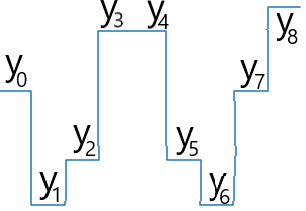
\includegraphics[width=0.3\columnwidth]{step-wise_example.png} % TODO: Change the image
    \caption{Example of a step-wise constant function as an array of numbers}
    \label{fig:step-wise-const}
\end{figure}
\subsection{The Cost Function}
When our desired operation is to prepare our quantum system in a predetermined state, a good figure of merit of how close our system is to the desired state is given by the \textbf{fidelity}. The fidelity is a measure of the "closeness" of two quantum states, The fidelity is $0$ when the two states are orthogonal, and $1$ if they are identical. The fidelity is given by the magnitude of the \textit{overlap} between the two states squared\footnote{Assuming both states are pure states and not mixed states}.

\begin{equation} \label{def:fid}
F (\psi_1, \psi_2) = \abs{\braket{\psi_1}{\psi_2}}^2
\end{equation}
The \textit{infidelity}, $1 - F$ between the two states, can be conveniently used as the cost function in our optimization procedure\footnote{Since we want to maximize the fidelity, we want to minimize the infidelity}. Given an initial state and a target state, along with the Hamiltonian and pulse information, we want to be able to calculate the fidelity for any given pulse. To do so, we need to solve Schr\"{o}dinger's equation for the pulse
\begin{equation}
i\hbar\frac{d}{dt}\ket{\Psi (t)} = \hat{H}\ket{\Psi (t)}
\end{equation}
In the previous chapter we characterized the Hamiltonian of the system (equations (\ref{eq:JC-hamiltonian}) and (\ref{eq:dispersive-hamiltonian})),
% TODO: Add explanation about that there are multiple different pulses and throughout the chapter we're referring to a single pulse which is most of the time not the case
\begin{equation} \label{eq:hamiltonianl_form}
H (t) = H_0 + \sum_k{\epsilon_k (t) H_k} % Maybe put the next part before the part about the Schrodinger equation
\end{equation}
where $H_0$ is the (time-independent) Hamiltonian of the system without the drives (given, for example, from the Jaynes-Cummings model). Each $\epsilon_k (t)$ is the amplitude as a function of time of the control drive pulses, and each $H_k$ is the (time-independent)Hamiltonian describing the interaction between the control pulse and the rest of the system. We call these Hamiltonians the \textit{drive hamiltonians}. Our goal with GRAPE is to find optimal $\epsilon_k (t)$.

On each constant step of the amplitude functions $\epsilon_k (t)$, the entire Hamiltonian is constant. Luckily, the solution of the Schr\"{o}dinger equation for a constant Hamiltonian is easily solved by
\begin{equation}
\hat{U} (t) = e^{-\frac{i}{\hbar}\int_{T_0}^{T_1}H (t)dt}
\end{equation}
If we choose $T_0$ and $T_1$ as the end points of a step of the Hamiltonian, the total Hamiltonian of the system is constant so the integral is just a simple multiplication by $T_1-T_0$ which we'll write as $\delta t = T_1 - T_0$. The solution becomes
\begin{equation}
\hat{U} (t) = e^{-\frac{i\cdot \delta t}{\hbar}H (t)}
\end{equation}

In order to calculate the solution over the entire pulse we need to solve for the first step, then find the solution by the end of that time-step, and use it as the initial condition for the next time step, repeating for each time step. The solution until the $N^{th}$ time step is simply the product of the previous solutions for each time step
\begin{equation}\label{eq:U_def_prod}
\hat{U}_N (\epsilon (t)) = \prod_{k = 1}^N\hat{U}_k (\epsilon (t))
\end{equation}
With $\hat{U} (\epsilon)$ in hand, we can calculate the evolution of the state over the entire pulse
\begin{equation}
\ket{\Psi_{final}} = \hat{U} (\epsilon)\ket{\Psi_{initial}}
\end{equation}
This way, if we want to calculate the fidelity after applying the drives, we can simply calculate the fidelity between the target state and the final, calculated state
\begin{equation} \label{eq:fidelity_sim}
F (\epsilon (t)) = F (\Psi_{target}, \Psi_{final}) = \abs{\bra{\Psi_{target}}\hat{U}_N\ket{\Psi_{initial}}}^2
\end{equation}

As mentioned, if we want to optimize the cost function efficiently we'll need to calculate the gradient of the cost function along with the cost function itself.

\subsection{The Gradient}
For simplicity, we'll first derive the gradient of the \textit{overlap}
\begin{equation} \label{def:overlap}
c = \braket{\Psi_{target}}{\Psi_{final}} = \bra{\Psi_{target}}\hat{U}\ket{\Psi_{initial}}
\end{equation}
We can then get the fidelity by noting that $F = \abs{c}^2$. We want to differentiate the overlap by each control parameter. To do so, note that $\hat{U}$ is defined as:
\[ 
\hat{U} = \hat{U}_N \hat{U}_{n-1}...\hat{U}_2 \hat{U}_1
\]
And when differentiating by a control parameter only one $\hat{U}_k$ is affected,
\[
\frac{\partial c}{\partial \epsilon_k} = \bra{\Psi_{target}}\hat{U}_N \hat{U}_{N-1} ... \hat{U}_{k+1}\frac{\partial \hat{U}}{\partial \epsilon_k} \hat{U}_{k-1} ...\hat{U}_2 \hat{U}_1\ket{\Psi_{initial}} 
\]
We can write that for a constant Hamiltonian (from Schr\"{o}dinger's equation)
\[
    \hat{U}_k = e^{-\frac{i\cdot \delta t}{\hbar}H (t)}
\]
And approximate the derivative $\frac{\partial \hat{U}_k}{\partial \epsilon_k}$ in the limit of small $\delta t$ by writing
\begin{equation*}
    \frac{\partial \hat{U}_k}{\partial \epsilon_k} \approx -\frac{i\cdot \delta t}{\hbar}\frac{\partial H}{\partial \epsilon_k} \cdot e^{-\frac{i\cdot \delta t}{\hbar}H (t)} = -\frac{i\cdot \delta t}{\hbar}\frac{\partial H}{\partial \epsilon_k} \hat{U}_k
\end{equation*}

Theoretically, we have everything we need to calculate the gradient, but it's still rather complex computationally ($o (N^2)$ complexity). A different method can be used to reduce the computational overhead.

The derivative of the cost function by a control parameter of the pulse has become
\begin{equation} \label{eq:cost_init_deriv}
    \frac{dc}{d\epsilon_k} = -\frac{i\cdot \delta t}{\hbar} \underbrace{\bra{\Psi_{target}}\hat{U}_N \hat{U}_{N-1}... \hat{U}_{k+1}}_{\bra{\psi_{bwd}^{ (k+1)}}}\frac{dH}{d\epsilon_k} \underbrace{\hat{U}_{k} ...\hat{U}_2 \hat{U}_1\ket{\Psi_{initial}}}_{\ket{\psi_{fwd}^{ (k)}}}
\end{equation}
Where we defined two arrays, $\bra{\psi_{bwd}}$ and $\ket{\psi_{fwd}}$, the multiplication components before and after the derivative of H
\begin{equation} \label{eq:cost-function-b/fwd}
    \frac{\partial c}{\partial \epsilon_k} =  -\frac{i\cdot \delta t}{\hbar}\bra{\psi_{bwd}^{ (k+1)}} \frac{\partial H}{\partial \epsilon_k} \ket{\psi_{fwd}^{ (k)}}
\end{equation}
We can see from \ref{eq:cost_init_deriv} that 
\[   
\ket{\psi_{fwd}^{ (k)}} = 
     \begin{cases}
       \ket{\psi_{init}} &\quad\ k=0\\
       \hat{U}_k \ket{\psi_{fwd}^{ (k-1)}} &\quad\ otherwise\\
     \end{cases}
\]
\[   
\ket{\psi_{bwd}^{ (k)}} = 
     \begin{cases}
       \ket{\psi_{targ}} &\quad\ k=N+1\\
       \hat{U}_k^{\dag{}} \ket{\psi_{bwd}^{ (k+1)}} &\quad\ otherwise\\
     \end{cases}
\]
Now all we need is to do $2N$ calculations in the beginning ($N$ for $bwd$ and $N$ for $fwd$), and then calculating the actual gradient using equation \ref{eq:cost-function-b/fwd}. This improves the computation complexity from $o (N^2)$ to $o (N)$, while the memory complexity stays $o (N)$.

It's important to note that $c$ is not the fidelity, but the overlap. We can get the fidelity from $c$ by
\[
F = |c|^2
\]
since $c$ might be complex this derivative is a bit less trivial than it might seem. We can write $c (\vec{\epsilon})$ as $a (\vec{\epsilon}) + b (\vec{\epsilon})i$, where $a, b \in R$ and we get that 
\[
\frac{\partial F}{\partial \epsilon_k} = \frac{\partial |c|^2}{\partial \epsilon_k} = \frac{\partial |a+bi|^2}{\partial \epsilon_k} = \frac{\partial (a^2 + b^2)}{\partial \epsilon_k} = 2 (a\frac{\partial a}{\partial \epsilon_k} + b\frac{\partial b}{\partial \epsilon_k})
\]
We can notice that $c (\frac{\partial c}{\partial \epsilon_k})^* = a\frac{\partial a}{\partial \epsilon_k} + b\frac{\partial b}{\partial \epsilon_k} + (ab - \frac{\partial a}{\partial \epsilon_k}\frac{\partial b}{\partial \epsilon_k})i$. More importantly, we can see that the real part of that expression is exactly what we need. Putting it all into one formula we get
\begin{equation} \label{eq:fidelity_gradient_final}
    \frac{\partial F}{\partial \epsilon_k} = 2\cdot \Re{c (\frac{\partial c}{\partial \epsilon_k})^*}
\end{equation}
Now all you need is to plug \ref{eq:cost-function-b/fwd} and \ref{def:overlap} into \ref{eq:fidelity_gradient_final} and you got your gradient :)

Let's do a little test now to see that everything is working well. The simplest pulse you can send is the pulse that takes the qubit from being in state $\ket{0}$ to state $\ket{1}$, where the transition frequency is set to $1$Ghz (hence the period is $1$ns). We discussed this situation in appendix \ref{appen:annalytic} so we know how the solution should look like. Running our GRAPE code with some random initial pulse we get
\begin{figure}[H]
    \centering
    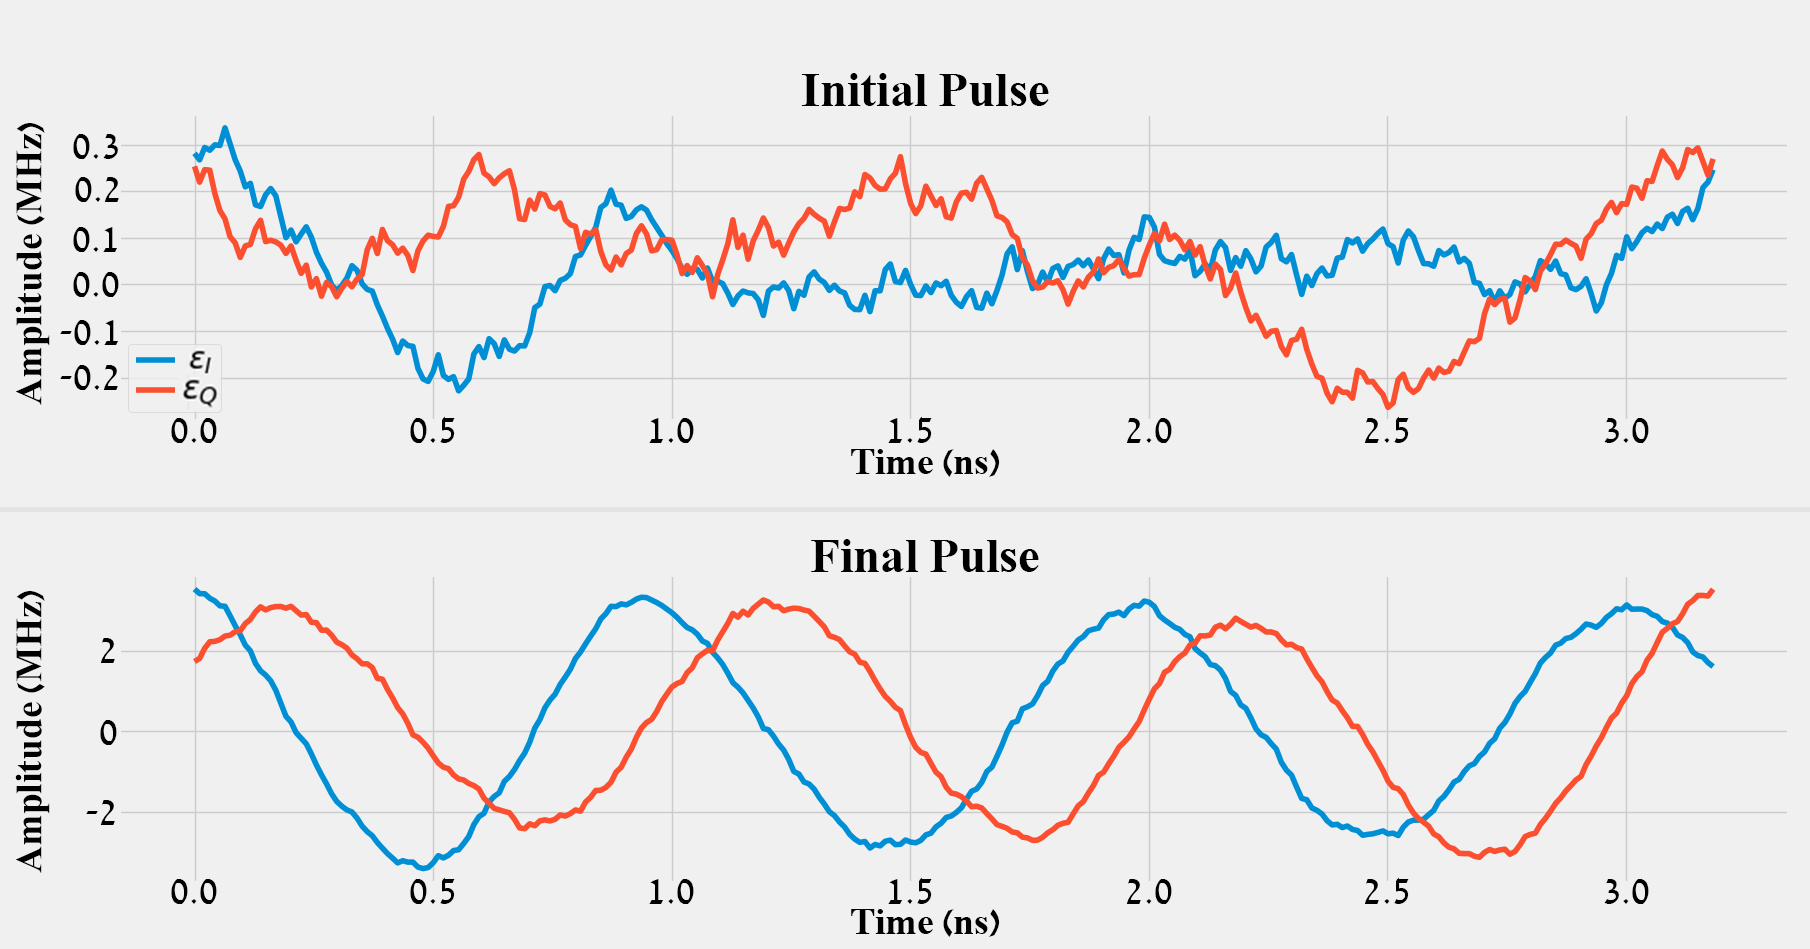
\includegraphics[width=0.8\columnwidth]{Results/No-Constraints-single-qubit/pulses-prettier.png}
    \caption{Pulses solution for $\ket{0} \rightarrow \ket{1}$. Each color is a different microwave control pulse of the system, I and Q. They are the real and imaginary parts of the calculated wave in appendix \ref{appen:annalytic} }
    \label{fig:GRAPE-first-example}
\end{figure}
Amazing! From some random initial pulse we got sinusoidal waves with $1$Ghz frequency, just as predicted in appendix \ref{appen:annalytic}.

Before we get too excited, there are a couple of things weird with this pulse. The first, more obvious problem, is that although the waves are sin and cos as expected, they're still pretty jagged-y, there is some randomness on top of the wave and it's not as smooth as we expected. This is since small random changes don't really change the final result\footnote{The noise cancels itself out}. In addition, high-frequency components generated  by the computer do not have an effect in reality. This is due to the limited bandwidth of our pulse generator and RF circuitry.

Another problem, that is not immediately obvious, we can only see if we look at the population graph of the qubit over the duration of the pulse. We expect the graph to start at $1$ and end at $0$ for $\ket{0}$ and start at $0$ and end at $1$ for $\ket{1}$. Let's look at that graph for the initial random pulse and for the optimized pulse
\begin{figure}[H]
    \centering
    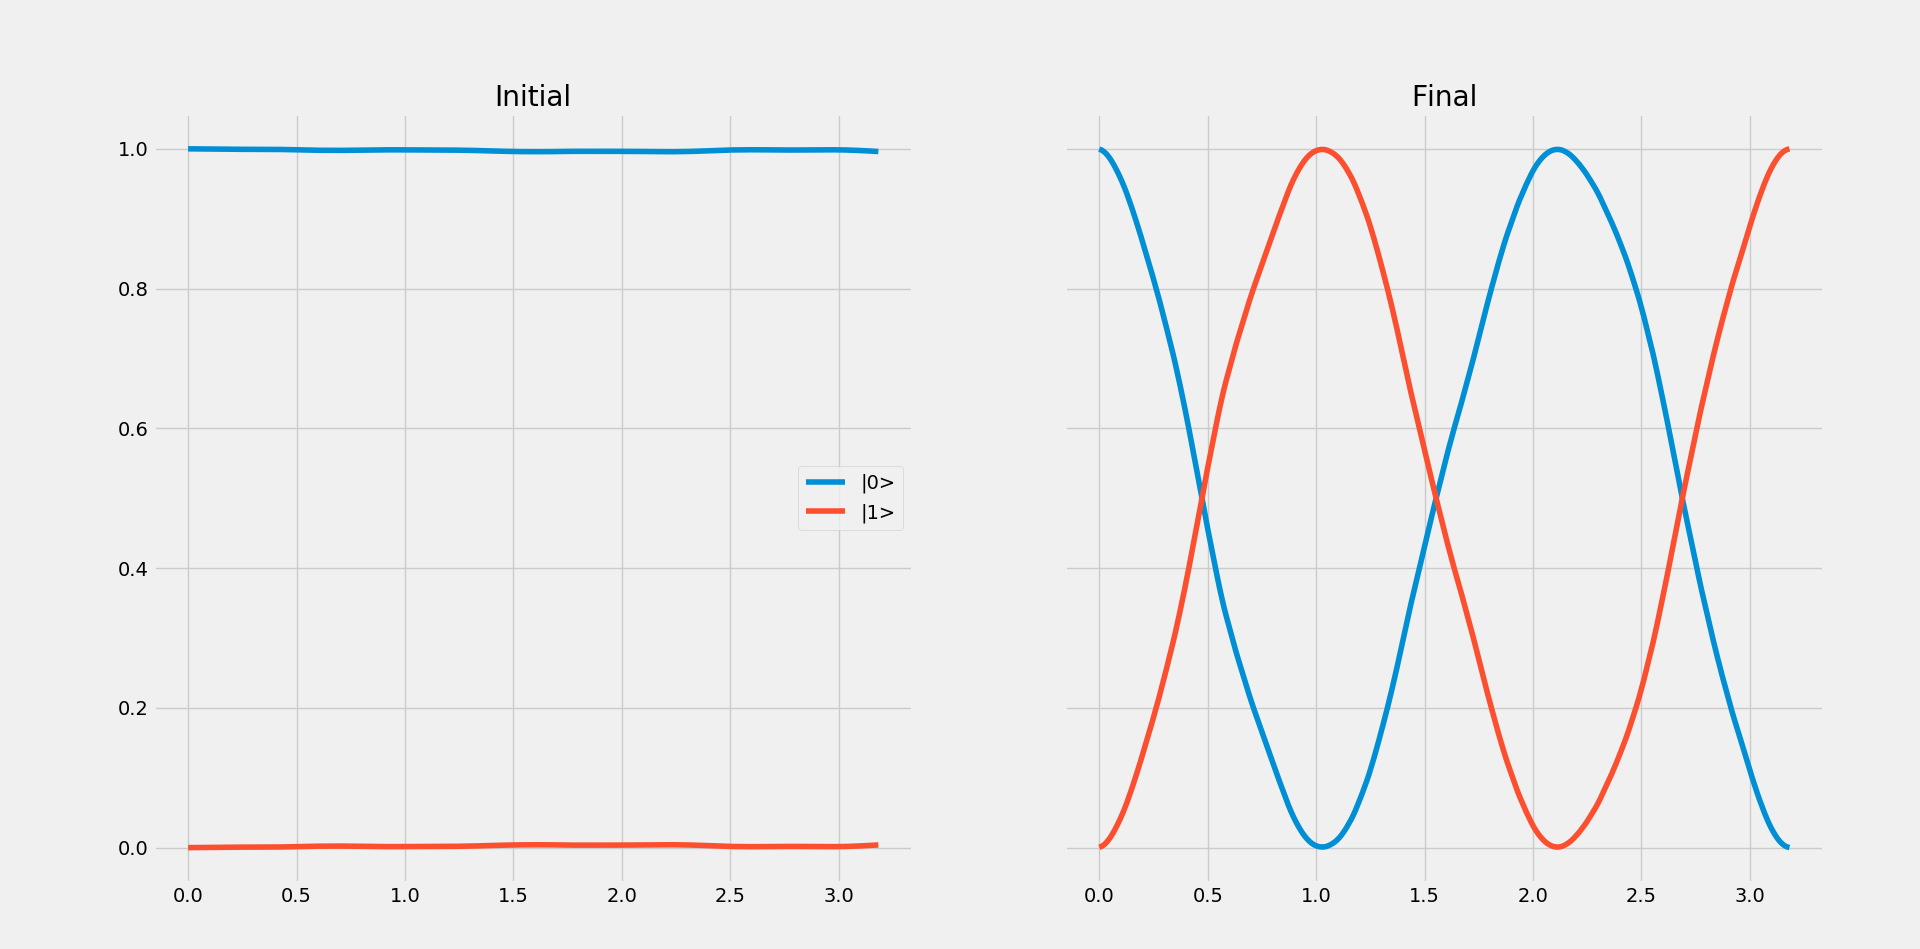
\includegraphics[width=1\columnwidth]{Results/No-Constraints-single-qubit/level-population-pretty2.png}
    \caption{Population of qubit levels over pulse duration. Before the optimization, the state of the qubit (population of ground and excited states) almost did not change at all. After the optimization, the qubit goes from state $\ket{0}$ to $\ket{1}$ to $\ket{0}$ to $\ket{1}$, doing some unnecessary back and forth between the states}
    \label{fig:GRAPE-first-example-level-population}
\end{figure}
As expected, the initial random pulse doesn't change the pulse almost at all. The optimized pulse on the other hand is problematic. The population of $\ket{0}$ for example, goes from 0 to 1 and then goes back to 0 to start over again. Ideally, the population will change from 0 to 1 (and vice-versa) smoothly, only once.

This happens because the amplitude of the optimized pulse is too big. As we defined the optimization, the algorithm doesn't care that the population acts weirdly in the middle of the pulse as long as it ends at the desired state.

To solve these problems (and more we'll talk about), we introduce \textit{constraints} to the algorithm.
% \footnote{I'll give a quick note just to be honest, since this is such a simple case, GRAPE works pretty well even without any constraints. I've carefully crafted conditions so that the final pulse wouldn't be smooth and so the level population would go crazy. This is what you'll see normally in more complex examples but I didn't want to go with a complex example since it would just complicate things without giving any real benefit}

\subsection{Constraints}
% Unfortunately, we live in the real world, and in the real world we can't just make ultra-fast frequency pulses with the energy of the sun. It's impossible because of the limitation of our devices. The computer doesn't care for the limitation of the devices, That's why we need to add constraints to the cost function.
Since instruments have physical limitations, for example, on the maximum amplitude of a pulse, we must add constraints on the computer calculations to not exceed these limitations.

We define a set of constraints on the solution ${g_i \ge 0}$, and associate a Lagrange multiplier $\lambda_i$ to each constraint\footnote{In an ideal optimized pulse, $g_i = 0$}. \newline
Our goal is to minimize 
$$1 - F (\vec{\epsilon}) + \sum_i \lambda_i g_i (\vec{\epsilon})$$
Let's add a constraint to each of the most problematic physical limitations.
\subsubsection{Limiting the Amplitude}
This is the most obvious physical limitation. We can't generate pulses with infinite energy, so we have to restrict it. There are two ways we can do so, the first is to create a hard cut-off amplitude. No matter what, the amplitude will never go above this amplitude. We usually want this cut-off to be the  maximal output amplitude of our pulse generator. But normally we don't want our generator to work at its absolute limit\footnote{Not only that it might damage the device, with stronger pulses the non-linear optical effects increase}, so we can add also a soft amplitude maximum by "rewarding" the cost function to stay at a lower amplitude. Let's see how we would implement such a thing, starting with the hard cut-off.

Instead of controlling and changing the amplitude ($\vec{\epsilon}$) directly, we'll introduce a variable $\vec{x}$ and relate them as
\[
    \vec{\epsilon} = \epsilon_{max}\tanh{\vec{x}}
\]
As you probably guessed, $\epsilon_{max}$ is the maximum amplitude of the pulse.
Since the optimization algorithm can only change $\vec{x}$, the amplitude of the pulse will always be between $-\epsilon_{max}$ and $\epsilon_{max}$. Unfortunately, this changes the gradient of the cost function since we now want the derivative with respect to $\vec{x}$ instead of $\vec{\epsilon}$. We can relate the two
\[
\frac{\partial F}{\partial \vec{x}} = \frac{\partial F}{\partial \vec{\epsilon}}\frac{\partial \vec{\epsilon}}{\partial \vec{x}} = \frac{\epsilon_{max}}{\cosh^2{\vec{x}}} \ \frac{\partial F}{\partial \vec{\epsilon}}
\]
We can use the derivative $\frac{\partial F}{\partial \vec{\epsilon}}$ we got from \ref{eq:fidelity_gradient_final} and simply calculate $\frac{\epsilon_{max}}{\cosh^2{\vec{x}}}$ and we again have the gradient.\footnote{Since $\tanh (x)$ is a positive monotonic transformation it preserves the locations of the maxima of the function. This means that in practice we can just ignore the new derivative}

% For the soft limitation, there are two limitation we can make, linear and non-linear. The linear goal is for general preference of low amplitude pulses and the non-linear is if you have a specific $\epsilon_{max,soft}$ that you want to be well below of (You can use both or either one depends on your desired pulse properties). We'll start with the linear case since it's simpler.
% TODO: NON-LINEAR
For the soft amplitude penalty all we want is that \textit{bigger amplitudes} $\Rightarrow$ \textit{bigger cost function}. Since our algorithm seeks to minimize the cost function, this will lead to the overall amplitude being smaller. The way we do so is simple, we can define a constraint $g_{amp}$ that sums all the amplitudes of the steps of the pulse, so
\[
    g_{amp} = \sum_k |\epsilon_k|^2
\]
Still, since it is added to our cost function we need to find the gradient of the penalty as well. In this case it's rather simple since it's a basic parabola
\[
    \frac{\partial g_{amp}}{\partial \epsilon_k} = 2\epsilon_k
\]
and now we have all we need in order to add this penalty to our cost function.\footnote{We can also create non-linear soft amplitude constraint. With such constraint we can set a soft maximum we want to stay well below of. We won't show how to do so}% Let's move on to the non-liner penalty.

% For the non-linear amplitude penalty we have a slightly different goal in mind
% TODO: Add here the non linear amplitude penalty


\subsubsection{Limiting Bandwidth and Slope}
The next limitation is the maximum frequency our AWG can create because the device can't change the voltage instantaneously. Again, like we had with the amplitude limit, there are 2 types of limits we can make, hard and soft. Let's start with the hard limit.

We have some frequency $ \omega_{max} $ which is the maximum frequency that our AWG can generate. To make sure that our simulation doesn't produce such a pulse we can go from time space to the frequency space with a Fourier transform
\[
    \vec{\epsilon} = (DFT)^{-1} \vec{x}
\]
The numerical optimization algorithm controls $\vec{x}$ which is in the frequency space. Now if we want to limit the frequency we can simply set to 0 any frequency that is above our maximum frequency
\[
    x (\omega > \omega_{max}) = 0
\]
The gradient of the new cost function is simply the Fourier transform of x
\[
    \frac{\partial \vec{x}}{\partial \epsilon_k} = (DFT) \frac{\partial \vec{\epsilon}}{\partial \epsilon_k}
\]
And we know $\frac{\partial \vec{\epsilon}}{\partial \epsilon_k}$ from previous sections.
It's important to note that the hard cut-off of the amplitude and the hard cut-off of the frequency do not work together since one is in time domain and one is in frequency domain. This is not much of a problem since we can compensate with the soft limits that do work well together (since they require adding to the cost function instead of changing coordinates). In my simulations I use the amplitude hard limit instead of the frequency one since it is easier to work with.

For the soft limits, we're limiting the slope (derivative) of the pulses and not the frequency directly. The slope of a step function is simply $\epsilon_{k+1} - \epsilon_{k}$, we want to limit the size of the slope so we'll look at the expression $|\epsilon_{k+1} - \epsilon_{k}|^2$ instead. Summing all the slopes (to get an overall slope size of the entire pulse) we get the expression\footnote{Note that we have a problem at the edges since the slope of the end points is not well defined, we'll fix this problem later but for now we just ignore the last point $k=N$}
\begin{equation}\label{eq:g_slope}
    g_{slope} = \sum_{k=0}^{N-1} |\epsilon_{k+1} - \epsilon_{k}|^2
\end{equation}{}
Unlike the amplitude, since the slope of the boundaries is not well defined we'll have the edges defined differently than the center of the pulse. The gradient of $g$ in the center is a simple derivative, notice that each $\epsilon_k$ appears only twice in the sum
\[
    \frac{\partial g_{slope}}{\partial \epsilon_k} = 4\epsilon_k - 2 (\epsilon_{k+1} + \epsilon_{k-1})
\]
It's nice to see that the expression looks like how'd you numerically estimate the second derivative, since the gradient of the slope (which is the derivative) is the second derivative. Now we need to define the gradient at the edges, you can see that the derivative of $\epsilon_k$ depends on his neighbors on both sides. Since the first and last element of the pulse don't have 2 neighbors they are treated a little differently. each of the edges appears only once in the sum \ref{eq:g_slope} unlike the others that appear twice, we can simply take the derivative of that one term and get
\begin{align*}
    &\frac{\partial g_{slope}}{\partial \epsilon_0} = 2 (\epsilon_1 - \epsilon_0) \\
    &\frac{\partial g_{slope}}{\partial \epsilon_N} = 2 (\epsilon_N - \epsilon_{N-1})
\end{align*} 
Now, before we continue, we'll add another small constraint that will also solve the problem of the slope at the boundaries. It might seem weird at first, but we want to pulse to zero-out at the edges. This is since our AWG device can't immediately start a pulse with some amplitude, it can't get from 0 to that amplitude instantaneously (for the same reason we limit the slope in the first place). This could be achieved by simply setting the first and last steps of the pulse and their gradient to 0.
\[
    \epsilon_0 = \epsilon_N = \frac{\partial \ \text{Cost}}{\partial \epsilon_0} = \frac{\partial \ \text{Cost}}{\partial \epsilon_N} = 0
\]
This solves the problem we were trying to solve we were having with the slope at the boundaries, since the gradient is 0 at the edges and does not depend on its neighbors.% We can move on to the non-linear limitation now.

% As we mentioned earlier, the goal of the non-linear limitation is when we have a specific bandwidth to be well below off, the could be achieved thanks to the fact that exponents grow really fast
% \[
%     Add\ equation\ here
% \]
% TODO: Add here but more importantly change how is the goal of the non-linear limitation explained.

Now that we have both amplitude constraint and bandwidth constraint we can use them to get a nice, smooth solution, that any wave generator would be happy to produce
\begin{figure}[H]
    \centering
    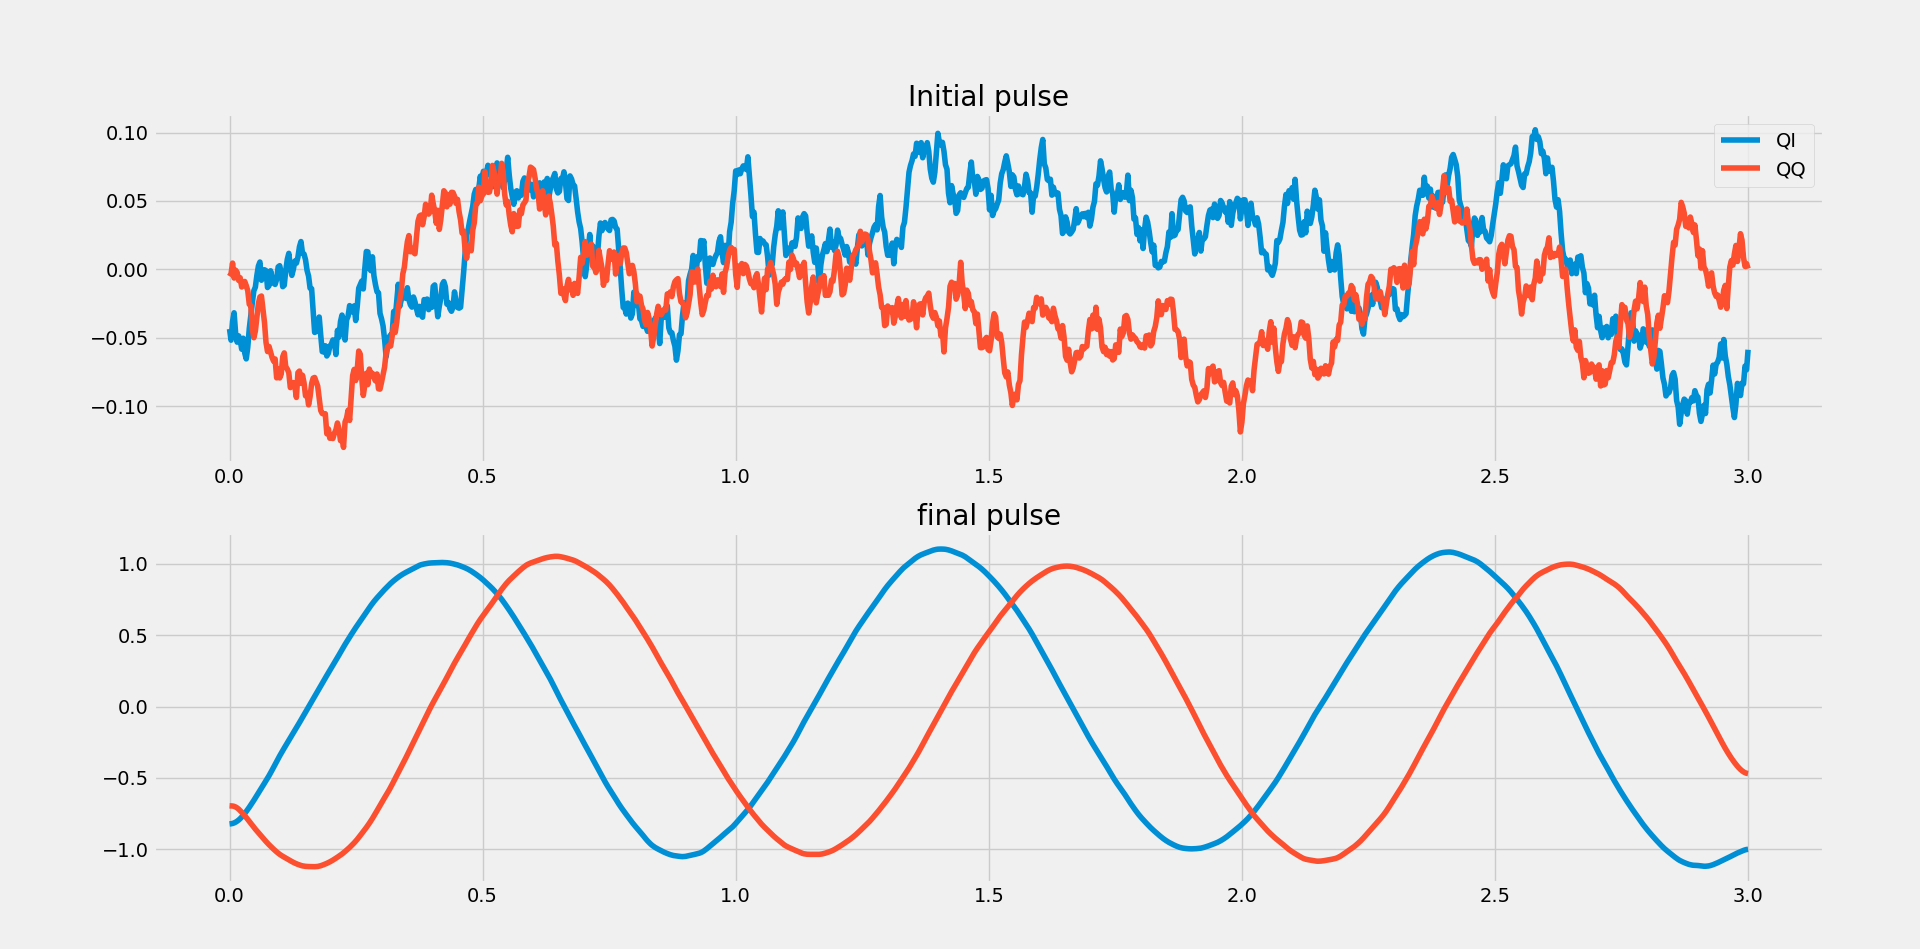
\includegraphics[width=1\columnwidth]{Results/qubit-band-amp-const/pulses.png}
    \caption{Control pulses before and after GRAPE optimization with amplitude and bandwidth constraints}
    \label{fig:band-amp-const-qubit}
\end{figure}
The pulse is exactly what we expect it to be. More importantly, if we look at the population graph of the levels, it does exactly what we want, go from state $\ket{0}$ to state $\ket{1}$ without going back and forth.
\begin{figure}[H]
    \centering
    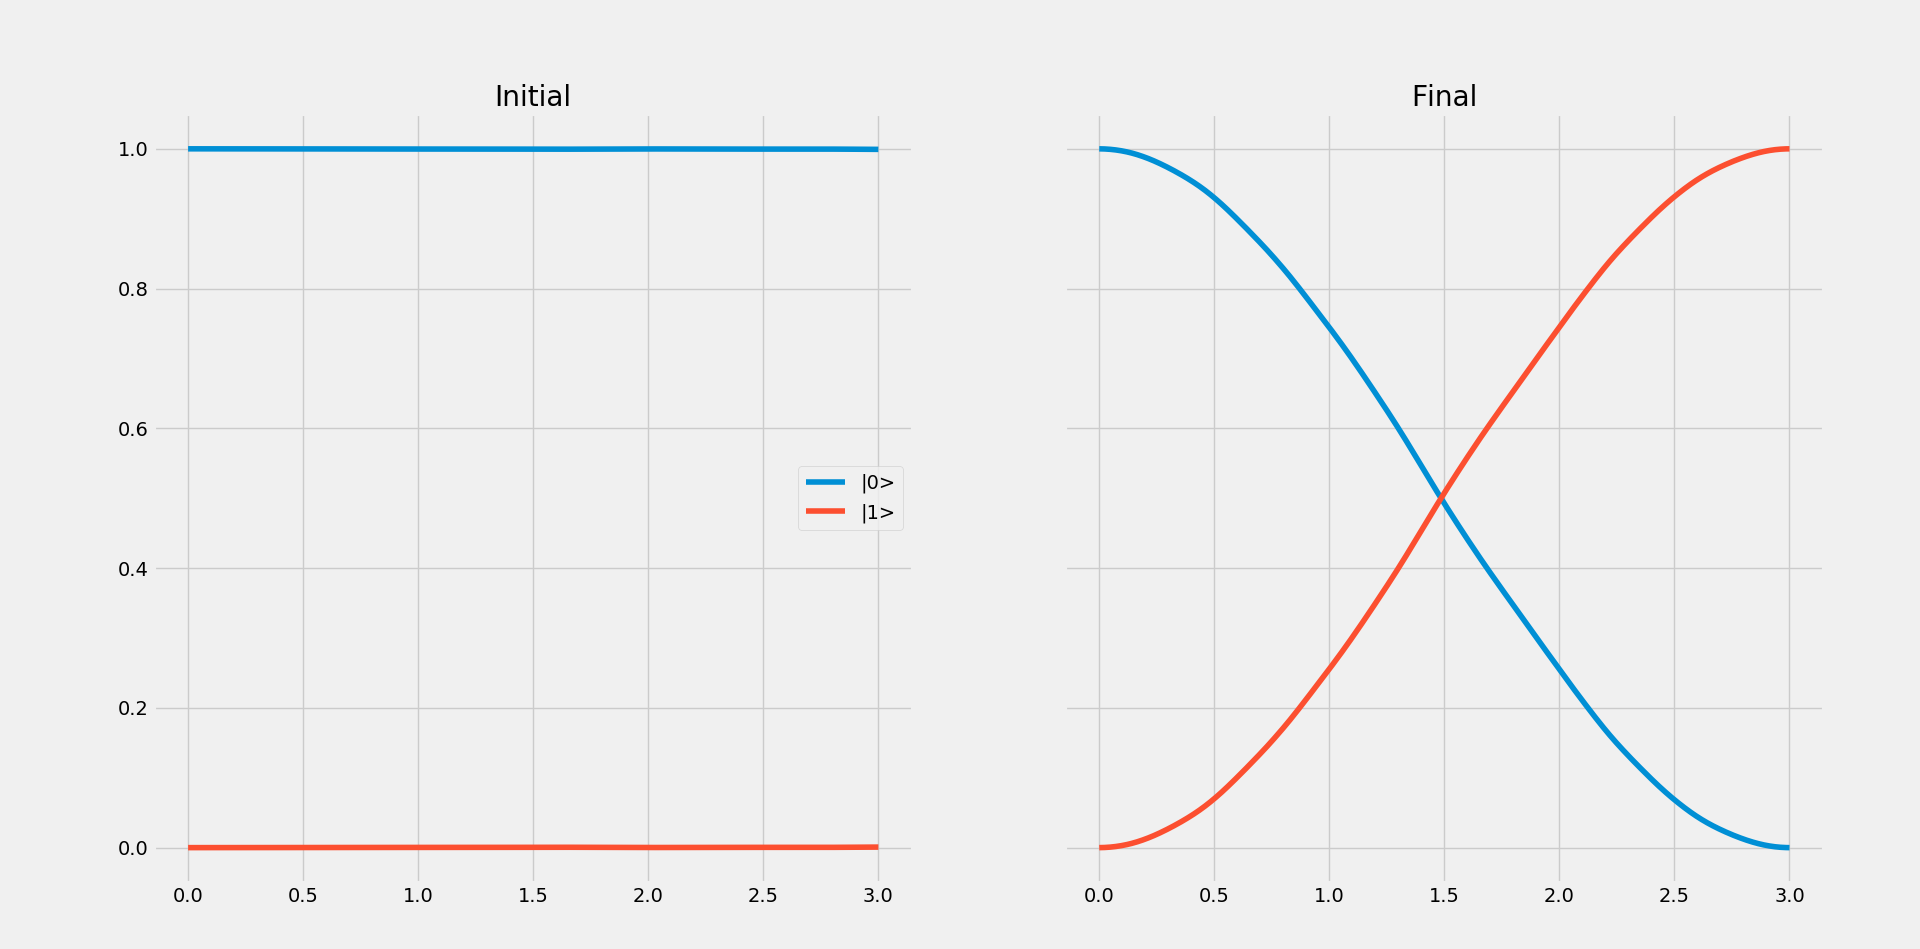
\includegraphics[width=1\columnwidth]{Results/qubit-band-amp-const/level-population.png}
    \caption{Population of qubit levels over pulse duration. Before the optimization, the state of the qubit (population of ground and excited states) almost did not change at all. After the optimization, the qubit goes from state $\ket{0}$ to $\ket{1}$}
    \label{fig:band-amp-const-level-population}
\end{figure}

Another interesting visualisation of the success of this pulse is the path of the qubit on the Bloch sphere over time (see the last section in chapter \ref{chap:quantum-optics}). Plotting the populations on the Bloch sphere we get 
\begin{figure}[H]
    \centering
    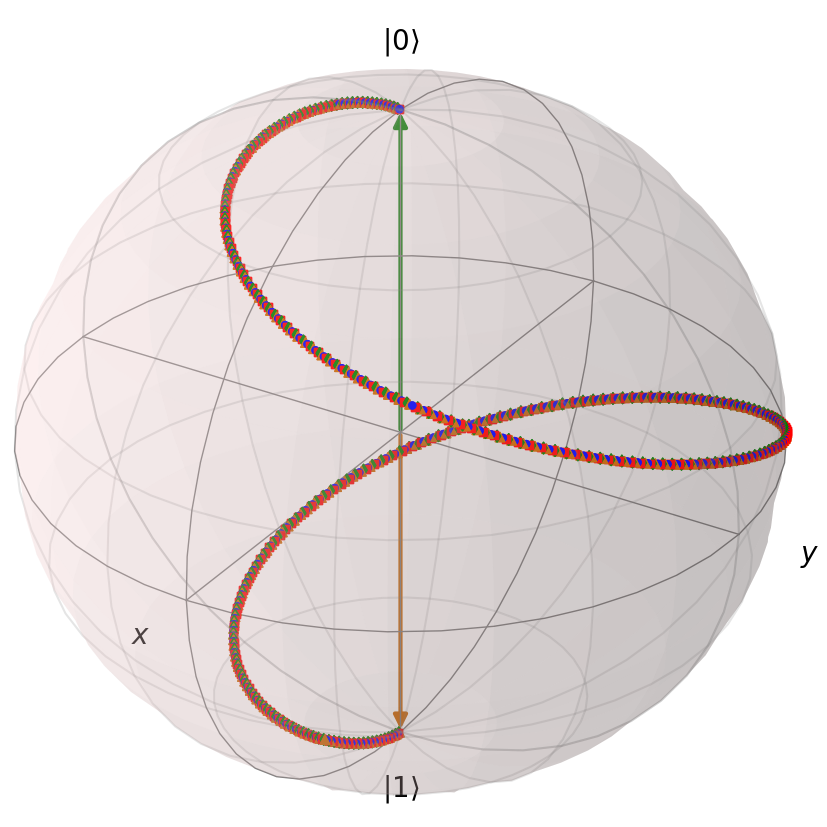
\includegraphics[width=0.4\columnwidth]{Results/qubit-band-amp-const/Bloch-qubit.png}
    \caption{Path of the qubit along the Bloch sphere. The qubit goes from state $\ket{0}$ to state $\ket{1}$, preforming one loop on the sphere, the arrows represent the initial state and the target state, and the points represent the path of the state of the qubit}
    \label{fig:band-amp-const-blcoh}
\end{figure}
As you can see, the path of the qubit isn't a straight line, but some loop, completing a full rotation around the $\hat{z}$ axis. This is explained by the fact that the base Hamiltonian of the qubit is $\omega \hat{\sigma}_z$, where $\hat{\sigma}_z$ is the Pauli matrix Z. This matrix corresponds to rotation of the Bloch sphere around the $\hat{z}$ axis. This is why we can think of the entire Bloch sphere as always rotating with frequency $\omega_0$ around the $\hat{z}$ axis, this is why a "straight" path is actually one that does one loop around the $\hat{z}$ axis.

\subsubsection{Limiting Pulse Duration}
As much as I wouldn't mind waiting a few nanoseconds longer for the qubit operation to end, the qubit itself isn't as patient as me. A state-of-the-art qubit would last, at most, few hundred microseconds (and that's a very optimistic estimation). We simply don't have the time to wait for the operation to end if we want to run some complicated quantum circuit. This is why we want to add a constraint on the \textit{duration} of the pulse. This way, if we set the total duration of the pulse to longer than the shortest possible pulse, it would find the shorter pulse and the rest of the pulse will change nothing (see figure \ref{fig:dur-penelty})

% give the pulse 5ns to finish, and a solution of 3ns exists, the optimization algorithm would (hopefully) find the 3ns solution and the rest of the time until the end of the duration will do nothing.

The constraint is fairly straight forward, add a penalty for any time a fidelity of 1 isn't achieved. Put into an equation we get
\[
    g_{duration} = \sum_{i = 0}^{N-1} (1 - F_i)
\]
Where $F_i$ is the fidelity at time step $i$.

We can rather simply calculate the fidelity at any given time since they are already calculated in order to find the fidelity in the last time step. We can simply modify the loop that calculates the final state into giving the fidelity at each time step and sum the results. 
% TODO: Maybe remove some of the technical details about the code and the implementation

Luckily for us, the calculation of the gradient is also pretty simple. The gradient of the fidelity at each time step is calculated the same as the gradient of the fidelity we calculated in the beginning of the chapter\footnote{note that $\epsilon_k$ only appears in the expression for $F_i$, if $i > k$, so the sum starts at $i = k$}
\[
    \frac{\partial g_{duration}}{\partial \epsilon_k} = -\sum_{i = k}^{N-1}\frac{\partial F_i}{\partial \epsilon_k}
\]
% TODO: I think I can find a more efficient solution, Got to check this in the code and ask serge for his opinion

The pulse duration constraint works nicely to complete the other constraints. Without this constraint, the pulse will "try" to use all it's time to get the result we desire. When running the algorithm without the constraint we can get problems if the duration we gave to the pulse is too long or too short. With this constraint on, we can simply give the algorithm a duration that we know for sure is more then the minimum required time, and the algorithm will simply use the minimum time it needs, and no more. On the other hand, if we didn't have the amplitude (and bandwidth) constraints, the algorithm might find that it's best to just give a super-strong pulse for a tiny amount of time, but that's not physically possible as we discussed. This is why we can think of the constraints working together to "box in" the pulse into an ideal "size".

If we run GRAPE now, with all the constraints together, and look at the population of all the level over the duration of the pulse, we get\footnote{This is a rather extreme case where the total duration of the pulse is around three times longer then the minimum duration. This was done purposefully to demonstrate the point.}
\begin{figure}[H]
    \centering
    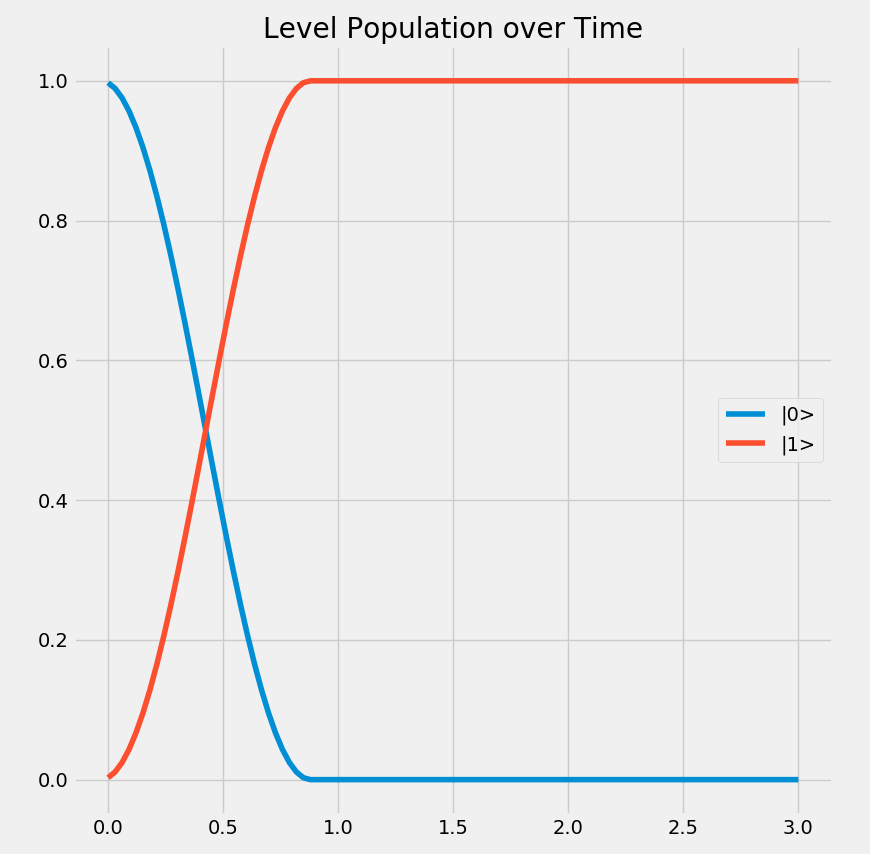
\includegraphics[width=0.5\columnwidth]{Results/duration-constraint/level-population.png}
    \caption{Level population of each state as a function of time over the duration of the pulse.}
    \label{fig:dur-penelty}
\end{figure}

As expected, we get exactly what we want, the pulse uses the least amount of time that it needs and then stop. This way, if we pick a long duration for the pulse, instead of the pulse trying to fill the entire time at a very low amplitude, or do several of loops before arriving at the target, the qubit simply takes exactly the amount of time that it needs to get to the desired state under all of the constraints and then stops.

\subsection{Implementing Qubit Operations with GRAPE}

\subsubsection{DRAG - Imperfect Qubits} \label{sec:DRAG}
When we did all of our calculation on the qubit we didn't include one detail, it's really hard to create a true two-level system. In the way our qubits are implemented, there are actually more than two levels. It's not a two level system but we treat it as one. Since the higher levels are off-resonance, we can often just ignore them. However, there is some probability of the higher levels getting populated by high-frequency components of our pulses. The shorter our pulses are, the more these higher  levels excitation occur. We will prevent those so-called leakage errors by using \textbf{D}erivative \textbf{R}emoval via \textbf{A}diabatic \textbf{G}ate (DRAG) pulses. We can generate those pulses by including more than two levels in our algorithm and changing the Hamiltonian a little bit so it accounts for the off-resonance higher levels.

Before we continue to implement DRAG, let's see if the third level really is that much of a problem. We run a simulation of GRAPE just as we did before but this time with three levels instead of two, and the third level should start and end at 0 population. We get after running GRAPE
\begin{figure}[H]
    \centering
    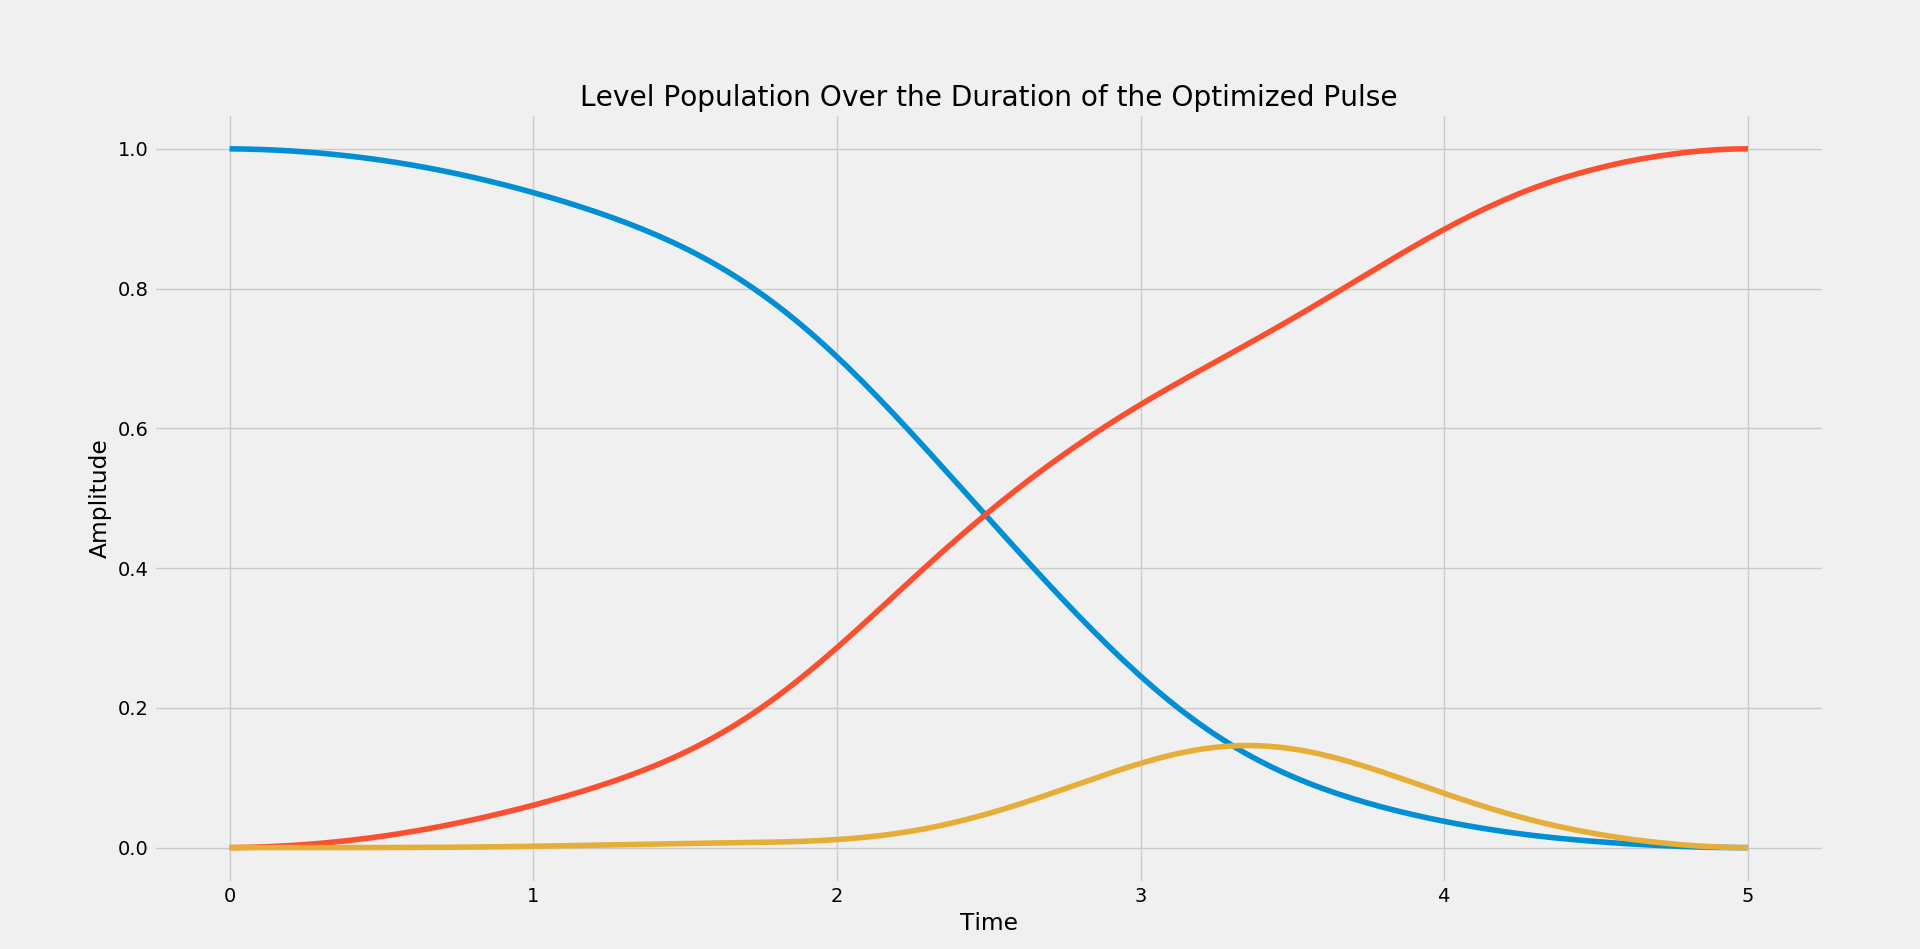
\includegraphics[width=1\columnwidth]{Results/Before-Drag/level-population-pretty.png}
    \caption{Level population of the 3-level "qubit" over the duration of the pulse calculated by the GRAPE algorithm we have so far}
    \label{fig:before-DRAG}
\end{figure}
Well yes, the forbidden level did start and end at $0$ population\footnote{If you decrease the anharmonicity you would also have final forbidden level population, which is a more serious problem}, but in the middle the qubit really became a 3 level system with the population of the forbidden level being really dominant around time $3.5$! We can't simply replace the qubit with a 3 level system and make the target of the third level always 0 and call it a day. \textbf{We can't treat higher levels as just more "qubit" levels}, they are unwanted and we need to give them a penalty so the probability of being in a higher level would be always almost zero and change only a tiny bit. There are many ways we could implement such a penalty, the most obvious way is by simply making the probability to be in an higher level into a penalty, summing over all time we get (We'll call the third level of the qubit $\ket{f}$ to not be confused with the $\ket{3}$ Fock state (photon number state))\footnote{If we wanted to accounted for higher levels we can sum over the sum for each level}
\[
    g_{forbidden} = \sum_{i=0}^{N - 1} \abs{\braket{f}{\psi_{fwd}^{ (i)}}}^2 
\]
We already have $\psi_{fwd}^{ (i)}$ that we calculated earlier, so for so good.

Now moving to to complex part of DRAG, the gradient. Let's again define the overlap
\[
    c_{f} = \sum_{i=0}^{N - 1} \braket{f}{\psi_{fwd}^{ (i)}}
\]
now to calculate the gradient we'll derive over $\epsilon_k$
\[
    \frac{\partial c_{f}}{\partial \epsilon_k} = \frac{\partial}{\partial \epsilon_k}\sum_{i=0}^{N - 1}  \braket{f}{\psi_{fwd}^{ (i)}} = \sum_{i=0}^{N - 1} \frac{\partial}{\partial \epsilon_k} \braket{f}{\psi_{fwd}^{ (i)}}
\]
recall that $\psi_{fwd}^{ (i)} = \hat{U}_i \cdot \hat{U}_{i-1} \cdot ... \cdot \hat{U}_1 \ket{\psi_{initial}}$, $\hat{U}_k$ only appears for $i > k$, so we can start the sum from $i = k$. We'll also expand $\psi_{fwd}^{ (i)}$ into what it is and get
\[
    \frac{\partial c_{f}}{\partial \epsilon_k} = \sum_{i=k}^{N - 1} \frac{\partial}{\partial \epsilon_k} \bra{f}\hat{U}_i \cdot ... \cdot \hat{U}_0 \ket{\psi_{initial}}
\]
the only element that depends on $\epsilon_k$ is $\hat{U}_k$, so we can rearrange the equation as
\begin{align*}
    \frac{\partial c_{f}}{\partial \epsilon_k} &= \sum_{i=k}^{N - 1} \bra{f}\hat{U}_i \cdot ...\cdot \frac{\partial \hat{U}_k}{\partial \epsilon_k} \cdot ... \cdot \hat{U}_0 \ket{\psi_{initial}} \\
    &= \sum_{i=k}^{N - 1} \bra{f}\hat{U}_i \cdot ...\cdot i \cdot \delta t\frac{\partial H_k}{\partial \epsilon_k} \hat{U}_k\cdot ... \cdot \hat{U}_0 \ket{\psi_{initial}} \\
    &= i \cdot \delta t \sum_{i=k}^{N - 1} \bra{f}\hat{U}_i \cdot ... \cdot \hat{U}_{k+1} \cdot \frac{\partial H_k}{\partial \epsilon_k}\ket{\psi_{fwd}^{ (k)}}
\end{align*}
Now just to keep everything simple and maintainable, we'll define
\[
    \bra{\phi_{bwd}^{ (i,k)}} = \bra{f} \hat{U}_i \cdot ... \cdot \hat{U}_{k+1}
\]
The equation for the overlap now becomes
\[
    \boxed{\frac{\partial c_{f}}{\partial \epsilon_k} = i \cdot \delta t \sum_{i=k}^{N - 1} \bra{\phi_{bwd}^{ (i,k)}} \frac{\partial H_k}{\partial \epsilon_k} \ket{\psi_{fwd}^{ (k)}}}
\]
Now we got all we need to calculate the penalty of the occupying the higher level and it's gradient. This isn't a perfect solution though, for $N$ time steps we need to do $o (N^2)$ calculations to get $\bra{\phi_{bwd}^{ (i,k)}}$. This slows down the calculation considerably\footnote{it makes to calculation run around 100 times slower, pretty bad considering it's just a penalty} and there is a lot of overhead in the way we calculated $\bra{\phi_{bwd}^{ (i,k)}}$. We can use a smarter way to calculate it.

Consider a function, very similar to  $\bra{\psi_{bwd}}$ we had earlier (in fact, it's the same function minus multiplying by the target state on the left)
\[
    \psi_{bwd}^{ (k)} = \hat{U}_N\hat{U}_{N-1}...\hat{U}_{k+2}\hat{U}_{k+1}
\]
taking the inverse of the resulting matrix we get
\[
    (\psi_{bwd}^{ (i)})^{-1} = \hat{U}_{i+1}^{-1}\hat{U}_{i+2}^{-1}...\hat{U}_{N-1}^{-1}\hat{U}_{N}^{-1}
\]
by multiplying the two matrices we get (defining their product as $\phi_{bwd}$)
\[
    \phi_{bwd}^{ (i,k)} = (\psi_{bwd}^{ (i)})^{-1} (\psi_{bwd}^{ (k)}) = (\hat{U}_{i+1}^{-1}\cdot...\cdot \hat{U}_{N}^{-1}) (\hat{U}_N\cdot...\cdot \hat{U}_{k+1}) = \hat{U}_{i}\cdot...\cdot \hat{U}_{k+1}
\]
This is exactly what we wanted! from this we'll define
\[
    \bra{\phi_{bwd}^{ (i,k)}} = \bra{f}\phi_{bwd}^{ (i,k)}
\]
remember that $\psi_{bwd}$ was already calculated from the gradient calculation, taking the inverse of $\psi_{bwd}$ isn't affected by how many time steps there are, also the multiplications between $\psi_{bwd}$, $ (\psi_{bwd})^{-1}$ and $\bra{f}$ isn't dependent on the amount of time steps, so the entire calculation is $o (N)$ complexity.

Let's run now the algorithm and get some results
\begin{figure}[H]
    \centering
    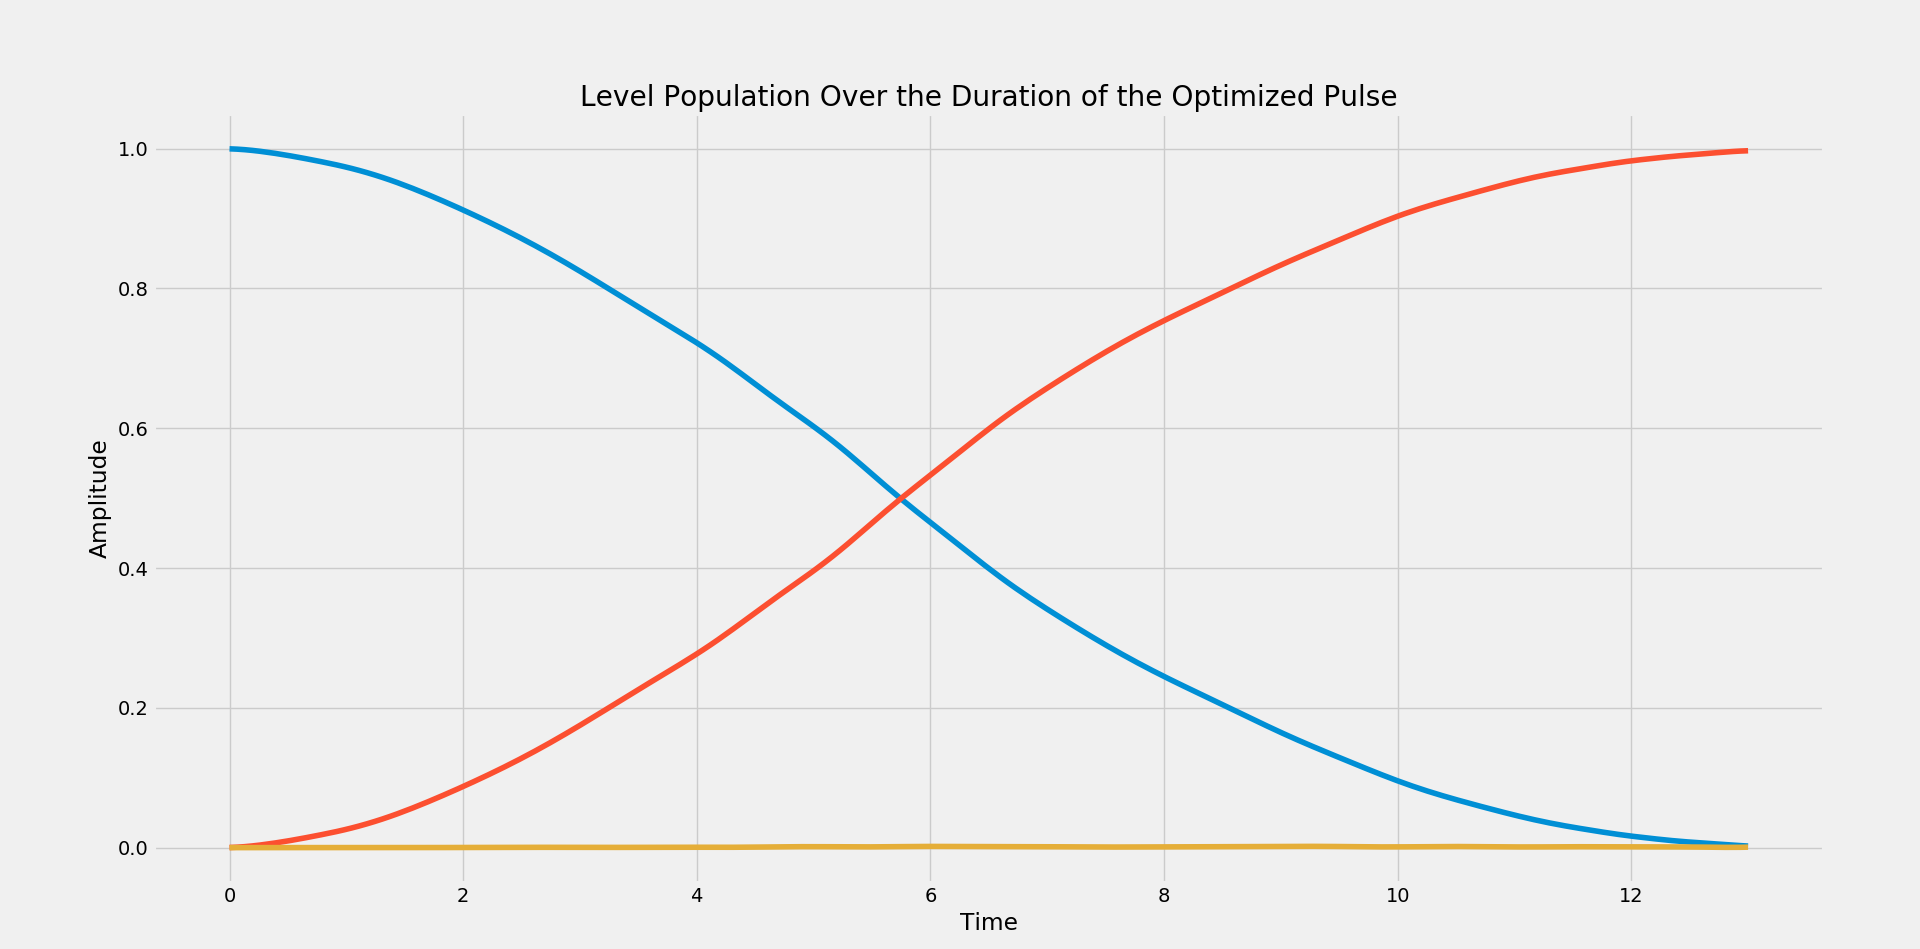
\includegraphics[width=1\columnwidth]{Results/DRAG/level-population2.png}
    \caption{Level population of the "qubit" over the duration of the pulse that was found by the GRAPE algorithm, with all the penalties turned on, including the DRAG penalty.}
    \label{fig:sDRAG-results}
\end{figure}
Nice! state $\ket{0}$ goes directly to $1$, $\ket{1}$ goes directly to $0$ and the forbidden level is barley changed throughout the pulse (the fidelity gotten from this pulse is around $99.9\%$, so pretty good).

I think that we talked enough about the qubit for now, let's move the the other half of the system, the cavity.

\subsection{Implementing Cavity Operations}
\subsubsection{Limiting the photon number} 
\centerline{\say{Hilbert space is a big place.}}
\centerline{- Carlton Caves}
Here's the thing about the cavity levels, there are infinite amount of them. We can make an assumption that the cavity only has $N$ levels, but it is still possible that something happens in the higher levels that may affect the physical result. We want to make sure that everything interesting is contained in the $N$ levels that we have.

This is quite similar to what we did in the previous section with DRAG, we want to put a penalty on the higher levels. Still, there are two main differences. The first, is that there are much more than one or two extra levels, and as we've seen, the method we used in the previous uses very heavy computation and we can't do it for so many levels. The other difference is that we care less about if some higher level is occupied for a part of the pulse. In the cavity there are higher levels and they're all likely to be but \textbf{the reason we're limiting the cavity levels is for computing reasons, not physical ones}. Unlike the cavity, we really want the qubit dynamics to involve only two levels, so it makes sense that we'll use a different penalty to limit the photon number.

The idea is this, we'll define $n_{ph}$ as the highest level we want the cavity to have. Now let's calculate what will happen if the cavity will have another level, for a total of $n_{ph} + 1$. Ideally, nothing will change, the new level should start at 0 probability and end at 0 probability with no change in between. If there is a change, will add a penalty to the pulse, so in the next iteration there will be less of a change. We can do so for any level higher than one, so instead of using only $n_{ph} + 1$ we'll some over $n_{ph} + k$ for reasonable amount of k's.

We'll define $F_{n_{ph} + k}$ as the fidelity if there were $n_{ph} + k$ levels. Putting the idea into a formula we get that the new cost function is given by
\[
    Cost = \sum_{k=0}^{N} F_{n_{ph} + k} (\vec{\epsilon}) - \sum_i \lambda_i g_i (\vec{\epsilon})
\]
We can double enforce the penalty if we add a constraint making sure there is no change in the fidelity for different levels
\[
    g_{ph} = \sum_{k_1 \ne k_2} (F_{n_{ph} + k_1} - F_{n_{ph} + k_2})^2
\]
The gradient of which is simply the gradient of which is simply
\[
    \frac{\partial g_{ph}}{\partial \epsilon_k} = 2 \sum_{k_1 \ne k_2} [ (F_{n_{ph} + k_1} - F_{n_{ph} + k_2}) (\frac{\partial F_{n_{ph} + k_1}}{\partial \epsilon_k} - \frac{\partial F_{n_{ph} + k_2}}{\partial \epsilon_k})]
\]
and everything in this expression was previously calculated (they're simply the derivatives of the fidelity and the fidelity itself).

It's important to note that while it might be tempting to leave $n_{ph}$ at a small value so there will be less to calculate (the size of the matrices grows with $n_{ph}^2$), there is good reason to use a high values of $n_{ph}$. Bigger $n_{ph}$ oscillate at higher frequency (since the cavity is simply a harmonic oscillator), so it's possible to use shorter pulses, and since keeping qubit alive is really a major problem, keeping the pulses short is important to be able to accomplish the most with the time we have with the qubit before it dies.
% TODO: Need to go over the last paragraph and check it with Serge to make sure I'm not making anything up

Lets see what happens if we run the transmon-cavity code. We'll only look at the resulting population graph after the optimization. I warn you that the graph is a bit cluttered. You shouldn't look at any specific details or any specific curve, I didn't put a legend explaining what each curve is. We'll look at it then discuss

\begin{figure}[H]
    \centering
    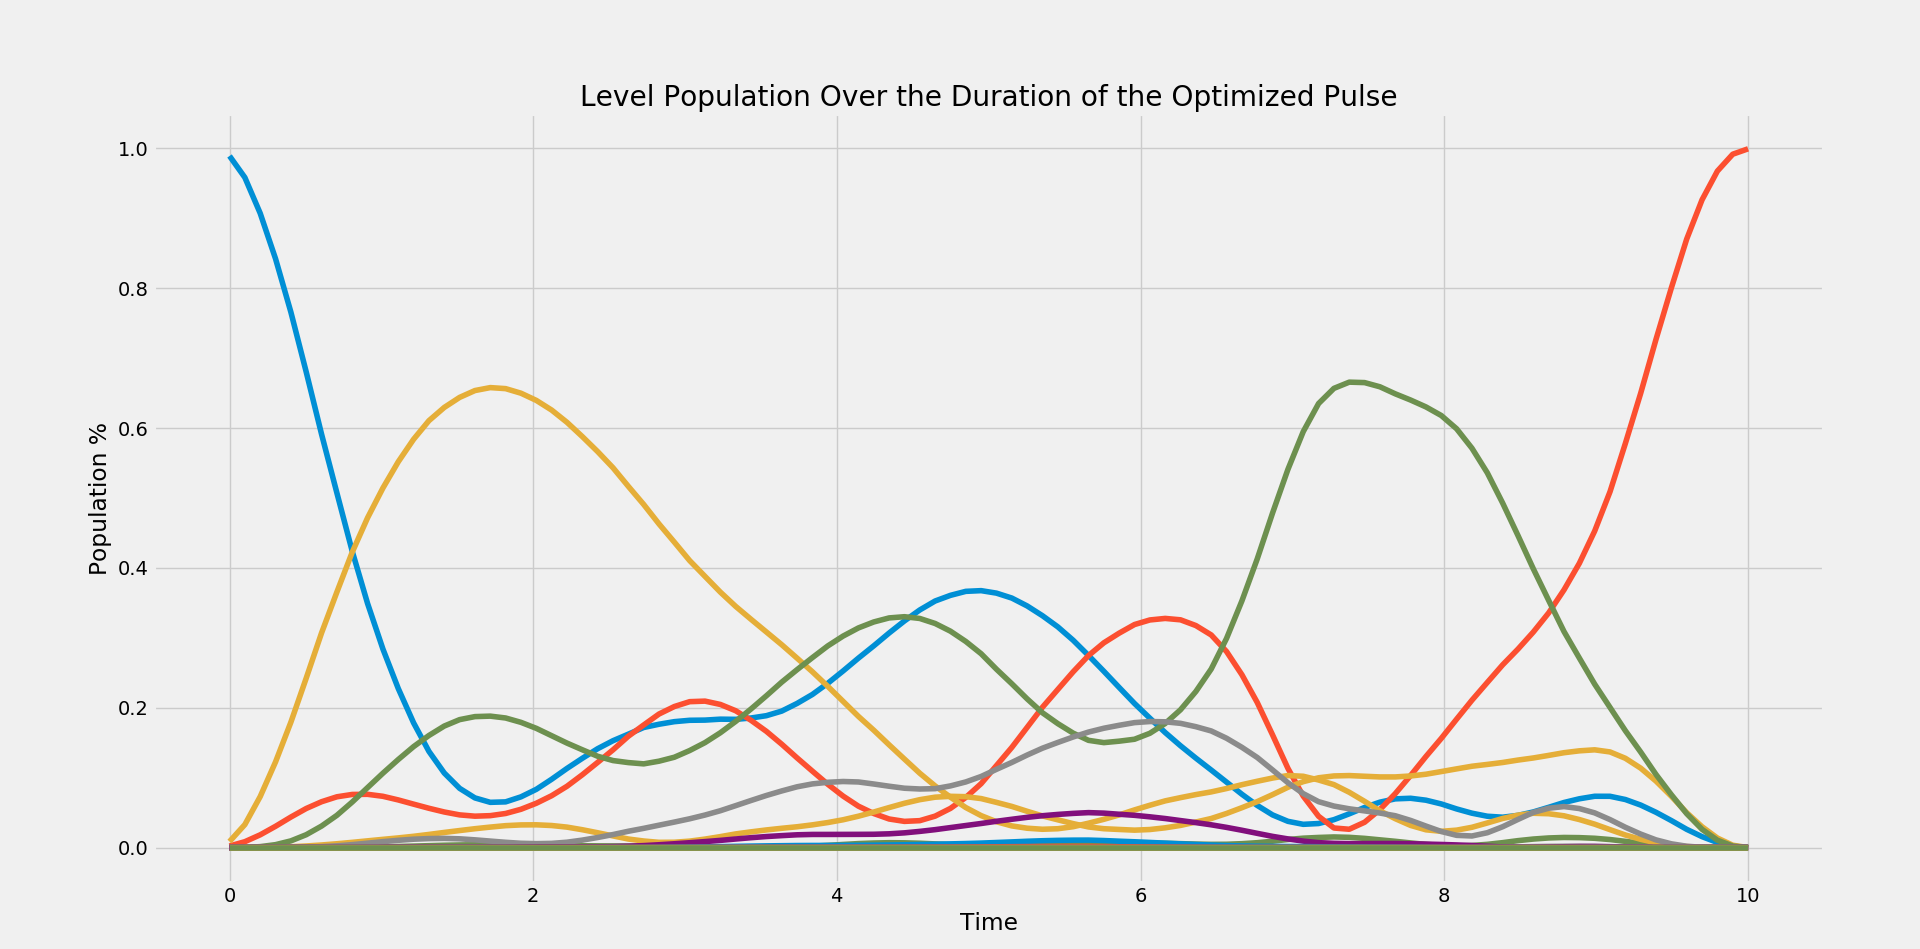
\includegraphics[width=1\columnwidth]{Results/transmon-cavity/g0-g1-level-population.png}
    \caption{Transmon-cavity state population over the duration of the pulse that does the transformation $\ket{g} \otimes \ket{0}\ \text{ (Blue)} \longrightarrow \ket{g} \otimes \ket{1}\ \text{ (Red)}$.}
    \label{fig:transmon-cavity-population}
\end{figure}
After you see this graph, you'd think that the constraint didn't work correctly. After all, the transformation is from level $\ket{0}$ to level $\ket{1}$, but there were many other levels that got occupied during the middle of the pulse. This is a valid guess, but there is an explanation why the higher level would get occupied. The reason is that you can't really create number states \textit{directly} in a cavity. You can only create coherent states \textit{directly}. To create  number state you need to make the coherent states interfere in a way that creates a number state.

So why then should this graph show it was successful then? Well, I ran the algorithm with 50 cavity levels (!), this means that there are actually 100 curves in that graph (50 of the cavity times 2 of the qubit). If you'd try to count the number of curves that you see you'll probably count 7-8 curves and not all of the 100, this is since most of the curves stay at zero population. This is exactly what we want, the higher levels don't affect the physics of the system, if we add more levels (like in the real world where there are infinite levels) the pulse would still give the same desired result.
% As you can see, although the final result is what we want it to be, along the way higher levels were created, even to last level of the cavity were excited. This is a problem since, as we said earlier, the cavity should have infinite levels and cutting it off after 7 levels in this case is just and approximation, the last levels should not be populated.

% We can now add the penalty and see that this problem is solved with it.

\subsection{Finding a Good Initial Guess}
Although the GRAPE algorithm is the one responsible to find to optimal control pulse, we still need to give it some initial guess and the algorithm does the rest. You might think that this isn't much of a problem since theoretically any initial guess should arrive at a desired result. The problem is that often the algorithm gets stuck and can't find a result. This could be caused by a number of reasons, the main two are when the constraints are too strong and when the initial guess is not good enough.

When the constraints are too strong, the algorithm might prefer optimizing them instead of the fidelity and what we get is a pulse that achieves horrible fidelity but within the constraints. The solution is simply weakening the constraints (choosing a smaller $\lambda$ for the constraint).

The other, harder to solve problem is when the initial guess of the pulse is problematic. For example, if you choose the initial guess to be the most obvious initial guess you can make, constant 0, the algorithm will probably stop after one iteration changing nothing. This is because the gradient of a constant 0 pulse is actually zero, so the optimization algorithm thinks it's in an optimized minimum when in fact, it couldn't be more wrong.

The other simple initial guess you might think of using is a random pulse. After all, we don't know what is the desired pulse so picking a random pulse is as good as any other. The problem with a random pulse is that it is not a smooth function, so the algorithm might find it difficult to get a smooth solution.

There are two approaches we can take to get a good initial pulse. The first approach assumes nothing about the system, it's good since it's really general and can be used in any case, but might be not ideal in some cases. The second approach is when we know roughly how the solution should look like, we can use some pulse that is similar to what we expect and GRAPE will get the actual pulse from that.

In the first approach, we want GRAPE to do most of the work, but not get stuck by some weird problem of the initial pulse. We want a guess that is close to 0, pretty random, but not so much that it would be hard to smoothen. We can get such a pulse by doing a convolution between a random pulse and a Gaussian window 
% TODO: Continue to expalian why these convolutions work and give and equation

Unlike the first approach, the second approach could look really different for different examples but I'll give some general guidelines you can use the get a good initial pulse. Let's say, for example, you have a 3-level system where the third level isn't wanted (such as in the DRAG example). If you give an initial guess like the one in the first approach, the third level will still be excited by that pulse, and it might be hard for the algorithm to fix this. What you might do in this scenario, is to start with an initial guess that you know excites only the first and second levels of the system but not the third. This is easy since you  know the transition frequencies of the atom, from that you know the frequency that excites each level. What you can do is some random pulse that has frequency around the first-second levels frequency difference. So if you look in the frequency space, what you see is some Gaussian distribution around the first levels frequency with some random noise on it.

\begin{figure}[H]
    \centering
    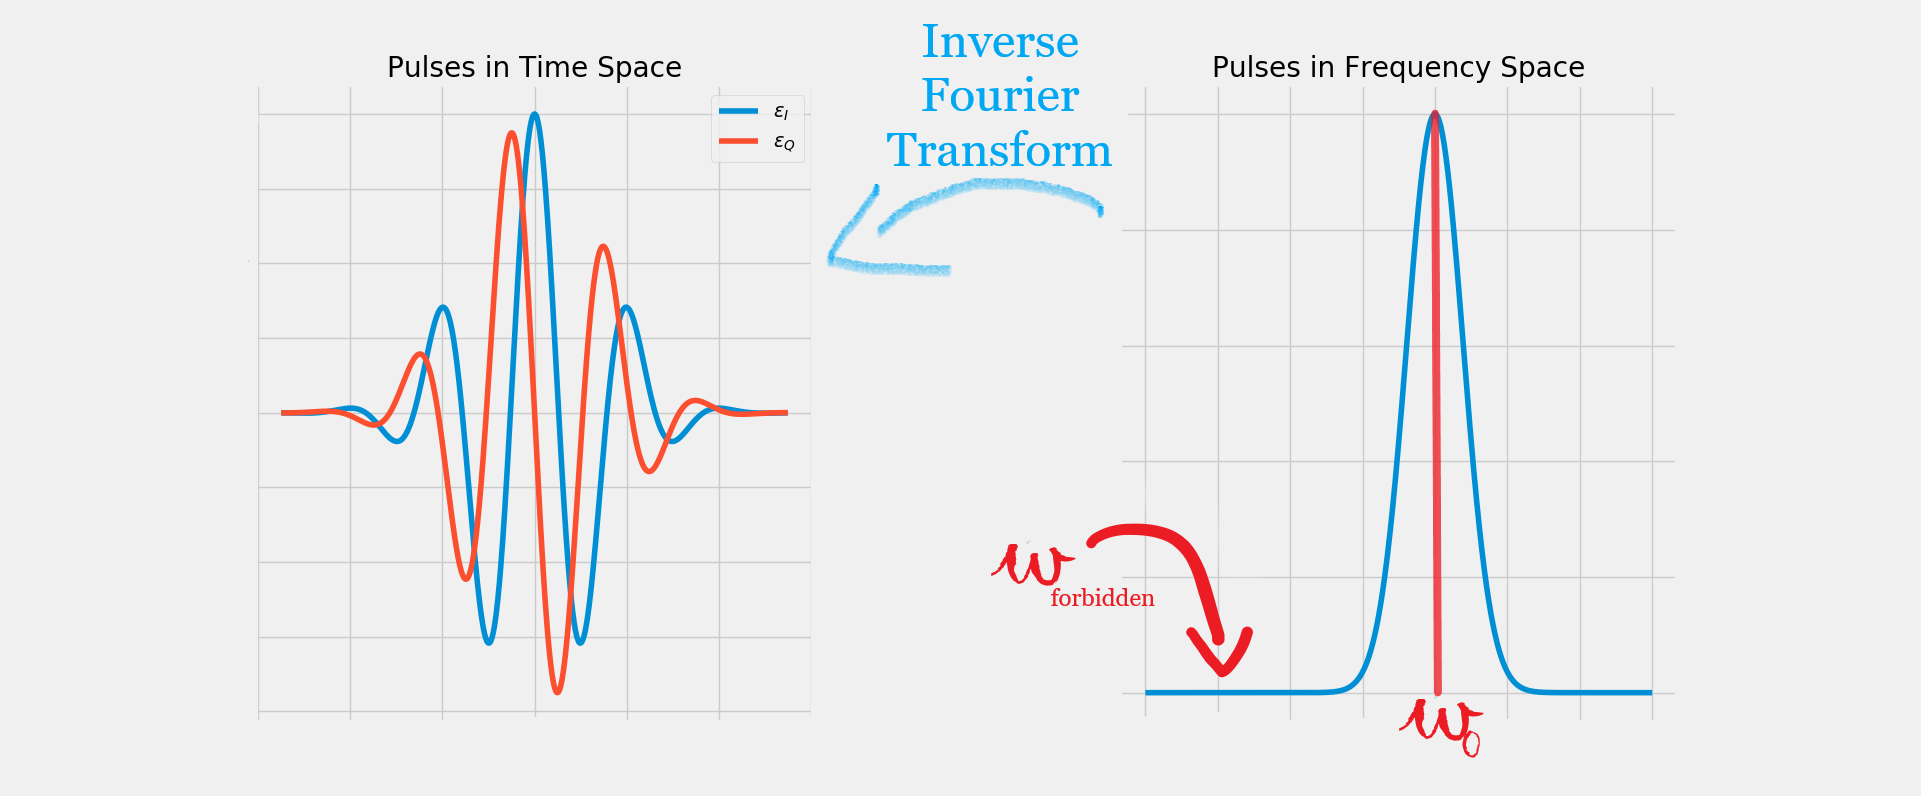
\includegraphics[width=1\columnwidth]{exaple-of-engineered-guess-edited.png}
    \caption{Example of how you might engineer an initial pulse for a system with known characteristics. Normally you would also add some random noise on top of the pulse}
    \label{fig:example-engineered-initial-guess}
\end{figure}
\subsection{From States to Gates}\label{sec:gate-GRAPE}
Until now we've discussed how to find pulses that take our system from one state to another. This is useful for initializing the quantum system in a desired state. However, the operation is not well defined if we start in a state other than the one the pulse was designed for. In contrast, a  numerically optimized quantum gate must perform a well defined unitary transformation on arbitrary states.

Here's the thing, turns out, you can change the algorithm just a little bit and get a GRAPE algorithm that gives you back the optimal pulses that realizes a desired \textit{quantum gate}, instead of just taking you from one state to another. 

To make such gate GRAPE, instead of optimizing for one state transformation, you optimize for  initial states that constitute a basis for the entire state space. This way, since quantum operations are linear, a unique transformation on the basis of the state space is a unique transformation on the entire system. The implementation of gate GRAPE is outside the scope of this project.

\subsection{References and Further Readings}
The best reference I've found on this subject is by far the 2019 dissertation of Philip Reinhold from Yale, "\textbf{Controlling Error-Correctable Bosonic Qubits}", especially the forth chapter. Another great resource is the documentation of the python library "\textbf{QuTiP}", which was used to create some of the graphs here, but it's documentation has some really nice explanations.


% --- Controlling a Superconducting Quantum Computer ---
\newpage
\section{Controlling a Superconducting Quantum Computer} \label{chap:FPGA}
\subsection{Overview}
Before jumping into the specifics of how'd we control the quantum computer, let's start with a general overview and show how everything is connected.

This is a diagram that shows how the system is connected, from the pulse generator to the cavity.

\begin{figure}[H]
    \centering
    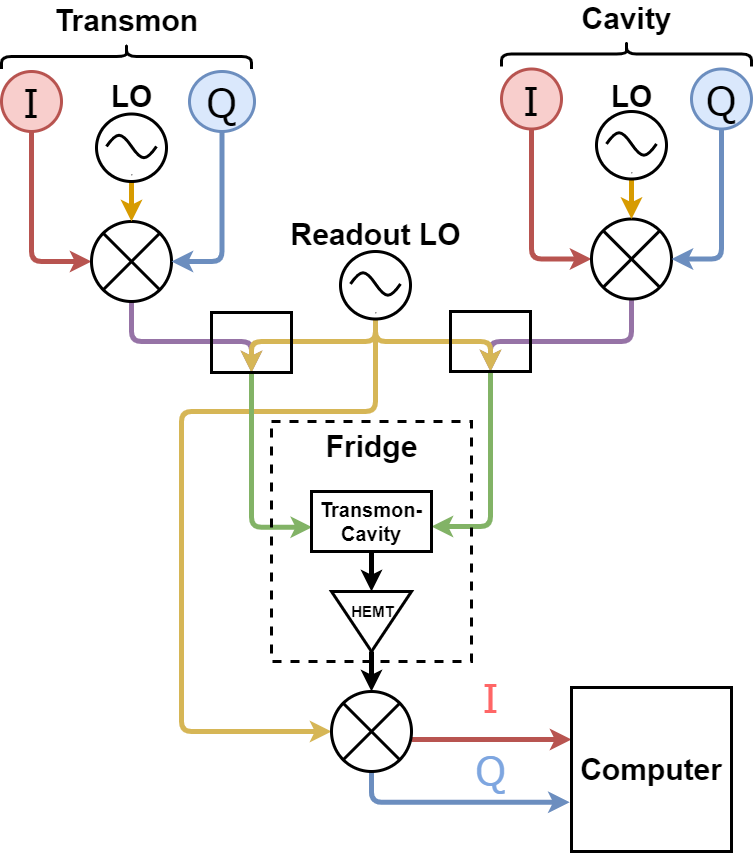
\includegraphics[width=0.85\columnwidth]{overview.png}
    \caption{Diagram of the system}
    \label{fig:System-diagram}
\end{figure}

The $I$ and $Q$ signals are generated in the AWG, the LO frequency comes from a frequency generator and so does the Read Out signal. \textbf{H}igh \textbf{E}lectron \textbf{M}obility \textbf{T}ransistor (HEMT) is a low-noise cryogenic amplifier.

\subsection{Generating the Pulses}
\subsubsection{The AWG}
% It shouldn't be too much of a surprise if I'll tell you that I consider the AWG (Arbitrary Waveform Generator) the "heart\ensuremath\heartsuit" of the system, we've just spent an entire chapter on finding the pulses we want to send, and the instrument that creates and sends the pulse, is the AWG. Unfortunately, using the AWG isn't as straight-forward as you might hope and there are some problem's we'll need to address if we want our system to work.

An \textbf{A}rbitrary \textbf{W}aveform \textbf{G}enerator (AWG) is a device that we use to generate the pulses we calculated with GRAPE in the previous chapter. To control the qubit we need to send RF signals, typically ranging from $4$GHz to $10$GHz. Such signals can be generated by RF signal generators (also called LO's - local oscillators). In contrast, the AWG sends out slowly varying envelopes, usually with a bandwidth of a few hundred MHz. To bridge this gap, we will mix a fixed-frequency signal from the LO with a time-varying signal from the AWG. In particular, this will also enable us to vary the frequency of the LO in real-time with the AWG. Our goal in the next section will be to achieve this so called single-sideband modulation of the LO signal.

We also want to be able to un-mix the measurement result to get back only the interesting parts of the pulse. The device we'll use for this task is the \textit{IQ-Mixer}, but before we can  get into the IQ-Mixer, we need to understand how a \textit{regular} mixer works.

\subsubsection{The Mixer}
The mixer has 2 inputs and one output. When you enter 2 pulses as an input, you get their product as the output (inputting for example $\cos (t)$ and $\cos (2t)$ will result in $\cos (t)cos (2t)$ at the output).
We draw a mixer in a diagram as
\begin{figure}[H]
    \centering
    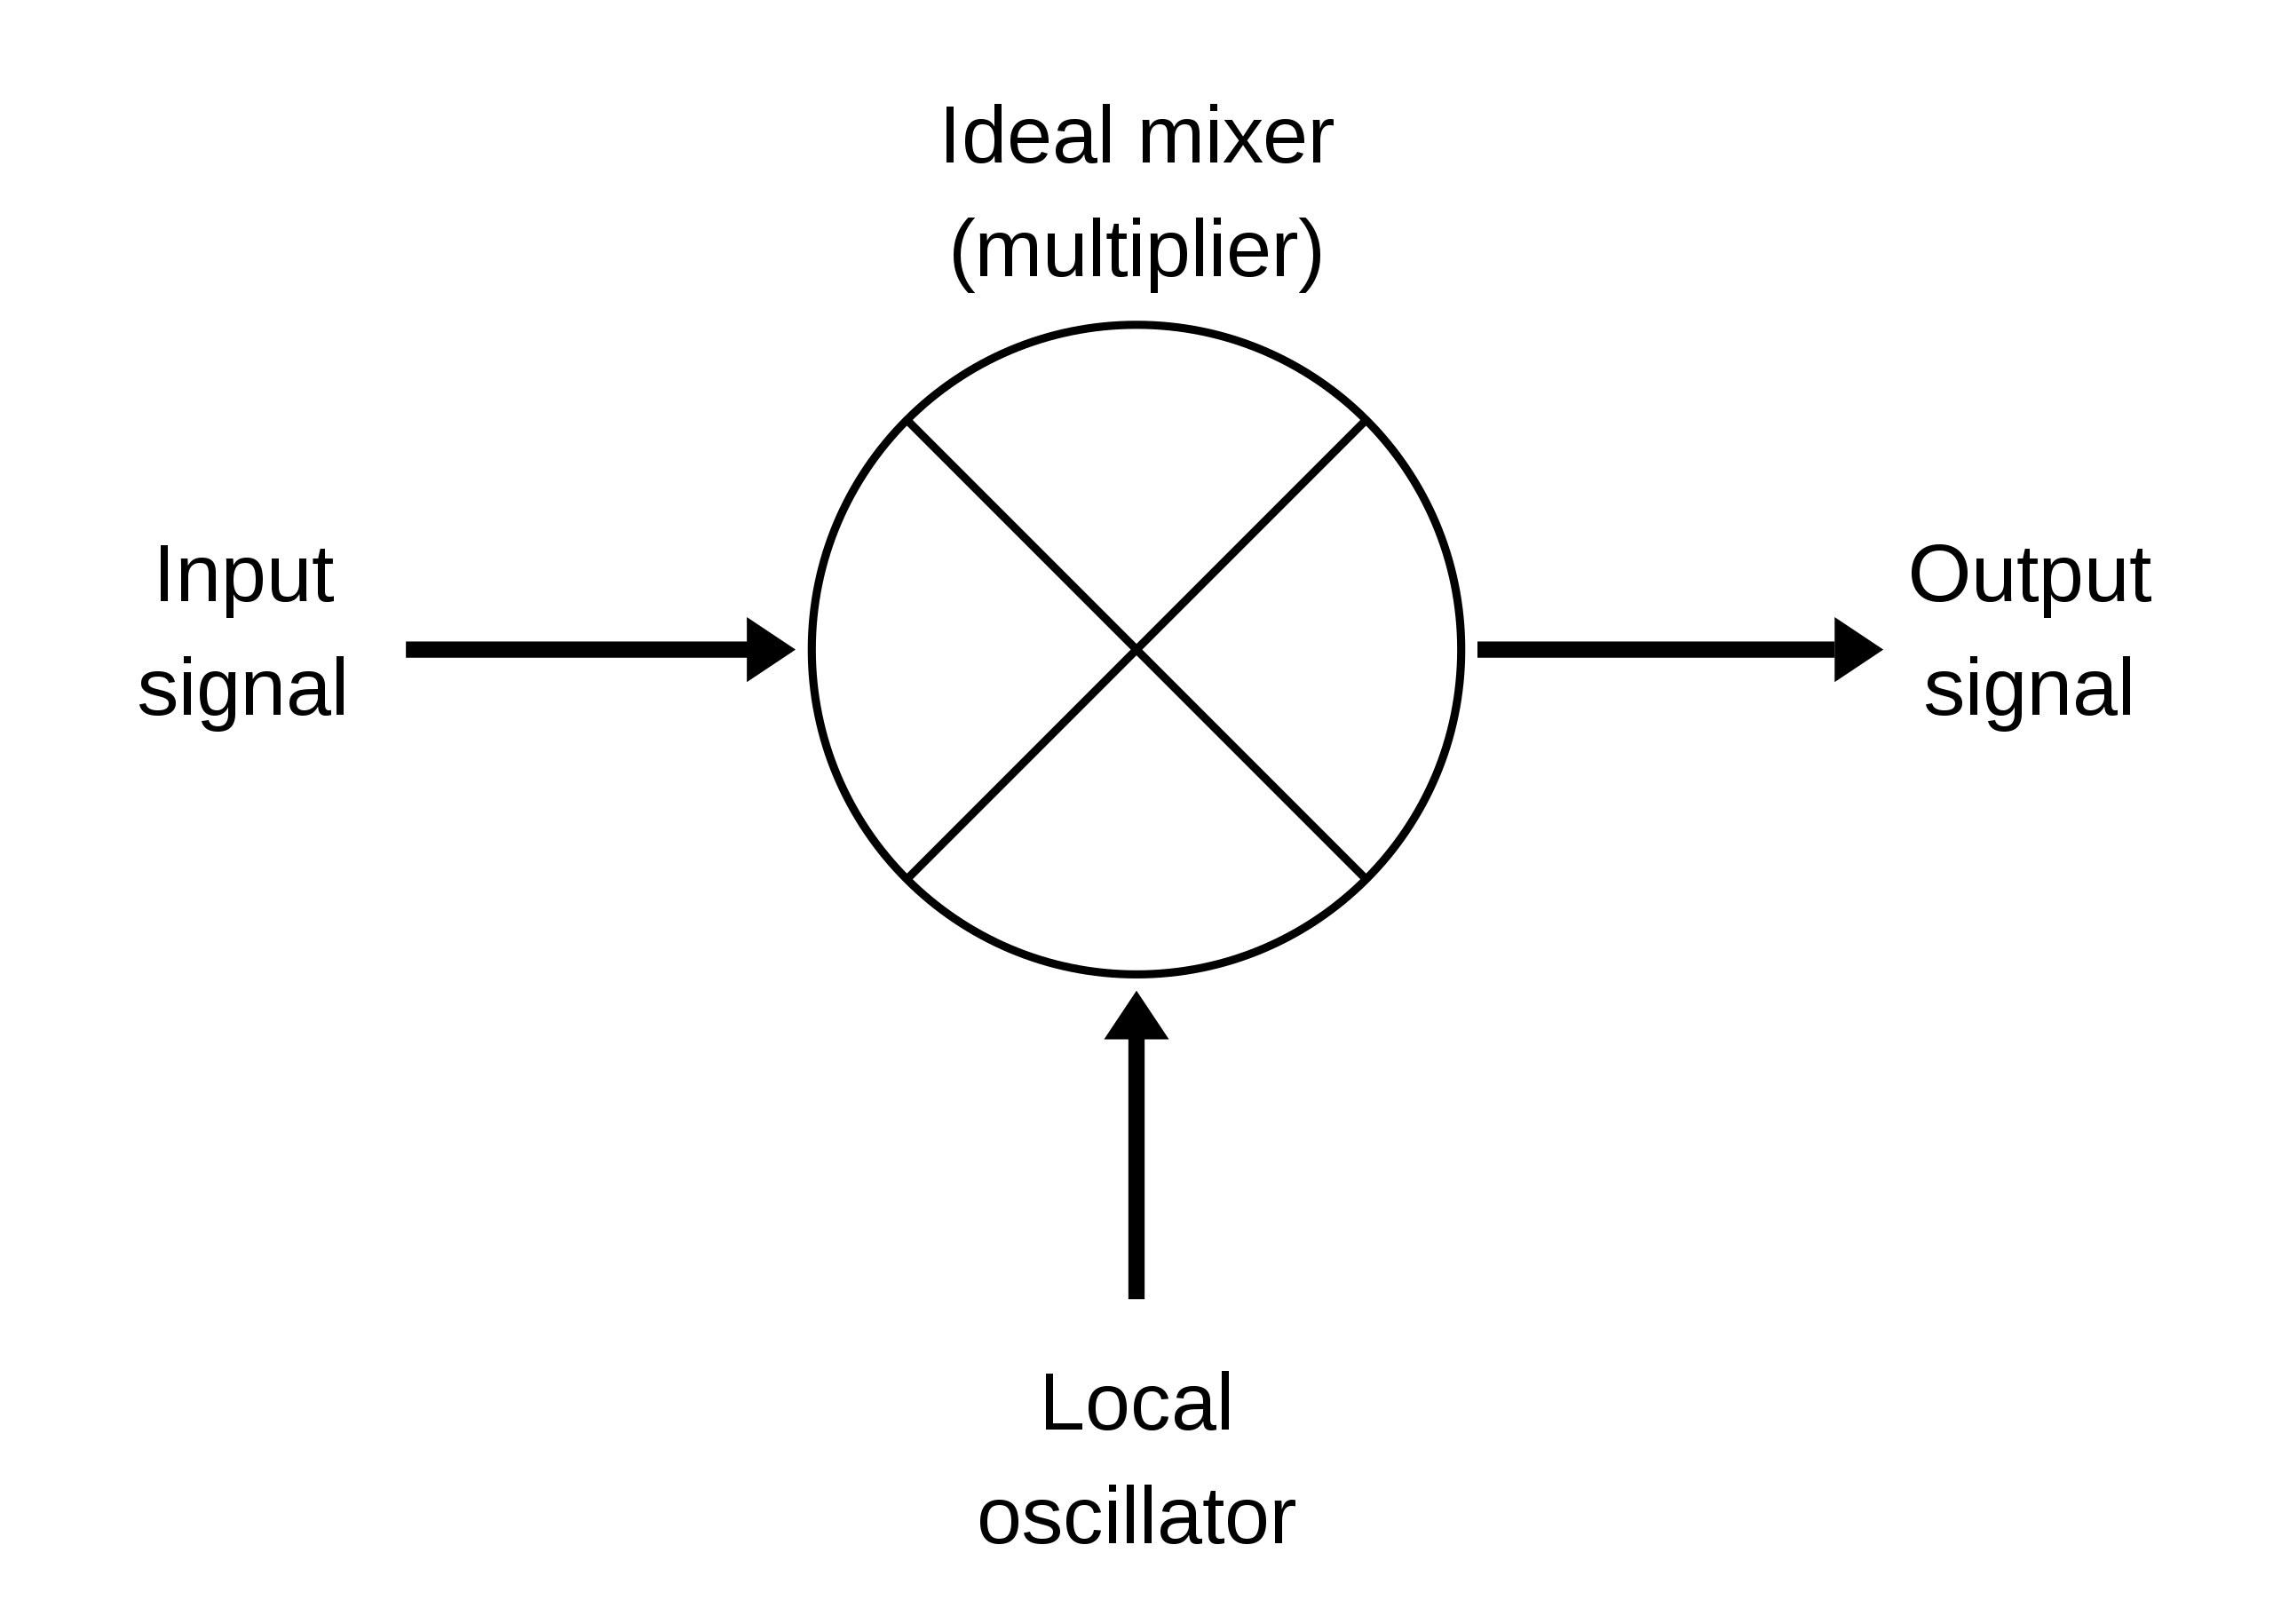
\includegraphics[width=0.3\columnwidth]{Ideal-Mixer.png}
    \caption{Ideal mixer in a diagram}
    \label{fig:Ideal-Mixer}
\end{figure}
The mixer circuit is \textit{non-linear}. The non-linearity could be achieved with non-linear components, such as diods.
% We can change what are the outputs and what are the inputs to get different ways for the mixer to work\footnote{TODO: Explain this} % TODO: Add on this later

\subsubsection{The IQ-Mixer}
We've seen what's a \textit{regular} (and \textit{ideal}) mixer is, but how can we use it for the desired effect? remember, we want to input a high frequency and a lower frequency and we want the output to be a wave with a frequency that is the sum of the 2 frequencies. To do so, we can consider the following diagram
\begin{figure}[H]
    \centering
    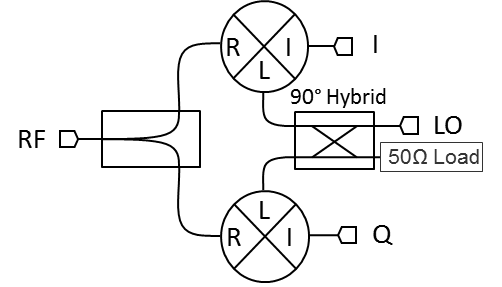
\includegraphics[width=0.5\columnwidth]{IQ-Mixer.png}
    \caption{The IQ mixer}
    \label{fig:IQ-Mixer}
\end{figure}
Where the 90\degree\ hybrid in the diagram is a \textit{90\degree\  hybrid coupler}. This device splits the signal into 2 signals at a 90\degree phase difference, hence the name. The square near the \textit{RF} sign simply adds the 2 waves.

As we can see, the IQ mixer has 3 inputs, In-phase (\textit{I}), Quadrature (\textit{Q}), hence the name, and \textit{LO}. We can also see that there's only one output, \textit{RF} (although you can reverse the roles of the input and the output).

How can we use this IQ mixer to add frequencies? Let's consider the following inputs\footnote{You can flip I and Q and get subtraction instead of addition}
\begin{align*}
    I &---> \cos (\omega_{IQ} t)\\
    Q &---> \sin (\omega_{IQ} t)\\
    LO &---> \sin (\omega_{LO}t)
\end{align*}
In this case, the input into the top mixer will be \textit{I} and a \textit{LO}, which is $\cos (\omega_{IQ}t)\sin (\omega_{LO}t)$. Similarly, the input into the bottom mixer will be \textit{Q} and 90\degree phase of \textit{LO}, which is $\sin (\omega_{IQ}t)\cos (\omega_{LO}t)$.

The total output (in \textit{RF}) will be the sum of the two waves
$$RF = \cos (\omega_{IQ}t)\sin (\omega_{LO}t) + \sin (\omega_{IQ}t)\cos (\omega_{LO}t)$$
So we get
\begin{equation}
    \boxed{RF = \sin ( (\omega_{LO} + \omega_{IQ})t)}
\end{equation}

Perfect! this is exactly what we wanted, the output is a wave with frequency that is the sum of the input frequencies. Only one problem, this simple scheme turns out not to work in practice : (.

\subsubsection{Theory VS Reality} \label{sec:solution_real_world} % Maybe combine this section and the next one
If we use a spectrum analyzer and view what frequencies are in the final wave we get the following picture

\begin{figure}[H]
    \centering
    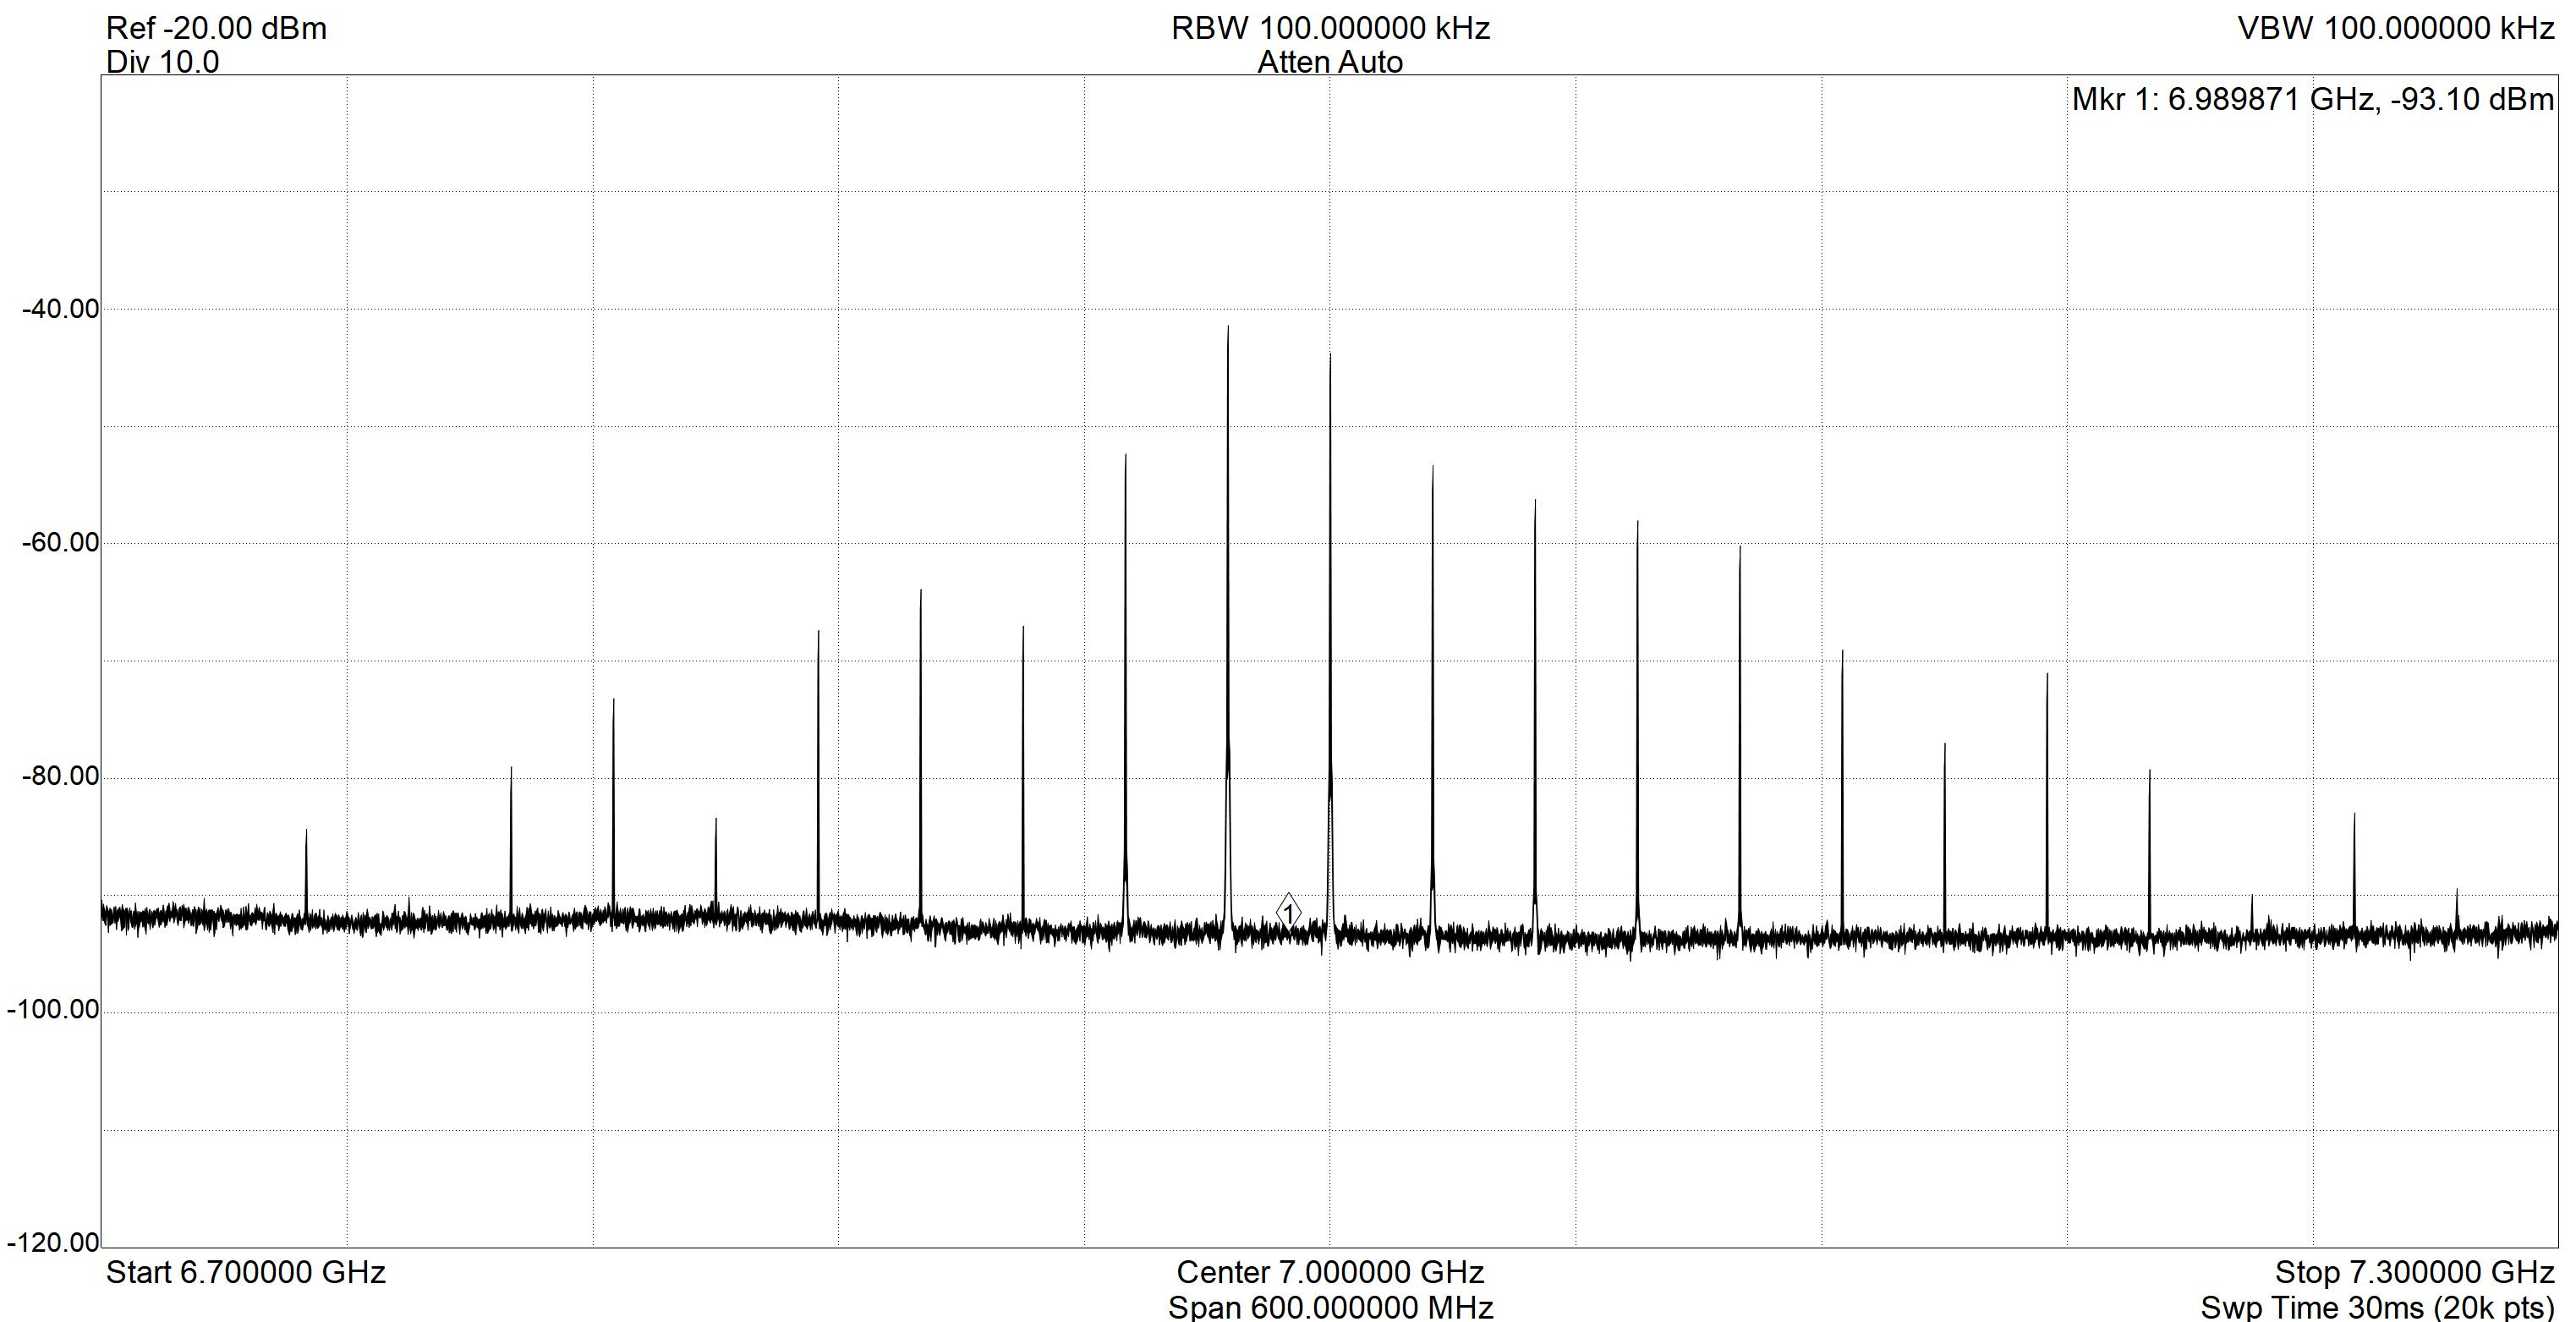
\includegraphics[width=0.8\columnwidth]{full-spectrum-no-correction.jpg} %TODO: Need to change to image with explantion on what is going on
    \caption{Full Spectrum Without Any Corrections}
    \label{fig:Full-spectrum-no-corrections}
\end{figure}
Zooming in around the LO frequency we see
\begin{figure}[H]
    \centering
    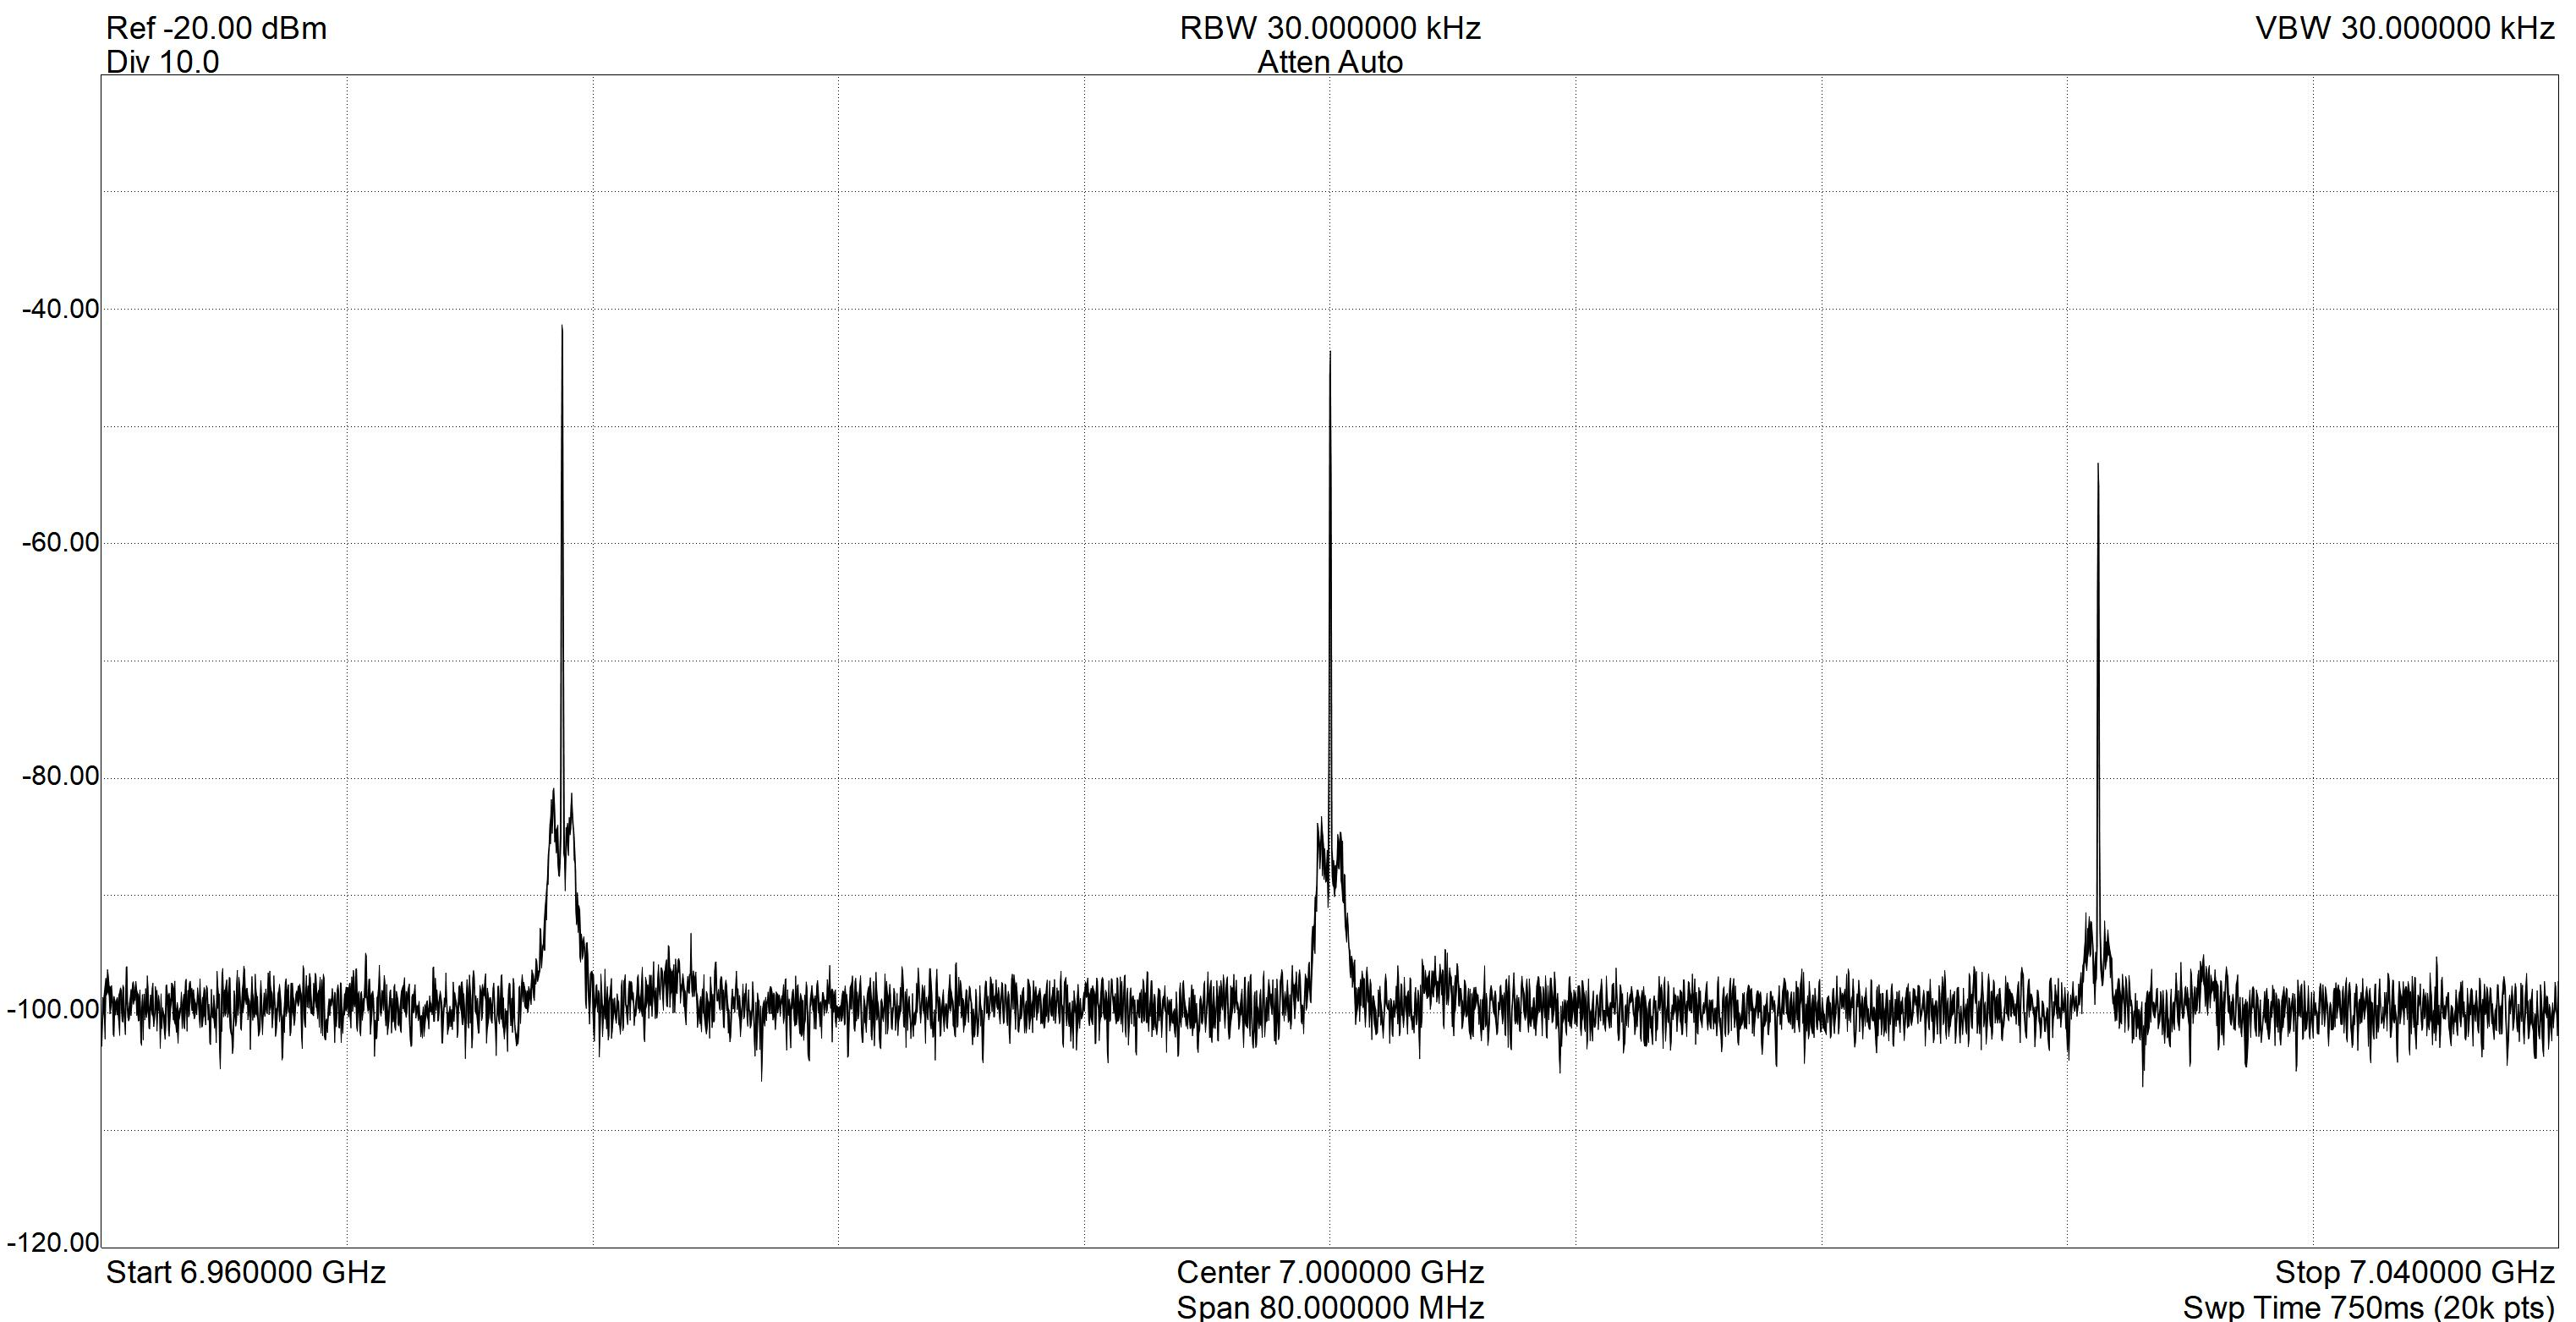
\includegraphics[width=0.8\columnwidth]{Important-Spectrum-no-correction.jpg} %TODO: Need to change the image to one with marking explaining it on it (what is each spike)
    \caption{Spectrum Around the LO Frequency}
    \label{fig:closeup-spectrum-no-corrections}
\end{figure}

What is the problem? We've proved mathematically that it should work, so why doesn't it? The problem is that we can't just assume the waves to come and go with the same phase, the waves travel through the wire at some speed so if we input into two different wires, two waves that are at the same phase, at the other side of the wire they might come at different phases because of differences in wire length, resistance, etc... So what can we do about it? You could try to make identical parts and make everything just perfect but even slight deviation will cause the system no to work properly, a better solution is to input more complex waves and have some parameters to play with so we can simply find the right parameters for the system.% TODO: Improve wording

We can analyze the frequency space of the output of out IQ mixer and we can see two types of it not working correctly
\begin{itemize}
  \item Leakage at the LO frequency
  \item Leakage at the sideband ($\omega_{LO} - \omega_{IQ}$)
\end{itemize}
We can solve the first type of Leakage, at the LO frequency, by adding DC offsets to the input frequencies (We'll prove this mathematically later), and we can solve the second type of leakage by adding phase offsets to the waves (We'll prove this mathematically later).
% This is how the frequency spectrum looks without making any changes to the input waves


% \subsubsection{Solution for the real world} \label{sec:solution_real_world}
Before we can solve the problem, we need to understand what's causing it. As we explained earlier, a phase  is created  in the wires that connect everything.
\paragraph*{Leakage at $\omega_{LO} - \omega_{IQ}$ }
% \subsection{What's causing the problem}
Let's consider now inputting into the IQ mixer the same waves but with the phases that were created in the transmission wires instead of what we had earlier
\begin{align*}
    I &---> \cos (\omega_{IQ} t + \phi_I) \\% + \epsilon_I\\
    Q &---> \sin (\omega_{IQ} t + \phi_Q) \\% + \epsilon_Q\\
    LO &---> \sin (\omega_{LO}t + \phi_{LO})
\end{align*}
Using the same calculation we did before, we get that
$$RF = I\cdot LO + Q\cdot LO (90\degree)$$
\[
RF = \cos (\omega_{IQ} t + \phi_I) \cdot \sin (\omega_{LO}t + \phi_{LO}) + \sin (\omega_{IQ} t + \phi_Q) \cdot \cos (\omega_{LO}t + \phi_{LO}) 
\]
After some algebra we get
\begin{align*}
RF = &\cos (\frac{\phi_Q - \phi_I}{2})\sin ( (\omega_{IQ} + \omega_{LO})t + \frac{\phi_Q + \phi_I}{2} + \phi_{LO}) \\
   + &\sin (\frac{\phi_Q - \phi_I}{2})\cos ( (\omega_{IQ} - \omega_{LO})t + \frac{\phi_Q + \phi_I}{2} - \phi_{LO})
\end{align*}
This expression is quiet scarier than the one we got earlier... More than that, we get two frequencies instead of one, we've got an unwanted frequency at $\omega_{LO} - \omega_{IQ}$ and the only way to make it disappear is if the phases are equal, $\phi_I = \phi_Q$. Also the final wave as a phase of $\phi_{LO}$, this isn't really a problem and if we define our starting point differently we can set  $\phi_{LO}$ to 0.

\paragraph*{LO Frequency Leakage}
% TODO: Maybe I'll be able to find a mathematicall explenation to the DC offsets
Another type of leakage we've observed is leakage at the LO frequency, it makes sense that some of the original wave will go through the mixer untouched. To fix that leakage, we'll need to somehow change the I and Q waves to cancel it out. The simplest way to do so is to add DC offsets to the inputs \footnote{I've removed the phase on the LO wave since we've seen it doesn't really change anything}
\begin{align*}
    I &---> \cos (\omega_{IQ} t + \phi_I) + \epsilon_I\\
    Q &---> \sin (\omega_{IQ} t + \phi_Q) + \epsilon_Q\\
    LO &---> \sin (\omega_{LO}t)
\end{align*}
We've seen this story before... the calculation of the RF wave is the same so we'll skip the calculation. The end result is
\begin{align*}
RF = &\cos (\frac{\phi_Q - \phi_I}{2})\sin ( (\omega_{IQ} + \omega_{LO})t + \frac{\phi_Q + \phi_I}{2}) \\
   + &\sin (\frac{\phi_Q - \phi_I}{2})\cos ( (\omega_{IQ} - \omega_{LO})t + \frac{\phi_Q + \phi_I}{2}) \\
   + &\epsilon_I  \sin (\omega_{LO}t) + \epsilon_Q  \cos (\omega_{LO}t) \\
   = &RF_{old} + \epsilon_I  \sin (\omega_{LO}t) + \epsilon_Q  \cos (\omega_{LO}t)
\end{align*}
where $RF_{old}$ is the RF wave before adding the DC offsets. 

What we get is the same wave, but now we can play with the LO frequency at the output. Later we'll change the DC offsets so that they will cancel to LO frequency leakage to minimize it.

Now that we have all of our "knobs" we can change and play with, we can start using them to minimize the leakages.


\subsubsection{Finding Optimal Constants} % Maybe I won't do this section
As we've seen in the previous section, there are 4 variables we can "play" with to get the best variables for our system, as long as we don't change the system, these variables stay the same. What we want to do now is to actually find them. Our system is connected like so
% Add figure of how the system is connected

We have the Quantum Machine\footnote{this is the heart of the system, for now we'll use it to make the MHz waves with different phases, DC offsets and frequencies} that generates the I and Q inputs that go into the mixer (and also to an oscilloscope for debugging). There's the frequency generator\footnote{KeySight N5173B} that is connected to the mixer and generates 7GHz wave, and there's the frequency spectrum analyzer\footnote{SignalHound USB SA-124B} that is connected to the computer.

Let's first attack the leakage at the LO frequency. For now we'll have an LO frequency of 7GHz that we want to change by 25MHz (The same variables work for all frequencies this is just as an example)

\paragraph{LO frequency Leakage}
As proven in section \ref{sec:solution_real_world}, to minimize this kind of leakage all we need is to play with the DC offsets of the IQ inputs. To do so, we first need to define what we want to minimize, which in this case is simply the power of the frequency at 7GHz, we can measure that power with our spectrum analyzer, we'll call that our \textit{cost function}.
We have a 2-dimensional variable space, we need to find where in this space the cost function is at a minimum. To do so, we'll start by using a brute force method to find the general location of the minimum in the variable space, since brute force is very inefficient we can't really use it to find the exact location of the minimum so we start by only doing a low precision brute force and then use a different optimization algorithm to find the exact location of the minimum. We'll use the \texttt{scipy.optimize.fmin} as the algorithm for precise minimum location.
% TODO: Add figure of spectrum after leakage optimazation, Improve wording

\paragraph{Sideband Leakage}
Now that we've minimized the LO frequency leakage, we want to minimize the sideband leakage. We do that by changing the phases of the IQ waves from the quantum machine, it's important that changing the phases doesn't change the LO leakage and luckily for us, as proven in section \ref{sec:solution_real_world} that's whats happening. to change the phases we don't simply specify the phases, we use the correction matrix of the Quantum Machine.
This time our cost function is the frequency at $\omega_{LO} - \omega_{IQ}$, we can do the same as we did in the LO leakage and use first a brute force optimization to find the general location of the minimum and the use the fmin algorithm to find the exact location of the minimum of the cost function (this time in the scale-angle variable space). You can see the result here
% TODO: Add figure of full final optimization, Explain why it doesn't work perfectly (The quantum machine power problem)

\subsection{References and Further Readings}
A great book on couplers and mixers I used while writing this chapter is "\textbf{Microwave Engineering}" by David M. Pozar. It provides a much more in depth look on the subject.

Another great resource is the \textbf{Marki Microwave RF \& Microwave knowledge base} at \newline \texttt{https://www.markimicrowave.com/engineering/}. Which provides useful introduction to many topics in microwave engineering.

% --- Future Work and Conclusions ---
\newpage
\section{Future Work and Conclusions}
We conclude this project with the knowledge and tools to create and control quantum systems, from understanding them theoretically to connecting and calibrating the devices that actually send the control pulses, to creating the control pulses to create arbitrary quantum states and operations.

As with anything in life, this project must to come to an end at some point, each subject we discuss opens a rabbit hole we'll never see the end of.

A natural next step for this project would be to implement the gate GRAPE. explain exactly how the gate GRAPE from section \ref{sec:gate-GRAPE} works, and implement it in code. The gate GRAPE is the missing piece needed to actually creating quantum circuits, and it opens many possibilities for quantum computation and information.

Another, pretty obvious, continuation to this project would be, actually implementing it, physically, in an experiment. This project is (almost) entirely theoretical and numerical, for all you know I was lying to you the hole time. It would be nice to actually check GRAPE on an actual quantum system. Unfortunately, at this point the Quantum Circuits Laboratory is not yet fully built and there is no fridge to cool the quantum system in.

 Another worthwhile extension of this project is to develop numerically optimized operations for multiqubit systems. This shouldn't be that difficult since the qubit-qubit (or atom-atom) interaction aren't that different from the qubit-cavity interaction we already have, and our optimal control code accepts quantum states in any Hilbert space. Evidently, the main limitation would be the exponential time required for the numerics as the number of qubits grows. Luckily, in an actual quantum computer we will only want to perform local operations on a few qubits, while ignoring the rest. 

% TODO: Refine this and maybe add a thanking paragraph

% ----------------
% --- Appendix ---
% ----------------
\appendix

% --- Analytical Calculations ---
\newpage
\section{Analytical Calculations of Optimal Pulses} \label{appen:annalytic}
Throughout chapter \ref{chap:optimal} we embarked on a journey finding optimal pulses with numerical methods, but it's important to note that in some specific cases we can calculate the solution analytically. This has more uses than for mathematical beauty, we can use these cases as test cases to debug our GRAPE algorithm.

We're going to start with everyone's favourite, Shr\"{o}dinger's equation\footnote{Planck's reduced constant is set to $1$, $\hbar = 1$}
\[
    \dot{\psi} = -i \hat{H} \psi
\]
The qubit is in a general superposition of the ground and excited states
\[
    \psi = C_g (t) \ket{g} + C_e (t) \ket{e}
\]
where $C_g$ and $C_e$ are the probability amplitudes of the ground and excited states.

Shr\"{o}dinger's equation now becomes
\begin{equation} \label{eq:shrod-psi-explit}
     \dot{C_g} (t) \ket{g} + \dot{C_e} (t) \ket{e} = -i \hat{H}_{atom}  (C_g (t) \ket{g} + C_e (t) \ket{e})
\end{equation}

The Hamiltonian of an atom interacting with a classical field (ignoring the cavity) was derived section \ref{sec:interaction-with_classical-field} and is given from equation \ref{eq:atom-field-class-int}. We can write it as
\[
    \hat{H}_{atom} = \omega_0 \hat{a}^\dag \hat{a} + \Omega (t)\hat{\sigma}_x= \omega_0\ket{e}\bra{e} + \Omega (t) (\ket{g}\bra{e} + \ket{e}\bra{g})
\]
Where $\Omega (t)$ is the electromagnetic field amplitude.

Replacing $H_{atom}$ in equation  (\ref{eq:shrod-psi-explit}) with the expression we have for it the equation becomes
\[
    \dot{C_g} (t) \ket{g} + \dot{C_e} (t) \ket{e} = -i  (\ \omega_0\ket{e}\bra{e} + \Omega (t) (\ket{g}\bra{e} + \ket{e}\bra{g})\ )\cdot  (C_g (t) \ket{g} + C_e (t) \ket{e})
\]
Some algebra magic later (remembering that $\{\ket{g},\ket{e}\}$ constitutes an orthonormal basis, so $\braket{e}{e} = \braket{g}{g} = 1$ and $\braket{g}{e} = \braket{e}{g} = 0$)
\[
    \dot{C_g} (t) \ket{g} + \dot{C_e} (t) \ket{e} = -i \omega_0 C_e \ket{e} - i\Omega (t) (C_e\ket{g} + C_g \ket{e})
\]
We can left multiply this equation once with $\bra{g}$ and once with $\bra{e}$, getting the 2D system of differential equations
\begin{align*}
    \bra{g} \quad &\rightarrow \quad \dot{C_g} (t) = -i \Omega (t)C_e (t) \\
    \bra{e} \quad &\rightarrow \quad \dot{C_e} (t) = -i \omega_0 C_e (t) - i\Omega (t) C_g (t)
\end{align*} 
Instead of looking at an arbitrary pulse $\Omega  (t)$, we can look at a sinusoidal pulse of the form $\Omega  (t) = \Omega_0 e^{i\omega t}$ where $\omega$ is the frequency of the pulse. The general equations now become
\begin{align*}
    &\dot{C_g} (t) = -i \Omega_0 e^{i\omega t}C_e (t) \\
    &\dot{C_e} (t) = -i \omega_0 C_e (t) - i \Omega_0 e^{i\omega t} C_g (t)
\end{align*}
It's comfortable to make the unitary transformation
\[
    \alpha (t) \rightarrow C_g (t) \quad \beta (t) \rightarrow e^{i \omega t} C_e (t)
\]
and after substituting and a bit of algebra get the linear system of equations
\begin{align*}
    &\dot{\alpha} = i \Omega_0 \beta \\
    &\dot{\beta} = i \Omega_0 \alpha + i \Delta \beta
\end{align*}
where $\Delta = \omega - \omega_0$ and is known as the detuning. Deriving the second equation over time and substituting $\dot{\alpha}$ with it's known expression we get the following differential equation for $\beta$
\[
    \ddot{\beta} - i \Delta \dot{\beta} + \Omega_0^2\beta = 0
\]
We can find the solution by "guessing" a solution of the form $\beta (t) = e^{A t}$ and when plugging that into the equation we get the quadratic
\[
    A^2 - i \Delta \cdot A + \frac{\Omega_0^2}{4} = 0
\]
Assuming my high school math teacher wasn't lying to me, the solutions to this equation are
\[
    A_{\pm} = \frac{i \Delta \pm i\sqrt{\Delta^2 + 4\Omega_0^2}}{2}
\]
We'll define the parameter
\[
    \Omega = \sqrt{\Delta^2 + 4\Omega_0^2}
\]
The two solutions we found constitute a basis of solution for the linear equation, so the general solution is of the form
\[
    \beta (t) = e^{i\frac{\Delta t}{2}} (C_1 e^{i \frac{\Omega t}{2}} + C_2 e^{-i \frac{\Omega t}{2}})
\]
We are looking for solutions that start at the ground state, this gives us an initial condition
\begin{align*}
    &\beta (0) = 0 \quad \Rightarrow \quad C_1 + C_2 = 0 \\
    &\alpha (0) = 1 \quad \Rightarrow \quad \dot{\beta} (0) = i \Omega_0 = i \Omega C_1
\end{align*}
Plugging in the calculated coefficients and the solution becomes
\[
    \beta (t) = 2 i \frac{\Omega_0}{\Omega}e^{i \frac{\Delta t}{2}} \sin{ (\frac{\Omega}{2}t)}
\]
Remember that $\beta$ is the population of the excited state with the addition of a phase, the phase doesn't change the probabilities so
\[
    P_e (t) = \abs{C_e}^2 = \abs{\beta}^2 = \frac{\Omega_0^2}{\Omega^2} (1 - \cos{ (\Omega t)})
\]
where $P_e (t)$ is the probability for the atom to be in an excited state at time $t$.

The result we got, where the atom oscillates between the ground and excited states is called \textbf{Rabi Oscillations}. Figure \ref{fig:rabi-oscillations} plots this result, once with zero detuning (and therefore $\Omega = \Omega_0$) and once with non zero detuning (and therefore $\Omega > \Omega_0$)
\begin{figure}[H]
    \centering
    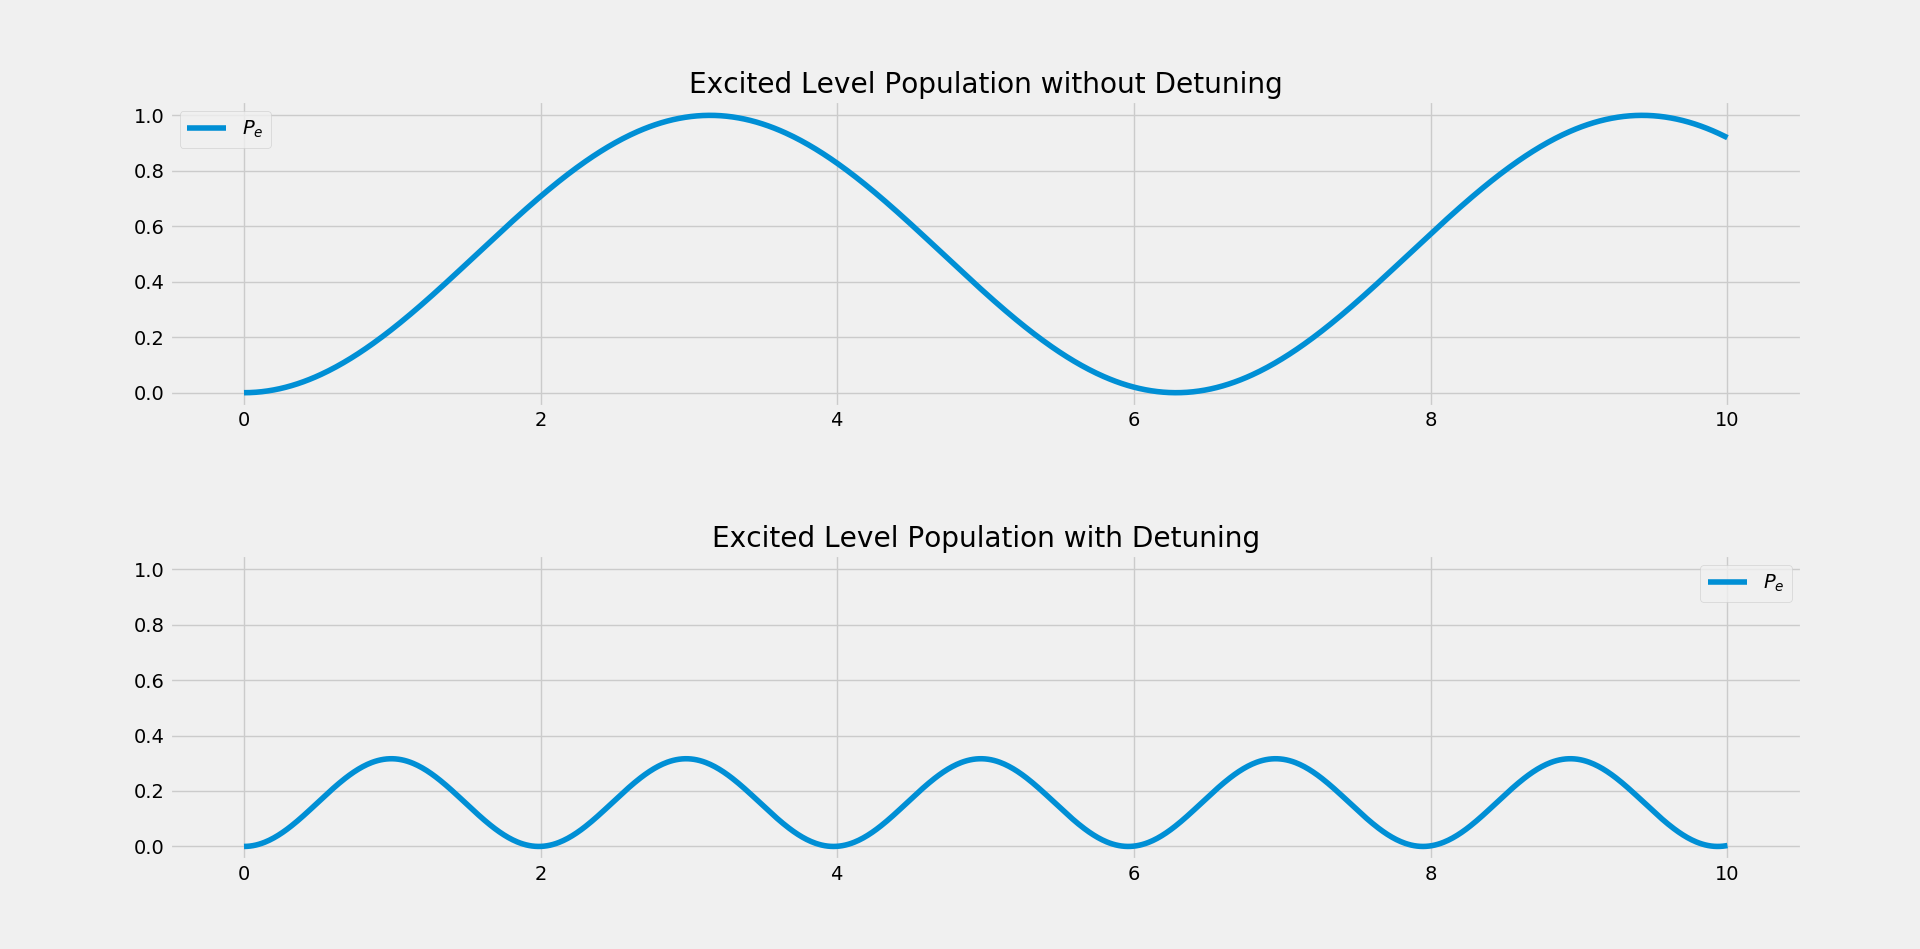
\includegraphics[width=1.0\columnwidth]{Rabi-Oscillations.png}
    \caption{Rabi oscillations of atom in a classical electromagnetic field. The top graph is without detuning $\Delta = 0$ and the bottom graph is with detuning $\Delta \ne 0$}
    \label{fig:rabi-oscillations}
\end{figure}
You can see that with zero detuning, the atom oscillates fully between ground and excited states. With non-zero detuning, the atom doesn't fully reach the excited state, it goes only part of the way and then goes back down. This means that if you want  to get to the excited states you need to send a pulse with exactly the same frequency as the atom.

We can take everything we got so far and construct a pulse that will take the ground state into the excited state. First, the pulse must have the same frequency as the atom $\omega = \omega_0$. If the total duration of the pulse is T, then the excited state is fully populated at time $T$
\[
    P_e (T) = 1 =  (1 - \cos  (\Omega_0 T))
\]
And the solutions are
\[
    \Omega_0 = \frac{\pi k}{T} \quad \text{for} \quad k = 1, 2, 3, \dots
\]
Where $k$ corresponds to the amount of oscillations between the ground and excited states. Ideally the atom would go directly to the excited state without oscillating between the states, so we'll set $k = 1$.

Putting it all together, for a two level atom with frequency $\omega_0$, and a pulse with duration $T$, the pulse you need to send to get from the ground state to the excited state is
\[
    \boxed{\Omega (t) = \frac{\pi}{T} e^{i \omega_0 t}}
\]
Where the real and imaginary parts correspond the sin and cos waves we send to the atom (or I and Q pulses if you prefer). Writing them explicitly we get
\[
    \boxed{\Omega_I  (t) = \frac{\pi }{T} \sin  (\omega_0 t)} \quad \text{and} \quad \boxed{\Omega_Q  (t) = \frac{\pi}{T} \cos  (\omega_0 t)}
\]
We can actually check using the simulation we made in chapter \ref{chap:optimal} and see that yes! These pulses lead to the qubit going from the ground to excited states, amazing!

There is actually a more general result about \textit{$\pi$-pulses} we can see from here, we won't prove it but we can see it works. Any pulse that satisfies
\[
    \int_0^T \Omega (t) dt = \pi
\]
Would take the ground state atom to the excited state. You can use a something like a Gaussian or any other weird pulse that satisfies this condition, and they will all work. We can see that indeed, the pulse we derived does satisfy it.

There are actually many more examples we can find analytical solutions for. There are even analytical solution for the 3-level system and DRAG. We won't touch on them here, they are much more complicated, although they are definitely possible to calculate analytically.

% --- Computational Graphs ---
\newpage
\section{Another Method: Computational Graphs}
In the optimal control section, in essence, we try to minimize the cost of many many variables, this is a similar problem that to teaching neural networks and machine learning, we might be able to borrow some tricks and method they use to solve our problem.

Instead of thinking of a cost function as just a function, we can treat it as a \textit{computational graph}. We'll discuss briefly about what's a computational graph and how can we implement GRAPE using one. We won't go in depth as we did in the chapter on optimal control, it's only a general overview meant to show an alternative method. Let's start by defining a computational graph\footnote{Of course, graph theory is an entire field of mathematics by itself and we can't really give a rigorous definition, but more of an intuitive explanation}.

\subsection{What are Computational Graphs}
A computational graph consists of nodes and connection between them, a node can be one of one of three things
\begin{itemize}
    \item \textbf{Operations}, the operation takes a list of numbers from other nodes and outputs another list of numbers (doesn't need to be of same size) % TODO: Change wording of this line
    \item \textbf{Parameters}, these are, as the name suggests, the parameters of the graph and can be used by the operations.
    \item \textbf{Variables}, these are the variables that of the graph, and they too can be used by the operators of the graph
\end{itemize}
The graph starts as the variables, goes through some operations that use parameters and gives out some resualt. Let's take a look at a simple example

\begin{figure}[H]
    \centering
    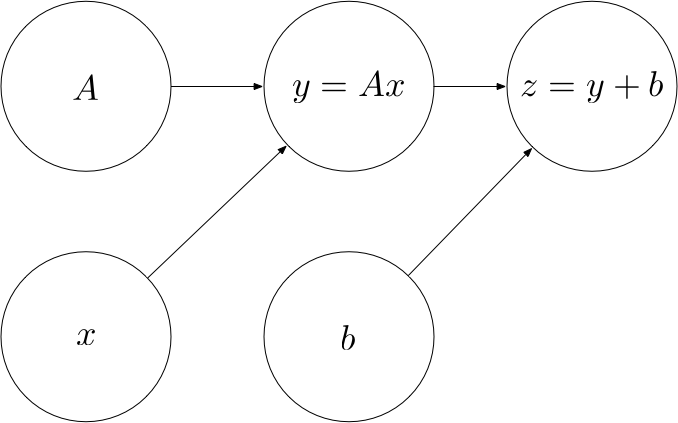
\includegraphics[width=0.4\columnwidth]{Example-comp-graph.png}
    \caption{Example of a basic computational graph}
    \label{fig:example-computational-graph}
\end{figure}

Here, $x$ is the variable, $A$ and $b$ are the parameters, and $y$ and $z$ are the operators. The function that this graph represents is $y = a \cdot e^{x}$. For now it properly seems overkill to use the graph to represent that simple of a function but in the next two sections you'll see the magic of the computational graph, in terms of thinking about the gradient.

\subsection{Back-Propagation}
This is the magic of the computational graph, calculating the gradient of the cost function by back-propagating the derivatives to the initial variables. The idea is simple, instead of trying to directly calculating the gradient, we calculate the derivative of node by the previous node, and relate the cost function to the variables by the chain rule. What does that mean, let's show an example.

Let's say we have a simple computational graph that looks like
\[x \rightarrow L_1 \rightarrow L_2 \rightarrow L_3 \rightarrow y\] 
and we want to calculate the derivative, $\frac{\partial y}{\partial x}$. Instead of calculating the derivative directly, we can back-propagate the derivative as
\[\frac{\partial y}{\partial x} = \frac{\partial y}{\partial L_3} \cdot \frac{\partial L_3}{\partial L_2} \cdot \frac{\partial L_2}{\partial L_1} \cdot \frac{\partial L_1}{\partial x} \cdot \frac{\partial y}{\partial x}\]
luckily for us each operation is very simple so each derivative is simple as well.

\subsection{GRAPE in a Computational Graph}
Now we can finally implement grape as a computational graph, we'll consider the simplest case of GRAPE, no constraints, only the original definition (see equations \ref{eq:fidelity_sim}, \ref{eq:U_def_prod} and \ref{eq:hamiltonianl_form})%\footnote{This is assuming only one drive hamiltonian, for more drives the only difference is adding $\epsilon'_k H'_d$ and so on for each drive} %TODO: Change wording of footnote and add explenation where the function comes from
\[
    F (\vec{\epsilon}) = \abs{\bra{\psi_{target}} \prod_{i=0}^N e^{-i \cdot \delta t  (H_0 + \epsilon_k H_d)} \ket{\psi_{initial}}}^2
\]
In this case, $\vec{\epsilon}$ is the variable, $H_0$, $-i \cdot \delta t$, $\bra{\psi_{target}}$ and $\ket{\psi_{initial}}$ are the parameters. They relate through the operators and everything can be displayed as the following graph\footnote{Simplifying for 3 time steps, to add more time steps is pretty straight forward}

\begin{center}
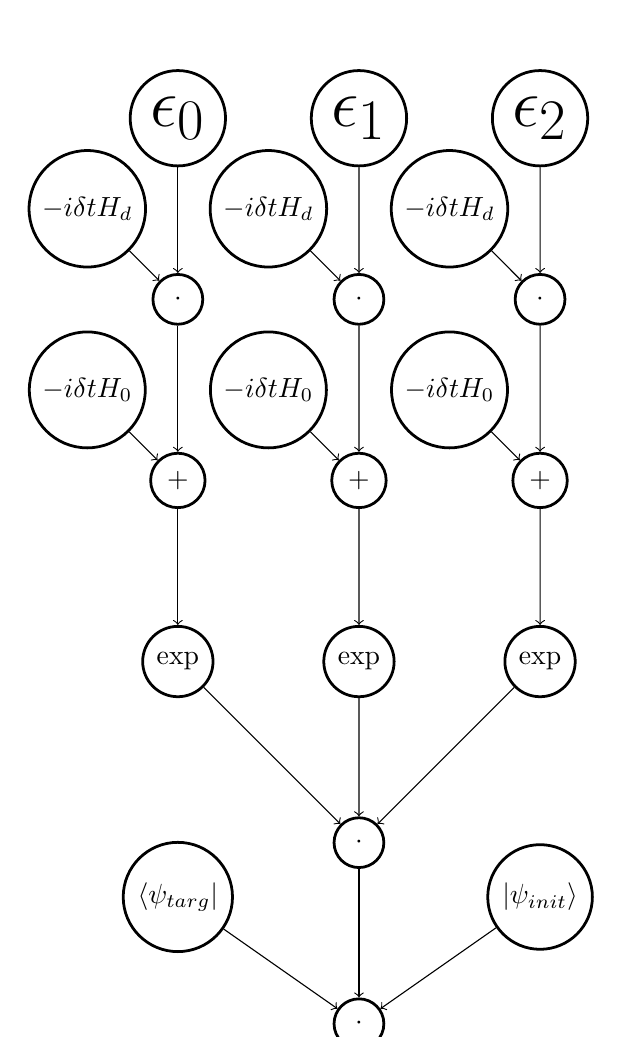
\begin{tikzpicture}[scale=2.3]
\renewcommand*{\VertexLineWidth}{1pt}%vertex thickness
\renewcommand*{\EdgeLineWidth}{1pt}% edge thickness
\GraphInit[vstyle=Normal]
% Variables
\Vertex[L={\Huge $\epsilon_0$}, x=0,y=5]{e0}
\Vertex[L={\Huge $\epsilon_1$},x=1,y=5]{e1}
\Vertex[L={\Huge $\epsilon_2$},x=2,y=5]{e2}

\Vertex[L=$-i \delta t H_d$,x=-0.5,y=4.5]{idt00}
\Vertex[L=$-i \delta t H_d$,x=0.5,y=4.5]{idt01}
\Vertex[L=$-i \delta t H_d$,x=1.5,y=4.5]{idt02}
% L1
\Vertex[L=$\cdot$,x=0,y=4]{L10}
\Vertex[L=$\cdot$,x=1,y=4]{L11}
\Vertex[L=$\cdot$,x=2,y=4]{L12}

\Vertex[L=$-i \delta t H_0$,x=-0.5,y=3.5]{idt10}
\Vertex[L=$-i \delta t H_0$,x=0.5,y=3.5]{idt11}
\Vertex[L=$-i \delta t H_0$,x=1.5,y=3.5]{idt12}
% L2
\Vertex[L=$+$,x=0,y=3]{L20}
\Vertex[L=$+$,x=1,y=3]{L21}
\Vertex[L=$+$,x=2,y=3]{L22}
% L3
\Vertex[L=$\exp$,x=0,y=2]{L30}
\Vertex[L=$\exp$,x=1,y=2]{L31}
\Vertex[L=$\exp$,x=2,y=2]{L32}
% L4
\Vertex[L=$\cdot$,x=1,y=1]{L4}

\Vertex[L=$\ket{\psi_{init}}$,x=2,y=0.7]{psii}
\Vertex[L=$\bra{\psi_{targ}}$,x=0,y=0.7]{psit}
% C
\Vertex[L=$\cdot$,x=1,y=0]{C}

%%%%%%%%%%%%%%%%%%%%%%%%%%%%%%
\draw [->]  (e0) edge  (L10);
\draw [->]  (e1) edge  (L11);
\draw [->]  (e2) edge  (L12);
\draw [->]  (idt00) edge  (L10);
\draw [->]  (idt01) edge  (L11);
\draw [->]  (idt02) edge  (L12);

\draw [->]  (L10) edge  (L20);
\draw [->]  (L11) edge  (L21);
\draw [->]  (L12) edge  (L22);
\draw [->]  (idt10) edge  (L20);
\draw [->]  (idt11) edge  (L21);
\draw [->]  (idt12) edge  (L22);

\draw [->]  (L20) edge  (L30);
\draw [->]  (L21) edge  (L31);
\draw [->]  (L22) edge  (L32);

\draw [->]  (L30) edge  (L4);
\draw [->]  (L31) edge  (L4);
\draw [->]  (L32) edge  (L4);

\draw [->]  (L4) edge  (C);
\draw [->]  (psii) edge  (C);
\draw [->]  (psit) edge  (C);

\end{tikzpicture}
\end{center}
The layers are as follows

\begin{align*}
    L_1^k &= -i \delta t H_d \epsilon_k \\
    L_2^k &= -i\delta t H_0 + L_1^k \\
    L_3^k &= e^{L_2^k} \\
    L_4 &= \prod_{k=0}^N L_3^k \\
    C &= \bra{\psi_{target}} L_4 \ket{\psi_{initial}}
\end{align*}

And the derivatives are calculated rather easily as

\begin{align*}
    \frac{\partial L_1^k}{\partial \epsilon_k} &= -i \delta t H_d\\
    \frac{\partial L_2^k}{\partial L_1^k} &= 1 \\
    \frac{\partial L_3^k}{\partial L_2^k} &= e^{L_2^k} \\
    \frac{\partial L_4}{\partial L_3^k} &= \prod_{i \ne k} L_3^i \\
    \downarrow \\
    \frac{\partial C}{\partial \epsilon_k} &= \bra{\psi_{target}}  \frac{\partial L_4}{\partial L_3^k}  \frac{\partial L_3^k}{\partial L_2^k} \frac{\partial L_2^k}{\partial L_1^k}  \frac{\partial L_1^k}{\partial \epsilon_k} \ket{\psi_{init}}
\end{align*}
It's important to note that $\frac{\partial L_1^i}{\partial \epsilon_j} = 0$ for $i \ne j$ so we didn't refer to those derivative (This is true for the derivative between any two layers).

We now everything we need to implement GRAPE as a computational graph, and we can use a library, such as google's tensorflow, to find the optimal pulse.

% --- Quantizing Electric Circuit ---
\newpage
\section{Quantizing Electric Circuit and the Josephson Junction} \label{appen:LC}
Throughout the project, I mentioned several times that the physical implementation of the qubit is not  the subject of the project and ignored it. It would be a crime no to at least give a simple explanation of the implementation of the qubit, especially since we dedicated and entire section  (section \ref{sec:DRAG}) to the problem with our physical implementation. In this appendix I will try to give a simple explanation of  the qubit as a quantum LC circuit, using the  tools we got when we quantized the electromagnetic field.

This appendix is here for two reasons. The first we already mentioned, to gain some insights on how the qubit is implemented physically. The second, less obvious reason, is to really drive home the point that Dirac's method for Canonical quantization can be applied to any oscillating phenomena. From mechanical oscillator, to the electromagnetic field and even an LC circuit, as we'll see shortly.

\subsection{Quantizing the LC Circuit}
The LC circuit is constructed by connecting a capacitor with capacitance $C$ to a coil with inductance $L$, hence the name, \textit{LC}. Drawing it in a diagram is as shown
\begin{figure}[H]
    \centering
    % TODO: Change image to one with marking of the magnetic inductance field and the  electric capacitance field
    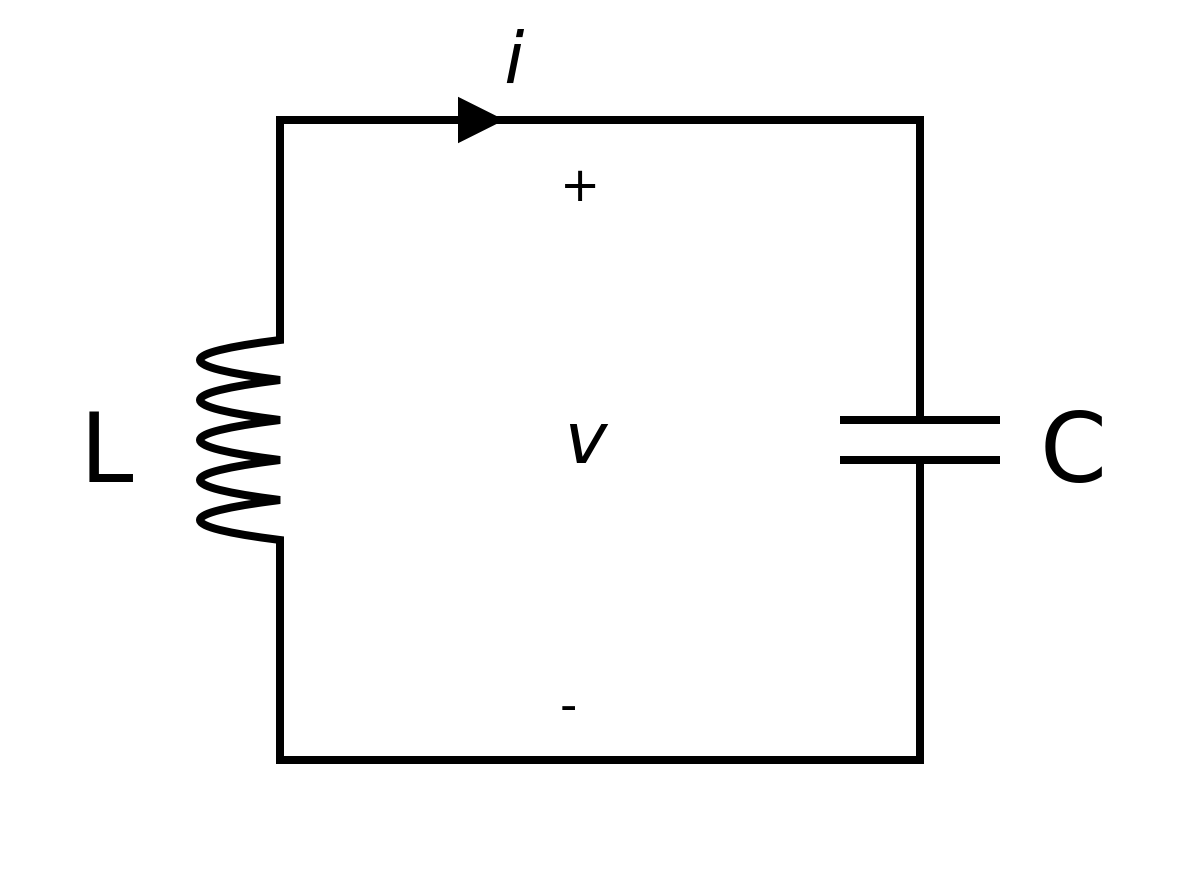
\includegraphics[width=0.4\columnwidth]{LC-circuit.png}
    \caption{The LC circuit} 
    \label{fig:LC-circuit}
\end{figure}

To begin the quantization we first need choose a pair of canonically conjugate variables to represent the state of the system. The most obvious pair of variables would be the voltage $V$ and the current $I$, but turns out they are not canonically conjugate variables. Instead, we'll choose the charge of the capacitor $q$ and the inductor's magnetic flux $\phi$ to be the variables. 

Let's check that they are indeed canonically conjugate. The energy (and therefore, the Hamiltonian) of the capacitor's electric field is given by
\[
    H_C = \frac{q^2}{2C}
\]
and the energy of the magnetic field stored in the inductor is given by
\[
    H_L = \frac{\phi^2}{2L}
\]
Now we can sum these two donations to the Hamiltonian and get that the Hamiltonian of the LC circuit is
\[
    H_{LC}(q, \phi) = \frac{\phi^2}{2L} + \frac{q^2}{2C}
\]
The Hamilton equations in terms of $q$ and $\phi$ are
\begin{align}
    &\dot{q} = \quad \frac{\partial H_{LC}}{\partial \phi} = \quad \frac{\phi}{L} = \quad I \label{eq:def-current}\\
    &\dot{\phi} = -\frac{\partial H_{LC}}{\partial q} = -\frac{q}{C} = -V \label{eq:def-potential}
\end{align}
These equation are correct since \ref{eq:def-current} is the definition of current and \ref{eq:def-potential} is the definition of potential. Therefore $q$ and $\phi$ are canonically conjugate variables and we can go on and quantize them.

To quantize these variables we simply need to replace them with operators
\begin{align*}
    q \rightarrow \hat{q} \\
    \phi \rightarrow \hat{\phi}
\end{align*}
satisfying the commutation relation
\[
    [\hat{q}, \hat{\phi}] = i\hbar
\]
as always with quantum harmonic oscillator we'll define annihilation and creation operators
\begin{align*}
    &\hat{a} = \frac{\hat{q}}{q_0} + i\frac{\hat{\phi}}{\phi_0} \\
    &\hat{a}^\dag = \frac{\hat{q}}{q_0} - i\frac{\hat{\phi}}{\phi_0}
\end{align*}
where
\begin{align*}
    &q_0^2 = 2\hbar\sqrt{\frac{C}{L}} \\
    &\phi_0^2 = 2\hbar\sqrt{\frac{L}{C}}
\end{align*}
% TODO: Maybe don't skip the basic algebra
After some algebra magic we can get the expression of the Hamiltonian
\[
    \hat{H}_{LC} = \hbar \omega (\hat{a}^\dag \hat{a} + \frac{1}{2}) \quad \text{with} \quad \omega = \frac{1}{\sqrt{LC}}
\]
This is the good old expression for the Hamiltonian of a quantum harmonic oscillator and we can treat it as we did with any other quantum harmonic oscillator.

\subsection{Artificial Atoms - The Josephson Effect}
The problem with the simple quantum LC circuit is that it's energy levels are \textit{linear}. By linear, I mean that the difference in energy between two neighboring levels is the same for every level, $E_{n + 1} - E_n = \hbar \omega$ for all $n$\footnote{Unlike an actual atom where the energy difference decreases at higher levels}. This is a problem since we want to treat it as a two level system. If we send a pulse with $\hbar \omega$ energy, we want it to affect only the lower two levels, but since the energy difference between all the levels is the same, sending such a pulse would also excite the higher levels uncontrollably.

We want to introduce \textit{un-linearity} to the levels, so still $E_1 - E_0 = \hbar \omega_{01} $ but $E_2 - E_1 = \hbar \omega_{12}$, $E_3 - E_2 = \hbar \omega_{23}$ and so on, where $\omega_{n\ n+1} \ne \omega_{01}$. This way if the system is only populated at one of the lower two levels and we send a pulse with energy $\hbar \omega$, the only levels affected are the lower two and not the higher ones\footnote{This is obviously an ideal case, as we seen in section \ref{sec:DRAG} with DRAG}.

To create these a-linearities we can use the \textbf{\textit{Josephson Junction}}. A Josephson junction is simply a cut in the wire, a very (very) thin cut, the two pieces of wire are around 10nm apart. The Josephson junction replaces that inductor in the LC circuit. In a circuit diagram it's drawn as a little $x$, and the circuit diagram of the LC circuit with it is
\begin{figure}[H]
    \centering
    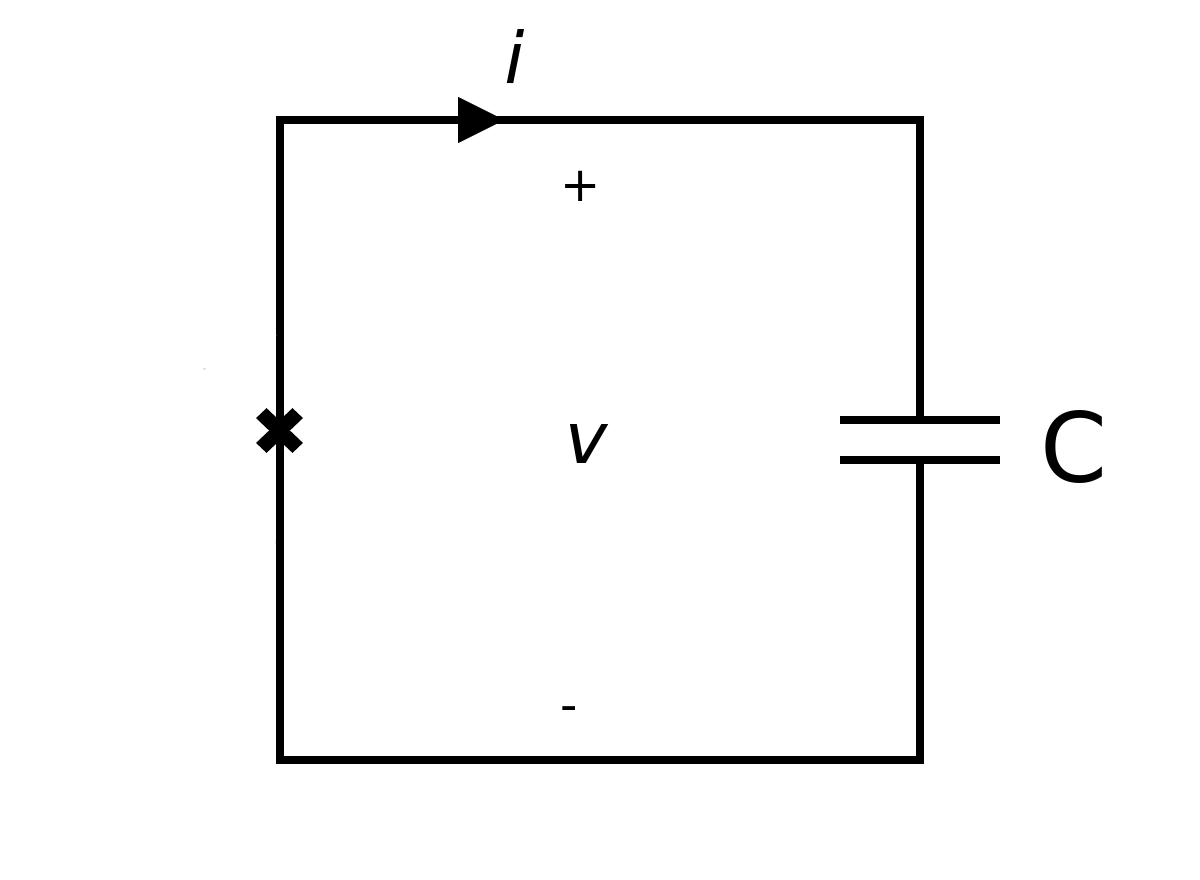
\includegraphics[width=0.43\columnwidth]{LC-circuit-josephson.png}
    \caption{The LC circuit with a Josephson junction} 
    \label{fig:LC-circuit-Josephson}
\end{figure}
And the effect of adding a Josephson junction is replacing the Hamiltonian of the inductor $\frac{\phi^2}{2L}$ with $E_j \cos (\frac{2e}{\hbar} \phi)$.
\[
    \hat{H}_{Josephson} = \frac{\hat{q}^2}{2C} + E_j \cos (\frac{2e}{\hbar} \phi)
\]
This does exactly what we want, for the first level we can approximate the cosine as a parabola and get $E_1 - E_0 = \hbar \omega_{01}$ but since the cosine diverges from the parabola after that the difference between the energy levels lessens and lessens between each pair of higher levels. Here's a visual representation of the energy level of the LC circuit with the Josephson junction
\begin{figure}[H]
    \centering
    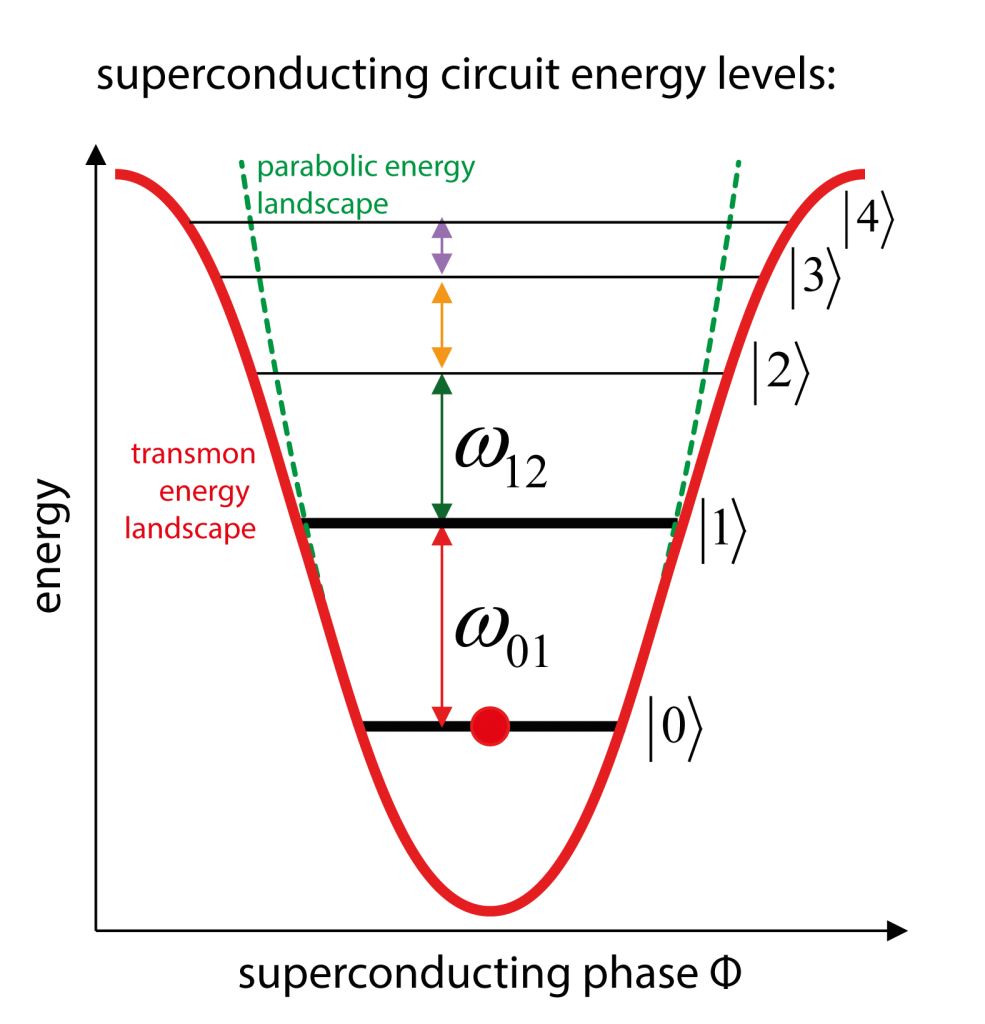
\includegraphics[width=0.4\columnwidth]{josephson-energy-levels.png}
    \caption{Potential of the circuit as a function of the superconducting phase, and the non-linear energy levels of the Josephson junction} 
    \label{fig:Josephson-energy-levels}
\end{figure}
We can treat the Josephson junction as a potential barrier, and calculate the wave function on both sides of the wire.

We'll call the wave function on one side of the junction $\psi_1$ and on the other side $\psi_2$, their dynamics are determined by the coupled shr\"{o}dinger equations:
\begin{align*}
    &i\hbar\frac{\partial \psi_1}{\partial t} = \mu_1 \psi_1 + K \psi_2 \\
    &i\hbar\frac{\partial \psi_2}{\partial t} = \mu_2 \psi_2 + K \psi_1 
\end{align*}
Where $K$ is the coupling across the barrier and $\mu_{1/2}$ are the lowest energy states of each wave function. We'll "guess" solutions of the form
\[
    \psi_{1/2} = \sqrt{n_{1/2}}e^{i\theta_{1/2}}
\]
Yielding the two equations
\begin{align*}
    &\hbar \frac{\partial n_1}{\partial t} = - \hbar \frac{\partial n_2}{\partial t} = 2K \sqrt{n_1 n_2} \sin (\theta_2 - \theta_1) \\
    -&\hbar \frac{\partial (\theta_2 - \theta_1)}{\partial t} = \mu_2 - \mu_1
\end{align*}
$n_{1/2}$ are the density of cooper pairs, and by definition of the current, the current is $\frac{\partial n_1}{\partial t}$. When voltage is applied the energy levels shift as $\mu_2 - \mu_1 = 2eV$. Finally to make the equations shorter we'll write $I_0 = 2K\sqrt{n_1 n_2}$ and $\delta = \theta_2 - \theta_1$. The equations now become
\begin{align*}
    &I = I_0 \sin \delta \\
    &\frac{\partial \delta}{\partial t} = \frac{2eV}{\hbar}
\end{align*}

We can now calculate the electric power (which is the derivative of the energy) from the classical equation
\[
    \frac{\partial E}{\partial t} = P = I V = (I_0 \sin \delta) \cdot (\frac{\hbar}{2e} \frac{\partial \delta}{\partial t}) = -\frac{I_0 \hbar}{2e} \frac{\partial \cos \delta}{\partial t}
\]
Integrating over time, we get that the expression for the energy is
\[
    E = -\frac{I_0 \hbar}{2e} \cos \delta
\]
If we define $E_j = -\frac{I_0 \hbar}{2e}$, replace $\delta$ with $\hat{\phi}$, and replace the energy with the Hamiltonian, we get
\[
    \hat{H}_{Josephson} = E_j \cos \hat{\phi}
\]
just as we've written earlier.

This is not the best treatment of the Josephson junction but it's a rough idea of the explanation. This expression gives us the a-linearities we want to get to implement the qubit.

\newpage
% \end{multicols}
\end{document}


